\documentclass[a4paper,french,12pt,twoside]{book}

\input{../preambule/preambule.tex}
%%%%%%%%%%%%%%%%%%%%%%%%%%%%%%%%%%%%%%%%%%%%%%%%%%%%%%%%%%
%%%%%%%%%%%%%%%%%%%%%%%


%%%%%%%%%%%%%%%%%%%%%%%%%%%%%%%%ù
%%%%%%%%%%%%%%%%%% Pour la page de titre
\title{Math\'ematiques en Seconde}
\author{David ROBERT}
\date{2016--2017}
\begin{document}

\renewcommand{\proofname}{Preuve} % change "<démonstration"> en "<preuve">


%%%%%%%%%%%%%%%%%%%En ttes et pied de page %%%%%%%%%%%%%%%%

		\pagestyle{fancy}                       % Sets fancy header and footer
    \fancyfoot{}                            % Delete current footer settings
    \fancyhead{}

    \renewcommand{\sectionmark}[1]{\markright{\thesection{} #1}}
    \renewcommand{\chaptermark}[1]{\markboth{#1}{}}

		\fancyhead[LE,RO]{\footnotesize \em \rightmark}
		\fancyhead[RE,LO]{\scriptsize \em Seconde}
		\fancyfoot[RE]{\scriptsize \em \href{http://perpendiculaires.free.fr/}{http://perpendiculaires.free.fr/}}
		\fancyfoot[LO]{\scriptsize \em David ROBERT}
    \fancyfoot[LE,RO]{\textbf{\thepage}}

    \renewcommand{\headrulewidth}{0.5pt}
    \renewcommand{\footrulewidth}{0pt}

%%%%%%%% Page de titre %%%%%%%%%%%%%%%


\frontmatter

\protect\thispagestyle{empty}
\maketitle

%%%%%%%%%%%%%% Sommaire %%%%%%%%%%%%%%

\addtocontents{toc}{\protect\thispagestyle{empty}}
\renewcommand{\contentsname}{Sommaire} %Changer Table des matires en Sommaire, un sommaire est au dbut, une table des matires  la fin
\dominitoc
\tableofcontents
%%%%%%%%%%%%%%%%%%%%%%%%%%%%%%%%%%%%%%%%%%%%%%%%%%%%%%%%%%%%%%%%%
%%%%%%%%%%%%%%%%%%%%%%%%%%%%%%%%%%%%%%%%%%%%%%%%%%%%%%%%%%%%%%%%%



\mainmatter

% 2016-2017
\chapter{Rep\'erage} \label{reperes}
\minitoc

\fancyhead{}
\fancyfoot{} % efface les entêtes précédentes
\fancyhead[LE,RO]{\footnotesize \em \rightmark}
		\fancyhead[RE,LO]{\scriptsize \em Seconde}
		\fancyfoot[RE]{\scriptsize \em \href{http://perpendiculaires.free.fr/}{http://perpendiculaires.free.fr/}}
		\fancyfoot[LO]{\scriptsize \em David ROBERT}
    \fancyfoot[LE,RO]{\textbf{\thepage}}


\section{Rep\`ere d'une droite}

\begin{definition}
 Soit $d$ une droite, $O$ et $I$ deux points distincts de cette droite, alors $(O,I)$ est appel\'e \emph{rep\`ere} de la droite $d$ ; $O$ est appel\'e \emph{origine} du rep\`ere et $OI$ est appel\'e \emph{unit\'e} du rep\`ere.
\end{definition}



\begin{prop}
 Soit $d$ une droite munie du rep\`ere $(O,I)$, alors tout point $M$ de la droite est associ\'e \`a un unique nombre $x$ d\'efini par :
\vspace{-1em}\begin{multicols}{2}\begin{itemize}
 \item $x=\frac{OM}{OI}$ si $M\in[OI)$ ;
 \item $x=-\frac{OM}{OI}$ si $M\notin[OI)$.
\end{itemize}\end{multicols}%\vspace{-1em}
$x$ est appel\'e \emph{abscisse} de $M$.
\end{prop}

\noindent On l'admettra.

\begin{exemple*}
Sur la droite $d$ ci-dessous, les points $O$ et $I$ sont distincts donc $(O,I)$ est un rep\`ere de $d$.\\
$M\in[OI)$ est tel que $OM=4OI$ donc son abscisse est 4.\\
$N\notin[OI)$ est tel que $ON=1,5OI$ donc son abscisse est $-1,5$.
\begin{center}
\def\xmin{0} \def\xmax{10} \def\ymin{-2} \def\ymax{0}
\begin{pspicture*}(\xmin,\ymin)(\xmax,\ymax)
%\psgrid[griddots=10,gridlabels=0pt,gridwidth=.3pt, gridcolor=black, subgridwidth=.3pt, subgridcolor=black, subgriddiv=1](0,0)(-6,-2)(14,6)
%\psaxes[labels=all,labelsep=1pt, Dx=1,Dy=1]{-}(0,0)(\xmin,\ymin)(\xmax,\ymax)
%\uput[dl](0,0){$O$}
%\pcline[linewidth=1pt]{->}(0,0)(1,0) \uput[d](0.5,0){\small $\vec i$}
%\pcline[linewidth=1pt]{->}(0,0)(0,1) \uput[l](0,0.5){\small $\vec j$}
\psplot[algebraic=true]{\xmin}{\xmax}{0.2*x-2}
\psdots(5,-1)(6,-0.8)(9,-0.2)(3.5,-1.3)
\uput[dr](5,-1){$O$}
\uput[dr](6,-0.8){$I$}
\uput[dr](9,-0.2){$M$}
\uput[dr](3.5,-1.3){$N$}
\uput[u](1,-1.6){$d$}
\end{pspicture*}                \end{center}
\end{exemple*}

%\sautpage

\section{Rep\`ere d'un plan}

\subsection{D\'efinitions}
\begin{definition}
 Soit $P$ un plan, $O$, $I$ et $J$ trois points non align\'es de ce plan, alors $(O,I,J)$ est appel\'e \emph{rep\`ere} du plan ; $O$ est appel\'ee \emph{origine} du rep\`ere et les droites $(OI)$ et $(OJ)$ sont appel\'ees \emph{axes} du rep\`ere.
\end{definition}



\noindent Soit $P$ un plan muni du rep\`ere $(O,I,J)$, alors, pour tout point $M$ du plan,
 il existe deux uniques points $M_x$ et $M_y$ tels que
 $M_x\in(OI)$, $M_y\in(OJ)$ et $OM_xMM_y$ parall\'elogramme (on l'admettra).\\
 On note $x$ l'abscisse de $M_x$ sur la droite $(OI)$ munie du rep\`ere $(O,I)$ et
 $y$ l'abscisse de $M_y$ sur la droite $(OJ)$ munie du rep\`ere $(O,J)$.

\begin{center}
\def\xmin{-2} \def\xmax{10} \def\ymin{-2} \def\ymax{6}
\begin{pspicture*}(\xmin,\ymin)(\xmax,\ymax)
%\psgrid[griddots=10,gridlabels=0pt,gridwidth=.3pt, gridcolor=black, subgridwidth=.3pt, subgridcolor=black, subgriddiv=1](0,0)(-6,-2)(14,6)
%\psaxes[labels=all,labelsep=1pt, Dx=1,Dy=1]{-}(0,0)(\xmin,\ymin)(\xmax,\ymax)
%\uput[dl](0,0){$O$}
%\pcline[linewidth=1pt]{->}(0,0)(1,0) \uput[d](0.5,0){\small $\vec i$}
%\pcline[linewidth=1pt]{->}(0,0)(0,1) \uput[l](0,0.5){\small $\vec j$}
\psplot[algebraic=true]{\xmin}{\xmax}{0.4*x-1}
\psplot[algebraic=true]{\xmin}{\xmax}{2*x-1}
\psdots(0,-1)(3,0.2)(1,1)(8,5)(6.25,1.5)(1.75,2.5)
\uput[dr](0,-1){$O$}
\uput[dr](3,0.2){$I$}
\uput[ul](1,1){$J$}
\uput[ur](8,5){$M$}
\uput[dr](6.25,1.5){$M_x$}
\uput[ul](1.75,2.5){$M_y$}
\psline[linestyle=dashed](6.25,1.5)(8,5)(1.75,2.5)
\end{pspicture*}                \end{center}

\noindent On a alors :

\begin{prop}
 Soit $P$ un plan muni d'un rep\`ere $(O,I,J)$, alors tout point $M$ de ce plan est associ\'e \`a un unique couple $(x\,;\,y)$, d\'efini ci-dessus,
 appel\'e \emph{coordonn\'ees} de $M$.\\
 $x$ est appel\'e \emph{abscisse} de $M$ et $y$ est appel\'e \emph{ordonn\'ee} de $M$.
\end{prop}

\noindent On l'admettra.

\begin{exemple*}
Sur le sch\'ema ci-dessus, $x=3,125$ et $y=1,5$ donc les coordonn\'ees de $M$ sont $(3,125\,;\,1,5)$.\\
L'abscisse de $M$ est 3,125, l'ordonn\'ee de $M$ est 1,5.
\end{exemple*}

%\sautpage

\subsection{Types de rep\`eres}

\begin{definition}
 Soit $P$ un plan muni d'un rep\`ere $(O,I,J)$.
\begin{itemize}
 \item Si le triangle $OIJ$ est quelconque, le rep\`ere est dit \emph{quelconque}.
 \item Si le triangle $OIJ$ est rectangle en $O$, le rep\`ere est dit \emph{orthogonal}.
 \item Si le triangle $OIJ$ est isoc\`ele en $O$, le rep\`ere est dit \emph{norm\'e}.
 \item Si le triangle $OIJ$ est rectangle et isoc\`ele en $O$, le rep\`ere est dit \emph{orthonorm\'e}.
\end{itemize}
\end{definition}

\begin{tabular}{ccc}
 Rep\`ere orthogonal & Rep\`ere norm\'e & Rep\`ere orthonorm\'e \\
\psset{xunit=0.5cm,yunit=0.5cm}
\def\xmin{-4} \def\xmax{6} \def\ymin{-4} \def\ymax{6}
\begin{pspicture*}(\xmin,\ymin)(\xmax,\ymax)
%\psgrid[griddots=10,gridlabels=0pt,gridwidth=.3pt, gridcolor=black, subgridwidth=.3pt, subgridcolor=black, subgriddiv=1](0,0)(-6,-2)(14,6)
%
\psaxes[labels=none,labelsep=1pt, Dx=10,Dy=10]{-}(0,0)(\xmin,\ymin)(\xmax,\ymax)
%\uput[dl](0,0){$O$}
%\pcline[linewidth=1pt]{->}(0,0)(1,0) \uput[d](0.5,0){\small $\vec i$}
%\pcline[linewidth=1pt]{->}(0,0)(0,1) \uput[l](0,0.5){\small $\vec j$}

\psdots(0,0)(2,0)(0,1)
\uput[dr](0,0){$O$}
\uput[dr](2,0){$I$}
\uput[ul](0,1){$J$}


\end{pspicture*}&
\psset{xunit=0.5cm,yunit=0.5cm}
\def\xmin{-4} \def\xmax{6} \def\ymin{-4} \def\ymax{6}
\begin{pspicture*}(\xmin,\ymin)(\xmax,\ymax)
%\psgrid[griddots=10,gridlabels=0pt,gridwidth=.3pt, gridcolor=black, subgridwidth=.3pt, subgridcolor=black, subgriddiv=1](0,0)(-6,-2)(14,6)
%
%\psaxes[labels=none,labelsep=1pt, Dx=10,Dy=10]{-}(0,0)(\xmin,\ymin)(\xmax,\ymax)
%\uput[dl](0,0){$O$}
%\pcline[linewidth=1pt]{->}(0,0)(1,0) \uput[d](0.5,0){\small $\vec i$}
%\pcline[linewidth=1pt]{->}(0,0)(0,1) \uput[l](0,0.5){\small $\vec j$}

\psdots(0,0)(2,0)(1,1.732050808)
\uput[dr](0,0){$O$}
\uput[dr](2,0){$I$}
\uput[ul](1,1.732050808){$J$}
\psplot[algebraic=true]{\xmin}{\xmax}{0}
\psplot[algebraic=true]{\xmin}{\xmax}{1.732050808*x}
\end{pspicture*}&
\psset{xunit=0.5cm,yunit=0.5cm}
\def\xmin{-4} \def\xmax{6} \def\ymin{-4} \def\ymax{6}
\begin{pspicture*}(\xmin,\ymin)(\xmax,\ymax)
%\psgrid[griddots=10,gridlabels=0pt,gridwidth=.3pt, gridcolor=black, subgridwidth=.3pt, subgridcolor=black, subgriddiv=1](0,0)(-6,-2)(14,6)
%
\psaxes[labels=none,labelsep=1pt, Dx=10,Dy=10]{-}(0,0)(\xmin,\ymin)(\xmax,\ymax)
%\uput[dl](0,0){$O$}
%\pcline[linewidth=1pt]{->}(0,0)(1,0) \uput[d](0.5,0){\small $\vec i$}
%\pcline[linewidth=1pt]{->}(0,0)(0,1) \uput[l](0,0.5){\small $\vec j$}

\psdots(0,0)(1,0)(0,1)
\uput[dl](0,0){$O$}
\uput[dr](1,0){$I$}
\uput[ul](0,1){$J$}


\end{pspicture*}
\end{tabular}

\subsection{Coordonn\'ees du milieu d'un segment}

\begin{act}
Sur le schéma ci-dessous :
\begin{enumerate}
	\item Placer les points $M(3;1)$, $N(-1;1,5)$, $P(-2;-1)$ et $Q(3;-1)$ ;
	\item Donner graphiquement les coordonnées des points $A$, $B$, $C$ et $D$ ;
	\item En faisant quelques essais, conjecturer le lien existant entre les coordonnées de deux points et les coordonnées du milieu de ces deux points.
\end{enumerate}
\end{act}
\begin{center}

\psset{xunit=1cm , yunit=1cm}
\begin{pspicture*}(-0.7,-0.7)(15.7,9.7)
\def\xmin{-0.5} \def\xmax{15.5} \def\ymin{-0.5} \def\ymax{9.5}

\multido{\i=0+1}{18}{%
\psline[linestyle=dotted](\i,\ymin)(\i,\ymax)
\psset{algebraic=true}
\psplot[linestyle=dotted]{\xmin}{\xmax} {x*0.5-8+\i}
\psplot[linestyle=dotted]{\xmin}{\xmax} {-x*0.5+16-\i}}
%\psline{->}(7,4.5)(7,5.5)
\psline(7,\ymin)(7,\ymax)
%\rput{90}(7.3,5){$\vec{i}$}
%\psline{->}(7,4.5)(5,5.5)
\psplot[algebraic=true]{\xmin}{\xmax} {-0.5*x+8}
%\rput{90}(6,4.5){$\vec{j}$}
\psdots[dotstyle=x, dotscale=2.0000](7,4.5)(7,2.5)(8,6)(5,7.5)(3,6.5)(7,5.5)(5,5.5)
\rput{90}(7.2,4.2){$O$}
\rput{90}(7.2,2.2){$B$}
\rput{90}(8.2,5.7){$A$}
\rput{90}(5.2,7.2){$C$}
\rput{90}(3.2,6.2){$D$}
\rput{90}(7.2,5.2){$I$}
\rput{90}(5.2,5.2){$J$}
\end{pspicture*}
\end{center}


\begin{prop}
 Soit $P$ un plan muni d'un rep\`ere quelconque.\\
 Soit $A(x_A;y_A)$ et $B(x_B;y_B)$ et $I(x_I;y_I)$ milieu de $[AB]$. \\
Alors
\vspace{-1em}\begin{itemize}\begin{multicols}{2}
	\item $x_I=\ldots\ldots\ldots$
	\item $y_I=\ldots\ldots\ldots$
\end{multicols}\end{itemize}
\end{prop}

\begin{proof} La preuve sera faite en classe \`a partir de cette figure :
\begin{center}
 \psset{xunit=0.5cm,yunit=0.5cm}
\def\xmin{-2} \def\xmax{15} \def\ymin{-2} \def\ymax{10}
\begin{pspicture*}(\xmin,\ymin)(\xmax,\ymax)
%\psgrid[griddots=10,gridlabels=0pt,gridwidth=.3pt, gridcolor=black, subgridwidth=.3pt, subgridcolor=black, subgriddiv=1](0,0)(-6,-2)(14,6)
%
%\psaxes[labels=none,labelsep=1pt, Dx=10,Dy=10]{-}(0,0)(\xmin,\ymin)(\xmax,\ymax)
%\uput[dl](0,0){$O$}
%\pcline[linewidth=1pt]{->}(0,0)(1,0) \uput[d](0.5,0){\small $\vec i$}
%\pcline[linewidth=1pt]{->}(0,0)(0,1) \uput[l](0,0.5){\small $\vec j$}

\psplot[algebraic=true]{\xmin}{\xmax}{0}
\psplot[algebraic=true]{\xmin}{\xmax}{2*x}
\psplot[algebraic=true,linestyle=dotted]{\xmin}{\xmax}{7}
\psplot[algebraic=true,linestyle=dotted]{\xmin}{\xmax}{5}
\psplot[algebraic=true,linestyle=dotted]{\xmin}{\xmax}{3}
\psplot[algebraic=true,linestyle=dotted]{\xmin}{\xmax}{2*x-5}
\psplot[algebraic=true,linestyle=dotted]{\xmin}{\xmax}{2*x-11}
\psplot[algebraic=true,linestyle=dotted]{\xmin}{\xmax}{2*x-17}

\psdots(0,0)(6,7)(8,5)(10,3)
\uput[ul](0,0){$O$}
\uput[ur](6,7){$A$}
\uput[ur](8,5){$I$}
\uput[ur](10,3){$B$}

\psline(6,7)(10,3)



\end{pspicture*}                \end{center}
\end{proof}

\subsection{Distance entre deux points dans un rep\`ere orthonorm\'e}

\begin{prop}
 Soit $P$ un plan muni d'un rep\`ere \underline{\textbf{orthonorm\'e}}.\\
 Soient $A$ et $B$ deux points du plan $P$ de coordonn\'ees respectives $(x_A\,;\,y_A)$ et $(x_B\,;\,y_B)$.\\
 Alors la distance $AB$ est donn\'ee par :
 \[AB=\sqrt{(x_B-x_A)^2+(y_B-y_A)^2}\]
\end{prop}

\begin{proof} La preuve sera faite en classe \`a partir de cette figure :
\begin{center}
 \psset{xunit=0.5cm,yunit=0.5cm}
\def\xmin{-2} \def\xmax{15} \def\ymin{-2} \def\ymax{10}
\begin{pspicture*}(\xmin,\ymin)(\xmax,\ymax)
%\psgrid[griddots=10,gridlabels=0pt,gridwidth=.3pt, gridcolor=black, subgridwidth=.3pt, subgridcolor=black, subgriddiv=1](0,0)(-6,-2)(14,6)
%
\psaxes[labels=none,labelsep=1pt, Dx=20,Dy=20]{-}(0,0)(\xmin,\ymin)(\xmax,\ymax)
%\uput[dl](0,0){$O$}
%\pcline[linewidth=1pt]{->}(0,0)(1,0) \uput[d](0.5,0){\small $\vec i$}
%\pcline[linewidth=1pt]{->}(0,0)(0,1) \uput[l](0,0.5){\small $\vec j$}

\psline[linestyle=dotted](6,\ymin)(6,\ymax)

\psline[linestyle=dotted](10,\ymin)(10,\ymax)
\psplot[algebraic=true,linestyle=dotted]{\xmin}{\xmax}{7}

\psplot[algebraic=true,linestyle=dotted]{\xmin}{\xmax}{3}

\psdots(0,0)(6,7)(10,3)
\uput[ul](0,0){$O$}
\uput[ur](6,7){$A$}

\uput[ur](10,3){$B$}

\psline(6,7)(10,3)



\end{pspicture*}                \end{center}
\end{proof}

\sautpage

\section{Exercices et probl\`emes}

\subsection{Rep\`ere donn\'e}

\begin{exo}
Sur le schéma ci-dessous :
\begin{enumerate}
	\item Placer les points $M(2;1)$, $N(-1,5;1)$, $P(-2;-1)$ et $Q(1,5;-1)$ ;
	\item Donner graphiquement les coordonnées des points $A$, $B$, $C$ et $D$ ;
\end{enumerate}
\begin{center}

\psset{xunit=1cm , yunit=1cm}
\begin{pspicture*}(-0.7,-0.7)(15.7,9.7)
\def\xmin{-0.5} \def\xmax{15.5} \def\ymin{-0.5} \def\ymax{9.5}

\multido{\i=0+1}{18}{%
\psline[linestyle=dotted](\i,\ymin)(\i,\ymax)
\psset{algebraic=true}
\psplot[linestyle=dotted]{\xmin}{\xmax} {x*0.5-8+\i}
\psplot[linestyle=dotted]{\xmin}{\xmax} {-x*0.5+16-\i}}
%\psline{->}(7,4.5)(7,5.5)
\psline(7,\ymin)(7,\ymax)
%\rput{90}(7.3,5){$\vec{i}$}
%\psline{->}(7,4.5)(5,5.5)
\psplot[algebraic=true]{\xmin}{\xmax} {0.5*x+1}
%\rput{90}(6,4.5){$\vec{j}$}
\psdots[dotstyle=x, dotscale=2.0000](7,4.5)(7,2.5)(8,6)(5,7.5)(3,6.5)(7,6.5)(6,4)
\rput{90}(7.2,4.2){$O$}
\rput{90}(7.2,2.2){$B$}
\rput{90}(8.2,5.7){$A$}
\rput{90}(5.2,7.2){$C$}
\rput{90}(3.2,6.2){$D$}
\rput{90}(7.2,6.2){$I$}
\rput{90}(6.2,4.2){$J$}
\end{pspicture*}
\end{center}
\end{exo}

\begin{multicols}{2}
\begin{exo}
Le quadrilat\`ere $ABCD$ donn\'e ci-dessous est un losange de centre $O$.\\
 Dans chacun des cas ci-dessous, dire de quel type est le rep\`ere et donner les coordonn\'ees de tous les points dans ce rep\`ere.
\begin{multicols}{2}
\begin{itemize}
 \item $(A,D,B)$
 \item $(O,C,B)$
 \item $(O,B,C)$
 \item $(D,C,O)$
\end{itemize}
\end{multicols}

\begin{center}
\psset{xunit=0.5cm , yunit=0.5cm}
\def\xmin{-6.1} \def\xmax{6.1} \def\ymin{-4.1} \def\ymax{4.1}
\begin{pspicture*}(\xmin,\ymin)(\xmax,\ymax)

\psline(-5,0)(0,3)(5,0)(0,-3)(-5,0)
\psline[linestyle=dotted](-5,0)(5,0)
\psline[linestyle=dotted](0,-3)(0,3)
\uput[dl](0,0){$O$}
\uput[l](-5,0){$A$}
\uput[u](0,3){$B$}
\uput[r](5,0){$C$}
\uput[d](0,-3){$D$}
\end{pspicture*}
\end{center}

\end{exo}

\sautcol

\begin{exo}
 Le plan est muni d'un rep\`ere orthonorm\'e.\\
 Dans chacun des cas suivants, d\'eterminer la nature du triangle $ABC$.
\begin{enumerate}
 \item $A\,(-4\,;\,-1)$, $B\,(4\,;\,-2)$ et $C\,(-2\,;\,2)$
 \item $A\,(-5\,;\,0)$, $B\,(3\,;\,-4)$ et $C\,(2\,;\,4)$
 \item $A\,(0\,;\,0)$, $B\,(4\,;\,2\sqrt{3})$ et $C\,(-1\,;\,3\sqrt{3})$
\end{enumerate}

\end{exo}

\begin{exo}
 Dans le rep\`ere orthonorm\'e $(O,I,J)$, on donne $A\,(-1\,;\,2)$, $B\,(-3\,;\,-1)$ et $C\,(5\,;\,-2)$.
\begin{enumerate}
 \item Quelle est la nature du triangle $ABC$ ?
 \item Montrer que :
       \begin{enumerate}
        \item Le p\'erim\`etre $p$ de $ABC$ vaut $\sqrt{13}(3+\sqrt{5})$ ;
	\item L'aire $a$ de $ABC$ est un nombre entier.
       \end{enumerate}

\end{enumerate}

\end{exo}

\sautpage

\begin{exo}
Dans le rep\`ere orthonorm\'e $(O,I,J)$, on donne $A\,(1\,;\,1)$, $B\,(4\,;\,5)$ et $C\,(10\,;\,8)$.
\begin{enumerate}
 \item D\'eterminer les longueurs $AB$, $AC$ et $BC$.
 \item Que peut-on en d\'eduire pour les points $A$, $B$ et $C$ ?
\end{enumerate}

\end{exo}

\begin{exo}
 Le plan est muni d'un rep\`ere quelconque.\\
  On donne les points $A\,(2\,;\,3)$ et $I\,(-4\,;\,1)$.\\
  On sait que $I$ est le milieu de $[AB]$.\\
 D\'eterminer les coordonn\'ees de $B$.
\end{exo}

%\sautcol




\begin{exo}
 Dans le rep\`ere orthonorm\'e $(O,I,J)$, on a trac\'e le cercle $\mathcal{C}$ de centre $O$ et de rayon 3.
\begin{enumerate}
 \item $A$ est le point de $\mathcal{C}$ d'abscisse 2.\\
D\'eterminer l'ordonn\'ee de $A$.
 \item Pour chacun des points suivants, d\'eterminer, par le calcul, s'il est sur le cercle $\mathcal{C}$ et, sinon, s'il est sur le disque d\'elimit\'e par $\mathcal{C}$.
  %\vspace{-1em}\begin{multicols}{3}
  \begin{itemize}
   \item $B\,(-1\,;\,-2,8)$
   \item $C\,(2,5\,;\,-1,7)$
   \item $D\,(-1,5\,;\,2,5)$
  \end{itemize}%\end{multicols}
\end{enumerate}



\begin{center}
\psset{unit=0.5cm}
\def\xmin{-4.1} \def\xmax{4.1} \def\ymin{-4.1} \def\ymax{4.1}
\begin{pspicture*}(\xmin,\ymin)(\xmax,\ymax)
\psgrid[griddots=10,gridlabels=0pt,gridwidth=.3pt, gridcolor=black, subgridwidth=.3pt, subgridcolor=black, subgriddiv=1](0,0)(\xmin,\ymin)(\xmax,\ymax)
\psaxes[labels=none,labelsep=1pt, Dx=10,Dy=10]{-}(0,0)(\xmin,\ymin)(\xmax,\ymax)
\psdots(0,0)(1,0)(0,1)(2,2.2)
\pscircle(0,0){3}
\uput[dl](0,0){$O$}
\uput[d](1,0){$I$}
\uput[l](0,1){$J$}

\uput[u](2,2.2){$A$}
\end{pspicture*}
\end{center}

\end{exo}


\begin{exo}\label{rep1}
Sur le schéma ci-contre :
\begin{enumerate}
	\item Placer les points $A(1\,;\,2)$, $B(3\,;\,1,5)$, $C(4\,;\,-0,5)$ et $D(2\,;\,0)$ ;
	\item Montrer que le quadrilat\`ere $ABCD$ est un parall\'elogramme.
\end{enumerate}



\begin{center}

\psset{xunit=1cm , yunit=1cm}
\def\xmin{-1.1} \def\xmax{6.1} \def\ymin{-1.1} \def\ymax{6.1}
\begin{pspicture*}(\xmin,\ymin)(\xmax,\ymax)


%\psgrid[griddots=10,gridlabels=0pt,gridwidth=.3pt, gridcolor=black, subgridwidth=.3pt, subgridcolor=black, subgriddiv=1](0,0)(\xmin,\ymin)(\xmax,\ymax)
%\psaxes[labels=all,labelsep=1pt, Dx=10,Dy=10]{-}(0,0)(\xmin,\ymin)(\xmax,\ymax)


\multido{\i=0+1}{18}{%
\psline[linestyle=dotted](\i,\ymin)(\i,\ymax)
\psset{algebraic=true}
\psplot[linestyle=dotted]{\xmin}{\xmax} {x*0.5-8+\i}
\psplot[linestyle=dotted]{\xmin}{\xmax} {-x*0.5+16-\i}}
%\psline{->}(7,4.5)(7,5.5)
\psline(0,\ymin)(0,\ymax)
%\rput{90}(7.3,5){$\vec{i}$}
%\psline{->}(7,4.5)(5,5.5)
\psplot[algebraic=true]{\xmin}{\xmax} {0.5*x}
%\rput{90}(6,4.5){$\vec{j}$}
\psdots[dotstyle=x, dotscale=2.0000](0,0)(1,0.5)(0,2)
\uput[ul](0,0){$O$}
\uput[ul](1,0.5){$I$}
\uput[l](0,2){$J$}
\end{pspicture*}
\end{center}
\end{exo}

%\sautpage

\begin{exo}
Le plan est muni d'un rep\`ere orthonorm\'e.\\
Dans chacun des cas suivants, d\'eterminer la nature du quadrilat\`ere $ABCD$ :
\begin{enumerate}
 \item $A\,(1\,;\,0)$, $B\,(1\,;\,3)$, $C\,(2\,;\,3)$ et $D\,(3\,;\,1)$ ;
 \item $A\,(1\,;\,2)$, $B\,(4\,;\,7)$, $C\,(1\,;\,6)$ et $D\,(-2\,;\,1)$ ;
 \item $A\,(1\,;\,0)$, $B\,(0\,;\,2)$, $C\,(4\,;\,4)$ et $D\,(5\,;\,2)$ ;
 \item $A\,(-4\,;\,-1)$, $B\,(4\,;\,-2)$, $C\,(8\,;\,5)$ et $D\,(0\,;\,6)$ ;
 \item $A\,(0\,;\,-2)$, $B\,(3\,;\,-1)$, $C\,(2\,;\,2)$ et $D\,(-1\,;\,1)$.
\end{enumerate}

\end{exo}

%\sautpage

\begin{exo}
 Le plan est muni d'un rep\`ere orthonorm\'e.\\
 On donne les points $A\,(-3\,;\,-4)$, $B\,(3\,;\,2)$, $C\,(7\,;\,-2)$ et $D\,(1\,;\,-8)$.
\begin{enumerate}
 \item Montrer que :
	\begin{enumerate}
	 \item $[AC]$ et $[BD]$ ont m\^eme milieu ;
	 \item $AC=BD$.
	\end{enumerate}
 \item \begin{enumerate}
        \item Quelle est la nature du quadrilat\`ere $ABCD$ ?
	\item Calculer le rayon du cercle circonscrit \`a ce quadrilat\`ere.
       \end{enumerate}


\end{enumerate}

\end{exo}



\begin{exo}\label{rep2}
 Le plan est muni d'un rep\`ere quelconque.\\
 On donne les points $A\,(-5\,;\,3)$, $B\,(-4\,;\,1)$ et $C\,(1\,;\,-4)$.
\begin{enumerate}
 \item D\'eterminer les coordonn\'ees de $I$, milieu de $[AC]$.
 \item D\'eterminer les coordonn\'ees de $D$ tel que $ABCD$ soit un parall\'elogramme.
\end{enumerate}

\end{exo}

\subsection{Rep\`ere \`a choisir}

\begin{exo}
 $ABCD$ est un parall\'elogramme, $I$ est le milieu de $[AD]$, $E$ est le sym\'etrique de $B$ par rapport \`a $I$.
\begin{enumerate}
 \item Faire une figure.
 \item Choisir un rep\`ere et montrer que $D$ est le milieu de $[EC]$
\end{enumerate}
\end{exo}

\begin{exo}
 $ABCD$ est un rectangle tel que $AB=8$\,cm et $AD=5$\,cm.\\
 $J$ est le point de $[AD]$ tel que $AJ=3$\,cm.\\
 $M$ est le point de $[AB]$ tel que $AM=3$\,cm.
\begin{enumerate}
 \item Faire une figure.
 \item Choisir un rep\`ere et d\'eterminer la nature du triangle $MJC$.
\end{enumerate}

\end{exo}

\begin{exo}
 $BOIS$ est un carr\'e de c\^ot\'e 12\,cm.\\
 $P$ est le milieu de $[BS]$ et $N$ est le point de $[BO]$ tel que $BN=3$\,cm.
 \begin{enumerate}
 \item Faire une figure.
 \item Choisir un rep\`ere et d\'eterminer si le triangle $PIN$ est rectangle.
\end{enumerate}
\end{exo}

\begin{exo}
 $ABCD$ est un carr\'e de c\^ot\'e 4\,cm.\\
 $E$ et $F$ sont les milieux respectifs de $[AB]$ et $[OD]$.
 \begin{enumerate}
 \item Faire une figure.
 \item Choisir un rep\`ere et d\'emontrer que le triangle $CFE$ est rectangle et isoc\`ele.
\end{enumerate}
\end{exo}


\subsection{Algorithmique}
\begin{exo}
 Que fait l'algorithme suivant ?
\begin{algo}
 \begin{verbatim}
  VARIABLES
    a, b, c, d, e, f : nombres
  DEBUT
    Saisir a
    Saisir b
    Saisir c
    Saisir d
    e prend la valeur (a+c)/2
    f prend la valeur (b+d)/2
    Afficher e
    Afficher f
  FIN
 \end{verbatim}

\end{algo}

\end{exo}

\begin{exo}
 \'Ecrire un algorithme prenant comme arguments les coordonn\'ees de deux points et retournant la distance entre ces deux points dans un rep\`ere orthonorm\'e.
\end{exo}


\begin{exo}
\'Ecrire un algorithme prenant comme arguments les coordonnées de trois points A, B et C et dessinant le triangle ABC dans un repère.
\end{exo}

\begin{exo}
\'Ecrire un algorithme prenant comme arguments les coordonnées de trois points A, B et C, calculant  les coordonnées du point D tel que ABCD est un parallélogramme et dessinant ABCD dans un repère.
\end{exo}

\begin{exo}
\'Ecrire un algorithme prenant comme argument les coordonnées de trois points A, B et C dans un rep\`ere orthonorm\'e
\begin{enumerate}
\item et indiquant si le triangle est iso\`ele.
\item et indiquant si le triangle est \'equilat\'eral.
\item et indiquant si le triangle est rectangle.
\item et indiquant la nature du triangle.
\end{enumerate}
\end{exo}

\end{multicols}





\cleardoublepage

\fancyhead{} % Delete current head settings

		\fancyhead[LE,LO]{\footnotesize \em Nom : }
		\fancyhead[RE,RO]{\scriptsize \em Vendredi 23 septembre 2016 -- 1h00}
		\fancyfoot{}

\setcounter{ds}{1} %c'est le numéro du DS	
\setcounter{chaptertemp}{\thechapter} %stocke le numéro du chapitre courant dans un compteur temporaire
\stepcounter{chapter} % avance le compteur de 1 et surtout remet tous les compteurs dépendant du chapitre à 0, dont les numéros d'exercice
\setcounter{chapter}{\theds} % met le compteur de chapitre au numéro du ds
		
    
\section*{Devoir surveill\'e n°\theds}\label{DS1}
{\centering \large Rep\'erage}
\addstarredchapter{Devoir surveill\'e n°\theds : Rep\'erage} 

\begin{exo}[7 points]\label{ds1exo1}
Le plan est muni d'un rep\`ere quelconque $(O,I,J)$ comme indiqu\'e sur la figure \ref{ds2exo1fig} \vpageref{ds2exo1fig}.

\begin{enumerate}
 \item Tracer et graduer les axes du rep\`ere.
 \item Sans justifier, lire les coordonn\'ees des points $A$, $B$, $C$ et $D$.
 \item On donne : $M\,(-1\,;\,1)$, $N\,(2\,;\,2)$, $P\,(-1\,;\,-2)$ et $Q\,(2\,;\,-1)$
	\begin{enumerate}
	 \item Placer les points dans le rep\`ere.
	 \item Montrer que le quadrilat\`ere $MNQP$ est un parall\'elogramme.
	\end{enumerate}
\end{enumerate}

\begin{figure}[htbp]
 \centering
 \caption{Figure de l'exercice \ref{ds2exo1}}\label{ds2exo1fig}



\psset{xunit=1cm , yunit=1cm}
\def\xmin{-0.5} \def\xmax{15.5} \def\ymin{-0.5} \def\ymax{9.5}
\begin{pspicture*}(\xmin,\ymin)(\xmax,\ymax)

%\psgrid[griddots=10,gridlabels=0pt,gridwidth=.3pt, gridcolor=black, subgridwidth=.3pt, subgridcolor=black, subgriddiv=1](0,0)(\xmin,\ymin)(\xmax,\ymax)
%\psaxes[labels=all,labelsep=1pt, Dx=1,Dy=1]{-}(0,0)(\xmin,\ymin)(\xmax,\ymax)

\multido{\i=0+1}{18}{%
\psline[linestyle=dotted](\i,\ymin)(\i,\ymax)
\psset{algebraic=true}
\psplot[linestyle=dotted]{\xmin}{\xmax} {x*0.5-8+\i}
\psplot[linestyle=dotted]{\xmin}{\xmax} {-x*0.5+16-\i}}

%\psline{->}(7,4.5)(7,6.5)
%\psline(7,\ymin)(7,\ymax)
%\rput{90}(7.3,5.5){$\vec{i}$}
%\psline{->}(7,4.5)(6,4)
%\psplot[algebraic=true]{\xmin}{\xmax} {0.5*x+1}
%\rput{90}(6.7,4){$\vec{j}$}
\psdots[dotstyle=x, dotscale=2.0000](5,1.5)(4,5)(9,8.5)(12,3)(7,4.5)(7,5.5)(5,3.5)%(6,2)(5,6.5)(9,4.5)(8,9)

\rput{90}(7.2,4.3){$O$}
\rput{90}(7.2,5.7){$I$}
\rput{90}(5.2,3.8){$J$}
\rput{90}(5.2,1.7){$A$}
\rput{90}(4.2,5.2){$B$}
\rput{90}(9.2,8.7){$C$}
\rput{90}(12.2,3.2){$D$}

%\rput{90}(6.2,2.2){$M$}
%\rput{90}(5.2,6.7){$N$}
%\rput{90}(9.2,4.7){$P$}
%\rput{90}(8.2,9.2){$Q$}
\end{pspicture*}
\end{figure}
\end{exo}

\medskip

\hrule

\begin{exo}[3 points]\label{ds1exo2}
 Que fait l'algorithme suivant, en rapport avec le chapitre \og Rep\'erage \fg{} ?\\ \emph{On indiquera pr\'ecis\'ement ce que repr\'esentent les nombres $a$, $b$, $c$, $d$, $e$ et $f$ dans son explication.
}
\begin{algo}
 \begin{verbatim}
  ENTREES
    a, b, c, d : nombres
  INSTRUCTIONS
    e prend la valeur (a+c)/2
    f prend la valeur (b+d)/2
  SORTIES
    Afficher e
    Afficher f
 \end{verbatim}

\end{algo}
\end{exo}


\medskip

%\hrule

\begin{exo}[10 points]\label{ds1exo3}
Le rep\`ere $(O,I,J)$ sur la figure \ref{ds1exo3fig} \vpageref{ds1exo3fig} est orthonorm\'e. \\ On consid\`ere les points $A\,(-3\,;\,2)$, $B\,(-1\,;\,6)$ et $C\,(3\,;\,8)$.\\
 \emph{On compl\`etera la figure au fur et \`a mesure des questions avec les \'eventuels points mentionn\'es dans les questions.}
\begin{enumerate}
 \item Placer les points $A$, $B$ et $C$ dans le rep\`ere.
 \item \begin{enumerate}
        \item Montrer que $K\,(0\,;\,5)$ est le milieu de $[AC]$.
	\item D\'eterminer les coordonn\'ees de $D$ sachant que $K$ est le milieu de $[BD]$.
	\item Que peut-on d\'eduire des deux questions pr\'ec\'edentes concernant la nature du quadrilat\`ere $ABCD$ ? \emph{Justifier.}
       \end{enumerate}
 \item \begin{enumerate}
        \item D\'eterminer quelle est la nature du triangle $AKB$.
        \item Que peut-on en d\'eduire concernant la nature du quadrilat\`ere $ABCD$ ? \emph{Justifier.}
       \end{enumerate}

\end{enumerate}

\end{exo}


%\hrulefill


 
 \begin{figure}[!h]
  \centering
  \caption{Rep\`ere de l'exercice \ref{ds1exo3}}\label{ds1exo3fig}


    \def\xmin{-6.1} \def\xmax{9.1} \def\ymin{-4.6} \def\ymax{9.6}
\psset{unit=1cm}
\begin{pspicture*}(\xmin,\ymin)(\xmax,\ymax)
\psset{unit=0.5cm}
\psgrid[griddots=10,gridlabels=0pt,gridwidth=.5pt, gridcolor=black, subgridwidth=.3pt, subgridcolor=black, subgriddiv=1](0,0)(-12,-9)(18,19)
\psset{unit=1cm}
\psaxes[labels=all,labelsep=1pt, Dx=1,Dy=1]{->}(0,0)(\xmin,\ymin)(\xmax,\ymax)
\psdots(0,0)(1,0)(0,1)%(-1,2)(5,-1)(2,5)(-4,8)(-1,6.5)(2,0.5)(1,4)
%\psline{->}(0,0)(1,0)
%\psline{->}(0,0)(0,1)
%\uput[d](0.5,0){$\vec{\imath}$}
%\uput[l](0,0.5){$\vec{\jmath}$}
\uput[dl](0,0){$O$}
\uput[u](1,0){$I$}
\uput[r](0,1){$J$}
%\uput[ul](-1,2){$A$}
%\uput[ur](5,-1){$B$}
%\uput[dr](2,5){$C$}
%\uput[dl](-4,8){$D$}
%\uput[dr](-1,6.5){$I$}
%\uput[ur](2,0.5){$J$}
%\uput[dl](1,4){$M$}


%\psline(1,2)(5,2)(4,0)(0,0)(1,2)
\end{pspicture*}                \end{figure}



%\FloatBarrier






\setcounter{chapter}{\thechaptertemp} % remet le numéro de chapitre à ce qu'il était

\cleardoublepage
 



\fancyhead{} % Delete current head settings
\fancyfoot{}

%		\fancyhead[LE,LO]{\footnotesize \em Nom : }
%		\fancyhead[RE,RO]{\scriptsize \em Pour le vendredi 28 septembre}

\setcounter{ds}{1} %c'est le numéro du DS
\setcounter{chaptertemp}{\thechapter} %stocke le numéro du chapitre courant dans un compteur temporaire
\stepcounter{chapter} % avance le compteur de 1 et surtout remet tous les compteurs dépendant du chapitre à 0, dont les numéros d'exercice
\setcounter{chapter}{\theds} % met le compteur de chapitre au numéro du ds

%\setlength{\columnsep}{80pt} %defaut = 10 pt
%\begin{multicols}{2}


\section*{Devoir maison n°\theds}\label{DM1}
{\centering \large Algorithmique}
\addstarredchapter{Devoir maison n°\theds : Algorithmique}

\begin{flushright}
\emph{\`A rendre pour le vendredi 4 novembre}\end{flushright}


\medskip

\'Ecrire, avec le logiciel Algobox, un algorithme prenant comme arguments (entr\'ees) les coordonn\'ees de trois points et renvoyant (sortie) la nature du triangle dont les sommets sont ces trois points.

\medskip

Plus pr\'ecis\'ement, l'objectif de l'algorithme est de donner la nature du triangle :
\begin{itemize}
 \item isoc\`ele et, le cas \'ech\'eant, en quel sommet
 \item rectangle et, le cas \'ech\'eant, en quel sommet
 \item \'equalit\'eral
 \item ou quelconque
\end{itemize}

\medskip

L'algorithme \textbf{ne devra pas} afficher ce que le triangle n'est pas. Ainsi, il \underline{ne faudra pas} qu'il affiche :
\begin{itemize}
 \item que le triangle \underline{n'est pas} isoc\`ele ou rectangle en tel sommet
 \item qu'il \underline{n'est pas} \'equilat\'eral ou  qu'il \underline{n'est pas} quelconque
 \item si le triangle est \'equilat\'eral, \underline{qu'il est aussi} isoc\`ele en chacun de ses sommets
\end{itemize}

\medskip

On pourra tester l'algorithme avec les point suivants :
\begin{itemize}
 \item $A\,(0\,;\,0)$, $B\,(4\,;\,0)$, $C\,(0\,;\,4)$
  \item $A\,(0\,;\,0)$, $B\,(4\,;\,0)$, $C\,(0\,;\,2)$
 \item $A\,(0\,;\,0)$, $B\,(-2\,;\,1)$, $C\,(3\,;\,1)$
 \item $A\,(0\,;\,2)$, $B\,(2\,;\,0)$, $C\,(0\,;\,0)$
 \item $A\,(0\,;\,0)$, $B\,(1\,;\,-6)$, $C\,(2\,;\,0)$ 
 \item $A\,(0\,;\,0)$, $B\,(4\,;\,0)$, $C\,(2\,;\,5)$
 \item $A\,(1\,;\,5)$, $B\,(0\,;\,0)$, $C\,(2\,;\,0)$
 \item $A\,(5\,;\,0)$, $B\,(0\,;\,0)$, $C\,(0\,;\,2)$
 \item $A\,(0\,;\,3)$, $B\,(4\,;\,0)$, $C\,(0\,;\,0)$
\item $A\,(0\,;\,0)$, $B\,(2\,;\,0)$, $C\,(1\,;\,\sqrt{3})$
 \item $A\,(0\,;\,5)$, $B\,(0\,;\,0)$, $C\,(5\,;\,0)$
\end{itemize}

\medskip

Certains des triangles d\'efinis par ces points sont isoc\`eles (en chacun des sommets), rectangles (en chacun des sommets), \'equilat\'eraux ou quelconques. Pour tester le programme il faut d'abord savoir la nature du triangle et v\'erifier si le programme l'indique bien.

\medskip

On enverra le fichier \`a david.robert@ac-rennes.fr.


\setcounter{chapter}{\thechaptertemp} % remet le numéro de chapitre à ce qu'il était

%\renewcommand{\headrulewidth}{0.5pt}



\chapter{G\'en\'eralit\'es sur les fonctions} \label{fctgeneralites}
\minitoc

\fancyhead{}
\fancyfoot{} % efface les entêtes pr\'ec\'edentes
\fancyhead[LE,RO]{\footnotesize \em \rightmark}
		\fancyhead[RE,LO]{\scriptsize \em Seconde}
		\fancyfoot[RE]{\scriptsize \em \href{http://perpendiculaires.free.fr/}{http://perpendiculaires.free.fr/}}
		\fancyfoot[LO]{\scriptsize \em David ROBERT}
    \fancyfoot[LE,RO]{\textbf{\thepage}}
    
   % \sautpage
    

\section{Activit\'e d'introduction}\label{FonctionPbDIntro}
\subsection{Un probl\`eme}

\begin{tabular}{cc}
 \begin{minipage}[l]{0.25\linewidth}
  \begin{center}
\psset{xunit=0.25cm , yunit=0.25cm}
\begin{pspicture*}(-8.1,-1.4)(5.1,14.1)
\def\xmin{-5} \def\xmax{5} \def\ymin{-1.3} \def\ymax{14}

\def\F{1 2 div 4 x 2 exp sub 0.5 exp mul}
\psplot[linecolor=black,linestyle=solid,plotpoints=200]{-2}{2}{\F}
\def\G{0 1 2 div 4 x 2 exp sub 0.5 exp mul sub}
\psplot[linecolor=black,linestyle=solid,plotpoints=200]{-2}{2}{\G}
\def\H{12 1.5 4 div 16 x 2 exp sub 0.5 exp mul add}
\psplot[linecolor=black,linestyle=solid,plotpoints=200]{-4}{4}{\H}
\def\I{12 1.5 4 div 16 x 2 exp sub 0.5 exp mul sub}
\psplot[linecolor=black,linestyle=solid,plotpoints=200]{-4}{4}{\I}
\psline(0,0)(0,6)
\psline(-3.85,11.6)(0,6)(3.85,11.6)
\psline{<->}(-3.9,12)(3.9,12)
\rput(0,12.6){\small 8 cm}
\psline{<->}(-4.5,12)(-4.5,6)
\uput[l](-4.2,9){\small 6 cm}
\psdot(4,12)\rput[l](4.1,12){$A$}
\psdot(-4,12)\rput[ur](-4.1,12.3){$B$}
\psdot(0,6)\rput[l](0.2,5.9){$S$}

\end{pspicture*}\end{center}
 \end{minipage}&
 \begin{minipage}[l]{0.75\linewidth}
  Un verre \`a pied a une forme conique dont la base est un disque de 8\,cm de diam\`etre et de hauteur 6\,cm. Il repose sur une table parfaitement horizontale.
On d\'esire le remplir de fa\c con \`a ce qu'il contienne la moiti\'e de son volume maximal.
On recherche donc jusqu'\`a quelle hauteur il faut verser du liquide pour qu'il soit rempli \`a moiti\'e.
 \end{minipage}


\end{tabular}


\subsection{Travail pr\'eparatoire}

\emph{Ce travail est \`a faire \`a la maison.}


On appelle $h$ la hauteur \`a laquelle est vers\'ee le liquide.
\begin{enumerate}
	\item Entre quelles valeurs peut varier $h$ ?
	\item Quel est le volume maximal que peut contenir le verre ?
	\item Si on verse du liquide jusqu'\`a mi hauteur (3 cm) dans le verre, aura-t-on la moiti\'e du volume maximal du verre ?
	\item \label{fgq1} Calculer le rayon puis l'aire de la base puis le volume du liquide dans le verre lorsque $h=2$ cm, lorsque $h=3$ cm et lorsque $h=4$ cm.
	\item D\'eterminer le rayon puis l'aire de la base puis le volume du liquide dans le verre en fonction de $h$
(quelles formules de calcul permettent d'obtenir le rayon, l'aire de la base et le volume du liquide dans le verre, lorsque l'on conna\^it $h$ ?).
\end{enumerate}

\subsection{Utilisation du tableur comme calculateur}

\emph{Ce travail est \`a faire en salle informatique en groupe.}

\begin{enumerate}
	\item Cr\'eer la feuille de calcul suivante :
				\begin{center}
				\begin{tabular}{c|c|c|c|c|c}
				 &A&B &C &D &E  \\ \hline
				 1& & \multicolumn{2}{c|}{Volume du liquide} & & \\ \hline
				 2& & & & & \\ \hline
				 3& hauteur & rayon & aire de la base & VOLUME &  \\ \hline
				 4& & & & & \\ \hline
				 5& & & & & \\ \hline
				 6& & & & & \\ \hline
				\end{tabular}
				\end{center}
	\item Cr\'eer dans les cellules B4, C4, D4, et E4 les formules donnant, en fonction de la hauteur $h$, respectivement le rayon, l'aire de la base du cône et le volume du liquide dans le verre. \emph{Indication : $\pi$ s'obtient en entrant PI().}
	\item Contrôler les r\'esultats de la question \ref{fgq1} du travail pr\'eparatoire en entrant successivement les valeurs 2, puis 3 et enfin 4 dans la cellule A4 qui correspond \`a la hauteur.
	\item Parmi les valeurs enti\`eres de $h$, d\'eterminer de même celle pour laquelle le volume du liquide est le plus proche de la moiti\'e du volume du verre.
\end{enumerate}

\subsection{Cr\'eation d'un tableau}


\begin{enumerate}
	\item \begin{enumerate}
				\item S\'electionner le tableau cr\'e\'e pr\'ec\'edemment, puis le recopier (avec les menus Edition, Copier) sur une autre feuille de calcul du tableur.
				\item Entrer la valeur 0 dans la cellule A4, puis la formule =A4+1 dans la cellule A5. Recopier cette formule vers le bas de façon \`a obtenir les valeurs demand\'ees de la hauteur.
				\item S\'electionner alors les cellules B4 \`a D4 et, de même que pr\'ec\'edemment, les recopier vers le bas.
			\end{enumerate}
	\item On d\'esire plus de pr\'ecision.
				\begin{enumerate}
					\item Entrer la valeur 0 dans la cellule A4, puis la formule =A4+0,5 dans la cellule A5. Recopier cette formule vers le bas de façon \`a ce que les valeurs de la hauteur aillent de 0 \`a 6.
				\item S\'electionner alors les cellules B4 \`a D4 et, de même que pr\'ec\'edemment, les recopier vers le bas.
				\end{enumerate}
\end{enumerate}
\`A l'aide des r\'esultats obtenus, compl\'eter le tableau suivant :
\vspace{-1em}\begin{center}
\begin{tabular}{|c|*{13}{p{0.75cm}|}}
\hline
hauteur & 0 & 0,5 & 1 & 1,5 & 2 & 2,5 & 3 & 3,5 & 4 & 4,5 & 5 & 5,5 & 6 \\
\hline
VOLUME & & & & & & & & & & & & & \\
\hline
\end{tabular}
\end{center}

\subsection{Repr\'esentation graphique du volume en fonction de $h$}

\begin{enumerate}
	\item S\'electionner dans le tableau la colonne ''hauteur'' et la colonne ''VOLUME'' avec leurs titres.
\emph{Indication : pour s\'electionner deux colonnes (ou plus g\'en\'eralement des plages de cellules) non voisines, proc\'eder ainsi : s\'electionner la premi\`ere puis, en maintenant appuy\'ee la touche \emph{Ctrl} s\'electionner la seconde.}
	\item Cliquer sur l'icône correspondant \`a l'insertion d'un graphique. Essayer les diff\'erents types de repr\'esentations (un aperçu est propos\'e), puis en choisir un et se laisser guider par les indications de l'assistant graphique.
	\item \`A l'aide du graphique obtenu, donner une valeur arrondie au millim\`etre de la hauteur pour laquelle le volume est \'egal \`a la moiti\'e de celui du verre, ainsi qu'une valeur approch\'ee de ce volume.
\end{enumerate}

\subsection{Exploitation de la courbe repr\'esentative}

Vous trouverez en annexe la courbe obtenue avec le tableur en module qui donne le volume du liquide dans le verre en fonction de la hauteur de liquide dans le verre.

On note $V(h)$ le volume en fonction de la hauteur $h$. Ainsi $V (3) =12,566 \text{cm}^3$ car pour une hauteur de 3
cm, on peut lire graphiquement que le volume est de 12,566 $\text{cm}^3$.
\begin{enumerate}
	\item Pour quelle valeurs de $h$, peut-on d\'eterminer $V(h)$ ?
	\item Quel est le volume pour une hauteur de 5 cm ? \\
	Compl\'eter $V (5) = \ldots\ldots$ \\
	On dit que :
	\begin{itemize}
		\item 5 a pour image $\ldots\ldots$ par la fonction $V$ ; \\ $\ldots\ldots$ est l'image de 5 par la fonction $V$ ;
		\item $\ldots\ldots$ a pour ant\'ec\'edent 5 par la fonction $V$ ; \\ 5 est un ant\'ec\'edent de $\ldots\ldots$ par la fonction $V$.
	\end{itemize}
	\item Quel est le volume pour une hauteur de 2,5 cm ? \\
	Compl\'eter $V (2,5) = \ldots\ldots$ \\
	On dit que :
	\begin{itemize}
		\item 2,5 a pour image $\ldots\ldots$ par la fonction $V$ ;
		\item 2,5 est un ant\'ec\'edent de $\ldots\ldots$ par la fonction $V$.
	\end{itemize}
	\item Pour quelle hauteur le volume est-il de 70 $\text{cm}^3$ ? 50 $\text{cm}^3$ ? \\
	Compl\'eter :
	\begin{itemize}
	\item 70 a pour ant\'ec\'edent(s) $\ldots\ldots$ par la fonction $V$ ;
	\item 50 a pour ant\'ec\'edent(s) $\ldots\ldots$ par la fonction $V$.
	\end{itemize}
	\item
	\begin{enumerate}
		\item D\'eterminer l'image de 1, de 2, de 4 et de 6 par la fonction $V$.
		\item D\'eterminer les ant\'ec\'edents de 0, de 25, de 60 et de 80 par la fonction $V$.
		\item Peut-on d\'eterminer l'image de 13 par la fonction $V$ ? Pourquoi ?
		\item Peut-on d\'eterminer les ant\'ec\'edents de 120 par la fonction $V$ ?
		 Pourquoi ?
		\item R\'esoudre par lecture graphique :
			\begin{itemize}
				\item l'\'equation $V(h) = 75$.\\
Que signifie la r\'eponse \`a cette question ?
				\item l'in\'equation $V(h) > 50$.
			\end{itemize}
	\end{enumerate}
\end{enumerate}
%\sautpage
\subsection{Annexe}


\begin{center}
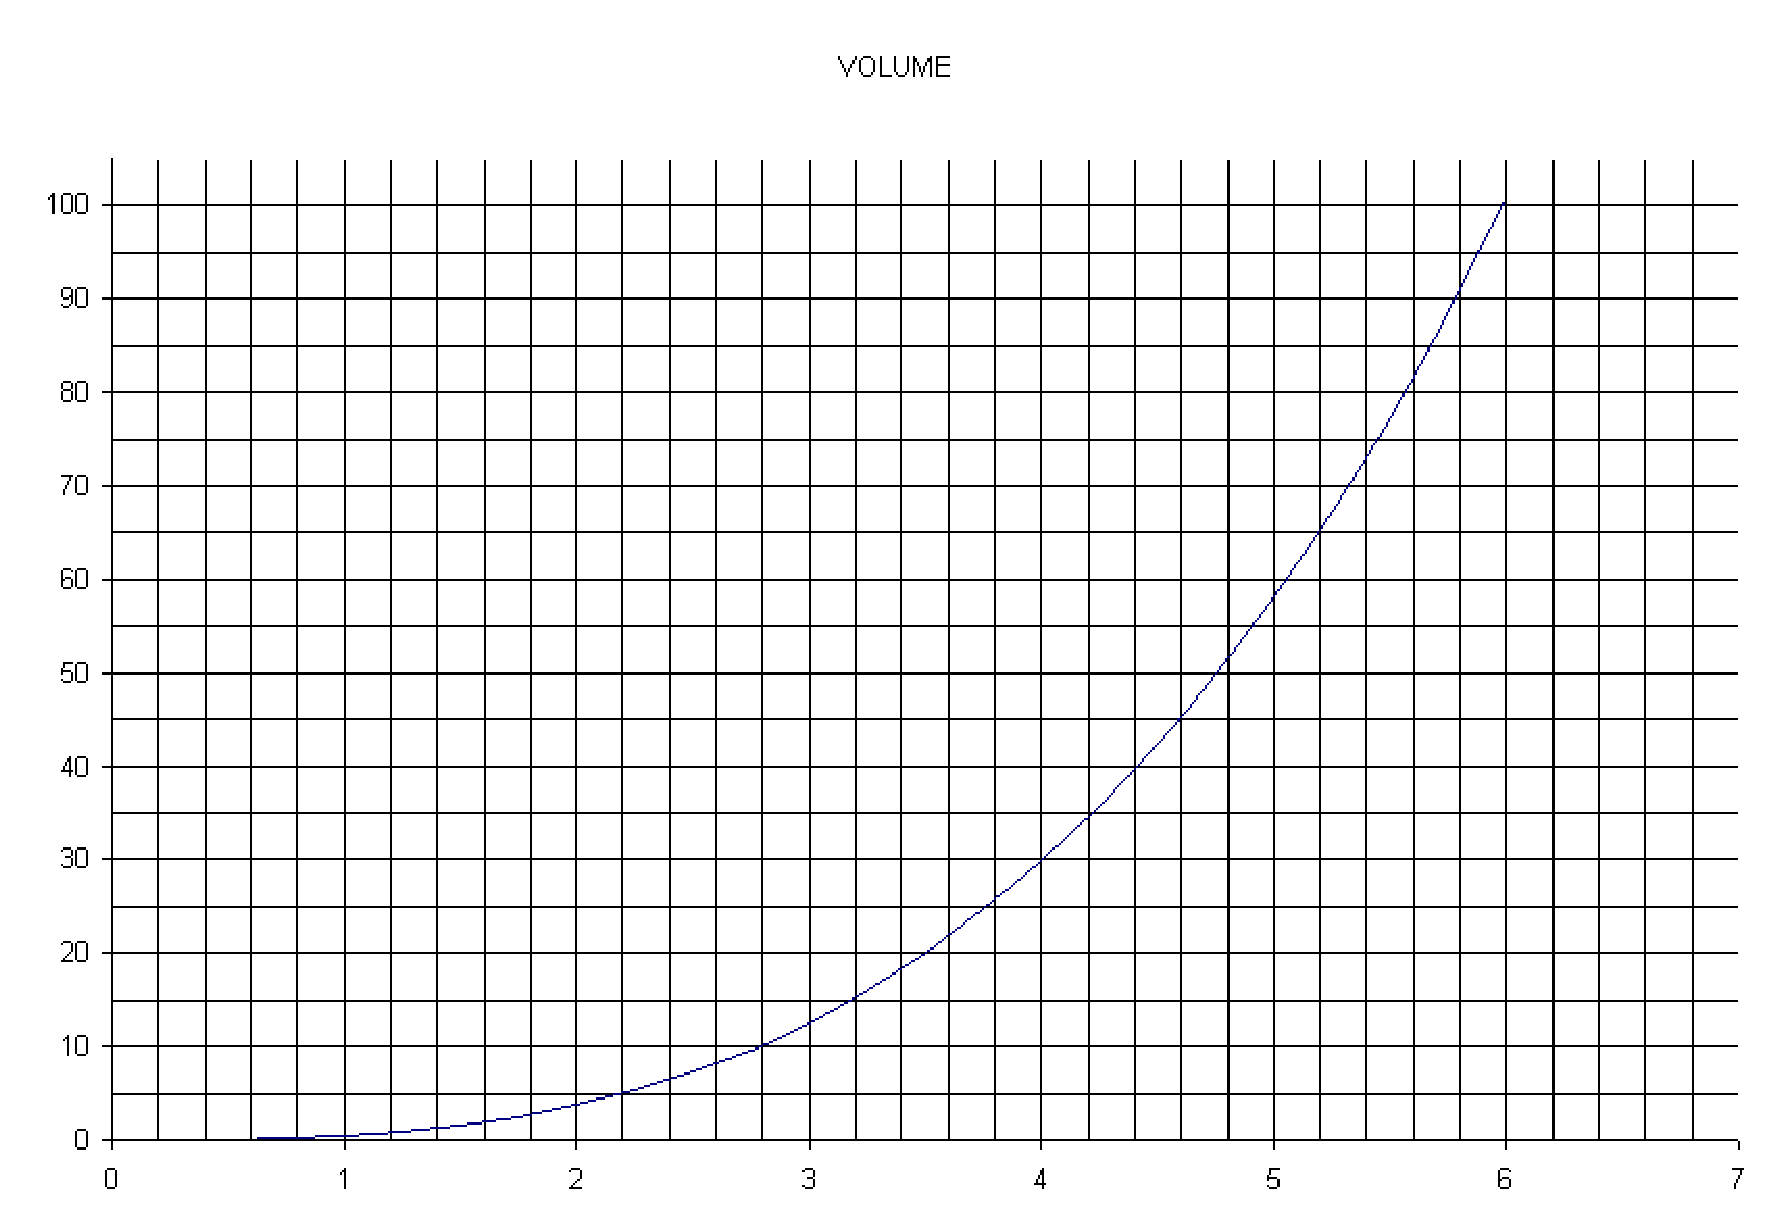
\includegraphics[scale=0.625]{./Graphiques/courbe.eps}\end{center}

%%%%%%%%%%%%%%%%%%%%%%%%%%%%%%%%%%%%%%%%%%%%%%%%%%%%
%%%%%%%%%%%%%%%%%%%%%%%%%%%%%%%%%%%%%%%%%%%%%%%%%%%

%%%%%%%%%%%%%%%%%%%%%%%%%%%%%%%%%%%%%%%%%%%%%%%%%%%\`u
%%%%%%%%%%%%%%%%%%%%%%%%%%%%%%%%%%%%%%%%%%%%%%%%%%%%

 \sautpage

\section{Premi\`eres notions (bilan et compl\'ements)}

\begin{definition}[Notion de fonction]
Une fonction est un proc\'ed\'e qui, \`a un \'el\'ement $x$ d'un ensemble de d\'epart, associe au plus un \'el\'ement $y$ d'un ensemble d'arriv\'ee.

On notera $f:x\mapsto y$ ou $f(x)=y$ qui se lit \og $f$ est la fonction qui \`a $x$ associe $y$ \fg..

On dit que $y$ est \emph{l'image} de $x$.

On dit que $x$ est \emph{un ant\'ec\'edent} de $y$.

\end{definition}

\begin{definition}[Ensemble de d\'efinition]
L'ensemble des r\'eels $x$ poss\'edant une image par une fonction num\'erique $f$ est appel\'e \emph{l'ensemble de d\'efinition de la fonction $f$}. On le note souvent $D_f$.
\end{definition}

\begin{definition}[Repr\'esentation graphique]
Dans un plan muni d'un rep\`ere, la \emph{repr\'esentation graphique} de la fonction $f$ est l'ensemble des points $M$ de coordonn\'ees $(x;y)$ du plan tels que :
\begin{itemize}
	\item L'abscisse $x$ de $M$ d\'ecrit l'ensemble de d\'efinition $D_f$ ;
	\item L'ordonn\'ee $y$ est l'image de $x$ par $f$. $y=f(x)$.
\end{itemize}

On note souvent $\mathcal{C}_f$ la repr\'esentation graphique de $f$. On dit que $\mathcal{C}_f$ a pour \'equation $y=f(x)$.

Si la courbe est d'un seul \og{} tenant \fg{} on parle  de \emph{courbe repr\'esentative} de la fonction $f$.
\end{definition}


\begin{rmq} L'\'equation permet de d\'eterminer si un point $A(x_A;y_A)$ appartient ou pas \`a cette courbe. En effet, un point appartient \`a la courbe si et seulement si ses coordonn\'ees v\'erifient l'\'equation de la courbe. On a alors : \[A\in\mathcal{C}_f\ssi y_A=f(x_A)\] \end{rmq}


Dans la pratique, pour les fonctions num\'eriques d\'efinies par une expression alg\'ebrique, pour esquisser une repr\'esentation graphique, on utilise souvent un tableau de valeurs.

\begin{tabular}{cc}
 \begin{minipage}[l]{0.55\linewidth}
  \begin{rmq} Une courbe ne repr\'esente pas toujours une fonction. Sur la figure ci-contre, par exemple, la courbe a plusieurs points ayant la même abscisse, comme $A(1,-1)$ et $B(1,3)$. Ce n'est donc pas la courbe repr\'esentative d'une fonction car alors 1 aurait plusieurs images.\end{rmq}
 \end{minipage}&
 \begin{minipage}[r]{0.45\linewidth}
\begin{center}
\psset{xunit=0.75cm , yunit=0.75cm}
\def\xmin{-2} \def\xmax{4} \def\ymin{-1.6} \def\ymax{3.6}
\begin{pspicture*}(\xmin,\ymin)(\xmax,\ymax)
\psset{xunit=0.75cm,yunit=0.75cm}
\psgrid[griddots=10,gridlabels=0pt,gridwidth=.3pt, gridcolor=black, subgridwidth=.3pt, subgridcolor=black, subgriddiv=1](0,0)(-2,-2)(4,4)
\psaxes[labels=all,labelsep=1pt, Dx=1,Dy=1]{->}(0,0)(\xmin,\ymin)(\xmax,\ymax)
\uput[dl](0,0){$O$}
%\pcline[linewidth=1pt]{->}(0,0)(1,0) \uput[d](0.5,0){\small $\vec \imath$}
%\pcline[linewidth=1pt]{->}(0,0)(0,1) \uput[l](0,0.5){\small $\vec \jmath$}
\pscircle(1,1){1.5}
\psdots[dotstyle=x](1,-1)(1,3)
\uput[d](1,-1){$A$}
\uput[u](1,3){$B$}
\end{pspicture*}
\end{center}
 \end{minipage}

\end{tabular}






%\sautpage

\subsubsection{Quelques conventions graphiques}
\begin{multicols}{3}
Lorsqu'un point $A$ sur la courbe est connu avec pr\'ecision, il est not\'e par une croix.
\begin{center}
\begin{pspicture*}(-0.5,-1)(2.5,3)
\pscurve(0,0)(0.5,-0.5)(1,1)(2,2.5)
\uput[u](0,0){$\mathcal{C}_f$}
\psdot[dotstyle=x](1,1)
\uput[dr](1,1){$A$}
\end{pspicture*}
\end{center}\sautcol
Lorsqu'un point $A$ est l'extr\'emit\'e de la courbe, il est not\'e par un gros point.
\begin{center}
\begin{pspicture*}(-0.5,-1)(2.5,3)
\pscurve(0,0)(0.5,-0.5)(1,1)(2,2.5)
\uput[u](0,0){$\mathcal{C}_f$}
\psdot(2,2.5)
\uput[dr](2,2.5){$A$}
\end{pspicture*}
\end{center}\sautcol
Lorsqu'un point $A$ \`a l'extr\'emit\'e de la courbe n'appartient pas \`a la courbe, il est not\'e par un \og demi-cercle \fg.
\begin{center}
\begin{pspicture*}(-0.5,-1)(2.5,3)
\pscurve{-(}(0,0)(0.5,-0.5)(1,1)(2,2.5)
\uput[u](0,0){$\mathcal{C}_f$}
%\psdot[(2,2.5)
\uput[dr](2,2.5){$A$}
\end{pspicture*}
\end{center}
\end{multicols}
\begin{multicols}{3}
Une courbe est donn\'ee dans une fenêtre ; s'il n'y a pas d'extr\'emit\'es, la courbe garde la même allure quand on la prolonge.
\begin{center}
\begin{pspicture*}(-0.5,-1)(2.5,3)
\pscurve(-0.3,0)(0.5,2)(1,1)(2,2.8)
\uput[u](1,1){$\mathcal{C}_f$}
\psline[linestyle=dotted](-0.1,0.5)(1.7,0.5)(1.7,2.2)(-0.1,2.2)(-0.1,0.5)
\end{pspicture*}
\end{center}
Une droite verticale en pointill\'es signifie que si l'on prolonge la courbe, elle ne coupe pas cette droite. Sur l'exemple ci-dessous, $a$ n'appartient pas \`a $D_f$.
\begin{center}
\begin{pspicture*}(-0.5,-1)(2.5,3)
\psaxes[labels=none,labelsep=1pt,Dx=5,Dy=5]{->}(0,0)(-0.5,-1)(2.5,3)
\psset{algebraic=true}
\psplot{0.6}{3}{1/(4*x-2)}
\psline[linestyle=dashed](0.5,-1)(0.5,3)
\uput[dl](0.5,0){$a$}
\end{pspicture*}
\end{center}
Une droite horizontale en pointill\'es signifie que si l'on prolonge la courbe, elle ne coupe pas cette droite.
\begin{center}
\begin{pspicture*}(-0.5,-1)(2.5,3)
\psaxes[labels=none,labelsep=1pt,Dx=5,Dy=5]{->}(0,0)(-0.5,-1)(2.5,3)
\psset{algebraic=true}
\psplot{-0.5}{3}{1+1/(x+1)}
\psline[linestyle=dashed](-0.5,1)(2.5,1)
\uput[ul](0,1){$b$}
\end{pspicture*}
\end{center}
\end{multicols}

%\sautpage






\section{R\'esolutions graphiques d'\'equations et d'in\'equations}


\subsection{R\'esolutions d'\'equations de la forme $f(x)=k$}

R\'esoudre l'\'equation $f(x)=k$ c'est d\'eterminer tous les ant\'ec\'edents \'eventuels d'un \'el\'ement $k$ de l'ensemble d'arriv\'ee, c'est-\`a-dire chercher tous les $x$ de l'ensemble de d\'epart tels que $f(x)=k$.

Une telle recherche peut se faire graphiquement \`a partir de la repr\'esentation graphique de la fonction $f$.




\begin{center}
\begin{tabular}{lc}
 \begin{minipage}[l]{0.6\linewidth}
 \begin{exemple*}
  Soit $f$ la fonction d\'efinie sur $\R$ par $f(x)=2x^2-9x+10$. On recherche les solutions de l'\'equation $f(x)=3$.

	On commence par tracer soigneusement la courbe repr\'esentative de $f$ et on obtient la repr\'esentation donn\'ee sur la figure ci-dessous.
		
		On cherche les points de la courbe ayant pour ordonn\'ee 3. Pour cela on peut tracer la droite d'\'equation $y=3$ et chercher les points d'intersection de cette droite avec la courbe de $f$.

		On obtient ici deux points $M_1(1;3)$ et $M_2\left(\frac{7}{2};3\right)$. Les solutions sont leurs abscisses : 1 et $\frac{7}{2}$.

		On \'ecrit : \og Les solutions de l'\'equation $f(x)=3$ sont $x=1$ ou $x=\frac{7}{2}$ car les points de la courbe de $f$ d'ordonn\'ee 3 ont pour abscisses 1 et $\frac{7}{2}$ \fg.
		\end{exemple*}
 \end{minipage}&
 \begin{minipage}[r]{0.35\linewidth}
  
		\begin{center}
 \psset{xunit=1cm,yunit=1cm}
		\begin{pspicture*}(-3.1,-2.1)(4.6,4.1)
\def\xmin{-3} \def\xmax{4.5} \def\ymin{-2} \def\ymax{4}

\psgrid[griddots=10,gridlabels=0pt,gridwidth=.3pt, gridcolor=black, subgridwidth=.3pt, subgridcolor=black, subgriddiv=1](0,0)(-3,-2)(4.5,4)
\psaxes[labels=all,labelsep=1pt, Dx=1,Dy=1]{->}(0,0)(\xmin,\ymin)(\xmax,\ymax)
\uput[dl](0,0){$O$}
\pcline[linewidth=1pt]{->}(0,0)(1,0) \uput[d](0.5,0){\small $\vec \imath$}
\pcline[linewidth=1pt]{->}(0,0)(0,1) \uput[r](0,0.5){\small $\vec \jmath$}
\psset{algebraic=true}
\psplot{\xmin}{\xmax}{2*(x-1)*(x-1)-5*(x-1)+3}
\uput[ul](2,1){$\mathcal{C}_f$}
\psline[linestyle=dashed](\xmin,3)(\xmax,3)
\uput[u](-2,3){$y=3$}
\uput[ur](1,3){$M_1$}
\uput[ul](3.5,3){$M_2$}
\psdots[dotstyle=x](1,3)(3.5,3)
\psline[linestyle=dashed]{->}(1,3)(1,0)
\psline[linestyle=dashed]{->}(3.5,3)(3.5,0)
\end{pspicture*}\end{center}
 \end{minipage}

\end{tabular}             \end{center}



%\sautpage

\subsection{R\'esolutions d'in\'equations de la forme $f(x)\leqslant k$}

Ces in\'equations peuvent se r\'esoudre graphiquement. On proc\`ede de la façon suivante :
\begin{itemize}
	\item on trace soigneusement $\mathcal{C}_f$ dan un rep\`ere (orthogonal) ;
	\item on trace la droite d'\'equation $y=k$ ;
	\item on recherche les points de la courbe situ\'es \emph{sous} la droite ;
	\item l'ensemble des solutions est constitu\'e des abscisses de ces points.
\end{itemize}

\begin{exemple*} Sur l'exemple pr\'ec\'edent, si l'on doit r\'esoudre $f(x)\leqslant 3$, apr\`es avoir trac\'e $y=3$ on constate que les points de la courbe situ\'es sous cette droite ont leurs abscisses comprises entre 0 et $\frac{5}{2}$.

Donc $f(x)\leqslant 3 \ssi x\in\left[0;\frac{5}{2}\right]$.
\end{exemple*}

\begin{rmq}~
\begin{itemize}
	\item On r\'esoud de la même mani\`ere les \'equations du type $f(x)\geqslant k$.

On retient alors les abscisses des points situ\'es \emph{au-dessus} de la droite d'\'equation $y=k$.

Dans l'exemple $f(x)\geqslant 3 \ssi x\in \left] -\infty ; 0 \right] \cup \left[\frac{5}{2} ; +\infty\right[$.
	\item De même pour les in\'equations strictes : $f(x)>k$ ou $f(x)<k$. On excluera alors les abscisses des points d'intersection de la courbe et de la droite.

	Dans l'exemple $f(x)<3 \ssi x\in \left]0;\frac{5}{2}\right[$.
\end{itemize}
\end{rmq}

\subsection{R\'esolutions d'\'equations de la forme $f(x)=g(x)$}

Cela revient \`a chercher les \'el\'ements de l'ensemble de d\'epart qui ont la même image par $f$ et par $g$.

Une telle recherche peut se faire graphiquement. On recherche alors les points des deux courbes repr\'esentatives ayant même abscisse et même ordonn\'ee, c'est-\`a-dire les points d'intersection des deux courbes. 

\begin{tabular}{cc}
 \begin{minipage}[l]{0.6\linewidth}
  \begin{exemple*}

Soit $f$ et $g$ les fonctions d\'efinies sur $\R$ par, respectivement, $f(x)=x^2-1$ et $g(x)=-0,5x^2+x+4$. R\'esoudre graphiquement l'\'equation $f(x)=g(x)$.

	On commence par tracer soigneusement les deux courbes repr\'esentatives et on obtient la repr\'esentation donn\'ee sur la figure ci-contre.
	
	On cherche les points d'intersection des deux courbes, ici $M_1$ et $M_2$, et les solutions de l'\'equation sont leurs abscisses dont les valeurs approximatives sont $-1,5$ et $2,2$.

		Les solutions sont donc $x\approx -1,5$ et $x\approx 2,2$.
\end{exemple*}
 \end{minipage}&
 \begin{minipage}[r]{0.35\linewidth}
  \psset{xunit=0.75cm,yunit=0.75cm}
		\begin{pspicture*}(-3.1,-2.1)(4.6,5.1)
\def\xmin{-3} \def\xmax{4.5} \def\ymin{-2} \def\ymax{5}

\psgrid[griddots=10,gridlabels=0pt,gridwidth=.3pt, gridcolor=black, subgridwidth=.3pt, subgridcolor=black, subgriddiv=1](0,0)(-3,-2)(4.5,5)
\psaxes[labels=all,labelsep=1pt, Dx=1,Dy=1]{->}(0,0)(\xmin,\ymin)(\xmax,\ymax)
\uput[dl](0,0){$O$}
\pcline[linewidth=1pt]{->}(0,0)(1,0) \uput[d](0.5,0){\small $\vec \imath$}
\pcline[linewidth=1pt]{->}(0,0)(0,1) \uput[r](0,0.5){\small $\vec \jmath$}
\psset{algebraic=true}
\psplot{\xmin}{\xmax}{x^2-1}
\psplot{\xmin}{\xmax}{-0.5*x^2+x+4}
\uput[u](1,1){$\mathcal{C}_f$}
\uput[dr](0,4){$\mathcal{C}_g$}
\uput[r](2.189,3.793){$M_2$}
\uput[l](-1.523,1.318){$M_1$}
\psdots[dotstyle=x](2.189,3.793)(-1.523,1.318)
\psline[linestyle=dashed]{->}(-1.523,1.318)(-1.523,0)
\psline[linestyle=dashed]{->}(2.189,3.793)(2.189,0)
\end{pspicture*}
	
 \end{minipage}


\end{tabular}

		

\subsection{R\'esolutions d'in\'equations de la forme $f(x)\leqslant g(x)$}

L\`a encore ces in\'equations peuvent se r\'esoudre graphiquement. On proc\`ede de la façon suivante :
\begin{itemize}
	\item on trace soigneusement $\mathcal{C}_f$ et $\mathcal{C}_g$ dans un rep\`ere (orthogonal) ;
	\item l'ensemble des solutions est constitu\'e des abscisses des points o\`u la courbe de $f$ est situ\'ee \emph{sous} celle de $g$.
\end{itemize}

\begin{exemple*} Sur l'exemple pr\'ec\'edent, si l'on doit r\'esoudre $f(x)\leqslant g(x)$, on constate que les points de la courbe de $f$ situ\'es sous celle de $g$ ont leurs abscisses comprises entre environ $-1,5$ et 2,2.

Donc $f(x)\leqslant g(x) \ssi x\in [-1,5;2,2]$. Ou bien $S=[-1,5;2,2]$.
\end{exemple*}

\begin{rmqs}~
\begin{itemize}
	\item On r\'esoud de la même mani\`ere les \'equations du type $f(x)\geqslant g(x)$.

On retient alors les abscisses des points de la courbe de $f$ situ\'es \emph{au-dessus} de celle de $g$.

Dans l'exemple $f(x)\geqslant g(x) \ssi x\in ] -\infty ; -1,5 ] \cup [2,2 ; +\infty[$.
	\item De même pour les in\'equations strictes : $f(x)>g(x)$ ou $f(x)<g(x)$. On excluera alors les abscisses des points d'intersection des deux courbes.

	Dans l'exemple $f(x)<g(x) \ssi x\in ]-1,5;2,2[$.
\end{itemize}
\end{rmqs}



%\sautpage



\sautpage

\section{Variations, extremums}


\subsection{Sens de variation}

Il s'agit de traduire math\'ematiquement qu'une fonction \og augmente \fg{} ou \og diminue \fg.

\begin{exemple*} Soit, par exemple, la fonction d\'efinie sur $[-3;3]$ par la courbe repr\'esentative donn\'ee sur la figure \ref{croissanceetdecroissance} \vpageref{croissanceetdecroissance}. On constate que lorsque $x\in[-3;1]$ , si $x$ augmente, $f(x)$ augmente aussi alors que lorsque $x\in[1;3]$, si $x$ augmente, $f(x)$ diminue.

C'est la d\'efinition math\'ematique de la croissance ou de la d\'ecroissance d'une fonction $f$.

\begin{figure}[h]
\centering
\caption{Croissance et d\'ecroissante}\label{croissanceetdecroissance}


\psset{xunit=1cm , yunit=1.25cm}
\begin{pspicture*}(-4.1,-1.1)(4.1,5.1)
\def\xmin{-4} \def\xmax{4} \def\ymin{-1} \def\ymax{5}
\psgrid[griddots=10,gridlabels=0pt,gridwidth=.3pt, gridcolor=black, subgridwidth=.3pt, subgridcolor=black, subgriddiv=1](0,0)(-4,-1)(4,5)
\psaxes[labels=all,labelsep=1pt, Dx=1,Dy=1]{-}(0,0)(\xmin,\ymin)(\xmax,\ymax)
\uput[dl](0,0){$O$}
\pcline[linewidth=1pt]{->}(0,0)(1,0) \uput[d](0.5,0){\small $\vec \imath$}
\pcline[linewidth=1pt]{->}(0,0)(0,1) \uput[r](0,0.5){\small $\vec \jmath$}
\psset{algebraic=true}
\psplot{-3}{3}{(-(x-1)^2+5)*0.25+3}
\psdots(3,3.25)(-3,0.25)
\uput[d](-1.5,0){$b$}
\psline[linestyle=dashed]{->}(-1.5,0)(-1.5,2.6875)
\psline[linestyle=dashed]{->}(-1.5,2.6875)(0,2.6875)
\uput[r](0,2.6875){$f(b)$}
\uput[d](-2.5,0){$a$}
\psline[linestyle=dashed]{->}(-2.5,0)(-2.5,1.1875)
\psline[linestyle=dashed]{->}(-2.5,1.1875)(0,1.1875)
\uput[r](0,1.1875){$f(a)$}
\uput[d](1.5,0){$u$}
\uput[d](2.5,0){$v$}
\psline[linestyle=dashed]{->}(1.5,0)(1.5,4.1875)
\psline[linestyle=dashed]{->}(1.5,4.1875)(0,4.1875)
\uput[l](0,4.1875){$f(u)$}
\psline[linestyle=dashed]{->}(2.5,0)(2.5,3.6875)
\psline[linestyle=dashed]{->}(2.5,3.6875)(0,3.6875)
\uput[l](0,3.6875){$f(v)$}
\end{pspicture*}
\end{figure}\end{exemple*}


\begin{definition}
Soit $f$ une fonction d\'efinie sur un intervalle $I$. On dit que $f$ est
\begin{itemize}
	\item \emph{croissante} sur $I$ si, pour tous r\'eels $a$ et $b$ de $I$, on a :\\
$\text{Si } a<b \text{ alors } f(a)\leqslant f(b).$
	\item \emph{d\'ecroissante} sur $I$ si, pour tous r\'eels $a$ et $b$ de $I$, on a :\\
$\text{Si } a<b \text{ alors } f(a)\geqslant f(b).$
	\item \emph{monotone} si elle n'est que croissante sur $I$ ou si elle n'est que d\'ecroissante sur $I$.
	\item \emph{constante} sur $I$ si, pour tous r\'eels $a$ et $b$ de $I$, on a : $f(a)=f(b)$.
\end{itemize}
\end{definition}


\begin{rmqs}~
\begin{itemize}
	\item Ces notions ne sont valables que sur \textbf{un intervalle} et pas sur une r\'eunion d'intervalles disjoints.
	\item Ant\'ec\'edents et images \'etant rang\'es dans le même ordre, on dit qu'une fonction croissante \emph{conserve} l'ordre.
	\item Ant\'ec\'edents et images \'etant rang\'es dans l'ordre inverse, on dit qu'une fonction d\'ecroissante \emph{inverse} l'ordre.
	\item On obtient les d\'efinitions d'une fonction \emph{strictement} croissante ou \emph{strictement} d\'ecroisante en remplaçant les in\'egalit\'es par des in\'egalit\'es strictes. Ainsi on dit que $f$ est strictement croissante sur $I$ si pour tous r\'eels $a$ et $b$ de $I$ on a : \\ $\text{Si } a<b \text{ alors } f(a)<f(b)$
	\item Une fonction est strictement monotone sur $I$ si elle est strictement croissante ou strictement d\'ecroissante sur $I$
\end{itemize}
\end{rmqs}

\subsection{Tableau de variations}

Ces r\'esultats peuvent se r\'esumer dans un tableau de variation, qui est une forme stylis\'ee de repr\'esentation o\`u l'on indique uniquement si la courbe monte, descend ou est stable. Dans la premi\`ere ligne on indique les valeurs importantes de $x$ et dans la seconde les variations de $f$.

\begin{exemple*} Dans l'exemple pr\'ec\'edent on obtient
$$\tabvar{%
\tx{x}&\tx{-3}&&\tx{1}&&\tx{3}\cr
\tx{f}&\txb{\approx 0,25}&\fm&\txh{\approx 4,25}&\fd&\txb{\approx 2,25}\cr
}$$
\end{exemple*}



\subsection{Extremums}

Les extremums, s'ils existent, sont les valeurs maximale et minimale qui sont \textbf{atteintes} par la fonction $f$ sur un intervalle donn\'e. Plus pr\'ecis\'ement :

\begin{definition}
Soit une fonction $f$ d\'efinie sur un intervalle $I$ et $x_0\in I$. On dit que
\begin{itemize}
	\item $f$ admet un \emph{maximum}, atteint en $x_0$ si, pour tout $x\in I$, $f(x)\leqslant f(x_0)$. Ce maximum est alors $f(x_0)$.
	\item $f$ admet un \emph{minimum}, atteint en $x_0$ si, pour tout $x\in I$, $f(x)\geqslant f(x_0)$. Ce minimum est alors $f(x_0)$.
\end{itemize}
Les maximum et minimum sont appel\'es les \emph{extremums}.
\end{definition}

%\begin{rmq} Un extremum doit être atteint par une valeur $x_0$. \end{rmq}

\begin{exemple*}
La fonction $f$ d\'efinie sur $\R$ par $f(x)=x^2+1$ n'admet pas $-1$ comme minimum.

En effet, si on a bien $f(x)\geqslant -1$ sur $\R$, il n'existe pas de $x_0$ tel que $f(x_0)=-1$.

Par contre 1 est bien le minimum de $f$ sur $\R$ car
\begin{itemize}
	\item $f(x)\geqslant 1$ pour tout $x\in\R$ \textbf{ET}
	\item $f(0)=1$
\end{itemize}

On dira donc : le minimum de $f$ sur $\R$ est 1 et il est atteint pour $x_0=0$.
\end{exemple*}

\sautpage

\section{Exercices et probl\`emes}

\subsection{Premi\`eres notions}

%\begin{multicols}{2}
%\begin{exo} Dire dans chacun des exemples ci-dessous quel est l'ensemble de d\'efinition, quelles sont les images possibles et si la fonction est num\'erique.
%\begin{enumerate}
%	\item \`A chaque \'el\`eve de la classe on associe la couleur de ses cheveux.
%	\item \`A chaque \'el\`eve de la classe on associe le nombre de ses fr\`eres et soeurs.
%	\item Pour un \'el\`eve donn\'e, \`a chaque moment de sa vie on associe la taille qu'il mesurait.
%	\item Soit $ABCD$ un rectangle dont un des côt\'es est fixe et mesure 6 cm et l'autre est variable et mesure $x$ cm. \\On d\'efinit la fonction $f$ de la façon suivante : \`a chaque $x$ possible, on associe $f(x)$, l'aire du rectangle $ABCD$.
%	\item La fonction $g$ d\'efinie par $g(x)=x^2+2x+3$.
%	\item La fonction $h$ d\'efinie par $h(x)=\frac{x^2+1}{x-1}$.
%	\item La fonction $i$ d\'efinie par $i(x)=\sqrt{x+2}$.
%\end{enumerate}
%\end{exo}
\begin{multicols}{2}
\begin{exo}
On d\'efinit $f$ et $g$, deux fonctions :
\begin{itemize}
	\item $f$ est la fonction qui \`a un nombre r\'eel $x$ associe le nombre obtenu en proc\'edant de la mani\`ere suivante : on ajoute $4$ au nombre, on \'el\`eve le r\'esultat obtenu au carr\'e, on retranche 16, on divise par le nombre de d\'epart et on retranche 6.
	\item $g:x\mapsto x^2-4$.
\end{itemize}
\begin{enumerate}
	\item Donner l'expression correspondant \`a $f$ puis simplifier cette expression.
	\item Quel r\'eel n'a pas d'image par $f$ ?
	\item Quelle est l'image de 3 par $g$ ?
	\item Quelle est l'image de $-1$ par $g$ ?
	\item Quels sont les ant\'ec\'edents \'eventuels de 12 par $g$ ?
	\item Quels sont les ant\'ec\'edents \'eventuels de $-5$ par $g$ ?
\end{enumerate}
\end{exo}

\sautcol

\begin{exo}
Vrai ou faux ? \emph{Corriger la phrase lorsqu'elle est fausse}.
\begin{enumerate}
	\item $f(-2) = 0$ signifie que l'image de 0 est $-2$
	\item $f(0) = 3$ signifie que la courbe de $f$ passe par le point $(0 ; 3)$
	\item $f(1) = 2$ signifie que l'ant\'ec\'edent de 1 est 2
	\item L'image de 2 par $f$ est $-3$ s'\'ecrit $f(2) = -3$
	\item Dire que $(5 ; 1)$ est un point de la courbe de $f$ s'\'ecrit $5 = f(1)$
	\item Par la fonction $g$, $-5$ est l'image de 3 s'\'ecrit $g(-5) = 3$
	\item 2 a pour image 0 par $f$ signifie que la courbe de $f$ traverse l'axe des abscisses en 2
	\item $f(4) = 0$ signifie que la courbe de $f$ traverse l'axe des abscisses au point $(4 ; 0)$
	\item 3 a pour image 5, signifie que 3 est l'image de 5
	\item 4 a pour ant\'ec\'edent 5 signifie que 5 est l'image de 4
\end{enumerate}
\end{exo}

\end{multicols}

%\sautpage

\begin{exo}\label{gf4courbes}
Vrai ou faux ? \emph{Justifier la r\'eponse lorsque c'est faux}.\\
Les courbes de la figure \ref{gf4courbesfig} \vpageref{gf4courbesfig} repr\'esentent des fonctions de la variable $x$.


\begin{figure}[!h]
 \centering
 \caption{Courbes de l'exercice \ref{gf4courbes}}\label{gf4courbesfig}
\begin{tabular}{cc}
\psset{xunit=1cm , yunit=0.5cm}
\begin{pspicture*}(-2.1,-2.1)(4.1,4.1)
\def\xmin{-2} \def\xmax{4} \def\ymin{-2} \def\ymax{4}
\psgrid[griddots=10,gridlabels=0pt,gridwidth=.3pt, gridcolor=black, subgridwidth=.3pt, subgridcolor=black, subgriddiv=1](0,0)(-2,-2)(4,4)
\psaxes[labels=all,labelsep=1pt, Dx=1,Dy=1]{->}(0,0)(\xmin,\ymin)(\xmax,\ymax)
\uput[dl](0,0){$O$}
\pcline[linewidth=1pt]{->}(0,0)(1,0) \uput[d](0.5,0){\small $\vec \imath$}
\pcline[linewidth=1pt]{->}(0,0)(0,1) \uput[l](0,0.5){\small $\vec \jmath$}
\psline(-2,3)(1,-1.5)(2,-1.5)(4,2)
\end{pspicture*}
&
\psset{xunit=1cm , yunit=0.5cm}
\begin{pspicture*}(-2.1,-2.1)(4.1,4.1)
\def\xmin{-2} \def\xmax{4} \def\ymin{-2} \def\ymax{4}
\psgrid[griddots=10,gridlabels=0pt,gridwidth=.3pt, gridcolor=black, subgridwidth=.3pt, subgridcolor=black, subgriddiv=1](0,0)(-2,-2)(4,4)
\psaxes[labels=all,labelsep=1pt, Dx=1,Dy=1]{->}(0,0)(\xmin,\ymin)(\xmax,\ymax)
\uput[dl](0,0){$O$}
\pcline[linewidth=1pt]{->}(0,0)(1,0) \uput[d](0.5,0){\small $\vec \imath$}
\pcline[linewidth=1pt]{->}(0,0)(0,1) \uput[l](0,0.5){\small $\vec \jmath$}
\psline(-2,3)(1,3)(1,1)(4,1)
\end{pspicture*}
\\
\psset{xunit=1cm , yunit=0.5cm}
\begin{pspicture*}(-2.1,-2.1)(4.1,4.1)
\def\xmin{-2} \def\xmax{4} \def\ymin{-2} \def\ymax{4}
\psgrid[griddots=10,gridlabels=0pt,gridwidth=.3pt, gridcolor=black, subgridwidth=.3pt, subgridcolor=black, subgriddiv=1](0,0)(-2,-2)(4,4)
\psaxes[labels=all,labelsep=1pt, Dx=1,Dy=1]{->}(0,0)(\xmin,\ymin)(\xmax,\ymax)
\uput[dl](0,0){$O$}
\pcline[linewidth=1pt]{->}(0,0)(1,0) \uput[d](0.5,0){\small $\vec \imath$}
\pcline[linewidth=1pt]{->}(0,0)(0,1) \uput[l](0,0.5){\small $\vec \jmath$}
\psline(-2,3)(4,3)
\end{pspicture*}
&
\psset{xunit=1cm , yunit=0.5cm}
\begin{pspicture*}(-2.1,-2.1)(4.1,4.1)
\def\xmin{-2} \def\xmax{4} \def\ymin{-2} \def\ymax{4}
\psgrid[griddots=10,gridlabels=0pt,gridwidth=.3pt, gridcolor=black, subgridwidth=.3pt, subgridcolor=black, subgriddiv=1](0,0)(-2,-2)(4,4)
\psaxes[labels=all,labelsep=1pt, Dx=1,Dy=1]{->}(0,0)(\xmin,\ymin)(\xmax,\ymax)
\uput[dl](0,0){$O$}
\pcline[linewidth=1pt]{->}(0,0)(1,0) \uput[d](0.5,0){\small $\vec \imath$}
\pcline[linewidth=1pt]{->}(0,0)(0,1) \uput[l](0,0.5){\small $\vec \jmath$}
\pscurve(-2,3)(-1,0)(0,-1)(2,1)(3.2,2)(3,3)
\end{pspicture*}
\end{tabular}
\end{figure}

\end{exo}

\sautpage

\begin{exo}\label{gf14}
Vrai ou faux ? \emph{Corriger la phrase lorsqu'elle est fausse}.\\
Les fonctions $f$ et $g$ sont repr\'esent\'ees sur la figure \ref{gf14fig} \vpageref{gf14fig}.
\begin{enumerate}
	\item La fonction $f$ est d\'efinie entre $-2$ et 6 inclus
	\item Les images par la fonction $f$ sont comprises entre $-1$ et 4 inclus
	\item La fonction $g$ est d\'efinie entre $-2$ exclu et 6 inclus
	\item Les images par la fonction g sont comprises entre 0 exclu et 3 inclus
\end{enumerate}



\begin{figure}[!h]
\centering
\caption{Courbes de l'exercice \ref{gf14}}\label{gf14fig}
\begin{tabular}{cc}
\psset{xunit=0.9cm , yunit=0.5cm}
\begin{pspicture*}(-3.1,-2.1)(6.1,5.1)
\def\xmin{-3} \def\xmax{6} \def\ymin{-2} \def\ymax{5}
\psgrid[griddots=10,gridlabels=0pt,gridwidth=.3pt, gridcolor=black, subgridwidth=.3pt, subgridcolor=black, subgriddiv=1](0,0)(-3,-2)(6,5)
\psaxes[labels=all,labelsep=1pt, Dx=1,Dy=1]{->}(0,0)(\xmin,\ymin)(\xmax,\ymax)
\uput[dl](0,0){$O$}
\pcline[linewidth=1pt]{->}(0,0)(1,0) \uput[d](0.5,0){\small $\vec \imath$}
\pcline[linewidth=1pt]{->}(0,0)(0,1) \uput[l](0,0.5){\small $\vec \jmath$}
\pscurve{*-(}(-2,2)(-1,3)(0,3.7)(0.5,3.9)(1,4)(2,3)(3,0)(4,-1)(5,0)(6,1)

\rput(3,2){$\mathcal{C}_f$}
\end{pspicture*}
&
\psset{xunit=0.9cm , yunit=0.5cm}
\begin{pspicture*}(-3.1,-2.1)(6.1,5.1)
\def\xmin{-3} \def\xmax{6} \def\ymin{-2} \def\ymax{5}
\psgrid[griddots=10,gridlabels=0pt,gridwidth=.3pt, gridcolor=black, subgridwidth=.3pt, subgridcolor=black, subgriddiv=1](0,0)(-3,-2)(6,5)
\psaxes[labels=all,labelsep=1pt, Dx=1,Dy=1]{->}(0,0)(\xmin,\ymin)(\xmax,\ymax)
\uput[dl](0,0){$O$}
\pcline[linewidth=1pt]{->}(0,0)(1,0) \uput[d](0.5,0){\small $\vec \imath$}
\pcline[linewidth=1pt]{->}(0,0)(0,1) \uput[l](0,0.5){\small $\vec \jmath$}
\pscurve{)-}(-2,0)(0,1)(1,2)(1.5,3.5)(1.8,5)
\pscurve{-*}(2.2,-2)(3,0)(4,1.5)(6,3)
\rput(1,3){$\mathcal{C}_g$}
\psline[linestyle=dashed](2,\ymin)(2,\ymax)
\end{pspicture*}
\end{tabular}
\end{figure}

\end{exo}

\begin{exo}\label{gf15}
Vrai ou faux ? \emph{Corriger la proposition lorsqu'elle est fausse}.
\begin{itemize}
	\item D'apr\`es la repr\'esentation graphique de la figure \ref{gf15fig} \vpageref{gf15fig} $D_f=[-4;2]$
	\item D'apr\`es la repr\'esentation graphique de la figure \ref{gf15fig} \vpageref{gf15fig} $D_g=]-\infty;3[\cup]3;5]$
\end{itemize}


\begin{figure}[!h]
\centering
\caption{Courbes de l'exercice \ref{gf15}}\label{gf15fig}
\begin{tabular}{cc}
\psset{xunit=1cm , yunit=0.66cm}
\begin{pspicture*}(-4.1,-2.1)(4.1,4.1)
\def\xmin{-4} \def\xmax{4} \def\ymin{-2} \def\ymax{4}
\psgrid[griddots=10,gridlabels=0pt,gridwidth=.3pt, gridcolor=black, subgridwidth=.3pt, subgridcolor=black, subgriddiv=1](0,0)(-4,-2)(4,4)
\psaxes[labels=all,labelsep=1pt, Dx=1,Dy=1]{->}(0,0)(\xmin,\ymin)(\xmax,\ymax)
\uput[dl](0,0){$O$}
\pcline[linewidth=1pt]{->}(0,0)(1,0) \uput[d](0.5,0){\small $\vec \imath$}
\pcline[linewidth=1pt]{->}(0,0)(0,1) \uput[l](0,0.5){\small $\vec \jmath$}
\pscurve{*-}(-4,0)(-3,-2)(0,0)(1,1)(4,1.8)
\psline[linestyle=dashed](0,2)(4,2)
\rput(-1.5,-1){$\mathcal{C}_f$}
\end{pspicture*}
&
\psset{xunit=1cm , yunit=0.66cm}
\begin{pspicture*}(-3.1,-2.1)(5.6,4.1)
\def\xmin{-3} \def\xmax{5.5} \def\ymin{-2} \def\ymax{4}
\psgrid[griddots=10,gridlabels=0pt,gridwidth=.3pt, gridcolor=black, subgridwidth=.3pt, subgridcolor=black, subgriddiv=1](0,0)(-3,-2)(5.5,4)
\psaxes[labels=all,labelsep=1pt, Dx=1,Dy=1]{->}(0,0)(\xmin,\ymin)(\xmax,\ymax)
\uput[dl](0,0){$O$}
\pcline[linewidth=1pt]{->}(0,0)(1,0) \uput[d](0.5,0){\small $\vec \imath$}
\pcline[linewidth=1pt]{->}(0,0)(0,1) \uput[l](0,0.5){\small $\vec \jmath$}
\pscurve(-3,3)(0,1.5)(1,1)(2,0)(2.8,-2)
\pscurve{-*}(3.2,-2)(4,1)(5,3)
\psline[linestyle=dashed](3,\ymin)(3,\ymax)
\uput[ur](1,1){$\mathcal{C}_g$}
\end{pspicture*}
\end{tabular}
\end{figure}
\end{exo}
%\sautpage


\begin{exo}[Avec la calculatrice]
La fonction $f$ est d\'efinie sur $[-1,5;2]$ par : $f(x)=2x^3-1,5x^2-3x$
\begin{enumerate}
	\item Compl\'eter le tableau de valeurs suivant :
	%\vspace{-1em}
	\begin{center}
\begin{tabular}{|*{9}{c|}}
\hline $x$ & $-1,5$ & $-1$ & $-0,5$ & 0 & 0,5 & 1 & 1,5 & 2 \\ \hline
$f(x)$ & & & & & & & & \\ \hline
\end{tabular}
\end{center}
\item Tracer la courbe repr\'esentative de $f$.
\end{enumerate}
\end{exo}

\begin{exo}[Avec la calculatrice]\label{uneautrecourbe}
La fonction $f$ est d\'efinie sur $[-3;3]$ par : $f(x)=x^2-3x+1$.\\
Apr\`es avoir dress\'e un tableau de valeurs de la fonction, tracer sa courbe repr\'esentative $\mathcal{C}_f$.

\end{exo}

%\end{multicols}



\sautpage

\subsection{R\'esolutions graphiques}

\begin{exo}
La fonction $f$ est d\'efinie sur $[-3;3]$ par : $f(x)=x^2-3x+1$.\\
$\mathcal{C}_f$, courbe repr\'esentative de $f$ a d\'ej\`a \'et\'e obtenue dans l'exercice \ref{uneautrecourbe}.
\begin{enumerate}
	\item \`A l'aide de la repr\'esentation graphique $\mathcal{C}_f$, avec la pr\'ecision permise par le graphique, r\'epondre aux question suivantes :
		\vspace{-1em}\begin{multicols}{2}
		  \begin{enumerate}
			\item Quelle est l'image de 2 ?
			\item Quelle est l'image de 3 ?
			\item Quelle est l'image de 4 ?
			\item Quels sont les ant\'ec\'edents de 1 ?
			\item Quels sont les ant\'ec\'edents de 2 ?
			\item Quels sont les ant\'ec\'edents de $-2$ ?
		\end{enumerate}
		\end{multicols}\vspace{-1em}
	\item R\'esoudre graphiquement les \'equations et in\'equations suivantes :
\vspace{-1em}\begin{multicols}{3}\begin{enumerate}
	\item $f(x)=3$ ;
	\item $f(x)=-1,5$ ;
	\item $f(x)\geqslant -1$ ;
	\item $f(x)<4$ ;
	\item $f(x)>-3$ ;
	\item $f(x)<-2$.
\end{enumerate}\end{multicols}\vspace{-1em}
\item D\'eterminer graphiquement le signe de $f(x)$ selon les valeurs de $x$.
\end{enumerate}
\end{exo}

%\sautpage

\begin{exo}
Une fonction $f$, d\'efinie sur $\R$, est donn\'ee par sa courbe repr\'esentative $\mathcal{C}$ :
\begin{multicols}{2}
\begin{center}\small
\psset{xunit=1,yunit=1}
\begin{pspicture*}(-2.6,-2.1)(5.1,3.1)
\def\xmin{-2.5} \def\xmax{5} \def\ymin{-2} \def\ymax{3}
\psset{xunit=0.1cm,yunit=0.1cm}
\psgrid[griddots=15,gridlabels=0pt,gridwidth=.3pt, gridcolor=gray, subgridwidth=.3pt, subgridcolor=gray, subgriddiv=1](0,0)(-25,-20)(50,30)
\psset{xunit=1cm , yunit=1cm}
\psaxes[labels=all,labelsep=1pt, Dx=1,Dy=1]{->}(0,0)(\xmin,\ymin)(\xmax,\ymax)
\uput[dl](0,0){$0$}
\pcline[linewidth=1pt]{->}(0,0)(1,0) \uput[d](0.5,0){\small $\vec i$}
\pcline[linewidth=1pt]{->}(0,0)(0,1) \uput[l](0,0.5){\small $\vec j$}
\pscurve(-2.3,-2)(-2,-1)(-1.5,1.5)(-1,3)(-0.5,2.5)(0,1)(0.2,0)(0.5,-1)(1,-1.5)(1.5,-1)(2,0)(2.5,1)(3,1.5)(4,2)(5,2.3)
\psline[linestyle=dashed](0,2.5)(\xmax,2.5)
\psdots[dotstyle=x](-2,-1)(-1.5,1.5)(-1,3)(-0.5,2.5)(0,1)(0.5,-1)(1,-1.5)(1.5,-1)(2,0)(2.5,1)(3,1.5)(4,2)
\end{pspicture*}
\end{center}\normalsize

\sautcol

Avec la pr\'ecision permise par le graphique, r\'esoudre :
%\vspace{-1em}
%\begin{multicols}{2}
\begin{enumerate}
	\item Les \'equations suivantes :
		\vspace{-1em}
		\begin{multicols}{2}\begin{enumerate}
			\item $f(x) = 1$ ;
			\item $f(x) = 0$ ;
			\item $f(x) = -1$ ;
			\item $f(x) = 2$.
		\end{enumerate}\end{multicols}
		%\vspace{-1em}
%\sautcol
	\item Les in\'equations suivantes :
		\vspace{-1em}
		\begin{multicols}{2}\begin{enumerate}
			\item $f(x)\geqslant 1$ ;
			\item $f(x)\geqslant 0$ ;
			\item $f(x)<-1$ ;
			\item $f(x)>2$.
		\end{enumerate}\end{multicols}
		\vspace{-1em}
	\item D\'eterminer graphiquement le signe de $f(x)$ selon les valeurs de $x$.

\end{enumerate}\end{multicols}
%\vspace{-1em}
\end{exo}

\medskip

\begin{multicols}{2}

\begin{exo}\label{gfunecourbe}
La courbe $\mathcal{C}$ de la figure ci-dessous %\ref{gfunecourbefig} \vpageref{gfunecourbefig} 
repr\'esente une fonction $f$ et le segment de droite $\mathcal{D}$ repr\'esente une fonction $g$.

%\begin{figure}[hbtp]
% \centering
% \caption{Figure de l'exercice \ref{gfunecourbe}}\label{gfunecourbefig}


\begin{center}
\psset{xunit=0.375cm , yunit=0.33cm}
\def\xmin{-9} \def\xmax{12} \def\ymin{-3} \def\ymax{11}
\begin{pspicture*}(\xmin,\ymin)(\xmax,\ymax)
\psgrid[griddots=10,gridlabels=0pt,gridwidth=.3pt, gridcolor=black, subgridwidth=.3pt, subgridcolor=black, subgriddiv=1](0,0)(\xmin,\ymin)(\xmax,\ymax)
\psaxes[labels=all,labelsep=1pt, Dx=5,Dy=5]{-}(0,0)(\xmin,\ymin)(\xmax,\ymax)
\uput[dl](0,0){$O$}
\pcline[linewidth=1pt]{->}(0,0)(1,0) \uput[d](0.5,0){\small $\vec \imath$}
\pcline[linewidth=1pt]{->}(0,0)(0,1) \uput[l](0,0.5){\small $\vec \jmath$}
\pscurve{*-*}(-8,1)(-5,3)(-3,5)(-1,6)(0,5)(1,3)(2,0)(4,-2)(7,0)(9,3)(11,6)
\psdots[dotstyle=x](-5,3)(-3,5)(-1,6)(0,5)(1,3)(2,0)(4,-2)(7,0)(9,3)
\psdots[dotstyle=*](-8,7.5)(11,-2)
\uput[dr](10,5){$\mathcal{C}$}
\uput[ur](-6,7){$\mathcal{D}$}
\psplot[linestyle=dashed,algebraic=true]{-8}{11}{-0.5*x+3.5}
\end{pspicture*}\end{center}

%\end{figure}

\sautcol

\begin{enumerate}
	\item R\'esoudre graphiquement les \'equations :
		\vspace{-1em}\begin{multicols}{2}\begin{enumerate}
			\item $f(x) = 3$ ;
			\item $f(x) = -2$ ;
			\item $f(x) = 0$ ;
			\item $f(x) = 6$.
		\end{enumerate}\end{multicols}
	\item R\'esoudre graphiquement les in\'equations :
		\begin{enumerate}
			\item $f(x)\leqslant 0$ ;
			\item $f(x) \geqslant 3$ ;
			\item $f(x)>5$.
		\end{enumerate}

	\item R\'esoudre graphiquement :
			\begin{enumerate}
				\item $f(x) = g(x)$ ;
				\item $f(x) < g(x)$.			\end{enumerate}
		\item Donner le signe de $f(x)$ suivant les valeurs de $x$.
\end{enumerate}
\end{exo}\end{multicols}

%\sautpage

\begin{multicols}{2}

\begin{exo}[Avec la calculatrice]
On consid\`ere les fonctions $f$ et $g$ d\'efinies sur $\R$ par : $f(x)=x^3$ et $g(x)=3x-2$.
 \begin{enumerate}
			\item Tracer soigneusement les repr\'esentations graphiques $\mathcal{C}_f$ et $\mathcal{C}_g$ de $f$ et $g$ sur l'intervalle $[-2;2]$.
			\item R\'esoudre graphiquement l'in\'equation $f(x)\leqslant 1$.
			\item D\'eterminer graphiquement les solutions de l'\'equation $f(x)=g(x)$.
 \end{enumerate}
\end{exo}

\sautcol

\begin{exo}[Avec la calculatrice]
Les fonctions $f$ et $g$ sont d\'efinies sur $[-2;2]$ par : $f(x)=x^3$ et $g(x)=1-x$.
\begin{enumerate}
	\item Tracer sur une calculatrice graphique les repr\'esentations graphiques $\mathcal{C}_f$ et $\mathcal{C}_g$ de $f$ et de $g$.
	\item En d\'eduire le nombre de solutions de l'\'equation $x^3+x-1=0$.
	\end{enumerate}
\end{exo}

\end{multicols}

\subsection{R\'esolutions calculatoires}
%\section{Technologie}
\begin{multicols}{2}
\begin{exo}
Soit la fonction $f$ d\'efinie sur $\R$ par : \\$f(x)=2x^2+x+3$.
\begin{enumerate}
	\item Calculer les valeurs exactes de $f(x)$ pour les valeurs de $x$ suivantes :
	  \vspace{-1em}\begin{multicols}{3}
	  \begin{itemize}
	    \item 0 ;
	    \item 1 ;
	    \item $-2$ ;
	    \item $\sqrt{2}$ ;
	    \item $1+\sqrt{3}$ ;
	    \item $2-\sqrt{5}$.
	   \end{itemize}
	  \end{multicols}\vspace{-1em}
	\item R\'esoudre $f(x)=3$.
\end{enumerate}
\end{exo}

\begin{exo}
Soit $f$ la fonction d\'efinie sur $\R$ par :\\ $f(x)=2x^2-5x+3$. \\R\'esoudre $f(x)=3$.
\end{exo}

\begin{exo} Soit $f$ la fonction d\'efinie sur $\R$ par : $f(x)=4x^2-4x+1$. On cherche \`a r\'esoudre, par le calcul, l'\'equation $f(x)=9$.
%\vspace{-1em}\begin{multicols}{2}
\begin{enumerate}
	\item Factoriser $f(x)$.
	\item R\'esoudre $f(x)=9$.
\end{enumerate}% \end{multicols}\vspace{-1em}
\end{exo}



\begin{exo}
	Soit $f$ et $g$ les fonctions d\'efinies sur $\R$ par, respectivement, $f(x)=x^2-1$ et $g(x)=-x^2+2$. \\ R\'esoudre par le calcul l'\'equation $f(x)=g(x)$.
\end{exo}


\begin{exo}
On consid\`ere les fonctions $f$ et $g$ d\'efinies sur $\R$ par : $f(x)=x^3$ et $g(x)=3x-2$. On cherche \`a r\'esoudre, par le calcul, l'\'equation $f(x)=g(x)$.
		\begin{enumerate}
			\item D\'evelopper $(x-1)^2(x+2)$.
			\item En d\'eduire les solutions de l'\'equation $x^3-3x+2=0$.
			\item En d\'eduire les solutions de l'\'equation $f(x)=g(x)$.
		\end{enumerate}
\end{exo}



%

\begin{exo}
On consid\`ere la fonction $f$ d\'efinie pour tout $x\in\R$ par : $f(x)=x(x-2)$. On cherche \`a trouver, par le calcul, le minimum de $f(x)$.
%\vspace{-1em}\begin{multicols}{2}
\begin{enumerate}
	\item D\'emontrer que $f(x)=(x-1)^2-1$.
	\item En d\'eduire le minimum de $f(x)$.
\end{enumerate}%\end{multicols}\vspace{-1em}
\end{exo}

\end{multicols}

\sautpage


\subsection{Variations, extremums}

\begin{multicols}{2}

\begin{exo}\label{fonctionsvar1}
On consid\`ere la fonction $f$ dont on donne la repr\'esentation $\mathcal{C}$ sur la figure \ref{fonctionsvar1fig} \vpageref{fonctionsvar1fig} (en deux parties).\\
Indiquer son ensemble de d\'efinition et dresser son tableau de variations.

\end{exo}
%\sautpage


\begin{exo}[Avec une calculatrice]
On consid\`ere la fonction $f$ d\'efinie par : $f(x)=2x\sqrt{4-x^2}$.
\`A l'aide d'une calculatrice graphique :
\begin{enumerate}
	\item conjecturer l'ensemble de d\'efinition de $f$ ;
	\item conjecturer quels sont les extremums de $f$ sur son ensemble de d\'efinition ;
	\item dresser le tableau des variations de $f$.
\end{enumerate}
\end{exo}


%\sautcol


\begin{exo}
Tracer une courbe repr\'esentative d'une fonction $f$ sachant que :
%\vspace{-1em}\begin{multicols}{2}
\begin{itemize}
\item le tableau des variations de $f$ est le suivant :$$\tabvar{%
\tx{x}&&&\tx{0}&&\tx{3}&&\tx{~}\cr
\tx{f}&\txb{1}&\fm&&\fd&&\fm&\cr
}$$
	\item 1 a pour ant\'ec\'edents, par la fonction $f$, $-2$ et 1,5 ;
	\item $f(x)=0$ a pour solutions $x=2$ ou $x=4$ ;
	\item $f(-1)=2$ ;
	\item $-1$ est l'image de 3 ;
	\item $D_f=[-2;4]$ ;
	\item le maximum de $f$ est 3 ;
	
\end{itemize}%\end{multicols}
\end{exo}



\sautcol

\begin{exo}
On donne le tableau des variations d'une fonction $f$ :$$\tabvar{%
\tx{x}&\tx{-5}&&\tx{-3}&&\tx{0}&&\tx{1}&&\tx{8}\cr
\tx{f}&\txh{3}&\fd&\txb{0}&\fm&\txh{1}&\fdh&\tx{0}&\fdb&\txb{-2}\cr
}$$
%\vspace{-4em}\begin{multicols}{2}
\begin{enumerate}
	\item S'il est possible de r\'epondre, compl\'eter par \og < \fg, \og > \fg{} ou \og = \fg. Sinon mettre une croix.
\begin{itemize}
 \item $f(-1)$  $\ldots\ldots$  $f(-2)$ 
 \item $f(-3)$  $\ldots\ldots$  $f(1)$ 
 \item $f(-1)$  $\ldots\ldots$  $1$ 
 \item $f(-2)$ $\ldots\ldots$  $f(0,5)$
 \item $f(-2)$  $\ldots\ldots$  $f(1,5)$
 \item $f(4)$  $\ldots\ldots$  $f(2)$
 \item $4$  $\ldots\ldots$ $f(-4)$
 \end{itemize}

\item R\'esoudre, lorsque c'est possible, les in\'egalit\'es suivantes :
\vspace{-1em}\begin{multicols}{2}\begin{enumerate}
	  \item $f(x)\geqslant 0$ ;
	  \item $f(x)=1$ ;
	  \item $f(x)<-1$ ;
	  \item $f(x)<0$.
  \end{enumerate}\end{multicols}
	\item Dire, si c'est possible, quel est le maximum de la fonction et quel est son minimum.
\end{enumerate}%\end{multicols}
\end{exo}
\end{multicols}
%M\end{multicols}



\begin{figure}[!h]
 \centering
 \caption{Figure de l'exercice \ref{fonctionsvar1}}\label{fonctionsvar1fig}

\psset{xunit=0.75cm , yunit=0.75cm}
\begin{pspicture*}(-6.1,-2.1)(14.1,6.1)
\def\xmin{-6} \def\xmax{14} \def\ymin{-2} \def\ymax{6}
\psgrid[griddots=10,gridlabels=0pt,gridwidth=.3pt, gridcolor=black, subgridwidth=.3pt, subgridcolor=black, subgriddiv=1](0,0)(-6,-2)(14,6)
\psaxes[labels=all,labelsep=1pt, Dx=1,Dy=1]{-}(0,0)(\xmin,\ymin)(\xmax,\ymax)
\uput[dl](0,0){$O$}
\pcline[linewidth=1pt]{->}(0,0)(1,0) \uput[d](0.5,0){\small $\vec i$}
\pcline[linewidth=1pt]{->}(0,0)(0,1) \uput[l](0,0.5){\small $\vec j$}
\pscurve(-5,-1)(-4,0)(-3,3)(-2,4)(0,3)(4,0)(5,-2)
\psdot(-5,-1)
\psdots[dotstyle=x](-4,0)(-3,3)(-2,4)(0,3)(4,0)(7,0)(8,3)(10,5)(12,3)
\pscurve(6.5,-2)(7,0)(8,3)(10,5)(12,3)(14,2.2)
\psline[linestyle=dashed](6,-2)(6,6)
\psline[linestyle=dashed](9,2)(14,2)
\end{pspicture*}
\end{figure}







%\sautpage


\cleardoublepage

\fancyhead{} % Delete current head settings

		\fancyhead[LE,LO]{\footnotesize \em Nom : }
		\fancyhead[RE,RO]{\scriptsize \em Vendredi 14 octobre 2016 -- 1h00}
		\fancyfoot{}

\setcounter{ds}{2} %c'est le numéro du DS	
\setcounter{chaptertemp}{\thechapter} %stocke le numéro du chapitre courant dans un compteur temporaire
\stepcounter{chapter} % avance le compteur de 1 et surtout remet tous les compteurs dépendant du chapitre à 0, dont les numéros d'exercice
\setcounter{chapter}{\theds} % met le compteur de chapitre au numéro du ds
		
    
\section*{Devoir surveill\'e n°\theds}\label{DS2}
{\centering \large G\'en\'eralit\'es sur les fonctions}
\addstarredchapter{Devoir surveill\'e n°\theds : G\'en\'eralit\'es sur les fonctions} 

\begin{exo}[9 points]\label{ds2exo1}
On donne sur la figure ci-dessous les courbes repr\'esentatives de deux fonctions $f$ et $g$, nomm\'ees, respectivement, $\mathcal{C}_f$ et $\mathcal{C}_g$, d\'efinies toutes deux sur l'intervalle $[-3,5\,;\,3,5]$.

\begin{center}
    \def\xmin{-4.1} \def\xmax{4.1} \def\ymin{-4.1} \def\ymax{7.1}
\psset{xunit=2cm,yunit=0.5cm}
\begin{pspicture*}(\xmin,\ymin)(\xmax,\ymax)
\psset{unit=0.5cm}
\psgrid[griddots=10,gridlabels=0pt,gridwidth=.5pt, gridcolor=black, subgridwidth=.3pt, subgridcolor=black, subgriddiv=1](0,0)(-16,\ymin)(16,\ymax)
\psset{xunit=2cm,yunit=0.5cm}
\psaxes[labels=all,labelsep=1pt, Dx=1,Dy=1]{->}(0,0)(\xmin,\ymin)(\xmax,\ymax)
\psdots(0,0)(1,0)(0,1)%
\uput[dl](0,0){$O$}
\uput[u](1,0){$I$}
\uput[r](0,1){$J$}
\uput[ul](\xmax,0){$x$}
\uput[dr](0,\ymax){$y$}

\psplot[plotpoints=200,algebraic=true]{-3.5}{3.5}{0.25*(x-1)*(x+3)*(x-2)}
\psplot[plotpoints=200,algebraic=true]{-3.5}{3.5}{-0.25*(x-1)*(x-1)+4}
\psdots(-3.5,-3.09375)(-3.5,-1.0625)(3.5,6,09375)(3.5,2.4375)(-3,0)(-2,3)(-1,3)(1,0)(1,4)(2,0)(3,3)

\uput[u](1,4){$\mathcal{C}_g$}
\uput[ul](-2,3){$\mathcal{C}_f$}
\end{pspicture*}\end{center}

%\medskip

\textsc{\textbf{Partie A}} (2,5 points)\\
Des phrases sont propos\'ees ci-dessous.\\
Indiquer si elles sont vraies ou fausses et, si elles sont fausses, les corriger pour qu'elles deviennent vraies.

\begin{multicols}{2}
 \begin{enumerate}
  \item L'image de $-2$ par $g$ est 3\\
	.\dotfill.\\
	.\dotfill.
  \item $1,5$ a trois ant\'ec\'edents par $f$\\
	.\dotfill.\\
	.\dotfill. \sautcol
  \item 3 est un ant\'ec\'edent de $-2$ par $f$\\
	.\dotfill.\\
	.\dotfill. 
  \item 0 a pour image 2 par $f$\\
	.\dotfill.\\
	.\dotfill.  
 \end{enumerate} 
\end{multicols}


\medskip

\textsc{\textbf{Partie B}} (4,5 points)\\
Avec la pr\'ecision persmise par le graphique, r\'esoudre les \'equations et in\'equations suivantes.

\begin{multicols}{2}
 \begin{enumerate}
  \item $f(x)=0$\\
	.\dotfill.\\
	.\dotfill.
  \item $g(x)>0$\\
	.\dotfill.\\
	.\dotfill.
  \item $f(x)\geqslant 3$\\
	.\dotfill.\\
	.\dotfill. \sautcol
  \item $g(x)< 3$\\
	.\dotfill.\\
	.\dotfill. 
  \item $f(x)=g(x)$\\
	.\dotfill.\\
	.\dotfill.  
  \item $f(x)>g(x)$\\
	.\dotfill.\\
	.\dotfill.
 \end{enumerate} 
\end{multicols}

\medskip

\textsc{\textbf{Partie C}} (2 points)\\
D\'eterminer graphiquement le signe de $f(x)$ selon les valeurs de $x$. \emph{On pourra pr\'esenter sa r\'eponse sous la forme d'un tableau.}
.\dotfill.\\
.\dotfill.\\
.\dotfill.\\
.\dotfill.


\end{exo}

%\medskip

%\hrule

\begin{exo}[3 points]\label{ds2exo2}
Soit $f$ la fonction d\'efinie sur $[-2\,;\,4]$ par $f : x\longmapsto -x^2+2x+3$.
\begin{enumerate}
 \item Compl\'eter le tableau de valeurs ci-dessous :
 %\vspace{-1em}
 \begin{center}
  \begin{tabular}{c*{7}{|>{\centering} m{1.5cm}}}
   $x$ & $-2$&$-1$ & 0 & 1 &2 & 3 & 4  \tabularnewline \hline
   &&&&&&& \tabularnewline
   $f(x)$ &$-5$&&&&&& %\tabularnewline
   %&&&&&&& 
  \end{tabular}
 \end{center}
 \item Tracer la courbe repr\'esentative de $f$ dans le rep\`ere ci-dessous :
 %\vspace{-1em}
 \begin{center}
    \def\xmin{-3.1} \def\xmax{5.1} \def\ymin{-6.1} \def\ymax{6.1}
\psset{xunit=2cm,yunit=0.5cm}
\begin{pspicture*}(\xmin,\ymin)(\xmax,\ymax)
\psset{unit=0.5cm}
\psgrid[griddots=10,gridlabels=0pt,gridwidth=.5pt, gridcolor=black, subgridwidth=.3pt, subgridcolor=black, subgriddiv=1](0,0)(-12,\ymin)(20,\ymax)
\psset{xunit=2cm,yunit=0.5cm}
\psaxes[labels=all,labelsep=1pt, Dx=1,Dy=1]{->}(0,0)(\xmin,\ymin)(\xmax,\ymax)
\psdots(0,0)(1,0)(0,1)%
\uput[dl](0,0){$O$}
\uput[u](1,0){$I$}
\uput[r](0,1){$J$}
\uput[ul](\xmax,0){$x$}
\uput[dr](0,\ymax){$y$}

%\psplot[plotpoints=200,algebraic=true]{-2}{4}{-x^2+2*x+3}

\end{pspicture*}\end{center}
\end{enumerate}

 
\end{exo}

\medskip

\hrule

\begin{exo}[3 points]\label{ds2exo3}
Soit $f$ et $g$ deux fonctions d\'efinies sur $\R$ par 
$f:x\longmapsto x^2-4$ et $g:x\longmapsto x^3 -4x$.\\
\`A l'aide de la calculatrice r\'esoudre l'in\'equation $f(x)\geqslant g(x)$.\\
\emph{On ne demande aucune justification.}\\
.\dotfill.\\
.\dotfill.\\
.\dotfill.
 
\end{exo}

\medskip

\hrule


\begin{exo}[5 points]\label{ds3exo1}



On donne l'algorithme ci-contre.





\begin{enumerate}\vspace{-1em}\begin{multicols}{2}
 \item Le faire fonctionner avec les valeurs indiqu\'ees et compl\'eter le tableau ci-dessous.
 \begin{center}
  \begin{tabular}{c|c|c|c}
   $A$ & $B$ & $C$ & Sortie de l'algorithme \\ \hline
   & & & \\
   3 & $-1$ & 27 & \\ \hline
  % & & & \\ \hline
   & & & \\
   12 & 7 & 2 & \\ \hline
   %& & & \\ \hline
   & & & \\
   4,5 & 7,5 & 1,5 & 
  % & & & 
  \end{tabular}

 \end{center}
 \begin{algo}
\begin{small}
\begin{verbatim}
   ENTREES
      A, B, C : nombres
   TRAITEMENT
      SI A>B ALORS M prend la valeur A
             SINON M prend la valeur B
      SI C>M ALORS M prend la valeur C
   SORTIE
      M
\end{verbatim}
\end{small}
\end{algo}
\end{multicols}

 \item Quel est le but de cet algorithme ?\\
 .\dotfill.\\
 .\dotfill.\\
 .\dotfill.
\end{enumerate}


\end{exo}
\hrule


%\hrulefill


 



%\FloatBarrier






\setcounter{chapter}{\thechaptertemp} % remet le numéro de chapitre à ce qu'il était


\chapter{Translation -- Vecteurs} \label{vecteurs}
\minitoc

\fancyhead{} % efface les entêtes précédentes
\fancyhead[LE,RO]{\footnotesize \em \rightmark} % section en entête
\fancyhead[RE,LO]{\scriptsize \em Seconde} % classe et année en entête

    \fancyfoot{}
		\fancyfoot[RE]{\scriptsize \em \href{http://perpendiculaires.free.fr/}{http://perpendiculaires.free.fr/}}
		\fancyfoot[LO]{\scriptsize \em David ROBERT}
    \fancyfoot[LE,RO]{\textbf{\thepage}}

%\sautpage

\section{Translation}

\subsection{D\'efinition}

\begin{definition*}
 Soient $A$ et $B$ deux points du plan.\\
  On appelle \emph{translation qui transforme $A$ en $B$} la transformation qui \`a tout point $M$ du plan associe l'unique point $M'$ tel que $[AM']$ et $[BM]$ ont m\^eme milieu.
\end{definition*}


\subsection{Activit\'es}

\begin{act}[Image d'un point par une translation]\label{imagedunpoint}
Sur chacune des figures ci-dessous, construire $M'$, image de $M$ par la translation qui transforme $A$ en $B$.
\begin{center}
	    \begin{tabular}{cc}
		    \psset{xunit=0.5cm , yunit=0.5cm}
		    \def\xmin{-0.1} \def\xmax{11.1} \def\ymin{-0.1} \def\ymax{6.1}
		    \begin{pspicture*}(\xmin,\ymin)(\xmax,\ymax)
		    \psgrid[gridlabels=0pt,gridwidth=.3pt, gridcolor=gray, subgridwidth=.3pt, subgridcolor=gray, subgriddiv=1](0,0)(\xmin,\ymin)(\xmax,\ymax)
		    \psline{->}(4,4)(7,3)
		    \psdots(4,4)(7,3)(6,5)
		    \uput[u](4,4){$A$}
		    \uput[u](7,3){$B$}
		    \uput[u](6,5){$M$}
		    \end{pspicture*}
		    &
		    \psset{xunit=0.5cm , yunit=0.5cm}
		    \def\xmin{-0.1} \def\xmax{11.1} \def\ymin{-0.1} \def\ymax{6.1}
		    \begin{pspicture*}(\xmin,\ymin)(\xmax,\ymax)
		    \psgrid[gridlabels=0pt,gridwidth=.3pt, gridcolor=gray, subgridwidth=.3pt, subgridcolor=gray, subgriddiv=1](0,0)(\xmin,\ymin)(\xmax,\ymax)
		    \psline{->}(8,5)(4,4)
		    \psdots(4,4)(8,5)(6,2)
		    \uput[u](4,4){$B$}
		    \uput[u](8,5){$A$}
		    \uput[u](6,2){$M$}
		    \end{pspicture*}
		\end{tabular}		             \end{center}
		
Dans chaque construction, on voit appara\^itre une figure famili\`ere. Laquelle ?\\
		D\'emontrer que c'est toujours le cas.	                                    



	
\end{act}

\sautpage

\begin{act}[Quelques propri\'et\'es de la translation]\label{proptranslation}
	Toutes les questions de cette activit\'e se rapportent \`a la figure \ref{proptranslationfig1} \vpageref{proptranslationfig1}.
	\begin{enumerate}
	 \item Construire $M'$, $N'$ et $O'$, images respectives de $M$, $N$ et $O$ par la translation qui transforme $A$ en $B$.
		\begin{figure}[h]
		\centering
		      \caption{\small Figure des activit\'es \ref{proptranslation} et \ref{translationcomposition}}\label{proptranslationfig1}
 
		

		 %\begin{tabular}{cc}
		  \psset{xunit=0.5cm , yunit=0.5cm}
		  \def\xmin{-0.1} \def\xmax{24.1} \def\ymin{-0.1} \def\ymax{11.1}
		  \begin{pspicture*}(\xmin,\ymin)(\xmax,\ymax)
		  \psgrid[gridlabels=0pt,gridwidth=.3pt, gridcolor=gray, subgridwidth=.3pt, subgridcolor=gray, subgriddiv=1](0,0)(\xmin,\ymin)(\xmax,\ymax)
		  \psline{->}(8,10)(11,9)
		  \psline{->}(11,9)(17,11)
		  \psdots(8,10)(11,9)(1,2)(2,4)(4,8)(17,11)
		  \uput[u](8,10){$A$}
		  \uput[u](11,9){$B$}
		  \uput[u](1,2){$M$}
		  \uput[u](2,4){$N$}
		  \uput[u](4,8){$O$}
		  \uput[d](17,11){$C$}
		  
		  \end{pspicture*}
		 %\end{tabular}
		\end{figure}
	 \item Construire $P$, image de $O$ la translation qui transforme $M$ en $M'$. Que constate-t-on ?
	 \item\label{proptranslationq3} Les points $M$, $N$ et $O$ sont align\'es. Cela semble-t-il \^etre aussi le cas des points $M'$, $N'$ et $O'$ ? \\ D\'emontrons-le.
		\begin{enumerate}
		 \item D'apr\`es la propri\'et\'e obtenue dans le cas g\'en\'eral, quels sont les parall\'elogrammes issus de la translation ?
		\item Quelles sont alors les droites parall\`eles \`a $(AB)$ ? Quelles sont les longueurs \'egales \`a $AB$ ?
		\item Que peut-on en d\'eduire pour les quadrilat\`eres $MNN'M'$, $NOO'N'$ ?
		\item Que peut-on en d\'eduire pour les droites $(MN)$ et $(M'N')$ ? Et pour les droites $(ON)$ et $(O'N')$ ?
		\item Conclure.
		\end{enumerate}
	  \item Construire l'image d'un autre point situ\'e sur le segment $[OM]$. Sur quel segment est situ\'ee cette image ? \\ Conjecturer quelle est l'image du segment $[OM]$ et celle de la droite $(OM)$.
	  \item Que peut-on dire des longueurs $MN$ et $M'N'$ ? Et des longueurs $ON$ et $O'N'$ ? \emph{Justifier, en utilisant \'eventuellement un r\'esultat de la d\'emonstration de la question \ref{proptranslationq3}}.

	\end{enumerate}
\end{act}

\begin{act}[Encha\^inement de deux translations]\label{translationcomposition}
 Toutes les questions de cette activit\'e se rapportent \`a la figure \ref{proptranslationfig1} \vpageref{proptranslationfig1}.
  \begin{enumerate}
   \item Construire $M''$, $N''$ et $O''$, images respectives de $M'$, $N'$ et $O'$ par la translation qui transforme $B$ en $C$. 
   \item Quelle est la nature du quadrilat\`ere $ONN''O''$ ? \emph{Justifier}.
   \item Quelle est la transformation qui permet de passer des points $M$, $N$ et $O$ aux points $M''$, $N''$ et $O''$ ?
  \end{enumerate}

\end{act}



\subsection{Bilan et compl\'ements}

\begin{definition}[Rappel]
 Soient $A$ et $B$ deux points du plan.\\
  On appelle \emph{translation qui transforme $A$ en $B$} la transformation qui \`a tout point $M$ du plan associe l'unique point $M'$ tel que $[AM']$ et $[BM]$ ont m\^eme milieu.
\end{definition}

\begin{prop}
 Soient $A$ et $B$ deux points du plan et $M$ ayant pour image $M'$ par la translation qui transforme $A$ en $B$.\\
 Alors $ABM'M$ est un \dotfill
\end{prop}

Cela a \'et\'e d\'emontr\'e dans l'activit\'e.

\begin{prop}
 Soient $A$ et $B$ deux points du plan et $M$, $N$ et $O$ ayant pour images respectives $M'$, $N'$ et $O'$ par la translation qui transforme $A$ en $B$. Alors :
  \begin{itemize}
       \item Si $M$, $N$ et $O$ sont align\'es alors \dotfill
       \item L'image du segment $[MN]$ est \dotfill de m\^eme \dotfill
       \item Si $O$ est le milieu du segment $[MN]$ alors \dotfill
  \end{itemize}
 On dit que la translation \emph{conserve} \dotfill, \dotfill et \dotfill.
\end{prop}

Le premier et le deuxi\`eme points ont \'et\'e d\'emontr\'es dans l'activit\'e. Le troisi\`eme point est une cons\'equence triviale des deux premiers.

\begin{prop}[admise]
 L'image d'une droite par une translation est \dotfill\\
 L'image d'un cercle par une translation est \dotfill
\end{prop}


Enfin, comme on l'a vu en activit\'e :

\begin{prop}
 L'encha\^inement (on parle de la \emph{composition}) de deux translations est une translation.
\end{prop}


\section{Vecteurs}

\subsection{D\'efinition -- \'Egalit\'e}

\begin{definition}
 On appelle \emph{vecteur $\V{AB}$} le bipoint associ\'e \`a la translation qui transforme $A$ en $B$.\\
 $A$ est appel\'e \emph{origine du vecteur}, $B$ est appel\'e \emph{extr\'emit\'e du vecteur}.
\end{definition}



\begin{definition}
 Deux vecteurs sont dits \emph{\'egaux} s'ils sont associ\'es \`a une m\^eme translation.
\end{definition}

On a vu pr\'ec\'edemment que
\begin{itemize}
 \item d'une part, $M'$ est l'image de $M$ par la translation de vecteur $\V{AB}$ si et seulement si $ABM'M$ parall\'elogramme (\'eventuellement aplati),
 \item d'autre part que les translations de vecteur $\V{AB}$ et de vecteur $\V{MM'}$ \'etaient les m\^emes donc que $\V{AB}=\V{MM'}$
\end{itemize}


\begin{multicols}{2}
Ce cas est g\'en\'eral. Ainsi :


\vspace{-1em}\begin{prop}~
  \begin{itemize}
   \item $\V{AB}=\V{MM'} \ssi$ \dotfill
   \item $\V{AB}=\ldots\ldots\ssi ABCD$ est un parall\'elogramme
  \end{itemize}
\end{prop}

\begin{rmq} Attention à l'ordre des lettres !\end{rmq}


\sautcol

\begin{center}
\psset{xunit=1cm , yunit=0.6666cm}
\begin{pspicture*}(-0.8,-0.6)(7.7,2.6)
\def\xmin{-0.6} \def\xmax{7.5} \def\ymin{-0.5} \def\ymax{2.5}


\psgrid[gridlabels=0pt,gridwidth=.3pt, gridcolor=gray, subgridwidth=.3pt, subgridcolor=gray, subgriddiv=1](0,0)(0,0)(7,2.5)

\psset{linecolor=black, linewidth=.5pt, arrowsize=2pt 4}
\uput[r](0,0){$A$}
\uput[l](1,2){$B$}
\psline{->}(0,0)(1,2)
\uput[r](2,0){$M$}
\uput[l](3,2){$M'$}
\psline{->}(2,0)(3,2)
\uput[l](4,2){$A$}
\uput[r](6,2){$B$}
\uput[r](7,0){$C$}
\uput[l](5,0){$D$}
\psline(4,2)(6,2)(7,0)(5,0)(4,2)
\end{pspicture*}
\end{center}
\end{multicols}

Ainsi, on peut aussi d\'efinir un vecteur de la mani\`ere suivante :

\begin{definition}
Un vecteur non nul est déterminé par :
\begin{itemize}
	\item sa \emph{direction} ;
	\item son \emph{sens} ;
	\item et sa longueur, appel\'ee \emph{norme du vecteur}.
\end{itemize}
\end{definition}

Et on a alors la propri\'et\'e :

\begin{prop}
 Deux vecteurs sont \'egaux si et seulement si ils ont la m\^eme direction, le m\^eme sens et la m\^eme norme.
\end{prop}

En effet, en appellant $\V{AB}$ et $\V{CD}$ ces deux vecteurs, $\V{AB}=\V{CD} \ssi ABDC \text{ parall\'elogramme } \ssi \V{AB}$ et $\V{CD}$ ont la m\^eme direction, le m\^eme sens et la m\^eme norme.

%\sautpage

\subsubsection{Notation $\vec{u}$}

\begin{multicols}{2}
\begin{center}
\psset{xunit=1cm , yunit=1cm}
\begin{pspicture*}(-0.8,-0.8)(6.7,2.7)
\def\xmin{-0.6} \def\xmax{6.5} \def\ymin{-0.6} \def\ymax{2.5}
\psset{linecolor=black, linewidth=.5pt, arrowsize=2pt 4}
\psline{->}(0,1)(2,1)
\uput[l](0,1){$A$}
\uput[r](2,1){$B$}
\psline{->}(2,2)(4,2)
\uput[l](2,2){$C$}
\uput[r](4,2){$D$}
\psline{->}(3,0)(5,0)
\uput[l](3,0){$E$}
\uput[r](5,0){$F$}
\psline{->}(4,1)(6,1)
\uput[u](5,1){$\vec{u}$}
\psdots[dotstyle=x,dotscale=2](0,1)(2,1)(2,2)(4,2)(3,0)(5,0)
\end{pspicture*}

\end{center}
Sur le schéma ci-contre, on a $\V{AB}=\V{CD}=\V{EF}$. \\
On pose alors $\vec{u}=\V{AB}=\V{CD}=\V{EF}$. \\
$\V{AB}$, $\V{CD}$ et $\V{EF}$ sont appelés des \emph{représentants} du vecteur $\vec{u}$.
\end{multicols}

\begin{exo}\label{vecteursegaux1}
Sur chaque sch\'ema de la figure ci-dessous, l'égalité $\V{AB}=\V{CD}$ est-elle vraie ?

\begin{center}
\begin{multicols}{3}
\psset{xunit=0.5cm , yunit=0.5cm}
\begin{pspicture*}(-0.8,-0.8)(7.7,4.7)
\def\xmin{-0.6} \def\xmax{7.5} \def\ymin{-0.6} \def\ymax{4.5}
\psset{xunit=0.5cm,yunit=0.5cm}
\psgrid[gridlabels=0pt,gridwidth=.3pt, gridcolor=gray, subgridwidth=.3pt, subgridcolor=gray, subgriddiv=1](0,0)(-0.6,-0.6)(7.5,4.5)
\psset{xunit=0.5cm , yunit=0.5cm}
\psset{linecolor=black, linewidth=.5pt, arrowsize=2pt 4}
\psdots[dotstyle=x, dotscale=2.0000](1.0000,4.0000)
\psdots[dotstyle=x, dotscale=2.0000](3.0000,0.0000)
\psdots[dotstyle=x, dotscale=2.0000](6.0000,4.0000)
\psdots[dotstyle=x, dotscale=2.0000](4.0000,0.0000)
\uput[l](1,4){$A$}
\uput[l](3,0){$B$}
\uput[r](6,4){$C$}
\uput[r](4,0){$D$}
\end{pspicture*}
\psset{xunit=0.5cm , yunit=0.5cm}
\begin{pspicture*}(-0.8,-0.8)(7.7,4.7)
\def\xmin{-0.6} \def\xmax{7.5} \def\ymin{-0.6} \def\ymax{4.5}
\psset{xunit=0.5cm,yunit=0.5cm}
\psgrid[gridlabels=0pt,gridwidth=.3pt, gridcolor=gray, subgridwidth=.3pt, subgridcolor=gray, subgriddiv=1](0,0)(-0.6,-0.6)(7.5,4.5)
\psset{xunit=0.5cm , yunit=0.5cm}
\psset{linecolor=black, linewidth=.5pt, arrowsize=2pt 4}
\psdots[dotstyle=x, dotscale=2.0000](1.0000,4.0000)
\psdots[dotstyle=x, dotscale=2.0000](6.0000,0.0000)
\psdots[dotstyle=x, dotscale=2.0000](6.0000,4.0000)
\psdots[dotstyle=x, dotscale=2.0000](1.0000,0.0000)
\uput[l](1,4){$A$}
\uput[r](6,0){$C$}
\uput[r](6,4){$B$}
\uput[l](1,0){$D$}
\end{pspicture*}
\psset{xunit=0.5cm , yunit=0.5cm}
\begin{pspicture*}(-0.8,-0.8)(7.7,4.7)
\def\xmin{-0.6} \def\xmax{7.5} \def\ymin{-0.6} \def\ymax{4.5}
\psset{xunit=0.5cm,yunit=0.5cm}
\psgrid[gridlabels=0pt,gridwidth=.3pt, gridcolor=gray, subgridwidth=.3pt, subgridcolor=gray, subgriddiv=1](0,0)(-0.6,-0.6)(7.5,4.5)
\psset{xunit=0.5cm , yunit=0.5cm}
\psset{linecolor=black, linewidth=.5pt, arrowsize=2pt 4}
\psdots[dotstyle=x, dotscale=2.0000](1.0000,4.0000)
\psdots[dotstyle=x, dotscale=2.0000](5.0000,3.0000)
\psdots[dotstyle=x, dotscale=2.0000](3.0000,1.0000)
\psdots[dotstyle=x, dotscale=2.0000](7.0000,0.0000)
\uput[r](1,4){$A$}
\uput[l](5,3){$C$}
\uput[r](3,1){$B$}
\uput[l](7,0){$D$}
\end{pspicture*}

\end{multicols} \end{center}
\end{exo}




\begin{exo}\label{vecteursegaux2} Sur la figure ci-dessous, expliquer, en utilisant les termes direction, sens ou norme, pourquoi le vecteur $\V{AB}$ n'est \'egal \`a aucun des autres vecteurs repr\'esent\'es.

\begin{center}
\psset{xunit=1cm , yunit=1cm}
\begin{pspicture*}(-0.8,-0.8)(7.7,4.7)
\def\xmin{-0.6} \def\xmax{7.5} \def\ymin{-0.6} \def\ymax{4.5}
\psset{xunit=1cm,yunit=1cm}
\psgrid[gridlabels=0pt,gridwidth=.3pt, gridcolor=gray, subgridwidth=.3pt, subgridcolor=gray, subgriddiv=1](0,0)(-0.6,-0.6)(7.5,4.5)
\psset{xunit=1cm , yunit=1cm}

\psset{linecolor=black, linewidth=.5pt, arrowsize=2pt 4}
\uput[d](0,2){$A$}
\uput[u](1,3){$B$}
\psline{->}(0,2)(1,3)
\uput[d](1,0){$C$}
\uput[d](3,0){$D$}
\psline{->}(1,0)(3,0)
\uput[d](3,2){$G$}
\uput[u](5,4){$H$}
\psline{->}(3,2)(5,4)
\uput[d](6,1){$E$}
\uput[u](7,2){$F$}
\psline{->}(7,2)(6,1)

\end{pspicture*}\end{center}

\end{exo}









%%%%%%%%%%%%%%%%%%%%%%%%%%%%%%%%%%%%%%%%%%%%%%%


\begin{multicols}{2}\begin{exo}
Sur la figure ci-contre :
\begin{enumerate}
	\item Construire, à partir des points $A$, $B$ et $C$, les points $D$, $E$ et $F$ tels que :\\ $\V{AB}=\V{CD}, \quad\V{EA}=\V{AB}, \quad\V{CF}=\V{BA}$
	\item Quels parallélogrammes peut-on tracer avec ces six points ?
	\item En utilisant ces six points, compléter : \\
	$\V{BD}=\ldots\ldots=\ldots\ldots \quad\V{BC}=\ldots\ldots \quad\V{BF}=\ldots\ldots$
	\item Quelles autres \'egalit\'es de vecteurs peut-on d\'eduire ?
\end{enumerate}
\begin{center}
\psset{xunit=0.5cm , yunit=0.5cm}
\begin{pspicture*}(-0.8,-1.8)(10.7,6.7)
\def\xmin{-0.6} \def\xmax{10.5} \def\ymin{-1.6} \def\ymax{6.5}
\psset{xunit=0.5cm,yunit=0.5cm}
\psgrid[gridlabels=0pt,gridwidth=.3pt, gridcolor=gray, subgridwidth=.3pt, subgridcolor=gray, subgriddiv=1](0,0)(-0.6,-1.6)(10.5,6.5)
\psset{xunit=0.5cm , yunit=0.5cm}
\psset{linecolor=black, linewidth=.5pt, arrowsize=2pt 4}
\psdots[dotstyle=x, dotscale=2.0000](2.0000,3.0000)
\psdots[dotstyle=x, dotscale=2.0000](8.0000,2.0000)
\psdots[dotstyle=x, dotscale=2.0000](4.0000,6.0000)
\uput[l](2,3){$A$}
\uput[r](8,3){$C$}
\uput[r](4,6){$B$}
\end{pspicture*}
\end{center}
\end{exo}\end{multicols}



\subsection{Somme de deux vecteurs -- Relation de \textsc{Chasles}}

\begin{definition}
 La somme de deux vecteurs $\vec{u}$ et $\vec{v}$ est le vecteur associ\'e \`a la translation r\'esultat de l'encha\^inement des translations de vecteur $\vec{u}$ et de vecteur $\vec{v}$.
\end{definition}

\begin{exo}
\begin{tabular}{*{3}{m{0.3\textwidth}}}

Construire ci-dessous un vecteur égal à $\V{AB}+\V{BC}$. &
Le vecteur tracé ci-dessous est-il égal à $\V{AB}+\V{BC}$ ? &
Construire ci-dessous un vecteur égal à $\V{AB}+\V{AC}$. \\
\psset{xunit=0.5cm , yunit=0.5cm}
\def\xmin{-1} \def\xmax{8} \def\ymin{-1} \def\ymax{5}
\begin{pspicture*}(\xmin,\ymin)(\xmax,\ymax)
\psgrid[gridlabels=0pt,gridwidth=.3pt, gridcolor=gray, subgridwidth=.3pt, subgridcolor=gray, subgriddiv=1](0,0)(\xmin,\ymin)(\xmax,\ymax)

\psset{linecolor=black, linewidth=.5pt, arrowsize=2pt 4}
\psdots[dotstyle=x, dotscale=2.0000](1.0000,2.0000)
\psdots[dotstyle=x, dotscale=2.0000](3.0000,1.0000)
\psdots[dotstyle=x, dotscale=2.0000](6.0000,3.0000)
\uput[l](1,2){$A$}
\uput[d](3,1){$B$}
\uput[r](6,3){$C$}
\end{pspicture*}
&
\psset{xunit=0.5cm , yunit=0.5cm}
\def\xmin{-1} \def\xmax{8} \def\ymin{-1} \def\ymax{5}
\begin{pspicture*}(\xmin,\ymin)(\xmax,\ymax)
\psgrid[gridlabels=0pt,gridwidth=.3pt, gridcolor=gray, subgridwidth=.3pt, subgridcolor=gray, subgriddiv=1](0,0)(\xmin,\ymin)(\xmax,\ymax)

\psset{linecolor=black, linewidth=.5pt, arrowsize=2pt 4}
\psdots[dotstyle=x, dotscale=2.0000](2.0000,3.0000)
\psdots[dotstyle=x, dotscale=2.0000](1.0000,1.0000)
\psdots[dotstyle=x, dotscale=2.0000](5.0000,2.0000)
\uput[l](2,3){$A$}
\uput[l](1,1){$B$}
\uput[l](5,2){$C$}
\psline{->}(5,4)(7,1)
\end{pspicture*}
&
\psset{xunit=0.5cm , yunit=0.5cm}
\def\xmin{-1} \def\xmax{8} \def\ymin{-1} \def\ymax{5}
\begin{pspicture*}(\xmin,\ymin)(\xmax,\ymax)
\psgrid[gridlabels=0pt,gridwidth=.3pt, gridcolor=gray, subgridwidth=.3pt, subgridcolor=gray, subgriddiv=1](0,0)(\xmin,\ymin)(\xmax,\ymax)
\psset{linecolor=black, linewidth=.5pt, arrowsize=2pt 4}
\psdots[dotstyle=x, dotscale=2.0000](1.0000,4.0000)
\psdots[dotstyle=x, dotscale=2.0000](4.0000,3.0000)
\psdots[dotstyle=x, dotscale=2.0000](2.0000,1.0000)
\uput[l](1,4){$A$}
\uput[l](4,3){$B$}
\uput[r](2,1){$C$}
\end{pspicture*}
\end{tabular}

\end{exo}



\begin{multicols}{3}
\begin{prop}[Relation de \textsc{Chasles}]
Pour tous points $A$, $B$ et $C$, on a : $\V{AB}+\V{BC}=\V{AC}$
\end{prop}

\sautcol

\begin{center}
\psset{xunit=1cm , yunit=1cm}
\begin{pspicture*}(-0.8,-0.8)(4.7,2.7)
\def\xmin{-0.6} \def\xmax{4.5} \def\ymin{-0.6} \def\ymax{2.5}
\psset{xunit=1cm,yunit=1cm}
\psgrid[gridlabels=0pt,gridwidth=.3pt, gridcolor=gray, subgridwidth=.3pt, subgridcolor=gray, subgriddiv=1](0,0)(-0.6,-0.6)(4.5,2.5)
\psset{xunit=1cm , yunit=1cm}
\psset{linecolor=black, linewidth=.5pt, arrowsize=2pt 4}
\psline{->}(0,0)(2,2)
\psline{->}(2,2)(4,2)
\psline{->}(0,0)(4,2)
\uput[l](0,0){$A$}
\uput[ul](2,2){$B$}
\uput[ur](4,2){$C$}
\end{pspicture*}

\sautcol

\psset{xunit=1cm , yunit=1cm}
\begin{pspicture*}(-0.8,-0.8)(4.7,2.7)
\def\xmin{-0.6} \def\xmax{4.5} \def\ymin{-0.6} \def\ymax{2.5}
\psset{xunit=1cm,yunit=1cm}
\psgrid[gridlabels=0pt,gridwidth=.3pt, gridcolor=gray, subgridwidth=.3pt, subgridcolor=gray, subgriddiv=1](0,0)(-0.6,-0.6)(4.5,2.5)
\psset{xunit=1cm , yunit=1cm}
\psset{linecolor=black, linewidth=.5pt, arrowsize=2pt 4}
\psline{->}(0,0)(2,2)
\psline{->}(2,2)(4,2)
\psline{->}(0,0)(4,2)
\uput[ul](1,1){$\vec{u}$}
\uput[u](3,2){$\vec{v}$}
\uput[dr](2,1){$\vec{u}+\vec{v}$}
\end{pspicture*}
\end{center}
\end{multicols}



\begin{multicols}{3}
\begin{prop}[R\`egle du parall\'elogramme]
Pour tous points $A$, $B$, $C$ et $D$ on a : $\V{AB}+\V{AC}=\V{AD}\Leftrightarrow ABDC$ parallélogramme.
\end{prop}

\sautcol

\begin{center}
\psset{xunit=1cm , yunit=1cm}
\begin{pspicture*}(-0.8,-0.8)(4.7,2.7)
\def\xmin{-0.6} \def\xmax{4.5} \def\ymin{-0.6} \def\ymax{2.5}
\psset{xunit=1cm,yunit=1cm}
\psgrid[gridlabels=0pt,gridwidth=.3pt, gridcolor=gray, subgridwidth=.3pt, subgridcolor=gray, subgriddiv=1](0,0)(-0.6,-0.6)(4.5,2.5)
\psset{xunit=1cm , yunit=1cm}
\psset{linecolor=black, linewidth=.5pt, arrowsize=2pt 4}
\psline{->}(0,0)(2,2)
\psline{->}(0,0)(2,0)
\psline{->}(0,0)(4,2)
\psline[linestyle=dashed](2,2)(4,2)(2,0)
\uput[dl](0,0){$A$}
\uput[ul](2,2){$B$}
\uput[ur](4,2){$D$}
\uput[dr](2,0){$C$}
\end{pspicture*}

\sautcol

\psset{xunit=1cm , yunit=1cm}
\begin{pspicture*}(-0.8,-0.8)(4.7,2.7)
\def\xmin{-0.6} \def\xmax{4.5} \def\ymin{-0.6} \def\ymax{2.5}
\psset{xunit=1cm,yunit=1cm}
\psgrid[gridlabels=0pt,gridwidth=.3pt, gridcolor=gray, subgridwidth=.3pt, subgridcolor=gray, subgriddiv=1](0,0)(-0.6,-0.6)(4.5,2.5)
\psset{xunit=1cm , yunit=1cm}
\psset{linecolor=black, linewidth=.5pt, arrowsize=2pt 4}
\psline{->}(0,0)(2,2)
\psline{->}(0,0)(2,0)
\psline{->}(0,0)(4,2)
\psline[linestyle=dashed](2,2)(4,2)(2,0)
\uput[ul](1,1){$\vec{u}$}
\uput[u](1,0){$\vec{v}$}
\uput[ur](2,0.5){$\vec{u}+\vec{v}$}
\end{pspicture*}
\end{center}
\end{multicols}

%\sautpage

\begin{exo}[Relation de \textsc{Chasles}]
Compléter à l'aide de la relation de \textsc{Chasles} :
\vspace{-1em}\begin{multicols}{3}
\begin{itemize}
	\item $\V{IJ}=\V{IB}+\V{B\ldots}$
	\item $\V{XK}=\V{XL}+\V{\ldots K}$
	\item $\V{CD}=\V{\ldots A}+\V{A\ldots}$
	\item $\V{MN}=\V{\ldots P}+\ldots\ldots$
	\item $\V{\ldots E}=\V{F\ldots}+\V{G\ldots}$
	\item $\V{H\ldots}=\ldots\ldots+\V{IJ}$
	\item $\V{RS}=\V{R\ldots}+\V{\ldots S}$
	\item $\ldots\ldots=\V{JK}+\V{\ldots M}$
	\item $\V{AB}+\V{BC}+\V{CD}+\V{DE}=\ldots\ldots$
	\item $\V{AB}=\V{\ldots C}+\V{\ldots D}+\ldots\ldots$
	\item $\V{\ldots Y}=\V{XJ}+\ldots\ldots+\V{R\ldots}$
\end{itemize}
\end{multicols}
\end{exo}

\sautpage
%%%%%%%%%%%%%%%%%%%%%%%%%%%%%%%%%%%%%%%%%%%%%%%%%%%%%
\begin{exo}[Vecteurs égaux, somme]

On considère le motif représenté ci-dessous.
\begin{multicols}{2}
\begin{enumerate}
	\item Citer tous les vecteurs égaux :
		\begin{enumerate}
			\item au vecteur $\V{AB}$ et représentés sur ce motif ;
			\item au vecteur $\V{FE}$ et représentés sur ce motif.
		\end{enumerate}

	\item En n'utilisant que les lettres représentées sur ce motif, déterminer un vecteur égal au vecteur $\V{AB}+\V{FE}$.
	
	\item En n'utilisant que les lettres représentées sur ce motif, déterminer un vecteur égal aux vecteurs suivants :
		\vspace{-1em}\begin{multicols}{2}\begin{enumerate}
			\item $\V{AB}+\V{AH}$
			\item $\V{BA}+\V{BC}$
			\item $\V{BC}+\V{DE}$
			\item $\V{BF}+\V{GF}$
			\item $\V{AE}+\V{FB}$
		\end{enumerate}\end{multicols}
%\sautcol
\begin{center}
\psset{xunit=0.75cm,yunit=0.75cm}
\begin{pspicture*}(0.2,0.2)(9.7,7.7)
\def\xmin{0.4} \def\xmax{9.5} \def\ymin{0.4} \def\ymax{7.5}
\psset{xunit=0.75cm,yunit=0.75cm}
\psgrid[gridlabels=0pt,gridwidth=.3pt, gridcolor=gray, subgridwidth=.3pt, subgridcolor=gray, subgriddiv=1](0,0)(0.4,0.4)(9.5,7.5)

\psset{linecolor=black, linewidth=.5pt, arrowsize=2pt 4}
\psdots[dotstyle=+, dotscale=2.0000](3.0000,7.0000)
\psline(7,1)(7,5)(9,5)(5,7)(1,7)(1,3)(3,3)(7,1)
\uput[dr](7,1){$A$}
\uput[ul](7,5){$H$}
\uput[r](9,5){$G$}
\uput[u](5,7){$F$}
\uput[u](3,7){$E$}
\uput[ul](1,7){$D$}
\uput[dl](1,3){$C$}
\uput[ur](3,3){$B$}

\end{pspicture*}
\end{center}

\end{enumerate}\end{multicols}\end{exo}

%%%%%%%%%%%%%%%%%%%%%%%%%%%%%%%%%%%%%%%%%%%%%%%%%%%%%%%%%%%%%%%%
\begin{exo}[Sommes]\label{vectsomme}
Dans chacun des cas de la figure \ref{vectsommefig} \vpageref{vectsommefig},
construire en couleur le vecteur $\vec{w}$ tel que $\vec{w}=\vec{u}+\vec{v}$.
Que remarque-t-on dans le dernier cas ?
\begin{figure}[!h]
 \centering
 \caption{Figure de l'exercice \ref{vectsomme}}\label{vectsommefig}


\psset{xunit=0.5cm , yunit=0.5cm}
\begin{pspicture*}(-0.8,-0.8)(32.7,20.7)
\def\xmin{-0.6} \def\xmax{32.5} \def\ymin{-0.6} \def\ymax{20.5}
\psset{xunit=0.5cm,yunit=0.5cm}
\psgrid[gridlabels=0pt,gridwidth=.3pt, gridcolor=gray, subgridwidth=.3pt, subgridcolor=gray, subgriddiv=1](0,0)(-0.6,-0.6)(32.5,20.5)
\psset{xunit=0.5cm , yunit=0.5cm}

\psset{linecolor=black, linewidth=.5pt, arrowsize=2pt 4}
\psline{->}(0,2)(5,2)
\uput[u](2.5,2){$\vec{u}$}
\psline{->}(7,5)(5,2)
\uput[dr](6,3.5){$\vec{v}$}

\psline{->}(0,9)(6,12)
\uput[ul](3,10.5){$\vec{u}$}
\psline{->}(6,10)(10,9)
\uput[dl](8,9.5){$\vec{v}$}

\psline{->}(0,16)(6,19)
\uput[ul](3,17.5){$\vec{u}$}
\psline{->}(6,19)(9,17)
\uput[ul](7.5,18){$\vec{v}$}

\psline{->}(19,1)(15,1)
\uput[u](17,1){$\vec{u}$}
\psline{->}(13,3)(19,3)
\uput[u](16,3){$\vec{v}$}

\psline{->}(17,11)(13,11)
\uput[u](15,11){$\vec{u}$}
\psline{->}(21,6)(19,11)
\uput[ur](20,8.5){$\vec{v}$}

\psline{->}(17,19)(14,17)
\uput[ul](15.5,18){$\vec{u}$}
\psline{->}(17,19)(22,18)
\uput[ul](19.5,18.5){$\vec{v}$}

\psline{->}(30,2)(27,2)
\uput[u](28.5,2){$\vec{u}$}
\psline{->}(24,2)(27,2)
\uput[u](25.5,2){$\vec{v}$}

\psline{->}(32,7)(28,7)
\uput[u](30,7){$\vec{u}$}
\psline{->}(32,10)(26,10)
\uput[u](29,10){$\vec{v}$}

\psline{->}(26,19)(26,15)
\uput[l](26,17){$\vec{u}$}
\psline{->}(32,19)(26,19)
\uput[u](30,19){$\vec{v}$}
\end{pspicture*}                

\end{figure}
\end{exo}

\sautpage

\subsection{Vecteur nul -- Vecteurs oppos\'es}

\begin{definition}
 On appelle \emph{vecteur nul}, not\'e $\vec{0}$, tout vecteur dont son origine et son extr\'emit\'e sont confondues. La translation associ\'ee laisse tous les points invariants.\\
 On appelle \emph{vecteurs oppos\'es} tous vecteurs $\vec{u}$ et $\vec{v}$ tels que $\vec{u}+\vec{v}=\vec{0}$. On peut noter $\vec{u}=-\vec{v}$ ou $\vec{v}=-\vec{u}$.
\end{definition}

D'apr\`es la relation de Chasles, $\V{AB}+\V{BA}=\V{AA}=\vec{0}$. On a donc :

\begin{prop}
 Les vecteurs $\V{AB}$ et $\V{BA}$ sont des vecteurs oppos\'es. On a donc $\V{AB}=$ \dotfill et $\V{BA}=$ \dotfill.
\end{prop}

\begin{exo}[Différence]
\'Etant donné le parallélogramme $ABCD$, on pose $\vec{u}=\V{AB}$ et $\vec{v}=\V{AD}$.
\begin{multicols}{2}\begin{center}
\psset{xunit=1cm , yunit=1cm}
\begin{pspicture*}(-0.8,-0.8)(6.7,3.7)
\def\xmin{-0.6} \def\xmax{6.5} \def\ymin{-0.6} \def\ymax{3.5}
\psset{xunit=1cm,yunit=1cm}
\psgrid[griddots=10,gridlabels=0pt,gridwidth=.3pt, gridcolor=gray, subgridwidth=.3pt, subgridcolor=gray, subgriddiv=1](0,0)(-0.6,-0.6)(6.5,3.5)
\psset{xunit=1cm , yunit=1cm}
\psset{linecolor=black, linewidth=.5pt, arrowsize=2pt 4}
\psline(0,0)(4,0)(6,3)(2,3)(0,0)
\psline{->}(2,3)(6,3)
\uput[u](4,3){$\vec{v}$}
\psline{->}(2,3)(0,0)
\uput[ul](1,1.5){$\vec{u}$}
\uput[ul](2,3){$A$}
\uput[ur](6,3){$B$}
\uput[dl](0,0){$D$}
\uput[dr](4,0){$C$}
\end{pspicture*}
\end{center}
\'Ecrire les vecteurs suivants à l'aide des vecteurs $\vec{u}$ et $\vec{v}$ \emph{seulement} :
\begin{multicols}{2}\begin{itemize}
	\item $\V{BA}=\ldots\ldots\ldots\ldots$ ;
	\item $\V{DA}=\ldots\ldots\ldots\ldots$ ;
	\item $\V{CB}=\ldots\ldots\ldots\ldots$ ;
	\item $\V{DC}=\ldots\ldots\ldots\ldots$ ;
	\item $\V{AC}=\ldots\ldots\ldots\ldots$ ;
	\item $\V{CD}=\ldots\ldots\ldots\ldots$ ;
	\item $\V{CA}=\ldots\ldots\ldots\ldots$ ;
	\item $\V{DB}=\ldots\ldots\ldots\ldots$ ;
	\item $\V{BD}=\ldots\ldots\ldots\ldots$ ;
	\item $\V{BC}=\ldots\ldots\ldots\ldots$ ;
\end{itemize}\end{multicols}
\end{multicols}\end{exo}

Enfin on a la propri\'et\'e suivante :

\begin{prop}
 Soient $A$ et $B$ deux points distincts et $I$ un point du plan. Alors \dotfill $\ssi \V{IA}+\V{IB}=\V{0}$
\end{prop}

%\sautpage


\subsection{Produit d'un vecteur par un r\'eel}

\begin{act}
 Sur la figure ci-contre :
  \begin{multicols}{2}\begin{enumerate}
   \item Construire un repr\'esentant du vecteur $\vec{v}=\vec{u}+\vec{u}$ et $\vec{w}=\vec{u}+\vec{u}+\vec{u}$.\\
    
   Quelles  propri\'et\'es g\'eom\'etriques partagent $\vec{u}$, $\vec{v}$ et $\vec{w}$ ? Quelles sont leurs diff\'erences ? 
   \item On notera $\vec{v}=2\vec{u}$ et $\vec{w}=3\vec{u}$.\\
   En vous inspirant du point pr\'ec\'edent, conjecturer une repr\'esentation du vecteur $\vec{\imath}=-2\vec{u}$ et du vecteur $\vec{\jmath}=1,5\vec{u}$.
  \end{enumerate}
  \begin{center}
\psset{xunit=1cm , yunit=1cm}
\begin{pspicture*}(-0.8,-0.8)(6.7,3.7)
\def\xmin{-0.6} \def\xmax{6.5} \def\ymin{-0.6} \def\ymax{3.5}

\psset{xunit=0.5cm,yunit=0.5cm}
\psgrid[gridlabels=0pt,gridwidth=.3pt, gridcolor=gray, subgridwidth=.3pt, subgridcolor=gray, subgriddiv=1](0,0)(-1,-1)(13,7)

\psset{xunit=1cm , yunit=1cm}

\psset{linecolor=black, linewidth=.5pt, arrowsize=2pt 4}
\psline{->}(3,3)(2,2)
\uput[ul](2.5,2.5){$\vec{u}$}

\end{pspicture*}
\end{center}
\end{multicols}
\end{act}

On a ainsi :
\begin{definition}
 Soit $k$ un r\'eel non nul et $\vec{u}$ un vecteur non nul. Alors le vecteur $k\vec{u}$ est un vecteur dont :
 \begin{itemize}
  \item la direction est \dotfill
  \item le sens est \dotfill
  \item la norme est \dotfill
 \end{itemize}

\end{definition}

 \begin{act}
On a reproduit ci-dessous deux fois la même figure.\\
Sur la figure 1, construire le vecteur $3\left(\vec{u}+2\vec{v}\right)$ et, sur la figure 2, construire le vecteur $3\vec{u}+6\vec{v}$. Que remarque-t-on ?
\begin{multicols}{2}
\begin{center}
\psset{xunit=1cm , yunit=1cm}
\begin{pspicture*}(-0.8,-0.8)(6.7,3.7)
\def\xmin{-0.6} \def\xmax{6.5} \def\ymin{-0.6} \def\ymax{3.5}

\psset{xunit=0.5cm,yunit=0.5cm}
\psgrid[gridlabels=0pt,gridwidth=.3pt, gridcolor=gray, subgridwidth=.3pt, subgridcolor=gray, subgriddiv=1](0,0)(-1,-1)(13,7)

\psset{xunit=1cm , yunit=1cm}

\psset{linecolor=black, linewidth=.5pt, arrowsize=2pt 4}
\psline{->}(3,3)(2,2)
\uput[ul](2.5,2.5){$\vec{u}$}
\psline{->}(2,2)(3,2)
\uput[d](2.5,2){$\vec{v}$}

\end{pspicture*}
\end{center}
\sautcol
\begin{center}
\psset{xunit=1cm , yunit=1cm}
\begin{pspicture*}(-0.8,-0.8)(6.7,3.7)
\def\xmin{-0.6} \def\xmax{6.5} \def\ymin{-0.6} \def\ymax{3.5}

\psset{xunit=0.5cm,yunit=0.5cm}
\psgrid[gridlabels=0pt,gridwidth=.3pt, gridcolor=gray, subgridwidth=.3pt, subgridcolor=gray, subgriddiv=1](0,0)(-1,-1)(13,7)

\psset{xunit=1cm , yunit=1cm}

\psset{linecolor=black, linewidth=.5pt, arrowsize=2pt 4}
\psline{->}(3,3)(2,2)
\uput[ul](2.5,2.5){$\vec{u}$}
\psline{->}(2,2)(3,2)
\uput[d](2.5,2){$\vec{v}$}

\end{pspicture*}
\end{center}
\end{multicols}
\end{act}

On a ainsi :

\begin{prop}
Pour tous vecteurs $\vec{u}$ et $\vec{v}$ et pour tous nombres réels $k$ et $k'$ : $k\left(\vec{u}+\vec{v}\right)=$ \dotfill et $k\vec{u}+k'\vec{u}=$ \dotfill
\end{prop}

On a de plus :

\begin{prop}
Pour tout vecteur $\vec{u}$ et pour tout nombre $k$, $0\vec{u}=$ \dotfill et $k\vec{0}=$ \dotfill.
\end{prop}

\begin{prop}
Soient $A$ et $B$ deux points distincts et $I$ un point du plan, alors $I$ milieu de $[AB] \ssi \V{AI} = \dotfill \V{AB}$.
\end{prop}

%\sautpage

\subsection{Colin\'earit\'e de deux vecteurs}

\begin{definition}
 Deux vecteurs $\vec{u}$ et $\vec{v}$ sont dits \emph{colin\'eaires} s'il existe un nombre $k$ tel que $\vec{u}=k\vec{v}$ ou $\vec{v}=k\vec{u}$.
\end{definition}

\begin{rmq}
 Le vecteur nul est colin\'eaire \`a tout vecteur $\vec{u}$ car $0\vec{u}=\vec{0}$.
\end{rmq}

\begin{act}\label{actcolinearite}
 Sur la figure \ref{actcolinearitefig} \vpageref{actcolinearitefig} le quadrilat\`ere $ABCD$ est un parall\'elogramme.\\
 On appelle $E$ le sym\'etrique de $D$ par rapport \`a $C$ et $F$ le sym\'etrique de $D$ par rapport \`a $A$.
 
\begin{figure}[h]
 \centering
 \caption{Figure de l'activit\'e \ref{actcolinearite}}\label{actcolinearitefig}
\psset{xunit=1cm , yunit=1cm}
\def\ymin{-0.1} \def\ymax{8.1} \def\xmin{-0.1} \def\xmax{14.1}
\begin{pspicture*}(\xmin,\ymin)(\xmax,\ymax)

\psgrid[gridlabels=0pt,gridwidth=.3pt, gridcolor=gray, subgridwidth=.3pt, subgridcolor=gray, subgriddiv=1](0,0)(\xmin,\ymin)(\xmax,\ymax)

%\psset{linecolor=black, linewidth=.5pt, arrowsize=2pt 4}
\psdots(3,4)(7,4)(8,6)(4,6)
\uput[r](3,4){$A$}
\uput[dl](7,4){$B$}
\uput[u](8,6){$C$}
\uput[ur](4,6){$D$}
\end{pspicture*}

\end{figure}
 
\begin{enumerate}
 \item Construire $E$ et $F$.
 \item D\'emontrer que les points $F$, $B$ et $E$ sont align\'es.
 \item D\'emontrer que les droites $(AC)$ et $(FE)$ sont parall\`eles.
 \item Exprimer $\V{FB}$ d'une part et $\V{FE}$ d'autre part en fonction des vecteurs $\V{AB}$ et $\V{AD}$. Ces vecteurs sont-ils colin\'eaires ?
  \item Exprimer $\V{AC}$ en fonction des vecteurs $\V{AB}$ et $\V{AD}$. Les vecteurs $\V{AC}$ et $\V{FB}$ sont-ils colin\'eaires ?
\end{enumerate}

\end{act}

\FloatBarrier

Ce r\'esultat est g\'en\'eral. Plus pr\'ecis\'ement :

\begin{prop}
 Soient $A$, $B$, $C$ et $D$ quatre points du plan.
\[A, B, C \text{ align\'es } \ssi \V{AB} \text{ et } \V{AC} \text{ colin\'eaires}\]
\[ (AB) \parallel (CD) \ssi \V{AB} \text{ et } \V{CD} \text{ colin\'eaires}\]
\end{prop}

\sautpage

\section{Exercices}

\begin{exo}
 $ABCD$ est un quadrilat\`ere quelconque. $I$, $J$, $K$ et $L$ sont les milieux respectifs de $[AB]$, $[BC]$, $[CD]$ et $[DA]$.
\begin{enumerate}
        \item Montrer, \underline{\`a l'aide de la relation de \textsc{Chasles}}, que $\V{IJ}=\frac{1}{2}\V{AC}$.
	 \item Montrer, \underline{\`a l'aide de la relation de \textsc{Chasles}}, que $\V{LK}=\frac{1}{2}\V{AC}$.
	\item En d\'eduire la nature du quadrilat\`ere $IJKL$.
       \end{enumerate}
\end{exo}

\begin{exo}
 Soit $ABCD$ un parall\'elogramme non aplati et les points $E$ et $F$ tels que $\V{AE}=\frac{2}{5}\V{AB}$ et $\V{DF}=\frac{3}{5}\V{DC}$.\\ Montrer que les segments $[EF]$ et $[BD]$ ont m\^eme milieu.
\end{exo}


\begin{exo}\label{exovec10}
On considère deux vecteurs $\vec{u}$ et $\vec{v}$ de directions différentes. $A$ est un point donné (voir la figure \ref{exovec10fig} \vpageref{exovec10fig}).\begin{enumerate}
	\item Construire les points $B$ et $C$ tels que $\V{AB}=\vec{u}+\vec{v}$ et $\V{AC}=\vec{u}-\vec{v}$.
	\item Construire les points $P$, $Q$ et $R$ tels que $\V{BP}=\frac{2}{3}\vec{u}$, $\V{PQ}=-2\vec{v}$ et $\V{QR}=-\frac{2}{3}\vec{u}$.
	\item Que constate-t-on ? \emph{Le justifier par un calcul sur les vecteurs}.
\end{enumerate}
\begin{figure}[!p]
 \centering
 \caption{Figure de l'exercice \ref{exovec10}}\label{exovec10fig}


\psset{xunit=1cm , yunit=1cm}
\begin{pspicture*}(-0.8,-0.8)(9.7,9.7)
\def\xmin{-0.6} \def\xmax{9.5} \def\ymin{-0.6} \def\ymax{9.5}
\psset{xunit=0.5cm,yunit=0.5cm}
\psgrid[gridlabels=0pt,gridwidth=.3pt, gridcolor=gray, subgridwidth=.3pt, subgridcolor=gray, subgriddiv=1](0,0)(-1,-1)(19,19)
\psset{xunit=1cm , yunit=1cm}
\psset{linecolor=black, linewidth=.5pt, arrowsize=2pt 4}
\psdots[dotstyle=x, dotscale=2.0000](8.0000,8.0000)
\psline{->}(3,9)(0,6)
\uput[ul](1.5,7.5){$\vec{u}$}
\psline{->}(3,8)(5,8)
\uput[u](4,8){$\vec{v}$}
\uput[ur](8,8){$A$}
\end{pspicture*}

\end{figure}
\end{exo}

%\sautpage

\begin{exo}\label{exovec11}
Soit un triangle rectangle $ABC$ en $C$ tel que $AC=3$\,cm et $BC=3$\,cm (voir la figure \ref{exovec11fig} \vpageref{exovec11fig}).
\begin{enumerate}
	\item Placer les points $I$, $J$, $K$ et $L$ définis par les égalités suivantes :
		\vspace{-1em}\begin{multicols}{4}\begin{itemize}
			\item $\V{AI}=\frac{1}{2}\V{AB}$ ;
			\item $\V{BJ}=2\V{BA}$ ;
			\item $\V{CK}=-\frac{2}{3}\V{CA}$ ;
			\item $\V{CL}=\frac{2}{3}\V{BC}-\frac{13}{6}\V{BA}$.
		\end{itemize}\end{multicols}\vspace{-1em}
	\item Tracer le quadrilatère $IJKL$. Que peut-on conjecturer sur sa nature ?
	\item Nous allons d\'emontrer la conjecture faite au point pr\'ec\'edent.
	      \begin{enumerate}
	       \item \`A l'aide de la relation de \textsc{Chasles}, exprimer $\V{IJ}$ en fonction de $\V{AI}$, $\V{AB}$ et $\V{BJ}$.\\
		En d\'eduire $\V{IJ}$ en fonction de $\V{AB}$.
	       \item \`A l'aide de la relation de \textsc{Chasles}, exprimer $\V{LK}$ en fonction de $\V{CK}$ et $\V{CL}$.\\
		Toujours \`a l'aide de la relation de Chasles, travailler l'expression pr\'ec\'edente jusqu'\`a obtenir $\V{LK}$ en fonction de $\V{AB}$.
	       \item Conclure.
	      \end{enumerate}

\end{enumerate}

\begin{figure}[!p]
 \centering
 \caption{Figure de l'exercice \ref{exovec11}}\label{exovec11fig}
\psset{xunit=1cm , yunit=1cm}
\begin{pspicture*}(-7,-3.5)(6.5,5)
\def\ymin{-3.6} \def\ymax{5.1} \def\xmin{-7.1} \def\xmax{6.6}
\psset{xunit=0.5cm,yunit=0.5cm}
\psgrid[gridlabels=0pt,gridwidth=.3pt, gridcolor=gray, subgridwidth=.3pt, subgridcolor=gray, subgriddiv=1](0,0)(-14,-7)(13,10)
\psset{xunit=1cm , yunit=1cm}
\psset{linecolor=black, linewidth=.5pt, arrowsize=2pt 4}
\psdots(0,0)(3,0)(0,3)
\uput[dl](0,0){$C$}
\uput[ul](0,3){$B$}
\uput[r](3,0){$A$}
\end{pspicture*}

\end{figure}
\end{exo}

%\FloatBarrier


\begin{exo}
\'Ecrire les vecteurs $\vec{u}$, $\vec{v}$, $\vec{w}$, $\vec{x}$ et $\vec{t}$ en fonction des seuls vecteurs $\V{AB}$ et $\V{AC}$.
\vspace{-1em}\begin{multicols}{3}\begin{itemize}
	\item $\vec{u}=2\V{AB}-\frac{1}{3}\V{AC}+\V{BC}$.
	\item $\vec{v}=\V{AB}+3\V{CA}-2\V{BC}$.
	\item $\vec{w}=\frac{2}{5}\left(\V{AB}-5\V{BC}\right)+\V{CA}$.
	\item $\vec{x}=-\frac{2}{5}\V{AB}+\V{CB}$.
	\item $\vec{t}=2\V{AB}-\frac{1}{2}\V{BC}-\frac{1}{2}\V{CA}$.
\end{itemize}\end{multicols}
\end{exo}

\sautpage

\begin{exo}
Soit $ABC$ un triangle non aplati ($A$, $B$ et $C$ non alignés) et les points $D$ et $E$ tels que :\\
\begin{tabularx}{\linewidth}{XrXlX}
&$\V{AD}=\frac{5}{2}\V{AC}+\frac{3}{2}\V{CB}$ & &$\V{CE}=-2\V{AC}+\frac{1}{2}\V{AB}$&
\end{tabularx}
\begin{enumerate}
	\item Faire un dessin. Conjecturer le lien entre les points $B$, $D$ et $E$.
        \item Nous allons d\'emontrer la conjecture du point pr\'ec\'edent.
	\begin{enumerate}
	 \item Exprimer $\V{ED}$ en fonction des vecteurs $\V{DA}$, $\V{AC}$ et $\V{CE}$ puis en fonction des seuls vecteurs $\V{AB}$ et $\V{AC}$.
	 \item Exprimer $\V{BD}$ en fonction des seuls vecteurs $\V{AB}$ et $\V{AC}$.
	 \item Conclure.
	\end{enumerate}
\end{enumerate}
\end{exo}

\begin{exo}\label{exo1colinearite}
 Sur la figure \ref{exo1colinearitefig} \vpageref{exo1colinearitefig}, $ABCD$ est un parall\'elogramme. $A'$ est le sym\'etrique de $A$ par rapport \`a $B$ et $E$ est le milieu de $[BC]$.


 \begin{enumerate}
  \item Construire $A'$ et $E$.
  \item Exprimer $\V{DE}$ d'une part et $\V{DA'}$ d'autre part en fonction des vecteurs $\V{AB}$ et $\V{AD}$.
  \item Que peut-on en d\'eduire pour les vecteurs $\V{DE}$ et $\V{DA'}$ ?
  \item Que peut-on en d\'eduire pour les points $A'$, $E$ et $D$ ?
 \end{enumerate}
\end{exo}

\begin{exo}\label{exo2colinearite}
 Sur la figure \ref{exo2colinearitefig} \vpageref{exo2colinearitefig}, $ABC$ est un triangle quelconque. On d\'efinit trois points $D$, $E$ et $F$ par : $\V{AD}=\V{BC}$, $\V{AE}=\frac{1}{3}\V{AC}$ et $\V{AF}=\frac{2}{3}\V{AC}$. On appelle, par ailleurs, $I$ et $J$ les milieux respectifs de $[AB]$ et $[CD]$.

\begin{figure}[!b]
\begin{multicols}{2}

\centering
 \caption{Figure de l'exercice \ref{exo1colinearite}}\label{exo1colinearitefig}
\psset{xunit=1cm , yunit=1cm}
\def\ymin{-0.1} \def\ymax{9.1} \def\xmin{0.9} \def\xmax{9.1}
\begin{pspicture*}(\xmin,\ymin)(\xmax,\ymax)

\psgrid[gridlabels=0pt,gridwidth=.3pt, gridcolor=gray, subgridwidth=.3pt, subgridcolor=gray, subgriddiv=1](0,0)(\xmin,\ymin)(\xmax,\ymax)

%\psset{linecolor=black, linewidth=.5pt, arrowsize=2pt 4}
\psdots(3,2)(5,3)(7,7)(5,6)
\uput[r](3,2){$A$}
\uput[dl](5,3){$B$}
\uput[u](7,7){$C$}
\uput[ur](5,6){$D$}
\end{pspicture*}

\sautcol

 \centering
 \caption{Figure de l'exercice \ref{exo2colinearite}}\label{exo2colinearitefig}
\psset{xunit=1cm , yunit=1cm}
\def\ymin{-0.1} \def\ymax{9.1} \def\xmin{0.9} \def\xmax{10.1}
\begin{pspicture*}(\xmin,\ymin)(\xmax,\ymax)

\psgrid[gridlabels=0pt,gridwidth=.3pt, gridcolor=gray, subgridwidth=.3pt, subgridcolor=gray, subgriddiv=1](0,0)(\xmin,\ymin)(\xmax,\ymax)

%\psset{linecolor=black, linewidth=.5pt, arrowsize=2pt 4}
\psdots(4,7)(2,3)(7,1)
\uput[r](4,7){$A$}
\uput[dl](2,3){$B$}
\uput[u](7,1){$C$}

\end{pspicture*}
 
\end{multicols}
\end{figure}

\begin{enumerate}
 \item Construire $D$, $E$, $F$, $I$ et $J$.
 \item Montrer, si possible \`a l'aide des vecteurs, que les droites $(DE)$ et $(BF)$ sont parall\`eles.
 \item Montrer, si possible \`a l'aide des vecteurs, que les points $I$, $E$ et $D$ sont align\'es.
 \item Montrer, si possible \`a l'aide des vecteurs, que les points $B$, $F$ et $J$ sont align\'es.
\end{enumerate}

\end{exo}






\cleardoublepage

\fancyhead{} % Delete current head settings

		\fancyhead[LE,LO]{\footnotesize \em Nom : }
		\fancyhead[RE,RO]{\scriptsize \em Lundi 21 novembre 2016 -- 1h00}
		\fancyfoot{}

\setcounter{ds}{3} %c'est le numéro du DS	
\setcounter{chaptertemp}{\thechapter} %stocke le numéro du chapitre courant dans un compteur temporaire
\stepcounter{chapter} % avance le compteur de 1 et surtout remet tous les compteurs dépendant du chapitre à 0, dont les numéros d'exercice
\setcounter{chapter}{\theds} % met le compteur de chapitre au numéro du ds
		
    
\section*{Devoir surveill\'e n°\theds}\label{DS3}
{\centering \large G\'en\'eralit\'es sur les fonctions -- Vecteurs}
\addstarredchapter{Devoir surveill\'e n°\theds : G\'en\'eralit\'es sur les fonctions -- Vecteurs} 

\begin{encadrer}
 La calculatrice n'est pas autorsi\'ee.
\end{encadrer}


\begin{exo}[11,5 points]\label{ds3exo1}
On donne ci-dessous le tableau de variations d'une fonction $f$ d\'efinie sur l'intervalle $[-10\,;\,8]$ :

$$\tabvar{%
\tx{x}&\tx{-10}&&\tx{-6}&&\tx{-3}&&\tx{1}&&\tx{5}&&\tx{8}\cr
\tx{f}&\txh{3}&\fdh&\tx{0}&\fdb&\txb{-3}&\fmb&\tx{0}&\fmh&\txh{4}&\fd&\txb{2}\cr
}$$


%\medskip
%\textsc{\textbf{Partie A}} (9 points)\textbf{.}
\begin{enumerate}
 \item Dans chacun des cas suivants, s'il est possible de r\'epondre, compl\'eter par \og < \fg{}, \og > \fg{} ou \og = \fg{} et justifier sa r\'eponse dans l'espace pr\'evu \`a cet effet. Sinon mettre une croix et ne pas justifier.
 \begin{multicols}{2}
 \begin{enumerate}
  \item $f(7)\ldots\ldots f(6)$\\
	.\dotfill.\\
	.\dotfill.\\.\dotfill.\\
	.\dotfill.
  \item $f(-2)\ldots\ldots f(0)$\\
	.\dotfill.\\
	.\dotfill.\\.\dotfill.\\
	.\dotfill. 
    \item $f(-4)\ldots\ldots f(-2)$\\
	.\dotfill.\\
	.\dotfill.\\.\dotfill.\\
	.\dotfill. %\sautcol
  \item $f(-5)\ldots\ldots1$\\
	.\dotfill.\\
	.\dotfill.\\.\dotfill.\\
	.\dotfill.
  \item $f(-1)\ldots\ldots f(2)$\\
	.\dotfill.\\
	.\dotfill.\\.\dotfill.\\
	.\dotfill. 
  \item $f(4)\ldots\ldots f(6)$\\
	.\dotfill.\\
	.\dotfill.\\.\dotfill.\\
	.\dotfill. 
 \end{enumerate} 
\end{multicols}
 \item Lorsque c'est possible, d\'eterminer l'ensemble des solutions de chaque in\'equation ou, s'il n'est pas possible de d\'eterminer cet ensemble, mettre une croix. Dans tous les cas on n'attend aucune justification.
\begin{multicols}{2}
 \begin{enumerate}
  \item $f(x)\leqslant0$\\
	.\dotfill.\\
	.\dotfill.
   \item $f(x)\leqslant 4$\\
	.\dotfill.\\
	.\dotfill. \sautcol
  \item $f(x)>5$\\
	.\dotfill.\\
	.\dotfill. 
  \item $f(x)> 3$\\
	.\dotfill.\\
	.\dotfill.
 \end{enumerate} 
\end{multicols}
 \item D\'eterminer le signe de $f(x)$ selon les valeurs de $x$. \emph{On pourra pr\'esenter sa r\'eponse sous la forme d'un tableau.}
.\dotfill.\\
.\dotfill.\\
.\dotfill.\\
.\dotfill.
\end{enumerate}
\end{exo}

\medskip

\hrule

\sautpage

\begin{exo}[3,5 points]\label{ds3exo2}
Soit $f$ la fonction d\'efinie pour tout nombre $x$ par $f : x\longmapsto 3x^2-x+1$.
\begin{enumerate}
 \item Calculer les valeurs exactes de $f(x)$ pour les valeurs de $x$ suivantes, en d\'etaillant les calculs :
 \begin{multicols}{2}
 \begin{enumerate}
  \item $x=1$ \dotfill \\
  .\dotfill.\\
  .\dotfill.\\
  .\dotfill.
  \item $x=2$ \dotfill \\
  .\dotfill.\\
  .\dotfill.\\
  .\dotfill.
  \item $x=-1$ \dotfill \\
  .\dotfill.\\
  .\dotfill.\\
  .\dotfill.
  \item $x=1+\sqrt{2}$ \dotfill \\
  .\dotfill.\\
  .\dotfill.\\
  .\dotfill.
 \end{enumerate}
 \end{multicols}
 \item R\'esoudre $f(x)=1$.\dotfill \\
  .\dotfill.\\
  .\dotfill.\\
  .\dotfill.
\end{enumerate}

 
\end{exo}

\medskip

\hrule

\begin{exo}[5 points]\label{ds2exo3}
On donne le motif ci-dessous :
\begin{center}
\psset{xunit=0.75cm,yunit=0.75cm}
\def\xmin{-3.1} \def\xmax{8.1} \def\ymin{-3.1} \def\ymax{7.1}
\begin{pspicture*}(\xmin,\ymin)(\xmax,\ymax)
\psgrid[gridlabels=0pt,gridwidth=.3pt, gridcolor=gray, subgridwidth=.3pt, subgridcolor=gray, subgriddiv=1](\xmin,\ymin)(\xmax,\ymax)

\psline[linewidth=1.2pt](0,2)(1,4)(5,4)(4,2)(4,0)(0,0)(0,2)

\uput[l](0,2){$A$}
\uput[ul](1,4){$B$}
\uput[ur](5,4){$C$}
\uput[r](4,2){$D$}
\uput[dr](4,0){$E$}
\uput[dl](0,0){$F$}

\end{pspicture*}
\end{center}

\emph{On n'attend aucune justification.}

\begin{enumerate}
 \item En utilisant uniquement des points du motif, citer dans chacun des cas suivants \underline{un} vecteur \'egal au vecteur propos\'e :
 \begin{multicols}{2}
  \begin{enumerate}
   \item $\V{AB}$.\dotfill \\
  .\dotfill.
   \item $\V{ED}+\V{DA}$.\dotfill \\
  .\dotfill.
  \item $\V{AD}+\V{AB}$.\dotfill \\
  .\dotfill.
  \item $\V{CB}+\V{FA}$.\dotfill \\
  .\dotfill.
  \end{enumerate}

 \end{multicols}
 \item Construire sur le quadrillage, en vert, un repr\'esentant du vecteur $\V{u}=\V{FA}+\V{FE}+\V{CE}$.
\end{enumerate}

\end{exo}

\medskip

\hrule








\setcounter{chapter}{\thechaptertemp} % remet le numéro de chapitre à ce qu'il était

\cleardoublepage

\fancyhead{} % Delete current head settings

		\fancyhead[LE,LO]{\footnotesize \em Nom : }
		\fancyhead[RE,RO]{\scriptsize \em Vendredi 16 novembre 2016 -- 1h30}
		\fancyfoot{}

\setcounter{ds}{4} %c'est le numéro du DS	
\setcounter{chaptertemp}{\thechapter} %stocke le numéro du chapitre courant dans un compteur temporaire
\stepcounter{chapter} % avance le compteur de 1 et surtout remet tous les compteurs dépendant du chapitre à 0, dont les numéros d'exercice
\setcounter{chapter}{\theds} % met le compteur de chapitre au numéro du ds
		
    
\section*{Devoir surveill\'e n°\theds}\label{DS4}
{\centering \large Vecteurs}
\addstarredchapter{Devoir surveill\'e n°\theds : Vecteurs} 



\begin{exo}[3 points]\label{ds4exo1}
Sur la figure ci-dessous, $ABCD$ est un parall\'elogramme et $I$, $J$, $K$ et $L$ sont les milieux respectifs des segments $[AB]$, $[BC]$, $[CD]$ et $[DA]$.

\begin{center}
\psset{xunit=1cm,yunit=1cm}
\def\xmin{-2.1} \def\xmax{12.1} \def\ymin{-1.1} \def\ymax{3.1}
\begin{pspicture*}(\xmin,\ymin)(\xmax,\ymax)
\psgrid[gridlabels=0pt,gridwidth=.3pt, gridcolor=gray, subgridwidth=.3pt, subgridcolor=gray, subgriddiv=1](\xmin,\ymin)(\xmax,\ymax)

\psline[linewidth=1.2pt](0,0)(2,2)(10,2)(8,0)(0,0)
\psdots(0,0)(1,1)(2,2)(6,2)(10,2)(9,1)(8,0)(4,0)

\uput[ul](2,2){$A$}
\uput[ur](10,2){$B$}
\uput[dr](8,0){$C$}
\uput[dl](0,0){$D$}
\uput[ul](1,1){$L$}
\uput[u](6,2){$I$}
\uput[dr](9,1){$J$}
\uput[d](4,0){$K$}

\end{pspicture*}
\end{center}

Compl\'eter les \'egalit\'es suivantes \`a l'aide des points de la figure. \emph{Aucune justification n'est attendue.}

\vspace{-1em}\begin{multicols}{2}
\begin{enumerate}
 \item $\V{AL}+\V{KJ}=\V{A\ldots}$
 \item $\V{LJ}-\V{AC}=\V{D\ldots}$
 \item $\V{BD}+\V{CJ}=\V{\ldots D}$
 \item $\V{AK}+\V{DL}+\V{BI}=\ldots\ldots$
\end{enumerate}
\end{multicols}\vspace{-1em}

\end{exo}

\medskip

\hrule

\begin{exo}[4 points]
 En utilisant les points de la figure, indiquer :
 \begin{multicols}{2}\begin{enumerate}
  \item un vecteur \'egal \`a $\V{DE}$ : \dotfill \\.\dotfill
  \item un vecteur oppos\'e \`a $\V{AF}$ : \dotfill \\.\dotfill
  \item un vecteur \'egal \`a $\V{FE}$ d'origine $A$ : \dotfill \\.\dotfill
  \item un vecteur oppos\'e \`a $\V{CD}$ et d'extr\'emit\'e $B$ :\\ .\dotfill\\.\dotfill
  \item deux vecteurs de m\^eme norme (longueur) mais de directions diff\'erentes :\dotfill \\ .\dotfill\\ .\dotfill
 \end{enumerate}
 
\begin{center}
\psset{xunit=1cm,yunit=1cm}
\def\xmin{-1.1} \def\xmax{7.1} \def\ymin{-1.1} \def\ymax{6.1}
\begin{pspicture*}(\xmin,\ymin)(\xmax,\ymax)
\psgrid[gridlabels=0pt,gridwidth=.3pt, gridcolor=gray, subgridwidth=.3pt, subgridcolor=gray, subgriddiv=1](\xmin,\ymin)(\xmax,\ymax)

\psline[linewidth=1.2pt](2,1)(0,0)(1,3)(2,1)(4,2)(1,3)(5,5)(4,2)(6,3)(5,5)
\psdots(0,0)(1,3)(2,1)(4,2)(5,5)(6,3)

\uput[dl](0,0){$A$}
\uput[dr](2,1){$B$}
\uput[ul](1,3){$F$}
\uput[dr](4,2){$C$}
\uput[dr](6,3){$D$}
\uput[ur](5,5){$E$}

\end{pspicture*}
\end{center} 
\end{multicols}
\end{exo}


\medskip

\hrule

\begin{exo}[3 points]
 Simplifier au maximum les \'ecritures des vecteurs suivants :
 \begin{enumerate}
  \item $\V{u}=\V{AB}-\V{AC}+\V{BC}-\V{BA}=\dotfill \\ .\dotfill \\ .\dotfill $
  \item $\V{v}=\V{OA}-\V{OB}+\V{AC}=\dotfill \\ .\dotfill \\ .\dotfill $
  \item $\V{w}=\V{MA}-\V{MB}+\V{MC}-\V{MD}=\dotfill \\ .\dotfill \\ .\dotfill $
 \end{enumerate}

 
\end{exo}

\medskip

\hrule

\medskip

\emph{Les exercices suivants sont \`a faire sur une feuille et plus sur l'\'enonc\'e.}

\medskip

\hrule

\begin{exo}[3,5 points]
 $EFGH$ est un parall\'elogramme de centre $O$.
 \begin{enumerate}
  \item Construire les points $S$ et $T$ tels que $\V{OT}=\V{OE}+\V{OF}$ et $\V{OS}=\V{OG}+\V{OH}$.
  \item D\'emontrer que $\V{OT}+\V{OS}=\V{0}$ ; que peut-on en d\'eduire ?
 \end{enumerate}

\end{exo}

\medskip

\hrule

\begin{exo}[6,5 points]
 Soit $ABCD$ un parall\'elogramme. Soit $E$ et $F$ les points d\'efinis par $V{BE}=2\V{AB}$ et $\V{AF}=\frac{3}{2}\V{AD}$.
 \begin{enumerate}
  \item Faire une figure.
  \item Exprimer $\V{CE}$ en fonction de $\V{AB}$ et $\V{BC}$.
  \item Exprimer $\V{CF}$ en fonction de $\V{AB}$ et $\V{BC}$.
  \item D\'emontrer que les points $C$, $E$ et $F$ sont align\'es.
 \end{enumerate}
\end{exo}

\medskip

\hrule

\begin{exo}
 \emph{Cet exercice est en bonus ; il est hors bar\`eme.}\\
 Sur la figure ci-contre, $ABC$ est un triangle.
 \begin{enumerate}
  \item Placer sur cette figure les points $D$ et $E$ tels que $\V{AD}=3\V{AC}$ et $\V{AE}=\V{AB}+\V{AC}$.
  \item Placer sur cette m\^eme figure le point $F$ tel que $\V{AF}=3\V{BF}$.\\ \emph{Conseil : exprimer $\V{AF}$ en fonction de $\V{AB}$.}
  \item D\'emontrer que $(DE)$ et $(EF)$ sont parall\`eles.
 \end{enumerate}
 
 \begin{center}
\psset{xunit=0.5cm,yunit=0.5cm}
\def\xmin{-0.1} \def\xmax{22.1} \def\ymin{-0.1} \def\ymax{14.1}
\begin{pspicture*}(\xmin,\ymin)(\xmax,\ymax)
\psgrid[gridlabels=0pt,gridwidth=.3pt, gridcolor=gray, subgridwidth=.3pt, subgridcolor=gray, subgriddiv=1](\xmin,\ymin)(\xmax,\ymax)

\psline[linewidth=1.2pt](2,7)(8,5)(10,11)(2,7)
\psdots(8,5)(10,11)(2,7)

\uput[l](2,7){$A$}
\uput[d](8,5){$C$}
\uput[u](10,11){$B$}


\end{pspicture*}
\end{center} 

\end{exo}






\setcounter{chapter}{\thechaptertemp} % remet le numéro de chapitre à ce qu'il était


\chapter{Statistiques discr\`etes} \label{statistiques1}
\minitoc

\fancyhead{} % efface les ent\^etes pr\'ec\'edentes
\fancyhead[LE,RO]{\footnotesize \em \rightmark} % section en ent\^ete
\fancyhead[RE,LO]{\scriptsize \em Seconde} % classe et ann\'ee en ent\^ete

    \fancyfoot{}
		\fancyfoot[RE]{\scriptsize \em \href{http://perpendiculaires.free.fr/}{http://perpendiculaires.free.fr/}}
		\fancyfoot[LO]{\scriptsize \em David ROBERT}
    \fancyfoot[LE,RO]{\textbf{\thepage}}

%\sautpage


\section{Vocabulaire}


\begin{definition}
Une s\'erie statistique est un ensemble d'observations collect\'ees et on a les d\'efinitions suivantes :
\begin{itemize}
	\item \emph{Population} : C'est l'ensemble sur lequel porte une \'etude statistique ;
		  %si elle est trop grande, on s'int\'eresse \`a un \emph{\'echantillon} de cette population ;
	\item \emph{Individu} : C'est un \'el\'ement de la population ;
	\item \emph{Caract\`ere} : C'est ce qu'on observe chez l'individu ;
	\item \emph{Modalit\'e} : Ce sont les diff\'erentes valeurs prises par le caract\`ere ;
	\item La s\'erie statistique est dite \emph{quantitative} quand les modalit\'es sont des nombres %(nombre de fr\`eres et soeurs, dimensions d'une pi\`ece)
		et \emph{qualitative} sinon ; %(candidat pour lequel un individu \`a l'intention de voter)
	\item Dans le cas d'une s\'erie quantitative, celle-ci est dite \emph{discr\`ete} si les modalit\'es sont limit\'ees \`a un ensemble fini de valeurs %(le nombre de fr\`eres et soeurs ne peut \^etre qu'un \'el\'ement de l'ensemble $\{0\,;\,1\,;\,\ldots\,;\,10\}$)
	    et \emph{continue} si les modalit\'es peuvent prendre n'importe quelle valeur dans un intervalle. %(la taille d'un individu)
\end{itemize}
\end{definition}

\begin{exemples*}~
\begin{itemize}
 \item On peut s'int\'eresser \`a une classe (population),
comportant des \'el\`eves (individus) et observer leur nombre de fr\`eres et s\oe{}urs (caract\`ere)
qui peuvent \^etre 0, 1, 2, \ldots (modalit\'es),
ces donn\'ees formant alors une s\'erie statistique quantitative discr\`ete.
 \item On peut s'int\'eresser \`a une cha\^ine d'usine produisant des bras de suspension pour voiture (population),
et observer sur chaque pi\`ece (individu) ses dimensions exactes (caract\`ere)
qui peuvent varier entre 500 et 750 mm (modalit\'es),
ces donn\'ees formant alors une s\'erie statistique quantitative continue.
 \item On peut s'int\'eresser \`a la population fran\c{c}aise (population)
comportant des individus (individus) et estimer leur intention de vote (caract\`ere) pouvant \^etre n'importe
lequel des candidats se pr\'esentant (modalit\'es),
ces donn\'ees formant alors une s\'erie statistique qualitative.
\end{itemize}
\end{exemples*}

\begin{definition}
On a aussi :
\begin{itemize}
	\item \emph{Effectif d'une valeur} : C'est le nombre de fois que la valeur d'un caract\`ere (la modalit\'e) revient dans la s\'erie ;
	\item \emph{Fr\'equence d'une valeur} : C'est l'effectif de la modalit\'e divis\'e par l'effectif total ; elle est comprise entre 0 et 1.
	\item \emph{Classes de valeurs} : s'il y a trop de valeurs diff\'erentes, elles sont rang\'ees par \emph{classe} (intervalle), l'effectif de la classe \'etant alors le nombre de modalit\'es appartenant \`a cet intervalle.
\end{itemize}
\end{definition}

% Pour faire parler ces (souvent longues) s\'eries, il est n\'ecessaire de les r\'esumer : on produit alors \emph{des} statistiques. Tout r\'esum\'e met en \'evidence certaines caract\'eristiques de la s\'erie mais engendre une \emph{perte d'information}, toutes les donn\'ees n'\'etant plus accessibles.

% Le r\'esum\'e peut \^etre un graphique : en Seconde vous avez vu le \emph{diagramme en bâtons} et l'\emph{histogramme} (pour des s\'eries rang\'ees en classes). Nous en verrons deux autres cette ann\'ee.

% Il peut aussi \^etre num\'erique dans le cas d'une s\'erie satistique quantitative. Ces r\'esum\'es num\'eriques sont de deux types : les mesures centrales et les mesures de dispersion.

%\sautpage

\section{Mesures centrales}

\begin{encadrer} \begin{Large}Elles visent \`a r\'esumer la s\'erie par une seule valeur repr\'esentative, d'une certaine mani\`ere, de toutes les valeurs de la s\'erie.                                                                                                                                                \end{Large}\end{encadrer}

\subsection{Mode}

\begin{definition}[Mode]
Le \emph{mode} d'une s\'erie statistique est la donn\'ee la plus fr\'equente de la s\'erie.
\end{definition}

\begin{rmqs}~
\begin{itemize}
	\item S'il y a plusieurs donn\'ees arrivant \`a \'egalit\'e, il y a plusieurs modes.
	\item Si les donn\'ees sont rang\'ees en classe, on parle de \emph{classe modale}.
	\item Le mode est d\'efini aussi bien pour les s\'eries quantitatives que qualitatives.
\end{itemize}
\end{rmqs}

Le mode est un r\'esum\'e sommaire d'une s\'erie qui fournit un type d'information assez limit\'e. Il pourra int\'eresser un publicitaire.

\subsection{Moyenne arithm\'etique}

\begin{definition}[Moyenne arithm\'etique]
La \emph{moyenne arithm\'etique} d'une s\'erie statistique quantitative $S=\{x_1,x_2,\ldots,x_n\}$ est le nombre,
not\'e $\overline{x}$ : \[\overline{x}=\frac{x_1+x_2+\ldots+x_n}{n}\]
\end{definition}


\begin{rmq} De la d\'efinition, on peut d\'eduire que $n\overline{x}=x_1+x_2+\ldots+x_n$, ce qui peut s'interpr\'eter de la mani\`ere suivante : \og La somme de toutes les valeurs de la s\'erie est inchang\'ee si on remplace chaque valeur par $\overline{x}$ \fg. 
%\item Si la s\'erie $S$ comporte $n$ donn\'ees selon $p$ modalit\'es $x_1, x_2, \ldots, x_p$ d'effectifs respectifs (ou de fr\'equences respectives) $n_1$, $n_2$, \ldots, $n_p$, alors $\overline{x}=\frac{n_1x_1+n_2x_2+\ldots+n_px_p}{\underbrace{n_1+n_2+\ldots+n_p}_{\text{effectif total}}}$
\end{rmq}

 La moyenne a des avantages calculatoires : si l'on conna\^it les moyennes et les effectifs de deux s\'eries (ou deux sous-s\'eries), on peut obtenir la moyenne de la s\'erie constitu\'ee l'agr\'egation de ces deux s\'eries. Elle a le d\'efaut d'\^etre sensible aux valeurs extr\^emes.

\subsection{M\'ediane}

\begin{definition*}[M\'ediane dans le cas g\'en\'eral]
On appelle \emph{m\'ediane} d'une s\'erie statistique quantitative tout nombre $m$ tel que :
\begin{itemize}
	\item la moiti\'e au moins des valeurs de la s\'erie est inf\'erieure \`a $m$
	\item la moiti\'e au moins des valeurs de la s\'erie est sup\'erieure \`a $m$
\end{itemize}
\end{definition*}

\begin{rmqs}~
\begin{itemize}
	\item Rappel : math\'ematiquement \og inf\'erieur \fg{} et \og sup\'erieur \fg{} signifient, en fran\c{c}ais, \og inf\'erieur ou \'egal \fg{} et \og sup\'erieur ou \'egal \fg.
	\item On admettra qu'un tel nombre existe toujours.
	\item La m\'ediane partage la s\'erie en deux sous-s\'eries ayant \emph{quasiment} le m\^eme effectif ; \emph{quasiment} car si plusieurs valeurs de la s\'erie sont \'egales \`a la m\'ediane, les donn\'ees inf\'erieures \`a la m\'ediane et les donn\'ees sup\'erieures \`a la m\'ediane ne seront pas forc\'ement en nombre \'egal.
	\item Il faut comprendre la m\'ediane comme \og la valeur du milieu \fg.
\end{itemize}
\end{rmqs}

Plusieurs valeurs peuvent parfois convenir pour la m\'ediane, aussi convient-on de prendre, dans le cadre scolaire\footnote{Les statisticiens, eux, prennent n'importe quel nombre convenant parmi les m\'edianes possibles ; sur des s\'eries de grande taille, ils ont tous le m\^eme ordre de grandeur}, les valeurs, uniques, suivantes :

\begin{definition}[M\'ediane dans le cadre scolaire]
Soit une s\'erie statistique quantitative comportant $n$ donn\'ees : $S=\{x_1,x_2,\ldots,x_i,\ldots,x_n\}$ telles que $x_1\leqslant x_2\leqslant \ldots \leqslant x_n$.
\begin{itemize}
	\item Si $n$ est impair, la $\frac{n+1}{2}^{\text{i\`eme}}$ donn\'ee de la s\'erie est la m\'ediane.
	\item Si $n$ est pair, tout nombre compris entre le $\frac{n}{2}^{\text{i\`eme}}$ \'el\'ement de la s\'erie et le suivant est \textbf{une} m\'ediane ; dans le cadre scolaire \textbf{la} m\'ediane sera la moyenne des deux donn\'ees centrales de la s\'erie :
	      \[m=\frac{\left(\frac{n}{2}\right)^{\text{i\`eme}}+\left(\frac{n}{2}+1\right)^{\text{i\`eme}}}{2}\]
\end{itemize}
\end{definition}

C'est cette m\'ediane qui sera attendue syst\'ematiquement dans les exercices et les \'evaluations.

\medskip

La m\'ediane a l'avantage de ne pas \^etre influenc\'ee par les valeurs extr\^emes. Elle n'a aucun avantage pratique dans les calculs, puisque, pour conna\^itre la m\'ediane d'une s\'erie constitu\'ee de l'agr\'egation de deux s\'eries, il faut n\'ecessairement re-ordonner la nouvelle s\'erie pour trouver sa m\'ediane, qui n'aura pas de lien avec les deux m\'edianes des deux s\'eries initiales.

%\sautpage

\section{Mesures de dispersion}

 \begin{encadrer}\begin{Large}Elles visent \`a indiquer comment les donn\'ees de la s\'erie statistique sont dispers\'ees par rapport aux mesures centrales. \end{Large}\end{encadrer}

\subsection{Valeurs extr\^emes}

\begin{definition}
Les valeurs extr\^emes d'une s\'erie quantitative sont ses valeurs \emph{minimale} et \emph{maximale} et l'\emph{\'etendue} est la diff\'erence entre les valeurs extr\^emes de la s\'erie.
\end{definition}

\subsection{Quartiles}

\begin{definition*}[Quartiles dans le cas g\'en\'eral]
Soit $S$ une s\'erie statistique quantitative.

\begin{itemize}
%\renewcommand{\labelitemii}{$-$}
	\item On appelle \emph{premier quartile}, not\'e $Q_1$, tout r\'eel tel que
			\begin{itemize}
				\item au moins 25\% des valeurs de la s\'erie ont une valeur inf\'erieure ou \'egale \`a $Q_1$
			\item
			au moins 75\% des valeurs de la s\'erie ont une valeur sup\'erieure ou \'egale \`a $Q_1$
			\end{itemize}
	\item On appelle \emph{deuxi\`eme quartile}, not\'e $Q_2$, tout r\'eel tel que
			\begin{itemize}
				\item au moins 50\% des valeurs de la s\'erie ont une valeur inf\'erieure ou \'egale \`a $Q_2$
			\item
			au moins 50\% des valeurs de la s\'erie ont une valeur sup\'erieure ou \'egale \`a $m$
			\end{itemize}
		\item On appelle \emph{troisi\`eme quartile}, not\'e $Q_3$, tout r\'eel tel que
			\begin{itemize}
				\item au moins 75\% des valeurs de la s\'erie ont une valeur inf\'erieure ou \'egale \`a $Q_3$
			\item
			au moins 25\% des valeurs de la s\'erie ont une valeur sup\'erieure ou \'egale \`a $Q_3$
			\end{itemize}
      
	
\end{itemize}
\end{definition*}

\begin{rmqs}~
\begin{itemize}
 \item $Q_2$ est, par d\'efinition, la m\'ediane de la s\'erie.
 \item On admettra que de tels nombres existent toujours.
 \item La m\'ediane partage une s\'erie en deux sous-s\'eries ayant quasiment le m\^eme effectif (environ 50\,\%) ; les premier, troisi\`eme quartiles et la m\'ediane partageront une s\'erie en quatre sous-s\'eries ayant quasiment le m\^eme effectif (environ 25\,\%). 
\end{itemize}

 
\end{rmqs}

Comme pour la m\'ediane, selon le nombre $n$ de donn\'ees dans la s\'erie, il y a parfois plusieurs possibilit\'es. Aussi on convient de prendre, dans le cadre scolaire\footnote{Ce sont aussi ces quartiles que prennent les statisticiens}, syst\'ematiquement les nombres suivants :

\begin{definition}[Quartiles dans le cadre scolaire]
 Soit $S$ une s\'erie statistique quantitative dont les donn\'ees sont ordonn\'ees dans l'ordre croissant. On appelle :
 \begin{itemize}
  \item \emph{premier quartile}, not\'e $Q_1$, \textbf{la premi\`ere valeur de la s\'erie} telle qu'au moins 25\,\% des valeurs de la s\'erie ont une valeur inf\'erieure ou \'egale \`a $Q_1$ ;
  \item \emph{troisi\`eme quartile}, not\'e $Q_3$, \textbf{la premi\`ere valeur de la s\'erie} telle qu'au moins 75\,\% des valeurs de la s\'erie ont une valeur inf\'erieure ou \'egale \`a $Q_3$.
 \end{itemize}
\end{definition}

Ce sont ces quartiles qui seront attendus syst\'ematiquement dans les exercices et les \'evaluations.

\begin{rmq}
 Si l'on adopte le m\^eme type de d\'efinition pour le deuxi\`eme quartile on ne tombe pas forc\'ement sur la valeur de la m\'ediane telle que d\'efinie dans le cadre scolaire.\\ Par exemple la s\'erie $S=\{1\,;\,2\,;\,3\,;\,4\}$ a pour m\'ediane $m=\frac{2+3}{2}=2,5$ et pour deuxi\`eme quartile $Q_2=2$ car c'est la premi\`ere valeur de la s\'erie telle que au moins 50\,\% des valeurs de la s\'erie lui sont inf\'erieures.
\end{rmq}

%\sautpage

La propri\'et\'e suivante permet de trouver ais\'ement $Q_1$ et $Q_3$ :

\begin{prop}
Soit une s\'erie statistique quantitative comportant $n$ donn\'ees : $S=\{x_1,x_2,\ldots,x_i,\ldots,x_n\}$ telles que $x_1\leqslant x_2\leqslant\ldots \leqslant x_n$. Alors :
\begin{itemize}
	\item La donn\'ee de rang $\frac{1}{4}n$ (ou sa valeur approch\'ee par exc\`es \`a l'entier sup\'erieur si $\frac{1}{4}n$ n'est pas un entier) convient toujours comme premier quartile.
	\item La donn\'ee de rang $\frac{3}{4}n$ (ou sa valeur approch\'ee par exc\`es \`a l'entier sup\'erieur si $\frac{3}{4}n$ n'est pas un entier) convient toujours comme troisi\`eme quartile.
	\end{itemize}
\end{prop}

 On l'admettra.

\sautpage

\begin{exemples*} \label{statsexemple}~
\begin{itemize}
 \item S'il y a $n=29$ donn\'ees dans la s\'erie, rang\'ees dans l'ordre croissant :
\begin{itemize}
	\item $\frac{1}{4}\times29=7,25$ donc la huiti\`eme (valeur approch\'ee par exc\`es de 7,25) donn\'ee de la s\'erie convient comme premier quartile ;
	\item $\frac{3}{4}\times29=21,75$
	donc la vingt-deuxi\`eme (valeur approch\'ee par exc\`es de 21,75) donn\'ee de la s\'erie convient comme troisi\`eme quartile.
	\end{itemize}
 \item S'il y a $n=64$ donn\'ees dans la s\'erie, rang\'ees dans l'ordre croissant : 
\begin{itemize}
	\item $\frac{1}{4}\times64=16$
	donc la seizi\`eme donn\'ee de la s\'erie convient comme premier quartile ;
	\item $\frac{3}{4}\times64=48$
	donc la quarante huiti\`eme donn\'ee de la s\'erie convient comme troisi\`eme quartile.
	\end{itemize}
\end{itemize}



\end{exemples*}

\subsection{Interquartiles}

Une fois les premier et troisi\`eme quartiles disponibles, on d\'efinit l'\'ecart et l'intervalle interquartiles de la mani\`ere suivante :

\begin{definition}
 Soit $S$ une s\'erie statistique quantitative et $Q_1$ et $Q_3$ ses premier et troisi\`eme quartiles. On appelle :
 \begin{itemize}
  \item \emph{\'ecart interquartile} la diff\'erence $Q_3 - Q_1$ ;
  \item \emph{intervalle interquartile} l'intervalle $[Q_1 \,;\, Q_3]$.
 \end{itemize}

\end{definition}


%\sautpage




%%%%%%%%%%%%%%%%%%%%%%%%%%%%%%%%%%%%%%%%%%%%%%%%%%


\section{Repr\'esentations graphiques}

Si les mesures centrales et les mesures de dispersion ont pour but de r\'esumer une s\'erie statistique en quelques nombres, les repr\'esentations graphiques, elles, visent \`a la visualiser.

\subsection{Diagramme \`a bâtons}

On consid\`ere la s\'erie :
%\vspace{-1em}
\begin{footnotesize}\begin{center}
\begin{tabular}{|*{22}{c|}}\hline
Valeurs $x_i$ & 0 & 1 & 2& 3 & 4& 5& 6& 7 & 8 & 9  & 10 & 11& 12& 13& 14& 15& 16& 17& 18 & 19& 20 \\ \hline
Effectifs $n_i$ & 3 & 5 & 6& 5 & 6& 7& 7& 10& 13& 20 & 25	& 21& 23& 12& 10& 5 & 7 & 5 & 3  & 2 & 1\\ \hline
\end{tabular}
\end{center}\end{footnotesize}

 On obtient le diagramme \`a bâtons de la figure \ref{batons}, \vpageref{batons}.

\begin{figure}[!hbtp]
\centering
\caption{Diagramme en bâtons}\label{batons}
\def\xmin{-1} \def\xmax{20.6} \def\ymin{-5.6} \def\ymax{25.9}
\psset{xunit=0.75cm,yunit=0.15cm}
\begin{pspicture*}(\xmin,\ymin)(\xmax,\ymax)
%\psgrid[griddots=7,gridlabels=0pt,gridwidth=.3pt, gridcolor=black, subgridwidth=.3pt, subgridcolor=black, subgriddiv=1](0,0)(\xmin,\ymin)(\xmax,\ymax)
\psaxes[labels=all,labelsep=1pt,Dx=1,Dy=5]{->}(\xmax,\ymax)
\psline[linewidth=1.5pt](0,0)(0,3)
\psline[linewidth=1.5pt](1,0)(1,5)
\psline[linewidth=1.5pt](2,0)(2,6)
\psline[linewidth=1.5pt](3,0)(3,5)
\psline[linewidth=1.5pt](4,0)(4,6)
\psline[linewidth=1.5pt](5,0)(5,7)
\psline[linewidth=1.5pt](6,0)(6,7)
\psline[linewidth=1.5pt](7,0)(7,10)
\psline[linewidth=1.5pt](8,0)(8,13)
\psline[linewidth=1.5pt](9,0)(9,20)
\psline[linewidth=1.5pt](10,0)(10,25)
\psline[linewidth=1.5pt](11,0)(11,21)
\psline[linewidth=1.5pt](12,0)(12,23)
\psline[linewidth=1.5pt](13,0)(13,12)
\psline[linewidth=1.5pt](14,0)(14,10)
\psline[linewidth=1.5pt](15,0)(15,5)
\psline[linewidth=1.5pt](16,0)(16,7)
\psline[linewidth=1.5pt](17,0)(17,5)
\psline[linewidth=1.5pt](18,0)(18,3)
\psline[linewidth=1.5pt](19,0)(19,2)
\psline[linewidth=1.5pt](20,0)(20,1)
\end{pspicture*}

\end{figure}

\subsection{Diagrammes bas\'es sur la fr\'equence}

 Les s\'eries statistiques peuvent aussi \^etre repr\'esent\'ees en diagrammes circulaires, semi-circulaires, rectangulaires, etc.
L'aire de chaque modalit\'e devra \^etre proportionnelle \`a l'effectif de cette modalit\'e.
Les fr\'equences permettent d'obtenir assez facilement la part du diagramme qui devra \^etre consacr\'ee \`a chaque modalit\'e.

 Ainsi si on consid\`ere la s\'erie suivante :
\begin{small}\begin{center}
\begin{tabular}{|*{5}{c|}}\hline
Donn\'ees & Blonds 	& Bruns & Ch\^atains & Roux  \\ \hline
Effectifs $n_i$ & 25		& 57		&91		&23 \\ \hline
\end{tabular}
\end{center}            \end{small}

 On a alors :
\begin{small}\begin{center}
\begin{tabular}{|>{\centering}m{4cm}|*{5}{c|}}\hline
$x_i$ & Blonds 	& Bruns & Ch\^atains & Roux & Total \\ \hline
$n_i$ & 29		& 57		&91		&23 & 200\\ \hline
Fr\'equence $f_i$ & $\delair{\frac{29}{200}=0,145}$ & 0,285 & 0,455 & 0,115 & 1 \\ \hline
Part d'un diagramme circulaire & $0,145\times 360 = 52,2\,\degre$ & 102,6\,\degre & 163,8\,\degre & 41,4\,\degre & 360\,\degre \\ \hline
Part d'un diagramme semi-circulaire & $0,145\times 180 = 26,1\,\degre$ & 51,3\,\degre & 81,9\,\degre & 20,7\,\degre & 180\,\degre \\ \hline
Part d'un rectangle de 10\,cm & $0,145\times 10 = 1,45$\,cm & 2,85\,cm &4,55\,cm & 1,15\,cm & 10\,cm \\ \hline
Fr\'equence en pourcentage & $0,145=\frac{14,5}{100}= 14,5$\,\% & 28,5\,\% &45,5\,\% & 11,5\,\% & 100\,\% \\ \hline
\end{tabular}
\end{center}            \end{small}

 On obtient les diagrammes de la figure %ci-dessous.%
 \ref{statssemicirculaires}, \vpageref{statssemicirculaires}.

\begin{figure}[!h]
 \centering
 \caption{Diagrammes circulaire, semi-circulaire et rectangulaire}\label{statssemicirculaires}
 
 \begin{multicols}{2}
%\centering
\def\xmin{-3.25} \def\xmax{3.25} \def\ymin{-3.25} \def\ymax{3.25}
\psset{xunit=1cm,yunit=1cm}
\begin{pspicture*}(\xmin,\ymin)(\xmax,\ymax)
\pswedge(0,0){3}{0}{52.2}
\pswedge(0,0){3}{52.2}{154.8}
\pswedge(0,0){3}{154.8}{318.6}
\pswedge(0,0){3}{318.6}{360}
\rput(1.5;26.1){Blonds}
\rput(1.5;103.5){Bruns}
\rput(1.5;236.7){Ch\^atains}
\rput(1.5;339.3){Roux}
\end{pspicture*}
%\centering
\def\xmin{-4.25} \def\xmax{4.25} \def\ymin{-0.25} \def\ymax{4.25}
\psset{xunit=1cm,yunit=1cm}
\begin{pspicture*}(\xmin,\ymin)(\xmax,\ymax)
\pswedge(0,0){4}{0}{26.1}
\pswedge(0,0){4}{26.1}{77.4}
\pswedge(0,0){4}{77.4}{159.3}
\pswedge(0,0){4}{159.3}{180}
\rput(2;13.05){Blonds}
\rput(2;51.75){Bruns}
\rput(2;118.35){Ch\^atains}
\rput(2;169.65){Roux}
\end{pspicture*}
\end{multicols}
%\vspace{-2em}
%\begin{figure}[!hbtp]


%\begin{center}
\def\xmin{-0.25} \def\xmax{10.25} \def\ymin{-0.25} \def\ymax{1.75}
\psset{xunit=1cm,yunit=1cm}
\begin{pspicture*}(\xmin,\ymin)(\xmax,\ymax)
\pspolygon[linewidth=1pt](0,0)(0,1.5)(1.45,1.5)(1.45,0)
\pspolygon[linewidth=1pt](1.45,0)(1.45,1.5)(4.3,1.5)(4.3,0)
\pspolygon[linewidth=1pt](4.3,0)(4.3,1.5)(8.85,1.5)(8.85,0)
\pspolygon[linewidth=1pt](8.85,0)(8.85,1.5)(10,1.5)(10,0)
\rput(0.725,0.75){Blonds}
\rput(2.875,0.75){Bruns}
\rput(6.575,0.75){Ch\^atains}
\rput(9.425,0.75){Roux}
\end{pspicture*}                %\end{center}
 
 
\end{figure}



%\FloatBarrier
\sautpage


\subsection{Diagramme en boite}

 On peut repr\'esenter graphiquement les valeurs extr\^emes, les quartiles et la m\'ediane par un \emph{diagramme en boite}, appel\'e aussi \emph{boite \`a moustaches}, con\c{c}u de la mani\`ere suivante :
\begin{itemize}
	\item au centre une boite allant du premier au troisi\`eme quartile, s\'epar\'ee en deux par la m\'ediane ;
	\item de chaque côt\'e une moustache allant du minimum au premier quartile pour l'une, et du troisi\`eme quartile au maximum pour l'autre.
\end{itemize}

La figure \ref{chap4moustaches}, \vpageref{chap4moustaches} en est un exemple.

\begin{figure}[!h]
 \centering
 \caption{Exemple de diagramme en boite}\label{chap4moustaches}

 \psset{xunit=0.6cm,yunit=0.6cm}
\begin{pspicture}(-0.3,0)(20.5,3)
\psaxes[labels=all,labelsep=1pt, Dx=1,Dy=1]{->}(0,0)(0,0)(20.5,0)

\psline{*-}(2,2)(5,2)(5,2.5)(7,2.5)(7,1.5)(5,1.5)(5,2)
\psline{*-}(18,2)(15,2)(15,2.5)(7,2.5)(7,1.5)(15,1.5)(15,2)
\uput[d](2,2){min}
\uput[d](18,2){max}
\uput[d](5,1.5){$Q_1$}
\uput[d](7,1.5){$m$}
\uput[d](15,1.5){$Q_3$}

\end{pspicture}

\end{figure}

\medskip

Ce type de diagramme permet une interpr\'etation visuelle et rapide de la dispersion des s\'eries statistiques. Il
permet \'egalement d'appr\'ecier des diff\'erences entre des s\'eries (lorsqu'elles ont des ordres de grandeurs
comparables).

\FloatBarrier

\begin{rmqs}~
\begin{itemize}
	\item La hauteur des boites est arbitraire (on les fait parfois proportionnelles \`a l'effectif total de la s\'erie).
	\item La boite contient les 50\% des donn\'ees centrales.
	%\item On coupe parfois les moustaches de part et d'autre \`a la hauteur du premier et neuvi\`eme d\'ecile ; on fait alors appara\^itre les minimum et maximum par un point.
\end{itemize}
\end{rmqs}



%%%%%%%%%%%%%%%%%%%%%%%%%%%%%%%%%%%%%%%%%%%%%%%%%
%\FloatBarrier


%\sautpage


\section{Exercices}

%\begin{multicols}{2}
\begin{exo}
Dans chaque cas, calculer la moyenne, le mode et la m\'ediane de la s\'erie, et conseiller le narrateur sur la meilleure strat\'egie pour minimiser son r\'esultat aupr\`es de ses parents qui ne connaissent rien en statistique :
\begin{enumerate}
	\item \og{} Je n'ai eu que 8 sur 20 au contrôle de statistiques. Nous sommes 10 en
classe. La meilleure note est 19. Ensuite il y a un 10, quatre 9, un 8 (moi) et trois 2. \fg
	\item \og{} Encore un 8 ! Cette fois les notes sont 2, 3, 4, 5, 7, 8  (moi), 9, 9, 18, 19. \fg
\item \og{} Toujours un 8 ! Cette fois il y a eu trois 7 et un 19, 18, 12, 11, 10, 8(moi) et 2. \fg
\end{enumerate}
\end{exo}


\begin{exo}
On donne la s\'erie suivante : \begin{center}
11, 12,  13, 4, 17, 5, 13, 13, 5, 6, 6, 10, 10, 8, 9, 9, 11, 11, 14, 5, 14, 9, 9, 15, 7, 8, 15.                                                                                                                              \end{center}
\begin{enumerate}
	\item D\'eterminer la moyenne de la s\'erie.
	\item D\'eterminer la m\'ediane et les quartiles de la s\'erie.
	\item Repr\'esenter le diagramme en bo\^ite correspondant.
	\item Quel est l'\'ecart interquartile de la s\'erie ?
	\item Quel est l'intervalle interquartile de la s\'erie ?
\end{enumerate}
\end{exo}

\sautpage

\begin{exo}
 Dans une classe, les notes sont les suivantes : \begin{center}
0, 1, 2, 3, 4, 5, 6, 7, 8, 9, 10, 11, 12, 13, 14, 15, 16, 17, 18, 19, 20.                                                                                                                          \end{center}
\begin{enumerate}
	\item D\'eterminer la moyenne de la s\'erie.
	\item D\'eterminer la m\'ediane et les quartiles de la s\'erie.
	\item Repr\'esenter le diagramme en bo\^ite correspondant.
	\item Que remarque-t-on sur ce diagramme ? Pouvait-on s'y attendre ?
\end{enumerate}
\emph{On gardera en t\^ete l'allure de cette s\'erie \og canonique \fg{} o\`u les donn\'ees sont parfaitement r\'eparties qui pourra servir de r\'ef\'erence pour d\'ecrire les autres s\'eries : plus on s'\'eloigne de ce cas particulier, plus on pourra parler \og d'irr\'egularit\'e \fg{} de dispersion.}
\end{exo}

%\sautpage

\begin{exo}
Soit $S_1$, $S_2$ et $S_3$ les trois s\'eries de notes suivantes :
\begin{itemize}
 \item $S_1 =\{2\,;\,2\,;\,4\,;\,4\,;\,6\,;\,10\,;\,14\,;\,16\,;\,16\,;\,18\,;\,18\}$ ;
 \item $S_2 =\{2\,;\,8\,;\,9\,;\,10\,;\,10\,;\,10\,;\,11\,;\,12\,;\,18\}$ ;
 \item $S_3 =\{2\,;\,5\,;\,5\,;\,5\,;\,5\,;\,6\,;\,6\,;\,7\,;\,9\,;\,10\,;\,11\,;\,13\,;\,14\,;\,14\,;\,15\,;\,15\,;\,15\,;\,15\,;\,18\}$.
\end{itemize}


\begin{enumerate}
 \item D\'eterminer les mesures centrales et les mesures de dispersion les plus adapt\'ees pour d\'ecrire les diff\'erences entre ces trois s\'eries.
 \item Construire les diagrammes qui vous semblent les plus adapt\'es.
 \item Commenter.
\end{enumerate}
\end{exo}%\end{multicols}

\begin{exo}
Un entomologiste a fait des relev\'es sur la taille de 50 courtili\`eres adultes dont voici les r\'esultats :
\begin{center}
33, 35, 36, 36, 37, 37, 37, 38, 38, 38, 39, 39, 39, 39, 40, 40, 40, 40, 40, 41, 41, 41, 41, 41, 41, 41, 42, 42, 42, 42, 42, 42, 43, 43, 43, 43, 44, 44, 44, 44, 45, 45, 45, 46, 46, 47, 47, 48, 48, 50.\end{center}
\begin{enumerate}
	\item Organiser les relev\'es dans le tableau d'effectifs suivant :\\
\footnotesize \begin{tabular}{|m{2.5cm}|*{18}{c|}}\hline
Valeur & 33&34&35&36&37&38&39&40&41&42&43&44&45&46&47&48&49&50\\ \hline
Effectif&&&&&&&&&&&&&&&&&&\\ \hline
Effectif cumul\'e croissant&&&&&&&&&&&&&&&&&&\\\hline
\end{tabular} \normalsize
\item Repr\'esenter les donn\'ees par un diagramme \`a bâtons. Un diagramme circulaire serait-il int\'eressant ?
\item Calculer la moyenne de la s\'erie. D\'eterminer sa m\'ediane.
D\'eterminer les premier et troisi\`eme quartiles.
\item Construire le diagramme en bo\^ite correspondant.
\item Interpr\'eter les r\'esultats obtenus.
\end{enumerate}
\end{exo}

\begin{exo}
Dans une classe de 30 \'el\`eves, la moyenne des 20 filles est 11,5 et la moyenne des 10 gar\c{c}ons est 8,5. Donner la moyenne de classe en prouvant la validit\'e de votre calcul.
\end{exo}

\sautpage

\begin{exo}
On a relev\'e le prix de vente d'un CD et le nombre de CD vendus chez diff\'erents fournisseurs. Les r\'esultats forment une s\'erie statistique \`a une variable donn\'ee par le tableau ci-dessous.
\begin{center}
\begin{tabular}{|*{6}{c|}}\hline
Prix de vente (en \euro) & 15& 16&17&18&19\\ \hline
Nombre de CD vendus & 83&48&32&20&17 \\ \hline
\end{tabular}
\end{center}
\begin{enumerate}
	\item Quelles sont les diff\'erentes valeurs de la s\'erie.
	\item Donner la fr\'equence correspondant \`a chacune de ces valeurs.
	\item Donner la moyenne et la m\'ediane de la s\'erie. Que repr\'esentent ces nombres ?
	\item Repr\'esenter la s\'erie par un diagramme semi-circulaire.
\end{enumerate}
\end{exo}



\begin{exo}\label{chap4entreprises}
Dans deux entreprises $A$ et $B$, les employ\'es sont
class\'es en deux cat\'egories : ouvriers et cadres.\\
Le tableau \ref{chap4entreprisestable}, \vpageref{chap4entreprisestable}, donne la
r\'epartition des employ\'es en fonction de leur
cat\'egorie professionnelle et de leur salaire
mensuel net, en euros.

\begin{table}[!h]
 \centering
 \caption{Salaires des entreprise $A$ et $B$ de l'exercice \ref{chap4entreprises}}\label{chap4entreprisestable}

 %\medskip
 
 \begin{multicols}{2}
 \textbf{Entreprise $A$}

\vskip 0.5em

\begin{tabular}{|*{4}{c|}}
\hline
Salaires & 1\,500 & 2\,500 & 3\,500 \\ \hline
Ouvriers & 114 & 66 & 0 \\ \hline
Cadres & 0 & 8 & 12 \\ \hline
\end{tabular}

\sautcol

\textbf{Entreprise $B$}

\vskip 0.5em

\begin{tabular}{|*{4}{c|}}
\hline
Salaires & 1\,500 & 2\,500 & 3\,500 \\ \hline
Ouvriers & 84 & 42 & 0 \\ \hline
Cadres & 0 & 12 & 12 \\ \hline
\end{tabular}
\end{multicols}
 
 \end{table}


\begin{enumerate}
	\item
\begin{enumerate}
	\item Calculer la moyenne des salaires de tous
les employ\'es de l'entreprise $A$
\item Calculer la moyenne des salaires des
ouvriers de l'entreprise $A$
\item Calculer la moyenne des salaires des
cadres de l'entreprise $A$
\end{enumerate}
\item Faire les m\^emes calculs pour l'entreprise $B$
\item Le P.D.G. de l'entreprise $A$ dit \`a celui de l'entreprise $B$ : \og Mes employ\'es sont mieux pay\'es que les vôtres. \fg

\og Faux \fg r\'epond ce dernier, \og mes ouvriers sont mieux pay\'es et mes cadres \'egalement. \fg\\
Expliquer ce paradoxe.
\end{enumerate}



\end{exo}



\begin{exo}
  Le recensement de 1\,999 a permis d'observer l'existence en France de dix communes
de plus de $200\, 000$ habitants. Le tableau ci-dessous donne la liste de ces communes et
de leurs populations en milliers d'habitants.

\begin{tabular}{cc}
 \begin{minipage}[l]{0.70\linewidth}

\begin{enumerate}
	\item Quelle est l'\'etendue de cette s\'erie statistique ? Que devient l'\'etendue quand on
retire Paris de la liste ?
\item Comparer moyenne et m\'ediane des populations de ces dix villes. Que constate-ton
? Comment expliquer ceci ?
\item Faire de m\^eme si on retire Paris de la liste. Que constatez-vous maintenant ?
\item Que choisiriez-vous entre \og moyenne \'etendue \fg et \og m\'ediane \'etendue \fg pour
r\'esumer cette s\'erie statistique ? Expliquez votre choix.
\end{enumerate}
 \end{minipage}
 &
 \begin{minipage}[r]{0.30\linewidth}
  \begin{center}
\begin{tabular}{|c|c|}
\hline
Paris & $2\,116$ \\ \hline
Marseille & 798 \\ \hline
Lyon & 445 \\ \hline
Toulouse & 391 \\ \hline
Nice & 341 \\ \hline
Nantes & 269 \\ \hline
Strasbourg & 264 \\ \hline
Montpellier & 225 \\ \hline
Bordeaux & 215 \\ \hline
Rennes & 206 \\ \hline
\end{tabular}
\end{center}
 \end{minipage}
\end{tabular}



\end{exo}
%\end{multicols}

\sautpage

\begin{exo}\label{act3}
Les tableaux dont il est question dans cet exercice sont ceux de la page \vpageref{tableact3}.
\begin{enumerate}
	\item Le tableau 1 pr\'esente la r\'epartition des salaires mensuels dans une entreprise (\emph{source : DoC TICE-MEN}).\\
Calculer la moyenne des salaires de cette entreprise et d\'eterminer la m\'ediane.
\item Une erreur a \'et\'e commise dans les relev\'es : les effectifs correspondant aux salaires de 1\,100\,\euro{} et 1\,400\,\euro{} ont
\'et\'e permut\'es. Les donn\'ees exactes sont celles du tableau 2.\\
Comparer les moyenne et m\'ediane de cette s\'erie \`a celles de la pr\'ec\'edente. Les variations \'etaient-elles
pr\'evisibles ?
\item R\^evons $\ldots$ 35 personnes ont un salaire de 3\,400\,\euro{} et l'effectif total est inchang\'e.
Utiliser le tableau 3 pour imaginer une r\'epartition des effectifs telle que la m\'ediane ne soit pas modifi\'ee :
comment va varier la moyenne ?\\
Quelle r\'epartition des effectifs respectant ces contraintes donnera la moyenne des salaires la plus \'elev\'ee
(calculer alors cette moyenne) ?
Quelle r\'epartition des effectifs respectant ces contraintes donnera la moyenne des salaires la moins \'elev\'ee
(calculer alors cette moyenne) ?\\
Mathias pr\'etend qu'avec 35 personnes ayant un salaire de 3\,400\,\euro{}, la moyenne est obligatoirement plus
\'elev\'ee. A-t-il raison ?
\end{enumerate}

\begin{table}[!h]
\centering
\caption{Donn\'ees de l'exercice \ref{act3}}\label{tableact3}


\begin{multicols}{3}
\centering
\footnotesize
\textbf{Tableau 1}
\vskip 0.5em
\begin{tabular}{|*{3}{m{1.3cm}|}}
\hline
Salaire en \euro{} & Effectif & Effectif cumul\'e croissant \\ \hline
$1\,100$ &18 & 18\\ \hline
$1\,200$ & 15& 33\\ \hline
$1\,300$ & 20&53 \\ \hline
$1\,400$ & 10&63 \\ \hline
$1\,500$ & 25&88 \\ \hline
$1\,600$ & 12&100 \\ \hline
$1\,700$ & 4&104 \\ \hline
$1\,800$ & 5&109 \\ \hline
$1\,900$ & 3&112 \\ \hline
$2\,000$ & 2&114 \\ \hline
$2\,100$ & 6&120 \\ \hline
$2\,200$ & 7&127 \\ \hline
$2\,300$ & 0&127 \\ \hline
$2\,400$ & 2&129 \\ \hline
$2\,500$ & 0&129 \\ \hline
$2\,600$ & 3&132 \\ \hline
$2\,700$ & 0&132 \\ \hline
$2\,800$ & 3&135 \\ \hline
$2\,900$ & 0&135 \\ \hline
$3\,000$ & 0&135 \\ \hline
$3\,100$ & 3&138 \\ \hline
$3\,200$ & 0&138 \\ \hline
$3\,300$ & 5&143 \\ \hline
$3\,400$ & 8&151  \\ \hline
\end{tabular}

\sautcol

\textbf{Tableau 2}
\vskip 0.5em
\begin{tabular}{|*{3}{m{1.3cm}|}}
\hline
Salaire en \euro{} & Effectif & Effectif cumul\'e croissant \\ \hline
$1\,100$ &\textbf{10}& \\ \hline
$1\,200$ & 15& \\ \hline
$1\,300$ & 20& \\ \hline
$1\,400$ & \textbf{18}& \\ \hline
$1\,500$ & 25& \\ \hline
$1\,600$ & 12& \\ \hline
$1\,700$ & 4& \\ \hline
$1\,800$ & 5& \\ \hline
$1\,900$ & 3& \\ \hline
$2\,000$ & 2& \\ \hline
$2\,100$ & 6& \\ \hline
$2\,200$ & 7& \\ \hline
$2\,300$ & 0& \\ \hline
$2\,400$ & 2& \\ \hline
$2\,500$ & 0& \\ \hline
$2\,600$ & 3& \\ \hline
$2\,700$ & 0& \\ \hline
$2\,800$ & 3& \\ \hline
$2\,900$ & 0& \\ \hline
$3\,000$ & 0& \\ \hline
$3\,100$ & 3& \\ \hline
$3\,200$ & 0& \\ \hline
$3\,300$ & 5& \\ \hline
$3\,400$ & 8&  \\ \hline
\end{tabular}

\sautcol

\textbf{Tableau 3}
\vskip 0.5em
\begin{tabular}{|*{3}{m{1.3cm}|}}
\hline
Salaire en \euro{}& Effectif & Effectif cumul\'e croissant \\ \hline
$1\,100$ & & \\ \hline
$1\,200$ & & \\ \hline
$1\,300$ & & \\ \hline
$1\,400$ & & \\ \hline
$1\,500$ & & \\ \hline
$1\,600$ & & \\ \hline
$1\,700$ & & \\ \hline
$1\,800$ & & \\ \hline
$1\,900$ & & \\ \hline
$2\,000$ & & \\ \hline
$2\,100$ & & \\ \hline
$2\,200$ & & \\ \hline
$2\,300$ & & \\ \hline
$2\,400$ & & \\ \hline
$2\,500$ & & \\ \hline
$2\,600$ & & \\ \hline
$2\,700$ & & \\ \hline
$2\,800$ & & \\ \hline
$2\,900$ & & \\ \hline
$3\,000$ & & \\ \hline
$3\,100$ & & \\ \hline
$3\,200$ & & \\ \hline
$3\,300$ & & \\ \hline
$3\,400$ & \textbf{35}&\textbf{151} \\ \hline
\end{tabular}

\normalsize
\end{multicols}
\end{table}
\end{exo}

\sautpage

\begin{multicols}{2}

\begin{exo}
 Des salari\'es d'une entreprise se sont r\'eunis dans un restaurant o\`u ils sont les seuls clients pour f\^eter le changement de leur grille de salaire : d\'esormais ils touchent tous 1\,700\,\euro{} par mois.
 \begin{enumerate}
  \item Quelle est la moyenne et la m\'ediane de la s\'erie constitu\'ee par leurs salaires.
  \item Bill Gates, qui a un salaire bien plus grand, entre dans le restaurant : que devient la moyenne et la m\'ediane de la s\'erie constitu\'ee par leurs salaires et celui de Bill Gates.
 \end{enumerate}

\end{exo}

\begin{exo}
 D'apr\`es Wikip\'edia, le salaire m\'edian des salari\'es de 25 \`a 55 ans en France en 2008 \'etait de 1\,655\,\euro{} nets et le salaire moyen de 2\,069\,\euro{} nets.\\
 Conjecturer ce qui peut expliquer cette diff\'erence.
\end{exo}

\begin{exo}
Trois s\'eries statistiques, comportant 10 donn\'ees chacune, ont les param\`etres
suivants :
\begin{itemize}
	\item S\'erie A : Minimum 10 ; maximum 50 ; moyenne 28 ; m\'ediane 20.
	\item S\'erie B : Minimum 10 ; maximum 50 ; moyenne 30 ; m\'ediane 30.
	\item S\'erie C : Minimum 10 ; maximum 50 ; moyenne 21,5 ; m\'ediane 25.
\end{itemize}
Conjecturer pour chacune de ces s\'eries comment peuvent \^etre r\'eparties les
donn\'ees.
\end{exo}

\sautcol

%\sautpage

\begin{exo}\label{chap4troisclassesenonce}
Le tableau ci-dessous %\ref{chap4troisclasses}, \vpageref{chap4troisclasses}, 
est le relev\'e de trois s\'eries de notes obtenues en math\'ematiques dans des classes de
seconde (\`a effectifs tr\`es r\'eduits) lors d'un contrôle sur les statistiques.

%\begin{table}[!h]
% \centering
% \caption{S\'eries de l'exercice \ref{chap4troisclassesenonce}}\label{chap4troisclasses}

% \medskip
\begin{center}
\begin{small}
\begin{tabular}{|c|c|c|}
\hline
Classe 1 & Classe 2 & Classe 3 \\ \hline
2&2&8\\ \hline
5&3&8\\ \hline
6&4&9\\ \hline
7&4&9\\ \hline
9&4&10\\ \hline
10&9&10\\ \hline
10&10&10\\ \hline
12&12&12\\ \hline
13&12&13\\ \hline
14&12&15\\ \hline
15&12&15\\ \hline
15&12&16\\ \hline
16&13&17\\ \hline
19&13&18\\ \hline
\end{tabular}             \end{small}\end{center}
%\end{table}

\begin{enumerate}
	\item D\'eterminer la note m\'ediane de chaque classe.
	\item \textbf{SANS LA CALCULER}, conjecturer pour chaque s\'erie si la moyenne sera
sup\'erieure, inf\'erieure ou proche de la m\'ediane.
\end{enumerate}



\end{exo}
\end{multicols}

%\sautpage

\begin{exo}
Le tableau suivant donne les effectifs des notes obtenues dans une classe en Math\'ematiques et en Histoire-G\'eographie :
\begin{center}
\begin{small}\begin{tabular}{|*{22}{c|}}
\hline
Notes & 0 & 1 & 2 & 3 & 4 & 5 & 6 & 7&  8 & 9 &10 &11 &12& 13 &14& 15 &16& 17& 18 &19 &20 \\ \hline
Maths& 0& 0 &0 &0 &1& 0& 1 &1 &3 &4& 4& 1& 3& 2&2 &1 &1& 0& 0& 0& 0\\ \hline
H.-G. &0 &1& 0& 0 &2 &0 &1 &2 &1& 1& 4& 2& 2& 0 &3& 2 &1 &0& 1& 0& 1\\ \hline
\end{tabular}\end{small}
\end{center}
 Le but de l'exercice est de comparer la dispersion des notes en Maths et en Histoire-G\'eographie.

\begin{enumerate}
	\item Calculer $\overline{x}$ et $\overline{x'}$ les moyennes respectives de Maths et d'Histoire-G\'eographie.
	\item Calculer m\'ediane $m_e$ et quartiles $Q_1$ et $Q_3$ en Maths.
	\item Calculer m\'ediane $m'_e$ et quartiles $Q'_1$ et $Q'_3$ en Histoire-G\'eographie.
	\item Repr\'esenter les diagrammes en bo\^ite des notes en Maths et en Histoire-G\'eographie.
	\item Interpr\'eter les r\'esultats obtenus.
\end{enumerate}

\end{exo}


%\begin{exo}
%Le tableau suivant donne les effectifs des notes obtenues dans une classe en
%Math\'ematiques et en Sciences de la vie et de la terre :
%\begin{center}
%\begin{tabular}{|*{22}{c|}}
%\hline
%Note & 0 &1 &2 &3 &4 &5 &6 &7 &8 &9 &10 &11 &12 &13 &14 &15 &16 &17 &18 &19 &20\\ \hline
%Maths& 0 &1 &0 &2 &0 &1 &3 &0 &5 &0 &2 &1 &1 &0 &0 &0 &2 &1 &1 &0 &2\\ \hline
%SVT& 0 &1& 0 &0 &0 &0 &0& 4& 4& 1 &0 &3 &1 &4 &2 &0 &1 &0 &0 &0 &1\\ \hline
%\end{tabular}
%\end{center}%\vspace{-1em}
%\begin{enumerate}
%	\item Calculer $\overline{x}$ et $\overline{x'}$ les moyennes respectives de Maths et de SVT.
%	\item Calculer m\'ediane $m_e$ et quartiles $Q_1$ et $Q_3$ en Maths.
%	\item Calculer m\'ediane $m'_e$ et quartiles $Q'_1$ et $Q'_3$ en SVT.
%	\item Interpr\'eter les r\'esultats obtenus.
%\end{enumerate}
%\end{exo}

%\end{multicols}

%\sautpage



\cleardoublepage

\fancyhead{} % Delete current head settings

		\fancyhead[LE,LO]{\footnotesize \em Nom : }
		\fancyhead[RE,RO]{\scriptsize \em Lundi 16 janvier 2017 -- 1h00}
		\fancyfoot{}

\setcounter{ds}{5} %c'est le numéro du DS	
\setcounter{chaptertemp}{\thechapter} %stocke le numéro du chapitre courant dans un compteur temporaire
\stepcounter{chapter} % avance le compteur de 1 et surtout remet tous les compteurs dépendant du chapitre à 0, dont les numéros d'exercice
\setcounter{chapter}{\theds} % met le compteur de chapitre au numéro du ds
		
    
\section*{Devoir surveill\'e n°\theds}\label{DS5}
{\centering \large Statistiques}
\addstarredchapter{Devoir surveill\'e n°\theds : Statistiques} 

\medskip

\hrule

\begin{exo}[6 points]\label{ds5exo1}
\emph{Cet exercice est \`a faire sur l'\'enonc\'e.}
\vspace{-1em}\begin{multicols}{2}
Compl\'eter le tableau ci-dessous par des s\'eries statistiques v\'erifiant toutes les contraintes suivantes : 
\begin{itemize}
 \item le nombre de donn\'ees de la s\'erie est 9 ;
 \item le minimum de la s\'erie est 10 ;
 \item le maximum de la s\'erie est 20 ;
 \item la donn\'ee m\'ediane est 15
\end{itemize}
et telles que :
\begin{itemize}
 \item la moyenne de la s\'erie 1 est 15 ;
 \item la moyenne de la s\'erie 2 est la plus grande possible ;
 \item la moyenne de la s\'erie 3 est la plus petite possible ;
 \item la moyenne de la s\'erie 4 est 16.
\end{itemize}
\end{multicols}
\begin{tabular}{c*{9}{|p{1.25cm}}}
 Donn\'ee & \no 1 & \no 2 & \no 3 & \no 4 & \no 5 & \no 6 & \no 7 & \no 8 & \no 9 \\ \hline
% &&&&&&&&& \\
 S\'erie 1 &&&&&&&&& \\ 
 &&&&&&&&& \\ \hline
% &&&&&&&&& \\
 S\'erie 2 &&&&&&&&& \\
 &&&&&&&&& \\ \hline
% &&&&&&&&& \\
 S\'erie 3 &&&&&&&&& \\ 
 &&&&&&&&& \\ \hline
% &&&&&&&&& \\
 S\'erie 4 &&&&&&&&& \\
 &&&&&&&&& \\
\end{tabular}

\end{exo}

\medskip

\hrule


\begin{exo}[6 points]\label{ds5exo2}
Le tableau suivant donne les r\'esultats (arrondis au point sup\'erieur)  obtenus par une classe de
Seconde lors d'un devoir en math\'ematiques :
\vspace{-1.5em}\begin{center}
\begin{tabular}{|*{22}{c|}}
\hline
Notes $x_i$ 	 & 0 & 1 & 2 & 3 & 4 & 5 & 6 & 7&  8 & 9 &10 &11 &12& 13 &14& 15
&16& 17& 18 &19 &20 \\ \hline
Effectifs $n_i$ & 0 & 0 & 1 & 2 & 3 & 0 & 2 & 7&  2 & 2 & 0 & 1 & 0& 2  &0 &1 &3& 1& 3& 4& 1\\ \hline
\end{tabular}
\end{center}
\begin{enumerate}
        \item \begin{enumerate}
	      \item On note $\overline{x}$ la note moyenne de cette classe. Calculer $\overline{x}$
(\emph{on arrondira au centi\`eme au besoin}).
	      \item D\'eterminer la valeur de $m$, la note m\'ediane de cette classe, en justifiant.
	      \item Le professeur consid\`ere que si l'\'ecart entre la moyenne et la m\'ediane est sup\'erieur \`a 0,75, alors il est important. 
	      Est-ce le cas ? Comment l'expliquer ?
	      \end{enumerate}
       \item \begin{enumerate}
	      \item D\'eterminer $Q_1$ et $Q_3$ les premier et
troisi\`eme quartiles de cette s\'erie, sans justifier.
	      \item Repr\'esenter, sur la figure ci-dessous, le diagramme en boite de cette s\'erie statistique.
	      \item Sur cette figure, on a d\'ej\`a repr\'esent\'e le diagramme en boite d'une s\'erie constitu\'ee des r\'esultats
d'un autre devoir de math\'ematiques de cette Seconde.\\
En vous basant sur ces diagrammes, comparer les r\'esultats de ces deux classes.\\
Question bonus : Les r\'esultats des deux devoirs sont tr\`es diff\'erents, pourtant il s'agit de la m\^eme classe ; comment pourrait-on expliquer cette diff\'erence ?
	      \end{enumerate}
      \end{enumerate}

\begin{center}
\def\xmin{-1.6} \def\xmax{20.6} \def\ymin{-1.1} \def\ymax{3.6}
\psset{xunit=0.75cm,yunit=0.75cm}
\begin{pspicture*}(\xmin,\ymin)(\xmax,\ymax)
\psset{xunit=0.375cm,yunit=0.375cm}
\psgrid[griddots=7,gridlabels=0pt,gridwidth=.3pt, gridcolor=black,
subgridwidth=.3pt, subgridcolor=black, subgriddiv=1](0,0)(-3,-2)(41,10)
\psset{xunit=0.75cm,yunit=0.75cm}
\psaxes[labels=all,labelsep=1pt, Dx=1,Dy=10]{->}(0,0)(0,0)(\xmax,0)

\rput(0,1){\small Devoir \no 1}
%\psline{*-}(5,1)(9.75,1)(9.75,1.5)(13,1.5)(13,0.5)(9.75,0.5)(9.75,1)
%\psline{*-}(19,1)(14,1)(14,1.5)(13,1.5)(13,0.5)(14,0.5)(14,1)
%\uput[d](5,1){min}
%\uput[d](19,1){max}
%\uput[d](9.75,0.5){$Q_1$}
%\uput[d](13,0.5){$m$}
%\uput[d](14,0.5){$Q_3$}

\rput(0,2.5){\small Devoir \no 2}
\psline{*-}(2,2.5)(14,2.5)(14,3)(15,3)(15,2)(14,2)(14,2.5)
\psline{*-}(20,2.5)(19.5,2.5)(19.5,3)(15,3)(15,2)(19.5,2)(19.5,2.5)
%\uput[d](4,4){min}
%\uput[d](18,4){max}
%\uput[d](7,3.5){$Q_1$}
%\uput[d](11,3.5){$m$}
%\uput[d](13,3.5){$Q_3$}

\end{pspicture*}                \end{center}
\end{exo}

%\medskip

%\hrule

\begin{exo}[8 points]
\emph{Cet exercice est un questionnaire \`a choix multiples (Q.C.M.).\\
Pour chaque question \underline{plusieurs r\'eponses sont possibles}.
Cocher la (ou les) bonne(s) r\'eponse(s). \\
%Chaque question est not\'ee sur 1. En cas d'erreur ou d'oubli, tous les points sont perdus.\\
Aucune justification n'est attendue.}

\begin{enumerate}
 \item Une s\'erie statistique a sa moyenne tr\`es sup\'erieure \`a sa m\'ediane. Cela peut provenir de :
 \renewcommand{\labelitemi}{$\square$}
	%\vspace{-1em}\begin{multicols}{1}
		\begin{itemize}
			\item les notes sup\'erieures \`a la m\'ediane sont tr\`es \'eloign\'ees de celle-ci %\sautcol
			\item les notes sup\'erieures \`a la m\'ediane sont tr\`es proches de celle-ci %\sautcol
			\item les notes inf\'erieures \`a la m\'ediane sont tr\`es \'eloign\'ees de celle-ci %\sautcol
			\item les notes inf\'erieures \`a la m\'ediane sont tr\`es proches de celle-ci 
		\end{itemize}%\end{multicols}
 \item On a relev\'e les diff\'erents prix de vente (en euros) des CD de plusieurs points de vente ainsi que le nombre de CD qui ont \'et\'e vendus pour chaque tarif et on a obtenu la s\'erie statistique suivante :
 \begin{center}
  \begin{tabular}{c|c|c|c|c|c}
   Prix de vente (en \euro{}) & 15 & 16 & 17 & 18 & 19 \\ \hline
   Nombre de CD vendus \`a ce tarif & 85 & 45 & 30 & 25 & 15
  \end{tabular}
 \end{center}
 \begin{enumerate}
  \item Le prix de vente moyen (en \euro{}) est de :
  \renewcommand{\labelitemi}{$\square$}
	\vspace{-1em}\begin{multicols}{3}
		\begin{itemize}
			\item 16,2 \sautcol
			\item 17 \sautcol
			\item 40
		\end{itemize}\end{multicols}
  \item Le prix de vente m\'edian (en \euro{}) est de :
    \renewcommand{\labelitemi}{$\square$}
	\vspace{-1em}\begin{multicols}{3}
		\begin{itemize}
			\item 16 \sautcol
			\item 17 \sautcol
			\item 30
		\end{itemize}\end{multicols}
 \end{enumerate}
 \item Une s\'erie statistique est telle que sa moyenne et sa m\'ediane sont sensiblement \'egales. Alors :
    \renewcommand{\labelitemi}{$\square$}
	%\vspace{-1em}\begin{multicols}{3}
		\begin{itemize}
			\item On peut \^etre s\^ur que les donn\'ees sont tr\`es dispers\'ees par rapport \`a la moyenne ou la m\'ediane %\sautcol
			\item On peut \^etre s\^ur que les donn\'ees sont tr\`es concentr\'ees autour de la moyenne et de la m\'ediane %\sautcol
			\item On ne peut rien dire.
		\end{itemize}%\end{multicols}
 \item Les notes d'un groupe d'\'el\`eves sont les suivantes : $\{7\,;\, 8\,;\, 9\,;\, 9\,;\, 9\,;\, 10\,;\, 10\,;\,10\,;\, 11\,;\, 17\,;\, 19\}$. Sans calculer ...
    \renewcommand{\labelitemi}{$\square$}
	%\vspace{-1em}\begin{multicols}{3}
		\begin{itemize}
			\item On peut conjecturer que la moyenne sera inf\'erieure \`a la m\'ediane %\sautcol
			\item On peut conjecturer que la moyenne sera sup\'erieure \`a la m\'ediane %\sautcol
			\item On peut conjecturer que la moyenne et la m\'ediane seront proches
			\item On ne peut rien dire.
		\end{itemize}%\end{multicols}
  \item La m\'ediane d'une s\'erie statistique est de 30. Alors
    \renewcommand{\labelitemi}{$\square$}
	%\vspace{-1em}\begin{multicols}{3}
		\begin{itemize}
			\item Syst\'ematiquement exactement la moiti\'e des donn\'ees sont des donn\'ees inf\'erieures \`a 30 et l'autre moiti\'e exactement des donn\'ees sup\'erieures \`a 30 %\sautcol
			\item En g\'en\'eral, environ la moiti\'e des donn\'ees sont des donn\'ees inf\'erieures \`a 30 et l'autre moiti\'e environ des donn\'ees sup\'erieures \`a 30 %\sautcol
			\item Syst\'ematiquement au moins la moiti\'e des donn\'ees sont des donn\'ees inf\'erieures \`a 30 et l'autre moiti\'e au moins des donn\'ees sup\'erieures \`a 30
			\item Il y a forc\'ement au moins une donn\'ee \'egale \`a 30 dans la s\'erie
		\end{itemize}%\end{multicols}
\end{enumerate}

\end{exo}








\setcounter{chapter}{\thechaptertemp} % remet le numéro de chapitre à ce qu'il était


\chapter{\'Equations de droites -- Fonctions affines} \label{fctref}
\minitoc

\fancyhead{} % efface les entêtes précédentes
\fancyhead[LE,RO]{\footnotesize \em \rightmark} % section en entête
\fancyhead[RE,LO]{\scriptsize \em Seconde} % classe et année en entête

    \fancyfoot{}
		\fancyfoot[RE]{\scriptsize \em \href{http://perpendiculaires.free.fr/}{http://perpendiculaires.free.fr/}}
		\fancyfoot[LO]{\scriptsize \em David ROBERT}
    \fancyfoot[LE,RO]{\textbf{\thepage}}

%\sautpage


\section{Activités}

\begin{act}
 Le plan est muni d'un rep\`ere.
 On cherche \`a repr\'esenter tous les points $M\,(x\,;\,y)$ du plan dont les coordonn\'ees v\'erifient $y=2x-3$.
\begin{enumerate}
 \item Compl\'eter le tableau suivant :
    \begin{center}
\begin{tabular}{c*{12}{|>{\centering}m{0.75cm}}}
     $x$ & 0 & 1 & 2 &   &   &   & $-1$ & $-2$ & $-3$ &&& \tabularnewline \hline
     $y$ &   &   &   & 0 & 1 & 2 &      &      &      & $-1$ & $-2$ & $-3$
    \end{tabular}                 \end{center}
 \item Placer les points correspondants dans un rep\`ere.
 \item Que constate-t-on, g\'eom\'etriquement ?
 \item Prendre un autre point ayant la m\^eme caract\'eristique g\'eom\'etrique. Ses coordonn\'ees v\'erifient-elles l'\'e\-qua\-tion $y=2x-3$ ?
 \item Prendre un point n'ayant pas la m\^eme caract\'eristique g\'eom\'etrique. Ses coordonn\'ees v\'erifient-elles l'\'e\-qua\-tion $y=2x-3$ ?
\end{enumerate}

\end{act}


%%%%%%%%%%%%%%%%%%%%%%%%%%%%%%%%%%%%%%%%%%%%%%%%%%%%%%%

\begin{act}
Soient $\mathcal{D}_1$, $\mathcal{D}_2$, $\mathcal{D}_3$, $\mathcal{D}_4$, $\mathcal{D}_5$ et $\mathcal{D}_6$ les droites d'équations :
\vspace{-1em}\begin{multicols}{3}\begin{itemize}
	\item $\mathcal{D}_1 : y=3x+1$ ;
	\item $\mathcal{D}_2 : y=1x+1$ ;
	\item $\mathcal{D}_3 : y=0,25x+1$ ;
		\item $\mathcal{D}_4 : y=0x+1$ ;
			\item $\mathcal{D}_5 : y=-x+1$ ;
				\item $\mathcal{D}_6 : y=-2x+1$ ;
\end{itemize}\end{multicols}\vspace{-1em}
\begin{enumerate}
	\item Montrer que le point $(0\,;\,1)$ appartient à toutes ces droites.
	\item Déterminer, pour chacune de ces droites, un autre point lui appartenant.
	\item Placer ces points dans un repère orthogonal puis tracer les droites.
	\item Quelle semble être l'influence du coefficient du $x$ sur \og l'allure \fg{} de ces droites ?
\end{enumerate}
\end{act}

%%%%%%%%%%%%%%%%%%%%%%%%%%%%%%%%%%%%%%%%%%%%%%%%%%%%%%%%

\sautpage

\begin{act}
Trois taxis $T_1$, $T_2$ et $T_3$ proposent les tarifs suivants :
\begin{itemize}
	\item $T_1$ : 5 \euro{} de prise en charge, puis 0,40 \euro{} du kilomètre ;
	\item $T_2$ : 4 \euro{} de prise en charge, puis 0,50 \euro{} du kilomètre ;
	\item $T_3$ : 7 \euro{} de prise en charge, puis 0,30 \euro{} du kilomètre ;
\end{itemize}
\begin{enumerate}
	\item Quel est le taxi le plus économique pour un trajet de
\vspace{-1em}\begin{multicols}{3}\begin{itemize}
	\item 5 km ?
	\item 10 km ?
	\item 15 km ?
\end{itemize}\end{multicols}\vspace{-1em}
	\item On note $x$ la distance que veut parcourir un client en taxi. Exprimer les tarifs $f_1(x)$, $f_2(x)$ et $f_3(x)$ des taxis $T_1$, $T_2$ et $T_3$ en fonction de $x$.
	\item Représenter dans le repère ci-dessous les courbes $\mathcal{C}_1$, $\mathcal{C}_2$ et $\mathcal{C}_3$ des fonctions $f_1$, $f_2$ et $f_3$.
	\begin{center}\small
\def\xmin{-1.1} \def\xmax{25.6} \def\ymin{-1.1} \def\ymax{15.6}
\psset{xunit=0.5cm,yunit=0.5cm}
\begin{pspicture*}(\xmin,\ymin)(\xmax,\ymax)
\psset{xunit=0.25cm,yunit=0.25cm}
\psgrid[griddots=5,gridlabels=0pt,gridwidth=.3pt, gridcolor=black, subgridwidth=.3pt, subgridcolor=black, subgriddiv=1](0,0)(-2,-2)(51,31)
\psset{xunit=0.5cm,yunit=0.5cm}
\psaxes[labels=all,labelsep=1pt, Dx=1,Dy=1]{->}(0,0)(-0.5,-0.5)(\xmax,\ymax)
\uput[dl](0,0){$O$}
%\pcline[linewidth=1pt]{->}(0,0)(1,0) \uput[d](0.5,0){\small $\vec i$}
%\pcline[linewidth=1pt]{->}(0,0)(0,1) \uput[l](0,0.5){\small $\vec j$}
\uput[dl](\xmax,0){$x$}
\uput[ur](0,\ymax){$y$}

%\psplot[plotpoints=200,algebraic=true]{\xmin}{\xmax}{}
\end{pspicture*}
\end{center}\normalsize
\item En vous basant sur le graphique, indiquez pour quelles distances il est plus économique de prendre le taxi $T_1$, la taxi $T_2$ ou le taxi $T_3$. \emph{On donnera les réponses sous forme d'intervalle}.
\item Un client désire faire plus de 20 km, et choisira le taxi $T_3$. Il vous charge étudier le coût de son trajet en fonction de la distance $x$.
\begin{enumerate}
	\item Compléter le tableau ci-dessous :

\begin{center}
\begin{tabular}{c*{9}{|>{\centering}m{1cm}}}
Distance $x$ & 20 &21 & 22 & 23 & 24 & 25 & 30 & 40 & 50  \tabularnewline \hline
Coût $f_3(x)$&	&  &    &     &    &   & & & \tabularnewline
\end{tabular}
\end{center}
\item La distance et le coût sont-ils des grandeurs proportionnelles ?
\item À l'aide du tableau précédent conjecturer de combien augmente le coût lorsque la dis\-tan\-ce augmente de :
\vspace{-1em}\begin{multicols}{3}\begin{itemize}
	\item 1 km
	\item 2 km
	\item 5 km
\end{itemize}\end{multicols}\vspace{-1em}
\item Que peut-on dire alors des grandeurs \og augmentation de la distance \fg{} et \og augmentation du coût \fg{} ?
\end{enumerate}
\end{enumerate}
\end{act}
\sautpage
\section{Bilan et compléments}

\subsection{\'Equations de droites}
Le plan est muni d'un repère.

\begin{theo}
Toute droite $\mathcal{D}$ non parallèle à l'axe des ordonnées est caractérisée par une relation de la forme $y=mx+p$, où $m$ et $p$ sont deux nombres réels constants.

Cela signifie que :
\begin{itemize}
	\item tout point $M$ appartenant à la droite $\mathcal{D}$ a ses coordonnées $(x\,;\,y)$ qui vérifient l'équation $y=mx+p$ ;
	\item tout point $M$ dont les coordonnées $(x\,;\,y)$ vérifient l'équation $y=mx+p$ appartient à la droite $\mathcal{D}$.
\end{itemize}
On dit que $y=mx+p$ est \emph{l'équation réduite} de $\mathcal{D}$.
\vskip 1em
Toute droite $\mathcal{D}$ parallèle à l'axe des ordonnées est caractérisée par une relation de la forme $x=k$, où $k$ est un nombre réel constant.
\end{theo}

On l'admettra.


\begin{prop}\label{eqdteprop1}
Soit $\mathcal{D}$ une droite d'équation réduite $y=mx+p$, donc non parallèle à l'axe des ordonnées, et $A\,(x_A\,;\,y_A)$ et $B\,(x_B\,;\,y_B)$ deux points distincts quelconques de $\mathcal{D}$.

Alors on a :
\begin{itemize}
	\item $m=\frac{y_B-y_A}{x_B-x_A}=\frac{\Delta y}{\Delta x}$ et ce nombre est appel\'e \emph{coefficient directeur} de la droite $\mathcal{D}$ ;
	\item le point de coordonnées $(0\,;\,p)$ appartient à $\mathcal{D}$ et le nombre $p$ est appel\'e \emph{ordonn\'ee \`a l'origine} de la droite $\mathcal{D}$.
\end{itemize}
\end{prop}

\begin{proof} On admettra le premier point. \\ Par ailleurs, le point d'abscisse 0 appartenant à $\mathcal{D}$ a pour ordonnée $y=m\times 0 + p=p$.
\end{proof}

\vspace{-1em}\begin{multicols}{2}
\begin{prop}\label{eqdteprop2}
Soit $\mathcal{D}$ une droite d'équation réduite $y=mx+p$, donc non parallèle à l'axe des ordonnées, et $A\,(a\,;\,b)$ un point quelconque de $\mathcal{D}$.\\
Alors le point $B\,(a+1\,;\,b+m)$ appartient à $\mathcal{D}$.
\end{prop}

\begin{center}
\psset{xunit=1cm,yunit=1cm}
\def\xmin{-2.1} \def\xmax{4.6} \def\ymin{0.6} \def\ymax{3.6}
\begin{pspicture*}(\xmin,\ymin)(\xmax,\ymax)
%\psset{xunit=1cm,yunit=1cm}
\psgrid[griddots=7,gridlabels=0pt,gridwidth=.3pt, gridcolor=black, subgridwidth=.3pt, subgridcolor=black, subgriddiv=1](0,0)(\xmin,\ymin)(\xmax,\ymax)
%\psset{xunit=1cm,yunit=1cm}
%\psaxes[labels=all,labelsep=1pt, Dx=1,Dy=1]{-}(0,0)(\xmin,\ymin)(\xmax,\ymax)
%\uput[dl](0,0){$O$}
%\pcline[linewidth=1pt]{->}(0,0)(1,0) \uput[d](0.5,0){\small $\vec \imath$}
%\pcline[linewidth=1pt]{->}(0,0)(0,1) \uput[l](0,0.5){\small $\vec \jmath$}

\psplot[algebraic=true]{\xmin}{\xmax}{2*x+1}
\psdots(0,1)(1,3)
\uput[ul](0,1){$A\,(a\,;\,b)$}
\uput[ul](1,3){$B\,(a+1\,;\,b+m)$}
\psline[linestyle=dashed]{->}(0,1)(1,1)
\psline[linestyle=dashed]{->}(1,1)(1,3)
\uput[d](0.5,1){$1$}
\uput[r](1,2){$m$}
\end{pspicture*}
\end{center}
\end{multicols}\vspace{-1em}

\begin{proof}
Soit $\mathcal{D}$ une droite d'équation réduite $y=mx+p$ et $A\,(a\,;\,b)$ un point de $\mathcal{D}$ et $B\,(a+1\,;\,b+m)$.\\
Montrons que $B$ appartient à $\mathcal{D}$.\\
On sait que $A\,(a\,;\,b)\in\mathcal{D}$ donc $b=m\times a + p$.\\
Cherchons l'ordonn\'ee du point de la droite donc l'abscisse est $a+1$.\\
On sait que $y=m(a+1)+p=m\times a + m + p = b+m$.\\
Donc $B$ appartient à $\mathcal{D}$.
\end{proof}
\begin{prop}
Soit $\mathcal{D}$ et $\mathcal{D}'$ deux droites d'équations réduites respectives $y=mx+p$ et $y=m'x+p'$, donc non parallèles à l'axe des ordonnées.

$\mathcal{D}$ et $\mathcal{D}'$ sont parallèles (éventuellement confondues) si et seulement si $m=m'$.
\end{prop}

On l'admettra.

\subsection{Fonctions affines}
\begin{definition}
Les fonctions $f$, définies sur $\R$, dont l'expression peut se mettre sous la forme \[f(x)=mx+p \text{ où $m$ et $p$ sont des réels}\] sont appelées \emph{fonctions affines}.

Cas particuliers :
\begin{itemize}
	\item si $m=0$ alors $f(x)=p$ est dite \emph{constante} ;
	\item si $p=0$ alors $f(x)=mx$ est dite \emph{linéaire}.
\end{itemize}
\end{definition}

\begin{prop}
La représentation graphique d'une fonction affine dans un repère est une droite.

Celle d'une fonction linéaire est une droite passant par l'origine du repère.
\end{prop}

\begin{prop}
Soit $f$ une fonction déinie sur $\R$.
\begin{itemize}
	\item Si les variations des $x$ et des $f(x)$ sont proportionnelles, alors $f$ est une fonction affine.
	\item Réciproquement, si $f$ est une fonction affine, alors les variations des $x$ et des $f(x)$ sont proportionnelles.
\end{itemize}
Dit autrement, on a :

$\frac{\Delta f(x)}{\Delta x}=$constante $\ssi f$ est une fonction affine.

Ou encore :

Pour tout $x$ et $x'$, $\frac{f(x)-f(x')}{x-x'}=$constante $\ssi f$ est une fonction affine
\end{prop}

On l'admettra.

\begin{prop}
Soit $f : x \mapsto mx+p$ une fonction affine.
\begin{itemize}
	\item Si $m>0$ alors $f$ est strictement croissante sur $\R$.
	\item Si $m<0$ alors $f$ est strictement décroissante sur $\R$.
	\item Si $m=0$ alors $f$ est constante sur $\R$.
\end{itemize}
\end{prop}

%\sautpage

La preuve sera faite en classe.

\begin{prop}
Soit $f : x \mapsto mx+p$ une fonction affine avec $m\neq0$. Alors :
\begin{enumerate}
	\item $f(x)=0$ pour $x_0=-\frac{p}{m}$ et
	\item Le signe de $f(x)$ selon les valeurs de $x$ est donné par le tableau suivant :

	\begin{itemize}
	\item Si $m>0$
\begin{center}
\begin{tabular}{c|*{5}{>{\centering}m{0.35cm}}}
$x$										& $-\infty$ &			& $x_0$	&			& $+\infty$ \tabularnewline \hline
Signe de $f(x)$	&						& $-$ & $0$		& $+$ & \tabularnewline
\end{tabular}
\end{center}
\item Si $m<0$
\begin{center}
\begin{tabular}{c|*{5}{>{\centering}m{0.35cm}}}
$x$										& $-\infty$ &			& $x_0$	&			& $+\infty$ \tabularnewline \hline
Signe de $f(x)$	&						& $+$ & $0$		& $-$ & \tabularnewline
\end{tabular}
\end{center}
\end{itemize}
\end{enumerate}
\end{prop}
%\sautpage
La preuve sera faite en classe.

\sautpage

\section{Exercices}

\subsection{\'Equations de droites}
\begin{exo}
La droite $\mathcal{D}$ est d'équation réduite $y=-3x+0,5$.\\ Déterminer si $A\,(150,5\,;\,-451)$ ou $B\,(-73,25\,;\,219,5)$ appartiennent à $\mathcal{D}$.
\end{exo}

\begin{exo}
Dans chacun des cas suivants, dire si le point $A$ appartient à la droite $\mathcal{D}$ :
\vspace{-1em}\begin{multicols}{2}\begin{enumerate}
	\item $A\,\left(\frac{1}{3}\,;\,\frac{13}{6}\right)$ et $\mathcal{D}\,:\, y=6x+\frac{1}{6}$ ;
	\item $A\,(1\,;\,-7)$ et $\mathcal{D}\,:\, y=-\frac{3}{4}(x+2)-5$ ;%\sautcol
	\item $A\,(2\,;\,5)$ et $\mathcal{D}\,:\, x=5$ ;%\sautcol
	\item $A\,\left(\frac{1}{3}\,;\,\frac{1}{6}\right)$ et $\mathcal{D}\,:\, y=\frac{1}{6}$.
\end{enumerate}\end{multicols}\vspace{-1em}
\end{exo}

\begin{exo}
La droite $\mathcal{D}$ est d'équation réduite : $y=\frac{5}{2}x-1$.
\begin{enumerate}
	\item $A$ est le point de $\mathcal{D}$ d'abscisse 12. Quelle est son ordonnée ?
	\item $B$ est le point de $\mathcal{D}$ d'ordonnée $-\frac{1}{2}$. Quelle est son abscisse ?
\end{enumerate}
\end{exo}

\begin{exo}
Dans un même repère, tracer les droites dont les équations sont les suivantes :
\vspace{-1em}\begin{multicols}{3}\begin{itemize}
	\item $\mathcal{D}_1:y=-\frac{1}{2}x+5$ ;
	\item $\mathcal{D}_2:y=4x-2$ ;%\sautcol
	\item $\mathcal{D}_3:y=-3$ ;%\sautcol
	\item $\mathcal{D}_4:y=\frac{3}{4}x-4$ ;%\sautcol
	\item $\mathcal{D}_5:x=6$.
\end{itemize}\end{multicols}\vspace{-1em}
\end{exo}

\begin{exo}
Dans un même repère, tracer les droites dont les équations sont les suivantes :
\vspace{-1em}\begin{multicols}{3}\begin{itemize}
	\item $\mathcal{D}_1:y=-5x+10$ ;
	\item $\mathcal{D}_2:y=6x-14$ ;%\sautcol
	\item $\mathcal{D}_3:y=\frac{3x-1}{6}$ ;%\sautcol
	\item $\mathcal{D}_4:y=\frac{-2x+1}{4}$ ;%\sautcol
	\item $\mathcal{D}_5:2x-5y=3$.
\end{itemize}\end{multicols}\vspace{-1em}
\end{exo}

%\sautpage

\begin{exo}
Dans un même repère, tracer les droites suivantes :
%\vspace{-1em}\begin{multicols}{2}
\begin{itemize}
	\item $\mathcal{D}_1$ passant par $A\,(3\,;\,1)$ et de coefficient directeur $-1$ ;
	\item $\mathcal{D}_2$ passant par $B\,(-3\,;\,2)$ et de coefficient directeur $-\frac{1}{4}$ ;
	\item $\mathcal{D}_3$ passant par $C\,(1\,;\,0)$ et de coefficient directeur $3$ ;
	\item $\mathcal{D}_4$ passant par $D\,(0\,;\,2)$ et de coefficient directeur $\frac{4}{3}$ ;
	\item $\mathcal{D}_5$ passant par $E\,(-2\,;\,2)$ et de coefficient directeur $0$.
\end{itemize}%\end{multicols}\vspace{-1em}
\end{exo}

%\sautpage

\begin{exo}
Dans chacun des cas suivants, déterminer l'équation de la droite $(AB)$ :
\vspace{-1em}\begin{multicols}{3}\begin{enumerate}
	\item $A\,(1\,;\,2)$ et $B\,(3\,;\,-1)$ ;
	\item $A\,(4\,;\,4)$ et $B\,(-1\,;\,2)$ ;
	\item $A\,(0\,;\,-1)$ et $B\,(2\,;\,3)$ ;
	\item $A\,(-2\,;\,2)$ et $B\,(3\,;\,2)$ ;
	\item $A\,(1\,;\,3)$ et $B\,(1\,;\,4)$.
\end{enumerate}\end{multicols}\vspace{-1em}
\end{exo}

\begin{exo}
 \begin{enumerate}
  \item D\'eterminer l'\'equation r\'eduite de la droite $\mathcal{D}$ sachant que $A\,(2\,;\,1)\in\mathcal{D}$ et que $\mathcal{D}$ est parall\`ele \`a la droite $\mathcal{D}' : y=3x-1$.
 \item \begin{enumerate}
        \item On donne $A\,(2\,;\,3)$, $B\,(-1\,;\,2)$, $C\,(4\,;\,1)$ et $D\,(-2\,;\,5)$. Les droites $(AB)$ et $(CD)$ sont-elles parall\`eles ?
	\item M\^eme question avec $A\,(1\,;\,2)$, $B\,(2\,;\,-4)$, $C\,(0\,;\,3)$ et $D\,(1\,;\,-3)$.
       \end{enumerate}
 \item D\'eterminer l'ordonn\'ee du point $A$ sachant que :
  \begin{itemize}
   \item $A\in\mathcal{D}$ ;
   \item $\mathcal{D}$ parall\`ele \`a la droite $(BC)$ o\`u $B\,(2\,;\,1)$ et $C\,(-1\,;\,3)$ ;
   \item l'abscisse de $A$ vaut 8
  \end{itemize}

 \end{enumerate}

\end{exo}


\sautpage

\begin{exo}
Déterminer graphiquement les équations réduites des droites représentées sur le schéma suivant :
\begin{center}
\psset{xunit=1cm,yunit=1cm}
\def\xmin{-4.6} \def\xmax{4.6} \def\ymin{-4.6} \def\ymax{4.6}
\begin{pspicture*}(\xmin,\ymin)(\xmax,\ymax)
%\psset{xunit=1cm,yunit=1cm}
\psgrid[griddots=7,gridlabels=0pt,gridwidth=.3pt, gridcolor=black, subgridwidth=.3pt, subgridcolor=black, subgriddiv=1](0,0)(\xmin,\ymin)(\xmax,\ymax)
%\psset{xunit=1cm,yunit=1cm}
\psaxes[labels=all,labelsep=1pt, Dx=1,Dy=1]{-}(0,0)(\xmin,\ymin)(\xmax,\ymax)
\uput[dl](0,0){$O$}
\pcline[linewidth=1pt]{->}(0,0)(1,0) \uput[d](0.5,0){\small $\vec \imath$}
\pcline[linewidth=1pt]{->}(0,0)(0,1) \uput[l](0,0.5){\small $\vec \jmath$}
\psplot[algebraic=true]{\xmin}{\xmax}{-2*x+3}
\uput[ur](3,-3){$\mathcal{D}_1$}
\psplot[algebraic=true]{\xmin}{\xmax}{x+1}
\uput[ul](3,4){$\mathcal{D}_2$}
\psplot[algebraic=true]{\xmin}{\xmax}{x/3-1}
\uput[u](3,0){$\mathcal{D}_3$}
\psplot[algebraic=true]{\xmin}{\xmax}{-x/4+3}
\uput[dl](-4,4){$\mathcal{D}_4$}
\psline(\xmin,-2)(\xmax,-2)
\uput[ur](4,-2){$\mathcal{D}_5$}
\psline(-3,\ymin)(-3,\ymax)
\uput[ur](-3,4){$\mathcal{D}_6$}
\psdots[dotstyle=x](-4,4)(0,3)(4,2)(2,-1)(1,1)(3,-3)(-4,-3)(-3,-2)(-2,-1)(-1,0)(0,1)(1,2)(2,3)(3,4)(0,-1)(3,0)
\end{pspicture*}
\end{center}
\end{exo}

%\sautpage

\begin{exo}
Déterminer graphiquement les équations réduites des droites représentées sur le schéma suivant :
\begin{center}
\psset{xunit=0.5cm,yunit=0.5cm}
\def\xmin{-9.1} \def\xmax{9.1} \def\ymin{-9.1} \def\ymax{9.1}
\begin{pspicture*}(\xmin,\ymin)(\xmax,\ymax)
%\psset{xunit=1cm,yunit=1cm}
\psgrid[griddots=7,gridlabels=0pt,gridwidth=.3pt, gridcolor=black, subgridwidth=.3pt, subgridcolor=black, subgriddiv=1](0,0)(\xmin,\ymin)(\xmax,\ymax)
%\psset{xunit=1cm,yunit=1cm}
\psaxes[labels=all,labelsep=1pt, Dx=5,Dy=5]{-}(0,0)(\xmin,\ymin)(\xmax,\ymax)
\uput[dl](0,0){$O$}
\pcline[linewidth=1pt]{->}(0,0)(1,0) \uput[d](0.5,0){\small $\vec \imath$}
\pcline[linewidth=1pt]{->}(0,0)(0,1) \uput[l](0,0.5){\small $\vec \jmath$}
\psplot[algebraic=true]{\xmin}{\xmax}{-5*x+10}
\uput[ur](1,5){$\mathcal{D}_1$}
\psplot[algebraic=true]{\xmin}{\xmax}{2*x/3+10}
\uput[ul](-6,6){$\mathcal{D}_2$}
\psplot[algebraic=true]{\xmin}{\xmax}{3*x/4-10}
\uput[ul](8,-4){$\mathcal{D}_3$}
\psplot[algebraic=true]{\xmin}{\xmax}{2*x-11}
\uput[ul](6,1){$\mathcal{D}_4$}
\psdots[dotstyle=x](1,5)(2,0)(3,-5)(-9,4)(-6,6)(-3,8)(4,-7)(8,-4)(1,-9)(2,-7)(4,-3)(5,-1)(6,1)(7,3)(8,5)(9,7)
\end{pspicture*}
\end{center}
\end{exo}
\sautpage


\subsection{Fonctions affines}

\begin{exo}
Voici les tarifs pratiqués par deux agences de location de voitures pour des véhicules identiques (tarifs journaliers, assurance comprise) :
%\vspace{-1em}\begin{multicols}{2}
\begin{itemize}
	\item agence A : Forfait de 50 \euro{} plus 0,42 \euro{} par km ;
	\item agence B : Forfait de 40 \euro{} plus 0,50 \euro{} par km.
\end{itemize}%\end{multicols}\vspace{-1em}
\begin{enumerate}
	\item Quelle est l'agence la plus économique selon que l'on désire faire un parcours de
\vspace{-1em}\begin{multicols}{3}
\begin{itemize}
	\item 50 km ?
	\item 150 km ?
	\item 300 km ?
\end{itemize}
\end{multicols}\vspace{-1em}
\item On appelle $x$ la distance que l'on désire parcourir. Déterminer selon les valeurs de $x$ l'agence la plus économique.
\item \'Ecrire un algorithme prenant comme argument la distance \`a parcourir et indiquant quelle agence est la plus int\'eressante pour cette distance ainsi que le tarif \`a payer.
\end{enumerate}
\end{exo}

\begin{exo}
Les tarifs mensuels d'un abonnement pour un téléphone mobile sont les suivants : Forfait d'une heure 15 \euro{} plus 0,30 \euro{} par minute supplémentaire.
\begin{enumerate}
	\item Compléter le tableau suivant, où la durée est la durée totale des communications du mois en minute et le coût est le montant final de la facture en euros :
\begin{center}
\begin{tabular}{c*{3}{|>{\centering}m{1cm}}}
Durée & 45& 80& 120 \tabularnewline \hline
Coût &&&\tabularnewline
\end{tabular}
\end{center}
\item Existe-t-il une fonction affine $f$ qui à une durée de communication $x$ associe le coût $f(x)$ ?
\end{enumerate}
\end{exo}



\begin{exo}
Soit $f$ une fonction affine. Déterminer l'expression de $f$ dans chacun des cas suivants :
\vspace{-1em}\begin{multicols}{2}
\begin{enumerate}
	\item $f(1)=2$ et $f(4)=8$
	\item $f(-1)=4$ et $f(2)=3$
	\item $f(5)=-1$ et $f(3)=3$
	\item $f(-4)=5$ et $f(1)=7$
\end{enumerate}
\end{multicols}\vspace{-1em}
\end{exo}

\begin{exo}
 Repr\'esenter dans un m\^eme rep\`ere les courbes des fonctions affines suivantes :
 \vspace{-1em}\begin{multicols}{3}\begin{itemize}
  \item $f(x)=2x-3$ ;
  \item $g(x)=2x+1$ ; \sautcol
  \item $h(x)=\frac{1}{3}x+3$ ;
  \item $i(x)=-x+4$ ; \sautcol
  \item $j(x)=-\frac{3}{4}x+5$ ;
  \item $k(x)=-3x+5$.
 \end{itemize}\end{multicols}\vspace{-1em}
\end{exo}

%\sautpage

\begin{exo}
 Dans le rep\`ere ci-dessous on a repr\'esent\'e les courbes de quatre fonctions affines $f$, $g$, $h$ et $i$.\\
 D\'eterminer leurs expressions respectives.
 \vspace{-1em}\begin{center}
\psset{xunit=1cm , yunit=0.5cm}
\def\xmin{-5} \def\xmax{8} \def\ymin{-5} \def\ymax{8}
\begin{pspicture*}(\xmin,\ymin)(\xmax,\ymax)
%\psset{xunit=1cm,yunit=1cm}
\psgrid[griddots=10,gridlabels=0pt,gridwidth=.3pt, gridcolor=black, subgridwidth=.3pt, subgridcolor=black, subgriddiv=1](0,0)(\xmin,\ymin)(\xmax,\ymax)
\psaxes[labels=all,labelsep=1pt, Dx=1,Dy=1]{->}(0,0)(\xmin,\ymin)(\xmax,\ymax)
\psplot[algebraic=true,plotpoints=200]{\xmin}{\xmax}{3*x-4}
\uput[ul](3,5){$\mathcal{C}_f$}
\psplot[algebraic=true,plotpoints=200]{\xmin}{\xmax}{-2*x/3+2}
\uput[ur](-3,4){$\mathcal{C}_g$}
\psplot[algebraic=true,plotpoints=200]{\xmin}{\xmax}{x+1}
\uput[dr](5,6){$\mathcal{C}_h$}
\psplot[algebraic=true,plotpoints=200]{\xmin}{\xmax}{x/2-2}
\uput[ul](6,1){$\mathcal{C}_i$}
\end{pspicture*}          \end{center}
\end{exo}

\sautpage

\section{Probl\`emes}

\begin{multicols}{2}
 


\begin{prob}
On donne $P(x)=(2x+1)(-x+2)$.
\begin{enumerate}
 \item \label{signeq1}
	\begin{enumerate}
	\item \'Etudier le signe de $2x+1$ selon les valeurs de $x$.
	\item \'Etudier le signe de $-x+2$ selon les valeurs de $x$.
	\item En d\'eduire le signe de $P(x)$ selon les valeurs de $x$.
	\emph{On pourra étudier le signe de chacun des facteurs et faire un tableau de signes.}
	\item En d\'eduire l'ensemble des solutions de l'in\'equation $P(x)<0$.
       \end{enumerate} 
  \item \'Etudier le signe, selon les valeurs de $x$, de chacune des fonctions suivantes :
	      \begin{itemize}
		\item $Q(x)=(-2x+1)(-3x+4)$ ;
		\item $R(x)=(-x+4)(5-2x)$ ;
		\item $T(x)=(x-1)(-2x+4)(2x-1)$.
	       \end{itemize}
	  \item R\'esoudre les in\'equations suivantes :
	      \begin{itemize}
		\item $S(x)\geqslant 0$ sachant que $S(x)=(2x+3)(x-1)$ ;
		\item $U(x)\leqslant 0$ sachant que $U(x)=(4-x)(x+1)(2x+2)$.
	      \end{itemize}

\end{enumerate}
\end{prob}


\begin{prob}
On donne $f(x)=(3x+4)(x-4)-(2x-3)(3x+4)$.\\
Résoudre $f(x)>0$. \emph{On pourra commencer par factoriser.}
\end{prob}

\begin{prob}
 On donne $g(x)=(2x+1) - (3x-1)$. R\'esoudre $g(x)\leqslant0$.
\end{prob}


\begin{prob}
Résoudre les inéquations suivantes :
\vspace{-1em}\begin{multicols}{3}
\begin{enumerate}
	\item $x\leqslant x^2$
	\item $\frac{1}{x}\leqslant x$
	\item $x^3\leqslant x^2$
\end{enumerate}
\end{multicols}
\end{prob}

\begin{prob}
 On donne $P(x)=2x^3+3x^2-2x-3$.
\begin{enumerate}
 \item Montrer que $P(x)=(x^2-1)(2x+3)$.
 \item En d\'eduire l'ensemble des solutions de l'in\'equation $P(x)\geqslant0$.
\end{enumerate}

\end{prob}



%\sautpage


%\section{Probl\`emes}

\begin{prob}
%\begin{multicols}{2}
 $ABCD$ est un carr\'e de centre $O$. \\$E$ est le sym\'etrique de $D$ par rapport \`a $C$. \\$Q$ est l'intersection des droites $(OE)$ et $(BC)$. \\$P$ est le milieu du segment $[BE]$.\\
 On se place dans le rep\`ere $(A,B,D)$ et on admettra que les points $A$, $B$, $C$ et $D$ sont de coordonn\'ees respectives $(0\,;\,0)$, $(1\,;\,0)$, $(1\,;\,1)$ et $(0\,;\,1)$.
%\sautcol
\begin{center}
\psset{xunit=2cm,yunit=2cm}
\def\xmin{-0.25} \def\xmax{2.25} \def\ymin{-0.25} \def\ymax{1.25}
\begin{pspicture*}(\xmin,\ymin)(\xmax,\ymax)
\psline(2,1)(1,0)(0,0)(0,1)(2,1)(0.5,0.5)(1,0)(1,1)
\psline(0,1)(0.5,0.5)
\psdots(1,0)(0,0)(0,1)(2,1)(0.5,0.5)(1,1)(1,0.66667)(1.5,0.5)
\uput[dl](0,0){$A$}
\uput[dr](1,0){$B$}
\uput[u](1,1){$C$}
\uput[ul](0,1){$D$}
\uput[ur](2,1){$E$}
\uput[dl](0.5,0.5){$O$}
\uput[dr](1.5,0.5){$P$}
\uput[ul](1,0.66667){$Q$}
\end{pspicture*}
\end{center}
%\end{multicols}
\begin{enumerate}
 \item Montrer que $O$ a pour coordonn\'ees $\left(\frac{1}{2}\,;\,\frac{1}{2}\right)$.
 \item Montrer que $E$ a pour coordonn\'ees $\left(2\,;\,1\right)$.
 \item Montrer que $P$ a pour coordonn\'ees $\left(\frac{3}{2}\,;\,\frac{1}{2}\right)$.
 \item D\'eterminer une \'equation de la droite $(OE)$ puis en d\'eduire les coordonn\'ees de $Q$.
 \item Montrer que les points $D$, $Q$ et $P$ sont align\'es.
\end{enumerate}
\end{prob}

%\sautpage

\begin{prob}
%\begin{multicols}{2}
On donne $AB=6$ cm. $M$ est un point du segment $[AB]$ et on pose $AM=x$.\\
Dans le m\^eme demi-plan, on construit les carr\'es $AMNP$ et $MBQR$.\\
$f$ est la fonction d\'efinie sur $[0\,;\,6]$ qui \`a $x$ associe la longueur $f(x)$ de la ligne polygonale $APNRQB$
(trac\'ee en gras sur la figure ci-dessous).\\
Notez que la figure a \'et\'e faite dans le cas o\`u $x$ est compris entre 0 et 3.
\begin{center}
\psset{xunit=0.75cm , yunit=0.75cm}
\begin{pspicture*}(-1,-1)(7,5)
\psline(0,0)(6,0)
\psline[linewidth=2pt](0,0)(0,2)(2,2)(2,4)(6,4)(6,0)
\psline[linestyle=dashed](2,0)(2,2)
\uput[dl](0,0){$A$}
\uput[dr](6,0){$B$}
\uput[ul](0,2){$P$}
\uput[r](2,2){$N$}
\uput[ul](2,4){$R$}
\uput[ur](6,4){$Q$}
\uput[d](1,0){$x$}
\uput[d](2,0){$M$}
\end{pspicture*}                \end{center}%\end{multicols}\vspace{-1em}
\begin{enumerate}
 \item Faites une deuxi\`eme figure dans le cas o\`u $x$ est dans l'intervalle $[3\,;\,6]$.
 \item V\'erifiez que $f(x)=18-2x$, si $x\in[0\,;\,3]$ et que $f(x)=6+2x$, si $x\in[3\,;\,6]$.
 \item Dans un rep\`ere orthogonal (unit\'es : 1 cm sur les abscisses, 0,5 cm sur les ordonn\'ees), construisez la courbe repr\'esentatice de $f$.
 \item Trouvez graphiquement l'ensemble des valeurs de $x$ pour lesquelles la longueur de la ligne polygonale est comprise entre 14 et 16 cm.
\end{enumerate}


\end{prob}

\end{multicols}
%\sautpage






\cleardoublepage
 



\fancyhead{} % Delete current head settings
\fancyfoot{}

%		\fancyhead[LE,LO]{\footnotesize \em Nom : }
%		\fancyhead[RE,RO]{\scriptsize \em Pour le vendredi 28 septembre}

\setcounter{ds}{2} %c'est le numéro du DS
\setcounter{chaptertemp}{\thechapter} %stocke le numéro du chapitre courant dans un compteur temporaire
\stepcounter{chapter} % avance le compteur de 1 et surtout remet tous les compteurs dépendant du chapitre à 0, dont les numéros d'exercice
\setcounter{chapter}{\theds} % met le compteur de chapitre au numéro du ds

\renewcommand{\headrulewidth}{0pt}

\begin{landscape}
 


\setlength{\columnsep}{80pt} %defaut = 10 pt
\begin{multicols}{2}


\section*{Devoir maison n°\theds}\label{DM2}
{\centering \large Fonctions affines}
\addstarredchapter{Devoir maison n°\theds : Fonctions affines}

\begin{flushright}
\emph{\`A rendre pour le vendredi 3 f\'evrier}\end{flushright}



%\begin{prob}[Comparaison de tarifs]
Le tableau ci-dessous présente un extrait des tarifs des forfaits non bloqués pour téléphones portables, proposés par une société de téléphonie fictive.




\begin{center}
\begin{tabular}{|c|*{3}{p{2.5cm}|}}
		\hline
		Forfait & Min comprises dans le forfait	& Co\^ut du forfait (en \euro{}) & Par min de dépassement (en \euro{}) \\ \hline
		1 & 90 & 33	& 0,30	\\ \hline
		2 & 180 & 43 & 0,25 \\ \hline
		3 & 300 & 57 & 0,18 \\ \hline
		\end{tabular}
\end{center}



\noindent Pour les forfaits 1, 2 et 3 on désigne, respectivement, par $f_1(x)$, $f_2(x)$ et $f_3(x)$ le prix à payer en euros pour une durée totale de communications de $x$ minutes.

\begin{enumerate}
	\item
		\begin{enumerate}
			\item Exprimer $f_1(x)$ en fonction de $x$ lorsque $0\leqslant x \leqslant 90$ puis lorsque $x>90$.
			\item Dans un repère orthogonal, représenter graphquement la fonction $f_1$ pour $x$ compris entre 0 et 400.
		\end{enumerate}
	\item Exprimer $f_2(x)$ et $f_3(x)$ en fonction de $x$ et représenter sur le graphique précédent ces deux fonctions.
	\item Lire sur le graphique quel est le tarif le plus avantageurx en fonction de la durée mensuelle des communications.
	\item \'Ecrire un algorithme prenant comme argument une dur\'ee de communication et indiquant quel forfait est le plus avantageux pour cette dur\'ee ainsi que le prix total \`a payer.
\end{enumerate}
%\end{prob}


\sautcol

\section*{Devoir maison n°\theds}\label{DM2}
{\centering \large Fonctions affines}
%\addstarredchapter{Devoir maison n°\theds : Fonctions affines}

\begin{flushright}
\emph{\`A rendre pour le vendredi 3 f\'evrier}\end{flushright}



%\begin{prob}[Comparaison de tarifs]
Le tableau ci-dessous présente un extrait des tarifs des forfaits non bloqués pour téléphones portables, proposés par une société de téléphonie fictive.


\begin{center}
\begin{tabular}{|c|*{3}{p{2.5cm}|}}
		\hline
		Forfait & Min comprises dans le forfait	& Co\^ut du forfait (en \euro{}) & Par min de dépassement (en \euro{}) \\ \hline
		1 & 90 & 33	& 0,30	\\ \hline
		2 & 180 & 43 & 0,25 \\ \hline
		3 & 300 & 57 & 0,18 \\ \hline
		\end{tabular}
\end{center}


\noindent Pour les forfaits 1, 2 et 3 on désigne, respectivement, par $f_1(x)$, $f_2(x)$ et $f_3(x)$ le prix à payer en euros pour une durée totale de communications de $x$ minutes.

\begin{enumerate}
	\item
		\begin{enumerate}
			\item Exprimer $f_1(x)$ en fonction de $x$ lorsque $0\leqslant x \leqslant 90$ puis lorsque $x>90$.
			\item Dans un repère orthogonal, représenter graphquement la fonction $f_1$ pour $x$ compris entre 0 et 400.
		\end{enumerate}
	\item Exprimer $f_2(x)$ et $f_3(x)$ en fonction de $x$ et représenter sur le graphique précédent ces deux fonctions.
	\item Lire sur le graphique quel est le tarif le plus avantageurx en fonction de la durée mensuelle des communications.
	\item \'Ecrire un algorithme prenant comme argument une dur\'ee de communication et indiquant quel forfait est le plus avantageux pour cette dur\'ee ainsi que le prix total \`a payer.
\end{enumerate}
%\end{prob}

\end{multicols}

\end{landscape}

\setcounter{chapter}{\thechaptertemp} % remet le numéro de chapitre à ce qu'il était

\renewcommand{\headrulewidth}{0.5pt}

\cleardoublepage

\fancyhead{} % Delete current head settings

		\fancyhead[LO]{\footnotesize \em Nom : }
		\fancyhead[RE,RO]{\scriptsize \em Jeudi 9 f\'evrier 2017 -- 1h00}
		\fancyfoot{}

\setcounter{ds}{6} %c'est le numéro du DS	
\setcounter{chaptertemp}{\thechapter} %stocke le numéro du chapitre courant dans un compteur temporaire
\stepcounter{chapter} % avance le compteur de 1 et surtout remet tous les compteurs dépendant du chapitre à 0, dont les numéros d'exercice
\setcounter{chapter}{\theds} % met le compteur de chapitre au numéro du ds
		
    
\section*{Devoir surveill\'e n°\theds}\label{DS6}
{\centering \large \'Equations de droites -- Fonctions affines}
\addstarredchapter{Devoir surveill\'e n°\theds : \'Equations de droites -- Fonctions affines} 

\medskip

\hrule

\begin{exo}[12 points]\label{ds6exo1}
\emph{Les diff\'erentes questions sont ind\'ependantes.}
\begin{enumerate}
 \item Sans justifier, donner les \'equations r\'eduites des droites de la figure \ref{ds6exo1fig} \vpageref{ds6exo1fig}.
 \[\mathcal{D}_1 : \ldots\ldots\ldots\ldots\ldots\ldots\ldots\ldots \qquad \mathcal{D}_2 : \ldots\ldots\ldots\ldots\ldots\ldots\ldots\ldots \qquad
 \mathcal{D}_3 : \ldots\ldots\ldots\ldots\ldots\ldots\ldots\ldots\]
 
 \item\label{ds6exo1q2} Sur la figure \ref{ds6exo1fig} \vpageref{ds6exo1fig}, tracer les droites :
 \begin{itemize}
  \item $\mathcal{D}_4$ d'\'equation $y=-x+4$
  \item $\mathcal{D}_5$ sachant qu'elle passe par le point $A\,(-1\,;\,1)$ et que son coefficient directeur est $m=2$
  \item $\mathcal{D}_6$ sachant qu'elle passe par le point $B\,(2\,;\,0)$ et que son coefficient directeur est $m=-\frac{1}{3}$
 \end{itemize}

 
 \begin{figure}[!h]
  
 \centering
 
 \caption{Figure de l'exercice \ref{ds6exo1}}\label{ds6exo1fig}
 
 \medskip
 

\psset{xunit=1cm,yunit=1cm}
\def\xmin{-5.6} \def\xmax{6.6} \def\ymin{-5.6} \def\ymax{6.6}
\begin{pspicture*}(\xmin,\ymin)(\xmax,\ymax)
%\psset{xunit=1cm,yunit=1cm}
\psgrid[griddots=7,gridlabels=0pt,gridwidth=.3pt, gridcolor=black, subgridwidth=.3pt, subgridcolor=black, subgriddiv=1](0,0)(\xmin,\ymin)(\xmax,\ymax)
%\psset{xunit=1cm,yunit=1cm}
\psaxes[labels=all,labelsep=1pt, Dx=1,Dy=1]{-}(0,0)(\xmin,\ymin)(\xmax,\ymax)
\uput[dl](0,0){$O$}
\uput[ul](\xmax,0){$x$}
\uput[ur](0,\ymax){$y$}

\psplot[algebraic=true]{\xmin}{\xmax}{-1.5*x+9}
\uput[ur](4,3){$\mathcal{D}_3$}
\psplot[algebraic=true]{\xmin}{\xmax}{0.5*x+3}
\uput[ul](-4,1){$\mathcal{D}_1$}
\psplot[algebraic=true]{\xmin}{\xmax}{-3*x+5}
\uput[dl](2,-1){$\mathcal{D}_2$}

\end{pspicture*}
\end{figure}

\item D\'eterminer les \'equations des droites suivantes, en d\'etaillant les calculs sur sa copie :
  \begin{itemize}
   \item $\mathcal{D}_5$ d\'efinie \`a la question \ref{ds6exo1q2}
   \item $\mathcal{D}_6$ d\'efinie \`a la question \ref{ds6exo1q2}
   \item $\mathcal{D}_7$ sachant qu'elle passe par les points $C\,(1\,;\,-2)$ et $D\,(3\,;\,2)$.
  \end{itemize}

  \item \begin{enumerate}
         \item Les droites $\mathcal{D}_7$ et $\mathcal{D}_5$ sont-elles parall\`eles ? justifier sa r\'eponse.
         \item Les droites $\mathcal{D}_2$ et $\mathcal{D}_6$ sont-elles parall\`eles ? justifier sa r\'eponse.
        \end{enumerate}


\end{enumerate}
\end{exo}

\hrule

\sautpage

\begin{exo}[5 points]
 Le\"ila prend r\'eguli\`erement le taxi lors de ses d\'eplacements professionnels, toujours avec la m\^eme compagnie de taxi qui a un accord avec son entreprise. Elle paye elle-m\^eme le taxi et son entreprise lui rembourse ses notes. \\
 La comptable de son entreprise d\'esire v\'erifier que la compagnie de taxi applique bien le tarif convenu et demande \`a Le\"ila ses derni\`eres notes.\\
 Avant de les fournir \`a sa comptable, Le\"ila d\'esire \'etudier, avec votre aide, la tarification de cette compagnie.
 Voici les notes qu'elle a relev\'ees :
\begin{center}
 \begin{tabular}{cccc}
  Note & \no 1 & \no 2 & \no 3 \\
  Distance & 10\,km & 35\,km& 25\,km \\
  Tarif & 20\,\euro{}&57,50\,\euro{}&42,50\,\euro{}
 \end{tabular}\end{center}
\begin{enumerate}
 \item Montrer que le tarif pay\'e est une fonction affine de la distance parcourue. 
 \item Si on appelle $x$ la distance parcourue, en km, et $f(x)$ le tarif pay\'e, en \euro{}, d\'eterminer $m$ et $p$ tels que $f(x)=mx+p$.
 \item Interpr\'eter $m$ et $p$ dans le contexte.
\end{enumerate}

\end{exo}

\hrule


\begin{exo}[3 points]
 On donne, pour tout r\'eel $x$, $P(x)=(3x+6)(-4x+2)$.\\
 \'Etudier le signe de $P(x)$ selon les valeurs de $x$.\\
 \emph{On pourra s'aider d'un tableau de signe.}
\end{exo}

\hrule








\setcounter{chapter}{\thechaptertemp} % remet le numéro de chapitre à ce qu'il était


\chapter{Probabilit\'es} \label{proba}
\minitoc

\fancyhead{} % efface les entêtes pr\'ec\'edentes
\fancyhead[LE,RO]{\footnotesize \em \rightmark} % section en entête
\fancyhead[RE,LO]{\scriptsize \em Seconde} % classe et ann\'ee en entête

    \fancyfoot{}
		\fancyfoot[RE]{\scriptsize \em \href{http://perpendiculaires.free.fr/}{http://perpendiculaires.free.fr/}}
		\fancyfoot[LO]{\scriptsize \em David ROBERT}
    \fancyfoot[LE,RO]{\textbf{\thepage}}

   %\sautpage

\section{Vocabulaire des ensembles}

\begin{tabular}{cc}

\begin{minipage}[l]{0.65\linewidth}
\begin{definition}[Intersection]
L'\emph{intersection} de deux ensembles $A$ et $B$ est l'ensemble des \'el\'ements qui sont communs \`a $A$ et $B$.\\
On la note $A\cap B$.
\end{definition}
\end{minipage}
&
\begin{minipage}[r]{0.35\linewidth}
\begin{center}
\def\xmin{-1.6} \def\xmax{4.6} \def\ymin{-1.6} \def\ymax{1.6}
\psset{xunit=1cm,yunit=0.75cm}
\begin{pspicture*}(\xmin,\ymin)(\xmax,\ymax)

\psclip{%
\pscustom[linestyle=none]{%
\psellipse(.5,0)(1.5,1)}
\pscustom[linestyle=none]{%
\psellipse(2.5,0)(1.5,1)}}
\psframe*[linecolor=grisDR](\xmin,\ymin)(\xmax,\ymax)
\endpsclip

\psellipse(.5,0)(1.5,1)
\psellipse(2.5,0)(1.5,1)
\rput(-1,1){$A$}
\rput(4,1){$B$}
\psdot[dotstyle=x](1.2,0.2)
\uput[dr](1.2,0.2){$e$}

\end{pspicture*}
\end{center}
\end{minipage}
\end{tabular}
Ainsi $e \in A \cap B$ signifie $e \in A$ \textbf{et} $e \in B$.

\begin{rmq} Lorsque $A \cap B = \vide$, on dit que les ensembles $A$ et $B$ sont disjoints.\end{rmq}

\begin{tabular}{cc}

\begin{minipage}[l]{0.65\linewidth}
\begin{definition}[R\'eunion]
La \emph{r\'eunion} de deux ensembles $A$ et $B$ est l'ensemble des \'el\'ements qui sont dans $A$ ou dans $B$. \\
On la note $A \cup B$.
\end{definition}
\end{minipage}
&
\begin{minipage}[r]{0.35\linewidth}
\begin{center}
\def\xmin{-1.6} \def\xmax{4.6} \def\ymin{-1.6} \def\ymax{1.6}
\psset{xunit=1cm,yunit=0.75cm}
\begin{pspicture*}(\xmin,\ymin)(\xmax,\ymax)

\psclip{%
\pscustom[linestyle=none]{%
\psellipse(.5,0)(1.5,1)}}
\psframe*[linecolor=grisDR](\xmin,\ymin)(\xmax,\ymax)
\endpsclip

\psclip{%
\pscustom[linestyle=none]{%
\psellipse(2.5,0)(1.5,1)}}
\psframe*[linecolor=grisDR](\xmin,\ymin)(\xmax,\ymax)
\endpsclip

\psellipse(.5,0)(1.5,1)
\psellipse(2.5,0)(1.5,1)
\rput(-1,1){$A$}
\rput(4,1){$B$}
\psdot[dotstyle=x](0,0.2)
\uput[dr](0,0.2){$e$}

\end{pspicture*}
\end{center}
\end{minipage}
\end{tabular}

Ainsi $e \in A \cup B$ signifie $e \in A$ \textbf{ou} $e \in B$.

\begin{tabular}{cc}

\begin{minipage}[l]{0.70\linewidth}
\begin{definition}[Inclusion]
On dit qu'un ensemble $A$ est \emph{inclus} dans un ensemble $B$ si tous les \'el\'ements de $A$ sont des \'el\'ements
de $B$. \\
On note alors $A \subset B$ (\og $A$ inclus dans $B$ \fg) ou $B \supset A$ (\og $B$ contient $A$ \fg).
\end{definition}
\end{minipage}
&
\begin{minipage}[r]{0.30\linewidth}
\begin{center}
\def\xmin{-1.6} \def\xmax{4.6} \def\ymin{-1.6} \def\ymax{1.6}
\psset{xunit=1cm,yunit=0.75cm}
\begin{pspicture*}(\xmin,\ymin)(\xmax,\ymax)

\psellipse(1,0)(0.75,0.5)
\psellipse(1.5,0)(1.5,1)
\rput(2,0){$A$}
\rput(3,1){$B$}

\end{pspicture*}
\end{center}
\end{minipage}
\end{tabular}

On dit alors que $A$ est une \emph{partie} de $B$ ou que $A$ est un \emph{sous-ensemble} de $B$.

\begin{rmq} $\vide$ et $E$ sont toujours des parties de $E$ (partie vide et partie pleine).\end{rmq}

On notera $\mathcal{P}(E)$ l'ensemble de toutes les parties de $E$.

\begin{tabular}{cc}

\begin{minipage}[l]{0.65\linewidth}
\begin{definition}[Compl\'ementaire]
Soit $E$ un ensemble et $A$ une partie de $E$. Le \emph{compl\'ementaire} de $A$ dans $E$ est l'ensemble des \'el\'ements
de $E$ qui n'appartiennent pas \`a $A$. On le note $\overline{A}$.
\end{definition}
\end{minipage}
&
\begin{minipage}[r]{0.35\linewidth}
\begin{center}
\def\xmin{-1.6} \def\xmax{4.6} \def\ymin{-1.6} \def\ymax{1.6}
\psset{xunit=1cm,yunit=0.75cm}
\begin{pspicture*}(\xmin,\ymin)(\xmax,\ymax)

\psclip{%
\pscustom[linestyle=none]{%
\psellipse(1.5,0)(1.5,1)}}
\psframe*[linecolor=grisDR](\xmin,\ymin)(\xmax,\ymax)
\endpsclip

\psellipse(1.5,0)(1.5,1)
\psellipse*[linecolor=white](1,0)(0.75,0.5)
\psellipse(1,0)(0.75,0.5)
\rput(1,0){$A$}
\rput(3,1){$E$}
\psline{->}(3.5,0)(2.75,0)
\uput[r](3.5,0){ $\overline{A}$}
\end{pspicture*}
\end{center}
\end{minipage}
\end{tabular}

\begin{rmq} $A \cup \overline{A} = E$ et $A \cap \overline{A} = \vide$. \end{rmq}

\begin{tabular}{cc}
\begin{minipage}[l]{0.65\linewidth}
\begin{definition}\label{partition}
Des parties $A_1$, $A_2$, $\ldots$, $A_p$ d'un ensemble $E$ constituent une \emph{partition} de $E$ si elles sont deux \`a deux
disjointes et si leur r\'eunion est $E$.\\
Ainsi :
\begin{itemize}
	\item Pour tous $i$ et $j$ de $\{1\, ;\,\ldots \,;\, p\} : i \neq j \Rightarrow A_i \cap A_j = \vide$ ;
	\item $\displaystyle\coprod_{i=1}^p A_i= A_1 \cup A_2 \cup \ldots \cup A_p = E$.
\end{itemize}
\end{definition}
\end{minipage}
&
\begin{minipage}[r]{0.35\linewidth}
\begin{center}
\def\xmin{-3.6} \def\xmax{3.6} \def\ymin{-2.1} \def\ymax{2.1}
\psset{unit=1cm}
\begin{pspicture*}(\xmin,\ymin)(\xmax,\ymax)

\psplot[plotpoints=200,algebraic=true]{-3}{3}{(1-(x/3)^2)^0.5*1.5}
\psplot[plotpoints=200,algebraic=true]{-3}{3}{(1-(x/3)^2)^0.5*(-1.5)}
\psline(-2,1.11803)(-2,-1.11803)
\psline(-1,1.41421)(-1,-1.41421)
\psline(0,1.5)(0,-1.5)
\psline(1,1.41421)(1,-1.41421)
\psline(2,1.11803)(2,-1.11803)
\rput(-2.5,0){$A_1$}
\rput(-1.5,0){$A_2$}
\rput(-0.5,0){$A_3$}
\rput(0.5,0){$A_4$}
\rput(1.5,0){$\ldots$}
\rput(2.5,0){$A_p$}
\rput(2.5,1.5){$E$}

\end{pspicture*}
\end{center}
\end{minipage}
\end{tabular}

\begin{exemple*}
 Au Lyc\'ee Dupuy de L\^ome, les \'el\`eves de Premi\`ere ou Terminale g\'en\'erale sont en S, ES, L. On prend au hasard un \'el\`eve de Premi\`ere ou de Terminale g\'en\'erale.\\ On appelle $S$ (respectivement $ES$ et $L$) l'\'ev\`enement \og l'\'el\`eve est en S (respectivement ES et L) \fg. On appelle aussi $F$ et $G$ les \'ev\`enements \og l'\'el\`eve est une fille \fg{} et \og l'\'el\`eve est un gar\c{c}on \fg.\\
 L'univers $\Omega$ est l'ensemble des \'el\`eves possibles de Premi\`ere et Terminale. \\
 Les \'ev\`enements $F$ et $G$ forment une partition de l'univers $\Omega$. Ils sont aussi compl\'ementaires.\\
 Les \'ev\`enements $S$, $ES$ et $L$ forment une partition de l'univers $\Omega$.
\end{exemple*}


\begin{definition}[Cardinal]
Le nombre d'\'el\'ements d'un ensemble fini $E$ est appel\'e \emph{cardinal de $E$}. Ce nombre est not\'e Card($E$).
On convient que Card($\vide$)$ = 0$.
\end{definition}

\begin{rmq} La notion de cardinal ne s'applique pas aux ensembles infinis (comme $\R$).\end{rmq}

\section{Exp\'eriences al\'eatoires}

\subsection{Issues, univers}

\begin{definition}
Une exp\'erience est dite \emph{al\'eatoire} lorsqu'elle a plusieurs issues (ou r\'esultats) possibles et que l'on ne peut ni pr\'evoir avec certitude, ni calculer laquelle de ces issues sera r\'ealis\'ee.\\L'ensemble de toutes les \emph{issues} d'une \emph{exp\'erience al\'eatoire} est appel\'e \emph{univers} (ou univers des possibles). On note
g\'en\'eralement cet ensemble $\Omega$.
\end{definition}

À notre niveau, $\Omega$ sera toujours un ensemble fini.

\begin{exemples*}~
\begin{itemize}
	\item On lance un d\'e et on regarde la face obtenue : $\Omega = \{1\,;\,2\,;\,3\,;\,4\,;\,5\,;\,6\}$
	\item On lance un d\'e et on regarde si le num\'ero de la face obtenue est pair ou impair : $\Omega = \{P\,;\,I\}$
	\item On lance une pi\`ece de monnaie : $\Omega = \{P\,;\,F\}$
	\item On lance deux pi\`eces de monnaie, l'une apr\`es l'autre : $\Omega = \{P_1\cap P_2\,;\,P_1\cap F_2\,;\,F_1\cap P_2\,;\,F_1\cap F_2\}$
	\item On lance un javelot et on mesure la distance entre la ligne de lancer et le point de contact du javelot avec le sol
\end{itemize}
\end{exemples*}
Remarquons qu'une même exp\'erience peut d\'eboucher sur des univers diff\'erents suivant ce que l'on observe, comme le montrent les deux premiers exemples ci-dessus.

\subsection{\'Ev\`enements}

Exemple : on lance deux d\'es et on consid\`ere la somme $S$ obtenue.\\ L'univers des possible est $\Omega = \{2\,;\,3\,;\,\cdots\,;\,11\,;\,12\}$.

Le tableau \ref{probavoctab} \vpageref{probavoctab} 
d\'efinit le vocabulaire relatif aux \emph{\'ev\`enements} (en probabilit\'e) :

\begin{table}[!h]
\centering
\caption{Vocabulaire relatif aux \'ev\`enements en probabilit\'e}\label{probavoctab}
\begin{tabular}{|>{\centering}m{0.25\textwidth}|>{\centering}m{0.25\textwidth}|m{0.4\textwidth}|}
\hline
Vocabulaire & Signification & Illustration \tabularnewline \hline
\begin{tabular}{c}
\'Ev\`enement\\
 (notation quelconque)\\
\end{tabular}
& Ensemble de plusieurs issues  &
\begin{tabular}{l}
Obtenir un nombre pair : \\
$A = \{2\,;\,4\,;\,6\,;\,8\,;\,10\,;\,12\}$ \\
 Obtenir un multiple de trois : \\
 $B = \{3\,;\,6\,;\,9\,;\,12\}$ \\
Obtenir une somme sup\'erieure \`a 10 : \\
$C = \{10\,;\,11\,;\,12\}$ \\
Obtenir une somme inf\'erieure \`a 6 : \\
$D = \{2\,;\,3\,;\,4\,;\,5\,;\,6\}$ \\
\end{tabular}
\tabularnewline \hline
\begin{tabular}{c}
\'Ev\`enement \'el\'ementaire \\
(not\'e $\omega$)\\
\end{tabular} & L'une des issues de la situation
\'etudi\'ee (un \'el\'ement de $\Omega$) & Obtenir 7 : $\omega = \{7\}$ \tabularnewline \hline


\begin{tabular}{c}
\'Ev\`enement impossible \\
 (not\'e $\vide$)\\
\end{tabular}
 & C'est un \'ev\`enement qui ne peut pas se produire & \og Obtenir 13 \fg{} est un \'ev\`enement impossible.
 \tabularnewline \hline

 \begin{tabular}{c}
\'Ev\`enement certain \\
 (not\'e $\Omega$)\\
\end{tabular}
 & C'est un \'ev\`enement qui se produira obligatoirement & \og Obtenir entre 2 et 12 \fg{} est un \'ev\`enement certain.
 \tabularnewline \hline

\begin{tabular}{c}
\'Ev\`enement \og A et B \fg \\
 (not\'e $A \cap B$)\\
\end{tabular}
 & \'Ev\`enement constitu\'e des issues
communes aux 2 \'ev\`enements & $A \cap B = \{6\,;\,12\}$ \tabularnewline \hline

\begin{tabular}{c}
\'Ev\`enement \og A ou B \fg \\
 (not\'e $A \cup B$)\\
\end{tabular}
 & \'Ev\`enement constitu\'e de toutes
les issues des deux \'ev\`enements & $A \cup B = \{2\,;\,3\,;\,4\,;\,6\,;\,8\,;\,9\,;\,10\,;\,12\}$ \tabularnewline \hline

\begin{tabular}{c}
\'Ev\`enements \\
incompatibles \\
 (on note alors \\
 $A \cap B=\vide$)\\
\end{tabular}
 & Ce sont des \'ev\`enements qui
n'ont pas d'\'el\'ements en
commun & $C \cap D = \vide$ donc $C$ et $D$ sont incompatibles. Par contre, $A$ et $B$ ne le sont pas. \tabularnewline \hline

\begin{tabular}{c}
\'Ev\`enements\\
 contraires \\
 (l'\'ev\`enement contraire \\
 de $A$ se note $\overline{A}$)\\
\end{tabular}
 & Ce sont deux \'ev\`enements
incompatibles dont la r\'eunion
forme la totalit\'e des issues ($\Omega$) & Ici, $\overline{A}$ repr\'esente l'\'ev\`enement \og obtenir une
somme impaire \fg. On a alors :
\begin{itemize}
	\item $A \cap \overline{A} = \vide$ (ensembles disjoints)
	\item $A \cup \overline{A} = \Omega$
\end{itemize}
 \tabularnewline \hline

\end{tabular}
\end{table}

%\FloatBarrier


\section{Loi de probabilit\'e sur un univers $\Omega$}

\subsection{Cas g\'en\'eral}

\begin{definition}
Soit $\Omega=\{\omega_1\,;\, \omega_2\,;\,\cdots\,;\,\omega_n\}$ l'univers d'une exp\'erience al\'eatoire.\\
D\'efinir une loi de probabilit\'e $P$ sur $\Omega$, c'est associer, \`a chaque
\'ev\`enement \'el\'ementaire $w_i$, des nombres $p_i \in [0\,;\,1]$, appel\'es \emph{probabilit\'es}, tels que :
\begin{itemize}
	\item $\displaystyle\sum_{i} p_i=p_1+p_2+\cdots+p_n=1$ ;
	\item la probabilit\'e d'un \'ev\`enement $A$, not\'ee $p(A)$, est la somme des probabilit\'es $p_i$ des \'ev\`enements \'el\'ementaires $\omega_i$ qui constituent $A$.
\end{itemize}
\end{definition}

\begin{rmq} On note aussi : $p_i = p(\{\omega_i\})=p(\omega_i)$.\end{rmq}

D\'ecrire la loi de probabilit\'e revient \`a indiquer, pour chaque \'ev\`enement \'el\'ementaire, sa probabilit\'e. On la pr\'esente g\'en\'eralement sous forme de tableau.

\FloatBarrier

\begin{exemple*}\label{detruque}
Soit un d\'e truqu\'e dont les probabilit\'es d'apparitions des faces sont donn\'ees par le tableau suivant :
\begin{center}
\begin{tabular}{|*{7}{c|}}\hline
Issue $\omega$ & 1& 2 &3 &4 &5 &6 \\ \hline
Probabilit\'e $p(\omega)$& 0,05& 0,05& 0,1& 0,1& 0,2& inconnue\\ \hline
\end{tabular}
\end{center}

\begin{enumerate}
	\item Calculer la probabilit\'e de l'\'ev\`enement $A =$ \og obtenir un r\'esultat inf\'erieur ou \'egal \`a 4 \fg.\\
D'apr\`es la d\'efinition, $p(A) = p(1) + p(2) + p(3) + p(4) = 0,3$\footnote{La notation rigoureuse est $p(\{1\})$ mais on peut noter $p(1)$ quand il n'y a pas de risque de confusion.}.

\item Calculer la probabilit\'e d'obtenir 6 :\\
D'apr\`es la d\'efinition, $p(1) + p(2) + p(3) + p(4) + p(5) + p(6) = 1$, donc $p(6) = 0,5$.
\end{enumerate}
\end{exemple*}

\begin{prop}
Soit $A$ et $B$ deux \'ev\`enements de $\Omega$, alors :
\vspace{-1em}\begin{multicols}{2}\begin{itemize}
	\item $p ( A \cup B ) = p ( A ) + p ( B ) - p ( A \cap B )$ ;
	\item $p (\overline{A}) = 1 - p ( A )$.
\end{itemize}\end{multicols}\vspace{-1em}
\end{prop}

\begin{rmq} Comme, par d\'efinition, la probabilit\'e de l'\'ev\`enement certain est 1 alors la probabilit\'e de l'\'ev\`enement impossible, qui est son contraire, est 0. \end{rmq}



\subsection{Cas particulier : l'\'equiprobabilit\'e}

\begin{definition}
Lorsque toutes les issues d'une exp\'erience al\'eatoire ont même probabilit\'e, on dit qu'il y a \emph{\'equiprobabilit\'e} ou que
la loi de probabilit\'e est \emph{\'equir\'epartie}.
\end{definition}

Dans ce cas, la r\`egle de calcul de la probabilit\'e d'un \'ev\`enement $A$ est la suivante :

\begin{prop}
Dans une situation d'\'equiprobabilit\'e sur un univers $\Omega$, pour tout \'ev\`enement \'el\'ementaire $\omega$ et tout \'ev\`enement $A$ on a :\\
\begin{tabularx}{\linewidth}{lXr}
 $p(\omega) = \delair{\dfrac{1}{\text{Card}(\Omega)}}$ & &
 $p(A) = \delair{\dfrac{\text{nombre d'issues favorables}}{\text{nombre d'issues possibles}}=\dfrac{\text{Card}(A)}{\text{Card}(\Omega)}}$
\end{tabularx}

\end{prop}

Certaines exp\'eriences ne sont pas des situations d'\'equiprobabilit\'e, mais on peut parfois s'y ramener tout de même.

\begin{exemple*}
On lance deux d\'es \'equilibr\'es et on s'int\'eresse \`a la somme des deux d\'es.\\
L'univers est $\Omega=\{2\,;\,3\,;\,4\,;\,5\,;\,6\,;\,7\,;\,8\,;\,9\,;\,10\,;\,11\,;\,12\}$ mais il n'y a pas \'equiprobabilit\'e car chaque \'ev\`enement n'a pas la même probabilit\'e. Ainsi il est plus difficile d'obtenir 2 que 7.

On se ram\`ene \`a une situtation d'\'equiprobabilit\'e : chaque d\'e \'etant \'equilibr\'e, on a \'equiprobabilit\'e sur chaque d\'e (chaque face \`a une probabilit\'e de $\frac{1}{6})$.

Il reste \`a d\'eterminer la façon d'obtenir chaque somme. Le tableau ci-dessous r\'esume les possibilit\'es pour chaque d\'e et la somme obtenue :
\begin{center}
\begin{tabular}{|*{7}{c|}}\hline
\diaghead{\theadfont D\'e 1 et d\'e 2}%
{d\'e 1}{d\'e 2}& \thead{1} & \thead{2} & \thead{3} & \thead{4} & \thead{5} & \thead{6} \\ \hline
1 & 2 & 3 & 4 & 5 & 6 & 7 \\ \hline
2 & 3 & 4 & 5 & 6 & 7 & 8 \\ \hline
3 & 4 & 5 & 6 & 7 & 8 & 9 \\ \hline
4 & 5 & 6 & 7 & 8 & 9 & 10 \\ \hline
5 & 6 & 7 & 8 & 9 & 10 & 11 \\ \hline
6 & 7 & 8 & 9 & 10 & 11 & 12 \\ \hline
\end{tabular}
\end{center}
Chaque \og case \fg{} \'etant \'equiprobable ($\frac{1}{36}$) on obtient :
\begin{center}
\begin{tabular}{|*{13}{c|}}\hline
$\omega_i$ & 2 & 3 & 4 & 5& 6 & 7 & 8& 9& 10 & 11 & 12 & Total \\ \hline
$p_i$ & $\delair{\frac{1}{36}}$ & $\delair{\frac{2}{36}}$ & $\delair{\frac{3}{36}}$ & $\delair{\frac{4}{36}}$ & $\delair{\frac{5}{36}}$ & $\delair{\frac{6}{36}}$ &
$\delair{\frac{5}{36}}$ &
$\delair{\frac{4}{36}}$ &
$\delair{\frac{3}{36}}$ &
$\delair{\frac{2}{36}}$ &
$\delair{\frac{1}{36}}$ &
1 \\ \hline
\end{tabular}
\end{center}

\end{exemple*}



\section{Exercices}



\begin{exo}
On jette un d\'e dont les faces sont num\'erot\'ees de 1 \`a 6 et on s'int\'eresse au num\'ero apparaissant sur la face sup\'erieure.
\begin{enumerate}
	\item D\'ecrire l'ensemble $\Omega$, univers associ\'e \`a cette exp\'erience al\'eatoire.
	\item \'Ecrire sous forme de partie (d'ensemble) de $\Omega$ les \'ev\`enements :
\begin{itemize}
	\item $A$ : \og obtenir un num\'ero inf\'erieur ou \'egal \`a 2 \fg ;
	\item $B$ : \og obtenir un num\'ero impair \fg ;
	\item $C$ : \og obtenir un num\'ero strictement sup\'erieur \`a 4 \fg.
\end{itemize}
\item Pour chacun des \'ev\`enements suivants, les \'ecrire sous forme de partie de $\Omega$ et les d\'ecrire par une phrase la plus simple possible.
\vspace{-1em}\begin{multicols}{5}
\begin{itemize}
	\item $A\cup B$ ;
	\item $A\cap B$ ;
	\item $A\cup C$ ;
	\item $A\cap C$ ;
	\item $C\cup B$ ;
	\item $C\cap B$ ;
	\item $\overline{A}$ ;
	\item $\overline{A}\cup C$ ;
	\item $\overline{A}\cap C$ ;
\end{itemize}
\end{multicols}\vspace{-1em}
\end{enumerate}
\end{exo}

\begin{exo}
%\begin{multicols}{2}
On choisit au hasard une carte dans un jeu de 52 cartes.
\begin{enumerate}
	\item Combien y a-t-il d'issues possibles ?
	\item On consid\`ere les \'ev\`enements :
%\vspace{-1em}\begin{multicols}{2}
\begin{itemize}
	\item $A$ : \og obtenir un as \fg ;
	\item $P$ : \og obtenir un pique \fg.
\end{itemize}
%\end{multicols}\vspace{-1em}
\begin{enumerate}
	\item Combien y a-t-il d'\'eventualit\'es dans $A$ ?
	\item Combien y a-t-il d'\'eventualit\'es dans $P$ ?
	\item Traduire par une phrase les \'ev\`enements $A\cap P$ et $A\cup P$.
	\item D\'eterminer Card$(A\cap P)$ et Card$(A\cup P)$.
\end{enumerate}
\end{enumerate}
%\end{multicols}
\end{exo}



\sautpage

\begin{exo}
$E$ est l'ensemble des nombres de 1 \`a 20 inclus. On choisit au hasard l'un de ces nombres.

\begin{enumerate}
	\item Quelle est la probabilit\'e des \'ev\`enements suivants :
\begin{itemize}
	\item $A$ : \og il est un multiple de 2 \fg
	\item $B$ : \og il est un multiple de 4 \fg
	\item $C$ : \og il est un multiple de 5 \fg
	\item $D$ : \og il est un multiple de 2 mais pas de 4 \fg
\end{itemize}
%\sautcol
\item Calculer la probabilit\'e de :
\vspace{-1em}\begin{multicols}{4}
\begin{itemize}
	\item $A \cap B$ ;
	\item $A \cup B$ ;
	\item $A \cap C$ ;
	\item $A \cup C$.
\end{itemize}\end{multicols}\vspace{-1em}
\end{enumerate}

\end{exo}

\begin{exo}
Pour se rendre \`a son travail, un automobiliste rencontre trois feux tricolores. On suppose que les feux
fonctionnent de mani\`ere ind\'ependante, que l'automobiliste s'arrête s'il voit le feu orange ou rouge et qu'il passe
si le feu est vert. On suppose de plus que chaque feu est vert durant un temps \'egal \`a rouge et orange (autrement
dit, l'automobiliste \`a autant de chance de passer que de s'arrêter).
\begin{enumerate}
	\item Faire un arbre repr\'esentant toutes les situations possibles.
	\item Quelle est la probabilit\'e que l'automobiliste ait :
\vspace{-1em}\begin{multicols}{2}
\begin{enumerate}
	\item les trois feux verts ?
	\item deux des trois feux verts ?
\end{enumerate}
\end{multicols}\vspace{-1em}
\end{enumerate}
\end{exo}

\begin{exo}
Deux lignes t\'el\'ephoniques $A$ et $B$ arrivent \`a un standard.\\ On note :
\vspace{-1em}\begin{multicols}{2}
\begin{itemize}
	\item $E_1$ : \og la ligne $A$ est occup\'e \fg ;
	\item $E_2$ : \og la ligne $B$ est occup\'ee \fg.
\end{itemize}
\end{multicols}\vspace{-1em}
Apr\`es \'etude statistique, on admet les probabilit\'es :
\vspace{-1em}\begin{multicols}{3}
\begin{itemize}
	\item $p(E_1) = 0,5$ ;
	\item $p(E_2) = 0,6$ ;
	\item $p(E_1 \cap E_2) = 0,3$.
\end{itemize}
\end{multicols}\vspace{-1em}
Calculer la probabilit\'e des \'ev\`enements suivants :
\vspace{-1em}\begin{multicols}{2}
\begin{itemize}
	\item $F$ : \og la ligne $A$ est libre \fg ;
	\item $G$ : \og une ligne au moins est occup\'ee \fg ;
	\item $H$ : \og une ligne au moins est libre \fg.
\end{itemize}
\end{multicols}\vspace{-1em}
\end{exo}





\begin{exo}
Un couple de futurs parents d\'ecide d'avoir trois enfants.
On fait l'hypoth\`ese qu'ils auront, \`a chaque fois, autant de chances d'avoir un garçon qu'une fille et qu'il n'y aura pas de jumeaux.
Calculer la probabilit\'e des \'ev\`enements :
%\vspace{-1em}\begin{multicols}{2}
\begin{itemize}
	\item $A$ : \og ils auront trois filles \fg ;
	\item $B$ : \og ils auront trois enfants de même sexe \fg ;
	\item $C$ : \og ils auront au plus une fille \fg ;
	\item $D$ : \og les trois enfants seront de sexes diff\'erents \fg.
\end{itemize}
%\end{multicols}\vspace{-1em}
\end{exo}

%\sautpage

\begin{exo}
Un d\'e (\`a 6 faces) est truqu\'e de la façon suivante : chaque chiffre pair a deux fois plus de chance de sortir qu'un
num\'ero impair.
\begin{enumerate}
	\item Calculer la probabilit\'e d'obtenir un 6.
	\item On lance deux fois le d\'e.
\begin{enumerate}
	\item Calculer la probabilit\'e d'obtenir deux fois un chiffre pair.
	\item Calculer la probabilit\'e d'obtenir deux fois un 6.
\end{enumerate}
\end{enumerate}
\end{exo}

%\begin{exo}\label{lievreettortueenonce}
%On lance $n$ d\'es ($n \geq 1$). On note $A$ l'\'ev\`enement \og obtenir au moins un 6 \fg.
%\begin{enumerate}
%	\item D\'ecrire $\overline{A}$.
%	\item Exprimer en fonction de $n$ la probabilit\'e $p (\overline A)$.
%	\item En d\'eduire que $p(A) = 1 - \left(\frac{5}{6}\right)^n$.
%	\item Compl\'eter le tableau suivant :
%\begin{center}
%\begin{tabular}{|c|*{8}{m{1cm}|}}\hline
%$n$ & 1 & 2 & 3 & 4&5&6&7&8\\ \hline
%$p(A)$&&&&&&&& \\ \hline
%\end{tabular}
%\end{center}
%\item Combien de d\'es faut-il lancer pour que la probabilit\'e d'obtenir au moins un six soit sup\'erieure \`a $\frac{3}{4}$ ?
%\item Le li\`evre et la tortue font la course.

%Le li\`evre se divertit longuement mais quand il part, il file \`a l'arriv\'ee. La tortue, quant \`a elle, avance inexorablement mais lentement vers l'arriv\'ee.

%On consid\`ere qu'on peut assimiler cette course au lancement d'un d\'e :
%\begin{itemize}
%	\item si le 6 sort, le li\`evre avance ;
%	\item sinon la tortue avance d'une case et au bout de 4 cases la tortue a gagn\'e.\\
%	Voir figure \ref{lievreettortuefigure}.
%\end{itemize}

%\begin{figure}[htpb]
%\centering
%\caption{Figure de l'exercice \ref{lievreettortueenonce}}\label{lievreettortuefigure}
%\def\xmin{-0.5} \def\xmax{8.5} \def\ymin{-0.5} \def\ymax{3.5}
%\psset{xunit=1cm,yunit=1cm}
%\begin{pspicture*}(\xmin,\ymin)(\xmax,\ymax)

%\pspolygon(0,0)(3,0)(3,1)(0,1)
%\rput(1.5,0.5){D\'epart du li\`evre}
%\psline{->}(3,0.5)(5,0.5)
%\pspolygon(5,0)(8,0)(8,1)(5,1)
%\rput(6.5,0.5){Arriv\'ee}

%\pspolygon(0,2)(3,2)(3,3)(0,3)
%\rput(1.5,2.5){D\'epart de la tortue}

%\psline{->}(3,2.5)(3.5,2.5)
%\pspolygon(3.5,2)(4.5,2)(4.5,3)(3.5,3)
%\rput(4,2.5){1}

%\psline{->}(4.5,2.5)(5,2.5)
%\pspolygon(5,2)(6,2)(6,3)(5,3)
%\rput(5.5,2.5){2}

%\psline{->}(6,2.5)(6.5,2.5)
%\pspolygon(6.5,2)(7.5,2)(7.5,3)(6.5,3)
%\rput(7,2.5){3}

%\psline{->}(7,2)(7,1)

%\end{pspicture*}
%\end{figure}
%D\'eterminer la probabilit\'e que le li\`evre l'emporte et celle que la tortue l'emporte.
%\end{enumerate}
%\end{exo}
%\sautpage






\cleardoublepage

\fancyhead{} % Delete current head settings

		\fancyhead[LO]{\footnotesize \em Nom : }
		\fancyhead[RE,RO]{\scriptsize \em Lundi 27 mars 2017 -- 1h00}
		\fancyfoot{}

\setcounter{ds}{7} %c'est le numéro du DS	
\setcounter{chaptertemp}{\thechapter} %stocke le numéro du chapitre courant dans un compteur temporaire
\stepcounter{chapter} % avance le compteur de 1 et surtout remet tous les compteurs dépendant du chapitre à 0, dont les numéros d'exercice
\setcounter{chapter}{\theds} % met le compteur de chapitre au numéro du ds
		
    
\section*{Devoir surveill\'e n°\theds}\label{DS7}
{\centering \large Probabilit\'es}
\addstarredchapter{Devoir surveill\'e n°\theds : Probabilit\'es} 

\medskip

\hrule

\begin{exo}\label{ds7exo1}
On tire au hasard une carte dans un jeu de 52 cartes : 13 cartes de pique (couleur noire), 13 de tr\`efle (couleur noire), 13 de c\oe{}ur (couleur rouge), 13 de carreau (couleur rouge) ; ces 13 cartes sont celles num\'erot\'ees de 1 (as) \`a 10 auxquelles s'ajoutent les 3 figures : valet, dame, roi.
\begin{enumerate}
 \item Quelle est la probabilit\'e de tirer un tr\`efle ?
 \item Quelle est la probabilit\'e de tirer une carte noire ?
 \item Quelle est la probabilit\'e de ne pas tirer un carreau ?
 \item Quelle est la probabilit\'e de tirer une figure (roi, dame ou valet) ?
 \item Quelle est la probabilit\'e de tirer un as ?
 \item Quelle est la probabilit\'e de ne pas tirer un valet noir ?
\end{enumerate}
\end{exo}

\hrule

\begin{exo}
On lance deux d\'es cubiques \'equilibr\'es num\'erot\'es de 1 \`a 6. On note alors le plus grand des deux num\'eros sortis.
\begin{enumerate}
 \item Utiliser un tableau \`a double entr\'ee pour mod\'eliser la situation.
 \item Quel est l'univers $\Omega$ de toutes les issues possibles ?
 \item \'Etablir la loi de probabilit\'e de l'exp\'erience.
\end{enumerate}

\end{exo}

\hrule


\begin{exo}
La porte d'entr\'ee d'un immeuble est muni d'un clavier de trois touches marqu\'ees par les lettres $A$, $B$ et $C$.\\
Le code qui d\'eclenche l'ouverture de la porte est form\'e d'une s\'erie de deux lettres distinctes ou non.
\begin{enumerate}
 \item Recopier et compl\'eter l'arbre suivant qui d\'enombre l'ensemble des codes possibles :
 \begin{center}
  %\usepackage{pstricks,pst-plot,pst-text,pst-tree,pst-eps,pst-fill,pst-node,pst-math}
\psset{nodesep=0mm,levelsep=20mm,treesep=10mm}
\pstree[treemode=R]{\Tdot}
{
\pstree
{\Tdot~[tnpos=a]{$A$}\taput{\small $$}}
{
\Tdot~[tnpos=r]{$A$}\taput{\small $$}
\Tdot~[tnpos=r]{$B$}\taput{\small $$}
\Tdot~[tnpos=r]{$C$}\tbput{\small $$}
}
\pstree
{\Tdot~[tnpos=a]{$B$}\taput{\small $$}}
{
\Tdot~[tnpos=r]{$\ldots$}\taput{\small $$}
\Tdot~[tnpos=r]{$\ldots$}\taput{\small $$}
\Tdot~[tnpos=r]{$\ldots$}\tbput{\small $$}
}
\Tdot~[tnpos=r]{$\ldots$}\tbput{\small $$}
}


 \end{center}
 \item D\'eterminer le nombre de codes diff\'erents possibles.
 \item D\'eterminer la probabilit\'e de chacun des \'ev\`enements suivants :
      \begin{description}
       \item[X :] Le code se termine par $A$.
       \item[Y :] Le code est form\'e de deux lettres diff\'erentes.
       \item[Z :] Le code comporte au moins une fois la lettre $A$.
      \end{description}
\end{enumerate}

\end{exo}

\hrule

\sautpage

\begin{exo}
 Une campagne de pr\'evention routi\`ere s'int\'eresse aux d\'efauts constat\'es sur le freinage et sur l'\'eclairage de 400 v\'ehicules :
 \begin{itemize}
  \item 60 des 400 v\'ehicules pr\'esentent un d\'efaut de freinage $F$ (dont certains pr\'esentent aussi un autre d\'efaut).
  \item 140 des 400 v\'ehicules pr\'esentent un d\'efaut d'\'eclairage $E$ (dont certains pr\'esentent aussi un autre d\'efaut).
  \item 45 v\'ehicules pr\'esentent \`a la fois un d\'efaut de freinage et un d\'efaut d'\'eclairage.
 \end{itemize}
\begin{enumerate}
 \item Recopier puis compl\'eter le diagramme ci-dessous avec des nombres pour repr\'esenter la situation.
 \begin{center}
  \psset{xunit=1cm,yunit=1cm}
\def\xmin{-0} \def\xmax{10.6} \def\ymin{-0} \def\ymax{4}
\begin{pspicture*}(\xmin,\ymin)(\xmax,\ymax)
%\psset{xunit=1cm,yunit=1cm}
%\psgrid[griddots=7,gridlabels=0pt,gridwidth=.3pt, gridcolor=black, subgridwidth=.3pt, subgridcolor=black, subgriddiv=1](0,0)(\xmin,\ymin)(\xmax,\ymax)
%\psset{xunit=1cm,yunit=1cm}
%\psaxes[labels=all,labelsep=1pt, Dx=1,Dy=1]{-}(0,0)(\xmin,\ymin)(\xmax,\ymax)

\psellipse[](3,2)(2,1)
\psellipse[](5.75,2.25)(2,1)
\psellipse[](4.5,2)(4.5,1.5)

\rput(1.75,2){$F$}
\rput(7,2.25){$E$}
\end{pspicture*}
 \end{center}
 \item On choisit un v\'ehicule au hasard parmi ceux qui ont \'et\'e examin\'es. Quelle est la probabilit\'e que :
 \begin{enumerate}
  \item le v\'ehicule pr\'esente un d\'efaut de freinage mais pas de d\'efaut d'\'eclairage ?
  \item le v\'ehicule pr\'esente un d\'efaut d'\'eclairage mais pas de d\'efaut de freinage ?
  \item le v\'ehicule ne pr\'esente aucun des deux d\'efauts ?
  \item le v\'ehicule pr\'esente au moins un des deux d\'efauts ?
 \end{enumerate}

\end{enumerate}

\end{exo}

\hrule

\begin{exo}
 Voici les r\'esultats d'un saondage effectu\'e en 1999 aupr\`es de \np{2000} personnes, \`a propos d'Internet :
 \begin{itemize}
  \item 40\,\% des personnes interrog\'ees d\'eclarent \^etre int\'eress\'ees par Internet ;
  \item 35\,\% des personnes interrog\'ees ont moins de 30 ans et, parmi celles-ci, quatre cinqui\`emes d\'eclarent \^etre int\'eress\'ees par Internet ;
  \item 30\,\% des personnes interrog\'ees ont plus de 60 ans et, parmi celles-ci, 85\,\% ne sont pas int\'eress\'ees par Internet.
 \end{itemize}
\begin{enumerate}
 \item Reproduire et compl\'eter le tableau suivant :
 \begin{center}
  \begin{tabular}{c|c|c|c}
   & int\'eress\'ees par Internet & non int\'eress\'ees par Internet & total \\ \hline
   moins de 30 ans &&& \\ \hline
   de 30 \`a 60 ans &&& \\ \hline
   plus de 60 ans &&& \\ \hline
   total &&& \np{2000}
  \end{tabular}

 \end{center}
 \item On choisit au hasard une personne parmi les \np{2000} interrog\'ees. On suppose que toutes les personnes ont la m\^eme probabilit\'e d'\^etre choisies. On consid\`ere les \'ev\`enements :
 \begin{description}
  \item[A :] \og la personne interrog\'ee a moins de 30 ans \fg{} ;
  \item[B :] \og la personne interrog\'ee est int\'eress\'ee par Internet \fg{}.
 \end{description}
 \begin{enumerate}
  \item Calculer les probabilit\'es $p(A)$ et $p(B)$.
  \item D\'efinir par une phrase l'\'ev\`enement $\overline{A}$ puis calculer $p(\overline{A})$.
  \item D\'efinir par une phrase l'\'ev\`enement $A\cap B$ puis calculer $p(A\cap B)$. En d\'eduire $p(A\cup B)$.
 \end{enumerate}
 
 \item On sait maintenant que la personne interrog\'ee est int\'eress\'ee par Internet.\\
 Quelle est la probabilit\'e qu'elle ait plus de 30 ans ?
\end{enumerate}

\end{exo}








\setcounter{chapter}{\thechaptertemp} % remet le numéro de chapitre à ce qu'il était


\chapter{Fonction carr\'ee \\ Fonctions trin\^omes} \label{trinome}
\minitoc

\fancyhead{} % efface les entêtes précédentes
\fancyhead[LE,RO]{\footnotesize \em \rightmark} % section en entête
\fancyhead[RE,LO]{\scriptsize \em Seconde} % classe et année en entête

    \fancyfoot{}
		\fancyfoot[RE]{\scriptsize \em \href{http://perpendiculaires.free.fr/}{http://perpendiculaires.free.fr/}}
		\fancyfoot[LO]{\scriptsize \em David ROBERT}
    \fancyfoot[LE,RO]{\textbf{\thepage}}

%\sautpage


\section{Activités}

\begin{act}[Fonction trin\^ome]
\emph{Cette activit\'e n\'ecessite l'utilisation du logiciel \href{http://www.geogebra.org/cms/}{Geogebra}.}\\
Sur Geogebra, cr\'eer trois curseurs nomm\'es $a$, $b$ et $c$ pouvant varier de $-5$ \`a $5$ selon des incr\'ements de 0,1 pour $a$ et de $1$ pour $b$ et $c$ puis, dans la zone de saisie, cr\'eer la fonction $f(x)=a*x^2+b*x+c$.
\begin{enumerate}
 \item Donner \`a $a$ la valeur 0. Qu'observe-t-on ?\\
       Pour toute la suite on prendra $a\neq0$.
 \item Donner \`a $a$ la valeur 1 et \`a $b$ et $c$ la valeur 0.
       \begin{enumerate}
        \item De quelle nature est la courbe obtenue ?
        \item Indiquer l'abscisse de son sommet et ses \'el\'ements de sym\'etrie.
        \item Donner l'expression de $f(x)$.
        \item Par lecture graphique, dresser le tableau des variations de $f$.
       \end{enumerate}
 \item Donner \`a $b$ et $c$ la valeur 0 et faire varier $a$.
       \begin{enumerate}
        \item Quel semble \^etre le \og r\^ole \fg{} de $a$ ?
	\item Dans quel cas le tableau de variations de $f$ est-il identique au pr\'ec\'edent et dans quel cas est-il diff\'erent ?
       \end{enumerate}
 \item Donner \`a $a$ la valeur 1, \`a $b$ la valeur 0 et faire varier $c$.
       \begin{enumerate}
        \item Quel semble \^etre le \og r\^ole \fg{} de $c$ ?
        \item Que peut-on dire de l'intersection de la courbe avec l'axe des ordonn\'ees ?
        \item D\'emontrer par le calcul que toute fonction de la forme $f(x)=ax^2+bx+c$ coupe l'axe des ordonn\'ees en un point dont les coordonn\'ees ne d\'ependent que de $c$.
       \end{enumerate}
 \item	On notera $x_0$ l'abscisse du sommet de la courbe.
	\begin{enumerate}
        \item Donner \`a $a$ la valeur 1, \`a $c$ la valeur 0 et faire varier $b$.\\
	Compl\'eter le tableau suivant :
	\begin{center}
	  \begin{tabular}{m{3cm}*{11}{|m{0.5cm}}}
	  \centering $b$ & $-5$ & $-4$ & $-3$ & $-2$ & $-1$ & 0 & 1 & 2 & 3 & 4 & 5 \\ \hline
	  \centering $x_0$ &&&&&&&&&&& \\
	  \end{tabular}
	\end{center}
	\item Donner \`a $a$ la valeur 2, \`a $c$ la valeur 0 et faire varier $b$.\\
	Compl\'eter le tableau suivant :
	\begin{center}
	  \begin{tabular}{m{3cm}*{11}{|m{0.5cm}}}
	  \centering $b$ & $-5$ & $-4$ & $-3$ & $-2$ & $-1$ & 0 & 1 & 2 & 3 & 4 & 5 \\ \hline
	  \centering $x_0$ &&&&&&&&&&& \\
	  \end{tabular}
	\end{center}
	\item Donner \`a $a$ la valeur $-0,5$, \`a $c$ la valeur 0 et faire varier $b$.\\
	Compl\'eter le tableau suivant :
	\begin{center}
	  \begin{tabular}{m{3cm}*{11}{|m{0.5cm}}}
	  \centering $b$ & $-5$ & $-4$ & $-3$ & $-2$ & $-1$ & 0 & 1 & 2 & 3 & 4 & 5 \\ \hline
	  \centering $x_0$ &&&&&&&&&&& \\
	  \end{tabular}
	\end{center}
	\item Faire varier $c$. Cela influence-t-il $x_0$ ?
	\item Conjecturer l'expression de $x_0$ en fonction de $a$ et $b$.\\
	      Que peut-on dire des \'el\'ements de sym\'etrie de la courbe dans tous les cas ?
       \end{enumerate}
       \item R\'egler le curseur $b$ pour que son incr\'ement soit maintenant de 0,1.\\
	     On admettra qu'un projectile lanc\'e en l'air suit une trajectoire parfaitement parabolique.\\
	     Un projectile est lanc\'e depuis une colline depuis une altitude de 400\,m symbolis\'ee par le point $A\,(0\,;\,4)$. Il doit atteindre une cible situ\'ee \`a 1\,000\,m \`a l'altitude 0, symbolis\'ee par le point $B\,(10\,;\,0)$. Pour des raisons de s\'ecurit\'e, son altitude maximum ne doit pas d\'epasser 800\,m.\\
	     D\'eterminer des valeurs de $a$, $b$ et $c$ permettant d'obtenir une courbe symbolisant la trajectoire de ce projectile et satisfaisant toutes ces conditions.
\end{enumerate}
\end{act}

\begin{act}[Forme canonique]
\emph{Cette activit\'e n\'ecessite l'utilisation du logiciel \href{http://www.geogebra.org/cms/}{Geogebra}.}\\
Sur Geogebra, cr\'eer trois curseurs nomm\'es $\alpha$, $\beta$ et $\gamma$ pouvant varier de $-5$ \`a $5$ selon des incr\'ements de 0,5  puis, dans la zone de saisie, cr\'eer la fonction $f(x)=\alpha*(x-\beta)^2+\gamma$.
\begin{enumerate}
 \item \begin{enumerate}
        \item Dans la zone de saisie, cr\'eer la fonction $g(x)=2x^2-2x+4$.
	\item D\'eterminer les valeurs de $\alpha$, $\beta$ et $\gamma$ telles que la courbe de $f$ et celle de $g$ soient confondues.
	\item V\'erifier par le calcul que les deux fonctions sont bien \'egales.
	\item Noter l'abscisse du sommet de la courbe.
	\item Par le calcul, d\'eterminer l'ensemble des solutions de l'\'equation $g(x)=0$.\\ Comment cela se traduit-il graphiquement ?
       \end{enumerate}
 \item M\^emes questions avec $g(x)=-1,5x^2-6x-4,5$.
 \item M\^emes questions avec $g(x)=-0,5x^2-2x-1,5$.
 \item \begin{enumerate}
        \item Conjecturer quelles doivent \^etre les valeurs de $\alpha$ et de $\beta$.
	\item \textbf{Par le calcul}, en utilisant la conjecture pr\'ec\'edente, d\'eterminer les valeurs de $\alpha$, $\beta$ et $\gamma$ pour que la fonction $f$ soit \'egale \`a la fonction $g(x)=2x^2-4x-1$.
	\item D\'eduire les valeurs exactes des coordonn\'ees des points d'intersection de la courbe de $g$ avec l'axe des abscisses. \\ V\'erifier si vos r\'esultats co\"incident avec la courbe de la fonction sur Geogebra.
       \end{enumerate}
\end{enumerate}
\end{act}

\section{Fonction carr\'ee}

\begin{definition}
 On appelle \emph{fonction carr\'ee} la fonction d\'efinie pour tout r\'eel $x$ par $f(x)=x^2$.\\
\end{definition}

Sa courbe repr\'esentative est une \emph{parabole} qui poss\`ede l'origine du rep\`ere comme \emph{sommet} et l'axe des ordonn\'ees comme \emph{axe de sym\'etrie}.

\begin{prop}
 La fonction carr\'ee est strictement d\'ecroissante pour $x\in]-\infty\,;\,0]$ et strictement croissante pour $x\in[0\,;\,+\infty[$.
\[\tabvar{%
\tx{x}&\tx{-\infty}&&\tx{0}&&\tx{+\infty}\cr
\tx{f(x)=x^2}&&\fd&\txb{0}&\fm&\cr
}\]
\end{prop}

\begin{proof}
 La preuve sera faite en classe.
\end{proof}

De la propri\'et\'e pr\'ec\'edente, on en d\'eduit imm\'ediatement :
\begin{prop}
 Si $a$ et $b$ positifs tels que $a<b$, alors $a^2<b^2$.\\
 Si $a$ et $b$ n\'egatifs tels que $a<b$, alors $a^2>b^2$.
\end{prop}

\section{Fonctions trin\^omes}

\begin{definition}
 Toute fonction pouvant s'\'ecrire sous la forme $f(x)=ax^2+bx+c$ o\`u $a\neq0$ est appel\'ee \emph{fonction trin\^ome}.
\end{definition}

Sa courbe est une parabole admettant le point d'abscisse $-\frac{b}{2a}$ comme sommet et la droite parall\`ele \`a l'axe des ordonn\'ees passant par ce sommet comme axe de sym\'etrie.

\begin{prop}
 Toute fonction trin\^ome peut s'\'ecrire sous la forme $f(x)=a(x-\beta)^2+\gamma$ o\`u $\beta=-\frac{b}{2a}$. Cette forme s'appelle la \emph{forme canonique} du trin\^ome.
\end{prop}

On l'admettra.

\begin{prop}
Soit $f(x)=ax^2+bx+c$ une fonction trinôme. Alors $f$ a les variations résumées dans les tableaux ci-dessous :

\begin{itemize}\vspace{-1em}\begin{multicols}{2}
	\item Si $a>0$ :
	\[\tabvar{%
\tx{x}&\tx{-\infty}&&\tx{-\frac{b}{2a}}&&\tx{+\infty}\cr
\tx{f}&\txh{+\infty}&\fd&&\fm&\txh{+\infty}\cr
}\]
	\item Si $a<0$ :
	\[\tabvar{%
\tx{x}&\tx{-\infty}&&\tx{-\frac{b}{2a}}&&\tx{+\infty}\cr
\tx{f}&\txb{-\infty}&\fm&&\fd&\txb{-\infty}\cr
}\]
\end{multicols}\end{itemize}
\end{prop}

\begin{proof}La preuve sera faite en classe.
 \end{proof}
 
 \sautpage

\section{Exercices}

\subsection{Fonction carr\'ee}

\begin{exo}
 En s'aidant \'eventuellement de la courbe de la fonction carr\'ee ou de son tableau de variation, compl\'eter par ce qu'il est possible de d\'eduire pour $x^2$ :
  \vspace{-1em}\begin{multicols}{3}\begin{enumerate}
  \item Si $x>3$ alors 
  \item Si $x<-\sqrt{2}$ alors  \dotfill
  \item Si $x>2$ alors  \dotfill
  \item Si $x<-3$ alors  \dotfill
  \item Si $x<4$ alors  \dotfill
  \item Si $x>-10$ alors  \dotfill
  \item Si $x<1$ alors  \dotfill
  \item Si $x>-5$ alors  \dotfill
 \end{enumerate}\end{multicols}\vspace{-1em}
\end{exo}

\begin{exo}
 \vspace{-1em}\begin{multicols}{2}
  \begin{enumerate}
   \item On pose : $-7 \leqslant x \leqslant 5\sqrt{2}$. \\ Compl\'eter :
	\begin{enumerate}
	  \item Si $-7 \leqslant x \leqslant 0 $ alors \dotfill $x^2$ \dotfill
	  \item Si $0 \leqslant x \leqslant 5\sqrt{2}$ alors \dotfill $x^2$ \dotfill
	  \item Donc si $-7\leqslant x \leqslant 5\sqrt{2}$ alors \dotfill $\leqslant x^2 \leqslant$ \dotfill
	\end{enumerate}
 \item Compl\'eter de la m\^eme mani\`ere :
	\begin{enumerate}
	  \item Si $-3\leqslant x \leqslant 1$ alors \dotfill $\leqslant x^2 \leqslant$ \dotfill
	  \item Si $-2\leqslant x \leqslant 3$ alors \dotfill $\leqslant x^2 \leqslant$ \dotfill
	  \item Si $-3\leqslant x \leqslant 3$ alors \dotfill $\leqslant x^2 \leqslant$ \dotfill
	\end{enumerate}
\end{enumerate}\end{multicols}\vspace{-1em}
\end{exo}

\begin{exo}
 R\'esoudre les \'equations ou in\'equations suivantes :
 \vspace{-1em}\begin{multicols}{3}\begin{enumerate}
  \item $x^2=4$ ;
  \item $x^2=5$ ;
  \item $x^2=0$ ;
  \item $x^2=-2$ ;
  \item $x^2<4$ ;
  \item $x^2\geqslant 9$ ;
  \item $x^2>-2$ ;
  \item $x^2\leqslant -3$ ;
  \item $4\leqslant x^2 \leqslant 9$ ;
\item $-1\leqslant x^2\leqslant 9$ ;
\item $0\leqslant x^2 \leqslant 8$ ;
\item $4> x^2 > 1$.
 \end{enumerate}\end{multicols}\vspace{-1em}
\end{exo}

\begin{exo}
 L'\'enonc\'e \og si $x \geqslant 2$, alors $x^2\geqslant 4$ \fg{} est appel\'e \textbf{une implication}. On dit aussi \og $x \geqslant 2$ implique $x^2\geqslant 4$ \fg{} ou bien \og $x \geqslant 2$ donc $x^2\geqslant 4$ \fg{}.
 On note \og $x \geqslant 2 \Rightarrow x^2\geqslant 4$ \fg.
\begin{enumerate}
 \item L'implication propos\'ee est-elle vraie ? Justifier.
 \item Parmi les implications suivantes, indiquer celles qui sont vraies et celles qui sont fausses.
       \vspace{-1em}\begin{multicols}{2}\begin{enumerate}
        \item $x < -1 \Rightarrow x^2>1$
	\item $x^2=4 \Rightarrow x=2$
	\item $x <0 \Rightarrow x^2<0$
	\item $x <\sqrt{3} \Rightarrow x^2<3$
	\item $x^2 = 2 \Rightarrow x=-\sqrt{2}$ ou $x=\sqrt{2}$
       \end{enumerate}\end{multicols}\vspace{-1em}
%\sautpage
 \item Traduisez par une implication les propositions suivantes :
	\begin{enumerate}
	 \item Un nombre compris entre 0 et 1 est sup\'erieur \`a son carr\'e.
	 \item Si le nombre $x$ est tel que $-1\leqslant x \leqslant 1$, alors $1-x^2$ est positif.
	 \item Un nombre sup\'erieur \`a 1 a un carr\'e sup\'erieur \`a 1.
	\end{enumerate}

\end{enumerate}
\end{exo}

\begin{exo}
 Les nombres $a$ et $b$ sont positifs.\\
 L'\'enonc\'e \og $a<b$ \'equivaut \`a $a^2<b^2$ \fg{} signifie que $a<b \Rightarrow a^2<b^2$ et que $a^2<b^2 \Rightarrow a<b$. On dit aussi \og $a<b$ si et seulement si $a^2<b^2$.\\
 On note $a<b \ssi a^2<b^2$.


Parmi les \'equivalences suivantes, indiquer celles qui sont vraies et celles qui sont fausses.
      \begin{enumerate}
       \item Pour tous r\'eels $a$ et $b$, $a<b\ssi a^2<b^2$
       \item Pour tous r\'eels n\'egatifs $a$ et $b$, $a<b \ssi a^2>b^2$
       \item Pour tous r\'eels $a$ et $b$, $a^2=b^2 \ssi a=b$ ou $a=-b$
       \item $x^2<1 \ssi x<1$
      \end{enumerate}

\end{exo}

\sautpage

\subsection{Fonctions trin\^omes}

\begin{multicols}{2}
\begin{exo}
On donne :
%\vspace{-1em}\begin{multicols}{3}
\begin{itemize}
 \item $f(x)=5-(x+1)^2$ ;
  \item $g(x)=(x-1)(2+3x)$ ;
 \item $h(x)=(x-1)(2x+1)-(x+1)$.
\end{itemize}%\end{multicols}\vspace{-1em}
\begin{enumerate}
 \item Montrer que les 3 fonctions sont des fonctions trin\^omes.
 \item Dresser leurs tableaux de variation.
 \item Indiquer les \'el\'ements de sym\'etrie de leurs courbes repr\'esentatives.
\end{enumerate}
\end{exo}

\begin{exo}
 On donne $f(x)=x^2+2x-1$.
 \begin{enumerate}
  \item Montrer que $f(x)=(x+1)^2-2$.
  \item En d\'eduire les solutions de l'\'equation $f(x)=0$.
  \item Dresser son tableau de variation en y faisant appara\^itre les solutions pr\'ec\'edentes.
  \item En d\'eduire les solutions de l'in\'equation $f(x)\leqslant 0$.
 \end{enumerate}

\end{exo}

%\sautcol

\begin{exo}
 On donne $f(x)=x^2+2x-15$ pour tout $x$.
 \begin{enumerate}
  \item Montrer que $f(x)=(x-3)(x+5)$.
  \item Montrer que $f(x)=(x+1)^2-16$.
  \item En utilsant la forme la plus adapt\'ee :
	\begin{enumerate}
	 \item R\'esoudre $f(x)=0$.
	 \item R\'esoudre $f(x)\geqslant 9$.
	\end{enumerate}
 \end{enumerate}
\end{exo}

\begin{exo}
 On donne $f(x)=x^2+2\sqrt{2} x-6$ pour tout $x$.
 \begin{enumerate}
  \item Montrer que $f(x)=(x-3\sqrt{2})(x+\sqrt{2})$.
  \item Montrer que $f(x)=(x-\sqrt{2})^2-8$.
  \item En utilsant la forme la plus adapt\'ee :
	\begin{enumerate}
	 \item R\'esoudre $f(x)=4$.
	 \item R\'esoudre $f(x)\leqslant 0$.
	\end{enumerate}
 \end{enumerate}
\end{exo}

\begin{exo}
 On donne $f(x)=2x^2+3x-2$ pour tout $x$.
 \begin{enumerate}
  \item Montrer que $f(x)=(2x-1)(x+2)$.
  \item Montrer que $f(x)=2\left(x+\frac{3}{4}\right)^2-\frac{25}{8}$.
  \item En utilsant la forme la plus adapt\'ee :
	\begin{enumerate}
	 \item R\'esoudre $f(x)=0$.
	 \item R\'esoudre $f(x)\leqslant \frac{11}{8}$.
	\end{enumerate}
 \end{enumerate}
\end{exo}

%\sautcol

\begin{exo}
 Sur le graphique ci-dessous sont trac\'ees une droite $\mathcal{D}$ et une parabole $\mathcal{P}$. Cette derni\`ere repr\'esente la fonction $f$ d\'efinie sur $\R$ par $f(x)=3-x^2$.
\begin{enumerate}
 \item \begin{enumerate}
        \item R\'esoudre l'\'equation $f(x)=0$.
	\item En d\'eduire, graphiquement, le signe de $f(x)$ en fonction de $x$.
       \end{enumerate}
 \item \begin{enumerate}
        \item D\'eterminer la fonction affine $g$ repr\'esent\'ee par $\mathcal{D}$.
	\item R\'esoudre, graphiquement, l'in\'equation $f(x)>g(x)$.
       \end{enumerate}
 \item On d\'esire retrouver par le calcul le r\'esultat pr\'ec\'edent.
       \begin{enumerate}
        \item Prouver que $f(x)>g(x)$ \'equivaut \`a $-x^2+x+2>0$.
	\item V\'erifier que $(x+1)(2-x)=-x^2+x+2$.
	\item R\'esoudre alors l'in\'equation $f(x)>g(x)$.
       \end{enumerate}

\end{enumerate}

\begin{center}\small
\def\xmin{-3.1} \def\xmax{3.1} \def\ymin{-3.1} \def\ymax{4.1}
\psset{xunit=1cm,yunit=1cm}
\begin{pspicture*}(\xmin,\ymin)(\xmax,\ymax)
\psgrid[griddots=5,gridlabels=0pt,gridwidth=.3pt, gridcolor=black, subgridwidth=.3pt, subgridcolor=black, subgriddiv=1](0,0)(\xmin,\ymin)(\xmax,\ymax)
\psaxes[labels=all,labelsep=1pt, Dx=1,Dy=1]{->}(0,0)(\xmin,\ymin)(\xmax,\ymax)
\uput[dl](0,0){$O$}
%\pcline[linewidth=1pt]{->}(0,0)(1,0) \uput[d](0.5,0){\small $\vec i$}
%\pcline[linewidth=1pt]{->}(0,0)(0,1) \uput[l](0,0.5){\small $\vec j$}
\uput[dl](\xmax,0){$x$}
\uput[ur](0,\ymax){$y$}

\psplot[plotpoints=200,algebraic=true]{\xmin}{\xmax}{3-x^2}
\psplot[plotpoints=200,algebraic=true]{\xmin}{\xmax}{-x+1}
\end{pspicture*}
\end{center}\normalsize
\end{exo}


\end{multicols}

\sautpage

\subsection{Probl\`emes}

\begin{multicols}{2}\begin{prob}
 $ABCD$ est un carr\'e de c\^ot\'e 4\,cm. $M$ est un point de $[AB]$ et $N$ un point de $[AD]$ tel que $AM=DN$. $P$ est le point tel que $AMPN$ est un rectangle.\\
 On cherche \`a trouver la position de $M$ telle que l'aire du rectangle $AMPN$ soit maximale.

On note $AM=x$ et on appelle $f(x)$ la fonction qui donne l'aire du rectangle $AMPN$ en fonction de $x$.
	\begin{enumerate}
	 \item Sur quel intervalle $f$ est-elle d\'efinie ?
	 \item Donner l'expression de $f(x)$.
	\item En d\'eduire la r\'eponse au probl\`eme.
	\end{enumerate}

%\vspace{-1em}
\begin{center}
\def\xmin{-0.75} \def\xmax{4.5} \def\ymin{-0.75} \def\ymax{4.5}
\begin{pspicture*}(\xmin,\ymin)(\xmax,\ymax)
\psline(0,0)(4,0)(4,4)(0,4)(0,0)
\psline(1,0)(1,3)(0,3)
\uput[dl](0,0){$A$}
\uput[dr](4,0){$B$}
\uput[ur](4,4){$C$}
\uput[ul](0,4){$D$}
\uput[l](0,3){$N$}
\uput[ur](1,3){$P$}
\uput[d](1,0){$M$}
\end{pspicture*}
\end{center}
\end{prob}

%\sautpage




\begin{prob}
 \emph{Ce probl\`eme n\'ecessite l'utilisation du logiciel \href{http://www.geogebra.org/cms/}{Geogebra}.}\\
 $ABC$ est un triangle rectangle isoc\`ele en $A$ tel que $AB=4$\,cm.\\
 $I$ est le milieu du segment $[BC]$ et $M$ un point variable du segment $[AB]$.\\
 On pose $AM=x$ avec $0\leqslant x \leqslant 4$.\\
 On construit les points $N$ de $[BC]$ et $P$ de $[AC]$ tels que $AMNP$ soit un rectangle.\\
 Le but du probl\`eme est de comparer les aires du rectangle $AMNP$ et du triangle $ABI$.

 \begin{enumerate}
  \item \begin{enumerate}
         \item R\'ealiser la figure sur Geogebra.
	 \item Faire afficher la longueur $AM$, puis les aires du rectangle et du triangle.
        \end{enumerate}
 \item D\'eplacer $M$.\\
       Quelle semble \^etre l'aire la plus grande ?
       Pour quelle position de $M$ les deux aires semblent-elles \'egales ?
 \item Prouver la conjecture pr\'ec\'edente.
 \end{enumerate}

\end{prob}

\begin{prob}
 \emph{Ce probl\`eme n\'ecessite l'utilisation du logiciel \href{http://www.geogebra.org/cms/}{Geogebra}.}\\
Dans un rep\`ere orthonormal, on donne le point $A\,(0\,;\,1)$ et un point $M\,(m\,;\,0)$, libre sur l'axe des abscisses. La perpendiculaire \`a $(AM)$ passant par $M$ coupe l'axe $(Oy)$ en $N$.\\
$P$ est le point tel que $OMPN$ est un rectangle.\\
Le but de l'exercice est de chercher sur quelle ligne se trouve $P$ lorsque $M$ d\'ecrit l'axe des abscisses.
\begin{enumerate}
 \item \begin{enumerate}
	\item R\'ealiser la figure sur Geogebra.
	\item Activer le mode trace pour le point $P$ (propri\'et\'es) et d\'eplacer le point $M$.
	\item Conjecturer la nature de la coubre d\'ecrite par $P$.
	\end{enumerate}
 \item \begin{enumerate}
        \item Prouver que $\widehat{OMA}=\widehat{ONM}$.
       \item Calculer $\tan \widehat{OMA}$ et $\tan \widehat{ONM}$ et en d\'eduire que $ON=m^2$.
	\item Donner les expressions, en fonction de $m$, des coordonn\'ees de $P$ et en d\'eduire que $P$ est un point de la parabole qu'\'equation $y=x^2$.
       \end{enumerate}

\end{enumerate}
\end{prob}

\begin{prob}
 Un jardinier dispose d'un terrain rectangulaire de 12\,m sur 8\,m. Il d\'esire le partager en quatre parcelles bord\'ees par deux all\'ees perpendiculaires de m\^eme largeur $x$. Il estime que l'aire des deux all\'ees doit repr\'esenter $\frac{1}{6}$ de la superficie de son terrain.\\
 Le but de ce probl\`eme est de d\'eterminer la largeur $x$ des all\'ees.
\begin{enumerate}
 \item Exprimer en fonction de $x$ l'aire des deux all\'ees.
 \item \begin{enumerate}
        \item Prouver que le probl\`eme revient \`a r\'esoudre l'\'equation $x^2-20x+16=0$.
        \item V\'erifier que $x^2-20x+16=(x-10)^2-84$.
        \item En d\'eduire $x$.
       \end{enumerate}

\end{enumerate}


\begin{center}
\psset{xunit=1cm , yunit=0.70cm}
\begin{pspicture*}(-1.2,-0.7)(5.2,3.2)
\psline(0,0)(4,0)(4,3)(0,3)(0,0)
\psline(1,0)(1,1)(0,1)
\psline(2,0)(2,1)(4,1)
\psline(4,2)(2,2)(2,3)
\psline(0,2)(1,2)(1,3)
\psline{<->}(0,-0.5)(4,-0.5)
\rput(2,-0.3){12 m}
\psline{<->}(-0.5,0)(-0.5,3)
\rput{90}(-0.7,1.5){8 m}
\psline{<->}(4.5,1)(4.5,2)
\rput(4.7,1.5){$x$}
\end{pspicture*}
\end{center}
\end{prob}

\sautcol

\begin{prob}
Une entreprise produit de la farine de blé.\\
On note $q$ le nombre de tonnes de farine fabriquée avec $0<q<80$.\\
On appelle $C(q)$ le coût total de fabrication, $R(q)$ la recette obtenue par la vente et $B(q)$ le bénéfice obtenu par la vente de $q$ tonnes de farine.
\begin{enumerate}
	\item Sachant que chaque tonne est vendue 120 \euro, exprimer $R(q)$ en fonction de $q$.
	\item Sachant que $C(q)=2q^2+10q+900$ :
		\begin{enumerate}
			\item D\'eterminer l'expression de $B(q)$.
			\item Montrer que $B(q)= -2(q-10)(q-45)$.
		\end{enumerate}
	\item Déterminer la quantité de farine à produire pour que la production soit rentable.
	\item D\'eterminer la production correspondant au bénéfice maximal et le montant de ce bénéfice.
\end{enumerate}
\end{prob}

\begin{prob}
 Le propri\'etaire d'un cin\'ema de 1\,000 places estime, pour ses calculs, qu'il vend 300 billets \`a 7\,\euro{} par s\'eance. Il a constat\'e qu'\`a chaque fois qu'il diminue le prix du billet de 0,1\,\euro{}, il vend 10 billets de plus.\\
Il engage une campagne de promotion.
\begin{enumerate}
 \item Il d\'ecide de vendre le billet 5\,\euro{}.
	\begin{enumerate}
	 \item Combien y aura-t-il de spectateurs pour une s\'eance ?
	  \item Quelle est alors la recette pour une s\'eance ?
	\end{enumerate}
\item \`A quel prix devrait-il vendre le billet pour remplir la salle ? Commenter.
\item Le propri\'etaire envisage de proposer $x$ r\'eductions de 0,1\,\euro{}.
      \begin{enumerate}
       \item Quel est alors le prix d'un billet en fonction de $x$ ?
       \item Exprimer en fonction de $x$ la recette, not\'ee $r(x)$, pour une s\'eance et v\'erifier que $r(x)=-x^2+40x+2100$.
        \item En d\'eduire la recette maximale, le prix du billet et le nombre de spectateurs \`a cette s\'eance.
      \end{enumerate}

\end{enumerate}

\end{prob}

\sautcol

\begin{prob}
Une société de livres par correspondance a actuellement $10\,000$ abonnés qui paient, chacun, 50 \euro{} par an.
Une étude a montré que chaque fois qu'on augmente d'1\,\euro{} le prix de l'abonnement annuel, cela entraîne une diminution de 100 abonnés et chaque fois qu'on baisse d'1\,\euro{} le prix de l'abonnement annuel, cela entra\^ine une augmentation de 100 abonn\'es.\\
On se propose de trouver comment modifier le prix de l'abonnement annuel pour obtenir le maximum de recette.\\
$n$ désigne la variation du prix de l'abonnement annuel en euros ($n$ est un entier relatif).
\begin{enumerate}
	\item Exprimer en fonction de $n$ le prix de l'abonnement annuel, et le nombre d'abonnés correspondant.
	\item Exprimer en fonction de $n$ la recette annuelle de cette socité, notée $R(n)$.
	\item Déterminer la valeur de $n$ pour laquelle $R(n)$ est maximum.\\
	Quel est alors le montant de l'abonnement annuel, le nombre d'abonnés et la recette totale correspondante ?
\end{enumerate}
\end{prob}

\begin{prob}
Une zone de baignade rectangulaire est délimitée par une corde (agrémentée de bouées) de longueur 50 m. Quelles doivent être les dimensions de la zone pour que la surface soit maximale ?
\begin{center}
\psset{xunit=1cm , yunit=0.8cm}
\begin{pspicture*}(-0.7,-0.7)(5.7,2.1)
\psline(-0.5,0)(5.5,0)
\rput(2.5,-0.5){\small \em plage}
\psline(1,0)(1,1.5)(4,1.5)(4,0)
\rput(2.5,0.75){\small \em zone de baignade}
\end{pspicture*}
\end{center}
\end{prob}





\end{multicols}


\chapter{Vecteurs et rep\'erage} \label{vecreperes}
\minitoc

\fancyhead{}
\fancyfoot{} % efface les entêtes précédentes
\fancyhead[LE,RO]{\footnotesize \em \rightmark}
		\fancyhead[RE,LO]{\scriptsize \em Seconde}
		\fancyfoot[RE]{\scriptsize \em \href{http://perpendiculaires.free.fr/}{http://perpendiculaires.free.fr/}}
		\fancyfoot[LO]{\scriptsize \em David ROBERT}
    \fancyfoot[LE,RO]{\textbf{\thepage}}

Le notion de rep\'erag a d\'ej\`a \'et\'e abord\'ee lors du chapitre \ref{reperes}. Elle peut \^etre revisit\'ee au travers des vecteurs.

\section{Rep\`eres et coordonn\'ees}

\subsection{Rep\`eres}
\begin{definition}
 Soient $O$ un point du plan et $\I$ et $\J$ deux vecteurs de ce plan de directions diff\'erentes (non colin\'eaires), alors $\Oij$ est appel\'e \emph{rep\`ere} du plan.
\end{definition}

\begin{rmq}
 $O$ est appel\'ee \emph{origine} du rep\`ere et le couple $\left(\I,\J\right)$ est appel\'e \emph{base} du rep\`ere.
\end{rmq}

\begin{definition}
 Soit un rep\`ere $\Oij$ du plan.
\begin{itemize}
 \item Si les directions de $\I$ et de $\J$ sont orthogonales, le rep\`ere est dit \emph{orthogonal}.
 \item Si les normes de $\I$ et de $\J$ sont \'egales \`a 1, le rep\`ere est dit \emph{norm\'e}.
 \item Si les directions de $\I$ et de $\J$ sont orthogonales et que les normes de $\I$ et de $\J$ sont \'egales \`a 1, le rep\`ere est dit \emph{orthonorm\'e}.
 \item Sinon, le rep\`ere est dit \emph{quelconque}.
\end{itemize}
\end{definition}

\begin{tabular}{ccc}
 Rep\`ere orthogonal & Rep\`ere norm\'e & Rep\`ere orthonorm\'e \\
\psset{xunit=1cm,yunit=1cm}
\def\xmin{-2} \def\xmax{3} \def\ymin{-1} \def\ymax{2}
\begin{pspicture*}(\xmin,\ymin)(\xmax,\ymax)
\psline[linestyle=dashed](\xmin,0)(\xmax,0)
\psline[linestyle=dashed](0,\ymin)(0,\ymax)
\psline[linewidth=1.5pt]{->}(0,0)(2,0)
\psline[linewidth=1.5pt]{->}(0,0)(0,1)
\uput[dl](0,0){$O$}
\uput[d](1,0){$\I$}
\uput[l](0,0.5){$\J$}
\end{pspicture*}&
\psset{xunit=0.5cm,yunit=0.5cm}
\def\xmin{-4} \def\xmax{6} \def\ymin{-2} \def\ymax{4}
\begin{pspicture*}(\xmin,\ymin)(\xmax,\ymax)
\psplot[algebraic=true,linestyle=dashed]{\xmin}{\xmax}{0}
\psplot[algebraic=true,linestyle=dashed]{\xmin}{\xmax}{1.732050808*x}
\psline[linewidth=1.5pt]{->}(0,0)(2,0)
\psline[linewidth=1.5pt]{->}(0,0)(1,1.732050808)
\uput[dl](0,0){$O$}
\uput[d](1,0){$\I$}
\uput[l](0.5,0.866525404){$\J$}
\end{pspicture*}&
\psset{xunit=1cm,yunit=1cm}
\def\xmin{-2} \def\xmax{3} \def\ymin{-1} \def\ymax{2}
\begin{pspicture*}(\xmin,\ymin)(\xmax,\ymax)
\psline[linestyle=dashed](\xmin,0)(\xmax,0)
\psline[linestyle=dashed](0,\ymin)(0,\ymax)
\psline[linewidth=1.5pt]{->}(0,0)(1,0)
\psline[linewidth=1.5pt]{->}(0,0)(0,1)
\uput[dl](0,0){$O$}
\uput[d](0.5,0){$\I$}
\uput[l](0,0.5){$\J$}
\end{pspicture*}
\end{tabular}

\subsection{Coordonnées de vecteur}

\begin{prop}[admise]
Le plan est muni d'une base $\left(\vec{i},\vec{j}\right)$. 
Pour tout vecteur $\vec{u}$ du plan, il existe un unique couple $(x;y)$, appelé \emph{coordonnées de $\vec{u}$}, tel que $\vec{u}=x\vec{i}+y\vec{j}$.\\
\end{prop}

On notera indifférement $\vec{u}(x;y)$, ou $\vec{u}=(x;y)$, ou $\vec{u}\left(\begin{array}{c}x\\ y\\  \end{array}\right)$, ou $\vec{u}=\left(\begin{array}{c}x\\ y\\  \end{array}\right)$ (m\^eme si l'\'egalit\'e est un abus d'\'ecriture).

La notation en colonne est particulièrement pratique dans les calculs que nous verrons plus tard.

\begin{rmq} On notera que l'origine du repère n'a pas d'importance dans les coordonnées d'un vecteur et que le vecteur nul a pour coordonn\'ees $(0\,;\,0)$.
\end{rmq}

\begin{act} \label{coord}
 Sur la figure \ref{coordfig} \vpageref{coordfig} o\`u le plan est muni du rep\`ere \Oij :
\begin{enumerate}
	\item Déterminer les coordonnées des vecteurs suivants :
			$\V{AB}$ ; $\quad\V{AC}$ ; $\quad\V{OA}$ ; $\quad\V{OB}$ ; $\quad\V{OC}$ ; $\quad\V{OD}$ ; $\quad\vec{i}\quad$ et $\quad\vec{j}$.
	\item \begin{enumerate} \item Soit $E$ tel que $\V{CE}=\V{AB}$.  Construire $E$ puis déterminer les coordonnées de $\V{CE}$.
	\item Soit $F$ tel que $\V{FD}=\V{OC}$. Construire $F$ puis déterminer les coordonnées de $\V{FD}$.\end{enumerate}
	                                                                                                   
	\item
			\begin{enumerate}
				\item Construire un représentant de $\V{AB}+\V{CD}$.
				\item Donner les coordonnées de $\V{AB}$, de $\V{CD}$ et de $\V{AB}+\V{CD}$.
				\item Que remarque-t-on ?
			\end{enumerate}
	\item \begin{enumerate} \item D\'eterminer les coordonn\'ees de $\V{BD}$ et de $\V{DB}$. 
	      Que remarque-t-on ?
	\item Construire un repr\'esentant du vecteur $\vec{v}=2\V{OA}$. D\'eterminer ses coordonn\'ees et les comparer \`a celles de $\V{OA}$.
	\item Soit $K$ le milieu de $[AD]$. D\'eterminer les coordonn\'ees des vecteurs $\V{AK}$ et $\V{AD}$. Que remarque-t-on ?
	\end{enumerate}
	


\end{enumerate}

\begin{figure}[!h]
 \centering
 \caption{Figure de l'activit\'e \ref{coord}}\label{coordfig}



\psset{xunit=1cm , yunit=0.75cm}
\begin{pspicture*}(-0.7,-0.7)(15.7,9.7)
\def\xmin{-0.5} \def\xmax{15.5} \def\ymin{-0.5} \def\ymax{9.5}
\psset{linecolor=black, linewidth=.5pt, arrowsize=2pt 4}

\multido{\i=0+1}{18}{%
\psline[linestyle=dotted](\i,\ymin)(\i,\ymax)
\psset{algebraic=true}
\psplot[linestyle=dotted]{\xmin}{\xmax} {x*0.5-8+\i}
\psplot[linestyle=dotted]{\xmin}{\xmax} {-x*0.5+16-\i}}
\psline{->}(7,4.5)(7,5.5)
\rput{90}(7.3,5){$\vec{i}$}
\psline{->}(7,4.5)(5,5.5)
\rput{90}(6,4.5){$\vec{j}$}
\psdots[dotstyle=x, dotscale=2.0000](7,4.5)(7,2.5)(8,6)(5,7.5)(3,6.5)
\rput{90}(7.2,4.2){$O$}
\rput{90}(7.2,2.2){$B$}
\rput{90}(8.2,5.7){$A$}
\rput{90}(5.2,7.2){$C$}
\rput{90}(3.2,6.2){$D$}
\end{pspicture*}
\end{figure}
\end{act}

\sautpage

Plus g\'en\'eralement, on a les propri\'et\'es suivantes :

\begin{prop}
Le plan est muni d'un repère. Soient $\vec{u}\,\left(x\,;\,y\right)$ et $\vec{v}\,\left(x'\,;\,y'\right)$ deux vecteurs et $k$ un nombre.
\begin{itemize}
 \item $\vec{u}=\vec{v} \ssi \ldots\ldots\ldots=\ldots\ldots\ldots \text{ et } \ldots\ldots\ldots=\ldots\ldots\ldots$.
  \item Le vecteur $\vec{u}+\vec{v}$ a pour coordonnées $\left( \ldots\ldots\ldots\,;\, \ldots\ldots\ldots\right)$.
  \item Le vecteur $k\vec{u}$ a pour coordonnées $\left( \ldots\ldots\ldots\,;\, \ldots\ldots\ldots\right)$.
\end{itemize}
\end{prop}

Elles seront d\'emontr\'ees en classe.


\subsection{Coordonn\'ees de point}

\begin{definition}
 Le plan \'etant muni d'un rep\`ere $\Oij$, on appelle \emph{coordonn\'ees} du point $M$ le couple $(x\,;\,y)$ tel que $\V{OM}=x\vec{\imath}+y\vec{\jmath}$, $x$ \'etant appel\'e \emph{abscisse} de $M$ et $y$ \'etant appel\'e \emph{ordonn\'ee} de $M$.
\end{definition}

Les coordonn\'ees du point $M$ sont donc les coordonn\'ees du vecteur $\V{OM}$. Cela implique qu'elles d\'ependent de l'origine du rep\`ere.

\section{Propri\'et\'es}

%\subsection{Activit\'es}

\begin{act}\label{coordmilieu}
Sur la figure \ref{coordmilieufig} \vpageref{coordmilieufig} ci-dessous, o\`u le plan est muni du rep\`ere \Oij :
\begin{enumerate}
	\item Graduer les axes trac\'es de fa\c{c}on \`a permettre une lecture plus ais\'ee des coordonn\'ees.\\
	\emph{L'axe ayant pour direction $\I$ est appel\'e \emph{axe des abscisses}, l'axe ayant pour direction $\J$ est appel\'e \emph{axe des ordonn\'ees}. Les deux axes sont appel\'es les \emph{axes de coordonn\'ees}.}
	\item Placer les points $M(3;1)$, $N(-1;1,5)$, $P(-2;-1)$ et $Q(3;-1)$.	
	\item Donner graphiquement les coordonn\'ees des points $A$, $B$, $C$ et $D$.
	\item Par lectures graphiques, compl\'eter le tableau suivant :
\begin{center}
\begin{tabular}{c*{4}{|c}}
Point $X$ & Coordonn\'ees de $X$  & Point $Y$ & Coordonn\'ees de $Y$ & Coordonn\'ees de $\V{XY}$ \\
\hline
$A$ & &$B$ &  & \\
\hline
$A$ & &$C$ &  & \\
\hline
$A$ & &$D$ &  & \\
\hline
$B$ & &$A$ &  & \\
\hline
$B$ & &$C$ &  & \\
\hline
$B$ & &$D$ &  & \\
\end{tabular}
\end{center}
	Quel lien peut-on conjecturer entre les coordonn\'ees des points $X$ et $Y$ et celles du vecteur $\V{XY}$ ?
\end{enumerate}
\end{act}

\begin{figure}[!h]
\centering
\caption{Figure de l'activit\'e \ref{coordmilieu}}\label{coordmilieufig}



\psset{xunit=1cm , yunit=1cm}
\begin{pspicture*}(-0.7,-0.7)(15.7,9.7)
\def\xmin{-0.5} \def\xmax{15.5} \def\ymin{-0.5} \def\ymax{9.5}

\multido{\i=0+1}{18}{%
\psline[linestyle=dotted](\i,\ymin)(\i,\ymax)
\psset{algebraic=true}
\psplot[linestyle=dotted]{\xmin}{\xmax} {x*0.5-8+\i}
\psplot[linestyle=dotted]{\xmin}{\xmax} {-x*0.5+16-\i}}
\psline[linestyle=dashed](7,\ymin)(7,\ymax)
\psplot[algebraic=true,linestyle=dashed]{\xmin}{\xmax} {-0.5*x+8}
\psline[linewidth=1.5pt]{->}(7,4.5)(7,5.5)
\rput{90}(7.3,4.75){$\vec{i}$}
\psline[linewidth=1.5pt]{->}(7,4.5)(6,5)
\rput{90}(6.5,4.3){$\vec{j}$}
\psdots[dotstyle=x, dotscale=2.0000](7,4.5)(9,2.5)(8,6)(5,7.5)(3,5.5)
\rput{90}(7.2,4.2){$O$}
\rput{90}(9.2,2.2){$B$}
\rput{90}(8.2,5.7){$A$}
\rput{90}(5.2,7.2){$C$}
\rput{90}(3.2,5.2){$D$}

\end{pspicture*}
\end{figure}



\sautpage

\subsection*{Bilan et compl\'ements}

Les propri\'et\'es suivantes seront d\'emontr\'ees en classe :

\begin{prop}
 Soient $A\,(x_A\,;\,y_A)$ et $B\,(x_B\,;\,y_B)$ deux points du plan. \\Alors les coordonn\'ees du vecteur $\V{AB}$ sont $(\ldots\dots\dots\ldots\,;\,\dots\dots\ldots\ldots)$.
\end{prop}

\begin{prop}
 Le plan est muni d'un rep\`ere.
  Soient $\vec{u}\,(x\,;\,y)$ et $\vec{v}\,(x'\,;\,y')$ deux vecteurs du plan.
  Alors :
 \[\vec{u} \text{ et } \vec{v} \text{ colin\'eaires } \ssi \ldots\ldots\ldots\ldots\ldots\ldots\ldots\ldots\]
\end{prop}

Les propri\'et\'es suivantes ont d\'ej\`a \'et\'e vues lors du chapitre \ref{reperes}. Elles peuvent \^etre d\'emontr\'ees \`a l'aide des vecteurs.

\begin{prop*}
 Soit $P$ un plan muni d'un rep\`ere quelconque.\\
 Soit $A(x_A;y_A)$ et $B(x_B;y_B)$ et $I(x_I;y_I)$ milieu de $[AB]$. \\
Alors $\qquad x_I=\ldots\ldots\ldots\ldots \qquad $ et $\qquad  y_I=\ldots\ldots\ldots\ldots$
\end{prop*}


\begin{prop*}
 Soit $P$ un plan muni d'un rep\`ere \underline{\textbf{orthonorm\'e}}.\\
 Soient $A$ et $B$ deux points du plan $P$ de coordonn\'ees respectives $(x_A\,;\,y_A)$ et $(x_B\,;\,y_B)$.\\
 Alors la distance $AB$ est donn\'ee par :
 \[AB=\ldots\ldots\ldots\ldots\ldots\ldots\ldots\ldots\]
\end{prop*}




\sautpage

\section{Exercices}

\subsection{Rep\`ere donn\'e}

%\sautpage

\begin{multicols}{2}
 
\begin{exo}
 Le plan est muni du rep\`ere \Oij. Soient les points $A\,(2\,;\,-4)$, $B\,(-1\,;\,3)$, $C\,(-3\,;\,-2)$.
\begin{enumerate}
 \item D\'eterminer les coordonn\'ees du vecteur $\V{CA}$, du vecteur $\V{CB}$ et du vecteur $\vec{u}=\V{CA}+\V{CB}$.
  \item \begin{enumerate}
         \item D\'eterminer les coordonn\'ees du point $D$ tel que $\V{OD}=\vec{u}$.
	 \item D\'eterminer les coordonn\'ees du point $E$ tel que $\V{AE}=\vec{u}$.        \end{enumerate}
  \item Quelles sont les coordonn\'ees du point $F$ tel que $\V{CF}=\frac{1}{2}\V{BD}$ ?
  \item Montrer que $F$ milieu de $[OA]$.
\end{enumerate}
\end{exo}

\begin{exo}\label{rep1}
Sur le schéma ci-dessous o\`u le plan est muni du rep\`ere \Oij :
\begin{enumerate}
	\item Placer les points $A(1\,;\,2)$, $B(3\,;\,1,5)$, $C(4\,;\,0,5)$ et $D(2\,;\,1)$ ;
	\item Montrer que le quadrilat\`ere $ABCD$ est un parall\'elogramme.
\end{enumerate}



\begin{center}

\psset{xunit=1cm , yunit=0.66cm}
\def\xmin{-1.1} \def\xmax{6.1} \def\ymin{-1.1} \def\ymax{6.1}
\begin{pspicture*}(\xmin,\ymin)(\xmax,\ymax)


%\psgrid[griddots=10,gridlabels=0pt,gridwidth=.3pt, gridcolor=black, subgridwidth=.3pt, subgridcolor=black, subgriddiv=1](0,0)(\xmin,\ymin)(\xmax,\ymax)
%\psaxes[labels=all,labelsep=1pt, Dx=10,Dy=10]{-}(0,0)(\xmin,\ymin)(\xmax,\ymax)


\multido{\i=0+1}{18}{%
\psline[linestyle=dotted](\i,\ymin)(\i,\ymax)
\psset{algebraic=true}
\psplot[linestyle=dotted]{\xmin}{\xmax} {x*0.5-8+\i}
\psplot[linestyle=dotted]{\xmin}{\xmax} {-x*0.5+16-\i}}
%\psline{->}(7,4.5)(7,5.5)
%\psline(0,\ymin)(0,\ymax)
%\rput{90}(7.3,5){$\vec{i}$}
%\psline{->}(7,4.5)(5,5.5)
%\psplot[algebraic=true]{\xmin}{\xmax} {0.5*x}
%\rput{90}(6,4.5){$\vec{j}$}
%\psdots[dotstyle=x, dotscale=2.0000](0,0)(1,0.5)(0,2)
\uput[dl](0,0){$O$}
%\uput[ul](1,0.5){$I$}
%\uput[l](0,2){$J$}
\psline{->}(0,0)(1,0.5)
\psline{->}(0,0)(0,2)
\uput[d](0.5,0.25){$\I$}
\uput[l](0,1){$\J$}
\end{pspicture*}
\end{center}
\end{exo}

%\sautpage





\begin{exo}
 Le plan est muni du rep\`ere \Oij. Soient les points $A\,(-9\,;\,-10)$, $B\,(2\,;\,9)$, $C\,(5\,;\,3)$, $D\,(-1\,;\,-8)$ et $E\,(3\,;\,0)$.
\begin{enumerate}
 \item Les points $C$, $D$ et $E$ sont-ils align\'es ?
  \item Les droites $(AB)$ et $(CD)$ sont-elles parall\`eles ?
\end{enumerate}
\end{exo}



\begin{exo}
 $ABCD$ est un parall\'elogramme.\\
 $A'$ est le sym\'etrique de $A$ par rapport \`a $B$ et $E$ est le milieu de $[BC]$.
\begin{enumerate}
 %\item Faire une figure.
  \item D\'eterminer les coordonn\'ees des points $A'$, $E$ et $D$ dans le rep\`ere $\left(A\,;\,\V{AB},\V{AD}\right)$
 \item Montrer que les points $A'$, $E$ et $D$ sont align\'es
\end{enumerate}

\end{exo}

\end{multicols}

%\sautpage

\subsection{Rep\`ere \`a choisir}

\begin{multicols}{2}

\begin{exo}
Le quadrilat\`ere $ABCD$ donn\'e ci-dessous est un losange de centre $O$.\\
 Dans chacun des cas ci-dessous, dire de quel type est le rep\`ere et donner les coordonn\'ees de tous les points dans ce rep\`ere.
%\begin{multicols}{2}
\begin{itemize}
 \item $\left(A\,;\,\V{AD},\V{AB}\right)$
  \item $\left(O\,;\,\V{OC},\V{OB}\right)$
  \item $\left(O\,;\,\V{OB},\V{OC}\right)$
  \item $\left(D\,;\,\V{DC},\V{DO}\right)$
\end{itemize}
%\end{multicols}

\begin{center}
\psset{xunit=0.5cm , yunit=0.25cm}
\def\xmin{-6.1} \def\xmax{6.1} \def\ymin{-5.1} \def\ymax{5.1}
\begin{pspicture*}(\xmin,\ymin)(\xmax,\ymax)

\psline(-5,0)(0,3)(5,0)(0,-3)(-5,0)
\psline[linestyle=dotted](-5,0)(5,0)
\psline[linestyle=dotted](0,-3)(0,3)
\uput[dl](0,0){$O$}
\uput[l](-5,0){$A$}
\uput[u](0,3){$B$}
\uput[r](5,0){$C$}
\uput[d](0,-3){$D$}
\end{pspicture*}
\end{center}

\end{exo}


\begin{exo}
 $ABCD$ est un parall\'elogramme, $I$ est le milieu de $[AD]$, $E$ est le sym\'etrique de $B$ par rapport \`a $I$.
\begin{enumerate}
 \item Faire une figure.
 \item Choisir un rep\`ere et montrer que $D$ est le milieu de $[EC]$
\end{enumerate}
\end{exo}






\end{multicols}






\chapter{Fluctuations d'\'echantillonage} \label{fluctuation1}
\minitoc

\fancyhead{} % efface les ent\^etes pr\'ec\'edentes
\fancyhead[LE,RO]{\footnotesize \em \rightmark} % section en ent\^ete
\fancyhead[RE,LO]{\scriptsize \em Seconde} % classe et ann\'ee en ent\^ete

    \fancyfoot{}
		\fancyfoot[RE]{\scriptsize \em \href{http://perpendiculaires.free.fr/}{http://perpendiculaires.free.fr/}}
		\fancyfoot[LO]{\scriptsize \em David ROBERT}
    \fancyfoot[LE,RO]{\textbf{\thepage}}



%\sautpage


\section{Activit\'es}

\emph{Rappels :
\begin{itemize}
	\item l'effectif d'un r\'esultat est le nombre de fois que ce r\'esultat appara\^it ;
	\item la fr\'equence d'un r\'esultat est l'effectif de ce r\'esultat divis\'e par l'effectif total.
\end{itemize}}


%%%%%%%%%%%%%%%%%%%%%%%%%%%%%%%%%%%%%%%%%%%%%%%%%%%%%%%%%%%%%%%%%%%%%%%%%%%%%%%%%%%%%%%%%%
%%%%%%%%%%%%%%%%%%%%%%%%%%%% Lancers de d\'es puis regroupements des r\'esultats %%%%%%%%%%%%%
%%%%%%%%%%%%%%%%%%%%%%%%%%%%%%%%%%%%%%%%%%%%%%%%%%%%%%%%%%%%%%%%%%%%%%%%%%%%%%%%%%%%%%%%%%

\begin{act}[Simulations de s\'eries de lancers de d\'es]\label{fluctuact1}
L'objectif de cette activit\'e est de produire des s\'eries de 50 lancers de d\'e \`a 6 faces et d'observer la distribution des fr\'equences de chacune des faces.\\
Pour \'eviter des lancers de d\'es qui peuvent \^etre bruyants, on va simuler ces lancers \`a l'aide de la fonction \emph{random} de la calcultrice.
\begin{enumerate}
  \item La fonction \emph{random} de la calculatrice permet d'obtenir un nombre al\'eatoire comportant 10 d\'ecimales et compris dans l'intervalle $[0\,;\,1[$.
    \begin{enumerate}
     \item Faire quelques essais.
     \item Parfois la calculatrice n'affiche que 9 d\'ecimales. Pourquoi ?
     \item Comment peut-on simuler le lancer d'un d\'e \`a 6 faces avec cette fonction ?
    \end{enumerate}
  Pour la suite de l'activit\'e, on appelera \emph{lancer de d\'e} la simulation d'un d\'e obtenu \`a la calculatrice.
  \item \textbf{Par groupe de deux \'el\`eves}
    \begin{enumerate}
	\item Lancers.\\
	\emph{On notera les r\'esultats dans les tableaux \ref{fluctu1} \vpageref{fluctu1}.}
	    \begin{itemize}
		    \item l'un lance un d\'e 50 fois, l'autre note le r\'esultat obtenu ;
		    \item on recommence en permuttant les rôles ;
		    \item chaque groupe de deux obtient alors deux tableaux de cinquante r\'esultats et compl\`ete les trois tableaux de fr\'equence.
	    \end{itemize}

%%%%%%%%%%%%%%%%%%%%%%%%%%%%%%%%%%%%%%% Tableaux de r\'esultats pour un groupe %%%%%%%%%%%%%%%%%%%%%%%%

%%%%%%%%%%%%%%%%%%%%%%%%%%%%%%%%%%%%%%% Fin de tableaux de r\'esultats pour un groupe %%%%%%%%%%%%%%%%%%%%%%%%

				\item Graphiques.\\ \emph{Les graphiques sont \`a faire dans les rep\`eres de la \vpageref{graphique1}.}\\
				On note en abscisses les num\'eros des faces du d\'e et en ordonn\'ees les fr\'equences de chacun de chacun des num\'eros.
						\begin{itemize}
							\item Faire les diagrammes des fr\'equences de vos r\'esultats et de ceux de votre voisin sur un m\^eme graphique en utilisant deux couleurs diff\'erentes.
							\item Faire les diagrammes des fr\'equences de votre groupe sur le graphique suivant.
						\end{itemize}

			\end{enumerate}

	\item \textbf{Par colonne puis pour la classe}

		\begin{enumerate}

			\item Lancers. \\ \emph{On notera les r\'esultats dans les tableaux \ref{fluctu2} \vpageref{fluctu2}.}
					\begin{itemize}
						\item relever les r\'esultats de tous les groupes de deux \'el\`eves de votre colonne et compl\'eter le quatri\`eme tableau de fr\'equence ;
						\item relever enfin les r\'esultats de tous les \'el\`eves de la classe et compl\'eter le dernier tableau.
					\end{itemize}


%%%%%%%%%%%%%%%%%%% Tableaux des r\'esultats pour une colonne puis pour la classe %%%%%%%%%%


%%%%%%%%%%%%%%%%%%% Fin tableaux des r\'esultats pour une colonne puis pour la classe %%%%%%%%%%

			\item Graphiques.\\ \emph{Les graphiques sont \`a faire dans les rep\`eres de la \vpageref{graphique2}.}
					\begin{itemize}
							\item Faire les diagrammes des fr\'equences de votre colonne.
							\item Faire les diagrammes des fr\'equences de votre classe sur le graphique suivant.
					\end{itemize}
		\end{enumerate}

	\item \textbf{Comparaison des graphiques}

			\begin{enumerate}
				\item Comparer le diagramme de vos fr\'equences \`a celui de votre voisin.
				\item Comparer le diagramme des fr\'equences de votre groupe \`a celui d'autres groupes.
				\item Comparer le diagramme des fr\'equences de votre colonne \`a celui d'autres colonnes puis \`a celui de la classe.
				\item Que constate-t-on ?\\
				Ce ph\'enom\`ene s'appelle \emph{fluctuation d'\'echantillonage sur des s\'eries de taille 50}.
			\end{enumerate}

\end{enumerate}

\begin{table}[h]
	\centering
	\caption{Groupe de deux \'el\`eves}\label{fluctu1}

\begin{tabular}{cc}

		\begin{tabular}{|*{10}{m{0.5cm}|}}
			\multicolumn{10}{m{5cm}}{\centering Mes 50 lancers} \tabularnewline \hline
			 & & & &&&&&& \\ \hline
			 & & & &&&&&& \\ \hline
			 & & & &&&&&& \\ \hline
			 & & & &&&&&& \\ \hline
			 & & & &&&&&& \\ \hline
		\end{tabular}
&
		\begin{tabular}{|*{3}{m{2cm}|}}
			\multicolumn{3}{m{6cm}}{\centering Tableau de fr\'equence de mes r\'esultats} \tabularnewline \hline
			Face & Effectif & Fr\'equence \\ \hline
			1 & & \\ \hline
			2 & & \\ \hline
			3 & & \\ \hline
			4 & & \\ \hline
			5 & & \\ \hline
			6 & & \\ \hline
			Total & 50 & \\ \hline
		\end{tabular}

\\
& \\

		\begin{tabular}{|*{10}{m{0.5cm}|}}
			\multicolumn{10}{m{5cm}}{\centering Ceux de mon voisin} \tabularnewline \hline
			 & & & &&&&&& \\ \hline
			 & & & &&&&&& \\ \hline
			 & & & &&&&&& \\ \hline
			 & & & &&&&&& \\ \hline
			 & & & &&&&&& \\ \hline
		\end{tabular}
&
		\begin{tabular}{|*{3}{m{2cm}|}}
			\multicolumn{3}{m{6cm}}{\centering Tableau de fr\'equence des r\'esultats de mon voisin} \tabularnewline \hline
			Face & Effectif & Fr\'equence \\ \hline
			1 & & \\ \hline
			2 & & \\ \hline
			3 & & \\ \hline
			4 & & \\ \hline
			5 & & \\ \hline
			6 & & \\ \hline
			Total & 50 & \\ \hline
		\end{tabular}
\\
& \\

\multicolumn{2}{c}{%
		\begin{tabular}{|*{3}{m{2cm}|}}
			\multicolumn{3}{m{6cm}}{\centering Tableau de fr\'equence de mon groupe} \tabularnewline \hline
			Face & Effectif & Fr\'equence \\ \hline
			1 & & \\ \hline
			2 & & \\ \hline
			3 & & \\ \hline
			4 & & \\ \hline
			5 & & \\ \hline
			6 & & \\ \hline
			Total & 100 & \\ \hline
		\end{tabular}
} \\
\end{tabular}

%\end{table}
\vfill
%\begin{table}[h]
%\centering

		\caption{Pour la colonne puis pour la classe}\label{fluctu2}

\begin{tabular}{cc}

		\begin{tabular}{|*{3}{m{2cm}|}}
			\multicolumn{3}{m{6cm}}{\centering Tableau de fr\'equence de ma colonne} \tabularnewline \hline
			Face & Effectif & Fr\'equence \\ \hline
			1 & & \\ \hline
			2 & & \\ \hline
			3 & & \\ \hline
			4 & & \\ \hline
			5 & & \\ \hline
			6 & & \\ \hline
			Total & & \\ \hline
		\end{tabular}

&

		\begin{tabular}{|*{3}{m{2cm}|}}
			\multicolumn{3}{m{6cm}}{\centering Tableau de fr\'equence de la classe} \tabularnewline \hline
			Face & Effectif & Fr\'equence \\ \hline
			1 & & \\ \hline
			2 & & \\ \hline
			3 & & \\ \hline
			4 & & \\ \hline
			5 & & \\ \hline
			6 & & \\ \hline
			Total & & \\ \hline
		\end{tabular}
\\
\end{tabular}
\end{table}

%\FloatBarrier %%%% Pour placer les flottants (tableaux) obligatoirement avant les graphiques


%%%%%%%%%%%%%%%%%%% Les rep\`eres pour les fr\'equences %%%%%%%%%%%%%%%%%%%

\begin{figure}[h]
	\centering
	\label{graphique1}

\begin{tabular}{cc}

Mes fr\'equences et celles de mon voisin & Les fr\'equences de mon groupe\\

\def\xmin{-1} \def\xmax{6.6} \def\ymin{-0.1} \def\ymax{1.1}
\psset{xunit=1cm,yunit=10cm}
\begin{pspicture*}(\xmin,\ymin)(\xmax,\ymax)
\psset{xunit=1cm,yunit=1cm}
\psgrid[griddots=7,gridlabels=0pt,gridwidth=.3pt, gridcolor=black, subgridwidth=.3pt, subgridcolor=black, subgriddiv=1](0,0)(0,0)(6.5,10.5)
\psset{xunit=1cm,yunit=10cm}
\psaxes[labels=all,labelsep=1pt, Dx=1,Dy=0.1]{->}(0,0)(0,0)(\xmax,\ymax)
\uput[dl](\xmax,0){$x$}
\uput[dr](0,\ymax){$y$}
\end{pspicture*}
	&

\def\xmin{-1} \def\xmax{6.6} \def\ymin{-0.1} \def\ymax{1.1}
\psset{xunit=1cm,yunit=10cm}
\begin{pspicture*}(\xmin,\ymin)(\xmax,\ymax)
\psset{xunit=1cm,yunit=1cm}
\psgrid[griddots=7,gridlabels=0pt,gridwidth=.3pt, gridcolor=black, subgridwidth=.3pt, subgridcolor=black, subgriddiv=1](0,0)(0,0)(6.5,10.5)
\psset{xunit=1cm,yunit=10cm}
\psaxes[labels=all,labelsep=1pt, Dx=1,Dy=0.1]{->}(0,0)(0,0)(\xmax,\ymax)
\uput[dl](\xmax,0){$x$}
\uput[dr](0,\ymax){$y$}
\end{pspicture*}
\\
\end{tabular}

%\end{figure}

\vfill


%\begin{figure}[p]
%	\centering
	\label{graphique2}

	\begin{tabular}{cc}

Les fr\'equences de ma colonne & Les fr\'equences de la classe \\

\def\xmin{-1} \def\xmax{6.6} \def\ymin{-0.1} \def\ymax{1.1}
\psset{xunit=1cm,yunit=10cm}
\begin{pspicture*}(\xmin,\ymin)(\xmax,\ymax)
\psset{xunit=1cm,yunit=1cm}
\psgrid[griddots=7,gridlabels=0pt,gridwidth=.3pt, gridcolor=black, subgridwidth=.3pt, subgridcolor=black, subgriddiv=1](0,0)(0,0)(6.5,10.5)
\psset{xunit=1cm,yunit=10cm}
\psaxes[labels=all,labelsep=1pt, Dx=1,Dy=0.1]{->}(0,0)(0,0)(\xmax,\ymax)
\uput[dl](\xmax,0){$x$}
\uput[dr](0,\ymax){$y$}
\end{pspicture*}

	&

\def\xmin{-1} \def\xmax{6.6} \def\ymin{-0.1} \def\ymax{1.1}
\psset{xunit=1cm,yunit=10cm}
\begin{pspicture*}(\xmin,\ymin)(\xmax,\ymax)
\psset{xunit=1cm,yunit=1cm}
\psgrid[griddots=7,gridlabels=0pt,gridwidth=.3pt, gridcolor=black, subgridwidth=.3pt, subgridcolor=black, subgriddiv=1](0,0)(0,0)(6.5,10.5)
\psset{xunit=1cm,yunit=10cm}
\psaxes[labels=all,labelsep=1pt, Dx=1,Dy=0.1]{->}(0,0)(0,0)(\xmax,\ymax)
\uput[dl](\xmax,0){$x$}
\uput[dr](0,\ymax){$y$}
\end{pspicture*}\\

\end{tabular}
\end{figure}
\end{act}

\FloatBarrier %%%%% Pour forcer le placement des rep\`eres avant l'activit\'e suivante

%%%%%%%%%%%%%%%%%%%%%%%%%%%%%%%%%%%%%%%%%%%%%%%%%%%%%%%%%%%%%%%%%%%%%%%%%%
%%%%%%%%%%%%%%%%% Marche \`a 5 pas %%%%%%%%%%%%%%%%%%%%%%%%%%%%%%%%%%%%%%%%%
%%%%%%%%%%%%%%%%%%%%%%%%%%%%%%%%%%%%%%%%%%%%%%%%%%%%%%%%%%%%%%%%%%%%%%%%%%

\begin{act}[Marche \`a cinq pas]\label{fluctuact2}
On se pose la question suivante :\\
\emph{On place un pion sur un axe gradu\'e \`a la position 0. Au hasard, le pion avance ou recule d'un pas. Il fait cinq pas. Quelle est sa position d'arriv\'ee sur l'axe ?}\newline

Il y a diff\'erentes mani\`eres de jouer \`a ce jeu. Expliquez comment vous feriez :
\vspace{-1em}\begin{multicols}{3}
\begin{itemize}
	\item avec une pi\`ece de monnaie ;\sautcol
	\item avec un d\'e ;\sautcol
	\item avec la touche \emph{random} de la calculatrice.
\end{itemize}
\end{multicols}

C'est la derni\`ere m\'ethode que nous allons utiliser dans une premi\`ere partie puis nous regarderons ce qu'un ordinateur peut donner comme r\'esultats.\newline

\noindent \textbf{Partie A : Avec la touche \emph{random} de la calculatrice}

\begin{enumerate}
	\item Par groupe de deux

				\begin{enumerate}
					\item 25 marches
						 \begin{itemize}
									\item l'un indique le r\'esultat de la calculatrice ;
									\item l'autre effectue la marche dans le tableau \ref{marche1} \vpageref{marche1} et note d'une croix bien visible \textbf{la case d'arriv\'ee au bout de cinq pas} ;
									\item le groupe proc\`ede ainsi 25 marches \`a cinq pas ;
									\item le groupe fait ensuite le total des arriv\'ees et calcule les fr\'equences ;
									\item on inverse les rôles pour 25 nouvelles marche \`a cinq pas.
								\end{itemize}



						\item Tableaux des fr\'equences puis graphiques
						\begin{itemize}
							\item Le groupe compl\`ete ensuite les tableaux de fr\'equence et construit les diagrammes des fr\'equences.
						\end{itemize}
				\end{enumerate}


					\item Par colonne puis pour la classe\\
	Relever les r\'esultats de votre colonne puis de la classe pour compl\'eter les derniers tableaux de fr\'equence et construire les diagrammes des fr\'equences.

\end{enumerate}

%%%%%%%%%%%%%%%%%%%%%%%%%%%% Tableau des relev\'es des 25 marches \`a cinq pas %%%%%%%%%%%%%%%%

\begin{table}[!h]
	\centering
		\caption{Les 25 marches \`a cinq pas}
	\label{marche1}\small
		\begin{tabular}{|m{2cm}|*{11}{>{\centering}m{0.75cm}|}} \hline
		 & $-5$ & $-4$ & $-3$ & $-2$ & $-1$ & 0 & 1 & 2 & 3 & 4 & 5 \tabularnewline \hline \hline
		 Marche 1 & & & & & & & & & & & \tabularnewline \hline
		 Marche 2 & & & & & & & & & & & \tabularnewline \hline
		 Marche 3 & & & & & & & & & & & \tabularnewline \hline
		 Marche 4 & & & & & & & & & & & \tabularnewline \hline
		 Marche 5 & & & & & & & & & & & \tabularnewline \hline
		 Marche 6 & & & & & & & & & & & \tabularnewline \hline
		 Marche 7 & & & & & & & & & & & \tabularnewline \hline
		 Marche 8 & & & & & & & & & & & \tabularnewline \hline
		 Marche 9 & & & & & & & & & & & \tabularnewline \hline
		 Marche 10 & & & & & & & & & & & \tabularnewline \hline
		 Marche 11 & & & & & & & & & & & \tabularnewline \hline
		 Marche 12 & & & & & & & & & & & \tabularnewline \hline
		 Marche 13 & & & & & & & & & & & \tabularnewline \hline
		 Marche 14 & & & & & & & & & & & \tabularnewline \hline
		 Marche 15 & & & & & & & & & & & \tabularnewline \hline
		 Marche 16 & & & & & & & & & & & \tabularnewline \hline
		 Marche 17 & & & & & & & & & & & \tabularnewline \hline
		 Marche 18 & & & & & & & & & & & \tabularnewline \hline
		 Marche 19 & & & & & & & & & & & \tabularnewline \hline
		 Marche 20 & & & & & & & & & & & \tabularnewline \hline
		 Marche 21 & & & & & & & & & & & \tabularnewline \hline
		 Marche 22 & & & & & & & & & & & \tabularnewline \hline
		 Marche 23 & & & & & & & & & & & \tabularnewline \hline
		 Marche 24 & & & & & & & & & & & \tabularnewline \hline
		 Marche 25 & & & & & & & & & & & \tabularnewline \hline\hline
		 Total & & & & & & & & & & & \tabularnewline \hline\hline
		 Fr\'equences & & & & & & & & & & & \tabularnewline \hline
		\end{tabular}\normalsize
\end{table}

%%%%%%%%%%%%%%%%%%%% fin des relev\'es %%%%%%%%%%%%%%%%%%


%%%%%%%%%%%%%%%% Tableaux des fr\'equences %%%%%%%%%%%%%%%%%%%

\begin{table}[p]
	\centering
	\caption{Tableaux des fr\'equences}
	\label{frequencesmarchegroupe}
	\small
		\begin{tabular}{ccc}

		Fr\'equences de mes 25 marches & Fr\'equences de celles de mon voisin & Fr\'equences de mon groupe \\

		\begin{tabular}{|c|c|c|}\hline
		Arriv\'ee & Effectif & Fr\'equence\\ \hline
		$-5$ &  & \\ \hline
		$-3$ &  & \\ \hline
		$-1$ &  & \\ \hline
		$1$ &  & \\ \hline
		$3$ &  & \\ \hline
		$5$ &  & \\ \hline
		\end{tabular}

	&

	\begin{tabular}{|c|c|c|}\hline
		Arriv\'ee & Effectif & Fr\'equence\\ \hline
		$-5$ &  & \\ \hline
		$-3$ &  & \\ \hline
		$-1$ &  & \\ \hline
		$1$ &  & \\ \hline
		$3$ &  & \\ \hline
		$5$ &  & \\ \hline
		\end{tabular}

	&
	\begin{tabular}{|c|c|c|}\hline
		Arriv\'ee & Effectif & Fr\'equence\\ \hline
		$-5$ &  & \\ \hline
		$-3$ &  & \\ \hline
		$-1$ &  & \\ \hline
		$1$ &  & \\ \hline
		$3$ &  & \\ \hline
		$5$ &  & \\ \hline
		\end{tabular}
	\\

		\end{tabular}\normalsize

		\caption{Colonne et classe}\label{frequencesmarcheclasse}
		\small
		\begin{tabular}{cc}

		Fr\'equences des 25 marches de ma colonne & Fr\'equences de celles de la classe \\

		\begin{tabular}{|c|c|c|}\hline
		Arriv\'ee & Effectif & Fr\'equence\\ \hline
		$-5$ &  & \\ \hline
		$-3$ &  & \\ \hline
		$-1$ &  & \\ \hline
		$1$ &  & \\ \hline
		$3$ &  & \\ \hline
		$5$ &  & \\ \hline
		\end{tabular}

		&
		\begin{tabular}{|c|c|c|}\hline
		Arriv\'ee & Effectif & Fr\'equence\\ \hline
		$-5$ &  & \\ \hline
		$-3$ &  & \\ \hline
		$-1$ &  & \\ \hline
		$1$ &  & \\ \hline
		$3$ &  & \\ \hline
		$5$ &  & \\ \hline
		\end{tabular}
		\\
		\end{tabular}
	\normalsize
\end{table}


%%%%%%%%%%%%%%%%%Fin des tableaux des fr\'equences %%%%%%%%%%%


%\FloatBarrier
%%%%%%%%%%%%%%%%%%% Les rep\`eres pour les fr\'equences %%%%%%%%%%%%%%%%%%%

\begin{figure}[p]
	\centering
	\label{graphiquemarche1}

\begin{tabular}{cc}

Mes fr\'equences et celles de mon voisin & Les fr\'equences de mon groupe\\

\def\xmin{-8.6} \def\xmax{5.6} \def\ymin{-0.1} \def\ymax{1.05}
\psset{xunit=0.5cm,yunit=6cm}
\begin{pspicture*}(\xmin,\ymin)(\xmax,\ymax)
\psset{xunit=0.5cm,yunit=0.6cm}
\psgrid[griddots=7,gridlabels=0pt,gridwidth=.3pt, gridcolor=black, subgridwidth=.3pt, subgridcolor=black, subgriddiv=1](0,0)(-7,0)(5.5,10.5)
\psset{xunit=0.5cm,yunit=6cm}
%\psaxes[labels=none,labelsep=1pt, Dx=2,Dy=0.1]{->}(-7,0)(-5,0)(5,\ymax)
\psline{->}(-7,0)(-7,\ymax)
\multido{\n=-5+2}{6}{%
\psline{-}(\n,0.01)(\n,-0.01)
\uput[d](\n,0){\n}
}
\psline{->}(-7,0)(5.5,0)
\multido{\n=0+0.1}{11}{%
\psline{-}(-7.1,\n)(-6.9,\n)
\uput[l](-7,\n){\n}
}
\end{pspicture*}
	&

\def\xmin{-8.6} \def\xmax{5.6} \def\ymin{-0.1} \def\ymax{1.05}
\psset{xunit=0.5cm,yunit=6cm}
\begin{pspicture*}(\xmin,\ymin)(\xmax,\ymax)
\psset{xunit=0.5cm,yunit=0.6cm}
\psgrid[griddots=7,gridlabels=0pt,gridwidth=.3pt, gridcolor=black, subgridwidth=.3pt, subgridcolor=black, subgriddiv=1](0,0)(-7,0)(5.5,10.5)
\psset{xunit=0.5cm,yunit=6cm}
%\psaxes[labels=none,labelsep=1pt, Dx=2,Dy=0.1]{->}(-7,0)(-5,0)(5,\ymax)
\psline{->}(-7,0)(-7,\ymax)
\multido{\n=-5+2}{6}{%
\psline{-}(\n,0.01)(\n,-0.01)
\uput[d](\n,0){\n}
}
\psline{->}(-7,0)(5.5,0)
\multido{\n=0+0.1}{11}{%
\psline{-}(-7.1,\n)(-6.9,\n)
\uput[l](-7,\n){\n}
}
\end{pspicture*}	\\
\end{tabular}

\end{figure}

\begin{figure}[p]
	\centering
	\label{marchegraphique2}

	\begin{tabular}{cc}

Les fr\'equences de ma colonne & Les fr\'equences de la classe \\

\def\xmin{-8.6} \def\xmax{5.6} \def\ymin{-0.1} \def\ymax{1.05}
\psset{xunit=0.5cm,yunit=6cm}
\begin{pspicture*}(\xmin,\ymin)(\xmax,\ymax)
\psset{xunit=0.5cm,yunit=0.6cm}
\psgrid[griddots=7,gridlabels=0pt,gridwidth=.3pt, gridcolor=black, subgridwidth=.3pt, subgridcolor=black, subgriddiv=1](0,0)(-7,0)(5.5,10.5)
\psset{xunit=0.5cm,yunit=6cm}
%\psaxes[labels=none,labelsep=1pt, Dx=2,Dy=0.1]{->}(-7,0)(-5,0)(5,\ymax)
\psline{->}(-7,0)(-7,\ymax)
\multido{\n=-5+2}{6}{%
\psline{-}(\n,0.01)(\n,-0.01)
\uput[d](\n,0){\n}
}
\psline{->}(-7,0)(5.5,0)
\multido{\n=0+0.1}{11}{%
\psline{-}(-7.1,\n)(-6.9,\n)
\uput[l](-7,\n){\n}
}
\end{pspicture*}		&

\def\xmin{-8.6} \def\xmax{5.6} \def\ymin{-0.1} \def\ymax{1.05}
\psset{xunit=0.5cm,yunit=6cm}
\begin{pspicture*}(\xmin,\ymin)(\xmax,\ymax)
\psset{xunit=0.5cm,yunit=0.6cm}
\psgrid[griddots=7,gridlabels=0pt,gridwidth=.3pt, gridcolor=black, subgridwidth=.3pt, subgridcolor=black, subgriddiv=1](0,0)(-7,0)(5.5,10.5)
\psset{xunit=0.5cm,yunit=6cm}
%\psaxes[labels=none,labelsep=1pt, Dx=2,Dy=0.1]{->}(-7,0)(-5,0)(5,\ymax)
\psline{->}(-7,0)(-7,\ymax)
\multido{\n=-5+2}{6}{%
\psline{-}(\n,0.01)(\n,-0.01)
\uput[d](\n,0){\n}
}
\psline{->}(-7,0)(5.5,0)
\multido{\n=0+0.1}{11}{%
\psline{-}(-7.1,\n)(-6.9,\n)
\uput[l](-7,\n){\n}
}
\end{pspicture*}	\\

\end{tabular}
\end{figure}
\FloatBarrier

\noindent \textbf{Partie B : R\'esultats de simulation par ordinateur}

Le tableau ci-dessous donne une liste de 10 s\'eries de 100 marches, obtenues avec un ordinateur.

\begin{center}
\begin{tabular}{|*{7}{c|}}\hline
 & $-5$ & $-3$ & $-1$ & 1 & 3 & 5 \\ \hline\hline
 S\'erie 1 &4&11&42&26&13&4 \\ \hline
 S\'erie 2 &3&21&33&21&20&2 \\ \hline
 S\'erie 3 &4&14&33&27&18&4 \\ \hline
 S\'erie 4 &6&19&34&20&14&7 \\ \hline
 S\'erie 5 &4&11&34&31&16&4 \\ \hline
 S\'erie 6 &2&23&25&28&19&3 \\ \hline
 S\'erie 7 &4&14&36&28&16&2 \\ \hline
 S\'erie 8 &0&15&38&26&19&2 \\ \hline
 S\'erie 9 &3&12&29&29&24&3 \\ \hline
 S\'erie 10 &1&16&31&34&14&4 \\ \hline
\end{tabular}
\end{center}

\begin{enumerate}
	\item Remplir le tableau des fr\'equences :

	\begin{center}
\begin{tabular}{|*{7}{m{1.5cm}|}}\hline
 & $-5$ & $-3$ & $-1$ & 1 & 3 & 5 \\ \hline\hline
 S\'erie 1 &&&&&& \\ \hline
 S\'erie 2 &&&&&& \\ \hline
 S\'erie 3 &&&&&& \\ \hline
 S\'erie 4 &&&&&& \\ \hline
 S\'erie 5 &&&&&& \\ \hline
 S\'erie 6 &&&&&& \\ \hline
 S\'erie 7 &&&&&& \\ \hline
 S\'erie 8 &&&&&& \\ \hline
 S\'erie 9 &&&&&& \\ \hline
 S\'erie 10 &&&&&& \\ \hline
\end{tabular}
\end{center}

\item Donner un encadrement des fr\'equences pour chaque \'ev\'enement :

\begin{center}
\begin{tabular}
{>{$\ldots\ldots\leq$ Fr\'equence de l'arriv\'ee }c<{ $\leq\ldots\ldots$}}
$-5$ \\ $-3$ \\ $-1$ \\ 1 \\ 3 \\ 5 \\ \end{tabular}
\end{center}

\item Calculer les fr\'equences des \'ev\'enements pour ces 1\,000 marches.
\item Comparer ces r\'esultats obtenus avec un ordinateur avec ceux obtenus par simulation avec la touche \emph{random} de la calculatrice.
\item R\'epondre aux questions suivantes :
\begin{itemize}
	\item Si je fais 10 marches, suis-je sûr que $0,25\leqslant$ fr\'equence de l'arriv\'ee $-1\leqslant 0,36$ ?
	\item Si je fais 100 marches, suis-je sûr que $0,25\leqslant$ fr\'equence de l'arriv\'ee $-1\leqslant 0,36$ ?
\end{itemize}


\end{enumerate}

\end{act}

\sautpage

\section{Loi des grands nombres et intervalle de fluctuation}

\subsection{Un exemple}

 Dans la classe de Seconde 14 pour l'ann\'ee scolaire 2010--2011, il y avait 9 gar\c cons et 28 filles, ce qui para\^it disproportionn\'e.\\
 On peut se demander toutefois si, lorsqu'on choisit 37 \'el\`eves au hasard dans une population constitu\'ee d'une moiti\'e de filles et d'une moiti\'e de gar\c cons, cette distribution est rare.

\begin{enumerate}
 \item Quelle \'etait la fr\'equence des filles dans la classe de Seconde 14 ?
 \item Expliquer comment simuler le choix de 37 \'el\`eves au hasard dans une population d'une moiti\'e de filles et d'une moiti\'e de gar\c cons \`a l'aide de la fonction \emph{random} de la calculatrice.
 \item Proc\'eder \`a cette simulation en notant le nombre de filles et de gar\c cons obtenus et calculer la fr\'equence des filles dans votre simulation (arrondie au centi\`eme).
 \item \'Ecrire cette fr\'equence au tableau et noter les r\'esultats des simulations de la classe dans le tableau ci-dessous :
    \begin{center}
    \begin{tabular}{|*{10}{m{1cm}|}}\hline
      & & & & & & & & & \\ \hline
      & & & & & & & & & \\ \hline
      & & & & & & & & & \\ \hline
      & & & & & & & & & \\ \hline
    \end{tabular}
    \end{center}
 \item D\'eterminer, pour cette s\'erie statistique :
      \begin{enumerate}
       \item les valeurs extr\^emes, les premier et troisi\`eme quartiles, les premier et neuvi\`eme d\'eciles, la m\'ediane et la moyenne ;
       \item repr\'esenter le diagramme en boite correspondant ;
       \item d\'eterminer l'intervalle interquartile et interpr\'eter le r\'esultat ;
       %\item d\'eterminer l'intervalle interd\'ecile et interpr\'eter le r\'esultat.
      \end{enumerate}
 \item D'apr\`es ces r\'esultats, peut-il arriver que le hasard produise une distribution comparable \`a celle de la Seconde 14 ? Si oui, est-ce fr\'equent ?
 \end{enumerate}
 
 \subsection{Loi des grands nombres et intervalle de fluctuation}
 
 Nous avons vu dans l'activit\'e \ref{fluctuact1} que, lorsque qu'on r\'ep\`ete une exp\'erience al\'eatoire un grand nombre de fois, les diff\'erentes fr\'equences d'apparition ont tendance \`a se stabiliser.
 
Ce constat est un r\'esultat math\'ematique appel\'e \emph{La loi des grands nombres} :

\begin{theo}[Loi des grands nombres]
Pour une exp\'erience donn\'ee, dans le mod\`ele d\'efini par une loi de probabilit\'e, les distributions des fr\'equences calcul\'ees sur des s\'eries de taille $n$ se
rapprochent de la loi de probabilit\'e quand $n$ devient grand.
\end{theo}

Nous l'admettrons.

Les math\'ematiciens ont obtenu des r\`egles assez pr\'ecises sur la fa\c con dont les fr\'equences se rapprochent de la probabilit\'e et une premi\`ere approximation de ces r\`egles, la seule au programme de la Seconde, est la suivante, qu'on admettra :


  \begin{prop*}[Intervalle de fluctuation en statistiques]
   Dans une population, la proportion d'un caract\`ere est $p$.\\
   On produit un \'echantillon de taille $n$ de cette population et on d\'etermine la fr\'equence $f$ du caract\`ere dans cet \'echantillon.\\
   D\`es lors que $n\geqslant 30$, $np\geqslant 5$ et $n(1-p)$, alors, dans 95\,\% des cas au moins, $f$ appartient \`a l'intervalle $\left[p-\frac{1}{\sqrt{n}}\,;\,p+\frac{1}{\sqrt{n}}\right]$, qui est une bonne approximation de ce qu'on appelle \emph{intervalle de fluctuation au seuil de 95\,\%} (ou \emph{au risque de 5\,\%})
  \end{prop*}
  
  On peut aussi reformuler la propri\'et\'e en termes de probabilit\'es :
  
  \begin{prop}[Intervalle de fluctuation en probabilit\'e]
   Soit une exp\'erience al\'eatoire o\`u la probabilit\'e d'un \'ev\`enement $A$ est $p$. On reproduit cette exp\'erience $n$ fois et on d\'etermine la fr\'equence $f$ d'apparition de l'\'ev\`enement $A$.\\
    D\`es lors que $n\geqslant 30$, $np\geqslant 5$ et $n(1-p)$, alors, dans 95\,\% des cas au moins, $f$ appartient \`a l'intervalle $\left[p-\frac{1}{\sqrt{n}}\,;\,p+\frac{1}{\sqrt{n}}\right]$, qui est une bonne approximation de ce qu'on appelle \emph{intervalle de fluctuation au seuil de 95\,\%} (ou \emph{au risque de 5\,\%})
  \end{prop}

  
\begin{rmq}
On remarquera que plus $n$ est grand et plus l'intervalle de fluctuation est petit. En effet :
	\begin{itemize}
	 \item avec $n=25$, l'intervalle de fluctuation est de la forme $[p-0,2\,;\,p+0,2]$ (soit $p\pm 20\%$) 
	 \item avec $n=100$, l'intervalle de fluctuation est de la forme $[p-0,1\,;\,p+0,1]$ (soit $p\pm 10\%$) 
	 \item avec $n=400$, l'intervalle de fluctuation est de la forme $[p-0,05\,;\,p+0,05]$ (soit $p\pm 5\%$)  
	 \item avec $n=10000$, l'intervalle de fluctuation est de la forme $[p-0,01\,;\,p+0,01]$ (soit $p\pm 1\%$)  
	 \item etc.
	\end{itemize}
Cela est coh\'erent avec la loi de grands nombres : plus $n$ est grand et plus la fr\'equence d'un \'ev\`enement tend vers la probabilit\'e de cet \'ev\'enement.
\end{rmq}

\subsection{Retour \`a notre exemple d'introduction}
  
  
    Essayons de r\'epondre \`a la question suivante : \\
    \og Dans le cas de la classe de Seconde 14, peut-on avancer, au risque de 5\,\% de se tromper, que l'\'echantillon (la classe) est repr\'esentatif d'une population (le lyc\'ee) comportant une moiti\'e de filles et d'une moiti\'e de gar\c cons ?\\
    Et si ce n'est pas le cas, quelles peuvent \^etre les raisons ? \fg
    
\begin{enumerate}
 \item \begin{enumerate}
	\item Dans notre population de r\'ef\'erence, quelle est la valeur de $p$ qu'on a suppos\'ee ?
	\item Quelle est la valeur de $n$ ?
	\item D\'eterminer alors l'intervalle de fluctuation correspondant \`a cette \'exp\'erience.
	\item Quel pourcentage des fr\'equences obtenues par les simulations de la classe appartient \`a cet intervalle ?
	\item R\'epondre \`a la question.
	\end{enumerate}
 \item Et si notre supposition, pour $p$, \'etait fausse ? \\
    \`A l'administration du lyc\'ee, on pouvait obtenir l'information suivante : \og Au Lyc\'ee Dupuy de L\^ome, pour l'ann\'ee scolaire 2010--2011, il y a en Seconde 524 \'el\`eves, dont 329 filles et 195 gar\c cons\fg.
    \begin{enumerate}
     \item D\'eterminer l'intervalle de fluctuation (toujours pour un \'echantillon de taille 37).
     \item La fr\'equence des filles de la Seconde 14 appartient-elle \`a cet intervalle ? Qu'en conclure ?
    \end{enumerate}
\end{enumerate}





\sautpage

\section{Exercices}

\subsection{Simulations}

\begin{exo}\label{fluctuex1}
On lance deux d\'es cubiques et on note \textbf{la somme des deux nombres obtenus}.
\begin{enumerate}
	\item Quels sont les r\'esultats possibles ?
	\item Avec la table de nombres al\'eatoires entiers de 0 \`a 9 donn\'ee ci-dessous, simuler 25 lancers en expliquant votre façon de proc\'eder.

\reinitrand[first=0, last=9] %fixe les bornes pour les nombres \'al\'eatoires
\begin{center}
\rand\arabic{rand} \quad \rand\arabic{rand} \quad \rand\arabic{rand} \quad \rand\arabic{rand} \quad \rand\arabic{rand} \quad \rand\arabic{rand} \quad \rand\arabic{rand} \quad \rand\arabic{rand} \quad \rand\arabic{rand} \quad \rand\arabic{rand} \quad \rand\arabic{rand} \quad \rand\arabic{rand} \quad \rand\arabic{rand} \quad \rand\arabic{rand} \quad \rand\arabic{rand} \quad \rand\arabic{rand} \quad \rand\arabic{rand} \quad \rand\arabic{rand} \quad \rand\arabic{rand} \quad \rand\arabic{rand}

\rand\arabic{rand} \quad \rand\arabic{rand} \quad \rand\arabic{rand} \quad \rand\arabic{rand} \quad \rand\arabic{rand} \quad \rand\arabic{rand} \quad \rand\arabic{rand} \quad \rand\arabic{rand} \quad \rand\arabic{rand} \quad \rand\arabic{rand} \quad \rand\arabic{rand} \quad \rand\arabic{rand} \quad \rand\arabic{rand} \quad \rand\arabic{rand} \quad \rand\arabic{rand} \quad \rand\arabic{rand} \quad \rand\arabic{rand} \quad \rand\arabic{rand} \quad \rand\arabic{rand} \quad \rand\arabic{rand}

\rand\arabic{rand} \quad \rand\arabic{rand} \quad \rand\arabic{rand} \quad \rand\arabic{rand} \quad \rand\arabic{rand} \quad \rand\arabic{rand} \quad \rand\arabic{rand} \quad \rand\arabic{rand} \quad \rand\arabic{rand} \quad \rand\arabic{rand} \quad \rand\arabic{rand} \quad \rand\arabic{rand} \quad \rand\arabic{rand} \quad \rand\arabic{rand} \quad \rand\arabic{rand} \quad \rand\arabic{rand} \quad \rand\arabic{rand} \quad \rand\arabic{rand} \quad \rand\arabic{rand} \quad \rand\arabic{rand}

\rand\arabic{rand} \quad \rand\arabic{rand} \quad \rand\arabic{rand} \quad \rand\arabic{rand} \quad \rand\arabic{rand} \quad \rand\arabic{rand} \quad \rand\arabic{rand} \quad \rand\arabic{rand} \quad \rand\arabic{rand} \quad \rand\arabic{rand} \quad \rand\arabic{rand} \quad \rand\arabic{rand} \quad \rand\arabic{rand} \quad \rand\arabic{rand} \quad \rand\arabic{rand} \quad \rand\arabic{rand} \quad \rand\arabic{rand} \quad \rand\arabic{rand} \quad \rand\arabic{rand} \quad \rand\arabic{rand}

\rand\arabic{rand} \quad \rand\arabic{rand} \quad \rand\arabic{rand} \quad \rand\arabic{rand} \quad \rand\arabic{rand} \quad \rand\arabic{rand} \quad \rand\arabic{rand} \quad \rand\arabic{rand} \quad \rand\arabic{rand} \quad \rand\arabic{rand} \quad \rand\arabic{rand} \quad \rand\arabic{rand} \quad \rand\arabic{rand} \quad \rand\arabic{rand} \quad \rand\arabic{rand} \quad \rand\arabic{rand} \quad \rand\arabic{rand} \quad \rand\arabic{rand} \quad \rand\arabic{rand} \quad \rand\arabic{rand}
\end{center}

\item Donner la suite des 25 r\'esultats obtenus.
	\item Calculer les fr\'equences obtenues pour chaque r\'esultat possible.

	\item Norbert a proc\'ed\'e lui aussi \`a une simulation de 25 lancers, avec une autre table de nombres al\'eatoires, et il a obtenu les r\'esultats suivants :

	\begin{small}\begin{center}
\begin{tabular}{|c|*{12}{>{\centering}m{0.75cm}|}}\hline
Face & 2 & 3 & 4 & 5 & 6 & 7 & 8 & 9 & 10 & 11 & 12 \tabularnewline \hline
Effectif & 1 & 1 & 2 & 2 & 1 & 4 & 4 & 4 & 3 & 2 & 1 \tabularnewline \hline
\end{tabular}
\end{center}	\end{small}

	Comparer ces r\'esultats \`a ceux de votre simulation.

	\item Une simulation \`a l'ordinateur a donn\'e les r\'esultats suivants :


\begin{small}\begin{center}
\begin{tabular}{|c|*{12}{>{\centering}m{0.75cm}|}}\hline
Face & 2 & 3 & 4 & 5 & 6 & 7 & 8 & 9 & 10 & 11 & 12 \tabularnewline \hline
Effectif & 24 & 49 & 86 & 103 & 145 & 178 & 139 & 114 & 77 & 55 & 30 \tabularnewline \hline
\end{tabular}
\end{center}\end{small}

Comparer ces r\'esultats \`a ceux de votre simulation.
\end{enumerate}

\end{exo}

\begin{exo}\label{fluctuex2}
On lance deux d\'es cubiques et on note \textbf{le plus grand des deux nombres obtenus}.
\begin{enumerate}
	\item Quels sont les r\'esultats possibles ?
	\item Avec la table de nombres al\'eatoires entiers de 1 \`a 6 donn\'ee ci-dessous, simuler 50 lancers en expliquant votre façon de proc\'eder.

\reinitrand[first=1, last=6] %fixe les bornes pour les nombres \'al\'eatoires
\begin{center}
\rand\arabic{rand} \quad \rand\arabic{rand} \quad \rand\arabic{rand} \quad \rand\arabic{rand} \quad \rand\arabic{rand} \quad \rand\arabic{rand} \quad \rand\arabic{rand} \quad \rand\arabic{rand} \quad \rand\arabic{rand} \quad \rand\arabic{rand} \quad \rand\arabic{rand} \quad \rand\arabic{rand} \quad \rand\arabic{rand} \quad \rand\arabic{rand} \quad \rand\arabic{rand} \quad \rand\arabic{rand} \quad \rand\arabic{rand} \quad \rand\arabic{rand} \quad \rand\arabic{rand} \quad \rand\arabic{rand}

\rand\arabic{rand} \quad \rand\arabic{rand} \quad \rand\arabic{rand} \quad \rand\arabic{rand} \quad \rand\arabic{rand} \quad \rand\arabic{rand} \quad \rand\arabic{rand} \quad \rand\arabic{rand} \quad \rand\arabic{rand} \quad \rand\arabic{rand} \quad \rand\arabic{rand} \quad \rand\arabic{rand} \quad \rand\arabic{rand} \quad \rand\arabic{rand} \quad \rand\arabic{rand} \quad \rand\arabic{rand} \quad \rand\arabic{rand} \quad \rand\arabic{rand} \quad \rand\arabic{rand} \quad \rand\arabic{rand}

\rand\arabic{rand} \quad \rand\arabic{rand} \quad \rand\arabic{rand} \quad \rand\arabic{rand} \quad \rand\arabic{rand} \quad \rand\arabic{rand} \quad \rand\arabic{rand} \quad \rand\arabic{rand} \quad \rand\arabic{rand} \quad \rand\arabic{rand} \quad \rand\arabic{rand} \quad \rand\arabic{rand} \quad \rand\arabic{rand} \quad \rand\arabic{rand} \quad \rand\arabic{rand} \quad \rand\arabic{rand} \quad \rand\arabic{rand} \quad \rand\arabic{rand} \quad \rand\arabic{rand} \quad \rand\arabic{rand}

\rand\arabic{rand} \quad \rand\arabic{rand} \quad \rand\arabic{rand} \quad \rand\arabic{rand} \quad \rand\arabic{rand} \quad \rand\arabic{rand} \quad \rand\arabic{rand} \quad \rand\arabic{rand} \quad \rand\arabic{rand} \quad \rand\arabic{rand} \quad \rand\arabic{rand} \quad \rand\arabic{rand} \quad \rand\arabic{rand} \quad \rand\arabic{rand} \quad \rand\arabic{rand} \quad \rand\arabic{rand} \quad \rand\arabic{rand} \quad \rand\arabic{rand} \quad \rand\arabic{rand} \quad \rand\arabic{rand}

\rand\arabic{rand} \quad \rand\arabic{rand} \quad \rand\arabic{rand} \quad \rand\arabic{rand} \quad \rand\arabic{rand} \quad \rand\arabic{rand} \quad \rand\arabic{rand} \quad \rand\arabic{rand} \quad \rand\arabic{rand} \quad \rand\arabic{rand} \quad \rand\arabic{rand} \quad \rand\arabic{rand} \quad \rand\arabic{rand} \quad \rand\arabic{rand} \quad \rand\arabic{rand} \quad \rand\arabic{rand} \quad \rand\arabic{rand} \quad \rand\arabic{rand} \quad \rand\arabic{rand} \quad \rand\arabic{rand}
\end{center}

	\item Donner la suite des 50 r\'esultats obtenus.
	\item Calculer les fr\'equences obtenues pour chaque r\'esultat possible.
	\item Une simulation \`a l'ordinateur a donn\'e les r\'esultats suivants :


\begin{center}
\begin{tabular}{|c|*{6}{>{\centering}m{1.5cm}|}}\hline
Face & 1 & 2 & 3 & 4 & 5 & 6 \tabularnewline \hline
Effectif & 25 & 79 & 141 & 203 & 234 & 318 \tabularnewline \hline
\end{tabular}
\end{center}

Comparer ces r\'esultats \`a ceux de votre simulation.
\end{enumerate}
\end{exo}

\begin{exo}\label{fluctuex3}
Une urne contient 10 boules : \textbf{cinq} rouges, \textbf{trois} noires et \textbf{deux} blanches. On tire une boule et on regarde sa couleur.
\begin{enumerate}
	\item Sur un tr\`es grand nombre de tirages, quelle fr\'equence pr\'evoyez-vous pour le tirage d'une boule rouge ? d'une boule noire ? d'une boule blanche ?
	\item Avec la table de nombres al\'eatoires entiers de 0 \`a 9 donn\'ee ci-dessous, simuler 25 tirages en expliquant votre m\'ethode. \\
	Calculer les fr\'equences obtenues pour chaque couleur.
	\item Comparer les r\'esultats obtenus question 2. avec vos pr\'evisions de la question 1.
\end{enumerate}
\reinitrand[first=0, last=9] %fixe les bornes pour les nombres \'al\'eatoires
\begin{center}
\rand\arabic{rand} \quad \rand\arabic{rand} \quad \rand\arabic{rand} \quad \rand\arabic{rand} \quad \rand\arabic{rand} \quad \rand\arabic{rand} \quad \rand\arabic{rand} \quad \rand\arabic{rand} \quad \rand\arabic{rand} \quad \rand\arabic{rand} \quad \rand\arabic{rand} \quad \rand\arabic{rand} \quad \rand\arabic{rand} \quad \rand\arabic{rand} \quad \rand\arabic{rand} \quad \rand\arabic{rand} \quad \rand\arabic{rand} \quad \rand\arabic{rand} \quad \rand\arabic{rand} \quad \rand\arabic{rand}

\rand\arabic{rand} \quad \rand\arabic{rand} \quad \rand\arabic{rand} \quad \rand\arabic{rand} \quad \rand\arabic{rand} \quad \rand\arabic{rand} \quad \rand\arabic{rand} \quad \rand\arabic{rand} \quad \rand\arabic{rand} \quad \rand\arabic{rand} \quad \rand\arabic{rand} \quad \rand\arabic{rand} \quad \rand\arabic{rand} \quad \rand\arabic{rand} \quad \rand\arabic{rand} \quad \rand\arabic{rand} \quad \rand\arabic{rand} \quad \rand\arabic{rand} \quad \rand\arabic{rand} \quad \rand\arabic{rand}

\rand\arabic{rand} \quad \rand\arabic{rand} \quad \rand\arabic{rand} \quad \rand\arabic{rand} \quad \rand\arabic{rand} \quad \rand\arabic{rand} \quad \rand\arabic{rand} \quad \rand\arabic{rand} \quad \rand\arabic{rand} \quad \rand\arabic{rand} \quad \rand\arabic{rand} \quad \rand\arabic{rand} \quad \rand\arabic{rand} \quad \rand\arabic{rand} \quad \rand\arabic{rand} \quad \rand\arabic{rand} \quad \rand\arabic{rand} \quad \rand\arabic{rand} \quad \rand\arabic{rand} \quad \rand\arabic{rand}

\rand\arabic{rand} \quad \rand\arabic{rand} \quad \rand\arabic{rand} \quad \rand\arabic{rand} \quad \rand\arabic{rand} \quad \rand\arabic{rand} \quad \rand\arabic{rand} \quad \rand\arabic{rand} \quad \rand\arabic{rand} \quad \rand\arabic{rand} \quad \rand\arabic{rand} \quad \rand\arabic{rand} \quad \rand\arabic{rand} \quad \rand\arabic{rand} \quad \rand\arabic{rand} \quad \rand\arabic{rand} \quad \rand\arabic{rand} \quad \rand\arabic{rand} \quad \rand\arabic{rand} \quad \rand\arabic{rand}

\rand\arabic{rand} \quad \rand\arabic{rand} \quad \rand\arabic{rand} \quad \rand\arabic{rand} \quad \rand\arabic{rand} \quad \rand\arabic{rand} \quad \rand\arabic{rand} \quad \rand\arabic{rand} \quad \rand\arabic{rand} \quad \rand\arabic{rand} \quad \rand\arabic{rand} \quad \rand\arabic{rand} \quad \rand\arabic{rand} \quad \rand\arabic{rand} \quad \rand\arabic{rand} \quad \rand\arabic{rand} \quad \rand\arabic{rand} \quad \rand\arabic{rand} \quad \rand\arabic{rand} \quad \rand\arabic{rand}
\end{center}
\end{exo}

\begin{exo}\label{fluctuex4}
Le li\`evre et la tortue font la course.

Le li\`evre se divertit longuement mais quand il part, il file \`a l'arriv\'ee. La tortue, quant \`a elle, avance inexorablement mais lentement vers l'arriv\'ee.

On consid\`ere qu'on peut assimiler cette course au lancement d'un d\'e :
\begin{itemize}
	\item si le 6 sort, le li\`evre avance ;
	\item sinon la tortue avance d'une case et au bout de 4 cases la tortue a gagn\'e.
\end{itemize}

\begin{small}\begin{center}
\def\xmin{-1.5} \def\xmax{8.5} \def\ymin{-0.5} \def\ymax{3.5}
\psset{xunit=1cm,yunit=1cm}
\begin{pspicture*}(\xmin,\ymin)(\xmax,\ymax)

\pspolygon(-0.5,0)(3,0)(3,1)(-0.5,1)
\rput(1.25,0.5){D\'epart du li\`evre}
\psline{->}(3,0.5)(5,0.5)
\pspolygon(5,0)(8,0)(8,1)(5,1)
\rput(6.5,0.5){Arriv\'ee}

\pspolygon(-0.5,2)(3,2)(3,3)(-0.5,3)
\rput(1.25,2.5){D\'epart de la tortue}

\psline{->}(3,2.5)(3.5,2.5)
\pspolygon(3.5,2)(4.5,2)(4.5,3)(3.5,3)
\rput(4,2.5){1}

\psline{->}(4.5,2.5)(5,2.5)
\pspolygon(5,2)(6,2)(6,3)(5,3)
\rput(5.5,2.5){2}

\psline{->}(6,2.5)(6.5,2.5)
\pspolygon(6.5,2)(7.5,2)(7.5,3)(6.5,3)
\rput(7,2.5){3}

\psline{->}(7,2)(7,1)

\end{pspicture*}
\end{center}\end{small}

\`A l'aide de la table de nombres entiers al\'eatoires de 1 \`a 6 donn\'ee estimez lequel de ces deux animaux a la situation la plus avantageuse et indiquez dans quelle proportion, d'apr\`es votre simulation, il va gagner.

\reinitrand[first=1, last=6] %fixe les bornes pour les nombres \'al\'eatoires
\begin{footnotesize}\begin{center}
\rand\arabic{rand} \quad \rand\arabic{rand} \quad \rand\arabic{rand} \quad \rand\arabic{rand} \quad \rand\arabic{rand} \quad \rand\arabic{rand} \quad \rand\arabic{rand} \quad \rand\arabic{rand} \quad \rand\arabic{rand} \quad \rand\arabic{rand} \quad \rand\arabic{rand} \quad \rand\arabic{rand} \quad \rand\arabic{rand} \quad \rand\arabic{rand} \quad \rand\arabic{rand} \quad \rand\arabic{rand} \quad \rand\arabic{rand} \quad \rand\arabic{rand} \quad \rand\arabic{rand} \quad \rand\arabic{rand} \quad \rand\arabic{rand} \quad \rand\arabic{rand} \quad \rand\arabic{rand} \quad \rand\arabic{rand} \quad \rand\arabic{rand} \quad \rand\arabic{rand} \quad \rand\arabic{rand} \quad \rand\arabic{rand} \quad \rand\arabic{rand} \quad \rand\arabic{rand}

\rand\arabic{rand} \quad \rand\arabic{rand} \quad \rand\arabic{rand} \quad \rand\arabic{rand} \quad \rand\arabic{rand} \quad \rand\arabic{rand} \quad \rand\arabic{rand} \quad \rand\arabic{rand} \quad \rand\arabic{rand} \quad \rand\arabic{rand} \quad \rand\arabic{rand} \quad \rand\arabic{rand} \quad \rand\arabic{rand} \quad \rand\arabic{rand} \quad \rand\arabic{rand} \quad \rand\arabic{rand} \quad \rand\arabic{rand} \quad \rand\arabic{rand} \quad \rand\arabic{rand} \quad \rand\arabic{rand} \quad \rand\arabic{rand} \quad \rand\arabic{rand} \quad \rand\arabic{rand} \quad \rand\arabic{rand} \quad \rand\arabic{rand} \quad \rand\arabic{rand} \quad \rand\arabic{rand} \quad \rand\arabic{rand} \quad \rand\arabic{rand} \quad \rand\arabic{rand}

\rand\arabic{rand} \quad \rand\arabic{rand} \quad \rand\arabic{rand} \quad \rand\arabic{rand} \quad \rand\arabic{rand} \quad \rand\arabic{rand} \quad \rand\arabic{rand} \quad \rand\arabic{rand} \quad \rand\arabic{rand} \quad \rand\arabic{rand} \quad \rand\arabic{rand} \quad \rand\arabic{rand} \quad \rand\arabic{rand} \quad \rand\arabic{rand} \quad \rand\arabic{rand} \quad \rand\arabic{rand} \quad \rand\arabic{rand} \quad \rand\arabic{rand} \quad \rand\arabic{rand} \quad \rand\arabic{rand} \quad \rand\arabic{rand} \quad \rand\arabic{rand} \quad \rand\arabic{rand} \quad \rand\arabic{rand} \quad \rand\arabic{rand} \quad \rand\arabic{rand} \quad \rand\arabic{rand} \quad \rand\arabic{rand} \quad \rand\arabic{rand} \quad \rand\arabic{rand}

\rand\arabic{rand} \quad \rand\arabic{rand} \quad \rand\arabic{rand} \quad \rand\arabic{rand} \quad \rand\arabic{rand} \quad \rand\arabic{rand} \quad \rand\arabic{rand} \quad \rand\arabic{rand} \quad \rand\arabic{rand} \quad \rand\arabic{rand} \quad \rand\arabic{rand} \quad \rand\arabic{rand} \quad \rand\arabic{rand} \quad \rand\arabic{rand} \quad \rand\arabic{rand} \quad \rand\arabic{rand} \quad \rand\arabic{rand} \quad \rand\arabic{rand} \quad \rand\arabic{rand} \quad \rand\arabic{rand} \quad \rand\arabic{rand} \quad \rand\arabic{rand} \quad \rand\arabic{rand} \quad \rand\arabic{rand} \quad \rand\arabic{rand} \quad \rand\arabic{rand} \quad \rand\arabic{rand} \quad \rand\arabic{rand} \quad \rand\arabic{rand} \quad \rand\arabic{rand}

\rand\arabic{rand} \quad \rand\arabic{rand} \quad \rand\arabic{rand} \quad \rand\arabic{rand} \quad \rand\arabic{rand} \quad \rand\arabic{rand} \quad \rand\arabic{rand} \quad \rand\arabic{rand} \quad \rand\arabic{rand} \quad \rand\arabic{rand} \quad \rand\arabic{rand} \quad \rand\arabic{rand} \quad \rand\arabic{rand} \quad \rand\arabic{rand} \quad \rand\arabic{rand} \quad \rand\arabic{rand} \quad \rand\arabic{rand} \quad \rand\arabic{rand} \quad \rand\arabic{rand} \quad \rand\arabic{rand} \quad \rand\arabic{rand} \quad \rand\arabic{rand} \quad \rand\arabic{rand} \quad \rand\arabic{rand} \quad \rand\arabic{rand} \quad \rand\arabic{rand} \quad \rand\arabic{rand} \quad \rand\arabic{rand} \quad \rand\arabic{rand} \quad \rand\arabic{rand}

\rand\arabic{rand} \quad \rand\arabic{rand} \quad \rand\arabic{rand} \quad \rand\arabic{rand} \quad \rand\arabic{rand} \quad \rand\arabic{rand} \quad \rand\arabic{rand} \quad \rand\arabic{rand} \quad \rand\arabic{rand} \quad \rand\arabic{rand} \quad \rand\arabic{rand} \quad \rand\arabic{rand} \quad \rand\arabic{rand} \quad \rand\arabic{rand} \quad \rand\arabic{rand} \quad \rand\arabic{rand} \quad \rand\arabic{rand} \quad \rand\arabic{rand} \quad \rand\arabic{rand} \quad \rand\arabic{rand} \quad \rand\arabic{rand} \quad \rand\arabic{rand} \quad \rand\arabic{rand} \quad \rand\arabic{rand} \quad \rand\arabic{rand} \quad \rand\arabic{rand} \quad \rand\arabic{rand} \quad \rand\arabic{rand} \quad \rand\arabic{rand} \quad \rand\arabic{rand}

\rand\arabic{rand} \quad \rand\arabic{rand} \quad \rand\arabic{rand} \quad \rand\arabic{rand} \quad \rand\arabic{rand} \quad \rand\arabic{rand} \quad \rand\arabic{rand} \quad \rand\arabic{rand} \quad \rand\arabic{rand} \quad \rand\arabic{rand} \quad \rand\arabic{rand} \quad \rand\arabic{rand} \quad \rand\arabic{rand} \quad \rand\arabic{rand} \quad \rand\arabic{rand} \quad \rand\arabic{rand} \quad \rand\arabic{rand} \quad \rand\arabic{rand} \quad \rand\arabic{rand} \quad \rand\arabic{rand} \quad \rand\arabic{rand} \quad \rand\arabic{rand} \quad \rand\arabic{rand} \quad \rand\arabic{rand} \quad \rand\arabic{rand} \quad \rand\arabic{rand} \quad \rand\arabic{rand} \quad \rand\arabic{rand} \quad \rand\arabic{rand} \quad \rand\arabic{rand}

\rand\arabic{rand} \quad \rand\arabic{rand} \quad \rand\arabic{rand} \quad \rand\arabic{rand} \quad \rand\arabic{rand} \quad \rand\arabic{rand} \quad \rand\arabic{rand} \quad \rand\arabic{rand} \quad \rand\arabic{rand} \quad \rand\arabic{rand} \quad \rand\arabic{rand} \quad \rand\arabic{rand} \quad \rand\arabic{rand} \quad \rand\arabic{rand} \quad \rand\arabic{rand} \quad \rand\arabic{rand} \quad \rand\arabic{rand} \quad \rand\arabic{rand} \quad \rand\arabic{rand} \quad \rand\arabic{rand} \quad \rand\arabic{rand} \quad \rand\arabic{rand} \quad \rand\arabic{rand} \quad \rand\arabic{rand} \quad \rand\arabic{rand} \quad \rand\arabic{rand} \quad \rand\arabic{rand} \quad \rand\arabic{rand} \quad \rand\arabic{rand} \quad \rand\arabic{rand}

\rand\arabic{rand} \quad \rand\arabic{rand} \quad \rand\arabic{rand} \quad \rand\arabic{rand} \quad \rand\arabic{rand} \quad \rand\arabic{rand} \quad \rand\arabic{rand} \quad \rand\arabic{rand} \quad \rand\arabic{rand} \quad \rand\arabic{rand} \quad \rand\arabic{rand} \quad \rand\arabic{rand} \quad \rand\arabic{rand} \quad \rand\arabic{rand} \quad \rand\arabic{rand} \quad \rand\arabic{rand} \quad \rand\arabic{rand} \quad \rand\arabic{rand} \quad \rand\arabic{rand} \quad \rand\arabic{rand} \quad \rand\arabic{rand} \quad \rand\arabic{rand} \quad \rand\arabic{rand} \quad \rand\arabic{rand} \quad \rand\arabic{rand} \quad \rand\arabic{rand} \quad \rand\arabic{rand} \quad \rand\arabic{rand} \quad \rand\arabic{rand} \quad \rand\arabic{rand}

\rand\arabic{rand} \quad \rand\arabic{rand} \quad \rand\arabic{rand} \quad \rand\arabic{rand} \quad \rand\arabic{rand} \quad \rand\arabic{rand} \quad \rand\arabic{rand} \quad \rand\arabic{rand} \quad \rand\arabic{rand} \quad \rand\arabic{rand} \quad \rand\arabic{rand} \quad \rand\arabic{rand} \quad \rand\arabic{rand} \quad \rand\arabic{rand} \quad \rand\arabic{rand} \quad \rand\arabic{rand} \quad \rand\arabic{rand} \quad \rand\arabic{rand} \quad \rand\arabic{rand} \quad \rand\arabic{rand} \quad \rand\arabic{rand} \quad \rand\arabic{rand} \quad \rand\arabic{rand} \quad \rand\arabic{rand} \quad \rand\arabic{rand} \quad \rand\arabic{rand} \quad \rand\arabic{rand} \quad \rand\arabic{rand} \quad \rand\arabic{rand} \quad \rand\arabic{rand}

\rand\arabic{rand} \quad \rand\arabic{rand} \quad \rand\arabic{rand} \quad \rand\arabic{rand} \quad \rand\arabic{rand} \quad \rand\arabic{rand} \quad \rand\arabic{rand} \quad \rand\arabic{rand} \quad \rand\arabic{rand} \quad \rand\arabic{rand} \quad \rand\arabic{rand} \quad \rand\arabic{rand} \quad \rand\arabic{rand} \quad \rand\arabic{rand} \quad \rand\arabic{rand} \quad \rand\arabic{rand} \quad \rand\arabic{rand} \quad \rand\arabic{rand} \quad \rand\arabic{rand} \quad \rand\arabic{rand} \quad \rand\arabic{rand} \quad \rand\arabic{rand} \quad \rand\arabic{rand} \quad \rand\arabic{rand} \quad \rand\arabic{rand} \quad \rand\arabic{rand} \quad \rand\arabic{rand} \quad \rand\arabic{rand} \quad \rand\arabic{rand} \quad \rand\arabic{rand}

\rand\arabic{rand} \quad \rand\arabic{rand} \quad \rand\arabic{rand} \quad \rand\arabic{rand} \quad \rand\arabic{rand} \quad \rand\arabic{rand} \quad \rand\arabic{rand} \quad \rand\arabic{rand} \quad \rand\arabic{rand} \quad \rand\arabic{rand} \quad \rand\arabic{rand} \quad \rand\arabic{rand} \quad \rand\arabic{rand} \quad \rand\arabic{rand} \quad \rand\arabic{rand} \quad \rand\arabic{rand} \quad \rand\arabic{rand} \quad \rand\arabic{rand} \quad \rand\arabic{rand} \quad \rand\arabic{rand} \quad \rand\arabic{rand} \quad \rand\arabic{rand} \quad \rand\arabic{rand} \quad \rand\arabic{rand} \quad \rand\arabic{rand} \quad \rand\arabic{rand} \quad \rand\arabic{rand} \quad \rand\arabic{rand} \quad \rand\arabic{rand} \quad \rand\arabic{rand}

\rand\arabic{rand} \quad \rand\arabic{rand} \quad \rand\arabic{rand} \quad \rand\arabic{rand} \quad \rand\arabic{rand} \quad \rand\arabic{rand} \quad \rand\arabic{rand} \quad \rand\arabic{rand} \quad \rand\arabic{rand} \quad \rand\arabic{rand} \quad \rand\arabic{rand} \quad \rand\arabic{rand} \quad \rand\arabic{rand} \quad \rand\arabic{rand} \quad \rand\arabic{rand} \quad \rand\arabic{rand} \quad \rand\arabic{rand} \quad \rand\arabic{rand} \quad \rand\arabic{rand} \quad \rand\arabic{rand} \quad \rand\arabic{rand} \quad \rand\arabic{rand} \quad \rand\arabic{rand} \quad \rand\arabic{rand} \quad \rand\arabic{rand} \quad \rand\arabic{rand} \quad \rand\arabic{rand} \quad \rand\arabic{rand} \quad \rand\arabic{rand} \quad \rand\arabic{rand}

\rand\arabic{rand} \quad \rand\arabic{rand} \quad \rand\arabic{rand} \quad \rand\arabic{rand} \quad \rand\arabic{rand} \quad \rand\arabic{rand} \quad \rand\arabic{rand} \quad \rand\arabic{rand} \quad \rand\arabic{rand} \quad \rand\arabic{rand} \quad \rand\arabic{rand} \quad \rand\arabic{rand} \quad \rand\arabic{rand} \quad \rand\arabic{rand} \quad \rand\arabic{rand} \quad \rand\arabic{rand} \quad \rand\arabic{rand} \quad \rand\arabic{rand} \quad \rand\arabic{rand} \quad \rand\arabic{rand} \quad \rand\arabic{rand} \quad \rand\arabic{rand} \quad \rand\arabic{rand} \quad \rand\arabic{rand} \quad \rand\arabic{rand} \quad \rand\arabic{rand} \quad \rand\arabic{rand} \quad \rand\arabic{rand} \quad \rand\arabic{rand} \quad \rand\arabic{rand}

\rand\arabic{rand} \quad \rand\arabic{rand} \quad \rand\arabic{rand} \quad \rand\arabic{rand} \quad \rand\arabic{rand} \quad \rand\arabic{rand} \quad \rand\arabic{rand} \quad \rand\arabic{rand} \quad \rand\arabic{rand} \quad \rand\arabic{rand} \quad \rand\arabic{rand} \quad \rand\arabic{rand} \quad \rand\arabic{rand} \quad \rand\arabic{rand} \quad \rand\arabic{rand} \quad \rand\arabic{rand} \quad \rand\arabic{rand} \quad \rand\arabic{rand} \quad \rand\arabic{rand} \quad \rand\arabic{rand} \quad \rand\arabic{rand} \quad \rand\arabic{rand} \quad \rand\arabic{rand} \quad \rand\arabic{rand} \quad \rand\arabic{rand} \quad \rand\arabic{rand} \quad \rand\arabic{rand} \quad \rand\arabic{rand} \quad \rand\arabic{rand} \quad \rand\arabic{rand}

\rand\arabic{rand} \quad \rand\arabic{rand} \quad \rand\arabic{rand} \quad \rand\arabic{rand} \quad \rand\arabic{rand} \quad \rand\arabic{rand} \quad \rand\arabic{rand} \quad \rand\arabic{rand} \quad \rand\arabic{rand} \quad \rand\arabic{rand} \quad \rand\arabic{rand} \quad \rand\arabic{rand} \quad \rand\arabic{rand} \quad \rand\arabic{rand} \quad \rand\arabic{rand} \quad \rand\arabic{rand} \quad \rand\arabic{rand} \quad \rand\arabic{rand} \quad \rand\arabic{rand} \quad \rand\arabic{rand} \quad \rand\arabic{rand} \quad \rand\arabic{rand} \quad \rand\arabic{rand} \quad \rand\arabic{rand} \quad \rand\arabic{rand} \quad \rand\arabic{rand} \quad \rand\arabic{rand} \quad \rand\arabic{rand} \quad \rand\arabic{rand} \quad \rand\arabic{rand}

\rand\arabic{rand} \quad \rand\arabic{rand} \quad \rand\arabic{rand} \quad \rand\arabic{rand} \quad \rand\arabic{rand} \quad \rand\arabic{rand} \quad \rand\arabic{rand} \quad \rand\arabic{rand} \quad \rand\arabic{rand} \quad \rand\arabic{rand} \quad \rand\arabic{rand} \quad \rand\arabic{rand} \quad \rand\arabic{rand} \quad \rand\arabic{rand} \quad \rand\arabic{rand} \quad \rand\arabic{rand} \quad \rand\arabic{rand} \quad \rand\arabic{rand} \quad \rand\arabic{rand} \quad \rand\arabic{rand} \quad \rand\arabic{rand} \quad \rand\arabic{rand} \quad \rand\arabic{rand} \quad \rand\arabic{rand} \quad \rand\arabic{rand} \quad \rand\arabic{rand} \quad \rand\arabic{rand} \quad \rand\arabic{rand} \quad \rand\arabic{rand} \quad \rand\arabic{rand}

\rand\arabic{rand} \quad \rand\arabic{rand} \quad \rand\arabic{rand} \quad \rand\arabic{rand} \quad \rand\arabic{rand} \quad \rand\arabic{rand} \quad \rand\arabic{rand} \quad \rand\arabic{rand} \quad \rand\arabic{rand} \quad \rand\arabic{rand} \quad \rand\arabic{rand} \quad \rand\arabic{rand} \quad \rand\arabic{rand} \quad \rand\arabic{rand} \quad \rand\arabic{rand} \quad \rand\arabic{rand} \quad \rand\arabic{rand} \quad \rand\arabic{rand} \quad \rand\arabic{rand} \quad \rand\arabic{rand} \quad \rand\arabic{rand} \quad \rand\arabic{rand} \quad \rand\arabic{rand} \quad \rand\arabic{rand} \quad \rand\arabic{rand} \quad \rand\arabic{rand} \quad \rand\arabic{rand} \quad \rand\arabic{rand} \quad \rand\arabic{rand} \quad \rand\arabic{rand}


\end{center}            \end{footnotesize}
\end{exo}



\subsection{Intervalle de fluctuation}

\begin{exo}
 On se r\'ef\`ere dans cet exercice aux lancers de d\'es de l'activit\'e \ref{fluctuact1}.
 \begin{enumerate}
  \item Quelle est la probabilit\'e de chacune des faces de ce d\'e ?
  \item D\'eterminer les intervalles de fluctuations au seuil de 95\,\% pour des \'echantillons de taille 50, 100, $n$ (o\`u $n$ est le nombre de lancers dans la colonne) et $p$ (o\`u $p$ est le nombre de lancers dans la classe pour chacune des faces.
  \begin{rmq}
   \emph{La probabilit\'e de chacune des faces est normalement trop petite pour d\'eterminer cet intervalle, mais on n'en tiendra pas compte.}
  \end{rmq}
  \item Indiquer si les fr\'equences observ\'ees appartiennent \`a ces intervalles.
 \end{enumerate}

\end{exo}

\begin{exo}
 On se r\'ef\`ere dans cet exercice aux marches \`a cinq pas de l'activit\'e \ref{fluctuact2}.
 \begin{enumerate}
  \item En imaginant un arbre des possibles, montrer que les probabilit\'es des \'ev\'enements (terminer en) $-5$ ; $-3$ ; $-1$ ; 1 ; 3 ; 5 sont, respectivement, $\frac{1}{2^5}$ ; $\frac{5}{2^5}$ ; $\frac{10}{2^5}$ ; $\frac{10}{2^5}$ ; $\frac{5}{2^5}$ ; $\frac{1}{2^5}$.
  \item D\'eterminer les intervalles de fluctuations au seuil de 95\,\% pour des \'echantillons de taille 25, 50, $n$ (o\`u $n$ est le nombre de lancers dans la colonne), $p$ (o\`u $p$ est le nombre de lancers dans la classe) et 1000 pour chacune des arriv\'ees dont la probabilit\'e est suffisamment grande.
  \item Indiquer si les fr\'equences observ\'ees appartiennent \`a ces intervalles.
 \end{enumerate}

\end{exo}

\begin{exo}
 On se r\'ef\`ere dans cet exercice aux lancers de d\'es de l'exercice \ref{fluctuex1}.
 \begin{enumerate}
  \item Quelle est la probabilit\'e de chacune des sommes ?\\
  \emph{On pourra s'aider d'un arbre des possibles ou d'un tableau.}
  \item D\'eterminer les intervalles de fluctuations au seuil de 95\,\% pour des \'echantillons de taille 25 et 1000 pour les sommes dont la probabilit\'e le permet.
  \item Indiquer si les fr\'equences observ\'ees appartiennent \`a ces intervalles.
 \end{enumerate}

\end{exo}

\begin{exo}
 On se r\'ef\`ere dans cet exercice aux lancers de d\'es de l'exercice \ref{fluctuex2}.
 \begin{enumerate}
  \item Quelle est la probabilit\'e de chacun des r\'esultats ?\\
  \emph{On pourra s'aider d'un arbre des possibles ou d'un tableau.}
  \item D\'eterminer les intervalles de fluctuations au seuil de 95\,\% pour des \'echantillons de taille 50 et 1000 pour les r\'esultats dont la probabilit\'e le permet.
  \item Indiquer si les fr\'equences observ\'ees appartiennent \`a ces intervalles.
 \end{enumerate}

\end{exo}

\begin{exo}
 On se r\'ef\`ere dans cet exercice aux tirages dans l'urne de l'exercice \ref{fluctuex3}.
 \begin{enumerate}
  \item Quelle est la probabilit\'e de chacune des couleurs ?
  \item D\'eterminer les intervalles de fluctuations au seuil de 95\,\% pour des \'echantillons de taille 25 pour les couleurs dont la probabilit\'e le permet.
  \item Indiquer si les fr\'equences observ\'ees appartiennent \`a ces intervalles.
 \end{enumerate}

\end{exo}

\sautpage

\begin{exo}
 \emph{D'apr\`es le site de l'\href{http://dutarte.club.fr/Sitestat/affaire\%20castaneda.htm}{IREM de Paris 13}.}\\
L'ensemble des faits \'evoqu\'es ci-dessous est r\'eel.\\
En novembre 1976 dans un comt\'e du sud du Texas, \textsc{Rodrigo Partida} \'etait condamn\'e \`a huit ans de prison pour cambriolage d'une r\'esidence et tentative de viol.\\
Il attaqua ce jugement au motif que la d\'esignation des jur\'es de ce comt\'e \'etait discriminante \`a l'\'egard des Am\'ericains d'origine mexicaine. Alors que 79,1\,\% de la population de comt\'e \'etait d'origine mexicaine, sur les 870 personnes convoqu\'ees pour \^etre jur\'es lors d'une certaine p\'eriode de r\'ef\'erence, il n'y eût que 339 personnes d'origine mexicaine.
\begin{enumerate}
  \item D\'eterminer l'intervalle de fluctuation correspondant \`a la proportion d'origine mexicaine pour un \'echantillon de taille 870.
  \item La fr\'equence des personnes d'origine mexicaine dans les personnes convoqu\'ees est-elle dans cet intervalle ?
  \item Qu'en conclure ?
\end{enumerate}

\end{exo}

\begin{exo}
\emph{Les questions 1 et 2 sont ind\'ependantes.}
\begin{enumerate}
 \item \`A Dupuy de L\^ome, pour la session 2009 du baccaulaur\'eat g\'en\'eral, il y a eu 290 re\c cus pour 320 candidats se pr\'esentant \`a l'\'epreuve.
Les fr\'equences des re\c cus en S\'erie L, ES et S \'etaient, respectivement, 0,766, 0,896 et 0,963.\\
 D\'eterminer si les diff\'erences de r\'eussite entre les fili\`eres peuvent \^etre dues aux fluctuations d'\'echantillonage.
 \item Dans le village chinois de Xicun en 2000, il est n\'e 20 enfants dont 16 gar\c cons. On suppose que la proportion de gar\c cons et de filles est la m\^eme \`a la naissance dans toute l'esp\`ece humaine.\\
D\'eterminer si la fr\'equence des naissances de gar\c cons dans le village de Xicun en 2009 peut \^etre due aux fluctuations d'\'echantillonage.
 \item Avez-vous v\'erifi\'e que toutes les conditions \'etaient remplies pour appliquer les intervalles de fluctuation dans les deux questions pr\'ec\'edentes ?
\end{enumerate}


\end{exo}



\begin{exo}
 Au premier tour de l'\'election pr\'esidentielle fran\c caise de mai 2007, parmi les suffrages exprim\'es, les proportions, en pourcentage, pour les candidats ayant obtenu pour de 2\,\% des suffrages, \'etaient les suivantes :
 \vspace{-1em}\begin{center}
               \begin{tabular}{c|c|c|c|c|c}
                Bayrou & Besancenot & De Villiers & Le Pen & Royal & Sarkozy \\ \hline
		18,57	& 4,08	    & 2,23	  & 10,44  & 25,87 & 31,18
               \end{tabular}
              \end{center}
 Cinq mois plus t\^ot, le 13 d\'ecembre 2006, l'institut de sondage BVA faisait para\^itre un sondage effectu\'e sur un \'echantillon de 797 personnes dont voici les r\'esultats, en pourcentage, concernant les candidats pr\'ec\'edemment cit\'es :
\vspace{-1em}\begin{center}
               \begin{tabular}{c|c|c|c|c|c}
                Bayrou & Besancenot & De Villiers & Le Pen & Royal & Sarkozy \\ \hline
		7	& 4	    & 2	  & 10  & 34 & 32
               \end{tabular}
              \end{center}
  \begin{enumerate}
   \item Pour quels candidats peut-on appliquer les intervalles de fluctuation parmi ceux pr\'esents au premier tour ?
   \item Pour ces candidats d\'eterminer les intervalles de fluctuation pour un \'echantillon de taille 797.
   \item Les r\'esultats du sondage donnent-ils des fr\'equences appartenant \`a ces intervalles ?
   \item Qu'en conclure ?
  \end{enumerate}

\end{exo}

\sautpage

\begin{exo}
\emph{Les questions 1 et 2 sont ind\'ependantes.}
\begin{enumerate}
 \item On consid\`ere que la proportion de femmes dans la population fran\c caise est $\frac{1}{2}$. \`A l'assembl\'ee nationale, il y a 577 d\'eput\'es, dont 108 femmes.\\
 Peut-on consid\'erer que cette r\'epartition est un effet de la fluctuation d'\'echantillonage ou bien dire que la parit\'e des sexes n'est pas respect\'ee \`a l'assembl\'ee nationale ?
 \item En 1990, les employ\'es et ouvriers constituaient 58,7\,\% de la population fran\c caise (d'apr\`es le recensement de l'INSEE). Suite \`a l'\'election l\'egislative de 1993 on recensait 1,6\,\% de d\'eput\'es dont l'ancien m\'etier \'etait employ\'e ou ouvrier.\\
 Peut-on consid\'erer que cette r\'epartition est un effet de la fluctuation d'\'echantillonage ?
\end{enumerate}

 
\end{exo}



\begin{exo}
 Dans une r\'egion o\`u il y a autant de femmes que d'hommes, les entreprises sont tenues de respecter la parit\'e.\\
 L'entreprise A a un effectif de 100 personnes dont 43 femmes. L'entreprise B a un effectif de 2\,500 personnes dont 1\,150 femmes.
\begin{enumerate}
 \item Calculer le pourcentage de femmes dans ces deux entreprises. Qu'en conclure ?
 \item Si respecter la parit\'e revient \`a ne pas tenir compte du caract\`ere homme-femme, on peut alors consid\'erer l'ensemble des salari\'es d'une entreprise comme un \'echantillon pr\'elev\'e au hasard dans la population de la r\'egion.
    \begin{enumerate}
     \item D\'eterminer les intervalles de fluctuation relatifs aux deux \'echantillons.
     \item Les r\'esultats confirment-ils la conclusion de la premi\`ere question ?
    \end{enumerate}


\end{enumerate}

\end{exo}





\cleardoublepage

\fancyhead{} % Delete current head settings

		\fancyhead[LE,LO]{\footnotesize \em Nom : }
		\fancyhead[RE,RO]{\scriptsize \em Lundi 22 mai -- 1h00}

\setcounter{ds}{9} %c'est le numéro du DS
\setcounter{chaptertemp}{\thechapter} %stocke le numéro du chapitre courant dans un compteur temporaire
\stepcounter{chapter} % remet tous les compteurs dépendant du chapitre à 0, dont les numéros d'exercice

%(et avance le compteur de 1 mais on s'en fout à cause de la ligne qui suit)
\setcounter{chapter}{\theds} % met le compteur de chapitre au numéro du ds

			 %(il sera remis à son numéro normal en fin de fichier)


\section*{Devoir surveillé n°\theds}\label{DS9}
{\centering \large Fluctuations}
\addstarredchapter{Devoir surveillé n°\theds : Fluctuations}

%\begin{small}

\medskip

\hrule

\begin{exo}[8 points]\label{ds10exo1}
Une urne contient 10 boules : \textbf{sept} rouges, \textbf{trois} noires. On tire une boule et on note sa couleur et on la remet dans l'urne.
\begin{enumerate}
\item \begin{enumerate}
       \item \`A chaque tirage, quelles sont les probabilit\'es $p(R)$ et $p(N)$ d'obtenir les \'ev\`enements suivants :
       \vspace{-1em}\begin{multicols}{2}\begin{description}
        \item[R :] \og{} La boule tir\'ee est rouge \fg{}
        \item[N :] \og{} La boule tir\'ee est noire \fg{}
       \end{description}\end{multicols}\vspace{-1em}
       \item\label{ds9q1} D\'eterminer pour chacune des couleurs l'intervalle de fluctuation au seuil de 95\,\% pour un \'echantillon de taille 50.
       \item Interpr\'eter ces intervalles de fluctuation.
      \end{enumerate}
\item On donne la table de nombres aléatoires entiers de 0 à 9 suivante : 
	\reinitrand[first=0, last=9]
\begin{center}
\rand\arabic{rand} \quad \rand\arabic{rand} \quad \rand\arabic{rand} \quad \rand\arabic{rand} \quad \rand\arabic{rand} \quad \rand\arabic{rand} \quad \rand\arabic{rand} \quad \rand\arabic{rand} \quad \rand\arabic{rand} \quad \rand\arabic{rand} \quad \rand\arabic{rand} \quad \rand\arabic{rand} \quad \rand\arabic{rand} \quad \rand\arabic{rand} \quad \rand\arabic{rand} \quad \rand\arabic{rand} \quad \rand\arabic{rand} \quad \rand\arabic{rand} \quad \rand\arabic{rand} \quad \rand\arabic{rand}

\rand\arabic{rand} \quad \rand\arabic{rand} \quad \rand\arabic{rand} \quad \rand\arabic{rand} \quad \rand\arabic{rand} \quad \rand\arabic{rand} \quad \rand\arabic{rand} \quad \rand\arabic{rand} \quad \rand\arabic{rand} \quad \rand\arabic{rand} \quad \rand\arabic{rand} \quad \rand\arabic{rand} \quad \rand\arabic{rand} \quad \rand\arabic{rand} \quad \rand\arabic{rand} \quad \rand\arabic{rand} \quad \rand\arabic{rand} \quad \rand\arabic{rand} \quad \rand\arabic{rand} \quad \rand\arabic{rand}

\rand\arabic{rand} \quad \rand\arabic{rand} \quad \rand\arabic{rand} \quad \rand\arabic{rand} \quad \rand\arabic{rand} \quad \rand\arabic{rand} \quad \rand\arabic{rand} \quad \rand\arabic{rand} \quad \rand\arabic{rand} \quad \rand\arabic{rand} \quad \rand\arabic{rand} \quad \rand\arabic{rand} \quad \rand\arabic{rand} \quad \rand\arabic{rand} \quad \rand\arabic{rand} \quad \rand\arabic{rand} \quad \rand\arabic{rand} \quad \rand\arabic{rand} \quad \rand\arabic{rand} \quad \rand\arabic{rand}

\rand\arabic{rand} \quad \rand\arabic{rand} \quad \rand\arabic{rand} \quad \rand\arabic{rand} \quad \rand\arabic{rand} \quad \rand\arabic{rand} \quad \rand\arabic{rand} \quad \rand\arabic{rand} \quad \rand\arabic{rand} \quad \rand\arabic{rand} \quad \rand\arabic{rand} \quad \rand\arabic{rand} \quad \rand\arabic{rand} \quad \rand\arabic{rand} \quad \rand\arabic{rand} \quad \rand\arabic{rand} \quad \rand\arabic{rand} \quad \rand\arabic{rand} \quad \rand\arabic{rand} \quad \rand\arabic{rand}

\rand\arabic{rand} \quad \rand\arabic{rand} \quad \rand\arabic{rand} \quad \rand\arabic{rand} \quad \rand\arabic{rand} \quad \rand\arabic{rand} \quad \rand\arabic{rand} \quad \rand\arabic{rand} \quad \rand\arabic{rand} \quad \rand\arabic{rand} \quad \rand\arabic{rand} \quad \rand\arabic{rand} \quad \rand\arabic{rand} \quad \rand\arabic{rand} \quad \rand\arabic{rand} \quad \rand\arabic{rand} \quad \rand\arabic{rand} \quad \rand\arabic{rand} \quad \rand\arabic{rand} \quad \rand\arabic{rand}
\end{center}
\begin{enumerate}
 \item D\'ecrire pr\'ecis\'ement comment simuler 50 tirages dans cette urne contenant les sept rouges et trois noires.
 \item Donner la liste des r\'esultats de vos 50 simulations.
 \item Calculer les fréquences obtenues pour chaque couleur.
 \item Ces fr\'equences sont-elles dans les intervalles de fluctuation d\'etermin\'es dans la question \ref{ds9q1} ?\\
	Conclure.
\end{enumerate}

\end{enumerate}
\end{exo}

\medskip

\hrule

\sautpage

\begin{exo}[12 points]
\emph{On arrondira tous les r\'esultats au centi\`eme.}\\

Dans un tr\`es gros lyc\'ee, la distribution des \'el\`eves de Seconde entre externes, demi-pensionnaires et internes est la suivante :
\begin{center}
 \begin{tabular}{c|c|c}
    Externes & Demi-pensionnaires & Internes \\ \hline
    404 & 1366 & 230
 \end{tabular}
\end{center}
\begin{enumerate}
  \item Quelles sont les proportions $p_E$, $p_D$ et $p_I$, respectivement d'externes, de demi-pensionnaires et d'internes ? 
  \item On constitue une classe en piochant $n=36$ \'el\`eves au hasard parmi les \'el\`eves de Seconde.\\
  On souhaite estimer l'intervalle de fluctuation au seuil de 95\,\% pour ces diff\'erentes proportions.
	\begin{enumerate}
	 \item Expliquer pourquoi on peut d\'eterminer les intervalles de fluctuations pour les externes, pour les demi-pensionnaires mais pas pour les internes.
	 \item \label{q1} D\'eterminer l'intervalle de fluctuation pour la proportion d'externes, qu'on appellera $I$, pour un \'echantillon de taille 36.\\
	 Pour la suite on pourra aussi utiliser, si besoin, l'intervalle de fluctuation au seuil de 95\,\% pour la proportion de \underline{demi-pensionnaires} pour un \'echantillon de taille $n=36$ suivant : $J=[0,516\,;\,0,850]$.
	\end{enumerate}
 
 \item Dans ce Lyc\'ee, il y a 36 \'el\`eves en Seconde 06 et leur distribution est la suivante :
\begin{center}
 \begin{tabular}{c|c|c}
    Externes & Demi-pensionnaires & Internes \\ \hline
    12 & 18 & 6
 \end{tabular}
\end{center}
\emph{On justifiera avec soin et arguments math\'ematiques ses r\'eponses aux questions suivantes.}
\begin{enumerate}
 \item La fr\'equence d'externes dans cette classe peut-elle \^etre due au hasard ?
 \item La fr\'equence de demi-pensionnaires dans cette classe est-elle repr\'esentative de la population globale des \'el\`eves de Seconde dans ce lyc\'ee ?
\end{enumerate}
 \item On fait l'hypoth\`ese que dans les \'el\`eves de Seconde de ce lyc\'ee, il y a la moiti\'e de filles et la moiti\'e de gar\c{c}ons.\\
 Dans cette m\^eme Seconde 06, il y a 11 filles et 25 gar\c{c}ons. \\
 Qu'en conclure ?
\end{enumerate}
%\end{enumerate}

\end{exo}

\medskip

\hrule

%\end{small}



\setcounter{chapter}{\thechaptertemp} % remet le numéro de chapitre à ce qu'il était





\chapter{Statistiques continues} \label{statistiquescontinues}
\minitoc

\fancyhead{} % efface les entêtes précédentes
\fancyhead[LE,RO]{\footnotesize \em \rightmark} % section en entête
\fancyhead[RE,LO]{\scriptsize \em Seconde} % classe et année en entête

    \fancyfoot{}
		\fancyfoot[RE]{\scriptsize \em \href{http://perpendiculaires.free.fr/}{http://perpendiculaires.free.fr/}}
		\fancyfoot[LO]{\scriptsize \em David ROBERT}
    \fancyfoot[LE,RO]{\textbf{\thepage}}

%\sautpage



\section{Un exemple}


%\sautpage


%\begin{act}
Lors d'une enquête portant sur 1\,300 personnes, on a demandé le temps passé par jour devant le téléviseur. Les
données relevées ont été regroupées par classe car les 1\,300 données sont en trop grand nombre pour être
manipulées toutes ensembles.
On a obtenu le tableau suivant :
\begin{center}
\begin{tabular}{|*{8}{c|}}
\hline
Temps (h) & $[0\, ;\, 1[$ &$[1 \, ;\, 2[$ &$[2 \, ;\, 3[$ &$[3 \, ;\, 4[$ &$[4 \, ;\, 5[$& $[5 \, ;\, 6[$ &$[6 \, ;\, 7]$\\ \hline
Effectif& 170& 309& 432& 221& 103& 41& 24\\ \hline
\end{tabular}
\end{center}
Les 1\,300 données ne sont alors plus accessibles dans le détail. Peut-on malgré tout obtenir de ce tableau les
paramètres statistiques de la série (valeurs extrêmes, moyenne, médiane, etc.) ou, au moins, des valeurs
approchées ?

%\medskip
\subsection{Valeurs extrêmes}
	\begin{enumerate}
	\item Peut-on obtenir les valeurs minimale et maximale de la série ?
Si oui les donner.
Sinon donner une valeur (la plus grande possible) dont on est sûr qu'elle est plus petite que toutes les
données de la série et une valeur (la plus petite possible) dont on est sûr qu'elle est plus grande que toutes
les données de la série.
\item Peut-on obtenir l'étendue de la série ?
Si oui la donner.
Sinon donner l'étendue maximale que peut avoir la série.
\end{enumerate}

\sautpage

\subsection{Moyenne}
\begin{enumerate}
	\item Expliquer pourquoi on ne peut pas calculer la moyenne exacte du temps passé par jour devant la télévision.
	\item Pour obtenir une valeur approchée de la moyenne, on considère que toutes les données d'une classe sont
égales au centre de la classe.\\
Ainsi, par exemple, nous considèrerons que les 170 données de la classe $[0\, ;\, 1[$ sont égales à $\frac{0+1}{2}=0,5$.\\
Compléter alors le tableau suivant et en déduire une valeur approchée de la moyenne :
\begin{center}
\begin{tabular}{|*{8}{c|}}
\hline
Temps (h) & $[0\, ;\, 1[$ &$[1 \, ;\, 2[$ &$[2 \, ;\, 3[$ &$[3 \, ;\, 4[$ &$[4 \, ;\, 5[$& $[5 \, ;\, 6[$ &$[6 \, ;\, 7]$\\ \hline
Centre de la
classe & & & & & & & \\ \hline
Effectif& 170& 309& 432& 221& 103& 41& 24\\ \hline
\end{tabular}
\end{center}
\end{enumerate}

\subsection{Médiane}
\begin{enumerate}
	\item Quel est le rang de la médiane de cette série ?
	\item Expliquer pourquoi on ne peut pas savoir le temps médian exact (la médiane exacte de cette série) passé
par jour devant la télévision.
\item Compléter le tableau suivant :
\begin{center}
\begin{tabular}{|m{4cm}|*{7}{c|}}
\hline
Temps passé devant la télévision inférieur à & 1h &2h &3h &4h &5h& 6h &7h\\ \hline
Effectif& 170& 309& 432& 221& 103& 41& 24\\ \hline
Effectifs cumulés croissants& & & & & & & \\ \hline
\end{tabular}
\end{center}
\item À l'aide de ces effectifs cumulés croissants et du 1., déterminer à quelle classe appartient la médiane exacte
de cette série.
\item Cette donnée est souvent trop approximative pour être utile en statistique et l'on a souvent besoin d'une
estimation plus précise.
On l'obtient avec un graphique.
\begin{enumerate}
	\item Représenter le tableau sur un graphique en indiquant en abscisse les temps passés devant la
télévision (1 h = 2 cm) et en ordonnée les effectifs cumulés croissants (100 = 1 cm).
\item À l'aide de ce graphique et du 1., déterminer une valeur approchée de la médiane de cette série.
\end{enumerate}
\end{enumerate}

\subsection{Mode}
Lorsque les données sont regroupées par classes de même taille le mode n'est pas accessible mais la classe dont
l'effectif et le plus grand est appelée classe modale.
Lorsque les classes ne sont pas de la même taille, il existe des moyens d'estimer celle qui est modale, mais cette
compétence n'est pas au programme de la Seconde.

\sautpage

\section{Exercices}


\begin{exo}
%\vspace{-1em}\begin{multicols}{2}
Le tableau ci-contre donne une répartition des salaires mensuels en euros des employés dans une entreprise.

\begin{enumerate}
	\item Quel est le nombre d'employés de l'entreprise ?
	\item Quel est le nombre d'employés touchant un salaire mensuel supérieur ou égal à 1\,200 \euro{} ?
	\item Estimer le salaire moyen et le salaire m\'edian des employés de l'entreprise.
\end{enumerate}
%\sautcol

\begin{center}
\begin{tabular}{|*{2}{c|}}\hline
Salaire & Effectif \\ \hline
$[1\,000\,;\,1\,200[$ & 326 \\ \hline
$[1\,200\,;\,1\,500[$ & 112 \\ \hline
$[1\,500\,;\,2\,000[$ & 35 \\ \hline
$[2\,000\,;\,3\,000[$ & 8 \\ \hline
$[3\,000\,;\,10\,000[$& 3 \\ \hline
\end{tabular}
\end{center}

%\end{multicols}\vspace{-1em}
\end{exo}



\begin{exo}
%\vspace{-1em}\begin{multicols}{2}
Dans une petite ville fictive où la taxe d'habitation est proportionnelle à la superficie de
l'habitation, la répartition des habitations selon leur superficie est la suivante :
\begin{center}
\begin{tabular}{|c|c|}
\hline
Superficie en m$^2$ & Effectif \\ \hline
$[10\,;\,40[$ & 14 \\ \hline
$[40\,;\,70[$ & 24 \\ \hline
$[70\,;\,100[$ & 54 \\ \hline
$[100\,;\,120[$ & 64 \\ \hline
$[120\,;\,140[$ & 32 \\ \hline
$[140\,;\,170[$ & 12 \\ \hline
\end{tabular}
\end{center}
%\sautcol
\begin{enumerate}
	\item Déterminer une valeur approchée de la superficie moyenne des
habitations de cette ville.
\item Un membre du conseil municipal propose d'exonérer la moitié des personnes : celles dont les
habitations ont les superficies les plus faibles. Une personne dont
l'appartement mesure 80 m$^2$ serait-elle exonérée ? Une personne dont
l'appartement mesure 110 m$^2$ serait-elle exonérée ?
\item Un autre membre du conseil municipal propose d'exonérer le quart des personnes : celles dont les habitations ont les superficies les
plus faibles. Une personne dont l'appartement mesure 80 m$^2$ serait-elle exonérée ?
\end{enumerate}%\end{multicols}\vspace{-1em}
\end{exo}

\sautpage

\begin{exo}
%\vspace{-1em}\begin{multicols}{2}
Dans deux entreprises $A$ et $B$, les employés sont
classés en deux catégories : ouvriers et cadres.\\
Les deux tableaux qui suivent donnent la
répartition des employés en fonction de leur
catégorie professionnelle et de leur salaire
mensuel net, en euros.
On suppose qu'à l'intérieur de chaque classe, la
répartition est régulière.

\begin{small}\begin{center}

\textbf{Entreprise $A$}

\begin{tabular}{|*{4}{c|}}
\hline
Salaires & $[1\,000 \,;\, 2\,000[$ & $[2\,000 \,;\, 3\,000[$ & $[3\,000 \,;\, 4\,000[$ \\ \hline
Ouvriers & 114 & 66 & 0 \\ \hline
Cadres & 0 & 8 & 12 \\ \hline
\end{tabular}

\vskip 0.5em

\textbf{Entreprise $B$}

\begin{tabular}{|*{4}{c|}}
\hline
Salaires & $[1\,000 \,;\, 2\,000[$ & $[2\,000 \,;\, 3\,000[$ & $[3\,000 \,;\, 4\,000[$ \\ \hline
Ouvriers & 84 & 42 & 0 \\ \hline
Cadres & 0 & 12 & 12 \\ \hline
\end{tabular}
\end{center}            \end{small}\vspace{-1em}
\begin{enumerate}
	\item
\begin{enumerate}
	\item Calculer la moyenne des salaires de tous
les employés de l'entreprise $A$
\item Calculer la moyenne des salaires des
ouvriers de l'entreprise $A$
\item Calculer la moyenne des salaires des
cadres de l'entreprise $A$
\end{enumerate}
\item Faire les mêmes calculs pour l'entreprise $B$
\item Le P.D.G. de l'entreprise $A$ dit à celui de l'entreprise $B$ : \og Mes employés sont mieux payés que les vôtres. \fg

\og Faux \fg répond ce dernier, \og mes ouvriers sont mieux payés et mes cadres également. \fg\\
Expliquer ce paradoxe.
\end{enumerate}

%\end{multicols}\vspace{-1em}
\end{exo}


\begin{exo}
%\vspace{-1em}\begin{multicols}{2}
Lors d'une étude d'une population de rats, K. Miescher a observé l'évolution d'une population de 144 rats. 

Le tableau ci-contre indique la durée de vie (en mois) des rats.

Ainsi, un seul rat a vécu entre 10 et 15 mois, trois ont vécu entre 15 et 20 mois, neuf entre 20 et 25 mois etc.
On suppose que, dans chaque classe, la répartition est régulière.
\begin{enumerate}
	\item \'Evaluez l'étendue de cette série
	\item \'Evaluez la moyenne de la durée de vie d'un rat dans cette population
	\item Quelle est le rang de la durée de vie m\'ediane d'un rat dans cette population ?\\
	      \`A l'aide du polygone des effectifs cumul\'es croissants,\'evaluez le valeur de la
médiane ?
\item En observant la moyenne et la médiane, quel commentaire peut-on faire ?
\end{enumerate}

%\sautcol
%\vspace{1cm}
\begin{center}
%\begin{small}
\begin{tabular}{|c|c|}
\hline
Durée de vie (en mois) & Effectif \\ \hline
$[10\,;\,15[$ & 1 \\ \hline
$[15\,;\,20[$ & 3 \\ \hline
$[20\,;\,25[$ & 9 \\ \hline
$[25\,;\,28[$ & 12 \\ \hline
$[28\,;\,30[$ & 13 \\ \hline
$[30\,;\,32[$ & 20 \\ \hline
$[32\,;\,34[$ & 23 \\ \hline
$[34\,;\,36[$ & 26 \\ \hline
$[36\,;\,38[$ & 22 \\ \hline
$[38\,;\,40[$ & 11 \\ \hline
$[40\,;\,42[$ & 3 \\ \hline
$[42\,;\,43[$ & 1 \\ \hline
\end{tabular}
%\end{small}
\end{center}%\vspace{-1em}
%\end{multicols}\vspace{-1em}
\end{exo}











\chapter{Enroulement de la droite des r\'eels sur le cercle trigonom\'etrique} \label{enroulement}
\minitoc

\fancyhead{} % efface les entêtes précédentes
\fancyhead[LE,RO]{\footnotesize \em \rightmark} % section en entête
\fancyhead[RE,LO]{\scriptsize \em Seconde} % classe et année en entête

    \fancyfoot{}
		\fancyfoot[RE]{\scriptsize \em \href{http://perpendiculaires.free.fr/}{http://perpendiculaires.free.fr/}}
		\fancyfoot[LO]{\scriptsize \em David ROBERT}
    \fancyfoot[LE,RO]{\textbf{\thepage}}


\section{Enroulement de la droite des réels}

\begin{definition}[Orientation d'un cercle, du plan, cercle trigonométrique]
On se place dans le plan.
\begin{itemize}
	\item Orienter un cercle, c'est choisir un sens de parcours sur ce cercle appelé \emph{sens direct} (ou positif). L'autre sens est appelé \emph{sens indirect} (négatif ou rétrograde).
	\item Orienter le plan, c'est orienter tous les cercles du plan dans le même sens. L'usage est de choisir pour sens direct le sens contraire des aiguilles d'une montre (appelé aussi \emph{sens trigonométrique}).
	\item Un cercle trigonométrique est un cercle orienté dans le sens direct et de rayon 1. Lorsque le plan est muni d'un repère $\left(O;\vec{\imath},\vec{\jmath}\right)$, le cercle trigonométrique est le cercle orienté dans le sens direct, de centre $O$ et de rayon 1.
\end{itemize}
\end{definition}


\begin{act}\label{trigoact1}



Soit un repère orthonormal $\Oij$, le cercle $\mathcal{C}$ de centre $O$ et de rayon 1 et la droite $D$ d'équation $x = 1$ qui coupe l'axe $(Ox)$ en $I$, repr\'esent\'es sur la figure \ref{trigoact1fig} \vpageref{trigoact1fig}.

À tout nombre $a$, on associe le point $M$ de la droite $D$, d'abscisse 1 et d'ordonnée $a$.

\og L'enroulement \fg{} de la droite $D$ autour du cercle $\mathcal{C}$ met en coïncidence le point $M$ avec un point $N$ de $\mathcal{C}$.

Plus précisément, si $a$ est positif, le point $N$ est tel que $\overset{\curvearrowright}{IN}=IM=a$, l'arc étant mesuré dans le sens inverse des aiguilles d'une montre et, si $a$ est négatif, le point $N$ est tel que $\overset{\curvearrowright}{IN}=IM=|a|$, l'arc étant mesuré dans le sens des aiguilles d'une montre.

Le point $N$ est le point du cercle $\mathcal{C}$ associé au nombre $a$.


\begin{enumerate}
	\item Placer les points $M_a$ de la droite $D$ dont les ordonnées $a$ respectives sont : $0 ; \frac{\pi}{2} ; -\frac{\pi}{3} ; \pi ; -\pi$.
	\item Placer les points $N_a$ du cercle associés à ces nombres $a$.
	\item Indiquer un nombre associé à chacun des points $I$, $J$, $B(-1;0)$ et $B'(0;-1)$.
	\item Existe-t-il plusieurs nombres associés à un même point ? Donner quatre nombres associés au point $J$.
\end{enumerate}
\begin{figure}[!h]
 \centering
\caption{Figure de l'activit\'e \ref{trigoact1}}\label{trigoact1fig}

\psset{xunit=2cm , yunit=2cm}
\begin{pspicture*}(-2.2,-3.2)(2.2,3.2)
\def\xmin{-2} \def\xmax{2} \def\ymin{-3.2} \def\ymax{3.2}
\psset{xunit=2cm,yunit=2cm}
\psgrid[griddots=10,gridlabels=0pt,gridwidth=.3pt, gridcolor=black, subgridwidth=.3pt, subgridcolor=black, subgriddiv=1](0,0)(-2,-3)(2,3)
\psset{xunit=2cm , yunit=2cm}
\psaxes[labels=none,labelsep=1pt,Dx=1,Dy=1]{-}(0,0)(\xmin,\ymin)(\xmax,\ymax)
\psset{linecolor=black, linewidth=.5pt, arrowsize=2pt 4}
\psdots[dotstyle=x, dotscale=2.0000](1.0000,0.0000)
\psdots[dotstyle=x, dotscale=2.0000](0.0000,1.0000)
\psdots[dotstyle=x, dotscale=2.0000](0.0000,0.0000)
\psdots[dotstyle=x, dotscale=2.0000](1.0000,2.0000)
\psdots[dotstyle=x, dotscale=2.0000](-0.4160,0.9090)
\uput[r](1,0){$I$}
\uput[ur](0,1){$J$}
\psline(1,\ymin)(1,\ymax)
\uput[r](1,2.5){$D$}
\rput(1,2){\psbezier{->}(0,0)(-1,0)(-1.416,-1.091)}
\uput[r](1,2){$M$}
\uput[ul](-0.416,0.909){$N$}
\uput[dl](0,0){$O$}
%\psarc(0,0){2}{0}{360}
\psset{xunit=1cm , yunit=1cm}
\pscircle(0.0000,0.0000){2}

\end{pspicture*}
\end{figure}


\end{act}



%%%%%%%%%%%%%%%%%%%%%%%%%%%%%%%%%%%%%%%%%%%%
%%%%%%%%%%%%%%%%%%%%%%%%%%%%%%%%%%%%%%%%%%%%%%%%%%%%%%%%%%%%%%%%%%%%%%%%%%%%%%%%%%%%%%%%
%%%%%%%%%%%%%%%%%%%%%%%%%%%%%%%%%%%%%%%%%%%%
\section{Une nouvelle unité de mesure des angles : le radian}

Dans la suite du chapitre, on suppose que le plan est orienté dans le sens trigonométrique.

\begin{definition}
La mesure d'un angle en radian est égale à la longueur de l'arc de cercle que cet angle intercepte sur le cercle trigonométrique.
\end{definition}

Avec les notations de l'activité précédente, la mesure de l'angle $\widehat{ION}$ en radian est égale à la longueur $\overset{\curvearrowright}{IN}$, c'est-à-dire à $a$.

\begin{exo}
Compléter le tableau suivant :
\begin{center}
\begin{tabularx}{\linewidth}{|c|*{7}{>{\centering \arraybackslash}X|}}\hline
Mesure de l'arc $\overset{\curvearrowright}{IN}$ =  mesure en radian de l'angle $\widehat{ION}$ 		&	$0$		&	$\delair{\dfrac{\pi}{6}}$ 		&	$\delair{\dfrac{\pi}{4}}$		&	$\delair{\dfrac{\pi}{3}}$		&	$\delair{\dfrac{\pi}{2}}$ & $\pi$ & $2\pi$	\\ \hline
	&&&&&&& \\ 
Mesure en degré de l'angle $\widehat{ION}$	&&&&&&& \\ 
	&&&&&&& \\ \hline
\end{tabularx}
\end{center}
\end{exo}

\begin{exo}\label{trigoexo2}
La figure \ref{cerclestrigo} \vpageref{cerclestrigo} propose plusieurs cercles trigonom\'etriques.
 
  \begin{itemize}
   \item Sur un de ces cercles, placer les points correspondant aux nombres suivant : \\$0, \frac{\pi}{4}, \frac{\pi}{2}, \frac{3\pi}{4}, \pi, \frac{5\pi}{4}, 2\pi, -\frac{\pi}{4}, -\frac{\pi}{2}, -\frac{3\pi}{4}, -\frac{\pi}{4}, -\pi, -\frac{7\pi}{4}, -2\pi$
   \item Sur un autre de ces cercles, placer les points correspondant aux nombres suivant :\\ $\frac{\pi}{6}, \frac{\pi}{3}, \frac{3\pi}{6}, \frac{2\pi}{3}, \frac{5\pi}{6}, \frac{7\pi}{6}, \frac{4\pi}{3}, -\frac{\pi}{6}, -\frac{\pi}{3}, -\frac{2\pi}{3}, -\frac{5\pi}{6}$
  \end{itemize}

\end{exo}


%%%%%%%%%%%%%%%%%%%%%%%%%%%%%%%%%%%%%%%%%%%%
\section{Cosinus et sinus d'un réel $x$}

\begin{act}\label{trigoact2}
En s'aidant des sch\'emas de la figure \ref{trigoact2fig} \vpageref{trigoact2fig}, compléter le tableau suivant :
\begin{center}
\begin{tabularx}{\linewidth}{|c|*{7}{>{\centering \arraybackslash}X|}}\hline
Mesure de l'arc $\overset{\curvearrowright}{IN}$		&	$0$		&	$\delair{\dfrac{\pi}{6}}$ 		&	$\delair{\dfrac{\pi}{4}}$		&	$\delair{\dfrac{\pi}{3}}$		&	$\delair{\dfrac{\pi}{2}}$ & $\pi$ & $2\pi$	\\ \hline
	&&&&&&& \\
Abscisse de $N$	&&&&&&& \\ 
	&&&&&&& \\ \hline
	&&&&&&& \\
Ordonnée de $N$	&&&&&&& \\
	&&&&&&& \\ \hline
\end{tabularx}
\end{center}


On pourra observer que les triangles $OIN$, $ONP$ et $ONJ$ ne sont pas quelconques lorsque $N$ correspond, respectivement, aux nombres $\frac{\pi}{3}$, $\frac{\pi}{4}$ et $\frac{\pi}{6}$.

\begin{figure}[!h]
\centering
\caption{Figures de l'activit\'e \ref{trigoact2}}\label{trigoact2fig}
\begin{tabular}{ccc}
 \psset{unit=3cm}
\def\xmin{-0.2} \def\xmax{1.1} \def\ymin{-0.2} \def\ymax{1.2}
\begin{pspicture*}(\xmin,\ymin)(\xmax,\ymax)
 \psset{unit=0.75cm}
\psgrid[griddots=10,gridlabels=0pt,gridwidth=.3pt, gridcolor=black, subgridwidth=.3pt, subgridcolor=black, subgriddiv=1](0,0)(-5,-5)(5,5)
 \psset{unit=3cm}
\psaxes[labels=none,labelsep=1pt,Dx=1,Dy=1]{->}(0,0)(\xmin,\ymin)(\xmax,\ymax)
\uput[dr](1,0){$I$}
\uput[ur](0,1){$J$}
\uput[dl](0,0){$O$}
\uput[ur](0.5,0.866025404){$N$}
\psarc(0,0){1}{0}{90}
\psdots(0.5,0.866025404)(0.5,0)(0,0.866025404)
\psline(1,0)(0.5,0.866025404)(0,0)
\psline[linestyle=dashed](0.5,0)(0.5,0.866025404)(0,0.866025404)
%\psset{xunit=1cm , yunit=1cm}
%\pscircle(0.0000,0.0000){3cm}
\end{pspicture*}
& 
 \psset{unit=3cm}
\def\xmin{-0.2} \def\xmax{1.1} \def\ymin{-0.2} \def\ymax{1.2}
\begin{pspicture*}(\xmin,\ymin)(\xmax,\ymax)
 \psset{unit=0.75cm}
\psgrid[griddots=10,gridlabels=0pt,gridwidth=.3pt, gridcolor=black, subgridwidth=.3pt, subgridcolor=black, subgriddiv=1](0,0)(-5,-5)(5,5)
 \psset{unit=3cm}
\psaxes[labels=none,labelsep=1pt,Dx=1,Dy=1]{->}(0,0)(\xmin,\ymin)(\xmax,\ymax)
\uput[dr](1,0){$I$}
\uput[ur](0,1){$J$}
\uput[dl](0,0){$O$}
\uput[ur](0.707106781,0.707106781){$N$}
\uput[ur](0.707106781,0){$P$}
\psarc(0,0){1}{0}{90}
\psdots(0.707106781,0.707106781)(0.707106781,0)(0,0.707106781)
\psline(0.707106781,0)(0.707106781,0.707106781)(0,0)
\psline[linestyle=dashed](0.707106781,0.707106781)(0,0.707106781)
%\psset{xunit=1cm , yunit=1cm}
%\pscircle(0.0000,0.0000){3cm}
\end{pspicture*}
& 
 \psset{unit=3cm}
\def\xmin{-0.2} \def\xmax{1.1} \def\ymin{-0.2} \def\ymax{1.2}
\begin{pspicture*}(\xmin,\ymin)(\xmax,\ymax)
 \psset{unit=0.75cm}
\psgrid[griddots=10,gridlabels=0pt,gridwidth=.3pt, gridcolor=black, subgridwidth=.3pt, subgridcolor=black, subgriddiv=1](0,0)(-5,-5)(5,5)
 \psset{unit=3cm}
\psaxes[labels=none,labelsep=1pt,Dx=1,Dy=1]{->}(0,0)(\xmin,\ymin)(\xmax,\ymax)
\uput[dr](1,0){$I$}
\uput[ur](0,1){$J$}
\uput[dl](0,0){$O$}
\uput[ur](0.866025404,0.5){$N$}
\psarc(0,0){1}{0}{90}
\psdots(0.866025404,0.5)(0,0.5)(0.866025404,0)
\psline(0,1)(0.866025404,0.5)(0,0)
\psline[linestyle=dashed](0,0.5)(0.866025404,0.5)(0.866025404,0)
%\psset{xunit=1cm , yunit=1cm}
%\pscircle(0.0000,0.0000){3cm}
\end{pspicture*}
\end{tabular}
\end{figure}

\end{act}

\begin{definition}
Soit $x$ un réel et $N\,(x_n\,;\,y_n)$ le point qui lui est associé par enroulement sur le cercle trigonométrique. Alors on a :
\[\cos x=x_n \quad \sin x=y_n \quad \text{ et, quand } \cos x\neq 0, \tan x =\dfrac{\sin x }{\cos x}\]
\end{definition}

\sautpage

\begin{exo}
 Compléter le tableau suivant :
\begin{center}
\begin{tabularx}{\linewidth}{|c|*{6}{>{\centering \arraybackslash}X|}}\hline
$x$		&	$0$		&	$\delair{\dfrac{\pi}{6}}$ 		&	$\delair{\dfrac{\pi}{4}}$		&	$\delair{\dfrac{\pi}{3}}$		&	$\delair{\dfrac{\pi}{2}}$ & $\pi$ 	\\ \hline
	&&&&&& \\
$\sin x$	&&&&&& \\ 
	&&&&&& \\ \hline
	&&&&&& \\
$\cos x$	&&&&&& \\ 
	&&&&&& \\ \hline
	&&&&&& \\
$\tan x$	&&&&&& \\ 
	&&&&&& \\ \hline
\end{tabularx}
\end{center}\end{exo}




\begin{prop}
Pour tout réel $x$ on a :
\vspace{-1em}\begin{multicols}{3}\begin{itemize}
	\item $-1\leqslant\cos x \leqslant1$
	\item $-1\leqslant\sin x \leqslant1$
	\item $\cos(x+2\pi)=\cos x$
	\item $\cos (-x)=\cos x$
	\item $\sin(x+2\pi)=\sin x$
	\item $\sin (-x) = - \sin x$
	\item $\cos ^2 x + \sin ^2 x =1$
\end{itemize}\end{multicols}\vspace{-1em}
\end{prop}

\begin{exo}
 Par lecture graphique et sans justifier, en s'aidant des sch\'emas obtenus dans l'exercice \ref{trigoexo2}, compléter le tableau sui\-vant :
\begin{center}
\begin{tabularx}{\linewidth}{|c|*{12}{>{\centering \arraybackslash}X|}}\hline
$x$		&	$\delair{\dfrac{2\pi}{3}}$		&	$\delair{\dfrac{3\pi}{4}}$ 		&	$\delair{\dfrac{5\pi}{6}}$		&	$\delair{-\dfrac{\pi}{6}}$		&	$\delair{-\dfrac{\pi}{4}}$ & $\delair{-\dfrac{\pi}{3}}$ & $\delair{-\dfrac{\pi}{2}}$ & $\delair{-\dfrac{2\pi}{3}}$ & $\delair{-\dfrac{3\pi}{4}}$	& $\delair{-\dfrac{5\pi}{6}}$ & $\pi$ & $2\pi$ \\   \hline
	&&&&&&&&&&&& \\
$\sin x$	&&&&&&&&&&&& \\ 
	&&&&&&&&&&&& \\ \hline
	&&&&&&&&&&&& \\
$\cos x$	&&&&&&&&&&&& \\
	&&&&&&&&&&&& \\ \hline
	&&&&&&&&&&&& \\
$\tan x$	&&&&&&&&&&&& \\
	&&&&&&&&&&&& \\ \hline
\end{tabularx}
\end{center}
\end{exo}

%\sautpage

\begin{exo}
\begin{enumerate}
	\item Compléter le tableau suivant :
\begin{center}
\begin{tabularx}{\linewidth}{|*{14}{>{\centering \arraybackslash}X|}}\hline
$x$		&	 $-2\pi$	& $-\pi$	&	$\delair{-\dfrac{\pi}{2}}$&	$\delair{-\dfrac{\pi}{3}}$&	$\delair{-\dfrac{\pi}{4}}$&$\delair{-\dfrac{\pi}{6}}$ 						   &$0$		&	$\delair{\dfrac{\pi}{6}}$ 		&	$\delair{\dfrac{\pi}{4}}$		&	$\delair{\dfrac{\pi}{3}}$		&	$\delair{\dfrac{\pi}{2}}$ & $\pi$ & $2\pi$	\\ \hline
&&&&&&&&&&&&& \\
$\cos x$	&&&&&&&&&&&&& \\
&&&&&&&&&&&&& \\ \hline
&&&&&&&&&&&&& \\
$\sin x$	&&&&&&&&&&&&& \\
&&&&&&&&&&&&& \\ \hline
&&&&&&&&&&&&& \\
$\tan x$	&&&&&&&&&&&&& \\
&&&&&&&&&&&&& \\ \hline
\end{tabularx}
\end{center}

\item Tracer dans trois repères orthogonaux (ordonnées : 5 cm = une unité ; abscisses : 6 cm = $\pi$ unités) les courbes représentatives des fonctions sinus, cosinus et tangente.
\item Dresser le tableau des variations de ces fonctions pour $x\in[-2\pi\,;\,2\pi]$
\end{enumerate}
\end{exo}



\begin{figure}[p]
\centering
\caption{Cercles trigonom\'etriques}\label{cerclestrigo}
\begin{tabular}{cc}
 \psset{unit=3cm}
\def\xmin{-1.2} \def\xmax{1.2} \def\ymin{-1.2} \def\ymax{1.2}
\begin{pspicture*}(\xmin,\ymin)(\xmax,\ymax)
 \psset{unit=0.75cm}
\psgrid[griddots=10,gridlabels=0pt,gridwidth=.3pt, gridcolor=black, subgridwidth=.3pt, subgridcolor=black, subgriddiv=1](0,0)(-5,-5)(5,5)
 \psset{unit=3cm}
\psaxes[labels=none,labelsep=1pt,Dx=1,Dy=1]{->}(0,0)(\xmin,\ymin)(\xmax,\ymax)
\uput[dr](1,0){$I$}
\uput[ur](0,1){$J$}
\uput[dl](0,0){$O$}
%\psarc(0,0){2}{0}{360}
%\psset{xunit=1cm , yunit=1cm}
\pscircle(0.0000,0.0000){3cm}

\end{pspicture*}
& 
 \psset{unit=3cm}
\def\xmin{-1.2} \def\xmax{1.2} \def\ymin{-1.2} \def\ymax{1.2}
\begin{pspicture*}(\xmin,\ymin)(\xmax,\ymax)
 \psset{unit=0.75cm}
\psgrid[griddots=10,gridlabels=0pt,gridwidth=.3pt, gridcolor=black, subgridwidth=.3pt, subgridcolor=black, subgriddiv=1](0,0)(-5,-5)(5,5)
 \psset{unit=3cm}
\psaxes[labels=none,labelsep=1pt,Dx=1,Dy=1]{->}(0,0)(\xmin,\ymin)(\xmax,\ymax)
\uput[dr](1,0){$I$}
\uput[ur](0,1){$J$}
\uput[dl](0,0){$O$}
%\psarc(0,0){2}{0}{360}
%\psset{xunit=1cm , yunit=1cm}
\pscircle(0.0000,0.0000){3cm}

\end{pspicture*}
\\
 \psset{unit=3cm}
\def\xmin{-1.2} \def\xmax{1.2} \def\ymin{-1.2} \def\ymax{1.2}
\begin{pspicture*}(\xmin,\ymin)(\xmax,\ymax)
 \psset{unit=0.75cm}
\psgrid[griddots=10,gridlabels=0pt,gridwidth=.3pt, gridcolor=black, subgridwidth=.3pt, subgridcolor=black, subgriddiv=1](0,0)(-5,-5)(5,5)
 \psset{unit=3cm}
\psaxes[labels=none,labelsep=1pt,Dx=1,Dy=1]{->}(0,0)(\xmin,\ymin)(\xmax,\ymax)
\uput[dr](1,0){$I$}
\uput[ur](0,1){$J$}
\uput[dl](0,0){$O$}
%\psarc(0,0){2}{0}{360}
%\psset{xunit=1cm , yunit=1cm}
\pscircle(0.0000,0.0000){3cm}

\end{pspicture*}
 &
 \psset{unit=3cm}
\def\xmin{-1.2} \def\xmax{1.2} \def\ymin{-1.2} \def\ymax{1.2}
\begin{pspicture*}(\xmin,\ymin)(\xmax,\ymax)
 \psset{unit=0.75cm}
\psgrid[griddots=10,gridlabels=0pt,gridwidth=.3pt, gridcolor=black, subgridwidth=.3pt, subgridcolor=black, subgriddiv=1](0,0)(-5,-5)(5,5)
 \psset{unit=3cm}
\psaxes[labels=none,labelsep=1pt,Dx=1,Dy=1]{->}(0,0)(\xmin,\ymin)(\xmax,\ymax)
\uput[dr](1,0){$I$}
\uput[ur](0,1){$J$}
\uput[dl](0,0){$O$}
%\psarc(0,0){2}{0}{360}
%\psset{xunit=1cm , yunit=1cm}
\pscircle(0.0000,0.0000){3cm}

\end{pspicture*}
 \\
 \psset{unit=3cm}
\def\xmin{-1.2} \def\xmax{1.2} \def\ymin{-1.2} \def\ymax{1.2}
\begin{pspicture*}(\xmin,\ymin)(\xmax,\ymax)
 \psset{unit=0.75cm}
\psgrid[griddots=10,gridlabels=0pt,gridwidth=.3pt, gridcolor=black, subgridwidth=.3pt, subgridcolor=black, subgriddiv=1](0,0)(-5,-5)(5,5)
 \psset{unit=3cm}
\psaxes[labels=none,labelsep=1pt,Dx=1,Dy=1]{->}(0,0)(\xmin,\ymin)(\xmax,\ymax)
\uput[dr](1,0){$I$}
\uput[ur](0,1){$J$}
\uput[dl](0,0){$O$}
%\psarc(0,0){2}{0}{360}
%\psset{xunit=1cm , yunit=1cm}
\pscircle(0.0000,0.0000){3cm}

\end{pspicture*}
& 
 \psset{unit=3cm}
\def\xmin{-1.2} \def\xmax{1.2} \def\ymin{-1.2} \def\ymax{1.2}
\begin{pspicture*}(\xmin,\ymin)(\xmax,\ymax)
 \psset{unit=1cm}
\psgrid[griddots=10,gridlabels=0pt,gridwidth=.3pt, gridcolor=black, subgridwidth=.3pt, subgridcolor=black, subgriddiv=1](0,0)(-5,-5)(5,5)
 \psset{unit=3cm}
\psaxes[labels=none,labelsep=1pt,Dx=1,Dy=1]{->}(0,0)(\xmin,\ymin)(\xmax,\ymax)
\uput[dr](1,0){$I$}
\uput[ur](0,1){$J$}
\uput[dl](0,0){$O$}
%\psarc(0,0){2}{0}{360}
%\psset{xunit=1cm , yunit=1cm}
\pscircle(0.0000,0.0000){3cm}

\end{pspicture*}
\\
\end{tabular}


\end{figure}




\chapter{G\'eom\'etrie dans l'espace} \label{calcesp}
\minitoc

\fancyhead{} % efface les entêtes précédentes
\fancyhead[LE,RO]{\footnotesize \em \rightmark} % subsection en entête
\fancyhead[RE,LO]{\scriptsize \em Seconde} % classe et année en entête

    \fancyfoot{}
		\fancyfoot[RE]{\scriptsize \em \href{http://perpendiculaires.free.fr/}{http://perpendiculaires.free.fr/}}
		\fancyfoot[LO]{\scriptsize \em David ROBERT}
    \fancyfoot[LE,RO]{\textbf{\thepage}}

%\sautpage



\section{Perspective cavalière}

\subsection{Principe}
%\begin{tabular}{cc}
%\begin{minipage}[l]{0.725\linewidth}
 Dans ce chapitre, nous allons travailler sur des objets en trois dimensions qui seront représentés, la plupart du temps, sur des feuilles de papier qui, elles, n'ont que deux dimensions et sur lesquelles il faudra donner l'illusion de la profondeur. C'est le but de la perspective.
 
 \medskip

La représentation que nous utiliserons s'appelle la \emph{perspective cavalière}.

Le principe de la perspective cavali\`ere est le suivant :



\begin{encadrer}
\begin{tabular}{cc}
 \begin{minipage}[l]{0.66\linewidth}
  \emph{Vous faites face à un écran. Le soleil éclaire la scène (il est dans votre dos).
      Un cube est placé devant l'écran et il projette son ombre sur cet écran.\\
      Il est placé de telle façon que deux de ses faces sont pa\-ral\-lè\-les à l'écran et deux autres horizontales.\\
	Si les rayons du soleil ne sont pas perpendiculaires à l'écran,
      l'ombre du cube sur l'écran est une représentation en perspective cavalière du cube.}
 \end{minipage}&
 \begin{minipage}[r]{0.33\linewidth}
  \begin{center}
	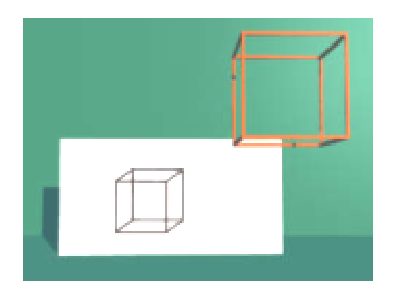
\includegraphics[scale=0.66]{./Graphiques/Perspective1.eps}
	\end{center}
 \end{minipage}

\end{tabular}

      \end{encadrer}
%\end{minipage}&
%\begin{minipage}[r]{0.275\linewidth}

	
%\end{minipage}
%\end{tabular}

%\medskip



%      \sautpage

\begin{rmqs}~
\begin{itemize}
\item Il arrivera parfois que le cube soit représenté sans faces parallèles à l'écran.
\item Si les rayons sont perpendiculaires à l'écran, on parle de perspective orthogonale. Dans toute la suite, on exclura ce cas.
\item On parle d'\textbf{une} représentation en perspective cavalière, car la forme de l'ombre dépend de la direction des rayons du soleil.
      \begin{center}
	  \begin{tabular}{cc}
	  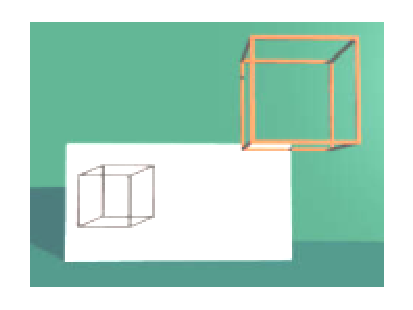
\includegraphics[scale=0.66]{./Graphiques/Perspective2.eps}&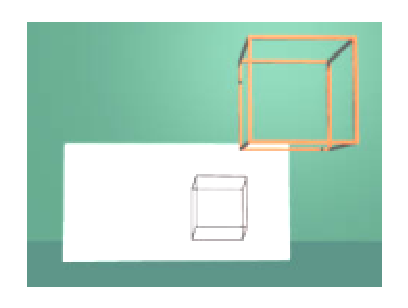
\includegraphics[scale=0.66]{./Graphiques/Perspective3.eps}
	  \end{tabular}
      \end{center}

\end{itemize}
\end{rmqs}

\begin{encadrer}
\begin{tabular}{cc}
\begin{minipage}[l]{0.69\linewidth}
 \emph{On appelle \emph{fuyante} une droite perpendiculaire à l'écran.\\
      Les ombres de toutes les fuyantes sont parallèles et leur direction commune dépend de celle des rayons du soleil.}
\end{minipage}&
\begin{minipage}[r]{0.30\linewidth}
 \begin{center}
	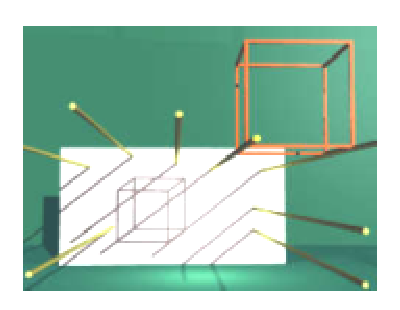
\includegraphics[scale=0.66]{./Graphiques/Perspective4.eps}
	\end{center}
\end{minipage}
\end{tabular}
\end{encadrer}



\subsection{Construction et propriétés}

\subsubsection{Construction}

\begin{tabular}{cc}
\begin{minipage}[l]{0.75\linewidth}
\begin{itemize}
\item L'angle $\alpha$ des fuyantes (droites perpendiculaires au plan de projection) vaut habituellement 30°, 45° ou 60°.
\item Toutes les dimensions qui sont dans des plans parallèles au plan de projection sont représentées en vraie grandeur.
\item Les dimensions qui sont portées par les fuyantes sont multipliées par un coefficient de réduction, en général compris entre 0,5 et 0,8.
\end{itemize}
\end{minipage}&
\begin{minipage}[r]{0.25\linewidth}
\begin{center}
\psset{xunit=0.5cm , yunit=0.5cm}
\begin{pspicture*}(-0.7,-0.7)(6.7,5.7)
\def\xmin{-0.5} \def\xmax{6.5} \def\ymin{-0.5} \def\ymax{5.5}

\psset{linecolor=black, linewidth=.5pt, arrowsize=2pt 4}
\psline(0.0000,0.0000)(4.0000,0.0000)
\psline(4.0000,0.0000)(4.0000,4.0000)
\psline(4.0000,4.0000)(0.0000,4.0000)
\psline(0.0000,4.0000)(0.0000,0.0000)
\psline[linestyle=dashed](2.0000,1.0000)(6.0000,1.0000)
\psline(6.0000,1.0000)(6.0000,5.0000)
\psline(6.0000,5.0000)(2.0000,5.0000)
\psline[linestyle=dashed](2.0000,5.0000)(2.0000,1.0000)
\psline[linestyle=dashed](0.0000,0.0000)(2.0000,1.0000)
\psline(4.0000,0.0000)(6.0000,1.0000)
\psline(4.0000,4.0000)(6.0000,5.0000)
\psline(0.0000,4.0000)(2.0000,5.0000)
\psarc(0.0000,4.0000){0.4500}{0.0000}{26.5651}
\psarc(0.0000,4.0000){0.5500}{0.0000}{26.5651}
\rput(1.4,4.3){$\alpha$}

\end{pspicture*}
\end{center}
\end{minipage}
\end{tabular}



\subsubsection{Propriétés}

\begin{encadrer}
\begin{itemize}
\item \emph{Des droites parallèles sont représentées sur le dessin par des droites parallèles.}
\item \emph{Des droites sécantes sont représentées sur le dessin par des droites sécantes.}
\item \emph{Les rapports de longueur sur une droite sont conservés sur le dessin.\\ Ainsi, par exemple, le milieu d'un segment est représenté sur le dessin par le milieu du segment obtenu.}
\end{itemize}
\end{encadrer}




\begin{rmqs} Attention, les r\'eciproques ne sont pas vraies. Ainsi :
\begin{itemize}
 \item Deux droites qui semblent parallèles sur le dessin ne le sont pas toujours dans la réalité.
 \item Deux droites qui semblent sécantes sur le dessin ne le sont pas toujours dans la réalité.
 \item Un point qui semble \^etre au milieu d'un segment dans la repr\'esentation en perspective cavali\`ere n'est pas toujours le milieu du segment dans la r\'ealit\'e : il peut ne pas \^etre sur le segment dans la r\'ealit\'e.
\end{itemize}

 
\end{rmqs}


%\sautpage

\section{Solides usuels et volumes}


\subsection{Famille des prismes droits}

\begin{center}
\begin{tabular}{p{5cm} p{5cm} p{5cm}}
\textbf{Prisme droit} & \textbf{Pavé} & \textbf{Cylindre} \\
Toutes les faces sont des rectangles sauf (éventuellement) les deux bases. & Prisme droit dont les bases sont des rectangles. & Peut être considéré comme un prisme droit dont les bases sont des disques. \\
\end{tabular}
\end{center}

\begin{multicols}{3}
\begin{center}
\psset{xunit=0.75cm , yunit=0.375cm}
\begin{pspicture*}(-0.7,-0.7)(5.7,5.7)
\def\xmin{-0.5} \def\xmax{5.5} \def\ymin{-0.5} \def\ymax{5.5}

\psset{linecolor=black, linewidth=.5pt, arrowsize=2pt 4}
\psline(0.0000,1.0000)(3.0000,0.0000)
\psline(3.0000,0.0000)(5.0000,1.0000)
\psline[linestyle=dashed](5.0000,1.0000)(4.0000,2.0000)
\psline[linestyle=dashed](4.0000,2.0000)(2.0000,2.0000)
\psline[linestyle=dashed](2.0000,2.0000)(0.0000,1.0000)
\psline(0.0000,4.0000)(3.0000,3.0000)
\psline(0.0000,1.0000)(0.0000,4.0000)
\psline(3.0000,0.0000)(3.0000,3.0000)
\psline(3.0000,3.0000)(5.0000,4.0000)
\psline(5.0000,1.0000)(5.0000,4.0000)
\psline(5.0000,4.0000)(4.0000,5.0000)
\psline[linestyle=dashed](4.0000,2.0000)(4.0000,5.0000)
\psline(4.0000,5.0000)(2.0000,5.0000)
\psline(2.0000,5.0000)(0.0000,4.0000)
\psline[linestyle=dashed](2.0000,5.0000)(2.0000,2.0000)
\rput(2.5,1.3){\emph{base}}
\psline{<->}(-0.2,1)(-0.2,4)
\rput(-0.4,2.5){$h$}

\end{pspicture*}
\end{center}
\sautcol

\begin{center}
\psset{xunit=0.75cm , yunit=0.375cm}
\begin{pspicture*}(-0.7,-0.7)(5.7,5.7)
\def\xmin{-0.5} \def\xmax{5.5} \def\ymin{-0.5} \def\ymax{5.5}

\psset{linecolor=black, linewidth=.5pt, arrowsize=2pt 4}
\psline(0.0000,0.0000)(3.0000,0.0000)
\psline(3.0000,0.0000)(3.0000,3.0000)
\psline(3.0000,3.0000)(0.0000,3.0000)
\psline(0.0000,3.0000)(0.0000,0.0000)
\psline[linestyle=dashed](2.0000,1.0000)(5.0000,1.0000)
\psline(5.0000,1.0000)(5.0000,4.0000)
\psline(5.0000,4.0000)(2.0000,4.0000)
\psline[linestyle=dashed](2.0000,4.0000)(2.0000,1.0000)
\psline[linestyle=dashed](0.0000,0.0000)(2.0000,1.0000)
\psline(3.0000,0.0000)(5.0000,1.0000)
\psline(3.0000,3.0000)(5.0000,4.0000)
\psline(0.0000,3.0000)(2.0000,4.0000)
\rput(2.3,0.5){\emph{base}}
\psline{<->}(-0.2,0)(-0.2,3)
\rput(-0.4,1.5){$h$}

\end{pspicture*}
\end{center}
\sautcol

\begin{center}
\psset{xunit=0.75cm , yunit=0.1875cm}
\begin{pspicture*}(-0.6,-1.2)(5.6,11.1)
\def\xmin{-0.5} \def\xmax{5.5} \def\ymin{-1.1} \def\ymax{11}

\def\F{1 4 x 2 sub 2 exp sub 0.5 exp add}
\psplot[linecolor=black,linestyle=dashed]{0}{4}{\F}
\def\G{1 4 x 2 sub 2 exp sub 0.5 exp sub}
\psplot[linecolor=black,linestyle=solid]{0}{4}{\G}
\def\H{8 4 x 2 sub 2 exp sub 0.5 exp add}
\psplot[linecolor=black,linestyle=solid]{0}{4}{\H}
\def\I{8 4 x 2 sub 2 exp sub 0.5 exp sub}
\psplot[linecolor=black,linestyle=solid]{0}{4}{\I}
\psline(0,1)(0,8)
\psline(4,1)(4,8)
\rput(2,1){\emph{base}}
\psline{<->}(4.5,1)(4.5,8)
\rput(5,4.5){$h$}

\end{pspicture*}
\end{center}
\end{multicols}

\begin{prop}
 Le volume de ces solides est donné par la formule suivante : \[\text{Volume}=\text{Aire de la base}\times\text{hauteur}\]
\end{prop}

\subsection{Famille des pyramides}

\begin{center}
\begin{tabular}{p{5cm} p{5cm} p{5cm}}
\textbf{Pyramide} & \textbf{Tétraèdre} & \textbf{Cône de révolution} \\
Constituée d'une base de forme quelconque et d'un sommet. Des arêtes joignent ce sommet à chacun des sommets de la base. & Pyramide dont la base est un triangle. & Peut être considéré comme une pyramide dont la base est un disque. \\
\end{tabular}
\end{center}

\begin{multicols}{3}
\begin{center}
\psset{xunit=0.75cm , yunit=0.375cm}
\begin{pspicture*}(-0.7,-0.7)(5.7,5.7)
\def\xmin{-0.5} \def\xmax{5.5} \def\ymin{-0.5} \def\ymax{5.5}

\psset{linecolor=black, linewidth=.5pt, arrowsize=2pt 4}
\psline(0.0000,1.0000)(2.0000,0.0000)
\psline(2.0000,0.0000)(4.0000,1.0000)
\psline[linestyle=dashed](4.0000,1.0000)(3.0000,2.0000)
\psline[linestyle=dashed](3.0000,2.0000)(1.0000,2.0000)
\psline[linestyle=dashed](1.0000,2.0000)(0.0000,1.0000)
\psline(0.0000,1.0000)(2.0000,5.0000)
\psline(2.0000,0.0000)(2.0000,5.0000)
\psline(4.0000,1.0000)(2.0000,5.0000)
\psline[linestyle=dashed](3.0000,2.0000)(2.0000,5.0000)
\psline[linestyle=dashed](1.0000,2.0000)(2.0000,5.0000)
\rput(2,1){\emph{base}}
\psline{<->}(4.3,1)(4.3,5)
\psline[linestyle=dotted](2,5)(4.3,5)
\rput(4.5,3){$h$}

\end{pspicture*}
\end{center}
\sautcol

\begin{center}
\psset{xunit=0.75cm , yunit=0.375cm}
\begin{pspicture*}(-0.7,-0.7)(5.7,5.7)
\def\xmin{-0.5} \def\xmax{5.5} \def\ymin{-0.5} \def\ymax{5.5}

\psset{linecolor=black, linewidth=.5pt, arrowsize=2pt 4}
\psline(0.0000,1.0000)(3.0000,0.0000)
\psline[linestyle=dashed](0.0000,1.0000)(4.0000,2.0000)
\psline(3.0000,0.0000)(4.0000,2.0000)
\psline(0.0000,1.0000)(2.0000,5.0000)
\psline(3.0000,0.0000)(2.0000,5.0000)
\psline(4.0000,2.0000)(2.0000,5.0000)
\rput(2.5,0.9){\emph{base}}
\psline{<->}(4.5,1)(4.5,5)
\rput(4.7,3){$h$}
\psline[linestyle=dotted](2,5)(4.5,5)

\end{pspicture*}
\end{center}
\sautcol

\begin{center}
\psset{xunit=0.75cm , yunit=0.1875cm}
\begin{pspicture*}(-0.6,-1.2)(5.6,11.1)
\def\xmin{-0.5} \def\xmax{5.5} \def\ymin{-1.1} \def\ymax{11}

\def\F{1 4 x 2 sub 2 exp sub 0.5 exp add}
\psplot[linecolor=black,linestyle=dashed]{0}{4}{\F}
\def\G{1 4 x 2 sub 2 exp sub 0.5 exp sub}
\psplot[linecolor=black,linestyle=solid]{0}{4}{\G}
\psline(0,1)(2,8)(4,1)
\rput(2,1){\emph{base}}
\psline{<->}(4.5,1)(4.5,8)
\rput(5,4.5){$h$}
\psline[linestyle=dotted](2,8)(4.5,8)
\end{pspicture*}
\end{center}
\end{multicols}

\begin{prop}
 Le volume de ces solides est donné par la formule suivante : \[\text{Volume}=\frac{1}{3}\text{Aire de la base}\times\text{hauteur}\]

\end{prop}

On peut ainsi mettre trois fois le volume d'un cône de révolution dans un cylindre de révolution ayant même base et même hauteur, ou trois fois le volume d'un tétraèdre dans un prisme droit ayant même base et même hauteur.

\subsection{Sphère}

\begin{tabular}{cc}
\begin{minipage}[l]{0.7\linewidth}
\begin{prop}
 Le volume d'une sph\`ere de rayon $r$ est donn\'e par la formule : \[\text{Volume}=\frac{4}{3}\pi r^3\]
 L'aire de la surface d'une sph\`ere de rayon $r$ est donn\'ee par la formule : \[\text{Aire}=4\pi r^2\]
\end{prop}
\end{minipage}&
\begin{minipage}[r]{0.3\linewidth}
\begin{center}
\psset{xunit=0.66cm , yunit=0.66cm}
\begin{pspicture*}(-3.6,-3.6)(3.6,3.6)
\def\xmin{-3.5} \def\xmax{3.5} \def\ymin{-3.5} \def\ymax{3.5}

\def\F{9 x 2 exp sub 0.5 exp}
\psplot[linecolor=black,linestyle=solid]{-3}{3}{\F}
\def\G{0 9 x 2 exp sub 0.5 exp sub}
\psplot[linecolor=black,linestyle=solid]{-3}{3}{\G}
\def\H{1 3 div 9 x 2 exp sub 0.5 exp mul}
\psplot[linecolor=black,linestyle=dashed]{-3}{3}{\H}
\def\I{0 1 3 div 9 x 2 exp sub 0.5 exp mul sub}
\psplot[linecolor=black,linestyle=solid]{-3}{3}{\I}
\psline[linestyle=dashed]{o-}(0,0)(3,0)
\rput(-0.3,-0.3){$O$}
\rput(1.5,0.3){$r$}

\end{pspicture*}
\end{center}
\end{minipage}
\end{tabular}



\section{Incidence et parall\'elisme dans l'espace}

\subsection{Règles d'incidence}

\begin{regle}
Par deux points distincts de l'espace $A$ et $B$, il passe une unique droite, notée $(AB)$.
\end{regle}

\begin{regle}
Par trois points non alignés de l'espace $A$, $B$ et $C$, il passe un unique plan, noté $(ABC)$.
\end{regle}

\begin{regle}
Si deux points distincts $A$ et $B$ de l'espace appartiennent à un plan $\mathcal{P}$, alors la droite $(AB)$ est contenue dans le plan $\mathcal{P}$, c'est-à-dire que tout point $M$ appartenant à la droite $(AB)$ appartient aussi au plan $\mathcal{P}$.
\end{regle}

\begin{regle}
Dans chaque plan de l'espace, on peut appliquer tous les théorèmes de géométrie plane (\textsc{Pythagore}, \textsc{Thalès}, etc.).
\end{regle}

\subsection{Postions relatives}
\subsubsection{Positions relatives de deux droites}

\begin{regle}
Deux droites de l'espace sont soit coplanaires, soit non coplanaires.
\end{regle}
\psset{unit=0.75}
\begin{center}
\begin{tabular}{ccc|c}
\multicolumn{3}{c|}{\textbf{Coplanaires (dans un même plan)}}&\textbf{Non coplanaires} \\\hline
$d$ et $d'$ sécantes & \multicolumn{2}{c|}{$d$ et $d'$ parallèles}& \\
\begin{pspicture*}(-0.6,-2.7)(4.2,1.2)
\psline[linecolor=gray](0,0)(0,-2)(2,-2)(2,0)(0,0)(1,0.5)(3,0.5)(3,-1.5)(2,-2)
\psline[linecolor=gray](2,0)(3,0.5)
\psline(0,0.5)(3.5,0.5) \uput[u](0,0.4){$d$}
\psplot[algebraic=true,plotpoints=200]{-0.5}{4}{x/6} \uput[u](-0.1,-0.2){$d'$}
\psdot[dotstyle=x](3,0.5) \uput[u](3,0.5){$A$}
\end{pspicture*}
&
\begin{pspicture*}(-0.6,-2.7)(4.2,1.2)
\psline[linecolor=gray](0,0)(0,-2)(2,-2)(2,0)(0,0)(1,0.5)(3,0.5)(3,-1.5)(2,-2)
\psline[linecolor=gray](2,0)(3,0.5)
\psline(0,0.5)(3.7,0.5) \uput[u](0,0.4){$d$}
\psline(-0.5,0)(3.2,0) \uput[u](-0.3,-0.1){$d'$}
\end{pspicture*}
&
\begin{pspicture*}(-0.6,-2.7)(4.2,1.2)
\psline[linecolor=gray](0,0)(0,-2)(2,-2)(2,0)(0,0)(1,0.5)(3,0.5)(3,-1.5)(2,-2)
\psline[linecolor=gray](2,0)(3,0.5)
\psline(-0.5,0.005)(3.2,0.005) \uput[u](-0.3,-0.1){$d$}
\psline(-0.5,-0.005)(3.2,-0.005) \uput[d](3,0.1){$d'$}
\end{pspicture*}
&
\begin{pspicture*}(-0.6,-2.7)(4.2,1.2)
\psline[linecolor=gray](0,0)(0,-2)(2,-2)(2,0)(0,0)(1,0.5)(3,0.5)(3,-1.5)(2,-2)
\psline[linecolor=gray](2,0)(3,0.5)
\psline(-0.5,0)(3.2,0) \uput[u](-0.3,-0.1){$d$}
\psplot[algebraic=true,plotpoints=200]{-0.5}{4}{0.5*x-3} \uput[dl](2.1,-2){$d'$}
\end{pspicture*}\\

\multicolumn{1}{m{3cm}}{$d$ et $d'$ ont un point d'intersubsection $A$.}
& \multicolumn{1}{m{3cm}}{$d$ et $d'$ sont strictement parallèles.} & \multicolumn{1}{m{3cm}|}{$d$ et $d'$ sont confondues} & \multicolumn{1}{m{3cm}}{Aucun plan ne contient à la fois $d$ et $d'$.} \\
$d\cap d' = \{ A \}$ & $d\cap d' = \vide$ & $d\cap d' = d=d'$ & $d\cap d' = \vide$\\
\end{tabular}
\end{center}

%\sautpage

\begin{rmqs}~
\begin{itemize}
\item Contrairement au plan, deux droites de l'espace n'ayant pas de point en commun ne sont pas forcément parallèles.
\item Des droites strictement parallèles sont des droites \textbf{coplanaires et qui n'ont aucun point en commun}.
	\item On peut définir un plan de plusieurs manières :
			\begin{itemize}
				\item par la donnée de trois points ;
				\item par la donné de deux droites sécantes ;
				\item par la donnée de deux droites strictement parallèles ;
				\item par la donnée d'une droite et d'un point n'appartenant par à cette droite.
			\end{itemize}
\end{itemize}
\end{rmqs}

\sautpage

\subsubsection{Positions relatives d'une droite et d'un plan}

\begin{regle}
Une droite et un plan de l'espace sont soit sécants, soit parallèles.
\end{regle}

\psset{unit=1}
\begin{center}
\begin{tabular}{c|cc}
\textbf{Sécants}&\multicolumn{2}{c}{\textbf{Parallèles}} \\\hline
\begin{pspicture*}(-0.6,-0.7)(5.5,2.8)
\pspolygon[fillstyle=solid,fillcolor=lightgray](0,0)(3,0)(5,1)(2,1)
\pspolygon*[linecolor=white](2,0.5)(3,0.5)(3.5,0.75)(3.5,1.75)(2.5,1.75)(2,1.5)
\psline[linecolor=gray,linestyle=dotted](2,0.5)(2.5,0.75)(2.5,1.75)
\psline[linecolor=gray,linestyle=dotted](2.5,0.75)(3.5,0.75)
\psline[linecolor=gray](2,1.5)(2,0.5)(3,0.5)(3,1.5)(2,1.5)(2.5,1.75)(3.5,1.75)(3.5,0.75)(3,0.5)
\psline[linecolor=gray](3,1.5)(3.5,1.75)
\psplot[linestyle=dotted,algebraic=true,plotpoints=200]{2.5}{3.866}{-x+4.25}
\psplot[algebraic=true,plotpoints=200]{1.5}{2.5}{-x+4.25}
\psplot[algebraic=true,plotpoints=200]{3.866}{4.75}{-x+4.25}
\psdot[dotstyle=x](3.5,0.75)
\uput[r](3.5,0.75){$B$}
\uput[u](4.6,-0.4){$d$}
\uput[u](4.6,1){$\mathcal{P}$}
\end{pspicture*}
&
\begin{pspicture*}(-0.6,-0.7)(5.5,2.8)
\pspolygon[fillstyle=solid,fillcolor=lightgray](0,0)(3,0)(5,1)(2,1)
\pspolygon*[linecolor=white](2,0.5)(3,0.5)(3.5,0.75)(3.5,1.75)(2.5,1.75)(2,1.5)
\psline[linecolor=gray,linestyle=dotted](2,0.5)(2.5,0.75)(2.5,1.75)
\psline[linecolor=gray,linestyle=dotted](2.5,0.75)(3.5,0.75)
\psline[linecolor=gray](2,1.5)(2,0.5)(3,0.5)(3,1.5)(2,1.5)(2.5,1.75)(3.5,1.75)(3.5,0.75)(3,0.5)
\psline[linecolor=gray](3,1.5)(3.5,1.75)
\psline(0,1.75)(4.5,1.75)
\uput[l](0,1.75){$d$}
\uput[u](4.6,1){$\mathcal{P}$}
\end{pspicture*}
&
\begin{pspicture*}(-0.6,-0.7)(5.5,2.8)
\pspolygon[fillstyle=solid,fillcolor=lightgray](0,0)(3,0)(5,1)(2,1)
\pspolygon*[linecolor=white](2,0.5)(3,0.5)(3.5,0.75)(3.5,1.75)(2.5,1.75)(2,1.5)
\psline[linecolor=gray,linestyle=dotted](2,0.5)(2.5,0.75)(2.5,1.75)
\psline[linecolor=gray,linestyle=dotted](2.5,0.75)(3.5,0.75)
\psline[linecolor=gray](2,1.5)(2,0.5)(3,0.5)(3,1.5)(2,1.5)(2.5,1.75)(3.5,1.75)(3.5,0.75)(3,0.5)
\psline[linecolor=gray](3,1.5)(3.5,1.75)
\psline(0,0.5)(4.5,0.5)
\uput[l](0,0.5){$d$}
\uput[u](4.6,1){$\mathcal{P}$}
\end{pspicture*}
\\
\multicolumn{1}{m{4cm}|}{$d$ et $\mathcal{P}$ ont un point d'intersubsection $B$.}
& \multicolumn{1}{m{4cm}}{$d$ et $\mathcal{P}$ sont strictement parallèles.} & \multicolumn{1}{m{4cm}}{$d$ est contenue dans $\mathcal{P}$} \\
$d\cap \mathcal{P} = \{ B \}$ & $d\cap \mathcal{P} = \vide$ & $d\cap \mathcal{P} = d$\\
\end{tabular}
\end{center}

\begin{rmq} Une droite $d$ et un plan $\mathcal{P}$ sont parallèles s'ils ne sont pas sécants. On note alors $d\parallel \mathcal{P}$ ou $\mathcal{P}\parallel d$.
\end{rmq}

\subsubsection{Positions relatives de deux plans}

\begin{regle}
Deux plans de l'espace sont soit sécants, soit parallèles.
\end{regle}

\psset{unit=1}
\begin{center}
\begin{tabular}{c|cc}
\textbf{Sécants}&\multicolumn{2}{c}{\textbf{Parallèles}} \\\hline
\begin{pspicture*}(-0.6,-0.7)(6,2.8)
\pspolygon[fillstyle=solid,fillcolor=gray](0,0)(3,0)(5,1)(2,1)
\pspolygon[fillstyle=solid,fillcolor=lightgray](5,1)(2,1)(0,4)(3,4)
\pspolygon*[linecolor=white](2.5,1.75)(2.5,0.75)(3.5,0.75)(4,1)(3.5,1.75)
\psline(3.5,0.75)(4,1)(3.5,1.75)(3.5,0.75)(2.5,0.75)(2.5,1.75)(3.5,1.75)
\psline[linestyle=dotted](2.5,0.75)(3,1)(3,2)(2.5,1.75)(3,1)(4,1)(4,2)(3.5,1.75)
\psline[linestyle=dotted](3,2)(4,2)
\psline[linestyle=dotted](2.5,1)(3,1)
\psline(1,1)(2,1)\uput[l](1,1){$d$}
\psline(5,1)(5.5,1)
\uput[u](0,0){$\mathcal{P}$}
\uput[dl](1,2.5){$\mathcal{P}'$}
\end{pspicture*}
&
\begin{pspicture*}(-0.6,-0.7)(6,2.8)
\pspolygon[fillstyle=solid,fillcolor=gray](0,0)(3,0)(5,1)(2,1)
\pspolygon[fillstyle=solid,fillcolor=lightgray](0,1.5)(3,1.5)(5,2.5)(2,2.5)
\pspolygon*[linecolor=white](1.5,1.75)(2.5,1.75)(3,2)(2,2)
\pspolygon*[linecolor=white](1.5,0.25)(2.5,0.25)(3,0.5)(3,1.25)(1.5,1.25)
\psline[linestyle=dotted](2,2)(2,0.5)(1.5,0.25)
\psline[linestyle=dotted](2,0.5)(3,0.5)
\psline[linestyle=dotted](1.5,1.75)(1.5,1.5)
\psline[linestyle=dotted](2.5,1.75)(2.5,1.5)
\psline[linestyle=dotted](3,2)(3,1.5)
\psline(1.5,1.5)(1.5,0.25)(2.5,0.25)(2.5,1.5)
\psline(2.5,0.25)(3,0.5)(3,1.5)
\psline(1.5,1.75)(2.5,1.75)(3,2)(2,2)(1.5,1.75)
\uput[u](0,0){$\mathcal{P}$}
\uput[u](0,1.5){$\mathcal{P}'$}
\end{pspicture*}
&
\begin{pspicture*}(-1.4,-0.7)(6.5,2.8)
\pspolygon[fillstyle=solid,fillcolor=gray](-1,-0.25)(3.25,-.25)(6.25,1.25)(2,1.25)
\pspolygon[fillstyle=solid,fillcolor=lightgray](0,0)(3,0)(5,1)(2,1)
\pspolygon*[linecolor=white](2,0.5)(3,0.5)(3.5,0.75)(3.5,1.75)(2.5,1.75)(2,1.5)
\psline[linecolor=gray,linestyle=dotted](2,0.5)(2.5,0.75)(2.5,1.75)
\psline[linecolor=gray,linestyle=dotted](2.5,0.75)(3.5,0.75)
\psline[linecolor=gray](2,1.5)(2,0.5)(3,0.5)(3,1.5)(2,1.5)(2.5,1.75)(3.5,1.75)(3.5,0.75)(3,0.5)
\psline[linecolor=gray](3,1.5)(3.5,1.75)
\uput[u](6,1.25){$\mathcal{P}$}
\rput(4,0.75){$\mathcal{P}'$}
\end{pspicture*}\\
\multicolumn{1}{m{4cm}|}{$\mathcal{P}$ et $\mathcal{P}'$ ont une droite d'intersubsection $d$.}
& \multicolumn{1}{m{4cm}}{$\mathcal{P}$ et $\mathcal{P}'$ sont strictement parallèles.} & \multicolumn{1}{m{4cm}}{$\mathcal{P}$ et $\mathcal{P}'$ sont confondus} \\
$\mathcal{P}\cap \mathcal{P}' = d$ & $\mathcal{P}\cap \mathcal{P}' = \vide$ & $\mathcal{P}\cap \mathcal{P}' = \mathcal{P}= \mathcal{P}'$\\
\end{tabular}
\end{center}
\begin{rmq}Deux plans $\mathcal{P}$ et $\mathcal{P}'$ sont parallèles lorsqu'ils ne sont pas sécants. On note $\mathcal{P}\parallel \mathcal{P}'$.
\end{rmq}

\begin{rmqs}~
\begin{itemize}
	\item Pour démontrer que trois points sont alignés, il suffit de montrer que les trois points appartiennent à deux plans sécants : comme l'intersubsection de deux plans sécants est une droite, cela implique que les points sont tous les trois sur cette droite.
	\item Pour trouver la droite d'intersubsection de deux plans, il suffit de trouver deux points distincts qui appartiennent aux deux plans : la droite d'intersubsection est alors celle qui passe par ces deux points. Ces points sont en général des points d'intersubsection de droites sécantes, l'une contenue dans l'un des plans, l'autre dans l'autre plan.
\end{itemize}
\end{rmqs}

%\sautpage

\subsection{Parallélisme dans l'espace}

\subsubsection{Parallélisme entre droites}

\begin{prop} Deux droites parallèles à une même droite sont parallèles entre elles.
\[ \text{Si } d \parallel  d' \text{ et } d'\parallel d'' \text{ alors } d\parallel d''\]
\end{prop}

\begin{prop}
Si deux droites sont parallèles, alors tout plan qui coupe l'une, coupe l'autre.
\end{prop}

\subsubsection{Parallélisme entre plans}

\begin{prop} Deux plans parallèles à un même plan sont parallèles entre eux.
\[ \text{Si } \mathcal{P} \parallel  \mathcal{P}' \text{ et } \mathcal{P}'\parallel \mathcal{P}'' \text{ alors } \mathcal{P}\parallel \mathcal{P}''\]
\end{prop}

\begin{prop}
Si deux droites sécantes $d$ et $d'$ d'un plan $\mathcal{P}$ sont parallèles à deux droites sécantes $\Delta$ et $\Delta '$ d'un plan $\mathcal{Q}$, alors $\mathcal{P}$ et $\mathcal{Q}$ sont parallèles.
\end{prop}

\begin{center}
\psset{xunit=2cm,yunit=1cm}
\begin{pspicture*}(-0.6,-0.7)(6,2.8)
\pspolygon[fillstyle=solid](0,0)(3,0)(5,1)(2,1)
\pspolygon[fillstyle=solid](0,1.5)(3,1.5)(5,2.5)(2,2.5)
\psline(0.5,0.1)(4.2,0.9) \uput[r](4.2,0.9){$d$}
\psline(0.5,1.6)(4.2,2.4) \uput[r](4.2,2.4){$\Delta$}
\psline(1.5,0.6)(2.6,0.1) \uput[ur](2.6,0.1){$d'$}
\psline(1.9,2.4)(3,1.9) \uput[r](2.9,1.9){$\Delta '$}
\uput[u](0,0){$\mathcal{P}$}
\uput[u](0,1.5){$\mathcal{Q}$}
\end{pspicture*}
\end{center}

\begin{prop}
Si deux plans $\mathcal{P}$ et $\mathcal{P}'$ sont parallèles, alors tout plan sécant à $\mathcal{P}$ est aussi sécant à $\mathcal{P}'$ et leurs droites d'intersubsection $d$ et $d'$ sont parallèles.
\end{prop}

\begin{center}
\psset{xunit=1.5cm,yunit=0.5cm}
\begin{pspicture*}(-1,-3.5)(6.5,8.5)
\pspolygon[fillstyle=solid,fillcolor=lightgray,linecolor=black](0,-3)(2,-1)(5,8)(3,6)
\pspolygon*[linecolor=white](1,0)(2.3333,0)(3,2)
\pspolygon*[linecolor=white](2,3)(3.3333,3)(4,5)
\psline(1.6667,2)(1,2)(0,0)(5,0)(6,2)(3,2)
\psline(2.6667,5)(1,5)(0,3)(5,3)(6,5)(4,5)
\uput[l](0,0){$\mathcal{P}$}
\uput[l](0,3){$\mathcal{Q}$}
\psline(0.5,-0.5)(3.5,2.5)\uput[l](0.5,-0.5){$d$}
\psline(1.5,2.5)(4.5,5.5)\uput[l](1.5,2.5){$d'$}
\psline[linestyle=dotted](2.3333,0)(3,2)(1.6667,2)
\psline[linestyle=dotted](3.3333,3)(4,5)(2.6667,5)
\end{pspicture*}
\end{center}


\subsubsection{Parallélisme entre droite et plan}

\begin{prop}
Si deux plans $\mathcal{P}$ et $\mathcal{P}'$ sont parallèles et si une droite $d$ est parallèle à $\mathcal{P}$, alors $d$ est parallèle à $\mathcal{P}'$.
\[ \text{Si } d\parallel \mathcal{P} \text{ et } \mathcal{P}\parallel \mathcal{P}' \text{ alors } d\parallel \mathcal{P}'\]
\end{prop}

\begin{center}
\psset{xunit=1.5cm,yunit=1cm}
\begin{pspicture*}(-0.6,-0.7)(6,3.9)
\pspolygon[fillstyle=solid](0,0)(3,0)(5,1)(2,1)
\pspolygon[fillstyle=solid](0,1.5)(3,1.5)(5,2.5)(2,2.5)
\psline(0.5,3)(4.2,3.5) \uput[l](0.5,3){$d$}
\uput[u](0,0){$\mathcal{P}$}
\uput[u](0,1.5){$\mathcal{P}'$}
\end{pspicture*}
\end{center}

\sautpage

\begin{prop}
Si deux droites $d$ et $\Delta$ sont parallèles, et si $d$ est contenue dans un plan $\mathcal{P}$, alors $\Delta$ est parallèle à $\mathcal{P}$.
\end{prop}

\begin{center}
\psset{xunit=1.5cm,yunit=1cm}
\begin{pspicture*}(-0.6,-0.7)(6,3.9)
\pspolygon[fillstyle=solid](0,1.5)(3,1.5)(5,2.5)(2,2.5)
\psline(0.5,1.6)(4.2,2.4) \uput[r](4.2,2.4){$d$}
\psline(0.5,0.1)(4.2,0.9) \uput[r](4.2,0.9){$\Delta$}
\uput[u](0,1.5){$\mathcal{P}$}
\end{pspicture*}
\end{center}

\begin{prop}
Si deux plans $\mathcal{P}$ et $\mathcal{P}'$ sont sécants selon une droite $\Delta$ et si $d$ est une droite parallèle à $\mathcal{P}$ et $\mathcal{P}'$ alors $d$ et $\Delta$ sont parallèles.
\end{prop}

\begin{center}
\psset{xunit=1.5cm,yunit=0.5cm}
\begin{pspicture*}(-0.6,-2.7)(5.6,7.6)
\pspolygon[fillstyle=solid,fillcolor=gray](0,0)(4,2)(4,7)(0,5)
\pspolygon[fillstyle=solid,fillcolor=lightgray](0,0)(3,-2)(3,3)(0,5)
\uput[r](4,7){$\mathcal{P}'$}
\uput[r](3,-2){$\mathcal{P}$}
\psline(0,-1)(0,6)\uput[u](0,6){$\Delta$}
\psline(5,-1)(5,6)\uput[u](5,6){$d$}
\end{pspicture*}
\end{center}

\begin{theo}[Théorème du toit]
Si :
\begin{itemize}
	\item $d$ et $d'$ sont parallèles ;
	\item $\mathcal{P}$ est un plan qui contient $d$ et $\mathcal{P}'$ est un plan qui contient $d'$ ;
	\item $\mathcal{P}$ et $\mathcal{P}'$ sont sécants selon une droite $\Delta$
\end{itemize}
alors $\Delta$ est parallèle à $d$ et à $d'$.
\end{theo}

\begin{center}
\psset{xunit=1cm,yunit=0.5cm}
\begin{pspicture*}(-0.6,-0.6)(14.6,10.6)
\pspolygon[fillstyle=solid,fillcolor=gray](2,3)(10,7)(11,9)(3,5)
\pspolygon[fillstyle=solid,fillcolor=lightgray](4,1)(12,5)(11,9)(3,5)
\uput[ul](2,3){$\mathcal{P}'$}
\uput[ur](12,5){$\mathcal{P}$}
\psline(2,0)(14,6)\uput[ul](2,0){$d$}
\psline(0,2)(3.33333,3.66667)\uput[ul](0,2){$d'$}
\psline(1,4)(13,10)\uput[ul](1,4){$\Delta$}
\psline[linestyle=dotted](3.33333,3.66667)(11.3333333,7.666667)
\psline(11.3333333,7.666667)(12,8)
\psline[linestyle=dotted](10,7)(11,9)
\end{pspicture*}
\end{center}

\sautpage

\section{Exercices}

\subsection{Perspective et calculs}


\begin{exo}



Une pièce métallique (en traits pleins) est découpée dans un cube. 

\begin{center}
		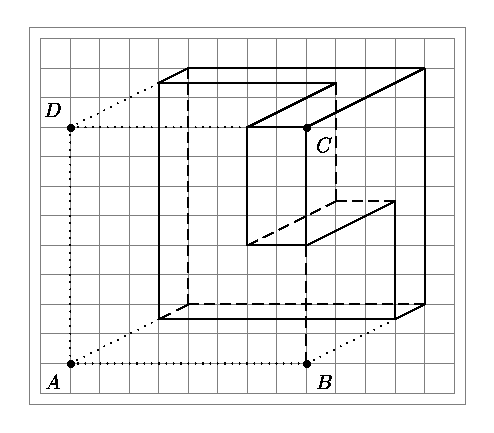
\includegraphics[width=0.4\textwidth]{./Graphiques/piece.eps}\end{center}

Construire, en perspective cavalière : 
\vspace{-1.5em}\begin{multicols}{2}
\begin{itemize}
 \item la pièce restante du cube la face $ABCD$ restant devant ;
 \begin{center}
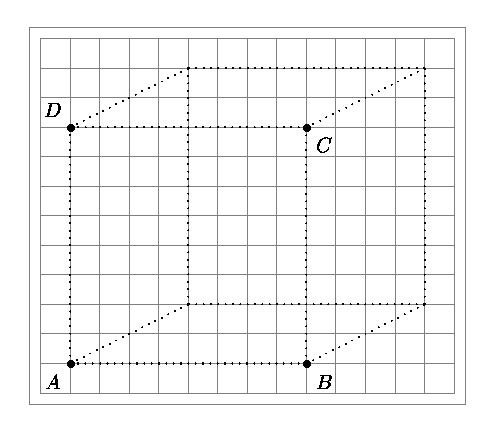
\includegraphics{./Graphiques/piece2.eps} \end{center}

 \item la pièce restante du cube la face $ABCD$ étant à droite. 
 \begin{center}
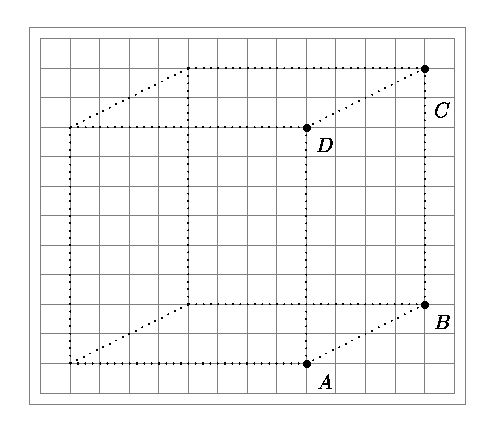
\includegraphics{./Graphiques/piece3.eps} \end{center}
\end{itemize}
\end{multicols}\vspace{-1.5em}
\end{exo}

%\subsection{Calculs}

\begin{exo}


On considère un tétraèdre $ABCD$, dont les faces $ABC$, $ABD$ et $ACD$ sont des triangles rectangles en $A$.\\
On donne $AB = AD = 5$ cm et $AC = 12$ cm.
\begin{enumerate}
	\item Dessiner ce tétraèdre en perspective cavalière, la face $ABC$ étant frontale.
	\item Quelle est la nature de $CDB$ ? le représenter en vraie grandeur.
	\item Quel est le volume de $ABCD$ ?
\end{enumerate}
\end{exo}

\begin{exo}$ABCDEFGH$ est un cube d'arête $a$.
\begin{enumerate}
	\item Quelle est la nature du triangle $AFC$ ? Justifier. \\
	Le représenter en vraie grandeur à la règle et au compas en prenant $a = 6$ cm.
	\item Calculer la longueur d'une diagonale principale du cube.
\end{enumerate}
\end{exo}

\sautpage

\begin{exo}
On considère un cube $ABCDEFGH$ de côté $a$.
On nomme $P$ le centre de la face $EFGH$ et $Q$ le centre de la face $BCGF$.
$M$ désigne le milieu de $[PQ]$.
On admettra que $(EG)$ est perpendiculaire à $(EA)$ et que $(BG)$ est perpendiculaire à $(AB)$.
\begin{enumerate}
	\item Montrer que $PQ=\frac{a\sqrt{2}}{2}$ puis que $AP=AQ=\frac{a\sqrt{6}}{2}$.
	\item Calculer une valeur approchée au degré près de l'angle $\widehat{PAQ}$.
	\item Donner, en fonction de $a$, la valeur exacte de l'aire du triangle $APQ$.
\end{enumerate}
\end{exo}

\begin{exo}
\begin{multicols}{2}
$ABCDEFGH$ est un parallélépipède rectangle (un pavé) tel que $AB = 10$, $AE = 6$ et $BC = 8$.
\begin{enumerate}
\item Calculer les longueurs des segments $[HA]$, $[HF]$, $[HC]$ et $[HB]$.
\item Calculer le volume des pyramides $HABCD$ et $HBCGF$.
\item Réaliser un patron de ces deux pyramides.
\end{enumerate}
\sautcol
\begin{center}
\psset{xunit=1cm , yunit=0.66cm}
\begin{pspicture*}(-0.7,-0.7)(5.7,5.2)
\def\xmin{-0.5} \def\xmax{5.5} \def\ymin{-0.5} \def\ymax{5}

\psset{linecolor=black, linewidth=.5pt, arrowsize=2pt 4}
\psline(0.0000,0.0000)(3.0000,0.0000)
\psline(3.0000,0.0000)(3.0000,3.0000)
\psline(3.0000,3.0000)(0.0000,3.0000)
\psline(0.0000,3.0000)(0.0000,0.0000)
\psline[linestyle=dashed](2.0000,1.0000)(5.0000,1.0000)
\psline(5.0000,1.0000)(5.0000,4.0000)
\psline(5.0000,4.0000)(2.0000,4.0000)
\psline[linestyle=dashed](2.0000,4.0000)(2.0000,1.0000)
\psline[linestyle=dashed](0.0000,0.0000)(2.0000,1.0000)
\psline(3.0000,0.0000)(5.0000,1.0000)
\psline(3.0000,3.0000)(5.0000,4.0000)
\psline(0.0000,3.0000)(2.0000,4.0000)
\psline[linestyle=dashed](0.0000,0.0000)(2.0000,4.0000)
\psline[linestyle=dashed](3.0000,0.0000)(2.0000,4.0000)
\psline[linestyle=dashed](5.0000,1.0000)(2.0000,4.0000)
\rput(-0.3,-0.3){$A$}
\rput(3,-0.3){$B$}
\rput(5.3,0.7){$C$}
\rput(1.7,1.3){$D$}
\rput(-0.3,3.3){$E$}
\rput(2.7,2.7){$F$}
\rput(5.3,4.3){$G$}
\rput(1.7,4.3){$H$}

\end{pspicture*}
\end{center}
\end{multicols}

\end{exo}



\begin{exo}$ABCDEFGH$ est un cube. $AB$ = 5 cm. Soit $I$ le pied de la hauteur issue de $A$ dans le triangle $ABH$.
\begin{enumerate}
\item Calculer $AH$, $HB$ et $AI$.
\item Représenter en vraie grandeur le triangle $AIC$.
\item Démontrer que la mesure en degrés de $\widehat{AIC}$ est 120°.
\end{enumerate}
\end{exo}

\begin{exo}$SABC$ est un tétraèdre régulier d'arête $a$.
Calculer en fonction de $a$ :
		\begin{enumerate}
		\item la hauteur $SH$ (on admettra que $H$ est l'intersubsection des hauteurs de $ABC$;
		\item l'aire du triangle $ABC$ et l'aire totale du tétraèdre;
		\item le volume du tétraèdre.
		\end{enumerate}
\end{exo}

%\sautpage

\begin{exo}
\begin{multicols}{2}
La figure ci-contre est un patron d'un solide $ABCD$. Le triangle $ADC$ est rectangle en $A$ et a pour dimensions :
\begin{itemize}
\item $AD = 3,5$ cm ;
\item $AC =4$ cm;
\item $AB=3$ cm.
\end{itemize}
\begin{enumerate}
\item De quel type de solide s'agit-il ?
\item Le dessiner en perspective cavalière, en mettant la face $ABC$ en vraie grandeur.
\end{enumerate}

\sautcol

\begin{center}
\psset{xunit=0.7cm , yunit=0.7cm}
\begin{pspicture*}(-0.3,-0.3)(6.2,6)
\def\xmin{-0.1} \def\xmax{6} \def\ymin{-0.1} \def\ymax{5.8}

\psset{linecolor=black, linewidth=.5pt, arrowsize=2pt 4}
\psline(2.0000,2.0000)(2.0000,0.0000)
\psline(2.0000,2.0000)(5.0000,2.0000)
\psline(2.0000,2.0000)(0.0000,2.0000)
\psline(2.0000,2.0000)(2.0000,5.0000)
\psline(2.0000,0.0000)(5.0000,2.0000)
\psline(2.0000,5.0000)(0.0000,2.0000)
\psline(2.0000,5.0000)(5.0000,2.0000)
\psline(2.0000,5.0000)(5.7000,5.7000)
\psline(5.0000,2.0000)(5.7000,5.7000)
\rput(1.7,1.7){$A$}
\rput(5.3,2){$D$}
\rput(2,5.3){$C$}

\end{pspicture*}
\end{center}
\end{multicols}
\end{exo}

\sautpage

\begin{exo}
\begin{multicols}{2}
Soit $SABCD$ une pyramide régulière dont la base est le carré de côté $2a$ et dont les faces latérales sont des triangles isocèles d'angles au sommet de mesure 30°. On désigne respectivement par $I$, $J$ et $H$ les milieux de $[AB]$, $[CD]$ et le centre du carré $ABCD$.
\begin{enumerate}
\item Déterminer, en fonction de $a$, la hauteur $SH$ de cette pyramide.
\item Réaliser un patron de cette pyramide en prenant $a=5$\,cm.
\end{enumerate}

\sautcol

\begin{center}
\psset{xunit=0.75cm , yunit=0.75cm}
\begin{pspicture*}(-0.7,-0.7)(6.7,5.7)
\def\xmin{-0.5} \def\xmax{6.5} \def\ymin{-0.5} \def\ymax{5.5}

\psset{linecolor=black, linewidth=.5pt, arrowsize=2pt 4}
\psline(0.0000,0.0000)(4.0000,0.0000)
\psline(4.0000,0.0000)(6.0000,1.0000)
\psline[linestyle=dashed](6.0000,1.0000)(2.0000,1.0000)
\psline[linestyle=dashed](2.0000,1.0000)(0.0000,0.0000)
\psline(0.0000,0.0000)(3.0000,5.0000)
\psline(4.0000,0.0000)(3.0000,5.0000)
\psline(6.0000,1.0000)(3.0000,5.0000)
\psline[linestyle=dashed](2.0000,1.0000)(3.0000,5.0000)
\psdots[dotstyle=*, dotscale=1.0000](2.0000,0.0000)
\psdots[dotstyle=*, dotscale=1.0000](4.0000,1.0000)
\psdots[dotstyle=*, dotscale=1.0000](3.0000,0.5000)
\psline[linestyle=dashed](3.0000,0.5000)(3.0000,5.0000)
\uput[l](0,0){$A$}
\uput[d](4,0){$B$}
\uput[r](6,1){$C$}
\uput[ul](2,1){$D$}
\uput[u](3,5){$S$}
\uput[d](2,0){$I$}
\uput[u](4,1){$J$}
\uput[r](3,0.5){$H$}
\end{pspicture*}
\end{center}
\end{multicols}
\end{exo}


\begin{exo}
\begin{multicols}{2}
La grande pyramide de Kheops est à sa base un carré presque parfait de 5,3 hectares correctement orienté par rapport au Nord et dont les côtés Nord et Sud sont parallèles à 2,5 cm près. Sa hauteur, à l'origine, était de 146 mètres.
En utilisant la hauteur et les renseignements fournis par le texte ci-dessus, desiner un patron de cette pyramide à l'échelle 1/2600$^e$.\\
Calculer l'aire d'une des faces de la pyramide. \\Comparer le résultat obtenu avec l'aire d'un carré de côté la hauteur de la pyramide.

\sautcol

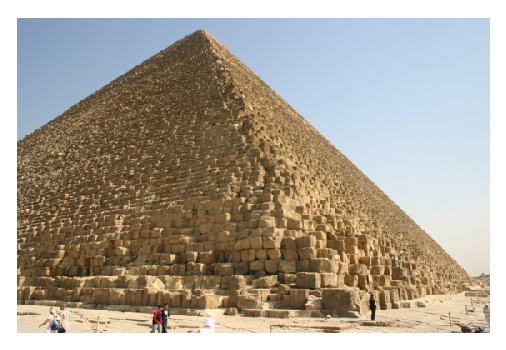
\includegraphics[width=0.45\textwidth]{./Graphiques/kheops.eps}
\end{multicols}
\end{exo}

\begin{exo}
 \begin{multicols}{2}
  $K$ et $L$ sont les milieux des ar\^etes $[EH]$ et $[EF]$ du parall\'el\'epip\`ede rectangle $ABCDEFGH$.
  Les droites $(AK)$ et $(DH)$ se coupent en $M$. Les droites $(AL)$ et $(BF)$ se coupent en $N$.
\begin{enumerate}
 \item D\'emontrer que $K$ est le milieu de $[AM]$.
 \item D\'emontrer que les droites $(KL)$ et $(MN)$ sont parall\`eles.
\end{enumerate}
\sautcol
\begin{center}
\psset{xunit=1cm , yunit=0.75cm}
\def\xmin{-0.5} \def\xmax{5.5} \def\ymin{-2.5} \def\ymax{3}
\begin{pspicture*}(\xmin,\ymin)(\xmax,\ymax)
 \psline(0,2)(0,0)(4,-0.5)(4,1.5)(0,2)(1,2.5)(5,2)(5,0)(4,-0.5)
 \psline(4,1.5)(5,2)
 \psline[linestyle=dashed](0,0)(1,0.5)(1,2.5)
 \psline[linestyle=dashed](1,0.5)(5,0)
 \uput[u](1,2.5){$A$}
 \uput[ur](5,2){$B$}
 \uput[dr](4,1.5){$C$}
 \uput[l](0,2){$D$}
 \uput[ur](1,0.5){$E$}
 \uput[r](5,0){$F$}
 \uput[dl](0,0){$H$}
 \uput[dr](4,-0.5){$G$}

 \psline[linestyle=dotted](1,2.5)(0,-2)(0,0)
 \psline[linestyle=dotted](1,2.5)(5,-2)(5,0)
 \uput[dl](0,-2){$M$}
 \uput[dr](5,-2){$N$}
 \uput[ul](0.5,0.25){$K$}
 \uput[ur](3,0.25){$L$}
\end{pspicture*}
\end{center}
 \end{multicols}

\end{exo}



\begin{exo}
\begin{multicols}{2}
$ABCDEFGH$ est un parallélépipède rectangle (un pavé) tel que $AB = 5$, $AE = 2$ et $BC = 3$.\\
Une fourmi se situe en $E$ et se rend en $C$ en cheminant sur les faces.\\
D\'eterminer le trajet le plus court.\\
\emph{Indication : on pourra s'aider du patron.}
\sautcol
\begin{center}
\psset{xunit=1cm , yunit=0.66cm}
\begin{pspicture*}(-0.7,-0.7)(5.7,5.2)
\def\xmin{-0.5} \def\xmax{5.5} \def\ymin{-0.5} \def\ymax{5}

\psset{linecolor=black, linewidth=.5pt, arrowsize=2pt 4}
\psline(0.0000,0.0000)(3.0000,0.0000)
\psline(3.0000,0.0000)(3.0000,3.0000)
\psline(3.0000,3.0000)(0.0000,3.0000)
\psline(0.0000,3.0000)(0.0000,0.0000)
\psline[linestyle=dashed](2.0000,1.0000)(5.0000,1.0000)
\psline(5.0000,1.0000)(5.0000,4.0000)
\psline(5.0000,4.0000)(2.0000,4.0000)
\psline[linestyle=dashed](2.0000,4.0000)(2.0000,1.0000)
\psline[linestyle=dashed](0.0000,0.0000)(2.0000,1.0000)
\psline(3.0000,0.0000)(5.0000,1.0000)
\psline(3.0000,3.0000)(5.0000,4.0000)
\psline(0.0000,3.0000)(2.0000,4.0000)
%\psline[linestyle=dashed](0.0000,0.0000)(2.0000,4.0000)
%\psline[linestyle=dashed](3.0000,0.0000)(2.0000,4.0000)
%\psline[linestyle=dashed](5.0000,1.0000)(2.0000,4.0000)
\rput(-0.3,-0.3){$A$}
\rput(3,-0.3){$B$}
\rput(5.3,0.7){$C$}
\rput(1.7,1.3){$D$}
\rput(-0.3,3.3){$E$}
\rput(2.7,2.7){$F$}
\rput(5.3,4.3){$G$}
\rput(1.7,4.3){$H$}

\end{pspicture*}
\end{center}
\end{multicols}

\end{exo}


\subsection{Incidence et parall\'elisme}


\begin{tabular}{cc}
 \begin{minipage}[l]{0.625\linewidth}
 \begin{exo}  $SABCD$ est une pyramide \`a base carr\'ee. $I$ est un point du segment $[BC]$, distinct de $B$ et $C$.
\begin{enumerate}
 \item Montrer que les plans $(SAI)$ et $(SCD)$ sont s\'ecants.
 \item Construire leur intersubsection.
\end{enumerate}
\end{exo}
 \end{minipage}
&
\begin{minipage}[r]{0.35\linewidth}
 \begin{center}
\psset{xunit=1cm , yunit=0.5cm}
\def\xmin{-0.5} \def\xmax{4.5} \def\ymin{-1} \def\ymax{5}
\begin{pspicture*}(\xmin,\ymin)(\xmax,\ymax)
 \psline(3,0)(0,0)(2,4)(3,0)(4,1)(2,4)
 \psline[linestyle=dashed](0,0)(1,1)(2,4)
 \psline[linestyle=dashed](1,1)(4,1)
 \uput[dl](0,0){$B$}
 \uput[dr](3,0){$C$}
 \uput[ur](4,1){$D$}
 \uput[dr](1,1){$A$}
 \uput[u](2,4){$S$}
  \psdot(1,0)\uput[d](1,0){$I$}
\end{pspicture*}
\end{center}
\end{minipage}

\end{tabular}




\begin{tabular}{cc}
 \begin{minipage}[l]{0.6\linewidth}
 \begin{exo}  $ABCDEFGH$ est un parall\'el\'epip\`ede rectangle. $I$ est un point de $[AE]$ distinct de $A$ et de $E$.
\begin{enumerate}
 \item D\'emontrer que $A$, $C$, $G$ et $I$ sont coplanaires.
 \item D\'emontrer que la droite $(GI)$ n'est pas contenue dans le plan $(ABCD)$.
 \item Construire $J$, intersubsection de la droite $(GI)$ et du plan $(ABCD)$.
\end{enumerate}\end{exo}
 \end{minipage}
&
\begin{minipage}[r]{0.35\linewidth}
\begin{center}
\psset{xunit=1cm , yunit=0.75cm}
\def\xmin{-0.5} \def\xmax{5.5} \def\ymin{-2.5} \def\ymax{3.5}
\begin{pspicture*}(\xmin,\ymin)(\xmax,\ymax)
 \psline(0,2)(0,0)(4,-0.5)(4,1.5)(0,2)(1,2.5)(5,2)(5,0)(4,-0.5)
 \psline(4,1.5)(5,2)
 \psline[linestyle=dashed](0,0)(1,0.5)(1,2.5)
 \psline[linestyle=dashed](1,0.5)(5,0)
 \uput[u](1,2.5){$H$}
 \uput[ur](5,2){$G$}
 \uput[dr](4,1.5){$F$}
 \uput[l](0,2){$E$}
 \uput[ur](1,0.5){$D$}
 \uput[r](5,0){$C$}
 \uput[dl](0,0){$A$}
 \uput[dr](4,-0.5){$B$}
\psdot(0,0.5)\uput[l](0,0.5){$I$}

\end{pspicture*}
\end{center}
\end{minipage}

\end{tabular}

\begin{tabular}{cc}
 \begin{minipage}[l]{0.625\linewidth}
\begin{exo}    $ABCD$ est un t\'etra\`edre.
$I$ est un point de $[BC]$ distinct de $B$ et de $C$.
$J$ est un point de $[AD]$ distinct de $A$ et de $D$.\\
Dans les cas suivants, d\'emontrer que les plans sont s\'ecants et d\'eterminer leur intersubsection.
\begin{enumerate}
 \item $(DIJ)$ et $(BCD)$.
 \item $(DIJ)$ et $(ABD)$.
 \item $(DIJ)$ et $(ABC)$.
\end{enumerate}\end{exo}
 \end{minipage}
&
\begin{minipage}[r]{0.35\linewidth}
\begin{center}
\psset{xunit=0.6cm , yunit=0.6cm}
\begin{pspicture*}(-0.7,0.1)(9.2,8)
\def\xmin{-0.5} \def\xmax{9} \def\ymin{0.3} \def\ymax{7.8}
\psset{linecolor=black, linewidth=.5pt, arrowsize=2pt 4}
\psline(0.0000,2.0000)(5.0000,1.0000)
\psline(0.0000,2.0000)(3.0000,7.0000)
\psline[linestyle=dashed](0.0000,2.0000)(8.0000,3.0000)
\psline(5.0000,1.0000)(8.0000,3.0000)
\psline(5.0000,1.0000)(3.0000,7.0000)
\psline(8.0000,3.0000)(3.0000,7.0000)

\uput[l](0,2){$A$}
\uput[d](5,1){$B$}
\uput[r](8,3){$C$}
\uput[u](3,7){$D$}
\psdots[dotstyle=x, dotscale=2.0000](1,3.666667)\uput[r](1,3.666667){$J$}
\psdots[dotstyle=x, dotscale=2.0000](7,2.333333)\uput[r](7,2.333333){$I$}
\end{pspicture*}
\end{center}
\end{minipage}

\end{tabular}

\begin{tabular}{cc}
 \begin{minipage}[l]{0.625\linewidth}
\begin{exo} $ABCD$ est un t\'etra\`edre.
$I$ est un point de $[DA]$ distinct de $D$ et de $A$.
$J$ est un point de la face $BCD$ tel que la droite $(IJ)$ n'est pas parall\`ele au plan $(ABC)$.\\
Construire l'intersubsection de la droite $(IJ)$ et du plan $(ABC)$.\\
\emph{Indication : on pourra commencer par construire l'intersubsection des plans $(DIJ)$ et $(ABC)$.} \end{exo}
 \end{minipage}
&
\begin{minipage}[r]{0.35\linewidth}
\begin{center}
\psset{xunit=0.6cm , yunit=0.6cm}
\begin{pspicture*}(-0.7,0.1)(9.2,8)
\def\xmin{-0.5} \def\xmax{9} \def\ymin{0.3} \def\ymax{7.8}
\psset{linecolor=black, linewidth=.5pt, arrowsize=2pt 4}
\psline(0.0000,2.0000)(5.0000,1.0000)
\psline(0.0000,2.0000)(3.0000,7.0000)
\psline[linestyle=dashed](0.0000,2.0000)(8.0000,3.0000)
\psline(5.0000,1.0000)(8.0000,3.0000)
\psline(5.0000,1.0000)(3.0000,7.0000)
\psline(8.0000,3.0000)(3.0000,7.0000)

\uput[l](0,2){$A$}
\uput[d](5,1){$B$}
\uput[r](8,3){$C$}
\uput[u](3,7){$D$}
\psdots[dotstyle=x, dotscale=2.0000](2,5.3333333)\uput[r](2,5.3333333){$I$}
\psdots[dotstyle=x, dotscale=2.0000](5.5,3)\uput[r](5.5,3){$J$}
\end{pspicture*}
\end{center}
\end{minipage}

\end{tabular}

\begin{tabular}{cc}
 \begin{minipage}[l]{0.625\linewidth}
\begin{exo}
$SABC$ est un t\'etra\`edre.
$I$, $J$ et $K$ sont des points de, respectivement, $[SA]$, $[SB]$ et $[SC]$.
\begin{enumerate}
 \item Construire $E$, intersubsection de $(BC)$ et $(JK)$, $F$, intersubsection de $(AC)$ et $(IK)$, $G$, intersubsection de $(AB)$ et $(IJ)$.
 \item D\'emontrer que $F$ est un point commun aux plans $(ABC)$ et $(IJK)$.
 \item Prouver que les points $E$, $F$ et $G$ sont align\'es.
\end{enumerate}\end{exo}
 \end{minipage}
&
\begin{minipage}[r]{0.35\linewidth}
\begin{center}
\psset{xunit=0.6cm , yunit=0.6cm}
\begin{pspicture*}(-0.7,0.1)(9.2,8)
\def\xmin{-0.5} \def\xmax{9} \def\ymin{0.3} \def\ymax{7.8}
\psset{linecolor=black, linewidth=.5pt, arrowsize=2pt 4}
\psline(0.0000,2.0000)(5.0000,1.0000)
\psline(0.0000,2.0000)(3.0000,7.0000)
\psline[linestyle=dashed](0.0000,2.0000)(8.0000,3.0000)
\psline(5.0000,1.0000)(8.0000,3.0000)
\psline(5.0000,1.0000)(3.0000,7.0000)
\psline(8.0000,3.0000)(3.0000,7.0000)

\uput[l](0,2){$A$}
\uput[d](5,1){$B$}
\uput[r](8,3){$C$}
\uput[u](3,7){$S$}
\psdots[dotstyle=x, dotscale=2.0000](1.5,4.5)\uput[r](1.5,4.5){$I$}
\psdots[dotstyle=x, dotscale=2.0000](4.333333,3)\uput[r](4.333333,3){$J$}
\psdots[dotstyle=x, dotscale=2.0000](4.666667,5.66667)\uput[r](4.666667,5.66667){$K$}
\end{pspicture*}
\end{center}
\end{minipage}

\end{tabular}

%\subsection{Parall\'elisme}

\begin{tabular}{cc}
 \begin{minipage}[l]{0.675\linewidth}
\begin{exo}
 $SABCD$ est une pyramide \`a base carr\'ee. $I$ est le milieu de $[AS]$ et $L$ est le milieu de $[BS]$.\\
D\'emontrer que les droites $(IL)$ et $(CD)$ sont parall\`eles.\end{exo}
 \end{minipage}
&
\begin{minipage}[r]{0.3\linewidth}
\begin{center}
\psset{xunit=1cm , yunit=0.5cm}
\def\xmin{-0.5} \def\xmax{4.5} \def\ymin{-1} \def\ymax{5}
\begin{pspicture*}(\xmin,\ymin)(\xmax,\ymax)
 \psline(3,0)(0,0)(2,4)(3,0)(4,1)(2,4)
 \psline[linestyle=dashed](0,0)(1,1)(2,4)
 \psline[linestyle=dashed](1,1)(4,1)
 \uput[dl](0,0){$A$}
 \uput[dr](3,0){$B$}
 \uput[ur](4,1){$C$}
 \uput[dr](1,1){$D$}
 \uput[u](2,4){$S$}
\end{pspicture*}
\end{center}
\end{minipage}

\end{tabular}


\begin{tabular}{cc}
 \begin{minipage}[l]{0.675\linewidth}
\begin{exo}
$ABCDEFGH$ est un cube. $M$ est un point de l'ar\^ete $[AB]$. Le plan $(GEM)$ coupe la droite $(BC)$ en $N$.\\
D\'emontrer que les droites $(MN)$ et $(EG)$ sont parall\`eles.\end{exo}
 \end{minipage}
&
\begin{minipage}[r]{0.3\linewidth}
\begin{center}
\psset{xunit=1cm , yunit=1cm}
\def\xmin{-0.5} \def\xmax{3} \def\ymin{-0.5} \def\ymax{3}
\begin{pspicture*}(\xmin,\ymin)(\xmax,\ymax)
 \psline(0,2)(0,0)(2,0)(2,2)(0,2)(0.5,2.25)(2.5,2.25)(2.5,0.25)(2,0)
 \psline(2.5,2.25)(2,2)
 \psline[linestyle=dashed](0,0)(0.5,0.25)(0.5,2.25)
 \psline[linestyle=dashed](0.5,0.25)(2.5,0.25)
 \uput[dl](0,0){$A$}
 \uput[d](2,0){$B$}
 \uput[r](2.5,0.25){$C$}
 \uput[ur](0.5,0.25){$D$}
 \uput[ul](0,2){$E$}
 \uput[dr](2,2){$F$}
 \uput[u](0.5,2.25){$H$}
 \uput[ur](2.5,2.25){$G$}

 \psline[linestyle=dotted](2.5,2.25)(0,2)(0.75,0)(2.284,0.1278)
 \uput[d](0.75,0){$M$}
 \uput[dr](2.0284,0.1278){$N$}

\end{pspicture*}
\end{center}
\end{minipage}

\end{tabular}


\begin{tabular}{cc}
 \begin{minipage}[l]{0.675\linewidth}
\begin{exo}
$SABCD$ est une pyramide de sommet $S$ \`a base trap\'ezo\"idale avec $(AB)\parallel (CD)$.
$M$ est un point de l'ar\^ete $[SC]$. Le plan $(ABM)$ coupe la droite $(SD)$ en $N$.\\
D\'emontrer que les droites $(MN)$ et $(DC)$ sont parall\`eles.\end{exo}
 \end{minipage}
&
\begin{minipage}[r]{0.3\linewidth}
\begin{center}
\psset{xunit=1cm , yunit=0.5cm}
\def\xmin{-0.5} \def\xmax{4.5} \def\ymin{-1} \def\ymax{5}
\begin{pspicture*}(\xmin,\ymin)(\xmax,\ymax)
 \psline(2,0)(0,0)(2,4)(2,0)(4,1)(2,4)
 \psline[linestyle=dashed](0,0)(1,1)(2,4)
 \psline[linestyle=dashed](1,1)(4,1)
 \uput[dl](0,0){$A$}
 \uput[dr](2,0){$B$}
 \uput[ur](4,1){$C$}
 \uput[dr](1,1){$D$}
 \uput[u](2,4){$S$}

\psline[linestyle=dotted](3.5,1.75)(1.25,1.75)
\uput[ur](3.5,1.75){$M$}
\uput[dr](1.25,1.75){$N$}
\end{pspicture*}
\end{center}
\end{minipage}

\end{tabular}



\begin{tabular}{cc}
 \begin{minipage}[l]{0.625\linewidth}
\begin{exo}
$SABCD$ est une pyramide de sommet $S$ dont la base $ABCD$ est un parall\'elogramme.\\
D\'emontrer que les plans $(SAB)$ et $(SDC)$ se coupent selon la parall\`ele \`a $(AB)$ passant par $S$.\end{exo}
 \end{minipage}
&
\begin{minipage}[r]{0.35\linewidth}
\begin{center}
\psset{xunit=1cm , yunit=0.5cm}
\def\xmin{-0.5} \def\xmax{4.5} \def\ymin{-1} \def\ymax{5}
\begin{pspicture*}(\xmin,\ymin)(\xmax,\ymax)
 \psline(1,0)(2,4)(0,1)(1,0)(4,0)(2,4)
 \psline[linestyle=dashed](0,1)(3,1)(2,4)
 \psline[linestyle=dashed](3,1)(4,0)
 \uput[l](0,1){$A$}
 \uput[dl](1,0){$B$}
 \uput[r](4,0){$C$}
 \uput[d](3,1){$D$}
 \uput[u](2,4){$S$}


\end{pspicture*}
\end{center}
\end{minipage}

\end{tabular}

\begin{tabular}{cc}
 \begin{minipage}[l]{0.525\linewidth}
\begin{exo}
$ABCDEFGH$ est un parall\'el\'epip\`ede rectangle.
\begin{enumerate}
 \item Le quadrilat\`ere $BEHC$ est un rectangle. Que peut-on en d\'eduire pour les droites $(EB)$ et $(HC)$ ?
 \item De fa\c con analogue, que peut-on dire des droites $(AH)$ et $(BG)$ ?
 \item En d\'eduire alors la position relative des plans $(ACH)$ et $(EBG)$ ?
\end{enumerate}\end{exo}
 \end{minipage}
&
\begin{minipage}[r]{0.45\linewidth}
\begin{center}
\psset{xunit=0.75cm , yunit=0.66cm}
\def\xmin{-0.6} \def\xmax{9.7} \def\ymin{-0.7} \def\ymax{5.9}
\begin{pspicture*}(\xmin,\ymin)(\xmax,\ymax)
\uput[l](0,3){$A$}
 \uput[u](6,3){$B$}
 \uput[r](9,5){$C$}
 \uput[u](3,5){$D$}
 \uput[dl](0,0){$E$}
 \uput[d](6,0){$F$}
 \uput[r](9,2){$G$}
 \uput[d](3,2){$H$}

 \psline(0,3)(0,0)(6,0)(6,3)(0,3)(3,5)(9,5)(9,2)(6,0)
 \psline(6,3)(9,5)
 \psline[linestyle=dashed](0,0)(3,2)(3,5)
 \psline[linestyle=dashed](3,2)(9,2)

 \psline(0,3)(9,5)
 \psline(0,0)(6,3)(9,2)
 \psline[linestyle=dotted](0,3)(3,2)(9,5)
 \psline[linestyle=dotted](0,0)(9,2)



\end{pspicture*}
\end{center}
\end{minipage}

\end{tabular}

\begin{tabular}{cc}
 \begin{minipage}[l]{0.525\linewidth}
\begin{exo}
$ABCDEF$ est un prisme droit \`a base triangulaire. $I$, $L$ et $K$ sont les points des ar\^etes $[AB]$, $[AC]$ et $[DE]$ tels que :
$AI=\frac{2}{3}AB$ ; $AK=\frac{2}{3}AC$ et $EL=\frac{1}{3}ED$.\\
D\'emontrer que le plan $(IKL)$ est parall\`ele au plan $(BCF)$.
\end{exo}
 \end{minipage}
&
\begin{minipage}[r]{0.425\linewidth}
\begin{center}
\psset{xunit=1cm , yunit=0.5cm}
\def\xmin{-0.5} \def\xmax{6.7} \def\ymin{-0.9} \def\ymax{5.9}
\begin{pspicture*}(\xmin,\ymin)(\xmax,\ymax)
\uput[ul](0,5){$A$}
 \uput[dl](2,3){$B$}
 \uput[r](6,5){$C$}
 \uput[l](0,2){$D$}
 \uput[d](2,0){$E$}
 \uput[r](6,2){$F$}


 \psline(0,5)(0,2)(2,0)(2,3)(0,5)(6,5)(6,2)(2,0)
 \psline(2,3)(6,5)
 \psline[linestyle=dashed](0,2)(6,2)

\psdots(1.333,0.666)(1.333,3.666)(4,5)
\uput[d](1.333,0.666){$L$}
\uput[d](1.333,3.666){$I$}
\uput[d](4,5){$K$}

\end{pspicture*}
\end{center}
\end{minipage}

\end{tabular}


\begin{tabular}{cc}
 \begin{minipage}[l]{0.525\linewidth}
\begin{exo}
$ABCDEFGH$ est un parall\'el\'epip\`ede rectangle.\\
D\'emontrer que la droite $(AC)$ est parall\`ele au plan $(EFH)$.
\end{exo}
 \end{minipage}
&
\begin{minipage}[r]{0.425\linewidth}
\begin{center}
\psset{xunit=0.75cm , yunit=0.66cm}
\def\xmin{-0.6} \def\xmax{9.7} \def\ymin{-0.7} \def\ymax{5.9}
\begin{pspicture*}(\xmin,\ymin)(\xmax,\ymax)
\uput[l](0,3){$A$}
 \uput[u](6,3){$B$}
 \uput[r](9,5){$C$}
 \uput[u](3,5){$D$}
 \uput[dl](0,0){$E$}
 \uput[d](6,0){$F$}
 \uput[r](9,2){$G$}
 \uput[d](3,2){$H$}

 \psline(0,3)(0,0)(6,0)(6,3)(0,3)(3,5)(9,5)(9,2)(6,0)
 \psline(6,3)(9,5)
 \psline[linestyle=dashed](0,0)(3,2)(3,5)
 \psline[linestyle=dashed](3,2)(9,2)

\end{pspicture*}
\end{center}
\end{minipage}

\end{tabular}



\sautpage

\subsection{Sections}

\begin{exo}[Sections planes d'un tétraèdre]\label{geo1act1}
Dans chacun des cas présentés sur la figure \ref{geo1act1fig} \vpageref{geo1act1fig}, placer les points $I$ et $K$, puis, à l'aide des propriétés de géométrie dans l'espace vues en Seconde, construire sur le dessin en perspective la trace du plan $(IJK)$ sur le tétraèdre $ABCD$.
On donne $\V{BJ}=\frac{1}{3}\V{BD}$

\begin{figure}[!h]
\centering
\caption{Sections de l'exercice \ref{geo1act1}}\label{geo1act1fig}

\medskip

\begin{tabular}{cc}
$\V{DI}=\frac{1}{3}\V{DA}$ et $\V{CK}=\frac{1}{3}\V{CD}$ &
$\V{DI}=\frac{1}{3}\V{DA}$ et $\V{AK}=\frac{1}{3}\V{AC}$ \\
\psset{xunit=0.8cm , yunit=0.6cm}
\begin{pspicture*}(-0.7,0.1)(9.2,8)
\def\xmin{-0.5} \def\xmax{9} \def\ymin{0.3} \def\ymax{7.8}
\psset{linecolor=black, linewidth=.5pt, arrowsize=2pt 4}
\psline(0.0000,2.0000)(5.0000,1.0000)
\psline(0.0000,2.0000)(3.0000,7.0000)
\psline[linestyle=dashed](0.0000,2.0000)(8.0000,3.0000)
\psline(5.0000,1.0000)(8.0000,3.0000)
\psline(5.0000,1.0000)(3.0000,7.0000)
\psline(8.0000,3.0000)(3.0000,7.0000)
\psdots[dotstyle=x, dotscale=2.0000](4.3330,3.0000)
\uput[l](0,2){$A$}
\uput[d](5,1){$B$}
\uput[r](8,3){$C$}
\uput[u](3,7){$D$}
\uput[r](4.333,3){$J$}
\end{pspicture*}
&
\psset{xunit=0.8cm , yunit=0.6cm}
\begin{pspicture*}(-0.7,0.1)(9.2,8)
\def\xmin{-0.5} \def\xmax{9} \def\ymin{0.3} \def\ymax{7.8}
\psset{linecolor=black, linewidth=.5pt, arrowsize=2pt 4}
\psline(0.0000,2.0000)(5.0000,1.0000)
\psline(0.0000,2.0000)(3.0000,7.0000)
\psline[linestyle=dashed](0.0000,2.0000)(8.0000,3.0000)
\psline(5.0000,1.0000)(8.0000,3.0000)
\psline(5.0000,1.0000)(3.0000,7.0000)
\psline(8.0000,3.0000)(3.0000,7.0000)
\psdots[dotstyle=x, dotscale=2.0000](4.3330,3.0000)
\uput[l](0,2){$A$}
\uput[d](5,1){$B$}
\uput[r](8,3){$C$}
\uput[u](3,7){$D$}
\uput[r](4.333,3){$J$}
\end{pspicture*}
\\
\end{tabular}

\begin{tabular}{cc}
$\V{DI}=\frac{1}{3}\V{DA}$ et $K$ centre de gravit\'e de $ABC$ & $\V{AI}=\frac{1}{3}\V{AD}$ et $\V{BK}=\frac{1}{3}\V{BC}$\\
\psset{xunit=0.8cm , yunit=0.6cm}
\begin{pspicture*}(-0.7,0.1)(9.2,8)
\def\xmin{-0.5} \def\xmax{9} \def\ymin{0.3} \def\ymax{7.8}
\psset{linecolor=black, linewidth=.5pt, arrowsize=2pt 4}
\psline(0.0000,2.0000)(5.0000,1.0000)
\psline(0.0000,2.0000)(3.0000,7.0000)
\psline[linestyle=dashed](0.0000,2.0000)(8.0000,3.0000)
\psline(5.0000,1.0000)(8.0000,3.0000)
\psline(5.0000,1.0000)(3.0000,7.0000)
\psline(8.0000,3.0000)(3.0000,7.0000)
\psdots[dotstyle=x, dotscale=2.0000](4.3330,3.0000)
\uput[l](0,2){$A$}
\uput[d](5,1){$B$}
\uput[r](8,3){$C$}
\uput[u](3,7){$D$}
\uput[r](4.333,3){$J$}
\end{pspicture*}
&
\psset{xunit=0.8cm , yunit=0.6cm}
\begin{pspicture*}(-0.7,0.1)(9.2,8)
\def\xmin{-0.5} \def\xmax{9} \def\ymin{0.3} \def\ymax{7.8}
\psset{linecolor=black, linewidth=.5pt, arrowsize=2pt 4}
\psline(0.0000,2.0000)(5.0000,1.0000)
\psline(0.0000,2.0000)(3.0000,7.0000)
\psline[linestyle=dashed](0.0000,2.0000)(8.0000,3.0000)
\psline(5.0000,1.0000)(8.0000,3.0000)
\psline(5.0000,1.0000)(3.0000,7.0000)
\psline(8.0000,3.0000)(3.0000,7.0000)
\psdots[dotstyle=x, dotscale=2.0000](4.3330,3.0000)
\uput[l](0,2){$A$}
\uput[d](5,1){$B$}
\uput[r](8,3){$C$}
\uput[u](3,7){$D$}
\uput[r](4.333,3){$J$}
\end{pspicture*}\\
\end{tabular}
\end{figure}
\end{exo}

\sautpage

\begin{exo}[Sections planes d'un cube]\label{geo1act2}
Dans chacun des cas présentés sur la figure \ref{geo1act2fig} \vpageref{geo1act2fig}, à l'aide des propriétés de géométrie dans l'espace, construire sur le dessin en perspective la trace du plan $(IJK)$ sur le cube $ABCDEFGH$.
On donne : $AB = 6$ cm ; $EI = 2$ cm ; $J$ milieu de $[HG]$.

\begin{figure}[!h]
\centering
\caption{Sections de l'exercice \ref{geo1act2}}\label{geo1act2fig}

\medskip

\begin{tabular}{cc}
$DK=2$ cm & $KD=1$ cm\\
\psset{xunit=0.8cm , yunit=0.8cm}
\begin{pspicture*}(-0.7,-0.7)(9.2,8.2)
\def\xmin{-0.5} \def\xmax{9} \def\ymin{-0.5} \def\ymax{8}
\psset{linecolor=black, linewidth=.5pt, arrowsize=2pt 4}
\psline(0.0000,0.0000)(6.0000,0.0000)
\psline(0.0000,0.0000)(0.0000,6.0000)
\psline[linestyle=dashed](0.0000,0.0000)(2.0000,1.0000)
\psline(6.0000,0.0000)(8.0000,1.0000)
\psline(6.0000,0.0000)(6.0000,6.0000)
\psline[linestyle=dashed](8.0000,1.0000)(2.0000,1.0000)
\psline(8.0000,1.0000)(8.0000,7.0000)
\psline[linestyle=dashed](2.0000,1.0000)(2.0000,7.0000)
\psline(0.0000,6.0000)(6.0000,6.0000)
\psline(0.0000,6.0000)(2.0000,7.0000)
\psline(6.0000,6.0000)(8.0000,7.0000)
\psline(8.0000,7.0000)(2.0000,7.0000)
\psdots[dotstyle=x, dotscale=2.0000](0.6667,6.3300)
\psdots[dotstyle=x, dotscale=2.0000](5.0000,7.0000)
\psdots[dotstyle=x, dotscale=2.0000](2.0000,3.0000)
\uput[d](0,0){$A$}
\uput[d](6,0){$B$}
\uput[r](8,1){$C$}
\uput[d](2,1){$D$}
\uput[l](0,6){$E$}
\uput[u](6,6){$F$}
\uput[u](8,7){$G$}
\uput[u](2,7){$H$}
\uput[u](0.667,6.333){$I$}
\uput[u](5,7){$J$}
\uput[r](2,3){$K$}
\end{pspicture*}
&
\psset{xunit=0.8cm , yunit=0.8cm}
\begin{pspicture*}(-0.7,-0.7)(9.2,8.2)
\def\xmin{-0.5} \def\xmax{9} \def\ymin{-0.5} \def\ymax{8}
\psset{linecolor=black, linewidth=.5pt, arrowsize=2pt 4}
\psline(0.0000,0.0000)(6.0000,0.0000)
\psline(0.0000,0.0000)(0.0000,6.0000)
\psline[linestyle=dashed](0.0000,0.0000)(2.0000,1.0000)
\psline(6.0000,0.0000)(8.0000,1.0000)
\psline(6.0000,0.0000)(6.0000,6.0000)
\psline[linestyle=dashed](8.0000,1.0000)(2.0000,1.0000)
\psline(8.0000,1.0000)(8.0000,7.0000)
\psline[linestyle=dashed](2.0000,1.0000)(2.0000,7.0000)
\psline(0.0000,6.0000)(6.0000,6.0000)
\psline(0.0000,6.0000)(2.0000,7.0000)
\psline(6.0000,6.0000)(8.0000,7.0000)
\psline(8.0000,7.0000)(2.0000,7.0000)
\psdots[dotstyle=x, dotscale=2.0000](0.6667,6.3300)
\psdots[dotstyle=x, dotscale=2.0000](5.0000,7.0000)
\psdots[dotstyle=x, dotscale=2.0000](3.0000,1.0000)
\uput[d](0,0){$A$}
\uput[d](6,0){$B$}
\uput[r](8,1){$C$}
\uput[d](2,1){$D$}
\uput[l](0,6){$E$}
\uput[u](6,6){$F$}
\uput[u](8,7){$G$}
\uput[u](2,7){$H$}
\uput[u](0.667,6.333){$I$}
\uput[u](5,7){$J$}
\uput[u](3,1){$K$}
\end{pspicture*}\\
\end{tabular}

\medskip

\begin{tabular}{cc}
$K=C$ & $K$ milieu de $[BC]$\\
\psset{xunit=0.8cm , yunit=0.8cm}
\begin{pspicture*}(-0.7,-0.7)(9.2,8.2)
\def\xmin{-0.5} \def\xmax{9} \def\ymin{-0.5} \def\ymax{8}
\psset{linecolor=black, linewidth=.5pt, arrowsize=2pt 4}
\psline(0.0000,0.0000)(6.0000,0.0000)
\psline(0.0000,0.0000)(0.0000,6.0000)
\psline[linestyle=dashed](0.0000,0.0000)(2.0000,1.0000)
\psline(6.0000,0.0000)(8.0000,1.0000)
\psline(6.0000,0.0000)(6.0000,6.0000)
\psline[linestyle=dashed](8.0000,1.0000)(2.0000,1.0000)
\psline(8.0000,1.0000)(8.0000,7.0000)
\psline[linestyle=dashed](2.0000,1.0000)(2.0000,7.0000)
\psline(0.0000,6.0000)(6.0000,6.0000)
\psline(0.0000,6.0000)(2.0000,7.0000)
\psline(6.0000,6.0000)(8.0000,7.0000)
\psline(8.0000,7.0000)(2.0000,7.0000)
\psdots[dotstyle=x, dotscale=2.0000](0.6667,6.3300)
\psdots[dotstyle=x, dotscale=2.0000](5.0000,7.0000)
\psdots[dotstyle=x, dotscale=2.0000](8.0000,1.0000)
\uput[d](0,0){$A$}
\uput[d](6,0){$B$}
\uput[r](8,1){$C$}
\uput[d](2,1){$D$}
\uput[l](0,6){$E$}
\uput[u](6,6){$F$}
\uput[u](8,7){$G$}
\uput[u](2,7){$H$}
\uput[u](0.667,6.333){$I$}
\uput[u](5,7){$J$}
\uput[ul](8,1){$K$}
\end{pspicture*}
&
\psset{xunit=0.8cm , yunit=0.8cm}
\begin{pspicture*}(-0.7,-0.7)(9.2,8.2)
\def\xmin{-0.5} \def\xmax{9} \def\ymin{-0.5} \def\ymax{8}
\psset{linecolor=black, linewidth=.5pt, arrowsize=2pt 4}
\psline(0.0000,0.0000)(6.0000,0.0000)
\psline(0.0000,0.0000)(0.0000,6.0000)
\psline[linestyle=dashed](0.0000,0.0000)(2.0000,1.0000)
\psline(6.0000,0.0000)(8.0000,1.0000)
\psline(6.0000,0.0000)(6.0000,6.0000)
\psline[linestyle=dashed](8.0000,1.0000)(2.0000,1.0000)
\psline(8.0000,1.0000)(8.0000,7.0000)
\psline[linestyle=dashed](2.0000,1.0000)(2.0000,7.0000)
\psline(0.0000,6.0000)(6.0000,6.0000)
\psline(0.0000,6.0000)(2.0000,7.0000)
\psline(6.0000,6.0000)(8.0000,7.0000)
\psline(8.0000,7.0000)(2.0000,7.0000)
\psdots[dotstyle=x, dotscale=2.0000](0.6667,6.3300)
\psdots[dotstyle=x, dotscale=2.0000](5.0000,7.0000)
\psdots[dotstyle=x, dotscale=2.0000](7.0000,0.5000)
\uput[d](0,0){$A$}
\uput[d](6,0){$B$}
\uput[r](8,1){$C$}
\uput[d](2,1){$D$}
\uput[l](0,6){$E$}
\uput[u](6,6){$F$}
\uput[u](8,7){$G$}
\uput[u](2,7){$H$}
\uput[u](0.667,6.333){$I$}
\uput[u](5,7){$J$}
\uput[r](7,0.5){$K$}
\end{pspicture*}\\
\end{tabular}
\end{figure}

\end{exo}






\chapter{Fonction inverse \\ Fonctions homographiques} \label{homographiques}
\minitoc

\fancyhead{} % efface les entêtes précédentes
\fancyhead[LE,RO]{\footnotesize \em \rightmark} % section en entête
\fancyhead[RE,LO]{\scriptsize \em Seconde} % classe et année en entête

    \fancyfoot{}
		\fancyfoot[RE]{\scriptsize \em \href{http://perpendiculaires.free.fr/}{http://perpendiculaires.free.fr/}}
		\fancyfoot[LO]{\scriptsize \em David ROBERT}
    \fancyfoot[LE,RO]{\textbf{\thepage}}

%\sautpage


\section{Activités}

\begin{act}
Chaque ann\'ee, un c\'el\`ebre magazine automobile organise le concours du v\'ehicule \'ecologique le plus performant. Il s'agit de parcourir un kilom\`etre sur une piste am\'enag\'ee, avec comme seul carburant de l'eau, du vent ou du soleil. On d\'esigne par $v$ la vitesse moyenne d'un v\'ehicule (en kilom\`etres par heure) et par $f(v)$ le temps (en heures) n\'ecessaire pour parcourir la piste.\\
On rappelle que la vitesse moyenne $v$ est donn\'ee par $\frac{d}{t}$ o\`u $d$ d\'esigne la distance parcourue et $t$ le temps mis pour parcourir cette distance.
\begin{enumerate}
 \item \begin{enumerate}
        \item Donner l'expression de la fonction $f$ en fonction de la vitesse $v$.
	\item Compl\'eter le tableau suivant :
	      \begin{center}
	      \begin{tabularx}{\linewidth}{|*{15}{>{\centering \arraybackslash}X|}}\hline
	      $v$&0,1	&0,25	&0,5 	&0,75 	&1	&2 	&3 	&4 	&5 	&6	&7	&8	&9	&10	 \\ \hline
	      $f(v)$&	&	&	&	&	&	&	&	&	& & & & & \\ \hline
	      \end{tabularx}
	      \end{center}
	\item Le tableau pr\'ec\'edent est-il un tableau de proportionnalit\'e ?
       \end{enumerate}
 \item \begin{enumerate}
        \item On se place dans un rep\`ere orthornorm\'e o\`u une unit\'e repr\'esente 1 kilom\`etre par heure en abscisse et 1 heure en ordonn\'ee. Repr\'esenter graphiquement la fonction $f$ dans ce rep\`ere.
	\item Reconna\^it-on la repr\'esentation graphique d'une fonction affine ? D'une fonction trin\^ome ?
       \end{enumerate}
 \item Cette ann\'ee, deux v\'ehicules se sont particuli\`erement distingu\'es : le v\'ehicule \og Solaria 2200 \fg{} et le v\'ehicule \og WindBolide \fg.
       \begin{enumerate}
        \item Solaria 2200 a parcouru la piste \`a la vitesse de 9,5 kilom\`etre par heure. Donner un encadrement de son temps de parcours.
	\item WindBolide, quant \`a lui, a eu besoin de 3 heures pour faire le parcours. Donner un encadrement de sa vitesse moyenne.
       \end{enumerate}

\end{enumerate}

%\sautpage

\end{act}

\begin{act}
La petite station baln\'eaire de Port-Soleil est de plus en plus fr\'equent\'ee. Aussi pour satisfaire les vacanciers, le maire a-t-il d\'ecid\'e d'agrandir l'aire de jeu. Actuellement, cette aire a la forme d'un carr\'e de 5 m\`etres de c\^ot\'e. Le responsable du projet propose d'allonger chacun de ses c\^ot\'es pour lui donner la forme rectangulaire ci-dessous :
\begin{center}
 \psset{xunit=0.5cm , yunit=0.5cm}
\begin{pspicture*}(-0.9,-0.9)(12.9,6.9)
\psline(5,0)(5,5)(0,5)(0,6)(12,6)(12,0)(0,0)(0,5)
\rput(2.5,3){\small ancienne}
\rput(2.5,2){\small aire}
\uput[d](2.5,0){5}
\uput[l](0,2.5){5}
\uput[l](0,5.5){$y$}
\uput[d](8.5,0){$x$}
\rput(8.5,4){\small extension}
\end{pspicture*}
\end{center}
\begin{enumerate}
 \item Exprimer l'aire de cette nouvelle aire de jeu en fonction de $x$ et $y$.
 \item Les contraintes budg\'etaires de la commune font que la surface de la nouvelle aire de jeu devra \^etre de 100 m\`etres carr\'es.\\
       D\'emontrer que $y=\frac{100}{5+x}-5$.\\
       Quelle information le maire doit-il donner \`a l'entrepreneur : $x$, $y$ ou les deux ?
 \item On consid\`ere la fonction $f$ d\'efinie pour $x\geqslant 0$ par $f(x)=\frac{100}{5+x}-5$.
       \begin{enumerate}
        \item La valeur de $y$ est limit\'ee \`a 5 m\`etres par le bord de mer. Quelles sont les valeurs possibles pour $x$ ?
	\item Repr\'esenter la fonction $f$ avec la calculatrice sur l'intervalle $[5\,;\,15]$.
	\item Quelles semblent \^etre les variations de $f$ sur l'intervalle $[5\,;\,15]$ ?
	\item Parmi les deux valeurs suivantes de $x$, laquelle donne \`a la nouvelle aire de jeu la plus grand p\'erim\`etre : $x_1=5$\,m ou $x_2=10$\,m ?
       \end{enumerate}

\end{enumerate}

\end{act}

\sautpage

\section{Fonction inverse}

\begin{definition}
 On appelle \emph{fonction inverse} la fonction d\'efinie pour tout r\'eel $x\neq0$ par $f(x)=\frac{1}{x}$.
\end{definition}

Sa courbe repr\'esentative est une \emph{hyperbole}.

\begin{prop}
 La fonction inverse est strictement d\'ecroissante pour $x\in]-\infty\,;\,0[$ et strictement d\'ecroissante pour $x\in]0\,;\,+\infty[$.
\[\tabvar{%
\tx{x}&\tx{-\infty}&&\tx{0}&&\tx{+\infty}\cr
\tx{f(x)=\frac{1}{x}}&&\fd&\dbt&\fd&\cr
}\]
\end{prop}

\begin{proof}
 Rappelons qu'une fonction $f$ est dite strictement d\'ecroissante sur un intervalle $I$ si, pour tous $a$ et $b$ de cet intervalle, $a<b$ implique que $f(a)>f(b)$ (on dit qu'elle inverse l'ordre).
Soient $x$ et $y$ deux r\'eels non nuls.\\
       $\frac{1}{x}-\frac{1}{y}=\frac{y}{xy}-\frac{x}{xy}=\frac{y-x}{xy}$
\begin{itemize}
 \item Si $x<y<0$ alors $y-x>0$ et $xy>0$ donc $\frac{y-x}{xy}>0 \ssi \frac{1}{x}-\frac{1}{y}>0 \ssi \frac{1}{x}>\frac{1}{y}$ donc la fonction est bien strictement d\'ecroissante sur $]-\infty\,;\,0[$.
 \item Si $0<x<y$ alors $y-x>0$ et $xy>0$ donc $\frac{y-x}{xy}>0 \ssi \frac{1}{x}-\frac{1}{y}>0 \ssi \frac{1}{x}>\frac{1}{y}$ donc la fonction est bien strictement d\'ecroissante sur $]0\,;\,+\infty[$.
\end{itemize}
\end{proof}

De la propri\'et\'e pr\'ec\'edente, on en d\'eduit imm\'ediatement :
\begin{prop}
 Si $a$ et $b$ positifs tels que $a<b$, alors $\frac{1}{a}>\frac{1}{b}$.\\
 Si $a$ et $b$ n\'egatifs tels que $a<b$, alors $\frac{1}{a}>\frac{1}{b}$.
\end{prop}

\section{Fonctions homographiques}

\begin{definition}
 Toute fonction pouvant s'\'ecrire sous la forme $f(x)=\frac{ax+b}{cx+d}$ est appel\'ee \emph{fonction homographique}.\\
 Elle est d\'efinie pour tout $x$ tel que $cx+d\neq0$, c'est-\`a-dire sur $\left]-\infty\,;\,-\frac{d}{c}\right[\cup\left]-\frac{d}{c}\,;\,+\infty\right[$
\end{definition}

Sa courbe est une hyperbole.

\begin{prop}
 Toute fonction homographique peut s'\'ecrire sous la forme $f(x)=\frac{\lambda}{x-\alpha}+\beta$.
\end{prop}

On l'admettra.

\begin{prop}
Soit $f(x)=\frac{ax+b}{cx+d}$ une fonction homographique. Alors $f$ a les variations résumées dans l'un des tableaux ci-dessous :
\begin{center}
\begin{tabular}{cc}
$\tabvar{%
\tx{x}&\tx{-\infty}&&\tx{-\frac{d}{c}}&&\tx{+\infty}\cr
\tx{f(x)=\frac{ax+b}{cx+d}}&&\fd&\dbt&\fd&\cr
}$
&
$\tabvar{%
\tx{x}&\tx{-\infty}&&\tx{-\frac{d}{c}}&&\tx{+\infty}\cr
\tx{f(x)=\frac{ax+b}{cx+d}}&&\fm&\dbt&\fm&\cr
}$
\end{tabular}
\end{center}
\end{prop}
On l'admettra.



\section{Exercices}

\subsection{Technique}

\begin{exo}
 En s'aidant \'eventuellement de la courbe de la fonction inverse ou de son tableau de variation, compl\'eter :
  \vspace{-1em}\begin{multicols}{3}\begin{enumerate}
  \item Si $x>3$ alors \dotfill $\frac{1}{x}$ \dotfill
  \item Si $x<-\sqrt{2}$ alors \dotfill $\frac{1}{x}$ \dotfill
  \item Si $x>2$ alors \dotfill $\frac{1}{x}$ \dotfill
  \item Si $x<-3$ alors \dotfill $\frac{1}{x}$ \dotfill
  \item Si $x<4$ alors \dotfill $\frac{1}{x}$ \dotfill
  \item Si $x>-10$ alors \dotfill $\frac{1}{x}$ \dotfill
  \item Si $x<1$ alors \dotfill $\frac{1}{x}$ \dotfill
  \item Si $x>-5$ alors \dotfill $\frac{1}{x}$ \dotfill
 \end{enumerate}\end{multicols}\vspace{-1em}
\end{exo}

\begin{exo}
On consid\`ere les fonctions $f$ et $g$ d\'efinies pour tout $x$ non nul par $f(x)=\frac{4}{x}$ et $g(x)=-\frac{2}{x}$.
\begin{enumerate}
 \item \begin{enumerate}
        \item Tracer la courbe repr\'esentative de $f$ sur la calculatrice? Que peut-on conjecturer concernant les variations de $f$ ?
	\item Soient $0<a<b$.\\
	      Que peut-on dire alors de $\frac{1}{a}$ et de $\frac{1}{b}$ ?\\
	      Que peut-on dire alors de $4\times\frac{1}{a}$ et de $4\times\frac{1}{b}$ ?\\
	      En d\'eduire le sens de variation de $f$ sur $]0\,;\,+\infty[$.
	\item Faire de m\^eme en partant de $a<b<0$.
       \end{enumerate}
 \item M\^emes questions avec la fonction $g$.
\end{enumerate}
\end{exo}

\begin{exo}
R\'epondre par vrai ou faux aux affirmations suivantes, en justifiant votre r\'eponse :
\begin{enumerate}
 \item Une fonction homographique est toujours d\'efinie sur $\R^*$.
 \item Une fonction homographique peut \^etre d\'efinie sur $\R$ priv\'e de 1 et 3.
 \item La fonction $f(x)=\frac{2-x}{10-x}$ est une fonction homographique.
 \item La fonction $g(x)=\frac{2}{2-5x}+\frac{1}{4-10x}$ est une fonction homographique.
 \item La fonction $h(x)=\frac{2}{2-5x}+\frac{1}{4-6x}$ est une fonction homographique.
 \item La fonction $i(x)=\frac{x^2+1}{x+4}$ est une fonction homographique.
\end{enumerate}
\end{exo}

%\sautpage

\begin{exo}
D\'eterminer les ensembles de d\'efinition des fonctions homographiques suivantes et les valeurs de $x$ pour lesquelles elles s'annulent :
\vspace{-1em}\begin{multicols}{4}\begin{itemize}
 \item $f:x\longmapsto \frac{3x+1}{2x+4}$
 \item $g:x\longmapsto \frac{x+5}{x+4}$
 \item $h:x\longmapsto \frac{2x+3}{3x+4}$
 \item $i:x\longmapsto \frac{x-1}{3x+1}$
\end{itemize}\end{multicols}\vspace{-1em}
\end{exo}

\begin{exo}
R\'esoudre les \'equations et in\'equations suivantes :
\vspace{-1em}\begin{multicols}{3}\begin{enumerate}
 \item $\frac{2x+1}{x-4}=0$
 \item $\frac{-x+4}{2x-1}=0$
 \item $\frac{-3x+4}{-2x-1}=2$
 \item $\frac{3x+4}{x+4}=8$
 \item $\frac{x-4}{x-1}=-2$
 \item $\frac{2x-5}{x-6}\geqslant0$
 \item $\frac{5x-2}{-3x+1}<0$
 \item $\frac{3x}{4x+9}>0$
 \item $\frac{2x-10}{11x+2}\leqslant0$
\end{enumerate}\end{multicols}\vspace{-1em}
\end{exo}

\sautpage

\subsection{\'Etudes de variation de fonctions homographiques}


\vspace{-1em}\begin{multicols}{2}
\begin{exo}
On s'int\'eresse \`a la fonction $f$ telle que \[f(x)=\frac{x+4}{x+1}\]
\begin{enumerate}
 \item D\'eterminer son ensemble de d\'efinition.
 \item D\'emontrer que pour tout $x\neq-1$ on a : \[f(x)=1+\frac{3}{x+1}\]
 \item Soient $a$ et $b$ tels que $-1<a<b$.
	\begin{enumerate}
	 \item Compl\'eter successivement les encadrements successifs :
	\begin{center}
	  $\begin{array}{ccccc}
	  \ldots & < & a & <  & b \\
	  \ldots & \ldots & a+1 & \ldots  & b+1 \\
	   &  & \delair{\frac{1}{a+1}} & \ldots  & \delair{\frac{1}{b+1}} \\
	   &  & \delair{\frac{3}{a+1}} & \ldots  & \delair{\frac{3}{b+1}} \\
	   &  & \delair{1+\frac{3}{a+1}} & \ldots  & \delair{1+\frac{3}{b+1}} \\
	   &  & f(a) & \ldots  & f(b) \\
	  \end{array}$	             \end{center}
	 \item En d\'eduire le sens de variation de $f$ sur $]-1\,;\,+\infty[$.
	\end{enumerate}
 \item D\'eterminer de la m\^eme mani\`ere le sens de variation de $f$ sur $]-\infty\,;\,-1[$.
\end{enumerate}
\end{exo}


\begin{exo}
On s'int\'eresse \`a la fonction $f$ telle que \[f(x)=\frac{2x-5}{3-x}\]
\begin{enumerate}
 \item D\'eterminer son ensemble de d\'efinition.
 \item D\'emontrer que pour tout $x\neq3$ on a : \[f(x)=\frac{1}{3-x}-2\]

 \item Soient $a$ et $b$ tels que $3<a<b$.
	\begin{enumerate}
	 \item Compl\'eter successivement les encadrements successifs :
	\begin{center}
	  $\begin{array}{ccccc}
	  \ldots & < & a & <  & b \\
	  \ldots & \ldots & -a & \ldots  & -b \\
	  \ldots & \ldots & 3-a & \ldots  & 3-b \\
	   &  & \delair{\frac{1}{3-a}} & \ldots  & \delair{\frac{1}{3-b}} \\
	   &  & \delair{\frac{1}{3-a}-2} & \ldots  & \delair{\frac{1}{3-b}-2} \\
	   &  & f(a) & \ldots  & f(b) \\
	  \end{array}$	             \end{center}
	 \item En d\'eduire le sens de variation de $f$ sur $]3\,;\,+\infty[$.
	\end{enumerate}
 \item D\'eterminer de la m\^eme mani\`ere le sens de variation de $f$ sur $]-\infty\,;\,3[$.
\end{enumerate}
\end{exo}

%\sautcol

\begin{exo}
On s'int\'eresse \`a la fonction $f$ telle que \[f(x)=\frac{x+1}{x+2}\]
\begin{enumerate}
 \item D\'eterminer son ensemble de d\'efinition.
 \item D\'emontrer que pour tout $x\neq-2$ on a : \[f(x)=1-\frac{1}{x+2}\]
 \item En utilisant une des deux expressions de $f$, r\'esoudre les \'equations ou in\'equations suivantes :
	\vspace{-1em}\begin{multicols}{2}
	\begin{enumerate}
	 \item $f(x)=0$
	 \item $f(x)=1$
	 \item $f(x)<0$
	\end{enumerate}\end{multicols}\vspace{-1em}

 \item Soient $a$ et $b$ tels que $-2<a<b$.
	\begin{enumerate}
	 \item Compl\'eter successivement les encadrements successifs :
	\begin{center}
	  $\begin{array}{ccccc}
	  \ldots & < & a & <  & b \\
	  \ldots & \ldots & a+2 & \ldots  & b+2 \\
	   &  & \delair{\frac{1}{a+2}} & \ldots  & \delair{\frac{1}{b+2}} \\
	   &  & \delair{-\frac{1}{a+2}} & \ldots  & \delair{-\frac{1}{b+2}} \\
	   &  & \delair{1-\frac{1}{a+2}} & \ldots  & \delair{1-\frac{1}{b+2}} \\
	   &  & f(a) & \ldots  & f(b) \\
	  \end{array}$	             \end{center}
	 \item En d\'eduire le sens de variation de $f$ sur $]-2\,;\,+\infty[$.
	\end{enumerate}
 \item D\'eterminer de la m\^eme mani\`ere le sens de variation de $f$ sur $]-\infty\,;\,-2[$.
\end{enumerate}
\end{exo}



%\sautpage

\begin{exo}
On s'int\'eresse \`a la fonction $f$ telle que \[f(x)=\frac{2x-1}{x+3}\]
\begin{enumerate}
 \item D\'eterminer son ensemble de d\'efinition.
 \item D\'emontrer que pour tout $x\neq-3$ on a : \[f(x)=2-\frac{7}{x+3}\]

 \item D\'eterminer le sens de variation de $f$ sur $]-3\,;\,+\infty[$.
\end{enumerate}
\end{exo}

\end{multicols}

\subsection{Probl\`emes}

\begin{prob}
$ABC$ est un triangle, $M$ est un point du segment $[AB]$ et $N$ est le point de $[AC]$ tel que $(MN)\parallel(BC)$.\\
On donne $AB=x$, $MB=2$ et $MN=4$ et on suppose que $x>2$.
\begin{enumerate}
 \item Exprimer la longueur $BC$ en fonction de $x$.
 \item On appelle $\ell(x)$ la longueur $BC$.
       \begin{enumerate}
        \item Montrer que $\ell(x)=4+\frac{8}{x-2}$.
	\item D\'emontrer que la fonction $\ell$ est d\'ecroissante sur $]2\,;\,+\infty[$.
       \end{enumerate}
 \item Calculer $x$ pour que $BC=5$.
 \item Peut-on avoir $BC=1\,000$ ?
\end{enumerate}
\end{prob}

\begin{prob}
 Lors d'un branchement en parall\`ele (on dit aussi en d\'erivation) de deux r\'esistances $R_1$ et $R_2$, les physiciens savent qu'une loi permet de remplacer ces deux r\'esistances par une seule r\'esistance $R$ \`a condition qu'elle v\'erifie la relation :
 \[\frac{1}{R}=\frac{1}{R_1}+\frac{1}{R_2}\]
 Dans cet exercice, les r\'esistances sont exprim\'ees en ohms, avec $R_1=2$ et $R_2=x$.
\begin{enumerate}
 \item D\'emontrer que $R=\frac{2x}{x+2}$.
 \item On consid\`ere la fonction $r$ d\'efinie sur $[0\,;\,+\infty[$ par $r(x)=\frac{2x}{x+2}$.
	\begin{enumerate}
	 \item Montrer que $r(x)=2-\frac{4}{x+2}$.
	 \item D\'emontrer que $r$ est croissante sur $[0\,;\,+\infty[$.
	 \item D\'emontrer que pour tout $x$ positif on a $0\leqslant r(x) <2$.
	 \item Dresser la tableau des variations de $r$.
	\end{enumerate}
 \item Comment choisir $R_2$ pour avoir $R=1,5\,\Omega$ ?
\end{enumerate}

\end{prob}




\appendix

\renewcommand{\appendixname}{Fiche}




\fancyhead{} % Delete current head settings

\fancyhead{} % efface les entêtes pr\'ec\'edentes
%\fancyhead[LE,RO]{\footnotesize \em \rightmark} % section en entête
\fancyhead[RE,LO]{\scriptsize \em Seconde} % classe et ann\'ee en entête

%\setcounter{ds}{1} %c'est le num\'ero du DS
%\setcounter{chaptertemp}{\thechapter} %stocke le num\'ero du chapitre courant dans un compteur temporaire
%\stepcounter{chapter} % avance le compteur de 1 et surtout remet tous les compteurs d\'ependant du chapitre à 0, dont les num\'eros d'exercice
%\setcounter{chapter}{\theds} % met le compteur de chapitre au num\'ero du ds



%\small

\chapter{Probl\`emes -- Optimisation}


\pagenumbering{roman} \setcounter{page}{1}

\begin{prob}
 On roule une feuille A4 (de dimensions $21\times 29,7$) dans les deux sens jusqu'\`a constituer un cylindre (dit \emph{de r\'evolution}) parfait.\\
 Dans quel sens a-t-on le plus grand volume ?
\end{prob}

\begin{prob}
 On constitue le patron d'une boite (sans couvercle) \`a partir d'une feuille A4 en d\'ecoupant un carr\'e \`a chacun de ses coins.\\
 Quelle d\'ecoupe permettra d'obtenir la boite ayant le plus grand volume ?\\
 \emph{On pourra faire des essais pour d\'emarrer.}
\end{prob}

\begin{prob}
 \emph{Une brique de lait est fournie.}\\
 Une brique de lait de 1L est un pav\'e dont le patron est fabriqu\'e \`a partir d'une feuille rectangulaire de dimensions $24\times 32$.
 

\begin{figure}[h]
\centering
\caption{Le patron}\label{Lepatrondelaboitedelait}
\psset{unit=0.5cm}
\def\xmin{-1.5} \def\xmax{34} \def\ymin{-2} \def\ymax{26}
\begin{pspicture*}(\xmin,\ymin)(\xmax,\ymax)
%\psgrid[griddots=10,gridlabels=0pt,gridwidth=.3pt, gridcolor=black, subgridwidth=.3pt, subgridcolor=black, subgriddiv=1](0,0)(\xmin,\ymin)(\xmax,\ymax)
%\psaxes[labels=all,labelsep=1pt, Dx=1,Dy=1]{->}(0,0)(\xmin,\ymin)(\xmax,\ymax)
%\uput[dl](0,0){$O$}

\pspolygon(0,0)(32,0)(32,24)(0,24)
\psline{<->}(0,-1)(32,-1)
\rput*(16,-1){32}
\psline{<->}(-1,0)(-1,24)
\rput*(-1,12){24}


\def\h{2}
\def\k{22} %24-h
\def\largeur{4} %2h
\def\largeurbis{20} %16+2h

\psline{<->}(33,0)(33,\h)
\rput*(33,1){$x$}


\psline(0,\h)(32,\h)
\psline(0,\k)(32,\k)
\psline(\largeur,0)(\largeur,24)
\psline(16,0)(16,24)
\psline(\largeurbis,0)(\largeurbis,24)

\pspolygon[fillstyle=vlines](0,0)(\largeur,0)(\largeur,\h)(0,\h)
\rput*(2,1){pliage}

\pspolygon[fillstyle=vlines](0,\k)(\largeur,\k)(\largeur,24)(0,24)
\rput*(2,23){pliage}

\pspolygon[fillstyle=vlines](16,0)(\largeurbis,0)(\largeurbis,\h)(16,\h)
\rput*(18,1){pliage}

\pspolygon[fillstyle=vlines](16,\k)(\largeurbis,\k)(\largeurbis,24)(16,24)
\rput*(18,23){pliage}

\end{pspicture*}                \end{figure}

Une partie de cette feuille (la partie pli\'ee) sert donc \`a la coh\'esion de la boite, le reste constitue le patron de la boite. Voir la figure \ref{Lepatrondelaboitedelait} \vpageref{Lepatrondelaboitedelait} \`a ce sujet.

Sans tenir compte du pliage, pouvait-on obtenir une brique de plus grand volume \`a partir de la m\^eme feuille ?

\begin{enumerate}
 \item \`A l'aide du patron fourni, d\'eterminer, en fonction de $x$, la largeur, longueur, hauteur de la boite de lait.
 \item Quelles sont les valeurs minimale et maximale que l'on peut donner \`a $x$ ?
 \item En d\'eduire en fonction de $x$ le volume $\mathcal{V}(x)$ de la boite de lait.
 \item Compl\'eter le tableau ci-dessous :
 \begin{center}
  \begin{tabular}{c|c|c|c|c}
   $x$ & Largeur & Longueur & Hauteur & Volume \\
    & $\ell(x) = \ldots\ldots\ldots$ & $L(x)=\ldots\ldots\ldots$ & $h(x)=\ldots\ldots\ldots$ & $V(x)=\ldots\ldots\ldots\ldots\ldots\ldots$ \\ \hline
   0 & & & & \\ \hline
   1 & & & & \\ \hline
   2 & & & & \\ \hline
   3 & & & & \\ \hline
   4 & & & & \\ \hline
   5 & & & & \\ \hline
   6 & & & & \\ \hline
   7 & & & & \\ \hline
   8 & & & & \\ \hline
   9 & & & & \\ 
   
  \end{tabular}

 \end{center}
 \item Par t\^atonnement, \`a la calculatrice, estimer au millim\`etre la longueur de $x$ telle que le volume de la boite est maximal. La comparer \`a la longueur de la boite r\'eelle.
\end{enumerate}

\end{prob}

\begin{prob}
Un verre \`a pied a une forme conique dont la base est un disque de 8 cm de diam\`etre et de hauteur 6 cm. Il repose sur une table parfaitement horizontale.
On d\'esire le remplir de fa\c con \`a ce qu'il contienne la moiti\'e de son volume maximal.
Jusqu'\`a quelle hauteur il faut verser du liquide pour qu'il soit rempli \`a moiti\'e ?


\begin{center}
\psset{xunit=0.25cm , yunit=0.25cm}
\begin{pspicture*}(-8.1,-1.4)(5.1,14.1)
\def\xmin{-5} \def\xmax{5} \def\ymin{-1.3} \def\ymax{14}

\def\F{1 2 div 4 x 2 exp sub 0.5 exp mul}
\psplot[linecolor=black,linestyle=solid,plotpoints=200]{-2}{2}{\F}
\def\G{0 1 2 div 4 x 2 exp sub 0.5 exp mul sub}
\psplot[linecolor=black,linestyle=solid,plotpoints=200]{-2}{2}{\G}
\def\H{12 1.5 4 div 16 x 2 exp sub 0.5 exp mul add}
\psplot[linecolor=black,linestyle=solid,plotpoints=200]{-4}{4}{\H}
\def\I{12 1.5 4 div 16 x 2 exp sub 0.5 exp mul sub}
\psplot[linecolor=black,linestyle=solid,plotpoints=200]{-4}{4}{\I}
\psline(0,0)(0,6)
\psline(-3.85,11.6)(0,6)(3.85,11.6)
\psline{<->}(-3.9,12)(3.9,12)
\rput(0,12.5){\small 8 cm}
\psline{<->}(-4.5,12)(-4.5,6)
\uput[l](-3.8,9){\small 6 cm}
\psdot(4,12)\rput[l](4.1,12){$A$}
\psdot(-4,12)\rput[ur](-4.1,12.3){$B$}
\psdot(0,6)\rput[l](0.2,5.9){$S$}

\end{pspicture*}\end{center}


\end{prob}



%\end{multicols}\vspace{-1em}













\fancyhead{} % Delete current head settings

\fancyhead{} % efface les entêtes pr\'ec\'edentes
%\fancyhead[LE,RO]{\footnotesize \em \rightmark} % section en entête
\fancyhead[RE,LO]{\scriptsize \em Seconde} % classe et ann\'ee en entête

%\setcounter{ds}{1} %c'est le num\'ero du DS
%\setcounter{chaptertemp}{\thechapter} %stocke le num\'ero du chapitre courant dans un compteur temporaire
%\stepcounter{chapter} % avance le compteur de 1 et surtout remet tous les compteurs d\'ependant du chapitre à 0, dont les num\'eros d'exercice
%\setcounter{chapter}{\theds} % met le compteur de chapitre au num\'ero du ds



%\small

\chapter{Expressions alg\'ebriques}


\pagenumbering{roman} \setcounter{page}{1}

\section{Rappels}

\begin{definition*}
 D\'evelopper c'est transformer un produit en une somme. Factoriser c'est transformer une somme en un produit.
\end{definition*}

\begin{prop*}
Au coll\`ege, on a obtenu les factorisations et d\'eveloppements suivants :
\[\begin{array}{rclcrcl}
 ka+kb & = & \ldots\ldots\ldots\ldots & & (a+b)^2 & = & \ldots\ldots\ldots\ldots\\
 (a+b)(c+d) & = & \ldots\ldots\ldots\ldots & & (a-b)^2 & = & \ldots\ldots\ldots\ldots\\
 &&&&a^2-b^2 & = & \ldots\ldots\ldots\ldots
\end{array}\]
\end{prop*}


\section{Technique}

\begin{exo}
 Parmi les formules rappel\'ees dans la propri\'et\'e ci-dessus, lesquelles sont des formules de d\'eveloppement, lesquelles sont des formules de factorisation ?
\end{exo}





\begin{exo}
 D\'evelopper puis r\'eduire les expressions suivantes :
\vspace{-1em}\begin{multicols}{3}\begin{itemize}
 \item $A=(x^2+4)(2x-3)$
 \item $B=x+2(x-5)+8(3-2x)$
 \item $C=(5-2x)(x-4)$
 \item $D=(x-4)^2+(3x+1)^2$
 \item $E=(x-1)^2-(2x+5)^2$
 \item $F=x(x+1)(x-3)$
 \item $G=(a-b)(a^2+ab+b^2)$
 \item $H=(a+b)^3$
 \item $I=(a-b)^3$
 \item $J=-(x-7)$
 \item $K=-(2x+3)^2$
 \item $L=(x-2)^2$
 \item $M=(x+1)^2-x^2$
\end{itemize} \end{multicols}\vspace{-1em}
\end{exo}

%\sautpage

\begin{exo}
 Factoriser au maximum les expressions suivantes :
\vspace{-1em}\begin{multicols}{2}\begin{itemize}
 \item $A=x(x-1)+2x(x-3)$
 \item $B=(x-1)^2+4(x-1)(x+5)$
 \item $C=x^2-(3x+1)^2$
 \item $D=x(x-4)-5(4-x)$
 \item $E=4x^2+20x+25$
 \item $F=x(x-1)-(2x+5)x$
 \item $G=(x+5)^2-(2x+7)^2$
 \item $H=(5x+1)(-3x+4)+x(10x+2)$
 \item $I=x^3-12x^2$
 \item $J=x^2-4+(x-2)(2x+1)$
 \item $K=2x-3+(3-2x)^2$
 \item $L=(2a+1)^2-(a+6)^2$
 \item $M=(2x-3)(1-x)-3(x-1)(x+2)$
 \item $N=(x-1)^2+2(x^2-1)$
 \item $O=x^4+4x^3+4x^2$
 \item $P=4x^5-x^3$
 \item $Q=x^7-x^5$
 \item $R=x(x+2)^2-4x(x-1)^2$
 \item $S=(2a-b)(b-a)-(2b-a)(b-2a)$
 \item $T=a^4-b^4$
\end{itemize} \end{multicols}\vspace{-1em}
\end{exo}





\section{Probl\`emes}

%
\vspace{-1em}\begin{multicols}{3}\begin{prob}
 Montrer que le somme du produit de trois entiers cons\'ecutifs $n-1$, $n$ et $n+1$ et de l'entier $n$ est le cube d'un entier.
\end{prob}
\sautcol
\begin{prob}
 Choisir un nombre entier, \'elever le nombre suivant et le nombre pr\'ec\'edent cet entier au carr\'e, puis faire la diff\'erence de ces deux carr\'es :
on obtient un multiple du nombre choisi. Pourquoi ?
\end{prob}
\sautcol
\begin{prob}
 Choisir quatre nombres entiers cons\'ecutifs, puis faire le produit du plus petit et du plus grand, puis faire le produit des deux nombres.
Que remarque-t-on ? Est-ce toujours vrai ? Le d\'emontrer.
\end{prob}\end{multicols}\vspace{-1em}
%\sautcol

\vspace{-1em}\begin{multicols}{2}
\begin{prob}
 Soit $x$ un nombre strictement compris entre 0 et 10. Calculer le p\'erim\`etre de la figure gris\'ee en fonction du nombre $x$. Que constate-t-on ?\\

\vspace{-2em}\begin{center}
\begin{pspicture*}(-0.5,-1.5)(5.5,2.6)
 \psline(0,0)(5,0)
 \psline{<->}(0,-0.5)(1.5,-0.5)
 \rput(0.75,-0.35){\small $x$}
 \psline{<->}(0,-1)(5,-1)
 \rput(2.5,-0.85){\small $10$}
\pscustom[fillstyle=solid,fillcolor=lightgray,linecolor=black]{%
\psarc(2.5,0){2.5}{0}{180}}
\pscustom[fillstyle=solid,fillcolor=white,linecolor=black]{%
\psarc(3.25,0){1.75}{0}{180}
 \psarc(0.75,0){0.75}{0}{180}}
\end{pspicture*}               \end{center}\vspace{-2em}
\end{prob}

\sautcol

\begin{prob}
 Soit $x$ un nombre strictement compris entre 0 et 10. Calculer l'aire de la surface gris\'ee en fonction de $x$.\\

\vspace{-2em}\begin{center}
\begin{pspicture*}(0,-2.5)(5.5,3)
\pscustom[fillstyle=solid,fillcolor=lightgray,linecolor=black]{%
\psarc(2.5,0){2.5}{0}{180}}
\pscustom[fillstyle=solid,fillcolor=white,linecolor=black]{%
 \psarc(0.75,0){0.75}{0}{180}}
\pscustom[fillstyle=solid,fillcolor=lightgray,linecolor=black]{%
\psarc(3.25,0){1.75}{180}{360}}
\psline(0,0)(5,0)
 \psline{<->}(0,-0.5)(1.5,-0.5)
 \rput(0.75,-0.35){\small $x$}
 \psline{<->}(0,-1)(5,-1)
 \rput(2.5,-0.85){\small $10$}
\end{pspicture*}               \end{center}\vspace{-2em}
\end{prob}
\end{multicols}\vspace{-1em}

\vspace{-1em}\begin{multicols}{2}\begin{prob}
 Oscar et Alix doivent tracer sur la plage un circuit de karting.
Ils souhaitent construire un circuit en forme de 8 et disposent de 80 m\`etres de plage.
Sur la figure ci-dessous sont trac\'es leurs mod\`eles respectifs, compos\'es chacun de deux cercles tangeants ; dans le premier mod\`ele le petit cercle est d'un rayon quelconque (compris entre 0 et 80 m) tandis que dans le second mod\`ele les deux cercles ont m\^eme rayon.
De ces deux circuits, lequel est le plus long ?

\vspace{-2em}\begin{center}

\begin{pspicture*}(-0.75,-0.75)(7,4.5)
\pscircle[linewidth=2pt](1,1.5){1.5}
\pscircle[linewidth=2pt](1,3.5){0.5}
\pscircle[linewidth=2pt](4,1){1}
\pscircle[linewidth=2pt](4,3){1}
\psline{<->}(5.5,0)(5.5,4)
\uput[r](5.5,2){\small 80\,m}

\end{pspicture*}               \end{center}\vspace{-2em}

\end{prob}

\sautcol

\begin{prob}
 $ABCD$ est un carr\'e. Pour construire $E$ et $F$, on a trac\'e un quart de cercle de centre $D$ passant par $B$.
On a \'egalement trac\'e un quart de cercle de centre $B$ passant par $A$.
\begin{enumerate}
 \item Montrer que l'aire de la surface blanche int\'erieure au secteur $DEF$ est \'egale \`a l'aire de la surface gris\'ee.
 \item L'aire de la surface gris\'ee est-elle plus grande ou plus petite que les trois quarts de l'aire du carr\'e $ABCD$ ?
\end{enumerate}

\vspace{-1em}\begin{center}

\begin{pspicture*}(-0.75,-5)(5,0.75)

\pscustom[fillstyle=solid,fillcolor=lightgray,linecolor=black]{%
\psarc(3,-3){3}{90}{180}
\psline(0,-3)(3,-3)}
 \psline(0,0)(3,0)(3,-3)(0,-3)(0,0)
 \psline(3,0)(4.2426,0)
 \psline(0,-3)(0,-4.2426)
\psarc(0,0){4.2426}{270}{360}
\uput[ul](0,0){$D$}
\uput[u](3,0){$C$}
\uput[ur](4.2426,0){$F$}
\uput[dr](3,-3){$B$}
\uput[dl](0,-4.2426){$E$}
\uput[l](0,-3){$A$}
\end{pspicture*}               \end{center}\vspace{-1em}

\end{prob}\end{multicols}\vspace{-1em}

\section{Probl\`emes dits \emph{de synth\`ese}}

\vspace{-1em}\begin{multicols}{2}\begin{prob}
 Sur les c\^ot\'es d'un carr\'e $ABCD$ de c\^ot\'e 4, on place les points $M$, $N$, $P$, $Q$, $R$, $S$, $T$ et $U$ comme indiqu\'e sur le dessin,
o\`u $0\leqslant x \leqslant 2$. On note $\mathcal{A}(x)$ l'aire du domaine gris\'e.
\begin{center}

\begin{pspicture*}(-1.25,-0.75)(4.75,5.25)
\pspolygon*[linecolor=lightgray](0,0)(1,0)(1,1)(0,1)
\pspolygon*[linecolor=lightgray](3,0)(4,0)(4,1)(3,1)
\pspolygon*[linecolor=lightgray](0,3)(1,3)(1,4)(0,4)
\pspolygon*[linecolor=lightgray](3,3)(4,3)(4,4)(3,4)
\pspolygon*[linecolor=lightgray](1,1)(3,1)(3,3)(1,3)
\psline(0,0)(4,0)(4,4)(0,4)(0,0)
\psline(0,1)(4,1)
\psline(0,3)(4,3)
\psline(1,0)(1,4)
\psline(3,0)(3,4)
\psline{<->}(-1,0)(-1,1)
\rput*(-1,0.5){\footnotesize $x$}
\psline{<->}(-1,3)(-1,4)
\rput*(-1,3.5){\footnotesize $x$}
\psline{<->}(0,5)(1,5)
\rput*(0.5,5){\footnotesize $x$}
\psline{<->}(3,5)(4,5)
\rput*(3.5,5){\footnotesize $x$}
\uput[ul](0,4){\footnotesize $A$}
\uput[u](1,4){\footnotesize $M$}
\uput[u](3,4){\footnotesize $N$}
\uput[ur](4,4){\footnotesize $B$}
\uput[l](0,3){\footnotesize $U$}
\uput[ur](1,3){\footnotesize $E$}
\uput[ul](3,3){\footnotesize $F$}
\uput[r](4,3){\footnotesize $P$}
\uput[l](0,1){\footnotesize $T$}
\uput[ul](1,1){\footnotesize $H$}
\uput[ur](3,1){\footnotesize $G$}
\uput[r](4,1){\footnotesize $Q$}
\uput[dl](0,0){\footnotesize $D$}
\uput[d](1,0){\footnotesize $S$}
\uput[d](3,0){\footnotesize $R$}
\uput[dr](4,0){\footnotesize $C$}
\end{pspicture*}               \end{center}
\begin{enumerate}
 \item Montrer par un raisonnement g\'eom\'etrique que $\mathcal{A}(x)$ peut s'\'ecrire sous l'une des formes suivantes :
$\mathcal{A}(x)=4x^2+(4-2x)^2$ ou $\mathcal{A}(x)=16-4x(4-2x)$.
 \item Montrer que l'on a aussi : $\mathcal{A}(x)=8x^2-16x+16$.
 \item En utilisant la forme la plus adapt\'ee, calculer $\mathcal{A}(2)$ puis $\mathcal{A}(\sqrt{3})$.
 \item \begin{enumerate}
        \item Montrer que : $\mathcal{A}(x)=8(x-1)^2+8$.
        \item En d\'eduire que l'aire $\mathcal{A}(x)$ est minimale pour $x=1$.
       \end{enumerate}
 \item \begin{enumerate}
        \item Montrer que : $\mathcal{A}(x)=(2x-1)(4x-6)+10$.
	\item En utilisant l'expression pr\'ec\'edente de $\mathcal{A}(x)$, d\'eterminer les valeurs de $x$ telles que l'aire $\mathcal{A}(x)$ soit \'egale \`a 10.
       \end{enumerate}


\end{enumerate}

\end{prob}\end{multicols}\vspace{-1em}

%\sautpage

\begin{prob}
\begin{multicols}{2}
Les ma\^itres nageurs d'une plage disposent d'un cordon flottant d'une longueur de 400 m avec lequel ils d\'elimitent la zone de baignade surveill\'ee, de forme rectangulaire.\\
Le probl\`eme est de d\'eterminer les dimensions de ce rectangle pour que l'aire de baignade soit maximale.\\
On appelle $x$ la largeur du rectangle et $y$ sa longueur.

\sautcol

\begin{center}\small
\psset{xunit=1cm , yunit=1cm}
\begin{pspicture*}(-0.7,-1.2)(6.2,2.2)
\def\xmin{-0.5} \def\xmax{6} \def\ymin{-1} \def\ymax{2}
\psframe[linewidth=0.3pt,linecolor=gray](-0.7,-1.2)(6.2,2.2)
\def\pshlabel#1{\psframebox*[framesep=1pt]{\small #1}}
\def\psvlabel#1{\psframebox*[framesep=1pt]{\small #1}}
\psclip{%
\psframe[linestyle=none](\xmin,\ymin)(\xmax,\ymax)
}
\psset{linecolor=black, linewidth=.5pt, arrowsize=2pt 4}
\psline(-0.5,0)(5.5,0)
\rput(2.5,-0.5){plage}
\psline(1,0)(1,1.5)(4,1.5)(4,0)
\rput(2.5,0.75){zone de baignade}
\psline[linestyle=dashed]{<->}(4.5,0)(4.5,1.5)
\rput*(4.5,0.75){$x$}
\psline[linestyle=dashed]{<->}(1,1.7)(4,1.7)
\rput*(2.5,1.8){$y$}
\endpsclip
\end{pspicture*}
\end{center}\normalsize
\end{multicols}
\begin{enumerate}
	\item Expression de l'aire de la zone de baignade .
	\begin{enumerate}
	\item Calculer l'aide de la zone de baignade lorsque $x=50$ m et lorsque $x=100$ m.
	\item Quelles sont les valeurs posibles pour $x$ ?
	\item Sachant que la longueur du cordon est de 400 m, exprimer $y$ en fonction de $x$.
	\item Exprimer, en fonction de $x$, l'aire $\mathcal{A}(x)$ de la zone de baignade. Sur quel intervalle cette fonction est-elle d\'efinie ?
\end{enumerate}
\item Recherche graphique de l'aire maximale.
\begin{enumerate}
	\item Repr\'esenter dans un rep\`ere aux unit\'es bien choisies la courbe de $\mathcal{A}$.
	\item Pour quelle(s) valeur(s) de $x$, l'aire semble-t-elle maximale ?
\end{enumerate}
\item Recherche par le calcul de l'aire maximale.
\begin{enumerate}
	\item D\'emontrer que pour tout $x\in[0;400]$, $\mathcal{A}(x)$ peut s'\'ecrire sous la forme : \[\mathcal{A}(x)=20 000 - 2(x-100)^2 \]
	\item Peut-on obtenir une aire de 22 000 m$^2$ ? Justifier.
	\item Quelle est l'aire maximale qu'on peut obtenir ? Quelles sont alors les dimensions du rectangle ?
\end{enumerate}
\end{enumerate}
\end{prob}



%\end{multicols}\vspace{-1em}













\fancyhead{} % Delete current head settings

\fancyhead{} % efface les entêtes pr\'ec\'edentes
%\fancyhead[LE,RO]{\footnotesize \em \rightmark} % section en entête
\fancyhead[RE,LO]{\scriptsize \em Seconde} % classe et ann\'ee en entête

%\setcounter{ds}{1} %c'est le num\'ero du DS
%\setcounter{chaptertemp}{\thechapter} %stocke le num\'ero du chapitre courant dans un compteur temporaire
%\stepcounter{chapter} % avance le compteur de 1 et surtout remet tous les compteurs d\'ependant du chapitre à 0, dont les num\'eros d'exercice
%\setcounter{chapter}{\theds} % met le compteur de chapitre au num\'ero du ds

\chapter{Boucle \og pour \fg}


%\pagenumbering{roman} %\setcounter{page}{1}




\begin{exo}\label{algobouclespourenonce}




\'Ecrire des algorithmes qui permettent de faire les dessins ci-dessous . %de la figure \ref{algobouclespour} \vpageref{algobouclespour}.

%\begin{figure*}[!h]

%\centering

%\caption{Figures de l'exercice \ref{algobouclespourenonce}}\label{algobouclespour}

%%%%%%%%%%%%%%%%

\begin{multicols}{3}
\begin{center}Dessin \no1

\psset{xunit=0.5cm,yunit=0.5cm}
\begin{pspicture}(-2,-0.5)(11,11)
\psgrid[gridlabels=0,subgriddiv=0,gridcolor=lightgray](0,0)(10,10)  
\psaxes{->}(0,0)(10.5,10.5)
\multido{\n=0+1}{11}{\psline[linewidth=2pt,linecolor=blue](\n,0)(\n,10)}
 \end{pspicture} \end{center}
 
\sautcol

\begin{center}Dessin \no2

\psset{xunit=0.5cm,yunit=0.5cm}
\begin{pspicture}(-2,-0.5)(11,11)
\psgrid[gridlabels=0,subgriddiv=0,gridcolor=lightgray](0,0)(10,10)  
\psaxes{->}(0,0)(10.5,10.5)
\multido{\n=0+1}{11}{\psline[linewidth=2pt,linecolor=blue](\n,\n)(\n,10)}
 \end{pspicture} \end{center}
 
 \sautcol
 
 \begin{center}Dessin \no3
 
 \psset{xunit=0.5cm,yunit=0.5cm}
\begin{pspicture}(-2,-0.5)(11,11)
\psgrid[gridlabels=0,subgriddiv=0,gridcolor=lightgray](0,0)(10,10)  
\psaxes{->}(0,0)(10.5,10.5)
\multido{\n=0+1}{11}{\psline[linewidth=2pt,linecolor=blue](10,\n)(0,0)}
 \end{pspicture} \end{center}



\end{multicols}

\begin{multicols}{3}
\begin{center}Dessin \no4

\psset{xunit=0.5cm,yunit=0.5cm}
\begin{pspicture}(-2,-0.5)(11,11)
\psgrid[gridlabels=0,subgriddiv=0,gridcolor=lightgray](0,0)(10,10)  
\psaxes{->}(0,0)(10.5,10.5)
\multido{\n=0+1}{11}{\psline[linewidth=2pt,linecolor=blue](0,\n)(\n,\n)(\n,0)}
 \end{pspicture} \end{center}
 
\sautcol

\begin{center}Dessin \no5

\psset{xunit=0.5cm,yunit=0.5cm}
\begin{pspicture}(-2,-0.5)(11,11)
\psgrid[gridlabels=0,subgriddiv=0,gridcolor=lightgray](0,0)(10,10)  
\psaxes{->}(0,0)(10.5,10.5)
\multido{\n=0+1}{11}{\psline[linewidth=2pt,linecolor=blue](10,\n)(0,0)(\n,10)}
 \end{pspicture} \end{center}
 
 \sautcol
 
 \begin{center}Dessin \no6

\psset{xunit=0.5cm,yunit=0.5cm}
\begin{pspicture}(-2,-0.5)(11,11)
\psgrid[gridlabels=0,subgriddiv=0,gridcolor=lightgray](0,0)(10,10)  
\psaxes{->}(0,0)(10.5,10.5)
\multido{\n=0+1}{11}{%
    \FPeval{coord}{10-\n}
    \psline[linewidth=2pt,linecolor=blue](\n,\n)(\coord,\n)
    \psline[linewidth=2pt,linecolor=blue](\n,\n)(\n,\coord)}
 \end{pspicture} \end{center}

\end{multicols}

\sautpage


\begin{multicols}{3}
\begin{center}Dessin \no7

\psset{xunit=0.5cm,yunit=0.5cm}
\begin{pspicture}(-2,-0.5)(11,11)
\psgrid[gridlabels=0,subgriddiv=0,gridcolor=lightgray](0,0)(10,10)  
\psaxes{->}(0,0)(10.5,10.5)
\multido{\n=0+1}{11}{\psline[linewidth=2pt,linecolor=blue](\n,0)(10,\n)}
 \end{pspicture} \end{center}
 
\sautcol

\begin{center}Dessin \no8

\psset{xunit=0.5cm,yunit=0.5cm}
\begin{pspicture}(-2,-0.5)(11,11)
\psgrid[gridlabels=0,subgriddiv=0,gridcolor=lightgray](0,0)(10,10)  
\psaxes{->}(0,0)(10.5,10.5)
\multido{\n=0+1}{11}{
	\FPeval{coord}{10-\n} 
	\psline[linewidth=2pt,linecolor=blue](\n,0)(10,\n)(\coord,10)(0,\coord)(\n,0)}
 \end{pspicture} \end{center}
 
 \sautcol
 
 \begin{center}Dessin \no9

\psset{xunit=0.5cm,yunit=0.5cm}
\begin{pspicture}(-2,-0.5)(11,11)
\psgrid[gridlabels=0,subgriddiv=0,gridcolor=lightgray](0,0)(10,10)  
\psaxes{->}(0,0)(10.5,10.5)
\multido{\n=0+1}{11}{%
	\FPeval{coord}{10-\n} 
	\psline[linewidth=2pt,linecolor=blue](\n,0)(\coord,10)
	\psline[linewidth=2pt,linecolor=blue](0,\n)(10,\coord)}
 \end{pspicture} \end{center}

\end{multicols}








%\end{figure*}


\end{exo}

\begin{exo}
 \'Ecrire un algorithme prenant comme argument un nombre entier $n$ et affichant tous les nombres entiers de $0$ \`a $n$.
\end{exo}

\begin{exo}
 \'Ecrire un algorithme prenant comme argument un nombre entier $n$ et affichant la somme de tous les nombres entiers de $0$ \`a $n$.
\end{exo}

\begin{exo}
 \'Ecrire un algorithme prenant comme argument un nombre entier $n$ et affichant le produit de tous les nombres entiers de $1$ \`a $n$.
\end{exo}

\begin{exo}
 \'Ecrire un algorithme prenant comme argument un nombre entier $n$ et affichant tous les diviseurs de $n$.
\begin{rmq}
 En langage Algobox, le reste de la division de $x$ par $y$ s'\'ecrit $x\%y$.
\end{rmq}

\end{exo}

\begin{exo}
 \'Ecrire un algorithme prenant comme argument un nombre entier $n$ et affichant le nombre de diviseurs de $n$.
\end{exo}





%



\fancyhead{} % Delete current head settings

\fancyhead{} % efface les entêtes pr\'ec\'edentes
%\fancyhead[LE,RO]{\footnotesize \em \rightmark} % section en entête
\fancyhead[RE,LO]{\scriptsize \em Seconde} % classe et ann\'ee en entête

%\setcounter{ds}{1} %c'est le num\'ero du DS
%\setcounter{chaptertemp}{\thechapter} %stocke le num\'ero du chapitre courant dans un compteur temporaire
%\stepcounter{chapter} % avance le compteur de 1 et surtout remet tous les compteurs d\'ependant du chapitre à 0, dont les num\'eros d'exercice
%\setcounter{chapter}{\theds} % met le compteur de chapitre au num\'ero du ds



%\small

\chapter{Un probl\`eme d'optimisation}


\pagenumbering{roman} \setcounter{page}{1}

\section{La situation}

Une brique classique de 1 L (de lait, de soupe, etc.) est constitu\'ee \`a partir d'une feuille rectangulaire de dimensions $24\times 32$ (en centim\`etres) qui est pli\'ee puis coll\'ee.

\begin{figure}[h]
\centering
\caption{Le patron}\label{Lepatrondelaboitedelait}
\psset{unit=0.5cm}
\def\xmin{-1.5} \def\xmax{34} \def\ymin{-2} \def\ymax{26}
\begin{pspicture*}(\xmin,\ymin)(\xmax,\ymax)
%\psgrid[griddots=10,gridlabels=0pt,gridwidth=.3pt, gridcolor=black, subgridwidth=.3pt, subgridcolor=black, subgriddiv=1](0,0)(\xmin,\ymin)(\xmax,\ymax)
%\psaxes[labels=all,labelsep=1pt, Dx=1,Dy=1]{->}(0,0)(\xmin,\ymin)(\xmax,\ymax)
%\uput[dl](0,0){$O$}

\pspolygon(0,0)(32,0)(32,24)(0,24)
\psline{<->}(0,-1)(32,-1)
\rput*(16,-1){32}
\psline{<->}(-1,0)(-1,24)
\rput*(-1,12){24}


\def\h{2}
\def\k{22} %24-h
\def\largeur{4} %2h
\def\largeurbis{20} %16+2h

\psline{<->}(33,0)(33,\h)
\rput*(33,1){$x$}


\psline(0,\h)(32,\h)
\psline(0,\k)(32,\k)
\psline(\largeur,0)(\largeur,24)
\psline(16,0)(16,24)
\psline(\largeurbis,0)(\largeurbis,24)

\pspolygon[fillstyle=vlines](0,0)(\largeur,0)(\largeur,\h)(0,\h)
\rput*(2,1){pliage}

\pspolygon[fillstyle=vlines](0,\k)(\largeur,\k)(\largeur,24)(0,24)
\rput*(2,23){pliage}

\pspolygon[fillstyle=vlines](16,0)(\largeurbis,0)(\largeurbis,\h)(16,\h)
\rput*(18,1){pliage}

\pspolygon[fillstyle=vlines](16,\k)(\largeurbis,\k)(\largeurbis,24)(16,24)
\rput*(18,23){pliage}

\end{pspicture*}                \end{figure}

Une partie de cette feuille (la partie pli\'ee) sert donc \`a la coh\'esion de la boite, le reste constitue le patron de la boite. Voir la figure \ref{Lepatrondelaboitedelait} \vpageref{Lepatrondelaboitedelait} \`a ce sujet.

On se pose la question se savoir si, avec une telle feuille rectangulaire, on aurait pu obtenir un plus grand volume.



\section{R\'esolution (par t\^atonnement) du probl\`eme}

\begin{enumerate}
 \item \`A l'aide du patron fourni, d\'eterminer, en fonction de $x$, la largeur, longueur, hauteur de la boite de lait.
 \item Quelles sont les valeurs minimale et maximale que l'on peut donner \`a $x$ ?
 \item En d\'eduire en fonction de $x$ le volume $\mathcal{V}(x)$ de la boite de lait.
 \item Compl\'eter le tableau ci-dessous :
 \begin{center}
  \begin{tabular}{c|c|c|c|c}
   $x$ & Largeur & Longueur & Hauteur & Volume \\
    & $\ell(x) = \ldots\ldots\ldots$ & $L(x)=\ldots\ldots\ldots$ & $h(x)=\ldots\ldots\ldots$ & $V(x)=\ldots\ldots\ldots\ldots\ldots\ldots$ \\ \hline
   0 & & & & \\ \hline
   1 & & & & \\ \hline
   2 & & & & \\ \hline
   3 & & & & \\ \hline
   4 & & & & \\ \hline
   5 & & & & \\ \hline
   6 & & & & \\ \hline
   7 & & & & \\ \hline
   8 & & & & \\ \hline
   9 & & & & \\ 
   
  \end{tabular}

 \end{center}
 \item Par t\^atonnement, \`a la calculatrice, estimer au millim\`etre la longueur de $x$ telle que le volume de la boite est maximal. La comparer \`a la longueur de la boite r\'eelle.
\end{enumerate}




%\end{multicols}\vspace{-1em}









% 2015-2016

%\chapter{Rep\'erage} \label{reperes}
\minitoc

\fancyhead{}
\fancyfoot{} % efface les entêtes précédentes
\fancyhead[LE,RO]{\footnotesize \em \rightmark}
		\fancyhead[RE,LO]{\scriptsize \em Seconde}
		\fancyfoot[RE]{\scriptsize \em \href{http://perpendiculaires.free.fr/}{http://perpendiculaires.free.fr/}}
		\fancyfoot[LO]{\scriptsize \em David ROBERT}
    \fancyfoot[LE,RO]{\textbf{\thepage}}


\section{Rep\`ere d'une droite}

\begin{definition}
 Soit $d$ une droite, $O$ et $I$ deux points distincts de cette droite, alors $(O,I)$ est appel\'e \emph{rep\`ere} de la droite $d$ ; $O$ est appel\'e \emph{origine} du rep\`ere et $OI$ est appel\'e \emph{unit\'e} du rep\`ere.
\end{definition}



\begin{prop}
 Soit $d$ une droite munie du rep\`ere $(O,I)$, alors tout point $M$ de la droite est associ\'e \`a un unique nombre $x$ d\'efini par :
\vspace{-1em}\begin{multicols}{2}\begin{itemize}
 \item $x=\frac{OM}{OI}$ si $M\in[OI)$ ;
 \item $x=-\frac{OM}{OI}$ si $M\notin[OI)$.
\end{itemize}\end{multicols}%\vspace{-1em}
$x$ est appel\'e \emph{abscisse} de $M$.
\end{prop}

\noindent On l'admettra.

\begin{exemple*}
Sur la droite $d$ ci-dessous, les points $O$ et $I$ sont distincts donc $(O,I)$ est un rep\`ere de $d$.\\
$M\in[OI)$ est tel que $OM=4OI$ donc son abscisse est 4.\\
$N\notin[OI)$ est tel que $ON=1,5OI$ donc son abscisse est $-1,5$.
\begin{center}
\def\xmin{0} \def\xmax{10} \def\ymin{-2} \def\ymax{0}
\begin{pspicture*}(\xmin,\ymin)(\xmax,\ymax)
%\psgrid[griddots=10,gridlabels=0pt,gridwidth=.3pt, gridcolor=black, subgridwidth=.3pt, subgridcolor=black, subgriddiv=1](0,0)(-6,-2)(14,6)
%\psaxes[labels=all,labelsep=1pt, Dx=1,Dy=1]{-}(0,0)(\xmin,\ymin)(\xmax,\ymax)
%\uput[dl](0,0){$O$}
%\pcline[linewidth=1pt]{->}(0,0)(1,0) \uput[d](0.5,0){\small $\vec i$}
%\pcline[linewidth=1pt]{->}(0,0)(0,1) \uput[l](0,0.5){\small $\vec j$}
\psplot[algebraic=true]{\xmin}{\xmax}{0.2*x-2}
\psdots(5,-1)(6,-0.8)(9,-0.2)(3.5,-1.3)
\uput[dr](5,-1){$O$}
\uput[dr](6,-0.8){$I$}
\uput[dr](9,-0.2){$M$}
\uput[dr](3.5,-1.3){$N$}
\uput[u](1,-1.6){$d$}
\end{pspicture*}                \end{center}
\end{exemple*}

%\sautpage

\section{Rep\`ere d'un plan}

\subsection{D\'efinitions}
\begin{definition}
 Soit $P$ un plan, $O$, $I$ et $J$ trois points non align\'es de ce plan, alors $(O,I,J)$ est appel\'e \emph{rep\`ere} du plan ; $O$ est appel\'ee \emph{origine} du rep\`ere et les droites $(OI)$ et $(OJ)$ sont appel\'ees \emph{axes} du rep\`ere.
\end{definition}



\noindent Soit $P$ un plan muni du rep\`ere $(O,I,J)$, alors, pour tout point $M$ du plan,
 il existe deux uniques points $M_x$ et $M_y$ tels que
 $M_x\in(OI)$, $M_y\in(OJ)$ et $OM_xMM_y$ parall\'elogramme (on l'admettra).\\
 On note $x$ l'abscisse de $M_x$ sur la droite $(OI)$ munie du rep\`ere $(O,I)$ et
 $y$ l'abscisse de $M_y$ sur la droite $(OJ)$ munie du rep\`ere $(O,J)$.

\begin{center}
\def\xmin{-2} \def\xmax{10} \def\ymin{-2} \def\ymax{6}
\begin{pspicture*}(\xmin,\ymin)(\xmax,\ymax)
%\psgrid[griddots=10,gridlabels=0pt,gridwidth=.3pt, gridcolor=black, subgridwidth=.3pt, subgridcolor=black, subgriddiv=1](0,0)(-6,-2)(14,6)
%\psaxes[labels=all,labelsep=1pt, Dx=1,Dy=1]{-}(0,0)(\xmin,\ymin)(\xmax,\ymax)
%\uput[dl](0,0){$O$}
%\pcline[linewidth=1pt]{->}(0,0)(1,0) \uput[d](0.5,0){\small $\vec i$}
%\pcline[linewidth=1pt]{->}(0,0)(0,1) \uput[l](0,0.5){\small $\vec j$}
\psplot[algebraic=true]{\xmin}{\xmax}{0.4*x-1}
\psplot[algebraic=true]{\xmin}{\xmax}{2*x-1}
\psdots(0,-1)(3,0.2)(1,1)(8,5)(6.25,1.5)(1.75,2.5)
\uput[dr](0,-1){$O$}
\uput[dr](3,0.2){$I$}
\uput[ul](1,1){$J$}
\uput[ur](8,5){$M$}
\uput[dr](6.25,1.5){$M_x$}
\uput[ul](1.75,2.5){$M_y$}
\psline[linestyle=dashed](6.25,1.5)(8,5)(1.75,2.5)
\end{pspicture*}                \end{center}

\noindent On a alors :

\begin{prop}
 Soit $P$ un plan muni d'un rep\`ere $(O,I,J)$, alors tout point $M$ de ce plan est associ\'e \`a un unique couple $(x\,;\,y)$, d\'efini ci-dessus,
 appel\'e \emph{coordonn\'ees} de $M$.\\
 $x$ est appel\'e \emph{abscisse} de $M$ et $y$ est appel\'e \emph{ordonn\'ee} de $M$.
\end{prop}

\noindent On l'admettra.

\begin{exemple*}
Sur le sch\'ema ci-dessus, $x=3,125$ et $y=1,5$ donc les coordonn\'ees de $M$ sont $(3,125\,;\,1,5)$.\\
L'abscisse de $M$ est 3,125, l'ordonn\'ee de $M$ est 1,5.
\end{exemple*}

%\sautpage

\subsection{Types de rep\`eres}

\begin{definition}
 Soit $P$ un plan muni d'un rep\`ere $(O,I,J)$.
\begin{itemize}
 \item Si le triangle $OIJ$ est quelconque, le rep\`ere est dit \emph{quelconque}.
 \item Si le triangle $OIJ$ est rectangle en $O$, le rep\`ere est dit \emph{orthogonal}.
 \item Si le triangle $OIJ$ est isoc\`ele en $O$, le rep\`ere est dit \emph{norm\'e}.
 \item Si le triangle $OIJ$ est rectangle et isoc\`ele en $O$, le rep\`ere est dit \emph{orthonorm\'e}.
\end{itemize}
\end{definition}

\begin{tabular}{ccc}
 Rep\`ere orthogonal & Rep\`ere norm\'e & Rep\`ere orthonorm\'e \\
\psset{xunit=0.5cm,yunit=0.5cm}
\def\xmin{-4} \def\xmax{6} \def\ymin{-4} \def\ymax{6}
\begin{pspicture*}(\xmin,\ymin)(\xmax,\ymax)
%\psgrid[griddots=10,gridlabels=0pt,gridwidth=.3pt, gridcolor=black, subgridwidth=.3pt, subgridcolor=black, subgriddiv=1](0,0)(-6,-2)(14,6)
%
\psaxes[labels=none,labelsep=1pt, Dx=10,Dy=10]{-}(0,0)(\xmin,\ymin)(\xmax,\ymax)
%\uput[dl](0,0){$O$}
%\pcline[linewidth=1pt]{->}(0,0)(1,0) \uput[d](0.5,0){\small $\vec i$}
%\pcline[linewidth=1pt]{->}(0,0)(0,1) \uput[l](0,0.5){\small $\vec j$}

\psdots(0,0)(2,0)(0,1)
\uput[dr](0,0){$O$}
\uput[dr](2,0){$I$}
\uput[ul](0,1){$J$}


\end{pspicture*}&
\psset{xunit=0.5cm,yunit=0.5cm}
\def\xmin{-4} \def\xmax{6} \def\ymin{-4} \def\ymax{6}
\begin{pspicture*}(\xmin,\ymin)(\xmax,\ymax)
%\psgrid[griddots=10,gridlabels=0pt,gridwidth=.3pt, gridcolor=black, subgridwidth=.3pt, subgridcolor=black, subgriddiv=1](0,0)(-6,-2)(14,6)
%
%\psaxes[labels=none,labelsep=1pt, Dx=10,Dy=10]{-}(0,0)(\xmin,\ymin)(\xmax,\ymax)
%\uput[dl](0,0){$O$}
%\pcline[linewidth=1pt]{->}(0,0)(1,0) \uput[d](0.5,0){\small $\vec i$}
%\pcline[linewidth=1pt]{->}(0,0)(0,1) \uput[l](0,0.5){\small $\vec j$}

\psdots(0,0)(2,0)(1,1.732050808)
\uput[dr](0,0){$O$}
\uput[dr](2,0){$I$}
\uput[ul](1,1.732050808){$J$}
\psplot[algebraic=true]{\xmin}{\xmax}{0}
\psplot[algebraic=true]{\xmin}{\xmax}{1.732050808*x}
\end{pspicture*}&
\psset{xunit=0.5cm,yunit=0.5cm}
\def\xmin{-4} \def\xmax{6} \def\ymin{-4} \def\ymax{6}
\begin{pspicture*}(\xmin,\ymin)(\xmax,\ymax)
%\psgrid[griddots=10,gridlabels=0pt,gridwidth=.3pt, gridcolor=black, subgridwidth=.3pt, subgridcolor=black, subgriddiv=1](0,0)(-6,-2)(14,6)
%
\psaxes[labels=none,labelsep=1pt, Dx=10,Dy=10]{-}(0,0)(\xmin,\ymin)(\xmax,\ymax)
%\uput[dl](0,0){$O$}
%\pcline[linewidth=1pt]{->}(0,0)(1,0) \uput[d](0.5,0){\small $\vec i$}
%\pcline[linewidth=1pt]{->}(0,0)(0,1) \uput[l](0,0.5){\small $\vec j$}

\psdots(0,0)(1,0)(0,1)
\uput[dl](0,0){$O$}
\uput[dr](1,0){$I$}
\uput[ul](0,1){$J$}


\end{pspicture*}
\end{tabular}

\subsection{Coordonn\'ees du milieu d'un segment}

\begin{act}
Sur le schéma ci-dessous :
\begin{enumerate}
	\item Placer les points $M(3;1)$, $N(-1;1,5)$, $P(-2;-1)$ et $Q(3;-1)$ ;
	\item Donner graphiquement les coordonnées des points $A$, $B$, $C$ et $D$ ;
	\item En faisant quelques essais, conjecturer le lien existant entre les coordonnées de deux points et les coordonnées du milieu de ces deux points.
\end{enumerate}
\end{act}
\begin{center}

\psset{xunit=1cm , yunit=1cm}
\begin{pspicture*}(-0.7,-0.7)(15.7,9.7)
\def\xmin{-0.5} \def\xmax{15.5} \def\ymin{-0.5} \def\ymax{9.5}

\multido{\i=0+1}{18}{%
\psline[linestyle=dotted](\i,\ymin)(\i,\ymax)
\psset{algebraic=true}
\psplot[linestyle=dotted]{\xmin}{\xmax} {x*0.5-8+\i}
\psplot[linestyle=dotted]{\xmin}{\xmax} {-x*0.5+16-\i}}
%\psline{->}(7,4.5)(7,5.5)
\psline(7,\ymin)(7,\ymax)
%\rput{90}(7.3,5){$\vec{i}$}
%\psline{->}(7,4.5)(5,5.5)
\psplot[algebraic=true]{\xmin}{\xmax} {-0.5*x+8}
%\rput{90}(6,4.5){$\vec{j}$}
\psdots[dotstyle=x, dotscale=2.0000](7,4.5)(7,2.5)(8,6)(5,7.5)(3,6.5)(7,5.5)(5,5.5)
\rput{90}(7.2,4.2){$O$}
\rput{90}(7.2,2.2){$B$}
\rput{90}(8.2,5.7){$A$}
\rput{90}(5.2,7.2){$C$}
\rput{90}(3.2,6.2){$D$}
\rput{90}(7.2,5.2){$I$}
\rput{90}(5.2,5.2){$J$}
\end{pspicture*}
\end{center}


\begin{prop}
 Soit $P$ un plan muni d'un rep\`ere quelconque.\\
 Soit $A(x_A;y_A)$ et $B(x_B;y_B)$ et $I(x_I;y_I)$ milieu de $[AB]$. \\
Alors
\vspace{-1em}\begin{itemize}\begin{multicols}{2}
	\item $x_I=\ldots\ldots\ldots$
	\item $y_I=\ldots\ldots\ldots$
\end{multicols}\end{itemize}
\end{prop}

\begin{proof} La preuve sera faite en classe \`a partir de cette figure :
\begin{center}
 \psset{xunit=0.5cm,yunit=0.5cm}
\def\xmin{-2} \def\xmax{15} \def\ymin{-2} \def\ymax{10}
\begin{pspicture*}(\xmin,\ymin)(\xmax,\ymax)
%\psgrid[griddots=10,gridlabels=0pt,gridwidth=.3pt, gridcolor=black, subgridwidth=.3pt, subgridcolor=black, subgriddiv=1](0,0)(-6,-2)(14,6)
%
%\psaxes[labels=none,labelsep=1pt, Dx=10,Dy=10]{-}(0,0)(\xmin,\ymin)(\xmax,\ymax)
%\uput[dl](0,0){$O$}
%\pcline[linewidth=1pt]{->}(0,0)(1,0) \uput[d](0.5,0){\small $\vec i$}
%\pcline[linewidth=1pt]{->}(0,0)(0,1) \uput[l](0,0.5){\small $\vec j$}

\psplot[algebraic=true]{\xmin}{\xmax}{0}
\psplot[algebraic=true]{\xmin}{\xmax}{2*x}
\psplot[algebraic=true,linestyle=dotted]{\xmin}{\xmax}{7}
\psplot[algebraic=true,linestyle=dotted]{\xmin}{\xmax}{5}
\psplot[algebraic=true,linestyle=dotted]{\xmin}{\xmax}{3}
\psplot[algebraic=true,linestyle=dotted]{\xmin}{\xmax}{2*x-5}
\psplot[algebraic=true,linestyle=dotted]{\xmin}{\xmax}{2*x-11}
\psplot[algebraic=true,linestyle=dotted]{\xmin}{\xmax}{2*x-17}

\psdots(0,0)(6,7)(8,5)(10,3)
\uput[ul](0,0){$O$}
\uput[ur](6,7){$A$}
\uput[ur](8,5){$I$}
\uput[ur](10,3){$B$}

\psline(6,7)(10,3)



\end{pspicture*}                \end{center}
\end{proof}

\subsection{Distance entre deux points dans un rep\`ere orthonorm\'e}

\begin{prop}
 Soit $P$ un plan muni d'un rep\`ere \underline{\textbf{orthonorm\'e}}.\\
 Soient $A$ et $B$ deux points du plan $P$ de coordonn\'ees respectives $(x_A\,;\,y_A)$ et $(x_B\,;\,y_B)$.\\
 Alors la distance $AB$ est donn\'ee par :
 \[AB=\sqrt{(x_B-x_A)^2+(y_B-y_A)^2}\]
\end{prop}

\begin{proof} La preuve sera faite en classe \`a partir de cette figure :
\begin{center}
 \psset{xunit=0.5cm,yunit=0.5cm}
\def\xmin{-2} \def\xmax{15} \def\ymin{-2} \def\ymax{10}
\begin{pspicture*}(\xmin,\ymin)(\xmax,\ymax)
%\psgrid[griddots=10,gridlabels=0pt,gridwidth=.3pt, gridcolor=black, subgridwidth=.3pt, subgridcolor=black, subgriddiv=1](0,0)(-6,-2)(14,6)
%
\psaxes[labels=none,labelsep=1pt, Dx=20,Dy=20]{-}(0,0)(\xmin,\ymin)(\xmax,\ymax)
%\uput[dl](0,0){$O$}
%\pcline[linewidth=1pt]{->}(0,0)(1,0) \uput[d](0.5,0){\small $\vec i$}
%\pcline[linewidth=1pt]{->}(0,0)(0,1) \uput[l](0,0.5){\small $\vec j$}

\psline[linestyle=dotted](6,\ymin)(6,\ymax)

\psline[linestyle=dotted](10,\ymin)(10,\ymax)
\psplot[algebraic=true,linestyle=dotted]{\xmin}{\xmax}{7}

\psplot[algebraic=true,linestyle=dotted]{\xmin}{\xmax}{3}

\psdots(0,0)(6,7)(10,3)
\uput[ul](0,0){$O$}
\uput[ur](6,7){$A$}

\uput[ur](10,3){$B$}

\psline(6,7)(10,3)



\end{pspicture*}                \end{center}
\end{proof}

\sautpage

\section{Exercices et probl\`emes}

\subsection{Rep\`ere donn\'e}

\begin{exo}
Sur le schéma ci-dessous :
\begin{enumerate}
	\item Placer les points $M(2;1)$, $N(-1,5;1)$, $P(-2;-1)$ et $Q(1,5;-1)$ ;
	\item Donner graphiquement les coordonnées des points $A$, $B$, $C$ et $D$ ;
\end{enumerate}
\begin{center}

\psset{xunit=1cm , yunit=1cm}
\begin{pspicture*}(-0.7,-0.7)(15.7,9.7)
\def\xmin{-0.5} \def\xmax{15.5} \def\ymin{-0.5} \def\ymax{9.5}

\multido{\i=0+1}{18}{%
\psline[linestyle=dotted](\i,\ymin)(\i,\ymax)
\psset{algebraic=true}
\psplot[linestyle=dotted]{\xmin}{\xmax} {x*0.5-8+\i}
\psplot[linestyle=dotted]{\xmin}{\xmax} {-x*0.5+16-\i}}
%\psline{->}(7,4.5)(7,5.5)
\psline(7,\ymin)(7,\ymax)
%\rput{90}(7.3,5){$\vec{i}$}
%\psline{->}(7,4.5)(5,5.5)
\psplot[algebraic=true]{\xmin}{\xmax} {0.5*x+1}
%\rput{90}(6,4.5){$\vec{j}$}
\psdots[dotstyle=x, dotscale=2.0000](7,4.5)(7,2.5)(8,6)(5,7.5)(3,6.5)(7,6.5)(6,4)
\rput{90}(7.2,4.2){$O$}
\rput{90}(7.2,2.2){$B$}
\rput{90}(8.2,5.7){$A$}
\rput{90}(5.2,7.2){$C$}
\rput{90}(3.2,6.2){$D$}
\rput{90}(7.2,6.2){$I$}
\rput{90}(6.2,4.2){$J$}
\end{pspicture*}
\end{center}
\end{exo}

\begin{multicols}{2}
\begin{exo}
Le quadrilat\`ere $ABCD$ donn\'e ci-dessous est un losange de centre $O$.\\
 Dans chacun des cas ci-dessous, dire de quel type est le rep\`ere et donner les coordonn\'ees de tous les points dans ce rep\`ere.
\begin{multicols}{2}
\begin{itemize}
 \item $(A,D,B)$
 \item $(O,C,B)$
 \item $(O,B,C)$
 \item $(D,C,O)$
\end{itemize}
\end{multicols}

\begin{center}
\psset{xunit=0.5cm , yunit=0.5cm}
\def\xmin{-6.1} \def\xmax{6.1} \def\ymin{-4.1} \def\ymax{4.1}
\begin{pspicture*}(\xmin,\ymin)(\xmax,\ymax)

\psline(-5,0)(0,3)(5,0)(0,-3)(-5,0)
\psline[linestyle=dotted](-5,0)(5,0)
\psline[linestyle=dotted](0,-3)(0,3)
\uput[dl](0,0){$O$}
\uput[l](-5,0){$A$}
\uput[u](0,3){$B$}
\uput[r](5,0){$C$}
\uput[d](0,-3){$D$}
\end{pspicture*}
\end{center}

\end{exo}

\sautcol

\begin{exo}
 Le plan est muni d'un rep\`ere orthonorm\'e.\\
 Dans chacun des cas suivants, d\'eterminer la nature du triangle $ABC$.
\begin{enumerate}
 \item $A\,(-4\,;\,-1)$, $B\,(4\,;\,-2)$ et $C\,(-2\,;\,2)$
 \item $A\,(-5\,;\,0)$, $B\,(3\,;\,-4)$ et $C\,(2\,;\,4)$
 \item $A\,(0\,;\,0)$, $B\,(4\,;\,2\sqrt{3})$ et $C\,(-1\,;\,3\sqrt{3})$
\end{enumerate}

\end{exo}

\begin{exo}
 Dans le rep\`ere orthonorm\'e $(O,I,J)$, on donne $A\,(-1\,;\,2)$, $B\,(-3\,;\,-1)$ et $C\,(5\,;\,-2)$.
\begin{enumerate}
 \item Quelle est la nature du triangle $ABC$ ?
 \item Montrer que :
       \begin{enumerate}
        \item Le p\'erim\`etre $p$ de $ABC$ vaut $\sqrt{13}(3+\sqrt{5})$ ;
	\item L'aire $a$ de $ABC$ est un nombre entier.
       \end{enumerate}

\end{enumerate}

\end{exo}

\sautpage

\begin{exo}
Dans le rep\`ere orthonorm\'e $(O,I,J)$, on donne $A\,(1\,;\,1)$, $B\,(4\,;\,5)$ et $C\,(10\,;\,8)$.
\begin{enumerate}
 \item D\'eterminer les longueurs $AB$, $AC$ et $BC$.
 \item Que peut-on en d\'eduire pour les points $A$, $B$ et $C$ ?
\end{enumerate}

\end{exo}

\begin{exo}
 Le plan est muni d'un rep\`ere quelconque.\\
  On donne les points $A\,(2\,;\,3)$ et $I\,(-4\,;\,1)$.\\
  On sait que $I$ est le milieu de $[AB]$.\\
 D\'eterminer les coordonn\'ees de $B$.
\end{exo}

%\sautcol




\begin{exo}
 Dans le rep\`ere orthonorm\'e $(O,I,J)$, on a trac\'e le cercle $\mathcal{C}$ de centre $O$ et de rayon 3.
\begin{enumerate}
 \item $A$ est le point de $\mathcal{C}$ d'abscisse 2.\\
D\'eterminer l'ordonn\'ee de $A$.
 \item Pour chacun des points suivants, d\'eterminer, par le calcul, s'il est sur le cercle $\mathcal{C}$ et, sinon, s'il est sur le disque d\'elimit\'e par $\mathcal{C}$.
  %\vspace{-1em}\begin{multicols}{3}
  \begin{itemize}
   \item $B\,(-1\,;\,-2,8)$
   \item $C\,(2,5\,;\,-1,7)$
   \item $D\,(-1,5\,;\,2,5)$
  \end{itemize}%\end{multicols}
\end{enumerate}



\begin{center}
\psset{unit=0.5cm}
\def\xmin{-4.1} \def\xmax{4.1} \def\ymin{-4.1} \def\ymax{4.1}
\begin{pspicture*}(\xmin,\ymin)(\xmax,\ymax)
\psgrid[griddots=10,gridlabels=0pt,gridwidth=.3pt, gridcolor=black, subgridwidth=.3pt, subgridcolor=black, subgriddiv=1](0,0)(\xmin,\ymin)(\xmax,\ymax)
\psaxes[labels=none,labelsep=1pt, Dx=10,Dy=10]{-}(0,0)(\xmin,\ymin)(\xmax,\ymax)
\psdots(0,0)(1,0)(0,1)(2,2.2)
\pscircle(0,0){3}
\uput[dl](0,0){$O$}
\uput[d](1,0){$I$}
\uput[l](0,1){$J$}

\uput[u](2,2.2){$A$}
\end{pspicture*}
\end{center}

\end{exo}


\begin{exo}\label{rep1}
Sur le schéma ci-contre :
\begin{enumerate}
	\item Placer les points $A(1\,;\,2)$, $B(3\,;\,1,5)$, $C(4\,;\,-0,5)$ et $D(2\,;\,0)$ ;
	\item Montrer que le quadrilat\`ere $ABCD$ est un parall\'elogramme.
\end{enumerate}



\begin{center}

\psset{xunit=1cm , yunit=1cm}
\def\xmin{-1.1} \def\xmax{6.1} \def\ymin{-1.1} \def\ymax{6.1}
\begin{pspicture*}(\xmin,\ymin)(\xmax,\ymax)


%\psgrid[griddots=10,gridlabels=0pt,gridwidth=.3pt, gridcolor=black, subgridwidth=.3pt, subgridcolor=black, subgriddiv=1](0,0)(\xmin,\ymin)(\xmax,\ymax)
%\psaxes[labels=all,labelsep=1pt, Dx=10,Dy=10]{-}(0,0)(\xmin,\ymin)(\xmax,\ymax)


\multido{\i=0+1}{18}{%
\psline[linestyle=dotted](\i,\ymin)(\i,\ymax)
\psset{algebraic=true}
\psplot[linestyle=dotted]{\xmin}{\xmax} {x*0.5-8+\i}
\psplot[linestyle=dotted]{\xmin}{\xmax} {-x*0.5+16-\i}}
%\psline{->}(7,4.5)(7,5.5)
\psline(0,\ymin)(0,\ymax)
%\rput{90}(7.3,5){$\vec{i}$}
%\psline{->}(7,4.5)(5,5.5)
\psplot[algebraic=true]{\xmin}{\xmax} {0.5*x}
%\rput{90}(6,4.5){$\vec{j}$}
\psdots[dotstyle=x, dotscale=2.0000](0,0)(1,0.5)(0,2)
\uput[ul](0,0){$O$}
\uput[ul](1,0.5){$I$}
\uput[l](0,2){$J$}
\end{pspicture*}
\end{center}
\end{exo}

%\sautpage

\begin{exo}
Le plan est muni d'un rep\`ere orthonorm\'e.\\
Dans chacun des cas suivants, d\'eterminer la nature du quadrilat\`ere $ABCD$ :
\begin{enumerate}
 \item $A\,(1\,;\,0)$, $B\,(1\,;\,3)$, $C\,(2\,;\,3)$ et $D\,(3\,;\,1)$ ;
 \item $A\,(1\,;\,2)$, $B\,(4\,;\,7)$, $C\,(1\,;\,6)$ et $D\,(-2\,;\,1)$ ;
 \item $A\,(1\,;\,0)$, $B\,(0\,;\,2)$, $C\,(4\,;\,4)$ et $D\,(5\,;\,2)$ ;
 \item $A\,(-4\,;\,-1)$, $B\,(4\,;\,-2)$, $C\,(8\,;\,5)$ et $D\,(0\,;\,6)$ ;
 \item $A\,(0\,;\,-2)$, $B\,(3\,;\,-1)$, $C\,(2\,;\,2)$ et $D\,(-1\,;\,1)$.
\end{enumerate}

\end{exo}

%\sautpage

\begin{exo}
 Le plan est muni d'un rep\`ere orthonorm\'e.\\
 On donne les points $A\,(-3\,;\,-4)$, $B\,(3\,;\,2)$, $C\,(7\,;\,-2)$ et $D\,(1\,;\,-8)$.
\begin{enumerate}
 \item Montrer que :
	\begin{enumerate}
	 \item $[AC]$ et $[BD]$ ont m\^eme milieu ;
	 \item $AC=BD$.
	\end{enumerate}
 \item \begin{enumerate}
        \item Quelle est la nature du quadrilat\`ere $ABCD$ ?
	\item Calculer le rayon du cercle circonscrit \`a ce quadrilat\`ere.
       \end{enumerate}


\end{enumerate}

\end{exo}



\begin{exo}\label{rep2}
 Le plan est muni d'un rep\`ere quelconque.\\
 On donne les points $A\,(-5\,;\,3)$, $B\,(-4\,;\,1)$ et $C\,(1\,;\,-4)$.
\begin{enumerate}
 \item D\'eterminer les coordonn\'ees de $I$, milieu de $[AC]$.
 \item D\'eterminer les coordonn\'ees de $D$ tel que $ABCD$ soit un parall\'elogramme.
\end{enumerate}

\end{exo}

\subsection{Rep\`ere \`a choisir}

\begin{exo}
 $ABCD$ est un parall\'elogramme, $I$ est le milieu de $[AD]$, $E$ est le sym\'etrique de $B$ par rapport \`a $I$.
\begin{enumerate}
 \item Faire une figure.
 \item Choisir un rep\`ere et montrer que $D$ est le milieu de $[EC]$
\end{enumerate}
\end{exo}

\begin{exo}
 $ABCD$ est un rectangle tel que $AB=8$\,cm et $AD=5$\,cm.\\
 $J$ est le point de $[AD]$ tel que $AJ=3$\,cm.\\
 $M$ est le point de $[AB]$ tel que $AM=3$\,cm.
\begin{enumerate}
 \item Faire une figure.
 \item Choisir un rep\`ere et d\'eterminer la nature du triangle $MJC$.
\end{enumerate}

\end{exo}

\begin{exo}
 $BOIS$ est un carr\'e de c\^ot\'e 12\,cm.\\
 $P$ est le milieu de $[BS]$ et $N$ est le point de $[BO]$ tel que $BN=3$\,cm.
 \begin{enumerate}
 \item Faire une figure.
 \item Choisir un rep\`ere et d\'eterminer si le triangle $PIN$ est rectangle.
\end{enumerate}
\end{exo}

\begin{exo}
 $ABCD$ est un carr\'e de c\^ot\'e 4\,cm.\\
 $E$ et $F$ sont les milieux respectifs de $[AB]$ et $[OD]$.
 \begin{enumerate}
 \item Faire une figure.
 \item Choisir un rep\`ere et d\'emontrer que le triangle $CFE$ est rectangle et isoc\`ele.
\end{enumerate}
\end{exo}


\subsection{Algorithmique}
\begin{exo}
 Que fait l'algorithme suivant ?
\begin{algo}
 \begin{verbatim}
  VARIABLES
    a, b, c, d, e, f : nombres
  DEBUT
    Saisir a
    Saisir b
    Saisir c
    Saisir d
    e prend la valeur (a+c)/2
    f prend la valeur (b+d)/2
    Afficher e
    Afficher f
  FIN
 \end{verbatim}

\end{algo}

\end{exo}

\begin{exo}
 \'Ecrire un algorithme prenant comme arguments les coordonn\'ees de deux points et retournant la distance entre ces deux points dans un rep\`ere orthonorm\'e.
\end{exo}


\begin{exo}
\'Ecrire un algorithme prenant comme arguments les coordonnées de trois points A, B et C et dessinant le triangle ABC dans un repère.
\end{exo}

\begin{exo}
\'Ecrire un algorithme prenant comme arguments les coordonnées de trois points A, B et C, calculant  les coordonnées du point D tel que ABCD est un parallélogramme et dessinant ABCD dans un repère.
\end{exo}

\begin{exo}
\'Ecrire un algorithme prenant comme argument les coordonnées de trois points A, B et C dans un rep\`ere orthonorm\'e
\begin{enumerate}
\item et indiquant si le triangle est iso\`ele.
\item et indiquant si le triangle est \'equilat\'eral.
\item et indiquant si le triangle est rectangle.
\item et indiquant la nature du triangle.
\end{enumerate}
\end{exo}

\end{multicols}





%\cleardoublepage
 



\fancyhead{} % Delete current head settings
\fancyfoot{}

%		\fancyhead[LE,LO]{\footnotesize \em Nom : }
%		\fancyhead[RE,RO]{\scriptsize \em Pour le vendredi 28 septembre}

\setcounter{ds}{1} %c'est le numéro du DS
\setcounter{chaptertemp}{\thechapter} %stocke le numéro du chapitre courant dans un compteur temporaire
\stepcounter{chapter} % avance le compteur de 1 et surtout remet tous les compteurs dépendant du chapitre à 0, dont les numéros d'exercice
\setcounter{chapter}{\theds} % met le compteur de chapitre au numéro du ds

%\setlength{\columnsep}{80pt} %defaut = 10 pt
%\begin{multicols}{2}


\section*{Devoir maison n°\theds}\label{DM1}
{\centering \large Algorithmique}
\addstarredchapter{Devoir maison n°\theds : Algorithmique}

\begin{flushright}
\emph{\`A rendre pour le vendredi 4 novembre}\end{flushright}


\medskip

\'Ecrire, avec le logiciel Algobox, un algorithme prenant comme arguments (entr\'ees) les coordonn\'ees de trois points et renvoyant (sortie) la nature du triangle dont les sommets sont ces trois points.

\medskip

Plus pr\'ecis\'ement, l'objectif de l'algorithme est de donner la nature du triangle :
\begin{itemize}
 \item isoc\`ele et, le cas \'ech\'eant, en quel sommet
 \item rectangle et, le cas \'ech\'eant, en quel sommet
 \item \'equalit\'eral
 \item ou quelconque
\end{itemize}

\medskip

L'algorithme \textbf{ne devra pas} afficher ce que le triangle n'est pas. Ainsi, il \underline{ne faudra pas} qu'il affiche :
\begin{itemize}
 \item que le triangle \underline{n'est pas} isoc\`ele ou rectangle en tel sommet
 \item qu'il \underline{n'est pas} \'equilat\'eral ou  qu'il \underline{n'est pas} quelconque
 \item si le triangle est \'equilat\'eral, \underline{qu'il est aussi} isoc\`ele en chacun de ses sommets
\end{itemize}

\medskip

On pourra tester l'algorithme avec les point suivants :
\begin{itemize}
 \item $A\,(0\,;\,0)$, $B\,(4\,;\,0)$, $C\,(0\,;\,4)$
  \item $A\,(0\,;\,0)$, $B\,(4\,;\,0)$, $C\,(0\,;\,2)$
 \item $A\,(0\,;\,0)$, $B\,(-2\,;\,1)$, $C\,(3\,;\,1)$
 \item $A\,(0\,;\,2)$, $B\,(2\,;\,0)$, $C\,(0\,;\,0)$
 \item $A\,(0\,;\,0)$, $B\,(1\,;\,-6)$, $C\,(2\,;\,0)$ 
 \item $A\,(0\,;\,0)$, $B\,(4\,;\,0)$, $C\,(2\,;\,5)$
 \item $A\,(1\,;\,5)$, $B\,(0\,;\,0)$, $C\,(2\,;\,0)$
 \item $A\,(5\,;\,0)$, $B\,(0\,;\,0)$, $C\,(0\,;\,2)$
 \item $A\,(0\,;\,3)$, $B\,(4\,;\,0)$, $C\,(0\,;\,0)$
\item $A\,(0\,;\,0)$, $B\,(2\,;\,0)$, $C\,(1\,;\,\sqrt{3})$
 \item $A\,(0\,;\,5)$, $B\,(0\,;\,0)$, $C\,(5\,;\,0)$
\end{itemize}

\medskip

Certains des triangles d\'efinis par ces points sont isoc\`eles (en chacun des sommets), rectangles (en chacun des sommets), \'equilat\'eraux ou quelconques. Pour tester le programme il faut d'abord savoir la nature du triangle et v\'erifier si le programme l'indique bien.

\medskip

On enverra le fichier \`a david.robert@ac-rennes.fr.


\setcounter{chapter}{\thechaptertemp} % remet le numéro de chapitre à ce qu'il était

%\renewcommand{\headrulewidth}{0.5pt}


%
\chapter{G\'en\'eralit\'es sur les fonctions} \label{fctgeneralites}
\minitoc

\fancyhead{}
\fancyfoot{} % efface les entêtes pr\'ec\'edentes
\fancyhead[LE,RO]{\footnotesize \em \rightmark}
		\fancyhead[RE,LO]{\scriptsize \em Seconde}
		\fancyfoot[RE]{\scriptsize \em \href{http://perpendiculaires.free.fr/}{http://perpendiculaires.free.fr/}}
		\fancyfoot[LO]{\scriptsize \em David ROBERT}
    \fancyfoot[LE,RO]{\textbf{\thepage}}
    
   % \sautpage
    

\section{Activit\'e d'introduction}\label{FonctionPbDIntro}
\subsection{Un probl\`eme}

\begin{tabular}{cc}
 \begin{minipage}[l]{0.25\linewidth}
  \begin{center}
\psset{xunit=0.25cm , yunit=0.25cm}
\begin{pspicture*}(-8.1,-1.4)(5.1,14.1)
\def\xmin{-5} \def\xmax{5} \def\ymin{-1.3} \def\ymax{14}

\def\F{1 2 div 4 x 2 exp sub 0.5 exp mul}
\psplot[linecolor=black,linestyle=solid,plotpoints=200]{-2}{2}{\F}
\def\G{0 1 2 div 4 x 2 exp sub 0.5 exp mul sub}
\psplot[linecolor=black,linestyle=solid,plotpoints=200]{-2}{2}{\G}
\def\H{12 1.5 4 div 16 x 2 exp sub 0.5 exp mul add}
\psplot[linecolor=black,linestyle=solid,plotpoints=200]{-4}{4}{\H}
\def\I{12 1.5 4 div 16 x 2 exp sub 0.5 exp mul sub}
\psplot[linecolor=black,linestyle=solid,plotpoints=200]{-4}{4}{\I}
\psline(0,0)(0,6)
\psline(-3.85,11.6)(0,6)(3.85,11.6)
\psline{<->}(-3.9,12)(3.9,12)
\rput(0,12.6){\small 8 cm}
\psline{<->}(-4.5,12)(-4.5,6)
\uput[l](-4.2,9){\small 6 cm}
\psdot(4,12)\rput[l](4.1,12){$A$}
\psdot(-4,12)\rput[ur](-4.1,12.3){$B$}
\psdot(0,6)\rput[l](0.2,5.9){$S$}

\end{pspicture*}\end{center}
 \end{minipage}&
 \begin{minipage}[l]{0.75\linewidth}
  Un verre \`a pied a une forme conique dont la base est un disque de 8\,cm de diam\`etre et de hauteur 6\,cm. Il repose sur une table parfaitement horizontale.
On d\'esire le remplir de fa\c con \`a ce qu'il contienne la moiti\'e de son volume maximal.
On recherche donc jusqu'\`a quelle hauteur il faut verser du liquide pour qu'il soit rempli \`a moiti\'e.
 \end{minipage}


\end{tabular}


\subsection{Travail pr\'eparatoire}

\emph{Ce travail est \`a faire \`a la maison.}


On appelle $h$ la hauteur \`a laquelle est vers\'ee le liquide.
\begin{enumerate}
	\item Entre quelles valeurs peut varier $h$ ?
	\item Quel est le volume maximal que peut contenir le verre ?
	\item Si on verse du liquide jusqu'\`a mi hauteur (3 cm) dans le verre, aura-t-on la moiti\'e du volume maximal du verre ?
	\item \label{fgq1} Calculer le rayon puis l'aire de la base puis le volume du liquide dans le verre lorsque $h=2$ cm, lorsque $h=3$ cm et lorsque $h=4$ cm.
	\item D\'eterminer le rayon puis l'aire de la base puis le volume du liquide dans le verre en fonction de $h$
(quelles formules de calcul permettent d'obtenir le rayon, l'aire de la base et le volume du liquide dans le verre, lorsque l'on conna\^it $h$ ?).
\end{enumerate}

\subsection{Utilisation du tableur comme calculateur}

\emph{Ce travail est \`a faire en salle informatique en groupe.}

\begin{enumerate}
	\item Cr\'eer la feuille de calcul suivante :
				\begin{center}
				\begin{tabular}{c|c|c|c|c|c}
				 &A&B &C &D &E  \\ \hline
				 1& & \multicolumn{2}{c|}{Volume du liquide} & & \\ \hline
				 2& & & & & \\ \hline
				 3& hauteur & rayon & aire de la base & VOLUME &  \\ \hline
				 4& & & & & \\ \hline
				 5& & & & & \\ \hline
				 6& & & & & \\ \hline
				\end{tabular}
				\end{center}
	\item Cr\'eer dans les cellules B4, C4, D4, et E4 les formules donnant, en fonction de la hauteur $h$, respectivement le rayon, l'aire de la base du cône et le volume du liquide dans le verre. \emph{Indication : $\pi$ s'obtient en entrant PI().}
	\item Contrôler les r\'esultats de la question \ref{fgq1} du travail pr\'eparatoire en entrant successivement les valeurs 2, puis 3 et enfin 4 dans la cellule A4 qui correspond \`a la hauteur.
	\item Parmi les valeurs enti\`eres de $h$, d\'eterminer de même celle pour laquelle le volume du liquide est le plus proche de la moiti\'e du volume du verre.
\end{enumerate}

\subsection{Cr\'eation d'un tableau}


\begin{enumerate}
	\item \begin{enumerate}
				\item S\'electionner le tableau cr\'e\'e pr\'ec\'edemment, puis le recopier (avec les menus Edition, Copier) sur une autre feuille de calcul du tableur.
				\item Entrer la valeur 0 dans la cellule A4, puis la formule =A4+1 dans la cellule A5. Recopier cette formule vers le bas de façon \`a obtenir les valeurs demand\'ees de la hauteur.
				\item S\'electionner alors les cellules B4 \`a D4 et, de même que pr\'ec\'edemment, les recopier vers le bas.
			\end{enumerate}
	\item On d\'esire plus de pr\'ecision.
				\begin{enumerate}
					\item Entrer la valeur 0 dans la cellule A4, puis la formule =A4+0,5 dans la cellule A5. Recopier cette formule vers le bas de façon \`a ce que les valeurs de la hauteur aillent de 0 \`a 6.
				\item S\'electionner alors les cellules B4 \`a D4 et, de même que pr\'ec\'edemment, les recopier vers le bas.
				\end{enumerate}
\end{enumerate}
\`A l'aide des r\'esultats obtenus, compl\'eter le tableau suivant :
\vspace{-1em}\begin{center}
\begin{tabular}{|c|*{13}{p{0.75cm}|}}
\hline
hauteur & 0 & 0,5 & 1 & 1,5 & 2 & 2,5 & 3 & 3,5 & 4 & 4,5 & 5 & 5,5 & 6 \\
\hline
VOLUME & & & & & & & & & & & & & \\
\hline
\end{tabular}
\end{center}

\subsection{Repr\'esentation graphique du volume en fonction de $h$}

\begin{enumerate}
	\item S\'electionner dans le tableau la colonne ''hauteur'' et la colonne ''VOLUME'' avec leurs titres.
\emph{Indication : pour s\'electionner deux colonnes (ou plus g\'en\'eralement des plages de cellules) non voisines, proc\'eder ainsi : s\'electionner la premi\`ere puis, en maintenant appuy\'ee la touche \emph{Ctrl} s\'electionner la seconde.}
	\item Cliquer sur l'icône correspondant \`a l'insertion d'un graphique. Essayer les diff\'erents types de repr\'esentations (un aperçu est propos\'e), puis en choisir un et se laisser guider par les indications de l'assistant graphique.
	\item \`A l'aide du graphique obtenu, donner une valeur arrondie au millim\`etre de la hauteur pour laquelle le volume est \'egal \`a la moiti\'e de celui du verre, ainsi qu'une valeur approch\'ee de ce volume.
\end{enumerate}

\subsection{Exploitation de la courbe repr\'esentative}

Vous trouverez en annexe la courbe obtenue avec le tableur en module qui donne le volume du liquide dans le verre en fonction de la hauteur de liquide dans le verre.

On note $V(h)$ le volume en fonction de la hauteur $h$. Ainsi $V (3) =12,566 \text{cm}^3$ car pour une hauteur de 3
cm, on peut lire graphiquement que le volume est de 12,566 $\text{cm}^3$.
\begin{enumerate}
	\item Pour quelle valeurs de $h$, peut-on d\'eterminer $V(h)$ ?
	\item Quel est le volume pour une hauteur de 5 cm ? \\
	Compl\'eter $V (5) = \ldots\ldots$ \\
	On dit que :
	\begin{itemize}
		\item 5 a pour image $\ldots\ldots$ par la fonction $V$ ; \\ $\ldots\ldots$ est l'image de 5 par la fonction $V$ ;
		\item $\ldots\ldots$ a pour ant\'ec\'edent 5 par la fonction $V$ ; \\ 5 est un ant\'ec\'edent de $\ldots\ldots$ par la fonction $V$.
	\end{itemize}
	\item Quel est le volume pour une hauteur de 2,5 cm ? \\
	Compl\'eter $V (2,5) = \ldots\ldots$ \\
	On dit que :
	\begin{itemize}
		\item 2,5 a pour image $\ldots\ldots$ par la fonction $V$ ;
		\item 2,5 est un ant\'ec\'edent de $\ldots\ldots$ par la fonction $V$.
	\end{itemize}
	\item Pour quelle hauteur le volume est-il de 70 $\text{cm}^3$ ? 50 $\text{cm}^3$ ? \\
	Compl\'eter :
	\begin{itemize}
	\item 70 a pour ant\'ec\'edent(s) $\ldots\ldots$ par la fonction $V$ ;
	\item 50 a pour ant\'ec\'edent(s) $\ldots\ldots$ par la fonction $V$.
	\end{itemize}
	\item
	\begin{enumerate}
		\item D\'eterminer l'image de 1, de 2, de 4 et de 6 par la fonction $V$.
		\item D\'eterminer les ant\'ec\'edents de 0, de 25, de 60 et de 80 par la fonction $V$.
		\item Peut-on d\'eterminer l'image de 13 par la fonction $V$ ? Pourquoi ?
		\item Peut-on d\'eterminer les ant\'ec\'edents de 120 par la fonction $V$ ?
		 Pourquoi ?
		\item R\'esoudre par lecture graphique :
			\begin{itemize}
				\item l'\'equation $V(h) = 75$.\\
Que signifie la r\'eponse \`a cette question ?
				\item l'in\'equation $V(h) > 50$.
			\end{itemize}
	\end{enumerate}
\end{enumerate}
%\sautpage
\subsection{Annexe}


\begin{center}
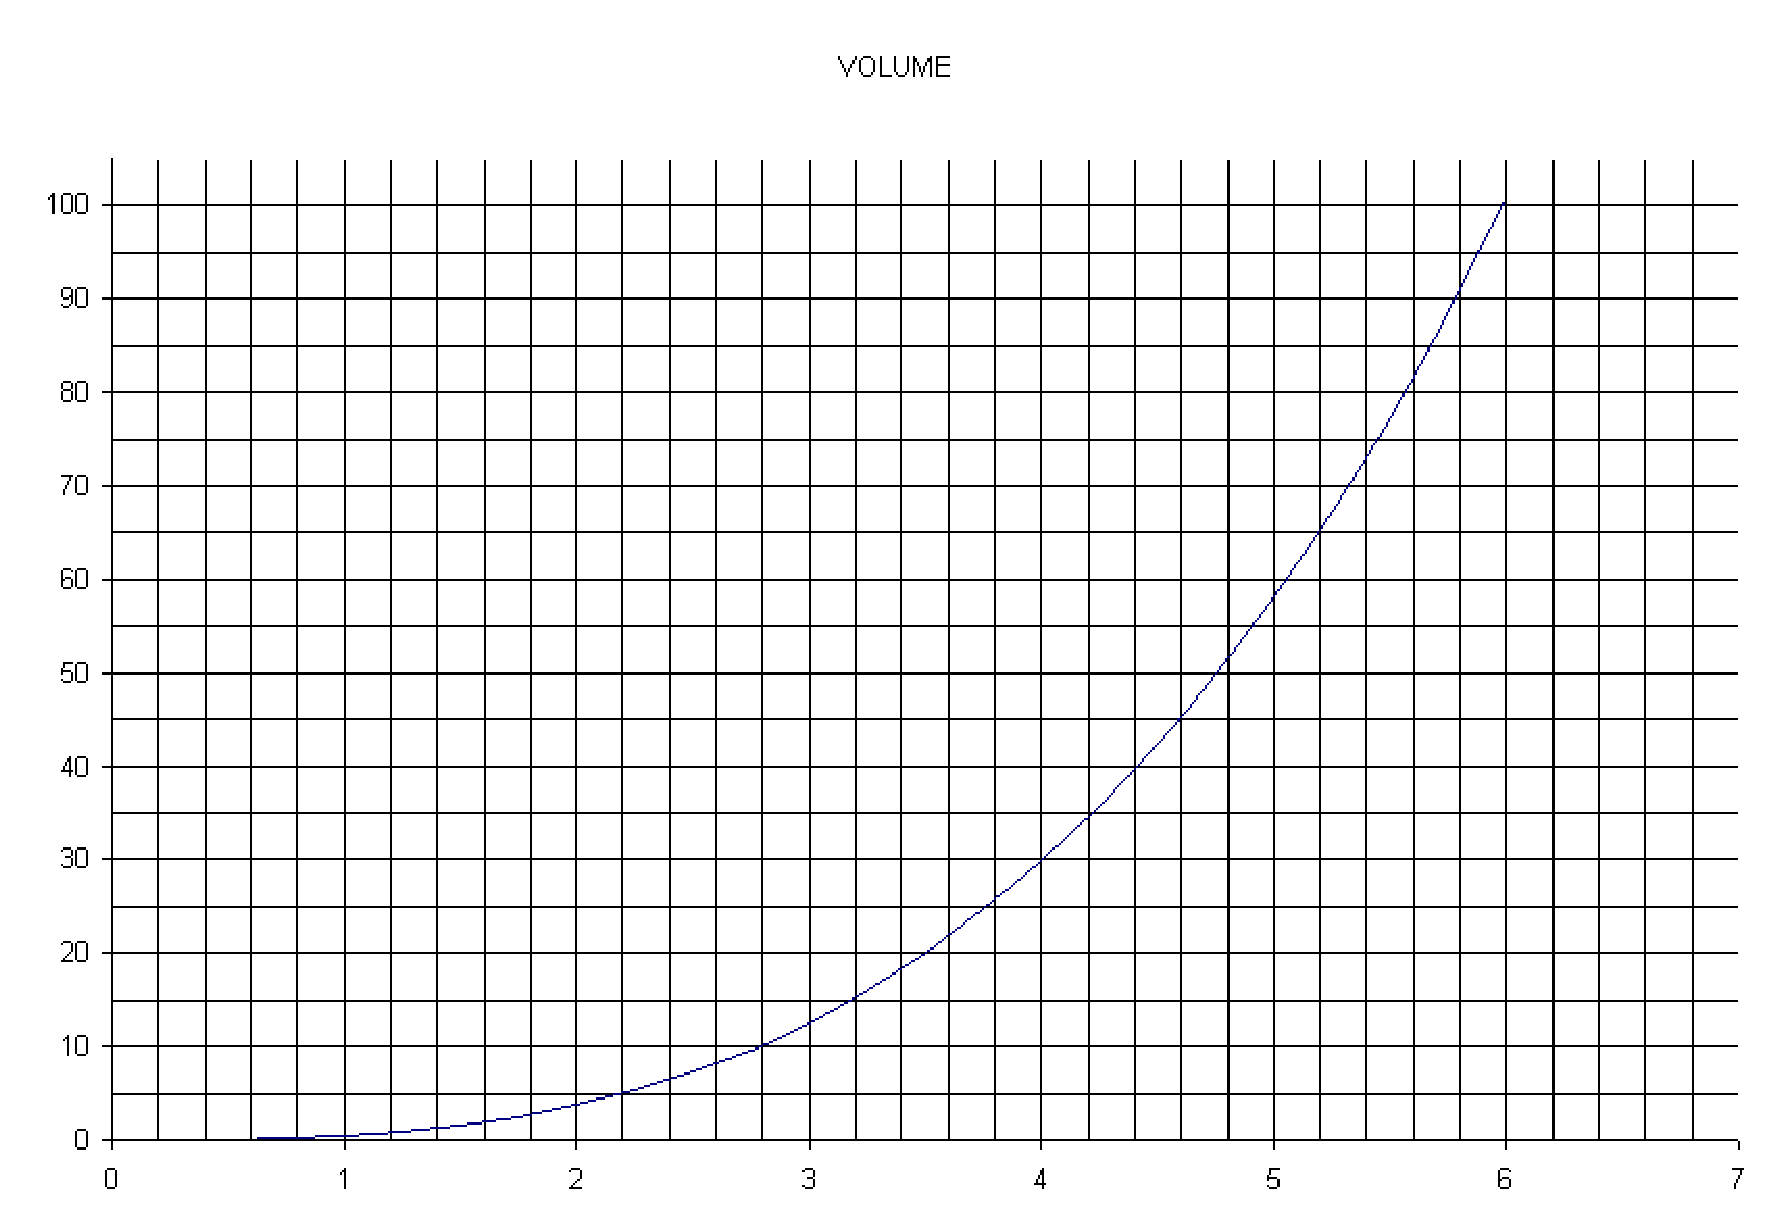
\includegraphics[scale=0.625]{./Graphiques/courbe.eps}\end{center}

%%%%%%%%%%%%%%%%%%%%%%%%%%%%%%%%%%%%%%%%%%%%%%%%%%%%
%%%%%%%%%%%%%%%%%%%%%%%%%%%%%%%%%%%%%%%%%%%%%%%%%%%

%%%%%%%%%%%%%%%%%%%%%%%%%%%%%%%%%%%%%%%%%%%%%%%%%%%\`u
%%%%%%%%%%%%%%%%%%%%%%%%%%%%%%%%%%%%%%%%%%%%%%%%%%%%

 \sautpage

\section{Premi\`eres notions (bilan et compl\'ements)}

\begin{definition}[Notion de fonction]
Une fonction est un proc\'ed\'e qui, \`a un \'el\'ement $x$ d'un ensemble de d\'epart, associe au plus un \'el\'ement $y$ d'un ensemble d'arriv\'ee.

On notera $f:x\mapsto y$ ou $f(x)=y$ qui se lit \og $f$ est la fonction qui \`a $x$ associe $y$ \fg..

On dit que $y$ est \emph{l'image} de $x$.

On dit que $x$ est \emph{un ant\'ec\'edent} de $y$.

\end{definition}

\begin{definition}[Ensemble de d\'efinition]
L'ensemble des r\'eels $x$ poss\'edant une image par une fonction num\'erique $f$ est appel\'e \emph{l'ensemble de d\'efinition de la fonction $f$}. On le note souvent $D_f$.
\end{definition}

\begin{definition}[Repr\'esentation graphique]
Dans un plan muni d'un rep\`ere, la \emph{repr\'esentation graphique} de la fonction $f$ est l'ensemble des points $M$ de coordonn\'ees $(x;y)$ du plan tels que :
\begin{itemize}
	\item L'abscisse $x$ de $M$ d\'ecrit l'ensemble de d\'efinition $D_f$ ;
	\item L'ordonn\'ee $y$ est l'image de $x$ par $f$. $y=f(x)$.
\end{itemize}

On note souvent $\mathcal{C}_f$ la repr\'esentation graphique de $f$. On dit que $\mathcal{C}_f$ a pour \'equation $y=f(x)$.

Si la courbe est d'un seul \og{} tenant \fg{} on parle  de \emph{courbe repr\'esentative} de la fonction $f$.
\end{definition}


\begin{rmq} L'\'equation permet de d\'eterminer si un point $A(x_A;y_A)$ appartient ou pas \`a cette courbe. En effet, un point appartient \`a la courbe si et seulement si ses coordonn\'ees v\'erifient l'\'equation de la courbe. On a alors : \[A\in\mathcal{C}_f\ssi y_A=f(x_A)\] \end{rmq}


Dans la pratique, pour les fonctions num\'eriques d\'efinies par une expression alg\'ebrique, pour esquisser une repr\'esentation graphique, on utilise souvent un tableau de valeurs.

\begin{tabular}{cc}
 \begin{minipage}[l]{0.55\linewidth}
  \begin{rmq} Une courbe ne repr\'esente pas toujours une fonction. Sur la figure ci-contre, par exemple, la courbe a plusieurs points ayant la même abscisse, comme $A(1,-1)$ et $B(1,3)$. Ce n'est donc pas la courbe repr\'esentative d'une fonction car alors 1 aurait plusieurs images.\end{rmq}
 \end{minipage}&
 \begin{minipage}[r]{0.45\linewidth}
\begin{center}
\psset{xunit=0.75cm , yunit=0.75cm}
\def\xmin{-2} \def\xmax{4} \def\ymin{-1.6} \def\ymax{3.6}
\begin{pspicture*}(\xmin,\ymin)(\xmax,\ymax)
\psset{xunit=0.75cm,yunit=0.75cm}
\psgrid[griddots=10,gridlabels=0pt,gridwidth=.3pt, gridcolor=black, subgridwidth=.3pt, subgridcolor=black, subgriddiv=1](0,0)(-2,-2)(4,4)
\psaxes[labels=all,labelsep=1pt, Dx=1,Dy=1]{->}(0,0)(\xmin,\ymin)(\xmax,\ymax)
\uput[dl](0,0){$O$}
%\pcline[linewidth=1pt]{->}(0,0)(1,0) \uput[d](0.5,0){\small $\vec \imath$}
%\pcline[linewidth=1pt]{->}(0,0)(0,1) \uput[l](0,0.5){\small $\vec \jmath$}
\pscircle(1,1){1.5}
\psdots[dotstyle=x](1,-1)(1,3)
\uput[d](1,-1){$A$}
\uput[u](1,3){$B$}
\end{pspicture*}
\end{center}
 \end{minipage}

\end{tabular}






%\sautpage

\subsubsection{Quelques conventions graphiques}
\begin{multicols}{3}
Lorsqu'un point $A$ sur la courbe est connu avec pr\'ecision, il est not\'e par une croix.
\begin{center}
\begin{pspicture*}(-0.5,-1)(2.5,3)
\pscurve(0,0)(0.5,-0.5)(1,1)(2,2.5)
\uput[u](0,0){$\mathcal{C}_f$}
\psdot[dotstyle=x](1,1)
\uput[dr](1,1){$A$}
\end{pspicture*}
\end{center}\sautcol
Lorsqu'un point $A$ est l'extr\'emit\'e de la courbe, il est not\'e par un gros point.
\begin{center}
\begin{pspicture*}(-0.5,-1)(2.5,3)
\pscurve(0,0)(0.5,-0.5)(1,1)(2,2.5)
\uput[u](0,0){$\mathcal{C}_f$}
\psdot(2,2.5)
\uput[dr](2,2.5){$A$}
\end{pspicture*}
\end{center}\sautcol
Lorsqu'un point $A$ \`a l'extr\'emit\'e de la courbe n'appartient pas \`a la courbe, il est not\'e par un \og demi-cercle \fg.
\begin{center}
\begin{pspicture*}(-0.5,-1)(2.5,3)
\pscurve{-(}(0,0)(0.5,-0.5)(1,1)(2,2.5)
\uput[u](0,0){$\mathcal{C}_f$}
%\psdot[(2,2.5)
\uput[dr](2,2.5){$A$}
\end{pspicture*}
\end{center}
\end{multicols}
\begin{multicols}{3}
Une courbe est donn\'ee dans une fenêtre ; s'il n'y a pas d'extr\'emit\'es, la courbe garde la même allure quand on la prolonge.
\begin{center}
\begin{pspicture*}(-0.5,-1)(2.5,3)
\pscurve(-0.3,0)(0.5,2)(1,1)(2,2.8)
\uput[u](1,1){$\mathcal{C}_f$}
\psline[linestyle=dotted](-0.1,0.5)(1.7,0.5)(1.7,2.2)(-0.1,2.2)(-0.1,0.5)
\end{pspicture*}
\end{center}
Une droite verticale en pointill\'es signifie que si l'on prolonge la courbe, elle ne coupe pas cette droite. Sur l'exemple ci-dessous, $a$ n'appartient pas \`a $D_f$.
\begin{center}
\begin{pspicture*}(-0.5,-1)(2.5,3)
\psaxes[labels=none,labelsep=1pt,Dx=5,Dy=5]{->}(0,0)(-0.5,-1)(2.5,3)
\psset{algebraic=true}
\psplot{0.6}{3}{1/(4*x-2)}
\psline[linestyle=dashed](0.5,-1)(0.5,3)
\uput[dl](0.5,0){$a$}
\end{pspicture*}
\end{center}
Une droite horizontale en pointill\'es signifie que si l'on prolonge la courbe, elle ne coupe pas cette droite.
\begin{center}
\begin{pspicture*}(-0.5,-1)(2.5,3)
\psaxes[labels=none,labelsep=1pt,Dx=5,Dy=5]{->}(0,0)(-0.5,-1)(2.5,3)
\psset{algebraic=true}
\psplot{-0.5}{3}{1+1/(x+1)}
\psline[linestyle=dashed](-0.5,1)(2.5,1)
\uput[ul](0,1){$b$}
\end{pspicture*}
\end{center}
\end{multicols}

%\sautpage






\section{R\'esolutions graphiques d'\'equations et d'in\'equations}


\subsection{R\'esolutions d'\'equations de la forme $f(x)=k$}

R\'esoudre l'\'equation $f(x)=k$ c'est d\'eterminer tous les ant\'ec\'edents \'eventuels d'un \'el\'ement $k$ de l'ensemble d'arriv\'ee, c'est-\`a-dire chercher tous les $x$ de l'ensemble de d\'epart tels que $f(x)=k$.

Une telle recherche peut se faire graphiquement \`a partir de la repr\'esentation graphique de la fonction $f$.




\begin{center}
\begin{tabular}{lc}
 \begin{minipage}[l]{0.6\linewidth}
 \begin{exemple*}
  Soit $f$ la fonction d\'efinie sur $\R$ par $f(x)=2x^2-9x+10$. On recherche les solutions de l'\'equation $f(x)=3$.

	On commence par tracer soigneusement la courbe repr\'esentative de $f$ et on obtient la repr\'esentation donn\'ee sur la figure ci-dessous.
		
		On cherche les points de la courbe ayant pour ordonn\'ee 3. Pour cela on peut tracer la droite d'\'equation $y=3$ et chercher les points d'intersection de cette droite avec la courbe de $f$.

		On obtient ici deux points $M_1(1;3)$ et $M_2\left(\frac{7}{2};3\right)$. Les solutions sont leurs abscisses : 1 et $\frac{7}{2}$.

		On \'ecrit : \og Les solutions de l'\'equation $f(x)=3$ sont $x=1$ ou $x=\frac{7}{2}$ car les points de la courbe de $f$ d'ordonn\'ee 3 ont pour abscisses 1 et $\frac{7}{2}$ \fg.
		\end{exemple*}
 \end{minipage}&
 \begin{minipage}[r]{0.35\linewidth}
  
		\begin{center}
 \psset{xunit=1cm,yunit=1cm}
		\begin{pspicture*}(-3.1,-2.1)(4.6,4.1)
\def\xmin{-3} \def\xmax{4.5} \def\ymin{-2} \def\ymax{4}

\psgrid[griddots=10,gridlabels=0pt,gridwidth=.3pt, gridcolor=black, subgridwidth=.3pt, subgridcolor=black, subgriddiv=1](0,0)(-3,-2)(4.5,4)
\psaxes[labels=all,labelsep=1pt, Dx=1,Dy=1]{->}(0,0)(\xmin,\ymin)(\xmax,\ymax)
\uput[dl](0,0){$O$}
\pcline[linewidth=1pt]{->}(0,0)(1,0) \uput[d](0.5,0){\small $\vec \imath$}
\pcline[linewidth=1pt]{->}(0,0)(0,1) \uput[r](0,0.5){\small $\vec \jmath$}
\psset{algebraic=true}
\psplot{\xmin}{\xmax}{2*(x-1)*(x-1)-5*(x-1)+3}
\uput[ul](2,1){$\mathcal{C}_f$}
\psline[linestyle=dashed](\xmin,3)(\xmax,3)
\uput[u](-2,3){$y=3$}
\uput[ur](1,3){$M_1$}
\uput[ul](3.5,3){$M_2$}
\psdots[dotstyle=x](1,3)(3.5,3)
\psline[linestyle=dashed]{->}(1,3)(1,0)
\psline[linestyle=dashed]{->}(3.5,3)(3.5,0)
\end{pspicture*}\end{center}
 \end{minipage}

\end{tabular}             \end{center}



%\sautpage

\subsection{R\'esolutions d'in\'equations de la forme $f(x)\leqslant k$}

Ces in\'equations peuvent se r\'esoudre graphiquement. On proc\`ede de la façon suivante :
\begin{itemize}
	\item on trace soigneusement $\mathcal{C}_f$ dan un rep\`ere (orthogonal) ;
	\item on trace la droite d'\'equation $y=k$ ;
	\item on recherche les points de la courbe situ\'es \emph{sous} la droite ;
	\item l'ensemble des solutions est constitu\'e des abscisses de ces points.
\end{itemize}

\begin{exemple*} Sur l'exemple pr\'ec\'edent, si l'on doit r\'esoudre $f(x)\leqslant 3$, apr\`es avoir trac\'e $y=3$ on constate que les points de la courbe situ\'es sous cette droite ont leurs abscisses comprises entre 0 et $\frac{5}{2}$.

Donc $f(x)\leqslant 3 \ssi x\in\left[0;\frac{5}{2}\right]$.
\end{exemple*}

\begin{rmq}~
\begin{itemize}
	\item On r\'esoud de la même mani\`ere les \'equations du type $f(x)\geqslant k$.

On retient alors les abscisses des points situ\'es \emph{au-dessus} de la droite d'\'equation $y=k$.

Dans l'exemple $f(x)\geqslant 3 \ssi x\in \left] -\infty ; 0 \right] \cup \left[\frac{5}{2} ; +\infty\right[$.
	\item De même pour les in\'equations strictes : $f(x)>k$ ou $f(x)<k$. On excluera alors les abscisses des points d'intersection de la courbe et de la droite.

	Dans l'exemple $f(x)<3 \ssi x\in \left]0;\frac{5}{2}\right[$.
\end{itemize}
\end{rmq}

\subsection{R\'esolutions d'\'equations de la forme $f(x)=g(x)$}

Cela revient \`a chercher les \'el\'ements de l'ensemble de d\'epart qui ont la même image par $f$ et par $g$.

Une telle recherche peut se faire graphiquement. On recherche alors les points des deux courbes repr\'esentatives ayant même abscisse et même ordonn\'ee, c'est-\`a-dire les points d'intersection des deux courbes. 

\begin{tabular}{cc}
 \begin{minipage}[l]{0.6\linewidth}
  \begin{exemple*}

Soit $f$ et $g$ les fonctions d\'efinies sur $\R$ par, respectivement, $f(x)=x^2-1$ et $g(x)=-0,5x^2+x+4$. R\'esoudre graphiquement l'\'equation $f(x)=g(x)$.

	On commence par tracer soigneusement les deux courbes repr\'esentatives et on obtient la repr\'esentation donn\'ee sur la figure ci-contre.
	
	On cherche les points d'intersection des deux courbes, ici $M_1$ et $M_2$, et les solutions de l'\'equation sont leurs abscisses dont les valeurs approximatives sont $-1,5$ et $2,2$.

		Les solutions sont donc $x\approx -1,5$ et $x\approx 2,2$.
\end{exemple*}
 \end{minipage}&
 \begin{minipage}[r]{0.35\linewidth}
  \psset{xunit=0.75cm,yunit=0.75cm}
		\begin{pspicture*}(-3.1,-2.1)(4.6,5.1)
\def\xmin{-3} \def\xmax{4.5} \def\ymin{-2} \def\ymax{5}

\psgrid[griddots=10,gridlabels=0pt,gridwidth=.3pt, gridcolor=black, subgridwidth=.3pt, subgridcolor=black, subgriddiv=1](0,0)(-3,-2)(4.5,5)
\psaxes[labels=all,labelsep=1pt, Dx=1,Dy=1]{->}(0,0)(\xmin,\ymin)(\xmax,\ymax)
\uput[dl](0,0){$O$}
\pcline[linewidth=1pt]{->}(0,0)(1,0) \uput[d](0.5,0){\small $\vec \imath$}
\pcline[linewidth=1pt]{->}(0,0)(0,1) \uput[r](0,0.5){\small $\vec \jmath$}
\psset{algebraic=true}
\psplot{\xmin}{\xmax}{x^2-1}
\psplot{\xmin}{\xmax}{-0.5*x^2+x+4}
\uput[u](1,1){$\mathcal{C}_f$}
\uput[dr](0,4){$\mathcal{C}_g$}
\uput[r](2.189,3.793){$M_2$}
\uput[l](-1.523,1.318){$M_1$}
\psdots[dotstyle=x](2.189,3.793)(-1.523,1.318)
\psline[linestyle=dashed]{->}(-1.523,1.318)(-1.523,0)
\psline[linestyle=dashed]{->}(2.189,3.793)(2.189,0)
\end{pspicture*}
	
 \end{minipage}


\end{tabular}

		

\subsection{R\'esolutions d'in\'equations de la forme $f(x)\leqslant g(x)$}

L\`a encore ces in\'equations peuvent se r\'esoudre graphiquement. On proc\`ede de la façon suivante :
\begin{itemize}
	\item on trace soigneusement $\mathcal{C}_f$ et $\mathcal{C}_g$ dans un rep\`ere (orthogonal) ;
	\item l'ensemble des solutions est constitu\'e des abscisses des points o\`u la courbe de $f$ est situ\'ee \emph{sous} celle de $g$.
\end{itemize}

\begin{exemple*} Sur l'exemple pr\'ec\'edent, si l'on doit r\'esoudre $f(x)\leqslant g(x)$, on constate que les points de la courbe de $f$ situ\'es sous celle de $g$ ont leurs abscisses comprises entre environ $-1,5$ et 2,2.

Donc $f(x)\leqslant g(x) \ssi x\in [-1,5;2,2]$. Ou bien $S=[-1,5;2,2]$.
\end{exemple*}

\begin{rmqs}~
\begin{itemize}
	\item On r\'esoud de la même mani\`ere les \'equations du type $f(x)\geqslant g(x)$.

On retient alors les abscisses des points de la courbe de $f$ situ\'es \emph{au-dessus} de celle de $g$.

Dans l'exemple $f(x)\geqslant g(x) \ssi x\in ] -\infty ; -1,5 ] \cup [2,2 ; +\infty[$.
	\item De même pour les in\'equations strictes : $f(x)>g(x)$ ou $f(x)<g(x)$. On excluera alors les abscisses des points d'intersection des deux courbes.

	Dans l'exemple $f(x)<g(x) \ssi x\in ]-1,5;2,2[$.
\end{itemize}
\end{rmqs}



%\sautpage



\sautpage

\section{Variations, extremums}


\subsection{Sens de variation}

Il s'agit de traduire math\'ematiquement qu'une fonction \og augmente \fg{} ou \og diminue \fg.

\begin{exemple*} Soit, par exemple, la fonction d\'efinie sur $[-3;3]$ par la courbe repr\'esentative donn\'ee sur la figure \ref{croissanceetdecroissance} \vpageref{croissanceetdecroissance}. On constate que lorsque $x\in[-3;1]$ , si $x$ augmente, $f(x)$ augmente aussi alors que lorsque $x\in[1;3]$, si $x$ augmente, $f(x)$ diminue.

C'est la d\'efinition math\'ematique de la croissance ou de la d\'ecroissance d'une fonction $f$.

\begin{figure}[h]
\centering
\caption{Croissance et d\'ecroissante}\label{croissanceetdecroissance}


\psset{xunit=1cm , yunit=1.25cm}
\begin{pspicture*}(-4.1,-1.1)(4.1,5.1)
\def\xmin{-4} \def\xmax{4} \def\ymin{-1} \def\ymax{5}
\psgrid[griddots=10,gridlabels=0pt,gridwidth=.3pt, gridcolor=black, subgridwidth=.3pt, subgridcolor=black, subgriddiv=1](0,0)(-4,-1)(4,5)
\psaxes[labels=all,labelsep=1pt, Dx=1,Dy=1]{-}(0,0)(\xmin,\ymin)(\xmax,\ymax)
\uput[dl](0,0){$O$}
\pcline[linewidth=1pt]{->}(0,0)(1,0) \uput[d](0.5,0){\small $\vec \imath$}
\pcline[linewidth=1pt]{->}(0,0)(0,1) \uput[r](0,0.5){\small $\vec \jmath$}
\psset{algebraic=true}
\psplot{-3}{3}{(-(x-1)^2+5)*0.25+3}
\psdots(3,3.25)(-3,0.25)
\uput[d](-1.5,0){$b$}
\psline[linestyle=dashed]{->}(-1.5,0)(-1.5,2.6875)
\psline[linestyle=dashed]{->}(-1.5,2.6875)(0,2.6875)
\uput[r](0,2.6875){$f(b)$}
\uput[d](-2.5,0){$a$}
\psline[linestyle=dashed]{->}(-2.5,0)(-2.5,1.1875)
\psline[linestyle=dashed]{->}(-2.5,1.1875)(0,1.1875)
\uput[r](0,1.1875){$f(a)$}
\uput[d](1.5,0){$u$}
\uput[d](2.5,0){$v$}
\psline[linestyle=dashed]{->}(1.5,0)(1.5,4.1875)
\psline[linestyle=dashed]{->}(1.5,4.1875)(0,4.1875)
\uput[l](0,4.1875){$f(u)$}
\psline[linestyle=dashed]{->}(2.5,0)(2.5,3.6875)
\psline[linestyle=dashed]{->}(2.5,3.6875)(0,3.6875)
\uput[l](0,3.6875){$f(v)$}
\end{pspicture*}
\end{figure}\end{exemple*}


\begin{definition}
Soit $f$ une fonction d\'efinie sur un intervalle $I$. On dit que $f$ est
\begin{itemize}
	\item \emph{croissante} sur $I$ si, pour tous r\'eels $a$ et $b$ de $I$, on a :\\
$\text{Si } a<b \text{ alors } f(a)\leqslant f(b).$
	\item \emph{d\'ecroissante} sur $I$ si, pour tous r\'eels $a$ et $b$ de $I$, on a :\\
$\text{Si } a<b \text{ alors } f(a)\geqslant f(b).$
	\item \emph{monotone} si elle n'est que croissante sur $I$ ou si elle n'est que d\'ecroissante sur $I$.
	\item \emph{constante} sur $I$ si, pour tous r\'eels $a$ et $b$ de $I$, on a : $f(a)=f(b)$.
\end{itemize}
\end{definition}


\begin{rmqs}~
\begin{itemize}
	\item Ces notions ne sont valables que sur \textbf{un intervalle} et pas sur une r\'eunion d'intervalles disjoints.
	\item Ant\'ec\'edents et images \'etant rang\'es dans le même ordre, on dit qu'une fonction croissante \emph{conserve} l'ordre.
	\item Ant\'ec\'edents et images \'etant rang\'es dans l'ordre inverse, on dit qu'une fonction d\'ecroissante \emph{inverse} l'ordre.
	\item On obtient les d\'efinitions d'une fonction \emph{strictement} croissante ou \emph{strictement} d\'ecroisante en remplaçant les in\'egalit\'es par des in\'egalit\'es strictes. Ainsi on dit que $f$ est strictement croissante sur $I$ si pour tous r\'eels $a$ et $b$ de $I$ on a : \\ $\text{Si } a<b \text{ alors } f(a)<f(b)$
	\item Une fonction est strictement monotone sur $I$ si elle est strictement croissante ou strictement d\'ecroissante sur $I$
\end{itemize}
\end{rmqs}

\subsection{Tableau de variations}

Ces r\'esultats peuvent se r\'esumer dans un tableau de variation, qui est une forme stylis\'ee de repr\'esentation o\`u l'on indique uniquement si la courbe monte, descend ou est stable. Dans la premi\`ere ligne on indique les valeurs importantes de $x$ et dans la seconde les variations de $f$.

\begin{exemple*} Dans l'exemple pr\'ec\'edent on obtient
$$\tabvar{%
\tx{x}&\tx{-3}&&\tx{1}&&\tx{3}\cr
\tx{f}&\txb{\approx 0,25}&\fm&\txh{\approx 4,25}&\fd&\txb{\approx 2,25}\cr
}$$
\end{exemple*}



\subsection{Extremums}

Les extremums, s'ils existent, sont les valeurs maximale et minimale qui sont \textbf{atteintes} par la fonction $f$ sur un intervalle donn\'e. Plus pr\'ecis\'ement :

\begin{definition}
Soit une fonction $f$ d\'efinie sur un intervalle $I$ et $x_0\in I$. On dit que
\begin{itemize}
	\item $f$ admet un \emph{maximum}, atteint en $x_0$ si, pour tout $x\in I$, $f(x)\leqslant f(x_0)$. Ce maximum est alors $f(x_0)$.
	\item $f$ admet un \emph{minimum}, atteint en $x_0$ si, pour tout $x\in I$, $f(x)\geqslant f(x_0)$. Ce minimum est alors $f(x_0)$.
\end{itemize}
Les maximum et minimum sont appel\'es les \emph{extremums}.
\end{definition}

%\begin{rmq} Un extremum doit être atteint par une valeur $x_0$. \end{rmq}

\begin{exemple*}
La fonction $f$ d\'efinie sur $\R$ par $f(x)=x^2+1$ n'admet pas $-1$ comme minimum.

En effet, si on a bien $f(x)\geqslant -1$ sur $\R$, il n'existe pas de $x_0$ tel que $f(x_0)=-1$.

Par contre 1 est bien le minimum de $f$ sur $\R$ car
\begin{itemize}
	\item $f(x)\geqslant 1$ pour tout $x\in\R$ \textbf{ET}
	\item $f(0)=1$
\end{itemize}

On dira donc : le minimum de $f$ sur $\R$ est 1 et il est atteint pour $x_0=0$.
\end{exemple*}

\sautpage

\section{Exercices et probl\`emes}

\subsection{Premi\`eres notions}

%\begin{multicols}{2}
%\begin{exo} Dire dans chacun des exemples ci-dessous quel est l'ensemble de d\'efinition, quelles sont les images possibles et si la fonction est num\'erique.
%\begin{enumerate}
%	\item \`A chaque \'el\`eve de la classe on associe la couleur de ses cheveux.
%	\item \`A chaque \'el\`eve de la classe on associe le nombre de ses fr\`eres et soeurs.
%	\item Pour un \'el\`eve donn\'e, \`a chaque moment de sa vie on associe la taille qu'il mesurait.
%	\item Soit $ABCD$ un rectangle dont un des côt\'es est fixe et mesure 6 cm et l'autre est variable et mesure $x$ cm. \\On d\'efinit la fonction $f$ de la façon suivante : \`a chaque $x$ possible, on associe $f(x)$, l'aire du rectangle $ABCD$.
%	\item La fonction $g$ d\'efinie par $g(x)=x^2+2x+3$.
%	\item La fonction $h$ d\'efinie par $h(x)=\frac{x^2+1}{x-1}$.
%	\item La fonction $i$ d\'efinie par $i(x)=\sqrt{x+2}$.
%\end{enumerate}
%\end{exo}
\begin{multicols}{2}
\begin{exo}
On d\'efinit $f$ et $g$, deux fonctions :
\begin{itemize}
	\item $f$ est la fonction qui \`a un nombre r\'eel $x$ associe le nombre obtenu en proc\'edant de la mani\`ere suivante : on ajoute $4$ au nombre, on \'el\`eve le r\'esultat obtenu au carr\'e, on retranche 16, on divise par le nombre de d\'epart et on retranche 6.
	\item $g:x\mapsto x^2-4$.
\end{itemize}
\begin{enumerate}
	\item Donner l'expression correspondant \`a $f$ puis simplifier cette expression.
	\item Quel r\'eel n'a pas d'image par $f$ ?
	\item Quelle est l'image de 3 par $g$ ?
	\item Quelle est l'image de $-1$ par $g$ ?
	\item Quels sont les ant\'ec\'edents \'eventuels de 12 par $g$ ?
	\item Quels sont les ant\'ec\'edents \'eventuels de $-5$ par $g$ ?
\end{enumerate}
\end{exo}

\sautcol

\begin{exo}
Vrai ou faux ? \emph{Corriger la phrase lorsqu'elle est fausse}.
\begin{enumerate}
	\item $f(-2) = 0$ signifie que l'image de 0 est $-2$
	\item $f(0) = 3$ signifie que la courbe de $f$ passe par le point $(0 ; 3)$
	\item $f(1) = 2$ signifie que l'ant\'ec\'edent de 1 est 2
	\item L'image de 2 par $f$ est $-3$ s'\'ecrit $f(2) = -3$
	\item Dire que $(5 ; 1)$ est un point de la courbe de $f$ s'\'ecrit $5 = f(1)$
	\item Par la fonction $g$, $-5$ est l'image de 3 s'\'ecrit $g(-5) = 3$
	\item 2 a pour image 0 par $f$ signifie que la courbe de $f$ traverse l'axe des abscisses en 2
	\item $f(4) = 0$ signifie que la courbe de $f$ traverse l'axe des abscisses au point $(4 ; 0)$
	\item 3 a pour image 5, signifie que 3 est l'image de 5
	\item 4 a pour ant\'ec\'edent 5 signifie que 5 est l'image de 4
\end{enumerate}
\end{exo}

\end{multicols}

%\sautpage

\begin{exo}\label{gf4courbes}
Vrai ou faux ? \emph{Justifier la r\'eponse lorsque c'est faux}.\\
Les courbes de la figure \ref{gf4courbesfig} \vpageref{gf4courbesfig} repr\'esentent des fonctions de la variable $x$.


\begin{figure}[!h]
 \centering
 \caption{Courbes de l'exercice \ref{gf4courbes}}\label{gf4courbesfig}
\begin{tabular}{cc}
\psset{xunit=1cm , yunit=0.5cm}
\begin{pspicture*}(-2.1,-2.1)(4.1,4.1)
\def\xmin{-2} \def\xmax{4} \def\ymin{-2} \def\ymax{4}
\psgrid[griddots=10,gridlabels=0pt,gridwidth=.3pt, gridcolor=black, subgridwidth=.3pt, subgridcolor=black, subgriddiv=1](0,0)(-2,-2)(4,4)
\psaxes[labels=all,labelsep=1pt, Dx=1,Dy=1]{->}(0,0)(\xmin,\ymin)(\xmax,\ymax)
\uput[dl](0,0){$O$}
\pcline[linewidth=1pt]{->}(0,0)(1,0) \uput[d](0.5,0){\small $\vec \imath$}
\pcline[linewidth=1pt]{->}(0,0)(0,1) \uput[l](0,0.5){\small $\vec \jmath$}
\psline(-2,3)(1,-1.5)(2,-1.5)(4,2)
\end{pspicture*}
&
\psset{xunit=1cm , yunit=0.5cm}
\begin{pspicture*}(-2.1,-2.1)(4.1,4.1)
\def\xmin{-2} \def\xmax{4} \def\ymin{-2} \def\ymax{4}
\psgrid[griddots=10,gridlabels=0pt,gridwidth=.3pt, gridcolor=black, subgridwidth=.3pt, subgridcolor=black, subgriddiv=1](0,0)(-2,-2)(4,4)
\psaxes[labels=all,labelsep=1pt, Dx=1,Dy=1]{->}(0,0)(\xmin,\ymin)(\xmax,\ymax)
\uput[dl](0,0){$O$}
\pcline[linewidth=1pt]{->}(0,0)(1,0) \uput[d](0.5,0){\small $\vec \imath$}
\pcline[linewidth=1pt]{->}(0,0)(0,1) \uput[l](0,0.5){\small $\vec \jmath$}
\psline(-2,3)(1,3)(1,1)(4,1)
\end{pspicture*}
\\
\psset{xunit=1cm , yunit=0.5cm}
\begin{pspicture*}(-2.1,-2.1)(4.1,4.1)
\def\xmin{-2} \def\xmax{4} \def\ymin{-2} \def\ymax{4}
\psgrid[griddots=10,gridlabels=0pt,gridwidth=.3pt, gridcolor=black, subgridwidth=.3pt, subgridcolor=black, subgriddiv=1](0,0)(-2,-2)(4,4)
\psaxes[labels=all,labelsep=1pt, Dx=1,Dy=1]{->}(0,0)(\xmin,\ymin)(\xmax,\ymax)
\uput[dl](0,0){$O$}
\pcline[linewidth=1pt]{->}(0,0)(1,0) \uput[d](0.5,0){\small $\vec \imath$}
\pcline[linewidth=1pt]{->}(0,0)(0,1) \uput[l](0,0.5){\small $\vec \jmath$}
\psline(-2,3)(4,3)
\end{pspicture*}
&
\psset{xunit=1cm , yunit=0.5cm}
\begin{pspicture*}(-2.1,-2.1)(4.1,4.1)
\def\xmin{-2} \def\xmax{4} \def\ymin{-2} \def\ymax{4}
\psgrid[griddots=10,gridlabels=0pt,gridwidth=.3pt, gridcolor=black, subgridwidth=.3pt, subgridcolor=black, subgriddiv=1](0,0)(-2,-2)(4,4)
\psaxes[labels=all,labelsep=1pt, Dx=1,Dy=1]{->}(0,0)(\xmin,\ymin)(\xmax,\ymax)
\uput[dl](0,0){$O$}
\pcline[linewidth=1pt]{->}(0,0)(1,0) \uput[d](0.5,0){\small $\vec \imath$}
\pcline[linewidth=1pt]{->}(0,0)(0,1) \uput[l](0,0.5){\small $\vec \jmath$}
\pscurve(-2,3)(-1,0)(0,-1)(2,1)(3.2,2)(3,3)
\end{pspicture*}
\end{tabular}
\end{figure}

\end{exo}

\sautpage

\begin{exo}\label{gf14}
Vrai ou faux ? \emph{Corriger la phrase lorsqu'elle est fausse}.\\
Les fonctions $f$ et $g$ sont repr\'esent\'ees sur la figure \ref{gf14fig} \vpageref{gf14fig}.
\begin{enumerate}
	\item La fonction $f$ est d\'efinie entre $-2$ et 6 inclus
	\item Les images par la fonction $f$ sont comprises entre $-1$ et 4 inclus
	\item La fonction $g$ est d\'efinie entre $-2$ exclu et 6 inclus
	\item Les images par la fonction g sont comprises entre 0 exclu et 3 inclus
\end{enumerate}



\begin{figure}[!h]
\centering
\caption{Courbes de l'exercice \ref{gf14}}\label{gf14fig}
\begin{tabular}{cc}
\psset{xunit=0.9cm , yunit=0.5cm}
\begin{pspicture*}(-3.1,-2.1)(6.1,5.1)
\def\xmin{-3} \def\xmax{6} \def\ymin{-2} \def\ymax{5}
\psgrid[griddots=10,gridlabels=0pt,gridwidth=.3pt, gridcolor=black, subgridwidth=.3pt, subgridcolor=black, subgriddiv=1](0,0)(-3,-2)(6,5)
\psaxes[labels=all,labelsep=1pt, Dx=1,Dy=1]{->}(0,0)(\xmin,\ymin)(\xmax,\ymax)
\uput[dl](0,0){$O$}
\pcline[linewidth=1pt]{->}(0,0)(1,0) \uput[d](0.5,0){\small $\vec \imath$}
\pcline[linewidth=1pt]{->}(0,0)(0,1) \uput[l](0,0.5){\small $\vec \jmath$}
\pscurve{*-(}(-2,2)(-1,3)(0,3.7)(0.5,3.9)(1,4)(2,3)(3,0)(4,-1)(5,0)(6,1)

\rput(3,2){$\mathcal{C}_f$}
\end{pspicture*}
&
\psset{xunit=0.9cm , yunit=0.5cm}
\begin{pspicture*}(-3.1,-2.1)(6.1,5.1)
\def\xmin{-3} \def\xmax{6} \def\ymin{-2} \def\ymax{5}
\psgrid[griddots=10,gridlabels=0pt,gridwidth=.3pt, gridcolor=black, subgridwidth=.3pt, subgridcolor=black, subgriddiv=1](0,0)(-3,-2)(6,5)
\psaxes[labels=all,labelsep=1pt, Dx=1,Dy=1]{->}(0,0)(\xmin,\ymin)(\xmax,\ymax)
\uput[dl](0,0){$O$}
\pcline[linewidth=1pt]{->}(0,0)(1,0) \uput[d](0.5,0){\small $\vec \imath$}
\pcline[linewidth=1pt]{->}(0,0)(0,1) \uput[l](0,0.5){\small $\vec \jmath$}
\pscurve{)-}(-2,0)(0,1)(1,2)(1.5,3.5)(1.8,5)
\pscurve{-*}(2.2,-2)(3,0)(4,1.5)(6,3)
\rput(1,3){$\mathcal{C}_g$}
\psline[linestyle=dashed](2,\ymin)(2,\ymax)
\end{pspicture*}
\end{tabular}
\end{figure}

\end{exo}

\begin{exo}\label{gf15}
Vrai ou faux ? \emph{Corriger la proposition lorsqu'elle est fausse}.
\begin{itemize}
	\item D'apr\`es la repr\'esentation graphique de la figure \ref{gf15fig} \vpageref{gf15fig} $D_f=[-4;2]$
	\item D'apr\`es la repr\'esentation graphique de la figure \ref{gf15fig} \vpageref{gf15fig} $D_g=]-\infty;3[\cup]3;5]$
\end{itemize}


\begin{figure}[!h]
\centering
\caption{Courbes de l'exercice \ref{gf15}}\label{gf15fig}
\begin{tabular}{cc}
\psset{xunit=1cm , yunit=0.66cm}
\begin{pspicture*}(-4.1,-2.1)(4.1,4.1)
\def\xmin{-4} \def\xmax{4} \def\ymin{-2} \def\ymax{4}
\psgrid[griddots=10,gridlabels=0pt,gridwidth=.3pt, gridcolor=black, subgridwidth=.3pt, subgridcolor=black, subgriddiv=1](0,0)(-4,-2)(4,4)
\psaxes[labels=all,labelsep=1pt, Dx=1,Dy=1]{->}(0,0)(\xmin,\ymin)(\xmax,\ymax)
\uput[dl](0,0){$O$}
\pcline[linewidth=1pt]{->}(0,0)(1,0) \uput[d](0.5,0){\small $\vec \imath$}
\pcline[linewidth=1pt]{->}(0,0)(0,1) \uput[l](0,0.5){\small $\vec \jmath$}
\pscurve{*-}(-4,0)(-3,-2)(0,0)(1,1)(4,1.8)
\psline[linestyle=dashed](0,2)(4,2)
\rput(-1.5,-1){$\mathcal{C}_f$}
\end{pspicture*}
&
\psset{xunit=1cm , yunit=0.66cm}
\begin{pspicture*}(-3.1,-2.1)(5.6,4.1)
\def\xmin{-3} \def\xmax{5.5} \def\ymin{-2} \def\ymax{4}
\psgrid[griddots=10,gridlabels=0pt,gridwidth=.3pt, gridcolor=black, subgridwidth=.3pt, subgridcolor=black, subgriddiv=1](0,0)(-3,-2)(5.5,4)
\psaxes[labels=all,labelsep=1pt, Dx=1,Dy=1]{->}(0,0)(\xmin,\ymin)(\xmax,\ymax)
\uput[dl](0,0){$O$}
\pcline[linewidth=1pt]{->}(0,0)(1,0) \uput[d](0.5,0){\small $\vec \imath$}
\pcline[linewidth=1pt]{->}(0,0)(0,1) \uput[l](0,0.5){\small $\vec \jmath$}
\pscurve(-3,3)(0,1.5)(1,1)(2,0)(2.8,-2)
\pscurve{-*}(3.2,-2)(4,1)(5,3)
\psline[linestyle=dashed](3,\ymin)(3,\ymax)
\uput[ur](1,1){$\mathcal{C}_g$}
\end{pspicture*}
\end{tabular}
\end{figure}
\end{exo}
%\sautpage


\begin{exo}[Avec la calculatrice]
La fonction $f$ est d\'efinie sur $[-1,5;2]$ par : $f(x)=2x^3-1,5x^2-3x$
\begin{enumerate}
	\item Compl\'eter le tableau de valeurs suivant :
	%\vspace{-1em}
	\begin{center}
\begin{tabular}{|*{9}{c|}}
\hline $x$ & $-1,5$ & $-1$ & $-0,5$ & 0 & 0,5 & 1 & 1,5 & 2 \\ \hline
$f(x)$ & & & & & & & & \\ \hline
\end{tabular}
\end{center}
\item Tracer la courbe repr\'esentative de $f$.
\end{enumerate}
\end{exo}

\begin{exo}[Avec la calculatrice]\label{uneautrecourbe}
La fonction $f$ est d\'efinie sur $[-3;3]$ par : $f(x)=x^2-3x+1$.\\
Apr\`es avoir dress\'e un tableau de valeurs de la fonction, tracer sa courbe repr\'esentative $\mathcal{C}_f$.

\end{exo}

%\end{multicols}



\sautpage

\subsection{R\'esolutions graphiques}

\begin{exo}
La fonction $f$ est d\'efinie sur $[-3;3]$ par : $f(x)=x^2-3x+1$.\\
$\mathcal{C}_f$, courbe repr\'esentative de $f$ a d\'ej\`a \'et\'e obtenue dans l'exercice \ref{uneautrecourbe}.
\begin{enumerate}
	\item \`A l'aide de la repr\'esentation graphique $\mathcal{C}_f$, avec la pr\'ecision permise par le graphique, r\'epondre aux question suivantes :
		\vspace{-1em}\begin{multicols}{2}
		  \begin{enumerate}
			\item Quelle est l'image de 2 ?
			\item Quelle est l'image de 3 ?
			\item Quelle est l'image de 4 ?
			\item Quels sont les ant\'ec\'edents de 1 ?
			\item Quels sont les ant\'ec\'edents de 2 ?
			\item Quels sont les ant\'ec\'edents de $-2$ ?
		\end{enumerate}
		\end{multicols}\vspace{-1em}
	\item R\'esoudre graphiquement les \'equations et in\'equations suivantes :
\vspace{-1em}\begin{multicols}{3}\begin{enumerate}
	\item $f(x)=3$ ;
	\item $f(x)=-1,5$ ;
	\item $f(x)\geqslant -1$ ;
	\item $f(x)<4$ ;
	\item $f(x)>-3$ ;
	\item $f(x)<-2$.
\end{enumerate}\end{multicols}\vspace{-1em}
\item D\'eterminer graphiquement le signe de $f(x)$ selon les valeurs de $x$.
\end{enumerate}
\end{exo}

%\sautpage

\begin{exo}
Une fonction $f$, d\'efinie sur $\R$, est donn\'ee par sa courbe repr\'esentative $\mathcal{C}$ :
\begin{multicols}{2}
\begin{center}\small
\psset{xunit=1,yunit=1}
\begin{pspicture*}(-2.6,-2.1)(5.1,3.1)
\def\xmin{-2.5} \def\xmax{5} \def\ymin{-2} \def\ymax{3}
\psset{xunit=0.1cm,yunit=0.1cm}
\psgrid[griddots=15,gridlabels=0pt,gridwidth=.3pt, gridcolor=gray, subgridwidth=.3pt, subgridcolor=gray, subgriddiv=1](0,0)(-25,-20)(50,30)
\psset{xunit=1cm , yunit=1cm}
\psaxes[labels=all,labelsep=1pt, Dx=1,Dy=1]{->}(0,0)(\xmin,\ymin)(\xmax,\ymax)
\uput[dl](0,0){$0$}
\pcline[linewidth=1pt]{->}(0,0)(1,0) \uput[d](0.5,0){\small $\vec i$}
\pcline[linewidth=1pt]{->}(0,0)(0,1) \uput[l](0,0.5){\small $\vec j$}
\pscurve(-2.3,-2)(-2,-1)(-1.5,1.5)(-1,3)(-0.5,2.5)(0,1)(0.2,0)(0.5,-1)(1,-1.5)(1.5,-1)(2,0)(2.5,1)(3,1.5)(4,2)(5,2.3)
\psline[linestyle=dashed](0,2.5)(\xmax,2.5)
\psdots[dotstyle=x](-2,-1)(-1.5,1.5)(-1,3)(-0.5,2.5)(0,1)(0.5,-1)(1,-1.5)(1.5,-1)(2,0)(2.5,1)(3,1.5)(4,2)
\end{pspicture*}
\end{center}\normalsize

\sautcol

Avec la pr\'ecision permise par le graphique, r\'esoudre :
%\vspace{-1em}
%\begin{multicols}{2}
\begin{enumerate}
	\item Les \'equations suivantes :
		\vspace{-1em}
		\begin{multicols}{2}\begin{enumerate}
			\item $f(x) = 1$ ;
			\item $f(x) = 0$ ;
			\item $f(x) = -1$ ;
			\item $f(x) = 2$.
		\end{enumerate}\end{multicols}
		%\vspace{-1em}
%\sautcol
	\item Les in\'equations suivantes :
		\vspace{-1em}
		\begin{multicols}{2}\begin{enumerate}
			\item $f(x)\geqslant 1$ ;
			\item $f(x)\geqslant 0$ ;
			\item $f(x)<-1$ ;
			\item $f(x)>2$.
		\end{enumerate}\end{multicols}
		\vspace{-1em}
	\item D\'eterminer graphiquement le signe de $f(x)$ selon les valeurs de $x$.

\end{enumerate}\end{multicols}
%\vspace{-1em}
\end{exo}

\medskip

\begin{multicols}{2}

\begin{exo}\label{gfunecourbe}
La courbe $\mathcal{C}$ de la figure ci-dessous %\ref{gfunecourbefig} \vpageref{gfunecourbefig} 
repr\'esente une fonction $f$ et le segment de droite $\mathcal{D}$ repr\'esente une fonction $g$.

%\begin{figure}[hbtp]
% \centering
% \caption{Figure de l'exercice \ref{gfunecourbe}}\label{gfunecourbefig}


\begin{center}
\psset{xunit=0.375cm , yunit=0.33cm}
\def\xmin{-9} \def\xmax{12} \def\ymin{-3} \def\ymax{11}
\begin{pspicture*}(\xmin,\ymin)(\xmax,\ymax)
\psgrid[griddots=10,gridlabels=0pt,gridwidth=.3pt, gridcolor=black, subgridwidth=.3pt, subgridcolor=black, subgriddiv=1](0,0)(\xmin,\ymin)(\xmax,\ymax)
\psaxes[labels=all,labelsep=1pt, Dx=5,Dy=5]{-}(0,0)(\xmin,\ymin)(\xmax,\ymax)
\uput[dl](0,0){$O$}
\pcline[linewidth=1pt]{->}(0,0)(1,0) \uput[d](0.5,0){\small $\vec \imath$}
\pcline[linewidth=1pt]{->}(0,0)(0,1) \uput[l](0,0.5){\small $\vec \jmath$}
\pscurve{*-*}(-8,1)(-5,3)(-3,5)(-1,6)(0,5)(1,3)(2,0)(4,-2)(7,0)(9,3)(11,6)
\psdots[dotstyle=x](-5,3)(-3,5)(-1,6)(0,5)(1,3)(2,0)(4,-2)(7,0)(9,3)
\psdots[dotstyle=*](-8,7.5)(11,-2)
\uput[dr](10,5){$\mathcal{C}$}
\uput[ur](-6,7){$\mathcal{D}$}
\psplot[linestyle=dashed,algebraic=true]{-8}{11}{-0.5*x+3.5}
\end{pspicture*}\end{center}

%\end{figure}

\sautcol

\begin{enumerate}
	\item R\'esoudre graphiquement les \'equations :
		\vspace{-1em}\begin{multicols}{2}\begin{enumerate}
			\item $f(x) = 3$ ;
			\item $f(x) = -2$ ;
			\item $f(x) = 0$ ;
			\item $f(x) = 6$.
		\end{enumerate}\end{multicols}
	\item R\'esoudre graphiquement les in\'equations :
		\begin{enumerate}
			\item $f(x)\leqslant 0$ ;
			\item $f(x) \geqslant 3$ ;
			\item $f(x)>5$.
		\end{enumerate}

	\item R\'esoudre graphiquement :
			\begin{enumerate}
				\item $f(x) = g(x)$ ;
				\item $f(x) < g(x)$.			\end{enumerate}
		\item Donner le signe de $f(x)$ suivant les valeurs de $x$.
\end{enumerate}
\end{exo}\end{multicols}

%\sautpage

\begin{multicols}{2}

\begin{exo}[Avec la calculatrice]
On consid\`ere les fonctions $f$ et $g$ d\'efinies sur $\R$ par : $f(x)=x^3$ et $g(x)=3x-2$.
 \begin{enumerate}
			\item Tracer soigneusement les repr\'esentations graphiques $\mathcal{C}_f$ et $\mathcal{C}_g$ de $f$ et $g$ sur l'intervalle $[-2;2]$.
			\item R\'esoudre graphiquement l'in\'equation $f(x)\leqslant 1$.
			\item D\'eterminer graphiquement les solutions de l'\'equation $f(x)=g(x)$.
 \end{enumerate}
\end{exo}

\sautcol

\begin{exo}[Avec la calculatrice]
Les fonctions $f$ et $g$ sont d\'efinies sur $[-2;2]$ par : $f(x)=x^3$ et $g(x)=1-x$.
\begin{enumerate}
	\item Tracer sur une calculatrice graphique les repr\'esentations graphiques $\mathcal{C}_f$ et $\mathcal{C}_g$ de $f$ et de $g$.
	\item En d\'eduire le nombre de solutions de l'\'equation $x^3+x-1=0$.
	\end{enumerate}
\end{exo}

\end{multicols}

\subsection{R\'esolutions calculatoires}
%\section{Technologie}
\begin{multicols}{2}
\begin{exo}
Soit la fonction $f$ d\'efinie sur $\R$ par : \\$f(x)=2x^2+x+3$.
\begin{enumerate}
	\item Calculer les valeurs exactes de $f(x)$ pour les valeurs de $x$ suivantes :
	  \vspace{-1em}\begin{multicols}{3}
	  \begin{itemize}
	    \item 0 ;
	    \item 1 ;
	    \item $-2$ ;
	    \item $\sqrt{2}$ ;
	    \item $1+\sqrt{3}$ ;
	    \item $2-\sqrt{5}$.
	   \end{itemize}
	  \end{multicols}\vspace{-1em}
	\item R\'esoudre $f(x)=3$.
\end{enumerate}
\end{exo}

\begin{exo}
Soit $f$ la fonction d\'efinie sur $\R$ par :\\ $f(x)=2x^2-5x+3$. \\R\'esoudre $f(x)=3$.
\end{exo}

\begin{exo} Soit $f$ la fonction d\'efinie sur $\R$ par : $f(x)=4x^2-4x+1$. On cherche \`a r\'esoudre, par le calcul, l'\'equation $f(x)=9$.
%\vspace{-1em}\begin{multicols}{2}
\begin{enumerate}
	\item Factoriser $f(x)$.
	\item R\'esoudre $f(x)=9$.
\end{enumerate}% \end{multicols}\vspace{-1em}
\end{exo}



\begin{exo}
	Soit $f$ et $g$ les fonctions d\'efinies sur $\R$ par, respectivement, $f(x)=x^2-1$ et $g(x)=-x^2+2$. \\ R\'esoudre par le calcul l'\'equation $f(x)=g(x)$.
\end{exo}


\begin{exo}
On consid\`ere les fonctions $f$ et $g$ d\'efinies sur $\R$ par : $f(x)=x^3$ et $g(x)=3x-2$. On cherche \`a r\'esoudre, par le calcul, l'\'equation $f(x)=g(x)$.
		\begin{enumerate}
			\item D\'evelopper $(x-1)^2(x+2)$.
			\item En d\'eduire les solutions de l'\'equation $x^3-3x+2=0$.
			\item En d\'eduire les solutions de l'\'equation $f(x)=g(x)$.
		\end{enumerate}
\end{exo}



%

\begin{exo}
On consid\`ere la fonction $f$ d\'efinie pour tout $x\in\R$ par : $f(x)=x(x-2)$. On cherche \`a trouver, par le calcul, le minimum de $f(x)$.
%\vspace{-1em}\begin{multicols}{2}
\begin{enumerate}
	\item D\'emontrer que $f(x)=(x-1)^2-1$.
	\item En d\'eduire le minimum de $f(x)$.
\end{enumerate}%\end{multicols}\vspace{-1em}
\end{exo}

\end{multicols}

\sautpage


\subsection{Variations, extremums}

\begin{multicols}{2}

\begin{exo}\label{fonctionsvar1}
On consid\`ere la fonction $f$ dont on donne la repr\'esentation $\mathcal{C}$ sur la figure \ref{fonctionsvar1fig} \vpageref{fonctionsvar1fig} (en deux parties).\\
Indiquer son ensemble de d\'efinition et dresser son tableau de variations.

\end{exo}
%\sautpage


\begin{exo}[Avec une calculatrice]
On consid\`ere la fonction $f$ d\'efinie par : $f(x)=2x\sqrt{4-x^2}$.
\`A l'aide d'une calculatrice graphique :
\begin{enumerate}
	\item conjecturer l'ensemble de d\'efinition de $f$ ;
	\item conjecturer quels sont les extremums de $f$ sur son ensemble de d\'efinition ;
	\item dresser le tableau des variations de $f$.
\end{enumerate}
\end{exo}


%\sautcol


\begin{exo}
Tracer une courbe repr\'esentative d'une fonction $f$ sachant que :
%\vspace{-1em}\begin{multicols}{2}
\begin{itemize}
\item le tableau des variations de $f$ est le suivant :$$\tabvar{%
\tx{x}&&&\tx{0}&&\tx{3}&&\tx{~}\cr
\tx{f}&\txb{1}&\fm&&\fd&&\fm&\cr
}$$
	\item 1 a pour ant\'ec\'edents, par la fonction $f$, $-2$ et 1,5 ;
	\item $f(x)=0$ a pour solutions $x=2$ ou $x=4$ ;
	\item $f(-1)=2$ ;
	\item $-1$ est l'image de 3 ;
	\item $D_f=[-2;4]$ ;
	\item le maximum de $f$ est 3 ;
	
\end{itemize}%\end{multicols}
\end{exo}



\sautcol

\begin{exo}
On donne le tableau des variations d'une fonction $f$ :$$\tabvar{%
\tx{x}&\tx{-5}&&\tx{-3}&&\tx{0}&&\tx{1}&&\tx{8}\cr
\tx{f}&\txh{3}&\fd&\txb{0}&\fm&\txh{1}&\fdh&\tx{0}&\fdb&\txb{-2}\cr
}$$
%\vspace{-4em}\begin{multicols}{2}
\begin{enumerate}
	\item S'il est possible de r\'epondre, compl\'eter par \og < \fg, \og > \fg{} ou \og = \fg. Sinon mettre une croix.
\begin{itemize}
 \item $f(-1)$  $\ldots\ldots$  $f(-2)$ 
 \item $f(-3)$  $\ldots\ldots$  $f(1)$ 
 \item $f(-1)$  $\ldots\ldots$  $1$ 
 \item $f(-2)$ $\ldots\ldots$  $f(0,5)$
 \item $f(-2)$  $\ldots\ldots$  $f(1,5)$
 \item $f(4)$  $\ldots\ldots$  $f(2)$
 \item $4$  $\ldots\ldots$ $f(-4)$
 \end{itemize}

\item R\'esoudre, lorsque c'est possible, les in\'egalit\'es suivantes :
\vspace{-1em}\begin{multicols}{2}\begin{enumerate}
	  \item $f(x)\geqslant 0$ ;
	  \item $f(x)=1$ ;
	  \item $f(x)<-1$ ;
	  \item $f(x)<0$.
  \end{enumerate}\end{multicols}
	\item Dire, si c'est possible, quel est le maximum de la fonction et quel est son minimum.
\end{enumerate}%\end{multicols}
\end{exo}
\end{multicols}
%M\end{multicols}



\begin{figure}[!h]
 \centering
 \caption{Figure de l'exercice \ref{fonctionsvar1}}\label{fonctionsvar1fig}

\psset{xunit=0.75cm , yunit=0.75cm}
\begin{pspicture*}(-6.1,-2.1)(14.1,6.1)
\def\xmin{-6} \def\xmax{14} \def\ymin{-2} \def\ymax{6}
\psgrid[griddots=10,gridlabels=0pt,gridwidth=.3pt, gridcolor=black, subgridwidth=.3pt, subgridcolor=black, subgriddiv=1](0,0)(-6,-2)(14,6)
\psaxes[labels=all,labelsep=1pt, Dx=1,Dy=1]{-}(0,0)(\xmin,\ymin)(\xmax,\ymax)
\uput[dl](0,0){$O$}
\pcline[linewidth=1pt]{->}(0,0)(1,0) \uput[d](0.5,0){\small $\vec i$}
\pcline[linewidth=1pt]{->}(0,0)(0,1) \uput[l](0,0.5){\small $\vec j$}
\pscurve(-5,-1)(-4,0)(-3,3)(-2,4)(0,3)(4,0)(5,-2)
\psdot(-5,-1)
\psdots[dotstyle=x](-4,0)(-3,3)(-2,4)(0,3)(4,0)(7,0)(8,3)(10,5)(12,3)
\pscurve(6.5,-2)(7,0)(8,3)(10,5)(12,3)(14,2.2)
\psline[linestyle=dashed](6,-2)(6,6)
\psline[linestyle=dashed](9,2)(14,2)
\end{pspicture*}
\end{figure}







%\sautpage



%\chapter{Statistiques discr\`etes} \label{statistiques1}
\minitoc

\fancyhead{} % efface les ent\^etes pr\'ec\'edentes
\fancyhead[LE,RO]{\footnotesize \em \rightmark} % section en ent\^ete
\fancyhead[RE,LO]{\scriptsize \em Seconde} % classe et ann\'ee en ent\^ete

    \fancyfoot{}
		\fancyfoot[RE]{\scriptsize \em \href{http://perpendiculaires.free.fr/}{http://perpendiculaires.free.fr/}}
		\fancyfoot[LO]{\scriptsize \em David ROBERT}
    \fancyfoot[LE,RO]{\textbf{\thepage}}

%\sautpage


\section{Vocabulaire}


\begin{definition}
Une s\'erie statistique est un ensemble d'observations collect\'ees et on a les d\'efinitions suivantes :
\begin{itemize}
	\item \emph{Population} : C'est l'ensemble sur lequel porte une \'etude statistique ;
		  %si elle est trop grande, on s'int\'eresse \`a un \emph{\'echantillon} de cette population ;
	\item \emph{Individu} : C'est un \'el\'ement de la population ;
	\item \emph{Caract\`ere} : C'est ce qu'on observe chez l'individu ;
	\item \emph{Modalit\'e} : Ce sont les diff\'erentes valeurs prises par le caract\`ere ;
	\item La s\'erie statistique est dite \emph{quantitative} quand les modalit\'es sont des nombres %(nombre de fr\`eres et soeurs, dimensions d'une pi\`ece)
		et \emph{qualitative} sinon ; %(candidat pour lequel un individu \`a l'intention de voter)
	\item Dans le cas d'une s\'erie quantitative, celle-ci est dite \emph{discr\`ete} si les modalit\'es sont limit\'ees \`a un ensemble fini de valeurs %(le nombre de fr\`eres et soeurs ne peut \^etre qu'un \'el\'ement de l'ensemble $\{0\,;\,1\,;\,\ldots\,;\,10\}$)
	    et \emph{continue} si les modalit\'es peuvent prendre n'importe quelle valeur dans un intervalle. %(la taille d'un individu)
\end{itemize}
\end{definition}

\begin{exemples*}~
\begin{itemize}
 \item On peut s'int\'eresser \`a une classe (population),
comportant des \'el\`eves (individus) et observer leur nombre de fr\`eres et s\oe{}urs (caract\`ere)
qui peuvent \^etre 0, 1, 2, \ldots (modalit\'es),
ces donn\'ees formant alors une s\'erie statistique quantitative discr\`ete.
 \item On peut s'int\'eresser \`a une cha\^ine d'usine produisant des bras de suspension pour voiture (population),
et observer sur chaque pi\`ece (individu) ses dimensions exactes (caract\`ere)
qui peuvent varier entre 500 et 750 mm (modalit\'es),
ces donn\'ees formant alors une s\'erie statistique quantitative continue.
 \item On peut s'int\'eresser \`a la population fran\c{c}aise (population)
comportant des individus (individus) et estimer leur intention de vote (caract\`ere) pouvant \^etre n'importe
lequel des candidats se pr\'esentant (modalit\'es),
ces donn\'ees formant alors une s\'erie statistique qualitative.
\end{itemize}
\end{exemples*}

\begin{definition}
On a aussi :
\begin{itemize}
	\item \emph{Effectif d'une valeur} : C'est le nombre de fois que la valeur d'un caract\`ere (la modalit\'e) revient dans la s\'erie ;
	\item \emph{Fr\'equence d'une valeur} : C'est l'effectif de la modalit\'e divis\'e par l'effectif total ; elle est comprise entre 0 et 1.
	\item \emph{Classes de valeurs} : s'il y a trop de valeurs diff\'erentes, elles sont rang\'ees par \emph{classe} (intervalle), l'effectif de la classe \'etant alors le nombre de modalit\'es appartenant \`a cet intervalle.
\end{itemize}
\end{definition}

% Pour faire parler ces (souvent longues) s\'eries, il est n\'ecessaire de les r\'esumer : on produit alors \emph{des} statistiques. Tout r\'esum\'e met en \'evidence certaines caract\'eristiques de la s\'erie mais engendre une \emph{perte d'information}, toutes les donn\'ees n'\'etant plus accessibles.

% Le r\'esum\'e peut \^etre un graphique : en Seconde vous avez vu le \emph{diagramme en bâtons} et l'\emph{histogramme} (pour des s\'eries rang\'ees en classes). Nous en verrons deux autres cette ann\'ee.

% Il peut aussi \^etre num\'erique dans le cas d'une s\'erie satistique quantitative. Ces r\'esum\'es num\'eriques sont de deux types : les mesures centrales et les mesures de dispersion.

%\sautpage

\section{Mesures centrales}

\begin{encadrer} \begin{Large}Elles visent \`a r\'esumer la s\'erie par une seule valeur repr\'esentative, d'une certaine mani\`ere, de toutes les valeurs de la s\'erie.                                                                                                                                                \end{Large}\end{encadrer}

\subsection{Mode}

\begin{definition}[Mode]
Le \emph{mode} d'une s\'erie statistique est la donn\'ee la plus fr\'equente de la s\'erie.
\end{definition}

\begin{rmqs}~
\begin{itemize}
	\item S'il y a plusieurs donn\'ees arrivant \`a \'egalit\'e, il y a plusieurs modes.
	\item Si les donn\'ees sont rang\'ees en classe, on parle de \emph{classe modale}.
	\item Le mode est d\'efini aussi bien pour les s\'eries quantitatives que qualitatives.
\end{itemize}
\end{rmqs}

Le mode est un r\'esum\'e sommaire d'une s\'erie qui fournit un type d'information assez limit\'e. Il pourra int\'eresser un publicitaire.

\subsection{Moyenne arithm\'etique}

\begin{definition}[Moyenne arithm\'etique]
La \emph{moyenne arithm\'etique} d'une s\'erie statistique quantitative $S=\{x_1,x_2,\ldots,x_n\}$ est le nombre,
not\'e $\overline{x}$ : \[\overline{x}=\frac{x_1+x_2+\ldots+x_n}{n}\]
\end{definition}


\begin{rmq} De la d\'efinition, on peut d\'eduire que $n\overline{x}=x_1+x_2+\ldots+x_n$, ce qui peut s'interpr\'eter de la mani\`ere suivante : \og La somme de toutes les valeurs de la s\'erie est inchang\'ee si on remplace chaque valeur par $\overline{x}$ \fg. 
%\item Si la s\'erie $S$ comporte $n$ donn\'ees selon $p$ modalit\'es $x_1, x_2, \ldots, x_p$ d'effectifs respectifs (ou de fr\'equences respectives) $n_1$, $n_2$, \ldots, $n_p$, alors $\overline{x}=\frac{n_1x_1+n_2x_2+\ldots+n_px_p}{\underbrace{n_1+n_2+\ldots+n_p}_{\text{effectif total}}}$
\end{rmq}

 La moyenne a des avantages calculatoires : si l'on conna\^it les moyennes et les effectifs de deux s\'eries (ou deux sous-s\'eries), on peut obtenir la moyenne de la s\'erie constitu\'ee l'agr\'egation de ces deux s\'eries. Elle a le d\'efaut d'\^etre sensible aux valeurs extr\^emes.

\subsection{M\'ediane}

\begin{definition*}[M\'ediane dans le cas g\'en\'eral]
On appelle \emph{m\'ediane} d'une s\'erie statistique quantitative tout nombre $m$ tel que :
\begin{itemize}
	\item la moiti\'e au moins des valeurs de la s\'erie est inf\'erieure \`a $m$
	\item la moiti\'e au moins des valeurs de la s\'erie est sup\'erieure \`a $m$
\end{itemize}
\end{definition*}

\begin{rmqs}~
\begin{itemize}
	\item Rappel : math\'ematiquement \og inf\'erieur \fg{} et \og sup\'erieur \fg{} signifient, en fran\c{c}ais, \og inf\'erieur ou \'egal \fg{} et \og sup\'erieur ou \'egal \fg.
	\item On admettra qu'un tel nombre existe toujours.
	\item La m\'ediane partage la s\'erie en deux sous-s\'eries ayant \emph{quasiment} le m\^eme effectif ; \emph{quasiment} car si plusieurs valeurs de la s\'erie sont \'egales \`a la m\'ediane, les donn\'ees inf\'erieures \`a la m\'ediane et les donn\'ees sup\'erieures \`a la m\'ediane ne seront pas forc\'ement en nombre \'egal.
	\item Il faut comprendre la m\'ediane comme \og la valeur du milieu \fg.
\end{itemize}
\end{rmqs}

Plusieurs valeurs peuvent parfois convenir pour la m\'ediane, aussi convient-on de prendre, dans le cadre scolaire\footnote{Les statisticiens, eux, prennent n'importe quel nombre convenant parmi les m\'edianes possibles ; sur des s\'eries de grande taille, ils ont tous le m\^eme ordre de grandeur}, les valeurs, uniques, suivantes :

\begin{definition}[M\'ediane dans le cadre scolaire]
Soit une s\'erie statistique quantitative comportant $n$ donn\'ees : $S=\{x_1,x_2,\ldots,x_i,\ldots,x_n\}$ telles que $x_1\leqslant x_2\leqslant \ldots \leqslant x_n$.
\begin{itemize}
	\item Si $n$ est impair, la $\frac{n+1}{2}^{\text{i\`eme}}$ donn\'ee de la s\'erie est la m\'ediane.
	\item Si $n$ est pair, tout nombre compris entre le $\frac{n}{2}^{\text{i\`eme}}$ \'el\'ement de la s\'erie et le suivant est \textbf{une} m\'ediane ; dans le cadre scolaire \textbf{la} m\'ediane sera la moyenne des deux donn\'ees centrales de la s\'erie :
	      \[m=\frac{\left(\frac{n}{2}\right)^{\text{i\`eme}}+\left(\frac{n}{2}+1\right)^{\text{i\`eme}}}{2}\]
\end{itemize}
\end{definition}

C'est cette m\'ediane qui sera attendue syst\'ematiquement dans les exercices et les \'evaluations.

\medskip

La m\'ediane a l'avantage de ne pas \^etre influenc\'ee par les valeurs extr\^emes. Elle n'a aucun avantage pratique dans les calculs, puisque, pour conna\^itre la m\'ediane d'une s\'erie constitu\'ee de l'agr\'egation de deux s\'eries, il faut n\'ecessairement re-ordonner la nouvelle s\'erie pour trouver sa m\'ediane, qui n'aura pas de lien avec les deux m\'edianes des deux s\'eries initiales.

%\sautpage

\section{Mesures de dispersion}

 \begin{encadrer}\begin{Large}Elles visent \`a indiquer comment les donn\'ees de la s\'erie statistique sont dispers\'ees par rapport aux mesures centrales. \end{Large}\end{encadrer}

\subsection{Valeurs extr\^emes}

\begin{definition}
Les valeurs extr\^emes d'une s\'erie quantitative sont ses valeurs \emph{minimale} et \emph{maximale} et l'\emph{\'etendue} est la diff\'erence entre les valeurs extr\^emes de la s\'erie.
\end{definition}

\subsection{Quartiles}

\begin{definition*}[Quartiles dans le cas g\'en\'eral]
Soit $S$ une s\'erie statistique quantitative.

\begin{itemize}
%\renewcommand{\labelitemii}{$-$}
	\item On appelle \emph{premier quartile}, not\'e $Q_1$, tout r\'eel tel que
			\begin{itemize}
				\item au moins 25\% des valeurs de la s\'erie ont une valeur inf\'erieure ou \'egale \`a $Q_1$
			\item
			au moins 75\% des valeurs de la s\'erie ont une valeur sup\'erieure ou \'egale \`a $Q_1$
			\end{itemize}
	\item On appelle \emph{deuxi\`eme quartile}, not\'e $Q_2$, tout r\'eel tel que
			\begin{itemize}
				\item au moins 50\% des valeurs de la s\'erie ont une valeur inf\'erieure ou \'egale \`a $Q_2$
			\item
			au moins 50\% des valeurs de la s\'erie ont une valeur sup\'erieure ou \'egale \`a $m$
			\end{itemize}
		\item On appelle \emph{troisi\`eme quartile}, not\'e $Q_3$, tout r\'eel tel que
			\begin{itemize}
				\item au moins 75\% des valeurs de la s\'erie ont une valeur inf\'erieure ou \'egale \`a $Q_3$
			\item
			au moins 25\% des valeurs de la s\'erie ont une valeur sup\'erieure ou \'egale \`a $Q_3$
			\end{itemize}
      
	
\end{itemize}
\end{definition*}

\begin{rmqs}~
\begin{itemize}
 \item $Q_2$ est, par d\'efinition, la m\'ediane de la s\'erie.
 \item On admettra que de tels nombres existent toujours.
 \item La m\'ediane partage une s\'erie en deux sous-s\'eries ayant quasiment le m\^eme effectif (environ 50\,\%) ; les premier, troisi\`eme quartiles et la m\'ediane partageront une s\'erie en quatre sous-s\'eries ayant quasiment le m\^eme effectif (environ 25\,\%). 
\end{itemize}

 
\end{rmqs}

Comme pour la m\'ediane, selon le nombre $n$ de donn\'ees dans la s\'erie, il y a parfois plusieurs possibilit\'es. Aussi on convient de prendre, dans le cadre scolaire\footnote{Ce sont aussi ces quartiles que prennent les statisticiens}, syst\'ematiquement les nombres suivants :

\begin{definition}[Quartiles dans le cadre scolaire]
 Soit $S$ une s\'erie statistique quantitative dont les donn\'ees sont ordonn\'ees dans l'ordre croissant. On appelle :
 \begin{itemize}
  \item \emph{premier quartile}, not\'e $Q_1$, \textbf{la premi\`ere valeur de la s\'erie} telle qu'au moins 25\,\% des valeurs de la s\'erie ont une valeur inf\'erieure ou \'egale \`a $Q_1$ ;
  \item \emph{troisi\`eme quartile}, not\'e $Q_3$, \textbf{la premi\`ere valeur de la s\'erie} telle qu'au moins 75\,\% des valeurs de la s\'erie ont une valeur inf\'erieure ou \'egale \`a $Q_3$.
 \end{itemize}
\end{definition}

Ce sont ces quartiles qui seront attendus syst\'ematiquement dans les exercices et les \'evaluations.

\begin{rmq}
 Si l'on adopte le m\^eme type de d\'efinition pour le deuxi\`eme quartile on ne tombe pas forc\'ement sur la valeur de la m\'ediane telle que d\'efinie dans le cadre scolaire.\\ Par exemple la s\'erie $S=\{1\,;\,2\,;\,3\,;\,4\}$ a pour m\'ediane $m=\frac{2+3}{2}=2,5$ et pour deuxi\`eme quartile $Q_2=2$ car c'est la premi\`ere valeur de la s\'erie telle que au moins 50\,\% des valeurs de la s\'erie lui sont inf\'erieures.
\end{rmq}

%\sautpage

La propri\'et\'e suivante permet de trouver ais\'ement $Q_1$ et $Q_3$ :

\begin{prop}
Soit une s\'erie statistique quantitative comportant $n$ donn\'ees : $S=\{x_1,x_2,\ldots,x_i,\ldots,x_n\}$ telles que $x_1\leqslant x_2\leqslant\ldots \leqslant x_n$. Alors :
\begin{itemize}
	\item La donn\'ee de rang $\frac{1}{4}n$ (ou sa valeur approch\'ee par exc\`es \`a l'entier sup\'erieur si $\frac{1}{4}n$ n'est pas un entier) convient toujours comme premier quartile.
	\item La donn\'ee de rang $\frac{3}{4}n$ (ou sa valeur approch\'ee par exc\`es \`a l'entier sup\'erieur si $\frac{3}{4}n$ n'est pas un entier) convient toujours comme troisi\`eme quartile.
	\end{itemize}
\end{prop}

 On l'admettra.

\sautpage

\begin{exemples*} \label{statsexemple}~
\begin{itemize}
 \item S'il y a $n=29$ donn\'ees dans la s\'erie, rang\'ees dans l'ordre croissant :
\begin{itemize}
	\item $\frac{1}{4}\times29=7,25$ donc la huiti\`eme (valeur approch\'ee par exc\`es de 7,25) donn\'ee de la s\'erie convient comme premier quartile ;
	\item $\frac{3}{4}\times29=21,75$
	donc la vingt-deuxi\`eme (valeur approch\'ee par exc\`es de 21,75) donn\'ee de la s\'erie convient comme troisi\`eme quartile.
	\end{itemize}
 \item S'il y a $n=64$ donn\'ees dans la s\'erie, rang\'ees dans l'ordre croissant : 
\begin{itemize}
	\item $\frac{1}{4}\times64=16$
	donc la seizi\`eme donn\'ee de la s\'erie convient comme premier quartile ;
	\item $\frac{3}{4}\times64=48$
	donc la quarante huiti\`eme donn\'ee de la s\'erie convient comme troisi\`eme quartile.
	\end{itemize}
\end{itemize}



\end{exemples*}

\subsection{Interquartiles}

Une fois les premier et troisi\`eme quartiles disponibles, on d\'efinit l'\'ecart et l'intervalle interquartiles de la mani\`ere suivante :

\begin{definition}
 Soit $S$ une s\'erie statistique quantitative et $Q_1$ et $Q_3$ ses premier et troisi\`eme quartiles. On appelle :
 \begin{itemize}
  \item \emph{\'ecart interquartile} la diff\'erence $Q_3 - Q_1$ ;
  \item \emph{intervalle interquartile} l'intervalle $[Q_1 \,;\, Q_3]$.
 \end{itemize}

\end{definition}


%\sautpage




%%%%%%%%%%%%%%%%%%%%%%%%%%%%%%%%%%%%%%%%%%%%%%%%%%


\section{Repr\'esentations graphiques}

Si les mesures centrales et les mesures de dispersion ont pour but de r\'esumer une s\'erie statistique en quelques nombres, les repr\'esentations graphiques, elles, visent \`a la visualiser.

\subsection{Diagramme \`a bâtons}

On consid\`ere la s\'erie :
%\vspace{-1em}
\begin{footnotesize}\begin{center}
\begin{tabular}{|*{22}{c|}}\hline
Valeurs $x_i$ & 0 & 1 & 2& 3 & 4& 5& 6& 7 & 8 & 9  & 10 & 11& 12& 13& 14& 15& 16& 17& 18 & 19& 20 \\ \hline
Effectifs $n_i$ & 3 & 5 & 6& 5 & 6& 7& 7& 10& 13& 20 & 25	& 21& 23& 12& 10& 5 & 7 & 5 & 3  & 2 & 1\\ \hline
\end{tabular}
\end{center}\end{footnotesize}

 On obtient le diagramme \`a bâtons de la figure \ref{batons}, \vpageref{batons}.

\begin{figure}[!hbtp]
\centering
\caption{Diagramme en bâtons}\label{batons}
\def\xmin{-1} \def\xmax{20.6} \def\ymin{-5.6} \def\ymax{25.9}
\psset{xunit=0.75cm,yunit=0.15cm}
\begin{pspicture*}(\xmin,\ymin)(\xmax,\ymax)
%\psgrid[griddots=7,gridlabels=0pt,gridwidth=.3pt, gridcolor=black, subgridwidth=.3pt, subgridcolor=black, subgriddiv=1](0,0)(\xmin,\ymin)(\xmax,\ymax)
\psaxes[labels=all,labelsep=1pt,Dx=1,Dy=5]{->}(\xmax,\ymax)
\psline[linewidth=1.5pt](0,0)(0,3)
\psline[linewidth=1.5pt](1,0)(1,5)
\psline[linewidth=1.5pt](2,0)(2,6)
\psline[linewidth=1.5pt](3,0)(3,5)
\psline[linewidth=1.5pt](4,0)(4,6)
\psline[linewidth=1.5pt](5,0)(5,7)
\psline[linewidth=1.5pt](6,0)(6,7)
\psline[linewidth=1.5pt](7,0)(7,10)
\psline[linewidth=1.5pt](8,0)(8,13)
\psline[linewidth=1.5pt](9,0)(9,20)
\psline[linewidth=1.5pt](10,0)(10,25)
\psline[linewidth=1.5pt](11,0)(11,21)
\psline[linewidth=1.5pt](12,0)(12,23)
\psline[linewidth=1.5pt](13,0)(13,12)
\psline[linewidth=1.5pt](14,0)(14,10)
\psline[linewidth=1.5pt](15,0)(15,5)
\psline[linewidth=1.5pt](16,0)(16,7)
\psline[linewidth=1.5pt](17,0)(17,5)
\psline[linewidth=1.5pt](18,0)(18,3)
\psline[linewidth=1.5pt](19,0)(19,2)
\psline[linewidth=1.5pt](20,0)(20,1)
\end{pspicture*}

\end{figure}

\subsection{Diagrammes bas\'es sur la fr\'equence}

 Les s\'eries statistiques peuvent aussi \^etre repr\'esent\'ees en diagrammes circulaires, semi-circulaires, rectangulaires, etc.
L'aire de chaque modalit\'e devra \^etre proportionnelle \`a l'effectif de cette modalit\'e.
Les fr\'equences permettent d'obtenir assez facilement la part du diagramme qui devra \^etre consacr\'ee \`a chaque modalit\'e.

 Ainsi si on consid\`ere la s\'erie suivante :
\begin{small}\begin{center}
\begin{tabular}{|*{5}{c|}}\hline
Donn\'ees & Blonds 	& Bruns & Ch\^atains & Roux  \\ \hline
Effectifs $n_i$ & 25		& 57		&91		&23 \\ \hline
\end{tabular}
\end{center}            \end{small}

 On a alors :
\begin{small}\begin{center}
\begin{tabular}{|>{\centering}m{4cm}|*{5}{c|}}\hline
$x_i$ & Blonds 	& Bruns & Ch\^atains & Roux & Total \\ \hline
$n_i$ & 29		& 57		&91		&23 & 200\\ \hline
Fr\'equence $f_i$ & $\delair{\frac{29}{200}=0,145}$ & 0,285 & 0,455 & 0,115 & 1 \\ \hline
Part d'un diagramme circulaire & $0,145\times 360 = 52,2\,\degre$ & 102,6\,\degre & 163,8\,\degre & 41,4\,\degre & 360\,\degre \\ \hline
Part d'un diagramme semi-circulaire & $0,145\times 180 = 26,1\,\degre$ & 51,3\,\degre & 81,9\,\degre & 20,7\,\degre & 180\,\degre \\ \hline
Part d'un rectangle de 10\,cm & $0,145\times 10 = 1,45$\,cm & 2,85\,cm &4,55\,cm & 1,15\,cm & 10\,cm \\ \hline
Fr\'equence en pourcentage & $0,145=\frac{14,5}{100}= 14,5$\,\% & 28,5\,\% &45,5\,\% & 11,5\,\% & 100\,\% \\ \hline
\end{tabular}
\end{center}            \end{small}

 On obtient les diagrammes de la figure %ci-dessous.%
 \ref{statssemicirculaires}, \vpageref{statssemicirculaires}.

\begin{figure}[!h]
 \centering
 \caption{Diagrammes circulaire, semi-circulaire et rectangulaire}\label{statssemicirculaires}
 
 \begin{multicols}{2}
%\centering
\def\xmin{-3.25} \def\xmax{3.25} \def\ymin{-3.25} \def\ymax{3.25}
\psset{xunit=1cm,yunit=1cm}
\begin{pspicture*}(\xmin,\ymin)(\xmax,\ymax)
\pswedge(0,0){3}{0}{52.2}
\pswedge(0,0){3}{52.2}{154.8}
\pswedge(0,0){3}{154.8}{318.6}
\pswedge(0,0){3}{318.6}{360}
\rput(1.5;26.1){Blonds}
\rput(1.5;103.5){Bruns}
\rput(1.5;236.7){Ch\^atains}
\rput(1.5;339.3){Roux}
\end{pspicture*}
%\centering
\def\xmin{-4.25} \def\xmax{4.25} \def\ymin{-0.25} \def\ymax{4.25}
\psset{xunit=1cm,yunit=1cm}
\begin{pspicture*}(\xmin,\ymin)(\xmax,\ymax)
\pswedge(0,0){4}{0}{26.1}
\pswedge(0,0){4}{26.1}{77.4}
\pswedge(0,0){4}{77.4}{159.3}
\pswedge(0,0){4}{159.3}{180}
\rput(2;13.05){Blonds}
\rput(2;51.75){Bruns}
\rput(2;118.35){Ch\^atains}
\rput(2;169.65){Roux}
\end{pspicture*}
\end{multicols}
%\vspace{-2em}
%\begin{figure}[!hbtp]


%\begin{center}
\def\xmin{-0.25} \def\xmax{10.25} \def\ymin{-0.25} \def\ymax{1.75}
\psset{xunit=1cm,yunit=1cm}
\begin{pspicture*}(\xmin,\ymin)(\xmax,\ymax)
\pspolygon[linewidth=1pt](0,0)(0,1.5)(1.45,1.5)(1.45,0)
\pspolygon[linewidth=1pt](1.45,0)(1.45,1.5)(4.3,1.5)(4.3,0)
\pspolygon[linewidth=1pt](4.3,0)(4.3,1.5)(8.85,1.5)(8.85,0)
\pspolygon[linewidth=1pt](8.85,0)(8.85,1.5)(10,1.5)(10,0)
\rput(0.725,0.75){Blonds}
\rput(2.875,0.75){Bruns}
\rput(6.575,0.75){Ch\^atains}
\rput(9.425,0.75){Roux}
\end{pspicture*}                %\end{center}
 
 
\end{figure}



%\FloatBarrier
\sautpage


\subsection{Diagramme en boite}

 On peut repr\'esenter graphiquement les valeurs extr\^emes, les quartiles et la m\'ediane par un \emph{diagramme en boite}, appel\'e aussi \emph{boite \`a moustaches}, con\c{c}u de la mani\`ere suivante :
\begin{itemize}
	\item au centre une boite allant du premier au troisi\`eme quartile, s\'epar\'ee en deux par la m\'ediane ;
	\item de chaque côt\'e une moustache allant du minimum au premier quartile pour l'une, et du troisi\`eme quartile au maximum pour l'autre.
\end{itemize}

La figure \ref{chap4moustaches}, \vpageref{chap4moustaches} en est un exemple.

\begin{figure}[!h]
 \centering
 \caption{Exemple de diagramme en boite}\label{chap4moustaches}

 \psset{xunit=0.6cm,yunit=0.6cm}
\begin{pspicture}(-0.3,0)(20.5,3)
\psaxes[labels=all,labelsep=1pt, Dx=1,Dy=1]{->}(0,0)(0,0)(20.5,0)

\psline{*-}(2,2)(5,2)(5,2.5)(7,2.5)(7,1.5)(5,1.5)(5,2)
\psline{*-}(18,2)(15,2)(15,2.5)(7,2.5)(7,1.5)(15,1.5)(15,2)
\uput[d](2,2){min}
\uput[d](18,2){max}
\uput[d](5,1.5){$Q_1$}
\uput[d](7,1.5){$m$}
\uput[d](15,1.5){$Q_3$}

\end{pspicture}

\end{figure}

\medskip

Ce type de diagramme permet une interpr\'etation visuelle et rapide de la dispersion des s\'eries statistiques. Il
permet \'egalement d'appr\'ecier des diff\'erences entre des s\'eries (lorsqu'elles ont des ordres de grandeurs
comparables).

\FloatBarrier

\begin{rmqs}~
\begin{itemize}
	\item La hauteur des boites est arbitraire (on les fait parfois proportionnelles \`a l'effectif total de la s\'erie).
	\item La boite contient les 50\% des donn\'ees centrales.
	%\item On coupe parfois les moustaches de part et d'autre \`a la hauteur du premier et neuvi\`eme d\'ecile ; on fait alors appara\^itre les minimum et maximum par un point.
\end{itemize}
\end{rmqs}



%%%%%%%%%%%%%%%%%%%%%%%%%%%%%%%%%%%%%%%%%%%%%%%%%
%\FloatBarrier


%\sautpage


\section{Exercices}

%\begin{multicols}{2}
\begin{exo}
Dans chaque cas, calculer la moyenne, le mode et la m\'ediane de la s\'erie, et conseiller le narrateur sur la meilleure strat\'egie pour minimiser son r\'esultat aupr\`es de ses parents qui ne connaissent rien en statistique :
\begin{enumerate}
	\item \og{} Je n'ai eu que 8 sur 20 au contrôle de statistiques. Nous sommes 10 en
classe. La meilleure note est 19. Ensuite il y a un 10, quatre 9, un 8 (moi) et trois 2. \fg
	\item \og{} Encore un 8 ! Cette fois les notes sont 2, 3, 4, 5, 7, 8  (moi), 9, 9, 18, 19. \fg
\item \og{} Toujours un 8 ! Cette fois il y a eu trois 7 et un 19, 18, 12, 11, 10, 8(moi) et 2. \fg
\end{enumerate}
\end{exo}


\begin{exo}
On donne la s\'erie suivante : \begin{center}
11, 12,  13, 4, 17, 5, 13, 13, 5, 6, 6, 10, 10, 8, 9, 9, 11, 11, 14, 5, 14, 9, 9, 15, 7, 8, 15.                                                                                                                              \end{center}
\begin{enumerate}
	\item D\'eterminer la moyenne de la s\'erie.
	\item D\'eterminer la m\'ediane et les quartiles de la s\'erie.
	\item Repr\'esenter le diagramme en bo\^ite correspondant.
	\item Quel est l'\'ecart interquartile de la s\'erie ?
	\item Quel est l'intervalle interquartile de la s\'erie ?
\end{enumerate}
\end{exo}

\sautpage

\begin{exo}
 Dans une classe, les notes sont les suivantes : \begin{center}
0, 1, 2, 3, 4, 5, 6, 7, 8, 9, 10, 11, 12, 13, 14, 15, 16, 17, 18, 19, 20.                                                                                                                          \end{center}
\begin{enumerate}
	\item D\'eterminer la moyenne de la s\'erie.
	\item D\'eterminer la m\'ediane et les quartiles de la s\'erie.
	\item Repr\'esenter le diagramme en bo\^ite correspondant.
	\item Que remarque-t-on sur ce diagramme ? Pouvait-on s'y attendre ?
\end{enumerate}
\emph{On gardera en t\^ete l'allure de cette s\'erie \og canonique \fg{} o\`u les donn\'ees sont parfaitement r\'eparties qui pourra servir de r\'ef\'erence pour d\'ecrire les autres s\'eries : plus on s'\'eloigne de ce cas particulier, plus on pourra parler \og d'irr\'egularit\'e \fg{} de dispersion.}
\end{exo}

%\sautpage

\begin{exo}
Soit $S_1$, $S_2$ et $S_3$ les trois s\'eries de notes suivantes :
\begin{itemize}
 \item $S_1 =\{2\,;\,2\,;\,4\,;\,4\,;\,6\,;\,10\,;\,14\,;\,16\,;\,16\,;\,18\,;\,18\}$ ;
 \item $S_2 =\{2\,;\,8\,;\,9\,;\,10\,;\,10\,;\,10\,;\,11\,;\,12\,;\,18\}$ ;
 \item $S_3 =\{2\,;\,5\,;\,5\,;\,5\,;\,5\,;\,6\,;\,6\,;\,7\,;\,9\,;\,10\,;\,11\,;\,13\,;\,14\,;\,14\,;\,15\,;\,15\,;\,15\,;\,15\,;\,18\}$.
\end{itemize}


\begin{enumerate}
 \item D\'eterminer les mesures centrales et les mesures de dispersion les plus adapt\'ees pour d\'ecrire les diff\'erences entre ces trois s\'eries.
 \item Construire les diagrammes qui vous semblent les plus adapt\'es.
 \item Commenter.
\end{enumerate}
\end{exo}%\end{multicols}

\begin{exo}
Un entomologiste a fait des relev\'es sur la taille de 50 courtili\`eres adultes dont voici les r\'esultats :
\begin{center}
33, 35, 36, 36, 37, 37, 37, 38, 38, 38, 39, 39, 39, 39, 40, 40, 40, 40, 40, 41, 41, 41, 41, 41, 41, 41, 42, 42, 42, 42, 42, 42, 43, 43, 43, 43, 44, 44, 44, 44, 45, 45, 45, 46, 46, 47, 47, 48, 48, 50.\end{center}
\begin{enumerate}
	\item Organiser les relev\'es dans le tableau d'effectifs suivant :\\
\footnotesize \begin{tabular}{|m{2.5cm}|*{18}{c|}}\hline
Valeur & 33&34&35&36&37&38&39&40&41&42&43&44&45&46&47&48&49&50\\ \hline
Effectif&&&&&&&&&&&&&&&&&&\\ \hline
Effectif cumul\'e croissant&&&&&&&&&&&&&&&&&&\\\hline
\end{tabular} \normalsize
\item Repr\'esenter les donn\'ees par un diagramme \`a bâtons. Un diagramme circulaire serait-il int\'eressant ?
\item Calculer la moyenne de la s\'erie. D\'eterminer sa m\'ediane.
D\'eterminer les premier et troisi\`eme quartiles.
\item Construire le diagramme en bo\^ite correspondant.
\item Interpr\'eter les r\'esultats obtenus.
\end{enumerate}
\end{exo}

\begin{exo}
Dans une classe de 30 \'el\`eves, la moyenne des 20 filles est 11,5 et la moyenne des 10 gar\c{c}ons est 8,5. Donner la moyenne de classe en prouvant la validit\'e de votre calcul.
\end{exo}

\sautpage

\begin{exo}
On a relev\'e le prix de vente d'un CD et le nombre de CD vendus chez diff\'erents fournisseurs. Les r\'esultats forment une s\'erie statistique \`a une variable donn\'ee par le tableau ci-dessous.
\begin{center}
\begin{tabular}{|*{6}{c|}}\hline
Prix de vente (en \euro) & 15& 16&17&18&19\\ \hline
Nombre de CD vendus & 83&48&32&20&17 \\ \hline
\end{tabular}
\end{center}
\begin{enumerate}
	\item Quelles sont les diff\'erentes valeurs de la s\'erie.
	\item Donner la fr\'equence correspondant \`a chacune de ces valeurs.
	\item Donner la moyenne et la m\'ediane de la s\'erie. Que repr\'esentent ces nombres ?
	\item Repr\'esenter la s\'erie par un diagramme semi-circulaire.
\end{enumerate}
\end{exo}



\begin{exo}\label{chap4entreprises}
Dans deux entreprises $A$ et $B$, les employ\'es sont
class\'es en deux cat\'egories : ouvriers et cadres.\\
Le tableau \ref{chap4entreprisestable}, \vpageref{chap4entreprisestable}, donne la
r\'epartition des employ\'es en fonction de leur
cat\'egorie professionnelle et de leur salaire
mensuel net, en euros.

\begin{table}[!h]
 \centering
 \caption{Salaires des entreprise $A$ et $B$ de l'exercice \ref{chap4entreprises}}\label{chap4entreprisestable}

 %\medskip
 
 \begin{multicols}{2}
 \textbf{Entreprise $A$}

\vskip 0.5em

\begin{tabular}{|*{4}{c|}}
\hline
Salaires & 1\,500 & 2\,500 & 3\,500 \\ \hline
Ouvriers & 114 & 66 & 0 \\ \hline
Cadres & 0 & 8 & 12 \\ \hline
\end{tabular}

\sautcol

\textbf{Entreprise $B$}

\vskip 0.5em

\begin{tabular}{|*{4}{c|}}
\hline
Salaires & 1\,500 & 2\,500 & 3\,500 \\ \hline
Ouvriers & 84 & 42 & 0 \\ \hline
Cadres & 0 & 12 & 12 \\ \hline
\end{tabular}
\end{multicols}
 
 \end{table}


\begin{enumerate}
	\item
\begin{enumerate}
	\item Calculer la moyenne des salaires de tous
les employ\'es de l'entreprise $A$
\item Calculer la moyenne des salaires des
ouvriers de l'entreprise $A$
\item Calculer la moyenne des salaires des
cadres de l'entreprise $A$
\end{enumerate}
\item Faire les m\^emes calculs pour l'entreprise $B$
\item Le P.D.G. de l'entreprise $A$ dit \`a celui de l'entreprise $B$ : \og Mes employ\'es sont mieux pay\'es que les vôtres. \fg

\og Faux \fg r\'epond ce dernier, \og mes ouvriers sont mieux pay\'es et mes cadres \'egalement. \fg\\
Expliquer ce paradoxe.
\end{enumerate}



\end{exo}



\begin{exo}
  Le recensement de 1\,999 a permis d'observer l'existence en France de dix communes
de plus de $200\, 000$ habitants. Le tableau ci-dessous donne la liste de ces communes et
de leurs populations en milliers d'habitants.

\begin{tabular}{cc}
 \begin{minipage}[l]{0.70\linewidth}

\begin{enumerate}
	\item Quelle est l'\'etendue de cette s\'erie statistique ? Que devient l'\'etendue quand on
retire Paris de la liste ?
\item Comparer moyenne et m\'ediane des populations de ces dix villes. Que constate-ton
? Comment expliquer ceci ?
\item Faire de m\^eme si on retire Paris de la liste. Que constatez-vous maintenant ?
\item Que choisiriez-vous entre \og moyenne \'etendue \fg et \og m\'ediane \'etendue \fg pour
r\'esumer cette s\'erie statistique ? Expliquez votre choix.
\end{enumerate}
 \end{minipage}
 &
 \begin{minipage}[r]{0.30\linewidth}
  \begin{center}
\begin{tabular}{|c|c|}
\hline
Paris & $2\,116$ \\ \hline
Marseille & 798 \\ \hline
Lyon & 445 \\ \hline
Toulouse & 391 \\ \hline
Nice & 341 \\ \hline
Nantes & 269 \\ \hline
Strasbourg & 264 \\ \hline
Montpellier & 225 \\ \hline
Bordeaux & 215 \\ \hline
Rennes & 206 \\ \hline
\end{tabular}
\end{center}
 \end{minipage}
\end{tabular}



\end{exo}
%\end{multicols}

\sautpage

\begin{exo}\label{act3}
Les tableaux dont il est question dans cet exercice sont ceux de la page \vpageref{tableact3}.
\begin{enumerate}
	\item Le tableau 1 pr\'esente la r\'epartition des salaires mensuels dans une entreprise (\emph{source : DoC TICE-MEN}).\\
Calculer la moyenne des salaires de cette entreprise et d\'eterminer la m\'ediane.
\item Une erreur a \'et\'e commise dans les relev\'es : les effectifs correspondant aux salaires de 1\,100\,\euro{} et 1\,400\,\euro{} ont
\'et\'e permut\'es. Les donn\'ees exactes sont celles du tableau 2.\\
Comparer les moyenne et m\'ediane de cette s\'erie \`a celles de la pr\'ec\'edente. Les variations \'etaient-elles
pr\'evisibles ?
\item R\^evons $\ldots$ 35 personnes ont un salaire de 3\,400\,\euro{} et l'effectif total est inchang\'e.
Utiliser le tableau 3 pour imaginer une r\'epartition des effectifs telle que la m\'ediane ne soit pas modifi\'ee :
comment va varier la moyenne ?\\
Quelle r\'epartition des effectifs respectant ces contraintes donnera la moyenne des salaires la plus \'elev\'ee
(calculer alors cette moyenne) ?
Quelle r\'epartition des effectifs respectant ces contraintes donnera la moyenne des salaires la moins \'elev\'ee
(calculer alors cette moyenne) ?\\
Mathias pr\'etend qu'avec 35 personnes ayant un salaire de 3\,400\,\euro{}, la moyenne est obligatoirement plus
\'elev\'ee. A-t-il raison ?
\end{enumerate}

\begin{table}[!h]
\centering
\caption{Donn\'ees de l'exercice \ref{act3}}\label{tableact3}


\begin{multicols}{3}
\centering
\footnotesize
\textbf{Tableau 1}
\vskip 0.5em
\begin{tabular}{|*{3}{m{1.3cm}|}}
\hline
Salaire en \euro{} & Effectif & Effectif cumul\'e croissant \\ \hline
$1\,100$ &18 & 18\\ \hline
$1\,200$ & 15& 33\\ \hline
$1\,300$ & 20&53 \\ \hline
$1\,400$ & 10&63 \\ \hline
$1\,500$ & 25&88 \\ \hline
$1\,600$ & 12&100 \\ \hline
$1\,700$ & 4&104 \\ \hline
$1\,800$ & 5&109 \\ \hline
$1\,900$ & 3&112 \\ \hline
$2\,000$ & 2&114 \\ \hline
$2\,100$ & 6&120 \\ \hline
$2\,200$ & 7&127 \\ \hline
$2\,300$ & 0&127 \\ \hline
$2\,400$ & 2&129 \\ \hline
$2\,500$ & 0&129 \\ \hline
$2\,600$ & 3&132 \\ \hline
$2\,700$ & 0&132 \\ \hline
$2\,800$ & 3&135 \\ \hline
$2\,900$ & 0&135 \\ \hline
$3\,000$ & 0&135 \\ \hline
$3\,100$ & 3&138 \\ \hline
$3\,200$ & 0&138 \\ \hline
$3\,300$ & 5&143 \\ \hline
$3\,400$ & 8&151  \\ \hline
\end{tabular}

\sautcol

\textbf{Tableau 2}
\vskip 0.5em
\begin{tabular}{|*{3}{m{1.3cm}|}}
\hline
Salaire en \euro{} & Effectif & Effectif cumul\'e croissant \\ \hline
$1\,100$ &\textbf{10}& \\ \hline
$1\,200$ & 15& \\ \hline
$1\,300$ & 20& \\ \hline
$1\,400$ & \textbf{18}& \\ \hline
$1\,500$ & 25& \\ \hline
$1\,600$ & 12& \\ \hline
$1\,700$ & 4& \\ \hline
$1\,800$ & 5& \\ \hline
$1\,900$ & 3& \\ \hline
$2\,000$ & 2& \\ \hline
$2\,100$ & 6& \\ \hline
$2\,200$ & 7& \\ \hline
$2\,300$ & 0& \\ \hline
$2\,400$ & 2& \\ \hline
$2\,500$ & 0& \\ \hline
$2\,600$ & 3& \\ \hline
$2\,700$ & 0& \\ \hline
$2\,800$ & 3& \\ \hline
$2\,900$ & 0& \\ \hline
$3\,000$ & 0& \\ \hline
$3\,100$ & 3& \\ \hline
$3\,200$ & 0& \\ \hline
$3\,300$ & 5& \\ \hline
$3\,400$ & 8&  \\ \hline
\end{tabular}

\sautcol

\textbf{Tableau 3}
\vskip 0.5em
\begin{tabular}{|*{3}{m{1.3cm}|}}
\hline
Salaire en \euro{}& Effectif & Effectif cumul\'e croissant \\ \hline
$1\,100$ & & \\ \hline
$1\,200$ & & \\ \hline
$1\,300$ & & \\ \hline
$1\,400$ & & \\ \hline
$1\,500$ & & \\ \hline
$1\,600$ & & \\ \hline
$1\,700$ & & \\ \hline
$1\,800$ & & \\ \hline
$1\,900$ & & \\ \hline
$2\,000$ & & \\ \hline
$2\,100$ & & \\ \hline
$2\,200$ & & \\ \hline
$2\,300$ & & \\ \hline
$2\,400$ & & \\ \hline
$2\,500$ & & \\ \hline
$2\,600$ & & \\ \hline
$2\,700$ & & \\ \hline
$2\,800$ & & \\ \hline
$2\,900$ & & \\ \hline
$3\,000$ & & \\ \hline
$3\,100$ & & \\ \hline
$3\,200$ & & \\ \hline
$3\,300$ & & \\ \hline
$3\,400$ & \textbf{35}&\textbf{151} \\ \hline
\end{tabular}

\normalsize
\end{multicols}
\end{table}
\end{exo}

\sautpage

\begin{multicols}{2}

\begin{exo}
 Des salari\'es d'une entreprise se sont r\'eunis dans un restaurant o\`u ils sont les seuls clients pour f\^eter le changement de leur grille de salaire : d\'esormais ils touchent tous 1\,700\,\euro{} par mois.
 \begin{enumerate}
  \item Quelle est la moyenne et la m\'ediane de la s\'erie constitu\'ee par leurs salaires.
  \item Bill Gates, qui a un salaire bien plus grand, entre dans le restaurant : que devient la moyenne et la m\'ediane de la s\'erie constitu\'ee par leurs salaires et celui de Bill Gates.
 \end{enumerate}

\end{exo}

\begin{exo}
 D'apr\`es Wikip\'edia, le salaire m\'edian des salari\'es de 25 \`a 55 ans en France en 2008 \'etait de 1\,655\,\euro{} nets et le salaire moyen de 2\,069\,\euro{} nets.\\
 Conjecturer ce qui peut expliquer cette diff\'erence.
\end{exo}

\begin{exo}
Trois s\'eries statistiques, comportant 10 donn\'ees chacune, ont les param\`etres
suivants :
\begin{itemize}
	\item S\'erie A : Minimum 10 ; maximum 50 ; moyenne 28 ; m\'ediane 20.
	\item S\'erie B : Minimum 10 ; maximum 50 ; moyenne 30 ; m\'ediane 30.
	\item S\'erie C : Minimum 10 ; maximum 50 ; moyenne 21,5 ; m\'ediane 25.
\end{itemize}
Conjecturer pour chacune de ces s\'eries comment peuvent \^etre r\'eparties les
donn\'ees.
\end{exo}

\sautcol

%\sautpage

\begin{exo}\label{chap4troisclassesenonce}
Le tableau ci-dessous %\ref{chap4troisclasses}, \vpageref{chap4troisclasses}, 
est le relev\'e de trois s\'eries de notes obtenues en math\'ematiques dans des classes de
seconde (\`a effectifs tr\`es r\'eduits) lors d'un contrôle sur les statistiques.

%\begin{table}[!h]
% \centering
% \caption{S\'eries de l'exercice \ref{chap4troisclassesenonce}}\label{chap4troisclasses}

% \medskip
\begin{center}
\begin{small}
\begin{tabular}{|c|c|c|}
\hline
Classe 1 & Classe 2 & Classe 3 \\ \hline
2&2&8\\ \hline
5&3&8\\ \hline
6&4&9\\ \hline
7&4&9\\ \hline
9&4&10\\ \hline
10&9&10\\ \hline
10&10&10\\ \hline
12&12&12\\ \hline
13&12&13\\ \hline
14&12&15\\ \hline
15&12&15\\ \hline
15&12&16\\ \hline
16&13&17\\ \hline
19&13&18\\ \hline
\end{tabular}             \end{small}\end{center}
%\end{table}

\begin{enumerate}
	\item D\'eterminer la note m\'ediane de chaque classe.
	\item \textbf{SANS LA CALCULER}, conjecturer pour chaque s\'erie si la moyenne sera
sup\'erieure, inf\'erieure ou proche de la m\'ediane.
\end{enumerate}



\end{exo}
\end{multicols}

%\sautpage

\begin{exo}
Le tableau suivant donne les effectifs des notes obtenues dans une classe en Math\'ematiques et en Histoire-G\'eographie :
\begin{center}
\begin{small}\begin{tabular}{|*{22}{c|}}
\hline
Notes & 0 & 1 & 2 & 3 & 4 & 5 & 6 & 7&  8 & 9 &10 &11 &12& 13 &14& 15 &16& 17& 18 &19 &20 \\ \hline
Maths& 0& 0 &0 &0 &1& 0& 1 &1 &3 &4& 4& 1& 3& 2&2 &1 &1& 0& 0& 0& 0\\ \hline
H.-G. &0 &1& 0& 0 &2 &0 &1 &2 &1& 1& 4& 2& 2& 0 &3& 2 &1 &0& 1& 0& 1\\ \hline
\end{tabular}\end{small}
\end{center}
 Le but de l'exercice est de comparer la dispersion des notes en Maths et en Histoire-G\'eographie.

\begin{enumerate}
	\item Calculer $\overline{x}$ et $\overline{x'}$ les moyennes respectives de Maths et d'Histoire-G\'eographie.
	\item Calculer m\'ediane $m_e$ et quartiles $Q_1$ et $Q_3$ en Maths.
	\item Calculer m\'ediane $m'_e$ et quartiles $Q'_1$ et $Q'_3$ en Histoire-G\'eographie.
	\item Repr\'esenter les diagrammes en bo\^ite des notes en Maths et en Histoire-G\'eographie.
	\item Interpr\'eter les r\'esultats obtenus.
\end{enumerate}

\end{exo}


%\begin{exo}
%Le tableau suivant donne les effectifs des notes obtenues dans une classe en
%Math\'ematiques et en Sciences de la vie et de la terre :
%\begin{center}
%\begin{tabular}{|*{22}{c|}}
%\hline
%Note & 0 &1 &2 &3 &4 &5 &6 &7 &8 &9 &10 &11 &12 &13 &14 &15 &16 &17 &18 &19 &20\\ \hline
%Maths& 0 &1 &0 &2 &0 &1 &3 &0 &5 &0 &2 &1 &1 &0 &0 &0 &2 &1 &1 &0 &2\\ \hline
%SVT& 0 &1& 0 &0 &0 &0 &0& 4& 4& 1 &0 &3 &1 &4 &2 &0 &1 &0 &0 &0 &1\\ \hline
%\end{tabular}
%\end{center}%\vspace{-1em}
%\begin{enumerate}
%	\item Calculer $\overline{x}$ et $\overline{x'}$ les moyennes respectives de Maths et de SVT.
%	\item Calculer m\'ediane $m_e$ et quartiles $Q_1$ et $Q_3$ en Maths.
%	\item Calculer m\'ediane $m'_e$ et quartiles $Q'_1$ et $Q'_3$ en SVT.
%	\item Interpr\'eter les r\'esultats obtenus.
%\end{enumerate}
%\end{exo}

%\end{multicols}

%\sautpage




%\input{./Geometrie/CalculsDansLEspace}

%\chapter{\'Equations de droites -- Fonctions affines} \label{fctref}
\minitoc

\fancyhead{} % efface les entêtes précédentes
\fancyhead[LE,RO]{\footnotesize \em \rightmark} % section en entête
\fancyhead[RE,LO]{\scriptsize \em Seconde} % classe et année en entête

    \fancyfoot{}
		\fancyfoot[RE]{\scriptsize \em \href{http://perpendiculaires.free.fr/}{http://perpendiculaires.free.fr/}}
		\fancyfoot[LO]{\scriptsize \em David ROBERT}
    \fancyfoot[LE,RO]{\textbf{\thepage}}

%\sautpage


\section{Activités}

\begin{act}
 Le plan est muni d'un rep\`ere.
 On cherche \`a repr\'esenter tous les points $M\,(x\,;\,y)$ du plan dont les coordonn\'ees v\'erifient $y=2x-3$.
\begin{enumerate}
 \item Compl\'eter le tableau suivant :
    \begin{center}
\begin{tabular}{c*{12}{|>{\centering}m{0.75cm}}}
     $x$ & 0 & 1 & 2 &   &   &   & $-1$ & $-2$ & $-3$ &&& \tabularnewline \hline
     $y$ &   &   &   & 0 & 1 & 2 &      &      &      & $-1$ & $-2$ & $-3$
    \end{tabular}                 \end{center}
 \item Placer les points correspondants dans un rep\`ere.
 \item Que constate-t-on, g\'eom\'etriquement ?
 \item Prendre un autre point ayant la m\^eme caract\'eristique g\'eom\'etrique. Ses coordonn\'ees v\'erifient-elles l'\'e\-qua\-tion $y=2x-3$ ?
 \item Prendre un point n'ayant pas la m\^eme caract\'eristique g\'eom\'etrique. Ses coordonn\'ees v\'erifient-elles l'\'e\-qua\-tion $y=2x-3$ ?
\end{enumerate}

\end{act}


%%%%%%%%%%%%%%%%%%%%%%%%%%%%%%%%%%%%%%%%%%%%%%%%%%%%%%%

\begin{act}
Soient $\mathcal{D}_1$, $\mathcal{D}_2$, $\mathcal{D}_3$, $\mathcal{D}_4$, $\mathcal{D}_5$ et $\mathcal{D}_6$ les droites d'équations :
\vspace{-1em}\begin{multicols}{3}\begin{itemize}
	\item $\mathcal{D}_1 : y=3x+1$ ;
	\item $\mathcal{D}_2 : y=1x+1$ ;
	\item $\mathcal{D}_3 : y=0,25x+1$ ;
		\item $\mathcal{D}_4 : y=0x+1$ ;
			\item $\mathcal{D}_5 : y=-x+1$ ;
				\item $\mathcal{D}_6 : y=-2x+1$ ;
\end{itemize}\end{multicols}\vspace{-1em}
\begin{enumerate}
	\item Montrer que le point $(0\,;\,1)$ appartient à toutes ces droites.
	\item Déterminer, pour chacune de ces droites, un autre point lui appartenant.
	\item Placer ces points dans un repère orthogonal puis tracer les droites.
	\item Quelle semble être l'influence du coefficient du $x$ sur \og l'allure \fg{} de ces droites ?
\end{enumerate}
\end{act}

%%%%%%%%%%%%%%%%%%%%%%%%%%%%%%%%%%%%%%%%%%%%%%%%%%%%%%%%

\sautpage

\begin{act}
Trois taxis $T_1$, $T_2$ et $T_3$ proposent les tarifs suivants :
\begin{itemize}
	\item $T_1$ : 5 \euro{} de prise en charge, puis 0,40 \euro{} du kilomètre ;
	\item $T_2$ : 4 \euro{} de prise en charge, puis 0,50 \euro{} du kilomètre ;
	\item $T_3$ : 7 \euro{} de prise en charge, puis 0,30 \euro{} du kilomètre ;
\end{itemize}
\begin{enumerate}
	\item Quel est le taxi le plus économique pour un trajet de
\vspace{-1em}\begin{multicols}{3}\begin{itemize}
	\item 5 km ?
	\item 10 km ?
	\item 15 km ?
\end{itemize}\end{multicols}\vspace{-1em}
	\item On note $x$ la distance que veut parcourir un client en taxi. Exprimer les tarifs $f_1(x)$, $f_2(x)$ et $f_3(x)$ des taxis $T_1$, $T_2$ et $T_3$ en fonction de $x$.
	\item Représenter dans le repère ci-dessous les courbes $\mathcal{C}_1$, $\mathcal{C}_2$ et $\mathcal{C}_3$ des fonctions $f_1$, $f_2$ et $f_3$.
	\begin{center}\small
\def\xmin{-1.1} \def\xmax{25.6} \def\ymin{-1.1} \def\ymax{15.6}
\psset{xunit=0.5cm,yunit=0.5cm}
\begin{pspicture*}(\xmin,\ymin)(\xmax,\ymax)
\psset{xunit=0.25cm,yunit=0.25cm}
\psgrid[griddots=5,gridlabels=0pt,gridwidth=.3pt, gridcolor=black, subgridwidth=.3pt, subgridcolor=black, subgriddiv=1](0,0)(-2,-2)(51,31)
\psset{xunit=0.5cm,yunit=0.5cm}
\psaxes[labels=all,labelsep=1pt, Dx=1,Dy=1]{->}(0,0)(-0.5,-0.5)(\xmax,\ymax)
\uput[dl](0,0){$O$}
%\pcline[linewidth=1pt]{->}(0,0)(1,0) \uput[d](0.5,0){\small $\vec i$}
%\pcline[linewidth=1pt]{->}(0,0)(0,1) \uput[l](0,0.5){\small $\vec j$}
\uput[dl](\xmax,0){$x$}
\uput[ur](0,\ymax){$y$}

%\psplot[plotpoints=200,algebraic=true]{\xmin}{\xmax}{}
\end{pspicture*}
\end{center}\normalsize
\item En vous basant sur le graphique, indiquez pour quelles distances il est plus économique de prendre le taxi $T_1$, la taxi $T_2$ ou le taxi $T_3$. \emph{On donnera les réponses sous forme d'intervalle}.
\item Un client désire faire plus de 20 km, et choisira le taxi $T_3$. Il vous charge étudier le coût de son trajet en fonction de la distance $x$.
\begin{enumerate}
	\item Compléter le tableau ci-dessous :

\begin{center}
\begin{tabular}{c*{9}{|>{\centering}m{1cm}}}
Distance $x$ & 20 &21 & 22 & 23 & 24 & 25 & 30 & 40 & 50  \tabularnewline \hline
Coût $f_3(x)$&	&  &    &     &    &   & & & \tabularnewline
\end{tabular}
\end{center}
\item La distance et le coût sont-ils des grandeurs proportionnelles ?
\item À l'aide du tableau précédent conjecturer de combien augmente le coût lorsque la dis\-tan\-ce augmente de :
\vspace{-1em}\begin{multicols}{3}\begin{itemize}
	\item 1 km
	\item 2 km
	\item 5 km
\end{itemize}\end{multicols}\vspace{-1em}
\item Que peut-on dire alors des grandeurs \og augmentation de la distance \fg{} et \og augmentation du coût \fg{} ?
\end{enumerate}
\end{enumerate}
\end{act}
\sautpage
\section{Bilan et compléments}

\subsection{\'Equations de droites}
Le plan est muni d'un repère.

\begin{theo}
Toute droite $\mathcal{D}$ non parallèle à l'axe des ordonnées est caractérisée par une relation de la forme $y=mx+p$, où $m$ et $p$ sont deux nombres réels constants.

Cela signifie que :
\begin{itemize}
	\item tout point $M$ appartenant à la droite $\mathcal{D}$ a ses coordonnées $(x\,;\,y)$ qui vérifient l'équation $y=mx+p$ ;
	\item tout point $M$ dont les coordonnées $(x\,;\,y)$ vérifient l'équation $y=mx+p$ appartient à la droite $\mathcal{D}$.
\end{itemize}
On dit que $y=mx+p$ est \emph{l'équation réduite} de $\mathcal{D}$.
\vskip 1em
Toute droite $\mathcal{D}$ parallèle à l'axe des ordonnées est caractérisée par une relation de la forme $x=k$, où $k$ est un nombre réel constant.
\end{theo}

On l'admettra.


\begin{prop}\label{eqdteprop1}
Soit $\mathcal{D}$ une droite d'équation réduite $y=mx+p$, donc non parallèle à l'axe des ordonnées, et $A\,(x_A\,;\,y_A)$ et $B\,(x_B\,;\,y_B)$ deux points distincts quelconques de $\mathcal{D}$.

Alors on a :
\begin{itemize}
	\item $m=\frac{y_B-y_A}{x_B-x_A}=\frac{\Delta y}{\Delta x}$ et ce nombre est appel\'e \emph{coefficient directeur} de la droite $\mathcal{D}$ ;
	\item le point de coordonnées $(0\,;\,p)$ appartient à $\mathcal{D}$ et le nombre $p$ est appel\'e \emph{ordonn\'ee \`a l'origine} de la droite $\mathcal{D}$.
\end{itemize}
\end{prop}

\begin{proof} On admettra le premier point. \\ Par ailleurs, le point d'abscisse 0 appartenant à $\mathcal{D}$ a pour ordonnée $y=m\times 0 + p=p$.
\end{proof}

\vspace{-1em}\begin{multicols}{2}
\begin{prop}\label{eqdteprop2}
Soit $\mathcal{D}$ une droite d'équation réduite $y=mx+p$, donc non parallèle à l'axe des ordonnées, et $A\,(a\,;\,b)$ un point quelconque de $\mathcal{D}$.\\
Alors le point $B\,(a+1\,;\,b+m)$ appartient à $\mathcal{D}$.
\end{prop}

\begin{center}
\psset{xunit=1cm,yunit=1cm}
\def\xmin{-2.1} \def\xmax{4.6} \def\ymin{0.6} \def\ymax{3.6}
\begin{pspicture*}(\xmin,\ymin)(\xmax,\ymax)
%\psset{xunit=1cm,yunit=1cm}
\psgrid[griddots=7,gridlabels=0pt,gridwidth=.3pt, gridcolor=black, subgridwidth=.3pt, subgridcolor=black, subgriddiv=1](0,0)(\xmin,\ymin)(\xmax,\ymax)
%\psset{xunit=1cm,yunit=1cm}
%\psaxes[labels=all,labelsep=1pt, Dx=1,Dy=1]{-}(0,0)(\xmin,\ymin)(\xmax,\ymax)
%\uput[dl](0,0){$O$}
%\pcline[linewidth=1pt]{->}(0,0)(1,0) \uput[d](0.5,0){\small $\vec \imath$}
%\pcline[linewidth=1pt]{->}(0,0)(0,1) \uput[l](0,0.5){\small $\vec \jmath$}

\psplot[algebraic=true]{\xmin}{\xmax}{2*x+1}
\psdots(0,1)(1,3)
\uput[ul](0,1){$A\,(a\,;\,b)$}
\uput[ul](1,3){$B\,(a+1\,;\,b+m)$}
\psline[linestyle=dashed]{->}(0,1)(1,1)
\psline[linestyle=dashed]{->}(1,1)(1,3)
\uput[d](0.5,1){$1$}
\uput[r](1,2){$m$}
\end{pspicture*}
\end{center}
\end{multicols}\vspace{-1em}

\begin{proof}
Soit $\mathcal{D}$ une droite d'équation réduite $y=mx+p$ et $A\,(a\,;\,b)$ un point de $\mathcal{D}$ et $B\,(a+1\,;\,b+m)$.\\
Montrons que $B$ appartient à $\mathcal{D}$.\\
On sait que $A\,(a\,;\,b)\in\mathcal{D}$ donc $b=m\times a + p$.\\
Cherchons l'ordonn\'ee du point de la droite donc l'abscisse est $a+1$.\\
On sait que $y=m(a+1)+p=m\times a + m + p = b+m$.\\
Donc $B$ appartient à $\mathcal{D}$.
\end{proof}
\begin{prop}
Soit $\mathcal{D}$ et $\mathcal{D}'$ deux droites d'équations réduites respectives $y=mx+p$ et $y=m'x+p'$, donc non parallèles à l'axe des ordonnées.

$\mathcal{D}$ et $\mathcal{D}'$ sont parallèles (éventuellement confondues) si et seulement si $m=m'$.
\end{prop}

On l'admettra.

\subsection{Fonctions affines}
\begin{definition}
Les fonctions $f$, définies sur $\R$, dont l'expression peut se mettre sous la forme \[f(x)=mx+p \text{ où $m$ et $p$ sont des réels}\] sont appelées \emph{fonctions affines}.

Cas particuliers :
\begin{itemize}
	\item si $m=0$ alors $f(x)=p$ est dite \emph{constante} ;
	\item si $p=0$ alors $f(x)=mx$ est dite \emph{linéaire}.
\end{itemize}
\end{definition}

\begin{prop}
La représentation graphique d'une fonction affine dans un repère est une droite.

Celle d'une fonction linéaire est une droite passant par l'origine du repère.
\end{prop}

\begin{prop}
Soit $f$ une fonction déinie sur $\R$.
\begin{itemize}
	\item Si les variations des $x$ et des $f(x)$ sont proportionnelles, alors $f$ est une fonction affine.
	\item Réciproquement, si $f$ est une fonction affine, alors les variations des $x$ et des $f(x)$ sont proportionnelles.
\end{itemize}
Dit autrement, on a :

$\frac{\Delta f(x)}{\Delta x}=$constante $\ssi f$ est une fonction affine.

Ou encore :

Pour tout $x$ et $x'$, $\frac{f(x)-f(x')}{x-x'}=$constante $\ssi f$ est une fonction affine
\end{prop}

On l'admettra.

\begin{prop}
Soit $f : x \mapsto mx+p$ une fonction affine.
\begin{itemize}
	\item Si $m>0$ alors $f$ est strictement croissante sur $\R$.
	\item Si $m<0$ alors $f$ est strictement décroissante sur $\R$.
	\item Si $m=0$ alors $f$ est constante sur $\R$.
\end{itemize}
\end{prop}

%\sautpage

La preuve sera faite en classe.

\begin{prop}
Soit $f : x \mapsto mx+p$ une fonction affine avec $m\neq0$. Alors :
\begin{enumerate}
	\item $f(x)=0$ pour $x_0=-\frac{p}{m}$ et
	\item Le signe de $f(x)$ selon les valeurs de $x$ est donné par le tableau suivant :

	\begin{itemize}
	\item Si $m>0$
\begin{center}
\begin{tabular}{c|*{5}{>{\centering}m{0.35cm}}}
$x$										& $-\infty$ &			& $x_0$	&			& $+\infty$ \tabularnewline \hline
Signe de $f(x)$	&						& $-$ & $0$		& $+$ & \tabularnewline
\end{tabular}
\end{center}
\item Si $m<0$
\begin{center}
\begin{tabular}{c|*{5}{>{\centering}m{0.35cm}}}
$x$										& $-\infty$ &			& $x_0$	&			& $+\infty$ \tabularnewline \hline
Signe de $f(x)$	&						& $+$ & $0$		& $-$ & \tabularnewline
\end{tabular}
\end{center}
\end{itemize}
\end{enumerate}
\end{prop}
%\sautpage
La preuve sera faite en classe.

\sautpage

\section{Exercices}

\subsection{\'Equations de droites}
\begin{exo}
La droite $\mathcal{D}$ est d'équation réduite $y=-3x+0,5$.\\ Déterminer si $A\,(150,5\,;\,-451)$ ou $B\,(-73,25\,;\,219,5)$ appartiennent à $\mathcal{D}$.
\end{exo}

\begin{exo}
Dans chacun des cas suivants, dire si le point $A$ appartient à la droite $\mathcal{D}$ :
\vspace{-1em}\begin{multicols}{2}\begin{enumerate}
	\item $A\,\left(\frac{1}{3}\,;\,\frac{13}{6}\right)$ et $\mathcal{D}\,:\, y=6x+\frac{1}{6}$ ;
	\item $A\,(1\,;\,-7)$ et $\mathcal{D}\,:\, y=-\frac{3}{4}(x+2)-5$ ;%\sautcol
	\item $A\,(2\,;\,5)$ et $\mathcal{D}\,:\, x=5$ ;%\sautcol
	\item $A\,\left(\frac{1}{3}\,;\,\frac{1}{6}\right)$ et $\mathcal{D}\,:\, y=\frac{1}{6}$.
\end{enumerate}\end{multicols}\vspace{-1em}
\end{exo}

\begin{exo}
La droite $\mathcal{D}$ est d'équation réduite : $y=\frac{5}{2}x-1$.
\begin{enumerate}
	\item $A$ est le point de $\mathcal{D}$ d'abscisse 12. Quelle est son ordonnée ?
	\item $B$ est le point de $\mathcal{D}$ d'ordonnée $-\frac{1}{2}$. Quelle est son abscisse ?
\end{enumerate}
\end{exo}

\begin{exo}
Dans un même repère, tracer les droites dont les équations sont les suivantes :
\vspace{-1em}\begin{multicols}{3}\begin{itemize}
	\item $\mathcal{D}_1:y=-\frac{1}{2}x+5$ ;
	\item $\mathcal{D}_2:y=4x-2$ ;%\sautcol
	\item $\mathcal{D}_3:y=-3$ ;%\sautcol
	\item $\mathcal{D}_4:y=\frac{3}{4}x-4$ ;%\sautcol
	\item $\mathcal{D}_5:x=6$.
\end{itemize}\end{multicols}\vspace{-1em}
\end{exo}

\begin{exo}
Dans un même repère, tracer les droites dont les équations sont les suivantes :
\vspace{-1em}\begin{multicols}{3}\begin{itemize}
	\item $\mathcal{D}_1:y=-5x+10$ ;
	\item $\mathcal{D}_2:y=6x-14$ ;%\sautcol
	\item $\mathcal{D}_3:y=\frac{3x-1}{6}$ ;%\sautcol
	\item $\mathcal{D}_4:y=\frac{-2x+1}{4}$ ;%\sautcol
	\item $\mathcal{D}_5:2x-5y=3$.
\end{itemize}\end{multicols}\vspace{-1em}
\end{exo}

%\sautpage

\begin{exo}
Dans un même repère, tracer les droites suivantes :
%\vspace{-1em}\begin{multicols}{2}
\begin{itemize}
	\item $\mathcal{D}_1$ passant par $A\,(3\,;\,1)$ et de coefficient directeur $-1$ ;
	\item $\mathcal{D}_2$ passant par $B\,(-3\,;\,2)$ et de coefficient directeur $-\frac{1}{4}$ ;
	\item $\mathcal{D}_3$ passant par $C\,(1\,;\,0)$ et de coefficient directeur $3$ ;
	\item $\mathcal{D}_4$ passant par $D\,(0\,;\,2)$ et de coefficient directeur $\frac{4}{3}$ ;
	\item $\mathcal{D}_5$ passant par $E\,(-2\,;\,2)$ et de coefficient directeur $0$.
\end{itemize}%\end{multicols}\vspace{-1em}
\end{exo}

%\sautpage

\begin{exo}
Dans chacun des cas suivants, déterminer l'équation de la droite $(AB)$ :
\vspace{-1em}\begin{multicols}{3}\begin{enumerate}
	\item $A\,(1\,;\,2)$ et $B\,(3\,;\,-1)$ ;
	\item $A\,(4\,;\,4)$ et $B\,(-1\,;\,2)$ ;
	\item $A\,(0\,;\,-1)$ et $B\,(2\,;\,3)$ ;
	\item $A\,(-2\,;\,2)$ et $B\,(3\,;\,2)$ ;
	\item $A\,(1\,;\,3)$ et $B\,(1\,;\,4)$.
\end{enumerate}\end{multicols}\vspace{-1em}
\end{exo}

\begin{exo}
 \begin{enumerate}
  \item D\'eterminer l'\'equation r\'eduite de la droite $\mathcal{D}$ sachant que $A\,(2\,;\,1)\in\mathcal{D}$ et que $\mathcal{D}$ est parall\`ele \`a la droite $\mathcal{D}' : y=3x-1$.
 \item \begin{enumerate}
        \item On donne $A\,(2\,;\,3)$, $B\,(-1\,;\,2)$, $C\,(4\,;\,1)$ et $D\,(-2\,;\,5)$. Les droites $(AB)$ et $(CD)$ sont-elles parall\`eles ?
	\item M\^eme question avec $A\,(1\,;\,2)$, $B\,(2\,;\,-4)$, $C\,(0\,;\,3)$ et $D\,(1\,;\,-3)$.
       \end{enumerate}
 \item D\'eterminer l'ordonn\'ee du point $A$ sachant que :
  \begin{itemize}
   \item $A\in\mathcal{D}$ ;
   \item $\mathcal{D}$ parall\`ele \`a la droite $(BC)$ o\`u $B\,(2\,;\,1)$ et $C\,(-1\,;\,3)$ ;
   \item l'abscisse de $A$ vaut 8
  \end{itemize}

 \end{enumerate}

\end{exo}


\sautpage

\begin{exo}
Déterminer graphiquement les équations réduites des droites représentées sur le schéma suivant :
\begin{center}
\psset{xunit=1cm,yunit=1cm}
\def\xmin{-4.6} \def\xmax{4.6} \def\ymin{-4.6} \def\ymax{4.6}
\begin{pspicture*}(\xmin,\ymin)(\xmax,\ymax)
%\psset{xunit=1cm,yunit=1cm}
\psgrid[griddots=7,gridlabels=0pt,gridwidth=.3pt, gridcolor=black, subgridwidth=.3pt, subgridcolor=black, subgriddiv=1](0,0)(\xmin,\ymin)(\xmax,\ymax)
%\psset{xunit=1cm,yunit=1cm}
\psaxes[labels=all,labelsep=1pt, Dx=1,Dy=1]{-}(0,0)(\xmin,\ymin)(\xmax,\ymax)
\uput[dl](0,0){$O$}
\pcline[linewidth=1pt]{->}(0,0)(1,0) \uput[d](0.5,0){\small $\vec \imath$}
\pcline[linewidth=1pt]{->}(0,0)(0,1) \uput[l](0,0.5){\small $\vec \jmath$}
\psplot[algebraic=true]{\xmin}{\xmax}{-2*x+3}
\uput[ur](3,-3){$\mathcal{D}_1$}
\psplot[algebraic=true]{\xmin}{\xmax}{x+1}
\uput[ul](3,4){$\mathcal{D}_2$}
\psplot[algebraic=true]{\xmin}{\xmax}{x/3-1}
\uput[u](3,0){$\mathcal{D}_3$}
\psplot[algebraic=true]{\xmin}{\xmax}{-x/4+3}
\uput[dl](-4,4){$\mathcal{D}_4$}
\psline(\xmin,-2)(\xmax,-2)
\uput[ur](4,-2){$\mathcal{D}_5$}
\psline(-3,\ymin)(-3,\ymax)
\uput[ur](-3,4){$\mathcal{D}_6$}
\psdots[dotstyle=x](-4,4)(0,3)(4,2)(2,-1)(1,1)(3,-3)(-4,-3)(-3,-2)(-2,-1)(-1,0)(0,1)(1,2)(2,3)(3,4)(0,-1)(3,0)
\end{pspicture*}
\end{center}
\end{exo}

%\sautpage

\begin{exo}
Déterminer graphiquement les équations réduites des droites représentées sur le schéma suivant :
\begin{center}
\psset{xunit=0.5cm,yunit=0.5cm}
\def\xmin{-9.1} \def\xmax{9.1} \def\ymin{-9.1} \def\ymax{9.1}
\begin{pspicture*}(\xmin,\ymin)(\xmax,\ymax)
%\psset{xunit=1cm,yunit=1cm}
\psgrid[griddots=7,gridlabels=0pt,gridwidth=.3pt, gridcolor=black, subgridwidth=.3pt, subgridcolor=black, subgriddiv=1](0,0)(\xmin,\ymin)(\xmax,\ymax)
%\psset{xunit=1cm,yunit=1cm}
\psaxes[labels=all,labelsep=1pt, Dx=5,Dy=5]{-}(0,0)(\xmin,\ymin)(\xmax,\ymax)
\uput[dl](0,0){$O$}
\pcline[linewidth=1pt]{->}(0,0)(1,0) \uput[d](0.5,0){\small $\vec \imath$}
\pcline[linewidth=1pt]{->}(0,0)(0,1) \uput[l](0,0.5){\small $\vec \jmath$}
\psplot[algebraic=true]{\xmin}{\xmax}{-5*x+10}
\uput[ur](1,5){$\mathcal{D}_1$}
\psplot[algebraic=true]{\xmin}{\xmax}{2*x/3+10}
\uput[ul](-6,6){$\mathcal{D}_2$}
\psplot[algebraic=true]{\xmin}{\xmax}{3*x/4-10}
\uput[ul](8,-4){$\mathcal{D}_3$}
\psplot[algebraic=true]{\xmin}{\xmax}{2*x-11}
\uput[ul](6,1){$\mathcal{D}_4$}
\psdots[dotstyle=x](1,5)(2,0)(3,-5)(-9,4)(-6,6)(-3,8)(4,-7)(8,-4)(1,-9)(2,-7)(4,-3)(5,-1)(6,1)(7,3)(8,5)(9,7)
\end{pspicture*}
\end{center}
\end{exo}
\sautpage


\subsection{Fonctions affines}

\begin{exo}
Voici les tarifs pratiqués par deux agences de location de voitures pour des véhicules identiques (tarifs journaliers, assurance comprise) :
%\vspace{-1em}\begin{multicols}{2}
\begin{itemize}
	\item agence A : Forfait de 50 \euro{} plus 0,42 \euro{} par km ;
	\item agence B : Forfait de 40 \euro{} plus 0,50 \euro{} par km.
\end{itemize}%\end{multicols}\vspace{-1em}
\begin{enumerate}
	\item Quelle est l'agence la plus économique selon que l'on désire faire un parcours de
\vspace{-1em}\begin{multicols}{3}
\begin{itemize}
	\item 50 km ?
	\item 150 km ?
	\item 300 km ?
\end{itemize}
\end{multicols}\vspace{-1em}
\item On appelle $x$ la distance que l'on désire parcourir. Déterminer selon les valeurs de $x$ l'agence la plus économique.
\item \'Ecrire un algorithme prenant comme argument la distance \`a parcourir et indiquant quelle agence est la plus int\'eressante pour cette distance ainsi que le tarif \`a payer.
\end{enumerate}
\end{exo}

\begin{exo}
Les tarifs mensuels d'un abonnement pour un téléphone mobile sont les suivants : Forfait d'une heure 15 \euro{} plus 0,30 \euro{} par minute supplémentaire.
\begin{enumerate}
	\item Compléter le tableau suivant, où la durée est la durée totale des communications du mois en minute et le coût est le montant final de la facture en euros :
\begin{center}
\begin{tabular}{c*{3}{|>{\centering}m{1cm}}}
Durée & 45& 80& 120 \tabularnewline \hline
Coût &&&\tabularnewline
\end{tabular}
\end{center}
\item Existe-t-il une fonction affine $f$ qui à une durée de communication $x$ associe le coût $f(x)$ ?
\end{enumerate}
\end{exo}



\begin{exo}
Soit $f$ une fonction affine. Déterminer l'expression de $f$ dans chacun des cas suivants :
\vspace{-1em}\begin{multicols}{2}
\begin{enumerate}
	\item $f(1)=2$ et $f(4)=8$
	\item $f(-1)=4$ et $f(2)=3$
	\item $f(5)=-1$ et $f(3)=3$
	\item $f(-4)=5$ et $f(1)=7$
\end{enumerate}
\end{multicols}\vspace{-1em}
\end{exo}

\begin{exo}
 Repr\'esenter dans un m\^eme rep\`ere les courbes des fonctions affines suivantes :
 \vspace{-1em}\begin{multicols}{3}\begin{itemize}
  \item $f(x)=2x-3$ ;
  \item $g(x)=2x+1$ ; \sautcol
  \item $h(x)=\frac{1}{3}x+3$ ;
  \item $i(x)=-x+4$ ; \sautcol
  \item $j(x)=-\frac{3}{4}x+5$ ;
  \item $k(x)=-3x+5$.
 \end{itemize}\end{multicols}\vspace{-1em}
\end{exo}

%\sautpage

\begin{exo}
 Dans le rep\`ere ci-dessous on a repr\'esent\'e les courbes de quatre fonctions affines $f$, $g$, $h$ et $i$.\\
 D\'eterminer leurs expressions respectives.
 \vspace{-1em}\begin{center}
\psset{xunit=1cm , yunit=0.5cm}
\def\xmin{-5} \def\xmax{8} \def\ymin{-5} \def\ymax{8}
\begin{pspicture*}(\xmin,\ymin)(\xmax,\ymax)
%\psset{xunit=1cm,yunit=1cm}
\psgrid[griddots=10,gridlabels=0pt,gridwidth=.3pt, gridcolor=black, subgridwidth=.3pt, subgridcolor=black, subgriddiv=1](0,0)(\xmin,\ymin)(\xmax,\ymax)
\psaxes[labels=all,labelsep=1pt, Dx=1,Dy=1]{->}(0,0)(\xmin,\ymin)(\xmax,\ymax)
\psplot[algebraic=true,plotpoints=200]{\xmin}{\xmax}{3*x-4}
\uput[ul](3,5){$\mathcal{C}_f$}
\psplot[algebraic=true,plotpoints=200]{\xmin}{\xmax}{-2*x/3+2}
\uput[ur](-3,4){$\mathcal{C}_g$}
\psplot[algebraic=true,plotpoints=200]{\xmin}{\xmax}{x+1}
\uput[dr](5,6){$\mathcal{C}_h$}
\psplot[algebraic=true,plotpoints=200]{\xmin}{\xmax}{x/2-2}
\uput[ul](6,1){$\mathcal{C}_i$}
\end{pspicture*}          \end{center}
\end{exo}

\sautpage

\section{Probl\`emes}

\begin{multicols}{2}
 


\begin{prob}
On donne $P(x)=(2x+1)(-x+2)$.
\begin{enumerate}
 \item \label{signeq1}
	\begin{enumerate}
	\item \'Etudier le signe de $2x+1$ selon les valeurs de $x$.
	\item \'Etudier le signe de $-x+2$ selon les valeurs de $x$.
	\item En d\'eduire le signe de $P(x)$ selon les valeurs de $x$.
	\emph{On pourra étudier le signe de chacun des facteurs et faire un tableau de signes.}
	\item En d\'eduire l'ensemble des solutions de l'in\'equation $P(x)<0$.
       \end{enumerate} 
  \item \'Etudier le signe, selon les valeurs de $x$, de chacune des fonctions suivantes :
	      \begin{itemize}
		\item $Q(x)=(-2x+1)(-3x+4)$ ;
		\item $R(x)=(-x+4)(5-2x)$ ;
		\item $T(x)=(x-1)(-2x+4)(2x-1)$.
	       \end{itemize}
	  \item R\'esoudre les in\'equations suivantes :
	      \begin{itemize}
		\item $S(x)\geqslant 0$ sachant que $S(x)=(2x+3)(x-1)$ ;
		\item $U(x)\leqslant 0$ sachant que $U(x)=(4-x)(x+1)(2x+2)$.
	      \end{itemize}

\end{enumerate}
\end{prob}


\begin{prob}
On donne $f(x)=(3x+4)(x-4)-(2x-3)(3x+4)$.\\
Résoudre $f(x)>0$. \emph{On pourra commencer par factoriser.}
\end{prob}

\begin{prob}
 On donne $g(x)=(2x+1) - (3x-1)$. R\'esoudre $g(x)\leqslant0$.
\end{prob}


\begin{prob}
Résoudre les inéquations suivantes :
\vspace{-1em}\begin{multicols}{3}
\begin{enumerate}
	\item $x\leqslant x^2$
	\item $\frac{1}{x}\leqslant x$
	\item $x^3\leqslant x^2$
\end{enumerate}
\end{multicols}
\end{prob}

\begin{prob}
 On donne $P(x)=2x^3+3x^2-2x-3$.
\begin{enumerate}
 \item Montrer que $P(x)=(x^2-1)(2x+3)$.
 \item En d\'eduire l'ensemble des solutions de l'in\'equation $P(x)\geqslant0$.
\end{enumerate}

\end{prob}



%\sautpage


%\section{Probl\`emes}

\begin{prob}
%\begin{multicols}{2}
 $ABCD$ est un carr\'e de centre $O$. \\$E$ est le sym\'etrique de $D$ par rapport \`a $C$. \\$Q$ est l'intersection des droites $(OE)$ et $(BC)$. \\$P$ est le milieu du segment $[BE]$.\\
 On se place dans le rep\`ere $(A,B,D)$ et on admettra que les points $A$, $B$, $C$ et $D$ sont de coordonn\'ees respectives $(0\,;\,0)$, $(1\,;\,0)$, $(1\,;\,1)$ et $(0\,;\,1)$.
%\sautcol
\begin{center}
\psset{xunit=2cm,yunit=2cm}
\def\xmin{-0.25} \def\xmax{2.25} \def\ymin{-0.25} \def\ymax{1.25}
\begin{pspicture*}(\xmin,\ymin)(\xmax,\ymax)
\psline(2,1)(1,0)(0,0)(0,1)(2,1)(0.5,0.5)(1,0)(1,1)
\psline(0,1)(0.5,0.5)
\psdots(1,0)(0,0)(0,1)(2,1)(0.5,0.5)(1,1)(1,0.66667)(1.5,0.5)
\uput[dl](0,0){$A$}
\uput[dr](1,0){$B$}
\uput[u](1,1){$C$}
\uput[ul](0,1){$D$}
\uput[ur](2,1){$E$}
\uput[dl](0.5,0.5){$O$}
\uput[dr](1.5,0.5){$P$}
\uput[ul](1,0.66667){$Q$}
\end{pspicture*}
\end{center}
%\end{multicols}
\begin{enumerate}
 \item Montrer que $O$ a pour coordonn\'ees $\left(\frac{1}{2}\,;\,\frac{1}{2}\right)$.
 \item Montrer que $E$ a pour coordonn\'ees $\left(2\,;\,1\right)$.
 \item Montrer que $P$ a pour coordonn\'ees $\left(\frac{3}{2}\,;\,\frac{1}{2}\right)$.
 \item D\'eterminer une \'equation de la droite $(OE)$ puis en d\'eduire les coordonn\'ees de $Q$.
 \item Montrer que les points $D$, $Q$ et $P$ sont align\'es.
\end{enumerate}
\end{prob}

%\sautpage

\begin{prob}
%\begin{multicols}{2}
On donne $AB=6$ cm. $M$ est un point du segment $[AB]$ et on pose $AM=x$.\\
Dans le m\^eme demi-plan, on construit les carr\'es $AMNP$ et $MBQR$.\\
$f$ est la fonction d\'efinie sur $[0\,;\,6]$ qui \`a $x$ associe la longueur $f(x)$ de la ligne polygonale $APNRQB$
(trac\'ee en gras sur la figure ci-dessous).\\
Notez que la figure a \'et\'e faite dans le cas o\`u $x$ est compris entre 0 et 3.
\begin{center}
\psset{xunit=0.75cm , yunit=0.75cm}
\begin{pspicture*}(-1,-1)(7,5)
\psline(0,0)(6,0)
\psline[linewidth=2pt](0,0)(0,2)(2,2)(2,4)(6,4)(6,0)
\psline[linestyle=dashed](2,0)(2,2)
\uput[dl](0,0){$A$}
\uput[dr](6,0){$B$}
\uput[ul](0,2){$P$}
\uput[r](2,2){$N$}
\uput[ul](2,4){$R$}
\uput[ur](6,4){$Q$}
\uput[d](1,0){$x$}
\uput[d](2,0){$M$}
\end{pspicture*}                \end{center}%\end{multicols}\vspace{-1em}
\begin{enumerate}
 \item Faites une deuxi\`eme figure dans le cas o\`u $x$ est dans l'intervalle $[3\,;\,6]$.
 \item V\'erifiez que $f(x)=18-2x$, si $x\in[0\,;\,3]$ et que $f(x)=6+2x$, si $x\in[3\,;\,6]$.
 \item Dans un rep\`ere orthogonal (unit\'es : 1 cm sur les abscisses, 0,5 cm sur les ordonn\'ees), construisez la courbe repr\'esentatice de $f$.
 \item Trouvez graphiquement l'ensemble des valeurs de $x$ pour lesquelles la longueur de la ligne polygonale est comprise entre 14 et 16 cm.
\end{enumerate}


\end{prob}

\end{multicols}
%\sautpage







%\chapter{Probabilit\'es} \label{proba}
\minitoc

\fancyhead{} % efface les entêtes pr\'ec\'edentes
\fancyhead[LE,RO]{\footnotesize \em \rightmark} % section en entête
\fancyhead[RE,LO]{\scriptsize \em Seconde} % classe et ann\'ee en entête

    \fancyfoot{}
		\fancyfoot[RE]{\scriptsize \em \href{http://perpendiculaires.free.fr/}{http://perpendiculaires.free.fr/}}
		\fancyfoot[LO]{\scriptsize \em David ROBERT}
    \fancyfoot[LE,RO]{\textbf{\thepage}}

   %\sautpage

\section{Vocabulaire des ensembles}

\begin{tabular}{cc}

\begin{minipage}[l]{0.65\linewidth}
\begin{definition}[Intersection]
L'\emph{intersection} de deux ensembles $A$ et $B$ est l'ensemble des \'el\'ements qui sont communs \`a $A$ et $B$.\\
On la note $A\cap B$.
\end{definition}
\end{minipage}
&
\begin{minipage}[r]{0.35\linewidth}
\begin{center}
\def\xmin{-1.6} \def\xmax{4.6} \def\ymin{-1.6} \def\ymax{1.6}
\psset{xunit=1cm,yunit=0.75cm}
\begin{pspicture*}(\xmin,\ymin)(\xmax,\ymax)

\psclip{%
\pscustom[linestyle=none]{%
\psellipse(.5,0)(1.5,1)}
\pscustom[linestyle=none]{%
\psellipse(2.5,0)(1.5,1)}}
\psframe*[linecolor=grisDR](\xmin,\ymin)(\xmax,\ymax)
\endpsclip

\psellipse(.5,0)(1.5,1)
\psellipse(2.5,0)(1.5,1)
\rput(-1,1){$A$}
\rput(4,1){$B$}
\psdot[dotstyle=x](1.2,0.2)
\uput[dr](1.2,0.2){$e$}

\end{pspicture*}
\end{center}
\end{minipage}
\end{tabular}
Ainsi $e \in A \cap B$ signifie $e \in A$ \textbf{et} $e \in B$.

\begin{rmq} Lorsque $A \cap B = \vide$, on dit que les ensembles $A$ et $B$ sont disjoints.\end{rmq}

\begin{tabular}{cc}

\begin{minipage}[l]{0.65\linewidth}
\begin{definition}[R\'eunion]
La \emph{r\'eunion} de deux ensembles $A$ et $B$ est l'ensemble des \'el\'ements qui sont dans $A$ ou dans $B$. \\
On la note $A \cup B$.
\end{definition}
\end{minipage}
&
\begin{minipage}[r]{0.35\linewidth}
\begin{center}
\def\xmin{-1.6} \def\xmax{4.6} \def\ymin{-1.6} \def\ymax{1.6}
\psset{xunit=1cm,yunit=0.75cm}
\begin{pspicture*}(\xmin,\ymin)(\xmax,\ymax)

\psclip{%
\pscustom[linestyle=none]{%
\psellipse(.5,0)(1.5,1)}}
\psframe*[linecolor=grisDR](\xmin,\ymin)(\xmax,\ymax)
\endpsclip

\psclip{%
\pscustom[linestyle=none]{%
\psellipse(2.5,0)(1.5,1)}}
\psframe*[linecolor=grisDR](\xmin,\ymin)(\xmax,\ymax)
\endpsclip

\psellipse(.5,0)(1.5,1)
\psellipse(2.5,0)(1.5,1)
\rput(-1,1){$A$}
\rput(4,1){$B$}
\psdot[dotstyle=x](0,0.2)
\uput[dr](0,0.2){$e$}

\end{pspicture*}
\end{center}
\end{minipage}
\end{tabular}

Ainsi $e \in A \cup B$ signifie $e \in A$ \textbf{ou} $e \in B$.

\begin{tabular}{cc}

\begin{minipage}[l]{0.70\linewidth}
\begin{definition}[Inclusion]
On dit qu'un ensemble $A$ est \emph{inclus} dans un ensemble $B$ si tous les \'el\'ements de $A$ sont des \'el\'ements
de $B$. \\
On note alors $A \subset B$ (\og $A$ inclus dans $B$ \fg) ou $B \supset A$ (\og $B$ contient $A$ \fg).
\end{definition}
\end{minipage}
&
\begin{minipage}[r]{0.30\linewidth}
\begin{center}
\def\xmin{-1.6} \def\xmax{4.6} \def\ymin{-1.6} \def\ymax{1.6}
\psset{xunit=1cm,yunit=0.75cm}
\begin{pspicture*}(\xmin,\ymin)(\xmax,\ymax)

\psellipse(1,0)(0.75,0.5)
\psellipse(1.5,0)(1.5,1)
\rput(2,0){$A$}
\rput(3,1){$B$}

\end{pspicture*}
\end{center}
\end{minipage}
\end{tabular}

On dit alors que $A$ est une \emph{partie} de $B$ ou que $A$ est un \emph{sous-ensemble} de $B$.

\begin{rmq} $\vide$ et $E$ sont toujours des parties de $E$ (partie vide et partie pleine).\end{rmq}

On notera $\mathcal{P}(E)$ l'ensemble de toutes les parties de $E$.

\begin{tabular}{cc}

\begin{minipage}[l]{0.65\linewidth}
\begin{definition}[Compl\'ementaire]
Soit $E$ un ensemble et $A$ une partie de $E$. Le \emph{compl\'ementaire} de $A$ dans $E$ est l'ensemble des \'el\'ements
de $E$ qui n'appartiennent pas \`a $A$. On le note $\overline{A}$.
\end{definition}
\end{minipage}
&
\begin{minipage}[r]{0.35\linewidth}
\begin{center}
\def\xmin{-1.6} \def\xmax{4.6} \def\ymin{-1.6} \def\ymax{1.6}
\psset{xunit=1cm,yunit=0.75cm}
\begin{pspicture*}(\xmin,\ymin)(\xmax,\ymax)

\psclip{%
\pscustom[linestyle=none]{%
\psellipse(1.5,0)(1.5,1)}}
\psframe*[linecolor=grisDR](\xmin,\ymin)(\xmax,\ymax)
\endpsclip

\psellipse(1.5,0)(1.5,1)
\psellipse*[linecolor=white](1,0)(0.75,0.5)
\psellipse(1,0)(0.75,0.5)
\rput(1,0){$A$}
\rput(3,1){$E$}
\psline{->}(3.5,0)(2.75,0)
\uput[r](3.5,0){ $\overline{A}$}
\end{pspicture*}
\end{center}
\end{minipage}
\end{tabular}

\begin{rmq} $A \cup \overline{A} = E$ et $A \cap \overline{A} = \vide$. \end{rmq}

\begin{tabular}{cc}
\begin{minipage}[l]{0.65\linewidth}
\begin{definition}\label{partition}
Des parties $A_1$, $A_2$, $\ldots$, $A_p$ d'un ensemble $E$ constituent une \emph{partition} de $E$ si elles sont deux \`a deux
disjointes et si leur r\'eunion est $E$.\\
Ainsi :
\begin{itemize}
	\item Pour tous $i$ et $j$ de $\{1\, ;\,\ldots \,;\, p\} : i \neq j \Rightarrow A_i \cap A_j = \vide$ ;
	\item $\displaystyle\coprod_{i=1}^p A_i= A_1 \cup A_2 \cup \ldots \cup A_p = E$.
\end{itemize}
\end{definition}
\end{minipage}
&
\begin{minipage}[r]{0.35\linewidth}
\begin{center}
\def\xmin{-3.6} \def\xmax{3.6} \def\ymin{-2.1} \def\ymax{2.1}
\psset{unit=1cm}
\begin{pspicture*}(\xmin,\ymin)(\xmax,\ymax)

\psplot[plotpoints=200,algebraic=true]{-3}{3}{(1-(x/3)^2)^0.5*1.5}
\psplot[plotpoints=200,algebraic=true]{-3}{3}{(1-(x/3)^2)^0.5*(-1.5)}
\psline(-2,1.11803)(-2,-1.11803)
\psline(-1,1.41421)(-1,-1.41421)
\psline(0,1.5)(0,-1.5)
\psline(1,1.41421)(1,-1.41421)
\psline(2,1.11803)(2,-1.11803)
\rput(-2.5,0){$A_1$}
\rput(-1.5,0){$A_2$}
\rput(-0.5,0){$A_3$}
\rput(0.5,0){$A_4$}
\rput(1.5,0){$\ldots$}
\rput(2.5,0){$A_p$}
\rput(2.5,1.5){$E$}

\end{pspicture*}
\end{center}
\end{minipage}
\end{tabular}

\begin{exemple*}
 Au Lyc\'ee Dupuy de L\^ome, les \'el\`eves de Premi\`ere ou Terminale g\'en\'erale sont en S, ES, L. On prend au hasard un \'el\`eve de Premi\`ere ou de Terminale g\'en\'erale.\\ On appelle $S$ (respectivement $ES$ et $L$) l'\'ev\`enement \og l'\'el\`eve est en S (respectivement ES et L) \fg. On appelle aussi $F$ et $G$ les \'ev\`enements \og l'\'el\`eve est une fille \fg{} et \og l'\'el\`eve est un gar\c{c}on \fg.\\
 L'univers $\Omega$ est l'ensemble des \'el\`eves possibles de Premi\`ere et Terminale. \\
 Les \'ev\`enements $F$ et $G$ forment une partition de l'univers $\Omega$. Ils sont aussi compl\'ementaires.\\
 Les \'ev\`enements $S$, $ES$ et $L$ forment une partition de l'univers $\Omega$.
\end{exemple*}


\begin{definition}[Cardinal]
Le nombre d'\'el\'ements d'un ensemble fini $E$ est appel\'e \emph{cardinal de $E$}. Ce nombre est not\'e Card($E$).
On convient que Card($\vide$)$ = 0$.
\end{definition}

\begin{rmq} La notion de cardinal ne s'applique pas aux ensembles infinis (comme $\R$).\end{rmq}

\section{Exp\'eriences al\'eatoires}

\subsection{Issues, univers}

\begin{definition}
Une exp\'erience est dite \emph{al\'eatoire} lorsqu'elle a plusieurs issues (ou r\'esultats) possibles et que l'on ne peut ni pr\'evoir avec certitude, ni calculer laquelle de ces issues sera r\'ealis\'ee.\\L'ensemble de toutes les \emph{issues} d'une \emph{exp\'erience al\'eatoire} est appel\'e \emph{univers} (ou univers des possibles). On note
g\'en\'eralement cet ensemble $\Omega$.
\end{definition}

À notre niveau, $\Omega$ sera toujours un ensemble fini.

\begin{exemples*}~
\begin{itemize}
	\item On lance un d\'e et on regarde la face obtenue : $\Omega = \{1\,;\,2\,;\,3\,;\,4\,;\,5\,;\,6\}$
	\item On lance un d\'e et on regarde si le num\'ero de la face obtenue est pair ou impair : $\Omega = \{P\,;\,I\}$
	\item On lance une pi\`ece de monnaie : $\Omega = \{P\,;\,F\}$
	\item On lance deux pi\`eces de monnaie, l'une apr\`es l'autre : $\Omega = \{P_1\cap P_2\,;\,P_1\cap F_2\,;\,F_1\cap P_2\,;\,F_1\cap F_2\}$
	\item On lance un javelot et on mesure la distance entre la ligne de lancer et le point de contact du javelot avec le sol
\end{itemize}
\end{exemples*}
Remarquons qu'une même exp\'erience peut d\'eboucher sur des univers diff\'erents suivant ce que l'on observe, comme le montrent les deux premiers exemples ci-dessus.

\subsection{\'Ev\`enements}

Exemple : on lance deux d\'es et on consid\`ere la somme $S$ obtenue.\\ L'univers des possible est $\Omega = \{2\,;\,3\,;\,\cdots\,;\,11\,;\,12\}$.

Le tableau \ref{probavoctab} \vpageref{probavoctab} 
d\'efinit le vocabulaire relatif aux \emph{\'ev\`enements} (en probabilit\'e) :

\begin{table}[!h]
\centering
\caption{Vocabulaire relatif aux \'ev\`enements en probabilit\'e}\label{probavoctab}
\begin{tabular}{|>{\centering}m{0.25\textwidth}|>{\centering}m{0.25\textwidth}|m{0.4\textwidth}|}
\hline
Vocabulaire & Signification & Illustration \tabularnewline \hline
\begin{tabular}{c}
\'Ev\`enement\\
 (notation quelconque)\\
\end{tabular}
& Ensemble de plusieurs issues  &
\begin{tabular}{l}
Obtenir un nombre pair : \\
$A = \{2\,;\,4\,;\,6\,;\,8\,;\,10\,;\,12\}$ \\
 Obtenir un multiple de trois : \\
 $B = \{3\,;\,6\,;\,9\,;\,12\}$ \\
Obtenir une somme sup\'erieure \`a 10 : \\
$C = \{10\,;\,11\,;\,12\}$ \\
Obtenir une somme inf\'erieure \`a 6 : \\
$D = \{2\,;\,3\,;\,4\,;\,5\,;\,6\}$ \\
\end{tabular}
\tabularnewline \hline
\begin{tabular}{c}
\'Ev\`enement \'el\'ementaire \\
(not\'e $\omega$)\\
\end{tabular} & L'une des issues de la situation
\'etudi\'ee (un \'el\'ement de $\Omega$) & Obtenir 7 : $\omega = \{7\}$ \tabularnewline \hline


\begin{tabular}{c}
\'Ev\`enement impossible \\
 (not\'e $\vide$)\\
\end{tabular}
 & C'est un \'ev\`enement qui ne peut pas se produire & \og Obtenir 13 \fg{} est un \'ev\`enement impossible.
 \tabularnewline \hline

 \begin{tabular}{c}
\'Ev\`enement certain \\
 (not\'e $\Omega$)\\
\end{tabular}
 & C'est un \'ev\`enement qui se produira obligatoirement & \og Obtenir entre 2 et 12 \fg{} est un \'ev\`enement certain.
 \tabularnewline \hline

\begin{tabular}{c}
\'Ev\`enement \og A et B \fg \\
 (not\'e $A \cap B$)\\
\end{tabular}
 & \'Ev\`enement constitu\'e des issues
communes aux 2 \'ev\`enements & $A \cap B = \{6\,;\,12\}$ \tabularnewline \hline

\begin{tabular}{c}
\'Ev\`enement \og A ou B \fg \\
 (not\'e $A \cup B$)\\
\end{tabular}
 & \'Ev\`enement constitu\'e de toutes
les issues des deux \'ev\`enements & $A \cup B = \{2\,;\,3\,;\,4\,;\,6\,;\,8\,;\,9\,;\,10\,;\,12\}$ \tabularnewline \hline

\begin{tabular}{c}
\'Ev\`enements \\
incompatibles \\
 (on note alors \\
 $A \cap B=\vide$)\\
\end{tabular}
 & Ce sont des \'ev\`enements qui
n'ont pas d'\'el\'ements en
commun & $C \cap D = \vide$ donc $C$ et $D$ sont incompatibles. Par contre, $A$ et $B$ ne le sont pas. \tabularnewline \hline

\begin{tabular}{c}
\'Ev\`enements\\
 contraires \\
 (l'\'ev\`enement contraire \\
 de $A$ se note $\overline{A}$)\\
\end{tabular}
 & Ce sont deux \'ev\`enements
incompatibles dont la r\'eunion
forme la totalit\'e des issues ($\Omega$) & Ici, $\overline{A}$ repr\'esente l'\'ev\`enement \og obtenir une
somme impaire \fg. On a alors :
\begin{itemize}
	\item $A \cap \overline{A} = \vide$ (ensembles disjoints)
	\item $A \cup \overline{A} = \Omega$
\end{itemize}
 \tabularnewline \hline

\end{tabular}
\end{table}

%\FloatBarrier


\section{Loi de probabilit\'e sur un univers $\Omega$}

\subsection{Cas g\'en\'eral}

\begin{definition}
Soit $\Omega=\{\omega_1\,;\, \omega_2\,;\,\cdots\,;\,\omega_n\}$ l'univers d'une exp\'erience al\'eatoire.\\
D\'efinir une loi de probabilit\'e $P$ sur $\Omega$, c'est associer, \`a chaque
\'ev\`enement \'el\'ementaire $w_i$, des nombres $p_i \in [0\,;\,1]$, appel\'es \emph{probabilit\'es}, tels que :
\begin{itemize}
	\item $\displaystyle\sum_{i} p_i=p_1+p_2+\cdots+p_n=1$ ;
	\item la probabilit\'e d'un \'ev\`enement $A$, not\'ee $p(A)$, est la somme des probabilit\'es $p_i$ des \'ev\`enements \'el\'ementaires $\omega_i$ qui constituent $A$.
\end{itemize}
\end{definition}

\begin{rmq} On note aussi : $p_i = p(\{\omega_i\})=p(\omega_i)$.\end{rmq}

D\'ecrire la loi de probabilit\'e revient \`a indiquer, pour chaque \'ev\`enement \'el\'ementaire, sa probabilit\'e. On la pr\'esente g\'en\'eralement sous forme de tableau.

\FloatBarrier

\begin{exemple*}\label{detruque}
Soit un d\'e truqu\'e dont les probabilit\'es d'apparitions des faces sont donn\'ees par le tableau suivant :
\begin{center}
\begin{tabular}{|*{7}{c|}}\hline
Issue $\omega$ & 1& 2 &3 &4 &5 &6 \\ \hline
Probabilit\'e $p(\omega)$& 0,05& 0,05& 0,1& 0,1& 0,2& inconnue\\ \hline
\end{tabular}
\end{center}

\begin{enumerate}
	\item Calculer la probabilit\'e de l'\'ev\`enement $A =$ \og obtenir un r\'esultat inf\'erieur ou \'egal \`a 4 \fg.\\
D'apr\`es la d\'efinition, $p(A) = p(1) + p(2) + p(3) + p(4) = 0,3$\footnote{La notation rigoureuse est $p(\{1\})$ mais on peut noter $p(1)$ quand il n'y a pas de risque de confusion.}.

\item Calculer la probabilit\'e d'obtenir 6 :\\
D'apr\`es la d\'efinition, $p(1) + p(2) + p(3) + p(4) + p(5) + p(6) = 1$, donc $p(6) = 0,5$.
\end{enumerate}
\end{exemple*}

\begin{prop}
Soit $A$ et $B$ deux \'ev\`enements de $\Omega$, alors :
\vspace{-1em}\begin{multicols}{2}\begin{itemize}
	\item $p ( A \cup B ) = p ( A ) + p ( B ) - p ( A \cap B )$ ;
	\item $p (\overline{A}) = 1 - p ( A )$.
\end{itemize}\end{multicols}\vspace{-1em}
\end{prop}

\begin{rmq} Comme, par d\'efinition, la probabilit\'e de l'\'ev\`enement certain est 1 alors la probabilit\'e de l'\'ev\`enement impossible, qui est son contraire, est 0. \end{rmq}



\subsection{Cas particulier : l'\'equiprobabilit\'e}

\begin{definition}
Lorsque toutes les issues d'une exp\'erience al\'eatoire ont même probabilit\'e, on dit qu'il y a \emph{\'equiprobabilit\'e} ou que
la loi de probabilit\'e est \emph{\'equir\'epartie}.
\end{definition}

Dans ce cas, la r\`egle de calcul de la probabilit\'e d'un \'ev\`enement $A$ est la suivante :

\begin{prop}
Dans une situation d'\'equiprobabilit\'e sur un univers $\Omega$, pour tout \'ev\`enement \'el\'ementaire $\omega$ et tout \'ev\`enement $A$ on a :\\
\begin{tabularx}{\linewidth}{lXr}
 $p(\omega) = \delair{\dfrac{1}{\text{Card}(\Omega)}}$ & &
 $p(A) = \delair{\dfrac{\text{nombre d'issues favorables}}{\text{nombre d'issues possibles}}=\dfrac{\text{Card}(A)}{\text{Card}(\Omega)}}$
\end{tabularx}

\end{prop}

Certaines exp\'eriences ne sont pas des situations d'\'equiprobabilit\'e, mais on peut parfois s'y ramener tout de même.

\begin{exemple*}
On lance deux d\'es \'equilibr\'es et on s'int\'eresse \`a la somme des deux d\'es.\\
L'univers est $\Omega=\{2\,;\,3\,;\,4\,;\,5\,;\,6\,;\,7\,;\,8\,;\,9\,;\,10\,;\,11\,;\,12\}$ mais il n'y a pas \'equiprobabilit\'e car chaque \'ev\`enement n'a pas la même probabilit\'e. Ainsi il est plus difficile d'obtenir 2 que 7.

On se ram\`ene \`a une situtation d'\'equiprobabilit\'e : chaque d\'e \'etant \'equilibr\'e, on a \'equiprobabilit\'e sur chaque d\'e (chaque face \`a une probabilit\'e de $\frac{1}{6})$.

Il reste \`a d\'eterminer la façon d'obtenir chaque somme. Le tableau ci-dessous r\'esume les possibilit\'es pour chaque d\'e et la somme obtenue :
\begin{center}
\begin{tabular}{|*{7}{c|}}\hline
\diaghead{\theadfont D\'e 1 et d\'e 2}%
{d\'e 1}{d\'e 2}& \thead{1} & \thead{2} & \thead{3} & \thead{4} & \thead{5} & \thead{6} \\ \hline
1 & 2 & 3 & 4 & 5 & 6 & 7 \\ \hline
2 & 3 & 4 & 5 & 6 & 7 & 8 \\ \hline
3 & 4 & 5 & 6 & 7 & 8 & 9 \\ \hline
4 & 5 & 6 & 7 & 8 & 9 & 10 \\ \hline
5 & 6 & 7 & 8 & 9 & 10 & 11 \\ \hline
6 & 7 & 8 & 9 & 10 & 11 & 12 \\ \hline
\end{tabular}
\end{center}
Chaque \og case \fg{} \'etant \'equiprobable ($\frac{1}{36}$) on obtient :
\begin{center}
\begin{tabular}{|*{13}{c|}}\hline
$\omega_i$ & 2 & 3 & 4 & 5& 6 & 7 & 8& 9& 10 & 11 & 12 & Total \\ \hline
$p_i$ & $\delair{\frac{1}{36}}$ & $\delair{\frac{2}{36}}$ & $\delair{\frac{3}{36}}$ & $\delair{\frac{4}{36}}$ & $\delair{\frac{5}{36}}$ & $\delair{\frac{6}{36}}$ &
$\delair{\frac{5}{36}}$ &
$\delair{\frac{4}{36}}$ &
$\delair{\frac{3}{36}}$ &
$\delair{\frac{2}{36}}$ &
$\delair{\frac{1}{36}}$ &
1 \\ \hline
\end{tabular}
\end{center}

\end{exemple*}



\section{Exercices}



\begin{exo}
On jette un d\'e dont les faces sont num\'erot\'ees de 1 \`a 6 et on s'int\'eresse au num\'ero apparaissant sur la face sup\'erieure.
\begin{enumerate}
	\item D\'ecrire l'ensemble $\Omega$, univers associ\'e \`a cette exp\'erience al\'eatoire.
	\item \'Ecrire sous forme de partie (d'ensemble) de $\Omega$ les \'ev\`enements :
\begin{itemize}
	\item $A$ : \og obtenir un num\'ero inf\'erieur ou \'egal \`a 2 \fg ;
	\item $B$ : \og obtenir un num\'ero impair \fg ;
	\item $C$ : \og obtenir un num\'ero strictement sup\'erieur \`a 4 \fg.
\end{itemize}
\item Pour chacun des \'ev\`enements suivants, les \'ecrire sous forme de partie de $\Omega$ et les d\'ecrire par une phrase la plus simple possible.
\vspace{-1em}\begin{multicols}{5}
\begin{itemize}
	\item $A\cup B$ ;
	\item $A\cap B$ ;
	\item $A\cup C$ ;
	\item $A\cap C$ ;
	\item $C\cup B$ ;
	\item $C\cap B$ ;
	\item $\overline{A}$ ;
	\item $\overline{A}\cup C$ ;
	\item $\overline{A}\cap C$ ;
\end{itemize}
\end{multicols}\vspace{-1em}
\end{enumerate}
\end{exo}

\begin{exo}
%\begin{multicols}{2}
On choisit au hasard une carte dans un jeu de 52 cartes.
\begin{enumerate}
	\item Combien y a-t-il d'issues possibles ?
	\item On consid\`ere les \'ev\`enements :
%\vspace{-1em}\begin{multicols}{2}
\begin{itemize}
	\item $A$ : \og obtenir un as \fg ;
	\item $P$ : \og obtenir un pique \fg.
\end{itemize}
%\end{multicols}\vspace{-1em}
\begin{enumerate}
	\item Combien y a-t-il d'\'eventualit\'es dans $A$ ?
	\item Combien y a-t-il d'\'eventualit\'es dans $P$ ?
	\item Traduire par une phrase les \'ev\`enements $A\cap P$ et $A\cup P$.
	\item D\'eterminer Card$(A\cap P)$ et Card$(A\cup P)$.
\end{enumerate}
\end{enumerate}
%\end{multicols}
\end{exo}



\sautpage

\begin{exo}
$E$ est l'ensemble des nombres de 1 \`a 20 inclus. On choisit au hasard l'un de ces nombres.

\begin{enumerate}
	\item Quelle est la probabilit\'e des \'ev\`enements suivants :
\begin{itemize}
	\item $A$ : \og il est un multiple de 2 \fg
	\item $B$ : \og il est un multiple de 4 \fg
	\item $C$ : \og il est un multiple de 5 \fg
	\item $D$ : \og il est un multiple de 2 mais pas de 4 \fg
\end{itemize}
%\sautcol
\item Calculer la probabilit\'e de :
\vspace{-1em}\begin{multicols}{4}
\begin{itemize}
	\item $A \cap B$ ;
	\item $A \cup B$ ;
	\item $A \cap C$ ;
	\item $A \cup C$.
\end{itemize}\end{multicols}\vspace{-1em}
\end{enumerate}

\end{exo}

\begin{exo}
Pour se rendre \`a son travail, un automobiliste rencontre trois feux tricolores. On suppose que les feux
fonctionnent de mani\`ere ind\'ependante, que l'automobiliste s'arrête s'il voit le feu orange ou rouge et qu'il passe
si le feu est vert. On suppose de plus que chaque feu est vert durant un temps \'egal \`a rouge et orange (autrement
dit, l'automobiliste \`a autant de chance de passer que de s'arrêter).
\begin{enumerate}
	\item Faire un arbre repr\'esentant toutes les situations possibles.
	\item Quelle est la probabilit\'e que l'automobiliste ait :
\vspace{-1em}\begin{multicols}{2}
\begin{enumerate}
	\item les trois feux verts ?
	\item deux des trois feux verts ?
\end{enumerate}
\end{multicols}\vspace{-1em}
\end{enumerate}
\end{exo}

\begin{exo}
Deux lignes t\'el\'ephoniques $A$ et $B$ arrivent \`a un standard.\\ On note :
\vspace{-1em}\begin{multicols}{2}
\begin{itemize}
	\item $E_1$ : \og la ligne $A$ est occup\'e \fg ;
	\item $E_2$ : \og la ligne $B$ est occup\'ee \fg.
\end{itemize}
\end{multicols}\vspace{-1em}
Apr\`es \'etude statistique, on admet les probabilit\'es :
\vspace{-1em}\begin{multicols}{3}
\begin{itemize}
	\item $p(E_1) = 0,5$ ;
	\item $p(E_2) = 0,6$ ;
	\item $p(E_1 \cap E_2) = 0,3$.
\end{itemize}
\end{multicols}\vspace{-1em}
Calculer la probabilit\'e des \'ev\`enements suivants :
\vspace{-1em}\begin{multicols}{2}
\begin{itemize}
	\item $F$ : \og la ligne $A$ est libre \fg ;
	\item $G$ : \og une ligne au moins est occup\'ee \fg ;
	\item $H$ : \og une ligne au moins est libre \fg.
\end{itemize}
\end{multicols}\vspace{-1em}
\end{exo}





\begin{exo}
Un couple de futurs parents d\'ecide d'avoir trois enfants.
On fait l'hypoth\`ese qu'ils auront, \`a chaque fois, autant de chances d'avoir un garçon qu'une fille et qu'il n'y aura pas de jumeaux.
Calculer la probabilit\'e des \'ev\`enements :
%\vspace{-1em}\begin{multicols}{2}
\begin{itemize}
	\item $A$ : \og ils auront trois filles \fg ;
	\item $B$ : \og ils auront trois enfants de même sexe \fg ;
	\item $C$ : \og ils auront au plus une fille \fg ;
	\item $D$ : \og les trois enfants seront de sexes diff\'erents \fg.
\end{itemize}
%\end{multicols}\vspace{-1em}
\end{exo}

%\sautpage

\begin{exo}
Un d\'e (\`a 6 faces) est truqu\'e de la façon suivante : chaque chiffre pair a deux fois plus de chance de sortir qu'un
num\'ero impair.
\begin{enumerate}
	\item Calculer la probabilit\'e d'obtenir un 6.
	\item On lance deux fois le d\'e.
\begin{enumerate}
	\item Calculer la probabilit\'e d'obtenir deux fois un chiffre pair.
	\item Calculer la probabilit\'e d'obtenir deux fois un 6.
\end{enumerate}
\end{enumerate}
\end{exo}

%\begin{exo}\label{lievreettortueenonce}
%On lance $n$ d\'es ($n \geq 1$). On note $A$ l'\'ev\`enement \og obtenir au moins un 6 \fg.
%\begin{enumerate}
%	\item D\'ecrire $\overline{A}$.
%	\item Exprimer en fonction de $n$ la probabilit\'e $p (\overline A)$.
%	\item En d\'eduire que $p(A) = 1 - \left(\frac{5}{6}\right)^n$.
%	\item Compl\'eter le tableau suivant :
%\begin{center}
%\begin{tabular}{|c|*{8}{m{1cm}|}}\hline
%$n$ & 1 & 2 & 3 & 4&5&6&7&8\\ \hline
%$p(A)$&&&&&&&& \\ \hline
%\end{tabular}
%\end{center}
%\item Combien de d\'es faut-il lancer pour que la probabilit\'e d'obtenir au moins un six soit sup\'erieure \`a $\frac{3}{4}$ ?
%\item Le li\`evre et la tortue font la course.

%Le li\`evre se divertit longuement mais quand il part, il file \`a l'arriv\'ee. La tortue, quant \`a elle, avance inexorablement mais lentement vers l'arriv\'ee.

%On consid\`ere qu'on peut assimiler cette course au lancement d'un d\'e :
%\begin{itemize}
%	\item si le 6 sort, le li\`evre avance ;
%	\item sinon la tortue avance d'une case et au bout de 4 cases la tortue a gagn\'e.\\
%	Voir figure \ref{lievreettortuefigure}.
%\end{itemize}

%\begin{figure}[htpb]
%\centering
%\caption{Figure de l'exercice \ref{lievreettortueenonce}}\label{lievreettortuefigure}
%\def\xmin{-0.5} \def\xmax{8.5} \def\ymin{-0.5} \def\ymax{3.5}
%\psset{xunit=1cm,yunit=1cm}
%\begin{pspicture*}(\xmin,\ymin)(\xmax,\ymax)

%\pspolygon(0,0)(3,0)(3,1)(0,1)
%\rput(1.5,0.5){D\'epart du li\`evre}
%\psline{->}(3,0.5)(5,0.5)
%\pspolygon(5,0)(8,0)(8,1)(5,1)
%\rput(6.5,0.5){Arriv\'ee}

%\pspolygon(0,2)(3,2)(3,3)(0,3)
%\rput(1.5,2.5){D\'epart de la tortue}

%\psline{->}(3,2.5)(3.5,2.5)
%\pspolygon(3.5,2)(4.5,2)(4.5,3)(3.5,3)
%\rput(4,2.5){1}

%\psline{->}(4.5,2.5)(5,2.5)
%\pspolygon(5,2)(6,2)(6,3)(5,3)
%\rput(5.5,2.5){2}

%\psline{->}(6,2.5)(6.5,2.5)
%\pspolygon(6.5,2)(7.5,2)(7.5,3)(6.5,3)
%\rput(7,2.5){3}

%\psline{->}(7,2)(7,1)

%\end{pspicture*}
%\end{figure}
%D\'eterminer la probabilit\'e que le li\`evre l'emporte et celle que la tortue l'emporte.
%\end{enumerate}
%\end{exo}
%\sautpage







%\chapter{Fonction carr\'ee \\ Fonctions trin\^omes} \label{trinome}
\minitoc

\fancyhead{} % efface les entêtes précédentes
\fancyhead[LE,RO]{\footnotesize \em \rightmark} % section en entête
\fancyhead[RE,LO]{\scriptsize \em Seconde} % classe et année en entête

    \fancyfoot{}
		\fancyfoot[RE]{\scriptsize \em \href{http://perpendiculaires.free.fr/}{http://perpendiculaires.free.fr/}}
		\fancyfoot[LO]{\scriptsize \em David ROBERT}
    \fancyfoot[LE,RO]{\textbf{\thepage}}

%\sautpage


\section{Activités}

\begin{act}[Fonction trin\^ome]
\emph{Cette activit\'e n\'ecessite l'utilisation du logiciel \href{http://www.geogebra.org/cms/}{Geogebra}.}\\
Sur Geogebra, cr\'eer trois curseurs nomm\'es $a$, $b$ et $c$ pouvant varier de $-5$ \`a $5$ selon des incr\'ements de 0,1 pour $a$ et de $1$ pour $b$ et $c$ puis, dans la zone de saisie, cr\'eer la fonction $f(x)=a*x^2+b*x+c$.
\begin{enumerate}
 \item Donner \`a $a$ la valeur 0. Qu'observe-t-on ?\\
       Pour toute la suite on prendra $a\neq0$.
 \item Donner \`a $a$ la valeur 1 et \`a $b$ et $c$ la valeur 0.
       \begin{enumerate}
        \item De quelle nature est la courbe obtenue ?
        \item Indiquer l'abscisse de son sommet et ses \'el\'ements de sym\'etrie.
        \item Donner l'expression de $f(x)$.
        \item Par lecture graphique, dresser le tableau des variations de $f$.
       \end{enumerate}
 \item Donner \`a $b$ et $c$ la valeur 0 et faire varier $a$.
       \begin{enumerate}
        \item Quel semble \^etre le \og r\^ole \fg{} de $a$ ?
	\item Dans quel cas le tableau de variations de $f$ est-il identique au pr\'ec\'edent et dans quel cas est-il diff\'erent ?
       \end{enumerate}
 \item Donner \`a $a$ la valeur 1, \`a $b$ la valeur 0 et faire varier $c$.
       \begin{enumerate}
        \item Quel semble \^etre le \og r\^ole \fg{} de $c$ ?
        \item Que peut-on dire de l'intersection de la courbe avec l'axe des ordonn\'ees ?
        \item D\'emontrer par le calcul que toute fonction de la forme $f(x)=ax^2+bx+c$ coupe l'axe des ordonn\'ees en un point dont les coordonn\'ees ne d\'ependent que de $c$.
       \end{enumerate}
 \item	On notera $x_0$ l'abscisse du sommet de la courbe.
	\begin{enumerate}
        \item Donner \`a $a$ la valeur 1, \`a $c$ la valeur 0 et faire varier $b$.\\
	Compl\'eter le tableau suivant :
	\begin{center}
	  \begin{tabular}{m{3cm}*{11}{|m{0.5cm}}}
	  \centering $b$ & $-5$ & $-4$ & $-3$ & $-2$ & $-1$ & 0 & 1 & 2 & 3 & 4 & 5 \\ \hline
	  \centering $x_0$ &&&&&&&&&&& \\
	  \end{tabular}
	\end{center}
	\item Donner \`a $a$ la valeur 2, \`a $c$ la valeur 0 et faire varier $b$.\\
	Compl\'eter le tableau suivant :
	\begin{center}
	  \begin{tabular}{m{3cm}*{11}{|m{0.5cm}}}
	  \centering $b$ & $-5$ & $-4$ & $-3$ & $-2$ & $-1$ & 0 & 1 & 2 & 3 & 4 & 5 \\ \hline
	  \centering $x_0$ &&&&&&&&&&& \\
	  \end{tabular}
	\end{center}
	\item Donner \`a $a$ la valeur $-0,5$, \`a $c$ la valeur 0 et faire varier $b$.\\
	Compl\'eter le tableau suivant :
	\begin{center}
	  \begin{tabular}{m{3cm}*{11}{|m{0.5cm}}}
	  \centering $b$ & $-5$ & $-4$ & $-3$ & $-2$ & $-1$ & 0 & 1 & 2 & 3 & 4 & 5 \\ \hline
	  \centering $x_0$ &&&&&&&&&&& \\
	  \end{tabular}
	\end{center}
	\item Faire varier $c$. Cela influence-t-il $x_0$ ?
	\item Conjecturer l'expression de $x_0$ en fonction de $a$ et $b$.\\
	      Que peut-on dire des \'el\'ements de sym\'etrie de la courbe dans tous les cas ?
       \end{enumerate}
       \item R\'egler le curseur $b$ pour que son incr\'ement soit maintenant de 0,1.\\
	     On admettra qu'un projectile lanc\'e en l'air suit une trajectoire parfaitement parabolique.\\
	     Un projectile est lanc\'e depuis une colline depuis une altitude de 400\,m symbolis\'ee par le point $A\,(0\,;\,4)$. Il doit atteindre une cible situ\'ee \`a 1\,000\,m \`a l'altitude 0, symbolis\'ee par le point $B\,(10\,;\,0)$. Pour des raisons de s\'ecurit\'e, son altitude maximum ne doit pas d\'epasser 800\,m.\\
	     D\'eterminer des valeurs de $a$, $b$ et $c$ permettant d'obtenir une courbe symbolisant la trajectoire de ce projectile et satisfaisant toutes ces conditions.
\end{enumerate}
\end{act}

\begin{act}[Forme canonique]
\emph{Cette activit\'e n\'ecessite l'utilisation du logiciel \href{http://www.geogebra.org/cms/}{Geogebra}.}\\
Sur Geogebra, cr\'eer trois curseurs nomm\'es $\alpha$, $\beta$ et $\gamma$ pouvant varier de $-5$ \`a $5$ selon des incr\'ements de 0,5  puis, dans la zone de saisie, cr\'eer la fonction $f(x)=\alpha*(x-\beta)^2+\gamma$.
\begin{enumerate}
 \item \begin{enumerate}
        \item Dans la zone de saisie, cr\'eer la fonction $g(x)=2x^2-2x+4$.
	\item D\'eterminer les valeurs de $\alpha$, $\beta$ et $\gamma$ telles que la courbe de $f$ et celle de $g$ soient confondues.
	\item V\'erifier par le calcul que les deux fonctions sont bien \'egales.
	\item Noter l'abscisse du sommet de la courbe.
	\item Par le calcul, d\'eterminer l'ensemble des solutions de l'\'equation $g(x)=0$.\\ Comment cela se traduit-il graphiquement ?
       \end{enumerate}
 \item M\^emes questions avec $g(x)=-1,5x^2-6x-4,5$.
 \item M\^emes questions avec $g(x)=-0,5x^2-2x-1,5$.
 \item \begin{enumerate}
        \item Conjecturer quelles doivent \^etre les valeurs de $\alpha$ et de $\beta$.
	\item \textbf{Par le calcul}, en utilisant la conjecture pr\'ec\'edente, d\'eterminer les valeurs de $\alpha$, $\beta$ et $\gamma$ pour que la fonction $f$ soit \'egale \`a la fonction $g(x)=2x^2-4x-1$.
	\item D\'eduire les valeurs exactes des coordonn\'ees des points d'intersection de la courbe de $g$ avec l'axe des abscisses. \\ V\'erifier si vos r\'esultats co\"incident avec la courbe de la fonction sur Geogebra.
       \end{enumerate}
\end{enumerate}
\end{act}

\section{Fonction carr\'ee}

\begin{definition}
 On appelle \emph{fonction carr\'ee} la fonction d\'efinie pour tout r\'eel $x$ par $f(x)=x^2$.\\
\end{definition}

Sa courbe repr\'esentative est une \emph{parabole} qui poss\`ede l'origine du rep\`ere comme \emph{sommet} et l'axe des ordonn\'ees comme \emph{axe de sym\'etrie}.

\begin{prop}
 La fonction carr\'ee est strictement d\'ecroissante pour $x\in]-\infty\,;\,0]$ et strictement croissante pour $x\in[0\,;\,+\infty[$.
\[\tabvar{%
\tx{x}&\tx{-\infty}&&\tx{0}&&\tx{+\infty}\cr
\tx{f(x)=x^2}&&\fd&\txb{0}&\fm&\cr
}\]
\end{prop}

\begin{proof}
 La preuve sera faite en classe.
\end{proof}

De la propri\'et\'e pr\'ec\'edente, on en d\'eduit imm\'ediatement :
\begin{prop}
 Si $a$ et $b$ positifs tels que $a<b$, alors $a^2<b^2$.\\
 Si $a$ et $b$ n\'egatifs tels que $a<b$, alors $a^2>b^2$.
\end{prop}

\section{Fonctions trin\^omes}

\begin{definition}
 Toute fonction pouvant s'\'ecrire sous la forme $f(x)=ax^2+bx+c$ o\`u $a\neq0$ est appel\'ee \emph{fonction trin\^ome}.
\end{definition}

Sa courbe est une parabole admettant le point d'abscisse $-\frac{b}{2a}$ comme sommet et la droite parall\`ele \`a l'axe des ordonn\'ees passant par ce sommet comme axe de sym\'etrie.

\begin{prop}
 Toute fonction trin\^ome peut s'\'ecrire sous la forme $f(x)=a(x-\beta)^2+\gamma$ o\`u $\beta=-\frac{b}{2a}$. Cette forme s'appelle la \emph{forme canonique} du trin\^ome.
\end{prop}

On l'admettra.

\begin{prop}
Soit $f(x)=ax^2+bx+c$ une fonction trinôme. Alors $f$ a les variations résumées dans les tableaux ci-dessous :

\begin{itemize}\vspace{-1em}\begin{multicols}{2}
	\item Si $a>0$ :
	\[\tabvar{%
\tx{x}&\tx{-\infty}&&\tx{-\frac{b}{2a}}&&\tx{+\infty}\cr
\tx{f}&\txh{+\infty}&\fd&&\fm&\txh{+\infty}\cr
}\]
	\item Si $a<0$ :
	\[\tabvar{%
\tx{x}&\tx{-\infty}&&\tx{-\frac{b}{2a}}&&\tx{+\infty}\cr
\tx{f}&\txb{-\infty}&\fm&&\fd&\txb{-\infty}\cr
}\]
\end{multicols}\end{itemize}
\end{prop}

\begin{proof}La preuve sera faite en classe.
 \end{proof}
 
 \sautpage

\section{Exercices}

\subsection{Fonction carr\'ee}

\begin{exo}
 En s'aidant \'eventuellement de la courbe de la fonction carr\'ee ou de son tableau de variation, compl\'eter par ce qu'il est possible de d\'eduire pour $x^2$ :
  \vspace{-1em}\begin{multicols}{3}\begin{enumerate}
  \item Si $x>3$ alors 
  \item Si $x<-\sqrt{2}$ alors  \dotfill
  \item Si $x>2$ alors  \dotfill
  \item Si $x<-3$ alors  \dotfill
  \item Si $x<4$ alors  \dotfill
  \item Si $x>-10$ alors  \dotfill
  \item Si $x<1$ alors  \dotfill
  \item Si $x>-5$ alors  \dotfill
 \end{enumerate}\end{multicols}\vspace{-1em}
\end{exo}

\begin{exo}
 \vspace{-1em}\begin{multicols}{2}
  \begin{enumerate}
   \item On pose : $-7 \leqslant x \leqslant 5\sqrt{2}$. \\ Compl\'eter :
	\begin{enumerate}
	  \item Si $-7 \leqslant x \leqslant 0 $ alors \dotfill $x^2$ \dotfill
	  \item Si $0 \leqslant x \leqslant 5\sqrt{2}$ alors \dotfill $x^2$ \dotfill
	  \item Donc si $-7\leqslant x \leqslant 5\sqrt{2}$ alors \dotfill $\leqslant x^2 \leqslant$ \dotfill
	\end{enumerate}
 \item Compl\'eter de la m\^eme mani\`ere :
	\begin{enumerate}
	  \item Si $-3\leqslant x \leqslant 1$ alors \dotfill $\leqslant x^2 \leqslant$ \dotfill
	  \item Si $-2\leqslant x \leqslant 3$ alors \dotfill $\leqslant x^2 \leqslant$ \dotfill
	  \item Si $-3\leqslant x \leqslant 3$ alors \dotfill $\leqslant x^2 \leqslant$ \dotfill
	\end{enumerate}
\end{enumerate}\end{multicols}\vspace{-1em}
\end{exo}

\begin{exo}
 R\'esoudre les \'equations ou in\'equations suivantes :
 \vspace{-1em}\begin{multicols}{3}\begin{enumerate}
  \item $x^2=4$ ;
  \item $x^2=5$ ;
  \item $x^2=0$ ;
  \item $x^2=-2$ ;
  \item $x^2<4$ ;
  \item $x^2\geqslant 9$ ;
  \item $x^2>-2$ ;
  \item $x^2\leqslant -3$ ;
  \item $4\leqslant x^2 \leqslant 9$ ;
\item $-1\leqslant x^2\leqslant 9$ ;
\item $0\leqslant x^2 \leqslant 8$ ;
\item $4> x^2 > 1$.
 \end{enumerate}\end{multicols}\vspace{-1em}
\end{exo}

\begin{exo}
 L'\'enonc\'e \og si $x \geqslant 2$, alors $x^2\geqslant 4$ \fg{} est appel\'e \textbf{une implication}. On dit aussi \og $x \geqslant 2$ implique $x^2\geqslant 4$ \fg{} ou bien \og $x \geqslant 2$ donc $x^2\geqslant 4$ \fg{}.
 On note \og $x \geqslant 2 \Rightarrow x^2\geqslant 4$ \fg.
\begin{enumerate}
 \item L'implication propos\'ee est-elle vraie ? Justifier.
 \item Parmi les implications suivantes, indiquer celles qui sont vraies et celles qui sont fausses.
       \vspace{-1em}\begin{multicols}{2}\begin{enumerate}
        \item $x < -1 \Rightarrow x^2>1$
	\item $x^2=4 \Rightarrow x=2$
	\item $x <0 \Rightarrow x^2<0$
	\item $x <\sqrt{3} \Rightarrow x^2<3$
	\item $x^2 = 2 \Rightarrow x=-\sqrt{2}$ ou $x=\sqrt{2}$
       \end{enumerate}\end{multicols}\vspace{-1em}
%\sautpage
 \item Traduisez par une implication les propositions suivantes :
	\begin{enumerate}
	 \item Un nombre compris entre 0 et 1 est sup\'erieur \`a son carr\'e.
	 \item Si le nombre $x$ est tel que $-1\leqslant x \leqslant 1$, alors $1-x^2$ est positif.
	 \item Un nombre sup\'erieur \`a 1 a un carr\'e sup\'erieur \`a 1.
	\end{enumerate}

\end{enumerate}
\end{exo}

\begin{exo}
 Les nombres $a$ et $b$ sont positifs.\\
 L'\'enonc\'e \og $a<b$ \'equivaut \`a $a^2<b^2$ \fg{} signifie que $a<b \Rightarrow a^2<b^2$ et que $a^2<b^2 \Rightarrow a<b$. On dit aussi \og $a<b$ si et seulement si $a^2<b^2$.\\
 On note $a<b \ssi a^2<b^2$.


Parmi les \'equivalences suivantes, indiquer celles qui sont vraies et celles qui sont fausses.
      \begin{enumerate}
       \item Pour tous r\'eels $a$ et $b$, $a<b\ssi a^2<b^2$
       \item Pour tous r\'eels n\'egatifs $a$ et $b$, $a<b \ssi a^2>b^2$
       \item Pour tous r\'eels $a$ et $b$, $a^2=b^2 \ssi a=b$ ou $a=-b$
       \item $x^2<1 \ssi x<1$
      \end{enumerate}

\end{exo}

\sautpage

\subsection{Fonctions trin\^omes}

\begin{multicols}{2}
\begin{exo}
On donne :
%\vspace{-1em}\begin{multicols}{3}
\begin{itemize}
 \item $f(x)=5-(x+1)^2$ ;
  \item $g(x)=(x-1)(2+3x)$ ;
 \item $h(x)=(x-1)(2x+1)-(x+1)$.
\end{itemize}%\end{multicols}\vspace{-1em}
\begin{enumerate}
 \item Montrer que les 3 fonctions sont des fonctions trin\^omes.
 \item Dresser leurs tableaux de variation.
 \item Indiquer les \'el\'ements de sym\'etrie de leurs courbes repr\'esentatives.
\end{enumerate}
\end{exo}

\begin{exo}
 On donne $f(x)=x^2+2x-1$.
 \begin{enumerate}
  \item Montrer que $f(x)=(x+1)^2-2$.
  \item En d\'eduire les solutions de l'\'equation $f(x)=0$.
  \item Dresser son tableau de variation en y faisant appara\^itre les solutions pr\'ec\'edentes.
  \item En d\'eduire les solutions de l'in\'equation $f(x)\leqslant 0$.
 \end{enumerate}

\end{exo}

%\sautcol

\begin{exo}
 On donne $f(x)=x^2+2x-15$ pour tout $x$.
 \begin{enumerate}
  \item Montrer que $f(x)=(x-3)(x+5)$.
  \item Montrer que $f(x)=(x+1)^2-16$.
  \item En utilsant la forme la plus adapt\'ee :
	\begin{enumerate}
	 \item R\'esoudre $f(x)=0$.
	 \item R\'esoudre $f(x)\geqslant 9$.
	\end{enumerate}
 \end{enumerate}
\end{exo}

\begin{exo}
 On donne $f(x)=x^2+2\sqrt{2} x-6$ pour tout $x$.
 \begin{enumerate}
  \item Montrer que $f(x)=(x-3\sqrt{2})(x+\sqrt{2})$.
  \item Montrer que $f(x)=(x-\sqrt{2})^2-8$.
  \item En utilsant la forme la plus adapt\'ee :
	\begin{enumerate}
	 \item R\'esoudre $f(x)=4$.
	 \item R\'esoudre $f(x)\leqslant 0$.
	\end{enumerate}
 \end{enumerate}
\end{exo}

\begin{exo}
 On donne $f(x)=2x^2+3x-2$ pour tout $x$.
 \begin{enumerate}
  \item Montrer que $f(x)=(2x-1)(x+2)$.
  \item Montrer que $f(x)=2\left(x+\frac{3}{4}\right)^2-\frac{25}{8}$.
  \item En utilsant la forme la plus adapt\'ee :
	\begin{enumerate}
	 \item R\'esoudre $f(x)=0$.
	 \item R\'esoudre $f(x)\leqslant \frac{11}{8}$.
	\end{enumerate}
 \end{enumerate}
\end{exo}

%\sautcol

\begin{exo}
 Sur le graphique ci-dessous sont trac\'ees une droite $\mathcal{D}$ et une parabole $\mathcal{P}$. Cette derni\`ere repr\'esente la fonction $f$ d\'efinie sur $\R$ par $f(x)=3-x^2$.
\begin{enumerate}
 \item \begin{enumerate}
        \item R\'esoudre l'\'equation $f(x)=0$.
	\item En d\'eduire, graphiquement, le signe de $f(x)$ en fonction de $x$.
       \end{enumerate}
 \item \begin{enumerate}
        \item D\'eterminer la fonction affine $g$ repr\'esent\'ee par $\mathcal{D}$.
	\item R\'esoudre, graphiquement, l'in\'equation $f(x)>g(x)$.
       \end{enumerate}
 \item On d\'esire retrouver par le calcul le r\'esultat pr\'ec\'edent.
       \begin{enumerate}
        \item Prouver que $f(x)>g(x)$ \'equivaut \`a $-x^2+x+2>0$.
	\item V\'erifier que $(x+1)(2-x)=-x^2+x+2$.
	\item R\'esoudre alors l'in\'equation $f(x)>g(x)$.
       \end{enumerate}

\end{enumerate}

\begin{center}\small
\def\xmin{-3.1} \def\xmax{3.1} \def\ymin{-3.1} \def\ymax{4.1}
\psset{xunit=1cm,yunit=1cm}
\begin{pspicture*}(\xmin,\ymin)(\xmax,\ymax)
\psgrid[griddots=5,gridlabels=0pt,gridwidth=.3pt, gridcolor=black, subgridwidth=.3pt, subgridcolor=black, subgriddiv=1](0,0)(\xmin,\ymin)(\xmax,\ymax)
\psaxes[labels=all,labelsep=1pt, Dx=1,Dy=1]{->}(0,0)(\xmin,\ymin)(\xmax,\ymax)
\uput[dl](0,0){$O$}
%\pcline[linewidth=1pt]{->}(0,0)(1,0) \uput[d](0.5,0){\small $\vec i$}
%\pcline[linewidth=1pt]{->}(0,0)(0,1) \uput[l](0,0.5){\small $\vec j$}
\uput[dl](\xmax,0){$x$}
\uput[ur](0,\ymax){$y$}

\psplot[plotpoints=200,algebraic=true]{\xmin}{\xmax}{3-x^2}
\psplot[plotpoints=200,algebraic=true]{\xmin}{\xmax}{-x+1}
\end{pspicture*}
\end{center}\normalsize
\end{exo}


\end{multicols}

\sautpage

\subsection{Probl\`emes}

\begin{multicols}{2}\begin{prob}
 $ABCD$ est un carr\'e de c\^ot\'e 4\,cm. $M$ est un point de $[AB]$ et $N$ un point de $[AD]$ tel que $AM=DN$. $P$ est le point tel que $AMPN$ est un rectangle.\\
 On cherche \`a trouver la position de $M$ telle que l'aire du rectangle $AMPN$ soit maximale.

On note $AM=x$ et on appelle $f(x)$ la fonction qui donne l'aire du rectangle $AMPN$ en fonction de $x$.
	\begin{enumerate}
	 \item Sur quel intervalle $f$ est-elle d\'efinie ?
	 \item Donner l'expression de $f(x)$.
	\item En d\'eduire la r\'eponse au probl\`eme.
	\end{enumerate}

%\vspace{-1em}
\begin{center}
\def\xmin{-0.75} \def\xmax{4.5} \def\ymin{-0.75} \def\ymax{4.5}
\begin{pspicture*}(\xmin,\ymin)(\xmax,\ymax)
\psline(0,0)(4,0)(4,4)(0,4)(0,0)
\psline(1,0)(1,3)(0,3)
\uput[dl](0,0){$A$}
\uput[dr](4,0){$B$}
\uput[ur](4,4){$C$}
\uput[ul](0,4){$D$}
\uput[l](0,3){$N$}
\uput[ur](1,3){$P$}
\uput[d](1,0){$M$}
\end{pspicture*}
\end{center}
\end{prob}

%\sautpage




\begin{prob}
 \emph{Ce probl\`eme n\'ecessite l'utilisation du logiciel \href{http://www.geogebra.org/cms/}{Geogebra}.}\\
 $ABC$ est un triangle rectangle isoc\`ele en $A$ tel que $AB=4$\,cm.\\
 $I$ est le milieu du segment $[BC]$ et $M$ un point variable du segment $[AB]$.\\
 On pose $AM=x$ avec $0\leqslant x \leqslant 4$.\\
 On construit les points $N$ de $[BC]$ et $P$ de $[AC]$ tels que $AMNP$ soit un rectangle.\\
 Le but du probl\`eme est de comparer les aires du rectangle $AMNP$ et du triangle $ABI$.

 \begin{enumerate}
  \item \begin{enumerate}
         \item R\'ealiser la figure sur Geogebra.
	 \item Faire afficher la longueur $AM$, puis les aires du rectangle et du triangle.
        \end{enumerate}
 \item D\'eplacer $M$.\\
       Quelle semble \^etre l'aire la plus grande ?
       Pour quelle position de $M$ les deux aires semblent-elles \'egales ?
 \item Prouver la conjecture pr\'ec\'edente.
 \end{enumerate}

\end{prob}

\begin{prob}
 \emph{Ce probl\`eme n\'ecessite l'utilisation du logiciel \href{http://www.geogebra.org/cms/}{Geogebra}.}\\
Dans un rep\`ere orthonormal, on donne le point $A\,(0\,;\,1)$ et un point $M\,(m\,;\,0)$, libre sur l'axe des abscisses. La perpendiculaire \`a $(AM)$ passant par $M$ coupe l'axe $(Oy)$ en $N$.\\
$P$ est le point tel que $OMPN$ est un rectangle.\\
Le but de l'exercice est de chercher sur quelle ligne se trouve $P$ lorsque $M$ d\'ecrit l'axe des abscisses.
\begin{enumerate}
 \item \begin{enumerate}
	\item R\'ealiser la figure sur Geogebra.
	\item Activer le mode trace pour le point $P$ (propri\'et\'es) et d\'eplacer le point $M$.
	\item Conjecturer la nature de la coubre d\'ecrite par $P$.
	\end{enumerate}
 \item \begin{enumerate}
        \item Prouver que $\widehat{OMA}=\widehat{ONM}$.
       \item Calculer $\tan \widehat{OMA}$ et $\tan \widehat{ONM}$ et en d\'eduire que $ON=m^2$.
	\item Donner les expressions, en fonction de $m$, des coordonn\'ees de $P$ et en d\'eduire que $P$ est un point de la parabole qu'\'equation $y=x^2$.
       \end{enumerate}

\end{enumerate}
\end{prob}

\begin{prob}
 Un jardinier dispose d'un terrain rectangulaire de 12\,m sur 8\,m. Il d\'esire le partager en quatre parcelles bord\'ees par deux all\'ees perpendiculaires de m\^eme largeur $x$. Il estime que l'aire des deux all\'ees doit repr\'esenter $\frac{1}{6}$ de la superficie de son terrain.\\
 Le but de ce probl\`eme est de d\'eterminer la largeur $x$ des all\'ees.
\begin{enumerate}
 \item Exprimer en fonction de $x$ l'aire des deux all\'ees.
 \item \begin{enumerate}
        \item Prouver que le probl\`eme revient \`a r\'esoudre l'\'equation $x^2-20x+16=0$.
        \item V\'erifier que $x^2-20x+16=(x-10)^2-84$.
        \item En d\'eduire $x$.
       \end{enumerate}

\end{enumerate}


\begin{center}
\psset{xunit=1cm , yunit=0.70cm}
\begin{pspicture*}(-1.2,-0.7)(5.2,3.2)
\psline(0,0)(4,0)(4,3)(0,3)(0,0)
\psline(1,0)(1,1)(0,1)
\psline(2,0)(2,1)(4,1)
\psline(4,2)(2,2)(2,3)
\psline(0,2)(1,2)(1,3)
\psline{<->}(0,-0.5)(4,-0.5)
\rput(2,-0.3){12 m}
\psline{<->}(-0.5,0)(-0.5,3)
\rput{90}(-0.7,1.5){8 m}
\psline{<->}(4.5,1)(4.5,2)
\rput(4.7,1.5){$x$}
\end{pspicture*}
\end{center}
\end{prob}

\sautcol

\begin{prob}
Une entreprise produit de la farine de blé.\\
On note $q$ le nombre de tonnes de farine fabriquée avec $0<q<80$.\\
On appelle $C(q)$ le coût total de fabrication, $R(q)$ la recette obtenue par la vente et $B(q)$ le bénéfice obtenu par la vente de $q$ tonnes de farine.
\begin{enumerate}
	\item Sachant que chaque tonne est vendue 120 \euro, exprimer $R(q)$ en fonction de $q$.
	\item Sachant que $C(q)=2q^2+10q+900$ :
		\begin{enumerate}
			\item D\'eterminer l'expression de $B(q)$.
			\item Montrer que $B(q)= -2(q-10)(q-45)$.
		\end{enumerate}
	\item Déterminer la quantité de farine à produire pour que la production soit rentable.
	\item D\'eterminer la production correspondant au bénéfice maximal et le montant de ce bénéfice.
\end{enumerate}
\end{prob}

\begin{prob}
 Le propri\'etaire d'un cin\'ema de 1\,000 places estime, pour ses calculs, qu'il vend 300 billets \`a 7\,\euro{} par s\'eance. Il a constat\'e qu'\`a chaque fois qu'il diminue le prix du billet de 0,1\,\euro{}, il vend 10 billets de plus.\\
Il engage une campagne de promotion.
\begin{enumerate}
 \item Il d\'ecide de vendre le billet 5\,\euro{}.
	\begin{enumerate}
	 \item Combien y aura-t-il de spectateurs pour une s\'eance ?
	  \item Quelle est alors la recette pour une s\'eance ?
	\end{enumerate}
\item \`A quel prix devrait-il vendre le billet pour remplir la salle ? Commenter.
\item Le propri\'etaire envisage de proposer $x$ r\'eductions de 0,1\,\euro{}.
      \begin{enumerate}
       \item Quel est alors le prix d'un billet en fonction de $x$ ?
       \item Exprimer en fonction de $x$ la recette, not\'ee $r(x)$, pour une s\'eance et v\'erifier que $r(x)=-x^2+40x+2100$.
        \item En d\'eduire la recette maximale, le prix du billet et le nombre de spectateurs \`a cette s\'eance.
      \end{enumerate}

\end{enumerate}

\end{prob}

\sautcol

\begin{prob}
Une société de livres par correspondance a actuellement $10\,000$ abonnés qui paient, chacun, 50 \euro{} par an.
Une étude a montré que chaque fois qu'on augmente d'1\,\euro{} le prix de l'abonnement annuel, cela entraîne une diminution de 100 abonnés et chaque fois qu'on baisse d'1\,\euro{} le prix de l'abonnement annuel, cela entra\^ine une augmentation de 100 abonn\'es.\\
On se propose de trouver comment modifier le prix de l'abonnement annuel pour obtenir le maximum de recette.\\
$n$ désigne la variation du prix de l'abonnement annuel en euros ($n$ est un entier relatif).
\begin{enumerate}
	\item Exprimer en fonction de $n$ le prix de l'abonnement annuel, et le nombre d'abonnés correspondant.
	\item Exprimer en fonction de $n$ la recette annuelle de cette socité, notée $R(n)$.
	\item Déterminer la valeur de $n$ pour laquelle $R(n)$ est maximum.\\
	Quel est alors le montant de l'abonnement annuel, le nombre d'abonnés et la recette totale correspondante ?
\end{enumerate}
\end{prob}

\begin{prob}
Une zone de baignade rectangulaire est délimitée par une corde (agrémentée de bouées) de longueur 50 m. Quelles doivent être les dimensions de la zone pour que la surface soit maximale ?
\begin{center}
\psset{xunit=1cm , yunit=0.8cm}
\begin{pspicture*}(-0.7,-0.7)(5.7,2.1)
\psline(-0.5,0)(5.5,0)
\rput(2.5,-0.5){\small \em plage}
\psline(1,0)(1,1.5)(4,1.5)(4,0)
\rput(2.5,0.75){\small \em zone de baignade}
\end{pspicture*}
\end{center}
\end{prob}





\end{multicols}




%\chapter{Translation -- Vecteurs} \label{vecteurs}
\minitoc

\fancyhead{} % efface les entêtes précédentes
\fancyhead[LE,RO]{\footnotesize \em \rightmark} % section en entête
\fancyhead[RE,LO]{\scriptsize \em Seconde} % classe et année en entête

    \fancyfoot{}
		\fancyfoot[RE]{\scriptsize \em \href{http://perpendiculaires.free.fr/}{http://perpendiculaires.free.fr/}}
		\fancyfoot[LO]{\scriptsize \em David ROBERT}
    \fancyfoot[LE,RO]{\textbf{\thepage}}

%\sautpage

\section{Translation}

\subsection{D\'efinition}

\begin{definition*}
 Soient $A$ et $B$ deux points du plan.\\
  On appelle \emph{translation qui transforme $A$ en $B$} la transformation qui \`a tout point $M$ du plan associe l'unique point $M'$ tel que $[AM']$ et $[BM]$ ont m\^eme milieu.
\end{definition*}


\subsection{Activit\'es}

\begin{act}[Image d'un point par une translation]\label{imagedunpoint}
Sur chacune des figures ci-dessous, construire $M'$, image de $M$ par la translation qui transforme $A$ en $B$.
\begin{center}
	    \begin{tabular}{cc}
		    \psset{xunit=0.5cm , yunit=0.5cm}
		    \def\xmin{-0.1} \def\xmax{11.1} \def\ymin{-0.1} \def\ymax{6.1}
		    \begin{pspicture*}(\xmin,\ymin)(\xmax,\ymax)
		    \psgrid[gridlabels=0pt,gridwidth=.3pt, gridcolor=gray, subgridwidth=.3pt, subgridcolor=gray, subgriddiv=1](0,0)(\xmin,\ymin)(\xmax,\ymax)
		    \psline{->}(4,4)(7,3)
		    \psdots(4,4)(7,3)(6,5)
		    \uput[u](4,4){$A$}
		    \uput[u](7,3){$B$}
		    \uput[u](6,5){$M$}
		    \end{pspicture*}
		    &
		    \psset{xunit=0.5cm , yunit=0.5cm}
		    \def\xmin{-0.1} \def\xmax{11.1} \def\ymin{-0.1} \def\ymax{6.1}
		    \begin{pspicture*}(\xmin,\ymin)(\xmax,\ymax)
		    \psgrid[gridlabels=0pt,gridwidth=.3pt, gridcolor=gray, subgridwidth=.3pt, subgridcolor=gray, subgriddiv=1](0,0)(\xmin,\ymin)(\xmax,\ymax)
		    \psline{->}(8,5)(4,4)
		    \psdots(4,4)(8,5)(6,2)
		    \uput[u](4,4){$B$}
		    \uput[u](8,5){$A$}
		    \uput[u](6,2){$M$}
		    \end{pspicture*}
		\end{tabular}		             \end{center}
		
Dans chaque construction, on voit appara\^itre une figure famili\`ere. Laquelle ?\\
		D\'emontrer que c'est toujours le cas.	                                    



	
\end{act}

\sautpage

\begin{act}[Quelques propri\'et\'es de la translation]\label{proptranslation}
	Toutes les questions de cette activit\'e se rapportent \`a la figure \ref{proptranslationfig1} \vpageref{proptranslationfig1}.
	\begin{enumerate}
	 \item Construire $M'$, $N'$ et $O'$, images respectives de $M$, $N$ et $O$ par la translation qui transforme $A$ en $B$.
		\begin{figure}[h]
		\centering
		      \caption{\small Figure des activit\'es \ref{proptranslation} et \ref{translationcomposition}}\label{proptranslationfig1}
 
		

		 %\begin{tabular}{cc}
		  \psset{xunit=0.5cm , yunit=0.5cm}
		  \def\xmin{-0.1} \def\xmax{24.1} \def\ymin{-0.1} \def\ymax{11.1}
		  \begin{pspicture*}(\xmin,\ymin)(\xmax,\ymax)
		  \psgrid[gridlabels=0pt,gridwidth=.3pt, gridcolor=gray, subgridwidth=.3pt, subgridcolor=gray, subgriddiv=1](0,0)(\xmin,\ymin)(\xmax,\ymax)
		  \psline{->}(8,10)(11,9)
		  \psline{->}(11,9)(17,11)
		  \psdots(8,10)(11,9)(1,2)(2,4)(4,8)(17,11)
		  \uput[u](8,10){$A$}
		  \uput[u](11,9){$B$}
		  \uput[u](1,2){$M$}
		  \uput[u](2,4){$N$}
		  \uput[u](4,8){$O$}
		  \uput[d](17,11){$C$}
		  
		  \end{pspicture*}
		 %\end{tabular}
		\end{figure}
	 \item Construire $P$, image de $O$ la translation qui transforme $M$ en $M'$. Que constate-t-on ?
	 \item\label{proptranslationq3} Les points $M$, $N$ et $O$ sont align\'es. Cela semble-t-il \^etre aussi le cas des points $M'$, $N'$ et $O'$ ? \\ D\'emontrons-le.
		\begin{enumerate}
		 \item D'apr\`es la propri\'et\'e obtenue dans le cas g\'en\'eral, quels sont les parall\'elogrammes issus de la translation ?
		\item Quelles sont alors les droites parall\`eles \`a $(AB)$ ? Quelles sont les longueurs \'egales \`a $AB$ ?
		\item Que peut-on en d\'eduire pour les quadrilat\`eres $MNN'M'$, $NOO'N'$ ?
		\item Que peut-on en d\'eduire pour les droites $(MN)$ et $(M'N')$ ? Et pour les droites $(ON)$ et $(O'N')$ ?
		\item Conclure.
		\end{enumerate}
	  \item Construire l'image d'un autre point situ\'e sur le segment $[OM]$. Sur quel segment est situ\'ee cette image ? \\ Conjecturer quelle est l'image du segment $[OM]$ et celle de la droite $(OM)$.
	  \item Que peut-on dire des longueurs $MN$ et $M'N'$ ? Et des longueurs $ON$ et $O'N'$ ? \emph{Justifier, en utilisant \'eventuellement un r\'esultat de la d\'emonstration de la question \ref{proptranslationq3}}.

	\end{enumerate}
\end{act}

\begin{act}[Encha\^inement de deux translations]\label{translationcomposition}
 Toutes les questions de cette activit\'e se rapportent \`a la figure \ref{proptranslationfig1} \vpageref{proptranslationfig1}.
  \begin{enumerate}
   \item Construire $M''$, $N''$ et $O''$, images respectives de $M'$, $N'$ et $O'$ par la translation qui transforme $B$ en $C$. 
   \item Quelle est la nature du quadrilat\`ere $ONN''O''$ ? \emph{Justifier}.
   \item Quelle est la transformation qui permet de passer des points $M$, $N$ et $O$ aux points $M''$, $N''$ et $O''$ ?
  \end{enumerate}

\end{act}



\subsection{Bilan et compl\'ements}

\begin{definition}[Rappel]
 Soient $A$ et $B$ deux points du plan.\\
  On appelle \emph{translation qui transforme $A$ en $B$} la transformation qui \`a tout point $M$ du plan associe l'unique point $M'$ tel que $[AM']$ et $[BM]$ ont m\^eme milieu.
\end{definition}

\begin{prop}
 Soient $A$ et $B$ deux points du plan et $M$ ayant pour image $M'$ par la translation qui transforme $A$ en $B$.\\
 Alors $ABM'M$ est un \dotfill
\end{prop}

Cela a \'et\'e d\'emontr\'e dans l'activit\'e.

\begin{prop}
 Soient $A$ et $B$ deux points du plan et $M$, $N$ et $O$ ayant pour images respectives $M'$, $N'$ et $O'$ par la translation qui transforme $A$ en $B$. Alors :
  \begin{itemize}
       \item Si $M$, $N$ et $O$ sont align\'es alors \dotfill
       \item L'image du segment $[MN]$ est \dotfill de m\^eme \dotfill
       \item Si $O$ est le milieu du segment $[MN]$ alors \dotfill
  \end{itemize}
 On dit que la translation \emph{conserve} \dotfill, \dotfill et \dotfill.
\end{prop}

Le premier et le deuxi\`eme points ont \'et\'e d\'emontr\'es dans l'activit\'e. Le troisi\`eme point est une cons\'equence triviale des deux premiers.

\begin{prop}[admise]
 L'image d'une droite par une translation est \dotfill\\
 L'image d'un cercle par une translation est \dotfill
\end{prop}


Enfin, comme on l'a vu en activit\'e :

\begin{prop}
 L'encha\^inement (on parle de la \emph{composition}) de deux translations est une translation.
\end{prop}


\section{Vecteurs}

\subsection{D\'efinition -- \'Egalit\'e}

\begin{definition}
 On appelle \emph{vecteur $\V{AB}$} le bipoint associ\'e \`a la translation qui transforme $A$ en $B$.\\
 $A$ est appel\'e \emph{origine du vecteur}, $B$ est appel\'e \emph{extr\'emit\'e du vecteur}.
\end{definition}



\begin{definition}
 Deux vecteurs sont dits \emph{\'egaux} s'ils sont associ\'es \`a une m\^eme translation.
\end{definition}

On a vu pr\'ec\'edemment que
\begin{itemize}
 \item d'une part, $M'$ est l'image de $M$ par la translation de vecteur $\V{AB}$ si et seulement si $ABM'M$ parall\'elogramme (\'eventuellement aplati),
 \item d'autre part que les translations de vecteur $\V{AB}$ et de vecteur $\V{MM'}$ \'etaient les m\^emes donc que $\V{AB}=\V{MM'}$
\end{itemize}


\begin{multicols}{2}
Ce cas est g\'en\'eral. Ainsi :


\vspace{-1em}\begin{prop}~
  \begin{itemize}
   \item $\V{AB}=\V{MM'} \ssi$ \dotfill
   \item $\V{AB}=\ldots\ldots\ssi ABCD$ est un parall\'elogramme
  \end{itemize}
\end{prop}

\begin{rmq} Attention à l'ordre des lettres !\end{rmq}


\sautcol

\begin{center}
\psset{xunit=1cm , yunit=0.6666cm}
\begin{pspicture*}(-0.8,-0.6)(7.7,2.6)
\def\xmin{-0.6} \def\xmax{7.5} \def\ymin{-0.5} \def\ymax{2.5}


\psgrid[gridlabels=0pt,gridwidth=.3pt, gridcolor=gray, subgridwidth=.3pt, subgridcolor=gray, subgriddiv=1](0,0)(0,0)(7,2.5)

\psset{linecolor=black, linewidth=.5pt, arrowsize=2pt 4}
\uput[r](0,0){$A$}
\uput[l](1,2){$B$}
\psline{->}(0,0)(1,2)
\uput[r](2,0){$M$}
\uput[l](3,2){$M'$}
\psline{->}(2,0)(3,2)
\uput[l](4,2){$A$}
\uput[r](6,2){$B$}
\uput[r](7,0){$C$}
\uput[l](5,0){$D$}
\psline(4,2)(6,2)(7,0)(5,0)(4,2)
\end{pspicture*}
\end{center}
\end{multicols}

Ainsi, on peut aussi d\'efinir un vecteur de la mani\`ere suivante :

\begin{definition}
Un vecteur non nul est déterminé par :
\begin{itemize}
	\item sa \emph{direction} ;
	\item son \emph{sens} ;
	\item et sa longueur, appel\'ee \emph{norme du vecteur}.
\end{itemize}
\end{definition}

Et on a alors la propri\'et\'e :

\begin{prop}
 Deux vecteurs sont \'egaux si et seulement si ils ont la m\^eme direction, le m\^eme sens et la m\^eme norme.
\end{prop}

En effet, en appellant $\V{AB}$ et $\V{CD}$ ces deux vecteurs, $\V{AB}=\V{CD} \ssi ABDC \text{ parall\'elogramme } \ssi \V{AB}$ et $\V{CD}$ ont la m\^eme direction, le m\^eme sens et la m\^eme norme.

%\sautpage

\subsubsection{Notation $\vec{u}$}

\begin{multicols}{2}
\begin{center}
\psset{xunit=1cm , yunit=1cm}
\begin{pspicture*}(-0.8,-0.8)(6.7,2.7)
\def\xmin{-0.6} \def\xmax{6.5} \def\ymin{-0.6} \def\ymax{2.5}
\psset{linecolor=black, linewidth=.5pt, arrowsize=2pt 4}
\psline{->}(0,1)(2,1)
\uput[l](0,1){$A$}
\uput[r](2,1){$B$}
\psline{->}(2,2)(4,2)
\uput[l](2,2){$C$}
\uput[r](4,2){$D$}
\psline{->}(3,0)(5,0)
\uput[l](3,0){$E$}
\uput[r](5,0){$F$}
\psline{->}(4,1)(6,1)
\uput[u](5,1){$\vec{u}$}
\psdots[dotstyle=x,dotscale=2](0,1)(2,1)(2,2)(4,2)(3,0)(5,0)
\end{pspicture*}

\end{center}
Sur le schéma ci-contre, on a $\V{AB}=\V{CD}=\V{EF}$. \\
On pose alors $\vec{u}=\V{AB}=\V{CD}=\V{EF}$. \\
$\V{AB}$, $\V{CD}$ et $\V{EF}$ sont appelés des \emph{représentants} du vecteur $\vec{u}$.
\end{multicols}

\begin{exo}\label{vecteursegaux1}
Sur chaque sch\'ema de la figure ci-dessous, l'égalité $\V{AB}=\V{CD}$ est-elle vraie ?

\begin{center}
\begin{multicols}{3}
\psset{xunit=0.5cm , yunit=0.5cm}
\begin{pspicture*}(-0.8,-0.8)(7.7,4.7)
\def\xmin{-0.6} \def\xmax{7.5} \def\ymin{-0.6} \def\ymax{4.5}
\psset{xunit=0.5cm,yunit=0.5cm}
\psgrid[gridlabels=0pt,gridwidth=.3pt, gridcolor=gray, subgridwidth=.3pt, subgridcolor=gray, subgriddiv=1](0,0)(-0.6,-0.6)(7.5,4.5)
\psset{xunit=0.5cm , yunit=0.5cm}
\psset{linecolor=black, linewidth=.5pt, arrowsize=2pt 4}
\psdots[dotstyle=x, dotscale=2.0000](1.0000,4.0000)
\psdots[dotstyle=x, dotscale=2.0000](3.0000,0.0000)
\psdots[dotstyle=x, dotscale=2.0000](6.0000,4.0000)
\psdots[dotstyle=x, dotscale=2.0000](4.0000,0.0000)
\uput[l](1,4){$A$}
\uput[l](3,0){$B$}
\uput[r](6,4){$C$}
\uput[r](4,0){$D$}
\end{pspicture*}
\psset{xunit=0.5cm , yunit=0.5cm}
\begin{pspicture*}(-0.8,-0.8)(7.7,4.7)
\def\xmin{-0.6} \def\xmax{7.5} \def\ymin{-0.6} \def\ymax{4.5}
\psset{xunit=0.5cm,yunit=0.5cm}
\psgrid[gridlabels=0pt,gridwidth=.3pt, gridcolor=gray, subgridwidth=.3pt, subgridcolor=gray, subgriddiv=1](0,0)(-0.6,-0.6)(7.5,4.5)
\psset{xunit=0.5cm , yunit=0.5cm}
\psset{linecolor=black, linewidth=.5pt, arrowsize=2pt 4}
\psdots[dotstyle=x, dotscale=2.0000](1.0000,4.0000)
\psdots[dotstyle=x, dotscale=2.0000](6.0000,0.0000)
\psdots[dotstyle=x, dotscale=2.0000](6.0000,4.0000)
\psdots[dotstyle=x, dotscale=2.0000](1.0000,0.0000)
\uput[l](1,4){$A$}
\uput[r](6,0){$C$}
\uput[r](6,4){$B$}
\uput[l](1,0){$D$}
\end{pspicture*}
\psset{xunit=0.5cm , yunit=0.5cm}
\begin{pspicture*}(-0.8,-0.8)(7.7,4.7)
\def\xmin{-0.6} \def\xmax{7.5} \def\ymin{-0.6} \def\ymax{4.5}
\psset{xunit=0.5cm,yunit=0.5cm}
\psgrid[gridlabels=0pt,gridwidth=.3pt, gridcolor=gray, subgridwidth=.3pt, subgridcolor=gray, subgriddiv=1](0,0)(-0.6,-0.6)(7.5,4.5)
\psset{xunit=0.5cm , yunit=0.5cm}
\psset{linecolor=black, linewidth=.5pt, arrowsize=2pt 4}
\psdots[dotstyle=x, dotscale=2.0000](1.0000,4.0000)
\psdots[dotstyle=x, dotscale=2.0000](5.0000,3.0000)
\psdots[dotstyle=x, dotscale=2.0000](3.0000,1.0000)
\psdots[dotstyle=x, dotscale=2.0000](7.0000,0.0000)
\uput[r](1,4){$A$}
\uput[l](5,3){$C$}
\uput[r](3,1){$B$}
\uput[l](7,0){$D$}
\end{pspicture*}

\end{multicols} \end{center}
\end{exo}




\begin{exo}\label{vecteursegaux2} Sur la figure ci-dessous, expliquer, en utilisant les termes direction, sens ou norme, pourquoi le vecteur $\V{AB}$ n'est \'egal \`a aucun des autres vecteurs repr\'esent\'es.

\begin{center}
\psset{xunit=1cm , yunit=1cm}
\begin{pspicture*}(-0.8,-0.8)(7.7,4.7)
\def\xmin{-0.6} \def\xmax{7.5} \def\ymin{-0.6} \def\ymax{4.5}
\psset{xunit=1cm,yunit=1cm}
\psgrid[gridlabels=0pt,gridwidth=.3pt, gridcolor=gray, subgridwidth=.3pt, subgridcolor=gray, subgriddiv=1](0,0)(-0.6,-0.6)(7.5,4.5)
\psset{xunit=1cm , yunit=1cm}

\psset{linecolor=black, linewidth=.5pt, arrowsize=2pt 4}
\uput[d](0,2){$A$}
\uput[u](1,3){$B$}
\psline{->}(0,2)(1,3)
\uput[d](1,0){$C$}
\uput[d](3,0){$D$}
\psline{->}(1,0)(3,0)
\uput[d](3,2){$G$}
\uput[u](5,4){$H$}
\psline{->}(3,2)(5,4)
\uput[d](6,1){$E$}
\uput[u](7,2){$F$}
\psline{->}(7,2)(6,1)

\end{pspicture*}\end{center}

\end{exo}









%%%%%%%%%%%%%%%%%%%%%%%%%%%%%%%%%%%%%%%%%%%%%%%


\begin{multicols}{2}\begin{exo}
Sur la figure ci-contre :
\begin{enumerate}
	\item Construire, à partir des points $A$, $B$ et $C$, les points $D$, $E$ et $F$ tels que :\\ $\V{AB}=\V{CD}, \quad\V{EA}=\V{AB}, \quad\V{CF}=\V{BA}$
	\item Quels parallélogrammes peut-on tracer avec ces six points ?
	\item En utilisant ces six points, compléter : \\
	$\V{BD}=\ldots\ldots=\ldots\ldots \quad\V{BC}=\ldots\ldots \quad\V{BF}=\ldots\ldots$
	\item Quelles autres \'egalit\'es de vecteurs peut-on d\'eduire ?
\end{enumerate}
\begin{center}
\psset{xunit=0.5cm , yunit=0.5cm}
\begin{pspicture*}(-0.8,-1.8)(10.7,6.7)
\def\xmin{-0.6} \def\xmax{10.5} \def\ymin{-1.6} \def\ymax{6.5}
\psset{xunit=0.5cm,yunit=0.5cm}
\psgrid[gridlabels=0pt,gridwidth=.3pt, gridcolor=gray, subgridwidth=.3pt, subgridcolor=gray, subgriddiv=1](0,0)(-0.6,-1.6)(10.5,6.5)
\psset{xunit=0.5cm , yunit=0.5cm}
\psset{linecolor=black, linewidth=.5pt, arrowsize=2pt 4}
\psdots[dotstyle=x, dotscale=2.0000](2.0000,3.0000)
\psdots[dotstyle=x, dotscale=2.0000](8.0000,2.0000)
\psdots[dotstyle=x, dotscale=2.0000](4.0000,6.0000)
\uput[l](2,3){$A$}
\uput[r](8,3){$C$}
\uput[r](4,6){$B$}
\end{pspicture*}
\end{center}
\end{exo}\end{multicols}



\subsection{Somme de deux vecteurs -- Relation de \textsc{Chasles}}

\begin{definition}
 La somme de deux vecteurs $\vec{u}$ et $\vec{v}$ est le vecteur associ\'e \`a la translation r\'esultat de l'encha\^inement des translations de vecteur $\vec{u}$ et de vecteur $\vec{v}$.
\end{definition}

\begin{exo}
\begin{tabular}{*{3}{m{0.3\textwidth}}}

Construire ci-dessous un vecteur égal à $\V{AB}+\V{BC}$. &
Le vecteur tracé ci-dessous est-il égal à $\V{AB}+\V{BC}$ ? &
Construire ci-dessous un vecteur égal à $\V{AB}+\V{AC}$. \\
\psset{xunit=0.5cm , yunit=0.5cm}
\def\xmin{-1} \def\xmax{8} \def\ymin{-1} \def\ymax{5}
\begin{pspicture*}(\xmin,\ymin)(\xmax,\ymax)
\psgrid[gridlabels=0pt,gridwidth=.3pt, gridcolor=gray, subgridwidth=.3pt, subgridcolor=gray, subgriddiv=1](0,0)(\xmin,\ymin)(\xmax,\ymax)

\psset{linecolor=black, linewidth=.5pt, arrowsize=2pt 4}
\psdots[dotstyle=x, dotscale=2.0000](1.0000,2.0000)
\psdots[dotstyle=x, dotscale=2.0000](3.0000,1.0000)
\psdots[dotstyle=x, dotscale=2.0000](6.0000,3.0000)
\uput[l](1,2){$A$}
\uput[d](3,1){$B$}
\uput[r](6,3){$C$}
\end{pspicture*}
&
\psset{xunit=0.5cm , yunit=0.5cm}
\def\xmin{-1} \def\xmax{8} \def\ymin{-1} \def\ymax{5}
\begin{pspicture*}(\xmin,\ymin)(\xmax,\ymax)
\psgrid[gridlabels=0pt,gridwidth=.3pt, gridcolor=gray, subgridwidth=.3pt, subgridcolor=gray, subgriddiv=1](0,0)(\xmin,\ymin)(\xmax,\ymax)

\psset{linecolor=black, linewidth=.5pt, arrowsize=2pt 4}
\psdots[dotstyle=x, dotscale=2.0000](2.0000,3.0000)
\psdots[dotstyle=x, dotscale=2.0000](1.0000,1.0000)
\psdots[dotstyle=x, dotscale=2.0000](5.0000,2.0000)
\uput[l](2,3){$A$}
\uput[l](1,1){$B$}
\uput[l](5,2){$C$}
\psline{->}(5,4)(7,1)
\end{pspicture*}
&
\psset{xunit=0.5cm , yunit=0.5cm}
\def\xmin{-1} \def\xmax{8} \def\ymin{-1} \def\ymax{5}
\begin{pspicture*}(\xmin,\ymin)(\xmax,\ymax)
\psgrid[gridlabels=0pt,gridwidth=.3pt, gridcolor=gray, subgridwidth=.3pt, subgridcolor=gray, subgriddiv=1](0,0)(\xmin,\ymin)(\xmax,\ymax)
\psset{linecolor=black, linewidth=.5pt, arrowsize=2pt 4}
\psdots[dotstyle=x, dotscale=2.0000](1.0000,4.0000)
\psdots[dotstyle=x, dotscale=2.0000](4.0000,3.0000)
\psdots[dotstyle=x, dotscale=2.0000](2.0000,1.0000)
\uput[l](1,4){$A$}
\uput[l](4,3){$B$}
\uput[r](2,1){$C$}
\end{pspicture*}
\end{tabular}

\end{exo}



\begin{multicols}{3}
\begin{prop}[Relation de \textsc{Chasles}]
Pour tous points $A$, $B$ et $C$, on a : $\V{AB}+\V{BC}=\V{AC}$
\end{prop}

\sautcol

\begin{center}
\psset{xunit=1cm , yunit=1cm}
\begin{pspicture*}(-0.8,-0.8)(4.7,2.7)
\def\xmin{-0.6} \def\xmax{4.5} \def\ymin{-0.6} \def\ymax{2.5}
\psset{xunit=1cm,yunit=1cm}
\psgrid[gridlabels=0pt,gridwidth=.3pt, gridcolor=gray, subgridwidth=.3pt, subgridcolor=gray, subgriddiv=1](0,0)(-0.6,-0.6)(4.5,2.5)
\psset{xunit=1cm , yunit=1cm}
\psset{linecolor=black, linewidth=.5pt, arrowsize=2pt 4}
\psline{->}(0,0)(2,2)
\psline{->}(2,2)(4,2)
\psline{->}(0,0)(4,2)
\uput[l](0,0){$A$}
\uput[ul](2,2){$B$}
\uput[ur](4,2){$C$}
\end{pspicture*}

\sautcol

\psset{xunit=1cm , yunit=1cm}
\begin{pspicture*}(-0.8,-0.8)(4.7,2.7)
\def\xmin{-0.6} \def\xmax{4.5} \def\ymin{-0.6} \def\ymax{2.5}
\psset{xunit=1cm,yunit=1cm}
\psgrid[gridlabels=0pt,gridwidth=.3pt, gridcolor=gray, subgridwidth=.3pt, subgridcolor=gray, subgriddiv=1](0,0)(-0.6,-0.6)(4.5,2.5)
\psset{xunit=1cm , yunit=1cm}
\psset{linecolor=black, linewidth=.5pt, arrowsize=2pt 4}
\psline{->}(0,0)(2,2)
\psline{->}(2,2)(4,2)
\psline{->}(0,0)(4,2)
\uput[ul](1,1){$\vec{u}$}
\uput[u](3,2){$\vec{v}$}
\uput[dr](2,1){$\vec{u}+\vec{v}$}
\end{pspicture*}
\end{center}
\end{multicols}



\begin{multicols}{3}
\begin{prop}[R\`egle du parall\'elogramme]
Pour tous points $A$, $B$, $C$ et $D$ on a : $\V{AB}+\V{AC}=\V{AD}\Leftrightarrow ABDC$ parallélogramme.
\end{prop}

\sautcol

\begin{center}
\psset{xunit=1cm , yunit=1cm}
\begin{pspicture*}(-0.8,-0.8)(4.7,2.7)
\def\xmin{-0.6} \def\xmax{4.5} \def\ymin{-0.6} \def\ymax{2.5}
\psset{xunit=1cm,yunit=1cm}
\psgrid[gridlabels=0pt,gridwidth=.3pt, gridcolor=gray, subgridwidth=.3pt, subgridcolor=gray, subgriddiv=1](0,0)(-0.6,-0.6)(4.5,2.5)
\psset{xunit=1cm , yunit=1cm}
\psset{linecolor=black, linewidth=.5pt, arrowsize=2pt 4}
\psline{->}(0,0)(2,2)
\psline{->}(0,0)(2,0)
\psline{->}(0,0)(4,2)
\psline[linestyle=dashed](2,2)(4,2)(2,0)
\uput[dl](0,0){$A$}
\uput[ul](2,2){$B$}
\uput[ur](4,2){$D$}
\uput[dr](2,0){$C$}
\end{pspicture*}

\sautcol

\psset{xunit=1cm , yunit=1cm}
\begin{pspicture*}(-0.8,-0.8)(4.7,2.7)
\def\xmin{-0.6} \def\xmax{4.5} \def\ymin{-0.6} \def\ymax{2.5}
\psset{xunit=1cm,yunit=1cm}
\psgrid[gridlabels=0pt,gridwidth=.3pt, gridcolor=gray, subgridwidth=.3pt, subgridcolor=gray, subgriddiv=1](0,0)(-0.6,-0.6)(4.5,2.5)
\psset{xunit=1cm , yunit=1cm}
\psset{linecolor=black, linewidth=.5pt, arrowsize=2pt 4}
\psline{->}(0,0)(2,2)
\psline{->}(0,0)(2,0)
\psline{->}(0,0)(4,2)
\psline[linestyle=dashed](2,2)(4,2)(2,0)
\uput[ul](1,1){$\vec{u}$}
\uput[u](1,0){$\vec{v}$}
\uput[ur](2,0.5){$\vec{u}+\vec{v}$}
\end{pspicture*}
\end{center}
\end{multicols}

%\sautpage

\begin{exo}[Relation de \textsc{Chasles}]
Compléter à l'aide de la relation de \textsc{Chasles} :
\vspace{-1em}\begin{multicols}{3}
\begin{itemize}
	\item $\V{IJ}=\V{IB}+\V{B\ldots}$
	\item $\V{XK}=\V{XL}+\V{\ldots K}$
	\item $\V{CD}=\V{\ldots A}+\V{A\ldots}$
	\item $\V{MN}=\V{\ldots P}+\ldots\ldots$
	\item $\V{\ldots E}=\V{F\ldots}+\V{G\ldots}$
	\item $\V{H\ldots}=\ldots\ldots+\V{IJ}$
	\item $\V{RS}=\V{R\ldots}+\V{\ldots S}$
	\item $\ldots\ldots=\V{JK}+\V{\ldots M}$
	\item $\V{AB}+\V{BC}+\V{CD}+\V{DE}=\ldots\ldots$
	\item $\V{AB}=\V{\ldots C}+\V{\ldots D}+\ldots\ldots$
	\item $\V{\ldots Y}=\V{XJ}+\ldots\ldots+\V{R\ldots}$
\end{itemize}
\end{multicols}
\end{exo}

\sautpage
%%%%%%%%%%%%%%%%%%%%%%%%%%%%%%%%%%%%%%%%%%%%%%%%%%%%%
\begin{exo}[Vecteurs égaux, somme]

On considère le motif représenté ci-dessous.
\begin{multicols}{2}
\begin{enumerate}
	\item Citer tous les vecteurs égaux :
		\begin{enumerate}
			\item au vecteur $\V{AB}$ et représentés sur ce motif ;
			\item au vecteur $\V{FE}$ et représentés sur ce motif.
		\end{enumerate}

	\item En n'utilisant que les lettres représentées sur ce motif, déterminer un vecteur égal au vecteur $\V{AB}+\V{FE}$.
	
	\item En n'utilisant que les lettres représentées sur ce motif, déterminer un vecteur égal aux vecteurs suivants :
		\vspace{-1em}\begin{multicols}{2}\begin{enumerate}
			\item $\V{AB}+\V{AH}$
			\item $\V{BA}+\V{BC}$
			\item $\V{BC}+\V{DE}$
			\item $\V{BF}+\V{GF}$
			\item $\V{AE}+\V{FB}$
		\end{enumerate}\end{multicols}
%\sautcol
\begin{center}
\psset{xunit=0.75cm,yunit=0.75cm}
\begin{pspicture*}(0.2,0.2)(9.7,7.7)
\def\xmin{0.4} \def\xmax{9.5} \def\ymin{0.4} \def\ymax{7.5}
\psset{xunit=0.75cm,yunit=0.75cm}
\psgrid[gridlabels=0pt,gridwidth=.3pt, gridcolor=gray, subgridwidth=.3pt, subgridcolor=gray, subgriddiv=1](0,0)(0.4,0.4)(9.5,7.5)

\psset{linecolor=black, linewidth=.5pt, arrowsize=2pt 4}
\psdots[dotstyle=+, dotscale=2.0000](3.0000,7.0000)
\psline(7,1)(7,5)(9,5)(5,7)(1,7)(1,3)(3,3)(7,1)
\uput[dr](7,1){$A$}
\uput[ul](7,5){$H$}
\uput[r](9,5){$G$}
\uput[u](5,7){$F$}
\uput[u](3,7){$E$}
\uput[ul](1,7){$D$}
\uput[dl](1,3){$C$}
\uput[ur](3,3){$B$}

\end{pspicture*}
\end{center}

\end{enumerate}\end{multicols}\end{exo}

%%%%%%%%%%%%%%%%%%%%%%%%%%%%%%%%%%%%%%%%%%%%%%%%%%%%%%%%%%%%%%%%
\begin{exo}[Sommes]\label{vectsomme}
Dans chacun des cas de la figure \ref{vectsommefig} \vpageref{vectsommefig},
construire en couleur le vecteur $\vec{w}$ tel que $\vec{w}=\vec{u}+\vec{v}$.
Que remarque-t-on dans le dernier cas ?
\begin{figure}[!h]
 \centering
 \caption{Figure de l'exercice \ref{vectsomme}}\label{vectsommefig}


\psset{xunit=0.5cm , yunit=0.5cm}
\begin{pspicture*}(-0.8,-0.8)(32.7,20.7)
\def\xmin{-0.6} \def\xmax{32.5} \def\ymin{-0.6} \def\ymax{20.5}
\psset{xunit=0.5cm,yunit=0.5cm}
\psgrid[gridlabels=0pt,gridwidth=.3pt, gridcolor=gray, subgridwidth=.3pt, subgridcolor=gray, subgriddiv=1](0,0)(-0.6,-0.6)(32.5,20.5)
\psset{xunit=0.5cm , yunit=0.5cm}

\psset{linecolor=black, linewidth=.5pt, arrowsize=2pt 4}
\psline{->}(0,2)(5,2)
\uput[u](2.5,2){$\vec{u}$}
\psline{->}(7,5)(5,2)
\uput[dr](6,3.5){$\vec{v}$}

\psline{->}(0,9)(6,12)
\uput[ul](3,10.5){$\vec{u}$}
\psline{->}(6,10)(10,9)
\uput[dl](8,9.5){$\vec{v}$}

\psline{->}(0,16)(6,19)
\uput[ul](3,17.5){$\vec{u}$}
\psline{->}(6,19)(9,17)
\uput[ul](7.5,18){$\vec{v}$}

\psline{->}(19,1)(15,1)
\uput[u](17,1){$\vec{u}$}
\psline{->}(13,3)(19,3)
\uput[u](16,3){$\vec{v}$}

\psline{->}(17,11)(13,11)
\uput[u](15,11){$\vec{u}$}
\psline{->}(21,6)(19,11)
\uput[ur](20,8.5){$\vec{v}$}

\psline{->}(17,19)(14,17)
\uput[ul](15.5,18){$\vec{u}$}
\psline{->}(17,19)(22,18)
\uput[ul](19.5,18.5){$\vec{v}$}

\psline{->}(30,2)(27,2)
\uput[u](28.5,2){$\vec{u}$}
\psline{->}(24,2)(27,2)
\uput[u](25.5,2){$\vec{v}$}

\psline{->}(32,7)(28,7)
\uput[u](30,7){$\vec{u}$}
\psline{->}(32,10)(26,10)
\uput[u](29,10){$\vec{v}$}

\psline{->}(26,19)(26,15)
\uput[l](26,17){$\vec{u}$}
\psline{->}(32,19)(26,19)
\uput[u](30,19){$\vec{v}$}
\end{pspicture*}                

\end{figure}
\end{exo}

\sautpage

\subsection{Vecteur nul -- Vecteurs oppos\'es}

\begin{definition}
 On appelle \emph{vecteur nul}, not\'e $\vec{0}$, tout vecteur dont son origine et son extr\'emit\'e sont confondues. La translation associ\'ee laisse tous les points invariants.\\
 On appelle \emph{vecteurs oppos\'es} tous vecteurs $\vec{u}$ et $\vec{v}$ tels que $\vec{u}+\vec{v}=\vec{0}$. On peut noter $\vec{u}=-\vec{v}$ ou $\vec{v}=-\vec{u}$.
\end{definition}

D'apr\`es la relation de Chasles, $\V{AB}+\V{BA}=\V{AA}=\vec{0}$. On a donc :

\begin{prop}
 Les vecteurs $\V{AB}$ et $\V{BA}$ sont des vecteurs oppos\'es. On a donc $\V{AB}=$ \dotfill et $\V{BA}=$ \dotfill.
\end{prop}

\begin{exo}[Différence]
\'Etant donné le parallélogramme $ABCD$, on pose $\vec{u}=\V{AB}$ et $\vec{v}=\V{AD}$.
\begin{multicols}{2}\begin{center}
\psset{xunit=1cm , yunit=1cm}
\begin{pspicture*}(-0.8,-0.8)(6.7,3.7)
\def\xmin{-0.6} \def\xmax{6.5} \def\ymin{-0.6} \def\ymax{3.5}
\psset{xunit=1cm,yunit=1cm}
\psgrid[griddots=10,gridlabels=0pt,gridwidth=.3pt, gridcolor=gray, subgridwidth=.3pt, subgridcolor=gray, subgriddiv=1](0,0)(-0.6,-0.6)(6.5,3.5)
\psset{xunit=1cm , yunit=1cm}
\psset{linecolor=black, linewidth=.5pt, arrowsize=2pt 4}
\psline(0,0)(4,0)(6,3)(2,3)(0,0)
\psline{->}(2,3)(6,3)
\uput[u](4,3){$\vec{v}$}
\psline{->}(2,3)(0,0)
\uput[ul](1,1.5){$\vec{u}$}
\uput[ul](2,3){$A$}
\uput[ur](6,3){$B$}
\uput[dl](0,0){$D$}
\uput[dr](4,0){$C$}
\end{pspicture*}
\end{center}
\'Ecrire les vecteurs suivants à l'aide des vecteurs $\vec{u}$ et $\vec{v}$ \emph{seulement} :
\begin{multicols}{2}\begin{itemize}
	\item $\V{BA}=\ldots\ldots\ldots\ldots$ ;
	\item $\V{DA}=\ldots\ldots\ldots\ldots$ ;
	\item $\V{CB}=\ldots\ldots\ldots\ldots$ ;
	\item $\V{DC}=\ldots\ldots\ldots\ldots$ ;
	\item $\V{AC}=\ldots\ldots\ldots\ldots$ ;
	\item $\V{CD}=\ldots\ldots\ldots\ldots$ ;
	\item $\V{CA}=\ldots\ldots\ldots\ldots$ ;
	\item $\V{DB}=\ldots\ldots\ldots\ldots$ ;
	\item $\V{BD}=\ldots\ldots\ldots\ldots$ ;
	\item $\V{BC}=\ldots\ldots\ldots\ldots$ ;
\end{itemize}\end{multicols}
\end{multicols}\end{exo}

Enfin on a la propri\'et\'e suivante :

\begin{prop}
 Soient $A$ et $B$ deux points distincts et $I$ un point du plan. Alors \dotfill $\ssi \V{IA}+\V{IB}=\V{0}$
\end{prop}

%\sautpage


\subsection{Produit d'un vecteur par un r\'eel}

\begin{act}
 Sur la figure ci-contre :
  \begin{multicols}{2}\begin{enumerate}
   \item Construire un repr\'esentant du vecteur $\vec{v}=\vec{u}+\vec{u}$ et $\vec{w}=\vec{u}+\vec{u}+\vec{u}$.\\
    
   Quelles  propri\'et\'es g\'eom\'etriques partagent $\vec{u}$, $\vec{v}$ et $\vec{w}$ ? Quelles sont leurs diff\'erences ? 
   \item On notera $\vec{v}=2\vec{u}$ et $\vec{w}=3\vec{u}$.\\
   En vous inspirant du point pr\'ec\'edent, conjecturer une repr\'esentation du vecteur $\vec{\imath}=-2\vec{u}$ et du vecteur $\vec{\jmath}=1,5\vec{u}$.
  \end{enumerate}
  \begin{center}
\psset{xunit=1cm , yunit=1cm}
\begin{pspicture*}(-0.8,-0.8)(6.7,3.7)
\def\xmin{-0.6} \def\xmax{6.5} \def\ymin{-0.6} \def\ymax{3.5}

\psset{xunit=0.5cm,yunit=0.5cm}
\psgrid[gridlabels=0pt,gridwidth=.3pt, gridcolor=gray, subgridwidth=.3pt, subgridcolor=gray, subgriddiv=1](0,0)(-1,-1)(13,7)

\psset{xunit=1cm , yunit=1cm}

\psset{linecolor=black, linewidth=.5pt, arrowsize=2pt 4}
\psline{->}(3,3)(2,2)
\uput[ul](2.5,2.5){$\vec{u}$}

\end{pspicture*}
\end{center}
\end{multicols}
\end{act}

On a ainsi :
\begin{definition}
 Soit $k$ un r\'eel non nul et $\vec{u}$ un vecteur non nul. Alors le vecteur $k\vec{u}$ est un vecteur dont :
 \begin{itemize}
  \item la direction est \dotfill
  \item le sens est \dotfill
  \item la norme est \dotfill
 \end{itemize}

\end{definition}

 \begin{act}
On a reproduit ci-dessous deux fois la même figure.\\
Sur la figure 1, construire le vecteur $3\left(\vec{u}+2\vec{v}\right)$ et, sur la figure 2, construire le vecteur $3\vec{u}+6\vec{v}$. Que remarque-t-on ?
\begin{multicols}{2}
\begin{center}
\psset{xunit=1cm , yunit=1cm}
\begin{pspicture*}(-0.8,-0.8)(6.7,3.7)
\def\xmin{-0.6} \def\xmax{6.5} \def\ymin{-0.6} \def\ymax{3.5}

\psset{xunit=0.5cm,yunit=0.5cm}
\psgrid[gridlabels=0pt,gridwidth=.3pt, gridcolor=gray, subgridwidth=.3pt, subgridcolor=gray, subgriddiv=1](0,0)(-1,-1)(13,7)

\psset{xunit=1cm , yunit=1cm}

\psset{linecolor=black, linewidth=.5pt, arrowsize=2pt 4}
\psline{->}(3,3)(2,2)
\uput[ul](2.5,2.5){$\vec{u}$}
\psline{->}(2,2)(3,2)
\uput[d](2.5,2){$\vec{v}$}

\end{pspicture*}
\end{center}
\sautcol
\begin{center}
\psset{xunit=1cm , yunit=1cm}
\begin{pspicture*}(-0.8,-0.8)(6.7,3.7)
\def\xmin{-0.6} \def\xmax{6.5} \def\ymin{-0.6} \def\ymax{3.5}

\psset{xunit=0.5cm,yunit=0.5cm}
\psgrid[gridlabels=0pt,gridwidth=.3pt, gridcolor=gray, subgridwidth=.3pt, subgridcolor=gray, subgriddiv=1](0,0)(-1,-1)(13,7)

\psset{xunit=1cm , yunit=1cm}

\psset{linecolor=black, linewidth=.5pt, arrowsize=2pt 4}
\psline{->}(3,3)(2,2)
\uput[ul](2.5,2.5){$\vec{u}$}
\psline{->}(2,2)(3,2)
\uput[d](2.5,2){$\vec{v}$}

\end{pspicture*}
\end{center}
\end{multicols}
\end{act}

On a ainsi :

\begin{prop}
Pour tous vecteurs $\vec{u}$ et $\vec{v}$ et pour tous nombres réels $k$ et $k'$ : $k\left(\vec{u}+\vec{v}\right)=$ \dotfill et $k\vec{u}+k'\vec{u}=$ \dotfill
\end{prop}

On a de plus :

\begin{prop}
Pour tout vecteur $\vec{u}$ et pour tout nombre $k$, $0\vec{u}=$ \dotfill et $k\vec{0}=$ \dotfill.
\end{prop}

\begin{prop}
Soient $A$ et $B$ deux points distincts et $I$ un point du plan, alors $I$ milieu de $[AB] \ssi \V{AI} = \dotfill \V{AB}$.
\end{prop}

%\sautpage

\subsection{Colin\'earit\'e de deux vecteurs}

\begin{definition}
 Deux vecteurs $\vec{u}$ et $\vec{v}$ sont dits \emph{colin\'eaires} s'il existe un nombre $k$ tel que $\vec{u}=k\vec{v}$ ou $\vec{v}=k\vec{u}$.
\end{definition}

\begin{rmq}
 Le vecteur nul est colin\'eaire \`a tout vecteur $\vec{u}$ car $0\vec{u}=\vec{0}$.
\end{rmq}

\begin{act}\label{actcolinearite}
 Sur la figure \ref{actcolinearitefig} \vpageref{actcolinearitefig} le quadrilat\`ere $ABCD$ est un parall\'elogramme.\\
 On appelle $E$ le sym\'etrique de $D$ par rapport \`a $C$ et $F$ le sym\'etrique de $D$ par rapport \`a $A$.
 
\begin{figure}[h]
 \centering
 \caption{Figure de l'activit\'e \ref{actcolinearite}}\label{actcolinearitefig}
\psset{xunit=1cm , yunit=1cm}
\def\ymin{-0.1} \def\ymax{8.1} \def\xmin{-0.1} \def\xmax{14.1}
\begin{pspicture*}(\xmin,\ymin)(\xmax,\ymax)

\psgrid[gridlabels=0pt,gridwidth=.3pt, gridcolor=gray, subgridwidth=.3pt, subgridcolor=gray, subgriddiv=1](0,0)(\xmin,\ymin)(\xmax,\ymax)

%\psset{linecolor=black, linewidth=.5pt, arrowsize=2pt 4}
\psdots(3,4)(7,4)(8,6)(4,6)
\uput[r](3,4){$A$}
\uput[dl](7,4){$B$}
\uput[u](8,6){$C$}
\uput[ur](4,6){$D$}
\end{pspicture*}

\end{figure}
 
\begin{enumerate}
 \item Construire $E$ et $F$.
 \item D\'emontrer que les points $F$, $B$ et $E$ sont align\'es.
 \item D\'emontrer que les droites $(AC)$ et $(FE)$ sont parall\`eles.
 \item Exprimer $\V{FB}$ d'une part et $\V{FE}$ d'autre part en fonction des vecteurs $\V{AB}$ et $\V{AD}$. Ces vecteurs sont-ils colin\'eaires ?
  \item Exprimer $\V{AC}$ en fonction des vecteurs $\V{AB}$ et $\V{AD}$. Les vecteurs $\V{AC}$ et $\V{FB}$ sont-ils colin\'eaires ?
\end{enumerate}

\end{act}

\FloatBarrier

Ce r\'esultat est g\'en\'eral. Plus pr\'ecis\'ement :

\begin{prop}
 Soient $A$, $B$, $C$ et $D$ quatre points du plan.
\[A, B, C \text{ align\'es } \ssi \V{AB} \text{ et } \V{AC} \text{ colin\'eaires}\]
\[ (AB) \parallel (CD) \ssi \V{AB} \text{ et } \V{CD} \text{ colin\'eaires}\]
\end{prop}

\sautpage

\section{Exercices}

\begin{exo}
 $ABCD$ est un quadrilat\`ere quelconque. $I$, $J$, $K$ et $L$ sont les milieux respectifs de $[AB]$, $[BC]$, $[CD]$ et $[DA]$.
\begin{enumerate}
        \item Montrer, \underline{\`a l'aide de la relation de \textsc{Chasles}}, que $\V{IJ}=\frac{1}{2}\V{AC}$.
	 \item Montrer, \underline{\`a l'aide de la relation de \textsc{Chasles}}, que $\V{LK}=\frac{1}{2}\V{AC}$.
	\item En d\'eduire la nature du quadrilat\`ere $IJKL$.
       \end{enumerate}
\end{exo}

\begin{exo}
 Soit $ABCD$ un parall\'elogramme non aplati et les points $E$ et $F$ tels que $\V{AE}=\frac{2}{5}\V{AB}$ et $\V{DF}=\frac{3}{5}\V{DC}$.\\ Montrer que les segments $[EF]$ et $[BD]$ ont m\^eme milieu.
\end{exo}


\begin{exo}\label{exovec10}
On considère deux vecteurs $\vec{u}$ et $\vec{v}$ de directions différentes. $A$ est un point donné (voir la figure \ref{exovec10fig} \vpageref{exovec10fig}).\begin{enumerate}
	\item Construire les points $B$ et $C$ tels que $\V{AB}=\vec{u}+\vec{v}$ et $\V{AC}=\vec{u}-\vec{v}$.
	\item Construire les points $P$, $Q$ et $R$ tels que $\V{BP}=\frac{2}{3}\vec{u}$, $\V{PQ}=-2\vec{v}$ et $\V{QR}=-\frac{2}{3}\vec{u}$.
	\item Que constate-t-on ? \emph{Le justifier par un calcul sur les vecteurs}.
\end{enumerate}
\begin{figure}[!p]
 \centering
 \caption{Figure de l'exercice \ref{exovec10}}\label{exovec10fig}


\psset{xunit=1cm , yunit=1cm}
\begin{pspicture*}(-0.8,-0.8)(9.7,9.7)
\def\xmin{-0.6} \def\xmax{9.5} \def\ymin{-0.6} \def\ymax{9.5}
\psset{xunit=0.5cm,yunit=0.5cm}
\psgrid[gridlabels=0pt,gridwidth=.3pt, gridcolor=gray, subgridwidth=.3pt, subgridcolor=gray, subgriddiv=1](0,0)(-1,-1)(19,19)
\psset{xunit=1cm , yunit=1cm}
\psset{linecolor=black, linewidth=.5pt, arrowsize=2pt 4}
\psdots[dotstyle=x, dotscale=2.0000](8.0000,8.0000)
\psline{->}(3,9)(0,6)
\uput[ul](1.5,7.5){$\vec{u}$}
\psline{->}(3,8)(5,8)
\uput[u](4,8){$\vec{v}$}
\uput[ur](8,8){$A$}
\end{pspicture*}

\end{figure}
\end{exo}

%\sautpage

\begin{exo}\label{exovec11}
Soit un triangle rectangle $ABC$ en $C$ tel que $AC=3$\,cm et $BC=3$\,cm (voir la figure \ref{exovec11fig} \vpageref{exovec11fig}).
\begin{enumerate}
	\item Placer les points $I$, $J$, $K$ et $L$ définis par les égalités suivantes :
		\vspace{-1em}\begin{multicols}{4}\begin{itemize}
			\item $\V{AI}=\frac{1}{2}\V{AB}$ ;
			\item $\V{BJ}=2\V{BA}$ ;
			\item $\V{CK}=-\frac{2}{3}\V{CA}$ ;
			\item $\V{CL}=\frac{2}{3}\V{BC}-\frac{13}{6}\V{BA}$.
		\end{itemize}\end{multicols}\vspace{-1em}
	\item Tracer le quadrilatère $IJKL$. Que peut-on conjecturer sur sa nature ?
	\item Nous allons d\'emontrer la conjecture faite au point pr\'ec\'edent.
	      \begin{enumerate}
	       \item \`A l'aide de la relation de \textsc{Chasles}, exprimer $\V{IJ}$ en fonction de $\V{AI}$, $\V{AB}$ et $\V{BJ}$.\\
		En d\'eduire $\V{IJ}$ en fonction de $\V{AB}$.
	       \item \`A l'aide de la relation de \textsc{Chasles}, exprimer $\V{LK}$ en fonction de $\V{CK}$ et $\V{CL}$.\\
		Toujours \`a l'aide de la relation de Chasles, travailler l'expression pr\'ec\'edente jusqu'\`a obtenir $\V{LK}$ en fonction de $\V{AB}$.
	       \item Conclure.
	      \end{enumerate}

\end{enumerate}

\begin{figure}[!p]
 \centering
 \caption{Figure de l'exercice \ref{exovec11}}\label{exovec11fig}
\psset{xunit=1cm , yunit=1cm}
\begin{pspicture*}(-7,-3.5)(6.5,5)
\def\ymin{-3.6} \def\ymax{5.1} \def\xmin{-7.1} \def\xmax{6.6}
\psset{xunit=0.5cm,yunit=0.5cm}
\psgrid[gridlabels=0pt,gridwidth=.3pt, gridcolor=gray, subgridwidth=.3pt, subgridcolor=gray, subgriddiv=1](0,0)(-14,-7)(13,10)
\psset{xunit=1cm , yunit=1cm}
\psset{linecolor=black, linewidth=.5pt, arrowsize=2pt 4}
\psdots(0,0)(3,0)(0,3)
\uput[dl](0,0){$C$}
\uput[ul](0,3){$B$}
\uput[r](3,0){$A$}
\end{pspicture*}

\end{figure}
\end{exo}

%\FloatBarrier


\begin{exo}
\'Ecrire les vecteurs $\vec{u}$, $\vec{v}$, $\vec{w}$, $\vec{x}$ et $\vec{t}$ en fonction des seuls vecteurs $\V{AB}$ et $\V{AC}$.
\vspace{-1em}\begin{multicols}{3}\begin{itemize}
	\item $\vec{u}=2\V{AB}-\frac{1}{3}\V{AC}+\V{BC}$.
	\item $\vec{v}=\V{AB}+3\V{CA}-2\V{BC}$.
	\item $\vec{w}=\frac{2}{5}\left(\V{AB}-5\V{BC}\right)+\V{CA}$.
	\item $\vec{x}=-\frac{2}{5}\V{AB}+\V{CB}$.
	\item $\vec{t}=2\V{AB}-\frac{1}{2}\V{BC}-\frac{1}{2}\V{CA}$.
\end{itemize}\end{multicols}
\end{exo}

\sautpage

\begin{exo}
Soit $ABC$ un triangle non aplati ($A$, $B$ et $C$ non alignés) et les points $D$ et $E$ tels que :\\
\begin{tabularx}{\linewidth}{XrXlX}
&$\V{AD}=\frac{5}{2}\V{AC}+\frac{3}{2}\V{CB}$ & &$\V{CE}=-2\V{AC}+\frac{1}{2}\V{AB}$&
\end{tabularx}
\begin{enumerate}
	\item Faire un dessin. Conjecturer le lien entre les points $B$, $D$ et $E$.
        \item Nous allons d\'emontrer la conjecture du point pr\'ec\'edent.
	\begin{enumerate}
	 \item Exprimer $\V{ED}$ en fonction des vecteurs $\V{DA}$, $\V{AC}$ et $\V{CE}$ puis en fonction des seuls vecteurs $\V{AB}$ et $\V{AC}$.
	 \item Exprimer $\V{BD}$ en fonction des seuls vecteurs $\V{AB}$ et $\V{AC}$.
	 \item Conclure.
	\end{enumerate}
\end{enumerate}
\end{exo}

\begin{exo}\label{exo1colinearite}
 Sur la figure \ref{exo1colinearitefig} \vpageref{exo1colinearitefig}, $ABCD$ est un parall\'elogramme. $A'$ est le sym\'etrique de $A$ par rapport \`a $B$ et $E$ est le milieu de $[BC]$.


 \begin{enumerate}
  \item Construire $A'$ et $E$.
  \item Exprimer $\V{DE}$ d'une part et $\V{DA'}$ d'autre part en fonction des vecteurs $\V{AB}$ et $\V{AD}$.
  \item Que peut-on en d\'eduire pour les vecteurs $\V{DE}$ et $\V{DA'}$ ?
  \item Que peut-on en d\'eduire pour les points $A'$, $E$ et $D$ ?
 \end{enumerate}
\end{exo}

\begin{exo}\label{exo2colinearite}
 Sur la figure \ref{exo2colinearitefig} \vpageref{exo2colinearitefig}, $ABC$ est un triangle quelconque. On d\'efinit trois points $D$, $E$ et $F$ par : $\V{AD}=\V{BC}$, $\V{AE}=\frac{1}{3}\V{AC}$ et $\V{AF}=\frac{2}{3}\V{AC}$. On appelle, par ailleurs, $I$ et $J$ les milieux respectifs de $[AB]$ et $[CD]$.

\begin{figure}[!b]
\begin{multicols}{2}

\centering
 \caption{Figure de l'exercice \ref{exo1colinearite}}\label{exo1colinearitefig}
\psset{xunit=1cm , yunit=1cm}
\def\ymin{-0.1} \def\ymax{9.1} \def\xmin{0.9} \def\xmax{9.1}
\begin{pspicture*}(\xmin,\ymin)(\xmax,\ymax)

\psgrid[gridlabels=0pt,gridwidth=.3pt, gridcolor=gray, subgridwidth=.3pt, subgridcolor=gray, subgriddiv=1](0,0)(\xmin,\ymin)(\xmax,\ymax)

%\psset{linecolor=black, linewidth=.5pt, arrowsize=2pt 4}
\psdots(3,2)(5,3)(7,7)(5,6)
\uput[r](3,2){$A$}
\uput[dl](5,3){$B$}
\uput[u](7,7){$C$}
\uput[ur](5,6){$D$}
\end{pspicture*}

\sautcol

 \centering
 \caption{Figure de l'exercice \ref{exo2colinearite}}\label{exo2colinearitefig}
\psset{xunit=1cm , yunit=1cm}
\def\ymin{-0.1} \def\ymax{9.1} \def\xmin{0.9} \def\xmax{10.1}
\begin{pspicture*}(\xmin,\ymin)(\xmax,\ymax)

\psgrid[gridlabels=0pt,gridwidth=.3pt, gridcolor=gray, subgridwidth=.3pt, subgridcolor=gray, subgriddiv=1](0,0)(\xmin,\ymin)(\xmax,\ymax)

%\psset{linecolor=black, linewidth=.5pt, arrowsize=2pt 4}
\psdots(4,7)(2,3)(7,1)
\uput[r](4,7){$A$}
\uput[dl](2,3){$B$}
\uput[u](7,1){$C$}

\end{pspicture*}
 
\end{multicols}
\end{figure}

\begin{enumerate}
 \item Construire $D$, $E$, $F$, $I$ et $J$.
 \item Montrer, si possible \`a l'aide des vecteurs, que les droites $(DE)$ et $(BF)$ sont parall\`eles.
 \item Montrer, si possible \`a l'aide des vecteurs, que les points $I$, $E$ et $D$ sont align\'es.
 \item Montrer, si possible \`a l'aide des vecteurs, que les points $B$, $F$ et $J$ sont align\'es.
\end{enumerate}

\end{exo}







%\chapter{Statistiques continues} \label{statistiquescontinues}
\minitoc

\fancyhead{} % efface les entêtes précédentes
\fancyhead[LE,RO]{\footnotesize \em \rightmark} % section en entête
\fancyhead[RE,LO]{\scriptsize \em Seconde} % classe et année en entête

    \fancyfoot{}
		\fancyfoot[RE]{\scriptsize \em \href{http://perpendiculaires.free.fr/}{http://perpendiculaires.free.fr/}}
		\fancyfoot[LO]{\scriptsize \em David ROBERT}
    \fancyfoot[LE,RO]{\textbf{\thepage}}

%\sautpage



\section{Un exemple}


%\sautpage


%\begin{act}
Lors d'une enquête portant sur 1\,300 personnes, on a demandé le temps passé par jour devant le téléviseur. Les
données relevées ont été regroupées par classe car les 1\,300 données sont en trop grand nombre pour être
manipulées toutes ensembles.
On a obtenu le tableau suivant :
\begin{center}
\begin{tabular}{|*{8}{c|}}
\hline
Temps (h) & $[0\, ;\, 1[$ &$[1 \, ;\, 2[$ &$[2 \, ;\, 3[$ &$[3 \, ;\, 4[$ &$[4 \, ;\, 5[$& $[5 \, ;\, 6[$ &$[6 \, ;\, 7]$\\ \hline
Effectif& 170& 309& 432& 221& 103& 41& 24\\ \hline
\end{tabular}
\end{center}
Les 1\,300 données ne sont alors plus accessibles dans le détail. Peut-on malgré tout obtenir de ce tableau les
paramètres statistiques de la série (valeurs extrêmes, moyenne, médiane, etc.) ou, au moins, des valeurs
approchées ?

%\medskip
\subsection{Valeurs extrêmes}
	\begin{enumerate}
	\item Peut-on obtenir les valeurs minimale et maximale de la série ?
Si oui les donner.
Sinon donner une valeur (la plus grande possible) dont on est sûr qu'elle est plus petite que toutes les
données de la série et une valeur (la plus petite possible) dont on est sûr qu'elle est plus grande que toutes
les données de la série.
\item Peut-on obtenir l'étendue de la série ?
Si oui la donner.
Sinon donner l'étendue maximale que peut avoir la série.
\end{enumerate}

\sautpage

\subsection{Moyenne}
\begin{enumerate}
	\item Expliquer pourquoi on ne peut pas calculer la moyenne exacte du temps passé par jour devant la télévision.
	\item Pour obtenir une valeur approchée de la moyenne, on considère que toutes les données d'une classe sont
égales au centre de la classe.\\
Ainsi, par exemple, nous considèrerons que les 170 données de la classe $[0\, ;\, 1[$ sont égales à $\frac{0+1}{2}=0,5$.\\
Compléter alors le tableau suivant et en déduire une valeur approchée de la moyenne :
\begin{center}
\begin{tabular}{|*{8}{c|}}
\hline
Temps (h) & $[0\, ;\, 1[$ &$[1 \, ;\, 2[$ &$[2 \, ;\, 3[$ &$[3 \, ;\, 4[$ &$[4 \, ;\, 5[$& $[5 \, ;\, 6[$ &$[6 \, ;\, 7]$\\ \hline
Centre de la
classe & & & & & & & \\ \hline
Effectif& 170& 309& 432& 221& 103& 41& 24\\ \hline
\end{tabular}
\end{center}
\end{enumerate}

\subsection{Médiane}
\begin{enumerate}
	\item Quel est le rang de la médiane de cette série ?
	\item Expliquer pourquoi on ne peut pas savoir le temps médian exact (la médiane exacte de cette série) passé
par jour devant la télévision.
\item Compléter le tableau suivant :
\begin{center}
\begin{tabular}{|m{4cm}|*{7}{c|}}
\hline
Temps passé devant la télévision inférieur à & 1h &2h &3h &4h &5h& 6h &7h\\ \hline
Effectif& 170& 309& 432& 221& 103& 41& 24\\ \hline
Effectifs cumulés croissants& & & & & & & \\ \hline
\end{tabular}
\end{center}
\item À l'aide de ces effectifs cumulés croissants et du 1., déterminer à quelle classe appartient la médiane exacte
de cette série.
\item Cette donnée est souvent trop approximative pour être utile en statistique et l'on a souvent besoin d'une
estimation plus précise.
On l'obtient avec un graphique.
\begin{enumerate}
	\item Représenter le tableau sur un graphique en indiquant en abscisse les temps passés devant la
télévision (1 h = 2 cm) et en ordonnée les effectifs cumulés croissants (100 = 1 cm).
\item À l'aide de ce graphique et du 1., déterminer une valeur approchée de la médiane de cette série.
\end{enumerate}
\end{enumerate}

\subsection{Mode}
Lorsque les données sont regroupées par classes de même taille le mode n'est pas accessible mais la classe dont
l'effectif et le plus grand est appelée classe modale.
Lorsque les classes ne sont pas de la même taille, il existe des moyens d'estimer celle qui est modale, mais cette
compétence n'est pas au programme de la Seconde.

\sautpage

\section{Exercices}


\begin{exo}
%\vspace{-1em}\begin{multicols}{2}
Le tableau ci-contre donne une répartition des salaires mensuels en euros des employés dans une entreprise.

\begin{enumerate}
	\item Quel est le nombre d'employés de l'entreprise ?
	\item Quel est le nombre d'employés touchant un salaire mensuel supérieur ou égal à 1\,200 \euro{} ?
	\item Estimer le salaire moyen et le salaire m\'edian des employés de l'entreprise.
\end{enumerate}
%\sautcol

\begin{center}
\begin{tabular}{|*{2}{c|}}\hline
Salaire & Effectif \\ \hline
$[1\,000\,;\,1\,200[$ & 326 \\ \hline
$[1\,200\,;\,1\,500[$ & 112 \\ \hline
$[1\,500\,;\,2\,000[$ & 35 \\ \hline
$[2\,000\,;\,3\,000[$ & 8 \\ \hline
$[3\,000\,;\,10\,000[$& 3 \\ \hline
\end{tabular}
\end{center}

%\end{multicols}\vspace{-1em}
\end{exo}



\begin{exo}
%\vspace{-1em}\begin{multicols}{2}
Dans une petite ville fictive où la taxe d'habitation est proportionnelle à la superficie de
l'habitation, la répartition des habitations selon leur superficie est la suivante :
\begin{center}
\begin{tabular}{|c|c|}
\hline
Superficie en m$^2$ & Effectif \\ \hline
$[10\,;\,40[$ & 14 \\ \hline
$[40\,;\,70[$ & 24 \\ \hline
$[70\,;\,100[$ & 54 \\ \hline
$[100\,;\,120[$ & 64 \\ \hline
$[120\,;\,140[$ & 32 \\ \hline
$[140\,;\,170[$ & 12 \\ \hline
\end{tabular}
\end{center}
%\sautcol
\begin{enumerate}
	\item Déterminer une valeur approchée de la superficie moyenne des
habitations de cette ville.
\item Un membre du conseil municipal propose d'exonérer la moitié des personnes : celles dont les
habitations ont les superficies les plus faibles. Une personne dont
l'appartement mesure 80 m$^2$ serait-elle exonérée ? Une personne dont
l'appartement mesure 110 m$^2$ serait-elle exonérée ?
\item Un autre membre du conseil municipal propose d'exonérer le quart des personnes : celles dont les habitations ont les superficies les
plus faibles. Une personne dont l'appartement mesure 80 m$^2$ serait-elle exonérée ?
\end{enumerate}%\end{multicols}\vspace{-1em}
\end{exo}

\sautpage

\begin{exo}
%\vspace{-1em}\begin{multicols}{2}
Dans deux entreprises $A$ et $B$, les employés sont
classés en deux catégories : ouvriers et cadres.\\
Les deux tableaux qui suivent donnent la
répartition des employés en fonction de leur
catégorie professionnelle et de leur salaire
mensuel net, en euros.
On suppose qu'à l'intérieur de chaque classe, la
répartition est régulière.

\begin{small}\begin{center}

\textbf{Entreprise $A$}

\begin{tabular}{|*{4}{c|}}
\hline
Salaires & $[1\,000 \,;\, 2\,000[$ & $[2\,000 \,;\, 3\,000[$ & $[3\,000 \,;\, 4\,000[$ \\ \hline
Ouvriers & 114 & 66 & 0 \\ \hline
Cadres & 0 & 8 & 12 \\ \hline
\end{tabular}

\vskip 0.5em

\textbf{Entreprise $B$}

\begin{tabular}{|*{4}{c|}}
\hline
Salaires & $[1\,000 \,;\, 2\,000[$ & $[2\,000 \,;\, 3\,000[$ & $[3\,000 \,;\, 4\,000[$ \\ \hline
Ouvriers & 84 & 42 & 0 \\ \hline
Cadres & 0 & 12 & 12 \\ \hline
\end{tabular}
\end{center}            \end{small}\vspace{-1em}
\begin{enumerate}
	\item
\begin{enumerate}
	\item Calculer la moyenne des salaires de tous
les employés de l'entreprise $A$
\item Calculer la moyenne des salaires des
ouvriers de l'entreprise $A$
\item Calculer la moyenne des salaires des
cadres de l'entreprise $A$
\end{enumerate}
\item Faire les mêmes calculs pour l'entreprise $B$
\item Le P.D.G. de l'entreprise $A$ dit à celui de l'entreprise $B$ : \og Mes employés sont mieux payés que les vôtres. \fg

\og Faux \fg répond ce dernier, \og mes ouvriers sont mieux payés et mes cadres également. \fg\\
Expliquer ce paradoxe.
\end{enumerate}

%\end{multicols}\vspace{-1em}
\end{exo}


\begin{exo}
%\vspace{-1em}\begin{multicols}{2}
Lors d'une étude d'une population de rats, K. Miescher a observé l'évolution d'une population de 144 rats. 

Le tableau ci-contre indique la durée de vie (en mois) des rats.

Ainsi, un seul rat a vécu entre 10 et 15 mois, trois ont vécu entre 15 et 20 mois, neuf entre 20 et 25 mois etc.
On suppose que, dans chaque classe, la répartition est régulière.
\begin{enumerate}
	\item \'Evaluez l'étendue de cette série
	\item \'Evaluez la moyenne de la durée de vie d'un rat dans cette population
	\item Quelle est le rang de la durée de vie m\'ediane d'un rat dans cette population ?\\
	      \`A l'aide du polygone des effectifs cumul\'es croissants,\'evaluez le valeur de la
médiane ?
\item En observant la moyenne et la médiane, quel commentaire peut-on faire ?
\end{enumerate}

%\sautcol
%\vspace{1cm}
\begin{center}
%\begin{small}
\begin{tabular}{|c|c|}
\hline
Durée de vie (en mois) & Effectif \\ \hline
$[10\,;\,15[$ & 1 \\ \hline
$[15\,;\,20[$ & 3 \\ \hline
$[20\,;\,25[$ & 9 \\ \hline
$[25\,;\,28[$ & 12 \\ \hline
$[28\,;\,30[$ & 13 \\ \hline
$[30\,;\,32[$ & 20 \\ \hline
$[32\,;\,34[$ & 23 \\ \hline
$[34\,;\,36[$ & 26 \\ \hline
$[36\,;\,38[$ & 22 \\ \hline
$[38\,;\,40[$ & 11 \\ \hline
$[40\,;\,42[$ & 3 \\ \hline
$[42\,;\,43[$ & 1 \\ \hline
\end{tabular}
%\end{small}
\end{center}%\vspace{-1em}
%\end{multicols}\vspace{-1em}
\end{exo}











%\chapter{Vecteurs et rep\'erage} \label{vecreperes}
\minitoc

\fancyhead{}
\fancyfoot{} % efface les entêtes précédentes
\fancyhead[LE,RO]{\footnotesize \em \rightmark}
		\fancyhead[RE,LO]{\scriptsize \em Seconde}
		\fancyfoot[RE]{\scriptsize \em \href{http://perpendiculaires.free.fr/}{http://perpendiculaires.free.fr/}}
		\fancyfoot[LO]{\scriptsize \em David ROBERT}
    \fancyfoot[LE,RO]{\textbf{\thepage}}

Le notion de rep\'erag a d\'ej\`a \'et\'e abord\'ee lors du chapitre \ref{reperes}. Elle peut \^etre revisit\'ee au travers des vecteurs.

\section{Rep\`eres et coordonn\'ees}

\subsection{Rep\`eres}
\begin{definition}
 Soient $O$ un point du plan et $\I$ et $\J$ deux vecteurs de ce plan de directions diff\'erentes (non colin\'eaires), alors $\Oij$ est appel\'e \emph{rep\`ere} du plan.
\end{definition}

\begin{rmq}
 $O$ est appel\'ee \emph{origine} du rep\`ere et le couple $\left(\I,\J\right)$ est appel\'e \emph{base} du rep\`ere.
\end{rmq}

\begin{definition}
 Soit un rep\`ere $\Oij$ du plan.
\begin{itemize}
 \item Si les directions de $\I$ et de $\J$ sont orthogonales, le rep\`ere est dit \emph{orthogonal}.
 \item Si les normes de $\I$ et de $\J$ sont \'egales \`a 1, le rep\`ere est dit \emph{norm\'e}.
 \item Si les directions de $\I$ et de $\J$ sont orthogonales et que les normes de $\I$ et de $\J$ sont \'egales \`a 1, le rep\`ere est dit \emph{orthonorm\'e}.
 \item Sinon, le rep\`ere est dit \emph{quelconque}.
\end{itemize}
\end{definition}

\begin{tabular}{ccc}
 Rep\`ere orthogonal & Rep\`ere norm\'e & Rep\`ere orthonorm\'e \\
\psset{xunit=1cm,yunit=1cm}
\def\xmin{-2} \def\xmax{3} \def\ymin{-1} \def\ymax{2}
\begin{pspicture*}(\xmin,\ymin)(\xmax,\ymax)
\psline[linestyle=dashed](\xmin,0)(\xmax,0)
\psline[linestyle=dashed](0,\ymin)(0,\ymax)
\psline[linewidth=1.5pt]{->}(0,0)(2,0)
\psline[linewidth=1.5pt]{->}(0,0)(0,1)
\uput[dl](0,0){$O$}
\uput[d](1,0){$\I$}
\uput[l](0,0.5){$\J$}
\end{pspicture*}&
\psset{xunit=0.5cm,yunit=0.5cm}
\def\xmin{-4} \def\xmax{6} \def\ymin{-2} \def\ymax{4}
\begin{pspicture*}(\xmin,\ymin)(\xmax,\ymax)
\psplot[algebraic=true,linestyle=dashed]{\xmin}{\xmax}{0}
\psplot[algebraic=true,linestyle=dashed]{\xmin}{\xmax}{1.732050808*x}
\psline[linewidth=1.5pt]{->}(0,0)(2,0)
\psline[linewidth=1.5pt]{->}(0,0)(1,1.732050808)
\uput[dl](0,0){$O$}
\uput[d](1,0){$\I$}
\uput[l](0.5,0.866525404){$\J$}
\end{pspicture*}&
\psset{xunit=1cm,yunit=1cm}
\def\xmin{-2} \def\xmax{3} \def\ymin{-1} \def\ymax{2}
\begin{pspicture*}(\xmin,\ymin)(\xmax,\ymax)
\psline[linestyle=dashed](\xmin,0)(\xmax,0)
\psline[linestyle=dashed](0,\ymin)(0,\ymax)
\psline[linewidth=1.5pt]{->}(0,0)(1,0)
\psline[linewidth=1.5pt]{->}(0,0)(0,1)
\uput[dl](0,0){$O$}
\uput[d](0.5,0){$\I$}
\uput[l](0,0.5){$\J$}
\end{pspicture*}
\end{tabular}

\subsection{Coordonnées de vecteur}

\begin{prop}[admise]
Le plan est muni d'une base $\left(\vec{i},\vec{j}\right)$. 
Pour tout vecteur $\vec{u}$ du plan, il existe un unique couple $(x;y)$, appelé \emph{coordonnées de $\vec{u}$}, tel que $\vec{u}=x\vec{i}+y\vec{j}$.\\
\end{prop}

On notera indifférement $\vec{u}(x;y)$, ou $\vec{u}=(x;y)$, ou $\vec{u}\left(\begin{array}{c}x\\ y\\  \end{array}\right)$, ou $\vec{u}=\left(\begin{array}{c}x\\ y\\  \end{array}\right)$ (m\^eme si l'\'egalit\'e est un abus d'\'ecriture).

La notation en colonne est particulièrement pratique dans les calculs que nous verrons plus tard.

\begin{rmq} On notera que l'origine du repère n'a pas d'importance dans les coordonnées d'un vecteur et que le vecteur nul a pour coordonn\'ees $(0\,;\,0)$.
\end{rmq}

\begin{act} \label{coord}
 Sur la figure \ref{coordfig} \vpageref{coordfig} o\`u le plan est muni du rep\`ere \Oij :
\begin{enumerate}
	\item Déterminer les coordonnées des vecteurs suivants :
			$\V{AB}$ ; $\quad\V{AC}$ ; $\quad\V{OA}$ ; $\quad\V{OB}$ ; $\quad\V{OC}$ ; $\quad\V{OD}$ ; $\quad\vec{i}\quad$ et $\quad\vec{j}$.
	\item \begin{enumerate} \item Soit $E$ tel que $\V{CE}=\V{AB}$.  Construire $E$ puis déterminer les coordonnées de $\V{CE}$.
	\item Soit $F$ tel que $\V{FD}=\V{OC}$. Construire $F$ puis déterminer les coordonnées de $\V{FD}$.\end{enumerate}
	                                                                                                   
	\item
			\begin{enumerate}
				\item Construire un représentant de $\V{AB}+\V{CD}$.
				\item Donner les coordonnées de $\V{AB}$, de $\V{CD}$ et de $\V{AB}+\V{CD}$.
				\item Que remarque-t-on ?
			\end{enumerate}
	\item \begin{enumerate} \item D\'eterminer les coordonn\'ees de $\V{BD}$ et de $\V{DB}$. 
	      Que remarque-t-on ?
	\item Construire un repr\'esentant du vecteur $\vec{v}=2\V{OA}$. D\'eterminer ses coordonn\'ees et les comparer \`a celles de $\V{OA}$.
	\item Soit $K$ le milieu de $[AD]$. D\'eterminer les coordonn\'ees des vecteurs $\V{AK}$ et $\V{AD}$. Que remarque-t-on ?
	\end{enumerate}
	


\end{enumerate}

\begin{figure}[!h]
 \centering
 \caption{Figure de l'activit\'e \ref{coord}}\label{coordfig}



\psset{xunit=1cm , yunit=0.75cm}
\begin{pspicture*}(-0.7,-0.7)(15.7,9.7)
\def\xmin{-0.5} \def\xmax{15.5} \def\ymin{-0.5} \def\ymax{9.5}
\psset{linecolor=black, linewidth=.5pt, arrowsize=2pt 4}

\multido{\i=0+1}{18}{%
\psline[linestyle=dotted](\i,\ymin)(\i,\ymax)
\psset{algebraic=true}
\psplot[linestyle=dotted]{\xmin}{\xmax} {x*0.5-8+\i}
\psplot[linestyle=dotted]{\xmin}{\xmax} {-x*0.5+16-\i}}
\psline{->}(7,4.5)(7,5.5)
\rput{90}(7.3,5){$\vec{i}$}
\psline{->}(7,4.5)(5,5.5)
\rput{90}(6,4.5){$\vec{j}$}
\psdots[dotstyle=x, dotscale=2.0000](7,4.5)(7,2.5)(8,6)(5,7.5)(3,6.5)
\rput{90}(7.2,4.2){$O$}
\rput{90}(7.2,2.2){$B$}
\rput{90}(8.2,5.7){$A$}
\rput{90}(5.2,7.2){$C$}
\rput{90}(3.2,6.2){$D$}
\end{pspicture*}
\end{figure}
\end{act}

\sautpage

Plus g\'en\'eralement, on a les propri\'et\'es suivantes :

\begin{prop}
Le plan est muni d'un repère. Soient $\vec{u}\,\left(x\,;\,y\right)$ et $\vec{v}\,\left(x'\,;\,y'\right)$ deux vecteurs et $k$ un nombre.
\begin{itemize}
 \item $\vec{u}=\vec{v} \ssi \ldots\ldots\ldots=\ldots\ldots\ldots \text{ et } \ldots\ldots\ldots=\ldots\ldots\ldots$.
  \item Le vecteur $\vec{u}+\vec{v}$ a pour coordonnées $\left( \ldots\ldots\ldots\,;\, \ldots\ldots\ldots\right)$.
  \item Le vecteur $k\vec{u}$ a pour coordonnées $\left( \ldots\ldots\ldots\,;\, \ldots\ldots\ldots\right)$.
\end{itemize}
\end{prop}

Elles seront d\'emontr\'ees en classe.


\subsection{Coordonn\'ees de point}

\begin{definition}
 Le plan \'etant muni d'un rep\`ere $\Oij$, on appelle \emph{coordonn\'ees} du point $M$ le couple $(x\,;\,y)$ tel que $\V{OM}=x\vec{\imath}+y\vec{\jmath}$, $x$ \'etant appel\'e \emph{abscisse} de $M$ et $y$ \'etant appel\'e \emph{ordonn\'ee} de $M$.
\end{definition}

Les coordonn\'ees du point $M$ sont donc les coordonn\'ees du vecteur $\V{OM}$. Cela implique qu'elles d\'ependent de l'origine du rep\`ere.

\section{Propri\'et\'es}

%\subsection{Activit\'es}

\begin{act}\label{coordmilieu}
Sur la figure \ref{coordmilieufig} \vpageref{coordmilieufig} ci-dessous, o\`u le plan est muni du rep\`ere \Oij :
\begin{enumerate}
	\item Graduer les axes trac\'es de fa\c{c}on \`a permettre une lecture plus ais\'ee des coordonn\'ees.\\
	\emph{L'axe ayant pour direction $\I$ est appel\'e \emph{axe des abscisses}, l'axe ayant pour direction $\J$ est appel\'e \emph{axe des ordonn\'ees}. Les deux axes sont appel\'es les \emph{axes de coordonn\'ees}.}
	\item Placer les points $M(3;1)$, $N(-1;1,5)$, $P(-2;-1)$ et $Q(3;-1)$.	
	\item Donner graphiquement les coordonn\'ees des points $A$, $B$, $C$ et $D$.
	\item Par lectures graphiques, compl\'eter le tableau suivant :
\begin{center}
\begin{tabular}{c*{4}{|c}}
Point $X$ & Coordonn\'ees de $X$  & Point $Y$ & Coordonn\'ees de $Y$ & Coordonn\'ees de $\V{XY}$ \\
\hline
$A$ & &$B$ &  & \\
\hline
$A$ & &$C$ &  & \\
\hline
$A$ & &$D$ &  & \\
\hline
$B$ & &$A$ &  & \\
\hline
$B$ & &$C$ &  & \\
\hline
$B$ & &$D$ &  & \\
\end{tabular}
\end{center}
	Quel lien peut-on conjecturer entre les coordonn\'ees des points $X$ et $Y$ et celles du vecteur $\V{XY}$ ?
\end{enumerate}
\end{act}

\begin{figure}[!h]
\centering
\caption{Figure de l'activit\'e \ref{coordmilieu}}\label{coordmilieufig}



\psset{xunit=1cm , yunit=1cm}
\begin{pspicture*}(-0.7,-0.7)(15.7,9.7)
\def\xmin{-0.5} \def\xmax{15.5} \def\ymin{-0.5} \def\ymax{9.5}

\multido{\i=0+1}{18}{%
\psline[linestyle=dotted](\i,\ymin)(\i,\ymax)
\psset{algebraic=true}
\psplot[linestyle=dotted]{\xmin}{\xmax} {x*0.5-8+\i}
\psplot[linestyle=dotted]{\xmin}{\xmax} {-x*0.5+16-\i}}
\psline[linestyle=dashed](7,\ymin)(7,\ymax)
\psplot[algebraic=true,linestyle=dashed]{\xmin}{\xmax} {-0.5*x+8}
\psline[linewidth=1.5pt]{->}(7,4.5)(7,5.5)
\rput{90}(7.3,4.75){$\vec{i}$}
\psline[linewidth=1.5pt]{->}(7,4.5)(6,5)
\rput{90}(6.5,4.3){$\vec{j}$}
\psdots[dotstyle=x, dotscale=2.0000](7,4.5)(9,2.5)(8,6)(5,7.5)(3,5.5)
\rput{90}(7.2,4.2){$O$}
\rput{90}(9.2,2.2){$B$}
\rput{90}(8.2,5.7){$A$}
\rput{90}(5.2,7.2){$C$}
\rput{90}(3.2,5.2){$D$}

\end{pspicture*}
\end{figure}



\sautpage

\subsection*{Bilan et compl\'ements}

Les propri\'et\'es suivantes seront d\'emontr\'ees en classe :

\begin{prop}
 Soient $A\,(x_A\,;\,y_A)$ et $B\,(x_B\,;\,y_B)$ deux points du plan. \\Alors les coordonn\'ees du vecteur $\V{AB}$ sont $(\ldots\dots\dots\ldots\,;\,\dots\dots\ldots\ldots)$.
\end{prop}

\begin{prop}
 Le plan est muni d'un rep\`ere.
  Soient $\vec{u}\,(x\,;\,y)$ et $\vec{v}\,(x'\,;\,y')$ deux vecteurs du plan.
  Alors :
 \[\vec{u} \text{ et } \vec{v} \text{ colin\'eaires } \ssi \ldots\ldots\ldots\ldots\ldots\ldots\ldots\ldots\]
\end{prop}

Les propri\'et\'es suivantes ont d\'ej\`a \'et\'e vues lors du chapitre \ref{reperes}. Elles peuvent \^etre d\'emontr\'ees \`a l'aide des vecteurs.

\begin{prop*}
 Soit $P$ un plan muni d'un rep\`ere quelconque.\\
 Soit $A(x_A;y_A)$ et $B(x_B;y_B)$ et $I(x_I;y_I)$ milieu de $[AB]$. \\
Alors $\qquad x_I=\ldots\ldots\ldots\ldots \qquad $ et $\qquad  y_I=\ldots\ldots\ldots\ldots$
\end{prop*}


\begin{prop*}
 Soit $P$ un plan muni d'un rep\`ere \underline{\textbf{orthonorm\'e}}.\\
 Soient $A$ et $B$ deux points du plan $P$ de coordonn\'ees respectives $(x_A\,;\,y_A)$ et $(x_B\,;\,y_B)$.\\
 Alors la distance $AB$ est donn\'ee par :
 \[AB=\ldots\ldots\ldots\ldots\ldots\ldots\ldots\ldots\]
\end{prop*}




\sautpage

\section{Exercices}

\subsection{Rep\`ere donn\'e}

%\sautpage

\begin{multicols}{2}
 
\begin{exo}
 Le plan est muni du rep\`ere \Oij. Soient les points $A\,(2\,;\,-4)$, $B\,(-1\,;\,3)$, $C\,(-3\,;\,-2)$.
\begin{enumerate}
 \item D\'eterminer les coordonn\'ees du vecteur $\V{CA}$, du vecteur $\V{CB}$ et du vecteur $\vec{u}=\V{CA}+\V{CB}$.
  \item \begin{enumerate}
         \item D\'eterminer les coordonn\'ees du point $D$ tel que $\V{OD}=\vec{u}$.
	 \item D\'eterminer les coordonn\'ees du point $E$ tel que $\V{AE}=\vec{u}$.        \end{enumerate}
  \item Quelles sont les coordonn\'ees du point $F$ tel que $\V{CF}=\frac{1}{2}\V{BD}$ ?
  \item Montrer que $F$ milieu de $[OA]$.
\end{enumerate}
\end{exo}

\begin{exo}\label{rep1}
Sur le schéma ci-dessous o\`u le plan est muni du rep\`ere \Oij :
\begin{enumerate}
	\item Placer les points $A(1\,;\,2)$, $B(3\,;\,1,5)$, $C(4\,;\,0,5)$ et $D(2\,;\,1)$ ;
	\item Montrer que le quadrilat\`ere $ABCD$ est un parall\'elogramme.
\end{enumerate}



\begin{center}

\psset{xunit=1cm , yunit=0.66cm}
\def\xmin{-1.1} \def\xmax{6.1} \def\ymin{-1.1} \def\ymax{6.1}
\begin{pspicture*}(\xmin,\ymin)(\xmax,\ymax)


%\psgrid[griddots=10,gridlabels=0pt,gridwidth=.3pt, gridcolor=black, subgridwidth=.3pt, subgridcolor=black, subgriddiv=1](0,0)(\xmin,\ymin)(\xmax,\ymax)
%\psaxes[labels=all,labelsep=1pt, Dx=10,Dy=10]{-}(0,0)(\xmin,\ymin)(\xmax,\ymax)


\multido{\i=0+1}{18}{%
\psline[linestyle=dotted](\i,\ymin)(\i,\ymax)
\psset{algebraic=true}
\psplot[linestyle=dotted]{\xmin}{\xmax} {x*0.5-8+\i}
\psplot[linestyle=dotted]{\xmin}{\xmax} {-x*0.5+16-\i}}
%\psline{->}(7,4.5)(7,5.5)
%\psline(0,\ymin)(0,\ymax)
%\rput{90}(7.3,5){$\vec{i}$}
%\psline{->}(7,4.5)(5,5.5)
%\psplot[algebraic=true]{\xmin}{\xmax} {0.5*x}
%\rput{90}(6,4.5){$\vec{j}$}
%\psdots[dotstyle=x, dotscale=2.0000](0,0)(1,0.5)(0,2)
\uput[dl](0,0){$O$}
%\uput[ul](1,0.5){$I$}
%\uput[l](0,2){$J$}
\psline{->}(0,0)(1,0.5)
\psline{->}(0,0)(0,2)
\uput[d](0.5,0.25){$\I$}
\uput[l](0,1){$\J$}
\end{pspicture*}
\end{center}
\end{exo}

%\sautpage





\begin{exo}
 Le plan est muni du rep\`ere \Oij. Soient les points $A\,(-9\,;\,-10)$, $B\,(2\,;\,9)$, $C\,(5\,;\,3)$, $D\,(-1\,;\,-8)$ et $E\,(3\,;\,0)$.
\begin{enumerate}
 \item Les points $C$, $D$ et $E$ sont-ils align\'es ?
  \item Les droites $(AB)$ et $(CD)$ sont-elles parall\`eles ?
\end{enumerate}
\end{exo}



\begin{exo}
 $ABCD$ est un parall\'elogramme.\\
 $A'$ est le sym\'etrique de $A$ par rapport \`a $B$ et $E$ est le milieu de $[BC]$.
\begin{enumerate}
 %\item Faire une figure.
  \item D\'eterminer les coordonn\'ees des points $A'$, $E$ et $D$ dans le rep\`ere $\left(A\,;\,\V{AB},\V{AD}\right)$
 \item Montrer que les points $A'$, $E$ et $D$ sont align\'es
\end{enumerate}

\end{exo}

\end{multicols}

%\sautpage

\subsection{Rep\`ere \`a choisir}

\begin{multicols}{2}

\begin{exo}
Le quadrilat\`ere $ABCD$ donn\'e ci-dessous est un losange de centre $O$.\\
 Dans chacun des cas ci-dessous, dire de quel type est le rep\`ere et donner les coordonn\'ees de tous les points dans ce rep\`ere.
%\begin{multicols}{2}
\begin{itemize}
 \item $\left(A\,;\,\V{AD},\V{AB}\right)$
  \item $\left(O\,;\,\V{OC},\V{OB}\right)$
  \item $\left(O\,;\,\V{OB},\V{OC}\right)$
  \item $\left(D\,;\,\V{DC},\V{DO}\right)$
\end{itemize}
%\end{multicols}

\begin{center}
\psset{xunit=0.5cm , yunit=0.25cm}
\def\xmin{-6.1} \def\xmax{6.1} \def\ymin{-5.1} \def\ymax{5.1}
\begin{pspicture*}(\xmin,\ymin)(\xmax,\ymax)

\psline(-5,0)(0,3)(5,0)(0,-3)(-5,0)
\psline[linestyle=dotted](-5,0)(5,0)
\psline[linestyle=dotted](0,-3)(0,3)
\uput[dl](0,0){$O$}
\uput[l](-5,0){$A$}
\uput[u](0,3){$B$}
\uput[r](5,0){$C$}
\uput[d](0,-3){$D$}
\end{pspicture*}
\end{center}

\end{exo}


\begin{exo}
 $ABCD$ est un parall\'elogramme, $I$ est le milieu de $[AD]$, $E$ est le sym\'etrique de $B$ par rapport \`a $I$.
\begin{enumerate}
 \item Faire une figure.
 \item Choisir un rep\`ere et montrer que $D$ est le milieu de $[EC]$
\end{enumerate}
\end{exo}






\end{multicols}






%\chapter{Fluctuations d'\'echantillonage} \label{fluctuation1}
\minitoc

\fancyhead{} % efface les ent\^etes pr\'ec\'edentes
\fancyhead[LE,RO]{\footnotesize \em \rightmark} % section en ent\^ete
\fancyhead[RE,LO]{\scriptsize \em Seconde} % classe et ann\'ee en ent\^ete

    \fancyfoot{}
		\fancyfoot[RE]{\scriptsize \em \href{http://perpendiculaires.free.fr/}{http://perpendiculaires.free.fr/}}
		\fancyfoot[LO]{\scriptsize \em David ROBERT}
    \fancyfoot[LE,RO]{\textbf{\thepage}}



%\sautpage


\section{Activit\'es}

\emph{Rappels :
\begin{itemize}
	\item l'effectif d'un r\'esultat est le nombre de fois que ce r\'esultat appara\^it ;
	\item la fr\'equence d'un r\'esultat est l'effectif de ce r\'esultat divis\'e par l'effectif total.
\end{itemize}}


%%%%%%%%%%%%%%%%%%%%%%%%%%%%%%%%%%%%%%%%%%%%%%%%%%%%%%%%%%%%%%%%%%%%%%%%%%%%%%%%%%%%%%%%%%
%%%%%%%%%%%%%%%%%%%%%%%%%%%% Lancers de d\'es puis regroupements des r\'esultats %%%%%%%%%%%%%
%%%%%%%%%%%%%%%%%%%%%%%%%%%%%%%%%%%%%%%%%%%%%%%%%%%%%%%%%%%%%%%%%%%%%%%%%%%%%%%%%%%%%%%%%%

\begin{act}[Simulations de s\'eries de lancers de d\'es]\label{fluctuact1}
L'objectif de cette activit\'e est de produire des s\'eries de 50 lancers de d\'e \`a 6 faces et d'observer la distribution des fr\'equences de chacune des faces.\\
Pour \'eviter des lancers de d\'es qui peuvent \^etre bruyants, on va simuler ces lancers \`a l'aide de la fonction \emph{random} de la calcultrice.
\begin{enumerate}
  \item La fonction \emph{random} de la calculatrice permet d'obtenir un nombre al\'eatoire comportant 10 d\'ecimales et compris dans l'intervalle $[0\,;\,1[$.
    \begin{enumerate}
     \item Faire quelques essais.
     \item Parfois la calculatrice n'affiche que 9 d\'ecimales. Pourquoi ?
     \item Comment peut-on simuler le lancer d'un d\'e \`a 6 faces avec cette fonction ?
    \end{enumerate}
  Pour la suite de l'activit\'e, on appelera \emph{lancer de d\'e} la simulation d'un d\'e obtenu \`a la calculatrice.
  \item \textbf{Par groupe de deux \'el\`eves}
    \begin{enumerate}
	\item Lancers.\\
	\emph{On notera les r\'esultats dans les tableaux \ref{fluctu1} \vpageref{fluctu1}.}
	    \begin{itemize}
		    \item l'un lance un d\'e 50 fois, l'autre note le r\'esultat obtenu ;
		    \item on recommence en permuttant les rôles ;
		    \item chaque groupe de deux obtient alors deux tableaux de cinquante r\'esultats et compl\`ete les trois tableaux de fr\'equence.
	    \end{itemize}

%%%%%%%%%%%%%%%%%%%%%%%%%%%%%%%%%%%%%%% Tableaux de r\'esultats pour un groupe %%%%%%%%%%%%%%%%%%%%%%%%

%%%%%%%%%%%%%%%%%%%%%%%%%%%%%%%%%%%%%%% Fin de tableaux de r\'esultats pour un groupe %%%%%%%%%%%%%%%%%%%%%%%%

				\item Graphiques.\\ \emph{Les graphiques sont \`a faire dans les rep\`eres de la \vpageref{graphique1}.}\\
				On note en abscisses les num\'eros des faces du d\'e et en ordonn\'ees les fr\'equences de chacun de chacun des num\'eros.
						\begin{itemize}
							\item Faire les diagrammes des fr\'equences de vos r\'esultats et de ceux de votre voisin sur un m\^eme graphique en utilisant deux couleurs diff\'erentes.
							\item Faire les diagrammes des fr\'equences de votre groupe sur le graphique suivant.
						\end{itemize}

			\end{enumerate}

	\item \textbf{Par colonne puis pour la classe}

		\begin{enumerate}

			\item Lancers. \\ \emph{On notera les r\'esultats dans les tableaux \ref{fluctu2} \vpageref{fluctu2}.}
					\begin{itemize}
						\item relever les r\'esultats de tous les groupes de deux \'el\`eves de votre colonne et compl\'eter le quatri\`eme tableau de fr\'equence ;
						\item relever enfin les r\'esultats de tous les \'el\`eves de la classe et compl\'eter le dernier tableau.
					\end{itemize}


%%%%%%%%%%%%%%%%%%% Tableaux des r\'esultats pour une colonne puis pour la classe %%%%%%%%%%


%%%%%%%%%%%%%%%%%%% Fin tableaux des r\'esultats pour une colonne puis pour la classe %%%%%%%%%%

			\item Graphiques.\\ \emph{Les graphiques sont \`a faire dans les rep\`eres de la \vpageref{graphique2}.}
					\begin{itemize}
							\item Faire les diagrammes des fr\'equences de votre colonne.
							\item Faire les diagrammes des fr\'equences de votre classe sur le graphique suivant.
					\end{itemize}
		\end{enumerate}

	\item \textbf{Comparaison des graphiques}

			\begin{enumerate}
				\item Comparer le diagramme de vos fr\'equences \`a celui de votre voisin.
				\item Comparer le diagramme des fr\'equences de votre groupe \`a celui d'autres groupes.
				\item Comparer le diagramme des fr\'equences de votre colonne \`a celui d'autres colonnes puis \`a celui de la classe.
				\item Que constate-t-on ?\\
				Ce ph\'enom\`ene s'appelle \emph{fluctuation d'\'echantillonage sur des s\'eries de taille 50}.
			\end{enumerate}

\end{enumerate}

\begin{table}[h]
	\centering
	\caption{Groupe de deux \'el\`eves}\label{fluctu1}

\begin{tabular}{cc}

		\begin{tabular}{|*{10}{m{0.5cm}|}}
			\multicolumn{10}{m{5cm}}{\centering Mes 50 lancers} \tabularnewline \hline
			 & & & &&&&&& \\ \hline
			 & & & &&&&&& \\ \hline
			 & & & &&&&&& \\ \hline
			 & & & &&&&&& \\ \hline
			 & & & &&&&&& \\ \hline
		\end{tabular}
&
		\begin{tabular}{|*{3}{m{2cm}|}}
			\multicolumn{3}{m{6cm}}{\centering Tableau de fr\'equence de mes r\'esultats} \tabularnewline \hline
			Face & Effectif & Fr\'equence \\ \hline
			1 & & \\ \hline
			2 & & \\ \hline
			3 & & \\ \hline
			4 & & \\ \hline
			5 & & \\ \hline
			6 & & \\ \hline
			Total & 50 & \\ \hline
		\end{tabular}

\\
& \\

		\begin{tabular}{|*{10}{m{0.5cm}|}}
			\multicolumn{10}{m{5cm}}{\centering Ceux de mon voisin} \tabularnewline \hline
			 & & & &&&&&& \\ \hline
			 & & & &&&&&& \\ \hline
			 & & & &&&&&& \\ \hline
			 & & & &&&&&& \\ \hline
			 & & & &&&&&& \\ \hline
		\end{tabular}
&
		\begin{tabular}{|*{3}{m{2cm}|}}
			\multicolumn{3}{m{6cm}}{\centering Tableau de fr\'equence des r\'esultats de mon voisin} \tabularnewline \hline
			Face & Effectif & Fr\'equence \\ \hline
			1 & & \\ \hline
			2 & & \\ \hline
			3 & & \\ \hline
			4 & & \\ \hline
			5 & & \\ \hline
			6 & & \\ \hline
			Total & 50 & \\ \hline
		\end{tabular}
\\
& \\

\multicolumn{2}{c}{%
		\begin{tabular}{|*{3}{m{2cm}|}}
			\multicolumn{3}{m{6cm}}{\centering Tableau de fr\'equence de mon groupe} \tabularnewline \hline
			Face & Effectif & Fr\'equence \\ \hline
			1 & & \\ \hline
			2 & & \\ \hline
			3 & & \\ \hline
			4 & & \\ \hline
			5 & & \\ \hline
			6 & & \\ \hline
			Total & 100 & \\ \hline
		\end{tabular}
} \\
\end{tabular}

%\end{table}
\vfill
%\begin{table}[h]
%\centering

		\caption{Pour la colonne puis pour la classe}\label{fluctu2}

\begin{tabular}{cc}

		\begin{tabular}{|*{3}{m{2cm}|}}
			\multicolumn{3}{m{6cm}}{\centering Tableau de fr\'equence de ma colonne} \tabularnewline \hline
			Face & Effectif & Fr\'equence \\ \hline
			1 & & \\ \hline
			2 & & \\ \hline
			3 & & \\ \hline
			4 & & \\ \hline
			5 & & \\ \hline
			6 & & \\ \hline
			Total & & \\ \hline
		\end{tabular}

&

		\begin{tabular}{|*{3}{m{2cm}|}}
			\multicolumn{3}{m{6cm}}{\centering Tableau de fr\'equence de la classe} \tabularnewline \hline
			Face & Effectif & Fr\'equence \\ \hline
			1 & & \\ \hline
			2 & & \\ \hline
			3 & & \\ \hline
			4 & & \\ \hline
			5 & & \\ \hline
			6 & & \\ \hline
			Total & & \\ \hline
		\end{tabular}
\\
\end{tabular}
\end{table}

%\FloatBarrier %%%% Pour placer les flottants (tableaux) obligatoirement avant les graphiques


%%%%%%%%%%%%%%%%%%% Les rep\`eres pour les fr\'equences %%%%%%%%%%%%%%%%%%%

\begin{figure}[h]
	\centering
	\label{graphique1}

\begin{tabular}{cc}

Mes fr\'equences et celles de mon voisin & Les fr\'equences de mon groupe\\

\def\xmin{-1} \def\xmax{6.6} \def\ymin{-0.1} \def\ymax{1.1}
\psset{xunit=1cm,yunit=10cm}
\begin{pspicture*}(\xmin,\ymin)(\xmax,\ymax)
\psset{xunit=1cm,yunit=1cm}
\psgrid[griddots=7,gridlabels=0pt,gridwidth=.3pt, gridcolor=black, subgridwidth=.3pt, subgridcolor=black, subgriddiv=1](0,0)(0,0)(6.5,10.5)
\psset{xunit=1cm,yunit=10cm}
\psaxes[labels=all,labelsep=1pt, Dx=1,Dy=0.1]{->}(0,0)(0,0)(\xmax,\ymax)
\uput[dl](\xmax,0){$x$}
\uput[dr](0,\ymax){$y$}
\end{pspicture*}
	&

\def\xmin{-1} \def\xmax{6.6} \def\ymin{-0.1} \def\ymax{1.1}
\psset{xunit=1cm,yunit=10cm}
\begin{pspicture*}(\xmin,\ymin)(\xmax,\ymax)
\psset{xunit=1cm,yunit=1cm}
\psgrid[griddots=7,gridlabels=0pt,gridwidth=.3pt, gridcolor=black, subgridwidth=.3pt, subgridcolor=black, subgriddiv=1](0,0)(0,0)(6.5,10.5)
\psset{xunit=1cm,yunit=10cm}
\psaxes[labels=all,labelsep=1pt, Dx=1,Dy=0.1]{->}(0,0)(0,0)(\xmax,\ymax)
\uput[dl](\xmax,0){$x$}
\uput[dr](0,\ymax){$y$}
\end{pspicture*}
\\
\end{tabular}

%\end{figure}

\vfill


%\begin{figure}[p]
%	\centering
	\label{graphique2}

	\begin{tabular}{cc}

Les fr\'equences de ma colonne & Les fr\'equences de la classe \\

\def\xmin{-1} \def\xmax{6.6} \def\ymin{-0.1} \def\ymax{1.1}
\psset{xunit=1cm,yunit=10cm}
\begin{pspicture*}(\xmin,\ymin)(\xmax,\ymax)
\psset{xunit=1cm,yunit=1cm}
\psgrid[griddots=7,gridlabels=0pt,gridwidth=.3pt, gridcolor=black, subgridwidth=.3pt, subgridcolor=black, subgriddiv=1](0,0)(0,0)(6.5,10.5)
\psset{xunit=1cm,yunit=10cm}
\psaxes[labels=all,labelsep=1pt, Dx=1,Dy=0.1]{->}(0,0)(0,0)(\xmax,\ymax)
\uput[dl](\xmax,0){$x$}
\uput[dr](0,\ymax){$y$}
\end{pspicture*}

	&

\def\xmin{-1} \def\xmax{6.6} \def\ymin{-0.1} \def\ymax{1.1}
\psset{xunit=1cm,yunit=10cm}
\begin{pspicture*}(\xmin,\ymin)(\xmax,\ymax)
\psset{xunit=1cm,yunit=1cm}
\psgrid[griddots=7,gridlabels=0pt,gridwidth=.3pt, gridcolor=black, subgridwidth=.3pt, subgridcolor=black, subgriddiv=1](0,0)(0,0)(6.5,10.5)
\psset{xunit=1cm,yunit=10cm}
\psaxes[labels=all,labelsep=1pt, Dx=1,Dy=0.1]{->}(0,0)(0,0)(\xmax,\ymax)
\uput[dl](\xmax,0){$x$}
\uput[dr](0,\ymax){$y$}
\end{pspicture*}\\

\end{tabular}
\end{figure}
\end{act}

\FloatBarrier %%%%% Pour forcer le placement des rep\`eres avant l'activit\'e suivante

%%%%%%%%%%%%%%%%%%%%%%%%%%%%%%%%%%%%%%%%%%%%%%%%%%%%%%%%%%%%%%%%%%%%%%%%%%
%%%%%%%%%%%%%%%%% Marche \`a 5 pas %%%%%%%%%%%%%%%%%%%%%%%%%%%%%%%%%%%%%%%%%
%%%%%%%%%%%%%%%%%%%%%%%%%%%%%%%%%%%%%%%%%%%%%%%%%%%%%%%%%%%%%%%%%%%%%%%%%%

\begin{act}[Marche \`a cinq pas]\label{fluctuact2}
On se pose la question suivante :\\
\emph{On place un pion sur un axe gradu\'e \`a la position 0. Au hasard, le pion avance ou recule d'un pas. Il fait cinq pas. Quelle est sa position d'arriv\'ee sur l'axe ?}\newline

Il y a diff\'erentes mani\`eres de jouer \`a ce jeu. Expliquez comment vous feriez :
\vspace{-1em}\begin{multicols}{3}
\begin{itemize}
	\item avec une pi\`ece de monnaie ;\sautcol
	\item avec un d\'e ;\sautcol
	\item avec la touche \emph{random} de la calculatrice.
\end{itemize}
\end{multicols}

C'est la derni\`ere m\'ethode que nous allons utiliser dans une premi\`ere partie puis nous regarderons ce qu'un ordinateur peut donner comme r\'esultats.\newline

\noindent \textbf{Partie A : Avec la touche \emph{random} de la calculatrice}

\begin{enumerate}
	\item Par groupe de deux

				\begin{enumerate}
					\item 25 marches
						 \begin{itemize}
									\item l'un indique le r\'esultat de la calculatrice ;
									\item l'autre effectue la marche dans le tableau \ref{marche1} \vpageref{marche1} et note d'une croix bien visible \textbf{la case d'arriv\'ee au bout de cinq pas} ;
									\item le groupe proc\`ede ainsi 25 marches \`a cinq pas ;
									\item le groupe fait ensuite le total des arriv\'ees et calcule les fr\'equences ;
									\item on inverse les rôles pour 25 nouvelles marche \`a cinq pas.
								\end{itemize}



						\item Tableaux des fr\'equences puis graphiques
						\begin{itemize}
							\item Le groupe compl\`ete ensuite les tableaux de fr\'equence et construit les diagrammes des fr\'equences.
						\end{itemize}
				\end{enumerate}


					\item Par colonne puis pour la classe\\
	Relever les r\'esultats de votre colonne puis de la classe pour compl\'eter les derniers tableaux de fr\'equence et construire les diagrammes des fr\'equences.

\end{enumerate}

%%%%%%%%%%%%%%%%%%%%%%%%%%%% Tableau des relev\'es des 25 marches \`a cinq pas %%%%%%%%%%%%%%%%

\begin{table}[!h]
	\centering
		\caption{Les 25 marches \`a cinq pas}
	\label{marche1}\small
		\begin{tabular}{|m{2cm}|*{11}{>{\centering}m{0.75cm}|}} \hline
		 & $-5$ & $-4$ & $-3$ & $-2$ & $-1$ & 0 & 1 & 2 & 3 & 4 & 5 \tabularnewline \hline \hline
		 Marche 1 & & & & & & & & & & & \tabularnewline \hline
		 Marche 2 & & & & & & & & & & & \tabularnewline \hline
		 Marche 3 & & & & & & & & & & & \tabularnewline \hline
		 Marche 4 & & & & & & & & & & & \tabularnewline \hline
		 Marche 5 & & & & & & & & & & & \tabularnewline \hline
		 Marche 6 & & & & & & & & & & & \tabularnewline \hline
		 Marche 7 & & & & & & & & & & & \tabularnewline \hline
		 Marche 8 & & & & & & & & & & & \tabularnewline \hline
		 Marche 9 & & & & & & & & & & & \tabularnewline \hline
		 Marche 10 & & & & & & & & & & & \tabularnewline \hline
		 Marche 11 & & & & & & & & & & & \tabularnewline \hline
		 Marche 12 & & & & & & & & & & & \tabularnewline \hline
		 Marche 13 & & & & & & & & & & & \tabularnewline \hline
		 Marche 14 & & & & & & & & & & & \tabularnewline \hline
		 Marche 15 & & & & & & & & & & & \tabularnewline \hline
		 Marche 16 & & & & & & & & & & & \tabularnewline \hline
		 Marche 17 & & & & & & & & & & & \tabularnewline \hline
		 Marche 18 & & & & & & & & & & & \tabularnewline \hline
		 Marche 19 & & & & & & & & & & & \tabularnewline \hline
		 Marche 20 & & & & & & & & & & & \tabularnewline \hline
		 Marche 21 & & & & & & & & & & & \tabularnewline \hline
		 Marche 22 & & & & & & & & & & & \tabularnewline \hline
		 Marche 23 & & & & & & & & & & & \tabularnewline \hline
		 Marche 24 & & & & & & & & & & & \tabularnewline \hline
		 Marche 25 & & & & & & & & & & & \tabularnewline \hline\hline
		 Total & & & & & & & & & & & \tabularnewline \hline\hline
		 Fr\'equences & & & & & & & & & & & \tabularnewline \hline
		\end{tabular}\normalsize
\end{table}

%%%%%%%%%%%%%%%%%%%% fin des relev\'es %%%%%%%%%%%%%%%%%%


%%%%%%%%%%%%%%%% Tableaux des fr\'equences %%%%%%%%%%%%%%%%%%%

\begin{table}[p]
	\centering
	\caption{Tableaux des fr\'equences}
	\label{frequencesmarchegroupe}
	\small
		\begin{tabular}{ccc}

		Fr\'equences de mes 25 marches & Fr\'equences de celles de mon voisin & Fr\'equences de mon groupe \\

		\begin{tabular}{|c|c|c|}\hline
		Arriv\'ee & Effectif & Fr\'equence\\ \hline
		$-5$ &  & \\ \hline
		$-3$ &  & \\ \hline
		$-1$ &  & \\ \hline
		$1$ &  & \\ \hline
		$3$ &  & \\ \hline
		$5$ &  & \\ \hline
		\end{tabular}

	&

	\begin{tabular}{|c|c|c|}\hline
		Arriv\'ee & Effectif & Fr\'equence\\ \hline
		$-5$ &  & \\ \hline
		$-3$ &  & \\ \hline
		$-1$ &  & \\ \hline
		$1$ &  & \\ \hline
		$3$ &  & \\ \hline
		$5$ &  & \\ \hline
		\end{tabular}

	&
	\begin{tabular}{|c|c|c|}\hline
		Arriv\'ee & Effectif & Fr\'equence\\ \hline
		$-5$ &  & \\ \hline
		$-3$ &  & \\ \hline
		$-1$ &  & \\ \hline
		$1$ &  & \\ \hline
		$3$ &  & \\ \hline
		$5$ &  & \\ \hline
		\end{tabular}
	\\

		\end{tabular}\normalsize

		\caption{Colonne et classe}\label{frequencesmarcheclasse}
		\small
		\begin{tabular}{cc}

		Fr\'equences des 25 marches de ma colonne & Fr\'equences de celles de la classe \\

		\begin{tabular}{|c|c|c|}\hline
		Arriv\'ee & Effectif & Fr\'equence\\ \hline
		$-5$ &  & \\ \hline
		$-3$ &  & \\ \hline
		$-1$ &  & \\ \hline
		$1$ &  & \\ \hline
		$3$ &  & \\ \hline
		$5$ &  & \\ \hline
		\end{tabular}

		&
		\begin{tabular}{|c|c|c|}\hline
		Arriv\'ee & Effectif & Fr\'equence\\ \hline
		$-5$ &  & \\ \hline
		$-3$ &  & \\ \hline
		$-1$ &  & \\ \hline
		$1$ &  & \\ \hline
		$3$ &  & \\ \hline
		$5$ &  & \\ \hline
		\end{tabular}
		\\
		\end{tabular}
	\normalsize
\end{table}


%%%%%%%%%%%%%%%%%Fin des tableaux des fr\'equences %%%%%%%%%%%


%\FloatBarrier
%%%%%%%%%%%%%%%%%%% Les rep\`eres pour les fr\'equences %%%%%%%%%%%%%%%%%%%

\begin{figure}[p]
	\centering
	\label{graphiquemarche1}

\begin{tabular}{cc}

Mes fr\'equences et celles de mon voisin & Les fr\'equences de mon groupe\\

\def\xmin{-8.6} \def\xmax{5.6} \def\ymin{-0.1} \def\ymax{1.05}
\psset{xunit=0.5cm,yunit=6cm}
\begin{pspicture*}(\xmin,\ymin)(\xmax,\ymax)
\psset{xunit=0.5cm,yunit=0.6cm}
\psgrid[griddots=7,gridlabels=0pt,gridwidth=.3pt, gridcolor=black, subgridwidth=.3pt, subgridcolor=black, subgriddiv=1](0,0)(-7,0)(5.5,10.5)
\psset{xunit=0.5cm,yunit=6cm}
%\psaxes[labels=none,labelsep=1pt, Dx=2,Dy=0.1]{->}(-7,0)(-5,0)(5,\ymax)
\psline{->}(-7,0)(-7,\ymax)
\multido{\n=-5+2}{6}{%
\psline{-}(\n,0.01)(\n,-0.01)
\uput[d](\n,0){\n}
}
\psline{->}(-7,0)(5.5,0)
\multido{\n=0+0.1}{11}{%
\psline{-}(-7.1,\n)(-6.9,\n)
\uput[l](-7,\n){\n}
}
\end{pspicture*}
	&

\def\xmin{-8.6} \def\xmax{5.6} \def\ymin{-0.1} \def\ymax{1.05}
\psset{xunit=0.5cm,yunit=6cm}
\begin{pspicture*}(\xmin,\ymin)(\xmax,\ymax)
\psset{xunit=0.5cm,yunit=0.6cm}
\psgrid[griddots=7,gridlabels=0pt,gridwidth=.3pt, gridcolor=black, subgridwidth=.3pt, subgridcolor=black, subgriddiv=1](0,0)(-7,0)(5.5,10.5)
\psset{xunit=0.5cm,yunit=6cm}
%\psaxes[labels=none,labelsep=1pt, Dx=2,Dy=0.1]{->}(-7,0)(-5,0)(5,\ymax)
\psline{->}(-7,0)(-7,\ymax)
\multido{\n=-5+2}{6}{%
\psline{-}(\n,0.01)(\n,-0.01)
\uput[d](\n,0){\n}
}
\psline{->}(-7,0)(5.5,0)
\multido{\n=0+0.1}{11}{%
\psline{-}(-7.1,\n)(-6.9,\n)
\uput[l](-7,\n){\n}
}
\end{pspicture*}	\\
\end{tabular}

\end{figure}

\begin{figure}[p]
	\centering
	\label{marchegraphique2}

	\begin{tabular}{cc}

Les fr\'equences de ma colonne & Les fr\'equences de la classe \\

\def\xmin{-8.6} \def\xmax{5.6} \def\ymin{-0.1} \def\ymax{1.05}
\psset{xunit=0.5cm,yunit=6cm}
\begin{pspicture*}(\xmin,\ymin)(\xmax,\ymax)
\psset{xunit=0.5cm,yunit=0.6cm}
\psgrid[griddots=7,gridlabels=0pt,gridwidth=.3pt, gridcolor=black, subgridwidth=.3pt, subgridcolor=black, subgriddiv=1](0,0)(-7,0)(5.5,10.5)
\psset{xunit=0.5cm,yunit=6cm}
%\psaxes[labels=none,labelsep=1pt, Dx=2,Dy=0.1]{->}(-7,0)(-5,0)(5,\ymax)
\psline{->}(-7,0)(-7,\ymax)
\multido{\n=-5+2}{6}{%
\psline{-}(\n,0.01)(\n,-0.01)
\uput[d](\n,0){\n}
}
\psline{->}(-7,0)(5.5,0)
\multido{\n=0+0.1}{11}{%
\psline{-}(-7.1,\n)(-6.9,\n)
\uput[l](-7,\n){\n}
}
\end{pspicture*}		&

\def\xmin{-8.6} \def\xmax{5.6} \def\ymin{-0.1} \def\ymax{1.05}
\psset{xunit=0.5cm,yunit=6cm}
\begin{pspicture*}(\xmin,\ymin)(\xmax,\ymax)
\psset{xunit=0.5cm,yunit=0.6cm}
\psgrid[griddots=7,gridlabels=0pt,gridwidth=.3pt, gridcolor=black, subgridwidth=.3pt, subgridcolor=black, subgriddiv=1](0,0)(-7,0)(5.5,10.5)
\psset{xunit=0.5cm,yunit=6cm}
%\psaxes[labels=none,labelsep=1pt, Dx=2,Dy=0.1]{->}(-7,0)(-5,0)(5,\ymax)
\psline{->}(-7,0)(-7,\ymax)
\multido{\n=-5+2}{6}{%
\psline{-}(\n,0.01)(\n,-0.01)
\uput[d](\n,0){\n}
}
\psline{->}(-7,0)(5.5,0)
\multido{\n=0+0.1}{11}{%
\psline{-}(-7.1,\n)(-6.9,\n)
\uput[l](-7,\n){\n}
}
\end{pspicture*}	\\

\end{tabular}
\end{figure}
\FloatBarrier

\noindent \textbf{Partie B : R\'esultats de simulation par ordinateur}

Le tableau ci-dessous donne une liste de 10 s\'eries de 100 marches, obtenues avec un ordinateur.

\begin{center}
\begin{tabular}{|*{7}{c|}}\hline
 & $-5$ & $-3$ & $-1$ & 1 & 3 & 5 \\ \hline\hline
 S\'erie 1 &4&11&42&26&13&4 \\ \hline
 S\'erie 2 &3&21&33&21&20&2 \\ \hline
 S\'erie 3 &4&14&33&27&18&4 \\ \hline
 S\'erie 4 &6&19&34&20&14&7 \\ \hline
 S\'erie 5 &4&11&34&31&16&4 \\ \hline
 S\'erie 6 &2&23&25&28&19&3 \\ \hline
 S\'erie 7 &4&14&36&28&16&2 \\ \hline
 S\'erie 8 &0&15&38&26&19&2 \\ \hline
 S\'erie 9 &3&12&29&29&24&3 \\ \hline
 S\'erie 10 &1&16&31&34&14&4 \\ \hline
\end{tabular}
\end{center}

\begin{enumerate}
	\item Remplir le tableau des fr\'equences :

	\begin{center}
\begin{tabular}{|*{7}{m{1.5cm}|}}\hline
 & $-5$ & $-3$ & $-1$ & 1 & 3 & 5 \\ \hline\hline
 S\'erie 1 &&&&&& \\ \hline
 S\'erie 2 &&&&&& \\ \hline
 S\'erie 3 &&&&&& \\ \hline
 S\'erie 4 &&&&&& \\ \hline
 S\'erie 5 &&&&&& \\ \hline
 S\'erie 6 &&&&&& \\ \hline
 S\'erie 7 &&&&&& \\ \hline
 S\'erie 8 &&&&&& \\ \hline
 S\'erie 9 &&&&&& \\ \hline
 S\'erie 10 &&&&&& \\ \hline
\end{tabular}
\end{center}

\item Donner un encadrement des fr\'equences pour chaque \'ev\'enement :

\begin{center}
\begin{tabular}
{>{$\ldots\ldots\leq$ Fr\'equence de l'arriv\'ee }c<{ $\leq\ldots\ldots$}}
$-5$ \\ $-3$ \\ $-1$ \\ 1 \\ 3 \\ 5 \\ \end{tabular}
\end{center}

\item Calculer les fr\'equences des \'ev\'enements pour ces 1\,000 marches.
\item Comparer ces r\'esultats obtenus avec un ordinateur avec ceux obtenus par simulation avec la touche \emph{random} de la calculatrice.
\item R\'epondre aux questions suivantes :
\begin{itemize}
	\item Si je fais 10 marches, suis-je sûr que $0,25\leqslant$ fr\'equence de l'arriv\'ee $-1\leqslant 0,36$ ?
	\item Si je fais 100 marches, suis-je sûr que $0,25\leqslant$ fr\'equence de l'arriv\'ee $-1\leqslant 0,36$ ?
\end{itemize}


\end{enumerate}

\end{act}

\sautpage

\section{Loi des grands nombres et intervalle de fluctuation}

\subsection{Un exemple}

 Dans la classe de Seconde 14 pour l'ann\'ee scolaire 2010--2011, il y avait 9 gar\c cons et 28 filles, ce qui para\^it disproportionn\'e.\\
 On peut se demander toutefois si, lorsqu'on choisit 37 \'el\`eves au hasard dans une population constitu\'ee d'une moiti\'e de filles et d'une moiti\'e de gar\c cons, cette distribution est rare.

\begin{enumerate}
 \item Quelle \'etait la fr\'equence des filles dans la classe de Seconde 14 ?
 \item Expliquer comment simuler le choix de 37 \'el\`eves au hasard dans une population d'une moiti\'e de filles et d'une moiti\'e de gar\c cons \`a l'aide de la fonction \emph{random} de la calculatrice.
 \item Proc\'eder \`a cette simulation en notant le nombre de filles et de gar\c cons obtenus et calculer la fr\'equence des filles dans votre simulation (arrondie au centi\`eme).
 \item \'Ecrire cette fr\'equence au tableau et noter les r\'esultats des simulations de la classe dans le tableau ci-dessous :
    \begin{center}
    \begin{tabular}{|*{10}{m{1cm}|}}\hline
      & & & & & & & & & \\ \hline
      & & & & & & & & & \\ \hline
      & & & & & & & & & \\ \hline
      & & & & & & & & & \\ \hline
    \end{tabular}
    \end{center}
 \item D\'eterminer, pour cette s\'erie statistique :
      \begin{enumerate}
       \item les valeurs extr\^emes, les premier et troisi\`eme quartiles, les premier et neuvi\`eme d\'eciles, la m\'ediane et la moyenne ;
       \item repr\'esenter le diagramme en boite correspondant ;
       \item d\'eterminer l'intervalle interquartile et interpr\'eter le r\'esultat ;
       %\item d\'eterminer l'intervalle interd\'ecile et interpr\'eter le r\'esultat.
      \end{enumerate}
 \item D'apr\`es ces r\'esultats, peut-il arriver que le hasard produise une distribution comparable \`a celle de la Seconde 14 ? Si oui, est-ce fr\'equent ?
 \end{enumerate}
 
 \subsection{Loi des grands nombres et intervalle de fluctuation}
 
 Nous avons vu dans l'activit\'e \ref{fluctuact1} que, lorsque qu'on r\'ep\`ete une exp\'erience al\'eatoire un grand nombre de fois, les diff\'erentes fr\'equences d'apparition ont tendance \`a se stabiliser.
 
Ce constat est un r\'esultat math\'ematique appel\'e \emph{La loi des grands nombres} :

\begin{theo}[Loi des grands nombres]
Pour une exp\'erience donn\'ee, dans le mod\`ele d\'efini par une loi de probabilit\'e, les distributions des fr\'equences calcul\'ees sur des s\'eries de taille $n$ se
rapprochent de la loi de probabilit\'e quand $n$ devient grand.
\end{theo}

Nous l'admettrons.

Les math\'ematiciens ont obtenu des r\`egles assez pr\'ecises sur la fa\c con dont les fr\'equences se rapprochent de la probabilit\'e et une premi\`ere approximation de ces r\`egles, la seule au programme de la Seconde, est la suivante, qu'on admettra :


  \begin{prop*}[Intervalle de fluctuation en statistiques]
   Dans une population, la proportion d'un caract\`ere est $p$.\\
   On produit un \'echantillon de taille $n$ de cette population et on d\'etermine la fr\'equence $f$ du caract\`ere dans cet \'echantillon.\\
   D\`es lors que $n\geqslant 30$, $np\geqslant 5$ et $n(1-p)$, alors, dans 95\,\% des cas au moins, $f$ appartient \`a l'intervalle $\left[p-\frac{1}{\sqrt{n}}\,;\,p+\frac{1}{\sqrt{n}}\right]$, qui est une bonne approximation de ce qu'on appelle \emph{intervalle de fluctuation au seuil de 95\,\%} (ou \emph{au risque de 5\,\%})
  \end{prop*}
  
  On peut aussi reformuler la propri\'et\'e en termes de probabilit\'es :
  
  \begin{prop}[Intervalle de fluctuation en probabilit\'e]
   Soit une exp\'erience al\'eatoire o\`u la probabilit\'e d'un \'ev\`enement $A$ est $p$. On reproduit cette exp\'erience $n$ fois et on d\'etermine la fr\'equence $f$ d'apparition de l'\'ev\`enement $A$.\\
    D\`es lors que $n\geqslant 30$, $np\geqslant 5$ et $n(1-p)$, alors, dans 95\,\% des cas au moins, $f$ appartient \`a l'intervalle $\left[p-\frac{1}{\sqrt{n}}\,;\,p+\frac{1}{\sqrt{n}}\right]$, qui est une bonne approximation de ce qu'on appelle \emph{intervalle de fluctuation au seuil de 95\,\%} (ou \emph{au risque de 5\,\%})
  \end{prop}

  
\begin{rmq}
On remarquera que plus $n$ est grand et plus l'intervalle de fluctuation est petit. En effet :
	\begin{itemize}
	 \item avec $n=25$, l'intervalle de fluctuation est de la forme $[p-0,2\,;\,p+0,2]$ (soit $p\pm 20\%$) 
	 \item avec $n=100$, l'intervalle de fluctuation est de la forme $[p-0,1\,;\,p+0,1]$ (soit $p\pm 10\%$) 
	 \item avec $n=400$, l'intervalle de fluctuation est de la forme $[p-0,05\,;\,p+0,05]$ (soit $p\pm 5\%$)  
	 \item avec $n=10000$, l'intervalle de fluctuation est de la forme $[p-0,01\,;\,p+0,01]$ (soit $p\pm 1\%$)  
	 \item etc.
	\end{itemize}
Cela est coh\'erent avec la loi de grands nombres : plus $n$ est grand et plus la fr\'equence d'un \'ev\`enement tend vers la probabilit\'e de cet \'ev\'enement.
\end{rmq}

\subsection{Retour \`a notre exemple d'introduction}
  
  
    Essayons de r\'epondre \`a la question suivante : \\
    \og Dans le cas de la classe de Seconde 14, peut-on avancer, au risque de 5\,\% de se tromper, que l'\'echantillon (la classe) est repr\'esentatif d'une population (le lyc\'ee) comportant une moiti\'e de filles et d'une moiti\'e de gar\c cons ?\\
    Et si ce n'est pas le cas, quelles peuvent \^etre les raisons ? \fg
    
\begin{enumerate}
 \item \begin{enumerate}
	\item Dans notre population de r\'ef\'erence, quelle est la valeur de $p$ qu'on a suppos\'ee ?
	\item Quelle est la valeur de $n$ ?
	\item D\'eterminer alors l'intervalle de fluctuation correspondant \`a cette \'exp\'erience.
	\item Quel pourcentage des fr\'equences obtenues par les simulations de la classe appartient \`a cet intervalle ?
	\item R\'epondre \`a la question.
	\end{enumerate}
 \item Et si notre supposition, pour $p$, \'etait fausse ? \\
    \`A l'administration du lyc\'ee, on pouvait obtenir l'information suivante : \og Au Lyc\'ee Dupuy de L\^ome, pour l'ann\'ee scolaire 2010--2011, il y a en Seconde 524 \'el\`eves, dont 329 filles et 195 gar\c cons\fg.
    \begin{enumerate}
     \item D\'eterminer l'intervalle de fluctuation (toujours pour un \'echantillon de taille 37).
     \item La fr\'equence des filles de la Seconde 14 appartient-elle \`a cet intervalle ? Qu'en conclure ?
    \end{enumerate}
\end{enumerate}





\sautpage

\section{Exercices}

\subsection{Simulations}

\begin{exo}\label{fluctuex1}
On lance deux d\'es cubiques et on note \textbf{la somme des deux nombres obtenus}.
\begin{enumerate}
	\item Quels sont les r\'esultats possibles ?
	\item Avec la table de nombres al\'eatoires entiers de 0 \`a 9 donn\'ee ci-dessous, simuler 25 lancers en expliquant votre façon de proc\'eder.

\reinitrand[first=0, last=9] %fixe les bornes pour les nombres \'al\'eatoires
\begin{center}
\rand\arabic{rand} \quad \rand\arabic{rand} \quad \rand\arabic{rand} \quad \rand\arabic{rand} \quad \rand\arabic{rand} \quad \rand\arabic{rand} \quad \rand\arabic{rand} \quad \rand\arabic{rand} \quad \rand\arabic{rand} \quad \rand\arabic{rand} \quad \rand\arabic{rand} \quad \rand\arabic{rand} \quad \rand\arabic{rand} \quad \rand\arabic{rand} \quad \rand\arabic{rand} \quad \rand\arabic{rand} \quad \rand\arabic{rand} \quad \rand\arabic{rand} \quad \rand\arabic{rand} \quad \rand\arabic{rand}

\rand\arabic{rand} \quad \rand\arabic{rand} \quad \rand\arabic{rand} \quad \rand\arabic{rand} \quad \rand\arabic{rand} \quad \rand\arabic{rand} \quad \rand\arabic{rand} \quad \rand\arabic{rand} \quad \rand\arabic{rand} \quad \rand\arabic{rand} \quad \rand\arabic{rand} \quad \rand\arabic{rand} \quad \rand\arabic{rand} \quad \rand\arabic{rand} \quad \rand\arabic{rand} \quad \rand\arabic{rand} \quad \rand\arabic{rand} \quad \rand\arabic{rand} \quad \rand\arabic{rand} \quad \rand\arabic{rand}

\rand\arabic{rand} \quad \rand\arabic{rand} \quad \rand\arabic{rand} \quad \rand\arabic{rand} \quad \rand\arabic{rand} \quad \rand\arabic{rand} \quad \rand\arabic{rand} \quad \rand\arabic{rand} \quad \rand\arabic{rand} \quad \rand\arabic{rand} \quad \rand\arabic{rand} \quad \rand\arabic{rand} \quad \rand\arabic{rand} \quad \rand\arabic{rand} \quad \rand\arabic{rand} \quad \rand\arabic{rand} \quad \rand\arabic{rand} \quad \rand\arabic{rand} \quad \rand\arabic{rand} \quad \rand\arabic{rand}

\rand\arabic{rand} \quad \rand\arabic{rand} \quad \rand\arabic{rand} \quad \rand\arabic{rand} \quad \rand\arabic{rand} \quad \rand\arabic{rand} \quad \rand\arabic{rand} \quad \rand\arabic{rand} \quad \rand\arabic{rand} \quad \rand\arabic{rand} \quad \rand\arabic{rand} \quad \rand\arabic{rand} \quad \rand\arabic{rand} \quad \rand\arabic{rand} \quad \rand\arabic{rand} \quad \rand\arabic{rand} \quad \rand\arabic{rand} \quad \rand\arabic{rand} \quad \rand\arabic{rand} \quad \rand\arabic{rand}

\rand\arabic{rand} \quad \rand\arabic{rand} \quad \rand\arabic{rand} \quad \rand\arabic{rand} \quad \rand\arabic{rand} \quad \rand\arabic{rand} \quad \rand\arabic{rand} \quad \rand\arabic{rand} \quad \rand\arabic{rand} \quad \rand\arabic{rand} \quad \rand\arabic{rand} \quad \rand\arabic{rand} \quad \rand\arabic{rand} \quad \rand\arabic{rand} \quad \rand\arabic{rand} \quad \rand\arabic{rand} \quad \rand\arabic{rand} \quad \rand\arabic{rand} \quad \rand\arabic{rand} \quad \rand\arabic{rand}
\end{center}

\item Donner la suite des 25 r\'esultats obtenus.
	\item Calculer les fr\'equences obtenues pour chaque r\'esultat possible.

	\item Norbert a proc\'ed\'e lui aussi \`a une simulation de 25 lancers, avec une autre table de nombres al\'eatoires, et il a obtenu les r\'esultats suivants :

	\begin{small}\begin{center}
\begin{tabular}{|c|*{12}{>{\centering}m{0.75cm}|}}\hline
Face & 2 & 3 & 4 & 5 & 6 & 7 & 8 & 9 & 10 & 11 & 12 \tabularnewline \hline
Effectif & 1 & 1 & 2 & 2 & 1 & 4 & 4 & 4 & 3 & 2 & 1 \tabularnewline \hline
\end{tabular}
\end{center}	\end{small}

	Comparer ces r\'esultats \`a ceux de votre simulation.

	\item Une simulation \`a l'ordinateur a donn\'e les r\'esultats suivants :


\begin{small}\begin{center}
\begin{tabular}{|c|*{12}{>{\centering}m{0.75cm}|}}\hline
Face & 2 & 3 & 4 & 5 & 6 & 7 & 8 & 9 & 10 & 11 & 12 \tabularnewline \hline
Effectif & 24 & 49 & 86 & 103 & 145 & 178 & 139 & 114 & 77 & 55 & 30 \tabularnewline \hline
\end{tabular}
\end{center}\end{small}

Comparer ces r\'esultats \`a ceux de votre simulation.
\end{enumerate}

\end{exo}

\begin{exo}\label{fluctuex2}
On lance deux d\'es cubiques et on note \textbf{le plus grand des deux nombres obtenus}.
\begin{enumerate}
	\item Quels sont les r\'esultats possibles ?
	\item Avec la table de nombres al\'eatoires entiers de 1 \`a 6 donn\'ee ci-dessous, simuler 50 lancers en expliquant votre façon de proc\'eder.

\reinitrand[first=1, last=6] %fixe les bornes pour les nombres \'al\'eatoires
\begin{center}
\rand\arabic{rand} \quad \rand\arabic{rand} \quad \rand\arabic{rand} \quad \rand\arabic{rand} \quad \rand\arabic{rand} \quad \rand\arabic{rand} \quad \rand\arabic{rand} \quad \rand\arabic{rand} \quad \rand\arabic{rand} \quad \rand\arabic{rand} \quad \rand\arabic{rand} \quad \rand\arabic{rand} \quad \rand\arabic{rand} \quad \rand\arabic{rand} \quad \rand\arabic{rand} \quad \rand\arabic{rand} \quad \rand\arabic{rand} \quad \rand\arabic{rand} \quad \rand\arabic{rand} \quad \rand\arabic{rand}

\rand\arabic{rand} \quad \rand\arabic{rand} \quad \rand\arabic{rand} \quad \rand\arabic{rand} \quad \rand\arabic{rand} \quad \rand\arabic{rand} \quad \rand\arabic{rand} \quad \rand\arabic{rand} \quad \rand\arabic{rand} \quad \rand\arabic{rand} \quad \rand\arabic{rand} \quad \rand\arabic{rand} \quad \rand\arabic{rand} \quad \rand\arabic{rand} \quad \rand\arabic{rand} \quad \rand\arabic{rand} \quad \rand\arabic{rand} \quad \rand\arabic{rand} \quad \rand\arabic{rand} \quad \rand\arabic{rand}

\rand\arabic{rand} \quad \rand\arabic{rand} \quad \rand\arabic{rand} \quad \rand\arabic{rand} \quad \rand\arabic{rand} \quad \rand\arabic{rand} \quad \rand\arabic{rand} \quad \rand\arabic{rand} \quad \rand\arabic{rand} \quad \rand\arabic{rand} \quad \rand\arabic{rand} \quad \rand\arabic{rand} \quad \rand\arabic{rand} \quad \rand\arabic{rand} \quad \rand\arabic{rand} \quad \rand\arabic{rand} \quad \rand\arabic{rand} \quad \rand\arabic{rand} \quad \rand\arabic{rand} \quad \rand\arabic{rand}

\rand\arabic{rand} \quad \rand\arabic{rand} \quad \rand\arabic{rand} \quad \rand\arabic{rand} \quad \rand\arabic{rand} \quad \rand\arabic{rand} \quad \rand\arabic{rand} \quad \rand\arabic{rand} \quad \rand\arabic{rand} \quad \rand\arabic{rand} \quad \rand\arabic{rand} \quad \rand\arabic{rand} \quad \rand\arabic{rand} \quad \rand\arabic{rand} \quad \rand\arabic{rand} \quad \rand\arabic{rand} \quad \rand\arabic{rand} \quad \rand\arabic{rand} \quad \rand\arabic{rand} \quad \rand\arabic{rand}

\rand\arabic{rand} \quad \rand\arabic{rand} \quad \rand\arabic{rand} \quad \rand\arabic{rand} \quad \rand\arabic{rand} \quad \rand\arabic{rand} \quad \rand\arabic{rand} \quad \rand\arabic{rand} \quad \rand\arabic{rand} \quad \rand\arabic{rand} \quad \rand\arabic{rand} \quad \rand\arabic{rand} \quad \rand\arabic{rand} \quad \rand\arabic{rand} \quad \rand\arabic{rand} \quad \rand\arabic{rand} \quad \rand\arabic{rand} \quad \rand\arabic{rand} \quad \rand\arabic{rand} \quad \rand\arabic{rand}
\end{center}

	\item Donner la suite des 50 r\'esultats obtenus.
	\item Calculer les fr\'equences obtenues pour chaque r\'esultat possible.
	\item Une simulation \`a l'ordinateur a donn\'e les r\'esultats suivants :


\begin{center}
\begin{tabular}{|c|*{6}{>{\centering}m{1.5cm}|}}\hline
Face & 1 & 2 & 3 & 4 & 5 & 6 \tabularnewline \hline
Effectif & 25 & 79 & 141 & 203 & 234 & 318 \tabularnewline \hline
\end{tabular}
\end{center}

Comparer ces r\'esultats \`a ceux de votre simulation.
\end{enumerate}
\end{exo}

\begin{exo}\label{fluctuex3}
Une urne contient 10 boules : \textbf{cinq} rouges, \textbf{trois} noires et \textbf{deux} blanches. On tire une boule et on regarde sa couleur.
\begin{enumerate}
	\item Sur un tr\`es grand nombre de tirages, quelle fr\'equence pr\'evoyez-vous pour le tirage d'une boule rouge ? d'une boule noire ? d'une boule blanche ?
	\item Avec la table de nombres al\'eatoires entiers de 0 \`a 9 donn\'ee ci-dessous, simuler 25 tirages en expliquant votre m\'ethode. \\
	Calculer les fr\'equences obtenues pour chaque couleur.
	\item Comparer les r\'esultats obtenus question 2. avec vos pr\'evisions de la question 1.
\end{enumerate}
\reinitrand[first=0, last=9] %fixe les bornes pour les nombres \'al\'eatoires
\begin{center}
\rand\arabic{rand} \quad \rand\arabic{rand} \quad \rand\arabic{rand} \quad \rand\arabic{rand} \quad \rand\arabic{rand} \quad \rand\arabic{rand} \quad \rand\arabic{rand} \quad \rand\arabic{rand} \quad \rand\arabic{rand} \quad \rand\arabic{rand} \quad \rand\arabic{rand} \quad \rand\arabic{rand} \quad \rand\arabic{rand} \quad \rand\arabic{rand} \quad \rand\arabic{rand} \quad \rand\arabic{rand} \quad \rand\arabic{rand} \quad \rand\arabic{rand} \quad \rand\arabic{rand} \quad \rand\arabic{rand}

\rand\arabic{rand} \quad \rand\arabic{rand} \quad \rand\arabic{rand} \quad \rand\arabic{rand} \quad \rand\arabic{rand} \quad \rand\arabic{rand} \quad \rand\arabic{rand} \quad \rand\arabic{rand} \quad \rand\arabic{rand} \quad \rand\arabic{rand} \quad \rand\arabic{rand} \quad \rand\arabic{rand} \quad \rand\arabic{rand} \quad \rand\arabic{rand} \quad \rand\arabic{rand} \quad \rand\arabic{rand} \quad \rand\arabic{rand} \quad \rand\arabic{rand} \quad \rand\arabic{rand} \quad \rand\arabic{rand}

\rand\arabic{rand} \quad \rand\arabic{rand} \quad \rand\arabic{rand} \quad \rand\arabic{rand} \quad \rand\arabic{rand} \quad \rand\arabic{rand} \quad \rand\arabic{rand} \quad \rand\arabic{rand} \quad \rand\arabic{rand} \quad \rand\arabic{rand} \quad \rand\arabic{rand} \quad \rand\arabic{rand} \quad \rand\arabic{rand} \quad \rand\arabic{rand} \quad \rand\arabic{rand} \quad \rand\arabic{rand} \quad \rand\arabic{rand} \quad \rand\arabic{rand} \quad \rand\arabic{rand} \quad \rand\arabic{rand}

\rand\arabic{rand} \quad \rand\arabic{rand} \quad \rand\arabic{rand} \quad \rand\arabic{rand} \quad \rand\arabic{rand} \quad \rand\arabic{rand} \quad \rand\arabic{rand} \quad \rand\arabic{rand} \quad \rand\arabic{rand} \quad \rand\arabic{rand} \quad \rand\arabic{rand} \quad \rand\arabic{rand} \quad \rand\arabic{rand} \quad \rand\arabic{rand} \quad \rand\arabic{rand} \quad \rand\arabic{rand} \quad \rand\arabic{rand} \quad \rand\arabic{rand} \quad \rand\arabic{rand} \quad \rand\arabic{rand}

\rand\arabic{rand} \quad \rand\arabic{rand} \quad \rand\arabic{rand} \quad \rand\arabic{rand} \quad \rand\arabic{rand} \quad \rand\arabic{rand} \quad \rand\arabic{rand} \quad \rand\arabic{rand} \quad \rand\arabic{rand} \quad \rand\arabic{rand} \quad \rand\arabic{rand} \quad \rand\arabic{rand} \quad \rand\arabic{rand} \quad \rand\arabic{rand} \quad \rand\arabic{rand} \quad \rand\arabic{rand} \quad \rand\arabic{rand} \quad \rand\arabic{rand} \quad \rand\arabic{rand} \quad \rand\arabic{rand}
\end{center}
\end{exo}

\begin{exo}\label{fluctuex4}
Le li\`evre et la tortue font la course.

Le li\`evre se divertit longuement mais quand il part, il file \`a l'arriv\'ee. La tortue, quant \`a elle, avance inexorablement mais lentement vers l'arriv\'ee.

On consid\`ere qu'on peut assimiler cette course au lancement d'un d\'e :
\begin{itemize}
	\item si le 6 sort, le li\`evre avance ;
	\item sinon la tortue avance d'une case et au bout de 4 cases la tortue a gagn\'e.
\end{itemize}

\begin{small}\begin{center}
\def\xmin{-1.5} \def\xmax{8.5} \def\ymin{-0.5} \def\ymax{3.5}
\psset{xunit=1cm,yunit=1cm}
\begin{pspicture*}(\xmin,\ymin)(\xmax,\ymax)

\pspolygon(-0.5,0)(3,0)(3,1)(-0.5,1)
\rput(1.25,0.5){D\'epart du li\`evre}
\psline{->}(3,0.5)(5,0.5)
\pspolygon(5,0)(8,0)(8,1)(5,1)
\rput(6.5,0.5){Arriv\'ee}

\pspolygon(-0.5,2)(3,2)(3,3)(-0.5,3)
\rput(1.25,2.5){D\'epart de la tortue}

\psline{->}(3,2.5)(3.5,2.5)
\pspolygon(3.5,2)(4.5,2)(4.5,3)(3.5,3)
\rput(4,2.5){1}

\psline{->}(4.5,2.5)(5,2.5)
\pspolygon(5,2)(6,2)(6,3)(5,3)
\rput(5.5,2.5){2}

\psline{->}(6,2.5)(6.5,2.5)
\pspolygon(6.5,2)(7.5,2)(7.5,3)(6.5,3)
\rput(7,2.5){3}

\psline{->}(7,2)(7,1)

\end{pspicture*}
\end{center}\end{small}

\`A l'aide de la table de nombres entiers al\'eatoires de 1 \`a 6 donn\'ee estimez lequel de ces deux animaux a la situation la plus avantageuse et indiquez dans quelle proportion, d'apr\`es votre simulation, il va gagner.

\reinitrand[first=1, last=6] %fixe les bornes pour les nombres \'al\'eatoires
\begin{footnotesize}\begin{center}
\rand\arabic{rand} \quad \rand\arabic{rand} \quad \rand\arabic{rand} \quad \rand\arabic{rand} \quad \rand\arabic{rand} \quad \rand\arabic{rand} \quad \rand\arabic{rand} \quad \rand\arabic{rand} \quad \rand\arabic{rand} \quad \rand\arabic{rand} \quad \rand\arabic{rand} \quad \rand\arabic{rand} \quad \rand\arabic{rand} \quad \rand\arabic{rand} \quad \rand\arabic{rand} \quad \rand\arabic{rand} \quad \rand\arabic{rand} \quad \rand\arabic{rand} \quad \rand\arabic{rand} \quad \rand\arabic{rand} \quad \rand\arabic{rand} \quad \rand\arabic{rand} \quad \rand\arabic{rand} \quad \rand\arabic{rand} \quad \rand\arabic{rand} \quad \rand\arabic{rand} \quad \rand\arabic{rand} \quad \rand\arabic{rand} \quad \rand\arabic{rand} \quad \rand\arabic{rand}

\rand\arabic{rand} \quad \rand\arabic{rand} \quad \rand\arabic{rand} \quad \rand\arabic{rand} \quad \rand\arabic{rand} \quad \rand\arabic{rand} \quad \rand\arabic{rand} \quad \rand\arabic{rand} \quad \rand\arabic{rand} \quad \rand\arabic{rand} \quad \rand\arabic{rand} \quad \rand\arabic{rand} \quad \rand\arabic{rand} \quad \rand\arabic{rand} \quad \rand\arabic{rand} \quad \rand\arabic{rand} \quad \rand\arabic{rand} \quad \rand\arabic{rand} \quad \rand\arabic{rand} \quad \rand\arabic{rand} \quad \rand\arabic{rand} \quad \rand\arabic{rand} \quad \rand\arabic{rand} \quad \rand\arabic{rand} \quad \rand\arabic{rand} \quad \rand\arabic{rand} \quad \rand\arabic{rand} \quad \rand\arabic{rand} \quad \rand\arabic{rand} \quad \rand\arabic{rand}

\rand\arabic{rand} \quad \rand\arabic{rand} \quad \rand\arabic{rand} \quad \rand\arabic{rand} \quad \rand\arabic{rand} \quad \rand\arabic{rand} \quad \rand\arabic{rand} \quad \rand\arabic{rand} \quad \rand\arabic{rand} \quad \rand\arabic{rand} \quad \rand\arabic{rand} \quad \rand\arabic{rand} \quad \rand\arabic{rand} \quad \rand\arabic{rand} \quad \rand\arabic{rand} \quad \rand\arabic{rand} \quad \rand\arabic{rand} \quad \rand\arabic{rand} \quad \rand\arabic{rand} \quad \rand\arabic{rand} \quad \rand\arabic{rand} \quad \rand\arabic{rand} \quad \rand\arabic{rand} \quad \rand\arabic{rand} \quad \rand\arabic{rand} \quad \rand\arabic{rand} \quad \rand\arabic{rand} \quad \rand\arabic{rand} \quad \rand\arabic{rand} \quad \rand\arabic{rand}

\rand\arabic{rand} \quad \rand\arabic{rand} \quad \rand\arabic{rand} \quad \rand\arabic{rand} \quad \rand\arabic{rand} \quad \rand\arabic{rand} \quad \rand\arabic{rand} \quad \rand\arabic{rand} \quad \rand\arabic{rand} \quad \rand\arabic{rand} \quad \rand\arabic{rand} \quad \rand\arabic{rand} \quad \rand\arabic{rand} \quad \rand\arabic{rand} \quad \rand\arabic{rand} \quad \rand\arabic{rand} \quad \rand\arabic{rand} \quad \rand\arabic{rand} \quad \rand\arabic{rand} \quad \rand\arabic{rand} \quad \rand\arabic{rand} \quad \rand\arabic{rand} \quad \rand\arabic{rand} \quad \rand\arabic{rand} \quad \rand\arabic{rand} \quad \rand\arabic{rand} \quad \rand\arabic{rand} \quad \rand\arabic{rand} \quad \rand\arabic{rand} \quad \rand\arabic{rand}

\rand\arabic{rand} \quad \rand\arabic{rand} \quad \rand\arabic{rand} \quad \rand\arabic{rand} \quad \rand\arabic{rand} \quad \rand\arabic{rand} \quad \rand\arabic{rand} \quad \rand\arabic{rand} \quad \rand\arabic{rand} \quad \rand\arabic{rand} \quad \rand\arabic{rand} \quad \rand\arabic{rand} \quad \rand\arabic{rand} \quad \rand\arabic{rand} \quad \rand\arabic{rand} \quad \rand\arabic{rand} \quad \rand\arabic{rand} \quad \rand\arabic{rand} \quad \rand\arabic{rand} \quad \rand\arabic{rand} \quad \rand\arabic{rand} \quad \rand\arabic{rand} \quad \rand\arabic{rand} \quad \rand\arabic{rand} \quad \rand\arabic{rand} \quad \rand\arabic{rand} \quad \rand\arabic{rand} \quad \rand\arabic{rand} \quad \rand\arabic{rand} \quad \rand\arabic{rand}

\rand\arabic{rand} \quad \rand\arabic{rand} \quad \rand\arabic{rand} \quad \rand\arabic{rand} \quad \rand\arabic{rand} \quad \rand\arabic{rand} \quad \rand\arabic{rand} \quad \rand\arabic{rand} \quad \rand\arabic{rand} \quad \rand\arabic{rand} \quad \rand\arabic{rand} \quad \rand\arabic{rand} \quad \rand\arabic{rand} \quad \rand\arabic{rand} \quad \rand\arabic{rand} \quad \rand\arabic{rand} \quad \rand\arabic{rand} \quad \rand\arabic{rand} \quad \rand\arabic{rand} \quad \rand\arabic{rand} \quad \rand\arabic{rand} \quad \rand\arabic{rand} \quad \rand\arabic{rand} \quad \rand\arabic{rand} \quad \rand\arabic{rand} \quad \rand\arabic{rand} \quad \rand\arabic{rand} \quad \rand\arabic{rand} \quad \rand\arabic{rand} \quad \rand\arabic{rand}

\rand\arabic{rand} \quad \rand\arabic{rand} \quad \rand\arabic{rand} \quad \rand\arabic{rand} \quad \rand\arabic{rand} \quad \rand\arabic{rand} \quad \rand\arabic{rand} \quad \rand\arabic{rand} \quad \rand\arabic{rand} \quad \rand\arabic{rand} \quad \rand\arabic{rand} \quad \rand\arabic{rand} \quad \rand\arabic{rand} \quad \rand\arabic{rand} \quad \rand\arabic{rand} \quad \rand\arabic{rand} \quad \rand\arabic{rand} \quad \rand\arabic{rand} \quad \rand\arabic{rand} \quad \rand\arabic{rand} \quad \rand\arabic{rand} \quad \rand\arabic{rand} \quad \rand\arabic{rand} \quad \rand\arabic{rand} \quad \rand\arabic{rand} \quad \rand\arabic{rand} \quad \rand\arabic{rand} \quad \rand\arabic{rand} \quad \rand\arabic{rand} \quad \rand\arabic{rand}

\rand\arabic{rand} \quad \rand\arabic{rand} \quad \rand\arabic{rand} \quad \rand\arabic{rand} \quad \rand\arabic{rand} \quad \rand\arabic{rand} \quad \rand\arabic{rand} \quad \rand\arabic{rand} \quad \rand\arabic{rand} \quad \rand\arabic{rand} \quad \rand\arabic{rand} \quad \rand\arabic{rand} \quad \rand\arabic{rand} \quad \rand\arabic{rand} \quad \rand\arabic{rand} \quad \rand\arabic{rand} \quad \rand\arabic{rand} \quad \rand\arabic{rand} \quad \rand\arabic{rand} \quad \rand\arabic{rand} \quad \rand\arabic{rand} \quad \rand\arabic{rand} \quad \rand\arabic{rand} \quad \rand\arabic{rand} \quad \rand\arabic{rand} \quad \rand\arabic{rand} \quad \rand\arabic{rand} \quad \rand\arabic{rand} \quad \rand\arabic{rand} \quad \rand\arabic{rand}

\rand\arabic{rand} \quad \rand\arabic{rand} \quad \rand\arabic{rand} \quad \rand\arabic{rand} \quad \rand\arabic{rand} \quad \rand\arabic{rand} \quad \rand\arabic{rand} \quad \rand\arabic{rand} \quad \rand\arabic{rand} \quad \rand\arabic{rand} \quad \rand\arabic{rand} \quad \rand\arabic{rand} \quad \rand\arabic{rand} \quad \rand\arabic{rand} \quad \rand\arabic{rand} \quad \rand\arabic{rand} \quad \rand\arabic{rand} \quad \rand\arabic{rand} \quad \rand\arabic{rand} \quad \rand\arabic{rand} \quad \rand\arabic{rand} \quad \rand\arabic{rand} \quad \rand\arabic{rand} \quad \rand\arabic{rand} \quad \rand\arabic{rand} \quad \rand\arabic{rand} \quad \rand\arabic{rand} \quad \rand\arabic{rand} \quad \rand\arabic{rand} \quad \rand\arabic{rand}

\rand\arabic{rand} \quad \rand\arabic{rand} \quad \rand\arabic{rand} \quad \rand\arabic{rand} \quad \rand\arabic{rand} \quad \rand\arabic{rand} \quad \rand\arabic{rand} \quad \rand\arabic{rand} \quad \rand\arabic{rand} \quad \rand\arabic{rand} \quad \rand\arabic{rand} \quad \rand\arabic{rand} \quad \rand\arabic{rand} \quad \rand\arabic{rand} \quad \rand\arabic{rand} \quad \rand\arabic{rand} \quad \rand\arabic{rand} \quad \rand\arabic{rand} \quad \rand\arabic{rand} \quad \rand\arabic{rand} \quad \rand\arabic{rand} \quad \rand\arabic{rand} \quad \rand\arabic{rand} \quad \rand\arabic{rand} \quad \rand\arabic{rand} \quad \rand\arabic{rand} \quad \rand\arabic{rand} \quad \rand\arabic{rand} \quad \rand\arabic{rand} \quad \rand\arabic{rand}

\rand\arabic{rand} \quad \rand\arabic{rand} \quad \rand\arabic{rand} \quad \rand\arabic{rand} \quad \rand\arabic{rand} \quad \rand\arabic{rand} \quad \rand\arabic{rand} \quad \rand\arabic{rand} \quad \rand\arabic{rand} \quad \rand\arabic{rand} \quad \rand\arabic{rand} \quad \rand\arabic{rand} \quad \rand\arabic{rand} \quad \rand\arabic{rand} \quad \rand\arabic{rand} \quad \rand\arabic{rand} \quad \rand\arabic{rand} \quad \rand\arabic{rand} \quad \rand\arabic{rand} \quad \rand\arabic{rand} \quad \rand\arabic{rand} \quad \rand\arabic{rand} \quad \rand\arabic{rand} \quad \rand\arabic{rand} \quad \rand\arabic{rand} \quad \rand\arabic{rand} \quad \rand\arabic{rand} \quad \rand\arabic{rand} \quad \rand\arabic{rand} \quad \rand\arabic{rand}

\rand\arabic{rand} \quad \rand\arabic{rand} \quad \rand\arabic{rand} \quad \rand\arabic{rand} \quad \rand\arabic{rand} \quad \rand\arabic{rand} \quad \rand\arabic{rand} \quad \rand\arabic{rand} \quad \rand\arabic{rand} \quad \rand\arabic{rand} \quad \rand\arabic{rand} \quad \rand\arabic{rand} \quad \rand\arabic{rand} \quad \rand\arabic{rand} \quad \rand\arabic{rand} \quad \rand\arabic{rand} \quad \rand\arabic{rand} \quad \rand\arabic{rand} \quad \rand\arabic{rand} \quad \rand\arabic{rand} \quad \rand\arabic{rand} \quad \rand\arabic{rand} \quad \rand\arabic{rand} \quad \rand\arabic{rand} \quad \rand\arabic{rand} \quad \rand\arabic{rand} \quad \rand\arabic{rand} \quad \rand\arabic{rand} \quad \rand\arabic{rand} \quad \rand\arabic{rand}

\rand\arabic{rand} \quad \rand\arabic{rand} \quad \rand\arabic{rand} \quad \rand\arabic{rand} \quad \rand\arabic{rand} \quad \rand\arabic{rand} \quad \rand\arabic{rand} \quad \rand\arabic{rand} \quad \rand\arabic{rand} \quad \rand\arabic{rand} \quad \rand\arabic{rand} \quad \rand\arabic{rand} \quad \rand\arabic{rand} \quad \rand\arabic{rand} \quad \rand\arabic{rand} \quad \rand\arabic{rand} \quad \rand\arabic{rand} \quad \rand\arabic{rand} \quad \rand\arabic{rand} \quad \rand\arabic{rand} \quad \rand\arabic{rand} \quad \rand\arabic{rand} \quad \rand\arabic{rand} \quad \rand\arabic{rand} \quad \rand\arabic{rand} \quad \rand\arabic{rand} \quad \rand\arabic{rand} \quad \rand\arabic{rand} \quad \rand\arabic{rand} \quad \rand\arabic{rand}

\rand\arabic{rand} \quad \rand\arabic{rand} \quad \rand\arabic{rand} \quad \rand\arabic{rand} \quad \rand\arabic{rand} \quad \rand\arabic{rand} \quad \rand\arabic{rand} \quad \rand\arabic{rand} \quad \rand\arabic{rand} \quad \rand\arabic{rand} \quad \rand\arabic{rand} \quad \rand\arabic{rand} \quad \rand\arabic{rand} \quad \rand\arabic{rand} \quad \rand\arabic{rand} \quad \rand\arabic{rand} \quad \rand\arabic{rand} \quad \rand\arabic{rand} \quad \rand\arabic{rand} \quad \rand\arabic{rand} \quad \rand\arabic{rand} \quad \rand\arabic{rand} \quad \rand\arabic{rand} \quad \rand\arabic{rand} \quad \rand\arabic{rand} \quad \rand\arabic{rand} \quad \rand\arabic{rand} \quad \rand\arabic{rand} \quad \rand\arabic{rand} \quad \rand\arabic{rand}

\rand\arabic{rand} \quad \rand\arabic{rand} \quad \rand\arabic{rand} \quad \rand\arabic{rand} \quad \rand\arabic{rand} \quad \rand\arabic{rand} \quad \rand\arabic{rand} \quad \rand\arabic{rand} \quad \rand\arabic{rand} \quad \rand\arabic{rand} \quad \rand\arabic{rand} \quad \rand\arabic{rand} \quad \rand\arabic{rand} \quad \rand\arabic{rand} \quad \rand\arabic{rand} \quad \rand\arabic{rand} \quad \rand\arabic{rand} \quad \rand\arabic{rand} \quad \rand\arabic{rand} \quad \rand\arabic{rand} \quad \rand\arabic{rand} \quad \rand\arabic{rand} \quad \rand\arabic{rand} \quad \rand\arabic{rand} \quad \rand\arabic{rand} \quad \rand\arabic{rand} \quad \rand\arabic{rand} \quad \rand\arabic{rand} \quad \rand\arabic{rand} \quad \rand\arabic{rand}

\rand\arabic{rand} \quad \rand\arabic{rand} \quad \rand\arabic{rand} \quad \rand\arabic{rand} \quad \rand\arabic{rand} \quad \rand\arabic{rand} \quad \rand\arabic{rand} \quad \rand\arabic{rand} \quad \rand\arabic{rand} \quad \rand\arabic{rand} \quad \rand\arabic{rand} \quad \rand\arabic{rand} \quad \rand\arabic{rand} \quad \rand\arabic{rand} \quad \rand\arabic{rand} \quad \rand\arabic{rand} \quad \rand\arabic{rand} \quad \rand\arabic{rand} \quad \rand\arabic{rand} \quad \rand\arabic{rand} \quad \rand\arabic{rand} \quad \rand\arabic{rand} \quad \rand\arabic{rand} \quad \rand\arabic{rand} \quad \rand\arabic{rand} \quad \rand\arabic{rand} \quad \rand\arabic{rand} \quad \rand\arabic{rand} \quad \rand\arabic{rand} \quad \rand\arabic{rand}

\rand\arabic{rand} \quad \rand\arabic{rand} \quad \rand\arabic{rand} \quad \rand\arabic{rand} \quad \rand\arabic{rand} \quad \rand\arabic{rand} \quad \rand\arabic{rand} \quad \rand\arabic{rand} \quad \rand\arabic{rand} \quad \rand\arabic{rand} \quad \rand\arabic{rand} \quad \rand\arabic{rand} \quad \rand\arabic{rand} \quad \rand\arabic{rand} \quad \rand\arabic{rand} \quad \rand\arabic{rand} \quad \rand\arabic{rand} \quad \rand\arabic{rand} \quad \rand\arabic{rand} \quad \rand\arabic{rand} \quad \rand\arabic{rand} \quad \rand\arabic{rand} \quad \rand\arabic{rand} \quad \rand\arabic{rand} \quad \rand\arabic{rand} \quad \rand\arabic{rand} \quad \rand\arabic{rand} \quad \rand\arabic{rand} \quad \rand\arabic{rand} \quad \rand\arabic{rand}

\rand\arabic{rand} \quad \rand\arabic{rand} \quad \rand\arabic{rand} \quad \rand\arabic{rand} \quad \rand\arabic{rand} \quad \rand\arabic{rand} \quad \rand\arabic{rand} \quad \rand\arabic{rand} \quad \rand\arabic{rand} \quad \rand\arabic{rand} \quad \rand\arabic{rand} \quad \rand\arabic{rand} \quad \rand\arabic{rand} \quad \rand\arabic{rand} \quad \rand\arabic{rand} \quad \rand\arabic{rand} \quad \rand\arabic{rand} \quad \rand\arabic{rand} \quad \rand\arabic{rand} \quad \rand\arabic{rand} \quad \rand\arabic{rand} \quad \rand\arabic{rand} \quad \rand\arabic{rand} \quad \rand\arabic{rand} \quad \rand\arabic{rand} \quad \rand\arabic{rand} \quad \rand\arabic{rand} \quad \rand\arabic{rand} \quad \rand\arabic{rand} \quad \rand\arabic{rand}


\end{center}            \end{footnotesize}
\end{exo}



\subsection{Intervalle de fluctuation}

\begin{exo}
 On se r\'ef\`ere dans cet exercice aux lancers de d\'es de l'activit\'e \ref{fluctuact1}.
 \begin{enumerate}
  \item Quelle est la probabilit\'e de chacune des faces de ce d\'e ?
  \item D\'eterminer les intervalles de fluctuations au seuil de 95\,\% pour des \'echantillons de taille 50, 100, $n$ (o\`u $n$ est le nombre de lancers dans la colonne) et $p$ (o\`u $p$ est le nombre de lancers dans la classe pour chacune des faces.
  \begin{rmq}
   \emph{La probabilit\'e de chacune des faces est normalement trop petite pour d\'eterminer cet intervalle, mais on n'en tiendra pas compte.}
  \end{rmq}
  \item Indiquer si les fr\'equences observ\'ees appartiennent \`a ces intervalles.
 \end{enumerate}

\end{exo}

\begin{exo}
 On se r\'ef\`ere dans cet exercice aux marches \`a cinq pas de l'activit\'e \ref{fluctuact2}.
 \begin{enumerate}
  \item En imaginant un arbre des possibles, montrer que les probabilit\'es des \'ev\'enements (terminer en) $-5$ ; $-3$ ; $-1$ ; 1 ; 3 ; 5 sont, respectivement, $\frac{1}{2^5}$ ; $\frac{5}{2^5}$ ; $\frac{10}{2^5}$ ; $\frac{10}{2^5}$ ; $\frac{5}{2^5}$ ; $\frac{1}{2^5}$.
  \item D\'eterminer les intervalles de fluctuations au seuil de 95\,\% pour des \'echantillons de taille 25, 50, $n$ (o\`u $n$ est le nombre de lancers dans la colonne), $p$ (o\`u $p$ est le nombre de lancers dans la classe) et 1000 pour chacune des arriv\'ees dont la probabilit\'e est suffisamment grande.
  \item Indiquer si les fr\'equences observ\'ees appartiennent \`a ces intervalles.
 \end{enumerate}

\end{exo}

\begin{exo}
 On se r\'ef\`ere dans cet exercice aux lancers de d\'es de l'exercice \ref{fluctuex1}.
 \begin{enumerate}
  \item Quelle est la probabilit\'e de chacune des sommes ?\\
  \emph{On pourra s'aider d'un arbre des possibles ou d'un tableau.}
  \item D\'eterminer les intervalles de fluctuations au seuil de 95\,\% pour des \'echantillons de taille 25 et 1000 pour les sommes dont la probabilit\'e le permet.
  \item Indiquer si les fr\'equences observ\'ees appartiennent \`a ces intervalles.
 \end{enumerate}

\end{exo}

\begin{exo}
 On se r\'ef\`ere dans cet exercice aux lancers de d\'es de l'exercice \ref{fluctuex2}.
 \begin{enumerate}
  \item Quelle est la probabilit\'e de chacun des r\'esultats ?\\
  \emph{On pourra s'aider d'un arbre des possibles ou d'un tableau.}
  \item D\'eterminer les intervalles de fluctuations au seuil de 95\,\% pour des \'echantillons de taille 50 et 1000 pour les r\'esultats dont la probabilit\'e le permet.
  \item Indiquer si les fr\'equences observ\'ees appartiennent \`a ces intervalles.
 \end{enumerate}

\end{exo}

\begin{exo}
 On se r\'ef\`ere dans cet exercice aux tirages dans l'urne de l'exercice \ref{fluctuex3}.
 \begin{enumerate}
  \item Quelle est la probabilit\'e de chacune des couleurs ?
  \item D\'eterminer les intervalles de fluctuations au seuil de 95\,\% pour des \'echantillons de taille 25 pour les couleurs dont la probabilit\'e le permet.
  \item Indiquer si les fr\'equences observ\'ees appartiennent \`a ces intervalles.
 \end{enumerate}

\end{exo}

\sautpage

\begin{exo}
 \emph{D'apr\`es le site de l'\href{http://dutarte.club.fr/Sitestat/affaire\%20castaneda.htm}{IREM de Paris 13}.}\\
L'ensemble des faits \'evoqu\'es ci-dessous est r\'eel.\\
En novembre 1976 dans un comt\'e du sud du Texas, \textsc{Rodrigo Partida} \'etait condamn\'e \`a huit ans de prison pour cambriolage d'une r\'esidence et tentative de viol.\\
Il attaqua ce jugement au motif que la d\'esignation des jur\'es de ce comt\'e \'etait discriminante \`a l'\'egard des Am\'ericains d'origine mexicaine. Alors que 79,1\,\% de la population de comt\'e \'etait d'origine mexicaine, sur les 870 personnes convoqu\'ees pour \^etre jur\'es lors d'une certaine p\'eriode de r\'ef\'erence, il n'y eût que 339 personnes d'origine mexicaine.
\begin{enumerate}
  \item D\'eterminer l'intervalle de fluctuation correspondant \`a la proportion d'origine mexicaine pour un \'echantillon de taille 870.
  \item La fr\'equence des personnes d'origine mexicaine dans les personnes convoqu\'ees est-elle dans cet intervalle ?
  \item Qu'en conclure ?
\end{enumerate}

\end{exo}

\begin{exo}
\emph{Les questions 1 et 2 sont ind\'ependantes.}
\begin{enumerate}
 \item \`A Dupuy de L\^ome, pour la session 2009 du baccaulaur\'eat g\'en\'eral, il y a eu 290 re\c cus pour 320 candidats se pr\'esentant \`a l'\'epreuve.
Les fr\'equences des re\c cus en S\'erie L, ES et S \'etaient, respectivement, 0,766, 0,896 et 0,963.\\
 D\'eterminer si les diff\'erences de r\'eussite entre les fili\`eres peuvent \^etre dues aux fluctuations d'\'echantillonage.
 \item Dans le village chinois de Xicun en 2000, il est n\'e 20 enfants dont 16 gar\c cons. On suppose que la proportion de gar\c cons et de filles est la m\^eme \`a la naissance dans toute l'esp\`ece humaine.\\
D\'eterminer si la fr\'equence des naissances de gar\c cons dans le village de Xicun en 2009 peut \^etre due aux fluctuations d'\'echantillonage.
 \item Avez-vous v\'erifi\'e que toutes les conditions \'etaient remplies pour appliquer les intervalles de fluctuation dans les deux questions pr\'ec\'edentes ?
\end{enumerate}


\end{exo}



\begin{exo}
 Au premier tour de l'\'election pr\'esidentielle fran\c caise de mai 2007, parmi les suffrages exprim\'es, les proportions, en pourcentage, pour les candidats ayant obtenu pour de 2\,\% des suffrages, \'etaient les suivantes :
 \vspace{-1em}\begin{center}
               \begin{tabular}{c|c|c|c|c|c}
                Bayrou & Besancenot & De Villiers & Le Pen & Royal & Sarkozy \\ \hline
		18,57	& 4,08	    & 2,23	  & 10,44  & 25,87 & 31,18
               \end{tabular}
              \end{center}
 Cinq mois plus t\^ot, le 13 d\'ecembre 2006, l'institut de sondage BVA faisait para\^itre un sondage effectu\'e sur un \'echantillon de 797 personnes dont voici les r\'esultats, en pourcentage, concernant les candidats pr\'ec\'edemment cit\'es :
\vspace{-1em}\begin{center}
               \begin{tabular}{c|c|c|c|c|c}
                Bayrou & Besancenot & De Villiers & Le Pen & Royal & Sarkozy \\ \hline
		7	& 4	    & 2	  & 10  & 34 & 32
               \end{tabular}
              \end{center}
  \begin{enumerate}
   \item Pour quels candidats peut-on appliquer les intervalles de fluctuation parmi ceux pr\'esents au premier tour ?
   \item Pour ces candidats d\'eterminer les intervalles de fluctuation pour un \'echantillon de taille 797.
   \item Les r\'esultats du sondage donnent-ils des fr\'equences appartenant \`a ces intervalles ?
   \item Qu'en conclure ?
  \end{enumerate}

\end{exo}

\sautpage

\begin{exo}
\emph{Les questions 1 et 2 sont ind\'ependantes.}
\begin{enumerate}
 \item On consid\`ere que la proportion de femmes dans la population fran\c caise est $\frac{1}{2}$. \`A l'assembl\'ee nationale, il y a 577 d\'eput\'es, dont 108 femmes.\\
 Peut-on consid\'erer que cette r\'epartition est un effet de la fluctuation d'\'echantillonage ou bien dire que la parit\'e des sexes n'est pas respect\'ee \`a l'assembl\'ee nationale ?
 \item En 1990, les employ\'es et ouvriers constituaient 58,7\,\% de la population fran\c caise (d'apr\`es le recensement de l'INSEE). Suite \`a l'\'election l\'egislative de 1993 on recensait 1,6\,\% de d\'eput\'es dont l'ancien m\'etier \'etait employ\'e ou ouvrier.\\
 Peut-on consid\'erer que cette r\'epartition est un effet de la fluctuation d'\'echantillonage ?
\end{enumerate}

 
\end{exo}



\begin{exo}
 Dans une r\'egion o\`u il y a autant de femmes que d'hommes, les entreprises sont tenues de respecter la parit\'e.\\
 L'entreprise A a un effectif de 100 personnes dont 43 femmes. L'entreprise B a un effectif de 2\,500 personnes dont 1\,150 femmes.
\begin{enumerate}
 \item Calculer le pourcentage de femmes dans ces deux entreprises. Qu'en conclure ?
 \item Si respecter la parit\'e revient \`a ne pas tenir compte du caract\`ere homme-femme, on peut alors consid\'erer l'ensemble des salari\'es d'une entreprise comme un \'echantillon pr\'elev\'e au hasard dans la population de la r\'egion.
    \begin{enumerate}
     \item D\'eterminer les intervalles de fluctuation relatifs aux deux \'echantillons.
     \item Les r\'esultats confirment-ils la conclusion de la premi\`ere question ?
    \end{enumerate}


\end{enumerate}

\end{exo}






%\input{./Geometrie/IncidenceEtParallelismeDansLEspace}

%\chapter{Fonction inverse \\ Fonctions homographiques} \label{homographiques}
\minitoc

\fancyhead{} % efface les entêtes précédentes
\fancyhead[LE,RO]{\footnotesize \em \rightmark} % section en entête
\fancyhead[RE,LO]{\scriptsize \em Seconde} % classe et année en entête

    \fancyfoot{}
		\fancyfoot[RE]{\scriptsize \em \href{http://perpendiculaires.free.fr/}{http://perpendiculaires.free.fr/}}
		\fancyfoot[LO]{\scriptsize \em David ROBERT}
    \fancyfoot[LE,RO]{\textbf{\thepage}}

%\sautpage


\section{Activités}

\begin{act}
Chaque ann\'ee, un c\'el\`ebre magazine automobile organise le concours du v\'ehicule \'ecologique le plus performant. Il s'agit de parcourir un kilom\`etre sur une piste am\'enag\'ee, avec comme seul carburant de l'eau, du vent ou du soleil. On d\'esigne par $v$ la vitesse moyenne d'un v\'ehicule (en kilom\`etres par heure) et par $f(v)$ le temps (en heures) n\'ecessaire pour parcourir la piste.\\
On rappelle que la vitesse moyenne $v$ est donn\'ee par $\frac{d}{t}$ o\`u $d$ d\'esigne la distance parcourue et $t$ le temps mis pour parcourir cette distance.
\begin{enumerate}
 \item \begin{enumerate}
        \item Donner l'expression de la fonction $f$ en fonction de la vitesse $v$.
	\item Compl\'eter le tableau suivant :
	      \begin{center}
	      \begin{tabularx}{\linewidth}{|*{15}{>{\centering \arraybackslash}X|}}\hline
	      $v$&0,1	&0,25	&0,5 	&0,75 	&1	&2 	&3 	&4 	&5 	&6	&7	&8	&9	&10	 \\ \hline
	      $f(v)$&	&	&	&	&	&	&	&	&	& & & & & \\ \hline
	      \end{tabularx}
	      \end{center}
	\item Le tableau pr\'ec\'edent est-il un tableau de proportionnalit\'e ?
       \end{enumerate}
 \item \begin{enumerate}
        \item On se place dans un rep\`ere orthornorm\'e o\`u une unit\'e repr\'esente 1 kilom\`etre par heure en abscisse et 1 heure en ordonn\'ee. Repr\'esenter graphiquement la fonction $f$ dans ce rep\`ere.
	\item Reconna\^it-on la repr\'esentation graphique d'une fonction affine ? D'une fonction trin\^ome ?
       \end{enumerate}
 \item Cette ann\'ee, deux v\'ehicules se sont particuli\`erement distingu\'es : le v\'ehicule \og Solaria 2200 \fg{} et le v\'ehicule \og WindBolide \fg.
       \begin{enumerate}
        \item Solaria 2200 a parcouru la piste \`a la vitesse de 9,5 kilom\`etre par heure. Donner un encadrement de son temps de parcours.
	\item WindBolide, quant \`a lui, a eu besoin de 3 heures pour faire le parcours. Donner un encadrement de sa vitesse moyenne.
       \end{enumerate}

\end{enumerate}

%\sautpage

\end{act}

\begin{act}
La petite station baln\'eaire de Port-Soleil est de plus en plus fr\'equent\'ee. Aussi pour satisfaire les vacanciers, le maire a-t-il d\'ecid\'e d'agrandir l'aire de jeu. Actuellement, cette aire a la forme d'un carr\'e de 5 m\`etres de c\^ot\'e. Le responsable du projet propose d'allonger chacun de ses c\^ot\'es pour lui donner la forme rectangulaire ci-dessous :
\begin{center}
 \psset{xunit=0.5cm , yunit=0.5cm}
\begin{pspicture*}(-0.9,-0.9)(12.9,6.9)
\psline(5,0)(5,5)(0,5)(0,6)(12,6)(12,0)(0,0)(0,5)
\rput(2.5,3){\small ancienne}
\rput(2.5,2){\small aire}
\uput[d](2.5,0){5}
\uput[l](0,2.5){5}
\uput[l](0,5.5){$y$}
\uput[d](8.5,0){$x$}
\rput(8.5,4){\small extension}
\end{pspicture*}
\end{center}
\begin{enumerate}
 \item Exprimer l'aire de cette nouvelle aire de jeu en fonction de $x$ et $y$.
 \item Les contraintes budg\'etaires de la commune font que la surface de la nouvelle aire de jeu devra \^etre de 100 m\`etres carr\'es.\\
       D\'emontrer que $y=\frac{100}{5+x}-5$.\\
       Quelle information le maire doit-il donner \`a l'entrepreneur : $x$, $y$ ou les deux ?
 \item On consid\`ere la fonction $f$ d\'efinie pour $x\geqslant 0$ par $f(x)=\frac{100}{5+x}-5$.
       \begin{enumerate}
        \item La valeur de $y$ est limit\'ee \`a 5 m\`etres par le bord de mer. Quelles sont les valeurs possibles pour $x$ ?
	\item Repr\'esenter la fonction $f$ avec la calculatrice sur l'intervalle $[5\,;\,15]$.
	\item Quelles semblent \^etre les variations de $f$ sur l'intervalle $[5\,;\,15]$ ?
	\item Parmi les deux valeurs suivantes de $x$, laquelle donne \`a la nouvelle aire de jeu la plus grand p\'erim\`etre : $x_1=5$\,m ou $x_2=10$\,m ?
       \end{enumerate}

\end{enumerate}

\end{act}

\sautpage

\section{Fonction inverse}

\begin{definition}
 On appelle \emph{fonction inverse} la fonction d\'efinie pour tout r\'eel $x\neq0$ par $f(x)=\frac{1}{x}$.
\end{definition}

Sa courbe repr\'esentative est une \emph{hyperbole}.

\begin{prop}
 La fonction inverse est strictement d\'ecroissante pour $x\in]-\infty\,;\,0[$ et strictement d\'ecroissante pour $x\in]0\,;\,+\infty[$.
\[\tabvar{%
\tx{x}&\tx{-\infty}&&\tx{0}&&\tx{+\infty}\cr
\tx{f(x)=\frac{1}{x}}&&\fd&\dbt&\fd&\cr
}\]
\end{prop}

\begin{proof}
 Rappelons qu'une fonction $f$ est dite strictement d\'ecroissante sur un intervalle $I$ si, pour tous $a$ et $b$ de cet intervalle, $a<b$ implique que $f(a)>f(b)$ (on dit qu'elle inverse l'ordre).
Soient $x$ et $y$ deux r\'eels non nuls.\\
       $\frac{1}{x}-\frac{1}{y}=\frac{y}{xy}-\frac{x}{xy}=\frac{y-x}{xy}$
\begin{itemize}
 \item Si $x<y<0$ alors $y-x>0$ et $xy>0$ donc $\frac{y-x}{xy}>0 \ssi \frac{1}{x}-\frac{1}{y}>0 \ssi \frac{1}{x}>\frac{1}{y}$ donc la fonction est bien strictement d\'ecroissante sur $]-\infty\,;\,0[$.
 \item Si $0<x<y$ alors $y-x>0$ et $xy>0$ donc $\frac{y-x}{xy}>0 \ssi \frac{1}{x}-\frac{1}{y}>0 \ssi \frac{1}{x}>\frac{1}{y}$ donc la fonction est bien strictement d\'ecroissante sur $]0\,;\,+\infty[$.
\end{itemize}
\end{proof}

De la propri\'et\'e pr\'ec\'edente, on en d\'eduit imm\'ediatement :
\begin{prop}
 Si $a$ et $b$ positifs tels que $a<b$, alors $\frac{1}{a}>\frac{1}{b}$.\\
 Si $a$ et $b$ n\'egatifs tels que $a<b$, alors $\frac{1}{a}>\frac{1}{b}$.
\end{prop}

\section{Fonctions homographiques}

\begin{definition}
 Toute fonction pouvant s'\'ecrire sous la forme $f(x)=\frac{ax+b}{cx+d}$ est appel\'ee \emph{fonction homographique}.\\
 Elle est d\'efinie pour tout $x$ tel que $cx+d\neq0$, c'est-\`a-dire sur $\left]-\infty\,;\,-\frac{d}{c}\right[\cup\left]-\frac{d}{c}\,;\,+\infty\right[$
\end{definition}

Sa courbe est une hyperbole.

\begin{prop}
 Toute fonction homographique peut s'\'ecrire sous la forme $f(x)=\frac{\lambda}{x-\alpha}+\beta$.
\end{prop}

On l'admettra.

\begin{prop}
Soit $f(x)=\frac{ax+b}{cx+d}$ une fonction homographique. Alors $f$ a les variations résumées dans l'un des tableaux ci-dessous :
\begin{center}
\begin{tabular}{cc}
$\tabvar{%
\tx{x}&\tx{-\infty}&&\tx{-\frac{d}{c}}&&\tx{+\infty}\cr
\tx{f(x)=\frac{ax+b}{cx+d}}&&\fd&\dbt&\fd&\cr
}$
&
$\tabvar{%
\tx{x}&\tx{-\infty}&&\tx{-\frac{d}{c}}&&\tx{+\infty}\cr
\tx{f(x)=\frac{ax+b}{cx+d}}&&\fm&\dbt&\fm&\cr
}$
\end{tabular}
\end{center}
\end{prop}
On l'admettra.



\section{Exercices}

\subsection{Technique}

\begin{exo}
 En s'aidant \'eventuellement de la courbe de la fonction inverse ou de son tableau de variation, compl\'eter :
  \vspace{-1em}\begin{multicols}{3}\begin{enumerate}
  \item Si $x>3$ alors \dotfill $\frac{1}{x}$ \dotfill
  \item Si $x<-\sqrt{2}$ alors \dotfill $\frac{1}{x}$ \dotfill
  \item Si $x>2$ alors \dotfill $\frac{1}{x}$ \dotfill
  \item Si $x<-3$ alors \dotfill $\frac{1}{x}$ \dotfill
  \item Si $x<4$ alors \dotfill $\frac{1}{x}$ \dotfill
  \item Si $x>-10$ alors \dotfill $\frac{1}{x}$ \dotfill
  \item Si $x<1$ alors \dotfill $\frac{1}{x}$ \dotfill
  \item Si $x>-5$ alors \dotfill $\frac{1}{x}$ \dotfill
 \end{enumerate}\end{multicols}\vspace{-1em}
\end{exo}

\begin{exo}
On consid\`ere les fonctions $f$ et $g$ d\'efinies pour tout $x$ non nul par $f(x)=\frac{4}{x}$ et $g(x)=-\frac{2}{x}$.
\begin{enumerate}
 \item \begin{enumerate}
        \item Tracer la courbe repr\'esentative de $f$ sur la calculatrice? Que peut-on conjecturer concernant les variations de $f$ ?
	\item Soient $0<a<b$.\\
	      Que peut-on dire alors de $\frac{1}{a}$ et de $\frac{1}{b}$ ?\\
	      Que peut-on dire alors de $4\times\frac{1}{a}$ et de $4\times\frac{1}{b}$ ?\\
	      En d\'eduire le sens de variation de $f$ sur $]0\,;\,+\infty[$.
	\item Faire de m\^eme en partant de $a<b<0$.
       \end{enumerate}
 \item M\^emes questions avec la fonction $g$.
\end{enumerate}
\end{exo}

\begin{exo}
R\'epondre par vrai ou faux aux affirmations suivantes, en justifiant votre r\'eponse :
\begin{enumerate}
 \item Une fonction homographique est toujours d\'efinie sur $\R^*$.
 \item Une fonction homographique peut \^etre d\'efinie sur $\R$ priv\'e de 1 et 3.
 \item La fonction $f(x)=\frac{2-x}{10-x}$ est une fonction homographique.
 \item La fonction $g(x)=\frac{2}{2-5x}+\frac{1}{4-10x}$ est une fonction homographique.
 \item La fonction $h(x)=\frac{2}{2-5x}+\frac{1}{4-6x}$ est une fonction homographique.
 \item La fonction $i(x)=\frac{x^2+1}{x+4}$ est une fonction homographique.
\end{enumerate}
\end{exo}

%\sautpage

\begin{exo}
D\'eterminer les ensembles de d\'efinition des fonctions homographiques suivantes et les valeurs de $x$ pour lesquelles elles s'annulent :
\vspace{-1em}\begin{multicols}{4}\begin{itemize}
 \item $f:x\longmapsto \frac{3x+1}{2x+4}$
 \item $g:x\longmapsto \frac{x+5}{x+4}$
 \item $h:x\longmapsto \frac{2x+3}{3x+4}$
 \item $i:x\longmapsto \frac{x-1}{3x+1}$
\end{itemize}\end{multicols}\vspace{-1em}
\end{exo}

\begin{exo}
R\'esoudre les \'equations et in\'equations suivantes :
\vspace{-1em}\begin{multicols}{3}\begin{enumerate}
 \item $\frac{2x+1}{x-4}=0$
 \item $\frac{-x+4}{2x-1}=0$
 \item $\frac{-3x+4}{-2x-1}=2$
 \item $\frac{3x+4}{x+4}=8$
 \item $\frac{x-4}{x-1}=-2$
 \item $\frac{2x-5}{x-6}\geqslant0$
 \item $\frac{5x-2}{-3x+1}<0$
 \item $\frac{3x}{4x+9}>0$
 \item $\frac{2x-10}{11x+2}\leqslant0$
\end{enumerate}\end{multicols}\vspace{-1em}
\end{exo}

\sautpage

\subsection{\'Etudes de variation de fonctions homographiques}


\vspace{-1em}\begin{multicols}{2}
\begin{exo}
On s'int\'eresse \`a la fonction $f$ telle que \[f(x)=\frac{x+4}{x+1}\]
\begin{enumerate}
 \item D\'eterminer son ensemble de d\'efinition.
 \item D\'emontrer que pour tout $x\neq-1$ on a : \[f(x)=1+\frac{3}{x+1}\]
 \item Soient $a$ et $b$ tels que $-1<a<b$.
	\begin{enumerate}
	 \item Compl\'eter successivement les encadrements successifs :
	\begin{center}
	  $\begin{array}{ccccc}
	  \ldots & < & a & <  & b \\
	  \ldots & \ldots & a+1 & \ldots  & b+1 \\
	   &  & \delair{\frac{1}{a+1}} & \ldots  & \delair{\frac{1}{b+1}} \\
	   &  & \delair{\frac{3}{a+1}} & \ldots  & \delair{\frac{3}{b+1}} \\
	   &  & \delair{1+\frac{3}{a+1}} & \ldots  & \delair{1+\frac{3}{b+1}} \\
	   &  & f(a) & \ldots  & f(b) \\
	  \end{array}$	             \end{center}
	 \item En d\'eduire le sens de variation de $f$ sur $]-1\,;\,+\infty[$.
	\end{enumerate}
 \item D\'eterminer de la m\^eme mani\`ere le sens de variation de $f$ sur $]-\infty\,;\,-1[$.
\end{enumerate}
\end{exo}


\begin{exo}
On s'int\'eresse \`a la fonction $f$ telle que \[f(x)=\frac{2x-5}{3-x}\]
\begin{enumerate}
 \item D\'eterminer son ensemble de d\'efinition.
 \item D\'emontrer que pour tout $x\neq3$ on a : \[f(x)=\frac{1}{3-x}-2\]

 \item Soient $a$ et $b$ tels que $3<a<b$.
	\begin{enumerate}
	 \item Compl\'eter successivement les encadrements successifs :
	\begin{center}
	  $\begin{array}{ccccc}
	  \ldots & < & a & <  & b \\
	  \ldots & \ldots & -a & \ldots  & -b \\
	  \ldots & \ldots & 3-a & \ldots  & 3-b \\
	   &  & \delair{\frac{1}{3-a}} & \ldots  & \delair{\frac{1}{3-b}} \\
	   &  & \delair{\frac{1}{3-a}-2} & \ldots  & \delair{\frac{1}{3-b}-2} \\
	   &  & f(a) & \ldots  & f(b) \\
	  \end{array}$	             \end{center}
	 \item En d\'eduire le sens de variation de $f$ sur $]3\,;\,+\infty[$.
	\end{enumerate}
 \item D\'eterminer de la m\^eme mani\`ere le sens de variation de $f$ sur $]-\infty\,;\,3[$.
\end{enumerate}
\end{exo}

%\sautcol

\begin{exo}
On s'int\'eresse \`a la fonction $f$ telle que \[f(x)=\frac{x+1}{x+2}\]
\begin{enumerate}
 \item D\'eterminer son ensemble de d\'efinition.
 \item D\'emontrer que pour tout $x\neq-2$ on a : \[f(x)=1-\frac{1}{x+2}\]
 \item En utilisant une des deux expressions de $f$, r\'esoudre les \'equations ou in\'equations suivantes :
	\vspace{-1em}\begin{multicols}{2}
	\begin{enumerate}
	 \item $f(x)=0$
	 \item $f(x)=1$
	 \item $f(x)<0$
	\end{enumerate}\end{multicols}\vspace{-1em}

 \item Soient $a$ et $b$ tels que $-2<a<b$.
	\begin{enumerate}
	 \item Compl\'eter successivement les encadrements successifs :
	\begin{center}
	  $\begin{array}{ccccc}
	  \ldots & < & a & <  & b \\
	  \ldots & \ldots & a+2 & \ldots  & b+2 \\
	   &  & \delair{\frac{1}{a+2}} & \ldots  & \delair{\frac{1}{b+2}} \\
	   &  & \delair{-\frac{1}{a+2}} & \ldots  & \delair{-\frac{1}{b+2}} \\
	   &  & \delair{1-\frac{1}{a+2}} & \ldots  & \delair{1-\frac{1}{b+2}} \\
	   &  & f(a) & \ldots  & f(b) \\
	  \end{array}$	             \end{center}
	 \item En d\'eduire le sens de variation de $f$ sur $]-2\,;\,+\infty[$.
	\end{enumerate}
 \item D\'eterminer de la m\^eme mani\`ere le sens de variation de $f$ sur $]-\infty\,;\,-2[$.
\end{enumerate}
\end{exo}



%\sautpage

\begin{exo}
On s'int\'eresse \`a la fonction $f$ telle que \[f(x)=\frac{2x-1}{x+3}\]
\begin{enumerate}
 \item D\'eterminer son ensemble de d\'efinition.
 \item D\'emontrer que pour tout $x\neq-3$ on a : \[f(x)=2-\frac{7}{x+3}\]

 \item D\'eterminer le sens de variation de $f$ sur $]-3\,;\,+\infty[$.
\end{enumerate}
\end{exo}

\end{multicols}

\subsection{Probl\`emes}

\begin{prob}
$ABC$ est un triangle, $M$ est un point du segment $[AB]$ et $N$ est le point de $[AC]$ tel que $(MN)\parallel(BC)$.\\
On donne $AB=x$, $MB=2$ et $MN=4$ et on suppose que $x>2$.
\begin{enumerate}
 \item Exprimer la longueur $BC$ en fonction de $x$.
 \item On appelle $\ell(x)$ la longueur $BC$.
       \begin{enumerate}
        \item Montrer que $\ell(x)=4+\frac{8}{x-2}$.
	\item D\'emontrer que la fonction $\ell$ est d\'ecroissante sur $]2\,;\,+\infty[$.
       \end{enumerate}
 \item Calculer $x$ pour que $BC=5$.
 \item Peut-on avoir $BC=1\,000$ ?
\end{enumerate}
\end{prob}

\begin{prob}
 Lors d'un branchement en parall\`ele (on dit aussi en d\'erivation) de deux r\'esistances $R_1$ et $R_2$, les physiciens savent qu'une loi permet de remplacer ces deux r\'esistances par une seule r\'esistance $R$ \`a condition qu'elle v\'erifie la relation :
 \[\frac{1}{R}=\frac{1}{R_1}+\frac{1}{R_2}\]
 Dans cet exercice, les r\'esistances sont exprim\'ees en ohms, avec $R_1=2$ et $R_2=x$.
\begin{enumerate}
 \item D\'emontrer que $R=\frac{2x}{x+2}$.
 \item On consid\`ere la fonction $r$ d\'efinie sur $[0\,;\,+\infty[$ par $r(x)=\frac{2x}{x+2}$.
	\begin{enumerate}
	 \item Montrer que $r(x)=2-\frac{4}{x+2}$.
	 \item D\'emontrer que $r$ est croissante sur $[0\,;\,+\infty[$.
	 \item D\'emontrer que pour tout $x$ positif on a $0\leqslant r(x) <2$.
	 \item Dresser la tableau des variations de $r$.
	\end{enumerate}
 \item Comment choisir $R_2$ pour avoir $R=1,5\,\Omega$ ?
\end{enumerate}

\end{prob}



%\chapter{Enroulement de la droite des r\'eels sur le cercle trigonom\'etrique} \label{enroulement}
\minitoc

\fancyhead{} % efface les entêtes précédentes
\fancyhead[LE,RO]{\footnotesize \em \rightmark} % section en entête
\fancyhead[RE,LO]{\scriptsize \em Seconde} % classe et année en entête

    \fancyfoot{}
		\fancyfoot[RE]{\scriptsize \em \href{http://perpendiculaires.free.fr/}{http://perpendiculaires.free.fr/}}
		\fancyfoot[LO]{\scriptsize \em David ROBERT}
    \fancyfoot[LE,RO]{\textbf{\thepage}}


\section{Enroulement de la droite des réels}

\begin{definition}[Orientation d'un cercle, du plan, cercle trigonométrique]
On se place dans le plan.
\begin{itemize}
	\item Orienter un cercle, c'est choisir un sens de parcours sur ce cercle appelé \emph{sens direct} (ou positif). L'autre sens est appelé \emph{sens indirect} (négatif ou rétrograde).
	\item Orienter le plan, c'est orienter tous les cercles du plan dans le même sens. L'usage est de choisir pour sens direct le sens contraire des aiguilles d'une montre (appelé aussi \emph{sens trigonométrique}).
	\item Un cercle trigonométrique est un cercle orienté dans le sens direct et de rayon 1. Lorsque le plan est muni d'un repère $\left(O;\vec{\imath},\vec{\jmath}\right)$, le cercle trigonométrique est le cercle orienté dans le sens direct, de centre $O$ et de rayon 1.
\end{itemize}
\end{definition}


\begin{act}\label{trigoact1}



Soit un repère orthonormal $\Oij$, le cercle $\mathcal{C}$ de centre $O$ et de rayon 1 et la droite $D$ d'équation $x = 1$ qui coupe l'axe $(Ox)$ en $I$, repr\'esent\'es sur la figure \ref{trigoact1fig} \vpageref{trigoact1fig}.

À tout nombre $a$, on associe le point $M$ de la droite $D$, d'abscisse 1 et d'ordonnée $a$.

\og L'enroulement \fg{} de la droite $D$ autour du cercle $\mathcal{C}$ met en coïncidence le point $M$ avec un point $N$ de $\mathcal{C}$.

Plus précisément, si $a$ est positif, le point $N$ est tel que $\overset{\curvearrowright}{IN}=IM=a$, l'arc étant mesuré dans le sens inverse des aiguilles d'une montre et, si $a$ est négatif, le point $N$ est tel que $\overset{\curvearrowright}{IN}=IM=|a|$, l'arc étant mesuré dans le sens des aiguilles d'une montre.

Le point $N$ est le point du cercle $\mathcal{C}$ associé au nombre $a$.


\begin{enumerate}
	\item Placer les points $M_a$ de la droite $D$ dont les ordonnées $a$ respectives sont : $0 ; \frac{\pi}{2} ; -\frac{\pi}{3} ; \pi ; -\pi$.
	\item Placer les points $N_a$ du cercle associés à ces nombres $a$.
	\item Indiquer un nombre associé à chacun des points $I$, $J$, $B(-1;0)$ et $B'(0;-1)$.
	\item Existe-t-il plusieurs nombres associés à un même point ? Donner quatre nombres associés au point $J$.
\end{enumerate}
\begin{figure}[!h]
 \centering
\caption{Figure de l'activit\'e \ref{trigoact1}}\label{trigoact1fig}

\psset{xunit=2cm , yunit=2cm}
\begin{pspicture*}(-2.2,-3.2)(2.2,3.2)
\def\xmin{-2} \def\xmax{2} \def\ymin{-3.2} \def\ymax{3.2}
\psset{xunit=2cm,yunit=2cm}
\psgrid[griddots=10,gridlabels=0pt,gridwidth=.3pt, gridcolor=black, subgridwidth=.3pt, subgridcolor=black, subgriddiv=1](0,0)(-2,-3)(2,3)
\psset{xunit=2cm , yunit=2cm}
\psaxes[labels=none,labelsep=1pt,Dx=1,Dy=1]{-}(0,0)(\xmin,\ymin)(\xmax,\ymax)
\psset{linecolor=black, linewidth=.5pt, arrowsize=2pt 4}
\psdots[dotstyle=x, dotscale=2.0000](1.0000,0.0000)
\psdots[dotstyle=x, dotscale=2.0000](0.0000,1.0000)
\psdots[dotstyle=x, dotscale=2.0000](0.0000,0.0000)
\psdots[dotstyle=x, dotscale=2.0000](1.0000,2.0000)
\psdots[dotstyle=x, dotscale=2.0000](-0.4160,0.9090)
\uput[r](1,0){$I$}
\uput[ur](0,1){$J$}
\psline(1,\ymin)(1,\ymax)
\uput[r](1,2.5){$D$}
\rput(1,2){\psbezier{->}(0,0)(-1,0)(-1.416,-1.091)}
\uput[r](1,2){$M$}
\uput[ul](-0.416,0.909){$N$}
\uput[dl](0,0){$O$}
%\psarc(0,0){2}{0}{360}
\psset{xunit=1cm , yunit=1cm}
\pscircle(0.0000,0.0000){2}

\end{pspicture*}
\end{figure}


\end{act}



%%%%%%%%%%%%%%%%%%%%%%%%%%%%%%%%%%%%%%%%%%%%
%%%%%%%%%%%%%%%%%%%%%%%%%%%%%%%%%%%%%%%%%%%%%%%%%%%%%%%%%%%%%%%%%%%%%%%%%%%%%%%%%%%%%%%%
%%%%%%%%%%%%%%%%%%%%%%%%%%%%%%%%%%%%%%%%%%%%
\section{Une nouvelle unité de mesure des angles : le radian}

Dans la suite du chapitre, on suppose que le plan est orienté dans le sens trigonométrique.

\begin{definition}
La mesure d'un angle en radian est égale à la longueur de l'arc de cercle que cet angle intercepte sur le cercle trigonométrique.
\end{definition}

Avec les notations de l'activité précédente, la mesure de l'angle $\widehat{ION}$ en radian est égale à la longueur $\overset{\curvearrowright}{IN}$, c'est-à-dire à $a$.

\begin{exo}
Compléter le tableau suivant :
\begin{center}
\begin{tabularx}{\linewidth}{|c|*{7}{>{\centering \arraybackslash}X|}}\hline
Mesure de l'arc $\overset{\curvearrowright}{IN}$ =  mesure en radian de l'angle $\widehat{ION}$ 		&	$0$		&	$\delair{\dfrac{\pi}{6}}$ 		&	$\delair{\dfrac{\pi}{4}}$		&	$\delair{\dfrac{\pi}{3}}$		&	$\delair{\dfrac{\pi}{2}}$ & $\pi$ & $2\pi$	\\ \hline
	&&&&&&& \\ 
Mesure en degré de l'angle $\widehat{ION}$	&&&&&&& \\ 
	&&&&&&& \\ \hline
\end{tabularx}
\end{center}
\end{exo}

\begin{exo}\label{trigoexo2}
La figure \ref{cerclestrigo} \vpageref{cerclestrigo} propose plusieurs cercles trigonom\'etriques.
 
  \begin{itemize}
   \item Sur un de ces cercles, placer les points correspondant aux nombres suivant : \\$0, \frac{\pi}{4}, \frac{\pi}{2}, \frac{3\pi}{4}, \pi, \frac{5\pi}{4}, 2\pi, -\frac{\pi}{4}, -\frac{\pi}{2}, -\frac{3\pi}{4}, -\frac{\pi}{4}, -\pi, -\frac{7\pi}{4}, -2\pi$
   \item Sur un autre de ces cercles, placer les points correspondant aux nombres suivant :\\ $\frac{\pi}{6}, \frac{\pi}{3}, \frac{3\pi}{6}, \frac{2\pi}{3}, \frac{5\pi}{6}, \frac{7\pi}{6}, \frac{4\pi}{3}, -\frac{\pi}{6}, -\frac{\pi}{3}, -\frac{2\pi}{3}, -\frac{5\pi}{6}$
  \end{itemize}

\end{exo}


%%%%%%%%%%%%%%%%%%%%%%%%%%%%%%%%%%%%%%%%%%%%
\section{Cosinus et sinus d'un réel $x$}

\begin{act}\label{trigoact2}
En s'aidant des sch\'emas de la figure \ref{trigoact2fig} \vpageref{trigoact2fig}, compléter le tableau suivant :
\begin{center}
\begin{tabularx}{\linewidth}{|c|*{7}{>{\centering \arraybackslash}X|}}\hline
Mesure de l'arc $\overset{\curvearrowright}{IN}$		&	$0$		&	$\delair{\dfrac{\pi}{6}}$ 		&	$\delair{\dfrac{\pi}{4}}$		&	$\delair{\dfrac{\pi}{3}}$		&	$\delair{\dfrac{\pi}{2}}$ & $\pi$ & $2\pi$	\\ \hline
	&&&&&&& \\
Abscisse de $N$	&&&&&&& \\ 
	&&&&&&& \\ \hline
	&&&&&&& \\
Ordonnée de $N$	&&&&&&& \\
	&&&&&&& \\ \hline
\end{tabularx}
\end{center}


On pourra observer que les triangles $OIN$, $ONP$ et $ONJ$ ne sont pas quelconques lorsque $N$ correspond, respectivement, aux nombres $\frac{\pi}{3}$, $\frac{\pi}{4}$ et $\frac{\pi}{6}$.

\begin{figure}[!h]
\centering
\caption{Figures de l'activit\'e \ref{trigoact2}}\label{trigoact2fig}
\begin{tabular}{ccc}
 \psset{unit=3cm}
\def\xmin{-0.2} \def\xmax{1.1} \def\ymin{-0.2} \def\ymax{1.2}
\begin{pspicture*}(\xmin,\ymin)(\xmax,\ymax)
 \psset{unit=0.75cm}
\psgrid[griddots=10,gridlabels=0pt,gridwidth=.3pt, gridcolor=black, subgridwidth=.3pt, subgridcolor=black, subgriddiv=1](0,0)(-5,-5)(5,5)
 \psset{unit=3cm}
\psaxes[labels=none,labelsep=1pt,Dx=1,Dy=1]{->}(0,0)(\xmin,\ymin)(\xmax,\ymax)
\uput[dr](1,0){$I$}
\uput[ur](0,1){$J$}
\uput[dl](0,0){$O$}
\uput[ur](0.5,0.866025404){$N$}
\psarc(0,0){1}{0}{90}
\psdots(0.5,0.866025404)(0.5,0)(0,0.866025404)
\psline(1,0)(0.5,0.866025404)(0,0)
\psline[linestyle=dashed](0.5,0)(0.5,0.866025404)(0,0.866025404)
%\psset{xunit=1cm , yunit=1cm}
%\pscircle(0.0000,0.0000){3cm}
\end{pspicture*}
& 
 \psset{unit=3cm}
\def\xmin{-0.2} \def\xmax{1.1} \def\ymin{-0.2} \def\ymax{1.2}
\begin{pspicture*}(\xmin,\ymin)(\xmax,\ymax)
 \psset{unit=0.75cm}
\psgrid[griddots=10,gridlabels=0pt,gridwidth=.3pt, gridcolor=black, subgridwidth=.3pt, subgridcolor=black, subgriddiv=1](0,0)(-5,-5)(5,5)
 \psset{unit=3cm}
\psaxes[labels=none,labelsep=1pt,Dx=1,Dy=1]{->}(0,0)(\xmin,\ymin)(\xmax,\ymax)
\uput[dr](1,0){$I$}
\uput[ur](0,1){$J$}
\uput[dl](0,0){$O$}
\uput[ur](0.707106781,0.707106781){$N$}
\uput[ur](0.707106781,0){$P$}
\psarc(0,0){1}{0}{90}
\psdots(0.707106781,0.707106781)(0.707106781,0)(0,0.707106781)
\psline(0.707106781,0)(0.707106781,0.707106781)(0,0)
\psline[linestyle=dashed](0.707106781,0.707106781)(0,0.707106781)
%\psset{xunit=1cm , yunit=1cm}
%\pscircle(0.0000,0.0000){3cm}
\end{pspicture*}
& 
 \psset{unit=3cm}
\def\xmin{-0.2} \def\xmax{1.1} \def\ymin{-0.2} \def\ymax{1.2}
\begin{pspicture*}(\xmin,\ymin)(\xmax,\ymax)
 \psset{unit=0.75cm}
\psgrid[griddots=10,gridlabels=0pt,gridwidth=.3pt, gridcolor=black, subgridwidth=.3pt, subgridcolor=black, subgriddiv=1](0,0)(-5,-5)(5,5)
 \psset{unit=3cm}
\psaxes[labels=none,labelsep=1pt,Dx=1,Dy=1]{->}(0,0)(\xmin,\ymin)(\xmax,\ymax)
\uput[dr](1,0){$I$}
\uput[ur](0,1){$J$}
\uput[dl](0,0){$O$}
\uput[ur](0.866025404,0.5){$N$}
\psarc(0,0){1}{0}{90}
\psdots(0.866025404,0.5)(0,0.5)(0.866025404,0)
\psline(0,1)(0.866025404,0.5)(0,0)
\psline[linestyle=dashed](0,0.5)(0.866025404,0.5)(0.866025404,0)
%\psset{xunit=1cm , yunit=1cm}
%\pscircle(0.0000,0.0000){3cm}
\end{pspicture*}
\end{tabular}
\end{figure}

\end{act}

\begin{definition}
Soit $x$ un réel et $N\,(x_n\,;\,y_n)$ le point qui lui est associé par enroulement sur le cercle trigonométrique. Alors on a :
\[\cos x=x_n \quad \sin x=y_n \quad \text{ et, quand } \cos x\neq 0, \tan x =\dfrac{\sin x }{\cos x}\]
\end{definition}

\sautpage

\begin{exo}
 Compléter le tableau suivant :
\begin{center}
\begin{tabularx}{\linewidth}{|c|*{6}{>{\centering \arraybackslash}X|}}\hline
$x$		&	$0$		&	$\delair{\dfrac{\pi}{6}}$ 		&	$\delair{\dfrac{\pi}{4}}$		&	$\delair{\dfrac{\pi}{3}}$		&	$\delair{\dfrac{\pi}{2}}$ & $\pi$ 	\\ \hline
	&&&&&& \\
$\sin x$	&&&&&& \\ 
	&&&&&& \\ \hline
	&&&&&& \\
$\cos x$	&&&&&& \\ 
	&&&&&& \\ \hline
	&&&&&& \\
$\tan x$	&&&&&& \\ 
	&&&&&& \\ \hline
\end{tabularx}
\end{center}\end{exo}




\begin{prop}
Pour tout réel $x$ on a :
\vspace{-1em}\begin{multicols}{3}\begin{itemize}
	\item $-1\leqslant\cos x \leqslant1$
	\item $-1\leqslant\sin x \leqslant1$
	\item $\cos(x+2\pi)=\cos x$
	\item $\cos (-x)=\cos x$
	\item $\sin(x+2\pi)=\sin x$
	\item $\sin (-x) = - \sin x$
	\item $\cos ^2 x + \sin ^2 x =1$
\end{itemize}\end{multicols}\vspace{-1em}
\end{prop}

\begin{exo}
 Par lecture graphique et sans justifier, en s'aidant des sch\'emas obtenus dans l'exercice \ref{trigoexo2}, compléter le tableau sui\-vant :
\begin{center}
\begin{tabularx}{\linewidth}{|c|*{12}{>{\centering \arraybackslash}X|}}\hline
$x$		&	$\delair{\dfrac{2\pi}{3}}$		&	$\delair{\dfrac{3\pi}{4}}$ 		&	$\delair{\dfrac{5\pi}{6}}$		&	$\delair{-\dfrac{\pi}{6}}$		&	$\delair{-\dfrac{\pi}{4}}$ & $\delair{-\dfrac{\pi}{3}}$ & $\delair{-\dfrac{\pi}{2}}$ & $\delair{-\dfrac{2\pi}{3}}$ & $\delair{-\dfrac{3\pi}{4}}$	& $\delair{-\dfrac{5\pi}{6}}$ & $\pi$ & $2\pi$ \\   \hline
	&&&&&&&&&&&& \\
$\sin x$	&&&&&&&&&&&& \\ 
	&&&&&&&&&&&& \\ \hline
	&&&&&&&&&&&& \\
$\cos x$	&&&&&&&&&&&& \\
	&&&&&&&&&&&& \\ \hline
	&&&&&&&&&&&& \\
$\tan x$	&&&&&&&&&&&& \\
	&&&&&&&&&&&& \\ \hline
\end{tabularx}
\end{center}
\end{exo}

%\sautpage

\begin{exo}
\begin{enumerate}
	\item Compléter le tableau suivant :
\begin{center}
\begin{tabularx}{\linewidth}{|*{14}{>{\centering \arraybackslash}X|}}\hline
$x$		&	 $-2\pi$	& $-\pi$	&	$\delair{-\dfrac{\pi}{2}}$&	$\delair{-\dfrac{\pi}{3}}$&	$\delair{-\dfrac{\pi}{4}}$&$\delair{-\dfrac{\pi}{6}}$ 						   &$0$		&	$\delair{\dfrac{\pi}{6}}$ 		&	$\delair{\dfrac{\pi}{4}}$		&	$\delair{\dfrac{\pi}{3}}$		&	$\delair{\dfrac{\pi}{2}}$ & $\pi$ & $2\pi$	\\ \hline
&&&&&&&&&&&&& \\
$\cos x$	&&&&&&&&&&&&& \\
&&&&&&&&&&&&& \\ \hline
&&&&&&&&&&&&& \\
$\sin x$	&&&&&&&&&&&&& \\
&&&&&&&&&&&&& \\ \hline
&&&&&&&&&&&&& \\
$\tan x$	&&&&&&&&&&&&& \\
&&&&&&&&&&&&& \\ \hline
\end{tabularx}
\end{center}

\item Tracer dans trois repères orthogonaux (ordonnées : 5 cm = une unité ; abscisses : 6 cm = $\pi$ unités) les courbes représentatives des fonctions sinus, cosinus et tangente.
\item Dresser le tableau des variations de ces fonctions pour $x\in[-2\pi\,;\,2\pi]$
\end{enumerate}
\end{exo}



\begin{figure}[p]
\centering
\caption{Cercles trigonom\'etriques}\label{cerclestrigo}
\begin{tabular}{cc}
 \psset{unit=3cm}
\def\xmin{-1.2} \def\xmax{1.2} \def\ymin{-1.2} \def\ymax{1.2}
\begin{pspicture*}(\xmin,\ymin)(\xmax,\ymax)
 \psset{unit=0.75cm}
\psgrid[griddots=10,gridlabels=0pt,gridwidth=.3pt, gridcolor=black, subgridwidth=.3pt, subgridcolor=black, subgriddiv=1](0,0)(-5,-5)(5,5)
 \psset{unit=3cm}
\psaxes[labels=none,labelsep=1pt,Dx=1,Dy=1]{->}(0,0)(\xmin,\ymin)(\xmax,\ymax)
\uput[dr](1,0){$I$}
\uput[ur](0,1){$J$}
\uput[dl](0,0){$O$}
%\psarc(0,0){2}{0}{360}
%\psset{xunit=1cm , yunit=1cm}
\pscircle(0.0000,0.0000){3cm}

\end{pspicture*}
& 
 \psset{unit=3cm}
\def\xmin{-1.2} \def\xmax{1.2} \def\ymin{-1.2} \def\ymax{1.2}
\begin{pspicture*}(\xmin,\ymin)(\xmax,\ymax)
 \psset{unit=0.75cm}
\psgrid[griddots=10,gridlabels=0pt,gridwidth=.3pt, gridcolor=black, subgridwidth=.3pt, subgridcolor=black, subgriddiv=1](0,0)(-5,-5)(5,5)
 \psset{unit=3cm}
\psaxes[labels=none,labelsep=1pt,Dx=1,Dy=1]{->}(0,0)(\xmin,\ymin)(\xmax,\ymax)
\uput[dr](1,0){$I$}
\uput[ur](0,1){$J$}
\uput[dl](0,0){$O$}
%\psarc(0,0){2}{0}{360}
%\psset{xunit=1cm , yunit=1cm}
\pscircle(0.0000,0.0000){3cm}

\end{pspicture*}
\\
 \psset{unit=3cm}
\def\xmin{-1.2} \def\xmax{1.2} \def\ymin{-1.2} \def\ymax{1.2}
\begin{pspicture*}(\xmin,\ymin)(\xmax,\ymax)
 \psset{unit=0.75cm}
\psgrid[griddots=10,gridlabels=0pt,gridwidth=.3pt, gridcolor=black, subgridwidth=.3pt, subgridcolor=black, subgriddiv=1](0,0)(-5,-5)(5,5)
 \psset{unit=3cm}
\psaxes[labels=none,labelsep=1pt,Dx=1,Dy=1]{->}(0,0)(\xmin,\ymin)(\xmax,\ymax)
\uput[dr](1,0){$I$}
\uput[ur](0,1){$J$}
\uput[dl](0,0){$O$}
%\psarc(0,0){2}{0}{360}
%\psset{xunit=1cm , yunit=1cm}
\pscircle(0.0000,0.0000){3cm}

\end{pspicture*}
 &
 \psset{unit=3cm}
\def\xmin{-1.2} \def\xmax{1.2} \def\ymin{-1.2} \def\ymax{1.2}
\begin{pspicture*}(\xmin,\ymin)(\xmax,\ymax)
 \psset{unit=0.75cm}
\psgrid[griddots=10,gridlabels=0pt,gridwidth=.3pt, gridcolor=black, subgridwidth=.3pt, subgridcolor=black, subgriddiv=1](0,0)(-5,-5)(5,5)
 \psset{unit=3cm}
\psaxes[labels=none,labelsep=1pt,Dx=1,Dy=1]{->}(0,0)(\xmin,\ymin)(\xmax,\ymax)
\uput[dr](1,0){$I$}
\uput[ur](0,1){$J$}
\uput[dl](0,0){$O$}
%\psarc(0,0){2}{0}{360}
%\psset{xunit=1cm , yunit=1cm}
\pscircle(0.0000,0.0000){3cm}

\end{pspicture*}
 \\
 \psset{unit=3cm}
\def\xmin{-1.2} \def\xmax{1.2} \def\ymin{-1.2} \def\ymax{1.2}
\begin{pspicture*}(\xmin,\ymin)(\xmax,\ymax)
 \psset{unit=0.75cm}
\psgrid[griddots=10,gridlabels=0pt,gridwidth=.3pt, gridcolor=black, subgridwidth=.3pt, subgridcolor=black, subgriddiv=1](0,0)(-5,-5)(5,5)
 \psset{unit=3cm}
\psaxes[labels=none,labelsep=1pt,Dx=1,Dy=1]{->}(0,0)(\xmin,\ymin)(\xmax,\ymax)
\uput[dr](1,0){$I$}
\uput[ur](0,1){$J$}
\uput[dl](0,0){$O$}
%\psarc(0,0){2}{0}{360}
%\psset{xunit=1cm , yunit=1cm}
\pscircle(0.0000,0.0000){3cm}

\end{pspicture*}
& 
 \psset{unit=3cm}
\def\xmin{-1.2} \def\xmax{1.2} \def\ymin{-1.2} \def\ymax{1.2}
\begin{pspicture*}(\xmin,\ymin)(\xmax,\ymax)
 \psset{unit=1cm}
\psgrid[griddots=10,gridlabels=0pt,gridwidth=.3pt, gridcolor=black, subgridwidth=.3pt, subgridcolor=black, subgriddiv=1](0,0)(-5,-5)(5,5)
 \psset{unit=3cm}
\psaxes[labels=none,labelsep=1pt,Dx=1,Dy=1]{->}(0,0)(\xmin,\ymin)(\xmax,\ymax)
\uput[dr](1,0){$I$}
\uput[ur](0,1){$J$}
\uput[dl](0,0){$O$}
%\psarc(0,0){2}{0}{360}
%\psset{xunit=1cm , yunit=1cm}
\pscircle(0.0000,0.0000){3cm}

\end{pspicture*}
\\
\end{tabular}


\end{figure}




%\appendix

%\renewcommand{\appendixname}{Fiche}

%



\fancyhead{} % Delete current head settings

\fancyhead{} % efface les entêtes pr\'ec\'edentes
%\fancyhead[LE,RO]{\footnotesize \em \rightmark} % section en entête
\fancyhead[RE,LO]{\scriptsize \em Seconde} % classe et ann\'ee en entête

%\setcounter{ds}{1} %c'est le num\'ero du DS
%\setcounter{chaptertemp}{\thechapter} %stocke le num\'ero du chapitre courant dans un compteur temporaire
%\stepcounter{chapter} % avance le compteur de 1 et surtout remet tous les compteurs d\'ependant du chapitre à 0, dont les num\'eros d'exercice
%\setcounter{chapter}{\theds} % met le compteur de chapitre au num\'ero du ds



%\small

\chapter{Expressions alg\'ebriques}


\pagenumbering{roman} \setcounter{page}{1}

\section{Rappels}

\begin{definition*}
 D\'evelopper c'est transformer un produit en une somme. Factoriser c'est transformer une somme en un produit.
\end{definition*}

\begin{prop*}
Au coll\`ege, on a obtenu les factorisations et d\'eveloppements suivants :
\[\begin{array}{rclcrcl}
 ka+kb & = & \ldots\ldots\ldots\ldots & & (a+b)^2 & = & \ldots\ldots\ldots\ldots\\
 (a+b)(c+d) & = & \ldots\ldots\ldots\ldots & & (a-b)^2 & = & \ldots\ldots\ldots\ldots\\
 &&&&a^2-b^2 & = & \ldots\ldots\ldots\ldots
\end{array}\]
\end{prop*}


\section{Technique}

\begin{exo}
 Parmi les formules rappel\'ees dans la propri\'et\'e ci-dessus, lesquelles sont des formules de d\'eveloppement, lesquelles sont des formules de factorisation ?
\end{exo}





\begin{exo}
 D\'evelopper puis r\'eduire les expressions suivantes :
\vspace{-1em}\begin{multicols}{3}\begin{itemize}
 \item $A=(x^2+4)(2x-3)$
 \item $B=x+2(x-5)+8(3-2x)$
 \item $C=(5-2x)(x-4)$
 \item $D=(x-4)^2+(3x+1)^2$
 \item $E=(x-1)^2-(2x+5)^2$
 \item $F=x(x+1)(x-3)$
 \item $G=(a-b)(a^2+ab+b^2)$
 \item $H=(a+b)^3$
 \item $I=(a-b)^3$
 \item $J=-(x-7)$
 \item $K=-(2x+3)^2$
 \item $L=(x-2)^2$
 \item $M=(x+1)^2-x^2$
\end{itemize} \end{multicols}\vspace{-1em}
\end{exo}

%\sautpage

\begin{exo}
 Factoriser au maximum les expressions suivantes :
\vspace{-1em}\begin{multicols}{2}\begin{itemize}
 \item $A=x(x-1)+2x(x-3)$
 \item $B=(x-1)^2+4(x-1)(x+5)$
 \item $C=x^2-(3x+1)^2$
 \item $D=x(x-4)-5(4-x)$
 \item $E=4x^2+20x+25$
 \item $F=x(x-1)-(2x+5)x$
 \item $G=(x+5)^2-(2x+7)^2$
 \item $H=(5x+1)(-3x+4)+x(10x+2)$
 \item $I=x^3-12x^2$
 \item $J=x^2-4+(x-2)(2x+1)$
 \item $K=2x-3+(3-2x)^2$
 \item $L=(2a+1)^2-(a+6)^2$
 \item $M=(2x-3)(1-x)-3(x-1)(x+2)$
 \item $N=(x-1)^2+2(x^2-1)$
 \item $O=x^4+4x^3+4x^2$
 \item $P=4x^5-x^3$
 \item $Q=x^7-x^5$
 \item $R=x(x+2)^2-4x(x-1)^2$
 \item $S=(2a-b)(b-a)-(2b-a)(b-2a)$
 \item $T=a^4-b^4$
\end{itemize} \end{multicols}\vspace{-1em}
\end{exo}





\section{Probl\`emes}

%
\vspace{-1em}\begin{multicols}{3}\begin{prob}
 Montrer que le somme du produit de trois entiers cons\'ecutifs $n-1$, $n$ et $n+1$ et de l'entier $n$ est le cube d'un entier.
\end{prob}
\sautcol
\begin{prob}
 Choisir un nombre entier, \'elever le nombre suivant et le nombre pr\'ec\'edent cet entier au carr\'e, puis faire la diff\'erence de ces deux carr\'es :
on obtient un multiple du nombre choisi. Pourquoi ?
\end{prob}
\sautcol
\begin{prob}
 Choisir quatre nombres entiers cons\'ecutifs, puis faire le produit du plus petit et du plus grand, puis faire le produit des deux nombres.
Que remarque-t-on ? Est-ce toujours vrai ? Le d\'emontrer.
\end{prob}\end{multicols}\vspace{-1em}
%\sautcol

\vspace{-1em}\begin{multicols}{2}
\begin{prob}
 Soit $x$ un nombre strictement compris entre 0 et 10. Calculer le p\'erim\`etre de la figure gris\'ee en fonction du nombre $x$. Que constate-t-on ?\\

\vspace{-2em}\begin{center}
\begin{pspicture*}(-0.5,-1.5)(5.5,2.6)
 \psline(0,0)(5,0)
 \psline{<->}(0,-0.5)(1.5,-0.5)
 \rput(0.75,-0.35){\small $x$}
 \psline{<->}(0,-1)(5,-1)
 \rput(2.5,-0.85){\small $10$}
\pscustom[fillstyle=solid,fillcolor=lightgray,linecolor=black]{%
\psarc(2.5,0){2.5}{0}{180}}
\pscustom[fillstyle=solid,fillcolor=white,linecolor=black]{%
\psarc(3.25,0){1.75}{0}{180}
 \psarc(0.75,0){0.75}{0}{180}}
\end{pspicture*}               \end{center}\vspace{-2em}
\end{prob}

\sautcol

\begin{prob}
 Soit $x$ un nombre strictement compris entre 0 et 10. Calculer l'aire de la surface gris\'ee en fonction de $x$.\\

\vspace{-2em}\begin{center}
\begin{pspicture*}(0,-2.5)(5.5,3)
\pscustom[fillstyle=solid,fillcolor=lightgray,linecolor=black]{%
\psarc(2.5,0){2.5}{0}{180}}
\pscustom[fillstyle=solid,fillcolor=white,linecolor=black]{%
 \psarc(0.75,0){0.75}{0}{180}}
\pscustom[fillstyle=solid,fillcolor=lightgray,linecolor=black]{%
\psarc(3.25,0){1.75}{180}{360}}
\psline(0,0)(5,0)
 \psline{<->}(0,-0.5)(1.5,-0.5)
 \rput(0.75,-0.35){\small $x$}
 \psline{<->}(0,-1)(5,-1)
 \rput(2.5,-0.85){\small $10$}
\end{pspicture*}               \end{center}\vspace{-2em}
\end{prob}
\end{multicols}\vspace{-1em}

\vspace{-1em}\begin{multicols}{2}\begin{prob}
 Oscar et Alix doivent tracer sur la plage un circuit de karting.
Ils souhaitent construire un circuit en forme de 8 et disposent de 80 m\`etres de plage.
Sur la figure ci-dessous sont trac\'es leurs mod\`eles respectifs, compos\'es chacun de deux cercles tangeants ; dans le premier mod\`ele le petit cercle est d'un rayon quelconque (compris entre 0 et 80 m) tandis que dans le second mod\`ele les deux cercles ont m\^eme rayon.
De ces deux circuits, lequel est le plus long ?

\vspace{-2em}\begin{center}

\begin{pspicture*}(-0.75,-0.75)(7,4.5)
\pscircle[linewidth=2pt](1,1.5){1.5}
\pscircle[linewidth=2pt](1,3.5){0.5}
\pscircle[linewidth=2pt](4,1){1}
\pscircle[linewidth=2pt](4,3){1}
\psline{<->}(5.5,0)(5.5,4)
\uput[r](5.5,2){\small 80\,m}

\end{pspicture*}               \end{center}\vspace{-2em}

\end{prob}

\sautcol

\begin{prob}
 $ABCD$ est un carr\'e. Pour construire $E$ et $F$, on a trac\'e un quart de cercle de centre $D$ passant par $B$.
On a \'egalement trac\'e un quart de cercle de centre $B$ passant par $A$.
\begin{enumerate}
 \item Montrer que l'aire de la surface blanche int\'erieure au secteur $DEF$ est \'egale \`a l'aire de la surface gris\'ee.
 \item L'aire de la surface gris\'ee est-elle plus grande ou plus petite que les trois quarts de l'aire du carr\'e $ABCD$ ?
\end{enumerate}

\vspace{-1em}\begin{center}

\begin{pspicture*}(-0.75,-5)(5,0.75)

\pscustom[fillstyle=solid,fillcolor=lightgray,linecolor=black]{%
\psarc(3,-3){3}{90}{180}
\psline(0,-3)(3,-3)}
 \psline(0,0)(3,0)(3,-3)(0,-3)(0,0)
 \psline(3,0)(4.2426,0)
 \psline(0,-3)(0,-4.2426)
\psarc(0,0){4.2426}{270}{360}
\uput[ul](0,0){$D$}
\uput[u](3,0){$C$}
\uput[ur](4.2426,0){$F$}
\uput[dr](3,-3){$B$}
\uput[dl](0,-4.2426){$E$}
\uput[l](0,-3){$A$}
\end{pspicture*}               \end{center}\vspace{-1em}

\end{prob}\end{multicols}\vspace{-1em}

\section{Probl\`emes dits \emph{de synth\`ese}}

\vspace{-1em}\begin{multicols}{2}\begin{prob}
 Sur les c\^ot\'es d'un carr\'e $ABCD$ de c\^ot\'e 4, on place les points $M$, $N$, $P$, $Q$, $R$, $S$, $T$ et $U$ comme indiqu\'e sur le dessin,
o\`u $0\leqslant x \leqslant 2$. On note $\mathcal{A}(x)$ l'aire du domaine gris\'e.
\begin{center}

\begin{pspicture*}(-1.25,-0.75)(4.75,5.25)
\pspolygon*[linecolor=lightgray](0,0)(1,0)(1,1)(0,1)
\pspolygon*[linecolor=lightgray](3,0)(4,0)(4,1)(3,1)
\pspolygon*[linecolor=lightgray](0,3)(1,3)(1,4)(0,4)
\pspolygon*[linecolor=lightgray](3,3)(4,3)(4,4)(3,4)
\pspolygon*[linecolor=lightgray](1,1)(3,1)(3,3)(1,3)
\psline(0,0)(4,0)(4,4)(0,4)(0,0)
\psline(0,1)(4,1)
\psline(0,3)(4,3)
\psline(1,0)(1,4)
\psline(3,0)(3,4)
\psline{<->}(-1,0)(-1,1)
\rput*(-1,0.5){\footnotesize $x$}
\psline{<->}(-1,3)(-1,4)
\rput*(-1,3.5){\footnotesize $x$}
\psline{<->}(0,5)(1,5)
\rput*(0.5,5){\footnotesize $x$}
\psline{<->}(3,5)(4,5)
\rput*(3.5,5){\footnotesize $x$}
\uput[ul](0,4){\footnotesize $A$}
\uput[u](1,4){\footnotesize $M$}
\uput[u](3,4){\footnotesize $N$}
\uput[ur](4,4){\footnotesize $B$}
\uput[l](0,3){\footnotesize $U$}
\uput[ur](1,3){\footnotesize $E$}
\uput[ul](3,3){\footnotesize $F$}
\uput[r](4,3){\footnotesize $P$}
\uput[l](0,1){\footnotesize $T$}
\uput[ul](1,1){\footnotesize $H$}
\uput[ur](3,1){\footnotesize $G$}
\uput[r](4,1){\footnotesize $Q$}
\uput[dl](0,0){\footnotesize $D$}
\uput[d](1,0){\footnotesize $S$}
\uput[d](3,0){\footnotesize $R$}
\uput[dr](4,0){\footnotesize $C$}
\end{pspicture*}               \end{center}
\begin{enumerate}
 \item Montrer par un raisonnement g\'eom\'etrique que $\mathcal{A}(x)$ peut s'\'ecrire sous l'une des formes suivantes :
$\mathcal{A}(x)=4x^2+(4-2x)^2$ ou $\mathcal{A}(x)=16-4x(4-2x)$.
 \item Montrer que l'on a aussi : $\mathcal{A}(x)=8x^2-16x+16$.
 \item En utilisant la forme la plus adapt\'ee, calculer $\mathcal{A}(2)$ puis $\mathcal{A}(\sqrt{3})$.
 \item \begin{enumerate}
        \item Montrer que : $\mathcal{A}(x)=8(x-1)^2+8$.
        \item En d\'eduire que l'aire $\mathcal{A}(x)$ est minimale pour $x=1$.
       \end{enumerate}
 \item \begin{enumerate}
        \item Montrer que : $\mathcal{A}(x)=(2x-1)(4x-6)+10$.
	\item En utilisant l'expression pr\'ec\'edente de $\mathcal{A}(x)$, d\'eterminer les valeurs de $x$ telles que l'aire $\mathcal{A}(x)$ soit \'egale \`a 10.
       \end{enumerate}


\end{enumerate}

\end{prob}\end{multicols}\vspace{-1em}

%\sautpage

\begin{prob}
\begin{multicols}{2}
Les ma\^itres nageurs d'une plage disposent d'un cordon flottant d'une longueur de 400 m avec lequel ils d\'elimitent la zone de baignade surveill\'ee, de forme rectangulaire.\\
Le probl\`eme est de d\'eterminer les dimensions de ce rectangle pour que l'aire de baignade soit maximale.\\
On appelle $x$ la largeur du rectangle et $y$ sa longueur.

\sautcol

\begin{center}\small
\psset{xunit=1cm , yunit=1cm}
\begin{pspicture*}(-0.7,-1.2)(6.2,2.2)
\def\xmin{-0.5} \def\xmax{6} \def\ymin{-1} \def\ymax{2}
\psframe[linewidth=0.3pt,linecolor=gray](-0.7,-1.2)(6.2,2.2)
\def\pshlabel#1{\psframebox*[framesep=1pt]{\small #1}}
\def\psvlabel#1{\psframebox*[framesep=1pt]{\small #1}}
\psclip{%
\psframe[linestyle=none](\xmin,\ymin)(\xmax,\ymax)
}
\psset{linecolor=black, linewidth=.5pt, arrowsize=2pt 4}
\psline(-0.5,0)(5.5,0)
\rput(2.5,-0.5){plage}
\psline(1,0)(1,1.5)(4,1.5)(4,0)
\rput(2.5,0.75){zone de baignade}
\psline[linestyle=dashed]{<->}(4.5,0)(4.5,1.5)
\rput*(4.5,0.75){$x$}
\psline[linestyle=dashed]{<->}(1,1.7)(4,1.7)
\rput*(2.5,1.8){$y$}
\endpsclip
\end{pspicture*}
\end{center}\normalsize
\end{multicols}
\begin{enumerate}
	\item Expression de l'aire de la zone de baignade .
	\begin{enumerate}
	\item Calculer l'aide de la zone de baignade lorsque $x=50$ m et lorsque $x=100$ m.
	\item Quelles sont les valeurs posibles pour $x$ ?
	\item Sachant que la longueur du cordon est de 400 m, exprimer $y$ en fonction de $x$.
	\item Exprimer, en fonction de $x$, l'aire $\mathcal{A}(x)$ de la zone de baignade. Sur quel intervalle cette fonction est-elle d\'efinie ?
\end{enumerate}
\item Recherche graphique de l'aire maximale.
\begin{enumerate}
	\item Repr\'esenter dans un rep\`ere aux unit\'es bien choisies la courbe de $\mathcal{A}$.
	\item Pour quelle(s) valeur(s) de $x$, l'aire semble-t-elle maximale ?
\end{enumerate}
\item Recherche par le calcul de l'aire maximale.
\begin{enumerate}
	\item D\'emontrer que pour tout $x\in[0;400]$, $\mathcal{A}(x)$ peut s'\'ecrire sous la forme : \[\mathcal{A}(x)=20 000 - 2(x-100)^2 \]
	\item Peut-on obtenir une aire de 22 000 m$^2$ ? Justifier.
	\item Quelle est l'aire maximale qu'on peut obtenir ? Quelles sont alors les dimensions du rectangle ?
\end{enumerate}
\end{enumerate}
\end{prob}



%\end{multicols}\vspace{-1em}









%\input{./Fiches/LecturesDAlgorithmes}
%\input{./Fiches/Triangles}
%



\fancyhead{} % Delete current head settings

\fancyhead{} % efface les entêtes pr\'ec\'edentes
%\fancyhead[LE,RO]{\footnotesize \em \rightmark} % section en entête
\fancyhead[RE,LO]{\scriptsize \em Seconde} % classe et ann\'ee en entête

%\setcounter{ds}{1} %c'est le num\'ero du DS
%\setcounter{chaptertemp}{\thechapter} %stocke le num\'ero du chapitre courant dans un compteur temporaire
%\stepcounter{chapter} % avance le compteur de 1 et surtout remet tous les compteurs d\'ependant du chapitre à 0, dont les num\'eros d'exercice
%\setcounter{chapter}{\theds} % met le compteur de chapitre au num\'ero du ds

\chapter{Boucle \og pour \fg}


%\pagenumbering{roman} %\setcounter{page}{1}




\begin{exo}\label{algobouclespourenonce}




\'Ecrire des algorithmes qui permettent de faire les dessins ci-dessous . %de la figure \ref{algobouclespour} \vpageref{algobouclespour}.

%\begin{figure*}[!h]

%\centering

%\caption{Figures de l'exercice \ref{algobouclespourenonce}}\label{algobouclespour}

%%%%%%%%%%%%%%%%

\begin{multicols}{3}
\begin{center}Dessin \no1

\psset{xunit=0.5cm,yunit=0.5cm}
\begin{pspicture}(-2,-0.5)(11,11)
\psgrid[gridlabels=0,subgriddiv=0,gridcolor=lightgray](0,0)(10,10)  
\psaxes{->}(0,0)(10.5,10.5)
\multido{\n=0+1}{11}{\psline[linewidth=2pt,linecolor=blue](\n,0)(\n,10)}
 \end{pspicture} \end{center}
 
\sautcol

\begin{center}Dessin \no2

\psset{xunit=0.5cm,yunit=0.5cm}
\begin{pspicture}(-2,-0.5)(11,11)
\psgrid[gridlabels=0,subgriddiv=0,gridcolor=lightgray](0,0)(10,10)  
\psaxes{->}(0,0)(10.5,10.5)
\multido{\n=0+1}{11}{\psline[linewidth=2pt,linecolor=blue](\n,\n)(\n,10)}
 \end{pspicture} \end{center}
 
 \sautcol
 
 \begin{center}Dessin \no3
 
 \psset{xunit=0.5cm,yunit=0.5cm}
\begin{pspicture}(-2,-0.5)(11,11)
\psgrid[gridlabels=0,subgriddiv=0,gridcolor=lightgray](0,0)(10,10)  
\psaxes{->}(0,0)(10.5,10.5)
\multido{\n=0+1}{11}{\psline[linewidth=2pt,linecolor=blue](10,\n)(0,0)}
 \end{pspicture} \end{center}



\end{multicols}

\begin{multicols}{3}
\begin{center}Dessin \no4

\psset{xunit=0.5cm,yunit=0.5cm}
\begin{pspicture}(-2,-0.5)(11,11)
\psgrid[gridlabels=0,subgriddiv=0,gridcolor=lightgray](0,0)(10,10)  
\psaxes{->}(0,0)(10.5,10.5)
\multido{\n=0+1}{11}{\psline[linewidth=2pt,linecolor=blue](0,\n)(\n,\n)(\n,0)}
 \end{pspicture} \end{center}
 
\sautcol

\begin{center}Dessin \no5

\psset{xunit=0.5cm,yunit=0.5cm}
\begin{pspicture}(-2,-0.5)(11,11)
\psgrid[gridlabels=0,subgriddiv=0,gridcolor=lightgray](0,0)(10,10)  
\psaxes{->}(0,0)(10.5,10.5)
\multido{\n=0+1}{11}{\psline[linewidth=2pt,linecolor=blue](10,\n)(0,0)(\n,10)}
 \end{pspicture} \end{center}
 
 \sautcol
 
 \begin{center}Dessin \no6

\psset{xunit=0.5cm,yunit=0.5cm}
\begin{pspicture}(-2,-0.5)(11,11)
\psgrid[gridlabels=0,subgriddiv=0,gridcolor=lightgray](0,0)(10,10)  
\psaxes{->}(0,0)(10.5,10.5)
\multido{\n=0+1}{11}{%
    \FPeval{coord}{10-\n}
    \psline[linewidth=2pt,linecolor=blue](\n,\n)(\coord,\n)
    \psline[linewidth=2pt,linecolor=blue](\n,\n)(\n,\coord)}
 \end{pspicture} \end{center}

\end{multicols}

\sautpage


\begin{multicols}{3}
\begin{center}Dessin \no7

\psset{xunit=0.5cm,yunit=0.5cm}
\begin{pspicture}(-2,-0.5)(11,11)
\psgrid[gridlabels=0,subgriddiv=0,gridcolor=lightgray](0,0)(10,10)  
\psaxes{->}(0,0)(10.5,10.5)
\multido{\n=0+1}{11}{\psline[linewidth=2pt,linecolor=blue](\n,0)(10,\n)}
 \end{pspicture} \end{center}
 
\sautcol

\begin{center}Dessin \no8

\psset{xunit=0.5cm,yunit=0.5cm}
\begin{pspicture}(-2,-0.5)(11,11)
\psgrid[gridlabels=0,subgriddiv=0,gridcolor=lightgray](0,0)(10,10)  
\psaxes{->}(0,0)(10.5,10.5)
\multido{\n=0+1}{11}{
	\FPeval{coord}{10-\n} 
	\psline[linewidth=2pt,linecolor=blue](\n,0)(10,\n)(\coord,10)(0,\coord)(\n,0)}
 \end{pspicture} \end{center}
 
 \sautcol
 
 \begin{center}Dessin \no9

\psset{xunit=0.5cm,yunit=0.5cm}
\begin{pspicture}(-2,-0.5)(11,11)
\psgrid[gridlabels=0,subgriddiv=0,gridcolor=lightgray](0,0)(10,10)  
\psaxes{->}(0,0)(10.5,10.5)
\multido{\n=0+1}{11}{%
	\FPeval{coord}{10-\n} 
	\psline[linewidth=2pt,linecolor=blue](\n,0)(\coord,10)
	\psline[linewidth=2pt,linecolor=blue](0,\n)(10,\coord)}
 \end{pspicture} \end{center}

\end{multicols}








%\end{figure*}


\end{exo}

\begin{exo}
 \'Ecrire un algorithme prenant comme argument un nombre entier $n$ et affichant tous les nombres entiers de $0$ \`a $n$.
\end{exo}

\begin{exo}
 \'Ecrire un algorithme prenant comme argument un nombre entier $n$ et affichant la somme de tous les nombres entiers de $0$ \`a $n$.
\end{exo}

\begin{exo}
 \'Ecrire un algorithme prenant comme argument un nombre entier $n$ et affichant le produit de tous les nombres entiers de $1$ \`a $n$.
\end{exo}

\begin{exo}
 \'Ecrire un algorithme prenant comme argument un nombre entier $n$ et affichant tous les diviseurs de $n$.
\begin{rmq}
 En langage Algobox, le reste de la division de $x$ par $y$ s'\'ecrit $x\%y$.
\end{rmq}

\end{exo}

\begin{exo}
 \'Ecrire un algorithme prenant comme argument un nombre entier $n$ et affichant le nombre de diviseurs de $n$.
\end{exo}







% 2014 - 2015

%\chapter{Translation -- Vecteurs} \label{vecteurs}
\minitoc

\fancyhead{} % efface les entêtes précédentes
\fancyhead[LE,RO]{\footnotesize \em \rightmark} % section en entête
\fancyhead[RE,LO]{\scriptsize \em Seconde} % classe et année en entête

    \fancyfoot{}
		\fancyfoot[RE]{\scriptsize \em \href{http://perpendiculaires.free.fr/}{http://perpendiculaires.free.fr/}}
		\fancyfoot[LO]{\scriptsize \em David ROBERT}
    \fancyfoot[LE,RO]{\textbf{\thepage}}

%\sautpage

\section{Translation}

\subsection{D\'efinition}

\begin{definition*}
 Soient $A$ et $B$ deux points du plan.\\
  On appelle \emph{translation qui transforme $A$ en $B$} la transformation qui \`a tout point $M$ du plan associe l'unique point $M'$ tel que $[AM']$ et $[BM]$ ont m\^eme milieu.
\end{definition*}


\subsection{Activit\'es}

\begin{act}[Image d'un point par une translation]\label{imagedunpoint}
Sur chacune des figures ci-dessous, construire $M'$, image de $M$ par la translation qui transforme $A$ en $B$.
\begin{center}
	    \begin{tabular}{cc}
		    \psset{xunit=0.5cm , yunit=0.5cm}
		    \def\xmin{-0.1} \def\xmax{11.1} \def\ymin{-0.1} \def\ymax{6.1}
		    \begin{pspicture*}(\xmin,\ymin)(\xmax,\ymax)
		    \psgrid[gridlabels=0pt,gridwidth=.3pt, gridcolor=gray, subgridwidth=.3pt, subgridcolor=gray, subgriddiv=1](0,0)(\xmin,\ymin)(\xmax,\ymax)
		    \psline{->}(4,4)(7,3)
		    \psdots(4,4)(7,3)(6,5)
		    \uput[u](4,4){$A$}
		    \uput[u](7,3){$B$}
		    \uput[u](6,5){$M$}
		    \end{pspicture*}
		    &
		    \psset{xunit=0.5cm , yunit=0.5cm}
		    \def\xmin{-0.1} \def\xmax{11.1} \def\ymin{-0.1} \def\ymax{6.1}
		    \begin{pspicture*}(\xmin,\ymin)(\xmax,\ymax)
		    \psgrid[gridlabels=0pt,gridwidth=.3pt, gridcolor=gray, subgridwidth=.3pt, subgridcolor=gray, subgriddiv=1](0,0)(\xmin,\ymin)(\xmax,\ymax)
		    \psline{->}(8,5)(4,4)
		    \psdots(4,4)(8,5)(6,2)
		    \uput[u](4,4){$B$}
		    \uput[u](8,5){$A$}
		    \uput[u](6,2){$M$}
		    \end{pspicture*}
		\end{tabular}		             \end{center}
		
Dans chaque construction, on voit appara\^itre une figure famili\`ere. Laquelle ?\\
		D\'emontrer que c'est toujours le cas.	                                    



	
\end{act}

\sautpage

\begin{act}[Quelques propri\'et\'es de la translation]\label{proptranslation}
	Toutes les questions de cette activit\'e se rapportent \`a la figure \ref{proptranslationfig1} \vpageref{proptranslationfig1}.
	\begin{enumerate}
	 \item Construire $M'$, $N'$ et $O'$, images respectives de $M$, $N$ et $O$ par la translation qui transforme $A$ en $B$.
		\begin{figure}[h]
		\centering
		      \caption{\small Figure des activit\'es \ref{proptranslation} et \ref{translationcomposition}}\label{proptranslationfig1}
 
		

		 %\begin{tabular}{cc}
		  \psset{xunit=0.5cm , yunit=0.5cm}
		  \def\xmin{-0.1} \def\xmax{24.1} \def\ymin{-0.1} \def\ymax{11.1}
		  \begin{pspicture*}(\xmin,\ymin)(\xmax,\ymax)
		  \psgrid[gridlabels=0pt,gridwidth=.3pt, gridcolor=gray, subgridwidth=.3pt, subgridcolor=gray, subgriddiv=1](0,0)(\xmin,\ymin)(\xmax,\ymax)
		  \psline{->}(8,10)(11,9)
		  \psline{->}(11,9)(17,11)
		  \psdots(8,10)(11,9)(1,2)(2,4)(4,8)(17,11)
		  \uput[u](8,10){$A$}
		  \uput[u](11,9){$B$}
		  \uput[u](1,2){$M$}
		  \uput[u](2,4){$N$}
		  \uput[u](4,8){$O$}
		  \uput[d](17,11){$C$}
		  
		  \end{pspicture*}
		 %\end{tabular}
		\end{figure}
	 \item Construire $P$, image de $O$ la translation qui transforme $M$ en $M'$. Que constate-t-on ?
	 \item\label{proptranslationq3} Les points $M$, $N$ et $O$ sont align\'es. Cela semble-t-il \^etre aussi le cas des points $M'$, $N'$ et $O'$ ? \\ D\'emontrons-le.
		\begin{enumerate}
		 \item D'apr\`es la propri\'et\'e obtenue dans le cas g\'en\'eral, quels sont les parall\'elogrammes issus de la translation ?
		\item Quelles sont alors les droites parall\`eles \`a $(AB)$ ? Quelles sont les longueurs \'egales \`a $AB$ ?
		\item Que peut-on en d\'eduire pour les quadrilat\`eres $MNN'M'$, $NOO'N'$ ?
		\item Que peut-on en d\'eduire pour les droites $(MN)$ et $(M'N')$ ? Et pour les droites $(ON)$ et $(O'N')$ ?
		\item Conclure.
		\end{enumerate}
	  \item Construire l'image d'un autre point situ\'e sur le segment $[OM]$. Sur quel segment est situ\'ee cette image ? \\ Conjecturer quelle est l'image du segment $[OM]$ et celle de la droite $(OM)$.
	  \item Que peut-on dire des longueurs $MN$ et $M'N'$ ? Et des longueurs $ON$ et $O'N'$ ? \emph{Justifier, en utilisant \'eventuellement un r\'esultat de la d\'emonstration de la question \ref{proptranslationq3}}.

	\end{enumerate}
\end{act}

\begin{act}[Encha\^inement de deux translations]\label{translationcomposition}
 Toutes les questions de cette activit\'e se rapportent \`a la figure \ref{proptranslationfig1} \vpageref{proptranslationfig1}.
  \begin{enumerate}
   \item Construire $M''$, $N''$ et $O''$, images respectives de $M'$, $N'$ et $O'$ par la translation qui transforme $B$ en $C$. 
   \item Quelle est la nature du quadrilat\`ere $ONN''O''$ ? \emph{Justifier}.
   \item Quelle est la transformation qui permet de passer des points $M$, $N$ et $O$ aux points $M''$, $N''$ et $O''$ ?
  \end{enumerate}

\end{act}



\subsection{Bilan et compl\'ements}

\begin{definition}[Rappel]
 Soient $A$ et $B$ deux points du plan.\\
  On appelle \emph{translation qui transforme $A$ en $B$} la transformation qui \`a tout point $M$ du plan associe l'unique point $M'$ tel que $[AM']$ et $[BM]$ ont m\^eme milieu.
\end{definition}

\begin{prop}
 Soient $A$ et $B$ deux points du plan et $M$ ayant pour image $M'$ par la translation qui transforme $A$ en $B$.\\
 Alors $ABM'M$ est un \dotfill
\end{prop}

Cela a \'et\'e d\'emontr\'e dans l'activit\'e.

\begin{prop}
 Soient $A$ et $B$ deux points du plan et $M$, $N$ et $O$ ayant pour images respectives $M'$, $N'$ et $O'$ par la translation qui transforme $A$ en $B$. Alors :
  \begin{itemize}
       \item Si $M$, $N$ et $O$ sont align\'es alors \dotfill
       \item L'image du segment $[MN]$ est \dotfill de m\^eme \dotfill
       \item Si $O$ est le milieu du segment $[MN]$ alors \dotfill
  \end{itemize}
 On dit que la translation \emph{conserve} \dotfill, \dotfill et \dotfill.
\end{prop}

Le premier et le deuxi\`eme points ont \'et\'e d\'emontr\'es dans l'activit\'e. Le troisi\`eme point est une cons\'equence triviale des deux premiers.

\begin{prop}[admise]
 L'image d'une droite par une translation est \dotfill\\
 L'image d'un cercle par une translation est \dotfill
\end{prop}


Enfin, comme on l'a vu en activit\'e :

\begin{prop}
 L'encha\^inement (on parle de la \emph{composition}) de deux translations est une translation.
\end{prop}


\section{Vecteurs}

\subsection{D\'efinition -- \'Egalit\'e}

\begin{definition}
 On appelle \emph{vecteur $\V{AB}$} le bipoint associ\'e \`a la translation qui transforme $A$ en $B$.\\
 $A$ est appel\'e \emph{origine du vecteur}, $B$ est appel\'e \emph{extr\'emit\'e du vecteur}.
\end{definition}



\begin{definition}
 Deux vecteurs sont dits \emph{\'egaux} s'ils sont associ\'es \`a une m\^eme translation.
\end{definition}

On a vu pr\'ec\'edemment que
\begin{itemize}
 \item d'une part, $M'$ est l'image de $M$ par la translation de vecteur $\V{AB}$ si et seulement si $ABM'M$ parall\'elogramme (\'eventuellement aplati),
 \item d'autre part que les translations de vecteur $\V{AB}$ et de vecteur $\V{MM'}$ \'etaient les m\^emes donc que $\V{AB}=\V{MM'}$
\end{itemize}


\begin{multicols}{2}
Ce cas est g\'en\'eral. Ainsi :


\vspace{-1em}\begin{prop}~
  \begin{itemize}
   \item $\V{AB}=\V{MM'} \ssi$ \dotfill
   \item $\V{AB}=\ldots\ldots\ssi ABCD$ est un parall\'elogramme
  \end{itemize}
\end{prop}

\begin{rmq} Attention à l'ordre des lettres !\end{rmq}


\sautcol

\begin{center}
\psset{xunit=1cm , yunit=0.6666cm}
\begin{pspicture*}(-0.8,-0.6)(7.7,2.6)
\def\xmin{-0.6} \def\xmax{7.5} \def\ymin{-0.5} \def\ymax{2.5}


\psgrid[gridlabels=0pt,gridwidth=.3pt, gridcolor=gray, subgridwidth=.3pt, subgridcolor=gray, subgriddiv=1](0,0)(0,0)(7,2.5)

\psset{linecolor=black, linewidth=.5pt, arrowsize=2pt 4}
\uput[r](0,0){$A$}
\uput[l](1,2){$B$}
\psline{->}(0,0)(1,2)
\uput[r](2,0){$M$}
\uput[l](3,2){$M'$}
\psline{->}(2,0)(3,2)
\uput[l](4,2){$A$}
\uput[r](6,2){$B$}
\uput[r](7,0){$C$}
\uput[l](5,0){$D$}
\psline(4,2)(6,2)(7,0)(5,0)(4,2)
\end{pspicture*}
\end{center}
\end{multicols}

Ainsi, on peut aussi d\'efinir un vecteur de la mani\`ere suivante :

\begin{definition}
Un vecteur non nul est déterminé par :
\begin{itemize}
	\item sa \emph{direction} ;
	\item son \emph{sens} ;
	\item et sa longueur, appel\'ee \emph{norme du vecteur}.
\end{itemize}
\end{definition}

Et on a alors la propri\'et\'e :

\begin{prop}
 Deux vecteurs sont \'egaux si et seulement si ils ont la m\^eme direction, le m\^eme sens et la m\^eme norme.
\end{prop}

En effet, en appellant $\V{AB}$ et $\V{CD}$ ces deux vecteurs, $\V{AB}=\V{CD} \ssi ABDC \text{ parall\'elogramme } \ssi \V{AB}$ et $\V{CD}$ ont la m\^eme direction, le m\^eme sens et la m\^eme norme.

%\sautpage

\subsubsection{Notation $\vec{u}$}

\begin{multicols}{2}
\begin{center}
\psset{xunit=1cm , yunit=1cm}
\begin{pspicture*}(-0.8,-0.8)(6.7,2.7)
\def\xmin{-0.6} \def\xmax{6.5} \def\ymin{-0.6} \def\ymax{2.5}
\psset{linecolor=black, linewidth=.5pt, arrowsize=2pt 4}
\psline{->}(0,1)(2,1)
\uput[l](0,1){$A$}
\uput[r](2,1){$B$}
\psline{->}(2,2)(4,2)
\uput[l](2,2){$C$}
\uput[r](4,2){$D$}
\psline{->}(3,0)(5,0)
\uput[l](3,0){$E$}
\uput[r](5,0){$F$}
\psline{->}(4,1)(6,1)
\uput[u](5,1){$\vec{u}$}
\psdots[dotstyle=x,dotscale=2](0,1)(2,1)(2,2)(4,2)(3,0)(5,0)
\end{pspicture*}

\end{center}
Sur le schéma ci-contre, on a $\V{AB}=\V{CD}=\V{EF}$. \\
On pose alors $\vec{u}=\V{AB}=\V{CD}=\V{EF}$. \\
$\V{AB}$, $\V{CD}$ et $\V{EF}$ sont appelés des \emph{représentants} du vecteur $\vec{u}$.
\end{multicols}

\begin{exo}\label{vecteursegaux1}
Sur chaque sch\'ema de la figure ci-dessous, l'égalité $\V{AB}=\V{CD}$ est-elle vraie ?

\begin{center}
\begin{multicols}{3}
\psset{xunit=0.5cm , yunit=0.5cm}
\begin{pspicture*}(-0.8,-0.8)(7.7,4.7)
\def\xmin{-0.6} \def\xmax{7.5} \def\ymin{-0.6} \def\ymax{4.5}
\psset{xunit=0.5cm,yunit=0.5cm}
\psgrid[gridlabels=0pt,gridwidth=.3pt, gridcolor=gray, subgridwidth=.3pt, subgridcolor=gray, subgriddiv=1](0,0)(-0.6,-0.6)(7.5,4.5)
\psset{xunit=0.5cm , yunit=0.5cm}
\psset{linecolor=black, linewidth=.5pt, arrowsize=2pt 4}
\psdots[dotstyle=x, dotscale=2.0000](1.0000,4.0000)
\psdots[dotstyle=x, dotscale=2.0000](3.0000,0.0000)
\psdots[dotstyle=x, dotscale=2.0000](6.0000,4.0000)
\psdots[dotstyle=x, dotscale=2.0000](4.0000,0.0000)
\uput[l](1,4){$A$}
\uput[l](3,0){$B$}
\uput[r](6,4){$C$}
\uput[r](4,0){$D$}
\end{pspicture*}
\psset{xunit=0.5cm , yunit=0.5cm}
\begin{pspicture*}(-0.8,-0.8)(7.7,4.7)
\def\xmin{-0.6} \def\xmax{7.5} \def\ymin{-0.6} \def\ymax{4.5}
\psset{xunit=0.5cm,yunit=0.5cm}
\psgrid[gridlabels=0pt,gridwidth=.3pt, gridcolor=gray, subgridwidth=.3pt, subgridcolor=gray, subgriddiv=1](0,0)(-0.6,-0.6)(7.5,4.5)
\psset{xunit=0.5cm , yunit=0.5cm}
\psset{linecolor=black, linewidth=.5pt, arrowsize=2pt 4}
\psdots[dotstyle=x, dotscale=2.0000](1.0000,4.0000)
\psdots[dotstyle=x, dotscale=2.0000](6.0000,0.0000)
\psdots[dotstyle=x, dotscale=2.0000](6.0000,4.0000)
\psdots[dotstyle=x, dotscale=2.0000](1.0000,0.0000)
\uput[l](1,4){$A$}
\uput[r](6,0){$C$}
\uput[r](6,4){$B$}
\uput[l](1,0){$D$}
\end{pspicture*}
\psset{xunit=0.5cm , yunit=0.5cm}
\begin{pspicture*}(-0.8,-0.8)(7.7,4.7)
\def\xmin{-0.6} \def\xmax{7.5} \def\ymin{-0.6} \def\ymax{4.5}
\psset{xunit=0.5cm,yunit=0.5cm}
\psgrid[gridlabels=0pt,gridwidth=.3pt, gridcolor=gray, subgridwidth=.3pt, subgridcolor=gray, subgriddiv=1](0,0)(-0.6,-0.6)(7.5,4.5)
\psset{xunit=0.5cm , yunit=0.5cm}
\psset{linecolor=black, linewidth=.5pt, arrowsize=2pt 4}
\psdots[dotstyle=x, dotscale=2.0000](1.0000,4.0000)
\psdots[dotstyle=x, dotscale=2.0000](5.0000,3.0000)
\psdots[dotstyle=x, dotscale=2.0000](3.0000,1.0000)
\psdots[dotstyle=x, dotscale=2.0000](7.0000,0.0000)
\uput[r](1,4){$A$}
\uput[l](5,3){$C$}
\uput[r](3,1){$B$}
\uput[l](7,0){$D$}
\end{pspicture*}

\end{multicols} \end{center}
\end{exo}




\begin{exo}\label{vecteursegaux2} Sur la figure ci-dessous, expliquer, en utilisant les termes direction, sens ou norme, pourquoi le vecteur $\V{AB}$ n'est \'egal \`a aucun des autres vecteurs repr\'esent\'es.

\begin{center}
\psset{xunit=1cm , yunit=1cm}
\begin{pspicture*}(-0.8,-0.8)(7.7,4.7)
\def\xmin{-0.6} \def\xmax{7.5} \def\ymin{-0.6} \def\ymax{4.5}
\psset{xunit=1cm,yunit=1cm}
\psgrid[gridlabels=0pt,gridwidth=.3pt, gridcolor=gray, subgridwidth=.3pt, subgridcolor=gray, subgriddiv=1](0,0)(-0.6,-0.6)(7.5,4.5)
\psset{xunit=1cm , yunit=1cm}

\psset{linecolor=black, linewidth=.5pt, arrowsize=2pt 4}
\uput[d](0,2){$A$}
\uput[u](1,3){$B$}
\psline{->}(0,2)(1,3)
\uput[d](1,0){$C$}
\uput[d](3,0){$D$}
\psline{->}(1,0)(3,0)
\uput[d](3,2){$G$}
\uput[u](5,4){$H$}
\psline{->}(3,2)(5,4)
\uput[d](6,1){$E$}
\uput[u](7,2){$F$}
\psline{->}(7,2)(6,1)

\end{pspicture*}\end{center}

\end{exo}









%%%%%%%%%%%%%%%%%%%%%%%%%%%%%%%%%%%%%%%%%%%%%%%


\begin{multicols}{2}\begin{exo}
Sur la figure ci-contre :
\begin{enumerate}
	\item Construire, à partir des points $A$, $B$ et $C$, les points $D$, $E$ et $F$ tels que :\\ $\V{AB}=\V{CD}, \quad\V{EA}=\V{AB}, \quad\V{CF}=\V{BA}$
	\item Quels parallélogrammes peut-on tracer avec ces six points ?
	\item En utilisant ces six points, compléter : \\
	$\V{BD}=\ldots\ldots=\ldots\ldots \quad\V{BC}=\ldots\ldots \quad\V{BF}=\ldots\ldots$
	\item Quelles autres \'egalit\'es de vecteurs peut-on d\'eduire ?
\end{enumerate}
\begin{center}
\psset{xunit=0.5cm , yunit=0.5cm}
\begin{pspicture*}(-0.8,-1.8)(10.7,6.7)
\def\xmin{-0.6} \def\xmax{10.5} \def\ymin{-1.6} \def\ymax{6.5}
\psset{xunit=0.5cm,yunit=0.5cm}
\psgrid[gridlabels=0pt,gridwidth=.3pt, gridcolor=gray, subgridwidth=.3pt, subgridcolor=gray, subgriddiv=1](0,0)(-0.6,-1.6)(10.5,6.5)
\psset{xunit=0.5cm , yunit=0.5cm}
\psset{linecolor=black, linewidth=.5pt, arrowsize=2pt 4}
\psdots[dotstyle=x, dotscale=2.0000](2.0000,3.0000)
\psdots[dotstyle=x, dotscale=2.0000](8.0000,2.0000)
\psdots[dotstyle=x, dotscale=2.0000](4.0000,6.0000)
\uput[l](2,3){$A$}
\uput[r](8,3){$C$}
\uput[r](4,6){$B$}
\end{pspicture*}
\end{center}
\end{exo}\end{multicols}



\subsection{Somme de deux vecteurs -- Relation de \textsc{Chasles}}

\begin{definition}
 La somme de deux vecteurs $\vec{u}$ et $\vec{v}$ est le vecteur associ\'e \`a la translation r\'esultat de l'encha\^inement des translations de vecteur $\vec{u}$ et de vecteur $\vec{v}$.
\end{definition}

\begin{exo}
\begin{tabular}{*{3}{m{0.3\textwidth}}}

Construire ci-dessous un vecteur égal à $\V{AB}+\V{BC}$. &
Le vecteur tracé ci-dessous est-il égal à $\V{AB}+\V{BC}$ ? &
Construire ci-dessous un vecteur égal à $\V{AB}+\V{AC}$. \\
\psset{xunit=0.5cm , yunit=0.5cm}
\def\xmin{-1} \def\xmax{8} \def\ymin{-1} \def\ymax{5}
\begin{pspicture*}(\xmin,\ymin)(\xmax,\ymax)
\psgrid[gridlabels=0pt,gridwidth=.3pt, gridcolor=gray, subgridwidth=.3pt, subgridcolor=gray, subgriddiv=1](0,0)(\xmin,\ymin)(\xmax,\ymax)

\psset{linecolor=black, linewidth=.5pt, arrowsize=2pt 4}
\psdots[dotstyle=x, dotscale=2.0000](1.0000,2.0000)
\psdots[dotstyle=x, dotscale=2.0000](3.0000,1.0000)
\psdots[dotstyle=x, dotscale=2.0000](6.0000,3.0000)
\uput[l](1,2){$A$}
\uput[d](3,1){$B$}
\uput[r](6,3){$C$}
\end{pspicture*}
&
\psset{xunit=0.5cm , yunit=0.5cm}
\def\xmin{-1} \def\xmax{8} \def\ymin{-1} \def\ymax{5}
\begin{pspicture*}(\xmin,\ymin)(\xmax,\ymax)
\psgrid[gridlabels=0pt,gridwidth=.3pt, gridcolor=gray, subgridwidth=.3pt, subgridcolor=gray, subgriddiv=1](0,0)(\xmin,\ymin)(\xmax,\ymax)

\psset{linecolor=black, linewidth=.5pt, arrowsize=2pt 4}
\psdots[dotstyle=x, dotscale=2.0000](2.0000,3.0000)
\psdots[dotstyle=x, dotscale=2.0000](1.0000,1.0000)
\psdots[dotstyle=x, dotscale=2.0000](5.0000,2.0000)
\uput[l](2,3){$A$}
\uput[l](1,1){$B$}
\uput[l](5,2){$C$}
\psline{->}(5,4)(7,1)
\end{pspicture*}
&
\psset{xunit=0.5cm , yunit=0.5cm}
\def\xmin{-1} \def\xmax{8} \def\ymin{-1} \def\ymax{5}
\begin{pspicture*}(\xmin,\ymin)(\xmax,\ymax)
\psgrid[gridlabels=0pt,gridwidth=.3pt, gridcolor=gray, subgridwidth=.3pt, subgridcolor=gray, subgriddiv=1](0,0)(\xmin,\ymin)(\xmax,\ymax)
\psset{linecolor=black, linewidth=.5pt, arrowsize=2pt 4}
\psdots[dotstyle=x, dotscale=2.0000](1.0000,4.0000)
\psdots[dotstyle=x, dotscale=2.0000](4.0000,3.0000)
\psdots[dotstyle=x, dotscale=2.0000](2.0000,1.0000)
\uput[l](1,4){$A$}
\uput[l](4,3){$B$}
\uput[r](2,1){$C$}
\end{pspicture*}
\end{tabular}

\end{exo}



\begin{multicols}{3}
\begin{prop}[Relation de \textsc{Chasles}]
Pour tous points $A$, $B$ et $C$, on a : $\V{AB}+\V{BC}=\V{AC}$
\end{prop}

\sautcol

\begin{center}
\psset{xunit=1cm , yunit=1cm}
\begin{pspicture*}(-0.8,-0.8)(4.7,2.7)
\def\xmin{-0.6} \def\xmax{4.5} \def\ymin{-0.6} \def\ymax{2.5}
\psset{xunit=1cm,yunit=1cm}
\psgrid[gridlabels=0pt,gridwidth=.3pt, gridcolor=gray, subgridwidth=.3pt, subgridcolor=gray, subgriddiv=1](0,0)(-0.6,-0.6)(4.5,2.5)
\psset{xunit=1cm , yunit=1cm}
\psset{linecolor=black, linewidth=.5pt, arrowsize=2pt 4}
\psline{->}(0,0)(2,2)
\psline{->}(2,2)(4,2)
\psline{->}(0,0)(4,2)
\uput[l](0,0){$A$}
\uput[ul](2,2){$B$}
\uput[ur](4,2){$C$}
\end{pspicture*}

\sautcol

\psset{xunit=1cm , yunit=1cm}
\begin{pspicture*}(-0.8,-0.8)(4.7,2.7)
\def\xmin{-0.6} \def\xmax{4.5} \def\ymin{-0.6} \def\ymax{2.5}
\psset{xunit=1cm,yunit=1cm}
\psgrid[gridlabels=0pt,gridwidth=.3pt, gridcolor=gray, subgridwidth=.3pt, subgridcolor=gray, subgriddiv=1](0,0)(-0.6,-0.6)(4.5,2.5)
\psset{xunit=1cm , yunit=1cm}
\psset{linecolor=black, linewidth=.5pt, arrowsize=2pt 4}
\psline{->}(0,0)(2,2)
\psline{->}(2,2)(4,2)
\psline{->}(0,0)(4,2)
\uput[ul](1,1){$\vec{u}$}
\uput[u](3,2){$\vec{v}$}
\uput[dr](2,1){$\vec{u}+\vec{v}$}
\end{pspicture*}
\end{center}
\end{multicols}



\begin{multicols}{3}
\begin{prop}[R\`egle du parall\'elogramme]
Pour tous points $A$, $B$, $C$ et $D$ on a : $\V{AB}+\V{AC}=\V{AD}\Leftrightarrow ABDC$ parallélogramme.
\end{prop}

\sautcol

\begin{center}
\psset{xunit=1cm , yunit=1cm}
\begin{pspicture*}(-0.8,-0.8)(4.7,2.7)
\def\xmin{-0.6} \def\xmax{4.5} \def\ymin{-0.6} \def\ymax{2.5}
\psset{xunit=1cm,yunit=1cm}
\psgrid[gridlabels=0pt,gridwidth=.3pt, gridcolor=gray, subgridwidth=.3pt, subgridcolor=gray, subgriddiv=1](0,0)(-0.6,-0.6)(4.5,2.5)
\psset{xunit=1cm , yunit=1cm}
\psset{linecolor=black, linewidth=.5pt, arrowsize=2pt 4}
\psline{->}(0,0)(2,2)
\psline{->}(0,0)(2,0)
\psline{->}(0,0)(4,2)
\psline[linestyle=dashed](2,2)(4,2)(2,0)
\uput[dl](0,0){$A$}
\uput[ul](2,2){$B$}
\uput[ur](4,2){$D$}
\uput[dr](2,0){$C$}
\end{pspicture*}

\sautcol

\psset{xunit=1cm , yunit=1cm}
\begin{pspicture*}(-0.8,-0.8)(4.7,2.7)
\def\xmin{-0.6} \def\xmax{4.5} \def\ymin{-0.6} \def\ymax{2.5}
\psset{xunit=1cm,yunit=1cm}
\psgrid[gridlabels=0pt,gridwidth=.3pt, gridcolor=gray, subgridwidth=.3pt, subgridcolor=gray, subgriddiv=1](0,0)(-0.6,-0.6)(4.5,2.5)
\psset{xunit=1cm , yunit=1cm}
\psset{linecolor=black, linewidth=.5pt, arrowsize=2pt 4}
\psline{->}(0,0)(2,2)
\psline{->}(0,0)(2,0)
\psline{->}(0,0)(4,2)
\psline[linestyle=dashed](2,2)(4,2)(2,0)
\uput[ul](1,1){$\vec{u}$}
\uput[u](1,0){$\vec{v}$}
\uput[ur](2,0.5){$\vec{u}+\vec{v}$}
\end{pspicture*}
\end{center}
\end{multicols}

%\sautpage

\begin{exo}[Relation de \textsc{Chasles}]
Compléter à l'aide de la relation de \textsc{Chasles} :
\vspace{-1em}\begin{multicols}{3}
\begin{itemize}
	\item $\V{IJ}=\V{IB}+\V{B\ldots}$
	\item $\V{XK}=\V{XL}+\V{\ldots K}$
	\item $\V{CD}=\V{\ldots A}+\V{A\ldots}$
	\item $\V{MN}=\V{\ldots P}+\ldots\ldots$
	\item $\V{\ldots E}=\V{F\ldots}+\V{G\ldots}$
	\item $\V{H\ldots}=\ldots\ldots+\V{IJ}$
	\item $\V{RS}=\V{R\ldots}+\V{\ldots S}$
	\item $\ldots\ldots=\V{JK}+\V{\ldots M}$
	\item $\V{AB}+\V{BC}+\V{CD}+\V{DE}=\ldots\ldots$
	\item $\V{AB}=\V{\ldots C}+\V{\ldots D}+\ldots\ldots$
	\item $\V{\ldots Y}=\V{XJ}+\ldots\ldots+\V{R\ldots}$
\end{itemize}
\end{multicols}
\end{exo}

\sautpage
%%%%%%%%%%%%%%%%%%%%%%%%%%%%%%%%%%%%%%%%%%%%%%%%%%%%%
\begin{exo}[Vecteurs égaux, somme]

On considère le motif représenté ci-dessous.
\begin{multicols}{2}
\begin{enumerate}
	\item Citer tous les vecteurs égaux :
		\begin{enumerate}
			\item au vecteur $\V{AB}$ et représentés sur ce motif ;
			\item au vecteur $\V{FE}$ et représentés sur ce motif.
		\end{enumerate}

	\item En n'utilisant que les lettres représentées sur ce motif, déterminer un vecteur égal au vecteur $\V{AB}+\V{FE}$.
	
	\item En n'utilisant que les lettres représentées sur ce motif, déterminer un vecteur égal aux vecteurs suivants :
		\vspace{-1em}\begin{multicols}{2}\begin{enumerate}
			\item $\V{AB}+\V{AH}$
			\item $\V{BA}+\V{BC}$
			\item $\V{BC}+\V{DE}$
			\item $\V{BF}+\V{GF}$
			\item $\V{AE}+\V{FB}$
		\end{enumerate}\end{multicols}
%\sautcol
\begin{center}
\psset{xunit=0.75cm,yunit=0.75cm}
\begin{pspicture*}(0.2,0.2)(9.7,7.7)
\def\xmin{0.4} \def\xmax{9.5} \def\ymin{0.4} \def\ymax{7.5}
\psset{xunit=0.75cm,yunit=0.75cm}
\psgrid[gridlabels=0pt,gridwidth=.3pt, gridcolor=gray, subgridwidth=.3pt, subgridcolor=gray, subgriddiv=1](0,0)(0.4,0.4)(9.5,7.5)

\psset{linecolor=black, linewidth=.5pt, arrowsize=2pt 4}
\psdots[dotstyle=+, dotscale=2.0000](3.0000,7.0000)
\psline(7,1)(7,5)(9,5)(5,7)(1,7)(1,3)(3,3)(7,1)
\uput[dr](7,1){$A$}
\uput[ul](7,5){$H$}
\uput[r](9,5){$G$}
\uput[u](5,7){$F$}
\uput[u](3,7){$E$}
\uput[ul](1,7){$D$}
\uput[dl](1,3){$C$}
\uput[ur](3,3){$B$}

\end{pspicture*}
\end{center}

\end{enumerate}\end{multicols}\end{exo}

%%%%%%%%%%%%%%%%%%%%%%%%%%%%%%%%%%%%%%%%%%%%%%%%%%%%%%%%%%%%%%%%
\begin{exo}[Sommes]\label{vectsomme}
Dans chacun des cas de la figure \ref{vectsommefig} \vpageref{vectsommefig},
construire en couleur le vecteur $\vec{w}$ tel que $\vec{w}=\vec{u}+\vec{v}$.
Que remarque-t-on dans le dernier cas ?
\begin{figure}[!h]
 \centering
 \caption{Figure de l'exercice \ref{vectsomme}}\label{vectsommefig}


\psset{xunit=0.5cm , yunit=0.5cm}
\begin{pspicture*}(-0.8,-0.8)(32.7,20.7)
\def\xmin{-0.6} \def\xmax{32.5} \def\ymin{-0.6} \def\ymax{20.5}
\psset{xunit=0.5cm,yunit=0.5cm}
\psgrid[gridlabels=0pt,gridwidth=.3pt, gridcolor=gray, subgridwidth=.3pt, subgridcolor=gray, subgriddiv=1](0,0)(-0.6,-0.6)(32.5,20.5)
\psset{xunit=0.5cm , yunit=0.5cm}

\psset{linecolor=black, linewidth=.5pt, arrowsize=2pt 4}
\psline{->}(0,2)(5,2)
\uput[u](2.5,2){$\vec{u}$}
\psline{->}(7,5)(5,2)
\uput[dr](6,3.5){$\vec{v}$}

\psline{->}(0,9)(6,12)
\uput[ul](3,10.5){$\vec{u}$}
\psline{->}(6,10)(10,9)
\uput[dl](8,9.5){$\vec{v}$}

\psline{->}(0,16)(6,19)
\uput[ul](3,17.5){$\vec{u}$}
\psline{->}(6,19)(9,17)
\uput[ul](7.5,18){$\vec{v}$}

\psline{->}(19,1)(15,1)
\uput[u](17,1){$\vec{u}$}
\psline{->}(13,3)(19,3)
\uput[u](16,3){$\vec{v}$}

\psline{->}(17,11)(13,11)
\uput[u](15,11){$\vec{u}$}
\psline{->}(21,6)(19,11)
\uput[ur](20,8.5){$\vec{v}$}

\psline{->}(17,19)(14,17)
\uput[ul](15.5,18){$\vec{u}$}
\psline{->}(17,19)(22,18)
\uput[ul](19.5,18.5){$\vec{v}$}

\psline{->}(30,2)(27,2)
\uput[u](28.5,2){$\vec{u}$}
\psline{->}(24,2)(27,2)
\uput[u](25.5,2){$\vec{v}$}

\psline{->}(32,7)(28,7)
\uput[u](30,7){$\vec{u}$}
\psline{->}(32,10)(26,10)
\uput[u](29,10){$\vec{v}$}

\psline{->}(26,19)(26,15)
\uput[l](26,17){$\vec{u}$}
\psline{->}(32,19)(26,19)
\uput[u](30,19){$\vec{v}$}
\end{pspicture*}                

\end{figure}
\end{exo}

\sautpage

\subsection{Vecteur nul -- Vecteurs oppos\'es}

\begin{definition}
 On appelle \emph{vecteur nul}, not\'e $\vec{0}$, tout vecteur dont son origine et son extr\'emit\'e sont confondues. La translation associ\'ee laisse tous les points invariants.\\
 On appelle \emph{vecteurs oppos\'es} tous vecteurs $\vec{u}$ et $\vec{v}$ tels que $\vec{u}+\vec{v}=\vec{0}$. On peut noter $\vec{u}=-\vec{v}$ ou $\vec{v}=-\vec{u}$.
\end{definition}

D'apr\`es la relation de Chasles, $\V{AB}+\V{BA}=\V{AA}=\vec{0}$. On a donc :

\begin{prop}
 Les vecteurs $\V{AB}$ et $\V{BA}$ sont des vecteurs oppos\'es. On a donc $\V{AB}=$ \dotfill et $\V{BA}=$ \dotfill.
\end{prop}

\begin{exo}[Différence]
\'Etant donné le parallélogramme $ABCD$, on pose $\vec{u}=\V{AB}$ et $\vec{v}=\V{AD}$.
\begin{multicols}{2}\begin{center}
\psset{xunit=1cm , yunit=1cm}
\begin{pspicture*}(-0.8,-0.8)(6.7,3.7)
\def\xmin{-0.6} \def\xmax{6.5} \def\ymin{-0.6} \def\ymax{3.5}
\psset{xunit=1cm,yunit=1cm}
\psgrid[griddots=10,gridlabels=0pt,gridwidth=.3pt, gridcolor=gray, subgridwidth=.3pt, subgridcolor=gray, subgriddiv=1](0,0)(-0.6,-0.6)(6.5,3.5)
\psset{xunit=1cm , yunit=1cm}
\psset{linecolor=black, linewidth=.5pt, arrowsize=2pt 4}
\psline(0,0)(4,0)(6,3)(2,3)(0,0)
\psline{->}(2,3)(6,3)
\uput[u](4,3){$\vec{v}$}
\psline{->}(2,3)(0,0)
\uput[ul](1,1.5){$\vec{u}$}
\uput[ul](2,3){$A$}
\uput[ur](6,3){$B$}
\uput[dl](0,0){$D$}
\uput[dr](4,0){$C$}
\end{pspicture*}
\end{center}
\'Ecrire les vecteurs suivants à l'aide des vecteurs $\vec{u}$ et $\vec{v}$ \emph{seulement} :
\begin{multicols}{2}\begin{itemize}
	\item $\V{BA}=\ldots\ldots\ldots\ldots$ ;
	\item $\V{DA}=\ldots\ldots\ldots\ldots$ ;
	\item $\V{CB}=\ldots\ldots\ldots\ldots$ ;
	\item $\V{DC}=\ldots\ldots\ldots\ldots$ ;
	\item $\V{AC}=\ldots\ldots\ldots\ldots$ ;
	\item $\V{CD}=\ldots\ldots\ldots\ldots$ ;
	\item $\V{CA}=\ldots\ldots\ldots\ldots$ ;
	\item $\V{DB}=\ldots\ldots\ldots\ldots$ ;
	\item $\V{BD}=\ldots\ldots\ldots\ldots$ ;
	\item $\V{BC}=\ldots\ldots\ldots\ldots$ ;
\end{itemize}\end{multicols}
\end{multicols}\end{exo}

Enfin on a la propri\'et\'e suivante :

\begin{prop}
 Soient $A$ et $B$ deux points distincts et $I$ un point du plan. Alors \dotfill $\ssi \V{IA}+\V{IB}=\V{0}$
\end{prop}

%\sautpage


\subsection{Produit d'un vecteur par un r\'eel}

\begin{act}
 Sur la figure ci-contre :
  \begin{multicols}{2}\begin{enumerate}
   \item Construire un repr\'esentant du vecteur $\vec{v}=\vec{u}+\vec{u}$ et $\vec{w}=\vec{u}+\vec{u}+\vec{u}$.\\
    
   Quelles  propri\'et\'es g\'eom\'etriques partagent $\vec{u}$, $\vec{v}$ et $\vec{w}$ ? Quelles sont leurs diff\'erences ? 
   \item On notera $\vec{v}=2\vec{u}$ et $\vec{w}=3\vec{u}$.\\
   En vous inspirant du point pr\'ec\'edent, conjecturer une repr\'esentation du vecteur $\vec{\imath}=-2\vec{u}$ et du vecteur $\vec{\jmath}=1,5\vec{u}$.
  \end{enumerate}
  \begin{center}
\psset{xunit=1cm , yunit=1cm}
\begin{pspicture*}(-0.8,-0.8)(6.7,3.7)
\def\xmin{-0.6} \def\xmax{6.5} \def\ymin{-0.6} \def\ymax{3.5}

\psset{xunit=0.5cm,yunit=0.5cm}
\psgrid[gridlabels=0pt,gridwidth=.3pt, gridcolor=gray, subgridwidth=.3pt, subgridcolor=gray, subgriddiv=1](0,0)(-1,-1)(13,7)

\psset{xunit=1cm , yunit=1cm}

\psset{linecolor=black, linewidth=.5pt, arrowsize=2pt 4}
\psline{->}(3,3)(2,2)
\uput[ul](2.5,2.5){$\vec{u}$}

\end{pspicture*}
\end{center}
\end{multicols}
\end{act}

On a ainsi :
\begin{definition}
 Soit $k$ un r\'eel non nul et $\vec{u}$ un vecteur non nul. Alors le vecteur $k\vec{u}$ est un vecteur dont :
 \begin{itemize}
  \item la direction est \dotfill
  \item le sens est \dotfill
  \item la norme est \dotfill
 \end{itemize}

\end{definition}

 \begin{act}
On a reproduit ci-dessous deux fois la même figure.\\
Sur la figure 1, construire le vecteur $3\left(\vec{u}+2\vec{v}\right)$ et, sur la figure 2, construire le vecteur $3\vec{u}+6\vec{v}$. Que remarque-t-on ?
\begin{multicols}{2}
\begin{center}
\psset{xunit=1cm , yunit=1cm}
\begin{pspicture*}(-0.8,-0.8)(6.7,3.7)
\def\xmin{-0.6} \def\xmax{6.5} \def\ymin{-0.6} \def\ymax{3.5}

\psset{xunit=0.5cm,yunit=0.5cm}
\psgrid[gridlabels=0pt,gridwidth=.3pt, gridcolor=gray, subgridwidth=.3pt, subgridcolor=gray, subgriddiv=1](0,0)(-1,-1)(13,7)

\psset{xunit=1cm , yunit=1cm}

\psset{linecolor=black, linewidth=.5pt, arrowsize=2pt 4}
\psline{->}(3,3)(2,2)
\uput[ul](2.5,2.5){$\vec{u}$}
\psline{->}(2,2)(3,2)
\uput[d](2.5,2){$\vec{v}$}

\end{pspicture*}
\end{center}
\sautcol
\begin{center}
\psset{xunit=1cm , yunit=1cm}
\begin{pspicture*}(-0.8,-0.8)(6.7,3.7)
\def\xmin{-0.6} \def\xmax{6.5} \def\ymin{-0.6} \def\ymax{3.5}

\psset{xunit=0.5cm,yunit=0.5cm}
\psgrid[gridlabels=0pt,gridwidth=.3pt, gridcolor=gray, subgridwidth=.3pt, subgridcolor=gray, subgriddiv=1](0,0)(-1,-1)(13,7)

\psset{xunit=1cm , yunit=1cm}

\psset{linecolor=black, linewidth=.5pt, arrowsize=2pt 4}
\psline{->}(3,3)(2,2)
\uput[ul](2.5,2.5){$\vec{u}$}
\psline{->}(2,2)(3,2)
\uput[d](2.5,2){$\vec{v}$}

\end{pspicture*}
\end{center}
\end{multicols}
\end{act}

On a ainsi :

\begin{prop}
Pour tous vecteurs $\vec{u}$ et $\vec{v}$ et pour tous nombres réels $k$ et $k'$ : $k\left(\vec{u}+\vec{v}\right)=$ \dotfill et $k\vec{u}+k'\vec{u}=$ \dotfill
\end{prop}

On a de plus :

\begin{prop}
Pour tout vecteur $\vec{u}$ et pour tout nombre $k$, $0\vec{u}=$ \dotfill et $k\vec{0}=$ \dotfill.
\end{prop}

\begin{prop}
Soient $A$ et $B$ deux points distincts et $I$ un point du plan, alors $I$ milieu de $[AB] \ssi \V{AI} = \dotfill \V{AB}$.
\end{prop}

%\sautpage

\subsection{Colin\'earit\'e de deux vecteurs}

\begin{definition}
 Deux vecteurs $\vec{u}$ et $\vec{v}$ sont dits \emph{colin\'eaires} s'il existe un nombre $k$ tel que $\vec{u}=k\vec{v}$ ou $\vec{v}=k\vec{u}$.
\end{definition}

\begin{rmq}
 Le vecteur nul est colin\'eaire \`a tout vecteur $\vec{u}$ car $0\vec{u}=\vec{0}$.
\end{rmq}

\begin{act}\label{actcolinearite}
 Sur la figure \ref{actcolinearitefig} \vpageref{actcolinearitefig} le quadrilat\`ere $ABCD$ est un parall\'elogramme.\\
 On appelle $E$ le sym\'etrique de $D$ par rapport \`a $C$ et $F$ le sym\'etrique de $D$ par rapport \`a $A$.
 
\begin{figure}[h]
 \centering
 \caption{Figure de l'activit\'e \ref{actcolinearite}}\label{actcolinearitefig}
\psset{xunit=1cm , yunit=1cm}
\def\ymin{-0.1} \def\ymax{8.1} \def\xmin{-0.1} \def\xmax{14.1}
\begin{pspicture*}(\xmin,\ymin)(\xmax,\ymax)

\psgrid[gridlabels=0pt,gridwidth=.3pt, gridcolor=gray, subgridwidth=.3pt, subgridcolor=gray, subgriddiv=1](0,0)(\xmin,\ymin)(\xmax,\ymax)

%\psset{linecolor=black, linewidth=.5pt, arrowsize=2pt 4}
\psdots(3,4)(7,4)(8,6)(4,6)
\uput[r](3,4){$A$}
\uput[dl](7,4){$B$}
\uput[u](8,6){$C$}
\uput[ur](4,6){$D$}
\end{pspicture*}

\end{figure}
 
\begin{enumerate}
 \item Construire $E$ et $F$.
 \item D\'emontrer que les points $F$, $B$ et $E$ sont align\'es.
 \item D\'emontrer que les droites $(AC)$ et $(FE)$ sont parall\`eles.
 \item Exprimer $\V{FB}$ d'une part et $\V{FE}$ d'autre part en fonction des vecteurs $\V{AB}$ et $\V{AD}$. Ces vecteurs sont-ils colin\'eaires ?
  \item Exprimer $\V{AC}$ en fonction des vecteurs $\V{AB}$ et $\V{AD}$. Les vecteurs $\V{AC}$ et $\V{FB}$ sont-ils colin\'eaires ?
\end{enumerate}

\end{act}

\FloatBarrier

Ce r\'esultat est g\'en\'eral. Plus pr\'ecis\'ement :

\begin{prop}
 Soient $A$, $B$, $C$ et $D$ quatre points du plan.
\[A, B, C \text{ align\'es } \ssi \V{AB} \text{ et } \V{AC} \text{ colin\'eaires}\]
\[ (AB) \parallel (CD) \ssi \V{AB} \text{ et } \V{CD} \text{ colin\'eaires}\]
\end{prop}

\sautpage

\section{Exercices}

\begin{exo}
 $ABCD$ est un quadrilat\`ere quelconque. $I$, $J$, $K$ et $L$ sont les milieux respectifs de $[AB]$, $[BC]$, $[CD]$ et $[DA]$.
\begin{enumerate}
        \item Montrer, \underline{\`a l'aide de la relation de \textsc{Chasles}}, que $\V{IJ}=\frac{1}{2}\V{AC}$.
	 \item Montrer, \underline{\`a l'aide de la relation de \textsc{Chasles}}, que $\V{LK}=\frac{1}{2}\V{AC}$.
	\item En d\'eduire la nature du quadrilat\`ere $IJKL$.
       \end{enumerate}
\end{exo}

\begin{exo}
 Soit $ABCD$ un parall\'elogramme non aplati et les points $E$ et $F$ tels que $\V{AE}=\frac{2}{5}\V{AB}$ et $\V{DF}=\frac{3}{5}\V{DC}$.\\ Montrer que les segments $[EF]$ et $[BD]$ ont m\^eme milieu.
\end{exo}


\begin{exo}\label{exovec10}
On considère deux vecteurs $\vec{u}$ et $\vec{v}$ de directions différentes. $A$ est un point donné (voir la figure \ref{exovec10fig} \vpageref{exovec10fig}).\begin{enumerate}
	\item Construire les points $B$ et $C$ tels que $\V{AB}=\vec{u}+\vec{v}$ et $\V{AC}=\vec{u}-\vec{v}$.
	\item Construire les points $P$, $Q$ et $R$ tels que $\V{BP}=\frac{2}{3}\vec{u}$, $\V{PQ}=-2\vec{v}$ et $\V{QR}=-\frac{2}{3}\vec{u}$.
	\item Que constate-t-on ? \emph{Le justifier par un calcul sur les vecteurs}.
\end{enumerate}
\begin{figure}[!p]
 \centering
 \caption{Figure de l'exercice \ref{exovec10}}\label{exovec10fig}


\psset{xunit=1cm , yunit=1cm}
\begin{pspicture*}(-0.8,-0.8)(9.7,9.7)
\def\xmin{-0.6} \def\xmax{9.5} \def\ymin{-0.6} \def\ymax{9.5}
\psset{xunit=0.5cm,yunit=0.5cm}
\psgrid[gridlabels=0pt,gridwidth=.3pt, gridcolor=gray, subgridwidth=.3pt, subgridcolor=gray, subgriddiv=1](0,0)(-1,-1)(19,19)
\psset{xunit=1cm , yunit=1cm}
\psset{linecolor=black, linewidth=.5pt, arrowsize=2pt 4}
\psdots[dotstyle=x, dotscale=2.0000](8.0000,8.0000)
\psline{->}(3,9)(0,6)
\uput[ul](1.5,7.5){$\vec{u}$}
\psline{->}(3,8)(5,8)
\uput[u](4,8){$\vec{v}$}
\uput[ur](8,8){$A$}
\end{pspicture*}

\end{figure}
\end{exo}

%\sautpage

\begin{exo}\label{exovec11}
Soit un triangle rectangle $ABC$ en $C$ tel que $AC=3$\,cm et $BC=3$\,cm (voir la figure \ref{exovec11fig} \vpageref{exovec11fig}).
\begin{enumerate}
	\item Placer les points $I$, $J$, $K$ et $L$ définis par les égalités suivantes :
		\vspace{-1em}\begin{multicols}{4}\begin{itemize}
			\item $\V{AI}=\frac{1}{2}\V{AB}$ ;
			\item $\V{BJ}=2\V{BA}$ ;
			\item $\V{CK}=-\frac{2}{3}\V{CA}$ ;
			\item $\V{CL}=\frac{2}{3}\V{BC}-\frac{13}{6}\V{BA}$.
		\end{itemize}\end{multicols}\vspace{-1em}
	\item Tracer le quadrilatère $IJKL$. Que peut-on conjecturer sur sa nature ?
	\item Nous allons d\'emontrer la conjecture faite au point pr\'ec\'edent.
	      \begin{enumerate}
	       \item \`A l'aide de la relation de \textsc{Chasles}, exprimer $\V{IJ}$ en fonction de $\V{AI}$, $\V{AB}$ et $\V{BJ}$.\\
		En d\'eduire $\V{IJ}$ en fonction de $\V{AB}$.
	       \item \`A l'aide de la relation de \textsc{Chasles}, exprimer $\V{LK}$ en fonction de $\V{CK}$ et $\V{CL}$.\\
		Toujours \`a l'aide de la relation de Chasles, travailler l'expression pr\'ec\'edente jusqu'\`a obtenir $\V{LK}$ en fonction de $\V{AB}$.
	       \item Conclure.
	      \end{enumerate}

\end{enumerate}

\begin{figure}[!p]
 \centering
 \caption{Figure de l'exercice \ref{exovec11}}\label{exovec11fig}
\psset{xunit=1cm , yunit=1cm}
\begin{pspicture*}(-7,-3.5)(6.5,5)
\def\ymin{-3.6} \def\ymax{5.1} \def\xmin{-7.1} \def\xmax{6.6}
\psset{xunit=0.5cm,yunit=0.5cm}
\psgrid[gridlabels=0pt,gridwidth=.3pt, gridcolor=gray, subgridwidth=.3pt, subgridcolor=gray, subgriddiv=1](0,0)(-14,-7)(13,10)
\psset{xunit=1cm , yunit=1cm}
\psset{linecolor=black, linewidth=.5pt, arrowsize=2pt 4}
\psdots(0,0)(3,0)(0,3)
\uput[dl](0,0){$C$}
\uput[ul](0,3){$B$}
\uput[r](3,0){$A$}
\end{pspicture*}

\end{figure}
\end{exo}

%\FloatBarrier


\begin{exo}
\'Ecrire les vecteurs $\vec{u}$, $\vec{v}$, $\vec{w}$, $\vec{x}$ et $\vec{t}$ en fonction des seuls vecteurs $\V{AB}$ et $\V{AC}$.
\vspace{-1em}\begin{multicols}{3}\begin{itemize}
	\item $\vec{u}=2\V{AB}-\frac{1}{3}\V{AC}+\V{BC}$.
	\item $\vec{v}=\V{AB}+3\V{CA}-2\V{BC}$.
	\item $\vec{w}=\frac{2}{5}\left(\V{AB}-5\V{BC}\right)+\V{CA}$.
	\item $\vec{x}=-\frac{2}{5}\V{AB}+\V{CB}$.
	\item $\vec{t}=2\V{AB}-\frac{1}{2}\V{BC}-\frac{1}{2}\V{CA}$.
\end{itemize}\end{multicols}
\end{exo}

\sautpage

\begin{exo}
Soit $ABC$ un triangle non aplati ($A$, $B$ et $C$ non alignés) et les points $D$ et $E$ tels que :\\
\begin{tabularx}{\linewidth}{XrXlX}
&$\V{AD}=\frac{5}{2}\V{AC}+\frac{3}{2}\V{CB}$ & &$\V{CE}=-2\V{AC}+\frac{1}{2}\V{AB}$&
\end{tabularx}
\begin{enumerate}
	\item Faire un dessin. Conjecturer le lien entre les points $B$, $D$ et $E$.
        \item Nous allons d\'emontrer la conjecture du point pr\'ec\'edent.
	\begin{enumerate}
	 \item Exprimer $\V{ED}$ en fonction des vecteurs $\V{DA}$, $\V{AC}$ et $\V{CE}$ puis en fonction des seuls vecteurs $\V{AB}$ et $\V{AC}$.
	 \item Exprimer $\V{BD}$ en fonction des seuls vecteurs $\V{AB}$ et $\V{AC}$.
	 \item Conclure.
	\end{enumerate}
\end{enumerate}
\end{exo}

\begin{exo}\label{exo1colinearite}
 Sur la figure \ref{exo1colinearitefig} \vpageref{exo1colinearitefig}, $ABCD$ est un parall\'elogramme. $A'$ est le sym\'etrique de $A$ par rapport \`a $B$ et $E$ est le milieu de $[BC]$.


 \begin{enumerate}
  \item Construire $A'$ et $E$.
  \item Exprimer $\V{DE}$ d'une part et $\V{DA'}$ d'autre part en fonction des vecteurs $\V{AB}$ et $\V{AD}$.
  \item Que peut-on en d\'eduire pour les vecteurs $\V{DE}$ et $\V{DA'}$ ?
  \item Que peut-on en d\'eduire pour les points $A'$, $E$ et $D$ ?
 \end{enumerate}
\end{exo}

\begin{exo}\label{exo2colinearite}
 Sur la figure \ref{exo2colinearitefig} \vpageref{exo2colinearitefig}, $ABC$ est un triangle quelconque. On d\'efinit trois points $D$, $E$ et $F$ par : $\V{AD}=\V{BC}$, $\V{AE}=\frac{1}{3}\V{AC}$ et $\V{AF}=\frac{2}{3}\V{AC}$. On appelle, par ailleurs, $I$ et $J$ les milieux respectifs de $[AB]$ et $[CD]$.

\begin{figure}[!b]
\begin{multicols}{2}

\centering
 \caption{Figure de l'exercice \ref{exo1colinearite}}\label{exo1colinearitefig}
\psset{xunit=1cm , yunit=1cm}
\def\ymin{-0.1} \def\ymax{9.1} \def\xmin{0.9} \def\xmax{9.1}
\begin{pspicture*}(\xmin,\ymin)(\xmax,\ymax)

\psgrid[gridlabels=0pt,gridwidth=.3pt, gridcolor=gray, subgridwidth=.3pt, subgridcolor=gray, subgriddiv=1](0,0)(\xmin,\ymin)(\xmax,\ymax)

%\psset{linecolor=black, linewidth=.5pt, arrowsize=2pt 4}
\psdots(3,2)(5,3)(7,7)(5,6)
\uput[r](3,2){$A$}
\uput[dl](5,3){$B$}
\uput[u](7,7){$C$}
\uput[ur](5,6){$D$}
\end{pspicture*}

\sautcol

 \centering
 \caption{Figure de l'exercice \ref{exo2colinearite}}\label{exo2colinearitefig}
\psset{xunit=1cm , yunit=1cm}
\def\ymin{-0.1} \def\ymax{9.1} \def\xmin{0.9} \def\xmax{10.1}
\begin{pspicture*}(\xmin,\ymin)(\xmax,\ymax)

\psgrid[gridlabels=0pt,gridwidth=.3pt, gridcolor=gray, subgridwidth=.3pt, subgridcolor=gray, subgriddiv=1](0,0)(\xmin,\ymin)(\xmax,\ymax)

%\psset{linecolor=black, linewidth=.5pt, arrowsize=2pt 4}
\psdots(4,7)(2,3)(7,1)
\uput[r](4,7){$A$}
\uput[dl](2,3){$B$}
\uput[u](7,1){$C$}

\end{pspicture*}
 
\end{multicols}
\end{figure}

\begin{enumerate}
 \item Construire $D$, $E$, $F$, $I$ et $J$.
 \item Montrer, si possible \`a l'aide des vecteurs, que les droites $(DE)$ et $(BF)$ sont parall\`eles.
 \item Montrer, si possible \`a l'aide des vecteurs, que les points $I$, $E$ et $D$ sont align\'es.
 \item Montrer, si possible \`a l'aide des vecteurs, que les points $B$, $F$ et $J$ sont align\'es.
\end{enumerate}

\end{exo}







%\input{./Devoirs/DM1CalculAlgebrique}
%\input{./Devoirs/DS1CalculAlgebriqueVecteurs}

%\chapter{Rep\'erage} \label{reperes}
\minitoc

\fancyhead{}
\fancyfoot{} % efface les entêtes précédentes
\fancyhead[LE,RO]{\footnotesize \em \rightmark}
		\fancyhead[RE,LO]{\scriptsize \em Seconde}
		\fancyfoot[RE]{\scriptsize \em \href{http://perpendiculaires.free.fr/}{http://perpendiculaires.free.fr/}}
		\fancyfoot[LO]{\scriptsize \em David ROBERT}
    \fancyfoot[LE,RO]{\textbf{\thepage}}


\section{Rep\`ere d'une droite}

\begin{definition}
 Soit $d$ une droite, $O$ et $I$ deux points distincts de cette droite, alors $(O,I)$ est appel\'e \emph{rep\`ere} de la droite $d$ ; $O$ est appel\'e \emph{origine} du rep\`ere et $OI$ est appel\'e \emph{unit\'e} du rep\`ere.
\end{definition}



\begin{prop}
 Soit $d$ une droite munie du rep\`ere $(O,I)$, alors tout point $M$ de la droite est associ\'e \`a un unique nombre $x$ d\'efini par :
\vspace{-1em}\begin{multicols}{2}\begin{itemize}
 \item $x=\frac{OM}{OI}$ si $M\in[OI)$ ;
 \item $x=-\frac{OM}{OI}$ si $M\notin[OI)$.
\end{itemize}\end{multicols}%\vspace{-1em}
$x$ est appel\'e \emph{abscisse} de $M$.
\end{prop}

\noindent On l'admettra.

\begin{exemple*}
Sur la droite $d$ ci-dessous, les points $O$ et $I$ sont distincts donc $(O,I)$ est un rep\`ere de $d$.\\
$M\in[OI)$ est tel que $OM=4OI$ donc son abscisse est 4.\\
$N\notin[OI)$ est tel que $ON=1,5OI$ donc son abscisse est $-1,5$.
\begin{center}
\def\xmin{0} \def\xmax{10} \def\ymin{-2} \def\ymax{0}
\begin{pspicture*}(\xmin,\ymin)(\xmax,\ymax)
%\psgrid[griddots=10,gridlabels=0pt,gridwidth=.3pt, gridcolor=black, subgridwidth=.3pt, subgridcolor=black, subgriddiv=1](0,0)(-6,-2)(14,6)
%\psaxes[labels=all,labelsep=1pt, Dx=1,Dy=1]{-}(0,0)(\xmin,\ymin)(\xmax,\ymax)
%\uput[dl](0,0){$O$}
%\pcline[linewidth=1pt]{->}(0,0)(1,0) \uput[d](0.5,0){\small $\vec i$}
%\pcline[linewidth=1pt]{->}(0,0)(0,1) \uput[l](0,0.5){\small $\vec j$}
\psplot[algebraic=true]{\xmin}{\xmax}{0.2*x-2}
\psdots(5,-1)(6,-0.8)(9,-0.2)(3.5,-1.3)
\uput[dr](5,-1){$O$}
\uput[dr](6,-0.8){$I$}
\uput[dr](9,-0.2){$M$}
\uput[dr](3.5,-1.3){$N$}
\uput[u](1,-1.6){$d$}
\end{pspicture*}                \end{center}
\end{exemple*}

%\sautpage

\section{Rep\`ere d'un plan}

\subsection{D\'efinitions}
\begin{definition}
 Soit $P$ un plan, $O$, $I$ et $J$ trois points non align\'es de ce plan, alors $(O,I,J)$ est appel\'e \emph{rep\`ere} du plan ; $O$ est appel\'ee \emph{origine} du rep\`ere et les droites $(OI)$ et $(OJ)$ sont appel\'ees \emph{axes} du rep\`ere.
\end{definition}



\noindent Soit $P$ un plan muni du rep\`ere $(O,I,J)$, alors, pour tout point $M$ du plan,
 il existe deux uniques points $M_x$ et $M_y$ tels que
 $M_x\in(OI)$, $M_y\in(OJ)$ et $OM_xMM_y$ parall\'elogramme (on l'admettra).\\
 On note $x$ l'abscisse de $M_x$ sur la droite $(OI)$ munie du rep\`ere $(O,I)$ et
 $y$ l'abscisse de $M_y$ sur la droite $(OJ)$ munie du rep\`ere $(O,J)$.

\begin{center}
\def\xmin{-2} \def\xmax{10} \def\ymin{-2} \def\ymax{6}
\begin{pspicture*}(\xmin,\ymin)(\xmax,\ymax)
%\psgrid[griddots=10,gridlabels=0pt,gridwidth=.3pt, gridcolor=black, subgridwidth=.3pt, subgridcolor=black, subgriddiv=1](0,0)(-6,-2)(14,6)
%\psaxes[labels=all,labelsep=1pt, Dx=1,Dy=1]{-}(0,0)(\xmin,\ymin)(\xmax,\ymax)
%\uput[dl](0,0){$O$}
%\pcline[linewidth=1pt]{->}(0,0)(1,0) \uput[d](0.5,0){\small $\vec i$}
%\pcline[linewidth=1pt]{->}(0,0)(0,1) \uput[l](0,0.5){\small $\vec j$}
\psplot[algebraic=true]{\xmin}{\xmax}{0.4*x-1}
\psplot[algebraic=true]{\xmin}{\xmax}{2*x-1}
\psdots(0,-1)(3,0.2)(1,1)(8,5)(6.25,1.5)(1.75,2.5)
\uput[dr](0,-1){$O$}
\uput[dr](3,0.2){$I$}
\uput[ul](1,1){$J$}
\uput[ur](8,5){$M$}
\uput[dr](6.25,1.5){$M_x$}
\uput[ul](1.75,2.5){$M_y$}
\psline[linestyle=dashed](6.25,1.5)(8,5)(1.75,2.5)
\end{pspicture*}                \end{center}

\noindent On a alors :

\begin{prop}
 Soit $P$ un plan muni d'un rep\`ere $(O,I,J)$, alors tout point $M$ de ce plan est associ\'e \`a un unique couple $(x\,;\,y)$, d\'efini ci-dessus,
 appel\'e \emph{coordonn\'ees} de $M$.\\
 $x$ est appel\'e \emph{abscisse} de $M$ et $y$ est appel\'e \emph{ordonn\'ee} de $M$.
\end{prop}

\noindent On l'admettra.

\begin{exemple*}
Sur le sch\'ema ci-dessus, $x=3,125$ et $y=1,5$ donc les coordonn\'ees de $M$ sont $(3,125\,;\,1,5)$.\\
L'abscisse de $M$ est 3,125, l'ordonn\'ee de $M$ est 1,5.
\end{exemple*}

%\sautpage

\subsection{Types de rep\`eres}

\begin{definition}
 Soit $P$ un plan muni d'un rep\`ere $(O,I,J)$.
\begin{itemize}
 \item Si le triangle $OIJ$ est quelconque, le rep\`ere est dit \emph{quelconque}.
 \item Si le triangle $OIJ$ est rectangle en $O$, le rep\`ere est dit \emph{orthogonal}.
 \item Si le triangle $OIJ$ est isoc\`ele en $O$, le rep\`ere est dit \emph{norm\'e}.
 \item Si le triangle $OIJ$ est rectangle et isoc\`ele en $O$, le rep\`ere est dit \emph{orthonorm\'e}.
\end{itemize}
\end{definition}

\begin{tabular}{ccc}
 Rep\`ere orthogonal & Rep\`ere norm\'e & Rep\`ere orthonorm\'e \\
\psset{xunit=0.5cm,yunit=0.5cm}
\def\xmin{-4} \def\xmax{6} \def\ymin{-4} \def\ymax{6}
\begin{pspicture*}(\xmin,\ymin)(\xmax,\ymax)
%\psgrid[griddots=10,gridlabels=0pt,gridwidth=.3pt, gridcolor=black, subgridwidth=.3pt, subgridcolor=black, subgriddiv=1](0,0)(-6,-2)(14,6)
%
\psaxes[labels=none,labelsep=1pt, Dx=10,Dy=10]{-}(0,0)(\xmin,\ymin)(\xmax,\ymax)
%\uput[dl](0,0){$O$}
%\pcline[linewidth=1pt]{->}(0,0)(1,0) \uput[d](0.5,0){\small $\vec i$}
%\pcline[linewidth=1pt]{->}(0,0)(0,1) \uput[l](0,0.5){\small $\vec j$}

\psdots(0,0)(2,0)(0,1)
\uput[dr](0,0){$O$}
\uput[dr](2,0){$I$}
\uput[ul](0,1){$J$}


\end{pspicture*}&
\psset{xunit=0.5cm,yunit=0.5cm}
\def\xmin{-4} \def\xmax{6} \def\ymin{-4} \def\ymax{6}
\begin{pspicture*}(\xmin,\ymin)(\xmax,\ymax)
%\psgrid[griddots=10,gridlabels=0pt,gridwidth=.3pt, gridcolor=black, subgridwidth=.3pt, subgridcolor=black, subgriddiv=1](0,0)(-6,-2)(14,6)
%
%\psaxes[labels=none,labelsep=1pt, Dx=10,Dy=10]{-}(0,0)(\xmin,\ymin)(\xmax,\ymax)
%\uput[dl](0,0){$O$}
%\pcline[linewidth=1pt]{->}(0,0)(1,0) \uput[d](0.5,0){\small $\vec i$}
%\pcline[linewidth=1pt]{->}(0,0)(0,1) \uput[l](0,0.5){\small $\vec j$}

\psdots(0,0)(2,0)(1,1.732050808)
\uput[dr](0,0){$O$}
\uput[dr](2,0){$I$}
\uput[ul](1,1.732050808){$J$}
\psplot[algebraic=true]{\xmin}{\xmax}{0}
\psplot[algebraic=true]{\xmin}{\xmax}{1.732050808*x}
\end{pspicture*}&
\psset{xunit=0.5cm,yunit=0.5cm}
\def\xmin{-4} \def\xmax{6} \def\ymin{-4} \def\ymax{6}
\begin{pspicture*}(\xmin,\ymin)(\xmax,\ymax)
%\psgrid[griddots=10,gridlabels=0pt,gridwidth=.3pt, gridcolor=black, subgridwidth=.3pt, subgridcolor=black, subgriddiv=1](0,0)(-6,-2)(14,6)
%
\psaxes[labels=none,labelsep=1pt, Dx=10,Dy=10]{-}(0,0)(\xmin,\ymin)(\xmax,\ymax)
%\uput[dl](0,0){$O$}
%\pcline[linewidth=1pt]{->}(0,0)(1,0) \uput[d](0.5,0){\small $\vec i$}
%\pcline[linewidth=1pt]{->}(0,0)(0,1) \uput[l](0,0.5){\small $\vec j$}

\psdots(0,0)(1,0)(0,1)
\uput[dl](0,0){$O$}
\uput[dr](1,0){$I$}
\uput[ul](0,1){$J$}


\end{pspicture*}
\end{tabular}

\subsection{Coordonn\'ees du milieu d'un segment}

\begin{act}
Sur le schéma ci-dessous :
\begin{enumerate}
	\item Placer les points $M(3;1)$, $N(-1;1,5)$, $P(-2;-1)$ et $Q(3;-1)$ ;
	\item Donner graphiquement les coordonnées des points $A$, $B$, $C$ et $D$ ;
	\item En faisant quelques essais, conjecturer le lien existant entre les coordonnées de deux points et les coordonnées du milieu de ces deux points.
\end{enumerate}
\end{act}
\begin{center}

\psset{xunit=1cm , yunit=1cm}
\begin{pspicture*}(-0.7,-0.7)(15.7,9.7)
\def\xmin{-0.5} \def\xmax{15.5} \def\ymin{-0.5} \def\ymax{9.5}

\multido{\i=0+1}{18}{%
\psline[linestyle=dotted](\i,\ymin)(\i,\ymax)
\psset{algebraic=true}
\psplot[linestyle=dotted]{\xmin}{\xmax} {x*0.5-8+\i}
\psplot[linestyle=dotted]{\xmin}{\xmax} {-x*0.5+16-\i}}
%\psline{->}(7,4.5)(7,5.5)
\psline(7,\ymin)(7,\ymax)
%\rput{90}(7.3,5){$\vec{i}$}
%\psline{->}(7,4.5)(5,5.5)
\psplot[algebraic=true]{\xmin}{\xmax} {-0.5*x+8}
%\rput{90}(6,4.5){$\vec{j}$}
\psdots[dotstyle=x, dotscale=2.0000](7,4.5)(7,2.5)(8,6)(5,7.5)(3,6.5)(7,5.5)(5,5.5)
\rput{90}(7.2,4.2){$O$}
\rput{90}(7.2,2.2){$B$}
\rput{90}(8.2,5.7){$A$}
\rput{90}(5.2,7.2){$C$}
\rput{90}(3.2,6.2){$D$}
\rput{90}(7.2,5.2){$I$}
\rput{90}(5.2,5.2){$J$}
\end{pspicture*}
\end{center}


\begin{prop}
 Soit $P$ un plan muni d'un rep\`ere quelconque.\\
 Soit $A(x_A;y_A)$ et $B(x_B;y_B)$ et $I(x_I;y_I)$ milieu de $[AB]$. \\
Alors
\vspace{-1em}\begin{itemize}\begin{multicols}{2}
	\item $x_I=\ldots\ldots\ldots$
	\item $y_I=\ldots\ldots\ldots$
\end{multicols}\end{itemize}
\end{prop}

\begin{proof} La preuve sera faite en classe \`a partir de cette figure :
\begin{center}
 \psset{xunit=0.5cm,yunit=0.5cm}
\def\xmin{-2} \def\xmax{15} \def\ymin{-2} \def\ymax{10}
\begin{pspicture*}(\xmin,\ymin)(\xmax,\ymax)
%\psgrid[griddots=10,gridlabels=0pt,gridwidth=.3pt, gridcolor=black, subgridwidth=.3pt, subgridcolor=black, subgriddiv=1](0,0)(-6,-2)(14,6)
%
%\psaxes[labels=none,labelsep=1pt, Dx=10,Dy=10]{-}(0,0)(\xmin,\ymin)(\xmax,\ymax)
%\uput[dl](0,0){$O$}
%\pcline[linewidth=1pt]{->}(0,0)(1,0) \uput[d](0.5,0){\small $\vec i$}
%\pcline[linewidth=1pt]{->}(0,0)(0,1) \uput[l](0,0.5){\small $\vec j$}

\psplot[algebraic=true]{\xmin}{\xmax}{0}
\psplot[algebraic=true]{\xmin}{\xmax}{2*x}
\psplot[algebraic=true,linestyle=dotted]{\xmin}{\xmax}{7}
\psplot[algebraic=true,linestyle=dotted]{\xmin}{\xmax}{5}
\psplot[algebraic=true,linestyle=dotted]{\xmin}{\xmax}{3}
\psplot[algebraic=true,linestyle=dotted]{\xmin}{\xmax}{2*x-5}
\psplot[algebraic=true,linestyle=dotted]{\xmin}{\xmax}{2*x-11}
\psplot[algebraic=true,linestyle=dotted]{\xmin}{\xmax}{2*x-17}

\psdots(0,0)(6,7)(8,5)(10,3)
\uput[ul](0,0){$O$}
\uput[ur](6,7){$A$}
\uput[ur](8,5){$I$}
\uput[ur](10,3){$B$}

\psline(6,7)(10,3)



\end{pspicture*}                \end{center}
\end{proof}

\subsection{Distance entre deux points dans un rep\`ere orthonorm\'e}

\begin{prop}
 Soit $P$ un plan muni d'un rep\`ere \underline{\textbf{orthonorm\'e}}.\\
 Soient $A$ et $B$ deux points du plan $P$ de coordonn\'ees respectives $(x_A\,;\,y_A)$ et $(x_B\,;\,y_B)$.\\
 Alors la distance $AB$ est donn\'ee par :
 \[AB=\sqrt{(x_B-x_A)^2+(y_B-y_A)^2}\]
\end{prop}

\begin{proof} La preuve sera faite en classe \`a partir de cette figure :
\begin{center}
 \psset{xunit=0.5cm,yunit=0.5cm}
\def\xmin{-2} \def\xmax{15} \def\ymin{-2} \def\ymax{10}
\begin{pspicture*}(\xmin,\ymin)(\xmax,\ymax)
%\psgrid[griddots=10,gridlabels=0pt,gridwidth=.3pt, gridcolor=black, subgridwidth=.3pt, subgridcolor=black, subgriddiv=1](0,0)(-6,-2)(14,6)
%
\psaxes[labels=none,labelsep=1pt, Dx=20,Dy=20]{-}(0,0)(\xmin,\ymin)(\xmax,\ymax)
%\uput[dl](0,0){$O$}
%\pcline[linewidth=1pt]{->}(0,0)(1,0) \uput[d](0.5,0){\small $\vec i$}
%\pcline[linewidth=1pt]{->}(0,0)(0,1) \uput[l](0,0.5){\small $\vec j$}

\psline[linestyle=dotted](6,\ymin)(6,\ymax)

\psline[linestyle=dotted](10,\ymin)(10,\ymax)
\psplot[algebraic=true,linestyle=dotted]{\xmin}{\xmax}{7}

\psplot[algebraic=true,linestyle=dotted]{\xmin}{\xmax}{3}

\psdots(0,0)(6,7)(10,3)
\uput[ul](0,0){$O$}
\uput[ur](6,7){$A$}

\uput[ur](10,3){$B$}

\psline(6,7)(10,3)



\end{pspicture*}                \end{center}
\end{proof}

\sautpage

\section{Exercices et probl\`emes}

\subsection{Rep\`ere donn\'e}

\begin{exo}
Sur le schéma ci-dessous :
\begin{enumerate}
	\item Placer les points $M(2;1)$, $N(-1,5;1)$, $P(-2;-1)$ et $Q(1,5;-1)$ ;
	\item Donner graphiquement les coordonnées des points $A$, $B$, $C$ et $D$ ;
\end{enumerate}
\begin{center}

\psset{xunit=1cm , yunit=1cm}
\begin{pspicture*}(-0.7,-0.7)(15.7,9.7)
\def\xmin{-0.5} \def\xmax{15.5} \def\ymin{-0.5} \def\ymax{9.5}

\multido{\i=0+1}{18}{%
\psline[linestyle=dotted](\i,\ymin)(\i,\ymax)
\psset{algebraic=true}
\psplot[linestyle=dotted]{\xmin}{\xmax} {x*0.5-8+\i}
\psplot[linestyle=dotted]{\xmin}{\xmax} {-x*0.5+16-\i}}
%\psline{->}(7,4.5)(7,5.5)
\psline(7,\ymin)(7,\ymax)
%\rput{90}(7.3,5){$\vec{i}$}
%\psline{->}(7,4.5)(5,5.5)
\psplot[algebraic=true]{\xmin}{\xmax} {0.5*x+1}
%\rput{90}(6,4.5){$\vec{j}$}
\psdots[dotstyle=x, dotscale=2.0000](7,4.5)(7,2.5)(8,6)(5,7.5)(3,6.5)(7,6.5)(6,4)
\rput{90}(7.2,4.2){$O$}
\rput{90}(7.2,2.2){$B$}
\rput{90}(8.2,5.7){$A$}
\rput{90}(5.2,7.2){$C$}
\rput{90}(3.2,6.2){$D$}
\rput{90}(7.2,6.2){$I$}
\rput{90}(6.2,4.2){$J$}
\end{pspicture*}
\end{center}
\end{exo}

\begin{multicols}{2}
\begin{exo}
Le quadrilat\`ere $ABCD$ donn\'e ci-dessous est un losange de centre $O$.\\
 Dans chacun des cas ci-dessous, dire de quel type est le rep\`ere et donner les coordonn\'ees de tous les points dans ce rep\`ere.
\begin{multicols}{2}
\begin{itemize}
 \item $(A,D,B)$
 \item $(O,C,B)$
 \item $(O,B,C)$
 \item $(D,C,O)$
\end{itemize}
\end{multicols}

\begin{center}
\psset{xunit=0.5cm , yunit=0.5cm}
\def\xmin{-6.1} \def\xmax{6.1} \def\ymin{-4.1} \def\ymax{4.1}
\begin{pspicture*}(\xmin,\ymin)(\xmax,\ymax)

\psline(-5,0)(0,3)(5,0)(0,-3)(-5,0)
\psline[linestyle=dotted](-5,0)(5,0)
\psline[linestyle=dotted](0,-3)(0,3)
\uput[dl](0,0){$O$}
\uput[l](-5,0){$A$}
\uput[u](0,3){$B$}
\uput[r](5,0){$C$}
\uput[d](0,-3){$D$}
\end{pspicture*}
\end{center}

\end{exo}

\sautcol

\begin{exo}
 Le plan est muni d'un rep\`ere orthonorm\'e.\\
 Dans chacun des cas suivants, d\'eterminer la nature du triangle $ABC$.
\begin{enumerate}
 \item $A\,(-4\,;\,-1)$, $B\,(4\,;\,-2)$ et $C\,(-2\,;\,2)$
 \item $A\,(-5\,;\,0)$, $B\,(3\,;\,-4)$ et $C\,(2\,;\,4)$
 \item $A\,(0\,;\,0)$, $B\,(4\,;\,2\sqrt{3})$ et $C\,(-1\,;\,3\sqrt{3})$
\end{enumerate}

\end{exo}

\begin{exo}
 Dans le rep\`ere orthonorm\'e $(O,I,J)$, on donne $A\,(-1\,;\,2)$, $B\,(-3\,;\,-1)$ et $C\,(5\,;\,-2)$.
\begin{enumerate}
 \item Quelle est la nature du triangle $ABC$ ?
 \item Montrer que :
       \begin{enumerate}
        \item Le p\'erim\`etre $p$ de $ABC$ vaut $\sqrt{13}(3+\sqrt{5})$ ;
	\item L'aire $a$ de $ABC$ est un nombre entier.
       \end{enumerate}

\end{enumerate}

\end{exo}

\sautpage

\begin{exo}
Dans le rep\`ere orthonorm\'e $(O,I,J)$, on donne $A\,(1\,;\,1)$, $B\,(4\,;\,5)$ et $C\,(10\,;\,8)$.
\begin{enumerate}
 \item D\'eterminer les longueurs $AB$, $AC$ et $BC$.
 \item Que peut-on en d\'eduire pour les points $A$, $B$ et $C$ ?
\end{enumerate}

\end{exo}

\begin{exo}
 Le plan est muni d'un rep\`ere quelconque.\\
  On donne les points $A\,(2\,;\,3)$ et $I\,(-4\,;\,1)$.\\
  On sait que $I$ est le milieu de $[AB]$.\\
 D\'eterminer les coordonn\'ees de $B$.
\end{exo}

%\sautcol




\begin{exo}
 Dans le rep\`ere orthonorm\'e $(O,I,J)$, on a trac\'e le cercle $\mathcal{C}$ de centre $O$ et de rayon 3.
\begin{enumerate}
 \item $A$ est le point de $\mathcal{C}$ d'abscisse 2.\\
D\'eterminer l'ordonn\'ee de $A$.
 \item Pour chacun des points suivants, d\'eterminer, par le calcul, s'il est sur le cercle $\mathcal{C}$ et, sinon, s'il est sur le disque d\'elimit\'e par $\mathcal{C}$.
  %\vspace{-1em}\begin{multicols}{3}
  \begin{itemize}
   \item $B\,(-1\,;\,-2,8)$
   \item $C\,(2,5\,;\,-1,7)$
   \item $D\,(-1,5\,;\,2,5)$
  \end{itemize}%\end{multicols}
\end{enumerate}



\begin{center}
\psset{unit=0.5cm}
\def\xmin{-4.1} \def\xmax{4.1} \def\ymin{-4.1} \def\ymax{4.1}
\begin{pspicture*}(\xmin,\ymin)(\xmax,\ymax)
\psgrid[griddots=10,gridlabels=0pt,gridwidth=.3pt, gridcolor=black, subgridwidth=.3pt, subgridcolor=black, subgriddiv=1](0,0)(\xmin,\ymin)(\xmax,\ymax)
\psaxes[labels=none,labelsep=1pt, Dx=10,Dy=10]{-}(0,0)(\xmin,\ymin)(\xmax,\ymax)
\psdots(0,0)(1,0)(0,1)(2,2.2)
\pscircle(0,0){3}
\uput[dl](0,0){$O$}
\uput[d](1,0){$I$}
\uput[l](0,1){$J$}

\uput[u](2,2.2){$A$}
\end{pspicture*}
\end{center}

\end{exo}


\begin{exo}\label{rep1}
Sur le schéma ci-contre :
\begin{enumerate}
	\item Placer les points $A(1\,;\,2)$, $B(3\,;\,1,5)$, $C(4\,;\,-0,5)$ et $D(2\,;\,0)$ ;
	\item Montrer que le quadrilat\`ere $ABCD$ est un parall\'elogramme.
\end{enumerate}



\begin{center}

\psset{xunit=1cm , yunit=1cm}
\def\xmin{-1.1} \def\xmax{6.1} \def\ymin{-1.1} \def\ymax{6.1}
\begin{pspicture*}(\xmin,\ymin)(\xmax,\ymax)


%\psgrid[griddots=10,gridlabels=0pt,gridwidth=.3pt, gridcolor=black, subgridwidth=.3pt, subgridcolor=black, subgriddiv=1](0,0)(\xmin,\ymin)(\xmax,\ymax)
%\psaxes[labels=all,labelsep=1pt, Dx=10,Dy=10]{-}(0,0)(\xmin,\ymin)(\xmax,\ymax)


\multido{\i=0+1}{18}{%
\psline[linestyle=dotted](\i,\ymin)(\i,\ymax)
\psset{algebraic=true}
\psplot[linestyle=dotted]{\xmin}{\xmax} {x*0.5-8+\i}
\psplot[linestyle=dotted]{\xmin}{\xmax} {-x*0.5+16-\i}}
%\psline{->}(7,4.5)(7,5.5)
\psline(0,\ymin)(0,\ymax)
%\rput{90}(7.3,5){$\vec{i}$}
%\psline{->}(7,4.5)(5,5.5)
\psplot[algebraic=true]{\xmin}{\xmax} {0.5*x}
%\rput{90}(6,4.5){$\vec{j}$}
\psdots[dotstyle=x, dotscale=2.0000](0,0)(1,0.5)(0,2)
\uput[ul](0,0){$O$}
\uput[ul](1,0.5){$I$}
\uput[l](0,2){$J$}
\end{pspicture*}
\end{center}
\end{exo}

%\sautpage

\begin{exo}
Le plan est muni d'un rep\`ere orthonorm\'e.\\
Dans chacun des cas suivants, d\'eterminer la nature du quadrilat\`ere $ABCD$ :
\begin{enumerate}
 \item $A\,(1\,;\,0)$, $B\,(1\,;\,3)$, $C\,(2\,;\,3)$ et $D\,(3\,;\,1)$ ;
 \item $A\,(1\,;\,2)$, $B\,(4\,;\,7)$, $C\,(1\,;\,6)$ et $D\,(-2\,;\,1)$ ;
 \item $A\,(1\,;\,0)$, $B\,(0\,;\,2)$, $C\,(4\,;\,4)$ et $D\,(5\,;\,2)$ ;
 \item $A\,(-4\,;\,-1)$, $B\,(4\,;\,-2)$, $C\,(8\,;\,5)$ et $D\,(0\,;\,6)$ ;
 \item $A\,(0\,;\,-2)$, $B\,(3\,;\,-1)$, $C\,(2\,;\,2)$ et $D\,(-1\,;\,1)$.
\end{enumerate}

\end{exo}

%\sautpage

\begin{exo}
 Le plan est muni d'un rep\`ere orthonorm\'e.\\
 On donne les points $A\,(-3\,;\,-4)$, $B\,(3\,;\,2)$, $C\,(7\,;\,-2)$ et $D\,(1\,;\,-8)$.
\begin{enumerate}
 \item Montrer que :
	\begin{enumerate}
	 \item $[AC]$ et $[BD]$ ont m\^eme milieu ;
	 \item $AC=BD$.
	\end{enumerate}
 \item \begin{enumerate}
        \item Quelle est la nature du quadrilat\`ere $ABCD$ ?
	\item Calculer le rayon du cercle circonscrit \`a ce quadrilat\`ere.
       \end{enumerate}


\end{enumerate}

\end{exo}



\begin{exo}\label{rep2}
 Le plan est muni d'un rep\`ere quelconque.\\
 On donne les points $A\,(-5\,;\,3)$, $B\,(-4\,;\,1)$ et $C\,(1\,;\,-4)$.
\begin{enumerate}
 \item D\'eterminer les coordonn\'ees de $I$, milieu de $[AC]$.
 \item D\'eterminer les coordonn\'ees de $D$ tel que $ABCD$ soit un parall\'elogramme.
\end{enumerate}

\end{exo}

\subsection{Rep\`ere \`a choisir}

\begin{exo}
 $ABCD$ est un parall\'elogramme, $I$ est le milieu de $[AD]$, $E$ est le sym\'etrique de $B$ par rapport \`a $I$.
\begin{enumerate}
 \item Faire une figure.
 \item Choisir un rep\`ere et montrer que $D$ est le milieu de $[EC]$
\end{enumerate}
\end{exo}

\begin{exo}
 $ABCD$ est un rectangle tel que $AB=8$\,cm et $AD=5$\,cm.\\
 $J$ est le point de $[AD]$ tel que $AJ=3$\,cm.\\
 $M$ est le point de $[AB]$ tel que $AM=3$\,cm.
\begin{enumerate}
 \item Faire une figure.
 \item Choisir un rep\`ere et d\'eterminer la nature du triangle $MJC$.
\end{enumerate}

\end{exo}

\begin{exo}
 $BOIS$ est un carr\'e de c\^ot\'e 12\,cm.\\
 $P$ est le milieu de $[BS]$ et $N$ est le point de $[BO]$ tel que $BN=3$\,cm.
 \begin{enumerate}
 \item Faire une figure.
 \item Choisir un rep\`ere et d\'eterminer si le triangle $PIN$ est rectangle.
\end{enumerate}
\end{exo}

\begin{exo}
 $ABCD$ est un carr\'e de c\^ot\'e 4\,cm.\\
 $E$ et $F$ sont les milieux respectifs de $[AB]$ et $[OD]$.
 \begin{enumerate}
 \item Faire une figure.
 \item Choisir un rep\`ere et d\'emontrer que le triangle $CFE$ est rectangle et isoc\`ele.
\end{enumerate}
\end{exo}


\subsection{Algorithmique}
\begin{exo}
 Que fait l'algorithme suivant ?
\begin{algo}
 \begin{verbatim}
  VARIABLES
    a, b, c, d, e, f : nombres
  DEBUT
    Saisir a
    Saisir b
    Saisir c
    Saisir d
    e prend la valeur (a+c)/2
    f prend la valeur (b+d)/2
    Afficher e
    Afficher f
  FIN
 \end{verbatim}

\end{algo}

\end{exo}

\begin{exo}
 \'Ecrire un algorithme prenant comme arguments les coordonn\'ees de deux points et retournant la distance entre ces deux points dans un rep\`ere orthonorm\'e.
\end{exo}


\begin{exo}
\'Ecrire un algorithme prenant comme arguments les coordonnées de trois points A, B et C et dessinant le triangle ABC dans un repère.
\end{exo}

\begin{exo}
\'Ecrire un algorithme prenant comme arguments les coordonnées de trois points A, B et C, calculant  les coordonnées du point D tel que ABCD est un parallélogramme et dessinant ABCD dans un repère.
\end{exo}

\begin{exo}
\'Ecrire un algorithme prenant comme argument les coordonnées de trois points A, B et C dans un rep\`ere orthonorm\'e
\begin{enumerate}
\item et indiquant si le triangle est iso\`ele.
\item et indiquant si le triangle est \'equilat\'eral.
\item et indiquant si le triangle est rectangle.
\item et indiquant la nature du triangle.
\end{enumerate}
\end{exo}

\end{multicols}





%\input{./Devoirs/DM2Algorithmique}
%\input{./Devoirs/DM2Reperage}
%\input{./Devoirs/DS2Reperage}

%
\chapter{G\'en\'eralit\'es sur les fonctions} \label{fctgeneralites}
\minitoc

\fancyhead{}
\fancyfoot{} % efface les entêtes pr\'ec\'edentes
\fancyhead[LE,RO]{\footnotesize \em \rightmark}
		\fancyhead[RE,LO]{\scriptsize \em Seconde}
		\fancyfoot[RE]{\scriptsize \em \href{http://perpendiculaires.free.fr/}{http://perpendiculaires.free.fr/}}
		\fancyfoot[LO]{\scriptsize \em David ROBERT}
    \fancyfoot[LE,RO]{\textbf{\thepage}}
    
   % \sautpage
    

\section{Activit\'e d'introduction}\label{FonctionPbDIntro}
\subsection{Un probl\`eme}

\begin{tabular}{cc}
 \begin{minipage}[l]{0.25\linewidth}
  \begin{center}
\psset{xunit=0.25cm , yunit=0.25cm}
\begin{pspicture*}(-8.1,-1.4)(5.1,14.1)
\def\xmin{-5} \def\xmax{5} \def\ymin{-1.3} \def\ymax{14}

\def\F{1 2 div 4 x 2 exp sub 0.5 exp mul}
\psplot[linecolor=black,linestyle=solid,plotpoints=200]{-2}{2}{\F}
\def\G{0 1 2 div 4 x 2 exp sub 0.5 exp mul sub}
\psplot[linecolor=black,linestyle=solid,plotpoints=200]{-2}{2}{\G}
\def\H{12 1.5 4 div 16 x 2 exp sub 0.5 exp mul add}
\psplot[linecolor=black,linestyle=solid,plotpoints=200]{-4}{4}{\H}
\def\I{12 1.5 4 div 16 x 2 exp sub 0.5 exp mul sub}
\psplot[linecolor=black,linestyle=solid,plotpoints=200]{-4}{4}{\I}
\psline(0,0)(0,6)
\psline(-3.85,11.6)(0,6)(3.85,11.6)
\psline{<->}(-3.9,12)(3.9,12)
\rput(0,12.6){\small 8 cm}
\psline{<->}(-4.5,12)(-4.5,6)
\uput[l](-4.2,9){\small 6 cm}
\psdot(4,12)\rput[l](4.1,12){$A$}
\psdot(-4,12)\rput[ur](-4.1,12.3){$B$}
\psdot(0,6)\rput[l](0.2,5.9){$S$}

\end{pspicture*}\end{center}
 \end{minipage}&
 \begin{minipage}[l]{0.75\linewidth}
  Un verre \`a pied a une forme conique dont la base est un disque de 8\,cm de diam\`etre et de hauteur 6\,cm. Il repose sur une table parfaitement horizontale.
On d\'esire le remplir de fa\c con \`a ce qu'il contienne la moiti\'e de son volume maximal.
On recherche donc jusqu'\`a quelle hauteur il faut verser du liquide pour qu'il soit rempli \`a moiti\'e.
 \end{minipage}


\end{tabular}


\subsection{Travail pr\'eparatoire}

\emph{Ce travail est \`a faire \`a la maison.}


On appelle $h$ la hauteur \`a laquelle est vers\'ee le liquide.
\begin{enumerate}
	\item Entre quelles valeurs peut varier $h$ ?
	\item Quel est le volume maximal que peut contenir le verre ?
	\item Si on verse du liquide jusqu'\`a mi hauteur (3 cm) dans le verre, aura-t-on la moiti\'e du volume maximal du verre ?
	\item \label{fgq1} Calculer le rayon puis l'aire de la base puis le volume du liquide dans le verre lorsque $h=2$ cm, lorsque $h=3$ cm et lorsque $h=4$ cm.
	\item D\'eterminer le rayon puis l'aire de la base puis le volume du liquide dans le verre en fonction de $h$
(quelles formules de calcul permettent d'obtenir le rayon, l'aire de la base et le volume du liquide dans le verre, lorsque l'on conna\^it $h$ ?).
\end{enumerate}

\subsection{Utilisation du tableur comme calculateur}

\emph{Ce travail est \`a faire en salle informatique en groupe.}

\begin{enumerate}
	\item Cr\'eer la feuille de calcul suivante :
				\begin{center}
				\begin{tabular}{c|c|c|c|c|c}
				 &A&B &C &D &E  \\ \hline
				 1& & \multicolumn{2}{c|}{Volume du liquide} & & \\ \hline
				 2& & & & & \\ \hline
				 3& hauteur & rayon & aire de la base & VOLUME &  \\ \hline
				 4& & & & & \\ \hline
				 5& & & & & \\ \hline
				 6& & & & & \\ \hline
				\end{tabular}
				\end{center}
	\item Cr\'eer dans les cellules B4, C4, D4, et E4 les formules donnant, en fonction de la hauteur $h$, respectivement le rayon, l'aire de la base du cône et le volume du liquide dans le verre. \emph{Indication : $\pi$ s'obtient en entrant PI().}
	\item Contrôler les r\'esultats de la question \ref{fgq1} du travail pr\'eparatoire en entrant successivement les valeurs 2, puis 3 et enfin 4 dans la cellule A4 qui correspond \`a la hauteur.
	\item Parmi les valeurs enti\`eres de $h$, d\'eterminer de même celle pour laquelle le volume du liquide est le plus proche de la moiti\'e du volume du verre.
\end{enumerate}

\subsection{Cr\'eation d'un tableau}


\begin{enumerate}
	\item \begin{enumerate}
				\item S\'electionner le tableau cr\'e\'e pr\'ec\'edemment, puis le recopier (avec les menus Edition, Copier) sur une autre feuille de calcul du tableur.
				\item Entrer la valeur 0 dans la cellule A4, puis la formule =A4+1 dans la cellule A5. Recopier cette formule vers le bas de façon \`a obtenir les valeurs demand\'ees de la hauteur.
				\item S\'electionner alors les cellules B4 \`a D4 et, de même que pr\'ec\'edemment, les recopier vers le bas.
			\end{enumerate}
	\item On d\'esire plus de pr\'ecision.
				\begin{enumerate}
					\item Entrer la valeur 0 dans la cellule A4, puis la formule =A4+0,5 dans la cellule A5. Recopier cette formule vers le bas de façon \`a ce que les valeurs de la hauteur aillent de 0 \`a 6.
				\item S\'electionner alors les cellules B4 \`a D4 et, de même que pr\'ec\'edemment, les recopier vers le bas.
				\end{enumerate}
\end{enumerate}
\`A l'aide des r\'esultats obtenus, compl\'eter le tableau suivant :
\vspace{-1em}\begin{center}
\begin{tabular}{|c|*{13}{p{0.75cm}|}}
\hline
hauteur & 0 & 0,5 & 1 & 1,5 & 2 & 2,5 & 3 & 3,5 & 4 & 4,5 & 5 & 5,5 & 6 \\
\hline
VOLUME & & & & & & & & & & & & & \\
\hline
\end{tabular}
\end{center}

\subsection{Repr\'esentation graphique du volume en fonction de $h$}

\begin{enumerate}
	\item S\'electionner dans le tableau la colonne ''hauteur'' et la colonne ''VOLUME'' avec leurs titres.
\emph{Indication : pour s\'electionner deux colonnes (ou plus g\'en\'eralement des plages de cellules) non voisines, proc\'eder ainsi : s\'electionner la premi\`ere puis, en maintenant appuy\'ee la touche \emph{Ctrl} s\'electionner la seconde.}
	\item Cliquer sur l'icône correspondant \`a l'insertion d'un graphique. Essayer les diff\'erents types de repr\'esentations (un aperçu est propos\'e), puis en choisir un et se laisser guider par les indications de l'assistant graphique.
	\item \`A l'aide du graphique obtenu, donner une valeur arrondie au millim\`etre de la hauteur pour laquelle le volume est \'egal \`a la moiti\'e de celui du verre, ainsi qu'une valeur approch\'ee de ce volume.
\end{enumerate}

\subsection{Exploitation de la courbe repr\'esentative}

Vous trouverez en annexe la courbe obtenue avec le tableur en module qui donne le volume du liquide dans le verre en fonction de la hauteur de liquide dans le verre.

On note $V(h)$ le volume en fonction de la hauteur $h$. Ainsi $V (3) =12,566 \text{cm}^3$ car pour une hauteur de 3
cm, on peut lire graphiquement que le volume est de 12,566 $\text{cm}^3$.
\begin{enumerate}
	\item Pour quelle valeurs de $h$, peut-on d\'eterminer $V(h)$ ?
	\item Quel est le volume pour une hauteur de 5 cm ? \\
	Compl\'eter $V (5) = \ldots\ldots$ \\
	On dit que :
	\begin{itemize}
		\item 5 a pour image $\ldots\ldots$ par la fonction $V$ ; \\ $\ldots\ldots$ est l'image de 5 par la fonction $V$ ;
		\item $\ldots\ldots$ a pour ant\'ec\'edent 5 par la fonction $V$ ; \\ 5 est un ant\'ec\'edent de $\ldots\ldots$ par la fonction $V$.
	\end{itemize}
	\item Quel est le volume pour une hauteur de 2,5 cm ? \\
	Compl\'eter $V (2,5) = \ldots\ldots$ \\
	On dit que :
	\begin{itemize}
		\item 2,5 a pour image $\ldots\ldots$ par la fonction $V$ ;
		\item 2,5 est un ant\'ec\'edent de $\ldots\ldots$ par la fonction $V$.
	\end{itemize}
	\item Pour quelle hauteur le volume est-il de 70 $\text{cm}^3$ ? 50 $\text{cm}^3$ ? \\
	Compl\'eter :
	\begin{itemize}
	\item 70 a pour ant\'ec\'edent(s) $\ldots\ldots$ par la fonction $V$ ;
	\item 50 a pour ant\'ec\'edent(s) $\ldots\ldots$ par la fonction $V$.
	\end{itemize}
	\item
	\begin{enumerate}
		\item D\'eterminer l'image de 1, de 2, de 4 et de 6 par la fonction $V$.
		\item D\'eterminer les ant\'ec\'edents de 0, de 25, de 60 et de 80 par la fonction $V$.
		\item Peut-on d\'eterminer l'image de 13 par la fonction $V$ ? Pourquoi ?
		\item Peut-on d\'eterminer les ant\'ec\'edents de 120 par la fonction $V$ ?
		 Pourquoi ?
		\item R\'esoudre par lecture graphique :
			\begin{itemize}
				\item l'\'equation $V(h) = 75$.\\
Que signifie la r\'eponse \`a cette question ?
				\item l'in\'equation $V(h) > 50$.
			\end{itemize}
	\end{enumerate}
\end{enumerate}
%\sautpage
\subsection{Annexe}


\begin{center}
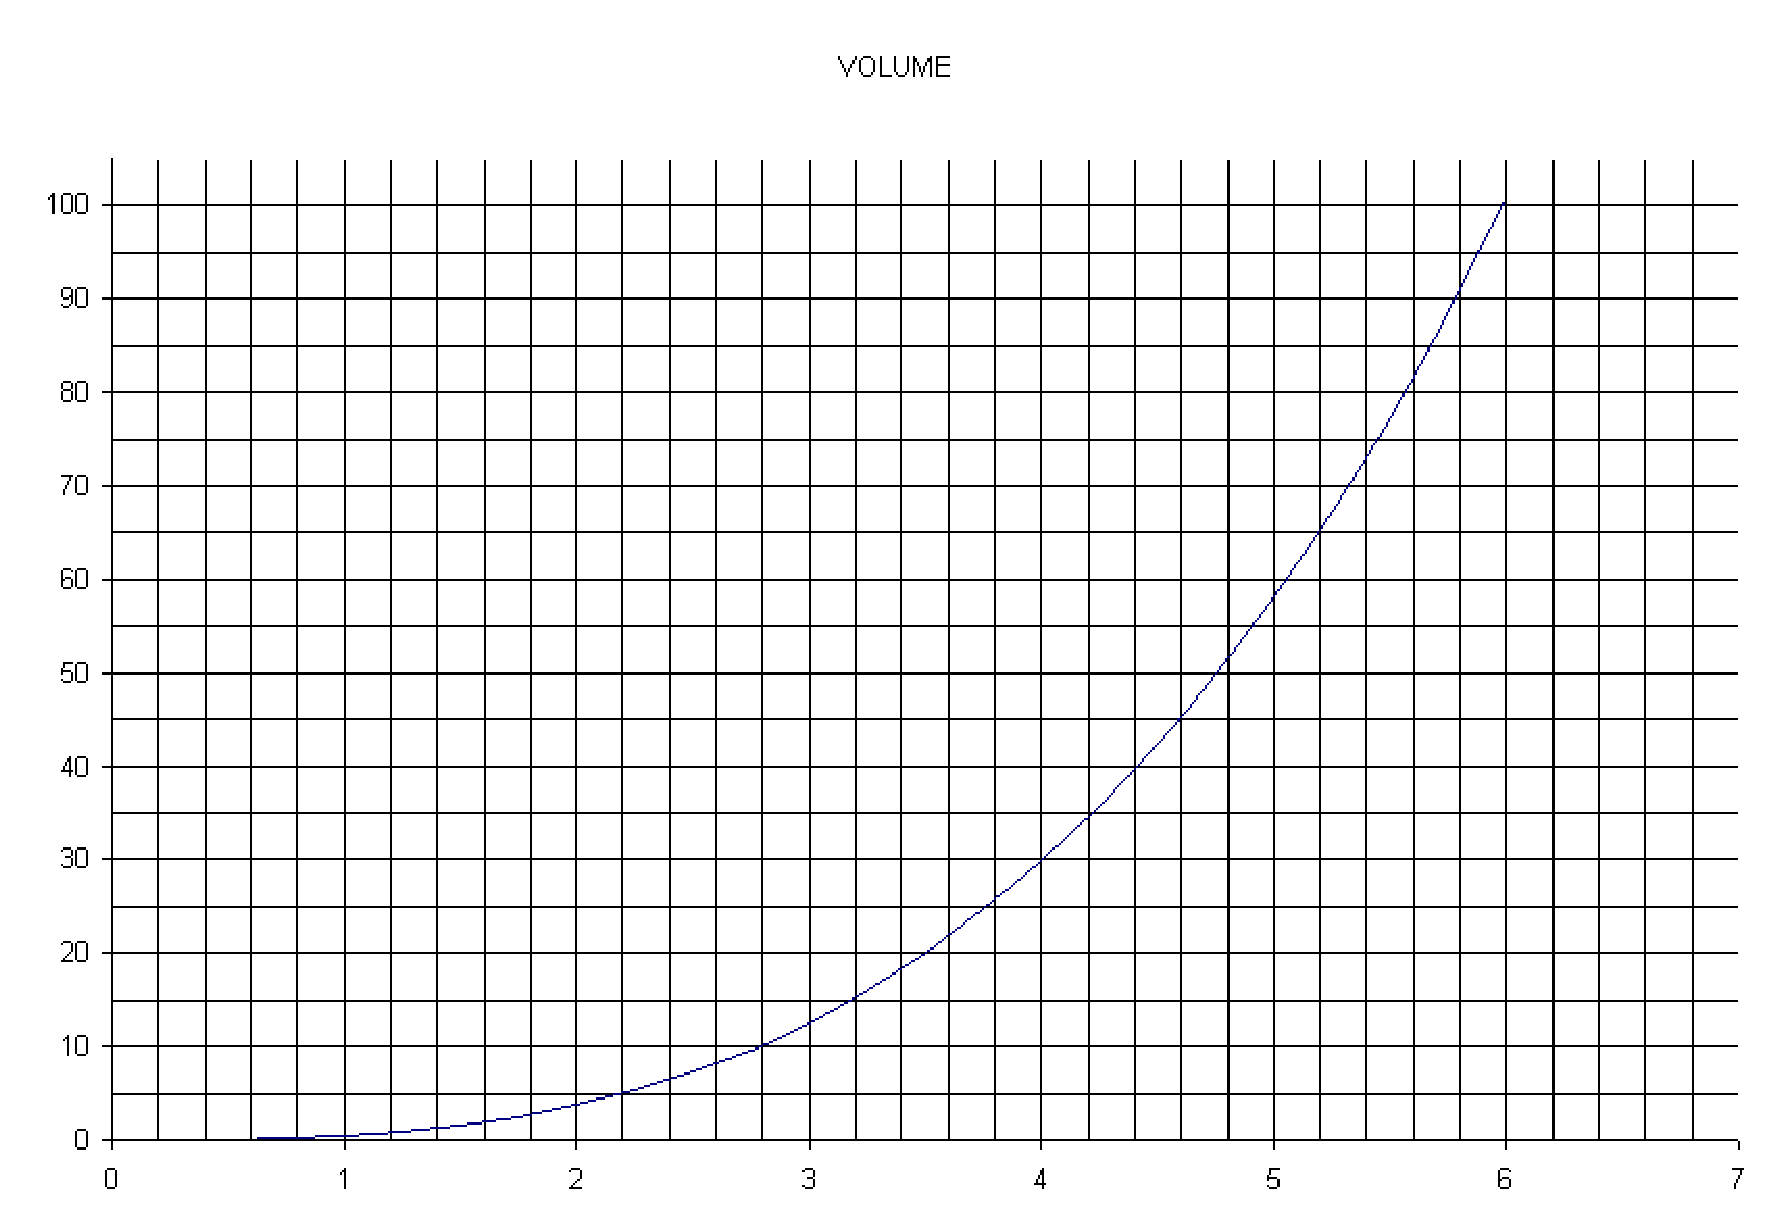
\includegraphics[scale=0.625]{./Graphiques/courbe.eps}\end{center}

%%%%%%%%%%%%%%%%%%%%%%%%%%%%%%%%%%%%%%%%%%%%%%%%%%%%
%%%%%%%%%%%%%%%%%%%%%%%%%%%%%%%%%%%%%%%%%%%%%%%%%%%

%%%%%%%%%%%%%%%%%%%%%%%%%%%%%%%%%%%%%%%%%%%%%%%%%%%\`u
%%%%%%%%%%%%%%%%%%%%%%%%%%%%%%%%%%%%%%%%%%%%%%%%%%%%

 \sautpage

\section{Premi\`eres notions (bilan et compl\'ements)}

\begin{definition}[Notion de fonction]
Une fonction est un proc\'ed\'e qui, \`a un \'el\'ement $x$ d'un ensemble de d\'epart, associe au plus un \'el\'ement $y$ d'un ensemble d'arriv\'ee.

On notera $f:x\mapsto y$ ou $f(x)=y$ qui se lit \og $f$ est la fonction qui \`a $x$ associe $y$ \fg..

On dit que $y$ est \emph{l'image} de $x$.

On dit que $x$ est \emph{un ant\'ec\'edent} de $y$.

\end{definition}

\begin{definition}[Ensemble de d\'efinition]
L'ensemble des r\'eels $x$ poss\'edant une image par une fonction num\'erique $f$ est appel\'e \emph{l'ensemble de d\'efinition de la fonction $f$}. On le note souvent $D_f$.
\end{definition}

\begin{definition}[Repr\'esentation graphique]
Dans un plan muni d'un rep\`ere, la \emph{repr\'esentation graphique} de la fonction $f$ est l'ensemble des points $M$ de coordonn\'ees $(x;y)$ du plan tels que :
\begin{itemize}
	\item L'abscisse $x$ de $M$ d\'ecrit l'ensemble de d\'efinition $D_f$ ;
	\item L'ordonn\'ee $y$ est l'image de $x$ par $f$. $y=f(x)$.
\end{itemize}

On note souvent $\mathcal{C}_f$ la repr\'esentation graphique de $f$. On dit que $\mathcal{C}_f$ a pour \'equation $y=f(x)$.

Si la courbe est d'un seul \og{} tenant \fg{} on parle  de \emph{courbe repr\'esentative} de la fonction $f$.
\end{definition}


\begin{rmq} L'\'equation permet de d\'eterminer si un point $A(x_A;y_A)$ appartient ou pas \`a cette courbe. En effet, un point appartient \`a la courbe si et seulement si ses coordonn\'ees v\'erifient l'\'equation de la courbe. On a alors : \[A\in\mathcal{C}_f\ssi y_A=f(x_A)\] \end{rmq}


Dans la pratique, pour les fonctions num\'eriques d\'efinies par une expression alg\'ebrique, pour esquisser une repr\'esentation graphique, on utilise souvent un tableau de valeurs.

\begin{tabular}{cc}
 \begin{minipage}[l]{0.55\linewidth}
  \begin{rmq} Une courbe ne repr\'esente pas toujours une fonction. Sur la figure ci-contre, par exemple, la courbe a plusieurs points ayant la même abscisse, comme $A(1,-1)$ et $B(1,3)$. Ce n'est donc pas la courbe repr\'esentative d'une fonction car alors 1 aurait plusieurs images.\end{rmq}
 \end{minipage}&
 \begin{minipage}[r]{0.45\linewidth}
\begin{center}
\psset{xunit=0.75cm , yunit=0.75cm}
\def\xmin{-2} \def\xmax{4} \def\ymin{-1.6} \def\ymax{3.6}
\begin{pspicture*}(\xmin,\ymin)(\xmax,\ymax)
\psset{xunit=0.75cm,yunit=0.75cm}
\psgrid[griddots=10,gridlabels=0pt,gridwidth=.3pt, gridcolor=black, subgridwidth=.3pt, subgridcolor=black, subgriddiv=1](0,0)(-2,-2)(4,4)
\psaxes[labels=all,labelsep=1pt, Dx=1,Dy=1]{->}(0,0)(\xmin,\ymin)(\xmax,\ymax)
\uput[dl](0,0){$O$}
%\pcline[linewidth=1pt]{->}(0,0)(1,0) \uput[d](0.5,0){\small $\vec \imath$}
%\pcline[linewidth=1pt]{->}(0,0)(0,1) \uput[l](0,0.5){\small $\vec \jmath$}
\pscircle(1,1){1.5}
\psdots[dotstyle=x](1,-1)(1,3)
\uput[d](1,-1){$A$}
\uput[u](1,3){$B$}
\end{pspicture*}
\end{center}
 \end{minipage}

\end{tabular}






%\sautpage

\subsubsection{Quelques conventions graphiques}
\begin{multicols}{3}
Lorsqu'un point $A$ sur la courbe est connu avec pr\'ecision, il est not\'e par une croix.
\begin{center}
\begin{pspicture*}(-0.5,-1)(2.5,3)
\pscurve(0,0)(0.5,-0.5)(1,1)(2,2.5)
\uput[u](0,0){$\mathcal{C}_f$}
\psdot[dotstyle=x](1,1)
\uput[dr](1,1){$A$}
\end{pspicture*}
\end{center}\sautcol
Lorsqu'un point $A$ est l'extr\'emit\'e de la courbe, il est not\'e par un gros point.
\begin{center}
\begin{pspicture*}(-0.5,-1)(2.5,3)
\pscurve(0,0)(0.5,-0.5)(1,1)(2,2.5)
\uput[u](0,0){$\mathcal{C}_f$}
\psdot(2,2.5)
\uput[dr](2,2.5){$A$}
\end{pspicture*}
\end{center}\sautcol
Lorsqu'un point $A$ \`a l'extr\'emit\'e de la courbe n'appartient pas \`a la courbe, il est not\'e par un \og demi-cercle \fg.
\begin{center}
\begin{pspicture*}(-0.5,-1)(2.5,3)
\pscurve{-(}(0,0)(0.5,-0.5)(1,1)(2,2.5)
\uput[u](0,0){$\mathcal{C}_f$}
%\psdot[(2,2.5)
\uput[dr](2,2.5){$A$}
\end{pspicture*}
\end{center}
\end{multicols}
\begin{multicols}{3}
Une courbe est donn\'ee dans une fenêtre ; s'il n'y a pas d'extr\'emit\'es, la courbe garde la même allure quand on la prolonge.
\begin{center}
\begin{pspicture*}(-0.5,-1)(2.5,3)
\pscurve(-0.3,0)(0.5,2)(1,1)(2,2.8)
\uput[u](1,1){$\mathcal{C}_f$}
\psline[linestyle=dotted](-0.1,0.5)(1.7,0.5)(1.7,2.2)(-0.1,2.2)(-0.1,0.5)
\end{pspicture*}
\end{center}
Une droite verticale en pointill\'es signifie que si l'on prolonge la courbe, elle ne coupe pas cette droite. Sur l'exemple ci-dessous, $a$ n'appartient pas \`a $D_f$.
\begin{center}
\begin{pspicture*}(-0.5,-1)(2.5,3)
\psaxes[labels=none,labelsep=1pt,Dx=5,Dy=5]{->}(0,0)(-0.5,-1)(2.5,3)
\psset{algebraic=true}
\psplot{0.6}{3}{1/(4*x-2)}
\psline[linestyle=dashed](0.5,-1)(0.5,3)
\uput[dl](0.5,0){$a$}
\end{pspicture*}
\end{center}
Une droite horizontale en pointill\'es signifie que si l'on prolonge la courbe, elle ne coupe pas cette droite.
\begin{center}
\begin{pspicture*}(-0.5,-1)(2.5,3)
\psaxes[labels=none,labelsep=1pt,Dx=5,Dy=5]{->}(0,0)(-0.5,-1)(2.5,3)
\psset{algebraic=true}
\psplot{-0.5}{3}{1+1/(x+1)}
\psline[linestyle=dashed](-0.5,1)(2.5,1)
\uput[ul](0,1){$b$}
\end{pspicture*}
\end{center}
\end{multicols}

%\sautpage






\section{R\'esolutions graphiques d'\'equations et d'in\'equations}


\subsection{R\'esolutions d'\'equations de la forme $f(x)=k$}

R\'esoudre l'\'equation $f(x)=k$ c'est d\'eterminer tous les ant\'ec\'edents \'eventuels d'un \'el\'ement $k$ de l'ensemble d'arriv\'ee, c'est-\`a-dire chercher tous les $x$ de l'ensemble de d\'epart tels que $f(x)=k$.

Une telle recherche peut se faire graphiquement \`a partir de la repr\'esentation graphique de la fonction $f$.




\begin{center}
\begin{tabular}{lc}
 \begin{minipage}[l]{0.6\linewidth}
 \begin{exemple*}
  Soit $f$ la fonction d\'efinie sur $\R$ par $f(x)=2x^2-9x+10$. On recherche les solutions de l'\'equation $f(x)=3$.

	On commence par tracer soigneusement la courbe repr\'esentative de $f$ et on obtient la repr\'esentation donn\'ee sur la figure ci-dessous.
		
		On cherche les points de la courbe ayant pour ordonn\'ee 3. Pour cela on peut tracer la droite d'\'equation $y=3$ et chercher les points d'intersection de cette droite avec la courbe de $f$.

		On obtient ici deux points $M_1(1;3)$ et $M_2\left(\frac{7}{2};3\right)$. Les solutions sont leurs abscisses : 1 et $\frac{7}{2}$.

		On \'ecrit : \og Les solutions de l'\'equation $f(x)=3$ sont $x=1$ ou $x=\frac{7}{2}$ car les points de la courbe de $f$ d'ordonn\'ee 3 ont pour abscisses 1 et $\frac{7}{2}$ \fg.
		\end{exemple*}
 \end{minipage}&
 \begin{minipage}[r]{0.35\linewidth}
  
		\begin{center}
 \psset{xunit=1cm,yunit=1cm}
		\begin{pspicture*}(-3.1,-2.1)(4.6,4.1)
\def\xmin{-3} \def\xmax{4.5} \def\ymin{-2} \def\ymax{4}

\psgrid[griddots=10,gridlabels=0pt,gridwidth=.3pt, gridcolor=black, subgridwidth=.3pt, subgridcolor=black, subgriddiv=1](0,0)(-3,-2)(4.5,4)
\psaxes[labels=all,labelsep=1pt, Dx=1,Dy=1]{->}(0,0)(\xmin,\ymin)(\xmax,\ymax)
\uput[dl](0,0){$O$}
\pcline[linewidth=1pt]{->}(0,0)(1,0) \uput[d](0.5,0){\small $\vec \imath$}
\pcline[linewidth=1pt]{->}(0,0)(0,1) \uput[r](0,0.5){\small $\vec \jmath$}
\psset{algebraic=true}
\psplot{\xmin}{\xmax}{2*(x-1)*(x-1)-5*(x-1)+3}
\uput[ul](2,1){$\mathcal{C}_f$}
\psline[linestyle=dashed](\xmin,3)(\xmax,3)
\uput[u](-2,3){$y=3$}
\uput[ur](1,3){$M_1$}
\uput[ul](3.5,3){$M_2$}
\psdots[dotstyle=x](1,3)(3.5,3)
\psline[linestyle=dashed]{->}(1,3)(1,0)
\psline[linestyle=dashed]{->}(3.5,3)(3.5,0)
\end{pspicture*}\end{center}
 \end{minipage}

\end{tabular}             \end{center}



%\sautpage

\subsection{R\'esolutions d'in\'equations de la forme $f(x)\leqslant k$}

Ces in\'equations peuvent se r\'esoudre graphiquement. On proc\`ede de la façon suivante :
\begin{itemize}
	\item on trace soigneusement $\mathcal{C}_f$ dan un rep\`ere (orthogonal) ;
	\item on trace la droite d'\'equation $y=k$ ;
	\item on recherche les points de la courbe situ\'es \emph{sous} la droite ;
	\item l'ensemble des solutions est constitu\'e des abscisses de ces points.
\end{itemize}

\begin{exemple*} Sur l'exemple pr\'ec\'edent, si l'on doit r\'esoudre $f(x)\leqslant 3$, apr\`es avoir trac\'e $y=3$ on constate que les points de la courbe situ\'es sous cette droite ont leurs abscisses comprises entre 0 et $\frac{5}{2}$.

Donc $f(x)\leqslant 3 \ssi x\in\left[0;\frac{5}{2}\right]$.
\end{exemple*}

\begin{rmq}~
\begin{itemize}
	\item On r\'esoud de la même mani\`ere les \'equations du type $f(x)\geqslant k$.

On retient alors les abscisses des points situ\'es \emph{au-dessus} de la droite d'\'equation $y=k$.

Dans l'exemple $f(x)\geqslant 3 \ssi x\in \left] -\infty ; 0 \right] \cup \left[\frac{5}{2} ; +\infty\right[$.
	\item De même pour les in\'equations strictes : $f(x)>k$ ou $f(x)<k$. On excluera alors les abscisses des points d'intersection de la courbe et de la droite.

	Dans l'exemple $f(x)<3 \ssi x\in \left]0;\frac{5}{2}\right[$.
\end{itemize}
\end{rmq}

\subsection{R\'esolutions d'\'equations de la forme $f(x)=g(x)$}

Cela revient \`a chercher les \'el\'ements de l'ensemble de d\'epart qui ont la même image par $f$ et par $g$.

Une telle recherche peut se faire graphiquement. On recherche alors les points des deux courbes repr\'esentatives ayant même abscisse et même ordonn\'ee, c'est-\`a-dire les points d'intersection des deux courbes. 

\begin{tabular}{cc}
 \begin{minipage}[l]{0.6\linewidth}
  \begin{exemple*}

Soit $f$ et $g$ les fonctions d\'efinies sur $\R$ par, respectivement, $f(x)=x^2-1$ et $g(x)=-0,5x^2+x+4$. R\'esoudre graphiquement l'\'equation $f(x)=g(x)$.

	On commence par tracer soigneusement les deux courbes repr\'esentatives et on obtient la repr\'esentation donn\'ee sur la figure ci-contre.
	
	On cherche les points d'intersection des deux courbes, ici $M_1$ et $M_2$, et les solutions de l'\'equation sont leurs abscisses dont les valeurs approximatives sont $-1,5$ et $2,2$.

		Les solutions sont donc $x\approx -1,5$ et $x\approx 2,2$.
\end{exemple*}
 \end{minipage}&
 \begin{minipage}[r]{0.35\linewidth}
  \psset{xunit=0.75cm,yunit=0.75cm}
		\begin{pspicture*}(-3.1,-2.1)(4.6,5.1)
\def\xmin{-3} \def\xmax{4.5} \def\ymin{-2} \def\ymax{5}

\psgrid[griddots=10,gridlabels=0pt,gridwidth=.3pt, gridcolor=black, subgridwidth=.3pt, subgridcolor=black, subgriddiv=1](0,0)(-3,-2)(4.5,5)
\psaxes[labels=all,labelsep=1pt, Dx=1,Dy=1]{->}(0,0)(\xmin,\ymin)(\xmax,\ymax)
\uput[dl](0,0){$O$}
\pcline[linewidth=1pt]{->}(0,0)(1,0) \uput[d](0.5,0){\small $\vec \imath$}
\pcline[linewidth=1pt]{->}(0,0)(0,1) \uput[r](0,0.5){\small $\vec \jmath$}
\psset{algebraic=true}
\psplot{\xmin}{\xmax}{x^2-1}
\psplot{\xmin}{\xmax}{-0.5*x^2+x+4}
\uput[u](1,1){$\mathcal{C}_f$}
\uput[dr](0,4){$\mathcal{C}_g$}
\uput[r](2.189,3.793){$M_2$}
\uput[l](-1.523,1.318){$M_1$}
\psdots[dotstyle=x](2.189,3.793)(-1.523,1.318)
\psline[linestyle=dashed]{->}(-1.523,1.318)(-1.523,0)
\psline[linestyle=dashed]{->}(2.189,3.793)(2.189,0)
\end{pspicture*}
	
 \end{minipage}


\end{tabular}

		

\subsection{R\'esolutions d'in\'equations de la forme $f(x)\leqslant g(x)$}

L\`a encore ces in\'equations peuvent se r\'esoudre graphiquement. On proc\`ede de la façon suivante :
\begin{itemize}
	\item on trace soigneusement $\mathcal{C}_f$ et $\mathcal{C}_g$ dans un rep\`ere (orthogonal) ;
	\item l'ensemble des solutions est constitu\'e des abscisses des points o\`u la courbe de $f$ est situ\'ee \emph{sous} celle de $g$.
\end{itemize}

\begin{exemple*} Sur l'exemple pr\'ec\'edent, si l'on doit r\'esoudre $f(x)\leqslant g(x)$, on constate que les points de la courbe de $f$ situ\'es sous celle de $g$ ont leurs abscisses comprises entre environ $-1,5$ et 2,2.

Donc $f(x)\leqslant g(x) \ssi x\in [-1,5;2,2]$. Ou bien $S=[-1,5;2,2]$.
\end{exemple*}

\begin{rmqs}~
\begin{itemize}
	\item On r\'esoud de la même mani\`ere les \'equations du type $f(x)\geqslant g(x)$.

On retient alors les abscisses des points de la courbe de $f$ situ\'es \emph{au-dessus} de celle de $g$.

Dans l'exemple $f(x)\geqslant g(x) \ssi x\in ] -\infty ; -1,5 ] \cup [2,2 ; +\infty[$.
	\item De même pour les in\'equations strictes : $f(x)>g(x)$ ou $f(x)<g(x)$. On excluera alors les abscisses des points d'intersection des deux courbes.

	Dans l'exemple $f(x)<g(x) \ssi x\in ]-1,5;2,2[$.
\end{itemize}
\end{rmqs}



%\sautpage



\sautpage

\section{Variations, extremums}


\subsection{Sens de variation}

Il s'agit de traduire math\'ematiquement qu'une fonction \og augmente \fg{} ou \og diminue \fg.

\begin{exemple*} Soit, par exemple, la fonction d\'efinie sur $[-3;3]$ par la courbe repr\'esentative donn\'ee sur la figure \ref{croissanceetdecroissance} \vpageref{croissanceetdecroissance}. On constate que lorsque $x\in[-3;1]$ , si $x$ augmente, $f(x)$ augmente aussi alors que lorsque $x\in[1;3]$, si $x$ augmente, $f(x)$ diminue.

C'est la d\'efinition math\'ematique de la croissance ou de la d\'ecroissance d'une fonction $f$.

\begin{figure}[h]
\centering
\caption{Croissance et d\'ecroissante}\label{croissanceetdecroissance}


\psset{xunit=1cm , yunit=1.25cm}
\begin{pspicture*}(-4.1,-1.1)(4.1,5.1)
\def\xmin{-4} \def\xmax{4} \def\ymin{-1} \def\ymax{5}
\psgrid[griddots=10,gridlabels=0pt,gridwidth=.3pt, gridcolor=black, subgridwidth=.3pt, subgridcolor=black, subgriddiv=1](0,0)(-4,-1)(4,5)
\psaxes[labels=all,labelsep=1pt, Dx=1,Dy=1]{-}(0,0)(\xmin,\ymin)(\xmax,\ymax)
\uput[dl](0,0){$O$}
\pcline[linewidth=1pt]{->}(0,0)(1,0) \uput[d](0.5,0){\small $\vec \imath$}
\pcline[linewidth=1pt]{->}(0,0)(0,1) \uput[r](0,0.5){\small $\vec \jmath$}
\psset{algebraic=true}
\psplot{-3}{3}{(-(x-1)^2+5)*0.25+3}
\psdots(3,3.25)(-3,0.25)
\uput[d](-1.5,0){$b$}
\psline[linestyle=dashed]{->}(-1.5,0)(-1.5,2.6875)
\psline[linestyle=dashed]{->}(-1.5,2.6875)(0,2.6875)
\uput[r](0,2.6875){$f(b)$}
\uput[d](-2.5,0){$a$}
\psline[linestyle=dashed]{->}(-2.5,0)(-2.5,1.1875)
\psline[linestyle=dashed]{->}(-2.5,1.1875)(0,1.1875)
\uput[r](0,1.1875){$f(a)$}
\uput[d](1.5,0){$u$}
\uput[d](2.5,0){$v$}
\psline[linestyle=dashed]{->}(1.5,0)(1.5,4.1875)
\psline[linestyle=dashed]{->}(1.5,4.1875)(0,4.1875)
\uput[l](0,4.1875){$f(u)$}
\psline[linestyle=dashed]{->}(2.5,0)(2.5,3.6875)
\psline[linestyle=dashed]{->}(2.5,3.6875)(0,3.6875)
\uput[l](0,3.6875){$f(v)$}
\end{pspicture*}
\end{figure}\end{exemple*}


\begin{definition}
Soit $f$ une fonction d\'efinie sur un intervalle $I$. On dit que $f$ est
\begin{itemize}
	\item \emph{croissante} sur $I$ si, pour tous r\'eels $a$ et $b$ de $I$, on a :\\
$\text{Si } a<b \text{ alors } f(a)\leqslant f(b).$
	\item \emph{d\'ecroissante} sur $I$ si, pour tous r\'eels $a$ et $b$ de $I$, on a :\\
$\text{Si } a<b \text{ alors } f(a)\geqslant f(b).$
	\item \emph{monotone} si elle n'est que croissante sur $I$ ou si elle n'est que d\'ecroissante sur $I$.
	\item \emph{constante} sur $I$ si, pour tous r\'eels $a$ et $b$ de $I$, on a : $f(a)=f(b)$.
\end{itemize}
\end{definition}


\begin{rmqs}~
\begin{itemize}
	\item Ces notions ne sont valables que sur \textbf{un intervalle} et pas sur une r\'eunion d'intervalles disjoints.
	\item Ant\'ec\'edents et images \'etant rang\'es dans le même ordre, on dit qu'une fonction croissante \emph{conserve} l'ordre.
	\item Ant\'ec\'edents et images \'etant rang\'es dans l'ordre inverse, on dit qu'une fonction d\'ecroissante \emph{inverse} l'ordre.
	\item On obtient les d\'efinitions d'une fonction \emph{strictement} croissante ou \emph{strictement} d\'ecroisante en remplaçant les in\'egalit\'es par des in\'egalit\'es strictes. Ainsi on dit que $f$ est strictement croissante sur $I$ si pour tous r\'eels $a$ et $b$ de $I$ on a : \\ $\text{Si } a<b \text{ alors } f(a)<f(b)$
	\item Une fonction est strictement monotone sur $I$ si elle est strictement croissante ou strictement d\'ecroissante sur $I$
\end{itemize}
\end{rmqs}

\subsection{Tableau de variations}

Ces r\'esultats peuvent se r\'esumer dans un tableau de variation, qui est une forme stylis\'ee de repr\'esentation o\`u l'on indique uniquement si la courbe monte, descend ou est stable. Dans la premi\`ere ligne on indique les valeurs importantes de $x$ et dans la seconde les variations de $f$.

\begin{exemple*} Dans l'exemple pr\'ec\'edent on obtient
$$\tabvar{%
\tx{x}&\tx{-3}&&\tx{1}&&\tx{3}\cr
\tx{f}&\txb{\approx 0,25}&\fm&\txh{\approx 4,25}&\fd&\txb{\approx 2,25}\cr
}$$
\end{exemple*}



\subsection{Extremums}

Les extremums, s'ils existent, sont les valeurs maximale et minimale qui sont \textbf{atteintes} par la fonction $f$ sur un intervalle donn\'e. Plus pr\'ecis\'ement :

\begin{definition}
Soit une fonction $f$ d\'efinie sur un intervalle $I$ et $x_0\in I$. On dit que
\begin{itemize}
	\item $f$ admet un \emph{maximum}, atteint en $x_0$ si, pour tout $x\in I$, $f(x)\leqslant f(x_0)$. Ce maximum est alors $f(x_0)$.
	\item $f$ admet un \emph{minimum}, atteint en $x_0$ si, pour tout $x\in I$, $f(x)\geqslant f(x_0)$. Ce minimum est alors $f(x_0)$.
\end{itemize}
Les maximum et minimum sont appel\'es les \emph{extremums}.
\end{definition}

%\begin{rmq} Un extremum doit être atteint par une valeur $x_0$. \end{rmq}

\begin{exemple*}
La fonction $f$ d\'efinie sur $\R$ par $f(x)=x^2+1$ n'admet pas $-1$ comme minimum.

En effet, si on a bien $f(x)\geqslant -1$ sur $\R$, il n'existe pas de $x_0$ tel que $f(x_0)=-1$.

Par contre 1 est bien le minimum de $f$ sur $\R$ car
\begin{itemize}
	\item $f(x)\geqslant 1$ pour tout $x\in\R$ \textbf{ET}
	\item $f(0)=1$
\end{itemize}

On dira donc : le minimum de $f$ sur $\R$ est 1 et il est atteint pour $x_0=0$.
\end{exemple*}

\sautpage

\section{Exercices et probl\`emes}

\subsection{Premi\`eres notions}

%\begin{multicols}{2}
%\begin{exo} Dire dans chacun des exemples ci-dessous quel est l'ensemble de d\'efinition, quelles sont les images possibles et si la fonction est num\'erique.
%\begin{enumerate}
%	\item \`A chaque \'el\`eve de la classe on associe la couleur de ses cheveux.
%	\item \`A chaque \'el\`eve de la classe on associe le nombre de ses fr\`eres et soeurs.
%	\item Pour un \'el\`eve donn\'e, \`a chaque moment de sa vie on associe la taille qu'il mesurait.
%	\item Soit $ABCD$ un rectangle dont un des côt\'es est fixe et mesure 6 cm et l'autre est variable et mesure $x$ cm. \\On d\'efinit la fonction $f$ de la façon suivante : \`a chaque $x$ possible, on associe $f(x)$, l'aire du rectangle $ABCD$.
%	\item La fonction $g$ d\'efinie par $g(x)=x^2+2x+3$.
%	\item La fonction $h$ d\'efinie par $h(x)=\frac{x^2+1}{x-1}$.
%	\item La fonction $i$ d\'efinie par $i(x)=\sqrt{x+2}$.
%\end{enumerate}
%\end{exo}
\begin{multicols}{2}
\begin{exo}
On d\'efinit $f$ et $g$, deux fonctions :
\begin{itemize}
	\item $f$ est la fonction qui \`a un nombre r\'eel $x$ associe le nombre obtenu en proc\'edant de la mani\`ere suivante : on ajoute $4$ au nombre, on \'el\`eve le r\'esultat obtenu au carr\'e, on retranche 16, on divise par le nombre de d\'epart et on retranche 6.
	\item $g:x\mapsto x^2-4$.
\end{itemize}
\begin{enumerate}
	\item Donner l'expression correspondant \`a $f$ puis simplifier cette expression.
	\item Quel r\'eel n'a pas d'image par $f$ ?
	\item Quelle est l'image de 3 par $g$ ?
	\item Quelle est l'image de $-1$ par $g$ ?
	\item Quels sont les ant\'ec\'edents \'eventuels de 12 par $g$ ?
	\item Quels sont les ant\'ec\'edents \'eventuels de $-5$ par $g$ ?
\end{enumerate}
\end{exo}

\sautcol

\begin{exo}
Vrai ou faux ? \emph{Corriger la phrase lorsqu'elle est fausse}.
\begin{enumerate}
	\item $f(-2) = 0$ signifie que l'image de 0 est $-2$
	\item $f(0) = 3$ signifie que la courbe de $f$ passe par le point $(0 ; 3)$
	\item $f(1) = 2$ signifie que l'ant\'ec\'edent de 1 est 2
	\item L'image de 2 par $f$ est $-3$ s'\'ecrit $f(2) = -3$
	\item Dire que $(5 ; 1)$ est un point de la courbe de $f$ s'\'ecrit $5 = f(1)$
	\item Par la fonction $g$, $-5$ est l'image de 3 s'\'ecrit $g(-5) = 3$
	\item 2 a pour image 0 par $f$ signifie que la courbe de $f$ traverse l'axe des abscisses en 2
	\item $f(4) = 0$ signifie que la courbe de $f$ traverse l'axe des abscisses au point $(4 ; 0)$
	\item 3 a pour image 5, signifie que 3 est l'image de 5
	\item 4 a pour ant\'ec\'edent 5 signifie que 5 est l'image de 4
\end{enumerate}
\end{exo}

\end{multicols}

%\sautpage

\begin{exo}\label{gf4courbes}
Vrai ou faux ? \emph{Justifier la r\'eponse lorsque c'est faux}.\\
Les courbes de la figure \ref{gf4courbesfig} \vpageref{gf4courbesfig} repr\'esentent des fonctions de la variable $x$.


\begin{figure}[!h]
 \centering
 \caption{Courbes de l'exercice \ref{gf4courbes}}\label{gf4courbesfig}
\begin{tabular}{cc}
\psset{xunit=1cm , yunit=0.5cm}
\begin{pspicture*}(-2.1,-2.1)(4.1,4.1)
\def\xmin{-2} \def\xmax{4} \def\ymin{-2} \def\ymax{4}
\psgrid[griddots=10,gridlabels=0pt,gridwidth=.3pt, gridcolor=black, subgridwidth=.3pt, subgridcolor=black, subgriddiv=1](0,0)(-2,-2)(4,4)
\psaxes[labels=all,labelsep=1pt, Dx=1,Dy=1]{->}(0,0)(\xmin,\ymin)(\xmax,\ymax)
\uput[dl](0,0){$O$}
\pcline[linewidth=1pt]{->}(0,0)(1,0) \uput[d](0.5,0){\small $\vec \imath$}
\pcline[linewidth=1pt]{->}(0,0)(0,1) \uput[l](0,0.5){\small $\vec \jmath$}
\psline(-2,3)(1,-1.5)(2,-1.5)(4,2)
\end{pspicture*}
&
\psset{xunit=1cm , yunit=0.5cm}
\begin{pspicture*}(-2.1,-2.1)(4.1,4.1)
\def\xmin{-2} \def\xmax{4} \def\ymin{-2} \def\ymax{4}
\psgrid[griddots=10,gridlabels=0pt,gridwidth=.3pt, gridcolor=black, subgridwidth=.3pt, subgridcolor=black, subgriddiv=1](0,0)(-2,-2)(4,4)
\psaxes[labels=all,labelsep=1pt, Dx=1,Dy=1]{->}(0,0)(\xmin,\ymin)(\xmax,\ymax)
\uput[dl](0,0){$O$}
\pcline[linewidth=1pt]{->}(0,0)(1,0) \uput[d](0.5,0){\small $\vec \imath$}
\pcline[linewidth=1pt]{->}(0,0)(0,1) \uput[l](0,0.5){\small $\vec \jmath$}
\psline(-2,3)(1,3)(1,1)(4,1)
\end{pspicture*}
\\
\psset{xunit=1cm , yunit=0.5cm}
\begin{pspicture*}(-2.1,-2.1)(4.1,4.1)
\def\xmin{-2} \def\xmax{4} \def\ymin{-2} \def\ymax{4}
\psgrid[griddots=10,gridlabels=0pt,gridwidth=.3pt, gridcolor=black, subgridwidth=.3pt, subgridcolor=black, subgriddiv=1](0,0)(-2,-2)(4,4)
\psaxes[labels=all,labelsep=1pt, Dx=1,Dy=1]{->}(0,0)(\xmin,\ymin)(\xmax,\ymax)
\uput[dl](0,0){$O$}
\pcline[linewidth=1pt]{->}(0,0)(1,0) \uput[d](0.5,0){\small $\vec \imath$}
\pcline[linewidth=1pt]{->}(0,0)(0,1) \uput[l](0,0.5){\small $\vec \jmath$}
\psline(-2,3)(4,3)
\end{pspicture*}
&
\psset{xunit=1cm , yunit=0.5cm}
\begin{pspicture*}(-2.1,-2.1)(4.1,4.1)
\def\xmin{-2} \def\xmax{4} \def\ymin{-2} \def\ymax{4}
\psgrid[griddots=10,gridlabels=0pt,gridwidth=.3pt, gridcolor=black, subgridwidth=.3pt, subgridcolor=black, subgriddiv=1](0,0)(-2,-2)(4,4)
\psaxes[labels=all,labelsep=1pt, Dx=1,Dy=1]{->}(0,0)(\xmin,\ymin)(\xmax,\ymax)
\uput[dl](0,0){$O$}
\pcline[linewidth=1pt]{->}(0,0)(1,0) \uput[d](0.5,0){\small $\vec \imath$}
\pcline[linewidth=1pt]{->}(0,0)(0,1) \uput[l](0,0.5){\small $\vec \jmath$}
\pscurve(-2,3)(-1,0)(0,-1)(2,1)(3.2,2)(3,3)
\end{pspicture*}
\end{tabular}
\end{figure}

\end{exo}

\sautpage

\begin{exo}\label{gf14}
Vrai ou faux ? \emph{Corriger la phrase lorsqu'elle est fausse}.\\
Les fonctions $f$ et $g$ sont repr\'esent\'ees sur la figure \ref{gf14fig} \vpageref{gf14fig}.
\begin{enumerate}
	\item La fonction $f$ est d\'efinie entre $-2$ et 6 inclus
	\item Les images par la fonction $f$ sont comprises entre $-1$ et 4 inclus
	\item La fonction $g$ est d\'efinie entre $-2$ exclu et 6 inclus
	\item Les images par la fonction g sont comprises entre 0 exclu et 3 inclus
\end{enumerate}



\begin{figure}[!h]
\centering
\caption{Courbes de l'exercice \ref{gf14}}\label{gf14fig}
\begin{tabular}{cc}
\psset{xunit=0.9cm , yunit=0.5cm}
\begin{pspicture*}(-3.1,-2.1)(6.1,5.1)
\def\xmin{-3} \def\xmax{6} \def\ymin{-2} \def\ymax{5}
\psgrid[griddots=10,gridlabels=0pt,gridwidth=.3pt, gridcolor=black, subgridwidth=.3pt, subgridcolor=black, subgriddiv=1](0,0)(-3,-2)(6,5)
\psaxes[labels=all,labelsep=1pt, Dx=1,Dy=1]{->}(0,0)(\xmin,\ymin)(\xmax,\ymax)
\uput[dl](0,0){$O$}
\pcline[linewidth=1pt]{->}(0,0)(1,0) \uput[d](0.5,0){\small $\vec \imath$}
\pcline[linewidth=1pt]{->}(0,0)(0,1) \uput[l](0,0.5){\small $\vec \jmath$}
\pscurve{*-(}(-2,2)(-1,3)(0,3.7)(0.5,3.9)(1,4)(2,3)(3,0)(4,-1)(5,0)(6,1)

\rput(3,2){$\mathcal{C}_f$}
\end{pspicture*}
&
\psset{xunit=0.9cm , yunit=0.5cm}
\begin{pspicture*}(-3.1,-2.1)(6.1,5.1)
\def\xmin{-3} \def\xmax{6} \def\ymin{-2} \def\ymax{5}
\psgrid[griddots=10,gridlabels=0pt,gridwidth=.3pt, gridcolor=black, subgridwidth=.3pt, subgridcolor=black, subgriddiv=1](0,0)(-3,-2)(6,5)
\psaxes[labels=all,labelsep=1pt, Dx=1,Dy=1]{->}(0,0)(\xmin,\ymin)(\xmax,\ymax)
\uput[dl](0,0){$O$}
\pcline[linewidth=1pt]{->}(0,0)(1,0) \uput[d](0.5,0){\small $\vec \imath$}
\pcline[linewidth=1pt]{->}(0,0)(0,1) \uput[l](0,0.5){\small $\vec \jmath$}
\pscurve{)-}(-2,0)(0,1)(1,2)(1.5,3.5)(1.8,5)
\pscurve{-*}(2.2,-2)(3,0)(4,1.5)(6,3)
\rput(1,3){$\mathcal{C}_g$}
\psline[linestyle=dashed](2,\ymin)(2,\ymax)
\end{pspicture*}
\end{tabular}
\end{figure}

\end{exo}

\begin{exo}\label{gf15}
Vrai ou faux ? \emph{Corriger la proposition lorsqu'elle est fausse}.
\begin{itemize}
	\item D'apr\`es la repr\'esentation graphique de la figure \ref{gf15fig} \vpageref{gf15fig} $D_f=[-4;2]$
	\item D'apr\`es la repr\'esentation graphique de la figure \ref{gf15fig} \vpageref{gf15fig} $D_g=]-\infty;3[\cup]3;5]$
\end{itemize}


\begin{figure}[!h]
\centering
\caption{Courbes de l'exercice \ref{gf15}}\label{gf15fig}
\begin{tabular}{cc}
\psset{xunit=1cm , yunit=0.66cm}
\begin{pspicture*}(-4.1,-2.1)(4.1,4.1)
\def\xmin{-4} \def\xmax{4} \def\ymin{-2} \def\ymax{4}
\psgrid[griddots=10,gridlabels=0pt,gridwidth=.3pt, gridcolor=black, subgridwidth=.3pt, subgridcolor=black, subgriddiv=1](0,0)(-4,-2)(4,4)
\psaxes[labels=all,labelsep=1pt, Dx=1,Dy=1]{->}(0,0)(\xmin,\ymin)(\xmax,\ymax)
\uput[dl](0,0){$O$}
\pcline[linewidth=1pt]{->}(0,0)(1,0) \uput[d](0.5,0){\small $\vec \imath$}
\pcline[linewidth=1pt]{->}(0,0)(0,1) \uput[l](0,0.5){\small $\vec \jmath$}
\pscurve{*-}(-4,0)(-3,-2)(0,0)(1,1)(4,1.8)
\psline[linestyle=dashed](0,2)(4,2)
\rput(-1.5,-1){$\mathcal{C}_f$}
\end{pspicture*}
&
\psset{xunit=1cm , yunit=0.66cm}
\begin{pspicture*}(-3.1,-2.1)(5.6,4.1)
\def\xmin{-3} \def\xmax{5.5} \def\ymin{-2} \def\ymax{4}
\psgrid[griddots=10,gridlabels=0pt,gridwidth=.3pt, gridcolor=black, subgridwidth=.3pt, subgridcolor=black, subgriddiv=1](0,0)(-3,-2)(5.5,4)
\psaxes[labels=all,labelsep=1pt, Dx=1,Dy=1]{->}(0,0)(\xmin,\ymin)(\xmax,\ymax)
\uput[dl](0,0){$O$}
\pcline[linewidth=1pt]{->}(0,0)(1,0) \uput[d](0.5,0){\small $\vec \imath$}
\pcline[linewidth=1pt]{->}(0,0)(0,1) \uput[l](0,0.5){\small $\vec \jmath$}
\pscurve(-3,3)(0,1.5)(1,1)(2,0)(2.8,-2)
\pscurve{-*}(3.2,-2)(4,1)(5,3)
\psline[linestyle=dashed](3,\ymin)(3,\ymax)
\uput[ur](1,1){$\mathcal{C}_g$}
\end{pspicture*}
\end{tabular}
\end{figure}
\end{exo}
%\sautpage


\begin{exo}[Avec la calculatrice]
La fonction $f$ est d\'efinie sur $[-1,5;2]$ par : $f(x)=2x^3-1,5x^2-3x$
\begin{enumerate}
	\item Compl\'eter le tableau de valeurs suivant :
	%\vspace{-1em}
	\begin{center}
\begin{tabular}{|*{9}{c|}}
\hline $x$ & $-1,5$ & $-1$ & $-0,5$ & 0 & 0,5 & 1 & 1,5 & 2 \\ \hline
$f(x)$ & & & & & & & & \\ \hline
\end{tabular}
\end{center}
\item Tracer la courbe repr\'esentative de $f$.
\end{enumerate}
\end{exo}

\begin{exo}[Avec la calculatrice]\label{uneautrecourbe}
La fonction $f$ est d\'efinie sur $[-3;3]$ par : $f(x)=x^2-3x+1$.\\
Apr\`es avoir dress\'e un tableau de valeurs de la fonction, tracer sa courbe repr\'esentative $\mathcal{C}_f$.

\end{exo}

%\end{multicols}



\sautpage

\subsection{R\'esolutions graphiques}

\begin{exo}
La fonction $f$ est d\'efinie sur $[-3;3]$ par : $f(x)=x^2-3x+1$.\\
$\mathcal{C}_f$, courbe repr\'esentative de $f$ a d\'ej\`a \'et\'e obtenue dans l'exercice \ref{uneautrecourbe}.
\begin{enumerate}
	\item \`A l'aide de la repr\'esentation graphique $\mathcal{C}_f$, avec la pr\'ecision permise par le graphique, r\'epondre aux question suivantes :
		\vspace{-1em}\begin{multicols}{2}
		  \begin{enumerate}
			\item Quelle est l'image de 2 ?
			\item Quelle est l'image de 3 ?
			\item Quelle est l'image de 4 ?
			\item Quels sont les ant\'ec\'edents de 1 ?
			\item Quels sont les ant\'ec\'edents de 2 ?
			\item Quels sont les ant\'ec\'edents de $-2$ ?
		\end{enumerate}
		\end{multicols}\vspace{-1em}
	\item R\'esoudre graphiquement les \'equations et in\'equations suivantes :
\vspace{-1em}\begin{multicols}{3}\begin{enumerate}
	\item $f(x)=3$ ;
	\item $f(x)=-1,5$ ;
	\item $f(x)\geqslant -1$ ;
	\item $f(x)<4$ ;
	\item $f(x)>-3$ ;
	\item $f(x)<-2$.
\end{enumerate}\end{multicols}\vspace{-1em}
\item D\'eterminer graphiquement le signe de $f(x)$ selon les valeurs de $x$.
\end{enumerate}
\end{exo}

%\sautpage

\begin{exo}
Une fonction $f$, d\'efinie sur $\R$, est donn\'ee par sa courbe repr\'esentative $\mathcal{C}$ :
\begin{multicols}{2}
\begin{center}\small
\psset{xunit=1,yunit=1}
\begin{pspicture*}(-2.6,-2.1)(5.1,3.1)
\def\xmin{-2.5} \def\xmax{5} \def\ymin{-2} \def\ymax{3}
\psset{xunit=0.1cm,yunit=0.1cm}
\psgrid[griddots=15,gridlabels=0pt,gridwidth=.3pt, gridcolor=gray, subgridwidth=.3pt, subgridcolor=gray, subgriddiv=1](0,0)(-25,-20)(50,30)
\psset{xunit=1cm , yunit=1cm}
\psaxes[labels=all,labelsep=1pt, Dx=1,Dy=1]{->}(0,0)(\xmin,\ymin)(\xmax,\ymax)
\uput[dl](0,0){$0$}
\pcline[linewidth=1pt]{->}(0,0)(1,0) \uput[d](0.5,0){\small $\vec i$}
\pcline[linewidth=1pt]{->}(0,0)(0,1) \uput[l](0,0.5){\small $\vec j$}
\pscurve(-2.3,-2)(-2,-1)(-1.5,1.5)(-1,3)(-0.5,2.5)(0,1)(0.2,0)(0.5,-1)(1,-1.5)(1.5,-1)(2,0)(2.5,1)(3,1.5)(4,2)(5,2.3)
\psline[linestyle=dashed](0,2.5)(\xmax,2.5)
\psdots[dotstyle=x](-2,-1)(-1.5,1.5)(-1,3)(-0.5,2.5)(0,1)(0.5,-1)(1,-1.5)(1.5,-1)(2,0)(2.5,1)(3,1.5)(4,2)
\end{pspicture*}
\end{center}\normalsize

\sautcol

Avec la pr\'ecision permise par le graphique, r\'esoudre :
%\vspace{-1em}
%\begin{multicols}{2}
\begin{enumerate}
	\item Les \'equations suivantes :
		\vspace{-1em}
		\begin{multicols}{2}\begin{enumerate}
			\item $f(x) = 1$ ;
			\item $f(x) = 0$ ;
			\item $f(x) = -1$ ;
			\item $f(x) = 2$.
		\end{enumerate}\end{multicols}
		%\vspace{-1em}
%\sautcol
	\item Les in\'equations suivantes :
		\vspace{-1em}
		\begin{multicols}{2}\begin{enumerate}
			\item $f(x)\geqslant 1$ ;
			\item $f(x)\geqslant 0$ ;
			\item $f(x)<-1$ ;
			\item $f(x)>2$.
		\end{enumerate}\end{multicols}
		\vspace{-1em}
	\item D\'eterminer graphiquement le signe de $f(x)$ selon les valeurs de $x$.

\end{enumerate}\end{multicols}
%\vspace{-1em}
\end{exo}

\medskip

\begin{multicols}{2}

\begin{exo}\label{gfunecourbe}
La courbe $\mathcal{C}$ de la figure ci-dessous %\ref{gfunecourbefig} \vpageref{gfunecourbefig} 
repr\'esente une fonction $f$ et le segment de droite $\mathcal{D}$ repr\'esente une fonction $g$.

%\begin{figure}[hbtp]
% \centering
% \caption{Figure de l'exercice \ref{gfunecourbe}}\label{gfunecourbefig}


\begin{center}
\psset{xunit=0.375cm , yunit=0.33cm}
\def\xmin{-9} \def\xmax{12} \def\ymin{-3} \def\ymax{11}
\begin{pspicture*}(\xmin,\ymin)(\xmax,\ymax)
\psgrid[griddots=10,gridlabels=0pt,gridwidth=.3pt, gridcolor=black, subgridwidth=.3pt, subgridcolor=black, subgriddiv=1](0,0)(\xmin,\ymin)(\xmax,\ymax)
\psaxes[labels=all,labelsep=1pt, Dx=5,Dy=5]{-}(0,0)(\xmin,\ymin)(\xmax,\ymax)
\uput[dl](0,0){$O$}
\pcline[linewidth=1pt]{->}(0,0)(1,0) \uput[d](0.5,0){\small $\vec \imath$}
\pcline[linewidth=1pt]{->}(0,0)(0,1) \uput[l](0,0.5){\small $\vec \jmath$}
\pscurve{*-*}(-8,1)(-5,3)(-3,5)(-1,6)(0,5)(1,3)(2,0)(4,-2)(7,0)(9,3)(11,6)
\psdots[dotstyle=x](-5,3)(-3,5)(-1,6)(0,5)(1,3)(2,0)(4,-2)(7,0)(9,3)
\psdots[dotstyle=*](-8,7.5)(11,-2)
\uput[dr](10,5){$\mathcal{C}$}
\uput[ur](-6,7){$\mathcal{D}$}
\psplot[linestyle=dashed,algebraic=true]{-8}{11}{-0.5*x+3.5}
\end{pspicture*}\end{center}

%\end{figure}

\sautcol

\begin{enumerate}
	\item R\'esoudre graphiquement les \'equations :
		\vspace{-1em}\begin{multicols}{2}\begin{enumerate}
			\item $f(x) = 3$ ;
			\item $f(x) = -2$ ;
			\item $f(x) = 0$ ;
			\item $f(x) = 6$.
		\end{enumerate}\end{multicols}
	\item R\'esoudre graphiquement les in\'equations :
		\begin{enumerate}
			\item $f(x)\leqslant 0$ ;
			\item $f(x) \geqslant 3$ ;
			\item $f(x)>5$.
		\end{enumerate}

	\item R\'esoudre graphiquement :
			\begin{enumerate}
				\item $f(x) = g(x)$ ;
				\item $f(x) < g(x)$.			\end{enumerate}
		\item Donner le signe de $f(x)$ suivant les valeurs de $x$.
\end{enumerate}
\end{exo}\end{multicols}

%\sautpage

\begin{multicols}{2}

\begin{exo}[Avec la calculatrice]
On consid\`ere les fonctions $f$ et $g$ d\'efinies sur $\R$ par : $f(x)=x^3$ et $g(x)=3x-2$.
 \begin{enumerate}
			\item Tracer soigneusement les repr\'esentations graphiques $\mathcal{C}_f$ et $\mathcal{C}_g$ de $f$ et $g$ sur l'intervalle $[-2;2]$.
			\item R\'esoudre graphiquement l'in\'equation $f(x)\leqslant 1$.
			\item D\'eterminer graphiquement les solutions de l'\'equation $f(x)=g(x)$.
 \end{enumerate}
\end{exo}

\sautcol

\begin{exo}[Avec la calculatrice]
Les fonctions $f$ et $g$ sont d\'efinies sur $[-2;2]$ par : $f(x)=x^3$ et $g(x)=1-x$.
\begin{enumerate}
	\item Tracer sur une calculatrice graphique les repr\'esentations graphiques $\mathcal{C}_f$ et $\mathcal{C}_g$ de $f$ et de $g$.
	\item En d\'eduire le nombre de solutions de l'\'equation $x^3+x-1=0$.
	\end{enumerate}
\end{exo}

\end{multicols}

\subsection{R\'esolutions calculatoires}
%\section{Technologie}
\begin{multicols}{2}
\begin{exo}
Soit la fonction $f$ d\'efinie sur $\R$ par : \\$f(x)=2x^2+x+3$.
\begin{enumerate}
	\item Calculer les valeurs exactes de $f(x)$ pour les valeurs de $x$ suivantes :
	  \vspace{-1em}\begin{multicols}{3}
	  \begin{itemize}
	    \item 0 ;
	    \item 1 ;
	    \item $-2$ ;
	    \item $\sqrt{2}$ ;
	    \item $1+\sqrt{3}$ ;
	    \item $2-\sqrt{5}$.
	   \end{itemize}
	  \end{multicols}\vspace{-1em}
	\item R\'esoudre $f(x)=3$.
\end{enumerate}
\end{exo}

\begin{exo}
Soit $f$ la fonction d\'efinie sur $\R$ par :\\ $f(x)=2x^2-5x+3$. \\R\'esoudre $f(x)=3$.
\end{exo}

\begin{exo} Soit $f$ la fonction d\'efinie sur $\R$ par : $f(x)=4x^2-4x+1$. On cherche \`a r\'esoudre, par le calcul, l'\'equation $f(x)=9$.
%\vspace{-1em}\begin{multicols}{2}
\begin{enumerate}
	\item Factoriser $f(x)$.
	\item R\'esoudre $f(x)=9$.
\end{enumerate}% \end{multicols}\vspace{-1em}
\end{exo}



\begin{exo}
	Soit $f$ et $g$ les fonctions d\'efinies sur $\R$ par, respectivement, $f(x)=x^2-1$ et $g(x)=-x^2+2$. \\ R\'esoudre par le calcul l'\'equation $f(x)=g(x)$.
\end{exo}


\begin{exo}
On consid\`ere les fonctions $f$ et $g$ d\'efinies sur $\R$ par : $f(x)=x^3$ et $g(x)=3x-2$. On cherche \`a r\'esoudre, par le calcul, l'\'equation $f(x)=g(x)$.
		\begin{enumerate}
			\item D\'evelopper $(x-1)^2(x+2)$.
			\item En d\'eduire les solutions de l'\'equation $x^3-3x+2=0$.
			\item En d\'eduire les solutions de l'\'equation $f(x)=g(x)$.
		\end{enumerate}
\end{exo}



%

\begin{exo}
On consid\`ere la fonction $f$ d\'efinie pour tout $x\in\R$ par : $f(x)=x(x-2)$. On cherche \`a trouver, par le calcul, le minimum de $f(x)$.
%\vspace{-1em}\begin{multicols}{2}
\begin{enumerate}
	\item D\'emontrer que $f(x)=(x-1)^2-1$.
	\item En d\'eduire le minimum de $f(x)$.
\end{enumerate}%\end{multicols}\vspace{-1em}
\end{exo}

\end{multicols}

\sautpage


\subsection{Variations, extremums}

\begin{multicols}{2}

\begin{exo}\label{fonctionsvar1}
On consid\`ere la fonction $f$ dont on donne la repr\'esentation $\mathcal{C}$ sur la figure \ref{fonctionsvar1fig} \vpageref{fonctionsvar1fig} (en deux parties).\\
Indiquer son ensemble de d\'efinition et dresser son tableau de variations.

\end{exo}
%\sautpage


\begin{exo}[Avec une calculatrice]
On consid\`ere la fonction $f$ d\'efinie par : $f(x)=2x\sqrt{4-x^2}$.
\`A l'aide d'une calculatrice graphique :
\begin{enumerate}
	\item conjecturer l'ensemble de d\'efinition de $f$ ;
	\item conjecturer quels sont les extremums de $f$ sur son ensemble de d\'efinition ;
	\item dresser le tableau des variations de $f$.
\end{enumerate}
\end{exo}


%\sautcol


\begin{exo}
Tracer une courbe repr\'esentative d'une fonction $f$ sachant que :
%\vspace{-1em}\begin{multicols}{2}
\begin{itemize}
\item le tableau des variations de $f$ est le suivant :$$\tabvar{%
\tx{x}&&&\tx{0}&&\tx{3}&&\tx{~}\cr
\tx{f}&\txb{1}&\fm&&\fd&&\fm&\cr
}$$
	\item 1 a pour ant\'ec\'edents, par la fonction $f$, $-2$ et 1,5 ;
	\item $f(x)=0$ a pour solutions $x=2$ ou $x=4$ ;
	\item $f(-1)=2$ ;
	\item $-1$ est l'image de 3 ;
	\item $D_f=[-2;4]$ ;
	\item le maximum de $f$ est 3 ;
	
\end{itemize}%\end{multicols}
\end{exo}



\sautcol

\begin{exo}
On donne le tableau des variations d'une fonction $f$ :$$\tabvar{%
\tx{x}&\tx{-5}&&\tx{-3}&&\tx{0}&&\tx{1}&&\tx{8}\cr
\tx{f}&\txh{3}&\fd&\txb{0}&\fm&\txh{1}&\fdh&\tx{0}&\fdb&\txb{-2}\cr
}$$
%\vspace{-4em}\begin{multicols}{2}
\begin{enumerate}
	\item S'il est possible de r\'epondre, compl\'eter par \og < \fg, \og > \fg{} ou \og = \fg. Sinon mettre une croix.
\begin{itemize}
 \item $f(-1)$  $\ldots\ldots$  $f(-2)$ 
 \item $f(-3)$  $\ldots\ldots$  $f(1)$ 
 \item $f(-1)$  $\ldots\ldots$  $1$ 
 \item $f(-2)$ $\ldots\ldots$  $f(0,5)$
 \item $f(-2)$  $\ldots\ldots$  $f(1,5)$
 \item $f(4)$  $\ldots\ldots$  $f(2)$
 \item $4$  $\ldots\ldots$ $f(-4)$
 \end{itemize}

\item R\'esoudre, lorsque c'est possible, les in\'egalit\'es suivantes :
\vspace{-1em}\begin{multicols}{2}\begin{enumerate}
	  \item $f(x)\geqslant 0$ ;
	  \item $f(x)=1$ ;
	  \item $f(x)<-1$ ;
	  \item $f(x)<0$.
  \end{enumerate}\end{multicols}
	\item Dire, si c'est possible, quel est le maximum de la fonction et quel est son minimum.
\end{enumerate}%\end{multicols}
\end{exo}
\end{multicols}
%M\end{multicols}



\begin{figure}[!h]
 \centering
 \caption{Figure de l'exercice \ref{fonctionsvar1}}\label{fonctionsvar1fig}

\psset{xunit=0.75cm , yunit=0.75cm}
\begin{pspicture*}(-6.1,-2.1)(14.1,6.1)
\def\xmin{-6} \def\xmax{14} \def\ymin{-2} \def\ymax{6}
\psgrid[griddots=10,gridlabels=0pt,gridwidth=.3pt, gridcolor=black, subgridwidth=.3pt, subgridcolor=black, subgriddiv=1](0,0)(-6,-2)(14,6)
\psaxes[labels=all,labelsep=1pt, Dx=1,Dy=1]{-}(0,0)(\xmin,\ymin)(\xmax,\ymax)
\uput[dl](0,0){$O$}
\pcline[linewidth=1pt]{->}(0,0)(1,0) \uput[d](0.5,0){\small $\vec i$}
\pcline[linewidth=1pt]{->}(0,0)(0,1) \uput[l](0,0.5){\small $\vec j$}
\pscurve(-5,-1)(-4,0)(-3,3)(-2,4)(0,3)(4,0)(5,-2)
\psdot(-5,-1)
\psdots[dotstyle=x](-4,0)(-3,3)(-2,4)(0,3)(4,0)(7,0)(8,3)(10,5)(12,3)
\pscurve(6.5,-2)(7,0)(8,3)(10,5)(12,3)(14,2.2)
\psline[linestyle=dashed](6,-2)(6,6)
\psline[linestyle=dashed](9,2)(14,2)
\end{pspicture*}
\end{figure}







%\sautpage


%\input{./Devoirs/DS3AlgorithmiqueFonctions}

%\chapter{Statistiques discr\`etes} \label{statistiques1}
\minitoc

\fancyhead{} % efface les ent\^etes pr\'ec\'edentes
\fancyhead[LE,RO]{\footnotesize \em \rightmark} % section en ent\^ete
\fancyhead[RE,LO]{\scriptsize \em Seconde} % classe et ann\'ee en ent\^ete

    \fancyfoot{}
		\fancyfoot[RE]{\scriptsize \em \href{http://perpendiculaires.free.fr/}{http://perpendiculaires.free.fr/}}
		\fancyfoot[LO]{\scriptsize \em David ROBERT}
    \fancyfoot[LE,RO]{\textbf{\thepage}}

%\sautpage


\section{Vocabulaire}


\begin{definition}
Une s\'erie statistique est un ensemble d'observations collect\'ees et on a les d\'efinitions suivantes :
\begin{itemize}
	\item \emph{Population} : C'est l'ensemble sur lequel porte une \'etude statistique ;
		  %si elle est trop grande, on s'int\'eresse \`a un \emph{\'echantillon} de cette population ;
	\item \emph{Individu} : C'est un \'el\'ement de la population ;
	\item \emph{Caract\`ere} : C'est ce qu'on observe chez l'individu ;
	\item \emph{Modalit\'e} : Ce sont les diff\'erentes valeurs prises par le caract\`ere ;
	\item La s\'erie statistique est dite \emph{quantitative} quand les modalit\'es sont des nombres %(nombre de fr\`eres et soeurs, dimensions d'une pi\`ece)
		et \emph{qualitative} sinon ; %(candidat pour lequel un individu \`a l'intention de voter)
	\item Dans le cas d'une s\'erie quantitative, celle-ci est dite \emph{discr\`ete} si les modalit\'es sont limit\'ees \`a un ensemble fini de valeurs %(le nombre de fr\`eres et soeurs ne peut \^etre qu'un \'el\'ement de l'ensemble $\{0\,;\,1\,;\,\ldots\,;\,10\}$)
	    et \emph{continue} si les modalit\'es peuvent prendre n'importe quelle valeur dans un intervalle. %(la taille d'un individu)
\end{itemize}
\end{definition}

\begin{exemples*}~
\begin{itemize}
 \item On peut s'int\'eresser \`a une classe (population),
comportant des \'el\`eves (individus) et observer leur nombre de fr\`eres et s\oe{}urs (caract\`ere)
qui peuvent \^etre 0, 1, 2, \ldots (modalit\'es),
ces donn\'ees formant alors une s\'erie statistique quantitative discr\`ete.
 \item On peut s'int\'eresser \`a une cha\^ine d'usine produisant des bras de suspension pour voiture (population),
et observer sur chaque pi\`ece (individu) ses dimensions exactes (caract\`ere)
qui peuvent varier entre 500 et 750 mm (modalit\'es),
ces donn\'ees formant alors une s\'erie statistique quantitative continue.
 \item On peut s'int\'eresser \`a la population fran\c{c}aise (population)
comportant des individus (individus) et estimer leur intention de vote (caract\`ere) pouvant \^etre n'importe
lequel des candidats se pr\'esentant (modalit\'es),
ces donn\'ees formant alors une s\'erie statistique qualitative.
\end{itemize}
\end{exemples*}

\begin{definition}
On a aussi :
\begin{itemize}
	\item \emph{Effectif d'une valeur} : C'est le nombre de fois que la valeur d'un caract\`ere (la modalit\'e) revient dans la s\'erie ;
	\item \emph{Fr\'equence d'une valeur} : C'est l'effectif de la modalit\'e divis\'e par l'effectif total ; elle est comprise entre 0 et 1.
	\item \emph{Classes de valeurs} : s'il y a trop de valeurs diff\'erentes, elles sont rang\'ees par \emph{classe} (intervalle), l'effectif de la classe \'etant alors le nombre de modalit\'es appartenant \`a cet intervalle.
\end{itemize}
\end{definition}

% Pour faire parler ces (souvent longues) s\'eries, il est n\'ecessaire de les r\'esumer : on produit alors \emph{des} statistiques. Tout r\'esum\'e met en \'evidence certaines caract\'eristiques de la s\'erie mais engendre une \emph{perte d'information}, toutes les donn\'ees n'\'etant plus accessibles.

% Le r\'esum\'e peut \^etre un graphique : en Seconde vous avez vu le \emph{diagramme en bâtons} et l'\emph{histogramme} (pour des s\'eries rang\'ees en classes). Nous en verrons deux autres cette ann\'ee.

% Il peut aussi \^etre num\'erique dans le cas d'une s\'erie satistique quantitative. Ces r\'esum\'es num\'eriques sont de deux types : les mesures centrales et les mesures de dispersion.

%\sautpage

\section{Mesures centrales}

\begin{encadrer} \begin{Large}Elles visent \`a r\'esumer la s\'erie par une seule valeur repr\'esentative, d'une certaine mani\`ere, de toutes les valeurs de la s\'erie.                                                                                                                                                \end{Large}\end{encadrer}

\subsection{Mode}

\begin{definition}[Mode]
Le \emph{mode} d'une s\'erie statistique est la donn\'ee la plus fr\'equente de la s\'erie.
\end{definition}

\begin{rmqs}~
\begin{itemize}
	\item S'il y a plusieurs donn\'ees arrivant \`a \'egalit\'e, il y a plusieurs modes.
	\item Si les donn\'ees sont rang\'ees en classe, on parle de \emph{classe modale}.
	\item Le mode est d\'efini aussi bien pour les s\'eries quantitatives que qualitatives.
\end{itemize}
\end{rmqs}

Le mode est un r\'esum\'e sommaire d'une s\'erie qui fournit un type d'information assez limit\'e. Il pourra int\'eresser un publicitaire.

\subsection{Moyenne arithm\'etique}

\begin{definition}[Moyenne arithm\'etique]
La \emph{moyenne arithm\'etique} d'une s\'erie statistique quantitative $S=\{x_1,x_2,\ldots,x_n\}$ est le nombre,
not\'e $\overline{x}$ : \[\overline{x}=\frac{x_1+x_2+\ldots+x_n}{n}\]
\end{definition}


\begin{rmq} De la d\'efinition, on peut d\'eduire que $n\overline{x}=x_1+x_2+\ldots+x_n$, ce qui peut s'interpr\'eter de la mani\`ere suivante : \og La somme de toutes les valeurs de la s\'erie est inchang\'ee si on remplace chaque valeur par $\overline{x}$ \fg. 
%\item Si la s\'erie $S$ comporte $n$ donn\'ees selon $p$ modalit\'es $x_1, x_2, \ldots, x_p$ d'effectifs respectifs (ou de fr\'equences respectives) $n_1$, $n_2$, \ldots, $n_p$, alors $\overline{x}=\frac{n_1x_1+n_2x_2+\ldots+n_px_p}{\underbrace{n_1+n_2+\ldots+n_p}_{\text{effectif total}}}$
\end{rmq}

 La moyenne a des avantages calculatoires : si l'on conna\^it les moyennes et les effectifs de deux s\'eries (ou deux sous-s\'eries), on peut obtenir la moyenne de la s\'erie constitu\'ee l'agr\'egation de ces deux s\'eries. Elle a le d\'efaut d'\^etre sensible aux valeurs extr\^emes.

\subsection{M\'ediane}

\begin{definition*}[M\'ediane dans le cas g\'en\'eral]
On appelle \emph{m\'ediane} d'une s\'erie statistique quantitative tout nombre $m$ tel que :
\begin{itemize}
	\item la moiti\'e au moins des valeurs de la s\'erie est inf\'erieure \`a $m$
	\item la moiti\'e au moins des valeurs de la s\'erie est sup\'erieure \`a $m$
\end{itemize}
\end{definition*}

\begin{rmqs}~
\begin{itemize}
	\item Rappel : math\'ematiquement \og inf\'erieur \fg{} et \og sup\'erieur \fg{} signifient, en fran\c{c}ais, \og inf\'erieur ou \'egal \fg{} et \og sup\'erieur ou \'egal \fg.
	\item On admettra qu'un tel nombre existe toujours.
	\item La m\'ediane partage la s\'erie en deux sous-s\'eries ayant \emph{quasiment} le m\^eme effectif ; \emph{quasiment} car si plusieurs valeurs de la s\'erie sont \'egales \`a la m\'ediane, les donn\'ees inf\'erieures \`a la m\'ediane et les donn\'ees sup\'erieures \`a la m\'ediane ne seront pas forc\'ement en nombre \'egal.
	\item Il faut comprendre la m\'ediane comme \og la valeur du milieu \fg.
\end{itemize}
\end{rmqs}

Plusieurs valeurs peuvent parfois convenir pour la m\'ediane, aussi convient-on de prendre, dans le cadre scolaire\footnote{Les statisticiens, eux, prennent n'importe quel nombre convenant parmi les m\'edianes possibles ; sur des s\'eries de grande taille, ils ont tous le m\^eme ordre de grandeur}, les valeurs, uniques, suivantes :

\begin{definition}[M\'ediane dans le cadre scolaire]
Soit une s\'erie statistique quantitative comportant $n$ donn\'ees : $S=\{x_1,x_2,\ldots,x_i,\ldots,x_n\}$ telles que $x_1\leqslant x_2\leqslant \ldots \leqslant x_n$.
\begin{itemize}
	\item Si $n$ est impair, la $\frac{n+1}{2}^{\text{i\`eme}}$ donn\'ee de la s\'erie est la m\'ediane.
	\item Si $n$ est pair, tout nombre compris entre le $\frac{n}{2}^{\text{i\`eme}}$ \'el\'ement de la s\'erie et le suivant est \textbf{une} m\'ediane ; dans le cadre scolaire \textbf{la} m\'ediane sera la moyenne des deux donn\'ees centrales de la s\'erie :
	      \[m=\frac{\left(\frac{n}{2}\right)^{\text{i\`eme}}+\left(\frac{n}{2}+1\right)^{\text{i\`eme}}}{2}\]
\end{itemize}
\end{definition}

C'est cette m\'ediane qui sera attendue syst\'ematiquement dans les exercices et les \'evaluations.

\medskip

La m\'ediane a l'avantage de ne pas \^etre influenc\'ee par les valeurs extr\^emes. Elle n'a aucun avantage pratique dans les calculs, puisque, pour conna\^itre la m\'ediane d'une s\'erie constitu\'ee de l'agr\'egation de deux s\'eries, il faut n\'ecessairement re-ordonner la nouvelle s\'erie pour trouver sa m\'ediane, qui n'aura pas de lien avec les deux m\'edianes des deux s\'eries initiales.

%\sautpage

\section{Mesures de dispersion}

 \begin{encadrer}\begin{Large}Elles visent \`a indiquer comment les donn\'ees de la s\'erie statistique sont dispers\'ees par rapport aux mesures centrales. \end{Large}\end{encadrer}

\subsection{Valeurs extr\^emes}

\begin{definition}
Les valeurs extr\^emes d'une s\'erie quantitative sont ses valeurs \emph{minimale} et \emph{maximale} et l'\emph{\'etendue} est la diff\'erence entre les valeurs extr\^emes de la s\'erie.
\end{definition}

\subsection{Quartiles}

\begin{definition*}[Quartiles dans le cas g\'en\'eral]
Soit $S$ une s\'erie statistique quantitative.

\begin{itemize}
%\renewcommand{\labelitemii}{$-$}
	\item On appelle \emph{premier quartile}, not\'e $Q_1$, tout r\'eel tel que
			\begin{itemize}
				\item au moins 25\% des valeurs de la s\'erie ont une valeur inf\'erieure ou \'egale \`a $Q_1$
			\item
			au moins 75\% des valeurs de la s\'erie ont une valeur sup\'erieure ou \'egale \`a $Q_1$
			\end{itemize}
	\item On appelle \emph{deuxi\`eme quartile}, not\'e $Q_2$, tout r\'eel tel que
			\begin{itemize}
				\item au moins 50\% des valeurs de la s\'erie ont une valeur inf\'erieure ou \'egale \`a $Q_2$
			\item
			au moins 50\% des valeurs de la s\'erie ont une valeur sup\'erieure ou \'egale \`a $m$
			\end{itemize}
		\item On appelle \emph{troisi\`eme quartile}, not\'e $Q_3$, tout r\'eel tel que
			\begin{itemize}
				\item au moins 75\% des valeurs de la s\'erie ont une valeur inf\'erieure ou \'egale \`a $Q_3$
			\item
			au moins 25\% des valeurs de la s\'erie ont une valeur sup\'erieure ou \'egale \`a $Q_3$
			\end{itemize}
      
	
\end{itemize}
\end{definition*}

\begin{rmqs}~
\begin{itemize}
 \item $Q_2$ est, par d\'efinition, la m\'ediane de la s\'erie.
 \item On admettra que de tels nombres existent toujours.
 \item La m\'ediane partage une s\'erie en deux sous-s\'eries ayant quasiment le m\^eme effectif (environ 50\,\%) ; les premier, troisi\`eme quartiles et la m\'ediane partageront une s\'erie en quatre sous-s\'eries ayant quasiment le m\^eme effectif (environ 25\,\%). 
\end{itemize}

 
\end{rmqs}

Comme pour la m\'ediane, selon le nombre $n$ de donn\'ees dans la s\'erie, il y a parfois plusieurs possibilit\'es. Aussi on convient de prendre, dans le cadre scolaire\footnote{Ce sont aussi ces quartiles que prennent les statisticiens}, syst\'ematiquement les nombres suivants :

\begin{definition}[Quartiles dans le cadre scolaire]
 Soit $S$ une s\'erie statistique quantitative dont les donn\'ees sont ordonn\'ees dans l'ordre croissant. On appelle :
 \begin{itemize}
  \item \emph{premier quartile}, not\'e $Q_1$, \textbf{la premi\`ere valeur de la s\'erie} telle qu'au moins 25\,\% des valeurs de la s\'erie ont une valeur inf\'erieure ou \'egale \`a $Q_1$ ;
  \item \emph{troisi\`eme quartile}, not\'e $Q_3$, \textbf{la premi\`ere valeur de la s\'erie} telle qu'au moins 75\,\% des valeurs de la s\'erie ont une valeur inf\'erieure ou \'egale \`a $Q_3$.
 \end{itemize}
\end{definition}

Ce sont ces quartiles qui seront attendus syst\'ematiquement dans les exercices et les \'evaluations.

\begin{rmq}
 Si l'on adopte le m\^eme type de d\'efinition pour le deuxi\`eme quartile on ne tombe pas forc\'ement sur la valeur de la m\'ediane telle que d\'efinie dans le cadre scolaire.\\ Par exemple la s\'erie $S=\{1\,;\,2\,;\,3\,;\,4\}$ a pour m\'ediane $m=\frac{2+3}{2}=2,5$ et pour deuxi\`eme quartile $Q_2=2$ car c'est la premi\`ere valeur de la s\'erie telle que au moins 50\,\% des valeurs de la s\'erie lui sont inf\'erieures.
\end{rmq}

%\sautpage

La propri\'et\'e suivante permet de trouver ais\'ement $Q_1$ et $Q_3$ :

\begin{prop}
Soit une s\'erie statistique quantitative comportant $n$ donn\'ees : $S=\{x_1,x_2,\ldots,x_i,\ldots,x_n\}$ telles que $x_1\leqslant x_2\leqslant\ldots \leqslant x_n$. Alors :
\begin{itemize}
	\item La donn\'ee de rang $\frac{1}{4}n$ (ou sa valeur approch\'ee par exc\`es \`a l'entier sup\'erieur si $\frac{1}{4}n$ n'est pas un entier) convient toujours comme premier quartile.
	\item La donn\'ee de rang $\frac{3}{4}n$ (ou sa valeur approch\'ee par exc\`es \`a l'entier sup\'erieur si $\frac{3}{4}n$ n'est pas un entier) convient toujours comme troisi\`eme quartile.
	\end{itemize}
\end{prop}

 On l'admettra.

\sautpage

\begin{exemples*} \label{statsexemple}~
\begin{itemize}
 \item S'il y a $n=29$ donn\'ees dans la s\'erie, rang\'ees dans l'ordre croissant :
\begin{itemize}
	\item $\frac{1}{4}\times29=7,25$ donc la huiti\`eme (valeur approch\'ee par exc\`es de 7,25) donn\'ee de la s\'erie convient comme premier quartile ;
	\item $\frac{3}{4}\times29=21,75$
	donc la vingt-deuxi\`eme (valeur approch\'ee par exc\`es de 21,75) donn\'ee de la s\'erie convient comme troisi\`eme quartile.
	\end{itemize}
 \item S'il y a $n=64$ donn\'ees dans la s\'erie, rang\'ees dans l'ordre croissant : 
\begin{itemize}
	\item $\frac{1}{4}\times64=16$
	donc la seizi\`eme donn\'ee de la s\'erie convient comme premier quartile ;
	\item $\frac{3}{4}\times64=48$
	donc la quarante huiti\`eme donn\'ee de la s\'erie convient comme troisi\`eme quartile.
	\end{itemize}
\end{itemize}



\end{exemples*}

\subsection{Interquartiles}

Une fois les premier et troisi\`eme quartiles disponibles, on d\'efinit l'\'ecart et l'intervalle interquartiles de la mani\`ere suivante :

\begin{definition}
 Soit $S$ une s\'erie statistique quantitative et $Q_1$ et $Q_3$ ses premier et troisi\`eme quartiles. On appelle :
 \begin{itemize}
  \item \emph{\'ecart interquartile} la diff\'erence $Q_3 - Q_1$ ;
  \item \emph{intervalle interquartile} l'intervalle $[Q_1 \,;\, Q_3]$.
 \end{itemize}

\end{definition}


%\sautpage




%%%%%%%%%%%%%%%%%%%%%%%%%%%%%%%%%%%%%%%%%%%%%%%%%%


\section{Repr\'esentations graphiques}

Si les mesures centrales et les mesures de dispersion ont pour but de r\'esumer une s\'erie statistique en quelques nombres, les repr\'esentations graphiques, elles, visent \`a la visualiser.

\subsection{Diagramme \`a bâtons}

On consid\`ere la s\'erie :
%\vspace{-1em}
\begin{footnotesize}\begin{center}
\begin{tabular}{|*{22}{c|}}\hline
Valeurs $x_i$ & 0 & 1 & 2& 3 & 4& 5& 6& 7 & 8 & 9  & 10 & 11& 12& 13& 14& 15& 16& 17& 18 & 19& 20 \\ \hline
Effectifs $n_i$ & 3 & 5 & 6& 5 & 6& 7& 7& 10& 13& 20 & 25	& 21& 23& 12& 10& 5 & 7 & 5 & 3  & 2 & 1\\ \hline
\end{tabular}
\end{center}\end{footnotesize}

 On obtient le diagramme \`a bâtons de la figure \ref{batons}, \vpageref{batons}.

\begin{figure}[!hbtp]
\centering
\caption{Diagramme en bâtons}\label{batons}
\def\xmin{-1} \def\xmax{20.6} \def\ymin{-5.6} \def\ymax{25.9}
\psset{xunit=0.75cm,yunit=0.15cm}
\begin{pspicture*}(\xmin,\ymin)(\xmax,\ymax)
%\psgrid[griddots=7,gridlabels=0pt,gridwidth=.3pt, gridcolor=black, subgridwidth=.3pt, subgridcolor=black, subgriddiv=1](0,0)(\xmin,\ymin)(\xmax,\ymax)
\psaxes[labels=all,labelsep=1pt,Dx=1,Dy=5]{->}(\xmax,\ymax)
\psline[linewidth=1.5pt](0,0)(0,3)
\psline[linewidth=1.5pt](1,0)(1,5)
\psline[linewidth=1.5pt](2,0)(2,6)
\psline[linewidth=1.5pt](3,0)(3,5)
\psline[linewidth=1.5pt](4,0)(4,6)
\psline[linewidth=1.5pt](5,0)(5,7)
\psline[linewidth=1.5pt](6,0)(6,7)
\psline[linewidth=1.5pt](7,0)(7,10)
\psline[linewidth=1.5pt](8,0)(8,13)
\psline[linewidth=1.5pt](9,0)(9,20)
\psline[linewidth=1.5pt](10,0)(10,25)
\psline[linewidth=1.5pt](11,0)(11,21)
\psline[linewidth=1.5pt](12,0)(12,23)
\psline[linewidth=1.5pt](13,0)(13,12)
\psline[linewidth=1.5pt](14,0)(14,10)
\psline[linewidth=1.5pt](15,0)(15,5)
\psline[linewidth=1.5pt](16,0)(16,7)
\psline[linewidth=1.5pt](17,0)(17,5)
\psline[linewidth=1.5pt](18,0)(18,3)
\psline[linewidth=1.5pt](19,0)(19,2)
\psline[linewidth=1.5pt](20,0)(20,1)
\end{pspicture*}

\end{figure}

\subsection{Diagrammes bas\'es sur la fr\'equence}

 Les s\'eries statistiques peuvent aussi \^etre repr\'esent\'ees en diagrammes circulaires, semi-circulaires, rectangulaires, etc.
L'aire de chaque modalit\'e devra \^etre proportionnelle \`a l'effectif de cette modalit\'e.
Les fr\'equences permettent d'obtenir assez facilement la part du diagramme qui devra \^etre consacr\'ee \`a chaque modalit\'e.

 Ainsi si on consid\`ere la s\'erie suivante :
\begin{small}\begin{center}
\begin{tabular}{|*{5}{c|}}\hline
Donn\'ees & Blonds 	& Bruns & Ch\^atains & Roux  \\ \hline
Effectifs $n_i$ & 25		& 57		&91		&23 \\ \hline
\end{tabular}
\end{center}            \end{small}

 On a alors :
\begin{small}\begin{center}
\begin{tabular}{|>{\centering}m{4cm}|*{5}{c|}}\hline
$x_i$ & Blonds 	& Bruns & Ch\^atains & Roux & Total \\ \hline
$n_i$ & 29		& 57		&91		&23 & 200\\ \hline
Fr\'equence $f_i$ & $\delair{\frac{29}{200}=0,145}$ & 0,285 & 0,455 & 0,115 & 1 \\ \hline
Part d'un diagramme circulaire & $0,145\times 360 = 52,2\,\degre$ & 102,6\,\degre & 163,8\,\degre & 41,4\,\degre & 360\,\degre \\ \hline
Part d'un diagramme semi-circulaire & $0,145\times 180 = 26,1\,\degre$ & 51,3\,\degre & 81,9\,\degre & 20,7\,\degre & 180\,\degre \\ \hline
Part d'un rectangle de 10\,cm & $0,145\times 10 = 1,45$\,cm & 2,85\,cm &4,55\,cm & 1,15\,cm & 10\,cm \\ \hline
Fr\'equence en pourcentage & $0,145=\frac{14,5}{100}= 14,5$\,\% & 28,5\,\% &45,5\,\% & 11,5\,\% & 100\,\% \\ \hline
\end{tabular}
\end{center}            \end{small}

 On obtient les diagrammes de la figure %ci-dessous.%
 \ref{statssemicirculaires}, \vpageref{statssemicirculaires}.

\begin{figure}[!h]
 \centering
 \caption{Diagrammes circulaire, semi-circulaire et rectangulaire}\label{statssemicirculaires}
 
 \begin{multicols}{2}
%\centering
\def\xmin{-3.25} \def\xmax{3.25} \def\ymin{-3.25} \def\ymax{3.25}
\psset{xunit=1cm,yunit=1cm}
\begin{pspicture*}(\xmin,\ymin)(\xmax,\ymax)
\pswedge(0,0){3}{0}{52.2}
\pswedge(0,0){3}{52.2}{154.8}
\pswedge(0,0){3}{154.8}{318.6}
\pswedge(0,0){3}{318.6}{360}
\rput(1.5;26.1){Blonds}
\rput(1.5;103.5){Bruns}
\rput(1.5;236.7){Ch\^atains}
\rput(1.5;339.3){Roux}
\end{pspicture*}
%\centering
\def\xmin{-4.25} \def\xmax{4.25} \def\ymin{-0.25} \def\ymax{4.25}
\psset{xunit=1cm,yunit=1cm}
\begin{pspicture*}(\xmin,\ymin)(\xmax,\ymax)
\pswedge(0,0){4}{0}{26.1}
\pswedge(0,0){4}{26.1}{77.4}
\pswedge(0,0){4}{77.4}{159.3}
\pswedge(0,0){4}{159.3}{180}
\rput(2;13.05){Blonds}
\rput(2;51.75){Bruns}
\rput(2;118.35){Ch\^atains}
\rput(2;169.65){Roux}
\end{pspicture*}
\end{multicols}
%\vspace{-2em}
%\begin{figure}[!hbtp]


%\begin{center}
\def\xmin{-0.25} \def\xmax{10.25} \def\ymin{-0.25} \def\ymax{1.75}
\psset{xunit=1cm,yunit=1cm}
\begin{pspicture*}(\xmin,\ymin)(\xmax,\ymax)
\pspolygon[linewidth=1pt](0,0)(0,1.5)(1.45,1.5)(1.45,0)
\pspolygon[linewidth=1pt](1.45,0)(1.45,1.5)(4.3,1.5)(4.3,0)
\pspolygon[linewidth=1pt](4.3,0)(4.3,1.5)(8.85,1.5)(8.85,0)
\pspolygon[linewidth=1pt](8.85,0)(8.85,1.5)(10,1.5)(10,0)
\rput(0.725,0.75){Blonds}
\rput(2.875,0.75){Bruns}
\rput(6.575,0.75){Ch\^atains}
\rput(9.425,0.75){Roux}
\end{pspicture*}                %\end{center}
 
 
\end{figure}



%\FloatBarrier
\sautpage


\subsection{Diagramme en boite}

 On peut repr\'esenter graphiquement les valeurs extr\^emes, les quartiles et la m\'ediane par un \emph{diagramme en boite}, appel\'e aussi \emph{boite \`a moustaches}, con\c{c}u de la mani\`ere suivante :
\begin{itemize}
	\item au centre une boite allant du premier au troisi\`eme quartile, s\'epar\'ee en deux par la m\'ediane ;
	\item de chaque côt\'e une moustache allant du minimum au premier quartile pour l'une, et du troisi\`eme quartile au maximum pour l'autre.
\end{itemize}

La figure \ref{chap4moustaches}, \vpageref{chap4moustaches} en est un exemple.

\begin{figure}[!h]
 \centering
 \caption{Exemple de diagramme en boite}\label{chap4moustaches}

 \psset{xunit=0.6cm,yunit=0.6cm}
\begin{pspicture}(-0.3,0)(20.5,3)
\psaxes[labels=all,labelsep=1pt, Dx=1,Dy=1]{->}(0,0)(0,0)(20.5,0)

\psline{*-}(2,2)(5,2)(5,2.5)(7,2.5)(7,1.5)(5,1.5)(5,2)
\psline{*-}(18,2)(15,2)(15,2.5)(7,2.5)(7,1.5)(15,1.5)(15,2)
\uput[d](2,2){min}
\uput[d](18,2){max}
\uput[d](5,1.5){$Q_1$}
\uput[d](7,1.5){$m$}
\uput[d](15,1.5){$Q_3$}

\end{pspicture}

\end{figure}

\medskip

Ce type de diagramme permet une interpr\'etation visuelle et rapide de la dispersion des s\'eries statistiques. Il
permet \'egalement d'appr\'ecier des diff\'erences entre des s\'eries (lorsqu'elles ont des ordres de grandeurs
comparables).

\FloatBarrier

\begin{rmqs}~
\begin{itemize}
	\item La hauteur des boites est arbitraire (on les fait parfois proportionnelles \`a l'effectif total de la s\'erie).
	\item La boite contient les 50\% des donn\'ees centrales.
	%\item On coupe parfois les moustaches de part et d'autre \`a la hauteur du premier et neuvi\`eme d\'ecile ; on fait alors appara\^itre les minimum et maximum par un point.
\end{itemize}
\end{rmqs}



%%%%%%%%%%%%%%%%%%%%%%%%%%%%%%%%%%%%%%%%%%%%%%%%%
%\FloatBarrier


%\sautpage


\section{Exercices}

%\begin{multicols}{2}
\begin{exo}
Dans chaque cas, calculer la moyenne, le mode et la m\'ediane de la s\'erie, et conseiller le narrateur sur la meilleure strat\'egie pour minimiser son r\'esultat aupr\`es de ses parents qui ne connaissent rien en statistique :
\begin{enumerate}
	\item \og{} Je n'ai eu que 8 sur 20 au contrôle de statistiques. Nous sommes 10 en
classe. La meilleure note est 19. Ensuite il y a un 10, quatre 9, un 8 (moi) et trois 2. \fg
	\item \og{} Encore un 8 ! Cette fois les notes sont 2, 3, 4, 5, 7, 8  (moi), 9, 9, 18, 19. \fg
\item \og{} Toujours un 8 ! Cette fois il y a eu trois 7 et un 19, 18, 12, 11, 10, 8(moi) et 2. \fg
\end{enumerate}
\end{exo}


\begin{exo}
On donne la s\'erie suivante : \begin{center}
11, 12,  13, 4, 17, 5, 13, 13, 5, 6, 6, 10, 10, 8, 9, 9, 11, 11, 14, 5, 14, 9, 9, 15, 7, 8, 15.                                                                                                                              \end{center}
\begin{enumerate}
	\item D\'eterminer la moyenne de la s\'erie.
	\item D\'eterminer la m\'ediane et les quartiles de la s\'erie.
	\item Repr\'esenter le diagramme en bo\^ite correspondant.
	\item Quel est l'\'ecart interquartile de la s\'erie ?
	\item Quel est l'intervalle interquartile de la s\'erie ?
\end{enumerate}
\end{exo}

\sautpage

\begin{exo}
 Dans une classe, les notes sont les suivantes : \begin{center}
0, 1, 2, 3, 4, 5, 6, 7, 8, 9, 10, 11, 12, 13, 14, 15, 16, 17, 18, 19, 20.                                                                                                                          \end{center}
\begin{enumerate}
	\item D\'eterminer la moyenne de la s\'erie.
	\item D\'eterminer la m\'ediane et les quartiles de la s\'erie.
	\item Repr\'esenter le diagramme en bo\^ite correspondant.
	\item Que remarque-t-on sur ce diagramme ? Pouvait-on s'y attendre ?
\end{enumerate}
\emph{On gardera en t\^ete l'allure de cette s\'erie \og canonique \fg{} o\`u les donn\'ees sont parfaitement r\'eparties qui pourra servir de r\'ef\'erence pour d\'ecrire les autres s\'eries : plus on s'\'eloigne de ce cas particulier, plus on pourra parler \og d'irr\'egularit\'e \fg{} de dispersion.}
\end{exo}

%\sautpage

\begin{exo}
Soit $S_1$, $S_2$ et $S_3$ les trois s\'eries de notes suivantes :
\begin{itemize}
 \item $S_1 =\{2\,;\,2\,;\,4\,;\,4\,;\,6\,;\,10\,;\,14\,;\,16\,;\,16\,;\,18\,;\,18\}$ ;
 \item $S_2 =\{2\,;\,8\,;\,9\,;\,10\,;\,10\,;\,10\,;\,11\,;\,12\,;\,18\}$ ;
 \item $S_3 =\{2\,;\,5\,;\,5\,;\,5\,;\,5\,;\,6\,;\,6\,;\,7\,;\,9\,;\,10\,;\,11\,;\,13\,;\,14\,;\,14\,;\,15\,;\,15\,;\,15\,;\,15\,;\,18\}$.
\end{itemize}


\begin{enumerate}
 \item D\'eterminer les mesures centrales et les mesures de dispersion les plus adapt\'ees pour d\'ecrire les diff\'erences entre ces trois s\'eries.
 \item Construire les diagrammes qui vous semblent les plus adapt\'es.
 \item Commenter.
\end{enumerate}
\end{exo}%\end{multicols}

\begin{exo}
Un entomologiste a fait des relev\'es sur la taille de 50 courtili\`eres adultes dont voici les r\'esultats :
\begin{center}
33, 35, 36, 36, 37, 37, 37, 38, 38, 38, 39, 39, 39, 39, 40, 40, 40, 40, 40, 41, 41, 41, 41, 41, 41, 41, 42, 42, 42, 42, 42, 42, 43, 43, 43, 43, 44, 44, 44, 44, 45, 45, 45, 46, 46, 47, 47, 48, 48, 50.\end{center}
\begin{enumerate}
	\item Organiser les relev\'es dans le tableau d'effectifs suivant :\\
\footnotesize \begin{tabular}{|m{2.5cm}|*{18}{c|}}\hline
Valeur & 33&34&35&36&37&38&39&40&41&42&43&44&45&46&47&48&49&50\\ \hline
Effectif&&&&&&&&&&&&&&&&&&\\ \hline
Effectif cumul\'e croissant&&&&&&&&&&&&&&&&&&\\\hline
\end{tabular} \normalsize
\item Repr\'esenter les donn\'ees par un diagramme \`a bâtons. Un diagramme circulaire serait-il int\'eressant ?
\item Calculer la moyenne de la s\'erie. D\'eterminer sa m\'ediane.
D\'eterminer les premier et troisi\`eme quartiles.
\item Construire le diagramme en bo\^ite correspondant.
\item Interpr\'eter les r\'esultats obtenus.
\end{enumerate}
\end{exo}

\begin{exo}
Dans une classe de 30 \'el\`eves, la moyenne des 20 filles est 11,5 et la moyenne des 10 gar\c{c}ons est 8,5. Donner la moyenne de classe en prouvant la validit\'e de votre calcul.
\end{exo}

\sautpage

\begin{exo}
On a relev\'e le prix de vente d'un CD et le nombre de CD vendus chez diff\'erents fournisseurs. Les r\'esultats forment une s\'erie statistique \`a une variable donn\'ee par le tableau ci-dessous.
\begin{center}
\begin{tabular}{|*{6}{c|}}\hline
Prix de vente (en \euro) & 15& 16&17&18&19\\ \hline
Nombre de CD vendus & 83&48&32&20&17 \\ \hline
\end{tabular}
\end{center}
\begin{enumerate}
	\item Quelles sont les diff\'erentes valeurs de la s\'erie.
	\item Donner la fr\'equence correspondant \`a chacune de ces valeurs.
	\item Donner la moyenne et la m\'ediane de la s\'erie. Que repr\'esentent ces nombres ?
	\item Repr\'esenter la s\'erie par un diagramme semi-circulaire.
\end{enumerate}
\end{exo}



\begin{exo}\label{chap4entreprises}
Dans deux entreprises $A$ et $B$, les employ\'es sont
class\'es en deux cat\'egories : ouvriers et cadres.\\
Le tableau \ref{chap4entreprisestable}, \vpageref{chap4entreprisestable}, donne la
r\'epartition des employ\'es en fonction de leur
cat\'egorie professionnelle et de leur salaire
mensuel net, en euros.

\begin{table}[!h]
 \centering
 \caption{Salaires des entreprise $A$ et $B$ de l'exercice \ref{chap4entreprises}}\label{chap4entreprisestable}

 %\medskip
 
 \begin{multicols}{2}
 \textbf{Entreprise $A$}

\vskip 0.5em

\begin{tabular}{|*{4}{c|}}
\hline
Salaires & 1\,500 & 2\,500 & 3\,500 \\ \hline
Ouvriers & 114 & 66 & 0 \\ \hline
Cadres & 0 & 8 & 12 \\ \hline
\end{tabular}

\sautcol

\textbf{Entreprise $B$}

\vskip 0.5em

\begin{tabular}{|*{4}{c|}}
\hline
Salaires & 1\,500 & 2\,500 & 3\,500 \\ \hline
Ouvriers & 84 & 42 & 0 \\ \hline
Cadres & 0 & 12 & 12 \\ \hline
\end{tabular}
\end{multicols}
 
 \end{table}


\begin{enumerate}
	\item
\begin{enumerate}
	\item Calculer la moyenne des salaires de tous
les employ\'es de l'entreprise $A$
\item Calculer la moyenne des salaires des
ouvriers de l'entreprise $A$
\item Calculer la moyenne des salaires des
cadres de l'entreprise $A$
\end{enumerate}
\item Faire les m\^emes calculs pour l'entreprise $B$
\item Le P.D.G. de l'entreprise $A$ dit \`a celui de l'entreprise $B$ : \og Mes employ\'es sont mieux pay\'es que les vôtres. \fg

\og Faux \fg r\'epond ce dernier, \og mes ouvriers sont mieux pay\'es et mes cadres \'egalement. \fg\\
Expliquer ce paradoxe.
\end{enumerate}



\end{exo}



\begin{exo}
  Le recensement de 1\,999 a permis d'observer l'existence en France de dix communes
de plus de $200\, 000$ habitants. Le tableau ci-dessous donne la liste de ces communes et
de leurs populations en milliers d'habitants.

\begin{tabular}{cc}
 \begin{minipage}[l]{0.70\linewidth}

\begin{enumerate}
	\item Quelle est l'\'etendue de cette s\'erie statistique ? Que devient l'\'etendue quand on
retire Paris de la liste ?
\item Comparer moyenne et m\'ediane des populations de ces dix villes. Que constate-ton
? Comment expliquer ceci ?
\item Faire de m\^eme si on retire Paris de la liste. Que constatez-vous maintenant ?
\item Que choisiriez-vous entre \og moyenne \'etendue \fg et \og m\'ediane \'etendue \fg pour
r\'esumer cette s\'erie statistique ? Expliquez votre choix.
\end{enumerate}
 \end{minipage}
 &
 \begin{minipage}[r]{0.30\linewidth}
  \begin{center}
\begin{tabular}{|c|c|}
\hline
Paris & $2\,116$ \\ \hline
Marseille & 798 \\ \hline
Lyon & 445 \\ \hline
Toulouse & 391 \\ \hline
Nice & 341 \\ \hline
Nantes & 269 \\ \hline
Strasbourg & 264 \\ \hline
Montpellier & 225 \\ \hline
Bordeaux & 215 \\ \hline
Rennes & 206 \\ \hline
\end{tabular}
\end{center}
 \end{minipage}
\end{tabular}



\end{exo}
%\end{multicols}

\sautpage

\begin{exo}\label{act3}
Les tableaux dont il est question dans cet exercice sont ceux de la page \vpageref{tableact3}.
\begin{enumerate}
	\item Le tableau 1 pr\'esente la r\'epartition des salaires mensuels dans une entreprise (\emph{source : DoC TICE-MEN}).\\
Calculer la moyenne des salaires de cette entreprise et d\'eterminer la m\'ediane.
\item Une erreur a \'et\'e commise dans les relev\'es : les effectifs correspondant aux salaires de 1\,100\,\euro{} et 1\,400\,\euro{} ont
\'et\'e permut\'es. Les donn\'ees exactes sont celles du tableau 2.\\
Comparer les moyenne et m\'ediane de cette s\'erie \`a celles de la pr\'ec\'edente. Les variations \'etaient-elles
pr\'evisibles ?
\item R\^evons $\ldots$ 35 personnes ont un salaire de 3\,400\,\euro{} et l'effectif total est inchang\'e.
Utiliser le tableau 3 pour imaginer une r\'epartition des effectifs telle que la m\'ediane ne soit pas modifi\'ee :
comment va varier la moyenne ?\\
Quelle r\'epartition des effectifs respectant ces contraintes donnera la moyenne des salaires la plus \'elev\'ee
(calculer alors cette moyenne) ?
Quelle r\'epartition des effectifs respectant ces contraintes donnera la moyenne des salaires la moins \'elev\'ee
(calculer alors cette moyenne) ?\\
Mathias pr\'etend qu'avec 35 personnes ayant un salaire de 3\,400\,\euro{}, la moyenne est obligatoirement plus
\'elev\'ee. A-t-il raison ?
\end{enumerate}

\begin{table}[!h]
\centering
\caption{Donn\'ees de l'exercice \ref{act3}}\label{tableact3}


\begin{multicols}{3}
\centering
\footnotesize
\textbf{Tableau 1}
\vskip 0.5em
\begin{tabular}{|*{3}{m{1.3cm}|}}
\hline
Salaire en \euro{} & Effectif & Effectif cumul\'e croissant \\ \hline
$1\,100$ &18 & 18\\ \hline
$1\,200$ & 15& 33\\ \hline
$1\,300$ & 20&53 \\ \hline
$1\,400$ & 10&63 \\ \hline
$1\,500$ & 25&88 \\ \hline
$1\,600$ & 12&100 \\ \hline
$1\,700$ & 4&104 \\ \hline
$1\,800$ & 5&109 \\ \hline
$1\,900$ & 3&112 \\ \hline
$2\,000$ & 2&114 \\ \hline
$2\,100$ & 6&120 \\ \hline
$2\,200$ & 7&127 \\ \hline
$2\,300$ & 0&127 \\ \hline
$2\,400$ & 2&129 \\ \hline
$2\,500$ & 0&129 \\ \hline
$2\,600$ & 3&132 \\ \hline
$2\,700$ & 0&132 \\ \hline
$2\,800$ & 3&135 \\ \hline
$2\,900$ & 0&135 \\ \hline
$3\,000$ & 0&135 \\ \hline
$3\,100$ & 3&138 \\ \hline
$3\,200$ & 0&138 \\ \hline
$3\,300$ & 5&143 \\ \hline
$3\,400$ & 8&151  \\ \hline
\end{tabular}

\sautcol

\textbf{Tableau 2}
\vskip 0.5em
\begin{tabular}{|*{3}{m{1.3cm}|}}
\hline
Salaire en \euro{} & Effectif & Effectif cumul\'e croissant \\ \hline
$1\,100$ &\textbf{10}& \\ \hline
$1\,200$ & 15& \\ \hline
$1\,300$ & 20& \\ \hline
$1\,400$ & \textbf{18}& \\ \hline
$1\,500$ & 25& \\ \hline
$1\,600$ & 12& \\ \hline
$1\,700$ & 4& \\ \hline
$1\,800$ & 5& \\ \hline
$1\,900$ & 3& \\ \hline
$2\,000$ & 2& \\ \hline
$2\,100$ & 6& \\ \hline
$2\,200$ & 7& \\ \hline
$2\,300$ & 0& \\ \hline
$2\,400$ & 2& \\ \hline
$2\,500$ & 0& \\ \hline
$2\,600$ & 3& \\ \hline
$2\,700$ & 0& \\ \hline
$2\,800$ & 3& \\ \hline
$2\,900$ & 0& \\ \hline
$3\,000$ & 0& \\ \hline
$3\,100$ & 3& \\ \hline
$3\,200$ & 0& \\ \hline
$3\,300$ & 5& \\ \hline
$3\,400$ & 8&  \\ \hline
\end{tabular}

\sautcol

\textbf{Tableau 3}
\vskip 0.5em
\begin{tabular}{|*{3}{m{1.3cm}|}}
\hline
Salaire en \euro{}& Effectif & Effectif cumul\'e croissant \\ \hline
$1\,100$ & & \\ \hline
$1\,200$ & & \\ \hline
$1\,300$ & & \\ \hline
$1\,400$ & & \\ \hline
$1\,500$ & & \\ \hline
$1\,600$ & & \\ \hline
$1\,700$ & & \\ \hline
$1\,800$ & & \\ \hline
$1\,900$ & & \\ \hline
$2\,000$ & & \\ \hline
$2\,100$ & & \\ \hline
$2\,200$ & & \\ \hline
$2\,300$ & & \\ \hline
$2\,400$ & & \\ \hline
$2\,500$ & & \\ \hline
$2\,600$ & & \\ \hline
$2\,700$ & & \\ \hline
$2\,800$ & & \\ \hline
$2\,900$ & & \\ \hline
$3\,000$ & & \\ \hline
$3\,100$ & & \\ \hline
$3\,200$ & & \\ \hline
$3\,300$ & & \\ \hline
$3\,400$ & \textbf{35}&\textbf{151} \\ \hline
\end{tabular}

\normalsize
\end{multicols}
\end{table}
\end{exo}

\sautpage

\begin{multicols}{2}

\begin{exo}
 Des salari\'es d'une entreprise se sont r\'eunis dans un restaurant o\`u ils sont les seuls clients pour f\^eter le changement de leur grille de salaire : d\'esormais ils touchent tous 1\,700\,\euro{} par mois.
 \begin{enumerate}
  \item Quelle est la moyenne et la m\'ediane de la s\'erie constitu\'ee par leurs salaires.
  \item Bill Gates, qui a un salaire bien plus grand, entre dans le restaurant : que devient la moyenne et la m\'ediane de la s\'erie constitu\'ee par leurs salaires et celui de Bill Gates.
 \end{enumerate}

\end{exo}

\begin{exo}
 D'apr\`es Wikip\'edia, le salaire m\'edian des salari\'es de 25 \`a 55 ans en France en 2008 \'etait de 1\,655\,\euro{} nets et le salaire moyen de 2\,069\,\euro{} nets.\\
 Conjecturer ce qui peut expliquer cette diff\'erence.
\end{exo}

\begin{exo}
Trois s\'eries statistiques, comportant 10 donn\'ees chacune, ont les param\`etres
suivants :
\begin{itemize}
	\item S\'erie A : Minimum 10 ; maximum 50 ; moyenne 28 ; m\'ediane 20.
	\item S\'erie B : Minimum 10 ; maximum 50 ; moyenne 30 ; m\'ediane 30.
	\item S\'erie C : Minimum 10 ; maximum 50 ; moyenne 21,5 ; m\'ediane 25.
\end{itemize}
Conjecturer pour chacune de ces s\'eries comment peuvent \^etre r\'eparties les
donn\'ees.
\end{exo}

\sautcol

%\sautpage

\begin{exo}\label{chap4troisclassesenonce}
Le tableau ci-dessous %\ref{chap4troisclasses}, \vpageref{chap4troisclasses}, 
est le relev\'e de trois s\'eries de notes obtenues en math\'ematiques dans des classes de
seconde (\`a effectifs tr\`es r\'eduits) lors d'un contrôle sur les statistiques.

%\begin{table}[!h]
% \centering
% \caption{S\'eries de l'exercice \ref{chap4troisclassesenonce}}\label{chap4troisclasses}

% \medskip
\begin{center}
\begin{small}
\begin{tabular}{|c|c|c|}
\hline
Classe 1 & Classe 2 & Classe 3 \\ \hline
2&2&8\\ \hline
5&3&8\\ \hline
6&4&9\\ \hline
7&4&9\\ \hline
9&4&10\\ \hline
10&9&10\\ \hline
10&10&10\\ \hline
12&12&12\\ \hline
13&12&13\\ \hline
14&12&15\\ \hline
15&12&15\\ \hline
15&12&16\\ \hline
16&13&17\\ \hline
19&13&18\\ \hline
\end{tabular}             \end{small}\end{center}
%\end{table}

\begin{enumerate}
	\item D\'eterminer la note m\'ediane de chaque classe.
	\item \textbf{SANS LA CALCULER}, conjecturer pour chaque s\'erie si la moyenne sera
sup\'erieure, inf\'erieure ou proche de la m\'ediane.
\end{enumerate}



\end{exo}
\end{multicols}

%\sautpage

\begin{exo}
Le tableau suivant donne les effectifs des notes obtenues dans une classe en Math\'ematiques et en Histoire-G\'eographie :
\begin{center}
\begin{small}\begin{tabular}{|*{22}{c|}}
\hline
Notes & 0 & 1 & 2 & 3 & 4 & 5 & 6 & 7&  8 & 9 &10 &11 &12& 13 &14& 15 &16& 17& 18 &19 &20 \\ \hline
Maths& 0& 0 &0 &0 &1& 0& 1 &1 &3 &4& 4& 1& 3& 2&2 &1 &1& 0& 0& 0& 0\\ \hline
H.-G. &0 &1& 0& 0 &2 &0 &1 &2 &1& 1& 4& 2& 2& 0 &3& 2 &1 &0& 1& 0& 1\\ \hline
\end{tabular}\end{small}
\end{center}
 Le but de l'exercice est de comparer la dispersion des notes en Maths et en Histoire-G\'eographie.

\begin{enumerate}
	\item Calculer $\overline{x}$ et $\overline{x'}$ les moyennes respectives de Maths et d'Histoire-G\'eographie.
	\item Calculer m\'ediane $m_e$ et quartiles $Q_1$ et $Q_3$ en Maths.
	\item Calculer m\'ediane $m'_e$ et quartiles $Q'_1$ et $Q'_3$ en Histoire-G\'eographie.
	\item Repr\'esenter les diagrammes en bo\^ite des notes en Maths et en Histoire-G\'eographie.
	\item Interpr\'eter les r\'esultats obtenus.
\end{enumerate}

\end{exo}


%\begin{exo}
%Le tableau suivant donne les effectifs des notes obtenues dans une classe en
%Math\'ematiques et en Sciences de la vie et de la terre :
%\begin{center}
%\begin{tabular}{|*{22}{c|}}
%\hline
%Note & 0 &1 &2 &3 &4 &5 &6 &7 &8 &9 &10 &11 &12 &13 &14 &15 &16 &17 &18 &19 &20\\ \hline
%Maths& 0 &1 &0 &2 &0 &1 &3 &0 &5 &0 &2 &1 &1 &0 &0 &0 &2 &1 &1 &0 &2\\ \hline
%SVT& 0 &1& 0 &0 &0 &0 &0& 4& 4& 1 &0 &3 &1 &4 &2 &0 &1 &0 &0 &0 &1\\ \hline
%\end{tabular}
%\end{center}%\vspace{-1em}
%\begin{enumerate}
%	\item Calculer $\overline{x}$ et $\overline{x'}$ les moyennes respectives de Maths et de SVT.
%	\item Calculer m\'ediane $m_e$ et quartiles $Q_1$ et $Q_3$ en Maths.
%	\item Calculer m\'ediane $m'_e$ et quartiles $Q'_1$ et $Q'_3$ en SVT.
%	\item Interpr\'eter les r\'esultats obtenus.
%\end{enumerate}
%\end{exo}

%\end{multicols}

%\sautpage




%\input{./Devoirs/DS5TableauVariationsStatistiques}

%\input{./Devoirs/DM3Algorithmique}



%\chapter{\'Equations de droites -- Fonctions affines} \label{fctref}
\minitoc

\fancyhead{} % efface les entêtes précédentes
\fancyhead[LE,RO]{\footnotesize \em \rightmark} % section en entête
\fancyhead[RE,LO]{\scriptsize \em Seconde} % classe et année en entête

    \fancyfoot{}
		\fancyfoot[RE]{\scriptsize \em \href{http://perpendiculaires.free.fr/}{http://perpendiculaires.free.fr/}}
		\fancyfoot[LO]{\scriptsize \em David ROBERT}
    \fancyfoot[LE,RO]{\textbf{\thepage}}

%\sautpage


\section{Activités}

\begin{act}
 Le plan est muni d'un rep\`ere.
 On cherche \`a repr\'esenter tous les points $M\,(x\,;\,y)$ du plan dont les coordonn\'ees v\'erifient $y=2x-3$.
\begin{enumerate}
 \item Compl\'eter le tableau suivant :
    \begin{center}
\begin{tabular}{c*{12}{|>{\centering}m{0.75cm}}}
     $x$ & 0 & 1 & 2 &   &   &   & $-1$ & $-2$ & $-3$ &&& \tabularnewline \hline
     $y$ &   &   &   & 0 & 1 & 2 &      &      &      & $-1$ & $-2$ & $-3$
    \end{tabular}                 \end{center}
 \item Placer les points correspondants dans un rep\`ere.
 \item Que constate-t-on, g\'eom\'etriquement ?
 \item Prendre un autre point ayant la m\^eme caract\'eristique g\'eom\'etrique. Ses coordonn\'ees v\'erifient-elles l'\'e\-qua\-tion $y=2x-3$ ?
 \item Prendre un point n'ayant pas la m\^eme caract\'eristique g\'eom\'etrique. Ses coordonn\'ees v\'erifient-elles l'\'e\-qua\-tion $y=2x-3$ ?
\end{enumerate}

\end{act}


%%%%%%%%%%%%%%%%%%%%%%%%%%%%%%%%%%%%%%%%%%%%%%%%%%%%%%%

\begin{act}
Soient $\mathcal{D}_1$, $\mathcal{D}_2$, $\mathcal{D}_3$, $\mathcal{D}_4$, $\mathcal{D}_5$ et $\mathcal{D}_6$ les droites d'équations :
\vspace{-1em}\begin{multicols}{3}\begin{itemize}
	\item $\mathcal{D}_1 : y=3x+1$ ;
	\item $\mathcal{D}_2 : y=1x+1$ ;
	\item $\mathcal{D}_3 : y=0,25x+1$ ;
		\item $\mathcal{D}_4 : y=0x+1$ ;
			\item $\mathcal{D}_5 : y=-x+1$ ;
				\item $\mathcal{D}_6 : y=-2x+1$ ;
\end{itemize}\end{multicols}\vspace{-1em}
\begin{enumerate}
	\item Montrer que le point $(0\,;\,1)$ appartient à toutes ces droites.
	\item Déterminer, pour chacune de ces droites, un autre point lui appartenant.
	\item Placer ces points dans un repère orthogonal puis tracer les droites.
	\item Quelle semble être l'influence du coefficient du $x$ sur \og l'allure \fg{} de ces droites ?
\end{enumerate}
\end{act}

%%%%%%%%%%%%%%%%%%%%%%%%%%%%%%%%%%%%%%%%%%%%%%%%%%%%%%%%

\sautpage

\begin{act}
Trois taxis $T_1$, $T_2$ et $T_3$ proposent les tarifs suivants :
\begin{itemize}
	\item $T_1$ : 5 \euro{} de prise en charge, puis 0,40 \euro{} du kilomètre ;
	\item $T_2$ : 4 \euro{} de prise en charge, puis 0,50 \euro{} du kilomètre ;
	\item $T_3$ : 7 \euro{} de prise en charge, puis 0,30 \euro{} du kilomètre ;
\end{itemize}
\begin{enumerate}
	\item Quel est le taxi le plus économique pour un trajet de
\vspace{-1em}\begin{multicols}{3}\begin{itemize}
	\item 5 km ?
	\item 10 km ?
	\item 15 km ?
\end{itemize}\end{multicols}\vspace{-1em}
	\item On note $x$ la distance que veut parcourir un client en taxi. Exprimer les tarifs $f_1(x)$, $f_2(x)$ et $f_3(x)$ des taxis $T_1$, $T_2$ et $T_3$ en fonction de $x$.
	\item Représenter dans le repère ci-dessous les courbes $\mathcal{C}_1$, $\mathcal{C}_2$ et $\mathcal{C}_3$ des fonctions $f_1$, $f_2$ et $f_3$.
	\begin{center}\small
\def\xmin{-1.1} \def\xmax{25.6} \def\ymin{-1.1} \def\ymax{15.6}
\psset{xunit=0.5cm,yunit=0.5cm}
\begin{pspicture*}(\xmin,\ymin)(\xmax,\ymax)
\psset{xunit=0.25cm,yunit=0.25cm}
\psgrid[griddots=5,gridlabels=0pt,gridwidth=.3pt, gridcolor=black, subgridwidth=.3pt, subgridcolor=black, subgriddiv=1](0,0)(-2,-2)(51,31)
\psset{xunit=0.5cm,yunit=0.5cm}
\psaxes[labels=all,labelsep=1pt, Dx=1,Dy=1]{->}(0,0)(-0.5,-0.5)(\xmax,\ymax)
\uput[dl](0,0){$O$}
%\pcline[linewidth=1pt]{->}(0,0)(1,0) \uput[d](0.5,0){\small $\vec i$}
%\pcline[linewidth=1pt]{->}(0,0)(0,1) \uput[l](0,0.5){\small $\vec j$}
\uput[dl](\xmax,0){$x$}
\uput[ur](0,\ymax){$y$}

%\psplot[plotpoints=200,algebraic=true]{\xmin}{\xmax}{}
\end{pspicture*}
\end{center}\normalsize
\item En vous basant sur le graphique, indiquez pour quelles distances il est plus économique de prendre le taxi $T_1$, la taxi $T_2$ ou le taxi $T_3$. \emph{On donnera les réponses sous forme d'intervalle}.
\item Un client désire faire plus de 20 km, et choisira le taxi $T_3$. Il vous charge étudier le coût de son trajet en fonction de la distance $x$.
\begin{enumerate}
	\item Compléter le tableau ci-dessous :

\begin{center}
\begin{tabular}{c*{9}{|>{\centering}m{1cm}}}
Distance $x$ & 20 &21 & 22 & 23 & 24 & 25 & 30 & 40 & 50  \tabularnewline \hline
Coût $f_3(x)$&	&  &    &     &    &   & & & \tabularnewline
\end{tabular}
\end{center}
\item La distance et le coût sont-ils des grandeurs proportionnelles ?
\item À l'aide du tableau précédent conjecturer de combien augmente le coût lorsque la dis\-tan\-ce augmente de :
\vspace{-1em}\begin{multicols}{3}\begin{itemize}
	\item 1 km
	\item 2 km
	\item 5 km
\end{itemize}\end{multicols}\vspace{-1em}
\item Que peut-on dire alors des grandeurs \og augmentation de la distance \fg{} et \og augmentation du coût \fg{} ?
\end{enumerate}
\end{enumerate}
\end{act}
\sautpage
\section{Bilan et compléments}

\subsection{\'Equations de droites}
Le plan est muni d'un repère.

\begin{theo}
Toute droite $\mathcal{D}$ non parallèle à l'axe des ordonnées est caractérisée par une relation de la forme $y=mx+p$, où $m$ et $p$ sont deux nombres réels constants.

Cela signifie que :
\begin{itemize}
	\item tout point $M$ appartenant à la droite $\mathcal{D}$ a ses coordonnées $(x\,;\,y)$ qui vérifient l'équation $y=mx+p$ ;
	\item tout point $M$ dont les coordonnées $(x\,;\,y)$ vérifient l'équation $y=mx+p$ appartient à la droite $\mathcal{D}$.
\end{itemize}
On dit que $y=mx+p$ est \emph{l'équation réduite} de $\mathcal{D}$.
\vskip 1em
Toute droite $\mathcal{D}$ parallèle à l'axe des ordonnées est caractérisée par une relation de la forme $x=k$, où $k$ est un nombre réel constant.
\end{theo}

On l'admettra.


\begin{prop}\label{eqdteprop1}
Soit $\mathcal{D}$ une droite d'équation réduite $y=mx+p$, donc non parallèle à l'axe des ordonnées, et $A\,(x_A\,;\,y_A)$ et $B\,(x_B\,;\,y_B)$ deux points distincts quelconques de $\mathcal{D}$.

Alors on a :
\begin{itemize}
	\item $m=\frac{y_B-y_A}{x_B-x_A}=\frac{\Delta y}{\Delta x}$ et ce nombre est appel\'e \emph{coefficient directeur} de la droite $\mathcal{D}$ ;
	\item le point de coordonnées $(0\,;\,p)$ appartient à $\mathcal{D}$ et le nombre $p$ est appel\'e \emph{ordonn\'ee \`a l'origine} de la droite $\mathcal{D}$.
\end{itemize}
\end{prop}

\begin{proof} On admettra le premier point. \\ Par ailleurs, le point d'abscisse 0 appartenant à $\mathcal{D}$ a pour ordonnée $y=m\times 0 + p=p$.
\end{proof}

\vspace{-1em}\begin{multicols}{2}
\begin{prop}\label{eqdteprop2}
Soit $\mathcal{D}$ une droite d'équation réduite $y=mx+p$, donc non parallèle à l'axe des ordonnées, et $A\,(a\,;\,b)$ un point quelconque de $\mathcal{D}$.\\
Alors le point $B\,(a+1\,;\,b+m)$ appartient à $\mathcal{D}$.
\end{prop}

\begin{center}
\psset{xunit=1cm,yunit=1cm}
\def\xmin{-2.1} \def\xmax{4.6} \def\ymin{0.6} \def\ymax{3.6}
\begin{pspicture*}(\xmin,\ymin)(\xmax,\ymax)
%\psset{xunit=1cm,yunit=1cm}
\psgrid[griddots=7,gridlabels=0pt,gridwidth=.3pt, gridcolor=black, subgridwidth=.3pt, subgridcolor=black, subgriddiv=1](0,0)(\xmin,\ymin)(\xmax,\ymax)
%\psset{xunit=1cm,yunit=1cm}
%\psaxes[labels=all,labelsep=1pt, Dx=1,Dy=1]{-}(0,0)(\xmin,\ymin)(\xmax,\ymax)
%\uput[dl](0,0){$O$}
%\pcline[linewidth=1pt]{->}(0,0)(1,0) \uput[d](0.5,0){\small $\vec \imath$}
%\pcline[linewidth=1pt]{->}(0,0)(0,1) \uput[l](0,0.5){\small $\vec \jmath$}

\psplot[algebraic=true]{\xmin}{\xmax}{2*x+1}
\psdots(0,1)(1,3)
\uput[ul](0,1){$A\,(a\,;\,b)$}
\uput[ul](1,3){$B\,(a+1\,;\,b+m)$}
\psline[linestyle=dashed]{->}(0,1)(1,1)
\psline[linestyle=dashed]{->}(1,1)(1,3)
\uput[d](0.5,1){$1$}
\uput[r](1,2){$m$}
\end{pspicture*}
\end{center}
\end{multicols}\vspace{-1em}

\begin{proof}
Soit $\mathcal{D}$ une droite d'équation réduite $y=mx+p$ et $A\,(a\,;\,b)$ un point de $\mathcal{D}$ et $B\,(a+1\,;\,b+m)$.\\
Montrons que $B$ appartient à $\mathcal{D}$.\\
On sait que $A\,(a\,;\,b)\in\mathcal{D}$ donc $b=m\times a + p$.\\
Cherchons l'ordonn\'ee du point de la droite donc l'abscisse est $a+1$.\\
On sait que $y=m(a+1)+p=m\times a + m + p = b+m$.\\
Donc $B$ appartient à $\mathcal{D}$.
\end{proof}
\begin{prop}
Soit $\mathcal{D}$ et $\mathcal{D}'$ deux droites d'équations réduites respectives $y=mx+p$ et $y=m'x+p'$, donc non parallèles à l'axe des ordonnées.

$\mathcal{D}$ et $\mathcal{D}'$ sont parallèles (éventuellement confondues) si et seulement si $m=m'$.
\end{prop}

On l'admettra.

\subsection{Fonctions affines}
\begin{definition}
Les fonctions $f$, définies sur $\R$, dont l'expression peut se mettre sous la forme \[f(x)=mx+p \text{ où $m$ et $p$ sont des réels}\] sont appelées \emph{fonctions affines}.

Cas particuliers :
\begin{itemize}
	\item si $m=0$ alors $f(x)=p$ est dite \emph{constante} ;
	\item si $p=0$ alors $f(x)=mx$ est dite \emph{linéaire}.
\end{itemize}
\end{definition}

\begin{prop}
La représentation graphique d'une fonction affine dans un repère est une droite.

Celle d'une fonction linéaire est une droite passant par l'origine du repère.
\end{prop}

\begin{prop}
Soit $f$ une fonction déinie sur $\R$.
\begin{itemize}
	\item Si les variations des $x$ et des $f(x)$ sont proportionnelles, alors $f$ est une fonction affine.
	\item Réciproquement, si $f$ est une fonction affine, alors les variations des $x$ et des $f(x)$ sont proportionnelles.
\end{itemize}
Dit autrement, on a :

$\frac{\Delta f(x)}{\Delta x}=$constante $\ssi f$ est une fonction affine.

Ou encore :

Pour tout $x$ et $x'$, $\frac{f(x)-f(x')}{x-x'}=$constante $\ssi f$ est une fonction affine
\end{prop}

On l'admettra.

\begin{prop}
Soit $f : x \mapsto mx+p$ une fonction affine.
\begin{itemize}
	\item Si $m>0$ alors $f$ est strictement croissante sur $\R$.
	\item Si $m<0$ alors $f$ est strictement décroissante sur $\R$.
	\item Si $m=0$ alors $f$ est constante sur $\R$.
\end{itemize}
\end{prop}

%\sautpage

La preuve sera faite en classe.

\begin{prop}
Soit $f : x \mapsto mx+p$ une fonction affine avec $m\neq0$. Alors :
\begin{enumerate}
	\item $f(x)=0$ pour $x_0=-\frac{p}{m}$ et
	\item Le signe de $f(x)$ selon les valeurs de $x$ est donné par le tableau suivant :

	\begin{itemize}
	\item Si $m>0$
\begin{center}
\begin{tabular}{c|*{5}{>{\centering}m{0.35cm}}}
$x$										& $-\infty$ &			& $x_0$	&			& $+\infty$ \tabularnewline \hline
Signe de $f(x)$	&						& $-$ & $0$		& $+$ & \tabularnewline
\end{tabular}
\end{center}
\item Si $m<0$
\begin{center}
\begin{tabular}{c|*{5}{>{\centering}m{0.35cm}}}
$x$										& $-\infty$ &			& $x_0$	&			& $+\infty$ \tabularnewline \hline
Signe de $f(x)$	&						& $+$ & $0$		& $-$ & \tabularnewline
\end{tabular}
\end{center}
\end{itemize}
\end{enumerate}
\end{prop}
%\sautpage
La preuve sera faite en classe.

\sautpage

\section{Exercices}

\subsection{\'Equations de droites}
\begin{exo}
La droite $\mathcal{D}$ est d'équation réduite $y=-3x+0,5$.\\ Déterminer si $A\,(150,5\,;\,-451)$ ou $B\,(-73,25\,;\,219,5)$ appartiennent à $\mathcal{D}$.
\end{exo}

\begin{exo}
Dans chacun des cas suivants, dire si le point $A$ appartient à la droite $\mathcal{D}$ :
\vspace{-1em}\begin{multicols}{2}\begin{enumerate}
	\item $A\,\left(\frac{1}{3}\,;\,\frac{13}{6}\right)$ et $\mathcal{D}\,:\, y=6x+\frac{1}{6}$ ;
	\item $A\,(1\,;\,-7)$ et $\mathcal{D}\,:\, y=-\frac{3}{4}(x+2)-5$ ;%\sautcol
	\item $A\,(2\,;\,5)$ et $\mathcal{D}\,:\, x=5$ ;%\sautcol
	\item $A\,\left(\frac{1}{3}\,;\,\frac{1}{6}\right)$ et $\mathcal{D}\,:\, y=\frac{1}{6}$.
\end{enumerate}\end{multicols}\vspace{-1em}
\end{exo}

\begin{exo}
La droite $\mathcal{D}$ est d'équation réduite : $y=\frac{5}{2}x-1$.
\begin{enumerate}
	\item $A$ est le point de $\mathcal{D}$ d'abscisse 12. Quelle est son ordonnée ?
	\item $B$ est le point de $\mathcal{D}$ d'ordonnée $-\frac{1}{2}$. Quelle est son abscisse ?
\end{enumerate}
\end{exo}

\begin{exo}
Dans un même repère, tracer les droites dont les équations sont les suivantes :
\vspace{-1em}\begin{multicols}{3}\begin{itemize}
	\item $\mathcal{D}_1:y=-\frac{1}{2}x+5$ ;
	\item $\mathcal{D}_2:y=4x-2$ ;%\sautcol
	\item $\mathcal{D}_3:y=-3$ ;%\sautcol
	\item $\mathcal{D}_4:y=\frac{3}{4}x-4$ ;%\sautcol
	\item $\mathcal{D}_5:x=6$.
\end{itemize}\end{multicols}\vspace{-1em}
\end{exo}

\begin{exo}
Dans un même repère, tracer les droites dont les équations sont les suivantes :
\vspace{-1em}\begin{multicols}{3}\begin{itemize}
	\item $\mathcal{D}_1:y=-5x+10$ ;
	\item $\mathcal{D}_2:y=6x-14$ ;%\sautcol
	\item $\mathcal{D}_3:y=\frac{3x-1}{6}$ ;%\sautcol
	\item $\mathcal{D}_4:y=\frac{-2x+1}{4}$ ;%\sautcol
	\item $\mathcal{D}_5:2x-5y=3$.
\end{itemize}\end{multicols}\vspace{-1em}
\end{exo}

%\sautpage

\begin{exo}
Dans un même repère, tracer les droites suivantes :
%\vspace{-1em}\begin{multicols}{2}
\begin{itemize}
	\item $\mathcal{D}_1$ passant par $A\,(3\,;\,1)$ et de coefficient directeur $-1$ ;
	\item $\mathcal{D}_2$ passant par $B\,(-3\,;\,2)$ et de coefficient directeur $-\frac{1}{4}$ ;
	\item $\mathcal{D}_3$ passant par $C\,(1\,;\,0)$ et de coefficient directeur $3$ ;
	\item $\mathcal{D}_4$ passant par $D\,(0\,;\,2)$ et de coefficient directeur $\frac{4}{3}$ ;
	\item $\mathcal{D}_5$ passant par $E\,(-2\,;\,2)$ et de coefficient directeur $0$.
\end{itemize}%\end{multicols}\vspace{-1em}
\end{exo}

%\sautpage

\begin{exo}
Dans chacun des cas suivants, déterminer l'équation de la droite $(AB)$ :
\vspace{-1em}\begin{multicols}{3}\begin{enumerate}
	\item $A\,(1\,;\,2)$ et $B\,(3\,;\,-1)$ ;
	\item $A\,(4\,;\,4)$ et $B\,(-1\,;\,2)$ ;
	\item $A\,(0\,;\,-1)$ et $B\,(2\,;\,3)$ ;
	\item $A\,(-2\,;\,2)$ et $B\,(3\,;\,2)$ ;
	\item $A\,(1\,;\,3)$ et $B\,(1\,;\,4)$.
\end{enumerate}\end{multicols}\vspace{-1em}
\end{exo}

\begin{exo}
 \begin{enumerate}
  \item D\'eterminer l'\'equation r\'eduite de la droite $\mathcal{D}$ sachant que $A\,(2\,;\,1)\in\mathcal{D}$ et que $\mathcal{D}$ est parall\`ele \`a la droite $\mathcal{D}' : y=3x-1$.
 \item \begin{enumerate}
        \item On donne $A\,(2\,;\,3)$, $B\,(-1\,;\,2)$, $C\,(4\,;\,1)$ et $D\,(-2\,;\,5)$. Les droites $(AB)$ et $(CD)$ sont-elles parall\`eles ?
	\item M\^eme question avec $A\,(1\,;\,2)$, $B\,(2\,;\,-4)$, $C\,(0\,;\,3)$ et $D\,(1\,;\,-3)$.
       \end{enumerate}
 \item D\'eterminer l'ordonn\'ee du point $A$ sachant que :
  \begin{itemize}
   \item $A\in\mathcal{D}$ ;
   \item $\mathcal{D}$ parall\`ele \`a la droite $(BC)$ o\`u $B\,(2\,;\,1)$ et $C\,(-1\,;\,3)$ ;
   \item l'abscisse de $A$ vaut 8
  \end{itemize}

 \end{enumerate}

\end{exo}


\sautpage

\begin{exo}
Déterminer graphiquement les équations réduites des droites représentées sur le schéma suivant :
\begin{center}
\psset{xunit=1cm,yunit=1cm}
\def\xmin{-4.6} \def\xmax{4.6} \def\ymin{-4.6} \def\ymax{4.6}
\begin{pspicture*}(\xmin,\ymin)(\xmax,\ymax)
%\psset{xunit=1cm,yunit=1cm}
\psgrid[griddots=7,gridlabels=0pt,gridwidth=.3pt, gridcolor=black, subgridwidth=.3pt, subgridcolor=black, subgriddiv=1](0,0)(\xmin,\ymin)(\xmax,\ymax)
%\psset{xunit=1cm,yunit=1cm}
\psaxes[labels=all,labelsep=1pt, Dx=1,Dy=1]{-}(0,0)(\xmin,\ymin)(\xmax,\ymax)
\uput[dl](0,0){$O$}
\pcline[linewidth=1pt]{->}(0,0)(1,0) \uput[d](0.5,0){\small $\vec \imath$}
\pcline[linewidth=1pt]{->}(0,0)(0,1) \uput[l](0,0.5){\small $\vec \jmath$}
\psplot[algebraic=true]{\xmin}{\xmax}{-2*x+3}
\uput[ur](3,-3){$\mathcal{D}_1$}
\psplot[algebraic=true]{\xmin}{\xmax}{x+1}
\uput[ul](3,4){$\mathcal{D}_2$}
\psplot[algebraic=true]{\xmin}{\xmax}{x/3-1}
\uput[u](3,0){$\mathcal{D}_3$}
\psplot[algebraic=true]{\xmin}{\xmax}{-x/4+3}
\uput[dl](-4,4){$\mathcal{D}_4$}
\psline(\xmin,-2)(\xmax,-2)
\uput[ur](4,-2){$\mathcal{D}_5$}
\psline(-3,\ymin)(-3,\ymax)
\uput[ur](-3,4){$\mathcal{D}_6$}
\psdots[dotstyle=x](-4,4)(0,3)(4,2)(2,-1)(1,1)(3,-3)(-4,-3)(-3,-2)(-2,-1)(-1,0)(0,1)(1,2)(2,3)(3,4)(0,-1)(3,0)
\end{pspicture*}
\end{center}
\end{exo}

%\sautpage

\begin{exo}
Déterminer graphiquement les équations réduites des droites représentées sur le schéma suivant :
\begin{center}
\psset{xunit=0.5cm,yunit=0.5cm}
\def\xmin{-9.1} \def\xmax{9.1} \def\ymin{-9.1} \def\ymax{9.1}
\begin{pspicture*}(\xmin,\ymin)(\xmax,\ymax)
%\psset{xunit=1cm,yunit=1cm}
\psgrid[griddots=7,gridlabels=0pt,gridwidth=.3pt, gridcolor=black, subgridwidth=.3pt, subgridcolor=black, subgriddiv=1](0,0)(\xmin,\ymin)(\xmax,\ymax)
%\psset{xunit=1cm,yunit=1cm}
\psaxes[labels=all,labelsep=1pt, Dx=5,Dy=5]{-}(0,0)(\xmin,\ymin)(\xmax,\ymax)
\uput[dl](0,0){$O$}
\pcline[linewidth=1pt]{->}(0,0)(1,0) \uput[d](0.5,0){\small $\vec \imath$}
\pcline[linewidth=1pt]{->}(0,0)(0,1) \uput[l](0,0.5){\small $\vec \jmath$}
\psplot[algebraic=true]{\xmin}{\xmax}{-5*x+10}
\uput[ur](1,5){$\mathcal{D}_1$}
\psplot[algebraic=true]{\xmin}{\xmax}{2*x/3+10}
\uput[ul](-6,6){$\mathcal{D}_2$}
\psplot[algebraic=true]{\xmin}{\xmax}{3*x/4-10}
\uput[ul](8,-4){$\mathcal{D}_3$}
\psplot[algebraic=true]{\xmin}{\xmax}{2*x-11}
\uput[ul](6,1){$\mathcal{D}_4$}
\psdots[dotstyle=x](1,5)(2,0)(3,-5)(-9,4)(-6,6)(-3,8)(4,-7)(8,-4)(1,-9)(2,-7)(4,-3)(5,-1)(6,1)(7,3)(8,5)(9,7)
\end{pspicture*}
\end{center}
\end{exo}
\sautpage


\subsection{Fonctions affines}

\begin{exo}
Voici les tarifs pratiqués par deux agences de location de voitures pour des véhicules identiques (tarifs journaliers, assurance comprise) :
%\vspace{-1em}\begin{multicols}{2}
\begin{itemize}
	\item agence A : Forfait de 50 \euro{} plus 0,42 \euro{} par km ;
	\item agence B : Forfait de 40 \euro{} plus 0,50 \euro{} par km.
\end{itemize}%\end{multicols}\vspace{-1em}
\begin{enumerate}
	\item Quelle est l'agence la plus économique selon que l'on désire faire un parcours de
\vspace{-1em}\begin{multicols}{3}
\begin{itemize}
	\item 50 km ?
	\item 150 km ?
	\item 300 km ?
\end{itemize}
\end{multicols}\vspace{-1em}
\item On appelle $x$ la distance que l'on désire parcourir. Déterminer selon les valeurs de $x$ l'agence la plus économique.
\item \'Ecrire un algorithme prenant comme argument la distance \`a parcourir et indiquant quelle agence est la plus int\'eressante pour cette distance ainsi que le tarif \`a payer.
\end{enumerate}
\end{exo}

\begin{exo}
Les tarifs mensuels d'un abonnement pour un téléphone mobile sont les suivants : Forfait d'une heure 15 \euro{} plus 0,30 \euro{} par minute supplémentaire.
\begin{enumerate}
	\item Compléter le tableau suivant, où la durée est la durée totale des communications du mois en minute et le coût est le montant final de la facture en euros :
\begin{center}
\begin{tabular}{c*{3}{|>{\centering}m{1cm}}}
Durée & 45& 80& 120 \tabularnewline \hline
Coût &&&\tabularnewline
\end{tabular}
\end{center}
\item Existe-t-il une fonction affine $f$ qui à une durée de communication $x$ associe le coût $f(x)$ ?
\end{enumerate}
\end{exo}



\begin{exo}
Soit $f$ une fonction affine. Déterminer l'expression de $f$ dans chacun des cas suivants :
\vspace{-1em}\begin{multicols}{2}
\begin{enumerate}
	\item $f(1)=2$ et $f(4)=8$
	\item $f(-1)=4$ et $f(2)=3$
	\item $f(5)=-1$ et $f(3)=3$
	\item $f(-4)=5$ et $f(1)=7$
\end{enumerate}
\end{multicols}\vspace{-1em}
\end{exo}

\begin{exo}
 Repr\'esenter dans un m\^eme rep\`ere les courbes des fonctions affines suivantes :
 \vspace{-1em}\begin{multicols}{3}\begin{itemize}
  \item $f(x)=2x-3$ ;
  \item $g(x)=2x+1$ ; \sautcol
  \item $h(x)=\frac{1}{3}x+3$ ;
  \item $i(x)=-x+4$ ; \sautcol
  \item $j(x)=-\frac{3}{4}x+5$ ;
  \item $k(x)=-3x+5$.
 \end{itemize}\end{multicols}\vspace{-1em}
\end{exo}

%\sautpage

\begin{exo}
 Dans le rep\`ere ci-dessous on a repr\'esent\'e les courbes de quatre fonctions affines $f$, $g$, $h$ et $i$.\\
 D\'eterminer leurs expressions respectives.
 \vspace{-1em}\begin{center}
\psset{xunit=1cm , yunit=0.5cm}
\def\xmin{-5} \def\xmax{8} \def\ymin{-5} \def\ymax{8}
\begin{pspicture*}(\xmin,\ymin)(\xmax,\ymax)
%\psset{xunit=1cm,yunit=1cm}
\psgrid[griddots=10,gridlabels=0pt,gridwidth=.3pt, gridcolor=black, subgridwidth=.3pt, subgridcolor=black, subgriddiv=1](0,0)(\xmin,\ymin)(\xmax,\ymax)
\psaxes[labels=all,labelsep=1pt, Dx=1,Dy=1]{->}(0,0)(\xmin,\ymin)(\xmax,\ymax)
\psplot[algebraic=true,plotpoints=200]{\xmin}{\xmax}{3*x-4}
\uput[ul](3,5){$\mathcal{C}_f$}
\psplot[algebraic=true,plotpoints=200]{\xmin}{\xmax}{-2*x/3+2}
\uput[ur](-3,4){$\mathcal{C}_g$}
\psplot[algebraic=true,plotpoints=200]{\xmin}{\xmax}{x+1}
\uput[dr](5,6){$\mathcal{C}_h$}
\psplot[algebraic=true,plotpoints=200]{\xmin}{\xmax}{x/2-2}
\uput[ul](6,1){$\mathcal{C}_i$}
\end{pspicture*}          \end{center}
\end{exo}

\sautpage

\section{Probl\`emes}

\begin{multicols}{2}
 


\begin{prob}
On donne $P(x)=(2x+1)(-x+2)$.
\begin{enumerate}
 \item \label{signeq1}
	\begin{enumerate}
	\item \'Etudier le signe de $2x+1$ selon les valeurs de $x$.
	\item \'Etudier le signe de $-x+2$ selon les valeurs de $x$.
	\item En d\'eduire le signe de $P(x)$ selon les valeurs de $x$.
	\emph{On pourra étudier le signe de chacun des facteurs et faire un tableau de signes.}
	\item En d\'eduire l'ensemble des solutions de l'in\'equation $P(x)<0$.
       \end{enumerate} 
  \item \'Etudier le signe, selon les valeurs de $x$, de chacune des fonctions suivantes :
	      \begin{itemize}
		\item $Q(x)=(-2x+1)(-3x+4)$ ;
		\item $R(x)=(-x+4)(5-2x)$ ;
		\item $T(x)=(x-1)(-2x+4)(2x-1)$.
	       \end{itemize}
	  \item R\'esoudre les in\'equations suivantes :
	      \begin{itemize}
		\item $S(x)\geqslant 0$ sachant que $S(x)=(2x+3)(x-1)$ ;
		\item $U(x)\leqslant 0$ sachant que $U(x)=(4-x)(x+1)(2x+2)$.
	      \end{itemize}

\end{enumerate}
\end{prob}


\begin{prob}
On donne $f(x)=(3x+4)(x-4)-(2x-3)(3x+4)$.\\
Résoudre $f(x)>0$. \emph{On pourra commencer par factoriser.}
\end{prob}

\begin{prob}
 On donne $g(x)=(2x+1) - (3x-1)$. R\'esoudre $g(x)\leqslant0$.
\end{prob}


\begin{prob}
Résoudre les inéquations suivantes :
\vspace{-1em}\begin{multicols}{3}
\begin{enumerate}
	\item $x\leqslant x^2$
	\item $\frac{1}{x}\leqslant x$
	\item $x^3\leqslant x^2$
\end{enumerate}
\end{multicols}
\end{prob}

\begin{prob}
 On donne $P(x)=2x^3+3x^2-2x-3$.
\begin{enumerate}
 \item Montrer que $P(x)=(x^2-1)(2x+3)$.
 \item En d\'eduire l'ensemble des solutions de l'in\'equation $P(x)\geqslant0$.
\end{enumerate}

\end{prob}



%\sautpage


%\section{Probl\`emes}

\begin{prob}
%\begin{multicols}{2}
 $ABCD$ est un carr\'e de centre $O$. \\$E$ est le sym\'etrique de $D$ par rapport \`a $C$. \\$Q$ est l'intersection des droites $(OE)$ et $(BC)$. \\$P$ est le milieu du segment $[BE]$.\\
 On se place dans le rep\`ere $(A,B,D)$ et on admettra que les points $A$, $B$, $C$ et $D$ sont de coordonn\'ees respectives $(0\,;\,0)$, $(1\,;\,0)$, $(1\,;\,1)$ et $(0\,;\,1)$.
%\sautcol
\begin{center}
\psset{xunit=2cm,yunit=2cm}
\def\xmin{-0.25} \def\xmax{2.25} \def\ymin{-0.25} \def\ymax{1.25}
\begin{pspicture*}(\xmin,\ymin)(\xmax,\ymax)
\psline(2,1)(1,0)(0,0)(0,1)(2,1)(0.5,0.5)(1,0)(1,1)
\psline(0,1)(0.5,0.5)
\psdots(1,0)(0,0)(0,1)(2,1)(0.5,0.5)(1,1)(1,0.66667)(1.5,0.5)
\uput[dl](0,0){$A$}
\uput[dr](1,0){$B$}
\uput[u](1,1){$C$}
\uput[ul](0,1){$D$}
\uput[ur](2,1){$E$}
\uput[dl](0.5,0.5){$O$}
\uput[dr](1.5,0.5){$P$}
\uput[ul](1,0.66667){$Q$}
\end{pspicture*}
\end{center}
%\end{multicols}
\begin{enumerate}
 \item Montrer que $O$ a pour coordonn\'ees $\left(\frac{1}{2}\,;\,\frac{1}{2}\right)$.
 \item Montrer que $E$ a pour coordonn\'ees $\left(2\,;\,1\right)$.
 \item Montrer que $P$ a pour coordonn\'ees $\left(\frac{3}{2}\,;\,\frac{1}{2}\right)$.
 \item D\'eterminer une \'equation de la droite $(OE)$ puis en d\'eduire les coordonn\'ees de $Q$.
 \item Montrer que les points $D$, $Q$ et $P$ sont align\'es.
\end{enumerate}
\end{prob}

%\sautpage

\begin{prob}
%\begin{multicols}{2}
On donne $AB=6$ cm. $M$ est un point du segment $[AB]$ et on pose $AM=x$.\\
Dans le m\^eme demi-plan, on construit les carr\'es $AMNP$ et $MBQR$.\\
$f$ est la fonction d\'efinie sur $[0\,;\,6]$ qui \`a $x$ associe la longueur $f(x)$ de la ligne polygonale $APNRQB$
(trac\'ee en gras sur la figure ci-dessous).\\
Notez que la figure a \'et\'e faite dans le cas o\`u $x$ est compris entre 0 et 3.
\begin{center}
\psset{xunit=0.75cm , yunit=0.75cm}
\begin{pspicture*}(-1,-1)(7,5)
\psline(0,0)(6,0)
\psline[linewidth=2pt](0,0)(0,2)(2,2)(2,4)(6,4)(6,0)
\psline[linestyle=dashed](2,0)(2,2)
\uput[dl](0,0){$A$}
\uput[dr](6,0){$B$}
\uput[ul](0,2){$P$}
\uput[r](2,2){$N$}
\uput[ul](2,4){$R$}
\uput[ur](6,4){$Q$}
\uput[d](1,0){$x$}
\uput[d](2,0){$M$}
\end{pspicture*}                \end{center}%\end{multicols}\vspace{-1em}
\begin{enumerate}
 \item Faites une deuxi\`eme figure dans le cas o\`u $x$ est dans l'intervalle $[3\,;\,6]$.
 \item V\'erifiez que $f(x)=18-2x$, si $x\in[0\,;\,3]$ et que $f(x)=6+2x$, si $x\in[3\,;\,6]$.
 \item Dans un rep\`ere orthogonal (unit\'es : 1 cm sur les abscisses, 0,5 cm sur les ordonn\'ees), construisez la courbe repr\'esentatice de $f$.
 \item Trouvez graphiquement l'ensemble des valeurs de $x$ pour lesquelles la longueur de la ligne polygonale est comprise entre 14 et 16 cm.
\end{enumerate}


\end{prob}

\end{multicols}
%\sautpage






%\input{./Devoirs/DS6EquationsDeDroitesExpressionsAffines}

%\chapter{Probabilit\'es} \label{proba}
\minitoc

\fancyhead{} % efface les entêtes pr\'ec\'edentes
\fancyhead[LE,RO]{\footnotesize \em \rightmark} % section en entête
\fancyhead[RE,LO]{\scriptsize \em Seconde} % classe et ann\'ee en entête

    \fancyfoot{}
		\fancyfoot[RE]{\scriptsize \em \href{http://perpendiculaires.free.fr/}{http://perpendiculaires.free.fr/}}
		\fancyfoot[LO]{\scriptsize \em David ROBERT}
    \fancyfoot[LE,RO]{\textbf{\thepage}}

   %\sautpage

\section{Vocabulaire des ensembles}

\begin{tabular}{cc}

\begin{minipage}[l]{0.65\linewidth}
\begin{definition}[Intersection]
L'\emph{intersection} de deux ensembles $A$ et $B$ est l'ensemble des \'el\'ements qui sont communs \`a $A$ et $B$.\\
On la note $A\cap B$.
\end{definition}
\end{minipage}
&
\begin{minipage}[r]{0.35\linewidth}
\begin{center}
\def\xmin{-1.6} \def\xmax{4.6} \def\ymin{-1.6} \def\ymax{1.6}
\psset{xunit=1cm,yunit=0.75cm}
\begin{pspicture*}(\xmin,\ymin)(\xmax,\ymax)

\psclip{%
\pscustom[linestyle=none]{%
\psellipse(.5,0)(1.5,1)}
\pscustom[linestyle=none]{%
\psellipse(2.5,0)(1.5,1)}}
\psframe*[linecolor=grisDR](\xmin,\ymin)(\xmax,\ymax)
\endpsclip

\psellipse(.5,0)(1.5,1)
\psellipse(2.5,0)(1.5,1)
\rput(-1,1){$A$}
\rput(4,1){$B$}
\psdot[dotstyle=x](1.2,0.2)
\uput[dr](1.2,0.2){$e$}

\end{pspicture*}
\end{center}
\end{minipage}
\end{tabular}
Ainsi $e \in A \cap B$ signifie $e \in A$ \textbf{et} $e \in B$.

\begin{rmq} Lorsque $A \cap B = \vide$, on dit que les ensembles $A$ et $B$ sont disjoints.\end{rmq}

\begin{tabular}{cc}

\begin{minipage}[l]{0.65\linewidth}
\begin{definition}[R\'eunion]
La \emph{r\'eunion} de deux ensembles $A$ et $B$ est l'ensemble des \'el\'ements qui sont dans $A$ ou dans $B$. \\
On la note $A \cup B$.
\end{definition}
\end{minipage}
&
\begin{minipage}[r]{0.35\linewidth}
\begin{center}
\def\xmin{-1.6} \def\xmax{4.6} \def\ymin{-1.6} \def\ymax{1.6}
\psset{xunit=1cm,yunit=0.75cm}
\begin{pspicture*}(\xmin,\ymin)(\xmax,\ymax)

\psclip{%
\pscustom[linestyle=none]{%
\psellipse(.5,0)(1.5,1)}}
\psframe*[linecolor=grisDR](\xmin,\ymin)(\xmax,\ymax)
\endpsclip

\psclip{%
\pscustom[linestyle=none]{%
\psellipse(2.5,0)(1.5,1)}}
\psframe*[linecolor=grisDR](\xmin,\ymin)(\xmax,\ymax)
\endpsclip

\psellipse(.5,0)(1.5,1)
\psellipse(2.5,0)(1.5,1)
\rput(-1,1){$A$}
\rput(4,1){$B$}
\psdot[dotstyle=x](0,0.2)
\uput[dr](0,0.2){$e$}

\end{pspicture*}
\end{center}
\end{minipage}
\end{tabular}

Ainsi $e \in A \cup B$ signifie $e \in A$ \textbf{ou} $e \in B$.

\begin{tabular}{cc}

\begin{minipage}[l]{0.70\linewidth}
\begin{definition}[Inclusion]
On dit qu'un ensemble $A$ est \emph{inclus} dans un ensemble $B$ si tous les \'el\'ements de $A$ sont des \'el\'ements
de $B$. \\
On note alors $A \subset B$ (\og $A$ inclus dans $B$ \fg) ou $B \supset A$ (\og $B$ contient $A$ \fg).
\end{definition}
\end{minipage}
&
\begin{minipage}[r]{0.30\linewidth}
\begin{center}
\def\xmin{-1.6} \def\xmax{4.6} \def\ymin{-1.6} \def\ymax{1.6}
\psset{xunit=1cm,yunit=0.75cm}
\begin{pspicture*}(\xmin,\ymin)(\xmax,\ymax)

\psellipse(1,0)(0.75,0.5)
\psellipse(1.5,0)(1.5,1)
\rput(2,0){$A$}
\rput(3,1){$B$}

\end{pspicture*}
\end{center}
\end{minipage}
\end{tabular}

On dit alors que $A$ est une \emph{partie} de $B$ ou que $A$ est un \emph{sous-ensemble} de $B$.

\begin{rmq} $\vide$ et $E$ sont toujours des parties de $E$ (partie vide et partie pleine).\end{rmq}

On notera $\mathcal{P}(E)$ l'ensemble de toutes les parties de $E$.

\begin{tabular}{cc}

\begin{minipage}[l]{0.65\linewidth}
\begin{definition}[Compl\'ementaire]
Soit $E$ un ensemble et $A$ une partie de $E$. Le \emph{compl\'ementaire} de $A$ dans $E$ est l'ensemble des \'el\'ements
de $E$ qui n'appartiennent pas \`a $A$. On le note $\overline{A}$.
\end{definition}
\end{minipage}
&
\begin{minipage}[r]{0.35\linewidth}
\begin{center}
\def\xmin{-1.6} \def\xmax{4.6} \def\ymin{-1.6} \def\ymax{1.6}
\psset{xunit=1cm,yunit=0.75cm}
\begin{pspicture*}(\xmin,\ymin)(\xmax,\ymax)

\psclip{%
\pscustom[linestyle=none]{%
\psellipse(1.5,0)(1.5,1)}}
\psframe*[linecolor=grisDR](\xmin,\ymin)(\xmax,\ymax)
\endpsclip

\psellipse(1.5,0)(1.5,1)
\psellipse*[linecolor=white](1,0)(0.75,0.5)
\psellipse(1,0)(0.75,0.5)
\rput(1,0){$A$}
\rput(3,1){$E$}
\psline{->}(3.5,0)(2.75,0)
\uput[r](3.5,0){ $\overline{A}$}
\end{pspicture*}
\end{center}
\end{minipage}
\end{tabular}

\begin{rmq} $A \cup \overline{A} = E$ et $A \cap \overline{A} = \vide$. \end{rmq}

\begin{tabular}{cc}
\begin{minipage}[l]{0.65\linewidth}
\begin{definition}\label{partition}
Des parties $A_1$, $A_2$, $\ldots$, $A_p$ d'un ensemble $E$ constituent une \emph{partition} de $E$ si elles sont deux \`a deux
disjointes et si leur r\'eunion est $E$.\\
Ainsi :
\begin{itemize}
	\item Pour tous $i$ et $j$ de $\{1\, ;\,\ldots \,;\, p\} : i \neq j \Rightarrow A_i \cap A_j = \vide$ ;
	\item $\displaystyle\coprod_{i=1}^p A_i= A_1 \cup A_2 \cup \ldots \cup A_p = E$.
\end{itemize}
\end{definition}
\end{minipage}
&
\begin{minipage}[r]{0.35\linewidth}
\begin{center}
\def\xmin{-3.6} \def\xmax{3.6} \def\ymin{-2.1} \def\ymax{2.1}
\psset{unit=1cm}
\begin{pspicture*}(\xmin,\ymin)(\xmax,\ymax)

\psplot[plotpoints=200,algebraic=true]{-3}{3}{(1-(x/3)^2)^0.5*1.5}
\psplot[plotpoints=200,algebraic=true]{-3}{3}{(1-(x/3)^2)^0.5*(-1.5)}
\psline(-2,1.11803)(-2,-1.11803)
\psline(-1,1.41421)(-1,-1.41421)
\psline(0,1.5)(0,-1.5)
\psline(1,1.41421)(1,-1.41421)
\psline(2,1.11803)(2,-1.11803)
\rput(-2.5,0){$A_1$}
\rput(-1.5,0){$A_2$}
\rput(-0.5,0){$A_3$}
\rput(0.5,0){$A_4$}
\rput(1.5,0){$\ldots$}
\rput(2.5,0){$A_p$}
\rput(2.5,1.5){$E$}

\end{pspicture*}
\end{center}
\end{minipage}
\end{tabular}

\begin{exemple*}
 Au Lyc\'ee Dupuy de L\^ome, les \'el\`eves de Premi\`ere ou Terminale g\'en\'erale sont en S, ES, L. On prend au hasard un \'el\`eve de Premi\`ere ou de Terminale g\'en\'erale.\\ On appelle $S$ (respectivement $ES$ et $L$) l'\'ev\`enement \og l'\'el\`eve est en S (respectivement ES et L) \fg. On appelle aussi $F$ et $G$ les \'ev\`enements \og l'\'el\`eve est une fille \fg{} et \og l'\'el\`eve est un gar\c{c}on \fg.\\
 L'univers $\Omega$ est l'ensemble des \'el\`eves possibles de Premi\`ere et Terminale. \\
 Les \'ev\`enements $F$ et $G$ forment une partition de l'univers $\Omega$. Ils sont aussi compl\'ementaires.\\
 Les \'ev\`enements $S$, $ES$ et $L$ forment une partition de l'univers $\Omega$.
\end{exemple*}


\begin{definition}[Cardinal]
Le nombre d'\'el\'ements d'un ensemble fini $E$ est appel\'e \emph{cardinal de $E$}. Ce nombre est not\'e Card($E$).
On convient que Card($\vide$)$ = 0$.
\end{definition}

\begin{rmq} La notion de cardinal ne s'applique pas aux ensembles infinis (comme $\R$).\end{rmq}

\section{Exp\'eriences al\'eatoires}

\subsection{Issues, univers}

\begin{definition}
Une exp\'erience est dite \emph{al\'eatoire} lorsqu'elle a plusieurs issues (ou r\'esultats) possibles et que l'on ne peut ni pr\'evoir avec certitude, ni calculer laquelle de ces issues sera r\'ealis\'ee.\\L'ensemble de toutes les \emph{issues} d'une \emph{exp\'erience al\'eatoire} est appel\'e \emph{univers} (ou univers des possibles). On note
g\'en\'eralement cet ensemble $\Omega$.
\end{definition}

À notre niveau, $\Omega$ sera toujours un ensemble fini.

\begin{exemples*}~
\begin{itemize}
	\item On lance un d\'e et on regarde la face obtenue : $\Omega = \{1\,;\,2\,;\,3\,;\,4\,;\,5\,;\,6\}$
	\item On lance un d\'e et on regarde si le num\'ero de la face obtenue est pair ou impair : $\Omega = \{P\,;\,I\}$
	\item On lance une pi\`ece de monnaie : $\Omega = \{P\,;\,F\}$
	\item On lance deux pi\`eces de monnaie, l'une apr\`es l'autre : $\Omega = \{P_1\cap P_2\,;\,P_1\cap F_2\,;\,F_1\cap P_2\,;\,F_1\cap F_2\}$
	\item On lance un javelot et on mesure la distance entre la ligne de lancer et le point de contact du javelot avec le sol
\end{itemize}
\end{exemples*}
Remarquons qu'une même exp\'erience peut d\'eboucher sur des univers diff\'erents suivant ce que l'on observe, comme le montrent les deux premiers exemples ci-dessus.

\subsection{\'Ev\`enements}

Exemple : on lance deux d\'es et on consid\`ere la somme $S$ obtenue.\\ L'univers des possible est $\Omega = \{2\,;\,3\,;\,\cdots\,;\,11\,;\,12\}$.

Le tableau \ref{probavoctab} \vpageref{probavoctab} 
d\'efinit le vocabulaire relatif aux \emph{\'ev\`enements} (en probabilit\'e) :

\begin{table}[!h]
\centering
\caption{Vocabulaire relatif aux \'ev\`enements en probabilit\'e}\label{probavoctab}
\begin{tabular}{|>{\centering}m{0.25\textwidth}|>{\centering}m{0.25\textwidth}|m{0.4\textwidth}|}
\hline
Vocabulaire & Signification & Illustration \tabularnewline \hline
\begin{tabular}{c}
\'Ev\`enement\\
 (notation quelconque)\\
\end{tabular}
& Ensemble de plusieurs issues  &
\begin{tabular}{l}
Obtenir un nombre pair : \\
$A = \{2\,;\,4\,;\,6\,;\,8\,;\,10\,;\,12\}$ \\
 Obtenir un multiple de trois : \\
 $B = \{3\,;\,6\,;\,9\,;\,12\}$ \\
Obtenir une somme sup\'erieure \`a 10 : \\
$C = \{10\,;\,11\,;\,12\}$ \\
Obtenir une somme inf\'erieure \`a 6 : \\
$D = \{2\,;\,3\,;\,4\,;\,5\,;\,6\}$ \\
\end{tabular}
\tabularnewline \hline
\begin{tabular}{c}
\'Ev\`enement \'el\'ementaire \\
(not\'e $\omega$)\\
\end{tabular} & L'une des issues de la situation
\'etudi\'ee (un \'el\'ement de $\Omega$) & Obtenir 7 : $\omega = \{7\}$ \tabularnewline \hline


\begin{tabular}{c}
\'Ev\`enement impossible \\
 (not\'e $\vide$)\\
\end{tabular}
 & C'est un \'ev\`enement qui ne peut pas se produire & \og Obtenir 13 \fg{} est un \'ev\`enement impossible.
 \tabularnewline \hline

 \begin{tabular}{c}
\'Ev\`enement certain \\
 (not\'e $\Omega$)\\
\end{tabular}
 & C'est un \'ev\`enement qui se produira obligatoirement & \og Obtenir entre 2 et 12 \fg{} est un \'ev\`enement certain.
 \tabularnewline \hline

\begin{tabular}{c}
\'Ev\`enement \og A et B \fg \\
 (not\'e $A \cap B$)\\
\end{tabular}
 & \'Ev\`enement constitu\'e des issues
communes aux 2 \'ev\`enements & $A \cap B = \{6\,;\,12\}$ \tabularnewline \hline

\begin{tabular}{c}
\'Ev\`enement \og A ou B \fg \\
 (not\'e $A \cup B$)\\
\end{tabular}
 & \'Ev\`enement constitu\'e de toutes
les issues des deux \'ev\`enements & $A \cup B = \{2\,;\,3\,;\,4\,;\,6\,;\,8\,;\,9\,;\,10\,;\,12\}$ \tabularnewline \hline

\begin{tabular}{c}
\'Ev\`enements \\
incompatibles \\
 (on note alors \\
 $A \cap B=\vide$)\\
\end{tabular}
 & Ce sont des \'ev\`enements qui
n'ont pas d'\'el\'ements en
commun & $C \cap D = \vide$ donc $C$ et $D$ sont incompatibles. Par contre, $A$ et $B$ ne le sont pas. \tabularnewline \hline

\begin{tabular}{c}
\'Ev\`enements\\
 contraires \\
 (l'\'ev\`enement contraire \\
 de $A$ se note $\overline{A}$)\\
\end{tabular}
 & Ce sont deux \'ev\`enements
incompatibles dont la r\'eunion
forme la totalit\'e des issues ($\Omega$) & Ici, $\overline{A}$ repr\'esente l'\'ev\`enement \og obtenir une
somme impaire \fg. On a alors :
\begin{itemize}
	\item $A \cap \overline{A} = \vide$ (ensembles disjoints)
	\item $A \cup \overline{A} = \Omega$
\end{itemize}
 \tabularnewline \hline

\end{tabular}
\end{table}

%\FloatBarrier


\section{Loi de probabilit\'e sur un univers $\Omega$}

\subsection{Cas g\'en\'eral}

\begin{definition}
Soit $\Omega=\{\omega_1\,;\, \omega_2\,;\,\cdots\,;\,\omega_n\}$ l'univers d'une exp\'erience al\'eatoire.\\
D\'efinir une loi de probabilit\'e $P$ sur $\Omega$, c'est associer, \`a chaque
\'ev\`enement \'el\'ementaire $w_i$, des nombres $p_i \in [0\,;\,1]$, appel\'es \emph{probabilit\'es}, tels que :
\begin{itemize}
	\item $\displaystyle\sum_{i} p_i=p_1+p_2+\cdots+p_n=1$ ;
	\item la probabilit\'e d'un \'ev\`enement $A$, not\'ee $p(A)$, est la somme des probabilit\'es $p_i$ des \'ev\`enements \'el\'ementaires $\omega_i$ qui constituent $A$.
\end{itemize}
\end{definition}

\begin{rmq} On note aussi : $p_i = p(\{\omega_i\})=p(\omega_i)$.\end{rmq}

D\'ecrire la loi de probabilit\'e revient \`a indiquer, pour chaque \'ev\`enement \'el\'ementaire, sa probabilit\'e. On la pr\'esente g\'en\'eralement sous forme de tableau.

\FloatBarrier

\begin{exemple*}\label{detruque}
Soit un d\'e truqu\'e dont les probabilit\'es d'apparitions des faces sont donn\'ees par le tableau suivant :
\begin{center}
\begin{tabular}{|*{7}{c|}}\hline
Issue $\omega$ & 1& 2 &3 &4 &5 &6 \\ \hline
Probabilit\'e $p(\omega)$& 0,05& 0,05& 0,1& 0,1& 0,2& inconnue\\ \hline
\end{tabular}
\end{center}

\begin{enumerate}
	\item Calculer la probabilit\'e de l'\'ev\`enement $A =$ \og obtenir un r\'esultat inf\'erieur ou \'egal \`a 4 \fg.\\
D'apr\`es la d\'efinition, $p(A) = p(1) + p(2) + p(3) + p(4) = 0,3$\footnote{La notation rigoureuse est $p(\{1\})$ mais on peut noter $p(1)$ quand il n'y a pas de risque de confusion.}.

\item Calculer la probabilit\'e d'obtenir 6 :\\
D'apr\`es la d\'efinition, $p(1) + p(2) + p(3) + p(4) + p(5) + p(6) = 1$, donc $p(6) = 0,5$.
\end{enumerate}
\end{exemple*}

\begin{prop}
Soit $A$ et $B$ deux \'ev\`enements de $\Omega$, alors :
\vspace{-1em}\begin{multicols}{2}\begin{itemize}
	\item $p ( A \cup B ) = p ( A ) + p ( B ) - p ( A \cap B )$ ;
	\item $p (\overline{A}) = 1 - p ( A )$.
\end{itemize}\end{multicols}\vspace{-1em}
\end{prop}

\begin{rmq} Comme, par d\'efinition, la probabilit\'e de l'\'ev\`enement certain est 1 alors la probabilit\'e de l'\'ev\`enement impossible, qui est son contraire, est 0. \end{rmq}



\subsection{Cas particulier : l'\'equiprobabilit\'e}

\begin{definition}
Lorsque toutes les issues d'une exp\'erience al\'eatoire ont même probabilit\'e, on dit qu'il y a \emph{\'equiprobabilit\'e} ou que
la loi de probabilit\'e est \emph{\'equir\'epartie}.
\end{definition}

Dans ce cas, la r\`egle de calcul de la probabilit\'e d'un \'ev\`enement $A$ est la suivante :

\begin{prop}
Dans une situation d'\'equiprobabilit\'e sur un univers $\Omega$, pour tout \'ev\`enement \'el\'ementaire $\omega$ et tout \'ev\`enement $A$ on a :\\
\begin{tabularx}{\linewidth}{lXr}
 $p(\omega) = \delair{\dfrac{1}{\text{Card}(\Omega)}}$ & &
 $p(A) = \delair{\dfrac{\text{nombre d'issues favorables}}{\text{nombre d'issues possibles}}=\dfrac{\text{Card}(A)}{\text{Card}(\Omega)}}$
\end{tabularx}

\end{prop}

Certaines exp\'eriences ne sont pas des situations d'\'equiprobabilit\'e, mais on peut parfois s'y ramener tout de même.

\begin{exemple*}
On lance deux d\'es \'equilibr\'es et on s'int\'eresse \`a la somme des deux d\'es.\\
L'univers est $\Omega=\{2\,;\,3\,;\,4\,;\,5\,;\,6\,;\,7\,;\,8\,;\,9\,;\,10\,;\,11\,;\,12\}$ mais il n'y a pas \'equiprobabilit\'e car chaque \'ev\`enement n'a pas la même probabilit\'e. Ainsi il est plus difficile d'obtenir 2 que 7.

On se ram\`ene \`a une situtation d'\'equiprobabilit\'e : chaque d\'e \'etant \'equilibr\'e, on a \'equiprobabilit\'e sur chaque d\'e (chaque face \`a une probabilit\'e de $\frac{1}{6})$.

Il reste \`a d\'eterminer la façon d'obtenir chaque somme. Le tableau ci-dessous r\'esume les possibilit\'es pour chaque d\'e et la somme obtenue :
\begin{center}
\begin{tabular}{|*{7}{c|}}\hline
\diaghead{\theadfont D\'e 1 et d\'e 2}%
{d\'e 1}{d\'e 2}& \thead{1} & \thead{2} & \thead{3} & \thead{4} & \thead{5} & \thead{6} \\ \hline
1 & 2 & 3 & 4 & 5 & 6 & 7 \\ \hline
2 & 3 & 4 & 5 & 6 & 7 & 8 \\ \hline
3 & 4 & 5 & 6 & 7 & 8 & 9 \\ \hline
4 & 5 & 6 & 7 & 8 & 9 & 10 \\ \hline
5 & 6 & 7 & 8 & 9 & 10 & 11 \\ \hline
6 & 7 & 8 & 9 & 10 & 11 & 12 \\ \hline
\end{tabular}
\end{center}
Chaque \og case \fg{} \'etant \'equiprobable ($\frac{1}{36}$) on obtient :
\begin{center}
\begin{tabular}{|*{13}{c|}}\hline
$\omega_i$ & 2 & 3 & 4 & 5& 6 & 7 & 8& 9& 10 & 11 & 12 & Total \\ \hline
$p_i$ & $\delair{\frac{1}{36}}$ & $\delair{\frac{2}{36}}$ & $\delair{\frac{3}{36}}$ & $\delair{\frac{4}{36}}$ & $\delair{\frac{5}{36}}$ & $\delair{\frac{6}{36}}$ &
$\delair{\frac{5}{36}}$ &
$\delair{\frac{4}{36}}$ &
$\delair{\frac{3}{36}}$ &
$\delair{\frac{2}{36}}$ &
$\delair{\frac{1}{36}}$ &
1 \\ \hline
\end{tabular}
\end{center}

\end{exemple*}



\section{Exercices}



\begin{exo}
On jette un d\'e dont les faces sont num\'erot\'ees de 1 \`a 6 et on s'int\'eresse au num\'ero apparaissant sur la face sup\'erieure.
\begin{enumerate}
	\item D\'ecrire l'ensemble $\Omega$, univers associ\'e \`a cette exp\'erience al\'eatoire.
	\item \'Ecrire sous forme de partie (d'ensemble) de $\Omega$ les \'ev\`enements :
\begin{itemize}
	\item $A$ : \og obtenir un num\'ero inf\'erieur ou \'egal \`a 2 \fg ;
	\item $B$ : \og obtenir un num\'ero impair \fg ;
	\item $C$ : \og obtenir un num\'ero strictement sup\'erieur \`a 4 \fg.
\end{itemize}
\item Pour chacun des \'ev\`enements suivants, les \'ecrire sous forme de partie de $\Omega$ et les d\'ecrire par une phrase la plus simple possible.
\vspace{-1em}\begin{multicols}{5}
\begin{itemize}
	\item $A\cup B$ ;
	\item $A\cap B$ ;
	\item $A\cup C$ ;
	\item $A\cap C$ ;
	\item $C\cup B$ ;
	\item $C\cap B$ ;
	\item $\overline{A}$ ;
	\item $\overline{A}\cup C$ ;
	\item $\overline{A}\cap C$ ;
\end{itemize}
\end{multicols}\vspace{-1em}
\end{enumerate}
\end{exo}

\begin{exo}
%\begin{multicols}{2}
On choisit au hasard une carte dans un jeu de 52 cartes.
\begin{enumerate}
	\item Combien y a-t-il d'issues possibles ?
	\item On consid\`ere les \'ev\`enements :
%\vspace{-1em}\begin{multicols}{2}
\begin{itemize}
	\item $A$ : \og obtenir un as \fg ;
	\item $P$ : \og obtenir un pique \fg.
\end{itemize}
%\end{multicols}\vspace{-1em}
\begin{enumerate}
	\item Combien y a-t-il d'\'eventualit\'es dans $A$ ?
	\item Combien y a-t-il d'\'eventualit\'es dans $P$ ?
	\item Traduire par une phrase les \'ev\`enements $A\cap P$ et $A\cup P$.
	\item D\'eterminer Card$(A\cap P)$ et Card$(A\cup P)$.
\end{enumerate}
\end{enumerate}
%\end{multicols}
\end{exo}



\sautpage

\begin{exo}
$E$ est l'ensemble des nombres de 1 \`a 20 inclus. On choisit au hasard l'un de ces nombres.

\begin{enumerate}
	\item Quelle est la probabilit\'e des \'ev\`enements suivants :
\begin{itemize}
	\item $A$ : \og il est un multiple de 2 \fg
	\item $B$ : \og il est un multiple de 4 \fg
	\item $C$ : \og il est un multiple de 5 \fg
	\item $D$ : \og il est un multiple de 2 mais pas de 4 \fg
\end{itemize}
%\sautcol
\item Calculer la probabilit\'e de :
\vspace{-1em}\begin{multicols}{4}
\begin{itemize}
	\item $A \cap B$ ;
	\item $A \cup B$ ;
	\item $A \cap C$ ;
	\item $A \cup C$.
\end{itemize}\end{multicols}\vspace{-1em}
\end{enumerate}

\end{exo}

\begin{exo}
Pour se rendre \`a son travail, un automobiliste rencontre trois feux tricolores. On suppose que les feux
fonctionnent de mani\`ere ind\'ependante, que l'automobiliste s'arrête s'il voit le feu orange ou rouge et qu'il passe
si le feu est vert. On suppose de plus que chaque feu est vert durant un temps \'egal \`a rouge et orange (autrement
dit, l'automobiliste \`a autant de chance de passer que de s'arrêter).
\begin{enumerate}
	\item Faire un arbre repr\'esentant toutes les situations possibles.
	\item Quelle est la probabilit\'e que l'automobiliste ait :
\vspace{-1em}\begin{multicols}{2}
\begin{enumerate}
	\item les trois feux verts ?
	\item deux des trois feux verts ?
\end{enumerate}
\end{multicols}\vspace{-1em}
\end{enumerate}
\end{exo}

\begin{exo}
Deux lignes t\'el\'ephoniques $A$ et $B$ arrivent \`a un standard.\\ On note :
\vspace{-1em}\begin{multicols}{2}
\begin{itemize}
	\item $E_1$ : \og la ligne $A$ est occup\'e \fg ;
	\item $E_2$ : \og la ligne $B$ est occup\'ee \fg.
\end{itemize}
\end{multicols}\vspace{-1em}
Apr\`es \'etude statistique, on admet les probabilit\'es :
\vspace{-1em}\begin{multicols}{3}
\begin{itemize}
	\item $p(E_1) = 0,5$ ;
	\item $p(E_2) = 0,6$ ;
	\item $p(E_1 \cap E_2) = 0,3$.
\end{itemize}
\end{multicols}\vspace{-1em}
Calculer la probabilit\'e des \'ev\`enements suivants :
\vspace{-1em}\begin{multicols}{2}
\begin{itemize}
	\item $F$ : \og la ligne $A$ est libre \fg ;
	\item $G$ : \og une ligne au moins est occup\'ee \fg ;
	\item $H$ : \og une ligne au moins est libre \fg.
\end{itemize}
\end{multicols}\vspace{-1em}
\end{exo}





\begin{exo}
Un couple de futurs parents d\'ecide d'avoir trois enfants.
On fait l'hypoth\`ese qu'ils auront, \`a chaque fois, autant de chances d'avoir un garçon qu'une fille et qu'il n'y aura pas de jumeaux.
Calculer la probabilit\'e des \'ev\`enements :
%\vspace{-1em}\begin{multicols}{2}
\begin{itemize}
	\item $A$ : \og ils auront trois filles \fg ;
	\item $B$ : \og ils auront trois enfants de même sexe \fg ;
	\item $C$ : \og ils auront au plus une fille \fg ;
	\item $D$ : \og les trois enfants seront de sexes diff\'erents \fg.
\end{itemize}
%\end{multicols}\vspace{-1em}
\end{exo}

%\sautpage

\begin{exo}
Un d\'e (\`a 6 faces) est truqu\'e de la façon suivante : chaque chiffre pair a deux fois plus de chance de sortir qu'un
num\'ero impair.
\begin{enumerate}
	\item Calculer la probabilit\'e d'obtenir un 6.
	\item On lance deux fois le d\'e.
\begin{enumerate}
	\item Calculer la probabilit\'e d'obtenir deux fois un chiffre pair.
	\item Calculer la probabilit\'e d'obtenir deux fois un 6.
\end{enumerate}
\end{enumerate}
\end{exo}

%\begin{exo}\label{lievreettortueenonce}
%On lance $n$ d\'es ($n \geq 1$). On note $A$ l'\'ev\`enement \og obtenir au moins un 6 \fg.
%\begin{enumerate}
%	\item D\'ecrire $\overline{A}$.
%	\item Exprimer en fonction de $n$ la probabilit\'e $p (\overline A)$.
%	\item En d\'eduire que $p(A) = 1 - \left(\frac{5}{6}\right)^n$.
%	\item Compl\'eter le tableau suivant :
%\begin{center}
%\begin{tabular}{|c|*{8}{m{1cm}|}}\hline
%$n$ & 1 & 2 & 3 & 4&5&6&7&8\\ \hline
%$p(A)$&&&&&&&& \\ \hline
%\end{tabular}
%\end{center}
%\item Combien de d\'es faut-il lancer pour que la probabilit\'e d'obtenir au moins un six soit sup\'erieure \`a $\frac{3}{4}$ ?
%\item Le li\`evre et la tortue font la course.

%Le li\`evre se divertit longuement mais quand il part, il file \`a l'arriv\'ee. La tortue, quant \`a elle, avance inexorablement mais lentement vers l'arriv\'ee.

%On consid\`ere qu'on peut assimiler cette course au lancement d'un d\'e :
%\begin{itemize}
%	\item si le 6 sort, le li\`evre avance ;
%	\item sinon la tortue avance d'une case et au bout de 4 cases la tortue a gagn\'e.\\
%	Voir figure \ref{lievreettortuefigure}.
%\end{itemize}

%\begin{figure}[htpb]
%\centering
%\caption{Figure de l'exercice \ref{lievreettortueenonce}}\label{lievreettortuefigure}
%\def\xmin{-0.5} \def\xmax{8.5} \def\ymin{-0.5} \def\ymax{3.5}
%\psset{xunit=1cm,yunit=1cm}
%\begin{pspicture*}(\xmin,\ymin)(\xmax,\ymax)

%\pspolygon(0,0)(3,0)(3,1)(0,1)
%\rput(1.5,0.5){D\'epart du li\`evre}
%\psline{->}(3,0.5)(5,0.5)
%\pspolygon(5,0)(8,0)(8,1)(5,1)
%\rput(6.5,0.5){Arriv\'ee}

%\pspolygon(0,2)(3,2)(3,3)(0,3)
%\rput(1.5,2.5){D\'epart de la tortue}

%\psline{->}(3,2.5)(3.5,2.5)
%\pspolygon(3.5,2)(4.5,2)(4.5,3)(3.5,3)
%\rput(4,2.5){1}

%\psline{->}(4.5,2.5)(5,2.5)
%\pspolygon(5,2)(6,2)(6,3)(5,3)
%\rput(5.5,2.5){2}

%\psline{->}(6,2.5)(6.5,2.5)
%\pspolygon(6.5,2)(7.5,2)(7.5,3)(6.5,3)
%\rput(7,2.5){3}

%\psline{->}(7,2)(7,1)

%\end{pspicture*}
%\end{figure}
%D\'eterminer la probabilit\'e que le li\`evre l'emporte et celle que la tortue l'emporte.
%\end{enumerate}
%\end{exo}
%\sautpage







%\chapter{Fonction carr\'ee \\ Fonctions trin\^omes} \label{trinome}
\minitoc

\fancyhead{} % efface les entêtes précédentes
\fancyhead[LE,RO]{\footnotesize \em \rightmark} % section en entête
\fancyhead[RE,LO]{\scriptsize \em Seconde} % classe et année en entête

    \fancyfoot{}
		\fancyfoot[RE]{\scriptsize \em \href{http://perpendiculaires.free.fr/}{http://perpendiculaires.free.fr/}}
		\fancyfoot[LO]{\scriptsize \em David ROBERT}
    \fancyfoot[LE,RO]{\textbf{\thepage}}

%\sautpage


\section{Activités}

\begin{act}[Fonction trin\^ome]
\emph{Cette activit\'e n\'ecessite l'utilisation du logiciel \href{http://www.geogebra.org/cms/}{Geogebra}.}\\
Sur Geogebra, cr\'eer trois curseurs nomm\'es $a$, $b$ et $c$ pouvant varier de $-5$ \`a $5$ selon des incr\'ements de 0,1 pour $a$ et de $1$ pour $b$ et $c$ puis, dans la zone de saisie, cr\'eer la fonction $f(x)=a*x^2+b*x+c$.
\begin{enumerate}
 \item Donner \`a $a$ la valeur 0. Qu'observe-t-on ?\\
       Pour toute la suite on prendra $a\neq0$.
 \item Donner \`a $a$ la valeur 1 et \`a $b$ et $c$ la valeur 0.
       \begin{enumerate}
        \item De quelle nature est la courbe obtenue ?
        \item Indiquer l'abscisse de son sommet et ses \'el\'ements de sym\'etrie.
        \item Donner l'expression de $f(x)$.
        \item Par lecture graphique, dresser le tableau des variations de $f$.
       \end{enumerate}
 \item Donner \`a $b$ et $c$ la valeur 0 et faire varier $a$.
       \begin{enumerate}
        \item Quel semble \^etre le \og r\^ole \fg{} de $a$ ?
	\item Dans quel cas le tableau de variations de $f$ est-il identique au pr\'ec\'edent et dans quel cas est-il diff\'erent ?
       \end{enumerate}
 \item Donner \`a $a$ la valeur 1, \`a $b$ la valeur 0 et faire varier $c$.
       \begin{enumerate}
        \item Quel semble \^etre le \og r\^ole \fg{} de $c$ ?
        \item Que peut-on dire de l'intersection de la courbe avec l'axe des ordonn\'ees ?
        \item D\'emontrer par le calcul que toute fonction de la forme $f(x)=ax^2+bx+c$ coupe l'axe des ordonn\'ees en un point dont les coordonn\'ees ne d\'ependent que de $c$.
       \end{enumerate}
 \item	On notera $x_0$ l'abscisse du sommet de la courbe.
	\begin{enumerate}
        \item Donner \`a $a$ la valeur 1, \`a $c$ la valeur 0 et faire varier $b$.\\
	Compl\'eter le tableau suivant :
	\begin{center}
	  \begin{tabular}{m{3cm}*{11}{|m{0.5cm}}}
	  \centering $b$ & $-5$ & $-4$ & $-3$ & $-2$ & $-1$ & 0 & 1 & 2 & 3 & 4 & 5 \\ \hline
	  \centering $x_0$ &&&&&&&&&&& \\
	  \end{tabular}
	\end{center}
	\item Donner \`a $a$ la valeur 2, \`a $c$ la valeur 0 et faire varier $b$.\\
	Compl\'eter le tableau suivant :
	\begin{center}
	  \begin{tabular}{m{3cm}*{11}{|m{0.5cm}}}
	  \centering $b$ & $-5$ & $-4$ & $-3$ & $-2$ & $-1$ & 0 & 1 & 2 & 3 & 4 & 5 \\ \hline
	  \centering $x_0$ &&&&&&&&&&& \\
	  \end{tabular}
	\end{center}
	\item Donner \`a $a$ la valeur $-0,5$, \`a $c$ la valeur 0 et faire varier $b$.\\
	Compl\'eter le tableau suivant :
	\begin{center}
	  \begin{tabular}{m{3cm}*{11}{|m{0.5cm}}}
	  \centering $b$ & $-5$ & $-4$ & $-3$ & $-2$ & $-1$ & 0 & 1 & 2 & 3 & 4 & 5 \\ \hline
	  \centering $x_0$ &&&&&&&&&&& \\
	  \end{tabular}
	\end{center}
	\item Faire varier $c$. Cela influence-t-il $x_0$ ?
	\item Conjecturer l'expression de $x_0$ en fonction de $a$ et $b$.\\
	      Que peut-on dire des \'el\'ements de sym\'etrie de la courbe dans tous les cas ?
       \end{enumerate}
       \item R\'egler le curseur $b$ pour que son incr\'ement soit maintenant de 0,1.\\
	     On admettra qu'un projectile lanc\'e en l'air suit une trajectoire parfaitement parabolique.\\
	     Un projectile est lanc\'e depuis une colline depuis une altitude de 400\,m symbolis\'ee par le point $A\,(0\,;\,4)$. Il doit atteindre une cible situ\'ee \`a 1\,000\,m \`a l'altitude 0, symbolis\'ee par le point $B\,(10\,;\,0)$. Pour des raisons de s\'ecurit\'e, son altitude maximum ne doit pas d\'epasser 800\,m.\\
	     D\'eterminer des valeurs de $a$, $b$ et $c$ permettant d'obtenir une courbe symbolisant la trajectoire de ce projectile et satisfaisant toutes ces conditions.
\end{enumerate}
\end{act}

\begin{act}[Forme canonique]
\emph{Cette activit\'e n\'ecessite l'utilisation du logiciel \href{http://www.geogebra.org/cms/}{Geogebra}.}\\
Sur Geogebra, cr\'eer trois curseurs nomm\'es $\alpha$, $\beta$ et $\gamma$ pouvant varier de $-5$ \`a $5$ selon des incr\'ements de 0,5  puis, dans la zone de saisie, cr\'eer la fonction $f(x)=\alpha*(x-\beta)^2+\gamma$.
\begin{enumerate}
 \item \begin{enumerate}
        \item Dans la zone de saisie, cr\'eer la fonction $g(x)=2x^2-2x+4$.
	\item D\'eterminer les valeurs de $\alpha$, $\beta$ et $\gamma$ telles que la courbe de $f$ et celle de $g$ soient confondues.
	\item V\'erifier par le calcul que les deux fonctions sont bien \'egales.
	\item Noter l'abscisse du sommet de la courbe.
	\item Par le calcul, d\'eterminer l'ensemble des solutions de l'\'equation $g(x)=0$.\\ Comment cela se traduit-il graphiquement ?
       \end{enumerate}
 \item M\^emes questions avec $g(x)=-1,5x^2-6x-4,5$.
 \item M\^emes questions avec $g(x)=-0,5x^2-2x-1,5$.
 \item \begin{enumerate}
        \item Conjecturer quelles doivent \^etre les valeurs de $\alpha$ et de $\beta$.
	\item \textbf{Par le calcul}, en utilisant la conjecture pr\'ec\'edente, d\'eterminer les valeurs de $\alpha$, $\beta$ et $\gamma$ pour que la fonction $f$ soit \'egale \`a la fonction $g(x)=2x^2-4x-1$.
	\item D\'eduire les valeurs exactes des coordonn\'ees des points d'intersection de la courbe de $g$ avec l'axe des abscisses. \\ V\'erifier si vos r\'esultats co\"incident avec la courbe de la fonction sur Geogebra.
       \end{enumerate}
\end{enumerate}
\end{act}

\section{Fonction carr\'ee}

\begin{definition}
 On appelle \emph{fonction carr\'ee} la fonction d\'efinie pour tout r\'eel $x$ par $f(x)=x^2$.\\
\end{definition}

Sa courbe repr\'esentative est une \emph{parabole} qui poss\`ede l'origine du rep\`ere comme \emph{sommet} et l'axe des ordonn\'ees comme \emph{axe de sym\'etrie}.

\begin{prop}
 La fonction carr\'ee est strictement d\'ecroissante pour $x\in]-\infty\,;\,0]$ et strictement croissante pour $x\in[0\,;\,+\infty[$.
\[\tabvar{%
\tx{x}&\tx{-\infty}&&\tx{0}&&\tx{+\infty}\cr
\tx{f(x)=x^2}&&\fd&\txb{0}&\fm&\cr
}\]
\end{prop}

\begin{proof}
 La preuve sera faite en classe.
\end{proof}

De la propri\'et\'e pr\'ec\'edente, on en d\'eduit imm\'ediatement :
\begin{prop}
 Si $a$ et $b$ positifs tels que $a<b$, alors $a^2<b^2$.\\
 Si $a$ et $b$ n\'egatifs tels que $a<b$, alors $a^2>b^2$.
\end{prop}

\section{Fonctions trin\^omes}

\begin{definition}
 Toute fonction pouvant s'\'ecrire sous la forme $f(x)=ax^2+bx+c$ o\`u $a\neq0$ est appel\'ee \emph{fonction trin\^ome}.
\end{definition}

Sa courbe est une parabole admettant le point d'abscisse $-\frac{b}{2a}$ comme sommet et la droite parall\`ele \`a l'axe des ordonn\'ees passant par ce sommet comme axe de sym\'etrie.

\begin{prop}
 Toute fonction trin\^ome peut s'\'ecrire sous la forme $f(x)=a(x-\beta)^2+\gamma$ o\`u $\beta=-\frac{b}{2a}$. Cette forme s'appelle la \emph{forme canonique} du trin\^ome.
\end{prop}

On l'admettra.

\begin{prop}
Soit $f(x)=ax^2+bx+c$ une fonction trinôme. Alors $f$ a les variations résumées dans les tableaux ci-dessous :

\begin{itemize}\vspace{-1em}\begin{multicols}{2}
	\item Si $a>0$ :
	\[\tabvar{%
\tx{x}&\tx{-\infty}&&\tx{-\frac{b}{2a}}&&\tx{+\infty}\cr
\tx{f}&\txh{+\infty}&\fd&&\fm&\txh{+\infty}\cr
}\]
	\item Si $a<0$ :
	\[\tabvar{%
\tx{x}&\tx{-\infty}&&\tx{-\frac{b}{2a}}&&\tx{+\infty}\cr
\tx{f}&\txb{-\infty}&\fm&&\fd&\txb{-\infty}\cr
}\]
\end{multicols}\end{itemize}
\end{prop}

\begin{proof}La preuve sera faite en classe.
 \end{proof}
 
 \sautpage

\section{Exercices}

\subsection{Fonction carr\'ee}

\begin{exo}
 En s'aidant \'eventuellement de la courbe de la fonction carr\'ee ou de son tableau de variation, compl\'eter par ce qu'il est possible de d\'eduire pour $x^2$ :
  \vspace{-1em}\begin{multicols}{3}\begin{enumerate}
  \item Si $x>3$ alors 
  \item Si $x<-\sqrt{2}$ alors  \dotfill
  \item Si $x>2$ alors  \dotfill
  \item Si $x<-3$ alors  \dotfill
  \item Si $x<4$ alors  \dotfill
  \item Si $x>-10$ alors  \dotfill
  \item Si $x<1$ alors  \dotfill
  \item Si $x>-5$ alors  \dotfill
 \end{enumerate}\end{multicols}\vspace{-1em}
\end{exo}

\begin{exo}
 \vspace{-1em}\begin{multicols}{2}
  \begin{enumerate}
   \item On pose : $-7 \leqslant x \leqslant 5\sqrt{2}$. \\ Compl\'eter :
	\begin{enumerate}
	  \item Si $-7 \leqslant x \leqslant 0 $ alors \dotfill $x^2$ \dotfill
	  \item Si $0 \leqslant x \leqslant 5\sqrt{2}$ alors \dotfill $x^2$ \dotfill
	  \item Donc si $-7\leqslant x \leqslant 5\sqrt{2}$ alors \dotfill $\leqslant x^2 \leqslant$ \dotfill
	\end{enumerate}
 \item Compl\'eter de la m\^eme mani\`ere :
	\begin{enumerate}
	  \item Si $-3\leqslant x \leqslant 1$ alors \dotfill $\leqslant x^2 \leqslant$ \dotfill
	  \item Si $-2\leqslant x \leqslant 3$ alors \dotfill $\leqslant x^2 \leqslant$ \dotfill
	  \item Si $-3\leqslant x \leqslant 3$ alors \dotfill $\leqslant x^2 \leqslant$ \dotfill
	\end{enumerate}
\end{enumerate}\end{multicols}\vspace{-1em}
\end{exo}

\begin{exo}
 R\'esoudre les \'equations ou in\'equations suivantes :
 \vspace{-1em}\begin{multicols}{3}\begin{enumerate}
  \item $x^2=4$ ;
  \item $x^2=5$ ;
  \item $x^2=0$ ;
  \item $x^2=-2$ ;
  \item $x^2<4$ ;
  \item $x^2\geqslant 9$ ;
  \item $x^2>-2$ ;
  \item $x^2\leqslant -3$ ;
  \item $4\leqslant x^2 \leqslant 9$ ;
\item $-1\leqslant x^2\leqslant 9$ ;
\item $0\leqslant x^2 \leqslant 8$ ;
\item $4> x^2 > 1$.
 \end{enumerate}\end{multicols}\vspace{-1em}
\end{exo}

\begin{exo}
 L'\'enonc\'e \og si $x \geqslant 2$, alors $x^2\geqslant 4$ \fg{} est appel\'e \textbf{une implication}. On dit aussi \og $x \geqslant 2$ implique $x^2\geqslant 4$ \fg{} ou bien \og $x \geqslant 2$ donc $x^2\geqslant 4$ \fg{}.
 On note \og $x \geqslant 2 \Rightarrow x^2\geqslant 4$ \fg.
\begin{enumerate}
 \item L'implication propos\'ee est-elle vraie ? Justifier.
 \item Parmi les implications suivantes, indiquer celles qui sont vraies et celles qui sont fausses.
       \vspace{-1em}\begin{multicols}{2}\begin{enumerate}
        \item $x < -1 \Rightarrow x^2>1$
	\item $x^2=4 \Rightarrow x=2$
	\item $x <0 \Rightarrow x^2<0$
	\item $x <\sqrt{3} \Rightarrow x^2<3$
	\item $x^2 = 2 \Rightarrow x=-\sqrt{2}$ ou $x=\sqrt{2}$
       \end{enumerate}\end{multicols}\vspace{-1em}
%\sautpage
 \item Traduisez par une implication les propositions suivantes :
	\begin{enumerate}
	 \item Un nombre compris entre 0 et 1 est sup\'erieur \`a son carr\'e.
	 \item Si le nombre $x$ est tel que $-1\leqslant x \leqslant 1$, alors $1-x^2$ est positif.
	 \item Un nombre sup\'erieur \`a 1 a un carr\'e sup\'erieur \`a 1.
	\end{enumerate}

\end{enumerate}
\end{exo}

\begin{exo}
 Les nombres $a$ et $b$ sont positifs.\\
 L'\'enonc\'e \og $a<b$ \'equivaut \`a $a^2<b^2$ \fg{} signifie que $a<b \Rightarrow a^2<b^2$ et que $a^2<b^2 \Rightarrow a<b$. On dit aussi \og $a<b$ si et seulement si $a^2<b^2$.\\
 On note $a<b \ssi a^2<b^2$.


Parmi les \'equivalences suivantes, indiquer celles qui sont vraies et celles qui sont fausses.
      \begin{enumerate}
       \item Pour tous r\'eels $a$ et $b$, $a<b\ssi a^2<b^2$
       \item Pour tous r\'eels n\'egatifs $a$ et $b$, $a<b \ssi a^2>b^2$
       \item Pour tous r\'eels $a$ et $b$, $a^2=b^2 \ssi a=b$ ou $a=-b$
       \item $x^2<1 \ssi x<1$
      \end{enumerate}

\end{exo}

\sautpage

\subsection{Fonctions trin\^omes}

\begin{multicols}{2}
\begin{exo}
On donne :
%\vspace{-1em}\begin{multicols}{3}
\begin{itemize}
 \item $f(x)=5-(x+1)^2$ ;
  \item $g(x)=(x-1)(2+3x)$ ;
 \item $h(x)=(x-1)(2x+1)-(x+1)$.
\end{itemize}%\end{multicols}\vspace{-1em}
\begin{enumerate}
 \item Montrer que les 3 fonctions sont des fonctions trin\^omes.
 \item Dresser leurs tableaux de variation.
 \item Indiquer les \'el\'ements de sym\'etrie de leurs courbes repr\'esentatives.
\end{enumerate}
\end{exo}

\begin{exo}
 On donne $f(x)=x^2+2x-1$.
 \begin{enumerate}
  \item Montrer que $f(x)=(x+1)^2-2$.
  \item En d\'eduire les solutions de l'\'equation $f(x)=0$.
  \item Dresser son tableau de variation en y faisant appara\^itre les solutions pr\'ec\'edentes.
  \item En d\'eduire les solutions de l'in\'equation $f(x)\leqslant 0$.
 \end{enumerate}

\end{exo}

%\sautcol

\begin{exo}
 On donne $f(x)=x^2+2x-15$ pour tout $x$.
 \begin{enumerate}
  \item Montrer que $f(x)=(x-3)(x+5)$.
  \item Montrer que $f(x)=(x+1)^2-16$.
  \item En utilsant la forme la plus adapt\'ee :
	\begin{enumerate}
	 \item R\'esoudre $f(x)=0$.
	 \item R\'esoudre $f(x)\geqslant 9$.
	\end{enumerate}
 \end{enumerate}
\end{exo}

\begin{exo}
 On donne $f(x)=x^2+2\sqrt{2} x-6$ pour tout $x$.
 \begin{enumerate}
  \item Montrer que $f(x)=(x-3\sqrt{2})(x+\sqrt{2})$.
  \item Montrer que $f(x)=(x-\sqrt{2})^2-8$.
  \item En utilsant la forme la plus adapt\'ee :
	\begin{enumerate}
	 \item R\'esoudre $f(x)=4$.
	 \item R\'esoudre $f(x)\leqslant 0$.
	\end{enumerate}
 \end{enumerate}
\end{exo}

\begin{exo}
 On donne $f(x)=2x^2+3x-2$ pour tout $x$.
 \begin{enumerate}
  \item Montrer que $f(x)=(2x-1)(x+2)$.
  \item Montrer que $f(x)=2\left(x+\frac{3}{4}\right)^2-\frac{25}{8}$.
  \item En utilsant la forme la plus adapt\'ee :
	\begin{enumerate}
	 \item R\'esoudre $f(x)=0$.
	 \item R\'esoudre $f(x)\leqslant \frac{11}{8}$.
	\end{enumerate}
 \end{enumerate}
\end{exo}

%\sautcol

\begin{exo}
 Sur le graphique ci-dessous sont trac\'ees une droite $\mathcal{D}$ et une parabole $\mathcal{P}$. Cette derni\`ere repr\'esente la fonction $f$ d\'efinie sur $\R$ par $f(x)=3-x^2$.
\begin{enumerate}
 \item \begin{enumerate}
        \item R\'esoudre l'\'equation $f(x)=0$.
	\item En d\'eduire, graphiquement, le signe de $f(x)$ en fonction de $x$.
       \end{enumerate}
 \item \begin{enumerate}
        \item D\'eterminer la fonction affine $g$ repr\'esent\'ee par $\mathcal{D}$.
	\item R\'esoudre, graphiquement, l'in\'equation $f(x)>g(x)$.
       \end{enumerate}
 \item On d\'esire retrouver par le calcul le r\'esultat pr\'ec\'edent.
       \begin{enumerate}
        \item Prouver que $f(x)>g(x)$ \'equivaut \`a $-x^2+x+2>0$.
	\item V\'erifier que $(x+1)(2-x)=-x^2+x+2$.
	\item R\'esoudre alors l'in\'equation $f(x)>g(x)$.
       \end{enumerate}

\end{enumerate}

\begin{center}\small
\def\xmin{-3.1} \def\xmax{3.1} \def\ymin{-3.1} \def\ymax{4.1}
\psset{xunit=1cm,yunit=1cm}
\begin{pspicture*}(\xmin,\ymin)(\xmax,\ymax)
\psgrid[griddots=5,gridlabels=0pt,gridwidth=.3pt, gridcolor=black, subgridwidth=.3pt, subgridcolor=black, subgriddiv=1](0,0)(\xmin,\ymin)(\xmax,\ymax)
\psaxes[labels=all,labelsep=1pt, Dx=1,Dy=1]{->}(0,0)(\xmin,\ymin)(\xmax,\ymax)
\uput[dl](0,0){$O$}
%\pcline[linewidth=1pt]{->}(0,0)(1,0) \uput[d](0.5,0){\small $\vec i$}
%\pcline[linewidth=1pt]{->}(0,0)(0,1) \uput[l](0,0.5){\small $\vec j$}
\uput[dl](\xmax,0){$x$}
\uput[ur](0,\ymax){$y$}

\psplot[plotpoints=200,algebraic=true]{\xmin}{\xmax}{3-x^2}
\psplot[plotpoints=200,algebraic=true]{\xmin}{\xmax}{-x+1}
\end{pspicture*}
\end{center}\normalsize
\end{exo}


\end{multicols}

\sautpage

\subsection{Probl\`emes}

\begin{multicols}{2}\begin{prob}
 $ABCD$ est un carr\'e de c\^ot\'e 4\,cm. $M$ est un point de $[AB]$ et $N$ un point de $[AD]$ tel que $AM=DN$. $P$ est le point tel que $AMPN$ est un rectangle.\\
 On cherche \`a trouver la position de $M$ telle que l'aire du rectangle $AMPN$ soit maximale.

On note $AM=x$ et on appelle $f(x)$ la fonction qui donne l'aire du rectangle $AMPN$ en fonction de $x$.
	\begin{enumerate}
	 \item Sur quel intervalle $f$ est-elle d\'efinie ?
	 \item Donner l'expression de $f(x)$.
	\item En d\'eduire la r\'eponse au probl\`eme.
	\end{enumerate}

%\vspace{-1em}
\begin{center}
\def\xmin{-0.75} \def\xmax{4.5} \def\ymin{-0.75} \def\ymax{4.5}
\begin{pspicture*}(\xmin,\ymin)(\xmax,\ymax)
\psline(0,0)(4,0)(4,4)(0,4)(0,0)
\psline(1,0)(1,3)(0,3)
\uput[dl](0,0){$A$}
\uput[dr](4,0){$B$}
\uput[ur](4,4){$C$}
\uput[ul](0,4){$D$}
\uput[l](0,3){$N$}
\uput[ur](1,3){$P$}
\uput[d](1,0){$M$}
\end{pspicture*}
\end{center}
\end{prob}

%\sautpage




\begin{prob}
 \emph{Ce probl\`eme n\'ecessite l'utilisation du logiciel \href{http://www.geogebra.org/cms/}{Geogebra}.}\\
 $ABC$ est un triangle rectangle isoc\`ele en $A$ tel que $AB=4$\,cm.\\
 $I$ est le milieu du segment $[BC]$ et $M$ un point variable du segment $[AB]$.\\
 On pose $AM=x$ avec $0\leqslant x \leqslant 4$.\\
 On construit les points $N$ de $[BC]$ et $P$ de $[AC]$ tels que $AMNP$ soit un rectangle.\\
 Le but du probl\`eme est de comparer les aires du rectangle $AMNP$ et du triangle $ABI$.

 \begin{enumerate}
  \item \begin{enumerate}
         \item R\'ealiser la figure sur Geogebra.
	 \item Faire afficher la longueur $AM$, puis les aires du rectangle et du triangle.
        \end{enumerate}
 \item D\'eplacer $M$.\\
       Quelle semble \^etre l'aire la plus grande ?
       Pour quelle position de $M$ les deux aires semblent-elles \'egales ?
 \item Prouver la conjecture pr\'ec\'edente.
 \end{enumerate}

\end{prob}

\begin{prob}
 \emph{Ce probl\`eme n\'ecessite l'utilisation du logiciel \href{http://www.geogebra.org/cms/}{Geogebra}.}\\
Dans un rep\`ere orthonormal, on donne le point $A\,(0\,;\,1)$ et un point $M\,(m\,;\,0)$, libre sur l'axe des abscisses. La perpendiculaire \`a $(AM)$ passant par $M$ coupe l'axe $(Oy)$ en $N$.\\
$P$ est le point tel que $OMPN$ est un rectangle.\\
Le but de l'exercice est de chercher sur quelle ligne se trouve $P$ lorsque $M$ d\'ecrit l'axe des abscisses.
\begin{enumerate}
 \item \begin{enumerate}
	\item R\'ealiser la figure sur Geogebra.
	\item Activer le mode trace pour le point $P$ (propri\'et\'es) et d\'eplacer le point $M$.
	\item Conjecturer la nature de la coubre d\'ecrite par $P$.
	\end{enumerate}
 \item \begin{enumerate}
        \item Prouver que $\widehat{OMA}=\widehat{ONM}$.
       \item Calculer $\tan \widehat{OMA}$ et $\tan \widehat{ONM}$ et en d\'eduire que $ON=m^2$.
	\item Donner les expressions, en fonction de $m$, des coordonn\'ees de $P$ et en d\'eduire que $P$ est un point de la parabole qu'\'equation $y=x^2$.
       \end{enumerate}

\end{enumerate}
\end{prob}

\begin{prob}
 Un jardinier dispose d'un terrain rectangulaire de 12\,m sur 8\,m. Il d\'esire le partager en quatre parcelles bord\'ees par deux all\'ees perpendiculaires de m\^eme largeur $x$. Il estime que l'aire des deux all\'ees doit repr\'esenter $\frac{1}{6}$ de la superficie de son terrain.\\
 Le but de ce probl\`eme est de d\'eterminer la largeur $x$ des all\'ees.
\begin{enumerate}
 \item Exprimer en fonction de $x$ l'aire des deux all\'ees.
 \item \begin{enumerate}
        \item Prouver que le probl\`eme revient \`a r\'esoudre l'\'equation $x^2-20x+16=0$.
        \item V\'erifier que $x^2-20x+16=(x-10)^2-84$.
        \item En d\'eduire $x$.
       \end{enumerate}

\end{enumerate}


\begin{center}
\psset{xunit=1cm , yunit=0.70cm}
\begin{pspicture*}(-1.2,-0.7)(5.2,3.2)
\psline(0,0)(4,0)(4,3)(0,3)(0,0)
\psline(1,0)(1,1)(0,1)
\psline(2,0)(2,1)(4,1)
\psline(4,2)(2,2)(2,3)
\psline(0,2)(1,2)(1,3)
\psline{<->}(0,-0.5)(4,-0.5)
\rput(2,-0.3){12 m}
\psline{<->}(-0.5,0)(-0.5,3)
\rput{90}(-0.7,1.5){8 m}
\psline{<->}(4.5,1)(4.5,2)
\rput(4.7,1.5){$x$}
\end{pspicture*}
\end{center}
\end{prob}

\sautcol

\begin{prob}
Une entreprise produit de la farine de blé.\\
On note $q$ le nombre de tonnes de farine fabriquée avec $0<q<80$.\\
On appelle $C(q)$ le coût total de fabrication, $R(q)$ la recette obtenue par la vente et $B(q)$ le bénéfice obtenu par la vente de $q$ tonnes de farine.
\begin{enumerate}
	\item Sachant que chaque tonne est vendue 120 \euro, exprimer $R(q)$ en fonction de $q$.
	\item Sachant que $C(q)=2q^2+10q+900$ :
		\begin{enumerate}
			\item D\'eterminer l'expression de $B(q)$.
			\item Montrer que $B(q)= -2(q-10)(q-45)$.
		\end{enumerate}
	\item Déterminer la quantité de farine à produire pour que la production soit rentable.
	\item D\'eterminer la production correspondant au bénéfice maximal et le montant de ce bénéfice.
\end{enumerate}
\end{prob}

\begin{prob}
 Le propri\'etaire d'un cin\'ema de 1\,000 places estime, pour ses calculs, qu'il vend 300 billets \`a 7\,\euro{} par s\'eance. Il a constat\'e qu'\`a chaque fois qu'il diminue le prix du billet de 0,1\,\euro{}, il vend 10 billets de plus.\\
Il engage une campagne de promotion.
\begin{enumerate}
 \item Il d\'ecide de vendre le billet 5\,\euro{}.
	\begin{enumerate}
	 \item Combien y aura-t-il de spectateurs pour une s\'eance ?
	  \item Quelle est alors la recette pour une s\'eance ?
	\end{enumerate}
\item \`A quel prix devrait-il vendre le billet pour remplir la salle ? Commenter.
\item Le propri\'etaire envisage de proposer $x$ r\'eductions de 0,1\,\euro{}.
      \begin{enumerate}
       \item Quel est alors le prix d'un billet en fonction de $x$ ?
       \item Exprimer en fonction de $x$ la recette, not\'ee $r(x)$, pour une s\'eance et v\'erifier que $r(x)=-x^2+40x+2100$.
        \item En d\'eduire la recette maximale, le prix du billet et le nombre de spectateurs \`a cette s\'eance.
      \end{enumerate}

\end{enumerate}

\end{prob}

\sautcol

\begin{prob}
Une société de livres par correspondance a actuellement $10\,000$ abonnés qui paient, chacun, 50 \euro{} par an.
Une étude a montré que chaque fois qu'on augmente d'1\,\euro{} le prix de l'abonnement annuel, cela entraîne une diminution de 100 abonnés et chaque fois qu'on baisse d'1\,\euro{} le prix de l'abonnement annuel, cela entra\^ine une augmentation de 100 abonn\'es.\\
On se propose de trouver comment modifier le prix de l'abonnement annuel pour obtenir le maximum de recette.\\
$n$ désigne la variation du prix de l'abonnement annuel en euros ($n$ est un entier relatif).
\begin{enumerate}
	\item Exprimer en fonction de $n$ le prix de l'abonnement annuel, et le nombre d'abonnés correspondant.
	\item Exprimer en fonction de $n$ la recette annuelle de cette socité, notée $R(n)$.
	\item Déterminer la valeur de $n$ pour laquelle $R(n)$ est maximum.\\
	Quel est alors le montant de l'abonnement annuel, le nombre d'abonnés et la recette totale correspondante ?
\end{enumerate}
\end{prob}

\begin{prob}
Une zone de baignade rectangulaire est délimitée par une corde (agrémentée de bouées) de longueur 50 m. Quelles doivent être les dimensions de la zone pour que la surface soit maximale ?
\begin{center}
\psset{xunit=1cm , yunit=0.8cm}
\begin{pspicture*}(-0.7,-0.7)(5.7,2.1)
\psline(-0.5,0)(5.5,0)
\rput(2.5,-0.5){\small \em plage}
\psline(1,0)(1,1.5)(4,1.5)(4,0)
\rput(2.5,0.75){\small \em zone de baignade}
\end{pspicture*}
\end{center}
\end{prob}





\end{multicols}


%\chapter{Statistiques continues} \label{statistiquescontinues}
\minitoc

\fancyhead{} % efface les entêtes précédentes
\fancyhead[LE,RO]{\footnotesize \em \rightmark} % section en entête
\fancyhead[RE,LO]{\scriptsize \em Seconde} % classe et année en entête

    \fancyfoot{}
		\fancyfoot[RE]{\scriptsize \em \href{http://perpendiculaires.free.fr/}{http://perpendiculaires.free.fr/}}
		\fancyfoot[LO]{\scriptsize \em David ROBERT}
    \fancyfoot[LE,RO]{\textbf{\thepage}}

%\sautpage



\section{Un exemple}


%\sautpage


%\begin{act}
Lors d'une enquête portant sur 1\,300 personnes, on a demandé le temps passé par jour devant le téléviseur. Les
données relevées ont été regroupées par classe car les 1\,300 données sont en trop grand nombre pour être
manipulées toutes ensembles.
On a obtenu le tableau suivant :
\begin{center}
\begin{tabular}{|*{8}{c|}}
\hline
Temps (h) & $[0\, ;\, 1[$ &$[1 \, ;\, 2[$ &$[2 \, ;\, 3[$ &$[3 \, ;\, 4[$ &$[4 \, ;\, 5[$& $[5 \, ;\, 6[$ &$[6 \, ;\, 7]$\\ \hline
Effectif& 170& 309& 432& 221& 103& 41& 24\\ \hline
\end{tabular}
\end{center}
Les 1\,300 données ne sont alors plus accessibles dans le détail. Peut-on malgré tout obtenir de ce tableau les
paramètres statistiques de la série (valeurs extrêmes, moyenne, médiane, etc.) ou, au moins, des valeurs
approchées ?

%\medskip
\subsection{Valeurs extrêmes}
	\begin{enumerate}
	\item Peut-on obtenir les valeurs minimale et maximale de la série ?
Si oui les donner.
Sinon donner une valeur (la plus grande possible) dont on est sûr qu'elle est plus petite que toutes les
données de la série et une valeur (la plus petite possible) dont on est sûr qu'elle est plus grande que toutes
les données de la série.
\item Peut-on obtenir l'étendue de la série ?
Si oui la donner.
Sinon donner l'étendue maximale que peut avoir la série.
\end{enumerate}

\sautpage

\subsection{Moyenne}
\begin{enumerate}
	\item Expliquer pourquoi on ne peut pas calculer la moyenne exacte du temps passé par jour devant la télévision.
	\item Pour obtenir une valeur approchée de la moyenne, on considère que toutes les données d'une classe sont
égales au centre de la classe.\\
Ainsi, par exemple, nous considèrerons que les 170 données de la classe $[0\, ;\, 1[$ sont égales à $\frac{0+1}{2}=0,5$.\\
Compléter alors le tableau suivant et en déduire une valeur approchée de la moyenne :
\begin{center}
\begin{tabular}{|*{8}{c|}}
\hline
Temps (h) & $[0\, ;\, 1[$ &$[1 \, ;\, 2[$ &$[2 \, ;\, 3[$ &$[3 \, ;\, 4[$ &$[4 \, ;\, 5[$& $[5 \, ;\, 6[$ &$[6 \, ;\, 7]$\\ \hline
Centre de la
classe & & & & & & & \\ \hline
Effectif& 170& 309& 432& 221& 103& 41& 24\\ \hline
\end{tabular}
\end{center}
\end{enumerate}

\subsection{Médiane}
\begin{enumerate}
	\item Quel est le rang de la médiane de cette série ?
	\item Expliquer pourquoi on ne peut pas savoir le temps médian exact (la médiane exacte de cette série) passé
par jour devant la télévision.
\item Compléter le tableau suivant :
\begin{center}
\begin{tabular}{|m{4cm}|*{7}{c|}}
\hline
Temps passé devant la télévision inférieur à & 1h &2h &3h &4h &5h& 6h &7h\\ \hline
Effectif& 170& 309& 432& 221& 103& 41& 24\\ \hline
Effectifs cumulés croissants& & & & & & & \\ \hline
\end{tabular}
\end{center}
\item À l'aide de ces effectifs cumulés croissants et du 1., déterminer à quelle classe appartient la médiane exacte
de cette série.
\item Cette donnée est souvent trop approximative pour être utile en statistique et l'on a souvent besoin d'une
estimation plus précise.
On l'obtient avec un graphique.
\begin{enumerate}
	\item Représenter le tableau sur un graphique en indiquant en abscisse les temps passés devant la
télévision (1 h = 2 cm) et en ordonnée les effectifs cumulés croissants (100 = 1 cm).
\item À l'aide de ce graphique et du 1., déterminer une valeur approchée de la médiane de cette série.
\end{enumerate}
\end{enumerate}

\subsection{Mode}
Lorsque les données sont regroupées par classes de même taille le mode n'est pas accessible mais la classe dont
l'effectif et le plus grand est appelée classe modale.
Lorsque les classes ne sont pas de la même taille, il existe des moyens d'estimer celle qui est modale, mais cette
compétence n'est pas au programme de la Seconde.

\sautpage

\section{Exercices}


\begin{exo}
%\vspace{-1em}\begin{multicols}{2}
Le tableau ci-contre donne une répartition des salaires mensuels en euros des employés dans une entreprise.

\begin{enumerate}
	\item Quel est le nombre d'employés de l'entreprise ?
	\item Quel est le nombre d'employés touchant un salaire mensuel supérieur ou égal à 1\,200 \euro{} ?
	\item Estimer le salaire moyen et le salaire m\'edian des employés de l'entreprise.
\end{enumerate}
%\sautcol

\begin{center}
\begin{tabular}{|*{2}{c|}}\hline
Salaire & Effectif \\ \hline
$[1\,000\,;\,1\,200[$ & 326 \\ \hline
$[1\,200\,;\,1\,500[$ & 112 \\ \hline
$[1\,500\,;\,2\,000[$ & 35 \\ \hline
$[2\,000\,;\,3\,000[$ & 8 \\ \hline
$[3\,000\,;\,10\,000[$& 3 \\ \hline
\end{tabular}
\end{center}

%\end{multicols}\vspace{-1em}
\end{exo}



\begin{exo}
%\vspace{-1em}\begin{multicols}{2}
Dans une petite ville fictive où la taxe d'habitation est proportionnelle à la superficie de
l'habitation, la répartition des habitations selon leur superficie est la suivante :
\begin{center}
\begin{tabular}{|c|c|}
\hline
Superficie en m$^2$ & Effectif \\ \hline
$[10\,;\,40[$ & 14 \\ \hline
$[40\,;\,70[$ & 24 \\ \hline
$[70\,;\,100[$ & 54 \\ \hline
$[100\,;\,120[$ & 64 \\ \hline
$[120\,;\,140[$ & 32 \\ \hline
$[140\,;\,170[$ & 12 \\ \hline
\end{tabular}
\end{center}
%\sautcol
\begin{enumerate}
	\item Déterminer une valeur approchée de la superficie moyenne des
habitations de cette ville.
\item Un membre du conseil municipal propose d'exonérer la moitié des personnes : celles dont les
habitations ont les superficies les plus faibles. Une personne dont
l'appartement mesure 80 m$^2$ serait-elle exonérée ? Une personne dont
l'appartement mesure 110 m$^2$ serait-elle exonérée ?
\item Un autre membre du conseil municipal propose d'exonérer le quart des personnes : celles dont les habitations ont les superficies les
plus faibles. Une personne dont l'appartement mesure 80 m$^2$ serait-elle exonérée ?
\end{enumerate}%\end{multicols}\vspace{-1em}
\end{exo}

\sautpage

\begin{exo}
%\vspace{-1em}\begin{multicols}{2}
Dans deux entreprises $A$ et $B$, les employés sont
classés en deux catégories : ouvriers et cadres.\\
Les deux tableaux qui suivent donnent la
répartition des employés en fonction de leur
catégorie professionnelle et de leur salaire
mensuel net, en euros.
On suppose qu'à l'intérieur de chaque classe, la
répartition est régulière.

\begin{small}\begin{center}

\textbf{Entreprise $A$}

\begin{tabular}{|*{4}{c|}}
\hline
Salaires & $[1\,000 \,;\, 2\,000[$ & $[2\,000 \,;\, 3\,000[$ & $[3\,000 \,;\, 4\,000[$ \\ \hline
Ouvriers & 114 & 66 & 0 \\ \hline
Cadres & 0 & 8 & 12 \\ \hline
\end{tabular}

\vskip 0.5em

\textbf{Entreprise $B$}

\begin{tabular}{|*{4}{c|}}
\hline
Salaires & $[1\,000 \,;\, 2\,000[$ & $[2\,000 \,;\, 3\,000[$ & $[3\,000 \,;\, 4\,000[$ \\ \hline
Ouvriers & 84 & 42 & 0 \\ \hline
Cadres & 0 & 12 & 12 \\ \hline
\end{tabular}
\end{center}            \end{small}\vspace{-1em}
\begin{enumerate}
	\item
\begin{enumerate}
	\item Calculer la moyenne des salaires de tous
les employés de l'entreprise $A$
\item Calculer la moyenne des salaires des
ouvriers de l'entreprise $A$
\item Calculer la moyenne des salaires des
cadres de l'entreprise $A$
\end{enumerate}
\item Faire les mêmes calculs pour l'entreprise $B$
\item Le P.D.G. de l'entreprise $A$ dit à celui de l'entreprise $B$ : \og Mes employés sont mieux payés que les vôtres. \fg

\og Faux \fg répond ce dernier, \og mes ouvriers sont mieux payés et mes cadres également. \fg\\
Expliquer ce paradoxe.
\end{enumerate}

%\end{multicols}\vspace{-1em}
\end{exo}


\begin{exo}
%\vspace{-1em}\begin{multicols}{2}
Lors d'une étude d'une population de rats, K. Miescher a observé l'évolution d'une population de 144 rats. 

Le tableau ci-contre indique la durée de vie (en mois) des rats.

Ainsi, un seul rat a vécu entre 10 et 15 mois, trois ont vécu entre 15 et 20 mois, neuf entre 20 et 25 mois etc.
On suppose que, dans chaque classe, la répartition est régulière.
\begin{enumerate}
	\item \'Evaluez l'étendue de cette série
	\item \'Evaluez la moyenne de la durée de vie d'un rat dans cette population
	\item Quelle est le rang de la durée de vie m\'ediane d'un rat dans cette population ?\\
	      \`A l'aide du polygone des effectifs cumul\'es croissants,\'evaluez le valeur de la
médiane ?
\item En observant la moyenne et la médiane, quel commentaire peut-on faire ?
\end{enumerate}

%\sautcol
%\vspace{1cm}
\begin{center}
%\begin{small}
\begin{tabular}{|c|c|}
\hline
Durée de vie (en mois) & Effectif \\ \hline
$[10\,;\,15[$ & 1 \\ \hline
$[15\,;\,20[$ & 3 \\ \hline
$[20\,;\,25[$ & 9 \\ \hline
$[25\,;\,28[$ & 12 \\ \hline
$[28\,;\,30[$ & 13 \\ \hline
$[30\,;\,32[$ & 20 \\ \hline
$[32\,;\,34[$ & 23 \\ \hline
$[34\,;\,36[$ & 26 \\ \hline
$[36\,;\,38[$ & 22 \\ \hline
$[38\,;\,40[$ & 11 \\ \hline
$[40\,;\,42[$ & 3 \\ \hline
$[42\,;\,43[$ & 1 \\ \hline
\end{tabular}
%\end{small}
\end{center}%\vspace{-1em}
%\end{multicols}\vspace{-1em}
\end{exo}











%\input{./Geometrie/CalculsDansLEspace}

%\chapter{Fluctuations d'\'echantillonage} \label{fluctuation1}
\minitoc

\fancyhead{} % efface les ent\^etes pr\'ec\'edentes
\fancyhead[LE,RO]{\footnotesize \em \rightmark} % section en ent\^ete
\fancyhead[RE,LO]{\scriptsize \em Seconde} % classe et ann\'ee en ent\^ete

    \fancyfoot{}
		\fancyfoot[RE]{\scriptsize \em \href{http://perpendiculaires.free.fr/}{http://perpendiculaires.free.fr/}}
		\fancyfoot[LO]{\scriptsize \em David ROBERT}
    \fancyfoot[LE,RO]{\textbf{\thepage}}



%\sautpage


\section{Activit\'es}

\emph{Rappels :
\begin{itemize}
	\item l'effectif d'un r\'esultat est le nombre de fois que ce r\'esultat appara\^it ;
	\item la fr\'equence d'un r\'esultat est l'effectif de ce r\'esultat divis\'e par l'effectif total.
\end{itemize}}


%%%%%%%%%%%%%%%%%%%%%%%%%%%%%%%%%%%%%%%%%%%%%%%%%%%%%%%%%%%%%%%%%%%%%%%%%%%%%%%%%%%%%%%%%%
%%%%%%%%%%%%%%%%%%%%%%%%%%%% Lancers de d\'es puis regroupements des r\'esultats %%%%%%%%%%%%%
%%%%%%%%%%%%%%%%%%%%%%%%%%%%%%%%%%%%%%%%%%%%%%%%%%%%%%%%%%%%%%%%%%%%%%%%%%%%%%%%%%%%%%%%%%

\begin{act}[Simulations de s\'eries de lancers de d\'es]\label{fluctuact1}
L'objectif de cette activit\'e est de produire des s\'eries de 50 lancers de d\'e \`a 6 faces et d'observer la distribution des fr\'equences de chacune des faces.\\
Pour \'eviter des lancers de d\'es qui peuvent \^etre bruyants, on va simuler ces lancers \`a l'aide de la fonction \emph{random} de la calcultrice.
\begin{enumerate}
  \item La fonction \emph{random} de la calculatrice permet d'obtenir un nombre al\'eatoire comportant 10 d\'ecimales et compris dans l'intervalle $[0\,;\,1[$.
    \begin{enumerate}
     \item Faire quelques essais.
     \item Parfois la calculatrice n'affiche que 9 d\'ecimales. Pourquoi ?
     \item Comment peut-on simuler le lancer d'un d\'e \`a 6 faces avec cette fonction ?
    \end{enumerate}
  Pour la suite de l'activit\'e, on appelera \emph{lancer de d\'e} la simulation d'un d\'e obtenu \`a la calculatrice.
  \item \textbf{Par groupe de deux \'el\`eves}
    \begin{enumerate}
	\item Lancers.\\
	\emph{On notera les r\'esultats dans les tableaux \ref{fluctu1} \vpageref{fluctu1}.}
	    \begin{itemize}
		    \item l'un lance un d\'e 50 fois, l'autre note le r\'esultat obtenu ;
		    \item on recommence en permuttant les rôles ;
		    \item chaque groupe de deux obtient alors deux tableaux de cinquante r\'esultats et compl\`ete les trois tableaux de fr\'equence.
	    \end{itemize}

%%%%%%%%%%%%%%%%%%%%%%%%%%%%%%%%%%%%%%% Tableaux de r\'esultats pour un groupe %%%%%%%%%%%%%%%%%%%%%%%%

%%%%%%%%%%%%%%%%%%%%%%%%%%%%%%%%%%%%%%% Fin de tableaux de r\'esultats pour un groupe %%%%%%%%%%%%%%%%%%%%%%%%

				\item Graphiques.\\ \emph{Les graphiques sont \`a faire dans les rep\`eres de la \vpageref{graphique1}.}\\
				On note en abscisses les num\'eros des faces du d\'e et en ordonn\'ees les fr\'equences de chacun de chacun des num\'eros.
						\begin{itemize}
							\item Faire les diagrammes des fr\'equences de vos r\'esultats et de ceux de votre voisin sur un m\^eme graphique en utilisant deux couleurs diff\'erentes.
							\item Faire les diagrammes des fr\'equences de votre groupe sur le graphique suivant.
						\end{itemize}

			\end{enumerate}

	\item \textbf{Par colonne puis pour la classe}

		\begin{enumerate}

			\item Lancers. \\ \emph{On notera les r\'esultats dans les tableaux \ref{fluctu2} \vpageref{fluctu2}.}
					\begin{itemize}
						\item relever les r\'esultats de tous les groupes de deux \'el\`eves de votre colonne et compl\'eter le quatri\`eme tableau de fr\'equence ;
						\item relever enfin les r\'esultats de tous les \'el\`eves de la classe et compl\'eter le dernier tableau.
					\end{itemize}


%%%%%%%%%%%%%%%%%%% Tableaux des r\'esultats pour une colonne puis pour la classe %%%%%%%%%%


%%%%%%%%%%%%%%%%%%% Fin tableaux des r\'esultats pour une colonne puis pour la classe %%%%%%%%%%

			\item Graphiques.\\ \emph{Les graphiques sont \`a faire dans les rep\`eres de la \vpageref{graphique2}.}
					\begin{itemize}
							\item Faire les diagrammes des fr\'equences de votre colonne.
							\item Faire les diagrammes des fr\'equences de votre classe sur le graphique suivant.
					\end{itemize}
		\end{enumerate}

	\item \textbf{Comparaison des graphiques}

			\begin{enumerate}
				\item Comparer le diagramme de vos fr\'equences \`a celui de votre voisin.
				\item Comparer le diagramme des fr\'equences de votre groupe \`a celui d'autres groupes.
				\item Comparer le diagramme des fr\'equences de votre colonne \`a celui d'autres colonnes puis \`a celui de la classe.
				\item Que constate-t-on ?\\
				Ce ph\'enom\`ene s'appelle \emph{fluctuation d'\'echantillonage sur des s\'eries de taille 50}.
			\end{enumerate}

\end{enumerate}

\begin{table}[h]
	\centering
	\caption{Groupe de deux \'el\`eves}\label{fluctu1}

\begin{tabular}{cc}

		\begin{tabular}{|*{10}{m{0.5cm}|}}
			\multicolumn{10}{m{5cm}}{\centering Mes 50 lancers} \tabularnewline \hline
			 & & & &&&&&& \\ \hline
			 & & & &&&&&& \\ \hline
			 & & & &&&&&& \\ \hline
			 & & & &&&&&& \\ \hline
			 & & & &&&&&& \\ \hline
		\end{tabular}
&
		\begin{tabular}{|*{3}{m{2cm}|}}
			\multicolumn{3}{m{6cm}}{\centering Tableau de fr\'equence de mes r\'esultats} \tabularnewline \hline
			Face & Effectif & Fr\'equence \\ \hline
			1 & & \\ \hline
			2 & & \\ \hline
			3 & & \\ \hline
			4 & & \\ \hline
			5 & & \\ \hline
			6 & & \\ \hline
			Total & 50 & \\ \hline
		\end{tabular}

\\
& \\

		\begin{tabular}{|*{10}{m{0.5cm}|}}
			\multicolumn{10}{m{5cm}}{\centering Ceux de mon voisin} \tabularnewline \hline
			 & & & &&&&&& \\ \hline
			 & & & &&&&&& \\ \hline
			 & & & &&&&&& \\ \hline
			 & & & &&&&&& \\ \hline
			 & & & &&&&&& \\ \hline
		\end{tabular}
&
		\begin{tabular}{|*{3}{m{2cm}|}}
			\multicolumn{3}{m{6cm}}{\centering Tableau de fr\'equence des r\'esultats de mon voisin} \tabularnewline \hline
			Face & Effectif & Fr\'equence \\ \hline
			1 & & \\ \hline
			2 & & \\ \hline
			3 & & \\ \hline
			4 & & \\ \hline
			5 & & \\ \hline
			6 & & \\ \hline
			Total & 50 & \\ \hline
		\end{tabular}
\\
& \\

\multicolumn{2}{c}{%
		\begin{tabular}{|*{3}{m{2cm}|}}
			\multicolumn{3}{m{6cm}}{\centering Tableau de fr\'equence de mon groupe} \tabularnewline \hline
			Face & Effectif & Fr\'equence \\ \hline
			1 & & \\ \hline
			2 & & \\ \hline
			3 & & \\ \hline
			4 & & \\ \hline
			5 & & \\ \hline
			6 & & \\ \hline
			Total & 100 & \\ \hline
		\end{tabular}
} \\
\end{tabular}

%\end{table}
\vfill
%\begin{table}[h]
%\centering

		\caption{Pour la colonne puis pour la classe}\label{fluctu2}

\begin{tabular}{cc}

		\begin{tabular}{|*{3}{m{2cm}|}}
			\multicolumn{3}{m{6cm}}{\centering Tableau de fr\'equence de ma colonne} \tabularnewline \hline
			Face & Effectif & Fr\'equence \\ \hline
			1 & & \\ \hline
			2 & & \\ \hline
			3 & & \\ \hline
			4 & & \\ \hline
			5 & & \\ \hline
			6 & & \\ \hline
			Total & & \\ \hline
		\end{tabular}

&

		\begin{tabular}{|*{3}{m{2cm}|}}
			\multicolumn{3}{m{6cm}}{\centering Tableau de fr\'equence de la classe} \tabularnewline \hline
			Face & Effectif & Fr\'equence \\ \hline
			1 & & \\ \hline
			2 & & \\ \hline
			3 & & \\ \hline
			4 & & \\ \hline
			5 & & \\ \hline
			6 & & \\ \hline
			Total & & \\ \hline
		\end{tabular}
\\
\end{tabular}
\end{table}

%\FloatBarrier %%%% Pour placer les flottants (tableaux) obligatoirement avant les graphiques


%%%%%%%%%%%%%%%%%%% Les rep\`eres pour les fr\'equences %%%%%%%%%%%%%%%%%%%

\begin{figure}[h]
	\centering
	\label{graphique1}

\begin{tabular}{cc}

Mes fr\'equences et celles de mon voisin & Les fr\'equences de mon groupe\\

\def\xmin{-1} \def\xmax{6.6} \def\ymin{-0.1} \def\ymax{1.1}
\psset{xunit=1cm,yunit=10cm}
\begin{pspicture*}(\xmin,\ymin)(\xmax,\ymax)
\psset{xunit=1cm,yunit=1cm}
\psgrid[griddots=7,gridlabels=0pt,gridwidth=.3pt, gridcolor=black, subgridwidth=.3pt, subgridcolor=black, subgriddiv=1](0,0)(0,0)(6.5,10.5)
\psset{xunit=1cm,yunit=10cm}
\psaxes[labels=all,labelsep=1pt, Dx=1,Dy=0.1]{->}(0,0)(0,0)(\xmax,\ymax)
\uput[dl](\xmax,0){$x$}
\uput[dr](0,\ymax){$y$}
\end{pspicture*}
	&

\def\xmin{-1} \def\xmax{6.6} \def\ymin{-0.1} \def\ymax{1.1}
\psset{xunit=1cm,yunit=10cm}
\begin{pspicture*}(\xmin,\ymin)(\xmax,\ymax)
\psset{xunit=1cm,yunit=1cm}
\psgrid[griddots=7,gridlabels=0pt,gridwidth=.3pt, gridcolor=black, subgridwidth=.3pt, subgridcolor=black, subgriddiv=1](0,0)(0,0)(6.5,10.5)
\psset{xunit=1cm,yunit=10cm}
\psaxes[labels=all,labelsep=1pt, Dx=1,Dy=0.1]{->}(0,0)(0,0)(\xmax,\ymax)
\uput[dl](\xmax,0){$x$}
\uput[dr](0,\ymax){$y$}
\end{pspicture*}
\\
\end{tabular}

%\end{figure}

\vfill


%\begin{figure}[p]
%	\centering
	\label{graphique2}

	\begin{tabular}{cc}

Les fr\'equences de ma colonne & Les fr\'equences de la classe \\

\def\xmin{-1} \def\xmax{6.6} \def\ymin{-0.1} \def\ymax{1.1}
\psset{xunit=1cm,yunit=10cm}
\begin{pspicture*}(\xmin,\ymin)(\xmax,\ymax)
\psset{xunit=1cm,yunit=1cm}
\psgrid[griddots=7,gridlabels=0pt,gridwidth=.3pt, gridcolor=black, subgridwidth=.3pt, subgridcolor=black, subgriddiv=1](0,0)(0,0)(6.5,10.5)
\psset{xunit=1cm,yunit=10cm}
\psaxes[labels=all,labelsep=1pt, Dx=1,Dy=0.1]{->}(0,0)(0,0)(\xmax,\ymax)
\uput[dl](\xmax,0){$x$}
\uput[dr](0,\ymax){$y$}
\end{pspicture*}

	&

\def\xmin{-1} \def\xmax{6.6} \def\ymin{-0.1} \def\ymax{1.1}
\psset{xunit=1cm,yunit=10cm}
\begin{pspicture*}(\xmin,\ymin)(\xmax,\ymax)
\psset{xunit=1cm,yunit=1cm}
\psgrid[griddots=7,gridlabels=0pt,gridwidth=.3pt, gridcolor=black, subgridwidth=.3pt, subgridcolor=black, subgriddiv=1](0,0)(0,0)(6.5,10.5)
\psset{xunit=1cm,yunit=10cm}
\psaxes[labels=all,labelsep=1pt, Dx=1,Dy=0.1]{->}(0,0)(0,0)(\xmax,\ymax)
\uput[dl](\xmax,0){$x$}
\uput[dr](0,\ymax){$y$}
\end{pspicture*}\\

\end{tabular}
\end{figure}
\end{act}

\FloatBarrier %%%%% Pour forcer le placement des rep\`eres avant l'activit\'e suivante

%%%%%%%%%%%%%%%%%%%%%%%%%%%%%%%%%%%%%%%%%%%%%%%%%%%%%%%%%%%%%%%%%%%%%%%%%%
%%%%%%%%%%%%%%%%% Marche \`a 5 pas %%%%%%%%%%%%%%%%%%%%%%%%%%%%%%%%%%%%%%%%%
%%%%%%%%%%%%%%%%%%%%%%%%%%%%%%%%%%%%%%%%%%%%%%%%%%%%%%%%%%%%%%%%%%%%%%%%%%

\begin{act}[Marche \`a cinq pas]\label{fluctuact2}
On se pose la question suivante :\\
\emph{On place un pion sur un axe gradu\'e \`a la position 0. Au hasard, le pion avance ou recule d'un pas. Il fait cinq pas. Quelle est sa position d'arriv\'ee sur l'axe ?}\newline

Il y a diff\'erentes mani\`eres de jouer \`a ce jeu. Expliquez comment vous feriez :
\vspace{-1em}\begin{multicols}{3}
\begin{itemize}
	\item avec une pi\`ece de monnaie ;\sautcol
	\item avec un d\'e ;\sautcol
	\item avec la touche \emph{random} de la calculatrice.
\end{itemize}
\end{multicols}

C'est la derni\`ere m\'ethode que nous allons utiliser dans une premi\`ere partie puis nous regarderons ce qu'un ordinateur peut donner comme r\'esultats.\newline

\noindent \textbf{Partie A : Avec la touche \emph{random} de la calculatrice}

\begin{enumerate}
	\item Par groupe de deux

				\begin{enumerate}
					\item 25 marches
						 \begin{itemize}
									\item l'un indique le r\'esultat de la calculatrice ;
									\item l'autre effectue la marche dans le tableau \ref{marche1} \vpageref{marche1} et note d'une croix bien visible \textbf{la case d'arriv\'ee au bout de cinq pas} ;
									\item le groupe proc\`ede ainsi 25 marches \`a cinq pas ;
									\item le groupe fait ensuite le total des arriv\'ees et calcule les fr\'equences ;
									\item on inverse les rôles pour 25 nouvelles marche \`a cinq pas.
								\end{itemize}



						\item Tableaux des fr\'equences puis graphiques
						\begin{itemize}
							\item Le groupe compl\`ete ensuite les tableaux de fr\'equence et construit les diagrammes des fr\'equences.
						\end{itemize}
				\end{enumerate}


					\item Par colonne puis pour la classe\\
	Relever les r\'esultats de votre colonne puis de la classe pour compl\'eter les derniers tableaux de fr\'equence et construire les diagrammes des fr\'equences.

\end{enumerate}

%%%%%%%%%%%%%%%%%%%%%%%%%%%% Tableau des relev\'es des 25 marches \`a cinq pas %%%%%%%%%%%%%%%%

\begin{table}[!h]
	\centering
		\caption{Les 25 marches \`a cinq pas}
	\label{marche1}\small
		\begin{tabular}{|m{2cm}|*{11}{>{\centering}m{0.75cm}|}} \hline
		 & $-5$ & $-4$ & $-3$ & $-2$ & $-1$ & 0 & 1 & 2 & 3 & 4 & 5 \tabularnewline \hline \hline
		 Marche 1 & & & & & & & & & & & \tabularnewline \hline
		 Marche 2 & & & & & & & & & & & \tabularnewline \hline
		 Marche 3 & & & & & & & & & & & \tabularnewline \hline
		 Marche 4 & & & & & & & & & & & \tabularnewline \hline
		 Marche 5 & & & & & & & & & & & \tabularnewline \hline
		 Marche 6 & & & & & & & & & & & \tabularnewline \hline
		 Marche 7 & & & & & & & & & & & \tabularnewline \hline
		 Marche 8 & & & & & & & & & & & \tabularnewline \hline
		 Marche 9 & & & & & & & & & & & \tabularnewline \hline
		 Marche 10 & & & & & & & & & & & \tabularnewline \hline
		 Marche 11 & & & & & & & & & & & \tabularnewline \hline
		 Marche 12 & & & & & & & & & & & \tabularnewline \hline
		 Marche 13 & & & & & & & & & & & \tabularnewline \hline
		 Marche 14 & & & & & & & & & & & \tabularnewline \hline
		 Marche 15 & & & & & & & & & & & \tabularnewline \hline
		 Marche 16 & & & & & & & & & & & \tabularnewline \hline
		 Marche 17 & & & & & & & & & & & \tabularnewline \hline
		 Marche 18 & & & & & & & & & & & \tabularnewline \hline
		 Marche 19 & & & & & & & & & & & \tabularnewline \hline
		 Marche 20 & & & & & & & & & & & \tabularnewline \hline
		 Marche 21 & & & & & & & & & & & \tabularnewline \hline
		 Marche 22 & & & & & & & & & & & \tabularnewline \hline
		 Marche 23 & & & & & & & & & & & \tabularnewline \hline
		 Marche 24 & & & & & & & & & & & \tabularnewline \hline
		 Marche 25 & & & & & & & & & & & \tabularnewline \hline\hline
		 Total & & & & & & & & & & & \tabularnewline \hline\hline
		 Fr\'equences & & & & & & & & & & & \tabularnewline \hline
		\end{tabular}\normalsize
\end{table}

%%%%%%%%%%%%%%%%%%%% fin des relev\'es %%%%%%%%%%%%%%%%%%


%%%%%%%%%%%%%%%% Tableaux des fr\'equences %%%%%%%%%%%%%%%%%%%

\begin{table}[p]
	\centering
	\caption{Tableaux des fr\'equences}
	\label{frequencesmarchegroupe}
	\small
		\begin{tabular}{ccc}

		Fr\'equences de mes 25 marches & Fr\'equences de celles de mon voisin & Fr\'equences de mon groupe \\

		\begin{tabular}{|c|c|c|}\hline
		Arriv\'ee & Effectif & Fr\'equence\\ \hline
		$-5$ &  & \\ \hline
		$-3$ &  & \\ \hline
		$-1$ &  & \\ \hline
		$1$ &  & \\ \hline
		$3$ &  & \\ \hline
		$5$ &  & \\ \hline
		\end{tabular}

	&

	\begin{tabular}{|c|c|c|}\hline
		Arriv\'ee & Effectif & Fr\'equence\\ \hline
		$-5$ &  & \\ \hline
		$-3$ &  & \\ \hline
		$-1$ &  & \\ \hline
		$1$ &  & \\ \hline
		$3$ &  & \\ \hline
		$5$ &  & \\ \hline
		\end{tabular}

	&
	\begin{tabular}{|c|c|c|}\hline
		Arriv\'ee & Effectif & Fr\'equence\\ \hline
		$-5$ &  & \\ \hline
		$-3$ &  & \\ \hline
		$-1$ &  & \\ \hline
		$1$ &  & \\ \hline
		$3$ &  & \\ \hline
		$5$ &  & \\ \hline
		\end{tabular}
	\\

		\end{tabular}\normalsize

		\caption{Colonne et classe}\label{frequencesmarcheclasse}
		\small
		\begin{tabular}{cc}

		Fr\'equences des 25 marches de ma colonne & Fr\'equences de celles de la classe \\

		\begin{tabular}{|c|c|c|}\hline
		Arriv\'ee & Effectif & Fr\'equence\\ \hline
		$-5$ &  & \\ \hline
		$-3$ &  & \\ \hline
		$-1$ &  & \\ \hline
		$1$ &  & \\ \hline
		$3$ &  & \\ \hline
		$5$ &  & \\ \hline
		\end{tabular}

		&
		\begin{tabular}{|c|c|c|}\hline
		Arriv\'ee & Effectif & Fr\'equence\\ \hline
		$-5$ &  & \\ \hline
		$-3$ &  & \\ \hline
		$-1$ &  & \\ \hline
		$1$ &  & \\ \hline
		$3$ &  & \\ \hline
		$5$ &  & \\ \hline
		\end{tabular}
		\\
		\end{tabular}
	\normalsize
\end{table}


%%%%%%%%%%%%%%%%%Fin des tableaux des fr\'equences %%%%%%%%%%%


%\FloatBarrier
%%%%%%%%%%%%%%%%%%% Les rep\`eres pour les fr\'equences %%%%%%%%%%%%%%%%%%%

\begin{figure}[p]
	\centering
	\label{graphiquemarche1}

\begin{tabular}{cc}

Mes fr\'equences et celles de mon voisin & Les fr\'equences de mon groupe\\

\def\xmin{-8.6} \def\xmax{5.6} \def\ymin{-0.1} \def\ymax{1.05}
\psset{xunit=0.5cm,yunit=6cm}
\begin{pspicture*}(\xmin,\ymin)(\xmax,\ymax)
\psset{xunit=0.5cm,yunit=0.6cm}
\psgrid[griddots=7,gridlabels=0pt,gridwidth=.3pt, gridcolor=black, subgridwidth=.3pt, subgridcolor=black, subgriddiv=1](0,0)(-7,0)(5.5,10.5)
\psset{xunit=0.5cm,yunit=6cm}
%\psaxes[labels=none,labelsep=1pt, Dx=2,Dy=0.1]{->}(-7,0)(-5,0)(5,\ymax)
\psline{->}(-7,0)(-7,\ymax)
\multido{\n=-5+2}{6}{%
\psline{-}(\n,0.01)(\n,-0.01)
\uput[d](\n,0){\n}
}
\psline{->}(-7,0)(5.5,0)
\multido{\n=0+0.1}{11}{%
\psline{-}(-7.1,\n)(-6.9,\n)
\uput[l](-7,\n){\n}
}
\end{pspicture*}
	&

\def\xmin{-8.6} \def\xmax{5.6} \def\ymin{-0.1} \def\ymax{1.05}
\psset{xunit=0.5cm,yunit=6cm}
\begin{pspicture*}(\xmin,\ymin)(\xmax,\ymax)
\psset{xunit=0.5cm,yunit=0.6cm}
\psgrid[griddots=7,gridlabels=0pt,gridwidth=.3pt, gridcolor=black, subgridwidth=.3pt, subgridcolor=black, subgriddiv=1](0,0)(-7,0)(5.5,10.5)
\psset{xunit=0.5cm,yunit=6cm}
%\psaxes[labels=none,labelsep=1pt, Dx=2,Dy=0.1]{->}(-7,0)(-5,0)(5,\ymax)
\psline{->}(-7,0)(-7,\ymax)
\multido{\n=-5+2}{6}{%
\psline{-}(\n,0.01)(\n,-0.01)
\uput[d](\n,0){\n}
}
\psline{->}(-7,0)(5.5,0)
\multido{\n=0+0.1}{11}{%
\psline{-}(-7.1,\n)(-6.9,\n)
\uput[l](-7,\n){\n}
}
\end{pspicture*}	\\
\end{tabular}

\end{figure}

\begin{figure}[p]
	\centering
	\label{marchegraphique2}

	\begin{tabular}{cc}

Les fr\'equences de ma colonne & Les fr\'equences de la classe \\

\def\xmin{-8.6} \def\xmax{5.6} \def\ymin{-0.1} \def\ymax{1.05}
\psset{xunit=0.5cm,yunit=6cm}
\begin{pspicture*}(\xmin,\ymin)(\xmax,\ymax)
\psset{xunit=0.5cm,yunit=0.6cm}
\psgrid[griddots=7,gridlabels=0pt,gridwidth=.3pt, gridcolor=black, subgridwidth=.3pt, subgridcolor=black, subgriddiv=1](0,0)(-7,0)(5.5,10.5)
\psset{xunit=0.5cm,yunit=6cm}
%\psaxes[labels=none,labelsep=1pt, Dx=2,Dy=0.1]{->}(-7,0)(-5,0)(5,\ymax)
\psline{->}(-7,0)(-7,\ymax)
\multido{\n=-5+2}{6}{%
\psline{-}(\n,0.01)(\n,-0.01)
\uput[d](\n,0){\n}
}
\psline{->}(-7,0)(5.5,0)
\multido{\n=0+0.1}{11}{%
\psline{-}(-7.1,\n)(-6.9,\n)
\uput[l](-7,\n){\n}
}
\end{pspicture*}		&

\def\xmin{-8.6} \def\xmax{5.6} \def\ymin{-0.1} \def\ymax{1.05}
\psset{xunit=0.5cm,yunit=6cm}
\begin{pspicture*}(\xmin,\ymin)(\xmax,\ymax)
\psset{xunit=0.5cm,yunit=0.6cm}
\psgrid[griddots=7,gridlabels=0pt,gridwidth=.3pt, gridcolor=black, subgridwidth=.3pt, subgridcolor=black, subgriddiv=1](0,0)(-7,0)(5.5,10.5)
\psset{xunit=0.5cm,yunit=6cm}
%\psaxes[labels=none,labelsep=1pt, Dx=2,Dy=0.1]{->}(-7,0)(-5,0)(5,\ymax)
\psline{->}(-7,0)(-7,\ymax)
\multido{\n=-5+2}{6}{%
\psline{-}(\n,0.01)(\n,-0.01)
\uput[d](\n,0){\n}
}
\psline{->}(-7,0)(5.5,0)
\multido{\n=0+0.1}{11}{%
\psline{-}(-7.1,\n)(-6.9,\n)
\uput[l](-7,\n){\n}
}
\end{pspicture*}	\\

\end{tabular}
\end{figure}
\FloatBarrier

\noindent \textbf{Partie B : R\'esultats de simulation par ordinateur}

Le tableau ci-dessous donne une liste de 10 s\'eries de 100 marches, obtenues avec un ordinateur.

\begin{center}
\begin{tabular}{|*{7}{c|}}\hline
 & $-5$ & $-3$ & $-1$ & 1 & 3 & 5 \\ \hline\hline
 S\'erie 1 &4&11&42&26&13&4 \\ \hline
 S\'erie 2 &3&21&33&21&20&2 \\ \hline
 S\'erie 3 &4&14&33&27&18&4 \\ \hline
 S\'erie 4 &6&19&34&20&14&7 \\ \hline
 S\'erie 5 &4&11&34&31&16&4 \\ \hline
 S\'erie 6 &2&23&25&28&19&3 \\ \hline
 S\'erie 7 &4&14&36&28&16&2 \\ \hline
 S\'erie 8 &0&15&38&26&19&2 \\ \hline
 S\'erie 9 &3&12&29&29&24&3 \\ \hline
 S\'erie 10 &1&16&31&34&14&4 \\ \hline
\end{tabular}
\end{center}

\begin{enumerate}
	\item Remplir le tableau des fr\'equences :

	\begin{center}
\begin{tabular}{|*{7}{m{1.5cm}|}}\hline
 & $-5$ & $-3$ & $-1$ & 1 & 3 & 5 \\ \hline\hline
 S\'erie 1 &&&&&& \\ \hline
 S\'erie 2 &&&&&& \\ \hline
 S\'erie 3 &&&&&& \\ \hline
 S\'erie 4 &&&&&& \\ \hline
 S\'erie 5 &&&&&& \\ \hline
 S\'erie 6 &&&&&& \\ \hline
 S\'erie 7 &&&&&& \\ \hline
 S\'erie 8 &&&&&& \\ \hline
 S\'erie 9 &&&&&& \\ \hline
 S\'erie 10 &&&&&& \\ \hline
\end{tabular}
\end{center}

\item Donner un encadrement des fr\'equences pour chaque \'ev\'enement :

\begin{center}
\begin{tabular}
{>{$\ldots\ldots\leq$ Fr\'equence de l'arriv\'ee }c<{ $\leq\ldots\ldots$}}
$-5$ \\ $-3$ \\ $-1$ \\ 1 \\ 3 \\ 5 \\ \end{tabular}
\end{center}

\item Calculer les fr\'equences des \'ev\'enements pour ces 1\,000 marches.
\item Comparer ces r\'esultats obtenus avec un ordinateur avec ceux obtenus par simulation avec la touche \emph{random} de la calculatrice.
\item R\'epondre aux questions suivantes :
\begin{itemize}
	\item Si je fais 10 marches, suis-je sûr que $0,25\leqslant$ fr\'equence de l'arriv\'ee $-1\leqslant 0,36$ ?
	\item Si je fais 100 marches, suis-je sûr que $0,25\leqslant$ fr\'equence de l'arriv\'ee $-1\leqslant 0,36$ ?
\end{itemize}


\end{enumerate}

\end{act}

\sautpage

\section{Loi des grands nombres et intervalle de fluctuation}

\subsection{Un exemple}

 Dans la classe de Seconde 14 pour l'ann\'ee scolaire 2010--2011, il y avait 9 gar\c cons et 28 filles, ce qui para\^it disproportionn\'e.\\
 On peut se demander toutefois si, lorsqu'on choisit 37 \'el\`eves au hasard dans une population constitu\'ee d'une moiti\'e de filles et d'une moiti\'e de gar\c cons, cette distribution est rare.

\begin{enumerate}
 \item Quelle \'etait la fr\'equence des filles dans la classe de Seconde 14 ?
 \item Expliquer comment simuler le choix de 37 \'el\`eves au hasard dans une population d'une moiti\'e de filles et d'une moiti\'e de gar\c cons \`a l'aide de la fonction \emph{random} de la calculatrice.
 \item Proc\'eder \`a cette simulation en notant le nombre de filles et de gar\c cons obtenus et calculer la fr\'equence des filles dans votre simulation (arrondie au centi\`eme).
 \item \'Ecrire cette fr\'equence au tableau et noter les r\'esultats des simulations de la classe dans le tableau ci-dessous :
    \begin{center}
    \begin{tabular}{|*{10}{m{1cm}|}}\hline
      & & & & & & & & & \\ \hline
      & & & & & & & & & \\ \hline
      & & & & & & & & & \\ \hline
      & & & & & & & & & \\ \hline
    \end{tabular}
    \end{center}
 \item D\'eterminer, pour cette s\'erie statistique :
      \begin{enumerate}
       \item les valeurs extr\^emes, les premier et troisi\`eme quartiles, les premier et neuvi\`eme d\'eciles, la m\'ediane et la moyenne ;
       \item repr\'esenter le diagramme en boite correspondant ;
       \item d\'eterminer l'intervalle interquartile et interpr\'eter le r\'esultat ;
       %\item d\'eterminer l'intervalle interd\'ecile et interpr\'eter le r\'esultat.
      \end{enumerate}
 \item D'apr\`es ces r\'esultats, peut-il arriver que le hasard produise une distribution comparable \`a celle de la Seconde 14 ? Si oui, est-ce fr\'equent ?
 \end{enumerate}
 
 \subsection{Loi des grands nombres et intervalle de fluctuation}
 
 Nous avons vu dans l'activit\'e \ref{fluctuact1} que, lorsque qu'on r\'ep\`ete une exp\'erience al\'eatoire un grand nombre de fois, les diff\'erentes fr\'equences d'apparition ont tendance \`a se stabiliser.
 
Ce constat est un r\'esultat math\'ematique appel\'e \emph{La loi des grands nombres} :

\begin{theo}[Loi des grands nombres]
Pour une exp\'erience donn\'ee, dans le mod\`ele d\'efini par une loi de probabilit\'e, les distributions des fr\'equences calcul\'ees sur des s\'eries de taille $n$ se
rapprochent de la loi de probabilit\'e quand $n$ devient grand.
\end{theo}

Nous l'admettrons.

Les math\'ematiciens ont obtenu des r\`egles assez pr\'ecises sur la fa\c con dont les fr\'equences se rapprochent de la probabilit\'e et une premi\`ere approximation de ces r\`egles, la seule au programme de la Seconde, est la suivante, qu'on admettra :


  \begin{prop*}[Intervalle de fluctuation en statistiques]
   Dans une population, la proportion d'un caract\`ere est $p$.\\
   On produit un \'echantillon de taille $n$ de cette population et on d\'etermine la fr\'equence $f$ du caract\`ere dans cet \'echantillon.\\
   D\`es lors que $n\geqslant 30$, $np\geqslant 5$ et $n(1-p)$, alors, dans 95\,\% des cas au moins, $f$ appartient \`a l'intervalle $\left[p-\frac{1}{\sqrt{n}}\,;\,p+\frac{1}{\sqrt{n}}\right]$, qui est une bonne approximation de ce qu'on appelle \emph{intervalle de fluctuation au seuil de 95\,\%} (ou \emph{au risque de 5\,\%})
  \end{prop*}
  
  On peut aussi reformuler la propri\'et\'e en termes de probabilit\'es :
  
  \begin{prop}[Intervalle de fluctuation en probabilit\'e]
   Soit une exp\'erience al\'eatoire o\`u la probabilit\'e d'un \'ev\`enement $A$ est $p$. On reproduit cette exp\'erience $n$ fois et on d\'etermine la fr\'equence $f$ d'apparition de l'\'ev\`enement $A$.\\
    D\`es lors que $n\geqslant 30$, $np\geqslant 5$ et $n(1-p)$, alors, dans 95\,\% des cas au moins, $f$ appartient \`a l'intervalle $\left[p-\frac{1}{\sqrt{n}}\,;\,p+\frac{1}{\sqrt{n}}\right]$, qui est une bonne approximation de ce qu'on appelle \emph{intervalle de fluctuation au seuil de 95\,\%} (ou \emph{au risque de 5\,\%})
  \end{prop}

  
\begin{rmq}
On remarquera que plus $n$ est grand et plus l'intervalle de fluctuation est petit. En effet :
	\begin{itemize}
	 \item avec $n=25$, l'intervalle de fluctuation est de la forme $[p-0,2\,;\,p+0,2]$ (soit $p\pm 20\%$) 
	 \item avec $n=100$, l'intervalle de fluctuation est de la forme $[p-0,1\,;\,p+0,1]$ (soit $p\pm 10\%$) 
	 \item avec $n=400$, l'intervalle de fluctuation est de la forme $[p-0,05\,;\,p+0,05]$ (soit $p\pm 5\%$)  
	 \item avec $n=10000$, l'intervalle de fluctuation est de la forme $[p-0,01\,;\,p+0,01]$ (soit $p\pm 1\%$)  
	 \item etc.
	\end{itemize}
Cela est coh\'erent avec la loi de grands nombres : plus $n$ est grand et plus la fr\'equence d'un \'ev\`enement tend vers la probabilit\'e de cet \'ev\'enement.
\end{rmq}

\subsection{Retour \`a notre exemple d'introduction}
  
  
    Essayons de r\'epondre \`a la question suivante : \\
    \og Dans le cas de la classe de Seconde 14, peut-on avancer, au risque de 5\,\% de se tromper, que l'\'echantillon (la classe) est repr\'esentatif d'une population (le lyc\'ee) comportant une moiti\'e de filles et d'une moiti\'e de gar\c cons ?\\
    Et si ce n'est pas le cas, quelles peuvent \^etre les raisons ? \fg
    
\begin{enumerate}
 \item \begin{enumerate}
	\item Dans notre population de r\'ef\'erence, quelle est la valeur de $p$ qu'on a suppos\'ee ?
	\item Quelle est la valeur de $n$ ?
	\item D\'eterminer alors l'intervalle de fluctuation correspondant \`a cette \'exp\'erience.
	\item Quel pourcentage des fr\'equences obtenues par les simulations de la classe appartient \`a cet intervalle ?
	\item R\'epondre \`a la question.
	\end{enumerate}
 \item Et si notre supposition, pour $p$, \'etait fausse ? \\
    \`A l'administration du lyc\'ee, on pouvait obtenir l'information suivante : \og Au Lyc\'ee Dupuy de L\^ome, pour l'ann\'ee scolaire 2010--2011, il y a en Seconde 524 \'el\`eves, dont 329 filles et 195 gar\c cons\fg.
    \begin{enumerate}
     \item D\'eterminer l'intervalle de fluctuation (toujours pour un \'echantillon de taille 37).
     \item La fr\'equence des filles de la Seconde 14 appartient-elle \`a cet intervalle ? Qu'en conclure ?
    \end{enumerate}
\end{enumerate}





\sautpage

\section{Exercices}

\subsection{Simulations}

\begin{exo}\label{fluctuex1}
On lance deux d\'es cubiques et on note \textbf{la somme des deux nombres obtenus}.
\begin{enumerate}
	\item Quels sont les r\'esultats possibles ?
	\item Avec la table de nombres al\'eatoires entiers de 0 \`a 9 donn\'ee ci-dessous, simuler 25 lancers en expliquant votre façon de proc\'eder.

\reinitrand[first=0, last=9] %fixe les bornes pour les nombres \'al\'eatoires
\begin{center}
\rand\arabic{rand} \quad \rand\arabic{rand} \quad \rand\arabic{rand} \quad \rand\arabic{rand} \quad \rand\arabic{rand} \quad \rand\arabic{rand} \quad \rand\arabic{rand} \quad \rand\arabic{rand} \quad \rand\arabic{rand} \quad \rand\arabic{rand} \quad \rand\arabic{rand} \quad \rand\arabic{rand} \quad \rand\arabic{rand} \quad \rand\arabic{rand} \quad \rand\arabic{rand} \quad \rand\arabic{rand} \quad \rand\arabic{rand} \quad \rand\arabic{rand} \quad \rand\arabic{rand} \quad \rand\arabic{rand}

\rand\arabic{rand} \quad \rand\arabic{rand} \quad \rand\arabic{rand} \quad \rand\arabic{rand} \quad \rand\arabic{rand} \quad \rand\arabic{rand} \quad \rand\arabic{rand} \quad \rand\arabic{rand} \quad \rand\arabic{rand} \quad \rand\arabic{rand} \quad \rand\arabic{rand} \quad \rand\arabic{rand} \quad \rand\arabic{rand} \quad \rand\arabic{rand} \quad \rand\arabic{rand} \quad \rand\arabic{rand} \quad \rand\arabic{rand} \quad \rand\arabic{rand} \quad \rand\arabic{rand} \quad \rand\arabic{rand}

\rand\arabic{rand} \quad \rand\arabic{rand} \quad \rand\arabic{rand} \quad \rand\arabic{rand} \quad \rand\arabic{rand} \quad \rand\arabic{rand} \quad \rand\arabic{rand} \quad \rand\arabic{rand} \quad \rand\arabic{rand} \quad \rand\arabic{rand} \quad \rand\arabic{rand} \quad \rand\arabic{rand} \quad \rand\arabic{rand} \quad \rand\arabic{rand} \quad \rand\arabic{rand} \quad \rand\arabic{rand} \quad \rand\arabic{rand} \quad \rand\arabic{rand} \quad \rand\arabic{rand} \quad \rand\arabic{rand}

\rand\arabic{rand} \quad \rand\arabic{rand} \quad \rand\arabic{rand} \quad \rand\arabic{rand} \quad \rand\arabic{rand} \quad \rand\arabic{rand} \quad \rand\arabic{rand} \quad \rand\arabic{rand} \quad \rand\arabic{rand} \quad \rand\arabic{rand} \quad \rand\arabic{rand} \quad \rand\arabic{rand} \quad \rand\arabic{rand} \quad \rand\arabic{rand} \quad \rand\arabic{rand} \quad \rand\arabic{rand} \quad \rand\arabic{rand} \quad \rand\arabic{rand} \quad \rand\arabic{rand} \quad \rand\arabic{rand}

\rand\arabic{rand} \quad \rand\arabic{rand} \quad \rand\arabic{rand} \quad \rand\arabic{rand} \quad \rand\arabic{rand} \quad \rand\arabic{rand} \quad \rand\arabic{rand} \quad \rand\arabic{rand} \quad \rand\arabic{rand} \quad \rand\arabic{rand} \quad \rand\arabic{rand} \quad \rand\arabic{rand} \quad \rand\arabic{rand} \quad \rand\arabic{rand} \quad \rand\arabic{rand} \quad \rand\arabic{rand} \quad \rand\arabic{rand} \quad \rand\arabic{rand} \quad \rand\arabic{rand} \quad \rand\arabic{rand}
\end{center}

\item Donner la suite des 25 r\'esultats obtenus.
	\item Calculer les fr\'equences obtenues pour chaque r\'esultat possible.

	\item Norbert a proc\'ed\'e lui aussi \`a une simulation de 25 lancers, avec une autre table de nombres al\'eatoires, et il a obtenu les r\'esultats suivants :

	\begin{small}\begin{center}
\begin{tabular}{|c|*{12}{>{\centering}m{0.75cm}|}}\hline
Face & 2 & 3 & 4 & 5 & 6 & 7 & 8 & 9 & 10 & 11 & 12 \tabularnewline \hline
Effectif & 1 & 1 & 2 & 2 & 1 & 4 & 4 & 4 & 3 & 2 & 1 \tabularnewline \hline
\end{tabular}
\end{center}	\end{small}

	Comparer ces r\'esultats \`a ceux de votre simulation.

	\item Une simulation \`a l'ordinateur a donn\'e les r\'esultats suivants :


\begin{small}\begin{center}
\begin{tabular}{|c|*{12}{>{\centering}m{0.75cm}|}}\hline
Face & 2 & 3 & 4 & 5 & 6 & 7 & 8 & 9 & 10 & 11 & 12 \tabularnewline \hline
Effectif & 24 & 49 & 86 & 103 & 145 & 178 & 139 & 114 & 77 & 55 & 30 \tabularnewline \hline
\end{tabular}
\end{center}\end{small}

Comparer ces r\'esultats \`a ceux de votre simulation.
\end{enumerate}

\end{exo}

\begin{exo}\label{fluctuex2}
On lance deux d\'es cubiques et on note \textbf{le plus grand des deux nombres obtenus}.
\begin{enumerate}
	\item Quels sont les r\'esultats possibles ?
	\item Avec la table de nombres al\'eatoires entiers de 1 \`a 6 donn\'ee ci-dessous, simuler 50 lancers en expliquant votre façon de proc\'eder.

\reinitrand[first=1, last=6] %fixe les bornes pour les nombres \'al\'eatoires
\begin{center}
\rand\arabic{rand} \quad \rand\arabic{rand} \quad \rand\arabic{rand} \quad \rand\arabic{rand} \quad \rand\arabic{rand} \quad \rand\arabic{rand} \quad \rand\arabic{rand} \quad \rand\arabic{rand} \quad \rand\arabic{rand} \quad \rand\arabic{rand} \quad \rand\arabic{rand} \quad \rand\arabic{rand} \quad \rand\arabic{rand} \quad \rand\arabic{rand} \quad \rand\arabic{rand} \quad \rand\arabic{rand} \quad \rand\arabic{rand} \quad \rand\arabic{rand} \quad \rand\arabic{rand} \quad \rand\arabic{rand}

\rand\arabic{rand} \quad \rand\arabic{rand} \quad \rand\arabic{rand} \quad \rand\arabic{rand} \quad \rand\arabic{rand} \quad \rand\arabic{rand} \quad \rand\arabic{rand} \quad \rand\arabic{rand} \quad \rand\arabic{rand} \quad \rand\arabic{rand} \quad \rand\arabic{rand} \quad \rand\arabic{rand} \quad \rand\arabic{rand} \quad \rand\arabic{rand} \quad \rand\arabic{rand} \quad \rand\arabic{rand} \quad \rand\arabic{rand} \quad \rand\arabic{rand} \quad \rand\arabic{rand} \quad \rand\arabic{rand}

\rand\arabic{rand} \quad \rand\arabic{rand} \quad \rand\arabic{rand} \quad \rand\arabic{rand} \quad \rand\arabic{rand} \quad \rand\arabic{rand} \quad \rand\arabic{rand} \quad \rand\arabic{rand} \quad \rand\arabic{rand} \quad \rand\arabic{rand} \quad \rand\arabic{rand} \quad \rand\arabic{rand} \quad \rand\arabic{rand} \quad \rand\arabic{rand} \quad \rand\arabic{rand} \quad \rand\arabic{rand} \quad \rand\arabic{rand} \quad \rand\arabic{rand} \quad \rand\arabic{rand} \quad \rand\arabic{rand}

\rand\arabic{rand} \quad \rand\arabic{rand} \quad \rand\arabic{rand} \quad \rand\arabic{rand} \quad \rand\arabic{rand} \quad \rand\arabic{rand} \quad \rand\arabic{rand} \quad \rand\arabic{rand} \quad \rand\arabic{rand} \quad \rand\arabic{rand} \quad \rand\arabic{rand} \quad \rand\arabic{rand} \quad \rand\arabic{rand} \quad \rand\arabic{rand} \quad \rand\arabic{rand} \quad \rand\arabic{rand} \quad \rand\arabic{rand} \quad \rand\arabic{rand} \quad \rand\arabic{rand} \quad \rand\arabic{rand}

\rand\arabic{rand} \quad \rand\arabic{rand} \quad \rand\arabic{rand} \quad \rand\arabic{rand} \quad \rand\arabic{rand} \quad \rand\arabic{rand} \quad \rand\arabic{rand} \quad \rand\arabic{rand} \quad \rand\arabic{rand} \quad \rand\arabic{rand} \quad \rand\arabic{rand} \quad \rand\arabic{rand} \quad \rand\arabic{rand} \quad \rand\arabic{rand} \quad \rand\arabic{rand} \quad \rand\arabic{rand} \quad \rand\arabic{rand} \quad \rand\arabic{rand} \quad \rand\arabic{rand} \quad \rand\arabic{rand}
\end{center}

	\item Donner la suite des 50 r\'esultats obtenus.
	\item Calculer les fr\'equences obtenues pour chaque r\'esultat possible.
	\item Une simulation \`a l'ordinateur a donn\'e les r\'esultats suivants :


\begin{center}
\begin{tabular}{|c|*{6}{>{\centering}m{1.5cm}|}}\hline
Face & 1 & 2 & 3 & 4 & 5 & 6 \tabularnewline \hline
Effectif & 25 & 79 & 141 & 203 & 234 & 318 \tabularnewline \hline
\end{tabular}
\end{center}

Comparer ces r\'esultats \`a ceux de votre simulation.
\end{enumerate}
\end{exo}

\begin{exo}\label{fluctuex3}
Une urne contient 10 boules : \textbf{cinq} rouges, \textbf{trois} noires et \textbf{deux} blanches. On tire une boule et on regarde sa couleur.
\begin{enumerate}
	\item Sur un tr\`es grand nombre de tirages, quelle fr\'equence pr\'evoyez-vous pour le tirage d'une boule rouge ? d'une boule noire ? d'une boule blanche ?
	\item Avec la table de nombres al\'eatoires entiers de 0 \`a 9 donn\'ee ci-dessous, simuler 25 tirages en expliquant votre m\'ethode. \\
	Calculer les fr\'equences obtenues pour chaque couleur.
	\item Comparer les r\'esultats obtenus question 2. avec vos pr\'evisions de la question 1.
\end{enumerate}
\reinitrand[first=0, last=9] %fixe les bornes pour les nombres \'al\'eatoires
\begin{center}
\rand\arabic{rand} \quad \rand\arabic{rand} \quad \rand\arabic{rand} \quad \rand\arabic{rand} \quad \rand\arabic{rand} \quad \rand\arabic{rand} \quad \rand\arabic{rand} \quad \rand\arabic{rand} \quad \rand\arabic{rand} \quad \rand\arabic{rand} \quad \rand\arabic{rand} \quad \rand\arabic{rand} \quad \rand\arabic{rand} \quad \rand\arabic{rand} \quad \rand\arabic{rand} \quad \rand\arabic{rand} \quad \rand\arabic{rand} \quad \rand\arabic{rand} \quad \rand\arabic{rand} \quad \rand\arabic{rand}

\rand\arabic{rand} \quad \rand\arabic{rand} \quad \rand\arabic{rand} \quad \rand\arabic{rand} \quad \rand\arabic{rand} \quad \rand\arabic{rand} \quad \rand\arabic{rand} \quad \rand\arabic{rand} \quad \rand\arabic{rand} \quad \rand\arabic{rand} \quad \rand\arabic{rand} \quad \rand\arabic{rand} \quad \rand\arabic{rand} \quad \rand\arabic{rand} \quad \rand\arabic{rand} \quad \rand\arabic{rand} \quad \rand\arabic{rand} \quad \rand\arabic{rand} \quad \rand\arabic{rand} \quad \rand\arabic{rand}

\rand\arabic{rand} \quad \rand\arabic{rand} \quad \rand\arabic{rand} \quad \rand\arabic{rand} \quad \rand\arabic{rand} \quad \rand\arabic{rand} \quad \rand\arabic{rand} \quad \rand\arabic{rand} \quad \rand\arabic{rand} \quad \rand\arabic{rand} \quad \rand\arabic{rand} \quad \rand\arabic{rand} \quad \rand\arabic{rand} \quad \rand\arabic{rand} \quad \rand\arabic{rand} \quad \rand\arabic{rand} \quad \rand\arabic{rand} \quad \rand\arabic{rand} \quad \rand\arabic{rand} \quad \rand\arabic{rand}

\rand\arabic{rand} \quad \rand\arabic{rand} \quad \rand\arabic{rand} \quad \rand\arabic{rand} \quad \rand\arabic{rand} \quad \rand\arabic{rand} \quad \rand\arabic{rand} \quad \rand\arabic{rand} \quad \rand\arabic{rand} \quad \rand\arabic{rand} \quad \rand\arabic{rand} \quad \rand\arabic{rand} \quad \rand\arabic{rand} \quad \rand\arabic{rand} \quad \rand\arabic{rand} \quad \rand\arabic{rand} \quad \rand\arabic{rand} \quad \rand\arabic{rand} \quad \rand\arabic{rand} \quad \rand\arabic{rand}

\rand\arabic{rand} \quad \rand\arabic{rand} \quad \rand\arabic{rand} \quad \rand\arabic{rand} \quad \rand\arabic{rand} \quad \rand\arabic{rand} \quad \rand\arabic{rand} \quad \rand\arabic{rand} \quad \rand\arabic{rand} \quad \rand\arabic{rand} \quad \rand\arabic{rand} \quad \rand\arabic{rand} \quad \rand\arabic{rand} \quad \rand\arabic{rand} \quad \rand\arabic{rand} \quad \rand\arabic{rand} \quad \rand\arabic{rand} \quad \rand\arabic{rand} \quad \rand\arabic{rand} \quad \rand\arabic{rand}
\end{center}
\end{exo}

\begin{exo}\label{fluctuex4}
Le li\`evre et la tortue font la course.

Le li\`evre se divertit longuement mais quand il part, il file \`a l'arriv\'ee. La tortue, quant \`a elle, avance inexorablement mais lentement vers l'arriv\'ee.

On consid\`ere qu'on peut assimiler cette course au lancement d'un d\'e :
\begin{itemize}
	\item si le 6 sort, le li\`evre avance ;
	\item sinon la tortue avance d'une case et au bout de 4 cases la tortue a gagn\'e.
\end{itemize}

\begin{small}\begin{center}
\def\xmin{-1.5} \def\xmax{8.5} \def\ymin{-0.5} \def\ymax{3.5}
\psset{xunit=1cm,yunit=1cm}
\begin{pspicture*}(\xmin,\ymin)(\xmax,\ymax)

\pspolygon(-0.5,0)(3,0)(3,1)(-0.5,1)
\rput(1.25,0.5){D\'epart du li\`evre}
\psline{->}(3,0.5)(5,0.5)
\pspolygon(5,0)(8,0)(8,1)(5,1)
\rput(6.5,0.5){Arriv\'ee}

\pspolygon(-0.5,2)(3,2)(3,3)(-0.5,3)
\rput(1.25,2.5){D\'epart de la tortue}

\psline{->}(3,2.5)(3.5,2.5)
\pspolygon(3.5,2)(4.5,2)(4.5,3)(3.5,3)
\rput(4,2.5){1}

\psline{->}(4.5,2.5)(5,2.5)
\pspolygon(5,2)(6,2)(6,3)(5,3)
\rput(5.5,2.5){2}

\psline{->}(6,2.5)(6.5,2.5)
\pspolygon(6.5,2)(7.5,2)(7.5,3)(6.5,3)
\rput(7,2.5){3}

\psline{->}(7,2)(7,1)

\end{pspicture*}
\end{center}\end{small}

\`A l'aide de la table de nombres entiers al\'eatoires de 1 \`a 6 donn\'ee estimez lequel de ces deux animaux a la situation la plus avantageuse et indiquez dans quelle proportion, d'apr\`es votre simulation, il va gagner.

\reinitrand[first=1, last=6] %fixe les bornes pour les nombres \'al\'eatoires
\begin{footnotesize}\begin{center}
\rand\arabic{rand} \quad \rand\arabic{rand} \quad \rand\arabic{rand} \quad \rand\arabic{rand} \quad \rand\arabic{rand} \quad \rand\arabic{rand} \quad \rand\arabic{rand} \quad \rand\arabic{rand} \quad \rand\arabic{rand} \quad \rand\arabic{rand} \quad \rand\arabic{rand} \quad \rand\arabic{rand} \quad \rand\arabic{rand} \quad \rand\arabic{rand} \quad \rand\arabic{rand} \quad \rand\arabic{rand} \quad \rand\arabic{rand} \quad \rand\arabic{rand} \quad \rand\arabic{rand} \quad \rand\arabic{rand} \quad \rand\arabic{rand} \quad \rand\arabic{rand} \quad \rand\arabic{rand} \quad \rand\arabic{rand} \quad \rand\arabic{rand} \quad \rand\arabic{rand} \quad \rand\arabic{rand} \quad \rand\arabic{rand} \quad \rand\arabic{rand} \quad \rand\arabic{rand}

\rand\arabic{rand} \quad \rand\arabic{rand} \quad \rand\arabic{rand} \quad \rand\arabic{rand} \quad \rand\arabic{rand} \quad \rand\arabic{rand} \quad \rand\arabic{rand} \quad \rand\arabic{rand} \quad \rand\arabic{rand} \quad \rand\arabic{rand} \quad \rand\arabic{rand} \quad \rand\arabic{rand} \quad \rand\arabic{rand} \quad \rand\arabic{rand} \quad \rand\arabic{rand} \quad \rand\arabic{rand} \quad \rand\arabic{rand} \quad \rand\arabic{rand} \quad \rand\arabic{rand} \quad \rand\arabic{rand} \quad \rand\arabic{rand} \quad \rand\arabic{rand} \quad \rand\arabic{rand} \quad \rand\arabic{rand} \quad \rand\arabic{rand} \quad \rand\arabic{rand} \quad \rand\arabic{rand} \quad \rand\arabic{rand} \quad \rand\arabic{rand} \quad \rand\arabic{rand}

\rand\arabic{rand} \quad \rand\arabic{rand} \quad \rand\arabic{rand} \quad \rand\arabic{rand} \quad \rand\arabic{rand} \quad \rand\arabic{rand} \quad \rand\arabic{rand} \quad \rand\arabic{rand} \quad \rand\arabic{rand} \quad \rand\arabic{rand} \quad \rand\arabic{rand} \quad \rand\arabic{rand} \quad \rand\arabic{rand} \quad \rand\arabic{rand} \quad \rand\arabic{rand} \quad \rand\arabic{rand} \quad \rand\arabic{rand} \quad \rand\arabic{rand} \quad \rand\arabic{rand} \quad \rand\arabic{rand} \quad \rand\arabic{rand} \quad \rand\arabic{rand} \quad \rand\arabic{rand} \quad \rand\arabic{rand} \quad \rand\arabic{rand} \quad \rand\arabic{rand} \quad \rand\arabic{rand} \quad \rand\arabic{rand} \quad \rand\arabic{rand} \quad \rand\arabic{rand}

\rand\arabic{rand} \quad \rand\arabic{rand} \quad \rand\arabic{rand} \quad \rand\arabic{rand} \quad \rand\arabic{rand} \quad \rand\arabic{rand} \quad \rand\arabic{rand} \quad \rand\arabic{rand} \quad \rand\arabic{rand} \quad \rand\arabic{rand} \quad \rand\arabic{rand} \quad \rand\arabic{rand} \quad \rand\arabic{rand} \quad \rand\arabic{rand} \quad \rand\arabic{rand} \quad \rand\arabic{rand} \quad \rand\arabic{rand} \quad \rand\arabic{rand} \quad \rand\arabic{rand} \quad \rand\arabic{rand} \quad \rand\arabic{rand} \quad \rand\arabic{rand} \quad \rand\arabic{rand} \quad \rand\arabic{rand} \quad \rand\arabic{rand} \quad \rand\arabic{rand} \quad \rand\arabic{rand} \quad \rand\arabic{rand} \quad \rand\arabic{rand} \quad \rand\arabic{rand}

\rand\arabic{rand} \quad \rand\arabic{rand} \quad \rand\arabic{rand} \quad \rand\arabic{rand} \quad \rand\arabic{rand} \quad \rand\arabic{rand} \quad \rand\arabic{rand} \quad \rand\arabic{rand} \quad \rand\arabic{rand} \quad \rand\arabic{rand} \quad \rand\arabic{rand} \quad \rand\arabic{rand} \quad \rand\arabic{rand} \quad \rand\arabic{rand} \quad \rand\arabic{rand} \quad \rand\arabic{rand} \quad \rand\arabic{rand} \quad \rand\arabic{rand} \quad \rand\arabic{rand} \quad \rand\arabic{rand} \quad \rand\arabic{rand} \quad \rand\arabic{rand} \quad \rand\arabic{rand} \quad \rand\arabic{rand} \quad \rand\arabic{rand} \quad \rand\arabic{rand} \quad \rand\arabic{rand} \quad \rand\arabic{rand} \quad \rand\arabic{rand} \quad \rand\arabic{rand}

\rand\arabic{rand} \quad \rand\arabic{rand} \quad \rand\arabic{rand} \quad \rand\arabic{rand} \quad \rand\arabic{rand} \quad \rand\arabic{rand} \quad \rand\arabic{rand} \quad \rand\arabic{rand} \quad \rand\arabic{rand} \quad \rand\arabic{rand} \quad \rand\arabic{rand} \quad \rand\arabic{rand} \quad \rand\arabic{rand} \quad \rand\arabic{rand} \quad \rand\arabic{rand} \quad \rand\arabic{rand} \quad \rand\arabic{rand} \quad \rand\arabic{rand} \quad \rand\arabic{rand} \quad \rand\arabic{rand} \quad \rand\arabic{rand} \quad \rand\arabic{rand} \quad \rand\arabic{rand} \quad \rand\arabic{rand} \quad \rand\arabic{rand} \quad \rand\arabic{rand} \quad \rand\arabic{rand} \quad \rand\arabic{rand} \quad \rand\arabic{rand} \quad \rand\arabic{rand}

\rand\arabic{rand} \quad \rand\arabic{rand} \quad \rand\arabic{rand} \quad \rand\arabic{rand} \quad \rand\arabic{rand} \quad \rand\arabic{rand} \quad \rand\arabic{rand} \quad \rand\arabic{rand} \quad \rand\arabic{rand} \quad \rand\arabic{rand} \quad \rand\arabic{rand} \quad \rand\arabic{rand} \quad \rand\arabic{rand} \quad \rand\arabic{rand} \quad \rand\arabic{rand} \quad \rand\arabic{rand} \quad \rand\arabic{rand} \quad \rand\arabic{rand} \quad \rand\arabic{rand} \quad \rand\arabic{rand} \quad \rand\arabic{rand} \quad \rand\arabic{rand} \quad \rand\arabic{rand} \quad \rand\arabic{rand} \quad \rand\arabic{rand} \quad \rand\arabic{rand} \quad \rand\arabic{rand} \quad \rand\arabic{rand} \quad \rand\arabic{rand} \quad \rand\arabic{rand}

\rand\arabic{rand} \quad \rand\arabic{rand} \quad \rand\arabic{rand} \quad \rand\arabic{rand} \quad \rand\arabic{rand} \quad \rand\arabic{rand} \quad \rand\arabic{rand} \quad \rand\arabic{rand} \quad \rand\arabic{rand} \quad \rand\arabic{rand} \quad \rand\arabic{rand} \quad \rand\arabic{rand} \quad \rand\arabic{rand} \quad \rand\arabic{rand} \quad \rand\arabic{rand} \quad \rand\arabic{rand} \quad \rand\arabic{rand} \quad \rand\arabic{rand} \quad \rand\arabic{rand} \quad \rand\arabic{rand} \quad \rand\arabic{rand} \quad \rand\arabic{rand} \quad \rand\arabic{rand} \quad \rand\arabic{rand} \quad \rand\arabic{rand} \quad \rand\arabic{rand} \quad \rand\arabic{rand} \quad \rand\arabic{rand} \quad \rand\arabic{rand} \quad \rand\arabic{rand}

\rand\arabic{rand} \quad \rand\arabic{rand} \quad \rand\arabic{rand} \quad \rand\arabic{rand} \quad \rand\arabic{rand} \quad \rand\arabic{rand} \quad \rand\arabic{rand} \quad \rand\arabic{rand} \quad \rand\arabic{rand} \quad \rand\arabic{rand} \quad \rand\arabic{rand} \quad \rand\arabic{rand} \quad \rand\arabic{rand} \quad \rand\arabic{rand} \quad \rand\arabic{rand} \quad \rand\arabic{rand} \quad \rand\arabic{rand} \quad \rand\arabic{rand} \quad \rand\arabic{rand} \quad \rand\arabic{rand} \quad \rand\arabic{rand} \quad \rand\arabic{rand} \quad \rand\arabic{rand} \quad \rand\arabic{rand} \quad \rand\arabic{rand} \quad \rand\arabic{rand} \quad \rand\arabic{rand} \quad \rand\arabic{rand} \quad \rand\arabic{rand} \quad \rand\arabic{rand}

\rand\arabic{rand} \quad \rand\arabic{rand} \quad \rand\arabic{rand} \quad \rand\arabic{rand} \quad \rand\arabic{rand} \quad \rand\arabic{rand} \quad \rand\arabic{rand} \quad \rand\arabic{rand} \quad \rand\arabic{rand} \quad \rand\arabic{rand} \quad \rand\arabic{rand} \quad \rand\arabic{rand} \quad \rand\arabic{rand} \quad \rand\arabic{rand} \quad \rand\arabic{rand} \quad \rand\arabic{rand} \quad \rand\arabic{rand} \quad \rand\arabic{rand} \quad \rand\arabic{rand} \quad \rand\arabic{rand} \quad \rand\arabic{rand} \quad \rand\arabic{rand} \quad \rand\arabic{rand} \quad \rand\arabic{rand} \quad \rand\arabic{rand} \quad \rand\arabic{rand} \quad \rand\arabic{rand} \quad \rand\arabic{rand} \quad \rand\arabic{rand} \quad \rand\arabic{rand}

\rand\arabic{rand} \quad \rand\arabic{rand} \quad \rand\arabic{rand} \quad \rand\arabic{rand} \quad \rand\arabic{rand} \quad \rand\arabic{rand} \quad \rand\arabic{rand} \quad \rand\arabic{rand} \quad \rand\arabic{rand} \quad \rand\arabic{rand} \quad \rand\arabic{rand} \quad \rand\arabic{rand} \quad \rand\arabic{rand} \quad \rand\arabic{rand} \quad \rand\arabic{rand} \quad \rand\arabic{rand} \quad \rand\arabic{rand} \quad \rand\arabic{rand} \quad \rand\arabic{rand} \quad \rand\arabic{rand} \quad \rand\arabic{rand} \quad \rand\arabic{rand} \quad \rand\arabic{rand} \quad \rand\arabic{rand} \quad \rand\arabic{rand} \quad \rand\arabic{rand} \quad \rand\arabic{rand} \quad \rand\arabic{rand} \quad \rand\arabic{rand} \quad \rand\arabic{rand}

\rand\arabic{rand} \quad \rand\arabic{rand} \quad \rand\arabic{rand} \quad \rand\arabic{rand} \quad \rand\arabic{rand} \quad \rand\arabic{rand} \quad \rand\arabic{rand} \quad \rand\arabic{rand} \quad \rand\arabic{rand} \quad \rand\arabic{rand} \quad \rand\arabic{rand} \quad \rand\arabic{rand} \quad \rand\arabic{rand} \quad \rand\arabic{rand} \quad \rand\arabic{rand} \quad \rand\arabic{rand} \quad \rand\arabic{rand} \quad \rand\arabic{rand} \quad \rand\arabic{rand} \quad \rand\arabic{rand} \quad \rand\arabic{rand} \quad \rand\arabic{rand} \quad \rand\arabic{rand} \quad \rand\arabic{rand} \quad \rand\arabic{rand} \quad \rand\arabic{rand} \quad \rand\arabic{rand} \quad \rand\arabic{rand} \quad \rand\arabic{rand} \quad \rand\arabic{rand}

\rand\arabic{rand} \quad \rand\arabic{rand} \quad \rand\arabic{rand} \quad \rand\arabic{rand} \quad \rand\arabic{rand} \quad \rand\arabic{rand} \quad \rand\arabic{rand} \quad \rand\arabic{rand} \quad \rand\arabic{rand} \quad \rand\arabic{rand} \quad \rand\arabic{rand} \quad \rand\arabic{rand} \quad \rand\arabic{rand} \quad \rand\arabic{rand} \quad \rand\arabic{rand} \quad \rand\arabic{rand} \quad \rand\arabic{rand} \quad \rand\arabic{rand} \quad \rand\arabic{rand} \quad \rand\arabic{rand} \quad \rand\arabic{rand} \quad \rand\arabic{rand} \quad \rand\arabic{rand} \quad \rand\arabic{rand} \quad \rand\arabic{rand} \quad \rand\arabic{rand} \quad \rand\arabic{rand} \quad \rand\arabic{rand} \quad \rand\arabic{rand} \quad \rand\arabic{rand}

\rand\arabic{rand} \quad \rand\arabic{rand} \quad \rand\arabic{rand} \quad \rand\arabic{rand} \quad \rand\arabic{rand} \quad \rand\arabic{rand} \quad \rand\arabic{rand} \quad \rand\arabic{rand} \quad \rand\arabic{rand} \quad \rand\arabic{rand} \quad \rand\arabic{rand} \quad \rand\arabic{rand} \quad \rand\arabic{rand} \quad \rand\arabic{rand} \quad \rand\arabic{rand} \quad \rand\arabic{rand} \quad \rand\arabic{rand} \quad \rand\arabic{rand} \quad \rand\arabic{rand} \quad \rand\arabic{rand} \quad \rand\arabic{rand} \quad \rand\arabic{rand} \quad \rand\arabic{rand} \quad \rand\arabic{rand} \quad \rand\arabic{rand} \quad \rand\arabic{rand} \quad \rand\arabic{rand} \quad \rand\arabic{rand} \quad \rand\arabic{rand} \quad \rand\arabic{rand}

\rand\arabic{rand} \quad \rand\arabic{rand} \quad \rand\arabic{rand} \quad \rand\arabic{rand} \quad \rand\arabic{rand} \quad \rand\arabic{rand} \quad \rand\arabic{rand} \quad \rand\arabic{rand} \quad \rand\arabic{rand} \quad \rand\arabic{rand} \quad \rand\arabic{rand} \quad \rand\arabic{rand} \quad \rand\arabic{rand} \quad \rand\arabic{rand} \quad \rand\arabic{rand} \quad \rand\arabic{rand} \quad \rand\arabic{rand} \quad \rand\arabic{rand} \quad \rand\arabic{rand} \quad \rand\arabic{rand} \quad \rand\arabic{rand} \quad \rand\arabic{rand} \quad \rand\arabic{rand} \quad \rand\arabic{rand} \quad \rand\arabic{rand} \quad \rand\arabic{rand} \quad \rand\arabic{rand} \quad \rand\arabic{rand} \quad \rand\arabic{rand} \quad \rand\arabic{rand}

\rand\arabic{rand} \quad \rand\arabic{rand} \quad \rand\arabic{rand} \quad \rand\arabic{rand} \quad \rand\arabic{rand} \quad \rand\arabic{rand} \quad \rand\arabic{rand} \quad \rand\arabic{rand} \quad \rand\arabic{rand} \quad \rand\arabic{rand} \quad \rand\arabic{rand} \quad \rand\arabic{rand} \quad \rand\arabic{rand} \quad \rand\arabic{rand} \quad \rand\arabic{rand} \quad \rand\arabic{rand} \quad \rand\arabic{rand} \quad \rand\arabic{rand} \quad \rand\arabic{rand} \quad \rand\arabic{rand} \quad \rand\arabic{rand} \quad \rand\arabic{rand} \quad \rand\arabic{rand} \quad \rand\arabic{rand} \quad \rand\arabic{rand} \quad \rand\arabic{rand} \quad \rand\arabic{rand} \quad \rand\arabic{rand} \quad \rand\arabic{rand} \quad \rand\arabic{rand}

\rand\arabic{rand} \quad \rand\arabic{rand} \quad \rand\arabic{rand} \quad \rand\arabic{rand} \quad \rand\arabic{rand} \quad \rand\arabic{rand} \quad \rand\arabic{rand} \quad \rand\arabic{rand} \quad \rand\arabic{rand} \quad \rand\arabic{rand} \quad \rand\arabic{rand} \quad \rand\arabic{rand} \quad \rand\arabic{rand} \quad \rand\arabic{rand} \quad \rand\arabic{rand} \quad \rand\arabic{rand} \quad \rand\arabic{rand} \quad \rand\arabic{rand} \quad \rand\arabic{rand} \quad \rand\arabic{rand} \quad \rand\arabic{rand} \quad \rand\arabic{rand} \quad \rand\arabic{rand} \quad \rand\arabic{rand} \quad \rand\arabic{rand} \quad \rand\arabic{rand} \quad \rand\arabic{rand} \quad \rand\arabic{rand} \quad \rand\arabic{rand} \quad \rand\arabic{rand}

\rand\arabic{rand} \quad \rand\arabic{rand} \quad \rand\arabic{rand} \quad \rand\arabic{rand} \quad \rand\arabic{rand} \quad \rand\arabic{rand} \quad \rand\arabic{rand} \quad \rand\arabic{rand} \quad \rand\arabic{rand} \quad \rand\arabic{rand} \quad \rand\arabic{rand} \quad \rand\arabic{rand} \quad \rand\arabic{rand} \quad \rand\arabic{rand} \quad \rand\arabic{rand} \quad \rand\arabic{rand} \quad \rand\arabic{rand} \quad \rand\arabic{rand} \quad \rand\arabic{rand} \quad \rand\arabic{rand} \quad \rand\arabic{rand} \quad \rand\arabic{rand} \quad \rand\arabic{rand} \quad \rand\arabic{rand} \quad \rand\arabic{rand} \quad \rand\arabic{rand} \quad \rand\arabic{rand} \quad \rand\arabic{rand} \quad \rand\arabic{rand} \quad \rand\arabic{rand}


\end{center}            \end{footnotesize}
\end{exo}



\subsection{Intervalle de fluctuation}

\begin{exo}
 On se r\'ef\`ere dans cet exercice aux lancers de d\'es de l'activit\'e \ref{fluctuact1}.
 \begin{enumerate}
  \item Quelle est la probabilit\'e de chacune des faces de ce d\'e ?
  \item D\'eterminer les intervalles de fluctuations au seuil de 95\,\% pour des \'echantillons de taille 50, 100, $n$ (o\`u $n$ est le nombre de lancers dans la colonne) et $p$ (o\`u $p$ est le nombre de lancers dans la classe pour chacune des faces.
  \begin{rmq}
   \emph{La probabilit\'e de chacune des faces est normalement trop petite pour d\'eterminer cet intervalle, mais on n'en tiendra pas compte.}
  \end{rmq}
  \item Indiquer si les fr\'equences observ\'ees appartiennent \`a ces intervalles.
 \end{enumerate}

\end{exo}

\begin{exo}
 On se r\'ef\`ere dans cet exercice aux marches \`a cinq pas de l'activit\'e \ref{fluctuact2}.
 \begin{enumerate}
  \item En imaginant un arbre des possibles, montrer que les probabilit\'es des \'ev\'enements (terminer en) $-5$ ; $-3$ ; $-1$ ; 1 ; 3 ; 5 sont, respectivement, $\frac{1}{2^5}$ ; $\frac{5}{2^5}$ ; $\frac{10}{2^5}$ ; $\frac{10}{2^5}$ ; $\frac{5}{2^5}$ ; $\frac{1}{2^5}$.
  \item D\'eterminer les intervalles de fluctuations au seuil de 95\,\% pour des \'echantillons de taille 25, 50, $n$ (o\`u $n$ est le nombre de lancers dans la colonne), $p$ (o\`u $p$ est le nombre de lancers dans la classe) et 1000 pour chacune des arriv\'ees dont la probabilit\'e est suffisamment grande.
  \item Indiquer si les fr\'equences observ\'ees appartiennent \`a ces intervalles.
 \end{enumerate}

\end{exo}

\begin{exo}
 On se r\'ef\`ere dans cet exercice aux lancers de d\'es de l'exercice \ref{fluctuex1}.
 \begin{enumerate}
  \item Quelle est la probabilit\'e de chacune des sommes ?\\
  \emph{On pourra s'aider d'un arbre des possibles ou d'un tableau.}
  \item D\'eterminer les intervalles de fluctuations au seuil de 95\,\% pour des \'echantillons de taille 25 et 1000 pour les sommes dont la probabilit\'e le permet.
  \item Indiquer si les fr\'equences observ\'ees appartiennent \`a ces intervalles.
 \end{enumerate}

\end{exo}

\begin{exo}
 On se r\'ef\`ere dans cet exercice aux lancers de d\'es de l'exercice \ref{fluctuex2}.
 \begin{enumerate}
  \item Quelle est la probabilit\'e de chacun des r\'esultats ?\\
  \emph{On pourra s'aider d'un arbre des possibles ou d'un tableau.}
  \item D\'eterminer les intervalles de fluctuations au seuil de 95\,\% pour des \'echantillons de taille 50 et 1000 pour les r\'esultats dont la probabilit\'e le permet.
  \item Indiquer si les fr\'equences observ\'ees appartiennent \`a ces intervalles.
 \end{enumerate}

\end{exo}

\begin{exo}
 On se r\'ef\`ere dans cet exercice aux tirages dans l'urne de l'exercice \ref{fluctuex3}.
 \begin{enumerate}
  \item Quelle est la probabilit\'e de chacune des couleurs ?
  \item D\'eterminer les intervalles de fluctuations au seuil de 95\,\% pour des \'echantillons de taille 25 pour les couleurs dont la probabilit\'e le permet.
  \item Indiquer si les fr\'equences observ\'ees appartiennent \`a ces intervalles.
 \end{enumerate}

\end{exo}

\sautpage

\begin{exo}
 \emph{D'apr\`es le site de l'\href{http://dutarte.club.fr/Sitestat/affaire\%20castaneda.htm}{IREM de Paris 13}.}\\
L'ensemble des faits \'evoqu\'es ci-dessous est r\'eel.\\
En novembre 1976 dans un comt\'e du sud du Texas, \textsc{Rodrigo Partida} \'etait condamn\'e \`a huit ans de prison pour cambriolage d'une r\'esidence et tentative de viol.\\
Il attaqua ce jugement au motif que la d\'esignation des jur\'es de ce comt\'e \'etait discriminante \`a l'\'egard des Am\'ericains d'origine mexicaine. Alors que 79,1\,\% de la population de comt\'e \'etait d'origine mexicaine, sur les 870 personnes convoqu\'ees pour \^etre jur\'es lors d'une certaine p\'eriode de r\'ef\'erence, il n'y eût que 339 personnes d'origine mexicaine.
\begin{enumerate}
  \item D\'eterminer l'intervalle de fluctuation correspondant \`a la proportion d'origine mexicaine pour un \'echantillon de taille 870.
  \item La fr\'equence des personnes d'origine mexicaine dans les personnes convoqu\'ees est-elle dans cet intervalle ?
  \item Qu'en conclure ?
\end{enumerate}

\end{exo}

\begin{exo}
\emph{Les questions 1 et 2 sont ind\'ependantes.}
\begin{enumerate}
 \item \`A Dupuy de L\^ome, pour la session 2009 du baccaulaur\'eat g\'en\'eral, il y a eu 290 re\c cus pour 320 candidats se pr\'esentant \`a l'\'epreuve.
Les fr\'equences des re\c cus en S\'erie L, ES et S \'etaient, respectivement, 0,766, 0,896 et 0,963.\\
 D\'eterminer si les diff\'erences de r\'eussite entre les fili\`eres peuvent \^etre dues aux fluctuations d'\'echantillonage.
 \item Dans le village chinois de Xicun en 2000, il est n\'e 20 enfants dont 16 gar\c cons. On suppose que la proportion de gar\c cons et de filles est la m\^eme \`a la naissance dans toute l'esp\`ece humaine.\\
D\'eterminer si la fr\'equence des naissances de gar\c cons dans le village de Xicun en 2009 peut \^etre due aux fluctuations d'\'echantillonage.
 \item Avez-vous v\'erifi\'e que toutes les conditions \'etaient remplies pour appliquer les intervalles de fluctuation dans les deux questions pr\'ec\'edentes ?
\end{enumerate}


\end{exo}



\begin{exo}
 Au premier tour de l'\'election pr\'esidentielle fran\c caise de mai 2007, parmi les suffrages exprim\'es, les proportions, en pourcentage, pour les candidats ayant obtenu pour de 2\,\% des suffrages, \'etaient les suivantes :
 \vspace{-1em}\begin{center}
               \begin{tabular}{c|c|c|c|c|c}
                Bayrou & Besancenot & De Villiers & Le Pen & Royal & Sarkozy \\ \hline
		18,57	& 4,08	    & 2,23	  & 10,44  & 25,87 & 31,18
               \end{tabular}
              \end{center}
 Cinq mois plus t\^ot, le 13 d\'ecembre 2006, l'institut de sondage BVA faisait para\^itre un sondage effectu\'e sur un \'echantillon de 797 personnes dont voici les r\'esultats, en pourcentage, concernant les candidats pr\'ec\'edemment cit\'es :
\vspace{-1em}\begin{center}
               \begin{tabular}{c|c|c|c|c|c}
                Bayrou & Besancenot & De Villiers & Le Pen & Royal & Sarkozy \\ \hline
		7	& 4	    & 2	  & 10  & 34 & 32
               \end{tabular}
              \end{center}
  \begin{enumerate}
   \item Pour quels candidats peut-on appliquer les intervalles de fluctuation parmi ceux pr\'esents au premier tour ?
   \item Pour ces candidats d\'eterminer les intervalles de fluctuation pour un \'echantillon de taille 797.
   \item Les r\'esultats du sondage donnent-ils des fr\'equences appartenant \`a ces intervalles ?
   \item Qu'en conclure ?
  \end{enumerate}

\end{exo}

\sautpage

\begin{exo}
\emph{Les questions 1 et 2 sont ind\'ependantes.}
\begin{enumerate}
 \item On consid\`ere que la proportion de femmes dans la population fran\c caise est $\frac{1}{2}$. \`A l'assembl\'ee nationale, il y a 577 d\'eput\'es, dont 108 femmes.\\
 Peut-on consid\'erer que cette r\'epartition est un effet de la fluctuation d'\'echantillonage ou bien dire que la parit\'e des sexes n'est pas respect\'ee \`a l'assembl\'ee nationale ?
 \item En 1990, les employ\'es et ouvriers constituaient 58,7\,\% de la population fran\c caise (d'apr\`es le recensement de l'INSEE). Suite \`a l'\'election l\'egislative de 1993 on recensait 1,6\,\% de d\'eput\'es dont l'ancien m\'etier \'etait employ\'e ou ouvrier.\\
 Peut-on consid\'erer que cette r\'epartition est un effet de la fluctuation d'\'echantillonage ?
\end{enumerate}

 
\end{exo}



\begin{exo}
 Dans une r\'egion o\`u il y a autant de femmes que d'hommes, les entreprises sont tenues de respecter la parit\'e.\\
 L'entreprise A a un effectif de 100 personnes dont 43 femmes. L'entreprise B a un effectif de 2\,500 personnes dont 1\,150 femmes.
\begin{enumerate}
 \item Calculer le pourcentage de femmes dans ces deux entreprises. Qu'en conclure ?
 \item Si respecter la parit\'e revient \`a ne pas tenir compte du caract\`ere homme-femme, on peut alors consid\'erer l'ensemble des salari\'es d'une entreprise comme un \'echantillon pr\'elev\'e au hasard dans la population de la r\'egion.
    \begin{enumerate}
     \item D\'eterminer les intervalles de fluctuation relatifs aux deux \'echantillons.
     \item Les r\'esultats confirment-ils la conclusion de la premi\`ere question ?
    \end{enumerate}


\end{enumerate}

\end{exo}






%\chapter{Fonction inverse \\ Fonctions homographiques} \label{homographiques}
\minitoc

\fancyhead{} % efface les entêtes précédentes
\fancyhead[LE,RO]{\footnotesize \em \rightmark} % section en entête
\fancyhead[RE,LO]{\scriptsize \em Seconde} % classe et année en entête

    \fancyfoot{}
		\fancyfoot[RE]{\scriptsize \em \href{http://perpendiculaires.free.fr/}{http://perpendiculaires.free.fr/}}
		\fancyfoot[LO]{\scriptsize \em David ROBERT}
    \fancyfoot[LE,RO]{\textbf{\thepage}}

%\sautpage


\section{Activités}

\begin{act}
Chaque ann\'ee, un c\'el\`ebre magazine automobile organise le concours du v\'ehicule \'ecologique le plus performant. Il s'agit de parcourir un kilom\`etre sur une piste am\'enag\'ee, avec comme seul carburant de l'eau, du vent ou du soleil. On d\'esigne par $v$ la vitesse moyenne d'un v\'ehicule (en kilom\`etres par heure) et par $f(v)$ le temps (en heures) n\'ecessaire pour parcourir la piste.\\
On rappelle que la vitesse moyenne $v$ est donn\'ee par $\frac{d}{t}$ o\`u $d$ d\'esigne la distance parcourue et $t$ le temps mis pour parcourir cette distance.
\begin{enumerate}
 \item \begin{enumerate}
        \item Donner l'expression de la fonction $f$ en fonction de la vitesse $v$.
	\item Compl\'eter le tableau suivant :
	      \begin{center}
	      \begin{tabularx}{\linewidth}{|*{15}{>{\centering \arraybackslash}X|}}\hline
	      $v$&0,1	&0,25	&0,5 	&0,75 	&1	&2 	&3 	&4 	&5 	&6	&7	&8	&9	&10	 \\ \hline
	      $f(v)$&	&	&	&	&	&	&	&	&	& & & & & \\ \hline
	      \end{tabularx}
	      \end{center}
	\item Le tableau pr\'ec\'edent est-il un tableau de proportionnalit\'e ?
       \end{enumerate}
 \item \begin{enumerate}
        \item On se place dans un rep\`ere orthornorm\'e o\`u une unit\'e repr\'esente 1 kilom\`etre par heure en abscisse et 1 heure en ordonn\'ee. Repr\'esenter graphiquement la fonction $f$ dans ce rep\`ere.
	\item Reconna\^it-on la repr\'esentation graphique d'une fonction affine ? D'une fonction trin\^ome ?
       \end{enumerate}
 \item Cette ann\'ee, deux v\'ehicules se sont particuli\`erement distingu\'es : le v\'ehicule \og Solaria 2200 \fg{} et le v\'ehicule \og WindBolide \fg.
       \begin{enumerate}
        \item Solaria 2200 a parcouru la piste \`a la vitesse de 9,5 kilom\`etre par heure. Donner un encadrement de son temps de parcours.
	\item WindBolide, quant \`a lui, a eu besoin de 3 heures pour faire le parcours. Donner un encadrement de sa vitesse moyenne.
       \end{enumerate}

\end{enumerate}

%\sautpage

\end{act}

\begin{act}
La petite station baln\'eaire de Port-Soleil est de plus en plus fr\'equent\'ee. Aussi pour satisfaire les vacanciers, le maire a-t-il d\'ecid\'e d'agrandir l'aire de jeu. Actuellement, cette aire a la forme d'un carr\'e de 5 m\`etres de c\^ot\'e. Le responsable du projet propose d'allonger chacun de ses c\^ot\'es pour lui donner la forme rectangulaire ci-dessous :
\begin{center}
 \psset{xunit=0.5cm , yunit=0.5cm}
\begin{pspicture*}(-0.9,-0.9)(12.9,6.9)
\psline(5,0)(5,5)(0,5)(0,6)(12,6)(12,0)(0,0)(0,5)
\rput(2.5,3){\small ancienne}
\rput(2.5,2){\small aire}
\uput[d](2.5,0){5}
\uput[l](0,2.5){5}
\uput[l](0,5.5){$y$}
\uput[d](8.5,0){$x$}
\rput(8.5,4){\small extension}
\end{pspicture*}
\end{center}
\begin{enumerate}
 \item Exprimer l'aire de cette nouvelle aire de jeu en fonction de $x$ et $y$.
 \item Les contraintes budg\'etaires de la commune font que la surface de la nouvelle aire de jeu devra \^etre de 100 m\`etres carr\'es.\\
       D\'emontrer que $y=\frac{100}{5+x}-5$.\\
       Quelle information le maire doit-il donner \`a l'entrepreneur : $x$, $y$ ou les deux ?
 \item On consid\`ere la fonction $f$ d\'efinie pour $x\geqslant 0$ par $f(x)=\frac{100}{5+x}-5$.
       \begin{enumerate}
        \item La valeur de $y$ est limit\'ee \`a 5 m\`etres par le bord de mer. Quelles sont les valeurs possibles pour $x$ ?
	\item Repr\'esenter la fonction $f$ avec la calculatrice sur l'intervalle $[5\,;\,15]$.
	\item Quelles semblent \^etre les variations de $f$ sur l'intervalle $[5\,;\,15]$ ?
	\item Parmi les deux valeurs suivantes de $x$, laquelle donne \`a la nouvelle aire de jeu la plus grand p\'erim\`etre : $x_1=5$\,m ou $x_2=10$\,m ?
       \end{enumerate}

\end{enumerate}

\end{act}

\sautpage

\section{Fonction inverse}

\begin{definition}
 On appelle \emph{fonction inverse} la fonction d\'efinie pour tout r\'eel $x\neq0$ par $f(x)=\frac{1}{x}$.
\end{definition}

Sa courbe repr\'esentative est une \emph{hyperbole}.

\begin{prop}
 La fonction inverse est strictement d\'ecroissante pour $x\in]-\infty\,;\,0[$ et strictement d\'ecroissante pour $x\in]0\,;\,+\infty[$.
\[\tabvar{%
\tx{x}&\tx{-\infty}&&\tx{0}&&\tx{+\infty}\cr
\tx{f(x)=\frac{1}{x}}&&\fd&\dbt&\fd&\cr
}\]
\end{prop}

\begin{proof}
 Rappelons qu'une fonction $f$ est dite strictement d\'ecroissante sur un intervalle $I$ si, pour tous $a$ et $b$ de cet intervalle, $a<b$ implique que $f(a)>f(b)$ (on dit qu'elle inverse l'ordre).
Soient $x$ et $y$ deux r\'eels non nuls.\\
       $\frac{1}{x}-\frac{1}{y}=\frac{y}{xy}-\frac{x}{xy}=\frac{y-x}{xy}$
\begin{itemize}
 \item Si $x<y<0$ alors $y-x>0$ et $xy>0$ donc $\frac{y-x}{xy}>0 \ssi \frac{1}{x}-\frac{1}{y}>0 \ssi \frac{1}{x}>\frac{1}{y}$ donc la fonction est bien strictement d\'ecroissante sur $]-\infty\,;\,0[$.
 \item Si $0<x<y$ alors $y-x>0$ et $xy>0$ donc $\frac{y-x}{xy}>0 \ssi \frac{1}{x}-\frac{1}{y}>0 \ssi \frac{1}{x}>\frac{1}{y}$ donc la fonction est bien strictement d\'ecroissante sur $]0\,;\,+\infty[$.
\end{itemize}
\end{proof}

De la propri\'et\'e pr\'ec\'edente, on en d\'eduit imm\'ediatement :
\begin{prop}
 Si $a$ et $b$ positifs tels que $a<b$, alors $\frac{1}{a}>\frac{1}{b}$.\\
 Si $a$ et $b$ n\'egatifs tels que $a<b$, alors $\frac{1}{a}>\frac{1}{b}$.
\end{prop}

\section{Fonctions homographiques}

\begin{definition}
 Toute fonction pouvant s'\'ecrire sous la forme $f(x)=\frac{ax+b}{cx+d}$ est appel\'ee \emph{fonction homographique}.\\
 Elle est d\'efinie pour tout $x$ tel que $cx+d\neq0$, c'est-\`a-dire sur $\left]-\infty\,;\,-\frac{d}{c}\right[\cup\left]-\frac{d}{c}\,;\,+\infty\right[$
\end{definition}

Sa courbe est une hyperbole.

\begin{prop}
 Toute fonction homographique peut s'\'ecrire sous la forme $f(x)=\frac{\lambda}{x-\alpha}+\beta$.
\end{prop}

On l'admettra.

\begin{prop}
Soit $f(x)=\frac{ax+b}{cx+d}$ une fonction homographique. Alors $f$ a les variations résumées dans l'un des tableaux ci-dessous :
\begin{center}
\begin{tabular}{cc}
$\tabvar{%
\tx{x}&\tx{-\infty}&&\tx{-\frac{d}{c}}&&\tx{+\infty}\cr
\tx{f(x)=\frac{ax+b}{cx+d}}&&\fd&\dbt&\fd&\cr
}$
&
$\tabvar{%
\tx{x}&\tx{-\infty}&&\tx{-\frac{d}{c}}&&\tx{+\infty}\cr
\tx{f(x)=\frac{ax+b}{cx+d}}&&\fm&\dbt&\fm&\cr
}$
\end{tabular}
\end{center}
\end{prop}
On l'admettra.



\section{Exercices}

\subsection{Technique}

\begin{exo}
 En s'aidant \'eventuellement de la courbe de la fonction inverse ou de son tableau de variation, compl\'eter :
  \vspace{-1em}\begin{multicols}{3}\begin{enumerate}
  \item Si $x>3$ alors \dotfill $\frac{1}{x}$ \dotfill
  \item Si $x<-\sqrt{2}$ alors \dotfill $\frac{1}{x}$ \dotfill
  \item Si $x>2$ alors \dotfill $\frac{1}{x}$ \dotfill
  \item Si $x<-3$ alors \dotfill $\frac{1}{x}$ \dotfill
  \item Si $x<4$ alors \dotfill $\frac{1}{x}$ \dotfill
  \item Si $x>-10$ alors \dotfill $\frac{1}{x}$ \dotfill
  \item Si $x<1$ alors \dotfill $\frac{1}{x}$ \dotfill
  \item Si $x>-5$ alors \dotfill $\frac{1}{x}$ \dotfill
 \end{enumerate}\end{multicols}\vspace{-1em}
\end{exo}

\begin{exo}
On consid\`ere les fonctions $f$ et $g$ d\'efinies pour tout $x$ non nul par $f(x)=\frac{4}{x}$ et $g(x)=-\frac{2}{x}$.
\begin{enumerate}
 \item \begin{enumerate}
        \item Tracer la courbe repr\'esentative de $f$ sur la calculatrice? Que peut-on conjecturer concernant les variations de $f$ ?
	\item Soient $0<a<b$.\\
	      Que peut-on dire alors de $\frac{1}{a}$ et de $\frac{1}{b}$ ?\\
	      Que peut-on dire alors de $4\times\frac{1}{a}$ et de $4\times\frac{1}{b}$ ?\\
	      En d\'eduire le sens de variation de $f$ sur $]0\,;\,+\infty[$.
	\item Faire de m\^eme en partant de $a<b<0$.
       \end{enumerate}
 \item M\^emes questions avec la fonction $g$.
\end{enumerate}
\end{exo}

\begin{exo}
R\'epondre par vrai ou faux aux affirmations suivantes, en justifiant votre r\'eponse :
\begin{enumerate}
 \item Une fonction homographique est toujours d\'efinie sur $\R^*$.
 \item Une fonction homographique peut \^etre d\'efinie sur $\R$ priv\'e de 1 et 3.
 \item La fonction $f(x)=\frac{2-x}{10-x}$ est une fonction homographique.
 \item La fonction $g(x)=\frac{2}{2-5x}+\frac{1}{4-10x}$ est une fonction homographique.
 \item La fonction $h(x)=\frac{2}{2-5x}+\frac{1}{4-6x}$ est une fonction homographique.
 \item La fonction $i(x)=\frac{x^2+1}{x+4}$ est une fonction homographique.
\end{enumerate}
\end{exo}

%\sautpage

\begin{exo}
D\'eterminer les ensembles de d\'efinition des fonctions homographiques suivantes et les valeurs de $x$ pour lesquelles elles s'annulent :
\vspace{-1em}\begin{multicols}{4}\begin{itemize}
 \item $f:x\longmapsto \frac{3x+1}{2x+4}$
 \item $g:x\longmapsto \frac{x+5}{x+4}$
 \item $h:x\longmapsto \frac{2x+3}{3x+4}$
 \item $i:x\longmapsto \frac{x-1}{3x+1}$
\end{itemize}\end{multicols}\vspace{-1em}
\end{exo}

\begin{exo}
R\'esoudre les \'equations et in\'equations suivantes :
\vspace{-1em}\begin{multicols}{3}\begin{enumerate}
 \item $\frac{2x+1}{x-4}=0$
 \item $\frac{-x+4}{2x-1}=0$
 \item $\frac{-3x+4}{-2x-1}=2$
 \item $\frac{3x+4}{x+4}=8$
 \item $\frac{x-4}{x-1}=-2$
 \item $\frac{2x-5}{x-6}\geqslant0$
 \item $\frac{5x-2}{-3x+1}<0$
 \item $\frac{3x}{4x+9}>0$
 \item $\frac{2x-10}{11x+2}\leqslant0$
\end{enumerate}\end{multicols}\vspace{-1em}
\end{exo}

\sautpage

\subsection{\'Etudes de variation de fonctions homographiques}


\vspace{-1em}\begin{multicols}{2}
\begin{exo}
On s'int\'eresse \`a la fonction $f$ telle que \[f(x)=\frac{x+4}{x+1}\]
\begin{enumerate}
 \item D\'eterminer son ensemble de d\'efinition.
 \item D\'emontrer que pour tout $x\neq-1$ on a : \[f(x)=1+\frac{3}{x+1}\]
 \item Soient $a$ et $b$ tels que $-1<a<b$.
	\begin{enumerate}
	 \item Compl\'eter successivement les encadrements successifs :
	\begin{center}
	  $\begin{array}{ccccc}
	  \ldots & < & a & <  & b \\
	  \ldots & \ldots & a+1 & \ldots  & b+1 \\
	   &  & \delair{\frac{1}{a+1}} & \ldots  & \delair{\frac{1}{b+1}} \\
	   &  & \delair{\frac{3}{a+1}} & \ldots  & \delair{\frac{3}{b+1}} \\
	   &  & \delair{1+\frac{3}{a+1}} & \ldots  & \delair{1+\frac{3}{b+1}} \\
	   &  & f(a) & \ldots  & f(b) \\
	  \end{array}$	             \end{center}
	 \item En d\'eduire le sens de variation de $f$ sur $]-1\,;\,+\infty[$.
	\end{enumerate}
 \item D\'eterminer de la m\^eme mani\`ere le sens de variation de $f$ sur $]-\infty\,;\,-1[$.
\end{enumerate}
\end{exo}


\begin{exo}
On s'int\'eresse \`a la fonction $f$ telle que \[f(x)=\frac{2x-5}{3-x}\]
\begin{enumerate}
 \item D\'eterminer son ensemble de d\'efinition.
 \item D\'emontrer que pour tout $x\neq3$ on a : \[f(x)=\frac{1}{3-x}-2\]

 \item Soient $a$ et $b$ tels que $3<a<b$.
	\begin{enumerate}
	 \item Compl\'eter successivement les encadrements successifs :
	\begin{center}
	  $\begin{array}{ccccc}
	  \ldots & < & a & <  & b \\
	  \ldots & \ldots & -a & \ldots  & -b \\
	  \ldots & \ldots & 3-a & \ldots  & 3-b \\
	   &  & \delair{\frac{1}{3-a}} & \ldots  & \delair{\frac{1}{3-b}} \\
	   &  & \delair{\frac{1}{3-a}-2} & \ldots  & \delair{\frac{1}{3-b}-2} \\
	   &  & f(a) & \ldots  & f(b) \\
	  \end{array}$	             \end{center}
	 \item En d\'eduire le sens de variation de $f$ sur $]3\,;\,+\infty[$.
	\end{enumerate}
 \item D\'eterminer de la m\^eme mani\`ere le sens de variation de $f$ sur $]-\infty\,;\,3[$.
\end{enumerate}
\end{exo}

%\sautcol

\begin{exo}
On s'int\'eresse \`a la fonction $f$ telle que \[f(x)=\frac{x+1}{x+2}\]
\begin{enumerate}
 \item D\'eterminer son ensemble de d\'efinition.
 \item D\'emontrer que pour tout $x\neq-2$ on a : \[f(x)=1-\frac{1}{x+2}\]
 \item En utilisant une des deux expressions de $f$, r\'esoudre les \'equations ou in\'equations suivantes :
	\vspace{-1em}\begin{multicols}{2}
	\begin{enumerate}
	 \item $f(x)=0$
	 \item $f(x)=1$
	 \item $f(x)<0$
	\end{enumerate}\end{multicols}\vspace{-1em}

 \item Soient $a$ et $b$ tels que $-2<a<b$.
	\begin{enumerate}
	 \item Compl\'eter successivement les encadrements successifs :
	\begin{center}
	  $\begin{array}{ccccc}
	  \ldots & < & a & <  & b \\
	  \ldots & \ldots & a+2 & \ldots  & b+2 \\
	   &  & \delair{\frac{1}{a+2}} & \ldots  & \delair{\frac{1}{b+2}} \\
	   &  & \delair{-\frac{1}{a+2}} & \ldots  & \delair{-\frac{1}{b+2}} \\
	   &  & \delair{1-\frac{1}{a+2}} & \ldots  & \delair{1-\frac{1}{b+2}} \\
	   &  & f(a) & \ldots  & f(b) \\
	  \end{array}$	             \end{center}
	 \item En d\'eduire le sens de variation de $f$ sur $]-2\,;\,+\infty[$.
	\end{enumerate}
 \item D\'eterminer de la m\^eme mani\`ere le sens de variation de $f$ sur $]-\infty\,;\,-2[$.
\end{enumerate}
\end{exo}



%\sautpage

\begin{exo}
On s'int\'eresse \`a la fonction $f$ telle que \[f(x)=\frac{2x-1}{x+3}\]
\begin{enumerate}
 \item D\'eterminer son ensemble de d\'efinition.
 \item D\'emontrer que pour tout $x\neq-3$ on a : \[f(x)=2-\frac{7}{x+3}\]

 \item D\'eterminer le sens de variation de $f$ sur $]-3\,;\,+\infty[$.
\end{enumerate}
\end{exo}

\end{multicols}

\subsection{Probl\`emes}

\begin{prob}
$ABC$ est un triangle, $M$ est un point du segment $[AB]$ et $N$ est le point de $[AC]$ tel que $(MN)\parallel(BC)$.\\
On donne $AB=x$, $MB=2$ et $MN=4$ et on suppose que $x>2$.
\begin{enumerate}
 \item Exprimer la longueur $BC$ en fonction de $x$.
 \item On appelle $\ell(x)$ la longueur $BC$.
       \begin{enumerate}
        \item Montrer que $\ell(x)=4+\frac{8}{x-2}$.
	\item D\'emontrer que la fonction $\ell$ est d\'ecroissante sur $]2\,;\,+\infty[$.
       \end{enumerate}
 \item Calculer $x$ pour que $BC=5$.
 \item Peut-on avoir $BC=1\,000$ ?
\end{enumerate}
\end{prob}

\begin{prob}
 Lors d'un branchement en parall\`ele (on dit aussi en d\'erivation) de deux r\'esistances $R_1$ et $R_2$, les physiciens savent qu'une loi permet de remplacer ces deux r\'esistances par une seule r\'esistance $R$ \`a condition qu'elle v\'erifie la relation :
 \[\frac{1}{R}=\frac{1}{R_1}+\frac{1}{R_2}\]
 Dans cet exercice, les r\'esistances sont exprim\'ees en ohms, avec $R_1=2$ et $R_2=x$.
\begin{enumerate}
 \item D\'emontrer que $R=\frac{2x}{x+2}$.
 \item On consid\`ere la fonction $r$ d\'efinie sur $[0\,;\,+\infty[$ par $r(x)=\frac{2x}{x+2}$.
	\begin{enumerate}
	 \item Montrer que $r(x)=2-\frac{4}{x+2}$.
	 \item D\'emontrer que $r$ est croissante sur $[0\,;\,+\infty[$.
	 \item D\'emontrer que pour tout $x$ positif on a $0\leqslant r(x) <2$.
	 \item Dresser la tableau des variations de $r$.
	\end{enumerate}
 \item Comment choisir $R_2$ pour avoir $R=1,5\,\Omega$ ?
\end{enumerate}

\end{prob}



%\input{./Geometrie/IncidenceEtParallelismeDansLEspace}

%\chapter{Enroulement de la droite des r\'eels sur le cercle trigonom\'etrique} \label{enroulement}
\minitoc

\fancyhead{} % efface les entêtes précédentes
\fancyhead[LE,RO]{\footnotesize \em \rightmark} % section en entête
\fancyhead[RE,LO]{\scriptsize \em Seconde} % classe et année en entête

    \fancyfoot{}
		\fancyfoot[RE]{\scriptsize \em \href{http://perpendiculaires.free.fr/}{http://perpendiculaires.free.fr/}}
		\fancyfoot[LO]{\scriptsize \em David ROBERT}
    \fancyfoot[LE,RO]{\textbf{\thepage}}


\section{Enroulement de la droite des réels}

\begin{definition}[Orientation d'un cercle, du plan, cercle trigonométrique]
On se place dans le plan.
\begin{itemize}
	\item Orienter un cercle, c'est choisir un sens de parcours sur ce cercle appelé \emph{sens direct} (ou positif). L'autre sens est appelé \emph{sens indirect} (négatif ou rétrograde).
	\item Orienter le plan, c'est orienter tous les cercles du plan dans le même sens. L'usage est de choisir pour sens direct le sens contraire des aiguilles d'une montre (appelé aussi \emph{sens trigonométrique}).
	\item Un cercle trigonométrique est un cercle orienté dans le sens direct et de rayon 1. Lorsque le plan est muni d'un repère $\left(O;\vec{\imath},\vec{\jmath}\right)$, le cercle trigonométrique est le cercle orienté dans le sens direct, de centre $O$ et de rayon 1.
\end{itemize}
\end{definition}


\begin{act}\label{trigoact1}



Soit un repère orthonormal $\Oij$, le cercle $\mathcal{C}$ de centre $O$ et de rayon 1 et la droite $D$ d'équation $x = 1$ qui coupe l'axe $(Ox)$ en $I$, repr\'esent\'es sur la figure \ref{trigoact1fig} \vpageref{trigoact1fig}.

À tout nombre $a$, on associe le point $M$ de la droite $D$, d'abscisse 1 et d'ordonnée $a$.

\og L'enroulement \fg{} de la droite $D$ autour du cercle $\mathcal{C}$ met en coïncidence le point $M$ avec un point $N$ de $\mathcal{C}$.

Plus précisément, si $a$ est positif, le point $N$ est tel que $\overset{\curvearrowright}{IN}=IM=a$, l'arc étant mesuré dans le sens inverse des aiguilles d'une montre et, si $a$ est négatif, le point $N$ est tel que $\overset{\curvearrowright}{IN}=IM=|a|$, l'arc étant mesuré dans le sens des aiguilles d'une montre.

Le point $N$ est le point du cercle $\mathcal{C}$ associé au nombre $a$.


\begin{enumerate}
	\item Placer les points $M_a$ de la droite $D$ dont les ordonnées $a$ respectives sont : $0 ; \frac{\pi}{2} ; -\frac{\pi}{3} ; \pi ; -\pi$.
	\item Placer les points $N_a$ du cercle associés à ces nombres $a$.
	\item Indiquer un nombre associé à chacun des points $I$, $J$, $B(-1;0)$ et $B'(0;-1)$.
	\item Existe-t-il plusieurs nombres associés à un même point ? Donner quatre nombres associés au point $J$.
\end{enumerate}
\begin{figure}[!h]
 \centering
\caption{Figure de l'activit\'e \ref{trigoact1}}\label{trigoact1fig}

\psset{xunit=2cm , yunit=2cm}
\begin{pspicture*}(-2.2,-3.2)(2.2,3.2)
\def\xmin{-2} \def\xmax{2} \def\ymin{-3.2} \def\ymax{3.2}
\psset{xunit=2cm,yunit=2cm}
\psgrid[griddots=10,gridlabels=0pt,gridwidth=.3pt, gridcolor=black, subgridwidth=.3pt, subgridcolor=black, subgriddiv=1](0,0)(-2,-3)(2,3)
\psset{xunit=2cm , yunit=2cm}
\psaxes[labels=none,labelsep=1pt,Dx=1,Dy=1]{-}(0,0)(\xmin,\ymin)(\xmax,\ymax)
\psset{linecolor=black, linewidth=.5pt, arrowsize=2pt 4}
\psdots[dotstyle=x, dotscale=2.0000](1.0000,0.0000)
\psdots[dotstyle=x, dotscale=2.0000](0.0000,1.0000)
\psdots[dotstyle=x, dotscale=2.0000](0.0000,0.0000)
\psdots[dotstyle=x, dotscale=2.0000](1.0000,2.0000)
\psdots[dotstyle=x, dotscale=2.0000](-0.4160,0.9090)
\uput[r](1,0){$I$}
\uput[ur](0,1){$J$}
\psline(1,\ymin)(1,\ymax)
\uput[r](1,2.5){$D$}
\rput(1,2){\psbezier{->}(0,0)(-1,0)(-1.416,-1.091)}
\uput[r](1,2){$M$}
\uput[ul](-0.416,0.909){$N$}
\uput[dl](0,0){$O$}
%\psarc(0,0){2}{0}{360}
\psset{xunit=1cm , yunit=1cm}
\pscircle(0.0000,0.0000){2}

\end{pspicture*}
\end{figure}


\end{act}



%%%%%%%%%%%%%%%%%%%%%%%%%%%%%%%%%%%%%%%%%%%%
%%%%%%%%%%%%%%%%%%%%%%%%%%%%%%%%%%%%%%%%%%%%%%%%%%%%%%%%%%%%%%%%%%%%%%%%%%%%%%%%%%%%%%%%
%%%%%%%%%%%%%%%%%%%%%%%%%%%%%%%%%%%%%%%%%%%%
\section{Une nouvelle unité de mesure des angles : le radian}

Dans la suite du chapitre, on suppose que le plan est orienté dans le sens trigonométrique.

\begin{definition}
La mesure d'un angle en radian est égale à la longueur de l'arc de cercle que cet angle intercepte sur le cercle trigonométrique.
\end{definition}

Avec les notations de l'activité précédente, la mesure de l'angle $\widehat{ION}$ en radian est égale à la longueur $\overset{\curvearrowright}{IN}$, c'est-à-dire à $a$.

\begin{exo}
Compléter le tableau suivant :
\begin{center}
\begin{tabularx}{\linewidth}{|c|*{7}{>{\centering \arraybackslash}X|}}\hline
Mesure de l'arc $\overset{\curvearrowright}{IN}$ =  mesure en radian de l'angle $\widehat{ION}$ 		&	$0$		&	$\delair{\dfrac{\pi}{6}}$ 		&	$\delair{\dfrac{\pi}{4}}$		&	$\delair{\dfrac{\pi}{3}}$		&	$\delair{\dfrac{\pi}{2}}$ & $\pi$ & $2\pi$	\\ \hline
	&&&&&&& \\ 
Mesure en degré de l'angle $\widehat{ION}$	&&&&&&& \\ 
	&&&&&&& \\ \hline
\end{tabularx}
\end{center}
\end{exo}

\begin{exo}\label{trigoexo2}
La figure \ref{cerclestrigo} \vpageref{cerclestrigo} propose plusieurs cercles trigonom\'etriques.
 
  \begin{itemize}
   \item Sur un de ces cercles, placer les points correspondant aux nombres suivant : \\$0, \frac{\pi}{4}, \frac{\pi}{2}, \frac{3\pi}{4}, \pi, \frac{5\pi}{4}, 2\pi, -\frac{\pi}{4}, -\frac{\pi}{2}, -\frac{3\pi}{4}, -\frac{\pi}{4}, -\pi, -\frac{7\pi}{4}, -2\pi$
   \item Sur un autre de ces cercles, placer les points correspondant aux nombres suivant :\\ $\frac{\pi}{6}, \frac{\pi}{3}, \frac{3\pi}{6}, \frac{2\pi}{3}, \frac{5\pi}{6}, \frac{7\pi}{6}, \frac{4\pi}{3}, -\frac{\pi}{6}, -\frac{\pi}{3}, -\frac{2\pi}{3}, -\frac{5\pi}{6}$
  \end{itemize}

\end{exo}


%%%%%%%%%%%%%%%%%%%%%%%%%%%%%%%%%%%%%%%%%%%%
\section{Cosinus et sinus d'un réel $x$}

\begin{act}\label{trigoact2}
En s'aidant des sch\'emas de la figure \ref{trigoact2fig} \vpageref{trigoact2fig}, compléter le tableau suivant :
\begin{center}
\begin{tabularx}{\linewidth}{|c|*{7}{>{\centering \arraybackslash}X|}}\hline
Mesure de l'arc $\overset{\curvearrowright}{IN}$		&	$0$		&	$\delair{\dfrac{\pi}{6}}$ 		&	$\delair{\dfrac{\pi}{4}}$		&	$\delair{\dfrac{\pi}{3}}$		&	$\delair{\dfrac{\pi}{2}}$ & $\pi$ & $2\pi$	\\ \hline
	&&&&&&& \\
Abscisse de $N$	&&&&&&& \\ 
	&&&&&&& \\ \hline
	&&&&&&& \\
Ordonnée de $N$	&&&&&&& \\
	&&&&&&& \\ \hline
\end{tabularx}
\end{center}


On pourra observer que les triangles $OIN$, $ONP$ et $ONJ$ ne sont pas quelconques lorsque $N$ correspond, respectivement, aux nombres $\frac{\pi}{3}$, $\frac{\pi}{4}$ et $\frac{\pi}{6}$.

\begin{figure}[!h]
\centering
\caption{Figures de l'activit\'e \ref{trigoact2}}\label{trigoact2fig}
\begin{tabular}{ccc}
 \psset{unit=3cm}
\def\xmin{-0.2} \def\xmax{1.1} \def\ymin{-0.2} \def\ymax{1.2}
\begin{pspicture*}(\xmin,\ymin)(\xmax,\ymax)
 \psset{unit=0.75cm}
\psgrid[griddots=10,gridlabels=0pt,gridwidth=.3pt, gridcolor=black, subgridwidth=.3pt, subgridcolor=black, subgriddiv=1](0,0)(-5,-5)(5,5)
 \psset{unit=3cm}
\psaxes[labels=none,labelsep=1pt,Dx=1,Dy=1]{->}(0,0)(\xmin,\ymin)(\xmax,\ymax)
\uput[dr](1,0){$I$}
\uput[ur](0,1){$J$}
\uput[dl](0,0){$O$}
\uput[ur](0.5,0.866025404){$N$}
\psarc(0,0){1}{0}{90}
\psdots(0.5,0.866025404)(0.5,0)(0,0.866025404)
\psline(1,0)(0.5,0.866025404)(0,0)
\psline[linestyle=dashed](0.5,0)(0.5,0.866025404)(0,0.866025404)
%\psset{xunit=1cm , yunit=1cm}
%\pscircle(0.0000,0.0000){3cm}
\end{pspicture*}
& 
 \psset{unit=3cm}
\def\xmin{-0.2} \def\xmax{1.1} \def\ymin{-0.2} \def\ymax{1.2}
\begin{pspicture*}(\xmin,\ymin)(\xmax,\ymax)
 \psset{unit=0.75cm}
\psgrid[griddots=10,gridlabels=0pt,gridwidth=.3pt, gridcolor=black, subgridwidth=.3pt, subgridcolor=black, subgriddiv=1](0,0)(-5,-5)(5,5)
 \psset{unit=3cm}
\psaxes[labels=none,labelsep=1pt,Dx=1,Dy=1]{->}(0,0)(\xmin,\ymin)(\xmax,\ymax)
\uput[dr](1,0){$I$}
\uput[ur](0,1){$J$}
\uput[dl](0,0){$O$}
\uput[ur](0.707106781,0.707106781){$N$}
\uput[ur](0.707106781,0){$P$}
\psarc(0,0){1}{0}{90}
\psdots(0.707106781,0.707106781)(0.707106781,0)(0,0.707106781)
\psline(0.707106781,0)(0.707106781,0.707106781)(0,0)
\psline[linestyle=dashed](0.707106781,0.707106781)(0,0.707106781)
%\psset{xunit=1cm , yunit=1cm}
%\pscircle(0.0000,0.0000){3cm}
\end{pspicture*}
& 
 \psset{unit=3cm}
\def\xmin{-0.2} \def\xmax{1.1} \def\ymin{-0.2} \def\ymax{1.2}
\begin{pspicture*}(\xmin,\ymin)(\xmax,\ymax)
 \psset{unit=0.75cm}
\psgrid[griddots=10,gridlabels=0pt,gridwidth=.3pt, gridcolor=black, subgridwidth=.3pt, subgridcolor=black, subgriddiv=1](0,0)(-5,-5)(5,5)
 \psset{unit=3cm}
\psaxes[labels=none,labelsep=1pt,Dx=1,Dy=1]{->}(0,0)(\xmin,\ymin)(\xmax,\ymax)
\uput[dr](1,0){$I$}
\uput[ur](0,1){$J$}
\uput[dl](0,0){$O$}
\uput[ur](0.866025404,0.5){$N$}
\psarc(0,0){1}{0}{90}
\psdots(0.866025404,0.5)(0,0.5)(0.866025404,0)
\psline(0,1)(0.866025404,0.5)(0,0)
\psline[linestyle=dashed](0,0.5)(0.866025404,0.5)(0.866025404,0)
%\psset{xunit=1cm , yunit=1cm}
%\pscircle(0.0000,0.0000){3cm}
\end{pspicture*}
\end{tabular}
\end{figure}

\end{act}

\begin{definition}
Soit $x$ un réel et $N\,(x_n\,;\,y_n)$ le point qui lui est associé par enroulement sur le cercle trigonométrique. Alors on a :
\[\cos x=x_n \quad \sin x=y_n \quad \text{ et, quand } \cos x\neq 0, \tan x =\dfrac{\sin x }{\cos x}\]
\end{definition}

\sautpage

\begin{exo}
 Compléter le tableau suivant :
\begin{center}
\begin{tabularx}{\linewidth}{|c|*{6}{>{\centering \arraybackslash}X|}}\hline
$x$		&	$0$		&	$\delair{\dfrac{\pi}{6}}$ 		&	$\delair{\dfrac{\pi}{4}}$		&	$\delair{\dfrac{\pi}{3}}$		&	$\delair{\dfrac{\pi}{2}}$ & $\pi$ 	\\ \hline
	&&&&&& \\
$\sin x$	&&&&&& \\ 
	&&&&&& \\ \hline
	&&&&&& \\
$\cos x$	&&&&&& \\ 
	&&&&&& \\ \hline
	&&&&&& \\
$\tan x$	&&&&&& \\ 
	&&&&&& \\ \hline
\end{tabularx}
\end{center}\end{exo}




\begin{prop}
Pour tout réel $x$ on a :
\vspace{-1em}\begin{multicols}{3}\begin{itemize}
	\item $-1\leqslant\cos x \leqslant1$
	\item $-1\leqslant\sin x \leqslant1$
	\item $\cos(x+2\pi)=\cos x$
	\item $\cos (-x)=\cos x$
	\item $\sin(x+2\pi)=\sin x$
	\item $\sin (-x) = - \sin x$
	\item $\cos ^2 x + \sin ^2 x =1$
\end{itemize}\end{multicols}\vspace{-1em}
\end{prop}

\begin{exo}
 Par lecture graphique et sans justifier, en s'aidant des sch\'emas obtenus dans l'exercice \ref{trigoexo2}, compléter le tableau sui\-vant :
\begin{center}
\begin{tabularx}{\linewidth}{|c|*{12}{>{\centering \arraybackslash}X|}}\hline
$x$		&	$\delair{\dfrac{2\pi}{3}}$		&	$\delair{\dfrac{3\pi}{4}}$ 		&	$\delair{\dfrac{5\pi}{6}}$		&	$\delair{-\dfrac{\pi}{6}}$		&	$\delair{-\dfrac{\pi}{4}}$ & $\delair{-\dfrac{\pi}{3}}$ & $\delair{-\dfrac{\pi}{2}}$ & $\delair{-\dfrac{2\pi}{3}}$ & $\delair{-\dfrac{3\pi}{4}}$	& $\delair{-\dfrac{5\pi}{6}}$ & $\pi$ & $2\pi$ \\   \hline
	&&&&&&&&&&&& \\
$\sin x$	&&&&&&&&&&&& \\ 
	&&&&&&&&&&&& \\ \hline
	&&&&&&&&&&&& \\
$\cos x$	&&&&&&&&&&&& \\
	&&&&&&&&&&&& \\ \hline
	&&&&&&&&&&&& \\
$\tan x$	&&&&&&&&&&&& \\
	&&&&&&&&&&&& \\ \hline
\end{tabularx}
\end{center}
\end{exo}

%\sautpage

\begin{exo}
\begin{enumerate}
	\item Compléter le tableau suivant :
\begin{center}
\begin{tabularx}{\linewidth}{|*{14}{>{\centering \arraybackslash}X|}}\hline
$x$		&	 $-2\pi$	& $-\pi$	&	$\delair{-\dfrac{\pi}{2}}$&	$\delair{-\dfrac{\pi}{3}}$&	$\delair{-\dfrac{\pi}{4}}$&$\delair{-\dfrac{\pi}{6}}$ 						   &$0$		&	$\delair{\dfrac{\pi}{6}}$ 		&	$\delair{\dfrac{\pi}{4}}$		&	$\delair{\dfrac{\pi}{3}}$		&	$\delair{\dfrac{\pi}{2}}$ & $\pi$ & $2\pi$	\\ \hline
&&&&&&&&&&&&& \\
$\cos x$	&&&&&&&&&&&&& \\
&&&&&&&&&&&&& \\ \hline
&&&&&&&&&&&&& \\
$\sin x$	&&&&&&&&&&&&& \\
&&&&&&&&&&&&& \\ \hline
&&&&&&&&&&&&& \\
$\tan x$	&&&&&&&&&&&&& \\
&&&&&&&&&&&&& \\ \hline
\end{tabularx}
\end{center}

\item Tracer dans trois repères orthogonaux (ordonnées : 5 cm = une unité ; abscisses : 6 cm = $\pi$ unités) les courbes représentatives des fonctions sinus, cosinus et tangente.
\item Dresser le tableau des variations de ces fonctions pour $x\in[-2\pi\,;\,2\pi]$
\end{enumerate}
\end{exo}



\begin{figure}[p]
\centering
\caption{Cercles trigonom\'etriques}\label{cerclestrigo}
\begin{tabular}{cc}
 \psset{unit=3cm}
\def\xmin{-1.2} \def\xmax{1.2} \def\ymin{-1.2} \def\ymax{1.2}
\begin{pspicture*}(\xmin,\ymin)(\xmax,\ymax)
 \psset{unit=0.75cm}
\psgrid[griddots=10,gridlabels=0pt,gridwidth=.3pt, gridcolor=black, subgridwidth=.3pt, subgridcolor=black, subgriddiv=1](0,0)(-5,-5)(5,5)
 \psset{unit=3cm}
\psaxes[labels=none,labelsep=1pt,Dx=1,Dy=1]{->}(0,0)(\xmin,\ymin)(\xmax,\ymax)
\uput[dr](1,0){$I$}
\uput[ur](0,1){$J$}
\uput[dl](0,0){$O$}
%\psarc(0,0){2}{0}{360}
%\psset{xunit=1cm , yunit=1cm}
\pscircle(0.0000,0.0000){3cm}

\end{pspicture*}
& 
 \psset{unit=3cm}
\def\xmin{-1.2} \def\xmax{1.2} \def\ymin{-1.2} \def\ymax{1.2}
\begin{pspicture*}(\xmin,\ymin)(\xmax,\ymax)
 \psset{unit=0.75cm}
\psgrid[griddots=10,gridlabels=0pt,gridwidth=.3pt, gridcolor=black, subgridwidth=.3pt, subgridcolor=black, subgriddiv=1](0,0)(-5,-5)(5,5)
 \psset{unit=3cm}
\psaxes[labels=none,labelsep=1pt,Dx=1,Dy=1]{->}(0,0)(\xmin,\ymin)(\xmax,\ymax)
\uput[dr](1,0){$I$}
\uput[ur](0,1){$J$}
\uput[dl](0,0){$O$}
%\psarc(0,0){2}{0}{360}
%\psset{xunit=1cm , yunit=1cm}
\pscircle(0.0000,0.0000){3cm}

\end{pspicture*}
\\
 \psset{unit=3cm}
\def\xmin{-1.2} \def\xmax{1.2} \def\ymin{-1.2} \def\ymax{1.2}
\begin{pspicture*}(\xmin,\ymin)(\xmax,\ymax)
 \psset{unit=0.75cm}
\psgrid[griddots=10,gridlabels=0pt,gridwidth=.3pt, gridcolor=black, subgridwidth=.3pt, subgridcolor=black, subgriddiv=1](0,0)(-5,-5)(5,5)
 \psset{unit=3cm}
\psaxes[labels=none,labelsep=1pt,Dx=1,Dy=1]{->}(0,0)(\xmin,\ymin)(\xmax,\ymax)
\uput[dr](1,0){$I$}
\uput[ur](0,1){$J$}
\uput[dl](0,0){$O$}
%\psarc(0,0){2}{0}{360}
%\psset{xunit=1cm , yunit=1cm}
\pscircle(0.0000,0.0000){3cm}

\end{pspicture*}
 &
 \psset{unit=3cm}
\def\xmin{-1.2} \def\xmax{1.2} \def\ymin{-1.2} \def\ymax{1.2}
\begin{pspicture*}(\xmin,\ymin)(\xmax,\ymax)
 \psset{unit=0.75cm}
\psgrid[griddots=10,gridlabels=0pt,gridwidth=.3pt, gridcolor=black, subgridwidth=.3pt, subgridcolor=black, subgriddiv=1](0,0)(-5,-5)(5,5)
 \psset{unit=3cm}
\psaxes[labels=none,labelsep=1pt,Dx=1,Dy=1]{->}(0,0)(\xmin,\ymin)(\xmax,\ymax)
\uput[dr](1,0){$I$}
\uput[ur](0,1){$J$}
\uput[dl](0,0){$O$}
%\psarc(0,0){2}{0}{360}
%\psset{xunit=1cm , yunit=1cm}
\pscircle(0.0000,0.0000){3cm}

\end{pspicture*}
 \\
 \psset{unit=3cm}
\def\xmin{-1.2} \def\xmax{1.2} \def\ymin{-1.2} \def\ymax{1.2}
\begin{pspicture*}(\xmin,\ymin)(\xmax,\ymax)
 \psset{unit=0.75cm}
\psgrid[griddots=10,gridlabels=0pt,gridwidth=.3pt, gridcolor=black, subgridwidth=.3pt, subgridcolor=black, subgriddiv=1](0,0)(-5,-5)(5,5)
 \psset{unit=3cm}
\psaxes[labels=none,labelsep=1pt,Dx=1,Dy=1]{->}(0,0)(\xmin,\ymin)(\xmax,\ymax)
\uput[dr](1,0){$I$}
\uput[ur](0,1){$J$}
\uput[dl](0,0){$O$}
%\psarc(0,0){2}{0}{360}
%\psset{xunit=1cm , yunit=1cm}
\pscircle(0.0000,0.0000){3cm}

\end{pspicture*}
& 
 \psset{unit=3cm}
\def\xmin{-1.2} \def\xmax{1.2} \def\ymin{-1.2} \def\ymax{1.2}
\begin{pspicture*}(\xmin,\ymin)(\xmax,\ymax)
 \psset{unit=1cm}
\psgrid[griddots=10,gridlabels=0pt,gridwidth=.3pt, gridcolor=black, subgridwidth=.3pt, subgridcolor=black, subgriddiv=1](0,0)(-5,-5)(5,5)
 \psset{unit=3cm}
\psaxes[labels=none,labelsep=1pt,Dx=1,Dy=1]{->}(0,0)(\xmin,\ymin)(\xmax,\ymax)
\uput[dr](1,0){$I$}
\uput[ur](0,1){$J$}
\uput[dl](0,0){$O$}
%\psarc(0,0){2}{0}{360}
%\psset{xunit=1cm , yunit=1cm}
\pscircle(0.0000,0.0000){3cm}

\end{pspicture*}
\\
\end{tabular}


\end{figure}




%\appendix

%\renewcommand{\appendixname}{Fiche}

%



\fancyhead{} % Delete current head settings

\fancyhead{} % efface les entêtes pr\'ec\'edentes
%\fancyhead[LE,RO]{\footnotesize \em \rightmark} % section en entête
\fancyhead[RE,LO]{\scriptsize \em Seconde} % classe et ann\'ee en entête

%\setcounter{ds}{1} %c'est le num\'ero du DS
%\setcounter{chaptertemp}{\thechapter} %stocke le num\'ero du chapitre courant dans un compteur temporaire
%\stepcounter{chapter} % avance le compteur de 1 et surtout remet tous les compteurs d\'ependant du chapitre à 0, dont les num\'eros d'exercice
%\setcounter{chapter}{\theds} % met le compteur de chapitre au num\'ero du ds



%\small

\chapter{Expressions alg\'ebriques}


\pagenumbering{roman} \setcounter{page}{1}

\section{Rappels}

\begin{definition*}
 D\'evelopper c'est transformer un produit en une somme. Factoriser c'est transformer une somme en un produit.
\end{definition*}

\begin{prop*}
Au coll\`ege, on a obtenu les factorisations et d\'eveloppements suivants :
\[\begin{array}{rclcrcl}
 ka+kb & = & \ldots\ldots\ldots\ldots & & (a+b)^2 & = & \ldots\ldots\ldots\ldots\\
 (a+b)(c+d) & = & \ldots\ldots\ldots\ldots & & (a-b)^2 & = & \ldots\ldots\ldots\ldots\\
 &&&&a^2-b^2 & = & \ldots\ldots\ldots\ldots
\end{array}\]
\end{prop*}


\section{Technique}

\begin{exo}
 Parmi les formules rappel\'ees dans la propri\'et\'e ci-dessus, lesquelles sont des formules de d\'eveloppement, lesquelles sont des formules de factorisation ?
\end{exo}





\begin{exo}
 D\'evelopper puis r\'eduire les expressions suivantes :
\vspace{-1em}\begin{multicols}{3}\begin{itemize}
 \item $A=(x^2+4)(2x-3)$
 \item $B=x+2(x-5)+8(3-2x)$
 \item $C=(5-2x)(x-4)$
 \item $D=(x-4)^2+(3x+1)^2$
 \item $E=(x-1)^2-(2x+5)^2$
 \item $F=x(x+1)(x-3)$
 \item $G=(a-b)(a^2+ab+b^2)$
 \item $H=(a+b)^3$
 \item $I=(a-b)^3$
 \item $J=-(x-7)$
 \item $K=-(2x+3)^2$
 \item $L=(x-2)^2$
 \item $M=(x+1)^2-x^2$
\end{itemize} \end{multicols}\vspace{-1em}
\end{exo}

%\sautpage

\begin{exo}
 Factoriser au maximum les expressions suivantes :
\vspace{-1em}\begin{multicols}{2}\begin{itemize}
 \item $A=x(x-1)+2x(x-3)$
 \item $B=(x-1)^2+4(x-1)(x+5)$
 \item $C=x^2-(3x+1)^2$
 \item $D=x(x-4)-5(4-x)$
 \item $E=4x^2+20x+25$
 \item $F=x(x-1)-(2x+5)x$
 \item $G=(x+5)^2-(2x+7)^2$
 \item $H=(5x+1)(-3x+4)+x(10x+2)$
 \item $I=x^3-12x^2$
 \item $J=x^2-4+(x-2)(2x+1)$
 \item $K=2x-3+(3-2x)^2$
 \item $L=(2a+1)^2-(a+6)^2$
 \item $M=(2x-3)(1-x)-3(x-1)(x+2)$
 \item $N=(x-1)^2+2(x^2-1)$
 \item $O=x^4+4x^3+4x^2$
 \item $P=4x^5-x^3$
 \item $Q=x^7-x^5$
 \item $R=x(x+2)^2-4x(x-1)^2$
 \item $S=(2a-b)(b-a)-(2b-a)(b-2a)$
 \item $T=a^4-b^4$
\end{itemize} \end{multicols}\vspace{-1em}
\end{exo}





\section{Probl\`emes}

%
\vspace{-1em}\begin{multicols}{3}\begin{prob}
 Montrer que le somme du produit de trois entiers cons\'ecutifs $n-1$, $n$ et $n+1$ et de l'entier $n$ est le cube d'un entier.
\end{prob}
\sautcol
\begin{prob}
 Choisir un nombre entier, \'elever le nombre suivant et le nombre pr\'ec\'edent cet entier au carr\'e, puis faire la diff\'erence de ces deux carr\'es :
on obtient un multiple du nombre choisi. Pourquoi ?
\end{prob}
\sautcol
\begin{prob}
 Choisir quatre nombres entiers cons\'ecutifs, puis faire le produit du plus petit et du plus grand, puis faire le produit des deux nombres.
Que remarque-t-on ? Est-ce toujours vrai ? Le d\'emontrer.
\end{prob}\end{multicols}\vspace{-1em}
%\sautcol

\vspace{-1em}\begin{multicols}{2}
\begin{prob}
 Soit $x$ un nombre strictement compris entre 0 et 10. Calculer le p\'erim\`etre de la figure gris\'ee en fonction du nombre $x$. Que constate-t-on ?\\

\vspace{-2em}\begin{center}
\begin{pspicture*}(-0.5,-1.5)(5.5,2.6)
 \psline(0,0)(5,0)
 \psline{<->}(0,-0.5)(1.5,-0.5)
 \rput(0.75,-0.35){\small $x$}
 \psline{<->}(0,-1)(5,-1)
 \rput(2.5,-0.85){\small $10$}
\pscustom[fillstyle=solid,fillcolor=lightgray,linecolor=black]{%
\psarc(2.5,0){2.5}{0}{180}}
\pscustom[fillstyle=solid,fillcolor=white,linecolor=black]{%
\psarc(3.25,0){1.75}{0}{180}
 \psarc(0.75,0){0.75}{0}{180}}
\end{pspicture*}               \end{center}\vspace{-2em}
\end{prob}

\sautcol

\begin{prob}
 Soit $x$ un nombre strictement compris entre 0 et 10. Calculer l'aire de la surface gris\'ee en fonction de $x$.\\

\vspace{-2em}\begin{center}
\begin{pspicture*}(0,-2.5)(5.5,3)
\pscustom[fillstyle=solid,fillcolor=lightgray,linecolor=black]{%
\psarc(2.5,0){2.5}{0}{180}}
\pscustom[fillstyle=solid,fillcolor=white,linecolor=black]{%
 \psarc(0.75,0){0.75}{0}{180}}
\pscustom[fillstyle=solid,fillcolor=lightgray,linecolor=black]{%
\psarc(3.25,0){1.75}{180}{360}}
\psline(0,0)(5,0)
 \psline{<->}(0,-0.5)(1.5,-0.5)
 \rput(0.75,-0.35){\small $x$}
 \psline{<->}(0,-1)(5,-1)
 \rput(2.5,-0.85){\small $10$}
\end{pspicture*}               \end{center}\vspace{-2em}
\end{prob}
\end{multicols}\vspace{-1em}

\vspace{-1em}\begin{multicols}{2}\begin{prob}
 Oscar et Alix doivent tracer sur la plage un circuit de karting.
Ils souhaitent construire un circuit en forme de 8 et disposent de 80 m\`etres de plage.
Sur la figure ci-dessous sont trac\'es leurs mod\`eles respectifs, compos\'es chacun de deux cercles tangeants ; dans le premier mod\`ele le petit cercle est d'un rayon quelconque (compris entre 0 et 80 m) tandis que dans le second mod\`ele les deux cercles ont m\^eme rayon.
De ces deux circuits, lequel est le plus long ?

\vspace{-2em}\begin{center}

\begin{pspicture*}(-0.75,-0.75)(7,4.5)
\pscircle[linewidth=2pt](1,1.5){1.5}
\pscircle[linewidth=2pt](1,3.5){0.5}
\pscircle[linewidth=2pt](4,1){1}
\pscircle[linewidth=2pt](4,3){1}
\psline{<->}(5.5,0)(5.5,4)
\uput[r](5.5,2){\small 80\,m}

\end{pspicture*}               \end{center}\vspace{-2em}

\end{prob}

\sautcol

\begin{prob}
 $ABCD$ est un carr\'e. Pour construire $E$ et $F$, on a trac\'e un quart de cercle de centre $D$ passant par $B$.
On a \'egalement trac\'e un quart de cercle de centre $B$ passant par $A$.
\begin{enumerate}
 \item Montrer que l'aire de la surface blanche int\'erieure au secteur $DEF$ est \'egale \`a l'aire de la surface gris\'ee.
 \item L'aire de la surface gris\'ee est-elle plus grande ou plus petite que les trois quarts de l'aire du carr\'e $ABCD$ ?
\end{enumerate}

\vspace{-1em}\begin{center}

\begin{pspicture*}(-0.75,-5)(5,0.75)

\pscustom[fillstyle=solid,fillcolor=lightgray,linecolor=black]{%
\psarc(3,-3){3}{90}{180}
\psline(0,-3)(3,-3)}
 \psline(0,0)(3,0)(3,-3)(0,-3)(0,0)
 \psline(3,0)(4.2426,0)
 \psline(0,-3)(0,-4.2426)
\psarc(0,0){4.2426}{270}{360}
\uput[ul](0,0){$D$}
\uput[u](3,0){$C$}
\uput[ur](4.2426,0){$F$}
\uput[dr](3,-3){$B$}
\uput[dl](0,-4.2426){$E$}
\uput[l](0,-3){$A$}
\end{pspicture*}               \end{center}\vspace{-1em}

\end{prob}\end{multicols}\vspace{-1em}

\section{Probl\`emes dits \emph{de synth\`ese}}

\vspace{-1em}\begin{multicols}{2}\begin{prob}
 Sur les c\^ot\'es d'un carr\'e $ABCD$ de c\^ot\'e 4, on place les points $M$, $N$, $P$, $Q$, $R$, $S$, $T$ et $U$ comme indiqu\'e sur le dessin,
o\`u $0\leqslant x \leqslant 2$. On note $\mathcal{A}(x)$ l'aire du domaine gris\'e.
\begin{center}

\begin{pspicture*}(-1.25,-0.75)(4.75,5.25)
\pspolygon*[linecolor=lightgray](0,0)(1,0)(1,1)(0,1)
\pspolygon*[linecolor=lightgray](3,0)(4,0)(4,1)(3,1)
\pspolygon*[linecolor=lightgray](0,3)(1,3)(1,4)(0,4)
\pspolygon*[linecolor=lightgray](3,3)(4,3)(4,4)(3,4)
\pspolygon*[linecolor=lightgray](1,1)(3,1)(3,3)(1,3)
\psline(0,0)(4,0)(4,4)(0,4)(0,0)
\psline(0,1)(4,1)
\psline(0,3)(4,3)
\psline(1,0)(1,4)
\psline(3,0)(3,4)
\psline{<->}(-1,0)(-1,1)
\rput*(-1,0.5){\footnotesize $x$}
\psline{<->}(-1,3)(-1,4)
\rput*(-1,3.5){\footnotesize $x$}
\psline{<->}(0,5)(1,5)
\rput*(0.5,5){\footnotesize $x$}
\psline{<->}(3,5)(4,5)
\rput*(3.5,5){\footnotesize $x$}
\uput[ul](0,4){\footnotesize $A$}
\uput[u](1,4){\footnotesize $M$}
\uput[u](3,4){\footnotesize $N$}
\uput[ur](4,4){\footnotesize $B$}
\uput[l](0,3){\footnotesize $U$}
\uput[ur](1,3){\footnotesize $E$}
\uput[ul](3,3){\footnotesize $F$}
\uput[r](4,3){\footnotesize $P$}
\uput[l](0,1){\footnotesize $T$}
\uput[ul](1,1){\footnotesize $H$}
\uput[ur](3,1){\footnotesize $G$}
\uput[r](4,1){\footnotesize $Q$}
\uput[dl](0,0){\footnotesize $D$}
\uput[d](1,0){\footnotesize $S$}
\uput[d](3,0){\footnotesize $R$}
\uput[dr](4,0){\footnotesize $C$}
\end{pspicture*}               \end{center}
\begin{enumerate}
 \item Montrer par un raisonnement g\'eom\'etrique que $\mathcal{A}(x)$ peut s'\'ecrire sous l'une des formes suivantes :
$\mathcal{A}(x)=4x^2+(4-2x)^2$ ou $\mathcal{A}(x)=16-4x(4-2x)$.
 \item Montrer que l'on a aussi : $\mathcal{A}(x)=8x^2-16x+16$.
 \item En utilisant la forme la plus adapt\'ee, calculer $\mathcal{A}(2)$ puis $\mathcal{A}(\sqrt{3})$.
 \item \begin{enumerate}
        \item Montrer que : $\mathcal{A}(x)=8(x-1)^2+8$.
        \item En d\'eduire que l'aire $\mathcal{A}(x)$ est minimale pour $x=1$.
       \end{enumerate}
 \item \begin{enumerate}
        \item Montrer que : $\mathcal{A}(x)=(2x-1)(4x-6)+10$.
	\item En utilisant l'expression pr\'ec\'edente de $\mathcal{A}(x)$, d\'eterminer les valeurs de $x$ telles que l'aire $\mathcal{A}(x)$ soit \'egale \`a 10.
       \end{enumerate}


\end{enumerate}

\end{prob}\end{multicols}\vspace{-1em}

%\sautpage

\begin{prob}
\begin{multicols}{2}
Les ma\^itres nageurs d'une plage disposent d'un cordon flottant d'une longueur de 400 m avec lequel ils d\'elimitent la zone de baignade surveill\'ee, de forme rectangulaire.\\
Le probl\`eme est de d\'eterminer les dimensions de ce rectangle pour que l'aire de baignade soit maximale.\\
On appelle $x$ la largeur du rectangle et $y$ sa longueur.

\sautcol

\begin{center}\small
\psset{xunit=1cm , yunit=1cm}
\begin{pspicture*}(-0.7,-1.2)(6.2,2.2)
\def\xmin{-0.5} \def\xmax{6} \def\ymin{-1} \def\ymax{2}
\psframe[linewidth=0.3pt,linecolor=gray](-0.7,-1.2)(6.2,2.2)
\def\pshlabel#1{\psframebox*[framesep=1pt]{\small #1}}
\def\psvlabel#1{\psframebox*[framesep=1pt]{\small #1}}
\psclip{%
\psframe[linestyle=none](\xmin,\ymin)(\xmax,\ymax)
}
\psset{linecolor=black, linewidth=.5pt, arrowsize=2pt 4}
\psline(-0.5,0)(5.5,0)
\rput(2.5,-0.5){plage}
\psline(1,0)(1,1.5)(4,1.5)(4,0)
\rput(2.5,0.75){zone de baignade}
\psline[linestyle=dashed]{<->}(4.5,0)(4.5,1.5)
\rput*(4.5,0.75){$x$}
\psline[linestyle=dashed]{<->}(1,1.7)(4,1.7)
\rput*(2.5,1.8){$y$}
\endpsclip
\end{pspicture*}
\end{center}\normalsize
\end{multicols}
\begin{enumerate}
	\item Expression de l'aire de la zone de baignade .
	\begin{enumerate}
	\item Calculer l'aide de la zone de baignade lorsque $x=50$ m et lorsque $x=100$ m.
	\item Quelles sont les valeurs posibles pour $x$ ?
	\item Sachant que la longueur du cordon est de 400 m, exprimer $y$ en fonction de $x$.
	\item Exprimer, en fonction de $x$, l'aire $\mathcal{A}(x)$ de la zone de baignade. Sur quel intervalle cette fonction est-elle d\'efinie ?
\end{enumerate}
\item Recherche graphique de l'aire maximale.
\begin{enumerate}
	\item Repr\'esenter dans un rep\`ere aux unit\'es bien choisies la courbe de $\mathcal{A}$.
	\item Pour quelle(s) valeur(s) de $x$, l'aire semble-t-elle maximale ?
\end{enumerate}
\item Recherche par le calcul de l'aire maximale.
\begin{enumerate}
	\item D\'emontrer que pour tout $x\in[0;400]$, $\mathcal{A}(x)$ peut s'\'ecrire sous la forme : \[\mathcal{A}(x)=20 000 - 2(x-100)^2 \]
	\item Peut-on obtenir une aire de 22 000 m$^2$ ? Justifier.
	\item Quelle est l'aire maximale qu'on peut obtenir ? Quelles sont alors les dimensions du rectangle ?
\end{enumerate}
\end{enumerate}
\end{prob}



%\end{multicols}\vspace{-1em}









%\input{./Modules/LecturesDAlgorithmes}
%\input{./Modules/Triangles}
%



\fancyhead{} % Delete current head settings

\fancyhead{} % efface les entêtes pr\'ec\'edentes
%\fancyhead[LE,RO]{\footnotesize \em \rightmark} % section en entête
\fancyhead[RE,LO]{\scriptsize \em Seconde} % classe et ann\'ee en entête

%\setcounter{ds}{1} %c'est le num\'ero du DS
%\setcounter{chaptertemp}{\thechapter} %stocke le num\'ero du chapitre courant dans un compteur temporaire
%\stepcounter{chapter} % avance le compteur de 1 et surtout remet tous les compteurs d\'ependant du chapitre à 0, dont les num\'eros d'exercice
%\setcounter{chapter}{\theds} % met le compteur de chapitre au num\'ero du ds

\chapter{Boucle \og pour \fg}


%\pagenumbering{roman} %\setcounter{page}{1}




\begin{exo}\label{algobouclespourenonce}




\'Ecrire des algorithmes qui permettent de faire les dessins ci-dessous . %de la figure \ref{algobouclespour} \vpageref{algobouclespour}.

%\begin{figure*}[!h]

%\centering

%\caption{Figures de l'exercice \ref{algobouclespourenonce}}\label{algobouclespour}

%%%%%%%%%%%%%%%%

\begin{multicols}{3}
\begin{center}Dessin \no1

\psset{xunit=0.5cm,yunit=0.5cm}
\begin{pspicture}(-2,-0.5)(11,11)
\psgrid[gridlabels=0,subgriddiv=0,gridcolor=lightgray](0,0)(10,10)  
\psaxes{->}(0,0)(10.5,10.5)
\multido{\n=0+1}{11}{\psline[linewidth=2pt,linecolor=blue](\n,0)(\n,10)}
 \end{pspicture} \end{center}
 
\sautcol

\begin{center}Dessin \no2

\psset{xunit=0.5cm,yunit=0.5cm}
\begin{pspicture}(-2,-0.5)(11,11)
\psgrid[gridlabels=0,subgriddiv=0,gridcolor=lightgray](0,0)(10,10)  
\psaxes{->}(0,0)(10.5,10.5)
\multido{\n=0+1}{11}{\psline[linewidth=2pt,linecolor=blue](\n,\n)(\n,10)}
 \end{pspicture} \end{center}
 
 \sautcol
 
 \begin{center}Dessin \no3
 
 \psset{xunit=0.5cm,yunit=0.5cm}
\begin{pspicture}(-2,-0.5)(11,11)
\psgrid[gridlabels=0,subgriddiv=0,gridcolor=lightgray](0,0)(10,10)  
\psaxes{->}(0,0)(10.5,10.5)
\multido{\n=0+1}{11}{\psline[linewidth=2pt,linecolor=blue](10,\n)(0,0)}
 \end{pspicture} \end{center}



\end{multicols}

\begin{multicols}{3}
\begin{center}Dessin \no4

\psset{xunit=0.5cm,yunit=0.5cm}
\begin{pspicture}(-2,-0.5)(11,11)
\psgrid[gridlabels=0,subgriddiv=0,gridcolor=lightgray](0,0)(10,10)  
\psaxes{->}(0,0)(10.5,10.5)
\multido{\n=0+1}{11}{\psline[linewidth=2pt,linecolor=blue](0,\n)(\n,\n)(\n,0)}
 \end{pspicture} \end{center}
 
\sautcol

\begin{center}Dessin \no5

\psset{xunit=0.5cm,yunit=0.5cm}
\begin{pspicture}(-2,-0.5)(11,11)
\psgrid[gridlabels=0,subgriddiv=0,gridcolor=lightgray](0,0)(10,10)  
\psaxes{->}(0,0)(10.5,10.5)
\multido{\n=0+1}{11}{\psline[linewidth=2pt,linecolor=blue](10,\n)(0,0)(\n,10)}
 \end{pspicture} \end{center}
 
 \sautcol
 
 \begin{center}Dessin \no6

\psset{xunit=0.5cm,yunit=0.5cm}
\begin{pspicture}(-2,-0.5)(11,11)
\psgrid[gridlabels=0,subgriddiv=0,gridcolor=lightgray](0,0)(10,10)  
\psaxes{->}(0,0)(10.5,10.5)
\multido{\n=0+1}{11}{%
    \FPeval{coord}{10-\n}
    \psline[linewidth=2pt,linecolor=blue](\n,\n)(\coord,\n)
    \psline[linewidth=2pt,linecolor=blue](\n,\n)(\n,\coord)}
 \end{pspicture} \end{center}

\end{multicols}

\sautpage


\begin{multicols}{3}
\begin{center}Dessin \no7

\psset{xunit=0.5cm,yunit=0.5cm}
\begin{pspicture}(-2,-0.5)(11,11)
\psgrid[gridlabels=0,subgriddiv=0,gridcolor=lightgray](0,0)(10,10)  
\psaxes{->}(0,0)(10.5,10.5)
\multido{\n=0+1}{11}{\psline[linewidth=2pt,linecolor=blue](\n,0)(10,\n)}
 \end{pspicture} \end{center}
 
\sautcol

\begin{center}Dessin \no8

\psset{xunit=0.5cm,yunit=0.5cm}
\begin{pspicture}(-2,-0.5)(11,11)
\psgrid[gridlabels=0,subgriddiv=0,gridcolor=lightgray](0,0)(10,10)  
\psaxes{->}(0,0)(10.5,10.5)
\multido{\n=0+1}{11}{
	\FPeval{coord}{10-\n} 
	\psline[linewidth=2pt,linecolor=blue](\n,0)(10,\n)(\coord,10)(0,\coord)(\n,0)}
 \end{pspicture} \end{center}
 
 \sautcol
 
 \begin{center}Dessin \no9

\psset{xunit=0.5cm,yunit=0.5cm}
\begin{pspicture}(-2,-0.5)(11,11)
\psgrid[gridlabels=0,subgriddiv=0,gridcolor=lightgray](0,0)(10,10)  
\psaxes{->}(0,0)(10.5,10.5)
\multido{\n=0+1}{11}{%
	\FPeval{coord}{10-\n} 
	\psline[linewidth=2pt,linecolor=blue](\n,0)(\coord,10)
	\psline[linewidth=2pt,linecolor=blue](0,\n)(10,\coord)}
 \end{pspicture} \end{center}

\end{multicols}








%\end{figure*}


\end{exo}

\begin{exo}
 \'Ecrire un algorithme prenant comme argument un nombre entier $n$ et affichant tous les nombres entiers de $0$ \`a $n$.
\end{exo}

\begin{exo}
 \'Ecrire un algorithme prenant comme argument un nombre entier $n$ et affichant la somme de tous les nombres entiers de $0$ \`a $n$.
\end{exo}

\begin{exo}
 \'Ecrire un algorithme prenant comme argument un nombre entier $n$ et affichant le produit de tous les nombres entiers de $1$ \`a $n$.
\end{exo}

\begin{exo}
 \'Ecrire un algorithme prenant comme argument un nombre entier $n$ et affichant tous les diviseurs de $n$.
\begin{rmq}
 En langage Algobox, le reste de la division de $x$ par $y$ s'\'ecrit $x\%y$.
\end{rmq}

\end{exo}

\begin{exo}
 \'Ecrire un algorithme prenant comme argument un nombre entier $n$ et affichant le nombre de diviseurs de $n$.
\end{exo}





% Ann\'ee 2013-2014

%\chapter{Translation -- Vecteurs} \label{vecteurs}
\minitoc

\fancyhead{} % efface les entêtes précédentes
\fancyhead[LE,RO]{\footnotesize \em \rightmark} % section en entête
\fancyhead[RE,LO]{\scriptsize \em Seconde} % classe et année en entête

    \fancyfoot{}
		\fancyfoot[RE]{\scriptsize \em \href{http://perpendiculaires.free.fr/}{http://perpendiculaires.free.fr/}}
		\fancyfoot[LO]{\scriptsize \em David ROBERT}
    \fancyfoot[LE,RO]{\textbf{\thepage}}

%\sautpage

\section{Translation}

\subsection{D\'efinition}

\begin{definition*}
 Soient $A$ et $B$ deux points du plan.\\
  On appelle \emph{translation qui transforme $A$ en $B$} la transformation qui \`a tout point $M$ du plan associe l'unique point $M'$ tel que $[AM']$ et $[BM]$ ont m\^eme milieu.
\end{definition*}


\subsection{Activit\'es}

\begin{act}[Image d'un point par une translation]\label{imagedunpoint}
Sur chacune des figures ci-dessous, construire $M'$, image de $M$ par la translation qui transforme $A$ en $B$.
\begin{center}
	    \begin{tabular}{cc}
		    \psset{xunit=0.5cm , yunit=0.5cm}
		    \def\xmin{-0.1} \def\xmax{11.1} \def\ymin{-0.1} \def\ymax{6.1}
		    \begin{pspicture*}(\xmin,\ymin)(\xmax,\ymax)
		    \psgrid[gridlabels=0pt,gridwidth=.3pt, gridcolor=gray, subgridwidth=.3pt, subgridcolor=gray, subgriddiv=1](0,0)(\xmin,\ymin)(\xmax,\ymax)
		    \psline{->}(4,4)(7,3)
		    \psdots(4,4)(7,3)(6,5)
		    \uput[u](4,4){$A$}
		    \uput[u](7,3){$B$}
		    \uput[u](6,5){$M$}
		    \end{pspicture*}
		    &
		    \psset{xunit=0.5cm , yunit=0.5cm}
		    \def\xmin{-0.1} \def\xmax{11.1} \def\ymin{-0.1} \def\ymax{6.1}
		    \begin{pspicture*}(\xmin,\ymin)(\xmax,\ymax)
		    \psgrid[gridlabels=0pt,gridwidth=.3pt, gridcolor=gray, subgridwidth=.3pt, subgridcolor=gray, subgriddiv=1](0,0)(\xmin,\ymin)(\xmax,\ymax)
		    \psline{->}(8,5)(4,4)
		    \psdots(4,4)(8,5)(6,2)
		    \uput[u](4,4){$B$}
		    \uput[u](8,5){$A$}
		    \uput[u](6,2){$M$}
		    \end{pspicture*}
		\end{tabular}		             \end{center}
		
Dans chaque construction, on voit appara\^itre une figure famili\`ere. Laquelle ?\\
		D\'emontrer que c'est toujours le cas.	                                    



	
\end{act}

\sautpage

\begin{act}[Quelques propri\'et\'es de la translation]\label{proptranslation}
	Toutes les questions de cette activit\'e se rapportent \`a la figure \ref{proptranslationfig1} \vpageref{proptranslationfig1}.
	\begin{enumerate}
	 \item Construire $M'$, $N'$ et $O'$, images respectives de $M$, $N$ et $O$ par la translation qui transforme $A$ en $B$.
		\begin{figure}[h]
		\centering
		      \caption{\small Figure des activit\'es \ref{proptranslation} et \ref{translationcomposition}}\label{proptranslationfig1}
 
		

		 %\begin{tabular}{cc}
		  \psset{xunit=0.5cm , yunit=0.5cm}
		  \def\xmin{-0.1} \def\xmax{24.1} \def\ymin{-0.1} \def\ymax{11.1}
		  \begin{pspicture*}(\xmin,\ymin)(\xmax,\ymax)
		  \psgrid[gridlabels=0pt,gridwidth=.3pt, gridcolor=gray, subgridwidth=.3pt, subgridcolor=gray, subgriddiv=1](0,0)(\xmin,\ymin)(\xmax,\ymax)
		  \psline{->}(8,10)(11,9)
		  \psline{->}(11,9)(17,11)
		  \psdots(8,10)(11,9)(1,2)(2,4)(4,8)(17,11)
		  \uput[u](8,10){$A$}
		  \uput[u](11,9){$B$}
		  \uput[u](1,2){$M$}
		  \uput[u](2,4){$N$}
		  \uput[u](4,8){$O$}
		  \uput[d](17,11){$C$}
		  
		  \end{pspicture*}
		 %\end{tabular}
		\end{figure}
	 \item Construire $P$, image de $O$ la translation qui transforme $M$ en $M'$. Que constate-t-on ?
	 \item\label{proptranslationq3} Les points $M$, $N$ et $O$ sont align\'es. Cela semble-t-il \^etre aussi le cas des points $M'$, $N'$ et $O'$ ? \\ D\'emontrons-le.
		\begin{enumerate}
		 \item D'apr\`es la propri\'et\'e obtenue dans le cas g\'en\'eral, quels sont les parall\'elogrammes issus de la translation ?
		\item Quelles sont alors les droites parall\`eles \`a $(AB)$ ? Quelles sont les longueurs \'egales \`a $AB$ ?
		\item Que peut-on en d\'eduire pour les quadrilat\`eres $MNN'M'$, $NOO'N'$ ?
		\item Que peut-on en d\'eduire pour les droites $(MN)$ et $(M'N')$ ? Et pour les droites $(ON)$ et $(O'N')$ ?
		\item Conclure.
		\end{enumerate}
	  \item Construire l'image d'un autre point situ\'e sur le segment $[OM]$. Sur quel segment est situ\'ee cette image ? \\ Conjecturer quelle est l'image du segment $[OM]$ et celle de la droite $(OM)$.
	  \item Que peut-on dire des longueurs $MN$ et $M'N'$ ? Et des longueurs $ON$ et $O'N'$ ? \emph{Justifier, en utilisant \'eventuellement un r\'esultat de la d\'emonstration de la question \ref{proptranslationq3}}.

	\end{enumerate}
\end{act}

\begin{act}[Encha\^inement de deux translations]\label{translationcomposition}
 Toutes les questions de cette activit\'e se rapportent \`a la figure \ref{proptranslationfig1} \vpageref{proptranslationfig1}.
  \begin{enumerate}
   \item Construire $M''$, $N''$ et $O''$, images respectives de $M'$, $N'$ et $O'$ par la translation qui transforme $B$ en $C$. 
   \item Quelle est la nature du quadrilat\`ere $ONN''O''$ ? \emph{Justifier}.
   \item Quelle est la transformation qui permet de passer des points $M$, $N$ et $O$ aux points $M''$, $N''$ et $O''$ ?
  \end{enumerate}

\end{act}



\subsection{Bilan et compl\'ements}

\begin{definition}[Rappel]
 Soient $A$ et $B$ deux points du plan.\\
  On appelle \emph{translation qui transforme $A$ en $B$} la transformation qui \`a tout point $M$ du plan associe l'unique point $M'$ tel que $[AM']$ et $[BM]$ ont m\^eme milieu.
\end{definition}

\begin{prop}
 Soient $A$ et $B$ deux points du plan et $M$ ayant pour image $M'$ par la translation qui transforme $A$ en $B$.\\
 Alors $ABM'M$ est un \dotfill
\end{prop}

Cela a \'et\'e d\'emontr\'e dans l'activit\'e.

\begin{prop}
 Soient $A$ et $B$ deux points du plan et $M$, $N$ et $O$ ayant pour images respectives $M'$, $N'$ et $O'$ par la translation qui transforme $A$ en $B$. Alors :
  \begin{itemize}
       \item Si $M$, $N$ et $O$ sont align\'es alors \dotfill
       \item L'image du segment $[MN]$ est \dotfill de m\^eme \dotfill
       \item Si $O$ est le milieu du segment $[MN]$ alors \dotfill
  \end{itemize}
 On dit que la translation \emph{conserve} \dotfill, \dotfill et \dotfill.
\end{prop}

Le premier et le deuxi\`eme points ont \'et\'e d\'emontr\'es dans l'activit\'e. Le troisi\`eme point est une cons\'equence triviale des deux premiers.

\begin{prop}[admise]
 L'image d'une droite par une translation est \dotfill\\
 L'image d'un cercle par une translation est \dotfill
\end{prop}


Enfin, comme on l'a vu en activit\'e :

\begin{prop}
 L'encha\^inement (on parle de la \emph{composition}) de deux translations est une translation.
\end{prop}


\section{Vecteurs}

\subsection{D\'efinition -- \'Egalit\'e}

\begin{definition}
 On appelle \emph{vecteur $\V{AB}$} le bipoint associ\'e \`a la translation qui transforme $A$ en $B$.\\
 $A$ est appel\'e \emph{origine du vecteur}, $B$ est appel\'e \emph{extr\'emit\'e du vecteur}.
\end{definition}



\begin{definition}
 Deux vecteurs sont dits \emph{\'egaux} s'ils sont associ\'es \`a une m\^eme translation.
\end{definition}

On a vu pr\'ec\'edemment que
\begin{itemize}
 \item d'une part, $M'$ est l'image de $M$ par la translation de vecteur $\V{AB}$ si et seulement si $ABM'M$ parall\'elogramme (\'eventuellement aplati),
 \item d'autre part que les translations de vecteur $\V{AB}$ et de vecteur $\V{MM'}$ \'etaient les m\^emes donc que $\V{AB}=\V{MM'}$
\end{itemize}


\begin{multicols}{2}
Ce cas est g\'en\'eral. Ainsi :


\vspace{-1em}\begin{prop}~
  \begin{itemize}
   \item $\V{AB}=\V{MM'} \ssi$ \dotfill
   \item $\V{AB}=\ldots\ldots\ssi ABCD$ est un parall\'elogramme
  \end{itemize}
\end{prop}

\begin{rmq} Attention à l'ordre des lettres !\end{rmq}


\sautcol

\begin{center}
\psset{xunit=1cm , yunit=0.6666cm}
\begin{pspicture*}(-0.8,-0.6)(7.7,2.6)
\def\xmin{-0.6} \def\xmax{7.5} \def\ymin{-0.5} \def\ymax{2.5}


\psgrid[gridlabels=0pt,gridwidth=.3pt, gridcolor=gray, subgridwidth=.3pt, subgridcolor=gray, subgriddiv=1](0,0)(0,0)(7,2.5)

\psset{linecolor=black, linewidth=.5pt, arrowsize=2pt 4}
\uput[r](0,0){$A$}
\uput[l](1,2){$B$}
\psline{->}(0,0)(1,2)
\uput[r](2,0){$M$}
\uput[l](3,2){$M'$}
\psline{->}(2,0)(3,2)
\uput[l](4,2){$A$}
\uput[r](6,2){$B$}
\uput[r](7,0){$C$}
\uput[l](5,0){$D$}
\psline(4,2)(6,2)(7,0)(5,0)(4,2)
\end{pspicture*}
\end{center}
\end{multicols}

Ainsi, on peut aussi d\'efinir un vecteur de la mani\`ere suivante :

\begin{definition}
Un vecteur non nul est déterminé par :
\begin{itemize}
	\item sa \emph{direction} ;
	\item son \emph{sens} ;
	\item et sa longueur, appel\'ee \emph{norme du vecteur}.
\end{itemize}
\end{definition}

Et on a alors la propri\'et\'e :

\begin{prop}
 Deux vecteurs sont \'egaux si et seulement si ils ont la m\^eme direction, le m\^eme sens et la m\^eme norme.
\end{prop}

En effet, en appellant $\V{AB}$ et $\V{CD}$ ces deux vecteurs, $\V{AB}=\V{CD} \ssi ABDC \text{ parall\'elogramme } \ssi \V{AB}$ et $\V{CD}$ ont la m\^eme direction, le m\^eme sens et la m\^eme norme.

%\sautpage

\subsubsection{Notation $\vec{u}$}

\begin{multicols}{2}
\begin{center}
\psset{xunit=1cm , yunit=1cm}
\begin{pspicture*}(-0.8,-0.8)(6.7,2.7)
\def\xmin{-0.6} \def\xmax{6.5} \def\ymin{-0.6} \def\ymax{2.5}
\psset{linecolor=black, linewidth=.5pt, arrowsize=2pt 4}
\psline{->}(0,1)(2,1)
\uput[l](0,1){$A$}
\uput[r](2,1){$B$}
\psline{->}(2,2)(4,2)
\uput[l](2,2){$C$}
\uput[r](4,2){$D$}
\psline{->}(3,0)(5,0)
\uput[l](3,0){$E$}
\uput[r](5,0){$F$}
\psline{->}(4,1)(6,1)
\uput[u](5,1){$\vec{u}$}
\psdots[dotstyle=x,dotscale=2](0,1)(2,1)(2,2)(4,2)(3,0)(5,0)
\end{pspicture*}

\end{center}
Sur le schéma ci-contre, on a $\V{AB}=\V{CD}=\V{EF}$. \\
On pose alors $\vec{u}=\V{AB}=\V{CD}=\V{EF}$. \\
$\V{AB}$, $\V{CD}$ et $\V{EF}$ sont appelés des \emph{représentants} du vecteur $\vec{u}$.
\end{multicols}

\begin{exo}\label{vecteursegaux1}
Sur chaque sch\'ema de la figure ci-dessous, l'égalité $\V{AB}=\V{CD}$ est-elle vraie ?

\begin{center}
\begin{multicols}{3}
\psset{xunit=0.5cm , yunit=0.5cm}
\begin{pspicture*}(-0.8,-0.8)(7.7,4.7)
\def\xmin{-0.6} \def\xmax{7.5} \def\ymin{-0.6} \def\ymax{4.5}
\psset{xunit=0.5cm,yunit=0.5cm}
\psgrid[gridlabels=0pt,gridwidth=.3pt, gridcolor=gray, subgridwidth=.3pt, subgridcolor=gray, subgriddiv=1](0,0)(-0.6,-0.6)(7.5,4.5)
\psset{xunit=0.5cm , yunit=0.5cm}
\psset{linecolor=black, linewidth=.5pt, arrowsize=2pt 4}
\psdots[dotstyle=x, dotscale=2.0000](1.0000,4.0000)
\psdots[dotstyle=x, dotscale=2.0000](3.0000,0.0000)
\psdots[dotstyle=x, dotscale=2.0000](6.0000,4.0000)
\psdots[dotstyle=x, dotscale=2.0000](4.0000,0.0000)
\uput[l](1,4){$A$}
\uput[l](3,0){$B$}
\uput[r](6,4){$C$}
\uput[r](4,0){$D$}
\end{pspicture*}
\psset{xunit=0.5cm , yunit=0.5cm}
\begin{pspicture*}(-0.8,-0.8)(7.7,4.7)
\def\xmin{-0.6} \def\xmax{7.5} \def\ymin{-0.6} \def\ymax{4.5}
\psset{xunit=0.5cm,yunit=0.5cm}
\psgrid[gridlabels=0pt,gridwidth=.3pt, gridcolor=gray, subgridwidth=.3pt, subgridcolor=gray, subgriddiv=1](0,0)(-0.6,-0.6)(7.5,4.5)
\psset{xunit=0.5cm , yunit=0.5cm}
\psset{linecolor=black, linewidth=.5pt, arrowsize=2pt 4}
\psdots[dotstyle=x, dotscale=2.0000](1.0000,4.0000)
\psdots[dotstyle=x, dotscale=2.0000](6.0000,0.0000)
\psdots[dotstyle=x, dotscale=2.0000](6.0000,4.0000)
\psdots[dotstyle=x, dotscale=2.0000](1.0000,0.0000)
\uput[l](1,4){$A$}
\uput[r](6,0){$C$}
\uput[r](6,4){$B$}
\uput[l](1,0){$D$}
\end{pspicture*}
\psset{xunit=0.5cm , yunit=0.5cm}
\begin{pspicture*}(-0.8,-0.8)(7.7,4.7)
\def\xmin{-0.6} \def\xmax{7.5} \def\ymin{-0.6} \def\ymax{4.5}
\psset{xunit=0.5cm,yunit=0.5cm}
\psgrid[gridlabels=0pt,gridwidth=.3pt, gridcolor=gray, subgridwidth=.3pt, subgridcolor=gray, subgriddiv=1](0,0)(-0.6,-0.6)(7.5,4.5)
\psset{xunit=0.5cm , yunit=0.5cm}
\psset{linecolor=black, linewidth=.5pt, arrowsize=2pt 4}
\psdots[dotstyle=x, dotscale=2.0000](1.0000,4.0000)
\psdots[dotstyle=x, dotscale=2.0000](5.0000,3.0000)
\psdots[dotstyle=x, dotscale=2.0000](3.0000,1.0000)
\psdots[dotstyle=x, dotscale=2.0000](7.0000,0.0000)
\uput[r](1,4){$A$}
\uput[l](5,3){$C$}
\uput[r](3,1){$B$}
\uput[l](7,0){$D$}
\end{pspicture*}

\end{multicols} \end{center}
\end{exo}




\begin{exo}\label{vecteursegaux2} Sur la figure ci-dessous, expliquer, en utilisant les termes direction, sens ou norme, pourquoi le vecteur $\V{AB}$ n'est \'egal \`a aucun des autres vecteurs repr\'esent\'es.

\begin{center}
\psset{xunit=1cm , yunit=1cm}
\begin{pspicture*}(-0.8,-0.8)(7.7,4.7)
\def\xmin{-0.6} \def\xmax{7.5} \def\ymin{-0.6} \def\ymax{4.5}
\psset{xunit=1cm,yunit=1cm}
\psgrid[gridlabels=0pt,gridwidth=.3pt, gridcolor=gray, subgridwidth=.3pt, subgridcolor=gray, subgriddiv=1](0,0)(-0.6,-0.6)(7.5,4.5)
\psset{xunit=1cm , yunit=1cm}

\psset{linecolor=black, linewidth=.5pt, arrowsize=2pt 4}
\uput[d](0,2){$A$}
\uput[u](1,3){$B$}
\psline{->}(0,2)(1,3)
\uput[d](1,0){$C$}
\uput[d](3,0){$D$}
\psline{->}(1,0)(3,0)
\uput[d](3,2){$G$}
\uput[u](5,4){$H$}
\psline{->}(3,2)(5,4)
\uput[d](6,1){$E$}
\uput[u](7,2){$F$}
\psline{->}(7,2)(6,1)

\end{pspicture*}\end{center}

\end{exo}









%%%%%%%%%%%%%%%%%%%%%%%%%%%%%%%%%%%%%%%%%%%%%%%


\begin{multicols}{2}\begin{exo}
Sur la figure ci-contre :
\begin{enumerate}
	\item Construire, à partir des points $A$, $B$ et $C$, les points $D$, $E$ et $F$ tels que :\\ $\V{AB}=\V{CD}, \quad\V{EA}=\V{AB}, \quad\V{CF}=\V{BA}$
	\item Quels parallélogrammes peut-on tracer avec ces six points ?
	\item En utilisant ces six points, compléter : \\
	$\V{BD}=\ldots\ldots=\ldots\ldots \quad\V{BC}=\ldots\ldots \quad\V{BF}=\ldots\ldots$
	\item Quelles autres \'egalit\'es de vecteurs peut-on d\'eduire ?
\end{enumerate}
\begin{center}
\psset{xunit=0.5cm , yunit=0.5cm}
\begin{pspicture*}(-0.8,-1.8)(10.7,6.7)
\def\xmin{-0.6} \def\xmax{10.5} \def\ymin{-1.6} \def\ymax{6.5}
\psset{xunit=0.5cm,yunit=0.5cm}
\psgrid[gridlabels=0pt,gridwidth=.3pt, gridcolor=gray, subgridwidth=.3pt, subgridcolor=gray, subgriddiv=1](0,0)(-0.6,-1.6)(10.5,6.5)
\psset{xunit=0.5cm , yunit=0.5cm}
\psset{linecolor=black, linewidth=.5pt, arrowsize=2pt 4}
\psdots[dotstyle=x, dotscale=2.0000](2.0000,3.0000)
\psdots[dotstyle=x, dotscale=2.0000](8.0000,2.0000)
\psdots[dotstyle=x, dotscale=2.0000](4.0000,6.0000)
\uput[l](2,3){$A$}
\uput[r](8,3){$C$}
\uput[r](4,6){$B$}
\end{pspicture*}
\end{center}
\end{exo}\end{multicols}



\subsection{Somme de deux vecteurs -- Relation de \textsc{Chasles}}

\begin{definition}
 La somme de deux vecteurs $\vec{u}$ et $\vec{v}$ est le vecteur associ\'e \`a la translation r\'esultat de l'encha\^inement des translations de vecteur $\vec{u}$ et de vecteur $\vec{v}$.
\end{definition}

\begin{exo}
\begin{tabular}{*{3}{m{0.3\textwidth}}}

Construire ci-dessous un vecteur égal à $\V{AB}+\V{BC}$. &
Le vecteur tracé ci-dessous est-il égal à $\V{AB}+\V{BC}$ ? &
Construire ci-dessous un vecteur égal à $\V{AB}+\V{AC}$. \\
\psset{xunit=0.5cm , yunit=0.5cm}
\def\xmin{-1} \def\xmax{8} \def\ymin{-1} \def\ymax{5}
\begin{pspicture*}(\xmin,\ymin)(\xmax,\ymax)
\psgrid[gridlabels=0pt,gridwidth=.3pt, gridcolor=gray, subgridwidth=.3pt, subgridcolor=gray, subgriddiv=1](0,0)(\xmin,\ymin)(\xmax,\ymax)

\psset{linecolor=black, linewidth=.5pt, arrowsize=2pt 4}
\psdots[dotstyle=x, dotscale=2.0000](1.0000,2.0000)
\psdots[dotstyle=x, dotscale=2.0000](3.0000,1.0000)
\psdots[dotstyle=x, dotscale=2.0000](6.0000,3.0000)
\uput[l](1,2){$A$}
\uput[d](3,1){$B$}
\uput[r](6,3){$C$}
\end{pspicture*}
&
\psset{xunit=0.5cm , yunit=0.5cm}
\def\xmin{-1} \def\xmax{8} \def\ymin{-1} \def\ymax{5}
\begin{pspicture*}(\xmin,\ymin)(\xmax,\ymax)
\psgrid[gridlabels=0pt,gridwidth=.3pt, gridcolor=gray, subgridwidth=.3pt, subgridcolor=gray, subgriddiv=1](0,0)(\xmin,\ymin)(\xmax,\ymax)

\psset{linecolor=black, linewidth=.5pt, arrowsize=2pt 4}
\psdots[dotstyle=x, dotscale=2.0000](2.0000,3.0000)
\psdots[dotstyle=x, dotscale=2.0000](1.0000,1.0000)
\psdots[dotstyle=x, dotscale=2.0000](5.0000,2.0000)
\uput[l](2,3){$A$}
\uput[l](1,1){$B$}
\uput[l](5,2){$C$}
\psline{->}(5,4)(7,1)
\end{pspicture*}
&
\psset{xunit=0.5cm , yunit=0.5cm}
\def\xmin{-1} \def\xmax{8} \def\ymin{-1} \def\ymax{5}
\begin{pspicture*}(\xmin,\ymin)(\xmax,\ymax)
\psgrid[gridlabels=0pt,gridwidth=.3pt, gridcolor=gray, subgridwidth=.3pt, subgridcolor=gray, subgriddiv=1](0,0)(\xmin,\ymin)(\xmax,\ymax)
\psset{linecolor=black, linewidth=.5pt, arrowsize=2pt 4}
\psdots[dotstyle=x, dotscale=2.0000](1.0000,4.0000)
\psdots[dotstyle=x, dotscale=2.0000](4.0000,3.0000)
\psdots[dotstyle=x, dotscale=2.0000](2.0000,1.0000)
\uput[l](1,4){$A$}
\uput[l](4,3){$B$}
\uput[r](2,1){$C$}
\end{pspicture*}
\end{tabular}

\end{exo}



\begin{multicols}{3}
\begin{prop}[Relation de \textsc{Chasles}]
Pour tous points $A$, $B$ et $C$, on a : $\V{AB}+\V{BC}=\V{AC}$
\end{prop}

\sautcol

\begin{center}
\psset{xunit=1cm , yunit=1cm}
\begin{pspicture*}(-0.8,-0.8)(4.7,2.7)
\def\xmin{-0.6} \def\xmax{4.5} \def\ymin{-0.6} \def\ymax{2.5}
\psset{xunit=1cm,yunit=1cm}
\psgrid[gridlabels=0pt,gridwidth=.3pt, gridcolor=gray, subgridwidth=.3pt, subgridcolor=gray, subgriddiv=1](0,0)(-0.6,-0.6)(4.5,2.5)
\psset{xunit=1cm , yunit=1cm}
\psset{linecolor=black, linewidth=.5pt, arrowsize=2pt 4}
\psline{->}(0,0)(2,2)
\psline{->}(2,2)(4,2)
\psline{->}(0,0)(4,2)
\uput[l](0,0){$A$}
\uput[ul](2,2){$B$}
\uput[ur](4,2){$C$}
\end{pspicture*}

\sautcol

\psset{xunit=1cm , yunit=1cm}
\begin{pspicture*}(-0.8,-0.8)(4.7,2.7)
\def\xmin{-0.6} \def\xmax{4.5} \def\ymin{-0.6} \def\ymax{2.5}
\psset{xunit=1cm,yunit=1cm}
\psgrid[gridlabels=0pt,gridwidth=.3pt, gridcolor=gray, subgridwidth=.3pt, subgridcolor=gray, subgriddiv=1](0,0)(-0.6,-0.6)(4.5,2.5)
\psset{xunit=1cm , yunit=1cm}
\psset{linecolor=black, linewidth=.5pt, arrowsize=2pt 4}
\psline{->}(0,0)(2,2)
\psline{->}(2,2)(4,2)
\psline{->}(0,0)(4,2)
\uput[ul](1,1){$\vec{u}$}
\uput[u](3,2){$\vec{v}$}
\uput[dr](2,1){$\vec{u}+\vec{v}$}
\end{pspicture*}
\end{center}
\end{multicols}



\begin{multicols}{3}
\begin{prop}[R\`egle du parall\'elogramme]
Pour tous points $A$, $B$, $C$ et $D$ on a : $\V{AB}+\V{AC}=\V{AD}\Leftrightarrow ABDC$ parallélogramme.
\end{prop}

\sautcol

\begin{center}
\psset{xunit=1cm , yunit=1cm}
\begin{pspicture*}(-0.8,-0.8)(4.7,2.7)
\def\xmin{-0.6} \def\xmax{4.5} \def\ymin{-0.6} \def\ymax{2.5}
\psset{xunit=1cm,yunit=1cm}
\psgrid[gridlabels=0pt,gridwidth=.3pt, gridcolor=gray, subgridwidth=.3pt, subgridcolor=gray, subgriddiv=1](0,0)(-0.6,-0.6)(4.5,2.5)
\psset{xunit=1cm , yunit=1cm}
\psset{linecolor=black, linewidth=.5pt, arrowsize=2pt 4}
\psline{->}(0,0)(2,2)
\psline{->}(0,0)(2,0)
\psline{->}(0,0)(4,2)
\psline[linestyle=dashed](2,2)(4,2)(2,0)
\uput[dl](0,0){$A$}
\uput[ul](2,2){$B$}
\uput[ur](4,2){$D$}
\uput[dr](2,0){$C$}
\end{pspicture*}

\sautcol

\psset{xunit=1cm , yunit=1cm}
\begin{pspicture*}(-0.8,-0.8)(4.7,2.7)
\def\xmin{-0.6} \def\xmax{4.5} \def\ymin{-0.6} \def\ymax{2.5}
\psset{xunit=1cm,yunit=1cm}
\psgrid[gridlabels=0pt,gridwidth=.3pt, gridcolor=gray, subgridwidth=.3pt, subgridcolor=gray, subgriddiv=1](0,0)(-0.6,-0.6)(4.5,2.5)
\psset{xunit=1cm , yunit=1cm}
\psset{linecolor=black, linewidth=.5pt, arrowsize=2pt 4}
\psline{->}(0,0)(2,2)
\psline{->}(0,0)(2,0)
\psline{->}(0,0)(4,2)
\psline[linestyle=dashed](2,2)(4,2)(2,0)
\uput[ul](1,1){$\vec{u}$}
\uput[u](1,0){$\vec{v}$}
\uput[ur](2,0.5){$\vec{u}+\vec{v}$}
\end{pspicture*}
\end{center}
\end{multicols}

%\sautpage

\begin{exo}[Relation de \textsc{Chasles}]
Compléter à l'aide de la relation de \textsc{Chasles} :
\vspace{-1em}\begin{multicols}{3}
\begin{itemize}
	\item $\V{IJ}=\V{IB}+\V{B\ldots}$
	\item $\V{XK}=\V{XL}+\V{\ldots K}$
	\item $\V{CD}=\V{\ldots A}+\V{A\ldots}$
	\item $\V{MN}=\V{\ldots P}+\ldots\ldots$
	\item $\V{\ldots E}=\V{F\ldots}+\V{G\ldots}$
	\item $\V{H\ldots}=\ldots\ldots+\V{IJ}$
	\item $\V{RS}=\V{R\ldots}+\V{\ldots S}$
	\item $\ldots\ldots=\V{JK}+\V{\ldots M}$
	\item $\V{AB}+\V{BC}+\V{CD}+\V{DE}=\ldots\ldots$
	\item $\V{AB}=\V{\ldots C}+\V{\ldots D}+\ldots\ldots$
	\item $\V{\ldots Y}=\V{XJ}+\ldots\ldots+\V{R\ldots}$
\end{itemize}
\end{multicols}
\end{exo}

\sautpage
%%%%%%%%%%%%%%%%%%%%%%%%%%%%%%%%%%%%%%%%%%%%%%%%%%%%%
\begin{exo}[Vecteurs égaux, somme]

On considère le motif représenté ci-dessous.
\begin{multicols}{2}
\begin{enumerate}
	\item Citer tous les vecteurs égaux :
		\begin{enumerate}
			\item au vecteur $\V{AB}$ et représentés sur ce motif ;
			\item au vecteur $\V{FE}$ et représentés sur ce motif.
		\end{enumerate}

	\item En n'utilisant que les lettres représentées sur ce motif, déterminer un vecteur égal au vecteur $\V{AB}+\V{FE}$.
	
	\item En n'utilisant que les lettres représentées sur ce motif, déterminer un vecteur égal aux vecteurs suivants :
		\vspace{-1em}\begin{multicols}{2}\begin{enumerate}
			\item $\V{AB}+\V{AH}$
			\item $\V{BA}+\V{BC}$
			\item $\V{BC}+\V{DE}$
			\item $\V{BF}+\V{GF}$
			\item $\V{AE}+\V{FB}$
		\end{enumerate}\end{multicols}
%\sautcol
\begin{center}
\psset{xunit=0.75cm,yunit=0.75cm}
\begin{pspicture*}(0.2,0.2)(9.7,7.7)
\def\xmin{0.4} \def\xmax{9.5} \def\ymin{0.4} \def\ymax{7.5}
\psset{xunit=0.75cm,yunit=0.75cm}
\psgrid[gridlabels=0pt,gridwidth=.3pt, gridcolor=gray, subgridwidth=.3pt, subgridcolor=gray, subgriddiv=1](0,0)(0.4,0.4)(9.5,7.5)

\psset{linecolor=black, linewidth=.5pt, arrowsize=2pt 4}
\psdots[dotstyle=+, dotscale=2.0000](3.0000,7.0000)
\psline(7,1)(7,5)(9,5)(5,7)(1,7)(1,3)(3,3)(7,1)
\uput[dr](7,1){$A$}
\uput[ul](7,5){$H$}
\uput[r](9,5){$G$}
\uput[u](5,7){$F$}
\uput[u](3,7){$E$}
\uput[ul](1,7){$D$}
\uput[dl](1,3){$C$}
\uput[ur](3,3){$B$}

\end{pspicture*}
\end{center}

\end{enumerate}\end{multicols}\end{exo}

%%%%%%%%%%%%%%%%%%%%%%%%%%%%%%%%%%%%%%%%%%%%%%%%%%%%%%%%%%%%%%%%
\begin{exo}[Sommes]\label{vectsomme}
Dans chacun des cas de la figure \ref{vectsommefig} \vpageref{vectsommefig},
construire en couleur le vecteur $\vec{w}$ tel que $\vec{w}=\vec{u}+\vec{v}$.
Que remarque-t-on dans le dernier cas ?
\begin{figure}[!h]
 \centering
 \caption{Figure de l'exercice \ref{vectsomme}}\label{vectsommefig}


\psset{xunit=0.5cm , yunit=0.5cm}
\begin{pspicture*}(-0.8,-0.8)(32.7,20.7)
\def\xmin{-0.6} \def\xmax{32.5} \def\ymin{-0.6} \def\ymax{20.5}
\psset{xunit=0.5cm,yunit=0.5cm}
\psgrid[gridlabels=0pt,gridwidth=.3pt, gridcolor=gray, subgridwidth=.3pt, subgridcolor=gray, subgriddiv=1](0,0)(-0.6,-0.6)(32.5,20.5)
\psset{xunit=0.5cm , yunit=0.5cm}

\psset{linecolor=black, linewidth=.5pt, arrowsize=2pt 4}
\psline{->}(0,2)(5,2)
\uput[u](2.5,2){$\vec{u}$}
\psline{->}(7,5)(5,2)
\uput[dr](6,3.5){$\vec{v}$}

\psline{->}(0,9)(6,12)
\uput[ul](3,10.5){$\vec{u}$}
\psline{->}(6,10)(10,9)
\uput[dl](8,9.5){$\vec{v}$}

\psline{->}(0,16)(6,19)
\uput[ul](3,17.5){$\vec{u}$}
\psline{->}(6,19)(9,17)
\uput[ul](7.5,18){$\vec{v}$}

\psline{->}(19,1)(15,1)
\uput[u](17,1){$\vec{u}$}
\psline{->}(13,3)(19,3)
\uput[u](16,3){$\vec{v}$}

\psline{->}(17,11)(13,11)
\uput[u](15,11){$\vec{u}$}
\psline{->}(21,6)(19,11)
\uput[ur](20,8.5){$\vec{v}$}

\psline{->}(17,19)(14,17)
\uput[ul](15.5,18){$\vec{u}$}
\psline{->}(17,19)(22,18)
\uput[ul](19.5,18.5){$\vec{v}$}

\psline{->}(30,2)(27,2)
\uput[u](28.5,2){$\vec{u}$}
\psline{->}(24,2)(27,2)
\uput[u](25.5,2){$\vec{v}$}

\psline{->}(32,7)(28,7)
\uput[u](30,7){$\vec{u}$}
\psline{->}(32,10)(26,10)
\uput[u](29,10){$\vec{v}$}

\psline{->}(26,19)(26,15)
\uput[l](26,17){$\vec{u}$}
\psline{->}(32,19)(26,19)
\uput[u](30,19){$\vec{v}$}
\end{pspicture*}                

\end{figure}
\end{exo}

\sautpage

\subsection{Vecteur nul -- Vecteurs oppos\'es}

\begin{definition}
 On appelle \emph{vecteur nul}, not\'e $\vec{0}$, tout vecteur dont son origine et son extr\'emit\'e sont confondues. La translation associ\'ee laisse tous les points invariants.\\
 On appelle \emph{vecteurs oppos\'es} tous vecteurs $\vec{u}$ et $\vec{v}$ tels que $\vec{u}+\vec{v}=\vec{0}$. On peut noter $\vec{u}=-\vec{v}$ ou $\vec{v}=-\vec{u}$.
\end{definition}

D'apr\`es la relation de Chasles, $\V{AB}+\V{BA}=\V{AA}=\vec{0}$. On a donc :

\begin{prop}
 Les vecteurs $\V{AB}$ et $\V{BA}$ sont des vecteurs oppos\'es. On a donc $\V{AB}=$ \dotfill et $\V{BA}=$ \dotfill.
\end{prop}

\begin{exo}[Différence]
\'Etant donné le parallélogramme $ABCD$, on pose $\vec{u}=\V{AB}$ et $\vec{v}=\V{AD}$.
\begin{multicols}{2}\begin{center}
\psset{xunit=1cm , yunit=1cm}
\begin{pspicture*}(-0.8,-0.8)(6.7,3.7)
\def\xmin{-0.6} \def\xmax{6.5} \def\ymin{-0.6} \def\ymax{3.5}
\psset{xunit=1cm,yunit=1cm}
\psgrid[griddots=10,gridlabels=0pt,gridwidth=.3pt, gridcolor=gray, subgridwidth=.3pt, subgridcolor=gray, subgriddiv=1](0,0)(-0.6,-0.6)(6.5,3.5)
\psset{xunit=1cm , yunit=1cm}
\psset{linecolor=black, linewidth=.5pt, arrowsize=2pt 4}
\psline(0,0)(4,0)(6,3)(2,3)(0,0)
\psline{->}(2,3)(6,3)
\uput[u](4,3){$\vec{v}$}
\psline{->}(2,3)(0,0)
\uput[ul](1,1.5){$\vec{u}$}
\uput[ul](2,3){$A$}
\uput[ur](6,3){$B$}
\uput[dl](0,0){$D$}
\uput[dr](4,0){$C$}
\end{pspicture*}
\end{center}
\'Ecrire les vecteurs suivants à l'aide des vecteurs $\vec{u}$ et $\vec{v}$ \emph{seulement} :
\begin{multicols}{2}\begin{itemize}
	\item $\V{BA}=\ldots\ldots\ldots\ldots$ ;
	\item $\V{DA}=\ldots\ldots\ldots\ldots$ ;
	\item $\V{CB}=\ldots\ldots\ldots\ldots$ ;
	\item $\V{DC}=\ldots\ldots\ldots\ldots$ ;
	\item $\V{AC}=\ldots\ldots\ldots\ldots$ ;
	\item $\V{CD}=\ldots\ldots\ldots\ldots$ ;
	\item $\V{CA}=\ldots\ldots\ldots\ldots$ ;
	\item $\V{DB}=\ldots\ldots\ldots\ldots$ ;
	\item $\V{BD}=\ldots\ldots\ldots\ldots$ ;
	\item $\V{BC}=\ldots\ldots\ldots\ldots$ ;
\end{itemize}\end{multicols}
\end{multicols}\end{exo}

Enfin on a la propri\'et\'e suivante :

\begin{prop}
 Soient $A$ et $B$ deux points distincts et $I$ un point du plan. Alors \dotfill $\ssi \V{IA}+\V{IB}=\V{0}$
\end{prop}

%\sautpage


\subsection{Produit d'un vecteur par un r\'eel}

\begin{act}
 Sur la figure ci-contre :
  \begin{multicols}{2}\begin{enumerate}
   \item Construire un repr\'esentant du vecteur $\vec{v}=\vec{u}+\vec{u}$ et $\vec{w}=\vec{u}+\vec{u}+\vec{u}$.\\
    
   Quelles  propri\'et\'es g\'eom\'etriques partagent $\vec{u}$, $\vec{v}$ et $\vec{w}$ ? Quelles sont leurs diff\'erences ? 
   \item On notera $\vec{v}=2\vec{u}$ et $\vec{w}=3\vec{u}$.\\
   En vous inspirant du point pr\'ec\'edent, conjecturer une repr\'esentation du vecteur $\vec{\imath}=-2\vec{u}$ et du vecteur $\vec{\jmath}=1,5\vec{u}$.
  \end{enumerate}
  \begin{center}
\psset{xunit=1cm , yunit=1cm}
\begin{pspicture*}(-0.8,-0.8)(6.7,3.7)
\def\xmin{-0.6} \def\xmax{6.5} \def\ymin{-0.6} \def\ymax{3.5}

\psset{xunit=0.5cm,yunit=0.5cm}
\psgrid[gridlabels=0pt,gridwidth=.3pt, gridcolor=gray, subgridwidth=.3pt, subgridcolor=gray, subgriddiv=1](0,0)(-1,-1)(13,7)

\psset{xunit=1cm , yunit=1cm}

\psset{linecolor=black, linewidth=.5pt, arrowsize=2pt 4}
\psline{->}(3,3)(2,2)
\uput[ul](2.5,2.5){$\vec{u}$}

\end{pspicture*}
\end{center}
\end{multicols}
\end{act}

On a ainsi :
\begin{definition}
 Soit $k$ un r\'eel non nul et $\vec{u}$ un vecteur non nul. Alors le vecteur $k\vec{u}$ est un vecteur dont :
 \begin{itemize}
  \item la direction est \dotfill
  \item le sens est \dotfill
  \item la norme est \dotfill
 \end{itemize}

\end{definition}

 \begin{act}
On a reproduit ci-dessous deux fois la même figure.\\
Sur la figure 1, construire le vecteur $3\left(\vec{u}+2\vec{v}\right)$ et, sur la figure 2, construire le vecteur $3\vec{u}+6\vec{v}$. Que remarque-t-on ?
\begin{multicols}{2}
\begin{center}
\psset{xunit=1cm , yunit=1cm}
\begin{pspicture*}(-0.8,-0.8)(6.7,3.7)
\def\xmin{-0.6} \def\xmax{6.5} \def\ymin{-0.6} \def\ymax{3.5}

\psset{xunit=0.5cm,yunit=0.5cm}
\psgrid[gridlabels=0pt,gridwidth=.3pt, gridcolor=gray, subgridwidth=.3pt, subgridcolor=gray, subgriddiv=1](0,0)(-1,-1)(13,7)

\psset{xunit=1cm , yunit=1cm}

\psset{linecolor=black, linewidth=.5pt, arrowsize=2pt 4}
\psline{->}(3,3)(2,2)
\uput[ul](2.5,2.5){$\vec{u}$}
\psline{->}(2,2)(3,2)
\uput[d](2.5,2){$\vec{v}$}

\end{pspicture*}
\end{center}
\sautcol
\begin{center}
\psset{xunit=1cm , yunit=1cm}
\begin{pspicture*}(-0.8,-0.8)(6.7,3.7)
\def\xmin{-0.6} \def\xmax{6.5} \def\ymin{-0.6} \def\ymax{3.5}

\psset{xunit=0.5cm,yunit=0.5cm}
\psgrid[gridlabels=0pt,gridwidth=.3pt, gridcolor=gray, subgridwidth=.3pt, subgridcolor=gray, subgriddiv=1](0,0)(-1,-1)(13,7)

\psset{xunit=1cm , yunit=1cm}

\psset{linecolor=black, linewidth=.5pt, arrowsize=2pt 4}
\psline{->}(3,3)(2,2)
\uput[ul](2.5,2.5){$\vec{u}$}
\psline{->}(2,2)(3,2)
\uput[d](2.5,2){$\vec{v}$}

\end{pspicture*}
\end{center}
\end{multicols}
\end{act}

On a ainsi :

\begin{prop}
Pour tous vecteurs $\vec{u}$ et $\vec{v}$ et pour tous nombres réels $k$ et $k'$ : $k\left(\vec{u}+\vec{v}\right)=$ \dotfill et $k\vec{u}+k'\vec{u}=$ \dotfill
\end{prop}

On a de plus :

\begin{prop}
Pour tout vecteur $\vec{u}$ et pour tout nombre $k$, $0\vec{u}=$ \dotfill et $k\vec{0}=$ \dotfill.
\end{prop}

\begin{prop}
Soient $A$ et $B$ deux points distincts et $I$ un point du plan, alors $I$ milieu de $[AB] \ssi \V{AI} = \dotfill \V{AB}$.
\end{prop}

%\sautpage

\subsection{Colin\'earit\'e de deux vecteurs}

\begin{definition}
 Deux vecteurs $\vec{u}$ et $\vec{v}$ sont dits \emph{colin\'eaires} s'il existe un nombre $k$ tel que $\vec{u}=k\vec{v}$ ou $\vec{v}=k\vec{u}$.
\end{definition}

\begin{rmq}
 Le vecteur nul est colin\'eaire \`a tout vecteur $\vec{u}$ car $0\vec{u}=\vec{0}$.
\end{rmq}

\begin{act}\label{actcolinearite}
 Sur la figure \ref{actcolinearitefig} \vpageref{actcolinearitefig} le quadrilat\`ere $ABCD$ est un parall\'elogramme.\\
 On appelle $E$ le sym\'etrique de $D$ par rapport \`a $C$ et $F$ le sym\'etrique de $D$ par rapport \`a $A$.
 
\begin{figure}[h]
 \centering
 \caption{Figure de l'activit\'e \ref{actcolinearite}}\label{actcolinearitefig}
\psset{xunit=1cm , yunit=1cm}
\def\ymin{-0.1} \def\ymax{8.1} \def\xmin{-0.1} \def\xmax{14.1}
\begin{pspicture*}(\xmin,\ymin)(\xmax,\ymax)

\psgrid[gridlabels=0pt,gridwidth=.3pt, gridcolor=gray, subgridwidth=.3pt, subgridcolor=gray, subgriddiv=1](0,0)(\xmin,\ymin)(\xmax,\ymax)

%\psset{linecolor=black, linewidth=.5pt, arrowsize=2pt 4}
\psdots(3,4)(7,4)(8,6)(4,6)
\uput[r](3,4){$A$}
\uput[dl](7,4){$B$}
\uput[u](8,6){$C$}
\uput[ur](4,6){$D$}
\end{pspicture*}

\end{figure}
 
\begin{enumerate}
 \item Construire $E$ et $F$.
 \item D\'emontrer que les points $F$, $B$ et $E$ sont align\'es.
 \item D\'emontrer que les droites $(AC)$ et $(FE)$ sont parall\`eles.
 \item Exprimer $\V{FB}$ d'une part et $\V{FE}$ d'autre part en fonction des vecteurs $\V{AB}$ et $\V{AD}$. Ces vecteurs sont-ils colin\'eaires ?
  \item Exprimer $\V{AC}$ en fonction des vecteurs $\V{AB}$ et $\V{AD}$. Les vecteurs $\V{AC}$ et $\V{FB}$ sont-ils colin\'eaires ?
\end{enumerate}

\end{act}

\FloatBarrier

Ce r\'esultat est g\'en\'eral. Plus pr\'ecis\'ement :

\begin{prop}
 Soient $A$, $B$, $C$ et $D$ quatre points du plan.
\[A, B, C \text{ align\'es } \ssi \V{AB} \text{ et } \V{AC} \text{ colin\'eaires}\]
\[ (AB) \parallel (CD) \ssi \V{AB} \text{ et } \V{CD} \text{ colin\'eaires}\]
\end{prop}

\sautpage

\section{Exercices}

\begin{exo}
 $ABCD$ est un quadrilat\`ere quelconque. $I$, $J$, $K$ et $L$ sont les milieux respectifs de $[AB]$, $[BC]$, $[CD]$ et $[DA]$.
\begin{enumerate}
        \item Montrer, \underline{\`a l'aide de la relation de \textsc{Chasles}}, que $\V{IJ}=\frac{1}{2}\V{AC}$.
	 \item Montrer, \underline{\`a l'aide de la relation de \textsc{Chasles}}, que $\V{LK}=\frac{1}{2}\V{AC}$.
	\item En d\'eduire la nature du quadrilat\`ere $IJKL$.
       \end{enumerate}
\end{exo}

\begin{exo}
 Soit $ABCD$ un parall\'elogramme non aplati et les points $E$ et $F$ tels que $\V{AE}=\frac{2}{5}\V{AB}$ et $\V{DF}=\frac{3}{5}\V{DC}$.\\ Montrer que les segments $[EF]$ et $[BD]$ ont m\^eme milieu.
\end{exo}


\begin{exo}\label{exovec10}
On considère deux vecteurs $\vec{u}$ et $\vec{v}$ de directions différentes. $A$ est un point donné (voir la figure \ref{exovec10fig} \vpageref{exovec10fig}).\begin{enumerate}
	\item Construire les points $B$ et $C$ tels que $\V{AB}=\vec{u}+\vec{v}$ et $\V{AC}=\vec{u}-\vec{v}$.
	\item Construire les points $P$, $Q$ et $R$ tels que $\V{BP}=\frac{2}{3}\vec{u}$, $\V{PQ}=-2\vec{v}$ et $\V{QR}=-\frac{2}{3}\vec{u}$.
	\item Que constate-t-on ? \emph{Le justifier par un calcul sur les vecteurs}.
\end{enumerate}
\begin{figure}[!p]
 \centering
 \caption{Figure de l'exercice \ref{exovec10}}\label{exovec10fig}


\psset{xunit=1cm , yunit=1cm}
\begin{pspicture*}(-0.8,-0.8)(9.7,9.7)
\def\xmin{-0.6} \def\xmax{9.5} \def\ymin{-0.6} \def\ymax{9.5}
\psset{xunit=0.5cm,yunit=0.5cm}
\psgrid[gridlabels=0pt,gridwidth=.3pt, gridcolor=gray, subgridwidth=.3pt, subgridcolor=gray, subgriddiv=1](0,0)(-1,-1)(19,19)
\psset{xunit=1cm , yunit=1cm}
\psset{linecolor=black, linewidth=.5pt, arrowsize=2pt 4}
\psdots[dotstyle=x, dotscale=2.0000](8.0000,8.0000)
\psline{->}(3,9)(0,6)
\uput[ul](1.5,7.5){$\vec{u}$}
\psline{->}(3,8)(5,8)
\uput[u](4,8){$\vec{v}$}
\uput[ur](8,8){$A$}
\end{pspicture*}

\end{figure}
\end{exo}

%\sautpage

\begin{exo}\label{exovec11}
Soit un triangle rectangle $ABC$ en $C$ tel que $AC=3$\,cm et $BC=3$\,cm (voir la figure \ref{exovec11fig} \vpageref{exovec11fig}).
\begin{enumerate}
	\item Placer les points $I$, $J$, $K$ et $L$ définis par les égalités suivantes :
		\vspace{-1em}\begin{multicols}{4}\begin{itemize}
			\item $\V{AI}=\frac{1}{2}\V{AB}$ ;
			\item $\V{BJ}=2\V{BA}$ ;
			\item $\V{CK}=-\frac{2}{3}\V{CA}$ ;
			\item $\V{CL}=\frac{2}{3}\V{BC}-\frac{13}{6}\V{BA}$.
		\end{itemize}\end{multicols}\vspace{-1em}
	\item Tracer le quadrilatère $IJKL$. Que peut-on conjecturer sur sa nature ?
	\item Nous allons d\'emontrer la conjecture faite au point pr\'ec\'edent.
	      \begin{enumerate}
	       \item \`A l'aide de la relation de \textsc{Chasles}, exprimer $\V{IJ}$ en fonction de $\V{AI}$, $\V{AB}$ et $\V{BJ}$.\\
		En d\'eduire $\V{IJ}$ en fonction de $\V{AB}$.
	       \item \`A l'aide de la relation de \textsc{Chasles}, exprimer $\V{LK}$ en fonction de $\V{CK}$ et $\V{CL}$.\\
		Toujours \`a l'aide de la relation de Chasles, travailler l'expression pr\'ec\'edente jusqu'\`a obtenir $\V{LK}$ en fonction de $\V{AB}$.
	       \item Conclure.
	      \end{enumerate}

\end{enumerate}

\begin{figure}[!p]
 \centering
 \caption{Figure de l'exercice \ref{exovec11}}\label{exovec11fig}
\psset{xunit=1cm , yunit=1cm}
\begin{pspicture*}(-7,-3.5)(6.5,5)
\def\ymin{-3.6} \def\ymax{5.1} \def\xmin{-7.1} \def\xmax{6.6}
\psset{xunit=0.5cm,yunit=0.5cm}
\psgrid[gridlabels=0pt,gridwidth=.3pt, gridcolor=gray, subgridwidth=.3pt, subgridcolor=gray, subgriddiv=1](0,0)(-14,-7)(13,10)
\psset{xunit=1cm , yunit=1cm}
\psset{linecolor=black, linewidth=.5pt, arrowsize=2pt 4}
\psdots(0,0)(3,0)(0,3)
\uput[dl](0,0){$C$}
\uput[ul](0,3){$B$}
\uput[r](3,0){$A$}
\end{pspicture*}

\end{figure}
\end{exo}

%\FloatBarrier


\begin{exo}
\'Ecrire les vecteurs $\vec{u}$, $\vec{v}$, $\vec{w}$, $\vec{x}$ et $\vec{t}$ en fonction des seuls vecteurs $\V{AB}$ et $\V{AC}$.
\vspace{-1em}\begin{multicols}{3}\begin{itemize}
	\item $\vec{u}=2\V{AB}-\frac{1}{3}\V{AC}+\V{BC}$.
	\item $\vec{v}=\V{AB}+3\V{CA}-2\V{BC}$.
	\item $\vec{w}=\frac{2}{5}\left(\V{AB}-5\V{BC}\right)+\V{CA}$.
	\item $\vec{x}=-\frac{2}{5}\V{AB}+\V{CB}$.
	\item $\vec{t}=2\V{AB}-\frac{1}{2}\V{BC}-\frac{1}{2}\V{CA}$.
\end{itemize}\end{multicols}
\end{exo}

\sautpage

\begin{exo}
Soit $ABC$ un triangle non aplati ($A$, $B$ et $C$ non alignés) et les points $D$ et $E$ tels que :\\
\begin{tabularx}{\linewidth}{XrXlX}
&$\V{AD}=\frac{5}{2}\V{AC}+\frac{3}{2}\V{CB}$ & &$\V{CE}=-2\V{AC}+\frac{1}{2}\V{AB}$&
\end{tabularx}
\begin{enumerate}
	\item Faire un dessin. Conjecturer le lien entre les points $B$, $D$ et $E$.
        \item Nous allons d\'emontrer la conjecture du point pr\'ec\'edent.
	\begin{enumerate}
	 \item Exprimer $\V{ED}$ en fonction des vecteurs $\V{DA}$, $\V{AC}$ et $\V{CE}$ puis en fonction des seuls vecteurs $\V{AB}$ et $\V{AC}$.
	 \item Exprimer $\V{BD}$ en fonction des seuls vecteurs $\V{AB}$ et $\V{AC}$.
	 \item Conclure.
	\end{enumerate}
\end{enumerate}
\end{exo}

\begin{exo}\label{exo1colinearite}
 Sur la figure \ref{exo1colinearitefig} \vpageref{exo1colinearitefig}, $ABCD$ est un parall\'elogramme. $A'$ est le sym\'etrique de $A$ par rapport \`a $B$ et $E$ est le milieu de $[BC]$.


 \begin{enumerate}
  \item Construire $A'$ et $E$.
  \item Exprimer $\V{DE}$ d'une part et $\V{DA'}$ d'autre part en fonction des vecteurs $\V{AB}$ et $\V{AD}$.
  \item Que peut-on en d\'eduire pour les vecteurs $\V{DE}$ et $\V{DA'}$ ?
  \item Que peut-on en d\'eduire pour les points $A'$, $E$ et $D$ ?
 \end{enumerate}
\end{exo}

\begin{exo}\label{exo2colinearite}
 Sur la figure \ref{exo2colinearitefig} \vpageref{exo2colinearitefig}, $ABC$ est un triangle quelconque. On d\'efinit trois points $D$, $E$ et $F$ par : $\V{AD}=\V{BC}$, $\V{AE}=\frac{1}{3}\V{AC}$ et $\V{AF}=\frac{2}{3}\V{AC}$. On appelle, par ailleurs, $I$ et $J$ les milieux respectifs de $[AB]$ et $[CD]$.

\begin{figure}[!b]
\begin{multicols}{2}

\centering
 \caption{Figure de l'exercice \ref{exo1colinearite}}\label{exo1colinearitefig}
\psset{xunit=1cm , yunit=1cm}
\def\ymin{-0.1} \def\ymax{9.1} \def\xmin{0.9} \def\xmax{9.1}
\begin{pspicture*}(\xmin,\ymin)(\xmax,\ymax)

\psgrid[gridlabels=0pt,gridwidth=.3pt, gridcolor=gray, subgridwidth=.3pt, subgridcolor=gray, subgriddiv=1](0,0)(\xmin,\ymin)(\xmax,\ymax)

%\psset{linecolor=black, linewidth=.5pt, arrowsize=2pt 4}
\psdots(3,2)(5,3)(7,7)(5,6)
\uput[r](3,2){$A$}
\uput[dl](5,3){$B$}
\uput[u](7,7){$C$}
\uput[ur](5,6){$D$}
\end{pspicture*}

\sautcol

 \centering
 \caption{Figure de l'exercice \ref{exo2colinearite}}\label{exo2colinearitefig}
\psset{xunit=1cm , yunit=1cm}
\def\ymin{-0.1} \def\ymax{9.1} \def\xmin{0.9} \def\xmax{10.1}
\begin{pspicture*}(\xmin,\ymin)(\xmax,\ymax)

\psgrid[gridlabels=0pt,gridwidth=.3pt, gridcolor=gray, subgridwidth=.3pt, subgridcolor=gray, subgriddiv=1](0,0)(\xmin,\ymin)(\xmax,\ymax)

%\psset{linecolor=black, linewidth=.5pt, arrowsize=2pt 4}
\psdots(4,7)(2,3)(7,1)
\uput[r](4,7){$A$}
\uput[dl](2,3){$B$}
\uput[u](7,1){$C$}

\end{pspicture*}
 
\end{multicols}
\end{figure}

\begin{enumerate}
 \item Construire $D$, $E$, $F$, $I$ et $J$.
 \item Montrer, si possible \`a l'aide des vecteurs, que les droites $(DE)$ et $(BF)$ sont parall\`eles.
 \item Montrer, si possible \`a l'aide des vecteurs, que les points $I$, $E$ et $D$ sont align\'es.
 \item Montrer, si possible \`a l'aide des vecteurs, que les points $B$, $F$ et $J$ sont align\'es.
\end{enumerate}

\end{exo}






%\input{./Devoirs/DS1Vecteurs}

%\input{./Devoirs/DM1CalculAlgebrique}

%\chapter{Rep\'erage} \label{reperes}
\minitoc

\fancyhead{}
\fancyfoot{} % efface les entêtes précédentes
\fancyhead[LE,RO]{\footnotesize \em \rightmark}
		\fancyhead[RE,LO]{\scriptsize \em Seconde}
		\fancyfoot[RE]{\scriptsize \em \href{http://perpendiculaires.free.fr/}{http://perpendiculaires.free.fr/}}
		\fancyfoot[LO]{\scriptsize \em David ROBERT}
    \fancyfoot[LE,RO]{\textbf{\thepage}}


\section{Rep\`ere d'une droite}

\begin{definition}
 Soit $d$ une droite, $O$ et $I$ deux points distincts de cette droite, alors $(O,I)$ est appel\'e \emph{rep\`ere} de la droite $d$ ; $O$ est appel\'e \emph{origine} du rep\`ere et $OI$ est appel\'e \emph{unit\'e} du rep\`ere.
\end{definition}



\begin{prop}
 Soit $d$ une droite munie du rep\`ere $(O,I)$, alors tout point $M$ de la droite est associ\'e \`a un unique nombre $x$ d\'efini par :
\vspace{-1em}\begin{multicols}{2}\begin{itemize}
 \item $x=\frac{OM}{OI}$ si $M\in[OI)$ ;
 \item $x=-\frac{OM}{OI}$ si $M\notin[OI)$.
\end{itemize}\end{multicols}%\vspace{-1em}
$x$ est appel\'e \emph{abscisse} de $M$.
\end{prop}

\noindent On l'admettra.

\begin{exemple*}
Sur la droite $d$ ci-dessous, les points $O$ et $I$ sont distincts donc $(O,I)$ est un rep\`ere de $d$.\\
$M\in[OI)$ est tel que $OM=4OI$ donc son abscisse est 4.\\
$N\notin[OI)$ est tel que $ON=1,5OI$ donc son abscisse est $-1,5$.
\begin{center}
\def\xmin{0} \def\xmax{10} \def\ymin{-2} \def\ymax{0}
\begin{pspicture*}(\xmin,\ymin)(\xmax,\ymax)
%\psgrid[griddots=10,gridlabels=0pt,gridwidth=.3pt, gridcolor=black, subgridwidth=.3pt, subgridcolor=black, subgriddiv=1](0,0)(-6,-2)(14,6)
%\psaxes[labels=all,labelsep=1pt, Dx=1,Dy=1]{-}(0,0)(\xmin,\ymin)(\xmax,\ymax)
%\uput[dl](0,0){$O$}
%\pcline[linewidth=1pt]{->}(0,0)(1,0) \uput[d](0.5,0){\small $\vec i$}
%\pcline[linewidth=1pt]{->}(0,0)(0,1) \uput[l](0,0.5){\small $\vec j$}
\psplot[algebraic=true]{\xmin}{\xmax}{0.2*x-2}
\psdots(5,-1)(6,-0.8)(9,-0.2)(3.5,-1.3)
\uput[dr](5,-1){$O$}
\uput[dr](6,-0.8){$I$}
\uput[dr](9,-0.2){$M$}
\uput[dr](3.5,-1.3){$N$}
\uput[u](1,-1.6){$d$}
\end{pspicture*}                \end{center}
\end{exemple*}

%\sautpage

\section{Rep\`ere d'un plan}

\subsection{D\'efinitions}
\begin{definition}
 Soit $P$ un plan, $O$, $I$ et $J$ trois points non align\'es de ce plan, alors $(O,I,J)$ est appel\'e \emph{rep\`ere} du plan ; $O$ est appel\'ee \emph{origine} du rep\`ere et les droites $(OI)$ et $(OJ)$ sont appel\'ees \emph{axes} du rep\`ere.
\end{definition}



\noindent Soit $P$ un plan muni du rep\`ere $(O,I,J)$, alors, pour tout point $M$ du plan,
 il existe deux uniques points $M_x$ et $M_y$ tels que
 $M_x\in(OI)$, $M_y\in(OJ)$ et $OM_xMM_y$ parall\'elogramme (on l'admettra).\\
 On note $x$ l'abscisse de $M_x$ sur la droite $(OI)$ munie du rep\`ere $(O,I)$ et
 $y$ l'abscisse de $M_y$ sur la droite $(OJ)$ munie du rep\`ere $(O,J)$.

\begin{center}
\def\xmin{-2} \def\xmax{10} \def\ymin{-2} \def\ymax{6}
\begin{pspicture*}(\xmin,\ymin)(\xmax,\ymax)
%\psgrid[griddots=10,gridlabels=0pt,gridwidth=.3pt, gridcolor=black, subgridwidth=.3pt, subgridcolor=black, subgriddiv=1](0,0)(-6,-2)(14,6)
%\psaxes[labels=all,labelsep=1pt, Dx=1,Dy=1]{-}(0,0)(\xmin,\ymin)(\xmax,\ymax)
%\uput[dl](0,0){$O$}
%\pcline[linewidth=1pt]{->}(0,0)(1,0) \uput[d](0.5,0){\small $\vec i$}
%\pcline[linewidth=1pt]{->}(0,0)(0,1) \uput[l](0,0.5){\small $\vec j$}
\psplot[algebraic=true]{\xmin}{\xmax}{0.4*x-1}
\psplot[algebraic=true]{\xmin}{\xmax}{2*x-1}
\psdots(0,-1)(3,0.2)(1,1)(8,5)(6.25,1.5)(1.75,2.5)
\uput[dr](0,-1){$O$}
\uput[dr](3,0.2){$I$}
\uput[ul](1,1){$J$}
\uput[ur](8,5){$M$}
\uput[dr](6.25,1.5){$M_x$}
\uput[ul](1.75,2.5){$M_y$}
\psline[linestyle=dashed](6.25,1.5)(8,5)(1.75,2.5)
\end{pspicture*}                \end{center}

\noindent On a alors :

\begin{prop}
 Soit $P$ un plan muni d'un rep\`ere $(O,I,J)$, alors tout point $M$ de ce plan est associ\'e \`a un unique couple $(x\,;\,y)$, d\'efini ci-dessus,
 appel\'e \emph{coordonn\'ees} de $M$.\\
 $x$ est appel\'e \emph{abscisse} de $M$ et $y$ est appel\'e \emph{ordonn\'ee} de $M$.
\end{prop}

\noindent On l'admettra.

\begin{exemple*}
Sur le sch\'ema ci-dessus, $x=3,125$ et $y=1,5$ donc les coordonn\'ees de $M$ sont $(3,125\,;\,1,5)$.\\
L'abscisse de $M$ est 3,125, l'ordonn\'ee de $M$ est 1,5.
\end{exemple*}

%\sautpage

\subsection{Types de rep\`eres}

\begin{definition}
 Soit $P$ un plan muni d'un rep\`ere $(O,I,J)$.
\begin{itemize}
 \item Si le triangle $OIJ$ est quelconque, le rep\`ere est dit \emph{quelconque}.
 \item Si le triangle $OIJ$ est rectangle en $O$, le rep\`ere est dit \emph{orthogonal}.
 \item Si le triangle $OIJ$ est isoc\`ele en $O$, le rep\`ere est dit \emph{norm\'e}.
 \item Si le triangle $OIJ$ est rectangle et isoc\`ele en $O$, le rep\`ere est dit \emph{orthonorm\'e}.
\end{itemize}
\end{definition}

\begin{tabular}{ccc}
 Rep\`ere orthogonal & Rep\`ere norm\'e & Rep\`ere orthonorm\'e \\
\psset{xunit=0.5cm,yunit=0.5cm}
\def\xmin{-4} \def\xmax{6} \def\ymin{-4} \def\ymax{6}
\begin{pspicture*}(\xmin,\ymin)(\xmax,\ymax)
%\psgrid[griddots=10,gridlabels=0pt,gridwidth=.3pt, gridcolor=black, subgridwidth=.3pt, subgridcolor=black, subgriddiv=1](0,0)(-6,-2)(14,6)
%
\psaxes[labels=none,labelsep=1pt, Dx=10,Dy=10]{-}(0,0)(\xmin,\ymin)(\xmax,\ymax)
%\uput[dl](0,0){$O$}
%\pcline[linewidth=1pt]{->}(0,0)(1,0) \uput[d](0.5,0){\small $\vec i$}
%\pcline[linewidth=1pt]{->}(0,0)(0,1) \uput[l](0,0.5){\small $\vec j$}

\psdots(0,0)(2,0)(0,1)
\uput[dr](0,0){$O$}
\uput[dr](2,0){$I$}
\uput[ul](0,1){$J$}


\end{pspicture*}&
\psset{xunit=0.5cm,yunit=0.5cm}
\def\xmin{-4} \def\xmax{6} \def\ymin{-4} \def\ymax{6}
\begin{pspicture*}(\xmin,\ymin)(\xmax,\ymax)
%\psgrid[griddots=10,gridlabels=0pt,gridwidth=.3pt, gridcolor=black, subgridwidth=.3pt, subgridcolor=black, subgriddiv=1](0,0)(-6,-2)(14,6)
%
%\psaxes[labels=none,labelsep=1pt, Dx=10,Dy=10]{-}(0,0)(\xmin,\ymin)(\xmax,\ymax)
%\uput[dl](0,0){$O$}
%\pcline[linewidth=1pt]{->}(0,0)(1,0) \uput[d](0.5,0){\small $\vec i$}
%\pcline[linewidth=1pt]{->}(0,0)(0,1) \uput[l](0,0.5){\small $\vec j$}

\psdots(0,0)(2,0)(1,1.732050808)
\uput[dr](0,0){$O$}
\uput[dr](2,0){$I$}
\uput[ul](1,1.732050808){$J$}
\psplot[algebraic=true]{\xmin}{\xmax}{0}
\psplot[algebraic=true]{\xmin}{\xmax}{1.732050808*x}
\end{pspicture*}&
\psset{xunit=0.5cm,yunit=0.5cm}
\def\xmin{-4} \def\xmax{6} \def\ymin{-4} \def\ymax{6}
\begin{pspicture*}(\xmin,\ymin)(\xmax,\ymax)
%\psgrid[griddots=10,gridlabels=0pt,gridwidth=.3pt, gridcolor=black, subgridwidth=.3pt, subgridcolor=black, subgriddiv=1](0,0)(-6,-2)(14,6)
%
\psaxes[labels=none,labelsep=1pt, Dx=10,Dy=10]{-}(0,0)(\xmin,\ymin)(\xmax,\ymax)
%\uput[dl](0,0){$O$}
%\pcline[linewidth=1pt]{->}(0,0)(1,0) \uput[d](0.5,0){\small $\vec i$}
%\pcline[linewidth=1pt]{->}(0,0)(0,1) \uput[l](0,0.5){\small $\vec j$}

\psdots(0,0)(1,0)(0,1)
\uput[dl](0,0){$O$}
\uput[dr](1,0){$I$}
\uput[ul](0,1){$J$}


\end{pspicture*}
\end{tabular}

\subsection{Coordonn\'ees du milieu d'un segment}

\begin{act}
Sur le schéma ci-dessous :
\begin{enumerate}
	\item Placer les points $M(3;1)$, $N(-1;1,5)$, $P(-2;-1)$ et $Q(3;-1)$ ;
	\item Donner graphiquement les coordonnées des points $A$, $B$, $C$ et $D$ ;
	\item En faisant quelques essais, conjecturer le lien existant entre les coordonnées de deux points et les coordonnées du milieu de ces deux points.
\end{enumerate}
\end{act}
\begin{center}

\psset{xunit=1cm , yunit=1cm}
\begin{pspicture*}(-0.7,-0.7)(15.7,9.7)
\def\xmin{-0.5} \def\xmax{15.5} \def\ymin{-0.5} \def\ymax{9.5}

\multido{\i=0+1}{18}{%
\psline[linestyle=dotted](\i,\ymin)(\i,\ymax)
\psset{algebraic=true}
\psplot[linestyle=dotted]{\xmin}{\xmax} {x*0.5-8+\i}
\psplot[linestyle=dotted]{\xmin}{\xmax} {-x*0.5+16-\i}}
%\psline{->}(7,4.5)(7,5.5)
\psline(7,\ymin)(7,\ymax)
%\rput{90}(7.3,5){$\vec{i}$}
%\psline{->}(7,4.5)(5,5.5)
\psplot[algebraic=true]{\xmin}{\xmax} {-0.5*x+8}
%\rput{90}(6,4.5){$\vec{j}$}
\psdots[dotstyle=x, dotscale=2.0000](7,4.5)(7,2.5)(8,6)(5,7.5)(3,6.5)(7,5.5)(5,5.5)
\rput{90}(7.2,4.2){$O$}
\rput{90}(7.2,2.2){$B$}
\rput{90}(8.2,5.7){$A$}
\rput{90}(5.2,7.2){$C$}
\rput{90}(3.2,6.2){$D$}
\rput{90}(7.2,5.2){$I$}
\rput{90}(5.2,5.2){$J$}
\end{pspicture*}
\end{center}


\begin{prop}
 Soit $P$ un plan muni d'un rep\`ere quelconque.\\
 Soit $A(x_A;y_A)$ et $B(x_B;y_B)$ et $I(x_I;y_I)$ milieu de $[AB]$. \\
Alors
\vspace{-1em}\begin{itemize}\begin{multicols}{2}
	\item $x_I=\ldots\ldots\ldots$
	\item $y_I=\ldots\ldots\ldots$
\end{multicols}\end{itemize}
\end{prop}

\begin{proof} La preuve sera faite en classe \`a partir de cette figure :
\begin{center}
 \psset{xunit=0.5cm,yunit=0.5cm}
\def\xmin{-2} \def\xmax{15} \def\ymin{-2} \def\ymax{10}
\begin{pspicture*}(\xmin,\ymin)(\xmax,\ymax)
%\psgrid[griddots=10,gridlabels=0pt,gridwidth=.3pt, gridcolor=black, subgridwidth=.3pt, subgridcolor=black, subgriddiv=1](0,0)(-6,-2)(14,6)
%
%\psaxes[labels=none,labelsep=1pt, Dx=10,Dy=10]{-}(0,0)(\xmin,\ymin)(\xmax,\ymax)
%\uput[dl](0,0){$O$}
%\pcline[linewidth=1pt]{->}(0,0)(1,0) \uput[d](0.5,0){\small $\vec i$}
%\pcline[linewidth=1pt]{->}(0,0)(0,1) \uput[l](0,0.5){\small $\vec j$}

\psplot[algebraic=true]{\xmin}{\xmax}{0}
\psplot[algebraic=true]{\xmin}{\xmax}{2*x}
\psplot[algebraic=true,linestyle=dotted]{\xmin}{\xmax}{7}
\psplot[algebraic=true,linestyle=dotted]{\xmin}{\xmax}{5}
\psplot[algebraic=true,linestyle=dotted]{\xmin}{\xmax}{3}
\psplot[algebraic=true,linestyle=dotted]{\xmin}{\xmax}{2*x-5}
\psplot[algebraic=true,linestyle=dotted]{\xmin}{\xmax}{2*x-11}
\psplot[algebraic=true,linestyle=dotted]{\xmin}{\xmax}{2*x-17}

\psdots(0,0)(6,7)(8,5)(10,3)
\uput[ul](0,0){$O$}
\uput[ur](6,7){$A$}
\uput[ur](8,5){$I$}
\uput[ur](10,3){$B$}

\psline(6,7)(10,3)



\end{pspicture*}                \end{center}
\end{proof}

\subsection{Distance entre deux points dans un rep\`ere orthonorm\'e}

\begin{prop}
 Soit $P$ un plan muni d'un rep\`ere \underline{\textbf{orthonorm\'e}}.\\
 Soient $A$ et $B$ deux points du plan $P$ de coordonn\'ees respectives $(x_A\,;\,y_A)$ et $(x_B\,;\,y_B)$.\\
 Alors la distance $AB$ est donn\'ee par :
 \[AB=\sqrt{(x_B-x_A)^2+(y_B-y_A)^2}\]
\end{prop}

\begin{proof} La preuve sera faite en classe \`a partir de cette figure :
\begin{center}
 \psset{xunit=0.5cm,yunit=0.5cm}
\def\xmin{-2} \def\xmax{15} \def\ymin{-2} \def\ymax{10}
\begin{pspicture*}(\xmin,\ymin)(\xmax,\ymax)
%\psgrid[griddots=10,gridlabels=0pt,gridwidth=.3pt, gridcolor=black, subgridwidth=.3pt, subgridcolor=black, subgriddiv=1](0,0)(-6,-2)(14,6)
%
\psaxes[labels=none,labelsep=1pt, Dx=20,Dy=20]{-}(0,0)(\xmin,\ymin)(\xmax,\ymax)
%\uput[dl](0,0){$O$}
%\pcline[linewidth=1pt]{->}(0,0)(1,0) \uput[d](0.5,0){\small $\vec i$}
%\pcline[linewidth=1pt]{->}(0,0)(0,1) \uput[l](0,0.5){\small $\vec j$}

\psline[linestyle=dotted](6,\ymin)(6,\ymax)

\psline[linestyle=dotted](10,\ymin)(10,\ymax)
\psplot[algebraic=true,linestyle=dotted]{\xmin}{\xmax}{7}

\psplot[algebraic=true,linestyle=dotted]{\xmin}{\xmax}{3}

\psdots(0,0)(6,7)(10,3)
\uput[ul](0,0){$O$}
\uput[ur](6,7){$A$}

\uput[ur](10,3){$B$}

\psline(6,7)(10,3)



\end{pspicture*}                \end{center}
\end{proof}

\sautpage

\section{Exercices et probl\`emes}

\subsection{Rep\`ere donn\'e}

\begin{exo}
Sur le schéma ci-dessous :
\begin{enumerate}
	\item Placer les points $M(2;1)$, $N(-1,5;1)$, $P(-2;-1)$ et $Q(1,5;-1)$ ;
	\item Donner graphiquement les coordonnées des points $A$, $B$, $C$ et $D$ ;
\end{enumerate}
\begin{center}

\psset{xunit=1cm , yunit=1cm}
\begin{pspicture*}(-0.7,-0.7)(15.7,9.7)
\def\xmin{-0.5} \def\xmax{15.5} \def\ymin{-0.5} \def\ymax{9.5}

\multido{\i=0+1}{18}{%
\psline[linestyle=dotted](\i,\ymin)(\i,\ymax)
\psset{algebraic=true}
\psplot[linestyle=dotted]{\xmin}{\xmax} {x*0.5-8+\i}
\psplot[linestyle=dotted]{\xmin}{\xmax} {-x*0.5+16-\i}}
%\psline{->}(7,4.5)(7,5.5)
\psline(7,\ymin)(7,\ymax)
%\rput{90}(7.3,5){$\vec{i}$}
%\psline{->}(7,4.5)(5,5.5)
\psplot[algebraic=true]{\xmin}{\xmax} {0.5*x+1}
%\rput{90}(6,4.5){$\vec{j}$}
\psdots[dotstyle=x, dotscale=2.0000](7,4.5)(7,2.5)(8,6)(5,7.5)(3,6.5)(7,6.5)(6,4)
\rput{90}(7.2,4.2){$O$}
\rput{90}(7.2,2.2){$B$}
\rput{90}(8.2,5.7){$A$}
\rput{90}(5.2,7.2){$C$}
\rput{90}(3.2,6.2){$D$}
\rput{90}(7.2,6.2){$I$}
\rput{90}(6.2,4.2){$J$}
\end{pspicture*}
\end{center}
\end{exo}

\begin{multicols}{2}
\begin{exo}
Le quadrilat\`ere $ABCD$ donn\'e ci-dessous est un losange de centre $O$.\\
 Dans chacun des cas ci-dessous, dire de quel type est le rep\`ere et donner les coordonn\'ees de tous les points dans ce rep\`ere.
\begin{multicols}{2}
\begin{itemize}
 \item $(A,D,B)$
 \item $(O,C,B)$
 \item $(O,B,C)$
 \item $(D,C,O)$
\end{itemize}
\end{multicols}

\begin{center}
\psset{xunit=0.5cm , yunit=0.5cm}
\def\xmin{-6.1} \def\xmax{6.1} \def\ymin{-4.1} \def\ymax{4.1}
\begin{pspicture*}(\xmin,\ymin)(\xmax,\ymax)

\psline(-5,0)(0,3)(5,0)(0,-3)(-5,0)
\psline[linestyle=dotted](-5,0)(5,0)
\psline[linestyle=dotted](0,-3)(0,3)
\uput[dl](0,0){$O$}
\uput[l](-5,0){$A$}
\uput[u](0,3){$B$}
\uput[r](5,0){$C$}
\uput[d](0,-3){$D$}
\end{pspicture*}
\end{center}

\end{exo}

\sautcol

\begin{exo}
 Le plan est muni d'un rep\`ere orthonorm\'e.\\
 Dans chacun des cas suivants, d\'eterminer la nature du triangle $ABC$.
\begin{enumerate}
 \item $A\,(-4\,;\,-1)$, $B\,(4\,;\,-2)$ et $C\,(-2\,;\,2)$
 \item $A\,(-5\,;\,0)$, $B\,(3\,;\,-4)$ et $C\,(2\,;\,4)$
 \item $A\,(0\,;\,0)$, $B\,(4\,;\,2\sqrt{3})$ et $C\,(-1\,;\,3\sqrt{3})$
\end{enumerate}

\end{exo}

\begin{exo}
 Dans le rep\`ere orthonorm\'e $(O,I,J)$, on donne $A\,(-1\,;\,2)$, $B\,(-3\,;\,-1)$ et $C\,(5\,;\,-2)$.
\begin{enumerate}
 \item Quelle est la nature du triangle $ABC$ ?
 \item Montrer que :
       \begin{enumerate}
        \item Le p\'erim\`etre $p$ de $ABC$ vaut $\sqrt{13}(3+\sqrt{5})$ ;
	\item L'aire $a$ de $ABC$ est un nombre entier.
       \end{enumerate}

\end{enumerate}

\end{exo}

\sautpage

\begin{exo}
Dans le rep\`ere orthonorm\'e $(O,I,J)$, on donne $A\,(1\,;\,1)$, $B\,(4\,;\,5)$ et $C\,(10\,;\,8)$.
\begin{enumerate}
 \item D\'eterminer les longueurs $AB$, $AC$ et $BC$.
 \item Que peut-on en d\'eduire pour les points $A$, $B$ et $C$ ?
\end{enumerate}

\end{exo}

\begin{exo}
 Le plan est muni d'un rep\`ere quelconque.\\
  On donne les points $A\,(2\,;\,3)$ et $I\,(-4\,;\,1)$.\\
  On sait que $I$ est le milieu de $[AB]$.\\
 D\'eterminer les coordonn\'ees de $B$.
\end{exo}

%\sautcol




\begin{exo}
 Dans le rep\`ere orthonorm\'e $(O,I,J)$, on a trac\'e le cercle $\mathcal{C}$ de centre $O$ et de rayon 3.
\begin{enumerate}
 \item $A$ est le point de $\mathcal{C}$ d'abscisse 2.\\
D\'eterminer l'ordonn\'ee de $A$.
 \item Pour chacun des points suivants, d\'eterminer, par le calcul, s'il est sur le cercle $\mathcal{C}$ et, sinon, s'il est sur le disque d\'elimit\'e par $\mathcal{C}$.
  %\vspace{-1em}\begin{multicols}{3}
  \begin{itemize}
   \item $B\,(-1\,;\,-2,8)$
   \item $C\,(2,5\,;\,-1,7)$
   \item $D\,(-1,5\,;\,2,5)$
  \end{itemize}%\end{multicols}
\end{enumerate}



\begin{center}
\psset{unit=0.5cm}
\def\xmin{-4.1} \def\xmax{4.1} \def\ymin{-4.1} \def\ymax{4.1}
\begin{pspicture*}(\xmin,\ymin)(\xmax,\ymax)
\psgrid[griddots=10,gridlabels=0pt,gridwidth=.3pt, gridcolor=black, subgridwidth=.3pt, subgridcolor=black, subgriddiv=1](0,0)(\xmin,\ymin)(\xmax,\ymax)
\psaxes[labels=none,labelsep=1pt, Dx=10,Dy=10]{-}(0,0)(\xmin,\ymin)(\xmax,\ymax)
\psdots(0,0)(1,0)(0,1)(2,2.2)
\pscircle(0,0){3}
\uput[dl](0,0){$O$}
\uput[d](1,0){$I$}
\uput[l](0,1){$J$}

\uput[u](2,2.2){$A$}
\end{pspicture*}
\end{center}

\end{exo}


\begin{exo}\label{rep1}
Sur le schéma ci-contre :
\begin{enumerate}
	\item Placer les points $A(1\,;\,2)$, $B(3\,;\,1,5)$, $C(4\,;\,-0,5)$ et $D(2\,;\,0)$ ;
	\item Montrer que le quadrilat\`ere $ABCD$ est un parall\'elogramme.
\end{enumerate}



\begin{center}

\psset{xunit=1cm , yunit=1cm}
\def\xmin{-1.1} \def\xmax{6.1} \def\ymin{-1.1} \def\ymax{6.1}
\begin{pspicture*}(\xmin,\ymin)(\xmax,\ymax)


%\psgrid[griddots=10,gridlabels=0pt,gridwidth=.3pt, gridcolor=black, subgridwidth=.3pt, subgridcolor=black, subgriddiv=1](0,0)(\xmin,\ymin)(\xmax,\ymax)
%\psaxes[labels=all,labelsep=1pt, Dx=10,Dy=10]{-}(0,0)(\xmin,\ymin)(\xmax,\ymax)


\multido{\i=0+1}{18}{%
\psline[linestyle=dotted](\i,\ymin)(\i,\ymax)
\psset{algebraic=true}
\psplot[linestyle=dotted]{\xmin}{\xmax} {x*0.5-8+\i}
\psplot[linestyle=dotted]{\xmin}{\xmax} {-x*0.5+16-\i}}
%\psline{->}(7,4.5)(7,5.5)
\psline(0,\ymin)(0,\ymax)
%\rput{90}(7.3,5){$\vec{i}$}
%\psline{->}(7,4.5)(5,5.5)
\psplot[algebraic=true]{\xmin}{\xmax} {0.5*x}
%\rput{90}(6,4.5){$\vec{j}$}
\psdots[dotstyle=x, dotscale=2.0000](0,0)(1,0.5)(0,2)
\uput[ul](0,0){$O$}
\uput[ul](1,0.5){$I$}
\uput[l](0,2){$J$}
\end{pspicture*}
\end{center}
\end{exo}

%\sautpage

\begin{exo}
Le plan est muni d'un rep\`ere orthonorm\'e.\\
Dans chacun des cas suivants, d\'eterminer la nature du quadrilat\`ere $ABCD$ :
\begin{enumerate}
 \item $A\,(1\,;\,0)$, $B\,(1\,;\,3)$, $C\,(2\,;\,3)$ et $D\,(3\,;\,1)$ ;
 \item $A\,(1\,;\,2)$, $B\,(4\,;\,7)$, $C\,(1\,;\,6)$ et $D\,(-2\,;\,1)$ ;
 \item $A\,(1\,;\,0)$, $B\,(0\,;\,2)$, $C\,(4\,;\,4)$ et $D\,(5\,;\,2)$ ;
 \item $A\,(-4\,;\,-1)$, $B\,(4\,;\,-2)$, $C\,(8\,;\,5)$ et $D\,(0\,;\,6)$ ;
 \item $A\,(0\,;\,-2)$, $B\,(3\,;\,-1)$, $C\,(2\,;\,2)$ et $D\,(-1\,;\,1)$.
\end{enumerate}

\end{exo}

%\sautpage

\begin{exo}
 Le plan est muni d'un rep\`ere orthonorm\'e.\\
 On donne les points $A\,(-3\,;\,-4)$, $B\,(3\,;\,2)$, $C\,(7\,;\,-2)$ et $D\,(1\,;\,-8)$.
\begin{enumerate}
 \item Montrer que :
	\begin{enumerate}
	 \item $[AC]$ et $[BD]$ ont m\^eme milieu ;
	 \item $AC=BD$.
	\end{enumerate}
 \item \begin{enumerate}
        \item Quelle est la nature du quadrilat\`ere $ABCD$ ?
	\item Calculer le rayon du cercle circonscrit \`a ce quadrilat\`ere.
       \end{enumerate}


\end{enumerate}

\end{exo}



\begin{exo}\label{rep2}
 Le plan est muni d'un rep\`ere quelconque.\\
 On donne les points $A\,(-5\,;\,3)$, $B\,(-4\,;\,1)$ et $C\,(1\,;\,-4)$.
\begin{enumerate}
 \item D\'eterminer les coordonn\'ees de $I$, milieu de $[AC]$.
 \item D\'eterminer les coordonn\'ees de $D$ tel que $ABCD$ soit un parall\'elogramme.
\end{enumerate}

\end{exo}

\subsection{Rep\`ere \`a choisir}

\begin{exo}
 $ABCD$ est un parall\'elogramme, $I$ est le milieu de $[AD]$, $E$ est le sym\'etrique de $B$ par rapport \`a $I$.
\begin{enumerate}
 \item Faire une figure.
 \item Choisir un rep\`ere et montrer que $D$ est le milieu de $[EC]$
\end{enumerate}
\end{exo}

\begin{exo}
 $ABCD$ est un rectangle tel que $AB=8$\,cm et $AD=5$\,cm.\\
 $J$ est le point de $[AD]$ tel que $AJ=3$\,cm.\\
 $M$ est le point de $[AB]$ tel que $AM=3$\,cm.
\begin{enumerate}
 \item Faire une figure.
 \item Choisir un rep\`ere et d\'eterminer la nature du triangle $MJC$.
\end{enumerate}

\end{exo}

\begin{exo}
 $BOIS$ est un carr\'e de c\^ot\'e 12\,cm.\\
 $P$ est le milieu de $[BS]$ et $N$ est le point de $[BO]$ tel que $BN=3$\,cm.
 \begin{enumerate}
 \item Faire une figure.
 \item Choisir un rep\`ere et d\'eterminer si le triangle $PIN$ est rectangle.
\end{enumerate}
\end{exo}

\begin{exo}
 $ABCD$ est un carr\'e de c\^ot\'e 4\,cm.\\
 $E$ et $F$ sont les milieux respectifs de $[AB]$ et $[OD]$.
 \begin{enumerate}
 \item Faire une figure.
 \item Choisir un rep\`ere et d\'emontrer que le triangle $CFE$ est rectangle et isoc\`ele.
\end{enumerate}
\end{exo}


\subsection{Algorithmique}
\begin{exo}
 Que fait l'algorithme suivant ?
\begin{algo}
 \begin{verbatim}
  VARIABLES
    a, b, c, d, e, f : nombres
  DEBUT
    Saisir a
    Saisir b
    Saisir c
    Saisir d
    e prend la valeur (a+c)/2
    f prend la valeur (b+d)/2
    Afficher e
    Afficher f
  FIN
 \end{verbatim}

\end{algo}

\end{exo}

\begin{exo}
 \'Ecrire un algorithme prenant comme arguments les coordonn\'ees de deux points et retournant la distance entre ces deux points dans un rep\`ere orthonorm\'e.
\end{exo}


\begin{exo}
\'Ecrire un algorithme prenant comme arguments les coordonnées de trois points A, B et C et dessinant le triangle ABC dans un repère.
\end{exo}

\begin{exo}
\'Ecrire un algorithme prenant comme arguments les coordonnées de trois points A, B et C, calculant  les coordonnées du point D tel que ABCD est un parallélogramme et dessinant ABCD dans un repère.
\end{exo}

\begin{exo}
\'Ecrire un algorithme prenant comme argument les coordonnées de trois points A, B et C dans un rep\`ere orthonorm\'e
\begin{enumerate}
\item et indiquant si le triangle est iso\`ele.
\item et indiquant si le triangle est \'equilat\'eral.
\item et indiquant si le triangle est rectangle.
\item et indiquant la nature du triangle.
\end{enumerate}
\end{exo}

\end{multicols}






%\input{./Devoirs/DM2Algorithmique}


%\input{./Devoirs/DS2Reperage}



%
\chapter{G\'en\'eralit\'es sur les fonctions} \label{fctgeneralites}
\minitoc

\fancyhead{}
\fancyfoot{} % efface les entêtes pr\'ec\'edentes
\fancyhead[LE,RO]{\footnotesize \em \rightmark}
		\fancyhead[RE,LO]{\scriptsize \em Seconde}
		\fancyfoot[RE]{\scriptsize \em \href{http://perpendiculaires.free.fr/}{http://perpendiculaires.free.fr/}}
		\fancyfoot[LO]{\scriptsize \em David ROBERT}
    \fancyfoot[LE,RO]{\textbf{\thepage}}
    
   % \sautpage
    

\section{Activit\'e d'introduction}\label{FonctionPbDIntro}
\subsection{Un probl\`eme}

\begin{tabular}{cc}
 \begin{minipage}[l]{0.25\linewidth}
  \begin{center}
\psset{xunit=0.25cm , yunit=0.25cm}
\begin{pspicture*}(-8.1,-1.4)(5.1,14.1)
\def\xmin{-5} \def\xmax{5} \def\ymin{-1.3} \def\ymax{14}

\def\F{1 2 div 4 x 2 exp sub 0.5 exp mul}
\psplot[linecolor=black,linestyle=solid,plotpoints=200]{-2}{2}{\F}
\def\G{0 1 2 div 4 x 2 exp sub 0.5 exp mul sub}
\psplot[linecolor=black,linestyle=solid,plotpoints=200]{-2}{2}{\G}
\def\H{12 1.5 4 div 16 x 2 exp sub 0.5 exp mul add}
\psplot[linecolor=black,linestyle=solid,plotpoints=200]{-4}{4}{\H}
\def\I{12 1.5 4 div 16 x 2 exp sub 0.5 exp mul sub}
\psplot[linecolor=black,linestyle=solid,plotpoints=200]{-4}{4}{\I}
\psline(0,0)(0,6)
\psline(-3.85,11.6)(0,6)(3.85,11.6)
\psline{<->}(-3.9,12)(3.9,12)
\rput(0,12.6){\small 8 cm}
\psline{<->}(-4.5,12)(-4.5,6)
\uput[l](-4.2,9){\small 6 cm}
\psdot(4,12)\rput[l](4.1,12){$A$}
\psdot(-4,12)\rput[ur](-4.1,12.3){$B$}
\psdot(0,6)\rput[l](0.2,5.9){$S$}

\end{pspicture*}\end{center}
 \end{minipage}&
 \begin{minipage}[l]{0.75\linewidth}
  Un verre \`a pied a une forme conique dont la base est un disque de 8\,cm de diam\`etre et de hauteur 6\,cm. Il repose sur une table parfaitement horizontale.
On d\'esire le remplir de fa\c con \`a ce qu'il contienne la moiti\'e de son volume maximal.
On recherche donc jusqu'\`a quelle hauteur il faut verser du liquide pour qu'il soit rempli \`a moiti\'e.
 \end{minipage}


\end{tabular}


\subsection{Travail pr\'eparatoire}

\emph{Ce travail est \`a faire \`a la maison.}


On appelle $h$ la hauteur \`a laquelle est vers\'ee le liquide.
\begin{enumerate}
	\item Entre quelles valeurs peut varier $h$ ?
	\item Quel est le volume maximal que peut contenir le verre ?
	\item Si on verse du liquide jusqu'\`a mi hauteur (3 cm) dans le verre, aura-t-on la moiti\'e du volume maximal du verre ?
	\item \label{fgq1} Calculer le rayon puis l'aire de la base puis le volume du liquide dans le verre lorsque $h=2$ cm, lorsque $h=3$ cm et lorsque $h=4$ cm.
	\item D\'eterminer le rayon puis l'aire de la base puis le volume du liquide dans le verre en fonction de $h$
(quelles formules de calcul permettent d'obtenir le rayon, l'aire de la base et le volume du liquide dans le verre, lorsque l'on conna\^it $h$ ?).
\end{enumerate}

\subsection{Utilisation du tableur comme calculateur}

\emph{Ce travail est \`a faire en salle informatique en groupe.}

\begin{enumerate}
	\item Cr\'eer la feuille de calcul suivante :
				\begin{center}
				\begin{tabular}{c|c|c|c|c|c}
				 &A&B &C &D &E  \\ \hline
				 1& & \multicolumn{2}{c|}{Volume du liquide} & & \\ \hline
				 2& & & & & \\ \hline
				 3& hauteur & rayon & aire de la base & VOLUME &  \\ \hline
				 4& & & & & \\ \hline
				 5& & & & & \\ \hline
				 6& & & & & \\ \hline
				\end{tabular}
				\end{center}
	\item Cr\'eer dans les cellules B4, C4, D4, et E4 les formules donnant, en fonction de la hauteur $h$, respectivement le rayon, l'aire de la base du cône et le volume du liquide dans le verre. \emph{Indication : $\pi$ s'obtient en entrant PI().}
	\item Contrôler les r\'esultats de la question \ref{fgq1} du travail pr\'eparatoire en entrant successivement les valeurs 2, puis 3 et enfin 4 dans la cellule A4 qui correspond \`a la hauteur.
	\item Parmi les valeurs enti\`eres de $h$, d\'eterminer de même celle pour laquelle le volume du liquide est le plus proche de la moiti\'e du volume du verre.
\end{enumerate}

\subsection{Cr\'eation d'un tableau}


\begin{enumerate}
	\item \begin{enumerate}
				\item S\'electionner le tableau cr\'e\'e pr\'ec\'edemment, puis le recopier (avec les menus Edition, Copier) sur une autre feuille de calcul du tableur.
				\item Entrer la valeur 0 dans la cellule A4, puis la formule =A4+1 dans la cellule A5. Recopier cette formule vers le bas de façon \`a obtenir les valeurs demand\'ees de la hauteur.
				\item S\'electionner alors les cellules B4 \`a D4 et, de même que pr\'ec\'edemment, les recopier vers le bas.
			\end{enumerate}
	\item On d\'esire plus de pr\'ecision.
				\begin{enumerate}
					\item Entrer la valeur 0 dans la cellule A4, puis la formule =A4+0,5 dans la cellule A5. Recopier cette formule vers le bas de façon \`a ce que les valeurs de la hauteur aillent de 0 \`a 6.
				\item S\'electionner alors les cellules B4 \`a D4 et, de même que pr\'ec\'edemment, les recopier vers le bas.
				\end{enumerate}
\end{enumerate}
\`A l'aide des r\'esultats obtenus, compl\'eter le tableau suivant :
\vspace{-1em}\begin{center}
\begin{tabular}{|c|*{13}{p{0.75cm}|}}
\hline
hauteur & 0 & 0,5 & 1 & 1,5 & 2 & 2,5 & 3 & 3,5 & 4 & 4,5 & 5 & 5,5 & 6 \\
\hline
VOLUME & & & & & & & & & & & & & \\
\hline
\end{tabular}
\end{center}

\subsection{Repr\'esentation graphique du volume en fonction de $h$}

\begin{enumerate}
	\item S\'electionner dans le tableau la colonne ''hauteur'' et la colonne ''VOLUME'' avec leurs titres.
\emph{Indication : pour s\'electionner deux colonnes (ou plus g\'en\'eralement des plages de cellules) non voisines, proc\'eder ainsi : s\'electionner la premi\`ere puis, en maintenant appuy\'ee la touche \emph{Ctrl} s\'electionner la seconde.}
	\item Cliquer sur l'icône correspondant \`a l'insertion d'un graphique. Essayer les diff\'erents types de repr\'esentations (un aperçu est propos\'e), puis en choisir un et se laisser guider par les indications de l'assistant graphique.
	\item \`A l'aide du graphique obtenu, donner une valeur arrondie au millim\`etre de la hauteur pour laquelle le volume est \'egal \`a la moiti\'e de celui du verre, ainsi qu'une valeur approch\'ee de ce volume.
\end{enumerate}

\subsection{Exploitation de la courbe repr\'esentative}

Vous trouverez en annexe la courbe obtenue avec le tableur en module qui donne le volume du liquide dans le verre en fonction de la hauteur de liquide dans le verre.

On note $V(h)$ le volume en fonction de la hauteur $h$. Ainsi $V (3) =12,566 \text{cm}^3$ car pour une hauteur de 3
cm, on peut lire graphiquement que le volume est de 12,566 $\text{cm}^3$.
\begin{enumerate}
	\item Pour quelle valeurs de $h$, peut-on d\'eterminer $V(h)$ ?
	\item Quel est le volume pour une hauteur de 5 cm ? \\
	Compl\'eter $V (5) = \ldots\ldots$ \\
	On dit que :
	\begin{itemize}
		\item 5 a pour image $\ldots\ldots$ par la fonction $V$ ; \\ $\ldots\ldots$ est l'image de 5 par la fonction $V$ ;
		\item $\ldots\ldots$ a pour ant\'ec\'edent 5 par la fonction $V$ ; \\ 5 est un ant\'ec\'edent de $\ldots\ldots$ par la fonction $V$.
	\end{itemize}
	\item Quel est le volume pour une hauteur de 2,5 cm ? \\
	Compl\'eter $V (2,5) = \ldots\ldots$ \\
	On dit que :
	\begin{itemize}
		\item 2,5 a pour image $\ldots\ldots$ par la fonction $V$ ;
		\item 2,5 est un ant\'ec\'edent de $\ldots\ldots$ par la fonction $V$.
	\end{itemize}
	\item Pour quelle hauteur le volume est-il de 70 $\text{cm}^3$ ? 50 $\text{cm}^3$ ? \\
	Compl\'eter :
	\begin{itemize}
	\item 70 a pour ant\'ec\'edent(s) $\ldots\ldots$ par la fonction $V$ ;
	\item 50 a pour ant\'ec\'edent(s) $\ldots\ldots$ par la fonction $V$.
	\end{itemize}
	\item
	\begin{enumerate}
		\item D\'eterminer l'image de 1, de 2, de 4 et de 6 par la fonction $V$.
		\item D\'eterminer les ant\'ec\'edents de 0, de 25, de 60 et de 80 par la fonction $V$.
		\item Peut-on d\'eterminer l'image de 13 par la fonction $V$ ? Pourquoi ?
		\item Peut-on d\'eterminer les ant\'ec\'edents de 120 par la fonction $V$ ?
		 Pourquoi ?
		\item R\'esoudre par lecture graphique :
			\begin{itemize}
				\item l'\'equation $V(h) = 75$.\\
Que signifie la r\'eponse \`a cette question ?
				\item l'in\'equation $V(h) > 50$.
			\end{itemize}
	\end{enumerate}
\end{enumerate}
%\sautpage
\subsection{Annexe}


\begin{center}
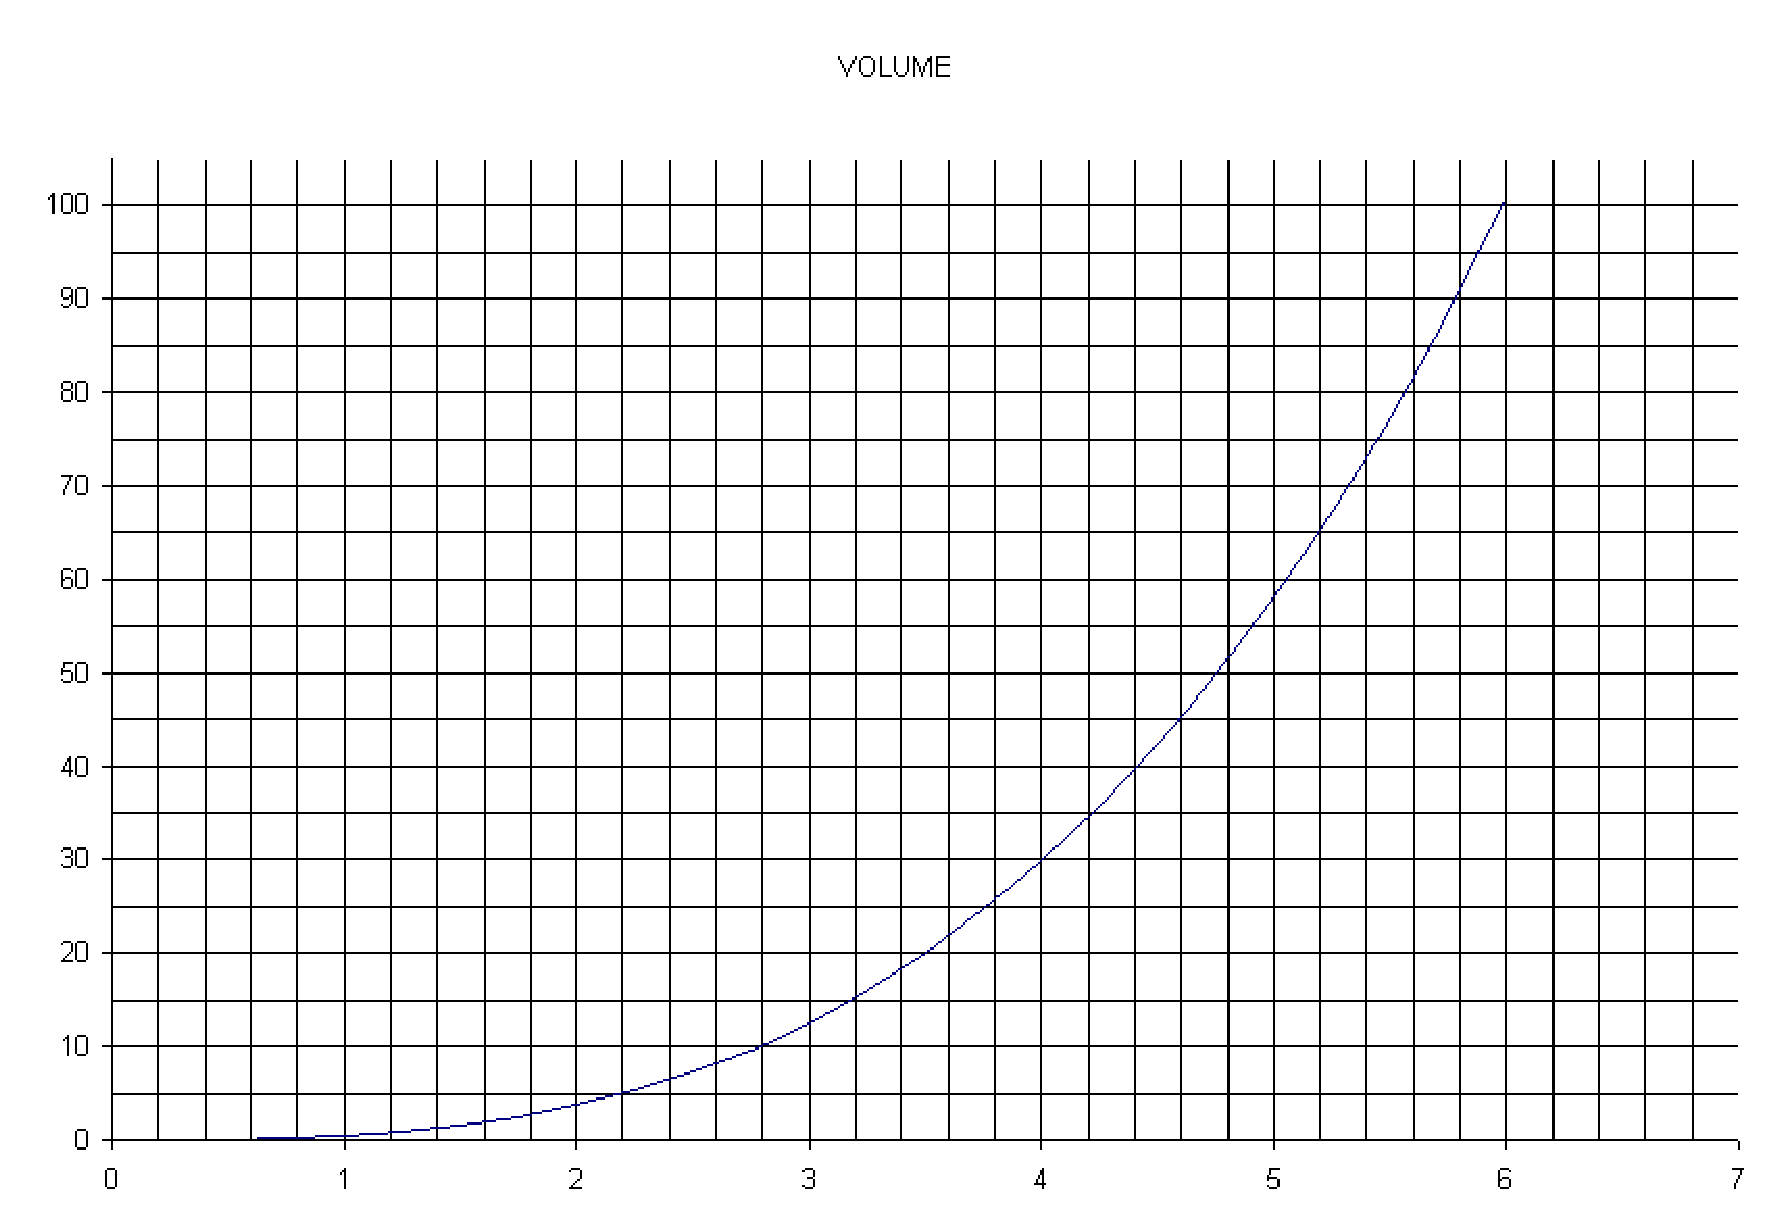
\includegraphics[scale=0.625]{./Graphiques/courbe.eps}\end{center}

%%%%%%%%%%%%%%%%%%%%%%%%%%%%%%%%%%%%%%%%%%%%%%%%%%%%
%%%%%%%%%%%%%%%%%%%%%%%%%%%%%%%%%%%%%%%%%%%%%%%%%%%

%%%%%%%%%%%%%%%%%%%%%%%%%%%%%%%%%%%%%%%%%%%%%%%%%%%\`u
%%%%%%%%%%%%%%%%%%%%%%%%%%%%%%%%%%%%%%%%%%%%%%%%%%%%

 \sautpage

\section{Premi\`eres notions (bilan et compl\'ements)}

\begin{definition}[Notion de fonction]
Une fonction est un proc\'ed\'e qui, \`a un \'el\'ement $x$ d'un ensemble de d\'epart, associe au plus un \'el\'ement $y$ d'un ensemble d'arriv\'ee.

On notera $f:x\mapsto y$ ou $f(x)=y$ qui se lit \og $f$ est la fonction qui \`a $x$ associe $y$ \fg..

On dit que $y$ est \emph{l'image} de $x$.

On dit que $x$ est \emph{un ant\'ec\'edent} de $y$.

\end{definition}

\begin{definition}[Ensemble de d\'efinition]
L'ensemble des r\'eels $x$ poss\'edant une image par une fonction num\'erique $f$ est appel\'e \emph{l'ensemble de d\'efinition de la fonction $f$}. On le note souvent $D_f$.
\end{definition}

\begin{definition}[Repr\'esentation graphique]
Dans un plan muni d'un rep\`ere, la \emph{repr\'esentation graphique} de la fonction $f$ est l'ensemble des points $M$ de coordonn\'ees $(x;y)$ du plan tels que :
\begin{itemize}
	\item L'abscisse $x$ de $M$ d\'ecrit l'ensemble de d\'efinition $D_f$ ;
	\item L'ordonn\'ee $y$ est l'image de $x$ par $f$. $y=f(x)$.
\end{itemize}

On note souvent $\mathcal{C}_f$ la repr\'esentation graphique de $f$. On dit que $\mathcal{C}_f$ a pour \'equation $y=f(x)$.

Si la courbe est d'un seul \og{} tenant \fg{} on parle  de \emph{courbe repr\'esentative} de la fonction $f$.
\end{definition}


\begin{rmq} L'\'equation permet de d\'eterminer si un point $A(x_A;y_A)$ appartient ou pas \`a cette courbe. En effet, un point appartient \`a la courbe si et seulement si ses coordonn\'ees v\'erifient l'\'equation de la courbe. On a alors : \[A\in\mathcal{C}_f\ssi y_A=f(x_A)\] \end{rmq}


Dans la pratique, pour les fonctions num\'eriques d\'efinies par une expression alg\'ebrique, pour esquisser une repr\'esentation graphique, on utilise souvent un tableau de valeurs.

\begin{tabular}{cc}
 \begin{minipage}[l]{0.55\linewidth}
  \begin{rmq} Une courbe ne repr\'esente pas toujours une fonction. Sur la figure ci-contre, par exemple, la courbe a plusieurs points ayant la même abscisse, comme $A(1,-1)$ et $B(1,3)$. Ce n'est donc pas la courbe repr\'esentative d'une fonction car alors 1 aurait plusieurs images.\end{rmq}
 \end{minipage}&
 \begin{minipage}[r]{0.45\linewidth}
\begin{center}
\psset{xunit=0.75cm , yunit=0.75cm}
\def\xmin{-2} \def\xmax{4} \def\ymin{-1.6} \def\ymax{3.6}
\begin{pspicture*}(\xmin,\ymin)(\xmax,\ymax)
\psset{xunit=0.75cm,yunit=0.75cm}
\psgrid[griddots=10,gridlabels=0pt,gridwidth=.3pt, gridcolor=black, subgridwidth=.3pt, subgridcolor=black, subgriddiv=1](0,0)(-2,-2)(4,4)
\psaxes[labels=all,labelsep=1pt, Dx=1,Dy=1]{->}(0,0)(\xmin,\ymin)(\xmax,\ymax)
\uput[dl](0,0){$O$}
%\pcline[linewidth=1pt]{->}(0,0)(1,0) \uput[d](0.5,0){\small $\vec \imath$}
%\pcline[linewidth=1pt]{->}(0,0)(0,1) \uput[l](0,0.5){\small $\vec \jmath$}
\pscircle(1,1){1.5}
\psdots[dotstyle=x](1,-1)(1,3)
\uput[d](1,-1){$A$}
\uput[u](1,3){$B$}
\end{pspicture*}
\end{center}
 \end{minipage}

\end{tabular}






%\sautpage

\subsubsection{Quelques conventions graphiques}
\begin{multicols}{3}
Lorsqu'un point $A$ sur la courbe est connu avec pr\'ecision, il est not\'e par une croix.
\begin{center}
\begin{pspicture*}(-0.5,-1)(2.5,3)
\pscurve(0,0)(0.5,-0.5)(1,1)(2,2.5)
\uput[u](0,0){$\mathcal{C}_f$}
\psdot[dotstyle=x](1,1)
\uput[dr](1,1){$A$}
\end{pspicture*}
\end{center}\sautcol
Lorsqu'un point $A$ est l'extr\'emit\'e de la courbe, il est not\'e par un gros point.
\begin{center}
\begin{pspicture*}(-0.5,-1)(2.5,3)
\pscurve(0,0)(0.5,-0.5)(1,1)(2,2.5)
\uput[u](0,0){$\mathcal{C}_f$}
\psdot(2,2.5)
\uput[dr](2,2.5){$A$}
\end{pspicture*}
\end{center}\sautcol
Lorsqu'un point $A$ \`a l'extr\'emit\'e de la courbe n'appartient pas \`a la courbe, il est not\'e par un \og demi-cercle \fg.
\begin{center}
\begin{pspicture*}(-0.5,-1)(2.5,3)
\pscurve{-(}(0,0)(0.5,-0.5)(1,1)(2,2.5)
\uput[u](0,0){$\mathcal{C}_f$}
%\psdot[(2,2.5)
\uput[dr](2,2.5){$A$}
\end{pspicture*}
\end{center}
\end{multicols}
\begin{multicols}{3}
Une courbe est donn\'ee dans une fenêtre ; s'il n'y a pas d'extr\'emit\'es, la courbe garde la même allure quand on la prolonge.
\begin{center}
\begin{pspicture*}(-0.5,-1)(2.5,3)
\pscurve(-0.3,0)(0.5,2)(1,1)(2,2.8)
\uput[u](1,1){$\mathcal{C}_f$}
\psline[linestyle=dotted](-0.1,0.5)(1.7,0.5)(1.7,2.2)(-0.1,2.2)(-0.1,0.5)
\end{pspicture*}
\end{center}
Une droite verticale en pointill\'es signifie que si l'on prolonge la courbe, elle ne coupe pas cette droite. Sur l'exemple ci-dessous, $a$ n'appartient pas \`a $D_f$.
\begin{center}
\begin{pspicture*}(-0.5,-1)(2.5,3)
\psaxes[labels=none,labelsep=1pt,Dx=5,Dy=5]{->}(0,0)(-0.5,-1)(2.5,3)
\psset{algebraic=true}
\psplot{0.6}{3}{1/(4*x-2)}
\psline[linestyle=dashed](0.5,-1)(0.5,3)
\uput[dl](0.5,0){$a$}
\end{pspicture*}
\end{center}
Une droite horizontale en pointill\'es signifie que si l'on prolonge la courbe, elle ne coupe pas cette droite.
\begin{center}
\begin{pspicture*}(-0.5,-1)(2.5,3)
\psaxes[labels=none,labelsep=1pt,Dx=5,Dy=5]{->}(0,0)(-0.5,-1)(2.5,3)
\psset{algebraic=true}
\psplot{-0.5}{3}{1+1/(x+1)}
\psline[linestyle=dashed](-0.5,1)(2.5,1)
\uput[ul](0,1){$b$}
\end{pspicture*}
\end{center}
\end{multicols}

%\sautpage






\section{R\'esolutions graphiques d'\'equations et d'in\'equations}


\subsection{R\'esolutions d'\'equations de la forme $f(x)=k$}

R\'esoudre l'\'equation $f(x)=k$ c'est d\'eterminer tous les ant\'ec\'edents \'eventuels d'un \'el\'ement $k$ de l'ensemble d'arriv\'ee, c'est-\`a-dire chercher tous les $x$ de l'ensemble de d\'epart tels que $f(x)=k$.

Une telle recherche peut se faire graphiquement \`a partir de la repr\'esentation graphique de la fonction $f$.




\begin{center}
\begin{tabular}{lc}
 \begin{minipage}[l]{0.6\linewidth}
 \begin{exemple*}
  Soit $f$ la fonction d\'efinie sur $\R$ par $f(x)=2x^2-9x+10$. On recherche les solutions de l'\'equation $f(x)=3$.

	On commence par tracer soigneusement la courbe repr\'esentative de $f$ et on obtient la repr\'esentation donn\'ee sur la figure ci-dessous.
		
		On cherche les points de la courbe ayant pour ordonn\'ee 3. Pour cela on peut tracer la droite d'\'equation $y=3$ et chercher les points d'intersection de cette droite avec la courbe de $f$.

		On obtient ici deux points $M_1(1;3)$ et $M_2\left(\frac{7}{2};3\right)$. Les solutions sont leurs abscisses : 1 et $\frac{7}{2}$.

		On \'ecrit : \og Les solutions de l'\'equation $f(x)=3$ sont $x=1$ ou $x=\frac{7}{2}$ car les points de la courbe de $f$ d'ordonn\'ee 3 ont pour abscisses 1 et $\frac{7}{2}$ \fg.
		\end{exemple*}
 \end{minipage}&
 \begin{minipage}[r]{0.35\linewidth}
  
		\begin{center}
 \psset{xunit=1cm,yunit=1cm}
		\begin{pspicture*}(-3.1,-2.1)(4.6,4.1)
\def\xmin{-3} \def\xmax{4.5} \def\ymin{-2} \def\ymax{4}

\psgrid[griddots=10,gridlabels=0pt,gridwidth=.3pt, gridcolor=black, subgridwidth=.3pt, subgridcolor=black, subgriddiv=1](0,0)(-3,-2)(4.5,4)
\psaxes[labels=all,labelsep=1pt, Dx=1,Dy=1]{->}(0,0)(\xmin,\ymin)(\xmax,\ymax)
\uput[dl](0,0){$O$}
\pcline[linewidth=1pt]{->}(0,0)(1,0) \uput[d](0.5,0){\small $\vec \imath$}
\pcline[linewidth=1pt]{->}(0,0)(0,1) \uput[r](0,0.5){\small $\vec \jmath$}
\psset{algebraic=true}
\psplot{\xmin}{\xmax}{2*(x-1)*(x-1)-5*(x-1)+3}
\uput[ul](2,1){$\mathcal{C}_f$}
\psline[linestyle=dashed](\xmin,3)(\xmax,3)
\uput[u](-2,3){$y=3$}
\uput[ur](1,3){$M_1$}
\uput[ul](3.5,3){$M_2$}
\psdots[dotstyle=x](1,3)(3.5,3)
\psline[linestyle=dashed]{->}(1,3)(1,0)
\psline[linestyle=dashed]{->}(3.5,3)(3.5,0)
\end{pspicture*}\end{center}
 \end{minipage}

\end{tabular}             \end{center}



%\sautpage

\subsection{R\'esolutions d'in\'equations de la forme $f(x)\leqslant k$}

Ces in\'equations peuvent se r\'esoudre graphiquement. On proc\`ede de la façon suivante :
\begin{itemize}
	\item on trace soigneusement $\mathcal{C}_f$ dan un rep\`ere (orthogonal) ;
	\item on trace la droite d'\'equation $y=k$ ;
	\item on recherche les points de la courbe situ\'es \emph{sous} la droite ;
	\item l'ensemble des solutions est constitu\'e des abscisses de ces points.
\end{itemize}

\begin{exemple*} Sur l'exemple pr\'ec\'edent, si l'on doit r\'esoudre $f(x)\leqslant 3$, apr\`es avoir trac\'e $y=3$ on constate que les points de la courbe situ\'es sous cette droite ont leurs abscisses comprises entre 0 et $\frac{5}{2}$.

Donc $f(x)\leqslant 3 \ssi x\in\left[0;\frac{5}{2}\right]$.
\end{exemple*}

\begin{rmq}~
\begin{itemize}
	\item On r\'esoud de la même mani\`ere les \'equations du type $f(x)\geqslant k$.

On retient alors les abscisses des points situ\'es \emph{au-dessus} de la droite d'\'equation $y=k$.

Dans l'exemple $f(x)\geqslant 3 \ssi x\in \left] -\infty ; 0 \right] \cup \left[\frac{5}{2} ; +\infty\right[$.
	\item De même pour les in\'equations strictes : $f(x)>k$ ou $f(x)<k$. On excluera alors les abscisses des points d'intersection de la courbe et de la droite.

	Dans l'exemple $f(x)<3 \ssi x\in \left]0;\frac{5}{2}\right[$.
\end{itemize}
\end{rmq}

\subsection{R\'esolutions d'\'equations de la forme $f(x)=g(x)$}

Cela revient \`a chercher les \'el\'ements de l'ensemble de d\'epart qui ont la même image par $f$ et par $g$.

Une telle recherche peut se faire graphiquement. On recherche alors les points des deux courbes repr\'esentatives ayant même abscisse et même ordonn\'ee, c'est-\`a-dire les points d'intersection des deux courbes. 

\begin{tabular}{cc}
 \begin{minipage}[l]{0.6\linewidth}
  \begin{exemple*}

Soit $f$ et $g$ les fonctions d\'efinies sur $\R$ par, respectivement, $f(x)=x^2-1$ et $g(x)=-0,5x^2+x+4$. R\'esoudre graphiquement l'\'equation $f(x)=g(x)$.

	On commence par tracer soigneusement les deux courbes repr\'esentatives et on obtient la repr\'esentation donn\'ee sur la figure ci-contre.
	
	On cherche les points d'intersection des deux courbes, ici $M_1$ et $M_2$, et les solutions de l'\'equation sont leurs abscisses dont les valeurs approximatives sont $-1,5$ et $2,2$.

		Les solutions sont donc $x\approx -1,5$ et $x\approx 2,2$.
\end{exemple*}
 \end{minipage}&
 \begin{minipage}[r]{0.35\linewidth}
  \psset{xunit=0.75cm,yunit=0.75cm}
		\begin{pspicture*}(-3.1,-2.1)(4.6,5.1)
\def\xmin{-3} \def\xmax{4.5} \def\ymin{-2} \def\ymax{5}

\psgrid[griddots=10,gridlabels=0pt,gridwidth=.3pt, gridcolor=black, subgridwidth=.3pt, subgridcolor=black, subgriddiv=1](0,0)(-3,-2)(4.5,5)
\psaxes[labels=all,labelsep=1pt, Dx=1,Dy=1]{->}(0,0)(\xmin,\ymin)(\xmax,\ymax)
\uput[dl](0,0){$O$}
\pcline[linewidth=1pt]{->}(0,0)(1,0) \uput[d](0.5,0){\small $\vec \imath$}
\pcline[linewidth=1pt]{->}(0,0)(0,1) \uput[r](0,0.5){\small $\vec \jmath$}
\psset{algebraic=true}
\psplot{\xmin}{\xmax}{x^2-1}
\psplot{\xmin}{\xmax}{-0.5*x^2+x+4}
\uput[u](1,1){$\mathcal{C}_f$}
\uput[dr](0,4){$\mathcal{C}_g$}
\uput[r](2.189,3.793){$M_2$}
\uput[l](-1.523,1.318){$M_1$}
\psdots[dotstyle=x](2.189,3.793)(-1.523,1.318)
\psline[linestyle=dashed]{->}(-1.523,1.318)(-1.523,0)
\psline[linestyle=dashed]{->}(2.189,3.793)(2.189,0)
\end{pspicture*}
	
 \end{minipage}


\end{tabular}

		

\subsection{R\'esolutions d'in\'equations de la forme $f(x)\leqslant g(x)$}

L\`a encore ces in\'equations peuvent se r\'esoudre graphiquement. On proc\`ede de la façon suivante :
\begin{itemize}
	\item on trace soigneusement $\mathcal{C}_f$ et $\mathcal{C}_g$ dans un rep\`ere (orthogonal) ;
	\item l'ensemble des solutions est constitu\'e des abscisses des points o\`u la courbe de $f$ est situ\'ee \emph{sous} celle de $g$.
\end{itemize}

\begin{exemple*} Sur l'exemple pr\'ec\'edent, si l'on doit r\'esoudre $f(x)\leqslant g(x)$, on constate que les points de la courbe de $f$ situ\'es sous celle de $g$ ont leurs abscisses comprises entre environ $-1,5$ et 2,2.

Donc $f(x)\leqslant g(x) \ssi x\in [-1,5;2,2]$. Ou bien $S=[-1,5;2,2]$.
\end{exemple*}

\begin{rmqs}~
\begin{itemize}
	\item On r\'esoud de la même mani\`ere les \'equations du type $f(x)\geqslant g(x)$.

On retient alors les abscisses des points de la courbe de $f$ situ\'es \emph{au-dessus} de celle de $g$.

Dans l'exemple $f(x)\geqslant g(x) \ssi x\in ] -\infty ; -1,5 ] \cup [2,2 ; +\infty[$.
	\item De même pour les in\'equations strictes : $f(x)>g(x)$ ou $f(x)<g(x)$. On excluera alors les abscisses des points d'intersection des deux courbes.

	Dans l'exemple $f(x)<g(x) \ssi x\in ]-1,5;2,2[$.
\end{itemize}
\end{rmqs}



%\sautpage



\sautpage

\section{Variations, extremums}


\subsection{Sens de variation}

Il s'agit de traduire math\'ematiquement qu'une fonction \og augmente \fg{} ou \og diminue \fg.

\begin{exemple*} Soit, par exemple, la fonction d\'efinie sur $[-3;3]$ par la courbe repr\'esentative donn\'ee sur la figure \ref{croissanceetdecroissance} \vpageref{croissanceetdecroissance}. On constate que lorsque $x\in[-3;1]$ , si $x$ augmente, $f(x)$ augmente aussi alors que lorsque $x\in[1;3]$, si $x$ augmente, $f(x)$ diminue.

C'est la d\'efinition math\'ematique de la croissance ou de la d\'ecroissance d'une fonction $f$.

\begin{figure}[h]
\centering
\caption{Croissance et d\'ecroissante}\label{croissanceetdecroissance}


\psset{xunit=1cm , yunit=1.25cm}
\begin{pspicture*}(-4.1,-1.1)(4.1,5.1)
\def\xmin{-4} \def\xmax{4} \def\ymin{-1} \def\ymax{5}
\psgrid[griddots=10,gridlabels=0pt,gridwidth=.3pt, gridcolor=black, subgridwidth=.3pt, subgridcolor=black, subgriddiv=1](0,0)(-4,-1)(4,5)
\psaxes[labels=all,labelsep=1pt, Dx=1,Dy=1]{-}(0,0)(\xmin,\ymin)(\xmax,\ymax)
\uput[dl](0,0){$O$}
\pcline[linewidth=1pt]{->}(0,0)(1,0) \uput[d](0.5,0){\small $\vec \imath$}
\pcline[linewidth=1pt]{->}(0,0)(0,1) \uput[r](0,0.5){\small $\vec \jmath$}
\psset{algebraic=true}
\psplot{-3}{3}{(-(x-1)^2+5)*0.25+3}
\psdots(3,3.25)(-3,0.25)
\uput[d](-1.5,0){$b$}
\psline[linestyle=dashed]{->}(-1.5,0)(-1.5,2.6875)
\psline[linestyle=dashed]{->}(-1.5,2.6875)(0,2.6875)
\uput[r](0,2.6875){$f(b)$}
\uput[d](-2.5,0){$a$}
\psline[linestyle=dashed]{->}(-2.5,0)(-2.5,1.1875)
\psline[linestyle=dashed]{->}(-2.5,1.1875)(0,1.1875)
\uput[r](0,1.1875){$f(a)$}
\uput[d](1.5,0){$u$}
\uput[d](2.5,0){$v$}
\psline[linestyle=dashed]{->}(1.5,0)(1.5,4.1875)
\psline[linestyle=dashed]{->}(1.5,4.1875)(0,4.1875)
\uput[l](0,4.1875){$f(u)$}
\psline[linestyle=dashed]{->}(2.5,0)(2.5,3.6875)
\psline[linestyle=dashed]{->}(2.5,3.6875)(0,3.6875)
\uput[l](0,3.6875){$f(v)$}
\end{pspicture*}
\end{figure}\end{exemple*}


\begin{definition}
Soit $f$ une fonction d\'efinie sur un intervalle $I$. On dit que $f$ est
\begin{itemize}
	\item \emph{croissante} sur $I$ si, pour tous r\'eels $a$ et $b$ de $I$, on a :\\
$\text{Si } a<b \text{ alors } f(a)\leqslant f(b).$
	\item \emph{d\'ecroissante} sur $I$ si, pour tous r\'eels $a$ et $b$ de $I$, on a :\\
$\text{Si } a<b \text{ alors } f(a)\geqslant f(b).$
	\item \emph{monotone} si elle n'est que croissante sur $I$ ou si elle n'est que d\'ecroissante sur $I$.
	\item \emph{constante} sur $I$ si, pour tous r\'eels $a$ et $b$ de $I$, on a : $f(a)=f(b)$.
\end{itemize}
\end{definition}


\begin{rmqs}~
\begin{itemize}
	\item Ces notions ne sont valables que sur \textbf{un intervalle} et pas sur une r\'eunion d'intervalles disjoints.
	\item Ant\'ec\'edents et images \'etant rang\'es dans le même ordre, on dit qu'une fonction croissante \emph{conserve} l'ordre.
	\item Ant\'ec\'edents et images \'etant rang\'es dans l'ordre inverse, on dit qu'une fonction d\'ecroissante \emph{inverse} l'ordre.
	\item On obtient les d\'efinitions d'une fonction \emph{strictement} croissante ou \emph{strictement} d\'ecroisante en remplaçant les in\'egalit\'es par des in\'egalit\'es strictes. Ainsi on dit que $f$ est strictement croissante sur $I$ si pour tous r\'eels $a$ et $b$ de $I$ on a : \\ $\text{Si } a<b \text{ alors } f(a)<f(b)$
	\item Une fonction est strictement monotone sur $I$ si elle est strictement croissante ou strictement d\'ecroissante sur $I$
\end{itemize}
\end{rmqs}

\subsection{Tableau de variations}

Ces r\'esultats peuvent se r\'esumer dans un tableau de variation, qui est une forme stylis\'ee de repr\'esentation o\`u l'on indique uniquement si la courbe monte, descend ou est stable. Dans la premi\`ere ligne on indique les valeurs importantes de $x$ et dans la seconde les variations de $f$.

\begin{exemple*} Dans l'exemple pr\'ec\'edent on obtient
$$\tabvar{%
\tx{x}&\tx{-3}&&\tx{1}&&\tx{3}\cr
\tx{f}&\txb{\approx 0,25}&\fm&\txh{\approx 4,25}&\fd&\txb{\approx 2,25}\cr
}$$
\end{exemple*}



\subsection{Extremums}

Les extremums, s'ils existent, sont les valeurs maximale et minimale qui sont \textbf{atteintes} par la fonction $f$ sur un intervalle donn\'e. Plus pr\'ecis\'ement :

\begin{definition}
Soit une fonction $f$ d\'efinie sur un intervalle $I$ et $x_0\in I$. On dit que
\begin{itemize}
	\item $f$ admet un \emph{maximum}, atteint en $x_0$ si, pour tout $x\in I$, $f(x)\leqslant f(x_0)$. Ce maximum est alors $f(x_0)$.
	\item $f$ admet un \emph{minimum}, atteint en $x_0$ si, pour tout $x\in I$, $f(x)\geqslant f(x_0)$. Ce minimum est alors $f(x_0)$.
\end{itemize}
Les maximum et minimum sont appel\'es les \emph{extremums}.
\end{definition}

%\begin{rmq} Un extremum doit être atteint par une valeur $x_0$. \end{rmq}

\begin{exemple*}
La fonction $f$ d\'efinie sur $\R$ par $f(x)=x^2+1$ n'admet pas $-1$ comme minimum.

En effet, si on a bien $f(x)\geqslant -1$ sur $\R$, il n'existe pas de $x_0$ tel que $f(x_0)=-1$.

Par contre 1 est bien le minimum de $f$ sur $\R$ car
\begin{itemize}
	\item $f(x)\geqslant 1$ pour tout $x\in\R$ \textbf{ET}
	\item $f(0)=1$
\end{itemize}

On dira donc : le minimum de $f$ sur $\R$ est 1 et il est atteint pour $x_0=0$.
\end{exemple*}

\sautpage

\section{Exercices et probl\`emes}

\subsection{Premi\`eres notions}

%\begin{multicols}{2}
%\begin{exo} Dire dans chacun des exemples ci-dessous quel est l'ensemble de d\'efinition, quelles sont les images possibles et si la fonction est num\'erique.
%\begin{enumerate}
%	\item \`A chaque \'el\`eve de la classe on associe la couleur de ses cheveux.
%	\item \`A chaque \'el\`eve de la classe on associe le nombre de ses fr\`eres et soeurs.
%	\item Pour un \'el\`eve donn\'e, \`a chaque moment de sa vie on associe la taille qu'il mesurait.
%	\item Soit $ABCD$ un rectangle dont un des côt\'es est fixe et mesure 6 cm et l'autre est variable et mesure $x$ cm. \\On d\'efinit la fonction $f$ de la façon suivante : \`a chaque $x$ possible, on associe $f(x)$, l'aire du rectangle $ABCD$.
%	\item La fonction $g$ d\'efinie par $g(x)=x^2+2x+3$.
%	\item La fonction $h$ d\'efinie par $h(x)=\frac{x^2+1}{x-1}$.
%	\item La fonction $i$ d\'efinie par $i(x)=\sqrt{x+2}$.
%\end{enumerate}
%\end{exo}
\begin{multicols}{2}
\begin{exo}
On d\'efinit $f$ et $g$, deux fonctions :
\begin{itemize}
	\item $f$ est la fonction qui \`a un nombre r\'eel $x$ associe le nombre obtenu en proc\'edant de la mani\`ere suivante : on ajoute $4$ au nombre, on \'el\`eve le r\'esultat obtenu au carr\'e, on retranche 16, on divise par le nombre de d\'epart et on retranche 6.
	\item $g:x\mapsto x^2-4$.
\end{itemize}
\begin{enumerate}
	\item Donner l'expression correspondant \`a $f$ puis simplifier cette expression.
	\item Quel r\'eel n'a pas d'image par $f$ ?
	\item Quelle est l'image de 3 par $g$ ?
	\item Quelle est l'image de $-1$ par $g$ ?
	\item Quels sont les ant\'ec\'edents \'eventuels de 12 par $g$ ?
	\item Quels sont les ant\'ec\'edents \'eventuels de $-5$ par $g$ ?
\end{enumerate}
\end{exo}

\sautcol

\begin{exo}
Vrai ou faux ? \emph{Corriger la phrase lorsqu'elle est fausse}.
\begin{enumerate}
	\item $f(-2) = 0$ signifie que l'image de 0 est $-2$
	\item $f(0) = 3$ signifie que la courbe de $f$ passe par le point $(0 ; 3)$
	\item $f(1) = 2$ signifie que l'ant\'ec\'edent de 1 est 2
	\item L'image de 2 par $f$ est $-3$ s'\'ecrit $f(2) = -3$
	\item Dire que $(5 ; 1)$ est un point de la courbe de $f$ s'\'ecrit $5 = f(1)$
	\item Par la fonction $g$, $-5$ est l'image de 3 s'\'ecrit $g(-5) = 3$
	\item 2 a pour image 0 par $f$ signifie que la courbe de $f$ traverse l'axe des abscisses en 2
	\item $f(4) = 0$ signifie que la courbe de $f$ traverse l'axe des abscisses au point $(4 ; 0)$
	\item 3 a pour image 5, signifie que 3 est l'image de 5
	\item 4 a pour ant\'ec\'edent 5 signifie que 5 est l'image de 4
\end{enumerate}
\end{exo}

\end{multicols}

%\sautpage

\begin{exo}\label{gf4courbes}
Vrai ou faux ? \emph{Justifier la r\'eponse lorsque c'est faux}.\\
Les courbes de la figure \ref{gf4courbesfig} \vpageref{gf4courbesfig} repr\'esentent des fonctions de la variable $x$.


\begin{figure}[!h]
 \centering
 \caption{Courbes de l'exercice \ref{gf4courbes}}\label{gf4courbesfig}
\begin{tabular}{cc}
\psset{xunit=1cm , yunit=0.5cm}
\begin{pspicture*}(-2.1,-2.1)(4.1,4.1)
\def\xmin{-2} \def\xmax{4} \def\ymin{-2} \def\ymax{4}
\psgrid[griddots=10,gridlabels=0pt,gridwidth=.3pt, gridcolor=black, subgridwidth=.3pt, subgridcolor=black, subgriddiv=1](0,0)(-2,-2)(4,4)
\psaxes[labels=all,labelsep=1pt, Dx=1,Dy=1]{->}(0,0)(\xmin,\ymin)(\xmax,\ymax)
\uput[dl](0,0){$O$}
\pcline[linewidth=1pt]{->}(0,0)(1,0) \uput[d](0.5,0){\small $\vec \imath$}
\pcline[linewidth=1pt]{->}(0,0)(0,1) \uput[l](0,0.5){\small $\vec \jmath$}
\psline(-2,3)(1,-1.5)(2,-1.5)(4,2)
\end{pspicture*}
&
\psset{xunit=1cm , yunit=0.5cm}
\begin{pspicture*}(-2.1,-2.1)(4.1,4.1)
\def\xmin{-2} \def\xmax{4} \def\ymin{-2} \def\ymax{4}
\psgrid[griddots=10,gridlabels=0pt,gridwidth=.3pt, gridcolor=black, subgridwidth=.3pt, subgridcolor=black, subgriddiv=1](0,0)(-2,-2)(4,4)
\psaxes[labels=all,labelsep=1pt, Dx=1,Dy=1]{->}(0,0)(\xmin,\ymin)(\xmax,\ymax)
\uput[dl](0,0){$O$}
\pcline[linewidth=1pt]{->}(0,0)(1,0) \uput[d](0.5,0){\small $\vec \imath$}
\pcline[linewidth=1pt]{->}(0,0)(0,1) \uput[l](0,0.5){\small $\vec \jmath$}
\psline(-2,3)(1,3)(1,1)(4,1)
\end{pspicture*}
\\
\psset{xunit=1cm , yunit=0.5cm}
\begin{pspicture*}(-2.1,-2.1)(4.1,4.1)
\def\xmin{-2} \def\xmax{4} \def\ymin{-2} \def\ymax{4}
\psgrid[griddots=10,gridlabels=0pt,gridwidth=.3pt, gridcolor=black, subgridwidth=.3pt, subgridcolor=black, subgriddiv=1](0,0)(-2,-2)(4,4)
\psaxes[labels=all,labelsep=1pt, Dx=1,Dy=1]{->}(0,0)(\xmin,\ymin)(\xmax,\ymax)
\uput[dl](0,0){$O$}
\pcline[linewidth=1pt]{->}(0,0)(1,0) \uput[d](0.5,0){\small $\vec \imath$}
\pcline[linewidth=1pt]{->}(0,0)(0,1) \uput[l](0,0.5){\small $\vec \jmath$}
\psline(-2,3)(4,3)
\end{pspicture*}
&
\psset{xunit=1cm , yunit=0.5cm}
\begin{pspicture*}(-2.1,-2.1)(4.1,4.1)
\def\xmin{-2} \def\xmax{4} \def\ymin{-2} \def\ymax{4}
\psgrid[griddots=10,gridlabels=0pt,gridwidth=.3pt, gridcolor=black, subgridwidth=.3pt, subgridcolor=black, subgriddiv=1](0,0)(-2,-2)(4,4)
\psaxes[labels=all,labelsep=1pt, Dx=1,Dy=1]{->}(0,0)(\xmin,\ymin)(\xmax,\ymax)
\uput[dl](0,0){$O$}
\pcline[linewidth=1pt]{->}(0,0)(1,0) \uput[d](0.5,0){\small $\vec \imath$}
\pcline[linewidth=1pt]{->}(0,0)(0,1) \uput[l](0,0.5){\small $\vec \jmath$}
\pscurve(-2,3)(-1,0)(0,-1)(2,1)(3.2,2)(3,3)
\end{pspicture*}
\end{tabular}
\end{figure}

\end{exo}

\sautpage

\begin{exo}\label{gf14}
Vrai ou faux ? \emph{Corriger la phrase lorsqu'elle est fausse}.\\
Les fonctions $f$ et $g$ sont repr\'esent\'ees sur la figure \ref{gf14fig} \vpageref{gf14fig}.
\begin{enumerate}
	\item La fonction $f$ est d\'efinie entre $-2$ et 6 inclus
	\item Les images par la fonction $f$ sont comprises entre $-1$ et 4 inclus
	\item La fonction $g$ est d\'efinie entre $-2$ exclu et 6 inclus
	\item Les images par la fonction g sont comprises entre 0 exclu et 3 inclus
\end{enumerate}



\begin{figure}[!h]
\centering
\caption{Courbes de l'exercice \ref{gf14}}\label{gf14fig}
\begin{tabular}{cc}
\psset{xunit=0.9cm , yunit=0.5cm}
\begin{pspicture*}(-3.1,-2.1)(6.1,5.1)
\def\xmin{-3} \def\xmax{6} \def\ymin{-2} \def\ymax{5}
\psgrid[griddots=10,gridlabels=0pt,gridwidth=.3pt, gridcolor=black, subgridwidth=.3pt, subgridcolor=black, subgriddiv=1](0,0)(-3,-2)(6,5)
\psaxes[labels=all,labelsep=1pt, Dx=1,Dy=1]{->}(0,0)(\xmin,\ymin)(\xmax,\ymax)
\uput[dl](0,0){$O$}
\pcline[linewidth=1pt]{->}(0,0)(1,0) \uput[d](0.5,0){\small $\vec \imath$}
\pcline[linewidth=1pt]{->}(0,0)(0,1) \uput[l](0,0.5){\small $\vec \jmath$}
\pscurve{*-(}(-2,2)(-1,3)(0,3.7)(0.5,3.9)(1,4)(2,3)(3,0)(4,-1)(5,0)(6,1)

\rput(3,2){$\mathcal{C}_f$}
\end{pspicture*}
&
\psset{xunit=0.9cm , yunit=0.5cm}
\begin{pspicture*}(-3.1,-2.1)(6.1,5.1)
\def\xmin{-3} \def\xmax{6} \def\ymin{-2} \def\ymax{5}
\psgrid[griddots=10,gridlabels=0pt,gridwidth=.3pt, gridcolor=black, subgridwidth=.3pt, subgridcolor=black, subgriddiv=1](0,0)(-3,-2)(6,5)
\psaxes[labels=all,labelsep=1pt, Dx=1,Dy=1]{->}(0,0)(\xmin,\ymin)(\xmax,\ymax)
\uput[dl](0,0){$O$}
\pcline[linewidth=1pt]{->}(0,0)(1,0) \uput[d](0.5,0){\small $\vec \imath$}
\pcline[linewidth=1pt]{->}(0,0)(0,1) \uput[l](0,0.5){\small $\vec \jmath$}
\pscurve{)-}(-2,0)(0,1)(1,2)(1.5,3.5)(1.8,5)
\pscurve{-*}(2.2,-2)(3,0)(4,1.5)(6,3)
\rput(1,3){$\mathcal{C}_g$}
\psline[linestyle=dashed](2,\ymin)(2,\ymax)
\end{pspicture*}
\end{tabular}
\end{figure}

\end{exo}

\begin{exo}\label{gf15}
Vrai ou faux ? \emph{Corriger la proposition lorsqu'elle est fausse}.
\begin{itemize}
	\item D'apr\`es la repr\'esentation graphique de la figure \ref{gf15fig} \vpageref{gf15fig} $D_f=[-4;2]$
	\item D'apr\`es la repr\'esentation graphique de la figure \ref{gf15fig} \vpageref{gf15fig} $D_g=]-\infty;3[\cup]3;5]$
\end{itemize}


\begin{figure}[!h]
\centering
\caption{Courbes de l'exercice \ref{gf15}}\label{gf15fig}
\begin{tabular}{cc}
\psset{xunit=1cm , yunit=0.66cm}
\begin{pspicture*}(-4.1,-2.1)(4.1,4.1)
\def\xmin{-4} \def\xmax{4} \def\ymin{-2} \def\ymax{4}
\psgrid[griddots=10,gridlabels=0pt,gridwidth=.3pt, gridcolor=black, subgridwidth=.3pt, subgridcolor=black, subgriddiv=1](0,0)(-4,-2)(4,4)
\psaxes[labels=all,labelsep=1pt, Dx=1,Dy=1]{->}(0,0)(\xmin,\ymin)(\xmax,\ymax)
\uput[dl](0,0){$O$}
\pcline[linewidth=1pt]{->}(0,0)(1,0) \uput[d](0.5,0){\small $\vec \imath$}
\pcline[linewidth=1pt]{->}(0,0)(0,1) \uput[l](0,0.5){\small $\vec \jmath$}
\pscurve{*-}(-4,0)(-3,-2)(0,0)(1,1)(4,1.8)
\psline[linestyle=dashed](0,2)(4,2)
\rput(-1.5,-1){$\mathcal{C}_f$}
\end{pspicture*}
&
\psset{xunit=1cm , yunit=0.66cm}
\begin{pspicture*}(-3.1,-2.1)(5.6,4.1)
\def\xmin{-3} \def\xmax{5.5} \def\ymin{-2} \def\ymax{4}
\psgrid[griddots=10,gridlabels=0pt,gridwidth=.3pt, gridcolor=black, subgridwidth=.3pt, subgridcolor=black, subgriddiv=1](0,0)(-3,-2)(5.5,4)
\psaxes[labels=all,labelsep=1pt, Dx=1,Dy=1]{->}(0,0)(\xmin,\ymin)(\xmax,\ymax)
\uput[dl](0,0){$O$}
\pcline[linewidth=1pt]{->}(0,0)(1,0) \uput[d](0.5,0){\small $\vec \imath$}
\pcline[linewidth=1pt]{->}(0,0)(0,1) \uput[l](0,0.5){\small $\vec \jmath$}
\pscurve(-3,3)(0,1.5)(1,1)(2,0)(2.8,-2)
\pscurve{-*}(3.2,-2)(4,1)(5,3)
\psline[linestyle=dashed](3,\ymin)(3,\ymax)
\uput[ur](1,1){$\mathcal{C}_g$}
\end{pspicture*}
\end{tabular}
\end{figure}
\end{exo}
%\sautpage


\begin{exo}[Avec la calculatrice]
La fonction $f$ est d\'efinie sur $[-1,5;2]$ par : $f(x)=2x^3-1,5x^2-3x$
\begin{enumerate}
	\item Compl\'eter le tableau de valeurs suivant :
	%\vspace{-1em}
	\begin{center}
\begin{tabular}{|*{9}{c|}}
\hline $x$ & $-1,5$ & $-1$ & $-0,5$ & 0 & 0,5 & 1 & 1,5 & 2 \\ \hline
$f(x)$ & & & & & & & & \\ \hline
\end{tabular}
\end{center}
\item Tracer la courbe repr\'esentative de $f$.
\end{enumerate}
\end{exo}

\begin{exo}[Avec la calculatrice]\label{uneautrecourbe}
La fonction $f$ est d\'efinie sur $[-3;3]$ par : $f(x)=x^2-3x+1$.\\
Apr\`es avoir dress\'e un tableau de valeurs de la fonction, tracer sa courbe repr\'esentative $\mathcal{C}_f$.

\end{exo}

%\end{multicols}



\sautpage

\subsection{R\'esolutions graphiques}

\begin{exo}
La fonction $f$ est d\'efinie sur $[-3;3]$ par : $f(x)=x^2-3x+1$.\\
$\mathcal{C}_f$, courbe repr\'esentative de $f$ a d\'ej\`a \'et\'e obtenue dans l'exercice \ref{uneautrecourbe}.
\begin{enumerate}
	\item \`A l'aide de la repr\'esentation graphique $\mathcal{C}_f$, avec la pr\'ecision permise par le graphique, r\'epondre aux question suivantes :
		\vspace{-1em}\begin{multicols}{2}
		  \begin{enumerate}
			\item Quelle est l'image de 2 ?
			\item Quelle est l'image de 3 ?
			\item Quelle est l'image de 4 ?
			\item Quels sont les ant\'ec\'edents de 1 ?
			\item Quels sont les ant\'ec\'edents de 2 ?
			\item Quels sont les ant\'ec\'edents de $-2$ ?
		\end{enumerate}
		\end{multicols}\vspace{-1em}
	\item R\'esoudre graphiquement les \'equations et in\'equations suivantes :
\vspace{-1em}\begin{multicols}{3}\begin{enumerate}
	\item $f(x)=3$ ;
	\item $f(x)=-1,5$ ;
	\item $f(x)\geqslant -1$ ;
	\item $f(x)<4$ ;
	\item $f(x)>-3$ ;
	\item $f(x)<-2$.
\end{enumerate}\end{multicols}\vspace{-1em}
\item D\'eterminer graphiquement le signe de $f(x)$ selon les valeurs de $x$.
\end{enumerate}
\end{exo}

%\sautpage

\begin{exo}
Une fonction $f$, d\'efinie sur $\R$, est donn\'ee par sa courbe repr\'esentative $\mathcal{C}$ :
\begin{multicols}{2}
\begin{center}\small
\psset{xunit=1,yunit=1}
\begin{pspicture*}(-2.6,-2.1)(5.1,3.1)
\def\xmin{-2.5} \def\xmax{5} \def\ymin{-2} \def\ymax{3}
\psset{xunit=0.1cm,yunit=0.1cm}
\psgrid[griddots=15,gridlabels=0pt,gridwidth=.3pt, gridcolor=gray, subgridwidth=.3pt, subgridcolor=gray, subgriddiv=1](0,0)(-25,-20)(50,30)
\psset{xunit=1cm , yunit=1cm}
\psaxes[labels=all,labelsep=1pt, Dx=1,Dy=1]{->}(0,0)(\xmin,\ymin)(\xmax,\ymax)
\uput[dl](0,0){$0$}
\pcline[linewidth=1pt]{->}(0,0)(1,0) \uput[d](0.5,0){\small $\vec i$}
\pcline[linewidth=1pt]{->}(0,0)(0,1) \uput[l](0,0.5){\small $\vec j$}
\pscurve(-2.3,-2)(-2,-1)(-1.5,1.5)(-1,3)(-0.5,2.5)(0,1)(0.2,0)(0.5,-1)(1,-1.5)(1.5,-1)(2,0)(2.5,1)(3,1.5)(4,2)(5,2.3)
\psline[linestyle=dashed](0,2.5)(\xmax,2.5)
\psdots[dotstyle=x](-2,-1)(-1.5,1.5)(-1,3)(-0.5,2.5)(0,1)(0.5,-1)(1,-1.5)(1.5,-1)(2,0)(2.5,1)(3,1.5)(4,2)
\end{pspicture*}
\end{center}\normalsize

\sautcol

Avec la pr\'ecision permise par le graphique, r\'esoudre :
%\vspace{-1em}
%\begin{multicols}{2}
\begin{enumerate}
	\item Les \'equations suivantes :
		\vspace{-1em}
		\begin{multicols}{2}\begin{enumerate}
			\item $f(x) = 1$ ;
			\item $f(x) = 0$ ;
			\item $f(x) = -1$ ;
			\item $f(x) = 2$.
		\end{enumerate}\end{multicols}
		%\vspace{-1em}
%\sautcol
	\item Les in\'equations suivantes :
		\vspace{-1em}
		\begin{multicols}{2}\begin{enumerate}
			\item $f(x)\geqslant 1$ ;
			\item $f(x)\geqslant 0$ ;
			\item $f(x)<-1$ ;
			\item $f(x)>2$.
		\end{enumerate}\end{multicols}
		\vspace{-1em}
	\item D\'eterminer graphiquement le signe de $f(x)$ selon les valeurs de $x$.

\end{enumerate}\end{multicols}
%\vspace{-1em}
\end{exo}

\medskip

\begin{multicols}{2}

\begin{exo}\label{gfunecourbe}
La courbe $\mathcal{C}$ de la figure ci-dessous %\ref{gfunecourbefig} \vpageref{gfunecourbefig} 
repr\'esente une fonction $f$ et le segment de droite $\mathcal{D}$ repr\'esente une fonction $g$.

%\begin{figure}[hbtp]
% \centering
% \caption{Figure de l'exercice \ref{gfunecourbe}}\label{gfunecourbefig}


\begin{center}
\psset{xunit=0.375cm , yunit=0.33cm}
\def\xmin{-9} \def\xmax{12} \def\ymin{-3} \def\ymax{11}
\begin{pspicture*}(\xmin,\ymin)(\xmax,\ymax)
\psgrid[griddots=10,gridlabels=0pt,gridwidth=.3pt, gridcolor=black, subgridwidth=.3pt, subgridcolor=black, subgriddiv=1](0,0)(\xmin,\ymin)(\xmax,\ymax)
\psaxes[labels=all,labelsep=1pt, Dx=5,Dy=5]{-}(0,0)(\xmin,\ymin)(\xmax,\ymax)
\uput[dl](0,0){$O$}
\pcline[linewidth=1pt]{->}(0,0)(1,0) \uput[d](0.5,0){\small $\vec \imath$}
\pcline[linewidth=1pt]{->}(0,0)(0,1) \uput[l](0,0.5){\small $\vec \jmath$}
\pscurve{*-*}(-8,1)(-5,3)(-3,5)(-1,6)(0,5)(1,3)(2,0)(4,-2)(7,0)(9,3)(11,6)
\psdots[dotstyle=x](-5,3)(-3,5)(-1,6)(0,5)(1,3)(2,0)(4,-2)(7,0)(9,3)
\psdots[dotstyle=*](-8,7.5)(11,-2)
\uput[dr](10,5){$\mathcal{C}$}
\uput[ur](-6,7){$\mathcal{D}$}
\psplot[linestyle=dashed,algebraic=true]{-8}{11}{-0.5*x+3.5}
\end{pspicture*}\end{center}

%\end{figure}

\sautcol

\begin{enumerate}
	\item R\'esoudre graphiquement les \'equations :
		\vspace{-1em}\begin{multicols}{2}\begin{enumerate}
			\item $f(x) = 3$ ;
			\item $f(x) = -2$ ;
			\item $f(x) = 0$ ;
			\item $f(x) = 6$.
		\end{enumerate}\end{multicols}
	\item R\'esoudre graphiquement les in\'equations :
		\begin{enumerate}
			\item $f(x)\leqslant 0$ ;
			\item $f(x) \geqslant 3$ ;
			\item $f(x)>5$.
		\end{enumerate}

	\item R\'esoudre graphiquement :
			\begin{enumerate}
				\item $f(x) = g(x)$ ;
				\item $f(x) < g(x)$.			\end{enumerate}
		\item Donner le signe de $f(x)$ suivant les valeurs de $x$.
\end{enumerate}
\end{exo}\end{multicols}

%\sautpage

\begin{multicols}{2}

\begin{exo}[Avec la calculatrice]
On consid\`ere les fonctions $f$ et $g$ d\'efinies sur $\R$ par : $f(x)=x^3$ et $g(x)=3x-2$.
 \begin{enumerate}
			\item Tracer soigneusement les repr\'esentations graphiques $\mathcal{C}_f$ et $\mathcal{C}_g$ de $f$ et $g$ sur l'intervalle $[-2;2]$.
			\item R\'esoudre graphiquement l'in\'equation $f(x)\leqslant 1$.
			\item D\'eterminer graphiquement les solutions de l'\'equation $f(x)=g(x)$.
 \end{enumerate}
\end{exo}

\sautcol

\begin{exo}[Avec la calculatrice]
Les fonctions $f$ et $g$ sont d\'efinies sur $[-2;2]$ par : $f(x)=x^3$ et $g(x)=1-x$.
\begin{enumerate}
	\item Tracer sur une calculatrice graphique les repr\'esentations graphiques $\mathcal{C}_f$ et $\mathcal{C}_g$ de $f$ et de $g$.
	\item En d\'eduire le nombre de solutions de l'\'equation $x^3+x-1=0$.
	\end{enumerate}
\end{exo}

\end{multicols}

\subsection{R\'esolutions calculatoires}
%\section{Technologie}
\begin{multicols}{2}
\begin{exo}
Soit la fonction $f$ d\'efinie sur $\R$ par : \\$f(x)=2x^2+x+3$.
\begin{enumerate}
	\item Calculer les valeurs exactes de $f(x)$ pour les valeurs de $x$ suivantes :
	  \vspace{-1em}\begin{multicols}{3}
	  \begin{itemize}
	    \item 0 ;
	    \item 1 ;
	    \item $-2$ ;
	    \item $\sqrt{2}$ ;
	    \item $1+\sqrt{3}$ ;
	    \item $2-\sqrt{5}$.
	   \end{itemize}
	  \end{multicols}\vspace{-1em}
	\item R\'esoudre $f(x)=3$.
\end{enumerate}
\end{exo}

\begin{exo}
Soit $f$ la fonction d\'efinie sur $\R$ par :\\ $f(x)=2x^2-5x+3$. \\R\'esoudre $f(x)=3$.
\end{exo}

\begin{exo} Soit $f$ la fonction d\'efinie sur $\R$ par : $f(x)=4x^2-4x+1$. On cherche \`a r\'esoudre, par le calcul, l'\'equation $f(x)=9$.
%\vspace{-1em}\begin{multicols}{2}
\begin{enumerate}
	\item Factoriser $f(x)$.
	\item R\'esoudre $f(x)=9$.
\end{enumerate}% \end{multicols}\vspace{-1em}
\end{exo}



\begin{exo}
	Soit $f$ et $g$ les fonctions d\'efinies sur $\R$ par, respectivement, $f(x)=x^2-1$ et $g(x)=-x^2+2$. \\ R\'esoudre par le calcul l'\'equation $f(x)=g(x)$.
\end{exo}


\begin{exo}
On consid\`ere les fonctions $f$ et $g$ d\'efinies sur $\R$ par : $f(x)=x^3$ et $g(x)=3x-2$. On cherche \`a r\'esoudre, par le calcul, l'\'equation $f(x)=g(x)$.
		\begin{enumerate}
			\item D\'evelopper $(x-1)^2(x+2)$.
			\item En d\'eduire les solutions de l'\'equation $x^3-3x+2=0$.
			\item En d\'eduire les solutions de l'\'equation $f(x)=g(x)$.
		\end{enumerate}
\end{exo}



%

\begin{exo}
On consid\`ere la fonction $f$ d\'efinie pour tout $x\in\R$ par : $f(x)=x(x-2)$. On cherche \`a trouver, par le calcul, le minimum de $f(x)$.
%\vspace{-1em}\begin{multicols}{2}
\begin{enumerate}
	\item D\'emontrer que $f(x)=(x-1)^2-1$.
	\item En d\'eduire le minimum de $f(x)$.
\end{enumerate}%\end{multicols}\vspace{-1em}
\end{exo}

\end{multicols}

\sautpage


\subsection{Variations, extremums}

\begin{multicols}{2}

\begin{exo}\label{fonctionsvar1}
On consid\`ere la fonction $f$ dont on donne la repr\'esentation $\mathcal{C}$ sur la figure \ref{fonctionsvar1fig} \vpageref{fonctionsvar1fig} (en deux parties).\\
Indiquer son ensemble de d\'efinition et dresser son tableau de variations.

\end{exo}
%\sautpage


\begin{exo}[Avec une calculatrice]
On consid\`ere la fonction $f$ d\'efinie par : $f(x)=2x\sqrt{4-x^2}$.
\`A l'aide d'une calculatrice graphique :
\begin{enumerate}
	\item conjecturer l'ensemble de d\'efinition de $f$ ;
	\item conjecturer quels sont les extremums de $f$ sur son ensemble de d\'efinition ;
	\item dresser le tableau des variations de $f$.
\end{enumerate}
\end{exo}


%\sautcol


\begin{exo}
Tracer une courbe repr\'esentative d'une fonction $f$ sachant que :
%\vspace{-1em}\begin{multicols}{2}
\begin{itemize}
\item le tableau des variations de $f$ est le suivant :$$\tabvar{%
\tx{x}&&&\tx{0}&&\tx{3}&&\tx{~}\cr
\tx{f}&\txb{1}&\fm&&\fd&&\fm&\cr
}$$
	\item 1 a pour ant\'ec\'edents, par la fonction $f$, $-2$ et 1,5 ;
	\item $f(x)=0$ a pour solutions $x=2$ ou $x=4$ ;
	\item $f(-1)=2$ ;
	\item $-1$ est l'image de 3 ;
	\item $D_f=[-2;4]$ ;
	\item le maximum de $f$ est 3 ;
	
\end{itemize}%\end{multicols}
\end{exo}



\sautcol

\begin{exo}
On donne le tableau des variations d'une fonction $f$ :$$\tabvar{%
\tx{x}&\tx{-5}&&\tx{-3}&&\tx{0}&&\tx{1}&&\tx{8}\cr
\tx{f}&\txh{3}&\fd&\txb{0}&\fm&\txh{1}&\fdh&\tx{0}&\fdb&\txb{-2}\cr
}$$
%\vspace{-4em}\begin{multicols}{2}
\begin{enumerate}
	\item S'il est possible de r\'epondre, compl\'eter par \og < \fg, \og > \fg{} ou \og = \fg. Sinon mettre une croix.
\begin{itemize}
 \item $f(-1)$  $\ldots\ldots$  $f(-2)$ 
 \item $f(-3)$  $\ldots\ldots$  $f(1)$ 
 \item $f(-1)$  $\ldots\ldots$  $1$ 
 \item $f(-2)$ $\ldots\ldots$  $f(0,5)$
 \item $f(-2)$  $\ldots\ldots$  $f(1,5)$
 \item $f(4)$  $\ldots\ldots$  $f(2)$
 \item $4$  $\ldots\ldots$ $f(-4)$
 \end{itemize}

\item R\'esoudre, lorsque c'est possible, les in\'egalit\'es suivantes :
\vspace{-1em}\begin{multicols}{2}\begin{enumerate}
	  \item $f(x)\geqslant 0$ ;
	  \item $f(x)=1$ ;
	  \item $f(x)<-1$ ;
	  \item $f(x)<0$.
  \end{enumerate}\end{multicols}
	\item Dire, si c'est possible, quel est le maximum de la fonction et quel est son minimum.
\end{enumerate}%\end{multicols}
\end{exo}
\end{multicols}
%M\end{multicols}



\begin{figure}[!h]
 \centering
 \caption{Figure de l'exercice \ref{fonctionsvar1}}\label{fonctionsvar1fig}

\psset{xunit=0.75cm , yunit=0.75cm}
\begin{pspicture*}(-6.1,-2.1)(14.1,6.1)
\def\xmin{-6} \def\xmax{14} \def\ymin{-2} \def\ymax{6}
\psgrid[griddots=10,gridlabels=0pt,gridwidth=.3pt, gridcolor=black, subgridwidth=.3pt, subgridcolor=black, subgriddiv=1](0,0)(-6,-2)(14,6)
\psaxes[labels=all,labelsep=1pt, Dx=1,Dy=1]{-}(0,0)(\xmin,\ymin)(\xmax,\ymax)
\uput[dl](0,0){$O$}
\pcline[linewidth=1pt]{->}(0,0)(1,0) \uput[d](0.5,0){\small $\vec i$}
\pcline[linewidth=1pt]{->}(0,0)(0,1) \uput[l](0,0.5){\small $\vec j$}
\pscurve(-5,-1)(-4,0)(-3,3)(-2,4)(0,3)(4,0)(5,-2)
\psdot(-5,-1)
\psdots[dotstyle=x](-4,0)(-3,3)(-2,4)(0,3)(4,0)(7,0)(8,3)(10,5)(12,3)
\pscurve(6.5,-2)(7,0)(8,3)(10,5)(12,3)(14,2.2)
\psline[linestyle=dashed](6,-2)(6,6)
\psline[linestyle=dashed](9,2)(14,2)
\end{pspicture*}
\end{figure}







%\sautpage


%\input{./Devoirs/DS3AlgorithmiqueFonctions}

%\chapter{Statistiques discr\`etes} \label{statistiques1}
\minitoc

\fancyhead{} % efface les ent\^etes pr\'ec\'edentes
\fancyhead[LE,RO]{\footnotesize \em \rightmark} % section en ent\^ete
\fancyhead[RE,LO]{\scriptsize \em Seconde} % classe et ann\'ee en ent\^ete

    \fancyfoot{}
		\fancyfoot[RE]{\scriptsize \em \href{http://perpendiculaires.free.fr/}{http://perpendiculaires.free.fr/}}
		\fancyfoot[LO]{\scriptsize \em David ROBERT}
    \fancyfoot[LE,RO]{\textbf{\thepage}}

%\sautpage


\section{Vocabulaire}


\begin{definition}
Une s\'erie statistique est un ensemble d'observations collect\'ees et on a les d\'efinitions suivantes :
\begin{itemize}
	\item \emph{Population} : C'est l'ensemble sur lequel porte une \'etude statistique ;
		  %si elle est trop grande, on s'int\'eresse \`a un \emph{\'echantillon} de cette population ;
	\item \emph{Individu} : C'est un \'el\'ement de la population ;
	\item \emph{Caract\`ere} : C'est ce qu'on observe chez l'individu ;
	\item \emph{Modalit\'e} : Ce sont les diff\'erentes valeurs prises par le caract\`ere ;
	\item La s\'erie statistique est dite \emph{quantitative} quand les modalit\'es sont des nombres %(nombre de fr\`eres et soeurs, dimensions d'une pi\`ece)
		et \emph{qualitative} sinon ; %(candidat pour lequel un individu \`a l'intention de voter)
	\item Dans le cas d'une s\'erie quantitative, celle-ci est dite \emph{discr\`ete} si les modalit\'es sont limit\'ees \`a un ensemble fini de valeurs %(le nombre de fr\`eres et soeurs ne peut \^etre qu'un \'el\'ement de l'ensemble $\{0\,;\,1\,;\,\ldots\,;\,10\}$)
	    et \emph{continue} si les modalit\'es peuvent prendre n'importe quelle valeur dans un intervalle. %(la taille d'un individu)
\end{itemize}
\end{definition}

\begin{exemples*}~
\begin{itemize}
 \item On peut s'int\'eresser \`a une classe (population),
comportant des \'el\`eves (individus) et observer leur nombre de fr\`eres et s\oe{}urs (caract\`ere)
qui peuvent \^etre 0, 1, 2, \ldots (modalit\'es),
ces donn\'ees formant alors une s\'erie statistique quantitative discr\`ete.
 \item On peut s'int\'eresser \`a une cha\^ine d'usine produisant des bras de suspension pour voiture (population),
et observer sur chaque pi\`ece (individu) ses dimensions exactes (caract\`ere)
qui peuvent varier entre 500 et 750 mm (modalit\'es),
ces donn\'ees formant alors une s\'erie statistique quantitative continue.
 \item On peut s'int\'eresser \`a la population fran\c{c}aise (population)
comportant des individus (individus) et estimer leur intention de vote (caract\`ere) pouvant \^etre n'importe
lequel des candidats se pr\'esentant (modalit\'es),
ces donn\'ees formant alors une s\'erie statistique qualitative.
\end{itemize}
\end{exemples*}

\begin{definition}
On a aussi :
\begin{itemize}
	\item \emph{Effectif d'une valeur} : C'est le nombre de fois que la valeur d'un caract\`ere (la modalit\'e) revient dans la s\'erie ;
	\item \emph{Fr\'equence d'une valeur} : C'est l'effectif de la modalit\'e divis\'e par l'effectif total ; elle est comprise entre 0 et 1.
	\item \emph{Classes de valeurs} : s'il y a trop de valeurs diff\'erentes, elles sont rang\'ees par \emph{classe} (intervalle), l'effectif de la classe \'etant alors le nombre de modalit\'es appartenant \`a cet intervalle.
\end{itemize}
\end{definition}

% Pour faire parler ces (souvent longues) s\'eries, il est n\'ecessaire de les r\'esumer : on produit alors \emph{des} statistiques. Tout r\'esum\'e met en \'evidence certaines caract\'eristiques de la s\'erie mais engendre une \emph{perte d'information}, toutes les donn\'ees n'\'etant plus accessibles.

% Le r\'esum\'e peut \^etre un graphique : en Seconde vous avez vu le \emph{diagramme en bâtons} et l'\emph{histogramme} (pour des s\'eries rang\'ees en classes). Nous en verrons deux autres cette ann\'ee.

% Il peut aussi \^etre num\'erique dans le cas d'une s\'erie satistique quantitative. Ces r\'esum\'es num\'eriques sont de deux types : les mesures centrales et les mesures de dispersion.

%\sautpage

\section{Mesures centrales}

\begin{encadrer} \begin{Large}Elles visent \`a r\'esumer la s\'erie par une seule valeur repr\'esentative, d'une certaine mani\`ere, de toutes les valeurs de la s\'erie.                                                                                                                                                \end{Large}\end{encadrer}

\subsection{Mode}

\begin{definition}[Mode]
Le \emph{mode} d'une s\'erie statistique est la donn\'ee la plus fr\'equente de la s\'erie.
\end{definition}

\begin{rmqs}~
\begin{itemize}
	\item S'il y a plusieurs donn\'ees arrivant \`a \'egalit\'e, il y a plusieurs modes.
	\item Si les donn\'ees sont rang\'ees en classe, on parle de \emph{classe modale}.
	\item Le mode est d\'efini aussi bien pour les s\'eries quantitatives que qualitatives.
\end{itemize}
\end{rmqs}

Le mode est un r\'esum\'e sommaire d'une s\'erie qui fournit un type d'information assez limit\'e. Il pourra int\'eresser un publicitaire.

\subsection{Moyenne arithm\'etique}

\begin{definition}[Moyenne arithm\'etique]
La \emph{moyenne arithm\'etique} d'une s\'erie statistique quantitative $S=\{x_1,x_2,\ldots,x_n\}$ est le nombre,
not\'e $\overline{x}$ : \[\overline{x}=\frac{x_1+x_2+\ldots+x_n}{n}\]
\end{definition}


\begin{rmq} De la d\'efinition, on peut d\'eduire que $n\overline{x}=x_1+x_2+\ldots+x_n$, ce qui peut s'interpr\'eter de la mani\`ere suivante : \og La somme de toutes les valeurs de la s\'erie est inchang\'ee si on remplace chaque valeur par $\overline{x}$ \fg. 
%\item Si la s\'erie $S$ comporte $n$ donn\'ees selon $p$ modalit\'es $x_1, x_2, \ldots, x_p$ d'effectifs respectifs (ou de fr\'equences respectives) $n_1$, $n_2$, \ldots, $n_p$, alors $\overline{x}=\frac{n_1x_1+n_2x_2+\ldots+n_px_p}{\underbrace{n_1+n_2+\ldots+n_p}_{\text{effectif total}}}$
\end{rmq}

 La moyenne a des avantages calculatoires : si l'on conna\^it les moyennes et les effectifs de deux s\'eries (ou deux sous-s\'eries), on peut obtenir la moyenne de la s\'erie constitu\'ee l'agr\'egation de ces deux s\'eries. Elle a le d\'efaut d'\^etre sensible aux valeurs extr\^emes.

\subsection{M\'ediane}

\begin{definition*}[M\'ediane dans le cas g\'en\'eral]
On appelle \emph{m\'ediane} d'une s\'erie statistique quantitative tout nombre $m$ tel que :
\begin{itemize}
	\item la moiti\'e au moins des valeurs de la s\'erie est inf\'erieure \`a $m$
	\item la moiti\'e au moins des valeurs de la s\'erie est sup\'erieure \`a $m$
\end{itemize}
\end{definition*}

\begin{rmqs}~
\begin{itemize}
	\item Rappel : math\'ematiquement \og inf\'erieur \fg{} et \og sup\'erieur \fg{} signifient, en fran\c{c}ais, \og inf\'erieur ou \'egal \fg{} et \og sup\'erieur ou \'egal \fg.
	\item On admettra qu'un tel nombre existe toujours.
	\item La m\'ediane partage la s\'erie en deux sous-s\'eries ayant \emph{quasiment} le m\^eme effectif ; \emph{quasiment} car si plusieurs valeurs de la s\'erie sont \'egales \`a la m\'ediane, les donn\'ees inf\'erieures \`a la m\'ediane et les donn\'ees sup\'erieures \`a la m\'ediane ne seront pas forc\'ement en nombre \'egal.
	\item Il faut comprendre la m\'ediane comme \og la valeur du milieu \fg.
\end{itemize}
\end{rmqs}

Plusieurs valeurs peuvent parfois convenir pour la m\'ediane, aussi convient-on de prendre, dans le cadre scolaire\footnote{Les statisticiens, eux, prennent n'importe quel nombre convenant parmi les m\'edianes possibles ; sur des s\'eries de grande taille, ils ont tous le m\^eme ordre de grandeur}, les valeurs, uniques, suivantes :

\begin{definition}[M\'ediane dans le cadre scolaire]
Soit une s\'erie statistique quantitative comportant $n$ donn\'ees : $S=\{x_1,x_2,\ldots,x_i,\ldots,x_n\}$ telles que $x_1\leqslant x_2\leqslant \ldots \leqslant x_n$.
\begin{itemize}
	\item Si $n$ est impair, la $\frac{n+1}{2}^{\text{i\`eme}}$ donn\'ee de la s\'erie est la m\'ediane.
	\item Si $n$ est pair, tout nombre compris entre le $\frac{n}{2}^{\text{i\`eme}}$ \'el\'ement de la s\'erie et le suivant est \textbf{une} m\'ediane ; dans le cadre scolaire \textbf{la} m\'ediane sera la moyenne des deux donn\'ees centrales de la s\'erie :
	      \[m=\frac{\left(\frac{n}{2}\right)^{\text{i\`eme}}+\left(\frac{n}{2}+1\right)^{\text{i\`eme}}}{2}\]
\end{itemize}
\end{definition}

C'est cette m\'ediane qui sera attendue syst\'ematiquement dans les exercices et les \'evaluations.

\medskip

La m\'ediane a l'avantage de ne pas \^etre influenc\'ee par les valeurs extr\^emes. Elle n'a aucun avantage pratique dans les calculs, puisque, pour conna\^itre la m\'ediane d'une s\'erie constitu\'ee de l'agr\'egation de deux s\'eries, il faut n\'ecessairement re-ordonner la nouvelle s\'erie pour trouver sa m\'ediane, qui n'aura pas de lien avec les deux m\'edianes des deux s\'eries initiales.

%\sautpage

\section{Mesures de dispersion}

 \begin{encadrer}\begin{Large}Elles visent \`a indiquer comment les donn\'ees de la s\'erie statistique sont dispers\'ees par rapport aux mesures centrales. \end{Large}\end{encadrer}

\subsection{Valeurs extr\^emes}

\begin{definition}
Les valeurs extr\^emes d'une s\'erie quantitative sont ses valeurs \emph{minimale} et \emph{maximale} et l'\emph{\'etendue} est la diff\'erence entre les valeurs extr\^emes de la s\'erie.
\end{definition}

\subsection{Quartiles}

\begin{definition*}[Quartiles dans le cas g\'en\'eral]
Soit $S$ une s\'erie statistique quantitative.

\begin{itemize}
%\renewcommand{\labelitemii}{$-$}
	\item On appelle \emph{premier quartile}, not\'e $Q_1$, tout r\'eel tel que
			\begin{itemize}
				\item au moins 25\% des valeurs de la s\'erie ont une valeur inf\'erieure ou \'egale \`a $Q_1$
			\item
			au moins 75\% des valeurs de la s\'erie ont une valeur sup\'erieure ou \'egale \`a $Q_1$
			\end{itemize}
	\item On appelle \emph{deuxi\`eme quartile}, not\'e $Q_2$, tout r\'eel tel que
			\begin{itemize}
				\item au moins 50\% des valeurs de la s\'erie ont une valeur inf\'erieure ou \'egale \`a $Q_2$
			\item
			au moins 50\% des valeurs de la s\'erie ont une valeur sup\'erieure ou \'egale \`a $m$
			\end{itemize}
		\item On appelle \emph{troisi\`eme quartile}, not\'e $Q_3$, tout r\'eel tel que
			\begin{itemize}
				\item au moins 75\% des valeurs de la s\'erie ont une valeur inf\'erieure ou \'egale \`a $Q_3$
			\item
			au moins 25\% des valeurs de la s\'erie ont une valeur sup\'erieure ou \'egale \`a $Q_3$
			\end{itemize}
      
	
\end{itemize}
\end{definition*}

\begin{rmqs}~
\begin{itemize}
 \item $Q_2$ est, par d\'efinition, la m\'ediane de la s\'erie.
 \item On admettra que de tels nombres existent toujours.
 \item La m\'ediane partage une s\'erie en deux sous-s\'eries ayant quasiment le m\^eme effectif (environ 50\,\%) ; les premier, troisi\`eme quartiles et la m\'ediane partageront une s\'erie en quatre sous-s\'eries ayant quasiment le m\^eme effectif (environ 25\,\%). 
\end{itemize}

 
\end{rmqs}

Comme pour la m\'ediane, selon le nombre $n$ de donn\'ees dans la s\'erie, il y a parfois plusieurs possibilit\'es. Aussi on convient de prendre, dans le cadre scolaire\footnote{Ce sont aussi ces quartiles que prennent les statisticiens}, syst\'ematiquement les nombres suivants :

\begin{definition}[Quartiles dans le cadre scolaire]
 Soit $S$ une s\'erie statistique quantitative dont les donn\'ees sont ordonn\'ees dans l'ordre croissant. On appelle :
 \begin{itemize}
  \item \emph{premier quartile}, not\'e $Q_1$, \textbf{la premi\`ere valeur de la s\'erie} telle qu'au moins 25\,\% des valeurs de la s\'erie ont une valeur inf\'erieure ou \'egale \`a $Q_1$ ;
  \item \emph{troisi\`eme quartile}, not\'e $Q_3$, \textbf{la premi\`ere valeur de la s\'erie} telle qu'au moins 75\,\% des valeurs de la s\'erie ont une valeur inf\'erieure ou \'egale \`a $Q_3$.
 \end{itemize}
\end{definition}

Ce sont ces quartiles qui seront attendus syst\'ematiquement dans les exercices et les \'evaluations.

\begin{rmq}
 Si l'on adopte le m\^eme type de d\'efinition pour le deuxi\`eme quartile on ne tombe pas forc\'ement sur la valeur de la m\'ediane telle que d\'efinie dans le cadre scolaire.\\ Par exemple la s\'erie $S=\{1\,;\,2\,;\,3\,;\,4\}$ a pour m\'ediane $m=\frac{2+3}{2}=2,5$ et pour deuxi\`eme quartile $Q_2=2$ car c'est la premi\`ere valeur de la s\'erie telle que au moins 50\,\% des valeurs de la s\'erie lui sont inf\'erieures.
\end{rmq}

%\sautpage

La propri\'et\'e suivante permet de trouver ais\'ement $Q_1$ et $Q_3$ :

\begin{prop}
Soit une s\'erie statistique quantitative comportant $n$ donn\'ees : $S=\{x_1,x_2,\ldots,x_i,\ldots,x_n\}$ telles que $x_1\leqslant x_2\leqslant\ldots \leqslant x_n$. Alors :
\begin{itemize}
	\item La donn\'ee de rang $\frac{1}{4}n$ (ou sa valeur approch\'ee par exc\`es \`a l'entier sup\'erieur si $\frac{1}{4}n$ n'est pas un entier) convient toujours comme premier quartile.
	\item La donn\'ee de rang $\frac{3}{4}n$ (ou sa valeur approch\'ee par exc\`es \`a l'entier sup\'erieur si $\frac{3}{4}n$ n'est pas un entier) convient toujours comme troisi\`eme quartile.
	\end{itemize}
\end{prop}

 On l'admettra.

\sautpage

\begin{exemples*} \label{statsexemple}~
\begin{itemize}
 \item S'il y a $n=29$ donn\'ees dans la s\'erie, rang\'ees dans l'ordre croissant :
\begin{itemize}
	\item $\frac{1}{4}\times29=7,25$ donc la huiti\`eme (valeur approch\'ee par exc\`es de 7,25) donn\'ee de la s\'erie convient comme premier quartile ;
	\item $\frac{3}{4}\times29=21,75$
	donc la vingt-deuxi\`eme (valeur approch\'ee par exc\`es de 21,75) donn\'ee de la s\'erie convient comme troisi\`eme quartile.
	\end{itemize}
 \item S'il y a $n=64$ donn\'ees dans la s\'erie, rang\'ees dans l'ordre croissant : 
\begin{itemize}
	\item $\frac{1}{4}\times64=16$
	donc la seizi\`eme donn\'ee de la s\'erie convient comme premier quartile ;
	\item $\frac{3}{4}\times64=48$
	donc la quarante huiti\`eme donn\'ee de la s\'erie convient comme troisi\`eme quartile.
	\end{itemize}
\end{itemize}



\end{exemples*}

\subsection{Interquartiles}

Une fois les premier et troisi\`eme quartiles disponibles, on d\'efinit l'\'ecart et l'intervalle interquartiles de la mani\`ere suivante :

\begin{definition}
 Soit $S$ une s\'erie statistique quantitative et $Q_1$ et $Q_3$ ses premier et troisi\`eme quartiles. On appelle :
 \begin{itemize}
  \item \emph{\'ecart interquartile} la diff\'erence $Q_3 - Q_1$ ;
  \item \emph{intervalle interquartile} l'intervalle $[Q_1 \,;\, Q_3]$.
 \end{itemize}

\end{definition}


%\sautpage




%%%%%%%%%%%%%%%%%%%%%%%%%%%%%%%%%%%%%%%%%%%%%%%%%%


\section{Repr\'esentations graphiques}

Si les mesures centrales et les mesures de dispersion ont pour but de r\'esumer une s\'erie statistique en quelques nombres, les repr\'esentations graphiques, elles, visent \`a la visualiser.

\subsection{Diagramme \`a bâtons}

On consid\`ere la s\'erie :
%\vspace{-1em}
\begin{footnotesize}\begin{center}
\begin{tabular}{|*{22}{c|}}\hline
Valeurs $x_i$ & 0 & 1 & 2& 3 & 4& 5& 6& 7 & 8 & 9  & 10 & 11& 12& 13& 14& 15& 16& 17& 18 & 19& 20 \\ \hline
Effectifs $n_i$ & 3 & 5 & 6& 5 & 6& 7& 7& 10& 13& 20 & 25	& 21& 23& 12& 10& 5 & 7 & 5 & 3  & 2 & 1\\ \hline
\end{tabular}
\end{center}\end{footnotesize}

 On obtient le diagramme \`a bâtons de la figure \ref{batons}, \vpageref{batons}.

\begin{figure}[!hbtp]
\centering
\caption{Diagramme en bâtons}\label{batons}
\def\xmin{-1} \def\xmax{20.6} \def\ymin{-5.6} \def\ymax{25.9}
\psset{xunit=0.75cm,yunit=0.15cm}
\begin{pspicture*}(\xmin,\ymin)(\xmax,\ymax)
%\psgrid[griddots=7,gridlabels=0pt,gridwidth=.3pt, gridcolor=black, subgridwidth=.3pt, subgridcolor=black, subgriddiv=1](0,0)(\xmin,\ymin)(\xmax,\ymax)
\psaxes[labels=all,labelsep=1pt,Dx=1,Dy=5]{->}(\xmax,\ymax)
\psline[linewidth=1.5pt](0,0)(0,3)
\psline[linewidth=1.5pt](1,0)(1,5)
\psline[linewidth=1.5pt](2,0)(2,6)
\psline[linewidth=1.5pt](3,0)(3,5)
\psline[linewidth=1.5pt](4,0)(4,6)
\psline[linewidth=1.5pt](5,0)(5,7)
\psline[linewidth=1.5pt](6,0)(6,7)
\psline[linewidth=1.5pt](7,0)(7,10)
\psline[linewidth=1.5pt](8,0)(8,13)
\psline[linewidth=1.5pt](9,0)(9,20)
\psline[linewidth=1.5pt](10,0)(10,25)
\psline[linewidth=1.5pt](11,0)(11,21)
\psline[linewidth=1.5pt](12,0)(12,23)
\psline[linewidth=1.5pt](13,0)(13,12)
\psline[linewidth=1.5pt](14,0)(14,10)
\psline[linewidth=1.5pt](15,0)(15,5)
\psline[linewidth=1.5pt](16,0)(16,7)
\psline[linewidth=1.5pt](17,0)(17,5)
\psline[linewidth=1.5pt](18,0)(18,3)
\psline[linewidth=1.5pt](19,0)(19,2)
\psline[linewidth=1.5pt](20,0)(20,1)
\end{pspicture*}

\end{figure}

\subsection{Diagrammes bas\'es sur la fr\'equence}

 Les s\'eries statistiques peuvent aussi \^etre repr\'esent\'ees en diagrammes circulaires, semi-circulaires, rectangulaires, etc.
L'aire de chaque modalit\'e devra \^etre proportionnelle \`a l'effectif de cette modalit\'e.
Les fr\'equences permettent d'obtenir assez facilement la part du diagramme qui devra \^etre consacr\'ee \`a chaque modalit\'e.

 Ainsi si on consid\`ere la s\'erie suivante :
\begin{small}\begin{center}
\begin{tabular}{|*{5}{c|}}\hline
Donn\'ees & Blonds 	& Bruns & Ch\^atains & Roux  \\ \hline
Effectifs $n_i$ & 25		& 57		&91		&23 \\ \hline
\end{tabular}
\end{center}            \end{small}

 On a alors :
\begin{small}\begin{center}
\begin{tabular}{|>{\centering}m{4cm}|*{5}{c|}}\hline
$x_i$ & Blonds 	& Bruns & Ch\^atains & Roux & Total \\ \hline
$n_i$ & 29		& 57		&91		&23 & 200\\ \hline
Fr\'equence $f_i$ & $\delair{\frac{29}{200}=0,145}$ & 0,285 & 0,455 & 0,115 & 1 \\ \hline
Part d'un diagramme circulaire & $0,145\times 360 = 52,2\,\degre$ & 102,6\,\degre & 163,8\,\degre & 41,4\,\degre & 360\,\degre \\ \hline
Part d'un diagramme semi-circulaire & $0,145\times 180 = 26,1\,\degre$ & 51,3\,\degre & 81,9\,\degre & 20,7\,\degre & 180\,\degre \\ \hline
Part d'un rectangle de 10\,cm & $0,145\times 10 = 1,45$\,cm & 2,85\,cm &4,55\,cm & 1,15\,cm & 10\,cm \\ \hline
Fr\'equence en pourcentage & $0,145=\frac{14,5}{100}= 14,5$\,\% & 28,5\,\% &45,5\,\% & 11,5\,\% & 100\,\% \\ \hline
\end{tabular}
\end{center}            \end{small}

 On obtient les diagrammes de la figure %ci-dessous.%
 \ref{statssemicirculaires}, \vpageref{statssemicirculaires}.

\begin{figure}[!h]
 \centering
 \caption{Diagrammes circulaire, semi-circulaire et rectangulaire}\label{statssemicirculaires}
 
 \begin{multicols}{2}
%\centering
\def\xmin{-3.25} \def\xmax{3.25} \def\ymin{-3.25} \def\ymax{3.25}
\psset{xunit=1cm,yunit=1cm}
\begin{pspicture*}(\xmin,\ymin)(\xmax,\ymax)
\pswedge(0,0){3}{0}{52.2}
\pswedge(0,0){3}{52.2}{154.8}
\pswedge(0,0){3}{154.8}{318.6}
\pswedge(0,0){3}{318.6}{360}
\rput(1.5;26.1){Blonds}
\rput(1.5;103.5){Bruns}
\rput(1.5;236.7){Ch\^atains}
\rput(1.5;339.3){Roux}
\end{pspicture*}
%\centering
\def\xmin{-4.25} \def\xmax{4.25} \def\ymin{-0.25} \def\ymax{4.25}
\psset{xunit=1cm,yunit=1cm}
\begin{pspicture*}(\xmin,\ymin)(\xmax,\ymax)
\pswedge(0,0){4}{0}{26.1}
\pswedge(0,0){4}{26.1}{77.4}
\pswedge(0,0){4}{77.4}{159.3}
\pswedge(0,0){4}{159.3}{180}
\rput(2;13.05){Blonds}
\rput(2;51.75){Bruns}
\rput(2;118.35){Ch\^atains}
\rput(2;169.65){Roux}
\end{pspicture*}
\end{multicols}
%\vspace{-2em}
%\begin{figure}[!hbtp]


%\begin{center}
\def\xmin{-0.25} \def\xmax{10.25} \def\ymin{-0.25} \def\ymax{1.75}
\psset{xunit=1cm,yunit=1cm}
\begin{pspicture*}(\xmin,\ymin)(\xmax,\ymax)
\pspolygon[linewidth=1pt](0,0)(0,1.5)(1.45,1.5)(1.45,0)
\pspolygon[linewidth=1pt](1.45,0)(1.45,1.5)(4.3,1.5)(4.3,0)
\pspolygon[linewidth=1pt](4.3,0)(4.3,1.5)(8.85,1.5)(8.85,0)
\pspolygon[linewidth=1pt](8.85,0)(8.85,1.5)(10,1.5)(10,0)
\rput(0.725,0.75){Blonds}
\rput(2.875,0.75){Bruns}
\rput(6.575,0.75){Ch\^atains}
\rput(9.425,0.75){Roux}
\end{pspicture*}                %\end{center}
 
 
\end{figure}



%\FloatBarrier
\sautpage


\subsection{Diagramme en boite}

 On peut repr\'esenter graphiquement les valeurs extr\^emes, les quartiles et la m\'ediane par un \emph{diagramme en boite}, appel\'e aussi \emph{boite \`a moustaches}, con\c{c}u de la mani\`ere suivante :
\begin{itemize}
	\item au centre une boite allant du premier au troisi\`eme quartile, s\'epar\'ee en deux par la m\'ediane ;
	\item de chaque côt\'e une moustache allant du minimum au premier quartile pour l'une, et du troisi\`eme quartile au maximum pour l'autre.
\end{itemize}

La figure \ref{chap4moustaches}, \vpageref{chap4moustaches} en est un exemple.

\begin{figure}[!h]
 \centering
 \caption{Exemple de diagramme en boite}\label{chap4moustaches}

 \psset{xunit=0.6cm,yunit=0.6cm}
\begin{pspicture}(-0.3,0)(20.5,3)
\psaxes[labels=all,labelsep=1pt, Dx=1,Dy=1]{->}(0,0)(0,0)(20.5,0)

\psline{*-}(2,2)(5,2)(5,2.5)(7,2.5)(7,1.5)(5,1.5)(5,2)
\psline{*-}(18,2)(15,2)(15,2.5)(7,2.5)(7,1.5)(15,1.5)(15,2)
\uput[d](2,2){min}
\uput[d](18,2){max}
\uput[d](5,1.5){$Q_1$}
\uput[d](7,1.5){$m$}
\uput[d](15,1.5){$Q_3$}

\end{pspicture}

\end{figure}

\medskip

Ce type de diagramme permet une interpr\'etation visuelle et rapide de la dispersion des s\'eries statistiques. Il
permet \'egalement d'appr\'ecier des diff\'erences entre des s\'eries (lorsqu'elles ont des ordres de grandeurs
comparables).

\FloatBarrier

\begin{rmqs}~
\begin{itemize}
	\item La hauteur des boites est arbitraire (on les fait parfois proportionnelles \`a l'effectif total de la s\'erie).
	\item La boite contient les 50\% des donn\'ees centrales.
	%\item On coupe parfois les moustaches de part et d'autre \`a la hauteur du premier et neuvi\`eme d\'ecile ; on fait alors appara\^itre les minimum et maximum par un point.
\end{itemize}
\end{rmqs}



%%%%%%%%%%%%%%%%%%%%%%%%%%%%%%%%%%%%%%%%%%%%%%%%%
%\FloatBarrier


%\sautpage


\section{Exercices}

%\begin{multicols}{2}
\begin{exo}
Dans chaque cas, calculer la moyenne, le mode et la m\'ediane de la s\'erie, et conseiller le narrateur sur la meilleure strat\'egie pour minimiser son r\'esultat aupr\`es de ses parents qui ne connaissent rien en statistique :
\begin{enumerate}
	\item \og{} Je n'ai eu que 8 sur 20 au contrôle de statistiques. Nous sommes 10 en
classe. La meilleure note est 19. Ensuite il y a un 10, quatre 9, un 8 (moi) et trois 2. \fg
	\item \og{} Encore un 8 ! Cette fois les notes sont 2, 3, 4, 5, 7, 8  (moi), 9, 9, 18, 19. \fg
\item \og{} Toujours un 8 ! Cette fois il y a eu trois 7 et un 19, 18, 12, 11, 10, 8(moi) et 2. \fg
\end{enumerate}
\end{exo}


\begin{exo}
On donne la s\'erie suivante : \begin{center}
11, 12,  13, 4, 17, 5, 13, 13, 5, 6, 6, 10, 10, 8, 9, 9, 11, 11, 14, 5, 14, 9, 9, 15, 7, 8, 15.                                                                                                                              \end{center}
\begin{enumerate}
	\item D\'eterminer la moyenne de la s\'erie.
	\item D\'eterminer la m\'ediane et les quartiles de la s\'erie.
	\item Repr\'esenter le diagramme en bo\^ite correspondant.
	\item Quel est l'\'ecart interquartile de la s\'erie ?
	\item Quel est l'intervalle interquartile de la s\'erie ?
\end{enumerate}
\end{exo}

\sautpage

\begin{exo}
 Dans une classe, les notes sont les suivantes : \begin{center}
0, 1, 2, 3, 4, 5, 6, 7, 8, 9, 10, 11, 12, 13, 14, 15, 16, 17, 18, 19, 20.                                                                                                                          \end{center}
\begin{enumerate}
	\item D\'eterminer la moyenne de la s\'erie.
	\item D\'eterminer la m\'ediane et les quartiles de la s\'erie.
	\item Repr\'esenter le diagramme en bo\^ite correspondant.
	\item Que remarque-t-on sur ce diagramme ? Pouvait-on s'y attendre ?
\end{enumerate}
\emph{On gardera en t\^ete l'allure de cette s\'erie \og canonique \fg{} o\`u les donn\'ees sont parfaitement r\'eparties qui pourra servir de r\'ef\'erence pour d\'ecrire les autres s\'eries : plus on s'\'eloigne de ce cas particulier, plus on pourra parler \og d'irr\'egularit\'e \fg{} de dispersion.}
\end{exo}

%\sautpage

\begin{exo}
Soit $S_1$, $S_2$ et $S_3$ les trois s\'eries de notes suivantes :
\begin{itemize}
 \item $S_1 =\{2\,;\,2\,;\,4\,;\,4\,;\,6\,;\,10\,;\,14\,;\,16\,;\,16\,;\,18\,;\,18\}$ ;
 \item $S_2 =\{2\,;\,8\,;\,9\,;\,10\,;\,10\,;\,10\,;\,11\,;\,12\,;\,18\}$ ;
 \item $S_3 =\{2\,;\,5\,;\,5\,;\,5\,;\,5\,;\,6\,;\,6\,;\,7\,;\,9\,;\,10\,;\,11\,;\,13\,;\,14\,;\,14\,;\,15\,;\,15\,;\,15\,;\,15\,;\,18\}$.
\end{itemize}


\begin{enumerate}
 \item D\'eterminer les mesures centrales et les mesures de dispersion les plus adapt\'ees pour d\'ecrire les diff\'erences entre ces trois s\'eries.
 \item Construire les diagrammes qui vous semblent les plus adapt\'es.
 \item Commenter.
\end{enumerate}
\end{exo}%\end{multicols}

\begin{exo}
Un entomologiste a fait des relev\'es sur la taille de 50 courtili\`eres adultes dont voici les r\'esultats :
\begin{center}
33, 35, 36, 36, 37, 37, 37, 38, 38, 38, 39, 39, 39, 39, 40, 40, 40, 40, 40, 41, 41, 41, 41, 41, 41, 41, 42, 42, 42, 42, 42, 42, 43, 43, 43, 43, 44, 44, 44, 44, 45, 45, 45, 46, 46, 47, 47, 48, 48, 50.\end{center}
\begin{enumerate}
	\item Organiser les relev\'es dans le tableau d'effectifs suivant :\\
\footnotesize \begin{tabular}{|m{2.5cm}|*{18}{c|}}\hline
Valeur & 33&34&35&36&37&38&39&40&41&42&43&44&45&46&47&48&49&50\\ \hline
Effectif&&&&&&&&&&&&&&&&&&\\ \hline
Effectif cumul\'e croissant&&&&&&&&&&&&&&&&&&\\\hline
\end{tabular} \normalsize
\item Repr\'esenter les donn\'ees par un diagramme \`a bâtons. Un diagramme circulaire serait-il int\'eressant ?
\item Calculer la moyenne de la s\'erie. D\'eterminer sa m\'ediane.
D\'eterminer les premier et troisi\`eme quartiles.
\item Construire le diagramme en bo\^ite correspondant.
\item Interpr\'eter les r\'esultats obtenus.
\end{enumerate}
\end{exo}

\begin{exo}
Dans une classe de 30 \'el\`eves, la moyenne des 20 filles est 11,5 et la moyenne des 10 gar\c{c}ons est 8,5. Donner la moyenne de classe en prouvant la validit\'e de votre calcul.
\end{exo}

\sautpage

\begin{exo}
On a relev\'e le prix de vente d'un CD et le nombre de CD vendus chez diff\'erents fournisseurs. Les r\'esultats forment une s\'erie statistique \`a une variable donn\'ee par le tableau ci-dessous.
\begin{center}
\begin{tabular}{|*{6}{c|}}\hline
Prix de vente (en \euro) & 15& 16&17&18&19\\ \hline
Nombre de CD vendus & 83&48&32&20&17 \\ \hline
\end{tabular}
\end{center}
\begin{enumerate}
	\item Quelles sont les diff\'erentes valeurs de la s\'erie.
	\item Donner la fr\'equence correspondant \`a chacune de ces valeurs.
	\item Donner la moyenne et la m\'ediane de la s\'erie. Que repr\'esentent ces nombres ?
	\item Repr\'esenter la s\'erie par un diagramme semi-circulaire.
\end{enumerate}
\end{exo}



\begin{exo}\label{chap4entreprises}
Dans deux entreprises $A$ et $B$, les employ\'es sont
class\'es en deux cat\'egories : ouvriers et cadres.\\
Le tableau \ref{chap4entreprisestable}, \vpageref{chap4entreprisestable}, donne la
r\'epartition des employ\'es en fonction de leur
cat\'egorie professionnelle et de leur salaire
mensuel net, en euros.

\begin{table}[!h]
 \centering
 \caption{Salaires des entreprise $A$ et $B$ de l'exercice \ref{chap4entreprises}}\label{chap4entreprisestable}

 %\medskip
 
 \begin{multicols}{2}
 \textbf{Entreprise $A$}

\vskip 0.5em

\begin{tabular}{|*{4}{c|}}
\hline
Salaires & 1\,500 & 2\,500 & 3\,500 \\ \hline
Ouvriers & 114 & 66 & 0 \\ \hline
Cadres & 0 & 8 & 12 \\ \hline
\end{tabular}

\sautcol

\textbf{Entreprise $B$}

\vskip 0.5em

\begin{tabular}{|*{4}{c|}}
\hline
Salaires & 1\,500 & 2\,500 & 3\,500 \\ \hline
Ouvriers & 84 & 42 & 0 \\ \hline
Cadres & 0 & 12 & 12 \\ \hline
\end{tabular}
\end{multicols}
 
 \end{table}


\begin{enumerate}
	\item
\begin{enumerate}
	\item Calculer la moyenne des salaires de tous
les employ\'es de l'entreprise $A$
\item Calculer la moyenne des salaires des
ouvriers de l'entreprise $A$
\item Calculer la moyenne des salaires des
cadres de l'entreprise $A$
\end{enumerate}
\item Faire les m\^emes calculs pour l'entreprise $B$
\item Le P.D.G. de l'entreprise $A$ dit \`a celui de l'entreprise $B$ : \og Mes employ\'es sont mieux pay\'es que les vôtres. \fg

\og Faux \fg r\'epond ce dernier, \og mes ouvriers sont mieux pay\'es et mes cadres \'egalement. \fg\\
Expliquer ce paradoxe.
\end{enumerate}



\end{exo}



\begin{exo}
  Le recensement de 1\,999 a permis d'observer l'existence en France de dix communes
de plus de $200\, 000$ habitants. Le tableau ci-dessous donne la liste de ces communes et
de leurs populations en milliers d'habitants.

\begin{tabular}{cc}
 \begin{minipage}[l]{0.70\linewidth}

\begin{enumerate}
	\item Quelle est l'\'etendue de cette s\'erie statistique ? Que devient l'\'etendue quand on
retire Paris de la liste ?
\item Comparer moyenne et m\'ediane des populations de ces dix villes. Que constate-ton
? Comment expliquer ceci ?
\item Faire de m\^eme si on retire Paris de la liste. Que constatez-vous maintenant ?
\item Que choisiriez-vous entre \og moyenne \'etendue \fg et \og m\'ediane \'etendue \fg pour
r\'esumer cette s\'erie statistique ? Expliquez votre choix.
\end{enumerate}
 \end{minipage}
 &
 \begin{minipage}[r]{0.30\linewidth}
  \begin{center}
\begin{tabular}{|c|c|}
\hline
Paris & $2\,116$ \\ \hline
Marseille & 798 \\ \hline
Lyon & 445 \\ \hline
Toulouse & 391 \\ \hline
Nice & 341 \\ \hline
Nantes & 269 \\ \hline
Strasbourg & 264 \\ \hline
Montpellier & 225 \\ \hline
Bordeaux & 215 \\ \hline
Rennes & 206 \\ \hline
\end{tabular}
\end{center}
 \end{minipage}
\end{tabular}



\end{exo}
%\end{multicols}

\sautpage

\begin{exo}\label{act3}
Les tableaux dont il est question dans cet exercice sont ceux de la page \vpageref{tableact3}.
\begin{enumerate}
	\item Le tableau 1 pr\'esente la r\'epartition des salaires mensuels dans une entreprise (\emph{source : DoC TICE-MEN}).\\
Calculer la moyenne des salaires de cette entreprise et d\'eterminer la m\'ediane.
\item Une erreur a \'et\'e commise dans les relev\'es : les effectifs correspondant aux salaires de 1\,100\,\euro{} et 1\,400\,\euro{} ont
\'et\'e permut\'es. Les donn\'ees exactes sont celles du tableau 2.\\
Comparer les moyenne et m\'ediane de cette s\'erie \`a celles de la pr\'ec\'edente. Les variations \'etaient-elles
pr\'evisibles ?
\item R\^evons $\ldots$ 35 personnes ont un salaire de 3\,400\,\euro{} et l'effectif total est inchang\'e.
Utiliser le tableau 3 pour imaginer une r\'epartition des effectifs telle que la m\'ediane ne soit pas modifi\'ee :
comment va varier la moyenne ?\\
Quelle r\'epartition des effectifs respectant ces contraintes donnera la moyenne des salaires la plus \'elev\'ee
(calculer alors cette moyenne) ?
Quelle r\'epartition des effectifs respectant ces contraintes donnera la moyenne des salaires la moins \'elev\'ee
(calculer alors cette moyenne) ?\\
Mathias pr\'etend qu'avec 35 personnes ayant un salaire de 3\,400\,\euro{}, la moyenne est obligatoirement plus
\'elev\'ee. A-t-il raison ?
\end{enumerate}

\begin{table}[!h]
\centering
\caption{Donn\'ees de l'exercice \ref{act3}}\label{tableact3}


\begin{multicols}{3}
\centering
\footnotesize
\textbf{Tableau 1}
\vskip 0.5em
\begin{tabular}{|*{3}{m{1.3cm}|}}
\hline
Salaire en \euro{} & Effectif & Effectif cumul\'e croissant \\ \hline
$1\,100$ &18 & 18\\ \hline
$1\,200$ & 15& 33\\ \hline
$1\,300$ & 20&53 \\ \hline
$1\,400$ & 10&63 \\ \hline
$1\,500$ & 25&88 \\ \hline
$1\,600$ & 12&100 \\ \hline
$1\,700$ & 4&104 \\ \hline
$1\,800$ & 5&109 \\ \hline
$1\,900$ & 3&112 \\ \hline
$2\,000$ & 2&114 \\ \hline
$2\,100$ & 6&120 \\ \hline
$2\,200$ & 7&127 \\ \hline
$2\,300$ & 0&127 \\ \hline
$2\,400$ & 2&129 \\ \hline
$2\,500$ & 0&129 \\ \hline
$2\,600$ & 3&132 \\ \hline
$2\,700$ & 0&132 \\ \hline
$2\,800$ & 3&135 \\ \hline
$2\,900$ & 0&135 \\ \hline
$3\,000$ & 0&135 \\ \hline
$3\,100$ & 3&138 \\ \hline
$3\,200$ & 0&138 \\ \hline
$3\,300$ & 5&143 \\ \hline
$3\,400$ & 8&151  \\ \hline
\end{tabular}

\sautcol

\textbf{Tableau 2}
\vskip 0.5em
\begin{tabular}{|*{3}{m{1.3cm}|}}
\hline
Salaire en \euro{} & Effectif & Effectif cumul\'e croissant \\ \hline
$1\,100$ &\textbf{10}& \\ \hline
$1\,200$ & 15& \\ \hline
$1\,300$ & 20& \\ \hline
$1\,400$ & \textbf{18}& \\ \hline
$1\,500$ & 25& \\ \hline
$1\,600$ & 12& \\ \hline
$1\,700$ & 4& \\ \hline
$1\,800$ & 5& \\ \hline
$1\,900$ & 3& \\ \hline
$2\,000$ & 2& \\ \hline
$2\,100$ & 6& \\ \hline
$2\,200$ & 7& \\ \hline
$2\,300$ & 0& \\ \hline
$2\,400$ & 2& \\ \hline
$2\,500$ & 0& \\ \hline
$2\,600$ & 3& \\ \hline
$2\,700$ & 0& \\ \hline
$2\,800$ & 3& \\ \hline
$2\,900$ & 0& \\ \hline
$3\,000$ & 0& \\ \hline
$3\,100$ & 3& \\ \hline
$3\,200$ & 0& \\ \hline
$3\,300$ & 5& \\ \hline
$3\,400$ & 8&  \\ \hline
\end{tabular}

\sautcol

\textbf{Tableau 3}
\vskip 0.5em
\begin{tabular}{|*{3}{m{1.3cm}|}}
\hline
Salaire en \euro{}& Effectif & Effectif cumul\'e croissant \\ \hline
$1\,100$ & & \\ \hline
$1\,200$ & & \\ \hline
$1\,300$ & & \\ \hline
$1\,400$ & & \\ \hline
$1\,500$ & & \\ \hline
$1\,600$ & & \\ \hline
$1\,700$ & & \\ \hline
$1\,800$ & & \\ \hline
$1\,900$ & & \\ \hline
$2\,000$ & & \\ \hline
$2\,100$ & & \\ \hline
$2\,200$ & & \\ \hline
$2\,300$ & & \\ \hline
$2\,400$ & & \\ \hline
$2\,500$ & & \\ \hline
$2\,600$ & & \\ \hline
$2\,700$ & & \\ \hline
$2\,800$ & & \\ \hline
$2\,900$ & & \\ \hline
$3\,000$ & & \\ \hline
$3\,100$ & & \\ \hline
$3\,200$ & & \\ \hline
$3\,300$ & & \\ \hline
$3\,400$ & \textbf{35}&\textbf{151} \\ \hline
\end{tabular}

\normalsize
\end{multicols}
\end{table}
\end{exo}

\sautpage

\begin{multicols}{2}

\begin{exo}
 Des salari\'es d'une entreprise se sont r\'eunis dans un restaurant o\`u ils sont les seuls clients pour f\^eter le changement de leur grille de salaire : d\'esormais ils touchent tous 1\,700\,\euro{} par mois.
 \begin{enumerate}
  \item Quelle est la moyenne et la m\'ediane de la s\'erie constitu\'ee par leurs salaires.
  \item Bill Gates, qui a un salaire bien plus grand, entre dans le restaurant : que devient la moyenne et la m\'ediane de la s\'erie constitu\'ee par leurs salaires et celui de Bill Gates.
 \end{enumerate}

\end{exo}

\begin{exo}
 D'apr\`es Wikip\'edia, le salaire m\'edian des salari\'es de 25 \`a 55 ans en France en 2008 \'etait de 1\,655\,\euro{} nets et le salaire moyen de 2\,069\,\euro{} nets.\\
 Conjecturer ce qui peut expliquer cette diff\'erence.
\end{exo}

\begin{exo}
Trois s\'eries statistiques, comportant 10 donn\'ees chacune, ont les param\`etres
suivants :
\begin{itemize}
	\item S\'erie A : Minimum 10 ; maximum 50 ; moyenne 28 ; m\'ediane 20.
	\item S\'erie B : Minimum 10 ; maximum 50 ; moyenne 30 ; m\'ediane 30.
	\item S\'erie C : Minimum 10 ; maximum 50 ; moyenne 21,5 ; m\'ediane 25.
\end{itemize}
Conjecturer pour chacune de ces s\'eries comment peuvent \^etre r\'eparties les
donn\'ees.
\end{exo}

\sautcol

%\sautpage

\begin{exo}\label{chap4troisclassesenonce}
Le tableau ci-dessous %\ref{chap4troisclasses}, \vpageref{chap4troisclasses}, 
est le relev\'e de trois s\'eries de notes obtenues en math\'ematiques dans des classes de
seconde (\`a effectifs tr\`es r\'eduits) lors d'un contrôle sur les statistiques.

%\begin{table}[!h]
% \centering
% \caption{S\'eries de l'exercice \ref{chap4troisclassesenonce}}\label{chap4troisclasses}

% \medskip
\begin{center}
\begin{small}
\begin{tabular}{|c|c|c|}
\hline
Classe 1 & Classe 2 & Classe 3 \\ \hline
2&2&8\\ \hline
5&3&8\\ \hline
6&4&9\\ \hline
7&4&9\\ \hline
9&4&10\\ \hline
10&9&10\\ \hline
10&10&10\\ \hline
12&12&12\\ \hline
13&12&13\\ \hline
14&12&15\\ \hline
15&12&15\\ \hline
15&12&16\\ \hline
16&13&17\\ \hline
19&13&18\\ \hline
\end{tabular}             \end{small}\end{center}
%\end{table}

\begin{enumerate}
	\item D\'eterminer la note m\'ediane de chaque classe.
	\item \textbf{SANS LA CALCULER}, conjecturer pour chaque s\'erie si la moyenne sera
sup\'erieure, inf\'erieure ou proche de la m\'ediane.
\end{enumerate}



\end{exo}
\end{multicols}

%\sautpage

\begin{exo}
Le tableau suivant donne les effectifs des notes obtenues dans une classe en Math\'ematiques et en Histoire-G\'eographie :
\begin{center}
\begin{small}\begin{tabular}{|*{22}{c|}}
\hline
Notes & 0 & 1 & 2 & 3 & 4 & 5 & 6 & 7&  8 & 9 &10 &11 &12& 13 &14& 15 &16& 17& 18 &19 &20 \\ \hline
Maths& 0& 0 &0 &0 &1& 0& 1 &1 &3 &4& 4& 1& 3& 2&2 &1 &1& 0& 0& 0& 0\\ \hline
H.-G. &0 &1& 0& 0 &2 &0 &1 &2 &1& 1& 4& 2& 2& 0 &3& 2 &1 &0& 1& 0& 1\\ \hline
\end{tabular}\end{small}
\end{center}
 Le but de l'exercice est de comparer la dispersion des notes en Maths et en Histoire-G\'eographie.

\begin{enumerate}
	\item Calculer $\overline{x}$ et $\overline{x'}$ les moyennes respectives de Maths et d'Histoire-G\'eographie.
	\item Calculer m\'ediane $m_e$ et quartiles $Q_1$ et $Q_3$ en Maths.
	\item Calculer m\'ediane $m'_e$ et quartiles $Q'_1$ et $Q'_3$ en Histoire-G\'eographie.
	\item Repr\'esenter les diagrammes en bo\^ite des notes en Maths et en Histoire-G\'eographie.
	\item Interpr\'eter les r\'esultats obtenus.
\end{enumerate}

\end{exo}


%\begin{exo}
%Le tableau suivant donne les effectifs des notes obtenues dans une classe en
%Math\'ematiques et en Sciences de la vie et de la terre :
%\begin{center}
%\begin{tabular}{|*{22}{c|}}
%\hline
%Note & 0 &1 &2 &3 &4 &5 &6 &7 &8 &9 &10 &11 &12 &13 &14 &15 &16 &17 &18 &19 &20\\ \hline
%Maths& 0 &1 &0 &2 &0 &1 &3 &0 &5 &0 &2 &1 &1 &0 &0 &0 &2 &1 &1 &0 &2\\ \hline
%SVT& 0 &1& 0 &0 &0 &0 &0& 4& 4& 1 &0 &3 &1 &4 &2 &0 &1 &0 &0 &0 &1\\ \hline
%\end{tabular}
%\end{center}%\vspace{-1em}
%\begin{enumerate}
%	\item Calculer $\overline{x}$ et $\overline{x'}$ les moyennes respectives de Maths et de SVT.
%	\item Calculer m\'ediane $m_e$ et quartiles $Q_1$ et $Q_3$ en Maths.
%	\item Calculer m\'ediane $m'_e$ et quartiles $Q'_1$ et $Q'_3$ en SVT.
%	\item Interpr\'eter les r\'esultats obtenus.
%\end{enumerate}
%\end{exo}

%\end{multicols}

%\sautpage



%\input{./Devoirs/DS4Statistiques2013}

%\input{./Geometrie/CalculsDansLEspace}
%\input{./Devoirs/DM3Espace2013}

%\chapter{\'Equations de droites -- Fonctions affines} \label{fctref}
\minitoc

\fancyhead{} % efface les entêtes précédentes
\fancyhead[LE,RO]{\footnotesize \em \rightmark} % section en entête
\fancyhead[RE,LO]{\scriptsize \em Seconde} % classe et année en entête

    \fancyfoot{}
		\fancyfoot[RE]{\scriptsize \em \href{http://perpendiculaires.free.fr/}{http://perpendiculaires.free.fr/}}
		\fancyfoot[LO]{\scriptsize \em David ROBERT}
    \fancyfoot[LE,RO]{\textbf{\thepage}}

%\sautpage


\section{Activités}

\begin{act}
 Le plan est muni d'un rep\`ere.
 On cherche \`a repr\'esenter tous les points $M\,(x\,;\,y)$ du plan dont les coordonn\'ees v\'erifient $y=2x-3$.
\begin{enumerate}
 \item Compl\'eter le tableau suivant :
    \begin{center}
\begin{tabular}{c*{12}{|>{\centering}m{0.75cm}}}
     $x$ & 0 & 1 & 2 &   &   &   & $-1$ & $-2$ & $-3$ &&& \tabularnewline \hline
     $y$ &   &   &   & 0 & 1 & 2 &      &      &      & $-1$ & $-2$ & $-3$
    \end{tabular}                 \end{center}
 \item Placer les points correspondants dans un rep\`ere.
 \item Que constate-t-on, g\'eom\'etriquement ?
 \item Prendre un autre point ayant la m\^eme caract\'eristique g\'eom\'etrique. Ses coordonn\'ees v\'erifient-elles l'\'e\-qua\-tion $y=2x-3$ ?
 \item Prendre un point n'ayant pas la m\^eme caract\'eristique g\'eom\'etrique. Ses coordonn\'ees v\'erifient-elles l'\'e\-qua\-tion $y=2x-3$ ?
\end{enumerate}

\end{act}


%%%%%%%%%%%%%%%%%%%%%%%%%%%%%%%%%%%%%%%%%%%%%%%%%%%%%%%

\begin{act}
Soient $\mathcal{D}_1$, $\mathcal{D}_2$, $\mathcal{D}_3$, $\mathcal{D}_4$, $\mathcal{D}_5$ et $\mathcal{D}_6$ les droites d'équations :
\vspace{-1em}\begin{multicols}{3}\begin{itemize}
	\item $\mathcal{D}_1 : y=3x+1$ ;
	\item $\mathcal{D}_2 : y=1x+1$ ;
	\item $\mathcal{D}_3 : y=0,25x+1$ ;
		\item $\mathcal{D}_4 : y=0x+1$ ;
			\item $\mathcal{D}_5 : y=-x+1$ ;
				\item $\mathcal{D}_6 : y=-2x+1$ ;
\end{itemize}\end{multicols}\vspace{-1em}
\begin{enumerate}
	\item Montrer que le point $(0\,;\,1)$ appartient à toutes ces droites.
	\item Déterminer, pour chacune de ces droites, un autre point lui appartenant.
	\item Placer ces points dans un repère orthogonal puis tracer les droites.
	\item Quelle semble être l'influence du coefficient du $x$ sur \og l'allure \fg{} de ces droites ?
\end{enumerate}
\end{act}

%%%%%%%%%%%%%%%%%%%%%%%%%%%%%%%%%%%%%%%%%%%%%%%%%%%%%%%%

\sautpage

\begin{act}
Trois taxis $T_1$, $T_2$ et $T_3$ proposent les tarifs suivants :
\begin{itemize}
	\item $T_1$ : 5 \euro{} de prise en charge, puis 0,40 \euro{} du kilomètre ;
	\item $T_2$ : 4 \euro{} de prise en charge, puis 0,50 \euro{} du kilomètre ;
	\item $T_3$ : 7 \euro{} de prise en charge, puis 0,30 \euro{} du kilomètre ;
\end{itemize}
\begin{enumerate}
	\item Quel est le taxi le plus économique pour un trajet de
\vspace{-1em}\begin{multicols}{3}\begin{itemize}
	\item 5 km ?
	\item 10 km ?
	\item 15 km ?
\end{itemize}\end{multicols}\vspace{-1em}
	\item On note $x$ la distance que veut parcourir un client en taxi. Exprimer les tarifs $f_1(x)$, $f_2(x)$ et $f_3(x)$ des taxis $T_1$, $T_2$ et $T_3$ en fonction de $x$.
	\item Représenter dans le repère ci-dessous les courbes $\mathcal{C}_1$, $\mathcal{C}_2$ et $\mathcal{C}_3$ des fonctions $f_1$, $f_2$ et $f_3$.
	\begin{center}\small
\def\xmin{-1.1} \def\xmax{25.6} \def\ymin{-1.1} \def\ymax{15.6}
\psset{xunit=0.5cm,yunit=0.5cm}
\begin{pspicture*}(\xmin,\ymin)(\xmax,\ymax)
\psset{xunit=0.25cm,yunit=0.25cm}
\psgrid[griddots=5,gridlabels=0pt,gridwidth=.3pt, gridcolor=black, subgridwidth=.3pt, subgridcolor=black, subgriddiv=1](0,0)(-2,-2)(51,31)
\psset{xunit=0.5cm,yunit=0.5cm}
\psaxes[labels=all,labelsep=1pt, Dx=1,Dy=1]{->}(0,0)(-0.5,-0.5)(\xmax,\ymax)
\uput[dl](0,0){$O$}
%\pcline[linewidth=1pt]{->}(0,0)(1,0) \uput[d](0.5,0){\small $\vec i$}
%\pcline[linewidth=1pt]{->}(0,0)(0,1) \uput[l](0,0.5){\small $\vec j$}
\uput[dl](\xmax,0){$x$}
\uput[ur](0,\ymax){$y$}

%\psplot[plotpoints=200,algebraic=true]{\xmin}{\xmax}{}
\end{pspicture*}
\end{center}\normalsize
\item En vous basant sur le graphique, indiquez pour quelles distances il est plus économique de prendre le taxi $T_1$, la taxi $T_2$ ou le taxi $T_3$. \emph{On donnera les réponses sous forme d'intervalle}.
\item Un client désire faire plus de 20 km, et choisira le taxi $T_3$. Il vous charge étudier le coût de son trajet en fonction de la distance $x$.
\begin{enumerate}
	\item Compléter le tableau ci-dessous :

\begin{center}
\begin{tabular}{c*{9}{|>{\centering}m{1cm}}}
Distance $x$ & 20 &21 & 22 & 23 & 24 & 25 & 30 & 40 & 50  \tabularnewline \hline
Coût $f_3(x)$&	&  &    &     &    &   & & & \tabularnewline
\end{tabular}
\end{center}
\item La distance et le coût sont-ils des grandeurs proportionnelles ?
\item À l'aide du tableau précédent conjecturer de combien augmente le coût lorsque la dis\-tan\-ce augmente de :
\vspace{-1em}\begin{multicols}{3}\begin{itemize}
	\item 1 km
	\item 2 km
	\item 5 km
\end{itemize}\end{multicols}\vspace{-1em}
\item Que peut-on dire alors des grandeurs \og augmentation de la distance \fg{} et \og augmentation du coût \fg{} ?
\end{enumerate}
\end{enumerate}
\end{act}
\sautpage
\section{Bilan et compléments}

\subsection{\'Equations de droites}
Le plan est muni d'un repère.

\begin{theo}
Toute droite $\mathcal{D}$ non parallèle à l'axe des ordonnées est caractérisée par une relation de la forme $y=mx+p$, où $m$ et $p$ sont deux nombres réels constants.

Cela signifie que :
\begin{itemize}
	\item tout point $M$ appartenant à la droite $\mathcal{D}$ a ses coordonnées $(x\,;\,y)$ qui vérifient l'équation $y=mx+p$ ;
	\item tout point $M$ dont les coordonnées $(x\,;\,y)$ vérifient l'équation $y=mx+p$ appartient à la droite $\mathcal{D}$.
\end{itemize}
On dit que $y=mx+p$ est \emph{l'équation réduite} de $\mathcal{D}$.
\vskip 1em
Toute droite $\mathcal{D}$ parallèle à l'axe des ordonnées est caractérisée par une relation de la forme $x=k$, où $k$ est un nombre réel constant.
\end{theo}

On l'admettra.


\begin{prop}\label{eqdteprop1}
Soit $\mathcal{D}$ une droite d'équation réduite $y=mx+p$, donc non parallèle à l'axe des ordonnées, et $A\,(x_A\,;\,y_A)$ et $B\,(x_B\,;\,y_B)$ deux points distincts quelconques de $\mathcal{D}$.

Alors on a :
\begin{itemize}
	\item $m=\frac{y_B-y_A}{x_B-x_A}=\frac{\Delta y}{\Delta x}$ et ce nombre est appel\'e \emph{coefficient directeur} de la droite $\mathcal{D}$ ;
	\item le point de coordonnées $(0\,;\,p)$ appartient à $\mathcal{D}$ et le nombre $p$ est appel\'e \emph{ordonn\'ee \`a l'origine} de la droite $\mathcal{D}$.
\end{itemize}
\end{prop}

\begin{proof} On admettra le premier point. \\ Par ailleurs, le point d'abscisse 0 appartenant à $\mathcal{D}$ a pour ordonnée $y=m\times 0 + p=p$.
\end{proof}

\vspace{-1em}\begin{multicols}{2}
\begin{prop}\label{eqdteprop2}
Soit $\mathcal{D}$ une droite d'équation réduite $y=mx+p$, donc non parallèle à l'axe des ordonnées, et $A\,(a\,;\,b)$ un point quelconque de $\mathcal{D}$.\\
Alors le point $B\,(a+1\,;\,b+m)$ appartient à $\mathcal{D}$.
\end{prop}

\begin{center}
\psset{xunit=1cm,yunit=1cm}
\def\xmin{-2.1} \def\xmax{4.6} \def\ymin{0.6} \def\ymax{3.6}
\begin{pspicture*}(\xmin,\ymin)(\xmax,\ymax)
%\psset{xunit=1cm,yunit=1cm}
\psgrid[griddots=7,gridlabels=0pt,gridwidth=.3pt, gridcolor=black, subgridwidth=.3pt, subgridcolor=black, subgriddiv=1](0,0)(\xmin,\ymin)(\xmax,\ymax)
%\psset{xunit=1cm,yunit=1cm}
%\psaxes[labels=all,labelsep=1pt, Dx=1,Dy=1]{-}(0,0)(\xmin,\ymin)(\xmax,\ymax)
%\uput[dl](0,0){$O$}
%\pcline[linewidth=1pt]{->}(0,0)(1,0) \uput[d](0.5,0){\small $\vec \imath$}
%\pcline[linewidth=1pt]{->}(0,0)(0,1) \uput[l](0,0.5){\small $\vec \jmath$}

\psplot[algebraic=true]{\xmin}{\xmax}{2*x+1}
\psdots(0,1)(1,3)
\uput[ul](0,1){$A\,(a\,;\,b)$}
\uput[ul](1,3){$B\,(a+1\,;\,b+m)$}
\psline[linestyle=dashed]{->}(0,1)(1,1)
\psline[linestyle=dashed]{->}(1,1)(1,3)
\uput[d](0.5,1){$1$}
\uput[r](1,2){$m$}
\end{pspicture*}
\end{center}
\end{multicols}\vspace{-1em}

\begin{proof}
Soit $\mathcal{D}$ une droite d'équation réduite $y=mx+p$ et $A\,(a\,;\,b)$ un point de $\mathcal{D}$ et $B\,(a+1\,;\,b+m)$.\\
Montrons que $B$ appartient à $\mathcal{D}$.\\
On sait que $A\,(a\,;\,b)\in\mathcal{D}$ donc $b=m\times a + p$.\\
Cherchons l'ordonn\'ee du point de la droite donc l'abscisse est $a+1$.\\
On sait que $y=m(a+1)+p=m\times a + m + p = b+m$.\\
Donc $B$ appartient à $\mathcal{D}$.
\end{proof}
\begin{prop}
Soit $\mathcal{D}$ et $\mathcal{D}'$ deux droites d'équations réduites respectives $y=mx+p$ et $y=m'x+p'$, donc non parallèles à l'axe des ordonnées.

$\mathcal{D}$ et $\mathcal{D}'$ sont parallèles (éventuellement confondues) si et seulement si $m=m'$.
\end{prop}

On l'admettra.

\subsection{Fonctions affines}
\begin{definition}
Les fonctions $f$, définies sur $\R$, dont l'expression peut se mettre sous la forme \[f(x)=mx+p \text{ où $m$ et $p$ sont des réels}\] sont appelées \emph{fonctions affines}.

Cas particuliers :
\begin{itemize}
	\item si $m=0$ alors $f(x)=p$ est dite \emph{constante} ;
	\item si $p=0$ alors $f(x)=mx$ est dite \emph{linéaire}.
\end{itemize}
\end{definition}

\begin{prop}
La représentation graphique d'une fonction affine dans un repère est une droite.

Celle d'une fonction linéaire est une droite passant par l'origine du repère.
\end{prop}

\begin{prop}
Soit $f$ une fonction déinie sur $\R$.
\begin{itemize}
	\item Si les variations des $x$ et des $f(x)$ sont proportionnelles, alors $f$ est une fonction affine.
	\item Réciproquement, si $f$ est une fonction affine, alors les variations des $x$ et des $f(x)$ sont proportionnelles.
\end{itemize}
Dit autrement, on a :

$\frac{\Delta f(x)}{\Delta x}=$constante $\ssi f$ est une fonction affine.

Ou encore :

Pour tout $x$ et $x'$, $\frac{f(x)-f(x')}{x-x'}=$constante $\ssi f$ est une fonction affine
\end{prop}

On l'admettra.

\begin{prop}
Soit $f : x \mapsto mx+p$ une fonction affine.
\begin{itemize}
	\item Si $m>0$ alors $f$ est strictement croissante sur $\R$.
	\item Si $m<0$ alors $f$ est strictement décroissante sur $\R$.
	\item Si $m=0$ alors $f$ est constante sur $\R$.
\end{itemize}
\end{prop}

%\sautpage

La preuve sera faite en classe.

\begin{prop}
Soit $f : x \mapsto mx+p$ une fonction affine avec $m\neq0$. Alors :
\begin{enumerate}
	\item $f(x)=0$ pour $x_0=-\frac{p}{m}$ et
	\item Le signe de $f(x)$ selon les valeurs de $x$ est donné par le tableau suivant :

	\begin{itemize}
	\item Si $m>0$
\begin{center}
\begin{tabular}{c|*{5}{>{\centering}m{0.35cm}}}
$x$										& $-\infty$ &			& $x_0$	&			& $+\infty$ \tabularnewline \hline
Signe de $f(x)$	&						& $-$ & $0$		& $+$ & \tabularnewline
\end{tabular}
\end{center}
\item Si $m<0$
\begin{center}
\begin{tabular}{c|*{5}{>{\centering}m{0.35cm}}}
$x$										& $-\infty$ &			& $x_0$	&			& $+\infty$ \tabularnewline \hline
Signe de $f(x)$	&						& $+$ & $0$		& $-$ & \tabularnewline
\end{tabular}
\end{center}
\end{itemize}
\end{enumerate}
\end{prop}
%\sautpage
La preuve sera faite en classe.

\sautpage

\section{Exercices}

\subsection{\'Equations de droites}
\begin{exo}
La droite $\mathcal{D}$ est d'équation réduite $y=-3x+0,5$.\\ Déterminer si $A\,(150,5\,;\,-451)$ ou $B\,(-73,25\,;\,219,5)$ appartiennent à $\mathcal{D}$.
\end{exo}

\begin{exo}
Dans chacun des cas suivants, dire si le point $A$ appartient à la droite $\mathcal{D}$ :
\vspace{-1em}\begin{multicols}{2}\begin{enumerate}
	\item $A\,\left(\frac{1}{3}\,;\,\frac{13}{6}\right)$ et $\mathcal{D}\,:\, y=6x+\frac{1}{6}$ ;
	\item $A\,(1\,;\,-7)$ et $\mathcal{D}\,:\, y=-\frac{3}{4}(x+2)-5$ ;%\sautcol
	\item $A\,(2\,;\,5)$ et $\mathcal{D}\,:\, x=5$ ;%\sautcol
	\item $A\,\left(\frac{1}{3}\,;\,\frac{1}{6}\right)$ et $\mathcal{D}\,:\, y=\frac{1}{6}$.
\end{enumerate}\end{multicols}\vspace{-1em}
\end{exo}

\begin{exo}
La droite $\mathcal{D}$ est d'équation réduite : $y=\frac{5}{2}x-1$.
\begin{enumerate}
	\item $A$ est le point de $\mathcal{D}$ d'abscisse 12. Quelle est son ordonnée ?
	\item $B$ est le point de $\mathcal{D}$ d'ordonnée $-\frac{1}{2}$. Quelle est son abscisse ?
\end{enumerate}
\end{exo}

\begin{exo}
Dans un même repère, tracer les droites dont les équations sont les suivantes :
\vspace{-1em}\begin{multicols}{3}\begin{itemize}
	\item $\mathcal{D}_1:y=-\frac{1}{2}x+5$ ;
	\item $\mathcal{D}_2:y=4x-2$ ;%\sautcol
	\item $\mathcal{D}_3:y=-3$ ;%\sautcol
	\item $\mathcal{D}_4:y=\frac{3}{4}x-4$ ;%\sautcol
	\item $\mathcal{D}_5:x=6$.
\end{itemize}\end{multicols}\vspace{-1em}
\end{exo}

\begin{exo}
Dans un même repère, tracer les droites dont les équations sont les suivantes :
\vspace{-1em}\begin{multicols}{3}\begin{itemize}
	\item $\mathcal{D}_1:y=-5x+10$ ;
	\item $\mathcal{D}_2:y=6x-14$ ;%\sautcol
	\item $\mathcal{D}_3:y=\frac{3x-1}{6}$ ;%\sautcol
	\item $\mathcal{D}_4:y=\frac{-2x+1}{4}$ ;%\sautcol
	\item $\mathcal{D}_5:2x-5y=3$.
\end{itemize}\end{multicols}\vspace{-1em}
\end{exo}

%\sautpage

\begin{exo}
Dans un même repère, tracer les droites suivantes :
%\vspace{-1em}\begin{multicols}{2}
\begin{itemize}
	\item $\mathcal{D}_1$ passant par $A\,(3\,;\,1)$ et de coefficient directeur $-1$ ;
	\item $\mathcal{D}_2$ passant par $B\,(-3\,;\,2)$ et de coefficient directeur $-\frac{1}{4}$ ;
	\item $\mathcal{D}_3$ passant par $C\,(1\,;\,0)$ et de coefficient directeur $3$ ;
	\item $\mathcal{D}_4$ passant par $D\,(0\,;\,2)$ et de coefficient directeur $\frac{4}{3}$ ;
	\item $\mathcal{D}_5$ passant par $E\,(-2\,;\,2)$ et de coefficient directeur $0$.
\end{itemize}%\end{multicols}\vspace{-1em}
\end{exo}

%\sautpage

\begin{exo}
Dans chacun des cas suivants, déterminer l'équation de la droite $(AB)$ :
\vspace{-1em}\begin{multicols}{3}\begin{enumerate}
	\item $A\,(1\,;\,2)$ et $B\,(3\,;\,-1)$ ;
	\item $A\,(4\,;\,4)$ et $B\,(-1\,;\,2)$ ;
	\item $A\,(0\,;\,-1)$ et $B\,(2\,;\,3)$ ;
	\item $A\,(-2\,;\,2)$ et $B\,(3\,;\,2)$ ;
	\item $A\,(1\,;\,3)$ et $B\,(1\,;\,4)$.
\end{enumerate}\end{multicols}\vspace{-1em}
\end{exo}

\begin{exo}
 \begin{enumerate}
  \item D\'eterminer l'\'equation r\'eduite de la droite $\mathcal{D}$ sachant que $A\,(2\,;\,1)\in\mathcal{D}$ et que $\mathcal{D}$ est parall\`ele \`a la droite $\mathcal{D}' : y=3x-1$.
 \item \begin{enumerate}
        \item On donne $A\,(2\,;\,3)$, $B\,(-1\,;\,2)$, $C\,(4\,;\,1)$ et $D\,(-2\,;\,5)$. Les droites $(AB)$ et $(CD)$ sont-elles parall\`eles ?
	\item M\^eme question avec $A\,(1\,;\,2)$, $B\,(2\,;\,-4)$, $C\,(0\,;\,3)$ et $D\,(1\,;\,-3)$.
       \end{enumerate}
 \item D\'eterminer l'ordonn\'ee du point $A$ sachant que :
  \begin{itemize}
   \item $A\in\mathcal{D}$ ;
   \item $\mathcal{D}$ parall\`ele \`a la droite $(BC)$ o\`u $B\,(2\,;\,1)$ et $C\,(-1\,;\,3)$ ;
   \item l'abscisse de $A$ vaut 8
  \end{itemize}

 \end{enumerate}

\end{exo}


\sautpage

\begin{exo}
Déterminer graphiquement les équations réduites des droites représentées sur le schéma suivant :
\begin{center}
\psset{xunit=1cm,yunit=1cm}
\def\xmin{-4.6} \def\xmax{4.6} \def\ymin{-4.6} \def\ymax{4.6}
\begin{pspicture*}(\xmin,\ymin)(\xmax,\ymax)
%\psset{xunit=1cm,yunit=1cm}
\psgrid[griddots=7,gridlabels=0pt,gridwidth=.3pt, gridcolor=black, subgridwidth=.3pt, subgridcolor=black, subgriddiv=1](0,0)(\xmin,\ymin)(\xmax,\ymax)
%\psset{xunit=1cm,yunit=1cm}
\psaxes[labels=all,labelsep=1pt, Dx=1,Dy=1]{-}(0,0)(\xmin,\ymin)(\xmax,\ymax)
\uput[dl](0,0){$O$}
\pcline[linewidth=1pt]{->}(0,0)(1,0) \uput[d](0.5,0){\small $\vec \imath$}
\pcline[linewidth=1pt]{->}(0,0)(0,1) \uput[l](0,0.5){\small $\vec \jmath$}
\psplot[algebraic=true]{\xmin}{\xmax}{-2*x+3}
\uput[ur](3,-3){$\mathcal{D}_1$}
\psplot[algebraic=true]{\xmin}{\xmax}{x+1}
\uput[ul](3,4){$\mathcal{D}_2$}
\psplot[algebraic=true]{\xmin}{\xmax}{x/3-1}
\uput[u](3,0){$\mathcal{D}_3$}
\psplot[algebraic=true]{\xmin}{\xmax}{-x/4+3}
\uput[dl](-4,4){$\mathcal{D}_4$}
\psline(\xmin,-2)(\xmax,-2)
\uput[ur](4,-2){$\mathcal{D}_5$}
\psline(-3,\ymin)(-3,\ymax)
\uput[ur](-3,4){$\mathcal{D}_6$}
\psdots[dotstyle=x](-4,4)(0,3)(4,2)(2,-1)(1,1)(3,-3)(-4,-3)(-3,-2)(-2,-1)(-1,0)(0,1)(1,2)(2,3)(3,4)(0,-1)(3,0)
\end{pspicture*}
\end{center}
\end{exo}

%\sautpage

\begin{exo}
Déterminer graphiquement les équations réduites des droites représentées sur le schéma suivant :
\begin{center}
\psset{xunit=0.5cm,yunit=0.5cm}
\def\xmin{-9.1} \def\xmax{9.1} \def\ymin{-9.1} \def\ymax{9.1}
\begin{pspicture*}(\xmin,\ymin)(\xmax,\ymax)
%\psset{xunit=1cm,yunit=1cm}
\psgrid[griddots=7,gridlabels=0pt,gridwidth=.3pt, gridcolor=black, subgridwidth=.3pt, subgridcolor=black, subgriddiv=1](0,0)(\xmin,\ymin)(\xmax,\ymax)
%\psset{xunit=1cm,yunit=1cm}
\psaxes[labels=all,labelsep=1pt, Dx=5,Dy=5]{-}(0,0)(\xmin,\ymin)(\xmax,\ymax)
\uput[dl](0,0){$O$}
\pcline[linewidth=1pt]{->}(0,0)(1,0) \uput[d](0.5,0){\small $\vec \imath$}
\pcline[linewidth=1pt]{->}(0,0)(0,1) \uput[l](0,0.5){\small $\vec \jmath$}
\psplot[algebraic=true]{\xmin}{\xmax}{-5*x+10}
\uput[ur](1,5){$\mathcal{D}_1$}
\psplot[algebraic=true]{\xmin}{\xmax}{2*x/3+10}
\uput[ul](-6,6){$\mathcal{D}_2$}
\psplot[algebraic=true]{\xmin}{\xmax}{3*x/4-10}
\uput[ul](8,-4){$\mathcal{D}_3$}
\psplot[algebraic=true]{\xmin}{\xmax}{2*x-11}
\uput[ul](6,1){$\mathcal{D}_4$}
\psdots[dotstyle=x](1,5)(2,0)(3,-5)(-9,4)(-6,6)(-3,8)(4,-7)(8,-4)(1,-9)(2,-7)(4,-3)(5,-1)(6,1)(7,3)(8,5)(9,7)
\end{pspicture*}
\end{center}
\end{exo}
\sautpage


\subsection{Fonctions affines}

\begin{exo}
Voici les tarifs pratiqués par deux agences de location de voitures pour des véhicules identiques (tarifs journaliers, assurance comprise) :
%\vspace{-1em}\begin{multicols}{2}
\begin{itemize}
	\item agence A : Forfait de 50 \euro{} plus 0,42 \euro{} par km ;
	\item agence B : Forfait de 40 \euro{} plus 0,50 \euro{} par km.
\end{itemize}%\end{multicols}\vspace{-1em}
\begin{enumerate}
	\item Quelle est l'agence la plus économique selon que l'on désire faire un parcours de
\vspace{-1em}\begin{multicols}{3}
\begin{itemize}
	\item 50 km ?
	\item 150 km ?
	\item 300 km ?
\end{itemize}
\end{multicols}\vspace{-1em}
\item On appelle $x$ la distance que l'on désire parcourir. Déterminer selon les valeurs de $x$ l'agence la plus économique.
\item \'Ecrire un algorithme prenant comme argument la distance \`a parcourir et indiquant quelle agence est la plus int\'eressante pour cette distance ainsi que le tarif \`a payer.
\end{enumerate}
\end{exo}

\begin{exo}
Les tarifs mensuels d'un abonnement pour un téléphone mobile sont les suivants : Forfait d'une heure 15 \euro{} plus 0,30 \euro{} par minute supplémentaire.
\begin{enumerate}
	\item Compléter le tableau suivant, où la durée est la durée totale des communications du mois en minute et le coût est le montant final de la facture en euros :
\begin{center}
\begin{tabular}{c*{3}{|>{\centering}m{1cm}}}
Durée & 45& 80& 120 \tabularnewline \hline
Coût &&&\tabularnewline
\end{tabular}
\end{center}
\item Existe-t-il une fonction affine $f$ qui à une durée de communication $x$ associe le coût $f(x)$ ?
\end{enumerate}
\end{exo}



\begin{exo}
Soit $f$ une fonction affine. Déterminer l'expression de $f$ dans chacun des cas suivants :
\vspace{-1em}\begin{multicols}{2}
\begin{enumerate}
	\item $f(1)=2$ et $f(4)=8$
	\item $f(-1)=4$ et $f(2)=3$
	\item $f(5)=-1$ et $f(3)=3$
	\item $f(-4)=5$ et $f(1)=7$
\end{enumerate}
\end{multicols}\vspace{-1em}
\end{exo}

\begin{exo}
 Repr\'esenter dans un m\^eme rep\`ere les courbes des fonctions affines suivantes :
 \vspace{-1em}\begin{multicols}{3}\begin{itemize}
  \item $f(x)=2x-3$ ;
  \item $g(x)=2x+1$ ; \sautcol
  \item $h(x)=\frac{1}{3}x+3$ ;
  \item $i(x)=-x+4$ ; \sautcol
  \item $j(x)=-\frac{3}{4}x+5$ ;
  \item $k(x)=-3x+5$.
 \end{itemize}\end{multicols}\vspace{-1em}
\end{exo}

%\sautpage

\begin{exo}
 Dans le rep\`ere ci-dessous on a repr\'esent\'e les courbes de quatre fonctions affines $f$, $g$, $h$ et $i$.\\
 D\'eterminer leurs expressions respectives.
 \vspace{-1em}\begin{center}
\psset{xunit=1cm , yunit=0.5cm}
\def\xmin{-5} \def\xmax{8} \def\ymin{-5} \def\ymax{8}
\begin{pspicture*}(\xmin,\ymin)(\xmax,\ymax)
%\psset{xunit=1cm,yunit=1cm}
\psgrid[griddots=10,gridlabels=0pt,gridwidth=.3pt, gridcolor=black, subgridwidth=.3pt, subgridcolor=black, subgriddiv=1](0,0)(\xmin,\ymin)(\xmax,\ymax)
\psaxes[labels=all,labelsep=1pt, Dx=1,Dy=1]{->}(0,0)(\xmin,\ymin)(\xmax,\ymax)
\psplot[algebraic=true,plotpoints=200]{\xmin}{\xmax}{3*x-4}
\uput[ul](3,5){$\mathcal{C}_f$}
\psplot[algebraic=true,plotpoints=200]{\xmin}{\xmax}{-2*x/3+2}
\uput[ur](-3,4){$\mathcal{C}_g$}
\psplot[algebraic=true,plotpoints=200]{\xmin}{\xmax}{x+1}
\uput[dr](5,6){$\mathcal{C}_h$}
\psplot[algebraic=true,plotpoints=200]{\xmin}{\xmax}{x/2-2}
\uput[ul](6,1){$\mathcal{C}_i$}
\end{pspicture*}          \end{center}
\end{exo}

\sautpage

\section{Probl\`emes}

\begin{multicols}{2}
 


\begin{prob}
On donne $P(x)=(2x+1)(-x+2)$.
\begin{enumerate}
 \item \label{signeq1}
	\begin{enumerate}
	\item \'Etudier le signe de $2x+1$ selon les valeurs de $x$.
	\item \'Etudier le signe de $-x+2$ selon les valeurs de $x$.
	\item En d\'eduire le signe de $P(x)$ selon les valeurs de $x$.
	\emph{On pourra étudier le signe de chacun des facteurs et faire un tableau de signes.}
	\item En d\'eduire l'ensemble des solutions de l'in\'equation $P(x)<0$.
       \end{enumerate} 
  \item \'Etudier le signe, selon les valeurs de $x$, de chacune des fonctions suivantes :
	      \begin{itemize}
		\item $Q(x)=(-2x+1)(-3x+4)$ ;
		\item $R(x)=(-x+4)(5-2x)$ ;
		\item $T(x)=(x-1)(-2x+4)(2x-1)$.
	       \end{itemize}
	  \item R\'esoudre les in\'equations suivantes :
	      \begin{itemize}
		\item $S(x)\geqslant 0$ sachant que $S(x)=(2x+3)(x-1)$ ;
		\item $U(x)\leqslant 0$ sachant que $U(x)=(4-x)(x+1)(2x+2)$.
	      \end{itemize}

\end{enumerate}
\end{prob}


\begin{prob}
On donne $f(x)=(3x+4)(x-4)-(2x-3)(3x+4)$.\\
Résoudre $f(x)>0$. \emph{On pourra commencer par factoriser.}
\end{prob}

\begin{prob}
 On donne $g(x)=(2x+1) - (3x-1)$. R\'esoudre $g(x)\leqslant0$.
\end{prob}


\begin{prob}
Résoudre les inéquations suivantes :
\vspace{-1em}\begin{multicols}{3}
\begin{enumerate}
	\item $x\leqslant x^2$
	\item $\frac{1}{x}\leqslant x$
	\item $x^3\leqslant x^2$
\end{enumerate}
\end{multicols}
\end{prob}

\begin{prob}
 On donne $P(x)=2x^3+3x^2-2x-3$.
\begin{enumerate}
 \item Montrer que $P(x)=(x^2-1)(2x+3)$.
 \item En d\'eduire l'ensemble des solutions de l'in\'equation $P(x)\geqslant0$.
\end{enumerate}

\end{prob}



%\sautpage


%\section{Probl\`emes}

\begin{prob}
%\begin{multicols}{2}
 $ABCD$ est un carr\'e de centre $O$. \\$E$ est le sym\'etrique de $D$ par rapport \`a $C$. \\$Q$ est l'intersection des droites $(OE)$ et $(BC)$. \\$P$ est le milieu du segment $[BE]$.\\
 On se place dans le rep\`ere $(A,B,D)$ et on admettra que les points $A$, $B$, $C$ et $D$ sont de coordonn\'ees respectives $(0\,;\,0)$, $(1\,;\,0)$, $(1\,;\,1)$ et $(0\,;\,1)$.
%\sautcol
\begin{center}
\psset{xunit=2cm,yunit=2cm}
\def\xmin{-0.25} \def\xmax{2.25} \def\ymin{-0.25} \def\ymax{1.25}
\begin{pspicture*}(\xmin,\ymin)(\xmax,\ymax)
\psline(2,1)(1,0)(0,0)(0,1)(2,1)(0.5,0.5)(1,0)(1,1)
\psline(0,1)(0.5,0.5)
\psdots(1,0)(0,0)(0,1)(2,1)(0.5,0.5)(1,1)(1,0.66667)(1.5,0.5)
\uput[dl](0,0){$A$}
\uput[dr](1,0){$B$}
\uput[u](1,1){$C$}
\uput[ul](0,1){$D$}
\uput[ur](2,1){$E$}
\uput[dl](0.5,0.5){$O$}
\uput[dr](1.5,0.5){$P$}
\uput[ul](1,0.66667){$Q$}
\end{pspicture*}
\end{center}
%\end{multicols}
\begin{enumerate}
 \item Montrer que $O$ a pour coordonn\'ees $\left(\frac{1}{2}\,;\,\frac{1}{2}\right)$.
 \item Montrer que $E$ a pour coordonn\'ees $\left(2\,;\,1\right)$.
 \item Montrer que $P$ a pour coordonn\'ees $\left(\frac{3}{2}\,;\,\frac{1}{2}\right)$.
 \item D\'eterminer une \'equation de la droite $(OE)$ puis en d\'eduire les coordonn\'ees de $Q$.
 \item Montrer que les points $D$, $Q$ et $P$ sont align\'es.
\end{enumerate}
\end{prob}

%\sautpage

\begin{prob}
%\begin{multicols}{2}
On donne $AB=6$ cm. $M$ est un point du segment $[AB]$ et on pose $AM=x$.\\
Dans le m\^eme demi-plan, on construit les carr\'es $AMNP$ et $MBQR$.\\
$f$ est la fonction d\'efinie sur $[0\,;\,6]$ qui \`a $x$ associe la longueur $f(x)$ de la ligne polygonale $APNRQB$
(trac\'ee en gras sur la figure ci-dessous).\\
Notez que la figure a \'et\'e faite dans le cas o\`u $x$ est compris entre 0 et 3.
\begin{center}
\psset{xunit=0.75cm , yunit=0.75cm}
\begin{pspicture*}(-1,-1)(7,5)
\psline(0,0)(6,0)
\psline[linewidth=2pt](0,0)(0,2)(2,2)(2,4)(6,4)(6,0)
\psline[linestyle=dashed](2,0)(2,2)
\uput[dl](0,0){$A$}
\uput[dr](6,0){$B$}
\uput[ul](0,2){$P$}
\uput[r](2,2){$N$}
\uput[ul](2,4){$R$}
\uput[ur](6,4){$Q$}
\uput[d](1,0){$x$}
\uput[d](2,0){$M$}
\end{pspicture*}                \end{center}%\end{multicols}\vspace{-1em}
\begin{enumerate}
 \item Faites une deuxi\`eme figure dans le cas o\`u $x$ est dans l'intervalle $[3\,;\,6]$.
 \item V\'erifiez que $f(x)=18-2x$, si $x\in[0\,;\,3]$ et que $f(x)=6+2x$, si $x\in[3\,;\,6]$.
 \item Dans un rep\`ere orthogonal (unit\'es : 1 cm sur les abscisses, 0,5 cm sur les ordonn\'ees), construisez la courbe repr\'esentatice de $f$.
 \item Trouvez graphiquement l'ensemble des valeurs de $x$ pour lesquelles la longueur de la ligne polygonale est comprise entre 14 et 16 cm.
\end{enumerate}


\end{prob}

\end{multicols}
%\sautpage






%\input{./Devoirs/DS5EspaceDroites2013}

%\chapter{Probabilit\'es} \label{proba}
\minitoc

\fancyhead{} % efface les entêtes pr\'ec\'edentes
\fancyhead[LE,RO]{\footnotesize \em \rightmark} % section en entête
\fancyhead[RE,LO]{\scriptsize \em Seconde} % classe et ann\'ee en entête

    \fancyfoot{}
		\fancyfoot[RE]{\scriptsize \em \href{http://perpendiculaires.free.fr/}{http://perpendiculaires.free.fr/}}
		\fancyfoot[LO]{\scriptsize \em David ROBERT}
    \fancyfoot[LE,RO]{\textbf{\thepage}}

   %\sautpage

\section{Vocabulaire des ensembles}

\begin{tabular}{cc}

\begin{minipage}[l]{0.65\linewidth}
\begin{definition}[Intersection]
L'\emph{intersection} de deux ensembles $A$ et $B$ est l'ensemble des \'el\'ements qui sont communs \`a $A$ et $B$.\\
On la note $A\cap B$.
\end{definition}
\end{minipage}
&
\begin{minipage}[r]{0.35\linewidth}
\begin{center}
\def\xmin{-1.6} \def\xmax{4.6} \def\ymin{-1.6} \def\ymax{1.6}
\psset{xunit=1cm,yunit=0.75cm}
\begin{pspicture*}(\xmin,\ymin)(\xmax,\ymax)

\psclip{%
\pscustom[linestyle=none]{%
\psellipse(.5,0)(1.5,1)}
\pscustom[linestyle=none]{%
\psellipse(2.5,0)(1.5,1)}}
\psframe*[linecolor=grisDR](\xmin,\ymin)(\xmax,\ymax)
\endpsclip

\psellipse(.5,0)(1.5,1)
\psellipse(2.5,0)(1.5,1)
\rput(-1,1){$A$}
\rput(4,1){$B$}
\psdot[dotstyle=x](1.2,0.2)
\uput[dr](1.2,0.2){$e$}

\end{pspicture*}
\end{center}
\end{minipage}
\end{tabular}
Ainsi $e \in A \cap B$ signifie $e \in A$ \textbf{et} $e \in B$.

\begin{rmq} Lorsque $A \cap B = \vide$, on dit que les ensembles $A$ et $B$ sont disjoints.\end{rmq}

\begin{tabular}{cc}

\begin{minipage}[l]{0.65\linewidth}
\begin{definition}[R\'eunion]
La \emph{r\'eunion} de deux ensembles $A$ et $B$ est l'ensemble des \'el\'ements qui sont dans $A$ ou dans $B$. \\
On la note $A \cup B$.
\end{definition}
\end{minipage}
&
\begin{minipage}[r]{0.35\linewidth}
\begin{center}
\def\xmin{-1.6} \def\xmax{4.6} \def\ymin{-1.6} \def\ymax{1.6}
\psset{xunit=1cm,yunit=0.75cm}
\begin{pspicture*}(\xmin,\ymin)(\xmax,\ymax)

\psclip{%
\pscustom[linestyle=none]{%
\psellipse(.5,0)(1.5,1)}}
\psframe*[linecolor=grisDR](\xmin,\ymin)(\xmax,\ymax)
\endpsclip

\psclip{%
\pscustom[linestyle=none]{%
\psellipse(2.5,0)(1.5,1)}}
\psframe*[linecolor=grisDR](\xmin,\ymin)(\xmax,\ymax)
\endpsclip

\psellipse(.5,0)(1.5,1)
\psellipse(2.5,0)(1.5,1)
\rput(-1,1){$A$}
\rput(4,1){$B$}
\psdot[dotstyle=x](0,0.2)
\uput[dr](0,0.2){$e$}

\end{pspicture*}
\end{center}
\end{minipage}
\end{tabular}

Ainsi $e \in A \cup B$ signifie $e \in A$ \textbf{ou} $e \in B$.

\begin{tabular}{cc}

\begin{minipage}[l]{0.70\linewidth}
\begin{definition}[Inclusion]
On dit qu'un ensemble $A$ est \emph{inclus} dans un ensemble $B$ si tous les \'el\'ements de $A$ sont des \'el\'ements
de $B$. \\
On note alors $A \subset B$ (\og $A$ inclus dans $B$ \fg) ou $B \supset A$ (\og $B$ contient $A$ \fg).
\end{definition}
\end{minipage}
&
\begin{minipage}[r]{0.30\linewidth}
\begin{center}
\def\xmin{-1.6} \def\xmax{4.6} \def\ymin{-1.6} \def\ymax{1.6}
\psset{xunit=1cm,yunit=0.75cm}
\begin{pspicture*}(\xmin,\ymin)(\xmax,\ymax)

\psellipse(1,0)(0.75,0.5)
\psellipse(1.5,0)(1.5,1)
\rput(2,0){$A$}
\rput(3,1){$B$}

\end{pspicture*}
\end{center}
\end{minipage}
\end{tabular}

On dit alors que $A$ est une \emph{partie} de $B$ ou que $A$ est un \emph{sous-ensemble} de $B$.

\begin{rmq} $\vide$ et $E$ sont toujours des parties de $E$ (partie vide et partie pleine).\end{rmq}

On notera $\mathcal{P}(E)$ l'ensemble de toutes les parties de $E$.

\begin{tabular}{cc}

\begin{minipage}[l]{0.65\linewidth}
\begin{definition}[Compl\'ementaire]
Soit $E$ un ensemble et $A$ une partie de $E$. Le \emph{compl\'ementaire} de $A$ dans $E$ est l'ensemble des \'el\'ements
de $E$ qui n'appartiennent pas \`a $A$. On le note $\overline{A}$.
\end{definition}
\end{minipage}
&
\begin{minipage}[r]{0.35\linewidth}
\begin{center}
\def\xmin{-1.6} \def\xmax{4.6} \def\ymin{-1.6} \def\ymax{1.6}
\psset{xunit=1cm,yunit=0.75cm}
\begin{pspicture*}(\xmin,\ymin)(\xmax,\ymax)

\psclip{%
\pscustom[linestyle=none]{%
\psellipse(1.5,0)(1.5,1)}}
\psframe*[linecolor=grisDR](\xmin,\ymin)(\xmax,\ymax)
\endpsclip

\psellipse(1.5,0)(1.5,1)
\psellipse*[linecolor=white](1,0)(0.75,0.5)
\psellipse(1,0)(0.75,0.5)
\rput(1,0){$A$}
\rput(3,1){$E$}
\psline{->}(3.5,0)(2.75,0)
\uput[r](3.5,0){ $\overline{A}$}
\end{pspicture*}
\end{center}
\end{minipage}
\end{tabular}

\begin{rmq} $A \cup \overline{A} = E$ et $A \cap \overline{A} = \vide$. \end{rmq}

\begin{tabular}{cc}
\begin{minipage}[l]{0.65\linewidth}
\begin{definition}\label{partition}
Des parties $A_1$, $A_2$, $\ldots$, $A_p$ d'un ensemble $E$ constituent une \emph{partition} de $E$ si elles sont deux \`a deux
disjointes et si leur r\'eunion est $E$.\\
Ainsi :
\begin{itemize}
	\item Pour tous $i$ et $j$ de $\{1\, ;\,\ldots \,;\, p\} : i \neq j \Rightarrow A_i \cap A_j = \vide$ ;
	\item $\displaystyle\coprod_{i=1}^p A_i= A_1 \cup A_2 \cup \ldots \cup A_p = E$.
\end{itemize}
\end{definition}
\end{minipage}
&
\begin{minipage}[r]{0.35\linewidth}
\begin{center}
\def\xmin{-3.6} \def\xmax{3.6} \def\ymin{-2.1} \def\ymax{2.1}
\psset{unit=1cm}
\begin{pspicture*}(\xmin,\ymin)(\xmax,\ymax)

\psplot[plotpoints=200,algebraic=true]{-3}{3}{(1-(x/3)^2)^0.5*1.5}
\psplot[plotpoints=200,algebraic=true]{-3}{3}{(1-(x/3)^2)^0.5*(-1.5)}
\psline(-2,1.11803)(-2,-1.11803)
\psline(-1,1.41421)(-1,-1.41421)
\psline(0,1.5)(0,-1.5)
\psline(1,1.41421)(1,-1.41421)
\psline(2,1.11803)(2,-1.11803)
\rput(-2.5,0){$A_1$}
\rput(-1.5,0){$A_2$}
\rput(-0.5,0){$A_3$}
\rput(0.5,0){$A_4$}
\rput(1.5,0){$\ldots$}
\rput(2.5,0){$A_p$}
\rput(2.5,1.5){$E$}

\end{pspicture*}
\end{center}
\end{minipage}
\end{tabular}

\begin{exemple*}
 Au Lyc\'ee Dupuy de L\^ome, les \'el\`eves de Premi\`ere ou Terminale g\'en\'erale sont en S, ES, L. On prend au hasard un \'el\`eve de Premi\`ere ou de Terminale g\'en\'erale.\\ On appelle $S$ (respectivement $ES$ et $L$) l'\'ev\`enement \og l'\'el\`eve est en S (respectivement ES et L) \fg. On appelle aussi $F$ et $G$ les \'ev\`enements \og l'\'el\`eve est une fille \fg{} et \og l'\'el\`eve est un gar\c{c}on \fg.\\
 L'univers $\Omega$ est l'ensemble des \'el\`eves possibles de Premi\`ere et Terminale. \\
 Les \'ev\`enements $F$ et $G$ forment une partition de l'univers $\Omega$. Ils sont aussi compl\'ementaires.\\
 Les \'ev\`enements $S$, $ES$ et $L$ forment une partition de l'univers $\Omega$.
\end{exemple*}


\begin{definition}[Cardinal]
Le nombre d'\'el\'ements d'un ensemble fini $E$ est appel\'e \emph{cardinal de $E$}. Ce nombre est not\'e Card($E$).
On convient que Card($\vide$)$ = 0$.
\end{definition}

\begin{rmq} La notion de cardinal ne s'applique pas aux ensembles infinis (comme $\R$).\end{rmq}

\section{Exp\'eriences al\'eatoires}

\subsection{Issues, univers}

\begin{definition}
Une exp\'erience est dite \emph{al\'eatoire} lorsqu'elle a plusieurs issues (ou r\'esultats) possibles et que l'on ne peut ni pr\'evoir avec certitude, ni calculer laquelle de ces issues sera r\'ealis\'ee.\\L'ensemble de toutes les \emph{issues} d'une \emph{exp\'erience al\'eatoire} est appel\'e \emph{univers} (ou univers des possibles). On note
g\'en\'eralement cet ensemble $\Omega$.
\end{definition}

À notre niveau, $\Omega$ sera toujours un ensemble fini.

\begin{exemples*}~
\begin{itemize}
	\item On lance un d\'e et on regarde la face obtenue : $\Omega = \{1\,;\,2\,;\,3\,;\,4\,;\,5\,;\,6\}$
	\item On lance un d\'e et on regarde si le num\'ero de la face obtenue est pair ou impair : $\Omega = \{P\,;\,I\}$
	\item On lance une pi\`ece de monnaie : $\Omega = \{P\,;\,F\}$
	\item On lance deux pi\`eces de monnaie, l'une apr\`es l'autre : $\Omega = \{P_1\cap P_2\,;\,P_1\cap F_2\,;\,F_1\cap P_2\,;\,F_1\cap F_2\}$
	\item On lance un javelot et on mesure la distance entre la ligne de lancer et le point de contact du javelot avec le sol
\end{itemize}
\end{exemples*}
Remarquons qu'une même exp\'erience peut d\'eboucher sur des univers diff\'erents suivant ce que l'on observe, comme le montrent les deux premiers exemples ci-dessus.

\subsection{\'Ev\`enements}

Exemple : on lance deux d\'es et on consid\`ere la somme $S$ obtenue.\\ L'univers des possible est $\Omega = \{2\,;\,3\,;\,\cdots\,;\,11\,;\,12\}$.

Le tableau \ref{probavoctab} \vpageref{probavoctab} 
d\'efinit le vocabulaire relatif aux \emph{\'ev\`enements} (en probabilit\'e) :

\begin{table}[!h]
\centering
\caption{Vocabulaire relatif aux \'ev\`enements en probabilit\'e}\label{probavoctab}
\begin{tabular}{|>{\centering}m{0.25\textwidth}|>{\centering}m{0.25\textwidth}|m{0.4\textwidth}|}
\hline
Vocabulaire & Signification & Illustration \tabularnewline \hline
\begin{tabular}{c}
\'Ev\`enement\\
 (notation quelconque)\\
\end{tabular}
& Ensemble de plusieurs issues  &
\begin{tabular}{l}
Obtenir un nombre pair : \\
$A = \{2\,;\,4\,;\,6\,;\,8\,;\,10\,;\,12\}$ \\
 Obtenir un multiple de trois : \\
 $B = \{3\,;\,6\,;\,9\,;\,12\}$ \\
Obtenir une somme sup\'erieure \`a 10 : \\
$C = \{10\,;\,11\,;\,12\}$ \\
Obtenir une somme inf\'erieure \`a 6 : \\
$D = \{2\,;\,3\,;\,4\,;\,5\,;\,6\}$ \\
\end{tabular}
\tabularnewline \hline
\begin{tabular}{c}
\'Ev\`enement \'el\'ementaire \\
(not\'e $\omega$)\\
\end{tabular} & L'une des issues de la situation
\'etudi\'ee (un \'el\'ement de $\Omega$) & Obtenir 7 : $\omega = \{7\}$ \tabularnewline \hline


\begin{tabular}{c}
\'Ev\`enement impossible \\
 (not\'e $\vide$)\\
\end{tabular}
 & C'est un \'ev\`enement qui ne peut pas se produire & \og Obtenir 13 \fg{} est un \'ev\`enement impossible.
 \tabularnewline \hline

 \begin{tabular}{c}
\'Ev\`enement certain \\
 (not\'e $\Omega$)\\
\end{tabular}
 & C'est un \'ev\`enement qui se produira obligatoirement & \og Obtenir entre 2 et 12 \fg{} est un \'ev\`enement certain.
 \tabularnewline \hline

\begin{tabular}{c}
\'Ev\`enement \og A et B \fg \\
 (not\'e $A \cap B$)\\
\end{tabular}
 & \'Ev\`enement constitu\'e des issues
communes aux 2 \'ev\`enements & $A \cap B = \{6\,;\,12\}$ \tabularnewline \hline

\begin{tabular}{c}
\'Ev\`enement \og A ou B \fg \\
 (not\'e $A \cup B$)\\
\end{tabular}
 & \'Ev\`enement constitu\'e de toutes
les issues des deux \'ev\`enements & $A \cup B = \{2\,;\,3\,;\,4\,;\,6\,;\,8\,;\,9\,;\,10\,;\,12\}$ \tabularnewline \hline

\begin{tabular}{c}
\'Ev\`enements \\
incompatibles \\
 (on note alors \\
 $A \cap B=\vide$)\\
\end{tabular}
 & Ce sont des \'ev\`enements qui
n'ont pas d'\'el\'ements en
commun & $C \cap D = \vide$ donc $C$ et $D$ sont incompatibles. Par contre, $A$ et $B$ ne le sont pas. \tabularnewline \hline

\begin{tabular}{c}
\'Ev\`enements\\
 contraires \\
 (l'\'ev\`enement contraire \\
 de $A$ se note $\overline{A}$)\\
\end{tabular}
 & Ce sont deux \'ev\`enements
incompatibles dont la r\'eunion
forme la totalit\'e des issues ($\Omega$) & Ici, $\overline{A}$ repr\'esente l'\'ev\`enement \og obtenir une
somme impaire \fg. On a alors :
\begin{itemize}
	\item $A \cap \overline{A} = \vide$ (ensembles disjoints)
	\item $A \cup \overline{A} = \Omega$
\end{itemize}
 \tabularnewline \hline

\end{tabular}
\end{table}

%\FloatBarrier


\section{Loi de probabilit\'e sur un univers $\Omega$}

\subsection{Cas g\'en\'eral}

\begin{definition}
Soit $\Omega=\{\omega_1\,;\, \omega_2\,;\,\cdots\,;\,\omega_n\}$ l'univers d'une exp\'erience al\'eatoire.\\
D\'efinir une loi de probabilit\'e $P$ sur $\Omega$, c'est associer, \`a chaque
\'ev\`enement \'el\'ementaire $w_i$, des nombres $p_i \in [0\,;\,1]$, appel\'es \emph{probabilit\'es}, tels que :
\begin{itemize}
	\item $\displaystyle\sum_{i} p_i=p_1+p_2+\cdots+p_n=1$ ;
	\item la probabilit\'e d'un \'ev\`enement $A$, not\'ee $p(A)$, est la somme des probabilit\'es $p_i$ des \'ev\`enements \'el\'ementaires $\omega_i$ qui constituent $A$.
\end{itemize}
\end{definition}

\begin{rmq} On note aussi : $p_i = p(\{\omega_i\})=p(\omega_i)$.\end{rmq}

D\'ecrire la loi de probabilit\'e revient \`a indiquer, pour chaque \'ev\`enement \'el\'ementaire, sa probabilit\'e. On la pr\'esente g\'en\'eralement sous forme de tableau.

\FloatBarrier

\begin{exemple*}\label{detruque}
Soit un d\'e truqu\'e dont les probabilit\'es d'apparitions des faces sont donn\'ees par le tableau suivant :
\begin{center}
\begin{tabular}{|*{7}{c|}}\hline
Issue $\omega$ & 1& 2 &3 &4 &5 &6 \\ \hline
Probabilit\'e $p(\omega)$& 0,05& 0,05& 0,1& 0,1& 0,2& inconnue\\ \hline
\end{tabular}
\end{center}

\begin{enumerate}
	\item Calculer la probabilit\'e de l'\'ev\`enement $A =$ \og obtenir un r\'esultat inf\'erieur ou \'egal \`a 4 \fg.\\
D'apr\`es la d\'efinition, $p(A) = p(1) + p(2) + p(3) + p(4) = 0,3$\footnote{La notation rigoureuse est $p(\{1\})$ mais on peut noter $p(1)$ quand il n'y a pas de risque de confusion.}.

\item Calculer la probabilit\'e d'obtenir 6 :\\
D'apr\`es la d\'efinition, $p(1) + p(2) + p(3) + p(4) + p(5) + p(6) = 1$, donc $p(6) = 0,5$.
\end{enumerate}
\end{exemple*}

\begin{prop}
Soit $A$ et $B$ deux \'ev\`enements de $\Omega$, alors :
\vspace{-1em}\begin{multicols}{2}\begin{itemize}
	\item $p ( A \cup B ) = p ( A ) + p ( B ) - p ( A \cap B )$ ;
	\item $p (\overline{A}) = 1 - p ( A )$.
\end{itemize}\end{multicols}\vspace{-1em}
\end{prop}

\begin{rmq} Comme, par d\'efinition, la probabilit\'e de l'\'ev\`enement certain est 1 alors la probabilit\'e de l'\'ev\`enement impossible, qui est son contraire, est 0. \end{rmq}



\subsection{Cas particulier : l'\'equiprobabilit\'e}

\begin{definition}
Lorsque toutes les issues d'une exp\'erience al\'eatoire ont même probabilit\'e, on dit qu'il y a \emph{\'equiprobabilit\'e} ou que
la loi de probabilit\'e est \emph{\'equir\'epartie}.
\end{definition}

Dans ce cas, la r\`egle de calcul de la probabilit\'e d'un \'ev\`enement $A$ est la suivante :

\begin{prop}
Dans une situation d'\'equiprobabilit\'e sur un univers $\Omega$, pour tout \'ev\`enement \'el\'ementaire $\omega$ et tout \'ev\`enement $A$ on a :\\
\begin{tabularx}{\linewidth}{lXr}
 $p(\omega) = \delair{\dfrac{1}{\text{Card}(\Omega)}}$ & &
 $p(A) = \delair{\dfrac{\text{nombre d'issues favorables}}{\text{nombre d'issues possibles}}=\dfrac{\text{Card}(A)}{\text{Card}(\Omega)}}$
\end{tabularx}

\end{prop}

Certaines exp\'eriences ne sont pas des situations d'\'equiprobabilit\'e, mais on peut parfois s'y ramener tout de même.

\begin{exemple*}
On lance deux d\'es \'equilibr\'es et on s'int\'eresse \`a la somme des deux d\'es.\\
L'univers est $\Omega=\{2\,;\,3\,;\,4\,;\,5\,;\,6\,;\,7\,;\,8\,;\,9\,;\,10\,;\,11\,;\,12\}$ mais il n'y a pas \'equiprobabilit\'e car chaque \'ev\`enement n'a pas la même probabilit\'e. Ainsi il est plus difficile d'obtenir 2 que 7.

On se ram\`ene \`a une situtation d'\'equiprobabilit\'e : chaque d\'e \'etant \'equilibr\'e, on a \'equiprobabilit\'e sur chaque d\'e (chaque face \`a une probabilit\'e de $\frac{1}{6})$.

Il reste \`a d\'eterminer la façon d'obtenir chaque somme. Le tableau ci-dessous r\'esume les possibilit\'es pour chaque d\'e et la somme obtenue :
\begin{center}
\begin{tabular}{|*{7}{c|}}\hline
\diaghead{\theadfont D\'e 1 et d\'e 2}%
{d\'e 1}{d\'e 2}& \thead{1} & \thead{2} & \thead{3} & \thead{4} & \thead{5} & \thead{6} \\ \hline
1 & 2 & 3 & 4 & 5 & 6 & 7 \\ \hline
2 & 3 & 4 & 5 & 6 & 7 & 8 \\ \hline
3 & 4 & 5 & 6 & 7 & 8 & 9 \\ \hline
4 & 5 & 6 & 7 & 8 & 9 & 10 \\ \hline
5 & 6 & 7 & 8 & 9 & 10 & 11 \\ \hline
6 & 7 & 8 & 9 & 10 & 11 & 12 \\ \hline
\end{tabular}
\end{center}
Chaque \og case \fg{} \'etant \'equiprobable ($\frac{1}{36}$) on obtient :
\begin{center}
\begin{tabular}{|*{13}{c|}}\hline
$\omega_i$ & 2 & 3 & 4 & 5& 6 & 7 & 8& 9& 10 & 11 & 12 & Total \\ \hline
$p_i$ & $\delair{\frac{1}{36}}$ & $\delair{\frac{2}{36}}$ & $\delair{\frac{3}{36}}$ & $\delair{\frac{4}{36}}$ & $\delair{\frac{5}{36}}$ & $\delair{\frac{6}{36}}$ &
$\delair{\frac{5}{36}}$ &
$\delair{\frac{4}{36}}$ &
$\delair{\frac{3}{36}}$ &
$\delair{\frac{2}{36}}$ &
$\delair{\frac{1}{36}}$ &
1 \\ \hline
\end{tabular}
\end{center}

\end{exemple*}



\section{Exercices}



\begin{exo}
On jette un d\'e dont les faces sont num\'erot\'ees de 1 \`a 6 et on s'int\'eresse au num\'ero apparaissant sur la face sup\'erieure.
\begin{enumerate}
	\item D\'ecrire l'ensemble $\Omega$, univers associ\'e \`a cette exp\'erience al\'eatoire.
	\item \'Ecrire sous forme de partie (d'ensemble) de $\Omega$ les \'ev\`enements :
\begin{itemize}
	\item $A$ : \og obtenir un num\'ero inf\'erieur ou \'egal \`a 2 \fg ;
	\item $B$ : \og obtenir un num\'ero impair \fg ;
	\item $C$ : \og obtenir un num\'ero strictement sup\'erieur \`a 4 \fg.
\end{itemize}
\item Pour chacun des \'ev\`enements suivants, les \'ecrire sous forme de partie de $\Omega$ et les d\'ecrire par une phrase la plus simple possible.
\vspace{-1em}\begin{multicols}{5}
\begin{itemize}
	\item $A\cup B$ ;
	\item $A\cap B$ ;
	\item $A\cup C$ ;
	\item $A\cap C$ ;
	\item $C\cup B$ ;
	\item $C\cap B$ ;
	\item $\overline{A}$ ;
	\item $\overline{A}\cup C$ ;
	\item $\overline{A}\cap C$ ;
\end{itemize}
\end{multicols}\vspace{-1em}
\end{enumerate}
\end{exo}

\begin{exo}
%\begin{multicols}{2}
On choisit au hasard une carte dans un jeu de 52 cartes.
\begin{enumerate}
	\item Combien y a-t-il d'issues possibles ?
	\item On consid\`ere les \'ev\`enements :
%\vspace{-1em}\begin{multicols}{2}
\begin{itemize}
	\item $A$ : \og obtenir un as \fg ;
	\item $P$ : \og obtenir un pique \fg.
\end{itemize}
%\end{multicols}\vspace{-1em}
\begin{enumerate}
	\item Combien y a-t-il d'\'eventualit\'es dans $A$ ?
	\item Combien y a-t-il d'\'eventualit\'es dans $P$ ?
	\item Traduire par une phrase les \'ev\`enements $A\cap P$ et $A\cup P$.
	\item D\'eterminer Card$(A\cap P)$ et Card$(A\cup P)$.
\end{enumerate}
\end{enumerate}
%\end{multicols}
\end{exo}



\sautpage

\begin{exo}
$E$ est l'ensemble des nombres de 1 \`a 20 inclus. On choisit au hasard l'un de ces nombres.

\begin{enumerate}
	\item Quelle est la probabilit\'e des \'ev\`enements suivants :
\begin{itemize}
	\item $A$ : \og il est un multiple de 2 \fg
	\item $B$ : \og il est un multiple de 4 \fg
	\item $C$ : \og il est un multiple de 5 \fg
	\item $D$ : \og il est un multiple de 2 mais pas de 4 \fg
\end{itemize}
%\sautcol
\item Calculer la probabilit\'e de :
\vspace{-1em}\begin{multicols}{4}
\begin{itemize}
	\item $A \cap B$ ;
	\item $A \cup B$ ;
	\item $A \cap C$ ;
	\item $A \cup C$.
\end{itemize}\end{multicols}\vspace{-1em}
\end{enumerate}

\end{exo}

\begin{exo}
Pour se rendre \`a son travail, un automobiliste rencontre trois feux tricolores. On suppose que les feux
fonctionnent de mani\`ere ind\'ependante, que l'automobiliste s'arrête s'il voit le feu orange ou rouge et qu'il passe
si le feu est vert. On suppose de plus que chaque feu est vert durant un temps \'egal \`a rouge et orange (autrement
dit, l'automobiliste \`a autant de chance de passer que de s'arrêter).
\begin{enumerate}
	\item Faire un arbre repr\'esentant toutes les situations possibles.
	\item Quelle est la probabilit\'e que l'automobiliste ait :
\vspace{-1em}\begin{multicols}{2}
\begin{enumerate}
	\item les trois feux verts ?
	\item deux des trois feux verts ?
\end{enumerate}
\end{multicols}\vspace{-1em}
\end{enumerate}
\end{exo}

\begin{exo}
Deux lignes t\'el\'ephoniques $A$ et $B$ arrivent \`a un standard.\\ On note :
\vspace{-1em}\begin{multicols}{2}
\begin{itemize}
	\item $E_1$ : \og la ligne $A$ est occup\'e \fg ;
	\item $E_2$ : \og la ligne $B$ est occup\'ee \fg.
\end{itemize}
\end{multicols}\vspace{-1em}
Apr\`es \'etude statistique, on admet les probabilit\'es :
\vspace{-1em}\begin{multicols}{3}
\begin{itemize}
	\item $p(E_1) = 0,5$ ;
	\item $p(E_2) = 0,6$ ;
	\item $p(E_1 \cap E_2) = 0,3$.
\end{itemize}
\end{multicols}\vspace{-1em}
Calculer la probabilit\'e des \'ev\`enements suivants :
\vspace{-1em}\begin{multicols}{2}
\begin{itemize}
	\item $F$ : \og la ligne $A$ est libre \fg ;
	\item $G$ : \og une ligne au moins est occup\'ee \fg ;
	\item $H$ : \og une ligne au moins est libre \fg.
\end{itemize}
\end{multicols}\vspace{-1em}
\end{exo}





\begin{exo}
Un couple de futurs parents d\'ecide d'avoir trois enfants.
On fait l'hypoth\`ese qu'ils auront, \`a chaque fois, autant de chances d'avoir un garçon qu'une fille et qu'il n'y aura pas de jumeaux.
Calculer la probabilit\'e des \'ev\`enements :
%\vspace{-1em}\begin{multicols}{2}
\begin{itemize}
	\item $A$ : \og ils auront trois filles \fg ;
	\item $B$ : \og ils auront trois enfants de même sexe \fg ;
	\item $C$ : \og ils auront au plus une fille \fg ;
	\item $D$ : \og les trois enfants seront de sexes diff\'erents \fg.
\end{itemize}
%\end{multicols}\vspace{-1em}
\end{exo}

%\sautpage

\begin{exo}
Un d\'e (\`a 6 faces) est truqu\'e de la façon suivante : chaque chiffre pair a deux fois plus de chance de sortir qu'un
num\'ero impair.
\begin{enumerate}
	\item Calculer la probabilit\'e d'obtenir un 6.
	\item On lance deux fois le d\'e.
\begin{enumerate}
	\item Calculer la probabilit\'e d'obtenir deux fois un chiffre pair.
	\item Calculer la probabilit\'e d'obtenir deux fois un 6.
\end{enumerate}
\end{enumerate}
\end{exo}

%\begin{exo}\label{lievreettortueenonce}
%On lance $n$ d\'es ($n \geq 1$). On note $A$ l'\'ev\`enement \og obtenir au moins un 6 \fg.
%\begin{enumerate}
%	\item D\'ecrire $\overline{A}$.
%	\item Exprimer en fonction de $n$ la probabilit\'e $p (\overline A)$.
%	\item En d\'eduire que $p(A) = 1 - \left(\frac{5}{6}\right)^n$.
%	\item Compl\'eter le tableau suivant :
%\begin{center}
%\begin{tabular}{|c|*{8}{m{1cm}|}}\hline
%$n$ & 1 & 2 & 3 & 4&5&6&7&8\\ \hline
%$p(A)$&&&&&&&& \\ \hline
%\end{tabular}
%\end{center}
%\item Combien de d\'es faut-il lancer pour que la probabilit\'e d'obtenir au moins un six soit sup\'erieure \`a $\frac{3}{4}$ ?
%\item Le li\`evre et la tortue font la course.

%Le li\`evre se divertit longuement mais quand il part, il file \`a l'arriv\'ee. La tortue, quant \`a elle, avance inexorablement mais lentement vers l'arriv\'ee.

%On consid\`ere qu'on peut assimiler cette course au lancement d'un d\'e :
%\begin{itemize}
%	\item si le 6 sort, le li\`evre avance ;
%	\item sinon la tortue avance d'une case et au bout de 4 cases la tortue a gagn\'e.\\
%	Voir figure \ref{lievreettortuefigure}.
%\end{itemize}

%\begin{figure}[htpb]
%\centering
%\caption{Figure de l'exercice \ref{lievreettortueenonce}}\label{lievreettortuefigure}
%\def\xmin{-0.5} \def\xmax{8.5} \def\ymin{-0.5} \def\ymax{3.5}
%\psset{xunit=1cm,yunit=1cm}
%\begin{pspicture*}(\xmin,\ymin)(\xmax,\ymax)

%\pspolygon(0,0)(3,0)(3,1)(0,1)
%\rput(1.5,0.5){D\'epart du li\`evre}
%\psline{->}(3,0.5)(5,0.5)
%\pspolygon(5,0)(8,0)(8,1)(5,1)
%\rput(6.5,0.5){Arriv\'ee}

%\pspolygon(0,2)(3,2)(3,3)(0,3)
%\rput(1.5,2.5){D\'epart de la tortue}

%\psline{->}(3,2.5)(3.5,2.5)
%\pspolygon(3.5,2)(4.5,2)(4.5,3)(3.5,3)
%\rput(4,2.5){1}

%\psline{->}(4.5,2.5)(5,2.5)
%\pspolygon(5,2)(6,2)(6,3)(5,3)
%\rput(5.5,2.5){2}

%\psline{->}(6,2.5)(6.5,2.5)
%\pspolygon(6.5,2)(7.5,2)(7.5,3)(6.5,3)
%\rput(7,2.5){3}

%\psline{->}(7,2)(7,1)

%\end{pspicture*}
%\end{figure}
%D\'eterminer la probabilit\'e que le li\`evre l'emporte et celle que la tortue l'emporte.
%\end{enumerate}
%\end{exo}
%\sautpage






%\input{./Devoirs/DS6ExpressionsAffinesProbabilites2013}

%\chapter{Fonction carr\'ee \\ Fonctions trin\^omes} \label{trinome}
\minitoc

\fancyhead{} % efface les entêtes précédentes
\fancyhead[LE,RO]{\footnotesize \em \rightmark} % section en entête
\fancyhead[RE,LO]{\scriptsize \em Seconde} % classe et année en entête

    \fancyfoot{}
		\fancyfoot[RE]{\scriptsize \em \href{http://perpendiculaires.free.fr/}{http://perpendiculaires.free.fr/}}
		\fancyfoot[LO]{\scriptsize \em David ROBERT}
    \fancyfoot[LE,RO]{\textbf{\thepage}}

%\sautpage


\section{Activités}

\begin{act}[Fonction trin\^ome]
\emph{Cette activit\'e n\'ecessite l'utilisation du logiciel \href{http://www.geogebra.org/cms/}{Geogebra}.}\\
Sur Geogebra, cr\'eer trois curseurs nomm\'es $a$, $b$ et $c$ pouvant varier de $-5$ \`a $5$ selon des incr\'ements de 0,1 pour $a$ et de $1$ pour $b$ et $c$ puis, dans la zone de saisie, cr\'eer la fonction $f(x)=a*x^2+b*x+c$.
\begin{enumerate}
 \item Donner \`a $a$ la valeur 0. Qu'observe-t-on ?\\
       Pour toute la suite on prendra $a\neq0$.
 \item Donner \`a $a$ la valeur 1 et \`a $b$ et $c$ la valeur 0.
       \begin{enumerate}
        \item De quelle nature est la courbe obtenue ?
        \item Indiquer l'abscisse de son sommet et ses \'el\'ements de sym\'etrie.
        \item Donner l'expression de $f(x)$.
        \item Par lecture graphique, dresser le tableau des variations de $f$.
       \end{enumerate}
 \item Donner \`a $b$ et $c$ la valeur 0 et faire varier $a$.
       \begin{enumerate}
        \item Quel semble \^etre le \og r\^ole \fg{} de $a$ ?
	\item Dans quel cas le tableau de variations de $f$ est-il identique au pr\'ec\'edent et dans quel cas est-il diff\'erent ?
       \end{enumerate}
 \item Donner \`a $a$ la valeur 1, \`a $b$ la valeur 0 et faire varier $c$.
       \begin{enumerate}
        \item Quel semble \^etre le \og r\^ole \fg{} de $c$ ?
        \item Que peut-on dire de l'intersection de la courbe avec l'axe des ordonn\'ees ?
        \item D\'emontrer par le calcul que toute fonction de la forme $f(x)=ax^2+bx+c$ coupe l'axe des ordonn\'ees en un point dont les coordonn\'ees ne d\'ependent que de $c$.
       \end{enumerate}
 \item	On notera $x_0$ l'abscisse du sommet de la courbe.
	\begin{enumerate}
        \item Donner \`a $a$ la valeur 1, \`a $c$ la valeur 0 et faire varier $b$.\\
	Compl\'eter le tableau suivant :
	\begin{center}
	  \begin{tabular}{m{3cm}*{11}{|m{0.5cm}}}
	  \centering $b$ & $-5$ & $-4$ & $-3$ & $-2$ & $-1$ & 0 & 1 & 2 & 3 & 4 & 5 \\ \hline
	  \centering $x_0$ &&&&&&&&&&& \\
	  \end{tabular}
	\end{center}
	\item Donner \`a $a$ la valeur 2, \`a $c$ la valeur 0 et faire varier $b$.\\
	Compl\'eter le tableau suivant :
	\begin{center}
	  \begin{tabular}{m{3cm}*{11}{|m{0.5cm}}}
	  \centering $b$ & $-5$ & $-4$ & $-3$ & $-2$ & $-1$ & 0 & 1 & 2 & 3 & 4 & 5 \\ \hline
	  \centering $x_0$ &&&&&&&&&&& \\
	  \end{tabular}
	\end{center}
	\item Donner \`a $a$ la valeur $-0,5$, \`a $c$ la valeur 0 et faire varier $b$.\\
	Compl\'eter le tableau suivant :
	\begin{center}
	  \begin{tabular}{m{3cm}*{11}{|m{0.5cm}}}
	  \centering $b$ & $-5$ & $-4$ & $-3$ & $-2$ & $-1$ & 0 & 1 & 2 & 3 & 4 & 5 \\ \hline
	  \centering $x_0$ &&&&&&&&&&& \\
	  \end{tabular}
	\end{center}
	\item Faire varier $c$. Cela influence-t-il $x_0$ ?
	\item Conjecturer l'expression de $x_0$ en fonction de $a$ et $b$.\\
	      Que peut-on dire des \'el\'ements de sym\'etrie de la courbe dans tous les cas ?
       \end{enumerate}
       \item R\'egler le curseur $b$ pour que son incr\'ement soit maintenant de 0,1.\\
	     On admettra qu'un projectile lanc\'e en l'air suit une trajectoire parfaitement parabolique.\\
	     Un projectile est lanc\'e depuis une colline depuis une altitude de 400\,m symbolis\'ee par le point $A\,(0\,;\,4)$. Il doit atteindre une cible situ\'ee \`a 1\,000\,m \`a l'altitude 0, symbolis\'ee par le point $B\,(10\,;\,0)$. Pour des raisons de s\'ecurit\'e, son altitude maximum ne doit pas d\'epasser 800\,m.\\
	     D\'eterminer des valeurs de $a$, $b$ et $c$ permettant d'obtenir une courbe symbolisant la trajectoire de ce projectile et satisfaisant toutes ces conditions.
\end{enumerate}
\end{act}

\begin{act}[Forme canonique]
\emph{Cette activit\'e n\'ecessite l'utilisation du logiciel \href{http://www.geogebra.org/cms/}{Geogebra}.}\\
Sur Geogebra, cr\'eer trois curseurs nomm\'es $\alpha$, $\beta$ et $\gamma$ pouvant varier de $-5$ \`a $5$ selon des incr\'ements de 0,5  puis, dans la zone de saisie, cr\'eer la fonction $f(x)=\alpha*(x-\beta)^2+\gamma$.
\begin{enumerate}
 \item \begin{enumerate}
        \item Dans la zone de saisie, cr\'eer la fonction $g(x)=2x^2-2x+4$.
	\item D\'eterminer les valeurs de $\alpha$, $\beta$ et $\gamma$ telles que la courbe de $f$ et celle de $g$ soient confondues.
	\item V\'erifier par le calcul que les deux fonctions sont bien \'egales.
	\item Noter l'abscisse du sommet de la courbe.
	\item Par le calcul, d\'eterminer l'ensemble des solutions de l'\'equation $g(x)=0$.\\ Comment cela se traduit-il graphiquement ?
       \end{enumerate}
 \item M\^emes questions avec $g(x)=-1,5x^2-6x-4,5$.
 \item M\^emes questions avec $g(x)=-0,5x^2-2x-1,5$.
 \item \begin{enumerate}
        \item Conjecturer quelles doivent \^etre les valeurs de $\alpha$ et de $\beta$.
	\item \textbf{Par le calcul}, en utilisant la conjecture pr\'ec\'edente, d\'eterminer les valeurs de $\alpha$, $\beta$ et $\gamma$ pour que la fonction $f$ soit \'egale \`a la fonction $g(x)=2x^2-4x-1$.
	\item D\'eduire les valeurs exactes des coordonn\'ees des points d'intersection de la courbe de $g$ avec l'axe des abscisses. \\ V\'erifier si vos r\'esultats co\"incident avec la courbe de la fonction sur Geogebra.
       \end{enumerate}
\end{enumerate}
\end{act}

\section{Fonction carr\'ee}

\begin{definition}
 On appelle \emph{fonction carr\'ee} la fonction d\'efinie pour tout r\'eel $x$ par $f(x)=x^2$.\\
\end{definition}

Sa courbe repr\'esentative est une \emph{parabole} qui poss\`ede l'origine du rep\`ere comme \emph{sommet} et l'axe des ordonn\'ees comme \emph{axe de sym\'etrie}.

\begin{prop}
 La fonction carr\'ee est strictement d\'ecroissante pour $x\in]-\infty\,;\,0]$ et strictement croissante pour $x\in[0\,;\,+\infty[$.
\[\tabvar{%
\tx{x}&\tx{-\infty}&&\tx{0}&&\tx{+\infty}\cr
\tx{f(x)=x^2}&&\fd&\txb{0}&\fm&\cr
}\]
\end{prop}

\begin{proof}
 La preuve sera faite en classe.
\end{proof}

De la propri\'et\'e pr\'ec\'edente, on en d\'eduit imm\'ediatement :
\begin{prop}
 Si $a$ et $b$ positifs tels que $a<b$, alors $a^2<b^2$.\\
 Si $a$ et $b$ n\'egatifs tels que $a<b$, alors $a^2>b^2$.
\end{prop}

\section{Fonctions trin\^omes}

\begin{definition}
 Toute fonction pouvant s'\'ecrire sous la forme $f(x)=ax^2+bx+c$ o\`u $a\neq0$ est appel\'ee \emph{fonction trin\^ome}.
\end{definition}

Sa courbe est une parabole admettant le point d'abscisse $-\frac{b}{2a}$ comme sommet et la droite parall\`ele \`a l'axe des ordonn\'ees passant par ce sommet comme axe de sym\'etrie.

\begin{prop}
 Toute fonction trin\^ome peut s'\'ecrire sous la forme $f(x)=a(x-\beta)^2+\gamma$ o\`u $\beta=-\frac{b}{2a}$. Cette forme s'appelle la \emph{forme canonique} du trin\^ome.
\end{prop}

On l'admettra.

\begin{prop}
Soit $f(x)=ax^2+bx+c$ une fonction trinôme. Alors $f$ a les variations résumées dans les tableaux ci-dessous :

\begin{itemize}\vspace{-1em}\begin{multicols}{2}
	\item Si $a>0$ :
	\[\tabvar{%
\tx{x}&\tx{-\infty}&&\tx{-\frac{b}{2a}}&&\tx{+\infty}\cr
\tx{f}&\txh{+\infty}&\fd&&\fm&\txh{+\infty}\cr
}\]
	\item Si $a<0$ :
	\[\tabvar{%
\tx{x}&\tx{-\infty}&&\tx{-\frac{b}{2a}}&&\tx{+\infty}\cr
\tx{f}&\txb{-\infty}&\fm&&\fd&\txb{-\infty}\cr
}\]
\end{multicols}\end{itemize}
\end{prop}

\begin{proof}La preuve sera faite en classe.
 \end{proof}
 
 \sautpage

\section{Exercices}

\subsection{Fonction carr\'ee}

\begin{exo}
 En s'aidant \'eventuellement de la courbe de la fonction carr\'ee ou de son tableau de variation, compl\'eter par ce qu'il est possible de d\'eduire pour $x^2$ :
  \vspace{-1em}\begin{multicols}{3}\begin{enumerate}
  \item Si $x>3$ alors 
  \item Si $x<-\sqrt{2}$ alors  \dotfill
  \item Si $x>2$ alors  \dotfill
  \item Si $x<-3$ alors  \dotfill
  \item Si $x<4$ alors  \dotfill
  \item Si $x>-10$ alors  \dotfill
  \item Si $x<1$ alors  \dotfill
  \item Si $x>-5$ alors  \dotfill
 \end{enumerate}\end{multicols}\vspace{-1em}
\end{exo}

\begin{exo}
 \vspace{-1em}\begin{multicols}{2}
  \begin{enumerate}
   \item On pose : $-7 \leqslant x \leqslant 5\sqrt{2}$. \\ Compl\'eter :
	\begin{enumerate}
	  \item Si $-7 \leqslant x \leqslant 0 $ alors \dotfill $x^2$ \dotfill
	  \item Si $0 \leqslant x \leqslant 5\sqrt{2}$ alors \dotfill $x^2$ \dotfill
	  \item Donc si $-7\leqslant x \leqslant 5\sqrt{2}$ alors \dotfill $\leqslant x^2 \leqslant$ \dotfill
	\end{enumerate}
 \item Compl\'eter de la m\^eme mani\`ere :
	\begin{enumerate}
	  \item Si $-3\leqslant x \leqslant 1$ alors \dotfill $\leqslant x^2 \leqslant$ \dotfill
	  \item Si $-2\leqslant x \leqslant 3$ alors \dotfill $\leqslant x^2 \leqslant$ \dotfill
	  \item Si $-3\leqslant x \leqslant 3$ alors \dotfill $\leqslant x^2 \leqslant$ \dotfill
	\end{enumerate}
\end{enumerate}\end{multicols}\vspace{-1em}
\end{exo}

\begin{exo}
 R\'esoudre les \'equations ou in\'equations suivantes :
 \vspace{-1em}\begin{multicols}{3}\begin{enumerate}
  \item $x^2=4$ ;
  \item $x^2=5$ ;
  \item $x^2=0$ ;
  \item $x^2=-2$ ;
  \item $x^2<4$ ;
  \item $x^2\geqslant 9$ ;
  \item $x^2>-2$ ;
  \item $x^2\leqslant -3$ ;
  \item $4\leqslant x^2 \leqslant 9$ ;
\item $-1\leqslant x^2\leqslant 9$ ;
\item $0\leqslant x^2 \leqslant 8$ ;
\item $4> x^2 > 1$.
 \end{enumerate}\end{multicols}\vspace{-1em}
\end{exo}

\begin{exo}
 L'\'enonc\'e \og si $x \geqslant 2$, alors $x^2\geqslant 4$ \fg{} est appel\'e \textbf{une implication}. On dit aussi \og $x \geqslant 2$ implique $x^2\geqslant 4$ \fg{} ou bien \og $x \geqslant 2$ donc $x^2\geqslant 4$ \fg{}.
 On note \og $x \geqslant 2 \Rightarrow x^2\geqslant 4$ \fg.
\begin{enumerate}
 \item L'implication propos\'ee est-elle vraie ? Justifier.
 \item Parmi les implications suivantes, indiquer celles qui sont vraies et celles qui sont fausses.
       \vspace{-1em}\begin{multicols}{2}\begin{enumerate}
        \item $x < -1 \Rightarrow x^2>1$
	\item $x^2=4 \Rightarrow x=2$
	\item $x <0 \Rightarrow x^2<0$
	\item $x <\sqrt{3} \Rightarrow x^2<3$
	\item $x^2 = 2 \Rightarrow x=-\sqrt{2}$ ou $x=\sqrt{2}$
       \end{enumerate}\end{multicols}\vspace{-1em}
%\sautpage
 \item Traduisez par une implication les propositions suivantes :
	\begin{enumerate}
	 \item Un nombre compris entre 0 et 1 est sup\'erieur \`a son carr\'e.
	 \item Si le nombre $x$ est tel que $-1\leqslant x \leqslant 1$, alors $1-x^2$ est positif.
	 \item Un nombre sup\'erieur \`a 1 a un carr\'e sup\'erieur \`a 1.
	\end{enumerate}

\end{enumerate}
\end{exo}

\begin{exo}
 Les nombres $a$ et $b$ sont positifs.\\
 L'\'enonc\'e \og $a<b$ \'equivaut \`a $a^2<b^2$ \fg{} signifie que $a<b \Rightarrow a^2<b^2$ et que $a^2<b^2 \Rightarrow a<b$. On dit aussi \og $a<b$ si et seulement si $a^2<b^2$.\\
 On note $a<b \ssi a^2<b^2$.


Parmi les \'equivalences suivantes, indiquer celles qui sont vraies et celles qui sont fausses.
      \begin{enumerate}
       \item Pour tous r\'eels $a$ et $b$, $a<b\ssi a^2<b^2$
       \item Pour tous r\'eels n\'egatifs $a$ et $b$, $a<b \ssi a^2>b^2$
       \item Pour tous r\'eels $a$ et $b$, $a^2=b^2 \ssi a=b$ ou $a=-b$
       \item $x^2<1 \ssi x<1$
      \end{enumerate}

\end{exo}

\sautpage

\subsection{Fonctions trin\^omes}

\begin{multicols}{2}
\begin{exo}
On donne :
%\vspace{-1em}\begin{multicols}{3}
\begin{itemize}
 \item $f(x)=5-(x+1)^2$ ;
  \item $g(x)=(x-1)(2+3x)$ ;
 \item $h(x)=(x-1)(2x+1)-(x+1)$.
\end{itemize}%\end{multicols}\vspace{-1em}
\begin{enumerate}
 \item Montrer que les 3 fonctions sont des fonctions trin\^omes.
 \item Dresser leurs tableaux de variation.
 \item Indiquer les \'el\'ements de sym\'etrie de leurs courbes repr\'esentatives.
\end{enumerate}
\end{exo}

\begin{exo}
 On donne $f(x)=x^2+2x-1$.
 \begin{enumerate}
  \item Montrer que $f(x)=(x+1)^2-2$.
  \item En d\'eduire les solutions de l'\'equation $f(x)=0$.
  \item Dresser son tableau de variation en y faisant appara\^itre les solutions pr\'ec\'edentes.
  \item En d\'eduire les solutions de l'in\'equation $f(x)\leqslant 0$.
 \end{enumerate}

\end{exo}

%\sautcol

\begin{exo}
 On donne $f(x)=x^2+2x-15$ pour tout $x$.
 \begin{enumerate}
  \item Montrer que $f(x)=(x-3)(x+5)$.
  \item Montrer que $f(x)=(x+1)^2-16$.
  \item En utilsant la forme la plus adapt\'ee :
	\begin{enumerate}
	 \item R\'esoudre $f(x)=0$.
	 \item R\'esoudre $f(x)\geqslant 9$.
	\end{enumerate}
 \end{enumerate}
\end{exo}

\begin{exo}
 On donne $f(x)=x^2+2\sqrt{2} x-6$ pour tout $x$.
 \begin{enumerate}
  \item Montrer que $f(x)=(x-3\sqrt{2})(x+\sqrt{2})$.
  \item Montrer que $f(x)=(x-\sqrt{2})^2-8$.
  \item En utilsant la forme la plus adapt\'ee :
	\begin{enumerate}
	 \item R\'esoudre $f(x)=4$.
	 \item R\'esoudre $f(x)\leqslant 0$.
	\end{enumerate}
 \end{enumerate}
\end{exo}

\begin{exo}
 On donne $f(x)=2x^2+3x-2$ pour tout $x$.
 \begin{enumerate}
  \item Montrer que $f(x)=(2x-1)(x+2)$.
  \item Montrer que $f(x)=2\left(x+\frac{3}{4}\right)^2-\frac{25}{8}$.
  \item En utilsant la forme la plus adapt\'ee :
	\begin{enumerate}
	 \item R\'esoudre $f(x)=0$.
	 \item R\'esoudre $f(x)\leqslant \frac{11}{8}$.
	\end{enumerate}
 \end{enumerate}
\end{exo}

%\sautcol

\begin{exo}
 Sur le graphique ci-dessous sont trac\'ees une droite $\mathcal{D}$ et une parabole $\mathcal{P}$. Cette derni\`ere repr\'esente la fonction $f$ d\'efinie sur $\R$ par $f(x)=3-x^2$.
\begin{enumerate}
 \item \begin{enumerate}
        \item R\'esoudre l'\'equation $f(x)=0$.
	\item En d\'eduire, graphiquement, le signe de $f(x)$ en fonction de $x$.
       \end{enumerate}
 \item \begin{enumerate}
        \item D\'eterminer la fonction affine $g$ repr\'esent\'ee par $\mathcal{D}$.
	\item R\'esoudre, graphiquement, l'in\'equation $f(x)>g(x)$.
       \end{enumerate}
 \item On d\'esire retrouver par le calcul le r\'esultat pr\'ec\'edent.
       \begin{enumerate}
        \item Prouver que $f(x)>g(x)$ \'equivaut \`a $-x^2+x+2>0$.
	\item V\'erifier que $(x+1)(2-x)=-x^2+x+2$.
	\item R\'esoudre alors l'in\'equation $f(x)>g(x)$.
       \end{enumerate}

\end{enumerate}

\begin{center}\small
\def\xmin{-3.1} \def\xmax{3.1} \def\ymin{-3.1} \def\ymax{4.1}
\psset{xunit=1cm,yunit=1cm}
\begin{pspicture*}(\xmin,\ymin)(\xmax,\ymax)
\psgrid[griddots=5,gridlabels=0pt,gridwidth=.3pt, gridcolor=black, subgridwidth=.3pt, subgridcolor=black, subgriddiv=1](0,0)(\xmin,\ymin)(\xmax,\ymax)
\psaxes[labels=all,labelsep=1pt, Dx=1,Dy=1]{->}(0,0)(\xmin,\ymin)(\xmax,\ymax)
\uput[dl](0,0){$O$}
%\pcline[linewidth=1pt]{->}(0,0)(1,0) \uput[d](0.5,0){\small $\vec i$}
%\pcline[linewidth=1pt]{->}(0,0)(0,1) \uput[l](0,0.5){\small $\vec j$}
\uput[dl](\xmax,0){$x$}
\uput[ur](0,\ymax){$y$}

\psplot[plotpoints=200,algebraic=true]{\xmin}{\xmax}{3-x^2}
\psplot[plotpoints=200,algebraic=true]{\xmin}{\xmax}{-x+1}
\end{pspicture*}
\end{center}\normalsize
\end{exo}


\end{multicols}

\sautpage

\subsection{Probl\`emes}

\begin{multicols}{2}\begin{prob}
 $ABCD$ est un carr\'e de c\^ot\'e 4\,cm. $M$ est un point de $[AB]$ et $N$ un point de $[AD]$ tel que $AM=DN$. $P$ est le point tel que $AMPN$ est un rectangle.\\
 On cherche \`a trouver la position de $M$ telle que l'aire du rectangle $AMPN$ soit maximale.

On note $AM=x$ et on appelle $f(x)$ la fonction qui donne l'aire du rectangle $AMPN$ en fonction de $x$.
	\begin{enumerate}
	 \item Sur quel intervalle $f$ est-elle d\'efinie ?
	 \item Donner l'expression de $f(x)$.
	\item En d\'eduire la r\'eponse au probl\`eme.
	\end{enumerate}

%\vspace{-1em}
\begin{center}
\def\xmin{-0.75} \def\xmax{4.5} \def\ymin{-0.75} \def\ymax{4.5}
\begin{pspicture*}(\xmin,\ymin)(\xmax,\ymax)
\psline(0,0)(4,0)(4,4)(0,4)(0,0)
\psline(1,0)(1,3)(0,3)
\uput[dl](0,0){$A$}
\uput[dr](4,0){$B$}
\uput[ur](4,4){$C$}
\uput[ul](0,4){$D$}
\uput[l](0,3){$N$}
\uput[ur](1,3){$P$}
\uput[d](1,0){$M$}
\end{pspicture*}
\end{center}
\end{prob}

%\sautpage




\begin{prob}
 \emph{Ce probl\`eme n\'ecessite l'utilisation du logiciel \href{http://www.geogebra.org/cms/}{Geogebra}.}\\
 $ABC$ est un triangle rectangle isoc\`ele en $A$ tel que $AB=4$\,cm.\\
 $I$ est le milieu du segment $[BC]$ et $M$ un point variable du segment $[AB]$.\\
 On pose $AM=x$ avec $0\leqslant x \leqslant 4$.\\
 On construit les points $N$ de $[BC]$ et $P$ de $[AC]$ tels que $AMNP$ soit un rectangle.\\
 Le but du probl\`eme est de comparer les aires du rectangle $AMNP$ et du triangle $ABI$.

 \begin{enumerate}
  \item \begin{enumerate}
         \item R\'ealiser la figure sur Geogebra.
	 \item Faire afficher la longueur $AM$, puis les aires du rectangle et du triangle.
        \end{enumerate}
 \item D\'eplacer $M$.\\
       Quelle semble \^etre l'aire la plus grande ?
       Pour quelle position de $M$ les deux aires semblent-elles \'egales ?
 \item Prouver la conjecture pr\'ec\'edente.
 \end{enumerate}

\end{prob}

\begin{prob}
 \emph{Ce probl\`eme n\'ecessite l'utilisation du logiciel \href{http://www.geogebra.org/cms/}{Geogebra}.}\\
Dans un rep\`ere orthonormal, on donne le point $A\,(0\,;\,1)$ et un point $M\,(m\,;\,0)$, libre sur l'axe des abscisses. La perpendiculaire \`a $(AM)$ passant par $M$ coupe l'axe $(Oy)$ en $N$.\\
$P$ est le point tel que $OMPN$ est un rectangle.\\
Le but de l'exercice est de chercher sur quelle ligne se trouve $P$ lorsque $M$ d\'ecrit l'axe des abscisses.
\begin{enumerate}
 \item \begin{enumerate}
	\item R\'ealiser la figure sur Geogebra.
	\item Activer le mode trace pour le point $P$ (propri\'et\'es) et d\'eplacer le point $M$.
	\item Conjecturer la nature de la coubre d\'ecrite par $P$.
	\end{enumerate}
 \item \begin{enumerate}
        \item Prouver que $\widehat{OMA}=\widehat{ONM}$.
       \item Calculer $\tan \widehat{OMA}$ et $\tan \widehat{ONM}$ et en d\'eduire que $ON=m^2$.
	\item Donner les expressions, en fonction de $m$, des coordonn\'ees de $P$ et en d\'eduire que $P$ est un point de la parabole qu'\'equation $y=x^2$.
       \end{enumerate}

\end{enumerate}
\end{prob}

\begin{prob}
 Un jardinier dispose d'un terrain rectangulaire de 12\,m sur 8\,m. Il d\'esire le partager en quatre parcelles bord\'ees par deux all\'ees perpendiculaires de m\^eme largeur $x$. Il estime que l'aire des deux all\'ees doit repr\'esenter $\frac{1}{6}$ de la superficie de son terrain.\\
 Le but de ce probl\`eme est de d\'eterminer la largeur $x$ des all\'ees.
\begin{enumerate}
 \item Exprimer en fonction de $x$ l'aire des deux all\'ees.
 \item \begin{enumerate}
        \item Prouver que le probl\`eme revient \`a r\'esoudre l'\'equation $x^2-20x+16=0$.
        \item V\'erifier que $x^2-20x+16=(x-10)^2-84$.
        \item En d\'eduire $x$.
       \end{enumerate}

\end{enumerate}


\begin{center}
\psset{xunit=1cm , yunit=0.70cm}
\begin{pspicture*}(-1.2,-0.7)(5.2,3.2)
\psline(0,0)(4,0)(4,3)(0,3)(0,0)
\psline(1,0)(1,1)(0,1)
\psline(2,0)(2,1)(4,1)
\psline(4,2)(2,2)(2,3)
\psline(0,2)(1,2)(1,3)
\psline{<->}(0,-0.5)(4,-0.5)
\rput(2,-0.3){12 m}
\psline{<->}(-0.5,0)(-0.5,3)
\rput{90}(-0.7,1.5){8 m}
\psline{<->}(4.5,1)(4.5,2)
\rput(4.7,1.5){$x$}
\end{pspicture*}
\end{center}
\end{prob}

\sautcol

\begin{prob}
Une entreprise produit de la farine de blé.\\
On note $q$ le nombre de tonnes de farine fabriquée avec $0<q<80$.\\
On appelle $C(q)$ le coût total de fabrication, $R(q)$ la recette obtenue par la vente et $B(q)$ le bénéfice obtenu par la vente de $q$ tonnes de farine.
\begin{enumerate}
	\item Sachant que chaque tonne est vendue 120 \euro, exprimer $R(q)$ en fonction de $q$.
	\item Sachant que $C(q)=2q^2+10q+900$ :
		\begin{enumerate}
			\item D\'eterminer l'expression de $B(q)$.
			\item Montrer que $B(q)= -2(q-10)(q-45)$.
		\end{enumerate}
	\item Déterminer la quantité de farine à produire pour que la production soit rentable.
	\item D\'eterminer la production correspondant au bénéfice maximal et le montant de ce bénéfice.
\end{enumerate}
\end{prob}

\begin{prob}
 Le propri\'etaire d'un cin\'ema de 1\,000 places estime, pour ses calculs, qu'il vend 300 billets \`a 7\,\euro{} par s\'eance. Il a constat\'e qu'\`a chaque fois qu'il diminue le prix du billet de 0,1\,\euro{}, il vend 10 billets de plus.\\
Il engage une campagne de promotion.
\begin{enumerate}
 \item Il d\'ecide de vendre le billet 5\,\euro{}.
	\begin{enumerate}
	 \item Combien y aura-t-il de spectateurs pour une s\'eance ?
	  \item Quelle est alors la recette pour une s\'eance ?
	\end{enumerate}
\item \`A quel prix devrait-il vendre le billet pour remplir la salle ? Commenter.
\item Le propri\'etaire envisage de proposer $x$ r\'eductions de 0,1\,\euro{}.
      \begin{enumerate}
       \item Quel est alors le prix d'un billet en fonction de $x$ ?
       \item Exprimer en fonction de $x$ la recette, not\'ee $r(x)$, pour une s\'eance et v\'erifier que $r(x)=-x^2+40x+2100$.
        \item En d\'eduire la recette maximale, le prix du billet et le nombre de spectateurs \`a cette s\'eance.
      \end{enumerate}

\end{enumerate}

\end{prob}

\sautcol

\begin{prob}
Une société de livres par correspondance a actuellement $10\,000$ abonnés qui paient, chacun, 50 \euro{} par an.
Une étude a montré que chaque fois qu'on augmente d'1\,\euro{} le prix de l'abonnement annuel, cela entraîne une diminution de 100 abonnés et chaque fois qu'on baisse d'1\,\euro{} le prix de l'abonnement annuel, cela entra\^ine une augmentation de 100 abonn\'es.\\
On se propose de trouver comment modifier le prix de l'abonnement annuel pour obtenir le maximum de recette.\\
$n$ désigne la variation du prix de l'abonnement annuel en euros ($n$ est un entier relatif).
\begin{enumerate}
	\item Exprimer en fonction de $n$ le prix de l'abonnement annuel, et le nombre d'abonnés correspondant.
	\item Exprimer en fonction de $n$ la recette annuelle de cette socité, notée $R(n)$.
	\item Déterminer la valeur de $n$ pour laquelle $R(n)$ est maximum.\\
	Quel est alors le montant de l'abonnement annuel, le nombre d'abonnés et la recette totale correspondante ?
\end{enumerate}
\end{prob}

\begin{prob}
Une zone de baignade rectangulaire est délimitée par une corde (agrémentée de bouées) de longueur 50 m. Quelles doivent être les dimensions de la zone pour que la surface soit maximale ?
\begin{center}
\psset{xunit=1cm , yunit=0.8cm}
\begin{pspicture*}(-0.7,-0.7)(5.7,2.1)
\psline(-0.5,0)(5.5,0)
\rput(2.5,-0.5){\small \em plage}
\psline(1,0)(1,1.5)(4,1.5)(4,0)
\rput(2.5,0.75){\small \em zone de baignade}
\end{pspicture*}
\end{center}
\end{prob}





\end{multicols}


%\input{./Devoirs/DS7Commun2013}

%\input{./Geometrie/IncidenceEtParallelismeDansLEspace}

%\input{./Devoirs/DS8Trinome2013}

%\chapter{Fluctuations d'\'echantillonage} \label{fluctuation1}
\minitoc

\fancyhead{} % efface les ent\^etes pr\'ec\'edentes
\fancyhead[LE,RO]{\footnotesize \em \rightmark} % section en ent\^ete
\fancyhead[RE,LO]{\scriptsize \em Seconde} % classe et ann\'ee en ent\^ete

    \fancyfoot{}
		\fancyfoot[RE]{\scriptsize \em \href{http://perpendiculaires.free.fr/}{http://perpendiculaires.free.fr/}}
		\fancyfoot[LO]{\scriptsize \em David ROBERT}
    \fancyfoot[LE,RO]{\textbf{\thepage}}



%\sautpage


\section{Activit\'es}

\emph{Rappels :
\begin{itemize}
	\item l'effectif d'un r\'esultat est le nombre de fois que ce r\'esultat appara\^it ;
	\item la fr\'equence d'un r\'esultat est l'effectif de ce r\'esultat divis\'e par l'effectif total.
\end{itemize}}


%%%%%%%%%%%%%%%%%%%%%%%%%%%%%%%%%%%%%%%%%%%%%%%%%%%%%%%%%%%%%%%%%%%%%%%%%%%%%%%%%%%%%%%%%%
%%%%%%%%%%%%%%%%%%%%%%%%%%%% Lancers de d\'es puis regroupements des r\'esultats %%%%%%%%%%%%%
%%%%%%%%%%%%%%%%%%%%%%%%%%%%%%%%%%%%%%%%%%%%%%%%%%%%%%%%%%%%%%%%%%%%%%%%%%%%%%%%%%%%%%%%%%

\begin{act}[Simulations de s\'eries de lancers de d\'es]\label{fluctuact1}
L'objectif de cette activit\'e est de produire des s\'eries de 50 lancers de d\'e \`a 6 faces et d'observer la distribution des fr\'equences de chacune des faces.\\
Pour \'eviter des lancers de d\'es qui peuvent \^etre bruyants, on va simuler ces lancers \`a l'aide de la fonction \emph{random} de la calcultrice.
\begin{enumerate}
  \item La fonction \emph{random} de la calculatrice permet d'obtenir un nombre al\'eatoire comportant 10 d\'ecimales et compris dans l'intervalle $[0\,;\,1[$.
    \begin{enumerate}
     \item Faire quelques essais.
     \item Parfois la calculatrice n'affiche que 9 d\'ecimales. Pourquoi ?
     \item Comment peut-on simuler le lancer d'un d\'e \`a 6 faces avec cette fonction ?
    \end{enumerate}
  Pour la suite de l'activit\'e, on appelera \emph{lancer de d\'e} la simulation d'un d\'e obtenu \`a la calculatrice.
  \item \textbf{Par groupe de deux \'el\`eves}
    \begin{enumerate}
	\item Lancers.\\
	\emph{On notera les r\'esultats dans les tableaux \ref{fluctu1} \vpageref{fluctu1}.}
	    \begin{itemize}
		    \item l'un lance un d\'e 50 fois, l'autre note le r\'esultat obtenu ;
		    \item on recommence en permuttant les rôles ;
		    \item chaque groupe de deux obtient alors deux tableaux de cinquante r\'esultats et compl\`ete les trois tableaux de fr\'equence.
	    \end{itemize}

%%%%%%%%%%%%%%%%%%%%%%%%%%%%%%%%%%%%%%% Tableaux de r\'esultats pour un groupe %%%%%%%%%%%%%%%%%%%%%%%%

%%%%%%%%%%%%%%%%%%%%%%%%%%%%%%%%%%%%%%% Fin de tableaux de r\'esultats pour un groupe %%%%%%%%%%%%%%%%%%%%%%%%

				\item Graphiques.\\ \emph{Les graphiques sont \`a faire dans les rep\`eres de la \vpageref{graphique1}.}\\
				On note en abscisses les num\'eros des faces du d\'e et en ordonn\'ees les fr\'equences de chacun de chacun des num\'eros.
						\begin{itemize}
							\item Faire les diagrammes des fr\'equences de vos r\'esultats et de ceux de votre voisin sur un m\^eme graphique en utilisant deux couleurs diff\'erentes.
							\item Faire les diagrammes des fr\'equences de votre groupe sur le graphique suivant.
						\end{itemize}

			\end{enumerate}

	\item \textbf{Par colonne puis pour la classe}

		\begin{enumerate}

			\item Lancers. \\ \emph{On notera les r\'esultats dans les tableaux \ref{fluctu2} \vpageref{fluctu2}.}
					\begin{itemize}
						\item relever les r\'esultats de tous les groupes de deux \'el\`eves de votre colonne et compl\'eter le quatri\`eme tableau de fr\'equence ;
						\item relever enfin les r\'esultats de tous les \'el\`eves de la classe et compl\'eter le dernier tableau.
					\end{itemize}


%%%%%%%%%%%%%%%%%%% Tableaux des r\'esultats pour une colonne puis pour la classe %%%%%%%%%%


%%%%%%%%%%%%%%%%%%% Fin tableaux des r\'esultats pour une colonne puis pour la classe %%%%%%%%%%

			\item Graphiques.\\ \emph{Les graphiques sont \`a faire dans les rep\`eres de la \vpageref{graphique2}.}
					\begin{itemize}
							\item Faire les diagrammes des fr\'equences de votre colonne.
							\item Faire les diagrammes des fr\'equences de votre classe sur le graphique suivant.
					\end{itemize}
		\end{enumerate}

	\item \textbf{Comparaison des graphiques}

			\begin{enumerate}
				\item Comparer le diagramme de vos fr\'equences \`a celui de votre voisin.
				\item Comparer le diagramme des fr\'equences de votre groupe \`a celui d'autres groupes.
				\item Comparer le diagramme des fr\'equences de votre colonne \`a celui d'autres colonnes puis \`a celui de la classe.
				\item Que constate-t-on ?\\
				Ce ph\'enom\`ene s'appelle \emph{fluctuation d'\'echantillonage sur des s\'eries de taille 50}.
			\end{enumerate}

\end{enumerate}

\begin{table}[h]
	\centering
	\caption{Groupe de deux \'el\`eves}\label{fluctu1}

\begin{tabular}{cc}

		\begin{tabular}{|*{10}{m{0.5cm}|}}
			\multicolumn{10}{m{5cm}}{\centering Mes 50 lancers} \tabularnewline \hline
			 & & & &&&&&& \\ \hline
			 & & & &&&&&& \\ \hline
			 & & & &&&&&& \\ \hline
			 & & & &&&&&& \\ \hline
			 & & & &&&&&& \\ \hline
		\end{tabular}
&
		\begin{tabular}{|*{3}{m{2cm}|}}
			\multicolumn{3}{m{6cm}}{\centering Tableau de fr\'equence de mes r\'esultats} \tabularnewline \hline
			Face & Effectif & Fr\'equence \\ \hline
			1 & & \\ \hline
			2 & & \\ \hline
			3 & & \\ \hline
			4 & & \\ \hline
			5 & & \\ \hline
			6 & & \\ \hline
			Total & 50 & \\ \hline
		\end{tabular}

\\
& \\

		\begin{tabular}{|*{10}{m{0.5cm}|}}
			\multicolumn{10}{m{5cm}}{\centering Ceux de mon voisin} \tabularnewline \hline
			 & & & &&&&&& \\ \hline
			 & & & &&&&&& \\ \hline
			 & & & &&&&&& \\ \hline
			 & & & &&&&&& \\ \hline
			 & & & &&&&&& \\ \hline
		\end{tabular}
&
		\begin{tabular}{|*{3}{m{2cm}|}}
			\multicolumn{3}{m{6cm}}{\centering Tableau de fr\'equence des r\'esultats de mon voisin} \tabularnewline \hline
			Face & Effectif & Fr\'equence \\ \hline
			1 & & \\ \hline
			2 & & \\ \hline
			3 & & \\ \hline
			4 & & \\ \hline
			5 & & \\ \hline
			6 & & \\ \hline
			Total & 50 & \\ \hline
		\end{tabular}
\\
& \\

\multicolumn{2}{c}{%
		\begin{tabular}{|*{3}{m{2cm}|}}
			\multicolumn{3}{m{6cm}}{\centering Tableau de fr\'equence de mon groupe} \tabularnewline \hline
			Face & Effectif & Fr\'equence \\ \hline
			1 & & \\ \hline
			2 & & \\ \hline
			3 & & \\ \hline
			4 & & \\ \hline
			5 & & \\ \hline
			6 & & \\ \hline
			Total & 100 & \\ \hline
		\end{tabular}
} \\
\end{tabular}

%\end{table}
\vfill
%\begin{table}[h]
%\centering

		\caption{Pour la colonne puis pour la classe}\label{fluctu2}

\begin{tabular}{cc}

		\begin{tabular}{|*{3}{m{2cm}|}}
			\multicolumn{3}{m{6cm}}{\centering Tableau de fr\'equence de ma colonne} \tabularnewline \hline
			Face & Effectif & Fr\'equence \\ \hline
			1 & & \\ \hline
			2 & & \\ \hline
			3 & & \\ \hline
			4 & & \\ \hline
			5 & & \\ \hline
			6 & & \\ \hline
			Total & & \\ \hline
		\end{tabular}

&

		\begin{tabular}{|*{3}{m{2cm}|}}
			\multicolumn{3}{m{6cm}}{\centering Tableau de fr\'equence de la classe} \tabularnewline \hline
			Face & Effectif & Fr\'equence \\ \hline
			1 & & \\ \hline
			2 & & \\ \hline
			3 & & \\ \hline
			4 & & \\ \hline
			5 & & \\ \hline
			6 & & \\ \hline
			Total & & \\ \hline
		\end{tabular}
\\
\end{tabular}
\end{table}

%\FloatBarrier %%%% Pour placer les flottants (tableaux) obligatoirement avant les graphiques


%%%%%%%%%%%%%%%%%%% Les rep\`eres pour les fr\'equences %%%%%%%%%%%%%%%%%%%

\begin{figure}[h]
	\centering
	\label{graphique1}

\begin{tabular}{cc}

Mes fr\'equences et celles de mon voisin & Les fr\'equences de mon groupe\\

\def\xmin{-1} \def\xmax{6.6} \def\ymin{-0.1} \def\ymax{1.1}
\psset{xunit=1cm,yunit=10cm}
\begin{pspicture*}(\xmin,\ymin)(\xmax,\ymax)
\psset{xunit=1cm,yunit=1cm}
\psgrid[griddots=7,gridlabels=0pt,gridwidth=.3pt, gridcolor=black, subgridwidth=.3pt, subgridcolor=black, subgriddiv=1](0,0)(0,0)(6.5,10.5)
\psset{xunit=1cm,yunit=10cm}
\psaxes[labels=all,labelsep=1pt, Dx=1,Dy=0.1]{->}(0,0)(0,0)(\xmax,\ymax)
\uput[dl](\xmax,0){$x$}
\uput[dr](0,\ymax){$y$}
\end{pspicture*}
	&

\def\xmin{-1} \def\xmax{6.6} \def\ymin{-0.1} \def\ymax{1.1}
\psset{xunit=1cm,yunit=10cm}
\begin{pspicture*}(\xmin,\ymin)(\xmax,\ymax)
\psset{xunit=1cm,yunit=1cm}
\psgrid[griddots=7,gridlabels=0pt,gridwidth=.3pt, gridcolor=black, subgridwidth=.3pt, subgridcolor=black, subgriddiv=1](0,0)(0,0)(6.5,10.5)
\psset{xunit=1cm,yunit=10cm}
\psaxes[labels=all,labelsep=1pt, Dx=1,Dy=0.1]{->}(0,0)(0,0)(\xmax,\ymax)
\uput[dl](\xmax,0){$x$}
\uput[dr](0,\ymax){$y$}
\end{pspicture*}
\\
\end{tabular}

%\end{figure}

\vfill


%\begin{figure}[p]
%	\centering
	\label{graphique2}

	\begin{tabular}{cc}

Les fr\'equences de ma colonne & Les fr\'equences de la classe \\

\def\xmin{-1} \def\xmax{6.6} \def\ymin{-0.1} \def\ymax{1.1}
\psset{xunit=1cm,yunit=10cm}
\begin{pspicture*}(\xmin,\ymin)(\xmax,\ymax)
\psset{xunit=1cm,yunit=1cm}
\psgrid[griddots=7,gridlabels=0pt,gridwidth=.3pt, gridcolor=black, subgridwidth=.3pt, subgridcolor=black, subgriddiv=1](0,0)(0,0)(6.5,10.5)
\psset{xunit=1cm,yunit=10cm}
\psaxes[labels=all,labelsep=1pt, Dx=1,Dy=0.1]{->}(0,0)(0,0)(\xmax,\ymax)
\uput[dl](\xmax,0){$x$}
\uput[dr](0,\ymax){$y$}
\end{pspicture*}

	&

\def\xmin{-1} \def\xmax{6.6} \def\ymin{-0.1} \def\ymax{1.1}
\psset{xunit=1cm,yunit=10cm}
\begin{pspicture*}(\xmin,\ymin)(\xmax,\ymax)
\psset{xunit=1cm,yunit=1cm}
\psgrid[griddots=7,gridlabels=0pt,gridwidth=.3pt, gridcolor=black, subgridwidth=.3pt, subgridcolor=black, subgriddiv=1](0,0)(0,0)(6.5,10.5)
\psset{xunit=1cm,yunit=10cm}
\psaxes[labels=all,labelsep=1pt, Dx=1,Dy=0.1]{->}(0,0)(0,0)(\xmax,\ymax)
\uput[dl](\xmax,0){$x$}
\uput[dr](0,\ymax){$y$}
\end{pspicture*}\\

\end{tabular}
\end{figure}
\end{act}

\FloatBarrier %%%%% Pour forcer le placement des rep\`eres avant l'activit\'e suivante

%%%%%%%%%%%%%%%%%%%%%%%%%%%%%%%%%%%%%%%%%%%%%%%%%%%%%%%%%%%%%%%%%%%%%%%%%%
%%%%%%%%%%%%%%%%% Marche \`a 5 pas %%%%%%%%%%%%%%%%%%%%%%%%%%%%%%%%%%%%%%%%%
%%%%%%%%%%%%%%%%%%%%%%%%%%%%%%%%%%%%%%%%%%%%%%%%%%%%%%%%%%%%%%%%%%%%%%%%%%

\begin{act}[Marche \`a cinq pas]\label{fluctuact2}
On se pose la question suivante :\\
\emph{On place un pion sur un axe gradu\'e \`a la position 0. Au hasard, le pion avance ou recule d'un pas. Il fait cinq pas. Quelle est sa position d'arriv\'ee sur l'axe ?}\newline

Il y a diff\'erentes mani\`eres de jouer \`a ce jeu. Expliquez comment vous feriez :
\vspace{-1em}\begin{multicols}{3}
\begin{itemize}
	\item avec une pi\`ece de monnaie ;\sautcol
	\item avec un d\'e ;\sautcol
	\item avec la touche \emph{random} de la calculatrice.
\end{itemize}
\end{multicols}

C'est la derni\`ere m\'ethode que nous allons utiliser dans une premi\`ere partie puis nous regarderons ce qu'un ordinateur peut donner comme r\'esultats.\newline

\noindent \textbf{Partie A : Avec la touche \emph{random} de la calculatrice}

\begin{enumerate}
	\item Par groupe de deux

				\begin{enumerate}
					\item 25 marches
						 \begin{itemize}
									\item l'un indique le r\'esultat de la calculatrice ;
									\item l'autre effectue la marche dans le tableau \ref{marche1} \vpageref{marche1} et note d'une croix bien visible \textbf{la case d'arriv\'ee au bout de cinq pas} ;
									\item le groupe proc\`ede ainsi 25 marches \`a cinq pas ;
									\item le groupe fait ensuite le total des arriv\'ees et calcule les fr\'equences ;
									\item on inverse les rôles pour 25 nouvelles marche \`a cinq pas.
								\end{itemize}



						\item Tableaux des fr\'equences puis graphiques
						\begin{itemize}
							\item Le groupe compl\`ete ensuite les tableaux de fr\'equence et construit les diagrammes des fr\'equences.
						\end{itemize}
				\end{enumerate}


					\item Par colonne puis pour la classe\\
	Relever les r\'esultats de votre colonne puis de la classe pour compl\'eter les derniers tableaux de fr\'equence et construire les diagrammes des fr\'equences.

\end{enumerate}

%%%%%%%%%%%%%%%%%%%%%%%%%%%% Tableau des relev\'es des 25 marches \`a cinq pas %%%%%%%%%%%%%%%%

\begin{table}[!h]
	\centering
		\caption{Les 25 marches \`a cinq pas}
	\label{marche1}\small
		\begin{tabular}{|m{2cm}|*{11}{>{\centering}m{0.75cm}|}} \hline
		 & $-5$ & $-4$ & $-3$ & $-2$ & $-1$ & 0 & 1 & 2 & 3 & 4 & 5 \tabularnewline \hline \hline
		 Marche 1 & & & & & & & & & & & \tabularnewline \hline
		 Marche 2 & & & & & & & & & & & \tabularnewline \hline
		 Marche 3 & & & & & & & & & & & \tabularnewline \hline
		 Marche 4 & & & & & & & & & & & \tabularnewline \hline
		 Marche 5 & & & & & & & & & & & \tabularnewline \hline
		 Marche 6 & & & & & & & & & & & \tabularnewline \hline
		 Marche 7 & & & & & & & & & & & \tabularnewline \hline
		 Marche 8 & & & & & & & & & & & \tabularnewline \hline
		 Marche 9 & & & & & & & & & & & \tabularnewline \hline
		 Marche 10 & & & & & & & & & & & \tabularnewline \hline
		 Marche 11 & & & & & & & & & & & \tabularnewline \hline
		 Marche 12 & & & & & & & & & & & \tabularnewline \hline
		 Marche 13 & & & & & & & & & & & \tabularnewline \hline
		 Marche 14 & & & & & & & & & & & \tabularnewline \hline
		 Marche 15 & & & & & & & & & & & \tabularnewline \hline
		 Marche 16 & & & & & & & & & & & \tabularnewline \hline
		 Marche 17 & & & & & & & & & & & \tabularnewline \hline
		 Marche 18 & & & & & & & & & & & \tabularnewline \hline
		 Marche 19 & & & & & & & & & & & \tabularnewline \hline
		 Marche 20 & & & & & & & & & & & \tabularnewline \hline
		 Marche 21 & & & & & & & & & & & \tabularnewline \hline
		 Marche 22 & & & & & & & & & & & \tabularnewline \hline
		 Marche 23 & & & & & & & & & & & \tabularnewline \hline
		 Marche 24 & & & & & & & & & & & \tabularnewline \hline
		 Marche 25 & & & & & & & & & & & \tabularnewline \hline\hline
		 Total & & & & & & & & & & & \tabularnewline \hline\hline
		 Fr\'equences & & & & & & & & & & & \tabularnewline \hline
		\end{tabular}\normalsize
\end{table}

%%%%%%%%%%%%%%%%%%%% fin des relev\'es %%%%%%%%%%%%%%%%%%


%%%%%%%%%%%%%%%% Tableaux des fr\'equences %%%%%%%%%%%%%%%%%%%

\begin{table}[p]
	\centering
	\caption{Tableaux des fr\'equences}
	\label{frequencesmarchegroupe}
	\small
		\begin{tabular}{ccc}

		Fr\'equences de mes 25 marches & Fr\'equences de celles de mon voisin & Fr\'equences de mon groupe \\

		\begin{tabular}{|c|c|c|}\hline
		Arriv\'ee & Effectif & Fr\'equence\\ \hline
		$-5$ &  & \\ \hline
		$-3$ &  & \\ \hline
		$-1$ &  & \\ \hline
		$1$ &  & \\ \hline
		$3$ &  & \\ \hline
		$5$ &  & \\ \hline
		\end{tabular}

	&

	\begin{tabular}{|c|c|c|}\hline
		Arriv\'ee & Effectif & Fr\'equence\\ \hline
		$-5$ &  & \\ \hline
		$-3$ &  & \\ \hline
		$-1$ &  & \\ \hline
		$1$ &  & \\ \hline
		$3$ &  & \\ \hline
		$5$ &  & \\ \hline
		\end{tabular}

	&
	\begin{tabular}{|c|c|c|}\hline
		Arriv\'ee & Effectif & Fr\'equence\\ \hline
		$-5$ &  & \\ \hline
		$-3$ &  & \\ \hline
		$-1$ &  & \\ \hline
		$1$ &  & \\ \hline
		$3$ &  & \\ \hline
		$5$ &  & \\ \hline
		\end{tabular}
	\\

		\end{tabular}\normalsize

		\caption{Colonne et classe}\label{frequencesmarcheclasse}
		\small
		\begin{tabular}{cc}

		Fr\'equences des 25 marches de ma colonne & Fr\'equences de celles de la classe \\

		\begin{tabular}{|c|c|c|}\hline
		Arriv\'ee & Effectif & Fr\'equence\\ \hline
		$-5$ &  & \\ \hline
		$-3$ &  & \\ \hline
		$-1$ &  & \\ \hline
		$1$ &  & \\ \hline
		$3$ &  & \\ \hline
		$5$ &  & \\ \hline
		\end{tabular}

		&
		\begin{tabular}{|c|c|c|}\hline
		Arriv\'ee & Effectif & Fr\'equence\\ \hline
		$-5$ &  & \\ \hline
		$-3$ &  & \\ \hline
		$-1$ &  & \\ \hline
		$1$ &  & \\ \hline
		$3$ &  & \\ \hline
		$5$ &  & \\ \hline
		\end{tabular}
		\\
		\end{tabular}
	\normalsize
\end{table}


%%%%%%%%%%%%%%%%%Fin des tableaux des fr\'equences %%%%%%%%%%%


%\FloatBarrier
%%%%%%%%%%%%%%%%%%% Les rep\`eres pour les fr\'equences %%%%%%%%%%%%%%%%%%%

\begin{figure}[p]
	\centering
	\label{graphiquemarche1}

\begin{tabular}{cc}

Mes fr\'equences et celles de mon voisin & Les fr\'equences de mon groupe\\

\def\xmin{-8.6} \def\xmax{5.6} \def\ymin{-0.1} \def\ymax{1.05}
\psset{xunit=0.5cm,yunit=6cm}
\begin{pspicture*}(\xmin,\ymin)(\xmax,\ymax)
\psset{xunit=0.5cm,yunit=0.6cm}
\psgrid[griddots=7,gridlabels=0pt,gridwidth=.3pt, gridcolor=black, subgridwidth=.3pt, subgridcolor=black, subgriddiv=1](0,0)(-7,0)(5.5,10.5)
\psset{xunit=0.5cm,yunit=6cm}
%\psaxes[labels=none,labelsep=1pt, Dx=2,Dy=0.1]{->}(-7,0)(-5,0)(5,\ymax)
\psline{->}(-7,0)(-7,\ymax)
\multido{\n=-5+2}{6}{%
\psline{-}(\n,0.01)(\n,-0.01)
\uput[d](\n,0){\n}
}
\psline{->}(-7,0)(5.5,0)
\multido{\n=0+0.1}{11}{%
\psline{-}(-7.1,\n)(-6.9,\n)
\uput[l](-7,\n){\n}
}
\end{pspicture*}
	&

\def\xmin{-8.6} \def\xmax{5.6} \def\ymin{-0.1} \def\ymax{1.05}
\psset{xunit=0.5cm,yunit=6cm}
\begin{pspicture*}(\xmin,\ymin)(\xmax,\ymax)
\psset{xunit=0.5cm,yunit=0.6cm}
\psgrid[griddots=7,gridlabels=0pt,gridwidth=.3pt, gridcolor=black, subgridwidth=.3pt, subgridcolor=black, subgriddiv=1](0,0)(-7,0)(5.5,10.5)
\psset{xunit=0.5cm,yunit=6cm}
%\psaxes[labels=none,labelsep=1pt, Dx=2,Dy=0.1]{->}(-7,0)(-5,0)(5,\ymax)
\psline{->}(-7,0)(-7,\ymax)
\multido{\n=-5+2}{6}{%
\psline{-}(\n,0.01)(\n,-0.01)
\uput[d](\n,0){\n}
}
\psline{->}(-7,0)(5.5,0)
\multido{\n=0+0.1}{11}{%
\psline{-}(-7.1,\n)(-6.9,\n)
\uput[l](-7,\n){\n}
}
\end{pspicture*}	\\
\end{tabular}

\end{figure}

\begin{figure}[p]
	\centering
	\label{marchegraphique2}

	\begin{tabular}{cc}

Les fr\'equences de ma colonne & Les fr\'equences de la classe \\

\def\xmin{-8.6} \def\xmax{5.6} \def\ymin{-0.1} \def\ymax{1.05}
\psset{xunit=0.5cm,yunit=6cm}
\begin{pspicture*}(\xmin,\ymin)(\xmax,\ymax)
\psset{xunit=0.5cm,yunit=0.6cm}
\psgrid[griddots=7,gridlabels=0pt,gridwidth=.3pt, gridcolor=black, subgridwidth=.3pt, subgridcolor=black, subgriddiv=1](0,0)(-7,0)(5.5,10.5)
\psset{xunit=0.5cm,yunit=6cm}
%\psaxes[labels=none,labelsep=1pt, Dx=2,Dy=0.1]{->}(-7,0)(-5,0)(5,\ymax)
\psline{->}(-7,0)(-7,\ymax)
\multido{\n=-5+2}{6}{%
\psline{-}(\n,0.01)(\n,-0.01)
\uput[d](\n,0){\n}
}
\psline{->}(-7,0)(5.5,0)
\multido{\n=0+0.1}{11}{%
\psline{-}(-7.1,\n)(-6.9,\n)
\uput[l](-7,\n){\n}
}
\end{pspicture*}		&

\def\xmin{-8.6} \def\xmax{5.6} \def\ymin{-0.1} \def\ymax{1.05}
\psset{xunit=0.5cm,yunit=6cm}
\begin{pspicture*}(\xmin,\ymin)(\xmax,\ymax)
\psset{xunit=0.5cm,yunit=0.6cm}
\psgrid[griddots=7,gridlabels=0pt,gridwidth=.3pt, gridcolor=black, subgridwidth=.3pt, subgridcolor=black, subgriddiv=1](0,0)(-7,0)(5.5,10.5)
\psset{xunit=0.5cm,yunit=6cm}
%\psaxes[labels=none,labelsep=1pt, Dx=2,Dy=0.1]{->}(-7,0)(-5,0)(5,\ymax)
\psline{->}(-7,0)(-7,\ymax)
\multido{\n=-5+2}{6}{%
\psline{-}(\n,0.01)(\n,-0.01)
\uput[d](\n,0){\n}
}
\psline{->}(-7,0)(5.5,0)
\multido{\n=0+0.1}{11}{%
\psline{-}(-7.1,\n)(-6.9,\n)
\uput[l](-7,\n){\n}
}
\end{pspicture*}	\\

\end{tabular}
\end{figure}
\FloatBarrier

\noindent \textbf{Partie B : R\'esultats de simulation par ordinateur}

Le tableau ci-dessous donne une liste de 10 s\'eries de 100 marches, obtenues avec un ordinateur.

\begin{center}
\begin{tabular}{|*{7}{c|}}\hline
 & $-5$ & $-3$ & $-1$ & 1 & 3 & 5 \\ \hline\hline
 S\'erie 1 &4&11&42&26&13&4 \\ \hline
 S\'erie 2 &3&21&33&21&20&2 \\ \hline
 S\'erie 3 &4&14&33&27&18&4 \\ \hline
 S\'erie 4 &6&19&34&20&14&7 \\ \hline
 S\'erie 5 &4&11&34&31&16&4 \\ \hline
 S\'erie 6 &2&23&25&28&19&3 \\ \hline
 S\'erie 7 &4&14&36&28&16&2 \\ \hline
 S\'erie 8 &0&15&38&26&19&2 \\ \hline
 S\'erie 9 &3&12&29&29&24&3 \\ \hline
 S\'erie 10 &1&16&31&34&14&4 \\ \hline
\end{tabular}
\end{center}

\begin{enumerate}
	\item Remplir le tableau des fr\'equences :

	\begin{center}
\begin{tabular}{|*{7}{m{1.5cm}|}}\hline
 & $-5$ & $-3$ & $-1$ & 1 & 3 & 5 \\ \hline\hline
 S\'erie 1 &&&&&& \\ \hline
 S\'erie 2 &&&&&& \\ \hline
 S\'erie 3 &&&&&& \\ \hline
 S\'erie 4 &&&&&& \\ \hline
 S\'erie 5 &&&&&& \\ \hline
 S\'erie 6 &&&&&& \\ \hline
 S\'erie 7 &&&&&& \\ \hline
 S\'erie 8 &&&&&& \\ \hline
 S\'erie 9 &&&&&& \\ \hline
 S\'erie 10 &&&&&& \\ \hline
\end{tabular}
\end{center}

\item Donner un encadrement des fr\'equences pour chaque \'ev\'enement :

\begin{center}
\begin{tabular}
{>{$\ldots\ldots\leq$ Fr\'equence de l'arriv\'ee }c<{ $\leq\ldots\ldots$}}
$-5$ \\ $-3$ \\ $-1$ \\ 1 \\ 3 \\ 5 \\ \end{tabular}
\end{center}

\item Calculer les fr\'equences des \'ev\'enements pour ces 1\,000 marches.
\item Comparer ces r\'esultats obtenus avec un ordinateur avec ceux obtenus par simulation avec la touche \emph{random} de la calculatrice.
\item R\'epondre aux questions suivantes :
\begin{itemize}
	\item Si je fais 10 marches, suis-je sûr que $0,25\leqslant$ fr\'equence de l'arriv\'ee $-1\leqslant 0,36$ ?
	\item Si je fais 100 marches, suis-je sûr que $0,25\leqslant$ fr\'equence de l'arriv\'ee $-1\leqslant 0,36$ ?
\end{itemize}


\end{enumerate}

\end{act}

\sautpage

\section{Loi des grands nombres et intervalle de fluctuation}

\subsection{Un exemple}

 Dans la classe de Seconde 14 pour l'ann\'ee scolaire 2010--2011, il y avait 9 gar\c cons et 28 filles, ce qui para\^it disproportionn\'e.\\
 On peut se demander toutefois si, lorsqu'on choisit 37 \'el\`eves au hasard dans une population constitu\'ee d'une moiti\'e de filles et d'une moiti\'e de gar\c cons, cette distribution est rare.

\begin{enumerate}
 \item Quelle \'etait la fr\'equence des filles dans la classe de Seconde 14 ?
 \item Expliquer comment simuler le choix de 37 \'el\`eves au hasard dans une population d'une moiti\'e de filles et d'une moiti\'e de gar\c cons \`a l'aide de la fonction \emph{random} de la calculatrice.
 \item Proc\'eder \`a cette simulation en notant le nombre de filles et de gar\c cons obtenus et calculer la fr\'equence des filles dans votre simulation (arrondie au centi\`eme).
 \item \'Ecrire cette fr\'equence au tableau et noter les r\'esultats des simulations de la classe dans le tableau ci-dessous :
    \begin{center}
    \begin{tabular}{|*{10}{m{1cm}|}}\hline
      & & & & & & & & & \\ \hline
      & & & & & & & & & \\ \hline
      & & & & & & & & & \\ \hline
      & & & & & & & & & \\ \hline
    \end{tabular}
    \end{center}
 \item D\'eterminer, pour cette s\'erie statistique :
      \begin{enumerate}
       \item les valeurs extr\^emes, les premier et troisi\`eme quartiles, les premier et neuvi\`eme d\'eciles, la m\'ediane et la moyenne ;
       \item repr\'esenter le diagramme en boite correspondant ;
       \item d\'eterminer l'intervalle interquartile et interpr\'eter le r\'esultat ;
       %\item d\'eterminer l'intervalle interd\'ecile et interpr\'eter le r\'esultat.
      \end{enumerate}
 \item D'apr\`es ces r\'esultats, peut-il arriver que le hasard produise une distribution comparable \`a celle de la Seconde 14 ? Si oui, est-ce fr\'equent ?
 \end{enumerate}
 
 \subsection{Loi des grands nombres et intervalle de fluctuation}
 
 Nous avons vu dans l'activit\'e \ref{fluctuact1} que, lorsque qu'on r\'ep\`ete une exp\'erience al\'eatoire un grand nombre de fois, les diff\'erentes fr\'equences d'apparition ont tendance \`a se stabiliser.
 
Ce constat est un r\'esultat math\'ematique appel\'e \emph{La loi des grands nombres} :

\begin{theo}[Loi des grands nombres]
Pour une exp\'erience donn\'ee, dans le mod\`ele d\'efini par une loi de probabilit\'e, les distributions des fr\'equences calcul\'ees sur des s\'eries de taille $n$ se
rapprochent de la loi de probabilit\'e quand $n$ devient grand.
\end{theo}

Nous l'admettrons.

Les math\'ematiciens ont obtenu des r\`egles assez pr\'ecises sur la fa\c con dont les fr\'equences se rapprochent de la probabilit\'e et une premi\`ere approximation de ces r\`egles, la seule au programme de la Seconde, est la suivante, qu'on admettra :


  \begin{prop*}[Intervalle de fluctuation en statistiques]
   Dans une population, la proportion d'un caract\`ere est $p$.\\
   On produit un \'echantillon de taille $n$ de cette population et on d\'etermine la fr\'equence $f$ du caract\`ere dans cet \'echantillon.\\
   D\`es lors que $n\geqslant 30$, $np\geqslant 5$ et $n(1-p)$, alors, dans 95\,\% des cas au moins, $f$ appartient \`a l'intervalle $\left[p-\frac{1}{\sqrt{n}}\,;\,p+\frac{1}{\sqrt{n}}\right]$, qui est une bonne approximation de ce qu'on appelle \emph{intervalle de fluctuation au seuil de 95\,\%} (ou \emph{au risque de 5\,\%})
  \end{prop*}
  
  On peut aussi reformuler la propri\'et\'e en termes de probabilit\'es :
  
  \begin{prop}[Intervalle de fluctuation en probabilit\'e]
   Soit une exp\'erience al\'eatoire o\`u la probabilit\'e d'un \'ev\`enement $A$ est $p$. On reproduit cette exp\'erience $n$ fois et on d\'etermine la fr\'equence $f$ d'apparition de l'\'ev\`enement $A$.\\
    D\`es lors que $n\geqslant 30$, $np\geqslant 5$ et $n(1-p)$, alors, dans 95\,\% des cas au moins, $f$ appartient \`a l'intervalle $\left[p-\frac{1}{\sqrt{n}}\,;\,p+\frac{1}{\sqrt{n}}\right]$, qui est une bonne approximation de ce qu'on appelle \emph{intervalle de fluctuation au seuil de 95\,\%} (ou \emph{au risque de 5\,\%})
  \end{prop}

  
\begin{rmq}
On remarquera que plus $n$ est grand et plus l'intervalle de fluctuation est petit. En effet :
	\begin{itemize}
	 \item avec $n=25$, l'intervalle de fluctuation est de la forme $[p-0,2\,;\,p+0,2]$ (soit $p\pm 20\%$) 
	 \item avec $n=100$, l'intervalle de fluctuation est de la forme $[p-0,1\,;\,p+0,1]$ (soit $p\pm 10\%$) 
	 \item avec $n=400$, l'intervalle de fluctuation est de la forme $[p-0,05\,;\,p+0,05]$ (soit $p\pm 5\%$)  
	 \item avec $n=10000$, l'intervalle de fluctuation est de la forme $[p-0,01\,;\,p+0,01]$ (soit $p\pm 1\%$)  
	 \item etc.
	\end{itemize}
Cela est coh\'erent avec la loi de grands nombres : plus $n$ est grand et plus la fr\'equence d'un \'ev\`enement tend vers la probabilit\'e de cet \'ev\'enement.
\end{rmq}

\subsection{Retour \`a notre exemple d'introduction}
  
  
    Essayons de r\'epondre \`a la question suivante : \\
    \og Dans le cas de la classe de Seconde 14, peut-on avancer, au risque de 5\,\% de se tromper, que l'\'echantillon (la classe) est repr\'esentatif d'une population (le lyc\'ee) comportant une moiti\'e de filles et d'une moiti\'e de gar\c cons ?\\
    Et si ce n'est pas le cas, quelles peuvent \^etre les raisons ? \fg
    
\begin{enumerate}
 \item \begin{enumerate}
	\item Dans notre population de r\'ef\'erence, quelle est la valeur de $p$ qu'on a suppos\'ee ?
	\item Quelle est la valeur de $n$ ?
	\item D\'eterminer alors l'intervalle de fluctuation correspondant \`a cette \'exp\'erience.
	\item Quel pourcentage des fr\'equences obtenues par les simulations de la classe appartient \`a cet intervalle ?
	\item R\'epondre \`a la question.
	\end{enumerate}
 \item Et si notre supposition, pour $p$, \'etait fausse ? \\
    \`A l'administration du lyc\'ee, on pouvait obtenir l'information suivante : \og Au Lyc\'ee Dupuy de L\^ome, pour l'ann\'ee scolaire 2010--2011, il y a en Seconde 524 \'el\`eves, dont 329 filles et 195 gar\c cons\fg.
    \begin{enumerate}
     \item D\'eterminer l'intervalle de fluctuation (toujours pour un \'echantillon de taille 37).
     \item La fr\'equence des filles de la Seconde 14 appartient-elle \`a cet intervalle ? Qu'en conclure ?
    \end{enumerate}
\end{enumerate}





\sautpage

\section{Exercices}

\subsection{Simulations}

\begin{exo}\label{fluctuex1}
On lance deux d\'es cubiques et on note \textbf{la somme des deux nombres obtenus}.
\begin{enumerate}
	\item Quels sont les r\'esultats possibles ?
	\item Avec la table de nombres al\'eatoires entiers de 0 \`a 9 donn\'ee ci-dessous, simuler 25 lancers en expliquant votre façon de proc\'eder.

\reinitrand[first=0, last=9] %fixe les bornes pour les nombres \'al\'eatoires
\begin{center}
\rand\arabic{rand} \quad \rand\arabic{rand} \quad \rand\arabic{rand} \quad \rand\arabic{rand} \quad \rand\arabic{rand} \quad \rand\arabic{rand} \quad \rand\arabic{rand} \quad \rand\arabic{rand} \quad \rand\arabic{rand} \quad \rand\arabic{rand} \quad \rand\arabic{rand} \quad \rand\arabic{rand} \quad \rand\arabic{rand} \quad \rand\arabic{rand} \quad \rand\arabic{rand} \quad \rand\arabic{rand} \quad \rand\arabic{rand} \quad \rand\arabic{rand} \quad \rand\arabic{rand} \quad \rand\arabic{rand}

\rand\arabic{rand} \quad \rand\arabic{rand} \quad \rand\arabic{rand} \quad \rand\arabic{rand} \quad \rand\arabic{rand} \quad \rand\arabic{rand} \quad \rand\arabic{rand} \quad \rand\arabic{rand} \quad \rand\arabic{rand} \quad \rand\arabic{rand} \quad \rand\arabic{rand} \quad \rand\arabic{rand} \quad \rand\arabic{rand} \quad \rand\arabic{rand} \quad \rand\arabic{rand} \quad \rand\arabic{rand} \quad \rand\arabic{rand} \quad \rand\arabic{rand} \quad \rand\arabic{rand} \quad \rand\arabic{rand}

\rand\arabic{rand} \quad \rand\arabic{rand} \quad \rand\arabic{rand} \quad \rand\arabic{rand} \quad \rand\arabic{rand} \quad \rand\arabic{rand} \quad \rand\arabic{rand} \quad \rand\arabic{rand} \quad \rand\arabic{rand} \quad \rand\arabic{rand} \quad \rand\arabic{rand} \quad \rand\arabic{rand} \quad \rand\arabic{rand} \quad \rand\arabic{rand} \quad \rand\arabic{rand} \quad \rand\arabic{rand} \quad \rand\arabic{rand} \quad \rand\arabic{rand} \quad \rand\arabic{rand} \quad \rand\arabic{rand}

\rand\arabic{rand} \quad \rand\arabic{rand} \quad \rand\arabic{rand} \quad \rand\arabic{rand} \quad \rand\arabic{rand} \quad \rand\arabic{rand} \quad \rand\arabic{rand} \quad \rand\arabic{rand} \quad \rand\arabic{rand} \quad \rand\arabic{rand} \quad \rand\arabic{rand} \quad \rand\arabic{rand} \quad \rand\arabic{rand} \quad \rand\arabic{rand} \quad \rand\arabic{rand} \quad \rand\arabic{rand} \quad \rand\arabic{rand} \quad \rand\arabic{rand} \quad \rand\arabic{rand} \quad \rand\arabic{rand}

\rand\arabic{rand} \quad \rand\arabic{rand} \quad \rand\arabic{rand} \quad \rand\arabic{rand} \quad \rand\arabic{rand} \quad \rand\arabic{rand} \quad \rand\arabic{rand} \quad \rand\arabic{rand} \quad \rand\arabic{rand} \quad \rand\arabic{rand} \quad \rand\arabic{rand} \quad \rand\arabic{rand} \quad \rand\arabic{rand} \quad \rand\arabic{rand} \quad \rand\arabic{rand} \quad \rand\arabic{rand} \quad \rand\arabic{rand} \quad \rand\arabic{rand} \quad \rand\arabic{rand} \quad \rand\arabic{rand}
\end{center}

\item Donner la suite des 25 r\'esultats obtenus.
	\item Calculer les fr\'equences obtenues pour chaque r\'esultat possible.

	\item Norbert a proc\'ed\'e lui aussi \`a une simulation de 25 lancers, avec une autre table de nombres al\'eatoires, et il a obtenu les r\'esultats suivants :

	\begin{small}\begin{center}
\begin{tabular}{|c|*{12}{>{\centering}m{0.75cm}|}}\hline
Face & 2 & 3 & 4 & 5 & 6 & 7 & 8 & 9 & 10 & 11 & 12 \tabularnewline \hline
Effectif & 1 & 1 & 2 & 2 & 1 & 4 & 4 & 4 & 3 & 2 & 1 \tabularnewline \hline
\end{tabular}
\end{center}	\end{small}

	Comparer ces r\'esultats \`a ceux de votre simulation.

	\item Une simulation \`a l'ordinateur a donn\'e les r\'esultats suivants :


\begin{small}\begin{center}
\begin{tabular}{|c|*{12}{>{\centering}m{0.75cm}|}}\hline
Face & 2 & 3 & 4 & 5 & 6 & 7 & 8 & 9 & 10 & 11 & 12 \tabularnewline \hline
Effectif & 24 & 49 & 86 & 103 & 145 & 178 & 139 & 114 & 77 & 55 & 30 \tabularnewline \hline
\end{tabular}
\end{center}\end{small}

Comparer ces r\'esultats \`a ceux de votre simulation.
\end{enumerate}

\end{exo}

\begin{exo}\label{fluctuex2}
On lance deux d\'es cubiques et on note \textbf{le plus grand des deux nombres obtenus}.
\begin{enumerate}
	\item Quels sont les r\'esultats possibles ?
	\item Avec la table de nombres al\'eatoires entiers de 1 \`a 6 donn\'ee ci-dessous, simuler 50 lancers en expliquant votre façon de proc\'eder.

\reinitrand[first=1, last=6] %fixe les bornes pour les nombres \'al\'eatoires
\begin{center}
\rand\arabic{rand} \quad \rand\arabic{rand} \quad \rand\arabic{rand} \quad \rand\arabic{rand} \quad \rand\arabic{rand} \quad \rand\arabic{rand} \quad \rand\arabic{rand} \quad \rand\arabic{rand} \quad \rand\arabic{rand} \quad \rand\arabic{rand} \quad \rand\arabic{rand} \quad \rand\arabic{rand} \quad \rand\arabic{rand} \quad \rand\arabic{rand} \quad \rand\arabic{rand} \quad \rand\arabic{rand} \quad \rand\arabic{rand} \quad \rand\arabic{rand} \quad \rand\arabic{rand} \quad \rand\arabic{rand}

\rand\arabic{rand} \quad \rand\arabic{rand} \quad \rand\arabic{rand} \quad \rand\arabic{rand} \quad \rand\arabic{rand} \quad \rand\arabic{rand} \quad \rand\arabic{rand} \quad \rand\arabic{rand} \quad \rand\arabic{rand} \quad \rand\arabic{rand} \quad \rand\arabic{rand} \quad \rand\arabic{rand} \quad \rand\arabic{rand} \quad \rand\arabic{rand} \quad \rand\arabic{rand} \quad \rand\arabic{rand} \quad \rand\arabic{rand} \quad \rand\arabic{rand} \quad \rand\arabic{rand} \quad \rand\arabic{rand}

\rand\arabic{rand} \quad \rand\arabic{rand} \quad \rand\arabic{rand} \quad \rand\arabic{rand} \quad \rand\arabic{rand} \quad \rand\arabic{rand} \quad \rand\arabic{rand} \quad \rand\arabic{rand} \quad \rand\arabic{rand} \quad \rand\arabic{rand} \quad \rand\arabic{rand} \quad \rand\arabic{rand} \quad \rand\arabic{rand} \quad \rand\arabic{rand} \quad \rand\arabic{rand} \quad \rand\arabic{rand} \quad \rand\arabic{rand} \quad \rand\arabic{rand} \quad \rand\arabic{rand} \quad \rand\arabic{rand}

\rand\arabic{rand} \quad \rand\arabic{rand} \quad \rand\arabic{rand} \quad \rand\arabic{rand} \quad \rand\arabic{rand} \quad \rand\arabic{rand} \quad \rand\arabic{rand} \quad \rand\arabic{rand} \quad \rand\arabic{rand} \quad \rand\arabic{rand} \quad \rand\arabic{rand} \quad \rand\arabic{rand} \quad \rand\arabic{rand} \quad \rand\arabic{rand} \quad \rand\arabic{rand} \quad \rand\arabic{rand} \quad \rand\arabic{rand} \quad \rand\arabic{rand} \quad \rand\arabic{rand} \quad \rand\arabic{rand}

\rand\arabic{rand} \quad \rand\arabic{rand} \quad \rand\arabic{rand} \quad \rand\arabic{rand} \quad \rand\arabic{rand} \quad \rand\arabic{rand} \quad \rand\arabic{rand} \quad \rand\arabic{rand} \quad \rand\arabic{rand} \quad \rand\arabic{rand} \quad \rand\arabic{rand} \quad \rand\arabic{rand} \quad \rand\arabic{rand} \quad \rand\arabic{rand} \quad \rand\arabic{rand} \quad \rand\arabic{rand} \quad \rand\arabic{rand} \quad \rand\arabic{rand} \quad \rand\arabic{rand} \quad \rand\arabic{rand}
\end{center}

	\item Donner la suite des 50 r\'esultats obtenus.
	\item Calculer les fr\'equences obtenues pour chaque r\'esultat possible.
	\item Une simulation \`a l'ordinateur a donn\'e les r\'esultats suivants :


\begin{center}
\begin{tabular}{|c|*{6}{>{\centering}m{1.5cm}|}}\hline
Face & 1 & 2 & 3 & 4 & 5 & 6 \tabularnewline \hline
Effectif & 25 & 79 & 141 & 203 & 234 & 318 \tabularnewline \hline
\end{tabular}
\end{center}

Comparer ces r\'esultats \`a ceux de votre simulation.
\end{enumerate}
\end{exo}

\begin{exo}\label{fluctuex3}
Une urne contient 10 boules : \textbf{cinq} rouges, \textbf{trois} noires et \textbf{deux} blanches. On tire une boule et on regarde sa couleur.
\begin{enumerate}
	\item Sur un tr\`es grand nombre de tirages, quelle fr\'equence pr\'evoyez-vous pour le tirage d'une boule rouge ? d'une boule noire ? d'une boule blanche ?
	\item Avec la table de nombres al\'eatoires entiers de 0 \`a 9 donn\'ee ci-dessous, simuler 25 tirages en expliquant votre m\'ethode. \\
	Calculer les fr\'equences obtenues pour chaque couleur.
	\item Comparer les r\'esultats obtenus question 2. avec vos pr\'evisions de la question 1.
\end{enumerate}
\reinitrand[first=0, last=9] %fixe les bornes pour les nombres \'al\'eatoires
\begin{center}
\rand\arabic{rand} \quad \rand\arabic{rand} \quad \rand\arabic{rand} \quad \rand\arabic{rand} \quad \rand\arabic{rand} \quad \rand\arabic{rand} \quad \rand\arabic{rand} \quad \rand\arabic{rand} \quad \rand\arabic{rand} \quad \rand\arabic{rand} \quad \rand\arabic{rand} \quad \rand\arabic{rand} \quad \rand\arabic{rand} \quad \rand\arabic{rand} \quad \rand\arabic{rand} \quad \rand\arabic{rand} \quad \rand\arabic{rand} \quad \rand\arabic{rand} \quad \rand\arabic{rand} \quad \rand\arabic{rand}

\rand\arabic{rand} \quad \rand\arabic{rand} \quad \rand\arabic{rand} \quad \rand\arabic{rand} \quad \rand\arabic{rand} \quad \rand\arabic{rand} \quad \rand\arabic{rand} \quad \rand\arabic{rand} \quad \rand\arabic{rand} \quad \rand\arabic{rand} \quad \rand\arabic{rand} \quad \rand\arabic{rand} \quad \rand\arabic{rand} \quad \rand\arabic{rand} \quad \rand\arabic{rand} \quad \rand\arabic{rand} \quad \rand\arabic{rand} \quad \rand\arabic{rand} \quad \rand\arabic{rand} \quad \rand\arabic{rand}

\rand\arabic{rand} \quad \rand\arabic{rand} \quad \rand\arabic{rand} \quad \rand\arabic{rand} \quad \rand\arabic{rand} \quad \rand\arabic{rand} \quad \rand\arabic{rand} \quad \rand\arabic{rand} \quad \rand\arabic{rand} \quad \rand\arabic{rand} \quad \rand\arabic{rand} \quad \rand\arabic{rand} \quad \rand\arabic{rand} \quad \rand\arabic{rand} \quad \rand\arabic{rand} \quad \rand\arabic{rand} \quad \rand\arabic{rand} \quad \rand\arabic{rand} \quad \rand\arabic{rand} \quad \rand\arabic{rand}

\rand\arabic{rand} \quad \rand\arabic{rand} \quad \rand\arabic{rand} \quad \rand\arabic{rand} \quad \rand\arabic{rand} \quad \rand\arabic{rand} \quad \rand\arabic{rand} \quad \rand\arabic{rand} \quad \rand\arabic{rand} \quad \rand\arabic{rand} \quad \rand\arabic{rand} \quad \rand\arabic{rand} \quad \rand\arabic{rand} \quad \rand\arabic{rand} \quad \rand\arabic{rand} \quad \rand\arabic{rand} \quad \rand\arabic{rand} \quad \rand\arabic{rand} \quad \rand\arabic{rand} \quad \rand\arabic{rand}

\rand\arabic{rand} \quad \rand\arabic{rand} \quad \rand\arabic{rand} \quad \rand\arabic{rand} \quad \rand\arabic{rand} \quad \rand\arabic{rand} \quad \rand\arabic{rand} \quad \rand\arabic{rand} \quad \rand\arabic{rand} \quad \rand\arabic{rand} \quad \rand\arabic{rand} \quad \rand\arabic{rand} \quad \rand\arabic{rand} \quad \rand\arabic{rand} \quad \rand\arabic{rand} \quad \rand\arabic{rand} \quad \rand\arabic{rand} \quad \rand\arabic{rand} \quad \rand\arabic{rand} \quad \rand\arabic{rand}
\end{center}
\end{exo}

\begin{exo}\label{fluctuex4}
Le li\`evre et la tortue font la course.

Le li\`evre se divertit longuement mais quand il part, il file \`a l'arriv\'ee. La tortue, quant \`a elle, avance inexorablement mais lentement vers l'arriv\'ee.

On consid\`ere qu'on peut assimiler cette course au lancement d'un d\'e :
\begin{itemize}
	\item si le 6 sort, le li\`evre avance ;
	\item sinon la tortue avance d'une case et au bout de 4 cases la tortue a gagn\'e.
\end{itemize}

\begin{small}\begin{center}
\def\xmin{-1.5} \def\xmax{8.5} \def\ymin{-0.5} \def\ymax{3.5}
\psset{xunit=1cm,yunit=1cm}
\begin{pspicture*}(\xmin,\ymin)(\xmax,\ymax)

\pspolygon(-0.5,0)(3,0)(3,1)(-0.5,1)
\rput(1.25,0.5){D\'epart du li\`evre}
\psline{->}(3,0.5)(5,0.5)
\pspolygon(5,0)(8,0)(8,1)(5,1)
\rput(6.5,0.5){Arriv\'ee}

\pspolygon(-0.5,2)(3,2)(3,3)(-0.5,3)
\rput(1.25,2.5){D\'epart de la tortue}

\psline{->}(3,2.5)(3.5,2.5)
\pspolygon(3.5,2)(4.5,2)(4.5,3)(3.5,3)
\rput(4,2.5){1}

\psline{->}(4.5,2.5)(5,2.5)
\pspolygon(5,2)(6,2)(6,3)(5,3)
\rput(5.5,2.5){2}

\psline{->}(6,2.5)(6.5,2.5)
\pspolygon(6.5,2)(7.5,2)(7.5,3)(6.5,3)
\rput(7,2.5){3}

\psline{->}(7,2)(7,1)

\end{pspicture*}
\end{center}\end{small}

\`A l'aide de la table de nombres entiers al\'eatoires de 1 \`a 6 donn\'ee estimez lequel de ces deux animaux a la situation la plus avantageuse et indiquez dans quelle proportion, d'apr\`es votre simulation, il va gagner.

\reinitrand[first=1, last=6] %fixe les bornes pour les nombres \'al\'eatoires
\begin{footnotesize}\begin{center}
\rand\arabic{rand} \quad \rand\arabic{rand} \quad \rand\arabic{rand} \quad \rand\arabic{rand} \quad \rand\arabic{rand} \quad \rand\arabic{rand} \quad \rand\arabic{rand} \quad \rand\arabic{rand} \quad \rand\arabic{rand} \quad \rand\arabic{rand} \quad \rand\arabic{rand} \quad \rand\arabic{rand} \quad \rand\arabic{rand} \quad \rand\arabic{rand} \quad \rand\arabic{rand} \quad \rand\arabic{rand} \quad \rand\arabic{rand} \quad \rand\arabic{rand} \quad \rand\arabic{rand} \quad \rand\arabic{rand} \quad \rand\arabic{rand} \quad \rand\arabic{rand} \quad \rand\arabic{rand} \quad \rand\arabic{rand} \quad \rand\arabic{rand} \quad \rand\arabic{rand} \quad \rand\arabic{rand} \quad \rand\arabic{rand} \quad \rand\arabic{rand} \quad \rand\arabic{rand}

\rand\arabic{rand} \quad \rand\arabic{rand} \quad \rand\arabic{rand} \quad \rand\arabic{rand} \quad \rand\arabic{rand} \quad \rand\arabic{rand} \quad \rand\arabic{rand} \quad \rand\arabic{rand} \quad \rand\arabic{rand} \quad \rand\arabic{rand} \quad \rand\arabic{rand} \quad \rand\arabic{rand} \quad \rand\arabic{rand} \quad \rand\arabic{rand} \quad \rand\arabic{rand} \quad \rand\arabic{rand} \quad \rand\arabic{rand} \quad \rand\arabic{rand} \quad \rand\arabic{rand} \quad \rand\arabic{rand} \quad \rand\arabic{rand} \quad \rand\arabic{rand} \quad \rand\arabic{rand} \quad \rand\arabic{rand} \quad \rand\arabic{rand} \quad \rand\arabic{rand} \quad \rand\arabic{rand} \quad \rand\arabic{rand} \quad \rand\arabic{rand} \quad \rand\arabic{rand}

\rand\arabic{rand} \quad \rand\arabic{rand} \quad \rand\arabic{rand} \quad \rand\arabic{rand} \quad \rand\arabic{rand} \quad \rand\arabic{rand} \quad \rand\arabic{rand} \quad \rand\arabic{rand} \quad \rand\arabic{rand} \quad \rand\arabic{rand} \quad \rand\arabic{rand} \quad \rand\arabic{rand} \quad \rand\arabic{rand} \quad \rand\arabic{rand} \quad \rand\arabic{rand} \quad \rand\arabic{rand} \quad \rand\arabic{rand} \quad \rand\arabic{rand} \quad \rand\arabic{rand} \quad \rand\arabic{rand} \quad \rand\arabic{rand} \quad \rand\arabic{rand} \quad \rand\arabic{rand} \quad \rand\arabic{rand} \quad \rand\arabic{rand} \quad \rand\arabic{rand} \quad \rand\arabic{rand} \quad \rand\arabic{rand} \quad \rand\arabic{rand} \quad \rand\arabic{rand}

\rand\arabic{rand} \quad \rand\arabic{rand} \quad \rand\arabic{rand} \quad \rand\arabic{rand} \quad \rand\arabic{rand} \quad \rand\arabic{rand} \quad \rand\arabic{rand} \quad \rand\arabic{rand} \quad \rand\arabic{rand} \quad \rand\arabic{rand} \quad \rand\arabic{rand} \quad \rand\arabic{rand} \quad \rand\arabic{rand} \quad \rand\arabic{rand} \quad \rand\arabic{rand} \quad \rand\arabic{rand} \quad \rand\arabic{rand} \quad \rand\arabic{rand} \quad \rand\arabic{rand} \quad \rand\arabic{rand} \quad \rand\arabic{rand} \quad \rand\arabic{rand} \quad \rand\arabic{rand} \quad \rand\arabic{rand} \quad \rand\arabic{rand} \quad \rand\arabic{rand} \quad \rand\arabic{rand} \quad \rand\arabic{rand} \quad \rand\arabic{rand} \quad \rand\arabic{rand}

\rand\arabic{rand} \quad \rand\arabic{rand} \quad \rand\arabic{rand} \quad \rand\arabic{rand} \quad \rand\arabic{rand} \quad \rand\arabic{rand} \quad \rand\arabic{rand} \quad \rand\arabic{rand} \quad \rand\arabic{rand} \quad \rand\arabic{rand} \quad \rand\arabic{rand} \quad \rand\arabic{rand} \quad \rand\arabic{rand} \quad \rand\arabic{rand} \quad \rand\arabic{rand} \quad \rand\arabic{rand} \quad \rand\arabic{rand} \quad \rand\arabic{rand} \quad \rand\arabic{rand} \quad \rand\arabic{rand} \quad \rand\arabic{rand} \quad \rand\arabic{rand} \quad \rand\arabic{rand} \quad \rand\arabic{rand} \quad \rand\arabic{rand} \quad \rand\arabic{rand} \quad \rand\arabic{rand} \quad \rand\arabic{rand} \quad \rand\arabic{rand} \quad \rand\arabic{rand}

\rand\arabic{rand} \quad \rand\arabic{rand} \quad \rand\arabic{rand} \quad \rand\arabic{rand} \quad \rand\arabic{rand} \quad \rand\arabic{rand} \quad \rand\arabic{rand} \quad \rand\arabic{rand} \quad \rand\arabic{rand} \quad \rand\arabic{rand} \quad \rand\arabic{rand} \quad \rand\arabic{rand} \quad \rand\arabic{rand} \quad \rand\arabic{rand} \quad \rand\arabic{rand} \quad \rand\arabic{rand} \quad \rand\arabic{rand} \quad \rand\arabic{rand} \quad \rand\arabic{rand} \quad \rand\arabic{rand} \quad \rand\arabic{rand} \quad \rand\arabic{rand} \quad \rand\arabic{rand} \quad \rand\arabic{rand} \quad \rand\arabic{rand} \quad \rand\arabic{rand} \quad \rand\arabic{rand} \quad \rand\arabic{rand} \quad \rand\arabic{rand} \quad \rand\arabic{rand}

\rand\arabic{rand} \quad \rand\arabic{rand} \quad \rand\arabic{rand} \quad \rand\arabic{rand} \quad \rand\arabic{rand} \quad \rand\arabic{rand} \quad \rand\arabic{rand} \quad \rand\arabic{rand} \quad \rand\arabic{rand} \quad \rand\arabic{rand} \quad \rand\arabic{rand} \quad \rand\arabic{rand} \quad \rand\arabic{rand} \quad \rand\arabic{rand} \quad \rand\arabic{rand} \quad \rand\arabic{rand} \quad \rand\arabic{rand} \quad \rand\arabic{rand} \quad \rand\arabic{rand} \quad \rand\arabic{rand} \quad \rand\arabic{rand} \quad \rand\arabic{rand} \quad \rand\arabic{rand} \quad \rand\arabic{rand} \quad \rand\arabic{rand} \quad \rand\arabic{rand} \quad \rand\arabic{rand} \quad \rand\arabic{rand} \quad \rand\arabic{rand} \quad \rand\arabic{rand}

\rand\arabic{rand} \quad \rand\arabic{rand} \quad \rand\arabic{rand} \quad \rand\arabic{rand} \quad \rand\arabic{rand} \quad \rand\arabic{rand} \quad \rand\arabic{rand} \quad \rand\arabic{rand} \quad \rand\arabic{rand} \quad \rand\arabic{rand} \quad \rand\arabic{rand} \quad \rand\arabic{rand} \quad \rand\arabic{rand} \quad \rand\arabic{rand} \quad \rand\arabic{rand} \quad \rand\arabic{rand} \quad \rand\arabic{rand} \quad \rand\arabic{rand} \quad \rand\arabic{rand} \quad \rand\arabic{rand} \quad \rand\arabic{rand} \quad \rand\arabic{rand} \quad \rand\arabic{rand} \quad \rand\arabic{rand} \quad \rand\arabic{rand} \quad \rand\arabic{rand} \quad \rand\arabic{rand} \quad \rand\arabic{rand} \quad \rand\arabic{rand} \quad \rand\arabic{rand}

\rand\arabic{rand} \quad \rand\arabic{rand} \quad \rand\arabic{rand} \quad \rand\arabic{rand} \quad \rand\arabic{rand} \quad \rand\arabic{rand} \quad \rand\arabic{rand} \quad \rand\arabic{rand} \quad \rand\arabic{rand} \quad \rand\arabic{rand} \quad \rand\arabic{rand} \quad \rand\arabic{rand} \quad \rand\arabic{rand} \quad \rand\arabic{rand} \quad \rand\arabic{rand} \quad \rand\arabic{rand} \quad \rand\arabic{rand} \quad \rand\arabic{rand} \quad \rand\arabic{rand} \quad \rand\arabic{rand} \quad \rand\arabic{rand} \quad \rand\arabic{rand} \quad \rand\arabic{rand} \quad \rand\arabic{rand} \quad \rand\arabic{rand} \quad \rand\arabic{rand} \quad \rand\arabic{rand} \quad \rand\arabic{rand} \quad \rand\arabic{rand} \quad \rand\arabic{rand}

\rand\arabic{rand} \quad \rand\arabic{rand} \quad \rand\arabic{rand} \quad \rand\arabic{rand} \quad \rand\arabic{rand} \quad \rand\arabic{rand} \quad \rand\arabic{rand} \quad \rand\arabic{rand} \quad \rand\arabic{rand} \quad \rand\arabic{rand} \quad \rand\arabic{rand} \quad \rand\arabic{rand} \quad \rand\arabic{rand} \quad \rand\arabic{rand} \quad \rand\arabic{rand} \quad \rand\arabic{rand} \quad \rand\arabic{rand} \quad \rand\arabic{rand} \quad \rand\arabic{rand} \quad \rand\arabic{rand} \quad \rand\arabic{rand} \quad \rand\arabic{rand} \quad \rand\arabic{rand} \quad \rand\arabic{rand} \quad \rand\arabic{rand} \quad \rand\arabic{rand} \quad \rand\arabic{rand} \quad \rand\arabic{rand} \quad \rand\arabic{rand} \quad \rand\arabic{rand}

\rand\arabic{rand} \quad \rand\arabic{rand} \quad \rand\arabic{rand} \quad \rand\arabic{rand} \quad \rand\arabic{rand} \quad \rand\arabic{rand} \quad \rand\arabic{rand} \quad \rand\arabic{rand} \quad \rand\arabic{rand} \quad \rand\arabic{rand} \quad \rand\arabic{rand} \quad \rand\arabic{rand} \quad \rand\arabic{rand} \quad \rand\arabic{rand} \quad \rand\arabic{rand} \quad \rand\arabic{rand} \quad \rand\arabic{rand} \quad \rand\arabic{rand} \quad \rand\arabic{rand} \quad \rand\arabic{rand} \quad \rand\arabic{rand} \quad \rand\arabic{rand} \quad \rand\arabic{rand} \quad \rand\arabic{rand} \quad \rand\arabic{rand} \quad \rand\arabic{rand} \quad \rand\arabic{rand} \quad \rand\arabic{rand} \quad \rand\arabic{rand} \quad \rand\arabic{rand}

\rand\arabic{rand} \quad \rand\arabic{rand} \quad \rand\arabic{rand} \quad \rand\arabic{rand} \quad \rand\arabic{rand} \quad \rand\arabic{rand} \quad \rand\arabic{rand} \quad \rand\arabic{rand} \quad \rand\arabic{rand} \quad \rand\arabic{rand} \quad \rand\arabic{rand} \quad \rand\arabic{rand} \quad \rand\arabic{rand} \quad \rand\arabic{rand} \quad \rand\arabic{rand} \quad \rand\arabic{rand} \quad \rand\arabic{rand} \quad \rand\arabic{rand} \quad \rand\arabic{rand} \quad \rand\arabic{rand} \quad \rand\arabic{rand} \quad \rand\arabic{rand} \quad \rand\arabic{rand} \quad \rand\arabic{rand} \quad \rand\arabic{rand} \quad \rand\arabic{rand} \quad \rand\arabic{rand} \quad \rand\arabic{rand} \quad \rand\arabic{rand} \quad \rand\arabic{rand}

\rand\arabic{rand} \quad \rand\arabic{rand} \quad \rand\arabic{rand} \quad \rand\arabic{rand} \quad \rand\arabic{rand} \quad \rand\arabic{rand} \quad \rand\arabic{rand} \quad \rand\arabic{rand} \quad \rand\arabic{rand} \quad \rand\arabic{rand} \quad \rand\arabic{rand} \quad \rand\arabic{rand} \quad \rand\arabic{rand} \quad \rand\arabic{rand} \quad \rand\arabic{rand} \quad \rand\arabic{rand} \quad \rand\arabic{rand} \quad \rand\arabic{rand} \quad \rand\arabic{rand} \quad \rand\arabic{rand} \quad \rand\arabic{rand} \quad \rand\arabic{rand} \quad \rand\arabic{rand} \quad \rand\arabic{rand} \quad \rand\arabic{rand} \quad \rand\arabic{rand} \quad \rand\arabic{rand} \quad \rand\arabic{rand} \quad \rand\arabic{rand} \quad \rand\arabic{rand}

\rand\arabic{rand} \quad \rand\arabic{rand} \quad \rand\arabic{rand} \quad \rand\arabic{rand} \quad \rand\arabic{rand} \quad \rand\arabic{rand} \quad \rand\arabic{rand} \quad \rand\arabic{rand} \quad \rand\arabic{rand} \quad \rand\arabic{rand} \quad \rand\arabic{rand} \quad \rand\arabic{rand} \quad \rand\arabic{rand} \quad \rand\arabic{rand} \quad \rand\arabic{rand} \quad \rand\arabic{rand} \quad \rand\arabic{rand} \quad \rand\arabic{rand} \quad \rand\arabic{rand} \quad \rand\arabic{rand} \quad \rand\arabic{rand} \quad \rand\arabic{rand} \quad \rand\arabic{rand} \quad \rand\arabic{rand} \quad \rand\arabic{rand} \quad \rand\arabic{rand} \quad \rand\arabic{rand} \quad \rand\arabic{rand} \quad \rand\arabic{rand} \quad \rand\arabic{rand}

\rand\arabic{rand} \quad \rand\arabic{rand} \quad \rand\arabic{rand} \quad \rand\arabic{rand} \quad \rand\arabic{rand} \quad \rand\arabic{rand} \quad \rand\arabic{rand} \quad \rand\arabic{rand} \quad \rand\arabic{rand} \quad \rand\arabic{rand} \quad \rand\arabic{rand} \quad \rand\arabic{rand} \quad \rand\arabic{rand} \quad \rand\arabic{rand} \quad \rand\arabic{rand} \quad \rand\arabic{rand} \quad \rand\arabic{rand} \quad \rand\arabic{rand} \quad \rand\arabic{rand} \quad \rand\arabic{rand} \quad \rand\arabic{rand} \quad \rand\arabic{rand} \quad \rand\arabic{rand} \quad \rand\arabic{rand} \quad \rand\arabic{rand} \quad \rand\arabic{rand} \quad \rand\arabic{rand} \quad \rand\arabic{rand} \quad \rand\arabic{rand} \quad \rand\arabic{rand}

\rand\arabic{rand} \quad \rand\arabic{rand} \quad \rand\arabic{rand} \quad \rand\arabic{rand} \quad \rand\arabic{rand} \quad \rand\arabic{rand} \quad \rand\arabic{rand} \quad \rand\arabic{rand} \quad \rand\arabic{rand} \quad \rand\arabic{rand} \quad \rand\arabic{rand} \quad \rand\arabic{rand} \quad \rand\arabic{rand} \quad \rand\arabic{rand} \quad \rand\arabic{rand} \quad \rand\arabic{rand} \quad \rand\arabic{rand} \quad \rand\arabic{rand} \quad \rand\arabic{rand} \quad \rand\arabic{rand} \quad \rand\arabic{rand} \quad \rand\arabic{rand} \quad \rand\arabic{rand} \quad \rand\arabic{rand} \quad \rand\arabic{rand} \quad \rand\arabic{rand} \quad \rand\arabic{rand} \quad \rand\arabic{rand} \quad \rand\arabic{rand} \quad \rand\arabic{rand}

\rand\arabic{rand} \quad \rand\arabic{rand} \quad \rand\arabic{rand} \quad \rand\arabic{rand} \quad \rand\arabic{rand} \quad \rand\arabic{rand} \quad \rand\arabic{rand} \quad \rand\arabic{rand} \quad \rand\arabic{rand} \quad \rand\arabic{rand} \quad \rand\arabic{rand} \quad \rand\arabic{rand} \quad \rand\arabic{rand} \quad \rand\arabic{rand} \quad \rand\arabic{rand} \quad \rand\arabic{rand} \quad \rand\arabic{rand} \quad \rand\arabic{rand} \quad \rand\arabic{rand} \quad \rand\arabic{rand} \quad \rand\arabic{rand} \quad \rand\arabic{rand} \quad \rand\arabic{rand} \quad \rand\arabic{rand} \quad \rand\arabic{rand} \quad \rand\arabic{rand} \quad \rand\arabic{rand} \quad \rand\arabic{rand} \quad \rand\arabic{rand} \quad \rand\arabic{rand}

\rand\arabic{rand} \quad \rand\arabic{rand} \quad \rand\arabic{rand} \quad \rand\arabic{rand} \quad \rand\arabic{rand} \quad \rand\arabic{rand} \quad \rand\arabic{rand} \quad \rand\arabic{rand} \quad \rand\arabic{rand} \quad \rand\arabic{rand} \quad \rand\arabic{rand} \quad \rand\arabic{rand} \quad \rand\arabic{rand} \quad \rand\arabic{rand} \quad \rand\arabic{rand} \quad \rand\arabic{rand} \quad \rand\arabic{rand} \quad \rand\arabic{rand} \quad \rand\arabic{rand} \quad \rand\arabic{rand} \quad \rand\arabic{rand} \quad \rand\arabic{rand} \quad \rand\arabic{rand} \quad \rand\arabic{rand} \quad \rand\arabic{rand} \quad \rand\arabic{rand} \quad \rand\arabic{rand} \quad \rand\arabic{rand} \quad \rand\arabic{rand} \quad \rand\arabic{rand}


\end{center}            \end{footnotesize}
\end{exo}



\subsection{Intervalle de fluctuation}

\begin{exo}
 On se r\'ef\`ere dans cet exercice aux lancers de d\'es de l'activit\'e \ref{fluctuact1}.
 \begin{enumerate}
  \item Quelle est la probabilit\'e de chacune des faces de ce d\'e ?
  \item D\'eterminer les intervalles de fluctuations au seuil de 95\,\% pour des \'echantillons de taille 50, 100, $n$ (o\`u $n$ est le nombre de lancers dans la colonne) et $p$ (o\`u $p$ est le nombre de lancers dans la classe pour chacune des faces.
  \begin{rmq}
   \emph{La probabilit\'e de chacune des faces est normalement trop petite pour d\'eterminer cet intervalle, mais on n'en tiendra pas compte.}
  \end{rmq}
  \item Indiquer si les fr\'equences observ\'ees appartiennent \`a ces intervalles.
 \end{enumerate}

\end{exo}

\begin{exo}
 On se r\'ef\`ere dans cet exercice aux marches \`a cinq pas de l'activit\'e \ref{fluctuact2}.
 \begin{enumerate}
  \item En imaginant un arbre des possibles, montrer que les probabilit\'es des \'ev\'enements (terminer en) $-5$ ; $-3$ ; $-1$ ; 1 ; 3 ; 5 sont, respectivement, $\frac{1}{2^5}$ ; $\frac{5}{2^5}$ ; $\frac{10}{2^5}$ ; $\frac{10}{2^5}$ ; $\frac{5}{2^5}$ ; $\frac{1}{2^5}$.
  \item D\'eterminer les intervalles de fluctuations au seuil de 95\,\% pour des \'echantillons de taille 25, 50, $n$ (o\`u $n$ est le nombre de lancers dans la colonne), $p$ (o\`u $p$ est le nombre de lancers dans la classe) et 1000 pour chacune des arriv\'ees dont la probabilit\'e est suffisamment grande.
  \item Indiquer si les fr\'equences observ\'ees appartiennent \`a ces intervalles.
 \end{enumerate}

\end{exo}

\begin{exo}
 On se r\'ef\`ere dans cet exercice aux lancers de d\'es de l'exercice \ref{fluctuex1}.
 \begin{enumerate}
  \item Quelle est la probabilit\'e de chacune des sommes ?\\
  \emph{On pourra s'aider d'un arbre des possibles ou d'un tableau.}
  \item D\'eterminer les intervalles de fluctuations au seuil de 95\,\% pour des \'echantillons de taille 25 et 1000 pour les sommes dont la probabilit\'e le permet.
  \item Indiquer si les fr\'equences observ\'ees appartiennent \`a ces intervalles.
 \end{enumerate}

\end{exo}

\begin{exo}
 On se r\'ef\`ere dans cet exercice aux lancers de d\'es de l'exercice \ref{fluctuex2}.
 \begin{enumerate}
  \item Quelle est la probabilit\'e de chacun des r\'esultats ?\\
  \emph{On pourra s'aider d'un arbre des possibles ou d'un tableau.}
  \item D\'eterminer les intervalles de fluctuations au seuil de 95\,\% pour des \'echantillons de taille 50 et 1000 pour les r\'esultats dont la probabilit\'e le permet.
  \item Indiquer si les fr\'equences observ\'ees appartiennent \`a ces intervalles.
 \end{enumerate}

\end{exo}

\begin{exo}
 On se r\'ef\`ere dans cet exercice aux tirages dans l'urne de l'exercice \ref{fluctuex3}.
 \begin{enumerate}
  \item Quelle est la probabilit\'e de chacune des couleurs ?
  \item D\'eterminer les intervalles de fluctuations au seuil de 95\,\% pour des \'echantillons de taille 25 pour les couleurs dont la probabilit\'e le permet.
  \item Indiquer si les fr\'equences observ\'ees appartiennent \`a ces intervalles.
 \end{enumerate}

\end{exo}

\sautpage

\begin{exo}
 \emph{D'apr\`es le site de l'\href{http://dutarte.club.fr/Sitestat/affaire\%20castaneda.htm}{IREM de Paris 13}.}\\
L'ensemble des faits \'evoqu\'es ci-dessous est r\'eel.\\
En novembre 1976 dans un comt\'e du sud du Texas, \textsc{Rodrigo Partida} \'etait condamn\'e \`a huit ans de prison pour cambriolage d'une r\'esidence et tentative de viol.\\
Il attaqua ce jugement au motif que la d\'esignation des jur\'es de ce comt\'e \'etait discriminante \`a l'\'egard des Am\'ericains d'origine mexicaine. Alors que 79,1\,\% de la population de comt\'e \'etait d'origine mexicaine, sur les 870 personnes convoqu\'ees pour \^etre jur\'es lors d'une certaine p\'eriode de r\'ef\'erence, il n'y eût que 339 personnes d'origine mexicaine.
\begin{enumerate}
  \item D\'eterminer l'intervalle de fluctuation correspondant \`a la proportion d'origine mexicaine pour un \'echantillon de taille 870.
  \item La fr\'equence des personnes d'origine mexicaine dans les personnes convoqu\'ees est-elle dans cet intervalle ?
  \item Qu'en conclure ?
\end{enumerate}

\end{exo}

\begin{exo}
\emph{Les questions 1 et 2 sont ind\'ependantes.}
\begin{enumerate}
 \item \`A Dupuy de L\^ome, pour la session 2009 du baccaulaur\'eat g\'en\'eral, il y a eu 290 re\c cus pour 320 candidats se pr\'esentant \`a l'\'epreuve.
Les fr\'equences des re\c cus en S\'erie L, ES et S \'etaient, respectivement, 0,766, 0,896 et 0,963.\\
 D\'eterminer si les diff\'erences de r\'eussite entre les fili\`eres peuvent \^etre dues aux fluctuations d'\'echantillonage.
 \item Dans le village chinois de Xicun en 2000, il est n\'e 20 enfants dont 16 gar\c cons. On suppose que la proportion de gar\c cons et de filles est la m\^eme \`a la naissance dans toute l'esp\`ece humaine.\\
D\'eterminer si la fr\'equence des naissances de gar\c cons dans le village de Xicun en 2009 peut \^etre due aux fluctuations d'\'echantillonage.
 \item Avez-vous v\'erifi\'e que toutes les conditions \'etaient remplies pour appliquer les intervalles de fluctuation dans les deux questions pr\'ec\'edentes ?
\end{enumerate}


\end{exo}



\begin{exo}
 Au premier tour de l'\'election pr\'esidentielle fran\c caise de mai 2007, parmi les suffrages exprim\'es, les proportions, en pourcentage, pour les candidats ayant obtenu pour de 2\,\% des suffrages, \'etaient les suivantes :
 \vspace{-1em}\begin{center}
               \begin{tabular}{c|c|c|c|c|c}
                Bayrou & Besancenot & De Villiers & Le Pen & Royal & Sarkozy \\ \hline
		18,57	& 4,08	    & 2,23	  & 10,44  & 25,87 & 31,18
               \end{tabular}
              \end{center}
 Cinq mois plus t\^ot, le 13 d\'ecembre 2006, l'institut de sondage BVA faisait para\^itre un sondage effectu\'e sur un \'echantillon de 797 personnes dont voici les r\'esultats, en pourcentage, concernant les candidats pr\'ec\'edemment cit\'es :
\vspace{-1em}\begin{center}
               \begin{tabular}{c|c|c|c|c|c}
                Bayrou & Besancenot & De Villiers & Le Pen & Royal & Sarkozy \\ \hline
		7	& 4	    & 2	  & 10  & 34 & 32
               \end{tabular}
              \end{center}
  \begin{enumerate}
   \item Pour quels candidats peut-on appliquer les intervalles de fluctuation parmi ceux pr\'esents au premier tour ?
   \item Pour ces candidats d\'eterminer les intervalles de fluctuation pour un \'echantillon de taille 797.
   \item Les r\'esultats du sondage donnent-ils des fr\'equences appartenant \`a ces intervalles ?
   \item Qu'en conclure ?
  \end{enumerate}

\end{exo}

\sautpage

\begin{exo}
\emph{Les questions 1 et 2 sont ind\'ependantes.}
\begin{enumerate}
 \item On consid\`ere que la proportion de femmes dans la population fran\c caise est $\frac{1}{2}$. \`A l'assembl\'ee nationale, il y a 577 d\'eput\'es, dont 108 femmes.\\
 Peut-on consid\'erer que cette r\'epartition est un effet de la fluctuation d'\'echantillonage ou bien dire que la parit\'e des sexes n'est pas respect\'ee \`a l'assembl\'ee nationale ?
 \item En 1990, les employ\'es et ouvriers constituaient 58,7\,\% de la population fran\c caise (d'apr\`es le recensement de l'INSEE). Suite \`a l'\'election l\'egislative de 1993 on recensait 1,6\,\% de d\'eput\'es dont l'ancien m\'etier \'etait employ\'e ou ouvrier.\\
 Peut-on consid\'erer que cette r\'epartition est un effet de la fluctuation d'\'echantillonage ?
\end{enumerate}

 
\end{exo}



\begin{exo}
 Dans une r\'egion o\`u il y a autant de femmes que d'hommes, les entreprises sont tenues de respecter la parit\'e.\\
 L'entreprise A a un effectif de 100 personnes dont 43 femmes. L'entreprise B a un effectif de 2\,500 personnes dont 1\,150 femmes.
\begin{enumerate}
 \item Calculer le pourcentage de femmes dans ces deux entreprises. Qu'en conclure ?
 \item Si respecter la parit\'e revient \`a ne pas tenir compte du caract\`ere homme-femme, on peut alors consid\'erer l'ensemble des salari\'es d'une entreprise comme un \'echantillon pr\'elev\'e au hasard dans la population de la r\'egion.
    \begin{enumerate}
     \item D\'eterminer les intervalles de fluctuation relatifs aux deux \'echantillons.
     \item Les r\'esultats confirment-ils la conclusion de la premi\`ere question ?
    \end{enumerate}


\end{enumerate}

\end{exo}






%\input{./Devoirs/DS9GeometrieDansLEspaceFluctuations}

%\input{./Devoirs/DM4Fluctuations}

%\chapter{Fonction inverse \\ Fonctions homographiques} \label{homographiques}
\minitoc

\fancyhead{} % efface les entêtes précédentes
\fancyhead[LE,RO]{\footnotesize \em \rightmark} % section en entête
\fancyhead[RE,LO]{\scriptsize \em Seconde} % classe et année en entête

    \fancyfoot{}
		\fancyfoot[RE]{\scriptsize \em \href{http://perpendiculaires.free.fr/}{http://perpendiculaires.free.fr/}}
		\fancyfoot[LO]{\scriptsize \em David ROBERT}
    \fancyfoot[LE,RO]{\textbf{\thepage}}

%\sautpage


\section{Activités}

\begin{act}
Chaque ann\'ee, un c\'el\`ebre magazine automobile organise le concours du v\'ehicule \'ecologique le plus performant. Il s'agit de parcourir un kilom\`etre sur une piste am\'enag\'ee, avec comme seul carburant de l'eau, du vent ou du soleil. On d\'esigne par $v$ la vitesse moyenne d'un v\'ehicule (en kilom\`etres par heure) et par $f(v)$ le temps (en heures) n\'ecessaire pour parcourir la piste.\\
On rappelle que la vitesse moyenne $v$ est donn\'ee par $\frac{d}{t}$ o\`u $d$ d\'esigne la distance parcourue et $t$ le temps mis pour parcourir cette distance.
\begin{enumerate}
 \item \begin{enumerate}
        \item Donner l'expression de la fonction $f$ en fonction de la vitesse $v$.
	\item Compl\'eter le tableau suivant :
	      \begin{center}
	      \begin{tabularx}{\linewidth}{|*{15}{>{\centering \arraybackslash}X|}}\hline
	      $v$&0,1	&0,25	&0,5 	&0,75 	&1	&2 	&3 	&4 	&5 	&6	&7	&8	&9	&10	 \\ \hline
	      $f(v)$&	&	&	&	&	&	&	&	&	& & & & & \\ \hline
	      \end{tabularx}
	      \end{center}
	\item Le tableau pr\'ec\'edent est-il un tableau de proportionnalit\'e ?
       \end{enumerate}
 \item \begin{enumerate}
        \item On se place dans un rep\`ere orthornorm\'e o\`u une unit\'e repr\'esente 1 kilom\`etre par heure en abscisse et 1 heure en ordonn\'ee. Repr\'esenter graphiquement la fonction $f$ dans ce rep\`ere.
	\item Reconna\^it-on la repr\'esentation graphique d'une fonction affine ? D'une fonction trin\^ome ?
       \end{enumerate}
 \item Cette ann\'ee, deux v\'ehicules se sont particuli\`erement distingu\'es : le v\'ehicule \og Solaria 2200 \fg{} et le v\'ehicule \og WindBolide \fg.
       \begin{enumerate}
        \item Solaria 2200 a parcouru la piste \`a la vitesse de 9,5 kilom\`etre par heure. Donner un encadrement de son temps de parcours.
	\item WindBolide, quant \`a lui, a eu besoin de 3 heures pour faire le parcours. Donner un encadrement de sa vitesse moyenne.
       \end{enumerate}

\end{enumerate}

%\sautpage

\end{act}

\begin{act}
La petite station baln\'eaire de Port-Soleil est de plus en plus fr\'equent\'ee. Aussi pour satisfaire les vacanciers, le maire a-t-il d\'ecid\'e d'agrandir l'aire de jeu. Actuellement, cette aire a la forme d'un carr\'e de 5 m\`etres de c\^ot\'e. Le responsable du projet propose d'allonger chacun de ses c\^ot\'es pour lui donner la forme rectangulaire ci-dessous :
\begin{center}
 \psset{xunit=0.5cm , yunit=0.5cm}
\begin{pspicture*}(-0.9,-0.9)(12.9,6.9)
\psline(5,0)(5,5)(0,5)(0,6)(12,6)(12,0)(0,0)(0,5)
\rput(2.5,3){\small ancienne}
\rput(2.5,2){\small aire}
\uput[d](2.5,0){5}
\uput[l](0,2.5){5}
\uput[l](0,5.5){$y$}
\uput[d](8.5,0){$x$}
\rput(8.5,4){\small extension}
\end{pspicture*}
\end{center}
\begin{enumerate}
 \item Exprimer l'aire de cette nouvelle aire de jeu en fonction de $x$ et $y$.
 \item Les contraintes budg\'etaires de la commune font que la surface de la nouvelle aire de jeu devra \^etre de 100 m\`etres carr\'es.\\
       D\'emontrer que $y=\frac{100}{5+x}-5$.\\
       Quelle information le maire doit-il donner \`a l'entrepreneur : $x$, $y$ ou les deux ?
 \item On consid\`ere la fonction $f$ d\'efinie pour $x\geqslant 0$ par $f(x)=\frac{100}{5+x}-5$.
       \begin{enumerate}
        \item La valeur de $y$ est limit\'ee \`a 5 m\`etres par le bord de mer. Quelles sont les valeurs possibles pour $x$ ?
	\item Repr\'esenter la fonction $f$ avec la calculatrice sur l'intervalle $[5\,;\,15]$.
	\item Quelles semblent \^etre les variations de $f$ sur l'intervalle $[5\,;\,15]$ ?
	\item Parmi les deux valeurs suivantes de $x$, laquelle donne \`a la nouvelle aire de jeu la plus grand p\'erim\`etre : $x_1=5$\,m ou $x_2=10$\,m ?
       \end{enumerate}

\end{enumerate}

\end{act}

\sautpage

\section{Fonction inverse}

\begin{definition}
 On appelle \emph{fonction inverse} la fonction d\'efinie pour tout r\'eel $x\neq0$ par $f(x)=\frac{1}{x}$.
\end{definition}

Sa courbe repr\'esentative est une \emph{hyperbole}.

\begin{prop}
 La fonction inverse est strictement d\'ecroissante pour $x\in]-\infty\,;\,0[$ et strictement d\'ecroissante pour $x\in]0\,;\,+\infty[$.
\[\tabvar{%
\tx{x}&\tx{-\infty}&&\tx{0}&&\tx{+\infty}\cr
\tx{f(x)=\frac{1}{x}}&&\fd&\dbt&\fd&\cr
}\]
\end{prop}

\begin{proof}
 Rappelons qu'une fonction $f$ est dite strictement d\'ecroissante sur un intervalle $I$ si, pour tous $a$ et $b$ de cet intervalle, $a<b$ implique que $f(a)>f(b)$ (on dit qu'elle inverse l'ordre).
Soient $x$ et $y$ deux r\'eels non nuls.\\
       $\frac{1}{x}-\frac{1}{y}=\frac{y}{xy}-\frac{x}{xy}=\frac{y-x}{xy}$
\begin{itemize}
 \item Si $x<y<0$ alors $y-x>0$ et $xy>0$ donc $\frac{y-x}{xy}>0 \ssi \frac{1}{x}-\frac{1}{y}>0 \ssi \frac{1}{x}>\frac{1}{y}$ donc la fonction est bien strictement d\'ecroissante sur $]-\infty\,;\,0[$.
 \item Si $0<x<y$ alors $y-x>0$ et $xy>0$ donc $\frac{y-x}{xy}>0 \ssi \frac{1}{x}-\frac{1}{y}>0 \ssi \frac{1}{x}>\frac{1}{y}$ donc la fonction est bien strictement d\'ecroissante sur $]0\,;\,+\infty[$.
\end{itemize}
\end{proof}

De la propri\'et\'e pr\'ec\'edente, on en d\'eduit imm\'ediatement :
\begin{prop}
 Si $a$ et $b$ positifs tels que $a<b$, alors $\frac{1}{a}>\frac{1}{b}$.\\
 Si $a$ et $b$ n\'egatifs tels que $a<b$, alors $\frac{1}{a}>\frac{1}{b}$.
\end{prop}

\section{Fonctions homographiques}

\begin{definition}
 Toute fonction pouvant s'\'ecrire sous la forme $f(x)=\frac{ax+b}{cx+d}$ est appel\'ee \emph{fonction homographique}.\\
 Elle est d\'efinie pour tout $x$ tel que $cx+d\neq0$, c'est-\`a-dire sur $\left]-\infty\,;\,-\frac{d}{c}\right[\cup\left]-\frac{d}{c}\,;\,+\infty\right[$
\end{definition}

Sa courbe est une hyperbole.

\begin{prop}
 Toute fonction homographique peut s'\'ecrire sous la forme $f(x)=\frac{\lambda}{x-\alpha}+\beta$.
\end{prop}

On l'admettra.

\begin{prop}
Soit $f(x)=\frac{ax+b}{cx+d}$ une fonction homographique. Alors $f$ a les variations résumées dans l'un des tableaux ci-dessous :
\begin{center}
\begin{tabular}{cc}
$\tabvar{%
\tx{x}&\tx{-\infty}&&\tx{-\frac{d}{c}}&&\tx{+\infty}\cr
\tx{f(x)=\frac{ax+b}{cx+d}}&&\fd&\dbt&\fd&\cr
}$
&
$\tabvar{%
\tx{x}&\tx{-\infty}&&\tx{-\frac{d}{c}}&&\tx{+\infty}\cr
\tx{f(x)=\frac{ax+b}{cx+d}}&&\fm&\dbt&\fm&\cr
}$
\end{tabular}
\end{center}
\end{prop}
On l'admettra.



\section{Exercices}

\subsection{Technique}

\begin{exo}
 En s'aidant \'eventuellement de la courbe de la fonction inverse ou de son tableau de variation, compl\'eter :
  \vspace{-1em}\begin{multicols}{3}\begin{enumerate}
  \item Si $x>3$ alors \dotfill $\frac{1}{x}$ \dotfill
  \item Si $x<-\sqrt{2}$ alors \dotfill $\frac{1}{x}$ \dotfill
  \item Si $x>2$ alors \dotfill $\frac{1}{x}$ \dotfill
  \item Si $x<-3$ alors \dotfill $\frac{1}{x}$ \dotfill
  \item Si $x<4$ alors \dotfill $\frac{1}{x}$ \dotfill
  \item Si $x>-10$ alors \dotfill $\frac{1}{x}$ \dotfill
  \item Si $x<1$ alors \dotfill $\frac{1}{x}$ \dotfill
  \item Si $x>-5$ alors \dotfill $\frac{1}{x}$ \dotfill
 \end{enumerate}\end{multicols}\vspace{-1em}
\end{exo}

\begin{exo}
On consid\`ere les fonctions $f$ et $g$ d\'efinies pour tout $x$ non nul par $f(x)=\frac{4}{x}$ et $g(x)=-\frac{2}{x}$.
\begin{enumerate}
 \item \begin{enumerate}
        \item Tracer la courbe repr\'esentative de $f$ sur la calculatrice? Que peut-on conjecturer concernant les variations de $f$ ?
	\item Soient $0<a<b$.\\
	      Que peut-on dire alors de $\frac{1}{a}$ et de $\frac{1}{b}$ ?\\
	      Que peut-on dire alors de $4\times\frac{1}{a}$ et de $4\times\frac{1}{b}$ ?\\
	      En d\'eduire le sens de variation de $f$ sur $]0\,;\,+\infty[$.
	\item Faire de m\^eme en partant de $a<b<0$.
       \end{enumerate}
 \item M\^emes questions avec la fonction $g$.
\end{enumerate}
\end{exo}

\begin{exo}
R\'epondre par vrai ou faux aux affirmations suivantes, en justifiant votre r\'eponse :
\begin{enumerate}
 \item Une fonction homographique est toujours d\'efinie sur $\R^*$.
 \item Une fonction homographique peut \^etre d\'efinie sur $\R$ priv\'e de 1 et 3.
 \item La fonction $f(x)=\frac{2-x}{10-x}$ est une fonction homographique.
 \item La fonction $g(x)=\frac{2}{2-5x}+\frac{1}{4-10x}$ est une fonction homographique.
 \item La fonction $h(x)=\frac{2}{2-5x}+\frac{1}{4-6x}$ est une fonction homographique.
 \item La fonction $i(x)=\frac{x^2+1}{x+4}$ est une fonction homographique.
\end{enumerate}
\end{exo}

%\sautpage

\begin{exo}
D\'eterminer les ensembles de d\'efinition des fonctions homographiques suivantes et les valeurs de $x$ pour lesquelles elles s'annulent :
\vspace{-1em}\begin{multicols}{4}\begin{itemize}
 \item $f:x\longmapsto \frac{3x+1}{2x+4}$
 \item $g:x\longmapsto \frac{x+5}{x+4}$
 \item $h:x\longmapsto \frac{2x+3}{3x+4}$
 \item $i:x\longmapsto \frac{x-1}{3x+1}$
\end{itemize}\end{multicols}\vspace{-1em}
\end{exo}

\begin{exo}
R\'esoudre les \'equations et in\'equations suivantes :
\vspace{-1em}\begin{multicols}{3}\begin{enumerate}
 \item $\frac{2x+1}{x-4}=0$
 \item $\frac{-x+4}{2x-1}=0$
 \item $\frac{-3x+4}{-2x-1}=2$
 \item $\frac{3x+4}{x+4}=8$
 \item $\frac{x-4}{x-1}=-2$
 \item $\frac{2x-5}{x-6}\geqslant0$
 \item $\frac{5x-2}{-3x+1}<0$
 \item $\frac{3x}{4x+9}>0$
 \item $\frac{2x-10}{11x+2}\leqslant0$
\end{enumerate}\end{multicols}\vspace{-1em}
\end{exo}

\sautpage

\subsection{\'Etudes de variation de fonctions homographiques}


\vspace{-1em}\begin{multicols}{2}
\begin{exo}
On s'int\'eresse \`a la fonction $f$ telle que \[f(x)=\frac{x+4}{x+1}\]
\begin{enumerate}
 \item D\'eterminer son ensemble de d\'efinition.
 \item D\'emontrer que pour tout $x\neq-1$ on a : \[f(x)=1+\frac{3}{x+1}\]
 \item Soient $a$ et $b$ tels que $-1<a<b$.
	\begin{enumerate}
	 \item Compl\'eter successivement les encadrements successifs :
	\begin{center}
	  $\begin{array}{ccccc}
	  \ldots & < & a & <  & b \\
	  \ldots & \ldots & a+1 & \ldots  & b+1 \\
	   &  & \delair{\frac{1}{a+1}} & \ldots  & \delair{\frac{1}{b+1}} \\
	   &  & \delair{\frac{3}{a+1}} & \ldots  & \delair{\frac{3}{b+1}} \\
	   &  & \delair{1+\frac{3}{a+1}} & \ldots  & \delair{1+\frac{3}{b+1}} \\
	   &  & f(a) & \ldots  & f(b) \\
	  \end{array}$	             \end{center}
	 \item En d\'eduire le sens de variation de $f$ sur $]-1\,;\,+\infty[$.
	\end{enumerate}
 \item D\'eterminer de la m\^eme mani\`ere le sens de variation de $f$ sur $]-\infty\,;\,-1[$.
\end{enumerate}
\end{exo}


\begin{exo}
On s'int\'eresse \`a la fonction $f$ telle que \[f(x)=\frac{2x-5}{3-x}\]
\begin{enumerate}
 \item D\'eterminer son ensemble de d\'efinition.
 \item D\'emontrer que pour tout $x\neq3$ on a : \[f(x)=\frac{1}{3-x}-2\]

 \item Soient $a$ et $b$ tels que $3<a<b$.
	\begin{enumerate}
	 \item Compl\'eter successivement les encadrements successifs :
	\begin{center}
	  $\begin{array}{ccccc}
	  \ldots & < & a & <  & b \\
	  \ldots & \ldots & -a & \ldots  & -b \\
	  \ldots & \ldots & 3-a & \ldots  & 3-b \\
	   &  & \delair{\frac{1}{3-a}} & \ldots  & \delair{\frac{1}{3-b}} \\
	   &  & \delair{\frac{1}{3-a}-2} & \ldots  & \delair{\frac{1}{3-b}-2} \\
	   &  & f(a) & \ldots  & f(b) \\
	  \end{array}$	             \end{center}
	 \item En d\'eduire le sens de variation de $f$ sur $]3\,;\,+\infty[$.
	\end{enumerate}
 \item D\'eterminer de la m\^eme mani\`ere le sens de variation de $f$ sur $]-\infty\,;\,3[$.
\end{enumerate}
\end{exo}

%\sautcol

\begin{exo}
On s'int\'eresse \`a la fonction $f$ telle que \[f(x)=\frac{x+1}{x+2}\]
\begin{enumerate}
 \item D\'eterminer son ensemble de d\'efinition.
 \item D\'emontrer que pour tout $x\neq-2$ on a : \[f(x)=1-\frac{1}{x+2}\]
 \item En utilisant une des deux expressions de $f$, r\'esoudre les \'equations ou in\'equations suivantes :
	\vspace{-1em}\begin{multicols}{2}
	\begin{enumerate}
	 \item $f(x)=0$
	 \item $f(x)=1$
	 \item $f(x)<0$
	\end{enumerate}\end{multicols}\vspace{-1em}

 \item Soient $a$ et $b$ tels que $-2<a<b$.
	\begin{enumerate}
	 \item Compl\'eter successivement les encadrements successifs :
	\begin{center}
	  $\begin{array}{ccccc}
	  \ldots & < & a & <  & b \\
	  \ldots & \ldots & a+2 & \ldots  & b+2 \\
	   &  & \delair{\frac{1}{a+2}} & \ldots  & \delair{\frac{1}{b+2}} \\
	   &  & \delair{-\frac{1}{a+2}} & \ldots  & \delair{-\frac{1}{b+2}} \\
	   &  & \delair{1-\frac{1}{a+2}} & \ldots  & \delair{1-\frac{1}{b+2}} \\
	   &  & f(a) & \ldots  & f(b) \\
	  \end{array}$	             \end{center}
	 \item En d\'eduire le sens de variation de $f$ sur $]-2\,;\,+\infty[$.
	\end{enumerate}
 \item D\'eterminer de la m\^eme mani\`ere le sens de variation de $f$ sur $]-\infty\,;\,-2[$.
\end{enumerate}
\end{exo}



%\sautpage

\begin{exo}
On s'int\'eresse \`a la fonction $f$ telle que \[f(x)=\frac{2x-1}{x+3}\]
\begin{enumerate}
 \item D\'eterminer son ensemble de d\'efinition.
 \item D\'emontrer que pour tout $x\neq-3$ on a : \[f(x)=2-\frac{7}{x+3}\]

 \item D\'eterminer le sens de variation de $f$ sur $]-3\,;\,+\infty[$.
\end{enumerate}
\end{exo}

\end{multicols}

\subsection{Probl\`emes}

\begin{prob}
$ABC$ est un triangle, $M$ est un point du segment $[AB]$ et $N$ est le point de $[AC]$ tel que $(MN)\parallel(BC)$.\\
On donne $AB=x$, $MB=2$ et $MN=4$ et on suppose que $x>2$.
\begin{enumerate}
 \item Exprimer la longueur $BC$ en fonction de $x$.
 \item On appelle $\ell(x)$ la longueur $BC$.
       \begin{enumerate}
        \item Montrer que $\ell(x)=4+\frac{8}{x-2}$.
	\item D\'emontrer que la fonction $\ell$ est d\'ecroissante sur $]2\,;\,+\infty[$.
       \end{enumerate}
 \item Calculer $x$ pour que $BC=5$.
 \item Peut-on avoir $BC=1\,000$ ?
\end{enumerate}
\end{prob}

\begin{prob}
 Lors d'un branchement en parall\`ele (on dit aussi en d\'erivation) de deux r\'esistances $R_1$ et $R_2$, les physiciens savent qu'une loi permet de remplacer ces deux r\'esistances par une seule r\'esistance $R$ \`a condition qu'elle v\'erifie la relation :
 \[\frac{1}{R}=\frac{1}{R_1}+\frac{1}{R_2}\]
 Dans cet exercice, les r\'esistances sont exprim\'ees en ohms, avec $R_1=2$ et $R_2=x$.
\begin{enumerate}
 \item D\'emontrer que $R=\frac{2x}{x+2}$.
 \item On consid\`ere la fonction $r$ d\'efinie sur $[0\,;\,+\infty[$ par $r(x)=\frac{2x}{x+2}$.
	\begin{enumerate}
	 \item Montrer que $r(x)=2-\frac{4}{x+2}$.
	 \item D\'emontrer que $r$ est croissante sur $[0\,;\,+\infty[$.
	 \item D\'emontrer que pour tout $x$ positif on a $0\leqslant r(x) <2$.
	 \item Dresser la tableau des variations de $r$.
	\end{enumerate}
 \item Comment choisir $R_2$ pour avoir $R=1,5\,\Omega$ ?
\end{enumerate}

\end{prob}



%\input{./Devoirs/DS10FluctuationsHomographiques}

%\chapter{Statistiques continues} \label{statistiquescontinues}
\minitoc

\fancyhead{} % efface les entêtes précédentes
\fancyhead[LE,RO]{\footnotesize \em \rightmark} % section en entête
\fancyhead[RE,LO]{\scriptsize \em Seconde} % classe et année en entête

    \fancyfoot{}
		\fancyfoot[RE]{\scriptsize \em \href{http://perpendiculaires.free.fr/}{http://perpendiculaires.free.fr/}}
		\fancyfoot[LO]{\scriptsize \em David ROBERT}
    \fancyfoot[LE,RO]{\textbf{\thepage}}

%\sautpage



\section{Un exemple}


%\sautpage


%\begin{act}
Lors d'une enquête portant sur 1\,300 personnes, on a demandé le temps passé par jour devant le téléviseur. Les
données relevées ont été regroupées par classe car les 1\,300 données sont en trop grand nombre pour être
manipulées toutes ensembles.
On a obtenu le tableau suivant :
\begin{center}
\begin{tabular}{|*{8}{c|}}
\hline
Temps (h) & $[0\, ;\, 1[$ &$[1 \, ;\, 2[$ &$[2 \, ;\, 3[$ &$[3 \, ;\, 4[$ &$[4 \, ;\, 5[$& $[5 \, ;\, 6[$ &$[6 \, ;\, 7]$\\ \hline
Effectif& 170& 309& 432& 221& 103& 41& 24\\ \hline
\end{tabular}
\end{center}
Les 1\,300 données ne sont alors plus accessibles dans le détail. Peut-on malgré tout obtenir de ce tableau les
paramètres statistiques de la série (valeurs extrêmes, moyenne, médiane, etc.) ou, au moins, des valeurs
approchées ?

%\medskip
\subsection{Valeurs extrêmes}
	\begin{enumerate}
	\item Peut-on obtenir les valeurs minimale et maximale de la série ?
Si oui les donner.
Sinon donner une valeur (la plus grande possible) dont on est sûr qu'elle est plus petite que toutes les
données de la série et une valeur (la plus petite possible) dont on est sûr qu'elle est plus grande que toutes
les données de la série.
\item Peut-on obtenir l'étendue de la série ?
Si oui la donner.
Sinon donner l'étendue maximale que peut avoir la série.
\end{enumerate}

\sautpage

\subsection{Moyenne}
\begin{enumerate}
	\item Expliquer pourquoi on ne peut pas calculer la moyenne exacte du temps passé par jour devant la télévision.
	\item Pour obtenir une valeur approchée de la moyenne, on considère que toutes les données d'une classe sont
égales au centre de la classe.\\
Ainsi, par exemple, nous considèrerons que les 170 données de la classe $[0\, ;\, 1[$ sont égales à $\frac{0+1}{2}=0,5$.\\
Compléter alors le tableau suivant et en déduire une valeur approchée de la moyenne :
\begin{center}
\begin{tabular}{|*{8}{c|}}
\hline
Temps (h) & $[0\, ;\, 1[$ &$[1 \, ;\, 2[$ &$[2 \, ;\, 3[$ &$[3 \, ;\, 4[$ &$[4 \, ;\, 5[$& $[5 \, ;\, 6[$ &$[6 \, ;\, 7]$\\ \hline
Centre de la
classe & & & & & & & \\ \hline
Effectif& 170& 309& 432& 221& 103& 41& 24\\ \hline
\end{tabular}
\end{center}
\end{enumerate}

\subsection{Médiane}
\begin{enumerate}
	\item Quel est le rang de la médiane de cette série ?
	\item Expliquer pourquoi on ne peut pas savoir le temps médian exact (la médiane exacte de cette série) passé
par jour devant la télévision.
\item Compléter le tableau suivant :
\begin{center}
\begin{tabular}{|m{4cm}|*{7}{c|}}
\hline
Temps passé devant la télévision inférieur à & 1h &2h &3h &4h &5h& 6h &7h\\ \hline
Effectif& 170& 309& 432& 221& 103& 41& 24\\ \hline
Effectifs cumulés croissants& & & & & & & \\ \hline
\end{tabular}
\end{center}
\item À l'aide de ces effectifs cumulés croissants et du 1., déterminer à quelle classe appartient la médiane exacte
de cette série.
\item Cette donnée est souvent trop approximative pour être utile en statistique et l'on a souvent besoin d'une
estimation plus précise.
On l'obtient avec un graphique.
\begin{enumerate}
	\item Représenter le tableau sur un graphique en indiquant en abscisse les temps passés devant la
télévision (1 h = 2 cm) et en ordonnée les effectifs cumulés croissants (100 = 1 cm).
\item À l'aide de ce graphique et du 1., déterminer une valeur approchée de la médiane de cette série.
\end{enumerate}
\end{enumerate}

\subsection{Mode}
Lorsque les données sont regroupées par classes de même taille le mode n'est pas accessible mais la classe dont
l'effectif et le plus grand est appelée classe modale.
Lorsque les classes ne sont pas de la même taille, il existe des moyens d'estimer celle qui est modale, mais cette
compétence n'est pas au programme de la Seconde.

\sautpage

\section{Exercices}


\begin{exo}
%\vspace{-1em}\begin{multicols}{2}
Le tableau ci-contre donne une répartition des salaires mensuels en euros des employés dans une entreprise.

\begin{enumerate}
	\item Quel est le nombre d'employés de l'entreprise ?
	\item Quel est le nombre d'employés touchant un salaire mensuel supérieur ou égal à 1\,200 \euro{} ?
	\item Estimer le salaire moyen et le salaire m\'edian des employés de l'entreprise.
\end{enumerate}
%\sautcol

\begin{center}
\begin{tabular}{|*{2}{c|}}\hline
Salaire & Effectif \\ \hline
$[1\,000\,;\,1\,200[$ & 326 \\ \hline
$[1\,200\,;\,1\,500[$ & 112 \\ \hline
$[1\,500\,;\,2\,000[$ & 35 \\ \hline
$[2\,000\,;\,3\,000[$ & 8 \\ \hline
$[3\,000\,;\,10\,000[$& 3 \\ \hline
\end{tabular}
\end{center}

%\end{multicols}\vspace{-1em}
\end{exo}



\begin{exo}
%\vspace{-1em}\begin{multicols}{2}
Dans une petite ville fictive où la taxe d'habitation est proportionnelle à la superficie de
l'habitation, la répartition des habitations selon leur superficie est la suivante :
\begin{center}
\begin{tabular}{|c|c|}
\hline
Superficie en m$^2$ & Effectif \\ \hline
$[10\,;\,40[$ & 14 \\ \hline
$[40\,;\,70[$ & 24 \\ \hline
$[70\,;\,100[$ & 54 \\ \hline
$[100\,;\,120[$ & 64 \\ \hline
$[120\,;\,140[$ & 32 \\ \hline
$[140\,;\,170[$ & 12 \\ \hline
\end{tabular}
\end{center}
%\sautcol
\begin{enumerate}
	\item Déterminer une valeur approchée de la superficie moyenne des
habitations de cette ville.
\item Un membre du conseil municipal propose d'exonérer la moitié des personnes : celles dont les
habitations ont les superficies les plus faibles. Une personne dont
l'appartement mesure 80 m$^2$ serait-elle exonérée ? Une personne dont
l'appartement mesure 110 m$^2$ serait-elle exonérée ?
\item Un autre membre du conseil municipal propose d'exonérer le quart des personnes : celles dont les habitations ont les superficies les
plus faibles. Une personne dont l'appartement mesure 80 m$^2$ serait-elle exonérée ?
\end{enumerate}%\end{multicols}\vspace{-1em}
\end{exo}

\sautpage

\begin{exo}
%\vspace{-1em}\begin{multicols}{2}
Dans deux entreprises $A$ et $B$, les employés sont
classés en deux catégories : ouvriers et cadres.\\
Les deux tableaux qui suivent donnent la
répartition des employés en fonction de leur
catégorie professionnelle et de leur salaire
mensuel net, en euros.
On suppose qu'à l'intérieur de chaque classe, la
répartition est régulière.

\begin{small}\begin{center}

\textbf{Entreprise $A$}

\begin{tabular}{|*{4}{c|}}
\hline
Salaires & $[1\,000 \,;\, 2\,000[$ & $[2\,000 \,;\, 3\,000[$ & $[3\,000 \,;\, 4\,000[$ \\ \hline
Ouvriers & 114 & 66 & 0 \\ \hline
Cadres & 0 & 8 & 12 \\ \hline
\end{tabular}

\vskip 0.5em

\textbf{Entreprise $B$}

\begin{tabular}{|*{4}{c|}}
\hline
Salaires & $[1\,000 \,;\, 2\,000[$ & $[2\,000 \,;\, 3\,000[$ & $[3\,000 \,;\, 4\,000[$ \\ \hline
Ouvriers & 84 & 42 & 0 \\ \hline
Cadres & 0 & 12 & 12 \\ \hline
\end{tabular}
\end{center}            \end{small}\vspace{-1em}
\begin{enumerate}
	\item
\begin{enumerate}
	\item Calculer la moyenne des salaires de tous
les employés de l'entreprise $A$
\item Calculer la moyenne des salaires des
ouvriers de l'entreprise $A$
\item Calculer la moyenne des salaires des
cadres de l'entreprise $A$
\end{enumerate}
\item Faire les mêmes calculs pour l'entreprise $B$
\item Le P.D.G. de l'entreprise $A$ dit à celui de l'entreprise $B$ : \og Mes employés sont mieux payés que les vôtres. \fg

\og Faux \fg répond ce dernier, \og mes ouvriers sont mieux payés et mes cadres également. \fg\\
Expliquer ce paradoxe.
\end{enumerate}

%\end{multicols}\vspace{-1em}
\end{exo}


\begin{exo}
%\vspace{-1em}\begin{multicols}{2}
Lors d'une étude d'une population de rats, K. Miescher a observé l'évolution d'une population de 144 rats. 

Le tableau ci-contre indique la durée de vie (en mois) des rats.

Ainsi, un seul rat a vécu entre 10 et 15 mois, trois ont vécu entre 15 et 20 mois, neuf entre 20 et 25 mois etc.
On suppose que, dans chaque classe, la répartition est régulière.
\begin{enumerate}
	\item \'Evaluez l'étendue de cette série
	\item \'Evaluez la moyenne de la durée de vie d'un rat dans cette population
	\item Quelle est le rang de la durée de vie m\'ediane d'un rat dans cette population ?\\
	      \`A l'aide du polygone des effectifs cumul\'es croissants,\'evaluez le valeur de la
médiane ?
\item En observant la moyenne et la médiane, quel commentaire peut-on faire ?
\end{enumerate}

%\sautcol
%\vspace{1cm}
\begin{center}
%\begin{small}
\begin{tabular}{|c|c|}
\hline
Durée de vie (en mois) & Effectif \\ \hline
$[10\,;\,15[$ & 1 \\ \hline
$[15\,;\,20[$ & 3 \\ \hline
$[20\,;\,25[$ & 9 \\ \hline
$[25\,;\,28[$ & 12 \\ \hline
$[28\,;\,30[$ & 13 \\ \hline
$[30\,;\,32[$ & 20 \\ \hline
$[32\,;\,34[$ & 23 \\ \hline
$[34\,;\,36[$ & 26 \\ \hline
$[36\,;\,38[$ & 22 \\ \hline
$[38\,;\,40[$ & 11 \\ \hline
$[40\,;\,42[$ & 3 \\ \hline
$[42\,;\,43[$ & 1 \\ \hline
\end{tabular}
%\end{small}
\end{center}%\vspace{-1em}
%\end{multicols}\vspace{-1em}
\end{exo}











%\chapter{Enroulement de la droite des r\'eels sur le cercle trigonom\'etrique} \label{enroulement}
\minitoc

\fancyhead{} % efface les entêtes précédentes
\fancyhead[LE,RO]{\footnotesize \em \rightmark} % section en entête
\fancyhead[RE,LO]{\scriptsize \em Seconde} % classe et année en entête

    \fancyfoot{}
		\fancyfoot[RE]{\scriptsize \em \href{http://perpendiculaires.free.fr/}{http://perpendiculaires.free.fr/}}
		\fancyfoot[LO]{\scriptsize \em David ROBERT}
    \fancyfoot[LE,RO]{\textbf{\thepage}}


\section{Enroulement de la droite des réels}

\begin{definition}[Orientation d'un cercle, du plan, cercle trigonométrique]
On se place dans le plan.
\begin{itemize}
	\item Orienter un cercle, c'est choisir un sens de parcours sur ce cercle appelé \emph{sens direct} (ou positif). L'autre sens est appelé \emph{sens indirect} (négatif ou rétrograde).
	\item Orienter le plan, c'est orienter tous les cercles du plan dans le même sens. L'usage est de choisir pour sens direct le sens contraire des aiguilles d'une montre (appelé aussi \emph{sens trigonométrique}).
	\item Un cercle trigonométrique est un cercle orienté dans le sens direct et de rayon 1. Lorsque le plan est muni d'un repère $\left(O;\vec{\imath},\vec{\jmath}\right)$, le cercle trigonométrique est le cercle orienté dans le sens direct, de centre $O$ et de rayon 1.
\end{itemize}
\end{definition}


\begin{act}\label{trigoact1}



Soit un repère orthonormal $\Oij$, le cercle $\mathcal{C}$ de centre $O$ et de rayon 1 et la droite $D$ d'équation $x = 1$ qui coupe l'axe $(Ox)$ en $I$, repr\'esent\'es sur la figure \ref{trigoact1fig} \vpageref{trigoact1fig}.

À tout nombre $a$, on associe le point $M$ de la droite $D$, d'abscisse 1 et d'ordonnée $a$.

\og L'enroulement \fg{} de la droite $D$ autour du cercle $\mathcal{C}$ met en coïncidence le point $M$ avec un point $N$ de $\mathcal{C}$.

Plus précisément, si $a$ est positif, le point $N$ est tel que $\overset{\curvearrowright}{IN}=IM=a$, l'arc étant mesuré dans le sens inverse des aiguilles d'une montre et, si $a$ est négatif, le point $N$ est tel que $\overset{\curvearrowright}{IN}=IM=|a|$, l'arc étant mesuré dans le sens des aiguilles d'une montre.

Le point $N$ est le point du cercle $\mathcal{C}$ associé au nombre $a$.


\begin{enumerate}
	\item Placer les points $M_a$ de la droite $D$ dont les ordonnées $a$ respectives sont : $0 ; \frac{\pi}{2} ; -\frac{\pi}{3} ; \pi ; -\pi$.
	\item Placer les points $N_a$ du cercle associés à ces nombres $a$.
	\item Indiquer un nombre associé à chacun des points $I$, $J$, $B(-1;0)$ et $B'(0;-1)$.
	\item Existe-t-il plusieurs nombres associés à un même point ? Donner quatre nombres associés au point $J$.
\end{enumerate}
\begin{figure}[!h]
 \centering
\caption{Figure de l'activit\'e \ref{trigoact1}}\label{trigoact1fig}

\psset{xunit=2cm , yunit=2cm}
\begin{pspicture*}(-2.2,-3.2)(2.2,3.2)
\def\xmin{-2} \def\xmax{2} \def\ymin{-3.2} \def\ymax{3.2}
\psset{xunit=2cm,yunit=2cm}
\psgrid[griddots=10,gridlabels=0pt,gridwidth=.3pt, gridcolor=black, subgridwidth=.3pt, subgridcolor=black, subgriddiv=1](0,0)(-2,-3)(2,3)
\psset{xunit=2cm , yunit=2cm}
\psaxes[labels=none,labelsep=1pt,Dx=1,Dy=1]{-}(0,0)(\xmin,\ymin)(\xmax,\ymax)
\psset{linecolor=black, linewidth=.5pt, arrowsize=2pt 4}
\psdots[dotstyle=x, dotscale=2.0000](1.0000,0.0000)
\psdots[dotstyle=x, dotscale=2.0000](0.0000,1.0000)
\psdots[dotstyle=x, dotscale=2.0000](0.0000,0.0000)
\psdots[dotstyle=x, dotscale=2.0000](1.0000,2.0000)
\psdots[dotstyle=x, dotscale=2.0000](-0.4160,0.9090)
\uput[r](1,0){$I$}
\uput[ur](0,1){$J$}
\psline(1,\ymin)(1,\ymax)
\uput[r](1,2.5){$D$}
\rput(1,2){\psbezier{->}(0,0)(-1,0)(-1.416,-1.091)}
\uput[r](1,2){$M$}
\uput[ul](-0.416,0.909){$N$}
\uput[dl](0,0){$O$}
%\psarc(0,0){2}{0}{360}
\psset{xunit=1cm , yunit=1cm}
\pscircle(0.0000,0.0000){2}

\end{pspicture*}
\end{figure}


\end{act}



%%%%%%%%%%%%%%%%%%%%%%%%%%%%%%%%%%%%%%%%%%%%
%%%%%%%%%%%%%%%%%%%%%%%%%%%%%%%%%%%%%%%%%%%%%%%%%%%%%%%%%%%%%%%%%%%%%%%%%%%%%%%%%%%%%%%%
%%%%%%%%%%%%%%%%%%%%%%%%%%%%%%%%%%%%%%%%%%%%
\section{Une nouvelle unité de mesure des angles : le radian}

Dans la suite du chapitre, on suppose que le plan est orienté dans le sens trigonométrique.

\begin{definition}
La mesure d'un angle en radian est égale à la longueur de l'arc de cercle que cet angle intercepte sur le cercle trigonométrique.
\end{definition}

Avec les notations de l'activité précédente, la mesure de l'angle $\widehat{ION}$ en radian est égale à la longueur $\overset{\curvearrowright}{IN}$, c'est-à-dire à $a$.

\begin{exo}
Compléter le tableau suivant :
\begin{center}
\begin{tabularx}{\linewidth}{|c|*{7}{>{\centering \arraybackslash}X|}}\hline
Mesure de l'arc $\overset{\curvearrowright}{IN}$ =  mesure en radian de l'angle $\widehat{ION}$ 		&	$0$		&	$\delair{\dfrac{\pi}{6}}$ 		&	$\delair{\dfrac{\pi}{4}}$		&	$\delair{\dfrac{\pi}{3}}$		&	$\delair{\dfrac{\pi}{2}}$ & $\pi$ & $2\pi$	\\ \hline
	&&&&&&& \\ 
Mesure en degré de l'angle $\widehat{ION}$	&&&&&&& \\ 
	&&&&&&& \\ \hline
\end{tabularx}
\end{center}
\end{exo}

\begin{exo}\label{trigoexo2}
La figure \ref{cerclestrigo} \vpageref{cerclestrigo} propose plusieurs cercles trigonom\'etriques.
 
  \begin{itemize}
   \item Sur un de ces cercles, placer les points correspondant aux nombres suivant : \\$0, \frac{\pi}{4}, \frac{\pi}{2}, \frac{3\pi}{4}, \pi, \frac{5\pi}{4}, 2\pi, -\frac{\pi}{4}, -\frac{\pi}{2}, -\frac{3\pi}{4}, -\frac{\pi}{4}, -\pi, -\frac{7\pi}{4}, -2\pi$
   \item Sur un autre de ces cercles, placer les points correspondant aux nombres suivant :\\ $\frac{\pi}{6}, \frac{\pi}{3}, \frac{3\pi}{6}, \frac{2\pi}{3}, \frac{5\pi}{6}, \frac{7\pi}{6}, \frac{4\pi}{3}, -\frac{\pi}{6}, -\frac{\pi}{3}, -\frac{2\pi}{3}, -\frac{5\pi}{6}$
  \end{itemize}

\end{exo}


%%%%%%%%%%%%%%%%%%%%%%%%%%%%%%%%%%%%%%%%%%%%
\section{Cosinus et sinus d'un réel $x$}

\begin{act}\label{trigoact2}
En s'aidant des sch\'emas de la figure \ref{trigoact2fig} \vpageref{trigoact2fig}, compléter le tableau suivant :
\begin{center}
\begin{tabularx}{\linewidth}{|c|*{7}{>{\centering \arraybackslash}X|}}\hline
Mesure de l'arc $\overset{\curvearrowright}{IN}$		&	$0$		&	$\delair{\dfrac{\pi}{6}}$ 		&	$\delair{\dfrac{\pi}{4}}$		&	$\delair{\dfrac{\pi}{3}}$		&	$\delair{\dfrac{\pi}{2}}$ & $\pi$ & $2\pi$	\\ \hline
	&&&&&&& \\
Abscisse de $N$	&&&&&&& \\ 
	&&&&&&& \\ \hline
	&&&&&&& \\
Ordonnée de $N$	&&&&&&& \\
	&&&&&&& \\ \hline
\end{tabularx}
\end{center}


On pourra observer que les triangles $OIN$, $ONP$ et $ONJ$ ne sont pas quelconques lorsque $N$ correspond, respectivement, aux nombres $\frac{\pi}{3}$, $\frac{\pi}{4}$ et $\frac{\pi}{6}$.

\begin{figure}[!h]
\centering
\caption{Figures de l'activit\'e \ref{trigoact2}}\label{trigoact2fig}
\begin{tabular}{ccc}
 \psset{unit=3cm}
\def\xmin{-0.2} \def\xmax{1.1} \def\ymin{-0.2} \def\ymax{1.2}
\begin{pspicture*}(\xmin,\ymin)(\xmax,\ymax)
 \psset{unit=0.75cm}
\psgrid[griddots=10,gridlabels=0pt,gridwidth=.3pt, gridcolor=black, subgridwidth=.3pt, subgridcolor=black, subgriddiv=1](0,0)(-5,-5)(5,5)
 \psset{unit=3cm}
\psaxes[labels=none,labelsep=1pt,Dx=1,Dy=1]{->}(0,0)(\xmin,\ymin)(\xmax,\ymax)
\uput[dr](1,0){$I$}
\uput[ur](0,1){$J$}
\uput[dl](0,0){$O$}
\uput[ur](0.5,0.866025404){$N$}
\psarc(0,0){1}{0}{90}
\psdots(0.5,0.866025404)(0.5,0)(0,0.866025404)
\psline(1,0)(0.5,0.866025404)(0,0)
\psline[linestyle=dashed](0.5,0)(0.5,0.866025404)(0,0.866025404)
%\psset{xunit=1cm , yunit=1cm}
%\pscircle(0.0000,0.0000){3cm}
\end{pspicture*}
& 
 \psset{unit=3cm}
\def\xmin{-0.2} \def\xmax{1.1} \def\ymin{-0.2} \def\ymax{1.2}
\begin{pspicture*}(\xmin,\ymin)(\xmax,\ymax)
 \psset{unit=0.75cm}
\psgrid[griddots=10,gridlabels=0pt,gridwidth=.3pt, gridcolor=black, subgridwidth=.3pt, subgridcolor=black, subgriddiv=1](0,0)(-5,-5)(5,5)
 \psset{unit=3cm}
\psaxes[labels=none,labelsep=1pt,Dx=1,Dy=1]{->}(0,0)(\xmin,\ymin)(\xmax,\ymax)
\uput[dr](1,0){$I$}
\uput[ur](0,1){$J$}
\uput[dl](0,0){$O$}
\uput[ur](0.707106781,0.707106781){$N$}
\uput[ur](0.707106781,0){$P$}
\psarc(0,0){1}{0}{90}
\psdots(0.707106781,0.707106781)(0.707106781,0)(0,0.707106781)
\psline(0.707106781,0)(0.707106781,0.707106781)(0,0)
\psline[linestyle=dashed](0.707106781,0.707106781)(0,0.707106781)
%\psset{xunit=1cm , yunit=1cm}
%\pscircle(0.0000,0.0000){3cm}
\end{pspicture*}
& 
 \psset{unit=3cm}
\def\xmin{-0.2} \def\xmax{1.1} \def\ymin{-0.2} \def\ymax{1.2}
\begin{pspicture*}(\xmin,\ymin)(\xmax,\ymax)
 \psset{unit=0.75cm}
\psgrid[griddots=10,gridlabels=0pt,gridwidth=.3pt, gridcolor=black, subgridwidth=.3pt, subgridcolor=black, subgriddiv=1](0,0)(-5,-5)(5,5)
 \psset{unit=3cm}
\psaxes[labels=none,labelsep=1pt,Dx=1,Dy=1]{->}(0,0)(\xmin,\ymin)(\xmax,\ymax)
\uput[dr](1,0){$I$}
\uput[ur](0,1){$J$}
\uput[dl](0,0){$O$}
\uput[ur](0.866025404,0.5){$N$}
\psarc(0,0){1}{0}{90}
\psdots(0.866025404,0.5)(0,0.5)(0.866025404,0)
\psline(0,1)(0.866025404,0.5)(0,0)
\psline[linestyle=dashed](0,0.5)(0.866025404,0.5)(0.866025404,0)
%\psset{xunit=1cm , yunit=1cm}
%\pscircle(0.0000,0.0000){3cm}
\end{pspicture*}
\end{tabular}
\end{figure}

\end{act}

\begin{definition}
Soit $x$ un réel et $N\,(x_n\,;\,y_n)$ le point qui lui est associé par enroulement sur le cercle trigonométrique. Alors on a :
\[\cos x=x_n \quad \sin x=y_n \quad \text{ et, quand } \cos x\neq 0, \tan x =\dfrac{\sin x }{\cos x}\]
\end{definition}

\sautpage

\begin{exo}
 Compléter le tableau suivant :
\begin{center}
\begin{tabularx}{\linewidth}{|c|*{6}{>{\centering \arraybackslash}X|}}\hline
$x$		&	$0$		&	$\delair{\dfrac{\pi}{6}}$ 		&	$\delair{\dfrac{\pi}{4}}$		&	$\delair{\dfrac{\pi}{3}}$		&	$\delair{\dfrac{\pi}{2}}$ & $\pi$ 	\\ \hline
	&&&&&& \\
$\sin x$	&&&&&& \\ 
	&&&&&& \\ \hline
	&&&&&& \\
$\cos x$	&&&&&& \\ 
	&&&&&& \\ \hline
	&&&&&& \\
$\tan x$	&&&&&& \\ 
	&&&&&& \\ \hline
\end{tabularx}
\end{center}\end{exo}




\begin{prop}
Pour tout réel $x$ on a :
\vspace{-1em}\begin{multicols}{3}\begin{itemize}
	\item $-1\leqslant\cos x \leqslant1$
	\item $-1\leqslant\sin x \leqslant1$
	\item $\cos(x+2\pi)=\cos x$
	\item $\cos (-x)=\cos x$
	\item $\sin(x+2\pi)=\sin x$
	\item $\sin (-x) = - \sin x$
	\item $\cos ^2 x + \sin ^2 x =1$
\end{itemize}\end{multicols}\vspace{-1em}
\end{prop}

\begin{exo}
 Par lecture graphique et sans justifier, en s'aidant des sch\'emas obtenus dans l'exercice \ref{trigoexo2}, compléter le tableau sui\-vant :
\begin{center}
\begin{tabularx}{\linewidth}{|c|*{12}{>{\centering \arraybackslash}X|}}\hline
$x$		&	$\delair{\dfrac{2\pi}{3}}$		&	$\delair{\dfrac{3\pi}{4}}$ 		&	$\delair{\dfrac{5\pi}{6}}$		&	$\delair{-\dfrac{\pi}{6}}$		&	$\delair{-\dfrac{\pi}{4}}$ & $\delair{-\dfrac{\pi}{3}}$ & $\delair{-\dfrac{\pi}{2}}$ & $\delair{-\dfrac{2\pi}{3}}$ & $\delair{-\dfrac{3\pi}{4}}$	& $\delair{-\dfrac{5\pi}{6}}$ & $\pi$ & $2\pi$ \\   \hline
	&&&&&&&&&&&& \\
$\sin x$	&&&&&&&&&&&& \\ 
	&&&&&&&&&&&& \\ \hline
	&&&&&&&&&&&& \\
$\cos x$	&&&&&&&&&&&& \\
	&&&&&&&&&&&& \\ \hline
	&&&&&&&&&&&& \\
$\tan x$	&&&&&&&&&&&& \\
	&&&&&&&&&&&& \\ \hline
\end{tabularx}
\end{center}
\end{exo}

%\sautpage

\begin{exo}
\begin{enumerate}
	\item Compléter le tableau suivant :
\begin{center}
\begin{tabularx}{\linewidth}{|*{14}{>{\centering \arraybackslash}X|}}\hline
$x$		&	 $-2\pi$	& $-\pi$	&	$\delair{-\dfrac{\pi}{2}}$&	$\delair{-\dfrac{\pi}{3}}$&	$\delair{-\dfrac{\pi}{4}}$&$\delair{-\dfrac{\pi}{6}}$ 						   &$0$		&	$\delair{\dfrac{\pi}{6}}$ 		&	$\delair{\dfrac{\pi}{4}}$		&	$\delair{\dfrac{\pi}{3}}$		&	$\delair{\dfrac{\pi}{2}}$ & $\pi$ & $2\pi$	\\ \hline
&&&&&&&&&&&&& \\
$\cos x$	&&&&&&&&&&&&& \\
&&&&&&&&&&&&& \\ \hline
&&&&&&&&&&&&& \\
$\sin x$	&&&&&&&&&&&&& \\
&&&&&&&&&&&&& \\ \hline
&&&&&&&&&&&&& \\
$\tan x$	&&&&&&&&&&&&& \\
&&&&&&&&&&&&& \\ \hline
\end{tabularx}
\end{center}

\item Tracer dans trois repères orthogonaux (ordonnées : 5 cm = une unité ; abscisses : 6 cm = $\pi$ unités) les courbes représentatives des fonctions sinus, cosinus et tangente.
\item Dresser le tableau des variations de ces fonctions pour $x\in[-2\pi\,;\,2\pi]$
\end{enumerate}
\end{exo}



\begin{figure}[p]
\centering
\caption{Cercles trigonom\'etriques}\label{cerclestrigo}
\begin{tabular}{cc}
 \psset{unit=3cm}
\def\xmin{-1.2} \def\xmax{1.2} \def\ymin{-1.2} \def\ymax{1.2}
\begin{pspicture*}(\xmin,\ymin)(\xmax,\ymax)
 \psset{unit=0.75cm}
\psgrid[griddots=10,gridlabels=0pt,gridwidth=.3pt, gridcolor=black, subgridwidth=.3pt, subgridcolor=black, subgriddiv=1](0,0)(-5,-5)(5,5)
 \psset{unit=3cm}
\psaxes[labels=none,labelsep=1pt,Dx=1,Dy=1]{->}(0,0)(\xmin,\ymin)(\xmax,\ymax)
\uput[dr](1,0){$I$}
\uput[ur](0,1){$J$}
\uput[dl](0,0){$O$}
%\psarc(0,0){2}{0}{360}
%\psset{xunit=1cm , yunit=1cm}
\pscircle(0.0000,0.0000){3cm}

\end{pspicture*}
& 
 \psset{unit=3cm}
\def\xmin{-1.2} \def\xmax{1.2} \def\ymin{-1.2} \def\ymax{1.2}
\begin{pspicture*}(\xmin,\ymin)(\xmax,\ymax)
 \psset{unit=0.75cm}
\psgrid[griddots=10,gridlabels=0pt,gridwidth=.3pt, gridcolor=black, subgridwidth=.3pt, subgridcolor=black, subgriddiv=1](0,0)(-5,-5)(5,5)
 \psset{unit=3cm}
\psaxes[labels=none,labelsep=1pt,Dx=1,Dy=1]{->}(0,0)(\xmin,\ymin)(\xmax,\ymax)
\uput[dr](1,0){$I$}
\uput[ur](0,1){$J$}
\uput[dl](0,0){$O$}
%\psarc(0,0){2}{0}{360}
%\psset{xunit=1cm , yunit=1cm}
\pscircle(0.0000,0.0000){3cm}

\end{pspicture*}
\\
 \psset{unit=3cm}
\def\xmin{-1.2} \def\xmax{1.2} \def\ymin{-1.2} \def\ymax{1.2}
\begin{pspicture*}(\xmin,\ymin)(\xmax,\ymax)
 \psset{unit=0.75cm}
\psgrid[griddots=10,gridlabels=0pt,gridwidth=.3pt, gridcolor=black, subgridwidth=.3pt, subgridcolor=black, subgriddiv=1](0,0)(-5,-5)(5,5)
 \psset{unit=3cm}
\psaxes[labels=none,labelsep=1pt,Dx=1,Dy=1]{->}(0,0)(\xmin,\ymin)(\xmax,\ymax)
\uput[dr](1,0){$I$}
\uput[ur](0,1){$J$}
\uput[dl](0,0){$O$}
%\psarc(0,0){2}{0}{360}
%\psset{xunit=1cm , yunit=1cm}
\pscircle(0.0000,0.0000){3cm}

\end{pspicture*}
 &
 \psset{unit=3cm}
\def\xmin{-1.2} \def\xmax{1.2} \def\ymin{-1.2} \def\ymax{1.2}
\begin{pspicture*}(\xmin,\ymin)(\xmax,\ymax)
 \psset{unit=0.75cm}
\psgrid[griddots=10,gridlabels=0pt,gridwidth=.3pt, gridcolor=black, subgridwidth=.3pt, subgridcolor=black, subgriddiv=1](0,0)(-5,-5)(5,5)
 \psset{unit=3cm}
\psaxes[labels=none,labelsep=1pt,Dx=1,Dy=1]{->}(0,0)(\xmin,\ymin)(\xmax,\ymax)
\uput[dr](1,0){$I$}
\uput[ur](0,1){$J$}
\uput[dl](0,0){$O$}
%\psarc(0,0){2}{0}{360}
%\psset{xunit=1cm , yunit=1cm}
\pscircle(0.0000,0.0000){3cm}

\end{pspicture*}
 \\
 \psset{unit=3cm}
\def\xmin{-1.2} \def\xmax{1.2} \def\ymin{-1.2} \def\ymax{1.2}
\begin{pspicture*}(\xmin,\ymin)(\xmax,\ymax)
 \psset{unit=0.75cm}
\psgrid[griddots=10,gridlabels=0pt,gridwidth=.3pt, gridcolor=black, subgridwidth=.3pt, subgridcolor=black, subgriddiv=1](0,0)(-5,-5)(5,5)
 \psset{unit=3cm}
\psaxes[labels=none,labelsep=1pt,Dx=1,Dy=1]{->}(0,0)(\xmin,\ymin)(\xmax,\ymax)
\uput[dr](1,0){$I$}
\uput[ur](0,1){$J$}
\uput[dl](0,0){$O$}
%\psarc(0,0){2}{0}{360}
%\psset{xunit=1cm , yunit=1cm}
\pscircle(0.0000,0.0000){3cm}

\end{pspicture*}
& 
 \psset{unit=3cm}
\def\xmin{-1.2} \def\xmax{1.2} \def\ymin{-1.2} \def\ymax{1.2}
\begin{pspicture*}(\xmin,\ymin)(\xmax,\ymax)
 \psset{unit=1cm}
\psgrid[griddots=10,gridlabels=0pt,gridwidth=.3pt, gridcolor=black, subgridwidth=.3pt, subgridcolor=black, subgriddiv=1](0,0)(-5,-5)(5,5)
 \psset{unit=3cm}
\psaxes[labels=none,labelsep=1pt,Dx=1,Dy=1]{->}(0,0)(\xmin,\ymin)(\xmax,\ymax)
\uput[dr](1,0){$I$}
\uput[ur](0,1){$J$}
\uput[dl](0,0){$O$}
%\psarc(0,0){2}{0}{360}
%\psset{xunit=1cm , yunit=1cm}
\pscircle(0.0000,0.0000){3cm}

\end{pspicture*}
\\
\end{tabular}


\end{figure}




%\appendix

%\renewcommand{\appendixname}{Fiche}

%



\fancyhead{} % Delete current head settings

\fancyhead{} % efface les entêtes pr\'ec\'edentes
%\fancyhead[LE,RO]{\footnotesize \em \rightmark} % section en entête
\fancyhead[RE,LO]{\scriptsize \em Seconde} % classe et ann\'ee en entête

%\setcounter{ds}{1} %c'est le num\'ero du DS
%\setcounter{chaptertemp}{\thechapter} %stocke le num\'ero du chapitre courant dans un compteur temporaire
%\stepcounter{chapter} % avance le compteur de 1 et surtout remet tous les compteurs d\'ependant du chapitre à 0, dont les num\'eros d'exercice
%\setcounter{chapter}{\theds} % met le compteur de chapitre au num\'ero du ds



%\small

\chapter{Expressions alg\'ebriques}


\pagenumbering{roman} \setcounter{page}{1}

\section{Rappels}

\begin{definition*}
 D\'evelopper c'est transformer un produit en une somme. Factoriser c'est transformer une somme en un produit.
\end{definition*}

\begin{prop*}
Au coll\`ege, on a obtenu les factorisations et d\'eveloppements suivants :
\[\begin{array}{rclcrcl}
 ka+kb & = & \ldots\ldots\ldots\ldots & & (a+b)^2 & = & \ldots\ldots\ldots\ldots\\
 (a+b)(c+d) & = & \ldots\ldots\ldots\ldots & & (a-b)^2 & = & \ldots\ldots\ldots\ldots\\
 &&&&a^2-b^2 & = & \ldots\ldots\ldots\ldots
\end{array}\]
\end{prop*}


\section{Technique}

\begin{exo}
 Parmi les formules rappel\'ees dans la propri\'et\'e ci-dessus, lesquelles sont des formules de d\'eveloppement, lesquelles sont des formules de factorisation ?
\end{exo}





\begin{exo}
 D\'evelopper puis r\'eduire les expressions suivantes :
\vspace{-1em}\begin{multicols}{3}\begin{itemize}
 \item $A=(x^2+4)(2x-3)$
 \item $B=x+2(x-5)+8(3-2x)$
 \item $C=(5-2x)(x-4)$
 \item $D=(x-4)^2+(3x+1)^2$
 \item $E=(x-1)^2-(2x+5)^2$
 \item $F=x(x+1)(x-3)$
 \item $G=(a-b)(a^2+ab+b^2)$
 \item $H=(a+b)^3$
 \item $I=(a-b)^3$
 \item $J=-(x-7)$
 \item $K=-(2x+3)^2$
 \item $L=(x-2)^2$
 \item $M=(x+1)^2-x^2$
\end{itemize} \end{multicols}\vspace{-1em}
\end{exo}

%\sautpage

\begin{exo}
 Factoriser au maximum les expressions suivantes :
\vspace{-1em}\begin{multicols}{2}\begin{itemize}
 \item $A=x(x-1)+2x(x-3)$
 \item $B=(x-1)^2+4(x-1)(x+5)$
 \item $C=x^2-(3x+1)^2$
 \item $D=x(x-4)-5(4-x)$
 \item $E=4x^2+20x+25$
 \item $F=x(x-1)-(2x+5)x$
 \item $G=(x+5)^2-(2x+7)^2$
 \item $H=(5x+1)(-3x+4)+x(10x+2)$
 \item $I=x^3-12x^2$
 \item $J=x^2-4+(x-2)(2x+1)$
 \item $K=2x-3+(3-2x)^2$
 \item $L=(2a+1)^2-(a+6)^2$
 \item $M=(2x-3)(1-x)-3(x-1)(x+2)$
 \item $N=(x-1)^2+2(x^2-1)$
 \item $O=x^4+4x^3+4x^2$
 \item $P=4x^5-x^3$
 \item $Q=x^7-x^5$
 \item $R=x(x+2)^2-4x(x-1)^2$
 \item $S=(2a-b)(b-a)-(2b-a)(b-2a)$
 \item $T=a^4-b^4$
\end{itemize} \end{multicols}\vspace{-1em}
\end{exo}





\section{Probl\`emes}

%
\vspace{-1em}\begin{multicols}{3}\begin{prob}
 Montrer que le somme du produit de trois entiers cons\'ecutifs $n-1$, $n$ et $n+1$ et de l'entier $n$ est le cube d'un entier.
\end{prob}
\sautcol
\begin{prob}
 Choisir un nombre entier, \'elever le nombre suivant et le nombre pr\'ec\'edent cet entier au carr\'e, puis faire la diff\'erence de ces deux carr\'es :
on obtient un multiple du nombre choisi. Pourquoi ?
\end{prob}
\sautcol
\begin{prob}
 Choisir quatre nombres entiers cons\'ecutifs, puis faire le produit du plus petit et du plus grand, puis faire le produit des deux nombres.
Que remarque-t-on ? Est-ce toujours vrai ? Le d\'emontrer.
\end{prob}\end{multicols}\vspace{-1em}
%\sautcol

\vspace{-1em}\begin{multicols}{2}
\begin{prob}
 Soit $x$ un nombre strictement compris entre 0 et 10. Calculer le p\'erim\`etre de la figure gris\'ee en fonction du nombre $x$. Que constate-t-on ?\\

\vspace{-2em}\begin{center}
\begin{pspicture*}(-0.5,-1.5)(5.5,2.6)
 \psline(0,0)(5,0)
 \psline{<->}(0,-0.5)(1.5,-0.5)
 \rput(0.75,-0.35){\small $x$}
 \psline{<->}(0,-1)(5,-1)
 \rput(2.5,-0.85){\small $10$}
\pscustom[fillstyle=solid,fillcolor=lightgray,linecolor=black]{%
\psarc(2.5,0){2.5}{0}{180}}
\pscustom[fillstyle=solid,fillcolor=white,linecolor=black]{%
\psarc(3.25,0){1.75}{0}{180}
 \psarc(0.75,0){0.75}{0}{180}}
\end{pspicture*}               \end{center}\vspace{-2em}
\end{prob}

\sautcol

\begin{prob}
 Soit $x$ un nombre strictement compris entre 0 et 10. Calculer l'aire de la surface gris\'ee en fonction de $x$.\\

\vspace{-2em}\begin{center}
\begin{pspicture*}(0,-2.5)(5.5,3)
\pscustom[fillstyle=solid,fillcolor=lightgray,linecolor=black]{%
\psarc(2.5,0){2.5}{0}{180}}
\pscustom[fillstyle=solid,fillcolor=white,linecolor=black]{%
 \psarc(0.75,0){0.75}{0}{180}}
\pscustom[fillstyle=solid,fillcolor=lightgray,linecolor=black]{%
\psarc(3.25,0){1.75}{180}{360}}
\psline(0,0)(5,0)
 \psline{<->}(0,-0.5)(1.5,-0.5)
 \rput(0.75,-0.35){\small $x$}
 \psline{<->}(0,-1)(5,-1)
 \rput(2.5,-0.85){\small $10$}
\end{pspicture*}               \end{center}\vspace{-2em}
\end{prob}
\end{multicols}\vspace{-1em}

\vspace{-1em}\begin{multicols}{2}\begin{prob}
 Oscar et Alix doivent tracer sur la plage un circuit de karting.
Ils souhaitent construire un circuit en forme de 8 et disposent de 80 m\`etres de plage.
Sur la figure ci-dessous sont trac\'es leurs mod\`eles respectifs, compos\'es chacun de deux cercles tangeants ; dans le premier mod\`ele le petit cercle est d'un rayon quelconque (compris entre 0 et 80 m) tandis que dans le second mod\`ele les deux cercles ont m\^eme rayon.
De ces deux circuits, lequel est le plus long ?

\vspace{-2em}\begin{center}

\begin{pspicture*}(-0.75,-0.75)(7,4.5)
\pscircle[linewidth=2pt](1,1.5){1.5}
\pscircle[linewidth=2pt](1,3.5){0.5}
\pscircle[linewidth=2pt](4,1){1}
\pscircle[linewidth=2pt](4,3){1}
\psline{<->}(5.5,0)(5.5,4)
\uput[r](5.5,2){\small 80\,m}

\end{pspicture*}               \end{center}\vspace{-2em}

\end{prob}

\sautcol

\begin{prob}
 $ABCD$ est un carr\'e. Pour construire $E$ et $F$, on a trac\'e un quart de cercle de centre $D$ passant par $B$.
On a \'egalement trac\'e un quart de cercle de centre $B$ passant par $A$.
\begin{enumerate}
 \item Montrer que l'aire de la surface blanche int\'erieure au secteur $DEF$ est \'egale \`a l'aire de la surface gris\'ee.
 \item L'aire de la surface gris\'ee est-elle plus grande ou plus petite que les trois quarts de l'aire du carr\'e $ABCD$ ?
\end{enumerate}

\vspace{-1em}\begin{center}

\begin{pspicture*}(-0.75,-5)(5,0.75)

\pscustom[fillstyle=solid,fillcolor=lightgray,linecolor=black]{%
\psarc(3,-3){3}{90}{180}
\psline(0,-3)(3,-3)}
 \psline(0,0)(3,0)(3,-3)(0,-3)(0,0)
 \psline(3,0)(4.2426,0)
 \psline(0,-3)(0,-4.2426)
\psarc(0,0){4.2426}{270}{360}
\uput[ul](0,0){$D$}
\uput[u](3,0){$C$}
\uput[ur](4.2426,0){$F$}
\uput[dr](3,-3){$B$}
\uput[dl](0,-4.2426){$E$}
\uput[l](0,-3){$A$}
\end{pspicture*}               \end{center}\vspace{-1em}

\end{prob}\end{multicols}\vspace{-1em}

\section{Probl\`emes dits \emph{de synth\`ese}}

\vspace{-1em}\begin{multicols}{2}\begin{prob}
 Sur les c\^ot\'es d'un carr\'e $ABCD$ de c\^ot\'e 4, on place les points $M$, $N$, $P$, $Q$, $R$, $S$, $T$ et $U$ comme indiqu\'e sur le dessin,
o\`u $0\leqslant x \leqslant 2$. On note $\mathcal{A}(x)$ l'aire du domaine gris\'e.
\begin{center}

\begin{pspicture*}(-1.25,-0.75)(4.75,5.25)
\pspolygon*[linecolor=lightgray](0,0)(1,0)(1,1)(0,1)
\pspolygon*[linecolor=lightgray](3,0)(4,0)(4,1)(3,1)
\pspolygon*[linecolor=lightgray](0,3)(1,3)(1,4)(0,4)
\pspolygon*[linecolor=lightgray](3,3)(4,3)(4,4)(3,4)
\pspolygon*[linecolor=lightgray](1,1)(3,1)(3,3)(1,3)
\psline(0,0)(4,0)(4,4)(0,4)(0,0)
\psline(0,1)(4,1)
\psline(0,3)(4,3)
\psline(1,0)(1,4)
\psline(3,0)(3,4)
\psline{<->}(-1,0)(-1,1)
\rput*(-1,0.5){\footnotesize $x$}
\psline{<->}(-1,3)(-1,4)
\rput*(-1,3.5){\footnotesize $x$}
\psline{<->}(0,5)(1,5)
\rput*(0.5,5){\footnotesize $x$}
\psline{<->}(3,5)(4,5)
\rput*(3.5,5){\footnotesize $x$}
\uput[ul](0,4){\footnotesize $A$}
\uput[u](1,4){\footnotesize $M$}
\uput[u](3,4){\footnotesize $N$}
\uput[ur](4,4){\footnotesize $B$}
\uput[l](0,3){\footnotesize $U$}
\uput[ur](1,3){\footnotesize $E$}
\uput[ul](3,3){\footnotesize $F$}
\uput[r](4,3){\footnotesize $P$}
\uput[l](0,1){\footnotesize $T$}
\uput[ul](1,1){\footnotesize $H$}
\uput[ur](3,1){\footnotesize $G$}
\uput[r](4,1){\footnotesize $Q$}
\uput[dl](0,0){\footnotesize $D$}
\uput[d](1,0){\footnotesize $S$}
\uput[d](3,0){\footnotesize $R$}
\uput[dr](4,0){\footnotesize $C$}
\end{pspicture*}               \end{center}
\begin{enumerate}
 \item Montrer par un raisonnement g\'eom\'etrique que $\mathcal{A}(x)$ peut s'\'ecrire sous l'une des formes suivantes :
$\mathcal{A}(x)=4x^2+(4-2x)^2$ ou $\mathcal{A}(x)=16-4x(4-2x)$.
 \item Montrer que l'on a aussi : $\mathcal{A}(x)=8x^2-16x+16$.
 \item En utilisant la forme la plus adapt\'ee, calculer $\mathcal{A}(2)$ puis $\mathcal{A}(\sqrt{3})$.
 \item \begin{enumerate}
        \item Montrer que : $\mathcal{A}(x)=8(x-1)^2+8$.
        \item En d\'eduire que l'aire $\mathcal{A}(x)$ est minimale pour $x=1$.
       \end{enumerate}
 \item \begin{enumerate}
        \item Montrer que : $\mathcal{A}(x)=(2x-1)(4x-6)+10$.
	\item En utilisant l'expression pr\'ec\'edente de $\mathcal{A}(x)$, d\'eterminer les valeurs de $x$ telles que l'aire $\mathcal{A}(x)$ soit \'egale \`a 10.
       \end{enumerate}


\end{enumerate}

\end{prob}\end{multicols}\vspace{-1em}

%\sautpage

\begin{prob}
\begin{multicols}{2}
Les ma\^itres nageurs d'une plage disposent d'un cordon flottant d'une longueur de 400 m avec lequel ils d\'elimitent la zone de baignade surveill\'ee, de forme rectangulaire.\\
Le probl\`eme est de d\'eterminer les dimensions de ce rectangle pour que l'aire de baignade soit maximale.\\
On appelle $x$ la largeur du rectangle et $y$ sa longueur.

\sautcol

\begin{center}\small
\psset{xunit=1cm , yunit=1cm}
\begin{pspicture*}(-0.7,-1.2)(6.2,2.2)
\def\xmin{-0.5} \def\xmax{6} \def\ymin{-1} \def\ymax{2}
\psframe[linewidth=0.3pt,linecolor=gray](-0.7,-1.2)(6.2,2.2)
\def\pshlabel#1{\psframebox*[framesep=1pt]{\small #1}}
\def\psvlabel#1{\psframebox*[framesep=1pt]{\small #1}}
\psclip{%
\psframe[linestyle=none](\xmin,\ymin)(\xmax,\ymax)
}
\psset{linecolor=black, linewidth=.5pt, arrowsize=2pt 4}
\psline(-0.5,0)(5.5,0)
\rput(2.5,-0.5){plage}
\psline(1,0)(1,1.5)(4,1.5)(4,0)
\rput(2.5,0.75){zone de baignade}
\psline[linestyle=dashed]{<->}(4.5,0)(4.5,1.5)
\rput*(4.5,0.75){$x$}
\psline[linestyle=dashed]{<->}(1,1.7)(4,1.7)
\rput*(2.5,1.8){$y$}
\endpsclip
\end{pspicture*}
\end{center}\normalsize
\end{multicols}
\begin{enumerate}
	\item Expression de l'aire de la zone de baignade .
	\begin{enumerate}
	\item Calculer l'aide de la zone de baignade lorsque $x=50$ m et lorsque $x=100$ m.
	\item Quelles sont les valeurs posibles pour $x$ ?
	\item Sachant que la longueur du cordon est de 400 m, exprimer $y$ en fonction de $x$.
	\item Exprimer, en fonction de $x$, l'aire $\mathcal{A}(x)$ de la zone de baignade. Sur quel intervalle cette fonction est-elle d\'efinie ?
\end{enumerate}
\item Recherche graphique de l'aire maximale.
\begin{enumerate}
	\item Repr\'esenter dans un rep\`ere aux unit\'es bien choisies la courbe de $\mathcal{A}$.
	\item Pour quelle(s) valeur(s) de $x$, l'aire semble-t-elle maximale ?
\end{enumerate}
\item Recherche par le calcul de l'aire maximale.
\begin{enumerate}
	\item D\'emontrer que pour tout $x\in[0;400]$, $\mathcal{A}(x)$ peut s'\'ecrire sous la forme : \[\mathcal{A}(x)=20 000 - 2(x-100)^2 \]
	\item Peut-on obtenir une aire de 22 000 m$^2$ ? Justifier.
	\item Quelle est l'aire maximale qu'on peut obtenir ? Quelles sont alors les dimensions du rectangle ?
\end{enumerate}
\end{enumerate}
\end{prob}



%\end{multicols}\vspace{-1em}










%



\fancyhead{} % Delete current head settings

\fancyhead{} % efface les entêtes pr\'ec\'edentes
%\fancyhead[LE,RO]{\footnotesize \em \rightmark} % section en entête
\fancyhead[RE,LO]{\scriptsize \em Seconde} % classe et ann\'ee en entête

%\setcounter{ds}{1} %c'est le num\'ero du DS
%\setcounter{chaptertemp}{\thechapter} %stocke le num\'ero du chapitre courant dans un compteur temporaire
%\stepcounter{chapter} % avance le compteur de 1 et surtout remet tous les compteurs d\'ependant du chapitre à 0, dont les num\'eros d'exercice
%\setcounter{chapter}{\theds} % met le compteur de chapitre au num\'ero du ds

\chapter{Boucle \og pour \fg}


%\pagenumbering{roman} %\setcounter{page}{1}




\begin{exo}\label{algobouclespourenonce}




\'Ecrire des algorithmes qui permettent de faire les dessins ci-dessous . %de la figure \ref{algobouclespour} \vpageref{algobouclespour}.

%\begin{figure*}[!h]

%\centering

%\caption{Figures de l'exercice \ref{algobouclespourenonce}}\label{algobouclespour}

%%%%%%%%%%%%%%%%

\begin{multicols}{3}
\begin{center}Dessin \no1

\psset{xunit=0.5cm,yunit=0.5cm}
\begin{pspicture}(-2,-0.5)(11,11)
\psgrid[gridlabels=0,subgriddiv=0,gridcolor=lightgray](0,0)(10,10)  
\psaxes{->}(0,0)(10.5,10.5)
\multido{\n=0+1}{11}{\psline[linewidth=2pt,linecolor=blue](\n,0)(\n,10)}
 \end{pspicture} \end{center}
 
\sautcol

\begin{center}Dessin \no2

\psset{xunit=0.5cm,yunit=0.5cm}
\begin{pspicture}(-2,-0.5)(11,11)
\psgrid[gridlabels=0,subgriddiv=0,gridcolor=lightgray](0,0)(10,10)  
\psaxes{->}(0,0)(10.5,10.5)
\multido{\n=0+1}{11}{\psline[linewidth=2pt,linecolor=blue](\n,\n)(\n,10)}
 \end{pspicture} \end{center}
 
 \sautcol
 
 \begin{center}Dessin \no3
 
 \psset{xunit=0.5cm,yunit=0.5cm}
\begin{pspicture}(-2,-0.5)(11,11)
\psgrid[gridlabels=0,subgriddiv=0,gridcolor=lightgray](0,0)(10,10)  
\psaxes{->}(0,0)(10.5,10.5)
\multido{\n=0+1}{11}{\psline[linewidth=2pt,linecolor=blue](10,\n)(0,0)}
 \end{pspicture} \end{center}



\end{multicols}

\begin{multicols}{3}
\begin{center}Dessin \no4

\psset{xunit=0.5cm,yunit=0.5cm}
\begin{pspicture}(-2,-0.5)(11,11)
\psgrid[gridlabels=0,subgriddiv=0,gridcolor=lightgray](0,0)(10,10)  
\psaxes{->}(0,0)(10.5,10.5)
\multido{\n=0+1}{11}{\psline[linewidth=2pt,linecolor=blue](0,\n)(\n,\n)(\n,0)}
 \end{pspicture} \end{center}
 
\sautcol

\begin{center}Dessin \no5

\psset{xunit=0.5cm,yunit=0.5cm}
\begin{pspicture}(-2,-0.5)(11,11)
\psgrid[gridlabels=0,subgriddiv=0,gridcolor=lightgray](0,0)(10,10)  
\psaxes{->}(0,0)(10.5,10.5)
\multido{\n=0+1}{11}{\psline[linewidth=2pt,linecolor=blue](10,\n)(0,0)(\n,10)}
 \end{pspicture} \end{center}
 
 \sautcol
 
 \begin{center}Dessin \no6

\psset{xunit=0.5cm,yunit=0.5cm}
\begin{pspicture}(-2,-0.5)(11,11)
\psgrid[gridlabels=0,subgriddiv=0,gridcolor=lightgray](0,0)(10,10)  
\psaxes{->}(0,0)(10.5,10.5)
\multido{\n=0+1}{11}{%
    \FPeval{coord}{10-\n}
    \psline[linewidth=2pt,linecolor=blue](\n,\n)(\coord,\n)
    \psline[linewidth=2pt,linecolor=blue](\n,\n)(\n,\coord)}
 \end{pspicture} \end{center}

\end{multicols}

\sautpage


\begin{multicols}{3}
\begin{center}Dessin \no7

\psset{xunit=0.5cm,yunit=0.5cm}
\begin{pspicture}(-2,-0.5)(11,11)
\psgrid[gridlabels=0,subgriddiv=0,gridcolor=lightgray](0,0)(10,10)  
\psaxes{->}(0,0)(10.5,10.5)
\multido{\n=0+1}{11}{\psline[linewidth=2pt,linecolor=blue](\n,0)(10,\n)}
 \end{pspicture} \end{center}
 
\sautcol

\begin{center}Dessin \no8

\psset{xunit=0.5cm,yunit=0.5cm}
\begin{pspicture}(-2,-0.5)(11,11)
\psgrid[gridlabels=0,subgriddiv=0,gridcolor=lightgray](0,0)(10,10)  
\psaxes{->}(0,0)(10.5,10.5)
\multido{\n=0+1}{11}{
	\FPeval{coord}{10-\n} 
	\psline[linewidth=2pt,linecolor=blue](\n,0)(10,\n)(\coord,10)(0,\coord)(\n,0)}
 \end{pspicture} \end{center}
 
 \sautcol
 
 \begin{center}Dessin \no9

\psset{xunit=0.5cm,yunit=0.5cm}
\begin{pspicture}(-2,-0.5)(11,11)
\psgrid[gridlabels=0,subgriddiv=0,gridcolor=lightgray](0,0)(10,10)  
\psaxes{->}(0,0)(10.5,10.5)
\multido{\n=0+1}{11}{%
	\FPeval{coord}{10-\n} 
	\psline[linewidth=2pt,linecolor=blue](\n,0)(\coord,10)
	\psline[linewidth=2pt,linecolor=blue](0,\n)(10,\coord)}
 \end{pspicture} \end{center}

\end{multicols}








%\end{figure*}


\end{exo}

\begin{exo}
 \'Ecrire un algorithme prenant comme argument un nombre entier $n$ et affichant tous les nombres entiers de $0$ \`a $n$.
\end{exo}

\begin{exo}
 \'Ecrire un algorithme prenant comme argument un nombre entier $n$ et affichant la somme de tous les nombres entiers de $0$ \`a $n$.
\end{exo}

\begin{exo}
 \'Ecrire un algorithme prenant comme argument un nombre entier $n$ et affichant le produit de tous les nombres entiers de $1$ \`a $n$.
\end{exo}

\begin{exo}
 \'Ecrire un algorithme prenant comme argument un nombre entier $n$ et affichant tous les diviseurs de $n$.
\begin{rmq}
 En langage Algobox, le reste de la division de $x$ par $y$ s'\'ecrit $x\%y$.
\end{rmq}

\end{exo}

\begin{exo}
 \'Ecrire un algorithme prenant comme argument un nombre entier $n$ et affichant le nombre de diviseurs de $n$.
\end{exo}






%Ann\'ee 2012-2013

%\chapter{Translation -- Vecteurs} \label{vecteurs}
\minitoc

\fancyhead{} % efface les entêtes précédentes
\fancyhead[LE,RO]{\footnotesize \em \rightmark} % section en entête
\fancyhead[RE,LO]{\scriptsize \em Seconde} % classe et année en entête

    \fancyfoot{}
		\fancyfoot[RE]{\scriptsize \em \href{http://perpendiculaires.free.fr/}{http://perpendiculaires.free.fr/}}
		\fancyfoot[LO]{\scriptsize \em David ROBERT}
    \fancyfoot[LE,RO]{\textbf{\thepage}}

%\sautpage

\section{Translation}

\subsection{D\'efinition}

\begin{definition*}
 Soient $A$ et $B$ deux points du plan.\\
  On appelle \emph{translation qui transforme $A$ en $B$} la transformation qui \`a tout point $M$ du plan associe l'unique point $M'$ tel que $[AM']$ et $[BM]$ ont m\^eme milieu.
\end{definition*}


\subsection{Activit\'es}

\begin{act}[Image d'un point par une translation]\label{imagedunpoint}
Sur chacune des figures ci-dessous, construire $M'$, image de $M$ par la translation qui transforme $A$ en $B$.
\begin{center}
	    \begin{tabular}{cc}
		    \psset{xunit=0.5cm , yunit=0.5cm}
		    \def\xmin{-0.1} \def\xmax{11.1} \def\ymin{-0.1} \def\ymax{6.1}
		    \begin{pspicture*}(\xmin,\ymin)(\xmax,\ymax)
		    \psgrid[gridlabels=0pt,gridwidth=.3pt, gridcolor=gray, subgridwidth=.3pt, subgridcolor=gray, subgriddiv=1](0,0)(\xmin,\ymin)(\xmax,\ymax)
		    \psline{->}(4,4)(7,3)
		    \psdots(4,4)(7,3)(6,5)
		    \uput[u](4,4){$A$}
		    \uput[u](7,3){$B$}
		    \uput[u](6,5){$M$}
		    \end{pspicture*}
		    &
		    \psset{xunit=0.5cm , yunit=0.5cm}
		    \def\xmin{-0.1} \def\xmax{11.1} \def\ymin{-0.1} \def\ymax{6.1}
		    \begin{pspicture*}(\xmin,\ymin)(\xmax,\ymax)
		    \psgrid[gridlabels=0pt,gridwidth=.3pt, gridcolor=gray, subgridwidth=.3pt, subgridcolor=gray, subgriddiv=1](0,0)(\xmin,\ymin)(\xmax,\ymax)
		    \psline{->}(8,5)(4,4)
		    \psdots(4,4)(8,5)(6,2)
		    \uput[u](4,4){$B$}
		    \uput[u](8,5){$A$}
		    \uput[u](6,2){$M$}
		    \end{pspicture*}
		\end{tabular}		             \end{center}
		
Dans chaque construction, on voit appara\^itre une figure famili\`ere. Laquelle ?\\
		D\'emontrer que c'est toujours le cas.	                                    



	
\end{act}

\sautpage

\begin{act}[Quelques propri\'et\'es de la translation]\label{proptranslation}
	Toutes les questions de cette activit\'e se rapportent \`a la figure \ref{proptranslationfig1} \vpageref{proptranslationfig1}.
	\begin{enumerate}
	 \item Construire $M'$, $N'$ et $O'$, images respectives de $M$, $N$ et $O$ par la translation qui transforme $A$ en $B$.
		\begin{figure}[h]
		\centering
		      \caption{\small Figure des activit\'es \ref{proptranslation} et \ref{translationcomposition}}\label{proptranslationfig1}
 
		

		 %\begin{tabular}{cc}
		  \psset{xunit=0.5cm , yunit=0.5cm}
		  \def\xmin{-0.1} \def\xmax{24.1} \def\ymin{-0.1} \def\ymax{11.1}
		  \begin{pspicture*}(\xmin,\ymin)(\xmax,\ymax)
		  \psgrid[gridlabels=0pt,gridwidth=.3pt, gridcolor=gray, subgridwidth=.3pt, subgridcolor=gray, subgriddiv=1](0,0)(\xmin,\ymin)(\xmax,\ymax)
		  \psline{->}(8,10)(11,9)
		  \psline{->}(11,9)(17,11)
		  \psdots(8,10)(11,9)(1,2)(2,4)(4,8)(17,11)
		  \uput[u](8,10){$A$}
		  \uput[u](11,9){$B$}
		  \uput[u](1,2){$M$}
		  \uput[u](2,4){$N$}
		  \uput[u](4,8){$O$}
		  \uput[d](17,11){$C$}
		  
		  \end{pspicture*}
		 %\end{tabular}
		\end{figure}
	 \item Construire $P$, image de $O$ la translation qui transforme $M$ en $M'$. Que constate-t-on ?
	 \item\label{proptranslationq3} Les points $M$, $N$ et $O$ sont align\'es. Cela semble-t-il \^etre aussi le cas des points $M'$, $N'$ et $O'$ ? \\ D\'emontrons-le.
		\begin{enumerate}
		 \item D'apr\`es la propri\'et\'e obtenue dans le cas g\'en\'eral, quels sont les parall\'elogrammes issus de la translation ?
		\item Quelles sont alors les droites parall\`eles \`a $(AB)$ ? Quelles sont les longueurs \'egales \`a $AB$ ?
		\item Que peut-on en d\'eduire pour les quadrilat\`eres $MNN'M'$, $NOO'N'$ ?
		\item Que peut-on en d\'eduire pour les droites $(MN)$ et $(M'N')$ ? Et pour les droites $(ON)$ et $(O'N')$ ?
		\item Conclure.
		\end{enumerate}
	  \item Construire l'image d'un autre point situ\'e sur le segment $[OM]$. Sur quel segment est situ\'ee cette image ? \\ Conjecturer quelle est l'image du segment $[OM]$ et celle de la droite $(OM)$.
	  \item Que peut-on dire des longueurs $MN$ et $M'N'$ ? Et des longueurs $ON$ et $O'N'$ ? \emph{Justifier, en utilisant \'eventuellement un r\'esultat de la d\'emonstration de la question \ref{proptranslationq3}}.

	\end{enumerate}
\end{act}

\begin{act}[Encha\^inement de deux translations]\label{translationcomposition}
 Toutes les questions de cette activit\'e se rapportent \`a la figure \ref{proptranslationfig1} \vpageref{proptranslationfig1}.
  \begin{enumerate}
   \item Construire $M''$, $N''$ et $O''$, images respectives de $M'$, $N'$ et $O'$ par la translation qui transforme $B$ en $C$. 
   \item Quelle est la nature du quadrilat\`ere $ONN''O''$ ? \emph{Justifier}.
   \item Quelle est la transformation qui permet de passer des points $M$, $N$ et $O$ aux points $M''$, $N''$ et $O''$ ?
  \end{enumerate}

\end{act}



\subsection{Bilan et compl\'ements}

\begin{definition}[Rappel]
 Soient $A$ et $B$ deux points du plan.\\
  On appelle \emph{translation qui transforme $A$ en $B$} la transformation qui \`a tout point $M$ du plan associe l'unique point $M'$ tel que $[AM']$ et $[BM]$ ont m\^eme milieu.
\end{definition}

\begin{prop}
 Soient $A$ et $B$ deux points du plan et $M$ ayant pour image $M'$ par la translation qui transforme $A$ en $B$.\\
 Alors $ABM'M$ est un \dotfill
\end{prop}

Cela a \'et\'e d\'emontr\'e dans l'activit\'e.

\begin{prop}
 Soient $A$ et $B$ deux points du plan et $M$, $N$ et $O$ ayant pour images respectives $M'$, $N'$ et $O'$ par la translation qui transforme $A$ en $B$. Alors :
  \begin{itemize}
       \item Si $M$, $N$ et $O$ sont align\'es alors \dotfill
       \item L'image du segment $[MN]$ est \dotfill de m\^eme \dotfill
       \item Si $O$ est le milieu du segment $[MN]$ alors \dotfill
  \end{itemize}
 On dit que la translation \emph{conserve} \dotfill, \dotfill et \dotfill.
\end{prop}

Le premier et le deuxi\`eme points ont \'et\'e d\'emontr\'es dans l'activit\'e. Le troisi\`eme point est une cons\'equence triviale des deux premiers.

\begin{prop}[admise]
 L'image d'une droite par une translation est \dotfill\\
 L'image d'un cercle par une translation est \dotfill
\end{prop}


Enfin, comme on l'a vu en activit\'e :

\begin{prop}
 L'encha\^inement (on parle de la \emph{composition}) de deux translations est une translation.
\end{prop}


\section{Vecteurs}

\subsection{D\'efinition -- \'Egalit\'e}

\begin{definition}
 On appelle \emph{vecteur $\V{AB}$} le bipoint associ\'e \`a la translation qui transforme $A$ en $B$.\\
 $A$ est appel\'e \emph{origine du vecteur}, $B$ est appel\'e \emph{extr\'emit\'e du vecteur}.
\end{definition}



\begin{definition}
 Deux vecteurs sont dits \emph{\'egaux} s'ils sont associ\'es \`a une m\^eme translation.
\end{definition}

On a vu pr\'ec\'edemment que
\begin{itemize}
 \item d'une part, $M'$ est l'image de $M$ par la translation de vecteur $\V{AB}$ si et seulement si $ABM'M$ parall\'elogramme (\'eventuellement aplati),
 \item d'autre part que les translations de vecteur $\V{AB}$ et de vecteur $\V{MM'}$ \'etaient les m\^emes donc que $\V{AB}=\V{MM'}$
\end{itemize}


\begin{multicols}{2}
Ce cas est g\'en\'eral. Ainsi :


\vspace{-1em}\begin{prop}~
  \begin{itemize}
   \item $\V{AB}=\V{MM'} \ssi$ \dotfill
   \item $\V{AB}=\ldots\ldots\ssi ABCD$ est un parall\'elogramme
  \end{itemize}
\end{prop}

\begin{rmq} Attention à l'ordre des lettres !\end{rmq}


\sautcol

\begin{center}
\psset{xunit=1cm , yunit=0.6666cm}
\begin{pspicture*}(-0.8,-0.6)(7.7,2.6)
\def\xmin{-0.6} \def\xmax{7.5} \def\ymin{-0.5} \def\ymax{2.5}


\psgrid[gridlabels=0pt,gridwidth=.3pt, gridcolor=gray, subgridwidth=.3pt, subgridcolor=gray, subgriddiv=1](0,0)(0,0)(7,2.5)

\psset{linecolor=black, linewidth=.5pt, arrowsize=2pt 4}
\uput[r](0,0){$A$}
\uput[l](1,2){$B$}
\psline{->}(0,0)(1,2)
\uput[r](2,0){$M$}
\uput[l](3,2){$M'$}
\psline{->}(2,0)(3,2)
\uput[l](4,2){$A$}
\uput[r](6,2){$B$}
\uput[r](7,0){$C$}
\uput[l](5,0){$D$}
\psline(4,2)(6,2)(7,0)(5,0)(4,2)
\end{pspicture*}
\end{center}
\end{multicols}

Ainsi, on peut aussi d\'efinir un vecteur de la mani\`ere suivante :

\begin{definition}
Un vecteur non nul est déterminé par :
\begin{itemize}
	\item sa \emph{direction} ;
	\item son \emph{sens} ;
	\item et sa longueur, appel\'ee \emph{norme du vecteur}.
\end{itemize}
\end{definition}

Et on a alors la propri\'et\'e :

\begin{prop}
 Deux vecteurs sont \'egaux si et seulement si ils ont la m\^eme direction, le m\^eme sens et la m\^eme norme.
\end{prop}

En effet, en appellant $\V{AB}$ et $\V{CD}$ ces deux vecteurs, $\V{AB}=\V{CD} \ssi ABDC \text{ parall\'elogramme } \ssi \V{AB}$ et $\V{CD}$ ont la m\^eme direction, le m\^eme sens et la m\^eme norme.

%\sautpage

\subsubsection{Notation $\vec{u}$}

\begin{multicols}{2}
\begin{center}
\psset{xunit=1cm , yunit=1cm}
\begin{pspicture*}(-0.8,-0.8)(6.7,2.7)
\def\xmin{-0.6} \def\xmax{6.5} \def\ymin{-0.6} \def\ymax{2.5}
\psset{linecolor=black, linewidth=.5pt, arrowsize=2pt 4}
\psline{->}(0,1)(2,1)
\uput[l](0,1){$A$}
\uput[r](2,1){$B$}
\psline{->}(2,2)(4,2)
\uput[l](2,2){$C$}
\uput[r](4,2){$D$}
\psline{->}(3,0)(5,0)
\uput[l](3,0){$E$}
\uput[r](5,0){$F$}
\psline{->}(4,1)(6,1)
\uput[u](5,1){$\vec{u}$}
\psdots[dotstyle=x,dotscale=2](0,1)(2,1)(2,2)(4,2)(3,0)(5,0)
\end{pspicture*}

\end{center}
Sur le schéma ci-contre, on a $\V{AB}=\V{CD}=\V{EF}$. \\
On pose alors $\vec{u}=\V{AB}=\V{CD}=\V{EF}$. \\
$\V{AB}$, $\V{CD}$ et $\V{EF}$ sont appelés des \emph{représentants} du vecteur $\vec{u}$.
\end{multicols}

\begin{exo}\label{vecteursegaux1}
Sur chaque sch\'ema de la figure ci-dessous, l'égalité $\V{AB}=\V{CD}$ est-elle vraie ?

\begin{center}
\begin{multicols}{3}
\psset{xunit=0.5cm , yunit=0.5cm}
\begin{pspicture*}(-0.8,-0.8)(7.7,4.7)
\def\xmin{-0.6} \def\xmax{7.5} \def\ymin{-0.6} \def\ymax{4.5}
\psset{xunit=0.5cm,yunit=0.5cm}
\psgrid[gridlabels=0pt,gridwidth=.3pt, gridcolor=gray, subgridwidth=.3pt, subgridcolor=gray, subgriddiv=1](0,0)(-0.6,-0.6)(7.5,4.5)
\psset{xunit=0.5cm , yunit=0.5cm}
\psset{linecolor=black, linewidth=.5pt, arrowsize=2pt 4}
\psdots[dotstyle=x, dotscale=2.0000](1.0000,4.0000)
\psdots[dotstyle=x, dotscale=2.0000](3.0000,0.0000)
\psdots[dotstyle=x, dotscale=2.0000](6.0000,4.0000)
\psdots[dotstyle=x, dotscale=2.0000](4.0000,0.0000)
\uput[l](1,4){$A$}
\uput[l](3,0){$B$}
\uput[r](6,4){$C$}
\uput[r](4,0){$D$}
\end{pspicture*}
\psset{xunit=0.5cm , yunit=0.5cm}
\begin{pspicture*}(-0.8,-0.8)(7.7,4.7)
\def\xmin{-0.6} \def\xmax{7.5} \def\ymin{-0.6} \def\ymax{4.5}
\psset{xunit=0.5cm,yunit=0.5cm}
\psgrid[gridlabels=0pt,gridwidth=.3pt, gridcolor=gray, subgridwidth=.3pt, subgridcolor=gray, subgriddiv=1](0,0)(-0.6,-0.6)(7.5,4.5)
\psset{xunit=0.5cm , yunit=0.5cm}
\psset{linecolor=black, linewidth=.5pt, arrowsize=2pt 4}
\psdots[dotstyle=x, dotscale=2.0000](1.0000,4.0000)
\psdots[dotstyle=x, dotscale=2.0000](6.0000,0.0000)
\psdots[dotstyle=x, dotscale=2.0000](6.0000,4.0000)
\psdots[dotstyle=x, dotscale=2.0000](1.0000,0.0000)
\uput[l](1,4){$A$}
\uput[r](6,0){$C$}
\uput[r](6,4){$B$}
\uput[l](1,0){$D$}
\end{pspicture*}
\psset{xunit=0.5cm , yunit=0.5cm}
\begin{pspicture*}(-0.8,-0.8)(7.7,4.7)
\def\xmin{-0.6} \def\xmax{7.5} \def\ymin{-0.6} \def\ymax{4.5}
\psset{xunit=0.5cm,yunit=0.5cm}
\psgrid[gridlabels=0pt,gridwidth=.3pt, gridcolor=gray, subgridwidth=.3pt, subgridcolor=gray, subgriddiv=1](0,0)(-0.6,-0.6)(7.5,4.5)
\psset{xunit=0.5cm , yunit=0.5cm}
\psset{linecolor=black, linewidth=.5pt, arrowsize=2pt 4}
\psdots[dotstyle=x, dotscale=2.0000](1.0000,4.0000)
\psdots[dotstyle=x, dotscale=2.0000](5.0000,3.0000)
\psdots[dotstyle=x, dotscale=2.0000](3.0000,1.0000)
\psdots[dotstyle=x, dotscale=2.0000](7.0000,0.0000)
\uput[r](1,4){$A$}
\uput[l](5,3){$C$}
\uput[r](3,1){$B$}
\uput[l](7,0){$D$}
\end{pspicture*}

\end{multicols} \end{center}
\end{exo}




\begin{exo}\label{vecteursegaux2} Sur la figure ci-dessous, expliquer, en utilisant les termes direction, sens ou norme, pourquoi le vecteur $\V{AB}$ n'est \'egal \`a aucun des autres vecteurs repr\'esent\'es.

\begin{center}
\psset{xunit=1cm , yunit=1cm}
\begin{pspicture*}(-0.8,-0.8)(7.7,4.7)
\def\xmin{-0.6} \def\xmax{7.5} \def\ymin{-0.6} \def\ymax{4.5}
\psset{xunit=1cm,yunit=1cm}
\psgrid[gridlabels=0pt,gridwidth=.3pt, gridcolor=gray, subgridwidth=.3pt, subgridcolor=gray, subgriddiv=1](0,0)(-0.6,-0.6)(7.5,4.5)
\psset{xunit=1cm , yunit=1cm}

\psset{linecolor=black, linewidth=.5pt, arrowsize=2pt 4}
\uput[d](0,2){$A$}
\uput[u](1,3){$B$}
\psline{->}(0,2)(1,3)
\uput[d](1,0){$C$}
\uput[d](3,0){$D$}
\psline{->}(1,0)(3,0)
\uput[d](3,2){$G$}
\uput[u](5,4){$H$}
\psline{->}(3,2)(5,4)
\uput[d](6,1){$E$}
\uput[u](7,2){$F$}
\psline{->}(7,2)(6,1)

\end{pspicture*}\end{center}

\end{exo}









%%%%%%%%%%%%%%%%%%%%%%%%%%%%%%%%%%%%%%%%%%%%%%%


\begin{multicols}{2}\begin{exo}
Sur la figure ci-contre :
\begin{enumerate}
	\item Construire, à partir des points $A$, $B$ et $C$, les points $D$, $E$ et $F$ tels que :\\ $\V{AB}=\V{CD}, \quad\V{EA}=\V{AB}, \quad\V{CF}=\V{BA}$
	\item Quels parallélogrammes peut-on tracer avec ces six points ?
	\item En utilisant ces six points, compléter : \\
	$\V{BD}=\ldots\ldots=\ldots\ldots \quad\V{BC}=\ldots\ldots \quad\V{BF}=\ldots\ldots$
	\item Quelles autres \'egalit\'es de vecteurs peut-on d\'eduire ?
\end{enumerate}
\begin{center}
\psset{xunit=0.5cm , yunit=0.5cm}
\begin{pspicture*}(-0.8,-1.8)(10.7,6.7)
\def\xmin{-0.6} \def\xmax{10.5} \def\ymin{-1.6} \def\ymax{6.5}
\psset{xunit=0.5cm,yunit=0.5cm}
\psgrid[gridlabels=0pt,gridwidth=.3pt, gridcolor=gray, subgridwidth=.3pt, subgridcolor=gray, subgriddiv=1](0,0)(-0.6,-1.6)(10.5,6.5)
\psset{xunit=0.5cm , yunit=0.5cm}
\psset{linecolor=black, linewidth=.5pt, arrowsize=2pt 4}
\psdots[dotstyle=x, dotscale=2.0000](2.0000,3.0000)
\psdots[dotstyle=x, dotscale=2.0000](8.0000,2.0000)
\psdots[dotstyle=x, dotscale=2.0000](4.0000,6.0000)
\uput[l](2,3){$A$}
\uput[r](8,3){$C$}
\uput[r](4,6){$B$}
\end{pspicture*}
\end{center}
\end{exo}\end{multicols}



\subsection{Somme de deux vecteurs -- Relation de \textsc{Chasles}}

\begin{definition}
 La somme de deux vecteurs $\vec{u}$ et $\vec{v}$ est le vecteur associ\'e \`a la translation r\'esultat de l'encha\^inement des translations de vecteur $\vec{u}$ et de vecteur $\vec{v}$.
\end{definition}

\begin{exo}
\begin{tabular}{*{3}{m{0.3\textwidth}}}

Construire ci-dessous un vecteur égal à $\V{AB}+\V{BC}$. &
Le vecteur tracé ci-dessous est-il égal à $\V{AB}+\V{BC}$ ? &
Construire ci-dessous un vecteur égal à $\V{AB}+\V{AC}$. \\
\psset{xunit=0.5cm , yunit=0.5cm}
\def\xmin{-1} \def\xmax{8} \def\ymin{-1} \def\ymax{5}
\begin{pspicture*}(\xmin,\ymin)(\xmax,\ymax)
\psgrid[gridlabels=0pt,gridwidth=.3pt, gridcolor=gray, subgridwidth=.3pt, subgridcolor=gray, subgriddiv=1](0,0)(\xmin,\ymin)(\xmax,\ymax)

\psset{linecolor=black, linewidth=.5pt, arrowsize=2pt 4}
\psdots[dotstyle=x, dotscale=2.0000](1.0000,2.0000)
\psdots[dotstyle=x, dotscale=2.0000](3.0000,1.0000)
\psdots[dotstyle=x, dotscale=2.0000](6.0000,3.0000)
\uput[l](1,2){$A$}
\uput[d](3,1){$B$}
\uput[r](6,3){$C$}
\end{pspicture*}
&
\psset{xunit=0.5cm , yunit=0.5cm}
\def\xmin{-1} \def\xmax{8} \def\ymin{-1} \def\ymax{5}
\begin{pspicture*}(\xmin,\ymin)(\xmax,\ymax)
\psgrid[gridlabels=0pt,gridwidth=.3pt, gridcolor=gray, subgridwidth=.3pt, subgridcolor=gray, subgriddiv=1](0,0)(\xmin,\ymin)(\xmax,\ymax)

\psset{linecolor=black, linewidth=.5pt, arrowsize=2pt 4}
\psdots[dotstyle=x, dotscale=2.0000](2.0000,3.0000)
\psdots[dotstyle=x, dotscale=2.0000](1.0000,1.0000)
\psdots[dotstyle=x, dotscale=2.0000](5.0000,2.0000)
\uput[l](2,3){$A$}
\uput[l](1,1){$B$}
\uput[l](5,2){$C$}
\psline{->}(5,4)(7,1)
\end{pspicture*}
&
\psset{xunit=0.5cm , yunit=0.5cm}
\def\xmin{-1} \def\xmax{8} \def\ymin{-1} \def\ymax{5}
\begin{pspicture*}(\xmin,\ymin)(\xmax,\ymax)
\psgrid[gridlabels=0pt,gridwidth=.3pt, gridcolor=gray, subgridwidth=.3pt, subgridcolor=gray, subgriddiv=1](0,0)(\xmin,\ymin)(\xmax,\ymax)
\psset{linecolor=black, linewidth=.5pt, arrowsize=2pt 4}
\psdots[dotstyle=x, dotscale=2.0000](1.0000,4.0000)
\psdots[dotstyle=x, dotscale=2.0000](4.0000,3.0000)
\psdots[dotstyle=x, dotscale=2.0000](2.0000,1.0000)
\uput[l](1,4){$A$}
\uput[l](4,3){$B$}
\uput[r](2,1){$C$}
\end{pspicture*}
\end{tabular}

\end{exo}



\begin{multicols}{3}
\begin{prop}[Relation de \textsc{Chasles}]
Pour tous points $A$, $B$ et $C$, on a : $\V{AB}+\V{BC}=\V{AC}$
\end{prop}

\sautcol

\begin{center}
\psset{xunit=1cm , yunit=1cm}
\begin{pspicture*}(-0.8,-0.8)(4.7,2.7)
\def\xmin{-0.6} \def\xmax{4.5} \def\ymin{-0.6} \def\ymax{2.5}
\psset{xunit=1cm,yunit=1cm}
\psgrid[gridlabels=0pt,gridwidth=.3pt, gridcolor=gray, subgridwidth=.3pt, subgridcolor=gray, subgriddiv=1](0,0)(-0.6,-0.6)(4.5,2.5)
\psset{xunit=1cm , yunit=1cm}
\psset{linecolor=black, linewidth=.5pt, arrowsize=2pt 4}
\psline{->}(0,0)(2,2)
\psline{->}(2,2)(4,2)
\psline{->}(0,0)(4,2)
\uput[l](0,0){$A$}
\uput[ul](2,2){$B$}
\uput[ur](4,2){$C$}
\end{pspicture*}

\sautcol

\psset{xunit=1cm , yunit=1cm}
\begin{pspicture*}(-0.8,-0.8)(4.7,2.7)
\def\xmin{-0.6} \def\xmax{4.5} \def\ymin{-0.6} \def\ymax{2.5}
\psset{xunit=1cm,yunit=1cm}
\psgrid[gridlabels=0pt,gridwidth=.3pt, gridcolor=gray, subgridwidth=.3pt, subgridcolor=gray, subgriddiv=1](0,0)(-0.6,-0.6)(4.5,2.5)
\psset{xunit=1cm , yunit=1cm}
\psset{linecolor=black, linewidth=.5pt, arrowsize=2pt 4}
\psline{->}(0,0)(2,2)
\psline{->}(2,2)(4,2)
\psline{->}(0,0)(4,2)
\uput[ul](1,1){$\vec{u}$}
\uput[u](3,2){$\vec{v}$}
\uput[dr](2,1){$\vec{u}+\vec{v}$}
\end{pspicture*}
\end{center}
\end{multicols}



\begin{multicols}{3}
\begin{prop}[R\`egle du parall\'elogramme]
Pour tous points $A$, $B$, $C$ et $D$ on a : $\V{AB}+\V{AC}=\V{AD}\Leftrightarrow ABDC$ parallélogramme.
\end{prop}

\sautcol

\begin{center}
\psset{xunit=1cm , yunit=1cm}
\begin{pspicture*}(-0.8,-0.8)(4.7,2.7)
\def\xmin{-0.6} \def\xmax{4.5} \def\ymin{-0.6} \def\ymax{2.5}
\psset{xunit=1cm,yunit=1cm}
\psgrid[gridlabels=0pt,gridwidth=.3pt, gridcolor=gray, subgridwidth=.3pt, subgridcolor=gray, subgriddiv=1](0,0)(-0.6,-0.6)(4.5,2.5)
\psset{xunit=1cm , yunit=1cm}
\psset{linecolor=black, linewidth=.5pt, arrowsize=2pt 4}
\psline{->}(0,0)(2,2)
\psline{->}(0,0)(2,0)
\psline{->}(0,0)(4,2)
\psline[linestyle=dashed](2,2)(4,2)(2,0)
\uput[dl](0,0){$A$}
\uput[ul](2,2){$B$}
\uput[ur](4,2){$D$}
\uput[dr](2,0){$C$}
\end{pspicture*}

\sautcol

\psset{xunit=1cm , yunit=1cm}
\begin{pspicture*}(-0.8,-0.8)(4.7,2.7)
\def\xmin{-0.6} \def\xmax{4.5} \def\ymin{-0.6} \def\ymax{2.5}
\psset{xunit=1cm,yunit=1cm}
\psgrid[gridlabels=0pt,gridwidth=.3pt, gridcolor=gray, subgridwidth=.3pt, subgridcolor=gray, subgriddiv=1](0,0)(-0.6,-0.6)(4.5,2.5)
\psset{xunit=1cm , yunit=1cm}
\psset{linecolor=black, linewidth=.5pt, arrowsize=2pt 4}
\psline{->}(0,0)(2,2)
\psline{->}(0,0)(2,0)
\psline{->}(0,0)(4,2)
\psline[linestyle=dashed](2,2)(4,2)(2,0)
\uput[ul](1,1){$\vec{u}$}
\uput[u](1,0){$\vec{v}$}
\uput[ur](2,0.5){$\vec{u}+\vec{v}$}
\end{pspicture*}
\end{center}
\end{multicols}

%\sautpage

\begin{exo}[Relation de \textsc{Chasles}]
Compléter à l'aide de la relation de \textsc{Chasles} :
\vspace{-1em}\begin{multicols}{3}
\begin{itemize}
	\item $\V{IJ}=\V{IB}+\V{B\ldots}$
	\item $\V{XK}=\V{XL}+\V{\ldots K}$
	\item $\V{CD}=\V{\ldots A}+\V{A\ldots}$
	\item $\V{MN}=\V{\ldots P}+\ldots\ldots$
	\item $\V{\ldots E}=\V{F\ldots}+\V{G\ldots}$
	\item $\V{H\ldots}=\ldots\ldots+\V{IJ}$
	\item $\V{RS}=\V{R\ldots}+\V{\ldots S}$
	\item $\ldots\ldots=\V{JK}+\V{\ldots M}$
	\item $\V{AB}+\V{BC}+\V{CD}+\V{DE}=\ldots\ldots$
	\item $\V{AB}=\V{\ldots C}+\V{\ldots D}+\ldots\ldots$
	\item $\V{\ldots Y}=\V{XJ}+\ldots\ldots+\V{R\ldots}$
\end{itemize}
\end{multicols}
\end{exo}

\sautpage
%%%%%%%%%%%%%%%%%%%%%%%%%%%%%%%%%%%%%%%%%%%%%%%%%%%%%
\begin{exo}[Vecteurs égaux, somme]

On considère le motif représenté ci-dessous.
\begin{multicols}{2}
\begin{enumerate}
	\item Citer tous les vecteurs égaux :
		\begin{enumerate}
			\item au vecteur $\V{AB}$ et représentés sur ce motif ;
			\item au vecteur $\V{FE}$ et représentés sur ce motif.
		\end{enumerate}

	\item En n'utilisant que les lettres représentées sur ce motif, déterminer un vecteur égal au vecteur $\V{AB}+\V{FE}$.
	
	\item En n'utilisant que les lettres représentées sur ce motif, déterminer un vecteur égal aux vecteurs suivants :
		\vspace{-1em}\begin{multicols}{2}\begin{enumerate}
			\item $\V{AB}+\V{AH}$
			\item $\V{BA}+\V{BC}$
			\item $\V{BC}+\V{DE}$
			\item $\V{BF}+\V{GF}$
			\item $\V{AE}+\V{FB}$
		\end{enumerate}\end{multicols}
%\sautcol
\begin{center}
\psset{xunit=0.75cm,yunit=0.75cm}
\begin{pspicture*}(0.2,0.2)(9.7,7.7)
\def\xmin{0.4} \def\xmax{9.5} \def\ymin{0.4} \def\ymax{7.5}
\psset{xunit=0.75cm,yunit=0.75cm}
\psgrid[gridlabels=0pt,gridwidth=.3pt, gridcolor=gray, subgridwidth=.3pt, subgridcolor=gray, subgriddiv=1](0,0)(0.4,0.4)(9.5,7.5)

\psset{linecolor=black, linewidth=.5pt, arrowsize=2pt 4}
\psdots[dotstyle=+, dotscale=2.0000](3.0000,7.0000)
\psline(7,1)(7,5)(9,5)(5,7)(1,7)(1,3)(3,3)(7,1)
\uput[dr](7,1){$A$}
\uput[ul](7,5){$H$}
\uput[r](9,5){$G$}
\uput[u](5,7){$F$}
\uput[u](3,7){$E$}
\uput[ul](1,7){$D$}
\uput[dl](1,3){$C$}
\uput[ur](3,3){$B$}

\end{pspicture*}
\end{center}

\end{enumerate}\end{multicols}\end{exo}

%%%%%%%%%%%%%%%%%%%%%%%%%%%%%%%%%%%%%%%%%%%%%%%%%%%%%%%%%%%%%%%%
\begin{exo}[Sommes]\label{vectsomme}
Dans chacun des cas de la figure \ref{vectsommefig} \vpageref{vectsommefig},
construire en couleur le vecteur $\vec{w}$ tel que $\vec{w}=\vec{u}+\vec{v}$.
Que remarque-t-on dans le dernier cas ?
\begin{figure}[!h]
 \centering
 \caption{Figure de l'exercice \ref{vectsomme}}\label{vectsommefig}


\psset{xunit=0.5cm , yunit=0.5cm}
\begin{pspicture*}(-0.8,-0.8)(32.7,20.7)
\def\xmin{-0.6} \def\xmax{32.5} \def\ymin{-0.6} \def\ymax{20.5}
\psset{xunit=0.5cm,yunit=0.5cm}
\psgrid[gridlabels=0pt,gridwidth=.3pt, gridcolor=gray, subgridwidth=.3pt, subgridcolor=gray, subgriddiv=1](0,0)(-0.6,-0.6)(32.5,20.5)
\psset{xunit=0.5cm , yunit=0.5cm}

\psset{linecolor=black, linewidth=.5pt, arrowsize=2pt 4}
\psline{->}(0,2)(5,2)
\uput[u](2.5,2){$\vec{u}$}
\psline{->}(7,5)(5,2)
\uput[dr](6,3.5){$\vec{v}$}

\psline{->}(0,9)(6,12)
\uput[ul](3,10.5){$\vec{u}$}
\psline{->}(6,10)(10,9)
\uput[dl](8,9.5){$\vec{v}$}

\psline{->}(0,16)(6,19)
\uput[ul](3,17.5){$\vec{u}$}
\psline{->}(6,19)(9,17)
\uput[ul](7.5,18){$\vec{v}$}

\psline{->}(19,1)(15,1)
\uput[u](17,1){$\vec{u}$}
\psline{->}(13,3)(19,3)
\uput[u](16,3){$\vec{v}$}

\psline{->}(17,11)(13,11)
\uput[u](15,11){$\vec{u}$}
\psline{->}(21,6)(19,11)
\uput[ur](20,8.5){$\vec{v}$}

\psline{->}(17,19)(14,17)
\uput[ul](15.5,18){$\vec{u}$}
\psline{->}(17,19)(22,18)
\uput[ul](19.5,18.5){$\vec{v}$}

\psline{->}(30,2)(27,2)
\uput[u](28.5,2){$\vec{u}$}
\psline{->}(24,2)(27,2)
\uput[u](25.5,2){$\vec{v}$}

\psline{->}(32,7)(28,7)
\uput[u](30,7){$\vec{u}$}
\psline{->}(32,10)(26,10)
\uput[u](29,10){$\vec{v}$}

\psline{->}(26,19)(26,15)
\uput[l](26,17){$\vec{u}$}
\psline{->}(32,19)(26,19)
\uput[u](30,19){$\vec{v}$}
\end{pspicture*}                

\end{figure}
\end{exo}

\sautpage

\subsection{Vecteur nul -- Vecteurs oppos\'es}

\begin{definition}
 On appelle \emph{vecteur nul}, not\'e $\vec{0}$, tout vecteur dont son origine et son extr\'emit\'e sont confondues. La translation associ\'ee laisse tous les points invariants.\\
 On appelle \emph{vecteurs oppos\'es} tous vecteurs $\vec{u}$ et $\vec{v}$ tels que $\vec{u}+\vec{v}=\vec{0}$. On peut noter $\vec{u}=-\vec{v}$ ou $\vec{v}=-\vec{u}$.
\end{definition}

D'apr\`es la relation de Chasles, $\V{AB}+\V{BA}=\V{AA}=\vec{0}$. On a donc :

\begin{prop}
 Les vecteurs $\V{AB}$ et $\V{BA}$ sont des vecteurs oppos\'es. On a donc $\V{AB}=$ \dotfill et $\V{BA}=$ \dotfill.
\end{prop}

\begin{exo}[Différence]
\'Etant donné le parallélogramme $ABCD$, on pose $\vec{u}=\V{AB}$ et $\vec{v}=\V{AD}$.
\begin{multicols}{2}\begin{center}
\psset{xunit=1cm , yunit=1cm}
\begin{pspicture*}(-0.8,-0.8)(6.7,3.7)
\def\xmin{-0.6} \def\xmax{6.5} \def\ymin{-0.6} \def\ymax{3.5}
\psset{xunit=1cm,yunit=1cm}
\psgrid[griddots=10,gridlabels=0pt,gridwidth=.3pt, gridcolor=gray, subgridwidth=.3pt, subgridcolor=gray, subgriddiv=1](0,0)(-0.6,-0.6)(6.5,3.5)
\psset{xunit=1cm , yunit=1cm}
\psset{linecolor=black, linewidth=.5pt, arrowsize=2pt 4}
\psline(0,0)(4,0)(6,3)(2,3)(0,0)
\psline{->}(2,3)(6,3)
\uput[u](4,3){$\vec{v}$}
\psline{->}(2,3)(0,0)
\uput[ul](1,1.5){$\vec{u}$}
\uput[ul](2,3){$A$}
\uput[ur](6,3){$B$}
\uput[dl](0,0){$D$}
\uput[dr](4,0){$C$}
\end{pspicture*}
\end{center}
\'Ecrire les vecteurs suivants à l'aide des vecteurs $\vec{u}$ et $\vec{v}$ \emph{seulement} :
\begin{multicols}{2}\begin{itemize}
	\item $\V{BA}=\ldots\ldots\ldots\ldots$ ;
	\item $\V{DA}=\ldots\ldots\ldots\ldots$ ;
	\item $\V{CB}=\ldots\ldots\ldots\ldots$ ;
	\item $\V{DC}=\ldots\ldots\ldots\ldots$ ;
	\item $\V{AC}=\ldots\ldots\ldots\ldots$ ;
	\item $\V{CD}=\ldots\ldots\ldots\ldots$ ;
	\item $\V{CA}=\ldots\ldots\ldots\ldots$ ;
	\item $\V{DB}=\ldots\ldots\ldots\ldots$ ;
	\item $\V{BD}=\ldots\ldots\ldots\ldots$ ;
	\item $\V{BC}=\ldots\ldots\ldots\ldots$ ;
\end{itemize}\end{multicols}
\end{multicols}\end{exo}

Enfin on a la propri\'et\'e suivante :

\begin{prop}
 Soient $A$ et $B$ deux points distincts et $I$ un point du plan. Alors \dotfill $\ssi \V{IA}+\V{IB}=\V{0}$
\end{prop}

%\sautpage


\subsection{Produit d'un vecteur par un r\'eel}

\begin{act}
 Sur la figure ci-contre :
  \begin{multicols}{2}\begin{enumerate}
   \item Construire un repr\'esentant du vecteur $\vec{v}=\vec{u}+\vec{u}$ et $\vec{w}=\vec{u}+\vec{u}+\vec{u}$.\\
    
   Quelles  propri\'et\'es g\'eom\'etriques partagent $\vec{u}$, $\vec{v}$ et $\vec{w}$ ? Quelles sont leurs diff\'erences ? 
   \item On notera $\vec{v}=2\vec{u}$ et $\vec{w}=3\vec{u}$.\\
   En vous inspirant du point pr\'ec\'edent, conjecturer une repr\'esentation du vecteur $\vec{\imath}=-2\vec{u}$ et du vecteur $\vec{\jmath}=1,5\vec{u}$.
  \end{enumerate}
  \begin{center}
\psset{xunit=1cm , yunit=1cm}
\begin{pspicture*}(-0.8,-0.8)(6.7,3.7)
\def\xmin{-0.6} \def\xmax{6.5} \def\ymin{-0.6} \def\ymax{3.5}

\psset{xunit=0.5cm,yunit=0.5cm}
\psgrid[gridlabels=0pt,gridwidth=.3pt, gridcolor=gray, subgridwidth=.3pt, subgridcolor=gray, subgriddiv=1](0,0)(-1,-1)(13,7)

\psset{xunit=1cm , yunit=1cm}

\psset{linecolor=black, linewidth=.5pt, arrowsize=2pt 4}
\psline{->}(3,3)(2,2)
\uput[ul](2.5,2.5){$\vec{u}$}

\end{pspicture*}
\end{center}
\end{multicols}
\end{act}

On a ainsi :
\begin{definition}
 Soit $k$ un r\'eel non nul et $\vec{u}$ un vecteur non nul. Alors le vecteur $k\vec{u}$ est un vecteur dont :
 \begin{itemize}
  \item la direction est \dotfill
  \item le sens est \dotfill
  \item la norme est \dotfill
 \end{itemize}

\end{definition}

 \begin{act}
On a reproduit ci-dessous deux fois la même figure.\\
Sur la figure 1, construire le vecteur $3\left(\vec{u}+2\vec{v}\right)$ et, sur la figure 2, construire le vecteur $3\vec{u}+6\vec{v}$. Que remarque-t-on ?
\begin{multicols}{2}
\begin{center}
\psset{xunit=1cm , yunit=1cm}
\begin{pspicture*}(-0.8,-0.8)(6.7,3.7)
\def\xmin{-0.6} \def\xmax{6.5} \def\ymin{-0.6} \def\ymax{3.5}

\psset{xunit=0.5cm,yunit=0.5cm}
\psgrid[gridlabels=0pt,gridwidth=.3pt, gridcolor=gray, subgridwidth=.3pt, subgridcolor=gray, subgriddiv=1](0,0)(-1,-1)(13,7)

\psset{xunit=1cm , yunit=1cm}

\psset{linecolor=black, linewidth=.5pt, arrowsize=2pt 4}
\psline{->}(3,3)(2,2)
\uput[ul](2.5,2.5){$\vec{u}$}
\psline{->}(2,2)(3,2)
\uput[d](2.5,2){$\vec{v}$}

\end{pspicture*}
\end{center}
\sautcol
\begin{center}
\psset{xunit=1cm , yunit=1cm}
\begin{pspicture*}(-0.8,-0.8)(6.7,3.7)
\def\xmin{-0.6} \def\xmax{6.5} \def\ymin{-0.6} \def\ymax{3.5}

\psset{xunit=0.5cm,yunit=0.5cm}
\psgrid[gridlabels=0pt,gridwidth=.3pt, gridcolor=gray, subgridwidth=.3pt, subgridcolor=gray, subgriddiv=1](0,0)(-1,-1)(13,7)

\psset{xunit=1cm , yunit=1cm}

\psset{linecolor=black, linewidth=.5pt, arrowsize=2pt 4}
\psline{->}(3,3)(2,2)
\uput[ul](2.5,2.5){$\vec{u}$}
\psline{->}(2,2)(3,2)
\uput[d](2.5,2){$\vec{v}$}

\end{pspicture*}
\end{center}
\end{multicols}
\end{act}

On a ainsi :

\begin{prop}
Pour tous vecteurs $\vec{u}$ et $\vec{v}$ et pour tous nombres réels $k$ et $k'$ : $k\left(\vec{u}+\vec{v}\right)=$ \dotfill et $k\vec{u}+k'\vec{u}=$ \dotfill
\end{prop}

On a de plus :

\begin{prop}
Pour tout vecteur $\vec{u}$ et pour tout nombre $k$, $0\vec{u}=$ \dotfill et $k\vec{0}=$ \dotfill.
\end{prop}

\begin{prop}
Soient $A$ et $B$ deux points distincts et $I$ un point du plan, alors $I$ milieu de $[AB] \ssi \V{AI} = \dotfill \V{AB}$.
\end{prop}

%\sautpage

\subsection{Colin\'earit\'e de deux vecteurs}

\begin{definition}
 Deux vecteurs $\vec{u}$ et $\vec{v}$ sont dits \emph{colin\'eaires} s'il existe un nombre $k$ tel que $\vec{u}=k\vec{v}$ ou $\vec{v}=k\vec{u}$.
\end{definition}

\begin{rmq}
 Le vecteur nul est colin\'eaire \`a tout vecteur $\vec{u}$ car $0\vec{u}=\vec{0}$.
\end{rmq}

\begin{act}\label{actcolinearite}
 Sur la figure \ref{actcolinearitefig} \vpageref{actcolinearitefig} le quadrilat\`ere $ABCD$ est un parall\'elogramme.\\
 On appelle $E$ le sym\'etrique de $D$ par rapport \`a $C$ et $F$ le sym\'etrique de $D$ par rapport \`a $A$.
 
\begin{figure}[h]
 \centering
 \caption{Figure de l'activit\'e \ref{actcolinearite}}\label{actcolinearitefig}
\psset{xunit=1cm , yunit=1cm}
\def\ymin{-0.1} \def\ymax{8.1} \def\xmin{-0.1} \def\xmax{14.1}
\begin{pspicture*}(\xmin,\ymin)(\xmax,\ymax)

\psgrid[gridlabels=0pt,gridwidth=.3pt, gridcolor=gray, subgridwidth=.3pt, subgridcolor=gray, subgriddiv=1](0,0)(\xmin,\ymin)(\xmax,\ymax)

%\psset{linecolor=black, linewidth=.5pt, arrowsize=2pt 4}
\psdots(3,4)(7,4)(8,6)(4,6)
\uput[r](3,4){$A$}
\uput[dl](7,4){$B$}
\uput[u](8,6){$C$}
\uput[ur](4,6){$D$}
\end{pspicture*}

\end{figure}
 
\begin{enumerate}
 \item Construire $E$ et $F$.
 \item D\'emontrer que les points $F$, $B$ et $E$ sont align\'es.
 \item D\'emontrer que les droites $(AC)$ et $(FE)$ sont parall\`eles.
 \item Exprimer $\V{FB}$ d'une part et $\V{FE}$ d'autre part en fonction des vecteurs $\V{AB}$ et $\V{AD}$. Ces vecteurs sont-ils colin\'eaires ?
  \item Exprimer $\V{AC}$ en fonction des vecteurs $\V{AB}$ et $\V{AD}$. Les vecteurs $\V{AC}$ et $\V{FB}$ sont-ils colin\'eaires ?
\end{enumerate}

\end{act}

\FloatBarrier

Ce r\'esultat est g\'en\'eral. Plus pr\'ecis\'ement :

\begin{prop}
 Soient $A$, $B$, $C$ et $D$ quatre points du plan.
\[A, B, C \text{ align\'es } \ssi \V{AB} \text{ et } \V{AC} \text{ colin\'eaires}\]
\[ (AB) \parallel (CD) \ssi \V{AB} \text{ et } \V{CD} \text{ colin\'eaires}\]
\end{prop}

\sautpage

\section{Exercices}

\begin{exo}
 $ABCD$ est un quadrilat\`ere quelconque. $I$, $J$, $K$ et $L$ sont les milieux respectifs de $[AB]$, $[BC]$, $[CD]$ et $[DA]$.
\begin{enumerate}
        \item Montrer, \underline{\`a l'aide de la relation de \textsc{Chasles}}, que $\V{IJ}=\frac{1}{2}\V{AC}$.
	 \item Montrer, \underline{\`a l'aide de la relation de \textsc{Chasles}}, que $\V{LK}=\frac{1}{2}\V{AC}$.
	\item En d\'eduire la nature du quadrilat\`ere $IJKL$.
       \end{enumerate}
\end{exo}

\begin{exo}
 Soit $ABCD$ un parall\'elogramme non aplati et les points $E$ et $F$ tels que $\V{AE}=\frac{2}{5}\V{AB}$ et $\V{DF}=\frac{3}{5}\V{DC}$.\\ Montrer que les segments $[EF]$ et $[BD]$ ont m\^eme milieu.
\end{exo}


\begin{exo}\label{exovec10}
On considère deux vecteurs $\vec{u}$ et $\vec{v}$ de directions différentes. $A$ est un point donné (voir la figure \ref{exovec10fig} \vpageref{exovec10fig}).\begin{enumerate}
	\item Construire les points $B$ et $C$ tels que $\V{AB}=\vec{u}+\vec{v}$ et $\V{AC}=\vec{u}-\vec{v}$.
	\item Construire les points $P$, $Q$ et $R$ tels que $\V{BP}=\frac{2}{3}\vec{u}$, $\V{PQ}=-2\vec{v}$ et $\V{QR}=-\frac{2}{3}\vec{u}$.
	\item Que constate-t-on ? \emph{Le justifier par un calcul sur les vecteurs}.
\end{enumerate}
\begin{figure}[!p]
 \centering
 \caption{Figure de l'exercice \ref{exovec10}}\label{exovec10fig}


\psset{xunit=1cm , yunit=1cm}
\begin{pspicture*}(-0.8,-0.8)(9.7,9.7)
\def\xmin{-0.6} \def\xmax{9.5} \def\ymin{-0.6} \def\ymax{9.5}
\psset{xunit=0.5cm,yunit=0.5cm}
\psgrid[gridlabels=0pt,gridwidth=.3pt, gridcolor=gray, subgridwidth=.3pt, subgridcolor=gray, subgriddiv=1](0,0)(-1,-1)(19,19)
\psset{xunit=1cm , yunit=1cm}
\psset{linecolor=black, linewidth=.5pt, arrowsize=2pt 4}
\psdots[dotstyle=x, dotscale=2.0000](8.0000,8.0000)
\psline{->}(3,9)(0,6)
\uput[ul](1.5,7.5){$\vec{u}$}
\psline{->}(3,8)(5,8)
\uput[u](4,8){$\vec{v}$}
\uput[ur](8,8){$A$}
\end{pspicture*}

\end{figure}
\end{exo}

%\sautpage

\begin{exo}\label{exovec11}
Soit un triangle rectangle $ABC$ en $C$ tel que $AC=3$\,cm et $BC=3$\,cm (voir la figure \ref{exovec11fig} \vpageref{exovec11fig}).
\begin{enumerate}
	\item Placer les points $I$, $J$, $K$ et $L$ définis par les égalités suivantes :
		\vspace{-1em}\begin{multicols}{4}\begin{itemize}
			\item $\V{AI}=\frac{1}{2}\V{AB}$ ;
			\item $\V{BJ}=2\V{BA}$ ;
			\item $\V{CK}=-\frac{2}{3}\V{CA}$ ;
			\item $\V{CL}=\frac{2}{3}\V{BC}-\frac{13}{6}\V{BA}$.
		\end{itemize}\end{multicols}\vspace{-1em}
	\item Tracer le quadrilatère $IJKL$. Que peut-on conjecturer sur sa nature ?
	\item Nous allons d\'emontrer la conjecture faite au point pr\'ec\'edent.
	      \begin{enumerate}
	       \item \`A l'aide de la relation de \textsc{Chasles}, exprimer $\V{IJ}$ en fonction de $\V{AI}$, $\V{AB}$ et $\V{BJ}$.\\
		En d\'eduire $\V{IJ}$ en fonction de $\V{AB}$.
	       \item \`A l'aide de la relation de \textsc{Chasles}, exprimer $\V{LK}$ en fonction de $\V{CK}$ et $\V{CL}$.\\
		Toujours \`a l'aide de la relation de Chasles, travailler l'expression pr\'ec\'edente jusqu'\`a obtenir $\V{LK}$ en fonction de $\V{AB}$.
	       \item Conclure.
	      \end{enumerate}

\end{enumerate}

\begin{figure}[!p]
 \centering
 \caption{Figure de l'exercice \ref{exovec11}}\label{exovec11fig}
\psset{xunit=1cm , yunit=1cm}
\begin{pspicture*}(-7,-3.5)(6.5,5)
\def\ymin{-3.6} \def\ymax{5.1} \def\xmin{-7.1} \def\xmax{6.6}
\psset{xunit=0.5cm,yunit=0.5cm}
\psgrid[gridlabels=0pt,gridwidth=.3pt, gridcolor=gray, subgridwidth=.3pt, subgridcolor=gray, subgriddiv=1](0,0)(-14,-7)(13,10)
\psset{xunit=1cm , yunit=1cm}
\psset{linecolor=black, linewidth=.5pt, arrowsize=2pt 4}
\psdots(0,0)(3,0)(0,3)
\uput[dl](0,0){$C$}
\uput[ul](0,3){$B$}
\uput[r](3,0){$A$}
\end{pspicture*}

\end{figure}
\end{exo}

%\FloatBarrier


\begin{exo}
\'Ecrire les vecteurs $\vec{u}$, $\vec{v}$, $\vec{w}$, $\vec{x}$ et $\vec{t}$ en fonction des seuls vecteurs $\V{AB}$ et $\V{AC}$.
\vspace{-1em}\begin{multicols}{3}\begin{itemize}
	\item $\vec{u}=2\V{AB}-\frac{1}{3}\V{AC}+\V{BC}$.
	\item $\vec{v}=\V{AB}+3\V{CA}-2\V{BC}$.
	\item $\vec{w}=\frac{2}{5}\left(\V{AB}-5\V{BC}\right)+\V{CA}$.
	\item $\vec{x}=-\frac{2}{5}\V{AB}+\V{CB}$.
	\item $\vec{t}=2\V{AB}-\frac{1}{2}\V{BC}-\frac{1}{2}\V{CA}$.
\end{itemize}\end{multicols}
\end{exo}

\sautpage

\begin{exo}
Soit $ABC$ un triangle non aplati ($A$, $B$ et $C$ non alignés) et les points $D$ et $E$ tels que :\\
\begin{tabularx}{\linewidth}{XrXlX}
&$\V{AD}=\frac{5}{2}\V{AC}+\frac{3}{2}\V{CB}$ & &$\V{CE}=-2\V{AC}+\frac{1}{2}\V{AB}$&
\end{tabularx}
\begin{enumerate}
	\item Faire un dessin. Conjecturer le lien entre les points $B$, $D$ et $E$.
        \item Nous allons d\'emontrer la conjecture du point pr\'ec\'edent.
	\begin{enumerate}
	 \item Exprimer $\V{ED}$ en fonction des vecteurs $\V{DA}$, $\V{AC}$ et $\V{CE}$ puis en fonction des seuls vecteurs $\V{AB}$ et $\V{AC}$.
	 \item Exprimer $\V{BD}$ en fonction des seuls vecteurs $\V{AB}$ et $\V{AC}$.
	 \item Conclure.
	\end{enumerate}
\end{enumerate}
\end{exo}

\begin{exo}\label{exo1colinearite}
 Sur la figure \ref{exo1colinearitefig} \vpageref{exo1colinearitefig}, $ABCD$ est un parall\'elogramme. $A'$ est le sym\'etrique de $A$ par rapport \`a $B$ et $E$ est le milieu de $[BC]$.


 \begin{enumerate}
  \item Construire $A'$ et $E$.
  \item Exprimer $\V{DE}$ d'une part et $\V{DA'}$ d'autre part en fonction des vecteurs $\V{AB}$ et $\V{AD}$.
  \item Que peut-on en d\'eduire pour les vecteurs $\V{DE}$ et $\V{DA'}$ ?
  \item Que peut-on en d\'eduire pour les points $A'$, $E$ et $D$ ?
 \end{enumerate}
\end{exo}

\begin{exo}\label{exo2colinearite}
 Sur la figure \ref{exo2colinearitefig} \vpageref{exo2colinearitefig}, $ABC$ est un triangle quelconque. On d\'efinit trois points $D$, $E$ et $F$ par : $\V{AD}=\V{BC}$, $\V{AE}=\frac{1}{3}\V{AC}$ et $\V{AF}=\frac{2}{3}\V{AC}$. On appelle, par ailleurs, $I$ et $J$ les milieux respectifs de $[AB]$ et $[CD]$.

\begin{figure}[!b]
\begin{multicols}{2}

\centering
 \caption{Figure de l'exercice \ref{exo1colinearite}}\label{exo1colinearitefig}
\psset{xunit=1cm , yunit=1cm}
\def\ymin{-0.1} \def\ymax{9.1} \def\xmin{0.9} \def\xmax{9.1}
\begin{pspicture*}(\xmin,\ymin)(\xmax,\ymax)

\psgrid[gridlabels=0pt,gridwidth=.3pt, gridcolor=gray, subgridwidth=.3pt, subgridcolor=gray, subgriddiv=1](0,0)(\xmin,\ymin)(\xmax,\ymax)

%\psset{linecolor=black, linewidth=.5pt, arrowsize=2pt 4}
\psdots(3,2)(5,3)(7,7)(5,6)
\uput[r](3,2){$A$}
\uput[dl](5,3){$B$}
\uput[u](7,7){$C$}
\uput[ur](5,6){$D$}
\end{pspicture*}

\sautcol

 \centering
 \caption{Figure de l'exercice \ref{exo2colinearite}}\label{exo2colinearitefig}
\psset{xunit=1cm , yunit=1cm}
\def\ymin{-0.1} \def\ymax{9.1} \def\xmin{0.9} \def\xmax{10.1}
\begin{pspicture*}(\xmin,\ymin)(\xmax,\ymax)

\psgrid[gridlabels=0pt,gridwidth=.3pt, gridcolor=gray, subgridwidth=.3pt, subgridcolor=gray, subgriddiv=1](0,0)(\xmin,\ymin)(\xmax,\ymax)

%\psset{linecolor=black, linewidth=.5pt, arrowsize=2pt 4}
\psdots(4,7)(2,3)(7,1)
\uput[r](4,7){$A$}
\uput[dl](2,3){$B$}
\uput[u](7,1){$C$}

\end{pspicture*}
 
\end{multicols}
\end{figure}

\begin{enumerate}
 \item Construire $D$, $E$, $F$, $I$ et $J$.
 \item Montrer, si possible \`a l'aide des vecteurs, que les droites $(DE)$ et $(BF)$ sont parall\`eles.
 \item Montrer, si possible \`a l'aide des vecteurs, que les points $I$, $E$ et $D$ sont align\'es.
 \item Montrer, si possible \`a l'aide des vecteurs, que les points $B$, $F$ et $J$ sont align\'es.
\end{enumerate}

\end{exo}






%\input{./Devoirs/DS1Vecteurs}
%\sautpage
%\chapter{Rep\'erage} \label{reperes}
\minitoc

\fancyhead{}
\fancyfoot{} % efface les entêtes précédentes
\fancyhead[LE,RO]{\footnotesize \em \rightmark}
		\fancyhead[RE,LO]{\scriptsize \em Seconde}
		\fancyfoot[RE]{\scriptsize \em \href{http://perpendiculaires.free.fr/}{http://perpendiculaires.free.fr/}}
		\fancyfoot[LO]{\scriptsize \em David ROBERT}
    \fancyfoot[LE,RO]{\textbf{\thepage}}


\section{Rep\`ere d'une droite}

\begin{definition}
 Soit $d$ une droite, $O$ et $I$ deux points distincts de cette droite, alors $(O,I)$ est appel\'e \emph{rep\`ere} de la droite $d$ ; $O$ est appel\'e \emph{origine} du rep\`ere et $OI$ est appel\'e \emph{unit\'e} du rep\`ere.
\end{definition}



\begin{prop}
 Soit $d$ une droite munie du rep\`ere $(O,I)$, alors tout point $M$ de la droite est associ\'e \`a un unique nombre $x$ d\'efini par :
\vspace{-1em}\begin{multicols}{2}\begin{itemize}
 \item $x=\frac{OM}{OI}$ si $M\in[OI)$ ;
 \item $x=-\frac{OM}{OI}$ si $M\notin[OI)$.
\end{itemize}\end{multicols}%\vspace{-1em}
$x$ est appel\'e \emph{abscisse} de $M$.
\end{prop}

\noindent On l'admettra.

\begin{exemple*}
Sur la droite $d$ ci-dessous, les points $O$ et $I$ sont distincts donc $(O,I)$ est un rep\`ere de $d$.\\
$M\in[OI)$ est tel que $OM=4OI$ donc son abscisse est 4.\\
$N\notin[OI)$ est tel que $ON=1,5OI$ donc son abscisse est $-1,5$.
\begin{center}
\def\xmin{0} \def\xmax{10} \def\ymin{-2} \def\ymax{0}
\begin{pspicture*}(\xmin,\ymin)(\xmax,\ymax)
%\psgrid[griddots=10,gridlabels=0pt,gridwidth=.3pt, gridcolor=black, subgridwidth=.3pt, subgridcolor=black, subgriddiv=1](0,0)(-6,-2)(14,6)
%\psaxes[labels=all,labelsep=1pt, Dx=1,Dy=1]{-}(0,0)(\xmin,\ymin)(\xmax,\ymax)
%\uput[dl](0,0){$O$}
%\pcline[linewidth=1pt]{->}(0,0)(1,0) \uput[d](0.5,0){\small $\vec i$}
%\pcline[linewidth=1pt]{->}(0,0)(0,1) \uput[l](0,0.5){\small $\vec j$}
\psplot[algebraic=true]{\xmin}{\xmax}{0.2*x-2}
\psdots(5,-1)(6,-0.8)(9,-0.2)(3.5,-1.3)
\uput[dr](5,-1){$O$}
\uput[dr](6,-0.8){$I$}
\uput[dr](9,-0.2){$M$}
\uput[dr](3.5,-1.3){$N$}
\uput[u](1,-1.6){$d$}
\end{pspicture*}                \end{center}
\end{exemple*}

%\sautpage

\section{Rep\`ere d'un plan}

\subsection{D\'efinitions}
\begin{definition}
 Soit $P$ un plan, $O$, $I$ et $J$ trois points non align\'es de ce plan, alors $(O,I,J)$ est appel\'e \emph{rep\`ere} du plan ; $O$ est appel\'ee \emph{origine} du rep\`ere et les droites $(OI)$ et $(OJ)$ sont appel\'ees \emph{axes} du rep\`ere.
\end{definition}



\noindent Soit $P$ un plan muni du rep\`ere $(O,I,J)$, alors, pour tout point $M$ du plan,
 il existe deux uniques points $M_x$ et $M_y$ tels que
 $M_x\in(OI)$, $M_y\in(OJ)$ et $OM_xMM_y$ parall\'elogramme (on l'admettra).\\
 On note $x$ l'abscisse de $M_x$ sur la droite $(OI)$ munie du rep\`ere $(O,I)$ et
 $y$ l'abscisse de $M_y$ sur la droite $(OJ)$ munie du rep\`ere $(O,J)$.

\begin{center}
\def\xmin{-2} \def\xmax{10} \def\ymin{-2} \def\ymax{6}
\begin{pspicture*}(\xmin,\ymin)(\xmax,\ymax)
%\psgrid[griddots=10,gridlabels=0pt,gridwidth=.3pt, gridcolor=black, subgridwidth=.3pt, subgridcolor=black, subgriddiv=1](0,0)(-6,-2)(14,6)
%\psaxes[labels=all,labelsep=1pt, Dx=1,Dy=1]{-}(0,0)(\xmin,\ymin)(\xmax,\ymax)
%\uput[dl](0,0){$O$}
%\pcline[linewidth=1pt]{->}(0,0)(1,0) \uput[d](0.5,0){\small $\vec i$}
%\pcline[linewidth=1pt]{->}(0,0)(0,1) \uput[l](0,0.5){\small $\vec j$}
\psplot[algebraic=true]{\xmin}{\xmax}{0.4*x-1}
\psplot[algebraic=true]{\xmin}{\xmax}{2*x-1}
\psdots(0,-1)(3,0.2)(1,1)(8,5)(6.25,1.5)(1.75,2.5)
\uput[dr](0,-1){$O$}
\uput[dr](3,0.2){$I$}
\uput[ul](1,1){$J$}
\uput[ur](8,5){$M$}
\uput[dr](6.25,1.5){$M_x$}
\uput[ul](1.75,2.5){$M_y$}
\psline[linestyle=dashed](6.25,1.5)(8,5)(1.75,2.5)
\end{pspicture*}                \end{center}

\noindent On a alors :

\begin{prop}
 Soit $P$ un plan muni d'un rep\`ere $(O,I,J)$, alors tout point $M$ de ce plan est associ\'e \`a un unique couple $(x\,;\,y)$, d\'efini ci-dessus,
 appel\'e \emph{coordonn\'ees} de $M$.\\
 $x$ est appel\'e \emph{abscisse} de $M$ et $y$ est appel\'e \emph{ordonn\'ee} de $M$.
\end{prop}

\noindent On l'admettra.

\begin{exemple*}
Sur le sch\'ema ci-dessus, $x=3,125$ et $y=1,5$ donc les coordonn\'ees de $M$ sont $(3,125\,;\,1,5)$.\\
L'abscisse de $M$ est 3,125, l'ordonn\'ee de $M$ est 1,5.
\end{exemple*}

%\sautpage

\subsection{Types de rep\`eres}

\begin{definition}
 Soit $P$ un plan muni d'un rep\`ere $(O,I,J)$.
\begin{itemize}
 \item Si le triangle $OIJ$ est quelconque, le rep\`ere est dit \emph{quelconque}.
 \item Si le triangle $OIJ$ est rectangle en $O$, le rep\`ere est dit \emph{orthogonal}.
 \item Si le triangle $OIJ$ est isoc\`ele en $O$, le rep\`ere est dit \emph{norm\'e}.
 \item Si le triangle $OIJ$ est rectangle et isoc\`ele en $O$, le rep\`ere est dit \emph{orthonorm\'e}.
\end{itemize}
\end{definition}

\begin{tabular}{ccc}
 Rep\`ere orthogonal & Rep\`ere norm\'e & Rep\`ere orthonorm\'e \\
\psset{xunit=0.5cm,yunit=0.5cm}
\def\xmin{-4} \def\xmax{6} \def\ymin{-4} \def\ymax{6}
\begin{pspicture*}(\xmin,\ymin)(\xmax,\ymax)
%\psgrid[griddots=10,gridlabels=0pt,gridwidth=.3pt, gridcolor=black, subgridwidth=.3pt, subgridcolor=black, subgriddiv=1](0,0)(-6,-2)(14,6)
%
\psaxes[labels=none,labelsep=1pt, Dx=10,Dy=10]{-}(0,0)(\xmin,\ymin)(\xmax,\ymax)
%\uput[dl](0,0){$O$}
%\pcline[linewidth=1pt]{->}(0,0)(1,0) \uput[d](0.5,0){\small $\vec i$}
%\pcline[linewidth=1pt]{->}(0,0)(0,1) \uput[l](0,0.5){\small $\vec j$}

\psdots(0,0)(2,0)(0,1)
\uput[dr](0,0){$O$}
\uput[dr](2,0){$I$}
\uput[ul](0,1){$J$}


\end{pspicture*}&
\psset{xunit=0.5cm,yunit=0.5cm}
\def\xmin{-4} \def\xmax{6} \def\ymin{-4} \def\ymax{6}
\begin{pspicture*}(\xmin,\ymin)(\xmax,\ymax)
%\psgrid[griddots=10,gridlabels=0pt,gridwidth=.3pt, gridcolor=black, subgridwidth=.3pt, subgridcolor=black, subgriddiv=1](0,0)(-6,-2)(14,6)
%
%\psaxes[labels=none,labelsep=1pt, Dx=10,Dy=10]{-}(0,0)(\xmin,\ymin)(\xmax,\ymax)
%\uput[dl](0,0){$O$}
%\pcline[linewidth=1pt]{->}(0,0)(1,0) \uput[d](0.5,0){\small $\vec i$}
%\pcline[linewidth=1pt]{->}(0,0)(0,1) \uput[l](0,0.5){\small $\vec j$}

\psdots(0,0)(2,0)(1,1.732050808)
\uput[dr](0,0){$O$}
\uput[dr](2,0){$I$}
\uput[ul](1,1.732050808){$J$}
\psplot[algebraic=true]{\xmin}{\xmax}{0}
\psplot[algebraic=true]{\xmin}{\xmax}{1.732050808*x}
\end{pspicture*}&
\psset{xunit=0.5cm,yunit=0.5cm}
\def\xmin{-4} \def\xmax{6} \def\ymin{-4} \def\ymax{6}
\begin{pspicture*}(\xmin,\ymin)(\xmax,\ymax)
%\psgrid[griddots=10,gridlabels=0pt,gridwidth=.3pt, gridcolor=black, subgridwidth=.3pt, subgridcolor=black, subgriddiv=1](0,0)(-6,-2)(14,6)
%
\psaxes[labels=none,labelsep=1pt, Dx=10,Dy=10]{-}(0,0)(\xmin,\ymin)(\xmax,\ymax)
%\uput[dl](0,0){$O$}
%\pcline[linewidth=1pt]{->}(0,0)(1,0) \uput[d](0.5,0){\small $\vec i$}
%\pcline[linewidth=1pt]{->}(0,0)(0,1) \uput[l](0,0.5){\small $\vec j$}

\psdots(0,0)(1,0)(0,1)
\uput[dl](0,0){$O$}
\uput[dr](1,0){$I$}
\uput[ul](0,1){$J$}


\end{pspicture*}
\end{tabular}

\subsection{Coordonn\'ees du milieu d'un segment}

\begin{act}
Sur le schéma ci-dessous :
\begin{enumerate}
	\item Placer les points $M(3;1)$, $N(-1;1,5)$, $P(-2;-1)$ et $Q(3;-1)$ ;
	\item Donner graphiquement les coordonnées des points $A$, $B$, $C$ et $D$ ;
	\item En faisant quelques essais, conjecturer le lien existant entre les coordonnées de deux points et les coordonnées du milieu de ces deux points.
\end{enumerate}
\end{act}
\begin{center}

\psset{xunit=1cm , yunit=1cm}
\begin{pspicture*}(-0.7,-0.7)(15.7,9.7)
\def\xmin{-0.5} \def\xmax{15.5} \def\ymin{-0.5} \def\ymax{9.5}

\multido{\i=0+1}{18}{%
\psline[linestyle=dotted](\i,\ymin)(\i,\ymax)
\psset{algebraic=true}
\psplot[linestyle=dotted]{\xmin}{\xmax} {x*0.5-8+\i}
\psplot[linestyle=dotted]{\xmin}{\xmax} {-x*0.5+16-\i}}
%\psline{->}(7,4.5)(7,5.5)
\psline(7,\ymin)(7,\ymax)
%\rput{90}(7.3,5){$\vec{i}$}
%\psline{->}(7,4.5)(5,5.5)
\psplot[algebraic=true]{\xmin}{\xmax} {-0.5*x+8}
%\rput{90}(6,4.5){$\vec{j}$}
\psdots[dotstyle=x, dotscale=2.0000](7,4.5)(7,2.5)(8,6)(5,7.5)(3,6.5)(7,5.5)(5,5.5)
\rput{90}(7.2,4.2){$O$}
\rput{90}(7.2,2.2){$B$}
\rput{90}(8.2,5.7){$A$}
\rput{90}(5.2,7.2){$C$}
\rput{90}(3.2,6.2){$D$}
\rput{90}(7.2,5.2){$I$}
\rput{90}(5.2,5.2){$J$}
\end{pspicture*}
\end{center}


\begin{prop}
 Soit $P$ un plan muni d'un rep\`ere quelconque.\\
 Soit $A(x_A;y_A)$ et $B(x_B;y_B)$ et $I(x_I;y_I)$ milieu de $[AB]$. \\
Alors
\vspace{-1em}\begin{itemize}\begin{multicols}{2}
	\item $x_I=\ldots\ldots\ldots$
	\item $y_I=\ldots\ldots\ldots$
\end{multicols}\end{itemize}
\end{prop}

\begin{proof} La preuve sera faite en classe \`a partir de cette figure :
\begin{center}
 \psset{xunit=0.5cm,yunit=0.5cm}
\def\xmin{-2} \def\xmax{15} \def\ymin{-2} \def\ymax{10}
\begin{pspicture*}(\xmin,\ymin)(\xmax,\ymax)
%\psgrid[griddots=10,gridlabels=0pt,gridwidth=.3pt, gridcolor=black, subgridwidth=.3pt, subgridcolor=black, subgriddiv=1](0,0)(-6,-2)(14,6)
%
%\psaxes[labels=none,labelsep=1pt, Dx=10,Dy=10]{-}(0,0)(\xmin,\ymin)(\xmax,\ymax)
%\uput[dl](0,0){$O$}
%\pcline[linewidth=1pt]{->}(0,0)(1,0) \uput[d](0.5,0){\small $\vec i$}
%\pcline[linewidth=1pt]{->}(0,0)(0,1) \uput[l](0,0.5){\small $\vec j$}

\psplot[algebraic=true]{\xmin}{\xmax}{0}
\psplot[algebraic=true]{\xmin}{\xmax}{2*x}
\psplot[algebraic=true,linestyle=dotted]{\xmin}{\xmax}{7}
\psplot[algebraic=true,linestyle=dotted]{\xmin}{\xmax}{5}
\psplot[algebraic=true,linestyle=dotted]{\xmin}{\xmax}{3}
\psplot[algebraic=true,linestyle=dotted]{\xmin}{\xmax}{2*x-5}
\psplot[algebraic=true,linestyle=dotted]{\xmin}{\xmax}{2*x-11}
\psplot[algebraic=true,linestyle=dotted]{\xmin}{\xmax}{2*x-17}

\psdots(0,0)(6,7)(8,5)(10,3)
\uput[ul](0,0){$O$}
\uput[ur](6,7){$A$}
\uput[ur](8,5){$I$}
\uput[ur](10,3){$B$}

\psline(6,7)(10,3)



\end{pspicture*}                \end{center}
\end{proof}

\subsection{Distance entre deux points dans un rep\`ere orthonorm\'e}

\begin{prop}
 Soit $P$ un plan muni d'un rep\`ere \underline{\textbf{orthonorm\'e}}.\\
 Soient $A$ et $B$ deux points du plan $P$ de coordonn\'ees respectives $(x_A\,;\,y_A)$ et $(x_B\,;\,y_B)$.\\
 Alors la distance $AB$ est donn\'ee par :
 \[AB=\sqrt{(x_B-x_A)^2+(y_B-y_A)^2}\]
\end{prop}

\begin{proof} La preuve sera faite en classe \`a partir de cette figure :
\begin{center}
 \psset{xunit=0.5cm,yunit=0.5cm}
\def\xmin{-2} \def\xmax{15} \def\ymin{-2} \def\ymax{10}
\begin{pspicture*}(\xmin,\ymin)(\xmax,\ymax)
%\psgrid[griddots=10,gridlabels=0pt,gridwidth=.3pt, gridcolor=black, subgridwidth=.3pt, subgridcolor=black, subgriddiv=1](0,0)(-6,-2)(14,6)
%
\psaxes[labels=none,labelsep=1pt, Dx=20,Dy=20]{-}(0,0)(\xmin,\ymin)(\xmax,\ymax)
%\uput[dl](0,0){$O$}
%\pcline[linewidth=1pt]{->}(0,0)(1,0) \uput[d](0.5,0){\small $\vec i$}
%\pcline[linewidth=1pt]{->}(0,0)(0,1) \uput[l](0,0.5){\small $\vec j$}

\psline[linestyle=dotted](6,\ymin)(6,\ymax)

\psline[linestyle=dotted](10,\ymin)(10,\ymax)
\psplot[algebraic=true,linestyle=dotted]{\xmin}{\xmax}{7}

\psplot[algebraic=true,linestyle=dotted]{\xmin}{\xmax}{3}

\psdots(0,0)(6,7)(10,3)
\uput[ul](0,0){$O$}
\uput[ur](6,7){$A$}

\uput[ur](10,3){$B$}

\psline(6,7)(10,3)



\end{pspicture*}                \end{center}
\end{proof}

\sautpage

\section{Exercices et probl\`emes}

\subsection{Rep\`ere donn\'e}

\begin{exo}
Sur le schéma ci-dessous :
\begin{enumerate}
	\item Placer les points $M(2;1)$, $N(-1,5;1)$, $P(-2;-1)$ et $Q(1,5;-1)$ ;
	\item Donner graphiquement les coordonnées des points $A$, $B$, $C$ et $D$ ;
\end{enumerate}
\begin{center}

\psset{xunit=1cm , yunit=1cm}
\begin{pspicture*}(-0.7,-0.7)(15.7,9.7)
\def\xmin{-0.5} \def\xmax{15.5} \def\ymin{-0.5} \def\ymax{9.5}

\multido{\i=0+1}{18}{%
\psline[linestyle=dotted](\i,\ymin)(\i,\ymax)
\psset{algebraic=true}
\psplot[linestyle=dotted]{\xmin}{\xmax} {x*0.5-8+\i}
\psplot[linestyle=dotted]{\xmin}{\xmax} {-x*0.5+16-\i}}
%\psline{->}(7,4.5)(7,5.5)
\psline(7,\ymin)(7,\ymax)
%\rput{90}(7.3,5){$\vec{i}$}
%\psline{->}(7,4.5)(5,5.5)
\psplot[algebraic=true]{\xmin}{\xmax} {0.5*x+1}
%\rput{90}(6,4.5){$\vec{j}$}
\psdots[dotstyle=x, dotscale=2.0000](7,4.5)(7,2.5)(8,6)(5,7.5)(3,6.5)(7,6.5)(6,4)
\rput{90}(7.2,4.2){$O$}
\rput{90}(7.2,2.2){$B$}
\rput{90}(8.2,5.7){$A$}
\rput{90}(5.2,7.2){$C$}
\rput{90}(3.2,6.2){$D$}
\rput{90}(7.2,6.2){$I$}
\rput{90}(6.2,4.2){$J$}
\end{pspicture*}
\end{center}
\end{exo}

\begin{multicols}{2}
\begin{exo}
Le quadrilat\`ere $ABCD$ donn\'e ci-dessous est un losange de centre $O$.\\
 Dans chacun des cas ci-dessous, dire de quel type est le rep\`ere et donner les coordonn\'ees de tous les points dans ce rep\`ere.
\begin{multicols}{2}
\begin{itemize}
 \item $(A,D,B)$
 \item $(O,C,B)$
 \item $(O,B,C)$
 \item $(D,C,O)$
\end{itemize}
\end{multicols}

\begin{center}
\psset{xunit=0.5cm , yunit=0.5cm}
\def\xmin{-6.1} \def\xmax{6.1} \def\ymin{-4.1} \def\ymax{4.1}
\begin{pspicture*}(\xmin,\ymin)(\xmax,\ymax)

\psline(-5,0)(0,3)(5,0)(0,-3)(-5,0)
\psline[linestyle=dotted](-5,0)(5,0)
\psline[linestyle=dotted](0,-3)(0,3)
\uput[dl](0,0){$O$}
\uput[l](-5,0){$A$}
\uput[u](0,3){$B$}
\uput[r](5,0){$C$}
\uput[d](0,-3){$D$}
\end{pspicture*}
\end{center}

\end{exo}

\sautcol

\begin{exo}
 Le plan est muni d'un rep\`ere orthonorm\'e.\\
 Dans chacun des cas suivants, d\'eterminer la nature du triangle $ABC$.
\begin{enumerate}
 \item $A\,(-4\,;\,-1)$, $B\,(4\,;\,-2)$ et $C\,(-2\,;\,2)$
 \item $A\,(-5\,;\,0)$, $B\,(3\,;\,-4)$ et $C\,(2\,;\,4)$
 \item $A\,(0\,;\,0)$, $B\,(4\,;\,2\sqrt{3})$ et $C\,(-1\,;\,3\sqrt{3})$
\end{enumerate}

\end{exo}

\begin{exo}
 Dans le rep\`ere orthonorm\'e $(O,I,J)$, on donne $A\,(-1\,;\,2)$, $B\,(-3\,;\,-1)$ et $C\,(5\,;\,-2)$.
\begin{enumerate}
 \item Quelle est la nature du triangle $ABC$ ?
 \item Montrer que :
       \begin{enumerate}
        \item Le p\'erim\`etre $p$ de $ABC$ vaut $\sqrt{13}(3+\sqrt{5})$ ;
	\item L'aire $a$ de $ABC$ est un nombre entier.
       \end{enumerate}

\end{enumerate}

\end{exo}

\sautpage

\begin{exo}
Dans le rep\`ere orthonorm\'e $(O,I,J)$, on donne $A\,(1\,;\,1)$, $B\,(4\,;\,5)$ et $C\,(10\,;\,8)$.
\begin{enumerate}
 \item D\'eterminer les longueurs $AB$, $AC$ et $BC$.
 \item Que peut-on en d\'eduire pour les points $A$, $B$ et $C$ ?
\end{enumerate}

\end{exo}

\begin{exo}
 Le plan est muni d'un rep\`ere quelconque.\\
  On donne les points $A\,(2\,;\,3)$ et $I\,(-4\,;\,1)$.\\
  On sait que $I$ est le milieu de $[AB]$.\\
 D\'eterminer les coordonn\'ees de $B$.
\end{exo}

%\sautcol




\begin{exo}
 Dans le rep\`ere orthonorm\'e $(O,I,J)$, on a trac\'e le cercle $\mathcal{C}$ de centre $O$ et de rayon 3.
\begin{enumerate}
 \item $A$ est le point de $\mathcal{C}$ d'abscisse 2.\\
D\'eterminer l'ordonn\'ee de $A$.
 \item Pour chacun des points suivants, d\'eterminer, par le calcul, s'il est sur le cercle $\mathcal{C}$ et, sinon, s'il est sur le disque d\'elimit\'e par $\mathcal{C}$.
  %\vspace{-1em}\begin{multicols}{3}
  \begin{itemize}
   \item $B\,(-1\,;\,-2,8)$
   \item $C\,(2,5\,;\,-1,7)$
   \item $D\,(-1,5\,;\,2,5)$
  \end{itemize}%\end{multicols}
\end{enumerate}



\begin{center}
\psset{unit=0.5cm}
\def\xmin{-4.1} \def\xmax{4.1} \def\ymin{-4.1} \def\ymax{4.1}
\begin{pspicture*}(\xmin,\ymin)(\xmax,\ymax)
\psgrid[griddots=10,gridlabels=0pt,gridwidth=.3pt, gridcolor=black, subgridwidth=.3pt, subgridcolor=black, subgriddiv=1](0,0)(\xmin,\ymin)(\xmax,\ymax)
\psaxes[labels=none,labelsep=1pt, Dx=10,Dy=10]{-}(0,0)(\xmin,\ymin)(\xmax,\ymax)
\psdots(0,0)(1,0)(0,1)(2,2.2)
\pscircle(0,0){3}
\uput[dl](0,0){$O$}
\uput[d](1,0){$I$}
\uput[l](0,1){$J$}

\uput[u](2,2.2){$A$}
\end{pspicture*}
\end{center}

\end{exo}


\begin{exo}\label{rep1}
Sur le schéma ci-contre :
\begin{enumerate}
	\item Placer les points $A(1\,;\,2)$, $B(3\,;\,1,5)$, $C(4\,;\,-0,5)$ et $D(2\,;\,0)$ ;
	\item Montrer que le quadrilat\`ere $ABCD$ est un parall\'elogramme.
\end{enumerate}



\begin{center}

\psset{xunit=1cm , yunit=1cm}
\def\xmin{-1.1} \def\xmax{6.1} \def\ymin{-1.1} \def\ymax{6.1}
\begin{pspicture*}(\xmin,\ymin)(\xmax,\ymax)


%\psgrid[griddots=10,gridlabels=0pt,gridwidth=.3pt, gridcolor=black, subgridwidth=.3pt, subgridcolor=black, subgriddiv=1](0,0)(\xmin,\ymin)(\xmax,\ymax)
%\psaxes[labels=all,labelsep=1pt, Dx=10,Dy=10]{-}(0,0)(\xmin,\ymin)(\xmax,\ymax)


\multido{\i=0+1}{18}{%
\psline[linestyle=dotted](\i,\ymin)(\i,\ymax)
\psset{algebraic=true}
\psplot[linestyle=dotted]{\xmin}{\xmax} {x*0.5-8+\i}
\psplot[linestyle=dotted]{\xmin}{\xmax} {-x*0.5+16-\i}}
%\psline{->}(7,4.5)(7,5.5)
\psline(0,\ymin)(0,\ymax)
%\rput{90}(7.3,5){$\vec{i}$}
%\psline{->}(7,4.5)(5,5.5)
\psplot[algebraic=true]{\xmin}{\xmax} {0.5*x}
%\rput{90}(6,4.5){$\vec{j}$}
\psdots[dotstyle=x, dotscale=2.0000](0,0)(1,0.5)(0,2)
\uput[ul](0,0){$O$}
\uput[ul](1,0.5){$I$}
\uput[l](0,2){$J$}
\end{pspicture*}
\end{center}
\end{exo}

%\sautpage

\begin{exo}
Le plan est muni d'un rep\`ere orthonorm\'e.\\
Dans chacun des cas suivants, d\'eterminer la nature du quadrilat\`ere $ABCD$ :
\begin{enumerate}
 \item $A\,(1\,;\,0)$, $B\,(1\,;\,3)$, $C\,(2\,;\,3)$ et $D\,(3\,;\,1)$ ;
 \item $A\,(1\,;\,2)$, $B\,(4\,;\,7)$, $C\,(1\,;\,6)$ et $D\,(-2\,;\,1)$ ;
 \item $A\,(1\,;\,0)$, $B\,(0\,;\,2)$, $C\,(4\,;\,4)$ et $D\,(5\,;\,2)$ ;
 \item $A\,(-4\,;\,-1)$, $B\,(4\,;\,-2)$, $C\,(8\,;\,5)$ et $D\,(0\,;\,6)$ ;
 \item $A\,(0\,;\,-2)$, $B\,(3\,;\,-1)$, $C\,(2\,;\,2)$ et $D\,(-1\,;\,1)$.
\end{enumerate}

\end{exo}

%\sautpage

\begin{exo}
 Le plan est muni d'un rep\`ere orthonorm\'e.\\
 On donne les points $A\,(-3\,;\,-4)$, $B\,(3\,;\,2)$, $C\,(7\,;\,-2)$ et $D\,(1\,;\,-8)$.
\begin{enumerate}
 \item Montrer que :
	\begin{enumerate}
	 \item $[AC]$ et $[BD]$ ont m\^eme milieu ;
	 \item $AC=BD$.
	\end{enumerate}
 \item \begin{enumerate}
        \item Quelle est la nature du quadrilat\`ere $ABCD$ ?
	\item Calculer le rayon du cercle circonscrit \`a ce quadrilat\`ere.
       \end{enumerate}


\end{enumerate}

\end{exo}



\begin{exo}\label{rep2}
 Le plan est muni d'un rep\`ere quelconque.\\
 On donne les points $A\,(-5\,;\,3)$, $B\,(-4\,;\,1)$ et $C\,(1\,;\,-4)$.
\begin{enumerate}
 \item D\'eterminer les coordonn\'ees de $I$, milieu de $[AC]$.
 \item D\'eterminer les coordonn\'ees de $D$ tel que $ABCD$ soit un parall\'elogramme.
\end{enumerate}

\end{exo}

\subsection{Rep\`ere \`a choisir}

\begin{exo}
 $ABCD$ est un parall\'elogramme, $I$ est le milieu de $[AD]$, $E$ est le sym\'etrique de $B$ par rapport \`a $I$.
\begin{enumerate}
 \item Faire une figure.
 \item Choisir un rep\`ere et montrer que $D$ est le milieu de $[EC]$
\end{enumerate}
\end{exo}

\begin{exo}
 $ABCD$ est un rectangle tel que $AB=8$\,cm et $AD=5$\,cm.\\
 $J$ est le point de $[AD]$ tel que $AJ=3$\,cm.\\
 $M$ est le point de $[AB]$ tel que $AM=3$\,cm.
\begin{enumerate}
 \item Faire une figure.
 \item Choisir un rep\`ere et d\'eterminer la nature du triangle $MJC$.
\end{enumerate}

\end{exo}

\begin{exo}
 $BOIS$ est un carr\'e de c\^ot\'e 12\,cm.\\
 $P$ est le milieu de $[BS]$ et $N$ est le point de $[BO]$ tel que $BN=3$\,cm.
 \begin{enumerate}
 \item Faire une figure.
 \item Choisir un rep\`ere et d\'eterminer si le triangle $PIN$ est rectangle.
\end{enumerate}
\end{exo}

\begin{exo}
 $ABCD$ est un carr\'e de c\^ot\'e 4\,cm.\\
 $E$ et $F$ sont les milieux respectifs de $[AB]$ et $[OD]$.
 \begin{enumerate}
 \item Faire une figure.
 \item Choisir un rep\`ere et d\'emontrer que le triangle $CFE$ est rectangle et isoc\`ele.
\end{enumerate}
\end{exo}


\subsection{Algorithmique}
\begin{exo}
 Que fait l'algorithme suivant ?
\begin{algo}
 \begin{verbatim}
  VARIABLES
    a, b, c, d, e, f : nombres
  DEBUT
    Saisir a
    Saisir b
    Saisir c
    Saisir d
    e prend la valeur (a+c)/2
    f prend la valeur (b+d)/2
    Afficher e
    Afficher f
  FIN
 \end{verbatim}

\end{algo}

\end{exo}

\begin{exo}
 \'Ecrire un algorithme prenant comme arguments les coordonn\'ees de deux points et retournant la distance entre ces deux points dans un rep\`ere orthonorm\'e.
\end{exo}


\begin{exo}
\'Ecrire un algorithme prenant comme arguments les coordonnées de trois points A, B et C et dessinant le triangle ABC dans un repère.
\end{exo}

\begin{exo}
\'Ecrire un algorithme prenant comme arguments les coordonnées de trois points A, B et C, calculant  les coordonnées du point D tel que ABCD est un parallélogramme et dessinant ABCD dans un repère.
\end{exo}

\begin{exo}
\'Ecrire un algorithme prenant comme argument les coordonnées de trois points A, B et C dans un rep\`ere orthonorm\'e
\begin{enumerate}
\item et indiquant si le triangle est iso\`ele.
\item et indiquant si le triangle est \'equilat\'eral.
\item et indiquant si le triangle est rectangle.
\item et indiquant la nature du triangle.
\end{enumerate}
\end{exo}

\end{multicols}





%\input{./Devoirs/DS2Reperage}

%
\chapter{G\'en\'eralit\'es sur les fonctions} \label{fctgeneralites}
\minitoc

\fancyhead{}
\fancyfoot{} % efface les entêtes pr\'ec\'edentes
\fancyhead[LE,RO]{\footnotesize \em \rightmark}
		\fancyhead[RE,LO]{\scriptsize \em Seconde}
		\fancyfoot[RE]{\scriptsize \em \href{http://perpendiculaires.free.fr/}{http://perpendiculaires.free.fr/}}
		\fancyfoot[LO]{\scriptsize \em David ROBERT}
    \fancyfoot[LE,RO]{\textbf{\thepage}}
    
   % \sautpage
    

\section{Activit\'e d'introduction}\label{FonctionPbDIntro}
\subsection{Un probl\`eme}

\begin{tabular}{cc}
 \begin{minipage}[l]{0.25\linewidth}
  \begin{center}
\psset{xunit=0.25cm , yunit=0.25cm}
\begin{pspicture*}(-8.1,-1.4)(5.1,14.1)
\def\xmin{-5} \def\xmax{5} \def\ymin{-1.3} \def\ymax{14}

\def\F{1 2 div 4 x 2 exp sub 0.5 exp mul}
\psplot[linecolor=black,linestyle=solid,plotpoints=200]{-2}{2}{\F}
\def\G{0 1 2 div 4 x 2 exp sub 0.5 exp mul sub}
\psplot[linecolor=black,linestyle=solid,plotpoints=200]{-2}{2}{\G}
\def\H{12 1.5 4 div 16 x 2 exp sub 0.5 exp mul add}
\psplot[linecolor=black,linestyle=solid,plotpoints=200]{-4}{4}{\H}
\def\I{12 1.5 4 div 16 x 2 exp sub 0.5 exp mul sub}
\psplot[linecolor=black,linestyle=solid,plotpoints=200]{-4}{4}{\I}
\psline(0,0)(0,6)
\psline(-3.85,11.6)(0,6)(3.85,11.6)
\psline{<->}(-3.9,12)(3.9,12)
\rput(0,12.6){\small 8 cm}
\psline{<->}(-4.5,12)(-4.5,6)
\uput[l](-4.2,9){\small 6 cm}
\psdot(4,12)\rput[l](4.1,12){$A$}
\psdot(-4,12)\rput[ur](-4.1,12.3){$B$}
\psdot(0,6)\rput[l](0.2,5.9){$S$}

\end{pspicture*}\end{center}
 \end{minipage}&
 \begin{minipage}[l]{0.75\linewidth}
  Un verre \`a pied a une forme conique dont la base est un disque de 8\,cm de diam\`etre et de hauteur 6\,cm. Il repose sur une table parfaitement horizontale.
On d\'esire le remplir de fa\c con \`a ce qu'il contienne la moiti\'e de son volume maximal.
On recherche donc jusqu'\`a quelle hauteur il faut verser du liquide pour qu'il soit rempli \`a moiti\'e.
 \end{minipage}


\end{tabular}


\subsection{Travail pr\'eparatoire}

\emph{Ce travail est \`a faire \`a la maison.}


On appelle $h$ la hauteur \`a laquelle est vers\'ee le liquide.
\begin{enumerate}
	\item Entre quelles valeurs peut varier $h$ ?
	\item Quel est le volume maximal que peut contenir le verre ?
	\item Si on verse du liquide jusqu'\`a mi hauteur (3 cm) dans le verre, aura-t-on la moiti\'e du volume maximal du verre ?
	\item \label{fgq1} Calculer le rayon puis l'aire de la base puis le volume du liquide dans le verre lorsque $h=2$ cm, lorsque $h=3$ cm et lorsque $h=4$ cm.
	\item D\'eterminer le rayon puis l'aire de la base puis le volume du liquide dans le verre en fonction de $h$
(quelles formules de calcul permettent d'obtenir le rayon, l'aire de la base et le volume du liquide dans le verre, lorsque l'on conna\^it $h$ ?).
\end{enumerate}

\subsection{Utilisation du tableur comme calculateur}

\emph{Ce travail est \`a faire en salle informatique en groupe.}

\begin{enumerate}
	\item Cr\'eer la feuille de calcul suivante :
				\begin{center}
				\begin{tabular}{c|c|c|c|c|c}
				 &A&B &C &D &E  \\ \hline
				 1& & \multicolumn{2}{c|}{Volume du liquide} & & \\ \hline
				 2& & & & & \\ \hline
				 3& hauteur & rayon & aire de la base & VOLUME &  \\ \hline
				 4& & & & & \\ \hline
				 5& & & & & \\ \hline
				 6& & & & & \\ \hline
				\end{tabular}
				\end{center}
	\item Cr\'eer dans les cellules B4, C4, D4, et E4 les formules donnant, en fonction de la hauteur $h$, respectivement le rayon, l'aire de la base du cône et le volume du liquide dans le verre. \emph{Indication : $\pi$ s'obtient en entrant PI().}
	\item Contrôler les r\'esultats de la question \ref{fgq1} du travail pr\'eparatoire en entrant successivement les valeurs 2, puis 3 et enfin 4 dans la cellule A4 qui correspond \`a la hauteur.
	\item Parmi les valeurs enti\`eres de $h$, d\'eterminer de même celle pour laquelle le volume du liquide est le plus proche de la moiti\'e du volume du verre.
\end{enumerate}

\subsection{Cr\'eation d'un tableau}


\begin{enumerate}
	\item \begin{enumerate}
				\item S\'electionner le tableau cr\'e\'e pr\'ec\'edemment, puis le recopier (avec les menus Edition, Copier) sur une autre feuille de calcul du tableur.
				\item Entrer la valeur 0 dans la cellule A4, puis la formule =A4+1 dans la cellule A5. Recopier cette formule vers le bas de façon \`a obtenir les valeurs demand\'ees de la hauteur.
				\item S\'electionner alors les cellules B4 \`a D4 et, de même que pr\'ec\'edemment, les recopier vers le bas.
			\end{enumerate}
	\item On d\'esire plus de pr\'ecision.
				\begin{enumerate}
					\item Entrer la valeur 0 dans la cellule A4, puis la formule =A4+0,5 dans la cellule A5. Recopier cette formule vers le bas de façon \`a ce que les valeurs de la hauteur aillent de 0 \`a 6.
				\item S\'electionner alors les cellules B4 \`a D4 et, de même que pr\'ec\'edemment, les recopier vers le bas.
				\end{enumerate}
\end{enumerate}
\`A l'aide des r\'esultats obtenus, compl\'eter le tableau suivant :
\vspace{-1em}\begin{center}
\begin{tabular}{|c|*{13}{p{0.75cm}|}}
\hline
hauteur & 0 & 0,5 & 1 & 1,5 & 2 & 2,5 & 3 & 3,5 & 4 & 4,5 & 5 & 5,5 & 6 \\
\hline
VOLUME & & & & & & & & & & & & & \\
\hline
\end{tabular}
\end{center}

\subsection{Repr\'esentation graphique du volume en fonction de $h$}

\begin{enumerate}
	\item S\'electionner dans le tableau la colonne ''hauteur'' et la colonne ''VOLUME'' avec leurs titres.
\emph{Indication : pour s\'electionner deux colonnes (ou plus g\'en\'eralement des plages de cellules) non voisines, proc\'eder ainsi : s\'electionner la premi\`ere puis, en maintenant appuy\'ee la touche \emph{Ctrl} s\'electionner la seconde.}
	\item Cliquer sur l'icône correspondant \`a l'insertion d'un graphique. Essayer les diff\'erents types de repr\'esentations (un aperçu est propos\'e), puis en choisir un et se laisser guider par les indications de l'assistant graphique.
	\item \`A l'aide du graphique obtenu, donner une valeur arrondie au millim\`etre de la hauteur pour laquelle le volume est \'egal \`a la moiti\'e de celui du verre, ainsi qu'une valeur approch\'ee de ce volume.
\end{enumerate}

\subsection{Exploitation de la courbe repr\'esentative}

Vous trouverez en annexe la courbe obtenue avec le tableur en module qui donne le volume du liquide dans le verre en fonction de la hauteur de liquide dans le verre.

On note $V(h)$ le volume en fonction de la hauteur $h$. Ainsi $V (3) =12,566 \text{cm}^3$ car pour une hauteur de 3
cm, on peut lire graphiquement que le volume est de 12,566 $\text{cm}^3$.
\begin{enumerate}
	\item Pour quelle valeurs de $h$, peut-on d\'eterminer $V(h)$ ?
	\item Quel est le volume pour une hauteur de 5 cm ? \\
	Compl\'eter $V (5) = \ldots\ldots$ \\
	On dit que :
	\begin{itemize}
		\item 5 a pour image $\ldots\ldots$ par la fonction $V$ ; \\ $\ldots\ldots$ est l'image de 5 par la fonction $V$ ;
		\item $\ldots\ldots$ a pour ant\'ec\'edent 5 par la fonction $V$ ; \\ 5 est un ant\'ec\'edent de $\ldots\ldots$ par la fonction $V$.
	\end{itemize}
	\item Quel est le volume pour une hauteur de 2,5 cm ? \\
	Compl\'eter $V (2,5) = \ldots\ldots$ \\
	On dit que :
	\begin{itemize}
		\item 2,5 a pour image $\ldots\ldots$ par la fonction $V$ ;
		\item 2,5 est un ant\'ec\'edent de $\ldots\ldots$ par la fonction $V$.
	\end{itemize}
	\item Pour quelle hauteur le volume est-il de 70 $\text{cm}^3$ ? 50 $\text{cm}^3$ ? \\
	Compl\'eter :
	\begin{itemize}
	\item 70 a pour ant\'ec\'edent(s) $\ldots\ldots$ par la fonction $V$ ;
	\item 50 a pour ant\'ec\'edent(s) $\ldots\ldots$ par la fonction $V$.
	\end{itemize}
	\item
	\begin{enumerate}
		\item D\'eterminer l'image de 1, de 2, de 4 et de 6 par la fonction $V$.
		\item D\'eterminer les ant\'ec\'edents de 0, de 25, de 60 et de 80 par la fonction $V$.
		\item Peut-on d\'eterminer l'image de 13 par la fonction $V$ ? Pourquoi ?
		\item Peut-on d\'eterminer les ant\'ec\'edents de 120 par la fonction $V$ ?
		 Pourquoi ?
		\item R\'esoudre par lecture graphique :
			\begin{itemize}
				\item l'\'equation $V(h) = 75$.\\
Que signifie la r\'eponse \`a cette question ?
				\item l'in\'equation $V(h) > 50$.
			\end{itemize}
	\end{enumerate}
\end{enumerate}
%\sautpage
\subsection{Annexe}


\begin{center}
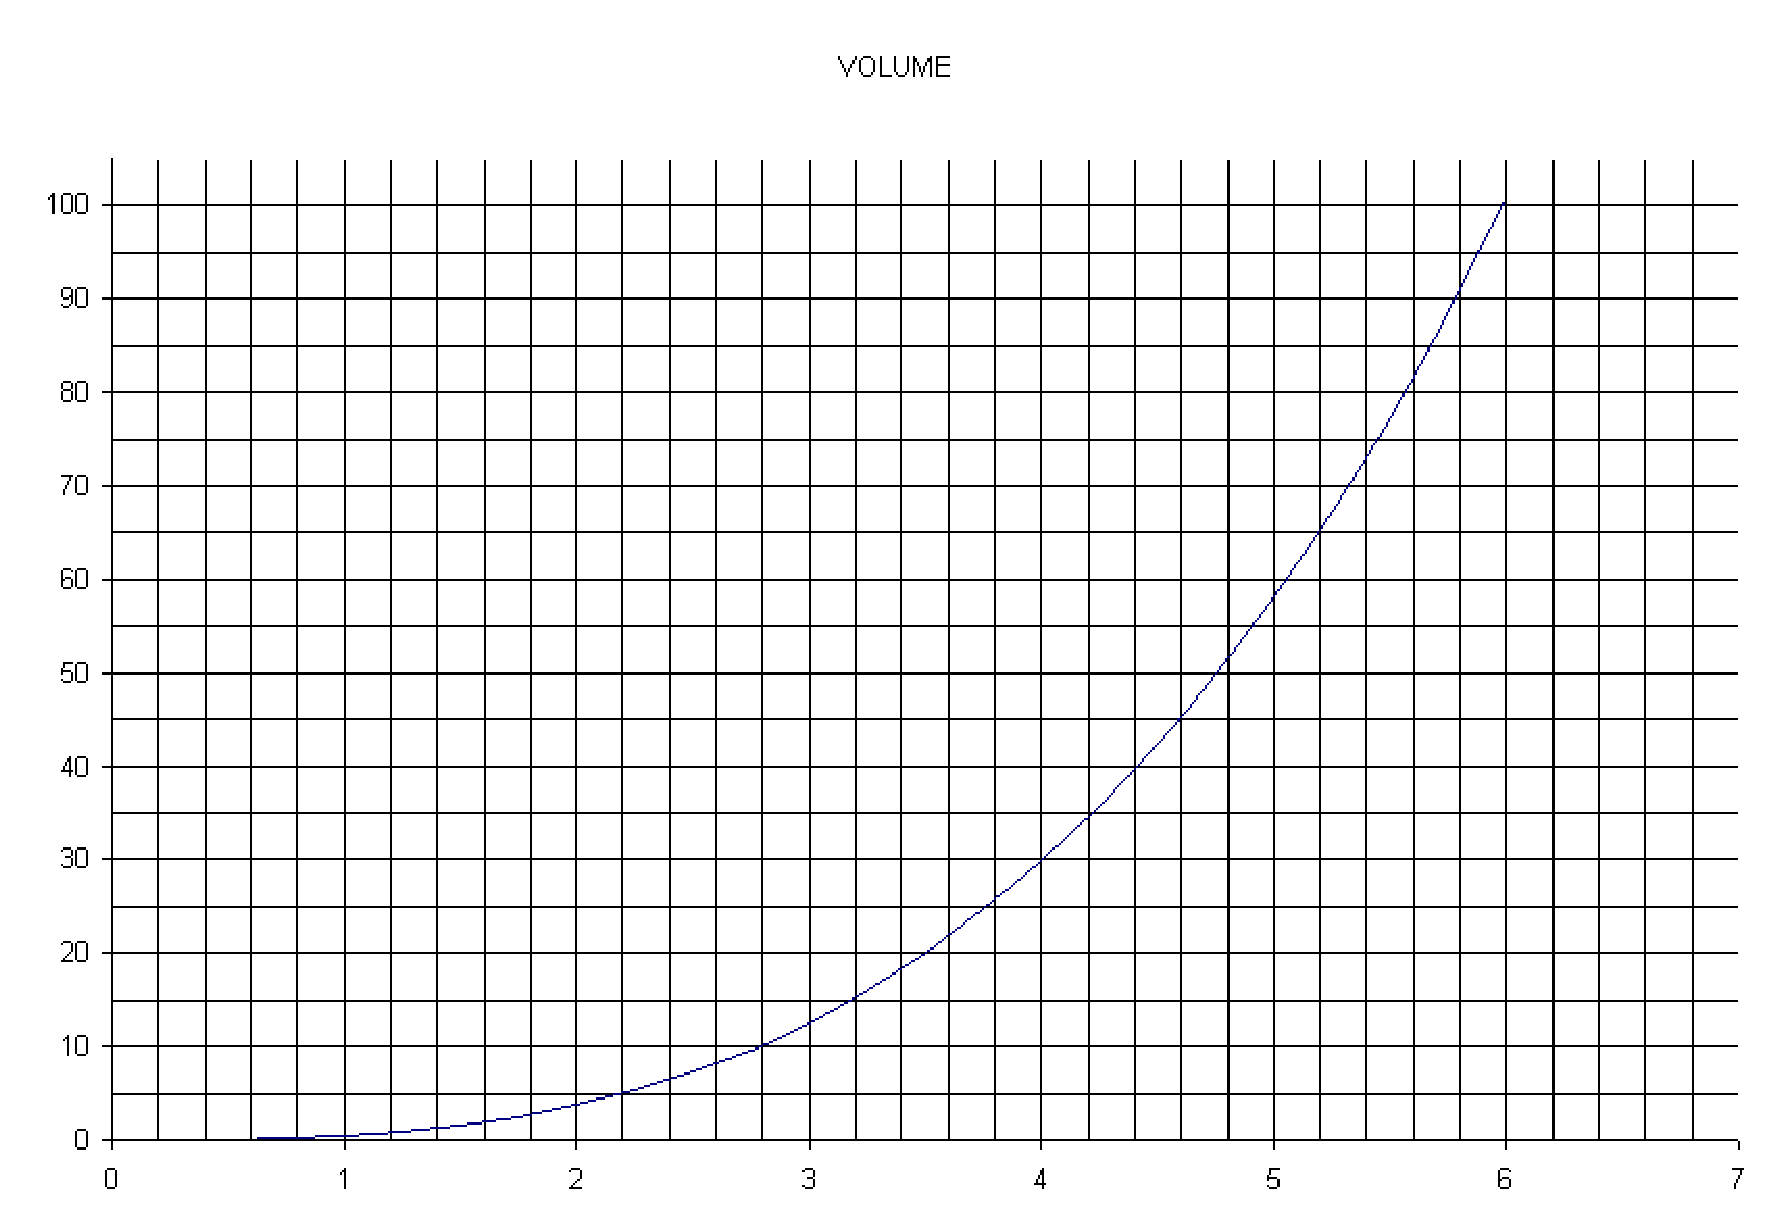
\includegraphics[scale=0.625]{./Graphiques/courbe.eps}\end{center}

%%%%%%%%%%%%%%%%%%%%%%%%%%%%%%%%%%%%%%%%%%%%%%%%%%%%
%%%%%%%%%%%%%%%%%%%%%%%%%%%%%%%%%%%%%%%%%%%%%%%%%%%

%%%%%%%%%%%%%%%%%%%%%%%%%%%%%%%%%%%%%%%%%%%%%%%%%%%\`u
%%%%%%%%%%%%%%%%%%%%%%%%%%%%%%%%%%%%%%%%%%%%%%%%%%%%

 \sautpage

\section{Premi\`eres notions (bilan et compl\'ements)}

\begin{definition}[Notion de fonction]
Une fonction est un proc\'ed\'e qui, \`a un \'el\'ement $x$ d'un ensemble de d\'epart, associe au plus un \'el\'ement $y$ d'un ensemble d'arriv\'ee.

On notera $f:x\mapsto y$ ou $f(x)=y$ qui se lit \og $f$ est la fonction qui \`a $x$ associe $y$ \fg..

On dit que $y$ est \emph{l'image} de $x$.

On dit que $x$ est \emph{un ant\'ec\'edent} de $y$.

\end{definition}

\begin{definition}[Ensemble de d\'efinition]
L'ensemble des r\'eels $x$ poss\'edant une image par une fonction num\'erique $f$ est appel\'e \emph{l'ensemble de d\'efinition de la fonction $f$}. On le note souvent $D_f$.
\end{definition}

\begin{definition}[Repr\'esentation graphique]
Dans un plan muni d'un rep\`ere, la \emph{repr\'esentation graphique} de la fonction $f$ est l'ensemble des points $M$ de coordonn\'ees $(x;y)$ du plan tels que :
\begin{itemize}
	\item L'abscisse $x$ de $M$ d\'ecrit l'ensemble de d\'efinition $D_f$ ;
	\item L'ordonn\'ee $y$ est l'image de $x$ par $f$. $y=f(x)$.
\end{itemize}

On note souvent $\mathcal{C}_f$ la repr\'esentation graphique de $f$. On dit que $\mathcal{C}_f$ a pour \'equation $y=f(x)$.

Si la courbe est d'un seul \og{} tenant \fg{} on parle  de \emph{courbe repr\'esentative} de la fonction $f$.
\end{definition}


\begin{rmq} L'\'equation permet de d\'eterminer si un point $A(x_A;y_A)$ appartient ou pas \`a cette courbe. En effet, un point appartient \`a la courbe si et seulement si ses coordonn\'ees v\'erifient l'\'equation de la courbe. On a alors : \[A\in\mathcal{C}_f\ssi y_A=f(x_A)\] \end{rmq}


Dans la pratique, pour les fonctions num\'eriques d\'efinies par une expression alg\'ebrique, pour esquisser une repr\'esentation graphique, on utilise souvent un tableau de valeurs.

\begin{tabular}{cc}
 \begin{minipage}[l]{0.55\linewidth}
  \begin{rmq} Une courbe ne repr\'esente pas toujours une fonction. Sur la figure ci-contre, par exemple, la courbe a plusieurs points ayant la même abscisse, comme $A(1,-1)$ et $B(1,3)$. Ce n'est donc pas la courbe repr\'esentative d'une fonction car alors 1 aurait plusieurs images.\end{rmq}
 \end{minipage}&
 \begin{minipage}[r]{0.45\linewidth}
\begin{center}
\psset{xunit=0.75cm , yunit=0.75cm}
\def\xmin{-2} \def\xmax{4} \def\ymin{-1.6} \def\ymax{3.6}
\begin{pspicture*}(\xmin,\ymin)(\xmax,\ymax)
\psset{xunit=0.75cm,yunit=0.75cm}
\psgrid[griddots=10,gridlabels=0pt,gridwidth=.3pt, gridcolor=black, subgridwidth=.3pt, subgridcolor=black, subgriddiv=1](0,0)(-2,-2)(4,4)
\psaxes[labels=all,labelsep=1pt, Dx=1,Dy=1]{->}(0,0)(\xmin,\ymin)(\xmax,\ymax)
\uput[dl](0,0){$O$}
%\pcline[linewidth=1pt]{->}(0,0)(1,0) \uput[d](0.5,0){\small $\vec \imath$}
%\pcline[linewidth=1pt]{->}(0,0)(0,1) \uput[l](0,0.5){\small $\vec \jmath$}
\pscircle(1,1){1.5}
\psdots[dotstyle=x](1,-1)(1,3)
\uput[d](1,-1){$A$}
\uput[u](1,3){$B$}
\end{pspicture*}
\end{center}
 \end{minipage}

\end{tabular}






%\sautpage

\subsubsection{Quelques conventions graphiques}
\begin{multicols}{3}
Lorsqu'un point $A$ sur la courbe est connu avec pr\'ecision, il est not\'e par une croix.
\begin{center}
\begin{pspicture*}(-0.5,-1)(2.5,3)
\pscurve(0,0)(0.5,-0.5)(1,1)(2,2.5)
\uput[u](0,0){$\mathcal{C}_f$}
\psdot[dotstyle=x](1,1)
\uput[dr](1,1){$A$}
\end{pspicture*}
\end{center}\sautcol
Lorsqu'un point $A$ est l'extr\'emit\'e de la courbe, il est not\'e par un gros point.
\begin{center}
\begin{pspicture*}(-0.5,-1)(2.5,3)
\pscurve(0,0)(0.5,-0.5)(1,1)(2,2.5)
\uput[u](0,0){$\mathcal{C}_f$}
\psdot(2,2.5)
\uput[dr](2,2.5){$A$}
\end{pspicture*}
\end{center}\sautcol
Lorsqu'un point $A$ \`a l'extr\'emit\'e de la courbe n'appartient pas \`a la courbe, il est not\'e par un \og demi-cercle \fg.
\begin{center}
\begin{pspicture*}(-0.5,-1)(2.5,3)
\pscurve{-(}(0,0)(0.5,-0.5)(1,1)(2,2.5)
\uput[u](0,0){$\mathcal{C}_f$}
%\psdot[(2,2.5)
\uput[dr](2,2.5){$A$}
\end{pspicture*}
\end{center}
\end{multicols}
\begin{multicols}{3}
Une courbe est donn\'ee dans une fenêtre ; s'il n'y a pas d'extr\'emit\'es, la courbe garde la même allure quand on la prolonge.
\begin{center}
\begin{pspicture*}(-0.5,-1)(2.5,3)
\pscurve(-0.3,0)(0.5,2)(1,1)(2,2.8)
\uput[u](1,1){$\mathcal{C}_f$}
\psline[linestyle=dotted](-0.1,0.5)(1.7,0.5)(1.7,2.2)(-0.1,2.2)(-0.1,0.5)
\end{pspicture*}
\end{center}
Une droite verticale en pointill\'es signifie que si l'on prolonge la courbe, elle ne coupe pas cette droite. Sur l'exemple ci-dessous, $a$ n'appartient pas \`a $D_f$.
\begin{center}
\begin{pspicture*}(-0.5,-1)(2.5,3)
\psaxes[labels=none,labelsep=1pt,Dx=5,Dy=5]{->}(0,0)(-0.5,-1)(2.5,3)
\psset{algebraic=true}
\psplot{0.6}{3}{1/(4*x-2)}
\psline[linestyle=dashed](0.5,-1)(0.5,3)
\uput[dl](0.5,0){$a$}
\end{pspicture*}
\end{center}
Une droite horizontale en pointill\'es signifie que si l'on prolonge la courbe, elle ne coupe pas cette droite.
\begin{center}
\begin{pspicture*}(-0.5,-1)(2.5,3)
\psaxes[labels=none,labelsep=1pt,Dx=5,Dy=5]{->}(0,0)(-0.5,-1)(2.5,3)
\psset{algebraic=true}
\psplot{-0.5}{3}{1+1/(x+1)}
\psline[linestyle=dashed](-0.5,1)(2.5,1)
\uput[ul](0,1){$b$}
\end{pspicture*}
\end{center}
\end{multicols}

%\sautpage






\section{R\'esolutions graphiques d'\'equations et d'in\'equations}


\subsection{R\'esolutions d'\'equations de la forme $f(x)=k$}

R\'esoudre l'\'equation $f(x)=k$ c'est d\'eterminer tous les ant\'ec\'edents \'eventuels d'un \'el\'ement $k$ de l'ensemble d'arriv\'ee, c'est-\`a-dire chercher tous les $x$ de l'ensemble de d\'epart tels que $f(x)=k$.

Une telle recherche peut se faire graphiquement \`a partir de la repr\'esentation graphique de la fonction $f$.




\begin{center}
\begin{tabular}{lc}
 \begin{minipage}[l]{0.6\linewidth}
 \begin{exemple*}
  Soit $f$ la fonction d\'efinie sur $\R$ par $f(x)=2x^2-9x+10$. On recherche les solutions de l'\'equation $f(x)=3$.

	On commence par tracer soigneusement la courbe repr\'esentative de $f$ et on obtient la repr\'esentation donn\'ee sur la figure ci-dessous.
		
		On cherche les points de la courbe ayant pour ordonn\'ee 3. Pour cela on peut tracer la droite d'\'equation $y=3$ et chercher les points d'intersection de cette droite avec la courbe de $f$.

		On obtient ici deux points $M_1(1;3)$ et $M_2\left(\frac{7}{2};3\right)$. Les solutions sont leurs abscisses : 1 et $\frac{7}{2}$.

		On \'ecrit : \og Les solutions de l'\'equation $f(x)=3$ sont $x=1$ ou $x=\frac{7}{2}$ car les points de la courbe de $f$ d'ordonn\'ee 3 ont pour abscisses 1 et $\frac{7}{2}$ \fg.
		\end{exemple*}
 \end{minipage}&
 \begin{minipage}[r]{0.35\linewidth}
  
		\begin{center}
 \psset{xunit=1cm,yunit=1cm}
		\begin{pspicture*}(-3.1,-2.1)(4.6,4.1)
\def\xmin{-3} \def\xmax{4.5} \def\ymin{-2} \def\ymax{4}

\psgrid[griddots=10,gridlabels=0pt,gridwidth=.3pt, gridcolor=black, subgridwidth=.3pt, subgridcolor=black, subgriddiv=1](0,0)(-3,-2)(4.5,4)
\psaxes[labels=all,labelsep=1pt, Dx=1,Dy=1]{->}(0,0)(\xmin,\ymin)(\xmax,\ymax)
\uput[dl](0,0){$O$}
\pcline[linewidth=1pt]{->}(0,0)(1,0) \uput[d](0.5,0){\small $\vec \imath$}
\pcline[linewidth=1pt]{->}(0,0)(0,1) \uput[r](0,0.5){\small $\vec \jmath$}
\psset{algebraic=true}
\psplot{\xmin}{\xmax}{2*(x-1)*(x-1)-5*(x-1)+3}
\uput[ul](2,1){$\mathcal{C}_f$}
\psline[linestyle=dashed](\xmin,3)(\xmax,3)
\uput[u](-2,3){$y=3$}
\uput[ur](1,3){$M_1$}
\uput[ul](3.5,3){$M_2$}
\psdots[dotstyle=x](1,3)(3.5,3)
\psline[linestyle=dashed]{->}(1,3)(1,0)
\psline[linestyle=dashed]{->}(3.5,3)(3.5,0)
\end{pspicture*}\end{center}
 \end{minipage}

\end{tabular}             \end{center}



%\sautpage

\subsection{R\'esolutions d'in\'equations de la forme $f(x)\leqslant k$}

Ces in\'equations peuvent se r\'esoudre graphiquement. On proc\`ede de la façon suivante :
\begin{itemize}
	\item on trace soigneusement $\mathcal{C}_f$ dan un rep\`ere (orthogonal) ;
	\item on trace la droite d'\'equation $y=k$ ;
	\item on recherche les points de la courbe situ\'es \emph{sous} la droite ;
	\item l'ensemble des solutions est constitu\'e des abscisses de ces points.
\end{itemize}

\begin{exemple*} Sur l'exemple pr\'ec\'edent, si l'on doit r\'esoudre $f(x)\leqslant 3$, apr\`es avoir trac\'e $y=3$ on constate que les points de la courbe situ\'es sous cette droite ont leurs abscisses comprises entre 0 et $\frac{5}{2}$.

Donc $f(x)\leqslant 3 \ssi x\in\left[0;\frac{5}{2}\right]$.
\end{exemple*}

\begin{rmq}~
\begin{itemize}
	\item On r\'esoud de la même mani\`ere les \'equations du type $f(x)\geqslant k$.

On retient alors les abscisses des points situ\'es \emph{au-dessus} de la droite d'\'equation $y=k$.

Dans l'exemple $f(x)\geqslant 3 \ssi x\in \left] -\infty ; 0 \right] \cup \left[\frac{5}{2} ; +\infty\right[$.
	\item De même pour les in\'equations strictes : $f(x)>k$ ou $f(x)<k$. On excluera alors les abscisses des points d'intersection de la courbe et de la droite.

	Dans l'exemple $f(x)<3 \ssi x\in \left]0;\frac{5}{2}\right[$.
\end{itemize}
\end{rmq}

\subsection{R\'esolutions d'\'equations de la forme $f(x)=g(x)$}

Cela revient \`a chercher les \'el\'ements de l'ensemble de d\'epart qui ont la même image par $f$ et par $g$.

Une telle recherche peut se faire graphiquement. On recherche alors les points des deux courbes repr\'esentatives ayant même abscisse et même ordonn\'ee, c'est-\`a-dire les points d'intersection des deux courbes. 

\begin{tabular}{cc}
 \begin{minipage}[l]{0.6\linewidth}
  \begin{exemple*}

Soit $f$ et $g$ les fonctions d\'efinies sur $\R$ par, respectivement, $f(x)=x^2-1$ et $g(x)=-0,5x^2+x+4$. R\'esoudre graphiquement l'\'equation $f(x)=g(x)$.

	On commence par tracer soigneusement les deux courbes repr\'esentatives et on obtient la repr\'esentation donn\'ee sur la figure ci-contre.
	
	On cherche les points d'intersection des deux courbes, ici $M_1$ et $M_2$, et les solutions de l'\'equation sont leurs abscisses dont les valeurs approximatives sont $-1,5$ et $2,2$.

		Les solutions sont donc $x\approx -1,5$ et $x\approx 2,2$.
\end{exemple*}
 \end{minipage}&
 \begin{minipage}[r]{0.35\linewidth}
  \psset{xunit=0.75cm,yunit=0.75cm}
		\begin{pspicture*}(-3.1,-2.1)(4.6,5.1)
\def\xmin{-3} \def\xmax{4.5} \def\ymin{-2} \def\ymax{5}

\psgrid[griddots=10,gridlabels=0pt,gridwidth=.3pt, gridcolor=black, subgridwidth=.3pt, subgridcolor=black, subgriddiv=1](0,0)(-3,-2)(4.5,5)
\psaxes[labels=all,labelsep=1pt, Dx=1,Dy=1]{->}(0,0)(\xmin,\ymin)(\xmax,\ymax)
\uput[dl](0,0){$O$}
\pcline[linewidth=1pt]{->}(0,0)(1,0) \uput[d](0.5,0){\small $\vec \imath$}
\pcline[linewidth=1pt]{->}(0,0)(0,1) \uput[r](0,0.5){\small $\vec \jmath$}
\psset{algebraic=true}
\psplot{\xmin}{\xmax}{x^2-1}
\psplot{\xmin}{\xmax}{-0.5*x^2+x+4}
\uput[u](1,1){$\mathcal{C}_f$}
\uput[dr](0,4){$\mathcal{C}_g$}
\uput[r](2.189,3.793){$M_2$}
\uput[l](-1.523,1.318){$M_1$}
\psdots[dotstyle=x](2.189,3.793)(-1.523,1.318)
\psline[linestyle=dashed]{->}(-1.523,1.318)(-1.523,0)
\psline[linestyle=dashed]{->}(2.189,3.793)(2.189,0)
\end{pspicture*}
	
 \end{minipage}


\end{tabular}

		

\subsection{R\'esolutions d'in\'equations de la forme $f(x)\leqslant g(x)$}

L\`a encore ces in\'equations peuvent se r\'esoudre graphiquement. On proc\`ede de la façon suivante :
\begin{itemize}
	\item on trace soigneusement $\mathcal{C}_f$ et $\mathcal{C}_g$ dans un rep\`ere (orthogonal) ;
	\item l'ensemble des solutions est constitu\'e des abscisses des points o\`u la courbe de $f$ est situ\'ee \emph{sous} celle de $g$.
\end{itemize}

\begin{exemple*} Sur l'exemple pr\'ec\'edent, si l'on doit r\'esoudre $f(x)\leqslant g(x)$, on constate que les points de la courbe de $f$ situ\'es sous celle de $g$ ont leurs abscisses comprises entre environ $-1,5$ et 2,2.

Donc $f(x)\leqslant g(x) \ssi x\in [-1,5;2,2]$. Ou bien $S=[-1,5;2,2]$.
\end{exemple*}

\begin{rmqs}~
\begin{itemize}
	\item On r\'esoud de la même mani\`ere les \'equations du type $f(x)\geqslant g(x)$.

On retient alors les abscisses des points de la courbe de $f$ situ\'es \emph{au-dessus} de celle de $g$.

Dans l'exemple $f(x)\geqslant g(x) \ssi x\in ] -\infty ; -1,5 ] \cup [2,2 ; +\infty[$.
	\item De même pour les in\'equations strictes : $f(x)>g(x)$ ou $f(x)<g(x)$. On excluera alors les abscisses des points d'intersection des deux courbes.

	Dans l'exemple $f(x)<g(x) \ssi x\in ]-1,5;2,2[$.
\end{itemize}
\end{rmqs}



%\sautpage



\sautpage

\section{Variations, extremums}


\subsection{Sens de variation}

Il s'agit de traduire math\'ematiquement qu'une fonction \og augmente \fg{} ou \og diminue \fg.

\begin{exemple*} Soit, par exemple, la fonction d\'efinie sur $[-3;3]$ par la courbe repr\'esentative donn\'ee sur la figure \ref{croissanceetdecroissance} \vpageref{croissanceetdecroissance}. On constate que lorsque $x\in[-3;1]$ , si $x$ augmente, $f(x)$ augmente aussi alors que lorsque $x\in[1;3]$, si $x$ augmente, $f(x)$ diminue.

C'est la d\'efinition math\'ematique de la croissance ou de la d\'ecroissance d'une fonction $f$.

\begin{figure}[h]
\centering
\caption{Croissance et d\'ecroissante}\label{croissanceetdecroissance}


\psset{xunit=1cm , yunit=1.25cm}
\begin{pspicture*}(-4.1,-1.1)(4.1,5.1)
\def\xmin{-4} \def\xmax{4} \def\ymin{-1} \def\ymax{5}
\psgrid[griddots=10,gridlabels=0pt,gridwidth=.3pt, gridcolor=black, subgridwidth=.3pt, subgridcolor=black, subgriddiv=1](0,0)(-4,-1)(4,5)
\psaxes[labels=all,labelsep=1pt, Dx=1,Dy=1]{-}(0,0)(\xmin,\ymin)(\xmax,\ymax)
\uput[dl](0,0){$O$}
\pcline[linewidth=1pt]{->}(0,0)(1,0) \uput[d](0.5,0){\small $\vec \imath$}
\pcline[linewidth=1pt]{->}(0,0)(0,1) \uput[r](0,0.5){\small $\vec \jmath$}
\psset{algebraic=true}
\psplot{-3}{3}{(-(x-1)^2+5)*0.25+3}
\psdots(3,3.25)(-3,0.25)
\uput[d](-1.5,0){$b$}
\psline[linestyle=dashed]{->}(-1.5,0)(-1.5,2.6875)
\psline[linestyle=dashed]{->}(-1.5,2.6875)(0,2.6875)
\uput[r](0,2.6875){$f(b)$}
\uput[d](-2.5,0){$a$}
\psline[linestyle=dashed]{->}(-2.5,0)(-2.5,1.1875)
\psline[linestyle=dashed]{->}(-2.5,1.1875)(0,1.1875)
\uput[r](0,1.1875){$f(a)$}
\uput[d](1.5,0){$u$}
\uput[d](2.5,0){$v$}
\psline[linestyle=dashed]{->}(1.5,0)(1.5,4.1875)
\psline[linestyle=dashed]{->}(1.5,4.1875)(0,4.1875)
\uput[l](0,4.1875){$f(u)$}
\psline[linestyle=dashed]{->}(2.5,0)(2.5,3.6875)
\psline[linestyle=dashed]{->}(2.5,3.6875)(0,3.6875)
\uput[l](0,3.6875){$f(v)$}
\end{pspicture*}
\end{figure}\end{exemple*}


\begin{definition}
Soit $f$ une fonction d\'efinie sur un intervalle $I$. On dit que $f$ est
\begin{itemize}
	\item \emph{croissante} sur $I$ si, pour tous r\'eels $a$ et $b$ de $I$, on a :\\
$\text{Si } a<b \text{ alors } f(a)\leqslant f(b).$
	\item \emph{d\'ecroissante} sur $I$ si, pour tous r\'eels $a$ et $b$ de $I$, on a :\\
$\text{Si } a<b \text{ alors } f(a)\geqslant f(b).$
	\item \emph{monotone} si elle n'est que croissante sur $I$ ou si elle n'est que d\'ecroissante sur $I$.
	\item \emph{constante} sur $I$ si, pour tous r\'eels $a$ et $b$ de $I$, on a : $f(a)=f(b)$.
\end{itemize}
\end{definition}


\begin{rmqs}~
\begin{itemize}
	\item Ces notions ne sont valables que sur \textbf{un intervalle} et pas sur une r\'eunion d'intervalles disjoints.
	\item Ant\'ec\'edents et images \'etant rang\'es dans le même ordre, on dit qu'une fonction croissante \emph{conserve} l'ordre.
	\item Ant\'ec\'edents et images \'etant rang\'es dans l'ordre inverse, on dit qu'une fonction d\'ecroissante \emph{inverse} l'ordre.
	\item On obtient les d\'efinitions d'une fonction \emph{strictement} croissante ou \emph{strictement} d\'ecroisante en remplaçant les in\'egalit\'es par des in\'egalit\'es strictes. Ainsi on dit que $f$ est strictement croissante sur $I$ si pour tous r\'eels $a$ et $b$ de $I$ on a : \\ $\text{Si } a<b \text{ alors } f(a)<f(b)$
	\item Une fonction est strictement monotone sur $I$ si elle est strictement croissante ou strictement d\'ecroissante sur $I$
\end{itemize}
\end{rmqs}

\subsection{Tableau de variations}

Ces r\'esultats peuvent se r\'esumer dans un tableau de variation, qui est une forme stylis\'ee de repr\'esentation o\`u l'on indique uniquement si la courbe monte, descend ou est stable. Dans la premi\`ere ligne on indique les valeurs importantes de $x$ et dans la seconde les variations de $f$.

\begin{exemple*} Dans l'exemple pr\'ec\'edent on obtient
$$\tabvar{%
\tx{x}&\tx{-3}&&\tx{1}&&\tx{3}\cr
\tx{f}&\txb{\approx 0,25}&\fm&\txh{\approx 4,25}&\fd&\txb{\approx 2,25}\cr
}$$
\end{exemple*}



\subsection{Extremums}

Les extremums, s'ils existent, sont les valeurs maximale et minimale qui sont \textbf{atteintes} par la fonction $f$ sur un intervalle donn\'e. Plus pr\'ecis\'ement :

\begin{definition}
Soit une fonction $f$ d\'efinie sur un intervalle $I$ et $x_0\in I$. On dit que
\begin{itemize}
	\item $f$ admet un \emph{maximum}, atteint en $x_0$ si, pour tout $x\in I$, $f(x)\leqslant f(x_0)$. Ce maximum est alors $f(x_0)$.
	\item $f$ admet un \emph{minimum}, atteint en $x_0$ si, pour tout $x\in I$, $f(x)\geqslant f(x_0)$. Ce minimum est alors $f(x_0)$.
\end{itemize}
Les maximum et minimum sont appel\'es les \emph{extremums}.
\end{definition}

%\begin{rmq} Un extremum doit être atteint par une valeur $x_0$. \end{rmq}

\begin{exemple*}
La fonction $f$ d\'efinie sur $\R$ par $f(x)=x^2+1$ n'admet pas $-1$ comme minimum.

En effet, si on a bien $f(x)\geqslant -1$ sur $\R$, il n'existe pas de $x_0$ tel que $f(x_0)=-1$.

Par contre 1 est bien le minimum de $f$ sur $\R$ car
\begin{itemize}
	\item $f(x)\geqslant 1$ pour tout $x\in\R$ \textbf{ET}
	\item $f(0)=1$
\end{itemize}

On dira donc : le minimum de $f$ sur $\R$ est 1 et il est atteint pour $x_0=0$.
\end{exemple*}

\sautpage

\section{Exercices et probl\`emes}

\subsection{Premi\`eres notions}

%\begin{multicols}{2}
%\begin{exo} Dire dans chacun des exemples ci-dessous quel est l'ensemble de d\'efinition, quelles sont les images possibles et si la fonction est num\'erique.
%\begin{enumerate}
%	\item \`A chaque \'el\`eve de la classe on associe la couleur de ses cheveux.
%	\item \`A chaque \'el\`eve de la classe on associe le nombre de ses fr\`eres et soeurs.
%	\item Pour un \'el\`eve donn\'e, \`a chaque moment de sa vie on associe la taille qu'il mesurait.
%	\item Soit $ABCD$ un rectangle dont un des côt\'es est fixe et mesure 6 cm et l'autre est variable et mesure $x$ cm. \\On d\'efinit la fonction $f$ de la façon suivante : \`a chaque $x$ possible, on associe $f(x)$, l'aire du rectangle $ABCD$.
%	\item La fonction $g$ d\'efinie par $g(x)=x^2+2x+3$.
%	\item La fonction $h$ d\'efinie par $h(x)=\frac{x^2+1}{x-1}$.
%	\item La fonction $i$ d\'efinie par $i(x)=\sqrt{x+2}$.
%\end{enumerate}
%\end{exo}
\begin{multicols}{2}
\begin{exo}
On d\'efinit $f$ et $g$, deux fonctions :
\begin{itemize}
	\item $f$ est la fonction qui \`a un nombre r\'eel $x$ associe le nombre obtenu en proc\'edant de la mani\`ere suivante : on ajoute $4$ au nombre, on \'el\`eve le r\'esultat obtenu au carr\'e, on retranche 16, on divise par le nombre de d\'epart et on retranche 6.
	\item $g:x\mapsto x^2-4$.
\end{itemize}
\begin{enumerate}
	\item Donner l'expression correspondant \`a $f$ puis simplifier cette expression.
	\item Quel r\'eel n'a pas d'image par $f$ ?
	\item Quelle est l'image de 3 par $g$ ?
	\item Quelle est l'image de $-1$ par $g$ ?
	\item Quels sont les ant\'ec\'edents \'eventuels de 12 par $g$ ?
	\item Quels sont les ant\'ec\'edents \'eventuels de $-5$ par $g$ ?
\end{enumerate}
\end{exo}

\sautcol

\begin{exo}
Vrai ou faux ? \emph{Corriger la phrase lorsqu'elle est fausse}.
\begin{enumerate}
	\item $f(-2) = 0$ signifie que l'image de 0 est $-2$
	\item $f(0) = 3$ signifie que la courbe de $f$ passe par le point $(0 ; 3)$
	\item $f(1) = 2$ signifie que l'ant\'ec\'edent de 1 est 2
	\item L'image de 2 par $f$ est $-3$ s'\'ecrit $f(2) = -3$
	\item Dire que $(5 ; 1)$ est un point de la courbe de $f$ s'\'ecrit $5 = f(1)$
	\item Par la fonction $g$, $-5$ est l'image de 3 s'\'ecrit $g(-5) = 3$
	\item 2 a pour image 0 par $f$ signifie que la courbe de $f$ traverse l'axe des abscisses en 2
	\item $f(4) = 0$ signifie que la courbe de $f$ traverse l'axe des abscisses au point $(4 ; 0)$
	\item 3 a pour image 5, signifie que 3 est l'image de 5
	\item 4 a pour ant\'ec\'edent 5 signifie que 5 est l'image de 4
\end{enumerate}
\end{exo}

\end{multicols}

%\sautpage

\begin{exo}\label{gf4courbes}
Vrai ou faux ? \emph{Justifier la r\'eponse lorsque c'est faux}.\\
Les courbes de la figure \ref{gf4courbesfig} \vpageref{gf4courbesfig} repr\'esentent des fonctions de la variable $x$.


\begin{figure}[!h]
 \centering
 \caption{Courbes de l'exercice \ref{gf4courbes}}\label{gf4courbesfig}
\begin{tabular}{cc}
\psset{xunit=1cm , yunit=0.5cm}
\begin{pspicture*}(-2.1,-2.1)(4.1,4.1)
\def\xmin{-2} \def\xmax{4} \def\ymin{-2} \def\ymax{4}
\psgrid[griddots=10,gridlabels=0pt,gridwidth=.3pt, gridcolor=black, subgridwidth=.3pt, subgridcolor=black, subgriddiv=1](0,0)(-2,-2)(4,4)
\psaxes[labels=all,labelsep=1pt, Dx=1,Dy=1]{->}(0,0)(\xmin,\ymin)(\xmax,\ymax)
\uput[dl](0,0){$O$}
\pcline[linewidth=1pt]{->}(0,0)(1,0) \uput[d](0.5,0){\small $\vec \imath$}
\pcline[linewidth=1pt]{->}(0,0)(0,1) \uput[l](0,0.5){\small $\vec \jmath$}
\psline(-2,3)(1,-1.5)(2,-1.5)(4,2)
\end{pspicture*}
&
\psset{xunit=1cm , yunit=0.5cm}
\begin{pspicture*}(-2.1,-2.1)(4.1,4.1)
\def\xmin{-2} \def\xmax{4} \def\ymin{-2} \def\ymax{4}
\psgrid[griddots=10,gridlabels=0pt,gridwidth=.3pt, gridcolor=black, subgridwidth=.3pt, subgridcolor=black, subgriddiv=1](0,0)(-2,-2)(4,4)
\psaxes[labels=all,labelsep=1pt, Dx=1,Dy=1]{->}(0,0)(\xmin,\ymin)(\xmax,\ymax)
\uput[dl](0,0){$O$}
\pcline[linewidth=1pt]{->}(0,0)(1,0) \uput[d](0.5,0){\small $\vec \imath$}
\pcline[linewidth=1pt]{->}(0,0)(0,1) \uput[l](0,0.5){\small $\vec \jmath$}
\psline(-2,3)(1,3)(1,1)(4,1)
\end{pspicture*}
\\
\psset{xunit=1cm , yunit=0.5cm}
\begin{pspicture*}(-2.1,-2.1)(4.1,4.1)
\def\xmin{-2} \def\xmax{4} \def\ymin{-2} \def\ymax{4}
\psgrid[griddots=10,gridlabels=0pt,gridwidth=.3pt, gridcolor=black, subgridwidth=.3pt, subgridcolor=black, subgriddiv=1](0,0)(-2,-2)(4,4)
\psaxes[labels=all,labelsep=1pt, Dx=1,Dy=1]{->}(0,0)(\xmin,\ymin)(\xmax,\ymax)
\uput[dl](0,0){$O$}
\pcline[linewidth=1pt]{->}(0,0)(1,0) \uput[d](0.5,0){\small $\vec \imath$}
\pcline[linewidth=1pt]{->}(0,0)(0,1) \uput[l](0,0.5){\small $\vec \jmath$}
\psline(-2,3)(4,3)
\end{pspicture*}
&
\psset{xunit=1cm , yunit=0.5cm}
\begin{pspicture*}(-2.1,-2.1)(4.1,4.1)
\def\xmin{-2} \def\xmax{4} \def\ymin{-2} \def\ymax{4}
\psgrid[griddots=10,gridlabels=0pt,gridwidth=.3pt, gridcolor=black, subgridwidth=.3pt, subgridcolor=black, subgriddiv=1](0,0)(-2,-2)(4,4)
\psaxes[labels=all,labelsep=1pt, Dx=1,Dy=1]{->}(0,0)(\xmin,\ymin)(\xmax,\ymax)
\uput[dl](0,0){$O$}
\pcline[linewidth=1pt]{->}(0,0)(1,0) \uput[d](0.5,0){\small $\vec \imath$}
\pcline[linewidth=1pt]{->}(0,0)(0,1) \uput[l](0,0.5){\small $\vec \jmath$}
\pscurve(-2,3)(-1,0)(0,-1)(2,1)(3.2,2)(3,3)
\end{pspicture*}
\end{tabular}
\end{figure}

\end{exo}

\sautpage

\begin{exo}\label{gf14}
Vrai ou faux ? \emph{Corriger la phrase lorsqu'elle est fausse}.\\
Les fonctions $f$ et $g$ sont repr\'esent\'ees sur la figure \ref{gf14fig} \vpageref{gf14fig}.
\begin{enumerate}
	\item La fonction $f$ est d\'efinie entre $-2$ et 6 inclus
	\item Les images par la fonction $f$ sont comprises entre $-1$ et 4 inclus
	\item La fonction $g$ est d\'efinie entre $-2$ exclu et 6 inclus
	\item Les images par la fonction g sont comprises entre 0 exclu et 3 inclus
\end{enumerate}



\begin{figure}[!h]
\centering
\caption{Courbes de l'exercice \ref{gf14}}\label{gf14fig}
\begin{tabular}{cc}
\psset{xunit=0.9cm , yunit=0.5cm}
\begin{pspicture*}(-3.1,-2.1)(6.1,5.1)
\def\xmin{-3} \def\xmax{6} \def\ymin{-2} \def\ymax{5}
\psgrid[griddots=10,gridlabels=0pt,gridwidth=.3pt, gridcolor=black, subgridwidth=.3pt, subgridcolor=black, subgriddiv=1](0,0)(-3,-2)(6,5)
\psaxes[labels=all,labelsep=1pt, Dx=1,Dy=1]{->}(0,0)(\xmin,\ymin)(\xmax,\ymax)
\uput[dl](0,0){$O$}
\pcline[linewidth=1pt]{->}(0,0)(1,0) \uput[d](0.5,0){\small $\vec \imath$}
\pcline[linewidth=1pt]{->}(0,0)(0,1) \uput[l](0,0.5){\small $\vec \jmath$}
\pscurve{*-(}(-2,2)(-1,3)(0,3.7)(0.5,3.9)(1,4)(2,3)(3,0)(4,-1)(5,0)(6,1)

\rput(3,2){$\mathcal{C}_f$}
\end{pspicture*}
&
\psset{xunit=0.9cm , yunit=0.5cm}
\begin{pspicture*}(-3.1,-2.1)(6.1,5.1)
\def\xmin{-3} \def\xmax{6} \def\ymin{-2} \def\ymax{5}
\psgrid[griddots=10,gridlabels=0pt,gridwidth=.3pt, gridcolor=black, subgridwidth=.3pt, subgridcolor=black, subgriddiv=1](0,0)(-3,-2)(6,5)
\psaxes[labels=all,labelsep=1pt, Dx=1,Dy=1]{->}(0,0)(\xmin,\ymin)(\xmax,\ymax)
\uput[dl](0,0){$O$}
\pcline[linewidth=1pt]{->}(0,0)(1,0) \uput[d](0.5,0){\small $\vec \imath$}
\pcline[linewidth=1pt]{->}(0,0)(0,1) \uput[l](0,0.5){\small $\vec \jmath$}
\pscurve{)-}(-2,0)(0,1)(1,2)(1.5,3.5)(1.8,5)
\pscurve{-*}(2.2,-2)(3,0)(4,1.5)(6,3)
\rput(1,3){$\mathcal{C}_g$}
\psline[linestyle=dashed](2,\ymin)(2,\ymax)
\end{pspicture*}
\end{tabular}
\end{figure}

\end{exo}

\begin{exo}\label{gf15}
Vrai ou faux ? \emph{Corriger la proposition lorsqu'elle est fausse}.
\begin{itemize}
	\item D'apr\`es la repr\'esentation graphique de la figure \ref{gf15fig} \vpageref{gf15fig} $D_f=[-4;2]$
	\item D'apr\`es la repr\'esentation graphique de la figure \ref{gf15fig} \vpageref{gf15fig} $D_g=]-\infty;3[\cup]3;5]$
\end{itemize}


\begin{figure}[!h]
\centering
\caption{Courbes de l'exercice \ref{gf15}}\label{gf15fig}
\begin{tabular}{cc}
\psset{xunit=1cm , yunit=0.66cm}
\begin{pspicture*}(-4.1,-2.1)(4.1,4.1)
\def\xmin{-4} \def\xmax{4} \def\ymin{-2} \def\ymax{4}
\psgrid[griddots=10,gridlabels=0pt,gridwidth=.3pt, gridcolor=black, subgridwidth=.3pt, subgridcolor=black, subgriddiv=1](0,0)(-4,-2)(4,4)
\psaxes[labels=all,labelsep=1pt, Dx=1,Dy=1]{->}(0,0)(\xmin,\ymin)(\xmax,\ymax)
\uput[dl](0,0){$O$}
\pcline[linewidth=1pt]{->}(0,0)(1,0) \uput[d](0.5,0){\small $\vec \imath$}
\pcline[linewidth=1pt]{->}(0,0)(0,1) \uput[l](0,0.5){\small $\vec \jmath$}
\pscurve{*-}(-4,0)(-3,-2)(0,0)(1,1)(4,1.8)
\psline[linestyle=dashed](0,2)(4,2)
\rput(-1.5,-1){$\mathcal{C}_f$}
\end{pspicture*}
&
\psset{xunit=1cm , yunit=0.66cm}
\begin{pspicture*}(-3.1,-2.1)(5.6,4.1)
\def\xmin{-3} \def\xmax{5.5} \def\ymin{-2} \def\ymax{4}
\psgrid[griddots=10,gridlabels=0pt,gridwidth=.3pt, gridcolor=black, subgridwidth=.3pt, subgridcolor=black, subgriddiv=1](0,0)(-3,-2)(5.5,4)
\psaxes[labels=all,labelsep=1pt, Dx=1,Dy=1]{->}(0,0)(\xmin,\ymin)(\xmax,\ymax)
\uput[dl](0,0){$O$}
\pcline[linewidth=1pt]{->}(0,0)(1,0) \uput[d](0.5,0){\small $\vec \imath$}
\pcline[linewidth=1pt]{->}(0,0)(0,1) \uput[l](0,0.5){\small $\vec \jmath$}
\pscurve(-3,3)(0,1.5)(1,1)(2,0)(2.8,-2)
\pscurve{-*}(3.2,-2)(4,1)(5,3)
\psline[linestyle=dashed](3,\ymin)(3,\ymax)
\uput[ur](1,1){$\mathcal{C}_g$}
\end{pspicture*}
\end{tabular}
\end{figure}
\end{exo}
%\sautpage


\begin{exo}[Avec la calculatrice]
La fonction $f$ est d\'efinie sur $[-1,5;2]$ par : $f(x)=2x^3-1,5x^2-3x$
\begin{enumerate}
	\item Compl\'eter le tableau de valeurs suivant :
	%\vspace{-1em}
	\begin{center}
\begin{tabular}{|*{9}{c|}}
\hline $x$ & $-1,5$ & $-1$ & $-0,5$ & 0 & 0,5 & 1 & 1,5 & 2 \\ \hline
$f(x)$ & & & & & & & & \\ \hline
\end{tabular}
\end{center}
\item Tracer la courbe repr\'esentative de $f$.
\end{enumerate}
\end{exo}

\begin{exo}[Avec la calculatrice]\label{uneautrecourbe}
La fonction $f$ est d\'efinie sur $[-3;3]$ par : $f(x)=x^2-3x+1$.\\
Apr\`es avoir dress\'e un tableau de valeurs de la fonction, tracer sa courbe repr\'esentative $\mathcal{C}_f$.

\end{exo}

%\end{multicols}



\sautpage

\subsection{R\'esolutions graphiques}

\begin{exo}
La fonction $f$ est d\'efinie sur $[-3;3]$ par : $f(x)=x^2-3x+1$.\\
$\mathcal{C}_f$, courbe repr\'esentative de $f$ a d\'ej\`a \'et\'e obtenue dans l'exercice \ref{uneautrecourbe}.
\begin{enumerate}
	\item \`A l'aide de la repr\'esentation graphique $\mathcal{C}_f$, avec la pr\'ecision permise par le graphique, r\'epondre aux question suivantes :
		\vspace{-1em}\begin{multicols}{2}
		  \begin{enumerate}
			\item Quelle est l'image de 2 ?
			\item Quelle est l'image de 3 ?
			\item Quelle est l'image de 4 ?
			\item Quels sont les ant\'ec\'edents de 1 ?
			\item Quels sont les ant\'ec\'edents de 2 ?
			\item Quels sont les ant\'ec\'edents de $-2$ ?
		\end{enumerate}
		\end{multicols}\vspace{-1em}
	\item R\'esoudre graphiquement les \'equations et in\'equations suivantes :
\vspace{-1em}\begin{multicols}{3}\begin{enumerate}
	\item $f(x)=3$ ;
	\item $f(x)=-1,5$ ;
	\item $f(x)\geqslant -1$ ;
	\item $f(x)<4$ ;
	\item $f(x)>-3$ ;
	\item $f(x)<-2$.
\end{enumerate}\end{multicols}\vspace{-1em}
\item D\'eterminer graphiquement le signe de $f(x)$ selon les valeurs de $x$.
\end{enumerate}
\end{exo}

%\sautpage

\begin{exo}
Une fonction $f$, d\'efinie sur $\R$, est donn\'ee par sa courbe repr\'esentative $\mathcal{C}$ :
\begin{multicols}{2}
\begin{center}\small
\psset{xunit=1,yunit=1}
\begin{pspicture*}(-2.6,-2.1)(5.1,3.1)
\def\xmin{-2.5} \def\xmax{5} \def\ymin{-2} \def\ymax{3}
\psset{xunit=0.1cm,yunit=0.1cm}
\psgrid[griddots=15,gridlabels=0pt,gridwidth=.3pt, gridcolor=gray, subgridwidth=.3pt, subgridcolor=gray, subgriddiv=1](0,0)(-25,-20)(50,30)
\psset{xunit=1cm , yunit=1cm}
\psaxes[labels=all,labelsep=1pt, Dx=1,Dy=1]{->}(0,0)(\xmin,\ymin)(\xmax,\ymax)
\uput[dl](0,0){$0$}
\pcline[linewidth=1pt]{->}(0,0)(1,0) \uput[d](0.5,0){\small $\vec i$}
\pcline[linewidth=1pt]{->}(0,0)(0,1) \uput[l](0,0.5){\small $\vec j$}
\pscurve(-2.3,-2)(-2,-1)(-1.5,1.5)(-1,3)(-0.5,2.5)(0,1)(0.2,0)(0.5,-1)(1,-1.5)(1.5,-1)(2,0)(2.5,1)(3,1.5)(4,2)(5,2.3)
\psline[linestyle=dashed](0,2.5)(\xmax,2.5)
\psdots[dotstyle=x](-2,-1)(-1.5,1.5)(-1,3)(-0.5,2.5)(0,1)(0.5,-1)(1,-1.5)(1.5,-1)(2,0)(2.5,1)(3,1.5)(4,2)
\end{pspicture*}
\end{center}\normalsize

\sautcol

Avec la pr\'ecision permise par le graphique, r\'esoudre :
%\vspace{-1em}
%\begin{multicols}{2}
\begin{enumerate}
	\item Les \'equations suivantes :
		\vspace{-1em}
		\begin{multicols}{2}\begin{enumerate}
			\item $f(x) = 1$ ;
			\item $f(x) = 0$ ;
			\item $f(x) = -1$ ;
			\item $f(x) = 2$.
		\end{enumerate}\end{multicols}
		%\vspace{-1em}
%\sautcol
	\item Les in\'equations suivantes :
		\vspace{-1em}
		\begin{multicols}{2}\begin{enumerate}
			\item $f(x)\geqslant 1$ ;
			\item $f(x)\geqslant 0$ ;
			\item $f(x)<-1$ ;
			\item $f(x)>2$.
		\end{enumerate}\end{multicols}
		\vspace{-1em}
	\item D\'eterminer graphiquement le signe de $f(x)$ selon les valeurs de $x$.

\end{enumerate}\end{multicols}
%\vspace{-1em}
\end{exo}

\medskip

\begin{multicols}{2}

\begin{exo}\label{gfunecourbe}
La courbe $\mathcal{C}$ de la figure ci-dessous %\ref{gfunecourbefig} \vpageref{gfunecourbefig} 
repr\'esente une fonction $f$ et le segment de droite $\mathcal{D}$ repr\'esente une fonction $g$.

%\begin{figure}[hbtp]
% \centering
% \caption{Figure de l'exercice \ref{gfunecourbe}}\label{gfunecourbefig}


\begin{center}
\psset{xunit=0.375cm , yunit=0.33cm}
\def\xmin{-9} \def\xmax{12} \def\ymin{-3} \def\ymax{11}
\begin{pspicture*}(\xmin,\ymin)(\xmax,\ymax)
\psgrid[griddots=10,gridlabels=0pt,gridwidth=.3pt, gridcolor=black, subgridwidth=.3pt, subgridcolor=black, subgriddiv=1](0,0)(\xmin,\ymin)(\xmax,\ymax)
\psaxes[labels=all,labelsep=1pt, Dx=5,Dy=5]{-}(0,0)(\xmin,\ymin)(\xmax,\ymax)
\uput[dl](0,0){$O$}
\pcline[linewidth=1pt]{->}(0,0)(1,0) \uput[d](0.5,0){\small $\vec \imath$}
\pcline[linewidth=1pt]{->}(0,0)(0,1) \uput[l](0,0.5){\small $\vec \jmath$}
\pscurve{*-*}(-8,1)(-5,3)(-3,5)(-1,6)(0,5)(1,3)(2,0)(4,-2)(7,0)(9,3)(11,6)
\psdots[dotstyle=x](-5,3)(-3,5)(-1,6)(0,5)(1,3)(2,0)(4,-2)(7,0)(9,3)
\psdots[dotstyle=*](-8,7.5)(11,-2)
\uput[dr](10,5){$\mathcal{C}$}
\uput[ur](-6,7){$\mathcal{D}$}
\psplot[linestyle=dashed,algebraic=true]{-8}{11}{-0.5*x+3.5}
\end{pspicture*}\end{center}

%\end{figure}

\sautcol

\begin{enumerate}
	\item R\'esoudre graphiquement les \'equations :
		\vspace{-1em}\begin{multicols}{2}\begin{enumerate}
			\item $f(x) = 3$ ;
			\item $f(x) = -2$ ;
			\item $f(x) = 0$ ;
			\item $f(x) = 6$.
		\end{enumerate}\end{multicols}
	\item R\'esoudre graphiquement les in\'equations :
		\begin{enumerate}
			\item $f(x)\leqslant 0$ ;
			\item $f(x) \geqslant 3$ ;
			\item $f(x)>5$.
		\end{enumerate}

	\item R\'esoudre graphiquement :
			\begin{enumerate}
				\item $f(x) = g(x)$ ;
				\item $f(x) < g(x)$.			\end{enumerate}
		\item Donner le signe de $f(x)$ suivant les valeurs de $x$.
\end{enumerate}
\end{exo}\end{multicols}

%\sautpage

\begin{multicols}{2}

\begin{exo}[Avec la calculatrice]
On consid\`ere les fonctions $f$ et $g$ d\'efinies sur $\R$ par : $f(x)=x^3$ et $g(x)=3x-2$.
 \begin{enumerate}
			\item Tracer soigneusement les repr\'esentations graphiques $\mathcal{C}_f$ et $\mathcal{C}_g$ de $f$ et $g$ sur l'intervalle $[-2;2]$.
			\item R\'esoudre graphiquement l'in\'equation $f(x)\leqslant 1$.
			\item D\'eterminer graphiquement les solutions de l'\'equation $f(x)=g(x)$.
 \end{enumerate}
\end{exo}

\sautcol

\begin{exo}[Avec la calculatrice]
Les fonctions $f$ et $g$ sont d\'efinies sur $[-2;2]$ par : $f(x)=x^3$ et $g(x)=1-x$.
\begin{enumerate}
	\item Tracer sur une calculatrice graphique les repr\'esentations graphiques $\mathcal{C}_f$ et $\mathcal{C}_g$ de $f$ et de $g$.
	\item En d\'eduire le nombre de solutions de l'\'equation $x^3+x-1=0$.
	\end{enumerate}
\end{exo}

\end{multicols}

\subsection{R\'esolutions calculatoires}
%\section{Technologie}
\begin{multicols}{2}
\begin{exo}
Soit la fonction $f$ d\'efinie sur $\R$ par : \\$f(x)=2x^2+x+3$.
\begin{enumerate}
	\item Calculer les valeurs exactes de $f(x)$ pour les valeurs de $x$ suivantes :
	  \vspace{-1em}\begin{multicols}{3}
	  \begin{itemize}
	    \item 0 ;
	    \item 1 ;
	    \item $-2$ ;
	    \item $\sqrt{2}$ ;
	    \item $1+\sqrt{3}$ ;
	    \item $2-\sqrt{5}$.
	   \end{itemize}
	  \end{multicols}\vspace{-1em}
	\item R\'esoudre $f(x)=3$.
\end{enumerate}
\end{exo}

\begin{exo}
Soit $f$ la fonction d\'efinie sur $\R$ par :\\ $f(x)=2x^2-5x+3$. \\R\'esoudre $f(x)=3$.
\end{exo}

\begin{exo} Soit $f$ la fonction d\'efinie sur $\R$ par : $f(x)=4x^2-4x+1$. On cherche \`a r\'esoudre, par le calcul, l'\'equation $f(x)=9$.
%\vspace{-1em}\begin{multicols}{2}
\begin{enumerate}
	\item Factoriser $f(x)$.
	\item R\'esoudre $f(x)=9$.
\end{enumerate}% \end{multicols}\vspace{-1em}
\end{exo}



\begin{exo}
	Soit $f$ et $g$ les fonctions d\'efinies sur $\R$ par, respectivement, $f(x)=x^2-1$ et $g(x)=-x^2+2$. \\ R\'esoudre par le calcul l'\'equation $f(x)=g(x)$.
\end{exo}


\begin{exo}
On consid\`ere les fonctions $f$ et $g$ d\'efinies sur $\R$ par : $f(x)=x^3$ et $g(x)=3x-2$. On cherche \`a r\'esoudre, par le calcul, l'\'equation $f(x)=g(x)$.
		\begin{enumerate}
			\item D\'evelopper $(x-1)^2(x+2)$.
			\item En d\'eduire les solutions de l'\'equation $x^3-3x+2=0$.
			\item En d\'eduire les solutions de l'\'equation $f(x)=g(x)$.
		\end{enumerate}
\end{exo}



%

\begin{exo}
On consid\`ere la fonction $f$ d\'efinie pour tout $x\in\R$ par : $f(x)=x(x-2)$. On cherche \`a trouver, par le calcul, le minimum de $f(x)$.
%\vspace{-1em}\begin{multicols}{2}
\begin{enumerate}
	\item D\'emontrer que $f(x)=(x-1)^2-1$.
	\item En d\'eduire le minimum de $f(x)$.
\end{enumerate}%\end{multicols}\vspace{-1em}
\end{exo}

\end{multicols}

\sautpage


\subsection{Variations, extremums}

\begin{multicols}{2}

\begin{exo}\label{fonctionsvar1}
On consid\`ere la fonction $f$ dont on donne la repr\'esentation $\mathcal{C}$ sur la figure \ref{fonctionsvar1fig} \vpageref{fonctionsvar1fig} (en deux parties).\\
Indiquer son ensemble de d\'efinition et dresser son tableau de variations.

\end{exo}
%\sautpage


\begin{exo}[Avec une calculatrice]
On consid\`ere la fonction $f$ d\'efinie par : $f(x)=2x\sqrt{4-x^2}$.
\`A l'aide d'une calculatrice graphique :
\begin{enumerate}
	\item conjecturer l'ensemble de d\'efinition de $f$ ;
	\item conjecturer quels sont les extremums de $f$ sur son ensemble de d\'efinition ;
	\item dresser le tableau des variations de $f$.
\end{enumerate}
\end{exo}


%\sautcol


\begin{exo}
Tracer une courbe repr\'esentative d'une fonction $f$ sachant que :
%\vspace{-1em}\begin{multicols}{2}
\begin{itemize}
\item le tableau des variations de $f$ est le suivant :$$\tabvar{%
\tx{x}&&&\tx{0}&&\tx{3}&&\tx{~}\cr
\tx{f}&\txb{1}&\fm&&\fd&&\fm&\cr
}$$
	\item 1 a pour ant\'ec\'edents, par la fonction $f$, $-2$ et 1,5 ;
	\item $f(x)=0$ a pour solutions $x=2$ ou $x=4$ ;
	\item $f(-1)=2$ ;
	\item $-1$ est l'image de 3 ;
	\item $D_f=[-2;4]$ ;
	\item le maximum de $f$ est 3 ;
	
\end{itemize}%\end{multicols}
\end{exo}



\sautcol

\begin{exo}
On donne le tableau des variations d'une fonction $f$ :$$\tabvar{%
\tx{x}&\tx{-5}&&\tx{-3}&&\tx{0}&&\tx{1}&&\tx{8}\cr
\tx{f}&\txh{3}&\fd&\txb{0}&\fm&\txh{1}&\fdh&\tx{0}&\fdb&\txb{-2}\cr
}$$
%\vspace{-4em}\begin{multicols}{2}
\begin{enumerate}
	\item S'il est possible de r\'epondre, compl\'eter par \og < \fg, \og > \fg{} ou \og = \fg. Sinon mettre une croix.
\begin{itemize}
 \item $f(-1)$  $\ldots\ldots$  $f(-2)$ 
 \item $f(-3)$  $\ldots\ldots$  $f(1)$ 
 \item $f(-1)$  $\ldots\ldots$  $1$ 
 \item $f(-2)$ $\ldots\ldots$  $f(0,5)$
 \item $f(-2)$  $\ldots\ldots$  $f(1,5)$
 \item $f(4)$  $\ldots\ldots$  $f(2)$
 \item $4$  $\ldots\ldots$ $f(-4)$
 \end{itemize}

\item R\'esoudre, lorsque c'est possible, les in\'egalit\'es suivantes :
\vspace{-1em}\begin{multicols}{2}\begin{enumerate}
	  \item $f(x)\geqslant 0$ ;
	  \item $f(x)=1$ ;
	  \item $f(x)<-1$ ;
	  \item $f(x)<0$.
  \end{enumerate}\end{multicols}
	\item Dire, si c'est possible, quel est le maximum de la fonction et quel est son minimum.
\end{enumerate}%\end{multicols}
\end{exo}
\end{multicols}
%M\end{multicols}



\begin{figure}[!h]
 \centering
 \caption{Figure de l'exercice \ref{fonctionsvar1}}\label{fonctionsvar1fig}

\psset{xunit=0.75cm , yunit=0.75cm}
\begin{pspicture*}(-6.1,-2.1)(14.1,6.1)
\def\xmin{-6} \def\xmax{14} \def\ymin{-2} \def\ymax{6}
\psgrid[griddots=10,gridlabels=0pt,gridwidth=.3pt, gridcolor=black, subgridwidth=.3pt, subgridcolor=black, subgriddiv=1](0,0)(-6,-2)(14,6)
\psaxes[labels=all,labelsep=1pt, Dx=1,Dy=1]{-}(0,0)(\xmin,\ymin)(\xmax,\ymax)
\uput[dl](0,0){$O$}
\pcline[linewidth=1pt]{->}(0,0)(1,0) \uput[d](0.5,0){\small $\vec i$}
\pcline[linewidth=1pt]{->}(0,0)(0,1) \uput[l](0,0.5){\small $\vec j$}
\pscurve(-5,-1)(-4,0)(-3,3)(-2,4)(0,3)(4,0)(5,-2)
\psdot(-5,-1)
\psdots[dotstyle=x](-4,0)(-3,3)(-2,4)(0,3)(4,0)(7,0)(8,3)(10,5)(12,3)
\pscurve(6.5,-2)(7,0)(8,3)(10,5)(12,3)(14,2.2)
\psline[linestyle=dashed](6,-2)(6,6)
\psline[linestyle=dashed](9,2)(14,2)
\end{pspicture*}
\end{figure}







%\sautpage


%\input{./Devoirs/DM1Fonctions}
%\input{./Devoirs/DS3Fonctions}

%\chapter{Statistiques discr\`etes} \label{statistiques1}
\minitoc

\fancyhead{} % efface les ent\^etes pr\'ec\'edentes
\fancyhead[LE,RO]{\footnotesize \em \rightmark} % section en ent\^ete
\fancyhead[RE,LO]{\scriptsize \em Seconde} % classe et ann\'ee en ent\^ete

    \fancyfoot{}
		\fancyfoot[RE]{\scriptsize \em \href{http://perpendiculaires.free.fr/}{http://perpendiculaires.free.fr/}}
		\fancyfoot[LO]{\scriptsize \em David ROBERT}
    \fancyfoot[LE,RO]{\textbf{\thepage}}

%\sautpage


\section{Vocabulaire}


\begin{definition}
Une s\'erie statistique est un ensemble d'observations collect\'ees et on a les d\'efinitions suivantes :
\begin{itemize}
	\item \emph{Population} : C'est l'ensemble sur lequel porte une \'etude statistique ;
		  %si elle est trop grande, on s'int\'eresse \`a un \emph{\'echantillon} de cette population ;
	\item \emph{Individu} : C'est un \'el\'ement de la population ;
	\item \emph{Caract\`ere} : C'est ce qu'on observe chez l'individu ;
	\item \emph{Modalit\'e} : Ce sont les diff\'erentes valeurs prises par le caract\`ere ;
	\item La s\'erie statistique est dite \emph{quantitative} quand les modalit\'es sont des nombres %(nombre de fr\`eres et soeurs, dimensions d'une pi\`ece)
		et \emph{qualitative} sinon ; %(candidat pour lequel un individu \`a l'intention de voter)
	\item Dans le cas d'une s\'erie quantitative, celle-ci est dite \emph{discr\`ete} si les modalit\'es sont limit\'ees \`a un ensemble fini de valeurs %(le nombre de fr\`eres et soeurs ne peut \^etre qu'un \'el\'ement de l'ensemble $\{0\,;\,1\,;\,\ldots\,;\,10\}$)
	    et \emph{continue} si les modalit\'es peuvent prendre n'importe quelle valeur dans un intervalle. %(la taille d'un individu)
\end{itemize}
\end{definition}

\begin{exemples*}~
\begin{itemize}
 \item On peut s'int\'eresser \`a une classe (population),
comportant des \'el\`eves (individus) et observer leur nombre de fr\`eres et s\oe{}urs (caract\`ere)
qui peuvent \^etre 0, 1, 2, \ldots (modalit\'es),
ces donn\'ees formant alors une s\'erie statistique quantitative discr\`ete.
 \item On peut s'int\'eresser \`a une cha\^ine d'usine produisant des bras de suspension pour voiture (population),
et observer sur chaque pi\`ece (individu) ses dimensions exactes (caract\`ere)
qui peuvent varier entre 500 et 750 mm (modalit\'es),
ces donn\'ees formant alors une s\'erie statistique quantitative continue.
 \item On peut s'int\'eresser \`a la population fran\c{c}aise (population)
comportant des individus (individus) et estimer leur intention de vote (caract\`ere) pouvant \^etre n'importe
lequel des candidats se pr\'esentant (modalit\'es),
ces donn\'ees formant alors une s\'erie statistique qualitative.
\end{itemize}
\end{exemples*}

\begin{definition}
On a aussi :
\begin{itemize}
	\item \emph{Effectif d'une valeur} : C'est le nombre de fois que la valeur d'un caract\`ere (la modalit\'e) revient dans la s\'erie ;
	\item \emph{Fr\'equence d'une valeur} : C'est l'effectif de la modalit\'e divis\'e par l'effectif total ; elle est comprise entre 0 et 1.
	\item \emph{Classes de valeurs} : s'il y a trop de valeurs diff\'erentes, elles sont rang\'ees par \emph{classe} (intervalle), l'effectif de la classe \'etant alors le nombre de modalit\'es appartenant \`a cet intervalle.
\end{itemize}
\end{definition}

% Pour faire parler ces (souvent longues) s\'eries, il est n\'ecessaire de les r\'esumer : on produit alors \emph{des} statistiques. Tout r\'esum\'e met en \'evidence certaines caract\'eristiques de la s\'erie mais engendre une \emph{perte d'information}, toutes les donn\'ees n'\'etant plus accessibles.

% Le r\'esum\'e peut \^etre un graphique : en Seconde vous avez vu le \emph{diagramme en bâtons} et l'\emph{histogramme} (pour des s\'eries rang\'ees en classes). Nous en verrons deux autres cette ann\'ee.

% Il peut aussi \^etre num\'erique dans le cas d'une s\'erie satistique quantitative. Ces r\'esum\'es num\'eriques sont de deux types : les mesures centrales et les mesures de dispersion.

%\sautpage

\section{Mesures centrales}

\begin{encadrer} \begin{Large}Elles visent \`a r\'esumer la s\'erie par une seule valeur repr\'esentative, d'une certaine mani\`ere, de toutes les valeurs de la s\'erie.                                                                                                                                                \end{Large}\end{encadrer}

\subsection{Mode}

\begin{definition}[Mode]
Le \emph{mode} d'une s\'erie statistique est la donn\'ee la plus fr\'equente de la s\'erie.
\end{definition}

\begin{rmqs}~
\begin{itemize}
	\item S'il y a plusieurs donn\'ees arrivant \`a \'egalit\'e, il y a plusieurs modes.
	\item Si les donn\'ees sont rang\'ees en classe, on parle de \emph{classe modale}.
	\item Le mode est d\'efini aussi bien pour les s\'eries quantitatives que qualitatives.
\end{itemize}
\end{rmqs}

Le mode est un r\'esum\'e sommaire d'une s\'erie qui fournit un type d'information assez limit\'e. Il pourra int\'eresser un publicitaire.

\subsection{Moyenne arithm\'etique}

\begin{definition}[Moyenne arithm\'etique]
La \emph{moyenne arithm\'etique} d'une s\'erie statistique quantitative $S=\{x_1,x_2,\ldots,x_n\}$ est le nombre,
not\'e $\overline{x}$ : \[\overline{x}=\frac{x_1+x_2+\ldots+x_n}{n}\]
\end{definition}


\begin{rmq} De la d\'efinition, on peut d\'eduire que $n\overline{x}=x_1+x_2+\ldots+x_n$, ce qui peut s'interpr\'eter de la mani\`ere suivante : \og La somme de toutes les valeurs de la s\'erie est inchang\'ee si on remplace chaque valeur par $\overline{x}$ \fg. 
%\item Si la s\'erie $S$ comporte $n$ donn\'ees selon $p$ modalit\'es $x_1, x_2, \ldots, x_p$ d'effectifs respectifs (ou de fr\'equences respectives) $n_1$, $n_2$, \ldots, $n_p$, alors $\overline{x}=\frac{n_1x_1+n_2x_2+\ldots+n_px_p}{\underbrace{n_1+n_2+\ldots+n_p}_{\text{effectif total}}}$
\end{rmq}

 La moyenne a des avantages calculatoires : si l'on conna\^it les moyennes et les effectifs de deux s\'eries (ou deux sous-s\'eries), on peut obtenir la moyenne de la s\'erie constitu\'ee l'agr\'egation de ces deux s\'eries. Elle a le d\'efaut d'\^etre sensible aux valeurs extr\^emes.

\subsection{M\'ediane}

\begin{definition*}[M\'ediane dans le cas g\'en\'eral]
On appelle \emph{m\'ediane} d'une s\'erie statistique quantitative tout nombre $m$ tel que :
\begin{itemize}
	\item la moiti\'e au moins des valeurs de la s\'erie est inf\'erieure \`a $m$
	\item la moiti\'e au moins des valeurs de la s\'erie est sup\'erieure \`a $m$
\end{itemize}
\end{definition*}

\begin{rmqs}~
\begin{itemize}
	\item Rappel : math\'ematiquement \og inf\'erieur \fg{} et \og sup\'erieur \fg{} signifient, en fran\c{c}ais, \og inf\'erieur ou \'egal \fg{} et \og sup\'erieur ou \'egal \fg.
	\item On admettra qu'un tel nombre existe toujours.
	\item La m\'ediane partage la s\'erie en deux sous-s\'eries ayant \emph{quasiment} le m\^eme effectif ; \emph{quasiment} car si plusieurs valeurs de la s\'erie sont \'egales \`a la m\'ediane, les donn\'ees inf\'erieures \`a la m\'ediane et les donn\'ees sup\'erieures \`a la m\'ediane ne seront pas forc\'ement en nombre \'egal.
	\item Il faut comprendre la m\'ediane comme \og la valeur du milieu \fg.
\end{itemize}
\end{rmqs}

Plusieurs valeurs peuvent parfois convenir pour la m\'ediane, aussi convient-on de prendre, dans le cadre scolaire\footnote{Les statisticiens, eux, prennent n'importe quel nombre convenant parmi les m\'edianes possibles ; sur des s\'eries de grande taille, ils ont tous le m\^eme ordre de grandeur}, les valeurs, uniques, suivantes :

\begin{definition}[M\'ediane dans le cadre scolaire]
Soit une s\'erie statistique quantitative comportant $n$ donn\'ees : $S=\{x_1,x_2,\ldots,x_i,\ldots,x_n\}$ telles que $x_1\leqslant x_2\leqslant \ldots \leqslant x_n$.
\begin{itemize}
	\item Si $n$ est impair, la $\frac{n+1}{2}^{\text{i\`eme}}$ donn\'ee de la s\'erie est la m\'ediane.
	\item Si $n$ est pair, tout nombre compris entre le $\frac{n}{2}^{\text{i\`eme}}$ \'el\'ement de la s\'erie et le suivant est \textbf{une} m\'ediane ; dans le cadre scolaire \textbf{la} m\'ediane sera la moyenne des deux donn\'ees centrales de la s\'erie :
	      \[m=\frac{\left(\frac{n}{2}\right)^{\text{i\`eme}}+\left(\frac{n}{2}+1\right)^{\text{i\`eme}}}{2}\]
\end{itemize}
\end{definition}

C'est cette m\'ediane qui sera attendue syst\'ematiquement dans les exercices et les \'evaluations.

\medskip

La m\'ediane a l'avantage de ne pas \^etre influenc\'ee par les valeurs extr\^emes. Elle n'a aucun avantage pratique dans les calculs, puisque, pour conna\^itre la m\'ediane d'une s\'erie constitu\'ee de l'agr\'egation de deux s\'eries, il faut n\'ecessairement re-ordonner la nouvelle s\'erie pour trouver sa m\'ediane, qui n'aura pas de lien avec les deux m\'edianes des deux s\'eries initiales.

%\sautpage

\section{Mesures de dispersion}

 \begin{encadrer}\begin{Large}Elles visent \`a indiquer comment les donn\'ees de la s\'erie statistique sont dispers\'ees par rapport aux mesures centrales. \end{Large}\end{encadrer}

\subsection{Valeurs extr\^emes}

\begin{definition}
Les valeurs extr\^emes d'une s\'erie quantitative sont ses valeurs \emph{minimale} et \emph{maximale} et l'\emph{\'etendue} est la diff\'erence entre les valeurs extr\^emes de la s\'erie.
\end{definition}

\subsection{Quartiles}

\begin{definition*}[Quartiles dans le cas g\'en\'eral]
Soit $S$ une s\'erie statistique quantitative.

\begin{itemize}
%\renewcommand{\labelitemii}{$-$}
	\item On appelle \emph{premier quartile}, not\'e $Q_1$, tout r\'eel tel que
			\begin{itemize}
				\item au moins 25\% des valeurs de la s\'erie ont une valeur inf\'erieure ou \'egale \`a $Q_1$
			\item
			au moins 75\% des valeurs de la s\'erie ont une valeur sup\'erieure ou \'egale \`a $Q_1$
			\end{itemize}
	\item On appelle \emph{deuxi\`eme quartile}, not\'e $Q_2$, tout r\'eel tel que
			\begin{itemize}
				\item au moins 50\% des valeurs de la s\'erie ont une valeur inf\'erieure ou \'egale \`a $Q_2$
			\item
			au moins 50\% des valeurs de la s\'erie ont une valeur sup\'erieure ou \'egale \`a $m$
			\end{itemize}
		\item On appelle \emph{troisi\`eme quartile}, not\'e $Q_3$, tout r\'eel tel que
			\begin{itemize}
				\item au moins 75\% des valeurs de la s\'erie ont une valeur inf\'erieure ou \'egale \`a $Q_3$
			\item
			au moins 25\% des valeurs de la s\'erie ont une valeur sup\'erieure ou \'egale \`a $Q_3$
			\end{itemize}
      
	
\end{itemize}
\end{definition*}

\begin{rmqs}~
\begin{itemize}
 \item $Q_2$ est, par d\'efinition, la m\'ediane de la s\'erie.
 \item On admettra que de tels nombres existent toujours.
 \item La m\'ediane partage une s\'erie en deux sous-s\'eries ayant quasiment le m\^eme effectif (environ 50\,\%) ; les premier, troisi\`eme quartiles et la m\'ediane partageront une s\'erie en quatre sous-s\'eries ayant quasiment le m\^eme effectif (environ 25\,\%). 
\end{itemize}

 
\end{rmqs}

Comme pour la m\'ediane, selon le nombre $n$ de donn\'ees dans la s\'erie, il y a parfois plusieurs possibilit\'es. Aussi on convient de prendre, dans le cadre scolaire\footnote{Ce sont aussi ces quartiles que prennent les statisticiens}, syst\'ematiquement les nombres suivants :

\begin{definition}[Quartiles dans le cadre scolaire]
 Soit $S$ une s\'erie statistique quantitative dont les donn\'ees sont ordonn\'ees dans l'ordre croissant. On appelle :
 \begin{itemize}
  \item \emph{premier quartile}, not\'e $Q_1$, \textbf{la premi\`ere valeur de la s\'erie} telle qu'au moins 25\,\% des valeurs de la s\'erie ont une valeur inf\'erieure ou \'egale \`a $Q_1$ ;
  \item \emph{troisi\`eme quartile}, not\'e $Q_3$, \textbf{la premi\`ere valeur de la s\'erie} telle qu'au moins 75\,\% des valeurs de la s\'erie ont une valeur inf\'erieure ou \'egale \`a $Q_3$.
 \end{itemize}
\end{definition}

Ce sont ces quartiles qui seront attendus syst\'ematiquement dans les exercices et les \'evaluations.

\begin{rmq}
 Si l'on adopte le m\^eme type de d\'efinition pour le deuxi\`eme quartile on ne tombe pas forc\'ement sur la valeur de la m\'ediane telle que d\'efinie dans le cadre scolaire.\\ Par exemple la s\'erie $S=\{1\,;\,2\,;\,3\,;\,4\}$ a pour m\'ediane $m=\frac{2+3}{2}=2,5$ et pour deuxi\`eme quartile $Q_2=2$ car c'est la premi\`ere valeur de la s\'erie telle que au moins 50\,\% des valeurs de la s\'erie lui sont inf\'erieures.
\end{rmq}

%\sautpage

La propri\'et\'e suivante permet de trouver ais\'ement $Q_1$ et $Q_3$ :

\begin{prop}
Soit une s\'erie statistique quantitative comportant $n$ donn\'ees : $S=\{x_1,x_2,\ldots,x_i,\ldots,x_n\}$ telles que $x_1\leqslant x_2\leqslant\ldots \leqslant x_n$. Alors :
\begin{itemize}
	\item La donn\'ee de rang $\frac{1}{4}n$ (ou sa valeur approch\'ee par exc\`es \`a l'entier sup\'erieur si $\frac{1}{4}n$ n'est pas un entier) convient toujours comme premier quartile.
	\item La donn\'ee de rang $\frac{3}{4}n$ (ou sa valeur approch\'ee par exc\`es \`a l'entier sup\'erieur si $\frac{3}{4}n$ n'est pas un entier) convient toujours comme troisi\`eme quartile.
	\end{itemize}
\end{prop}

 On l'admettra.

\sautpage

\begin{exemples*} \label{statsexemple}~
\begin{itemize}
 \item S'il y a $n=29$ donn\'ees dans la s\'erie, rang\'ees dans l'ordre croissant :
\begin{itemize}
	\item $\frac{1}{4}\times29=7,25$ donc la huiti\`eme (valeur approch\'ee par exc\`es de 7,25) donn\'ee de la s\'erie convient comme premier quartile ;
	\item $\frac{3}{4}\times29=21,75$
	donc la vingt-deuxi\`eme (valeur approch\'ee par exc\`es de 21,75) donn\'ee de la s\'erie convient comme troisi\`eme quartile.
	\end{itemize}
 \item S'il y a $n=64$ donn\'ees dans la s\'erie, rang\'ees dans l'ordre croissant : 
\begin{itemize}
	\item $\frac{1}{4}\times64=16$
	donc la seizi\`eme donn\'ee de la s\'erie convient comme premier quartile ;
	\item $\frac{3}{4}\times64=48$
	donc la quarante huiti\`eme donn\'ee de la s\'erie convient comme troisi\`eme quartile.
	\end{itemize}
\end{itemize}



\end{exemples*}

\subsection{Interquartiles}

Une fois les premier et troisi\`eme quartiles disponibles, on d\'efinit l'\'ecart et l'intervalle interquartiles de la mani\`ere suivante :

\begin{definition}
 Soit $S$ une s\'erie statistique quantitative et $Q_1$ et $Q_3$ ses premier et troisi\`eme quartiles. On appelle :
 \begin{itemize}
  \item \emph{\'ecart interquartile} la diff\'erence $Q_3 - Q_1$ ;
  \item \emph{intervalle interquartile} l'intervalle $[Q_1 \,;\, Q_3]$.
 \end{itemize}

\end{definition}


%\sautpage




%%%%%%%%%%%%%%%%%%%%%%%%%%%%%%%%%%%%%%%%%%%%%%%%%%


\section{Repr\'esentations graphiques}

Si les mesures centrales et les mesures de dispersion ont pour but de r\'esumer une s\'erie statistique en quelques nombres, les repr\'esentations graphiques, elles, visent \`a la visualiser.

\subsection{Diagramme \`a bâtons}

On consid\`ere la s\'erie :
%\vspace{-1em}
\begin{footnotesize}\begin{center}
\begin{tabular}{|*{22}{c|}}\hline
Valeurs $x_i$ & 0 & 1 & 2& 3 & 4& 5& 6& 7 & 8 & 9  & 10 & 11& 12& 13& 14& 15& 16& 17& 18 & 19& 20 \\ \hline
Effectifs $n_i$ & 3 & 5 & 6& 5 & 6& 7& 7& 10& 13& 20 & 25	& 21& 23& 12& 10& 5 & 7 & 5 & 3  & 2 & 1\\ \hline
\end{tabular}
\end{center}\end{footnotesize}

 On obtient le diagramme \`a bâtons de la figure \ref{batons}, \vpageref{batons}.

\begin{figure}[!hbtp]
\centering
\caption{Diagramme en bâtons}\label{batons}
\def\xmin{-1} \def\xmax{20.6} \def\ymin{-5.6} \def\ymax{25.9}
\psset{xunit=0.75cm,yunit=0.15cm}
\begin{pspicture*}(\xmin,\ymin)(\xmax,\ymax)
%\psgrid[griddots=7,gridlabels=0pt,gridwidth=.3pt, gridcolor=black, subgridwidth=.3pt, subgridcolor=black, subgriddiv=1](0,0)(\xmin,\ymin)(\xmax,\ymax)
\psaxes[labels=all,labelsep=1pt,Dx=1,Dy=5]{->}(\xmax,\ymax)
\psline[linewidth=1.5pt](0,0)(0,3)
\psline[linewidth=1.5pt](1,0)(1,5)
\psline[linewidth=1.5pt](2,0)(2,6)
\psline[linewidth=1.5pt](3,0)(3,5)
\psline[linewidth=1.5pt](4,0)(4,6)
\psline[linewidth=1.5pt](5,0)(5,7)
\psline[linewidth=1.5pt](6,0)(6,7)
\psline[linewidth=1.5pt](7,0)(7,10)
\psline[linewidth=1.5pt](8,0)(8,13)
\psline[linewidth=1.5pt](9,0)(9,20)
\psline[linewidth=1.5pt](10,0)(10,25)
\psline[linewidth=1.5pt](11,0)(11,21)
\psline[linewidth=1.5pt](12,0)(12,23)
\psline[linewidth=1.5pt](13,0)(13,12)
\psline[linewidth=1.5pt](14,0)(14,10)
\psline[linewidth=1.5pt](15,0)(15,5)
\psline[linewidth=1.5pt](16,0)(16,7)
\psline[linewidth=1.5pt](17,0)(17,5)
\psline[linewidth=1.5pt](18,0)(18,3)
\psline[linewidth=1.5pt](19,0)(19,2)
\psline[linewidth=1.5pt](20,0)(20,1)
\end{pspicture*}

\end{figure}

\subsection{Diagrammes bas\'es sur la fr\'equence}

 Les s\'eries statistiques peuvent aussi \^etre repr\'esent\'ees en diagrammes circulaires, semi-circulaires, rectangulaires, etc.
L'aire de chaque modalit\'e devra \^etre proportionnelle \`a l'effectif de cette modalit\'e.
Les fr\'equences permettent d'obtenir assez facilement la part du diagramme qui devra \^etre consacr\'ee \`a chaque modalit\'e.

 Ainsi si on consid\`ere la s\'erie suivante :
\begin{small}\begin{center}
\begin{tabular}{|*{5}{c|}}\hline
Donn\'ees & Blonds 	& Bruns & Ch\^atains & Roux  \\ \hline
Effectifs $n_i$ & 25		& 57		&91		&23 \\ \hline
\end{tabular}
\end{center}            \end{small}

 On a alors :
\begin{small}\begin{center}
\begin{tabular}{|>{\centering}m{4cm}|*{5}{c|}}\hline
$x_i$ & Blonds 	& Bruns & Ch\^atains & Roux & Total \\ \hline
$n_i$ & 29		& 57		&91		&23 & 200\\ \hline
Fr\'equence $f_i$ & $\delair{\frac{29}{200}=0,145}$ & 0,285 & 0,455 & 0,115 & 1 \\ \hline
Part d'un diagramme circulaire & $0,145\times 360 = 52,2\,\degre$ & 102,6\,\degre & 163,8\,\degre & 41,4\,\degre & 360\,\degre \\ \hline
Part d'un diagramme semi-circulaire & $0,145\times 180 = 26,1\,\degre$ & 51,3\,\degre & 81,9\,\degre & 20,7\,\degre & 180\,\degre \\ \hline
Part d'un rectangle de 10\,cm & $0,145\times 10 = 1,45$\,cm & 2,85\,cm &4,55\,cm & 1,15\,cm & 10\,cm \\ \hline
Fr\'equence en pourcentage & $0,145=\frac{14,5}{100}= 14,5$\,\% & 28,5\,\% &45,5\,\% & 11,5\,\% & 100\,\% \\ \hline
\end{tabular}
\end{center}            \end{small}

 On obtient les diagrammes de la figure %ci-dessous.%
 \ref{statssemicirculaires}, \vpageref{statssemicirculaires}.

\begin{figure}[!h]
 \centering
 \caption{Diagrammes circulaire, semi-circulaire et rectangulaire}\label{statssemicirculaires}
 
 \begin{multicols}{2}
%\centering
\def\xmin{-3.25} \def\xmax{3.25} \def\ymin{-3.25} \def\ymax{3.25}
\psset{xunit=1cm,yunit=1cm}
\begin{pspicture*}(\xmin,\ymin)(\xmax,\ymax)
\pswedge(0,0){3}{0}{52.2}
\pswedge(0,0){3}{52.2}{154.8}
\pswedge(0,0){3}{154.8}{318.6}
\pswedge(0,0){3}{318.6}{360}
\rput(1.5;26.1){Blonds}
\rput(1.5;103.5){Bruns}
\rput(1.5;236.7){Ch\^atains}
\rput(1.5;339.3){Roux}
\end{pspicture*}
%\centering
\def\xmin{-4.25} \def\xmax{4.25} \def\ymin{-0.25} \def\ymax{4.25}
\psset{xunit=1cm,yunit=1cm}
\begin{pspicture*}(\xmin,\ymin)(\xmax,\ymax)
\pswedge(0,0){4}{0}{26.1}
\pswedge(0,0){4}{26.1}{77.4}
\pswedge(0,0){4}{77.4}{159.3}
\pswedge(0,0){4}{159.3}{180}
\rput(2;13.05){Blonds}
\rput(2;51.75){Bruns}
\rput(2;118.35){Ch\^atains}
\rput(2;169.65){Roux}
\end{pspicture*}
\end{multicols}
%\vspace{-2em}
%\begin{figure}[!hbtp]


%\begin{center}
\def\xmin{-0.25} \def\xmax{10.25} \def\ymin{-0.25} \def\ymax{1.75}
\psset{xunit=1cm,yunit=1cm}
\begin{pspicture*}(\xmin,\ymin)(\xmax,\ymax)
\pspolygon[linewidth=1pt](0,0)(0,1.5)(1.45,1.5)(1.45,0)
\pspolygon[linewidth=1pt](1.45,0)(1.45,1.5)(4.3,1.5)(4.3,0)
\pspolygon[linewidth=1pt](4.3,0)(4.3,1.5)(8.85,1.5)(8.85,0)
\pspolygon[linewidth=1pt](8.85,0)(8.85,1.5)(10,1.5)(10,0)
\rput(0.725,0.75){Blonds}
\rput(2.875,0.75){Bruns}
\rput(6.575,0.75){Ch\^atains}
\rput(9.425,0.75){Roux}
\end{pspicture*}                %\end{center}
 
 
\end{figure}



%\FloatBarrier
\sautpage


\subsection{Diagramme en boite}

 On peut repr\'esenter graphiquement les valeurs extr\^emes, les quartiles et la m\'ediane par un \emph{diagramme en boite}, appel\'e aussi \emph{boite \`a moustaches}, con\c{c}u de la mani\`ere suivante :
\begin{itemize}
	\item au centre une boite allant du premier au troisi\`eme quartile, s\'epar\'ee en deux par la m\'ediane ;
	\item de chaque côt\'e une moustache allant du minimum au premier quartile pour l'une, et du troisi\`eme quartile au maximum pour l'autre.
\end{itemize}

La figure \ref{chap4moustaches}, \vpageref{chap4moustaches} en est un exemple.

\begin{figure}[!h]
 \centering
 \caption{Exemple de diagramme en boite}\label{chap4moustaches}

 \psset{xunit=0.6cm,yunit=0.6cm}
\begin{pspicture}(-0.3,0)(20.5,3)
\psaxes[labels=all,labelsep=1pt, Dx=1,Dy=1]{->}(0,0)(0,0)(20.5,0)

\psline{*-}(2,2)(5,2)(5,2.5)(7,2.5)(7,1.5)(5,1.5)(5,2)
\psline{*-}(18,2)(15,2)(15,2.5)(7,2.5)(7,1.5)(15,1.5)(15,2)
\uput[d](2,2){min}
\uput[d](18,2){max}
\uput[d](5,1.5){$Q_1$}
\uput[d](7,1.5){$m$}
\uput[d](15,1.5){$Q_3$}

\end{pspicture}

\end{figure}

\medskip

Ce type de diagramme permet une interpr\'etation visuelle et rapide de la dispersion des s\'eries statistiques. Il
permet \'egalement d'appr\'ecier des diff\'erences entre des s\'eries (lorsqu'elles ont des ordres de grandeurs
comparables).

\FloatBarrier

\begin{rmqs}~
\begin{itemize}
	\item La hauteur des boites est arbitraire (on les fait parfois proportionnelles \`a l'effectif total de la s\'erie).
	\item La boite contient les 50\% des donn\'ees centrales.
	%\item On coupe parfois les moustaches de part et d'autre \`a la hauteur du premier et neuvi\`eme d\'ecile ; on fait alors appara\^itre les minimum et maximum par un point.
\end{itemize}
\end{rmqs}



%%%%%%%%%%%%%%%%%%%%%%%%%%%%%%%%%%%%%%%%%%%%%%%%%
%\FloatBarrier


%\sautpage


\section{Exercices}

%\begin{multicols}{2}
\begin{exo}
Dans chaque cas, calculer la moyenne, le mode et la m\'ediane de la s\'erie, et conseiller le narrateur sur la meilleure strat\'egie pour minimiser son r\'esultat aupr\`es de ses parents qui ne connaissent rien en statistique :
\begin{enumerate}
	\item \og{} Je n'ai eu que 8 sur 20 au contrôle de statistiques. Nous sommes 10 en
classe. La meilleure note est 19. Ensuite il y a un 10, quatre 9, un 8 (moi) et trois 2. \fg
	\item \og{} Encore un 8 ! Cette fois les notes sont 2, 3, 4, 5, 7, 8  (moi), 9, 9, 18, 19. \fg
\item \og{} Toujours un 8 ! Cette fois il y a eu trois 7 et un 19, 18, 12, 11, 10, 8(moi) et 2. \fg
\end{enumerate}
\end{exo}


\begin{exo}
On donne la s\'erie suivante : \begin{center}
11, 12,  13, 4, 17, 5, 13, 13, 5, 6, 6, 10, 10, 8, 9, 9, 11, 11, 14, 5, 14, 9, 9, 15, 7, 8, 15.                                                                                                                              \end{center}
\begin{enumerate}
	\item D\'eterminer la moyenne de la s\'erie.
	\item D\'eterminer la m\'ediane et les quartiles de la s\'erie.
	\item Repr\'esenter le diagramme en bo\^ite correspondant.
	\item Quel est l'\'ecart interquartile de la s\'erie ?
	\item Quel est l'intervalle interquartile de la s\'erie ?
\end{enumerate}
\end{exo}

\sautpage

\begin{exo}
 Dans une classe, les notes sont les suivantes : \begin{center}
0, 1, 2, 3, 4, 5, 6, 7, 8, 9, 10, 11, 12, 13, 14, 15, 16, 17, 18, 19, 20.                                                                                                                          \end{center}
\begin{enumerate}
	\item D\'eterminer la moyenne de la s\'erie.
	\item D\'eterminer la m\'ediane et les quartiles de la s\'erie.
	\item Repr\'esenter le diagramme en bo\^ite correspondant.
	\item Que remarque-t-on sur ce diagramme ? Pouvait-on s'y attendre ?
\end{enumerate}
\emph{On gardera en t\^ete l'allure de cette s\'erie \og canonique \fg{} o\`u les donn\'ees sont parfaitement r\'eparties qui pourra servir de r\'ef\'erence pour d\'ecrire les autres s\'eries : plus on s'\'eloigne de ce cas particulier, plus on pourra parler \og d'irr\'egularit\'e \fg{} de dispersion.}
\end{exo}

%\sautpage

\begin{exo}
Soit $S_1$, $S_2$ et $S_3$ les trois s\'eries de notes suivantes :
\begin{itemize}
 \item $S_1 =\{2\,;\,2\,;\,4\,;\,4\,;\,6\,;\,10\,;\,14\,;\,16\,;\,16\,;\,18\,;\,18\}$ ;
 \item $S_2 =\{2\,;\,8\,;\,9\,;\,10\,;\,10\,;\,10\,;\,11\,;\,12\,;\,18\}$ ;
 \item $S_3 =\{2\,;\,5\,;\,5\,;\,5\,;\,5\,;\,6\,;\,6\,;\,7\,;\,9\,;\,10\,;\,11\,;\,13\,;\,14\,;\,14\,;\,15\,;\,15\,;\,15\,;\,15\,;\,18\}$.
\end{itemize}


\begin{enumerate}
 \item D\'eterminer les mesures centrales et les mesures de dispersion les plus adapt\'ees pour d\'ecrire les diff\'erences entre ces trois s\'eries.
 \item Construire les diagrammes qui vous semblent les plus adapt\'es.
 \item Commenter.
\end{enumerate}
\end{exo}%\end{multicols}

\begin{exo}
Un entomologiste a fait des relev\'es sur la taille de 50 courtili\`eres adultes dont voici les r\'esultats :
\begin{center}
33, 35, 36, 36, 37, 37, 37, 38, 38, 38, 39, 39, 39, 39, 40, 40, 40, 40, 40, 41, 41, 41, 41, 41, 41, 41, 42, 42, 42, 42, 42, 42, 43, 43, 43, 43, 44, 44, 44, 44, 45, 45, 45, 46, 46, 47, 47, 48, 48, 50.\end{center}
\begin{enumerate}
	\item Organiser les relev\'es dans le tableau d'effectifs suivant :\\
\footnotesize \begin{tabular}{|m{2.5cm}|*{18}{c|}}\hline
Valeur & 33&34&35&36&37&38&39&40&41&42&43&44&45&46&47&48&49&50\\ \hline
Effectif&&&&&&&&&&&&&&&&&&\\ \hline
Effectif cumul\'e croissant&&&&&&&&&&&&&&&&&&\\\hline
\end{tabular} \normalsize
\item Repr\'esenter les donn\'ees par un diagramme \`a bâtons. Un diagramme circulaire serait-il int\'eressant ?
\item Calculer la moyenne de la s\'erie. D\'eterminer sa m\'ediane.
D\'eterminer les premier et troisi\`eme quartiles.
\item Construire le diagramme en bo\^ite correspondant.
\item Interpr\'eter les r\'esultats obtenus.
\end{enumerate}
\end{exo}

\begin{exo}
Dans une classe de 30 \'el\`eves, la moyenne des 20 filles est 11,5 et la moyenne des 10 gar\c{c}ons est 8,5. Donner la moyenne de classe en prouvant la validit\'e de votre calcul.
\end{exo}

\sautpage

\begin{exo}
On a relev\'e le prix de vente d'un CD et le nombre de CD vendus chez diff\'erents fournisseurs. Les r\'esultats forment une s\'erie statistique \`a une variable donn\'ee par le tableau ci-dessous.
\begin{center}
\begin{tabular}{|*{6}{c|}}\hline
Prix de vente (en \euro) & 15& 16&17&18&19\\ \hline
Nombre de CD vendus & 83&48&32&20&17 \\ \hline
\end{tabular}
\end{center}
\begin{enumerate}
	\item Quelles sont les diff\'erentes valeurs de la s\'erie.
	\item Donner la fr\'equence correspondant \`a chacune de ces valeurs.
	\item Donner la moyenne et la m\'ediane de la s\'erie. Que repr\'esentent ces nombres ?
	\item Repr\'esenter la s\'erie par un diagramme semi-circulaire.
\end{enumerate}
\end{exo}



\begin{exo}\label{chap4entreprises}
Dans deux entreprises $A$ et $B$, les employ\'es sont
class\'es en deux cat\'egories : ouvriers et cadres.\\
Le tableau \ref{chap4entreprisestable}, \vpageref{chap4entreprisestable}, donne la
r\'epartition des employ\'es en fonction de leur
cat\'egorie professionnelle et de leur salaire
mensuel net, en euros.

\begin{table}[!h]
 \centering
 \caption{Salaires des entreprise $A$ et $B$ de l'exercice \ref{chap4entreprises}}\label{chap4entreprisestable}

 %\medskip
 
 \begin{multicols}{2}
 \textbf{Entreprise $A$}

\vskip 0.5em

\begin{tabular}{|*{4}{c|}}
\hline
Salaires & 1\,500 & 2\,500 & 3\,500 \\ \hline
Ouvriers & 114 & 66 & 0 \\ \hline
Cadres & 0 & 8 & 12 \\ \hline
\end{tabular}

\sautcol

\textbf{Entreprise $B$}

\vskip 0.5em

\begin{tabular}{|*{4}{c|}}
\hline
Salaires & 1\,500 & 2\,500 & 3\,500 \\ \hline
Ouvriers & 84 & 42 & 0 \\ \hline
Cadres & 0 & 12 & 12 \\ \hline
\end{tabular}
\end{multicols}
 
 \end{table}


\begin{enumerate}
	\item
\begin{enumerate}
	\item Calculer la moyenne des salaires de tous
les employ\'es de l'entreprise $A$
\item Calculer la moyenne des salaires des
ouvriers de l'entreprise $A$
\item Calculer la moyenne des salaires des
cadres de l'entreprise $A$
\end{enumerate}
\item Faire les m\^emes calculs pour l'entreprise $B$
\item Le P.D.G. de l'entreprise $A$ dit \`a celui de l'entreprise $B$ : \og Mes employ\'es sont mieux pay\'es que les vôtres. \fg

\og Faux \fg r\'epond ce dernier, \og mes ouvriers sont mieux pay\'es et mes cadres \'egalement. \fg\\
Expliquer ce paradoxe.
\end{enumerate}



\end{exo}



\begin{exo}
  Le recensement de 1\,999 a permis d'observer l'existence en France de dix communes
de plus de $200\, 000$ habitants. Le tableau ci-dessous donne la liste de ces communes et
de leurs populations en milliers d'habitants.

\begin{tabular}{cc}
 \begin{minipage}[l]{0.70\linewidth}

\begin{enumerate}
	\item Quelle est l'\'etendue de cette s\'erie statistique ? Que devient l'\'etendue quand on
retire Paris de la liste ?
\item Comparer moyenne et m\'ediane des populations de ces dix villes. Que constate-ton
? Comment expliquer ceci ?
\item Faire de m\^eme si on retire Paris de la liste. Que constatez-vous maintenant ?
\item Que choisiriez-vous entre \og moyenne \'etendue \fg et \og m\'ediane \'etendue \fg pour
r\'esumer cette s\'erie statistique ? Expliquez votre choix.
\end{enumerate}
 \end{minipage}
 &
 \begin{minipage}[r]{0.30\linewidth}
  \begin{center}
\begin{tabular}{|c|c|}
\hline
Paris & $2\,116$ \\ \hline
Marseille & 798 \\ \hline
Lyon & 445 \\ \hline
Toulouse & 391 \\ \hline
Nice & 341 \\ \hline
Nantes & 269 \\ \hline
Strasbourg & 264 \\ \hline
Montpellier & 225 \\ \hline
Bordeaux & 215 \\ \hline
Rennes & 206 \\ \hline
\end{tabular}
\end{center}
 \end{minipage}
\end{tabular}



\end{exo}
%\end{multicols}

\sautpage

\begin{exo}\label{act3}
Les tableaux dont il est question dans cet exercice sont ceux de la page \vpageref{tableact3}.
\begin{enumerate}
	\item Le tableau 1 pr\'esente la r\'epartition des salaires mensuels dans une entreprise (\emph{source : DoC TICE-MEN}).\\
Calculer la moyenne des salaires de cette entreprise et d\'eterminer la m\'ediane.
\item Une erreur a \'et\'e commise dans les relev\'es : les effectifs correspondant aux salaires de 1\,100\,\euro{} et 1\,400\,\euro{} ont
\'et\'e permut\'es. Les donn\'ees exactes sont celles du tableau 2.\\
Comparer les moyenne et m\'ediane de cette s\'erie \`a celles de la pr\'ec\'edente. Les variations \'etaient-elles
pr\'evisibles ?
\item R\^evons $\ldots$ 35 personnes ont un salaire de 3\,400\,\euro{} et l'effectif total est inchang\'e.
Utiliser le tableau 3 pour imaginer une r\'epartition des effectifs telle que la m\'ediane ne soit pas modifi\'ee :
comment va varier la moyenne ?\\
Quelle r\'epartition des effectifs respectant ces contraintes donnera la moyenne des salaires la plus \'elev\'ee
(calculer alors cette moyenne) ?
Quelle r\'epartition des effectifs respectant ces contraintes donnera la moyenne des salaires la moins \'elev\'ee
(calculer alors cette moyenne) ?\\
Mathias pr\'etend qu'avec 35 personnes ayant un salaire de 3\,400\,\euro{}, la moyenne est obligatoirement plus
\'elev\'ee. A-t-il raison ?
\end{enumerate}

\begin{table}[!h]
\centering
\caption{Donn\'ees de l'exercice \ref{act3}}\label{tableact3}


\begin{multicols}{3}
\centering
\footnotesize
\textbf{Tableau 1}
\vskip 0.5em
\begin{tabular}{|*{3}{m{1.3cm}|}}
\hline
Salaire en \euro{} & Effectif & Effectif cumul\'e croissant \\ \hline
$1\,100$ &18 & 18\\ \hline
$1\,200$ & 15& 33\\ \hline
$1\,300$ & 20&53 \\ \hline
$1\,400$ & 10&63 \\ \hline
$1\,500$ & 25&88 \\ \hline
$1\,600$ & 12&100 \\ \hline
$1\,700$ & 4&104 \\ \hline
$1\,800$ & 5&109 \\ \hline
$1\,900$ & 3&112 \\ \hline
$2\,000$ & 2&114 \\ \hline
$2\,100$ & 6&120 \\ \hline
$2\,200$ & 7&127 \\ \hline
$2\,300$ & 0&127 \\ \hline
$2\,400$ & 2&129 \\ \hline
$2\,500$ & 0&129 \\ \hline
$2\,600$ & 3&132 \\ \hline
$2\,700$ & 0&132 \\ \hline
$2\,800$ & 3&135 \\ \hline
$2\,900$ & 0&135 \\ \hline
$3\,000$ & 0&135 \\ \hline
$3\,100$ & 3&138 \\ \hline
$3\,200$ & 0&138 \\ \hline
$3\,300$ & 5&143 \\ \hline
$3\,400$ & 8&151  \\ \hline
\end{tabular}

\sautcol

\textbf{Tableau 2}
\vskip 0.5em
\begin{tabular}{|*{3}{m{1.3cm}|}}
\hline
Salaire en \euro{} & Effectif & Effectif cumul\'e croissant \\ \hline
$1\,100$ &\textbf{10}& \\ \hline
$1\,200$ & 15& \\ \hline
$1\,300$ & 20& \\ \hline
$1\,400$ & \textbf{18}& \\ \hline
$1\,500$ & 25& \\ \hline
$1\,600$ & 12& \\ \hline
$1\,700$ & 4& \\ \hline
$1\,800$ & 5& \\ \hline
$1\,900$ & 3& \\ \hline
$2\,000$ & 2& \\ \hline
$2\,100$ & 6& \\ \hline
$2\,200$ & 7& \\ \hline
$2\,300$ & 0& \\ \hline
$2\,400$ & 2& \\ \hline
$2\,500$ & 0& \\ \hline
$2\,600$ & 3& \\ \hline
$2\,700$ & 0& \\ \hline
$2\,800$ & 3& \\ \hline
$2\,900$ & 0& \\ \hline
$3\,000$ & 0& \\ \hline
$3\,100$ & 3& \\ \hline
$3\,200$ & 0& \\ \hline
$3\,300$ & 5& \\ \hline
$3\,400$ & 8&  \\ \hline
\end{tabular}

\sautcol

\textbf{Tableau 3}
\vskip 0.5em
\begin{tabular}{|*{3}{m{1.3cm}|}}
\hline
Salaire en \euro{}& Effectif & Effectif cumul\'e croissant \\ \hline
$1\,100$ & & \\ \hline
$1\,200$ & & \\ \hline
$1\,300$ & & \\ \hline
$1\,400$ & & \\ \hline
$1\,500$ & & \\ \hline
$1\,600$ & & \\ \hline
$1\,700$ & & \\ \hline
$1\,800$ & & \\ \hline
$1\,900$ & & \\ \hline
$2\,000$ & & \\ \hline
$2\,100$ & & \\ \hline
$2\,200$ & & \\ \hline
$2\,300$ & & \\ \hline
$2\,400$ & & \\ \hline
$2\,500$ & & \\ \hline
$2\,600$ & & \\ \hline
$2\,700$ & & \\ \hline
$2\,800$ & & \\ \hline
$2\,900$ & & \\ \hline
$3\,000$ & & \\ \hline
$3\,100$ & & \\ \hline
$3\,200$ & & \\ \hline
$3\,300$ & & \\ \hline
$3\,400$ & \textbf{35}&\textbf{151} \\ \hline
\end{tabular}

\normalsize
\end{multicols}
\end{table}
\end{exo}

\sautpage

\begin{multicols}{2}

\begin{exo}
 Des salari\'es d'une entreprise se sont r\'eunis dans un restaurant o\`u ils sont les seuls clients pour f\^eter le changement de leur grille de salaire : d\'esormais ils touchent tous 1\,700\,\euro{} par mois.
 \begin{enumerate}
  \item Quelle est la moyenne et la m\'ediane de la s\'erie constitu\'ee par leurs salaires.
  \item Bill Gates, qui a un salaire bien plus grand, entre dans le restaurant : que devient la moyenne et la m\'ediane de la s\'erie constitu\'ee par leurs salaires et celui de Bill Gates.
 \end{enumerate}

\end{exo}

\begin{exo}
 D'apr\`es Wikip\'edia, le salaire m\'edian des salari\'es de 25 \`a 55 ans en France en 2008 \'etait de 1\,655\,\euro{} nets et le salaire moyen de 2\,069\,\euro{} nets.\\
 Conjecturer ce qui peut expliquer cette diff\'erence.
\end{exo}

\begin{exo}
Trois s\'eries statistiques, comportant 10 donn\'ees chacune, ont les param\`etres
suivants :
\begin{itemize}
	\item S\'erie A : Minimum 10 ; maximum 50 ; moyenne 28 ; m\'ediane 20.
	\item S\'erie B : Minimum 10 ; maximum 50 ; moyenne 30 ; m\'ediane 30.
	\item S\'erie C : Minimum 10 ; maximum 50 ; moyenne 21,5 ; m\'ediane 25.
\end{itemize}
Conjecturer pour chacune de ces s\'eries comment peuvent \^etre r\'eparties les
donn\'ees.
\end{exo}

\sautcol

%\sautpage

\begin{exo}\label{chap4troisclassesenonce}
Le tableau ci-dessous %\ref{chap4troisclasses}, \vpageref{chap4troisclasses}, 
est le relev\'e de trois s\'eries de notes obtenues en math\'ematiques dans des classes de
seconde (\`a effectifs tr\`es r\'eduits) lors d'un contrôle sur les statistiques.

%\begin{table}[!h]
% \centering
% \caption{S\'eries de l'exercice \ref{chap4troisclassesenonce}}\label{chap4troisclasses}

% \medskip
\begin{center}
\begin{small}
\begin{tabular}{|c|c|c|}
\hline
Classe 1 & Classe 2 & Classe 3 \\ \hline
2&2&8\\ \hline
5&3&8\\ \hline
6&4&9\\ \hline
7&4&9\\ \hline
9&4&10\\ \hline
10&9&10\\ \hline
10&10&10\\ \hline
12&12&12\\ \hline
13&12&13\\ \hline
14&12&15\\ \hline
15&12&15\\ \hline
15&12&16\\ \hline
16&13&17\\ \hline
19&13&18\\ \hline
\end{tabular}             \end{small}\end{center}
%\end{table}

\begin{enumerate}
	\item D\'eterminer la note m\'ediane de chaque classe.
	\item \textbf{SANS LA CALCULER}, conjecturer pour chaque s\'erie si la moyenne sera
sup\'erieure, inf\'erieure ou proche de la m\'ediane.
\end{enumerate}



\end{exo}
\end{multicols}

%\sautpage

\begin{exo}
Le tableau suivant donne les effectifs des notes obtenues dans une classe en Math\'ematiques et en Histoire-G\'eographie :
\begin{center}
\begin{small}\begin{tabular}{|*{22}{c|}}
\hline
Notes & 0 & 1 & 2 & 3 & 4 & 5 & 6 & 7&  8 & 9 &10 &11 &12& 13 &14& 15 &16& 17& 18 &19 &20 \\ \hline
Maths& 0& 0 &0 &0 &1& 0& 1 &1 &3 &4& 4& 1& 3& 2&2 &1 &1& 0& 0& 0& 0\\ \hline
H.-G. &0 &1& 0& 0 &2 &0 &1 &2 &1& 1& 4& 2& 2& 0 &3& 2 &1 &0& 1& 0& 1\\ \hline
\end{tabular}\end{small}
\end{center}
 Le but de l'exercice est de comparer la dispersion des notes en Maths et en Histoire-G\'eographie.

\begin{enumerate}
	\item Calculer $\overline{x}$ et $\overline{x'}$ les moyennes respectives de Maths et d'Histoire-G\'eographie.
	\item Calculer m\'ediane $m_e$ et quartiles $Q_1$ et $Q_3$ en Maths.
	\item Calculer m\'ediane $m'_e$ et quartiles $Q'_1$ et $Q'_3$ en Histoire-G\'eographie.
	\item Repr\'esenter les diagrammes en bo\^ite des notes en Maths et en Histoire-G\'eographie.
	\item Interpr\'eter les r\'esultats obtenus.
\end{enumerate}

\end{exo}


%\begin{exo}
%Le tableau suivant donne les effectifs des notes obtenues dans une classe en
%Math\'ematiques et en Sciences de la vie et de la terre :
%\begin{center}
%\begin{tabular}{|*{22}{c|}}
%\hline
%Note & 0 &1 &2 &3 &4 &5 &6 &7 &8 &9 &10 &11 &12 &13 &14 &15 &16 &17 &18 &19 &20\\ \hline
%Maths& 0 &1 &0 &2 &0 &1 &3 &0 &5 &0 &2 &1 &1 &0 &0 &0 &2 &1 &1 &0 &2\\ \hline
%SVT& 0 &1& 0 &0 &0 &0 &0& 4& 4& 1 &0 &3 &1 &4 &2 &0 &1 &0 &0 &0 &1\\ \hline
%\end{tabular}
%\end{center}%\vspace{-1em}
%\begin{enumerate}
%	\item Calculer $\overline{x}$ et $\overline{x'}$ les moyennes respectives de Maths et de SVT.
%	\item Calculer m\'ediane $m_e$ et quartiles $Q_1$ et $Q_3$ en Maths.
%	\item Calculer m\'ediane $m'_e$ et quartiles $Q'_1$ et $Q'_3$ en SVT.
%	\item Interpr\'eter les r\'esultats obtenus.
%\end{enumerate}
%\end{exo}

%\end{multicols}

%\sautpage




%\input{./Devoirs/DM2Algorithmique}

%\input{./Geometrie/CalculsDansLEspace}
%\input{./Devoirs/DM3Espace}

%\input{./Devoirs/DS4StatistiquesEspace}

%\chapter{\'Equations de droites -- Fonctions affines} \label{fctref}
\minitoc

\fancyhead{} % efface les entêtes précédentes
\fancyhead[LE,RO]{\footnotesize \em \rightmark} % section en entête
\fancyhead[RE,LO]{\scriptsize \em Seconde} % classe et année en entête

    \fancyfoot{}
		\fancyfoot[RE]{\scriptsize \em \href{http://perpendiculaires.free.fr/}{http://perpendiculaires.free.fr/}}
		\fancyfoot[LO]{\scriptsize \em David ROBERT}
    \fancyfoot[LE,RO]{\textbf{\thepage}}

%\sautpage


\section{Activités}

\begin{act}
 Le plan est muni d'un rep\`ere.
 On cherche \`a repr\'esenter tous les points $M\,(x\,;\,y)$ du plan dont les coordonn\'ees v\'erifient $y=2x-3$.
\begin{enumerate}
 \item Compl\'eter le tableau suivant :
    \begin{center}
\begin{tabular}{c*{12}{|>{\centering}m{0.75cm}}}
     $x$ & 0 & 1 & 2 &   &   &   & $-1$ & $-2$ & $-3$ &&& \tabularnewline \hline
     $y$ &   &   &   & 0 & 1 & 2 &      &      &      & $-1$ & $-2$ & $-3$
    \end{tabular}                 \end{center}
 \item Placer les points correspondants dans un rep\`ere.
 \item Que constate-t-on, g\'eom\'etriquement ?
 \item Prendre un autre point ayant la m\^eme caract\'eristique g\'eom\'etrique. Ses coordonn\'ees v\'erifient-elles l'\'e\-qua\-tion $y=2x-3$ ?
 \item Prendre un point n'ayant pas la m\^eme caract\'eristique g\'eom\'etrique. Ses coordonn\'ees v\'erifient-elles l'\'e\-qua\-tion $y=2x-3$ ?
\end{enumerate}

\end{act}


%%%%%%%%%%%%%%%%%%%%%%%%%%%%%%%%%%%%%%%%%%%%%%%%%%%%%%%

\begin{act}
Soient $\mathcal{D}_1$, $\mathcal{D}_2$, $\mathcal{D}_3$, $\mathcal{D}_4$, $\mathcal{D}_5$ et $\mathcal{D}_6$ les droites d'équations :
\vspace{-1em}\begin{multicols}{3}\begin{itemize}
	\item $\mathcal{D}_1 : y=3x+1$ ;
	\item $\mathcal{D}_2 : y=1x+1$ ;
	\item $\mathcal{D}_3 : y=0,25x+1$ ;
		\item $\mathcal{D}_4 : y=0x+1$ ;
			\item $\mathcal{D}_5 : y=-x+1$ ;
				\item $\mathcal{D}_6 : y=-2x+1$ ;
\end{itemize}\end{multicols}\vspace{-1em}
\begin{enumerate}
	\item Montrer que le point $(0\,;\,1)$ appartient à toutes ces droites.
	\item Déterminer, pour chacune de ces droites, un autre point lui appartenant.
	\item Placer ces points dans un repère orthogonal puis tracer les droites.
	\item Quelle semble être l'influence du coefficient du $x$ sur \og l'allure \fg{} de ces droites ?
\end{enumerate}
\end{act}

%%%%%%%%%%%%%%%%%%%%%%%%%%%%%%%%%%%%%%%%%%%%%%%%%%%%%%%%

\sautpage

\begin{act}
Trois taxis $T_1$, $T_2$ et $T_3$ proposent les tarifs suivants :
\begin{itemize}
	\item $T_1$ : 5 \euro{} de prise en charge, puis 0,40 \euro{} du kilomètre ;
	\item $T_2$ : 4 \euro{} de prise en charge, puis 0,50 \euro{} du kilomètre ;
	\item $T_3$ : 7 \euro{} de prise en charge, puis 0,30 \euro{} du kilomètre ;
\end{itemize}
\begin{enumerate}
	\item Quel est le taxi le plus économique pour un trajet de
\vspace{-1em}\begin{multicols}{3}\begin{itemize}
	\item 5 km ?
	\item 10 km ?
	\item 15 km ?
\end{itemize}\end{multicols}\vspace{-1em}
	\item On note $x$ la distance que veut parcourir un client en taxi. Exprimer les tarifs $f_1(x)$, $f_2(x)$ et $f_3(x)$ des taxis $T_1$, $T_2$ et $T_3$ en fonction de $x$.
	\item Représenter dans le repère ci-dessous les courbes $\mathcal{C}_1$, $\mathcal{C}_2$ et $\mathcal{C}_3$ des fonctions $f_1$, $f_2$ et $f_3$.
	\begin{center}\small
\def\xmin{-1.1} \def\xmax{25.6} \def\ymin{-1.1} \def\ymax{15.6}
\psset{xunit=0.5cm,yunit=0.5cm}
\begin{pspicture*}(\xmin,\ymin)(\xmax,\ymax)
\psset{xunit=0.25cm,yunit=0.25cm}
\psgrid[griddots=5,gridlabels=0pt,gridwidth=.3pt, gridcolor=black, subgridwidth=.3pt, subgridcolor=black, subgriddiv=1](0,0)(-2,-2)(51,31)
\psset{xunit=0.5cm,yunit=0.5cm}
\psaxes[labels=all,labelsep=1pt, Dx=1,Dy=1]{->}(0,0)(-0.5,-0.5)(\xmax,\ymax)
\uput[dl](0,0){$O$}
%\pcline[linewidth=1pt]{->}(0,0)(1,0) \uput[d](0.5,0){\small $\vec i$}
%\pcline[linewidth=1pt]{->}(0,0)(0,1) \uput[l](0,0.5){\small $\vec j$}
\uput[dl](\xmax,0){$x$}
\uput[ur](0,\ymax){$y$}

%\psplot[plotpoints=200,algebraic=true]{\xmin}{\xmax}{}
\end{pspicture*}
\end{center}\normalsize
\item En vous basant sur le graphique, indiquez pour quelles distances il est plus économique de prendre le taxi $T_1$, la taxi $T_2$ ou le taxi $T_3$. \emph{On donnera les réponses sous forme d'intervalle}.
\item Un client désire faire plus de 20 km, et choisira le taxi $T_3$. Il vous charge étudier le coût de son trajet en fonction de la distance $x$.
\begin{enumerate}
	\item Compléter le tableau ci-dessous :

\begin{center}
\begin{tabular}{c*{9}{|>{\centering}m{1cm}}}
Distance $x$ & 20 &21 & 22 & 23 & 24 & 25 & 30 & 40 & 50  \tabularnewline \hline
Coût $f_3(x)$&	&  &    &     &    &   & & & \tabularnewline
\end{tabular}
\end{center}
\item La distance et le coût sont-ils des grandeurs proportionnelles ?
\item À l'aide du tableau précédent conjecturer de combien augmente le coût lorsque la dis\-tan\-ce augmente de :
\vspace{-1em}\begin{multicols}{3}\begin{itemize}
	\item 1 km
	\item 2 km
	\item 5 km
\end{itemize}\end{multicols}\vspace{-1em}
\item Que peut-on dire alors des grandeurs \og augmentation de la distance \fg{} et \og augmentation du coût \fg{} ?
\end{enumerate}
\end{enumerate}
\end{act}
\sautpage
\section{Bilan et compléments}

\subsection{\'Equations de droites}
Le plan est muni d'un repère.

\begin{theo}
Toute droite $\mathcal{D}$ non parallèle à l'axe des ordonnées est caractérisée par une relation de la forme $y=mx+p$, où $m$ et $p$ sont deux nombres réels constants.

Cela signifie que :
\begin{itemize}
	\item tout point $M$ appartenant à la droite $\mathcal{D}$ a ses coordonnées $(x\,;\,y)$ qui vérifient l'équation $y=mx+p$ ;
	\item tout point $M$ dont les coordonnées $(x\,;\,y)$ vérifient l'équation $y=mx+p$ appartient à la droite $\mathcal{D}$.
\end{itemize}
On dit que $y=mx+p$ est \emph{l'équation réduite} de $\mathcal{D}$.
\vskip 1em
Toute droite $\mathcal{D}$ parallèle à l'axe des ordonnées est caractérisée par une relation de la forme $x=k$, où $k$ est un nombre réel constant.
\end{theo}

On l'admettra.


\begin{prop}\label{eqdteprop1}
Soit $\mathcal{D}$ une droite d'équation réduite $y=mx+p$, donc non parallèle à l'axe des ordonnées, et $A\,(x_A\,;\,y_A)$ et $B\,(x_B\,;\,y_B)$ deux points distincts quelconques de $\mathcal{D}$.

Alors on a :
\begin{itemize}
	\item $m=\frac{y_B-y_A}{x_B-x_A}=\frac{\Delta y}{\Delta x}$ et ce nombre est appel\'e \emph{coefficient directeur} de la droite $\mathcal{D}$ ;
	\item le point de coordonnées $(0\,;\,p)$ appartient à $\mathcal{D}$ et le nombre $p$ est appel\'e \emph{ordonn\'ee \`a l'origine} de la droite $\mathcal{D}$.
\end{itemize}
\end{prop}

\begin{proof} On admettra le premier point. \\ Par ailleurs, le point d'abscisse 0 appartenant à $\mathcal{D}$ a pour ordonnée $y=m\times 0 + p=p$.
\end{proof}

\vspace{-1em}\begin{multicols}{2}
\begin{prop}\label{eqdteprop2}
Soit $\mathcal{D}$ une droite d'équation réduite $y=mx+p$, donc non parallèle à l'axe des ordonnées, et $A\,(a\,;\,b)$ un point quelconque de $\mathcal{D}$.\\
Alors le point $B\,(a+1\,;\,b+m)$ appartient à $\mathcal{D}$.
\end{prop}

\begin{center}
\psset{xunit=1cm,yunit=1cm}
\def\xmin{-2.1} \def\xmax{4.6} \def\ymin{0.6} \def\ymax{3.6}
\begin{pspicture*}(\xmin,\ymin)(\xmax,\ymax)
%\psset{xunit=1cm,yunit=1cm}
\psgrid[griddots=7,gridlabels=0pt,gridwidth=.3pt, gridcolor=black, subgridwidth=.3pt, subgridcolor=black, subgriddiv=1](0,0)(\xmin,\ymin)(\xmax,\ymax)
%\psset{xunit=1cm,yunit=1cm}
%\psaxes[labels=all,labelsep=1pt, Dx=1,Dy=1]{-}(0,0)(\xmin,\ymin)(\xmax,\ymax)
%\uput[dl](0,0){$O$}
%\pcline[linewidth=1pt]{->}(0,0)(1,0) \uput[d](0.5,0){\small $\vec \imath$}
%\pcline[linewidth=1pt]{->}(0,0)(0,1) \uput[l](0,0.5){\small $\vec \jmath$}

\psplot[algebraic=true]{\xmin}{\xmax}{2*x+1}
\psdots(0,1)(1,3)
\uput[ul](0,1){$A\,(a\,;\,b)$}
\uput[ul](1,3){$B\,(a+1\,;\,b+m)$}
\psline[linestyle=dashed]{->}(0,1)(1,1)
\psline[linestyle=dashed]{->}(1,1)(1,3)
\uput[d](0.5,1){$1$}
\uput[r](1,2){$m$}
\end{pspicture*}
\end{center}
\end{multicols}\vspace{-1em}

\begin{proof}
Soit $\mathcal{D}$ une droite d'équation réduite $y=mx+p$ et $A\,(a\,;\,b)$ un point de $\mathcal{D}$ et $B\,(a+1\,;\,b+m)$.\\
Montrons que $B$ appartient à $\mathcal{D}$.\\
On sait que $A\,(a\,;\,b)\in\mathcal{D}$ donc $b=m\times a + p$.\\
Cherchons l'ordonn\'ee du point de la droite donc l'abscisse est $a+1$.\\
On sait que $y=m(a+1)+p=m\times a + m + p = b+m$.\\
Donc $B$ appartient à $\mathcal{D}$.
\end{proof}
\begin{prop}
Soit $\mathcal{D}$ et $\mathcal{D}'$ deux droites d'équations réduites respectives $y=mx+p$ et $y=m'x+p'$, donc non parallèles à l'axe des ordonnées.

$\mathcal{D}$ et $\mathcal{D}'$ sont parallèles (éventuellement confondues) si et seulement si $m=m'$.
\end{prop}

On l'admettra.

\subsection{Fonctions affines}
\begin{definition}
Les fonctions $f$, définies sur $\R$, dont l'expression peut se mettre sous la forme \[f(x)=mx+p \text{ où $m$ et $p$ sont des réels}\] sont appelées \emph{fonctions affines}.

Cas particuliers :
\begin{itemize}
	\item si $m=0$ alors $f(x)=p$ est dite \emph{constante} ;
	\item si $p=0$ alors $f(x)=mx$ est dite \emph{linéaire}.
\end{itemize}
\end{definition}

\begin{prop}
La représentation graphique d'une fonction affine dans un repère est une droite.

Celle d'une fonction linéaire est une droite passant par l'origine du repère.
\end{prop}

\begin{prop}
Soit $f$ une fonction déinie sur $\R$.
\begin{itemize}
	\item Si les variations des $x$ et des $f(x)$ sont proportionnelles, alors $f$ est une fonction affine.
	\item Réciproquement, si $f$ est une fonction affine, alors les variations des $x$ et des $f(x)$ sont proportionnelles.
\end{itemize}
Dit autrement, on a :

$\frac{\Delta f(x)}{\Delta x}=$constante $\ssi f$ est une fonction affine.

Ou encore :

Pour tout $x$ et $x'$, $\frac{f(x)-f(x')}{x-x'}=$constante $\ssi f$ est une fonction affine
\end{prop}

On l'admettra.

\begin{prop}
Soit $f : x \mapsto mx+p$ une fonction affine.
\begin{itemize}
	\item Si $m>0$ alors $f$ est strictement croissante sur $\R$.
	\item Si $m<0$ alors $f$ est strictement décroissante sur $\R$.
	\item Si $m=0$ alors $f$ est constante sur $\R$.
\end{itemize}
\end{prop}

%\sautpage

La preuve sera faite en classe.

\begin{prop}
Soit $f : x \mapsto mx+p$ une fonction affine avec $m\neq0$. Alors :
\begin{enumerate}
	\item $f(x)=0$ pour $x_0=-\frac{p}{m}$ et
	\item Le signe de $f(x)$ selon les valeurs de $x$ est donné par le tableau suivant :

	\begin{itemize}
	\item Si $m>0$
\begin{center}
\begin{tabular}{c|*{5}{>{\centering}m{0.35cm}}}
$x$										& $-\infty$ &			& $x_0$	&			& $+\infty$ \tabularnewline \hline
Signe de $f(x)$	&						& $-$ & $0$		& $+$ & \tabularnewline
\end{tabular}
\end{center}
\item Si $m<0$
\begin{center}
\begin{tabular}{c|*{5}{>{\centering}m{0.35cm}}}
$x$										& $-\infty$ &			& $x_0$	&			& $+\infty$ \tabularnewline \hline
Signe de $f(x)$	&						& $+$ & $0$		& $-$ & \tabularnewline
\end{tabular}
\end{center}
\end{itemize}
\end{enumerate}
\end{prop}
%\sautpage
La preuve sera faite en classe.

\sautpage

\section{Exercices}

\subsection{\'Equations de droites}
\begin{exo}
La droite $\mathcal{D}$ est d'équation réduite $y=-3x+0,5$.\\ Déterminer si $A\,(150,5\,;\,-451)$ ou $B\,(-73,25\,;\,219,5)$ appartiennent à $\mathcal{D}$.
\end{exo}

\begin{exo}
Dans chacun des cas suivants, dire si le point $A$ appartient à la droite $\mathcal{D}$ :
\vspace{-1em}\begin{multicols}{2}\begin{enumerate}
	\item $A\,\left(\frac{1}{3}\,;\,\frac{13}{6}\right)$ et $\mathcal{D}\,:\, y=6x+\frac{1}{6}$ ;
	\item $A\,(1\,;\,-7)$ et $\mathcal{D}\,:\, y=-\frac{3}{4}(x+2)-5$ ;%\sautcol
	\item $A\,(2\,;\,5)$ et $\mathcal{D}\,:\, x=5$ ;%\sautcol
	\item $A\,\left(\frac{1}{3}\,;\,\frac{1}{6}\right)$ et $\mathcal{D}\,:\, y=\frac{1}{6}$.
\end{enumerate}\end{multicols}\vspace{-1em}
\end{exo}

\begin{exo}
La droite $\mathcal{D}$ est d'équation réduite : $y=\frac{5}{2}x-1$.
\begin{enumerate}
	\item $A$ est le point de $\mathcal{D}$ d'abscisse 12. Quelle est son ordonnée ?
	\item $B$ est le point de $\mathcal{D}$ d'ordonnée $-\frac{1}{2}$. Quelle est son abscisse ?
\end{enumerate}
\end{exo}

\begin{exo}
Dans un même repère, tracer les droites dont les équations sont les suivantes :
\vspace{-1em}\begin{multicols}{3}\begin{itemize}
	\item $\mathcal{D}_1:y=-\frac{1}{2}x+5$ ;
	\item $\mathcal{D}_2:y=4x-2$ ;%\sautcol
	\item $\mathcal{D}_3:y=-3$ ;%\sautcol
	\item $\mathcal{D}_4:y=\frac{3}{4}x-4$ ;%\sautcol
	\item $\mathcal{D}_5:x=6$.
\end{itemize}\end{multicols}\vspace{-1em}
\end{exo}

\begin{exo}
Dans un même repère, tracer les droites dont les équations sont les suivantes :
\vspace{-1em}\begin{multicols}{3}\begin{itemize}
	\item $\mathcal{D}_1:y=-5x+10$ ;
	\item $\mathcal{D}_2:y=6x-14$ ;%\sautcol
	\item $\mathcal{D}_3:y=\frac{3x-1}{6}$ ;%\sautcol
	\item $\mathcal{D}_4:y=\frac{-2x+1}{4}$ ;%\sautcol
	\item $\mathcal{D}_5:2x-5y=3$.
\end{itemize}\end{multicols}\vspace{-1em}
\end{exo}

%\sautpage

\begin{exo}
Dans un même repère, tracer les droites suivantes :
%\vspace{-1em}\begin{multicols}{2}
\begin{itemize}
	\item $\mathcal{D}_1$ passant par $A\,(3\,;\,1)$ et de coefficient directeur $-1$ ;
	\item $\mathcal{D}_2$ passant par $B\,(-3\,;\,2)$ et de coefficient directeur $-\frac{1}{4}$ ;
	\item $\mathcal{D}_3$ passant par $C\,(1\,;\,0)$ et de coefficient directeur $3$ ;
	\item $\mathcal{D}_4$ passant par $D\,(0\,;\,2)$ et de coefficient directeur $\frac{4}{3}$ ;
	\item $\mathcal{D}_5$ passant par $E\,(-2\,;\,2)$ et de coefficient directeur $0$.
\end{itemize}%\end{multicols}\vspace{-1em}
\end{exo}

%\sautpage

\begin{exo}
Dans chacun des cas suivants, déterminer l'équation de la droite $(AB)$ :
\vspace{-1em}\begin{multicols}{3}\begin{enumerate}
	\item $A\,(1\,;\,2)$ et $B\,(3\,;\,-1)$ ;
	\item $A\,(4\,;\,4)$ et $B\,(-1\,;\,2)$ ;
	\item $A\,(0\,;\,-1)$ et $B\,(2\,;\,3)$ ;
	\item $A\,(-2\,;\,2)$ et $B\,(3\,;\,2)$ ;
	\item $A\,(1\,;\,3)$ et $B\,(1\,;\,4)$.
\end{enumerate}\end{multicols}\vspace{-1em}
\end{exo}

\begin{exo}
 \begin{enumerate}
  \item D\'eterminer l'\'equation r\'eduite de la droite $\mathcal{D}$ sachant que $A\,(2\,;\,1)\in\mathcal{D}$ et que $\mathcal{D}$ est parall\`ele \`a la droite $\mathcal{D}' : y=3x-1$.
 \item \begin{enumerate}
        \item On donne $A\,(2\,;\,3)$, $B\,(-1\,;\,2)$, $C\,(4\,;\,1)$ et $D\,(-2\,;\,5)$. Les droites $(AB)$ et $(CD)$ sont-elles parall\`eles ?
	\item M\^eme question avec $A\,(1\,;\,2)$, $B\,(2\,;\,-4)$, $C\,(0\,;\,3)$ et $D\,(1\,;\,-3)$.
       \end{enumerate}
 \item D\'eterminer l'ordonn\'ee du point $A$ sachant que :
  \begin{itemize}
   \item $A\in\mathcal{D}$ ;
   \item $\mathcal{D}$ parall\`ele \`a la droite $(BC)$ o\`u $B\,(2\,;\,1)$ et $C\,(-1\,;\,3)$ ;
   \item l'abscisse de $A$ vaut 8
  \end{itemize}

 \end{enumerate}

\end{exo}


\sautpage

\begin{exo}
Déterminer graphiquement les équations réduites des droites représentées sur le schéma suivant :
\begin{center}
\psset{xunit=1cm,yunit=1cm}
\def\xmin{-4.6} \def\xmax{4.6} \def\ymin{-4.6} \def\ymax{4.6}
\begin{pspicture*}(\xmin,\ymin)(\xmax,\ymax)
%\psset{xunit=1cm,yunit=1cm}
\psgrid[griddots=7,gridlabels=0pt,gridwidth=.3pt, gridcolor=black, subgridwidth=.3pt, subgridcolor=black, subgriddiv=1](0,0)(\xmin,\ymin)(\xmax,\ymax)
%\psset{xunit=1cm,yunit=1cm}
\psaxes[labels=all,labelsep=1pt, Dx=1,Dy=1]{-}(0,0)(\xmin,\ymin)(\xmax,\ymax)
\uput[dl](0,0){$O$}
\pcline[linewidth=1pt]{->}(0,0)(1,0) \uput[d](0.5,0){\small $\vec \imath$}
\pcline[linewidth=1pt]{->}(0,0)(0,1) \uput[l](0,0.5){\small $\vec \jmath$}
\psplot[algebraic=true]{\xmin}{\xmax}{-2*x+3}
\uput[ur](3,-3){$\mathcal{D}_1$}
\psplot[algebraic=true]{\xmin}{\xmax}{x+1}
\uput[ul](3,4){$\mathcal{D}_2$}
\psplot[algebraic=true]{\xmin}{\xmax}{x/3-1}
\uput[u](3,0){$\mathcal{D}_3$}
\psplot[algebraic=true]{\xmin}{\xmax}{-x/4+3}
\uput[dl](-4,4){$\mathcal{D}_4$}
\psline(\xmin,-2)(\xmax,-2)
\uput[ur](4,-2){$\mathcal{D}_5$}
\psline(-3,\ymin)(-3,\ymax)
\uput[ur](-3,4){$\mathcal{D}_6$}
\psdots[dotstyle=x](-4,4)(0,3)(4,2)(2,-1)(1,1)(3,-3)(-4,-3)(-3,-2)(-2,-1)(-1,0)(0,1)(1,2)(2,3)(3,4)(0,-1)(3,0)
\end{pspicture*}
\end{center}
\end{exo}

%\sautpage

\begin{exo}
Déterminer graphiquement les équations réduites des droites représentées sur le schéma suivant :
\begin{center}
\psset{xunit=0.5cm,yunit=0.5cm}
\def\xmin{-9.1} \def\xmax{9.1} \def\ymin{-9.1} \def\ymax{9.1}
\begin{pspicture*}(\xmin,\ymin)(\xmax,\ymax)
%\psset{xunit=1cm,yunit=1cm}
\psgrid[griddots=7,gridlabels=0pt,gridwidth=.3pt, gridcolor=black, subgridwidth=.3pt, subgridcolor=black, subgriddiv=1](0,0)(\xmin,\ymin)(\xmax,\ymax)
%\psset{xunit=1cm,yunit=1cm}
\psaxes[labels=all,labelsep=1pt, Dx=5,Dy=5]{-}(0,0)(\xmin,\ymin)(\xmax,\ymax)
\uput[dl](0,0){$O$}
\pcline[linewidth=1pt]{->}(0,0)(1,0) \uput[d](0.5,0){\small $\vec \imath$}
\pcline[linewidth=1pt]{->}(0,0)(0,1) \uput[l](0,0.5){\small $\vec \jmath$}
\psplot[algebraic=true]{\xmin}{\xmax}{-5*x+10}
\uput[ur](1,5){$\mathcal{D}_1$}
\psplot[algebraic=true]{\xmin}{\xmax}{2*x/3+10}
\uput[ul](-6,6){$\mathcal{D}_2$}
\psplot[algebraic=true]{\xmin}{\xmax}{3*x/4-10}
\uput[ul](8,-4){$\mathcal{D}_3$}
\psplot[algebraic=true]{\xmin}{\xmax}{2*x-11}
\uput[ul](6,1){$\mathcal{D}_4$}
\psdots[dotstyle=x](1,5)(2,0)(3,-5)(-9,4)(-6,6)(-3,8)(4,-7)(8,-4)(1,-9)(2,-7)(4,-3)(5,-1)(6,1)(7,3)(8,5)(9,7)
\end{pspicture*}
\end{center}
\end{exo}
\sautpage


\subsection{Fonctions affines}

\begin{exo}
Voici les tarifs pratiqués par deux agences de location de voitures pour des véhicules identiques (tarifs journaliers, assurance comprise) :
%\vspace{-1em}\begin{multicols}{2}
\begin{itemize}
	\item agence A : Forfait de 50 \euro{} plus 0,42 \euro{} par km ;
	\item agence B : Forfait de 40 \euro{} plus 0,50 \euro{} par km.
\end{itemize}%\end{multicols}\vspace{-1em}
\begin{enumerate}
	\item Quelle est l'agence la plus économique selon que l'on désire faire un parcours de
\vspace{-1em}\begin{multicols}{3}
\begin{itemize}
	\item 50 km ?
	\item 150 km ?
	\item 300 km ?
\end{itemize}
\end{multicols}\vspace{-1em}
\item On appelle $x$ la distance que l'on désire parcourir. Déterminer selon les valeurs de $x$ l'agence la plus économique.
\item \'Ecrire un algorithme prenant comme argument la distance \`a parcourir et indiquant quelle agence est la plus int\'eressante pour cette distance ainsi que le tarif \`a payer.
\end{enumerate}
\end{exo}

\begin{exo}
Les tarifs mensuels d'un abonnement pour un téléphone mobile sont les suivants : Forfait d'une heure 15 \euro{} plus 0,30 \euro{} par minute supplémentaire.
\begin{enumerate}
	\item Compléter le tableau suivant, où la durée est la durée totale des communications du mois en minute et le coût est le montant final de la facture en euros :
\begin{center}
\begin{tabular}{c*{3}{|>{\centering}m{1cm}}}
Durée & 45& 80& 120 \tabularnewline \hline
Coût &&&\tabularnewline
\end{tabular}
\end{center}
\item Existe-t-il une fonction affine $f$ qui à une durée de communication $x$ associe le coût $f(x)$ ?
\end{enumerate}
\end{exo}



\begin{exo}
Soit $f$ une fonction affine. Déterminer l'expression de $f$ dans chacun des cas suivants :
\vspace{-1em}\begin{multicols}{2}
\begin{enumerate}
	\item $f(1)=2$ et $f(4)=8$
	\item $f(-1)=4$ et $f(2)=3$
	\item $f(5)=-1$ et $f(3)=3$
	\item $f(-4)=5$ et $f(1)=7$
\end{enumerate}
\end{multicols}\vspace{-1em}
\end{exo}

\begin{exo}
 Repr\'esenter dans un m\^eme rep\`ere les courbes des fonctions affines suivantes :
 \vspace{-1em}\begin{multicols}{3}\begin{itemize}
  \item $f(x)=2x-3$ ;
  \item $g(x)=2x+1$ ; \sautcol
  \item $h(x)=\frac{1}{3}x+3$ ;
  \item $i(x)=-x+4$ ; \sautcol
  \item $j(x)=-\frac{3}{4}x+5$ ;
  \item $k(x)=-3x+5$.
 \end{itemize}\end{multicols}\vspace{-1em}
\end{exo}

%\sautpage

\begin{exo}
 Dans le rep\`ere ci-dessous on a repr\'esent\'e les courbes de quatre fonctions affines $f$, $g$, $h$ et $i$.\\
 D\'eterminer leurs expressions respectives.
 \vspace{-1em}\begin{center}
\psset{xunit=1cm , yunit=0.5cm}
\def\xmin{-5} \def\xmax{8} \def\ymin{-5} \def\ymax{8}
\begin{pspicture*}(\xmin,\ymin)(\xmax,\ymax)
%\psset{xunit=1cm,yunit=1cm}
\psgrid[griddots=10,gridlabels=0pt,gridwidth=.3pt, gridcolor=black, subgridwidth=.3pt, subgridcolor=black, subgriddiv=1](0,0)(\xmin,\ymin)(\xmax,\ymax)
\psaxes[labels=all,labelsep=1pt, Dx=1,Dy=1]{->}(0,0)(\xmin,\ymin)(\xmax,\ymax)
\psplot[algebraic=true,plotpoints=200]{\xmin}{\xmax}{3*x-4}
\uput[ul](3,5){$\mathcal{C}_f$}
\psplot[algebraic=true,plotpoints=200]{\xmin}{\xmax}{-2*x/3+2}
\uput[ur](-3,4){$\mathcal{C}_g$}
\psplot[algebraic=true,plotpoints=200]{\xmin}{\xmax}{x+1}
\uput[dr](5,6){$\mathcal{C}_h$}
\psplot[algebraic=true,plotpoints=200]{\xmin}{\xmax}{x/2-2}
\uput[ul](6,1){$\mathcal{C}_i$}
\end{pspicture*}          \end{center}
\end{exo}

\sautpage

\section{Probl\`emes}

\begin{multicols}{2}
 


\begin{prob}
On donne $P(x)=(2x+1)(-x+2)$.
\begin{enumerate}
 \item \label{signeq1}
	\begin{enumerate}
	\item \'Etudier le signe de $2x+1$ selon les valeurs de $x$.
	\item \'Etudier le signe de $-x+2$ selon les valeurs de $x$.
	\item En d\'eduire le signe de $P(x)$ selon les valeurs de $x$.
	\emph{On pourra étudier le signe de chacun des facteurs et faire un tableau de signes.}
	\item En d\'eduire l'ensemble des solutions de l'in\'equation $P(x)<0$.
       \end{enumerate} 
  \item \'Etudier le signe, selon les valeurs de $x$, de chacune des fonctions suivantes :
	      \begin{itemize}
		\item $Q(x)=(-2x+1)(-3x+4)$ ;
		\item $R(x)=(-x+4)(5-2x)$ ;
		\item $T(x)=(x-1)(-2x+4)(2x-1)$.
	       \end{itemize}
	  \item R\'esoudre les in\'equations suivantes :
	      \begin{itemize}
		\item $S(x)\geqslant 0$ sachant que $S(x)=(2x+3)(x-1)$ ;
		\item $U(x)\leqslant 0$ sachant que $U(x)=(4-x)(x+1)(2x+2)$.
	      \end{itemize}

\end{enumerate}
\end{prob}


\begin{prob}
On donne $f(x)=(3x+4)(x-4)-(2x-3)(3x+4)$.\\
Résoudre $f(x)>0$. \emph{On pourra commencer par factoriser.}
\end{prob}

\begin{prob}
 On donne $g(x)=(2x+1) - (3x-1)$. R\'esoudre $g(x)\leqslant0$.
\end{prob}


\begin{prob}
Résoudre les inéquations suivantes :
\vspace{-1em}\begin{multicols}{3}
\begin{enumerate}
	\item $x\leqslant x^2$
	\item $\frac{1}{x}\leqslant x$
	\item $x^3\leqslant x^2$
\end{enumerate}
\end{multicols}
\end{prob}

\begin{prob}
 On donne $P(x)=2x^3+3x^2-2x-3$.
\begin{enumerate}
 \item Montrer que $P(x)=(x^2-1)(2x+3)$.
 \item En d\'eduire l'ensemble des solutions de l'in\'equation $P(x)\geqslant0$.
\end{enumerate}

\end{prob}



%\sautpage


%\section{Probl\`emes}

\begin{prob}
%\begin{multicols}{2}
 $ABCD$ est un carr\'e de centre $O$. \\$E$ est le sym\'etrique de $D$ par rapport \`a $C$. \\$Q$ est l'intersection des droites $(OE)$ et $(BC)$. \\$P$ est le milieu du segment $[BE]$.\\
 On se place dans le rep\`ere $(A,B,D)$ et on admettra que les points $A$, $B$, $C$ et $D$ sont de coordonn\'ees respectives $(0\,;\,0)$, $(1\,;\,0)$, $(1\,;\,1)$ et $(0\,;\,1)$.
%\sautcol
\begin{center}
\psset{xunit=2cm,yunit=2cm}
\def\xmin{-0.25} \def\xmax{2.25} \def\ymin{-0.25} \def\ymax{1.25}
\begin{pspicture*}(\xmin,\ymin)(\xmax,\ymax)
\psline(2,1)(1,0)(0,0)(0,1)(2,1)(0.5,0.5)(1,0)(1,1)
\psline(0,1)(0.5,0.5)
\psdots(1,0)(0,0)(0,1)(2,1)(0.5,0.5)(1,1)(1,0.66667)(1.5,0.5)
\uput[dl](0,0){$A$}
\uput[dr](1,0){$B$}
\uput[u](1,1){$C$}
\uput[ul](0,1){$D$}
\uput[ur](2,1){$E$}
\uput[dl](0.5,0.5){$O$}
\uput[dr](1.5,0.5){$P$}
\uput[ul](1,0.66667){$Q$}
\end{pspicture*}
\end{center}
%\end{multicols}
\begin{enumerate}
 \item Montrer que $O$ a pour coordonn\'ees $\left(\frac{1}{2}\,;\,\frac{1}{2}\right)$.
 \item Montrer que $E$ a pour coordonn\'ees $\left(2\,;\,1\right)$.
 \item Montrer que $P$ a pour coordonn\'ees $\left(\frac{3}{2}\,;\,\frac{1}{2}\right)$.
 \item D\'eterminer une \'equation de la droite $(OE)$ puis en d\'eduire les coordonn\'ees de $Q$.
 \item Montrer que les points $D$, $Q$ et $P$ sont align\'es.
\end{enumerate}
\end{prob}

%\sautpage

\begin{prob}
%\begin{multicols}{2}
On donne $AB=6$ cm. $M$ est un point du segment $[AB]$ et on pose $AM=x$.\\
Dans le m\^eme demi-plan, on construit les carr\'es $AMNP$ et $MBQR$.\\
$f$ est la fonction d\'efinie sur $[0\,;\,6]$ qui \`a $x$ associe la longueur $f(x)$ de la ligne polygonale $APNRQB$
(trac\'ee en gras sur la figure ci-dessous).\\
Notez que la figure a \'et\'e faite dans le cas o\`u $x$ est compris entre 0 et 3.
\begin{center}
\psset{xunit=0.75cm , yunit=0.75cm}
\begin{pspicture*}(-1,-1)(7,5)
\psline(0,0)(6,0)
\psline[linewidth=2pt](0,0)(0,2)(2,2)(2,4)(6,4)(6,0)
\psline[linestyle=dashed](2,0)(2,2)
\uput[dl](0,0){$A$}
\uput[dr](6,0){$B$}
\uput[ul](0,2){$P$}
\uput[r](2,2){$N$}
\uput[ul](2,4){$R$}
\uput[ur](6,4){$Q$}
\uput[d](1,0){$x$}
\uput[d](2,0){$M$}
\end{pspicture*}                \end{center}%\end{multicols}\vspace{-1em}
\begin{enumerate}
 \item Faites une deuxi\`eme figure dans le cas o\`u $x$ est dans l'intervalle $[3\,;\,6]$.
 \item V\'erifiez que $f(x)=18-2x$, si $x\in[0\,;\,3]$ et que $f(x)=6+2x$, si $x\in[3\,;\,6]$.
 \item Dans un rep\`ere orthogonal (unit\'es : 1 cm sur les abscisses, 0,5 cm sur les ordonn\'ees), construisez la courbe repr\'esentatice de $f$.
 \item Trouvez graphiquement l'ensemble des valeurs de $x$ pour lesquelles la longueur de la ligne polygonale est comprise entre 14 et 16 cm.
\end{enumerate}


\end{prob}

\end{multicols}
%\sautpage







%\input{./Devoirs/DS5EspaceEquationsDeDroitesExpressionsAffines}

%\chapter{Statistiques continues} \label{statistiquescontinues}
\minitoc

\fancyhead{} % efface les entêtes précédentes
\fancyhead[LE,RO]{\footnotesize \em \rightmark} % section en entête
\fancyhead[RE,LO]{\scriptsize \em Seconde} % classe et année en entête

    \fancyfoot{}
		\fancyfoot[RE]{\scriptsize \em \href{http://perpendiculaires.free.fr/}{http://perpendiculaires.free.fr/}}
		\fancyfoot[LO]{\scriptsize \em David ROBERT}
    \fancyfoot[LE,RO]{\textbf{\thepage}}

%\sautpage



\section{Un exemple}


%\sautpage


%\begin{act}
Lors d'une enquête portant sur 1\,300 personnes, on a demandé le temps passé par jour devant le téléviseur. Les
données relevées ont été regroupées par classe car les 1\,300 données sont en trop grand nombre pour être
manipulées toutes ensembles.
On a obtenu le tableau suivant :
\begin{center}
\begin{tabular}{|*{8}{c|}}
\hline
Temps (h) & $[0\, ;\, 1[$ &$[1 \, ;\, 2[$ &$[2 \, ;\, 3[$ &$[3 \, ;\, 4[$ &$[4 \, ;\, 5[$& $[5 \, ;\, 6[$ &$[6 \, ;\, 7]$\\ \hline
Effectif& 170& 309& 432& 221& 103& 41& 24\\ \hline
\end{tabular}
\end{center}
Les 1\,300 données ne sont alors plus accessibles dans le détail. Peut-on malgré tout obtenir de ce tableau les
paramètres statistiques de la série (valeurs extrêmes, moyenne, médiane, etc.) ou, au moins, des valeurs
approchées ?

%\medskip
\subsection{Valeurs extrêmes}
	\begin{enumerate}
	\item Peut-on obtenir les valeurs minimale et maximale de la série ?
Si oui les donner.
Sinon donner une valeur (la plus grande possible) dont on est sûr qu'elle est plus petite que toutes les
données de la série et une valeur (la plus petite possible) dont on est sûr qu'elle est plus grande que toutes
les données de la série.
\item Peut-on obtenir l'étendue de la série ?
Si oui la donner.
Sinon donner l'étendue maximale que peut avoir la série.
\end{enumerate}

\sautpage

\subsection{Moyenne}
\begin{enumerate}
	\item Expliquer pourquoi on ne peut pas calculer la moyenne exacte du temps passé par jour devant la télévision.
	\item Pour obtenir une valeur approchée de la moyenne, on considère que toutes les données d'une classe sont
égales au centre de la classe.\\
Ainsi, par exemple, nous considèrerons que les 170 données de la classe $[0\, ;\, 1[$ sont égales à $\frac{0+1}{2}=0,5$.\\
Compléter alors le tableau suivant et en déduire une valeur approchée de la moyenne :
\begin{center}
\begin{tabular}{|*{8}{c|}}
\hline
Temps (h) & $[0\, ;\, 1[$ &$[1 \, ;\, 2[$ &$[2 \, ;\, 3[$ &$[3 \, ;\, 4[$ &$[4 \, ;\, 5[$& $[5 \, ;\, 6[$ &$[6 \, ;\, 7]$\\ \hline
Centre de la
classe & & & & & & & \\ \hline
Effectif& 170& 309& 432& 221& 103& 41& 24\\ \hline
\end{tabular}
\end{center}
\end{enumerate}

\subsection{Médiane}
\begin{enumerate}
	\item Quel est le rang de la médiane de cette série ?
	\item Expliquer pourquoi on ne peut pas savoir le temps médian exact (la médiane exacte de cette série) passé
par jour devant la télévision.
\item Compléter le tableau suivant :
\begin{center}
\begin{tabular}{|m{4cm}|*{7}{c|}}
\hline
Temps passé devant la télévision inférieur à & 1h &2h &3h &4h &5h& 6h &7h\\ \hline
Effectif& 170& 309& 432& 221& 103& 41& 24\\ \hline
Effectifs cumulés croissants& & & & & & & \\ \hline
\end{tabular}
\end{center}
\item À l'aide de ces effectifs cumulés croissants et du 1., déterminer à quelle classe appartient la médiane exacte
de cette série.
\item Cette donnée est souvent trop approximative pour être utile en statistique et l'on a souvent besoin d'une
estimation plus précise.
On l'obtient avec un graphique.
\begin{enumerate}
	\item Représenter le tableau sur un graphique en indiquant en abscisse les temps passés devant la
télévision (1 h = 2 cm) et en ordonnée les effectifs cumulés croissants (100 = 1 cm).
\item À l'aide de ce graphique et du 1., déterminer une valeur approchée de la médiane de cette série.
\end{enumerate}
\end{enumerate}

\subsection{Mode}
Lorsque les données sont regroupées par classes de même taille le mode n'est pas accessible mais la classe dont
l'effectif et le plus grand est appelée classe modale.
Lorsque les classes ne sont pas de la même taille, il existe des moyens d'estimer celle qui est modale, mais cette
compétence n'est pas au programme de la Seconde.

\sautpage

\section{Exercices}


\begin{exo}
%\vspace{-1em}\begin{multicols}{2}
Le tableau ci-contre donne une répartition des salaires mensuels en euros des employés dans une entreprise.

\begin{enumerate}
	\item Quel est le nombre d'employés de l'entreprise ?
	\item Quel est le nombre d'employés touchant un salaire mensuel supérieur ou égal à 1\,200 \euro{} ?
	\item Estimer le salaire moyen et le salaire m\'edian des employés de l'entreprise.
\end{enumerate}
%\sautcol

\begin{center}
\begin{tabular}{|*{2}{c|}}\hline
Salaire & Effectif \\ \hline
$[1\,000\,;\,1\,200[$ & 326 \\ \hline
$[1\,200\,;\,1\,500[$ & 112 \\ \hline
$[1\,500\,;\,2\,000[$ & 35 \\ \hline
$[2\,000\,;\,3\,000[$ & 8 \\ \hline
$[3\,000\,;\,10\,000[$& 3 \\ \hline
\end{tabular}
\end{center}

%\end{multicols}\vspace{-1em}
\end{exo}



\begin{exo}
%\vspace{-1em}\begin{multicols}{2}
Dans une petite ville fictive où la taxe d'habitation est proportionnelle à la superficie de
l'habitation, la répartition des habitations selon leur superficie est la suivante :
\begin{center}
\begin{tabular}{|c|c|}
\hline
Superficie en m$^2$ & Effectif \\ \hline
$[10\,;\,40[$ & 14 \\ \hline
$[40\,;\,70[$ & 24 \\ \hline
$[70\,;\,100[$ & 54 \\ \hline
$[100\,;\,120[$ & 64 \\ \hline
$[120\,;\,140[$ & 32 \\ \hline
$[140\,;\,170[$ & 12 \\ \hline
\end{tabular}
\end{center}
%\sautcol
\begin{enumerate}
	\item Déterminer une valeur approchée de la superficie moyenne des
habitations de cette ville.
\item Un membre du conseil municipal propose d'exonérer la moitié des personnes : celles dont les
habitations ont les superficies les plus faibles. Une personne dont
l'appartement mesure 80 m$^2$ serait-elle exonérée ? Une personne dont
l'appartement mesure 110 m$^2$ serait-elle exonérée ?
\item Un autre membre du conseil municipal propose d'exonérer le quart des personnes : celles dont les habitations ont les superficies les
plus faibles. Une personne dont l'appartement mesure 80 m$^2$ serait-elle exonérée ?
\end{enumerate}%\end{multicols}\vspace{-1em}
\end{exo}

\sautpage

\begin{exo}
%\vspace{-1em}\begin{multicols}{2}
Dans deux entreprises $A$ et $B$, les employés sont
classés en deux catégories : ouvriers et cadres.\\
Les deux tableaux qui suivent donnent la
répartition des employés en fonction de leur
catégorie professionnelle et de leur salaire
mensuel net, en euros.
On suppose qu'à l'intérieur de chaque classe, la
répartition est régulière.

\begin{small}\begin{center}

\textbf{Entreprise $A$}

\begin{tabular}{|*{4}{c|}}
\hline
Salaires & $[1\,000 \,;\, 2\,000[$ & $[2\,000 \,;\, 3\,000[$ & $[3\,000 \,;\, 4\,000[$ \\ \hline
Ouvriers & 114 & 66 & 0 \\ \hline
Cadres & 0 & 8 & 12 \\ \hline
\end{tabular}

\vskip 0.5em

\textbf{Entreprise $B$}

\begin{tabular}{|*{4}{c|}}
\hline
Salaires & $[1\,000 \,;\, 2\,000[$ & $[2\,000 \,;\, 3\,000[$ & $[3\,000 \,;\, 4\,000[$ \\ \hline
Ouvriers & 84 & 42 & 0 \\ \hline
Cadres & 0 & 12 & 12 \\ \hline
\end{tabular}
\end{center}            \end{small}\vspace{-1em}
\begin{enumerate}
	\item
\begin{enumerate}
	\item Calculer la moyenne des salaires de tous
les employés de l'entreprise $A$
\item Calculer la moyenne des salaires des
ouvriers de l'entreprise $A$
\item Calculer la moyenne des salaires des
cadres de l'entreprise $A$
\end{enumerate}
\item Faire les mêmes calculs pour l'entreprise $B$
\item Le P.D.G. de l'entreprise $A$ dit à celui de l'entreprise $B$ : \og Mes employés sont mieux payés que les vôtres. \fg

\og Faux \fg répond ce dernier, \og mes ouvriers sont mieux payés et mes cadres également. \fg\\
Expliquer ce paradoxe.
\end{enumerate}

%\end{multicols}\vspace{-1em}
\end{exo}


\begin{exo}
%\vspace{-1em}\begin{multicols}{2}
Lors d'une étude d'une population de rats, K. Miescher a observé l'évolution d'une population de 144 rats. 

Le tableau ci-contre indique la durée de vie (en mois) des rats.

Ainsi, un seul rat a vécu entre 10 et 15 mois, trois ont vécu entre 15 et 20 mois, neuf entre 20 et 25 mois etc.
On suppose que, dans chaque classe, la répartition est régulière.
\begin{enumerate}
	\item \'Evaluez l'étendue de cette série
	\item \'Evaluez la moyenne de la durée de vie d'un rat dans cette population
	\item Quelle est le rang de la durée de vie m\'ediane d'un rat dans cette population ?\\
	      \`A l'aide du polygone des effectifs cumul\'es croissants,\'evaluez le valeur de la
médiane ?
\item En observant la moyenne et la médiane, quel commentaire peut-on faire ?
\end{enumerate}

%\sautcol
%\vspace{1cm}
\begin{center}
%\begin{small}
\begin{tabular}{|c|c|}
\hline
Durée de vie (en mois) & Effectif \\ \hline
$[10\,;\,15[$ & 1 \\ \hline
$[15\,;\,20[$ & 3 \\ \hline
$[20\,;\,25[$ & 9 \\ \hline
$[25\,;\,28[$ & 12 \\ \hline
$[28\,;\,30[$ & 13 \\ \hline
$[30\,;\,32[$ & 20 \\ \hline
$[32\,;\,34[$ & 23 \\ \hline
$[34\,;\,36[$ & 26 \\ \hline
$[36\,;\,38[$ & 22 \\ \hline
$[38\,;\,40[$ & 11 \\ \hline
$[40\,;\,42[$ & 3 \\ \hline
$[42\,;\,43[$ & 1 \\ \hline
\end{tabular}
%\end{small}
\end{center}%\vspace{-1em}
%\end{multicols}\vspace{-1em}
\end{exo}











%\input{./Probabilites/Fluctuations1}

%\input{./Devoirs/DS6ExpressionsAffinesStatistiquesContinuesFluctuations}

%\chapter{Fonction carr\'ee \\ Fonctions trin\^omes} \label{trinome}
\minitoc

\fancyhead{} % efface les entêtes précédentes
\fancyhead[LE,RO]{\footnotesize \em \rightmark} % section en entête
\fancyhead[RE,LO]{\scriptsize \em Seconde} % classe et année en entête

    \fancyfoot{}
		\fancyfoot[RE]{\scriptsize \em \href{http://perpendiculaires.free.fr/}{http://perpendiculaires.free.fr/}}
		\fancyfoot[LO]{\scriptsize \em David ROBERT}
    \fancyfoot[LE,RO]{\textbf{\thepage}}

%\sautpage


\section{Activités}

\begin{act}[Fonction trin\^ome]
\emph{Cette activit\'e n\'ecessite l'utilisation du logiciel \href{http://www.geogebra.org/cms/}{Geogebra}.}\\
Sur Geogebra, cr\'eer trois curseurs nomm\'es $a$, $b$ et $c$ pouvant varier de $-5$ \`a $5$ selon des incr\'ements de 0,1 pour $a$ et de $1$ pour $b$ et $c$ puis, dans la zone de saisie, cr\'eer la fonction $f(x)=a*x^2+b*x+c$.
\begin{enumerate}
 \item Donner \`a $a$ la valeur 0. Qu'observe-t-on ?\\
       Pour toute la suite on prendra $a\neq0$.
 \item Donner \`a $a$ la valeur 1 et \`a $b$ et $c$ la valeur 0.
       \begin{enumerate}
        \item De quelle nature est la courbe obtenue ?
        \item Indiquer l'abscisse de son sommet et ses \'el\'ements de sym\'etrie.
        \item Donner l'expression de $f(x)$.
        \item Par lecture graphique, dresser le tableau des variations de $f$.
       \end{enumerate}
 \item Donner \`a $b$ et $c$ la valeur 0 et faire varier $a$.
       \begin{enumerate}
        \item Quel semble \^etre le \og r\^ole \fg{} de $a$ ?
	\item Dans quel cas le tableau de variations de $f$ est-il identique au pr\'ec\'edent et dans quel cas est-il diff\'erent ?
       \end{enumerate}
 \item Donner \`a $a$ la valeur 1, \`a $b$ la valeur 0 et faire varier $c$.
       \begin{enumerate}
        \item Quel semble \^etre le \og r\^ole \fg{} de $c$ ?
        \item Que peut-on dire de l'intersection de la courbe avec l'axe des ordonn\'ees ?
        \item D\'emontrer par le calcul que toute fonction de la forme $f(x)=ax^2+bx+c$ coupe l'axe des ordonn\'ees en un point dont les coordonn\'ees ne d\'ependent que de $c$.
       \end{enumerate}
 \item	On notera $x_0$ l'abscisse du sommet de la courbe.
	\begin{enumerate}
        \item Donner \`a $a$ la valeur 1, \`a $c$ la valeur 0 et faire varier $b$.\\
	Compl\'eter le tableau suivant :
	\begin{center}
	  \begin{tabular}{m{3cm}*{11}{|m{0.5cm}}}
	  \centering $b$ & $-5$ & $-4$ & $-3$ & $-2$ & $-1$ & 0 & 1 & 2 & 3 & 4 & 5 \\ \hline
	  \centering $x_0$ &&&&&&&&&&& \\
	  \end{tabular}
	\end{center}
	\item Donner \`a $a$ la valeur 2, \`a $c$ la valeur 0 et faire varier $b$.\\
	Compl\'eter le tableau suivant :
	\begin{center}
	  \begin{tabular}{m{3cm}*{11}{|m{0.5cm}}}
	  \centering $b$ & $-5$ & $-4$ & $-3$ & $-2$ & $-1$ & 0 & 1 & 2 & 3 & 4 & 5 \\ \hline
	  \centering $x_0$ &&&&&&&&&&& \\
	  \end{tabular}
	\end{center}
	\item Donner \`a $a$ la valeur $-0,5$, \`a $c$ la valeur 0 et faire varier $b$.\\
	Compl\'eter le tableau suivant :
	\begin{center}
	  \begin{tabular}{m{3cm}*{11}{|m{0.5cm}}}
	  \centering $b$ & $-5$ & $-4$ & $-3$ & $-2$ & $-1$ & 0 & 1 & 2 & 3 & 4 & 5 \\ \hline
	  \centering $x_0$ &&&&&&&&&&& \\
	  \end{tabular}
	\end{center}
	\item Faire varier $c$. Cela influence-t-il $x_0$ ?
	\item Conjecturer l'expression de $x_0$ en fonction de $a$ et $b$.\\
	      Que peut-on dire des \'el\'ements de sym\'etrie de la courbe dans tous les cas ?
       \end{enumerate}
       \item R\'egler le curseur $b$ pour que son incr\'ement soit maintenant de 0,1.\\
	     On admettra qu'un projectile lanc\'e en l'air suit une trajectoire parfaitement parabolique.\\
	     Un projectile est lanc\'e depuis une colline depuis une altitude de 400\,m symbolis\'ee par le point $A\,(0\,;\,4)$. Il doit atteindre une cible situ\'ee \`a 1\,000\,m \`a l'altitude 0, symbolis\'ee par le point $B\,(10\,;\,0)$. Pour des raisons de s\'ecurit\'e, son altitude maximum ne doit pas d\'epasser 800\,m.\\
	     D\'eterminer des valeurs de $a$, $b$ et $c$ permettant d'obtenir une courbe symbolisant la trajectoire de ce projectile et satisfaisant toutes ces conditions.
\end{enumerate}
\end{act}

\begin{act}[Forme canonique]
\emph{Cette activit\'e n\'ecessite l'utilisation du logiciel \href{http://www.geogebra.org/cms/}{Geogebra}.}\\
Sur Geogebra, cr\'eer trois curseurs nomm\'es $\alpha$, $\beta$ et $\gamma$ pouvant varier de $-5$ \`a $5$ selon des incr\'ements de 0,5  puis, dans la zone de saisie, cr\'eer la fonction $f(x)=\alpha*(x-\beta)^2+\gamma$.
\begin{enumerate}
 \item \begin{enumerate}
        \item Dans la zone de saisie, cr\'eer la fonction $g(x)=2x^2-2x+4$.
	\item D\'eterminer les valeurs de $\alpha$, $\beta$ et $\gamma$ telles que la courbe de $f$ et celle de $g$ soient confondues.
	\item V\'erifier par le calcul que les deux fonctions sont bien \'egales.
	\item Noter l'abscisse du sommet de la courbe.
	\item Par le calcul, d\'eterminer l'ensemble des solutions de l'\'equation $g(x)=0$.\\ Comment cela se traduit-il graphiquement ?
       \end{enumerate}
 \item M\^emes questions avec $g(x)=-1,5x^2-6x-4,5$.
 \item M\^emes questions avec $g(x)=-0,5x^2-2x-1,5$.
 \item \begin{enumerate}
        \item Conjecturer quelles doivent \^etre les valeurs de $\alpha$ et de $\beta$.
	\item \textbf{Par le calcul}, en utilisant la conjecture pr\'ec\'edente, d\'eterminer les valeurs de $\alpha$, $\beta$ et $\gamma$ pour que la fonction $f$ soit \'egale \`a la fonction $g(x)=2x^2-4x-1$.
	\item D\'eduire les valeurs exactes des coordonn\'ees des points d'intersection de la courbe de $g$ avec l'axe des abscisses. \\ V\'erifier si vos r\'esultats co\"incident avec la courbe de la fonction sur Geogebra.
       \end{enumerate}
\end{enumerate}
\end{act}

\section{Fonction carr\'ee}

\begin{definition}
 On appelle \emph{fonction carr\'ee} la fonction d\'efinie pour tout r\'eel $x$ par $f(x)=x^2$.\\
\end{definition}

Sa courbe repr\'esentative est une \emph{parabole} qui poss\`ede l'origine du rep\`ere comme \emph{sommet} et l'axe des ordonn\'ees comme \emph{axe de sym\'etrie}.

\begin{prop}
 La fonction carr\'ee est strictement d\'ecroissante pour $x\in]-\infty\,;\,0]$ et strictement croissante pour $x\in[0\,;\,+\infty[$.
\[\tabvar{%
\tx{x}&\tx{-\infty}&&\tx{0}&&\tx{+\infty}\cr
\tx{f(x)=x^2}&&\fd&\txb{0}&\fm&\cr
}\]
\end{prop}

\begin{proof}
 La preuve sera faite en classe.
\end{proof}

De la propri\'et\'e pr\'ec\'edente, on en d\'eduit imm\'ediatement :
\begin{prop}
 Si $a$ et $b$ positifs tels que $a<b$, alors $a^2<b^2$.\\
 Si $a$ et $b$ n\'egatifs tels que $a<b$, alors $a^2>b^2$.
\end{prop}

\section{Fonctions trin\^omes}

\begin{definition}
 Toute fonction pouvant s'\'ecrire sous la forme $f(x)=ax^2+bx+c$ o\`u $a\neq0$ est appel\'ee \emph{fonction trin\^ome}.
\end{definition}

Sa courbe est une parabole admettant le point d'abscisse $-\frac{b}{2a}$ comme sommet et la droite parall\`ele \`a l'axe des ordonn\'ees passant par ce sommet comme axe de sym\'etrie.

\begin{prop}
 Toute fonction trin\^ome peut s'\'ecrire sous la forme $f(x)=a(x-\beta)^2+\gamma$ o\`u $\beta=-\frac{b}{2a}$. Cette forme s'appelle la \emph{forme canonique} du trin\^ome.
\end{prop}

On l'admettra.

\begin{prop}
Soit $f(x)=ax^2+bx+c$ une fonction trinôme. Alors $f$ a les variations résumées dans les tableaux ci-dessous :

\begin{itemize}\vspace{-1em}\begin{multicols}{2}
	\item Si $a>0$ :
	\[\tabvar{%
\tx{x}&\tx{-\infty}&&\tx{-\frac{b}{2a}}&&\tx{+\infty}\cr
\tx{f}&\txh{+\infty}&\fd&&\fm&\txh{+\infty}\cr
}\]
	\item Si $a<0$ :
	\[\tabvar{%
\tx{x}&\tx{-\infty}&&\tx{-\frac{b}{2a}}&&\tx{+\infty}\cr
\tx{f}&\txb{-\infty}&\fm&&\fd&\txb{-\infty}\cr
}\]
\end{multicols}\end{itemize}
\end{prop}

\begin{proof}La preuve sera faite en classe.
 \end{proof}
 
 \sautpage

\section{Exercices}

\subsection{Fonction carr\'ee}

\begin{exo}
 En s'aidant \'eventuellement de la courbe de la fonction carr\'ee ou de son tableau de variation, compl\'eter par ce qu'il est possible de d\'eduire pour $x^2$ :
  \vspace{-1em}\begin{multicols}{3}\begin{enumerate}
  \item Si $x>3$ alors 
  \item Si $x<-\sqrt{2}$ alors  \dotfill
  \item Si $x>2$ alors  \dotfill
  \item Si $x<-3$ alors  \dotfill
  \item Si $x<4$ alors  \dotfill
  \item Si $x>-10$ alors  \dotfill
  \item Si $x<1$ alors  \dotfill
  \item Si $x>-5$ alors  \dotfill
 \end{enumerate}\end{multicols}\vspace{-1em}
\end{exo}

\begin{exo}
 \vspace{-1em}\begin{multicols}{2}
  \begin{enumerate}
   \item On pose : $-7 \leqslant x \leqslant 5\sqrt{2}$. \\ Compl\'eter :
	\begin{enumerate}
	  \item Si $-7 \leqslant x \leqslant 0 $ alors \dotfill $x^2$ \dotfill
	  \item Si $0 \leqslant x \leqslant 5\sqrt{2}$ alors \dotfill $x^2$ \dotfill
	  \item Donc si $-7\leqslant x \leqslant 5\sqrt{2}$ alors \dotfill $\leqslant x^2 \leqslant$ \dotfill
	\end{enumerate}
 \item Compl\'eter de la m\^eme mani\`ere :
	\begin{enumerate}
	  \item Si $-3\leqslant x \leqslant 1$ alors \dotfill $\leqslant x^2 \leqslant$ \dotfill
	  \item Si $-2\leqslant x \leqslant 3$ alors \dotfill $\leqslant x^2 \leqslant$ \dotfill
	  \item Si $-3\leqslant x \leqslant 3$ alors \dotfill $\leqslant x^2 \leqslant$ \dotfill
	\end{enumerate}
\end{enumerate}\end{multicols}\vspace{-1em}
\end{exo}

\begin{exo}
 R\'esoudre les \'equations ou in\'equations suivantes :
 \vspace{-1em}\begin{multicols}{3}\begin{enumerate}
  \item $x^2=4$ ;
  \item $x^2=5$ ;
  \item $x^2=0$ ;
  \item $x^2=-2$ ;
  \item $x^2<4$ ;
  \item $x^2\geqslant 9$ ;
  \item $x^2>-2$ ;
  \item $x^2\leqslant -3$ ;
  \item $4\leqslant x^2 \leqslant 9$ ;
\item $-1\leqslant x^2\leqslant 9$ ;
\item $0\leqslant x^2 \leqslant 8$ ;
\item $4> x^2 > 1$.
 \end{enumerate}\end{multicols}\vspace{-1em}
\end{exo}

\begin{exo}
 L'\'enonc\'e \og si $x \geqslant 2$, alors $x^2\geqslant 4$ \fg{} est appel\'e \textbf{une implication}. On dit aussi \og $x \geqslant 2$ implique $x^2\geqslant 4$ \fg{} ou bien \og $x \geqslant 2$ donc $x^2\geqslant 4$ \fg{}.
 On note \og $x \geqslant 2 \Rightarrow x^2\geqslant 4$ \fg.
\begin{enumerate}
 \item L'implication propos\'ee est-elle vraie ? Justifier.
 \item Parmi les implications suivantes, indiquer celles qui sont vraies et celles qui sont fausses.
       \vspace{-1em}\begin{multicols}{2}\begin{enumerate}
        \item $x < -1 \Rightarrow x^2>1$
	\item $x^2=4 \Rightarrow x=2$
	\item $x <0 \Rightarrow x^2<0$
	\item $x <\sqrt{3} \Rightarrow x^2<3$
	\item $x^2 = 2 \Rightarrow x=-\sqrt{2}$ ou $x=\sqrt{2}$
       \end{enumerate}\end{multicols}\vspace{-1em}
%\sautpage
 \item Traduisez par une implication les propositions suivantes :
	\begin{enumerate}
	 \item Un nombre compris entre 0 et 1 est sup\'erieur \`a son carr\'e.
	 \item Si le nombre $x$ est tel que $-1\leqslant x \leqslant 1$, alors $1-x^2$ est positif.
	 \item Un nombre sup\'erieur \`a 1 a un carr\'e sup\'erieur \`a 1.
	\end{enumerate}

\end{enumerate}
\end{exo}

\begin{exo}
 Les nombres $a$ et $b$ sont positifs.\\
 L'\'enonc\'e \og $a<b$ \'equivaut \`a $a^2<b^2$ \fg{} signifie que $a<b \Rightarrow a^2<b^2$ et que $a^2<b^2 \Rightarrow a<b$. On dit aussi \og $a<b$ si et seulement si $a^2<b^2$.\\
 On note $a<b \ssi a^2<b^2$.


Parmi les \'equivalences suivantes, indiquer celles qui sont vraies et celles qui sont fausses.
      \begin{enumerate}
       \item Pour tous r\'eels $a$ et $b$, $a<b\ssi a^2<b^2$
       \item Pour tous r\'eels n\'egatifs $a$ et $b$, $a<b \ssi a^2>b^2$
       \item Pour tous r\'eels $a$ et $b$, $a^2=b^2 \ssi a=b$ ou $a=-b$
       \item $x^2<1 \ssi x<1$
      \end{enumerate}

\end{exo}

\sautpage

\subsection{Fonctions trin\^omes}

\begin{multicols}{2}
\begin{exo}
On donne :
%\vspace{-1em}\begin{multicols}{3}
\begin{itemize}
 \item $f(x)=5-(x+1)^2$ ;
  \item $g(x)=(x-1)(2+3x)$ ;
 \item $h(x)=(x-1)(2x+1)-(x+1)$.
\end{itemize}%\end{multicols}\vspace{-1em}
\begin{enumerate}
 \item Montrer que les 3 fonctions sont des fonctions trin\^omes.
 \item Dresser leurs tableaux de variation.
 \item Indiquer les \'el\'ements de sym\'etrie de leurs courbes repr\'esentatives.
\end{enumerate}
\end{exo}

\begin{exo}
 On donne $f(x)=x^2+2x-1$.
 \begin{enumerate}
  \item Montrer que $f(x)=(x+1)^2-2$.
  \item En d\'eduire les solutions de l'\'equation $f(x)=0$.
  \item Dresser son tableau de variation en y faisant appara\^itre les solutions pr\'ec\'edentes.
  \item En d\'eduire les solutions de l'in\'equation $f(x)\leqslant 0$.
 \end{enumerate}

\end{exo}

%\sautcol

\begin{exo}
 On donne $f(x)=x^2+2x-15$ pour tout $x$.
 \begin{enumerate}
  \item Montrer que $f(x)=(x-3)(x+5)$.
  \item Montrer que $f(x)=(x+1)^2-16$.
  \item En utilsant la forme la plus adapt\'ee :
	\begin{enumerate}
	 \item R\'esoudre $f(x)=0$.
	 \item R\'esoudre $f(x)\geqslant 9$.
	\end{enumerate}
 \end{enumerate}
\end{exo}

\begin{exo}
 On donne $f(x)=x^2+2\sqrt{2} x-6$ pour tout $x$.
 \begin{enumerate}
  \item Montrer que $f(x)=(x-3\sqrt{2})(x+\sqrt{2})$.
  \item Montrer que $f(x)=(x-\sqrt{2})^2-8$.
  \item En utilsant la forme la plus adapt\'ee :
	\begin{enumerate}
	 \item R\'esoudre $f(x)=4$.
	 \item R\'esoudre $f(x)\leqslant 0$.
	\end{enumerate}
 \end{enumerate}
\end{exo}

\begin{exo}
 On donne $f(x)=2x^2+3x-2$ pour tout $x$.
 \begin{enumerate}
  \item Montrer que $f(x)=(2x-1)(x+2)$.
  \item Montrer que $f(x)=2\left(x+\frac{3}{4}\right)^2-\frac{25}{8}$.
  \item En utilsant la forme la plus adapt\'ee :
	\begin{enumerate}
	 \item R\'esoudre $f(x)=0$.
	 \item R\'esoudre $f(x)\leqslant \frac{11}{8}$.
	\end{enumerate}
 \end{enumerate}
\end{exo}

%\sautcol

\begin{exo}
 Sur le graphique ci-dessous sont trac\'ees une droite $\mathcal{D}$ et une parabole $\mathcal{P}$. Cette derni\`ere repr\'esente la fonction $f$ d\'efinie sur $\R$ par $f(x)=3-x^2$.
\begin{enumerate}
 \item \begin{enumerate}
        \item R\'esoudre l'\'equation $f(x)=0$.
	\item En d\'eduire, graphiquement, le signe de $f(x)$ en fonction de $x$.
       \end{enumerate}
 \item \begin{enumerate}
        \item D\'eterminer la fonction affine $g$ repr\'esent\'ee par $\mathcal{D}$.
	\item R\'esoudre, graphiquement, l'in\'equation $f(x)>g(x)$.
       \end{enumerate}
 \item On d\'esire retrouver par le calcul le r\'esultat pr\'ec\'edent.
       \begin{enumerate}
        \item Prouver que $f(x)>g(x)$ \'equivaut \`a $-x^2+x+2>0$.
	\item V\'erifier que $(x+1)(2-x)=-x^2+x+2$.
	\item R\'esoudre alors l'in\'equation $f(x)>g(x)$.
       \end{enumerate}

\end{enumerate}

\begin{center}\small
\def\xmin{-3.1} \def\xmax{3.1} \def\ymin{-3.1} \def\ymax{4.1}
\psset{xunit=1cm,yunit=1cm}
\begin{pspicture*}(\xmin,\ymin)(\xmax,\ymax)
\psgrid[griddots=5,gridlabels=0pt,gridwidth=.3pt, gridcolor=black, subgridwidth=.3pt, subgridcolor=black, subgriddiv=1](0,0)(\xmin,\ymin)(\xmax,\ymax)
\psaxes[labels=all,labelsep=1pt, Dx=1,Dy=1]{->}(0,0)(\xmin,\ymin)(\xmax,\ymax)
\uput[dl](0,0){$O$}
%\pcline[linewidth=1pt]{->}(0,0)(1,0) \uput[d](0.5,0){\small $\vec i$}
%\pcline[linewidth=1pt]{->}(0,0)(0,1) \uput[l](0,0.5){\small $\vec j$}
\uput[dl](\xmax,0){$x$}
\uput[ur](0,\ymax){$y$}

\psplot[plotpoints=200,algebraic=true]{\xmin}{\xmax}{3-x^2}
\psplot[plotpoints=200,algebraic=true]{\xmin}{\xmax}{-x+1}
\end{pspicture*}
\end{center}\normalsize
\end{exo}


\end{multicols}

\sautpage

\subsection{Probl\`emes}

\begin{multicols}{2}\begin{prob}
 $ABCD$ est un carr\'e de c\^ot\'e 4\,cm. $M$ est un point de $[AB]$ et $N$ un point de $[AD]$ tel que $AM=DN$. $P$ est le point tel que $AMPN$ est un rectangle.\\
 On cherche \`a trouver la position de $M$ telle que l'aire du rectangle $AMPN$ soit maximale.

On note $AM=x$ et on appelle $f(x)$ la fonction qui donne l'aire du rectangle $AMPN$ en fonction de $x$.
	\begin{enumerate}
	 \item Sur quel intervalle $f$ est-elle d\'efinie ?
	 \item Donner l'expression de $f(x)$.
	\item En d\'eduire la r\'eponse au probl\`eme.
	\end{enumerate}

%\vspace{-1em}
\begin{center}
\def\xmin{-0.75} \def\xmax{4.5} \def\ymin{-0.75} \def\ymax{4.5}
\begin{pspicture*}(\xmin,\ymin)(\xmax,\ymax)
\psline(0,0)(4,0)(4,4)(0,4)(0,0)
\psline(1,0)(1,3)(0,3)
\uput[dl](0,0){$A$}
\uput[dr](4,0){$B$}
\uput[ur](4,4){$C$}
\uput[ul](0,4){$D$}
\uput[l](0,3){$N$}
\uput[ur](1,3){$P$}
\uput[d](1,0){$M$}
\end{pspicture*}
\end{center}
\end{prob}

%\sautpage




\begin{prob}
 \emph{Ce probl\`eme n\'ecessite l'utilisation du logiciel \href{http://www.geogebra.org/cms/}{Geogebra}.}\\
 $ABC$ est un triangle rectangle isoc\`ele en $A$ tel que $AB=4$\,cm.\\
 $I$ est le milieu du segment $[BC]$ et $M$ un point variable du segment $[AB]$.\\
 On pose $AM=x$ avec $0\leqslant x \leqslant 4$.\\
 On construit les points $N$ de $[BC]$ et $P$ de $[AC]$ tels que $AMNP$ soit un rectangle.\\
 Le but du probl\`eme est de comparer les aires du rectangle $AMNP$ et du triangle $ABI$.

 \begin{enumerate}
  \item \begin{enumerate}
         \item R\'ealiser la figure sur Geogebra.
	 \item Faire afficher la longueur $AM$, puis les aires du rectangle et du triangle.
        \end{enumerate}
 \item D\'eplacer $M$.\\
       Quelle semble \^etre l'aire la plus grande ?
       Pour quelle position de $M$ les deux aires semblent-elles \'egales ?
 \item Prouver la conjecture pr\'ec\'edente.
 \end{enumerate}

\end{prob}

\begin{prob}
 \emph{Ce probl\`eme n\'ecessite l'utilisation du logiciel \href{http://www.geogebra.org/cms/}{Geogebra}.}\\
Dans un rep\`ere orthonormal, on donne le point $A\,(0\,;\,1)$ et un point $M\,(m\,;\,0)$, libre sur l'axe des abscisses. La perpendiculaire \`a $(AM)$ passant par $M$ coupe l'axe $(Oy)$ en $N$.\\
$P$ est le point tel que $OMPN$ est un rectangle.\\
Le but de l'exercice est de chercher sur quelle ligne se trouve $P$ lorsque $M$ d\'ecrit l'axe des abscisses.
\begin{enumerate}
 \item \begin{enumerate}
	\item R\'ealiser la figure sur Geogebra.
	\item Activer le mode trace pour le point $P$ (propri\'et\'es) et d\'eplacer le point $M$.
	\item Conjecturer la nature de la coubre d\'ecrite par $P$.
	\end{enumerate}
 \item \begin{enumerate}
        \item Prouver que $\widehat{OMA}=\widehat{ONM}$.
       \item Calculer $\tan \widehat{OMA}$ et $\tan \widehat{ONM}$ et en d\'eduire que $ON=m^2$.
	\item Donner les expressions, en fonction de $m$, des coordonn\'ees de $P$ et en d\'eduire que $P$ est un point de la parabole qu'\'equation $y=x^2$.
       \end{enumerate}

\end{enumerate}
\end{prob}

\begin{prob}
 Un jardinier dispose d'un terrain rectangulaire de 12\,m sur 8\,m. Il d\'esire le partager en quatre parcelles bord\'ees par deux all\'ees perpendiculaires de m\^eme largeur $x$. Il estime que l'aire des deux all\'ees doit repr\'esenter $\frac{1}{6}$ de la superficie de son terrain.\\
 Le but de ce probl\`eme est de d\'eterminer la largeur $x$ des all\'ees.
\begin{enumerate}
 \item Exprimer en fonction de $x$ l'aire des deux all\'ees.
 \item \begin{enumerate}
        \item Prouver que le probl\`eme revient \`a r\'esoudre l'\'equation $x^2-20x+16=0$.
        \item V\'erifier que $x^2-20x+16=(x-10)^2-84$.
        \item En d\'eduire $x$.
       \end{enumerate}

\end{enumerate}


\begin{center}
\psset{xunit=1cm , yunit=0.70cm}
\begin{pspicture*}(-1.2,-0.7)(5.2,3.2)
\psline(0,0)(4,0)(4,3)(0,3)(0,0)
\psline(1,0)(1,1)(0,1)
\psline(2,0)(2,1)(4,1)
\psline(4,2)(2,2)(2,3)
\psline(0,2)(1,2)(1,3)
\psline{<->}(0,-0.5)(4,-0.5)
\rput(2,-0.3){12 m}
\psline{<->}(-0.5,0)(-0.5,3)
\rput{90}(-0.7,1.5){8 m}
\psline{<->}(4.5,1)(4.5,2)
\rput(4.7,1.5){$x$}
\end{pspicture*}
\end{center}
\end{prob}

\sautcol

\begin{prob}
Une entreprise produit de la farine de blé.\\
On note $q$ le nombre de tonnes de farine fabriquée avec $0<q<80$.\\
On appelle $C(q)$ le coût total de fabrication, $R(q)$ la recette obtenue par la vente et $B(q)$ le bénéfice obtenu par la vente de $q$ tonnes de farine.
\begin{enumerate}
	\item Sachant que chaque tonne est vendue 120 \euro, exprimer $R(q)$ en fonction de $q$.
	\item Sachant que $C(q)=2q^2+10q+900$ :
		\begin{enumerate}
			\item D\'eterminer l'expression de $B(q)$.
			\item Montrer que $B(q)= -2(q-10)(q-45)$.
		\end{enumerate}
	\item Déterminer la quantité de farine à produire pour que la production soit rentable.
	\item D\'eterminer la production correspondant au bénéfice maximal et le montant de ce bénéfice.
\end{enumerate}
\end{prob}

\begin{prob}
 Le propri\'etaire d'un cin\'ema de 1\,000 places estime, pour ses calculs, qu'il vend 300 billets \`a 7\,\euro{} par s\'eance. Il a constat\'e qu'\`a chaque fois qu'il diminue le prix du billet de 0,1\,\euro{}, il vend 10 billets de plus.\\
Il engage une campagne de promotion.
\begin{enumerate}
 \item Il d\'ecide de vendre le billet 5\,\euro{}.
	\begin{enumerate}
	 \item Combien y aura-t-il de spectateurs pour une s\'eance ?
	  \item Quelle est alors la recette pour une s\'eance ?
	\end{enumerate}
\item \`A quel prix devrait-il vendre le billet pour remplir la salle ? Commenter.
\item Le propri\'etaire envisage de proposer $x$ r\'eductions de 0,1\,\euro{}.
      \begin{enumerate}
       \item Quel est alors le prix d'un billet en fonction de $x$ ?
       \item Exprimer en fonction de $x$ la recette, not\'ee $r(x)$, pour une s\'eance et v\'erifier que $r(x)=-x^2+40x+2100$.
        \item En d\'eduire la recette maximale, le prix du billet et le nombre de spectateurs \`a cette s\'eance.
      \end{enumerate}

\end{enumerate}

\end{prob}

\sautcol

\begin{prob}
Une société de livres par correspondance a actuellement $10\,000$ abonnés qui paient, chacun, 50 \euro{} par an.
Une étude a montré que chaque fois qu'on augmente d'1\,\euro{} le prix de l'abonnement annuel, cela entraîne une diminution de 100 abonnés et chaque fois qu'on baisse d'1\,\euro{} le prix de l'abonnement annuel, cela entra\^ine une augmentation de 100 abonn\'es.\\
On se propose de trouver comment modifier le prix de l'abonnement annuel pour obtenir le maximum de recette.\\
$n$ désigne la variation du prix de l'abonnement annuel en euros ($n$ est un entier relatif).
\begin{enumerate}
	\item Exprimer en fonction de $n$ le prix de l'abonnement annuel, et le nombre d'abonnés correspondant.
	\item Exprimer en fonction de $n$ la recette annuelle de cette socité, notée $R(n)$.
	\item Déterminer la valeur de $n$ pour laquelle $R(n)$ est maximum.\\
	Quel est alors le montant de l'abonnement annuel, le nombre d'abonnés et la recette totale correspondante ?
\end{enumerate}
\end{prob}

\begin{prob}
Une zone de baignade rectangulaire est délimitée par une corde (agrémentée de bouées) de longueur 50 m. Quelles doivent être les dimensions de la zone pour que la surface soit maximale ?
\begin{center}
\psset{xunit=1cm , yunit=0.8cm}
\begin{pspicture*}(-0.7,-0.7)(5.7,2.1)
\psline(-0.5,0)(5.5,0)
\rput(2.5,-0.5){\small \em plage}
\psline(1,0)(1,1.5)(4,1.5)(4,0)
\rput(2.5,0.75){\small \em zone de baignade}
\end{pspicture*}
\end{center}
\end{prob}





\end{multicols}


%\input{./Devoirs/DS7Trinome}

%\chapter{Probabilit\'es} \label{proba}
\minitoc

\fancyhead{} % efface les entêtes pr\'ec\'edentes
\fancyhead[LE,RO]{\footnotesize \em \rightmark} % section en entête
\fancyhead[RE,LO]{\scriptsize \em Seconde} % classe et ann\'ee en entête

    \fancyfoot{}
		\fancyfoot[RE]{\scriptsize \em \href{http://perpendiculaires.free.fr/}{http://perpendiculaires.free.fr/}}
		\fancyfoot[LO]{\scriptsize \em David ROBERT}
    \fancyfoot[LE,RO]{\textbf{\thepage}}

   %\sautpage

\section{Vocabulaire des ensembles}

\begin{tabular}{cc}

\begin{minipage}[l]{0.65\linewidth}
\begin{definition}[Intersection]
L'\emph{intersection} de deux ensembles $A$ et $B$ est l'ensemble des \'el\'ements qui sont communs \`a $A$ et $B$.\\
On la note $A\cap B$.
\end{definition}
\end{minipage}
&
\begin{minipage}[r]{0.35\linewidth}
\begin{center}
\def\xmin{-1.6} \def\xmax{4.6} \def\ymin{-1.6} \def\ymax{1.6}
\psset{xunit=1cm,yunit=0.75cm}
\begin{pspicture*}(\xmin,\ymin)(\xmax,\ymax)

\psclip{%
\pscustom[linestyle=none]{%
\psellipse(.5,0)(1.5,1)}
\pscustom[linestyle=none]{%
\psellipse(2.5,0)(1.5,1)}}
\psframe*[linecolor=grisDR](\xmin,\ymin)(\xmax,\ymax)
\endpsclip

\psellipse(.5,0)(1.5,1)
\psellipse(2.5,0)(1.5,1)
\rput(-1,1){$A$}
\rput(4,1){$B$}
\psdot[dotstyle=x](1.2,0.2)
\uput[dr](1.2,0.2){$e$}

\end{pspicture*}
\end{center}
\end{minipage}
\end{tabular}
Ainsi $e \in A \cap B$ signifie $e \in A$ \textbf{et} $e \in B$.

\begin{rmq} Lorsque $A \cap B = \vide$, on dit que les ensembles $A$ et $B$ sont disjoints.\end{rmq}

\begin{tabular}{cc}

\begin{minipage}[l]{0.65\linewidth}
\begin{definition}[R\'eunion]
La \emph{r\'eunion} de deux ensembles $A$ et $B$ est l'ensemble des \'el\'ements qui sont dans $A$ ou dans $B$. \\
On la note $A \cup B$.
\end{definition}
\end{minipage}
&
\begin{minipage}[r]{0.35\linewidth}
\begin{center}
\def\xmin{-1.6} \def\xmax{4.6} \def\ymin{-1.6} \def\ymax{1.6}
\psset{xunit=1cm,yunit=0.75cm}
\begin{pspicture*}(\xmin,\ymin)(\xmax,\ymax)

\psclip{%
\pscustom[linestyle=none]{%
\psellipse(.5,0)(1.5,1)}}
\psframe*[linecolor=grisDR](\xmin,\ymin)(\xmax,\ymax)
\endpsclip

\psclip{%
\pscustom[linestyle=none]{%
\psellipse(2.5,0)(1.5,1)}}
\psframe*[linecolor=grisDR](\xmin,\ymin)(\xmax,\ymax)
\endpsclip

\psellipse(.5,0)(1.5,1)
\psellipse(2.5,0)(1.5,1)
\rput(-1,1){$A$}
\rput(4,1){$B$}
\psdot[dotstyle=x](0,0.2)
\uput[dr](0,0.2){$e$}

\end{pspicture*}
\end{center}
\end{minipage}
\end{tabular}

Ainsi $e \in A \cup B$ signifie $e \in A$ \textbf{ou} $e \in B$.

\begin{tabular}{cc}

\begin{minipage}[l]{0.70\linewidth}
\begin{definition}[Inclusion]
On dit qu'un ensemble $A$ est \emph{inclus} dans un ensemble $B$ si tous les \'el\'ements de $A$ sont des \'el\'ements
de $B$. \\
On note alors $A \subset B$ (\og $A$ inclus dans $B$ \fg) ou $B \supset A$ (\og $B$ contient $A$ \fg).
\end{definition}
\end{minipage}
&
\begin{minipage}[r]{0.30\linewidth}
\begin{center}
\def\xmin{-1.6} \def\xmax{4.6} \def\ymin{-1.6} \def\ymax{1.6}
\psset{xunit=1cm,yunit=0.75cm}
\begin{pspicture*}(\xmin,\ymin)(\xmax,\ymax)

\psellipse(1,0)(0.75,0.5)
\psellipse(1.5,0)(1.5,1)
\rput(2,0){$A$}
\rput(3,1){$B$}

\end{pspicture*}
\end{center}
\end{minipage}
\end{tabular}

On dit alors que $A$ est une \emph{partie} de $B$ ou que $A$ est un \emph{sous-ensemble} de $B$.

\begin{rmq} $\vide$ et $E$ sont toujours des parties de $E$ (partie vide et partie pleine).\end{rmq}

On notera $\mathcal{P}(E)$ l'ensemble de toutes les parties de $E$.

\begin{tabular}{cc}

\begin{minipage}[l]{0.65\linewidth}
\begin{definition}[Compl\'ementaire]
Soit $E$ un ensemble et $A$ une partie de $E$. Le \emph{compl\'ementaire} de $A$ dans $E$ est l'ensemble des \'el\'ements
de $E$ qui n'appartiennent pas \`a $A$. On le note $\overline{A}$.
\end{definition}
\end{minipage}
&
\begin{minipage}[r]{0.35\linewidth}
\begin{center}
\def\xmin{-1.6} \def\xmax{4.6} \def\ymin{-1.6} \def\ymax{1.6}
\psset{xunit=1cm,yunit=0.75cm}
\begin{pspicture*}(\xmin,\ymin)(\xmax,\ymax)

\psclip{%
\pscustom[linestyle=none]{%
\psellipse(1.5,0)(1.5,1)}}
\psframe*[linecolor=grisDR](\xmin,\ymin)(\xmax,\ymax)
\endpsclip

\psellipse(1.5,0)(1.5,1)
\psellipse*[linecolor=white](1,0)(0.75,0.5)
\psellipse(1,0)(0.75,0.5)
\rput(1,0){$A$}
\rput(3,1){$E$}
\psline{->}(3.5,0)(2.75,0)
\uput[r](3.5,0){ $\overline{A}$}
\end{pspicture*}
\end{center}
\end{minipage}
\end{tabular}

\begin{rmq} $A \cup \overline{A} = E$ et $A \cap \overline{A} = \vide$. \end{rmq}

\begin{tabular}{cc}
\begin{minipage}[l]{0.65\linewidth}
\begin{definition}\label{partition}
Des parties $A_1$, $A_2$, $\ldots$, $A_p$ d'un ensemble $E$ constituent une \emph{partition} de $E$ si elles sont deux \`a deux
disjointes et si leur r\'eunion est $E$.\\
Ainsi :
\begin{itemize}
	\item Pour tous $i$ et $j$ de $\{1\, ;\,\ldots \,;\, p\} : i \neq j \Rightarrow A_i \cap A_j = \vide$ ;
	\item $\displaystyle\coprod_{i=1}^p A_i= A_1 \cup A_2 \cup \ldots \cup A_p = E$.
\end{itemize}
\end{definition}
\end{minipage}
&
\begin{minipage}[r]{0.35\linewidth}
\begin{center}
\def\xmin{-3.6} \def\xmax{3.6} \def\ymin{-2.1} \def\ymax{2.1}
\psset{unit=1cm}
\begin{pspicture*}(\xmin,\ymin)(\xmax,\ymax)

\psplot[plotpoints=200,algebraic=true]{-3}{3}{(1-(x/3)^2)^0.5*1.5}
\psplot[plotpoints=200,algebraic=true]{-3}{3}{(1-(x/3)^2)^0.5*(-1.5)}
\psline(-2,1.11803)(-2,-1.11803)
\psline(-1,1.41421)(-1,-1.41421)
\psline(0,1.5)(0,-1.5)
\psline(1,1.41421)(1,-1.41421)
\psline(2,1.11803)(2,-1.11803)
\rput(-2.5,0){$A_1$}
\rput(-1.5,0){$A_2$}
\rput(-0.5,0){$A_3$}
\rput(0.5,0){$A_4$}
\rput(1.5,0){$\ldots$}
\rput(2.5,0){$A_p$}
\rput(2.5,1.5){$E$}

\end{pspicture*}
\end{center}
\end{minipage}
\end{tabular}

\begin{exemple*}
 Au Lyc\'ee Dupuy de L\^ome, les \'el\`eves de Premi\`ere ou Terminale g\'en\'erale sont en S, ES, L. On prend au hasard un \'el\`eve de Premi\`ere ou de Terminale g\'en\'erale.\\ On appelle $S$ (respectivement $ES$ et $L$) l'\'ev\`enement \og l'\'el\`eve est en S (respectivement ES et L) \fg. On appelle aussi $F$ et $G$ les \'ev\`enements \og l'\'el\`eve est une fille \fg{} et \og l'\'el\`eve est un gar\c{c}on \fg.\\
 L'univers $\Omega$ est l'ensemble des \'el\`eves possibles de Premi\`ere et Terminale. \\
 Les \'ev\`enements $F$ et $G$ forment une partition de l'univers $\Omega$. Ils sont aussi compl\'ementaires.\\
 Les \'ev\`enements $S$, $ES$ et $L$ forment une partition de l'univers $\Omega$.
\end{exemple*}


\begin{definition}[Cardinal]
Le nombre d'\'el\'ements d'un ensemble fini $E$ est appel\'e \emph{cardinal de $E$}. Ce nombre est not\'e Card($E$).
On convient que Card($\vide$)$ = 0$.
\end{definition}

\begin{rmq} La notion de cardinal ne s'applique pas aux ensembles infinis (comme $\R$).\end{rmq}

\section{Exp\'eriences al\'eatoires}

\subsection{Issues, univers}

\begin{definition}
Une exp\'erience est dite \emph{al\'eatoire} lorsqu'elle a plusieurs issues (ou r\'esultats) possibles et que l'on ne peut ni pr\'evoir avec certitude, ni calculer laquelle de ces issues sera r\'ealis\'ee.\\L'ensemble de toutes les \emph{issues} d'une \emph{exp\'erience al\'eatoire} est appel\'e \emph{univers} (ou univers des possibles). On note
g\'en\'eralement cet ensemble $\Omega$.
\end{definition}

À notre niveau, $\Omega$ sera toujours un ensemble fini.

\begin{exemples*}~
\begin{itemize}
	\item On lance un d\'e et on regarde la face obtenue : $\Omega = \{1\,;\,2\,;\,3\,;\,4\,;\,5\,;\,6\}$
	\item On lance un d\'e et on regarde si le num\'ero de la face obtenue est pair ou impair : $\Omega = \{P\,;\,I\}$
	\item On lance une pi\`ece de monnaie : $\Omega = \{P\,;\,F\}$
	\item On lance deux pi\`eces de monnaie, l'une apr\`es l'autre : $\Omega = \{P_1\cap P_2\,;\,P_1\cap F_2\,;\,F_1\cap P_2\,;\,F_1\cap F_2\}$
	\item On lance un javelot et on mesure la distance entre la ligne de lancer et le point de contact du javelot avec le sol
\end{itemize}
\end{exemples*}
Remarquons qu'une même exp\'erience peut d\'eboucher sur des univers diff\'erents suivant ce que l'on observe, comme le montrent les deux premiers exemples ci-dessus.

\subsection{\'Ev\`enements}

Exemple : on lance deux d\'es et on consid\`ere la somme $S$ obtenue.\\ L'univers des possible est $\Omega = \{2\,;\,3\,;\,\cdots\,;\,11\,;\,12\}$.

Le tableau \ref{probavoctab} \vpageref{probavoctab} 
d\'efinit le vocabulaire relatif aux \emph{\'ev\`enements} (en probabilit\'e) :

\begin{table}[!h]
\centering
\caption{Vocabulaire relatif aux \'ev\`enements en probabilit\'e}\label{probavoctab}
\begin{tabular}{|>{\centering}m{0.25\textwidth}|>{\centering}m{0.25\textwidth}|m{0.4\textwidth}|}
\hline
Vocabulaire & Signification & Illustration \tabularnewline \hline
\begin{tabular}{c}
\'Ev\`enement\\
 (notation quelconque)\\
\end{tabular}
& Ensemble de plusieurs issues  &
\begin{tabular}{l}
Obtenir un nombre pair : \\
$A = \{2\,;\,4\,;\,6\,;\,8\,;\,10\,;\,12\}$ \\
 Obtenir un multiple de trois : \\
 $B = \{3\,;\,6\,;\,9\,;\,12\}$ \\
Obtenir une somme sup\'erieure \`a 10 : \\
$C = \{10\,;\,11\,;\,12\}$ \\
Obtenir une somme inf\'erieure \`a 6 : \\
$D = \{2\,;\,3\,;\,4\,;\,5\,;\,6\}$ \\
\end{tabular}
\tabularnewline \hline
\begin{tabular}{c}
\'Ev\`enement \'el\'ementaire \\
(not\'e $\omega$)\\
\end{tabular} & L'une des issues de la situation
\'etudi\'ee (un \'el\'ement de $\Omega$) & Obtenir 7 : $\omega = \{7\}$ \tabularnewline \hline


\begin{tabular}{c}
\'Ev\`enement impossible \\
 (not\'e $\vide$)\\
\end{tabular}
 & C'est un \'ev\`enement qui ne peut pas se produire & \og Obtenir 13 \fg{} est un \'ev\`enement impossible.
 \tabularnewline \hline

 \begin{tabular}{c}
\'Ev\`enement certain \\
 (not\'e $\Omega$)\\
\end{tabular}
 & C'est un \'ev\`enement qui se produira obligatoirement & \og Obtenir entre 2 et 12 \fg{} est un \'ev\`enement certain.
 \tabularnewline \hline

\begin{tabular}{c}
\'Ev\`enement \og A et B \fg \\
 (not\'e $A \cap B$)\\
\end{tabular}
 & \'Ev\`enement constitu\'e des issues
communes aux 2 \'ev\`enements & $A \cap B = \{6\,;\,12\}$ \tabularnewline \hline

\begin{tabular}{c}
\'Ev\`enement \og A ou B \fg \\
 (not\'e $A \cup B$)\\
\end{tabular}
 & \'Ev\`enement constitu\'e de toutes
les issues des deux \'ev\`enements & $A \cup B = \{2\,;\,3\,;\,4\,;\,6\,;\,8\,;\,9\,;\,10\,;\,12\}$ \tabularnewline \hline

\begin{tabular}{c}
\'Ev\`enements \\
incompatibles \\
 (on note alors \\
 $A \cap B=\vide$)\\
\end{tabular}
 & Ce sont des \'ev\`enements qui
n'ont pas d'\'el\'ements en
commun & $C \cap D = \vide$ donc $C$ et $D$ sont incompatibles. Par contre, $A$ et $B$ ne le sont pas. \tabularnewline \hline

\begin{tabular}{c}
\'Ev\`enements\\
 contraires \\
 (l'\'ev\`enement contraire \\
 de $A$ se note $\overline{A}$)\\
\end{tabular}
 & Ce sont deux \'ev\`enements
incompatibles dont la r\'eunion
forme la totalit\'e des issues ($\Omega$) & Ici, $\overline{A}$ repr\'esente l'\'ev\`enement \og obtenir une
somme impaire \fg. On a alors :
\begin{itemize}
	\item $A \cap \overline{A} = \vide$ (ensembles disjoints)
	\item $A \cup \overline{A} = \Omega$
\end{itemize}
 \tabularnewline \hline

\end{tabular}
\end{table}

%\FloatBarrier


\section{Loi de probabilit\'e sur un univers $\Omega$}

\subsection{Cas g\'en\'eral}

\begin{definition}
Soit $\Omega=\{\omega_1\,;\, \omega_2\,;\,\cdots\,;\,\omega_n\}$ l'univers d'une exp\'erience al\'eatoire.\\
D\'efinir une loi de probabilit\'e $P$ sur $\Omega$, c'est associer, \`a chaque
\'ev\`enement \'el\'ementaire $w_i$, des nombres $p_i \in [0\,;\,1]$, appel\'es \emph{probabilit\'es}, tels que :
\begin{itemize}
	\item $\displaystyle\sum_{i} p_i=p_1+p_2+\cdots+p_n=1$ ;
	\item la probabilit\'e d'un \'ev\`enement $A$, not\'ee $p(A)$, est la somme des probabilit\'es $p_i$ des \'ev\`enements \'el\'ementaires $\omega_i$ qui constituent $A$.
\end{itemize}
\end{definition}

\begin{rmq} On note aussi : $p_i = p(\{\omega_i\})=p(\omega_i)$.\end{rmq}

D\'ecrire la loi de probabilit\'e revient \`a indiquer, pour chaque \'ev\`enement \'el\'ementaire, sa probabilit\'e. On la pr\'esente g\'en\'eralement sous forme de tableau.

\FloatBarrier

\begin{exemple*}\label{detruque}
Soit un d\'e truqu\'e dont les probabilit\'es d'apparitions des faces sont donn\'ees par le tableau suivant :
\begin{center}
\begin{tabular}{|*{7}{c|}}\hline
Issue $\omega$ & 1& 2 &3 &4 &5 &6 \\ \hline
Probabilit\'e $p(\omega)$& 0,05& 0,05& 0,1& 0,1& 0,2& inconnue\\ \hline
\end{tabular}
\end{center}

\begin{enumerate}
	\item Calculer la probabilit\'e de l'\'ev\`enement $A =$ \og obtenir un r\'esultat inf\'erieur ou \'egal \`a 4 \fg.\\
D'apr\`es la d\'efinition, $p(A) = p(1) + p(2) + p(3) + p(4) = 0,3$\footnote{La notation rigoureuse est $p(\{1\})$ mais on peut noter $p(1)$ quand il n'y a pas de risque de confusion.}.

\item Calculer la probabilit\'e d'obtenir 6 :\\
D'apr\`es la d\'efinition, $p(1) + p(2) + p(3) + p(4) + p(5) + p(6) = 1$, donc $p(6) = 0,5$.
\end{enumerate}
\end{exemple*}

\begin{prop}
Soit $A$ et $B$ deux \'ev\`enements de $\Omega$, alors :
\vspace{-1em}\begin{multicols}{2}\begin{itemize}
	\item $p ( A \cup B ) = p ( A ) + p ( B ) - p ( A \cap B )$ ;
	\item $p (\overline{A}) = 1 - p ( A )$.
\end{itemize}\end{multicols}\vspace{-1em}
\end{prop}

\begin{rmq} Comme, par d\'efinition, la probabilit\'e de l'\'ev\`enement certain est 1 alors la probabilit\'e de l'\'ev\`enement impossible, qui est son contraire, est 0. \end{rmq}



\subsection{Cas particulier : l'\'equiprobabilit\'e}

\begin{definition}
Lorsque toutes les issues d'une exp\'erience al\'eatoire ont même probabilit\'e, on dit qu'il y a \emph{\'equiprobabilit\'e} ou que
la loi de probabilit\'e est \emph{\'equir\'epartie}.
\end{definition}

Dans ce cas, la r\`egle de calcul de la probabilit\'e d'un \'ev\`enement $A$ est la suivante :

\begin{prop}
Dans une situation d'\'equiprobabilit\'e sur un univers $\Omega$, pour tout \'ev\`enement \'el\'ementaire $\omega$ et tout \'ev\`enement $A$ on a :\\
\begin{tabularx}{\linewidth}{lXr}
 $p(\omega) = \delair{\dfrac{1}{\text{Card}(\Omega)}}$ & &
 $p(A) = \delair{\dfrac{\text{nombre d'issues favorables}}{\text{nombre d'issues possibles}}=\dfrac{\text{Card}(A)}{\text{Card}(\Omega)}}$
\end{tabularx}

\end{prop}

Certaines exp\'eriences ne sont pas des situations d'\'equiprobabilit\'e, mais on peut parfois s'y ramener tout de même.

\begin{exemple*}
On lance deux d\'es \'equilibr\'es et on s'int\'eresse \`a la somme des deux d\'es.\\
L'univers est $\Omega=\{2\,;\,3\,;\,4\,;\,5\,;\,6\,;\,7\,;\,8\,;\,9\,;\,10\,;\,11\,;\,12\}$ mais il n'y a pas \'equiprobabilit\'e car chaque \'ev\`enement n'a pas la même probabilit\'e. Ainsi il est plus difficile d'obtenir 2 que 7.

On se ram\`ene \`a une situtation d'\'equiprobabilit\'e : chaque d\'e \'etant \'equilibr\'e, on a \'equiprobabilit\'e sur chaque d\'e (chaque face \`a une probabilit\'e de $\frac{1}{6})$.

Il reste \`a d\'eterminer la façon d'obtenir chaque somme. Le tableau ci-dessous r\'esume les possibilit\'es pour chaque d\'e et la somme obtenue :
\begin{center}
\begin{tabular}{|*{7}{c|}}\hline
\diaghead{\theadfont D\'e 1 et d\'e 2}%
{d\'e 1}{d\'e 2}& \thead{1} & \thead{2} & \thead{3} & \thead{4} & \thead{5} & \thead{6} \\ \hline
1 & 2 & 3 & 4 & 5 & 6 & 7 \\ \hline
2 & 3 & 4 & 5 & 6 & 7 & 8 \\ \hline
3 & 4 & 5 & 6 & 7 & 8 & 9 \\ \hline
4 & 5 & 6 & 7 & 8 & 9 & 10 \\ \hline
5 & 6 & 7 & 8 & 9 & 10 & 11 \\ \hline
6 & 7 & 8 & 9 & 10 & 11 & 12 \\ \hline
\end{tabular}
\end{center}
Chaque \og case \fg{} \'etant \'equiprobable ($\frac{1}{36}$) on obtient :
\begin{center}
\begin{tabular}{|*{13}{c|}}\hline
$\omega_i$ & 2 & 3 & 4 & 5& 6 & 7 & 8& 9& 10 & 11 & 12 & Total \\ \hline
$p_i$ & $\delair{\frac{1}{36}}$ & $\delair{\frac{2}{36}}$ & $\delair{\frac{3}{36}}$ & $\delair{\frac{4}{36}}$ & $\delair{\frac{5}{36}}$ & $\delair{\frac{6}{36}}$ &
$\delair{\frac{5}{36}}$ &
$\delair{\frac{4}{36}}$ &
$\delair{\frac{3}{36}}$ &
$\delair{\frac{2}{36}}$ &
$\delair{\frac{1}{36}}$ &
1 \\ \hline
\end{tabular}
\end{center}

\end{exemple*}



\section{Exercices}



\begin{exo}
On jette un d\'e dont les faces sont num\'erot\'ees de 1 \`a 6 et on s'int\'eresse au num\'ero apparaissant sur la face sup\'erieure.
\begin{enumerate}
	\item D\'ecrire l'ensemble $\Omega$, univers associ\'e \`a cette exp\'erience al\'eatoire.
	\item \'Ecrire sous forme de partie (d'ensemble) de $\Omega$ les \'ev\`enements :
\begin{itemize}
	\item $A$ : \og obtenir un num\'ero inf\'erieur ou \'egal \`a 2 \fg ;
	\item $B$ : \og obtenir un num\'ero impair \fg ;
	\item $C$ : \og obtenir un num\'ero strictement sup\'erieur \`a 4 \fg.
\end{itemize}
\item Pour chacun des \'ev\`enements suivants, les \'ecrire sous forme de partie de $\Omega$ et les d\'ecrire par une phrase la plus simple possible.
\vspace{-1em}\begin{multicols}{5}
\begin{itemize}
	\item $A\cup B$ ;
	\item $A\cap B$ ;
	\item $A\cup C$ ;
	\item $A\cap C$ ;
	\item $C\cup B$ ;
	\item $C\cap B$ ;
	\item $\overline{A}$ ;
	\item $\overline{A}\cup C$ ;
	\item $\overline{A}\cap C$ ;
\end{itemize}
\end{multicols}\vspace{-1em}
\end{enumerate}
\end{exo}

\begin{exo}
%\begin{multicols}{2}
On choisit au hasard une carte dans un jeu de 52 cartes.
\begin{enumerate}
	\item Combien y a-t-il d'issues possibles ?
	\item On consid\`ere les \'ev\`enements :
%\vspace{-1em}\begin{multicols}{2}
\begin{itemize}
	\item $A$ : \og obtenir un as \fg ;
	\item $P$ : \og obtenir un pique \fg.
\end{itemize}
%\end{multicols}\vspace{-1em}
\begin{enumerate}
	\item Combien y a-t-il d'\'eventualit\'es dans $A$ ?
	\item Combien y a-t-il d'\'eventualit\'es dans $P$ ?
	\item Traduire par une phrase les \'ev\`enements $A\cap P$ et $A\cup P$.
	\item D\'eterminer Card$(A\cap P)$ et Card$(A\cup P)$.
\end{enumerate}
\end{enumerate}
%\end{multicols}
\end{exo}



\sautpage

\begin{exo}
$E$ est l'ensemble des nombres de 1 \`a 20 inclus. On choisit au hasard l'un de ces nombres.

\begin{enumerate}
	\item Quelle est la probabilit\'e des \'ev\`enements suivants :
\begin{itemize}
	\item $A$ : \og il est un multiple de 2 \fg
	\item $B$ : \og il est un multiple de 4 \fg
	\item $C$ : \og il est un multiple de 5 \fg
	\item $D$ : \og il est un multiple de 2 mais pas de 4 \fg
\end{itemize}
%\sautcol
\item Calculer la probabilit\'e de :
\vspace{-1em}\begin{multicols}{4}
\begin{itemize}
	\item $A \cap B$ ;
	\item $A \cup B$ ;
	\item $A \cap C$ ;
	\item $A \cup C$.
\end{itemize}\end{multicols}\vspace{-1em}
\end{enumerate}

\end{exo}

\begin{exo}
Pour se rendre \`a son travail, un automobiliste rencontre trois feux tricolores. On suppose que les feux
fonctionnent de mani\`ere ind\'ependante, que l'automobiliste s'arrête s'il voit le feu orange ou rouge et qu'il passe
si le feu est vert. On suppose de plus que chaque feu est vert durant un temps \'egal \`a rouge et orange (autrement
dit, l'automobiliste \`a autant de chance de passer que de s'arrêter).
\begin{enumerate}
	\item Faire un arbre repr\'esentant toutes les situations possibles.
	\item Quelle est la probabilit\'e que l'automobiliste ait :
\vspace{-1em}\begin{multicols}{2}
\begin{enumerate}
	\item les trois feux verts ?
	\item deux des trois feux verts ?
\end{enumerate}
\end{multicols}\vspace{-1em}
\end{enumerate}
\end{exo}

\begin{exo}
Deux lignes t\'el\'ephoniques $A$ et $B$ arrivent \`a un standard.\\ On note :
\vspace{-1em}\begin{multicols}{2}
\begin{itemize}
	\item $E_1$ : \og la ligne $A$ est occup\'e \fg ;
	\item $E_2$ : \og la ligne $B$ est occup\'ee \fg.
\end{itemize}
\end{multicols}\vspace{-1em}
Apr\`es \'etude statistique, on admet les probabilit\'es :
\vspace{-1em}\begin{multicols}{3}
\begin{itemize}
	\item $p(E_1) = 0,5$ ;
	\item $p(E_2) = 0,6$ ;
	\item $p(E_1 \cap E_2) = 0,3$.
\end{itemize}
\end{multicols}\vspace{-1em}
Calculer la probabilit\'e des \'ev\`enements suivants :
\vspace{-1em}\begin{multicols}{2}
\begin{itemize}
	\item $F$ : \og la ligne $A$ est libre \fg ;
	\item $G$ : \og une ligne au moins est occup\'ee \fg ;
	\item $H$ : \og une ligne au moins est libre \fg.
\end{itemize}
\end{multicols}\vspace{-1em}
\end{exo}





\begin{exo}
Un couple de futurs parents d\'ecide d'avoir trois enfants.
On fait l'hypoth\`ese qu'ils auront, \`a chaque fois, autant de chances d'avoir un garçon qu'une fille et qu'il n'y aura pas de jumeaux.
Calculer la probabilit\'e des \'ev\`enements :
%\vspace{-1em}\begin{multicols}{2}
\begin{itemize}
	\item $A$ : \og ils auront trois filles \fg ;
	\item $B$ : \og ils auront trois enfants de même sexe \fg ;
	\item $C$ : \og ils auront au plus une fille \fg ;
	\item $D$ : \og les trois enfants seront de sexes diff\'erents \fg.
\end{itemize}
%\end{multicols}\vspace{-1em}
\end{exo}

%\sautpage

\begin{exo}
Un d\'e (\`a 6 faces) est truqu\'e de la façon suivante : chaque chiffre pair a deux fois plus de chance de sortir qu'un
num\'ero impair.
\begin{enumerate}
	\item Calculer la probabilit\'e d'obtenir un 6.
	\item On lance deux fois le d\'e.
\begin{enumerate}
	\item Calculer la probabilit\'e d'obtenir deux fois un chiffre pair.
	\item Calculer la probabilit\'e d'obtenir deux fois un 6.
\end{enumerate}
\end{enumerate}
\end{exo}

%\begin{exo}\label{lievreettortueenonce}
%On lance $n$ d\'es ($n \geq 1$). On note $A$ l'\'ev\`enement \og obtenir au moins un 6 \fg.
%\begin{enumerate}
%	\item D\'ecrire $\overline{A}$.
%	\item Exprimer en fonction de $n$ la probabilit\'e $p (\overline A)$.
%	\item En d\'eduire que $p(A) = 1 - \left(\frac{5}{6}\right)^n$.
%	\item Compl\'eter le tableau suivant :
%\begin{center}
%\begin{tabular}{|c|*{8}{m{1cm}|}}\hline
%$n$ & 1 & 2 & 3 & 4&5&6&7&8\\ \hline
%$p(A)$&&&&&&&& \\ \hline
%\end{tabular}
%\end{center}
%\item Combien de d\'es faut-il lancer pour que la probabilit\'e d'obtenir au moins un six soit sup\'erieure \`a $\frac{3}{4}$ ?
%\item Le li\`evre et la tortue font la course.

%Le li\`evre se divertit longuement mais quand il part, il file \`a l'arriv\'ee. La tortue, quant \`a elle, avance inexorablement mais lentement vers l'arriv\'ee.

%On consid\`ere qu'on peut assimiler cette course au lancement d'un d\'e :
%\begin{itemize}
%	\item si le 6 sort, le li\`evre avance ;
%	\item sinon la tortue avance d'une case et au bout de 4 cases la tortue a gagn\'e.\\
%	Voir figure \ref{lievreettortuefigure}.
%\end{itemize}

%\begin{figure}[htpb]
%\centering
%\caption{Figure de l'exercice \ref{lievreettortueenonce}}\label{lievreettortuefigure}
%\def\xmin{-0.5} \def\xmax{8.5} \def\ymin{-0.5} \def\ymax{3.5}
%\psset{xunit=1cm,yunit=1cm}
%\begin{pspicture*}(\xmin,\ymin)(\xmax,\ymax)

%\pspolygon(0,0)(3,0)(3,1)(0,1)
%\rput(1.5,0.5){D\'epart du li\`evre}
%\psline{->}(3,0.5)(5,0.5)
%\pspolygon(5,0)(8,0)(8,1)(5,1)
%\rput(6.5,0.5){Arriv\'ee}

%\pspolygon(0,2)(3,2)(3,3)(0,3)
%\rput(1.5,2.5){D\'epart de la tortue}

%\psline{->}(3,2.5)(3.5,2.5)
%\pspolygon(3.5,2)(4.5,2)(4.5,3)(3.5,3)
%\rput(4,2.5){1}

%\psline{->}(4.5,2.5)(5,2.5)
%\pspolygon(5,2)(6,2)(6,3)(5,3)
%\rput(5.5,2.5){2}

%\psline{->}(6,2.5)(6.5,2.5)
%\pspolygon(6.5,2)(7.5,2)(7.5,3)(6.5,3)
%\rput(7,2.5){3}

%\psline{->}(7,2)(7,1)

%\end{pspicture*}
%\end{figure}
%D\'eterminer la probabilit\'e que le li\`evre l'emporte et celle que la tortue l'emporte.
%\end{enumerate}
%\end{exo}
%\sautpage







%\input{./Geometrie/IncidenceEtParallelismeDansLEspace}

%\input{./Devoirs/DS8ProbabilitesGeometrieDansLEspace}

%\chapter{Fonction inverse \\ Fonctions homographiques} \label{homographiques}
\minitoc

\fancyhead{} % efface les entêtes précédentes
\fancyhead[LE,RO]{\footnotesize \em \rightmark} % section en entête
\fancyhead[RE,LO]{\scriptsize \em Seconde} % classe et année en entête

    \fancyfoot{}
		\fancyfoot[RE]{\scriptsize \em \href{http://perpendiculaires.free.fr/}{http://perpendiculaires.free.fr/}}
		\fancyfoot[LO]{\scriptsize \em David ROBERT}
    \fancyfoot[LE,RO]{\textbf{\thepage}}

%\sautpage


\section{Activités}

\begin{act}
Chaque ann\'ee, un c\'el\`ebre magazine automobile organise le concours du v\'ehicule \'ecologique le plus performant. Il s'agit de parcourir un kilom\`etre sur une piste am\'enag\'ee, avec comme seul carburant de l'eau, du vent ou du soleil. On d\'esigne par $v$ la vitesse moyenne d'un v\'ehicule (en kilom\`etres par heure) et par $f(v)$ le temps (en heures) n\'ecessaire pour parcourir la piste.\\
On rappelle que la vitesse moyenne $v$ est donn\'ee par $\frac{d}{t}$ o\`u $d$ d\'esigne la distance parcourue et $t$ le temps mis pour parcourir cette distance.
\begin{enumerate}
 \item \begin{enumerate}
        \item Donner l'expression de la fonction $f$ en fonction de la vitesse $v$.
	\item Compl\'eter le tableau suivant :
	      \begin{center}
	      \begin{tabularx}{\linewidth}{|*{15}{>{\centering \arraybackslash}X|}}\hline
	      $v$&0,1	&0,25	&0,5 	&0,75 	&1	&2 	&3 	&4 	&5 	&6	&7	&8	&9	&10	 \\ \hline
	      $f(v)$&	&	&	&	&	&	&	&	&	& & & & & \\ \hline
	      \end{tabularx}
	      \end{center}
	\item Le tableau pr\'ec\'edent est-il un tableau de proportionnalit\'e ?
       \end{enumerate}
 \item \begin{enumerate}
        \item On se place dans un rep\`ere orthornorm\'e o\`u une unit\'e repr\'esente 1 kilom\`etre par heure en abscisse et 1 heure en ordonn\'ee. Repr\'esenter graphiquement la fonction $f$ dans ce rep\`ere.
	\item Reconna\^it-on la repr\'esentation graphique d'une fonction affine ? D'une fonction trin\^ome ?
       \end{enumerate}
 \item Cette ann\'ee, deux v\'ehicules se sont particuli\`erement distingu\'es : le v\'ehicule \og Solaria 2200 \fg{} et le v\'ehicule \og WindBolide \fg.
       \begin{enumerate}
        \item Solaria 2200 a parcouru la piste \`a la vitesse de 9,5 kilom\`etre par heure. Donner un encadrement de son temps de parcours.
	\item WindBolide, quant \`a lui, a eu besoin de 3 heures pour faire le parcours. Donner un encadrement de sa vitesse moyenne.
       \end{enumerate}

\end{enumerate}

%\sautpage

\end{act}

\begin{act}
La petite station baln\'eaire de Port-Soleil est de plus en plus fr\'equent\'ee. Aussi pour satisfaire les vacanciers, le maire a-t-il d\'ecid\'e d'agrandir l'aire de jeu. Actuellement, cette aire a la forme d'un carr\'e de 5 m\`etres de c\^ot\'e. Le responsable du projet propose d'allonger chacun de ses c\^ot\'es pour lui donner la forme rectangulaire ci-dessous :
\begin{center}
 \psset{xunit=0.5cm , yunit=0.5cm}
\begin{pspicture*}(-0.9,-0.9)(12.9,6.9)
\psline(5,0)(5,5)(0,5)(0,6)(12,6)(12,0)(0,0)(0,5)
\rput(2.5,3){\small ancienne}
\rput(2.5,2){\small aire}
\uput[d](2.5,0){5}
\uput[l](0,2.5){5}
\uput[l](0,5.5){$y$}
\uput[d](8.5,0){$x$}
\rput(8.5,4){\small extension}
\end{pspicture*}
\end{center}
\begin{enumerate}
 \item Exprimer l'aire de cette nouvelle aire de jeu en fonction de $x$ et $y$.
 \item Les contraintes budg\'etaires de la commune font que la surface de la nouvelle aire de jeu devra \^etre de 100 m\`etres carr\'es.\\
       D\'emontrer que $y=\frac{100}{5+x}-5$.\\
       Quelle information le maire doit-il donner \`a l'entrepreneur : $x$, $y$ ou les deux ?
 \item On consid\`ere la fonction $f$ d\'efinie pour $x\geqslant 0$ par $f(x)=\frac{100}{5+x}-5$.
       \begin{enumerate}
        \item La valeur de $y$ est limit\'ee \`a 5 m\`etres par le bord de mer. Quelles sont les valeurs possibles pour $x$ ?
	\item Repr\'esenter la fonction $f$ avec la calculatrice sur l'intervalle $[5\,;\,15]$.
	\item Quelles semblent \^etre les variations de $f$ sur l'intervalle $[5\,;\,15]$ ?
	\item Parmi les deux valeurs suivantes de $x$, laquelle donne \`a la nouvelle aire de jeu la plus grand p\'erim\`etre : $x_1=5$\,m ou $x_2=10$\,m ?
       \end{enumerate}

\end{enumerate}

\end{act}

\sautpage

\section{Fonction inverse}

\begin{definition}
 On appelle \emph{fonction inverse} la fonction d\'efinie pour tout r\'eel $x\neq0$ par $f(x)=\frac{1}{x}$.
\end{definition}

Sa courbe repr\'esentative est une \emph{hyperbole}.

\begin{prop}
 La fonction inverse est strictement d\'ecroissante pour $x\in]-\infty\,;\,0[$ et strictement d\'ecroissante pour $x\in]0\,;\,+\infty[$.
\[\tabvar{%
\tx{x}&\tx{-\infty}&&\tx{0}&&\tx{+\infty}\cr
\tx{f(x)=\frac{1}{x}}&&\fd&\dbt&\fd&\cr
}\]
\end{prop}

\begin{proof}
 Rappelons qu'une fonction $f$ est dite strictement d\'ecroissante sur un intervalle $I$ si, pour tous $a$ et $b$ de cet intervalle, $a<b$ implique que $f(a)>f(b)$ (on dit qu'elle inverse l'ordre).
Soient $x$ et $y$ deux r\'eels non nuls.\\
       $\frac{1}{x}-\frac{1}{y}=\frac{y}{xy}-\frac{x}{xy}=\frac{y-x}{xy}$
\begin{itemize}
 \item Si $x<y<0$ alors $y-x>0$ et $xy>0$ donc $\frac{y-x}{xy}>0 \ssi \frac{1}{x}-\frac{1}{y}>0 \ssi \frac{1}{x}>\frac{1}{y}$ donc la fonction est bien strictement d\'ecroissante sur $]-\infty\,;\,0[$.
 \item Si $0<x<y$ alors $y-x>0$ et $xy>0$ donc $\frac{y-x}{xy}>0 \ssi \frac{1}{x}-\frac{1}{y}>0 \ssi \frac{1}{x}>\frac{1}{y}$ donc la fonction est bien strictement d\'ecroissante sur $]0\,;\,+\infty[$.
\end{itemize}
\end{proof}

De la propri\'et\'e pr\'ec\'edente, on en d\'eduit imm\'ediatement :
\begin{prop}
 Si $a$ et $b$ positifs tels que $a<b$, alors $\frac{1}{a}>\frac{1}{b}$.\\
 Si $a$ et $b$ n\'egatifs tels que $a<b$, alors $\frac{1}{a}>\frac{1}{b}$.
\end{prop}

\section{Fonctions homographiques}

\begin{definition}
 Toute fonction pouvant s'\'ecrire sous la forme $f(x)=\frac{ax+b}{cx+d}$ est appel\'ee \emph{fonction homographique}.\\
 Elle est d\'efinie pour tout $x$ tel que $cx+d\neq0$, c'est-\`a-dire sur $\left]-\infty\,;\,-\frac{d}{c}\right[\cup\left]-\frac{d}{c}\,;\,+\infty\right[$
\end{definition}

Sa courbe est une hyperbole.

\begin{prop}
 Toute fonction homographique peut s'\'ecrire sous la forme $f(x)=\frac{\lambda}{x-\alpha}+\beta$.
\end{prop}

On l'admettra.

\begin{prop}
Soit $f(x)=\frac{ax+b}{cx+d}$ une fonction homographique. Alors $f$ a les variations résumées dans l'un des tableaux ci-dessous :
\begin{center}
\begin{tabular}{cc}
$\tabvar{%
\tx{x}&\tx{-\infty}&&\tx{-\frac{d}{c}}&&\tx{+\infty}\cr
\tx{f(x)=\frac{ax+b}{cx+d}}&&\fd&\dbt&\fd&\cr
}$
&
$\tabvar{%
\tx{x}&\tx{-\infty}&&\tx{-\frac{d}{c}}&&\tx{+\infty}\cr
\tx{f(x)=\frac{ax+b}{cx+d}}&&\fm&\dbt&\fm&\cr
}$
\end{tabular}
\end{center}
\end{prop}
On l'admettra.



\section{Exercices}

\subsection{Technique}

\begin{exo}
 En s'aidant \'eventuellement de la courbe de la fonction inverse ou de son tableau de variation, compl\'eter :
  \vspace{-1em}\begin{multicols}{3}\begin{enumerate}
  \item Si $x>3$ alors \dotfill $\frac{1}{x}$ \dotfill
  \item Si $x<-\sqrt{2}$ alors \dotfill $\frac{1}{x}$ \dotfill
  \item Si $x>2$ alors \dotfill $\frac{1}{x}$ \dotfill
  \item Si $x<-3$ alors \dotfill $\frac{1}{x}$ \dotfill
  \item Si $x<4$ alors \dotfill $\frac{1}{x}$ \dotfill
  \item Si $x>-10$ alors \dotfill $\frac{1}{x}$ \dotfill
  \item Si $x<1$ alors \dotfill $\frac{1}{x}$ \dotfill
  \item Si $x>-5$ alors \dotfill $\frac{1}{x}$ \dotfill
 \end{enumerate}\end{multicols}\vspace{-1em}
\end{exo}

\begin{exo}
On consid\`ere les fonctions $f$ et $g$ d\'efinies pour tout $x$ non nul par $f(x)=\frac{4}{x}$ et $g(x)=-\frac{2}{x}$.
\begin{enumerate}
 \item \begin{enumerate}
        \item Tracer la courbe repr\'esentative de $f$ sur la calculatrice? Que peut-on conjecturer concernant les variations de $f$ ?
	\item Soient $0<a<b$.\\
	      Que peut-on dire alors de $\frac{1}{a}$ et de $\frac{1}{b}$ ?\\
	      Que peut-on dire alors de $4\times\frac{1}{a}$ et de $4\times\frac{1}{b}$ ?\\
	      En d\'eduire le sens de variation de $f$ sur $]0\,;\,+\infty[$.
	\item Faire de m\^eme en partant de $a<b<0$.
       \end{enumerate}
 \item M\^emes questions avec la fonction $g$.
\end{enumerate}
\end{exo}

\begin{exo}
R\'epondre par vrai ou faux aux affirmations suivantes, en justifiant votre r\'eponse :
\begin{enumerate}
 \item Une fonction homographique est toujours d\'efinie sur $\R^*$.
 \item Une fonction homographique peut \^etre d\'efinie sur $\R$ priv\'e de 1 et 3.
 \item La fonction $f(x)=\frac{2-x}{10-x}$ est une fonction homographique.
 \item La fonction $g(x)=\frac{2}{2-5x}+\frac{1}{4-10x}$ est une fonction homographique.
 \item La fonction $h(x)=\frac{2}{2-5x}+\frac{1}{4-6x}$ est une fonction homographique.
 \item La fonction $i(x)=\frac{x^2+1}{x+4}$ est une fonction homographique.
\end{enumerate}
\end{exo}

%\sautpage

\begin{exo}
D\'eterminer les ensembles de d\'efinition des fonctions homographiques suivantes et les valeurs de $x$ pour lesquelles elles s'annulent :
\vspace{-1em}\begin{multicols}{4}\begin{itemize}
 \item $f:x\longmapsto \frac{3x+1}{2x+4}$
 \item $g:x\longmapsto \frac{x+5}{x+4}$
 \item $h:x\longmapsto \frac{2x+3}{3x+4}$
 \item $i:x\longmapsto \frac{x-1}{3x+1}$
\end{itemize}\end{multicols}\vspace{-1em}
\end{exo}

\begin{exo}
R\'esoudre les \'equations et in\'equations suivantes :
\vspace{-1em}\begin{multicols}{3}\begin{enumerate}
 \item $\frac{2x+1}{x-4}=0$
 \item $\frac{-x+4}{2x-1}=0$
 \item $\frac{-3x+4}{-2x-1}=2$
 \item $\frac{3x+4}{x+4}=8$
 \item $\frac{x-4}{x-1}=-2$
 \item $\frac{2x-5}{x-6}\geqslant0$
 \item $\frac{5x-2}{-3x+1}<0$
 \item $\frac{3x}{4x+9}>0$
 \item $\frac{2x-10}{11x+2}\leqslant0$
\end{enumerate}\end{multicols}\vspace{-1em}
\end{exo}

\sautpage

\subsection{\'Etudes de variation de fonctions homographiques}


\vspace{-1em}\begin{multicols}{2}
\begin{exo}
On s'int\'eresse \`a la fonction $f$ telle que \[f(x)=\frac{x+4}{x+1}\]
\begin{enumerate}
 \item D\'eterminer son ensemble de d\'efinition.
 \item D\'emontrer que pour tout $x\neq-1$ on a : \[f(x)=1+\frac{3}{x+1}\]
 \item Soient $a$ et $b$ tels que $-1<a<b$.
	\begin{enumerate}
	 \item Compl\'eter successivement les encadrements successifs :
	\begin{center}
	  $\begin{array}{ccccc}
	  \ldots & < & a & <  & b \\
	  \ldots & \ldots & a+1 & \ldots  & b+1 \\
	   &  & \delair{\frac{1}{a+1}} & \ldots  & \delair{\frac{1}{b+1}} \\
	   &  & \delair{\frac{3}{a+1}} & \ldots  & \delair{\frac{3}{b+1}} \\
	   &  & \delair{1+\frac{3}{a+1}} & \ldots  & \delair{1+\frac{3}{b+1}} \\
	   &  & f(a) & \ldots  & f(b) \\
	  \end{array}$	             \end{center}
	 \item En d\'eduire le sens de variation de $f$ sur $]-1\,;\,+\infty[$.
	\end{enumerate}
 \item D\'eterminer de la m\^eme mani\`ere le sens de variation de $f$ sur $]-\infty\,;\,-1[$.
\end{enumerate}
\end{exo}


\begin{exo}
On s'int\'eresse \`a la fonction $f$ telle que \[f(x)=\frac{2x-5}{3-x}\]
\begin{enumerate}
 \item D\'eterminer son ensemble de d\'efinition.
 \item D\'emontrer que pour tout $x\neq3$ on a : \[f(x)=\frac{1}{3-x}-2\]

 \item Soient $a$ et $b$ tels que $3<a<b$.
	\begin{enumerate}
	 \item Compl\'eter successivement les encadrements successifs :
	\begin{center}
	  $\begin{array}{ccccc}
	  \ldots & < & a & <  & b \\
	  \ldots & \ldots & -a & \ldots  & -b \\
	  \ldots & \ldots & 3-a & \ldots  & 3-b \\
	   &  & \delair{\frac{1}{3-a}} & \ldots  & \delair{\frac{1}{3-b}} \\
	   &  & \delair{\frac{1}{3-a}-2} & \ldots  & \delair{\frac{1}{3-b}-2} \\
	   &  & f(a) & \ldots  & f(b) \\
	  \end{array}$	             \end{center}
	 \item En d\'eduire le sens de variation de $f$ sur $]3\,;\,+\infty[$.
	\end{enumerate}
 \item D\'eterminer de la m\^eme mani\`ere le sens de variation de $f$ sur $]-\infty\,;\,3[$.
\end{enumerate}
\end{exo}

%\sautcol

\begin{exo}
On s'int\'eresse \`a la fonction $f$ telle que \[f(x)=\frac{x+1}{x+2}\]
\begin{enumerate}
 \item D\'eterminer son ensemble de d\'efinition.
 \item D\'emontrer que pour tout $x\neq-2$ on a : \[f(x)=1-\frac{1}{x+2}\]
 \item En utilisant une des deux expressions de $f$, r\'esoudre les \'equations ou in\'equations suivantes :
	\vspace{-1em}\begin{multicols}{2}
	\begin{enumerate}
	 \item $f(x)=0$
	 \item $f(x)=1$
	 \item $f(x)<0$
	\end{enumerate}\end{multicols}\vspace{-1em}

 \item Soient $a$ et $b$ tels que $-2<a<b$.
	\begin{enumerate}
	 \item Compl\'eter successivement les encadrements successifs :
	\begin{center}
	  $\begin{array}{ccccc}
	  \ldots & < & a & <  & b \\
	  \ldots & \ldots & a+2 & \ldots  & b+2 \\
	   &  & \delair{\frac{1}{a+2}} & \ldots  & \delair{\frac{1}{b+2}} \\
	   &  & \delair{-\frac{1}{a+2}} & \ldots  & \delair{-\frac{1}{b+2}} \\
	   &  & \delair{1-\frac{1}{a+2}} & \ldots  & \delair{1-\frac{1}{b+2}} \\
	   &  & f(a) & \ldots  & f(b) \\
	  \end{array}$	             \end{center}
	 \item En d\'eduire le sens de variation de $f$ sur $]-2\,;\,+\infty[$.
	\end{enumerate}
 \item D\'eterminer de la m\^eme mani\`ere le sens de variation de $f$ sur $]-\infty\,;\,-2[$.
\end{enumerate}
\end{exo}



%\sautpage

\begin{exo}
On s'int\'eresse \`a la fonction $f$ telle que \[f(x)=\frac{2x-1}{x+3}\]
\begin{enumerate}
 \item D\'eterminer son ensemble de d\'efinition.
 \item D\'emontrer que pour tout $x\neq-3$ on a : \[f(x)=2-\frac{7}{x+3}\]

 \item D\'eterminer le sens de variation de $f$ sur $]-3\,;\,+\infty[$.
\end{enumerate}
\end{exo}

\end{multicols}

\subsection{Probl\`emes}

\begin{prob}
$ABC$ est un triangle, $M$ est un point du segment $[AB]$ et $N$ est le point de $[AC]$ tel que $(MN)\parallel(BC)$.\\
On donne $AB=x$, $MB=2$ et $MN=4$ et on suppose que $x>2$.
\begin{enumerate}
 \item Exprimer la longueur $BC$ en fonction de $x$.
 \item On appelle $\ell(x)$ la longueur $BC$.
       \begin{enumerate}
        \item Montrer que $\ell(x)=4+\frac{8}{x-2}$.
	\item D\'emontrer que la fonction $\ell$ est d\'ecroissante sur $]2\,;\,+\infty[$.
       \end{enumerate}
 \item Calculer $x$ pour que $BC=5$.
 \item Peut-on avoir $BC=1\,000$ ?
\end{enumerate}
\end{prob}

\begin{prob}
 Lors d'un branchement en parall\`ele (on dit aussi en d\'erivation) de deux r\'esistances $R_1$ et $R_2$, les physiciens savent qu'une loi permet de remplacer ces deux r\'esistances par une seule r\'esistance $R$ \`a condition qu'elle v\'erifie la relation :
 \[\frac{1}{R}=\frac{1}{R_1}+\frac{1}{R_2}\]
 Dans cet exercice, les r\'esistances sont exprim\'ees en ohms, avec $R_1=2$ et $R_2=x$.
\begin{enumerate}
 \item D\'emontrer que $R=\frac{2x}{x+2}$.
 \item On consid\`ere la fonction $r$ d\'efinie sur $[0\,;\,+\infty[$ par $r(x)=\frac{2x}{x+2}$.
	\begin{enumerate}
	 \item Montrer que $r(x)=2-\frac{4}{x+2}$.
	 \item D\'emontrer que $r$ est croissante sur $[0\,;\,+\infty[$.
	 \item D\'emontrer que pour tout $x$ positif on a $0\leqslant r(x) <2$.
	 \item Dresser la tableau des variations de $r$.
	\end{enumerate}
 \item Comment choisir $R_2$ pour avoir $R=1,5\,\Omega$ ?
\end{enumerate}

\end{prob}



%\input{./Devoirs/DS9InverseHomographiques}

%\chapter{Enroulement de la droite des r\'eels sur le cercle trigonom\'etrique} \label{enroulement}
\minitoc

\fancyhead{} % efface les entêtes précédentes
\fancyhead[LE,RO]{\footnotesize \em \rightmark} % section en entête
\fancyhead[RE,LO]{\scriptsize \em Seconde} % classe et année en entête

    \fancyfoot{}
		\fancyfoot[RE]{\scriptsize \em \href{http://perpendiculaires.free.fr/}{http://perpendiculaires.free.fr/}}
		\fancyfoot[LO]{\scriptsize \em David ROBERT}
    \fancyfoot[LE,RO]{\textbf{\thepage}}


\section{Enroulement de la droite des réels}

\begin{definition}[Orientation d'un cercle, du plan, cercle trigonométrique]
On se place dans le plan.
\begin{itemize}
	\item Orienter un cercle, c'est choisir un sens de parcours sur ce cercle appelé \emph{sens direct} (ou positif). L'autre sens est appelé \emph{sens indirect} (négatif ou rétrograde).
	\item Orienter le plan, c'est orienter tous les cercles du plan dans le même sens. L'usage est de choisir pour sens direct le sens contraire des aiguilles d'une montre (appelé aussi \emph{sens trigonométrique}).
	\item Un cercle trigonométrique est un cercle orienté dans le sens direct et de rayon 1. Lorsque le plan est muni d'un repère $\left(O;\vec{\imath},\vec{\jmath}\right)$, le cercle trigonométrique est le cercle orienté dans le sens direct, de centre $O$ et de rayon 1.
\end{itemize}
\end{definition}


\begin{act}\label{trigoact1}



Soit un repère orthonormal $\Oij$, le cercle $\mathcal{C}$ de centre $O$ et de rayon 1 et la droite $D$ d'équation $x = 1$ qui coupe l'axe $(Ox)$ en $I$, repr\'esent\'es sur la figure \ref{trigoact1fig} \vpageref{trigoact1fig}.

À tout nombre $a$, on associe le point $M$ de la droite $D$, d'abscisse 1 et d'ordonnée $a$.

\og L'enroulement \fg{} de la droite $D$ autour du cercle $\mathcal{C}$ met en coïncidence le point $M$ avec un point $N$ de $\mathcal{C}$.

Plus précisément, si $a$ est positif, le point $N$ est tel que $\overset{\curvearrowright}{IN}=IM=a$, l'arc étant mesuré dans le sens inverse des aiguilles d'une montre et, si $a$ est négatif, le point $N$ est tel que $\overset{\curvearrowright}{IN}=IM=|a|$, l'arc étant mesuré dans le sens des aiguilles d'une montre.

Le point $N$ est le point du cercle $\mathcal{C}$ associé au nombre $a$.


\begin{enumerate}
	\item Placer les points $M_a$ de la droite $D$ dont les ordonnées $a$ respectives sont : $0 ; \frac{\pi}{2} ; -\frac{\pi}{3} ; \pi ; -\pi$.
	\item Placer les points $N_a$ du cercle associés à ces nombres $a$.
	\item Indiquer un nombre associé à chacun des points $I$, $J$, $B(-1;0)$ et $B'(0;-1)$.
	\item Existe-t-il plusieurs nombres associés à un même point ? Donner quatre nombres associés au point $J$.
\end{enumerate}
\begin{figure}[!h]
 \centering
\caption{Figure de l'activit\'e \ref{trigoact1}}\label{trigoact1fig}

\psset{xunit=2cm , yunit=2cm}
\begin{pspicture*}(-2.2,-3.2)(2.2,3.2)
\def\xmin{-2} \def\xmax{2} \def\ymin{-3.2} \def\ymax{3.2}
\psset{xunit=2cm,yunit=2cm}
\psgrid[griddots=10,gridlabels=0pt,gridwidth=.3pt, gridcolor=black, subgridwidth=.3pt, subgridcolor=black, subgriddiv=1](0,0)(-2,-3)(2,3)
\psset{xunit=2cm , yunit=2cm}
\psaxes[labels=none,labelsep=1pt,Dx=1,Dy=1]{-}(0,0)(\xmin,\ymin)(\xmax,\ymax)
\psset{linecolor=black, linewidth=.5pt, arrowsize=2pt 4}
\psdots[dotstyle=x, dotscale=2.0000](1.0000,0.0000)
\psdots[dotstyle=x, dotscale=2.0000](0.0000,1.0000)
\psdots[dotstyle=x, dotscale=2.0000](0.0000,0.0000)
\psdots[dotstyle=x, dotscale=2.0000](1.0000,2.0000)
\psdots[dotstyle=x, dotscale=2.0000](-0.4160,0.9090)
\uput[r](1,0){$I$}
\uput[ur](0,1){$J$}
\psline(1,\ymin)(1,\ymax)
\uput[r](1,2.5){$D$}
\rput(1,2){\psbezier{->}(0,0)(-1,0)(-1.416,-1.091)}
\uput[r](1,2){$M$}
\uput[ul](-0.416,0.909){$N$}
\uput[dl](0,0){$O$}
%\psarc(0,0){2}{0}{360}
\psset{xunit=1cm , yunit=1cm}
\pscircle(0.0000,0.0000){2}

\end{pspicture*}
\end{figure}


\end{act}



%%%%%%%%%%%%%%%%%%%%%%%%%%%%%%%%%%%%%%%%%%%%
%%%%%%%%%%%%%%%%%%%%%%%%%%%%%%%%%%%%%%%%%%%%%%%%%%%%%%%%%%%%%%%%%%%%%%%%%%%%%%%%%%%%%%%%
%%%%%%%%%%%%%%%%%%%%%%%%%%%%%%%%%%%%%%%%%%%%
\section{Une nouvelle unité de mesure des angles : le radian}

Dans la suite du chapitre, on suppose que le plan est orienté dans le sens trigonométrique.

\begin{definition}
La mesure d'un angle en radian est égale à la longueur de l'arc de cercle que cet angle intercepte sur le cercle trigonométrique.
\end{definition}

Avec les notations de l'activité précédente, la mesure de l'angle $\widehat{ION}$ en radian est égale à la longueur $\overset{\curvearrowright}{IN}$, c'est-à-dire à $a$.

\begin{exo}
Compléter le tableau suivant :
\begin{center}
\begin{tabularx}{\linewidth}{|c|*{7}{>{\centering \arraybackslash}X|}}\hline
Mesure de l'arc $\overset{\curvearrowright}{IN}$ =  mesure en radian de l'angle $\widehat{ION}$ 		&	$0$		&	$\delair{\dfrac{\pi}{6}}$ 		&	$\delair{\dfrac{\pi}{4}}$		&	$\delair{\dfrac{\pi}{3}}$		&	$\delair{\dfrac{\pi}{2}}$ & $\pi$ & $2\pi$	\\ \hline
	&&&&&&& \\ 
Mesure en degré de l'angle $\widehat{ION}$	&&&&&&& \\ 
	&&&&&&& \\ \hline
\end{tabularx}
\end{center}
\end{exo}

\begin{exo}\label{trigoexo2}
La figure \ref{cerclestrigo} \vpageref{cerclestrigo} propose plusieurs cercles trigonom\'etriques.
 
  \begin{itemize}
   \item Sur un de ces cercles, placer les points correspondant aux nombres suivant : \\$0, \frac{\pi}{4}, \frac{\pi}{2}, \frac{3\pi}{4}, \pi, \frac{5\pi}{4}, 2\pi, -\frac{\pi}{4}, -\frac{\pi}{2}, -\frac{3\pi}{4}, -\frac{\pi}{4}, -\pi, -\frac{7\pi}{4}, -2\pi$
   \item Sur un autre de ces cercles, placer les points correspondant aux nombres suivant :\\ $\frac{\pi}{6}, \frac{\pi}{3}, \frac{3\pi}{6}, \frac{2\pi}{3}, \frac{5\pi}{6}, \frac{7\pi}{6}, \frac{4\pi}{3}, -\frac{\pi}{6}, -\frac{\pi}{3}, -\frac{2\pi}{3}, -\frac{5\pi}{6}$
  \end{itemize}

\end{exo}


%%%%%%%%%%%%%%%%%%%%%%%%%%%%%%%%%%%%%%%%%%%%
\section{Cosinus et sinus d'un réel $x$}

\begin{act}\label{trigoact2}
En s'aidant des sch\'emas de la figure \ref{trigoact2fig} \vpageref{trigoact2fig}, compléter le tableau suivant :
\begin{center}
\begin{tabularx}{\linewidth}{|c|*{7}{>{\centering \arraybackslash}X|}}\hline
Mesure de l'arc $\overset{\curvearrowright}{IN}$		&	$0$		&	$\delair{\dfrac{\pi}{6}}$ 		&	$\delair{\dfrac{\pi}{4}}$		&	$\delair{\dfrac{\pi}{3}}$		&	$\delair{\dfrac{\pi}{2}}$ & $\pi$ & $2\pi$	\\ \hline
	&&&&&&& \\
Abscisse de $N$	&&&&&&& \\ 
	&&&&&&& \\ \hline
	&&&&&&& \\
Ordonnée de $N$	&&&&&&& \\
	&&&&&&& \\ \hline
\end{tabularx}
\end{center}


On pourra observer que les triangles $OIN$, $ONP$ et $ONJ$ ne sont pas quelconques lorsque $N$ correspond, respectivement, aux nombres $\frac{\pi}{3}$, $\frac{\pi}{4}$ et $\frac{\pi}{6}$.

\begin{figure}[!h]
\centering
\caption{Figures de l'activit\'e \ref{trigoact2}}\label{trigoact2fig}
\begin{tabular}{ccc}
 \psset{unit=3cm}
\def\xmin{-0.2} \def\xmax{1.1} \def\ymin{-0.2} \def\ymax{1.2}
\begin{pspicture*}(\xmin,\ymin)(\xmax,\ymax)
 \psset{unit=0.75cm}
\psgrid[griddots=10,gridlabels=0pt,gridwidth=.3pt, gridcolor=black, subgridwidth=.3pt, subgridcolor=black, subgriddiv=1](0,0)(-5,-5)(5,5)
 \psset{unit=3cm}
\psaxes[labels=none,labelsep=1pt,Dx=1,Dy=1]{->}(0,0)(\xmin,\ymin)(\xmax,\ymax)
\uput[dr](1,0){$I$}
\uput[ur](0,1){$J$}
\uput[dl](0,0){$O$}
\uput[ur](0.5,0.866025404){$N$}
\psarc(0,0){1}{0}{90}
\psdots(0.5,0.866025404)(0.5,0)(0,0.866025404)
\psline(1,0)(0.5,0.866025404)(0,0)
\psline[linestyle=dashed](0.5,0)(0.5,0.866025404)(0,0.866025404)
%\psset{xunit=1cm , yunit=1cm}
%\pscircle(0.0000,0.0000){3cm}
\end{pspicture*}
& 
 \psset{unit=3cm}
\def\xmin{-0.2} \def\xmax{1.1} \def\ymin{-0.2} \def\ymax{1.2}
\begin{pspicture*}(\xmin,\ymin)(\xmax,\ymax)
 \psset{unit=0.75cm}
\psgrid[griddots=10,gridlabels=0pt,gridwidth=.3pt, gridcolor=black, subgridwidth=.3pt, subgridcolor=black, subgriddiv=1](0,0)(-5,-5)(5,5)
 \psset{unit=3cm}
\psaxes[labels=none,labelsep=1pt,Dx=1,Dy=1]{->}(0,0)(\xmin,\ymin)(\xmax,\ymax)
\uput[dr](1,0){$I$}
\uput[ur](0,1){$J$}
\uput[dl](0,0){$O$}
\uput[ur](0.707106781,0.707106781){$N$}
\uput[ur](0.707106781,0){$P$}
\psarc(0,0){1}{0}{90}
\psdots(0.707106781,0.707106781)(0.707106781,0)(0,0.707106781)
\psline(0.707106781,0)(0.707106781,0.707106781)(0,0)
\psline[linestyle=dashed](0.707106781,0.707106781)(0,0.707106781)
%\psset{xunit=1cm , yunit=1cm}
%\pscircle(0.0000,0.0000){3cm}
\end{pspicture*}
& 
 \psset{unit=3cm}
\def\xmin{-0.2} \def\xmax{1.1} \def\ymin{-0.2} \def\ymax{1.2}
\begin{pspicture*}(\xmin,\ymin)(\xmax,\ymax)
 \psset{unit=0.75cm}
\psgrid[griddots=10,gridlabels=0pt,gridwidth=.3pt, gridcolor=black, subgridwidth=.3pt, subgridcolor=black, subgriddiv=1](0,0)(-5,-5)(5,5)
 \psset{unit=3cm}
\psaxes[labels=none,labelsep=1pt,Dx=1,Dy=1]{->}(0,0)(\xmin,\ymin)(\xmax,\ymax)
\uput[dr](1,0){$I$}
\uput[ur](0,1){$J$}
\uput[dl](0,0){$O$}
\uput[ur](0.866025404,0.5){$N$}
\psarc(0,0){1}{0}{90}
\psdots(0.866025404,0.5)(0,0.5)(0.866025404,0)
\psline(0,1)(0.866025404,0.5)(0,0)
\psline[linestyle=dashed](0,0.5)(0.866025404,0.5)(0.866025404,0)
%\psset{xunit=1cm , yunit=1cm}
%\pscircle(0.0000,0.0000){3cm}
\end{pspicture*}
\end{tabular}
\end{figure}

\end{act}

\begin{definition}
Soit $x$ un réel et $N\,(x_n\,;\,y_n)$ le point qui lui est associé par enroulement sur le cercle trigonométrique. Alors on a :
\[\cos x=x_n \quad \sin x=y_n \quad \text{ et, quand } \cos x\neq 0, \tan x =\dfrac{\sin x }{\cos x}\]
\end{definition}

\sautpage

\begin{exo}
 Compléter le tableau suivant :
\begin{center}
\begin{tabularx}{\linewidth}{|c|*{6}{>{\centering \arraybackslash}X|}}\hline
$x$		&	$0$		&	$\delair{\dfrac{\pi}{6}}$ 		&	$\delair{\dfrac{\pi}{4}}$		&	$\delair{\dfrac{\pi}{3}}$		&	$\delair{\dfrac{\pi}{2}}$ & $\pi$ 	\\ \hline
	&&&&&& \\
$\sin x$	&&&&&& \\ 
	&&&&&& \\ \hline
	&&&&&& \\
$\cos x$	&&&&&& \\ 
	&&&&&& \\ \hline
	&&&&&& \\
$\tan x$	&&&&&& \\ 
	&&&&&& \\ \hline
\end{tabularx}
\end{center}\end{exo}




\begin{prop}
Pour tout réel $x$ on a :
\vspace{-1em}\begin{multicols}{3}\begin{itemize}
	\item $-1\leqslant\cos x \leqslant1$
	\item $-1\leqslant\sin x \leqslant1$
	\item $\cos(x+2\pi)=\cos x$
	\item $\cos (-x)=\cos x$
	\item $\sin(x+2\pi)=\sin x$
	\item $\sin (-x) = - \sin x$
	\item $\cos ^2 x + \sin ^2 x =1$
\end{itemize}\end{multicols}\vspace{-1em}
\end{prop}

\begin{exo}
 Par lecture graphique et sans justifier, en s'aidant des sch\'emas obtenus dans l'exercice \ref{trigoexo2}, compléter le tableau sui\-vant :
\begin{center}
\begin{tabularx}{\linewidth}{|c|*{12}{>{\centering \arraybackslash}X|}}\hline
$x$		&	$\delair{\dfrac{2\pi}{3}}$		&	$\delair{\dfrac{3\pi}{4}}$ 		&	$\delair{\dfrac{5\pi}{6}}$		&	$\delair{-\dfrac{\pi}{6}}$		&	$\delair{-\dfrac{\pi}{4}}$ & $\delair{-\dfrac{\pi}{3}}$ & $\delair{-\dfrac{\pi}{2}}$ & $\delair{-\dfrac{2\pi}{3}}$ & $\delair{-\dfrac{3\pi}{4}}$	& $\delair{-\dfrac{5\pi}{6}}$ & $\pi$ & $2\pi$ \\   \hline
	&&&&&&&&&&&& \\
$\sin x$	&&&&&&&&&&&& \\ 
	&&&&&&&&&&&& \\ \hline
	&&&&&&&&&&&& \\
$\cos x$	&&&&&&&&&&&& \\
	&&&&&&&&&&&& \\ \hline
	&&&&&&&&&&&& \\
$\tan x$	&&&&&&&&&&&& \\
	&&&&&&&&&&&& \\ \hline
\end{tabularx}
\end{center}
\end{exo}

%\sautpage

\begin{exo}
\begin{enumerate}
	\item Compléter le tableau suivant :
\begin{center}
\begin{tabularx}{\linewidth}{|*{14}{>{\centering \arraybackslash}X|}}\hline
$x$		&	 $-2\pi$	& $-\pi$	&	$\delair{-\dfrac{\pi}{2}}$&	$\delair{-\dfrac{\pi}{3}}$&	$\delair{-\dfrac{\pi}{4}}$&$\delair{-\dfrac{\pi}{6}}$ 						   &$0$		&	$\delair{\dfrac{\pi}{6}}$ 		&	$\delair{\dfrac{\pi}{4}}$		&	$\delair{\dfrac{\pi}{3}}$		&	$\delair{\dfrac{\pi}{2}}$ & $\pi$ & $2\pi$	\\ \hline
&&&&&&&&&&&&& \\
$\cos x$	&&&&&&&&&&&&& \\
&&&&&&&&&&&&& \\ \hline
&&&&&&&&&&&&& \\
$\sin x$	&&&&&&&&&&&&& \\
&&&&&&&&&&&&& \\ \hline
&&&&&&&&&&&&& \\
$\tan x$	&&&&&&&&&&&&& \\
&&&&&&&&&&&&& \\ \hline
\end{tabularx}
\end{center}

\item Tracer dans trois repères orthogonaux (ordonnées : 5 cm = une unité ; abscisses : 6 cm = $\pi$ unités) les courbes représentatives des fonctions sinus, cosinus et tangente.
\item Dresser le tableau des variations de ces fonctions pour $x\in[-2\pi\,;\,2\pi]$
\end{enumerate}
\end{exo}



\begin{figure}[p]
\centering
\caption{Cercles trigonom\'etriques}\label{cerclestrigo}
\begin{tabular}{cc}
 \psset{unit=3cm}
\def\xmin{-1.2} \def\xmax{1.2} \def\ymin{-1.2} \def\ymax{1.2}
\begin{pspicture*}(\xmin,\ymin)(\xmax,\ymax)
 \psset{unit=0.75cm}
\psgrid[griddots=10,gridlabels=0pt,gridwidth=.3pt, gridcolor=black, subgridwidth=.3pt, subgridcolor=black, subgriddiv=1](0,0)(-5,-5)(5,5)
 \psset{unit=3cm}
\psaxes[labels=none,labelsep=1pt,Dx=1,Dy=1]{->}(0,0)(\xmin,\ymin)(\xmax,\ymax)
\uput[dr](1,0){$I$}
\uput[ur](0,1){$J$}
\uput[dl](0,0){$O$}
%\psarc(0,0){2}{0}{360}
%\psset{xunit=1cm , yunit=1cm}
\pscircle(0.0000,0.0000){3cm}

\end{pspicture*}
& 
 \psset{unit=3cm}
\def\xmin{-1.2} \def\xmax{1.2} \def\ymin{-1.2} \def\ymax{1.2}
\begin{pspicture*}(\xmin,\ymin)(\xmax,\ymax)
 \psset{unit=0.75cm}
\psgrid[griddots=10,gridlabels=0pt,gridwidth=.3pt, gridcolor=black, subgridwidth=.3pt, subgridcolor=black, subgriddiv=1](0,0)(-5,-5)(5,5)
 \psset{unit=3cm}
\psaxes[labels=none,labelsep=1pt,Dx=1,Dy=1]{->}(0,0)(\xmin,\ymin)(\xmax,\ymax)
\uput[dr](1,0){$I$}
\uput[ur](0,1){$J$}
\uput[dl](0,0){$O$}
%\psarc(0,0){2}{0}{360}
%\psset{xunit=1cm , yunit=1cm}
\pscircle(0.0000,0.0000){3cm}

\end{pspicture*}
\\
 \psset{unit=3cm}
\def\xmin{-1.2} \def\xmax{1.2} \def\ymin{-1.2} \def\ymax{1.2}
\begin{pspicture*}(\xmin,\ymin)(\xmax,\ymax)
 \psset{unit=0.75cm}
\psgrid[griddots=10,gridlabels=0pt,gridwidth=.3pt, gridcolor=black, subgridwidth=.3pt, subgridcolor=black, subgriddiv=1](0,0)(-5,-5)(5,5)
 \psset{unit=3cm}
\psaxes[labels=none,labelsep=1pt,Dx=1,Dy=1]{->}(0,0)(\xmin,\ymin)(\xmax,\ymax)
\uput[dr](1,0){$I$}
\uput[ur](0,1){$J$}
\uput[dl](0,0){$O$}
%\psarc(0,0){2}{0}{360}
%\psset{xunit=1cm , yunit=1cm}
\pscircle(0.0000,0.0000){3cm}

\end{pspicture*}
 &
 \psset{unit=3cm}
\def\xmin{-1.2} \def\xmax{1.2} \def\ymin{-1.2} \def\ymax{1.2}
\begin{pspicture*}(\xmin,\ymin)(\xmax,\ymax)
 \psset{unit=0.75cm}
\psgrid[griddots=10,gridlabels=0pt,gridwidth=.3pt, gridcolor=black, subgridwidth=.3pt, subgridcolor=black, subgriddiv=1](0,0)(-5,-5)(5,5)
 \psset{unit=3cm}
\psaxes[labels=none,labelsep=1pt,Dx=1,Dy=1]{->}(0,0)(\xmin,\ymin)(\xmax,\ymax)
\uput[dr](1,0){$I$}
\uput[ur](0,1){$J$}
\uput[dl](0,0){$O$}
%\psarc(0,0){2}{0}{360}
%\psset{xunit=1cm , yunit=1cm}
\pscircle(0.0000,0.0000){3cm}

\end{pspicture*}
 \\
 \psset{unit=3cm}
\def\xmin{-1.2} \def\xmax{1.2} \def\ymin{-1.2} \def\ymax{1.2}
\begin{pspicture*}(\xmin,\ymin)(\xmax,\ymax)
 \psset{unit=0.75cm}
\psgrid[griddots=10,gridlabels=0pt,gridwidth=.3pt, gridcolor=black, subgridwidth=.3pt, subgridcolor=black, subgriddiv=1](0,0)(-5,-5)(5,5)
 \psset{unit=3cm}
\psaxes[labels=none,labelsep=1pt,Dx=1,Dy=1]{->}(0,0)(\xmin,\ymin)(\xmax,\ymax)
\uput[dr](1,0){$I$}
\uput[ur](0,1){$J$}
\uput[dl](0,0){$O$}
%\psarc(0,0){2}{0}{360}
%\psset{xunit=1cm , yunit=1cm}
\pscircle(0.0000,0.0000){3cm}

\end{pspicture*}
& 
 \psset{unit=3cm}
\def\xmin{-1.2} \def\xmax{1.2} \def\ymin{-1.2} \def\ymax{1.2}
\begin{pspicture*}(\xmin,\ymin)(\xmax,\ymax)
 \psset{unit=1cm}
\psgrid[griddots=10,gridlabels=0pt,gridwidth=.3pt, gridcolor=black, subgridwidth=.3pt, subgridcolor=black, subgriddiv=1](0,0)(-5,-5)(5,5)
 \psset{unit=3cm}
\psaxes[labels=none,labelsep=1pt,Dx=1,Dy=1]{->}(0,0)(\xmin,\ymin)(\xmax,\ymax)
\uput[dr](1,0){$I$}
\uput[ur](0,1){$J$}
\uput[dl](0,0){$O$}
%\psarc(0,0){2}{0}{360}
%\psset{xunit=1cm , yunit=1cm}
\pscircle(0.0000,0.0000){3cm}

\end{pspicture*}
\\
\end{tabular}


\end{figure}






%\appendix

%\renewcommand{\appendixname}{Fiche}

%



\fancyhead{} % Delete current head settings

\fancyhead{} % efface les entêtes pr\'ec\'edentes
%\fancyhead[LE,RO]{\footnotesize \em \rightmark} % section en entête
\fancyhead[RE,LO]{\scriptsize \em Seconde} % classe et ann\'ee en entête

%\setcounter{ds}{1} %c'est le num\'ero du DS
%\setcounter{chaptertemp}{\thechapter} %stocke le num\'ero du chapitre courant dans un compteur temporaire
%\stepcounter{chapter} % avance le compteur de 1 et surtout remet tous les compteurs d\'ependant du chapitre à 0, dont les num\'eros d'exercice
%\setcounter{chapter}{\theds} % met le compteur de chapitre au num\'ero du ds



%\small

\chapter{Expressions alg\'ebriques}


\pagenumbering{roman} \setcounter{page}{1}

\section{Rappels}

\begin{definition*}
 D\'evelopper c'est transformer un produit en une somme. Factoriser c'est transformer une somme en un produit.
\end{definition*}

\begin{prop*}
Au coll\`ege, on a obtenu les factorisations et d\'eveloppements suivants :
\[\begin{array}{rclcrcl}
 ka+kb & = & \ldots\ldots\ldots\ldots & & (a+b)^2 & = & \ldots\ldots\ldots\ldots\\
 (a+b)(c+d) & = & \ldots\ldots\ldots\ldots & & (a-b)^2 & = & \ldots\ldots\ldots\ldots\\
 &&&&a^2-b^2 & = & \ldots\ldots\ldots\ldots
\end{array}\]
\end{prop*}


\section{Technique}

\begin{exo}
 Parmi les formules rappel\'ees dans la propri\'et\'e ci-dessus, lesquelles sont des formules de d\'eveloppement, lesquelles sont des formules de factorisation ?
\end{exo}





\begin{exo}
 D\'evelopper puis r\'eduire les expressions suivantes :
\vspace{-1em}\begin{multicols}{3}\begin{itemize}
 \item $A=(x^2+4)(2x-3)$
 \item $B=x+2(x-5)+8(3-2x)$
 \item $C=(5-2x)(x-4)$
 \item $D=(x-4)^2+(3x+1)^2$
 \item $E=(x-1)^2-(2x+5)^2$
 \item $F=x(x+1)(x-3)$
 \item $G=(a-b)(a^2+ab+b^2)$
 \item $H=(a+b)^3$
 \item $I=(a-b)^3$
 \item $J=-(x-7)$
 \item $K=-(2x+3)^2$
 \item $L=(x-2)^2$
 \item $M=(x+1)^2-x^2$
\end{itemize} \end{multicols}\vspace{-1em}
\end{exo}

%\sautpage

\begin{exo}
 Factoriser au maximum les expressions suivantes :
\vspace{-1em}\begin{multicols}{2}\begin{itemize}
 \item $A=x(x-1)+2x(x-3)$
 \item $B=(x-1)^2+4(x-1)(x+5)$
 \item $C=x^2-(3x+1)^2$
 \item $D=x(x-4)-5(4-x)$
 \item $E=4x^2+20x+25$
 \item $F=x(x-1)-(2x+5)x$
 \item $G=(x+5)^2-(2x+7)^2$
 \item $H=(5x+1)(-3x+4)+x(10x+2)$
 \item $I=x^3-12x^2$
 \item $J=x^2-4+(x-2)(2x+1)$
 \item $K=2x-3+(3-2x)^2$
 \item $L=(2a+1)^2-(a+6)^2$
 \item $M=(2x-3)(1-x)-3(x-1)(x+2)$
 \item $N=(x-1)^2+2(x^2-1)$
 \item $O=x^4+4x^3+4x^2$
 \item $P=4x^5-x^3$
 \item $Q=x^7-x^5$
 \item $R=x(x+2)^2-4x(x-1)^2$
 \item $S=(2a-b)(b-a)-(2b-a)(b-2a)$
 \item $T=a^4-b^4$
\end{itemize} \end{multicols}\vspace{-1em}
\end{exo}





\section{Probl\`emes}

%
\vspace{-1em}\begin{multicols}{3}\begin{prob}
 Montrer que le somme du produit de trois entiers cons\'ecutifs $n-1$, $n$ et $n+1$ et de l'entier $n$ est le cube d'un entier.
\end{prob}
\sautcol
\begin{prob}
 Choisir un nombre entier, \'elever le nombre suivant et le nombre pr\'ec\'edent cet entier au carr\'e, puis faire la diff\'erence de ces deux carr\'es :
on obtient un multiple du nombre choisi. Pourquoi ?
\end{prob}
\sautcol
\begin{prob}
 Choisir quatre nombres entiers cons\'ecutifs, puis faire le produit du plus petit et du plus grand, puis faire le produit des deux nombres.
Que remarque-t-on ? Est-ce toujours vrai ? Le d\'emontrer.
\end{prob}\end{multicols}\vspace{-1em}
%\sautcol

\vspace{-1em}\begin{multicols}{2}
\begin{prob}
 Soit $x$ un nombre strictement compris entre 0 et 10. Calculer le p\'erim\`etre de la figure gris\'ee en fonction du nombre $x$. Que constate-t-on ?\\

\vspace{-2em}\begin{center}
\begin{pspicture*}(-0.5,-1.5)(5.5,2.6)
 \psline(0,0)(5,0)
 \psline{<->}(0,-0.5)(1.5,-0.5)
 \rput(0.75,-0.35){\small $x$}
 \psline{<->}(0,-1)(5,-1)
 \rput(2.5,-0.85){\small $10$}
\pscustom[fillstyle=solid,fillcolor=lightgray,linecolor=black]{%
\psarc(2.5,0){2.5}{0}{180}}
\pscustom[fillstyle=solid,fillcolor=white,linecolor=black]{%
\psarc(3.25,0){1.75}{0}{180}
 \psarc(0.75,0){0.75}{0}{180}}
\end{pspicture*}               \end{center}\vspace{-2em}
\end{prob}

\sautcol

\begin{prob}
 Soit $x$ un nombre strictement compris entre 0 et 10. Calculer l'aire de la surface gris\'ee en fonction de $x$.\\

\vspace{-2em}\begin{center}
\begin{pspicture*}(0,-2.5)(5.5,3)
\pscustom[fillstyle=solid,fillcolor=lightgray,linecolor=black]{%
\psarc(2.5,0){2.5}{0}{180}}
\pscustom[fillstyle=solid,fillcolor=white,linecolor=black]{%
 \psarc(0.75,0){0.75}{0}{180}}
\pscustom[fillstyle=solid,fillcolor=lightgray,linecolor=black]{%
\psarc(3.25,0){1.75}{180}{360}}
\psline(0,0)(5,0)
 \psline{<->}(0,-0.5)(1.5,-0.5)
 \rput(0.75,-0.35){\small $x$}
 \psline{<->}(0,-1)(5,-1)
 \rput(2.5,-0.85){\small $10$}
\end{pspicture*}               \end{center}\vspace{-2em}
\end{prob}
\end{multicols}\vspace{-1em}

\vspace{-1em}\begin{multicols}{2}\begin{prob}
 Oscar et Alix doivent tracer sur la plage un circuit de karting.
Ils souhaitent construire un circuit en forme de 8 et disposent de 80 m\`etres de plage.
Sur la figure ci-dessous sont trac\'es leurs mod\`eles respectifs, compos\'es chacun de deux cercles tangeants ; dans le premier mod\`ele le petit cercle est d'un rayon quelconque (compris entre 0 et 80 m) tandis que dans le second mod\`ele les deux cercles ont m\^eme rayon.
De ces deux circuits, lequel est le plus long ?

\vspace{-2em}\begin{center}

\begin{pspicture*}(-0.75,-0.75)(7,4.5)
\pscircle[linewidth=2pt](1,1.5){1.5}
\pscircle[linewidth=2pt](1,3.5){0.5}
\pscircle[linewidth=2pt](4,1){1}
\pscircle[linewidth=2pt](4,3){1}
\psline{<->}(5.5,0)(5.5,4)
\uput[r](5.5,2){\small 80\,m}

\end{pspicture*}               \end{center}\vspace{-2em}

\end{prob}

\sautcol

\begin{prob}
 $ABCD$ est un carr\'e. Pour construire $E$ et $F$, on a trac\'e un quart de cercle de centre $D$ passant par $B$.
On a \'egalement trac\'e un quart de cercle de centre $B$ passant par $A$.
\begin{enumerate}
 \item Montrer que l'aire de la surface blanche int\'erieure au secteur $DEF$ est \'egale \`a l'aire de la surface gris\'ee.
 \item L'aire de la surface gris\'ee est-elle plus grande ou plus petite que les trois quarts de l'aire du carr\'e $ABCD$ ?
\end{enumerate}

\vspace{-1em}\begin{center}

\begin{pspicture*}(-0.75,-5)(5,0.75)

\pscustom[fillstyle=solid,fillcolor=lightgray,linecolor=black]{%
\psarc(3,-3){3}{90}{180}
\psline(0,-3)(3,-3)}
 \psline(0,0)(3,0)(3,-3)(0,-3)(0,0)
 \psline(3,0)(4.2426,0)
 \psline(0,-3)(0,-4.2426)
\psarc(0,0){4.2426}{270}{360}
\uput[ul](0,0){$D$}
\uput[u](3,0){$C$}
\uput[ur](4.2426,0){$F$}
\uput[dr](3,-3){$B$}
\uput[dl](0,-4.2426){$E$}
\uput[l](0,-3){$A$}
\end{pspicture*}               \end{center}\vspace{-1em}

\end{prob}\end{multicols}\vspace{-1em}

\section{Probl\`emes dits \emph{de synth\`ese}}

\vspace{-1em}\begin{multicols}{2}\begin{prob}
 Sur les c\^ot\'es d'un carr\'e $ABCD$ de c\^ot\'e 4, on place les points $M$, $N$, $P$, $Q$, $R$, $S$, $T$ et $U$ comme indiqu\'e sur le dessin,
o\`u $0\leqslant x \leqslant 2$. On note $\mathcal{A}(x)$ l'aire du domaine gris\'e.
\begin{center}

\begin{pspicture*}(-1.25,-0.75)(4.75,5.25)
\pspolygon*[linecolor=lightgray](0,0)(1,0)(1,1)(0,1)
\pspolygon*[linecolor=lightgray](3,0)(4,0)(4,1)(3,1)
\pspolygon*[linecolor=lightgray](0,3)(1,3)(1,4)(0,4)
\pspolygon*[linecolor=lightgray](3,3)(4,3)(4,4)(3,4)
\pspolygon*[linecolor=lightgray](1,1)(3,1)(3,3)(1,3)
\psline(0,0)(4,0)(4,4)(0,4)(0,0)
\psline(0,1)(4,1)
\psline(0,3)(4,3)
\psline(1,0)(1,4)
\psline(3,0)(3,4)
\psline{<->}(-1,0)(-1,1)
\rput*(-1,0.5){\footnotesize $x$}
\psline{<->}(-1,3)(-1,4)
\rput*(-1,3.5){\footnotesize $x$}
\psline{<->}(0,5)(1,5)
\rput*(0.5,5){\footnotesize $x$}
\psline{<->}(3,5)(4,5)
\rput*(3.5,5){\footnotesize $x$}
\uput[ul](0,4){\footnotesize $A$}
\uput[u](1,4){\footnotesize $M$}
\uput[u](3,4){\footnotesize $N$}
\uput[ur](4,4){\footnotesize $B$}
\uput[l](0,3){\footnotesize $U$}
\uput[ur](1,3){\footnotesize $E$}
\uput[ul](3,3){\footnotesize $F$}
\uput[r](4,3){\footnotesize $P$}
\uput[l](0,1){\footnotesize $T$}
\uput[ul](1,1){\footnotesize $H$}
\uput[ur](3,1){\footnotesize $G$}
\uput[r](4,1){\footnotesize $Q$}
\uput[dl](0,0){\footnotesize $D$}
\uput[d](1,0){\footnotesize $S$}
\uput[d](3,0){\footnotesize $R$}
\uput[dr](4,0){\footnotesize $C$}
\end{pspicture*}               \end{center}
\begin{enumerate}
 \item Montrer par un raisonnement g\'eom\'etrique que $\mathcal{A}(x)$ peut s'\'ecrire sous l'une des formes suivantes :
$\mathcal{A}(x)=4x^2+(4-2x)^2$ ou $\mathcal{A}(x)=16-4x(4-2x)$.
 \item Montrer que l'on a aussi : $\mathcal{A}(x)=8x^2-16x+16$.
 \item En utilisant la forme la plus adapt\'ee, calculer $\mathcal{A}(2)$ puis $\mathcal{A}(\sqrt{3})$.
 \item \begin{enumerate}
        \item Montrer que : $\mathcal{A}(x)=8(x-1)^2+8$.
        \item En d\'eduire que l'aire $\mathcal{A}(x)$ est minimale pour $x=1$.
       \end{enumerate}
 \item \begin{enumerate}
        \item Montrer que : $\mathcal{A}(x)=(2x-1)(4x-6)+10$.
	\item En utilisant l'expression pr\'ec\'edente de $\mathcal{A}(x)$, d\'eterminer les valeurs de $x$ telles que l'aire $\mathcal{A}(x)$ soit \'egale \`a 10.
       \end{enumerate}


\end{enumerate}

\end{prob}\end{multicols}\vspace{-1em}

%\sautpage

\begin{prob}
\begin{multicols}{2}
Les ma\^itres nageurs d'une plage disposent d'un cordon flottant d'une longueur de 400 m avec lequel ils d\'elimitent la zone de baignade surveill\'ee, de forme rectangulaire.\\
Le probl\`eme est de d\'eterminer les dimensions de ce rectangle pour que l'aire de baignade soit maximale.\\
On appelle $x$ la largeur du rectangle et $y$ sa longueur.

\sautcol

\begin{center}\small
\psset{xunit=1cm , yunit=1cm}
\begin{pspicture*}(-0.7,-1.2)(6.2,2.2)
\def\xmin{-0.5} \def\xmax{6} \def\ymin{-1} \def\ymax{2}
\psframe[linewidth=0.3pt,linecolor=gray](-0.7,-1.2)(6.2,2.2)
\def\pshlabel#1{\psframebox*[framesep=1pt]{\small #1}}
\def\psvlabel#1{\psframebox*[framesep=1pt]{\small #1}}
\psclip{%
\psframe[linestyle=none](\xmin,\ymin)(\xmax,\ymax)
}
\psset{linecolor=black, linewidth=.5pt, arrowsize=2pt 4}
\psline(-0.5,0)(5.5,0)
\rput(2.5,-0.5){plage}
\psline(1,0)(1,1.5)(4,1.5)(4,0)
\rput(2.5,0.75){zone de baignade}
\psline[linestyle=dashed]{<->}(4.5,0)(4.5,1.5)
\rput*(4.5,0.75){$x$}
\psline[linestyle=dashed]{<->}(1,1.7)(4,1.7)
\rput*(2.5,1.8){$y$}
\endpsclip
\end{pspicture*}
\end{center}\normalsize
\end{multicols}
\begin{enumerate}
	\item Expression de l'aire de la zone de baignade .
	\begin{enumerate}
	\item Calculer l'aide de la zone de baignade lorsque $x=50$ m et lorsque $x=100$ m.
	\item Quelles sont les valeurs posibles pour $x$ ?
	\item Sachant que la longueur du cordon est de 400 m, exprimer $y$ en fonction de $x$.
	\item Exprimer, en fonction de $x$, l'aire $\mathcal{A}(x)$ de la zone de baignade. Sur quel intervalle cette fonction est-elle d\'efinie ?
\end{enumerate}
\item Recherche graphique de l'aire maximale.
\begin{enumerate}
	\item Repr\'esenter dans un rep\`ere aux unit\'es bien choisies la courbe de $\mathcal{A}$.
	\item Pour quelle(s) valeur(s) de $x$, l'aire semble-t-elle maximale ?
\end{enumerate}
\item Recherche par le calcul de l'aire maximale.
\begin{enumerate}
	\item D\'emontrer que pour tout $x\in[0;400]$, $\mathcal{A}(x)$ peut s'\'ecrire sous la forme : \[\mathcal{A}(x)=20 000 - 2(x-100)^2 \]
	\item Peut-on obtenir une aire de 22 000 m$^2$ ? Justifier.
	\item Quelle est l'aire maximale qu'on peut obtenir ? Quelles sont alors les dimensions du rectangle ?
\end{enumerate}
\end{enumerate}
\end{prob}



%\end{multicols}\vspace{-1em}









%



\fancyhead{} % Delete current head settings

\fancyhead{} % efface les entêtes pr\'ec\'edentes
%\fancyhead[LE,RO]{\footnotesize \em \rightmark} % section en entête
\fancyhead[RE,LO]{\scriptsize \em Seconde} % classe et ann\'ee en entête

%\setcounter{ds}{1} %c'est le num\'ero du DS
%\setcounter{chaptertemp}{\thechapter} %stocke le num\'ero du chapitre courant dans un compteur temporaire
%\stepcounter{chapter} % avance le compteur de 1 et surtout remet tous les compteurs d\'ependant du chapitre à 0, dont les num\'eros d'exercice
%\setcounter{chapter}{\theds} % met le compteur de chapitre au num\'ero du ds

\chapter{Boucle \og pour \fg}


%\pagenumbering{roman} %\setcounter{page}{1}




\begin{exo}\label{algobouclespourenonce}




\'Ecrire des algorithmes qui permettent de faire les dessins ci-dessous . %de la figure \ref{algobouclespour} \vpageref{algobouclespour}.

%\begin{figure*}[!h]

%\centering

%\caption{Figures de l'exercice \ref{algobouclespourenonce}}\label{algobouclespour}

%%%%%%%%%%%%%%%%

\begin{multicols}{3}
\begin{center}Dessin \no1

\psset{xunit=0.5cm,yunit=0.5cm}
\begin{pspicture}(-2,-0.5)(11,11)
\psgrid[gridlabels=0,subgriddiv=0,gridcolor=lightgray](0,0)(10,10)  
\psaxes{->}(0,0)(10.5,10.5)
\multido{\n=0+1}{11}{\psline[linewidth=2pt,linecolor=blue](\n,0)(\n,10)}
 \end{pspicture} \end{center}
 
\sautcol

\begin{center}Dessin \no2

\psset{xunit=0.5cm,yunit=0.5cm}
\begin{pspicture}(-2,-0.5)(11,11)
\psgrid[gridlabels=0,subgriddiv=0,gridcolor=lightgray](0,0)(10,10)  
\psaxes{->}(0,0)(10.5,10.5)
\multido{\n=0+1}{11}{\psline[linewidth=2pt,linecolor=blue](\n,\n)(\n,10)}
 \end{pspicture} \end{center}
 
 \sautcol
 
 \begin{center}Dessin \no3
 
 \psset{xunit=0.5cm,yunit=0.5cm}
\begin{pspicture}(-2,-0.5)(11,11)
\psgrid[gridlabels=0,subgriddiv=0,gridcolor=lightgray](0,0)(10,10)  
\psaxes{->}(0,0)(10.5,10.5)
\multido{\n=0+1}{11}{\psline[linewidth=2pt,linecolor=blue](10,\n)(0,0)}
 \end{pspicture} \end{center}



\end{multicols}

\begin{multicols}{3}
\begin{center}Dessin \no4

\psset{xunit=0.5cm,yunit=0.5cm}
\begin{pspicture}(-2,-0.5)(11,11)
\psgrid[gridlabels=0,subgriddiv=0,gridcolor=lightgray](0,0)(10,10)  
\psaxes{->}(0,0)(10.5,10.5)
\multido{\n=0+1}{11}{\psline[linewidth=2pt,linecolor=blue](0,\n)(\n,\n)(\n,0)}
 \end{pspicture} \end{center}
 
\sautcol

\begin{center}Dessin \no5

\psset{xunit=0.5cm,yunit=0.5cm}
\begin{pspicture}(-2,-0.5)(11,11)
\psgrid[gridlabels=0,subgriddiv=0,gridcolor=lightgray](0,0)(10,10)  
\psaxes{->}(0,0)(10.5,10.5)
\multido{\n=0+1}{11}{\psline[linewidth=2pt,linecolor=blue](10,\n)(0,0)(\n,10)}
 \end{pspicture} \end{center}
 
 \sautcol
 
 \begin{center}Dessin \no6

\psset{xunit=0.5cm,yunit=0.5cm}
\begin{pspicture}(-2,-0.5)(11,11)
\psgrid[gridlabels=0,subgriddiv=0,gridcolor=lightgray](0,0)(10,10)  
\psaxes{->}(0,0)(10.5,10.5)
\multido{\n=0+1}{11}{%
    \FPeval{coord}{10-\n}
    \psline[linewidth=2pt,linecolor=blue](\n,\n)(\coord,\n)
    \psline[linewidth=2pt,linecolor=blue](\n,\n)(\n,\coord)}
 \end{pspicture} \end{center}

\end{multicols}

\sautpage


\begin{multicols}{3}
\begin{center}Dessin \no7

\psset{xunit=0.5cm,yunit=0.5cm}
\begin{pspicture}(-2,-0.5)(11,11)
\psgrid[gridlabels=0,subgriddiv=0,gridcolor=lightgray](0,0)(10,10)  
\psaxes{->}(0,0)(10.5,10.5)
\multido{\n=0+1}{11}{\psline[linewidth=2pt,linecolor=blue](\n,0)(10,\n)}
 \end{pspicture} \end{center}
 
\sautcol

\begin{center}Dessin \no8

\psset{xunit=0.5cm,yunit=0.5cm}
\begin{pspicture}(-2,-0.5)(11,11)
\psgrid[gridlabels=0,subgriddiv=0,gridcolor=lightgray](0,0)(10,10)  
\psaxes{->}(0,0)(10.5,10.5)
\multido{\n=0+1}{11}{
	\FPeval{coord}{10-\n} 
	\psline[linewidth=2pt,linecolor=blue](\n,0)(10,\n)(\coord,10)(0,\coord)(\n,0)}
 \end{pspicture} \end{center}
 
 \sautcol
 
 \begin{center}Dessin \no9

\psset{xunit=0.5cm,yunit=0.5cm}
\begin{pspicture}(-2,-0.5)(11,11)
\psgrid[gridlabels=0,subgriddiv=0,gridcolor=lightgray](0,0)(10,10)  
\psaxes{->}(0,0)(10.5,10.5)
\multido{\n=0+1}{11}{%
	\FPeval{coord}{10-\n} 
	\psline[linewidth=2pt,linecolor=blue](\n,0)(\coord,10)
	\psline[linewidth=2pt,linecolor=blue](0,\n)(10,\coord)}
 \end{pspicture} \end{center}

\end{multicols}








%\end{figure*}


\end{exo}

\begin{exo}
 \'Ecrire un algorithme prenant comme argument un nombre entier $n$ et affichant tous les nombres entiers de $0$ \`a $n$.
\end{exo}

\begin{exo}
 \'Ecrire un algorithme prenant comme argument un nombre entier $n$ et affichant la somme de tous les nombres entiers de $0$ \`a $n$.
\end{exo}

\begin{exo}
 \'Ecrire un algorithme prenant comme argument un nombre entier $n$ et affichant le produit de tous les nombres entiers de $1$ \`a $n$.
\end{exo}

\begin{exo}
 \'Ecrire un algorithme prenant comme argument un nombre entier $n$ et affichant tous les diviseurs de $n$.
\begin{rmq}
 En langage Algobox, le reste de la division de $x$ par $y$ s'\'ecrit $x\%y$.
\end{rmq}

\end{exo}

\begin{exo}
 \'Ecrire un algorithme prenant comme argument un nombre entier $n$ et affichant le nombre de diviseurs de $n$.
\end{exo}







% Année 2011-2012

%\chapter{Translation -- Vecteurs} \label{vecteurs}
\minitoc

\fancyhead{} % efface les entêtes précédentes
\fancyhead[LE,RO]{\footnotesize \em \rightmark} % section en entête
\fancyhead[RE,LO]{\scriptsize \em Seconde} % classe et année en entête

    \fancyfoot{}
		\fancyfoot[RE]{\scriptsize \em \href{http://perpendiculaires.free.fr/}{http://perpendiculaires.free.fr/}}
		\fancyfoot[LO]{\scriptsize \em David ROBERT}
    \fancyfoot[LE,RO]{\textbf{\thepage}}

%\sautpage

\section{Translation}

\subsection{D\'efinition}

\begin{definition*}
 Soient $A$ et $B$ deux points du plan.\\
  On appelle \emph{translation qui transforme $A$ en $B$} la transformation qui \`a tout point $M$ du plan associe l'unique point $M'$ tel que $[AM']$ et $[BM]$ ont m\^eme milieu.
\end{definition*}


\subsection{Activit\'es}

\begin{act}[Image d'un point par une translation]\label{imagedunpoint}
Sur chacune des figures ci-dessous, construire $M'$, image de $M$ par la translation qui transforme $A$ en $B$.
\begin{center}
	    \begin{tabular}{cc}
		    \psset{xunit=0.5cm , yunit=0.5cm}
		    \def\xmin{-0.1} \def\xmax{11.1} \def\ymin{-0.1} \def\ymax{6.1}
		    \begin{pspicture*}(\xmin,\ymin)(\xmax,\ymax)
		    \psgrid[gridlabels=0pt,gridwidth=.3pt, gridcolor=gray, subgridwidth=.3pt, subgridcolor=gray, subgriddiv=1](0,0)(\xmin,\ymin)(\xmax,\ymax)
		    \psline{->}(4,4)(7,3)
		    \psdots(4,4)(7,3)(6,5)
		    \uput[u](4,4){$A$}
		    \uput[u](7,3){$B$}
		    \uput[u](6,5){$M$}
		    \end{pspicture*}
		    &
		    \psset{xunit=0.5cm , yunit=0.5cm}
		    \def\xmin{-0.1} \def\xmax{11.1} \def\ymin{-0.1} \def\ymax{6.1}
		    \begin{pspicture*}(\xmin,\ymin)(\xmax,\ymax)
		    \psgrid[gridlabels=0pt,gridwidth=.3pt, gridcolor=gray, subgridwidth=.3pt, subgridcolor=gray, subgriddiv=1](0,0)(\xmin,\ymin)(\xmax,\ymax)
		    \psline{->}(8,5)(4,4)
		    \psdots(4,4)(8,5)(6,2)
		    \uput[u](4,4){$B$}
		    \uput[u](8,5){$A$}
		    \uput[u](6,2){$M$}
		    \end{pspicture*}
		\end{tabular}		             \end{center}
		
Dans chaque construction, on voit appara\^itre une figure famili\`ere. Laquelle ?\\
		D\'emontrer que c'est toujours le cas.	                                    



	
\end{act}

\sautpage

\begin{act}[Quelques propri\'et\'es de la translation]\label{proptranslation}
	Toutes les questions de cette activit\'e se rapportent \`a la figure \ref{proptranslationfig1} \vpageref{proptranslationfig1}.
	\begin{enumerate}
	 \item Construire $M'$, $N'$ et $O'$, images respectives de $M$, $N$ et $O$ par la translation qui transforme $A$ en $B$.
		\begin{figure}[h]
		\centering
		      \caption{\small Figure des activit\'es \ref{proptranslation} et \ref{translationcomposition}}\label{proptranslationfig1}
 
		

		 %\begin{tabular}{cc}
		  \psset{xunit=0.5cm , yunit=0.5cm}
		  \def\xmin{-0.1} \def\xmax{24.1} \def\ymin{-0.1} \def\ymax{11.1}
		  \begin{pspicture*}(\xmin,\ymin)(\xmax,\ymax)
		  \psgrid[gridlabels=0pt,gridwidth=.3pt, gridcolor=gray, subgridwidth=.3pt, subgridcolor=gray, subgriddiv=1](0,0)(\xmin,\ymin)(\xmax,\ymax)
		  \psline{->}(8,10)(11,9)
		  \psline{->}(11,9)(17,11)
		  \psdots(8,10)(11,9)(1,2)(2,4)(4,8)(17,11)
		  \uput[u](8,10){$A$}
		  \uput[u](11,9){$B$}
		  \uput[u](1,2){$M$}
		  \uput[u](2,4){$N$}
		  \uput[u](4,8){$O$}
		  \uput[d](17,11){$C$}
		  
		  \end{pspicture*}
		 %\end{tabular}
		\end{figure}
	 \item Construire $P$, image de $O$ la translation qui transforme $M$ en $M'$. Que constate-t-on ?
	 \item\label{proptranslationq3} Les points $M$, $N$ et $O$ sont align\'es. Cela semble-t-il \^etre aussi le cas des points $M'$, $N'$ et $O'$ ? \\ D\'emontrons-le.
		\begin{enumerate}
		 \item D'apr\`es la propri\'et\'e obtenue dans le cas g\'en\'eral, quels sont les parall\'elogrammes issus de la translation ?
		\item Quelles sont alors les droites parall\`eles \`a $(AB)$ ? Quelles sont les longueurs \'egales \`a $AB$ ?
		\item Que peut-on en d\'eduire pour les quadrilat\`eres $MNN'M'$, $NOO'N'$ ?
		\item Que peut-on en d\'eduire pour les droites $(MN)$ et $(M'N')$ ? Et pour les droites $(ON)$ et $(O'N')$ ?
		\item Conclure.
		\end{enumerate}
	  \item Construire l'image d'un autre point situ\'e sur le segment $[OM]$. Sur quel segment est situ\'ee cette image ? \\ Conjecturer quelle est l'image du segment $[OM]$ et celle de la droite $(OM)$.
	  \item Que peut-on dire des longueurs $MN$ et $M'N'$ ? Et des longueurs $ON$ et $O'N'$ ? \emph{Justifier, en utilisant \'eventuellement un r\'esultat de la d\'emonstration de la question \ref{proptranslationq3}}.

	\end{enumerate}
\end{act}

\begin{act}[Encha\^inement de deux translations]\label{translationcomposition}
 Toutes les questions de cette activit\'e se rapportent \`a la figure \ref{proptranslationfig1} \vpageref{proptranslationfig1}.
  \begin{enumerate}
   \item Construire $M''$, $N''$ et $O''$, images respectives de $M'$, $N'$ et $O'$ par la translation qui transforme $B$ en $C$. 
   \item Quelle est la nature du quadrilat\`ere $ONN''O''$ ? \emph{Justifier}.
   \item Quelle est la transformation qui permet de passer des points $M$, $N$ et $O$ aux points $M''$, $N''$ et $O''$ ?
  \end{enumerate}

\end{act}



\subsection{Bilan et compl\'ements}

\begin{definition}[Rappel]
 Soient $A$ et $B$ deux points du plan.\\
  On appelle \emph{translation qui transforme $A$ en $B$} la transformation qui \`a tout point $M$ du plan associe l'unique point $M'$ tel que $[AM']$ et $[BM]$ ont m\^eme milieu.
\end{definition}

\begin{prop}
 Soient $A$ et $B$ deux points du plan et $M$ ayant pour image $M'$ par la translation qui transforme $A$ en $B$.\\
 Alors $ABM'M$ est un \dotfill
\end{prop}

Cela a \'et\'e d\'emontr\'e dans l'activit\'e.

\begin{prop}
 Soient $A$ et $B$ deux points du plan et $M$, $N$ et $O$ ayant pour images respectives $M'$, $N'$ et $O'$ par la translation qui transforme $A$ en $B$. Alors :
  \begin{itemize}
       \item Si $M$, $N$ et $O$ sont align\'es alors \dotfill
       \item L'image du segment $[MN]$ est \dotfill de m\^eme \dotfill
       \item Si $O$ est le milieu du segment $[MN]$ alors \dotfill
  \end{itemize}
 On dit que la translation \emph{conserve} \dotfill, \dotfill et \dotfill.
\end{prop}

Le premier et le deuxi\`eme points ont \'et\'e d\'emontr\'es dans l'activit\'e. Le troisi\`eme point est une cons\'equence triviale des deux premiers.

\begin{prop}[admise]
 L'image d'une droite par une translation est \dotfill\\
 L'image d'un cercle par une translation est \dotfill
\end{prop}


Enfin, comme on l'a vu en activit\'e :

\begin{prop}
 L'encha\^inement (on parle de la \emph{composition}) de deux translations est une translation.
\end{prop}


\section{Vecteurs}

\subsection{D\'efinition -- \'Egalit\'e}

\begin{definition}
 On appelle \emph{vecteur $\V{AB}$} le bipoint associ\'e \`a la translation qui transforme $A$ en $B$.\\
 $A$ est appel\'e \emph{origine du vecteur}, $B$ est appel\'e \emph{extr\'emit\'e du vecteur}.
\end{definition}



\begin{definition}
 Deux vecteurs sont dits \emph{\'egaux} s'ils sont associ\'es \`a une m\^eme translation.
\end{definition}

On a vu pr\'ec\'edemment que
\begin{itemize}
 \item d'une part, $M'$ est l'image de $M$ par la translation de vecteur $\V{AB}$ si et seulement si $ABM'M$ parall\'elogramme (\'eventuellement aplati),
 \item d'autre part que les translations de vecteur $\V{AB}$ et de vecteur $\V{MM'}$ \'etaient les m\^emes donc que $\V{AB}=\V{MM'}$
\end{itemize}


\begin{multicols}{2}
Ce cas est g\'en\'eral. Ainsi :


\vspace{-1em}\begin{prop}~
  \begin{itemize}
   \item $\V{AB}=\V{MM'} \ssi$ \dotfill
   \item $\V{AB}=\ldots\ldots\ssi ABCD$ est un parall\'elogramme
  \end{itemize}
\end{prop}

\begin{rmq} Attention à l'ordre des lettres !\end{rmq}


\sautcol

\begin{center}
\psset{xunit=1cm , yunit=0.6666cm}
\begin{pspicture*}(-0.8,-0.6)(7.7,2.6)
\def\xmin{-0.6} \def\xmax{7.5} \def\ymin{-0.5} \def\ymax{2.5}


\psgrid[gridlabels=0pt,gridwidth=.3pt, gridcolor=gray, subgridwidth=.3pt, subgridcolor=gray, subgriddiv=1](0,0)(0,0)(7,2.5)

\psset{linecolor=black, linewidth=.5pt, arrowsize=2pt 4}
\uput[r](0,0){$A$}
\uput[l](1,2){$B$}
\psline{->}(0,0)(1,2)
\uput[r](2,0){$M$}
\uput[l](3,2){$M'$}
\psline{->}(2,0)(3,2)
\uput[l](4,2){$A$}
\uput[r](6,2){$B$}
\uput[r](7,0){$C$}
\uput[l](5,0){$D$}
\psline(4,2)(6,2)(7,0)(5,0)(4,2)
\end{pspicture*}
\end{center}
\end{multicols}

Ainsi, on peut aussi d\'efinir un vecteur de la mani\`ere suivante :

\begin{definition}
Un vecteur non nul est déterminé par :
\begin{itemize}
	\item sa \emph{direction} ;
	\item son \emph{sens} ;
	\item et sa longueur, appel\'ee \emph{norme du vecteur}.
\end{itemize}
\end{definition}

Et on a alors la propri\'et\'e :

\begin{prop}
 Deux vecteurs sont \'egaux si et seulement si ils ont la m\^eme direction, le m\^eme sens et la m\^eme norme.
\end{prop}

En effet, en appellant $\V{AB}$ et $\V{CD}$ ces deux vecteurs, $\V{AB}=\V{CD} \ssi ABDC \text{ parall\'elogramme } \ssi \V{AB}$ et $\V{CD}$ ont la m\^eme direction, le m\^eme sens et la m\^eme norme.

%\sautpage

\subsubsection{Notation $\vec{u}$}

\begin{multicols}{2}
\begin{center}
\psset{xunit=1cm , yunit=1cm}
\begin{pspicture*}(-0.8,-0.8)(6.7,2.7)
\def\xmin{-0.6} \def\xmax{6.5} \def\ymin{-0.6} \def\ymax{2.5}
\psset{linecolor=black, linewidth=.5pt, arrowsize=2pt 4}
\psline{->}(0,1)(2,1)
\uput[l](0,1){$A$}
\uput[r](2,1){$B$}
\psline{->}(2,2)(4,2)
\uput[l](2,2){$C$}
\uput[r](4,2){$D$}
\psline{->}(3,0)(5,0)
\uput[l](3,0){$E$}
\uput[r](5,0){$F$}
\psline{->}(4,1)(6,1)
\uput[u](5,1){$\vec{u}$}
\psdots[dotstyle=x,dotscale=2](0,1)(2,1)(2,2)(4,2)(3,0)(5,0)
\end{pspicture*}

\end{center}
Sur le schéma ci-contre, on a $\V{AB}=\V{CD}=\V{EF}$. \\
On pose alors $\vec{u}=\V{AB}=\V{CD}=\V{EF}$. \\
$\V{AB}$, $\V{CD}$ et $\V{EF}$ sont appelés des \emph{représentants} du vecteur $\vec{u}$.
\end{multicols}

\begin{exo}\label{vecteursegaux1}
Sur chaque sch\'ema de la figure ci-dessous, l'égalité $\V{AB}=\V{CD}$ est-elle vraie ?

\begin{center}
\begin{multicols}{3}
\psset{xunit=0.5cm , yunit=0.5cm}
\begin{pspicture*}(-0.8,-0.8)(7.7,4.7)
\def\xmin{-0.6} \def\xmax{7.5} \def\ymin{-0.6} \def\ymax{4.5}
\psset{xunit=0.5cm,yunit=0.5cm}
\psgrid[gridlabels=0pt,gridwidth=.3pt, gridcolor=gray, subgridwidth=.3pt, subgridcolor=gray, subgriddiv=1](0,0)(-0.6,-0.6)(7.5,4.5)
\psset{xunit=0.5cm , yunit=0.5cm}
\psset{linecolor=black, linewidth=.5pt, arrowsize=2pt 4}
\psdots[dotstyle=x, dotscale=2.0000](1.0000,4.0000)
\psdots[dotstyle=x, dotscale=2.0000](3.0000,0.0000)
\psdots[dotstyle=x, dotscale=2.0000](6.0000,4.0000)
\psdots[dotstyle=x, dotscale=2.0000](4.0000,0.0000)
\uput[l](1,4){$A$}
\uput[l](3,0){$B$}
\uput[r](6,4){$C$}
\uput[r](4,0){$D$}
\end{pspicture*}
\psset{xunit=0.5cm , yunit=0.5cm}
\begin{pspicture*}(-0.8,-0.8)(7.7,4.7)
\def\xmin{-0.6} \def\xmax{7.5} \def\ymin{-0.6} \def\ymax{4.5}
\psset{xunit=0.5cm,yunit=0.5cm}
\psgrid[gridlabels=0pt,gridwidth=.3pt, gridcolor=gray, subgridwidth=.3pt, subgridcolor=gray, subgriddiv=1](0,0)(-0.6,-0.6)(7.5,4.5)
\psset{xunit=0.5cm , yunit=0.5cm}
\psset{linecolor=black, linewidth=.5pt, arrowsize=2pt 4}
\psdots[dotstyle=x, dotscale=2.0000](1.0000,4.0000)
\psdots[dotstyle=x, dotscale=2.0000](6.0000,0.0000)
\psdots[dotstyle=x, dotscale=2.0000](6.0000,4.0000)
\psdots[dotstyle=x, dotscale=2.0000](1.0000,0.0000)
\uput[l](1,4){$A$}
\uput[r](6,0){$C$}
\uput[r](6,4){$B$}
\uput[l](1,0){$D$}
\end{pspicture*}
\psset{xunit=0.5cm , yunit=0.5cm}
\begin{pspicture*}(-0.8,-0.8)(7.7,4.7)
\def\xmin{-0.6} \def\xmax{7.5} \def\ymin{-0.6} \def\ymax{4.5}
\psset{xunit=0.5cm,yunit=0.5cm}
\psgrid[gridlabels=0pt,gridwidth=.3pt, gridcolor=gray, subgridwidth=.3pt, subgridcolor=gray, subgriddiv=1](0,0)(-0.6,-0.6)(7.5,4.5)
\psset{xunit=0.5cm , yunit=0.5cm}
\psset{linecolor=black, linewidth=.5pt, arrowsize=2pt 4}
\psdots[dotstyle=x, dotscale=2.0000](1.0000,4.0000)
\psdots[dotstyle=x, dotscale=2.0000](5.0000,3.0000)
\psdots[dotstyle=x, dotscale=2.0000](3.0000,1.0000)
\psdots[dotstyle=x, dotscale=2.0000](7.0000,0.0000)
\uput[r](1,4){$A$}
\uput[l](5,3){$C$}
\uput[r](3,1){$B$}
\uput[l](7,0){$D$}
\end{pspicture*}

\end{multicols} \end{center}
\end{exo}




\begin{exo}\label{vecteursegaux2} Sur la figure ci-dessous, expliquer, en utilisant les termes direction, sens ou norme, pourquoi le vecteur $\V{AB}$ n'est \'egal \`a aucun des autres vecteurs repr\'esent\'es.

\begin{center}
\psset{xunit=1cm , yunit=1cm}
\begin{pspicture*}(-0.8,-0.8)(7.7,4.7)
\def\xmin{-0.6} \def\xmax{7.5} \def\ymin{-0.6} \def\ymax{4.5}
\psset{xunit=1cm,yunit=1cm}
\psgrid[gridlabels=0pt,gridwidth=.3pt, gridcolor=gray, subgridwidth=.3pt, subgridcolor=gray, subgriddiv=1](0,0)(-0.6,-0.6)(7.5,4.5)
\psset{xunit=1cm , yunit=1cm}

\psset{linecolor=black, linewidth=.5pt, arrowsize=2pt 4}
\uput[d](0,2){$A$}
\uput[u](1,3){$B$}
\psline{->}(0,2)(1,3)
\uput[d](1,0){$C$}
\uput[d](3,0){$D$}
\psline{->}(1,0)(3,0)
\uput[d](3,2){$G$}
\uput[u](5,4){$H$}
\psline{->}(3,2)(5,4)
\uput[d](6,1){$E$}
\uput[u](7,2){$F$}
\psline{->}(7,2)(6,1)

\end{pspicture*}\end{center}

\end{exo}









%%%%%%%%%%%%%%%%%%%%%%%%%%%%%%%%%%%%%%%%%%%%%%%


\begin{multicols}{2}\begin{exo}
Sur la figure ci-contre :
\begin{enumerate}
	\item Construire, à partir des points $A$, $B$ et $C$, les points $D$, $E$ et $F$ tels que :\\ $\V{AB}=\V{CD}, \quad\V{EA}=\V{AB}, \quad\V{CF}=\V{BA}$
	\item Quels parallélogrammes peut-on tracer avec ces six points ?
	\item En utilisant ces six points, compléter : \\
	$\V{BD}=\ldots\ldots=\ldots\ldots \quad\V{BC}=\ldots\ldots \quad\V{BF}=\ldots\ldots$
	\item Quelles autres \'egalit\'es de vecteurs peut-on d\'eduire ?
\end{enumerate}
\begin{center}
\psset{xunit=0.5cm , yunit=0.5cm}
\begin{pspicture*}(-0.8,-1.8)(10.7,6.7)
\def\xmin{-0.6} \def\xmax{10.5} \def\ymin{-1.6} \def\ymax{6.5}
\psset{xunit=0.5cm,yunit=0.5cm}
\psgrid[gridlabels=0pt,gridwidth=.3pt, gridcolor=gray, subgridwidth=.3pt, subgridcolor=gray, subgriddiv=1](0,0)(-0.6,-1.6)(10.5,6.5)
\psset{xunit=0.5cm , yunit=0.5cm}
\psset{linecolor=black, linewidth=.5pt, arrowsize=2pt 4}
\psdots[dotstyle=x, dotscale=2.0000](2.0000,3.0000)
\psdots[dotstyle=x, dotscale=2.0000](8.0000,2.0000)
\psdots[dotstyle=x, dotscale=2.0000](4.0000,6.0000)
\uput[l](2,3){$A$}
\uput[r](8,3){$C$}
\uput[r](4,6){$B$}
\end{pspicture*}
\end{center}
\end{exo}\end{multicols}



\subsection{Somme de deux vecteurs -- Relation de \textsc{Chasles}}

\begin{definition}
 La somme de deux vecteurs $\vec{u}$ et $\vec{v}$ est le vecteur associ\'e \`a la translation r\'esultat de l'encha\^inement des translations de vecteur $\vec{u}$ et de vecteur $\vec{v}$.
\end{definition}

\begin{exo}
\begin{tabular}{*{3}{m{0.3\textwidth}}}

Construire ci-dessous un vecteur égal à $\V{AB}+\V{BC}$. &
Le vecteur tracé ci-dessous est-il égal à $\V{AB}+\V{BC}$ ? &
Construire ci-dessous un vecteur égal à $\V{AB}+\V{AC}$. \\
\psset{xunit=0.5cm , yunit=0.5cm}
\def\xmin{-1} \def\xmax{8} \def\ymin{-1} \def\ymax{5}
\begin{pspicture*}(\xmin,\ymin)(\xmax,\ymax)
\psgrid[gridlabels=0pt,gridwidth=.3pt, gridcolor=gray, subgridwidth=.3pt, subgridcolor=gray, subgriddiv=1](0,0)(\xmin,\ymin)(\xmax,\ymax)

\psset{linecolor=black, linewidth=.5pt, arrowsize=2pt 4}
\psdots[dotstyle=x, dotscale=2.0000](1.0000,2.0000)
\psdots[dotstyle=x, dotscale=2.0000](3.0000,1.0000)
\psdots[dotstyle=x, dotscale=2.0000](6.0000,3.0000)
\uput[l](1,2){$A$}
\uput[d](3,1){$B$}
\uput[r](6,3){$C$}
\end{pspicture*}
&
\psset{xunit=0.5cm , yunit=0.5cm}
\def\xmin{-1} \def\xmax{8} \def\ymin{-1} \def\ymax{5}
\begin{pspicture*}(\xmin,\ymin)(\xmax,\ymax)
\psgrid[gridlabels=0pt,gridwidth=.3pt, gridcolor=gray, subgridwidth=.3pt, subgridcolor=gray, subgriddiv=1](0,0)(\xmin,\ymin)(\xmax,\ymax)

\psset{linecolor=black, linewidth=.5pt, arrowsize=2pt 4}
\psdots[dotstyle=x, dotscale=2.0000](2.0000,3.0000)
\psdots[dotstyle=x, dotscale=2.0000](1.0000,1.0000)
\psdots[dotstyle=x, dotscale=2.0000](5.0000,2.0000)
\uput[l](2,3){$A$}
\uput[l](1,1){$B$}
\uput[l](5,2){$C$}
\psline{->}(5,4)(7,1)
\end{pspicture*}
&
\psset{xunit=0.5cm , yunit=0.5cm}
\def\xmin{-1} \def\xmax{8} \def\ymin{-1} \def\ymax{5}
\begin{pspicture*}(\xmin,\ymin)(\xmax,\ymax)
\psgrid[gridlabels=0pt,gridwidth=.3pt, gridcolor=gray, subgridwidth=.3pt, subgridcolor=gray, subgriddiv=1](0,0)(\xmin,\ymin)(\xmax,\ymax)
\psset{linecolor=black, linewidth=.5pt, arrowsize=2pt 4}
\psdots[dotstyle=x, dotscale=2.0000](1.0000,4.0000)
\psdots[dotstyle=x, dotscale=2.0000](4.0000,3.0000)
\psdots[dotstyle=x, dotscale=2.0000](2.0000,1.0000)
\uput[l](1,4){$A$}
\uput[l](4,3){$B$}
\uput[r](2,1){$C$}
\end{pspicture*}
\end{tabular}

\end{exo}



\begin{multicols}{3}
\begin{prop}[Relation de \textsc{Chasles}]
Pour tous points $A$, $B$ et $C$, on a : $\V{AB}+\V{BC}=\V{AC}$
\end{prop}

\sautcol

\begin{center}
\psset{xunit=1cm , yunit=1cm}
\begin{pspicture*}(-0.8,-0.8)(4.7,2.7)
\def\xmin{-0.6} \def\xmax{4.5} \def\ymin{-0.6} \def\ymax{2.5}
\psset{xunit=1cm,yunit=1cm}
\psgrid[gridlabels=0pt,gridwidth=.3pt, gridcolor=gray, subgridwidth=.3pt, subgridcolor=gray, subgriddiv=1](0,0)(-0.6,-0.6)(4.5,2.5)
\psset{xunit=1cm , yunit=1cm}
\psset{linecolor=black, linewidth=.5pt, arrowsize=2pt 4}
\psline{->}(0,0)(2,2)
\psline{->}(2,2)(4,2)
\psline{->}(0,0)(4,2)
\uput[l](0,0){$A$}
\uput[ul](2,2){$B$}
\uput[ur](4,2){$C$}
\end{pspicture*}

\sautcol

\psset{xunit=1cm , yunit=1cm}
\begin{pspicture*}(-0.8,-0.8)(4.7,2.7)
\def\xmin{-0.6} \def\xmax{4.5} \def\ymin{-0.6} \def\ymax{2.5}
\psset{xunit=1cm,yunit=1cm}
\psgrid[gridlabels=0pt,gridwidth=.3pt, gridcolor=gray, subgridwidth=.3pt, subgridcolor=gray, subgriddiv=1](0,0)(-0.6,-0.6)(4.5,2.5)
\psset{xunit=1cm , yunit=1cm}
\psset{linecolor=black, linewidth=.5pt, arrowsize=2pt 4}
\psline{->}(0,0)(2,2)
\psline{->}(2,2)(4,2)
\psline{->}(0,0)(4,2)
\uput[ul](1,1){$\vec{u}$}
\uput[u](3,2){$\vec{v}$}
\uput[dr](2,1){$\vec{u}+\vec{v}$}
\end{pspicture*}
\end{center}
\end{multicols}



\begin{multicols}{3}
\begin{prop}[R\`egle du parall\'elogramme]
Pour tous points $A$, $B$, $C$ et $D$ on a : $\V{AB}+\V{AC}=\V{AD}\Leftrightarrow ABDC$ parallélogramme.
\end{prop}

\sautcol

\begin{center}
\psset{xunit=1cm , yunit=1cm}
\begin{pspicture*}(-0.8,-0.8)(4.7,2.7)
\def\xmin{-0.6} \def\xmax{4.5} \def\ymin{-0.6} \def\ymax{2.5}
\psset{xunit=1cm,yunit=1cm}
\psgrid[gridlabels=0pt,gridwidth=.3pt, gridcolor=gray, subgridwidth=.3pt, subgridcolor=gray, subgriddiv=1](0,0)(-0.6,-0.6)(4.5,2.5)
\psset{xunit=1cm , yunit=1cm}
\psset{linecolor=black, linewidth=.5pt, arrowsize=2pt 4}
\psline{->}(0,0)(2,2)
\psline{->}(0,0)(2,0)
\psline{->}(0,0)(4,2)
\psline[linestyle=dashed](2,2)(4,2)(2,0)
\uput[dl](0,0){$A$}
\uput[ul](2,2){$B$}
\uput[ur](4,2){$D$}
\uput[dr](2,0){$C$}
\end{pspicture*}

\sautcol

\psset{xunit=1cm , yunit=1cm}
\begin{pspicture*}(-0.8,-0.8)(4.7,2.7)
\def\xmin{-0.6} \def\xmax{4.5} \def\ymin{-0.6} \def\ymax{2.5}
\psset{xunit=1cm,yunit=1cm}
\psgrid[gridlabels=0pt,gridwidth=.3pt, gridcolor=gray, subgridwidth=.3pt, subgridcolor=gray, subgriddiv=1](0,0)(-0.6,-0.6)(4.5,2.5)
\psset{xunit=1cm , yunit=1cm}
\psset{linecolor=black, linewidth=.5pt, arrowsize=2pt 4}
\psline{->}(0,0)(2,2)
\psline{->}(0,0)(2,0)
\psline{->}(0,0)(4,2)
\psline[linestyle=dashed](2,2)(4,2)(2,0)
\uput[ul](1,1){$\vec{u}$}
\uput[u](1,0){$\vec{v}$}
\uput[ur](2,0.5){$\vec{u}+\vec{v}$}
\end{pspicture*}
\end{center}
\end{multicols}

%\sautpage

\begin{exo}[Relation de \textsc{Chasles}]
Compléter à l'aide de la relation de \textsc{Chasles} :
\vspace{-1em}\begin{multicols}{3}
\begin{itemize}
	\item $\V{IJ}=\V{IB}+\V{B\ldots}$
	\item $\V{XK}=\V{XL}+\V{\ldots K}$
	\item $\V{CD}=\V{\ldots A}+\V{A\ldots}$
	\item $\V{MN}=\V{\ldots P}+\ldots\ldots$
	\item $\V{\ldots E}=\V{F\ldots}+\V{G\ldots}$
	\item $\V{H\ldots}=\ldots\ldots+\V{IJ}$
	\item $\V{RS}=\V{R\ldots}+\V{\ldots S}$
	\item $\ldots\ldots=\V{JK}+\V{\ldots M}$
	\item $\V{AB}+\V{BC}+\V{CD}+\V{DE}=\ldots\ldots$
	\item $\V{AB}=\V{\ldots C}+\V{\ldots D}+\ldots\ldots$
	\item $\V{\ldots Y}=\V{XJ}+\ldots\ldots+\V{R\ldots}$
\end{itemize}
\end{multicols}
\end{exo}

\sautpage
%%%%%%%%%%%%%%%%%%%%%%%%%%%%%%%%%%%%%%%%%%%%%%%%%%%%%
\begin{exo}[Vecteurs égaux, somme]

On considère le motif représenté ci-dessous.
\begin{multicols}{2}
\begin{enumerate}
	\item Citer tous les vecteurs égaux :
		\begin{enumerate}
			\item au vecteur $\V{AB}$ et représentés sur ce motif ;
			\item au vecteur $\V{FE}$ et représentés sur ce motif.
		\end{enumerate}

	\item En n'utilisant que les lettres représentées sur ce motif, déterminer un vecteur égal au vecteur $\V{AB}+\V{FE}$.
	
	\item En n'utilisant que les lettres représentées sur ce motif, déterminer un vecteur égal aux vecteurs suivants :
		\vspace{-1em}\begin{multicols}{2}\begin{enumerate}
			\item $\V{AB}+\V{AH}$
			\item $\V{BA}+\V{BC}$
			\item $\V{BC}+\V{DE}$
			\item $\V{BF}+\V{GF}$
			\item $\V{AE}+\V{FB}$
		\end{enumerate}\end{multicols}
%\sautcol
\begin{center}
\psset{xunit=0.75cm,yunit=0.75cm}
\begin{pspicture*}(0.2,0.2)(9.7,7.7)
\def\xmin{0.4} \def\xmax{9.5} \def\ymin{0.4} \def\ymax{7.5}
\psset{xunit=0.75cm,yunit=0.75cm}
\psgrid[gridlabels=0pt,gridwidth=.3pt, gridcolor=gray, subgridwidth=.3pt, subgridcolor=gray, subgriddiv=1](0,0)(0.4,0.4)(9.5,7.5)

\psset{linecolor=black, linewidth=.5pt, arrowsize=2pt 4}
\psdots[dotstyle=+, dotscale=2.0000](3.0000,7.0000)
\psline(7,1)(7,5)(9,5)(5,7)(1,7)(1,3)(3,3)(7,1)
\uput[dr](7,1){$A$}
\uput[ul](7,5){$H$}
\uput[r](9,5){$G$}
\uput[u](5,7){$F$}
\uput[u](3,7){$E$}
\uput[ul](1,7){$D$}
\uput[dl](1,3){$C$}
\uput[ur](3,3){$B$}

\end{pspicture*}
\end{center}

\end{enumerate}\end{multicols}\end{exo}

%%%%%%%%%%%%%%%%%%%%%%%%%%%%%%%%%%%%%%%%%%%%%%%%%%%%%%%%%%%%%%%%
\begin{exo}[Sommes]\label{vectsomme}
Dans chacun des cas de la figure \ref{vectsommefig} \vpageref{vectsommefig},
construire en couleur le vecteur $\vec{w}$ tel que $\vec{w}=\vec{u}+\vec{v}$.
Que remarque-t-on dans le dernier cas ?
\begin{figure}[!h]
 \centering
 \caption{Figure de l'exercice \ref{vectsomme}}\label{vectsommefig}


\psset{xunit=0.5cm , yunit=0.5cm}
\begin{pspicture*}(-0.8,-0.8)(32.7,20.7)
\def\xmin{-0.6} \def\xmax{32.5} \def\ymin{-0.6} \def\ymax{20.5}
\psset{xunit=0.5cm,yunit=0.5cm}
\psgrid[gridlabels=0pt,gridwidth=.3pt, gridcolor=gray, subgridwidth=.3pt, subgridcolor=gray, subgriddiv=1](0,0)(-0.6,-0.6)(32.5,20.5)
\psset{xunit=0.5cm , yunit=0.5cm}

\psset{linecolor=black, linewidth=.5pt, arrowsize=2pt 4}
\psline{->}(0,2)(5,2)
\uput[u](2.5,2){$\vec{u}$}
\psline{->}(7,5)(5,2)
\uput[dr](6,3.5){$\vec{v}$}

\psline{->}(0,9)(6,12)
\uput[ul](3,10.5){$\vec{u}$}
\psline{->}(6,10)(10,9)
\uput[dl](8,9.5){$\vec{v}$}

\psline{->}(0,16)(6,19)
\uput[ul](3,17.5){$\vec{u}$}
\psline{->}(6,19)(9,17)
\uput[ul](7.5,18){$\vec{v}$}

\psline{->}(19,1)(15,1)
\uput[u](17,1){$\vec{u}$}
\psline{->}(13,3)(19,3)
\uput[u](16,3){$\vec{v}$}

\psline{->}(17,11)(13,11)
\uput[u](15,11){$\vec{u}$}
\psline{->}(21,6)(19,11)
\uput[ur](20,8.5){$\vec{v}$}

\psline{->}(17,19)(14,17)
\uput[ul](15.5,18){$\vec{u}$}
\psline{->}(17,19)(22,18)
\uput[ul](19.5,18.5){$\vec{v}$}

\psline{->}(30,2)(27,2)
\uput[u](28.5,2){$\vec{u}$}
\psline{->}(24,2)(27,2)
\uput[u](25.5,2){$\vec{v}$}

\psline{->}(32,7)(28,7)
\uput[u](30,7){$\vec{u}$}
\psline{->}(32,10)(26,10)
\uput[u](29,10){$\vec{v}$}

\psline{->}(26,19)(26,15)
\uput[l](26,17){$\vec{u}$}
\psline{->}(32,19)(26,19)
\uput[u](30,19){$\vec{v}$}
\end{pspicture*}                

\end{figure}
\end{exo}

\sautpage

\subsection{Vecteur nul -- Vecteurs oppos\'es}

\begin{definition}
 On appelle \emph{vecteur nul}, not\'e $\vec{0}$, tout vecteur dont son origine et son extr\'emit\'e sont confondues. La translation associ\'ee laisse tous les points invariants.\\
 On appelle \emph{vecteurs oppos\'es} tous vecteurs $\vec{u}$ et $\vec{v}$ tels que $\vec{u}+\vec{v}=\vec{0}$. On peut noter $\vec{u}=-\vec{v}$ ou $\vec{v}=-\vec{u}$.
\end{definition}

D'apr\`es la relation de Chasles, $\V{AB}+\V{BA}=\V{AA}=\vec{0}$. On a donc :

\begin{prop}
 Les vecteurs $\V{AB}$ et $\V{BA}$ sont des vecteurs oppos\'es. On a donc $\V{AB}=$ \dotfill et $\V{BA}=$ \dotfill.
\end{prop}

\begin{exo}[Différence]
\'Etant donné le parallélogramme $ABCD$, on pose $\vec{u}=\V{AB}$ et $\vec{v}=\V{AD}$.
\begin{multicols}{2}\begin{center}
\psset{xunit=1cm , yunit=1cm}
\begin{pspicture*}(-0.8,-0.8)(6.7,3.7)
\def\xmin{-0.6} \def\xmax{6.5} \def\ymin{-0.6} \def\ymax{3.5}
\psset{xunit=1cm,yunit=1cm}
\psgrid[griddots=10,gridlabels=0pt,gridwidth=.3pt, gridcolor=gray, subgridwidth=.3pt, subgridcolor=gray, subgriddiv=1](0,0)(-0.6,-0.6)(6.5,3.5)
\psset{xunit=1cm , yunit=1cm}
\psset{linecolor=black, linewidth=.5pt, arrowsize=2pt 4}
\psline(0,0)(4,0)(6,3)(2,3)(0,0)
\psline{->}(2,3)(6,3)
\uput[u](4,3){$\vec{v}$}
\psline{->}(2,3)(0,0)
\uput[ul](1,1.5){$\vec{u}$}
\uput[ul](2,3){$A$}
\uput[ur](6,3){$B$}
\uput[dl](0,0){$D$}
\uput[dr](4,0){$C$}
\end{pspicture*}
\end{center}
\'Ecrire les vecteurs suivants à l'aide des vecteurs $\vec{u}$ et $\vec{v}$ \emph{seulement} :
\begin{multicols}{2}\begin{itemize}
	\item $\V{BA}=\ldots\ldots\ldots\ldots$ ;
	\item $\V{DA}=\ldots\ldots\ldots\ldots$ ;
	\item $\V{CB}=\ldots\ldots\ldots\ldots$ ;
	\item $\V{DC}=\ldots\ldots\ldots\ldots$ ;
	\item $\V{AC}=\ldots\ldots\ldots\ldots$ ;
	\item $\V{CD}=\ldots\ldots\ldots\ldots$ ;
	\item $\V{CA}=\ldots\ldots\ldots\ldots$ ;
	\item $\V{DB}=\ldots\ldots\ldots\ldots$ ;
	\item $\V{BD}=\ldots\ldots\ldots\ldots$ ;
	\item $\V{BC}=\ldots\ldots\ldots\ldots$ ;
\end{itemize}\end{multicols}
\end{multicols}\end{exo}

Enfin on a la propri\'et\'e suivante :

\begin{prop}
 Soient $A$ et $B$ deux points distincts et $I$ un point du plan. Alors \dotfill $\ssi \V{IA}+\V{IB}=\V{0}$
\end{prop}

%\sautpage


\subsection{Produit d'un vecteur par un r\'eel}

\begin{act}
 Sur la figure ci-contre :
  \begin{multicols}{2}\begin{enumerate}
   \item Construire un repr\'esentant du vecteur $\vec{v}=\vec{u}+\vec{u}$ et $\vec{w}=\vec{u}+\vec{u}+\vec{u}$.\\
    
   Quelles  propri\'et\'es g\'eom\'etriques partagent $\vec{u}$, $\vec{v}$ et $\vec{w}$ ? Quelles sont leurs diff\'erences ? 
   \item On notera $\vec{v}=2\vec{u}$ et $\vec{w}=3\vec{u}$.\\
   En vous inspirant du point pr\'ec\'edent, conjecturer une repr\'esentation du vecteur $\vec{\imath}=-2\vec{u}$ et du vecteur $\vec{\jmath}=1,5\vec{u}$.
  \end{enumerate}
  \begin{center}
\psset{xunit=1cm , yunit=1cm}
\begin{pspicture*}(-0.8,-0.8)(6.7,3.7)
\def\xmin{-0.6} \def\xmax{6.5} \def\ymin{-0.6} \def\ymax{3.5}

\psset{xunit=0.5cm,yunit=0.5cm}
\psgrid[gridlabels=0pt,gridwidth=.3pt, gridcolor=gray, subgridwidth=.3pt, subgridcolor=gray, subgriddiv=1](0,0)(-1,-1)(13,7)

\psset{xunit=1cm , yunit=1cm}

\psset{linecolor=black, linewidth=.5pt, arrowsize=2pt 4}
\psline{->}(3,3)(2,2)
\uput[ul](2.5,2.5){$\vec{u}$}

\end{pspicture*}
\end{center}
\end{multicols}
\end{act}

On a ainsi :
\begin{definition}
 Soit $k$ un r\'eel non nul et $\vec{u}$ un vecteur non nul. Alors le vecteur $k\vec{u}$ est un vecteur dont :
 \begin{itemize}
  \item la direction est \dotfill
  \item le sens est \dotfill
  \item la norme est \dotfill
 \end{itemize}

\end{definition}

 \begin{act}
On a reproduit ci-dessous deux fois la même figure.\\
Sur la figure 1, construire le vecteur $3\left(\vec{u}+2\vec{v}\right)$ et, sur la figure 2, construire le vecteur $3\vec{u}+6\vec{v}$. Que remarque-t-on ?
\begin{multicols}{2}
\begin{center}
\psset{xunit=1cm , yunit=1cm}
\begin{pspicture*}(-0.8,-0.8)(6.7,3.7)
\def\xmin{-0.6} \def\xmax{6.5} \def\ymin{-0.6} \def\ymax{3.5}

\psset{xunit=0.5cm,yunit=0.5cm}
\psgrid[gridlabels=0pt,gridwidth=.3pt, gridcolor=gray, subgridwidth=.3pt, subgridcolor=gray, subgriddiv=1](0,0)(-1,-1)(13,7)

\psset{xunit=1cm , yunit=1cm}

\psset{linecolor=black, linewidth=.5pt, arrowsize=2pt 4}
\psline{->}(3,3)(2,2)
\uput[ul](2.5,2.5){$\vec{u}$}
\psline{->}(2,2)(3,2)
\uput[d](2.5,2){$\vec{v}$}

\end{pspicture*}
\end{center}
\sautcol
\begin{center}
\psset{xunit=1cm , yunit=1cm}
\begin{pspicture*}(-0.8,-0.8)(6.7,3.7)
\def\xmin{-0.6} \def\xmax{6.5} \def\ymin{-0.6} \def\ymax{3.5}

\psset{xunit=0.5cm,yunit=0.5cm}
\psgrid[gridlabels=0pt,gridwidth=.3pt, gridcolor=gray, subgridwidth=.3pt, subgridcolor=gray, subgriddiv=1](0,0)(-1,-1)(13,7)

\psset{xunit=1cm , yunit=1cm}

\psset{linecolor=black, linewidth=.5pt, arrowsize=2pt 4}
\psline{->}(3,3)(2,2)
\uput[ul](2.5,2.5){$\vec{u}$}
\psline{->}(2,2)(3,2)
\uput[d](2.5,2){$\vec{v}$}

\end{pspicture*}
\end{center}
\end{multicols}
\end{act}

On a ainsi :

\begin{prop}
Pour tous vecteurs $\vec{u}$ et $\vec{v}$ et pour tous nombres réels $k$ et $k'$ : $k\left(\vec{u}+\vec{v}\right)=$ \dotfill et $k\vec{u}+k'\vec{u}=$ \dotfill
\end{prop}

On a de plus :

\begin{prop}
Pour tout vecteur $\vec{u}$ et pour tout nombre $k$, $0\vec{u}=$ \dotfill et $k\vec{0}=$ \dotfill.
\end{prop}

\begin{prop}
Soient $A$ et $B$ deux points distincts et $I$ un point du plan, alors $I$ milieu de $[AB] \ssi \V{AI} = \dotfill \V{AB}$.
\end{prop}

%\sautpage

\subsection{Colin\'earit\'e de deux vecteurs}

\begin{definition}
 Deux vecteurs $\vec{u}$ et $\vec{v}$ sont dits \emph{colin\'eaires} s'il existe un nombre $k$ tel que $\vec{u}=k\vec{v}$ ou $\vec{v}=k\vec{u}$.
\end{definition}

\begin{rmq}
 Le vecteur nul est colin\'eaire \`a tout vecteur $\vec{u}$ car $0\vec{u}=\vec{0}$.
\end{rmq}

\begin{act}\label{actcolinearite}
 Sur la figure \ref{actcolinearitefig} \vpageref{actcolinearitefig} le quadrilat\`ere $ABCD$ est un parall\'elogramme.\\
 On appelle $E$ le sym\'etrique de $D$ par rapport \`a $C$ et $F$ le sym\'etrique de $D$ par rapport \`a $A$.
 
\begin{figure}[h]
 \centering
 \caption{Figure de l'activit\'e \ref{actcolinearite}}\label{actcolinearitefig}
\psset{xunit=1cm , yunit=1cm}
\def\ymin{-0.1} \def\ymax{8.1} \def\xmin{-0.1} \def\xmax{14.1}
\begin{pspicture*}(\xmin,\ymin)(\xmax,\ymax)

\psgrid[gridlabels=0pt,gridwidth=.3pt, gridcolor=gray, subgridwidth=.3pt, subgridcolor=gray, subgriddiv=1](0,0)(\xmin,\ymin)(\xmax,\ymax)

%\psset{linecolor=black, linewidth=.5pt, arrowsize=2pt 4}
\psdots(3,4)(7,4)(8,6)(4,6)
\uput[r](3,4){$A$}
\uput[dl](7,4){$B$}
\uput[u](8,6){$C$}
\uput[ur](4,6){$D$}
\end{pspicture*}

\end{figure}
 
\begin{enumerate}
 \item Construire $E$ et $F$.
 \item D\'emontrer que les points $F$, $B$ et $E$ sont align\'es.
 \item D\'emontrer que les droites $(AC)$ et $(FE)$ sont parall\`eles.
 \item Exprimer $\V{FB}$ d'une part et $\V{FE}$ d'autre part en fonction des vecteurs $\V{AB}$ et $\V{AD}$. Ces vecteurs sont-ils colin\'eaires ?
  \item Exprimer $\V{AC}$ en fonction des vecteurs $\V{AB}$ et $\V{AD}$. Les vecteurs $\V{AC}$ et $\V{FB}$ sont-ils colin\'eaires ?
\end{enumerate}

\end{act}

\FloatBarrier

Ce r\'esultat est g\'en\'eral. Plus pr\'ecis\'ement :

\begin{prop}
 Soient $A$, $B$, $C$ et $D$ quatre points du plan.
\[A, B, C \text{ align\'es } \ssi \V{AB} \text{ et } \V{AC} \text{ colin\'eaires}\]
\[ (AB) \parallel (CD) \ssi \V{AB} \text{ et } \V{CD} \text{ colin\'eaires}\]
\end{prop}

\sautpage

\section{Exercices}

\begin{exo}
 $ABCD$ est un quadrilat\`ere quelconque. $I$, $J$, $K$ et $L$ sont les milieux respectifs de $[AB]$, $[BC]$, $[CD]$ et $[DA]$.
\begin{enumerate}
        \item Montrer, \underline{\`a l'aide de la relation de \textsc{Chasles}}, que $\V{IJ}=\frac{1}{2}\V{AC}$.
	 \item Montrer, \underline{\`a l'aide de la relation de \textsc{Chasles}}, que $\V{LK}=\frac{1}{2}\V{AC}$.
	\item En d\'eduire la nature du quadrilat\`ere $IJKL$.
       \end{enumerate}
\end{exo}

\begin{exo}
 Soit $ABCD$ un parall\'elogramme non aplati et les points $E$ et $F$ tels que $\V{AE}=\frac{2}{5}\V{AB}$ et $\V{DF}=\frac{3}{5}\V{DC}$.\\ Montrer que les segments $[EF]$ et $[BD]$ ont m\^eme milieu.
\end{exo}


\begin{exo}\label{exovec10}
On considère deux vecteurs $\vec{u}$ et $\vec{v}$ de directions différentes. $A$ est un point donné (voir la figure \ref{exovec10fig} \vpageref{exovec10fig}).\begin{enumerate}
	\item Construire les points $B$ et $C$ tels que $\V{AB}=\vec{u}+\vec{v}$ et $\V{AC}=\vec{u}-\vec{v}$.
	\item Construire les points $P$, $Q$ et $R$ tels que $\V{BP}=\frac{2}{3}\vec{u}$, $\V{PQ}=-2\vec{v}$ et $\V{QR}=-\frac{2}{3}\vec{u}$.
	\item Que constate-t-on ? \emph{Le justifier par un calcul sur les vecteurs}.
\end{enumerate}
\begin{figure}[!p]
 \centering
 \caption{Figure de l'exercice \ref{exovec10}}\label{exovec10fig}


\psset{xunit=1cm , yunit=1cm}
\begin{pspicture*}(-0.8,-0.8)(9.7,9.7)
\def\xmin{-0.6} \def\xmax{9.5} \def\ymin{-0.6} \def\ymax{9.5}
\psset{xunit=0.5cm,yunit=0.5cm}
\psgrid[gridlabels=0pt,gridwidth=.3pt, gridcolor=gray, subgridwidth=.3pt, subgridcolor=gray, subgriddiv=1](0,0)(-1,-1)(19,19)
\psset{xunit=1cm , yunit=1cm}
\psset{linecolor=black, linewidth=.5pt, arrowsize=2pt 4}
\psdots[dotstyle=x, dotscale=2.0000](8.0000,8.0000)
\psline{->}(3,9)(0,6)
\uput[ul](1.5,7.5){$\vec{u}$}
\psline{->}(3,8)(5,8)
\uput[u](4,8){$\vec{v}$}
\uput[ur](8,8){$A$}
\end{pspicture*}

\end{figure}
\end{exo}

%\sautpage

\begin{exo}\label{exovec11}
Soit un triangle rectangle $ABC$ en $C$ tel que $AC=3$\,cm et $BC=3$\,cm (voir la figure \ref{exovec11fig} \vpageref{exovec11fig}).
\begin{enumerate}
	\item Placer les points $I$, $J$, $K$ et $L$ définis par les égalités suivantes :
		\vspace{-1em}\begin{multicols}{4}\begin{itemize}
			\item $\V{AI}=\frac{1}{2}\V{AB}$ ;
			\item $\V{BJ}=2\V{BA}$ ;
			\item $\V{CK}=-\frac{2}{3}\V{CA}$ ;
			\item $\V{CL}=\frac{2}{3}\V{BC}-\frac{13}{6}\V{BA}$.
		\end{itemize}\end{multicols}\vspace{-1em}
	\item Tracer le quadrilatère $IJKL$. Que peut-on conjecturer sur sa nature ?
	\item Nous allons d\'emontrer la conjecture faite au point pr\'ec\'edent.
	      \begin{enumerate}
	       \item \`A l'aide de la relation de \textsc{Chasles}, exprimer $\V{IJ}$ en fonction de $\V{AI}$, $\V{AB}$ et $\V{BJ}$.\\
		En d\'eduire $\V{IJ}$ en fonction de $\V{AB}$.
	       \item \`A l'aide de la relation de \textsc{Chasles}, exprimer $\V{LK}$ en fonction de $\V{CK}$ et $\V{CL}$.\\
		Toujours \`a l'aide de la relation de Chasles, travailler l'expression pr\'ec\'edente jusqu'\`a obtenir $\V{LK}$ en fonction de $\V{AB}$.
	       \item Conclure.
	      \end{enumerate}

\end{enumerate}

\begin{figure}[!p]
 \centering
 \caption{Figure de l'exercice \ref{exovec11}}\label{exovec11fig}
\psset{xunit=1cm , yunit=1cm}
\begin{pspicture*}(-7,-3.5)(6.5,5)
\def\ymin{-3.6} \def\ymax{5.1} \def\xmin{-7.1} \def\xmax{6.6}
\psset{xunit=0.5cm,yunit=0.5cm}
\psgrid[gridlabels=0pt,gridwidth=.3pt, gridcolor=gray, subgridwidth=.3pt, subgridcolor=gray, subgriddiv=1](0,0)(-14,-7)(13,10)
\psset{xunit=1cm , yunit=1cm}
\psset{linecolor=black, linewidth=.5pt, arrowsize=2pt 4}
\psdots(0,0)(3,0)(0,3)
\uput[dl](0,0){$C$}
\uput[ul](0,3){$B$}
\uput[r](3,0){$A$}
\end{pspicture*}

\end{figure}
\end{exo}

%\FloatBarrier


\begin{exo}
\'Ecrire les vecteurs $\vec{u}$, $\vec{v}$, $\vec{w}$, $\vec{x}$ et $\vec{t}$ en fonction des seuls vecteurs $\V{AB}$ et $\V{AC}$.
\vspace{-1em}\begin{multicols}{3}\begin{itemize}
	\item $\vec{u}=2\V{AB}-\frac{1}{3}\V{AC}+\V{BC}$.
	\item $\vec{v}=\V{AB}+3\V{CA}-2\V{BC}$.
	\item $\vec{w}=\frac{2}{5}\left(\V{AB}-5\V{BC}\right)+\V{CA}$.
	\item $\vec{x}=-\frac{2}{5}\V{AB}+\V{CB}$.
	\item $\vec{t}=2\V{AB}-\frac{1}{2}\V{BC}-\frac{1}{2}\V{CA}$.
\end{itemize}\end{multicols}
\end{exo}

\sautpage

\begin{exo}
Soit $ABC$ un triangle non aplati ($A$, $B$ et $C$ non alignés) et les points $D$ et $E$ tels que :\\
\begin{tabularx}{\linewidth}{XrXlX}
&$\V{AD}=\frac{5}{2}\V{AC}+\frac{3}{2}\V{CB}$ & &$\V{CE}=-2\V{AC}+\frac{1}{2}\V{AB}$&
\end{tabularx}
\begin{enumerate}
	\item Faire un dessin. Conjecturer le lien entre les points $B$, $D$ et $E$.
        \item Nous allons d\'emontrer la conjecture du point pr\'ec\'edent.
	\begin{enumerate}
	 \item Exprimer $\V{ED}$ en fonction des vecteurs $\V{DA}$, $\V{AC}$ et $\V{CE}$ puis en fonction des seuls vecteurs $\V{AB}$ et $\V{AC}$.
	 \item Exprimer $\V{BD}$ en fonction des seuls vecteurs $\V{AB}$ et $\V{AC}$.
	 \item Conclure.
	\end{enumerate}
\end{enumerate}
\end{exo}

\begin{exo}\label{exo1colinearite}
 Sur la figure \ref{exo1colinearitefig} \vpageref{exo1colinearitefig}, $ABCD$ est un parall\'elogramme. $A'$ est le sym\'etrique de $A$ par rapport \`a $B$ et $E$ est le milieu de $[BC]$.


 \begin{enumerate}
  \item Construire $A'$ et $E$.
  \item Exprimer $\V{DE}$ d'une part et $\V{DA'}$ d'autre part en fonction des vecteurs $\V{AB}$ et $\V{AD}$.
  \item Que peut-on en d\'eduire pour les vecteurs $\V{DE}$ et $\V{DA'}$ ?
  \item Que peut-on en d\'eduire pour les points $A'$, $E$ et $D$ ?
 \end{enumerate}
\end{exo}

\begin{exo}\label{exo2colinearite}
 Sur la figure \ref{exo2colinearitefig} \vpageref{exo2colinearitefig}, $ABC$ est un triangle quelconque. On d\'efinit trois points $D$, $E$ et $F$ par : $\V{AD}=\V{BC}$, $\V{AE}=\frac{1}{3}\V{AC}$ et $\V{AF}=\frac{2}{3}\V{AC}$. On appelle, par ailleurs, $I$ et $J$ les milieux respectifs de $[AB]$ et $[CD]$.

\begin{figure}[!b]
\begin{multicols}{2}

\centering
 \caption{Figure de l'exercice \ref{exo1colinearite}}\label{exo1colinearitefig}
\psset{xunit=1cm , yunit=1cm}
\def\ymin{-0.1} \def\ymax{9.1} \def\xmin{0.9} \def\xmax{9.1}
\begin{pspicture*}(\xmin,\ymin)(\xmax,\ymax)

\psgrid[gridlabels=0pt,gridwidth=.3pt, gridcolor=gray, subgridwidth=.3pt, subgridcolor=gray, subgriddiv=1](0,0)(\xmin,\ymin)(\xmax,\ymax)

%\psset{linecolor=black, linewidth=.5pt, arrowsize=2pt 4}
\psdots(3,2)(5,3)(7,7)(5,6)
\uput[r](3,2){$A$}
\uput[dl](5,3){$B$}
\uput[u](7,7){$C$}
\uput[ur](5,6){$D$}
\end{pspicture*}

\sautcol

 \centering
 \caption{Figure de l'exercice \ref{exo2colinearite}}\label{exo2colinearitefig}
\psset{xunit=1cm , yunit=1cm}
\def\ymin{-0.1} \def\ymax{9.1} \def\xmin{0.9} \def\xmax{10.1}
\begin{pspicture*}(\xmin,\ymin)(\xmax,\ymax)

\psgrid[gridlabels=0pt,gridwidth=.3pt, gridcolor=gray, subgridwidth=.3pt, subgridcolor=gray, subgriddiv=1](0,0)(\xmin,\ymin)(\xmax,\ymax)

%\psset{linecolor=black, linewidth=.5pt, arrowsize=2pt 4}
\psdots(4,7)(2,3)(7,1)
\uput[r](4,7){$A$}
\uput[dl](2,3){$B$}
\uput[u](7,1){$C$}

\end{pspicture*}
 
\end{multicols}
\end{figure}

\begin{enumerate}
 \item Construire $D$, $E$, $F$, $I$ et $J$.
 \item Montrer, si possible \`a l'aide des vecteurs, que les droites $(DE)$ et $(BF)$ sont parall\`eles.
 \item Montrer, si possible \`a l'aide des vecteurs, que les points $I$, $E$ et $D$ sont align\'es.
 \item Montrer, si possible \`a l'aide des vecteurs, que les points $B$, $F$ et $J$ sont align\'es.
\end{enumerate}

\end{exo}






%\input{./Devoirs/DS1aVecteurs}
%\input{./Devoirs/DS1bVecteurs}

%\chapter{Rep\'erage} \label{reperes}
\minitoc

\fancyhead{}
\fancyfoot{} % efface les entêtes précédentes
\fancyhead[LE,RO]{\footnotesize \em \rightmark}
		\fancyhead[RE,LO]{\scriptsize \em Seconde}
		\fancyfoot[RE]{\scriptsize \em \href{http://perpendiculaires.free.fr/}{http://perpendiculaires.free.fr/}}
		\fancyfoot[LO]{\scriptsize \em David ROBERT}
    \fancyfoot[LE,RO]{\textbf{\thepage}}


\section{Rep\`ere d'une droite}

\begin{definition}
 Soit $d$ une droite, $O$ et $I$ deux points distincts de cette droite, alors $(O,I)$ est appel\'e \emph{rep\`ere} de la droite $d$ ; $O$ est appel\'e \emph{origine} du rep\`ere et $OI$ est appel\'e \emph{unit\'e} du rep\`ere.
\end{definition}



\begin{prop}
 Soit $d$ une droite munie du rep\`ere $(O,I)$, alors tout point $M$ de la droite est associ\'e \`a un unique nombre $x$ d\'efini par :
\vspace{-1em}\begin{multicols}{2}\begin{itemize}
 \item $x=\frac{OM}{OI}$ si $M\in[OI)$ ;
 \item $x=-\frac{OM}{OI}$ si $M\notin[OI)$.
\end{itemize}\end{multicols}%\vspace{-1em}
$x$ est appel\'e \emph{abscisse} de $M$.
\end{prop}

\noindent On l'admettra.

\begin{exemple*}
Sur la droite $d$ ci-dessous, les points $O$ et $I$ sont distincts donc $(O,I)$ est un rep\`ere de $d$.\\
$M\in[OI)$ est tel que $OM=4OI$ donc son abscisse est 4.\\
$N\notin[OI)$ est tel que $ON=1,5OI$ donc son abscisse est $-1,5$.
\begin{center}
\def\xmin{0} \def\xmax{10} \def\ymin{-2} \def\ymax{0}
\begin{pspicture*}(\xmin,\ymin)(\xmax,\ymax)
%\psgrid[griddots=10,gridlabels=0pt,gridwidth=.3pt, gridcolor=black, subgridwidth=.3pt, subgridcolor=black, subgriddiv=1](0,0)(-6,-2)(14,6)
%\psaxes[labels=all,labelsep=1pt, Dx=1,Dy=1]{-}(0,0)(\xmin,\ymin)(\xmax,\ymax)
%\uput[dl](0,0){$O$}
%\pcline[linewidth=1pt]{->}(0,0)(1,0) \uput[d](0.5,0){\small $\vec i$}
%\pcline[linewidth=1pt]{->}(0,0)(0,1) \uput[l](0,0.5){\small $\vec j$}
\psplot[algebraic=true]{\xmin}{\xmax}{0.2*x-2}
\psdots(5,-1)(6,-0.8)(9,-0.2)(3.5,-1.3)
\uput[dr](5,-1){$O$}
\uput[dr](6,-0.8){$I$}
\uput[dr](9,-0.2){$M$}
\uput[dr](3.5,-1.3){$N$}
\uput[u](1,-1.6){$d$}
\end{pspicture*}                \end{center}
\end{exemple*}

%\sautpage

\section{Rep\`ere d'un plan}

\subsection{D\'efinitions}
\begin{definition}
 Soit $P$ un plan, $O$, $I$ et $J$ trois points non align\'es de ce plan, alors $(O,I,J)$ est appel\'e \emph{rep\`ere} du plan ; $O$ est appel\'ee \emph{origine} du rep\`ere et les droites $(OI)$ et $(OJ)$ sont appel\'ees \emph{axes} du rep\`ere.
\end{definition}



\noindent Soit $P$ un plan muni du rep\`ere $(O,I,J)$, alors, pour tout point $M$ du plan,
 il existe deux uniques points $M_x$ et $M_y$ tels que
 $M_x\in(OI)$, $M_y\in(OJ)$ et $OM_xMM_y$ parall\'elogramme (on l'admettra).\\
 On note $x$ l'abscisse de $M_x$ sur la droite $(OI)$ munie du rep\`ere $(O,I)$ et
 $y$ l'abscisse de $M_y$ sur la droite $(OJ)$ munie du rep\`ere $(O,J)$.

\begin{center}
\def\xmin{-2} \def\xmax{10} \def\ymin{-2} \def\ymax{6}
\begin{pspicture*}(\xmin,\ymin)(\xmax,\ymax)
%\psgrid[griddots=10,gridlabels=0pt,gridwidth=.3pt, gridcolor=black, subgridwidth=.3pt, subgridcolor=black, subgriddiv=1](0,0)(-6,-2)(14,6)
%\psaxes[labels=all,labelsep=1pt, Dx=1,Dy=1]{-}(0,0)(\xmin,\ymin)(\xmax,\ymax)
%\uput[dl](0,0){$O$}
%\pcline[linewidth=1pt]{->}(0,0)(1,0) \uput[d](0.5,0){\small $\vec i$}
%\pcline[linewidth=1pt]{->}(0,0)(0,1) \uput[l](0,0.5){\small $\vec j$}
\psplot[algebraic=true]{\xmin}{\xmax}{0.4*x-1}
\psplot[algebraic=true]{\xmin}{\xmax}{2*x-1}
\psdots(0,-1)(3,0.2)(1,1)(8,5)(6.25,1.5)(1.75,2.5)
\uput[dr](0,-1){$O$}
\uput[dr](3,0.2){$I$}
\uput[ul](1,1){$J$}
\uput[ur](8,5){$M$}
\uput[dr](6.25,1.5){$M_x$}
\uput[ul](1.75,2.5){$M_y$}
\psline[linestyle=dashed](6.25,1.5)(8,5)(1.75,2.5)
\end{pspicture*}                \end{center}

\noindent On a alors :

\begin{prop}
 Soit $P$ un plan muni d'un rep\`ere $(O,I,J)$, alors tout point $M$ de ce plan est associ\'e \`a un unique couple $(x\,;\,y)$, d\'efini ci-dessus,
 appel\'e \emph{coordonn\'ees} de $M$.\\
 $x$ est appel\'e \emph{abscisse} de $M$ et $y$ est appel\'e \emph{ordonn\'ee} de $M$.
\end{prop}

\noindent On l'admettra.

\begin{exemple*}
Sur le sch\'ema ci-dessus, $x=3,125$ et $y=1,5$ donc les coordonn\'ees de $M$ sont $(3,125\,;\,1,5)$.\\
L'abscisse de $M$ est 3,125, l'ordonn\'ee de $M$ est 1,5.
\end{exemple*}

%\sautpage

\subsection{Types de rep\`eres}

\begin{definition}
 Soit $P$ un plan muni d'un rep\`ere $(O,I,J)$.
\begin{itemize}
 \item Si le triangle $OIJ$ est quelconque, le rep\`ere est dit \emph{quelconque}.
 \item Si le triangle $OIJ$ est rectangle en $O$, le rep\`ere est dit \emph{orthogonal}.
 \item Si le triangle $OIJ$ est isoc\`ele en $O$, le rep\`ere est dit \emph{norm\'e}.
 \item Si le triangle $OIJ$ est rectangle et isoc\`ele en $O$, le rep\`ere est dit \emph{orthonorm\'e}.
\end{itemize}
\end{definition}

\begin{tabular}{ccc}
 Rep\`ere orthogonal & Rep\`ere norm\'e & Rep\`ere orthonorm\'e \\
\psset{xunit=0.5cm,yunit=0.5cm}
\def\xmin{-4} \def\xmax{6} \def\ymin{-4} \def\ymax{6}
\begin{pspicture*}(\xmin,\ymin)(\xmax,\ymax)
%\psgrid[griddots=10,gridlabels=0pt,gridwidth=.3pt, gridcolor=black, subgridwidth=.3pt, subgridcolor=black, subgriddiv=1](0,0)(-6,-2)(14,6)
%
\psaxes[labels=none,labelsep=1pt, Dx=10,Dy=10]{-}(0,0)(\xmin,\ymin)(\xmax,\ymax)
%\uput[dl](0,0){$O$}
%\pcline[linewidth=1pt]{->}(0,0)(1,0) \uput[d](0.5,0){\small $\vec i$}
%\pcline[linewidth=1pt]{->}(0,0)(0,1) \uput[l](0,0.5){\small $\vec j$}

\psdots(0,0)(2,0)(0,1)
\uput[dr](0,0){$O$}
\uput[dr](2,0){$I$}
\uput[ul](0,1){$J$}


\end{pspicture*}&
\psset{xunit=0.5cm,yunit=0.5cm}
\def\xmin{-4} \def\xmax{6} \def\ymin{-4} \def\ymax{6}
\begin{pspicture*}(\xmin,\ymin)(\xmax,\ymax)
%\psgrid[griddots=10,gridlabels=0pt,gridwidth=.3pt, gridcolor=black, subgridwidth=.3pt, subgridcolor=black, subgriddiv=1](0,0)(-6,-2)(14,6)
%
%\psaxes[labels=none,labelsep=1pt, Dx=10,Dy=10]{-}(0,0)(\xmin,\ymin)(\xmax,\ymax)
%\uput[dl](0,0){$O$}
%\pcline[linewidth=1pt]{->}(0,0)(1,0) \uput[d](0.5,0){\small $\vec i$}
%\pcline[linewidth=1pt]{->}(0,0)(0,1) \uput[l](0,0.5){\small $\vec j$}

\psdots(0,0)(2,0)(1,1.732050808)
\uput[dr](0,0){$O$}
\uput[dr](2,0){$I$}
\uput[ul](1,1.732050808){$J$}
\psplot[algebraic=true]{\xmin}{\xmax}{0}
\psplot[algebraic=true]{\xmin}{\xmax}{1.732050808*x}
\end{pspicture*}&
\psset{xunit=0.5cm,yunit=0.5cm}
\def\xmin{-4} \def\xmax{6} \def\ymin{-4} \def\ymax{6}
\begin{pspicture*}(\xmin,\ymin)(\xmax,\ymax)
%\psgrid[griddots=10,gridlabels=0pt,gridwidth=.3pt, gridcolor=black, subgridwidth=.3pt, subgridcolor=black, subgriddiv=1](0,0)(-6,-2)(14,6)
%
\psaxes[labels=none,labelsep=1pt, Dx=10,Dy=10]{-}(0,0)(\xmin,\ymin)(\xmax,\ymax)
%\uput[dl](0,0){$O$}
%\pcline[linewidth=1pt]{->}(0,0)(1,0) \uput[d](0.5,0){\small $\vec i$}
%\pcline[linewidth=1pt]{->}(0,0)(0,1) \uput[l](0,0.5){\small $\vec j$}

\psdots(0,0)(1,0)(0,1)
\uput[dl](0,0){$O$}
\uput[dr](1,0){$I$}
\uput[ul](0,1){$J$}


\end{pspicture*}
\end{tabular}

\subsection{Coordonn\'ees du milieu d'un segment}

\begin{act}
Sur le schéma ci-dessous :
\begin{enumerate}
	\item Placer les points $M(3;1)$, $N(-1;1,5)$, $P(-2;-1)$ et $Q(3;-1)$ ;
	\item Donner graphiquement les coordonnées des points $A$, $B$, $C$ et $D$ ;
	\item En faisant quelques essais, conjecturer le lien existant entre les coordonnées de deux points et les coordonnées du milieu de ces deux points.
\end{enumerate}
\end{act}
\begin{center}

\psset{xunit=1cm , yunit=1cm}
\begin{pspicture*}(-0.7,-0.7)(15.7,9.7)
\def\xmin{-0.5} \def\xmax{15.5} \def\ymin{-0.5} \def\ymax{9.5}

\multido{\i=0+1}{18}{%
\psline[linestyle=dotted](\i,\ymin)(\i,\ymax)
\psset{algebraic=true}
\psplot[linestyle=dotted]{\xmin}{\xmax} {x*0.5-8+\i}
\psplot[linestyle=dotted]{\xmin}{\xmax} {-x*0.5+16-\i}}
%\psline{->}(7,4.5)(7,5.5)
\psline(7,\ymin)(7,\ymax)
%\rput{90}(7.3,5){$\vec{i}$}
%\psline{->}(7,4.5)(5,5.5)
\psplot[algebraic=true]{\xmin}{\xmax} {-0.5*x+8}
%\rput{90}(6,4.5){$\vec{j}$}
\psdots[dotstyle=x, dotscale=2.0000](7,4.5)(7,2.5)(8,6)(5,7.5)(3,6.5)(7,5.5)(5,5.5)
\rput{90}(7.2,4.2){$O$}
\rput{90}(7.2,2.2){$B$}
\rput{90}(8.2,5.7){$A$}
\rput{90}(5.2,7.2){$C$}
\rput{90}(3.2,6.2){$D$}
\rput{90}(7.2,5.2){$I$}
\rput{90}(5.2,5.2){$J$}
\end{pspicture*}
\end{center}


\begin{prop}
 Soit $P$ un plan muni d'un rep\`ere quelconque.\\
 Soit $A(x_A;y_A)$ et $B(x_B;y_B)$ et $I(x_I;y_I)$ milieu de $[AB]$. \\
Alors
\vspace{-1em}\begin{itemize}\begin{multicols}{2}
	\item $x_I=\ldots\ldots\ldots$
	\item $y_I=\ldots\ldots\ldots$
\end{multicols}\end{itemize}
\end{prop}

\begin{proof} La preuve sera faite en classe \`a partir de cette figure :
\begin{center}
 \psset{xunit=0.5cm,yunit=0.5cm}
\def\xmin{-2} \def\xmax{15} \def\ymin{-2} \def\ymax{10}
\begin{pspicture*}(\xmin,\ymin)(\xmax,\ymax)
%\psgrid[griddots=10,gridlabels=0pt,gridwidth=.3pt, gridcolor=black, subgridwidth=.3pt, subgridcolor=black, subgriddiv=1](0,0)(-6,-2)(14,6)
%
%\psaxes[labels=none,labelsep=1pt, Dx=10,Dy=10]{-}(0,0)(\xmin,\ymin)(\xmax,\ymax)
%\uput[dl](0,0){$O$}
%\pcline[linewidth=1pt]{->}(0,0)(1,0) \uput[d](0.5,0){\small $\vec i$}
%\pcline[linewidth=1pt]{->}(0,0)(0,1) \uput[l](0,0.5){\small $\vec j$}

\psplot[algebraic=true]{\xmin}{\xmax}{0}
\psplot[algebraic=true]{\xmin}{\xmax}{2*x}
\psplot[algebraic=true,linestyle=dotted]{\xmin}{\xmax}{7}
\psplot[algebraic=true,linestyle=dotted]{\xmin}{\xmax}{5}
\psplot[algebraic=true,linestyle=dotted]{\xmin}{\xmax}{3}
\psplot[algebraic=true,linestyle=dotted]{\xmin}{\xmax}{2*x-5}
\psplot[algebraic=true,linestyle=dotted]{\xmin}{\xmax}{2*x-11}
\psplot[algebraic=true,linestyle=dotted]{\xmin}{\xmax}{2*x-17}

\psdots(0,0)(6,7)(8,5)(10,3)
\uput[ul](0,0){$O$}
\uput[ur](6,7){$A$}
\uput[ur](8,5){$I$}
\uput[ur](10,3){$B$}

\psline(6,7)(10,3)



\end{pspicture*}                \end{center}
\end{proof}

\subsection{Distance entre deux points dans un rep\`ere orthonorm\'e}

\begin{prop}
 Soit $P$ un plan muni d'un rep\`ere \underline{\textbf{orthonorm\'e}}.\\
 Soient $A$ et $B$ deux points du plan $P$ de coordonn\'ees respectives $(x_A\,;\,y_A)$ et $(x_B\,;\,y_B)$.\\
 Alors la distance $AB$ est donn\'ee par :
 \[AB=\sqrt{(x_B-x_A)^2+(y_B-y_A)^2}\]
\end{prop}

\begin{proof} La preuve sera faite en classe \`a partir de cette figure :
\begin{center}
 \psset{xunit=0.5cm,yunit=0.5cm}
\def\xmin{-2} \def\xmax{15} \def\ymin{-2} \def\ymax{10}
\begin{pspicture*}(\xmin,\ymin)(\xmax,\ymax)
%\psgrid[griddots=10,gridlabels=0pt,gridwidth=.3pt, gridcolor=black, subgridwidth=.3pt, subgridcolor=black, subgriddiv=1](0,0)(-6,-2)(14,6)
%
\psaxes[labels=none,labelsep=1pt, Dx=20,Dy=20]{-}(0,0)(\xmin,\ymin)(\xmax,\ymax)
%\uput[dl](0,0){$O$}
%\pcline[linewidth=1pt]{->}(0,0)(1,0) \uput[d](0.5,0){\small $\vec i$}
%\pcline[linewidth=1pt]{->}(0,0)(0,1) \uput[l](0,0.5){\small $\vec j$}

\psline[linestyle=dotted](6,\ymin)(6,\ymax)

\psline[linestyle=dotted](10,\ymin)(10,\ymax)
\psplot[algebraic=true,linestyle=dotted]{\xmin}{\xmax}{7}

\psplot[algebraic=true,linestyle=dotted]{\xmin}{\xmax}{3}

\psdots(0,0)(6,7)(10,3)
\uput[ul](0,0){$O$}
\uput[ur](6,7){$A$}

\uput[ur](10,3){$B$}

\psline(6,7)(10,3)



\end{pspicture*}                \end{center}
\end{proof}

\sautpage

\section{Exercices et probl\`emes}

\subsection{Rep\`ere donn\'e}

\begin{exo}
Sur le schéma ci-dessous :
\begin{enumerate}
	\item Placer les points $M(2;1)$, $N(-1,5;1)$, $P(-2;-1)$ et $Q(1,5;-1)$ ;
	\item Donner graphiquement les coordonnées des points $A$, $B$, $C$ et $D$ ;
\end{enumerate}
\begin{center}

\psset{xunit=1cm , yunit=1cm}
\begin{pspicture*}(-0.7,-0.7)(15.7,9.7)
\def\xmin{-0.5} \def\xmax{15.5} \def\ymin{-0.5} \def\ymax{9.5}

\multido{\i=0+1}{18}{%
\psline[linestyle=dotted](\i,\ymin)(\i,\ymax)
\psset{algebraic=true}
\psplot[linestyle=dotted]{\xmin}{\xmax} {x*0.5-8+\i}
\psplot[linestyle=dotted]{\xmin}{\xmax} {-x*0.5+16-\i}}
%\psline{->}(7,4.5)(7,5.5)
\psline(7,\ymin)(7,\ymax)
%\rput{90}(7.3,5){$\vec{i}$}
%\psline{->}(7,4.5)(5,5.5)
\psplot[algebraic=true]{\xmin}{\xmax} {0.5*x+1}
%\rput{90}(6,4.5){$\vec{j}$}
\psdots[dotstyle=x, dotscale=2.0000](7,4.5)(7,2.5)(8,6)(5,7.5)(3,6.5)(7,6.5)(6,4)
\rput{90}(7.2,4.2){$O$}
\rput{90}(7.2,2.2){$B$}
\rput{90}(8.2,5.7){$A$}
\rput{90}(5.2,7.2){$C$}
\rput{90}(3.2,6.2){$D$}
\rput{90}(7.2,6.2){$I$}
\rput{90}(6.2,4.2){$J$}
\end{pspicture*}
\end{center}
\end{exo}

\begin{multicols}{2}
\begin{exo}
Le quadrilat\`ere $ABCD$ donn\'e ci-dessous est un losange de centre $O$.\\
 Dans chacun des cas ci-dessous, dire de quel type est le rep\`ere et donner les coordonn\'ees de tous les points dans ce rep\`ere.
\begin{multicols}{2}
\begin{itemize}
 \item $(A,D,B)$
 \item $(O,C,B)$
 \item $(O,B,C)$
 \item $(D,C,O)$
\end{itemize}
\end{multicols}

\begin{center}
\psset{xunit=0.5cm , yunit=0.5cm}
\def\xmin{-6.1} \def\xmax{6.1} \def\ymin{-4.1} \def\ymax{4.1}
\begin{pspicture*}(\xmin,\ymin)(\xmax,\ymax)

\psline(-5,0)(0,3)(5,0)(0,-3)(-5,0)
\psline[linestyle=dotted](-5,0)(5,0)
\psline[linestyle=dotted](0,-3)(0,3)
\uput[dl](0,0){$O$}
\uput[l](-5,0){$A$}
\uput[u](0,3){$B$}
\uput[r](5,0){$C$}
\uput[d](0,-3){$D$}
\end{pspicture*}
\end{center}

\end{exo}

\sautcol

\begin{exo}
 Le plan est muni d'un rep\`ere orthonorm\'e.\\
 Dans chacun des cas suivants, d\'eterminer la nature du triangle $ABC$.
\begin{enumerate}
 \item $A\,(-4\,;\,-1)$, $B\,(4\,;\,-2)$ et $C\,(-2\,;\,2)$
 \item $A\,(-5\,;\,0)$, $B\,(3\,;\,-4)$ et $C\,(2\,;\,4)$
 \item $A\,(0\,;\,0)$, $B\,(4\,;\,2\sqrt{3})$ et $C\,(-1\,;\,3\sqrt{3})$
\end{enumerate}

\end{exo}

\begin{exo}
 Dans le rep\`ere orthonorm\'e $(O,I,J)$, on donne $A\,(-1\,;\,2)$, $B\,(-3\,;\,-1)$ et $C\,(5\,;\,-2)$.
\begin{enumerate}
 \item Quelle est la nature du triangle $ABC$ ?
 \item Montrer que :
       \begin{enumerate}
        \item Le p\'erim\`etre $p$ de $ABC$ vaut $\sqrt{13}(3+\sqrt{5})$ ;
	\item L'aire $a$ de $ABC$ est un nombre entier.
       \end{enumerate}

\end{enumerate}

\end{exo}

\sautpage

\begin{exo}
Dans le rep\`ere orthonorm\'e $(O,I,J)$, on donne $A\,(1\,;\,1)$, $B\,(4\,;\,5)$ et $C\,(10\,;\,8)$.
\begin{enumerate}
 \item D\'eterminer les longueurs $AB$, $AC$ et $BC$.
 \item Que peut-on en d\'eduire pour les points $A$, $B$ et $C$ ?
\end{enumerate}

\end{exo}

\begin{exo}
 Le plan est muni d'un rep\`ere quelconque.\\
  On donne les points $A\,(2\,;\,3)$ et $I\,(-4\,;\,1)$.\\
  On sait que $I$ est le milieu de $[AB]$.\\
 D\'eterminer les coordonn\'ees de $B$.
\end{exo}

%\sautcol




\begin{exo}
 Dans le rep\`ere orthonorm\'e $(O,I,J)$, on a trac\'e le cercle $\mathcal{C}$ de centre $O$ et de rayon 3.
\begin{enumerate}
 \item $A$ est le point de $\mathcal{C}$ d'abscisse 2.\\
D\'eterminer l'ordonn\'ee de $A$.
 \item Pour chacun des points suivants, d\'eterminer, par le calcul, s'il est sur le cercle $\mathcal{C}$ et, sinon, s'il est sur le disque d\'elimit\'e par $\mathcal{C}$.
  %\vspace{-1em}\begin{multicols}{3}
  \begin{itemize}
   \item $B\,(-1\,;\,-2,8)$
   \item $C\,(2,5\,;\,-1,7)$
   \item $D\,(-1,5\,;\,2,5)$
  \end{itemize}%\end{multicols}
\end{enumerate}



\begin{center}
\psset{unit=0.5cm}
\def\xmin{-4.1} \def\xmax{4.1} \def\ymin{-4.1} \def\ymax{4.1}
\begin{pspicture*}(\xmin,\ymin)(\xmax,\ymax)
\psgrid[griddots=10,gridlabels=0pt,gridwidth=.3pt, gridcolor=black, subgridwidth=.3pt, subgridcolor=black, subgriddiv=1](0,0)(\xmin,\ymin)(\xmax,\ymax)
\psaxes[labels=none,labelsep=1pt, Dx=10,Dy=10]{-}(0,0)(\xmin,\ymin)(\xmax,\ymax)
\psdots(0,0)(1,0)(0,1)(2,2.2)
\pscircle(0,0){3}
\uput[dl](0,0){$O$}
\uput[d](1,0){$I$}
\uput[l](0,1){$J$}

\uput[u](2,2.2){$A$}
\end{pspicture*}
\end{center}

\end{exo}


\begin{exo}\label{rep1}
Sur le schéma ci-contre :
\begin{enumerate}
	\item Placer les points $A(1\,;\,2)$, $B(3\,;\,1,5)$, $C(4\,;\,-0,5)$ et $D(2\,;\,0)$ ;
	\item Montrer que le quadrilat\`ere $ABCD$ est un parall\'elogramme.
\end{enumerate}



\begin{center}

\psset{xunit=1cm , yunit=1cm}
\def\xmin{-1.1} \def\xmax{6.1} \def\ymin{-1.1} \def\ymax{6.1}
\begin{pspicture*}(\xmin,\ymin)(\xmax,\ymax)


%\psgrid[griddots=10,gridlabels=0pt,gridwidth=.3pt, gridcolor=black, subgridwidth=.3pt, subgridcolor=black, subgriddiv=1](0,0)(\xmin,\ymin)(\xmax,\ymax)
%\psaxes[labels=all,labelsep=1pt, Dx=10,Dy=10]{-}(0,0)(\xmin,\ymin)(\xmax,\ymax)


\multido{\i=0+1}{18}{%
\psline[linestyle=dotted](\i,\ymin)(\i,\ymax)
\psset{algebraic=true}
\psplot[linestyle=dotted]{\xmin}{\xmax} {x*0.5-8+\i}
\psplot[linestyle=dotted]{\xmin}{\xmax} {-x*0.5+16-\i}}
%\psline{->}(7,4.5)(7,5.5)
\psline(0,\ymin)(0,\ymax)
%\rput{90}(7.3,5){$\vec{i}$}
%\psline{->}(7,4.5)(5,5.5)
\psplot[algebraic=true]{\xmin}{\xmax} {0.5*x}
%\rput{90}(6,4.5){$\vec{j}$}
\psdots[dotstyle=x, dotscale=2.0000](0,0)(1,0.5)(0,2)
\uput[ul](0,0){$O$}
\uput[ul](1,0.5){$I$}
\uput[l](0,2){$J$}
\end{pspicture*}
\end{center}
\end{exo}

%\sautpage

\begin{exo}
Le plan est muni d'un rep\`ere orthonorm\'e.\\
Dans chacun des cas suivants, d\'eterminer la nature du quadrilat\`ere $ABCD$ :
\begin{enumerate}
 \item $A\,(1\,;\,0)$, $B\,(1\,;\,3)$, $C\,(2\,;\,3)$ et $D\,(3\,;\,1)$ ;
 \item $A\,(1\,;\,2)$, $B\,(4\,;\,7)$, $C\,(1\,;\,6)$ et $D\,(-2\,;\,1)$ ;
 \item $A\,(1\,;\,0)$, $B\,(0\,;\,2)$, $C\,(4\,;\,4)$ et $D\,(5\,;\,2)$ ;
 \item $A\,(-4\,;\,-1)$, $B\,(4\,;\,-2)$, $C\,(8\,;\,5)$ et $D\,(0\,;\,6)$ ;
 \item $A\,(0\,;\,-2)$, $B\,(3\,;\,-1)$, $C\,(2\,;\,2)$ et $D\,(-1\,;\,1)$.
\end{enumerate}

\end{exo}

%\sautpage

\begin{exo}
 Le plan est muni d'un rep\`ere orthonorm\'e.\\
 On donne les points $A\,(-3\,;\,-4)$, $B\,(3\,;\,2)$, $C\,(7\,;\,-2)$ et $D\,(1\,;\,-8)$.
\begin{enumerate}
 \item Montrer que :
	\begin{enumerate}
	 \item $[AC]$ et $[BD]$ ont m\^eme milieu ;
	 \item $AC=BD$.
	\end{enumerate}
 \item \begin{enumerate}
        \item Quelle est la nature du quadrilat\`ere $ABCD$ ?
	\item Calculer le rayon du cercle circonscrit \`a ce quadrilat\`ere.
       \end{enumerate}


\end{enumerate}

\end{exo}



\begin{exo}\label{rep2}
 Le plan est muni d'un rep\`ere quelconque.\\
 On donne les points $A\,(-5\,;\,3)$, $B\,(-4\,;\,1)$ et $C\,(1\,;\,-4)$.
\begin{enumerate}
 \item D\'eterminer les coordonn\'ees de $I$, milieu de $[AC]$.
 \item D\'eterminer les coordonn\'ees de $D$ tel que $ABCD$ soit un parall\'elogramme.
\end{enumerate}

\end{exo}

\subsection{Rep\`ere \`a choisir}

\begin{exo}
 $ABCD$ est un parall\'elogramme, $I$ est le milieu de $[AD]$, $E$ est le sym\'etrique de $B$ par rapport \`a $I$.
\begin{enumerate}
 \item Faire une figure.
 \item Choisir un rep\`ere et montrer que $D$ est le milieu de $[EC]$
\end{enumerate}
\end{exo}

\begin{exo}
 $ABCD$ est un rectangle tel que $AB=8$\,cm et $AD=5$\,cm.\\
 $J$ est le point de $[AD]$ tel que $AJ=3$\,cm.\\
 $M$ est le point de $[AB]$ tel que $AM=3$\,cm.
\begin{enumerate}
 \item Faire une figure.
 \item Choisir un rep\`ere et d\'eterminer la nature du triangle $MJC$.
\end{enumerate}

\end{exo}

\begin{exo}
 $BOIS$ est un carr\'e de c\^ot\'e 12\,cm.\\
 $P$ est le milieu de $[BS]$ et $N$ est le point de $[BO]$ tel que $BN=3$\,cm.
 \begin{enumerate}
 \item Faire une figure.
 \item Choisir un rep\`ere et d\'eterminer si le triangle $PIN$ est rectangle.
\end{enumerate}
\end{exo}

\begin{exo}
 $ABCD$ est un carr\'e de c\^ot\'e 4\,cm.\\
 $E$ et $F$ sont les milieux respectifs de $[AB]$ et $[OD]$.
 \begin{enumerate}
 \item Faire une figure.
 \item Choisir un rep\`ere et d\'emontrer que le triangle $CFE$ est rectangle et isoc\`ele.
\end{enumerate}
\end{exo}


\subsection{Algorithmique}
\begin{exo}
 Que fait l'algorithme suivant ?
\begin{algo}
 \begin{verbatim}
  VARIABLES
    a, b, c, d, e, f : nombres
  DEBUT
    Saisir a
    Saisir b
    Saisir c
    Saisir d
    e prend la valeur (a+c)/2
    f prend la valeur (b+d)/2
    Afficher e
    Afficher f
  FIN
 \end{verbatim}

\end{algo}

\end{exo}

\begin{exo}
 \'Ecrire un algorithme prenant comme arguments les coordonn\'ees de deux points et retournant la distance entre ces deux points dans un rep\`ere orthonorm\'e.
\end{exo}


\begin{exo}
\'Ecrire un algorithme prenant comme arguments les coordonnées de trois points A, B et C et dessinant le triangle ABC dans un repère.
\end{exo}

\begin{exo}
\'Ecrire un algorithme prenant comme arguments les coordonnées de trois points A, B et C, calculant  les coordonnées du point D tel que ABCD est un parallélogramme et dessinant ABCD dans un repère.
\end{exo}

\begin{exo}
\'Ecrire un algorithme prenant comme argument les coordonnées de trois points A, B et C dans un rep\`ere orthonorm\'e
\begin{enumerate}
\item et indiquant si le triangle est iso\`ele.
\item et indiquant si le triangle est \'equilat\'eral.
\item et indiquant si le triangle est rectangle.
\item et indiquant la nature du triangle.
\end{enumerate}
\end{exo}

\end{multicols}





%\input{./Devoirs/DS2aReperage}
%\input{./Devoirs/DS2bReperage}
%\input{./Devoirs/DS2cReperage}

%
\chapter{G\'en\'eralit\'es sur les fonctions} \label{fctgeneralites}
\minitoc

\fancyhead{}
\fancyfoot{} % efface les entêtes pr\'ec\'edentes
\fancyhead[LE,RO]{\footnotesize \em \rightmark}
		\fancyhead[RE,LO]{\scriptsize \em Seconde}
		\fancyfoot[RE]{\scriptsize \em \href{http://perpendiculaires.free.fr/}{http://perpendiculaires.free.fr/}}
		\fancyfoot[LO]{\scriptsize \em David ROBERT}
    \fancyfoot[LE,RO]{\textbf{\thepage}}
    
   % \sautpage
    

\section{Activit\'e d'introduction}\label{FonctionPbDIntro}
\subsection{Un probl\`eme}

\begin{tabular}{cc}
 \begin{minipage}[l]{0.25\linewidth}
  \begin{center}
\psset{xunit=0.25cm , yunit=0.25cm}
\begin{pspicture*}(-8.1,-1.4)(5.1,14.1)
\def\xmin{-5} \def\xmax{5} \def\ymin{-1.3} \def\ymax{14}

\def\F{1 2 div 4 x 2 exp sub 0.5 exp mul}
\psplot[linecolor=black,linestyle=solid,plotpoints=200]{-2}{2}{\F}
\def\G{0 1 2 div 4 x 2 exp sub 0.5 exp mul sub}
\psplot[linecolor=black,linestyle=solid,plotpoints=200]{-2}{2}{\G}
\def\H{12 1.5 4 div 16 x 2 exp sub 0.5 exp mul add}
\psplot[linecolor=black,linestyle=solid,plotpoints=200]{-4}{4}{\H}
\def\I{12 1.5 4 div 16 x 2 exp sub 0.5 exp mul sub}
\psplot[linecolor=black,linestyle=solid,plotpoints=200]{-4}{4}{\I}
\psline(0,0)(0,6)
\psline(-3.85,11.6)(0,6)(3.85,11.6)
\psline{<->}(-3.9,12)(3.9,12)
\rput(0,12.6){\small 8 cm}
\psline{<->}(-4.5,12)(-4.5,6)
\uput[l](-4.2,9){\small 6 cm}
\psdot(4,12)\rput[l](4.1,12){$A$}
\psdot(-4,12)\rput[ur](-4.1,12.3){$B$}
\psdot(0,6)\rput[l](0.2,5.9){$S$}

\end{pspicture*}\end{center}
 \end{minipage}&
 \begin{minipage}[l]{0.75\linewidth}
  Un verre \`a pied a une forme conique dont la base est un disque de 8\,cm de diam\`etre et de hauteur 6\,cm. Il repose sur une table parfaitement horizontale.
On d\'esire le remplir de fa\c con \`a ce qu'il contienne la moiti\'e de son volume maximal.
On recherche donc jusqu'\`a quelle hauteur il faut verser du liquide pour qu'il soit rempli \`a moiti\'e.
 \end{minipage}


\end{tabular}


\subsection{Travail pr\'eparatoire}

\emph{Ce travail est \`a faire \`a la maison.}


On appelle $h$ la hauteur \`a laquelle est vers\'ee le liquide.
\begin{enumerate}
	\item Entre quelles valeurs peut varier $h$ ?
	\item Quel est le volume maximal que peut contenir le verre ?
	\item Si on verse du liquide jusqu'\`a mi hauteur (3 cm) dans le verre, aura-t-on la moiti\'e du volume maximal du verre ?
	\item \label{fgq1} Calculer le rayon puis l'aire de la base puis le volume du liquide dans le verre lorsque $h=2$ cm, lorsque $h=3$ cm et lorsque $h=4$ cm.
	\item D\'eterminer le rayon puis l'aire de la base puis le volume du liquide dans le verre en fonction de $h$
(quelles formules de calcul permettent d'obtenir le rayon, l'aire de la base et le volume du liquide dans le verre, lorsque l'on conna\^it $h$ ?).
\end{enumerate}

\subsection{Utilisation du tableur comme calculateur}

\emph{Ce travail est \`a faire en salle informatique en groupe.}

\begin{enumerate}
	\item Cr\'eer la feuille de calcul suivante :
				\begin{center}
				\begin{tabular}{c|c|c|c|c|c}
				 &A&B &C &D &E  \\ \hline
				 1& & \multicolumn{2}{c|}{Volume du liquide} & & \\ \hline
				 2& & & & & \\ \hline
				 3& hauteur & rayon & aire de la base & VOLUME &  \\ \hline
				 4& & & & & \\ \hline
				 5& & & & & \\ \hline
				 6& & & & & \\ \hline
				\end{tabular}
				\end{center}
	\item Cr\'eer dans les cellules B4, C4, D4, et E4 les formules donnant, en fonction de la hauteur $h$, respectivement le rayon, l'aire de la base du cône et le volume du liquide dans le verre. \emph{Indication : $\pi$ s'obtient en entrant PI().}
	\item Contrôler les r\'esultats de la question \ref{fgq1} du travail pr\'eparatoire en entrant successivement les valeurs 2, puis 3 et enfin 4 dans la cellule A4 qui correspond \`a la hauteur.
	\item Parmi les valeurs enti\`eres de $h$, d\'eterminer de même celle pour laquelle le volume du liquide est le plus proche de la moiti\'e du volume du verre.
\end{enumerate}

\subsection{Cr\'eation d'un tableau}


\begin{enumerate}
	\item \begin{enumerate}
				\item S\'electionner le tableau cr\'e\'e pr\'ec\'edemment, puis le recopier (avec les menus Edition, Copier) sur une autre feuille de calcul du tableur.
				\item Entrer la valeur 0 dans la cellule A4, puis la formule =A4+1 dans la cellule A5. Recopier cette formule vers le bas de façon \`a obtenir les valeurs demand\'ees de la hauteur.
				\item S\'electionner alors les cellules B4 \`a D4 et, de même que pr\'ec\'edemment, les recopier vers le bas.
			\end{enumerate}
	\item On d\'esire plus de pr\'ecision.
				\begin{enumerate}
					\item Entrer la valeur 0 dans la cellule A4, puis la formule =A4+0,5 dans la cellule A5. Recopier cette formule vers le bas de façon \`a ce que les valeurs de la hauteur aillent de 0 \`a 6.
				\item S\'electionner alors les cellules B4 \`a D4 et, de même que pr\'ec\'edemment, les recopier vers le bas.
				\end{enumerate}
\end{enumerate}
\`A l'aide des r\'esultats obtenus, compl\'eter le tableau suivant :
\vspace{-1em}\begin{center}
\begin{tabular}{|c|*{13}{p{0.75cm}|}}
\hline
hauteur & 0 & 0,5 & 1 & 1,5 & 2 & 2,5 & 3 & 3,5 & 4 & 4,5 & 5 & 5,5 & 6 \\
\hline
VOLUME & & & & & & & & & & & & & \\
\hline
\end{tabular}
\end{center}

\subsection{Repr\'esentation graphique du volume en fonction de $h$}

\begin{enumerate}
	\item S\'electionner dans le tableau la colonne ''hauteur'' et la colonne ''VOLUME'' avec leurs titres.
\emph{Indication : pour s\'electionner deux colonnes (ou plus g\'en\'eralement des plages de cellules) non voisines, proc\'eder ainsi : s\'electionner la premi\`ere puis, en maintenant appuy\'ee la touche \emph{Ctrl} s\'electionner la seconde.}
	\item Cliquer sur l'icône correspondant \`a l'insertion d'un graphique. Essayer les diff\'erents types de repr\'esentations (un aperçu est propos\'e), puis en choisir un et se laisser guider par les indications de l'assistant graphique.
	\item \`A l'aide du graphique obtenu, donner une valeur arrondie au millim\`etre de la hauteur pour laquelle le volume est \'egal \`a la moiti\'e de celui du verre, ainsi qu'une valeur approch\'ee de ce volume.
\end{enumerate}

\subsection{Exploitation de la courbe repr\'esentative}

Vous trouverez en annexe la courbe obtenue avec le tableur en module qui donne le volume du liquide dans le verre en fonction de la hauteur de liquide dans le verre.

On note $V(h)$ le volume en fonction de la hauteur $h$. Ainsi $V (3) =12,566 \text{cm}^3$ car pour une hauteur de 3
cm, on peut lire graphiquement que le volume est de 12,566 $\text{cm}^3$.
\begin{enumerate}
	\item Pour quelle valeurs de $h$, peut-on d\'eterminer $V(h)$ ?
	\item Quel est le volume pour une hauteur de 5 cm ? \\
	Compl\'eter $V (5) = \ldots\ldots$ \\
	On dit que :
	\begin{itemize}
		\item 5 a pour image $\ldots\ldots$ par la fonction $V$ ; \\ $\ldots\ldots$ est l'image de 5 par la fonction $V$ ;
		\item $\ldots\ldots$ a pour ant\'ec\'edent 5 par la fonction $V$ ; \\ 5 est un ant\'ec\'edent de $\ldots\ldots$ par la fonction $V$.
	\end{itemize}
	\item Quel est le volume pour une hauteur de 2,5 cm ? \\
	Compl\'eter $V (2,5) = \ldots\ldots$ \\
	On dit que :
	\begin{itemize}
		\item 2,5 a pour image $\ldots\ldots$ par la fonction $V$ ;
		\item 2,5 est un ant\'ec\'edent de $\ldots\ldots$ par la fonction $V$.
	\end{itemize}
	\item Pour quelle hauteur le volume est-il de 70 $\text{cm}^3$ ? 50 $\text{cm}^3$ ? \\
	Compl\'eter :
	\begin{itemize}
	\item 70 a pour ant\'ec\'edent(s) $\ldots\ldots$ par la fonction $V$ ;
	\item 50 a pour ant\'ec\'edent(s) $\ldots\ldots$ par la fonction $V$.
	\end{itemize}
	\item
	\begin{enumerate}
		\item D\'eterminer l'image de 1, de 2, de 4 et de 6 par la fonction $V$.
		\item D\'eterminer les ant\'ec\'edents de 0, de 25, de 60 et de 80 par la fonction $V$.
		\item Peut-on d\'eterminer l'image de 13 par la fonction $V$ ? Pourquoi ?
		\item Peut-on d\'eterminer les ant\'ec\'edents de 120 par la fonction $V$ ?
		 Pourquoi ?
		\item R\'esoudre par lecture graphique :
			\begin{itemize}
				\item l'\'equation $V(h) = 75$.\\
Que signifie la r\'eponse \`a cette question ?
				\item l'in\'equation $V(h) > 50$.
			\end{itemize}
	\end{enumerate}
\end{enumerate}
%\sautpage
\subsection{Annexe}


\begin{center}
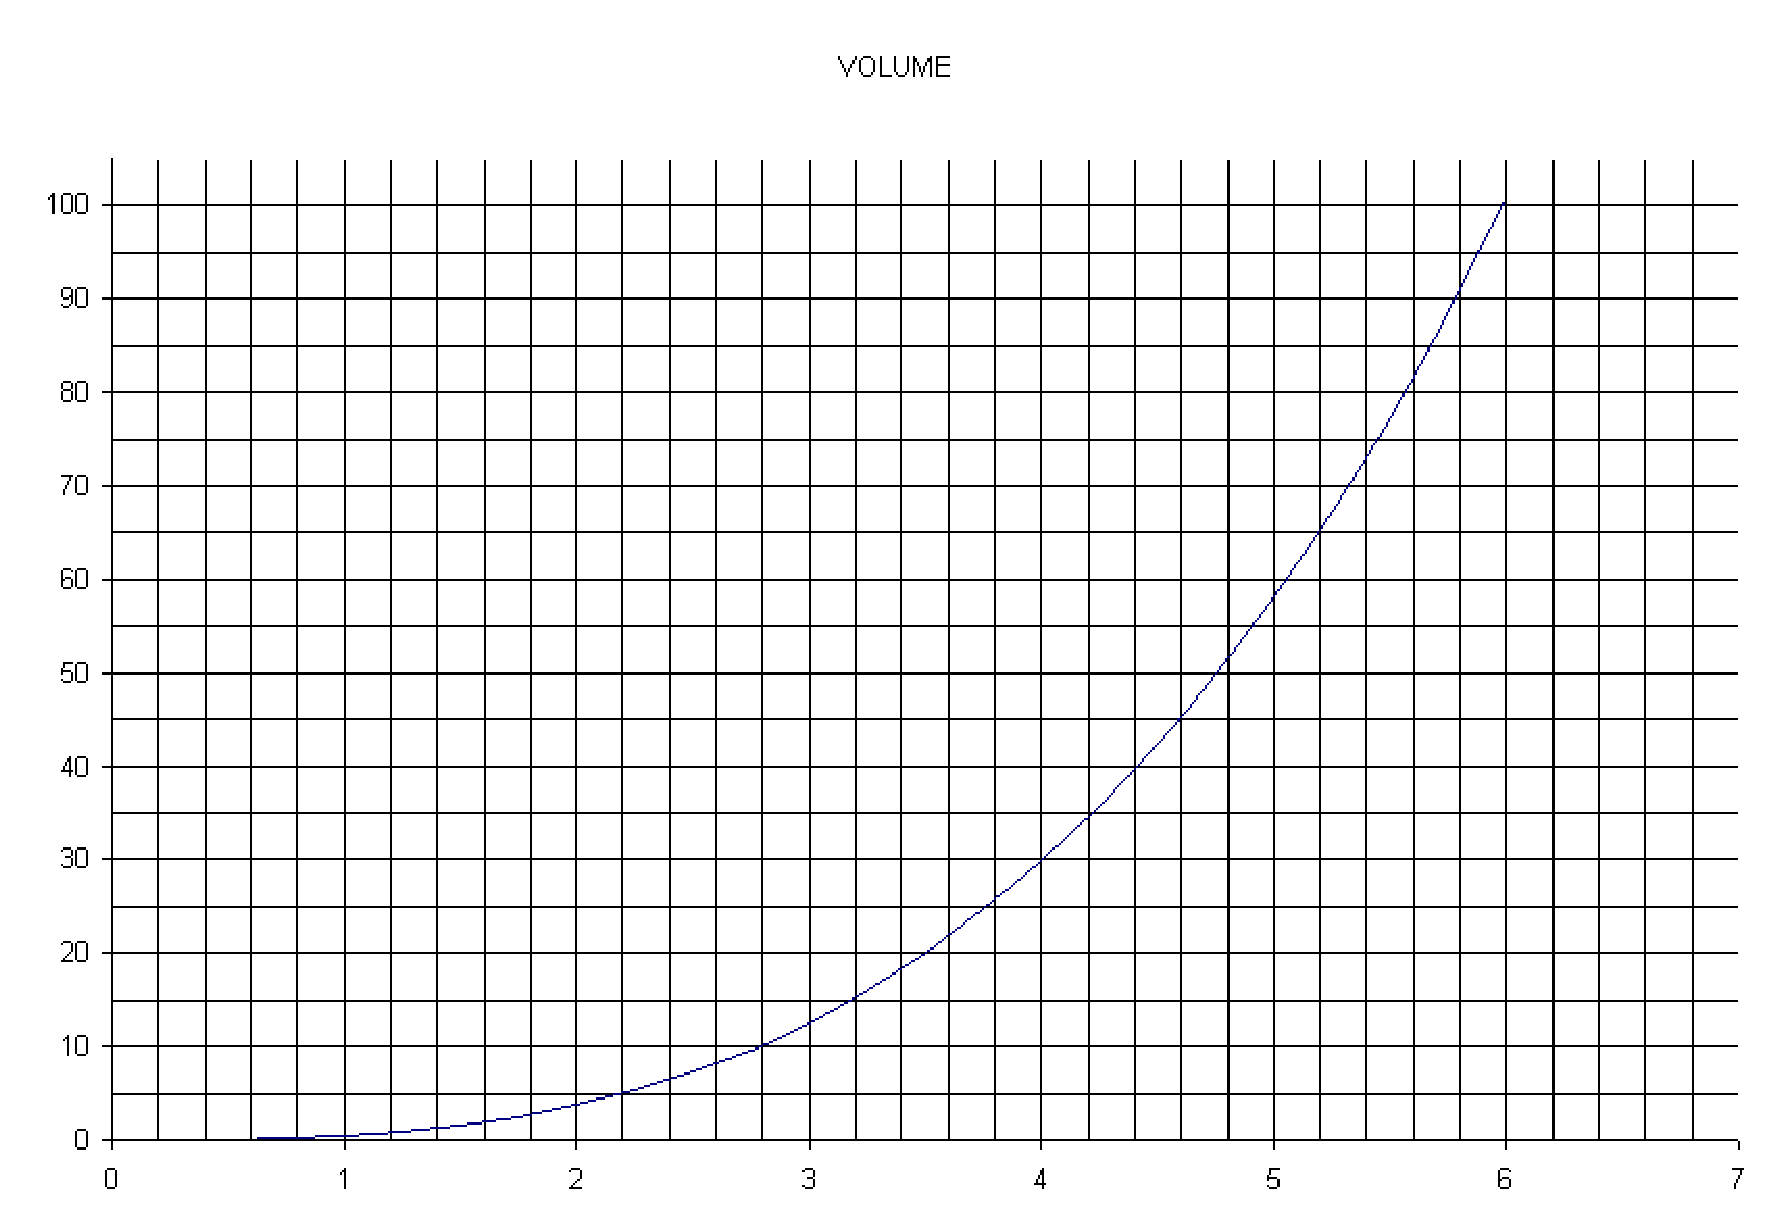
\includegraphics[scale=0.625]{./Graphiques/courbe.eps}\end{center}

%%%%%%%%%%%%%%%%%%%%%%%%%%%%%%%%%%%%%%%%%%%%%%%%%%%%
%%%%%%%%%%%%%%%%%%%%%%%%%%%%%%%%%%%%%%%%%%%%%%%%%%%

%%%%%%%%%%%%%%%%%%%%%%%%%%%%%%%%%%%%%%%%%%%%%%%%%%%\`u
%%%%%%%%%%%%%%%%%%%%%%%%%%%%%%%%%%%%%%%%%%%%%%%%%%%%

 \sautpage

\section{Premi\`eres notions (bilan et compl\'ements)}

\begin{definition}[Notion de fonction]
Une fonction est un proc\'ed\'e qui, \`a un \'el\'ement $x$ d'un ensemble de d\'epart, associe au plus un \'el\'ement $y$ d'un ensemble d'arriv\'ee.

On notera $f:x\mapsto y$ ou $f(x)=y$ qui se lit \og $f$ est la fonction qui \`a $x$ associe $y$ \fg..

On dit que $y$ est \emph{l'image} de $x$.

On dit que $x$ est \emph{un ant\'ec\'edent} de $y$.

\end{definition}

\begin{definition}[Ensemble de d\'efinition]
L'ensemble des r\'eels $x$ poss\'edant une image par une fonction num\'erique $f$ est appel\'e \emph{l'ensemble de d\'efinition de la fonction $f$}. On le note souvent $D_f$.
\end{definition}

\begin{definition}[Repr\'esentation graphique]
Dans un plan muni d'un rep\`ere, la \emph{repr\'esentation graphique} de la fonction $f$ est l'ensemble des points $M$ de coordonn\'ees $(x;y)$ du plan tels que :
\begin{itemize}
	\item L'abscisse $x$ de $M$ d\'ecrit l'ensemble de d\'efinition $D_f$ ;
	\item L'ordonn\'ee $y$ est l'image de $x$ par $f$. $y=f(x)$.
\end{itemize}

On note souvent $\mathcal{C}_f$ la repr\'esentation graphique de $f$. On dit que $\mathcal{C}_f$ a pour \'equation $y=f(x)$.

Si la courbe est d'un seul \og{} tenant \fg{} on parle  de \emph{courbe repr\'esentative} de la fonction $f$.
\end{definition}


\begin{rmq} L'\'equation permet de d\'eterminer si un point $A(x_A;y_A)$ appartient ou pas \`a cette courbe. En effet, un point appartient \`a la courbe si et seulement si ses coordonn\'ees v\'erifient l'\'equation de la courbe. On a alors : \[A\in\mathcal{C}_f\ssi y_A=f(x_A)\] \end{rmq}


Dans la pratique, pour les fonctions num\'eriques d\'efinies par une expression alg\'ebrique, pour esquisser une repr\'esentation graphique, on utilise souvent un tableau de valeurs.

\begin{tabular}{cc}
 \begin{minipage}[l]{0.55\linewidth}
  \begin{rmq} Une courbe ne repr\'esente pas toujours une fonction. Sur la figure ci-contre, par exemple, la courbe a plusieurs points ayant la même abscisse, comme $A(1,-1)$ et $B(1,3)$. Ce n'est donc pas la courbe repr\'esentative d'une fonction car alors 1 aurait plusieurs images.\end{rmq}
 \end{minipage}&
 \begin{minipage}[r]{0.45\linewidth}
\begin{center}
\psset{xunit=0.75cm , yunit=0.75cm}
\def\xmin{-2} \def\xmax{4} \def\ymin{-1.6} \def\ymax{3.6}
\begin{pspicture*}(\xmin,\ymin)(\xmax,\ymax)
\psset{xunit=0.75cm,yunit=0.75cm}
\psgrid[griddots=10,gridlabels=0pt,gridwidth=.3pt, gridcolor=black, subgridwidth=.3pt, subgridcolor=black, subgriddiv=1](0,0)(-2,-2)(4,4)
\psaxes[labels=all,labelsep=1pt, Dx=1,Dy=1]{->}(0,0)(\xmin,\ymin)(\xmax,\ymax)
\uput[dl](0,0){$O$}
%\pcline[linewidth=1pt]{->}(0,0)(1,0) \uput[d](0.5,0){\small $\vec \imath$}
%\pcline[linewidth=1pt]{->}(0,0)(0,1) \uput[l](0,0.5){\small $\vec \jmath$}
\pscircle(1,1){1.5}
\psdots[dotstyle=x](1,-1)(1,3)
\uput[d](1,-1){$A$}
\uput[u](1,3){$B$}
\end{pspicture*}
\end{center}
 \end{minipage}

\end{tabular}






%\sautpage

\subsubsection{Quelques conventions graphiques}
\begin{multicols}{3}
Lorsqu'un point $A$ sur la courbe est connu avec pr\'ecision, il est not\'e par une croix.
\begin{center}
\begin{pspicture*}(-0.5,-1)(2.5,3)
\pscurve(0,0)(0.5,-0.5)(1,1)(2,2.5)
\uput[u](0,0){$\mathcal{C}_f$}
\psdot[dotstyle=x](1,1)
\uput[dr](1,1){$A$}
\end{pspicture*}
\end{center}\sautcol
Lorsqu'un point $A$ est l'extr\'emit\'e de la courbe, il est not\'e par un gros point.
\begin{center}
\begin{pspicture*}(-0.5,-1)(2.5,3)
\pscurve(0,0)(0.5,-0.5)(1,1)(2,2.5)
\uput[u](0,0){$\mathcal{C}_f$}
\psdot(2,2.5)
\uput[dr](2,2.5){$A$}
\end{pspicture*}
\end{center}\sautcol
Lorsqu'un point $A$ \`a l'extr\'emit\'e de la courbe n'appartient pas \`a la courbe, il est not\'e par un \og demi-cercle \fg.
\begin{center}
\begin{pspicture*}(-0.5,-1)(2.5,3)
\pscurve{-(}(0,0)(0.5,-0.5)(1,1)(2,2.5)
\uput[u](0,0){$\mathcal{C}_f$}
%\psdot[(2,2.5)
\uput[dr](2,2.5){$A$}
\end{pspicture*}
\end{center}
\end{multicols}
\begin{multicols}{3}
Une courbe est donn\'ee dans une fenêtre ; s'il n'y a pas d'extr\'emit\'es, la courbe garde la même allure quand on la prolonge.
\begin{center}
\begin{pspicture*}(-0.5,-1)(2.5,3)
\pscurve(-0.3,0)(0.5,2)(1,1)(2,2.8)
\uput[u](1,1){$\mathcal{C}_f$}
\psline[linestyle=dotted](-0.1,0.5)(1.7,0.5)(1.7,2.2)(-0.1,2.2)(-0.1,0.5)
\end{pspicture*}
\end{center}
Une droite verticale en pointill\'es signifie que si l'on prolonge la courbe, elle ne coupe pas cette droite. Sur l'exemple ci-dessous, $a$ n'appartient pas \`a $D_f$.
\begin{center}
\begin{pspicture*}(-0.5,-1)(2.5,3)
\psaxes[labels=none,labelsep=1pt,Dx=5,Dy=5]{->}(0,0)(-0.5,-1)(2.5,3)
\psset{algebraic=true}
\psplot{0.6}{3}{1/(4*x-2)}
\psline[linestyle=dashed](0.5,-1)(0.5,3)
\uput[dl](0.5,0){$a$}
\end{pspicture*}
\end{center}
Une droite horizontale en pointill\'es signifie que si l'on prolonge la courbe, elle ne coupe pas cette droite.
\begin{center}
\begin{pspicture*}(-0.5,-1)(2.5,3)
\psaxes[labels=none,labelsep=1pt,Dx=5,Dy=5]{->}(0,0)(-0.5,-1)(2.5,3)
\psset{algebraic=true}
\psplot{-0.5}{3}{1+1/(x+1)}
\psline[linestyle=dashed](-0.5,1)(2.5,1)
\uput[ul](0,1){$b$}
\end{pspicture*}
\end{center}
\end{multicols}

%\sautpage






\section{R\'esolutions graphiques d'\'equations et d'in\'equations}


\subsection{R\'esolutions d'\'equations de la forme $f(x)=k$}

R\'esoudre l'\'equation $f(x)=k$ c'est d\'eterminer tous les ant\'ec\'edents \'eventuels d'un \'el\'ement $k$ de l'ensemble d'arriv\'ee, c'est-\`a-dire chercher tous les $x$ de l'ensemble de d\'epart tels que $f(x)=k$.

Une telle recherche peut se faire graphiquement \`a partir de la repr\'esentation graphique de la fonction $f$.




\begin{center}
\begin{tabular}{lc}
 \begin{minipage}[l]{0.6\linewidth}
 \begin{exemple*}
  Soit $f$ la fonction d\'efinie sur $\R$ par $f(x)=2x^2-9x+10$. On recherche les solutions de l'\'equation $f(x)=3$.

	On commence par tracer soigneusement la courbe repr\'esentative de $f$ et on obtient la repr\'esentation donn\'ee sur la figure ci-dessous.
		
		On cherche les points de la courbe ayant pour ordonn\'ee 3. Pour cela on peut tracer la droite d'\'equation $y=3$ et chercher les points d'intersection de cette droite avec la courbe de $f$.

		On obtient ici deux points $M_1(1;3)$ et $M_2\left(\frac{7}{2};3\right)$. Les solutions sont leurs abscisses : 1 et $\frac{7}{2}$.

		On \'ecrit : \og Les solutions de l'\'equation $f(x)=3$ sont $x=1$ ou $x=\frac{7}{2}$ car les points de la courbe de $f$ d'ordonn\'ee 3 ont pour abscisses 1 et $\frac{7}{2}$ \fg.
		\end{exemple*}
 \end{minipage}&
 \begin{minipage}[r]{0.35\linewidth}
  
		\begin{center}
 \psset{xunit=1cm,yunit=1cm}
		\begin{pspicture*}(-3.1,-2.1)(4.6,4.1)
\def\xmin{-3} \def\xmax{4.5} \def\ymin{-2} \def\ymax{4}

\psgrid[griddots=10,gridlabels=0pt,gridwidth=.3pt, gridcolor=black, subgridwidth=.3pt, subgridcolor=black, subgriddiv=1](0,0)(-3,-2)(4.5,4)
\psaxes[labels=all,labelsep=1pt, Dx=1,Dy=1]{->}(0,0)(\xmin,\ymin)(\xmax,\ymax)
\uput[dl](0,0){$O$}
\pcline[linewidth=1pt]{->}(0,0)(1,0) \uput[d](0.5,0){\small $\vec \imath$}
\pcline[linewidth=1pt]{->}(0,0)(0,1) \uput[r](0,0.5){\small $\vec \jmath$}
\psset{algebraic=true}
\psplot{\xmin}{\xmax}{2*(x-1)*(x-1)-5*(x-1)+3}
\uput[ul](2,1){$\mathcal{C}_f$}
\psline[linestyle=dashed](\xmin,3)(\xmax,3)
\uput[u](-2,3){$y=3$}
\uput[ur](1,3){$M_1$}
\uput[ul](3.5,3){$M_2$}
\psdots[dotstyle=x](1,3)(3.5,3)
\psline[linestyle=dashed]{->}(1,3)(1,0)
\psline[linestyle=dashed]{->}(3.5,3)(3.5,0)
\end{pspicture*}\end{center}
 \end{minipage}

\end{tabular}             \end{center}



%\sautpage

\subsection{R\'esolutions d'in\'equations de la forme $f(x)\leqslant k$}

Ces in\'equations peuvent se r\'esoudre graphiquement. On proc\`ede de la façon suivante :
\begin{itemize}
	\item on trace soigneusement $\mathcal{C}_f$ dan un rep\`ere (orthogonal) ;
	\item on trace la droite d'\'equation $y=k$ ;
	\item on recherche les points de la courbe situ\'es \emph{sous} la droite ;
	\item l'ensemble des solutions est constitu\'e des abscisses de ces points.
\end{itemize}

\begin{exemple*} Sur l'exemple pr\'ec\'edent, si l'on doit r\'esoudre $f(x)\leqslant 3$, apr\`es avoir trac\'e $y=3$ on constate que les points de la courbe situ\'es sous cette droite ont leurs abscisses comprises entre 0 et $\frac{5}{2}$.

Donc $f(x)\leqslant 3 \ssi x\in\left[0;\frac{5}{2}\right]$.
\end{exemple*}

\begin{rmq}~
\begin{itemize}
	\item On r\'esoud de la même mani\`ere les \'equations du type $f(x)\geqslant k$.

On retient alors les abscisses des points situ\'es \emph{au-dessus} de la droite d'\'equation $y=k$.

Dans l'exemple $f(x)\geqslant 3 \ssi x\in \left] -\infty ; 0 \right] \cup \left[\frac{5}{2} ; +\infty\right[$.
	\item De même pour les in\'equations strictes : $f(x)>k$ ou $f(x)<k$. On excluera alors les abscisses des points d'intersection de la courbe et de la droite.

	Dans l'exemple $f(x)<3 \ssi x\in \left]0;\frac{5}{2}\right[$.
\end{itemize}
\end{rmq}

\subsection{R\'esolutions d'\'equations de la forme $f(x)=g(x)$}

Cela revient \`a chercher les \'el\'ements de l'ensemble de d\'epart qui ont la même image par $f$ et par $g$.

Une telle recherche peut se faire graphiquement. On recherche alors les points des deux courbes repr\'esentatives ayant même abscisse et même ordonn\'ee, c'est-\`a-dire les points d'intersection des deux courbes. 

\begin{tabular}{cc}
 \begin{minipage}[l]{0.6\linewidth}
  \begin{exemple*}

Soit $f$ et $g$ les fonctions d\'efinies sur $\R$ par, respectivement, $f(x)=x^2-1$ et $g(x)=-0,5x^2+x+4$. R\'esoudre graphiquement l'\'equation $f(x)=g(x)$.

	On commence par tracer soigneusement les deux courbes repr\'esentatives et on obtient la repr\'esentation donn\'ee sur la figure ci-contre.
	
	On cherche les points d'intersection des deux courbes, ici $M_1$ et $M_2$, et les solutions de l'\'equation sont leurs abscisses dont les valeurs approximatives sont $-1,5$ et $2,2$.

		Les solutions sont donc $x\approx -1,5$ et $x\approx 2,2$.
\end{exemple*}
 \end{minipage}&
 \begin{minipage}[r]{0.35\linewidth}
  \psset{xunit=0.75cm,yunit=0.75cm}
		\begin{pspicture*}(-3.1,-2.1)(4.6,5.1)
\def\xmin{-3} \def\xmax{4.5} \def\ymin{-2} \def\ymax{5}

\psgrid[griddots=10,gridlabels=0pt,gridwidth=.3pt, gridcolor=black, subgridwidth=.3pt, subgridcolor=black, subgriddiv=1](0,0)(-3,-2)(4.5,5)
\psaxes[labels=all,labelsep=1pt, Dx=1,Dy=1]{->}(0,0)(\xmin,\ymin)(\xmax,\ymax)
\uput[dl](0,0){$O$}
\pcline[linewidth=1pt]{->}(0,0)(1,0) \uput[d](0.5,0){\small $\vec \imath$}
\pcline[linewidth=1pt]{->}(0,0)(0,1) \uput[r](0,0.5){\small $\vec \jmath$}
\psset{algebraic=true}
\psplot{\xmin}{\xmax}{x^2-1}
\psplot{\xmin}{\xmax}{-0.5*x^2+x+4}
\uput[u](1,1){$\mathcal{C}_f$}
\uput[dr](0,4){$\mathcal{C}_g$}
\uput[r](2.189,3.793){$M_2$}
\uput[l](-1.523,1.318){$M_1$}
\psdots[dotstyle=x](2.189,3.793)(-1.523,1.318)
\psline[linestyle=dashed]{->}(-1.523,1.318)(-1.523,0)
\psline[linestyle=dashed]{->}(2.189,3.793)(2.189,0)
\end{pspicture*}
	
 \end{minipage}


\end{tabular}

		

\subsection{R\'esolutions d'in\'equations de la forme $f(x)\leqslant g(x)$}

L\`a encore ces in\'equations peuvent se r\'esoudre graphiquement. On proc\`ede de la façon suivante :
\begin{itemize}
	\item on trace soigneusement $\mathcal{C}_f$ et $\mathcal{C}_g$ dans un rep\`ere (orthogonal) ;
	\item l'ensemble des solutions est constitu\'e des abscisses des points o\`u la courbe de $f$ est situ\'ee \emph{sous} celle de $g$.
\end{itemize}

\begin{exemple*} Sur l'exemple pr\'ec\'edent, si l'on doit r\'esoudre $f(x)\leqslant g(x)$, on constate que les points de la courbe de $f$ situ\'es sous celle de $g$ ont leurs abscisses comprises entre environ $-1,5$ et 2,2.

Donc $f(x)\leqslant g(x) \ssi x\in [-1,5;2,2]$. Ou bien $S=[-1,5;2,2]$.
\end{exemple*}

\begin{rmqs}~
\begin{itemize}
	\item On r\'esoud de la même mani\`ere les \'equations du type $f(x)\geqslant g(x)$.

On retient alors les abscisses des points de la courbe de $f$ situ\'es \emph{au-dessus} de celle de $g$.

Dans l'exemple $f(x)\geqslant g(x) \ssi x\in ] -\infty ; -1,5 ] \cup [2,2 ; +\infty[$.
	\item De même pour les in\'equations strictes : $f(x)>g(x)$ ou $f(x)<g(x)$. On excluera alors les abscisses des points d'intersection des deux courbes.

	Dans l'exemple $f(x)<g(x) \ssi x\in ]-1,5;2,2[$.
\end{itemize}
\end{rmqs}



%\sautpage



\sautpage

\section{Variations, extremums}


\subsection{Sens de variation}

Il s'agit de traduire math\'ematiquement qu'une fonction \og augmente \fg{} ou \og diminue \fg.

\begin{exemple*} Soit, par exemple, la fonction d\'efinie sur $[-3;3]$ par la courbe repr\'esentative donn\'ee sur la figure \ref{croissanceetdecroissance} \vpageref{croissanceetdecroissance}. On constate que lorsque $x\in[-3;1]$ , si $x$ augmente, $f(x)$ augmente aussi alors que lorsque $x\in[1;3]$, si $x$ augmente, $f(x)$ diminue.

C'est la d\'efinition math\'ematique de la croissance ou de la d\'ecroissance d'une fonction $f$.

\begin{figure}[h]
\centering
\caption{Croissance et d\'ecroissante}\label{croissanceetdecroissance}


\psset{xunit=1cm , yunit=1.25cm}
\begin{pspicture*}(-4.1,-1.1)(4.1,5.1)
\def\xmin{-4} \def\xmax{4} \def\ymin{-1} \def\ymax{5}
\psgrid[griddots=10,gridlabels=0pt,gridwidth=.3pt, gridcolor=black, subgridwidth=.3pt, subgridcolor=black, subgriddiv=1](0,0)(-4,-1)(4,5)
\psaxes[labels=all,labelsep=1pt, Dx=1,Dy=1]{-}(0,0)(\xmin,\ymin)(\xmax,\ymax)
\uput[dl](0,0){$O$}
\pcline[linewidth=1pt]{->}(0,0)(1,0) \uput[d](0.5,0){\small $\vec \imath$}
\pcline[linewidth=1pt]{->}(0,0)(0,1) \uput[r](0,0.5){\small $\vec \jmath$}
\psset{algebraic=true}
\psplot{-3}{3}{(-(x-1)^2+5)*0.25+3}
\psdots(3,3.25)(-3,0.25)
\uput[d](-1.5,0){$b$}
\psline[linestyle=dashed]{->}(-1.5,0)(-1.5,2.6875)
\psline[linestyle=dashed]{->}(-1.5,2.6875)(0,2.6875)
\uput[r](0,2.6875){$f(b)$}
\uput[d](-2.5,0){$a$}
\psline[linestyle=dashed]{->}(-2.5,0)(-2.5,1.1875)
\psline[linestyle=dashed]{->}(-2.5,1.1875)(0,1.1875)
\uput[r](0,1.1875){$f(a)$}
\uput[d](1.5,0){$u$}
\uput[d](2.5,0){$v$}
\psline[linestyle=dashed]{->}(1.5,0)(1.5,4.1875)
\psline[linestyle=dashed]{->}(1.5,4.1875)(0,4.1875)
\uput[l](0,4.1875){$f(u)$}
\psline[linestyle=dashed]{->}(2.5,0)(2.5,3.6875)
\psline[linestyle=dashed]{->}(2.5,3.6875)(0,3.6875)
\uput[l](0,3.6875){$f(v)$}
\end{pspicture*}
\end{figure}\end{exemple*}


\begin{definition}
Soit $f$ une fonction d\'efinie sur un intervalle $I$. On dit que $f$ est
\begin{itemize}
	\item \emph{croissante} sur $I$ si, pour tous r\'eels $a$ et $b$ de $I$, on a :\\
$\text{Si } a<b \text{ alors } f(a)\leqslant f(b).$
	\item \emph{d\'ecroissante} sur $I$ si, pour tous r\'eels $a$ et $b$ de $I$, on a :\\
$\text{Si } a<b \text{ alors } f(a)\geqslant f(b).$
	\item \emph{monotone} si elle n'est que croissante sur $I$ ou si elle n'est que d\'ecroissante sur $I$.
	\item \emph{constante} sur $I$ si, pour tous r\'eels $a$ et $b$ de $I$, on a : $f(a)=f(b)$.
\end{itemize}
\end{definition}


\begin{rmqs}~
\begin{itemize}
	\item Ces notions ne sont valables que sur \textbf{un intervalle} et pas sur une r\'eunion d'intervalles disjoints.
	\item Ant\'ec\'edents et images \'etant rang\'es dans le même ordre, on dit qu'une fonction croissante \emph{conserve} l'ordre.
	\item Ant\'ec\'edents et images \'etant rang\'es dans l'ordre inverse, on dit qu'une fonction d\'ecroissante \emph{inverse} l'ordre.
	\item On obtient les d\'efinitions d'une fonction \emph{strictement} croissante ou \emph{strictement} d\'ecroisante en remplaçant les in\'egalit\'es par des in\'egalit\'es strictes. Ainsi on dit que $f$ est strictement croissante sur $I$ si pour tous r\'eels $a$ et $b$ de $I$ on a : \\ $\text{Si } a<b \text{ alors } f(a)<f(b)$
	\item Une fonction est strictement monotone sur $I$ si elle est strictement croissante ou strictement d\'ecroissante sur $I$
\end{itemize}
\end{rmqs}

\subsection{Tableau de variations}

Ces r\'esultats peuvent se r\'esumer dans un tableau de variation, qui est une forme stylis\'ee de repr\'esentation o\`u l'on indique uniquement si la courbe monte, descend ou est stable. Dans la premi\`ere ligne on indique les valeurs importantes de $x$ et dans la seconde les variations de $f$.

\begin{exemple*} Dans l'exemple pr\'ec\'edent on obtient
$$\tabvar{%
\tx{x}&\tx{-3}&&\tx{1}&&\tx{3}\cr
\tx{f}&\txb{\approx 0,25}&\fm&\txh{\approx 4,25}&\fd&\txb{\approx 2,25}\cr
}$$
\end{exemple*}



\subsection{Extremums}

Les extremums, s'ils existent, sont les valeurs maximale et minimale qui sont \textbf{atteintes} par la fonction $f$ sur un intervalle donn\'e. Plus pr\'ecis\'ement :

\begin{definition}
Soit une fonction $f$ d\'efinie sur un intervalle $I$ et $x_0\in I$. On dit que
\begin{itemize}
	\item $f$ admet un \emph{maximum}, atteint en $x_0$ si, pour tout $x\in I$, $f(x)\leqslant f(x_0)$. Ce maximum est alors $f(x_0)$.
	\item $f$ admet un \emph{minimum}, atteint en $x_0$ si, pour tout $x\in I$, $f(x)\geqslant f(x_0)$. Ce minimum est alors $f(x_0)$.
\end{itemize}
Les maximum et minimum sont appel\'es les \emph{extremums}.
\end{definition}

%\begin{rmq} Un extremum doit être atteint par une valeur $x_0$. \end{rmq}

\begin{exemple*}
La fonction $f$ d\'efinie sur $\R$ par $f(x)=x^2+1$ n'admet pas $-1$ comme minimum.

En effet, si on a bien $f(x)\geqslant -1$ sur $\R$, il n'existe pas de $x_0$ tel que $f(x_0)=-1$.

Par contre 1 est bien le minimum de $f$ sur $\R$ car
\begin{itemize}
	\item $f(x)\geqslant 1$ pour tout $x\in\R$ \textbf{ET}
	\item $f(0)=1$
\end{itemize}

On dira donc : le minimum de $f$ sur $\R$ est 1 et il est atteint pour $x_0=0$.
\end{exemple*}

\sautpage

\section{Exercices et probl\`emes}

\subsection{Premi\`eres notions}

%\begin{multicols}{2}
%\begin{exo} Dire dans chacun des exemples ci-dessous quel est l'ensemble de d\'efinition, quelles sont les images possibles et si la fonction est num\'erique.
%\begin{enumerate}
%	\item \`A chaque \'el\`eve de la classe on associe la couleur de ses cheveux.
%	\item \`A chaque \'el\`eve de la classe on associe le nombre de ses fr\`eres et soeurs.
%	\item Pour un \'el\`eve donn\'e, \`a chaque moment de sa vie on associe la taille qu'il mesurait.
%	\item Soit $ABCD$ un rectangle dont un des côt\'es est fixe et mesure 6 cm et l'autre est variable et mesure $x$ cm. \\On d\'efinit la fonction $f$ de la façon suivante : \`a chaque $x$ possible, on associe $f(x)$, l'aire du rectangle $ABCD$.
%	\item La fonction $g$ d\'efinie par $g(x)=x^2+2x+3$.
%	\item La fonction $h$ d\'efinie par $h(x)=\frac{x^2+1}{x-1}$.
%	\item La fonction $i$ d\'efinie par $i(x)=\sqrt{x+2}$.
%\end{enumerate}
%\end{exo}
\begin{multicols}{2}
\begin{exo}
On d\'efinit $f$ et $g$, deux fonctions :
\begin{itemize}
	\item $f$ est la fonction qui \`a un nombre r\'eel $x$ associe le nombre obtenu en proc\'edant de la mani\`ere suivante : on ajoute $4$ au nombre, on \'el\`eve le r\'esultat obtenu au carr\'e, on retranche 16, on divise par le nombre de d\'epart et on retranche 6.
	\item $g:x\mapsto x^2-4$.
\end{itemize}
\begin{enumerate}
	\item Donner l'expression correspondant \`a $f$ puis simplifier cette expression.
	\item Quel r\'eel n'a pas d'image par $f$ ?
	\item Quelle est l'image de 3 par $g$ ?
	\item Quelle est l'image de $-1$ par $g$ ?
	\item Quels sont les ant\'ec\'edents \'eventuels de 12 par $g$ ?
	\item Quels sont les ant\'ec\'edents \'eventuels de $-5$ par $g$ ?
\end{enumerate}
\end{exo}

\sautcol

\begin{exo}
Vrai ou faux ? \emph{Corriger la phrase lorsqu'elle est fausse}.
\begin{enumerate}
	\item $f(-2) = 0$ signifie que l'image de 0 est $-2$
	\item $f(0) = 3$ signifie que la courbe de $f$ passe par le point $(0 ; 3)$
	\item $f(1) = 2$ signifie que l'ant\'ec\'edent de 1 est 2
	\item L'image de 2 par $f$ est $-3$ s'\'ecrit $f(2) = -3$
	\item Dire que $(5 ; 1)$ est un point de la courbe de $f$ s'\'ecrit $5 = f(1)$
	\item Par la fonction $g$, $-5$ est l'image de 3 s'\'ecrit $g(-5) = 3$
	\item 2 a pour image 0 par $f$ signifie que la courbe de $f$ traverse l'axe des abscisses en 2
	\item $f(4) = 0$ signifie que la courbe de $f$ traverse l'axe des abscisses au point $(4 ; 0)$
	\item 3 a pour image 5, signifie que 3 est l'image de 5
	\item 4 a pour ant\'ec\'edent 5 signifie que 5 est l'image de 4
\end{enumerate}
\end{exo}

\end{multicols}

%\sautpage

\begin{exo}\label{gf4courbes}
Vrai ou faux ? \emph{Justifier la r\'eponse lorsque c'est faux}.\\
Les courbes de la figure \ref{gf4courbesfig} \vpageref{gf4courbesfig} repr\'esentent des fonctions de la variable $x$.


\begin{figure}[!h]
 \centering
 \caption{Courbes de l'exercice \ref{gf4courbes}}\label{gf4courbesfig}
\begin{tabular}{cc}
\psset{xunit=1cm , yunit=0.5cm}
\begin{pspicture*}(-2.1,-2.1)(4.1,4.1)
\def\xmin{-2} \def\xmax{4} \def\ymin{-2} \def\ymax{4}
\psgrid[griddots=10,gridlabels=0pt,gridwidth=.3pt, gridcolor=black, subgridwidth=.3pt, subgridcolor=black, subgriddiv=1](0,0)(-2,-2)(4,4)
\psaxes[labels=all,labelsep=1pt, Dx=1,Dy=1]{->}(0,0)(\xmin,\ymin)(\xmax,\ymax)
\uput[dl](0,0){$O$}
\pcline[linewidth=1pt]{->}(0,0)(1,0) \uput[d](0.5,0){\small $\vec \imath$}
\pcline[linewidth=1pt]{->}(0,0)(0,1) \uput[l](0,0.5){\small $\vec \jmath$}
\psline(-2,3)(1,-1.5)(2,-1.5)(4,2)
\end{pspicture*}
&
\psset{xunit=1cm , yunit=0.5cm}
\begin{pspicture*}(-2.1,-2.1)(4.1,4.1)
\def\xmin{-2} \def\xmax{4} \def\ymin{-2} \def\ymax{4}
\psgrid[griddots=10,gridlabels=0pt,gridwidth=.3pt, gridcolor=black, subgridwidth=.3pt, subgridcolor=black, subgriddiv=1](0,0)(-2,-2)(4,4)
\psaxes[labels=all,labelsep=1pt, Dx=1,Dy=1]{->}(0,0)(\xmin,\ymin)(\xmax,\ymax)
\uput[dl](0,0){$O$}
\pcline[linewidth=1pt]{->}(0,0)(1,0) \uput[d](0.5,0){\small $\vec \imath$}
\pcline[linewidth=1pt]{->}(0,0)(0,1) \uput[l](0,0.5){\small $\vec \jmath$}
\psline(-2,3)(1,3)(1,1)(4,1)
\end{pspicture*}
\\
\psset{xunit=1cm , yunit=0.5cm}
\begin{pspicture*}(-2.1,-2.1)(4.1,4.1)
\def\xmin{-2} \def\xmax{4} \def\ymin{-2} \def\ymax{4}
\psgrid[griddots=10,gridlabels=0pt,gridwidth=.3pt, gridcolor=black, subgridwidth=.3pt, subgridcolor=black, subgriddiv=1](0,0)(-2,-2)(4,4)
\psaxes[labels=all,labelsep=1pt, Dx=1,Dy=1]{->}(0,0)(\xmin,\ymin)(\xmax,\ymax)
\uput[dl](0,0){$O$}
\pcline[linewidth=1pt]{->}(0,0)(1,0) \uput[d](0.5,0){\small $\vec \imath$}
\pcline[linewidth=1pt]{->}(0,0)(0,1) \uput[l](0,0.5){\small $\vec \jmath$}
\psline(-2,3)(4,3)
\end{pspicture*}
&
\psset{xunit=1cm , yunit=0.5cm}
\begin{pspicture*}(-2.1,-2.1)(4.1,4.1)
\def\xmin{-2} \def\xmax{4} \def\ymin{-2} \def\ymax{4}
\psgrid[griddots=10,gridlabels=0pt,gridwidth=.3pt, gridcolor=black, subgridwidth=.3pt, subgridcolor=black, subgriddiv=1](0,0)(-2,-2)(4,4)
\psaxes[labels=all,labelsep=1pt, Dx=1,Dy=1]{->}(0,0)(\xmin,\ymin)(\xmax,\ymax)
\uput[dl](0,0){$O$}
\pcline[linewidth=1pt]{->}(0,0)(1,0) \uput[d](0.5,0){\small $\vec \imath$}
\pcline[linewidth=1pt]{->}(0,0)(0,1) \uput[l](0,0.5){\small $\vec \jmath$}
\pscurve(-2,3)(-1,0)(0,-1)(2,1)(3.2,2)(3,3)
\end{pspicture*}
\end{tabular}
\end{figure}

\end{exo}

\sautpage

\begin{exo}\label{gf14}
Vrai ou faux ? \emph{Corriger la phrase lorsqu'elle est fausse}.\\
Les fonctions $f$ et $g$ sont repr\'esent\'ees sur la figure \ref{gf14fig} \vpageref{gf14fig}.
\begin{enumerate}
	\item La fonction $f$ est d\'efinie entre $-2$ et 6 inclus
	\item Les images par la fonction $f$ sont comprises entre $-1$ et 4 inclus
	\item La fonction $g$ est d\'efinie entre $-2$ exclu et 6 inclus
	\item Les images par la fonction g sont comprises entre 0 exclu et 3 inclus
\end{enumerate}



\begin{figure}[!h]
\centering
\caption{Courbes de l'exercice \ref{gf14}}\label{gf14fig}
\begin{tabular}{cc}
\psset{xunit=0.9cm , yunit=0.5cm}
\begin{pspicture*}(-3.1,-2.1)(6.1,5.1)
\def\xmin{-3} \def\xmax{6} \def\ymin{-2} \def\ymax{5}
\psgrid[griddots=10,gridlabels=0pt,gridwidth=.3pt, gridcolor=black, subgridwidth=.3pt, subgridcolor=black, subgriddiv=1](0,0)(-3,-2)(6,5)
\psaxes[labels=all,labelsep=1pt, Dx=1,Dy=1]{->}(0,0)(\xmin,\ymin)(\xmax,\ymax)
\uput[dl](0,0){$O$}
\pcline[linewidth=1pt]{->}(0,0)(1,0) \uput[d](0.5,0){\small $\vec \imath$}
\pcline[linewidth=1pt]{->}(0,0)(0,1) \uput[l](0,0.5){\small $\vec \jmath$}
\pscurve{*-(}(-2,2)(-1,3)(0,3.7)(0.5,3.9)(1,4)(2,3)(3,0)(4,-1)(5,0)(6,1)

\rput(3,2){$\mathcal{C}_f$}
\end{pspicture*}
&
\psset{xunit=0.9cm , yunit=0.5cm}
\begin{pspicture*}(-3.1,-2.1)(6.1,5.1)
\def\xmin{-3} \def\xmax{6} \def\ymin{-2} \def\ymax{5}
\psgrid[griddots=10,gridlabels=0pt,gridwidth=.3pt, gridcolor=black, subgridwidth=.3pt, subgridcolor=black, subgriddiv=1](0,0)(-3,-2)(6,5)
\psaxes[labels=all,labelsep=1pt, Dx=1,Dy=1]{->}(0,0)(\xmin,\ymin)(\xmax,\ymax)
\uput[dl](0,0){$O$}
\pcline[linewidth=1pt]{->}(0,0)(1,0) \uput[d](0.5,0){\small $\vec \imath$}
\pcline[linewidth=1pt]{->}(0,0)(0,1) \uput[l](0,0.5){\small $\vec \jmath$}
\pscurve{)-}(-2,0)(0,1)(1,2)(1.5,3.5)(1.8,5)
\pscurve{-*}(2.2,-2)(3,0)(4,1.5)(6,3)
\rput(1,3){$\mathcal{C}_g$}
\psline[linestyle=dashed](2,\ymin)(2,\ymax)
\end{pspicture*}
\end{tabular}
\end{figure}

\end{exo}

\begin{exo}\label{gf15}
Vrai ou faux ? \emph{Corriger la proposition lorsqu'elle est fausse}.
\begin{itemize}
	\item D'apr\`es la repr\'esentation graphique de la figure \ref{gf15fig} \vpageref{gf15fig} $D_f=[-4;2]$
	\item D'apr\`es la repr\'esentation graphique de la figure \ref{gf15fig} \vpageref{gf15fig} $D_g=]-\infty;3[\cup]3;5]$
\end{itemize}


\begin{figure}[!h]
\centering
\caption{Courbes de l'exercice \ref{gf15}}\label{gf15fig}
\begin{tabular}{cc}
\psset{xunit=1cm , yunit=0.66cm}
\begin{pspicture*}(-4.1,-2.1)(4.1,4.1)
\def\xmin{-4} \def\xmax{4} \def\ymin{-2} \def\ymax{4}
\psgrid[griddots=10,gridlabels=0pt,gridwidth=.3pt, gridcolor=black, subgridwidth=.3pt, subgridcolor=black, subgriddiv=1](0,0)(-4,-2)(4,4)
\psaxes[labels=all,labelsep=1pt, Dx=1,Dy=1]{->}(0,0)(\xmin,\ymin)(\xmax,\ymax)
\uput[dl](0,0){$O$}
\pcline[linewidth=1pt]{->}(0,0)(1,0) \uput[d](0.5,0){\small $\vec \imath$}
\pcline[linewidth=1pt]{->}(0,0)(0,1) \uput[l](0,0.5){\small $\vec \jmath$}
\pscurve{*-}(-4,0)(-3,-2)(0,0)(1,1)(4,1.8)
\psline[linestyle=dashed](0,2)(4,2)
\rput(-1.5,-1){$\mathcal{C}_f$}
\end{pspicture*}
&
\psset{xunit=1cm , yunit=0.66cm}
\begin{pspicture*}(-3.1,-2.1)(5.6,4.1)
\def\xmin{-3} \def\xmax{5.5} \def\ymin{-2} \def\ymax{4}
\psgrid[griddots=10,gridlabels=0pt,gridwidth=.3pt, gridcolor=black, subgridwidth=.3pt, subgridcolor=black, subgriddiv=1](0,0)(-3,-2)(5.5,4)
\psaxes[labels=all,labelsep=1pt, Dx=1,Dy=1]{->}(0,0)(\xmin,\ymin)(\xmax,\ymax)
\uput[dl](0,0){$O$}
\pcline[linewidth=1pt]{->}(0,0)(1,0) \uput[d](0.5,0){\small $\vec \imath$}
\pcline[linewidth=1pt]{->}(0,0)(0,1) \uput[l](0,0.5){\small $\vec \jmath$}
\pscurve(-3,3)(0,1.5)(1,1)(2,0)(2.8,-2)
\pscurve{-*}(3.2,-2)(4,1)(5,3)
\psline[linestyle=dashed](3,\ymin)(3,\ymax)
\uput[ur](1,1){$\mathcal{C}_g$}
\end{pspicture*}
\end{tabular}
\end{figure}
\end{exo}
%\sautpage


\begin{exo}[Avec la calculatrice]
La fonction $f$ est d\'efinie sur $[-1,5;2]$ par : $f(x)=2x^3-1,5x^2-3x$
\begin{enumerate}
	\item Compl\'eter le tableau de valeurs suivant :
	%\vspace{-1em}
	\begin{center}
\begin{tabular}{|*{9}{c|}}
\hline $x$ & $-1,5$ & $-1$ & $-0,5$ & 0 & 0,5 & 1 & 1,5 & 2 \\ \hline
$f(x)$ & & & & & & & & \\ \hline
\end{tabular}
\end{center}
\item Tracer la courbe repr\'esentative de $f$.
\end{enumerate}
\end{exo}

\begin{exo}[Avec la calculatrice]\label{uneautrecourbe}
La fonction $f$ est d\'efinie sur $[-3;3]$ par : $f(x)=x^2-3x+1$.\\
Apr\`es avoir dress\'e un tableau de valeurs de la fonction, tracer sa courbe repr\'esentative $\mathcal{C}_f$.

\end{exo}

%\end{multicols}



\sautpage

\subsection{R\'esolutions graphiques}

\begin{exo}
La fonction $f$ est d\'efinie sur $[-3;3]$ par : $f(x)=x^2-3x+1$.\\
$\mathcal{C}_f$, courbe repr\'esentative de $f$ a d\'ej\`a \'et\'e obtenue dans l'exercice \ref{uneautrecourbe}.
\begin{enumerate}
	\item \`A l'aide de la repr\'esentation graphique $\mathcal{C}_f$, avec la pr\'ecision permise par le graphique, r\'epondre aux question suivantes :
		\vspace{-1em}\begin{multicols}{2}
		  \begin{enumerate}
			\item Quelle est l'image de 2 ?
			\item Quelle est l'image de 3 ?
			\item Quelle est l'image de 4 ?
			\item Quels sont les ant\'ec\'edents de 1 ?
			\item Quels sont les ant\'ec\'edents de 2 ?
			\item Quels sont les ant\'ec\'edents de $-2$ ?
		\end{enumerate}
		\end{multicols}\vspace{-1em}
	\item R\'esoudre graphiquement les \'equations et in\'equations suivantes :
\vspace{-1em}\begin{multicols}{3}\begin{enumerate}
	\item $f(x)=3$ ;
	\item $f(x)=-1,5$ ;
	\item $f(x)\geqslant -1$ ;
	\item $f(x)<4$ ;
	\item $f(x)>-3$ ;
	\item $f(x)<-2$.
\end{enumerate}\end{multicols}\vspace{-1em}
\item D\'eterminer graphiquement le signe de $f(x)$ selon les valeurs de $x$.
\end{enumerate}
\end{exo}

%\sautpage

\begin{exo}
Une fonction $f$, d\'efinie sur $\R$, est donn\'ee par sa courbe repr\'esentative $\mathcal{C}$ :
\begin{multicols}{2}
\begin{center}\small
\psset{xunit=1,yunit=1}
\begin{pspicture*}(-2.6,-2.1)(5.1,3.1)
\def\xmin{-2.5} \def\xmax{5} \def\ymin{-2} \def\ymax{3}
\psset{xunit=0.1cm,yunit=0.1cm}
\psgrid[griddots=15,gridlabels=0pt,gridwidth=.3pt, gridcolor=gray, subgridwidth=.3pt, subgridcolor=gray, subgriddiv=1](0,0)(-25,-20)(50,30)
\psset{xunit=1cm , yunit=1cm}
\psaxes[labels=all,labelsep=1pt, Dx=1,Dy=1]{->}(0,0)(\xmin,\ymin)(\xmax,\ymax)
\uput[dl](0,0){$0$}
\pcline[linewidth=1pt]{->}(0,0)(1,0) \uput[d](0.5,0){\small $\vec i$}
\pcline[linewidth=1pt]{->}(0,0)(0,1) \uput[l](0,0.5){\small $\vec j$}
\pscurve(-2.3,-2)(-2,-1)(-1.5,1.5)(-1,3)(-0.5,2.5)(0,1)(0.2,0)(0.5,-1)(1,-1.5)(1.5,-1)(2,0)(2.5,1)(3,1.5)(4,2)(5,2.3)
\psline[linestyle=dashed](0,2.5)(\xmax,2.5)
\psdots[dotstyle=x](-2,-1)(-1.5,1.5)(-1,3)(-0.5,2.5)(0,1)(0.5,-1)(1,-1.5)(1.5,-1)(2,0)(2.5,1)(3,1.5)(4,2)
\end{pspicture*}
\end{center}\normalsize

\sautcol

Avec la pr\'ecision permise par le graphique, r\'esoudre :
%\vspace{-1em}
%\begin{multicols}{2}
\begin{enumerate}
	\item Les \'equations suivantes :
		\vspace{-1em}
		\begin{multicols}{2}\begin{enumerate}
			\item $f(x) = 1$ ;
			\item $f(x) = 0$ ;
			\item $f(x) = -1$ ;
			\item $f(x) = 2$.
		\end{enumerate}\end{multicols}
		%\vspace{-1em}
%\sautcol
	\item Les in\'equations suivantes :
		\vspace{-1em}
		\begin{multicols}{2}\begin{enumerate}
			\item $f(x)\geqslant 1$ ;
			\item $f(x)\geqslant 0$ ;
			\item $f(x)<-1$ ;
			\item $f(x)>2$.
		\end{enumerate}\end{multicols}
		\vspace{-1em}
	\item D\'eterminer graphiquement le signe de $f(x)$ selon les valeurs de $x$.

\end{enumerate}\end{multicols}
%\vspace{-1em}
\end{exo}

\medskip

\begin{multicols}{2}

\begin{exo}\label{gfunecourbe}
La courbe $\mathcal{C}$ de la figure ci-dessous %\ref{gfunecourbefig} \vpageref{gfunecourbefig} 
repr\'esente une fonction $f$ et le segment de droite $\mathcal{D}$ repr\'esente une fonction $g$.

%\begin{figure}[hbtp]
% \centering
% \caption{Figure de l'exercice \ref{gfunecourbe}}\label{gfunecourbefig}


\begin{center}
\psset{xunit=0.375cm , yunit=0.33cm}
\def\xmin{-9} \def\xmax{12} \def\ymin{-3} \def\ymax{11}
\begin{pspicture*}(\xmin,\ymin)(\xmax,\ymax)
\psgrid[griddots=10,gridlabels=0pt,gridwidth=.3pt, gridcolor=black, subgridwidth=.3pt, subgridcolor=black, subgriddiv=1](0,0)(\xmin,\ymin)(\xmax,\ymax)
\psaxes[labels=all,labelsep=1pt, Dx=5,Dy=5]{-}(0,0)(\xmin,\ymin)(\xmax,\ymax)
\uput[dl](0,0){$O$}
\pcline[linewidth=1pt]{->}(0,0)(1,0) \uput[d](0.5,0){\small $\vec \imath$}
\pcline[linewidth=1pt]{->}(0,0)(0,1) \uput[l](0,0.5){\small $\vec \jmath$}
\pscurve{*-*}(-8,1)(-5,3)(-3,5)(-1,6)(0,5)(1,3)(2,0)(4,-2)(7,0)(9,3)(11,6)
\psdots[dotstyle=x](-5,3)(-3,5)(-1,6)(0,5)(1,3)(2,0)(4,-2)(7,0)(9,3)
\psdots[dotstyle=*](-8,7.5)(11,-2)
\uput[dr](10,5){$\mathcal{C}$}
\uput[ur](-6,7){$\mathcal{D}$}
\psplot[linestyle=dashed,algebraic=true]{-8}{11}{-0.5*x+3.5}
\end{pspicture*}\end{center}

%\end{figure}

\sautcol

\begin{enumerate}
	\item R\'esoudre graphiquement les \'equations :
		\vspace{-1em}\begin{multicols}{2}\begin{enumerate}
			\item $f(x) = 3$ ;
			\item $f(x) = -2$ ;
			\item $f(x) = 0$ ;
			\item $f(x) = 6$.
		\end{enumerate}\end{multicols}
	\item R\'esoudre graphiquement les in\'equations :
		\begin{enumerate}
			\item $f(x)\leqslant 0$ ;
			\item $f(x) \geqslant 3$ ;
			\item $f(x)>5$.
		\end{enumerate}

	\item R\'esoudre graphiquement :
			\begin{enumerate}
				\item $f(x) = g(x)$ ;
				\item $f(x) < g(x)$.			\end{enumerate}
		\item Donner le signe de $f(x)$ suivant les valeurs de $x$.
\end{enumerate}
\end{exo}\end{multicols}

%\sautpage

\begin{multicols}{2}

\begin{exo}[Avec la calculatrice]
On consid\`ere les fonctions $f$ et $g$ d\'efinies sur $\R$ par : $f(x)=x^3$ et $g(x)=3x-2$.
 \begin{enumerate}
			\item Tracer soigneusement les repr\'esentations graphiques $\mathcal{C}_f$ et $\mathcal{C}_g$ de $f$ et $g$ sur l'intervalle $[-2;2]$.
			\item R\'esoudre graphiquement l'in\'equation $f(x)\leqslant 1$.
			\item D\'eterminer graphiquement les solutions de l'\'equation $f(x)=g(x)$.
 \end{enumerate}
\end{exo}

\sautcol

\begin{exo}[Avec la calculatrice]
Les fonctions $f$ et $g$ sont d\'efinies sur $[-2;2]$ par : $f(x)=x^3$ et $g(x)=1-x$.
\begin{enumerate}
	\item Tracer sur une calculatrice graphique les repr\'esentations graphiques $\mathcal{C}_f$ et $\mathcal{C}_g$ de $f$ et de $g$.
	\item En d\'eduire le nombre de solutions de l'\'equation $x^3+x-1=0$.
	\end{enumerate}
\end{exo}

\end{multicols}

\subsection{R\'esolutions calculatoires}
%\section{Technologie}
\begin{multicols}{2}
\begin{exo}
Soit la fonction $f$ d\'efinie sur $\R$ par : \\$f(x)=2x^2+x+3$.
\begin{enumerate}
	\item Calculer les valeurs exactes de $f(x)$ pour les valeurs de $x$ suivantes :
	  \vspace{-1em}\begin{multicols}{3}
	  \begin{itemize}
	    \item 0 ;
	    \item 1 ;
	    \item $-2$ ;
	    \item $\sqrt{2}$ ;
	    \item $1+\sqrt{3}$ ;
	    \item $2-\sqrt{5}$.
	   \end{itemize}
	  \end{multicols}\vspace{-1em}
	\item R\'esoudre $f(x)=3$.
\end{enumerate}
\end{exo}

\begin{exo}
Soit $f$ la fonction d\'efinie sur $\R$ par :\\ $f(x)=2x^2-5x+3$. \\R\'esoudre $f(x)=3$.
\end{exo}

\begin{exo} Soit $f$ la fonction d\'efinie sur $\R$ par : $f(x)=4x^2-4x+1$. On cherche \`a r\'esoudre, par le calcul, l'\'equation $f(x)=9$.
%\vspace{-1em}\begin{multicols}{2}
\begin{enumerate}
	\item Factoriser $f(x)$.
	\item R\'esoudre $f(x)=9$.
\end{enumerate}% \end{multicols}\vspace{-1em}
\end{exo}



\begin{exo}
	Soit $f$ et $g$ les fonctions d\'efinies sur $\R$ par, respectivement, $f(x)=x^2-1$ et $g(x)=-x^2+2$. \\ R\'esoudre par le calcul l'\'equation $f(x)=g(x)$.
\end{exo}


\begin{exo}
On consid\`ere les fonctions $f$ et $g$ d\'efinies sur $\R$ par : $f(x)=x^3$ et $g(x)=3x-2$. On cherche \`a r\'esoudre, par le calcul, l'\'equation $f(x)=g(x)$.
		\begin{enumerate}
			\item D\'evelopper $(x-1)^2(x+2)$.
			\item En d\'eduire les solutions de l'\'equation $x^3-3x+2=0$.
			\item En d\'eduire les solutions de l'\'equation $f(x)=g(x)$.
		\end{enumerate}
\end{exo}



%

\begin{exo}
On consid\`ere la fonction $f$ d\'efinie pour tout $x\in\R$ par : $f(x)=x(x-2)$. On cherche \`a trouver, par le calcul, le minimum de $f(x)$.
%\vspace{-1em}\begin{multicols}{2}
\begin{enumerate}
	\item D\'emontrer que $f(x)=(x-1)^2-1$.
	\item En d\'eduire le minimum de $f(x)$.
\end{enumerate}%\end{multicols}\vspace{-1em}
\end{exo}

\end{multicols}

\sautpage


\subsection{Variations, extremums}

\begin{multicols}{2}

\begin{exo}\label{fonctionsvar1}
On consid\`ere la fonction $f$ dont on donne la repr\'esentation $\mathcal{C}$ sur la figure \ref{fonctionsvar1fig} \vpageref{fonctionsvar1fig} (en deux parties).\\
Indiquer son ensemble de d\'efinition et dresser son tableau de variations.

\end{exo}
%\sautpage


\begin{exo}[Avec une calculatrice]
On consid\`ere la fonction $f$ d\'efinie par : $f(x)=2x\sqrt{4-x^2}$.
\`A l'aide d'une calculatrice graphique :
\begin{enumerate}
	\item conjecturer l'ensemble de d\'efinition de $f$ ;
	\item conjecturer quels sont les extremums de $f$ sur son ensemble de d\'efinition ;
	\item dresser le tableau des variations de $f$.
\end{enumerate}
\end{exo}


%\sautcol


\begin{exo}
Tracer une courbe repr\'esentative d'une fonction $f$ sachant que :
%\vspace{-1em}\begin{multicols}{2}
\begin{itemize}
\item le tableau des variations de $f$ est le suivant :$$\tabvar{%
\tx{x}&&&\tx{0}&&\tx{3}&&\tx{~}\cr
\tx{f}&\txb{1}&\fm&&\fd&&\fm&\cr
}$$
	\item 1 a pour ant\'ec\'edents, par la fonction $f$, $-2$ et 1,5 ;
	\item $f(x)=0$ a pour solutions $x=2$ ou $x=4$ ;
	\item $f(-1)=2$ ;
	\item $-1$ est l'image de 3 ;
	\item $D_f=[-2;4]$ ;
	\item le maximum de $f$ est 3 ;
	
\end{itemize}%\end{multicols}
\end{exo}



\sautcol

\begin{exo}
On donne le tableau des variations d'une fonction $f$ :$$\tabvar{%
\tx{x}&\tx{-5}&&\tx{-3}&&\tx{0}&&\tx{1}&&\tx{8}\cr
\tx{f}&\txh{3}&\fd&\txb{0}&\fm&\txh{1}&\fdh&\tx{0}&\fdb&\txb{-2}\cr
}$$
%\vspace{-4em}\begin{multicols}{2}
\begin{enumerate}
	\item S'il est possible de r\'epondre, compl\'eter par \og < \fg, \og > \fg{} ou \og = \fg. Sinon mettre une croix.
\begin{itemize}
 \item $f(-1)$  $\ldots\ldots$  $f(-2)$ 
 \item $f(-3)$  $\ldots\ldots$  $f(1)$ 
 \item $f(-1)$  $\ldots\ldots$  $1$ 
 \item $f(-2)$ $\ldots\ldots$  $f(0,5)$
 \item $f(-2)$  $\ldots\ldots$  $f(1,5)$
 \item $f(4)$  $\ldots\ldots$  $f(2)$
 \item $4$  $\ldots\ldots$ $f(-4)$
 \end{itemize}

\item R\'esoudre, lorsque c'est possible, les in\'egalit\'es suivantes :
\vspace{-1em}\begin{multicols}{2}\begin{enumerate}
	  \item $f(x)\geqslant 0$ ;
	  \item $f(x)=1$ ;
	  \item $f(x)<-1$ ;
	  \item $f(x)<0$.
  \end{enumerate}\end{multicols}
	\item Dire, si c'est possible, quel est le maximum de la fonction et quel est son minimum.
\end{enumerate}%\end{multicols}
\end{exo}
\end{multicols}
%M\end{multicols}



\begin{figure}[!h]
 \centering
 \caption{Figure de l'exercice \ref{fonctionsvar1}}\label{fonctionsvar1fig}

\psset{xunit=0.75cm , yunit=0.75cm}
\begin{pspicture*}(-6.1,-2.1)(14.1,6.1)
\def\xmin{-6} \def\xmax{14} \def\ymin{-2} \def\ymax{6}
\psgrid[griddots=10,gridlabels=0pt,gridwidth=.3pt, gridcolor=black, subgridwidth=.3pt, subgridcolor=black, subgriddiv=1](0,0)(-6,-2)(14,6)
\psaxes[labels=all,labelsep=1pt, Dx=1,Dy=1]{-}(0,0)(\xmin,\ymin)(\xmax,\ymax)
\uput[dl](0,0){$O$}
\pcline[linewidth=1pt]{->}(0,0)(1,0) \uput[d](0.5,0){\small $\vec i$}
\pcline[linewidth=1pt]{->}(0,0)(0,1) \uput[l](0,0.5){\small $\vec j$}
\pscurve(-5,-1)(-4,0)(-3,3)(-2,4)(0,3)(4,0)(5,-2)
\psdot(-5,-1)
\psdots[dotstyle=x](-4,0)(-3,3)(-2,4)(0,3)(4,0)(7,0)(8,3)(10,5)(12,3)
\pscurve(6.5,-2)(7,0)(8,3)(10,5)(12,3)(14,2.2)
\psline[linestyle=dashed](6,-2)(6,6)
\psline[linestyle=dashed](9,2)(14,2)
\end{pspicture*}
\end{figure}







%\sautpage


%\input{./Devoirs/DS3aFonctions}
%\input{./Devoirs/DS3bFonctions}

%\chapter{Statistiques discr\`etes} \label{statistiques1}
\minitoc

\fancyhead{} % efface les ent\^etes pr\'ec\'edentes
\fancyhead[LE,RO]{\footnotesize \em \rightmark} % section en ent\^ete
\fancyhead[RE,LO]{\scriptsize \em Seconde} % classe et ann\'ee en ent\^ete

    \fancyfoot{}
		\fancyfoot[RE]{\scriptsize \em \href{http://perpendiculaires.free.fr/}{http://perpendiculaires.free.fr/}}
		\fancyfoot[LO]{\scriptsize \em David ROBERT}
    \fancyfoot[LE,RO]{\textbf{\thepage}}

%\sautpage


\section{Vocabulaire}


\begin{definition}
Une s\'erie statistique est un ensemble d'observations collect\'ees et on a les d\'efinitions suivantes :
\begin{itemize}
	\item \emph{Population} : C'est l'ensemble sur lequel porte une \'etude statistique ;
		  %si elle est trop grande, on s'int\'eresse \`a un \emph{\'echantillon} de cette population ;
	\item \emph{Individu} : C'est un \'el\'ement de la population ;
	\item \emph{Caract\`ere} : C'est ce qu'on observe chez l'individu ;
	\item \emph{Modalit\'e} : Ce sont les diff\'erentes valeurs prises par le caract\`ere ;
	\item La s\'erie statistique est dite \emph{quantitative} quand les modalit\'es sont des nombres %(nombre de fr\`eres et soeurs, dimensions d'une pi\`ece)
		et \emph{qualitative} sinon ; %(candidat pour lequel un individu \`a l'intention de voter)
	\item Dans le cas d'une s\'erie quantitative, celle-ci est dite \emph{discr\`ete} si les modalit\'es sont limit\'ees \`a un ensemble fini de valeurs %(le nombre de fr\`eres et soeurs ne peut \^etre qu'un \'el\'ement de l'ensemble $\{0\,;\,1\,;\,\ldots\,;\,10\}$)
	    et \emph{continue} si les modalit\'es peuvent prendre n'importe quelle valeur dans un intervalle. %(la taille d'un individu)
\end{itemize}
\end{definition}

\begin{exemples*}~
\begin{itemize}
 \item On peut s'int\'eresser \`a une classe (population),
comportant des \'el\`eves (individus) et observer leur nombre de fr\`eres et s\oe{}urs (caract\`ere)
qui peuvent \^etre 0, 1, 2, \ldots (modalit\'es),
ces donn\'ees formant alors une s\'erie statistique quantitative discr\`ete.
 \item On peut s'int\'eresser \`a une cha\^ine d'usine produisant des bras de suspension pour voiture (population),
et observer sur chaque pi\`ece (individu) ses dimensions exactes (caract\`ere)
qui peuvent varier entre 500 et 750 mm (modalit\'es),
ces donn\'ees formant alors une s\'erie statistique quantitative continue.
 \item On peut s'int\'eresser \`a la population fran\c{c}aise (population)
comportant des individus (individus) et estimer leur intention de vote (caract\`ere) pouvant \^etre n'importe
lequel des candidats se pr\'esentant (modalit\'es),
ces donn\'ees formant alors une s\'erie statistique qualitative.
\end{itemize}
\end{exemples*}

\begin{definition}
On a aussi :
\begin{itemize}
	\item \emph{Effectif d'une valeur} : C'est le nombre de fois que la valeur d'un caract\`ere (la modalit\'e) revient dans la s\'erie ;
	\item \emph{Fr\'equence d'une valeur} : C'est l'effectif de la modalit\'e divis\'e par l'effectif total ; elle est comprise entre 0 et 1.
	\item \emph{Classes de valeurs} : s'il y a trop de valeurs diff\'erentes, elles sont rang\'ees par \emph{classe} (intervalle), l'effectif de la classe \'etant alors le nombre de modalit\'es appartenant \`a cet intervalle.
\end{itemize}
\end{definition}

% Pour faire parler ces (souvent longues) s\'eries, il est n\'ecessaire de les r\'esumer : on produit alors \emph{des} statistiques. Tout r\'esum\'e met en \'evidence certaines caract\'eristiques de la s\'erie mais engendre une \emph{perte d'information}, toutes les donn\'ees n'\'etant plus accessibles.

% Le r\'esum\'e peut \^etre un graphique : en Seconde vous avez vu le \emph{diagramme en bâtons} et l'\emph{histogramme} (pour des s\'eries rang\'ees en classes). Nous en verrons deux autres cette ann\'ee.

% Il peut aussi \^etre num\'erique dans le cas d'une s\'erie satistique quantitative. Ces r\'esum\'es num\'eriques sont de deux types : les mesures centrales et les mesures de dispersion.

%\sautpage

\section{Mesures centrales}

\begin{encadrer} \begin{Large}Elles visent \`a r\'esumer la s\'erie par une seule valeur repr\'esentative, d'une certaine mani\`ere, de toutes les valeurs de la s\'erie.                                                                                                                                                \end{Large}\end{encadrer}

\subsection{Mode}

\begin{definition}[Mode]
Le \emph{mode} d'une s\'erie statistique est la donn\'ee la plus fr\'equente de la s\'erie.
\end{definition}

\begin{rmqs}~
\begin{itemize}
	\item S'il y a plusieurs donn\'ees arrivant \`a \'egalit\'e, il y a plusieurs modes.
	\item Si les donn\'ees sont rang\'ees en classe, on parle de \emph{classe modale}.
	\item Le mode est d\'efini aussi bien pour les s\'eries quantitatives que qualitatives.
\end{itemize}
\end{rmqs}

Le mode est un r\'esum\'e sommaire d'une s\'erie qui fournit un type d'information assez limit\'e. Il pourra int\'eresser un publicitaire.

\subsection{Moyenne arithm\'etique}

\begin{definition}[Moyenne arithm\'etique]
La \emph{moyenne arithm\'etique} d'une s\'erie statistique quantitative $S=\{x_1,x_2,\ldots,x_n\}$ est le nombre,
not\'e $\overline{x}$ : \[\overline{x}=\frac{x_1+x_2+\ldots+x_n}{n}\]
\end{definition}


\begin{rmq} De la d\'efinition, on peut d\'eduire que $n\overline{x}=x_1+x_2+\ldots+x_n$, ce qui peut s'interpr\'eter de la mani\`ere suivante : \og La somme de toutes les valeurs de la s\'erie est inchang\'ee si on remplace chaque valeur par $\overline{x}$ \fg. 
%\item Si la s\'erie $S$ comporte $n$ donn\'ees selon $p$ modalit\'es $x_1, x_2, \ldots, x_p$ d'effectifs respectifs (ou de fr\'equences respectives) $n_1$, $n_2$, \ldots, $n_p$, alors $\overline{x}=\frac{n_1x_1+n_2x_2+\ldots+n_px_p}{\underbrace{n_1+n_2+\ldots+n_p}_{\text{effectif total}}}$
\end{rmq}

 La moyenne a des avantages calculatoires : si l'on conna\^it les moyennes et les effectifs de deux s\'eries (ou deux sous-s\'eries), on peut obtenir la moyenne de la s\'erie constitu\'ee l'agr\'egation de ces deux s\'eries. Elle a le d\'efaut d'\^etre sensible aux valeurs extr\^emes.

\subsection{M\'ediane}

\begin{definition*}[M\'ediane dans le cas g\'en\'eral]
On appelle \emph{m\'ediane} d'une s\'erie statistique quantitative tout nombre $m$ tel que :
\begin{itemize}
	\item la moiti\'e au moins des valeurs de la s\'erie est inf\'erieure \`a $m$
	\item la moiti\'e au moins des valeurs de la s\'erie est sup\'erieure \`a $m$
\end{itemize}
\end{definition*}

\begin{rmqs}~
\begin{itemize}
	\item Rappel : math\'ematiquement \og inf\'erieur \fg{} et \og sup\'erieur \fg{} signifient, en fran\c{c}ais, \og inf\'erieur ou \'egal \fg{} et \og sup\'erieur ou \'egal \fg.
	\item On admettra qu'un tel nombre existe toujours.
	\item La m\'ediane partage la s\'erie en deux sous-s\'eries ayant \emph{quasiment} le m\^eme effectif ; \emph{quasiment} car si plusieurs valeurs de la s\'erie sont \'egales \`a la m\'ediane, les donn\'ees inf\'erieures \`a la m\'ediane et les donn\'ees sup\'erieures \`a la m\'ediane ne seront pas forc\'ement en nombre \'egal.
	\item Il faut comprendre la m\'ediane comme \og la valeur du milieu \fg.
\end{itemize}
\end{rmqs}

Plusieurs valeurs peuvent parfois convenir pour la m\'ediane, aussi convient-on de prendre, dans le cadre scolaire\footnote{Les statisticiens, eux, prennent n'importe quel nombre convenant parmi les m\'edianes possibles ; sur des s\'eries de grande taille, ils ont tous le m\^eme ordre de grandeur}, les valeurs, uniques, suivantes :

\begin{definition}[M\'ediane dans le cadre scolaire]
Soit une s\'erie statistique quantitative comportant $n$ donn\'ees : $S=\{x_1,x_2,\ldots,x_i,\ldots,x_n\}$ telles que $x_1\leqslant x_2\leqslant \ldots \leqslant x_n$.
\begin{itemize}
	\item Si $n$ est impair, la $\frac{n+1}{2}^{\text{i\`eme}}$ donn\'ee de la s\'erie est la m\'ediane.
	\item Si $n$ est pair, tout nombre compris entre le $\frac{n}{2}^{\text{i\`eme}}$ \'el\'ement de la s\'erie et le suivant est \textbf{une} m\'ediane ; dans le cadre scolaire \textbf{la} m\'ediane sera la moyenne des deux donn\'ees centrales de la s\'erie :
	      \[m=\frac{\left(\frac{n}{2}\right)^{\text{i\`eme}}+\left(\frac{n}{2}+1\right)^{\text{i\`eme}}}{2}\]
\end{itemize}
\end{definition}

C'est cette m\'ediane qui sera attendue syst\'ematiquement dans les exercices et les \'evaluations.

\medskip

La m\'ediane a l'avantage de ne pas \^etre influenc\'ee par les valeurs extr\^emes. Elle n'a aucun avantage pratique dans les calculs, puisque, pour conna\^itre la m\'ediane d'une s\'erie constitu\'ee de l'agr\'egation de deux s\'eries, il faut n\'ecessairement re-ordonner la nouvelle s\'erie pour trouver sa m\'ediane, qui n'aura pas de lien avec les deux m\'edianes des deux s\'eries initiales.

%\sautpage

\section{Mesures de dispersion}

 \begin{encadrer}\begin{Large}Elles visent \`a indiquer comment les donn\'ees de la s\'erie statistique sont dispers\'ees par rapport aux mesures centrales. \end{Large}\end{encadrer}

\subsection{Valeurs extr\^emes}

\begin{definition}
Les valeurs extr\^emes d'une s\'erie quantitative sont ses valeurs \emph{minimale} et \emph{maximale} et l'\emph{\'etendue} est la diff\'erence entre les valeurs extr\^emes de la s\'erie.
\end{definition}

\subsection{Quartiles}

\begin{definition*}[Quartiles dans le cas g\'en\'eral]
Soit $S$ une s\'erie statistique quantitative.

\begin{itemize}
%\renewcommand{\labelitemii}{$-$}
	\item On appelle \emph{premier quartile}, not\'e $Q_1$, tout r\'eel tel que
			\begin{itemize}
				\item au moins 25\% des valeurs de la s\'erie ont une valeur inf\'erieure ou \'egale \`a $Q_1$
			\item
			au moins 75\% des valeurs de la s\'erie ont une valeur sup\'erieure ou \'egale \`a $Q_1$
			\end{itemize}
	\item On appelle \emph{deuxi\`eme quartile}, not\'e $Q_2$, tout r\'eel tel que
			\begin{itemize}
				\item au moins 50\% des valeurs de la s\'erie ont une valeur inf\'erieure ou \'egale \`a $Q_2$
			\item
			au moins 50\% des valeurs de la s\'erie ont une valeur sup\'erieure ou \'egale \`a $m$
			\end{itemize}
		\item On appelle \emph{troisi\`eme quartile}, not\'e $Q_3$, tout r\'eel tel que
			\begin{itemize}
				\item au moins 75\% des valeurs de la s\'erie ont une valeur inf\'erieure ou \'egale \`a $Q_3$
			\item
			au moins 25\% des valeurs de la s\'erie ont une valeur sup\'erieure ou \'egale \`a $Q_3$
			\end{itemize}
      
	
\end{itemize}
\end{definition*}

\begin{rmqs}~
\begin{itemize}
 \item $Q_2$ est, par d\'efinition, la m\'ediane de la s\'erie.
 \item On admettra que de tels nombres existent toujours.
 \item La m\'ediane partage une s\'erie en deux sous-s\'eries ayant quasiment le m\^eme effectif (environ 50\,\%) ; les premier, troisi\`eme quartiles et la m\'ediane partageront une s\'erie en quatre sous-s\'eries ayant quasiment le m\^eme effectif (environ 25\,\%). 
\end{itemize}

 
\end{rmqs}

Comme pour la m\'ediane, selon le nombre $n$ de donn\'ees dans la s\'erie, il y a parfois plusieurs possibilit\'es. Aussi on convient de prendre, dans le cadre scolaire\footnote{Ce sont aussi ces quartiles que prennent les statisticiens}, syst\'ematiquement les nombres suivants :

\begin{definition}[Quartiles dans le cadre scolaire]
 Soit $S$ une s\'erie statistique quantitative dont les donn\'ees sont ordonn\'ees dans l'ordre croissant. On appelle :
 \begin{itemize}
  \item \emph{premier quartile}, not\'e $Q_1$, \textbf{la premi\`ere valeur de la s\'erie} telle qu'au moins 25\,\% des valeurs de la s\'erie ont une valeur inf\'erieure ou \'egale \`a $Q_1$ ;
  \item \emph{troisi\`eme quartile}, not\'e $Q_3$, \textbf{la premi\`ere valeur de la s\'erie} telle qu'au moins 75\,\% des valeurs de la s\'erie ont une valeur inf\'erieure ou \'egale \`a $Q_3$.
 \end{itemize}
\end{definition}

Ce sont ces quartiles qui seront attendus syst\'ematiquement dans les exercices et les \'evaluations.

\begin{rmq}
 Si l'on adopte le m\^eme type de d\'efinition pour le deuxi\`eme quartile on ne tombe pas forc\'ement sur la valeur de la m\'ediane telle que d\'efinie dans le cadre scolaire.\\ Par exemple la s\'erie $S=\{1\,;\,2\,;\,3\,;\,4\}$ a pour m\'ediane $m=\frac{2+3}{2}=2,5$ et pour deuxi\`eme quartile $Q_2=2$ car c'est la premi\`ere valeur de la s\'erie telle que au moins 50\,\% des valeurs de la s\'erie lui sont inf\'erieures.
\end{rmq}

%\sautpage

La propri\'et\'e suivante permet de trouver ais\'ement $Q_1$ et $Q_3$ :

\begin{prop}
Soit une s\'erie statistique quantitative comportant $n$ donn\'ees : $S=\{x_1,x_2,\ldots,x_i,\ldots,x_n\}$ telles que $x_1\leqslant x_2\leqslant\ldots \leqslant x_n$. Alors :
\begin{itemize}
	\item La donn\'ee de rang $\frac{1}{4}n$ (ou sa valeur approch\'ee par exc\`es \`a l'entier sup\'erieur si $\frac{1}{4}n$ n'est pas un entier) convient toujours comme premier quartile.
	\item La donn\'ee de rang $\frac{3}{4}n$ (ou sa valeur approch\'ee par exc\`es \`a l'entier sup\'erieur si $\frac{3}{4}n$ n'est pas un entier) convient toujours comme troisi\`eme quartile.
	\end{itemize}
\end{prop}

 On l'admettra.

\sautpage

\begin{exemples*} \label{statsexemple}~
\begin{itemize}
 \item S'il y a $n=29$ donn\'ees dans la s\'erie, rang\'ees dans l'ordre croissant :
\begin{itemize}
	\item $\frac{1}{4}\times29=7,25$ donc la huiti\`eme (valeur approch\'ee par exc\`es de 7,25) donn\'ee de la s\'erie convient comme premier quartile ;
	\item $\frac{3}{4}\times29=21,75$
	donc la vingt-deuxi\`eme (valeur approch\'ee par exc\`es de 21,75) donn\'ee de la s\'erie convient comme troisi\`eme quartile.
	\end{itemize}
 \item S'il y a $n=64$ donn\'ees dans la s\'erie, rang\'ees dans l'ordre croissant : 
\begin{itemize}
	\item $\frac{1}{4}\times64=16$
	donc la seizi\`eme donn\'ee de la s\'erie convient comme premier quartile ;
	\item $\frac{3}{4}\times64=48$
	donc la quarante huiti\`eme donn\'ee de la s\'erie convient comme troisi\`eme quartile.
	\end{itemize}
\end{itemize}



\end{exemples*}

\subsection{Interquartiles}

Une fois les premier et troisi\`eme quartiles disponibles, on d\'efinit l'\'ecart et l'intervalle interquartiles de la mani\`ere suivante :

\begin{definition}
 Soit $S$ une s\'erie statistique quantitative et $Q_1$ et $Q_3$ ses premier et troisi\`eme quartiles. On appelle :
 \begin{itemize}
  \item \emph{\'ecart interquartile} la diff\'erence $Q_3 - Q_1$ ;
  \item \emph{intervalle interquartile} l'intervalle $[Q_1 \,;\, Q_3]$.
 \end{itemize}

\end{definition}


%\sautpage




%%%%%%%%%%%%%%%%%%%%%%%%%%%%%%%%%%%%%%%%%%%%%%%%%%


\section{Repr\'esentations graphiques}

Si les mesures centrales et les mesures de dispersion ont pour but de r\'esumer une s\'erie statistique en quelques nombres, les repr\'esentations graphiques, elles, visent \`a la visualiser.

\subsection{Diagramme \`a bâtons}

On consid\`ere la s\'erie :
%\vspace{-1em}
\begin{footnotesize}\begin{center}
\begin{tabular}{|*{22}{c|}}\hline
Valeurs $x_i$ & 0 & 1 & 2& 3 & 4& 5& 6& 7 & 8 & 9  & 10 & 11& 12& 13& 14& 15& 16& 17& 18 & 19& 20 \\ \hline
Effectifs $n_i$ & 3 & 5 & 6& 5 & 6& 7& 7& 10& 13& 20 & 25	& 21& 23& 12& 10& 5 & 7 & 5 & 3  & 2 & 1\\ \hline
\end{tabular}
\end{center}\end{footnotesize}

 On obtient le diagramme \`a bâtons de la figure \ref{batons}, \vpageref{batons}.

\begin{figure}[!hbtp]
\centering
\caption{Diagramme en bâtons}\label{batons}
\def\xmin{-1} \def\xmax{20.6} \def\ymin{-5.6} \def\ymax{25.9}
\psset{xunit=0.75cm,yunit=0.15cm}
\begin{pspicture*}(\xmin,\ymin)(\xmax,\ymax)
%\psgrid[griddots=7,gridlabels=0pt,gridwidth=.3pt, gridcolor=black, subgridwidth=.3pt, subgridcolor=black, subgriddiv=1](0,0)(\xmin,\ymin)(\xmax,\ymax)
\psaxes[labels=all,labelsep=1pt,Dx=1,Dy=5]{->}(\xmax,\ymax)
\psline[linewidth=1.5pt](0,0)(0,3)
\psline[linewidth=1.5pt](1,0)(1,5)
\psline[linewidth=1.5pt](2,0)(2,6)
\psline[linewidth=1.5pt](3,0)(3,5)
\psline[linewidth=1.5pt](4,0)(4,6)
\psline[linewidth=1.5pt](5,0)(5,7)
\psline[linewidth=1.5pt](6,0)(6,7)
\psline[linewidth=1.5pt](7,0)(7,10)
\psline[linewidth=1.5pt](8,0)(8,13)
\psline[linewidth=1.5pt](9,0)(9,20)
\psline[linewidth=1.5pt](10,0)(10,25)
\psline[linewidth=1.5pt](11,0)(11,21)
\psline[linewidth=1.5pt](12,0)(12,23)
\psline[linewidth=1.5pt](13,0)(13,12)
\psline[linewidth=1.5pt](14,0)(14,10)
\psline[linewidth=1.5pt](15,0)(15,5)
\psline[linewidth=1.5pt](16,0)(16,7)
\psline[linewidth=1.5pt](17,0)(17,5)
\psline[linewidth=1.5pt](18,0)(18,3)
\psline[linewidth=1.5pt](19,0)(19,2)
\psline[linewidth=1.5pt](20,0)(20,1)
\end{pspicture*}

\end{figure}

\subsection{Diagrammes bas\'es sur la fr\'equence}

 Les s\'eries statistiques peuvent aussi \^etre repr\'esent\'ees en diagrammes circulaires, semi-circulaires, rectangulaires, etc.
L'aire de chaque modalit\'e devra \^etre proportionnelle \`a l'effectif de cette modalit\'e.
Les fr\'equences permettent d'obtenir assez facilement la part du diagramme qui devra \^etre consacr\'ee \`a chaque modalit\'e.

 Ainsi si on consid\`ere la s\'erie suivante :
\begin{small}\begin{center}
\begin{tabular}{|*{5}{c|}}\hline
Donn\'ees & Blonds 	& Bruns & Ch\^atains & Roux  \\ \hline
Effectifs $n_i$ & 25		& 57		&91		&23 \\ \hline
\end{tabular}
\end{center}            \end{small}

 On a alors :
\begin{small}\begin{center}
\begin{tabular}{|>{\centering}m{4cm}|*{5}{c|}}\hline
$x_i$ & Blonds 	& Bruns & Ch\^atains & Roux & Total \\ \hline
$n_i$ & 29		& 57		&91		&23 & 200\\ \hline
Fr\'equence $f_i$ & $\delair{\frac{29}{200}=0,145}$ & 0,285 & 0,455 & 0,115 & 1 \\ \hline
Part d'un diagramme circulaire & $0,145\times 360 = 52,2\,\degre$ & 102,6\,\degre & 163,8\,\degre & 41,4\,\degre & 360\,\degre \\ \hline
Part d'un diagramme semi-circulaire & $0,145\times 180 = 26,1\,\degre$ & 51,3\,\degre & 81,9\,\degre & 20,7\,\degre & 180\,\degre \\ \hline
Part d'un rectangle de 10\,cm & $0,145\times 10 = 1,45$\,cm & 2,85\,cm &4,55\,cm & 1,15\,cm & 10\,cm \\ \hline
Fr\'equence en pourcentage & $0,145=\frac{14,5}{100}= 14,5$\,\% & 28,5\,\% &45,5\,\% & 11,5\,\% & 100\,\% \\ \hline
\end{tabular}
\end{center}            \end{small}

 On obtient les diagrammes de la figure %ci-dessous.%
 \ref{statssemicirculaires}, \vpageref{statssemicirculaires}.

\begin{figure}[!h]
 \centering
 \caption{Diagrammes circulaire, semi-circulaire et rectangulaire}\label{statssemicirculaires}
 
 \begin{multicols}{2}
%\centering
\def\xmin{-3.25} \def\xmax{3.25} \def\ymin{-3.25} \def\ymax{3.25}
\psset{xunit=1cm,yunit=1cm}
\begin{pspicture*}(\xmin,\ymin)(\xmax,\ymax)
\pswedge(0,0){3}{0}{52.2}
\pswedge(0,0){3}{52.2}{154.8}
\pswedge(0,0){3}{154.8}{318.6}
\pswedge(0,0){3}{318.6}{360}
\rput(1.5;26.1){Blonds}
\rput(1.5;103.5){Bruns}
\rput(1.5;236.7){Ch\^atains}
\rput(1.5;339.3){Roux}
\end{pspicture*}
%\centering
\def\xmin{-4.25} \def\xmax{4.25} \def\ymin{-0.25} \def\ymax{4.25}
\psset{xunit=1cm,yunit=1cm}
\begin{pspicture*}(\xmin,\ymin)(\xmax,\ymax)
\pswedge(0,0){4}{0}{26.1}
\pswedge(0,0){4}{26.1}{77.4}
\pswedge(0,0){4}{77.4}{159.3}
\pswedge(0,0){4}{159.3}{180}
\rput(2;13.05){Blonds}
\rput(2;51.75){Bruns}
\rput(2;118.35){Ch\^atains}
\rput(2;169.65){Roux}
\end{pspicture*}
\end{multicols}
%\vspace{-2em}
%\begin{figure}[!hbtp]


%\begin{center}
\def\xmin{-0.25} \def\xmax{10.25} \def\ymin{-0.25} \def\ymax{1.75}
\psset{xunit=1cm,yunit=1cm}
\begin{pspicture*}(\xmin,\ymin)(\xmax,\ymax)
\pspolygon[linewidth=1pt](0,0)(0,1.5)(1.45,1.5)(1.45,0)
\pspolygon[linewidth=1pt](1.45,0)(1.45,1.5)(4.3,1.5)(4.3,0)
\pspolygon[linewidth=1pt](4.3,0)(4.3,1.5)(8.85,1.5)(8.85,0)
\pspolygon[linewidth=1pt](8.85,0)(8.85,1.5)(10,1.5)(10,0)
\rput(0.725,0.75){Blonds}
\rput(2.875,0.75){Bruns}
\rput(6.575,0.75){Ch\^atains}
\rput(9.425,0.75){Roux}
\end{pspicture*}                %\end{center}
 
 
\end{figure}



%\FloatBarrier
\sautpage


\subsection{Diagramme en boite}

 On peut repr\'esenter graphiquement les valeurs extr\^emes, les quartiles et la m\'ediane par un \emph{diagramme en boite}, appel\'e aussi \emph{boite \`a moustaches}, con\c{c}u de la mani\`ere suivante :
\begin{itemize}
	\item au centre une boite allant du premier au troisi\`eme quartile, s\'epar\'ee en deux par la m\'ediane ;
	\item de chaque côt\'e une moustache allant du minimum au premier quartile pour l'une, et du troisi\`eme quartile au maximum pour l'autre.
\end{itemize}

La figure \ref{chap4moustaches}, \vpageref{chap4moustaches} en est un exemple.

\begin{figure}[!h]
 \centering
 \caption{Exemple de diagramme en boite}\label{chap4moustaches}

 \psset{xunit=0.6cm,yunit=0.6cm}
\begin{pspicture}(-0.3,0)(20.5,3)
\psaxes[labels=all,labelsep=1pt, Dx=1,Dy=1]{->}(0,0)(0,0)(20.5,0)

\psline{*-}(2,2)(5,2)(5,2.5)(7,2.5)(7,1.5)(5,1.5)(5,2)
\psline{*-}(18,2)(15,2)(15,2.5)(7,2.5)(7,1.5)(15,1.5)(15,2)
\uput[d](2,2){min}
\uput[d](18,2){max}
\uput[d](5,1.5){$Q_1$}
\uput[d](7,1.5){$m$}
\uput[d](15,1.5){$Q_3$}

\end{pspicture}

\end{figure}

\medskip

Ce type de diagramme permet une interpr\'etation visuelle et rapide de la dispersion des s\'eries statistiques. Il
permet \'egalement d'appr\'ecier des diff\'erences entre des s\'eries (lorsqu'elles ont des ordres de grandeurs
comparables).

\FloatBarrier

\begin{rmqs}~
\begin{itemize}
	\item La hauteur des boites est arbitraire (on les fait parfois proportionnelles \`a l'effectif total de la s\'erie).
	\item La boite contient les 50\% des donn\'ees centrales.
	%\item On coupe parfois les moustaches de part et d'autre \`a la hauteur du premier et neuvi\`eme d\'ecile ; on fait alors appara\^itre les minimum et maximum par un point.
\end{itemize}
\end{rmqs}



%%%%%%%%%%%%%%%%%%%%%%%%%%%%%%%%%%%%%%%%%%%%%%%%%
%\FloatBarrier


%\sautpage


\section{Exercices}

%\begin{multicols}{2}
\begin{exo}
Dans chaque cas, calculer la moyenne, le mode et la m\'ediane de la s\'erie, et conseiller le narrateur sur la meilleure strat\'egie pour minimiser son r\'esultat aupr\`es de ses parents qui ne connaissent rien en statistique :
\begin{enumerate}
	\item \og{} Je n'ai eu que 8 sur 20 au contrôle de statistiques. Nous sommes 10 en
classe. La meilleure note est 19. Ensuite il y a un 10, quatre 9, un 8 (moi) et trois 2. \fg
	\item \og{} Encore un 8 ! Cette fois les notes sont 2, 3, 4, 5, 7, 8  (moi), 9, 9, 18, 19. \fg
\item \og{} Toujours un 8 ! Cette fois il y a eu trois 7 et un 19, 18, 12, 11, 10, 8(moi) et 2. \fg
\end{enumerate}
\end{exo}


\begin{exo}
On donne la s\'erie suivante : \begin{center}
11, 12,  13, 4, 17, 5, 13, 13, 5, 6, 6, 10, 10, 8, 9, 9, 11, 11, 14, 5, 14, 9, 9, 15, 7, 8, 15.                                                                                                                              \end{center}
\begin{enumerate}
	\item D\'eterminer la moyenne de la s\'erie.
	\item D\'eterminer la m\'ediane et les quartiles de la s\'erie.
	\item Repr\'esenter le diagramme en bo\^ite correspondant.
	\item Quel est l'\'ecart interquartile de la s\'erie ?
	\item Quel est l'intervalle interquartile de la s\'erie ?
\end{enumerate}
\end{exo}

\sautpage

\begin{exo}
 Dans une classe, les notes sont les suivantes : \begin{center}
0, 1, 2, 3, 4, 5, 6, 7, 8, 9, 10, 11, 12, 13, 14, 15, 16, 17, 18, 19, 20.                                                                                                                          \end{center}
\begin{enumerate}
	\item D\'eterminer la moyenne de la s\'erie.
	\item D\'eterminer la m\'ediane et les quartiles de la s\'erie.
	\item Repr\'esenter le diagramme en bo\^ite correspondant.
	\item Que remarque-t-on sur ce diagramme ? Pouvait-on s'y attendre ?
\end{enumerate}
\emph{On gardera en t\^ete l'allure de cette s\'erie \og canonique \fg{} o\`u les donn\'ees sont parfaitement r\'eparties qui pourra servir de r\'ef\'erence pour d\'ecrire les autres s\'eries : plus on s'\'eloigne de ce cas particulier, plus on pourra parler \og d'irr\'egularit\'e \fg{} de dispersion.}
\end{exo}

%\sautpage

\begin{exo}
Soit $S_1$, $S_2$ et $S_3$ les trois s\'eries de notes suivantes :
\begin{itemize}
 \item $S_1 =\{2\,;\,2\,;\,4\,;\,4\,;\,6\,;\,10\,;\,14\,;\,16\,;\,16\,;\,18\,;\,18\}$ ;
 \item $S_2 =\{2\,;\,8\,;\,9\,;\,10\,;\,10\,;\,10\,;\,11\,;\,12\,;\,18\}$ ;
 \item $S_3 =\{2\,;\,5\,;\,5\,;\,5\,;\,5\,;\,6\,;\,6\,;\,7\,;\,9\,;\,10\,;\,11\,;\,13\,;\,14\,;\,14\,;\,15\,;\,15\,;\,15\,;\,15\,;\,18\}$.
\end{itemize}


\begin{enumerate}
 \item D\'eterminer les mesures centrales et les mesures de dispersion les plus adapt\'ees pour d\'ecrire les diff\'erences entre ces trois s\'eries.
 \item Construire les diagrammes qui vous semblent les plus adapt\'es.
 \item Commenter.
\end{enumerate}
\end{exo}%\end{multicols}

\begin{exo}
Un entomologiste a fait des relev\'es sur la taille de 50 courtili\`eres adultes dont voici les r\'esultats :
\begin{center}
33, 35, 36, 36, 37, 37, 37, 38, 38, 38, 39, 39, 39, 39, 40, 40, 40, 40, 40, 41, 41, 41, 41, 41, 41, 41, 42, 42, 42, 42, 42, 42, 43, 43, 43, 43, 44, 44, 44, 44, 45, 45, 45, 46, 46, 47, 47, 48, 48, 50.\end{center}
\begin{enumerate}
	\item Organiser les relev\'es dans le tableau d'effectifs suivant :\\
\footnotesize \begin{tabular}{|m{2.5cm}|*{18}{c|}}\hline
Valeur & 33&34&35&36&37&38&39&40&41&42&43&44&45&46&47&48&49&50\\ \hline
Effectif&&&&&&&&&&&&&&&&&&\\ \hline
Effectif cumul\'e croissant&&&&&&&&&&&&&&&&&&\\\hline
\end{tabular} \normalsize
\item Repr\'esenter les donn\'ees par un diagramme \`a bâtons. Un diagramme circulaire serait-il int\'eressant ?
\item Calculer la moyenne de la s\'erie. D\'eterminer sa m\'ediane.
D\'eterminer les premier et troisi\`eme quartiles.
\item Construire le diagramme en bo\^ite correspondant.
\item Interpr\'eter les r\'esultats obtenus.
\end{enumerate}
\end{exo}

\begin{exo}
Dans une classe de 30 \'el\`eves, la moyenne des 20 filles est 11,5 et la moyenne des 10 gar\c{c}ons est 8,5. Donner la moyenne de classe en prouvant la validit\'e de votre calcul.
\end{exo}

\sautpage

\begin{exo}
On a relev\'e le prix de vente d'un CD et le nombre de CD vendus chez diff\'erents fournisseurs. Les r\'esultats forment une s\'erie statistique \`a une variable donn\'ee par le tableau ci-dessous.
\begin{center}
\begin{tabular}{|*{6}{c|}}\hline
Prix de vente (en \euro) & 15& 16&17&18&19\\ \hline
Nombre de CD vendus & 83&48&32&20&17 \\ \hline
\end{tabular}
\end{center}
\begin{enumerate}
	\item Quelles sont les diff\'erentes valeurs de la s\'erie.
	\item Donner la fr\'equence correspondant \`a chacune de ces valeurs.
	\item Donner la moyenne et la m\'ediane de la s\'erie. Que repr\'esentent ces nombres ?
	\item Repr\'esenter la s\'erie par un diagramme semi-circulaire.
\end{enumerate}
\end{exo}



\begin{exo}\label{chap4entreprises}
Dans deux entreprises $A$ et $B$, les employ\'es sont
class\'es en deux cat\'egories : ouvriers et cadres.\\
Le tableau \ref{chap4entreprisestable}, \vpageref{chap4entreprisestable}, donne la
r\'epartition des employ\'es en fonction de leur
cat\'egorie professionnelle et de leur salaire
mensuel net, en euros.

\begin{table}[!h]
 \centering
 \caption{Salaires des entreprise $A$ et $B$ de l'exercice \ref{chap4entreprises}}\label{chap4entreprisestable}

 %\medskip
 
 \begin{multicols}{2}
 \textbf{Entreprise $A$}

\vskip 0.5em

\begin{tabular}{|*{4}{c|}}
\hline
Salaires & 1\,500 & 2\,500 & 3\,500 \\ \hline
Ouvriers & 114 & 66 & 0 \\ \hline
Cadres & 0 & 8 & 12 \\ \hline
\end{tabular}

\sautcol

\textbf{Entreprise $B$}

\vskip 0.5em

\begin{tabular}{|*{4}{c|}}
\hline
Salaires & 1\,500 & 2\,500 & 3\,500 \\ \hline
Ouvriers & 84 & 42 & 0 \\ \hline
Cadres & 0 & 12 & 12 \\ \hline
\end{tabular}
\end{multicols}
 
 \end{table}


\begin{enumerate}
	\item
\begin{enumerate}
	\item Calculer la moyenne des salaires de tous
les employ\'es de l'entreprise $A$
\item Calculer la moyenne des salaires des
ouvriers de l'entreprise $A$
\item Calculer la moyenne des salaires des
cadres de l'entreprise $A$
\end{enumerate}
\item Faire les m\^emes calculs pour l'entreprise $B$
\item Le P.D.G. de l'entreprise $A$ dit \`a celui de l'entreprise $B$ : \og Mes employ\'es sont mieux pay\'es que les vôtres. \fg

\og Faux \fg r\'epond ce dernier, \og mes ouvriers sont mieux pay\'es et mes cadres \'egalement. \fg\\
Expliquer ce paradoxe.
\end{enumerate}



\end{exo}



\begin{exo}
  Le recensement de 1\,999 a permis d'observer l'existence en France de dix communes
de plus de $200\, 000$ habitants. Le tableau ci-dessous donne la liste de ces communes et
de leurs populations en milliers d'habitants.

\begin{tabular}{cc}
 \begin{minipage}[l]{0.70\linewidth}

\begin{enumerate}
	\item Quelle est l'\'etendue de cette s\'erie statistique ? Que devient l'\'etendue quand on
retire Paris de la liste ?
\item Comparer moyenne et m\'ediane des populations de ces dix villes. Que constate-ton
? Comment expliquer ceci ?
\item Faire de m\^eme si on retire Paris de la liste. Que constatez-vous maintenant ?
\item Que choisiriez-vous entre \og moyenne \'etendue \fg et \og m\'ediane \'etendue \fg pour
r\'esumer cette s\'erie statistique ? Expliquez votre choix.
\end{enumerate}
 \end{minipage}
 &
 \begin{minipage}[r]{0.30\linewidth}
  \begin{center}
\begin{tabular}{|c|c|}
\hline
Paris & $2\,116$ \\ \hline
Marseille & 798 \\ \hline
Lyon & 445 \\ \hline
Toulouse & 391 \\ \hline
Nice & 341 \\ \hline
Nantes & 269 \\ \hline
Strasbourg & 264 \\ \hline
Montpellier & 225 \\ \hline
Bordeaux & 215 \\ \hline
Rennes & 206 \\ \hline
\end{tabular}
\end{center}
 \end{minipage}
\end{tabular}



\end{exo}
%\end{multicols}

\sautpage

\begin{exo}\label{act3}
Les tableaux dont il est question dans cet exercice sont ceux de la page \vpageref{tableact3}.
\begin{enumerate}
	\item Le tableau 1 pr\'esente la r\'epartition des salaires mensuels dans une entreprise (\emph{source : DoC TICE-MEN}).\\
Calculer la moyenne des salaires de cette entreprise et d\'eterminer la m\'ediane.
\item Une erreur a \'et\'e commise dans les relev\'es : les effectifs correspondant aux salaires de 1\,100\,\euro{} et 1\,400\,\euro{} ont
\'et\'e permut\'es. Les donn\'ees exactes sont celles du tableau 2.\\
Comparer les moyenne et m\'ediane de cette s\'erie \`a celles de la pr\'ec\'edente. Les variations \'etaient-elles
pr\'evisibles ?
\item R\^evons $\ldots$ 35 personnes ont un salaire de 3\,400\,\euro{} et l'effectif total est inchang\'e.
Utiliser le tableau 3 pour imaginer une r\'epartition des effectifs telle que la m\'ediane ne soit pas modifi\'ee :
comment va varier la moyenne ?\\
Quelle r\'epartition des effectifs respectant ces contraintes donnera la moyenne des salaires la plus \'elev\'ee
(calculer alors cette moyenne) ?
Quelle r\'epartition des effectifs respectant ces contraintes donnera la moyenne des salaires la moins \'elev\'ee
(calculer alors cette moyenne) ?\\
Mathias pr\'etend qu'avec 35 personnes ayant un salaire de 3\,400\,\euro{}, la moyenne est obligatoirement plus
\'elev\'ee. A-t-il raison ?
\end{enumerate}

\begin{table}[!h]
\centering
\caption{Donn\'ees de l'exercice \ref{act3}}\label{tableact3}


\begin{multicols}{3}
\centering
\footnotesize
\textbf{Tableau 1}
\vskip 0.5em
\begin{tabular}{|*{3}{m{1.3cm}|}}
\hline
Salaire en \euro{} & Effectif & Effectif cumul\'e croissant \\ \hline
$1\,100$ &18 & 18\\ \hline
$1\,200$ & 15& 33\\ \hline
$1\,300$ & 20&53 \\ \hline
$1\,400$ & 10&63 \\ \hline
$1\,500$ & 25&88 \\ \hline
$1\,600$ & 12&100 \\ \hline
$1\,700$ & 4&104 \\ \hline
$1\,800$ & 5&109 \\ \hline
$1\,900$ & 3&112 \\ \hline
$2\,000$ & 2&114 \\ \hline
$2\,100$ & 6&120 \\ \hline
$2\,200$ & 7&127 \\ \hline
$2\,300$ & 0&127 \\ \hline
$2\,400$ & 2&129 \\ \hline
$2\,500$ & 0&129 \\ \hline
$2\,600$ & 3&132 \\ \hline
$2\,700$ & 0&132 \\ \hline
$2\,800$ & 3&135 \\ \hline
$2\,900$ & 0&135 \\ \hline
$3\,000$ & 0&135 \\ \hline
$3\,100$ & 3&138 \\ \hline
$3\,200$ & 0&138 \\ \hline
$3\,300$ & 5&143 \\ \hline
$3\,400$ & 8&151  \\ \hline
\end{tabular}

\sautcol

\textbf{Tableau 2}
\vskip 0.5em
\begin{tabular}{|*{3}{m{1.3cm}|}}
\hline
Salaire en \euro{} & Effectif & Effectif cumul\'e croissant \\ \hline
$1\,100$ &\textbf{10}& \\ \hline
$1\,200$ & 15& \\ \hline
$1\,300$ & 20& \\ \hline
$1\,400$ & \textbf{18}& \\ \hline
$1\,500$ & 25& \\ \hline
$1\,600$ & 12& \\ \hline
$1\,700$ & 4& \\ \hline
$1\,800$ & 5& \\ \hline
$1\,900$ & 3& \\ \hline
$2\,000$ & 2& \\ \hline
$2\,100$ & 6& \\ \hline
$2\,200$ & 7& \\ \hline
$2\,300$ & 0& \\ \hline
$2\,400$ & 2& \\ \hline
$2\,500$ & 0& \\ \hline
$2\,600$ & 3& \\ \hline
$2\,700$ & 0& \\ \hline
$2\,800$ & 3& \\ \hline
$2\,900$ & 0& \\ \hline
$3\,000$ & 0& \\ \hline
$3\,100$ & 3& \\ \hline
$3\,200$ & 0& \\ \hline
$3\,300$ & 5& \\ \hline
$3\,400$ & 8&  \\ \hline
\end{tabular}

\sautcol

\textbf{Tableau 3}
\vskip 0.5em
\begin{tabular}{|*{3}{m{1.3cm}|}}
\hline
Salaire en \euro{}& Effectif & Effectif cumul\'e croissant \\ \hline
$1\,100$ & & \\ \hline
$1\,200$ & & \\ \hline
$1\,300$ & & \\ \hline
$1\,400$ & & \\ \hline
$1\,500$ & & \\ \hline
$1\,600$ & & \\ \hline
$1\,700$ & & \\ \hline
$1\,800$ & & \\ \hline
$1\,900$ & & \\ \hline
$2\,000$ & & \\ \hline
$2\,100$ & & \\ \hline
$2\,200$ & & \\ \hline
$2\,300$ & & \\ \hline
$2\,400$ & & \\ \hline
$2\,500$ & & \\ \hline
$2\,600$ & & \\ \hline
$2\,700$ & & \\ \hline
$2\,800$ & & \\ \hline
$2\,900$ & & \\ \hline
$3\,000$ & & \\ \hline
$3\,100$ & & \\ \hline
$3\,200$ & & \\ \hline
$3\,300$ & & \\ \hline
$3\,400$ & \textbf{35}&\textbf{151} \\ \hline
\end{tabular}

\normalsize
\end{multicols}
\end{table}
\end{exo}

\sautpage

\begin{multicols}{2}

\begin{exo}
 Des salari\'es d'une entreprise se sont r\'eunis dans un restaurant o\`u ils sont les seuls clients pour f\^eter le changement de leur grille de salaire : d\'esormais ils touchent tous 1\,700\,\euro{} par mois.
 \begin{enumerate}
  \item Quelle est la moyenne et la m\'ediane de la s\'erie constitu\'ee par leurs salaires.
  \item Bill Gates, qui a un salaire bien plus grand, entre dans le restaurant : que devient la moyenne et la m\'ediane de la s\'erie constitu\'ee par leurs salaires et celui de Bill Gates.
 \end{enumerate}

\end{exo}

\begin{exo}
 D'apr\`es Wikip\'edia, le salaire m\'edian des salari\'es de 25 \`a 55 ans en France en 2008 \'etait de 1\,655\,\euro{} nets et le salaire moyen de 2\,069\,\euro{} nets.\\
 Conjecturer ce qui peut expliquer cette diff\'erence.
\end{exo}

\begin{exo}
Trois s\'eries statistiques, comportant 10 donn\'ees chacune, ont les param\`etres
suivants :
\begin{itemize}
	\item S\'erie A : Minimum 10 ; maximum 50 ; moyenne 28 ; m\'ediane 20.
	\item S\'erie B : Minimum 10 ; maximum 50 ; moyenne 30 ; m\'ediane 30.
	\item S\'erie C : Minimum 10 ; maximum 50 ; moyenne 21,5 ; m\'ediane 25.
\end{itemize}
Conjecturer pour chacune de ces s\'eries comment peuvent \^etre r\'eparties les
donn\'ees.
\end{exo}

\sautcol

%\sautpage

\begin{exo}\label{chap4troisclassesenonce}
Le tableau ci-dessous %\ref{chap4troisclasses}, \vpageref{chap4troisclasses}, 
est le relev\'e de trois s\'eries de notes obtenues en math\'ematiques dans des classes de
seconde (\`a effectifs tr\`es r\'eduits) lors d'un contrôle sur les statistiques.

%\begin{table}[!h]
% \centering
% \caption{S\'eries de l'exercice \ref{chap4troisclassesenonce}}\label{chap4troisclasses}

% \medskip
\begin{center}
\begin{small}
\begin{tabular}{|c|c|c|}
\hline
Classe 1 & Classe 2 & Classe 3 \\ \hline
2&2&8\\ \hline
5&3&8\\ \hline
6&4&9\\ \hline
7&4&9\\ \hline
9&4&10\\ \hline
10&9&10\\ \hline
10&10&10\\ \hline
12&12&12\\ \hline
13&12&13\\ \hline
14&12&15\\ \hline
15&12&15\\ \hline
15&12&16\\ \hline
16&13&17\\ \hline
19&13&18\\ \hline
\end{tabular}             \end{small}\end{center}
%\end{table}

\begin{enumerate}
	\item D\'eterminer la note m\'ediane de chaque classe.
	\item \textbf{SANS LA CALCULER}, conjecturer pour chaque s\'erie si la moyenne sera
sup\'erieure, inf\'erieure ou proche de la m\'ediane.
\end{enumerate}



\end{exo}
\end{multicols}

%\sautpage

\begin{exo}
Le tableau suivant donne les effectifs des notes obtenues dans une classe en Math\'ematiques et en Histoire-G\'eographie :
\begin{center}
\begin{small}\begin{tabular}{|*{22}{c|}}
\hline
Notes & 0 & 1 & 2 & 3 & 4 & 5 & 6 & 7&  8 & 9 &10 &11 &12& 13 &14& 15 &16& 17& 18 &19 &20 \\ \hline
Maths& 0& 0 &0 &0 &1& 0& 1 &1 &3 &4& 4& 1& 3& 2&2 &1 &1& 0& 0& 0& 0\\ \hline
H.-G. &0 &1& 0& 0 &2 &0 &1 &2 &1& 1& 4& 2& 2& 0 &3& 2 &1 &0& 1& 0& 1\\ \hline
\end{tabular}\end{small}
\end{center}
 Le but de l'exercice est de comparer la dispersion des notes en Maths et en Histoire-G\'eographie.

\begin{enumerate}
	\item Calculer $\overline{x}$ et $\overline{x'}$ les moyennes respectives de Maths et d'Histoire-G\'eographie.
	\item Calculer m\'ediane $m_e$ et quartiles $Q_1$ et $Q_3$ en Maths.
	\item Calculer m\'ediane $m'_e$ et quartiles $Q'_1$ et $Q'_3$ en Histoire-G\'eographie.
	\item Repr\'esenter les diagrammes en bo\^ite des notes en Maths et en Histoire-G\'eographie.
	\item Interpr\'eter les r\'esultats obtenus.
\end{enumerate}

\end{exo}


%\begin{exo}
%Le tableau suivant donne les effectifs des notes obtenues dans une classe en
%Math\'ematiques et en Sciences de la vie et de la terre :
%\begin{center}
%\begin{tabular}{|*{22}{c|}}
%\hline
%Note & 0 &1 &2 &3 &4 &5 &6 &7 &8 &9 &10 &11 &12 &13 &14 &15 &16 &17 &18 &19 &20\\ \hline
%Maths& 0 &1 &0 &2 &0 &1 &3 &0 &5 &0 &2 &1 &1 &0 &0 &0 &2 &1 &1 &0 &2\\ \hline
%SVT& 0 &1& 0 &0 &0 &0 &0& 4& 4& 1 &0 &3 &1 &4 &2 &0 &1 &0 &0 &0 &1\\ \hline
%\end{tabular}
%\end{center}%\vspace{-1em}
%\begin{enumerate}
%	\item Calculer $\overline{x}$ et $\overline{x'}$ les moyennes respectives de Maths et de SVT.
%	\item Calculer m\'ediane $m_e$ et quartiles $Q_1$ et $Q_3$ en Maths.
%	\item Calculer m\'ediane $m'_e$ et quartiles $Q'_1$ et $Q'_3$ en SVT.
%	\item Interpr\'eter les r\'esultats obtenus.
%\end{enumerate}
%\end{exo}

%\end{multicols}

%\sautpage



%\input{./Devoirs/DS4aStatistiquesAlgebre}
%\input{./Devoirs/DS4bStatistiquesAlgebre}

%\input{./Geometrie/CalculsDansLEspace}
%\input{./Devoirs/DS5aEspaceAlgorithmique}
%\input{./Devoirs/DS5bEspaceAlgorithmique}

%\chapter{\'Equations de droites -- Fonctions affines} \label{fctref}
\minitoc

\fancyhead{} % efface les entêtes précédentes
\fancyhead[LE,RO]{\footnotesize \em \rightmark} % section en entête
\fancyhead[RE,LO]{\scriptsize \em Seconde} % classe et année en entête

    \fancyfoot{}
		\fancyfoot[RE]{\scriptsize \em \href{http://perpendiculaires.free.fr/}{http://perpendiculaires.free.fr/}}
		\fancyfoot[LO]{\scriptsize \em David ROBERT}
    \fancyfoot[LE,RO]{\textbf{\thepage}}

%\sautpage


\section{Activités}

\begin{act}
 Le plan est muni d'un rep\`ere.
 On cherche \`a repr\'esenter tous les points $M\,(x\,;\,y)$ du plan dont les coordonn\'ees v\'erifient $y=2x-3$.
\begin{enumerate}
 \item Compl\'eter le tableau suivant :
    \begin{center}
\begin{tabular}{c*{12}{|>{\centering}m{0.75cm}}}
     $x$ & 0 & 1 & 2 &   &   &   & $-1$ & $-2$ & $-3$ &&& \tabularnewline \hline
     $y$ &   &   &   & 0 & 1 & 2 &      &      &      & $-1$ & $-2$ & $-3$
    \end{tabular}                 \end{center}
 \item Placer les points correspondants dans un rep\`ere.
 \item Que constate-t-on, g\'eom\'etriquement ?
 \item Prendre un autre point ayant la m\^eme caract\'eristique g\'eom\'etrique. Ses coordonn\'ees v\'erifient-elles l'\'e\-qua\-tion $y=2x-3$ ?
 \item Prendre un point n'ayant pas la m\^eme caract\'eristique g\'eom\'etrique. Ses coordonn\'ees v\'erifient-elles l'\'e\-qua\-tion $y=2x-3$ ?
\end{enumerate}

\end{act}


%%%%%%%%%%%%%%%%%%%%%%%%%%%%%%%%%%%%%%%%%%%%%%%%%%%%%%%

\begin{act}
Soient $\mathcal{D}_1$, $\mathcal{D}_2$, $\mathcal{D}_3$, $\mathcal{D}_4$, $\mathcal{D}_5$ et $\mathcal{D}_6$ les droites d'équations :
\vspace{-1em}\begin{multicols}{3}\begin{itemize}
	\item $\mathcal{D}_1 : y=3x+1$ ;
	\item $\mathcal{D}_2 : y=1x+1$ ;
	\item $\mathcal{D}_3 : y=0,25x+1$ ;
		\item $\mathcal{D}_4 : y=0x+1$ ;
			\item $\mathcal{D}_5 : y=-x+1$ ;
				\item $\mathcal{D}_6 : y=-2x+1$ ;
\end{itemize}\end{multicols}\vspace{-1em}
\begin{enumerate}
	\item Montrer que le point $(0\,;\,1)$ appartient à toutes ces droites.
	\item Déterminer, pour chacune de ces droites, un autre point lui appartenant.
	\item Placer ces points dans un repère orthogonal puis tracer les droites.
	\item Quelle semble être l'influence du coefficient du $x$ sur \og l'allure \fg{} de ces droites ?
\end{enumerate}
\end{act}

%%%%%%%%%%%%%%%%%%%%%%%%%%%%%%%%%%%%%%%%%%%%%%%%%%%%%%%%

\sautpage

\begin{act}
Trois taxis $T_1$, $T_2$ et $T_3$ proposent les tarifs suivants :
\begin{itemize}
	\item $T_1$ : 5 \euro{} de prise en charge, puis 0,40 \euro{} du kilomètre ;
	\item $T_2$ : 4 \euro{} de prise en charge, puis 0,50 \euro{} du kilomètre ;
	\item $T_3$ : 7 \euro{} de prise en charge, puis 0,30 \euro{} du kilomètre ;
\end{itemize}
\begin{enumerate}
	\item Quel est le taxi le plus économique pour un trajet de
\vspace{-1em}\begin{multicols}{3}\begin{itemize}
	\item 5 km ?
	\item 10 km ?
	\item 15 km ?
\end{itemize}\end{multicols}\vspace{-1em}
	\item On note $x$ la distance que veut parcourir un client en taxi. Exprimer les tarifs $f_1(x)$, $f_2(x)$ et $f_3(x)$ des taxis $T_1$, $T_2$ et $T_3$ en fonction de $x$.
	\item Représenter dans le repère ci-dessous les courbes $\mathcal{C}_1$, $\mathcal{C}_2$ et $\mathcal{C}_3$ des fonctions $f_1$, $f_2$ et $f_3$.
	\begin{center}\small
\def\xmin{-1.1} \def\xmax{25.6} \def\ymin{-1.1} \def\ymax{15.6}
\psset{xunit=0.5cm,yunit=0.5cm}
\begin{pspicture*}(\xmin,\ymin)(\xmax,\ymax)
\psset{xunit=0.25cm,yunit=0.25cm}
\psgrid[griddots=5,gridlabels=0pt,gridwidth=.3pt, gridcolor=black, subgridwidth=.3pt, subgridcolor=black, subgriddiv=1](0,0)(-2,-2)(51,31)
\psset{xunit=0.5cm,yunit=0.5cm}
\psaxes[labels=all,labelsep=1pt, Dx=1,Dy=1]{->}(0,0)(-0.5,-0.5)(\xmax,\ymax)
\uput[dl](0,0){$O$}
%\pcline[linewidth=1pt]{->}(0,0)(1,0) \uput[d](0.5,0){\small $\vec i$}
%\pcline[linewidth=1pt]{->}(0,0)(0,1) \uput[l](0,0.5){\small $\vec j$}
\uput[dl](\xmax,0){$x$}
\uput[ur](0,\ymax){$y$}

%\psplot[plotpoints=200,algebraic=true]{\xmin}{\xmax}{}
\end{pspicture*}
\end{center}\normalsize
\item En vous basant sur le graphique, indiquez pour quelles distances il est plus économique de prendre le taxi $T_1$, la taxi $T_2$ ou le taxi $T_3$. \emph{On donnera les réponses sous forme d'intervalle}.
\item Un client désire faire plus de 20 km, et choisira le taxi $T_3$. Il vous charge étudier le coût de son trajet en fonction de la distance $x$.
\begin{enumerate}
	\item Compléter le tableau ci-dessous :

\begin{center}
\begin{tabular}{c*{9}{|>{\centering}m{1cm}}}
Distance $x$ & 20 &21 & 22 & 23 & 24 & 25 & 30 & 40 & 50  \tabularnewline \hline
Coût $f_3(x)$&	&  &    &     &    &   & & & \tabularnewline
\end{tabular}
\end{center}
\item La distance et le coût sont-ils des grandeurs proportionnelles ?
\item À l'aide du tableau précédent conjecturer de combien augmente le coût lorsque la dis\-tan\-ce augmente de :
\vspace{-1em}\begin{multicols}{3}\begin{itemize}
	\item 1 km
	\item 2 km
	\item 5 km
\end{itemize}\end{multicols}\vspace{-1em}
\item Que peut-on dire alors des grandeurs \og augmentation de la distance \fg{} et \og augmentation du coût \fg{} ?
\end{enumerate}
\end{enumerate}
\end{act}
\sautpage
\section{Bilan et compléments}

\subsection{\'Equations de droites}
Le plan est muni d'un repère.

\begin{theo}
Toute droite $\mathcal{D}$ non parallèle à l'axe des ordonnées est caractérisée par une relation de la forme $y=mx+p$, où $m$ et $p$ sont deux nombres réels constants.

Cela signifie que :
\begin{itemize}
	\item tout point $M$ appartenant à la droite $\mathcal{D}$ a ses coordonnées $(x\,;\,y)$ qui vérifient l'équation $y=mx+p$ ;
	\item tout point $M$ dont les coordonnées $(x\,;\,y)$ vérifient l'équation $y=mx+p$ appartient à la droite $\mathcal{D}$.
\end{itemize}
On dit que $y=mx+p$ est \emph{l'équation réduite} de $\mathcal{D}$.
\vskip 1em
Toute droite $\mathcal{D}$ parallèle à l'axe des ordonnées est caractérisée par une relation de la forme $x=k$, où $k$ est un nombre réel constant.
\end{theo}

On l'admettra.


\begin{prop}\label{eqdteprop1}
Soit $\mathcal{D}$ une droite d'équation réduite $y=mx+p$, donc non parallèle à l'axe des ordonnées, et $A\,(x_A\,;\,y_A)$ et $B\,(x_B\,;\,y_B)$ deux points distincts quelconques de $\mathcal{D}$.

Alors on a :
\begin{itemize}
	\item $m=\frac{y_B-y_A}{x_B-x_A}=\frac{\Delta y}{\Delta x}$ et ce nombre est appel\'e \emph{coefficient directeur} de la droite $\mathcal{D}$ ;
	\item le point de coordonnées $(0\,;\,p)$ appartient à $\mathcal{D}$ et le nombre $p$ est appel\'e \emph{ordonn\'ee \`a l'origine} de la droite $\mathcal{D}$.
\end{itemize}
\end{prop}

\begin{proof} On admettra le premier point. \\ Par ailleurs, le point d'abscisse 0 appartenant à $\mathcal{D}$ a pour ordonnée $y=m\times 0 + p=p$.
\end{proof}

\vspace{-1em}\begin{multicols}{2}
\begin{prop}\label{eqdteprop2}
Soit $\mathcal{D}$ une droite d'équation réduite $y=mx+p$, donc non parallèle à l'axe des ordonnées, et $A\,(a\,;\,b)$ un point quelconque de $\mathcal{D}$.\\
Alors le point $B\,(a+1\,;\,b+m)$ appartient à $\mathcal{D}$.
\end{prop}

\begin{center}
\psset{xunit=1cm,yunit=1cm}
\def\xmin{-2.1} \def\xmax{4.6} \def\ymin{0.6} \def\ymax{3.6}
\begin{pspicture*}(\xmin,\ymin)(\xmax,\ymax)
%\psset{xunit=1cm,yunit=1cm}
\psgrid[griddots=7,gridlabels=0pt,gridwidth=.3pt, gridcolor=black, subgridwidth=.3pt, subgridcolor=black, subgriddiv=1](0,0)(\xmin,\ymin)(\xmax,\ymax)
%\psset{xunit=1cm,yunit=1cm}
%\psaxes[labels=all,labelsep=1pt, Dx=1,Dy=1]{-}(0,0)(\xmin,\ymin)(\xmax,\ymax)
%\uput[dl](0,0){$O$}
%\pcline[linewidth=1pt]{->}(0,0)(1,0) \uput[d](0.5,0){\small $\vec \imath$}
%\pcline[linewidth=1pt]{->}(0,0)(0,1) \uput[l](0,0.5){\small $\vec \jmath$}

\psplot[algebraic=true]{\xmin}{\xmax}{2*x+1}
\psdots(0,1)(1,3)
\uput[ul](0,1){$A\,(a\,;\,b)$}
\uput[ul](1,3){$B\,(a+1\,;\,b+m)$}
\psline[linestyle=dashed]{->}(0,1)(1,1)
\psline[linestyle=dashed]{->}(1,1)(1,3)
\uput[d](0.5,1){$1$}
\uput[r](1,2){$m$}
\end{pspicture*}
\end{center}
\end{multicols}\vspace{-1em}

\begin{proof}
Soit $\mathcal{D}$ une droite d'équation réduite $y=mx+p$ et $A\,(a\,;\,b)$ un point de $\mathcal{D}$ et $B\,(a+1\,;\,b+m)$.\\
Montrons que $B$ appartient à $\mathcal{D}$.\\
On sait que $A\,(a\,;\,b)\in\mathcal{D}$ donc $b=m\times a + p$.\\
Cherchons l'ordonn\'ee du point de la droite donc l'abscisse est $a+1$.\\
On sait que $y=m(a+1)+p=m\times a + m + p = b+m$.\\
Donc $B$ appartient à $\mathcal{D}$.
\end{proof}
\begin{prop}
Soit $\mathcal{D}$ et $\mathcal{D}'$ deux droites d'équations réduites respectives $y=mx+p$ et $y=m'x+p'$, donc non parallèles à l'axe des ordonnées.

$\mathcal{D}$ et $\mathcal{D}'$ sont parallèles (éventuellement confondues) si et seulement si $m=m'$.
\end{prop}

On l'admettra.

\subsection{Fonctions affines}
\begin{definition}
Les fonctions $f$, définies sur $\R$, dont l'expression peut se mettre sous la forme \[f(x)=mx+p \text{ où $m$ et $p$ sont des réels}\] sont appelées \emph{fonctions affines}.

Cas particuliers :
\begin{itemize}
	\item si $m=0$ alors $f(x)=p$ est dite \emph{constante} ;
	\item si $p=0$ alors $f(x)=mx$ est dite \emph{linéaire}.
\end{itemize}
\end{definition}

\begin{prop}
La représentation graphique d'une fonction affine dans un repère est une droite.

Celle d'une fonction linéaire est une droite passant par l'origine du repère.
\end{prop}

\begin{prop}
Soit $f$ une fonction déinie sur $\R$.
\begin{itemize}
	\item Si les variations des $x$ et des $f(x)$ sont proportionnelles, alors $f$ est une fonction affine.
	\item Réciproquement, si $f$ est une fonction affine, alors les variations des $x$ et des $f(x)$ sont proportionnelles.
\end{itemize}
Dit autrement, on a :

$\frac{\Delta f(x)}{\Delta x}=$constante $\ssi f$ est une fonction affine.

Ou encore :

Pour tout $x$ et $x'$, $\frac{f(x)-f(x')}{x-x'}=$constante $\ssi f$ est une fonction affine
\end{prop}

On l'admettra.

\begin{prop}
Soit $f : x \mapsto mx+p$ une fonction affine.
\begin{itemize}
	\item Si $m>0$ alors $f$ est strictement croissante sur $\R$.
	\item Si $m<0$ alors $f$ est strictement décroissante sur $\R$.
	\item Si $m=0$ alors $f$ est constante sur $\R$.
\end{itemize}
\end{prop}

%\sautpage

La preuve sera faite en classe.

\begin{prop}
Soit $f : x \mapsto mx+p$ une fonction affine avec $m\neq0$. Alors :
\begin{enumerate}
	\item $f(x)=0$ pour $x_0=-\frac{p}{m}$ et
	\item Le signe de $f(x)$ selon les valeurs de $x$ est donné par le tableau suivant :

	\begin{itemize}
	\item Si $m>0$
\begin{center}
\begin{tabular}{c|*{5}{>{\centering}m{0.35cm}}}
$x$										& $-\infty$ &			& $x_0$	&			& $+\infty$ \tabularnewline \hline
Signe de $f(x)$	&						& $-$ & $0$		& $+$ & \tabularnewline
\end{tabular}
\end{center}
\item Si $m<0$
\begin{center}
\begin{tabular}{c|*{5}{>{\centering}m{0.35cm}}}
$x$										& $-\infty$ &			& $x_0$	&			& $+\infty$ \tabularnewline \hline
Signe de $f(x)$	&						& $+$ & $0$		& $-$ & \tabularnewline
\end{tabular}
\end{center}
\end{itemize}
\end{enumerate}
\end{prop}
%\sautpage
La preuve sera faite en classe.

\sautpage

\section{Exercices}

\subsection{\'Equations de droites}
\begin{exo}
La droite $\mathcal{D}$ est d'équation réduite $y=-3x+0,5$.\\ Déterminer si $A\,(150,5\,;\,-451)$ ou $B\,(-73,25\,;\,219,5)$ appartiennent à $\mathcal{D}$.
\end{exo}

\begin{exo}
Dans chacun des cas suivants, dire si le point $A$ appartient à la droite $\mathcal{D}$ :
\vspace{-1em}\begin{multicols}{2}\begin{enumerate}
	\item $A\,\left(\frac{1}{3}\,;\,\frac{13}{6}\right)$ et $\mathcal{D}\,:\, y=6x+\frac{1}{6}$ ;
	\item $A\,(1\,;\,-7)$ et $\mathcal{D}\,:\, y=-\frac{3}{4}(x+2)-5$ ;%\sautcol
	\item $A\,(2\,;\,5)$ et $\mathcal{D}\,:\, x=5$ ;%\sautcol
	\item $A\,\left(\frac{1}{3}\,;\,\frac{1}{6}\right)$ et $\mathcal{D}\,:\, y=\frac{1}{6}$.
\end{enumerate}\end{multicols}\vspace{-1em}
\end{exo}

\begin{exo}
La droite $\mathcal{D}$ est d'équation réduite : $y=\frac{5}{2}x-1$.
\begin{enumerate}
	\item $A$ est le point de $\mathcal{D}$ d'abscisse 12. Quelle est son ordonnée ?
	\item $B$ est le point de $\mathcal{D}$ d'ordonnée $-\frac{1}{2}$. Quelle est son abscisse ?
\end{enumerate}
\end{exo}

\begin{exo}
Dans un même repère, tracer les droites dont les équations sont les suivantes :
\vspace{-1em}\begin{multicols}{3}\begin{itemize}
	\item $\mathcal{D}_1:y=-\frac{1}{2}x+5$ ;
	\item $\mathcal{D}_2:y=4x-2$ ;%\sautcol
	\item $\mathcal{D}_3:y=-3$ ;%\sautcol
	\item $\mathcal{D}_4:y=\frac{3}{4}x-4$ ;%\sautcol
	\item $\mathcal{D}_5:x=6$.
\end{itemize}\end{multicols}\vspace{-1em}
\end{exo}

\begin{exo}
Dans un même repère, tracer les droites dont les équations sont les suivantes :
\vspace{-1em}\begin{multicols}{3}\begin{itemize}
	\item $\mathcal{D}_1:y=-5x+10$ ;
	\item $\mathcal{D}_2:y=6x-14$ ;%\sautcol
	\item $\mathcal{D}_3:y=\frac{3x-1}{6}$ ;%\sautcol
	\item $\mathcal{D}_4:y=\frac{-2x+1}{4}$ ;%\sautcol
	\item $\mathcal{D}_5:2x-5y=3$.
\end{itemize}\end{multicols}\vspace{-1em}
\end{exo}

%\sautpage

\begin{exo}
Dans un même repère, tracer les droites suivantes :
%\vspace{-1em}\begin{multicols}{2}
\begin{itemize}
	\item $\mathcal{D}_1$ passant par $A\,(3\,;\,1)$ et de coefficient directeur $-1$ ;
	\item $\mathcal{D}_2$ passant par $B\,(-3\,;\,2)$ et de coefficient directeur $-\frac{1}{4}$ ;
	\item $\mathcal{D}_3$ passant par $C\,(1\,;\,0)$ et de coefficient directeur $3$ ;
	\item $\mathcal{D}_4$ passant par $D\,(0\,;\,2)$ et de coefficient directeur $\frac{4}{3}$ ;
	\item $\mathcal{D}_5$ passant par $E\,(-2\,;\,2)$ et de coefficient directeur $0$.
\end{itemize}%\end{multicols}\vspace{-1em}
\end{exo}

%\sautpage

\begin{exo}
Dans chacun des cas suivants, déterminer l'équation de la droite $(AB)$ :
\vspace{-1em}\begin{multicols}{3}\begin{enumerate}
	\item $A\,(1\,;\,2)$ et $B\,(3\,;\,-1)$ ;
	\item $A\,(4\,;\,4)$ et $B\,(-1\,;\,2)$ ;
	\item $A\,(0\,;\,-1)$ et $B\,(2\,;\,3)$ ;
	\item $A\,(-2\,;\,2)$ et $B\,(3\,;\,2)$ ;
	\item $A\,(1\,;\,3)$ et $B\,(1\,;\,4)$.
\end{enumerate}\end{multicols}\vspace{-1em}
\end{exo}

\begin{exo}
 \begin{enumerate}
  \item D\'eterminer l'\'equation r\'eduite de la droite $\mathcal{D}$ sachant que $A\,(2\,;\,1)\in\mathcal{D}$ et que $\mathcal{D}$ est parall\`ele \`a la droite $\mathcal{D}' : y=3x-1$.
 \item \begin{enumerate}
        \item On donne $A\,(2\,;\,3)$, $B\,(-1\,;\,2)$, $C\,(4\,;\,1)$ et $D\,(-2\,;\,5)$. Les droites $(AB)$ et $(CD)$ sont-elles parall\`eles ?
	\item M\^eme question avec $A\,(1\,;\,2)$, $B\,(2\,;\,-4)$, $C\,(0\,;\,3)$ et $D\,(1\,;\,-3)$.
       \end{enumerate}
 \item D\'eterminer l'ordonn\'ee du point $A$ sachant que :
  \begin{itemize}
   \item $A\in\mathcal{D}$ ;
   \item $\mathcal{D}$ parall\`ele \`a la droite $(BC)$ o\`u $B\,(2\,;\,1)$ et $C\,(-1\,;\,3)$ ;
   \item l'abscisse de $A$ vaut 8
  \end{itemize}

 \end{enumerate}

\end{exo}


\sautpage

\begin{exo}
Déterminer graphiquement les équations réduites des droites représentées sur le schéma suivant :
\begin{center}
\psset{xunit=1cm,yunit=1cm}
\def\xmin{-4.6} \def\xmax{4.6} \def\ymin{-4.6} \def\ymax{4.6}
\begin{pspicture*}(\xmin,\ymin)(\xmax,\ymax)
%\psset{xunit=1cm,yunit=1cm}
\psgrid[griddots=7,gridlabels=0pt,gridwidth=.3pt, gridcolor=black, subgridwidth=.3pt, subgridcolor=black, subgriddiv=1](0,0)(\xmin,\ymin)(\xmax,\ymax)
%\psset{xunit=1cm,yunit=1cm}
\psaxes[labels=all,labelsep=1pt, Dx=1,Dy=1]{-}(0,0)(\xmin,\ymin)(\xmax,\ymax)
\uput[dl](0,0){$O$}
\pcline[linewidth=1pt]{->}(0,0)(1,0) \uput[d](0.5,0){\small $\vec \imath$}
\pcline[linewidth=1pt]{->}(0,0)(0,1) \uput[l](0,0.5){\small $\vec \jmath$}
\psplot[algebraic=true]{\xmin}{\xmax}{-2*x+3}
\uput[ur](3,-3){$\mathcal{D}_1$}
\psplot[algebraic=true]{\xmin}{\xmax}{x+1}
\uput[ul](3,4){$\mathcal{D}_2$}
\psplot[algebraic=true]{\xmin}{\xmax}{x/3-1}
\uput[u](3,0){$\mathcal{D}_3$}
\psplot[algebraic=true]{\xmin}{\xmax}{-x/4+3}
\uput[dl](-4,4){$\mathcal{D}_4$}
\psline(\xmin,-2)(\xmax,-2)
\uput[ur](4,-2){$\mathcal{D}_5$}
\psline(-3,\ymin)(-3,\ymax)
\uput[ur](-3,4){$\mathcal{D}_6$}
\psdots[dotstyle=x](-4,4)(0,3)(4,2)(2,-1)(1,1)(3,-3)(-4,-3)(-3,-2)(-2,-1)(-1,0)(0,1)(1,2)(2,3)(3,4)(0,-1)(3,0)
\end{pspicture*}
\end{center}
\end{exo}

%\sautpage

\begin{exo}
Déterminer graphiquement les équations réduites des droites représentées sur le schéma suivant :
\begin{center}
\psset{xunit=0.5cm,yunit=0.5cm}
\def\xmin{-9.1} \def\xmax{9.1} \def\ymin{-9.1} \def\ymax{9.1}
\begin{pspicture*}(\xmin,\ymin)(\xmax,\ymax)
%\psset{xunit=1cm,yunit=1cm}
\psgrid[griddots=7,gridlabels=0pt,gridwidth=.3pt, gridcolor=black, subgridwidth=.3pt, subgridcolor=black, subgriddiv=1](0,0)(\xmin,\ymin)(\xmax,\ymax)
%\psset{xunit=1cm,yunit=1cm}
\psaxes[labels=all,labelsep=1pt, Dx=5,Dy=5]{-}(0,0)(\xmin,\ymin)(\xmax,\ymax)
\uput[dl](0,0){$O$}
\pcline[linewidth=1pt]{->}(0,0)(1,0) \uput[d](0.5,0){\small $\vec \imath$}
\pcline[linewidth=1pt]{->}(0,0)(0,1) \uput[l](0,0.5){\small $\vec \jmath$}
\psplot[algebraic=true]{\xmin}{\xmax}{-5*x+10}
\uput[ur](1,5){$\mathcal{D}_1$}
\psplot[algebraic=true]{\xmin}{\xmax}{2*x/3+10}
\uput[ul](-6,6){$\mathcal{D}_2$}
\psplot[algebraic=true]{\xmin}{\xmax}{3*x/4-10}
\uput[ul](8,-4){$\mathcal{D}_3$}
\psplot[algebraic=true]{\xmin}{\xmax}{2*x-11}
\uput[ul](6,1){$\mathcal{D}_4$}
\psdots[dotstyle=x](1,5)(2,0)(3,-5)(-9,4)(-6,6)(-3,8)(4,-7)(8,-4)(1,-9)(2,-7)(4,-3)(5,-1)(6,1)(7,3)(8,5)(9,7)
\end{pspicture*}
\end{center}
\end{exo}
\sautpage


\subsection{Fonctions affines}

\begin{exo}
Voici les tarifs pratiqués par deux agences de location de voitures pour des véhicules identiques (tarifs journaliers, assurance comprise) :
%\vspace{-1em}\begin{multicols}{2}
\begin{itemize}
	\item agence A : Forfait de 50 \euro{} plus 0,42 \euro{} par km ;
	\item agence B : Forfait de 40 \euro{} plus 0,50 \euro{} par km.
\end{itemize}%\end{multicols}\vspace{-1em}
\begin{enumerate}
	\item Quelle est l'agence la plus économique selon que l'on désire faire un parcours de
\vspace{-1em}\begin{multicols}{3}
\begin{itemize}
	\item 50 km ?
	\item 150 km ?
	\item 300 km ?
\end{itemize}
\end{multicols}\vspace{-1em}
\item On appelle $x$ la distance que l'on désire parcourir. Déterminer selon les valeurs de $x$ l'agence la plus économique.
\item \'Ecrire un algorithme prenant comme argument la distance \`a parcourir et indiquant quelle agence est la plus int\'eressante pour cette distance ainsi que le tarif \`a payer.
\end{enumerate}
\end{exo}

\begin{exo}
Les tarifs mensuels d'un abonnement pour un téléphone mobile sont les suivants : Forfait d'une heure 15 \euro{} plus 0,30 \euro{} par minute supplémentaire.
\begin{enumerate}
	\item Compléter le tableau suivant, où la durée est la durée totale des communications du mois en minute et le coût est le montant final de la facture en euros :
\begin{center}
\begin{tabular}{c*{3}{|>{\centering}m{1cm}}}
Durée & 45& 80& 120 \tabularnewline \hline
Coût &&&\tabularnewline
\end{tabular}
\end{center}
\item Existe-t-il une fonction affine $f$ qui à une durée de communication $x$ associe le coût $f(x)$ ?
\end{enumerate}
\end{exo}



\begin{exo}
Soit $f$ une fonction affine. Déterminer l'expression de $f$ dans chacun des cas suivants :
\vspace{-1em}\begin{multicols}{2}
\begin{enumerate}
	\item $f(1)=2$ et $f(4)=8$
	\item $f(-1)=4$ et $f(2)=3$
	\item $f(5)=-1$ et $f(3)=3$
	\item $f(-4)=5$ et $f(1)=7$
\end{enumerate}
\end{multicols}\vspace{-1em}
\end{exo}

\begin{exo}
 Repr\'esenter dans un m\^eme rep\`ere les courbes des fonctions affines suivantes :
 \vspace{-1em}\begin{multicols}{3}\begin{itemize}
  \item $f(x)=2x-3$ ;
  \item $g(x)=2x+1$ ; \sautcol
  \item $h(x)=\frac{1}{3}x+3$ ;
  \item $i(x)=-x+4$ ; \sautcol
  \item $j(x)=-\frac{3}{4}x+5$ ;
  \item $k(x)=-3x+5$.
 \end{itemize}\end{multicols}\vspace{-1em}
\end{exo}

%\sautpage

\begin{exo}
 Dans le rep\`ere ci-dessous on a repr\'esent\'e les courbes de quatre fonctions affines $f$, $g$, $h$ et $i$.\\
 D\'eterminer leurs expressions respectives.
 \vspace{-1em}\begin{center}
\psset{xunit=1cm , yunit=0.5cm}
\def\xmin{-5} \def\xmax{8} \def\ymin{-5} \def\ymax{8}
\begin{pspicture*}(\xmin,\ymin)(\xmax,\ymax)
%\psset{xunit=1cm,yunit=1cm}
\psgrid[griddots=10,gridlabels=0pt,gridwidth=.3pt, gridcolor=black, subgridwidth=.3pt, subgridcolor=black, subgriddiv=1](0,0)(\xmin,\ymin)(\xmax,\ymax)
\psaxes[labels=all,labelsep=1pt, Dx=1,Dy=1]{->}(0,0)(\xmin,\ymin)(\xmax,\ymax)
\psplot[algebraic=true,plotpoints=200]{\xmin}{\xmax}{3*x-4}
\uput[ul](3,5){$\mathcal{C}_f$}
\psplot[algebraic=true,plotpoints=200]{\xmin}{\xmax}{-2*x/3+2}
\uput[ur](-3,4){$\mathcal{C}_g$}
\psplot[algebraic=true,plotpoints=200]{\xmin}{\xmax}{x+1}
\uput[dr](5,6){$\mathcal{C}_h$}
\psplot[algebraic=true,plotpoints=200]{\xmin}{\xmax}{x/2-2}
\uput[ul](6,1){$\mathcal{C}_i$}
\end{pspicture*}          \end{center}
\end{exo}

\sautpage

\section{Probl\`emes}

\begin{multicols}{2}
 


\begin{prob}
On donne $P(x)=(2x+1)(-x+2)$.
\begin{enumerate}
 \item \label{signeq1}
	\begin{enumerate}
	\item \'Etudier le signe de $2x+1$ selon les valeurs de $x$.
	\item \'Etudier le signe de $-x+2$ selon les valeurs de $x$.
	\item En d\'eduire le signe de $P(x)$ selon les valeurs de $x$.
	\emph{On pourra étudier le signe de chacun des facteurs et faire un tableau de signes.}
	\item En d\'eduire l'ensemble des solutions de l'in\'equation $P(x)<0$.
       \end{enumerate} 
  \item \'Etudier le signe, selon les valeurs de $x$, de chacune des fonctions suivantes :
	      \begin{itemize}
		\item $Q(x)=(-2x+1)(-3x+4)$ ;
		\item $R(x)=(-x+4)(5-2x)$ ;
		\item $T(x)=(x-1)(-2x+4)(2x-1)$.
	       \end{itemize}
	  \item R\'esoudre les in\'equations suivantes :
	      \begin{itemize}
		\item $S(x)\geqslant 0$ sachant que $S(x)=(2x+3)(x-1)$ ;
		\item $U(x)\leqslant 0$ sachant que $U(x)=(4-x)(x+1)(2x+2)$.
	      \end{itemize}

\end{enumerate}
\end{prob}


\begin{prob}
On donne $f(x)=(3x+4)(x-4)-(2x-3)(3x+4)$.\\
Résoudre $f(x)>0$. \emph{On pourra commencer par factoriser.}
\end{prob}

\begin{prob}
 On donne $g(x)=(2x+1) - (3x-1)$. R\'esoudre $g(x)\leqslant0$.
\end{prob}


\begin{prob}
Résoudre les inéquations suivantes :
\vspace{-1em}\begin{multicols}{3}
\begin{enumerate}
	\item $x\leqslant x^2$
	\item $\frac{1}{x}\leqslant x$
	\item $x^3\leqslant x^2$
\end{enumerate}
\end{multicols}
\end{prob}

\begin{prob}
 On donne $P(x)=2x^3+3x^2-2x-3$.
\begin{enumerate}
 \item Montrer que $P(x)=(x^2-1)(2x+3)$.
 \item En d\'eduire l'ensemble des solutions de l'in\'equation $P(x)\geqslant0$.
\end{enumerate}

\end{prob}



%\sautpage


%\section{Probl\`emes}

\begin{prob}
%\begin{multicols}{2}
 $ABCD$ est un carr\'e de centre $O$. \\$E$ est le sym\'etrique de $D$ par rapport \`a $C$. \\$Q$ est l'intersection des droites $(OE)$ et $(BC)$. \\$P$ est le milieu du segment $[BE]$.\\
 On se place dans le rep\`ere $(A,B,D)$ et on admettra que les points $A$, $B$, $C$ et $D$ sont de coordonn\'ees respectives $(0\,;\,0)$, $(1\,;\,0)$, $(1\,;\,1)$ et $(0\,;\,1)$.
%\sautcol
\begin{center}
\psset{xunit=2cm,yunit=2cm}
\def\xmin{-0.25} \def\xmax{2.25} \def\ymin{-0.25} \def\ymax{1.25}
\begin{pspicture*}(\xmin,\ymin)(\xmax,\ymax)
\psline(2,1)(1,0)(0,0)(0,1)(2,1)(0.5,0.5)(1,0)(1,1)
\psline(0,1)(0.5,0.5)
\psdots(1,0)(0,0)(0,1)(2,1)(0.5,0.5)(1,1)(1,0.66667)(1.5,0.5)
\uput[dl](0,0){$A$}
\uput[dr](1,0){$B$}
\uput[u](1,1){$C$}
\uput[ul](0,1){$D$}
\uput[ur](2,1){$E$}
\uput[dl](0.5,0.5){$O$}
\uput[dr](1.5,0.5){$P$}
\uput[ul](1,0.66667){$Q$}
\end{pspicture*}
\end{center}
%\end{multicols}
\begin{enumerate}
 \item Montrer que $O$ a pour coordonn\'ees $\left(\frac{1}{2}\,;\,\frac{1}{2}\right)$.
 \item Montrer que $E$ a pour coordonn\'ees $\left(2\,;\,1\right)$.
 \item Montrer que $P$ a pour coordonn\'ees $\left(\frac{3}{2}\,;\,\frac{1}{2}\right)$.
 \item D\'eterminer une \'equation de la droite $(OE)$ puis en d\'eduire les coordonn\'ees de $Q$.
 \item Montrer que les points $D$, $Q$ et $P$ sont align\'es.
\end{enumerate}
\end{prob}

%\sautpage

\begin{prob}
%\begin{multicols}{2}
On donne $AB=6$ cm. $M$ est un point du segment $[AB]$ et on pose $AM=x$.\\
Dans le m\^eme demi-plan, on construit les carr\'es $AMNP$ et $MBQR$.\\
$f$ est la fonction d\'efinie sur $[0\,;\,6]$ qui \`a $x$ associe la longueur $f(x)$ de la ligne polygonale $APNRQB$
(trac\'ee en gras sur la figure ci-dessous).\\
Notez que la figure a \'et\'e faite dans le cas o\`u $x$ est compris entre 0 et 3.
\begin{center}
\psset{xunit=0.75cm , yunit=0.75cm}
\begin{pspicture*}(-1,-1)(7,5)
\psline(0,0)(6,0)
\psline[linewidth=2pt](0,0)(0,2)(2,2)(2,4)(6,4)(6,0)
\psline[linestyle=dashed](2,0)(2,2)
\uput[dl](0,0){$A$}
\uput[dr](6,0){$B$}
\uput[ul](0,2){$P$}
\uput[r](2,2){$N$}
\uput[ul](2,4){$R$}
\uput[ur](6,4){$Q$}
\uput[d](1,0){$x$}
\uput[d](2,0){$M$}
\end{pspicture*}                \end{center}%\end{multicols}\vspace{-1em}
\begin{enumerate}
 \item Faites une deuxi\`eme figure dans le cas o\`u $x$ est dans l'intervalle $[3\,;\,6]$.
 \item V\'erifiez que $f(x)=18-2x$, si $x\in[0\,;\,3]$ et que $f(x)=6+2x$, si $x\in[3\,;\,6]$.
 \item Dans un rep\`ere orthogonal (unit\'es : 1 cm sur les abscisses, 0,5 cm sur les ordonn\'ees), construisez la courbe repr\'esentatice de $f$.
 \item Trouvez graphiquement l'ensemble des valeurs de $x$ pour lesquelles la longueur de la ligne polygonale est comprise entre 14 et 16 cm.
\end{enumerate}


\end{prob}

\end{multicols}
%\sautpage






%\input{./Devoirs/DS6aEquationsDeDroites}
%\input{./Devoirs/DS6a1FonctionsAffines}
%\input{./Devoirs/DS6a2FonctionsAffines}
%\input{./Devoirs/DS6bEquationsDeDroitesFonctionsAffines}

%\chapter{Statistiques continues} \label{statistiquescontinues}
\minitoc

\fancyhead{} % efface les entêtes précédentes
\fancyhead[LE,RO]{\footnotesize \em \rightmark} % section en entête
\fancyhead[RE,LO]{\scriptsize \em Seconde} % classe et année en entête

    \fancyfoot{}
		\fancyfoot[RE]{\scriptsize \em \href{http://perpendiculaires.free.fr/}{http://perpendiculaires.free.fr/}}
		\fancyfoot[LO]{\scriptsize \em David ROBERT}
    \fancyfoot[LE,RO]{\textbf{\thepage}}

%\sautpage



\section{Un exemple}


%\sautpage


%\begin{act}
Lors d'une enquête portant sur 1\,300 personnes, on a demandé le temps passé par jour devant le téléviseur. Les
données relevées ont été regroupées par classe car les 1\,300 données sont en trop grand nombre pour être
manipulées toutes ensembles.
On a obtenu le tableau suivant :
\begin{center}
\begin{tabular}{|*{8}{c|}}
\hline
Temps (h) & $[0\, ;\, 1[$ &$[1 \, ;\, 2[$ &$[2 \, ;\, 3[$ &$[3 \, ;\, 4[$ &$[4 \, ;\, 5[$& $[5 \, ;\, 6[$ &$[6 \, ;\, 7]$\\ \hline
Effectif& 170& 309& 432& 221& 103& 41& 24\\ \hline
\end{tabular}
\end{center}
Les 1\,300 données ne sont alors plus accessibles dans le détail. Peut-on malgré tout obtenir de ce tableau les
paramètres statistiques de la série (valeurs extrêmes, moyenne, médiane, etc.) ou, au moins, des valeurs
approchées ?

%\medskip
\subsection{Valeurs extrêmes}
	\begin{enumerate}
	\item Peut-on obtenir les valeurs minimale et maximale de la série ?
Si oui les donner.
Sinon donner une valeur (la plus grande possible) dont on est sûr qu'elle est plus petite que toutes les
données de la série et une valeur (la plus petite possible) dont on est sûr qu'elle est plus grande que toutes
les données de la série.
\item Peut-on obtenir l'étendue de la série ?
Si oui la donner.
Sinon donner l'étendue maximale que peut avoir la série.
\end{enumerate}

\sautpage

\subsection{Moyenne}
\begin{enumerate}
	\item Expliquer pourquoi on ne peut pas calculer la moyenne exacte du temps passé par jour devant la télévision.
	\item Pour obtenir une valeur approchée de la moyenne, on considère que toutes les données d'une classe sont
égales au centre de la classe.\\
Ainsi, par exemple, nous considèrerons que les 170 données de la classe $[0\, ;\, 1[$ sont égales à $\frac{0+1}{2}=0,5$.\\
Compléter alors le tableau suivant et en déduire une valeur approchée de la moyenne :
\begin{center}
\begin{tabular}{|*{8}{c|}}
\hline
Temps (h) & $[0\, ;\, 1[$ &$[1 \, ;\, 2[$ &$[2 \, ;\, 3[$ &$[3 \, ;\, 4[$ &$[4 \, ;\, 5[$& $[5 \, ;\, 6[$ &$[6 \, ;\, 7]$\\ \hline
Centre de la
classe & & & & & & & \\ \hline
Effectif& 170& 309& 432& 221& 103& 41& 24\\ \hline
\end{tabular}
\end{center}
\end{enumerate}

\subsection{Médiane}
\begin{enumerate}
	\item Quel est le rang de la médiane de cette série ?
	\item Expliquer pourquoi on ne peut pas savoir le temps médian exact (la médiane exacte de cette série) passé
par jour devant la télévision.
\item Compléter le tableau suivant :
\begin{center}
\begin{tabular}{|m{4cm}|*{7}{c|}}
\hline
Temps passé devant la télévision inférieur à & 1h &2h &3h &4h &5h& 6h &7h\\ \hline
Effectif& 170& 309& 432& 221& 103& 41& 24\\ \hline
Effectifs cumulés croissants& & & & & & & \\ \hline
\end{tabular}
\end{center}
\item À l'aide de ces effectifs cumulés croissants et du 1., déterminer à quelle classe appartient la médiane exacte
de cette série.
\item Cette donnée est souvent trop approximative pour être utile en statistique et l'on a souvent besoin d'une
estimation plus précise.
On l'obtient avec un graphique.
\begin{enumerate}
	\item Représenter le tableau sur un graphique en indiquant en abscisse les temps passés devant la
télévision (1 h = 2 cm) et en ordonnée les effectifs cumulés croissants (100 = 1 cm).
\item À l'aide de ce graphique et du 1., déterminer une valeur approchée de la médiane de cette série.
\end{enumerate}
\end{enumerate}

\subsection{Mode}
Lorsque les données sont regroupées par classes de même taille le mode n'est pas accessible mais la classe dont
l'effectif et le plus grand est appelée classe modale.
Lorsque les classes ne sont pas de la même taille, il existe des moyens d'estimer celle qui est modale, mais cette
compétence n'est pas au programme de la Seconde.

\sautpage

\section{Exercices}


\begin{exo}
%\vspace{-1em}\begin{multicols}{2}
Le tableau ci-contre donne une répartition des salaires mensuels en euros des employés dans une entreprise.

\begin{enumerate}
	\item Quel est le nombre d'employés de l'entreprise ?
	\item Quel est le nombre d'employés touchant un salaire mensuel supérieur ou égal à 1\,200 \euro{} ?
	\item Estimer le salaire moyen et le salaire m\'edian des employés de l'entreprise.
\end{enumerate}
%\sautcol

\begin{center}
\begin{tabular}{|*{2}{c|}}\hline
Salaire & Effectif \\ \hline
$[1\,000\,;\,1\,200[$ & 326 \\ \hline
$[1\,200\,;\,1\,500[$ & 112 \\ \hline
$[1\,500\,;\,2\,000[$ & 35 \\ \hline
$[2\,000\,;\,3\,000[$ & 8 \\ \hline
$[3\,000\,;\,10\,000[$& 3 \\ \hline
\end{tabular}
\end{center}

%\end{multicols}\vspace{-1em}
\end{exo}



\begin{exo}
%\vspace{-1em}\begin{multicols}{2}
Dans une petite ville fictive où la taxe d'habitation est proportionnelle à la superficie de
l'habitation, la répartition des habitations selon leur superficie est la suivante :
\begin{center}
\begin{tabular}{|c|c|}
\hline
Superficie en m$^2$ & Effectif \\ \hline
$[10\,;\,40[$ & 14 \\ \hline
$[40\,;\,70[$ & 24 \\ \hline
$[70\,;\,100[$ & 54 \\ \hline
$[100\,;\,120[$ & 64 \\ \hline
$[120\,;\,140[$ & 32 \\ \hline
$[140\,;\,170[$ & 12 \\ \hline
\end{tabular}
\end{center}
%\sautcol
\begin{enumerate}
	\item Déterminer une valeur approchée de la superficie moyenne des
habitations de cette ville.
\item Un membre du conseil municipal propose d'exonérer la moitié des personnes : celles dont les
habitations ont les superficies les plus faibles. Une personne dont
l'appartement mesure 80 m$^2$ serait-elle exonérée ? Une personne dont
l'appartement mesure 110 m$^2$ serait-elle exonérée ?
\item Un autre membre du conseil municipal propose d'exonérer le quart des personnes : celles dont les habitations ont les superficies les
plus faibles. Une personne dont l'appartement mesure 80 m$^2$ serait-elle exonérée ?
\end{enumerate}%\end{multicols}\vspace{-1em}
\end{exo}

\sautpage

\begin{exo}
%\vspace{-1em}\begin{multicols}{2}
Dans deux entreprises $A$ et $B$, les employés sont
classés en deux catégories : ouvriers et cadres.\\
Les deux tableaux qui suivent donnent la
répartition des employés en fonction de leur
catégorie professionnelle et de leur salaire
mensuel net, en euros.
On suppose qu'à l'intérieur de chaque classe, la
répartition est régulière.

\begin{small}\begin{center}

\textbf{Entreprise $A$}

\begin{tabular}{|*{4}{c|}}
\hline
Salaires & $[1\,000 \,;\, 2\,000[$ & $[2\,000 \,;\, 3\,000[$ & $[3\,000 \,;\, 4\,000[$ \\ \hline
Ouvriers & 114 & 66 & 0 \\ \hline
Cadres & 0 & 8 & 12 \\ \hline
\end{tabular}

\vskip 0.5em

\textbf{Entreprise $B$}

\begin{tabular}{|*{4}{c|}}
\hline
Salaires & $[1\,000 \,;\, 2\,000[$ & $[2\,000 \,;\, 3\,000[$ & $[3\,000 \,;\, 4\,000[$ \\ \hline
Ouvriers & 84 & 42 & 0 \\ \hline
Cadres & 0 & 12 & 12 \\ \hline
\end{tabular}
\end{center}            \end{small}\vspace{-1em}
\begin{enumerate}
	\item
\begin{enumerate}
	\item Calculer la moyenne des salaires de tous
les employés de l'entreprise $A$
\item Calculer la moyenne des salaires des
ouvriers de l'entreprise $A$
\item Calculer la moyenne des salaires des
cadres de l'entreprise $A$
\end{enumerate}
\item Faire les mêmes calculs pour l'entreprise $B$
\item Le P.D.G. de l'entreprise $A$ dit à celui de l'entreprise $B$ : \og Mes employés sont mieux payés que les vôtres. \fg

\og Faux \fg répond ce dernier, \og mes ouvriers sont mieux payés et mes cadres également. \fg\\
Expliquer ce paradoxe.
\end{enumerate}

%\end{multicols}\vspace{-1em}
\end{exo}


\begin{exo}
%\vspace{-1em}\begin{multicols}{2}
Lors d'une étude d'une population de rats, K. Miescher a observé l'évolution d'une population de 144 rats. 

Le tableau ci-contre indique la durée de vie (en mois) des rats.

Ainsi, un seul rat a vécu entre 10 et 15 mois, trois ont vécu entre 15 et 20 mois, neuf entre 20 et 25 mois etc.
On suppose que, dans chaque classe, la répartition est régulière.
\begin{enumerate}
	\item \'Evaluez l'étendue de cette série
	\item \'Evaluez la moyenne de la durée de vie d'un rat dans cette population
	\item Quelle est le rang de la durée de vie m\'ediane d'un rat dans cette population ?\\
	      \`A l'aide du polygone des effectifs cumul\'es croissants,\'evaluez le valeur de la
médiane ?
\item En observant la moyenne et la médiane, quel commentaire peut-on faire ?
\end{enumerate}

%\sautcol
%\vspace{1cm}
\begin{center}
%\begin{small}
\begin{tabular}{|c|c|}
\hline
Durée de vie (en mois) & Effectif \\ \hline
$[10\,;\,15[$ & 1 \\ \hline
$[15\,;\,20[$ & 3 \\ \hline
$[20\,;\,25[$ & 9 \\ \hline
$[25\,;\,28[$ & 12 \\ \hline
$[28\,;\,30[$ & 13 \\ \hline
$[30\,;\,32[$ & 20 \\ \hline
$[32\,;\,34[$ & 23 \\ \hline
$[34\,;\,36[$ & 26 \\ \hline
$[36\,;\,38[$ & 22 \\ \hline
$[38\,;\,40[$ & 11 \\ \hline
$[40\,;\,42[$ & 3 \\ \hline
$[42\,;\,43[$ & 1 \\ \hline
\end{tabular}
%\end{small}
\end{center}%\vspace{-1em}
%\end{multicols}\vspace{-1em}
\end{exo}











%\input{./Geometrie/IncidenceEtParallelismeDansLEspace}

%\input{./Devoirs/DS7aStatistiquesEspaceAlgorithmique}
%\input{./Devoirs/DS7bStatistiquesEspaceAlgorithmique}

%\chapter{Fluctuations d'\'echantillonage} \label{fluctuation1}
\minitoc

\fancyhead{} % efface les ent\^etes pr\'ec\'edentes
\fancyhead[LE,RO]{\footnotesize \em \rightmark} % section en ent\^ete
\fancyhead[RE,LO]{\scriptsize \em Seconde} % classe et ann\'ee en ent\^ete

    \fancyfoot{}
		\fancyfoot[RE]{\scriptsize \em \href{http://perpendiculaires.free.fr/}{http://perpendiculaires.free.fr/}}
		\fancyfoot[LO]{\scriptsize \em David ROBERT}
    \fancyfoot[LE,RO]{\textbf{\thepage}}



%\sautpage


\section{Activit\'es}

\emph{Rappels :
\begin{itemize}
	\item l'effectif d'un r\'esultat est le nombre de fois que ce r\'esultat appara\^it ;
	\item la fr\'equence d'un r\'esultat est l'effectif de ce r\'esultat divis\'e par l'effectif total.
\end{itemize}}


%%%%%%%%%%%%%%%%%%%%%%%%%%%%%%%%%%%%%%%%%%%%%%%%%%%%%%%%%%%%%%%%%%%%%%%%%%%%%%%%%%%%%%%%%%
%%%%%%%%%%%%%%%%%%%%%%%%%%%% Lancers de d\'es puis regroupements des r\'esultats %%%%%%%%%%%%%
%%%%%%%%%%%%%%%%%%%%%%%%%%%%%%%%%%%%%%%%%%%%%%%%%%%%%%%%%%%%%%%%%%%%%%%%%%%%%%%%%%%%%%%%%%

\begin{act}[Simulations de s\'eries de lancers de d\'es]\label{fluctuact1}
L'objectif de cette activit\'e est de produire des s\'eries de 50 lancers de d\'e \`a 6 faces et d'observer la distribution des fr\'equences de chacune des faces.\\
Pour \'eviter des lancers de d\'es qui peuvent \^etre bruyants, on va simuler ces lancers \`a l'aide de la fonction \emph{random} de la calcultrice.
\begin{enumerate}
  \item La fonction \emph{random} de la calculatrice permet d'obtenir un nombre al\'eatoire comportant 10 d\'ecimales et compris dans l'intervalle $[0\,;\,1[$.
    \begin{enumerate}
     \item Faire quelques essais.
     \item Parfois la calculatrice n'affiche que 9 d\'ecimales. Pourquoi ?
     \item Comment peut-on simuler le lancer d'un d\'e \`a 6 faces avec cette fonction ?
    \end{enumerate}
  Pour la suite de l'activit\'e, on appelera \emph{lancer de d\'e} la simulation d'un d\'e obtenu \`a la calculatrice.
  \item \textbf{Par groupe de deux \'el\`eves}
    \begin{enumerate}
	\item Lancers.\\
	\emph{On notera les r\'esultats dans les tableaux \ref{fluctu1} \vpageref{fluctu1}.}
	    \begin{itemize}
		    \item l'un lance un d\'e 50 fois, l'autre note le r\'esultat obtenu ;
		    \item on recommence en permuttant les rôles ;
		    \item chaque groupe de deux obtient alors deux tableaux de cinquante r\'esultats et compl\`ete les trois tableaux de fr\'equence.
	    \end{itemize}

%%%%%%%%%%%%%%%%%%%%%%%%%%%%%%%%%%%%%%% Tableaux de r\'esultats pour un groupe %%%%%%%%%%%%%%%%%%%%%%%%

%%%%%%%%%%%%%%%%%%%%%%%%%%%%%%%%%%%%%%% Fin de tableaux de r\'esultats pour un groupe %%%%%%%%%%%%%%%%%%%%%%%%

				\item Graphiques.\\ \emph{Les graphiques sont \`a faire dans les rep\`eres de la \vpageref{graphique1}.}\\
				On note en abscisses les num\'eros des faces du d\'e et en ordonn\'ees les fr\'equences de chacun de chacun des num\'eros.
						\begin{itemize}
							\item Faire les diagrammes des fr\'equences de vos r\'esultats et de ceux de votre voisin sur un m\^eme graphique en utilisant deux couleurs diff\'erentes.
							\item Faire les diagrammes des fr\'equences de votre groupe sur le graphique suivant.
						\end{itemize}

			\end{enumerate}

	\item \textbf{Par colonne puis pour la classe}

		\begin{enumerate}

			\item Lancers. \\ \emph{On notera les r\'esultats dans les tableaux \ref{fluctu2} \vpageref{fluctu2}.}
					\begin{itemize}
						\item relever les r\'esultats de tous les groupes de deux \'el\`eves de votre colonne et compl\'eter le quatri\`eme tableau de fr\'equence ;
						\item relever enfin les r\'esultats de tous les \'el\`eves de la classe et compl\'eter le dernier tableau.
					\end{itemize}


%%%%%%%%%%%%%%%%%%% Tableaux des r\'esultats pour une colonne puis pour la classe %%%%%%%%%%


%%%%%%%%%%%%%%%%%%% Fin tableaux des r\'esultats pour une colonne puis pour la classe %%%%%%%%%%

			\item Graphiques.\\ \emph{Les graphiques sont \`a faire dans les rep\`eres de la \vpageref{graphique2}.}
					\begin{itemize}
							\item Faire les diagrammes des fr\'equences de votre colonne.
							\item Faire les diagrammes des fr\'equences de votre classe sur le graphique suivant.
					\end{itemize}
		\end{enumerate}

	\item \textbf{Comparaison des graphiques}

			\begin{enumerate}
				\item Comparer le diagramme de vos fr\'equences \`a celui de votre voisin.
				\item Comparer le diagramme des fr\'equences de votre groupe \`a celui d'autres groupes.
				\item Comparer le diagramme des fr\'equences de votre colonne \`a celui d'autres colonnes puis \`a celui de la classe.
				\item Que constate-t-on ?\\
				Ce ph\'enom\`ene s'appelle \emph{fluctuation d'\'echantillonage sur des s\'eries de taille 50}.
			\end{enumerate}

\end{enumerate}

\begin{table}[h]
	\centering
	\caption{Groupe de deux \'el\`eves}\label{fluctu1}

\begin{tabular}{cc}

		\begin{tabular}{|*{10}{m{0.5cm}|}}
			\multicolumn{10}{m{5cm}}{\centering Mes 50 lancers} \tabularnewline \hline
			 & & & &&&&&& \\ \hline
			 & & & &&&&&& \\ \hline
			 & & & &&&&&& \\ \hline
			 & & & &&&&&& \\ \hline
			 & & & &&&&&& \\ \hline
		\end{tabular}
&
		\begin{tabular}{|*{3}{m{2cm}|}}
			\multicolumn{3}{m{6cm}}{\centering Tableau de fr\'equence de mes r\'esultats} \tabularnewline \hline
			Face & Effectif & Fr\'equence \\ \hline
			1 & & \\ \hline
			2 & & \\ \hline
			3 & & \\ \hline
			4 & & \\ \hline
			5 & & \\ \hline
			6 & & \\ \hline
			Total & 50 & \\ \hline
		\end{tabular}

\\
& \\

		\begin{tabular}{|*{10}{m{0.5cm}|}}
			\multicolumn{10}{m{5cm}}{\centering Ceux de mon voisin} \tabularnewline \hline
			 & & & &&&&&& \\ \hline
			 & & & &&&&&& \\ \hline
			 & & & &&&&&& \\ \hline
			 & & & &&&&&& \\ \hline
			 & & & &&&&&& \\ \hline
		\end{tabular}
&
		\begin{tabular}{|*{3}{m{2cm}|}}
			\multicolumn{3}{m{6cm}}{\centering Tableau de fr\'equence des r\'esultats de mon voisin} \tabularnewline \hline
			Face & Effectif & Fr\'equence \\ \hline
			1 & & \\ \hline
			2 & & \\ \hline
			3 & & \\ \hline
			4 & & \\ \hline
			5 & & \\ \hline
			6 & & \\ \hline
			Total & 50 & \\ \hline
		\end{tabular}
\\
& \\

\multicolumn{2}{c}{%
		\begin{tabular}{|*{3}{m{2cm}|}}
			\multicolumn{3}{m{6cm}}{\centering Tableau de fr\'equence de mon groupe} \tabularnewline \hline
			Face & Effectif & Fr\'equence \\ \hline
			1 & & \\ \hline
			2 & & \\ \hline
			3 & & \\ \hline
			4 & & \\ \hline
			5 & & \\ \hline
			6 & & \\ \hline
			Total & 100 & \\ \hline
		\end{tabular}
} \\
\end{tabular}

%\end{table}
\vfill
%\begin{table}[h]
%\centering

		\caption{Pour la colonne puis pour la classe}\label{fluctu2}

\begin{tabular}{cc}

		\begin{tabular}{|*{3}{m{2cm}|}}
			\multicolumn{3}{m{6cm}}{\centering Tableau de fr\'equence de ma colonne} \tabularnewline \hline
			Face & Effectif & Fr\'equence \\ \hline
			1 & & \\ \hline
			2 & & \\ \hline
			3 & & \\ \hline
			4 & & \\ \hline
			5 & & \\ \hline
			6 & & \\ \hline
			Total & & \\ \hline
		\end{tabular}

&

		\begin{tabular}{|*{3}{m{2cm}|}}
			\multicolumn{3}{m{6cm}}{\centering Tableau de fr\'equence de la classe} \tabularnewline \hline
			Face & Effectif & Fr\'equence \\ \hline
			1 & & \\ \hline
			2 & & \\ \hline
			3 & & \\ \hline
			4 & & \\ \hline
			5 & & \\ \hline
			6 & & \\ \hline
			Total & & \\ \hline
		\end{tabular}
\\
\end{tabular}
\end{table}

%\FloatBarrier %%%% Pour placer les flottants (tableaux) obligatoirement avant les graphiques


%%%%%%%%%%%%%%%%%%% Les rep\`eres pour les fr\'equences %%%%%%%%%%%%%%%%%%%

\begin{figure}[h]
	\centering
	\label{graphique1}

\begin{tabular}{cc}

Mes fr\'equences et celles de mon voisin & Les fr\'equences de mon groupe\\

\def\xmin{-1} \def\xmax{6.6} \def\ymin{-0.1} \def\ymax{1.1}
\psset{xunit=1cm,yunit=10cm}
\begin{pspicture*}(\xmin,\ymin)(\xmax,\ymax)
\psset{xunit=1cm,yunit=1cm}
\psgrid[griddots=7,gridlabels=0pt,gridwidth=.3pt, gridcolor=black, subgridwidth=.3pt, subgridcolor=black, subgriddiv=1](0,0)(0,0)(6.5,10.5)
\psset{xunit=1cm,yunit=10cm}
\psaxes[labels=all,labelsep=1pt, Dx=1,Dy=0.1]{->}(0,0)(0,0)(\xmax,\ymax)
\uput[dl](\xmax,0){$x$}
\uput[dr](0,\ymax){$y$}
\end{pspicture*}
	&

\def\xmin{-1} \def\xmax{6.6} \def\ymin{-0.1} \def\ymax{1.1}
\psset{xunit=1cm,yunit=10cm}
\begin{pspicture*}(\xmin,\ymin)(\xmax,\ymax)
\psset{xunit=1cm,yunit=1cm}
\psgrid[griddots=7,gridlabels=0pt,gridwidth=.3pt, gridcolor=black, subgridwidth=.3pt, subgridcolor=black, subgriddiv=1](0,0)(0,0)(6.5,10.5)
\psset{xunit=1cm,yunit=10cm}
\psaxes[labels=all,labelsep=1pt, Dx=1,Dy=0.1]{->}(0,0)(0,0)(\xmax,\ymax)
\uput[dl](\xmax,0){$x$}
\uput[dr](0,\ymax){$y$}
\end{pspicture*}
\\
\end{tabular}

%\end{figure}

\vfill


%\begin{figure}[p]
%	\centering
	\label{graphique2}

	\begin{tabular}{cc}

Les fr\'equences de ma colonne & Les fr\'equences de la classe \\

\def\xmin{-1} \def\xmax{6.6} \def\ymin{-0.1} \def\ymax{1.1}
\psset{xunit=1cm,yunit=10cm}
\begin{pspicture*}(\xmin,\ymin)(\xmax,\ymax)
\psset{xunit=1cm,yunit=1cm}
\psgrid[griddots=7,gridlabels=0pt,gridwidth=.3pt, gridcolor=black, subgridwidth=.3pt, subgridcolor=black, subgriddiv=1](0,0)(0,0)(6.5,10.5)
\psset{xunit=1cm,yunit=10cm}
\psaxes[labels=all,labelsep=1pt, Dx=1,Dy=0.1]{->}(0,0)(0,0)(\xmax,\ymax)
\uput[dl](\xmax,0){$x$}
\uput[dr](0,\ymax){$y$}
\end{pspicture*}

	&

\def\xmin{-1} \def\xmax{6.6} \def\ymin{-0.1} \def\ymax{1.1}
\psset{xunit=1cm,yunit=10cm}
\begin{pspicture*}(\xmin,\ymin)(\xmax,\ymax)
\psset{xunit=1cm,yunit=1cm}
\psgrid[griddots=7,gridlabels=0pt,gridwidth=.3pt, gridcolor=black, subgridwidth=.3pt, subgridcolor=black, subgriddiv=1](0,0)(0,0)(6.5,10.5)
\psset{xunit=1cm,yunit=10cm}
\psaxes[labels=all,labelsep=1pt, Dx=1,Dy=0.1]{->}(0,0)(0,0)(\xmax,\ymax)
\uput[dl](\xmax,0){$x$}
\uput[dr](0,\ymax){$y$}
\end{pspicture*}\\

\end{tabular}
\end{figure}
\end{act}

\FloatBarrier %%%%% Pour forcer le placement des rep\`eres avant l'activit\'e suivante

%%%%%%%%%%%%%%%%%%%%%%%%%%%%%%%%%%%%%%%%%%%%%%%%%%%%%%%%%%%%%%%%%%%%%%%%%%
%%%%%%%%%%%%%%%%% Marche \`a 5 pas %%%%%%%%%%%%%%%%%%%%%%%%%%%%%%%%%%%%%%%%%
%%%%%%%%%%%%%%%%%%%%%%%%%%%%%%%%%%%%%%%%%%%%%%%%%%%%%%%%%%%%%%%%%%%%%%%%%%

\begin{act}[Marche \`a cinq pas]\label{fluctuact2}
On se pose la question suivante :\\
\emph{On place un pion sur un axe gradu\'e \`a la position 0. Au hasard, le pion avance ou recule d'un pas. Il fait cinq pas. Quelle est sa position d'arriv\'ee sur l'axe ?}\newline

Il y a diff\'erentes mani\`eres de jouer \`a ce jeu. Expliquez comment vous feriez :
\vspace{-1em}\begin{multicols}{3}
\begin{itemize}
	\item avec une pi\`ece de monnaie ;\sautcol
	\item avec un d\'e ;\sautcol
	\item avec la touche \emph{random} de la calculatrice.
\end{itemize}
\end{multicols}

C'est la derni\`ere m\'ethode que nous allons utiliser dans une premi\`ere partie puis nous regarderons ce qu'un ordinateur peut donner comme r\'esultats.\newline

\noindent \textbf{Partie A : Avec la touche \emph{random} de la calculatrice}

\begin{enumerate}
	\item Par groupe de deux

				\begin{enumerate}
					\item 25 marches
						 \begin{itemize}
									\item l'un indique le r\'esultat de la calculatrice ;
									\item l'autre effectue la marche dans le tableau \ref{marche1} \vpageref{marche1} et note d'une croix bien visible \textbf{la case d'arriv\'ee au bout de cinq pas} ;
									\item le groupe proc\`ede ainsi 25 marches \`a cinq pas ;
									\item le groupe fait ensuite le total des arriv\'ees et calcule les fr\'equences ;
									\item on inverse les rôles pour 25 nouvelles marche \`a cinq pas.
								\end{itemize}



						\item Tableaux des fr\'equences puis graphiques
						\begin{itemize}
							\item Le groupe compl\`ete ensuite les tableaux de fr\'equence et construit les diagrammes des fr\'equences.
						\end{itemize}
				\end{enumerate}


					\item Par colonne puis pour la classe\\
	Relever les r\'esultats de votre colonne puis de la classe pour compl\'eter les derniers tableaux de fr\'equence et construire les diagrammes des fr\'equences.

\end{enumerate}

%%%%%%%%%%%%%%%%%%%%%%%%%%%% Tableau des relev\'es des 25 marches \`a cinq pas %%%%%%%%%%%%%%%%

\begin{table}[!h]
	\centering
		\caption{Les 25 marches \`a cinq pas}
	\label{marche1}\small
		\begin{tabular}{|m{2cm}|*{11}{>{\centering}m{0.75cm}|}} \hline
		 & $-5$ & $-4$ & $-3$ & $-2$ & $-1$ & 0 & 1 & 2 & 3 & 4 & 5 \tabularnewline \hline \hline
		 Marche 1 & & & & & & & & & & & \tabularnewline \hline
		 Marche 2 & & & & & & & & & & & \tabularnewline \hline
		 Marche 3 & & & & & & & & & & & \tabularnewline \hline
		 Marche 4 & & & & & & & & & & & \tabularnewline \hline
		 Marche 5 & & & & & & & & & & & \tabularnewline \hline
		 Marche 6 & & & & & & & & & & & \tabularnewline \hline
		 Marche 7 & & & & & & & & & & & \tabularnewline \hline
		 Marche 8 & & & & & & & & & & & \tabularnewline \hline
		 Marche 9 & & & & & & & & & & & \tabularnewline \hline
		 Marche 10 & & & & & & & & & & & \tabularnewline \hline
		 Marche 11 & & & & & & & & & & & \tabularnewline \hline
		 Marche 12 & & & & & & & & & & & \tabularnewline \hline
		 Marche 13 & & & & & & & & & & & \tabularnewline \hline
		 Marche 14 & & & & & & & & & & & \tabularnewline \hline
		 Marche 15 & & & & & & & & & & & \tabularnewline \hline
		 Marche 16 & & & & & & & & & & & \tabularnewline \hline
		 Marche 17 & & & & & & & & & & & \tabularnewline \hline
		 Marche 18 & & & & & & & & & & & \tabularnewline \hline
		 Marche 19 & & & & & & & & & & & \tabularnewline \hline
		 Marche 20 & & & & & & & & & & & \tabularnewline \hline
		 Marche 21 & & & & & & & & & & & \tabularnewline \hline
		 Marche 22 & & & & & & & & & & & \tabularnewline \hline
		 Marche 23 & & & & & & & & & & & \tabularnewline \hline
		 Marche 24 & & & & & & & & & & & \tabularnewline \hline
		 Marche 25 & & & & & & & & & & & \tabularnewline \hline\hline
		 Total & & & & & & & & & & & \tabularnewline \hline\hline
		 Fr\'equences & & & & & & & & & & & \tabularnewline \hline
		\end{tabular}\normalsize
\end{table}

%%%%%%%%%%%%%%%%%%%% fin des relev\'es %%%%%%%%%%%%%%%%%%


%%%%%%%%%%%%%%%% Tableaux des fr\'equences %%%%%%%%%%%%%%%%%%%

\begin{table}[p]
	\centering
	\caption{Tableaux des fr\'equences}
	\label{frequencesmarchegroupe}
	\small
		\begin{tabular}{ccc}

		Fr\'equences de mes 25 marches & Fr\'equences de celles de mon voisin & Fr\'equences de mon groupe \\

		\begin{tabular}{|c|c|c|}\hline
		Arriv\'ee & Effectif & Fr\'equence\\ \hline
		$-5$ &  & \\ \hline
		$-3$ &  & \\ \hline
		$-1$ &  & \\ \hline
		$1$ &  & \\ \hline
		$3$ &  & \\ \hline
		$5$ &  & \\ \hline
		\end{tabular}

	&

	\begin{tabular}{|c|c|c|}\hline
		Arriv\'ee & Effectif & Fr\'equence\\ \hline
		$-5$ &  & \\ \hline
		$-3$ &  & \\ \hline
		$-1$ &  & \\ \hline
		$1$ &  & \\ \hline
		$3$ &  & \\ \hline
		$5$ &  & \\ \hline
		\end{tabular}

	&
	\begin{tabular}{|c|c|c|}\hline
		Arriv\'ee & Effectif & Fr\'equence\\ \hline
		$-5$ &  & \\ \hline
		$-3$ &  & \\ \hline
		$-1$ &  & \\ \hline
		$1$ &  & \\ \hline
		$3$ &  & \\ \hline
		$5$ &  & \\ \hline
		\end{tabular}
	\\

		\end{tabular}\normalsize

		\caption{Colonne et classe}\label{frequencesmarcheclasse}
		\small
		\begin{tabular}{cc}

		Fr\'equences des 25 marches de ma colonne & Fr\'equences de celles de la classe \\

		\begin{tabular}{|c|c|c|}\hline
		Arriv\'ee & Effectif & Fr\'equence\\ \hline
		$-5$ &  & \\ \hline
		$-3$ &  & \\ \hline
		$-1$ &  & \\ \hline
		$1$ &  & \\ \hline
		$3$ &  & \\ \hline
		$5$ &  & \\ \hline
		\end{tabular}

		&
		\begin{tabular}{|c|c|c|}\hline
		Arriv\'ee & Effectif & Fr\'equence\\ \hline
		$-5$ &  & \\ \hline
		$-3$ &  & \\ \hline
		$-1$ &  & \\ \hline
		$1$ &  & \\ \hline
		$3$ &  & \\ \hline
		$5$ &  & \\ \hline
		\end{tabular}
		\\
		\end{tabular}
	\normalsize
\end{table}


%%%%%%%%%%%%%%%%%Fin des tableaux des fr\'equences %%%%%%%%%%%


%\FloatBarrier
%%%%%%%%%%%%%%%%%%% Les rep\`eres pour les fr\'equences %%%%%%%%%%%%%%%%%%%

\begin{figure}[p]
	\centering
	\label{graphiquemarche1}

\begin{tabular}{cc}

Mes fr\'equences et celles de mon voisin & Les fr\'equences de mon groupe\\

\def\xmin{-8.6} \def\xmax{5.6} \def\ymin{-0.1} \def\ymax{1.05}
\psset{xunit=0.5cm,yunit=6cm}
\begin{pspicture*}(\xmin,\ymin)(\xmax,\ymax)
\psset{xunit=0.5cm,yunit=0.6cm}
\psgrid[griddots=7,gridlabels=0pt,gridwidth=.3pt, gridcolor=black, subgridwidth=.3pt, subgridcolor=black, subgriddiv=1](0,0)(-7,0)(5.5,10.5)
\psset{xunit=0.5cm,yunit=6cm}
%\psaxes[labels=none,labelsep=1pt, Dx=2,Dy=0.1]{->}(-7,0)(-5,0)(5,\ymax)
\psline{->}(-7,0)(-7,\ymax)
\multido{\n=-5+2}{6}{%
\psline{-}(\n,0.01)(\n,-0.01)
\uput[d](\n,0){\n}
}
\psline{->}(-7,0)(5.5,0)
\multido{\n=0+0.1}{11}{%
\psline{-}(-7.1,\n)(-6.9,\n)
\uput[l](-7,\n){\n}
}
\end{pspicture*}
	&

\def\xmin{-8.6} \def\xmax{5.6} \def\ymin{-0.1} \def\ymax{1.05}
\psset{xunit=0.5cm,yunit=6cm}
\begin{pspicture*}(\xmin,\ymin)(\xmax,\ymax)
\psset{xunit=0.5cm,yunit=0.6cm}
\psgrid[griddots=7,gridlabels=0pt,gridwidth=.3pt, gridcolor=black, subgridwidth=.3pt, subgridcolor=black, subgriddiv=1](0,0)(-7,0)(5.5,10.5)
\psset{xunit=0.5cm,yunit=6cm}
%\psaxes[labels=none,labelsep=1pt, Dx=2,Dy=0.1]{->}(-7,0)(-5,0)(5,\ymax)
\psline{->}(-7,0)(-7,\ymax)
\multido{\n=-5+2}{6}{%
\psline{-}(\n,0.01)(\n,-0.01)
\uput[d](\n,0){\n}
}
\psline{->}(-7,0)(5.5,0)
\multido{\n=0+0.1}{11}{%
\psline{-}(-7.1,\n)(-6.9,\n)
\uput[l](-7,\n){\n}
}
\end{pspicture*}	\\
\end{tabular}

\end{figure}

\begin{figure}[p]
	\centering
	\label{marchegraphique2}

	\begin{tabular}{cc}

Les fr\'equences de ma colonne & Les fr\'equences de la classe \\

\def\xmin{-8.6} \def\xmax{5.6} \def\ymin{-0.1} \def\ymax{1.05}
\psset{xunit=0.5cm,yunit=6cm}
\begin{pspicture*}(\xmin,\ymin)(\xmax,\ymax)
\psset{xunit=0.5cm,yunit=0.6cm}
\psgrid[griddots=7,gridlabels=0pt,gridwidth=.3pt, gridcolor=black, subgridwidth=.3pt, subgridcolor=black, subgriddiv=1](0,0)(-7,0)(5.5,10.5)
\psset{xunit=0.5cm,yunit=6cm}
%\psaxes[labels=none,labelsep=1pt, Dx=2,Dy=0.1]{->}(-7,0)(-5,0)(5,\ymax)
\psline{->}(-7,0)(-7,\ymax)
\multido{\n=-5+2}{6}{%
\psline{-}(\n,0.01)(\n,-0.01)
\uput[d](\n,0){\n}
}
\psline{->}(-7,0)(5.5,0)
\multido{\n=0+0.1}{11}{%
\psline{-}(-7.1,\n)(-6.9,\n)
\uput[l](-7,\n){\n}
}
\end{pspicture*}		&

\def\xmin{-8.6} \def\xmax{5.6} \def\ymin{-0.1} \def\ymax{1.05}
\psset{xunit=0.5cm,yunit=6cm}
\begin{pspicture*}(\xmin,\ymin)(\xmax,\ymax)
\psset{xunit=0.5cm,yunit=0.6cm}
\psgrid[griddots=7,gridlabels=0pt,gridwidth=.3pt, gridcolor=black, subgridwidth=.3pt, subgridcolor=black, subgriddiv=1](0,0)(-7,0)(5.5,10.5)
\psset{xunit=0.5cm,yunit=6cm}
%\psaxes[labels=none,labelsep=1pt, Dx=2,Dy=0.1]{->}(-7,0)(-5,0)(5,\ymax)
\psline{->}(-7,0)(-7,\ymax)
\multido{\n=-5+2}{6}{%
\psline{-}(\n,0.01)(\n,-0.01)
\uput[d](\n,0){\n}
}
\psline{->}(-7,0)(5.5,0)
\multido{\n=0+0.1}{11}{%
\psline{-}(-7.1,\n)(-6.9,\n)
\uput[l](-7,\n){\n}
}
\end{pspicture*}	\\

\end{tabular}
\end{figure}
\FloatBarrier

\noindent \textbf{Partie B : R\'esultats de simulation par ordinateur}

Le tableau ci-dessous donne une liste de 10 s\'eries de 100 marches, obtenues avec un ordinateur.

\begin{center}
\begin{tabular}{|*{7}{c|}}\hline
 & $-5$ & $-3$ & $-1$ & 1 & 3 & 5 \\ \hline\hline
 S\'erie 1 &4&11&42&26&13&4 \\ \hline
 S\'erie 2 &3&21&33&21&20&2 \\ \hline
 S\'erie 3 &4&14&33&27&18&4 \\ \hline
 S\'erie 4 &6&19&34&20&14&7 \\ \hline
 S\'erie 5 &4&11&34&31&16&4 \\ \hline
 S\'erie 6 &2&23&25&28&19&3 \\ \hline
 S\'erie 7 &4&14&36&28&16&2 \\ \hline
 S\'erie 8 &0&15&38&26&19&2 \\ \hline
 S\'erie 9 &3&12&29&29&24&3 \\ \hline
 S\'erie 10 &1&16&31&34&14&4 \\ \hline
\end{tabular}
\end{center}

\begin{enumerate}
	\item Remplir le tableau des fr\'equences :

	\begin{center}
\begin{tabular}{|*{7}{m{1.5cm}|}}\hline
 & $-5$ & $-3$ & $-1$ & 1 & 3 & 5 \\ \hline\hline
 S\'erie 1 &&&&&& \\ \hline
 S\'erie 2 &&&&&& \\ \hline
 S\'erie 3 &&&&&& \\ \hline
 S\'erie 4 &&&&&& \\ \hline
 S\'erie 5 &&&&&& \\ \hline
 S\'erie 6 &&&&&& \\ \hline
 S\'erie 7 &&&&&& \\ \hline
 S\'erie 8 &&&&&& \\ \hline
 S\'erie 9 &&&&&& \\ \hline
 S\'erie 10 &&&&&& \\ \hline
\end{tabular}
\end{center}

\item Donner un encadrement des fr\'equences pour chaque \'ev\'enement :

\begin{center}
\begin{tabular}
{>{$\ldots\ldots\leq$ Fr\'equence de l'arriv\'ee }c<{ $\leq\ldots\ldots$}}
$-5$ \\ $-3$ \\ $-1$ \\ 1 \\ 3 \\ 5 \\ \end{tabular}
\end{center}

\item Calculer les fr\'equences des \'ev\'enements pour ces 1\,000 marches.
\item Comparer ces r\'esultats obtenus avec un ordinateur avec ceux obtenus par simulation avec la touche \emph{random} de la calculatrice.
\item R\'epondre aux questions suivantes :
\begin{itemize}
	\item Si je fais 10 marches, suis-je sûr que $0,25\leqslant$ fr\'equence de l'arriv\'ee $-1\leqslant 0,36$ ?
	\item Si je fais 100 marches, suis-je sûr que $0,25\leqslant$ fr\'equence de l'arriv\'ee $-1\leqslant 0,36$ ?
\end{itemize}


\end{enumerate}

\end{act}

\sautpage

\section{Loi des grands nombres et intervalle de fluctuation}

\subsection{Un exemple}

 Dans la classe de Seconde 14 pour l'ann\'ee scolaire 2010--2011, il y avait 9 gar\c cons et 28 filles, ce qui para\^it disproportionn\'e.\\
 On peut se demander toutefois si, lorsqu'on choisit 37 \'el\`eves au hasard dans une population constitu\'ee d'une moiti\'e de filles et d'une moiti\'e de gar\c cons, cette distribution est rare.

\begin{enumerate}
 \item Quelle \'etait la fr\'equence des filles dans la classe de Seconde 14 ?
 \item Expliquer comment simuler le choix de 37 \'el\`eves au hasard dans une population d'une moiti\'e de filles et d'une moiti\'e de gar\c cons \`a l'aide de la fonction \emph{random} de la calculatrice.
 \item Proc\'eder \`a cette simulation en notant le nombre de filles et de gar\c cons obtenus et calculer la fr\'equence des filles dans votre simulation (arrondie au centi\`eme).
 \item \'Ecrire cette fr\'equence au tableau et noter les r\'esultats des simulations de la classe dans le tableau ci-dessous :
    \begin{center}
    \begin{tabular}{|*{10}{m{1cm}|}}\hline
      & & & & & & & & & \\ \hline
      & & & & & & & & & \\ \hline
      & & & & & & & & & \\ \hline
      & & & & & & & & & \\ \hline
    \end{tabular}
    \end{center}
 \item D\'eterminer, pour cette s\'erie statistique :
      \begin{enumerate}
       \item les valeurs extr\^emes, les premier et troisi\`eme quartiles, les premier et neuvi\`eme d\'eciles, la m\'ediane et la moyenne ;
       \item repr\'esenter le diagramme en boite correspondant ;
       \item d\'eterminer l'intervalle interquartile et interpr\'eter le r\'esultat ;
       %\item d\'eterminer l'intervalle interd\'ecile et interpr\'eter le r\'esultat.
      \end{enumerate}
 \item D'apr\`es ces r\'esultats, peut-il arriver que le hasard produise une distribution comparable \`a celle de la Seconde 14 ? Si oui, est-ce fr\'equent ?
 \end{enumerate}
 
 \subsection{Loi des grands nombres et intervalle de fluctuation}
 
 Nous avons vu dans l'activit\'e \ref{fluctuact1} que, lorsque qu'on r\'ep\`ete une exp\'erience al\'eatoire un grand nombre de fois, les diff\'erentes fr\'equences d'apparition ont tendance \`a se stabiliser.
 
Ce constat est un r\'esultat math\'ematique appel\'e \emph{La loi des grands nombres} :

\begin{theo}[Loi des grands nombres]
Pour une exp\'erience donn\'ee, dans le mod\`ele d\'efini par une loi de probabilit\'e, les distributions des fr\'equences calcul\'ees sur des s\'eries de taille $n$ se
rapprochent de la loi de probabilit\'e quand $n$ devient grand.
\end{theo}

Nous l'admettrons.

Les math\'ematiciens ont obtenu des r\`egles assez pr\'ecises sur la fa\c con dont les fr\'equences se rapprochent de la probabilit\'e et une premi\`ere approximation de ces r\`egles, la seule au programme de la Seconde, est la suivante, qu'on admettra :


  \begin{prop*}[Intervalle de fluctuation en statistiques]
   Dans une population, la proportion d'un caract\`ere est $p$.\\
   On produit un \'echantillon de taille $n$ de cette population et on d\'etermine la fr\'equence $f$ du caract\`ere dans cet \'echantillon.\\
   D\`es lors que $n\geqslant 30$, $np\geqslant 5$ et $n(1-p)$, alors, dans 95\,\% des cas au moins, $f$ appartient \`a l'intervalle $\left[p-\frac{1}{\sqrt{n}}\,;\,p+\frac{1}{\sqrt{n}}\right]$, qui est une bonne approximation de ce qu'on appelle \emph{intervalle de fluctuation au seuil de 95\,\%} (ou \emph{au risque de 5\,\%})
  \end{prop*}
  
  On peut aussi reformuler la propri\'et\'e en termes de probabilit\'es :
  
  \begin{prop}[Intervalle de fluctuation en probabilit\'e]
   Soit une exp\'erience al\'eatoire o\`u la probabilit\'e d'un \'ev\`enement $A$ est $p$. On reproduit cette exp\'erience $n$ fois et on d\'etermine la fr\'equence $f$ d'apparition de l'\'ev\`enement $A$.\\
    D\`es lors que $n\geqslant 30$, $np\geqslant 5$ et $n(1-p)$, alors, dans 95\,\% des cas au moins, $f$ appartient \`a l'intervalle $\left[p-\frac{1}{\sqrt{n}}\,;\,p+\frac{1}{\sqrt{n}}\right]$, qui est une bonne approximation de ce qu'on appelle \emph{intervalle de fluctuation au seuil de 95\,\%} (ou \emph{au risque de 5\,\%})
  \end{prop}

  
\begin{rmq}
On remarquera que plus $n$ est grand et plus l'intervalle de fluctuation est petit. En effet :
	\begin{itemize}
	 \item avec $n=25$, l'intervalle de fluctuation est de la forme $[p-0,2\,;\,p+0,2]$ (soit $p\pm 20\%$) 
	 \item avec $n=100$, l'intervalle de fluctuation est de la forme $[p-0,1\,;\,p+0,1]$ (soit $p\pm 10\%$) 
	 \item avec $n=400$, l'intervalle de fluctuation est de la forme $[p-0,05\,;\,p+0,05]$ (soit $p\pm 5\%$)  
	 \item avec $n=10000$, l'intervalle de fluctuation est de la forme $[p-0,01\,;\,p+0,01]$ (soit $p\pm 1\%$)  
	 \item etc.
	\end{itemize}
Cela est coh\'erent avec la loi de grands nombres : plus $n$ est grand et plus la fr\'equence d'un \'ev\`enement tend vers la probabilit\'e de cet \'ev\'enement.
\end{rmq}

\subsection{Retour \`a notre exemple d'introduction}
  
  
    Essayons de r\'epondre \`a la question suivante : \\
    \og Dans le cas de la classe de Seconde 14, peut-on avancer, au risque de 5\,\% de se tromper, que l'\'echantillon (la classe) est repr\'esentatif d'une population (le lyc\'ee) comportant une moiti\'e de filles et d'une moiti\'e de gar\c cons ?\\
    Et si ce n'est pas le cas, quelles peuvent \^etre les raisons ? \fg
    
\begin{enumerate}
 \item \begin{enumerate}
	\item Dans notre population de r\'ef\'erence, quelle est la valeur de $p$ qu'on a suppos\'ee ?
	\item Quelle est la valeur de $n$ ?
	\item D\'eterminer alors l'intervalle de fluctuation correspondant \`a cette \'exp\'erience.
	\item Quel pourcentage des fr\'equences obtenues par les simulations de la classe appartient \`a cet intervalle ?
	\item R\'epondre \`a la question.
	\end{enumerate}
 \item Et si notre supposition, pour $p$, \'etait fausse ? \\
    \`A l'administration du lyc\'ee, on pouvait obtenir l'information suivante : \og Au Lyc\'ee Dupuy de L\^ome, pour l'ann\'ee scolaire 2010--2011, il y a en Seconde 524 \'el\`eves, dont 329 filles et 195 gar\c cons\fg.
    \begin{enumerate}
     \item D\'eterminer l'intervalle de fluctuation (toujours pour un \'echantillon de taille 37).
     \item La fr\'equence des filles de la Seconde 14 appartient-elle \`a cet intervalle ? Qu'en conclure ?
    \end{enumerate}
\end{enumerate}





\sautpage

\section{Exercices}

\subsection{Simulations}

\begin{exo}\label{fluctuex1}
On lance deux d\'es cubiques et on note \textbf{la somme des deux nombres obtenus}.
\begin{enumerate}
	\item Quels sont les r\'esultats possibles ?
	\item Avec la table de nombres al\'eatoires entiers de 0 \`a 9 donn\'ee ci-dessous, simuler 25 lancers en expliquant votre façon de proc\'eder.

\reinitrand[first=0, last=9] %fixe les bornes pour les nombres \'al\'eatoires
\begin{center}
\rand\arabic{rand} \quad \rand\arabic{rand} \quad \rand\arabic{rand} \quad \rand\arabic{rand} \quad \rand\arabic{rand} \quad \rand\arabic{rand} \quad \rand\arabic{rand} \quad \rand\arabic{rand} \quad \rand\arabic{rand} \quad \rand\arabic{rand} \quad \rand\arabic{rand} \quad \rand\arabic{rand} \quad \rand\arabic{rand} \quad \rand\arabic{rand} \quad \rand\arabic{rand} \quad \rand\arabic{rand} \quad \rand\arabic{rand} \quad \rand\arabic{rand} \quad \rand\arabic{rand} \quad \rand\arabic{rand}

\rand\arabic{rand} \quad \rand\arabic{rand} \quad \rand\arabic{rand} \quad \rand\arabic{rand} \quad \rand\arabic{rand} \quad \rand\arabic{rand} \quad \rand\arabic{rand} \quad \rand\arabic{rand} \quad \rand\arabic{rand} \quad \rand\arabic{rand} \quad \rand\arabic{rand} \quad \rand\arabic{rand} \quad \rand\arabic{rand} \quad \rand\arabic{rand} \quad \rand\arabic{rand} \quad \rand\arabic{rand} \quad \rand\arabic{rand} \quad \rand\arabic{rand} \quad \rand\arabic{rand} \quad \rand\arabic{rand}

\rand\arabic{rand} \quad \rand\arabic{rand} \quad \rand\arabic{rand} \quad \rand\arabic{rand} \quad \rand\arabic{rand} \quad \rand\arabic{rand} \quad \rand\arabic{rand} \quad \rand\arabic{rand} \quad \rand\arabic{rand} \quad \rand\arabic{rand} \quad \rand\arabic{rand} \quad \rand\arabic{rand} \quad \rand\arabic{rand} \quad \rand\arabic{rand} \quad \rand\arabic{rand} \quad \rand\arabic{rand} \quad \rand\arabic{rand} \quad \rand\arabic{rand} \quad \rand\arabic{rand} \quad \rand\arabic{rand}

\rand\arabic{rand} \quad \rand\arabic{rand} \quad \rand\arabic{rand} \quad \rand\arabic{rand} \quad \rand\arabic{rand} \quad \rand\arabic{rand} \quad \rand\arabic{rand} \quad \rand\arabic{rand} \quad \rand\arabic{rand} \quad \rand\arabic{rand} \quad \rand\arabic{rand} \quad \rand\arabic{rand} \quad \rand\arabic{rand} \quad \rand\arabic{rand} \quad \rand\arabic{rand} \quad \rand\arabic{rand} \quad \rand\arabic{rand} \quad \rand\arabic{rand} \quad \rand\arabic{rand} \quad \rand\arabic{rand}

\rand\arabic{rand} \quad \rand\arabic{rand} \quad \rand\arabic{rand} \quad \rand\arabic{rand} \quad \rand\arabic{rand} \quad \rand\arabic{rand} \quad \rand\arabic{rand} \quad \rand\arabic{rand} \quad \rand\arabic{rand} \quad \rand\arabic{rand} \quad \rand\arabic{rand} \quad \rand\arabic{rand} \quad \rand\arabic{rand} \quad \rand\arabic{rand} \quad \rand\arabic{rand} \quad \rand\arabic{rand} \quad \rand\arabic{rand} \quad \rand\arabic{rand} \quad \rand\arabic{rand} \quad \rand\arabic{rand}
\end{center}

\item Donner la suite des 25 r\'esultats obtenus.
	\item Calculer les fr\'equences obtenues pour chaque r\'esultat possible.

	\item Norbert a proc\'ed\'e lui aussi \`a une simulation de 25 lancers, avec une autre table de nombres al\'eatoires, et il a obtenu les r\'esultats suivants :

	\begin{small}\begin{center}
\begin{tabular}{|c|*{12}{>{\centering}m{0.75cm}|}}\hline
Face & 2 & 3 & 4 & 5 & 6 & 7 & 8 & 9 & 10 & 11 & 12 \tabularnewline \hline
Effectif & 1 & 1 & 2 & 2 & 1 & 4 & 4 & 4 & 3 & 2 & 1 \tabularnewline \hline
\end{tabular}
\end{center}	\end{small}

	Comparer ces r\'esultats \`a ceux de votre simulation.

	\item Une simulation \`a l'ordinateur a donn\'e les r\'esultats suivants :


\begin{small}\begin{center}
\begin{tabular}{|c|*{12}{>{\centering}m{0.75cm}|}}\hline
Face & 2 & 3 & 4 & 5 & 6 & 7 & 8 & 9 & 10 & 11 & 12 \tabularnewline \hline
Effectif & 24 & 49 & 86 & 103 & 145 & 178 & 139 & 114 & 77 & 55 & 30 \tabularnewline \hline
\end{tabular}
\end{center}\end{small}

Comparer ces r\'esultats \`a ceux de votre simulation.
\end{enumerate}

\end{exo}

\begin{exo}\label{fluctuex2}
On lance deux d\'es cubiques et on note \textbf{le plus grand des deux nombres obtenus}.
\begin{enumerate}
	\item Quels sont les r\'esultats possibles ?
	\item Avec la table de nombres al\'eatoires entiers de 1 \`a 6 donn\'ee ci-dessous, simuler 50 lancers en expliquant votre façon de proc\'eder.

\reinitrand[first=1, last=6] %fixe les bornes pour les nombres \'al\'eatoires
\begin{center}
\rand\arabic{rand} \quad \rand\arabic{rand} \quad \rand\arabic{rand} \quad \rand\arabic{rand} \quad \rand\arabic{rand} \quad \rand\arabic{rand} \quad \rand\arabic{rand} \quad \rand\arabic{rand} \quad \rand\arabic{rand} \quad \rand\arabic{rand} \quad \rand\arabic{rand} \quad \rand\arabic{rand} \quad \rand\arabic{rand} \quad \rand\arabic{rand} \quad \rand\arabic{rand} \quad \rand\arabic{rand} \quad \rand\arabic{rand} \quad \rand\arabic{rand} \quad \rand\arabic{rand} \quad \rand\arabic{rand}

\rand\arabic{rand} \quad \rand\arabic{rand} \quad \rand\arabic{rand} \quad \rand\arabic{rand} \quad \rand\arabic{rand} \quad \rand\arabic{rand} \quad \rand\arabic{rand} \quad \rand\arabic{rand} \quad \rand\arabic{rand} \quad \rand\arabic{rand} \quad \rand\arabic{rand} \quad \rand\arabic{rand} \quad \rand\arabic{rand} \quad \rand\arabic{rand} \quad \rand\arabic{rand} \quad \rand\arabic{rand} \quad \rand\arabic{rand} \quad \rand\arabic{rand} \quad \rand\arabic{rand} \quad \rand\arabic{rand}

\rand\arabic{rand} \quad \rand\arabic{rand} \quad \rand\arabic{rand} \quad \rand\arabic{rand} \quad \rand\arabic{rand} \quad \rand\arabic{rand} \quad \rand\arabic{rand} \quad \rand\arabic{rand} \quad \rand\arabic{rand} \quad \rand\arabic{rand} \quad \rand\arabic{rand} \quad \rand\arabic{rand} \quad \rand\arabic{rand} \quad \rand\arabic{rand} \quad \rand\arabic{rand} \quad \rand\arabic{rand} \quad \rand\arabic{rand} \quad \rand\arabic{rand} \quad \rand\arabic{rand} \quad \rand\arabic{rand}

\rand\arabic{rand} \quad \rand\arabic{rand} \quad \rand\arabic{rand} \quad \rand\arabic{rand} \quad \rand\arabic{rand} \quad \rand\arabic{rand} \quad \rand\arabic{rand} \quad \rand\arabic{rand} \quad \rand\arabic{rand} \quad \rand\arabic{rand} \quad \rand\arabic{rand} \quad \rand\arabic{rand} \quad \rand\arabic{rand} \quad \rand\arabic{rand} \quad \rand\arabic{rand} \quad \rand\arabic{rand} \quad \rand\arabic{rand} \quad \rand\arabic{rand} \quad \rand\arabic{rand} \quad \rand\arabic{rand}

\rand\arabic{rand} \quad \rand\arabic{rand} \quad \rand\arabic{rand} \quad \rand\arabic{rand} \quad \rand\arabic{rand} \quad \rand\arabic{rand} \quad \rand\arabic{rand} \quad \rand\arabic{rand} \quad \rand\arabic{rand} \quad \rand\arabic{rand} \quad \rand\arabic{rand} \quad \rand\arabic{rand} \quad \rand\arabic{rand} \quad \rand\arabic{rand} \quad \rand\arabic{rand} \quad \rand\arabic{rand} \quad \rand\arabic{rand} \quad \rand\arabic{rand} \quad \rand\arabic{rand} \quad \rand\arabic{rand}
\end{center}

	\item Donner la suite des 50 r\'esultats obtenus.
	\item Calculer les fr\'equences obtenues pour chaque r\'esultat possible.
	\item Une simulation \`a l'ordinateur a donn\'e les r\'esultats suivants :


\begin{center}
\begin{tabular}{|c|*{6}{>{\centering}m{1.5cm}|}}\hline
Face & 1 & 2 & 3 & 4 & 5 & 6 \tabularnewline \hline
Effectif & 25 & 79 & 141 & 203 & 234 & 318 \tabularnewline \hline
\end{tabular}
\end{center}

Comparer ces r\'esultats \`a ceux de votre simulation.
\end{enumerate}
\end{exo}

\begin{exo}\label{fluctuex3}
Une urne contient 10 boules : \textbf{cinq} rouges, \textbf{trois} noires et \textbf{deux} blanches. On tire une boule et on regarde sa couleur.
\begin{enumerate}
	\item Sur un tr\`es grand nombre de tirages, quelle fr\'equence pr\'evoyez-vous pour le tirage d'une boule rouge ? d'une boule noire ? d'une boule blanche ?
	\item Avec la table de nombres al\'eatoires entiers de 0 \`a 9 donn\'ee ci-dessous, simuler 25 tirages en expliquant votre m\'ethode. \\
	Calculer les fr\'equences obtenues pour chaque couleur.
	\item Comparer les r\'esultats obtenus question 2. avec vos pr\'evisions de la question 1.
\end{enumerate}
\reinitrand[first=0, last=9] %fixe les bornes pour les nombres \'al\'eatoires
\begin{center}
\rand\arabic{rand} \quad \rand\arabic{rand} \quad \rand\arabic{rand} \quad \rand\arabic{rand} \quad \rand\arabic{rand} \quad \rand\arabic{rand} \quad \rand\arabic{rand} \quad \rand\arabic{rand} \quad \rand\arabic{rand} \quad \rand\arabic{rand} \quad \rand\arabic{rand} \quad \rand\arabic{rand} \quad \rand\arabic{rand} \quad \rand\arabic{rand} \quad \rand\arabic{rand} \quad \rand\arabic{rand} \quad \rand\arabic{rand} \quad \rand\arabic{rand} \quad \rand\arabic{rand} \quad \rand\arabic{rand}

\rand\arabic{rand} \quad \rand\arabic{rand} \quad \rand\arabic{rand} \quad \rand\arabic{rand} \quad \rand\arabic{rand} \quad \rand\arabic{rand} \quad \rand\arabic{rand} \quad \rand\arabic{rand} \quad \rand\arabic{rand} \quad \rand\arabic{rand} \quad \rand\arabic{rand} \quad \rand\arabic{rand} \quad \rand\arabic{rand} \quad \rand\arabic{rand} \quad \rand\arabic{rand} \quad \rand\arabic{rand} \quad \rand\arabic{rand} \quad \rand\arabic{rand} \quad \rand\arabic{rand} \quad \rand\arabic{rand}

\rand\arabic{rand} \quad \rand\arabic{rand} \quad \rand\arabic{rand} \quad \rand\arabic{rand} \quad \rand\arabic{rand} \quad \rand\arabic{rand} \quad \rand\arabic{rand} \quad \rand\arabic{rand} \quad \rand\arabic{rand} \quad \rand\arabic{rand} \quad \rand\arabic{rand} \quad \rand\arabic{rand} \quad \rand\arabic{rand} \quad \rand\arabic{rand} \quad \rand\arabic{rand} \quad \rand\arabic{rand} \quad \rand\arabic{rand} \quad \rand\arabic{rand} \quad \rand\arabic{rand} \quad \rand\arabic{rand}

\rand\arabic{rand} \quad \rand\arabic{rand} \quad \rand\arabic{rand} \quad \rand\arabic{rand} \quad \rand\arabic{rand} \quad \rand\arabic{rand} \quad \rand\arabic{rand} \quad \rand\arabic{rand} \quad \rand\arabic{rand} \quad \rand\arabic{rand} \quad \rand\arabic{rand} \quad \rand\arabic{rand} \quad \rand\arabic{rand} \quad \rand\arabic{rand} \quad \rand\arabic{rand} \quad \rand\arabic{rand} \quad \rand\arabic{rand} \quad \rand\arabic{rand} \quad \rand\arabic{rand} \quad \rand\arabic{rand}

\rand\arabic{rand} \quad \rand\arabic{rand} \quad \rand\arabic{rand} \quad \rand\arabic{rand} \quad \rand\arabic{rand} \quad \rand\arabic{rand} \quad \rand\arabic{rand} \quad \rand\arabic{rand} \quad \rand\arabic{rand} \quad \rand\arabic{rand} \quad \rand\arabic{rand} \quad \rand\arabic{rand} \quad \rand\arabic{rand} \quad \rand\arabic{rand} \quad \rand\arabic{rand} \quad \rand\arabic{rand} \quad \rand\arabic{rand} \quad \rand\arabic{rand} \quad \rand\arabic{rand} \quad \rand\arabic{rand}
\end{center}
\end{exo}

\begin{exo}\label{fluctuex4}
Le li\`evre et la tortue font la course.

Le li\`evre se divertit longuement mais quand il part, il file \`a l'arriv\'ee. La tortue, quant \`a elle, avance inexorablement mais lentement vers l'arriv\'ee.

On consid\`ere qu'on peut assimiler cette course au lancement d'un d\'e :
\begin{itemize}
	\item si le 6 sort, le li\`evre avance ;
	\item sinon la tortue avance d'une case et au bout de 4 cases la tortue a gagn\'e.
\end{itemize}

\begin{small}\begin{center}
\def\xmin{-1.5} \def\xmax{8.5} \def\ymin{-0.5} \def\ymax{3.5}
\psset{xunit=1cm,yunit=1cm}
\begin{pspicture*}(\xmin,\ymin)(\xmax,\ymax)

\pspolygon(-0.5,0)(3,0)(3,1)(-0.5,1)
\rput(1.25,0.5){D\'epart du li\`evre}
\psline{->}(3,0.5)(5,0.5)
\pspolygon(5,0)(8,0)(8,1)(5,1)
\rput(6.5,0.5){Arriv\'ee}

\pspolygon(-0.5,2)(3,2)(3,3)(-0.5,3)
\rput(1.25,2.5){D\'epart de la tortue}

\psline{->}(3,2.5)(3.5,2.5)
\pspolygon(3.5,2)(4.5,2)(4.5,3)(3.5,3)
\rput(4,2.5){1}

\psline{->}(4.5,2.5)(5,2.5)
\pspolygon(5,2)(6,2)(6,3)(5,3)
\rput(5.5,2.5){2}

\psline{->}(6,2.5)(6.5,2.5)
\pspolygon(6.5,2)(7.5,2)(7.5,3)(6.5,3)
\rput(7,2.5){3}

\psline{->}(7,2)(7,1)

\end{pspicture*}
\end{center}\end{small}

\`A l'aide de la table de nombres entiers al\'eatoires de 1 \`a 6 donn\'ee estimez lequel de ces deux animaux a la situation la plus avantageuse et indiquez dans quelle proportion, d'apr\`es votre simulation, il va gagner.

\reinitrand[first=1, last=6] %fixe les bornes pour les nombres \'al\'eatoires
\begin{footnotesize}\begin{center}
\rand\arabic{rand} \quad \rand\arabic{rand} \quad \rand\arabic{rand} \quad \rand\arabic{rand} \quad \rand\arabic{rand} \quad \rand\arabic{rand} \quad \rand\arabic{rand} \quad \rand\arabic{rand} \quad \rand\arabic{rand} \quad \rand\arabic{rand} \quad \rand\arabic{rand} \quad \rand\arabic{rand} \quad \rand\arabic{rand} \quad \rand\arabic{rand} \quad \rand\arabic{rand} \quad \rand\arabic{rand} \quad \rand\arabic{rand} \quad \rand\arabic{rand} \quad \rand\arabic{rand} \quad \rand\arabic{rand} \quad \rand\arabic{rand} \quad \rand\arabic{rand} \quad \rand\arabic{rand} \quad \rand\arabic{rand} \quad \rand\arabic{rand} \quad \rand\arabic{rand} \quad \rand\arabic{rand} \quad \rand\arabic{rand} \quad \rand\arabic{rand} \quad \rand\arabic{rand}

\rand\arabic{rand} \quad \rand\arabic{rand} \quad \rand\arabic{rand} \quad \rand\arabic{rand} \quad \rand\arabic{rand} \quad \rand\arabic{rand} \quad \rand\arabic{rand} \quad \rand\arabic{rand} \quad \rand\arabic{rand} \quad \rand\arabic{rand} \quad \rand\arabic{rand} \quad \rand\arabic{rand} \quad \rand\arabic{rand} \quad \rand\arabic{rand} \quad \rand\arabic{rand} \quad \rand\arabic{rand} \quad \rand\arabic{rand} \quad \rand\arabic{rand} \quad \rand\arabic{rand} \quad \rand\arabic{rand} \quad \rand\arabic{rand} \quad \rand\arabic{rand} \quad \rand\arabic{rand} \quad \rand\arabic{rand} \quad \rand\arabic{rand} \quad \rand\arabic{rand} \quad \rand\arabic{rand} \quad \rand\arabic{rand} \quad \rand\arabic{rand} \quad \rand\arabic{rand}

\rand\arabic{rand} \quad \rand\arabic{rand} \quad \rand\arabic{rand} \quad \rand\arabic{rand} \quad \rand\arabic{rand} \quad \rand\arabic{rand} \quad \rand\arabic{rand} \quad \rand\arabic{rand} \quad \rand\arabic{rand} \quad \rand\arabic{rand} \quad \rand\arabic{rand} \quad \rand\arabic{rand} \quad \rand\arabic{rand} \quad \rand\arabic{rand} \quad \rand\arabic{rand} \quad \rand\arabic{rand} \quad \rand\arabic{rand} \quad \rand\arabic{rand} \quad \rand\arabic{rand} \quad \rand\arabic{rand} \quad \rand\arabic{rand} \quad \rand\arabic{rand} \quad \rand\arabic{rand} \quad \rand\arabic{rand} \quad \rand\arabic{rand} \quad \rand\arabic{rand} \quad \rand\arabic{rand} \quad \rand\arabic{rand} \quad \rand\arabic{rand} \quad \rand\arabic{rand}

\rand\arabic{rand} \quad \rand\arabic{rand} \quad \rand\arabic{rand} \quad \rand\arabic{rand} \quad \rand\arabic{rand} \quad \rand\arabic{rand} \quad \rand\arabic{rand} \quad \rand\arabic{rand} \quad \rand\arabic{rand} \quad \rand\arabic{rand} \quad \rand\arabic{rand} \quad \rand\arabic{rand} \quad \rand\arabic{rand} \quad \rand\arabic{rand} \quad \rand\arabic{rand} \quad \rand\arabic{rand} \quad \rand\arabic{rand} \quad \rand\arabic{rand} \quad \rand\arabic{rand} \quad \rand\arabic{rand} \quad \rand\arabic{rand} \quad \rand\arabic{rand} \quad \rand\arabic{rand} \quad \rand\arabic{rand} \quad \rand\arabic{rand} \quad \rand\arabic{rand} \quad \rand\arabic{rand} \quad \rand\arabic{rand} \quad \rand\arabic{rand} \quad \rand\arabic{rand}

\rand\arabic{rand} \quad \rand\arabic{rand} \quad \rand\arabic{rand} \quad \rand\arabic{rand} \quad \rand\arabic{rand} \quad \rand\arabic{rand} \quad \rand\arabic{rand} \quad \rand\arabic{rand} \quad \rand\arabic{rand} \quad \rand\arabic{rand} \quad \rand\arabic{rand} \quad \rand\arabic{rand} \quad \rand\arabic{rand} \quad \rand\arabic{rand} \quad \rand\arabic{rand} \quad \rand\arabic{rand} \quad \rand\arabic{rand} \quad \rand\arabic{rand} \quad \rand\arabic{rand} \quad \rand\arabic{rand} \quad \rand\arabic{rand} \quad \rand\arabic{rand} \quad \rand\arabic{rand} \quad \rand\arabic{rand} \quad \rand\arabic{rand} \quad \rand\arabic{rand} \quad \rand\arabic{rand} \quad \rand\arabic{rand} \quad \rand\arabic{rand} \quad \rand\arabic{rand}

\rand\arabic{rand} \quad \rand\arabic{rand} \quad \rand\arabic{rand} \quad \rand\arabic{rand} \quad \rand\arabic{rand} \quad \rand\arabic{rand} \quad \rand\arabic{rand} \quad \rand\arabic{rand} \quad \rand\arabic{rand} \quad \rand\arabic{rand} \quad \rand\arabic{rand} \quad \rand\arabic{rand} \quad \rand\arabic{rand} \quad \rand\arabic{rand} \quad \rand\arabic{rand} \quad \rand\arabic{rand} \quad \rand\arabic{rand} \quad \rand\arabic{rand} \quad \rand\arabic{rand} \quad \rand\arabic{rand} \quad \rand\arabic{rand} \quad \rand\arabic{rand} \quad \rand\arabic{rand} \quad \rand\arabic{rand} \quad \rand\arabic{rand} \quad \rand\arabic{rand} \quad \rand\arabic{rand} \quad \rand\arabic{rand} \quad \rand\arabic{rand} \quad \rand\arabic{rand}

\rand\arabic{rand} \quad \rand\arabic{rand} \quad \rand\arabic{rand} \quad \rand\arabic{rand} \quad \rand\arabic{rand} \quad \rand\arabic{rand} \quad \rand\arabic{rand} \quad \rand\arabic{rand} \quad \rand\arabic{rand} \quad \rand\arabic{rand} \quad \rand\arabic{rand} \quad \rand\arabic{rand} \quad \rand\arabic{rand} \quad \rand\arabic{rand} \quad \rand\arabic{rand} \quad \rand\arabic{rand} \quad \rand\arabic{rand} \quad \rand\arabic{rand} \quad \rand\arabic{rand} \quad \rand\arabic{rand} \quad \rand\arabic{rand} \quad \rand\arabic{rand} \quad \rand\arabic{rand} \quad \rand\arabic{rand} \quad \rand\arabic{rand} \quad \rand\arabic{rand} \quad \rand\arabic{rand} \quad \rand\arabic{rand} \quad \rand\arabic{rand} \quad \rand\arabic{rand}

\rand\arabic{rand} \quad \rand\arabic{rand} \quad \rand\arabic{rand} \quad \rand\arabic{rand} \quad \rand\arabic{rand} \quad \rand\arabic{rand} \quad \rand\arabic{rand} \quad \rand\arabic{rand} \quad \rand\arabic{rand} \quad \rand\arabic{rand} \quad \rand\arabic{rand} \quad \rand\arabic{rand} \quad \rand\arabic{rand} \quad \rand\arabic{rand} \quad \rand\arabic{rand} \quad \rand\arabic{rand} \quad \rand\arabic{rand} \quad \rand\arabic{rand} \quad \rand\arabic{rand} \quad \rand\arabic{rand} \quad \rand\arabic{rand} \quad \rand\arabic{rand} \quad \rand\arabic{rand} \quad \rand\arabic{rand} \quad \rand\arabic{rand} \quad \rand\arabic{rand} \quad \rand\arabic{rand} \quad \rand\arabic{rand} \quad \rand\arabic{rand} \quad \rand\arabic{rand}

\rand\arabic{rand} \quad \rand\arabic{rand} \quad \rand\arabic{rand} \quad \rand\arabic{rand} \quad \rand\arabic{rand} \quad \rand\arabic{rand} \quad \rand\arabic{rand} \quad \rand\arabic{rand} \quad \rand\arabic{rand} \quad \rand\arabic{rand} \quad \rand\arabic{rand} \quad \rand\arabic{rand} \quad \rand\arabic{rand} \quad \rand\arabic{rand} \quad \rand\arabic{rand} \quad \rand\arabic{rand} \quad \rand\arabic{rand} \quad \rand\arabic{rand} \quad \rand\arabic{rand} \quad \rand\arabic{rand} \quad \rand\arabic{rand} \quad \rand\arabic{rand} \quad \rand\arabic{rand} \quad \rand\arabic{rand} \quad \rand\arabic{rand} \quad \rand\arabic{rand} \quad \rand\arabic{rand} \quad \rand\arabic{rand} \quad \rand\arabic{rand} \quad \rand\arabic{rand}

\rand\arabic{rand} \quad \rand\arabic{rand} \quad \rand\arabic{rand} \quad \rand\arabic{rand} \quad \rand\arabic{rand} \quad \rand\arabic{rand} \quad \rand\arabic{rand} \quad \rand\arabic{rand} \quad \rand\arabic{rand} \quad \rand\arabic{rand} \quad \rand\arabic{rand} \quad \rand\arabic{rand} \quad \rand\arabic{rand} \quad \rand\arabic{rand} \quad \rand\arabic{rand} \quad \rand\arabic{rand} \quad \rand\arabic{rand} \quad \rand\arabic{rand} \quad \rand\arabic{rand} \quad \rand\arabic{rand} \quad \rand\arabic{rand} \quad \rand\arabic{rand} \quad \rand\arabic{rand} \quad \rand\arabic{rand} \quad \rand\arabic{rand} \quad \rand\arabic{rand} \quad \rand\arabic{rand} \quad \rand\arabic{rand} \quad \rand\arabic{rand} \quad \rand\arabic{rand}

\rand\arabic{rand} \quad \rand\arabic{rand} \quad \rand\arabic{rand} \quad \rand\arabic{rand} \quad \rand\arabic{rand} \quad \rand\arabic{rand} \quad \rand\arabic{rand} \quad \rand\arabic{rand} \quad \rand\arabic{rand} \quad \rand\arabic{rand} \quad \rand\arabic{rand} \quad \rand\arabic{rand} \quad \rand\arabic{rand} \quad \rand\arabic{rand} \quad \rand\arabic{rand} \quad \rand\arabic{rand} \quad \rand\arabic{rand} \quad \rand\arabic{rand} \quad \rand\arabic{rand} \quad \rand\arabic{rand} \quad \rand\arabic{rand} \quad \rand\arabic{rand} \quad \rand\arabic{rand} \quad \rand\arabic{rand} \quad \rand\arabic{rand} \quad \rand\arabic{rand} \quad \rand\arabic{rand} \quad \rand\arabic{rand} \quad \rand\arabic{rand} \quad \rand\arabic{rand}

\rand\arabic{rand} \quad \rand\arabic{rand} \quad \rand\arabic{rand} \quad \rand\arabic{rand} \quad \rand\arabic{rand} \quad \rand\arabic{rand} \quad \rand\arabic{rand} \quad \rand\arabic{rand} \quad \rand\arabic{rand} \quad \rand\arabic{rand} \quad \rand\arabic{rand} \quad \rand\arabic{rand} \quad \rand\arabic{rand} \quad \rand\arabic{rand} \quad \rand\arabic{rand} \quad \rand\arabic{rand} \quad \rand\arabic{rand} \quad \rand\arabic{rand} \quad \rand\arabic{rand} \quad \rand\arabic{rand} \quad \rand\arabic{rand} \quad \rand\arabic{rand} \quad \rand\arabic{rand} \quad \rand\arabic{rand} \quad \rand\arabic{rand} \quad \rand\arabic{rand} \quad \rand\arabic{rand} \quad \rand\arabic{rand} \quad \rand\arabic{rand} \quad \rand\arabic{rand}

\rand\arabic{rand} \quad \rand\arabic{rand} \quad \rand\arabic{rand} \quad \rand\arabic{rand} \quad \rand\arabic{rand} \quad \rand\arabic{rand} \quad \rand\arabic{rand} \quad \rand\arabic{rand} \quad \rand\arabic{rand} \quad \rand\arabic{rand} \quad \rand\arabic{rand} \quad \rand\arabic{rand} \quad \rand\arabic{rand} \quad \rand\arabic{rand} \quad \rand\arabic{rand} \quad \rand\arabic{rand} \quad \rand\arabic{rand} \quad \rand\arabic{rand} \quad \rand\arabic{rand} \quad \rand\arabic{rand} \quad \rand\arabic{rand} \quad \rand\arabic{rand} \quad \rand\arabic{rand} \quad \rand\arabic{rand} \quad \rand\arabic{rand} \quad \rand\arabic{rand} \quad \rand\arabic{rand} \quad \rand\arabic{rand} \quad \rand\arabic{rand} \quad \rand\arabic{rand}

\rand\arabic{rand} \quad \rand\arabic{rand} \quad \rand\arabic{rand} \quad \rand\arabic{rand} \quad \rand\arabic{rand} \quad \rand\arabic{rand} \quad \rand\arabic{rand} \quad \rand\arabic{rand} \quad \rand\arabic{rand} \quad \rand\arabic{rand} \quad \rand\arabic{rand} \quad \rand\arabic{rand} \quad \rand\arabic{rand} \quad \rand\arabic{rand} \quad \rand\arabic{rand} \quad \rand\arabic{rand} \quad \rand\arabic{rand} \quad \rand\arabic{rand} \quad \rand\arabic{rand} \quad \rand\arabic{rand} \quad \rand\arabic{rand} \quad \rand\arabic{rand} \quad \rand\arabic{rand} \quad \rand\arabic{rand} \quad \rand\arabic{rand} \quad \rand\arabic{rand} \quad \rand\arabic{rand} \quad \rand\arabic{rand} \quad \rand\arabic{rand} \quad \rand\arabic{rand}

\rand\arabic{rand} \quad \rand\arabic{rand} \quad \rand\arabic{rand} \quad \rand\arabic{rand} \quad \rand\arabic{rand} \quad \rand\arabic{rand} \quad \rand\arabic{rand} \quad \rand\arabic{rand} \quad \rand\arabic{rand} \quad \rand\arabic{rand} \quad \rand\arabic{rand} \quad \rand\arabic{rand} \quad \rand\arabic{rand} \quad \rand\arabic{rand} \quad \rand\arabic{rand} \quad \rand\arabic{rand} \quad \rand\arabic{rand} \quad \rand\arabic{rand} \quad \rand\arabic{rand} \quad \rand\arabic{rand} \quad \rand\arabic{rand} \quad \rand\arabic{rand} \quad \rand\arabic{rand} \quad \rand\arabic{rand} \quad \rand\arabic{rand} \quad \rand\arabic{rand} \quad \rand\arabic{rand} \quad \rand\arabic{rand} \quad \rand\arabic{rand} \quad \rand\arabic{rand}

\rand\arabic{rand} \quad \rand\arabic{rand} \quad \rand\arabic{rand} \quad \rand\arabic{rand} \quad \rand\arabic{rand} \quad \rand\arabic{rand} \quad \rand\arabic{rand} \quad \rand\arabic{rand} \quad \rand\arabic{rand} \quad \rand\arabic{rand} \quad \rand\arabic{rand} \quad \rand\arabic{rand} \quad \rand\arabic{rand} \quad \rand\arabic{rand} \quad \rand\arabic{rand} \quad \rand\arabic{rand} \quad \rand\arabic{rand} \quad \rand\arabic{rand} \quad \rand\arabic{rand} \quad \rand\arabic{rand} \quad \rand\arabic{rand} \quad \rand\arabic{rand} \quad \rand\arabic{rand} \quad \rand\arabic{rand} \quad \rand\arabic{rand} \quad \rand\arabic{rand} \quad \rand\arabic{rand} \quad \rand\arabic{rand} \quad \rand\arabic{rand} \quad \rand\arabic{rand}

\rand\arabic{rand} \quad \rand\arabic{rand} \quad \rand\arabic{rand} \quad \rand\arabic{rand} \quad \rand\arabic{rand} \quad \rand\arabic{rand} \quad \rand\arabic{rand} \quad \rand\arabic{rand} \quad \rand\arabic{rand} \quad \rand\arabic{rand} \quad \rand\arabic{rand} \quad \rand\arabic{rand} \quad \rand\arabic{rand} \quad \rand\arabic{rand} \quad \rand\arabic{rand} \quad \rand\arabic{rand} \quad \rand\arabic{rand} \quad \rand\arabic{rand} \quad \rand\arabic{rand} \quad \rand\arabic{rand} \quad \rand\arabic{rand} \quad \rand\arabic{rand} \quad \rand\arabic{rand} \quad \rand\arabic{rand} \quad \rand\arabic{rand} \quad \rand\arabic{rand} \quad \rand\arabic{rand} \quad \rand\arabic{rand} \quad \rand\arabic{rand} \quad \rand\arabic{rand}

\rand\arabic{rand} \quad \rand\arabic{rand} \quad \rand\arabic{rand} \quad \rand\arabic{rand} \quad \rand\arabic{rand} \quad \rand\arabic{rand} \quad \rand\arabic{rand} \quad \rand\arabic{rand} \quad \rand\arabic{rand} \quad \rand\arabic{rand} \quad \rand\arabic{rand} \quad \rand\arabic{rand} \quad \rand\arabic{rand} \quad \rand\arabic{rand} \quad \rand\arabic{rand} \quad \rand\arabic{rand} \quad \rand\arabic{rand} \quad \rand\arabic{rand} \quad \rand\arabic{rand} \quad \rand\arabic{rand} \quad \rand\arabic{rand} \quad \rand\arabic{rand} \quad \rand\arabic{rand} \quad \rand\arabic{rand} \quad \rand\arabic{rand} \quad \rand\arabic{rand} \quad \rand\arabic{rand} \quad \rand\arabic{rand} \quad \rand\arabic{rand} \quad \rand\arabic{rand}


\end{center}            \end{footnotesize}
\end{exo}



\subsection{Intervalle de fluctuation}

\begin{exo}
 On se r\'ef\`ere dans cet exercice aux lancers de d\'es de l'activit\'e \ref{fluctuact1}.
 \begin{enumerate}
  \item Quelle est la probabilit\'e de chacune des faces de ce d\'e ?
  \item D\'eterminer les intervalles de fluctuations au seuil de 95\,\% pour des \'echantillons de taille 50, 100, $n$ (o\`u $n$ est le nombre de lancers dans la colonne) et $p$ (o\`u $p$ est le nombre de lancers dans la classe pour chacune des faces.
  \begin{rmq}
   \emph{La probabilit\'e de chacune des faces est normalement trop petite pour d\'eterminer cet intervalle, mais on n'en tiendra pas compte.}
  \end{rmq}
  \item Indiquer si les fr\'equences observ\'ees appartiennent \`a ces intervalles.
 \end{enumerate}

\end{exo}

\begin{exo}
 On se r\'ef\`ere dans cet exercice aux marches \`a cinq pas de l'activit\'e \ref{fluctuact2}.
 \begin{enumerate}
  \item En imaginant un arbre des possibles, montrer que les probabilit\'es des \'ev\'enements (terminer en) $-5$ ; $-3$ ; $-1$ ; 1 ; 3 ; 5 sont, respectivement, $\frac{1}{2^5}$ ; $\frac{5}{2^5}$ ; $\frac{10}{2^5}$ ; $\frac{10}{2^5}$ ; $\frac{5}{2^5}$ ; $\frac{1}{2^5}$.
  \item D\'eterminer les intervalles de fluctuations au seuil de 95\,\% pour des \'echantillons de taille 25, 50, $n$ (o\`u $n$ est le nombre de lancers dans la colonne), $p$ (o\`u $p$ est le nombre de lancers dans la classe) et 1000 pour chacune des arriv\'ees dont la probabilit\'e est suffisamment grande.
  \item Indiquer si les fr\'equences observ\'ees appartiennent \`a ces intervalles.
 \end{enumerate}

\end{exo}

\begin{exo}
 On se r\'ef\`ere dans cet exercice aux lancers de d\'es de l'exercice \ref{fluctuex1}.
 \begin{enumerate}
  \item Quelle est la probabilit\'e de chacune des sommes ?\\
  \emph{On pourra s'aider d'un arbre des possibles ou d'un tableau.}
  \item D\'eterminer les intervalles de fluctuations au seuil de 95\,\% pour des \'echantillons de taille 25 et 1000 pour les sommes dont la probabilit\'e le permet.
  \item Indiquer si les fr\'equences observ\'ees appartiennent \`a ces intervalles.
 \end{enumerate}

\end{exo}

\begin{exo}
 On se r\'ef\`ere dans cet exercice aux lancers de d\'es de l'exercice \ref{fluctuex2}.
 \begin{enumerate}
  \item Quelle est la probabilit\'e de chacun des r\'esultats ?\\
  \emph{On pourra s'aider d'un arbre des possibles ou d'un tableau.}
  \item D\'eterminer les intervalles de fluctuations au seuil de 95\,\% pour des \'echantillons de taille 50 et 1000 pour les r\'esultats dont la probabilit\'e le permet.
  \item Indiquer si les fr\'equences observ\'ees appartiennent \`a ces intervalles.
 \end{enumerate}

\end{exo}

\begin{exo}
 On se r\'ef\`ere dans cet exercice aux tirages dans l'urne de l'exercice \ref{fluctuex3}.
 \begin{enumerate}
  \item Quelle est la probabilit\'e de chacune des couleurs ?
  \item D\'eterminer les intervalles de fluctuations au seuil de 95\,\% pour des \'echantillons de taille 25 pour les couleurs dont la probabilit\'e le permet.
  \item Indiquer si les fr\'equences observ\'ees appartiennent \`a ces intervalles.
 \end{enumerate}

\end{exo}

\sautpage

\begin{exo}
 \emph{D'apr\`es le site de l'\href{http://dutarte.club.fr/Sitestat/affaire\%20castaneda.htm}{IREM de Paris 13}.}\\
L'ensemble des faits \'evoqu\'es ci-dessous est r\'eel.\\
En novembre 1976 dans un comt\'e du sud du Texas, \textsc{Rodrigo Partida} \'etait condamn\'e \`a huit ans de prison pour cambriolage d'une r\'esidence et tentative de viol.\\
Il attaqua ce jugement au motif que la d\'esignation des jur\'es de ce comt\'e \'etait discriminante \`a l'\'egard des Am\'ericains d'origine mexicaine. Alors que 79,1\,\% de la population de comt\'e \'etait d'origine mexicaine, sur les 870 personnes convoqu\'ees pour \^etre jur\'es lors d'une certaine p\'eriode de r\'ef\'erence, il n'y eût que 339 personnes d'origine mexicaine.
\begin{enumerate}
  \item D\'eterminer l'intervalle de fluctuation correspondant \`a la proportion d'origine mexicaine pour un \'echantillon de taille 870.
  \item La fr\'equence des personnes d'origine mexicaine dans les personnes convoqu\'ees est-elle dans cet intervalle ?
  \item Qu'en conclure ?
\end{enumerate}

\end{exo}

\begin{exo}
\emph{Les questions 1 et 2 sont ind\'ependantes.}
\begin{enumerate}
 \item \`A Dupuy de L\^ome, pour la session 2009 du baccaulaur\'eat g\'en\'eral, il y a eu 290 re\c cus pour 320 candidats se pr\'esentant \`a l'\'epreuve.
Les fr\'equences des re\c cus en S\'erie L, ES et S \'etaient, respectivement, 0,766, 0,896 et 0,963.\\
 D\'eterminer si les diff\'erences de r\'eussite entre les fili\`eres peuvent \^etre dues aux fluctuations d'\'echantillonage.
 \item Dans le village chinois de Xicun en 2000, il est n\'e 20 enfants dont 16 gar\c cons. On suppose que la proportion de gar\c cons et de filles est la m\^eme \`a la naissance dans toute l'esp\`ece humaine.\\
D\'eterminer si la fr\'equence des naissances de gar\c cons dans le village de Xicun en 2009 peut \^etre due aux fluctuations d'\'echantillonage.
 \item Avez-vous v\'erifi\'e que toutes les conditions \'etaient remplies pour appliquer les intervalles de fluctuation dans les deux questions pr\'ec\'edentes ?
\end{enumerate}


\end{exo}



\begin{exo}
 Au premier tour de l'\'election pr\'esidentielle fran\c caise de mai 2007, parmi les suffrages exprim\'es, les proportions, en pourcentage, pour les candidats ayant obtenu pour de 2\,\% des suffrages, \'etaient les suivantes :
 \vspace{-1em}\begin{center}
               \begin{tabular}{c|c|c|c|c|c}
                Bayrou & Besancenot & De Villiers & Le Pen & Royal & Sarkozy \\ \hline
		18,57	& 4,08	    & 2,23	  & 10,44  & 25,87 & 31,18
               \end{tabular}
              \end{center}
 Cinq mois plus t\^ot, le 13 d\'ecembre 2006, l'institut de sondage BVA faisait para\^itre un sondage effectu\'e sur un \'echantillon de 797 personnes dont voici les r\'esultats, en pourcentage, concernant les candidats pr\'ec\'edemment cit\'es :
\vspace{-1em}\begin{center}
               \begin{tabular}{c|c|c|c|c|c}
                Bayrou & Besancenot & De Villiers & Le Pen & Royal & Sarkozy \\ \hline
		7	& 4	    & 2	  & 10  & 34 & 32
               \end{tabular}
              \end{center}
  \begin{enumerate}
   \item Pour quels candidats peut-on appliquer les intervalles de fluctuation parmi ceux pr\'esents au premier tour ?
   \item Pour ces candidats d\'eterminer les intervalles de fluctuation pour un \'echantillon de taille 797.
   \item Les r\'esultats du sondage donnent-ils des fr\'equences appartenant \`a ces intervalles ?
   \item Qu'en conclure ?
  \end{enumerate}

\end{exo}

\sautpage

\begin{exo}
\emph{Les questions 1 et 2 sont ind\'ependantes.}
\begin{enumerate}
 \item On consid\`ere que la proportion de femmes dans la population fran\c caise est $\frac{1}{2}$. \`A l'assembl\'ee nationale, il y a 577 d\'eput\'es, dont 108 femmes.\\
 Peut-on consid\'erer que cette r\'epartition est un effet de la fluctuation d'\'echantillonage ou bien dire que la parit\'e des sexes n'est pas respect\'ee \`a l'assembl\'ee nationale ?
 \item En 1990, les employ\'es et ouvriers constituaient 58,7\,\% de la population fran\c caise (d'apr\`es le recensement de l'INSEE). Suite \`a l'\'election l\'egislative de 1993 on recensait 1,6\,\% de d\'eput\'es dont l'ancien m\'etier \'etait employ\'e ou ouvrier.\\
 Peut-on consid\'erer que cette r\'epartition est un effet de la fluctuation d'\'echantillonage ?
\end{enumerate}

 
\end{exo}



\begin{exo}
 Dans une r\'egion o\`u il y a autant de femmes que d'hommes, les entreprises sont tenues de respecter la parit\'e.\\
 L'entreprise A a un effectif de 100 personnes dont 43 femmes. L'entreprise B a un effectif de 2\,500 personnes dont 1\,150 femmes.
\begin{enumerate}
 \item Calculer le pourcentage de femmes dans ces deux entreprises. Qu'en conclure ?
 \item Si respecter la parit\'e revient \`a ne pas tenir compte du caract\`ere homme-femme, on peut alors consid\'erer l'ensemble des salari\'es d'une entreprise comme un \'echantillon pr\'elev\'e au hasard dans la population de la r\'egion.
    \begin{enumerate}
     \item D\'eterminer les intervalles de fluctuation relatifs aux deux \'echantillons.
     \item Les r\'esultats confirment-ils la conclusion de la premi\`ere question ?
    \end{enumerate}


\end{enumerate}

\end{exo}





%\input{./Devoirs/DS8aFluctuations}
%\input{./Devoirs/DS8bFluctuations}

%\chapter{Fonction carr\'ee \\ Fonctions trin\^omes} \label{trinome}
\minitoc

\fancyhead{} % efface les entêtes précédentes
\fancyhead[LE,RO]{\footnotesize \em \rightmark} % section en entête
\fancyhead[RE,LO]{\scriptsize \em Seconde} % classe et année en entête

    \fancyfoot{}
		\fancyfoot[RE]{\scriptsize \em \href{http://perpendiculaires.free.fr/}{http://perpendiculaires.free.fr/}}
		\fancyfoot[LO]{\scriptsize \em David ROBERT}
    \fancyfoot[LE,RO]{\textbf{\thepage}}

%\sautpage


\section{Activités}

\begin{act}[Fonction trin\^ome]
\emph{Cette activit\'e n\'ecessite l'utilisation du logiciel \href{http://www.geogebra.org/cms/}{Geogebra}.}\\
Sur Geogebra, cr\'eer trois curseurs nomm\'es $a$, $b$ et $c$ pouvant varier de $-5$ \`a $5$ selon des incr\'ements de 0,1 pour $a$ et de $1$ pour $b$ et $c$ puis, dans la zone de saisie, cr\'eer la fonction $f(x)=a*x^2+b*x+c$.
\begin{enumerate}
 \item Donner \`a $a$ la valeur 0. Qu'observe-t-on ?\\
       Pour toute la suite on prendra $a\neq0$.
 \item Donner \`a $a$ la valeur 1 et \`a $b$ et $c$ la valeur 0.
       \begin{enumerate}
        \item De quelle nature est la courbe obtenue ?
        \item Indiquer l'abscisse de son sommet et ses \'el\'ements de sym\'etrie.
        \item Donner l'expression de $f(x)$.
        \item Par lecture graphique, dresser le tableau des variations de $f$.
       \end{enumerate}
 \item Donner \`a $b$ et $c$ la valeur 0 et faire varier $a$.
       \begin{enumerate}
        \item Quel semble \^etre le \og r\^ole \fg{} de $a$ ?
	\item Dans quel cas le tableau de variations de $f$ est-il identique au pr\'ec\'edent et dans quel cas est-il diff\'erent ?
       \end{enumerate}
 \item Donner \`a $a$ la valeur 1, \`a $b$ la valeur 0 et faire varier $c$.
       \begin{enumerate}
        \item Quel semble \^etre le \og r\^ole \fg{} de $c$ ?
        \item Que peut-on dire de l'intersection de la courbe avec l'axe des ordonn\'ees ?
        \item D\'emontrer par le calcul que toute fonction de la forme $f(x)=ax^2+bx+c$ coupe l'axe des ordonn\'ees en un point dont les coordonn\'ees ne d\'ependent que de $c$.
       \end{enumerate}
 \item	On notera $x_0$ l'abscisse du sommet de la courbe.
	\begin{enumerate}
        \item Donner \`a $a$ la valeur 1, \`a $c$ la valeur 0 et faire varier $b$.\\
	Compl\'eter le tableau suivant :
	\begin{center}
	  \begin{tabular}{m{3cm}*{11}{|m{0.5cm}}}
	  \centering $b$ & $-5$ & $-4$ & $-3$ & $-2$ & $-1$ & 0 & 1 & 2 & 3 & 4 & 5 \\ \hline
	  \centering $x_0$ &&&&&&&&&&& \\
	  \end{tabular}
	\end{center}
	\item Donner \`a $a$ la valeur 2, \`a $c$ la valeur 0 et faire varier $b$.\\
	Compl\'eter le tableau suivant :
	\begin{center}
	  \begin{tabular}{m{3cm}*{11}{|m{0.5cm}}}
	  \centering $b$ & $-5$ & $-4$ & $-3$ & $-2$ & $-1$ & 0 & 1 & 2 & 3 & 4 & 5 \\ \hline
	  \centering $x_0$ &&&&&&&&&&& \\
	  \end{tabular}
	\end{center}
	\item Donner \`a $a$ la valeur $-0,5$, \`a $c$ la valeur 0 et faire varier $b$.\\
	Compl\'eter le tableau suivant :
	\begin{center}
	  \begin{tabular}{m{3cm}*{11}{|m{0.5cm}}}
	  \centering $b$ & $-5$ & $-4$ & $-3$ & $-2$ & $-1$ & 0 & 1 & 2 & 3 & 4 & 5 \\ \hline
	  \centering $x_0$ &&&&&&&&&&& \\
	  \end{tabular}
	\end{center}
	\item Faire varier $c$. Cela influence-t-il $x_0$ ?
	\item Conjecturer l'expression de $x_0$ en fonction de $a$ et $b$.\\
	      Que peut-on dire des \'el\'ements de sym\'etrie de la courbe dans tous les cas ?
       \end{enumerate}
       \item R\'egler le curseur $b$ pour que son incr\'ement soit maintenant de 0,1.\\
	     On admettra qu'un projectile lanc\'e en l'air suit une trajectoire parfaitement parabolique.\\
	     Un projectile est lanc\'e depuis une colline depuis une altitude de 400\,m symbolis\'ee par le point $A\,(0\,;\,4)$. Il doit atteindre une cible situ\'ee \`a 1\,000\,m \`a l'altitude 0, symbolis\'ee par le point $B\,(10\,;\,0)$. Pour des raisons de s\'ecurit\'e, son altitude maximum ne doit pas d\'epasser 800\,m.\\
	     D\'eterminer des valeurs de $a$, $b$ et $c$ permettant d'obtenir une courbe symbolisant la trajectoire de ce projectile et satisfaisant toutes ces conditions.
\end{enumerate}
\end{act}

\begin{act}[Forme canonique]
\emph{Cette activit\'e n\'ecessite l'utilisation du logiciel \href{http://www.geogebra.org/cms/}{Geogebra}.}\\
Sur Geogebra, cr\'eer trois curseurs nomm\'es $\alpha$, $\beta$ et $\gamma$ pouvant varier de $-5$ \`a $5$ selon des incr\'ements de 0,5  puis, dans la zone de saisie, cr\'eer la fonction $f(x)=\alpha*(x-\beta)^2+\gamma$.
\begin{enumerate}
 \item \begin{enumerate}
        \item Dans la zone de saisie, cr\'eer la fonction $g(x)=2x^2-2x+4$.
	\item D\'eterminer les valeurs de $\alpha$, $\beta$ et $\gamma$ telles que la courbe de $f$ et celle de $g$ soient confondues.
	\item V\'erifier par le calcul que les deux fonctions sont bien \'egales.
	\item Noter l'abscisse du sommet de la courbe.
	\item Par le calcul, d\'eterminer l'ensemble des solutions de l'\'equation $g(x)=0$.\\ Comment cela se traduit-il graphiquement ?
       \end{enumerate}
 \item M\^emes questions avec $g(x)=-1,5x^2-6x-4,5$.
 \item M\^emes questions avec $g(x)=-0,5x^2-2x-1,5$.
 \item \begin{enumerate}
        \item Conjecturer quelles doivent \^etre les valeurs de $\alpha$ et de $\beta$.
	\item \textbf{Par le calcul}, en utilisant la conjecture pr\'ec\'edente, d\'eterminer les valeurs de $\alpha$, $\beta$ et $\gamma$ pour que la fonction $f$ soit \'egale \`a la fonction $g(x)=2x^2-4x-1$.
	\item D\'eduire les valeurs exactes des coordonn\'ees des points d'intersection de la courbe de $g$ avec l'axe des abscisses. \\ V\'erifier si vos r\'esultats co\"incident avec la courbe de la fonction sur Geogebra.
       \end{enumerate}
\end{enumerate}
\end{act}

\section{Fonction carr\'ee}

\begin{definition}
 On appelle \emph{fonction carr\'ee} la fonction d\'efinie pour tout r\'eel $x$ par $f(x)=x^2$.\\
\end{definition}

Sa courbe repr\'esentative est une \emph{parabole} qui poss\`ede l'origine du rep\`ere comme \emph{sommet} et l'axe des ordonn\'ees comme \emph{axe de sym\'etrie}.

\begin{prop}
 La fonction carr\'ee est strictement d\'ecroissante pour $x\in]-\infty\,;\,0]$ et strictement croissante pour $x\in[0\,;\,+\infty[$.
\[\tabvar{%
\tx{x}&\tx{-\infty}&&\tx{0}&&\tx{+\infty}\cr
\tx{f(x)=x^2}&&\fd&\txb{0}&\fm&\cr
}\]
\end{prop}

\begin{proof}
 La preuve sera faite en classe.
\end{proof}

De la propri\'et\'e pr\'ec\'edente, on en d\'eduit imm\'ediatement :
\begin{prop}
 Si $a$ et $b$ positifs tels que $a<b$, alors $a^2<b^2$.\\
 Si $a$ et $b$ n\'egatifs tels que $a<b$, alors $a^2>b^2$.
\end{prop}

\section{Fonctions trin\^omes}

\begin{definition}
 Toute fonction pouvant s'\'ecrire sous la forme $f(x)=ax^2+bx+c$ o\`u $a\neq0$ est appel\'ee \emph{fonction trin\^ome}.
\end{definition}

Sa courbe est une parabole admettant le point d'abscisse $-\frac{b}{2a}$ comme sommet et la droite parall\`ele \`a l'axe des ordonn\'ees passant par ce sommet comme axe de sym\'etrie.

\begin{prop}
 Toute fonction trin\^ome peut s'\'ecrire sous la forme $f(x)=a(x-\beta)^2+\gamma$ o\`u $\beta=-\frac{b}{2a}$. Cette forme s'appelle la \emph{forme canonique} du trin\^ome.
\end{prop}

On l'admettra.

\begin{prop}
Soit $f(x)=ax^2+bx+c$ une fonction trinôme. Alors $f$ a les variations résumées dans les tableaux ci-dessous :

\begin{itemize}\vspace{-1em}\begin{multicols}{2}
	\item Si $a>0$ :
	\[\tabvar{%
\tx{x}&\tx{-\infty}&&\tx{-\frac{b}{2a}}&&\tx{+\infty}\cr
\tx{f}&\txh{+\infty}&\fd&&\fm&\txh{+\infty}\cr
}\]
	\item Si $a<0$ :
	\[\tabvar{%
\tx{x}&\tx{-\infty}&&\tx{-\frac{b}{2a}}&&\tx{+\infty}\cr
\tx{f}&\txb{-\infty}&\fm&&\fd&\txb{-\infty}\cr
}\]
\end{multicols}\end{itemize}
\end{prop}

\begin{proof}La preuve sera faite en classe.
 \end{proof}
 
 \sautpage

\section{Exercices}

\subsection{Fonction carr\'ee}

\begin{exo}
 En s'aidant \'eventuellement de la courbe de la fonction carr\'ee ou de son tableau de variation, compl\'eter par ce qu'il est possible de d\'eduire pour $x^2$ :
  \vspace{-1em}\begin{multicols}{3}\begin{enumerate}
  \item Si $x>3$ alors 
  \item Si $x<-\sqrt{2}$ alors  \dotfill
  \item Si $x>2$ alors  \dotfill
  \item Si $x<-3$ alors  \dotfill
  \item Si $x<4$ alors  \dotfill
  \item Si $x>-10$ alors  \dotfill
  \item Si $x<1$ alors  \dotfill
  \item Si $x>-5$ alors  \dotfill
 \end{enumerate}\end{multicols}\vspace{-1em}
\end{exo}

\begin{exo}
 \vspace{-1em}\begin{multicols}{2}
  \begin{enumerate}
   \item On pose : $-7 \leqslant x \leqslant 5\sqrt{2}$. \\ Compl\'eter :
	\begin{enumerate}
	  \item Si $-7 \leqslant x \leqslant 0 $ alors \dotfill $x^2$ \dotfill
	  \item Si $0 \leqslant x \leqslant 5\sqrt{2}$ alors \dotfill $x^2$ \dotfill
	  \item Donc si $-7\leqslant x \leqslant 5\sqrt{2}$ alors \dotfill $\leqslant x^2 \leqslant$ \dotfill
	\end{enumerate}
 \item Compl\'eter de la m\^eme mani\`ere :
	\begin{enumerate}
	  \item Si $-3\leqslant x \leqslant 1$ alors \dotfill $\leqslant x^2 \leqslant$ \dotfill
	  \item Si $-2\leqslant x \leqslant 3$ alors \dotfill $\leqslant x^2 \leqslant$ \dotfill
	  \item Si $-3\leqslant x \leqslant 3$ alors \dotfill $\leqslant x^2 \leqslant$ \dotfill
	\end{enumerate}
\end{enumerate}\end{multicols}\vspace{-1em}
\end{exo}

\begin{exo}
 R\'esoudre les \'equations ou in\'equations suivantes :
 \vspace{-1em}\begin{multicols}{3}\begin{enumerate}
  \item $x^2=4$ ;
  \item $x^2=5$ ;
  \item $x^2=0$ ;
  \item $x^2=-2$ ;
  \item $x^2<4$ ;
  \item $x^2\geqslant 9$ ;
  \item $x^2>-2$ ;
  \item $x^2\leqslant -3$ ;
  \item $4\leqslant x^2 \leqslant 9$ ;
\item $-1\leqslant x^2\leqslant 9$ ;
\item $0\leqslant x^2 \leqslant 8$ ;
\item $4> x^2 > 1$.
 \end{enumerate}\end{multicols}\vspace{-1em}
\end{exo}

\begin{exo}
 L'\'enonc\'e \og si $x \geqslant 2$, alors $x^2\geqslant 4$ \fg{} est appel\'e \textbf{une implication}. On dit aussi \og $x \geqslant 2$ implique $x^2\geqslant 4$ \fg{} ou bien \og $x \geqslant 2$ donc $x^2\geqslant 4$ \fg{}.
 On note \og $x \geqslant 2 \Rightarrow x^2\geqslant 4$ \fg.
\begin{enumerate}
 \item L'implication propos\'ee est-elle vraie ? Justifier.
 \item Parmi les implications suivantes, indiquer celles qui sont vraies et celles qui sont fausses.
       \vspace{-1em}\begin{multicols}{2}\begin{enumerate}
        \item $x < -1 \Rightarrow x^2>1$
	\item $x^2=4 \Rightarrow x=2$
	\item $x <0 \Rightarrow x^2<0$
	\item $x <\sqrt{3} \Rightarrow x^2<3$
	\item $x^2 = 2 \Rightarrow x=-\sqrt{2}$ ou $x=\sqrt{2}$
       \end{enumerate}\end{multicols}\vspace{-1em}
%\sautpage
 \item Traduisez par une implication les propositions suivantes :
	\begin{enumerate}
	 \item Un nombre compris entre 0 et 1 est sup\'erieur \`a son carr\'e.
	 \item Si le nombre $x$ est tel que $-1\leqslant x \leqslant 1$, alors $1-x^2$ est positif.
	 \item Un nombre sup\'erieur \`a 1 a un carr\'e sup\'erieur \`a 1.
	\end{enumerate}

\end{enumerate}
\end{exo}

\begin{exo}
 Les nombres $a$ et $b$ sont positifs.\\
 L'\'enonc\'e \og $a<b$ \'equivaut \`a $a^2<b^2$ \fg{} signifie que $a<b \Rightarrow a^2<b^2$ et que $a^2<b^2 \Rightarrow a<b$. On dit aussi \og $a<b$ si et seulement si $a^2<b^2$.\\
 On note $a<b \ssi a^2<b^2$.


Parmi les \'equivalences suivantes, indiquer celles qui sont vraies et celles qui sont fausses.
      \begin{enumerate}
       \item Pour tous r\'eels $a$ et $b$, $a<b\ssi a^2<b^2$
       \item Pour tous r\'eels n\'egatifs $a$ et $b$, $a<b \ssi a^2>b^2$
       \item Pour tous r\'eels $a$ et $b$, $a^2=b^2 \ssi a=b$ ou $a=-b$
       \item $x^2<1 \ssi x<1$
      \end{enumerate}

\end{exo}

\sautpage

\subsection{Fonctions trin\^omes}

\begin{multicols}{2}
\begin{exo}
On donne :
%\vspace{-1em}\begin{multicols}{3}
\begin{itemize}
 \item $f(x)=5-(x+1)^2$ ;
  \item $g(x)=(x-1)(2+3x)$ ;
 \item $h(x)=(x-1)(2x+1)-(x+1)$.
\end{itemize}%\end{multicols}\vspace{-1em}
\begin{enumerate}
 \item Montrer que les 3 fonctions sont des fonctions trin\^omes.
 \item Dresser leurs tableaux de variation.
 \item Indiquer les \'el\'ements de sym\'etrie de leurs courbes repr\'esentatives.
\end{enumerate}
\end{exo}

\begin{exo}
 On donne $f(x)=x^2+2x-1$.
 \begin{enumerate}
  \item Montrer que $f(x)=(x+1)^2-2$.
  \item En d\'eduire les solutions de l'\'equation $f(x)=0$.
  \item Dresser son tableau de variation en y faisant appara\^itre les solutions pr\'ec\'edentes.
  \item En d\'eduire les solutions de l'in\'equation $f(x)\leqslant 0$.
 \end{enumerate}

\end{exo}

%\sautcol

\begin{exo}
 On donne $f(x)=x^2+2x-15$ pour tout $x$.
 \begin{enumerate}
  \item Montrer que $f(x)=(x-3)(x+5)$.
  \item Montrer que $f(x)=(x+1)^2-16$.
  \item En utilsant la forme la plus adapt\'ee :
	\begin{enumerate}
	 \item R\'esoudre $f(x)=0$.
	 \item R\'esoudre $f(x)\geqslant 9$.
	\end{enumerate}
 \end{enumerate}
\end{exo}

\begin{exo}
 On donne $f(x)=x^2+2\sqrt{2} x-6$ pour tout $x$.
 \begin{enumerate}
  \item Montrer que $f(x)=(x-3\sqrt{2})(x+\sqrt{2})$.
  \item Montrer que $f(x)=(x-\sqrt{2})^2-8$.
  \item En utilsant la forme la plus adapt\'ee :
	\begin{enumerate}
	 \item R\'esoudre $f(x)=4$.
	 \item R\'esoudre $f(x)\leqslant 0$.
	\end{enumerate}
 \end{enumerate}
\end{exo}

\begin{exo}
 On donne $f(x)=2x^2+3x-2$ pour tout $x$.
 \begin{enumerate}
  \item Montrer que $f(x)=(2x-1)(x+2)$.
  \item Montrer que $f(x)=2\left(x+\frac{3}{4}\right)^2-\frac{25}{8}$.
  \item En utilsant la forme la plus adapt\'ee :
	\begin{enumerate}
	 \item R\'esoudre $f(x)=0$.
	 \item R\'esoudre $f(x)\leqslant \frac{11}{8}$.
	\end{enumerate}
 \end{enumerate}
\end{exo}

%\sautcol

\begin{exo}
 Sur le graphique ci-dessous sont trac\'ees une droite $\mathcal{D}$ et une parabole $\mathcal{P}$. Cette derni\`ere repr\'esente la fonction $f$ d\'efinie sur $\R$ par $f(x)=3-x^2$.
\begin{enumerate}
 \item \begin{enumerate}
        \item R\'esoudre l'\'equation $f(x)=0$.
	\item En d\'eduire, graphiquement, le signe de $f(x)$ en fonction de $x$.
       \end{enumerate}
 \item \begin{enumerate}
        \item D\'eterminer la fonction affine $g$ repr\'esent\'ee par $\mathcal{D}$.
	\item R\'esoudre, graphiquement, l'in\'equation $f(x)>g(x)$.
       \end{enumerate}
 \item On d\'esire retrouver par le calcul le r\'esultat pr\'ec\'edent.
       \begin{enumerate}
        \item Prouver que $f(x)>g(x)$ \'equivaut \`a $-x^2+x+2>0$.
	\item V\'erifier que $(x+1)(2-x)=-x^2+x+2$.
	\item R\'esoudre alors l'in\'equation $f(x)>g(x)$.
       \end{enumerate}

\end{enumerate}

\begin{center}\small
\def\xmin{-3.1} \def\xmax{3.1} \def\ymin{-3.1} \def\ymax{4.1}
\psset{xunit=1cm,yunit=1cm}
\begin{pspicture*}(\xmin,\ymin)(\xmax,\ymax)
\psgrid[griddots=5,gridlabels=0pt,gridwidth=.3pt, gridcolor=black, subgridwidth=.3pt, subgridcolor=black, subgriddiv=1](0,0)(\xmin,\ymin)(\xmax,\ymax)
\psaxes[labels=all,labelsep=1pt, Dx=1,Dy=1]{->}(0,0)(\xmin,\ymin)(\xmax,\ymax)
\uput[dl](0,0){$O$}
%\pcline[linewidth=1pt]{->}(0,0)(1,0) \uput[d](0.5,0){\small $\vec i$}
%\pcline[linewidth=1pt]{->}(0,0)(0,1) \uput[l](0,0.5){\small $\vec j$}
\uput[dl](\xmax,0){$x$}
\uput[ur](0,\ymax){$y$}

\psplot[plotpoints=200,algebraic=true]{\xmin}{\xmax}{3-x^2}
\psplot[plotpoints=200,algebraic=true]{\xmin}{\xmax}{-x+1}
\end{pspicture*}
\end{center}\normalsize
\end{exo}


\end{multicols}

\sautpage

\subsection{Probl\`emes}

\begin{multicols}{2}\begin{prob}
 $ABCD$ est un carr\'e de c\^ot\'e 4\,cm. $M$ est un point de $[AB]$ et $N$ un point de $[AD]$ tel que $AM=DN$. $P$ est le point tel que $AMPN$ est un rectangle.\\
 On cherche \`a trouver la position de $M$ telle que l'aire du rectangle $AMPN$ soit maximale.

On note $AM=x$ et on appelle $f(x)$ la fonction qui donne l'aire du rectangle $AMPN$ en fonction de $x$.
	\begin{enumerate}
	 \item Sur quel intervalle $f$ est-elle d\'efinie ?
	 \item Donner l'expression de $f(x)$.
	\item En d\'eduire la r\'eponse au probl\`eme.
	\end{enumerate}

%\vspace{-1em}
\begin{center}
\def\xmin{-0.75} \def\xmax{4.5} \def\ymin{-0.75} \def\ymax{4.5}
\begin{pspicture*}(\xmin,\ymin)(\xmax,\ymax)
\psline(0,0)(4,0)(4,4)(0,4)(0,0)
\psline(1,0)(1,3)(0,3)
\uput[dl](0,0){$A$}
\uput[dr](4,0){$B$}
\uput[ur](4,4){$C$}
\uput[ul](0,4){$D$}
\uput[l](0,3){$N$}
\uput[ur](1,3){$P$}
\uput[d](1,0){$M$}
\end{pspicture*}
\end{center}
\end{prob}

%\sautpage




\begin{prob}
 \emph{Ce probl\`eme n\'ecessite l'utilisation du logiciel \href{http://www.geogebra.org/cms/}{Geogebra}.}\\
 $ABC$ est un triangle rectangle isoc\`ele en $A$ tel que $AB=4$\,cm.\\
 $I$ est le milieu du segment $[BC]$ et $M$ un point variable du segment $[AB]$.\\
 On pose $AM=x$ avec $0\leqslant x \leqslant 4$.\\
 On construit les points $N$ de $[BC]$ et $P$ de $[AC]$ tels que $AMNP$ soit un rectangle.\\
 Le but du probl\`eme est de comparer les aires du rectangle $AMNP$ et du triangle $ABI$.

 \begin{enumerate}
  \item \begin{enumerate}
         \item R\'ealiser la figure sur Geogebra.
	 \item Faire afficher la longueur $AM$, puis les aires du rectangle et du triangle.
        \end{enumerate}
 \item D\'eplacer $M$.\\
       Quelle semble \^etre l'aire la plus grande ?
       Pour quelle position de $M$ les deux aires semblent-elles \'egales ?
 \item Prouver la conjecture pr\'ec\'edente.
 \end{enumerate}

\end{prob}

\begin{prob}
 \emph{Ce probl\`eme n\'ecessite l'utilisation du logiciel \href{http://www.geogebra.org/cms/}{Geogebra}.}\\
Dans un rep\`ere orthonormal, on donne le point $A\,(0\,;\,1)$ et un point $M\,(m\,;\,0)$, libre sur l'axe des abscisses. La perpendiculaire \`a $(AM)$ passant par $M$ coupe l'axe $(Oy)$ en $N$.\\
$P$ est le point tel que $OMPN$ est un rectangle.\\
Le but de l'exercice est de chercher sur quelle ligne se trouve $P$ lorsque $M$ d\'ecrit l'axe des abscisses.
\begin{enumerate}
 \item \begin{enumerate}
	\item R\'ealiser la figure sur Geogebra.
	\item Activer le mode trace pour le point $P$ (propri\'et\'es) et d\'eplacer le point $M$.
	\item Conjecturer la nature de la coubre d\'ecrite par $P$.
	\end{enumerate}
 \item \begin{enumerate}
        \item Prouver que $\widehat{OMA}=\widehat{ONM}$.
       \item Calculer $\tan \widehat{OMA}$ et $\tan \widehat{ONM}$ et en d\'eduire que $ON=m^2$.
	\item Donner les expressions, en fonction de $m$, des coordonn\'ees de $P$ et en d\'eduire que $P$ est un point de la parabole qu'\'equation $y=x^2$.
       \end{enumerate}

\end{enumerate}
\end{prob}

\begin{prob}
 Un jardinier dispose d'un terrain rectangulaire de 12\,m sur 8\,m. Il d\'esire le partager en quatre parcelles bord\'ees par deux all\'ees perpendiculaires de m\^eme largeur $x$. Il estime que l'aire des deux all\'ees doit repr\'esenter $\frac{1}{6}$ de la superficie de son terrain.\\
 Le but de ce probl\`eme est de d\'eterminer la largeur $x$ des all\'ees.
\begin{enumerate}
 \item Exprimer en fonction de $x$ l'aire des deux all\'ees.
 \item \begin{enumerate}
        \item Prouver que le probl\`eme revient \`a r\'esoudre l'\'equation $x^2-20x+16=0$.
        \item V\'erifier que $x^2-20x+16=(x-10)^2-84$.
        \item En d\'eduire $x$.
       \end{enumerate}

\end{enumerate}


\begin{center}
\psset{xunit=1cm , yunit=0.70cm}
\begin{pspicture*}(-1.2,-0.7)(5.2,3.2)
\psline(0,0)(4,0)(4,3)(0,3)(0,0)
\psline(1,0)(1,1)(0,1)
\psline(2,0)(2,1)(4,1)
\psline(4,2)(2,2)(2,3)
\psline(0,2)(1,2)(1,3)
\psline{<->}(0,-0.5)(4,-0.5)
\rput(2,-0.3){12 m}
\psline{<->}(-0.5,0)(-0.5,3)
\rput{90}(-0.7,1.5){8 m}
\psline{<->}(4.5,1)(4.5,2)
\rput(4.7,1.5){$x$}
\end{pspicture*}
\end{center}
\end{prob}

\sautcol

\begin{prob}
Une entreprise produit de la farine de blé.\\
On note $q$ le nombre de tonnes de farine fabriquée avec $0<q<80$.\\
On appelle $C(q)$ le coût total de fabrication, $R(q)$ la recette obtenue par la vente et $B(q)$ le bénéfice obtenu par la vente de $q$ tonnes de farine.
\begin{enumerate}
	\item Sachant que chaque tonne est vendue 120 \euro, exprimer $R(q)$ en fonction de $q$.
	\item Sachant que $C(q)=2q^2+10q+900$ :
		\begin{enumerate}
			\item D\'eterminer l'expression de $B(q)$.
			\item Montrer que $B(q)= -2(q-10)(q-45)$.
		\end{enumerate}
	\item Déterminer la quantité de farine à produire pour que la production soit rentable.
	\item D\'eterminer la production correspondant au bénéfice maximal et le montant de ce bénéfice.
\end{enumerate}
\end{prob}

\begin{prob}
 Le propri\'etaire d'un cin\'ema de 1\,000 places estime, pour ses calculs, qu'il vend 300 billets \`a 7\,\euro{} par s\'eance. Il a constat\'e qu'\`a chaque fois qu'il diminue le prix du billet de 0,1\,\euro{}, il vend 10 billets de plus.\\
Il engage une campagne de promotion.
\begin{enumerate}
 \item Il d\'ecide de vendre le billet 5\,\euro{}.
	\begin{enumerate}
	 \item Combien y aura-t-il de spectateurs pour une s\'eance ?
	  \item Quelle est alors la recette pour une s\'eance ?
	\end{enumerate}
\item \`A quel prix devrait-il vendre le billet pour remplir la salle ? Commenter.
\item Le propri\'etaire envisage de proposer $x$ r\'eductions de 0,1\,\euro{}.
      \begin{enumerate}
       \item Quel est alors le prix d'un billet en fonction de $x$ ?
       \item Exprimer en fonction de $x$ la recette, not\'ee $r(x)$, pour une s\'eance et v\'erifier que $r(x)=-x^2+40x+2100$.
        \item En d\'eduire la recette maximale, le prix du billet et le nombre de spectateurs \`a cette s\'eance.
      \end{enumerate}

\end{enumerate}

\end{prob}

\sautcol

\begin{prob}
Une société de livres par correspondance a actuellement $10\,000$ abonnés qui paient, chacun, 50 \euro{} par an.
Une étude a montré que chaque fois qu'on augmente d'1\,\euro{} le prix de l'abonnement annuel, cela entraîne une diminution de 100 abonnés et chaque fois qu'on baisse d'1\,\euro{} le prix de l'abonnement annuel, cela entra\^ine une augmentation de 100 abonn\'es.\\
On se propose de trouver comment modifier le prix de l'abonnement annuel pour obtenir le maximum de recette.\\
$n$ désigne la variation du prix de l'abonnement annuel en euros ($n$ est un entier relatif).
\begin{enumerate}
	\item Exprimer en fonction de $n$ le prix de l'abonnement annuel, et le nombre d'abonnés correspondant.
	\item Exprimer en fonction de $n$ la recette annuelle de cette socité, notée $R(n)$.
	\item Déterminer la valeur de $n$ pour laquelle $R(n)$ est maximum.\\
	Quel est alors le montant de l'abonnement annuel, le nombre d'abonnés et la recette totale correspondante ?
\end{enumerate}
\end{prob}

\begin{prob}
Une zone de baignade rectangulaire est délimitée par une corde (agrémentée de bouées) de longueur 50 m. Quelles doivent être les dimensions de la zone pour que la surface soit maximale ?
\begin{center}
\psset{xunit=1cm , yunit=0.8cm}
\begin{pspicture*}(-0.7,-0.7)(5.7,2.1)
\psline(-0.5,0)(5.5,0)
\rput(2.5,-0.5){\small \em plage}
\psline(1,0)(1,1.5)(4,1.5)(4,0)
\rput(2.5,0.75){\small \em zone de baignade}
\end{pspicture*}
\end{center}
\end{prob}





\end{multicols}


%\chapter{Probabilit\'es} \label{proba}
\minitoc

\fancyhead{} % efface les entêtes pr\'ec\'edentes
\fancyhead[LE,RO]{\footnotesize \em \rightmark} % section en entête
\fancyhead[RE,LO]{\scriptsize \em Seconde} % classe et ann\'ee en entête

    \fancyfoot{}
		\fancyfoot[RE]{\scriptsize \em \href{http://perpendiculaires.free.fr/}{http://perpendiculaires.free.fr/}}
		\fancyfoot[LO]{\scriptsize \em David ROBERT}
    \fancyfoot[LE,RO]{\textbf{\thepage}}

   %\sautpage

\section{Vocabulaire des ensembles}

\begin{tabular}{cc}

\begin{minipage}[l]{0.65\linewidth}
\begin{definition}[Intersection]
L'\emph{intersection} de deux ensembles $A$ et $B$ est l'ensemble des \'el\'ements qui sont communs \`a $A$ et $B$.\\
On la note $A\cap B$.
\end{definition}
\end{minipage}
&
\begin{minipage}[r]{0.35\linewidth}
\begin{center}
\def\xmin{-1.6} \def\xmax{4.6} \def\ymin{-1.6} \def\ymax{1.6}
\psset{xunit=1cm,yunit=0.75cm}
\begin{pspicture*}(\xmin,\ymin)(\xmax,\ymax)

\psclip{%
\pscustom[linestyle=none]{%
\psellipse(.5,0)(1.5,1)}
\pscustom[linestyle=none]{%
\psellipse(2.5,0)(1.5,1)}}
\psframe*[linecolor=grisDR](\xmin,\ymin)(\xmax,\ymax)
\endpsclip

\psellipse(.5,0)(1.5,1)
\psellipse(2.5,0)(1.5,1)
\rput(-1,1){$A$}
\rput(4,1){$B$}
\psdot[dotstyle=x](1.2,0.2)
\uput[dr](1.2,0.2){$e$}

\end{pspicture*}
\end{center}
\end{minipage}
\end{tabular}
Ainsi $e \in A \cap B$ signifie $e \in A$ \textbf{et} $e \in B$.

\begin{rmq} Lorsque $A \cap B = \vide$, on dit que les ensembles $A$ et $B$ sont disjoints.\end{rmq}

\begin{tabular}{cc}

\begin{minipage}[l]{0.65\linewidth}
\begin{definition}[R\'eunion]
La \emph{r\'eunion} de deux ensembles $A$ et $B$ est l'ensemble des \'el\'ements qui sont dans $A$ ou dans $B$. \\
On la note $A \cup B$.
\end{definition}
\end{minipage}
&
\begin{minipage}[r]{0.35\linewidth}
\begin{center}
\def\xmin{-1.6} \def\xmax{4.6} \def\ymin{-1.6} \def\ymax{1.6}
\psset{xunit=1cm,yunit=0.75cm}
\begin{pspicture*}(\xmin,\ymin)(\xmax,\ymax)

\psclip{%
\pscustom[linestyle=none]{%
\psellipse(.5,0)(1.5,1)}}
\psframe*[linecolor=grisDR](\xmin,\ymin)(\xmax,\ymax)
\endpsclip

\psclip{%
\pscustom[linestyle=none]{%
\psellipse(2.5,0)(1.5,1)}}
\psframe*[linecolor=grisDR](\xmin,\ymin)(\xmax,\ymax)
\endpsclip

\psellipse(.5,0)(1.5,1)
\psellipse(2.5,0)(1.5,1)
\rput(-1,1){$A$}
\rput(4,1){$B$}
\psdot[dotstyle=x](0,0.2)
\uput[dr](0,0.2){$e$}

\end{pspicture*}
\end{center}
\end{minipage}
\end{tabular}

Ainsi $e \in A \cup B$ signifie $e \in A$ \textbf{ou} $e \in B$.

\begin{tabular}{cc}

\begin{minipage}[l]{0.70\linewidth}
\begin{definition}[Inclusion]
On dit qu'un ensemble $A$ est \emph{inclus} dans un ensemble $B$ si tous les \'el\'ements de $A$ sont des \'el\'ements
de $B$. \\
On note alors $A \subset B$ (\og $A$ inclus dans $B$ \fg) ou $B \supset A$ (\og $B$ contient $A$ \fg).
\end{definition}
\end{minipage}
&
\begin{minipage}[r]{0.30\linewidth}
\begin{center}
\def\xmin{-1.6} \def\xmax{4.6} \def\ymin{-1.6} \def\ymax{1.6}
\psset{xunit=1cm,yunit=0.75cm}
\begin{pspicture*}(\xmin,\ymin)(\xmax,\ymax)

\psellipse(1,0)(0.75,0.5)
\psellipse(1.5,0)(1.5,1)
\rput(2,0){$A$}
\rput(3,1){$B$}

\end{pspicture*}
\end{center}
\end{minipage}
\end{tabular}

On dit alors que $A$ est une \emph{partie} de $B$ ou que $A$ est un \emph{sous-ensemble} de $B$.

\begin{rmq} $\vide$ et $E$ sont toujours des parties de $E$ (partie vide et partie pleine).\end{rmq}

On notera $\mathcal{P}(E)$ l'ensemble de toutes les parties de $E$.

\begin{tabular}{cc}

\begin{minipage}[l]{0.65\linewidth}
\begin{definition}[Compl\'ementaire]
Soit $E$ un ensemble et $A$ une partie de $E$. Le \emph{compl\'ementaire} de $A$ dans $E$ est l'ensemble des \'el\'ements
de $E$ qui n'appartiennent pas \`a $A$. On le note $\overline{A}$.
\end{definition}
\end{minipage}
&
\begin{minipage}[r]{0.35\linewidth}
\begin{center}
\def\xmin{-1.6} \def\xmax{4.6} \def\ymin{-1.6} \def\ymax{1.6}
\psset{xunit=1cm,yunit=0.75cm}
\begin{pspicture*}(\xmin,\ymin)(\xmax,\ymax)

\psclip{%
\pscustom[linestyle=none]{%
\psellipse(1.5,0)(1.5,1)}}
\psframe*[linecolor=grisDR](\xmin,\ymin)(\xmax,\ymax)
\endpsclip

\psellipse(1.5,0)(1.5,1)
\psellipse*[linecolor=white](1,0)(0.75,0.5)
\psellipse(1,0)(0.75,0.5)
\rput(1,0){$A$}
\rput(3,1){$E$}
\psline{->}(3.5,0)(2.75,0)
\uput[r](3.5,0){ $\overline{A}$}
\end{pspicture*}
\end{center}
\end{minipage}
\end{tabular}

\begin{rmq} $A \cup \overline{A} = E$ et $A \cap \overline{A} = \vide$. \end{rmq}

\begin{tabular}{cc}
\begin{minipage}[l]{0.65\linewidth}
\begin{definition}\label{partition}
Des parties $A_1$, $A_2$, $\ldots$, $A_p$ d'un ensemble $E$ constituent une \emph{partition} de $E$ si elles sont deux \`a deux
disjointes et si leur r\'eunion est $E$.\\
Ainsi :
\begin{itemize}
	\item Pour tous $i$ et $j$ de $\{1\, ;\,\ldots \,;\, p\} : i \neq j \Rightarrow A_i \cap A_j = \vide$ ;
	\item $\displaystyle\coprod_{i=1}^p A_i= A_1 \cup A_2 \cup \ldots \cup A_p = E$.
\end{itemize}
\end{definition}
\end{minipage}
&
\begin{minipage}[r]{0.35\linewidth}
\begin{center}
\def\xmin{-3.6} \def\xmax{3.6} \def\ymin{-2.1} \def\ymax{2.1}
\psset{unit=1cm}
\begin{pspicture*}(\xmin,\ymin)(\xmax,\ymax)

\psplot[plotpoints=200,algebraic=true]{-3}{3}{(1-(x/3)^2)^0.5*1.5}
\psplot[plotpoints=200,algebraic=true]{-3}{3}{(1-(x/3)^2)^0.5*(-1.5)}
\psline(-2,1.11803)(-2,-1.11803)
\psline(-1,1.41421)(-1,-1.41421)
\psline(0,1.5)(0,-1.5)
\psline(1,1.41421)(1,-1.41421)
\psline(2,1.11803)(2,-1.11803)
\rput(-2.5,0){$A_1$}
\rput(-1.5,0){$A_2$}
\rput(-0.5,0){$A_3$}
\rput(0.5,0){$A_4$}
\rput(1.5,0){$\ldots$}
\rput(2.5,0){$A_p$}
\rput(2.5,1.5){$E$}

\end{pspicture*}
\end{center}
\end{minipage}
\end{tabular}

\begin{exemple*}
 Au Lyc\'ee Dupuy de L\^ome, les \'el\`eves de Premi\`ere ou Terminale g\'en\'erale sont en S, ES, L. On prend au hasard un \'el\`eve de Premi\`ere ou de Terminale g\'en\'erale.\\ On appelle $S$ (respectivement $ES$ et $L$) l'\'ev\`enement \og l'\'el\`eve est en S (respectivement ES et L) \fg. On appelle aussi $F$ et $G$ les \'ev\`enements \og l'\'el\`eve est une fille \fg{} et \og l'\'el\`eve est un gar\c{c}on \fg.\\
 L'univers $\Omega$ est l'ensemble des \'el\`eves possibles de Premi\`ere et Terminale. \\
 Les \'ev\`enements $F$ et $G$ forment une partition de l'univers $\Omega$. Ils sont aussi compl\'ementaires.\\
 Les \'ev\`enements $S$, $ES$ et $L$ forment une partition de l'univers $\Omega$.
\end{exemple*}


\begin{definition}[Cardinal]
Le nombre d'\'el\'ements d'un ensemble fini $E$ est appel\'e \emph{cardinal de $E$}. Ce nombre est not\'e Card($E$).
On convient que Card($\vide$)$ = 0$.
\end{definition}

\begin{rmq} La notion de cardinal ne s'applique pas aux ensembles infinis (comme $\R$).\end{rmq}

\section{Exp\'eriences al\'eatoires}

\subsection{Issues, univers}

\begin{definition}
Une exp\'erience est dite \emph{al\'eatoire} lorsqu'elle a plusieurs issues (ou r\'esultats) possibles et que l'on ne peut ni pr\'evoir avec certitude, ni calculer laquelle de ces issues sera r\'ealis\'ee.\\L'ensemble de toutes les \emph{issues} d'une \emph{exp\'erience al\'eatoire} est appel\'e \emph{univers} (ou univers des possibles). On note
g\'en\'eralement cet ensemble $\Omega$.
\end{definition}

À notre niveau, $\Omega$ sera toujours un ensemble fini.

\begin{exemples*}~
\begin{itemize}
	\item On lance un d\'e et on regarde la face obtenue : $\Omega = \{1\,;\,2\,;\,3\,;\,4\,;\,5\,;\,6\}$
	\item On lance un d\'e et on regarde si le num\'ero de la face obtenue est pair ou impair : $\Omega = \{P\,;\,I\}$
	\item On lance une pi\`ece de monnaie : $\Omega = \{P\,;\,F\}$
	\item On lance deux pi\`eces de monnaie, l'une apr\`es l'autre : $\Omega = \{P_1\cap P_2\,;\,P_1\cap F_2\,;\,F_1\cap P_2\,;\,F_1\cap F_2\}$
	\item On lance un javelot et on mesure la distance entre la ligne de lancer et le point de contact du javelot avec le sol
\end{itemize}
\end{exemples*}
Remarquons qu'une même exp\'erience peut d\'eboucher sur des univers diff\'erents suivant ce que l'on observe, comme le montrent les deux premiers exemples ci-dessus.

\subsection{\'Ev\`enements}

Exemple : on lance deux d\'es et on consid\`ere la somme $S$ obtenue.\\ L'univers des possible est $\Omega = \{2\,;\,3\,;\,\cdots\,;\,11\,;\,12\}$.

Le tableau \ref{probavoctab} \vpageref{probavoctab} 
d\'efinit le vocabulaire relatif aux \emph{\'ev\`enements} (en probabilit\'e) :

\begin{table}[!h]
\centering
\caption{Vocabulaire relatif aux \'ev\`enements en probabilit\'e}\label{probavoctab}
\begin{tabular}{|>{\centering}m{0.25\textwidth}|>{\centering}m{0.25\textwidth}|m{0.4\textwidth}|}
\hline
Vocabulaire & Signification & Illustration \tabularnewline \hline
\begin{tabular}{c}
\'Ev\`enement\\
 (notation quelconque)\\
\end{tabular}
& Ensemble de plusieurs issues  &
\begin{tabular}{l}
Obtenir un nombre pair : \\
$A = \{2\,;\,4\,;\,6\,;\,8\,;\,10\,;\,12\}$ \\
 Obtenir un multiple de trois : \\
 $B = \{3\,;\,6\,;\,9\,;\,12\}$ \\
Obtenir une somme sup\'erieure \`a 10 : \\
$C = \{10\,;\,11\,;\,12\}$ \\
Obtenir une somme inf\'erieure \`a 6 : \\
$D = \{2\,;\,3\,;\,4\,;\,5\,;\,6\}$ \\
\end{tabular}
\tabularnewline \hline
\begin{tabular}{c}
\'Ev\`enement \'el\'ementaire \\
(not\'e $\omega$)\\
\end{tabular} & L'une des issues de la situation
\'etudi\'ee (un \'el\'ement de $\Omega$) & Obtenir 7 : $\omega = \{7\}$ \tabularnewline \hline


\begin{tabular}{c}
\'Ev\`enement impossible \\
 (not\'e $\vide$)\\
\end{tabular}
 & C'est un \'ev\`enement qui ne peut pas se produire & \og Obtenir 13 \fg{} est un \'ev\`enement impossible.
 \tabularnewline \hline

 \begin{tabular}{c}
\'Ev\`enement certain \\
 (not\'e $\Omega$)\\
\end{tabular}
 & C'est un \'ev\`enement qui se produira obligatoirement & \og Obtenir entre 2 et 12 \fg{} est un \'ev\`enement certain.
 \tabularnewline \hline

\begin{tabular}{c}
\'Ev\`enement \og A et B \fg \\
 (not\'e $A \cap B$)\\
\end{tabular}
 & \'Ev\`enement constitu\'e des issues
communes aux 2 \'ev\`enements & $A \cap B = \{6\,;\,12\}$ \tabularnewline \hline

\begin{tabular}{c}
\'Ev\`enement \og A ou B \fg \\
 (not\'e $A \cup B$)\\
\end{tabular}
 & \'Ev\`enement constitu\'e de toutes
les issues des deux \'ev\`enements & $A \cup B = \{2\,;\,3\,;\,4\,;\,6\,;\,8\,;\,9\,;\,10\,;\,12\}$ \tabularnewline \hline

\begin{tabular}{c}
\'Ev\`enements \\
incompatibles \\
 (on note alors \\
 $A \cap B=\vide$)\\
\end{tabular}
 & Ce sont des \'ev\`enements qui
n'ont pas d'\'el\'ements en
commun & $C \cap D = \vide$ donc $C$ et $D$ sont incompatibles. Par contre, $A$ et $B$ ne le sont pas. \tabularnewline \hline

\begin{tabular}{c}
\'Ev\`enements\\
 contraires \\
 (l'\'ev\`enement contraire \\
 de $A$ se note $\overline{A}$)\\
\end{tabular}
 & Ce sont deux \'ev\`enements
incompatibles dont la r\'eunion
forme la totalit\'e des issues ($\Omega$) & Ici, $\overline{A}$ repr\'esente l'\'ev\`enement \og obtenir une
somme impaire \fg. On a alors :
\begin{itemize}
	\item $A \cap \overline{A} = \vide$ (ensembles disjoints)
	\item $A \cup \overline{A} = \Omega$
\end{itemize}
 \tabularnewline \hline

\end{tabular}
\end{table}

%\FloatBarrier


\section{Loi de probabilit\'e sur un univers $\Omega$}

\subsection{Cas g\'en\'eral}

\begin{definition}
Soit $\Omega=\{\omega_1\,;\, \omega_2\,;\,\cdots\,;\,\omega_n\}$ l'univers d'une exp\'erience al\'eatoire.\\
D\'efinir une loi de probabilit\'e $P$ sur $\Omega$, c'est associer, \`a chaque
\'ev\`enement \'el\'ementaire $w_i$, des nombres $p_i \in [0\,;\,1]$, appel\'es \emph{probabilit\'es}, tels que :
\begin{itemize}
	\item $\displaystyle\sum_{i} p_i=p_1+p_2+\cdots+p_n=1$ ;
	\item la probabilit\'e d'un \'ev\`enement $A$, not\'ee $p(A)$, est la somme des probabilit\'es $p_i$ des \'ev\`enements \'el\'ementaires $\omega_i$ qui constituent $A$.
\end{itemize}
\end{definition}

\begin{rmq} On note aussi : $p_i = p(\{\omega_i\})=p(\omega_i)$.\end{rmq}

D\'ecrire la loi de probabilit\'e revient \`a indiquer, pour chaque \'ev\`enement \'el\'ementaire, sa probabilit\'e. On la pr\'esente g\'en\'eralement sous forme de tableau.

\FloatBarrier

\begin{exemple*}\label{detruque}
Soit un d\'e truqu\'e dont les probabilit\'es d'apparitions des faces sont donn\'ees par le tableau suivant :
\begin{center}
\begin{tabular}{|*{7}{c|}}\hline
Issue $\omega$ & 1& 2 &3 &4 &5 &6 \\ \hline
Probabilit\'e $p(\omega)$& 0,05& 0,05& 0,1& 0,1& 0,2& inconnue\\ \hline
\end{tabular}
\end{center}

\begin{enumerate}
	\item Calculer la probabilit\'e de l'\'ev\`enement $A =$ \og obtenir un r\'esultat inf\'erieur ou \'egal \`a 4 \fg.\\
D'apr\`es la d\'efinition, $p(A) = p(1) + p(2) + p(3) + p(4) = 0,3$\footnote{La notation rigoureuse est $p(\{1\})$ mais on peut noter $p(1)$ quand il n'y a pas de risque de confusion.}.

\item Calculer la probabilit\'e d'obtenir 6 :\\
D'apr\`es la d\'efinition, $p(1) + p(2) + p(3) + p(4) + p(5) + p(6) = 1$, donc $p(6) = 0,5$.
\end{enumerate}
\end{exemple*}

\begin{prop}
Soit $A$ et $B$ deux \'ev\`enements de $\Omega$, alors :
\vspace{-1em}\begin{multicols}{2}\begin{itemize}
	\item $p ( A \cup B ) = p ( A ) + p ( B ) - p ( A \cap B )$ ;
	\item $p (\overline{A}) = 1 - p ( A )$.
\end{itemize}\end{multicols}\vspace{-1em}
\end{prop}

\begin{rmq} Comme, par d\'efinition, la probabilit\'e de l'\'ev\`enement certain est 1 alors la probabilit\'e de l'\'ev\`enement impossible, qui est son contraire, est 0. \end{rmq}



\subsection{Cas particulier : l'\'equiprobabilit\'e}

\begin{definition}
Lorsque toutes les issues d'une exp\'erience al\'eatoire ont même probabilit\'e, on dit qu'il y a \emph{\'equiprobabilit\'e} ou que
la loi de probabilit\'e est \emph{\'equir\'epartie}.
\end{definition}

Dans ce cas, la r\`egle de calcul de la probabilit\'e d'un \'ev\`enement $A$ est la suivante :

\begin{prop}
Dans une situation d'\'equiprobabilit\'e sur un univers $\Omega$, pour tout \'ev\`enement \'el\'ementaire $\omega$ et tout \'ev\`enement $A$ on a :\\
\begin{tabularx}{\linewidth}{lXr}
 $p(\omega) = \delair{\dfrac{1}{\text{Card}(\Omega)}}$ & &
 $p(A) = \delair{\dfrac{\text{nombre d'issues favorables}}{\text{nombre d'issues possibles}}=\dfrac{\text{Card}(A)}{\text{Card}(\Omega)}}$
\end{tabularx}

\end{prop}

Certaines exp\'eriences ne sont pas des situations d'\'equiprobabilit\'e, mais on peut parfois s'y ramener tout de même.

\begin{exemple*}
On lance deux d\'es \'equilibr\'es et on s'int\'eresse \`a la somme des deux d\'es.\\
L'univers est $\Omega=\{2\,;\,3\,;\,4\,;\,5\,;\,6\,;\,7\,;\,8\,;\,9\,;\,10\,;\,11\,;\,12\}$ mais il n'y a pas \'equiprobabilit\'e car chaque \'ev\`enement n'a pas la même probabilit\'e. Ainsi il est plus difficile d'obtenir 2 que 7.

On se ram\`ene \`a une situtation d'\'equiprobabilit\'e : chaque d\'e \'etant \'equilibr\'e, on a \'equiprobabilit\'e sur chaque d\'e (chaque face \`a une probabilit\'e de $\frac{1}{6})$.

Il reste \`a d\'eterminer la façon d'obtenir chaque somme. Le tableau ci-dessous r\'esume les possibilit\'es pour chaque d\'e et la somme obtenue :
\begin{center}
\begin{tabular}{|*{7}{c|}}\hline
\diaghead{\theadfont D\'e 1 et d\'e 2}%
{d\'e 1}{d\'e 2}& \thead{1} & \thead{2} & \thead{3} & \thead{4} & \thead{5} & \thead{6} \\ \hline
1 & 2 & 3 & 4 & 5 & 6 & 7 \\ \hline
2 & 3 & 4 & 5 & 6 & 7 & 8 \\ \hline
3 & 4 & 5 & 6 & 7 & 8 & 9 \\ \hline
4 & 5 & 6 & 7 & 8 & 9 & 10 \\ \hline
5 & 6 & 7 & 8 & 9 & 10 & 11 \\ \hline
6 & 7 & 8 & 9 & 10 & 11 & 12 \\ \hline
\end{tabular}
\end{center}
Chaque \og case \fg{} \'etant \'equiprobable ($\frac{1}{36}$) on obtient :
\begin{center}
\begin{tabular}{|*{13}{c|}}\hline
$\omega_i$ & 2 & 3 & 4 & 5& 6 & 7 & 8& 9& 10 & 11 & 12 & Total \\ \hline
$p_i$ & $\delair{\frac{1}{36}}$ & $\delair{\frac{2}{36}}$ & $\delair{\frac{3}{36}}$ & $\delair{\frac{4}{36}}$ & $\delair{\frac{5}{36}}$ & $\delair{\frac{6}{36}}$ &
$\delair{\frac{5}{36}}$ &
$\delair{\frac{4}{36}}$ &
$\delair{\frac{3}{36}}$ &
$\delair{\frac{2}{36}}$ &
$\delair{\frac{1}{36}}$ &
1 \\ \hline
\end{tabular}
\end{center}

\end{exemple*}



\section{Exercices}



\begin{exo}
On jette un d\'e dont les faces sont num\'erot\'ees de 1 \`a 6 et on s'int\'eresse au num\'ero apparaissant sur la face sup\'erieure.
\begin{enumerate}
	\item D\'ecrire l'ensemble $\Omega$, univers associ\'e \`a cette exp\'erience al\'eatoire.
	\item \'Ecrire sous forme de partie (d'ensemble) de $\Omega$ les \'ev\`enements :
\begin{itemize}
	\item $A$ : \og obtenir un num\'ero inf\'erieur ou \'egal \`a 2 \fg ;
	\item $B$ : \og obtenir un num\'ero impair \fg ;
	\item $C$ : \og obtenir un num\'ero strictement sup\'erieur \`a 4 \fg.
\end{itemize}
\item Pour chacun des \'ev\`enements suivants, les \'ecrire sous forme de partie de $\Omega$ et les d\'ecrire par une phrase la plus simple possible.
\vspace{-1em}\begin{multicols}{5}
\begin{itemize}
	\item $A\cup B$ ;
	\item $A\cap B$ ;
	\item $A\cup C$ ;
	\item $A\cap C$ ;
	\item $C\cup B$ ;
	\item $C\cap B$ ;
	\item $\overline{A}$ ;
	\item $\overline{A}\cup C$ ;
	\item $\overline{A}\cap C$ ;
\end{itemize}
\end{multicols}\vspace{-1em}
\end{enumerate}
\end{exo}

\begin{exo}
%\begin{multicols}{2}
On choisit au hasard une carte dans un jeu de 52 cartes.
\begin{enumerate}
	\item Combien y a-t-il d'issues possibles ?
	\item On consid\`ere les \'ev\`enements :
%\vspace{-1em}\begin{multicols}{2}
\begin{itemize}
	\item $A$ : \og obtenir un as \fg ;
	\item $P$ : \og obtenir un pique \fg.
\end{itemize}
%\end{multicols}\vspace{-1em}
\begin{enumerate}
	\item Combien y a-t-il d'\'eventualit\'es dans $A$ ?
	\item Combien y a-t-il d'\'eventualit\'es dans $P$ ?
	\item Traduire par une phrase les \'ev\`enements $A\cap P$ et $A\cup P$.
	\item D\'eterminer Card$(A\cap P)$ et Card$(A\cup P)$.
\end{enumerate}
\end{enumerate}
%\end{multicols}
\end{exo}



\sautpage

\begin{exo}
$E$ est l'ensemble des nombres de 1 \`a 20 inclus. On choisit au hasard l'un de ces nombres.

\begin{enumerate}
	\item Quelle est la probabilit\'e des \'ev\`enements suivants :
\begin{itemize}
	\item $A$ : \og il est un multiple de 2 \fg
	\item $B$ : \og il est un multiple de 4 \fg
	\item $C$ : \og il est un multiple de 5 \fg
	\item $D$ : \og il est un multiple de 2 mais pas de 4 \fg
\end{itemize}
%\sautcol
\item Calculer la probabilit\'e de :
\vspace{-1em}\begin{multicols}{4}
\begin{itemize}
	\item $A \cap B$ ;
	\item $A \cup B$ ;
	\item $A \cap C$ ;
	\item $A \cup C$.
\end{itemize}\end{multicols}\vspace{-1em}
\end{enumerate}

\end{exo}

\begin{exo}
Pour se rendre \`a son travail, un automobiliste rencontre trois feux tricolores. On suppose que les feux
fonctionnent de mani\`ere ind\'ependante, que l'automobiliste s'arrête s'il voit le feu orange ou rouge et qu'il passe
si le feu est vert. On suppose de plus que chaque feu est vert durant un temps \'egal \`a rouge et orange (autrement
dit, l'automobiliste \`a autant de chance de passer que de s'arrêter).
\begin{enumerate}
	\item Faire un arbre repr\'esentant toutes les situations possibles.
	\item Quelle est la probabilit\'e que l'automobiliste ait :
\vspace{-1em}\begin{multicols}{2}
\begin{enumerate}
	\item les trois feux verts ?
	\item deux des trois feux verts ?
\end{enumerate}
\end{multicols}\vspace{-1em}
\end{enumerate}
\end{exo}

\begin{exo}
Deux lignes t\'el\'ephoniques $A$ et $B$ arrivent \`a un standard.\\ On note :
\vspace{-1em}\begin{multicols}{2}
\begin{itemize}
	\item $E_1$ : \og la ligne $A$ est occup\'e \fg ;
	\item $E_2$ : \og la ligne $B$ est occup\'ee \fg.
\end{itemize}
\end{multicols}\vspace{-1em}
Apr\`es \'etude statistique, on admet les probabilit\'es :
\vspace{-1em}\begin{multicols}{3}
\begin{itemize}
	\item $p(E_1) = 0,5$ ;
	\item $p(E_2) = 0,6$ ;
	\item $p(E_1 \cap E_2) = 0,3$.
\end{itemize}
\end{multicols}\vspace{-1em}
Calculer la probabilit\'e des \'ev\`enements suivants :
\vspace{-1em}\begin{multicols}{2}
\begin{itemize}
	\item $F$ : \og la ligne $A$ est libre \fg ;
	\item $G$ : \og une ligne au moins est occup\'ee \fg ;
	\item $H$ : \og une ligne au moins est libre \fg.
\end{itemize}
\end{multicols}\vspace{-1em}
\end{exo}





\begin{exo}
Un couple de futurs parents d\'ecide d'avoir trois enfants.
On fait l'hypoth\`ese qu'ils auront, \`a chaque fois, autant de chances d'avoir un garçon qu'une fille et qu'il n'y aura pas de jumeaux.
Calculer la probabilit\'e des \'ev\`enements :
%\vspace{-1em}\begin{multicols}{2}
\begin{itemize}
	\item $A$ : \og ils auront trois filles \fg ;
	\item $B$ : \og ils auront trois enfants de même sexe \fg ;
	\item $C$ : \og ils auront au plus une fille \fg ;
	\item $D$ : \og les trois enfants seront de sexes diff\'erents \fg.
\end{itemize}
%\end{multicols}\vspace{-1em}
\end{exo}

%\sautpage

\begin{exo}
Un d\'e (\`a 6 faces) est truqu\'e de la façon suivante : chaque chiffre pair a deux fois plus de chance de sortir qu'un
num\'ero impair.
\begin{enumerate}
	\item Calculer la probabilit\'e d'obtenir un 6.
	\item On lance deux fois le d\'e.
\begin{enumerate}
	\item Calculer la probabilit\'e d'obtenir deux fois un chiffre pair.
	\item Calculer la probabilit\'e d'obtenir deux fois un 6.
\end{enumerate}
\end{enumerate}
\end{exo}

%\begin{exo}\label{lievreettortueenonce}
%On lance $n$ d\'es ($n \geq 1$). On note $A$ l'\'ev\`enement \og obtenir au moins un 6 \fg.
%\begin{enumerate}
%	\item D\'ecrire $\overline{A}$.
%	\item Exprimer en fonction de $n$ la probabilit\'e $p (\overline A)$.
%	\item En d\'eduire que $p(A) = 1 - \left(\frac{5}{6}\right)^n$.
%	\item Compl\'eter le tableau suivant :
%\begin{center}
%\begin{tabular}{|c|*{8}{m{1cm}|}}\hline
%$n$ & 1 & 2 & 3 & 4&5&6&7&8\\ \hline
%$p(A)$&&&&&&&& \\ \hline
%\end{tabular}
%\end{center}
%\item Combien de d\'es faut-il lancer pour que la probabilit\'e d'obtenir au moins un six soit sup\'erieure \`a $\frac{3}{4}$ ?
%\item Le li\`evre et la tortue font la course.

%Le li\`evre se divertit longuement mais quand il part, il file \`a l'arriv\'ee. La tortue, quant \`a elle, avance inexorablement mais lentement vers l'arriv\'ee.

%On consid\`ere qu'on peut assimiler cette course au lancement d'un d\'e :
%\begin{itemize}
%	\item si le 6 sort, le li\`evre avance ;
%	\item sinon la tortue avance d'une case et au bout de 4 cases la tortue a gagn\'e.\\
%	Voir figure \ref{lievreettortuefigure}.
%\end{itemize}

%\begin{figure}[htpb]
%\centering
%\caption{Figure de l'exercice \ref{lievreettortueenonce}}\label{lievreettortuefigure}
%\def\xmin{-0.5} \def\xmax{8.5} \def\ymin{-0.5} \def\ymax{3.5}
%\psset{xunit=1cm,yunit=1cm}
%\begin{pspicture*}(\xmin,\ymin)(\xmax,\ymax)

%\pspolygon(0,0)(3,0)(3,1)(0,1)
%\rput(1.5,0.5){D\'epart du li\`evre}
%\psline{->}(3,0.5)(5,0.5)
%\pspolygon(5,0)(8,0)(8,1)(5,1)
%\rput(6.5,0.5){Arriv\'ee}

%\pspolygon(0,2)(3,2)(3,3)(0,3)
%\rput(1.5,2.5){D\'epart de la tortue}

%\psline{->}(3,2.5)(3.5,2.5)
%\pspolygon(3.5,2)(4.5,2)(4.5,3)(3.5,3)
%\rput(4,2.5){1}

%\psline{->}(4.5,2.5)(5,2.5)
%\pspolygon(5,2)(6,2)(6,3)(5,3)
%\rput(5.5,2.5){2}

%\psline{->}(6,2.5)(6.5,2.5)
%\pspolygon(6.5,2)(7.5,2)(7.5,3)(6.5,3)
%\rput(7,2.5){3}

%\psline{->}(7,2)(7,1)

%\end{pspicture*}
%\end{figure}
%D\'eterminer la probabilit\'e que le li\`evre l'emporte et celle que la tortue l'emporte.
%\end{enumerate}
%\end{exo}
%\sautpage







%\input{./Devoirs/DS9aTrinomes}
%\input{./Devoirs/DS9bTrinomesProbabilitesAlgorithmique}

%\chapter{Enroulement de la droite des r\'eels sur le cercle trigonom\'etrique} \label{enroulement}
\minitoc

\fancyhead{} % efface les entêtes précédentes
\fancyhead[LE,RO]{\footnotesize \em \rightmark} % section en entête
\fancyhead[RE,LO]{\scriptsize \em Seconde} % classe et année en entête

    \fancyfoot{}
		\fancyfoot[RE]{\scriptsize \em \href{http://perpendiculaires.free.fr/}{http://perpendiculaires.free.fr/}}
		\fancyfoot[LO]{\scriptsize \em David ROBERT}
    \fancyfoot[LE,RO]{\textbf{\thepage}}


\section{Enroulement de la droite des réels}

\begin{definition}[Orientation d'un cercle, du plan, cercle trigonométrique]
On se place dans le plan.
\begin{itemize}
	\item Orienter un cercle, c'est choisir un sens de parcours sur ce cercle appelé \emph{sens direct} (ou positif). L'autre sens est appelé \emph{sens indirect} (négatif ou rétrograde).
	\item Orienter le plan, c'est orienter tous les cercles du plan dans le même sens. L'usage est de choisir pour sens direct le sens contraire des aiguilles d'une montre (appelé aussi \emph{sens trigonométrique}).
	\item Un cercle trigonométrique est un cercle orienté dans le sens direct et de rayon 1. Lorsque le plan est muni d'un repère $\left(O;\vec{\imath},\vec{\jmath}\right)$, le cercle trigonométrique est le cercle orienté dans le sens direct, de centre $O$ et de rayon 1.
\end{itemize}
\end{definition}


\begin{act}\label{trigoact1}



Soit un repère orthonormal $\Oij$, le cercle $\mathcal{C}$ de centre $O$ et de rayon 1 et la droite $D$ d'équation $x = 1$ qui coupe l'axe $(Ox)$ en $I$, repr\'esent\'es sur la figure \ref{trigoact1fig} \vpageref{trigoact1fig}.

À tout nombre $a$, on associe le point $M$ de la droite $D$, d'abscisse 1 et d'ordonnée $a$.

\og L'enroulement \fg{} de la droite $D$ autour du cercle $\mathcal{C}$ met en coïncidence le point $M$ avec un point $N$ de $\mathcal{C}$.

Plus précisément, si $a$ est positif, le point $N$ est tel que $\overset{\curvearrowright}{IN}=IM=a$, l'arc étant mesuré dans le sens inverse des aiguilles d'une montre et, si $a$ est négatif, le point $N$ est tel que $\overset{\curvearrowright}{IN}=IM=|a|$, l'arc étant mesuré dans le sens des aiguilles d'une montre.

Le point $N$ est le point du cercle $\mathcal{C}$ associé au nombre $a$.


\begin{enumerate}
	\item Placer les points $M_a$ de la droite $D$ dont les ordonnées $a$ respectives sont : $0 ; \frac{\pi}{2} ; -\frac{\pi}{3} ; \pi ; -\pi$.
	\item Placer les points $N_a$ du cercle associés à ces nombres $a$.
	\item Indiquer un nombre associé à chacun des points $I$, $J$, $B(-1;0)$ et $B'(0;-1)$.
	\item Existe-t-il plusieurs nombres associés à un même point ? Donner quatre nombres associés au point $J$.
\end{enumerate}
\begin{figure}[!h]
 \centering
\caption{Figure de l'activit\'e \ref{trigoact1}}\label{trigoact1fig}

\psset{xunit=2cm , yunit=2cm}
\begin{pspicture*}(-2.2,-3.2)(2.2,3.2)
\def\xmin{-2} \def\xmax{2} \def\ymin{-3.2} \def\ymax{3.2}
\psset{xunit=2cm,yunit=2cm}
\psgrid[griddots=10,gridlabels=0pt,gridwidth=.3pt, gridcolor=black, subgridwidth=.3pt, subgridcolor=black, subgriddiv=1](0,0)(-2,-3)(2,3)
\psset{xunit=2cm , yunit=2cm}
\psaxes[labels=none,labelsep=1pt,Dx=1,Dy=1]{-}(0,0)(\xmin,\ymin)(\xmax,\ymax)
\psset{linecolor=black, linewidth=.5pt, arrowsize=2pt 4}
\psdots[dotstyle=x, dotscale=2.0000](1.0000,0.0000)
\psdots[dotstyle=x, dotscale=2.0000](0.0000,1.0000)
\psdots[dotstyle=x, dotscale=2.0000](0.0000,0.0000)
\psdots[dotstyle=x, dotscale=2.0000](1.0000,2.0000)
\psdots[dotstyle=x, dotscale=2.0000](-0.4160,0.9090)
\uput[r](1,0){$I$}
\uput[ur](0,1){$J$}
\psline(1,\ymin)(1,\ymax)
\uput[r](1,2.5){$D$}
\rput(1,2){\psbezier{->}(0,0)(-1,0)(-1.416,-1.091)}
\uput[r](1,2){$M$}
\uput[ul](-0.416,0.909){$N$}
\uput[dl](0,0){$O$}
%\psarc(0,0){2}{0}{360}
\psset{xunit=1cm , yunit=1cm}
\pscircle(0.0000,0.0000){2}

\end{pspicture*}
\end{figure}


\end{act}



%%%%%%%%%%%%%%%%%%%%%%%%%%%%%%%%%%%%%%%%%%%%
%%%%%%%%%%%%%%%%%%%%%%%%%%%%%%%%%%%%%%%%%%%%%%%%%%%%%%%%%%%%%%%%%%%%%%%%%%%%%%%%%%%%%%%%
%%%%%%%%%%%%%%%%%%%%%%%%%%%%%%%%%%%%%%%%%%%%
\section{Une nouvelle unité de mesure des angles : le radian}

Dans la suite du chapitre, on suppose que le plan est orienté dans le sens trigonométrique.

\begin{definition}
La mesure d'un angle en radian est égale à la longueur de l'arc de cercle que cet angle intercepte sur le cercle trigonométrique.
\end{definition}

Avec les notations de l'activité précédente, la mesure de l'angle $\widehat{ION}$ en radian est égale à la longueur $\overset{\curvearrowright}{IN}$, c'est-à-dire à $a$.

\begin{exo}
Compléter le tableau suivant :
\begin{center}
\begin{tabularx}{\linewidth}{|c|*{7}{>{\centering \arraybackslash}X|}}\hline
Mesure de l'arc $\overset{\curvearrowright}{IN}$ =  mesure en radian de l'angle $\widehat{ION}$ 		&	$0$		&	$\delair{\dfrac{\pi}{6}}$ 		&	$\delair{\dfrac{\pi}{4}}$		&	$\delair{\dfrac{\pi}{3}}$		&	$\delair{\dfrac{\pi}{2}}$ & $\pi$ & $2\pi$	\\ \hline
	&&&&&&& \\ 
Mesure en degré de l'angle $\widehat{ION}$	&&&&&&& \\ 
	&&&&&&& \\ \hline
\end{tabularx}
\end{center}
\end{exo}

\begin{exo}\label{trigoexo2}
La figure \ref{cerclestrigo} \vpageref{cerclestrigo} propose plusieurs cercles trigonom\'etriques.
 
  \begin{itemize}
   \item Sur un de ces cercles, placer les points correspondant aux nombres suivant : \\$0, \frac{\pi}{4}, \frac{\pi}{2}, \frac{3\pi}{4}, \pi, \frac{5\pi}{4}, 2\pi, -\frac{\pi}{4}, -\frac{\pi}{2}, -\frac{3\pi}{4}, -\frac{\pi}{4}, -\pi, -\frac{7\pi}{4}, -2\pi$
   \item Sur un autre de ces cercles, placer les points correspondant aux nombres suivant :\\ $\frac{\pi}{6}, \frac{\pi}{3}, \frac{3\pi}{6}, \frac{2\pi}{3}, \frac{5\pi}{6}, \frac{7\pi}{6}, \frac{4\pi}{3}, -\frac{\pi}{6}, -\frac{\pi}{3}, -\frac{2\pi}{3}, -\frac{5\pi}{6}$
  \end{itemize}

\end{exo}


%%%%%%%%%%%%%%%%%%%%%%%%%%%%%%%%%%%%%%%%%%%%
\section{Cosinus et sinus d'un réel $x$}

\begin{act}\label{trigoact2}
En s'aidant des sch\'emas de la figure \ref{trigoact2fig} \vpageref{trigoact2fig}, compléter le tableau suivant :
\begin{center}
\begin{tabularx}{\linewidth}{|c|*{7}{>{\centering \arraybackslash}X|}}\hline
Mesure de l'arc $\overset{\curvearrowright}{IN}$		&	$0$		&	$\delair{\dfrac{\pi}{6}}$ 		&	$\delair{\dfrac{\pi}{4}}$		&	$\delair{\dfrac{\pi}{3}}$		&	$\delair{\dfrac{\pi}{2}}$ & $\pi$ & $2\pi$	\\ \hline
	&&&&&&& \\
Abscisse de $N$	&&&&&&& \\ 
	&&&&&&& \\ \hline
	&&&&&&& \\
Ordonnée de $N$	&&&&&&& \\
	&&&&&&& \\ \hline
\end{tabularx}
\end{center}


On pourra observer que les triangles $OIN$, $ONP$ et $ONJ$ ne sont pas quelconques lorsque $N$ correspond, respectivement, aux nombres $\frac{\pi}{3}$, $\frac{\pi}{4}$ et $\frac{\pi}{6}$.

\begin{figure}[!h]
\centering
\caption{Figures de l'activit\'e \ref{trigoact2}}\label{trigoact2fig}
\begin{tabular}{ccc}
 \psset{unit=3cm}
\def\xmin{-0.2} \def\xmax{1.1} \def\ymin{-0.2} \def\ymax{1.2}
\begin{pspicture*}(\xmin,\ymin)(\xmax,\ymax)
 \psset{unit=0.75cm}
\psgrid[griddots=10,gridlabels=0pt,gridwidth=.3pt, gridcolor=black, subgridwidth=.3pt, subgridcolor=black, subgriddiv=1](0,0)(-5,-5)(5,5)
 \psset{unit=3cm}
\psaxes[labels=none,labelsep=1pt,Dx=1,Dy=1]{->}(0,0)(\xmin,\ymin)(\xmax,\ymax)
\uput[dr](1,0){$I$}
\uput[ur](0,1){$J$}
\uput[dl](0,0){$O$}
\uput[ur](0.5,0.866025404){$N$}
\psarc(0,0){1}{0}{90}
\psdots(0.5,0.866025404)(0.5,0)(0,0.866025404)
\psline(1,0)(0.5,0.866025404)(0,0)
\psline[linestyle=dashed](0.5,0)(0.5,0.866025404)(0,0.866025404)
%\psset{xunit=1cm , yunit=1cm}
%\pscircle(0.0000,0.0000){3cm}
\end{pspicture*}
& 
 \psset{unit=3cm}
\def\xmin{-0.2} \def\xmax{1.1} \def\ymin{-0.2} \def\ymax{1.2}
\begin{pspicture*}(\xmin,\ymin)(\xmax,\ymax)
 \psset{unit=0.75cm}
\psgrid[griddots=10,gridlabels=0pt,gridwidth=.3pt, gridcolor=black, subgridwidth=.3pt, subgridcolor=black, subgriddiv=1](0,0)(-5,-5)(5,5)
 \psset{unit=3cm}
\psaxes[labels=none,labelsep=1pt,Dx=1,Dy=1]{->}(0,0)(\xmin,\ymin)(\xmax,\ymax)
\uput[dr](1,0){$I$}
\uput[ur](0,1){$J$}
\uput[dl](0,0){$O$}
\uput[ur](0.707106781,0.707106781){$N$}
\uput[ur](0.707106781,0){$P$}
\psarc(0,0){1}{0}{90}
\psdots(0.707106781,0.707106781)(0.707106781,0)(0,0.707106781)
\psline(0.707106781,0)(0.707106781,0.707106781)(0,0)
\psline[linestyle=dashed](0.707106781,0.707106781)(0,0.707106781)
%\psset{xunit=1cm , yunit=1cm}
%\pscircle(0.0000,0.0000){3cm}
\end{pspicture*}
& 
 \psset{unit=3cm}
\def\xmin{-0.2} \def\xmax{1.1} \def\ymin{-0.2} \def\ymax{1.2}
\begin{pspicture*}(\xmin,\ymin)(\xmax,\ymax)
 \psset{unit=0.75cm}
\psgrid[griddots=10,gridlabels=0pt,gridwidth=.3pt, gridcolor=black, subgridwidth=.3pt, subgridcolor=black, subgriddiv=1](0,0)(-5,-5)(5,5)
 \psset{unit=3cm}
\psaxes[labels=none,labelsep=1pt,Dx=1,Dy=1]{->}(0,0)(\xmin,\ymin)(\xmax,\ymax)
\uput[dr](1,0){$I$}
\uput[ur](0,1){$J$}
\uput[dl](0,0){$O$}
\uput[ur](0.866025404,0.5){$N$}
\psarc(0,0){1}{0}{90}
\psdots(0.866025404,0.5)(0,0.5)(0.866025404,0)
\psline(0,1)(0.866025404,0.5)(0,0)
\psline[linestyle=dashed](0,0.5)(0.866025404,0.5)(0.866025404,0)
%\psset{xunit=1cm , yunit=1cm}
%\pscircle(0.0000,0.0000){3cm}
\end{pspicture*}
\end{tabular}
\end{figure}

\end{act}

\begin{definition}
Soit $x$ un réel et $N\,(x_n\,;\,y_n)$ le point qui lui est associé par enroulement sur le cercle trigonométrique. Alors on a :
\[\cos x=x_n \quad \sin x=y_n \quad \text{ et, quand } \cos x\neq 0, \tan x =\dfrac{\sin x }{\cos x}\]
\end{definition}

\sautpage

\begin{exo}
 Compléter le tableau suivant :
\begin{center}
\begin{tabularx}{\linewidth}{|c|*{6}{>{\centering \arraybackslash}X|}}\hline
$x$		&	$0$		&	$\delair{\dfrac{\pi}{6}}$ 		&	$\delair{\dfrac{\pi}{4}}$		&	$\delair{\dfrac{\pi}{3}}$		&	$\delair{\dfrac{\pi}{2}}$ & $\pi$ 	\\ \hline
	&&&&&& \\
$\sin x$	&&&&&& \\ 
	&&&&&& \\ \hline
	&&&&&& \\
$\cos x$	&&&&&& \\ 
	&&&&&& \\ \hline
	&&&&&& \\
$\tan x$	&&&&&& \\ 
	&&&&&& \\ \hline
\end{tabularx}
\end{center}\end{exo}




\begin{prop}
Pour tout réel $x$ on a :
\vspace{-1em}\begin{multicols}{3}\begin{itemize}
	\item $-1\leqslant\cos x \leqslant1$
	\item $-1\leqslant\sin x \leqslant1$
	\item $\cos(x+2\pi)=\cos x$
	\item $\cos (-x)=\cos x$
	\item $\sin(x+2\pi)=\sin x$
	\item $\sin (-x) = - \sin x$
	\item $\cos ^2 x + \sin ^2 x =1$
\end{itemize}\end{multicols}\vspace{-1em}
\end{prop}

\begin{exo}
 Par lecture graphique et sans justifier, en s'aidant des sch\'emas obtenus dans l'exercice \ref{trigoexo2}, compléter le tableau sui\-vant :
\begin{center}
\begin{tabularx}{\linewidth}{|c|*{12}{>{\centering \arraybackslash}X|}}\hline
$x$		&	$\delair{\dfrac{2\pi}{3}}$		&	$\delair{\dfrac{3\pi}{4}}$ 		&	$\delair{\dfrac{5\pi}{6}}$		&	$\delair{-\dfrac{\pi}{6}}$		&	$\delair{-\dfrac{\pi}{4}}$ & $\delair{-\dfrac{\pi}{3}}$ & $\delair{-\dfrac{\pi}{2}}$ & $\delair{-\dfrac{2\pi}{3}}$ & $\delair{-\dfrac{3\pi}{4}}$	& $\delair{-\dfrac{5\pi}{6}}$ & $\pi$ & $2\pi$ \\   \hline
	&&&&&&&&&&&& \\
$\sin x$	&&&&&&&&&&&& \\ 
	&&&&&&&&&&&& \\ \hline
	&&&&&&&&&&&& \\
$\cos x$	&&&&&&&&&&&& \\
	&&&&&&&&&&&& \\ \hline
	&&&&&&&&&&&& \\
$\tan x$	&&&&&&&&&&&& \\
	&&&&&&&&&&&& \\ \hline
\end{tabularx}
\end{center}
\end{exo}

%\sautpage

\begin{exo}
\begin{enumerate}
	\item Compléter le tableau suivant :
\begin{center}
\begin{tabularx}{\linewidth}{|*{14}{>{\centering \arraybackslash}X|}}\hline
$x$		&	 $-2\pi$	& $-\pi$	&	$\delair{-\dfrac{\pi}{2}}$&	$\delair{-\dfrac{\pi}{3}}$&	$\delair{-\dfrac{\pi}{4}}$&$\delair{-\dfrac{\pi}{6}}$ 						   &$0$		&	$\delair{\dfrac{\pi}{6}}$ 		&	$\delair{\dfrac{\pi}{4}}$		&	$\delair{\dfrac{\pi}{3}}$		&	$\delair{\dfrac{\pi}{2}}$ & $\pi$ & $2\pi$	\\ \hline
&&&&&&&&&&&&& \\
$\cos x$	&&&&&&&&&&&&& \\
&&&&&&&&&&&&& \\ \hline
&&&&&&&&&&&&& \\
$\sin x$	&&&&&&&&&&&&& \\
&&&&&&&&&&&&& \\ \hline
&&&&&&&&&&&&& \\
$\tan x$	&&&&&&&&&&&&& \\
&&&&&&&&&&&&& \\ \hline
\end{tabularx}
\end{center}

\item Tracer dans trois repères orthogonaux (ordonnées : 5 cm = une unité ; abscisses : 6 cm = $\pi$ unités) les courbes représentatives des fonctions sinus, cosinus et tangente.
\item Dresser le tableau des variations de ces fonctions pour $x\in[-2\pi\,;\,2\pi]$
\end{enumerate}
\end{exo}



\begin{figure}[p]
\centering
\caption{Cercles trigonom\'etriques}\label{cerclestrigo}
\begin{tabular}{cc}
 \psset{unit=3cm}
\def\xmin{-1.2} \def\xmax{1.2} \def\ymin{-1.2} \def\ymax{1.2}
\begin{pspicture*}(\xmin,\ymin)(\xmax,\ymax)
 \psset{unit=0.75cm}
\psgrid[griddots=10,gridlabels=0pt,gridwidth=.3pt, gridcolor=black, subgridwidth=.3pt, subgridcolor=black, subgriddiv=1](0,0)(-5,-5)(5,5)
 \psset{unit=3cm}
\psaxes[labels=none,labelsep=1pt,Dx=1,Dy=1]{->}(0,0)(\xmin,\ymin)(\xmax,\ymax)
\uput[dr](1,0){$I$}
\uput[ur](0,1){$J$}
\uput[dl](0,0){$O$}
%\psarc(0,0){2}{0}{360}
%\psset{xunit=1cm , yunit=1cm}
\pscircle(0.0000,0.0000){3cm}

\end{pspicture*}
& 
 \psset{unit=3cm}
\def\xmin{-1.2} \def\xmax{1.2} \def\ymin{-1.2} \def\ymax{1.2}
\begin{pspicture*}(\xmin,\ymin)(\xmax,\ymax)
 \psset{unit=0.75cm}
\psgrid[griddots=10,gridlabels=0pt,gridwidth=.3pt, gridcolor=black, subgridwidth=.3pt, subgridcolor=black, subgriddiv=1](0,0)(-5,-5)(5,5)
 \psset{unit=3cm}
\psaxes[labels=none,labelsep=1pt,Dx=1,Dy=1]{->}(0,0)(\xmin,\ymin)(\xmax,\ymax)
\uput[dr](1,0){$I$}
\uput[ur](0,1){$J$}
\uput[dl](0,0){$O$}
%\psarc(0,0){2}{0}{360}
%\psset{xunit=1cm , yunit=1cm}
\pscircle(0.0000,0.0000){3cm}

\end{pspicture*}
\\
 \psset{unit=3cm}
\def\xmin{-1.2} \def\xmax{1.2} \def\ymin{-1.2} \def\ymax{1.2}
\begin{pspicture*}(\xmin,\ymin)(\xmax,\ymax)
 \psset{unit=0.75cm}
\psgrid[griddots=10,gridlabels=0pt,gridwidth=.3pt, gridcolor=black, subgridwidth=.3pt, subgridcolor=black, subgriddiv=1](0,0)(-5,-5)(5,5)
 \psset{unit=3cm}
\psaxes[labels=none,labelsep=1pt,Dx=1,Dy=1]{->}(0,0)(\xmin,\ymin)(\xmax,\ymax)
\uput[dr](1,0){$I$}
\uput[ur](0,1){$J$}
\uput[dl](0,0){$O$}
%\psarc(0,0){2}{0}{360}
%\psset{xunit=1cm , yunit=1cm}
\pscircle(0.0000,0.0000){3cm}

\end{pspicture*}
 &
 \psset{unit=3cm}
\def\xmin{-1.2} \def\xmax{1.2} \def\ymin{-1.2} \def\ymax{1.2}
\begin{pspicture*}(\xmin,\ymin)(\xmax,\ymax)
 \psset{unit=0.75cm}
\psgrid[griddots=10,gridlabels=0pt,gridwidth=.3pt, gridcolor=black, subgridwidth=.3pt, subgridcolor=black, subgriddiv=1](0,0)(-5,-5)(5,5)
 \psset{unit=3cm}
\psaxes[labels=none,labelsep=1pt,Dx=1,Dy=1]{->}(0,0)(\xmin,\ymin)(\xmax,\ymax)
\uput[dr](1,0){$I$}
\uput[ur](0,1){$J$}
\uput[dl](0,0){$O$}
%\psarc(0,0){2}{0}{360}
%\psset{xunit=1cm , yunit=1cm}
\pscircle(0.0000,0.0000){3cm}

\end{pspicture*}
 \\
 \psset{unit=3cm}
\def\xmin{-1.2} \def\xmax{1.2} \def\ymin{-1.2} \def\ymax{1.2}
\begin{pspicture*}(\xmin,\ymin)(\xmax,\ymax)
 \psset{unit=0.75cm}
\psgrid[griddots=10,gridlabels=0pt,gridwidth=.3pt, gridcolor=black, subgridwidth=.3pt, subgridcolor=black, subgriddiv=1](0,0)(-5,-5)(5,5)
 \psset{unit=3cm}
\psaxes[labels=none,labelsep=1pt,Dx=1,Dy=1]{->}(0,0)(\xmin,\ymin)(\xmax,\ymax)
\uput[dr](1,0){$I$}
\uput[ur](0,1){$J$}
\uput[dl](0,0){$O$}
%\psarc(0,0){2}{0}{360}
%\psset{xunit=1cm , yunit=1cm}
\pscircle(0.0000,0.0000){3cm}

\end{pspicture*}
& 
 \psset{unit=3cm}
\def\xmin{-1.2} \def\xmax{1.2} \def\ymin{-1.2} \def\ymax{1.2}
\begin{pspicture*}(\xmin,\ymin)(\xmax,\ymax)
 \psset{unit=1cm}
\psgrid[griddots=10,gridlabels=0pt,gridwidth=.3pt, gridcolor=black, subgridwidth=.3pt, subgridcolor=black, subgriddiv=1](0,0)(-5,-5)(5,5)
 \psset{unit=3cm}
\psaxes[labels=none,labelsep=1pt,Dx=1,Dy=1]{->}(0,0)(\xmin,\ymin)(\xmax,\ymax)
\uput[dr](1,0){$I$}
\uput[ur](0,1){$J$}
\uput[dl](0,0){$O$}
%\psarc(0,0){2}{0}{360}
%\psset{xunit=1cm , yunit=1cm}
\pscircle(0.0000,0.0000){3cm}

\end{pspicture*}
\\
\end{tabular}


\end{figure}



%\input{./Devoirs/DS10ProbabilitesTrigonometrie}

%\chapter{Fonction inverse \\ Fonctions homographiques} \label{homographiques}
\minitoc

\fancyhead{} % efface les entêtes précédentes
\fancyhead[LE,RO]{\footnotesize \em \rightmark} % section en entête
\fancyhead[RE,LO]{\scriptsize \em Seconde} % classe et année en entête

    \fancyfoot{}
		\fancyfoot[RE]{\scriptsize \em \href{http://perpendiculaires.free.fr/}{http://perpendiculaires.free.fr/}}
		\fancyfoot[LO]{\scriptsize \em David ROBERT}
    \fancyfoot[LE,RO]{\textbf{\thepage}}

%\sautpage


\section{Activités}

\begin{act}
Chaque ann\'ee, un c\'el\`ebre magazine automobile organise le concours du v\'ehicule \'ecologique le plus performant. Il s'agit de parcourir un kilom\`etre sur une piste am\'enag\'ee, avec comme seul carburant de l'eau, du vent ou du soleil. On d\'esigne par $v$ la vitesse moyenne d'un v\'ehicule (en kilom\`etres par heure) et par $f(v)$ le temps (en heures) n\'ecessaire pour parcourir la piste.\\
On rappelle que la vitesse moyenne $v$ est donn\'ee par $\frac{d}{t}$ o\`u $d$ d\'esigne la distance parcourue et $t$ le temps mis pour parcourir cette distance.
\begin{enumerate}
 \item \begin{enumerate}
        \item Donner l'expression de la fonction $f$ en fonction de la vitesse $v$.
	\item Compl\'eter le tableau suivant :
	      \begin{center}
	      \begin{tabularx}{\linewidth}{|*{15}{>{\centering \arraybackslash}X|}}\hline
	      $v$&0,1	&0,25	&0,5 	&0,75 	&1	&2 	&3 	&4 	&5 	&6	&7	&8	&9	&10	 \\ \hline
	      $f(v)$&	&	&	&	&	&	&	&	&	& & & & & \\ \hline
	      \end{tabularx}
	      \end{center}
	\item Le tableau pr\'ec\'edent est-il un tableau de proportionnalit\'e ?
       \end{enumerate}
 \item \begin{enumerate}
        \item On se place dans un rep\`ere orthornorm\'e o\`u une unit\'e repr\'esente 1 kilom\`etre par heure en abscisse et 1 heure en ordonn\'ee. Repr\'esenter graphiquement la fonction $f$ dans ce rep\`ere.
	\item Reconna\^it-on la repr\'esentation graphique d'une fonction affine ? D'une fonction trin\^ome ?
       \end{enumerate}
 \item Cette ann\'ee, deux v\'ehicules se sont particuli\`erement distingu\'es : le v\'ehicule \og Solaria 2200 \fg{} et le v\'ehicule \og WindBolide \fg.
       \begin{enumerate}
        \item Solaria 2200 a parcouru la piste \`a la vitesse de 9,5 kilom\`etre par heure. Donner un encadrement de son temps de parcours.
	\item WindBolide, quant \`a lui, a eu besoin de 3 heures pour faire le parcours. Donner un encadrement de sa vitesse moyenne.
       \end{enumerate}

\end{enumerate}

%\sautpage

\end{act}

\begin{act}
La petite station baln\'eaire de Port-Soleil est de plus en plus fr\'equent\'ee. Aussi pour satisfaire les vacanciers, le maire a-t-il d\'ecid\'e d'agrandir l'aire de jeu. Actuellement, cette aire a la forme d'un carr\'e de 5 m\`etres de c\^ot\'e. Le responsable du projet propose d'allonger chacun de ses c\^ot\'es pour lui donner la forme rectangulaire ci-dessous :
\begin{center}
 \psset{xunit=0.5cm , yunit=0.5cm}
\begin{pspicture*}(-0.9,-0.9)(12.9,6.9)
\psline(5,0)(5,5)(0,5)(0,6)(12,6)(12,0)(0,0)(0,5)
\rput(2.5,3){\small ancienne}
\rput(2.5,2){\small aire}
\uput[d](2.5,0){5}
\uput[l](0,2.5){5}
\uput[l](0,5.5){$y$}
\uput[d](8.5,0){$x$}
\rput(8.5,4){\small extension}
\end{pspicture*}
\end{center}
\begin{enumerate}
 \item Exprimer l'aire de cette nouvelle aire de jeu en fonction de $x$ et $y$.
 \item Les contraintes budg\'etaires de la commune font que la surface de la nouvelle aire de jeu devra \^etre de 100 m\`etres carr\'es.\\
       D\'emontrer que $y=\frac{100}{5+x}-5$.\\
       Quelle information le maire doit-il donner \`a l'entrepreneur : $x$, $y$ ou les deux ?
 \item On consid\`ere la fonction $f$ d\'efinie pour $x\geqslant 0$ par $f(x)=\frac{100}{5+x}-5$.
       \begin{enumerate}
        \item La valeur de $y$ est limit\'ee \`a 5 m\`etres par le bord de mer. Quelles sont les valeurs possibles pour $x$ ?
	\item Repr\'esenter la fonction $f$ avec la calculatrice sur l'intervalle $[5\,;\,15]$.
	\item Quelles semblent \^etre les variations de $f$ sur l'intervalle $[5\,;\,15]$ ?
	\item Parmi les deux valeurs suivantes de $x$, laquelle donne \`a la nouvelle aire de jeu la plus grand p\'erim\`etre : $x_1=5$\,m ou $x_2=10$\,m ?
       \end{enumerate}

\end{enumerate}

\end{act}

\sautpage

\section{Fonction inverse}

\begin{definition}
 On appelle \emph{fonction inverse} la fonction d\'efinie pour tout r\'eel $x\neq0$ par $f(x)=\frac{1}{x}$.
\end{definition}

Sa courbe repr\'esentative est une \emph{hyperbole}.

\begin{prop}
 La fonction inverse est strictement d\'ecroissante pour $x\in]-\infty\,;\,0[$ et strictement d\'ecroissante pour $x\in]0\,;\,+\infty[$.
\[\tabvar{%
\tx{x}&\tx{-\infty}&&\tx{0}&&\tx{+\infty}\cr
\tx{f(x)=\frac{1}{x}}&&\fd&\dbt&\fd&\cr
}\]
\end{prop}

\begin{proof}
 Rappelons qu'une fonction $f$ est dite strictement d\'ecroissante sur un intervalle $I$ si, pour tous $a$ et $b$ de cet intervalle, $a<b$ implique que $f(a)>f(b)$ (on dit qu'elle inverse l'ordre).
Soient $x$ et $y$ deux r\'eels non nuls.\\
       $\frac{1}{x}-\frac{1}{y}=\frac{y}{xy}-\frac{x}{xy}=\frac{y-x}{xy}$
\begin{itemize}
 \item Si $x<y<0$ alors $y-x>0$ et $xy>0$ donc $\frac{y-x}{xy}>0 \ssi \frac{1}{x}-\frac{1}{y}>0 \ssi \frac{1}{x}>\frac{1}{y}$ donc la fonction est bien strictement d\'ecroissante sur $]-\infty\,;\,0[$.
 \item Si $0<x<y$ alors $y-x>0$ et $xy>0$ donc $\frac{y-x}{xy}>0 \ssi \frac{1}{x}-\frac{1}{y}>0 \ssi \frac{1}{x}>\frac{1}{y}$ donc la fonction est bien strictement d\'ecroissante sur $]0\,;\,+\infty[$.
\end{itemize}
\end{proof}

De la propri\'et\'e pr\'ec\'edente, on en d\'eduit imm\'ediatement :
\begin{prop}
 Si $a$ et $b$ positifs tels que $a<b$, alors $\frac{1}{a}>\frac{1}{b}$.\\
 Si $a$ et $b$ n\'egatifs tels que $a<b$, alors $\frac{1}{a}>\frac{1}{b}$.
\end{prop}

\section{Fonctions homographiques}

\begin{definition}
 Toute fonction pouvant s'\'ecrire sous la forme $f(x)=\frac{ax+b}{cx+d}$ est appel\'ee \emph{fonction homographique}.\\
 Elle est d\'efinie pour tout $x$ tel que $cx+d\neq0$, c'est-\`a-dire sur $\left]-\infty\,;\,-\frac{d}{c}\right[\cup\left]-\frac{d}{c}\,;\,+\infty\right[$
\end{definition}

Sa courbe est une hyperbole.

\begin{prop}
 Toute fonction homographique peut s'\'ecrire sous la forme $f(x)=\frac{\lambda}{x-\alpha}+\beta$.
\end{prop}

On l'admettra.

\begin{prop}
Soit $f(x)=\frac{ax+b}{cx+d}$ une fonction homographique. Alors $f$ a les variations résumées dans l'un des tableaux ci-dessous :
\begin{center}
\begin{tabular}{cc}
$\tabvar{%
\tx{x}&\tx{-\infty}&&\tx{-\frac{d}{c}}&&\tx{+\infty}\cr
\tx{f(x)=\frac{ax+b}{cx+d}}&&\fd&\dbt&\fd&\cr
}$
&
$\tabvar{%
\tx{x}&\tx{-\infty}&&\tx{-\frac{d}{c}}&&\tx{+\infty}\cr
\tx{f(x)=\frac{ax+b}{cx+d}}&&\fm&\dbt&\fm&\cr
}$
\end{tabular}
\end{center}
\end{prop}
On l'admettra.



\section{Exercices}

\subsection{Technique}

\begin{exo}
 En s'aidant \'eventuellement de la courbe de la fonction inverse ou de son tableau de variation, compl\'eter :
  \vspace{-1em}\begin{multicols}{3}\begin{enumerate}
  \item Si $x>3$ alors \dotfill $\frac{1}{x}$ \dotfill
  \item Si $x<-\sqrt{2}$ alors \dotfill $\frac{1}{x}$ \dotfill
  \item Si $x>2$ alors \dotfill $\frac{1}{x}$ \dotfill
  \item Si $x<-3$ alors \dotfill $\frac{1}{x}$ \dotfill
  \item Si $x<4$ alors \dotfill $\frac{1}{x}$ \dotfill
  \item Si $x>-10$ alors \dotfill $\frac{1}{x}$ \dotfill
  \item Si $x<1$ alors \dotfill $\frac{1}{x}$ \dotfill
  \item Si $x>-5$ alors \dotfill $\frac{1}{x}$ \dotfill
 \end{enumerate}\end{multicols}\vspace{-1em}
\end{exo}

\begin{exo}
On consid\`ere les fonctions $f$ et $g$ d\'efinies pour tout $x$ non nul par $f(x)=\frac{4}{x}$ et $g(x)=-\frac{2}{x}$.
\begin{enumerate}
 \item \begin{enumerate}
        \item Tracer la courbe repr\'esentative de $f$ sur la calculatrice? Que peut-on conjecturer concernant les variations de $f$ ?
	\item Soient $0<a<b$.\\
	      Que peut-on dire alors de $\frac{1}{a}$ et de $\frac{1}{b}$ ?\\
	      Que peut-on dire alors de $4\times\frac{1}{a}$ et de $4\times\frac{1}{b}$ ?\\
	      En d\'eduire le sens de variation de $f$ sur $]0\,;\,+\infty[$.
	\item Faire de m\^eme en partant de $a<b<0$.
       \end{enumerate}
 \item M\^emes questions avec la fonction $g$.
\end{enumerate}
\end{exo}

\begin{exo}
R\'epondre par vrai ou faux aux affirmations suivantes, en justifiant votre r\'eponse :
\begin{enumerate}
 \item Une fonction homographique est toujours d\'efinie sur $\R^*$.
 \item Une fonction homographique peut \^etre d\'efinie sur $\R$ priv\'e de 1 et 3.
 \item La fonction $f(x)=\frac{2-x}{10-x}$ est une fonction homographique.
 \item La fonction $g(x)=\frac{2}{2-5x}+\frac{1}{4-10x}$ est une fonction homographique.
 \item La fonction $h(x)=\frac{2}{2-5x}+\frac{1}{4-6x}$ est une fonction homographique.
 \item La fonction $i(x)=\frac{x^2+1}{x+4}$ est une fonction homographique.
\end{enumerate}
\end{exo}

%\sautpage

\begin{exo}
D\'eterminer les ensembles de d\'efinition des fonctions homographiques suivantes et les valeurs de $x$ pour lesquelles elles s'annulent :
\vspace{-1em}\begin{multicols}{4}\begin{itemize}
 \item $f:x\longmapsto \frac{3x+1}{2x+4}$
 \item $g:x\longmapsto \frac{x+5}{x+4}$
 \item $h:x\longmapsto \frac{2x+3}{3x+4}$
 \item $i:x\longmapsto \frac{x-1}{3x+1}$
\end{itemize}\end{multicols}\vspace{-1em}
\end{exo}

\begin{exo}
R\'esoudre les \'equations et in\'equations suivantes :
\vspace{-1em}\begin{multicols}{3}\begin{enumerate}
 \item $\frac{2x+1}{x-4}=0$
 \item $\frac{-x+4}{2x-1}=0$
 \item $\frac{-3x+4}{-2x-1}=2$
 \item $\frac{3x+4}{x+4}=8$
 \item $\frac{x-4}{x-1}=-2$
 \item $\frac{2x-5}{x-6}\geqslant0$
 \item $\frac{5x-2}{-3x+1}<0$
 \item $\frac{3x}{4x+9}>0$
 \item $\frac{2x-10}{11x+2}\leqslant0$
\end{enumerate}\end{multicols}\vspace{-1em}
\end{exo}

\sautpage

\subsection{\'Etudes de variation de fonctions homographiques}


\vspace{-1em}\begin{multicols}{2}
\begin{exo}
On s'int\'eresse \`a la fonction $f$ telle que \[f(x)=\frac{x+4}{x+1}\]
\begin{enumerate}
 \item D\'eterminer son ensemble de d\'efinition.
 \item D\'emontrer que pour tout $x\neq-1$ on a : \[f(x)=1+\frac{3}{x+1}\]
 \item Soient $a$ et $b$ tels que $-1<a<b$.
	\begin{enumerate}
	 \item Compl\'eter successivement les encadrements successifs :
	\begin{center}
	  $\begin{array}{ccccc}
	  \ldots & < & a & <  & b \\
	  \ldots & \ldots & a+1 & \ldots  & b+1 \\
	   &  & \delair{\frac{1}{a+1}} & \ldots  & \delair{\frac{1}{b+1}} \\
	   &  & \delair{\frac{3}{a+1}} & \ldots  & \delair{\frac{3}{b+1}} \\
	   &  & \delair{1+\frac{3}{a+1}} & \ldots  & \delair{1+\frac{3}{b+1}} \\
	   &  & f(a) & \ldots  & f(b) \\
	  \end{array}$	             \end{center}
	 \item En d\'eduire le sens de variation de $f$ sur $]-1\,;\,+\infty[$.
	\end{enumerate}
 \item D\'eterminer de la m\^eme mani\`ere le sens de variation de $f$ sur $]-\infty\,;\,-1[$.
\end{enumerate}
\end{exo}


\begin{exo}
On s'int\'eresse \`a la fonction $f$ telle que \[f(x)=\frac{2x-5}{3-x}\]
\begin{enumerate}
 \item D\'eterminer son ensemble de d\'efinition.
 \item D\'emontrer que pour tout $x\neq3$ on a : \[f(x)=\frac{1}{3-x}-2\]

 \item Soient $a$ et $b$ tels que $3<a<b$.
	\begin{enumerate}
	 \item Compl\'eter successivement les encadrements successifs :
	\begin{center}
	  $\begin{array}{ccccc}
	  \ldots & < & a & <  & b \\
	  \ldots & \ldots & -a & \ldots  & -b \\
	  \ldots & \ldots & 3-a & \ldots  & 3-b \\
	   &  & \delair{\frac{1}{3-a}} & \ldots  & \delair{\frac{1}{3-b}} \\
	   &  & \delair{\frac{1}{3-a}-2} & \ldots  & \delair{\frac{1}{3-b}-2} \\
	   &  & f(a) & \ldots  & f(b) \\
	  \end{array}$	             \end{center}
	 \item En d\'eduire le sens de variation de $f$ sur $]3\,;\,+\infty[$.
	\end{enumerate}
 \item D\'eterminer de la m\^eme mani\`ere le sens de variation de $f$ sur $]-\infty\,;\,3[$.
\end{enumerate}
\end{exo}

%\sautcol

\begin{exo}
On s'int\'eresse \`a la fonction $f$ telle que \[f(x)=\frac{x+1}{x+2}\]
\begin{enumerate}
 \item D\'eterminer son ensemble de d\'efinition.
 \item D\'emontrer que pour tout $x\neq-2$ on a : \[f(x)=1-\frac{1}{x+2}\]
 \item En utilisant une des deux expressions de $f$, r\'esoudre les \'equations ou in\'equations suivantes :
	\vspace{-1em}\begin{multicols}{2}
	\begin{enumerate}
	 \item $f(x)=0$
	 \item $f(x)=1$
	 \item $f(x)<0$
	\end{enumerate}\end{multicols}\vspace{-1em}

 \item Soient $a$ et $b$ tels que $-2<a<b$.
	\begin{enumerate}
	 \item Compl\'eter successivement les encadrements successifs :
	\begin{center}
	  $\begin{array}{ccccc}
	  \ldots & < & a & <  & b \\
	  \ldots & \ldots & a+2 & \ldots  & b+2 \\
	   &  & \delair{\frac{1}{a+2}} & \ldots  & \delair{\frac{1}{b+2}} \\
	   &  & \delair{-\frac{1}{a+2}} & \ldots  & \delair{-\frac{1}{b+2}} \\
	   &  & \delair{1-\frac{1}{a+2}} & \ldots  & \delair{1-\frac{1}{b+2}} \\
	   &  & f(a) & \ldots  & f(b) \\
	  \end{array}$	             \end{center}
	 \item En d\'eduire le sens de variation de $f$ sur $]-2\,;\,+\infty[$.
	\end{enumerate}
 \item D\'eterminer de la m\^eme mani\`ere le sens de variation de $f$ sur $]-\infty\,;\,-2[$.
\end{enumerate}
\end{exo}



%\sautpage

\begin{exo}
On s'int\'eresse \`a la fonction $f$ telle que \[f(x)=\frac{2x-1}{x+3}\]
\begin{enumerate}
 \item D\'eterminer son ensemble de d\'efinition.
 \item D\'emontrer que pour tout $x\neq-3$ on a : \[f(x)=2-\frac{7}{x+3}\]

 \item D\'eterminer le sens de variation de $f$ sur $]-3\,;\,+\infty[$.
\end{enumerate}
\end{exo}

\end{multicols}

\subsection{Probl\`emes}

\begin{prob}
$ABC$ est un triangle, $M$ est un point du segment $[AB]$ et $N$ est le point de $[AC]$ tel que $(MN)\parallel(BC)$.\\
On donne $AB=x$, $MB=2$ et $MN=4$ et on suppose que $x>2$.
\begin{enumerate}
 \item Exprimer la longueur $BC$ en fonction de $x$.
 \item On appelle $\ell(x)$ la longueur $BC$.
       \begin{enumerate}
        \item Montrer que $\ell(x)=4+\frac{8}{x-2}$.
	\item D\'emontrer que la fonction $\ell$ est d\'ecroissante sur $]2\,;\,+\infty[$.
       \end{enumerate}
 \item Calculer $x$ pour que $BC=5$.
 \item Peut-on avoir $BC=1\,000$ ?
\end{enumerate}
\end{prob}

\begin{prob}
 Lors d'un branchement en parall\`ele (on dit aussi en d\'erivation) de deux r\'esistances $R_1$ et $R_2$, les physiciens savent qu'une loi permet de remplacer ces deux r\'esistances par une seule r\'esistance $R$ \`a condition qu'elle v\'erifie la relation :
 \[\frac{1}{R}=\frac{1}{R_1}+\frac{1}{R_2}\]
 Dans cet exercice, les r\'esistances sont exprim\'ees en ohms, avec $R_1=2$ et $R_2=x$.
\begin{enumerate}
 \item D\'emontrer que $R=\frac{2x}{x+2}$.
 \item On consid\`ere la fonction $r$ d\'efinie sur $[0\,;\,+\infty[$ par $r(x)=\frac{2x}{x+2}$.
	\begin{enumerate}
	 \item Montrer que $r(x)=2-\frac{4}{x+2}$.
	 \item D\'emontrer que $r$ est croissante sur $[0\,;\,+\infty[$.
	 \item D\'emontrer que pour tout $x$ positif on a $0\leqslant r(x) <2$.
	 \item Dresser la tableau des variations de $r$.
	\end{enumerate}
 \item Comment choisir $R_2$ pour avoir $R=1,5\,\Omega$ ?
\end{enumerate}

\end{prob}




%\appendix

%\renewcommand{\appendixname}{Fiche}




%



\fancyhead{} % Delete current head settings

\fancyhead{} % efface les entêtes pr\'ec\'edentes
%\fancyhead[LE,RO]{\footnotesize \em \rightmark} % section en entête
\fancyhead[RE,LO]{\scriptsize \em Seconde} % classe et ann\'ee en entête

%\setcounter{ds}{1} %c'est le num\'ero du DS
%\setcounter{chaptertemp}{\thechapter} %stocke le num\'ero du chapitre courant dans un compteur temporaire
%\stepcounter{chapter} % avance le compteur de 1 et surtout remet tous les compteurs d\'ependant du chapitre à 0, dont les num\'eros d'exercice
%\setcounter{chapter}{\theds} % met le compteur de chapitre au num\'ero du ds



%\small

\chapter{Expressions alg\'ebriques}


\pagenumbering{roman} \setcounter{page}{1}

\section{Rappels}

\begin{definition*}
 D\'evelopper c'est transformer un produit en une somme. Factoriser c'est transformer une somme en un produit.
\end{definition*}

\begin{prop*}
Au coll\`ege, on a obtenu les factorisations et d\'eveloppements suivants :
\[\begin{array}{rclcrcl}
 ka+kb & = & \ldots\ldots\ldots\ldots & & (a+b)^2 & = & \ldots\ldots\ldots\ldots\\
 (a+b)(c+d) & = & \ldots\ldots\ldots\ldots & & (a-b)^2 & = & \ldots\ldots\ldots\ldots\\
 &&&&a^2-b^2 & = & \ldots\ldots\ldots\ldots
\end{array}\]
\end{prop*}


\section{Technique}

\begin{exo}
 Parmi les formules rappel\'ees dans la propri\'et\'e ci-dessus, lesquelles sont des formules de d\'eveloppement, lesquelles sont des formules de factorisation ?
\end{exo}





\begin{exo}
 D\'evelopper puis r\'eduire les expressions suivantes :
\vspace{-1em}\begin{multicols}{3}\begin{itemize}
 \item $A=(x^2+4)(2x-3)$
 \item $B=x+2(x-5)+8(3-2x)$
 \item $C=(5-2x)(x-4)$
 \item $D=(x-4)^2+(3x+1)^2$
 \item $E=(x-1)^2-(2x+5)^2$
 \item $F=x(x+1)(x-3)$
 \item $G=(a-b)(a^2+ab+b^2)$
 \item $H=(a+b)^3$
 \item $I=(a-b)^3$
 \item $J=-(x-7)$
 \item $K=-(2x+3)^2$
 \item $L=(x-2)^2$
 \item $M=(x+1)^2-x^2$
\end{itemize} \end{multicols}\vspace{-1em}
\end{exo}

%\sautpage

\begin{exo}
 Factoriser au maximum les expressions suivantes :
\vspace{-1em}\begin{multicols}{2}\begin{itemize}
 \item $A=x(x-1)+2x(x-3)$
 \item $B=(x-1)^2+4(x-1)(x+5)$
 \item $C=x^2-(3x+1)^2$
 \item $D=x(x-4)-5(4-x)$
 \item $E=4x^2+20x+25$
 \item $F=x(x-1)-(2x+5)x$
 \item $G=(x+5)^2-(2x+7)^2$
 \item $H=(5x+1)(-3x+4)+x(10x+2)$
 \item $I=x^3-12x^2$
 \item $J=x^2-4+(x-2)(2x+1)$
 \item $K=2x-3+(3-2x)^2$
 \item $L=(2a+1)^2-(a+6)^2$
 \item $M=(2x-3)(1-x)-3(x-1)(x+2)$
 \item $N=(x-1)^2+2(x^2-1)$
 \item $O=x^4+4x^3+4x^2$
 \item $P=4x^5-x^3$
 \item $Q=x^7-x^5$
 \item $R=x(x+2)^2-4x(x-1)^2$
 \item $S=(2a-b)(b-a)-(2b-a)(b-2a)$
 \item $T=a^4-b^4$
\end{itemize} \end{multicols}\vspace{-1em}
\end{exo}





\section{Probl\`emes}

%
\vspace{-1em}\begin{multicols}{3}\begin{prob}
 Montrer que le somme du produit de trois entiers cons\'ecutifs $n-1$, $n$ et $n+1$ et de l'entier $n$ est le cube d'un entier.
\end{prob}
\sautcol
\begin{prob}
 Choisir un nombre entier, \'elever le nombre suivant et le nombre pr\'ec\'edent cet entier au carr\'e, puis faire la diff\'erence de ces deux carr\'es :
on obtient un multiple du nombre choisi. Pourquoi ?
\end{prob}
\sautcol
\begin{prob}
 Choisir quatre nombres entiers cons\'ecutifs, puis faire le produit du plus petit et du plus grand, puis faire le produit des deux nombres.
Que remarque-t-on ? Est-ce toujours vrai ? Le d\'emontrer.
\end{prob}\end{multicols}\vspace{-1em}
%\sautcol

\vspace{-1em}\begin{multicols}{2}
\begin{prob}
 Soit $x$ un nombre strictement compris entre 0 et 10. Calculer le p\'erim\`etre de la figure gris\'ee en fonction du nombre $x$. Que constate-t-on ?\\

\vspace{-2em}\begin{center}
\begin{pspicture*}(-0.5,-1.5)(5.5,2.6)
 \psline(0,0)(5,0)
 \psline{<->}(0,-0.5)(1.5,-0.5)
 \rput(0.75,-0.35){\small $x$}
 \psline{<->}(0,-1)(5,-1)
 \rput(2.5,-0.85){\small $10$}
\pscustom[fillstyle=solid,fillcolor=lightgray,linecolor=black]{%
\psarc(2.5,0){2.5}{0}{180}}
\pscustom[fillstyle=solid,fillcolor=white,linecolor=black]{%
\psarc(3.25,0){1.75}{0}{180}
 \psarc(0.75,0){0.75}{0}{180}}
\end{pspicture*}               \end{center}\vspace{-2em}
\end{prob}

\sautcol

\begin{prob}
 Soit $x$ un nombre strictement compris entre 0 et 10. Calculer l'aire de la surface gris\'ee en fonction de $x$.\\

\vspace{-2em}\begin{center}
\begin{pspicture*}(0,-2.5)(5.5,3)
\pscustom[fillstyle=solid,fillcolor=lightgray,linecolor=black]{%
\psarc(2.5,0){2.5}{0}{180}}
\pscustom[fillstyle=solid,fillcolor=white,linecolor=black]{%
 \psarc(0.75,0){0.75}{0}{180}}
\pscustom[fillstyle=solid,fillcolor=lightgray,linecolor=black]{%
\psarc(3.25,0){1.75}{180}{360}}
\psline(0,0)(5,0)
 \psline{<->}(0,-0.5)(1.5,-0.5)
 \rput(0.75,-0.35){\small $x$}
 \psline{<->}(0,-1)(5,-1)
 \rput(2.5,-0.85){\small $10$}
\end{pspicture*}               \end{center}\vspace{-2em}
\end{prob}
\end{multicols}\vspace{-1em}

\vspace{-1em}\begin{multicols}{2}\begin{prob}
 Oscar et Alix doivent tracer sur la plage un circuit de karting.
Ils souhaitent construire un circuit en forme de 8 et disposent de 80 m\`etres de plage.
Sur la figure ci-dessous sont trac\'es leurs mod\`eles respectifs, compos\'es chacun de deux cercles tangeants ; dans le premier mod\`ele le petit cercle est d'un rayon quelconque (compris entre 0 et 80 m) tandis que dans le second mod\`ele les deux cercles ont m\^eme rayon.
De ces deux circuits, lequel est le plus long ?

\vspace{-2em}\begin{center}

\begin{pspicture*}(-0.75,-0.75)(7,4.5)
\pscircle[linewidth=2pt](1,1.5){1.5}
\pscircle[linewidth=2pt](1,3.5){0.5}
\pscircle[linewidth=2pt](4,1){1}
\pscircle[linewidth=2pt](4,3){1}
\psline{<->}(5.5,0)(5.5,4)
\uput[r](5.5,2){\small 80\,m}

\end{pspicture*}               \end{center}\vspace{-2em}

\end{prob}

\sautcol

\begin{prob}
 $ABCD$ est un carr\'e. Pour construire $E$ et $F$, on a trac\'e un quart de cercle de centre $D$ passant par $B$.
On a \'egalement trac\'e un quart de cercle de centre $B$ passant par $A$.
\begin{enumerate}
 \item Montrer que l'aire de la surface blanche int\'erieure au secteur $DEF$ est \'egale \`a l'aire de la surface gris\'ee.
 \item L'aire de la surface gris\'ee est-elle plus grande ou plus petite que les trois quarts de l'aire du carr\'e $ABCD$ ?
\end{enumerate}

\vspace{-1em}\begin{center}

\begin{pspicture*}(-0.75,-5)(5,0.75)

\pscustom[fillstyle=solid,fillcolor=lightgray,linecolor=black]{%
\psarc(3,-3){3}{90}{180}
\psline(0,-3)(3,-3)}
 \psline(0,0)(3,0)(3,-3)(0,-3)(0,0)
 \psline(3,0)(4.2426,0)
 \psline(0,-3)(0,-4.2426)
\psarc(0,0){4.2426}{270}{360}
\uput[ul](0,0){$D$}
\uput[u](3,0){$C$}
\uput[ur](4.2426,0){$F$}
\uput[dr](3,-3){$B$}
\uput[dl](0,-4.2426){$E$}
\uput[l](0,-3){$A$}
\end{pspicture*}               \end{center}\vspace{-1em}

\end{prob}\end{multicols}\vspace{-1em}

\section{Probl\`emes dits \emph{de synth\`ese}}

\vspace{-1em}\begin{multicols}{2}\begin{prob}
 Sur les c\^ot\'es d'un carr\'e $ABCD$ de c\^ot\'e 4, on place les points $M$, $N$, $P$, $Q$, $R$, $S$, $T$ et $U$ comme indiqu\'e sur le dessin,
o\`u $0\leqslant x \leqslant 2$. On note $\mathcal{A}(x)$ l'aire du domaine gris\'e.
\begin{center}

\begin{pspicture*}(-1.25,-0.75)(4.75,5.25)
\pspolygon*[linecolor=lightgray](0,0)(1,0)(1,1)(0,1)
\pspolygon*[linecolor=lightgray](3,0)(4,0)(4,1)(3,1)
\pspolygon*[linecolor=lightgray](0,3)(1,3)(1,4)(0,4)
\pspolygon*[linecolor=lightgray](3,3)(4,3)(4,4)(3,4)
\pspolygon*[linecolor=lightgray](1,1)(3,1)(3,3)(1,3)
\psline(0,0)(4,0)(4,4)(0,4)(0,0)
\psline(0,1)(4,1)
\psline(0,3)(4,3)
\psline(1,0)(1,4)
\psline(3,0)(3,4)
\psline{<->}(-1,0)(-1,1)
\rput*(-1,0.5){\footnotesize $x$}
\psline{<->}(-1,3)(-1,4)
\rput*(-1,3.5){\footnotesize $x$}
\psline{<->}(0,5)(1,5)
\rput*(0.5,5){\footnotesize $x$}
\psline{<->}(3,5)(4,5)
\rput*(3.5,5){\footnotesize $x$}
\uput[ul](0,4){\footnotesize $A$}
\uput[u](1,4){\footnotesize $M$}
\uput[u](3,4){\footnotesize $N$}
\uput[ur](4,4){\footnotesize $B$}
\uput[l](0,3){\footnotesize $U$}
\uput[ur](1,3){\footnotesize $E$}
\uput[ul](3,3){\footnotesize $F$}
\uput[r](4,3){\footnotesize $P$}
\uput[l](0,1){\footnotesize $T$}
\uput[ul](1,1){\footnotesize $H$}
\uput[ur](3,1){\footnotesize $G$}
\uput[r](4,1){\footnotesize $Q$}
\uput[dl](0,0){\footnotesize $D$}
\uput[d](1,0){\footnotesize $S$}
\uput[d](3,0){\footnotesize $R$}
\uput[dr](4,0){\footnotesize $C$}
\end{pspicture*}               \end{center}
\begin{enumerate}
 \item Montrer par un raisonnement g\'eom\'etrique que $\mathcal{A}(x)$ peut s'\'ecrire sous l'une des formes suivantes :
$\mathcal{A}(x)=4x^2+(4-2x)^2$ ou $\mathcal{A}(x)=16-4x(4-2x)$.
 \item Montrer que l'on a aussi : $\mathcal{A}(x)=8x^2-16x+16$.
 \item En utilisant la forme la plus adapt\'ee, calculer $\mathcal{A}(2)$ puis $\mathcal{A}(\sqrt{3})$.
 \item \begin{enumerate}
        \item Montrer que : $\mathcal{A}(x)=8(x-1)^2+8$.
        \item En d\'eduire que l'aire $\mathcal{A}(x)$ est minimale pour $x=1$.
       \end{enumerate}
 \item \begin{enumerate}
        \item Montrer que : $\mathcal{A}(x)=(2x-1)(4x-6)+10$.
	\item En utilisant l'expression pr\'ec\'edente de $\mathcal{A}(x)$, d\'eterminer les valeurs de $x$ telles que l'aire $\mathcal{A}(x)$ soit \'egale \`a 10.
       \end{enumerate}


\end{enumerate}

\end{prob}\end{multicols}\vspace{-1em}

%\sautpage

\begin{prob}
\begin{multicols}{2}
Les ma\^itres nageurs d'une plage disposent d'un cordon flottant d'une longueur de 400 m avec lequel ils d\'elimitent la zone de baignade surveill\'ee, de forme rectangulaire.\\
Le probl\`eme est de d\'eterminer les dimensions de ce rectangle pour que l'aire de baignade soit maximale.\\
On appelle $x$ la largeur du rectangle et $y$ sa longueur.

\sautcol

\begin{center}\small
\psset{xunit=1cm , yunit=1cm}
\begin{pspicture*}(-0.7,-1.2)(6.2,2.2)
\def\xmin{-0.5} \def\xmax{6} \def\ymin{-1} \def\ymax{2}
\psframe[linewidth=0.3pt,linecolor=gray](-0.7,-1.2)(6.2,2.2)
\def\pshlabel#1{\psframebox*[framesep=1pt]{\small #1}}
\def\psvlabel#1{\psframebox*[framesep=1pt]{\small #1}}
\psclip{%
\psframe[linestyle=none](\xmin,\ymin)(\xmax,\ymax)
}
\psset{linecolor=black, linewidth=.5pt, arrowsize=2pt 4}
\psline(-0.5,0)(5.5,0)
\rput(2.5,-0.5){plage}
\psline(1,0)(1,1.5)(4,1.5)(4,0)
\rput(2.5,0.75){zone de baignade}
\psline[linestyle=dashed]{<->}(4.5,0)(4.5,1.5)
\rput*(4.5,0.75){$x$}
\psline[linestyle=dashed]{<->}(1,1.7)(4,1.7)
\rput*(2.5,1.8){$y$}
\endpsclip
\end{pspicture*}
\end{center}\normalsize
\end{multicols}
\begin{enumerate}
	\item Expression de l'aire de la zone de baignade .
	\begin{enumerate}
	\item Calculer l'aide de la zone de baignade lorsque $x=50$ m et lorsque $x=100$ m.
	\item Quelles sont les valeurs posibles pour $x$ ?
	\item Sachant que la longueur du cordon est de 400 m, exprimer $y$ en fonction de $x$.
	\item Exprimer, en fonction de $x$, l'aire $\mathcal{A}(x)$ de la zone de baignade. Sur quel intervalle cette fonction est-elle d\'efinie ?
\end{enumerate}
\item Recherche graphique de l'aire maximale.
\begin{enumerate}
	\item Repr\'esenter dans un rep\`ere aux unit\'es bien choisies la courbe de $\mathcal{A}$.
	\item Pour quelle(s) valeur(s) de $x$, l'aire semble-t-elle maximale ?
\end{enumerate}
\item Recherche par le calcul de l'aire maximale.
\begin{enumerate}
	\item D\'emontrer que pour tout $x\in[0;400]$, $\mathcal{A}(x)$ peut s'\'ecrire sous la forme : \[\mathcal{A}(x)=20 000 - 2(x-100)^2 \]
	\item Peut-on obtenir une aire de 22 000 m$^2$ ? Justifier.
	\item Quelle est l'aire maximale qu'on peut obtenir ? Quelles sont alors les dimensions du rectangle ?
\end{enumerate}
\end{enumerate}
\end{prob}



%\end{multicols}\vspace{-1em}









%\input{./Modules/Algorithmique1}
%\input{./Modules/Algorithmique2}
%\input{./Modules/Algorithmique3}




% Année 2010-2011

%
\chapter{G\'en\'eralit\'es sur les fonctions} \label{fctgeneralites}
\minitoc

\fancyhead{}
\fancyfoot{} % efface les entêtes pr\'ec\'edentes
\fancyhead[LE,RO]{\footnotesize \em \rightmark}
		\fancyhead[RE,LO]{\scriptsize \em Seconde}
		\fancyfoot[RE]{\scriptsize \em \href{http://perpendiculaires.free.fr/}{http://perpendiculaires.free.fr/}}
		\fancyfoot[LO]{\scriptsize \em David ROBERT}
    \fancyfoot[LE,RO]{\textbf{\thepage}}
    
   % \sautpage
    

\section{Activit\'e d'introduction}\label{FonctionPbDIntro}
\subsection{Un probl\`eme}

\begin{tabular}{cc}
 \begin{minipage}[l]{0.25\linewidth}
  \begin{center}
\psset{xunit=0.25cm , yunit=0.25cm}
\begin{pspicture*}(-8.1,-1.4)(5.1,14.1)
\def\xmin{-5} \def\xmax{5} \def\ymin{-1.3} \def\ymax{14}

\def\F{1 2 div 4 x 2 exp sub 0.5 exp mul}
\psplot[linecolor=black,linestyle=solid,plotpoints=200]{-2}{2}{\F}
\def\G{0 1 2 div 4 x 2 exp sub 0.5 exp mul sub}
\psplot[linecolor=black,linestyle=solid,plotpoints=200]{-2}{2}{\G}
\def\H{12 1.5 4 div 16 x 2 exp sub 0.5 exp mul add}
\psplot[linecolor=black,linestyle=solid,plotpoints=200]{-4}{4}{\H}
\def\I{12 1.5 4 div 16 x 2 exp sub 0.5 exp mul sub}
\psplot[linecolor=black,linestyle=solid,plotpoints=200]{-4}{4}{\I}
\psline(0,0)(0,6)
\psline(-3.85,11.6)(0,6)(3.85,11.6)
\psline{<->}(-3.9,12)(3.9,12)
\rput(0,12.6){\small 8 cm}
\psline{<->}(-4.5,12)(-4.5,6)
\uput[l](-4.2,9){\small 6 cm}
\psdot(4,12)\rput[l](4.1,12){$A$}
\psdot(-4,12)\rput[ur](-4.1,12.3){$B$}
\psdot(0,6)\rput[l](0.2,5.9){$S$}

\end{pspicture*}\end{center}
 \end{minipage}&
 \begin{minipage}[l]{0.75\linewidth}
  Un verre \`a pied a une forme conique dont la base est un disque de 8\,cm de diam\`etre et de hauteur 6\,cm. Il repose sur une table parfaitement horizontale.
On d\'esire le remplir de fa\c con \`a ce qu'il contienne la moiti\'e de son volume maximal.
On recherche donc jusqu'\`a quelle hauteur il faut verser du liquide pour qu'il soit rempli \`a moiti\'e.
 \end{minipage}


\end{tabular}


\subsection{Travail pr\'eparatoire}

\emph{Ce travail est \`a faire \`a la maison.}


On appelle $h$ la hauteur \`a laquelle est vers\'ee le liquide.
\begin{enumerate}
	\item Entre quelles valeurs peut varier $h$ ?
	\item Quel est le volume maximal que peut contenir le verre ?
	\item Si on verse du liquide jusqu'\`a mi hauteur (3 cm) dans le verre, aura-t-on la moiti\'e du volume maximal du verre ?
	\item \label{fgq1} Calculer le rayon puis l'aire de la base puis le volume du liquide dans le verre lorsque $h=2$ cm, lorsque $h=3$ cm et lorsque $h=4$ cm.
	\item D\'eterminer le rayon puis l'aire de la base puis le volume du liquide dans le verre en fonction de $h$
(quelles formules de calcul permettent d'obtenir le rayon, l'aire de la base et le volume du liquide dans le verre, lorsque l'on conna\^it $h$ ?).
\end{enumerate}

\subsection{Utilisation du tableur comme calculateur}

\emph{Ce travail est \`a faire en salle informatique en groupe.}

\begin{enumerate}
	\item Cr\'eer la feuille de calcul suivante :
				\begin{center}
				\begin{tabular}{c|c|c|c|c|c}
				 &A&B &C &D &E  \\ \hline
				 1& & \multicolumn{2}{c|}{Volume du liquide} & & \\ \hline
				 2& & & & & \\ \hline
				 3& hauteur & rayon & aire de la base & VOLUME &  \\ \hline
				 4& & & & & \\ \hline
				 5& & & & & \\ \hline
				 6& & & & & \\ \hline
				\end{tabular}
				\end{center}
	\item Cr\'eer dans les cellules B4, C4, D4, et E4 les formules donnant, en fonction de la hauteur $h$, respectivement le rayon, l'aire de la base du cône et le volume du liquide dans le verre. \emph{Indication : $\pi$ s'obtient en entrant PI().}
	\item Contrôler les r\'esultats de la question \ref{fgq1} du travail pr\'eparatoire en entrant successivement les valeurs 2, puis 3 et enfin 4 dans la cellule A4 qui correspond \`a la hauteur.
	\item Parmi les valeurs enti\`eres de $h$, d\'eterminer de même celle pour laquelle le volume du liquide est le plus proche de la moiti\'e du volume du verre.
\end{enumerate}

\subsection{Cr\'eation d'un tableau}


\begin{enumerate}
	\item \begin{enumerate}
				\item S\'electionner le tableau cr\'e\'e pr\'ec\'edemment, puis le recopier (avec les menus Edition, Copier) sur une autre feuille de calcul du tableur.
				\item Entrer la valeur 0 dans la cellule A4, puis la formule =A4+1 dans la cellule A5. Recopier cette formule vers le bas de façon \`a obtenir les valeurs demand\'ees de la hauteur.
				\item S\'electionner alors les cellules B4 \`a D4 et, de même que pr\'ec\'edemment, les recopier vers le bas.
			\end{enumerate}
	\item On d\'esire plus de pr\'ecision.
				\begin{enumerate}
					\item Entrer la valeur 0 dans la cellule A4, puis la formule =A4+0,5 dans la cellule A5. Recopier cette formule vers le bas de façon \`a ce que les valeurs de la hauteur aillent de 0 \`a 6.
				\item S\'electionner alors les cellules B4 \`a D4 et, de même que pr\'ec\'edemment, les recopier vers le bas.
				\end{enumerate}
\end{enumerate}
\`A l'aide des r\'esultats obtenus, compl\'eter le tableau suivant :
\vspace{-1em}\begin{center}
\begin{tabular}{|c|*{13}{p{0.75cm}|}}
\hline
hauteur & 0 & 0,5 & 1 & 1,5 & 2 & 2,5 & 3 & 3,5 & 4 & 4,5 & 5 & 5,5 & 6 \\
\hline
VOLUME & & & & & & & & & & & & & \\
\hline
\end{tabular}
\end{center}

\subsection{Repr\'esentation graphique du volume en fonction de $h$}

\begin{enumerate}
	\item S\'electionner dans le tableau la colonne ''hauteur'' et la colonne ''VOLUME'' avec leurs titres.
\emph{Indication : pour s\'electionner deux colonnes (ou plus g\'en\'eralement des plages de cellules) non voisines, proc\'eder ainsi : s\'electionner la premi\`ere puis, en maintenant appuy\'ee la touche \emph{Ctrl} s\'electionner la seconde.}
	\item Cliquer sur l'icône correspondant \`a l'insertion d'un graphique. Essayer les diff\'erents types de repr\'esentations (un aperçu est propos\'e), puis en choisir un et se laisser guider par les indications de l'assistant graphique.
	\item \`A l'aide du graphique obtenu, donner une valeur arrondie au millim\`etre de la hauteur pour laquelle le volume est \'egal \`a la moiti\'e de celui du verre, ainsi qu'une valeur approch\'ee de ce volume.
\end{enumerate}

\subsection{Exploitation de la courbe repr\'esentative}

Vous trouverez en annexe la courbe obtenue avec le tableur en module qui donne le volume du liquide dans le verre en fonction de la hauteur de liquide dans le verre.

On note $V(h)$ le volume en fonction de la hauteur $h$. Ainsi $V (3) =12,566 \text{cm}^3$ car pour une hauteur de 3
cm, on peut lire graphiquement que le volume est de 12,566 $\text{cm}^3$.
\begin{enumerate}
	\item Pour quelle valeurs de $h$, peut-on d\'eterminer $V(h)$ ?
	\item Quel est le volume pour une hauteur de 5 cm ? \\
	Compl\'eter $V (5) = \ldots\ldots$ \\
	On dit que :
	\begin{itemize}
		\item 5 a pour image $\ldots\ldots$ par la fonction $V$ ; \\ $\ldots\ldots$ est l'image de 5 par la fonction $V$ ;
		\item $\ldots\ldots$ a pour ant\'ec\'edent 5 par la fonction $V$ ; \\ 5 est un ant\'ec\'edent de $\ldots\ldots$ par la fonction $V$.
	\end{itemize}
	\item Quel est le volume pour une hauteur de 2,5 cm ? \\
	Compl\'eter $V (2,5) = \ldots\ldots$ \\
	On dit que :
	\begin{itemize}
		\item 2,5 a pour image $\ldots\ldots$ par la fonction $V$ ;
		\item 2,5 est un ant\'ec\'edent de $\ldots\ldots$ par la fonction $V$.
	\end{itemize}
	\item Pour quelle hauteur le volume est-il de 70 $\text{cm}^3$ ? 50 $\text{cm}^3$ ? \\
	Compl\'eter :
	\begin{itemize}
	\item 70 a pour ant\'ec\'edent(s) $\ldots\ldots$ par la fonction $V$ ;
	\item 50 a pour ant\'ec\'edent(s) $\ldots\ldots$ par la fonction $V$.
	\end{itemize}
	\item
	\begin{enumerate}
		\item D\'eterminer l'image de 1, de 2, de 4 et de 6 par la fonction $V$.
		\item D\'eterminer les ant\'ec\'edents de 0, de 25, de 60 et de 80 par la fonction $V$.
		\item Peut-on d\'eterminer l'image de 13 par la fonction $V$ ? Pourquoi ?
		\item Peut-on d\'eterminer les ant\'ec\'edents de 120 par la fonction $V$ ?
		 Pourquoi ?
		\item R\'esoudre par lecture graphique :
			\begin{itemize}
				\item l'\'equation $V(h) = 75$.\\
Que signifie la r\'eponse \`a cette question ?
				\item l'in\'equation $V(h) > 50$.
			\end{itemize}
	\end{enumerate}
\end{enumerate}
%\sautpage
\subsection{Annexe}


\begin{center}
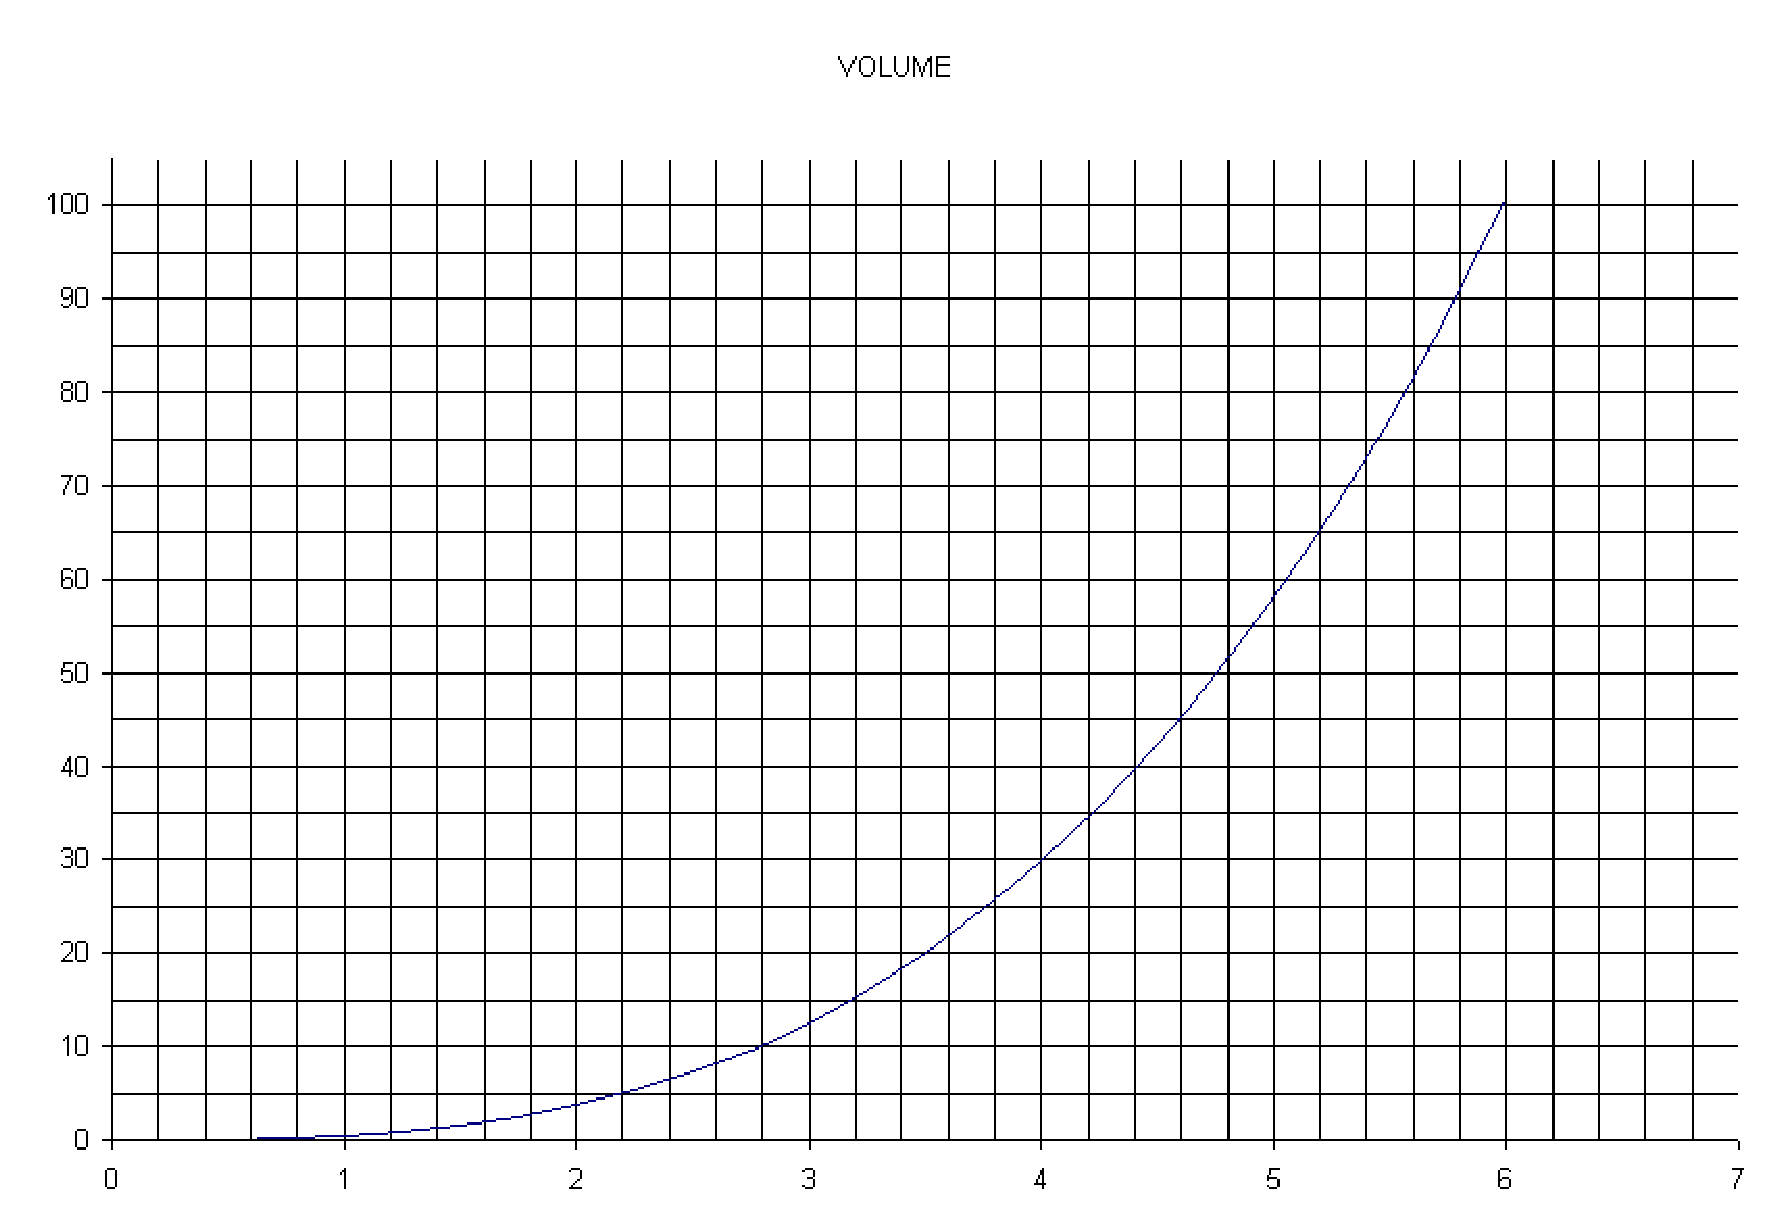
\includegraphics[scale=0.625]{./Graphiques/courbe.eps}\end{center}

%%%%%%%%%%%%%%%%%%%%%%%%%%%%%%%%%%%%%%%%%%%%%%%%%%%%
%%%%%%%%%%%%%%%%%%%%%%%%%%%%%%%%%%%%%%%%%%%%%%%%%%%

%%%%%%%%%%%%%%%%%%%%%%%%%%%%%%%%%%%%%%%%%%%%%%%%%%%\`u
%%%%%%%%%%%%%%%%%%%%%%%%%%%%%%%%%%%%%%%%%%%%%%%%%%%%

 \sautpage

\section{Premi\`eres notions (bilan et compl\'ements)}

\begin{definition}[Notion de fonction]
Une fonction est un proc\'ed\'e qui, \`a un \'el\'ement $x$ d'un ensemble de d\'epart, associe au plus un \'el\'ement $y$ d'un ensemble d'arriv\'ee.

On notera $f:x\mapsto y$ ou $f(x)=y$ qui se lit \og $f$ est la fonction qui \`a $x$ associe $y$ \fg..

On dit que $y$ est \emph{l'image} de $x$.

On dit que $x$ est \emph{un ant\'ec\'edent} de $y$.

\end{definition}

\begin{definition}[Ensemble de d\'efinition]
L'ensemble des r\'eels $x$ poss\'edant une image par une fonction num\'erique $f$ est appel\'e \emph{l'ensemble de d\'efinition de la fonction $f$}. On le note souvent $D_f$.
\end{definition}

\begin{definition}[Repr\'esentation graphique]
Dans un plan muni d'un rep\`ere, la \emph{repr\'esentation graphique} de la fonction $f$ est l'ensemble des points $M$ de coordonn\'ees $(x;y)$ du plan tels que :
\begin{itemize}
	\item L'abscisse $x$ de $M$ d\'ecrit l'ensemble de d\'efinition $D_f$ ;
	\item L'ordonn\'ee $y$ est l'image de $x$ par $f$. $y=f(x)$.
\end{itemize}

On note souvent $\mathcal{C}_f$ la repr\'esentation graphique de $f$. On dit que $\mathcal{C}_f$ a pour \'equation $y=f(x)$.

Si la courbe est d'un seul \og{} tenant \fg{} on parle  de \emph{courbe repr\'esentative} de la fonction $f$.
\end{definition}


\begin{rmq} L'\'equation permet de d\'eterminer si un point $A(x_A;y_A)$ appartient ou pas \`a cette courbe. En effet, un point appartient \`a la courbe si et seulement si ses coordonn\'ees v\'erifient l'\'equation de la courbe. On a alors : \[A\in\mathcal{C}_f\ssi y_A=f(x_A)\] \end{rmq}


Dans la pratique, pour les fonctions num\'eriques d\'efinies par une expression alg\'ebrique, pour esquisser une repr\'esentation graphique, on utilise souvent un tableau de valeurs.

\begin{tabular}{cc}
 \begin{minipage}[l]{0.55\linewidth}
  \begin{rmq} Une courbe ne repr\'esente pas toujours une fonction. Sur la figure ci-contre, par exemple, la courbe a plusieurs points ayant la même abscisse, comme $A(1,-1)$ et $B(1,3)$. Ce n'est donc pas la courbe repr\'esentative d'une fonction car alors 1 aurait plusieurs images.\end{rmq}
 \end{minipage}&
 \begin{minipage}[r]{0.45\linewidth}
\begin{center}
\psset{xunit=0.75cm , yunit=0.75cm}
\def\xmin{-2} \def\xmax{4} \def\ymin{-1.6} \def\ymax{3.6}
\begin{pspicture*}(\xmin,\ymin)(\xmax,\ymax)
\psset{xunit=0.75cm,yunit=0.75cm}
\psgrid[griddots=10,gridlabels=0pt,gridwidth=.3pt, gridcolor=black, subgridwidth=.3pt, subgridcolor=black, subgriddiv=1](0,0)(-2,-2)(4,4)
\psaxes[labels=all,labelsep=1pt, Dx=1,Dy=1]{->}(0,0)(\xmin,\ymin)(\xmax,\ymax)
\uput[dl](0,0){$O$}
%\pcline[linewidth=1pt]{->}(0,0)(1,0) \uput[d](0.5,0){\small $\vec \imath$}
%\pcline[linewidth=1pt]{->}(0,0)(0,1) \uput[l](0,0.5){\small $\vec \jmath$}
\pscircle(1,1){1.5}
\psdots[dotstyle=x](1,-1)(1,3)
\uput[d](1,-1){$A$}
\uput[u](1,3){$B$}
\end{pspicture*}
\end{center}
 \end{minipage}

\end{tabular}






%\sautpage

\subsubsection{Quelques conventions graphiques}
\begin{multicols}{3}
Lorsqu'un point $A$ sur la courbe est connu avec pr\'ecision, il est not\'e par une croix.
\begin{center}
\begin{pspicture*}(-0.5,-1)(2.5,3)
\pscurve(0,0)(0.5,-0.5)(1,1)(2,2.5)
\uput[u](0,0){$\mathcal{C}_f$}
\psdot[dotstyle=x](1,1)
\uput[dr](1,1){$A$}
\end{pspicture*}
\end{center}\sautcol
Lorsqu'un point $A$ est l'extr\'emit\'e de la courbe, il est not\'e par un gros point.
\begin{center}
\begin{pspicture*}(-0.5,-1)(2.5,3)
\pscurve(0,0)(0.5,-0.5)(1,1)(2,2.5)
\uput[u](0,0){$\mathcal{C}_f$}
\psdot(2,2.5)
\uput[dr](2,2.5){$A$}
\end{pspicture*}
\end{center}\sautcol
Lorsqu'un point $A$ \`a l'extr\'emit\'e de la courbe n'appartient pas \`a la courbe, il est not\'e par un \og demi-cercle \fg.
\begin{center}
\begin{pspicture*}(-0.5,-1)(2.5,3)
\pscurve{-(}(0,0)(0.5,-0.5)(1,1)(2,2.5)
\uput[u](0,0){$\mathcal{C}_f$}
%\psdot[(2,2.5)
\uput[dr](2,2.5){$A$}
\end{pspicture*}
\end{center}
\end{multicols}
\begin{multicols}{3}
Une courbe est donn\'ee dans une fenêtre ; s'il n'y a pas d'extr\'emit\'es, la courbe garde la même allure quand on la prolonge.
\begin{center}
\begin{pspicture*}(-0.5,-1)(2.5,3)
\pscurve(-0.3,0)(0.5,2)(1,1)(2,2.8)
\uput[u](1,1){$\mathcal{C}_f$}
\psline[linestyle=dotted](-0.1,0.5)(1.7,0.5)(1.7,2.2)(-0.1,2.2)(-0.1,0.5)
\end{pspicture*}
\end{center}
Une droite verticale en pointill\'es signifie que si l'on prolonge la courbe, elle ne coupe pas cette droite. Sur l'exemple ci-dessous, $a$ n'appartient pas \`a $D_f$.
\begin{center}
\begin{pspicture*}(-0.5,-1)(2.5,3)
\psaxes[labels=none,labelsep=1pt,Dx=5,Dy=5]{->}(0,0)(-0.5,-1)(2.5,3)
\psset{algebraic=true}
\psplot{0.6}{3}{1/(4*x-2)}
\psline[linestyle=dashed](0.5,-1)(0.5,3)
\uput[dl](0.5,0){$a$}
\end{pspicture*}
\end{center}
Une droite horizontale en pointill\'es signifie que si l'on prolonge la courbe, elle ne coupe pas cette droite.
\begin{center}
\begin{pspicture*}(-0.5,-1)(2.5,3)
\psaxes[labels=none,labelsep=1pt,Dx=5,Dy=5]{->}(0,0)(-0.5,-1)(2.5,3)
\psset{algebraic=true}
\psplot{-0.5}{3}{1+1/(x+1)}
\psline[linestyle=dashed](-0.5,1)(2.5,1)
\uput[ul](0,1){$b$}
\end{pspicture*}
\end{center}
\end{multicols}

%\sautpage






\section{R\'esolutions graphiques d'\'equations et d'in\'equations}


\subsection{R\'esolutions d'\'equations de la forme $f(x)=k$}

R\'esoudre l'\'equation $f(x)=k$ c'est d\'eterminer tous les ant\'ec\'edents \'eventuels d'un \'el\'ement $k$ de l'ensemble d'arriv\'ee, c'est-\`a-dire chercher tous les $x$ de l'ensemble de d\'epart tels que $f(x)=k$.

Une telle recherche peut se faire graphiquement \`a partir de la repr\'esentation graphique de la fonction $f$.




\begin{center}
\begin{tabular}{lc}
 \begin{minipage}[l]{0.6\linewidth}
 \begin{exemple*}
  Soit $f$ la fonction d\'efinie sur $\R$ par $f(x)=2x^2-9x+10$. On recherche les solutions de l'\'equation $f(x)=3$.

	On commence par tracer soigneusement la courbe repr\'esentative de $f$ et on obtient la repr\'esentation donn\'ee sur la figure ci-dessous.
		
		On cherche les points de la courbe ayant pour ordonn\'ee 3. Pour cela on peut tracer la droite d'\'equation $y=3$ et chercher les points d'intersection de cette droite avec la courbe de $f$.

		On obtient ici deux points $M_1(1;3)$ et $M_2\left(\frac{7}{2};3\right)$. Les solutions sont leurs abscisses : 1 et $\frac{7}{2}$.

		On \'ecrit : \og Les solutions de l'\'equation $f(x)=3$ sont $x=1$ ou $x=\frac{7}{2}$ car les points de la courbe de $f$ d'ordonn\'ee 3 ont pour abscisses 1 et $\frac{7}{2}$ \fg.
		\end{exemple*}
 \end{minipage}&
 \begin{minipage}[r]{0.35\linewidth}
  
		\begin{center}
 \psset{xunit=1cm,yunit=1cm}
		\begin{pspicture*}(-3.1,-2.1)(4.6,4.1)
\def\xmin{-3} \def\xmax{4.5} \def\ymin{-2} \def\ymax{4}

\psgrid[griddots=10,gridlabels=0pt,gridwidth=.3pt, gridcolor=black, subgridwidth=.3pt, subgridcolor=black, subgriddiv=1](0,0)(-3,-2)(4.5,4)
\psaxes[labels=all,labelsep=1pt, Dx=1,Dy=1]{->}(0,0)(\xmin,\ymin)(\xmax,\ymax)
\uput[dl](0,0){$O$}
\pcline[linewidth=1pt]{->}(0,0)(1,0) \uput[d](0.5,0){\small $\vec \imath$}
\pcline[linewidth=1pt]{->}(0,0)(0,1) \uput[r](0,0.5){\small $\vec \jmath$}
\psset{algebraic=true}
\psplot{\xmin}{\xmax}{2*(x-1)*(x-1)-5*(x-1)+3}
\uput[ul](2,1){$\mathcal{C}_f$}
\psline[linestyle=dashed](\xmin,3)(\xmax,3)
\uput[u](-2,3){$y=3$}
\uput[ur](1,3){$M_1$}
\uput[ul](3.5,3){$M_2$}
\psdots[dotstyle=x](1,3)(3.5,3)
\psline[linestyle=dashed]{->}(1,3)(1,0)
\psline[linestyle=dashed]{->}(3.5,3)(3.5,0)
\end{pspicture*}\end{center}
 \end{minipage}

\end{tabular}             \end{center}



%\sautpage

\subsection{R\'esolutions d'in\'equations de la forme $f(x)\leqslant k$}

Ces in\'equations peuvent se r\'esoudre graphiquement. On proc\`ede de la façon suivante :
\begin{itemize}
	\item on trace soigneusement $\mathcal{C}_f$ dan un rep\`ere (orthogonal) ;
	\item on trace la droite d'\'equation $y=k$ ;
	\item on recherche les points de la courbe situ\'es \emph{sous} la droite ;
	\item l'ensemble des solutions est constitu\'e des abscisses de ces points.
\end{itemize}

\begin{exemple*} Sur l'exemple pr\'ec\'edent, si l'on doit r\'esoudre $f(x)\leqslant 3$, apr\`es avoir trac\'e $y=3$ on constate que les points de la courbe situ\'es sous cette droite ont leurs abscisses comprises entre 0 et $\frac{5}{2}$.

Donc $f(x)\leqslant 3 \ssi x\in\left[0;\frac{5}{2}\right]$.
\end{exemple*}

\begin{rmq}~
\begin{itemize}
	\item On r\'esoud de la même mani\`ere les \'equations du type $f(x)\geqslant k$.

On retient alors les abscisses des points situ\'es \emph{au-dessus} de la droite d'\'equation $y=k$.

Dans l'exemple $f(x)\geqslant 3 \ssi x\in \left] -\infty ; 0 \right] \cup \left[\frac{5}{2} ; +\infty\right[$.
	\item De même pour les in\'equations strictes : $f(x)>k$ ou $f(x)<k$. On excluera alors les abscisses des points d'intersection de la courbe et de la droite.

	Dans l'exemple $f(x)<3 \ssi x\in \left]0;\frac{5}{2}\right[$.
\end{itemize}
\end{rmq}

\subsection{R\'esolutions d'\'equations de la forme $f(x)=g(x)$}

Cela revient \`a chercher les \'el\'ements de l'ensemble de d\'epart qui ont la même image par $f$ et par $g$.

Une telle recherche peut se faire graphiquement. On recherche alors les points des deux courbes repr\'esentatives ayant même abscisse et même ordonn\'ee, c'est-\`a-dire les points d'intersection des deux courbes. 

\begin{tabular}{cc}
 \begin{minipage}[l]{0.6\linewidth}
  \begin{exemple*}

Soit $f$ et $g$ les fonctions d\'efinies sur $\R$ par, respectivement, $f(x)=x^2-1$ et $g(x)=-0,5x^2+x+4$. R\'esoudre graphiquement l'\'equation $f(x)=g(x)$.

	On commence par tracer soigneusement les deux courbes repr\'esentatives et on obtient la repr\'esentation donn\'ee sur la figure ci-contre.
	
	On cherche les points d'intersection des deux courbes, ici $M_1$ et $M_2$, et les solutions de l'\'equation sont leurs abscisses dont les valeurs approximatives sont $-1,5$ et $2,2$.

		Les solutions sont donc $x\approx -1,5$ et $x\approx 2,2$.
\end{exemple*}
 \end{minipage}&
 \begin{minipage}[r]{0.35\linewidth}
  \psset{xunit=0.75cm,yunit=0.75cm}
		\begin{pspicture*}(-3.1,-2.1)(4.6,5.1)
\def\xmin{-3} \def\xmax{4.5} \def\ymin{-2} \def\ymax{5}

\psgrid[griddots=10,gridlabels=0pt,gridwidth=.3pt, gridcolor=black, subgridwidth=.3pt, subgridcolor=black, subgriddiv=1](0,0)(-3,-2)(4.5,5)
\psaxes[labels=all,labelsep=1pt, Dx=1,Dy=1]{->}(0,0)(\xmin,\ymin)(\xmax,\ymax)
\uput[dl](0,0){$O$}
\pcline[linewidth=1pt]{->}(0,0)(1,0) \uput[d](0.5,0){\small $\vec \imath$}
\pcline[linewidth=1pt]{->}(0,0)(0,1) \uput[r](0,0.5){\small $\vec \jmath$}
\psset{algebraic=true}
\psplot{\xmin}{\xmax}{x^2-1}
\psplot{\xmin}{\xmax}{-0.5*x^2+x+4}
\uput[u](1,1){$\mathcal{C}_f$}
\uput[dr](0,4){$\mathcal{C}_g$}
\uput[r](2.189,3.793){$M_2$}
\uput[l](-1.523,1.318){$M_1$}
\psdots[dotstyle=x](2.189,3.793)(-1.523,1.318)
\psline[linestyle=dashed]{->}(-1.523,1.318)(-1.523,0)
\psline[linestyle=dashed]{->}(2.189,3.793)(2.189,0)
\end{pspicture*}
	
 \end{minipage}


\end{tabular}

		

\subsection{R\'esolutions d'in\'equations de la forme $f(x)\leqslant g(x)$}

L\`a encore ces in\'equations peuvent se r\'esoudre graphiquement. On proc\`ede de la façon suivante :
\begin{itemize}
	\item on trace soigneusement $\mathcal{C}_f$ et $\mathcal{C}_g$ dans un rep\`ere (orthogonal) ;
	\item l'ensemble des solutions est constitu\'e des abscisses des points o\`u la courbe de $f$ est situ\'ee \emph{sous} celle de $g$.
\end{itemize}

\begin{exemple*} Sur l'exemple pr\'ec\'edent, si l'on doit r\'esoudre $f(x)\leqslant g(x)$, on constate que les points de la courbe de $f$ situ\'es sous celle de $g$ ont leurs abscisses comprises entre environ $-1,5$ et 2,2.

Donc $f(x)\leqslant g(x) \ssi x\in [-1,5;2,2]$. Ou bien $S=[-1,5;2,2]$.
\end{exemple*}

\begin{rmqs}~
\begin{itemize}
	\item On r\'esoud de la même mani\`ere les \'equations du type $f(x)\geqslant g(x)$.

On retient alors les abscisses des points de la courbe de $f$ situ\'es \emph{au-dessus} de celle de $g$.

Dans l'exemple $f(x)\geqslant g(x) \ssi x\in ] -\infty ; -1,5 ] \cup [2,2 ; +\infty[$.
	\item De même pour les in\'equations strictes : $f(x)>g(x)$ ou $f(x)<g(x)$. On excluera alors les abscisses des points d'intersection des deux courbes.

	Dans l'exemple $f(x)<g(x) \ssi x\in ]-1,5;2,2[$.
\end{itemize}
\end{rmqs}



%\sautpage



\sautpage

\section{Variations, extremums}


\subsection{Sens de variation}

Il s'agit de traduire math\'ematiquement qu'une fonction \og augmente \fg{} ou \og diminue \fg.

\begin{exemple*} Soit, par exemple, la fonction d\'efinie sur $[-3;3]$ par la courbe repr\'esentative donn\'ee sur la figure \ref{croissanceetdecroissance} \vpageref{croissanceetdecroissance}. On constate que lorsque $x\in[-3;1]$ , si $x$ augmente, $f(x)$ augmente aussi alors que lorsque $x\in[1;3]$, si $x$ augmente, $f(x)$ diminue.

C'est la d\'efinition math\'ematique de la croissance ou de la d\'ecroissance d'une fonction $f$.

\begin{figure}[h]
\centering
\caption{Croissance et d\'ecroissante}\label{croissanceetdecroissance}


\psset{xunit=1cm , yunit=1.25cm}
\begin{pspicture*}(-4.1,-1.1)(4.1,5.1)
\def\xmin{-4} \def\xmax{4} \def\ymin{-1} \def\ymax{5}
\psgrid[griddots=10,gridlabels=0pt,gridwidth=.3pt, gridcolor=black, subgridwidth=.3pt, subgridcolor=black, subgriddiv=1](0,0)(-4,-1)(4,5)
\psaxes[labels=all,labelsep=1pt, Dx=1,Dy=1]{-}(0,0)(\xmin,\ymin)(\xmax,\ymax)
\uput[dl](0,0){$O$}
\pcline[linewidth=1pt]{->}(0,0)(1,0) \uput[d](0.5,0){\small $\vec \imath$}
\pcline[linewidth=1pt]{->}(0,0)(0,1) \uput[r](0,0.5){\small $\vec \jmath$}
\psset{algebraic=true}
\psplot{-3}{3}{(-(x-1)^2+5)*0.25+3}
\psdots(3,3.25)(-3,0.25)
\uput[d](-1.5,0){$b$}
\psline[linestyle=dashed]{->}(-1.5,0)(-1.5,2.6875)
\psline[linestyle=dashed]{->}(-1.5,2.6875)(0,2.6875)
\uput[r](0,2.6875){$f(b)$}
\uput[d](-2.5,0){$a$}
\psline[linestyle=dashed]{->}(-2.5,0)(-2.5,1.1875)
\psline[linestyle=dashed]{->}(-2.5,1.1875)(0,1.1875)
\uput[r](0,1.1875){$f(a)$}
\uput[d](1.5,0){$u$}
\uput[d](2.5,0){$v$}
\psline[linestyle=dashed]{->}(1.5,0)(1.5,4.1875)
\psline[linestyle=dashed]{->}(1.5,4.1875)(0,4.1875)
\uput[l](0,4.1875){$f(u)$}
\psline[linestyle=dashed]{->}(2.5,0)(2.5,3.6875)
\psline[linestyle=dashed]{->}(2.5,3.6875)(0,3.6875)
\uput[l](0,3.6875){$f(v)$}
\end{pspicture*}
\end{figure}\end{exemple*}


\begin{definition}
Soit $f$ une fonction d\'efinie sur un intervalle $I$. On dit que $f$ est
\begin{itemize}
	\item \emph{croissante} sur $I$ si, pour tous r\'eels $a$ et $b$ de $I$, on a :\\
$\text{Si } a<b \text{ alors } f(a)\leqslant f(b).$
	\item \emph{d\'ecroissante} sur $I$ si, pour tous r\'eels $a$ et $b$ de $I$, on a :\\
$\text{Si } a<b \text{ alors } f(a)\geqslant f(b).$
	\item \emph{monotone} si elle n'est que croissante sur $I$ ou si elle n'est que d\'ecroissante sur $I$.
	\item \emph{constante} sur $I$ si, pour tous r\'eels $a$ et $b$ de $I$, on a : $f(a)=f(b)$.
\end{itemize}
\end{definition}


\begin{rmqs}~
\begin{itemize}
	\item Ces notions ne sont valables que sur \textbf{un intervalle} et pas sur une r\'eunion d'intervalles disjoints.
	\item Ant\'ec\'edents et images \'etant rang\'es dans le même ordre, on dit qu'une fonction croissante \emph{conserve} l'ordre.
	\item Ant\'ec\'edents et images \'etant rang\'es dans l'ordre inverse, on dit qu'une fonction d\'ecroissante \emph{inverse} l'ordre.
	\item On obtient les d\'efinitions d'une fonction \emph{strictement} croissante ou \emph{strictement} d\'ecroisante en remplaçant les in\'egalit\'es par des in\'egalit\'es strictes. Ainsi on dit que $f$ est strictement croissante sur $I$ si pour tous r\'eels $a$ et $b$ de $I$ on a : \\ $\text{Si } a<b \text{ alors } f(a)<f(b)$
	\item Une fonction est strictement monotone sur $I$ si elle est strictement croissante ou strictement d\'ecroissante sur $I$
\end{itemize}
\end{rmqs}

\subsection{Tableau de variations}

Ces r\'esultats peuvent se r\'esumer dans un tableau de variation, qui est une forme stylis\'ee de repr\'esentation o\`u l'on indique uniquement si la courbe monte, descend ou est stable. Dans la premi\`ere ligne on indique les valeurs importantes de $x$ et dans la seconde les variations de $f$.

\begin{exemple*} Dans l'exemple pr\'ec\'edent on obtient
$$\tabvar{%
\tx{x}&\tx{-3}&&\tx{1}&&\tx{3}\cr
\tx{f}&\txb{\approx 0,25}&\fm&\txh{\approx 4,25}&\fd&\txb{\approx 2,25}\cr
}$$
\end{exemple*}



\subsection{Extremums}

Les extremums, s'ils existent, sont les valeurs maximale et minimale qui sont \textbf{atteintes} par la fonction $f$ sur un intervalle donn\'e. Plus pr\'ecis\'ement :

\begin{definition}
Soit une fonction $f$ d\'efinie sur un intervalle $I$ et $x_0\in I$. On dit que
\begin{itemize}
	\item $f$ admet un \emph{maximum}, atteint en $x_0$ si, pour tout $x\in I$, $f(x)\leqslant f(x_0)$. Ce maximum est alors $f(x_0)$.
	\item $f$ admet un \emph{minimum}, atteint en $x_0$ si, pour tout $x\in I$, $f(x)\geqslant f(x_0)$. Ce minimum est alors $f(x_0)$.
\end{itemize}
Les maximum et minimum sont appel\'es les \emph{extremums}.
\end{definition}

%\begin{rmq} Un extremum doit être atteint par une valeur $x_0$. \end{rmq}

\begin{exemple*}
La fonction $f$ d\'efinie sur $\R$ par $f(x)=x^2+1$ n'admet pas $-1$ comme minimum.

En effet, si on a bien $f(x)\geqslant -1$ sur $\R$, il n'existe pas de $x_0$ tel que $f(x_0)=-1$.

Par contre 1 est bien le minimum de $f$ sur $\R$ car
\begin{itemize}
	\item $f(x)\geqslant 1$ pour tout $x\in\R$ \textbf{ET}
	\item $f(0)=1$
\end{itemize}

On dira donc : le minimum de $f$ sur $\R$ est 1 et il est atteint pour $x_0=0$.
\end{exemple*}

\sautpage

\section{Exercices et probl\`emes}

\subsection{Premi\`eres notions}

%\begin{multicols}{2}
%\begin{exo} Dire dans chacun des exemples ci-dessous quel est l'ensemble de d\'efinition, quelles sont les images possibles et si la fonction est num\'erique.
%\begin{enumerate}
%	\item \`A chaque \'el\`eve de la classe on associe la couleur de ses cheveux.
%	\item \`A chaque \'el\`eve de la classe on associe le nombre de ses fr\`eres et soeurs.
%	\item Pour un \'el\`eve donn\'e, \`a chaque moment de sa vie on associe la taille qu'il mesurait.
%	\item Soit $ABCD$ un rectangle dont un des côt\'es est fixe et mesure 6 cm et l'autre est variable et mesure $x$ cm. \\On d\'efinit la fonction $f$ de la façon suivante : \`a chaque $x$ possible, on associe $f(x)$, l'aire du rectangle $ABCD$.
%	\item La fonction $g$ d\'efinie par $g(x)=x^2+2x+3$.
%	\item La fonction $h$ d\'efinie par $h(x)=\frac{x^2+1}{x-1}$.
%	\item La fonction $i$ d\'efinie par $i(x)=\sqrt{x+2}$.
%\end{enumerate}
%\end{exo}
\begin{multicols}{2}
\begin{exo}
On d\'efinit $f$ et $g$, deux fonctions :
\begin{itemize}
	\item $f$ est la fonction qui \`a un nombre r\'eel $x$ associe le nombre obtenu en proc\'edant de la mani\`ere suivante : on ajoute $4$ au nombre, on \'el\`eve le r\'esultat obtenu au carr\'e, on retranche 16, on divise par le nombre de d\'epart et on retranche 6.
	\item $g:x\mapsto x^2-4$.
\end{itemize}
\begin{enumerate}
	\item Donner l'expression correspondant \`a $f$ puis simplifier cette expression.
	\item Quel r\'eel n'a pas d'image par $f$ ?
	\item Quelle est l'image de 3 par $g$ ?
	\item Quelle est l'image de $-1$ par $g$ ?
	\item Quels sont les ant\'ec\'edents \'eventuels de 12 par $g$ ?
	\item Quels sont les ant\'ec\'edents \'eventuels de $-5$ par $g$ ?
\end{enumerate}
\end{exo}

\sautcol

\begin{exo}
Vrai ou faux ? \emph{Corriger la phrase lorsqu'elle est fausse}.
\begin{enumerate}
	\item $f(-2) = 0$ signifie que l'image de 0 est $-2$
	\item $f(0) = 3$ signifie que la courbe de $f$ passe par le point $(0 ; 3)$
	\item $f(1) = 2$ signifie que l'ant\'ec\'edent de 1 est 2
	\item L'image de 2 par $f$ est $-3$ s'\'ecrit $f(2) = -3$
	\item Dire que $(5 ; 1)$ est un point de la courbe de $f$ s'\'ecrit $5 = f(1)$
	\item Par la fonction $g$, $-5$ est l'image de 3 s'\'ecrit $g(-5) = 3$
	\item 2 a pour image 0 par $f$ signifie que la courbe de $f$ traverse l'axe des abscisses en 2
	\item $f(4) = 0$ signifie que la courbe de $f$ traverse l'axe des abscisses au point $(4 ; 0)$
	\item 3 a pour image 5, signifie que 3 est l'image de 5
	\item 4 a pour ant\'ec\'edent 5 signifie que 5 est l'image de 4
\end{enumerate}
\end{exo}

\end{multicols}

%\sautpage

\begin{exo}\label{gf4courbes}
Vrai ou faux ? \emph{Justifier la r\'eponse lorsque c'est faux}.\\
Les courbes de la figure \ref{gf4courbesfig} \vpageref{gf4courbesfig} repr\'esentent des fonctions de la variable $x$.


\begin{figure}[!h]
 \centering
 \caption{Courbes de l'exercice \ref{gf4courbes}}\label{gf4courbesfig}
\begin{tabular}{cc}
\psset{xunit=1cm , yunit=0.5cm}
\begin{pspicture*}(-2.1,-2.1)(4.1,4.1)
\def\xmin{-2} \def\xmax{4} \def\ymin{-2} \def\ymax{4}
\psgrid[griddots=10,gridlabels=0pt,gridwidth=.3pt, gridcolor=black, subgridwidth=.3pt, subgridcolor=black, subgriddiv=1](0,0)(-2,-2)(4,4)
\psaxes[labels=all,labelsep=1pt, Dx=1,Dy=1]{->}(0,0)(\xmin,\ymin)(\xmax,\ymax)
\uput[dl](0,0){$O$}
\pcline[linewidth=1pt]{->}(0,0)(1,0) \uput[d](0.5,0){\small $\vec \imath$}
\pcline[linewidth=1pt]{->}(0,0)(0,1) \uput[l](0,0.5){\small $\vec \jmath$}
\psline(-2,3)(1,-1.5)(2,-1.5)(4,2)
\end{pspicture*}
&
\psset{xunit=1cm , yunit=0.5cm}
\begin{pspicture*}(-2.1,-2.1)(4.1,4.1)
\def\xmin{-2} \def\xmax{4} \def\ymin{-2} \def\ymax{4}
\psgrid[griddots=10,gridlabels=0pt,gridwidth=.3pt, gridcolor=black, subgridwidth=.3pt, subgridcolor=black, subgriddiv=1](0,0)(-2,-2)(4,4)
\psaxes[labels=all,labelsep=1pt, Dx=1,Dy=1]{->}(0,0)(\xmin,\ymin)(\xmax,\ymax)
\uput[dl](0,0){$O$}
\pcline[linewidth=1pt]{->}(0,0)(1,0) \uput[d](0.5,0){\small $\vec \imath$}
\pcline[linewidth=1pt]{->}(0,0)(0,1) \uput[l](0,0.5){\small $\vec \jmath$}
\psline(-2,3)(1,3)(1,1)(4,1)
\end{pspicture*}
\\
\psset{xunit=1cm , yunit=0.5cm}
\begin{pspicture*}(-2.1,-2.1)(4.1,4.1)
\def\xmin{-2} \def\xmax{4} \def\ymin{-2} \def\ymax{4}
\psgrid[griddots=10,gridlabels=0pt,gridwidth=.3pt, gridcolor=black, subgridwidth=.3pt, subgridcolor=black, subgriddiv=1](0,0)(-2,-2)(4,4)
\psaxes[labels=all,labelsep=1pt, Dx=1,Dy=1]{->}(0,0)(\xmin,\ymin)(\xmax,\ymax)
\uput[dl](0,0){$O$}
\pcline[linewidth=1pt]{->}(0,0)(1,0) \uput[d](0.5,0){\small $\vec \imath$}
\pcline[linewidth=1pt]{->}(0,0)(0,1) \uput[l](0,0.5){\small $\vec \jmath$}
\psline(-2,3)(4,3)
\end{pspicture*}
&
\psset{xunit=1cm , yunit=0.5cm}
\begin{pspicture*}(-2.1,-2.1)(4.1,4.1)
\def\xmin{-2} \def\xmax{4} \def\ymin{-2} \def\ymax{4}
\psgrid[griddots=10,gridlabels=0pt,gridwidth=.3pt, gridcolor=black, subgridwidth=.3pt, subgridcolor=black, subgriddiv=1](0,0)(-2,-2)(4,4)
\psaxes[labels=all,labelsep=1pt, Dx=1,Dy=1]{->}(0,0)(\xmin,\ymin)(\xmax,\ymax)
\uput[dl](0,0){$O$}
\pcline[linewidth=1pt]{->}(0,0)(1,0) \uput[d](0.5,0){\small $\vec \imath$}
\pcline[linewidth=1pt]{->}(0,0)(0,1) \uput[l](0,0.5){\small $\vec \jmath$}
\pscurve(-2,3)(-1,0)(0,-1)(2,1)(3.2,2)(3,3)
\end{pspicture*}
\end{tabular}
\end{figure}

\end{exo}

\sautpage

\begin{exo}\label{gf14}
Vrai ou faux ? \emph{Corriger la phrase lorsqu'elle est fausse}.\\
Les fonctions $f$ et $g$ sont repr\'esent\'ees sur la figure \ref{gf14fig} \vpageref{gf14fig}.
\begin{enumerate}
	\item La fonction $f$ est d\'efinie entre $-2$ et 6 inclus
	\item Les images par la fonction $f$ sont comprises entre $-1$ et 4 inclus
	\item La fonction $g$ est d\'efinie entre $-2$ exclu et 6 inclus
	\item Les images par la fonction g sont comprises entre 0 exclu et 3 inclus
\end{enumerate}



\begin{figure}[!h]
\centering
\caption{Courbes de l'exercice \ref{gf14}}\label{gf14fig}
\begin{tabular}{cc}
\psset{xunit=0.9cm , yunit=0.5cm}
\begin{pspicture*}(-3.1,-2.1)(6.1,5.1)
\def\xmin{-3} \def\xmax{6} \def\ymin{-2} \def\ymax{5}
\psgrid[griddots=10,gridlabels=0pt,gridwidth=.3pt, gridcolor=black, subgridwidth=.3pt, subgridcolor=black, subgriddiv=1](0,0)(-3,-2)(6,5)
\psaxes[labels=all,labelsep=1pt, Dx=1,Dy=1]{->}(0,0)(\xmin,\ymin)(\xmax,\ymax)
\uput[dl](0,0){$O$}
\pcline[linewidth=1pt]{->}(0,0)(1,0) \uput[d](0.5,0){\small $\vec \imath$}
\pcline[linewidth=1pt]{->}(0,0)(0,1) \uput[l](0,0.5){\small $\vec \jmath$}
\pscurve{*-(}(-2,2)(-1,3)(0,3.7)(0.5,3.9)(1,4)(2,3)(3,0)(4,-1)(5,0)(6,1)

\rput(3,2){$\mathcal{C}_f$}
\end{pspicture*}
&
\psset{xunit=0.9cm , yunit=0.5cm}
\begin{pspicture*}(-3.1,-2.1)(6.1,5.1)
\def\xmin{-3} \def\xmax{6} \def\ymin{-2} \def\ymax{5}
\psgrid[griddots=10,gridlabels=0pt,gridwidth=.3pt, gridcolor=black, subgridwidth=.3pt, subgridcolor=black, subgriddiv=1](0,0)(-3,-2)(6,5)
\psaxes[labels=all,labelsep=1pt, Dx=1,Dy=1]{->}(0,0)(\xmin,\ymin)(\xmax,\ymax)
\uput[dl](0,0){$O$}
\pcline[linewidth=1pt]{->}(0,0)(1,0) \uput[d](0.5,0){\small $\vec \imath$}
\pcline[linewidth=1pt]{->}(0,0)(0,1) \uput[l](0,0.5){\small $\vec \jmath$}
\pscurve{)-}(-2,0)(0,1)(1,2)(1.5,3.5)(1.8,5)
\pscurve{-*}(2.2,-2)(3,0)(4,1.5)(6,3)
\rput(1,3){$\mathcal{C}_g$}
\psline[linestyle=dashed](2,\ymin)(2,\ymax)
\end{pspicture*}
\end{tabular}
\end{figure}

\end{exo}

\begin{exo}\label{gf15}
Vrai ou faux ? \emph{Corriger la proposition lorsqu'elle est fausse}.
\begin{itemize}
	\item D'apr\`es la repr\'esentation graphique de la figure \ref{gf15fig} \vpageref{gf15fig} $D_f=[-4;2]$
	\item D'apr\`es la repr\'esentation graphique de la figure \ref{gf15fig} \vpageref{gf15fig} $D_g=]-\infty;3[\cup]3;5]$
\end{itemize}


\begin{figure}[!h]
\centering
\caption{Courbes de l'exercice \ref{gf15}}\label{gf15fig}
\begin{tabular}{cc}
\psset{xunit=1cm , yunit=0.66cm}
\begin{pspicture*}(-4.1,-2.1)(4.1,4.1)
\def\xmin{-4} \def\xmax{4} \def\ymin{-2} \def\ymax{4}
\psgrid[griddots=10,gridlabels=0pt,gridwidth=.3pt, gridcolor=black, subgridwidth=.3pt, subgridcolor=black, subgriddiv=1](0,0)(-4,-2)(4,4)
\psaxes[labels=all,labelsep=1pt, Dx=1,Dy=1]{->}(0,0)(\xmin,\ymin)(\xmax,\ymax)
\uput[dl](0,0){$O$}
\pcline[linewidth=1pt]{->}(0,0)(1,0) \uput[d](0.5,0){\small $\vec \imath$}
\pcline[linewidth=1pt]{->}(0,0)(0,1) \uput[l](0,0.5){\small $\vec \jmath$}
\pscurve{*-}(-4,0)(-3,-2)(0,0)(1,1)(4,1.8)
\psline[linestyle=dashed](0,2)(4,2)
\rput(-1.5,-1){$\mathcal{C}_f$}
\end{pspicture*}
&
\psset{xunit=1cm , yunit=0.66cm}
\begin{pspicture*}(-3.1,-2.1)(5.6,4.1)
\def\xmin{-3} \def\xmax{5.5} \def\ymin{-2} \def\ymax{4}
\psgrid[griddots=10,gridlabels=0pt,gridwidth=.3pt, gridcolor=black, subgridwidth=.3pt, subgridcolor=black, subgriddiv=1](0,0)(-3,-2)(5.5,4)
\psaxes[labels=all,labelsep=1pt, Dx=1,Dy=1]{->}(0,0)(\xmin,\ymin)(\xmax,\ymax)
\uput[dl](0,0){$O$}
\pcline[linewidth=1pt]{->}(0,0)(1,0) \uput[d](0.5,0){\small $\vec \imath$}
\pcline[linewidth=1pt]{->}(0,0)(0,1) \uput[l](0,0.5){\small $\vec \jmath$}
\pscurve(-3,3)(0,1.5)(1,1)(2,0)(2.8,-2)
\pscurve{-*}(3.2,-2)(4,1)(5,3)
\psline[linestyle=dashed](3,\ymin)(3,\ymax)
\uput[ur](1,1){$\mathcal{C}_g$}
\end{pspicture*}
\end{tabular}
\end{figure}
\end{exo}
%\sautpage


\begin{exo}[Avec la calculatrice]
La fonction $f$ est d\'efinie sur $[-1,5;2]$ par : $f(x)=2x^3-1,5x^2-3x$
\begin{enumerate}
	\item Compl\'eter le tableau de valeurs suivant :
	%\vspace{-1em}
	\begin{center}
\begin{tabular}{|*{9}{c|}}
\hline $x$ & $-1,5$ & $-1$ & $-0,5$ & 0 & 0,5 & 1 & 1,5 & 2 \\ \hline
$f(x)$ & & & & & & & & \\ \hline
\end{tabular}
\end{center}
\item Tracer la courbe repr\'esentative de $f$.
\end{enumerate}
\end{exo}

\begin{exo}[Avec la calculatrice]\label{uneautrecourbe}
La fonction $f$ est d\'efinie sur $[-3;3]$ par : $f(x)=x^2-3x+1$.\\
Apr\`es avoir dress\'e un tableau de valeurs de la fonction, tracer sa courbe repr\'esentative $\mathcal{C}_f$.

\end{exo}

%\end{multicols}



\sautpage

\subsection{R\'esolutions graphiques}

\begin{exo}
La fonction $f$ est d\'efinie sur $[-3;3]$ par : $f(x)=x^2-3x+1$.\\
$\mathcal{C}_f$, courbe repr\'esentative de $f$ a d\'ej\`a \'et\'e obtenue dans l'exercice \ref{uneautrecourbe}.
\begin{enumerate}
	\item \`A l'aide de la repr\'esentation graphique $\mathcal{C}_f$, avec la pr\'ecision permise par le graphique, r\'epondre aux question suivantes :
		\vspace{-1em}\begin{multicols}{2}
		  \begin{enumerate}
			\item Quelle est l'image de 2 ?
			\item Quelle est l'image de 3 ?
			\item Quelle est l'image de 4 ?
			\item Quels sont les ant\'ec\'edents de 1 ?
			\item Quels sont les ant\'ec\'edents de 2 ?
			\item Quels sont les ant\'ec\'edents de $-2$ ?
		\end{enumerate}
		\end{multicols}\vspace{-1em}
	\item R\'esoudre graphiquement les \'equations et in\'equations suivantes :
\vspace{-1em}\begin{multicols}{3}\begin{enumerate}
	\item $f(x)=3$ ;
	\item $f(x)=-1,5$ ;
	\item $f(x)\geqslant -1$ ;
	\item $f(x)<4$ ;
	\item $f(x)>-3$ ;
	\item $f(x)<-2$.
\end{enumerate}\end{multicols}\vspace{-1em}
\item D\'eterminer graphiquement le signe de $f(x)$ selon les valeurs de $x$.
\end{enumerate}
\end{exo}

%\sautpage

\begin{exo}
Une fonction $f$, d\'efinie sur $\R$, est donn\'ee par sa courbe repr\'esentative $\mathcal{C}$ :
\begin{multicols}{2}
\begin{center}\small
\psset{xunit=1,yunit=1}
\begin{pspicture*}(-2.6,-2.1)(5.1,3.1)
\def\xmin{-2.5} \def\xmax{5} \def\ymin{-2} \def\ymax{3}
\psset{xunit=0.1cm,yunit=0.1cm}
\psgrid[griddots=15,gridlabels=0pt,gridwidth=.3pt, gridcolor=gray, subgridwidth=.3pt, subgridcolor=gray, subgriddiv=1](0,0)(-25,-20)(50,30)
\psset{xunit=1cm , yunit=1cm}
\psaxes[labels=all,labelsep=1pt, Dx=1,Dy=1]{->}(0,0)(\xmin,\ymin)(\xmax,\ymax)
\uput[dl](0,0){$0$}
\pcline[linewidth=1pt]{->}(0,0)(1,0) \uput[d](0.5,0){\small $\vec i$}
\pcline[linewidth=1pt]{->}(0,0)(0,1) \uput[l](0,0.5){\small $\vec j$}
\pscurve(-2.3,-2)(-2,-1)(-1.5,1.5)(-1,3)(-0.5,2.5)(0,1)(0.2,0)(0.5,-1)(1,-1.5)(1.5,-1)(2,0)(2.5,1)(3,1.5)(4,2)(5,2.3)
\psline[linestyle=dashed](0,2.5)(\xmax,2.5)
\psdots[dotstyle=x](-2,-1)(-1.5,1.5)(-1,3)(-0.5,2.5)(0,1)(0.5,-1)(1,-1.5)(1.5,-1)(2,0)(2.5,1)(3,1.5)(4,2)
\end{pspicture*}
\end{center}\normalsize

\sautcol

Avec la pr\'ecision permise par le graphique, r\'esoudre :
%\vspace{-1em}
%\begin{multicols}{2}
\begin{enumerate}
	\item Les \'equations suivantes :
		\vspace{-1em}
		\begin{multicols}{2}\begin{enumerate}
			\item $f(x) = 1$ ;
			\item $f(x) = 0$ ;
			\item $f(x) = -1$ ;
			\item $f(x) = 2$.
		\end{enumerate}\end{multicols}
		%\vspace{-1em}
%\sautcol
	\item Les in\'equations suivantes :
		\vspace{-1em}
		\begin{multicols}{2}\begin{enumerate}
			\item $f(x)\geqslant 1$ ;
			\item $f(x)\geqslant 0$ ;
			\item $f(x)<-1$ ;
			\item $f(x)>2$.
		\end{enumerate}\end{multicols}
		\vspace{-1em}
	\item D\'eterminer graphiquement le signe de $f(x)$ selon les valeurs de $x$.

\end{enumerate}\end{multicols}
%\vspace{-1em}
\end{exo}

\medskip

\begin{multicols}{2}

\begin{exo}\label{gfunecourbe}
La courbe $\mathcal{C}$ de la figure ci-dessous %\ref{gfunecourbefig} \vpageref{gfunecourbefig} 
repr\'esente une fonction $f$ et le segment de droite $\mathcal{D}$ repr\'esente une fonction $g$.

%\begin{figure}[hbtp]
% \centering
% \caption{Figure de l'exercice \ref{gfunecourbe}}\label{gfunecourbefig}


\begin{center}
\psset{xunit=0.375cm , yunit=0.33cm}
\def\xmin{-9} \def\xmax{12} \def\ymin{-3} \def\ymax{11}
\begin{pspicture*}(\xmin,\ymin)(\xmax,\ymax)
\psgrid[griddots=10,gridlabels=0pt,gridwidth=.3pt, gridcolor=black, subgridwidth=.3pt, subgridcolor=black, subgriddiv=1](0,0)(\xmin,\ymin)(\xmax,\ymax)
\psaxes[labels=all,labelsep=1pt, Dx=5,Dy=5]{-}(0,0)(\xmin,\ymin)(\xmax,\ymax)
\uput[dl](0,0){$O$}
\pcline[linewidth=1pt]{->}(0,0)(1,0) \uput[d](0.5,0){\small $\vec \imath$}
\pcline[linewidth=1pt]{->}(0,0)(0,1) \uput[l](0,0.5){\small $\vec \jmath$}
\pscurve{*-*}(-8,1)(-5,3)(-3,5)(-1,6)(0,5)(1,3)(2,0)(4,-2)(7,0)(9,3)(11,6)
\psdots[dotstyle=x](-5,3)(-3,5)(-1,6)(0,5)(1,3)(2,0)(4,-2)(7,0)(9,3)
\psdots[dotstyle=*](-8,7.5)(11,-2)
\uput[dr](10,5){$\mathcal{C}$}
\uput[ur](-6,7){$\mathcal{D}$}
\psplot[linestyle=dashed,algebraic=true]{-8}{11}{-0.5*x+3.5}
\end{pspicture*}\end{center}

%\end{figure}

\sautcol

\begin{enumerate}
	\item R\'esoudre graphiquement les \'equations :
		\vspace{-1em}\begin{multicols}{2}\begin{enumerate}
			\item $f(x) = 3$ ;
			\item $f(x) = -2$ ;
			\item $f(x) = 0$ ;
			\item $f(x) = 6$.
		\end{enumerate}\end{multicols}
	\item R\'esoudre graphiquement les in\'equations :
		\begin{enumerate}
			\item $f(x)\leqslant 0$ ;
			\item $f(x) \geqslant 3$ ;
			\item $f(x)>5$.
		\end{enumerate}

	\item R\'esoudre graphiquement :
			\begin{enumerate}
				\item $f(x) = g(x)$ ;
				\item $f(x) < g(x)$.			\end{enumerate}
		\item Donner le signe de $f(x)$ suivant les valeurs de $x$.
\end{enumerate}
\end{exo}\end{multicols}

%\sautpage

\begin{multicols}{2}

\begin{exo}[Avec la calculatrice]
On consid\`ere les fonctions $f$ et $g$ d\'efinies sur $\R$ par : $f(x)=x^3$ et $g(x)=3x-2$.
 \begin{enumerate}
			\item Tracer soigneusement les repr\'esentations graphiques $\mathcal{C}_f$ et $\mathcal{C}_g$ de $f$ et $g$ sur l'intervalle $[-2;2]$.
			\item R\'esoudre graphiquement l'in\'equation $f(x)\leqslant 1$.
			\item D\'eterminer graphiquement les solutions de l'\'equation $f(x)=g(x)$.
 \end{enumerate}
\end{exo}

\sautcol

\begin{exo}[Avec la calculatrice]
Les fonctions $f$ et $g$ sont d\'efinies sur $[-2;2]$ par : $f(x)=x^3$ et $g(x)=1-x$.
\begin{enumerate}
	\item Tracer sur une calculatrice graphique les repr\'esentations graphiques $\mathcal{C}_f$ et $\mathcal{C}_g$ de $f$ et de $g$.
	\item En d\'eduire le nombre de solutions de l'\'equation $x^3+x-1=0$.
	\end{enumerate}
\end{exo}

\end{multicols}

\subsection{R\'esolutions calculatoires}
%\section{Technologie}
\begin{multicols}{2}
\begin{exo}
Soit la fonction $f$ d\'efinie sur $\R$ par : \\$f(x)=2x^2+x+3$.
\begin{enumerate}
	\item Calculer les valeurs exactes de $f(x)$ pour les valeurs de $x$ suivantes :
	  \vspace{-1em}\begin{multicols}{3}
	  \begin{itemize}
	    \item 0 ;
	    \item 1 ;
	    \item $-2$ ;
	    \item $\sqrt{2}$ ;
	    \item $1+\sqrt{3}$ ;
	    \item $2-\sqrt{5}$.
	   \end{itemize}
	  \end{multicols}\vspace{-1em}
	\item R\'esoudre $f(x)=3$.
\end{enumerate}
\end{exo}

\begin{exo}
Soit $f$ la fonction d\'efinie sur $\R$ par :\\ $f(x)=2x^2-5x+3$. \\R\'esoudre $f(x)=3$.
\end{exo}

\begin{exo} Soit $f$ la fonction d\'efinie sur $\R$ par : $f(x)=4x^2-4x+1$. On cherche \`a r\'esoudre, par le calcul, l'\'equation $f(x)=9$.
%\vspace{-1em}\begin{multicols}{2}
\begin{enumerate}
	\item Factoriser $f(x)$.
	\item R\'esoudre $f(x)=9$.
\end{enumerate}% \end{multicols}\vspace{-1em}
\end{exo}



\begin{exo}
	Soit $f$ et $g$ les fonctions d\'efinies sur $\R$ par, respectivement, $f(x)=x^2-1$ et $g(x)=-x^2+2$. \\ R\'esoudre par le calcul l'\'equation $f(x)=g(x)$.
\end{exo}


\begin{exo}
On consid\`ere les fonctions $f$ et $g$ d\'efinies sur $\R$ par : $f(x)=x^3$ et $g(x)=3x-2$. On cherche \`a r\'esoudre, par le calcul, l'\'equation $f(x)=g(x)$.
		\begin{enumerate}
			\item D\'evelopper $(x-1)^2(x+2)$.
			\item En d\'eduire les solutions de l'\'equation $x^3-3x+2=0$.
			\item En d\'eduire les solutions de l'\'equation $f(x)=g(x)$.
		\end{enumerate}
\end{exo}



%

\begin{exo}
On consid\`ere la fonction $f$ d\'efinie pour tout $x\in\R$ par : $f(x)=x(x-2)$. On cherche \`a trouver, par le calcul, le minimum de $f(x)$.
%\vspace{-1em}\begin{multicols}{2}
\begin{enumerate}
	\item D\'emontrer que $f(x)=(x-1)^2-1$.
	\item En d\'eduire le minimum de $f(x)$.
\end{enumerate}%\end{multicols}\vspace{-1em}
\end{exo}

\end{multicols}

\sautpage


\subsection{Variations, extremums}

\begin{multicols}{2}

\begin{exo}\label{fonctionsvar1}
On consid\`ere la fonction $f$ dont on donne la repr\'esentation $\mathcal{C}$ sur la figure \ref{fonctionsvar1fig} \vpageref{fonctionsvar1fig} (en deux parties).\\
Indiquer son ensemble de d\'efinition et dresser son tableau de variations.

\end{exo}
%\sautpage


\begin{exo}[Avec une calculatrice]
On consid\`ere la fonction $f$ d\'efinie par : $f(x)=2x\sqrt{4-x^2}$.
\`A l'aide d'une calculatrice graphique :
\begin{enumerate}
	\item conjecturer l'ensemble de d\'efinition de $f$ ;
	\item conjecturer quels sont les extremums de $f$ sur son ensemble de d\'efinition ;
	\item dresser le tableau des variations de $f$.
\end{enumerate}
\end{exo}


%\sautcol


\begin{exo}
Tracer une courbe repr\'esentative d'une fonction $f$ sachant que :
%\vspace{-1em}\begin{multicols}{2}
\begin{itemize}
\item le tableau des variations de $f$ est le suivant :$$\tabvar{%
\tx{x}&&&\tx{0}&&\tx{3}&&\tx{~}\cr
\tx{f}&\txb{1}&\fm&&\fd&&\fm&\cr
}$$
	\item 1 a pour ant\'ec\'edents, par la fonction $f$, $-2$ et 1,5 ;
	\item $f(x)=0$ a pour solutions $x=2$ ou $x=4$ ;
	\item $f(-1)=2$ ;
	\item $-1$ est l'image de 3 ;
	\item $D_f=[-2;4]$ ;
	\item le maximum de $f$ est 3 ;
	
\end{itemize}%\end{multicols}
\end{exo}



\sautcol

\begin{exo}
On donne le tableau des variations d'une fonction $f$ :$$\tabvar{%
\tx{x}&\tx{-5}&&\tx{-3}&&\tx{0}&&\tx{1}&&\tx{8}\cr
\tx{f}&\txh{3}&\fd&\txb{0}&\fm&\txh{1}&\fdh&\tx{0}&\fdb&\txb{-2}\cr
}$$
%\vspace{-4em}\begin{multicols}{2}
\begin{enumerate}
	\item S'il est possible de r\'epondre, compl\'eter par \og < \fg, \og > \fg{} ou \og = \fg. Sinon mettre une croix.
\begin{itemize}
 \item $f(-1)$  $\ldots\ldots$  $f(-2)$ 
 \item $f(-3)$  $\ldots\ldots$  $f(1)$ 
 \item $f(-1)$  $\ldots\ldots$  $1$ 
 \item $f(-2)$ $\ldots\ldots$  $f(0,5)$
 \item $f(-2)$  $\ldots\ldots$  $f(1,5)$
 \item $f(4)$  $\ldots\ldots$  $f(2)$
 \item $4$  $\ldots\ldots$ $f(-4)$
 \end{itemize}

\item R\'esoudre, lorsque c'est possible, les in\'egalit\'es suivantes :
\vspace{-1em}\begin{multicols}{2}\begin{enumerate}
	  \item $f(x)\geqslant 0$ ;
	  \item $f(x)=1$ ;
	  \item $f(x)<-1$ ;
	  \item $f(x)<0$.
  \end{enumerate}\end{multicols}
	\item Dire, si c'est possible, quel est le maximum de la fonction et quel est son minimum.
\end{enumerate}%\end{multicols}
\end{exo}
\end{multicols}
%M\end{multicols}



\begin{figure}[!h]
 \centering
 \caption{Figure de l'exercice \ref{fonctionsvar1}}\label{fonctionsvar1fig}

\psset{xunit=0.75cm , yunit=0.75cm}
\begin{pspicture*}(-6.1,-2.1)(14.1,6.1)
\def\xmin{-6} \def\xmax{14} \def\ymin{-2} \def\ymax{6}
\psgrid[griddots=10,gridlabels=0pt,gridwidth=.3pt, gridcolor=black, subgridwidth=.3pt, subgridcolor=black, subgriddiv=1](0,0)(-6,-2)(14,6)
\psaxes[labels=all,labelsep=1pt, Dx=1,Dy=1]{-}(0,0)(\xmin,\ymin)(\xmax,\ymax)
\uput[dl](0,0){$O$}
\pcline[linewidth=1pt]{->}(0,0)(1,0) \uput[d](0.5,0){\small $\vec i$}
\pcline[linewidth=1pt]{->}(0,0)(0,1) \uput[l](0,0.5){\small $\vec j$}
\pscurve(-5,-1)(-4,0)(-3,3)(-2,4)(0,3)(4,0)(5,-2)
\psdot(-5,-1)
\psdots[dotstyle=x](-4,0)(-3,3)(-2,4)(0,3)(4,0)(7,0)(8,3)(10,5)(12,3)
\pscurve(6.5,-2)(7,0)(8,3)(10,5)(12,3)(14,2.2)
\psline[linestyle=dashed](6,-2)(6,6)
\psline[linestyle=dashed](9,2)(14,2)
\end{pspicture*}
\end{figure}







%\sautpage



%\input{./Devoirs/DS1Fonctions}

%\input{./Espace/GeometrieDansLEspace} %2010-2011
%\input{./Espace/CalculsDansLEspace} %2011-2012
%\input{./Espace/IncidenceEtParallelismeDansLEspace}  %2011-2012

%\input{./Devoirs/DM1CalculsDansLEspace}

%\input{./Devoirs/DS2FonctionsEspace}

%\input{./Devoirs/DS3Espace}

%



\fancyhead{} % Delete current head settings

\fancyhead{} % efface les entêtes pr\'ec\'edentes
%\fancyhead[LE,RO]{\footnotesize \em \rightmark} % section en entête
\fancyhead[RE,LO]{\scriptsize \em Seconde} % classe et ann\'ee en entête

%\setcounter{ds}{1} %c'est le num\'ero du DS
%\setcounter{chaptertemp}{\thechapter} %stocke le num\'ero du chapitre courant dans un compteur temporaire
%\stepcounter{chapter} % avance le compteur de 1 et surtout remet tous les compteurs d\'ependant du chapitre à 0, dont les num\'eros d'exercice
%\setcounter{chapter}{\theds} % met le compteur de chapitre au num\'ero du ds



%\small

\chapter{Expressions alg\'ebriques}


\pagenumbering{roman} \setcounter{page}{1}

\section{Rappels}

\begin{definition*}
 D\'evelopper c'est transformer un produit en une somme. Factoriser c'est transformer une somme en un produit.
\end{definition*}

\begin{prop*}
Au coll\`ege, on a obtenu les factorisations et d\'eveloppements suivants :
\[\begin{array}{rclcrcl}
 ka+kb & = & \ldots\ldots\ldots\ldots & & (a+b)^2 & = & \ldots\ldots\ldots\ldots\\
 (a+b)(c+d) & = & \ldots\ldots\ldots\ldots & & (a-b)^2 & = & \ldots\ldots\ldots\ldots\\
 &&&&a^2-b^2 & = & \ldots\ldots\ldots\ldots
\end{array}\]
\end{prop*}


\section{Technique}

\begin{exo}
 Parmi les formules rappel\'ees dans la propri\'et\'e ci-dessus, lesquelles sont des formules de d\'eveloppement, lesquelles sont des formules de factorisation ?
\end{exo}





\begin{exo}
 D\'evelopper puis r\'eduire les expressions suivantes :
\vspace{-1em}\begin{multicols}{3}\begin{itemize}
 \item $A=(x^2+4)(2x-3)$
 \item $B=x+2(x-5)+8(3-2x)$
 \item $C=(5-2x)(x-4)$
 \item $D=(x-4)^2+(3x+1)^2$
 \item $E=(x-1)^2-(2x+5)^2$
 \item $F=x(x+1)(x-3)$
 \item $G=(a-b)(a^2+ab+b^2)$
 \item $H=(a+b)^3$
 \item $I=(a-b)^3$
 \item $J=-(x-7)$
 \item $K=-(2x+3)^2$
 \item $L=(x-2)^2$
 \item $M=(x+1)^2-x^2$
\end{itemize} \end{multicols}\vspace{-1em}
\end{exo}

%\sautpage

\begin{exo}
 Factoriser au maximum les expressions suivantes :
\vspace{-1em}\begin{multicols}{2}\begin{itemize}
 \item $A=x(x-1)+2x(x-3)$
 \item $B=(x-1)^2+4(x-1)(x+5)$
 \item $C=x^2-(3x+1)^2$
 \item $D=x(x-4)-5(4-x)$
 \item $E=4x^2+20x+25$
 \item $F=x(x-1)-(2x+5)x$
 \item $G=(x+5)^2-(2x+7)^2$
 \item $H=(5x+1)(-3x+4)+x(10x+2)$
 \item $I=x^3-12x^2$
 \item $J=x^2-4+(x-2)(2x+1)$
 \item $K=2x-3+(3-2x)^2$
 \item $L=(2a+1)^2-(a+6)^2$
 \item $M=(2x-3)(1-x)-3(x-1)(x+2)$
 \item $N=(x-1)^2+2(x^2-1)$
 \item $O=x^4+4x^3+4x^2$
 \item $P=4x^5-x^3$
 \item $Q=x^7-x^5$
 \item $R=x(x+2)^2-4x(x-1)^2$
 \item $S=(2a-b)(b-a)-(2b-a)(b-2a)$
 \item $T=a^4-b^4$
\end{itemize} \end{multicols}\vspace{-1em}
\end{exo}





\section{Probl\`emes}

%
\vspace{-1em}\begin{multicols}{3}\begin{prob}
 Montrer que le somme du produit de trois entiers cons\'ecutifs $n-1$, $n$ et $n+1$ et de l'entier $n$ est le cube d'un entier.
\end{prob}
\sautcol
\begin{prob}
 Choisir un nombre entier, \'elever le nombre suivant et le nombre pr\'ec\'edent cet entier au carr\'e, puis faire la diff\'erence de ces deux carr\'es :
on obtient un multiple du nombre choisi. Pourquoi ?
\end{prob}
\sautcol
\begin{prob}
 Choisir quatre nombres entiers cons\'ecutifs, puis faire le produit du plus petit et du plus grand, puis faire le produit des deux nombres.
Que remarque-t-on ? Est-ce toujours vrai ? Le d\'emontrer.
\end{prob}\end{multicols}\vspace{-1em}
%\sautcol

\vspace{-1em}\begin{multicols}{2}
\begin{prob}
 Soit $x$ un nombre strictement compris entre 0 et 10. Calculer le p\'erim\`etre de la figure gris\'ee en fonction du nombre $x$. Que constate-t-on ?\\

\vspace{-2em}\begin{center}
\begin{pspicture*}(-0.5,-1.5)(5.5,2.6)
 \psline(0,0)(5,0)
 \psline{<->}(0,-0.5)(1.5,-0.5)
 \rput(0.75,-0.35){\small $x$}
 \psline{<->}(0,-1)(5,-1)
 \rput(2.5,-0.85){\small $10$}
\pscustom[fillstyle=solid,fillcolor=lightgray,linecolor=black]{%
\psarc(2.5,0){2.5}{0}{180}}
\pscustom[fillstyle=solid,fillcolor=white,linecolor=black]{%
\psarc(3.25,0){1.75}{0}{180}
 \psarc(0.75,0){0.75}{0}{180}}
\end{pspicture*}               \end{center}\vspace{-2em}
\end{prob}

\sautcol

\begin{prob}
 Soit $x$ un nombre strictement compris entre 0 et 10. Calculer l'aire de la surface gris\'ee en fonction de $x$.\\

\vspace{-2em}\begin{center}
\begin{pspicture*}(0,-2.5)(5.5,3)
\pscustom[fillstyle=solid,fillcolor=lightgray,linecolor=black]{%
\psarc(2.5,0){2.5}{0}{180}}
\pscustom[fillstyle=solid,fillcolor=white,linecolor=black]{%
 \psarc(0.75,0){0.75}{0}{180}}
\pscustom[fillstyle=solid,fillcolor=lightgray,linecolor=black]{%
\psarc(3.25,0){1.75}{180}{360}}
\psline(0,0)(5,0)
 \psline{<->}(0,-0.5)(1.5,-0.5)
 \rput(0.75,-0.35){\small $x$}
 \psline{<->}(0,-1)(5,-1)
 \rput(2.5,-0.85){\small $10$}
\end{pspicture*}               \end{center}\vspace{-2em}
\end{prob}
\end{multicols}\vspace{-1em}

\vspace{-1em}\begin{multicols}{2}\begin{prob}
 Oscar et Alix doivent tracer sur la plage un circuit de karting.
Ils souhaitent construire un circuit en forme de 8 et disposent de 80 m\`etres de plage.
Sur la figure ci-dessous sont trac\'es leurs mod\`eles respectifs, compos\'es chacun de deux cercles tangeants ; dans le premier mod\`ele le petit cercle est d'un rayon quelconque (compris entre 0 et 80 m) tandis que dans le second mod\`ele les deux cercles ont m\^eme rayon.
De ces deux circuits, lequel est le plus long ?

\vspace{-2em}\begin{center}

\begin{pspicture*}(-0.75,-0.75)(7,4.5)
\pscircle[linewidth=2pt](1,1.5){1.5}
\pscircle[linewidth=2pt](1,3.5){0.5}
\pscircle[linewidth=2pt](4,1){1}
\pscircle[linewidth=2pt](4,3){1}
\psline{<->}(5.5,0)(5.5,4)
\uput[r](5.5,2){\small 80\,m}

\end{pspicture*}               \end{center}\vspace{-2em}

\end{prob}

\sautcol

\begin{prob}
 $ABCD$ est un carr\'e. Pour construire $E$ et $F$, on a trac\'e un quart de cercle de centre $D$ passant par $B$.
On a \'egalement trac\'e un quart de cercle de centre $B$ passant par $A$.
\begin{enumerate}
 \item Montrer que l'aire de la surface blanche int\'erieure au secteur $DEF$ est \'egale \`a l'aire de la surface gris\'ee.
 \item L'aire de la surface gris\'ee est-elle plus grande ou plus petite que les trois quarts de l'aire du carr\'e $ABCD$ ?
\end{enumerate}

\vspace{-1em}\begin{center}

\begin{pspicture*}(-0.75,-5)(5,0.75)

\pscustom[fillstyle=solid,fillcolor=lightgray,linecolor=black]{%
\psarc(3,-3){3}{90}{180}
\psline(0,-3)(3,-3)}
 \psline(0,0)(3,0)(3,-3)(0,-3)(0,0)
 \psline(3,0)(4.2426,0)
 \psline(0,-3)(0,-4.2426)
\psarc(0,0){4.2426}{270}{360}
\uput[ul](0,0){$D$}
\uput[u](3,0){$C$}
\uput[ur](4.2426,0){$F$}
\uput[dr](3,-3){$B$}
\uput[dl](0,-4.2426){$E$}
\uput[l](0,-3){$A$}
\end{pspicture*}               \end{center}\vspace{-1em}

\end{prob}\end{multicols}\vspace{-1em}

\section{Probl\`emes dits \emph{de synth\`ese}}

\vspace{-1em}\begin{multicols}{2}\begin{prob}
 Sur les c\^ot\'es d'un carr\'e $ABCD$ de c\^ot\'e 4, on place les points $M$, $N$, $P$, $Q$, $R$, $S$, $T$ et $U$ comme indiqu\'e sur le dessin,
o\`u $0\leqslant x \leqslant 2$. On note $\mathcal{A}(x)$ l'aire du domaine gris\'e.
\begin{center}

\begin{pspicture*}(-1.25,-0.75)(4.75,5.25)
\pspolygon*[linecolor=lightgray](0,0)(1,0)(1,1)(0,1)
\pspolygon*[linecolor=lightgray](3,0)(4,0)(4,1)(3,1)
\pspolygon*[linecolor=lightgray](0,3)(1,3)(1,4)(0,4)
\pspolygon*[linecolor=lightgray](3,3)(4,3)(4,4)(3,4)
\pspolygon*[linecolor=lightgray](1,1)(3,1)(3,3)(1,3)
\psline(0,0)(4,0)(4,4)(0,4)(0,0)
\psline(0,1)(4,1)
\psline(0,3)(4,3)
\psline(1,0)(1,4)
\psline(3,0)(3,4)
\psline{<->}(-1,0)(-1,1)
\rput*(-1,0.5){\footnotesize $x$}
\psline{<->}(-1,3)(-1,4)
\rput*(-1,3.5){\footnotesize $x$}
\psline{<->}(0,5)(1,5)
\rput*(0.5,5){\footnotesize $x$}
\psline{<->}(3,5)(4,5)
\rput*(3.5,5){\footnotesize $x$}
\uput[ul](0,4){\footnotesize $A$}
\uput[u](1,4){\footnotesize $M$}
\uput[u](3,4){\footnotesize $N$}
\uput[ur](4,4){\footnotesize $B$}
\uput[l](0,3){\footnotesize $U$}
\uput[ur](1,3){\footnotesize $E$}
\uput[ul](3,3){\footnotesize $F$}
\uput[r](4,3){\footnotesize $P$}
\uput[l](0,1){\footnotesize $T$}
\uput[ul](1,1){\footnotesize $H$}
\uput[ur](3,1){\footnotesize $G$}
\uput[r](4,1){\footnotesize $Q$}
\uput[dl](0,0){\footnotesize $D$}
\uput[d](1,0){\footnotesize $S$}
\uput[d](3,0){\footnotesize $R$}
\uput[dr](4,0){\footnotesize $C$}
\end{pspicture*}               \end{center}
\begin{enumerate}
 \item Montrer par un raisonnement g\'eom\'etrique que $\mathcal{A}(x)$ peut s'\'ecrire sous l'une des formes suivantes :
$\mathcal{A}(x)=4x^2+(4-2x)^2$ ou $\mathcal{A}(x)=16-4x(4-2x)$.
 \item Montrer que l'on a aussi : $\mathcal{A}(x)=8x^2-16x+16$.
 \item En utilisant la forme la plus adapt\'ee, calculer $\mathcal{A}(2)$ puis $\mathcal{A}(\sqrt{3})$.
 \item \begin{enumerate}
        \item Montrer que : $\mathcal{A}(x)=8(x-1)^2+8$.
        \item En d\'eduire que l'aire $\mathcal{A}(x)$ est minimale pour $x=1$.
       \end{enumerate}
 \item \begin{enumerate}
        \item Montrer que : $\mathcal{A}(x)=(2x-1)(4x-6)+10$.
	\item En utilisant l'expression pr\'ec\'edente de $\mathcal{A}(x)$, d\'eterminer les valeurs de $x$ telles que l'aire $\mathcal{A}(x)$ soit \'egale \`a 10.
       \end{enumerate}


\end{enumerate}

\end{prob}\end{multicols}\vspace{-1em}

%\sautpage

\begin{prob}
\begin{multicols}{2}
Les ma\^itres nageurs d'une plage disposent d'un cordon flottant d'une longueur de 400 m avec lequel ils d\'elimitent la zone de baignade surveill\'ee, de forme rectangulaire.\\
Le probl\`eme est de d\'eterminer les dimensions de ce rectangle pour que l'aire de baignade soit maximale.\\
On appelle $x$ la largeur du rectangle et $y$ sa longueur.

\sautcol

\begin{center}\small
\psset{xunit=1cm , yunit=1cm}
\begin{pspicture*}(-0.7,-1.2)(6.2,2.2)
\def\xmin{-0.5} \def\xmax{6} \def\ymin{-1} \def\ymax{2}
\psframe[linewidth=0.3pt,linecolor=gray](-0.7,-1.2)(6.2,2.2)
\def\pshlabel#1{\psframebox*[framesep=1pt]{\small #1}}
\def\psvlabel#1{\psframebox*[framesep=1pt]{\small #1}}
\psclip{%
\psframe[linestyle=none](\xmin,\ymin)(\xmax,\ymax)
}
\psset{linecolor=black, linewidth=.5pt, arrowsize=2pt 4}
\psline(-0.5,0)(5.5,0)
\rput(2.5,-0.5){plage}
\psline(1,0)(1,1.5)(4,1.5)(4,0)
\rput(2.5,0.75){zone de baignade}
\psline[linestyle=dashed]{<->}(4.5,0)(4.5,1.5)
\rput*(4.5,0.75){$x$}
\psline[linestyle=dashed]{<->}(1,1.7)(4,1.7)
\rput*(2.5,1.8){$y$}
\endpsclip
\end{pspicture*}
\end{center}\normalsize
\end{multicols}
\begin{enumerate}
	\item Expression de l'aire de la zone de baignade .
	\begin{enumerate}
	\item Calculer l'aide de la zone de baignade lorsque $x=50$ m et lorsque $x=100$ m.
	\item Quelles sont les valeurs posibles pour $x$ ?
	\item Sachant que la longueur du cordon est de 400 m, exprimer $y$ en fonction de $x$.
	\item Exprimer, en fonction de $x$, l'aire $\mathcal{A}(x)$ de la zone de baignade. Sur quel intervalle cette fonction est-elle d\'efinie ?
\end{enumerate}
\item Recherche graphique de l'aire maximale.
\begin{enumerate}
	\item Repr\'esenter dans un rep\`ere aux unit\'es bien choisies la courbe de $\mathcal{A}$.
	\item Pour quelle(s) valeur(s) de $x$, l'aire semble-t-elle maximale ?
\end{enumerate}
\item Recherche par le calcul de l'aire maximale.
\begin{enumerate}
	\item D\'emontrer que pour tout $x\in[0;400]$, $\mathcal{A}(x)$ peut s'\'ecrire sous la forme : \[\mathcal{A}(x)=20 000 - 2(x-100)^2 \]
	\item Peut-on obtenir une aire de 22 000 m$^2$ ? Justifier.
	\item Quelle est l'aire maximale qu'on peut obtenir ? Quelles sont alors les dimensions du rectangle ?
\end{enumerate}
\end{enumerate}
\end{prob}



%\end{multicols}\vspace{-1em}










%\input{./Devoirs/DS4ExpressionsAlgebriques}

%\chapter{Rep\'erage} \label{reperes}
\minitoc

\fancyhead{}
\fancyfoot{} % efface les entêtes précédentes
\fancyhead[LE,RO]{\footnotesize \em \rightmark}
		\fancyhead[RE,LO]{\scriptsize \em Seconde}
		\fancyfoot[RE]{\scriptsize \em \href{http://perpendiculaires.free.fr/}{http://perpendiculaires.free.fr/}}
		\fancyfoot[LO]{\scriptsize \em David ROBERT}
    \fancyfoot[LE,RO]{\textbf{\thepage}}


\section{Rep\`ere d'une droite}

\begin{definition}
 Soit $d$ une droite, $O$ et $I$ deux points distincts de cette droite, alors $(O,I)$ est appel\'e \emph{rep\`ere} de la droite $d$ ; $O$ est appel\'e \emph{origine} du rep\`ere et $OI$ est appel\'e \emph{unit\'e} du rep\`ere.
\end{definition}



\begin{prop}
 Soit $d$ une droite munie du rep\`ere $(O,I)$, alors tout point $M$ de la droite est associ\'e \`a un unique nombre $x$ d\'efini par :
\vspace{-1em}\begin{multicols}{2}\begin{itemize}
 \item $x=\frac{OM}{OI}$ si $M\in[OI)$ ;
 \item $x=-\frac{OM}{OI}$ si $M\notin[OI)$.
\end{itemize}\end{multicols}%\vspace{-1em}
$x$ est appel\'e \emph{abscisse} de $M$.
\end{prop}

\noindent On l'admettra.

\begin{exemple*}
Sur la droite $d$ ci-dessous, les points $O$ et $I$ sont distincts donc $(O,I)$ est un rep\`ere de $d$.\\
$M\in[OI)$ est tel que $OM=4OI$ donc son abscisse est 4.\\
$N\notin[OI)$ est tel que $ON=1,5OI$ donc son abscisse est $-1,5$.
\begin{center}
\def\xmin{0} \def\xmax{10} \def\ymin{-2} \def\ymax{0}
\begin{pspicture*}(\xmin,\ymin)(\xmax,\ymax)
%\psgrid[griddots=10,gridlabels=0pt,gridwidth=.3pt, gridcolor=black, subgridwidth=.3pt, subgridcolor=black, subgriddiv=1](0,0)(-6,-2)(14,6)
%\psaxes[labels=all,labelsep=1pt, Dx=1,Dy=1]{-}(0,0)(\xmin,\ymin)(\xmax,\ymax)
%\uput[dl](0,0){$O$}
%\pcline[linewidth=1pt]{->}(0,0)(1,0) \uput[d](0.5,0){\small $\vec i$}
%\pcline[linewidth=1pt]{->}(0,0)(0,1) \uput[l](0,0.5){\small $\vec j$}
\psplot[algebraic=true]{\xmin}{\xmax}{0.2*x-2}
\psdots(5,-1)(6,-0.8)(9,-0.2)(3.5,-1.3)
\uput[dr](5,-1){$O$}
\uput[dr](6,-0.8){$I$}
\uput[dr](9,-0.2){$M$}
\uput[dr](3.5,-1.3){$N$}
\uput[u](1,-1.6){$d$}
\end{pspicture*}                \end{center}
\end{exemple*}

%\sautpage

\section{Rep\`ere d'un plan}

\subsection{D\'efinitions}
\begin{definition}
 Soit $P$ un plan, $O$, $I$ et $J$ trois points non align\'es de ce plan, alors $(O,I,J)$ est appel\'e \emph{rep\`ere} du plan ; $O$ est appel\'ee \emph{origine} du rep\`ere et les droites $(OI)$ et $(OJ)$ sont appel\'ees \emph{axes} du rep\`ere.
\end{definition}



\noindent Soit $P$ un plan muni du rep\`ere $(O,I,J)$, alors, pour tout point $M$ du plan,
 il existe deux uniques points $M_x$ et $M_y$ tels que
 $M_x\in(OI)$, $M_y\in(OJ)$ et $OM_xMM_y$ parall\'elogramme (on l'admettra).\\
 On note $x$ l'abscisse de $M_x$ sur la droite $(OI)$ munie du rep\`ere $(O,I)$ et
 $y$ l'abscisse de $M_y$ sur la droite $(OJ)$ munie du rep\`ere $(O,J)$.

\begin{center}
\def\xmin{-2} \def\xmax{10} \def\ymin{-2} \def\ymax{6}
\begin{pspicture*}(\xmin,\ymin)(\xmax,\ymax)
%\psgrid[griddots=10,gridlabels=0pt,gridwidth=.3pt, gridcolor=black, subgridwidth=.3pt, subgridcolor=black, subgriddiv=1](0,0)(-6,-2)(14,6)
%\psaxes[labels=all,labelsep=1pt, Dx=1,Dy=1]{-}(0,0)(\xmin,\ymin)(\xmax,\ymax)
%\uput[dl](0,0){$O$}
%\pcline[linewidth=1pt]{->}(0,0)(1,0) \uput[d](0.5,0){\small $\vec i$}
%\pcline[linewidth=1pt]{->}(0,0)(0,1) \uput[l](0,0.5){\small $\vec j$}
\psplot[algebraic=true]{\xmin}{\xmax}{0.4*x-1}
\psplot[algebraic=true]{\xmin}{\xmax}{2*x-1}
\psdots(0,-1)(3,0.2)(1,1)(8,5)(6.25,1.5)(1.75,2.5)
\uput[dr](0,-1){$O$}
\uput[dr](3,0.2){$I$}
\uput[ul](1,1){$J$}
\uput[ur](8,5){$M$}
\uput[dr](6.25,1.5){$M_x$}
\uput[ul](1.75,2.5){$M_y$}
\psline[linestyle=dashed](6.25,1.5)(8,5)(1.75,2.5)
\end{pspicture*}                \end{center}

\noindent On a alors :

\begin{prop}
 Soit $P$ un plan muni d'un rep\`ere $(O,I,J)$, alors tout point $M$ de ce plan est associ\'e \`a un unique couple $(x\,;\,y)$, d\'efini ci-dessus,
 appel\'e \emph{coordonn\'ees} de $M$.\\
 $x$ est appel\'e \emph{abscisse} de $M$ et $y$ est appel\'e \emph{ordonn\'ee} de $M$.
\end{prop}

\noindent On l'admettra.

\begin{exemple*}
Sur le sch\'ema ci-dessus, $x=3,125$ et $y=1,5$ donc les coordonn\'ees de $M$ sont $(3,125\,;\,1,5)$.\\
L'abscisse de $M$ est 3,125, l'ordonn\'ee de $M$ est 1,5.
\end{exemple*}

%\sautpage

\subsection{Types de rep\`eres}

\begin{definition}
 Soit $P$ un plan muni d'un rep\`ere $(O,I,J)$.
\begin{itemize}
 \item Si le triangle $OIJ$ est quelconque, le rep\`ere est dit \emph{quelconque}.
 \item Si le triangle $OIJ$ est rectangle en $O$, le rep\`ere est dit \emph{orthogonal}.
 \item Si le triangle $OIJ$ est isoc\`ele en $O$, le rep\`ere est dit \emph{norm\'e}.
 \item Si le triangle $OIJ$ est rectangle et isoc\`ele en $O$, le rep\`ere est dit \emph{orthonorm\'e}.
\end{itemize}
\end{definition}

\begin{tabular}{ccc}
 Rep\`ere orthogonal & Rep\`ere norm\'e & Rep\`ere orthonorm\'e \\
\psset{xunit=0.5cm,yunit=0.5cm}
\def\xmin{-4} \def\xmax{6} \def\ymin{-4} \def\ymax{6}
\begin{pspicture*}(\xmin,\ymin)(\xmax,\ymax)
%\psgrid[griddots=10,gridlabels=0pt,gridwidth=.3pt, gridcolor=black, subgridwidth=.3pt, subgridcolor=black, subgriddiv=1](0,0)(-6,-2)(14,6)
%
\psaxes[labels=none,labelsep=1pt, Dx=10,Dy=10]{-}(0,0)(\xmin,\ymin)(\xmax,\ymax)
%\uput[dl](0,0){$O$}
%\pcline[linewidth=1pt]{->}(0,0)(1,0) \uput[d](0.5,0){\small $\vec i$}
%\pcline[linewidth=1pt]{->}(0,0)(0,1) \uput[l](0,0.5){\small $\vec j$}

\psdots(0,0)(2,0)(0,1)
\uput[dr](0,0){$O$}
\uput[dr](2,0){$I$}
\uput[ul](0,1){$J$}


\end{pspicture*}&
\psset{xunit=0.5cm,yunit=0.5cm}
\def\xmin{-4} \def\xmax{6} \def\ymin{-4} \def\ymax{6}
\begin{pspicture*}(\xmin,\ymin)(\xmax,\ymax)
%\psgrid[griddots=10,gridlabels=0pt,gridwidth=.3pt, gridcolor=black, subgridwidth=.3pt, subgridcolor=black, subgriddiv=1](0,0)(-6,-2)(14,6)
%
%\psaxes[labels=none,labelsep=1pt, Dx=10,Dy=10]{-}(0,0)(\xmin,\ymin)(\xmax,\ymax)
%\uput[dl](0,0){$O$}
%\pcline[linewidth=1pt]{->}(0,0)(1,0) \uput[d](0.5,0){\small $\vec i$}
%\pcline[linewidth=1pt]{->}(0,0)(0,1) \uput[l](0,0.5){\small $\vec j$}

\psdots(0,0)(2,0)(1,1.732050808)
\uput[dr](0,0){$O$}
\uput[dr](2,0){$I$}
\uput[ul](1,1.732050808){$J$}
\psplot[algebraic=true]{\xmin}{\xmax}{0}
\psplot[algebraic=true]{\xmin}{\xmax}{1.732050808*x}
\end{pspicture*}&
\psset{xunit=0.5cm,yunit=0.5cm}
\def\xmin{-4} \def\xmax{6} \def\ymin{-4} \def\ymax{6}
\begin{pspicture*}(\xmin,\ymin)(\xmax,\ymax)
%\psgrid[griddots=10,gridlabels=0pt,gridwidth=.3pt, gridcolor=black, subgridwidth=.3pt, subgridcolor=black, subgriddiv=1](0,0)(-6,-2)(14,6)
%
\psaxes[labels=none,labelsep=1pt, Dx=10,Dy=10]{-}(0,0)(\xmin,\ymin)(\xmax,\ymax)
%\uput[dl](0,0){$O$}
%\pcline[linewidth=1pt]{->}(0,0)(1,0) \uput[d](0.5,0){\small $\vec i$}
%\pcline[linewidth=1pt]{->}(0,0)(0,1) \uput[l](0,0.5){\small $\vec j$}

\psdots(0,0)(1,0)(0,1)
\uput[dl](0,0){$O$}
\uput[dr](1,0){$I$}
\uput[ul](0,1){$J$}


\end{pspicture*}
\end{tabular}

\subsection{Coordonn\'ees du milieu d'un segment}

\begin{act}
Sur le schéma ci-dessous :
\begin{enumerate}
	\item Placer les points $M(3;1)$, $N(-1;1,5)$, $P(-2;-1)$ et $Q(3;-1)$ ;
	\item Donner graphiquement les coordonnées des points $A$, $B$, $C$ et $D$ ;
	\item En faisant quelques essais, conjecturer le lien existant entre les coordonnées de deux points et les coordonnées du milieu de ces deux points.
\end{enumerate}
\end{act}
\begin{center}

\psset{xunit=1cm , yunit=1cm}
\begin{pspicture*}(-0.7,-0.7)(15.7,9.7)
\def\xmin{-0.5} \def\xmax{15.5} \def\ymin{-0.5} \def\ymax{9.5}

\multido{\i=0+1}{18}{%
\psline[linestyle=dotted](\i,\ymin)(\i,\ymax)
\psset{algebraic=true}
\psplot[linestyle=dotted]{\xmin}{\xmax} {x*0.5-8+\i}
\psplot[linestyle=dotted]{\xmin}{\xmax} {-x*0.5+16-\i}}
%\psline{->}(7,4.5)(7,5.5)
\psline(7,\ymin)(7,\ymax)
%\rput{90}(7.3,5){$\vec{i}$}
%\psline{->}(7,4.5)(5,5.5)
\psplot[algebraic=true]{\xmin}{\xmax} {-0.5*x+8}
%\rput{90}(6,4.5){$\vec{j}$}
\psdots[dotstyle=x, dotscale=2.0000](7,4.5)(7,2.5)(8,6)(5,7.5)(3,6.5)(7,5.5)(5,5.5)
\rput{90}(7.2,4.2){$O$}
\rput{90}(7.2,2.2){$B$}
\rput{90}(8.2,5.7){$A$}
\rput{90}(5.2,7.2){$C$}
\rput{90}(3.2,6.2){$D$}
\rput{90}(7.2,5.2){$I$}
\rput{90}(5.2,5.2){$J$}
\end{pspicture*}
\end{center}


\begin{prop}
 Soit $P$ un plan muni d'un rep\`ere quelconque.\\
 Soit $A(x_A;y_A)$ et $B(x_B;y_B)$ et $I(x_I;y_I)$ milieu de $[AB]$. \\
Alors
\vspace{-1em}\begin{itemize}\begin{multicols}{2}
	\item $x_I=\ldots\ldots\ldots$
	\item $y_I=\ldots\ldots\ldots$
\end{multicols}\end{itemize}
\end{prop}

\begin{proof} La preuve sera faite en classe \`a partir de cette figure :
\begin{center}
 \psset{xunit=0.5cm,yunit=0.5cm}
\def\xmin{-2} \def\xmax{15} \def\ymin{-2} \def\ymax{10}
\begin{pspicture*}(\xmin,\ymin)(\xmax,\ymax)
%\psgrid[griddots=10,gridlabels=0pt,gridwidth=.3pt, gridcolor=black, subgridwidth=.3pt, subgridcolor=black, subgriddiv=1](0,0)(-6,-2)(14,6)
%
%\psaxes[labels=none,labelsep=1pt, Dx=10,Dy=10]{-}(0,0)(\xmin,\ymin)(\xmax,\ymax)
%\uput[dl](0,0){$O$}
%\pcline[linewidth=1pt]{->}(0,0)(1,0) \uput[d](0.5,0){\small $\vec i$}
%\pcline[linewidth=1pt]{->}(0,0)(0,1) \uput[l](0,0.5){\small $\vec j$}

\psplot[algebraic=true]{\xmin}{\xmax}{0}
\psplot[algebraic=true]{\xmin}{\xmax}{2*x}
\psplot[algebraic=true,linestyle=dotted]{\xmin}{\xmax}{7}
\psplot[algebraic=true,linestyle=dotted]{\xmin}{\xmax}{5}
\psplot[algebraic=true,linestyle=dotted]{\xmin}{\xmax}{3}
\psplot[algebraic=true,linestyle=dotted]{\xmin}{\xmax}{2*x-5}
\psplot[algebraic=true,linestyle=dotted]{\xmin}{\xmax}{2*x-11}
\psplot[algebraic=true,linestyle=dotted]{\xmin}{\xmax}{2*x-17}

\psdots(0,0)(6,7)(8,5)(10,3)
\uput[ul](0,0){$O$}
\uput[ur](6,7){$A$}
\uput[ur](8,5){$I$}
\uput[ur](10,3){$B$}

\psline(6,7)(10,3)



\end{pspicture*}                \end{center}
\end{proof}

\subsection{Distance entre deux points dans un rep\`ere orthonorm\'e}

\begin{prop}
 Soit $P$ un plan muni d'un rep\`ere \underline{\textbf{orthonorm\'e}}.\\
 Soient $A$ et $B$ deux points du plan $P$ de coordonn\'ees respectives $(x_A\,;\,y_A)$ et $(x_B\,;\,y_B)$.\\
 Alors la distance $AB$ est donn\'ee par :
 \[AB=\sqrt{(x_B-x_A)^2+(y_B-y_A)^2}\]
\end{prop}

\begin{proof} La preuve sera faite en classe \`a partir de cette figure :
\begin{center}
 \psset{xunit=0.5cm,yunit=0.5cm}
\def\xmin{-2} \def\xmax{15} \def\ymin{-2} \def\ymax{10}
\begin{pspicture*}(\xmin,\ymin)(\xmax,\ymax)
%\psgrid[griddots=10,gridlabels=0pt,gridwidth=.3pt, gridcolor=black, subgridwidth=.3pt, subgridcolor=black, subgriddiv=1](0,0)(-6,-2)(14,6)
%
\psaxes[labels=none,labelsep=1pt, Dx=20,Dy=20]{-}(0,0)(\xmin,\ymin)(\xmax,\ymax)
%\uput[dl](0,0){$O$}
%\pcline[linewidth=1pt]{->}(0,0)(1,0) \uput[d](0.5,0){\small $\vec i$}
%\pcline[linewidth=1pt]{->}(0,0)(0,1) \uput[l](0,0.5){\small $\vec j$}

\psline[linestyle=dotted](6,\ymin)(6,\ymax)

\psline[linestyle=dotted](10,\ymin)(10,\ymax)
\psplot[algebraic=true,linestyle=dotted]{\xmin}{\xmax}{7}

\psplot[algebraic=true,linestyle=dotted]{\xmin}{\xmax}{3}

\psdots(0,0)(6,7)(10,3)
\uput[ul](0,0){$O$}
\uput[ur](6,7){$A$}

\uput[ur](10,3){$B$}

\psline(6,7)(10,3)



\end{pspicture*}                \end{center}
\end{proof}

\sautpage

\section{Exercices et probl\`emes}

\subsection{Rep\`ere donn\'e}

\begin{exo}
Sur le schéma ci-dessous :
\begin{enumerate}
	\item Placer les points $M(2;1)$, $N(-1,5;1)$, $P(-2;-1)$ et $Q(1,5;-1)$ ;
	\item Donner graphiquement les coordonnées des points $A$, $B$, $C$ et $D$ ;
\end{enumerate}
\begin{center}

\psset{xunit=1cm , yunit=1cm}
\begin{pspicture*}(-0.7,-0.7)(15.7,9.7)
\def\xmin{-0.5} \def\xmax{15.5} \def\ymin{-0.5} \def\ymax{9.5}

\multido{\i=0+1}{18}{%
\psline[linestyle=dotted](\i,\ymin)(\i,\ymax)
\psset{algebraic=true}
\psplot[linestyle=dotted]{\xmin}{\xmax} {x*0.5-8+\i}
\psplot[linestyle=dotted]{\xmin}{\xmax} {-x*0.5+16-\i}}
%\psline{->}(7,4.5)(7,5.5)
\psline(7,\ymin)(7,\ymax)
%\rput{90}(7.3,5){$\vec{i}$}
%\psline{->}(7,4.5)(5,5.5)
\psplot[algebraic=true]{\xmin}{\xmax} {0.5*x+1}
%\rput{90}(6,4.5){$\vec{j}$}
\psdots[dotstyle=x, dotscale=2.0000](7,4.5)(7,2.5)(8,6)(5,7.5)(3,6.5)(7,6.5)(6,4)
\rput{90}(7.2,4.2){$O$}
\rput{90}(7.2,2.2){$B$}
\rput{90}(8.2,5.7){$A$}
\rput{90}(5.2,7.2){$C$}
\rput{90}(3.2,6.2){$D$}
\rput{90}(7.2,6.2){$I$}
\rput{90}(6.2,4.2){$J$}
\end{pspicture*}
\end{center}
\end{exo}

\begin{multicols}{2}
\begin{exo}
Le quadrilat\`ere $ABCD$ donn\'e ci-dessous est un losange de centre $O$.\\
 Dans chacun des cas ci-dessous, dire de quel type est le rep\`ere et donner les coordonn\'ees de tous les points dans ce rep\`ere.
\begin{multicols}{2}
\begin{itemize}
 \item $(A,D,B)$
 \item $(O,C,B)$
 \item $(O,B,C)$
 \item $(D,C,O)$
\end{itemize}
\end{multicols}

\begin{center}
\psset{xunit=0.5cm , yunit=0.5cm}
\def\xmin{-6.1} \def\xmax{6.1} \def\ymin{-4.1} \def\ymax{4.1}
\begin{pspicture*}(\xmin,\ymin)(\xmax,\ymax)

\psline(-5,0)(0,3)(5,0)(0,-3)(-5,0)
\psline[linestyle=dotted](-5,0)(5,0)
\psline[linestyle=dotted](0,-3)(0,3)
\uput[dl](0,0){$O$}
\uput[l](-5,0){$A$}
\uput[u](0,3){$B$}
\uput[r](5,0){$C$}
\uput[d](0,-3){$D$}
\end{pspicture*}
\end{center}

\end{exo}

\sautcol

\begin{exo}
 Le plan est muni d'un rep\`ere orthonorm\'e.\\
 Dans chacun des cas suivants, d\'eterminer la nature du triangle $ABC$.
\begin{enumerate}
 \item $A\,(-4\,;\,-1)$, $B\,(4\,;\,-2)$ et $C\,(-2\,;\,2)$
 \item $A\,(-5\,;\,0)$, $B\,(3\,;\,-4)$ et $C\,(2\,;\,4)$
 \item $A\,(0\,;\,0)$, $B\,(4\,;\,2\sqrt{3})$ et $C\,(-1\,;\,3\sqrt{3})$
\end{enumerate}

\end{exo}

\begin{exo}
 Dans le rep\`ere orthonorm\'e $(O,I,J)$, on donne $A\,(-1\,;\,2)$, $B\,(-3\,;\,-1)$ et $C\,(5\,;\,-2)$.
\begin{enumerate}
 \item Quelle est la nature du triangle $ABC$ ?
 \item Montrer que :
       \begin{enumerate}
        \item Le p\'erim\`etre $p$ de $ABC$ vaut $\sqrt{13}(3+\sqrt{5})$ ;
	\item L'aire $a$ de $ABC$ est un nombre entier.
       \end{enumerate}

\end{enumerate}

\end{exo}

\sautpage

\begin{exo}
Dans le rep\`ere orthonorm\'e $(O,I,J)$, on donne $A\,(1\,;\,1)$, $B\,(4\,;\,5)$ et $C\,(10\,;\,8)$.
\begin{enumerate}
 \item D\'eterminer les longueurs $AB$, $AC$ et $BC$.
 \item Que peut-on en d\'eduire pour les points $A$, $B$ et $C$ ?
\end{enumerate}

\end{exo}

\begin{exo}
 Le plan est muni d'un rep\`ere quelconque.\\
  On donne les points $A\,(2\,;\,3)$ et $I\,(-4\,;\,1)$.\\
  On sait que $I$ est le milieu de $[AB]$.\\
 D\'eterminer les coordonn\'ees de $B$.
\end{exo}

%\sautcol




\begin{exo}
 Dans le rep\`ere orthonorm\'e $(O,I,J)$, on a trac\'e le cercle $\mathcal{C}$ de centre $O$ et de rayon 3.
\begin{enumerate}
 \item $A$ est le point de $\mathcal{C}$ d'abscisse 2.\\
D\'eterminer l'ordonn\'ee de $A$.
 \item Pour chacun des points suivants, d\'eterminer, par le calcul, s'il est sur le cercle $\mathcal{C}$ et, sinon, s'il est sur le disque d\'elimit\'e par $\mathcal{C}$.
  %\vspace{-1em}\begin{multicols}{3}
  \begin{itemize}
   \item $B\,(-1\,;\,-2,8)$
   \item $C\,(2,5\,;\,-1,7)$
   \item $D\,(-1,5\,;\,2,5)$
  \end{itemize}%\end{multicols}
\end{enumerate}



\begin{center}
\psset{unit=0.5cm}
\def\xmin{-4.1} \def\xmax{4.1} \def\ymin{-4.1} \def\ymax{4.1}
\begin{pspicture*}(\xmin,\ymin)(\xmax,\ymax)
\psgrid[griddots=10,gridlabels=0pt,gridwidth=.3pt, gridcolor=black, subgridwidth=.3pt, subgridcolor=black, subgriddiv=1](0,0)(\xmin,\ymin)(\xmax,\ymax)
\psaxes[labels=none,labelsep=1pt, Dx=10,Dy=10]{-}(0,0)(\xmin,\ymin)(\xmax,\ymax)
\psdots(0,0)(1,0)(0,1)(2,2.2)
\pscircle(0,0){3}
\uput[dl](0,0){$O$}
\uput[d](1,0){$I$}
\uput[l](0,1){$J$}

\uput[u](2,2.2){$A$}
\end{pspicture*}
\end{center}

\end{exo}


\begin{exo}\label{rep1}
Sur le schéma ci-contre :
\begin{enumerate}
	\item Placer les points $A(1\,;\,2)$, $B(3\,;\,1,5)$, $C(4\,;\,-0,5)$ et $D(2\,;\,0)$ ;
	\item Montrer que le quadrilat\`ere $ABCD$ est un parall\'elogramme.
\end{enumerate}



\begin{center}

\psset{xunit=1cm , yunit=1cm}
\def\xmin{-1.1} \def\xmax{6.1} \def\ymin{-1.1} \def\ymax{6.1}
\begin{pspicture*}(\xmin,\ymin)(\xmax,\ymax)


%\psgrid[griddots=10,gridlabels=0pt,gridwidth=.3pt, gridcolor=black, subgridwidth=.3pt, subgridcolor=black, subgriddiv=1](0,0)(\xmin,\ymin)(\xmax,\ymax)
%\psaxes[labels=all,labelsep=1pt, Dx=10,Dy=10]{-}(0,0)(\xmin,\ymin)(\xmax,\ymax)


\multido{\i=0+1}{18}{%
\psline[linestyle=dotted](\i,\ymin)(\i,\ymax)
\psset{algebraic=true}
\psplot[linestyle=dotted]{\xmin}{\xmax} {x*0.5-8+\i}
\psplot[linestyle=dotted]{\xmin}{\xmax} {-x*0.5+16-\i}}
%\psline{->}(7,4.5)(7,5.5)
\psline(0,\ymin)(0,\ymax)
%\rput{90}(7.3,5){$\vec{i}$}
%\psline{->}(7,4.5)(5,5.5)
\psplot[algebraic=true]{\xmin}{\xmax} {0.5*x}
%\rput{90}(6,4.5){$\vec{j}$}
\psdots[dotstyle=x, dotscale=2.0000](0,0)(1,0.5)(0,2)
\uput[ul](0,0){$O$}
\uput[ul](1,0.5){$I$}
\uput[l](0,2){$J$}
\end{pspicture*}
\end{center}
\end{exo}

%\sautpage

\begin{exo}
Le plan est muni d'un rep\`ere orthonorm\'e.\\
Dans chacun des cas suivants, d\'eterminer la nature du quadrilat\`ere $ABCD$ :
\begin{enumerate}
 \item $A\,(1\,;\,0)$, $B\,(1\,;\,3)$, $C\,(2\,;\,3)$ et $D\,(3\,;\,1)$ ;
 \item $A\,(1\,;\,2)$, $B\,(4\,;\,7)$, $C\,(1\,;\,6)$ et $D\,(-2\,;\,1)$ ;
 \item $A\,(1\,;\,0)$, $B\,(0\,;\,2)$, $C\,(4\,;\,4)$ et $D\,(5\,;\,2)$ ;
 \item $A\,(-4\,;\,-1)$, $B\,(4\,;\,-2)$, $C\,(8\,;\,5)$ et $D\,(0\,;\,6)$ ;
 \item $A\,(0\,;\,-2)$, $B\,(3\,;\,-1)$, $C\,(2\,;\,2)$ et $D\,(-1\,;\,1)$.
\end{enumerate}

\end{exo}

%\sautpage

\begin{exo}
 Le plan est muni d'un rep\`ere orthonorm\'e.\\
 On donne les points $A\,(-3\,;\,-4)$, $B\,(3\,;\,2)$, $C\,(7\,;\,-2)$ et $D\,(1\,;\,-8)$.
\begin{enumerate}
 \item Montrer que :
	\begin{enumerate}
	 \item $[AC]$ et $[BD]$ ont m\^eme milieu ;
	 \item $AC=BD$.
	\end{enumerate}
 \item \begin{enumerate}
        \item Quelle est la nature du quadrilat\`ere $ABCD$ ?
	\item Calculer le rayon du cercle circonscrit \`a ce quadrilat\`ere.
       \end{enumerate}


\end{enumerate}

\end{exo}



\begin{exo}\label{rep2}
 Le plan est muni d'un rep\`ere quelconque.\\
 On donne les points $A\,(-5\,;\,3)$, $B\,(-4\,;\,1)$ et $C\,(1\,;\,-4)$.
\begin{enumerate}
 \item D\'eterminer les coordonn\'ees de $I$, milieu de $[AC]$.
 \item D\'eterminer les coordonn\'ees de $D$ tel que $ABCD$ soit un parall\'elogramme.
\end{enumerate}

\end{exo}

\subsection{Rep\`ere \`a choisir}

\begin{exo}
 $ABCD$ est un parall\'elogramme, $I$ est le milieu de $[AD]$, $E$ est le sym\'etrique de $B$ par rapport \`a $I$.
\begin{enumerate}
 \item Faire une figure.
 \item Choisir un rep\`ere et montrer que $D$ est le milieu de $[EC]$
\end{enumerate}
\end{exo}

\begin{exo}
 $ABCD$ est un rectangle tel que $AB=8$\,cm et $AD=5$\,cm.\\
 $J$ est le point de $[AD]$ tel que $AJ=3$\,cm.\\
 $M$ est le point de $[AB]$ tel que $AM=3$\,cm.
\begin{enumerate}
 \item Faire une figure.
 \item Choisir un rep\`ere et d\'eterminer la nature du triangle $MJC$.
\end{enumerate}

\end{exo}

\begin{exo}
 $BOIS$ est un carr\'e de c\^ot\'e 12\,cm.\\
 $P$ est le milieu de $[BS]$ et $N$ est le point de $[BO]$ tel que $BN=3$\,cm.
 \begin{enumerate}
 \item Faire une figure.
 \item Choisir un rep\`ere et d\'eterminer si le triangle $PIN$ est rectangle.
\end{enumerate}
\end{exo}

\begin{exo}
 $ABCD$ est un carr\'e de c\^ot\'e 4\,cm.\\
 $E$ et $F$ sont les milieux respectifs de $[AB]$ et $[OD]$.
 \begin{enumerate}
 \item Faire une figure.
 \item Choisir un rep\`ere et d\'emontrer que le triangle $CFE$ est rectangle et isoc\`ele.
\end{enumerate}
\end{exo}


\subsection{Algorithmique}
\begin{exo}
 Que fait l'algorithme suivant ?
\begin{algo}
 \begin{verbatim}
  VARIABLES
    a, b, c, d, e, f : nombres
  DEBUT
    Saisir a
    Saisir b
    Saisir c
    Saisir d
    e prend la valeur (a+c)/2
    f prend la valeur (b+d)/2
    Afficher e
    Afficher f
  FIN
 \end{verbatim}

\end{algo}

\end{exo}

\begin{exo}
 \'Ecrire un algorithme prenant comme arguments les coordonn\'ees de deux points et retournant la distance entre ces deux points dans un rep\`ere orthonorm\'e.
\end{exo}


\begin{exo}
\'Ecrire un algorithme prenant comme arguments les coordonnées de trois points A, B et C et dessinant le triangle ABC dans un repère.
\end{exo}

\begin{exo}
\'Ecrire un algorithme prenant comme arguments les coordonnées de trois points A, B et C, calculant  les coordonnées du point D tel que ABCD est un parallélogramme et dessinant ABCD dans un repère.
\end{exo}

\begin{exo}
\'Ecrire un algorithme prenant comme argument les coordonnées de trois points A, B et C dans un rep\`ere orthonorm\'e
\begin{enumerate}
\item et indiquant si le triangle est iso\`ele.
\item et indiquant si le triangle est \'equilat\'eral.
\item et indiquant si le triangle est rectangle.
\item et indiquant la nature du triangle.
\end{enumerate}
\end{exo}

\end{multicols}






%\input{./Devoirs/DM2Reperage}

%\input{./Devoirs/DS5Reperage}

%\input{./Statistiques/Statistiques}

%\input{./Devoirs/DS6Statistiques}
%\input{./Devoirs/DS6Statistiquesbis}

%\input{./Devoirs/DM3Algorithmique}

%\chapter{\'Equations de droites -- Fonctions affines} \label{fctref}
\minitoc

\fancyhead{} % efface les entêtes précédentes
\fancyhead[LE,RO]{\footnotesize \em \rightmark} % section en entête
\fancyhead[RE,LO]{\scriptsize \em Seconde} % classe et année en entête

    \fancyfoot{}
		\fancyfoot[RE]{\scriptsize \em \href{http://perpendiculaires.free.fr/}{http://perpendiculaires.free.fr/}}
		\fancyfoot[LO]{\scriptsize \em David ROBERT}
    \fancyfoot[LE,RO]{\textbf{\thepage}}

%\sautpage


\section{Activités}

\begin{act}
 Le plan est muni d'un rep\`ere.
 On cherche \`a repr\'esenter tous les points $M\,(x\,;\,y)$ du plan dont les coordonn\'ees v\'erifient $y=2x-3$.
\begin{enumerate}
 \item Compl\'eter le tableau suivant :
    \begin{center}
\begin{tabular}{c*{12}{|>{\centering}m{0.75cm}}}
     $x$ & 0 & 1 & 2 &   &   &   & $-1$ & $-2$ & $-3$ &&& \tabularnewline \hline
     $y$ &   &   &   & 0 & 1 & 2 &      &      &      & $-1$ & $-2$ & $-3$
    \end{tabular}                 \end{center}
 \item Placer les points correspondants dans un rep\`ere.
 \item Que constate-t-on, g\'eom\'etriquement ?
 \item Prendre un autre point ayant la m\^eme caract\'eristique g\'eom\'etrique. Ses coordonn\'ees v\'erifient-elles l'\'e\-qua\-tion $y=2x-3$ ?
 \item Prendre un point n'ayant pas la m\^eme caract\'eristique g\'eom\'etrique. Ses coordonn\'ees v\'erifient-elles l'\'e\-qua\-tion $y=2x-3$ ?
\end{enumerate}

\end{act}


%%%%%%%%%%%%%%%%%%%%%%%%%%%%%%%%%%%%%%%%%%%%%%%%%%%%%%%

\begin{act}
Soient $\mathcal{D}_1$, $\mathcal{D}_2$, $\mathcal{D}_3$, $\mathcal{D}_4$, $\mathcal{D}_5$ et $\mathcal{D}_6$ les droites d'équations :
\vspace{-1em}\begin{multicols}{3}\begin{itemize}
	\item $\mathcal{D}_1 : y=3x+1$ ;
	\item $\mathcal{D}_2 : y=1x+1$ ;
	\item $\mathcal{D}_3 : y=0,25x+1$ ;
		\item $\mathcal{D}_4 : y=0x+1$ ;
			\item $\mathcal{D}_5 : y=-x+1$ ;
				\item $\mathcal{D}_6 : y=-2x+1$ ;
\end{itemize}\end{multicols}\vspace{-1em}
\begin{enumerate}
	\item Montrer que le point $(0\,;\,1)$ appartient à toutes ces droites.
	\item Déterminer, pour chacune de ces droites, un autre point lui appartenant.
	\item Placer ces points dans un repère orthogonal puis tracer les droites.
	\item Quelle semble être l'influence du coefficient du $x$ sur \og l'allure \fg{} de ces droites ?
\end{enumerate}
\end{act}

%%%%%%%%%%%%%%%%%%%%%%%%%%%%%%%%%%%%%%%%%%%%%%%%%%%%%%%%

\sautpage

\begin{act}
Trois taxis $T_1$, $T_2$ et $T_3$ proposent les tarifs suivants :
\begin{itemize}
	\item $T_1$ : 5 \euro{} de prise en charge, puis 0,40 \euro{} du kilomètre ;
	\item $T_2$ : 4 \euro{} de prise en charge, puis 0,50 \euro{} du kilomètre ;
	\item $T_3$ : 7 \euro{} de prise en charge, puis 0,30 \euro{} du kilomètre ;
\end{itemize}
\begin{enumerate}
	\item Quel est le taxi le plus économique pour un trajet de
\vspace{-1em}\begin{multicols}{3}\begin{itemize}
	\item 5 km ?
	\item 10 km ?
	\item 15 km ?
\end{itemize}\end{multicols}\vspace{-1em}
	\item On note $x$ la distance que veut parcourir un client en taxi. Exprimer les tarifs $f_1(x)$, $f_2(x)$ et $f_3(x)$ des taxis $T_1$, $T_2$ et $T_3$ en fonction de $x$.
	\item Représenter dans le repère ci-dessous les courbes $\mathcal{C}_1$, $\mathcal{C}_2$ et $\mathcal{C}_3$ des fonctions $f_1$, $f_2$ et $f_3$.
	\begin{center}\small
\def\xmin{-1.1} \def\xmax{25.6} \def\ymin{-1.1} \def\ymax{15.6}
\psset{xunit=0.5cm,yunit=0.5cm}
\begin{pspicture*}(\xmin,\ymin)(\xmax,\ymax)
\psset{xunit=0.25cm,yunit=0.25cm}
\psgrid[griddots=5,gridlabels=0pt,gridwidth=.3pt, gridcolor=black, subgridwidth=.3pt, subgridcolor=black, subgriddiv=1](0,0)(-2,-2)(51,31)
\psset{xunit=0.5cm,yunit=0.5cm}
\psaxes[labels=all,labelsep=1pt, Dx=1,Dy=1]{->}(0,0)(-0.5,-0.5)(\xmax,\ymax)
\uput[dl](0,0){$O$}
%\pcline[linewidth=1pt]{->}(0,0)(1,0) \uput[d](0.5,0){\small $\vec i$}
%\pcline[linewidth=1pt]{->}(0,0)(0,1) \uput[l](0,0.5){\small $\vec j$}
\uput[dl](\xmax,0){$x$}
\uput[ur](0,\ymax){$y$}

%\psplot[plotpoints=200,algebraic=true]{\xmin}{\xmax}{}
\end{pspicture*}
\end{center}\normalsize
\item En vous basant sur le graphique, indiquez pour quelles distances il est plus économique de prendre le taxi $T_1$, la taxi $T_2$ ou le taxi $T_3$. \emph{On donnera les réponses sous forme d'intervalle}.
\item Un client désire faire plus de 20 km, et choisira le taxi $T_3$. Il vous charge étudier le coût de son trajet en fonction de la distance $x$.
\begin{enumerate}
	\item Compléter le tableau ci-dessous :

\begin{center}
\begin{tabular}{c*{9}{|>{\centering}m{1cm}}}
Distance $x$ & 20 &21 & 22 & 23 & 24 & 25 & 30 & 40 & 50  \tabularnewline \hline
Coût $f_3(x)$&	&  &    &     &    &   & & & \tabularnewline
\end{tabular}
\end{center}
\item La distance et le coût sont-ils des grandeurs proportionnelles ?
\item À l'aide du tableau précédent conjecturer de combien augmente le coût lorsque la dis\-tan\-ce augmente de :
\vspace{-1em}\begin{multicols}{3}\begin{itemize}
	\item 1 km
	\item 2 km
	\item 5 km
\end{itemize}\end{multicols}\vspace{-1em}
\item Que peut-on dire alors des grandeurs \og augmentation de la distance \fg{} et \og augmentation du coût \fg{} ?
\end{enumerate}
\end{enumerate}
\end{act}
\sautpage
\section{Bilan et compléments}

\subsection{\'Equations de droites}
Le plan est muni d'un repère.

\begin{theo}
Toute droite $\mathcal{D}$ non parallèle à l'axe des ordonnées est caractérisée par une relation de la forme $y=mx+p$, où $m$ et $p$ sont deux nombres réels constants.

Cela signifie que :
\begin{itemize}
	\item tout point $M$ appartenant à la droite $\mathcal{D}$ a ses coordonnées $(x\,;\,y)$ qui vérifient l'équation $y=mx+p$ ;
	\item tout point $M$ dont les coordonnées $(x\,;\,y)$ vérifient l'équation $y=mx+p$ appartient à la droite $\mathcal{D}$.
\end{itemize}
On dit que $y=mx+p$ est \emph{l'équation réduite} de $\mathcal{D}$.
\vskip 1em
Toute droite $\mathcal{D}$ parallèle à l'axe des ordonnées est caractérisée par une relation de la forme $x=k$, où $k$ est un nombre réel constant.
\end{theo}

On l'admettra.


\begin{prop}\label{eqdteprop1}
Soit $\mathcal{D}$ une droite d'équation réduite $y=mx+p$, donc non parallèle à l'axe des ordonnées, et $A\,(x_A\,;\,y_A)$ et $B\,(x_B\,;\,y_B)$ deux points distincts quelconques de $\mathcal{D}$.

Alors on a :
\begin{itemize}
	\item $m=\frac{y_B-y_A}{x_B-x_A}=\frac{\Delta y}{\Delta x}$ et ce nombre est appel\'e \emph{coefficient directeur} de la droite $\mathcal{D}$ ;
	\item le point de coordonnées $(0\,;\,p)$ appartient à $\mathcal{D}$ et le nombre $p$ est appel\'e \emph{ordonn\'ee \`a l'origine} de la droite $\mathcal{D}$.
\end{itemize}
\end{prop}

\begin{proof} On admettra le premier point. \\ Par ailleurs, le point d'abscisse 0 appartenant à $\mathcal{D}$ a pour ordonnée $y=m\times 0 + p=p$.
\end{proof}

\vspace{-1em}\begin{multicols}{2}
\begin{prop}\label{eqdteprop2}
Soit $\mathcal{D}$ une droite d'équation réduite $y=mx+p$, donc non parallèle à l'axe des ordonnées, et $A\,(a\,;\,b)$ un point quelconque de $\mathcal{D}$.\\
Alors le point $B\,(a+1\,;\,b+m)$ appartient à $\mathcal{D}$.
\end{prop}

\begin{center}
\psset{xunit=1cm,yunit=1cm}
\def\xmin{-2.1} \def\xmax{4.6} \def\ymin{0.6} \def\ymax{3.6}
\begin{pspicture*}(\xmin,\ymin)(\xmax,\ymax)
%\psset{xunit=1cm,yunit=1cm}
\psgrid[griddots=7,gridlabels=0pt,gridwidth=.3pt, gridcolor=black, subgridwidth=.3pt, subgridcolor=black, subgriddiv=1](0,0)(\xmin,\ymin)(\xmax,\ymax)
%\psset{xunit=1cm,yunit=1cm}
%\psaxes[labels=all,labelsep=1pt, Dx=1,Dy=1]{-}(0,0)(\xmin,\ymin)(\xmax,\ymax)
%\uput[dl](0,0){$O$}
%\pcline[linewidth=1pt]{->}(0,0)(1,0) \uput[d](0.5,0){\small $\vec \imath$}
%\pcline[linewidth=1pt]{->}(0,0)(0,1) \uput[l](0,0.5){\small $\vec \jmath$}

\psplot[algebraic=true]{\xmin}{\xmax}{2*x+1}
\psdots(0,1)(1,3)
\uput[ul](0,1){$A\,(a\,;\,b)$}
\uput[ul](1,3){$B\,(a+1\,;\,b+m)$}
\psline[linestyle=dashed]{->}(0,1)(1,1)
\psline[linestyle=dashed]{->}(1,1)(1,3)
\uput[d](0.5,1){$1$}
\uput[r](1,2){$m$}
\end{pspicture*}
\end{center}
\end{multicols}\vspace{-1em}

\begin{proof}
Soit $\mathcal{D}$ une droite d'équation réduite $y=mx+p$ et $A\,(a\,;\,b)$ un point de $\mathcal{D}$ et $B\,(a+1\,;\,b+m)$.\\
Montrons que $B$ appartient à $\mathcal{D}$.\\
On sait que $A\,(a\,;\,b)\in\mathcal{D}$ donc $b=m\times a + p$.\\
Cherchons l'ordonn\'ee du point de la droite donc l'abscisse est $a+1$.\\
On sait que $y=m(a+1)+p=m\times a + m + p = b+m$.\\
Donc $B$ appartient à $\mathcal{D}$.
\end{proof}
\begin{prop}
Soit $\mathcal{D}$ et $\mathcal{D}'$ deux droites d'équations réduites respectives $y=mx+p$ et $y=m'x+p'$, donc non parallèles à l'axe des ordonnées.

$\mathcal{D}$ et $\mathcal{D}'$ sont parallèles (éventuellement confondues) si et seulement si $m=m'$.
\end{prop}

On l'admettra.

\subsection{Fonctions affines}
\begin{definition}
Les fonctions $f$, définies sur $\R$, dont l'expression peut se mettre sous la forme \[f(x)=mx+p \text{ où $m$ et $p$ sont des réels}\] sont appelées \emph{fonctions affines}.

Cas particuliers :
\begin{itemize}
	\item si $m=0$ alors $f(x)=p$ est dite \emph{constante} ;
	\item si $p=0$ alors $f(x)=mx$ est dite \emph{linéaire}.
\end{itemize}
\end{definition}

\begin{prop}
La représentation graphique d'une fonction affine dans un repère est une droite.

Celle d'une fonction linéaire est une droite passant par l'origine du repère.
\end{prop}

\begin{prop}
Soit $f$ une fonction déinie sur $\R$.
\begin{itemize}
	\item Si les variations des $x$ et des $f(x)$ sont proportionnelles, alors $f$ est une fonction affine.
	\item Réciproquement, si $f$ est une fonction affine, alors les variations des $x$ et des $f(x)$ sont proportionnelles.
\end{itemize}
Dit autrement, on a :

$\frac{\Delta f(x)}{\Delta x}=$constante $\ssi f$ est une fonction affine.

Ou encore :

Pour tout $x$ et $x'$, $\frac{f(x)-f(x')}{x-x'}=$constante $\ssi f$ est une fonction affine
\end{prop}

On l'admettra.

\begin{prop}
Soit $f : x \mapsto mx+p$ une fonction affine.
\begin{itemize}
	\item Si $m>0$ alors $f$ est strictement croissante sur $\R$.
	\item Si $m<0$ alors $f$ est strictement décroissante sur $\R$.
	\item Si $m=0$ alors $f$ est constante sur $\R$.
\end{itemize}
\end{prop}

%\sautpage

La preuve sera faite en classe.

\begin{prop}
Soit $f : x \mapsto mx+p$ une fonction affine avec $m\neq0$. Alors :
\begin{enumerate}
	\item $f(x)=0$ pour $x_0=-\frac{p}{m}$ et
	\item Le signe de $f(x)$ selon les valeurs de $x$ est donné par le tableau suivant :

	\begin{itemize}
	\item Si $m>0$
\begin{center}
\begin{tabular}{c|*{5}{>{\centering}m{0.35cm}}}
$x$										& $-\infty$ &			& $x_0$	&			& $+\infty$ \tabularnewline \hline
Signe de $f(x)$	&						& $-$ & $0$		& $+$ & \tabularnewline
\end{tabular}
\end{center}
\item Si $m<0$
\begin{center}
\begin{tabular}{c|*{5}{>{\centering}m{0.35cm}}}
$x$										& $-\infty$ &			& $x_0$	&			& $+\infty$ \tabularnewline \hline
Signe de $f(x)$	&						& $+$ & $0$		& $-$ & \tabularnewline
\end{tabular}
\end{center}
\end{itemize}
\end{enumerate}
\end{prop}
%\sautpage
La preuve sera faite en classe.

\sautpage

\section{Exercices}

\subsection{\'Equations de droites}
\begin{exo}
La droite $\mathcal{D}$ est d'équation réduite $y=-3x+0,5$.\\ Déterminer si $A\,(150,5\,;\,-451)$ ou $B\,(-73,25\,;\,219,5)$ appartiennent à $\mathcal{D}$.
\end{exo}

\begin{exo}
Dans chacun des cas suivants, dire si le point $A$ appartient à la droite $\mathcal{D}$ :
\vspace{-1em}\begin{multicols}{2}\begin{enumerate}
	\item $A\,\left(\frac{1}{3}\,;\,\frac{13}{6}\right)$ et $\mathcal{D}\,:\, y=6x+\frac{1}{6}$ ;
	\item $A\,(1\,;\,-7)$ et $\mathcal{D}\,:\, y=-\frac{3}{4}(x+2)-5$ ;%\sautcol
	\item $A\,(2\,;\,5)$ et $\mathcal{D}\,:\, x=5$ ;%\sautcol
	\item $A\,\left(\frac{1}{3}\,;\,\frac{1}{6}\right)$ et $\mathcal{D}\,:\, y=\frac{1}{6}$.
\end{enumerate}\end{multicols}\vspace{-1em}
\end{exo}

\begin{exo}
La droite $\mathcal{D}$ est d'équation réduite : $y=\frac{5}{2}x-1$.
\begin{enumerate}
	\item $A$ est le point de $\mathcal{D}$ d'abscisse 12. Quelle est son ordonnée ?
	\item $B$ est le point de $\mathcal{D}$ d'ordonnée $-\frac{1}{2}$. Quelle est son abscisse ?
\end{enumerate}
\end{exo}

\begin{exo}
Dans un même repère, tracer les droites dont les équations sont les suivantes :
\vspace{-1em}\begin{multicols}{3}\begin{itemize}
	\item $\mathcal{D}_1:y=-\frac{1}{2}x+5$ ;
	\item $\mathcal{D}_2:y=4x-2$ ;%\sautcol
	\item $\mathcal{D}_3:y=-3$ ;%\sautcol
	\item $\mathcal{D}_4:y=\frac{3}{4}x-4$ ;%\sautcol
	\item $\mathcal{D}_5:x=6$.
\end{itemize}\end{multicols}\vspace{-1em}
\end{exo}

\begin{exo}
Dans un même repère, tracer les droites dont les équations sont les suivantes :
\vspace{-1em}\begin{multicols}{3}\begin{itemize}
	\item $\mathcal{D}_1:y=-5x+10$ ;
	\item $\mathcal{D}_2:y=6x-14$ ;%\sautcol
	\item $\mathcal{D}_3:y=\frac{3x-1}{6}$ ;%\sautcol
	\item $\mathcal{D}_4:y=\frac{-2x+1}{4}$ ;%\sautcol
	\item $\mathcal{D}_5:2x-5y=3$.
\end{itemize}\end{multicols}\vspace{-1em}
\end{exo}

%\sautpage

\begin{exo}
Dans un même repère, tracer les droites suivantes :
%\vspace{-1em}\begin{multicols}{2}
\begin{itemize}
	\item $\mathcal{D}_1$ passant par $A\,(3\,;\,1)$ et de coefficient directeur $-1$ ;
	\item $\mathcal{D}_2$ passant par $B\,(-3\,;\,2)$ et de coefficient directeur $-\frac{1}{4}$ ;
	\item $\mathcal{D}_3$ passant par $C\,(1\,;\,0)$ et de coefficient directeur $3$ ;
	\item $\mathcal{D}_4$ passant par $D\,(0\,;\,2)$ et de coefficient directeur $\frac{4}{3}$ ;
	\item $\mathcal{D}_5$ passant par $E\,(-2\,;\,2)$ et de coefficient directeur $0$.
\end{itemize}%\end{multicols}\vspace{-1em}
\end{exo}

%\sautpage

\begin{exo}
Dans chacun des cas suivants, déterminer l'équation de la droite $(AB)$ :
\vspace{-1em}\begin{multicols}{3}\begin{enumerate}
	\item $A\,(1\,;\,2)$ et $B\,(3\,;\,-1)$ ;
	\item $A\,(4\,;\,4)$ et $B\,(-1\,;\,2)$ ;
	\item $A\,(0\,;\,-1)$ et $B\,(2\,;\,3)$ ;
	\item $A\,(-2\,;\,2)$ et $B\,(3\,;\,2)$ ;
	\item $A\,(1\,;\,3)$ et $B\,(1\,;\,4)$.
\end{enumerate}\end{multicols}\vspace{-1em}
\end{exo}

\begin{exo}
 \begin{enumerate}
  \item D\'eterminer l'\'equation r\'eduite de la droite $\mathcal{D}$ sachant que $A\,(2\,;\,1)\in\mathcal{D}$ et que $\mathcal{D}$ est parall\`ele \`a la droite $\mathcal{D}' : y=3x-1$.
 \item \begin{enumerate}
        \item On donne $A\,(2\,;\,3)$, $B\,(-1\,;\,2)$, $C\,(4\,;\,1)$ et $D\,(-2\,;\,5)$. Les droites $(AB)$ et $(CD)$ sont-elles parall\`eles ?
	\item M\^eme question avec $A\,(1\,;\,2)$, $B\,(2\,;\,-4)$, $C\,(0\,;\,3)$ et $D\,(1\,;\,-3)$.
       \end{enumerate}
 \item D\'eterminer l'ordonn\'ee du point $A$ sachant que :
  \begin{itemize}
   \item $A\in\mathcal{D}$ ;
   \item $\mathcal{D}$ parall\`ele \`a la droite $(BC)$ o\`u $B\,(2\,;\,1)$ et $C\,(-1\,;\,3)$ ;
   \item l'abscisse de $A$ vaut 8
  \end{itemize}

 \end{enumerate}

\end{exo}


\sautpage

\begin{exo}
Déterminer graphiquement les équations réduites des droites représentées sur le schéma suivant :
\begin{center}
\psset{xunit=1cm,yunit=1cm}
\def\xmin{-4.6} \def\xmax{4.6} \def\ymin{-4.6} \def\ymax{4.6}
\begin{pspicture*}(\xmin,\ymin)(\xmax,\ymax)
%\psset{xunit=1cm,yunit=1cm}
\psgrid[griddots=7,gridlabels=0pt,gridwidth=.3pt, gridcolor=black, subgridwidth=.3pt, subgridcolor=black, subgriddiv=1](0,0)(\xmin,\ymin)(\xmax,\ymax)
%\psset{xunit=1cm,yunit=1cm}
\psaxes[labels=all,labelsep=1pt, Dx=1,Dy=1]{-}(0,0)(\xmin,\ymin)(\xmax,\ymax)
\uput[dl](0,0){$O$}
\pcline[linewidth=1pt]{->}(0,0)(1,0) \uput[d](0.5,0){\small $\vec \imath$}
\pcline[linewidth=1pt]{->}(0,0)(0,1) \uput[l](0,0.5){\small $\vec \jmath$}
\psplot[algebraic=true]{\xmin}{\xmax}{-2*x+3}
\uput[ur](3,-3){$\mathcal{D}_1$}
\psplot[algebraic=true]{\xmin}{\xmax}{x+1}
\uput[ul](3,4){$\mathcal{D}_2$}
\psplot[algebraic=true]{\xmin}{\xmax}{x/3-1}
\uput[u](3,0){$\mathcal{D}_3$}
\psplot[algebraic=true]{\xmin}{\xmax}{-x/4+3}
\uput[dl](-4,4){$\mathcal{D}_4$}
\psline(\xmin,-2)(\xmax,-2)
\uput[ur](4,-2){$\mathcal{D}_5$}
\psline(-3,\ymin)(-3,\ymax)
\uput[ur](-3,4){$\mathcal{D}_6$}
\psdots[dotstyle=x](-4,4)(0,3)(4,2)(2,-1)(1,1)(3,-3)(-4,-3)(-3,-2)(-2,-1)(-1,0)(0,1)(1,2)(2,3)(3,4)(0,-1)(3,0)
\end{pspicture*}
\end{center}
\end{exo}

%\sautpage

\begin{exo}
Déterminer graphiquement les équations réduites des droites représentées sur le schéma suivant :
\begin{center}
\psset{xunit=0.5cm,yunit=0.5cm}
\def\xmin{-9.1} \def\xmax{9.1} \def\ymin{-9.1} \def\ymax{9.1}
\begin{pspicture*}(\xmin,\ymin)(\xmax,\ymax)
%\psset{xunit=1cm,yunit=1cm}
\psgrid[griddots=7,gridlabels=0pt,gridwidth=.3pt, gridcolor=black, subgridwidth=.3pt, subgridcolor=black, subgriddiv=1](0,0)(\xmin,\ymin)(\xmax,\ymax)
%\psset{xunit=1cm,yunit=1cm}
\psaxes[labels=all,labelsep=1pt, Dx=5,Dy=5]{-}(0,0)(\xmin,\ymin)(\xmax,\ymax)
\uput[dl](0,0){$O$}
\pcline[linewidth=1pt]{->}(0,0)(1,0) \uput[d](0.5,0){\small $\vec \imath$}
\pcline[linewidth=1pt]{->}(0,0)(0,1) \uput[l](0,0.5){\small $\vec \jmath$}
\psplot[algebraic=true]{\xmin}{\xmax}{-5*x+10}
\uput[ur](1,5){$\mathcal{D}_1$}
\psplot[algebraic=true]{\xmin}{\xmax}{2*x/3+10}
\uput[ul](-6,6){$\mathcal{D}_2$}
\psplot[algebraic=true]{\xmin}{\xmax}{3*x/4-10}
\uput[ul](8,-4){$\mathcal{D}_3$}
\psplot[algebraic=true]{\xmin}{\xmax}{2*x-11}
\uput[ul](6,1){$\mathcal{D}_4$}
\psdots[dotstyle=x](1,5)(2,0)(3,-5)(-9,4)(-6,6)(-3,8)(4,-7)(8,-4)(1,-9)(2,-7)(4,-3)(5,-1)(6,1)(7,3)(8,5)(9,7)
\end{pspicture*}
\end{center}
\end{exo}
\sautpage


\subsection{Fonctions affines}

\begin{exo}
Voici les tarifs pratiqués par deux agences de location de voitures pour des véhicules identiques (tarifs journaliers, assurance comprise) :
%\vspace{-1em}\begin{multicols}{2}
\begin{itemize}
	\item agence A : Forfait de 50 \euro{} plus 0,42 \euro{} par km ;
	\item agence B : Forfait de 40 \euro{} plus 0,50 \euro{} par km.
\end{itemize}%\end{multicols}\vspace{-1em}
\begin{enumerate}
	\item Quelle est l'agence la plus économique selon que l'on désire faire un parcours de
\vspace{-1em}\begin{multicols}{3}
\begin{itemize}
	\item 50 km ?
	\item 150 km ?
	\item 300 km ?
\end{itemize}
\end{multicols}\vspace{-1em}
\item On appelle $x$ la distance que l'on désire parcourir. Déterminer selon les valeurs de $x$ l'agence la plus économique.
\item \'Ecrire un algorithme prenant comme argument la distance \`a parcourir et indiquant quelle agence est la plus int\'eressante pour cette distance ainsi que le tarif \`a payer.
\end{enumerate}
\end{exo}

\begin{exo}
Les tarifs mensuels d'un abonnement pour un téléphone mobile sont les suivants : Forfait d'une heure 15 \euro{} plus 0,30 \euro{} par minute supplémentaire.
\begin{enumerate}
	\item Compléter le tableau suivant, où la durée est la durée totale des communications du mois en minute et le coût est le montant final de la facture en euros :
\begin{center}
\begin{tabular}{c*{3}{|>{\centering}m{1cm}}}
Durée & 45& 80& 120 \tabularnewline \hline
Coût &&&\tabularnewline
\end{tabular}
\end{center}
\item Existe-t-il une fonction affine $f$ qui à une durée de communication $x$ associe le coût $f(x)$ ?
\end{enumerate}
\end{exo}



\begin{exo}
Soit $f$ une fonction affine. Déterminer l'expression de $f$ dans chacun des cas suivants :
\vspace{-1em}\begin{multicols}{2}
\begin{enumerate}
	\item $f(1)=2$ et $f(4)=8$
	\item $f(-1)=4$ et $f(2)=3$
	\item $f(5)=-1$ et $f(3)=3$
	\item $f(-4)=5$ et $f(1)=7$
\end{enumerate}
\end{multicols}\vspace{-1em}
\end{exo}

\begin{exo}
 Repr\'esenter dans un m\^eme rep\`ere les courbes des fonctions affines suivantes :
 \vspace{-1em}\begin{multicols}{3}\begin{itemize}
  \item $f(x)=2x-3$ ;
  \item $g(x)=2x+1$ ; \sautcol
  \item $h(x)=\frac{1}{3}x+3$ ;
  \item $i(x)=-x+4$ ; \sautcol
  \item $j(x)=-\frac{3}{4}x+5$ ;
  \item $k(x)=-3x+5$.
 \end{itemize}\end{multicols}\vspace{-1em}
\end{exo}

%\sautpage

\begin{exo}
 Dans le rep\`ere ci-dessous on a repr\'esent\'e les courbes de quatre fonctions affines $f$, $g$, $h$ et $i$.\\
 D\'eterminer leurs expressions respectives.
 \vspace{-1em}\begin{center}
\psset{xunit=1cm , yunit=0.5cm}
\def\xmin{-5} \def\xmax{8} \def\ymin{-5} \def\ymax{8}
\begin{pspicture*}(\xmin,\ymin)(\xmax,\ymax)
%\psset{xunit=1cm,yunit=1cm}
\psgrid[griddots=10,gridlabels=0pt,gridwidth=.3pt, gridcolor=black, subgridwidth=.3pt, subgridcolor=black, subgriddiv=1](0,0)(\xmin,\ymin)(\xmax,\ymax)
\psaxes[labels=all,labelsep=1pt, Dx=1,Dy=1]{->}(0,0)(\xmin,\ymin)(\xmax,\ymax)
\psplot[algebraic=true,plotpoints=200]{\xmin}{\xmax}{3*x-4}
\uput[ul](3,5){$\mathcal{C}_f$}
\psplot[algebraic=true,plotpoints=200]{\xmin}{\xmax}{-2*x/3+2}
\uput[ur](-3,4){$\mathcal{C}_g$}
\psplot[algebraic=true,plotpoints=200]{\xmin}{\xmax}{x+1}
\uput[dr](5,6){$\mathcal{C}_h$}
\psplot[algebraic=true,plotpoints=200]{\xmin}{\xmax}{x/2-2}
\uput[ul](6,1){$\mathcal{C}_i$}
\end{pspicture*}          \end{center}
\end{exo}

\sautpage

\section{Probl\`emes}

\begin{multicols}{2}
 


\begin{prob}
On donne $P(x)=(2x+1)(-x+2)$.
\begin{enumerate}
 \item \label{signeq1}
	\begin{enumerate}
	\item \'Etudier le signe de $2x+1$ selon les valeurs de $x$.
	\item \'Etudier le signe de $-x+2$ selon les valeurs de $x$.
	\item En d\'eduire le signe de $P(x)$ selon les valeurs de $x$.
	\emph{On pourra étudier le signe de chacun des facteurs et faire un tableau de signes.}
	\item En d\'eduire l'ensemble des solutions de l'in\'equation $P(x)<0$.
       \end{enumerate} 
  \item \'Etudier le signe, selon les valeurs de $x$, de chacune des fonctions suivantes :
	      \begin{itemize}
		\item $Q(x)=(-2x+1)(-3x+4)$ ;
		\item $R(x)=(-x+4)(5-2x)$ ;
		\item $T(x)=(x-1)(-2x+4)(2x-1)$.
	       \end{itemize}
	  \item R\'esoudre les in\'equations suivantes :
	      \begin{itemize}
		\item $S(x)\geqslant 0$ sachant que $S(x)=(2x+3)(x-1)$ ;
		\item $U(x)\leqslant 0$ sachant que $U(x)=(4-x)(x+1)(2x+2)$.
	      \end{itemize}

\end{enumerate}
\end{prob}


\begin{prob}
On donne $f(x)=(3x+4)(x-4)-(2x-3)(3x+4)$.\\
Résoudre $f(x)>0$. \emph{On pourra commencer par factoriser.}
\end{prob}

\begin{prob}
 On donne $g(x)=(2x+1) - (3x-1)$. R\'esoudre $g(x)\leqslant0$.
\end{prob}


\begin{prob}
Résoudre les inéquations suivantes :
\vspace{-1em}\begin{multicols}{3}
\begin{enumerate}
	\item $x\leqslant x^2$
	\item $\frac{1}{x}\leqslant x$
	\item $x^3\leqslant x^2$
\end{enumerate}
\end{multicols}
\end{prob}

\begin{prob}
 On donne $P(x)=2x^3+3x^2-2x-3$.
\begin{enumerate}
 \item Montrer que $P(x)=(x^2-1)(2x+3)$.
 \item En d\'eduire l'ensemble des solutions de l'in\'equation $P(x)\geqslant0$.
\end{enumerate}

\end{prob}



%\sautpage


%\section{Probl\`emes}

\begin{prob}
%\begin{multicols}{2}
 $ABCD$ est un carr\'e de centre $O$. \\$E$ est le sym\'etrique de $D$ par rapport \`a $C$. \\$Q$ est l'intersection des droites $(OE)$ et $(BC)$. \\$P$ est le milieu du segment $[BE]$.\\
 On se place dans le rep\`ere $(A,B,D)$ et on admettra que les points $A$, $B$, $C$ et $D$ sont de coordonn\'ees respectives $(0\,;\,0)$, $(1\,;\,0)$, $(1\,;\,1)$ et $(0\,;\,1)$.
%\sautcol
\begin{center}
\psset{xunit=2cm,yunit=2cm}
\def\xmin{-0.25} \def\xmax{2.25} \def\ymin{-0.25} \def\ymax{1.25}
\begin{pspicture*}(\xmin,\ymin)(\xmax,\ymax)
\psline(2,1)(1,0)(0,0)(0,1)(2,1)(0.5,0.5)(1,0)(1,1)
\psline(0,1)(0.5,0.5)
\psdots(1,0)(0,0)(0,1)(2,1)(0.5,0.5)(1,1)(1,0.66667)(1.5,0.5)
\uput[dl](0,0){$A$}
\uput[dr](1,0){$B$}
\uput[u](1,1){$C$}
\uput[ul](0,1){$D$}
\uput[ur](2,1){$E$}
\uput[dl](0.5,0.5){$O$}
\uput[dr](1.5,0.5){$P$}
\uput[ul](1,0.66667){$Q$}
\end{pspicture*}
\end{center}
%\end{multicols}
\begin{enumerate}
 \item Montrer que $O$ a pour coordonn\'ees $\left(\frac{1}{2}\,;\,\frac{1}{2}\right)$.
 \item Montrer que $E$ a pour coordonn\'ees $\left(2\,;\,1\right)$.
 \item Montrer que $P$ a pour coordonn\'ees $\left(\frac{3}{2}\,;\,\frac{1}{2}\right)$.
 \item D\'eterminer une \'equation de la droite $(OE)$ puis en d\'eduire les coordonn\'ees de $Q$.
 \item Montrer que les points $D$, $Q$ et $P$ sont align\'es.
\end{enumerate}
\end{prob}

%\sautpage

\begin{prob}
%\begin{multicols}{2}
On donne $AB=6$ cm. $M$ est un point du segment $[AB]$ et on pose $AM=x$.\\
Dans le m\^eme demi-plan, on construit les carr\'es $AMNP$ et $MBQR$.\\
$f$ est la fonction d\'efinie sur $[0\,;\,6]$ qui \`a $x$ associe la longueur $f(x)$ de la ligne polygonale $APNRQB$
(trac\'ee en gras sur la figure ci-dessous).\\
Notez que la figure a \'et\'e faite dans le cas o\`u $x$ est compris entre 0 et 3.
\begin{center}
\psset{xunit=0.75cm , yunit=0.75cm}
\begin{pspicture*}(-1,-1)(7,5)
\psline(0,0)(6,0)
\psline[linewidth=2pt](0,0)(0,2)(2,2)(2,4)(6,4)(6,0)
\psline[linestyle=dashed](2,0)(2,2)
\uput[dl](0,0){$A$}
\uput[dr](6,0){$B$}
\uput[ul](0,2){$P$}
\uput[r](2,2){$N$}
\uput[ul](2,4){$R$}
\uput[ur](6,4){$Q$}
\uput[d](1,0){$x$}
\uput[d](2,0){$M$}
\end{pspicture*}                \end{center}%\end{multicols}\vspace{-1em}
\begin{enumerate}
 \item Faites une deuxi\`eme figure dans le cas o\`u $x$ est dans l'intervalle $[3\,;\,6]$.
 \item V\'erifiez que $f(x)=18-2x$, si $x\in[0\,;\,3]$ et que $f(x)=6+2x$, si $x\in[3\,;\,6]$.
 \item Dans un rep\`ere orthogonal (unit\'es : 1 cm sur les abscisses, 0,5 cm sur les ordonn\'ees), construisez la courbe repr\'esentatice de $f$.
 \item Trouvez graphiquement l'ensemble des valeurs de $x$ pour lesquelles la longueur de la ligne polygonale est comprise entre 14 et 16 cm.
\end{enumerate}


\end{prob}

\end{multicols}
%\sautpage






%\input{./Devoirs/DS7FonctionsAffines}

%\input{./Geometrie/Configurations}
%\input{./Devoirs/DS8Configurations}

%\chapter{Fonction carr\'ee \\ Fonctions trin\^omes} \label{trinome}
\minitoc

\fancyhead{} % efface les entêtes précédentes
\fancyhead[LE,RO]{\footnotesize \em \rightmark} % section en entête
\fancyhead[RE,LO]{\scriptsize \em Seconde} % classe et année en entête

    \fancyfoot{}
		\fancyfoot[RE]{\scriptsize \em \href{http://perpendiculaires.free.fr/}{http://perpendiculaires.free.fr/}}
		\fancyfoot[LO]{\scriptsize \em David ROBERT}
    \fancyfoot[LE,RO]{\textbf{\thepage}}

%\sautpage


\section{Activités}

\begin{act}[Fonction trin\^ome]
\emph{Cette activit\'e n\'ecessite l'utilisation du logiciel \href{http://www.geogebra.org/cms/}{Geogebra}.}\\
Sur Geogebra, cr\'eer trois curseurs nomm\'es $a$, $b$ et $c$ pouvant varier de $-5$ \`a $5$ selon des incr\'ements de 0,1 pour $a$ et de $1$ pour $b$ et $c$ puis, dans la zone de saisie, cr\'eer la fonction $f(x)=a*x^2+b*x+c$.
\begin{enumerate}
 \item Donner \`a $a$ la valeur 0. Qu'observe-t-on ?\\
       Pour toute la suite on prendra $a\neq0$.
 \item Donner \`a $a$ la valeur 1 et \`a $b$ et $c$ la valeur 0.
       \begin{enumerate}
        \item De quelle nature est la courbe obtenue ?
        \item Indiquer l'abscisse de son sommet et ses \'el\'ements de sym\'etrie.
        \item Donner l'expression de $f(x)$.
        \item Par lecture graphique, dresser le tableau des variations de $f$.
       \end{enumerate}
 \item Donner \`a $b$ et $c$ la valeur 0 et faire varier $a$.
       \begin{enumerate}
        \item Quel semble \^etre le \og r\^ole \fg{} de $a$ ?
	\item Dans quel cas le tableau de variations de $f$ est-il identique au pr\'ec\'edent et dans quel cas est-il diff\'erent ?
       \end{enumerate}
 \item Donner \`a $a$ la valeur 1, \`a $b$ la valeur 0 et faire varier $c$.
       \begin{enumerate}
        \item Quel semble \^etre le \og r\^ole \fg{} de $c$ ?
        \item Que peut-on dire de l'intersection de la courbe avec l'axe des ordonn\'ees ?
        \item D\'emontrer par le calcul que toute fonction de la forme $f(x)=ax^2+bx+c$ coupe l'axe des ordonn\'ees en un point dont les coordonn\'ees ne d\'ependent que de $c$.
       \end{enumerate}
 \item	On notera $x_0$ l'abscisse du sommet de la courbe.
	\begin{enumerate}
        \item Donner \`a $a$ la valeur 1, \`a $c$ la valeur 0 et faire varier $b$.\\
	Compl\'eter le tableau suivant :
	\begin{center}
	  \begin{tabular}{m{3cm}*{11}{|m{0.5cm}}}
	  \centering $b$ & $-5$ & $-4$ & $-3$ & $-2$ & $-1$ & 0 & 1 & 2 & 3 & 4 & 5 \\ \hline
	  \centering $x_0$ &&&&&&&&&&& \\
	  \end{tabular}
	\end{center}
	\item Donner \`a $a$ la valeur 2, \`a $c$ la valeur 0 et faire varier $b$.\\
	Compl\'eter le tableau suivant :
	\begin{center}
	  \begin{tabular}{m{3cm}*{11}{|m{0.5cm}}}
	  \centering $b$ & $-5$ & $-4$ & $-3$ & $-2$ & $-1$ & 0 & 1 & 2 & 3 & 4 & 5 \\ \hline
	  \centering $x_0$ &&&&&&&&&&& \\
	  \end{tabular}
	\end{center}
	\item Donner \`a $a$ la valeur $-0,5$, \`a $c$ la valeur 0 et faire varier $b$.\\
	Compl\'eter le tableau suivant :
	\begin{center}
	  \begin{tabular}{m{3cm}*{11}{|m{0.5cm}}}
	  \centering $b$ & $-5$ & $-4$ & $-3$ & $-2$ & $-1$ & 0 & 1 & 2 & 3 & 4 & 5 \\ \hline
	  \centering $x_0$ &&&&&&&&&&& \\
	  \end{tabular}
	\end{center}
	\item Faire varier $c$. Cela influence-t-il $x_0$ ?
	\item Conjecturer l'expression de $x_0$ en fonction de $a$ et $b$.\\
	      Que peut-on dire des \'el\'ements de sym\'etrie de la courbe dans tous les cas ?
       \end{enumerate}
       \item R\'egler le curseur $b$ pour que son incr\'ement soit maintenant de 0,1.\\
	     On admettra qu'un projectile lanc\'e en l'air suit une trajectoire parfaitement parabolique.\\
	     Un projectile est lanc\'e depuis une colline depuis une altitude de 400\,m symbolis\'ee par le point $A\,(0\,;\,4)$. Il doit atteindre une cible situ\'ee \`a 1\,000\,m \`a l'altitude 0, symbolis\'ee par le point $B\,(10\,;\,0)$. Pour des raisons de s\'ecurit\'e, son altitude maximum ne doit pas d\'epasser 800\,m.\\
	     D\'eterminer des valeurs de $a$, $b$ et $c$ permettant d'obtenir une courbe symbolisant la trajectoire de ce projectile et satisfaisant toutes ces conditions.
\end{enumerate}
\end{act}

\begin{act}[Forme canonique]
\emph{Cette activit\'e n\'ecessite l'utilisation du logiciel \href{http://www.geogebra.org/cms/}{Geogebra}.}\\
Sur Geogebra, cr\'eer trois curseurs nomm\'es $\alpha$, $\beta$ et $\gamma$ pouvant varier de $-5$ \`a $5$ selon des incr\'ements de 0,5  puis, dans la zone de saisie, cr\'eer la fonction $f(x)=\alpha*(x-\beta)^2+\gamma$.
\begin{enumerate}
 \item \begin{enumerate}
        \item Dans la zone de saisie, cr\'eer la fonction $g(x)=2x^2-2x+4$.
	\item D\'eterminer les valeurs de $\alpha$, $\beta$ et $\gamma$ telles que la courbe de $f$ et celle de $g$ soient confondues.
	\item V\'erifier par le calcul que les deux fonctions sont bien \'egales.
	\item Noter l'abscisse du sommet de la courbe.
	\item Par le calcul, d\'eterminer l'ensemble des solutions de l'\'equation $g(x)=0$.\\ Comment cela se traduit-il graphiquement ?
       \end{enumerate}
 \item M\^emes questions avec $g(x)=-1,5x^2-6x-4,5$.
 \item M\^emes questions avec $g(x)=-0,5x^2-2x-1,5$.
 \item \begin{enumerate}
        \item Conjecturer quelles doivent \^etre les valeurs de $\alpha$ et de $\beta$.
	\item \textbf{Par le calcul}, en utilisant la conjecture pr\'ec\'edente, d\'eterminer les valeurs de $\alpha$, $\beta$ et $\gamma$ pour que la fonction $f$ soit \'egale \`a la fonction $g(x)=2x^2-4x-1$.
	\item D\'eduire les valeurs exactes des coordonn\'ees des points d'intersection de la courbe de $g$ avec l'axe des abscisses. \\ V\'erifier si vos r\'esultats co\"incident avec la courbe de la fonction sur Geogebra.
       \end{enumerate}
\end{enumerate}
\end{act}

\section{Fonction carr\'ee}

\begin{definition}
 On appelle \emph{fonction carr\'ee} la fonction d\'efinie pour tout r\'eel $x$ par $f(x)=x^2$.\\
\end{definition}

Sa courbe repr\'esentative est une \emph{parabole} qui poss\`ede l'origine du rep\`ere comme \emph{sommet} et l'axe des ordonn\'ees comme \emph{axe de sym\'etrie}.

\begin{prop}
 La fonction carr\'ee est strictement d\'ecroissante pour $x\in]-\infty\,;\,0]$ et strictement croissante pour $x\in[0\,;\,+\infty[$.
\[\tabvar{%
\tx{x}&\tx{-\infty}&&\tx{0}&&\tx{+\infty}\cr
\tx{f(x)=x^2}&&\fd&\txb{0}&\fm&\cr
}\]
\end{prop}

\begin{proof}
 La preuve sera faite en classe.
\end{proof}

De la propri\'et\'e pr\'ec\'edente, on en d\'eduit imm\'ediatement :
\begin{prop}
 Si $a$ et $b$ positifs tels que $a<b$, alors $a^2<b^2$.\\
 Si $a$ et $b$ n\'egatifs tels que $a<b$, alors $a^2>b^2$.
\end{prop}

\section{Fonctions trin\^omes}

\begin{definition}
 Toute fonction pouvant s'\'ecrire sous la forme $f(x)=ax^2+bx+c$ o\`u $a\neq0$ est appel\'ee \emph{fonction trin\^ome}.
\end{definition}

Sa courbe est une parabole admettant le point d'abscisse $-\frac{b}{2a}$ comme sommet et la droite parall\`ele \`a l'axe des ordonn\'ees passant par ce sommet comme axe de sym\'etrie.

\begin{prop}
 Toute fonction trin\^ome peut s'\'ecrire sous la forme $f(x)=a(x-\beta)^2+\gamma$ o\`u $\beta=-\frac{b}{2a}$. Cette forme s'appelle la \emph{forme canonique} du trin\^ome.
\end{prop}

On l'admettra.

\begin{prop}
Soit $f(x)=ax^2+bx+c$ une fonction trinôme. Alors $f$ a les variations résumées dans les tableaux ci-dessous :

\begin{itemize}\vspace{-1em}\begin{multicols}{2}
	\item Si $a>0$ :
	\[\tabvar{%
\tx{x}&\tx{-\infty}&&\tx{-\frac{b}{2a}}&&\tx{+\infty}\cr
\tx{f}&\txh{+\infty}&\fd&&\fm&\txh{+\infty}\cr
}\]
	\item Si $a<0$ :
	\[\tabvar{%
\tx{x}&\tx{-\infty}&&\tx{-\frac{b}{2a}}&&\tx{+\infty}\cr
\tx{f}&\txb{-\infty}&\fm&&\fd&\txb{-\infty}\cr
}\]
\end{multicols}\end{itemize}
\end{prop}

\begin{proof}La preuve sera faite en classe.
 \end{proof}
 
 \sautpage

\section{Exercices}

\subsection{Fonction carr\'ee}

\begin{exo}
 En s'aidant \'eventuellement de la courbe de la fonction carr\'ee ou de son tableau de variation, compl\'eter par ce qu'il est possible de d\'eduire pour $x^2$ :
  \vspace{-1em}\begin{multicols}{3}\begin{enumerate}
  \item Si $x>3$ alors 
  \item Si $x<-\sqrt{2}$ alors  \dotfill
  \item Si $x>2$ alors  \dotfill
  \item Si $x<-3$ alors  \dotfill
  \item Si $x<4$ alors  \dotfill
  \item Si $x>-10$ alors  \dotfill
  \item Si $x<1$ alors  \dotfill
  \item Si $x>-5$ alors  \dotfill
 \end{enumerate}\end{multicols}\vspace{-1em}
\end{exo}

\begin{exo}
 \vspace{-1em}\begin{multicols}{2}
  \begin{enumerate}
   \item On pose : $-7 \leqslant x \leqslant 5\sqrt{2}$. \\ Compl\'eter :
	\begin{enumerate}
	  \item Si $-7 \leqslant x \leqslant 0 $ alors \dotfill $x^2$ \dotfill
	  \item Si $0 \leqslant x \leqslant 5\sqrt{2}$ alors \dotfill $x^2$ \dotfill
	  \item Donc si $-7\leqslant x \leqslant 5\sqrt{2}$ alors \dotfill $\leqslant x^2 \leqslant$ \dotfill
	\end{enumerate}
 \item Compl\'eter de la m\^eme mani\`ere :
	\begin{enumerate}
	  \item Si $-3\leqslant x \leqslant 1$ alors \dotfill $\leqslant x^2 \leqslant$ \dotfill
	  \item Si $-2\leqslant x \leqslant 3$ alors \dotfill $\leqslant x^2 \leqslant$ \dotfill
	  \item Si $-3\leqslant x \leqslant 3$ alors \dotfill $\leqslant x^2 \leqslant$ \dotfill
	\end{enumerate}
\end{enumerate}\end{multicols}\vspace{-1em}
\end{exo}

\begin{exo}
 R\'esoudre les \'equations ou in\'equations suivantes :
 \vspace{-1em}\begin{multicols}{3}\begin{enumerate}
  \item $x^2=4$ ;
  \item $x^2=5$ ;
  \item $x^2=0$ ;
  \item $x^2=-2$ ;
  \item $x^2<4$ ;
  \item $x^2\geqslant 9$ ;
  \item $x^2>-2$ ;
  \item $x^2\leqslant -3$ ;
  \item $4\leqslant x^2 \leqslant 9$ ;
\item $-1\leqslant x^2\leqslant 9$ ;
\item $0\leqslant x^2 \leqslant 8$ ;
\item $4> x^2 > 1$.
 \end{enumerate}\end{multicols}\vspace{-1em}
\end{exo}

\begin{exo}
 L'\'enonc\'e \og si $x \geqslant 2$, alors $x^2\geqslant 4$ \fg{} est appel\'e \textbf{une implication}. On dit aussi \og $x \geqslant 2$ implique $x^2\geqslant 4$ \fg{} ou bien \og $x \geqslant 2$ donc $x^2\geqslant 4$ \fg{}.
 On note \og $x \geqslant 2 \Rightarrow x^2\geqslant 4$ \fg.
\begin{enumerate}
 \item L'implication propos\'ee est-elle vraie ? Justifier.
 \item Parmi les implications suivantes, indiquer celles qui sont vraies et celles qui sont fausses.
       \vspace{-1em}\begin{multicols}{2}\begin{enumerate}
        \item $x < -1 \Rightarrow x^2>1$
	\item $x^2=4 \Rightarrow x=2$
	\item $x <0 \Rightarrow x^2<0$
	\item $x <\sqrt{3} \Rightarrow x^2<3$
	\item $x^2 = 2 \Rightarrow x=-\sqrt{2}$ ou $x=\sqrt{2}$
       \end{enumerate}\end{multicols}\vspace{-1em}
%\sautpage
 \item Traduisez par une implication les propositions suivantes :
	\begin{enumerate}
	 \item Un nombre compris entre 0 et 1 est sup\'erieur \`a son carr\'e.
	 \item Si le nombre $x$ est tel que $-1\leqslant x \leqslant 1$, alors $1-x^2$ est positif.
	 \item Un nombre sup\'erieur \`a 1 a un carr\'e sup\'erieur \`a 1.
	\end{enumerate}

\end{enumerate}
\end{exo}

\begin{exo}
 Les nombres $a$ et $b$ sont positifs.\\
 L'\'enonc\'e \og $a<b$ \'equivaut \`a $a^2<b^2$ \fg{} signifie que $a<b \Rightarrow a^2<b^2$ et que $a^2<b^2 \Rightarrow a<b$. On dit aussi \og $a<b$ si et seulement si $a^2<b^2$.\\
 On note $a<b \ssi a^2<b^2$.


Parmi les \'equivalences suivantes, indiquer celles qui sont vraies et celles qui sont fausses.
      \begin{enumerate}
       \item Pour tous r\'eels $a$ et $b$, $a<b\ssi a^2<b^2$
       \item Pour tous r\'eels n\'egatifs $a$ et $b$, $a<b \ssi a^2>b^2$
       \item Pour tous r\'eels $a$ et $b$, $a^2=b^2 \ssi a=b$ ou $a=-b$
       \item $x^2<1 \ssi x<1$
      \end{enumerate}

\end{exo}

\sautpage

\subsection{Fonctions trin\^omes}

\begin{multicols}{2}
\begin{exo}
On donne :
%\vspace{-1em}\begin{multicols}{3}
\begin{itemize}
 \item $f(x)=5-(x+1)^2$ ;
  \item $g(x)=(x-1)(2+3x)$ ;
 \item $h(x)=(x-1)(2x+1)-(x+1)$.
\end{itemize}%\end{multicols}\vspace{-1em}
\begin{enumerate}
 \item Montrer que les 3 fonctions sont des fonctions trin\^omes.
 \item Dresser leurs tableaux de variation.
 \item Indiquer les \'el\'ements de sym\'etrie de leurs courbes repr\'esentatives.
\end{enumerate}
\end{exo}

\begin{exo}
 On donne $f(x)=x^2+2x-1$.
 \begin{enumerate}
  \item Montrer que $f(x)=(x+1)^2-2$.
  \item En d\'eduire les solutions de l'\'equation $f(x)=0$.
  \item Dresser son tableau de variation en y faisant appara\^itre les solutions pr\'ec\'edentes.
  \item En d\'eduire les solutions de l'in\'equation $f(x)\leqslant 0$.
 \end{enumerate}

\end{exo}

%\sautcol

\begin{exo}
 On donne $f(x)=x^2+2x-15$ pour tout $x$.
 \begin{enumerate}
  \item Montrer que $f(x)=(x-3)(x+5)$.
  \item Montrer que $f(x)=(x+1)^2-16$.
  \item En utilsant la forme la plus adapt\'ee :
	\begin{enumerate}
	 \item R\'esoudre $f(x)=0$.
	 \item R\'esoudre $f(x)\geqslant 9$.
	\end{enumerate}
 \end{enumerate}
\end{exo}

\begin{exo}
 On donne $f(x)=x^2+2\sqrt{2} x-6$ pour tout $x$.
 \begin{enumerate}
  \item Montrer que $f(x)=(x-3\sqrt{2})(x+\sqrt{2})$.
  \item Montrer que $f(x)=(x-\sqrt{2})^2-8$.
  \item En utilsant la forme la plus adapt\'ee :
	\begin{enumerate}
	 \item R\'esoudre $f(x)=4$.
	 \item R\'esoudre $f(x)\leqslant 0$.
	\end{enumerate}
 \end{enumerate}
\end{exo}

\begin{exo}
 On donne $f(x)=2x^2+3x-2$ pour tout $x$.
 \begin{enumerate}
  \item Montrer que $f(x)=(2x-1)(x+2)$.
  \item Montrer que $f(x)=2\left(x+\frac{3}{4}\right)^2-\frac{25}{8}$.
  \item En utilsant la forme la plus adapt\'ee :
	\begin{enumerate}
	 \item R\'esoudre $f(x)=0$.
	 \item R\'esoudre $f(x)\leqslant \frac{11}{8}$.
	\end{enumerate}
 \end{enumerate}
\end{exo}

%\sautcol

\begin{exo}
 Sur le graphique ci-dessous sont trac\'ees une droite $\mathcal{D}$ et une parabole $\mathcal{P}$. Cette derni\`ere repr\'esente la fonction $f$ d\'efinie sur $\R$ par $f(x)=3-x^2$.
\begin{enumerate}
 \item \begin{enumerate}
        \item R\'esoudre l'\'equation $f(x)=0$.
	\item En d\'eduire, graphiquement, le signe de $f(x)$ en fonction de $x$.
       \end{enumerate}
 \item \begin{enumerate}
        \item D\'eterminer la fonction affine $g$ repr\'esent\'ee par $\mathcal{D}$.
	\item R\'esoudre, graphiquement, l'in\'equation $f(x)>g(x)$.
       \end{enumerate}
 \item On d\'esire retrouver par le calcul le r\'esultat pr\'ec\'edent.
       \begin{enumerate}
        \item Prouver que $f(x)>g(x)$ \'equivaut \`a $-x^2+x+2>0$.
	\item V\'erifier que $(x+1)(2-x)=-x^2+x+2$.
	\item R\'esoudre alors l'in\'equation $f(x)>g(x)$.
       \end{enumerate}

\end{enumerate}

\begin{center}\small
\def\xmin{-3.1} \def\xmax{3.1} \def\ymin{-3.1} \def\ymax{4.1}
\psset{xunit=1cm,yunit=1cm}
\begin{pspicture*}(\xmin,\ymin)(\xmax,\ymax)
\psgrid[griddots=5,gridlabels=0pt,gridwidth=.3pt, gridcolor=black, subgridwidth=.3pt, subgridcolor=black, subgriddiv=1](0,0)(\xmin,\ymin)(\xmax,\ymax)
\psaxes[labels=all,labelsep=1pt, Dx=1,Dy=1]{->}(0,0)(\xmin,\ymin)(\xmax,\ymax)
\uput[dl](0,0){$O$}
%\pcline[linewidth=1pt]{->}(0,0)(1,0) \uput[d](0.5,0){\small $\vec i$}
%\pcline[linewidth=1pt]{->}(0,0)(0,1) \uput[l](0,0.5){\small $\vec j$}
\uput[dl](\xmax,0){$x$}
\uput[ur](0,\ymax){$y$}

\psplot[plotpoints=200,algebraic=true]{\xmin}{\xmax}{3-x^2}
\psplot[plotpoints=200,algebraic=true]{\xmin}{\xmax}{-x+1}
\end{pspicture*}
\end{center}\normalsize
\end{exo}


\end{multicols}

\sautpage

\subsection{Probl\`emes}

\begin{multicols}{2}\begin{prob}
 $ABCD$ est un carr\'e de c\^ot\'e 4\,cm. $M$ est un point de $[AB]$ et $N$ un point de $[AD]$ tel que $AM=DN$. $P$ est le point tel que $AMPN$ est un rectangle.\\
 On cherche \`a trouver la position de $M$ telle que l'aire du rectangle $AMPN$ soit maximale.

On note $AM=x$ et on appelle $f(x)$ la fonction qui donne l'aire du rectangle $AMPN$ en fonction de $x$.
	\begin{enumerate}
	 \item Sur quel intervalle $f$ est-elle d\'efinie ?
	 \item Donner l'expression de $f(x)$.
	\item En d\'eduire la r\'eponse au probl\`eme.
	\end{enumerate}

%\vspace{-1em}
\begin{center}
\def\xmin{-0.75} \def\xmax{4.5} \def\ymin{-0.75} \def\ymax{4.5}
\begin{pspicture*}(\xmin,\ymin)(\xmax,\ymax)
\psline(0,0)(4,0)(4,4)(0,4)(0,0)
\psline(1,0)(1,3)(0,3)
\uput[dl](0,0){$A$}
\uput[dr](4,0){$B$}
\uput[ur](4,4){$C$}
\uput[ul](0,4){$D$}
\uput[l](0,3){$N$}
\uput[ur](1,3){$P$}
\uput[d](1,0){$M$}
\end{pspicture*}
\end{center}
\end{prob}

%\sautpage




\begin{prob}
 \emph{Ce probl\`eme n\'ecessite l'utilisation du logiciel \href{http://www.geogebra.org/cms/}{Geogebra}.}\\
 $ABC$ est un triangle rectangle isoc\`ele en $A$ tel que $AB=4$\,cm.\\
 $I$ est le milieu du segment $[BC]$ et $M$ un point variable du segment $[AB]$.\\
 On pose $AM=x$ avec $0\leqslant x \leqslant 4$.\\
 On construit les points $N$ de $[BC]$ et $P$ de $[AC]$ tels que $AMNP$ soit un rectangle.\\
 Le but du probl\`eme est de comparer les aires du rectangle $AMNP$ et du triangle $ABI$.

 \begin{enumerate}
  \item \begin{enumerate}
         \item R\'ealiser la figure sur Geogebra.
	 \item Faire afficher la longueur $AM$, puis les aires du rectangle et du triangle.
        \end{enumerate}
 \item D\'eplacer $M$.\\
       Quelle semble \^etre l'aire la plus grande ?
       Pour quelle position de $M$ les deux aires semblent-elles \'egales ?
 \item Prouver la conjecture pr\'ec\'edente.
 \end{enumerate}

\end{prob}

\begin{prob}
 \emph{Ce probl\`eme n\'ecessite l'utilisation du logiciel \href{http://www.geogebra.org/cms/}{Geogebra}.}\\
Dans un rep\`ere orthonormal, on donne le point $A\,(0\,;\,1)$ et un point $M\,(m\,;\,0)$, libre sur l'axe des abscisses. La perpendiculaire \`a $(AM)$ passant par $M$ coupe l'axe $(Oy)$ en $N$.\\
$P$ est le point tel que $OMPN$ est un rectangle.\\
Le but de l'exercice est de chercher sur quelle ligne se trouve $P$ lorsque $M$ d\'ecrit l'axe des abscisses.
\begin{enumerate}
 \item \begin{enumerate}
	\item R\'ealiser la figure sur Geogebra.
	\item Activer le mode trace pour le point $P$ (propri\'et\'es) et d\'eplacer le point $M$.
	\item Conjecturer la nature de la coubre d\'ecrite par $P$.
	\end{enumerate}
 \item \begin{enumerate}
        \item Prouver que $\widehat{OMA}=\widehat{ONM}$.
       \item Calculer $\tan \widehat{OMA}$ et $\tan \widehat{ONM}$ et en d\'eduire que $ON=m^2$.
	\item Donner les expressions, en fonction de $m$, des coordonn\'ees de $P$ et en d\'eduire que $P$ est un point de la parabole qu'\'equation $y=x^2$.
       \end{enumerate}

\end{enumerate}
\end{prob}

\begin{prob}
 Un jardinier dispose d'un terrain rectangulaire de 12\,m sur 8\,m. Il d\'esire le partager en quatre parcelles bord\'ees par deux all\'ees perpendiculaires de m\^eme largeur $x$. Il estime que l'aire des deux all\'ees doit repr\'esenter $\frac{1}{6}$ de la superficie de son terrain.\\
 Le but de ce probl\`eme est de d\'eterminer la largeur $x$ des all\'ees.
\begin{enumerate}
 \item Exprimer en fonction de $x$ l'aire des deux all\'ees.
 \item \begin{enumerate}
        \item Prouver que le probl\`eme revient \`a r\'esoudre l'\'equation $x^2-20x+16=0$.
        \item V\'erifier que $x^2-20x+16=(x-10)^2-84$.
        \item En d\'eduire $x$.
       \end{enumerate}

\end{enumerate}


\begin{center}
\psset{xunit=1cm , yunit=0.70cm}
\begin{pspicture*}(-1.2,-0.7)(5.2,3.2)
\psline(0,0)(4,0)(4,3)(0,3)(0,0)
\psline(1,0)(1,1)(0,1)
\psline(2,0)(2,1)(4,1)
\psline(4,2)(2,2)(2,3)
\psline(0,2)(1,2)(1,3)
\psline{<->}(0,-0.5)(4,-0.5)
\rput(2,-0.3){12 m}
\psline{<->}(-0.5,0)(-0.5,3)
\rput{90}(-0.7,1.5){8 m}
\psline{<->}(4.5,1)(4.5,2)
\rput(4.7,1.5){$x$}
\end{pspicture*}
\end{center}
\end{prob}

\sautcol

\begin{prob}
Une entreprise produit de la farine de blé.\\
On note $q$ le nombre de tonnes de farine fabriquée avec $0<q<80$.\\
On appelle $C(q)$ le coût total de fabrication, $R(q)$ la recette obtenue par la vente et $B(q)$ le bénéfice obtenu par la vente de $q$ tonnes de farine.
\begin{enumerate}
	\item Sachant que chaque tonne est vendue 120 \euro, exprimer $R(q)$ en fonction de $q$.
	\item Sachant que $C(q)=2q^2+10q+900$ :
		\begin{enumerate}
			\item D\'eterminer l'expression de $B(q)$.
			\item Montrer que $B(q)= -2(q-10)(q-45)$.
		\end{enumerate}
	\item Déterminer la quantité de farine à produire pour que la production soit rentable.
	\item D\'eterminer la production correspondant au bénéfice maximal et le montant de ce bénéfice.
\end{enumerate}
\end{prob}

\begin{prob}
 Le propri\'etaire d'un cin\'ema de 1\,000 places estime, pour ses calculs, qu'il vend 300 billets \`a 7\,\euro{} par s\'eance. Il a constat\'e qu'\`a chaque fois qu'il diminue le prix du billet de 0,1\,\euro{}, il vend 10 billets de plus.\\
Il engage une campagne de promotion.
\begin{enumerate}
 \item Il d\'ecide de vendre le billet 5\,\euro{}.
	\begin{enumerate}
	 \item Combien y aura-t-il de spectateurs pour une s\'eance ?
	  \item Quelle est alors la recette pour une s\'eance ?
	\end{enumerate}
\item \`A quel prix devrait-il vendre le billet pour remplir la salle ? Commenter.
\item Le propri\'etaire envisage de proposer $x$ r\'eductions de 0,1\,\euro{}.
      \begin{enumerate}
       \item Quel est alors le prix d'un billet en fonction de $x$ ?
       \item Exprimer en fonction de $x$ la recette, not\'ee $r(x)$, pour une s\'eance et v\'erifier que $r(x)=-x^2+40x+2100$.
        \item En d\'eduire la recette maximale, le prix du billet et le nombre de spectateurs \`a cette s\'eance.
      \end{enumerate}

\end{enumerate}

\end{prob}

\sautcol

\begin{prob}
Une société de livres par correspondance a actuellement $10\,000$ abonnés qui paient, chacun, 50 \euro{} par an.
Une étude a montré que chaque fois qu'on augmente d'1\,\euro{} le prix de l'abonnement annuel, cela entraîne une diminution de 100 abonnés et chaque fois qu'on baisse d'1\,\euro{} le prix de l'abonnement annuel, cela entra\^ine une augmentation de 100 abonn\'es.\\
On se propose de trouver comment modifier le prix de l'abonnement annuel pour obtenir le maximum de recette.\\
$n$ désigne la variation du prix de l'abonnement annuel en euros ($n$ est un entier relatif).
\begin{enumerate}
	\item Exprimer en fonction de $n$ le prix de l'abonnement annuel, et le nombre d'abonnés correspondant.
	\item Exprimer en fonction de $n$ la recette annuelle de cette socité, notée $R(n)$.
	\item Déterminer la valeur de $n$ pour laquelle $R(n)$ est maximum.\\
	Quel est alors le montant de l'abonnement annuel, le nombre d'abonnés et la recette totale correspondante ?
\end{enumerate}
\end{prob}

\begin{prob}
Une zone de baignade rectangulaire est délimitée par une corde (agrémentée de bouées) de longueur 50 m. Quelles doivent être les dimensions de la zone pour que la surface soit maximale ?
\begin{center}
\psset{xunit=1cm , yunit=0.8cm}
\begin{pspicture*}(-0.7,-0.7)(5.7,2.1)
\psline(-0.5,0)(5.5,0)
\rput(2.5,-0.5){\small \em plage}
\psline(1,0)(1,1.5)(4,1.5)(4,0)
\rput(2.5,0.75){\small \em zone de baignade}
\end{pspicture*}
\end{center}
\end{prob}





\end{multicols}

%\input{./Devoirs/DS9Trinome}

%\chapter{Fluctuations d'\'echantillonage} \label{fluctuation1}
\minitoc

\fancyhead{} % efface les ent\^etes pr\'ec\'edentes
\fancyhead[LE,RO]{\footnotesize \em \rightmark} % section en ent\^ete
\fancyhead[RE,LO]{\scriptsize \em Seconde} % classe et ann\'ee en ent\^ete

    \fancyfoot{}
		\fancyfoot[RE]{\scriptsize \em \href{http://perpendiculaires.free.fr/}{http://perpendiculaires.free.fr/}}
		\fancyfoot[LO]{\scriptsize \em David ROBERT}
    \fancyfoot[LE,RO]{\textbf{\thepage}}



%\sautpage


\section{Activit\'es}

\emph{Rappels :
\begin{itemize}
	\item l'effectif d'un r\'esultat est le nombre de fois que ce r\'esultat appara\^it ;
	\item la fr\'equence d'un r\'esultat est l'effectif de ce r\'esultat divis\'e par l'effectif total.
\end{itemize}}


%%%%%%%%%%%%%%%%%%%%%%%%%%%%%%%%%%%%%%%%%%%%%%%%%%%%%%%%%%%%%%%%%%%%%%%%%%%%%%%%%%%%%%%%%%
%%%%%%%%%%%%%%%%%%%%%%%%%%%% Lancers de d\'es puis regroupements des r\'esultats %%%%%%%%%%%%%
%%%%%%%%%%%%%%%%%%%%%%%%%%%%%%%%%%%%%%%%%%%%%%%%%%%%%%%%%%%%%%%%%%%%%%%%%%%%%%%%%%%%%%%%%%

\begin{act}[Simulations de s\'eries de lancers de d\'es]\label{fluctuact1}
L'objectif de cette activit\'e est de produire des s\'eries de 50 lancers de d\'e \`a 6 faces et d'observer la distribution des fr\'equences de chacune des faces.\\
Pour \'eviter des lancers de d\'es qui peuvent \^etre bruyants, on va simuler ces lancers \`a l'aide de la fonction \emph{random} de la calcultrice.
\begin{enumerate}
  \item La fonction \emph{random} de la calculatrice permet d'obtenir un nombre al\'eatoire comportant 10 d\'ecimales et compris dans l'intervalle $[0\,;\,1[$.
    \begin{enumerate}
     \item Faire quelques essais.
     \item Parfois la calculatrice n'affiche que 9 d\'ecimales. Pourquoi ?
     \item Comment peut-on simuler le lancer d'un d\'e \`a 6 faces avec cette fonction ?
    \end{enumerate}
  Pour la suite de l'activit\'e, on appelera \emph{lancer de d\'e} la simulation d'un d\'e obtenu \`a la calculatrice.
  \item \textbf{Par groupe de deux \'el\`eves}
    \begin{enumerate}
	\item Lancers.\\
	\emph{On notera les r\'esultats dans les tableaux \ref{fluctu1} \vpageref{fluctu1}.}
	    \begin{itemize}
		    \item l'un lance un d\'e 50 fois, l'autre note le r\'esultat obtenu ;
		    \item on recommence en permuttant les rôles ;
		    \item chaque groupe de deux obtient alors deux tableaux de cinquante r\'esultats et compl\`ete les trois tableaux de fr\'equence.
	    \end{itemize}

%%%%%%%%%%%%%%%%%%%%%%%%%%%%%%%%%%%%%%% Tableaux de r\'esultats pour un groupe %%%%%%%%%%%%%%%%%%%%%%%%

%%%%%%%%%%%%%%%%%%%%%%%%%%%%%%%%%%%%%%% Fin de tableaux de r\'esultats pour un groupe %%%%%%%%%%%%%%%%%%%%%%%%

				\item Graphiques.\\ \emph{Les graphiques sont \`a faire dans les rep\`eres de la \vpageref{graphique1}.}\\
				On note en abscisses les num\'eros des faces du d\'e et en ordonn\'ees les fr\'equences de chacun de chacun des num\'eros.
						\begin{itemize}
							\item Faire les diagrammes des fr\'equences de vos r\'esultats et de ceux de votre voisin sur un m\^eme graphique en utilisant deux couleurs diff\'erentes.
							\item Faire les diagrammes des fr\'equences de votre groupe sur le graphique suivant.
						\end{itemize}

			\end{enumerate}

	\item \textbf{Par colonne puis pour la classe}

		\begin{enumerate}

			\item Lancers. \\ \emph{On notera les r\'esultats dans les tableaux \ref{fluctu2} \vpageref{fluctu2}.}
					\begin{itemize}
						\item relever les r\'esultats de tous les groupes de deux \'el\`eves de votre colonne et compl\'eter le quatri\`eme tableau de fr\'equence ;
						\item relever enfin les r\'esultats de tous les \'el\`eves de la classe et compl\'eter le dernier tableau.
					\end{itemize}


%%%%%%%%%%%%%%%%%%% Tableaux des r\'esultats pour une colonne puis pour la classe %%%%%%%%%%


%%%%%%%%%%%%%%%%%%% Fin tableaux des r\'esultats pour une colonne puis pour la classe %%%%%%%%%%

			\item Graphiques.\\ \emph{Les graphiques sont \`a faire dans les rep\`eres de la \vpageref{graphique2}.}
					\begin{itemize}
							\item Faire les diagrammes des fr\'equences de votre colonne.
							\item Faire les diagrammes des fr\'equences de votre classe sur le graphique suivant.
					\end{itemize}
		\end{enumerate}

	\item \textbf{Comparaison des graphiques}

			\begin{enumerate}
				\item Comparer le diagramme de vos fr\'equences \`a celui de votre voisin.
				\item Comparer le diagramme des fr\'equences de votre groupe \`a celui d'autres groupes.
				\item Comparer le diagramme des fr\'equences de votre colonne \`a celui d'autres colonnes puis \`a celui de la classe.
				\item Que constate-t-on ?\\
				Ce ph\'enom\`ene s'appelle \emph{fluctuation d'\'echantillonage sur des s\'eries de taille 50}.
			\end{enumerate}

\end{enumerate}

\begin{table}[h]
	\centering
	\caption{Groupe de deux \'el\`eves}\label{fluctu1}

\begin{tabular}{cc}

		\begin{tabular}{|*{10}{m{0.5cm}|}}
			\multicolumn{10}{m{5cm}}{\centering Mes 50 lancers} \tabularnewline \hline
			 & & & &&&&&& \\ \hline
			 & & & &&&&&& \\ \hline
			 & & & &&&&&& \\ \hline
			 & & & &&&&&& \\ \hline
			 & & & &&&&&& \\ \hline
		\end{tabular}
&
		\begin{tabular}{|*{3}{m{2cm}|}}
			\multicolumn{3}{m{6cm}}{\centering Tableau de fr\'equence de mes r\'esultats} \tabularnewline \hline
			Face & Effectif & Fr\'equence \\ \hline
			1 & & \\ \hline
			2 & & \\ \hline
			3 & & \\ \hline
			4 & & \\ \hline
			5 & & \\ \hline
			6 & & \\ \hline
			Total & 50 & \\ \hline
		\end{tabular}

\\
& \\

		\begin{tabular}{|*{10}{m{0.5cm}|}}
			\multicolumn{10}{m{5cm}}{\centering Ceux de mon voisin} \tabularnewline \hline
			 & & & &&&&&& \\ \hline
			 & & & &&&&&& \\ \hline
			 & & & &&&&&& \\ \hline
			 & & & &&&&&& \\ \hline
			 & & & &&&&&& \\ \hline
		\end{tabular}
&
		\begin{tabular}{|*{3}{m{2cm}|}}
			\multicolumn{3}{m{6cm}}{\centering Tableau de fr\'equence des r\'esultats de mon voisin} \tabularnewline \hline
			Face & Effectif & Fr\'equence \\ \hline
			1 & & \\ \hline
			2 & & \\ \hline
			3 & & \\ \hline
			4 & & \\ \hline
			5 & & \\ \hline
			6 & & \\ \hline
			Total & 50 & \\ \hline
		\end{tabular}
\\
& \\

\multicolumn{2}{c}{%
		\begin{tabular}{|*{3}{m{2cm}|}}
			\multicolumn{3}{m{6cm}}{\centering Tableau de fr\'equence de mon groupe} \tabularnewline \hline
			Face & Effectif & Fr\'equence \\ \hline
			1 & & \\ \hline
			2 & & \\ \hline
			3 & & \\ \hline
			4 & & \\ \hline
			5 & & \\ \hline
			6 & & \\ \hline
			Total & 100 & \\ \hline
		\end{tabular}
} \\
\end{tabular}

%\end{table}
\vfill
%\begin{table}[h]
%\centering

		\caption{Pour la colonne puis pour la classe}\label{fluctu2}

\begin{tabular}{cc}

		\begin{tabular}{|*{3}{m{2cm}|}}
			\multicolumn{3}{m{6cm}}{\centering Tableau de fr\'equence de ma colonne} \tabularnewline \hline
			Face & Effectif & Fr\'equence \\ \hline
			1 & & \\ \hline
			2 & & \\ \hline
			3 & & \\ \hline
			4 & & \\ \hline
			5 & & \\ \hline
			6 & & \\ \hline
			Total & & \\ \hline
		\end{tabular}

&

		\begin{tabular}{|*{3}{m{2cm}|}}
			\multicolumn{3}{m{6cm}}{\centering Tableau de fr\'equence de la classe} \tabularnewline \hline
			Face & Effectif & Fr\'equence \\ \hline
			1 & & \\ \hline
			2 & & \\ \hline
			3 & & \\ \hline
			4 & & \\ \hline
			5 & & \\ \hline
			6 & & \\ \hline
			Total & & \\ \hline
		\end{tabular}
\\
\end{tabular}
\end{table}

%\FloatBarrier %%%% Pour placer les flottants (tableaux) obligatoirement avant les graphiques


%%%%%%%%%%%%%%%%%%% Les rep\`eres pour les fr\'equences %%%%%%%%%%%%%%%%%%%

\begin{figure}[h]
	\centering
	\label{graphique1}

\begin{tabular}{cc}

Mes fr\'equences et celles de mon voisin & Les fr\'equences de mon groupe\\

\def\xmin{-1} \def\xmax{6.6} \def\ymin{-0.1} \def\ymax{1.1}
\psset{xunit=1cm,yunit=10cm}
\begin{pspicture*}(\xmin,\ymin)(\xmax,\ymax)
\psset{xunit=1cm,yunit=1cm}
\psgrid[griddots=7,gridlabels=0pt,gridwidth=.3pt, gridcolor=black, subgridwidth=.3pt, subgridcolor=black, subgriddiv=1](0,0)(0,0)(6.5,10.5)
\psset{xunit=1cm,yunit=10cm}
\psaxes[labels=all,labelsep=1pt, Dx=1,Dy=0.1]{->}(0,0)(0,0)(\xmax,\ymax)
\uput[dl](\xmax,0){$x$}
\uput[dr](0,\ymax){$y$}
\end{pspicture*}
	&

\def\xmin{-1} \def\xmax{6.6} \def\ymin{-0.1} \def\ymax{1.1}
\psset{xunit=1cm,yunit=10cm}
\begin{pspicture*}(\xmin,\ymin)(\xmax,\ymax)
\psset{xunit=1cm,yunit=1cm}
\psgrid[griddots=7,gridlabels=0pt,gridwidth=.3pt, gridcolor=black, subgridwidth=.3pt, subgridcolor=black, subgriddiv=1](0,0)(0,0)(6.5,10.5)
\psset{xunit=1cm,yunit=10cm}
\psaxes[labels=all,labelsep=1pt, Dx=1,Dy=0.1]{->}(0,0)(0,0)(\xmax,\ymax)
\uput[dl](\xmax,0){$x$}
\uput[dr](0,\ymax){$y$}
\end{pspicture*}
\\
\end{tabular}

%\end{figure}

\vfill


%\begin{figure}[p]
%	\centering
	\label{graphique2}

	\begin{tabular}{cc}

Les fr\'equences de ma colonne & Les fr\'equences de la classe \\

\def\xmin{-1} \def\xmax{6.6} \def\ymin{-0.1} \def\ymax{1.1}
\psset{xunit=1cm,yunit=10cm}
\begin{pspicture*}(\xmin,\ymin)(\xmax,\ymax)
\psset{xunit=1cm,yunit=1cm}
\psgrid[griddots=7,gridlabels=0pt,gridwidth=.3pt, gridcolor=black, subgridwidth=.3pt, subgridcolor=black, subgriddiv=1](0,0)(0,0)(6.5,10.5)
\psset{xunit=1cm,yunit=10cm}
\psaxes[labels=all,labelsep=1pt, Dx=1,Dy=0.1]{->}(0,0)(0,0)(\xmax,\ymax)
\uput[dl](\xmax,0){$x$}
\uput[dr](0,\ymax){$y$}
\end{pspicture*}

	&

\def\xmin{-1} \def\xmax{6.6} \def\ymin{-0.1} \def\ymax{1.1}
\psset{xunit=1cm,yunit=10cm}
\begin{pspicture*}(\xmin,\ymin)(\xmax,\ymax)
\psset{xunit=1cm,yunit=1cm}
\psgrid[griddots=7,gridlabels=0pt,gridwidth=.3pt, gridcolor=black, subgridwidth=.3pt, subgridcolor=black, subgriddiv=1](0,0)(0,0)(6.5,10.5)
\psset{xunit=1cm,yunit=10cm}
\psaxes[labels=all,labelsep=1pt, Dx=1,Dy=0.1]{->}(0,0)(0,0)(\xmax,\ymax)
\uput[dl](\xmax,0){$x$}
\uput[dr](0,\ymax){$y$}
\end{pspicture*}\\

\end{tabular}
\end{figure}
\end{act}

\FloatBarrier %%%%% Pour forcer le placement des rep\`eres avant l'activit\'e suivante

%%%%%%%%%%%%%%%%%%%%%%%%%%%%%%%%%%%%%%%%%%%%%%%%%%%%%%%%%%%%%%%%%%%%%%%%%%
%%%%%%%%%%%%%%%%% Marche \`a 5 pas %%%%%%%%%%%%%%%%%%%%%%%%%%%%%%%%%%%%%%%%%
%%%%%%%%%%%%%%%%%%%%%%%%%%%%%%%%%%%%%%%%%%%%%%%%%%%%%%%%%%%%%%%%%%%%%%%%%%

\begin{act}[Marche \`a cinq pas]\label{fluctuact2}
On se pose la question suivante :\\
\emph{On place un pion sur un axe gradu\'e \`a la position 0. Au hasard, le pion avance ou recule d'un pas. Il fait cinq pas. Quelle est sa position d'arriv\'ee sur l'axe ?}\newline

Il y a diff\'erentes mani\`eres de jouer \`a ce jeu. Expliquez comment vous feriez :
\vspace{-1em}\begin{multicols}{3}
\begin{itemize}
	\item avec une pi\`ece de monnaie ;\sautcol
	\item avec un d\'e ;\sautcol
	\item avec la touche \emph{random} de la calculatrice.
\end{itemize}
\end{multicols}

C'est la derni\`ere m\'ethode que nous allons utiliser dans une premi\`ere partie puis nous regarderons ce qu'un ordinateur peut donner comme r\'esultats.\newline

\noindent \textbf{Partie A : Avec la touche \emph{random} de la calculatrice}

\begin{enumerate}
	\item Par groupe de deux

				\begin{enumerate}
					\item 25 marches
						 \begin{itemize}
									\item l'un indique le r\'esultat de la calculatrice ;
									\item l'autre effectue la marche dans le tableau \ref{marche1} \vpageref{marche1} et note d'une croix bien visible \textbf{la case d'arriv\'ee au bout de cinq pas} ;
									\item le groupe proc\`ede ainsi 25 marches \`a cinq pas ;
									\item le groupe fait ensuite le total des arriv\'ees et calcule les fr\'equences ;
									\item on inverse les rôles pour 25 nouvelles marche \`a cinq pas.
								\end{itemize}



						\item Tableaux des fr\'equences puis graphiques
						\begin{itemize}
							\item Le groupe compl\`ete ensuite les tableaux de fr\'equence et construit les diagrammes des fr\'equences.
						\end{itemize}
				\end{enumerate}


					\item Par colonne puis pour la classe\\
	Relever les r\'esultats de votre colonne puis de la classe pour compl\'eter les derniers tableaux de fr\'equence et construire les diagrammes des fr\'equences.

\end{enumerate}

%%%%%%%%%%%%%%%%%%%%%%%%%%%% Tableau des relev\'es des 25 marches \`a cinq pas %%%%%%%%%%%%%%%%

\begin{table}[!h]
	\centering
		\caption{Les 25 marches \`a cinq pas}
	\label{marche1}\small
		\begin{tabular}{|m{2cm}|*{11}{>{\centering}m{0.75cm}|}} \hline
		 & $-5$ & $-4$ & $-3$ & $-2$ & $-1$ & 0 & 1 & 2 & 3 & 4 & 5 \tabularnewline \hline \hline
		 Marche 1 & & & & & & & & & & & \tabularnewline \hline
		 Marche 2 & & & & & & & & & & & \tabularnewline \hline
		 Marche 3 & & & & & & & & & & & \tabularnewline \hline
		 Marche 4 & & & & & & & & & & & \tabularnewline \hline
		 Marche 5 & & & & & & & & & & & \tabularnewline \hline
		 Marche 6 & & & & & & & & & & & \tabularnewline \hline
		 Marche 7 & & & & & & & & & & & \tabularnewline \hline
		 Marche 8 & & & & & & & & & & & \tabularnewline \hline
		 Marche 9 & & & & & & & & & & & \tabularnewline \hline
		 Marche 10 & & & & & & & & & & & \tabularnewline \hline
		 Marche 11 & & & & & & & & & & & \tabularnewline \hline
		 Marche 12 & & & & & & & & & & & \tabularnewline \hline
		 Marche 13 & & & & & & & & & & & \tabularnewline \hline
		 Marche 14 & & & & & & & & & & & \tabularnewline \hline
		 Marche 15 & & & & & & & & & & & \tabularnewline \hline
		 Marche 16 & & & & & & & & & & & \tabularnewline \hline
		 Marche 17 & & & & & & & & & & & \tabularnewline \hline
		 Marche 18 & & & & & & & & & & & \tabularnewline \hline
		 Marche 19 & & & & & & & & & & & \tabularnewline \hline
		 Marche 20 & & & & & & & & & & & \tabularnewline \hline
		 Marche 21 & & & & & & & & & & & \tabularnewline \hline
		 Marche 22 & & & & & & & & & & & \tabularnewline \hline
		 Marche 23 & & & & & & & & & & & \tabularnewline \hline
		 Marche 24 & & & & & & & & & & & \tabularnewline \hline
		 Marche 25 & & & & & & & & & & & \tabularnewline \hline\hline
		 Total & & & & & & & & & & & \tabularnewline \hline\hline
		 Fr\'equences & & & & & & & & & & & \tabularnewline \hline
		\end{tabular}\normalsize
\end{table}

%%%%%%%%%%%%%%%%%%%% fin des relev\'es %%%%%%%%%%%%%%%%%%


%%%%%%%%%%%%%%%% Tableaux des fr\'equences %%%%%%%%%%%%%%%%%%%

\begin{table}[p]
	\centering
	\caption{Tableaux des fr\'equences}
	\label{frequencesmarchegroupe}
	\small
		\begin{tabular}{ccc}

		Fr\'equences de mes 25 marches & Fr\'equences de celles de mon voisin & Fr\'equences de mon groupe \\

		\begin{tabular}{|c|c|c|}\hline
		Arriv\'ee & Effectif & Fr\'equence\\ \hline
		$-5$ &  & \\ \hline
		$-3$ &  & \\ \hline
		$-1$ &  & \\ \hline
		$1$ &  & \\ \hline
		$3$ &  & \\ \hline
		$5$ &  & \\ \hline
		\end{tabular}

	&

	\begin{tabular}{|c|c|c|}\hline
		Arriv\'ee & Effectif & Fr\'equence\\ \hline
		$-5$ &  & \\ \hline
		$-3$ &  & \\ \hline
		$-1$ &  & \\ \hline
		$1$ &  & \\ \hline
		$3$ &  & \\ \hline
		$5$ &  & \\ \hline
		\end{tabular}

	&
	\begin{tabular}{|c|c|c|}\hline
		Arriv\'ee & Effectif & Fr\'equence\\ \hline
		$-5$ &  & \\ \hline
		$-3$ &  & \\ \hline
		$-1$ &  & \\ \hline
		$1$ &  & \\ \hline
		$3$ &  & \\ \hline
		$5$ &  & \\ \hline
		\end{tabular}
	\\

		\end{tabular}\normalsize

		\caption{Colonne et classe}\label{frequencesmarcheclasse}
		\small
		\begin{tabular}{cc}

		Fr\'equences des 25 marches de ma colonne & Fr\'equences de celles de la classe \\

		\begin{tabular}{|c|c|c|}\hline
		Arriv\'ee & Effectif & Fr\'equence\\ \hline
		$-5$ &  & \\ \hline
		$-3$ &  & \\ \hline
		$-1$ &  & \\ \hline
		$1$ &  & \\ \hline
		$3$ &  & \\ \hline
		$5$ &  & \\ \hline
		\end{tabular}

		&
		\begin{tabular}{|c|c|c|}\hline
		Arriv\'ee & Effectif & Fr\'equence\\ \hline
		$-5$ &  & \\ \hline
		$-3$ &  & \\ \hline
		$-1$ &  & \\ \hline
		$1$ &  & \\ \hline
		$3$ &  & \\ \hline
		$5$ &  & \\ \hline
		\end{tabular}
		\\
		\end{tabular}
	\normalsize
\end{table}


%%%%%%%%%%%%%%%%%Fin des tableaux des fr\'equences %%%%%%%%%%%


%\FloatBarrier
%%%%%%%%%%%%%%%%%%% Les rep\`eres pour les fr\'equences %%%%%%%%%%%%%%%%%%%

\begin{figure}[p]
	\centering
	\label{graphiquemarche1}

\begin{tabular}{cc}

Mes fr\'equences et celles de mon voisin & Les fr\'equences de mon groupe\\

\def\xmin{-8.6} \def\xmax{5.6} \def\ymin{-0.1} \def\ymax{1.05}
\psset{xunit=0.5cm,yunit=6cm}
\begin{pspicture*}(\xmin,\ymin)(\xmax,\ymax)
\psset{xunit=0.5cm,yunit=0.6cm}
\psgrid[griddots=7,gridlabels=0pt,gridwidth=.3pt, gridcolor=black, subgridwidth=.3pt, subgridcolor=black, subgriddiv=1](0,0)(-7,0)(5.5,10.5)
\psset{xunit=0.5cm,yunit=6cm}
%\psaxes[labels=none,labelsep=1pt, Dx=2,Dy=0.1]{->}(-7,0)(-5,0)(5,\ymax)
\psline{->}(-7,0)(-7,\ymax)
\multido{\n=-5+2}{6}{%
\psline{-}(\n,0.01)(\n,-0.01)
\uput[d](\n,0){\n}
}
\psline{->}(-7,0)(5.5,0)
\multido{\n=0+0.1}{11}{%
\psline{-}(-7.1,\n)(-6.9,\n)
\uput[l](-7,\n){\n}
}
\end{pspicture*}
	&

\def\xmin{-8.6} \def\xmax{5.6} \def\ymin{-0.1} \def\ymax{1.05}
\psset{xunit=0.5cm,yunit=6cm}
\begin{pspicture*}(\xmin,\ymin)(\xmax,\ymax)
\psset{xunit=0.5cm,yunit=0.6cm}
\psgrid[griddots=7,gridlabels=0pt,gridwidth=.3pt, gridcolor=black, subgridwidth=.3pt, subgridcolor=black, subgriddiv=1](0,0)(-7,0)(5.5,10.5)
\psset{xunit=0.5cm,yunit=6cm}
%\psaxes[labels=none,labelsep=1pt, Dx=2,Dy=0.1]{->}(-7,0)(-5,0)(5,\ymax)
\psline{->}(-7,0)(-7,\ymax)
\multido{\n=-5+2}{6}{%
\psline{-}(\n,0.01)(\n,-0.01)
\uput[d](\n,0){\n}
}
\psline{->}(-7,0)(5.5,0)
\multido{\n=0+0.1}{11}{%
\psline{-}(-7.1,\n)(-6.9,\n)
\uput[l](-7,\n){\n}
}
\end{pspicture*}	\\
\end{tabular}

\end{figure}

\begin{figure}[p]
	\centering
	\label{marchegraphique2}

	\begin{tabular}{cc}

Les fr\'equences de ma colonne & Les fr\'equences de la classe \\

\def\xmin{-8.6} \def\xmax{5.6} \def\ymin{-0.1} \def\ymax{1.05}
\psset{xunit=0.5cm,yunit=6cm}
\begin{pspicture*}(\xmin,\ymin)(\xmax,\ymax)
\psset{xunit=0.5cm,yunit=0.6cm}
\psgrid[griddots=7,gridlabels=0pt,gridwidth=.3pt, gridcolor=black, subgridwidth=.3pt, subgridcolor=black, subgriddiv=1](0,0)(-7,0)(5.5,10.5)
\psset{xunit=0.5cm,yunit=6cm}
%\psaxes[labels=none,labelsep=1pt, Dx=2,Dy=0.1]{->}(-7,0)(-5,0)(5,\ymax)
\psline{->}(-7,0)(-7,\ymax)
\multido{\n=-5+2}{6}{%
\psline{-}(\n,0.01)(\n,-0.01)
\uput[d](\n,0){\n}
}
\psline{->}(-7,0)(5.5,0)
\multido{\n=0+0.1}{11}{%
\psline{-}(-7.1,\n)(-6.9,\n)
\uput[l](-7,\n){\n}
}
\end{pspicture*}		&

\def\xmin{-8.6} \def\xmax{5.6} \def\ymin{-0.1} \def\ymax{1.05}
\psset{xunit=0.5cm,yunit=6cm}
\begin{pspicture*}(\xmin,\ymin)(\xmax,\ymax)
\psset{xunit=0.5cm,yunit=0.6cm}
\psgrid[griddots=7,gridlabels=0pt,gridwidth=.3pt, gridcolor=black, subgridwidth=.3pt, subgridcolor=black, subgriddiv=1](0,0)(-7,0)(5.5,10.5)
\psset{xunit=0.5cm,yunit=6cm}
%\psaxes[labels=none,labelsep=1pt, Dx=2,Dy=0.1]{->}(-7,0)(-5,0)(5,\ymax)
\psline{->}(-7,0)(-7,\ymax)
\multido{\n=-5+2}{6}{%
\psline{-}(\n,0.01)(\n,-0.01)
\uput[d](\n,0){\n}
}
\psline{->}(-7,0)(5.5,0)
\multido{\n=0+0.1}{11}{%
\psline{-}(-7.1,\n)(-6.9,\n)
\uput[l](-7,\n){\n}
}
\end{pspicture*}	\\

\end{tabular}
\end{figure}
\FloatBarrier

\noindent \textbf{Partie B : R\'esultats de simulation par ordinateur}

Le tableau ci-dessous donne une liste de 10 s\'eries de 100 marches, obtenues avec un ordinateur.

\begin{center}
\begin{tabular}{|*{7}{c|}}\hline
 & $-5$ & $-3$ & $-1$ & 1 & 3 & 5 \\ \hline\hline
 S\'erie 1 &4&11&42&26&13&4 \\ \hline
 S\'erie 2 &3&21&33&21&20&2 \\ \hline
 S\'erie 3 &4&14&33&27&18&4 \\ \hline
 S\'erie 4 &6&19&34&20&14&7 \\ \hline
 S\'erie 5 &4&11&34&31&16&4 \\ \hline
 S\'erie 6 &2&23&25&28&19&3 \\ \hline
 S\'erie 7 &4&14&36&28&16&2 \\ \hline
 S\'erie 8 &0&15&38&26&19&2 \\ \hline
 S\'erie 9 &3&12&29&29&24&3 \\ \hline
 S\'erie 10 &1&16&31&34&14&4 \\ \hline
\end{tabular}
\end{center}

\begin{enumerate}
	\item Remplir le tableau des fr\'equences :

	\begin{center}
\begin{tabular}{|*{7}{m{1.5cm}|}}\hline
 & $-5$ & $-3$ & $-1$ & 1 & 3 & 5 \\ \hline\hline
 S\'erie 1 &&&&&& \\ \hline
 S\'erie 2 &&&&&& \\ \hline
 S\'erie 3 &&&&&& \\ \hline
 S\'erie 4 &&&&&& \\ \hline
 S\'erie 5 &&&&&& \\ \hline
 S\'erie 6 &&&&&& \\ \hline
 S\'erie 7 &&&&&& \\ \hline
 S\'erie 8 &&&&&& \\ \hline
 S\'erie 9 &&&&&& \\ \hline
 S\'erie 10 &&&&&& \\ \hline
\end{tabular}
\end{center}

\item Donner un encadrement des fr\'equences pour chaque \'ev\'enement :

\begin{center}
\begin{tabular}
{>{$\ldots\ldots\leq$ Fr\'equence de l'arriv\'ee }c<{ $\leq\ldots\ldots$}}
$-5$ \\ $-3$ \\ $-1$ \\ 1 \\ 3 \\ 5 \\ \end{tabular}
\end{center}

\item Calculer les fr\'equences des \'ev\'enements pour ces 1\,000 marches.
\item Comparer ces r\'esultats obtenus avec un ordinateur avec ceux obtenus par simulation avec la touche \emph{random} de la calculatrice.
\item R\'epondre aux questions suivantes :
\begin{itemize}
	\item Si je fais 10 marches, suis-je sûr que $0,25\leqslant$ fr\'equence de l'arriv\'ee $-1\leqslant 0,36$ ?
	\item Si je fais 100 marches, suis-je sûr que $0,25\leqslant$ fr\'equence de l'arriv\'ee $-1\leqslant 0,36$ ?
\end{itemize}


\end{enumerate}

\end{act}

\sautpage

\section{Loi des grands nombres et intervalle de fluctuation}

\subsection{Un exemple}

 Dans la classe de Seconde 14 pour l'ann\'ee scolaire 2010--2011, il y avait 9 gar\c cons et 28 filles, ce qui para\^it disproportionn\'e.\\
 On peut se demander toutefois si, lorsqu'on choisit 37 \'el\`eves au hasard dans une population constitu\'ee d'une moiti\'e de filles et d'une moiti\'e de gar\c cons, cette distribution est rare.

\begin{enumerate}
 \item Quelle \'etait la fr\'equence des filles dans la classe de Seconde 14 ?
 \item Expliquer comment simuler le choix de 37 \'el\`eves au hasard dans une population d'une moiti\'e de filles et d'une moiti\'e de gar\c cons \`a l'aide de la fonction \emph{random} de la calculatrice.
 \item Proc\'eder \`a cette simulation en notant le nombre de filles et de gar\c cons obtenus et calculer la fr\'equence des filles dans votre simulation (arrondie au centi\`eme).
 \item \'Ecrire cette fr\'equence au tableau et noter les r\'esultats des simulations de la classe dans le tableau ci-dessous :
    \begin{center}
    \begin{tabular}{|*{10}{m{1cm}|}}\hline
      & & & & & & & & & \\ \hline
      & & & & & & & & & \\ \hline
      & & & & & & & & & \\ \hline
      & & & & & & & & & \\ \hline
    \end{tabular}
    \end{center}
 \item D\'eterminer, pour cette s\'erie statistique :
      \begin{enumerate}
       \item les valeurs extr\^emes, les premier et troisi\`eme quartiles, les premier et neuvi\`eme d\'eciles, la m\'ediane et la moyenne ;
       \item repr\'esenter le diagramme en boite correspondant ;
       \item d\'eterminer l'intervalle interquartile et interpr\'eter le r\'esultat ;
       %\item d\'eterminer l'intervalle interd\'ecile et interpr\'eter le r\'esultat.
      \end{enumerate}
 \item D'apr\`es ces r\'esultats, peut-il arriver que le hasard produise une distribution comparable \`a celle de la Seconde 14 ? Si oui, est-ce fr\'equent ?
 \end{enumerate}
 
 \subsection{Loi des grands nombres et intervalle de fluctuation}
 
 Nous avons vu dans l'activit\'e \ref{fluctuact1} que, lorsque qu'on r\'ep\`ete une exp\'erience al\'eatoire un grand nombre de fois, les diff\'erentes fr\'equences d'apparition ont tendance \`a se stabiliser.
 
Ce constat est un r\'esultat math\'ematique appel\'e \emph{La loi des grands nombres} :

\begin{theo}[Loi des grands nombres]
Pour une exp\'erience donn\'ee, dans le mod\`ele d\'efini par une loi de probabilit\'e, les distributions des fr\'equences calcul\'ees sur des s\'eries de taille $n$ se
rapprochent de la loi de probabilit\'e quand $n$ devient grand.
\end{theo}

Nous l'admettrons.

Les math\'ematiciens ont obtenu des r\`egles assez pr\'ecises sur la fa\c con dont les fr\'equences se rapprochent de la probabilit\'e et une premi\`ere approximation de ces r\`egles, la seule au programme de la Seconde, est la suivante, qu'on admettra :


  \begin{prop*}[Intervalle de fluctuation en statistiques]
   Dans une population, la proportion d'un caract\`ere est $p$.\\
   On produit un \'echantillon de taille $n$ de cette population et on d\'etermine la fr\'equence $f$ du caract\`ere dans cet \'echantillon.\\
   D\`es lors que $n\geqslant 30$, $np\geqslant 5$ et $n(1-p)$, alors, dans 95\,\% des cas au moins, $f$ appartient \`a l'intervalle $\left[p-\frac{1}{\sqrt{n}}\,;\,p+\frac{1}{\sqrt{n}}\right]$, qui est une bonne approximation de ce qu'on appelle \emph{intervalle de fluctuation au seuil de 95\,\%} (ou \emph{au risque de 5\,\%})
  \end{prop*}
  
  On peut aussi reformuler la propri\'et\'e en termes de probabilit\'es :
  
  \begin{prop}[Intervalle de fluctuation en probabilit\'e]
   Soit une exp\'erience al\'eatoire o\`u la probabilit\'e d'un \'ev\`enement $A$ est $p$. On reproduit cette exp\'erience $n$ fois et on d\'etermine la fr\'equence $f$ d'apparition de l'\'ev\`enement $A$.\\
    D\`es lors que $n\geqslant 30$, $np\geqslant 5$ et $n(1-p)$, alors, dans 95\,\% des cas au moins, $f$ appartient \`a l'intervalle $\left[p-\frac{1}{\sqrt{n}}\,;\,p+\frac{1}{\sqrt{n}}\right]$, qui est une bonne approximation de ce qu'on appelle \emph{intervalle de fluctuation au seuil de 95\,\%} (ou \emph{au risque de 5\,\%})
  \end{prop}

  
\begin{rmq}
On remarquera que plus $n$ est grand et plus l'intervalle de fluctuation est petit. En effet :
	\begin{itemize}
	 \item avec $n=25$, l'intervalle de fluctuation est de la forme $[p-0,2\,;\,p+0,2]$ (soit $p\pm 20\%$) 
	 \item avec $n=100$, l'intervalle de fluctuation est de la forme $[p-0,1\,;\,p+0,1]$ (soit $p\pm 10\%$) 
	 \item avec $n=400$, l'intervalle de fluctuation est de la forme $[p-0,05\,;\,p+0,05]$ (soit $p\pm 5\%$)  
	 \item avec $n=10000$, l'intervalle de fluctuation est de la forme $[p-0,01\,;\,p+0,01]$ (soit $p\pm 1\%$)  
	 \item etc.
	\end{itemize}
Cela est coh\'erent avec la loi de grands nombres : plus $n$ est grand et plus la fr\'equence d'un \'ev\`enement tend vers la probabilit\'e de cet \'ev\'enement.
\end{rmq}

\subsection{Retour \`a notre exemple d'introduction}
  
  
    Essayons de r\'epondre \`a la question suivante : \\
    \og Dans le cas de la classe de Seconde 14, peut-on avancer, au risque de 5\,\% de se tromper, que l'\'echantillon (la classe) est repr\'esentatif d'une population (le lyc\'ee) comportant une moiti\'e de filles et d'une moiti\'e de gar\c cons ?\\
    Et si ce n'est pas le cas, quelles peuvent \^etre les raisons ? \fg
    
\begin{enumerate}
 \item \begin{enumerate}
	\item Dans notre population de r\'ef\'erence, quelle est la valeur de $p$ qu'on a suppos\'ee ?
	\item Quelle est la valeur de $n$ ?
	\item D\'eterminer alors l'intervalle de fluctuation correspondant \`a cette \'exp\'erience.
	\item Quel pourcentage des fr\'equences obtenues par les simulations de la classe appartient \`a cet intervalle ?
	\item R\'epondre \`a la question.
	\end{enumerate}
 \item Et si notre supposition, pour $p$, \'etait fausse ? \\
    \`A l'administration du lyc\'ee, on pouvait obtenir l'information suivante : \og Au Lyc\'ee Dupuy de L\^ome, pour l'ann\'ee scolaire 2010--2011, il y a en Seconde 524 \'el\`eves, dont 329 filles et 195 gar\c cons\fg.
    \begin{enumerate}
     \item D\'eterminer l'intervalle de fluctuation (toujours pour un \'echantillon de taille 37).
     \item La fr\'equence des filles de la Seconde 14 appartient-elle \`a cet intervalle ? Qu'en conclure ?
    \end{enumerate}
\end{enumerate}





\sautpage

\section{Exercices}

\subsection{Simulations}

\begin{exo}\label{fluctuex1}
On lance deux d\'es cubiques et on note \textbf{la somme des deux nombres obtenus}.
\begin{enumerate}
	\item Quels sont les r\'esultats possibles ?
	\item Avec la table de nombres al\'eatoires entiers de 0 \`a 9 donn\'ee ci-dessous, simuler 25 lancers en expliquant votre façon de proc\'eder.

\reinitrand[first=0, last=9] %fixe les bornes pour les nombres \'al\'eatoires
\begin{center}
\rand\arabic{rand} \quad \rand\arabic{rand} \quad \rand\arabic{rand} \quad \rand\arabic{rand} \quad \rand\arabic{rand} \quad \rand\arabic{rand} \quad \rand\arabic{rand} \quad \rand\arabic{rand} \quad \rand\arabic{rand} \quad \rand\arabic{rand} \quad \rand\arabic{rand} \quad \rand\arabic{rand} \quad \rand\arabic{rand} \quad \rand\arabic{rand} \quad \rand\arabic{rand} \quad \rand\arabic{rand} \quad \rand\arabic{rand} \quad \rand\arabic{rand} \quad \rand\arabic{rand} \quad \rand\arabic{rand}

\rand\arabic{rand} \quad \rand\arabic{rand} \quad \rand\arabic{rand} \quad \rand\arabic{rand} \quad \rand\arabic{rand} \quad \rand\arabic{rand} \quad \rand\arabic{rand} \quad \rand\arabic{rand} \quad \rand\arabic{rand} \quad \rand\arabic{rand} \quad \rand\arabic{rand} \quad \rand\arabic{rand} \quad \rand\arabic{rand} \quad \rand\arabic{rand} \quad \rand\arabic{rand} \quad \rand\arabic{rand} \quad \rand\arabic{rand} \quad \rand\arabic{rand} \quad \rand\arabic{rand} \quad \rand\arabic{rand}

\rand\arabic{rand} \quad \rand\arabic{rand} \quad \rand\arabic{rand} \quad \rand\arabic{rand} \quad \rand\arabic{rand} \quad \rand\arabic{rand} \quad \rand\arabic{rand} \quad \rand\arabic{rand} \quad \rand\arabic{rand} \quad \rand\arabic{rand} \quad \rand\arabic{rand} \quad \rand\arabic{rand} \quad \rand\arabic{rand} \quad \rand\arabic{rand} \quad \rand\arabic{rand} \quad \rand\arabic{rand} \quad \rand\arabic{rand} \quad \rand\arabic{rand} \quad \rand\arabic{rand} \quad \rand\arabic{rand}

\rand\arabic{rand} \quad \rand\arabic{rand} \quad \rand\arabic{rand} \quad \rand\arabic{rand} \quad \rand\arabic{rand} \quad \rand\arabic{rand} \quad \rand\arabic{rand} \quad \rand\arabic{rand} \quad \rand\arabic{rand} \quad \rand\arabic{rand} \quad \rand\arabic{rand} \quad \rand\arabic{rand} \quad \rand\arabic{rand} \quad \rand\arabic{rand} \quad \rand\arabic{rand} \quad \rand\arabic{rand} \quad \rand\arabic{rand} \quad \rand\arabic{rand} \quad \rand\arabic{rand} \quad \rand\arabic{rand}

\rand\arabic{rand} \quad \rand\arabic{rand} \quad \rand\arabic{rand} \quad \rand\arabic{rand} \quad \rand\arabic{rand} \quad \rand\arabic{rand} \quad \rand\arabic{rand} \quad \rand\arabic{rand} \quad \rand\arabic{rand} \quad \rand\arabic{rand} \quad \rand\arabic{rand} \quad \rand\arabic{rand} \quad \rand\arabic{rand} \quad \rand\arabic{rand} \quad \rand\arabic{rand} \quad \rand\arabic{rand} \quad \rand\arabic{rand} \quad \rand\arabic{rand} \quad \rand\arabic{rand} \quad \rand\arabic{rand}
\end{center}

\item Donner la suite des 25 r\'esultats obtenus.
	\item Calculer les fr\'equences obtenues pour chaque r\'esultat possible.

	\item Norbert a proc\'ed\'e lui aussi \`a une simulation de 25 lancers, avec une autre table de nombres al\'eatoires, et il a obtenu les r\'esultats suivants :

	\begin{small}\begin{center}
\begin{tabular}{|c|*{12}{>{\centering}m{0.75cm}|}}\hline
Face & 2 & 3 & 4 & 5 & 6 & 7 & 8 & 9 & 10 & 11 & 12 \tabularnewline \hline
Effectif & 1 & 1 & 2 & 2 & 1 & 4 & 4 & 4 & 3 & 2 & 1 \tabularnewline \hline
\end{tabular}
\end{center}	\end{small}

	Comparer ces r\'esultats \`a ceux de votre simulation.

	\item Une simulation \`a l'ordinateur a donn\'e les r\'esultats suivants :


\begin{small}\begin{center}
\begin{tabular}{|c|*{12}{>{\centering}m{0.75cm}|}}\hline
Face & 2 & 3 & 4 & 5 & 6 & 7 & 8 & 9 & 10 & 11 & 12 \tabularnewline \hline
Effectif & 24 & 49 & 86 & 103 & 145 & 178 & 139 & 114 & 77 & 55 & 30 \tabularnewline \hline
\end{tabular}
\end{center}\end{small}

Comparer ces r\'esultats \`a ceux de votre simulation.
\end{enumerate}

\end{exo}

\begin{exo}\label{fluctuex2}
On lance deux d\'es cubiques et on note \textbf{le plus grand des deux nombres obtenus}.
\begin{enumerate}
	\item Quels sont les r\'esultats possibles ?
	\item Avec la table de nombres al\'eatoires entiers de 1 \`a 6 donn\'ee ci-dessous, simuler 50 lancers en expliquant votre façon de proc\'eder.

\reinitrand[first=1, last=6] %fixe les bornes pour les nombres \'al\'eatoires
\begin{center}
\rand\arabic{rand} \quad \rand\arabic{rand} \quad \rand\arabic{rand} \quad \rand\arabic{rand} \quad \rand\arabic{rand} \quad \rand\arabic{rand} \quad \rand\arabic{rand} \quad \rand\arabic{rand} \quad \rand\arabic{rand} \quad \rand\arabic{rand} \quad \rand\arabic{rand} \quad \rand\arabic{rand} \quad \rand\arabic{rand} \quad \rand\arabic{rand} \quad \rand\arabic{rand} \quad \rand\arabic{rand} \quad \rand\arabic{rand} \quad \rand\arabic{rand} \quad \rand\arabic{rand} \quad \rand\arabic{rand}

\rand\arabic{rand} \quad \rand\arabic{rand} \quad \rand\arabic{rand} \quad \rand\arabic{rand} \quad \rand\arabic{rand} \quad \rand\arabic{rand} \quad \rand\arabic{rand} \quad \rand\arabic{rand} \quad \rand\arabic{rand} \quad \rand\arabic{rand} \quad \rand\arabic{rand} \quad \rand\arabic{rand} \quad \rand\arabic{rand} \quad \rand\arabic{rand} \quad \rand\arabic{rand} \quad \rand\arabic{rand} \quad \rand\arabic{rand} \quad \rand\arabic{rand} \quad \rand\arabic{rand} \quad \rand\arabic{rand}

\rand\arabic{rand} \quad \rand\arabic{rand} \quad \rand\arabic{rand} \quad \rand\arabic{rand} \quad \rand\arabic{rand} \quad \rand\arabic{rand} \quad \rand\arabic{rand} \quad \rand\arabic{rand} \quad \rand\arabic{rand} \quad \rand\arabic{rand} \quad \rand\arabic{rand} \quad \rand\arabic{rand} \quad \rand\arabic{rand} \quad \rand\arabic{rand} \quad \rand\arabic{rand} \quad \rand\arabic{rand} \quad \rand\arabic{rand} \quad \rand\arabic{rand} \quad \rand\arabic{rand} \quad \rand\arabic{rand}

\rand\arabic{rand} \quad \rand\arabic{rand} \quad \rand\arabic{rand} \quad \rand\arabic{rand} \quad \rand\arabic{rand} \quad \rand\arabic{rand} \quad \rand\arabic{rand} \quad \rand\arabic{rand} \quad \rand\arabic{rand} \quad \rand\arabic{rand} \quad \rand\arabic{rand} \quad \rand\arabic{rand} \quad \rand\arabic{rand} \quad \rand\arabic{rand} \quad \rand\arabic{rand} \quad \rand\arabic{rand} \quad \rand\arabic{rand} \quad \rand\arabic{rand} \quad \rand\arabic{rand} \quad \rand\arabic{rand}

\rand\arabic{rand} \quad \rand\arabic{rand} \quad \rand\arabic{rand} \quad \rand\arabic{rand} \quad \rand\arabic{rand} \quad \rand\arabic{rand} \quad \rand\arabic{rand} \quad \rand\arabic{rand} \quad \rand\arabic{rand} \quad \rand\arabic{rand} \quad \rand\arabic{rand} \quad \rand\arabic{rand} \quad \rand\arabic{rand} \quad \rand\arabic{rand} \quad \rand\arabic{rand} \quad \rand\arabic{rand} \quad \rand\arabic{rand} \quad \rand\arabic{rand} \quad \rand\arabic{rand} \quad \rand\arabic{rand}
\end{center}

	\item Donner la suite des 50 r\'esultats obtenus.
	\item Calculer les fr\'equences obtenues pour chaque r\'esultat possible.
	\item Une simulation \`a l'ordinateur a donn\'e les r\'esultats suivants :


\begin{center}
\begin{tabular}{|c|*{6}{>{\centering}m{1.5cm}|}}\hline
Face & 1 & 2 & 3 & 4 & 5 & 6 \tabularnewline \hline
Effectif & 25 & 79 & 141 & 203 & 234 & 318 \tabularnewline \hline
\end{tabular}
\end{center}

Comparer ces r\'esultats \`a ceux de votre simulation.
\end{enumerate}
\end{exo}

\begin{exo}\label{fluctuex3}
Une urne contient 10 boules : \textbf{cinq} rouges, \textbf{trois} noires et \textbf{deux} blanches. On tire une boule et on regarde sa couleur.
\begin{enumerate}
	\item Sur un tr\`es grand nombre de tirages, quelle fr\'equence pr\'evoyez-vous pour le tirage d'une boule rouge ? d'une boule noire ? d'une boule blanche ?
	\item Avec la table de nombres al\'eatoires entiers de 0 \`a 9 donn\'ee ci-dessous, simuler 25 tirages en expliquant votre m\'ethode. \\
	Calculer les fr\'equences obtenues pour chaque couleur.
	\item Comparer les r\'esultats obtenus question 2. avec vos pr\'evisions de la question 1.
\end{enumerate}
\reinitrand[first=0, last=9] %fixe les bornes pour les nombres \'al\'eatoires
\begin{center}
\rand\arabic{rand} \quad \rand\arabic{rand} \quad \rand\arabic{rand} \quad \rand\arabic{rand} \quad \rand\arabic{rand} \quad \rand\arabic{rand} \quad \rand\arabic{rand} \quad \rand\arabic{rand} \quad \rand\arabic{rand} \quad \rand\arabic{rand} \quad \rand\arabic{rand} \quad \rand\arabic{rand} \quad \rand\arabic{rand} \quad \rand\arabic{rand} \quad \rand\arabic{rand} \quad \rand\arabic{rand} \quad \rand\arabic{rand} \quad \rand\arabic{rand} \quad \rand\arabic{rand} \quad \rand\arabic{rand}

\rand\arabic{rand} \quad \rand\arabic{rand} \quad \rand\arabic{rand} \quad \rand\arabic{rand} \quad \rand\arabic{rand} \quad \rand\arabic{rand} \quad \rand\arabic{rand} \quad \rand\arabic{rand} \quad \rand\arabic{rand} \quad \rand\arabic{rand} \quad \rand\arabic{rand} \quad \rand\arabic{rand} \quad \rand\arabic{rand} \quad \rand\arabic{rand} \quad \rand\arabic{rand} \quad \rand\arabic{rand} \quad \rand\arabic{rand} \quad \rand\arabic{rand} \quad \rand\arabic{rand} \quad \rand\arabic{rand}

\rand\arabic{rand} \quad \rand\arabic{rand} \quad \rand\arabic{rand} \quad \rand\arabic{rand} \quad \rand\arabic{rand} \quad \rand\arabic{rand} \quad \rand\arabic{rand} \quad \rand\arabic{rand} \quad \rand\arabic{rand} \quad \rand\arabic{rand} \quad \rand\arabic{rand} \quad \rand\arabic{rand} \quad \rand\arabic{rand} \quad \rand\arabic{rand} \quad \rand\arabic{rand} \quad \rand\arabic{rand} \quad \rand\arabic{rand} \quad \rand\arabic{rand} \quad \rand\arabic{rand} \quad \rand\arabic{rand}

\rand\arabic{rand} \quad \rand\arabic{rand} \quad \rand\arabic{rand} \quad \rand\arabic{rand} \quad \rand\arabic{rand} \quad \rand\arabic{rand} \quad \rand\arabic{rand} \quad \rand\arabic{rand} \quad \rand\arabic{rand} \quad \rand\arabic{rand} \quad \rand\arabic{rand} \quad \rand\arabic{rand} \quad \rand\arabic{rand} \quad \rand\arabic{rand} \quad \rand\arabic{rand} \quad \rand\arabic{rand} \quad \rand\arabic{rand} \quad \rand\arabic{rand} \quad \rand\arabic{rand} \quad \rand\arabic{rand}

\rand\arabic{rand} \quad \rand\arabic{rand} \quad \rand\arabic{rand} \quad \rand\arabic{rand} \quad \rand\arabic{rand} \quad \rand\arabic{rand} \quad \rand\arabic{rand} \quad \rand\arabic{rand} \quad \rand\arabic{rand} \quad \rand\arabic{rand} \quad \rand\arabic{rand} \quad \rand\arabic{rand} \quad \rand\arabic{rand} \quad \rand\arabic{rand} \quad \rand\arabic{rand} \quad \rand\arabic{rand} \quad \rand\arabic{rand} \quad \rand\arabic{rand} \quad \rand\arabic{rand} \quad \rand\arabic{rand}
\end{center}
\end{exo}

\begin{exo}\label{fluctuex4}
Le li\`evre et la tortue font la course.

Le li\`evre se divertit longuement mais quand il part, il file \`a l'arriv\'ee. La tortue, quant \`a elle, avance inexorablement mais lentement vers l'arriv\'ee.

On consid\`ere qu'on peut assimiler cette course au lancement d'un d\'e :
\begin{itemize}
	\item si le 6 sort, le li\`evre avance ;
	\item sinon la tortue avance d'une case et au bout de 4 cases la tortue a gagn\'e.
\end{itemize}

\begin{small}\begin{center}
\def\xmin{-1.5} \def\xmax{8.5} \def\ymin{-0.5} \def\ymax{3.5}
\psset{xunit=1cm,yunit=1cm}
\begin{pspicture*}(\xmin,\ymin)(\xmax,\ymax)

\pspolygon(-0.5,0)(3,0)(3,1)(-0.5,1)
\rput(1.25,0.5){D\'epart du li\`evre}
\psline{->}(3,0.5)(5,0.5)
\pspolygon(5,0)(8,0)(8,1)(5,1)
\rput(6.5,0.5){Arriv\'ee}

\pspolygon(-0.5,2)(3,2)(3,3)(-0.5,3)
\rput(1.25,2.5){D\'epart de la tortue}

\psline{->}(3,2.5)(3.5,2.5)
\pspolygon(3.5,2)(4.5,2)(4.5,3)(3.5,3)
\rput(4,2.5){1}

\psline{->}(4.5,2.5)(5,2.5)
\pspolygon(5,2)(6,2)(6,3)(5,3)
\rput(5.5,2.5){2}

\psline{->}(6,2.5)(6.5,2.5)
\pspolygon(6.5,2)(7.5,2)(7.5,3)(6.5,3)
\rput(7,2.5){3}

\psline{->}(7,2)(7,1)

\end{pspicture*}
\end{center}\end{small}

\`A l'aide de la table de nombres entiers al\'eatoires de 1 \`a 6 donn\'ee estimez lequel de ces deux animaux a la situation la plus avantageuse et indiquez dans quelle proportion, d'apr\`es votre simulation, il va gagner.

\reinitrand[first=1, last=6] %fixe les bornes pour les nombres \'al\'eatoires
\begin{footnotesize}\begin{center}
\rand\arabic{rand} \quad \rand\arabic{rand} \quad \rand\arabic{rand} \quad \rand\arabic{rand} \quad \rand\arabic{rand} \quad \rand\arabic{rand} \quad \rand\arabic{rand} \quad \rand\arabic{rand} \quad \rand\arabic{rand} \quad \rand\arabic{rand} \quad \rand\arabic{rand} \quad \rand\arabic{rand} \quad \rand\arabic{rand} \quad \rand\arabic{rand} \quad \rand\arabic{rand} \quad \rand\arabic{rand} \quad \rand\arabic{rand} \quad \rand\arabic{rand} \quad \rand\arabic{rand} \quad \rand\arabic{rand} \quad \rand\arabic{rand} \quad \rand\arabic{rand} \quad \rand\arabic{rand} \quad \rand\arabic{rand} \quad \rand\arabic{rand} \quad \rand\arabic{rand} \quad \rand\arabic{rand} \quad \rand\arabic{rand} \quad \rand\arabic{rand} \quad \rand\arabic{rand}

\rand\arabic{rand} \quad \rand\arabic{rand} \quad \rand\arabic{rand} \quad \rand\arabic{rand} \quad \rand\arabic{rand} \quad \rand\arabic{rand} \quad \rand\arabic{rand} \quad \rand\arabic{rand} \quad \rand\arabic{rand} \quad \rand\arabic{rand} \quad \rand\arabic{rand} \quad \rand\arabic{rand} \quad \rand\arabic{rand} \quad \rand\arabic{rand} \quad \rand\arabic{rand} \quad \rand\arabic{rand} \quad \rand\arabic{rand} \quad \rand\arabic{rand} \quad \rand\arabic{rand} \quad \rand\arabic{rand} \quad \rand\arabic{rand} \quad \rand\arabic{rand} \quad \rand\arabic{rand} \quad \rand\arabic{rand} \quad \rand\arabic{rand} \quad \rand\arabic{rand} \quad \rand\arabic{rand} \quad \rand\arabic{rand} \quad \rand\arabic{rand} \quad \rand\arabic{rand}

\rand\arabic{rand} \quad \rand\arabic{rand} \quad \rand\arabic{rand} \quad \rand\arabic{rand} \quad \rand\arabic{rand} \quad \rand\arabic{rand} \quad \rand\arabic{rand} \quad \rand\arabic{rand} \quad \rand\arabic{rand} \quad \rand\arabic{rand} \quad \rand\arabic{rand} \quad \rand\arabic{rand} \quad \rand\arabic{rand} \quad \rand\arabic{rand} \quad \rand\arabic{rand} \quad \rand\arabic{rand} \quad \rand\arabic{rand} \quad \rand\arabic{rand} \quad \rand\arabic{rand} \quad \rand\arabic{rand} \quad \rand\arabic{rand} \quad \rand\arabic{rand} \quad \rand\arabic{rand} \quad \rand\arabic{rand} \quad \rand\arabic{rand} \quad \rand\arabic{rand} \quad \rand\arabic{rand} \quad \rand\arabic{rand} \quad \rand\arabic{rand} \quad \rand\arabic{rand}

\rand\arabic{rand} \quad \rand\arabic{rand} \quad \rand\arabic{rand} \quad \rand\arabic{rand} \quad \rand\arabic{rand} \quad \rand\arabic{rand} \quad \rand\arabic{rand} \quad \rand\arabic{rand} \quad \rand\arabic{rand} \quad \rand\arabic{rand} \quad \rand\arabic{rand} \quad \rand\arabic{rand} \quad \rand\arabic{rand} \quad \rand\arabic{rand} \quad \rand\arabic{rand} \quad \rand\arabic{rand} \quad \rand\arabic{rand} \quad \rand\arabic{rand} \quad \rand\arabic{rand} \quad \rand\arabic{rand} \quad \rand\arabic{rand} \quad \rand\arabic{rand} \quad \rand\arabic{rand} \quad \rand\arabic{rand} \quad \rand\arabic{rand} \quad \rand\arabic{rand} \quad \rand\arabic{rand} \quad \rand\arabic{rand} \quad \rand\arabic{rand} \quad \rand\arabic{rand}

\rand\arabic{rand} \quad \rand\arabic{rand} \quad \rand\arabic{rand} \quad \rand\arabic{rand} \quad \rand\arabic{rand} \quad \rand\arabic{rand} \quad \rand\arabic{rand} \quad \rand\arabic{rand} \quad \rand\arabic{rand} \quad \rand\arabic{rand} \quad \rand\arabic{rand} \quad \rand\arabic{rand} \quad \rand\arabic{rand} \quad \rand\arabic{rand} \quad \rand\arabic{rand} \quad \rand\arabic{rand} \quad \rand\arabic{rand} \quad \rand\arabic{rand} \quad \rand\arabic{rand} \quad \rand\arabic{rand} \quad \rand\arabic{rand} \quad \rand\arabic{rand} \quad \rand\arabic{rand} \quad \rand\arabic{rand} \quad \rand\arabic{rand} \quad \rand\arabic{rand} \quad \rand\arabic{rand} \quad \rand\arabic{rand} \quad \rand\arabic{rand} \quad \rand\arabic{rand}

\rand\arabic{rand} \quad \rand\arabic{rand} \quad \rand\arabic{rand} \quad \rand\arabic{rand} \quad \rand\arabic{rand} \quad \rand\arabic{rand} \quad \rand\arabic{rand} \quad \rand\arabic{rand} \quad \rand\arabic{rand} \quad \rand\arabic{rand} \quad \rand\arabic{rand} \quad \rand\arabic{rand} \quad \rand\arabic{rand} \quad \rand\arabic{rand} \quad \rand\arabic{rand} \quad \rand\arabic{rand} \quad \rand\arabic{rand} \quad \rand\arabic{rand} \quad \rand\arabic{rand} \quad \rand\arabic{rand} \quad \rand\arabic{rand} \quad \rand\arabic{rand} \quad \rand\arabic{rand} \quad \rand\arabic{rand} \quad \rand\arabic{rand} \quad \rand\arabic{rand} \quad \rand\arabic{rand} \quad \rand\arabic{rand} \quad \rand\arabic{rand} \quad \rand\arabic{rand}

\rand\arabic{rand} \quad \rand\arabic{rand} \quad \rand\arabic{rand} \quad \rand\arabic{rand} \quad \rand\arabic{rand} \quad \rand\arabic{rand} \quad \rand\arabic{rand} \quad \rand\arabic{rand} \quad \rand\arabic{rand} \quad \rand\arabic{rand} \quad \rand\arabic{rand} \quad \rand\arabic{rand} \quad \rand\arabic{rand} \quad \rand\arabic{rand} \quad \rand\arabic{rand} \quad \rand\arabic{rand} \quad \rand\arabic{rand} \quad \rand\arabic{rand} \quad \rand\arabic{rand} \quad \rand\arabic{rand} \quad \rand\arabic{rand} \quad \rand\arabic{rand} \quad \rand\arabic{rand} \quad \rand\arabic{rand} \quad \rand\arabic{rand} \quad \rand\arabic{rand} \quad \rand\arabic{rand} \quad \rand\arabic{rand} \quad \rand\arabic{rand} \quad \rand\arabic{rand}

\rand\arabic{rand} \quad \rand\arabic{rand} \quad \rand\arabic{rand} \quad \rand\arabic{rand} \quad \rand\arabic{rand} \quad \rand\arabic{rand} \quad \rand\arabic{rand} \quad \rand\arabic{rand} \quad \rand\arabic{rand} \quad \rand\arabic{rand} \quad \rand\arabic{rand} \quad \rand\arabic{rand} \quad \rand\arabic{rand} \quad \rand\arabic{rand} \quad \rand\arabic{rand} \quad \rand\arabic{rand} \quad \rand\arabic{rand} \quad \rand\arabic{rand} \quad \rand\arabic{rand} \quad \rand\arabic{rand} \quad \rand\arabic{rand} \quad \rand\arabic{rand} \quad \rand\arabic{rand} \quad \rand\arabic{rand} \quad \rand\arabic{rand} \quad \rand\arabic{rand} \quad \rand\arabic{rand} \quad \rand\arabic{rand} \quad \rand\arabic{rand} \quad \rand\arabic{rand}

\rand\arabic{rand} \quad \rand\arabic{rand} \quad \rand\arabic{rand} \quad \rand\arabic{rand} \quad \rand\arabic{rand} \quad \rand\arabic{rand} \quad \rand\arabic{rand} \quad \rand\arabic{rand} \quad \rand\arabic{rand} \quad \rand\arabic{rand} \quad \rand\arabic{rand} \quad \rand\arabic{rand} \quad \rand\arabic{rand} \quad \rand\arabic{rand} \quad \rand\arabic{rand} \quad \rand\arabic{rand} \quad \rand\arabic{rand} \quad \rand\arabic{rand} \quad \rand\arabic{rand} \quad \rand\arabic{rand} \quad \rand\arabic{rand} \quad \rand\arabic{rand} \quad \rand\arabic{rand} \quad \rand\arabic{rand} \quad \rand\arabic{rand} \quad \rand\arabic{rand} \quad \rand\arabic{rand} \quad \rand\arabic{rand} \quad \rand\arabic{rand} \quad \rand\arabic{rand}

\rand\arabic{rand} \quad \rand\arabic{rand} \quad \rand\arabic{rand} \quad \rand\arabic{rand} \quad \rand\arabic{rand} \quad \rand\arabic{rand} \quad \rand\arabic{rand} \quad \rand\arabic{rand} \quad \rand\arabic{rand} \quad \rand\arabic{rand} \quad \rand\arabic{rand} \quad \rand\arabic{rand} \quad \rand\arabic{rand} \quad \rand\arabic{rand} \quad \rand\arabic{rand} \quad \rand\arabic{rand} \quad \rand\arabic{rand} \quad \rand\arabic{rand} \quad \rand\arabic{rand} \quad \rand\arabic{rand} \quad \rand\arabic{rand} \quad \rand\arabic{rand} \quad \rand\arabic{rand} \quad \rand\arabic{rand} \quad \rand\arabic{rand} \quad \rand\arabic{rand} \quad \rand\arabic{rand} \quad \rand\arabic{rand} \quad \rand\arabic{rand} \quad \rand\arabic{rand}

\rand\arabic{rand} \quad \rand\arabic{rand} \quad \rand\arabic{rand} \quad \rand\arabic{rand} \quad \rand\arabic{rand} \quad \rand\arabic{rand} \quad \rand\arabic{rand} \quad \rand\arabic{rand} \quad \rand\arabic{rand} \quad \rand\arabic{rand} \quad \rand\arabic{rand} \quad \rand\arabic{rand} \quad \rand\arabic{rand} \quad \rand\arabic{rand} \quad \rand\arabic{rand} \quad \rand\arabic{rand} \quad \rand\arabic{rand} \quad \rand\arabic{rand} \quad \rand\arabic{rand} \quad \rand\arabic{rand} \quad \rand\arabic{rand} \quad \rand\arabic{rand} \quad \rand\arabic{rand} \quad \rand\arabic{rand} \quad \rand\arabic{rand} \quad \rand\arabic{rand} \quad \rand\arabic{rand} \quad \rand\arabic{rand} \quad \rand\arabic{rand} \quad \rand\arabic{rand}

\rand\arabic{rand} \quad \rand\arabic{rand} \quad \rand\arabic{rand} \quad \rand\arabic{rand} \quad \rand\arabic{rand} \quad \rand\arabic{rand} \quad \rand\arabic{rand} \quad \rand\arabic{rand} \quad \rand\arabic{rand} \quad \rand\arabic{rand} \quad \rand\arabic{rand} \quad \rand\arabic{rand} \quad \rand\arabic{rand} \quad \rand\arabic{rand} \quad \rand\arabic{rand} \quad \rand\arabic{rand} \quad \rand\arabic{rand} \quad \rand\arabic{rand} \quad \rand\arabic{rand} \quad \rand\arabic{rand} \quad \rand\arabic{rand} \quad \rand\arabic{rand} \quad \rand\arabic{rand} \quad \rand\arabic{rand} \quad \rand\arabic{rand} \quad \rand\arabic{rand} \quad \rand\arabic{rand} \quad \rand\arabic{rand} \quad \rand\arabic{rand} \quad \rand\arabic{rand}

\rand\arabic{rand} \quad \rand\arabic{rand} \quad \rand\arabic{rand} \quad \rand\arabic{rand} \quad \rand\arabic{rand} \quad \rand\arabic{rand} \quad \rand\arabic{rand} \quad \rand\arabic{rand} \quad \rand\arabic{rand} \quad \rand\arabic{rand} \quad \rand\arabic{rand} \quad \rand\arabic{rand} \quad \rand\arabic{rand} \quad \rand\arabic{rand} \quad \rand\arabic{rand} \quad \rand\arabic{rand} \quad \rand\arabic{rand} \quad \rand\arabic{rand} \quad \rand\arabic{rand} \quad \rand\arabic{rand} \quad \rand\arabic{rand} \quad \rand\arabic{rand} \quad \rand\arabic{rand} \quad \rand\arabic{rand} \quad \rand\arabic{rand} \quad \rand\arabic{rand} \quad \rand\arabic{rand} \quad \rand\arabic{rand} \quad \rand\arabic{rand} \quad \rand\arabic{rand}

\rand\arabic{rand} \quad \rand\arabic{rand} \quad \rand\arabic{rand} \quad \rand\arabic{rand} \quad \rand\arabic{rand} \quad \rand\arabic{rand} \quad \rand\arabic{rand} \quad \rand\arabic{rand} \quad \rand\arabic{rand} \quad \rand\arabic{rand} \quad \rand\arabic{rand} \quad \rand\arabic{rand} \quad \rand\arabic{rand} \quad \rand\arabic{rand} \quad \rand\arabic{rand} \quad \rand\arabic{rand} \quad \rand\arabic{rand} \quad \rand\arabic{rand} \quad \rand\arabic{rand} \quad \rand\arabic{rand} \quad \rand\arabic{rand} \quad \rand\arabic{rand} \quad \rand\arabic{rand} \quad \rand\arabic{rand} \quad \rand\arabic{rand} \quad \rand\arabic{rand} \quad \rand\arabic{rand} \quad \rand\arabic{rand} \quad \rand\arabic{rand} \quad \rand\arabic{rand}

\rand\arabic{rand} \quad \rand\arabic{rand} \quad \rand\arabic{rand} \quad \rand\arabic{rand} \quad \rand\arabic{rand} \quad \rand\arabic{rand} \quad \rand\arabic{rand} \quad \rand\arabic{rand} \quad \rand\arabic{rand} \quad \rand\arabic{rand} \quad \rand\arabic{rand} \quad \rand\arabic{rand} \quad \rand\arabic{rand} \quad \rand\arabic{rand} \quad \rand\arabic{rand} \quad \rand\arabic{rand} \quad \rand\arabic{rand} \quad \rand\arabic{rand} \quad \rand\arabic{rand} \quad \rand\arabic{rand} \quad \rand\arabic{rand} \quad \rand\arabic{rand} \quad \rand\arabic{rand} \quad \rand\arabic{rand} \quad \rand\arabic{rand} \quad \rand\arabic{rand} \quad \rand\arabic{rand} \quad \rand\arabic{rand} \quad \rand\arabic{rand} \quad \rand\arabic{rand}

\rand\arabic{rand} \quad \rand\arabic{rand} \quad \rand\arabic{rand} \quad \rand\arabic{rand} \quad \rand\arabic{rand} \quad \rand\arabic{rand} \quad \rand\arabic{rand} \quad \rand\arabic{rand} \quad \rand\arabic{rand} \quad \rand\arabic{rand} \quad \rand\arabic{rand} \quad \rand\arabic{rand} \quad \rand\arabic{rand} \quad \rand\arabic{rand} \quad \rand\arabic{rand} \quad \rand\arabic{rand} \quad \rand\arabic{rand} \quad \rand\arabic{rand} \quad \rand\arabic{rand} \quad \rand\arabic{rand} \quad \rand\arabic{rand} \quad \rand\arabic{rand} \quad \rand\arabic{rand} \quad \rand\arabic{rand} \quad \rand\arabic{rand} \quad \rand\arabic{rand} \quad \rand\arabic{rand} \quad \rand\arabic{rand} \quad \rand\arabic{rand} \quad \rand\arabic{rand}

\rand\arabic{rand} \quad \rand\arabic{rand} \quad \rand\arabic{rand} \quad \rand\arabic{rand} \quad \rand\arabic{rand} \quad \rand\arabic{rand} \quad \rand\arabic{rand} \quad \rand\arabic{rand} \quad \rand\arabic{rand} \quad \rand\arabic{rand} \quad \rand\arabic{rand} \quad \rand\arabic{rand} \quad \rand\arabic{rand} \quad \rand\arabic{rand} \quad \rand\arabic{rand} \quad \rand\arabic{rand} \quad \rand\arabic{rand} \quad \rand\arabic{rand} \quad \rand\arabic{rand} \quad \rand\arabic{rand} \quad \rand\arabic{rand} \quad \rand\arabic{rand} \quad \rand\arabic{rand} \quad \rand\arabic{rand} \quad \rand\arabic{rand} \quad \rand\arabic{rand} \quad \rand\arabic{rand} \quad \rand\arabic{rand} \quad \rand\arabic{rand} \quad \rand\arabic{rand}

\rand\arabic{rand} \quad \rand\arabic{rand} \quad \rand\arabic{rand} \quad \rand\arabic{rand} \quad \rand\arabic{rand} \quad \rand\arabic{rand} \quad \rand\arabic{rand} \quad \rand\arabic{rand} \quad \rand\arabic{rand} \quad \rand\arabic{rand} \quad \rand\arabic{rand} \quad \rand\arabic{rand} \quad \rand\arabic{rand} \quad \rand\arabic{rand} \quad \rand\arabic{rand} \quad \rand\arabic{rand} \quad \rand\arabic{rand} \quad \rand\arabic{rand} \quad \rand\arabic{rand} \quad \rand\arabic{rand} \quad \rand\arabic{rand} \quad \rand\arabic{rand} \quad \rand\arabic{rand} \quad \rand\arabic{rand} \quad \rand\arabic{rand} \quad \rand\arabic{rand} \quad \rand\arabic{rand} \quad \rand\arabic{rand} \quad \rand\arabic{rand} \quad \rand\arabic{rand}


\end{center}            \end{footnotesize}
\end{exo}



\subsection{Intervalle de fluctuation}

\begin{exo}
 On se r\'ef\`ere dans cet exercice aux lancers de d\'es de l'activit\'e \ref{fluctuact1}.
 \begin{enumerate}
  \item Quelle est la probabilit\'e de chacune des faces de ce d\'e ?
  \item D\'eterminer les intervalles de fluctuations au seuil de 95\,\% pour des \'echantillons de taille 50, 100, $n$ (o\`u $n$ est le nombre de lancers dans la colonne) et $p$ (o\`u $p$ est le nombre de lancers dans la classe pour chacune des faces.
  \begin{rmq}
   \emph{La probabilit\'e de chacune des faces est normalement trop petite pour d\'eterminer cet intervalle, mais on n'en tiendra pas compte.}
  \end{rmq}
  \item Indiquer si les fr\'equences observ\'ees appartiennent \`a ces intervalles.
 \end{enumerate}

\end{exo}

\begin{exo}
 On se r\'ef\`ere dans cet exercice aux marches \`a cinq pas de l'activit\'e \ref{fluctuact2}.
 \begin{enumerate}
  \item En imaginant un arbre des possibles, montrer que les probabilit\'es des \'ev\'enements (terminer en) $-5$ ; $-3$ ; $-1$ ; 1 ; 3 ; 5 sont, respectivement, $\frac{1}{2^5}$ ; $\frac{5}{2^5}$ ; $\frac{10}{2^5}$ ; $\frac{10}{2^5}$ ; $\frac{5}{2^5}$ ; $\frac{1}{2^5}$.
  \item D\'eterminer les intervalles de fluctuations au seuil de 95\,\% pour des \'echantillons de taille 25, 50, $n$ (o\`u $n$ est le nombre de lancers dans la colonne), $p$ (o\`u $p$ est le nombre de lancers dans la classe) et 1000 pour chacune des arriv\'ees dont la probabilit\'e est suffisamment grande.
  \item Indiquer si les fr\'equences observ\'ees appartiennent \`a ces intervalles.
 \end{enumerate}

\end{exo}

\begin{exo}
 On se r\'ef\`ere dans cet exercice aux lancers de d\'es de l'exercice \ref{fluctuex1}.
 \begin{enumerate}
  \item Quelle est la probabilit\'e de chacune des sommes ?\\
  \emph{On pourra s'aider d'un arbre des possibles ou d'un tableau.}
  \item D\'eterminer les intervalles de fluctuations au seuil de 95\,\% pour des \'echantillons de taille 25 et 1000 pour les sommes dont la probabilit\'e le permet.
  \item Indiquer si les fr\'equences observ\'ees appartiennent \`a ces intervalles.
 \end{enumerate}

\end{exo}

\begin{exo}
 On se r\'ef\`ere dans cet exercice aux lancers de d\'es de l'exercice \ref{fluctuex2}.
 \begin{enumerate}
  \item Quelle est la probabilit\'e de chacun des r\'esultats ?\\
  \emph{On pourra s'aider d'un arbre des possibles ou d'un tableau.}
  \item D\'eterminer les intervalles de fluctuations au seuil de 95\,\% pour des \'echantillons de taille 50 et 1000 pour les r\'esultats dont la probabilit\'e le permet.
  \item Indiquer si les fr\'equences observ\'ees appartiennent \`a ces intervalles.
 \end{enumerate}

\end{exo}

\begin{exo}
 On se r\'ef\`ere dans cet exercice aux tirages dans l'urne de l'exercice \ref{fluctuex3}.
 \begin{enumerate}
  \item Quelle est la probabilit\'e de chacune des couleurs ?
  \item D\'eterminer les intervalles de fluctuations au seuil de 95\,\% pour des \'echantillons de taille 25 pour les couleurs dont la probabilit\'e le permet.
  \item Indiquer si les fr\'equences observ\'ees appartiennent \`a ces intervalles.
 \end{enumerate}

\end{exo}

\sautpage

\begin{exo}
 \emph{D'apr\`es le site de l'\href{http://dutarte.club.fr/Sitestat/affaire\%20castaneda.htm}{IREM de Paris 13}.}\\
L'ensemble des faits \'evoqu\'es ci-dessous est r\'eel.\\
En novembre 1976 dans un comt\'e du sud du Texas, \textsc{Rodrigo Partida} \'etait condamn\'e \`a huit ans de prison pour cambriolage d'une r\'esidence et tentative de viol.\\
Il attaqua ce jugement au motif que la d\'esignation des jur\'es de ce comt\'e \'etait discriminante \`a l'\'egard des Am\'ericains d'origine mexicaine. Alors que 79,1\,\% de la population de comt\'e \'etait d'origine mexicaine, sur les 870 personnes convoqu\'ees pour \^etre jur\'es lors d'une certaine p\'eriode de r\'ef\'erence, il n'y eût que 339 personnes d'origine mexicaine.
\begin{enumerate}
  \item D\'eterminer l'intervalle de fluctuation correspondant \`a la proportion d'origine mexicaine pour un \'echantillon de taille 870.
  \item La fr\'equence des personnes d'origine mexicaine dans les personnes convoqu\'ees est-elle dans cet intervalle ?
  \item Qu'en conclure ?
\end{enumerate}

\end{exo}

\begin{exo}
\emph{Les questions 1 et 2 sont ind\'ependantes.}
\begin{enumerate}
 \item \`A Dupuy de L\^ome, pour la session 2009 du baccaulaur\'eat g\'en\'eral, il y a eu 290 re\c cus pour 320 candidats se pr\'esentant \`a l'\'epreuve.
Les fr\'equences des re\c cus en S\'erie L, ES et S \'etaient, respectivement, 0,766, 0,896 et 0,963.\\
 D\'eterminer si les diff\'erences de r\'eussite entre les fili\`eres peuvent \^etre dues aux fluctuations d'\'echantillonage.
 \item Dans le village chinois de Xicun en 2000, il est n\'e 20 enfants dont 16 gar\c cons. On suppose que la proportion de gar\c cons et de filles est la m\^eme \`a la naissance dans toute l'esp\`ece humaine.\\
D\'eterminer si la fr\'equence des naissances de gar\c cons dans le village de Xicun en 2009 peut \^etre due aux fluctuations d'\'echantillonage.
 \item Avez-vous v\'erifi\'e que toutes les conditions \'etaient remplies pour appliquer les intervalles de fluctuation dans les deux questions pr\'ec\'edentes ?
\end{enumerate}


\end{exo}



\begin{exo}
 Au premier tour de l'\'election pr\'esidentielle fran\c caise de mai 2007, parmi les suffrages exprim\'es, les proportions, en pourcentage, pour les candidats ayant obtenu pour de 2\,\% des suffrages, \'etaient les suivantes :
 \vspace{-1em}\begin{center}
               \begin{tabular}{c|c|c|c|c|c}
                Bayrou & Besancenot & De Villiers & Le Pen & Royal & Sarkozy \\ \hline
		18,57	& 4,08	    & 2,23	  & 10,44  & 25,87 & 31,18
               \end{tabular}
              \end{center}
 Cinq mois plus t\^ot, le 13 d\'ecembre 2006, l'institut de sondage BVA faisait para\^itre un sondage effectu\'e sur un \'echantillon de 797 personnes dont voici les r\'esultats, en pourcentage, concernant les candidats pr\'ec\'edemment cit\'es :
\vspace{-1em}\begin{center}
               \begin{tabular}{c|c|c|c|c|c}
                Bayrou & Besancenot & De Villiers & Le Pen & Royal & Sarkozy \\ \hline
		7	& 4	    & 2	  & 10  & 34 & 32
               \end{tabular}
              \end{center}
  \begin{enumerate}
   \item Pour quels candidats peut-on appliquer les intervalles de fluctuation parmi ceux pr\'esents au premier tour ?
   \item Pour ces candidats d\'eterminer les intervalles de fluctuation pour un \'echantillon de taille 797.
   \item Les r\'esultats du sondage donnent-ils des fr\'equences appartenant \`a ces intervalles ?
   \item Qu'en conclure ?
  \end{enumerate}

\end{exo}

\sautpage

\begin{exo}
\emph{Les questions 1 et 2 sont ind\'ependantes.}
\begin{enumerate}
 \item On consid\`ere que la proportion de femmes dans la population fran\c caise est $\frac{1}{2}$. \`A l'assembl\'ee nationale, il y a 577 d\'eput\'es, dont 108 femmes.\\
 Peut-on consid\'erer que cette r\'epartition est un effet de la fluctuation d'\'echantillonage ou bien dire que la parit\'e des sexes n'est pas respect\'ee \`a l'assembl\'ee nationale ?
 \item En 1990, les employ\'es et ouvriers constituaient 58,7\,\% de la population fran\c caise (d'apr\`es le recensement de l'INSEE). Suite \`a l'\'election l\'egislative de 1993 on recensait 1,6\,\% de d\'eput\'es dont l'ancien m\'etier \'etait employ\'e ou ouvrier.\\
 Peut-on consid\'erer que cette r\'epartition est un effet de la fluctuation d'\'echantillonage ?
\end{enumerate}

 
\end{exo}



\begin{exo}
 Dans une r\'egion o\`u il y a autant de femmes que d'hommes, les entreprises sont tenues de respecter la parit\'e.\\
 L'entreprise A a un effectif de 100 personnes dont 43 femmes. L'entreprise B a un effectif de 2\,500 personnes dont 1\,150 femmes.
\begin{enumerate}
 \item Calculer le pourcentage de femmes dans ces deux entreprises. Qu'en conclure ?
 \item Si respecter la parit\'e revient \`a ne pas tenir compte du caract\`ere homme-femme, on peut alors consid\'erer l'ensemble des salari\'es d'une entreprise comme un \'echantillon pr\'elev\'e au hasard dans la population de la r\'egion.
    \begin{enumerate}
     \item D\'eterminer les intervalles de fluctuation relatifs aux deux \'echantillons.
     \item Les r\'esultats confirment-ils la conclusion de la premi\`ere question ?
    \end{enumerate}


\end{enumerate}

\end{exo}





%\input{./Devoirs/DS10Fluctuations}

%\input{./Geometrie/EquationsDeDroites}

%\chapter{Translation -- Vecteurs} \label{vecteurs}
\minitoc

\fancyhead{} % efface les entêtes précédentes
\fancyhead[LE,RO]{\footnotesize \em \rightmark} % section en entête
\fancyhead[RE,LO]{\scriptsize \em Seconde} % classe et année en entête

    \fancyfoot{}
		\fancyfoot[RE]{\scriptsize \em \href{http://perpendiculaires.free.fr/}{http://perpendiculaires.free.fr/}}
		\fancyfoot[LO]{\scriptsize \em David ROBERT}
    \fancyfoot[LE,RO]{\textbf{\thepage}}

%\sautpage

\section{Translation}

\subsection{D\'efinition}

\begin{definition*}
 Soient $A$ et $B$ deux points du plan.\\
  On appelle \emph{translation qui transforme $A$ en $B$} la transformation qui \`a tout point $M$ du plan associe l'unique point $M'$ tel que $[AM']$ et $[BM]$ ont m\^eme milieu.
\end{definition*}


\subsection{Activit\'es}

\begin{act}[Image d'un point par une translation]\label{imagedunpoint}
Sur chacune des figures ci-dessous, construire $M'$, image de $M$ par la translation qui transforme $A$ en $B$.
\begin{center}
	    \begin{tabular}{cc}
		    \psset{xunit=0.5cm , yunit=0.5cm}
		    \def\xmin{-0.1} \def\xmax{11.1} \def\ymin{-0.1} \def\ymax{6.1}
		    \begin{pspicture*}(\xmin,\ymin)(\xmax,\ymax)
		    \psgrid[gridlabels=0pt,gridwidth=.3pt, gridcolor=gray, subgridwidth=.3pt, subgridcolor=gray, subgriddiv=1](0,0)(\xmin,\ymin)(\xmax,\ymax)
		    \psline{->}(4,4)(7,3)
		    \psdots(4,4)(7,3)(6,5)
		    \uput[u](4,4){$A$}
		    \uput[u](7,3){$B$}
		    \uput[u](6,5){$M$}
		    \end{pspicture*}
		    &
		    \psset{xunit=0.5cm , yunit=0.5cm}
		    \def\xmin{-0.1} \def\xmax{11.1} \def\ymin{-0.1} \def\ymax{6.1}
		    \begin{pspicture*}(\xmin,\ymin)(\xmax,\ymax)
		    \psgrid[gridlabels=0pt,gridwidth=.3pt, gridcolor=gray, subgridwidth=.3pt, subgridcolor=gray, subgriddiv=1](0,0)(\xmin,\ymin)(\xmax,\ymax)
		    \psline{->}(8,5)(4,4)
		    \psdots(4,4)(8,5)(6,2)
		    \uput[u](4,4){$B$}
		    \uput[u](8,5){$A$}
		    \uput[u](6,2){$M$}
		    \end{pspicture*}
		\end{tabular}		             \end{center}
		
Dans chaque construction, on voit appara\^itre une figure famili\`ere. Laquelle ?\\
		D\'emontrer que c'est toujours le cas.	                                    



	
\end{act}

\sautpage

\begin{act}[Quelques propri\'et\'es de la translation]\label{proptranslation}
	Toutes les questions de cette activit\'e se rapportent \`a la figure \ref{proptranslationfig1} \vpageref{proptranslationfig1}.
	\begin{enumerate}
	 \item Construire $M'$, $N'$ et $O'$, images respectives de $M$, $N$ et $O$ par la translation qui transforme $A$ en $B$.
		\begin{figure}[h]
		\centering
		      \caption{\small Figure des activit\'es \ref{proptranslation} et \ref{translationcomposition}}\label{proptranslationfig1}
 
		

		 %\begin{tabular}{cc}
		  \psset{xunit=0.5cm , yunit=0.5cm}
		  \def\xmin{-0.1} \def\xmax{24.1} \def\ymin{-0.1} \def\ymax{11.1}
		  \begin{pspicture*}(\xmin,\ymin)(\xmax,\ymax)
		  \psgrid[gridlabels=0pt,gridwidth=.3pt, gridcolor=gray, subgridwidth=.3pt, subgridcolor=gray, subgriddiv=1](0,0)(\xmin,\ymin)(\xmax,\ymax)
		  \psline{->}(8,10)(11,9)
		  \psline{->}(11,9)(17,11)
		  \psdots(8,10)(11,9)(1,2)(2,4)(4,8)(17,11)
		  \uput[u](8,10){$A$}
		  \uput[u](11,9){$B$}
		  \uput[u](1,2){$M$}
		  \uput[u](2,4){$N$}
		  \uput[u](4,8){$O$}
		  \uput[d](17,11){$C$}
		  
		  \end{pspicture*}
		 %\end{tabular}
		\end{figure}
	 \item Construire $P$, image de $O$ la translation qui transforme $M$ en $M'$. Que constate-t-on ?
	 \item\label{proptranslationq3} Les points $M$, $N$ et $O$ sont align\'es. Cela semble-t-il \^etre aussi le cas des points $M'$, $N'$ et $O'$ ? \\ D\'emontrons-le.
		\begin{enumerate}
		 \item D'apr\`es la propri\'et\'e obtenue dans le cas g\'en\'eral, quels sont les parall\'elogrammes issus de la translation ?
		\item Quelles sont alors les droites parall\`eles \`a $(AB)$ ? Quelles sont les longueurs \'egales \`a $AB$ ?
		\item Que peut-on en d\'eduire pour les quadrilat\`eres $MNN'M'$, $NOO'N'$ ?
		\item Que peut-on en d\'eduire pour les droites $(MN)$ et $(M'N')$ ? Et pour les droites $(ON)$ et $(O'N')$ ?
		\item Conclure.
		\end{enumerate}
	  \item Construire l'image d'un autre point situ\'e sur le segment $[OM]$. Sur quel segment est situ\'ee cette image ? \\ Conjecturer quelle est l'image du segment $[OM]$ et celle de la droite $(OM)$.
	  \item Que peut-on dire des longueurs $MN$ et $M'N'$ ? Et des longueurs $ON$ et $O'N'$ ? \emph{Justifier, en utilisant \'eventuellement un r\'esultat de la d\'emonstration de la question \ref{proptranslationq3}}.

	\end{enumerate}
\end{act}

\begin{act}[Encha\^inement de deux translations]\label{translationcomposition}
 Toutes les questions de cette activit\'e se rapportent \`a la figure \ref{proptranslationfig1} \vpageref{proptranslationfig1}.
  \begin{enumerate}
   \item Construire $M''$, $N''$ et $O''$, images respectives de $M'$, $N'$ et $O'$ par la translation qui transforme $B$ en $C$. 
   \item Quelle est la nature du quadrilat\`ere $ONN''O''$ ? \emph{Justifier}.
   \item Quelle est la transformation qui permet de passer des points $M$, $N$ et $O$ aux points $M''$, $N''$ et $O''$ ?
  \end{enumerate}

\end{act}



\subsection{Bilan et compl\'ements}

\begin{definition}[Rappel]
 Soient $A$ et $B$ deux points du plan.\\
  On appelle \emph{translation qui transforme $A$ en $B$} la transformation qui \`a tout point $M$ du plan associe l'unique point $M'$ tel que $[AM']$ et $[BM]$ ont m\^eme milieu.
\end{definition}

\begin{prop}
 Soient $A$ et $B$ deux points du plan et $M$ ayant pour image $M'$ par la translation qui transforme $A$ en $B$.\\
 Alors $ABM'M$ est un \dotfill
\end{prop}

Cela a \'et\'e d\'emontr\'e dans l'activit\'e.

\begin{prop}
 Soient $A$ et $B$ deux points du plan et $M$, $N$ et $O$ ayant pour images respectives $M'$, $N'$ et $O'$ par la translation qui transforme $A$ en $B$. Alors :
  \begin{itemize}
       \item Si $M$, $N$ et $O$ sont align\'es alors \dotfill
       \item L'image du segment $[MN]$ est \dotfill de m\^eme \dotfill
       \item Si $O$ est le milieu du segment $[MN]$ alors \dotfill
  \end{itemize}
 On dit que la translation \emph{conserve} \dotfill, \dotfill et \dotfill.
\end{prop}

Le premier et le deuxi\`eme points ont \'et\'e d\'emontr\'es dans l'activit\'e. Le troisi\`eme point est une cons\'equence triviale des deux premiers.

\begin{prop}[admise]
 L'image d'une droite par une translation est \dotfill\\
 L'image d'un cercle par une translation est \dotfill
\end{prop}


Enfin, comme on l'a vu en activit\'e :

\begin{prop}
 L'encha\^inement (on parle de la \emph{composition}) de deux translations est une translation.
\end{prop}


\section{Vecteurs}

\subsection{D\'efinition -- \'Egalit\'e}

\begin{definition}
 On appelle \emph{vecteur $\V{AB}$} le bipoint associ\'e \`a la translation qui transforme $A$ en $B$.\\
 $A$ est appel\'e \emph{origine du vecteur}, $B$ est appel\'e \emph{extr\'emit\'e du vecteur}.
\end{definition}



\begin{definition}
 Deux vecteurs sont dits \emph{\'egaux} s'ils sont associ\'es \`a une m\^eme translation.
\end{definition}

On a vu pr\'ec\'edemment que
\begin{itemize}
 \item d'une part, $M'$ est l'image de $M$ par la translation de vecteur $\V{AB}$ si et seulement si $ABM'M$ parall\'elogramme (\'eventuellement aplati),
 \item d'autre part que les translations de vecteur $\V{AB}$ et de vecteur $\V{MM'}$ \'etaient les m\^emes donc que $\V{AB}=\V{MM'}$
\end{itemize}


\begin{multicols}{2}
Ce cas est g\'en\'eral. Ainsi :


\vspace{-1em}\begin{prop}~
  \begin{itemize}
   \item $\V{AB}=\V{MM'} \ssi$ \dotfill
   \item $\V{AB}=\ldots\ldots\ssi ABCD$ est un parall\'elogramme
  \end{itemize}
\end{prop}

\begin{rmq} Attention à l'ordre des lettres !\end{rmq}


\sautcol

\begin{center}
\psset{xunit=1cm , yunit=0.6666cm}
\begin{pspicture*}(-0.8,-0.6)(7.7,2.6)
\def\xmin{-0.6} \def\xmax{7.5} \def\ymin{-0.5} \def\ymax{2.5}


\psgrid[gridlabels=0pt,gridwidth=.3pt, gridcolor=gray, subgridwidth=.3pt, subgridcolor=gray, subgriddiv=1](0,0)(0,0)(7,2.5)

\psset{linecolor=black, linewidth=.5pt, arrowsize=2pt 4}
\uput[r](0,0){$A$}
\uput[l](1,2){$B$}
\psline{->}(0,0)(1,2)
\uput[r](2,0){$M$}
\uput[l](3,2){$M'$}
\psline{->}(2,0)(3,2)
\uput[l](4,2){$A$}
\uput[r](6,2){$B$}
\uput[r](7,0){$C$}
\uput[l](5,0){$D$}
\psline(4,2)(6,2)(7,0)(5,0)(4,2)
\end{pspicture*}
\end{center}
\end{multicols}

Ainsi, on peut aussi d\'efinir un vecteur de la mani\`ere suivante :

\begin{definition}
Un vecteur non nul est déterminé par :
\begin{itemize}
	\item sa \emph{direction} ;
	\item son \emph{sens} ;
	\item et sa longueur, appel\'ee \emph{norme du vecteur}.
\end{itemize}
\end{definition}

Et on a alors la propri\'et\'e :

\begin{prop}
 Deux vecteurs sont \'egaux si et seulement si ils ont la m\^eme direction, le m\^eme sens et la m\^eme norme.
\end{prop}

En effet, en appellant $\V{AB}$ et $\V{CD}$ ces deux vecteurs, $\V{AB}=\V{CD} \ssi ABDC \text{ parall\'elogramme } \ssi \V{AB}$ et $\V{CD}$ ont la m\^eme direction, le m\^eme sens et la m\^eme norme.

%\sautpage

\subsubsection{Notation $\vec{u}$}

\begin{multicols}{2}
\begin{center}
\psset{xunit=1cm , yunit=1cm}
\begin{pspicture*}(-0.8,-0.8)(6.7,2.7)
\def\xmin{-0.6} \def\xmax{6.5} \def\ymin{-0.6} \def\ymax{2.5}
\psset{linecolor=black, linewidth=.5pt, arrowsize=2pt 4}
\psline{->}(0,1)(2,1)
\uput[l](0,1){$A$}
\uput[r](2,1){$B$}
\psline{->}(2,2)(4,2)
\uput[l](2,2){$C$}
\uput[r](4,2){$D$}
\psline{->}(3,0)(5,0)
\uput[l](3,0){$E$}
\uput[r](5,0){$F$}
\psline{->}(4,1)(6,1)
\uput[u](5,1){$\vec{u}$}
\psdots[dotstyle=x,dotscale=2](0,1)(2,1)(2,2)(4,2)(3,0)(5,0)
\end{pspicture*}

\end{center}
Sur le schéma ci-contre, on a $\V{AB}=\V{CD}=\V{EF}$. \\
On pose alors $\vec{u}=\V{AB}=\V{CD}=\V{EF}$. \\
$\V{AB}$, $\V{CD}$ et $\V{EF}$ sont appelés des \emph{représentants} du vecteur $\vec{u}$.
\end{multicols}

\begin{exo}\label{vecteursegaux1}
Sur chaque sch\'ema de la figure ci-dessous, l'égalité $\V{AB}=\V{CD}$ est-elle vraie ?

\begin{center}
\begin{multicols}{3}
\psset{xunit=0.5cm , yunit=0.5cm}
\begin{pspicture*}(-0.8,-0.8)(7.7,4.7)
\def\xmin{-0.6} \def\xmax{7.5} \def\ymin{-0.6} \def\ymax{4.5}
\psset{xunit=0.5cm,yunit=0.5cm}
\psgrid[gridlabels=0pt,gridwidth=.3pt, gridcolor=gray, subgridwidth=.3pt, subgridcolor=gray, subgriddiv=1](0,0)(-0.6,-0.6)(7.5,4.5)
\psset{xunit=0.5cm , yunit=0.5cm}
\psset{linecolor=black, linewidth=.5pt, arrowsize=2pt 4}
\psdots[dotstyle=x, dotscale=2.0000](1.0000,4.0000)
\psdots[dotstyle=x, dotscale=2.0000](3.0000,0.0000)
\psdots[dotstyle=x, dotscale=2.0000](6.0000,4.0000)
\psdots[dotstyle=x, dotscale=2.0000](4.0000,0.0000)
\uput[l](1,4){$A$}
\uput[l](3,0){$B$}
\uput[r](6,4){$C$}
\uput[r](4,0){$D$}
\end{pspicture*}
\psset{xunit=0.5cm , yunit=0.5cm}
\begin{pspicture*}(-0.8,-0.8)(7.7,4.7)
\def\xmin{-0.6} \def\xmax{7.5} \def\ymin{-0.6} \def\ymax{4.5}
\psset{xunit=0.5cm,yunit=0.5cm}
\psgrid[gridlabels=0pt,gridwidth=.3pt, gridcolor=gray, subgridwidth=.3pt, subgridcolor=gray, subgriddiv=1](0,0)(-0.6,-0.6)(7.5,4.5)
\psset{xunit=0.5cm , yunit=0.5cm}
\psset{linecolor=black, linewidth=.5pt, arrowsize=2pt 4}
\psdots[dotstyle=x, dotscale=2.0000](1.0000,4.0000)
\psdots[dotstyle=x, dotscale=2.0000](6.0000,0.0000)
\psdots[dotstyle=x, dotscale=2.0000](6.0000,4.0000)
\psdots[dotstyle=x, dotscale=2.0000](1.0000,0.0000)
\uput[l](1,4){$A$}
\uput[r](6,0){$C$}
\uput[r](6,4){$B$}
\uput[l](1,0){$D$}
\end{pspicture*}
\psset{xunit=0.5cm , yunit=0.5cm}
\begin{pspicture*}(-0.8,-0.8)(7.7,4.7)
\def\xmin{-0.6} \def\xmax{7.5} \def\ymin{-0.6} \def\ymax{4.5}
\psset{xunit=0.5cm,yunit=0.5cm}
\psgrid[gridlabels=0pt,gridwidth=.3pt, gridcolor=gray, subgridwidth=.3pt, subgridcolor=gray, subgriddiv=1](0,0)(-0.6,-0.6)(7.5,4.5)
\psset{xunit=0.5cm , yunit=0.5cm}
\psset{linecolor=black, linewidth=.5pt, arrowsize=2pt 4}
\psdots[dotstyle=x, dotscale=2.0000](1.0000,4.0000)
\psdots[dotstyle=x, dotscale=2.0000](5.0000,3.0000)
\psdots[dotstyle=x, dotscale=2.0000](3.0000,1.0000)
\psdots[dotstyle=x, dotscale=2.0000](7.0000,0.0000)
\uput[r](1,4){$A$}
\uput[l](5,3){$C$}
\uput[r](3,1){$B$}
\uput[l](7,0){$D$}
\end{pspicture*}

\end{multicols} \end{center}
\end{exo}




\begin{exo}\label{vecteursegaux2} Sur la figure ci-dessous, expliquer, en utilisant les termes direction, sens ou norme, pourquoi le vecteur $\V{AB}$ n'est \'egal \`a aucun des autres vecteurs repr\'esent\'es.

\begin{center}
\psset{xunit=1cm , yunit=1cm}
\begin{pspicture*}(-0.8,-0.8)(7.7,4.7)
\def\xmin{-0.6} \def\xmax{7.5} \def\ymin{-0.6} \def\ymax{4.5}
\psset{xunit=1cm,yunit=1cm}
\psgrid[gridlabels=0pt,gridwidth=.3pt, gridcolor=gray, subgridwidth=.3pt, subgridcolor=gray, subgriddiv=1](0,0)(-0.6,-0.6)(7.5,4.5)
\psset{xunit=1cm , yunit=1cm}

\psset{linecolor=black, linewidth=.5pt, arrowsize=2pt 4}
\uput[d](0,2){$A$}
\uput[u](1,3){$B$}
\psline{->}(0,2)(1,3)
\uput[d](1,0){$C$}
\uput[d](3,0){$D$}
\psline{->}(1,0)(3,0)
\uput[d](3,2){$G$}
\uput[u](5,4){$H$}
\psline{->}(3,2)(5,4)
\uput[d](6,1){$E$}
\uput[u](7,2){$F$}
\psline{->}(7,2)(6,1)

\end{pspicture*}\end{center}

\end{exo}









%%%%%%%%%%%%%%%%%%%%%%%%%%%%%%%%%%%%%%%%%%%%%%%


\begin{multicols}{2}\begin{exo}
Sur la figure ci-contre :
\begin{enumerate}
	\item Construire, à partir des points $A$, $B$ et $C$, les points $D$, $E$ et $F$ tels que :\\ $\V{AB}=\V{CD}, \quad\V{EA}=\V{AB}, \quad\V{CF}=\V{BA}$
	\item Quels parallélogrammes peut-on tracer avec ces six points ?
	\item En utilisant ces six points, compléter : \\
	$\V{BD}=\ldots\ldots=\ldots\ldots \quad\V{BC}=\ldots\ldots \quad\V{BF}=\ldots\ldots$
	\item Quelles autres \'egalit\'es de vecteurs peut-on d\'eduire ?
\end{enumerate}
\begin{center}
\psset{xunit=0.5cm , yunit=0.5cm}
\begin{pspicture*}(-0.8,-1.8)(10.7,6.7)
\def\xmin{-0.6} \def\xmax{10.5} \def\ymin{-1.6} \def\ymax{6.5}
\psset{xunit=0.5cm,yunit=0.5cm}
\psgrid[gridlabels=0pt,gridwidth=.3pt, gridcolor=gray, subgridwidth=.3pt, subgridcolor=gray, subgriddiv=1](0,0)(-0.6,-1.6)(10.5,6.5)
\psset{xunit=0.5cm , yunit=0.5cm}
\psset{linecolor=black, linewidth=.5pt, arrowsize=2pt 4}
\psdots[dotstyle=x, dotscale=2.0000](2.0000,3.0000)
\psdots[dotstyle=x, dotscale=2.0000](8.0000,2.0000)
\psdots[dotstyle=x, dotscale=2.0000](4.0000,6.0000)
\uput[l](2,3){$A$}
\uput[r](8,3){$C$}
\uput[r](4,6){$B$}
\end{pspicture*}
\end{center}
\end{exo}\end{multicols}



\subsection{Somme de deux vecteurs -- Relation de \textsc{Chasles}}

\begin{definition}
 La somme de deux vecteurs $\vec{u}$ et $\vec{v}$ est le vecteur associ\'e \`a la translation r\'esultat de l'encha\^inement des translations de vecteur $\vec{u}$ et de vecteur $\vec{v}$.
\end{definition}

\begin{exo}
\begin{tabular}{*{3}{m{0.3\textwidth}}}

Construire ci-dessous un vecteur égal à $\V{AB}+\V{BC}$. &
Le vecteur tracé ci-dessous est-il égal à $\V{AB}+\V{BC}$ ? &
Construire ci-dessous un vecteur égal à $\V{AB}+\V{AC}$. \\
\psset{xunit=0.5cm , yunit=0.5cm}
\def\xmin{-1} \def\xmax{8} \def\ymin{-1} \def\ymax{5}
\begin{pspicture*}(\xmin,\ymin)(\xmax,\ymax)
\psgrid[gridlabels=0pt,gridwidth=.3pt, gridcolor=gray, subgridwidth=.3pt, subgridcolor=gray, subgriddiv=1](0,0)(\xmin,\ymin)(\xmax,\ymax)

\psset{linecolor=black, linewidth=.5pt, arrowsize=2pt 4}
\psdots[dotstyle=x, dotscale=2.0000](1.0000,2.0000)
\psdots[dotstyle=x, dotscale=2.0000](3.0000,1.0000)
\psdots[dotstyle=x, dotscale=2.0000](6.0000,3.0000)
\uput[l](1,2){$A$}
\uput[d](3,1){$B$}
\uput[r](6,3){$C$}
\end{pspicture*}
&
\psset{xunit=0.5cm , yunit=0.5cm}
\def\xmin{-1} \def\xmax{8} \def\ymin{-1} \def\ymax{5}
\begin{pspicture*}(\xmin,\ymin)(\xmax,\ymax)
\psgrid[gridlabels=0pt,gridwidth=.3pt, gridcolor=gray, subgridwidth=.3pt, subgridcolor=gray, subgriddiv=1](0,0)(\xmin,\ymin)(\xmax,\ymax)

\psset{linecolor=black, linewidth=.5pt, arrowsize=2pt 4}
\psdots[dotstyle=x, dotscale=2.0000](2.0000,3.0000)
\psdots[dotstyle=x, dotscale=2.0000](1.0000,1.0000)
\psdots[dotstyle=x, dotscale=2.0000](5.0000,2.0000)
\uput[l](2,3){$A$}
\uput[l](1,1){$B$}
\uput[l](5,2){$C$}
\psline{->}(5,4)(7,1)
\end{pspicture*}
&
\psset{xunit=0.5cm , yunit=0.5cm}
\def\xmin{-1} \def\xmax{8} \def\ymin{-1} \def\ymax{5}
\begin{pspicture*}(\xmin,\ymin)(\xmax,\ymax)
\psgrid[gridlabels=0pt,gridwidth=.3pt, gridcolor=gray, subgridwidth=.3pt, subgridcolor=gray, subgriddiv=1](0,0)(\xmin,\ymin)(\xmax,\ymax)
\psset{linecolor=black, linewidth=.5pt, arrowsize=2pt 4}
\psdots[dotstyle=x, dotscale=2.0000](1.0000,4.0000)
\psdots[dotstyle=x, dotscale=2.0000](4.0000,3.0000)
\psdots[dotstyle=x, dotscale=2.0000](2.0000,1.0000)
\uput[l](1,4){$A$}
\uput[l](4,3){$B$}
\uput[r](2,1){$C$}
\end{pspicture*}
\end{tabular}

\end{exo}



\begin{multicols}{3}
\begin{prop}[Relation de \textsc{Chasles}]
Pour tous points $A$, $B$ et $C$, on a : $\V{AB}+\V{BC}=\V{AC}$
\end{prop}

\sautcol

\begin{center}
\psset{xunit=1cm , yunit=1cm}
\begin{pspicture*}(-0.8,-0.8)(4.7,2.7)
\def\xmin{-0.6} \def\xmax{4.5} \def\ymin{-0.6} \def\ymax{2.5}
\psset{xunit=1cm,yunit=1cm}
\psgrid[gridlabels=0pt,gridwidth=.3pt, gridcolor=gray, subgridwidth=.3pt, subgridcolor=gray, subgriddiv=1](0,0)(-0.6,-0.6)(4.5,2.5)
\psset{xunit=1cm , yunit=1cm}
\psset{linecolor=black, linewidth=.5pt, arrowsize=2pt 4}
\psline{->}(0,0)(2,2)
\psline{->}(2,2)(4,2)
\psline{->}(0,0)(4,2)
\uput[l](0,0){$A$}
\uput[ul](2,2){$B$}
\uput[ur](4,2){$C$}
\end{pspicture*}

\sautcol

\psset{xunit=1cm , yunit=1cm}
\begin{pspicture*}(-0.8,-0.8)(4.7,2.7)
\def\xmin{-0.6} \def\xmax{4.5} \def\ymin{-0.6} \def\ymax{2.5}
\psset{xunit=1cm,yunit=1cm}
\psgrid[gridlabels=0pt,gridwidth=.3pt, gridcolor=gray, subgridwidth=.3pt, subgridcolor=gray, subgriddiv=1](0,0)(-0.6,-0.6)(4.5,2.5)
\psset{xunit=1cm , yunit=1cm}
\psset{linecolor=black, linewidth=.5pt, arrowsize=2pt 4}
\psline{->}(0,0)(2,2)
\psline{->}(2,2)(4,2)
\psline{->}(0,0)(4,2)
\uput[ul](1,1){$\vec{u}$}
\uput[u](3,2){$\vec{v}$}
\uput[dr](2,1){$\vec{u}+\vec{v}$}
\end{pspicture*}
\end{center}
\end{multicols}



\begin{multicols}{3}
\begin{prop}[R\`egle du parall\'elogramme]
Pour tous points $A$, $B$, $C$ et $D$ on a : $\V{AB}+\V{AC}=\V{AD}\Leftrightarrow ABDC$ parallélogramme.
\end{prop}

\sautcol

\begin{center}
\psset{xunit=1cm , yunit=1cm}
\begin{pspicture*}(-0.8,-0.8)(4.7,2.7)
\def\xmin{-0.6} \def\xmax{4.5} \def\ymin{-0.6} \def\ymax{2.5}
\psset{xunit=1cm,yunit=1cm}
\psgrid[gridlabels=0pt,gridwidth=.3pt, gridcolor=gray, subgridwidth=.3pt, subgridcolor=gray, subgriddiv=1](0,0)(-0.6,-0.6)(4.5,2.5)
\psset{xunit=1cm , yunit=1cm}
\psset{linecolor=black, linewidth=.5pt, arrowsize=2pt 4}
\psline{->}(0,0)(2,2)
\psline{->}(0,0)(2,0)
\psline{->}(0,0)(4,2)
\psline[linestyle=dashed](2,2)(4,2)(2,0)
\uput[dl](0,0){$A$}
\uput[ul](2,2){$B$}
\uput[ur](4,2){$D$}
\uput[dr](2,0){$C$}
\end{pspicture*}

\sautcol

\psset{xunit=1cm , yunit=1cm}
\begin{pspicture*}(-0.8,-0.8)(4.7,2.7)
\def\xmin{-0.6} \def\xmax{4.5} \def\ymin{-0.6} \def\ymax{2.5}
\psset{xunit=1cm,yunit=1cm}
\psgrid[gridlabels=0pt,gridwidth=.3pt, gridcolor=gray, subgridwidth=.3pt, subgridcolor=gray, subgriddiv=1](0,0)(-0.6,-0.6)(4.5,2.5)
\psset{xunit=1cm , yunit=1cm}
\psset{linecolor=black, linewidth=.5pt, arrowsize=2pt 4}
\psline{->}(0,0)(2,2)
\psline{->}(0,0)(2,0)
\psline{->}(0,0)(4,2)
\psline[linestyle=dashed](2,2)(4,2)(2,0)
\uput[ul](1,1){$\vec{u}$}
\uput[u](1,0){$\vec{v}$}
\uput[ur](2,0.5){$\vec{u}+\vec{v}$}
\end{pspicture*}
\end{center}
\end{multicols}

%\sautpage

\begin{exo}[Relation de \textsc{Chasles}]
Compléter à l'aide de la relation de \textsc{Chasles} :
\vspace{-1em}\begin{multicols}{3}
\begin{itemize}
	\item $\V{IJ}=\V{IB}+\V{B\ldots}$
	\item $\V{XK}=\V{XL}+\V{\ldots K}$
	\item $\V{CD}=\V{\ldots A}+\V{A\ldots}$
	\item $\V{MN}=\V{\ldots P}+\ldots\ldots$
	\item $\V{\ldots E}=\V{F\ldots}+\V{G\ldots}$
	\item $\V{H\ldots}=\ldots\ldots+\V{IJ}$
	\item $\V{RS}=\V{R\ldots}+\V{\ldots S}$
	\item $\ldots\ldots=\V{JK}+\V{\ldots M}$
	\item $\V{AB}+\V{BC}+\V{CD}+\V{DE}=\ldots\ldots$
	\item $\V{AB}=\V{\ldots C}+\V{\ldots D}+\ldots\ldots$
	\item $\V{\ldots Y}=\V{XJ}+\ldots\ldots+\V{R\ldots}$
\end{itemize}
\end{multicols}
\end{exo}

\sautpage
%%%%%%%%%%%%%%%%%%%%%%%%%%%%%%%%%%%%%%%%%%%%%%%%%%%%%
\begin{exo}[Vecteurs égaux, somme]

On considère le motif représenté ci-dessous.
\begin{multicols}{2}
\begin{enumerate}
	\item Citer tous les vecteurs égaux :
		\begin{enumerate}
			\item au vecteur $\V{AB}$ et représentés sur ce motif ;
			\item au vecteur $\V{FE}$ et représentés sur ce motif.
		\end{enumerate}

	\item En n'utilisant que les lettres représentées sur ce motif, déterminer un vecteur égal au vecteur $\V{AB}+\V{FE}$.
	
	\item En n'utilisant que les lettres représentées sur ce motif, déterminer un vecteur égal aux vecteurs suivants :
		\vspace{-1em}\begin{multicols}{2}\begin{enumerate}
			\item $\V{AB}+\V{AH}$
			\item $\V{BA}+\V{BC}$
			\item $\V{BC}+\V{DE}$
			\item $\V{BF}+\V{GF}$
			\item $\V{AE}+\V{FB}$
		\end{enumerate}\end{multicols}
%\sautcol
\begin{center}
\psset{xunit=0.75cm,yunit=0.75cm}
\begin{pspicture*}(0.2,0.2)(9.7,7.7)
\def\xmin{0.4} \def\xmax{9.5} \def\ymin{0.4} \def\ymax{7.5}
\psset{xunit=0.75cm,yunit=0.75cm}
\psgrid[gridlabels=0pt,gridwidth=.3pt, gridcolor=gray, subgridwidth=.3pt, subgridcolor=gray, subgriddiv=1](0,0)(0.4,0.4)(9.5,7.5)

\psset{linecolor=black, linewidth=.5pt, arrowsize=2pt 4}
\psdots[dotstyle=+, dotscale=2.0000](3.0000,7.0000)
\psline(7,1)(7,5)(9,5)(5,7)(1,7)(1,3)(3,3)(7,1)
\uput[dr](7,1){$A$}
\uput[ul](7,5){$H$}
\uput[r](9,5){$G$}
\uput[u](5,7){$F$}
\uput[u](3,7){$E$}
\uput[ul](1,7){$D$}
\uput[dl](1,3){$C$}
\uput[ur](3,3){$B$}

\end{pspicture*}
\end{center}

\end{enumerate}\end{multicols}\end{exo}

%%%%%%%%%%%%%%%%%%%%%%%%%%%%%%%%%%%%%%%%%%%%%%%%%%%%%%%%%%%%%%%%
\begin{exo}[Sommes]\label{vectsomme}
Dans chacun des cas de la figure \ref{vectsommefig} \vpageref{vectsommefig},
construire en couleur le vecteur $\vec{w}$ tel que $\vec{w}=\vec{u}+\vec{v}$.
Que remarque-t-on dans le dernier cas ?
\begin{figure}[!h]
 \centering
 \caption{Figure de l'exercice \ref{vectsomme}}\label{vectsommefig}


\psset{xunit=0.5cm , yunit=0.5cm}
\begin{pspicture*}(-0.8,-0.8)(32.7,20.7)
\def\xmin{-0.6} \def\xmax{32.5} \def\ymin{-0.6} \def\ymax{20.5}
\psset{xunit=0.5cm,yunit=0.5cm}
\psgrid[gridlabels=0pt,gridwidth=.3pt, gridcolor=gray, subgridwidth=.3pt, subgridcolor=gray, subgriddiv=1](0,0)(-0.6,-0.6)(32.5,20.5)
\psset{xunit=0.5cm , yunit=0.5cm}

\psset{linecolor=black, linewidth=.5pt, arrowsize=2pt 4}
\psline{->}(0,2)(5,2)
\uput[u](2.5,2){$\vec{u}$}
\psline{->}(7,5)(5,2)
\uput[dr](6,3.5){$\vec{v}$}

\psline{->}(0,9)(6,12)
\uput[ul](3,10.5){$\vec{u}$}
\psline{->}(6,10)(10,9)
\uput[dl](8,9.5){$\vec{v}$}

\psline{->}(0,16)(6,19)
\uput[ul](3,17.5){$\vec{u}$}
\psline{->}(6,19)(9,17)
\uput[ul](7.5,18){$\vec{v}$}

\psline{->}(19,1)(15,1)
\uput[u](17,1){$\vec{u}$}
\psline{->}(13,3)(19,3)
\uput[u](16,3){$\vec{v}$}

\psline{->}(17,11)(13,11)
\uput[u](15,11){$\vec{u}$}
\psline{->}(21,6)(19,11)
\uput[ur](20,8.5){$\vec{v}$}

\psline{->}(17,19)(14,17)
\uput[ul](15.5,18){$\vec{u}$}
\psline{->}(17,19)(22,18)
\uput[ul](19.5,18.5){$\vec{v}$}

\psline{->}(30,2)(27,2)
\uput[u](28.5,2){$\vec{u}$}
\psline{->}(24,2)(27,2)
\uput[u](25.5,2){$\vec{v}$}

\psline{->}(32,7)(28,7)
\uput[u](30,7){$\vec{u}$}
\psline{->}(32,10)(26,10)
\uput[u](29,10){$\vec{v}$}

\psline{->}(26,19)(26,15)
\uput[l](26,17){$\vec{u}$}
\psline{->}(32,19)(26,19)
\uput[u](30,19){$\vec{v}$}
\end{pspicture*}                

\end{figure}
\end{exo}

\sautpage

\subsection{Vecteur nul -- Vecteurs oppos\'es}

\begin{definition}
 On appelle \emph{vecteur nul}, not\'e $\vec{0}$, tout vecteur dont son origine et son extr\'emit\'e sont confondues. La translation associ\'ee laisse tous les points invariants.\\
 On appelle \emph{vecteurs oppos\'es} tous vecteurs $\vec{u}$ et $\vec{v}$ tels que $\vec{u}+\vec{v}=\vec{0}$. On peut noter $\vec{u}=-\vec{v}$ ou $\vec{v}=-\vec{u}$.
\end{definition}

D'apr\`es la relation de Chasles, $\V{AB}+\V{BA}=\V{AA}=\vec{0}$. On a donc :

\begin{prop}
 Les vecteurs $\V{AB}$ et $\V{BA}$ sont des vecteurs oppos\'es. On a donc $\V{AB}=$ \dotfill et $\V{BA}=$ \dotfill.
\end{prop}

\begin{exo}[Différence]
\'Etant donné le parallélogramme $ABCD$, on pose $\vec{u}=\V{AB}$ et $\vec{v}=\V{AD}$.
\begin{multicols}{2}\begin{center}
\psset{xunit=1cm , yunit=1cm}
\begin{pspicture*}(-0.8,-0.8)(6.7,3.7)
\def\xmin{-0.6} \def\xmax{6.5} \def\ymin{-0.6} \def\ymax{3.5}
\psset{xunit=1cm,yunit=1cm}
\psgrid[griddots=10,gridlabels=0pt,gridwidth=.3pt, gridcolor=gray, subgridwidth=.3pt, subgridcolor=gray, subgriddiv=1](0,0)(-0.6,-0.6)(6.5,3.5)
\psset{xunit=1cm , yunit=1cm}
\psset{linecolor=black, linewidth=.5pt, arrowsize=2pt 4}
\psline(0,0)(4,0)(6,3)(2,3)(0,0)
\psline{->}(2,3)(6,3)
\uput[u](4,3){$\vec{v}$}
\psline{->}(2,3)(0,0)
\uput[ul](1,1.5){$\vec{u}$}
\uput[ul](2,3){$A$}
\uput[ur](6,3){$B$}
\uput[dl](0,0){$D$}
\uput[dr](4,0){$C$}
\end{pspicture*}
\end{center}
\'Ecrire les vecteurs suivants à l'aide des vecteurs $\vec{u}$ et $\vec{v}$ \emph{seulement} :
\begin{multicols}{2}\begin{itemize}
	\item $\V{BA}=\ldots\ldots\ldots\ldots$ ;
	\item $\V{DA}=\ldots\ldots\ldots\ldots$ ;
	\item $\V{CB}=\ldots\ldots\ldots\ldots$ ;
	\item $\V{DC}=\ldots\ldots\ldots\ldots$ ;
	\item $\V{AC}=\ldots\ldots\ldots\ldots$ ;
	\item $\V{CD}=\ldots\ldots\ldots\ldots$ ;
	\item $\V{CA}=\ldots\ldots\ldots\ldots$ ;
	\item $\V{DB}=\ldots\ldots\ldots\ldots$ ;
	\item $\V{BD}=\ldots\ldots\ldots\ldots$ ;
	\item $\V{BC}=\ldots\ldots\ldots\ldots$ ;
\end{itemize}\end{multicols}
\end{multicols}\end{exo}

Enfin on a la propri\'et\'e suivante :

\begin{prop}
 Soient $A$ et $B$ deux points distincts et $I$ un point du plan. Alors \dotfill $\ssi \V{IA}+\V{IB}=\V{0}$
\end{prop}

%\sautpage


\subsection{Produit d'un vecteur par un r\'eel}

\begin{act}
 Sur la figure ci-contre :
  \begin{multicols}{2}\begin{enumerate}
   \item Construire un repr\'esentant du vecteur $\vec{v}=\vec{u}+\vec{u}$ et $\vec{w}=\vec{u}+\vec{u}+\vec{u}$.\\
    
   Quelles  propri\'et\'es g\'eom\'etriques partagent $\vec{u}$, $\vec{v}$ et $\vec{w}$ ? Quelles sont leurs diff\'erences ? 
   \item On notera $\vec{v}=2\vec{u}$ et $\vec{w}=3\vec{u}$.\\
   En vous inspirant du point pr\'ec\'edent, conjecturer une repr\'esentation du vecteur $\vec{\imath}=-2\vec{u}$ et du vecteur $\vec{\jmath}=1,5\vec{u}$.
  \end{enumerate}
  \begin{center}
\psset{xunit=1cm , yunit=1cm}
\begin{pspicture*}(-0.8,-0.8)(6.7,3.7)
\def\xmin{-0.6} \def\xmax{6.5} \def\ymin{-0.6} \def\ymax{3.5}

\psset{xunit=0.5cm,yunit=0.5cm}
\psgrid[gridlabels=0pt,gridwidth=.3pt, gridcolor=gray, subgridwidth=.3pt, subgridcolor=gray, subgriddiv=1](0,0)(-1,-1)(13,7)

\psset{xunit=1cm , yunit=1cm}

\psset{linecolor=black, linewidth=.5pt, arrowsize=2pt 4}
\psline{->}(3,3)(2,2)
\uput[ul](2.5,2.5){$\vec{u}$}

\end{pspicture*}
\end{center}
\end{multicols}
\end{act}

On a ainsi :
\begin{definition}
 Soit $k$ un r\'eel non nul et $\vec{u}$ un vecteur non nul. Alors le vecteur $k\vec{u}$ est un vecteur dont :
 \begin{itemize}
  \item la direction est \dotfill
  \item le sens est \dotfill
  \item la norme est \dotfill
 \end{itemize}

\end{definition}

 \begin{act}
On a reproduit ci-dessous deux fois la même figure.\\
Sur la figure 1, construire le vecteur $3\left(\vec{u}+2\vec{v}\right)$ et, sur la figure 2, construire le vecteur $3\vec{u}+6\vec{v}$. Que remarque-t-on ?
\begin{multicols}{2}
\begin{center}
\psset{xunit=1cm , yunit=1cm}
\begin{pspicture*}(-0.8,-0.8)(6.7,3.7)
\def\xmin{-0.6} \def\xmax{6.5} \def\ymin{-0.6} \def\ymax{3.5}

\psset{xunit=0.5cm,yunit=0.5cm}
\psgrid[gridlabels=0pt,gridwidth=.3pt, gridcolor=gray, subgridwidth=.3pt, subgridcolor=gray, subgriddiv=1](0,0)(-1,-1)(13,7)

\psset{xunit=1cm , yunit=1cm}

\psset{linecolor=black, linewidth=.5pt, arrowsize=2pt 4}
\psline{->}(3,3)(2,2)
\uput[ul](2.5,2.5){$\vec{u}$}
\psline{->}(2,2)(3,2)
\uput[d](2.5,2){$\vec{v}$}

\end{pspicture*}
\end{center}
\sautcol
\begin{center}
\psset{xunit=1cm , yunit=1cm}
\begin{pspicture*}(-0.8,-0.8)(6.7,3.7)
\def\xmin{-0.6} \def\xmax{6.5} \def\ymin{-0.6} \def\ymax{3.5}

\psset{xunit=0.5cm,yunit=0.5cm}
\psgrid[gridlabels=0pt,gridwidth=.3pt, gridcolor=gray, subgridwidth=.3pt, subgridcolor=gray, subgriddiv=1](0,0)(-1,-1)(13,7)

\psset{xunit=1cm , yunit=1cm}

\psset{linecolor=black, linewidth=.5pt, arrowsize=2pt 4}
\psline{->}(3,3)(2,2)
\uput[ul](2.5,2.5){$\vec{u}$}
\psline{->}(2,2)(3,2)
\uput[d](2.5,2){$\vec{v}$}

\end{pspicture*}
\end{center}
\end{multicols}
\end{act}

On a ainsi :

\begin{prop}
Pour tous vecteurs $\vec{u}$ et $\vec{v}$ et pour tous nombres réels $k$ et $k'$ : $k\left(\vec{u}+\vec{v}\right)=$ \dotfill et $k\vec{u}+k'\vec{u}=$ \dotfill
\end{prop}

On a de plus :

\begin{prop}
Pour tout vecteur $\vec{u}$ et pour tout nombre $k$, $0\vec{u}=$ \dotfill et $k\vec{0}=$ \dotfill.
\end{prop}

\begin{prop}
Soient $A$ et $B$ deux points distincts et $I$ un point du plan, alors $I$ milieu de $[AB] \ssi \V{AI} = \dotfill \V{AB}$.
\end{prop}

%\sautpage

\subsection{Colin\'earit\'e de deux vecteurs}

\begin{definition}
 Deux vecteurs $\vec{u}$ et $\vec{v}$ sont dits \emph{colin\'eaires} s'il existe un nombre $k$ tel que $\vec{u}=k\vec{v}$ ou $\vec{v}=k\vec{u}$.
\end{definition}

\begin{rmq}
 Le vecteur nul est colin\'eaire \`a tout vecteur $\vec{u}$ car $0\vec{u}=\vec{0}$.
\end{rmq}

\begin{act}\label{actcolinearite}
 Sur la figure \ref{actcolinearitefig} \vpageref{actcolinearitefig} le quadrilat\`ere $ABCD$ est un parall\'elogramme.\\
 On appelle $E$ le sym\'etrique de $D$ par rapport \`a $C$ et $F$ le sym\'etrique de $D$ par rapport \`a $A$.
 
\begin{figure}[h]
 \centering
 \caption{Figure de l'activit\'e \ref{actcolinearite}}\label{actcolinearitefig}
\psset{xunit=1cm , yunit=1cm}
\def\ymin{-0.1} \def\ymax{8.1} \def\xmin{-0.1} \def\xmax{14.1}
\begin{pspicture*}(\xmin,\ymin)(\xmax,\ymax)

\psgrid[gridlabels=0pt,gridwidth=.3pt, gridcolor=gray, subgridwidth=.3pt, subgridcolor=gray, subgriddiv=1](0,0)(\xmin,\ymin)(\xmax,\ymax)

%\psset{linecolor=black, linewidth=.5pt, arrowsize=2pt 4}
\psdots(3,4)(7,4)(8,6)(4,6)
\uput[r](3,4){$A$}
\uput[dl](7,4){$B$}
\uput[u](8,6){$C$}
\uput[ur](4,6){$D$}
\end{pspicture*}

\end{figure}
 
\begin{enumerate}
 \item Construire $E$ et $F$.
 \item D\'emontrer que les points $F$, $B$ et $E$ sont align\'es.
 \item D\'emontrer que les droites $(AC)$ et $(FE)$ sont parall\`eles.
 \item Exprimer $\V{FB}$ d'une part et $\V{FE}$ d'autre part en fonction des vecteurs $\V{AB}$ et $\V{AD}$. Ces vecteurs sont-ils colin\'eaires ?
  \item Exprimer $\V{AC}$ en fonction des vecteurs $\V{AB}$ et $\V{AD}$. Les vecteurs $\V{AC}$ et $\V{FB}$ sont-ils colin\'eaires ?
\end{enumerate}

\end{act}

\FloatBarrier

Ce r\'esultat est g\'en\'eral. Plus pr\'ecis\'ement :

\begin{prop}
 Soient $A$, $B$, $C$ et $D$ quatre points du plan.
\[A, B, C \text{ align\'es } \ssi \V{AB} \text{ et } \V{AC} \text{ colin\'eaires}\]
\[ (AB) \parallel (CD) \ssi \V{AB} \text{ et } \V{CD} \text{ colin\'eaires}\]
\end{prop}

\sautpage

\section{Exercices}

\begin{exo}
 $ABCD$ est un quadrilat\`ere quelconque. $I$, $J$, $K$ et $L$ sont les milieux respectifs de $[AB]$, $[BC]$, $[CD]$ et $[DA]$.
\begin{enumerate}
        \item Montrer, \underline{\`a l'aide de la relation de \textsc{Chasles}}, que $\V{IJ}=\frac{1}{2}\V{AC}$.
	 \item Montrer, \underline{\`a l'aide de la relation de \textsc{Chasles}}, que $\V{LK}=\frac{1}{2}\V{AC}$.
	\item En d\'eduire la nature du quadrilat\`ere $IJKL$.
       \end{enumerate}
\end{exo}

\begin{exo}
 Soit $ABCD$ un parall\'elogramme non aplati et les points $E$ et $F$ tels que $\V{AE}=\frac{2}{5}\V{AB}$ et $\V{DF}=\frac{3}{5}\V{DC}$.\\ Montrer que les segments $[EF]$ et $[BD]$ ont m\^eme milieu.
\end{exo}


\begin{exo}\label{exovec10}
On considère deux vecteurs $\vec{u}$ et $\vec{v}$ de directions différentes. $A$ est un point donné (voir la figure \ref{exovec10fig} \vpageref{exovec10fig}).\begin{enumerate}
	\item Construire les points $B$ et $C$ tels que $\V{AB}=\vec{u}+\vec{v}$ et $\V{AC}=\vec{u}-\vec{v}$.
	\item Construire les points $P$, $Q$ et $R$ tels que $\V{BP}=\frac{2}{3}\vec{u}$, $\V{PQ}=-2\vec{v}$ et $\V{QR}=-\frac{2}{3}\vec{u}$.
	\item Que constate-t-on ? \emph{Le justifier par un calcul sur les vecteurs}.
\end{enumerate}
\begin{figure}[!p]
 \centering
 \caption{Figure de l'exercice \ref{exovec10}}\label{exovec10fig}


\psset{xunit=1cm , yunit=1cm}
\begin{pspicture*}(-0.8,-0.8)(9.7,9.7)
\def\xmin{-0.6} \def\xmax{9.5} \def\ymin{-0.6} \def\ymax{9.5}
\psset{xunit=0.5cm,yunit=0.5cm}
\psgrid[gridlabels=0pt,gridwidth=.3pt, gridcolor=gray, subgridwidth=.3pt, subgridcolor=gray, subgriddiv=1](0,0)(-1,-1)(19,19)
\psset{xunit=1cm , yunit=1cm}
\psset{linecolor=black, linewidth=.5pt, arrowsize=2pt 4}
\psdots[dotstyle=x, dotscale=2.0000](8.0000,8.0000)
\psline{->}(3,9)(0,6)
\uput[ul](1.5,7.5){$\vec{u}$}
\psline{->}(3,8)(5,8)
\uput[u](4,8){$\vec{v}$}
\uput[ur](8,8){$A$}
\end{pspicture*}

\end{figure}
\end{exo}

%\sautpage

\begin{exo}\label{exovec11}
Soit un triangle rectangle $ABC$ en $C$ tel que $AC=3$\,cm et $BC=3$\,cm (voir la figure \ref{exovec11fig} \vpageref{exovec11fig}).
\begin{enumerate}
	\item Placer les points $I$, $J$, $K$ et $L$ définis par les égalités suivantes :
		\vspace{-1em}\begin{multicols}{4}\begin{itemize}
			\item $\V{AI}=\frac{1}{2}\V{AB}$ ;
			\item $\V{BJ}=2\V{BA}$ ;
			\item $\V{CK}=-\frac{2}{3}\V{CA}$ ;
			\item $\V{CL}=\frac{2}{3}\V{BC}-\frac{13}{6}\V{BA}$.
		\end{itemize}\end{multicols}\vspace{-1em}
	\item Tracer le quadrilatère $IJKL$. Que peut-on conjecturer sur sa nature ?
	\item Nous allons d\'emontrer la conjecture faite au point pr\'ec\'edent.
	      \begin{enumerate}
	       \item \`A l'aide de la relation de \textsc{Chasles}, exprimer $\V{IJ}$ en fonction de $\V{AI}$, $\V{AB}$ et $\V{BJ}$.\\
		En d\'eduire $\V{IJ}$ en fonction de $\V{AB}$.
	       \item \`A l'aide de la relation de \textsc{Chasles}, exprimer $\V{LK}$ en fonction de $\V{CK}$ et $\V{CL}$.\\
		Toujours \`a l'aide de la relation de Chasles, travailler l'expression pr\'ec\'edente jusqu'\`a obtenir $\V{LK}$ en fonction de $\V{AB}$.
	       \item Conclure.
	      \end{enumerate}

\end{enumerate}

\begin{figure}[!p]
 \centering
 \caption{Figure de l'exercice \ref{exovec11}}\label{exovec11fig}
\psset{xunit=1cm , yunit=1cm}
\begin{pspicture*}(-7,-3.5)(6.5,5)
\def\ymin{-3.6} \def\ymax{5.1} \def\xmin{-7.1} \def\xmax{6.6}
\psset{xunit=0.5cm,yunit=0.5cm}
\psgrid[gridlabels=0pt,gridwidth=.3pt, gridcolor=gray, subgridwidth=.3pt, subgridcolor=gray, subgriddiv=1](0,0)(-14,-7)(13,10)
\psset{xunit=1cm , yunit=1cm}
\psset{linecolor=black, linewidth=.5pt, arrowsize=2pt 4}
\psdots(0,0)(3,0)(0,3)
\uput[dl](0,0){$C$}
\uput[ul](0,3){$B$}
\uput[r](3,0){$A$}
\end{pspicture*}

\end{figure}
\end{exo}

%\FloatBarrier


\begin{exo}
\'Ecrire les vecteurs $\vec{u}$, $\vec{v}$, $\vec{w}$, $\vec{x}$ et $\vec{t}$ en fonction des seuls vecteurs $\V{AB}$ et $\V{AC}$.
\vspace{-1em}\begin{multicols}{3}\begin{itemize}
	\item $\vec{u}=2\V{AB}-\frac{1}{3}\V{AC}+\V{BC}$.
	\item $\vec{v}=\V{AB}+3\V{CA}-2\V{BC}$.
	\item $\vec{w}=\frac{2}{5}\left(\V{AB}-5\V{BC}\right)+\V{CA}$.
	\item $\vec{x}=-\frac{2}{5}\V{AB}+\V{CB}$.
	\item $\vec{t}=2\V{AB}-\frac{1}{2}\V{BC}-\frac{1}{2}\V{CA}$.
\end{itemize}\end{multicols}
\end{exo}

\sautpage

\begin{exo}
Soit $ABC$ un triangle non aplati ($A$, $B$ et $C$ non alignés) et les points $D$ et $E$ tels que :\\
\begin{tabularx}{\linewidth}{XrXlX}
&$\V{AD}=\frac{5}{2}\V{AC}+\frac{3}{2}\V{CB}$ & &$\V{CE}=-2\V{AC}+\frac{1}{2}\V{AB}$&
\end{tabularx}
\begin{enumerate}
	\item Faire un dessin. Conjecturer le lien entre les points $B$, $D$ et $E$.
        \item Nous allons d\'emontrer la conjecture du point pr\'ec\'edent.
	\begin{enumerate}
	 \item Exprimer $\V{ED}$ en fonction des vecteurs $\V{DA}$, $\V{AC}$ et $\V{CE}$ puis en fonction des seuls vecteurs $\V{AB}$ et $\V{AC}$.
	 \item Exprimer $\V{BD}$ en fonction des seuls vecteurs $\V{AB}$ et $\V{AC}$.
	 \item Conclure.
	\end{enumerate}
\end{enumerate}
\end{exo}

\begin{exo}\label{exo1colinearite}
 Sur la figure \ref{exo1colinearitefig} \vpageref{exo1colinearitefig}, $ABCD$ est un parall\'elogramme. $A'$ est le sym\'etrique de $A$ par rapport \`a $B$ et $E$ est le milieu de $[BC]$.


 \begin{enumerate}
  \item Construire $A'$ et $E$.
  \item Exprimer $\V{DE}$ d'une part et $\V{DA'}$ d'autre part en fonction des vecteurs $\V{AB}$ et $\V{AD}$.
  \item Que peut-on en d\'eduire pour les vecteurs $\V{DE}$ et $\V{DA'}$ ?
  \item Que peut-on en d\'eduire pour les points $A'$, $E$ et $D$ ?
 \end{enumerate}
\end{exo}

\begin{exo}\label{exo2colinearite}
 Sur la figure \ref{exo2colinearitefig} \vpageref{exo2colinearitefig}, $ABC$ est un triangle quelconque. On d\'efinit trois points $D$, $E$ et $F$ par : $\V{AD}=\V{BC}$, $\V{AE}=\frac{1}{3}\V{AC}$ et $\V{AF}=\frac{2}{3}\V{AC}$. On appelle, par ailleurs, $I$ et $J$ les milieux respectifs de $[AB]$ et $[CD]$.

\begin{figure}[!b]
\begin{multicols}{2}

\centering
 \caption{Figure de l'exercice \ref{exo1colinearite}}\label{exo1colinearitefig}
\psset{xunit=1cm , yunit=1cm}
\def\ymin{-0.1} \def\ymax{9.1} \def\xmin{0.9} \def\xmax{9.1}
\begin{pspicture*}(\xmin,\ymin)(\xmax,\ymax)

\psgrid[gridlabels=0pt,gridwidth=.3pt, gridcolor=gray, subgridwidth=.3pt, subgridcolor=gray, subgriddiv=1](0,0)(\xmin,\ymin)(\xmax,\ymax)

%\psset{linecolor=black, linewidth=.5pt, arrowsize=2pt 4}
\psdots(3,2)(5,3)(7,7)(5,6)
\uput[r](3,2){$A$}
\uput[dl](5,3){$B$}
\uput[u](7,7){$C$}
\uput[ur](5,6){$D$}
\end{pspicture*}

\sautcol

 \centering
 \caption{Figure de l'exercice \ref{exo2colinearite}}\label{exo2colinearitefig}
\psset{xunit=1cm , yunit=1cm}
\def\ymin{-0.1} \def\ymax{9.1} \def\xmin{0.9} \def\xmax{10.1}
\begin{pspicture*}(\xmin,\ymin)(\xmax,\ymax)

\psgrid[gridlabels=0pt,gridwidth=.3pt, gridcolor=gray, subgridwidth=.3pt, subgridcolor=gray, subgriddiv=1](0,0)(\xmin,\ymin)(\xmax,\ymax)

%\psset{linecolor=black, linewidth=.5pt, arrowsize=2pt 4}
\psdots(4,7)(2,3)(7,1)
\uput[r](4,7){$A$}
\uput[dl](2,3){$B$}
\uput[u](7,1){$C$}

\end{pspicture*}
 
\end{multicols}
\end{figure}

\begin{enumerate}
 \item Construire $D$, $E$, $F$, $I$ et $J$.
 \item Montrer, si possible \`a l'aide des vecteurs, que les droites $(DE)$ et $(BF)$ sont parall\`eles.
 \item Montrer, si possible \`a l'aide des vecteurs, que les points $I$, $E$ et $D$ sont align\'es.
 \item Montrer, si possible \`a l'aide des vecteurs, que les points $B$, $F$ et $J$ sont align\'es.
\end{enumerate}

\end{exo}







%\chapter{Probabilit\'es} \label{proba}
\minitoc

\fancyhead{} % efface les entêtes pr\'ec\'edentes
\fancyhead[LE,RO]{\footnotesize \em \rightmark} % section en entête
\fancyhead[RE,LO]{\scriptsize \em Seconde} % classe et ann\'ee en entête

    \fancyfoot{}
		\fancyfoot[RE]{\scriptsize \em \href{http://perpendiculaires.free.fr/}{http://perpendiculaires.free.fr/}}
		\fancyfoot[LO]{\scriptsize \em David ROBERT}
    \fancyfoot[LE,RO]{\textbf{\thepage}}

   %\sautpage

\section{Vocabulaire des ensembles}

\begin{tabular}{cc}

\begin{minipage}[l]{0.65\linewidth}
\begin{definition}[Intersection]
L'\emph{intersection} de deux ensembles $A$ et $B$ est l'ensemble des \'el\'ements qui sont communs \`a $A$ et $B$.\\
On la note $A\cap B$.
\end{definition}
\end{minipage}
&
\begin{minipage}[r]{0.35\linewidth}
\begin{center}
\def\xmin{-1.6} \def\xmax{4.6} \def\ymin{-1.6} \def\ymax{1.6}
\psset{xunit=1cm,yunit=0.75cm}
\begin{pspicture*}(\xmin,\ymin)(\xmax,\ymax)

\psclip{%
\pscustom[linestyle=none]{%
\psellipse(.5,0)(1.5,1)}
\pscustom[linestyle=none]{%
\psellipse(2.5,0)(1.5,1)}}
\psframe*[linecolor=grisDR](\xmin,\ymin)(\xmax,\ymax)
\endpsclip

\psellipse(.5,0)(1.5,1)
\psellipse(2.5,0)(1.5,1)
\rput(-1,1){$A$}
\rput(4,1){$B$}
\psdot[dotstyle=x](1.2,0.2)
\uput[dr](1.2,0.2){$e$}

\end{pspicture*}
\end{center}
\end{minipage}
\end{tabular}
Ainsi $e \in A \cap B$ signifie $e \in A$ \textbf{et} $e \in B$.

\begin{rmq} Lorsque $A \cap B = \vide$, on dit que les ensembles $A$ et $B$ sont disjoints.\end{rmq}

\begin{tabular}{cc}

\begin{minipage}[l]{0.65\linewidth}
\begin{definition}[R\'eunion]
La \emph{r\'eunion} de deux ensembles $A$ et $B$ est l'ensemble des \'el\'ements qui sont dans $A$ ou dans $B$. \\
On la note $A \cup B$.
\end{definition}
\end{minipage}
&
\begin{minipage}[r]{0.35\linewidth}
\begin{center}
\def\xmin{-1.6} \def\xmax{4.6} \def\ymin{-1.6} \def\ymax{1.6}
\psset{xunit=1cm,yunit=0.75cm}
\begin{pspicture*}(\xmin,\ymin)(\xmax,\ymax)

\psclip{%
\pscustom[linestyle=none]{%
\psellipse(.5,0)(1.5,1)}}
\psframe*[linecolor=grisDR](\xmin,\ymin)(\xmax,\ymax)
\endpsclip

\psclip{%
\pscustom[linestyle=none]{%
\psellipse(2.5,0)(1.5,1)}}
\psframe*[linecolor=grisDR](\xmin,\ymin)(\xmax,\ymax)
\endpsclip

\psellipse(.5,0)(1.5,1)
\psellipse(2.5,0)(1.5,1)
\rput(-1,1){$A$}
\rput(4,1){$B$}
\psdot[dotstyle=x](0,0.2)
\uput[dr](0,0.2){$e$}

\end{pspicture*}
\end{center}
\end{minipage}
\end{tabular}

Ainsi $e \in A \cup B$ signifie $e \in A$ \textbf{ou} $e \in B$.

\begin{tabular}{cc}

\begin{minipage}[l]{0.70\linewidth}
\begin{definition}[Inclusion]
On dit qu'un ensemble $A$ est \emph{inclus} dans un ensemble $B$ si tous les \'el\'ements de $A$ sont des \'el\'ements
de $B$. \\
On note alors $A \subset B$ (\og $A$ inclus dans $B$ \fg) ou $B \supset A$ (\og $B$ contient $A$ \fg).
\end{definition}
\end{minipage}
&
\begin{minipage}[r]{0.30\linewidth}
\begin{center}
\def\xmin{-1.6} \def\xmax{4.6} \def\ymin{-1.6} \def\ymax{1.6}
\psset{xunit=1cm,yunit=0.75cm}
\begin{pspicture*}(\xmin,\ymin)(\xmax,\ymax)

\psellipse(1,0)(0.75,0.5)
\psellipse(1.5,0)(1.5,1)
\rput(2,0){$A$}
\rput(3,1){$B$}

\end{pspicture*}
\end{center}
\end{minipage}
\end{tabular}

On dit alors que $A$ est une \emph{partie} de $B$ ou que $A$ est un \emph{sous-ensemble} de $B$.

\begin{rmq} $\vide$ et $E$ sont toujours des parties de $E$ (partie vide et partie pleine).\end{rmq}

On notera $\mathcal{P}(E)$ l'ensemble de toutes les parties de $E$.

\begin{tabular}{cc}

\begin{minipage}[l]{0.65\linewidth}
\begin{definition}[Compl\'ementaire]
Soit $E$ un ensemble et $A$ une partie de $E$. Le \emph{compl\'ementaire} de $A$ dans $E$ est l'ensemble des \'el\'ements
de $E$ qui n'appartiennent pas \`a $A$. On le note $\overline{A}$.
\end{definition}
\end{minipage}
&
\begin{minipage}[r]{0.35\linewidth}
\begin{center}
\def\xmin{-1.6} \def\xmax{4.6} \def\ymin{-1.6} \def\ymax{1.6}
\psset{xunit=1cm,yunit=0.75cm}
\begin{pspicture*}(\xmin,\ymin)(\xmax,\ymax)

\psclip{%
\pscustom[linestyle=none]{%
\psellipse(1.5,0)(1.5,1)}}
\psframe*[linecolor=grisDR](\xmin,\ymin)(\xmax,\ymax)
\endpsclip

\psellipse(1.5,0)(1.5,1)
\psellipse*[linecolor=white](1,0)(0.75,0.5)
\psellipse(1,0)(0.75,0.5)
\rput(1,0){$A$}
\rput(3,1){$E$}
\psline{->}(3.5,0)(2.75,0)
\uput[r](3.5,0){ $\overline{A}$}
\end{pspicture*}
\end{center}
\end{minipage}
\end{tabular}

\begin{rmq} $A \cup \overline{A} = E$ et $A \cap \overline{A} = \vide$. \end{rmq}

\begin{tabular}{cc}
\begin{minipage}[l]{0.65\linewidth}
\begin{definition}\label{partition}
Des parties $A_1$, $A_2$, $\ldots$, $A_p$ d'un ensemble $E$ constituent une \emph{partition} de $E$ si elles sont deux \`a deux
disjointes et si leur r\'eunion est $E$.\\
Ainsi :
\begin{itemize}
	\item Pour tous $i$ et $j$ de $\{1\, ;\,\ldots \,;\, p\} : i \neq j \Rightarrow A_i \cap A_j = \vide$ ;
	\item $\displaystyle\coprod_{i=1}^p A_i= A_1 \cup A_2 \cup \ldots \cup A_p = E$.
\end{itemize}
\end{definition}
\end{minipage}
&
\begin{minipage}[r]{0.35\linewidth}
\begin{center}
\def\xmin{-3.6} \def\xmax{3.6} \def\ymin{-2.1} \def\ymax{2.1}
\psset{unit=1cm}
\begin{pspicture*}(\xmin,\ymin)(\xmax,\ymax)

\psplot[plotpoints=200,algebraic=true]{-3}{3}{(1-(x/3)^2)^0.5*1.5}
\psplot[plotpoints=200,algebraic=true]{-3}{3}{(1-(x/3)^2)^0.5*(-1.5)}
\psline(-2,1.11803)(-2,-1.11803)
\psline(-1,1.41421)(-1,-1.41421)
\psline(0,1.5)(0,-1.5)
\psline(1,1.41421)(1,-1.41421)
\psline(2,1.11803)(2,-1.11803)
\rput(-2.5,0){$A_1$}
\rput(-1.5,0){$A_2$}
\rput(-0.5,0){$A_3$}
\rput(0.5,0){$A_4$}
\rput(1.5,0){$\ldots$}
\rput(2.5,0){$A_p$}
\rput(2.5,1.5){$E$}

\end{pspicture*}
\end{center}
\end{minipage}
\end{tabular}

\begin{exemple*}
 Au Lyc\'ee Dupuy de L\^ome, les \'el\`eves de Premi\`ere ou Terminale g\'en\'erale sont en S, ES, L. On prend au hasard un \'el\`eve de Premi\`ere ou de Terminale g\'en\'erale.\\ On appelle $S$ (respectivement $ES$ et $L$) l'\'ev\`enement \og l'\'el\`eve est en S (respectivement ES et L) \fg. On appelle aussi $F$ et $G$ les \'ev\`enements \og l'\'el\`eve est une fille \fg{} et \og l'\'el\`eve est un gar\c{c}on \fg.\\
 L'univers $\Omega$ est l'ensemble des \'el\`eves possibles de Premi\`ere et Terminale. \\
 Les \'ev\`enements $F$ et $G$ forment une partition de l'univers $\Omega$. Ils sont aussi compl\'ementaires.\\
 Les \'ev\`enements $S$, $ES$ et $L$ forment une partition de l'univers $\Omega$.
\end{exemple*}


\begin{definition}[Cardinal]
Le nombre d'\'el\'ements d'un ensemble fini $E$ est appel\'e \emph{cardinal de $E$}. Ce nombre est not\'e Card($E$).
On convient que Card($\vide$)$ = 0$.
\end{definition}

\begin{rmq} La notion de cardinal ne s'applique pas aux ensembles infinis (comme $\R$).\end{rmq}

\section{Exp\'eriences al\'eatoires}

\subsection{Issues, univers}

\begin{definition}
Une exp\'erience est dite \emph{al\'eatoire} lorsqu'elle a plusieurs issues (ou r\'esultats) possibles et que l'on ne peut ni pr\'evoir avec certitude, ni calculer laquelle de ces issues sera r\'ealis\'ee.\\L'ensemble de toutes les \emph{issues} d'une \emph{exp\'erience al\'eatoire} est appel\'e \emph{univers} (ou univers des possibles). On note
g\'en\'eralement cet ensemble $\Omega$.
\end{definition}

À notre niveau, $\Omega$ sera toujours un ensemble fini.

\begin{exemples*}~
\begin{itemize}
	\item On lance un d\'e et on regarde la face obtenue : $\Omega = \{1\,;\,2\,;\,3\,;\,4\,;\,5\,;\,6\}$
	\item On lance un d\'e et on regarde si le num\'ero de la face obtenue est pair ou impair : $\Omega = \{P\,;\,I\}$
	\item On lance une pi\`ece de monnaie : $\Omega = \{P\,;\,F\}$
	\item On lance deux pi\`eces de monnaie, l'une apr\`es l'autre : $\Omega = \{P_1\cap P_2\,;\,P_1\cap F_2\,;\,F_1\cap P_2\,;\,F_1\cap F_2\}$
	\item On lance un javelot et on mesure la distance entre la ligne de lancer et le point de contact du javelot avec le sol
\end{itemize}
\end{exemples*}
Remarquons qu'une même exp\'erience peut d\'eboucher sur des univers diff\'erents suivant ce que l'on observe, comme le montrent les deux premiers exemples ci-dessus.

\subsection{\'Ev\`enements}

Exemple : on lance deux d\'es et on consid\`ere la somme $S$ obtenue.\\ L'univers des possible est $\Omega = \{2\,;\,3\,;\,\cdots\,;\,11\,;\,12\}$.

Le tableau \ref{probavoctab} \vpageref{probavoctab} 
d\'efinit le vocabulaire relatif aux \emph{\'ev\`enements} (en probabilit\'e) :

\begin{table}[!h]
\centering
\caption{Vocabulaire relatif aux \'ev\`enements en probabilit\'e}\label{probavoctab}
\begin{tabular}{|>{\centering}m{0.25\textwidth}|>{\centering}m{0.25\textwidth}|m{0.4\textwidth}|}
\hline
Vocabulaire & Signification & Illustration \tabularnewline \hline
\begin{tabular}{c}
\'Ev\`enement\\
 (notation quelconque)\\
\end{tabular}
& Ensemble de plusieurs issues  &
\begin{tabular}{l}
Obtenir un nombre pair : \\
$A = \{2\,;\,4\,;\,6\,;\,8\,;\,10\,;\,12\}$ \\
 Obtenir un multiple de trois : \\
 $B = \{3\,;\,6\,;\,9\,;\,12\}$ \\
Obtenir une somme sup\'erieure \`a 10 : \\
$C = \{10\,;\,11\,;\,12\}$ \\
Obtenir une somme inf\'erieure \`a 6 : \\
$D = \{2\,;\,3\,;\,4\,;\,5\,;\,6\}$ \\
\end{tabular}
\tabularnewline \hline
\begin{tabular}{c}
\'Ev\`enement \'el\'ementaire \\
(not\'e $\omega$)\\
\end{tabular} & L'une des issues de la situation
\'etudi\'ee (un \'el\'ement de $\Omega$) & Obtenir 7 : $\omega = \{7\}$ \tabularnewline \hline


\begin{tabular}{c}
\'Ev\`enement impossible \\
 (not\'e $\vide$)\\
\end{tabular}
 & C'est un \'ev\`enement qui ne peut pas se produire & \og Obtenir 13 \fg{} est un \'ev\`enement impossible.
 \tabularnewline \hline

 \begin{tabular}{c}
\'Ev\`enement certain \\
 (not\'e $\Omega$)\\
\end{tabular}
 & C'est un \'ev\`enement qui se produira obligatoirement & \og Obtenir entre 2 et 12 \fg{} est un \'ev\`enement certain.
 \tabularnewline \hline

\begin{tabular}{c}
\'Ev\`enement \og A et B \fg \\
 (not\'e $A \cap B$)\\
\end{tabular}
 & \'Ev\`enement constitu\'e des issues
communes aux 2 \'ev\`enements & $A \cap B = \{6\,;\,12\}$ \tabularnewline \hline

\begin{tabular}{c}
\'Ev\`enement \og A ou B \fg \\
 (not\'e $A \cup B$)\\
\end{tabular}
 & \'Ev\`enement constitu\'e de toutes
les issues des deux \'ev\`enements & $A \cup B = \{2\,;\,3\,;\,4\,;\,6\,;\,8\,;\,9\,;\,10\,;\,12\}$ \tabularnewline \hline

\begin{tabular}{c}
\'Ev\`enements \\
incompatibles \\
 (on note alors \\
 $A \cap B=\vide$)\\
\end{tabular}
 & Ce sont des \'ev\`enements qui
n'ont pas d'\'el\'ements en
commun & $C \cap D = \vide$ donc $C$ et $D$ sont incompatibles. Par contre, $A$ et $B$ ne le sont pas. \tabularnewline \hline

\begin{tabular}{c}
\'Ev\`enements\\
 contraires \\
 (l'\'ev\`enement contraire \\
 de $A$ se note $\overline{A}$)\\
\end{tabular}
 & Ce sont deux \'ev\`enements
incompatibles dont la r\'eunion
forme la totalit\'e des issues ($\Omega$) & Ici, $\overline{A}$ repr\'esente l'\'ev\`enement \og obtenir une
somme impaire \fg. On a alors :
\begin{itemize}
	\item $A \cap \overline{A} = \vide$ (ensembles disjoints)
	\item $A \cup \overline{A} = \Omega$
\end{itemize}
 \tabularnewline \hline

\end{tabular}
\end{table}

%\FloatBarrier


\section{Loi de probabilit\'e sur un univers $\Omega$}

\subsection{Cas g\'en\'eral}

\begin{definition}
Soit $\Omega=\{\omega_1\,;\, \omega_2\,;\,\cdots\,;\,\omega_n\}$ l'univers d'une exp\'erience al\'eatoire.\\
D\'efinir une loi de probabilit\'e $P$ sur $\Omega$, c'est associer, \`a chaque
\'ev\`enement \'el\'ementaire $w_i$, des nombres $p_i \in [0\,;\,1]$, appel\'es \emph{probabilit\'es}, tels que :
\begin{itemize}
	\item $\displaystyle\sum_{i} p_i=p_1+p_2+\cdots+p_n=1$ ;
	\item la probabilit\'e d'un \'ev\`enement $A$, not\'ee $p(A)$, est la somme des probabilit\'es $p_i$ des \'ev\`enements \'el\'ementaires $\omega_i$ qui constituent $A$.
\end{itemize}
\end{definition}

\begin{rmq} On note aussi : $p_i = p(\{\omega_i\})=p(\omega_i)$.\end{rmq}

D\'ecrire la loi de probabilit\'e revient \`a indiquer, pour chaque \'ev\`enement \'el\'ementaire, sa probabilit\'e. On la pr\'esente g\'en\'eralement sous forme de tableau.

\FloatBarrier

\begin{exemple*}\label{detruque}
Soit un d\'e truqu\'e dont les probabilit\'es d'apparitions des faces sont donn\'ees par le tableau suivant :
\begin{center}
\begin{tabular}{|*{7}{c|}}\hline
Issue $\omega$ & 1& 2 &3 &4 &5 &6 \\ \hline
Probabilit\'e $p(\omega)$& 0,05& 0,05& 0,1& 0,1& 0,2& inconnue\\ \hline
\end{tabular}
\end{center}

\begin{enumerate}
	\item Calculer la probabilit\'e de l'\'ev\`enement $A =$ \og obtenir un r\'esultat inf\'erieur ou \'egal \`a 4 \fg.\\
D'apr\`es la d\'efinition, $p(A) = p(1) + p(2) + p(3) + p(4) = 0,3$\footnote{La notation rigoureuse est $p(\{1\})$ mais on peut noter $p(1)$ quand il n'y a pas de risque de confusion.}.

\item Calculer la probabilit\'e d'obtenir 6 :\\
D'apr\`es la d\'efinition, $p(1) + p(2) + p(3) + p(4) + p(5) + p(6) = 1$, donc $p(6) = 0,5$.
\end{enumerate}
\end{exemple*}

\begin{prop}
Soit $A$ et $B$ deux \'ev\`enements de $\Omega$, alors :
\vspace{-1em}\begin{multicols}{2}\begin{itemize}
	\item $p ( A \cup B ) = p ( A ) + p ( B ) - p ( A \cap B )$ ;
	\item $p (\overline{A}) = 1 - p ( A )$.
\end{itemize}\end{multicols}\vspace{-1em}
\end{prop}

\begin{rmq} Comme, par d\'efinition, la probabilit\'e de l'\'ev\`enement certain est 1 alors la probabilit\'e de l'\'ev\`enement impossible, qui est son contraire, est 0. \end{rmq}



\subsection{Cas particulier : l'\'equiprobabilit\'e}

\begin{definition}
Lorsque toutes les issues d'une exp\'erience al\'eatoire ont même probabilit\'e, on dit qu'il y a \emph{\'equiprobabilit\'e} ou que
la loi de probabilit\'e est \emph{\'equir\'epartie}.
\end{definition}

Dans ce cas, la r\`egle de calcul de la probabilit\'e d'un \'ev\`enement $A$ est la suivante :

\begin{prop}
Dans une situation d'\'equiprobabilit\'e sur un univers $\Omega$, pour tout \'ev\`enement \'el\'ementaire $\omega$ et tout \'ev\`enement $A$ on a :\\
\begin{tabularx}{\linewidth}{lXr}
 $p(\omega) = \delair{\dfrac{1}{\text{Card}(\Omega)}}$ & &
 $p(A) = \delair{\dfrac{\text{nombre d'issues favorables}}{\text{nombre d'issues possibles}}=\dfrac{\text{Card}(A)}{\text{Card}(\Omega)}}$
\end{tabularx}

\end{prop}

Certaines exp\'eriences ne sont pas des situations d'\'equiprobabilit\'e, mais on peut parfois s'y ramener tout de même.

\begin{exemple*}
On lance deux d\'es \'equilibr\'es et on s'int\'eresse \`a la somme des deux d\'es.\\
L'univers est $\Omega=\{2\,;\,3\,;\,4\,;\,5\,;\,6\,;\,7\,;\,8\,;\,9\,;\,10\,;\,11\,;\,12\}$ mais il n'y a pas \'equiprobabilit\'e car chaque \'ev\`enement n'a pas la même probabilit\'e. Ainsi il est plus difficile d'obtenir 2 que 7.

On se ram\`ene \`a une situtation d'\'equiprobabilit\'e : chaque d\'e \'etant \'equilibr\'e, on a \'equiprobabilit\'e sur chaque d\'e (chaque face \`a une probabilit\'e de $\frac{1}{6})$.

Il reste \`a d\'eterminer la façon d'obtenir chaque somme. Le tableau ci-dessous r\'esume les possibilit\'es pour chaque d\'e et la somme obtenue :
\begin{center}
\begin{tabular}{|*{7}{c|}}\hline
\diaghead{\theadfont D\'e 1 et d\'e 2}%
{d\'e 1}{d\'e 2}& \thead{1} & \thead{2} & \thead{3} & \thead{4} & \thead{5} & \thead{6} \\ \hline
1 & 2 & 3 & 4 & 5 & 6 & 7 \\ \hline
2 & 3 & 4 & 5 & 6 & 7 & 8 \\ \hline
3 & 4 & 5 & 6 & 7 & 8 & 9 \\ \hline
4 & 5 & 6 & 7 & 8 & 9 & 10 \\ \hline
5 & 6 & 7 & 8 & 9 & 10 & 11 \\ \hline
6 & 7 & 8 & 9 & 10 & 11 & 12 \\ \hline
\end{tabular}
\end{center}
Chaque \og case \fg{} \'etant \'equiprobable ($\frac{1}{36}$) on obtient :
\begin{center}
\begin{tabular}{|*{13}{c|}}\hline
$\omega_i$ & 2 & 3 & 4 & 5& 6 & 7 & 8& 9& 10 & 11 & 12 & Total \\ \hline
$p_i$ & $\delair{\frac{1}{36}}$ & $\delair{\frac{2}{36}}$ & $\delair{\frac{3}{36}}$ & $\delair{\frac{4}{36}}$ & $\delair{\frac{5}{36}}$ & $\delair{\frac{6}{36}}$ &
$\delair{\frac{5}{36}}$ &
$\delair{\frac{4}{36}}$ &
$\delair{\frac{3}{36}}$ &
$\delair{\frac{2}{36}}$ &
$\delair{\frac{1}{36}}$ &
1 \\ \hline
\end{tabular}
\end{center}

\end{exemple*}



\section{Exercices}



\begin{exo}
On jette un d\'e dont les faces sont num\'erot\'ees de 1 \`a 6 et on s'int\'eresse au num\'ero apparaissant sur la face sup\'erieure.
\begin{enumerate}
	\item D\'ecrire l'ensemble $\Omega$, univers associ\'e \`a cette exp\'erience al\'eatoire.
	\item \'Ecrire sous forme de partie (d'ensemble) de $\Omega$ les \'ev\`enements :
\begin{itemize}
	\item $A$ : \og obtenir un num\'ero inf\'erieur ou \'egal \`a 2 \fg ;
	\item $B$ : \og obtenir un num\'ero impair \fg ;
	\item $C$ : \og obtenir un num\'ero strictement sup\'erieur \`a 4 \fg.
\end{itemize}
\item Pour chacun des \'ev\`enements suivants, les \'ecrire sous forme de partie de $\Omega$ et les d\'ecrire par une phrase la plus simple possible.
\vspace{-1em}\begin{multicols}{5}
\begin{itemize}
	\item $A\cup B$ ;
	\item $A\cap B$ ;
	\item $A\cup C$ ;
	\item $A\cap C$ ;
	\item $C\cup B$ ;
	\item $C\cap B$ ;
	\item $\overline{A}$ ;
	\item $\overline{A}\cup C$ ;
	\item $\overline{A}\cap C$ ;
\end{itemize}
\end{multicols}\vspace{-1em}
\end{enumerate}
\end{exo}

\begin{exo}
%\begin{multicols}{2}
On choisit au hasard une carte dans un jeu de 52 cartes.
\begin{enumerate}
	\item Combien y a-t-il d'issues possibles ?
	\item On consid\`ere les \'ev\`enements :
%\vspace{-1em}\begin{multicols}{2}
\begin{itemize}
	\item $A$ : \og obtenir un as \fg ;
	\item $P$ : \og obtenir un pique \fg.
\end{itemize}
%\end{multicols}\vspace{-1em}
\begin{enumerate}
	\item Combien y a-t-il d'\'eventualit\'es dans $A$ ?
	\item Combien y a-t-il d'\'eventualit\'es dans $P$ ?
	\item Traduire par une phrase les \'ev\`enements $A\cap P$ et $A\cup P$.
	\item D\'eterminer Card$(A\cap P)$ et Card$(A\cup P)$.
\end{enumerate}
\end{enumerate}
%\end{multicols}
\end{exo}



\sautpage

\begin{exo}
$E$ est l'ensemble des nombres de 1 \`a 20 inclus. On choisit au hasard l'un de ces nombres.

\begin{enumerate}
	\item Quelle est la probabilit\'e des \'ev\`enements suivants :
\begin{itemize}
	\item $A$ : \og il est un multiple de 2 \fg
	\item $B$ : \og il est un multiple de 4 \fg
	\item $C$ : \og il est un multiple de 5 \fg
	\item $D$ : \og il est un multiple de 2 mais pas de 4 \fg
\end{itemize}
%\sautcol
\item Calculer la probabilit\'e de :
\vspace{-1em}\begin{multicols}{4}
\begin{itemize}
	\item $A \cap B$ ;
	\item $A \cup B$ ;
	\item $A \cap C$ ;
	\item $A \cup C$.
\end{itemize}\end{multicols}\vspace{-1em}
\end{enumerate}

\end{exo}

\begin{exo}
Pour se rendre \`a son travail, un automobiliste rencontre trois feux tricolores. On suppose que les feux
fonctionnent de mani\`ere ind\'ependante, que l'automobiliste s'arrête s'il voit le feu orange ou rouge et qu'il passe
si le feu est vert. On suppose de plus que chaque feu est vert durant un temps \'egal \`a rouge et orange (autrement
dit, l'automobiliste \`a autant de chance de passer que de s'arrêter).
\begin{enumerate}
	\item Faire un arbre repr\'esentant toutes les situations possibles.
	\item Quelle est la probabilit\'e que l'automobiliste ait :
\vspace{-1em}\begin{multicols}{2}
\begin{enumerate}
	\item les trois feux verts ?
	\item deux des trois feux verts ?
\end{enumerate}
\end{multicols}\vspace{-1em}
\end{enumerate}
\end{exo}

\begin{exo}
Deux lignes t\'el\'ephoniques $A$ et $B$ arrivent \`a un standard.\\ On note :
\vspace{-1em}\begin{multicols}{2}
\begin{itemize}
	\item $E_1$ : \og la ligne $A$ est occup\'e \fg ;
	\item $E_2$ : \og la ligne $B$ est occup\'ee \fg.
\end{itemize}
\end{multicols}\vspace{-1em}
Apr\`es \'etude statistique, on admet les probabilit\'es :
\vspace{-1em}\begin{multicols}{3}
\begin{itemize}
	\item $p(E_1) = 0,5$ ;
	\item $p(E_2) = 0,6$ ;
	\item $p(E_1 \cap E_2) = 0,3$.
\end{itemize}
\end{multicols}\vspace{-1em}
Calculer la probabilit\'e des \'ev\`enements suivants :
\vspace{-1em}\begin{multicols}{2}
\begin{itemize}
	\item $F$ : \og la ligne $A$ est libre \fg ;
	\item $G$ : \og une ligne au moins est occup\'ee \fg ;
	\item $H$ : \og une ligne au moins est libre \fg.
\end{itemize}
\end{multicols}\vspace{-1em}
\end{exo}





\begin{exo}
Un couple de futurs parents d\'ecide d'avoir trois enfants.
On fait l'hypoth\`ese qu'ils auront, \`a chaque fois, autant de chances d'avoir un garçon qu'une fille et qu'il n'y aura pas de jumeaux.
Calculer la probabilit\'e des \'ev\`enements :
%\vspace{-1em}\begin{multicols}{2}
\begin{itemize}
	\item $A$ : \og ils auront trois filles \fg ;
	\item $B$ : \og ils auront trois enfants de même sexe \fg ;
	\item $C$ : \og ils auront au plus une fille \fg ;
	\item $D$ : \og les trois enfants seront de sexes diff\'erents \fg.
\end{itemize}
%\end{multicols}\vspace{-1em}
\end{exo}

%\sautpage

\begin{exo}
Un d\'e (\`a 6 faces) est truqu\'e de la façon suivante : chaque chiffre pair a deux fois plus de chance de sortir qu'un
num\'ero impair.
\begin{enumerate}
	\item Calculer la probabilit\'e d'obtenir un 6.
	\item On lance deux fois le d\'e.
\begin{enumerate}
	\item Calculer la probabilit\'e d'obtenir deux fois un chiffre pair.
	\item Calculer la probabilit\'e d'obtenir deux fois un 6.
\end{enumerate}
\end{enumerate}
\end{exo}

%\begin{exo}\label{lievreettortueenonce}
%On lance $n$ d\'es ($n \geq 1$). On note $A$ l'\'ev\`enement \og obtenir au moins un 6 \fg.
%\begin{enumerate}
%	\item D\'ecrire $\overline{A}$.
%	\item Exprimer en fonction de $n$ la probabilit\'e $p (\overline A)$.
%	\item En d\'eduire que $p(A) = 1 - \left(\frac{5}{6}\right)^n$.
%	\item Compl\'eter le tableau suivant :
%\begin{center}
%\begin{tabular}{|c|*{8}{m{1cm}|}}\hline
%$n$ & 1 & 2 & 3 & 4&5&6&7&8\\ \hline
%$p(A)$&&&&&&&& \\ \hline
%\end{tabular}
%\end{center}
%\item Combien de d\'es faut-il lancer pour que la probabilit\'e d'obtenir au moins un six soit sup\'erieure \`a $\frac{3}{4}$ ?
%\item Le li\`evre et la tortue font la course.

%Le li\`evre se divertit longuement mais quand il part, il file \`a l'arriv\'ee. La tortue, quant \`a elle, avance inexorablement mais lentement vers l'arriv\'ee.

%On consid\`ere qu'on peut assimiler cette course au lancement d'un d\'e :
%\begin{itemize}
%	\item si le 6 sort, le li\`evre avance ;
%	\item sinon la tortue avance d'une case et au bout de 4 cases la tortue a gagn\'e.\\
%	Voir figure \ref{lievreettortuefigure}.
%\end{itemize}

%\begin{figure}[htpb]
%\centering
%\caption{Figure de l'exercice \ref{lievreettortueenonce}}\label{lievreettortuefigure}
%\def\xmin{-0.5} \def\xmax{8.5} \def\ymin{-0.5} \def\ymax{3.5}
%\psset{xunit=1cm,yunit=1cm}
%\begin{pspicture*}(\xmin,\ymin)(\xmax,\ymax)

%\pspolygon(0,0)(3,0)(3,1)(0,1)
%\rput(1.5,0.5){D\'epart du li\`evre}
%\psline{->}(3,0.5)(5,0.5)
%\pspolygon(5,0)(8,0)(8,1)(5,1)
%\rput(6.5,0.5){Arriv\'ee}

%\pspolygon(0,2)(3,2)(3,3)(0,3)
%\rput(1.5,2.5){D\'epart de la tortue}

%\psline{->}(3,2.5)(3.5,2.5)
%\pspolygon(3.5,2)(4.5,2)(4.5,3)(3.5,3)
%\rput(4,2.5){1}

%\psline{->}(4.5,2.5)(5,2.5)
%\pspolygon(5,2)(6,2)(6,3)(5,3)
%\rput(5.5,2.5){2}

%\psline{->}(6,2.5)(6.5,2.5)
%\pspolygon(6.5,2)(7.5,2)(7.5,3)(6.5,3)
%\rput(7,2.5){3}

%\psline{->}(7,2)(7,1)

%\end{pspicture*}
%\end{figure}
%D\'eterminer la probabilit\'e que le li\`evre l'emporte et celle que la tortue l'emporte.
%\end{enumerate}
%\end{exo}
%\sautpage






%\input{./Devoirs/DS11VecteursProbabilites}


%\chapter{Fonction inverse \\ Fonctions homographiques} \label{homographiques}
\minitoc

\fancyhead{} % efface les entêtes précédentes
\fancyhead[LE,RO]{\footnotesize \em \rightmark} % section en entête
\fancyhead[RE,LO]{\scriptsize \em Seconde} % classe et année en entête

    \fancyfoot{}
		\fancyfoot[RE]{\scriptsize \em \href{http://perpendiculaires.free.fr/}{http://perpendiculaires.free.fr/}}
		\fancyfoot[LO]{\scriptsize \em David ROBERT}
    \fancyfoot[LE,RO]{\textbf{\thepage}}

%\sautpage


\section{Activités}

\begin{act}
Chaque ann\'ee, un c\'el\`ebre magazine automobile organise le concours du v\'ehicule \'ecologique le plus performant. Il s'agit de parcourir un kilom\`etre sur une piste am\'enag\'ee, avec comme seul carburant de l'eau, du vent ou du soleil. On d\'esigne par $v$ la vitesse moyenne d'un v\'ehicule (en kilom\`etres par heure) et par $f(v)$ le temps (en heures) n\'ecessaire pour parcourir la piste.\\
On rappelle que la vitesse moyenne $v$ est donn\'ee par $\frac{d}{t}$ o\`u $d$ d\'esigne la distance parcourue et $t$ le temps mis pour parcourir cette distance.
\begin{enumerate}
 \item \begin{enumerate}
        \item Donner l'expression de la fonction $f$ en fonction de la vitesse $v$.
	\item Compl\'eter le tableau suivant :
	      \begin{center}
	      \begin{tabularx}{\linewidth}{|*{15}{>{\centering \arraybackslash}X|}}\hline
	      $v$&0,1	&0,25	&0,5 	&0,75 	&1	&2 	&3 	&4 	&5 	&6	&7	&8	&9	&10	 \\ \hline
	      $f(v)$&	&	&	&	&	&	&	&	&	& & & & & \\ \hline
	      \end{tabularx}
	      \end{center}
	\item Le tableau pr\'ec\'edent est-il un tableau de proportionnalit\'e ?
       \end{enumerate}
 \item \begin{enumerate}
        \item On se place dans un rep\`ere orthornorm\'e o\`u une unit\'e repr\'esente 1 kilom\`etre par heure en abscisse et 1 heure en ordonn\'ee. Repr\'esenter graphiquement la fonction $f$ dans ce rep\`ere.
	\item Reconna\^it-on la repr\'esentation graphique d'une fonction affine ? D'une fonction trin\^ome ?
       \end{enumerate}
 \item Cette ann\'ee, deux v\'ehicules se sont particuli\`erement distingu\'es : le v\'ehicule \og Solaria 2200 \fg{} et le v\'ehicule \og WindBolide \fg.
       \begin{enumerate}
        \item Solaria 2200 a parcouru la piste \`a la vitesse de 9,5 kilom\`etre par heure. Donner un encadrement de son temps de parcours.
	\item WindBolide, quant \`a lui, a eu besoin de 3 heures pour faire le parcours. Donner un encadrement de sa vitesse moyenne.
       \end{enumerate}

\end{enumerate}

%\sautpage

\end{act}

\begin{act}
La petite station baln\'eaire de Port-Soleil est de plus en plus fr\'equent\'ee. Aussi pour satisfaire les vacanciers, le maire a-t-il d\'ecid\'e d'agrandir l'aire de jeu. Actuellement, cette aire a la forme d'un carr\'e de 5 m\`etres de c\^ot\'e. Le responsable du projet propose d'allonger chacun de ses c\^ot\'es pour lui donner la forme rectangulaire ci-dessous :
\begin{center}
 \psset{xunit=0.5cm , yunit=0.5cm}
\begin{pspicture*}(-0.9,-0.9)(12.9,6.9)
\psline(5,0)(5,5)(0,5)(0,6)(12,6)(12,0)(0,0)(0,5)
\rput(2.5,3){\small ancienne}
\rput(2.5,2){\small aire}
\uput[d](2.5,0){5}
\uput[l](0,2.5){5}
\uput[l](0,5.5){$y$}
\uput[d](8.5,0){$x$}
\rput(8.5,4){\small extension}
\end{pspicture*}
\end{center}
\begin{enumerate}
 \item Exprimer l'aire de cette nouvelle aire de jeu en fonction de $x$ et $y$.
 \item Les contraintes budg\'etaires de la commune font que la surface de la nouvelle aire de jeu devra \^etre de 100 m\`etres carr\'es.\\
       D\'emontrer que $y=\frac{100}{5+x}-5$.\\
       Quelle information le maire doit-il donner \`a l'entrepreneur : $x$, $y$ ou les deux ?
 \item On consid\`ere la fonction $f$ d\'efinie pour $x\geqslant 0$ par $f(x)=\frac{100}{5+x}-5$.
       \begin{enumerate}
        \item La valeur de $y$ est limit\'ee \`a 5 m\`etres par le bord de mer. Quelles sont les valeurs possibles pour $x$ ?
	\item Repr\'esenter la fonction $f$ avec la calculatrice sur l'intervalle $[5\,;\,15]$.
	\item Quelles semblent \^etre les variations de $f$ sur l'intervalle $[5\,;\,15]$ ?
	\item Parmi les deux valeurs suivantes de $x$, laquelle donne \`a la nouvelle aire de jeu la plus grand p\'erim\`etre : $x_1=5$\,m ou $x_2=10$\,m ?
       \end{enumerate}

\end{enumerate}

\end{act}

\sautpage

\section{Fonction inverse}

\begin{definition}
 On appelle \emph{fonction inverse} la fonction d\'efinie pour tout r\'eel $x\neq0$ par $f(x)=\frac{1}{x}$.
\end{definition}

Sa courbe repr\'esentative est une \emph{hyperbole}.

\begin{prop}
 La fonction inverse est strictement d\'ecroissante pour $x\in]-\infty\,;\,0[$ et strictement d\'ecroissante pour $x\in]0\,;\,+\infty[$.
\[\tabvar{%
\tx{x}&\tx{-\infty}&&\tx{0}&&\tx{+\infty}\cr
\tx{f(x)=\frac{1}{x}}&&\fd&\dbt&\fd&\cr
}\]
\end{prop}

\begin{proof}
 Rappelons qu'une fonction $f$ est dite strictement d\'ecroissante sur un intervalle $I$ si, pour tous $a$ et $b$ de cet intervalle, $a<b$ implique que $f(a)>f(b)$ (on dit qu'elle inverse l'ordre).
Soient $x$ et $y$ deux r\'eels non nuls.\\
       $\frac{1}{x}-\frac{1}{y}=\frac{y}{xy}-\frac{x}{xy}=\frac{y-x}{xy}$
\begin{itemize}
 \item Si $x<y<0$ alors $y-x>0$ et $xy>0$ donc $\frac{y-x}{xy}>0 \ssi \frac{1}{x}-\frac{1}{y}>0 \ssi \frac{1}{x}>\frac{1}{y}$ donc la fonction est bien strictement d\'ecroissante sur $]-\infty\,;\,0[$.
 \item Si $0<x<y$ alors $y-x>0$ et $xy>0$ donc $\frac{y-x}{xy}>0 \ssi \frac{1}{x}-\frac{1}{y}>0 \ssi \frac{1}{x}>\frac{1}{y}$ donc la fonction est bien strictement d\'ecroissante sur $]0\,;\,+\infty[$.
\end{itemize}
\end{proof}

De la propri\'et\'e pr\'ec\'edente, on en d\'eduit imm\'ediatement :
\begin{prop}
 Si $a$ et $b$ positifs tels que $a<b$, alors $\frac{1}{a}>\frac{1}{b}$.\\
 Si $a$ et $b$ n\'egatifs tels que $a<b$, alors $\frac{1}{a}>\frac{1}{b}$.
\end{prop}

\section{Fonctions homographiques}

\begin{definition}
 Toute fonction pouvant s'\'ecrire sous la forme $f(x)=\frac{ax+b}{cx+d}$ est appel\'ee \emph{fonction homographique}.\\
 Elle est d\'efinie pour tout $x$ tel que $cx+d\neq0$, c'est-\`a-dire sur $\left]-\infty\,;\,-\frac{d}{c}\right[\cup\left]-\frac{d}{c}\,;\,+\infty\right[$
\end{definition}

Sa courbe est une hyperbole.

\begin{prop}
 Toute fonction homographique peut s'\'ecrire sous la forme $f(x)=\frac{\lambda}{x-\alpha}+\beta$.
\end{prop}

On l'admettra.

\begin{prop}
Soit $f(x)=\frac{ax+b}{cx+d}$ une fonction homographique. Alors $f$ a les variations résumées dans l'un des tableaux ci-dessous :
\begin{center}
\begin{tabular}{cc}
$\tabvar{%
\tx{x}&\tx{-\infty}&&\tx{-\frac{d}{c}}&&\tx{+\infty}\cr
\tx{f(x)=\frac{ax+b}{cx+d}}&&\fd&\dbt&\fd&\cr
}$
&
$\tabvar{%
\tx{x}&\tx{-\infty}&&\tx{-\frac{d}{c}}&&\tx{+\infty}\cr
\tx{f(x)=\frac{ax+b}{cx+d}}&&\fm&\dbt&\fm&\cr
}$
\end{tabular}
\end{center}
\end{prop}
On l'admettra.



\section{Exercices}

\subsection{Technique}

\begin{exo}
 En s'aidant \'eventuellement de la courbe de la fonction inverse ou de son tableau de variation, compl\'eter :
  \vspace{-1em}\begin{multicols}{3}\begin{enumerate}
  \item Si $x>3$ alors \dotfill $\frac{1}{x}$ \dotfill
  \item Si $x<-\sqrt{2}$ alors \dotfill $\frac{1}{x}$ \dotfill
  \item Si $x>2$ alors \dotfill $\frac{1}{x}$ \dotfill
  \item Si $x<-3$ alors \dotfill $\frac{1}{x}$ \dotfill
  \item Si $x<4$ alors \dotfill $\frac{1}{x}$ \dotfill
  \item Si $x>-10$ alors \dotfill $\frac{1}{x}$ \dotfill
  \item Si $x<1$ alors \dotfill $\frac{1}{x}$ \dotfill
  \item Si $x>-5$ alors \dotfill $\frac{1}{x}$ \dotfill
 \end{enumerate}\end{multicols}\vspace{-1em}
\end{exo}

\begin{exo}
On consid\`ere les fonctions $f$ et $g$ d\'efinies pour tout $x$ non nul par $f(x)=\frac{4}{x}$ et $g(x)=-\frac{2}{x}$.
\begin{enumerate}
 \item \begin{enumerate}
        \item Tracer la courbe repr\'esentative de $f$ sur la calculatrice? Que peut-on conjecturer concernant les variations de $f$ ?
	\item Soient $0<a<b$.\\
	      Que peut-on dire alors de $\frac{1}{a}$ et de $\frac{1}{b}$ ?\\
	      Que peut-on dire alors de $4\times\frac{1}{a}$ et de $4\times\frac{1}{b}$ ?\\
	      En d\'eduire le sens de variation de $f$ sur $]0\,;\,+\infty[$.
	\item Faire de m\^eme en partant de $a<b<0$.
       \end{enumerate}
 \item M\^emes questions avec la fonction $g$.
\end{enumerate}
\end{exo}

\begin{exo}
R\'epondre par vrai ou faux aux affirmations suivantes, en justifiant votre r\'eponse :
\begin{enumerate}
 \item Une fonction homographique est toujours d\'efinie sur $\R^*$.
 \item Une fonction homographique peut \^etre d\'efinie sur $\R$ priv\'e de 1 et 3.
 \item La fonction $f(x)=\frac{2-x}{10-x}$ est une fonction homographique.
 \item La fonction $g(x)=\frac{2}{2-5x}+\frac{1}{4-10x}$ est une fonction homographique.
 \item La fonction $h(x)=\frac{2}{2-5x}+\frac{1}{4-6x}$ est une fonction homographique.
 \item La fonction $i(x)=\frac{x^2+1}{x+4}$ est une fonction homographique.
\end{enumerate}
\end{exo}

%\sautpage

\begin{exo}
D\'eterminer les ensembles de d\'efinition des fonctions homographiques suivantes et les valeurs de $x$ pour lesquelles elles s'annulent :
\vspace{-1em}\begin{multicols}{4}\begin{itemize}
 \item $f:x\longmapsto \frac{3x+1}{2x+4}$
 \item $g:x\longmapsto \frac{x+5}{x+4}$
 \item $h:x\longmapsto \frac{2x+3}{3x+4}$
 \item $i:x\longmapsto \frac{x-1}{3x+1}$
\end{itemize}\end{multicols}\vspace{-1em}
\end{exo}

\begin{exo}
R\'esoudre les \'equations et in\'equations suivantes :
\vspace{-1em}\begin{multicols}{3}\begin{enumerate}
 \item $\frac{2x+1}{x-4}=0$
 \item $\frac{-x+4}{2x-1}=0$
 \item $\frac{-3x+4}{-2x-1}=2$
 \item $\frac{3x+4}{x+4}=8$
 \item $\frac{x-4}{x-1}=-2$
 \item $\frac{2x-5}{x-6}\geqslant0$
 \item $\frac{5x-2}{-3x+1}<0$
 \item $\frac{3x}{4x+9}>0$
 \item $\frac{2x-10}{11x+2}\leqslant0$
\end{enumerate}\end{multicols}\vspace{-1em}
\end{exo}

\sautpage

\subsection{\'Etudes de variation de fonctions homographiques}


\vspace{-1em}\begin{multicols}{2}
\begin{exo}
On s'int\'eresse \`a la fonction $f$ telle que \[f(x)=\frac{x+4}{x+1}\]
\begin{enumerate}
 \item D\'eterminer son ensemble de d\'efinition.
 \item D\'emontrer que pour tout $x\neq-1$ on a : \[f(x)=1+\frac{3}{x+1}\]
 \item Soient $a$ et $b$ tels que $-1<a<b$.
	\begin{enumerate}
	 \item Compl\'eter successivement les encadrements successifs :
	\begin{center}
	  $\begin{array}{ccccc}
	  \ldots & < & a & <  & b \\
	  \ldots & \ldots & a+1 & \ldots  & b+1 \\
	   &  & \delair{\frac{1}{a+1}} & \ldots  & \delair{\frac{1}{b+1}} \\
	   &  & \delair{\frac{3}{a+1}} & \ldots  & \delair{\frac{3}{b+1}} \\
	   &  & \delair{1+\frac{3}{a+1}} & \ldots  & \delair{1+\frac{3}{b+1}} \\
	   &  & f(a) & \ldots  & f(b) \\
	  \end{array}$	             \end{center}
	 \item En d\'eduire le sens de variation de $f$ sur $]-1\,;\,+\infty[$.
	\end{enumerate}
 \item D\'eterminer de la m\^eme mani\`ere le sens de variation de $f$ sur $]-\infty\,;\,-1[$.
\end{enumerate}
\end{exo}


\begin{exo}
On s'int\'eresse \`a la fonction $f$ telle que \[f(x)=\frac{2x-5}{3-x}\]
\begin{enumerate}
 \item D\'eterminer son ensemble de d\'efinition.
 \item D\'emontrer que pour tout $x\neq3$ on a : \[f(x)=\frac{1}{3-x}-2\]

 \item Soient $a$ et $b$ tels que $3<a<b$.
	\begin{enumerate}
	 \item Compl\'eter successivement les encadrements successifs :
	\begin{center}
	  $\begin{array}{ccccc}
	  \ldots & < & a & <  & b \\
	  \ldots & \ldots & -a & \ldots  & -b \\
	  \ldots & \ldots & 3-a & \ldots  & 3-b \\
	   &  & \delair{\frac{1}{3-a}} & \ldots  & \delair{\frac{1}{3-b}} \\
	   &  & \delair{\frac{1}{3-a}-2} & \ldots  & \delair{\frac{1}{3-b}-2} \\
	   &  & f(a) & \ldots  & f(b) \\
	  \end{array}$	             \end{center}
	 \item En d\'eduire le sens de variation de $f$ sur $]3\,;\,+\infty[$.
	\end{enumerate}
 \item D\'eterminer de la m\^eme mani\`ere le sens de variation de $f$ sur $]-\infty\,;\,3[$.
\end{enumerate}
\end{exo}

%\sautcol

\begin{exo}
On s'int\'eresse \`a la fonction $f$ telle que \[f(x)=\frac{x+1}{x+2}\]
\begin{enumerate}
 \item D\'eterminer son ensemble de d\'efinition.
 \item D\'emontrer que pour tout $x\neq-2$ on a : \[f(x)=1-\frac{1}{x+2}\]
 \item En utilisant une des deux expressions de $f$, r\'esoudre les \'equations ou in\'equations suivantes :
	\vspace{-1em}\begin{multicols}{2}
	\begin{enumerate}
	 \item $f(x)=0$
	 \item $f(x)=1$
	 \item $f(x)<0$
	\end{enumerate}\end{multicols}\vspace{-1em}

 \item Soient $a$ et $b$ tels que $-2<a<b$.
	\begin{enumerate}
	 \item Compl\'eter successivement les encadrements successifs :
	\begin{center}
	  $\begin{array}{ccccc}
	  \ldots & < & a & <  & b \\
	  \ldots & \ldots & a+2 & \ldots  & b+2 \\
	   &  & \delair{\frac{1}{a+2}} & \ldots  & \delair{\frac{1}{b+2}} \\
	   &  & \delair{-\frac{1}{a+2}} & \ldots  & \delair{-\frac{1}{b+2}} \\
	   &  & \delair{1-\frac{1}{a+2}} & \ldots  & \delair{1-\frac{1}{b+2}} \\
	   &  & f(a) & \ldots  & f(b) \\
	  \end{array}$	             \end{center}
	 \item En d\'eduire le sens de variation de $f$ sur $]-2\,;\,+\infty[$.
	\end{enumerate}
 \item D\'eterminer de la m\^eme mani\`ere le sens de variation de $f$ sur $]-\infty\,;\,-2[$.
\end{enumerate}
\end{exo}



%\sautpage

\begin{exo}
On s'int\'eresse \`a la fonction $f$ telle que \[f(x)=\frac{2x-1}{x+3}\]
\begin{enumerate}
 \item D\'eterminer son ensemble de d\'efinition.
 \item D\'emontrer que pour tout $x\neq-3$ on a : \[f(x)=2-\frac{7}{x+3}\]

 \item D\'eterminer le sens de variation de $f$ sur $]-3\,;\,+\infty[$.
\end{enumerate}
\end{exo}

\end{multicols}

\subsection{Probl\`emes}

\begin{prob}
$ABC$ est un triangle, $M$ est un point du segment $[AB]$ et $N$ est le point de $[AC]$ tel que $(MN)\parallel(BC)$.\\
On donne $AB=x$, $MB=2$ et $MN=4$ et on suppose que $x>2$.
\begin{enumerate}
 \item Exprimer la longueur $BC$ en fonction de $x$.
 \item On appelle $\ell(x)$ la longueur $BC$.
       \begin{enumerate}
        \item Montrer que $\ell(x)=4+\frac{8}{x-2}$.
	\item D\'emontrer que la fonction $\ell$ est d\'ecroissante sur $]2\,;\,+\infty[$.
       \end{enumerate}
 \item Calculer $x$ pour que $BC=5$.
 \item Peut-on avoir $BC=1\,000$ ?
\end{enumerate}
\end{prob}

\begin{prob}
 Lors d'un branchement en parall\`ele (on dit aussi en d\'erivation) de deux r\'esistances $R_1$ et $R_2$, les physiciens savent qu'une loi permet de remplacer ces deux r\'esistances par une seule r\'esistance $R$ \`a condition qu'elle v\'erifie la relation :
 \[\frac{1}{R}=\frac{1}{R_1}+\frac{1}{R_2}\]
 Dans cet exercice, les r\'esistances sont exprim\'ees en ohms, avec $R_1=2$ et $R_2=x$.
\begin{enumerate}
 \item D\'emontrer que $R=\frac{2x}{x+2}$.
 \item On consid\`ere la fonction $r$ d\'efinie sur $[0\,;\,+\infty[$ par $r(x)=\frac{2x}{x+2}$.
	\begin{enumerate}
	 \item Montrer que $r(x)=2-\frac{4}{x+2}$.
	 \item D\'emontrer que $r$ est croissante sur $[0\,;\,+\infty[$.
	 \item D\'emontrer que pour tout $x$ positif on a $0\leqslant r(x) <2$.
	 \item Dresser la tableau des variations de $r$.
	\end{enumerate}
 \item Comment choisir $R_2$ pour avoir $R=1,5\,\Omega$ ?
\end{enumerate}

\end{prob}



%\chapter{Enroulement de la droite des r\'eels sur le cercle trigonom\'etrique} \label{enroulement}
\minitoc

\fancyhead{} % efface les entêtes précédentes
\fancyhead[LE,RO]{\footnotesize \em \rightmark} % section en entête
\fancyhead[RE,LO]{\scriptsize \em Seconde} % classe et année en entête

    \fancyfoot{}
		\fancyfoot[RE]{\scriptsize \em \href{http://perpendiculaires.free.fr/}{http://perpendiculaires.free.fr/}}
		\fancyfoot[LO]{\scriptsize \em David ROBERT}
    \fancyfoot[LE,RO]{\textbf{\thepage}}


\section{Enroulement de la droite des réels}

\begin{definition}[Orientation d'un cercle, du plan, cercle trigonométrique]
On se place dans le plan.
\begin{itemize}
	\item Orienter un cercle, c'est choisir un sens de parcours sur ce cercle appelé \emph{sens direct} (ou positif). L'autre sens est appelé \emph{sens indirect} (négatif ou rétrograde).
	\item Orienter le plan, c'est orienter tous les cercles du plan dans le même sens. L'usage est de choisir pour sens direct le sens contraire des aiguilles d'une montre (appelé aussi \emph{sens trigonométrique}).
	\item Un cercle trigonométrique est un cercle orienté dans le sens direct et de rayon 1. Lorsque le plan est muni d'un repère $\left(O;\vec{\imath},\vec{\jmath}\right)$, le cercle trigonométrique est le cercle orienté dans le sens direct, de centre $O$ et de rayon 1.
\end{itemize}
\end{definition}


\begin{act}\label{trigoact1}



Soit un repère orthonormal $\Oij$, le cercle $\mathcal{C}$ de centre $O$ et de rayon 1 et la droite $D$ d'équation $x = 1$ qui coupe l'axe $(Ox)$ en $I$, repr\'esent\'es sur la figure \ref{trigoact1fig} \vpageref{trigoact1fig}.

À tout nombre $a$, on associe le point $M$ de la droite $D$, d'abscisse 1 et d'ordonnée $a$.

\og L'enroulement \fg{} de la droite $D$ autour du cercle $\mathcal{C}$ met en coïncidence le point $M$ avec un point $N$ de $\mathcal{C}$.

Plus précisément, si $a$ est positif, le point $N$ est tel que $\overset{\curvearrowright}{IN}=IM=a$, l'arc étant mesuré dans le sens inverse des aiguilles d'une montre et, si $a$ est négatif, le point $N$ est tel que $\overset{\curvearrowright}{IN}=IM=|a|$, l'arc étant mesuré dans le sens des aiguilles d'une montre.

Le point $N$ est le point du cercle $\mathcal{C}$ associé au nombre $a$.


\begin{enumerate}
	\item Placer les points $M_a$ de la droite $D$ dont les ordonnées $a$ respectives sont : $0 ; \frac{\pi}{2} ; -\frac{\pi}{3} ; \pi ; -\pi$.
	\item Placer les points $N_a$ du cercle associés à ces nombres $a$.
	\item Indiquer un nombre associé à chacun des points $I$, $J$, $B(-1;0)$ et $B'(0;-1)$.
	\item Existe-t-il plusieurs nombres associés à un même point ? Donner quatre nombres associés au point $J$.
\end{enumerate}
\begin{figure}[!h]
 \centering
\caption{Figure de l'activit\'e \ref{trigoact1}}\label{trigoact1fig}

\psset{xunit=2cm , yunit=2cm}
\begin{pspicture*}(-2.2,-3.2)(2.2,3.2)
\def\xmin{-2} \def\xmax{2} \def\ymin{-3.2} \def\ymax{3.2}
\psset{xunit=2cm,yunit=2cm}
\psgrid[griddots=10,gridlabels=0pt,gridwidth=.3pt, gridcolor=black, subgridwidth=.3pt, subgridcolor=black, subgriddiv=1](0,0)(-2,-3)(2,3)
\psset{xunit=2cm , yunit=2cm}
\psaxes[labels=none,labelsep=1pt,Dx=1,Dy=1]{-}(0,0)(\xmin,\ymin)(\xmax,\ymax)
\psset{linecolor=black, linewidth=.5pt, arrowsize=2pt 4}
\psdots[dotstyle=x, dotscale=2.0000](1.0000,0.0000)
\psdots[dotstyle=x, dotscale=2.0000](0.0000,1.0000)
\psdots[dotstyle=x, dotscale=2.0000](0.0000,0.0000)
\psdots[dotstyle=x, dotscale=2.0000](1.0000,2.0000)
\psdots[dotstyle=x, dotscale=2.0000](-0.4160,0.9090)
\uput[r](1,0){$I$}
\uput[ur](0,1){$J$}
\psline(1,\ymin)(1,\ymax)
\uput[r](1,2.5){$D$}
\rput(1,2){\psbezier{->}(0,0)(-1,0)(-1.416,-1.091)}
\uput[r](1,2){$M$}
\uput[ul](-0.416,0.909){$N$}
\uput[dl](0,0){$O$}
%\psarc(0,0){2}{0}{360}
\psset{xunit=1cm , yunit=1cm}
\pscircle(0.0000,0.0000){2}

\end{pspicture*}
\end{figure}


\end{act}



%%%%%%%%%%%%%%%%%%%%%%%%%%%%%%%%%%%%%%%%%%%%
%%%%%%%%%%%%%%%%%%%%%%%%%%%%%%%%%%%%%%%%%%%%%%%%%%%%%%%%%%%%%%%%%%%%%%%%%%%%%%%%%%%%%%%%
%%%%%%%%%%%%%%%%%%%%%%%%%%%%%%%%%%%%%%%%%%%%
\section{Une nouvelle unité de mesure des angles : le radian}

Dans la suite du chapitre, on suppose que le plan est orienté dans le sens trigonométrique.

\begin{definition}
La mesure d'un angle en radian est égale à la longueur de l'arc de cercle que cet angle intercepte sur le cercle trigonométrique.
\end{definition}

Avec les notations de l'activité précédente, la mesure de l'angle $\widehat{ION}$ en radian est égale à la longueur $\overset{\curvearrowright}{IN}$, c'est-à-dire à $a$.

\begin{exo}
Compléter le tableau suivant :
\begin{center}
\begin{tabularx}{\linewidth}{|c|*{7}{>{\centering \arraybackslash}X|}}\hline
Mesure de l'arc $\overset{\curvearrowright}{IN}$ =  mesure en radian de l'angle $\widehat{ION}$ 		&	$0$		&	$\delair{\dfrac{\pi}{6}}$ 		&	$\delair{\dfrac{\pi}{4}}$		&	$\delair{\dfrac{\pi}{3}}$		&	$\delair{\dfrac{\pi}{2}}$ & $\pi$ & $2\pi$	\\ \hline
	&&&&&&& \\ 
Mesure en degré de l'angle $\widehat{ION}$	&&&&&&& \\ 
	&&&&&&& \\ \hline
\end{tabularx}
\end{center}
\end{exo}

\begin{exo}\label{trigoexo2}
La figure \ref{cerclestrigo} \vpageref{cerclestrigo} propose plusieurs cercles trigonom\'etriques.
 
  \begin{itemize}
   \item Sur un de ces cercles, placer les points correspondant aux nombres suivant : \\$0, \frac{\pi}{4}, \frac{\pi}{2}, \frac{3\pi}{4}, \pi, \frac{5\pi}{4}, 2\pi, -\frac{\pi}{4}, -\frac{\pi}{2}, -\frac{3\pi}{4}, -\frac{\pi}{4}, -\pi, -\frac{7\pi}{4}, -2\pi$
   \item Sur un autre de ces cercles, placer les points correspondant aux nombres suivant :\\ $\frac{\pi}{6}, \frac{\pi}{3}, \frac{3\pi}{6}, \frac{2\pi}{3}, \frac{5\pi}{6}, \frac{7\pi}{6}, \frac{4\pi}{3}, -\frac{\pi}{6}, -\frac{\pi}{3}, -\frac{2\pi}{3}, -\frac{5\pi}{6}$
  \end{itemize}

\end{exo}


%%%%%%%%%%%%%%%%%%%%%%%%%%%%%%%%%%%%%%%%%%%%
\section{Cosinus et sinus d'un réel $x$}

\begin{act}\label{trigoact2}
En s'aidant des sch\'emas de la figure \ref{trigoact2fig} \vpageref{trigoact2fig}, compléter le tableau suivant :
\begin{center}
\begin{tabularx}{\linewidth}{|c|*{7}{>{\centering \arraybackslash}X|}}\hline
Mesure de l'arc $\overset{\curvearrowright}{IN}$		&	$0$		&	$\delair{\dfrac{\pi}{6}}$ 		&	$\delair{\dfrac{\pi}{4}}$		&	$\delair{\dfrac{\pi}{3}}$		&	$\delair{\dfrac{\pi}{2}}$ & $\pi$ & $2\pi$	\\ \hline
	&&&&&&& \\
Abscisse de $N$	&&&&&&& \\ 
	&&&&&&& \\ \hline
	&&&&&&& \\
Ordonnée de $N$	&&&&&&& \\
	&&&&&&& \\ \hline
\end{tabularx}
\end{center}


On pourra observer que les triangles $OIN$, $ONP$ et $ONJ$ ne sont pas quelconques lorsque $N$ correspond, respectivement, aux nombres $\frac{\pi}{3}$, $\frac{\pi}{4}$ et $\frac{\pi}{6}$.

\begin{figure}[!h]
\centering
\caption{Figures de l'activit\'e \ref{trigoact2}}\label{trigoact2fig}
\begin{tabular}{ccc}
 \psset{unit=3cm}
\def\xmin{-0.2} \def\xmax{1.1} \def\ymin{-0.2} \def\ymax{1.2}
\begin{pspicture*}(\xmin,\ymin)(\xmax,\ymax)
 \psset{unit=0.75cm}
\psgrid[griddots=10,gridlabels=0pt,gridwidth=.3pt, gridcolor=black, subgridwidth=.3pt, subgridcolor=black, subgriddiv=1](0,0)(-5,-5)(5,5)
 \psset{unit=3cm}
\psaxes[labels=none,labelsep=1pt,Dx=1,Dy=1]{->}(0,0)(\xmin,\ymin)(\xmax,\ymax)
\uput[dr](1,0){$I$}
\uput[ur](0,1){$J$}
\uput[dl](0,0){$O$}
\uput[ur](0.5,0.866025404){$N$}
\psarc(0,0){1}{0}{90}
\psdots(0.5,0.866025404)(0.5,0)(0,0.866025404)
\psline(1,0)(0.5,0.866025404)(0,0)
\psline[linestyle=dashed](0.5,0)(0.5,0.866025404)(0,0.866025404)
%\psset{xunit=1cm , yunit=1cm}
%\pscircle(0.0000,0.0000){3cm}
\end{pspicture*}
& 
 \psset{unit=3cm}
\def\xmin{-0.2} \def\xmax{1.1} \def\ymin{-0.2} \def\ymax{1.2}
\begin{pspicture*}(\xmin,\ymin)(\xmax,\ymax)
 \psset{unit=0.75cm}
\psgrid[griddots=10,gridlabels=0pt,gridwidth=.3pt, gridcolor=black, subgridwidth=.3pt, subgridcolor=black, subgriddiv=1](0,0)(-5,-5)(5,5)
 \psset{unit=3cm}
\psaxes[labels=none,labelsep=1pt,Dx=1,Dy=1]{->}(0,0)(\xmin,\ymin)(\xmax,\ymax)
\uput[dr](1,0){$I$}
\uput[ur](0,1){$J$}
\uput[dl](0,0){$O$}
\uput[ur](0.707106781,0.707106781){$N$}
\uput[ur](0.707106781,0){$P$}
\psarc(0,0){1}{0}{90}
\psdots(0.707106781,0.707106781)(0.707106781,0)(0,0.707106781)
\psline(0.707106781,0)(0.707106781,0.707106781)(0,0)
\psline[linestyle=dashed](0.707106781,0.707106781)(0,0.707106781)
%\psset{xunit=1cm , yunit=1cm}
%\pscircle(0.0000,0.0000){3cm}
\end{pspicture*}
& 
 \psset{unit=3cm}
\def\xmin{-0.2} \def\xmax{1.1} \def\ymin{-0.2} \def\ymax{1.2}
\begin{pspicture*}(\xmin,\ymin)(\xmax,\ymax)
 \psset{unit=0.75cm}
\psgrid[griddots=10,gridlabels=0pt,gridwidth=.3pt, gridcolor=black, subgridwidth=.3pt, subgridcolor=black, subgriddiv=1](0,0)(-5,-5)(5,5)
 \psset{unit=3cm}
\psaxes[labels=none,labelsep=1pt,Dx=1,Dy=1]{->}(0,0)(\xmin,\ymin)(\xmax,\ymax)
\uput[dr](1,0){$I$}
\uput[ur](0,1){$J$}
\uput[dl](0,0){$O$}
\uput[ur](0.866025404,0.5){$N$}
\psarc(0,0){1}{0}{90}
\psdots(0.866025404,0.5)(0,0.5)(0.866025404,0)
\psline(0,1)(0.866025404,0.5)(0,0)
\psline[linestyle=dashed](0,0.5)(0.866025404,0.5)(0.866025404,0)
%\psset{xunit=1cm , yunit=1cm}
%\pscircle(0.0000,0.0000){3cm}
\end{pspicture*}
\end{tabular}
\end{figure}

\end{act}

\begin{definition}
Soit $x$ un réel et $N\,(x_n\,;\,y_n)$ le point qui lui est associé par enroulement sur le cercle trigonométrique. Alors on a :
\[\cos x=x_n \quad \sin x=y_n \quad \text{ et, quand } \cos x\neq 0, \tan x =\dfrac{\sin x }{\cos x}\]
\end{definition}

\sautpage

\begin{exo}
 Compléter le tableau suivant :
\begin{center}
\begin{tabularx}{\linewidth}{|c|*{6}{>{\centering \arraybackslash}X|}}\hline
$x$		&	$0$		&	$\delair{\dfrac{\pi}{6}}$ 		&	$\delair{\dfrac{\pi}{4}}$		&	$\delair{\dfrac{\pi}{3}}$		&	$\delair{\dfrac{\pi}{2}}$ & $\pi$ 	\\ \hline
	&&&&&& \\
$\sin x$	&&&&&& \\ 
	&&&&&& \\ \hline
	&&&&&& \\
$\cos x$	&&&&&& \\ 
	&&&&&& \\ \hline
	&&&&&& \\
$\tan x$	&&&&&& \\ 
	&&&&&& \\ \hline
\end{tabularx}
\end{center}\end{exo}




\begin{prop}
Pour tout réel $x$ on a :
\vspace{-1em}\begin{multicols}{3}\begin{itemize}
	\item $-1\leqslant\cos x \leqslant1$
	\item $-1\leqslant\sin x \leqslant1$
	\item $\cos(x+2\pi)=\cos x$
	\item $\cos (-x)=\cos x$
	\item $\sin(x+2\pi)=\sin x$
	\item $\sin (-x) = - \sin x$
	\item $\cos ^2 x + \sin ^2 x =1$
\end{itemize}\end{multicols}\vspace{-1em}
\end{prop}

\begin{exo}
 Par lecture graphique et sans justifier, en s'aidant des sch\'emas obtenus dans l'exercice \ref{trigoexo2}, compléter le tableau sui\-vant :
\begin{center}
\begin{tabularx}{\linewidth}{|c|*{12}{>{\centering \arraybackslash}X|}}\hline
$x$		&	$\delair{\dfrac{2\pi}{3}}$		&	$\delair{\dfrac{3\pi}{4}}$ 		&	$\delair{\dfrac{5\pi}{6}}$		&	$\delair{-\dfrac{\pi}{6}}$		&	$\delair{-\dfrac{\pi}{4}}$ & $\delair{-\dfrac{\pi}{3}}$ & $\delair{-\dfrac{\pi}{2}}$ & $\delair{-\dfrac{2\pi}{3}}$ & $\delair{-\dfrac{3\pi}{4}}$	& $\delair{-\dfrac{5\pi}{6}}$ & $\pi$ & $2\pi$ \\   \hline
	&&&&&&&&&&&& \\
$\sin x$	&&&&&&&&&&&& \\ 
	&&&&&&&&&&&& \\ \hline
	&&&&&&&&&&&& \\
$\cos x$	&&&&&&&&&&&& \\
	&&&&&&&&&&&& \\ \hline
	&&&&&&&&&&&& \\
$\tan x$	&&&&&&&&&&&& \\
	&&&&&&&&&&&& \\ \hline
\end{tabularx}
\end{center}
\end{exo}

%\sautpage

\begin{exo}
\begin{enumerate}
	\item Compléter le tableau suivant :
\begin{center}
\begin{tabularx}{\linewidth}{|*{14}{>{\centering \arraybackslash}X|}}\hline
$x$		&	 $-2\pi$	& $-\pi$	&	$\delair{-\dfrac{\pi}{2}}$&	$\delair{-\dfrac{\pi}{3}}$&	$\delair{-\dfrac{\pi}{4}}$&$\delair{-\dfrac{\pi}{6}}$ 						   &$0$		&	$\delair{\dfrac{\pi}{6}}$ 		&	$\delair{\dfrac{\pi}{4}}$		&	$\delair{\dfrac{\pi}{3}}$		&	$\delair{\dfrac{\pi}{2}}$ & $\pi$ & $2\pi$	\\ \hline
&&&&&&&&&&&&& \\
$\cos x$	&&&&&&&&&&&&& \\
&&&&&&&&&&&&& \\ \hline
&&&&&&&&&&&&& \\
$\sin x$	&&&&&&&&&&&&& \\
&&&&&&&&&&&&& \\ \hline
&&&&&&&&&&&&& \\
$\tan x$	&&&&&&&&&&&&& \\
&&&&&&&&&&&&& \\ \hline
\end{tabularx}
\end{center}

\item Tracer dans trois repères orthogonaux (ordonnées : 5 cm = une unité ; abscisses : 6 cm = $\pi$ unités) les courbes représentatives des fonctions sinus, cosinus et tangente.
\item Dresser le tableau des variations de ces fonctions pour $x\in[-2\pi\,;\,2\pi]$
\end{enumerate}
\end{exo}



\begin{figure}[p]
\centering
\caption{Cercles trigonom\'etriques}\label{cerclestrigo}
\begin{tabular}{cc}
 \psset{unit=3cm}
\def\xmin{-1.2} \def\xmax{1.2} \def\ymin{-1.2} \def\ymax{1.2}
\begin{pspicture*}(\xmin,\ymin)(\xmax,\ymax)
 \psset{unit=0.75cm}
\psgrid[griddots=10,gridlabels=0pt,gridwidth=.3pt, gridcolor=black, subgridwidth=.3pt, subgridcolor=black, subgriddiv=1](0,0)(-5,-5)(5,5)
 \psset{unit=3cm}
\psaxes[labels=none,labelsep=1pt,Dx=1,Dy=1]{->}(0,0)(\xmin,\ymin)(\xmax,\ymax)
\uput[dr](1,0){$I$}
\uput[ur](0,1){$J$}
\uput[dl](0,0){$O$}
%\psarc(0,0){2}{0}{360}
%\psset{xunit=1cm , yunit=1cm}
\pscircle(0.0000,0.0000){3cm}

\end{pspicture*}
& 
 \psset{unit=3cm}
\def\xmin{-1.2} \def\xmax{1.2} \def\ymin{-1.2} \def\ymax{1.2}
\begin{pspicture*}(\xmin,\ymin)(\xmax,\ymax)
 \psset{unit=0.75cm}
\psgrid[griddots=10,gridlabels=0pt,gridwidth=.3pt, gridcolor=black, subgridwidth=.3pt, subgridcolor=black, subgriddiv=1](0,0)(-5,-5)(5,5)
 \psset{unit=3cm}
\psaxes[labels=none,labelsep=1pt,Dx=1,Dy=1]{->}(0,0)(\xmin,\ymin)(\xmax,\ymax)
\uput[dr](1,0){$I$}
\uput[ur](0,1){$J$}
\uput[dl](0,0){$O$}
%\psarc(0,0){2}{0}{360}
%\psset{xunit=1cm , yunit=1cm}
\pscircle(0.0000,0.0000){3cm}

\end{pspicture*}
\\
 \psset{unit=3cm}
\def\xmin{-1.2} \def\xmax{1.2} \def\ymin{-1.2} \def\ymax{1.2}
\begin{pspicture*}(\xmin,\ymin)(\xmax,\ymax)
 \psset{unit=0.75cm}
\psgrid[griddots=10,gridlabels=0pt,gridwidth=.3pt, gridcolor=black, subgridwidth=.3pt, subgridcolor=black, subgriddiv=1](0,0)(-5,-5)(5,5)
 \psset{unit=3cm}
\psaxes[labels=none,labelsep=1pt,Dx=1,Dy=1]{->}(0,0)(\xmin,\ymin)(\xmax,\ymax)
\uput[dr](1,0){$I$}
\uput[ur](0,1){$J$}
\uput[dl](0,0){$O$}
%\psarc(0,0){2}{0}{360}
%\psset{xunit=1cm , yunit=1cm}
\pscircle(0.0000,0.0000){3cm}

\end{pspicture*}
 &
 \psset{unit=3cm}
\def\xmin{-1.2} \def\xmax{1.2} \def\ymin{-1.2} \def\ymax{1.2}
\begin{pspicture*}(\xmin,\ymin)(\xmax,\ymax)
 \psset{unit=0.75cm}
\psgrid[griddots=10,gridlabels=0pt,gridwidth=.3pt, gridcolor=black, subgridwidth=.3pt, subgridcolor=black, subgriddiv=1](0,0)(-5,-5)(5,5)
 \psset{unit=3cm}
\psaxes[labels=none,labelsep=1pt,Dx=1,Dy=1]{->}(0,0)(\xmin,\ymin)(\xmax,\ymax)
\uput[dr](1,0){$I$}
\uput[ur](0,1){$J$}
\uput[dl](0,0){$O$}
%\psarc(0,0){2}{0}{360}
%\psset{xunit=1cm , yunit=1cm}
\pscircle(0.0000,0.0000){3cm}

\end{pspicture*}
 \\
 \psset{unit=3cm}
\def\xmin{-1.2} \def\xmax{1.2} \def\ymin{-1.2} \def\ymax{1.2}
\begin{pspicture*}(\xmin,\ymin)(\xmax,\ymax)
 \psset{unit=0.75cm}
\psgrid[griddots=10,gridlabels=0pt,gridwidth=.3pt, gridcolor=black, subgridwidth=.3pt, subgridcolor=black, subgriddiv=1](0,0)(-5,-5)(5,5)
 \psset{unit=3cm}
\psaxes[labels=none,labelsep=1pt,Dx=1,Dy=1]{->}(0,0)(\xmin,\ymin)(\xmax,\ymax)
\uput[dr](1,0){$I$}
\uput[ur](0,1){$J$}
\uput[dl](0,0){$O$}
%\psarc(0,0){2}{0}{360}
%\psset{xunit=1cm , yunit=1cm}
\pscircle(0.0000,0.0000){3cm}

\end{pspicture*}
& 
 \psset{unit=3cm}
\def\xmin{-1.2} \def\xmax{1.2} \def\ymin{-1.2} \def\ymax{1.2}
\begin{pspicture*}(\xmin,\ymin)(\xmax,\ymax)
 \psset{unit=1cm}
\psgrid[griddots=10,gridlabels=0pt,gridwidth=.3pt, gridcolor=black, subgridwidth=.3pt, subgridcolor=black, subgriddiv=1](0,0)(-5,-5)(5,5)
 \psset{unit=3cm}
\psaxes[labels=none,labelsep=1pt,Dx=1,Dy=1]{->}(0,0)(\xmin,\ymin)(\xmax,\ymax)
\uput[dr](1,0){$I$}
\uput[ur](0,1){$J$}
\uput[dl](0,0){$O$}
%\psarc(0,0){2}{0}{360}
%\psset{xunit=1cm , yunit=1cm}
\pscircle(0.0000,0.0000){3cm}

\end{pspicture*}
\\
\end{tabular}


\end{figure}




\end{document}